% !TeX program = pdflatex
\documentclass[11pt]{preprint}
\usepackage[T1]{fontenc}
\usepackage[utf8]{inputenc}
\usepackage{amsmath,amssymb}
\usepackage{mathtools}
\usepackage{mathrsfs}
\usepackage[a4paper,margin=28mm]{geometry}
\usepackage{enumitem}
\usepackage{graphicx}
\usepackage{mhsymb,mhenvs,mhequ,mhfig}
\usepackage{tikz}
\usetikzlibrary{decorations.markings}
\usepackage{longtable}
\usepackage[hidelinks]{hyperref}
\let\rho\orho
\mathchardef\phi="11E
\newcommand{\dd}{\mathrm{d}}
\newcommand{\id}{\mathbf 1}
\newcommand{\re}{\operatorname{Re}}
\newcommand{\im}{\operatorname{Im}}
\newcommand{\diam}{\operatorname{diam}}
\newcommand{\dist}{\operatorname{dist}}
\newcommand{\Ad}{\operatorname{Ad}}
\DeclarePairedDelimiter{\abs}{\lvert}{\rvert}
\DeclarePairedDelimiter{\norm}{\lVert}{\rVert}
\DeclarePairedDelimiter{\floor}{\lfloor}{\rfloor}
\DeclarePairedDelimiter{\ceil}{\lceil}{\rceil}




\makeatletter % Stolen from the internet to make a fat \cdot which isn't as fat as a \bullet
\newcommand*{\bigcdot}{}% Check if undefined
\DeclareRobustCommand*{\bigcdot}{%
	\mathbin{\mathpalette\bigcdot@{}}%
}
\newcommand*{\bigcdot@scalefactor}{.7}
\newcommand*{\bigcdot@widthfactor}{1.15}
\newcommand*{\bigcdot@}[2]{%
	% #1: math style
	% #2: unused
	\sbox0{$#1\vcenter{}$}% math axis
	\sbox2{$#1\cdot\m@th$}%
	\hbox to \bigcdot@widthfactor\wd2{%
		\hss
		\raise\ht0\hbox{%
			\scalebox{\bigcdot@scalefactor}{%
				\lower\ht0\hbox{$#1\bullet\m@th$}%
			}%
		}%
		\hss
	}%
}
\makeatother






\setlength{\parskip}{0.6em}
\emergencystretch=3em
\title{The Renormalisation Group for Four-Dimensional Lattice Gauge Theories: A Self-Contained Account of the Results Used for the Continuum Limit of Wilson Loops}
\author{}
\date{}

\numberwithin{equation}{section}
\begin{document}
\maketitle

\begin{abstract}
We give an account of the part of Ba{\l}aban's renormalisation group for lattice gauge theories in four dimensions on which the construction of the continuum limit of Wilson loops rests: the averaging operations, the propagators in a background field, the gauge conditions, the variational problem for the background field, the renormalisation step for small fields, the complete step with large-field regions, and the $\mathbf R$-operation. Each object is defined once, at the generality in which it is used, every constant is named, and no step of a proof is delegated to the original papers, which are cited for attribution only.
\end{abstract}

\setcounter{tocdepth}{2}
{\setlength{\parskip}{0pt}\tableofcontents}

\setcounter{section}{-1}
\section{Introduction}\label{sec:introduction}

Ba{\l}aban's construction of the effective densities of four-dimensional lattice gauge theories is contained in a series of papers written over six years, from the regularity of lattice Green's functions \cite{BalabanRDG} to the renormalisation of the large fields \cite{BalabanLFR1,BalabanLFR2}. A reader who wants to use the construction, and not only its final theorems, meets two difficulties. The first is that the series was not written as one text. The averaging operation which defines the renormalisation transformation is changed between the papers on the linear theory and those on the renormalisation group, because the earlier one ``is not symmetric with respect to lattice Euclidean transformations'' \cite[p.~252]{BalabanRG1}, and the notation changes from one paper to the next. The second difficulty is that many steps are taken over by a reference, to an earlier paper of the series, to the three-dimensional theory \cite{BalabanUV3}, or to papers on other models, with the remark that the argument is the same.

The paper \emph{The Continuum Limit of the Correlation Functions of Wilson Loops in Four-Dimensional Lattice Yang--Mills Theory}, which we call the main paper, uses the inside of the construction throughout. It inserts loops into the densities and follows them through every operation of a step, it compares the expansions of the propagators term by term on two lattices, and it runs the construction with parameters and test functions of its own. For such a use the original statements do not suffice, since what is needed at each place is a definition, an identity, or the dependence of a term on the fields in a region, and these are found in the proofs. The purpose of the present account is to state and to prove what the main paper and its supplement use, in one notation and in the order of the logic, so that neither of them has to be read with the original papers at hand.

Two principles decide what is included. A statement appears here only if a proof in the main paper, in its supplement, or later in this account uses it. Furthermore, every object is defined once, at the widest generality in which it is used: the dimension is four; there is one averaging operation, that of \cite[(0.4), p.~253]{BalabanRG1}; configurations take their values in the complexified group from the start, the gauge fields being the special case; and the parameters, the test functions, and the depth of the $\mathbf R$-operation are those of the construction of the main paper. As a consequence, a result which the original papers prove for real fields and for the earlier average, and which is then needed for complex fields and for the later one, is proved here once, in the form in which it is needed. We do not aim at reproducing the original statements. What a statement has to deliver is fixed by the proofs of the main paper which use it, and where a definition or a bound of the papers can be replaced by one which is simpler to state or to prove and which serves those proofs equally, we use the simpler one.

The statements are written so that they can be used without their proofs. For each object we give its definition, the identities which it satisfies, the set of variables on which it depends, the domain on which it is analytic, and its bounds, in this order and as separate clauses. Every constant has a name and a place in an order of choices, a constant being allowed to depend only on those chosen before it. A statement which holds ``for sufficiently small'' values of a parameter names the threshold.

\emph{The state of this version.} Each statement has one of three marks: \emph{proved}, if its proof is given here, possibly from statements which are only stated; \emph{in part}, if only the part named is proved; and \emph{stated}, if it is given without a proof.
\begin{itemize}
\item Section~\ref{sec:setting}. Proved: \ref{lem:lie-algebra}, \ref{lem:real-points}, \ref{lem:holomorphic-estimates}, \ref{lem:norms}, \ref{lem:action}, \ref{lem:covariance}, \ref{lem:current-plaquettes}, \ref{lem:product-plaquette}, \ref{lem:distance}, \ref{lem:cube-count}, \ref{lem:contracted-geometry}, \ref{lem:summation}.
\item Section~\ref{sec:averaging}. Proved: \ref{lem:logarithm}, \ref{lem:product}, \ref{cor:exp-products}, \ref{lem:block-holonomies}, \ref{lem:axial-box}, \ref{lem:average-domain}, \ref{lem:average}, \ref{prop:regular-averages}, \ref{lem:group-mean}, \ref{lem:moved-transports}, \ref{prop:relative-average}, \ref{prop:relative-average-order}, \ref{lem:average-kernels}, \ref{lem:block-average-transports}, \ref{lem:remainder-kernel}.
\item Section~\ref{sec:trivial-background}. Proved: \ref{prop:momentum-space}, \ref{lem:heat-kernel}, \ref{prop:free-schauder}, \ref{lem:local-laplacian}.
\item Section~\ref{sec:propagators}. Proved: \ref{lem:hessian}, \ref{lem:transports}, \ref{lem:wide-class}, \ref{lem:global-bounds}, \ref{lem:block-partition}, \ref{lem:global-holder}, \ref{prop:schauder}, \ref{prop:interior-schauder}, \ref{cor:schauder-vector}, \ref{lem:composition}, \ref{lem:vertex}, \ref{lem:divergence-sources}, \ref{prop:landau-divergence}, \ref{lem:kernel-inverse}, \ref{lem:cube-gauge}, \ref{lem:bumps}, \ref{lem:function-field}, \ref{cor:test-field}, \ref{prop:block-form}, \ref{cor:block-form-dirichlet}, \ref{lem:average-weighted}, \ref{lem:pair-disc}, \ref{prop:pair-operators}, \ref{lem:partition-of-unity}, \ref{lem:small-plaquettes}, \ref{lem:cube-small-field}, \ref{lem:holder-transports}, \ref{lem:walk-small}, \ref{lem:walk-factor}, \ref{lem:walk-cube}, \ref{lem:walk-units}, \ref{lem:vector-commutator}, \ref{lem:cube-distance}, \ref{lem:domain-difference}, \ref{lem:projection-difference}, \ref{lem:block-interpolation}, \ref{thm:walks} (from \ref{thm:small-field}), \ref{cor:propagators} (from \ref{thm:walks}), and with it \ref{thm:propagators}, \ref{thm:landau-operators}, \ref{thm:fluctuation-propagator}; their base \ref{thm:small-field} is proved in Section~\ref{sec:small-field-operators}.
\item Section~\ref{sec:small-field-operators}. Proved: \ref{lem:sf-coercivity}, \ref{lem:sf-decay}, \ref{lem:sf-local}, \ref{prop:sf-bounds}, \ref{prop:sf-scalar}, \ref{prop:sf-block}, \ref{lem:sf-components}, \ref{lem:sf-one-layer}, \ref{lem:sf-two-layers}, \ref{prop:sf-vector-lower}, \ref{lem:sf-vector-decay}, \ref{prop:sf-vector}, and with them \ref{thm:small-field}.
\item Section~\ref{sec:gauges}. Proved: \ref{lem:layer-bonds}, \ref{lem:axial-representative}, \ref{cor:axial-straight}, \ref{lem:admissible-explicit}, \ref{lem:admissible-size}, \ref{lem:gauged-bound}, \ref{lem:chain-transport}, \ref{lem:axial-smallness}, \ref{lem:close-transports}, \ref{lem:landau-constraint}, \ref{lem:interior-averages}, \ref{prop:landau-steps}, \ref{thm:landau-gauge}, \ref{prop:landau-variants}.
\item Section~\ref{sec:variational}. Proved: \ref{lem:critical}, \ref{lem:critical-current}, \ref{lem:complex-current}, \ref{thm:background-field} (from \ref{thm:critical}, \ref{thm:minimiser}(ii), \ref{prop:triple-fixed-points}, and \ref{lem:complex-current}; the H\"older bound of (iv) for the exponents up to $\beta_{\mathrm b}$), \ref{lem:problem-covariance}, \ref{thm:minimiser} ((i)--(iii) from \ref{lem:critical-regular}, \ref{lem:data-extension}, \ref{thm:critical}, \ref{lem:slice-convexity}, \ref{lem:plaquette-fields}, and \ref{prop:landau-variants}; (iv) from (iii)), \ref{lem:critical-regular}, \ref{lem:data-extension}, \ref{lem:nearby-critical}, \ref{rem:small-field-transformation}, \ref{cor:minimiser-regular}, \ref{thm:critical} ((i) from \ref{lem:slice-convexity}, \ref{prop:landau-steps}(ii) with \ref{rem:small-field-transformation}, \ref{lem:critical}(i) for fields with bounded plaquettes, \ref{lem:critical-current}, and (ii); (ii) from \ref{lem:critical}(iii) and \ref{prop:fixed-points}; (iii) from \ref{prop:potential}(i) and \ref{prop:fixed-points}), \ref{prop:linearising-pair}, \ref{prop:linearising} (from \ref{prop:linearising-pair} and \ref{prop:pair-operators}), \ref{lem:real-preimage},\ref{prop:second-operators} (from \ref{prop:pair-operators}), \ref{prop:fixed-points} (from \ref{prop:divergence-fixed-points}), \ref{prop:potential}, \ref{lem:slice-convexity}, \ref{lem:functional}, \ref{lem:divergence-conversion}, \ref{lem:solution-holder}, \ref{lem:regular-setting}, \ref{lem:base-setting}, \ref{lem:cube-setting}, \ref{lem:plaquette-fields}, \ref{prop:divergence-operators}, \ref{lem:potential-gradients}, \ref{lem:cubic-gradient}, \ref{prop:divergence-fixed-points}, \ref{prop:triple-fixed-points}, \ref{lem:support}, \ref{lem:support-continuation}, \ref{thm:support}, \ref{lem:background-direction}, \ref{prop:comparison}, \ref{lem:constraint-remainder}.
\item Sections~\ref{sec:small-field} and~\ref{sec:fluctuation-integral}. Proved: \ref{lem:critical-membership}, \ref{lem:restriction}, \ref{lem:unit-average-bond}, \ref{prop:unit-linearising}, \ref{thm:fluctuation-coordinates}, \ref{prop:action-fluctuation}, \ref{prop:cube-gauge}, \ref{prop:near-pairs}, \ref{lem:gauge-fixing}, \ref{lem:current-expansion}, \ref{cor:moved-plaquette}, \ref{prop:far-terms}, \ref{lem:direct-division}, \ref{prop:near-remainder}, \ref{lem:parameter-walks}, \ref{lem:walk-expansion-parameters}, \ref{lem:walk-expansion-product}, \ref{lem:scalar-walk-expansion}, \ref{lem:walk-calculus}, \ref{lem:sup-walks}, \ref{lem:scalar-block-inverse-walks}, \ref{lem:g-walks}, \ref{thm:walk-structure} (from \ref{thm:walks} through these lemmata), \ref{lem:one-cube}, \ref{lem:local-units}, \ref{lem:projection-walks}, \ref{lem:divergence-walks}, \ref{lem:vertex-walks}, \ref{lem:landau-walks}, \ref{lem:block-walks}, \ref{lem:block-extension}, \ref{lem:block-inverse-walks}, \ref{lem:perturbed-block-inverse}, \ref{cor:landau-block-inverse}, \ref{lem:minimiser-walks}, \ref{lem:second-operator-walks}, \ref{prop:triple-set}, \ref{lem:kinds-weighted}, \ref{prop:parameter-field}, \ref{lem:frame-admissible}, \ref{lem:argument-admissible}, \ref{lem:first-frame-admissible}, \ref{lem:parameter-expansion}, \ref{lem:ward}, \ref{prop:space-stability}, \ref{prop:near-derivatives}, \ref{prop:polarisation}, \ref{thm:polymer-logarithm}, \ref{lem:unit-form-trivial}, \ref{thm:unit-lattice} ((v) from \ref{lem:unit-local-field}, \ref{lem:unit-maps}, \ref{lem:unit-form-walks}, \ref{lem:unit-inverse-walks}, and \ref{lem:unit-second-entry}), \ref{lem:unit-local-field}, \ref{lem:unit-maps}, \ref{lem:unit-objects}, \ref{lem:unit-form-walks}, \ref{lem:unit-inverse-walks}, \ref{lem:unit-second-entry}, \ref{lem:unit-localised-positivity}, \ref{lem:space-admissible}, \ref{lem:background-admissible}, \ref{lem:remainder-local}, \ref{lem:near-data-differences}, \ref{lem:vanishing-moments}, \ref{lem:action-coefficient}, \ref{lem:near-cancellation}, \ref{lem:jet-cancellation}, \ref{lem:near-function}, \ref{lem:derived-real-part}, \ref{cor:direct-terms}, \ref{lem:covariant-gauge}, \ref{lem:near-part-space}, \ref{lem:scale-partition}, \ref{lem:term-geometry}, \ref{lem:box-function}, \ref{lem:box-division}, \ref{lem:box-data}, \ref{lem:nested-boxes}, \ref{lem:box-terms}, \ref{lem:domain-pair}, \ref{lem:cube-field}, \ref{lem:cube-terms}, \ref{lem:background-cubes}, \ref{lem:background-terms} (from \ref{prop:landau-variants} for boxes and \ref{lem:critical-membership}), \ref{lem:domain-pair-admissible}, \ref{lem:step-field}, \ref{lem:direct-action}, \ref{lem:complex-gaussian}, \ref{lem:gaussian-conditioning}, \ref{lem:square-root-walks}, \ref{lem:logarithm-walks}, \ref{lem:determinant-polymers}, \ref{lem:transposed-walks}, \ref{lem:walk-locality}, \ref{cor:determinant-locality}, \ref{lem:derived-grid-maps}, \ref{lem:second-entry}, \ref{lem:real-walk-families}, \ref{lem:activity-term}, \ref{lem:data-mean}, \ref{lem:fluctuation-identity}, \ref{lem:activity-sum}, \ref{prop:mean-integral}, \ref{lem:cluster-bounds}, \ref{lem:fluctuation-kp}, \ref{lem:marked-expansion}, \ref{lem:activity-parameters}, \ref{lem:threshold-differences}, \ref{lem:marked-activity}, \ref{lem:odd-factors}, \ref{cor:step-kp} (from \ref{thm:fluctuation-integral}(iii)), \ref{prop:activity-locality} (from \ref{lem:walk-locality}, with the potentials as a hypothesis). The proposition \ref{prop:localised-action} is proved from these; that the restrictions of the background to the domains of the old terms lie in the spaces of these terms is \ref{lem:background-terms}. The theorem \ref{thm:fluctuation-integral} is proved from \ref{prop:localised-action}: (i), (iii), and the last statement at the background; in (ii) and (iii) at the pairs of the space, that $\mathsf H(Z; \bigcdot)$ and $\mathsf E(X)$ are functions of the pair, holomorphic, invariant under the gauge transformations with values in $G$ and under the complex ones along paths in the set, with the bounds, from \ref{prop:localised-action}(ii) and~(iii) read at the restrictions of the pairs to the domains $Y$ with $Y^\sim \subset Z$; and the independence of $\Lambda$, of the domains outside $Z$, and of the torus in the sense of \ref{prop:activity-locality}, from \ref{prop:localised-action}(ii). Proved as well: \ref{lem:parameter-continuity}, \ref{lem:jacobian-factor}, \ref{lem:pair-terms}, and \ref{lem:minimal-sums}; and \ref{thm:small-field-step}, from \ref{thm:fluctuation-integral}, \ref{lem:pair-terms}, \ref{lem:minimal-sums}, \ref{thm:fluctuation-coordinates}, and, for (v), \ref{prop:localised-action}(iv) and \ref{lem:activity-parameters}(ii).
\item Section~\ref{sec:step}. Proved: \ref{lem:region-cascade}, \ref{lem:central-bond}, \ref{lem:localised-background}, \ref{lem:old-tests}, \ref{lem:inner-mean}, \ref{lem:localised-mean}, \ref{lem:tail-potentials}, \ref{lem:mean-admissible}, \ref{prop:inner-background} (for an exponent which is given as a sum of potentials), \ref{lem:outer-potentials}, \ref{lem:constituent-potentials}, \ref{lem:ranged-constituents}, \ref{prop:boundary-potentials} (the potentials, at the background, of the boundary terms, with the membership of the pairs of the step in the domains of the terms at the rotated fields as a hypothesis), \ref{cor:boundary-membership} (this membership from the explicit conditions of the background, when the domains of the terms contain the pairs of the constructions on their supports at every rotation), \ref{lem:step-field-pairs} (the field of the fluctuation with parameters in the unit of the step over the gauge field of a pair whose complex part is small in the units of the layers), \ref{prop:cauchy-potentials-pairs} and \ref{cor:layer-r-potentials-pairs} (the potentials of terms with the bound of Cauchy, and of the terms of the operation in all the layers, at an admissible quadruple of a pair of the constructions; the admissibility of the quadruple in the layers is a hypothesis), \ref{prop:r-constituents}, \ref{prop:r-potentials} (with the membership of the pairs of the step in the sets of the terms as a hypothesis, which \ref{lem:step-pairs} reduces to the explicit conditions of the background), \ref{prop:cauchy-potentials}, \ref{lem:step-pairs}, \ref{prop:r-potentials-pairs} (for the pairs with the bounds of the explicit conditions, of all four kinds, with the same membership as a hypothesis), \ref{lem:space-bounds} (these bounds for the representatives of the space of the scale $n + 1$), \ref{lem:step-field-coarse} (the field of the fluctuation with parameters in the unit of the step on sets in all the layers), \ref{cor:layer-r-potentials} (the potentials, at the background, of the terms of the operation in all the layers, with the count of the domains), \ref{lem:weighted-action}, \ref{prop:weighted-potentials} (the potentials, at the background, of the action with the weight $g_n(\bigcdot)^{-2} - g_n^{-2}$), \ref{prop:step-r-family} (the terms of the operation which a step creates in the interior, at these pairs, with the rate $\frac{23}{20}\kappa$, which is the rate $(1 + 4\beta)\kappa$ of Theorem~\ref{thm:step-density} for $\beta \leqslant \frac{3}{80}$), \ref{cor:step-r-invariance}, \ref{lem:step-r-constants}, \ref{lem:collection-depth} (the bound $\frac{1}{2}\varrho_{n+1}$ of the created terms under a condition on the constants which holds for small couplings when $q_0 > p_0 + 2$; its hypotheses on the data of a step are not yet verified), \ref{lem:second-order}, \ref{lem:boundary-covariance}, \ref{lem:gaussian-splitting}, \ref{lem:interpolation}, \ref{prop:step-interpolations}, \ref{thm:step-identity}, \ref{prop:boundary-change}. In part: \ref{lem:component-weight} ((i)--(iii) are proved, from \ref{lem:localised-background}, \ref{lem:background-admissible}, and \ref{thm:unit-lattice}; (iv), the local terms, is stated). Stated: \ref{thm:step-density}, \ref{thm:collected-step}.
\item Sections~\ref{sec:r-operation} and~\ref{sec:chain}. Proved: \ref{lem:reduced-regions}, \ref{prop:free-data}, \ref{lem:box-gauges}, \ref{lem:averaged-plaquettes}, \ref{lem:data-action}, \ref{lem:free-hessian}, \ref{prop:box-background}, \ref{prop:last-tests}, \ref{lem:two-minimisers}, \ref{lem:last-tests-supports}, \ref{lem:last-tests-conditions}, \ref{lem:box-plaquettes}, \ref{lem:r-normalisation}, \ref{lem:r-integrals}, \ref{lem:chain-sequences}, \ref{lem:critical-expansion}, \ref{prop:chain-identities}, \ref{lem:layer-gain}, \ref{prop:box-general}, \ref{prop:chain-domains}, \ref{cor:chain-gauged}, \ref{prop:box-pair}, \ref{prop:chain-real}, \ref{prop:chain-entries}, \ref{lem:collar-geometry}, \ref{lem:collar-kernels}, \ref{lem:reference-setting}, \ref{lem:collar-response}, \ref{lem:complex-minimisers}, \ref{lem:reference-field}, \ref{lem:collar-flow}, \ref{lem:minimiser-function}, \ref{lem:chain-link}, \ref{lem:cut-source}, \ref{lem:factor-field}, \ref{lem:gauged-covariance}, \ref{lem:frame-base}, \ref{lem:link-product}, \ref{lem:two-moves}, \ref{prop:first-configuration}, \ref{lem:link-excess}, \ref{lem:base-gauges}, \ref{lem:box-gauge}, \ref{lem:move-sources}, \ref{lem:second-sequence}, \ref{prop:second-configuration}, \ref{prop:third-inside}, \ref{lem:third-exists}, \ref{lem:last-test-background}, \ref{prop:third-configuration}, \ref{prop:chain-excess}, \ref{prop:third-pair}, \ref{prop:membership-chain}, \ref{prop:membership-moves}, \ref{lem:root-base}, \ref{prop:membership-nested}, \ref{lem:layer-base}, \ref{lem:layer-representative}, \ref{lem:layer-gauge-condition}, \ref{cor:layer-explicit}, \ref{lem:boundary-field-first}, \ref{lem:boundary-field-second}, \ref{lem:boundary-field-third}, \ref{lem:inner-regular}, \ref{lem:cut-source-size}, \ref{lem:second-pair-frame}, \ref{lem:glued-admissible}, \ref{cor:third-inside-base}, \ref{lem:local-reference}, \ref{lem:third-gauge-regular}, \ref{prop:third-pair-base}, \ref{prop:membership-through}, \ref{cor:through-layers}, \ref{lem:through-conditions}, \ref{cor:through-assembly}, \ref{lem:chain-conditions}, \ref{prop:membership-step}, \ref{cor:membership-free}, \ref{lem:step-plaquettes}, \ref{lem:join-plaquettes}, \ref{lem:cascade-factor}, \ref{prop:history-regular}, \ref{lem:layer-gauges}, \ref{prop:membership-background}, \ref{prop:chain-regular} (from \ref{lem:term-data}), \ref{lem:axial-poincare}, \ref{prop:box-denominator}, \ref{cor:base-regular}, \ref{lem:deep-restriction}, \ref{prop:deep-membership}, \ref{lem:collected-terms}, \ref{prop:far-terms-pairs}, \ref{lem:space-pairs}, \ref{prop:pairs-machinery} (its last statement by the enumeration of the evaluations of a term in the proofs of Sections~\ref{sec:old-terms}--\ref{sec:localised-action}), \ref{lem:trivial-coordinates}, \ref{lem:constant-shift}, \ref{lem:linear-gauge}, \ref{lem:collected-constants}, \ref{lem:finer-sum}, \ref{lem:several-fields}, \ref{lem:moves-coordinates}, \ref{lem:gauge-numbers}, \ref{prop:finer-second-order}, \ref{cor:finer-derivative}, \ref{cor:finer-background}, \ref{prop:finer-moves}, \ref{cor:finer-representative}, \ref{cor:finer-pairs} (the first proposition and the first corollary for pairs which are given in the coordinates of Definition~\ref{def:trivial-coordinates}, the second corollary for real gauge fields, the second proposition for a base with moves in a gauge of its gauge field, and the last corollary for the pairs of the sets $\mathfrak E_{n+1}(Y; \rho)$ of the kinds (i), (iii), and (iv) in whose formation no chain occurs), \ref{prop:finer-explicit} (for every pair which satisfies, in the unit of the coarser scale, the bounds of the explicit conditions \emph{(E2)}--\emph{(E4)}, the pairs whose base is a configuration of a chain included; for it the coordinates of Definition~\ref{def:trivial-coordinates} carry a second entry in divergence form, and the kind (iv) of Definition~\ref{def:evaluation-pairs} admits such a free second entry). In part: \ref{lem:term-data} (proved in the treated components and for the data of the label; stated for the small and old components in which a test function has failed); \ref{prop:chain-membership} (part (i) is proved; parts (ii)--(iv) are stated, with the cases proved in Propositions~\ref{prop:membership-chain}, \ref{prop:membership-moves}, \ref{prop:membership-nested}, \ref{prop:third-pair-base}, \ref{prop:membership-through}, and~\ref{prop:membership-step}). Stated: \ref{prop:preparatory}, \ref{prop:wilson-terms}, \ref{thm:r-operation}, \ref{prop:r-local-terms}, \ref{prop:large-field-factors}.
\item Section~\ref{sec:inductive}. Proved: \ref{thm:inductive}(i) and (ii), from \ref{thm:step-density} and \ref{thm:r-operation}. Stated: \ref{thm:inductive}(iii), from which \ref{cor:totals} follows.
\item Not yet proved: \ref{prop:chain-membership}, on which \ref{thm:step-density}, \ref{thm:r-operation}, and \ref{thm:inductive}(ii) rest through Definition~\ref{def:density}(v).
\item Not yet stated: that the pairs of Definition~\ref{def:evaluation-pairs} which the constructions form satisfy the suppositions of Proposition~\ref{prop:membership-through}, by which they are moves of bases; that the functions with parameters of Definition~\ref{def:chain-fields} are defined at the configurations of the chain in their frames, that is, that these pairs, restricted to the sets $Y(\sigma)$, are admissible for the local domains of \ref{prop:parameter-field}: this is proved for the argument on $Y_3^-$ and for the frame of the first configuration (\ref{lem:first-frame-admissible}) and for the frame of the second configuration away from $\mathcal W_2$ (\ref{lem:frame-admissible}); not shown are the bound \eqref{eq:argument-regular} of the gauge field of the argument on the part of its domain $Y$ outside $Y_3^\sim$, which Lemma~\ref{lem:boundary-field-first} takes as a hypothesis (for an argument which is formed without a chain it is \ref{cor:base-regular}), the admissibility of the pair of the third field on the cubes which meet $\mathcal W_2$, and that the functions with parameters of the outer part of the cut sequence, formed for the sequence of its sets on the torus, are at the parameters $(1, \dots, 1)$ those of its operators with the Dirichlet domain $\mathcal Y$; the pairs which a preparatory integration forms; the variant of \ref{thm:landau-gauge} without the bound of the current; the procedure which defines the local terms of \ref{prop:r-local-terms} (that of Section~\ref{sec:localised-action} is Definition~\ref{def:constituents} with the proof of \ref{prop:localised-action}, and that of Section~\ref{sec:small-field-step} is \eqref{eq:step-family}); the potentials of the domains which are not contained in $\Lambda$ and reach the outermost layer of $\Omega_{n+1}$, at the pairs which are not the background, with the outer fluctuation field as an argument (for the other domains they are \ref{prop:localised-action}(v)); that the terms of the walk families of a general sequence, whose walks need not lie in the region of a step, depend on the sequence of domains only through the local sequences of the cubes of their walks (for the walks in the region of a step this is \ref{lem:walk-locality}); the comparison of \ref{prop:activity-locality} for the activities with the outer fluctuation field as an argument, which the boundary terms of \ref{thm:step-density} need.
\item Supposed and not verified: the continuation beyond the support which \ref{thm:support} requires of the gauge field at which the operators of a sequence with a support are formed with the Dirichlet domain $W$, with the bounds \eqref{eq:base-setting} on the set $\mathscr N$ and the constants named there. For \ref{thm:background-field} it is not needed, since the theorem holds with the Dirichlet domain $W^\circ$ at the field on $W$; it is needed where the later sections use the operators with the Dirichlet domain $W$ themselves. It is supplied for the localised sequences of a reference field (\ref{lem:reference-setting}, \ref{lem:complex-minimisers}, and the proof of \ref{lem:frame-base}) and for the old and the cut sequence of a chain at the members $U''_n$, $U^0_n$, $U_{1,2}$ (remark after Definition~\ref{def:chain-members}); at the other uses of \ref{thm:critical} and \ref{thm:background-field} on a support it is not verified. In \ref{lem:complex-minimisers} the objects at a base are formed with one continuation of the base to the bonds which leave the domain, and in \ref{lem:collar-kernels} with another; that the function $\mathcal H$ does not depend on this choice is not proved.
\end{itemize}

\section{Lattices, Fields, Norms, and Domains}\label{sec:setting}

Nothing in this section is an estimate of the field theory. We fix the group and the norms on its algebra, the lattices of the scales which a renormalisation step relates, the fields on them with the action and the covariant difference operators, and then the two geometric structures in terms of which every later bound is stated: the sequences of domains on which the field lives at different scales, with their weighted distance, and the localisation domains with their linear size.

\subsection{The Gauge Group}\label{sec:group}

Throughout, $N \geqslant 1$ is an integer, $M_N(\mathbb C)$ is the algebra of the complex $N \times N$ matrices, with unit $\id$, and $G$ is a compact connected Lie subgroup of the unitary group $U(N)$. We follow Ba{\l}aban in using the physicists' convention of taking elements of $\mathfrak{u}(N)$ to be Hermitean with bracket $i[\bigcdot, \bigcdot]$. For an integer $m \geqslant 0$ we write $[m] \coloneqq \{ 1, \dots, m \}$ and $[m]_0 \coloneqq \{ 0, 1, \dots, m \}$.

\begin{definition}[Algebra, Complexification, and Norms]\label{def:group}
\begin{enumerate}[label=(\roman*)]
\item The \emph{Lie algebra} of $G$ is $\mathfrak g \coloneqq \{ A \in M_N(\mathbb C) \,|\, A^* = A , \; \forall t \in \mathbb{R} : e^{itA} \in G  \}$, and $\mathfrak g^c \coloneqq \mathfrak{g} \oplus i \mathfrak{g}$ is its \emph{complexification}. The \emph{complexified group} $G^c \coloneqq \left\langle\left\{ e^{ i A } \, \middle| \, A \in \mathfrak{g}^c  \right\}\right\rangle \subset GL(N, \mathbb C)$.
\item The \emph{normalised trace} is $\tr X \coloneqq N^{-1}\Tr X$. On $M_N(\mathbb C)$ we use the scalar product $\langle X, Y\rangle \coloneqq \tr X^*Y$ with its norm $\abs X \coloneqq (\tr X^*X)^{1/2}$, the \emph{Hilbert--Schmidt norm}, and the \emph{operator norm} $\norm X$ with respect to the Euclidean norm of $\mathbb C^N$.
\item $\pi$ is the orthogonal projection of $M_N(\mathbb C)$ onto $\mathfrak g^c$ with respect to $\langle\bigcdot, \bigcdot\rangle$.
\item For an invertible matrix $\mathbf U$ and $X \in M_N(\mathbb C)$ we write $\Ad_{\mathbf U}X \coloneqq \mathbf UX\mathbf U^{-1}$, the \emph{adjoint action}.
\end{enumerate}
\end{definition}

\begin{lemma}[The Lie Algebra]\label{lem:lie-algebra}
The set $\mathfrak g$ is a real linear subspace of $M_N(\mathbb C)$, and $i[A, B] \in \mathfrak g$ for all $A, B \in \mathfrak g$. Consequently $\mathfrak g^c$ is a complex linear subspace of $M_N(\mathbb C)$ which is closed under the commutator and under $X \mapsto X^*$, and $\mathfrak g \cap i\mathfrak g = \{ 0 \}$.
\end{lemma}

\begin{proof}
The group $G$ is compact, hence closed in $M_N(\mathbb C)$. For $A \in \mathfrak g$ and $s \in \mathbb R$ we have $sA \in \mathfrak g$, since $e^{it(sA)} = e^{i(ts)A}$. For matrices $X$ and $Y$ and $n \geqslant 1$ let $a_n \coloneqq e^{X/n}e^{Y/n}$ and $b_n \coloneqq e^{(X+Y)/n}$. Both are $\id + (X + Y)/n$ up to matrices of a norm of at most $(\norm X + \norm Y)^2e^{\norm X + \norm Y}/n^2$, by the exponential series, and both have norms of at most $e^{(\norm X + \norm Y)/n}$; so $a_n^n - b_n^n = \sum_{k<n}a_n^k(a_n - b_n)b_n^{n-1-k}$ has a norm of at most $2(\norm X + \norm Y)^2e^{2(\norm X + \norm Y)}/n$, and $a_n^n \to e^{X+Y}$. For $A, B \in \mathfrak g$ and $t \in \mathbb R$ this, with $X = itA$ and $Y = itB$, shows that $e^{it(A+B)}$ is a limit of elements of $G$, hence in $G$; as $A + B$ is Hermitean, $A + B \in \mathfrak g$. If $A_n \in \mathfrak g$ converge to $A$, then $e^{itA_n} \to e^{itA}$, so that $\mathfrak g$ is closed. For $A, B \in \mathfrak g$ and $t \in \mathbb R$ the matrix $B_t \coloneqq e^{itA}Be^{-itA}$ is Hermitean and $e^{isB_t} = e^{itA}e^{isB}e^{-itA} \in G$ for $s \in \mathbb R$, so that $B_t \in \mathfrak g$; the difference quotients $(B_t - B)/t$ lie in $\mathfrak g$ and converge to $i[A, B]$ as $t \to 0$, which therefore lies in the closed subspace $\mathfrak g$. For $X = A_1 + iA_2$ and $Y = B_1 + iB_2$ with $A_l, B_l \in \mathfrak g$, the commutator $[X, Y]$ is a complex linear combination of the matrices $[A_l, B_m] = -i \cdot i[A_l, B_m] \in i\mathfrak g$, and $X^* = A_1 - iA_2$; so $\mathfrak g^c$ is closed under both operations. A matrix in $\mathfrak g \cap i\mathfrak g$ is Hermitean and $i$ times a Hermitean matrix, hence zero.
\end{proof}

Many functions below are holomorphic continuations of functions of fields with values in $\mathfrak g$, and their properties pass from the real fields to the complex ones.

\begin{lemma}[Holomorphic Functions of Fields with Values in $\mathfrak g^c$]\label{lem:real-points}
Let $D \subset (\mathfrak g^c)^n$ be a convex open set, let $V$ be a nonempty relatively open subset of $D \cap \mathfrak g^n$, and let $F$ be a holomorphic function on $D$ with values in a finite-dimensional complex vector space.
\begin{enumerate}[label=(\roman*)]
\item If $F$ vanishes on $V$, then $F$ vanishes on $D$.
\item If the values of $F$ are matrices and $F$ maps $V$ into $\mathfrak g$, then $F$ maps $D$ into $\mathfrak g^c$.
\end{enumerate}
\end{lemma}

\begin{proof}
(i) At a point $Z_0 \in V$ the derivatives of $F$ of all orders are complex multilinear maps on $(\mathfrak g^c)^n$ which vanish on $\mathfrak g^n$, being the derivatives along $\mathfrak g^n$ of a function which vanishes on $V$; since $\mathfrak g^c = \mathfrak g \oplus i\mathfrak g$ (Lemma~\ref{lem:lie-algebra}), they vanish, and $F$ vanishes on a ball around $Z_0$, on which it is the sum of its Taylor series. For $Z \in D$ the set of the $t \in \mathbb C$ with $Z_0 + t(Z - Z_0) \in D$ is convex and open, and it contains $[0, 1]$; on it $t \mapsto F(Z_0 + t(Z - Z_0))$ is holomorphic and vanishes near $0$, hence everywhere, and $F(Z) = 0$.

(ii) With the projection $\pi$ of Definition~\ref{def:group}(iii), the function $(1 - \pi)F$ vanishes on $V$, hence on $D$ by (i).
\end{proof}

The same identity theorem turns the continuity of a family of bounded holomorphic functions at the real points into its continuity everywhere, with all derivatives. This is how the dependence of the terms of an effective action on the couplings is controlled: the terms are read at real configurations only, and at complex ones they are limits of their values there.

\begin{lemma}[Bounded Holomorphic Functions Which Depend on a Parameter]\label{lem:parameter-continuity}
Let $D$ and $V$ be as in Lemma~\ref{lem:real-points}, let $\mathcal P$ be a metric space, and for $h \in \mathcal P$ let $F_h$ be a holomorphic function on $D$ with values in a finite-dimensional complex normed space, with $\norm{F_h} \leqslant K$ on $D$ for a number $K$ which does not depend on $h$. If $h \mapsto F_h(Z)$ is continuous for every $Z \in V$, then for every $m \geqslant 0$ the derivative of the order $m$ of $F_h$ is continuous in $h$ uniformly on every compact subset of $D$, and the map $(h, Z) \mapsto F_h(Z)$ and its derivatives in $Z$ are continuous on $\mathcal P \times D$.
\end{lemma}

\begin{proof}
We fix a norm on $(\mathfrak g^c)^n$. Let $h_k \to h_0$, let $\mathcal K \subset D$ be compact, and let $r > 0$ be such that the set $\mathcal K_r$ of the points within the distance $2r$ of $\mathcal K$ is a compact subset of $D$. By Cauchy's estimate on the discs $t \mapsto Z + tW$, $\abs t < r$, the derivatives of the functions $F_h$ at the points within the distance $r$ of $\mathcal K$ are bounded by $K/r$, so that on every ball of the radius $r$ about a point of $\mathcal K$ the functions $F_h$ are Lipschitz continuous with the constant $K/r$. Since $D$ is a countable union of such compact sets, the theorem of Arzel\`a and Ascoli and a diagonal argument give, from every subsequence of $(F_{h_k})$, a further subsequence which converges uniformly on every compact subset of $D$; its limit $F$ is holomorphic, Cauchy's formula on polydiscs passing to the limit. On $V$ the limit is $F_{h_0}$, the sequence converging there pointwise, so that $F - F_{h_0}$ vanishes on $V$ and hence on $D$, by Lemma~\ref{lem:real-points}(i). Every subsequence of $(F_{h_k})$ having a further subsequence which converges to $F_{h_0}$ uniformly on the compact sets, the whole sequence does, and by Cauchy's estimate on the balls of the radius $r$ about the points of $\mathcal K$ so do the derivatives of every order, uniformly on $\mathcal K$. The space $\mathcal P$ being metric, this is the continuity in $h$, uniformly on $\mathcal K$, and the joint continuity follows from $F_{h_k}(Z_k) - F_{h_0}(Z_0) = (F_{h_k}(Z_k) - F_{h_0}(Z_k)) + (F_{h_0}(Z_k) - F_{h_0}(Z_0))$ for $Z_k \to Z_0$, and in the same way for the derivatives.
\end{proof}

Most bounds of nonlinear parts below are obtained from a bound of a holomorphic function on a ball and from its vanishing at a point, by the lemma of Schwarz and Cauchy's estimate. We state the three forms in which this is used.

\begin{lemma}[Three Estimates for Holomorphic Maps]\label{lem:holomorphic-estimates}
Let $X$, $Y$, $Z$ be finite-dimensional complex normed spaces, and let $f$ be a holomorphic map from $\{ \norm x < r_1 \} \times \{ \norm y < r_2 \} \subset X \times Y$ into $Z$ with $\norm f \leqslant \mathsf M$. Let $\norm x \leqslant \frac{1}{2}r_1$ and $\norm y, \norm{y'} \leqslant \frac{1}{2}r_2$.
\begin{enumerate}[label=(\roman*)]
\item If $f(x, 0) = 0$ and $f(0, y) = 0$ for all $x$ and $y$, then $\norm{f(x, y)} \leqslant 4\mathsf M\norm x\norm y/(r_1r_2)$.
\item If $f(0, \bigcdot)$ vanishes at $0$ with its derivative, then $\norm{f(0, y)} \leqslant 2\mathsf M\norm y^2/r_2^2$.
\item $\norm{f(x, y) - f(x, y')} \leqslant 8\mathsf M\norm{y - y'}/r_2$.
\end{enumerate}
\end{lemma}

\begin{proof}
(i) Let $x, y \neq 0$. The function $\varphi(s, t) \coloneqq f(sr_1x/\norm x, tr_2y/\norm y)$ is holomorphic on the bidisc $\abs s, \abs t < 1$, bounded by $\mathsf M$, and vanishes for $s = 0$ and for $t = 0$. So $\varphi(s, t) = \sum_{m,n \geqslant 1}c_{mn}s^mt^n$ with $\norm{c_{mn}} \leqslant \mathsf M$, by Cauchy's formula, and $\norm{\varphi(s, t)} \leqslant \mathsf M\abs s\abs t(1 - \abs s)^{-1}(1 - \abs t)^{-1} \leqslant 4\mathsf M\abs s\abs t$ for $\abs s, \abs t \leqslant \frac{1}{2}$, which at $s = \norm x/r_1$ and $t = \norm y/r_2$ is the assertion.

(ii) In the same way $f(0, tr_2y/\norm y) = \sum_{n \geqslant 2}c_nt^n$ with $\norm{c_n} \leqslant \mathsf M$, which is at most $2\mathsf M\abs t^2$ for $\abs t \leqslant \frac{1}{2}$.

(iii) The function $\phi(z) \coloneqq f(x, y' + z(y - y'))$ is holomorphic for $\abs z < \rho \coloneqq r_2/(2\norm{y - y'})$. If $\rho \geqslant 2$, Cauchy's estimate gives $\norm{\phi'(z)} \leqslant \mathsf M/(\rho - 1) \leqslant 2\mathsf M/\rho$ for $\abs z \leqslant 1$, and integrating over $[0, 1]$ gives the assertion; otherwise $\norm{\phi(1) - \phi(0)} \leqslant 2\mathsf M \leqslant 8\mathsf M\norm{y - y'}/r_2$.
\end{proof}

\begin{lemma}[Norms and the Adjoint Action]\label{lem:norms}
Let $X, Y \in M_N(\mathbb C)$ and $U, V \in U(N)$.
\begin{enumerate}[label=(\roman*)]
\item $\abs{\tr X} \leqslant \abs X \leqslant \norm X \leqslant \sqrt N\abs X$. Moreover $\norm{XY} \leqslant \norm X\norm Y$, $\abs{XY} \leqslant \norm X\abs Y$, $\abs{XY} \leqslant \abs X\norm Y$, $\abs{\tr XY} \leqslant \abs X\abs Y$, $\norm{X^*} = \norm X$, and $\abs{X^*} = \abs X$.
\item $\norm{UXV} = \norm X$ and $\abs{UXV} = \abs X$, and
\begin{equation}\label{eq:plaquette-norm}
    1 - \re\tr U = \frac{1}{2}\abs{U - \id}^2\;.
\end{equation}
\item For $\mathbf U \in G^c$ the map $\Ad_{\mathbf U}$ maps $\mathfrak g^c$ onto itself and commutes with $\pi$. For $U \in G$ it maps $\mathfrak g$ onto itself and preserves both norms.
\item $\pi$ is complex linear, $\abs{\pi X} \leqslant \abs X$, $\norm{\pi X} \leqslant \sqrt N\norm X$, and $\pi(X^*) = (\pi X)^*$.
\end{enumerate}
\end{lemma}

\begin{proof}
(i) Let $s_1, \dots, s_N$ be the singular values of $X$. Then $\abs X^2 = N^{-1}\sum_is_i^2$ and $\norm X = \max_is_i$, which gives $\abs X \leqslant \norm X \leqslant \sqrt N\abs X$. Since $\abs\id = 1$, the Cauchy--Schwarz inequality gives $\abs{\tr X} = \abs{\langle\id, X\rangle} \leqslant \abs X$, and likewise $\abs{\tr XY} = \abs{\langle X^*, Y\rangle} \leqslant \abs{X^*}\abs Y$. The operator norm is submultiplicative. Next, $X^*X \leqslant \norm X^2\id$ as Hermitean matrices, so that $\abs{XY}^2 = \tr Y^*X^*XY \leqslant \norm X^2\tr Y^*Y$. The matrices $Z$ and $Z^*$ have the same singular values, so that both norms are invariant under the adjoint, and the remaining product inequality is the last one applied to $Y^*X^*$.

(ii) The trace is cyclic and $U^*U = V^*V = \id$, so that $\tr (UXV)^*UXV = \tr X^*X$, and the operator norm is invariant because $U$ and $V$ are isometries of $\mathbb C^N$. Finally $\abs{U - \id}^2 = \tr(2\id - U - U^*) = 2 - 2\re\tr U$.

(iii) For $A \in \mathfrak g^c$, $\Ad_{e^{iA}} = \exp( i \operatorname{ad}A)$ for $\operatorname{ad}A \colon X \mapsto [A, X]$, which preserves the finite-dimensional space $\mathfrak g^c$ by Lemma~\ref{lem:lie-algebra}. Hence, $\Ad_{e^{iA}}\mathfrak g^c \subset \mathfrak g^c$, the same holds for products of such matrices and for their inverses, and so $\Ad_{\mathbf U}\mathfrak g^c = \mathfrak g^c$ for all $\mathbf U \in G^c$. 

To see that $\Ad_{\mathbf U}$ commutes with $\pi$, let $\mathfrak n$ be the orthogonal complement of $\mathfrak g^c$. Since $\mathfrak g^c$ is closed under the adjoint, a matrix $Y$ lies in $\mathfrak n$ if and only if $\tr ZY = 0$ for all $Z \in \mathfrak g^c$. The bilinear form $(Z, Y) \mapsto \tr ZY$ is invariant under $\Ad_{\mathbf U}$, and $\Ad_{\mathbf U}^{-1} = \Ad_{\mathbf U^{-1}}$ maps $\mathfrak g^c$ onto itself, so that $\Ad_{\mathbf U}\mathfrak n \subset \mathfrak n$, and therefore $\Ad_{\mathbf{U}}$ commutes with $\pi$. 

For $U \in G$ and $A \in \mathfrak g$ the matrix $UAU^{-1}$ is Hermitean and $e^{itUAU^{-1}} = Ue^{itA}U^{-1} \in G$, so that $\Ad_U\mathfrak g \subset \mathfrak g$, with equality because the same holds for $U^{-1}$; the norms are preserved by (ii).

(iv) An orthogonal projection onto a complex subspace is complex linear and does not increase the norm of the scalar product; with (i), $\norm{\pi X} \leqslant \sqrt N\abs{\pi X} \leqslant \sqrt N\abs X \leqslant \sqrt N\norm X$. If $Y \in \mathfrak n$, then $\tr ZY^* = \overline{\tr YZ^*} = 0$ for all $Z \in \mathfrak g^c$, because $Z^* \in \mathfrak g^c$, so that $Y^* \in \mathfrak n$ by the criterion in the proof of (iii). Writing $X = \pi X + Y$ with $Y \in \mathfrak n$, we obtain $X^* = (\pi X)^* + Y^*$ with $(\pi X)^* \in \mathfrak g^c$ and $Y^* \in \mathfrak n$, which is the last assertion.
\end{proof}

\subsection{The Lattices of a Step}\label{sec:lattices}

A renormalisation step relates fields on lattices whose spacings differ by powers of a fixed odd integer. We describe all of them inside one torus, in units in which the coarsest lattice has the spacing one.

\begin{definition}[Lattices and Blocks]\label{def:lattices}
Let $L \geqslant 3$ be an odd integer and let $k \geqslant 0$ and $m_{\mathbb T} \geqslant 1$ be integers. We put
\begin{equation}\label{eq:spacings}
    a_j \coloneqq L^{j-k} \quad (j \in [k]_0)\;,
    \qquad
    \ell_{\mathbb T} \coloneqq 2L^{m_{\mathbb T}}\;.
\end{equation}
\begin{enumerate}[label=(\roman*)]
\item The \emph{torus} is $\mathbb T \coloneqq (\mathbb R/\ell_{\mathbb T}\mathbb Z)^4$, with the coordinate unit vectors $e_0, \dots, e_3$. For $z \in \mathbb T$ we write $\abs z_\infty$ and $\abs z_1$ for the smallest value of the $\ell^\infty$-norm and of the $\ell^1$-norm on the representatives of $z$ in $\mathbb R^4$, and distances of points and of sets are taken with respect to $\abs\bigcdot_\infty$ unless another norm is named.
\item The \emph{lattice at scale $j$} is $T^{(j)} \coloneqq (a_j\mathbb Z/\ell_{\mathbb T}\mathbb Z)^4 \subset \mathbb T$, for $j \in [k]_0$. We call $T^{(0)}$ the \emph{fine lattice}; its spacing is $a_0 = L^{-k}$. A length \emph{in the units of scale $j$} is a length divided by $a_j$.
\item For $y \in T^{(j)}$ the \emph{cell} of $y$ is the closed cube $\Delta_j(y) \coloneqq \{ z \in \mathbb T \,|\, \abs{z - y}_\infty \leqslant a_j/2 \}$ of side $a_j$ centred at $y$.
\item For $y \in T^{(j)}$ and $n \in [j]_0$ the \emph{block of order $n$} of $y$ is $B^n(y) \coloneqq \Delta_j(y) \cap T^{(j-n)}$, and $B(y) \coloneqq B^1(y)$.
\end{enumerate}
\end{definition}

Since $L$ is odd, $T^{(j)} \subset T^{(j-1)}$, the cells $\Delta_j(y)$, $y \in T^{(j)}$, cover the torus and meet at most in boundary points, each of them is the union of the $L^4$ cells $\Delta_{j-1}(x)$, $x \in B(y)$, no point of a lattice $T^{(i)}$ lies on the boundary of a cell $\Delta_j(y)$ with $j \geqslant i$, and
\begin{equation}\label{eq:block}
    B^n(y) = \left\{ y + a_{j-n}\textstyle\sum_\mu n_\mu e_\mu \,\middle|\, n_\mu \in \mathbb Z,\ \abs{n_\mu} \leqslant \frac{1}{2}(L^n - 1) \right\}
\end{equation}
is a set of $L^{4n}$ points. The blocks $B^n(y)$, $y \in T^{(j)}$, form a partition of $T^{(j-n)}$ (Figure~\ref{fig:lattices}).

\begin{figure}[ht]
\centering
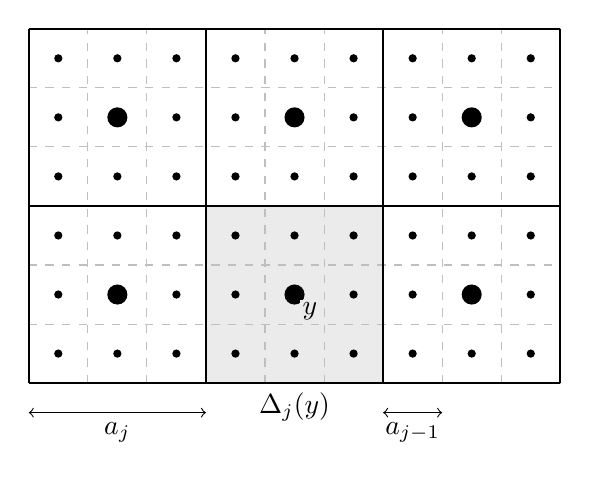
\begin{tikzpicture}[scale=0.75]
    \fill[black!8] (1.5,-1.5) rectangle (4.5,1.5);
    \foreach \x in {-1.5,-0.5,...,7.5} {
        \draw[black!25, dashed] (\x,-1.5) -- (\x,4.5);
    }
    \foreach \y in {-1.5,-0.5,...,4.5} {
        \draw[black!25, dashed] (-1.5,\y) -- (7.5,\y);
    }
    \foreach \x in {-1.5,1.5,4.5,7.5} {
        \draw[thick] (\x,-1.5) -- (\x,4.5);
    }
    \foreach \y in {-1.5,1.5,4.5} {
        \draw[thick] (-1.5,\y) -- (7.5,\y);
    }
    \foreach \x in {-1,...,7} {
        \foreach \y in {-1,...,4} {
            \fill (\x,\y) circle (0.07);
        }
    }
    \foreach \x in {0,3,6} {
        \foreach \y in {0,3} {
            \fill (\x,\y) circle (0.17);
        }
    }
    \node[anchor=north west, inner sep=1pt, fill=black!8] at (3.08,-0.08) {$y$};
    \node[below] at (3,-1.5) {$\Delta_j(y)$};
    \draw[<->] (-1.5,-2.0) -- node[below] {$a_j$} (1.5,-2.0);
    \draw[<->] (4.5,-2.0) -- node[below] {$a_{j-1}$} (5.5,-2.0);
\end{tikzpicture}
\caption{$T^{(j)}$ (large dots) and $T^{(j-1)}$ (all dots) for $L = 3$, with their cells (solid and dashed lines). The block $B(y)$ consists of the sites in the shaded cell $\Delta_j(y)$.}
\label{fig:lattices}
\end{figure}

\begin{definition}[Bonds, Paths, and Plaquettes]\label{def:bonds}
Let $j \in [k]_0$.
\begin{enumerate}[label=(\roman*)]
\item A \emph{bond} of $T^{(j)}$ is an ordered pair $b = (b_-, b_+)$ of sites with $b_+ = b_- + a_je_\mu$ or $b_+ = b_- - a_je_\mu$ for some $\mu$; in the first case it is \emph{positive}. The \emph{reversed bond} is $b^{-1} \coloneqq (b_+, b_-)$. We denote the set of bonds of $T^{(j)}$ by $T^{(j)}_{\mathrm{b}}$. For a site $x \in T^{(j)}$ and bond $b$, we write $x \in b$ if $x = b_+$ or $x = b_-$.

\item A \emph{path} is a finite sequence $\gamma = (b_1, \dots, b_n)$ of bonds with $(b_i)_+ = (b_{i+1})_-$ for $1 \leqslant i < n$. It leads from $(b_1)_-$ to $(b_n)_+$, its \emph{length} is $na_j$, and its reverse is $\gamma^{-1} \coloneqq (b_n^{-1}, \dots, b_1^{-1})$. A path from $x$ to $x'$ is \emph{shortest} if its length is $\abs{x - x'}_1$. For a bond $b$ we write $b \in \gamma$ if $b = b_i$ for one of the bonds of $\gamma$.


\item For $x \in T^{(j)}$ and $\mu \neq \nu$ the \emph{plaquette} $p_{\mu\nu}(x)$ is the closed path
\[
    \hspace{-0.2cm} \partial p_{\mu\nu}(x) \coloneqq \Bigl((x, x + a_je_\mu),\ (x + a_je_\mu, x + a_je_\mu + a_je_\nu), (x + a_je_\mu + a_je_\nu, x + a_je_\nu),\ (x + a_je_\nu, x)\Bigr)\;,
\]
which is \emph{positive} if $\mu < \nu$. The path $\partial p_{\nu\mu}(x)$ is the reverse of $\partial p_{\mu\nu}(x)$. A general plaquette will be denoted by $p$, the set of plaquettes of $T^{(j)}$ by $T^{(j)}_{\mathrm{p}}$, and the set of the positive ones by $T^{(j)}_{\mathrm{p},+}$.


\item The \emph{star} of a site $x \in T^{(j)}$ or a bond $b \in T^{(j)}_{\mathrm{b}}$ are the sets 
\begin{equs}
    \operatorname{st}(x) & \eqdef \left\{ b \in T^{(j)}_{\mathrm{b}} \, \middle| \, x \in b \right\} \; , \qquad \operatorname{st}(b) \eqdef \left\{ p \in T^{(j)}_{\mathrm{p}} \, \middle| \, b \in \partial p \lor b^{-1} \in \partial p \right\} \; .
\end{equs}
\item For a set $S \subset \mathbb T$ we write $S^{(j)} \coloneqq S \cap T^{(j)}$. The \emph{bonds of $S$ of the scale $j$} are the set $\bigcup_{x \in S^{(j)}}\operatorname{st}(x)$, those with at least one end in $S$, and the \emph{plaquettes of $S$ of the scale $j$} are the plaquettes with at least one corner in $S$.
\end{enumerate}
\end{definition}

\begin{figure}[ht]
\centering
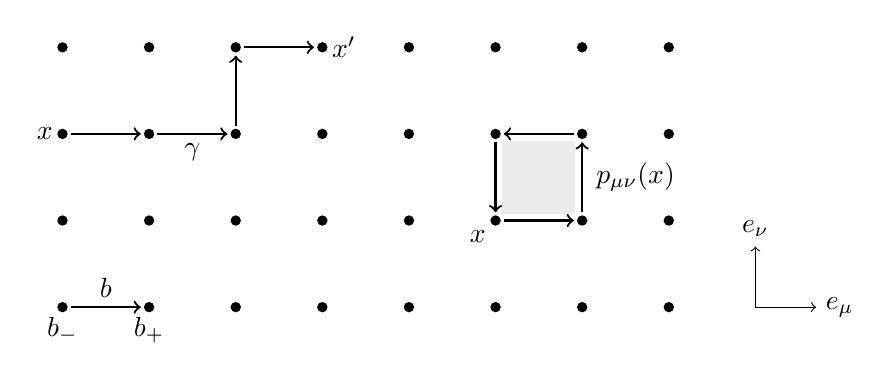
\begin{tikzpicture}[scale=1.1, arr/.style={->, thick, shorten >=3pt, shorten <=3pt}]
    \foreach \x in {0,...,7} {
        \foreach \y in {0,...,3} {
            \fill (\x,\y) circle (0.06);
        }
    }
    \draw[arr] (0,0) -- (1,0);
    \node[below] at (0,0) {$b_-$};
    \node[below] at (1,0) {$b_+$};
    \node[above] at (0.5,0) {$b$};
    \draw[arr] (0,2) -- (1,2);
    \draw[arr] (1,2) -- (2,2);
    \draw[arr] (2,2) -- (2,3);
    \draw[arr] (2,3) -- (3,3);
    \node[left] at (0,2) {$x$};
    \node[right] at (3,3) {$x'$};
    \node[below] at (1.5,2) {$\gamma$};
    \fill[black!8] (5.08,1.08) rectangle (5.92,1.92);
    \draw[arr] (5,1) -- (6,1);
    \draw[arr] (6,1) -- (6,2);
    \draw[arr] (6,2) -- (5,2);
    \draw[arr] (5,2) -- (5,1);
    \node[below left] at (5,1) {$x$};
    \node[right] at (6.05,1.5) {$p_{\mu\nu}(x)$};
    \draw[->] (8,0) -- (8.7,0) node[right] {$e_\mu$};
    \draw[->] (8,0) -- (8,0.7) node[above] {$e_\nu$};
\end{tikzpicture}
\caption{A positive bond $b$, a shortest path $\gamma$ from $x$ to $x'$, and the positive plaquette $p_{\mu\nu}(x)$ with the orientation of $\partial p_{\mu\nu}(x)$, in a plane of $T^{(j)}$; the spacing is $a_j$.}
\label{fig:bonds}
\end{figure}

\subsection{Configurations and the Action}\label{sec:configurations}

The fields of the theory are functions on the bonds with values in the group. All later analyticity statements concern their extension to the complexified group, and so we define the objects for it at once.

\begin{definition}[Configurations and Forms]\label{def:configurations}
Let $j \in [k]_0$.
\begin{enumerate}[label=(\roman*)]
\item A \emph{configuration} on $T^{(j)}$ is a map $\mathbf U \colon T^{(j)}_{\mathrm b} \to G^c$ with $\mathbf U(b^{-1}) = \mathbf U(b)^{-1}$. It is a \emph{gauge field} if its values lie in $G$. We write $\mathscr G^{(j)}$ for the set of the gauge fields on $T^{(j)}$ and $\mathscr G^{(j)}_c \supset \mathscr G^{(j)}$ for that of the configurations, and we will denote gauge fields by $U$, $V$. For a path $\gamma = (b_1, \dots, b_n)$ we put $\mathbf U(\gamma) \coloneqq \mathbf U(b_1)\cdots\mathbf U(b_n)$.
\item A \emph{complex gauge transformation} is a map $u \colon T^{(j)} \to G^c$. It acts on configurations by
\begin{equation}\label{eq:gauge-transformation}
    \mathbf U^u(b) \coloneqq u(b_-)\mathbf U(b)u(b_+)^{-1}\;,
\end{equation}
so that $\mathbf U^u(\gamma) = u(x)\mathbf U(\gamma)u(x')^{-1}$ for a path $\gamma$ from $x$ to $x'$. If $u$ is $G$-valued, we call it simply a \emph{gauge transformation}.
\item A \emph{$0$-form} is a map $\lambda \colon T^{(j)} \to M_N(\mathbb C)$. 

A \emph{$1$-form} is a map $A \colon T^{(j)}_{\mathrm b} \to M_N(\mathbb C)$ with $A(b^{-1}) = -A(b)$. Its \emph{components} are the $0$-forms $A_\mu(x) \coloneqq A(x, x + a_j e_\mu)$, $\mu \in [3]_0$, and they determine it. 

A \emph{$2$-form} is a function $F \colon T^{(j)}_{\mathrm{p}} \to M_N(\mathbb C)$ with $F(p_{\nu\mu}(x)) = -F(p_{\mu\nu}(x))$. Its components are the $0$-forms $F_{\mu\nu}(x) \coloneqq F(p_{\mu\nu}(x))$, $\mu \neq \nu$, so that $F_{\nu\mu} = -F_{\mu\nu}$. 

We let a complex gauge transformation $u$ act on forms $f$ by setting $(\Ad_u f)(x) \eqdef \Ad_{u(x)}f(x)$.
\item For two forms of the same degree,
\begin{equation}\label{eq:pairing}
    \langle\lambda, \lambda'\rangle \coloneqq \sum_xa_j^4\tr\lambda(x)\lambda'(x)\;,
    \qquad
    \langle A, A'\rangle \coloneqq \sum_\mu\langle A_\mu, A'_\mu\rangle\;,
    \qquad
    \langle F, F'\rangle \coloneqq \sum_{\mu < \nu}\langle F_{\mu\nu}, F'_{\mu\nu}\rangle\;,
\end{equation}
and $\norm f_2^2 \coloneqq \langle f^*, f\rangle$, where $f^*$ is the pointwise adjoint.
\end{enumerate}
\end{definition}

The pairings \eqref{eq:pairing} are \emph{bilinear} and not sesquilinear. On forms with Hermitean values each is the real scalar product whose norm is $\norm\bigcdot_2$, and it is the form with respect to which adjoints are holomorphic in the configuration.

\begin{definition}[The Action]\label{def:action}
For a configuration $\mathbf U$ on $T^{(j)}$ and a plaquette $p$ let
\begin{equation}\label{eq:real-imaginary}
    \re\mathbf U(\partial p) \coloneqq \frac{1}{2}\bigl(\mathbf U(\partial p) + \mathbf U(\partial p)^{-1}\bigr)\;,
    \qquad
    \im\mathbf U(\partial p) \coloneqq \frac{1}{2i}\bigl(\mathbf U(\partial p) - \mathbf U(\partial p)^{-1}\bigr)\;.
\end{equation}
The \emph{Yang--Mills Action} at scale $j$ is the functional
\begin{equation}\label{eq:action}
    A(\mathbf U) \coloneqq \sum_{p \in T^{(j)}_{\mathrm{p},+}}\bigl(1 - \tr\re\mathbf U(\partial p)\bigr)\;.
\end{equation}
\end{definition}

This is the standard lattice Yang--Mills action, extended to the complexified group.

\begin{lemma}[Properties of the Action]\label{lem:action}
\begin{enumerate}[label=(\roman*)]
\item For a gauge field $U$, $A(U) = \sum_p(1 - \re\tr U(\partial p)) = \frac{1}{2}\sum_p\abs{U(\partial p) - \id}^2 \geqslant 0$.
\item $A(\mathbf U^u) = A(\mathbf U)$ for every configuration $\mathbf U$ and every complex gauge transformation $u$, and $\im\mathbf U^u(\partial p_{\mu\nu}(x)) = \Ad_{u(x)}\im\mathbf U(\partial p_{\mu\nu}(x))$.
\item The summand of \eqref{eq:action} for $p$ is a polynomial in the entries of the matrices $\mathbf U(b)$ and $\mathbf U(b)^{-1}$ for the four bonds $b$ of $\partial p$.
\end{enumerate}
\end{lemma}

\begin{proof}
For a unitary matrix $W$ we have $W^{-1} = W^*$, so that $\tr\re W = \re\tr W$, and (i) follows from \eqref{eq:plaquette-norm}. By \eqref{eq:gauge-transformation}, $\mathbf U^u(\partial p_{\mu\nu}(x)) = u(x)\mathbf U(\partial p_{\mu\nu}(x))u(x)^{-1}$, and the same holds for the inverse, which gives the second assertion of (ii); the first follows because the trace is invariant under conjugation. Finally (iii) is the definition, since $\mathbf U(\partial p)^{-1}$ is the product of the inverses in the reverse order.
\end{proof}

By (i) the action of a gauge field is half the sum of the squared Hilbert--Schmidt norms of $U(\partial p) - \id$, and for this reason the regularity conditions on the plaquettes are stated in this norm.

\subsection{Covariant Differences and the Current}\label{sec:differences}

The quadratic forms of the linear theory and the regularity conditions on the fields are written with difference operators which are covariant with respect to a configuration.

\begin{definition}[Covariant Differences]\label{def:differences}
Let $j \in [k]_0$ and let $\mathbf U \in \mathscr G^{(j)}_c$. For a $0$-form $\lambda$ and $\mu \in [3]_0$,
\begin{align}
    (D_{\mathbf U,\mu}\lambda)(x) &\coloneqq a_j^{-1}\bigl(\Ad_{\mathbf U(x, x + a_je_\mu)}\lambda(x + a_je_\mu) - \lambda(x)\bigr)\;,\label{eq:forward-difference}\\
    (D^*_{\mathbf U,\mu}\lambda)(x) &\coloneqq a_j^{-1}\bigl(\Ad_{\mathbf U(x, x - a_je_\mu)}\lambda(x - a_je_\mu) - \lambda(x)\bigr)\;.\label{eq:backward-difference}
\end{align}
With these we define, for a $0$-form $\lambda$, a $1$-form $A$, and a $2$-form $F$:
\begin{enumerate}[label=(\roman*)]
\item the $1$-form $D_{\mathbf U}\lambda$ with the components $D_{\mathbf U,\mu}\lambda$, and the $0$-form $D^*_{\mathbf U}A \coloneqq \sum_\mu D^*_{\mathbf U,\mu}A_\mu$;
\item the $2$-form $D_{\mathbf U}A$ with the components $(D_{\mathbf U}A)_{\mu\nu} \coloneqq D_{\mathbf U,\mu}A_\nu - D_{\mathbf U,\nu}A_\mu$, and the $1$-form $D^*_{\mathbf U}F$ with the components $(D^*_{\mathbf U}F)_\mu \coloneqq \sum_{\nu \neq \mu}D^*_{\mathbf U,\nu}F_{\nu\mu}$;
\item the \emph{covariant gradient} $\nabla_{\mathbf U}A$, the family of the sixteen $0$-forms $(\nabla_{\mathbf U}A)_{\mu\nu} \coloneqq D_{\mathbf U,\mu}A_\nu$, and likewise $\nabla_{\mathbf U}\lambda \coloneqq D_{\mathbf U}\lambda$;
\item the \emph{covariant Laplacian} $\Delta_{\mathbf U} \coloneqq \sum_\mu D^*_{\mathbf U,\mu}D_{\mathbf U,\mu}$, which acts on $0$-forms and, component by component, on $1$-forms;
\item at the trivial configuration $\mathbf U = \id$, the \emph{differences} $\partial_\mu \coloneqq D_{\id,\mu}$, $\partial^*_\mu \coloneqq D^*_{\id,\mu}$, $\partial \coloneqq D_{\id}$, and $\partial^* \coloneqq D^*_{\id}$.
\end{enumerate}
\end{definition}

We can write the covariant derivatives in a coordinate free way as follows. For a positive bond $b$ and a plaquette $p = p_{\mu\nu}(x)$ with $\partial p = (b_1, b_2, b_3, b_4)$, by \eqref{eq:forward-difference} and by (ii) with $A(b^{-1}) = -A(b)$,
\begin{align}
    (D_{\mathbf U}\lambda)(b) &= a_j^{-1}\bigl(\Ad_{\mathbf U(b)}\lambda(b_+) - \lambda(b_-)\bigr)\;,\label{eq:difference-bond}\\
    (D_{\mathbf U}A)(p) &= a_j^{-1}\bigl(A(b_1) + \Ad_{\mathbf U(b_1)}A(b_2) + \Ad_{\mathbf U(b_4)^{-1}}A(b_3) + A(b_4)\bigr)\;,\label{eq:difference-plaquette}
\end{align}
the second being the values of $A$ on $\partial p$ transported to the corner $x$. At the trivial configuration these are the usual lattice derivatives.

\begin{lemma}[Adjoints and Covariance]\label{lem:covariance}
Let $j \in [k]_0$, $\mathbf U$ a configuration on $T^{(j)}$, and $u$ a complex gauge transformation of $T^{(j)}$.
\begin{enumerate}[label=(\roman*)]
\item For all $0$-forms $\lambda$, $\lambda'$, $1$-forms $A$, $2$-forms $F$, and $\mu \in [3]_0$
\begin{equ}
    \langle D_{\mathbf U,\mu}\lambda, \lambda'\rangle = \langle\lambda, D^*_{\mathbf U,\mu}\lambda'\rangle\;,
    \qquad
    \langle D_{\mathbf U}\lambda, A\rangle = \langle\lambda, D^*_{\mathbf U}A\rangle\;,
    \qquad
    \langle D_{\mathbf U}A, F\rangle = \langle A, D^*_{\mathbf U}F\rangle\;.
\end{equ}
\item All covariant derivative operators $\CD$ of Definition~\ref{def:differences} satisfy $\mathcal D_{\mathbf U^u}\Ad_u = \Ad_u\mathcal D_{\mathbf U}$.
\item For a $0$-form $\lambda$, $x \in T^{(j)}$, and $\mu \neq \nu$, let $\gamma$ be the path $((x, x + a_je_\nu), (x + a_je_\nu, x + a_je_\nu + a_je_\mu))$. Then
\begin{equation}\label{eq:curvature-commutator}
    (D_{\mathbf U}D_{\mathbf U}\lambda)_{\mu\nu}(x) = a_j^{-2}\bigl(\Ad_{\mathbf U(\partial p_{\mu\nu}(x))} - 1\bigr)\Ad_{\mathbf U(\gamma)}\lambda(x + a_je_\mu + a_je_\nu)\;.
\end{equation}
\end{enumerate}
\end{lemma}

\begin{proof}
(i) For a bond $b$ and matrices $X$, $Y$, the cyclicity of the trace and $\mathbf U(b)^{-1} = \mathbf U(b^{-1})$ give $\tr\bigl((\Ad_{\mathbf U(b)}X)Y\bigr) = \tr\bigl(X\Ad_{\mathbf U(b^{-1})}Y\bigr)$. We use this in the first term of $\langle D_{\mathbf U,\mu}\lambda, \lambda'\rangle$ and then replace $x$ by $x - a_je_\mu$ in it:
\begin{align*}
    \langle D_{\mathbf U,\mu}\lambda, \lambda'\rangle
    &= a_j^3\sum_x\tr\bigl(\lambda(x + a_je_\mu)\Ad_{\mathbf U(x + a_je_\mu, x)}\lambda'(x) - \lambda(x)\lambda'(x)\bigr)\\
    &= a_j^3\sum_x\tr\Bigl(\lambda(x)\bigl(\Ad_{\mathbf U(x, x - a_je_\mu)}\lambda'(x - a_je_\mu) - \lambda'(x)\bigr)\Bigr)
    = \langle\lambda, D^*_{\mathbf U,\mu}\lambda'\rangle\;.
\end{align*}
The second identity is the sum of the first over $\mu$ with $\lambda' = A_\mu$. For the third, $F_{\nu\mu} = -F_{\mu\nu}$ turns the sum over $\mu < \nu$ into a sum over $\mu \neq \nu$, and the first identity moves the difference to $F$:
\[
    \langle D_{\mathbf U}A, F\rangle
    = \sum_{\mu \neq \nu}\langle D_{\mathbf U,\mu}A_\nu, F_{\mu\nu}\rangle
    = \sum_\nu\Bigl\langle A_\nu, \sum_{\mu \neq \nu}D^*_{\mathbf U,\mu}F_{\mu\nu}\Bigr\rangle
    = \langle A, D^*_{\mathbf U}F\rangle\;.
\]

(ii) By \eqref{eq:gauge-transformation}, $\Ad_{\mathbf U^u(x, x + a_je_\mu)}\Ad_{u(x + a_je_\mu)} = \Ad_{u(x)}\Ad_{\mathbf U(x, x + a_je_\mu)}$, and therefore
\begin{align*}
    (D_{\mathbf U^u,\mu}\Ad_u\lambda)(x)
    &= a_j^{-1}\bigl(\Ad_{\mathbf U^u(x, x + a_je_\mu)}\Ad_{u(x + a_je_\mu)}\lambda(x + a_je_\mu) - \Ad_{u(x)}\lambda(x)\bigr)\\
    &= \Ad_{u(x)}(D_{\mathbf U,\mu}\lambda)(x)\;.
\end{align*}
The same computation with $-e_\mu$ in the place of $e_\mu$ gives $D^*_{\mathbf U^u,\mu}\Ad_u = \Ad_uD^*_{\mathbf U,\mu}$, and every operator of Definition~\ref{def:differences} is built from these two component by component.

(iii) The boundary $\partial p_{\mu\nu}(x)$ is the path from $x$ through $x + a_je_\mu$ to $x + a_je_\mu + a_je_\nu$, followed by the reverse of $\gamma$. Hence
\[
    \mathbf U(x, x + a_je_\mu)\,\mathbf U(x + a_je_\mu, x + a_je_\mu + a_je_\nu) = \mathbf U(\partial p_{\mu\nu}(x))\,\mathbf U(\gamma)\;,
\]
and applying \eqref{eq:forward-difference} twice we obtain
\begin{align*}
    a_j^2(D_{\mathbf U,\mu}D_{\mathbf U,\nu}\lambda)(x)
    &= \Ad_{\mathbf U(\partial p_{\mu\nu}(x))\mathbf U(\gamma)}\lambda(x + a_je_\mu + a_je_\nu) + \lambda(x)\\
    &\quad - \Ad_{\mathbf U(x, x + a_je_\mu)}\lambda(x + a_je_\mu) - \Ad_{\mathbf U(x, x + a_je_\nu)}\lambda(x + a_je_\nu)\;.
\end{align*}
The second line is symmetric in $\mu$ and $\nu$, and in $D_{\mathbf U,\nu}D_{\mathbf U,\mu}\lambda$ the first term is $\Ad_{\mathbf U(\gamma)}\lambda(x + a_je_\mu + a_je_\nu)$. By Definition~\ref{def:differences}(ii) the difference of the two is \eqref{eq:curvature-commutator}.
\end{proof}

The difference $D_{\mathbf U}A$ of a $1$-form is the first variation of the plaquettes when the configuration is multiplied by the exponential of the form. For a configuration $\mathbf U$ on $T^{(j)}$ and a $1$-form $A$ with values in $\mathfrak g^c$ we write $e^{ia_jA}\mathbf U$ for the configuration with the values $e^{ia_jA(b)}\mathbf U(b)$ on the positive bonds $b$.

\begin{lemma}[The Plaquettes of a Product]\label{lem:product-plaquette}
Let $j \in [k]_0$, let $\mathbf U \in \mathscr G^{(j)}_c$, let $A$ be a $1$-form with values in $\mathfrak g^c$, and let $p = p_{\mu\nu}(x)$ be a plaquette with $\partial p = (b_1, b_2, b_3, b_4)$. Then
\begin{equation}\label{eq:product-plaquette}
    \bigl(e^{ia_jA}\mathbf U\bigr)(\partial p) = e^{ia_jA_1}e^{ia_jA_2}\,\mathbf U(\partial p)\,e^{ia_jA_3}e^{ia_jA_4}\;,
\end{equation}
with the four matrices
\begin{equation}\label{eq:product-exponents}
\begin{aligned}
    A_1 &\coloneqq A(b_1) = A_\mu(x)\;, &
    A_2 &\coloneqq \Ad_{\mathbf U(b_1)}A(b_2) = A_\nu(x) + a_j(D_{\mathbf U,\mu}A_\nu)(x)\;,\\
    A_4 &\coloneqq A(b_4) = -A_\nu(x)\;, &
    A_3 &\coloneqq \Ad_{\mathbf U(b_4)^{-1}}A(b_3) = -A_\mu(x) - a_j(D_{\mathbf U,\nu}A_\mu)(x)\;,
\end{aligned}
\end{equation}
whose sum is $a_j(D_{\mathbf U}A)(p)$.
\end{lemma}

\begin{proof}
On a negative bond $b$ the product has the value $\bigl(e^{ia_jA(b^{-1})}\mathbf U(b^{-1})\bigr)^{-1} = \mathbf U(b)e^{ia_jA(b)}$, because $A(b^{-1}) = -A(b)$. The bonds $b_1$, $b_2$ are positive and $b_3$, $b_4$ negative, so that
\[
    \bigl(e^{ia_jA}\mathbf U\bigr)(\partial p) = e^{ia_jA(b_1)}\mathbf U(b_1)\,e^{ia_jA(b_2)}\mathbf U(b_2)\,\mathbf U(b_3)e^{ia_jA(b_3)}\,\mathbf U(b_4)e^{ia_jA(b_4)}\;.
\]
We move $\mathbf U(b_1)$ to the right of the second exponential and $\mathbf U(b_4)$ to the left of the third, by $\mathbf Ve^{iZ}\mathbf V^{-1} = e^{i\Ad_{\mathbf V}Z}$, and the four values of $\mathbf U$ then stand together and form $\mathbf U(\partial p)$. This is \eqref{eq:product-plaquette}. The second expressions in \eqref{eq:product-exponents} are \eqref{eq:forward-difference} for the bonds $b_1 = (x, x + a_je_\mu)$ and $b_4^{-1} = (x, x + a_je_\nu)$, with $A(b_2) = A_\nu(x + a_je_\mu)$ and $A(b_3) = -A_\mu(x + a_je_\nu)$, and the sum is $a_j(D_{\mathbf U}A)(p)$ by Definition~\ref{def:differences}(ii).
\end{proof}

A renormalisation step integrates over the fluctuations of the field about a background: the field is written as $e^{ia_0A}\mathbf U$, with the background $\mathbf U$ and the fluctuation $A$, and the action is expanded in $A$ (Section~\ref{sec:relative-average} and \eqref{eq:action-expansion}). The term of the first order is $\langle A, J(\mathbf U)\rangle$, the pairing of $A$ with the current of $\mathbf U$, a $1$-form built from the plaquettes of $\mathbf U$ which we now define. The regularity conditions of Definitions~\ref{def:regular-pairs} and~\ref{def:pair-space} bound the current separately from the plaquettes. For this reason the terms of the effective actions (Definition~\ref{def:regular-terms}) are functions of pairs, that is, of a configuration and of an independent $1$-form in the place of its current.

\begin{definition}[Curvature, Current, and Pairs]\label{def:current}
Let $j \in [k]_0$ and let $\mathbf U \in \mathscr G^{(j)}_c$.
\begin{enumerate}[label=(\roman*)]
\item The \emph{curvature} of $\mathbf U$ is the $2$-form $F(\mathbf U)$ with the components $F(\mathbf U)_{\mu\nu}(x) \coloneqq a_j^{-2}\pi\im\mathbf U(\partial p_{\mu\nu}(x))$, and the \emph{current} of $\mathbf U$ is the $1$-form
\begin{equation}\label{eq:current}
    J(\mathbf U) \coloneqq D^*_{\mathbf U}F(\mathbf U)\;.
\end{equation}
\item A \emph{pair} on a set of bonds is a pair $(\mathbf U, \mathbf J)$ of a configuration $\mathbf U$ and a $1$-form $\mathbf J$ with values in $\mathfrak g^c$, both restricted to the set. A complex gauge transformation acts on pairs by $(\mathbf U, \mathbf J)^u \coloneqq (\mathbf U^u, \Ad_u\mathbf J)$.
\end{enumerate}
\end{definition}

The family $F(\mathbf U)$ is a $2$-form because $\partial p_{\nu\mu}(x)$ is the reverse of $\partial p_{\mu\nu}(x)$, so that the two matrices $\im\mathbf U(\partial p)$ differ by the sign. Its values lie in $\mathfrak g^c$, and in $\mathfrak g$ if $\mathbf U$ is a gauge field, by Lemma~\ref{lem:norms}(iv). By Lemma~\ref{lem:action}(ii), Lemma~\ref{lem:norms}(iii), and Lemma~\ref{lem:covariance}(ii),
\begin{equation}\label{eq:current-covariance}
    F(\mathbf U^u) = \Ad_uF(\mathbf U)\;,
    \qquad
    J(\mathbf U^u) = \Ad_uJ(\mathbf U)\;,
\end{equation}
for every complex gauge transformation $u$, so that $(\mathbf U, J(\mathbf U))^u = (\mathbf U^u, J(\mathbf U^u))$.

At a gauge field the current is bounded by the plaquettes around a bond, one inverse power of the spacing being lost in the difference.

\begin{lemma}[The Current by the Plaquettes]\label{lem:current-plaquettes}
Let $U$ be a gauge field on $T^{(j)}$, let $b$ be a bond of the direction $\mu$ with $b_- = x$, and let $\varepsilon \geqslant 0$ be such that $\abs{U(\partial p) - \id} \leqslant \varepsilon$ for the plaquettes $p = p_{\nu\mu}(x)$ and $p = p_{\nu\mu}(x - a_je_\nu)$, $\nu \neq \mu$. Then $\norm{J(U)(b)} \leqslant 6\sqrt N\varepsilon a_j^{-3}$.
\end{lemma}

\begin{proof}
For a unitary matrix $X$, $\abs{\pi\im X} \leqslant \abs{\im X} \leqslant \frac{1}{2}(\abs{X - \id} + \abs{X^{-1}(\id - X)}) = \abs{X - \id}$, by \eqref{eq:real-imaginary} and Lemma~\ref{lem:norms}(ii) and~(iv), and $\norm Y \leqslant \sqrt N\abs Y$ by Lemma~\ref{lem:norms}(i); so $\norm{F(U)_{\nu\mu}(z)} \leqslant \sqrt Na_j^{-2}\abs{U(\partial p_{\nu\mu}(z)) - \id}$. The component $J(U)_\mu(x) = \sum_{\nu \neq \mu}(D^*_{U,\nu}F(U)_{\nu\mu})(x)$ of \eqref{eq:current} is, by \eqref{eq:backward-difference}, a sum of six terms $\pm a_j^{-1}$ times the values of $F(U)_{\nu\mu}$ at $x$ and at $x - a_je_\nu$, the latter transformed by $\Ad$ of a unitary matrix, which preserves the operator norm. Hence $\norm{J(U)(b)} \leqslant 6a_j^{-1}\sqrt Na_j^{-2}\varepsilon$.
\end{proof}

\subsection{Sequences of Domains and the Weighted Distance}\label{sec:sequences}

After several steps the field is an integration variable on lattices of different scales in different regions of the torus, the coarser lattices in the regions in which more steps could be performed. The regions are described by a decreasing sequence of domains, and all bounds on propagators decay in a distance which measures a length in each region in the units of its scale. The domains are unions of cubes whose side is a power of $L$, larger than the spacing of the lattice of the region.

\begin{definition}[Grids]\label{def:grids}
Let $s \coloneqq L^i$ with an integer $-k \leqslant i \leqslant m_{\mathbb T}$, so that $s$ divides $\ell_{\mathbb T}$. The \emph{grid of side $s$} is the family of the closed cubes
\[
    \{ z \in \mathbb T \,|\, \abs{z - c}_\infty \leqslant s/2 \}\;,
    \qquad
    c \in (s\mathbb Z/\ell_{\mathbb T}\mathbb Z)^4\;.
\]
\end{definition}

The cubes of a grid cover the torus and meet at most in boundary points, the cells $\Delta_j(y)$, $y \in T^{(j)}$, form the grid of side $a_j$, and, since $L$ is odd, every cube of the grid of side $Ls$ is the union of $L^4$ cubes of the grid of side $s$.

\begin{definition}[Sequences of Domains]\label{def:sequence}
Let $M$ be a power of $L$ with $M \leqslant L^{m_{\mathbb T}}$ and let $R \geqslant 1$ be an integer. A \emph{sequence of domains with the block size $M$ and the separation $R$} is a sequence of subsets
\begin{equation}\label{eq:sequence}
    \mathbb T = \Omega_0 \supset \Omega_1 \supset \dots \supset \Omega_k\;,
    \qquad
    \Omega_{k+1} \coloneqq \emptyset\;,
\end{equation}
of the torus such that, for $j \in [k]$, the set $\Omega_j$ is a union of cubes of the grid of side $Ma_j$, and
\begin{equation}\label{eq:separation}
    \dist(\Omega_j^c, \Omega_{j+1}) > RMa_j
\end{equation}
for all $1 \leqslant j < k$ for which neither $\Omega_j^c$ nor $\Omega_{j+1}$ is empty. Its \emph{layers} are the sets
\begin{equation}\label{eq:layers}
    \Gamma_j \coloneqq \Omega_j^{(j)} \setminus \Omega_{j+1} \subset T^{(j)}\;,
    \qquad
    j \in [k]_0\;,
\end{equation}
and its \emph{determining set} is the disjoint union $\mathbf B \coloneqq \bigsqcup_{j=0}^{k}\Gamma_j$. For $y \in \Gamma_j$ we call $j(y) \coloneqq j$ the \emph{scale} of $y$, and we put
\begin{equation}\label{eq:cells}
    \Delta(y) \coloneqq B^j(y)\;,
    \qquad
    \tilde\Delta(y) \coloneqq \{ x \in T^{(0)} \,|\, \abs{x - y}_\infty < a_j \}\;.
\end{equation}
\end{definition}

The domains may be empty or equal to the torus, and the inclusions need not be strict. The sets $\Omega_j \setminus \Omega_{j+1}$ are pairwise disjoint and cover the torus. Both $\Omega_j$ and $\Omega_{j+1}$ are unions of cubes of the grid of side $a_j$, whose boundaries contain no point of the fine lattice, so that the fine points of $\Omega_j \setminus \Omega_{j+1}$ are those of the blocks $B^j(y)$ with $y \in \Gamma_j$. Hence the blocks $\Delta(y)$, $y \in \mathbf B$, form a partition of the fine lattice. For $x \in T^{(0)}$ we write $y(x)$ for the point of $\mathbf B$ with $x \in \Delta(y(x))$ and $j(x) \coloneqq j(y(x))$. The \emph{bonds of the layer} $\Gamma_j$ are the bonds of $T^{(j)}$ with an end in $\Omega_j$ and no end in $\Omega_{j+1}$. Both ends of such a bond are points of $\mathbf B$ once $RM \geqslant L$: an end in $\Omega_j$ lies in $\Gamma_j$, and an end outside $\Omega_j$ is a point of $T^{(j)} \subset T^{(j-1)}$ in $\Omega_{j-1}$, hence a point of $\Gamma_{j-1}$.

The distance in which the propagators decay measures the part of a path in each layer in the units of that layer. At the surface between two layers a bond of the finer scale does not end at a site of the coarser one, and so we define the distance by paths in the torus and not by contours of bonds. The two properties which the later sections use, the cost of crossing a layer and the summability of the exponentials, are Lemma~\ref{lem:distance} and Lemma~\ref{lem:summation}.

\begin{definition}[The Weighted Distance]\label{def:distance}
Let a sequence of domains be given. For $z \in \mathbb T$ let $j(z)$ be the largest $j$ with $z \in \Omega_j$. The \emph{weighted length} of a Lipschitz path $\gamma \colon [0, 1] \to \mathbb T$ is
\begin{equation}\label{eq:weighted-length}
    \ell(\gamma) \coloneqq \int_0^1\frac{\abs{\dot\gamma(t)}_1}{a_{j(\gamma(t))}}\,\dd t\;,
\end{equation}
and the \emph{weighted distance} $d(z, z')$ of two points of the torus is the infimum of $\ell(\gamma)$ over the Lipschitz paths from $z$ to $z'$.
\end{definition}

The function $z \mapsto j(z)$ is upper semicontinuous, because the domains are closed, so that the integrand of \eqref{eq:weighted-length} is measurable. For a point $x$ of the fine lattice, $j(x)$ is the scale of the block which contains $x$, in agreement with the notation introduced above.

\begin{lemma}[The Weighted Distance]\label{lem:distance}
For every sequence of domains with the block size $M$ and the separation $R$:
\begin{enumerate}[label=(\roman*)]
\item $d$ is a metric on $\mathbb T$, and $\abs{z - z'}_1 \leqslant d(z, z') \leqslant a_0^{-1}\abs{z - z'}_1$;
\item if $z \in \Omega_j \setminus \Omega_{j+1}$ and $z' \in \Omega_{j'} \setminus \Omega_{j'+1}$, then $d(z, z') \geqslant RM\max\{ \abs{j - j'} - 1, 0 \}$.
\end{enumerate}
\end{lemma}

\begin{proof}
(i) The weights satisfy $a_0 \leqslant a_{j(z)} \leqslant a_k = 1$. Hence $\ell(\gamma)$ lies between the $\ell^1$-length of $\gamma$ and $a_0^{-1}$ times that length, and the $\ell^1$-length of a path from $z$ to $z'$ is at least $\abs{z - z'}_1$, with equality for a suitable path. This gives the two inequalities, and with them $d(z, z') > 0$ for $z \neq z'$. The symmetry of $d$ follows by reversing the paths, and the triangle inequality by concatenating them.

(ii) We may assume $j' \geqslant j + 2$. Let $\gamma$ be a Lipschitz path from $z$ to $z'$ and let $j < i < j'$. Then $\gamma(0) = z \notin \Omega_i$, because $\Omega_i \subset \Omega_{j+1}$, and $\gamma(1) = z' \in \Omega_{i+1}$, because $\Omega_{j'} \subset \Omega_{i+1}$. Let $t_1$ be the smallest $t$ with $\gamma(t) \in \Omega_{i+1}$, which exists since $\Omega_{i+1}$ is closed, and let $t_0$ be the supremum of the $t < t_1$ with $\gamma(t) \notin \Omega_i$. Then $\gamma(t_0)$ lies in the closure of $\Omega_i^c$, and $\gamma(t) \in \Omega_i \setminus \Omega_{i+1}$ for $t_0 < t < t_1$, so that $j(\gamma(t)) = i$ on this interval. The $\ell^1$-length of the arc $\gamma|_{[t_0, t_1]}$ is at least $\abs{\gamma(t_1) - \gamma(t_0)}_\infty$, which is at least the distance of $\Omega_{i+1}$ from the closure of $\Omega_i^c$, and this distance is greater than $RMa_i$ by \eqref{eq:separation}. The weighted length of the arc is therefore greater than $RM$. The intervals $(t_0, t_1)$ which belong to different $i$ are disjoint, since $j(\gamma(t))$ takes different values on them, and there are $j' - j - 1$ of them. Hence $\ell(\gamma) > RM(j' - j - 1)$.
\end{proof}

The second property is the summability of the exponentials of the distance over the determining set, uniformly in the sequence and in the number of the scales.

\begin{lemma}[Summation over the Determining Set]\label{lem:summation}
Let $L$, $k$, and $m_{\mathbb T}$ be as in Definition~\ref{def:lattices}, and for $\delta > 0$ and $0 < \alpha < 1$ let
\[
    r_1(\alpha, \delta) \coloneqq \max\Bigl\{ 1, \frac{16\log L + 4}{\alpha\delta} \Bigr\}\;,
    \qquad
    c_1(\alpha, \delta) \coloneqq 2^{21}L^8e^{2\alpha\delta}(\alpha\delta)^{-4}\;,
\]
numbers which depend on $\alpha$, $\delta$, and $L$ only, with $c_1(\alpha, \delta) \geqslant 1$. Let a sequence of domains with the block size $M$ and the separation $R$ be given, with $RM \geqslant r_1(\alpha, \delta)$. Then
\begin{equation}\label{eq:summation}
    \sup_{y \in \mathbf B}\sum_{y' \in \mathbf B}e^{-\alpha\delta d(y, y')} \leqslant c_1(\alpha, \delta)\;,
\end{equation}
and for every $n \geqslant 1$ and all $y_0, y_n \in \mathbf B$,
\begin{equation}\label{eq:chain-summation}
    \sum_{y_1, \dots, y_{n-1} \in \mathbf B}\prod_{i=1}^{n}e^{-\delta d(y_{i-1}, y_i)} \leqslant c_1(\alpha, \delta)^{n-1}e^{-(1 - \alpha)\delta d(y_0, y_n)}\;.
\end{equation}
\end{lemma}

The number $c_1$ has to depend on $L$. A path which runs along the boundary of $\Omega_j$ on its coarse side has the weight $a_j^{-1}$, and it can step into the finer layer at every point; so the roughly $r^3L^3$ cells of the scale $j - 1$ which touch a patch of this boundary of the side $ra_j$ lie within a weighted distance of about $r$ of a point near the patch, and the sum \eqref{eq:summation} is at least of the order $L^3(\alpha\delta)^{-3}$.

\begin{proof}
We bound the sum in \eqref{eq:summation} by an integral over the torus, and the integral layer by layer: within a layer by the measure of a ball of the $\ell^1$-distance, and across the layers by Lemma~\ref{lem:distance}(ii).

\emph{From the points to an integral.} Let $y \in \mathbf B$ and $j \coloneqq j(y)$, and let $y' \in \Gamma_{j'}$. Since $\Omega_{j'}$ and $\Omega_{j'+1}$ are unions of cells of the grid of side $a_{j'}$, the cell $\Delta_{j'}(y')$ lies in $\Omega_{j'}$ and its interior does not meet $\Omega_{j'+1}$. On the straight segment from $y'$ to a point $x$ of the cell the weight of \eqref{eq:weighted-length} is therefore at most $a_{j'}^{-1}$, and its $\ell^1$-length is at most $\abs{x - y'}_1 \leqslant 2a_{j'}$, so that $d(y', x) \leqslant 2$. By the triangle inequality $e^{-\alpha\delta d(y, y')} \leqslant e^{2\alpha\delta}e^{-\alpha\delta d(y, x)}$ for every point $x$ of the cell, and the average over the cell gives
\[
    e^{-\alpha\delta d(y, y')} \leqslant e^{2\alpha\delta}a_{j'}^{-4}\int_{\Delta_{j'}(y')}e^{-\alpha\delta d(y, x)}\,\dd x\;.
\]
For each $i$ the cells of the points of $\Gamma_i$ cover the closure $\Lambda_i$ of $\Omega_i \setminus \Omega_{i+1}$ and meet each other in sets of measure zero. Summing over $y'$ we obtain
\begin{equation}\label{eq:summation-integral}
    \sum_{y' \in \mathbf B}e^{-\alpha\delta d(y, y')} \leqslant e^{2\alpha\delta}\sum_ia_i^{-4}\int_{\Lambda_i}e^{-\alpha\delta d(y, x)}\,\dd x\;.
\end{equation}

\emph{The measure of a ball in a layer.} Let $x \in \Lambda_i$ and $r > d(y, x)$, let $\gamma$ be a path from $y$ to $x$ with $\ell(\gamma) < r$, and let $p$ be the largest of the indices $j(\gamma(t))$, attained at a time $t_*$. Lemma~\ref{lem:distance}(ii), applied to $y$ and $\gamma(t_*)$, gives $r > \ell(\gamma) \geqslant d(y, \gamma(t_*)) \geqslant RM(p - j - 1)$, so that $p < j + 1 + r/(RM)$. Along $\gamma$ the weight is at least $a_p^{-1}$, and hence
\[
    \abs{x - y}_1 \leqslant a_p\ell(\gamma) < a_{j+1}L^{r/(RM)}r\;.
\]
So the points of $\Lambda_i$ at a weighted distance of less than $r$ from $y$ lie in the $\ell^1$-ball of the radius $\rho \coloneqq a_{j+1}L^{r/(RM)}r$ about $y$, whose measure is at most $(2\rho)^4/4! \leqslant 16\rho^4$. If $\abs{i - j} \geqslant 2$, there are no such points for $r \leqslant r_i \coloneqq RM(\abs{i - j} - 1)$: at the points of $\Omega_i \setminus \Omega_{i+1}$ the distance from $y$ is at least $r_i$ by Lemma~\ref{lem:distance}(ii), and at the other points of $\Lambda_i$, which are limits of these, by the continuity of $d$, which Lemma~\ref{lem:distance}(i) gives. We put $r_i \coloneqq 0$ for $\abs{i - j} \leqslant 1$.

\emph{The integral over a layer.} Since $e^{-\alpha\delta d(y, x)}$ is the integral of $\alpha\delta e^{-\alpha\delta r}$ over $r > d(y, x)$, the theorem of Fubini and the last step give
\[
    \int_{\Lambda_i}e^{-\alpha\delta d(y, x)}\,\dd x = \int_0^\infty\alpha\delta e^{-\alpha\delta r}\,\bigl\lvert\{ x \in \Lambda_i \,|\, d(y, x) < r \}\bigr\rvert\,\dd r \leqslant 16a_{j+1}^4\int_{r_i}^\infty\alpha\delta r^4L^{4r/(RM)}e^{-\alpha\delta r}\,\dd r\;.
\]
Since $RM \geqslant r_1(\alpha, \delta)$, we have $4\log L/(RM) \leqslant \frac{1}{4}\alpha\delta$, so that $L^{4r/(RM)} \leqslant e^{\frac{1}{4}\alpha\delta r}$; and $e^{-\frac{3}{4}\alpha\delta r} \leqslant e^{-\frac{1}{2}\alpha\delta r_i}e^{-\frac{1}{4}\alpha\delta r}$ for $r \geqslant r_i$. With $\int_0^\infty\alpha\delta r^4e^{-\frac{1}{4}\alpha\delta r}\,\dd r = 4! \cdot 4^5(\alpha\delta)^{-4}$ and $a_{j+1}/a_i = L^{j+1-i}$ this gives
\[
    a_i^{-4}\int_{\Lambda_i}e^{-\alpha\delta d(y, x)}\,\dd x \leqslant KL^{4(j+1-i)}e^{-\frac{1}{2}\alpha\delta r_i}\;,
    \qquad
    K \coloneqq 16 \cdot 4! \cdot 4^5(\alpha\delta)^{-4} = 393216\,(\alpha\delta)^{-4}\;.
\]

\emph{The sum over the layers.} By the choice of $r_1$, $\frac{1}{2}\alpha\delta RM \geqslant 8\log L + 2$. For $i \geqslant j$ the factor $L^{4(j+1-i)}$ is at most $L^4$, and $\sum_{i \geqslant j}e^{-\frac{1}{2}\alpha\delta r_i} \leqslant 2 + \sum_{m \geqslant 1}e^{-m} \leqslant 3$. For $i = j - 1$ the bound is $KL^8$, and for $i \leqslant j - 2$ it is $KL^8L^{4(j-1-i)}e^{-\frac{1}{2}\alpha\delta RM(j-1-i)} \leqslant KL^8e^{-(j-1-i)}$; the sum over $i < j$ is at most $KL^8(1 + 1/(e - 1)) \leqslant 2KL^8$. With \eqref{eq:summation-integral},
\[
    \sum_{y' \in \mathbf B}e^{-\alpha\delta d(y, y')} \leqslant e^{2\alpha\delta}(3L^4 + 2L^8)K \leqslant 5 \cdot 393216\,L^8e^{2\alpha\delta}(\alpha\delta)^{-4} \leqslant c_1(\alpha, \delta)\;,
\]
which is \eqref{eq:summation}, since $5 \cdot 393216 \leqslant 2^{21}$. The number $c_1(\alpha, \delta)$ is at least one, because $e^{2t}t^{-4} \geqslant e^4/16$ for $t > 0$.

\emph{The chains.} By the triangle inequality of Lemma~\ref{lem:distance}(i), $\sum_{i=1}^{n}d(y_{i-1}, y_i) \geqslant d(y_0, y_n)$, so that the product in \eqref{eq:chain-summation} is at most $e^{-(1 - \alpha)\delta d(y_0, y_n)}\prod_{i=1}^{n}e^{-\alpha\delta d(y_{i-1}, y_i)}$. We bound the factor with $i = n$ by one and sum over $y_{n-1}, y_{n-2}, \dots, y_1$ in this order, each sum being at most $c_1(\alpha, \delta)$ by \eqref{eq:summation}.
\end{proof}

\subsection{Norms of Fields}\label{sec:norms}

The bounds of the linear theory are stated in supremum norms, in H\"older norms, in norms which weight a field by a power of the spacing of the layer, and in $L^2$-norms.

\begin{definition}[Norms]\label{def:norms}
Let a sequence of domains be given, let $\mathbf U \in \mathscr G^{(0)}_c$, and let $f$ be a $0$-form on $T^{(0)}$, or a family of $0$-forms such as a $1$-form or the gradient of one.
\begin{enumerate}[label=(\roman*)]
\item The \emph{supremum norm} $\norm f_\infty$ is the supremum of the operator norm $\norm{f_\iota(x)}$ over the sites $x$ and the components $f_\iota$ of $f$; for a subset $S$ of the torus, $\norm f_{\infty,S}$ is the same supremum over $x \in S^{(0)}$.
\item For $0 \leqslant \beta \leqslant 1$ and $j \in [k]_0$ the \emph{H\"older norm at the scale $j$} is
\begin{equation}\label{eq:holder}
    \norm f_\beta^{(j)} \coloneqq \sup\Bigl(\frac{\abs{x - x'}_1}{a_j}\Bigr)^{-\beta}\norm{\Ad_{\mathbf U(\gamma)}f_\iota(x') - f_\iota(x)}\;,
\end{equation}
the supremum over the components, over the pairs of sites $x \neq x'$ of $T^{(0)}$ with $\abs{x - x'}_1 \leqslant a_j$, and over the shortest paths $\gamma$ from $x$ to $x'$. We write $\norm f_\beta \coloneqq \norm f_\beta^{(k)}$, and $\norm A_{1,\beta} \coloneqq \norm{\nabla_{\mathbf U}A}_\beta$ for a $1$-form $A$.
\item For a real number $\alpha$ the \emph{weighted norm} is
\begin{equation}\label{eq:weighted-norm}
    \norm f_{\infty,(\alpha)} \coloneqq \sup_{x \in T^{(0)}}a_{j(x)}^{-\alpha}\max_\iota\norm{f_\iota(x)}\;.
\end{equation}
\end{enumerate}
For a function with scalar values the operator norm of a value is its absolute value.
\end{definition}

The norm \eqref{eq:holder} depends on the configuration through the transport along $\gamma$, and on scalar functions, for which we use it as well, it does not.

\subsection{Localisation Domains}\label{sec:localisation-domains}

The terms of the effective actions are indexed by connected unions of large cubes, and they decay exponentially in the linear size of the union. We define these notions for the cubes of an arbitrary grid, together with a variant of the linear size in which a part of the domain is not counted, which is needed when a term has a prescribed support.

\begin{definition}[Unions of Cubes and Their Linear Size]\label{def:localisation}
Let $s$ be the side of a grid in the sense of Definition~\ref{def:grids}.
\begin{enumerate}[label=(\roman*)]
\item Two cubes of the grid \emph{touch} if they have a point in common, and they \emph{share a wall} if their intersection is a three-dimensional cube. A union $X$ of cubes of the grid is \emph{connected} if any two of its cubes are joined by a chain of cubes of $X$ in which consecutive cubes share a wall. The number of the cubes of $X$ is denoted by $\#(X)$.
\item For a union $X$ of cubes, $X^\sim$ is the union of $X$ and of the cubes of the grid which touch a cube of $X$; $X^{\sim n}$ is the result of $n$ such operations; and $X^{\sim-n} \coloneqq ((X^c)^{\sim n})^c$, where $X^c$ denotes the union of the cubes of the grid which are not in $X$.
\item For a connected union $X$ of cubes and a union $D \subset X$ of cubes, possibly empty, the \emph{linear size of $X$ relative to $D$} is
\begin{equation}\label{eq:contracted-size}
    d(X; D) \coloneqq \frac{1}{s}\inf\abs{G \setminus D}\;,
\end{equation}
the infimum of the one-dimensional measure, with respect to the Euclidean length, over the finite unions $G$ of segments and points with $G \subset X$ such that $G$ meets every cube of $X$ and $G \cup D$ is connected. For a union $X$ of cubes with the connected components $X^i$ we put $d(X; D) \coloneqq \sum_id(X^i; D \cap X^i)$. The \emph{linear size} of $X$ is $d(X) \coloneqq d(X; \emptyset)$.
\item Let $M$ be a power of $L$ with $M \leqslant L^{m_{\mathbb T}}$. For $j \in [k]_0$ the family $\pi_j$ is the grid of side $Ma_j$, a \emph{localisation domain} of the scale $j$ is a connected union of cubes of $\pi_j$, the class of these domains is $\mathbf D_j$, and $d_j(X)$ and $d_j(X; D)$ denote the linear sizes \eqref{eq:contracted-size} for the grid $\pi_j$.
\end{enumerate}
\end{definition}

The following count holds for every domain.

\begin{lemma}[The Cubes of a Localisation Domain]\label{lem:cube-count}
Let $X$ be a connected union of cubes of a grid of side $s$. Then
\begin{equation}\label{eq:cube-count}
    \#(X) \leqslant 2^8(2 + d(X)) \leqslant 2^9(1 + d(X))\;,
    \qquad
    \diam X \leqslant s(2d(X) + 4)\;,
\end{equation}
with the diameter in the Euclidean distance. Moreover, for every $\kappa \geqslant 2^9(6\log 2 + 1)$ and every cube $\square$ of the grid,
\begin{equation}\label{eq:domain-sum}
    \sum_{X \supset \square}e^{-\kappa d(X)} \leqslant 2^{6 \cdot 2^{10}} + 1\;,
\end{equation}
the sum over the connected unions of cubes of the grid which contain $\square$.
\end{lemma}

\begin{proof}
Let $G$ be a set which is admissible in \eqref{eq:contracted-size} for $D = \emptyset$, that is, a connected finite union of segments in $X$ which meets every cube of $X$, and let $\lambda$ be the sum of the $\ell^\infty$-lengths of its segments, which is at most its Euclidean length. We first cover $G$ by few boxes. Regard $G$ as a connected graph whose arcs are segments, and double every arc. All degrees of the resulting graph are even, so that it has a closed walk which traverses every arc once, and parametrising this walk by the $\ell^\infty$-length we obtain a map $\gamma \colon [0, 2\lambda] \to G$ onto $G$ with $\abs{\gamma(t) - \gamma(t')}_\infty \leqslant \abs{t - t'}$. Let $n \coloneqq \ceil{\lambda/s}$ and $t_i \coloneqq \min(2is, 2\lambda)$ for $i \in [n]_0$. Every $t \in [0, 2\lambda]$ lies within $s$ of some $t_i$, so that every point of $G$ lies within the $\ell^\infty$-distance $s$ of one of the $n + 1 \leqslant \lambda/s + 2$ points $\gamma(t_i)$.

Next we count the cubes near one of these points. The cubes of the grid are the products of intervals $[c_\nu - s/2, c_\nu + s/2]$ with $c_\nu \in s\mathbb Z$, and such an interval meets $[q_\nu - s, q_\nu + s]$ only if $c_\nu$ lies in an interval of length $3s$, which contains at most four points of $s\mathbb Z$. A box $\{ z \,|\, \abs{z - q}_\infty \leqslant s \}$ therefore meets at most $4^4 = 2^8$ cubes of the grid. Every cube of $X$ contains a point of $G$ and hence meets one of the $n + 1$ boxes around the points $\gamma(t_i)$, so that $\#(X) \leqslant 2^8(2 + \lambda/s)$, and the infimum over $G$ gives the first bound of \eqref{eq:cube-count}. The second inequality there is $2 + d \leqslant 2(1 + d)$.

For the diameter, let $z, z' \in X$. They lie in cubes of $X$ which contain points $q$, $q'$ of $G$, and the Euclidean diameter of a cube of side $s$ in four dimensions is $2s$. Since $G$ is connected, $\abs{q - q'}_\infty \leqslant \lambda$, and the Euclidean distance is at most twice the $\ell^\infty$-distance. Hence $\abs{z - z'} \leqslant 4s + 2\lambda$, and the infimum over $G$ gives the bound.

For \eqref{eq:domain-sum}, a connected union of $n$ cubes which contains $\square$ has a spanning tree with respect to the relation of sharing a wall, and a closed walk from $\square$ along this tree which traverses every edge twice has $2(n - 1)$ steps, each of which goes to one of the eight cubes which share a wall with the present one. The union is determined by the walk, so that there are at most $8^{2(n-1)} = 2^{6(n-1)}$ such unions. For $n \geqslant 2^{10}$ the first bound of \eqref{eq:cube-count} gives $d(X) \geqslant 2^{-8}n - 2 \geqslant 2^{-9}n$, and then $e^{-\kappa d(X)} \leqslant 2^{-6n}e^{-n}$ by the assumption on $\kappa$. The sum is therefore at most $\sum_{n=1}^{2^{10}-1}2^{6(n-1)} + \sum_{n \geqslant 2^{10}}e^{-n}$, in which the first sum is less than $2^{6 \cdot 2^{10}}$ and the second less than one.
\end{proof}

The cluster expansions of the later sections use five inequalities which relate the linear sizes of a domain, of the parts into which it is decomposed, and of the domain of the next scale which covers it. In the second of them the number of the cubes which belong to none of the parts enters with the factor $18$, and this factor cannot be replaced by a number smaller than $8$: if $Z$ consists of one cube and of eight rods of $n \geqslant 2$ cubes each, one attached to each wall of the cube and pointing away from it, and the rods are the sets $Y_i$, then $d_k(Y_i) = n - 2$, while a connected set which meets all the cubes of $Z$ has length at least $(n - 1)Ma_k$ inside each of the eight disjoint regions beyond the walls of the cube, by the projection onto the axis of the rod, so that $d_k(Z) \geqslant \sum_id_k(Y_i) + 8$.

\begin{lemma}[Five Geometric Inequalities]\label{lem:contracted-geometry}
Let $M$ be a power of $L$ with $LM \leqslant L^{m_{\mathbb T}}$. For a union $X$ of cubes of $\pi_k$ let $X'$ be the smallest union of cubes of the grid of side $LMa_k$ which contains $X^\sim$, the operation $\sim$ being that of $\pi_k$, and let $d'$ denote the linear size \eqref{eq:contracted-size} for the grid of side $LMa_k$.
\begin{enumerate}[label=(\roman*)]
\item Let $Y_0$ be a connected union of cubes of $\pi_k$, $\mathbf D$ a finite family of connected unions $Y \subset Y_0$ of cubes, and $D \subset Y_0$ a union of cubes with $n_D \geqslant 0$ connected components, such that $Y_0 = \bigcup_{Y \in \mathbf D}Y \cup D$. Then $\sum_{Y \in \mathbf D}d_k(Y) \geqslant d_k(Y_0; D) - 3(\abs{\mathbf D} + n_D - 1)$.
\item Let $Z$ be a connected union of cubes of $\pi_k$, let $Y_1, \dots, Y_n \subset Z$ be connected unions of cubes no two of which have a cube in common or contain two cubes which share a wall, and let $D \subset \bigcup_iY_i$ be a union of cubes. Then $\sum_id_k(Y_i; D \cap Y_i) + 18\,\#(Z \setminus \bigcup_iY_i) \geqslant d_k(Z; D)$.
\item Let $Z$ be a connected union of cubes of $\pi_k$. Then $Z'$ is connected and $L\,d'(Z') \leqslant (1 + 324/L)\,d_k(Z) + 162$; and for every nonempty union $D \subset Z$ of cubes, $L\,d'(Z'; D') \leqslant (1 + 486/L)\,d_k(Z; D)$.
\item Let $Z$ be a connected union of cubes of the grid of side $LMa_k$, let $Z_1, \dots, Z_n \subset Z$, $n \geqslant 1$, be connected unions of cubes and $D_i \subset Z_i$ unions of cubes, of which $n'$ are nonempty and $n_\emptyset$ are empty, and put $Z_0 \coloneqq \bigcup_iZ_i$ and $D \coloneqq \bigcup_iD_i$. Then $d'(Z; D) \leqslant \sum_id'(Z_i; D_i) + 3\,\#(Z \setminus Z_0) + 3(n_\emptyset + n' - 1)$.
\item Let $X$ be a connected union of cubes of a grid and $D \subset X$ a nonempty union of cubes. Then $\#(X) \leqslant 81\,\#(D) + 324\,d(X; D)$.
\end{enumerate}
\end{lemma}

\begin{proof}
We write $s \coloneqq Ma_k$, so that the cubes of $\pi_k$ have the side $s$ and those of the coarser grid the side $Ls$; since $L$ is odd and the centres of the two grids are the points of $s\mathbb Z^4$ and of $Ls\mathbb Z^4$, every cube of the coarser grid is the union of $L^4$ cubes of $\pi_k$, and every cube of $\pi_k$ lies in exactly one cube of the coarser grid. In each part we construct a set $G$ which is admissible in \eqref{eq:contracted-size} for the linear size on the larger side, from sets which are admissible for the sizes on the smaller side and whose measures exceed $s$ times the sizes, or $Ls$ times them, by at most $\epsilon > 0$; at the end we let $\epsilon \to 0$. A point of a cube may be added to an admissible set at no cost. We use three facts. The Euclidean diameter of a cube of side $a$ is $2a$, and that of the union of two cubes of side $a$ which share a wall is $\sqrt 7a < 3a$. A set of $\ell^\infty$-diameter at most $a$, or less than $2a$, meets at most $3^4 = 81$ cubes of the grid of side $a$, because an interval of such a length meets at most three of the intervals of length $a$ into which a line is divided; two cubes of the grid which do not touch have an $\ell^\infty$-distance of at least $a$. And the one-dimensional measure of a connected set is at least the distance of any two of its points, its projection onto the line through them being connected.

(i) We call the members of $\mathbf D$ and the connected components of $D$ the pieces, and two pieces adjacent if a cube of the one equals a cube of the other or shares a wall with it. The pieces cover $Y_0$, which is connected, so that the graph of the pieces is connected, and a spanning tree of it has $\abs{\mathbf D} + n_D - 1$ edges. For $Y \in \mathbf D$ let $G_Y$ be admissible for $d_k(Y)$, with $\abs{G_Y} \leqslant s(d_k(Y) + \epsilon)$. For an edge of the tree we choose two cubes of the two pieces which are equal or share a wall, and a segment in their union between a point of the one piece in its cube and a point of the other piece in its cube, the point being a point of $G_Y$ if the piece is $Y \in \mathbf D$, which meets every cube of $Y$, and any point of the cube if the piece is a component of $D$; the segment has a length of less than $3s$. The union $G$ of the sets $G_Y$, of these segments, and of one point in each cube of $D$ lies in $Y_0$ and meets all its cubes; $G \cup D$ is connected, because the sets $G_Y$ and the components of $D$ are connected and the segments join them along the tree; and
\[
    \abs{G \setminus D} \leqslant \sum_{Y \in \mathbf D}s\bigl(d_k(Y) + \epsilon\bigr) + 3s\bigl(\abs{\mathbf D} + n_D - 1\bigr)\;.
\]

(ii) For each $j$ let $G_j$ be admissible for $d_k(Y_j; D \cap Y_j)$, with $\abs{G_j \setminus D} \leqslant s(d_k(Y_j; D \cap Y_j) + \epsilon)$. For each cube $C$ of $Z \setminus \bigcup_jY_j$ we take a main diagonal of $C$, of length $2s$; its two ends are opposite corners of $C$, and each of the eight walls of $C$ contains one of them. For each wall of $C$ which is shared with a cube $N$ of $Z$, the end $e$ of the diagonal on that wall is a point of $N$, and we add a segment in $N$ from $e$ to a point of $G_j$ in $N$ if $N \subset Y_j$, and to a point of the diagonal of $N$ otherwise, of length at most $2s$. Let $G$ be the union of the sets $G_j$, of the diagonals, and of these segments. Its measure outside $D$ is at most $\sum_j\abs{G_j \setminus D} + 18s\,\#(Z \setminus \bigcup_jY_j)$, it lies in $Z$, and it meets all the cubes of $Z$. Since no cube of one set $Y_j$ shares a wall with a cube of another, a chain of cubes of $Z$ in which consecutive cubes share a wall, and which joins two of these sets, passes through cubes of $Z \setminus \bigcup_jY_j$, whose diagonals are joined to the diagonals and to the sets $G_j$ of all the cubes with which they share a wall; and each set $G_j \cup (D \cap Y_j)$ is connected. Since $Z$ is connected, $G \cup D$ is connected.

(iii) The set $Z^\sim$ is connected, because a cube which touches a cube $\square$ of $Z$ is joined to $\square$ by a chain of cubes which touch $\square$, consecutive ones sharing a wall, obtained by changing one coordinate of the centre at a time; and two cubes of $\pi_k$ which share a wall lie in equal cubes of the coarser grid or in two which share a wall. So $Z'$ is connected, and $D' \subset Z'$. Since every cube of $\pi_k$ lies in exactly one cube of the coarser grid, $X'$ is the union of the cubes of the coarser grid which contain a cube of $X^\sim$. In particular every cube of $D'$ contains a cube of $D^\sim$, which touches a cube of $D$, so that every cube of $D'$ meets $D$; and $D'$ contains every point at an $\ell^\infty$-distance of less than $s$ from $D$, whose cube of $\pi_k$ touches a cube of $D$.

Let $G$ be admissible for $d_k(Z; D)$, with $\abs{G \setminus D} \leqslant s(d_k(Z; D) + \epsilon)$. We call the connected components of $G \setminus D$ the strands; they are finitely many, and the closure of each strand meets $D$, since otherwise the strand would be open and closed in $G \cup D$, which is connected, while $D \neq \emptyset$. Let $Q$ be a cube of the coarser grid in $Z' \setminus D'$. If $Q$ touches a cube of $D'$, we add to $G$ a point of $Q \cap D'$. Otherwise the $\ell^\infty$-distance of $Q$ from $D'$ is at least $Ls$, and so its $\ell^\infty$-distance from $D$ is at least $Ls + s$, since $D'$ contains the points at an $\ell^\infty$-distance of less than $s$ from $D$. The cube $Q$ contains a cube of $Z^\sim$, which is a cube of $Z$ or touches one; so there is a cube $\square_Q$ of $Z$ which touches $Q$, and since all the points of $\square_Q$ lie within the $\ell^\infty$-distance $s$ of $Q$, the $\ell^\infty$-distance of $\square_Q$ from $D$ is at least $Ls$. The set $G$ meets $\square_Q$ at a point $x_Q$, which lies on a strand, and the length of that strand is at least $Ls$, by the last of the three facts applied to the closure of the strand. We add to $G$ a segment in $\square_Q$ from $x_Q$ to a point of $\square_Q \cap Q$, of length at most $2s$.

To count these segments, let $S$ be a strand of length $\ell \geqslant Ls$. Its closure is a connected union of finitely many segments; doubling them, as in the proof of Lemma~\ref{lem:cube-count}, we cover it by a closed walk of length $2\ell$, which we cut into $\ceil{2\ell/(Ls)}$ arcs of length at most $Ls$. The points within the $\ell^\infty$-distance $s$ of one arc form a set of $\ell^\infty$-diameter at most $Ls + 2s < 2Ls$, which meets at most $81$ cubes of the coarser grid, and every cube $Q$ whose point $x_Q$ lies on the arc is among them, since $x_Q$ lies within the $\ell^\infty$-distance $s$ of $Q$. The strand therefore carries at most $81(2\ell/(Ls) + 1) \leqslant 243\ell/(Ls)$ of the added segments, of a total length of at most $(486/L)\ell$. Let $G'$ be the set obtained from $G$ by adding these segments and points and a point in each cube of $D'$. It lies in $Z'$, it meets all the cubes of $Z'$, and $G' \cup D'$ is connected: $G \cup D$ is connected, every cube of $D'$ meets $D$, the added points lie in $D'$, and each added segment begins at a point of $G$. Since $G \setminus D' \subset G \setminus D$ and the lengths of the strands add up to $\abs{G \setminus D}$,
\[
    Ls\,d'(Z'; D') \leqslant \abs{G' \setminus D'} \leqslant \Bigl(1 + \frac{486}{L}\Bigr)\abs{G \setminus D} \leqslant \Bigl(1 + \frac{486}{L}\Bigr)s\bigl(d_k(Z; D) + \epsilon\bigr)\;.
\]

Without $D$ the same construction applies to the whole of $G$, at the cost of one additional arc. Let $G$ be admissible for $d_k(Z)$, a connected set of the length $\ell \leqslant s(d_k(Z) + \epsilon)$, and let $Q$ be a cube of the coarser grid in $Z'$ which $G$ does not meet. The cube $Q$ contains a cube of $Z^\sim$, which is not a cube of $Z$, since $G$ meets every cube of $Z$; so it touches a cube $\square_Q$ of $Z$, and $\square_Q$ has a point in common with $Q$. We add to $G$ a segment in $\square_Q$ from a point $x_Q$ of $G \cap \square_Q$ to a point of $\square_Q \cap Q$, of length at most $2s$; the point $x_Q$ lies within the $\ell^\infty$-distance $s$ of $Q$. Doubling the segments of $G$, we cover it by a closed walk of length $2\ell$, which we cut into at most $2\ell/(Ls) + 1$ arcs of length at most $Ls$, a single point if $\ell = 0$. As before, the points within the $\ell^\infty$-distance $s$ of an arc meet at most $81$ cubes of the coarser grid, and every cube $Q$ whose point $x_Q$ lies on the arc is among them; so at most $81(2\ell/(Ls) + 1)$ segments are added, of a total length of at most $324\ell/L + 162s$. The resulting set lies in $Z'$, it meets all the cubes of $Z'$, and it is connected, each added segment beginning at a point of $G$. Hence
\[
    Ls\,d'(Z') \leqslant \Bigl(1 + \frac{324}{L}\Bigr)\ell + 162s \leqslant \Bigl(1 + \frac{324}{L}\Bigr)s\bigl(d_k(Z) + \epsilon\bigr) + 162s\;.
\]

(iv) For each $i$ let $G_i$ be admissible for $d'(Z_i; D_i)$, with $\abs{G_i \setminus D_i} \leqslant Ls(d'(Z_i; D_i) + \epsilon)$. We call the sets $G_i \cup D_i$ and the cubes of $Z \setminus Z_0$, each with a chosen point, the pieces, two pieces being adjacent if a cube of the one equals a cube of the other or shares a wall with it. Since $Z$ is connected, the graph of the pieces is connected, and a spanning tree of it has $\#(Z \setminus Z_0) + n_\emptyset + n' - 1$ edges. We join the two pieces of every edge by a segment between points of the two pieces in two cubes which are equal or share a wall, of length less than $3Ls$. The union of the sets $G_i$, of the chosen points, and of these segments lies in $Z$, meets all its cubes, and is connected together with $D$, and its measure outside $D \supset D_i$ is at most $\sum_iLs(d'(Z_i; D_i) + \epsilon) + 3Ls(\#(Z \setminus Z_0) + n_\emptyset + n' - 1)$.

(v) Here we let $s$ be the side of the grid. A cube of $X$ which touches $D$ is a cube of $D$ or one of the $80$ cubes which touch a given cube of $D$, so that there are at most $81\,\#(D)$ such cubes. Let $G$ be admissible for $d(X; D)$, and call the connected components of $G \setminus D$ strands, as in (iii). A cube of $X$ which does not touch $D$ has an $\ell^\infty$-distance of at least $s$ from $D$, and $G$ meets it at a point of a strand whose length $\ell$ is at least $s$. Covering the strand by a closed walk of length $2\ell$, cut into $\ceil{2\ell/s}$ arcs of length at most $s$, each of which meets at most $81$ cubes, we see that the strand meets at most $81(2\ell/s + 1) \leqslant 243\ell/s$ cubes. The lengths of the strands add up to $\abs{G \setminus D}$, so that $\#(X) \leqslant 81\,\#(D) + 243\abs{G \setminus D}/s$, and the infimum over $G$ gives the claim, with $243 \leqslant 324$.
\end{proof}

\section{The Averaging Operations}\label{sec:averaging}

A renormalisation step replaces a gauge field on a lattice by its average on the lattice whose spacing is $L$ times larger. Two operations are needed. The first is the average itself, a map between gauge fields which commutes with the gauge transformations and with the symmetries of the lattice. The second arises when the field is written as a fluctuation times a background: the average of the product is then the average of the background, multiplied by a function of the fluctuation whose linear part enters every quadratic form of the later sections. We define both, and we state for each what the later sections use: on which bonds it depends, how it transforms, where it is analytic, and how large it is.

\subsection{The Logarithm}\label{sec:logarithm}

The averages are exponentials of means of logarithms of matrices near the identity. We use the principal branch of the logarithm which maps elements of $G$ near the identity into $i\mathfrak g$. 

\begin{definition}[The Logarithm]\label{def:logarithm}
For a matrix $W$ without eigenvalues in $(-\infty, 0]$, let
\begin{equ}
    \log W \coloneqq \int_0^1 (W - \id)\bigl(\id + t(W - \id)\bigr)^{-1}\,\dd t\;,
\end{equ}
the matrix $\id + t(W - \id)$ being invertible for $0 \leqslant t \leqslant 1$, since its eigenvalues $1 + t(\lambda - 1)$ vanish only for $\lambda = 1 - t^{-1} \leqslant 0$. For a positive number this is its natural logarithm, and if $\norm{W - \id} < 1$, then the Neumann series of the integrand gives $\log W = - \sum_{n \geqslant 1} ( \id - W )^n/n$.
\end{definition}

\begin{lemma}[The Logarithm]\label{lem:logarithm}
\begin{enumerate}[label=(\roman*)]
\item The function $\log$ is holomorphic on $\{ \norm{W - \id} < 1 \}$, with $\norm{\log W} \leqslant -\log(1 - \norm{W - \id})$ and $e^{\log W} = W$. More generally, $\log$ is holomorphic on the open set of the matrices without eigenvalues in $(-\infty, 0]$, and $e^{\log W} = W$ for every such matrix. Moreover $\log e^{iX} = iX$ for every matrix $X$ with $\norm X < \log 2$, and $\log(\mathbf uW\mathbf u^{-1}) = \Ad_{\mathbf u}\log W$ for every invertible $\mathbf u$ with $\norm{\mathbf uW\mathbf u^{-1} - \id} < 1$.
\item There is a number $r_G \in (0, 1)$, which depends on $G$ only, such that every $W \in G$ with $\norm{W - \id} \leqslant r_G$ is $W = e^{iA}$ with $A \in \mathfrak g$ and $\norm A < \log 2$, so that $\log W = iA$. In particular $G \subset G^c$.
\item For a Hermitean matrix $X$ with $\norm X \leqslant \pi$, $\norm{e^{iX} - \id} \leqslant \norm X \leqslant \frac{\pi}{2}\norm{e^{iX} - \id}$ and $\abs{e^{iX} - \id} \leqslant \abs X \leqslant \frac{\pi}{2}\abs{e^{iX} - \id}$.
\end{enumerate}
\end{lemma}

\begin{proof}
(i) The series of $\log$ converges absolutely and locally uniformly on $\{ \norm{W - \id} < 1 \}$, with $\norm{\log W} \leqslant -\log(1 - \norm{W - \id})$, so that it is holomorphic there. The identities $\exp(\log(1 + z)) = 1 + z$ and $\log(\exp z) = z$ of power series in one variable hold as identities of the matrix series in $X \coloneqq W - \id$, respectively in $Z$, whenever the double series obtained by substitution converge absolutely, that is for $\norm X < 1$, where $\sum_m(m!)^{-1}(-\log(1 - \norm X))^m = (1 - \norm X)^{-1}$, and for $\norm Z < \log 2$, where $e^{\norm Z} - 1 < 1$. So $e^{\log W} = W$, and $\log e^{iX} = iX$ for $\norm X < \log 2$. The set of the matrices without eigenvalues in $(-\infty, 0]$ is open, the eigenvalues depending continuously on the matrix, and it contains, with $W$, the matrices $\id + t(W - \id)$, $0 \leqslant t \leqslant 1$: if $1 + t(\lambda - 1) = \mu \leqslant 0$ for an eigenvalue $\lambda$ of $W$, then $t > 0$ and $\lambda = 1 + (\mu - 1)/t \leqslant 0$. So it is connected. The integrand of Definition~\ref{def:logarithm} is a rational function of the entries of $W$ without poles for $0 \leqslant t \leqslant 1$ and $W$ in this set, so that $\log$ is holomorphic there, and so is $W \mapsto e^{\log W} - W$. This function vanishes on the open subset $\{ \norm{W - \id} < 1 \}$, and hence on the whole set by the identity theorem. Lastly, if both $W$ and $\mathbf uW\mathbf u^{-1}$ lie in the domain, then $(\mathbf uW\mathbf u^{-1} - \id)^n = \mathbf u(W - \id)^n\mathbf u^{-1}$ term by term, and the two series give $\log(\mathbf uW\mathbf u^{-1}) = \Ad_{\mathbf u}\log W$.

(ii) Let $\mathfrak p$ be the orthogonal complement of $\mathfrak g$ in the real space $H_N$ of the Hermitean matrices, with respect to the real scalar product $\tr XY$ (Lemma~\ref{lem:lie-algebra}), and $\Phi(A, B) \coloneqq e^{iA}e^{iB}$ for $A \in \mathfrak g$ and $B \in \mathfrak p$, a smooth map into $U(N)$ whose differential at $0$ is $(A, B) \mapsto i(A + B)$, an isomorphism of $\mathfrak g \oplus \mathfrak p = H_N$ onto the tangent space $iH_N$ of $U(N)$ at $\id$. By the inverse function theorem there is a ball $V$ around $0$ in $\mathfrak g \oplus \mathfrak p$ on which $\Phi$ is a diffeomorphism onto an open subset of $U(N)$. We claim that there is a smaller ball $V' \subset V$ around $0$ such that $(A, B) \in V'$ and $\Phi(A, B) \in G$ imply $B = 0$. Otherwise there are $(A_n, B_n) \to 0$ with $B_n \neq 0$ and $\Phi(A_n, B_n) \in G$, so that $e^{iB_n} = e^{-iA_n}\Phi(A_n, B_n) \in G$; after passing to a subsequence, $B_n/\norm{B_n} \to B \in \mathfrak p$ with $\norm B = 1$. For $t \in \mathbb R$ let $m_n$ be the integer part of $t/\norm{B_n}$; then $m_nB_n \to tB$ and $e^{im_nB_n} = (e^{iB_n})^{m_n} \in G$, so that $e^{itB} \in G$, $G$ being closed, and $B \in \mathfrak g \cap \mathfrak p = \{ 0 \}$, a contradiction. We may take $V'$ inside the set where $\norm A < \log 2$. Since $\Phi(V')$ is an open neighbourhood of $\id$ in $U(N)$, there is $\varepsilon_0 > 0$ such that it contains the unitary matrices $W$ with $\norm{W - \id} < \varepsilon_0$; let $r_G \coloneqq \min\{ \frac{1}{2}, \frac{1}{2}\varepsilon_0 \}$, a number which depends on $G$ only. For $W \in G$ with $\norm{W - \id} \leqslant r_G$ we then have $W = \Phi(A, 0) = e^{iA}$ with $A \in \mathfrak g$ and $\norm A < \log 2$, and $\log W = iA$ by (i). These matrices form a neighbourhood of $\id$ in $G$, so that the subgroup of $G$ which they generate is open, hence also closed, its complement being a union of its cosets; since $G$ is connected, they generate $G$, and $G \subset G^c$.

(iii) With the eigenvalues $\lambda_k \in [-\pi, \pi]$ of $X$, the eigenvalues of $e^{iX} - \id$ are $e^{i\lambda_k} - 1$, of the absolute values $2\abs{\sin(\lambda_k/2)}$, and $\frac{2}{\pi}\abs\lambda \leqslant 2\abs{\sin(\lambda/2)} \leqslant \abs\lambda$ for $\abs\lambda \leqslant \pi$, by the concavity of the sine on $[0, \frac{\pi}{2}]$. The operator norm of a normal matrix is the largest absolute value of its eigenvalues, and the square of its Hilbert--Schmidt norm is the mean of their squares; so both pairs of inequalities hold.
\end{proof}

We will make use of the following quantitative version of the approximate BCH-formula.

\begin{lemma}[Products of Exponentials]\label{lem:product}
Let $C_\Psi \coloneqq 64$. For $X, Y \in \mathfrak g^c$ with $\norm X, \norm Y < \frac{1}{4}$ the matrix
\begin{equation}\label{eq:product}
    \Psi(X, Y) \coloneqq \frac{1}{i}\log\bigl(e^{iX}e^{iY}\bigr)
\end{equation}
is defined and lies in $\mathfrak g^c$, it is a holomorphic function of $(X, Y)$ with $\Psi(X, 0) = X$ and $\Psi(0, Y) = Y$, and it satisfies $\Ad_u\Psi(X, Y) = \Psi(\Ad_uX, \Ad_uY)$ for $u \in G$. If $\|X\|, \|Y\|, \|X'\|, \|Y'\| \leqslant \frac{1}{8}$, then
\begin{equation}\label{eq:product-lipschitz}
    \norm{\Psi(X', Y') - \Psi(X, Y) - (X' - X) - (Y' - Y)} \leqslant C_\Psi\bigl(\norm{Y'}\norm{X' - X} + \norm X\norm{Y' - Y}\bigr)\;.
\end{equation}

Moreover, for every $Z \in M_N(\mathbb C)$,
\begin{equs}[eq:adjoint-lipschitz]
    \norm{\Ad_{e^{iX'}}Z - \Ad_{e^{iX}}Z} &\leqslant 8\norm{X' - X}\norm Z\;,\\
    \left|\Ad_{e^{iX'}}Z - \Ad_{e^{iX}}Z\right| &\leqslant 8\norm{X' - X}|Z| \; . 
\end{equs}

Finally, for $Y_1, \dots, Y_4 \in M_N(\mathbb C)$ let $s \coloneqq \sum_k\norm{Y_k}$, $S \coloneqq \sum_kY_k$, and $C \coloneqq \sum_{k < l}[Y_k, Y_l]$. Then
\begin{equation}\label{eq:four-exponentials}
    \Bigl\lVert e^{iY_1}e^{iY_2}e^{iY_3}e^{iY_4} - \Bigl(\id + iS - \frac{1}{2}S^2 - \frac{1}{2}C\Bigr)\Bigr\rVert \leqslant e^s - 1 - s - \frac{1}{2}s^2\;.
\end{equation}
\end{lemma}

\begin{proof}
Since $\norm X, \norm Y < \frac{1}{4}$, we have $\norm{e^{iX}e^{iY} - \id} \leqslant e^{\norm X + \norm Y} - 1 < e^{1/2} - 1 < \frac{2}{3}$, and $\Psi$ is defined and holomorphic by Lemma~\ref{lem:logarithm}(i), with $\norm{\Psi(X, Y)} \leqslant -\log(1 - \frac{2}{3}) = \log 3 < 2$; the same lemma gives the covariance, the conjugation by $u \in G$ preserving the norms. The identities $\Psi(X, 0) = X$ and $\Psi(0, Y) = Y$ hold because $\log e^{iX} = iX$ for $\norm X < \log 2$, the two sides being the same power series in $X$. 

If $X$ and $Y$ lie in $\mathfrak g$ and are small, then $e^{iX}e^{iY}$ is an element of $G$ at a distance of at most $r_G$ from $\id$, so that $\Psi(X, Y) \in \mathfrak g$ by Lemma~\ref{lem:logarithm}(ii); hence $\Psi$ has its values in $\mathfrak g^c$, by Lemma~\ref{lem:real-points}(ii).

Let $\Phi(X, Y) \coloneqq \Psi(X, Y) - X - Y$. For $\norm X, \norm Y < \frac{1}{4}$ we have $\norm\Phi \leqslant \log 3 + \frac{1}{2} < \frac{8}{5}$, by the bound of $\Psi$. Let $\norm X \leqslant \frac{1}{8}$ and $\norm Y < \frac{1}{4}$, and let $\delta$ be a matrix in $\mathfrak g^c$. The function $t \mapsto \Phi(X + t\delta, Y)$ is holomorphic and bounded by $\frac{8}{5}$ for $\abs t\norm\delta < \frac{1}{8}$, so that Cauchy's estimate bounds the derivative of $\Phi$ with respect to $X$ in the direction $\delta$ by $\frac{64}{5}\norm\delta$. As a function of $Y$ this derivative is holomorphic on the ball of radius $\frac{1}{4}$ and vanishes at $Y = 0$, because $\Phi(X, 0) = 0$ for all $X$; by the lemma of Schwarz it is at most $4 \cdot \frac{64}{5}\norm Y\norm\delta \leqslant C_\Psi\norm Y\norm\delta$. The same holds with the roles of $X$ and $Y$ exchanged, because $\Phi(0, Y) = 0$ for all $Y$. Writing $\Phi(X', Y') - \Phi(X, Y)$ as the sum of $\Phi(X', Y') - \Phi(X, Y')$ and $\Phi(X, Y') - \Phi(X, Y)$ and integrating the derivatives along the two segments, which lie in the ball of radius $\frac{1}{8}$, we obtain \eqref{eq:product-lipschitz}.

For \eqref{eq:adjoint-lipschitz}, $\Ad_{e^{iX'}}Z - \Ad_{e^{iX}}Z = (e^{iX'} - e^{iX})Ze^{-iX'} + e^{iX}Z(e^{-iX'} - e^{-iX})$, where $\norm{e^{\pm iX}}, \norm{e^{\pm iX'}} \leqslant e^{1/8} \leqslant 2$ and $\norm{e^{\pm iX'} - e^{\pm iX}} \leqslant e^{1/8}\norm{X' - X} \leqslant 2\norm{X' - X}$, because the difference of the $n$-th powers of two matrices of norms at most $\varrho$ is at most $n\varrho^{n-1}$ times the norm of their difference. By the product inequalities of Lemma~\ref{lem:norms}(i) each of the two terms is at most $4\norm{X' - X}\norm Z$ in the operator norm and $4\norm{X' - X}\abs Z$ in the Hilbert--Schmidt norm.

For \eqref{eq:four-exponentials} we multiply out the four exponential series. The product is the sum over $n_1, \dots, n_4 \geqslant 0$ of the matrices $\prod_k(iY_k)^{n_k}/n_k!$, with the factors in the order of $k$, and the norms of those with $n_1 + \dots + n_4 = n$ add up to at most $\sum\prod_k\norm{Y_k}^{n_k}/n_k! = s^n/n!$. The terms with $n \geqslant 3$ are therefore at most $e^s - 1 - s - \frac{1}{2}s^2$ together. Those with $n \leqslant 2$ are $\id + iS - \frac{1}{2}\sum_kY_k^2 - \sum_{k<l}Y_kY_l$, and $\sum_kY_k^2 + 2\sum_{k<l}Y_kY_l = S^2 + C$.
\end{proof}

A product of any number of exponentials of small matrices is again one, with the exponent controlled by the sum of their norms; this is \eqref{eq:product-lipschitz} applied to one factor at a time.

\begin{corollary}[Products of Several Exponentials]\label{cor:exp-products}
Let $Z_1, \dots, Z_m \in \mathfrak g^c$ with $s \coloneqq \sum_k\norm{Z_k} \leqslant 2^{-10}$. Then $e^{iZ_1}\cdots e^{iZ_m} = e^{iZ}$ with $Z \in \mathfrak g^c$, $\norm Z \leqslant 2s$, and $\norm{Z - \sum_kZ_k} \leqslant 2C_\Psi s^2$.
\end{corollary}

\begin{proof}
Let $Y_1 \coloneqq Z_1$ and $Y_{k+1} \coloneqq \Psi(Y_k, Z_{k+1})$. By \eqref{eq:product-lipschitz}, applied to the pairs $(Y_k, Z_{k+1})$ and $(0, 0)$,
\[
    \norm{Y_{k+1} - Y_k - Z_{k+1}} \leqslant C_\Psi\norm{Y_k}\norm{Z_{k+1}}\;,
\]
so that, by induction, $\norm{Y_k} \leqslant (\norm{Z_1} + \dots + \norm{Z_k})\prod_{l \leqslant k}(1 + C_\Psi\norm{Z_l}) \leqslant se^{C_\Psi s} \leqslant 2s \leqslant \frac{1}{8}$, which keeps the matrices in the ball in which \eqref{eq:product-lipschitz} holds. Lemma~\ref{lem:product} gives $e^{iY_{k+1}} = e^{iY_k}e^{iZ_{k+1}}$, so that $Z \coloneqq Y_m$ has the first two properties, and summing the displayed bound over $k$ gives $\norm{Z - \sum_kZ_k} \leqslant 2C_\Psi s\sum_k\norm{Z_k}$.
\end{proof}

A configuration moved by a field whose first differences are small has its plaquettes moved by the same order, as the following consequence of the lemma shows; the bound uses the field and its differences at one plaquette only, and it is used for the moved configurations of every later section.

\begin{corollary}[The Plaquettes of a Moved Configuration]\label{cor:moved-plaquette}
    Let $p = p_{\mu\nu}(x) \in T^{(0)}_{\mathrm{p}}$, and let $\mathbf U$ be a configuration and $\mathbf A$ a $1$-form on $T^{(0)}$. Let $a \geqslant a_0$ and $\sqrt N\alpha_0, \rho \leqslant \frac{1}{512}$.
    
    Suppose that $\norm{\Ad_{\mathbf U(b)}^{\pm1}} \leqslant 2$, that $a\norm{\mathbf A(b)} \leqslant \rho$ on the bonds $b$ of $p$, that $\abs{\mathbf U(\partial p) - \id} \leqslant \alpha_0(a_0/a)^2$, and that $a^2\norm{(D_{\mathbf U,\mu}\mathbf A_\nu)(x)}, a^2\norm{(D_{\mathbf U,\nu}\mathbf A_\mu)(x)} \leqslant 2\rho$. Then
\begin{equation}\label{eq:moved-gauge-plaquette}
    \abs{(e^{ia_0\mathbf A}\mathbf U)(\partial p) - \mathbf U(\partial p)} \leqslant \norm{(e^{ia_0\mathbf A}\mathbf U)(\partial p) - \mathbf U(\partial p)} \leqslant 10\rho\Bigl(\frac{a_0}{a}\Bigr)^2\;.
\end{equation}
\end{corollary}

\begin{proof}
Let $\mathbf U_1, \dots, \mathbf U_4$ be the values of $\mathbf U$ on the bonds of $p$, and $\mathbf A_1, \dots, \mathbf A_4$ those of $\mathbf A$, so that $\mathbf U(\partial p) = \mathbf U_1\mathbf U_2\mathbf U_3^{-1}\mathbf U_4^{-1}$. Moving the exponentials of the field to the left, with $\mathbf Ve^{iZ} = e^{i\Ad_{\mathbf V}Z}\mathbf V$ and $\mathbf U_1\mathbf U_2\mathbf U_3^{-1} = \mathbf U(\partial p)\mathbf U_4$, we find
\begin{equation}\label{eq:moved-plaquette}
\begin{gathered}
    (e^{ia_0\mathbf A}\mathbf U)(\partial p) = e^{ia_0\mathsf a}e^{ia_0\mathsf b}e^{-ia_0\mathsf c}e^{-ia_0\mathsf d}\;\mathbf U(\partial p)\;,\\
    \mathsf a \coloneqq \mathbf A_1\;,\quad
    \mathsf b \coloneqq \Ad_{\mathbf U_1}\mathbf A_2\;,\quad
    \mathsf c \coloneqq \Ad_{\mathbf U(\partial p)\mathbf U_4}\mathbf A_3\;,\quad
    \mathsf d \coloneqq \Ad_{\mathbf U(\partial p)}\mathbf A_4\;,
\end{gathered}
\end{equation}
and by \eqref{eq:forward-difference}
\[
    \mathsf a + \mathsf b - \mathsf c - \mathsf d = a_0\bigl(D_{\mathbf U}\mathbf A\bigr)_{\mu\nu}(x) + \bigl(1 - \Ad_{\mathbf U(\partial p)}\bigr)\bigl(\Ad_{\mathbf U_4}\mathbf A_3 + \mathbf A_4\bigr)\;.
\]
The maps $\Ad_{\mathbf U_i}$ change the operator norm by a factor of at most $2$, by hypothesis, and so does $\Ad_{\mathbf U(\partial p)}$, because $\norm{\mathbf U(\partial p) - \id} \leqslant \sqrt N\abs{\mathbf U(\partial p) - \id} \leqslant \sqrt N\alpha_0(a_0/a)^2 \leqslant \frac{1}{4}$, which also gives $\norm{(1 - \Ad_{\mathbf U(\partial p)})Z} \leqslant 4\sqrt N\abs{\mathbf U(\partial p) - \id}\norm Z$. Hence the four matrices have operator norms of at most $4\rho/a$, the sum $s$ of the operator norms of $a_0\mathsf a, \dots, a_0\mathsf d$ is at most $16\rho a_0/a$, and
\[
    \norm{\mathsf a + \mathsf b - \mathsf c - \mathsf d} \leqslant \frac{4a_0\rho}{a^2} + 12\sqrt N\alpha_0\Bigl(\frac{a_0}{a}\Bigr)^2\frac{\rho}{a} \leqslant \bigl(4 + 12\sqrt N\alpha_0\bigr)\frac{a_0\rho}{a^2}\;.
\]
The product of the four exponentials differs from $\id + ia_0(\mathsf a + \mathsf b - \mathsf c - \mathsf d)$ by a matrix of an operator norm of at most $e^s - 1 - s \leqslant s^2$; so its distance from $\id$ in the operator norm is at most $(a_0/a)^2\rho\,(4 + 12\sqrt N\alpha_0 + 256\rho) \leqslant 5\rho(a_0/a)^2$, because $\sqrt N\alpha_0$ and $\rho$ are at most $\frac{1}{512}$. Multiplying by $\mathbf U(\partial p)$, whose operator norm is at most $2$, we obtain the second inequality of \eqref{eq:moved-gauge-plaquette}; the Hilbert--Schmidt norm is at most the operator norm (Lemma~\ref{lem:norms}(i)).
\end{proof}

\subsection{The Average of One Step}\label{sec:average}

We fix a scale $j \in [k]$. The average of a bond $c$ of $T^{(j)}$ is built from the fine paths which join the block of $c_-$ to the block of $c_+$.

\begin{definition}[The Paths of a Coarse Bond]\label{def:block-paths}
\begin{enumerate}[label=(\roman*)]
\item Let $y \in T^{(j)}$ and $x \in B(y)$, with $x - y = a_{j-1}\sum_\mu n_\mu e_\mu$. The family $\mathbf G(y, x)$ has one path of $T^{(j-1)}$ from $y$ to $x$ for every ordering of the coordinates $\mu$ with $n_\mu \neq 0$: the path which, coordinate by coordinate in this order, makes $\abs{n_\mu}$ steps in the direction $\operatorname{sign}(n_\mu)e_\mu$. The family $\mathbf G(y, y)$ consists of the empty path.
\item For a bond $c$ of $T^{(j)}$ and $x \in B(c_-)$ let $x + c \coloneqq x + (c_+ - c_-) \in B(c_+)$, and let $[x, x + c]$ be the straight path of $L$ bonds of $T^{(j-1)}$ from $x$ to $x + c$; in particular $[c] \coloneqq [c_-, c_+]$.
\item For $x \in B(c_-)$, $\Gamma \in \mathbf G(c_-, x)$, and $\Gamma' \in \mathbf G(c_+, x + c)$, the \emph{loop} $\ell_c(x, \Gamma, \Gamma')$ is the closed path which consists of $\Gamma$, then $[x, x + c]$, then $\Gamma'^{-1}$, then $[c]^{-1}$. It begins and ends at $c_-$ (Figure~\ref{fig:block-paths}).
\end{enumerate}
\end{definition}

\begin{figure}[ht]
\centering
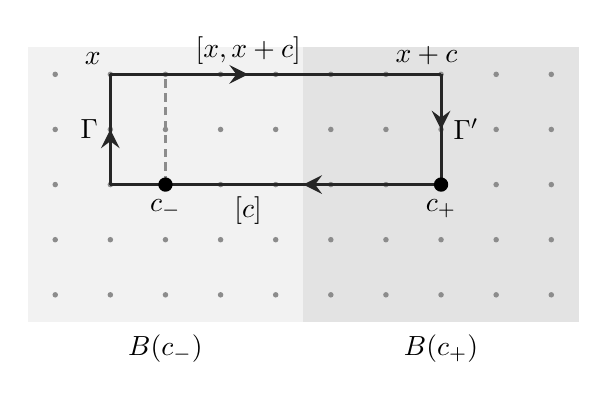
\begin{tikzpicture}[scale=0.7,
        path/.style={line width=1.1pt, black!85, line join=round},
        loop/.style={path,
            decoration={markings, mark=at position 0.5 with {\arrow[scale=1.4]{stealth}}}, postaction={decorate}}]
    \fill[black!5] (-2.5,-2.5) rectangle (2.5,2.5);
    \fill[black!11] (2.5,-2.5) rectangle (7.5,2.5);
    \foreach \x in {-2,...,7} {
        \foreach \y in {-2,...,2} {
            \fill[black!45] (\x,\y) circle (0.05);
        }
    }
    \draw[black!45, line width=0.9pt, dash pattern=on 3pt off 2pt] (0,0) -- (0,2);
    \draw[path] (0,0) -- (-1,0);
    \draw[loop] (-1,0) -- (-1,2);
    \draw[loop] (-1,2) -- (4,2);
    \draw[path] (4,2) -- (5,2);
    \draw[loop] (5,2) -- (5,0);
    \draw[loop] (5,0) -- (0,0);
    \fill (0,0) circle (0.13);
    \fill (5,0) circle (0.13);
    \node[below] at (0,-0.1) {$c_-$};
    \node[below] at (5,-0.1) {$c_+$};
    \node[above left] at (-1,2) {$x$};
    \node[above right] at (4,2) {$x + c$};
    \node[left] at (-1.05,1) {$\Gamma$};
    \node[above] at (1.5,2) {$[x, x + c]$};
    \node[right] at (5.05,1) {$\Gamma'$};
    \node[below] at (1.5,-0.05) {$[c]$};
    \node[below] at (0,-2.55) {$B(c_-)$};
    \node[below] at (5,-2.55) {$B(c_+)$};
\end{tikzpicture}
\caption{A loop $\ell_c(x, \Gamma, \Gamma')$.}
\label{fig:block-paths}
\end{figure}

All these paths run through sites of $B(c_-) \cup B(c_+)$. Two elementary facts about them are used repeatedly. For a field with small plaquettes the value on a closed path which encloses few plaquettes is close to $\id$, and the paths of a block, and the loops of a bond, enclose few; and multiplying a configuration by the exponential of a small form changes its value on a short path by a factor close to $\id$. To state the first, we say that a closed path $\gamma_1\sigma\gamma_2$ is \emph{moved across} a plaquette $p$ if the piece $\sigma$ is replaced by a piece $\sigma'$ with $\sigma\sigma'^{-1} = \partial p$, read from the first point of $\sigma$.

\begin{lemma}[Values on Short Paths]\label{lem:block-holonomies}
Let $j \in [k]$.
\begin{enumerate}[label=(\roman*)]
\item Let $U \in \mathscr G^{(j-1)}$, and let $\gamma$ be a closed path which is reduced to the trivial path by $m$ moves across plaquettes $p$ with $\abs{U(\partial p) - \id} \leqslant \alpha$. Then $\abs{U(\gamma) - \id} \leqslant m\alpha$ and $\norm{U(\gamma) - \id} \leqslant \sqrt Nm\alpha$.
\item Let $y \in T^{(j)}$ and $x \in B(y)$. For $\Gamma, \Gamma' \in \mathbf G(y, x)$ the closed path $\Gamma\Gamma'^{-1}$ is reduced to the trivial path by at most $\frac{3}{2}L^2$ moves across plaquettes with corners in $B(y)$. For a bond $c$ of $T^{(j)}$, every loop of $c$ has at most $6L$ bonds and is reduced to the trivial path by at most $4L^2$ moves across plaquettes with corners in $B(c_-) \cup B(c_+)$.
\item Let $\mathbf U \in \mathscr G^{(j-1)}_c$, let $\gamma$ be a path of $T^{(j-1)}$ with $n$ bonds, and let $\kappa \geqslant 1$ be such that $\norm{\Ad_{\mathbf U(\gamma')}Z} \leqslant \kappa\norm Z$ for all matrices $Z$ and all initial pieces $\gamma'$ of $\gamma$. For a $1$-form $A$ with values in $\mathfrak g^c$,
\[
    (e^{ia_{j-1}A}\mathbf U)(\gamma) = e^{iY_1}\cdots e^{iY_n}\,\mathbf U(\gamma)\;,
\]
with $Y_l \in \mathfrak g^c$ and $\norm{Y_l} \leqslant \kappa\norm{a_{j-1}A}_\infty$, the supremum being taken over the bonds of $\gamma$, so that $\norm{e^{iY_1}\cdots e^{iY_n} - \id} \leqslant e^{\kappa n\norm{a_{j-1}A}_\infty} - 1$.
\end{enumerate}
\end{lemma}

\begin{proof}
(i) A move changes the value of the path by a conjugate of a plaquette variable, since
\[
    U(\gamma_1\sigma\gamma_2) = U(\gamma_1)U(\partial p)U(\gamma_1)^{-1}\,U(\gamma_1\sigma'\gamma_2)\;.
\]
So $U(\gamma)$ is a product $W_1\cdots W_m$ of unitary conjugates of plaquette variables or of their inverses, and $\abs{W_l - \id} \leqslant \alpha$, because the norms of $W - \id$ are invariant under unitary conjugation (Lemma~\ref{lem:norms}(ii)) and under the inversion of a unitary $W$, by $W^{-1} - \id = -W^{-1}(W - \id)$. The identity $W_1\cdots W_m - \id = W_1(W_2\cdots W_m - \id) + (W_1 - \id)$ and induction give $\abs{U(\gamma) - \id} \leqslant \sum_l\abs{W_l - \id} \leqslant m\alpha$, and Lemma~\ref{lem:norms}(i) gives the bound in the operator norm.

(ii) A path of $\mathbf G(y, x)$ belongs to an ordering of the coordinates $\mu$ with $n_\mu \neq 0$, and two orderings are related by at most six exchanges of consecutive coordinates. An exchange of $\mu$ and $\nu$ moves the path across the $\abs{n_\mu}\abs{n_\nu} \leqslant \frac{1}{4}(L - 1)^2$ plaquettes of a rectangle in $B(y)$, which gives the first assertion.

The loop $\ell = \ell_c(x, \Gamma, \Gamma')$ runs out along $\Gamma$, across along $[x, x + c]$, back along $\Gamma'$, and back along $[c]$. It would bound a strip if $\Gamma'$ were the translate of $\Gamma$ by $c_+ - c_-$, and so we deform it in two stages. The translate of $\Gamma$ is a path of $\mathbf G(c_+, x + c)$, to which $\Gamma'$ is moved by at most $\frac{3}{2}L^2$ moves in $B(c_+)$, by the first assertion. The loop which remains, formed by $\Gamma$, $[x, x + c]$, the reversed translate of $\Gamma$, and $[c]^{-1}$, bounds the strip swept by $\Gamma$ under the translation, with at most $L$ plaquettes for each of the at most $2(L - 1)$ bonds of $\Gamma$. Together these are at most $4L^2$ moves. The paths $\Gamma$ and $\Gamma'$ have at most $2(L - 1)$ bonds each and the straight paths $L$, so that $\ell$ has at most $6L$ bonds.

(iii) On a positive bond $b$ the configuration $e^{ia_{j-1}A}\mathbf U$ has the value $e^{ia_{j-1}A(b)}\mathbf U(b)$, and on a negative bond the value $\mathbf U(b)e^{ia_{j-1}A(b)}$, since $A(b^{-1}) = -A(b)$. We move each exponential to the left, past the values of $\mathbf U$ on the bonds before it, by $\mathbf Ve^{iZ}\mathbf V^{-1} = e^{i\Ad_{\mathbf V}Z}$. The $l$-th bond $b_l$ of $\gamma$ then contributes the factor $e^{iY_l}$ with $Y_l = \Ad_{\mathbf U(\gamma_l)}a_{j-1}A(b_l)$, where $\gamma_l$ is the initial piece of $\gamma$ before $b_l$, or up to and including $b_l$ if $b_l$ is negative. These matrices lie in $\mathfrak g^c$ by Lemma~\ref{lem:norms}(iii), and they satisfy the stated bound by the hypothesis. The last bound follows from $\norm{e^{iY} - \id} \leqslant e^{\norm Y} - 1$ and $\norm{\prod_l(\id + X_l) - \id} \leqslant \prod_l(1 + \norm{X_l}) - 1$.
\end{proof}

A field whose plaquettes are close to $\id$ on a box is, after a gauge transformation, close to $\id$ on every bond of the box. The gauge transformation is the transport from a corner along paths which run through the coordinates in a fixed order; with them the value of the transformed field on a bond is the holonomy of a staircase strip.

\begin{lemma}[An Axial Gauge on a Box]\label{lem:axial-box}
Let $j \in [k]$, $U \in \mathscr G^{(j-1)}$, and $y_0 \in T^{(j-1)}$. Let $X$ be a box of sites of $T^{(j-1)}$, that is, the set of the sites $z$ whose offsets $m_\rho(z) \coloneqq (z - y_0)_\rho/a_{j-1}$, $\rho \in [3]_0$, lie in intervals of integers which contain $0$, and let $m \geqslant \sum_\rho\abs{m_\rho(z)}$ for all $z \in X$. For $z \in X$ let $\tau_z$ be the path from $y_0$ to $z$ which runs through the coordinates $0, 1, 2, 3$ in this order, $\abs{m_\rho(z)}$ bonds in the direction of the sign of $m_\rho(z)$, and $u(z) \coloneqq U(\tau_z)$. Suppose that $\abs{U(\partial p) - \id} \leqslant \alpha$ for the plaquettes $p$ with corners in $X$, and that $\sqrt Nm\alpha \leqslant r_G$. Then $u$ has values in $G$, $u(y_0) = \id$, and $U^u = e^{iA}$ on the bonds of $X$ with values $A(b) \in \mathfrak g$ of norms $\norm{A(b)} \leqslant \frac{\pi}{2}\sqrt Nm\alpha$. For a point $z$ of $X$ on a line through $y_0$ parallel to a coordinate axis, $\tau_z$ is the straight path from $y_0$ to $z$.
\end{lemma}

\begin{proof}
The values $u(z)$ are products of values of $U$, and $\tau_{y_0}$ is the trivial path. Let $b = (z, z')$ be a bond of $X$ in the direction $\rho$. Then $U^u(b) = u(z)U(b)u(z')^{-1} = U(\tau_zb\tau_{z'}^{-1})$. The paths $\tau_z$ and $\tau_{z'}$ agree in their steps in the coordinates before $\rho$, their steps in the coordinate $\rho$ differ by the translate of $b$ to the offsets $0$ in the coordinates after $\rho$, and their steps in the coordinates $\sigma > \rho$ are translates of each other by $z' - z$. So the closed path $\tau_zb\tau_{z'}^{-1}$ is reduced to the trivial path by moves across the $\sum_{\sigma > \rho}\abs{m_\sigma(z)} \leqslant m$ plaquettes of the staircase strip between $b$ and this translate; their corners have, in each coordinate, the offset of $z$ or of $z'$, or one between $0$ and that of $z$, so that they lie in $X$. By Lemma~\ref{lem:block-holonomies}(i), $\norm{U^u(b) - \id} \leqslant \sqrt Nm\alpha \leqslant r_G$, and by Lemma~\ref{lem:logarithm}(ii) and~(iii), $U^u(b) = e^{iA(b)}$ with $A(b) \in \mathfrak g$, $\norm{A(b)} < \log 2$, and $\norm{A(b)} \leqslant \frac{\pi}{2}\norm{U^u(b) - \id} \leqslant \frac{\pi}{2}\sqrt Nm\alpha$. The last statement holds because the offsets of such a point vanish in all coordinates but one.
\end{proof}

\begin{definition}[The Average]\label{def:average}
Let $\mathbf U \in \mathscr G^{(j-1)}_c$ and $c \in T^{(j)}_{\mathrm b}$. Let $\mathcal O_c \subset \mathscr G^{(j-1)}_c$ be the set of configurations $\mathbf U$ with $\norm{\mathbf U(\ell_c(x, \Gamma, \Gamma')) - \id} \leqslant r_G$ for all loops of $c$, and for $\mathbf U \in \mathcal O_c$ let
\begin{equation}\label{eq:average-exponent}
    \beta_c(\mathbf U) \coloneqq \frac{1}{L^4}\sum_{x \in B(c_-)}\sum_{\Gamma, \Gamma'}\frac{1}{i}\frac{\log\mathbf U(\ell_c(x, \Gamma, \Gamma'))}{\abs{\mathbf G(c_-, x)}\abs{\mathbf G(c_+, x + c)}}\;.
\end{equation}
The \emph{average} of $\mathbf U$ is the map $M(\mathbf U) \colon T^{(j)}_{\mathrm b} \to G^c$ with
\begin{equation}\label{eq:average}
    M(\mathbf U)(c) \coloneqq
    \begin{cases}
        e^{i\beta_c(\mathbf U)}\mathbf U([c]) & \text{if } \mathbf U \in \mathcal O_c\;,\\
        \mathbf U([c]) & \text{otherwise}\;.
    \end{cases}
\end{equation}
The \emph{average of order $n$} is the $n$-fold iterate $M^n \colon \mathscr G^{(j)} \to \mathscr G^{(j+n)}$.
\end{definition}

The straight transport along $c$ is multiplied by the exponential of a mean, with weights which are positive and sum to one, of the logarithms of the holonomies around the loops of $c$. The second line of \eqref{eq:average} makes the average a map on all gauge fields, which the definition of the renormalisation transformation requires, and it plays no role in any estimate, since every estimate concerns fields in the set of the following lemma.

\begin{lemma}[The Domain of the Average]\label{lem:average-domain}
There are numbers $\alpha_M, r_M > 0$ and $C_M$, which depend on $L$ and $G$ only, with the following property. Let $c \in T^{(j)}_{\mathrm b}$ and $U \in \mathscr G^{(j-1)}$ with $\abs{U(\partial p) - \id} \leqslant \alpha \leqslant \alpha_M$ for the $p \in T_{\mathrm{p}}^{(j-1)}$ with corners in $B(c_-) \cup B(c_+)$.
\begin{enumerate}[label=(\roman*)]
\item $U \in \mathcal O_c$, and $\norm{\beta_c(U)} \leqslant C_M\alpha$.
\item For every $1$-form $A$ with values in $\mathfrak g^c$ on the bonds of $B(c_-) \cup B(c_+)$ with $\norm{a_{j-1}A}_\infty < r_M$, $e^{ia_{j-1}A}U \in \mathcal O_c \cap \mathcal O_{c^{-1}}$, and $A \mapsto M(e^{ia_{j-1}A}U)(c)$ is holomorphic with values in $G^c$.
\end{enumerate}
\end{lemma}

\begin{proof}
We set $\alpha_M \coloneqq r_G/(8\sqrt NL^2)$, $C_M \coloneqq 7\sqrt NL^2$, and $r_M \coloneqq r_G/(16L)$. Since $c^{-1}$ has the same blocks as $c$, what we show for the loops of $c$ holds for those of $c^{-1}$ as well.

(i) A loop $\ell$ of $c$ is reduced to the trivial path by at most $4L^2$ moves across plaquettes with corners in $B(c_-) \cup B(c_+)$, by Lemma~\ref{lem:block-holonomies}(ii). So Lemma~\ref{lem:block-holonomies}(i) and the choice of $\alpha_M$ give
\[
    \norm{U(\ell) - \id} \leqslant 4\sqrt NL^2\alpha \leqslant \tfrac{1}{2}r_G\;.
\]
In particular $U \in \mathcal O_c$, and by Lemma~\ref{lem:logarithm}(ii) and~(iii) $\log U(\ell) = iA_\ell$ with $A_\ell \in \mathfrak g$ and $\norm{A_\ell} \leqslant \frac{\pi}{2}\norm{U(\ell) - \id} \leqslant 2\pi\sqrt NL^2\alpha \leqslant C_M\alpha$. The exponent $\beta_c(U)$ is a mean of the $A_\ell$, with weights which sum to one, and so it satisfies the same bound.

(ii) Let $\mathbf U \coloneqq e^{ia_{j-1}A}U$. The perturbation multiplies each bond variable by a matrix close to $\id$, and we must check that this does not push the holonomies out of the ball of radius $r_G$ around $\id$, on which the logarithm is holomorphic and the average is given by the first line of \eqref{eq:average}. The loop $\ell$ has at most $6L$ bonds, and conjugation by the unitary matrices $U(\gamma')$ preserves the norm, so that Lemma~\ref{lem:block-holonomies}(iii), with $\kappa = 1$, gives $\mathbf U(\ell) = E_\ell U(\ell)$ with $\norm{E_\ell - \id} \leqslant e^{6L\norm{a_{j-1}A}_\infty} - 1$. By the choice of $r_M$, and since $e^{3t/8} - 1 \leqslant t(e^{3/8} - 1) \leqslant \frac{1}{2}t$ for $t \in [0, 1]$ by convexity,
\[
    \norm{E_\ell - \id} \leqslant e^{6L\norm{a_{j-1}A}_\infty} - 1 \leqslant e^{3r_G/8} - 1 \leqslant \tfrac{1}{2}r_G\;.
\]
Writing $\mathbf U(\ell) - \id = (E_\ell - \id)U(\ell) + (U(\ell) - \id)$ and using $\norm{U(\ell)} = 1$ and the bound of (i), we find $\norm{\mathbf U(\ell) - \id} \leqslant r_G$, so that $\mathbf U \in \mathcal O_c \cap \mathcal O_{c^{-1}}$.

Holomorphy is now a matter of composition. The matrix $\mathbf U(\ell)$ is a polynomial in the entries of the matrices $e^{\pm ia_{j-1}A(b)}$, and it stays in the ball on which $\log$ is holomorphic (Lemma~\ref{lem:logarithm}(i)); so $\log\mathbf U(\ell)$, $\beta_c(\mathbf U)$, and $M(\mathbf U)(c) = e^{i\beta_c(\mathbf U)}\mathbf U([c])$ are holomorphic on the convex set of the $A$ with $\norm{a_{j-1}A}_\infty < r_M$.

The values in $G^c$ need an argument, because nothing so far places the logarithm of a complex holonomy in $i\mathfrak g^c$, and we obtain it from the real fields. For $A$ with values in $\mathfrak g$, $\mathbf U(\ell)$ is an element of $G$ within $r_G$ of $\id$, so that $\log\mathbf U(\ell) \in i\mathfrak g$ by Lemma~\ref{lem:logarithm}(ii). These $A$ form a nonempty relatively open set of the real points of the domain, and Lemma~\ref{lem:real-points}(ii) carries the statement to $\frac{1}{i}\log\mathbf U(\ell) \in \mathfrak g^c$ for all $A$. Hence $\beta_c(\mathbf U) \in \mathfrak g^c$ and $e^{i\beta_c(\mathbf U)} \in G^c$. Since $\mathbf U([c])$ is a product of the matrices $e^{\pm ia_{j-1}A(b)} \in G^c$ and $U(b)^{\pm 1} \in G \subset G^c$ (Lemma~\ref{lem:logarithm}(ii)), $M(\mathbf U)(c) \in G^c$.
\end{proof}

\begin{lemma}[Properties of the Average]\label{lem:average}
Let $\mathbf U \in \mathscr G^{(j-1)}_c$ and $c \in T^{(j)}_{\mathrm b}$.
\begin{enumerate}[label=(\roman*)]
\item \emph{Consistency.} For $U \in \mathscr G^{(j-1)}$, $U \in \mathcal O_c$ if and only if $U \in \mathcal O_{c^{-1}}$, and $M(U)(c^{-1}) = M(U)(c)^{-1}$, so that $M(U) \in \mathscr G^{(j)}$; for $U \in \mathcal O_c$, $\beta_c(U) \in \mathfrak g$. The identity $M(\mathbf U)(c^{-1}) = M(\mathbf U)(c)^{-1}$ holds also for the configurations $\mathbf U = e^{ia_{j-1}A}U$ of Lemma~\ref{lem:average-domain}(ii).
\item \emph{Locality.} $M(\mathbf U)(c)$ depends only on the values of $\mathbf U$ on the bonds of $T^{(j-1)}$ with both ends in $B(c_-) \cup B(c_+)$.
\item \emph{Covariance.} For every gauge transformation $u$ of $T^{(j-1)}$, $\mathbf U^u \in \mathcal O_c$ if and only if $\mathbf U \in \mathcal O_c$, and $M(\mathbf U^u)(c) = u(c_-)M(\mathbf U)(c)u(c_+)^{-1}$. The identity holds also for every complex gauge transformation $u$ with $\mathbf U, \mathbf U^u \in \mathcal O_c$.
\item \emph{Symmetry.} Let $\theta$ be a translation of the torus by a point of $T^{(j)}$, a reflection $x_\mu \mapsto -x_\mu$, or a permutation of the coordinates, and let $(\theta\mathbf U)(b) \coloneqq \mathbf U(\theta^{-1}b)$. Then $M(\theta\mathbf U) = \theta M(\mathbf U)$.
\end{enumerate}
\end{lemma}

\begin{proof}
For a path $\gamma$ from $z$ to $z'$ and a complex gauge transformation $u$, $\mathbf U^u(\gamma) = u(z)\mathbf U(\gamma)u(z')^{-1}$, and $\mathbf U(\gamma^{-1}) = \mathbf U(\gamma)^{-1}$.

(i) The bond $c^{-1}$ has the ends $(c^{-1})_\pm = c_\mp$, and $[c^{-1}] = [c]^{-1}$. For $x \in B(c_+)$, $\Gamma \in \mathbf G(c_+, x)$, and $\Gamma' \in \mathbf G(c_-, x + c^{-1})$, where $x + c^{-1} = x + (c_- - c_+)$, the loops satisfy $\ell_{c^{-1}}(x, \Gamma, \Gamma') = [c]^{-1}\ell_c(x + c^{-1}, \Gamma', \Gamma)^{-1}[c]$ as closed paths at $c_+$, since $[x + c^{-1}, x]^{-1} = [x, x + c^{-1}]$; the map $(x, \Gamma, \Gamma') \mapsto (x + c^{-1}, \Gamma', \Gamma)$ is a bijection between the index sets of the two means, with the same weights. So $U(\ell_{c^{-1}}(x, \Gamma, \Gamma')) = V^{-1}W^{-1}V$ with $V \coloneqq U([c])$ and $W \coloneqq U(\ell_c(x + c^{-1}, \Gamma', \Gamma))$, unitary matrices, and $\norm{V^{-1}W^{-1}V - \id} = \norm{W^{-1} - \id} = \norm{W - \id}$ by Lemma~\ref{lem:norms}(ii), the last because $W^{-1} - \id = -W^{-1}(W - \id)$; hence $U \in \mathcal O_{c^{-1}}$ if and only if $U \in \mathcal O_c$. For $U \in \mathcal O_c$, Lemma~\ref{lem:logarithm}(ii) gives $W = e^{iA}$ with $A \in \mathfrak g$ and $\norm A < \log 2$, so that $\log W^{-1} = -iA = -\log W$ by Lemma~\ref{lem:logarithm}(i), and $\log(V^{-1}W^{-1}V) = -\Ad_V^{-1}\log W$ by the same lemma; so $\beta_{c^{-1}}(U) = -\Ad_{U([c])}^{-1}\beta_c(U)$. Hence $M(U)(c^{-1}) = e^{-i\Ad_{U([c])}^{-1}\beta_c(U)}U([c])^{-1} = U([c])^{-1}e^{-i\beta_c(U)} = M(U)(c)^{-1}$ on $\mathcal O_c$, and $U([c^{-1}]) = U([c])^{-1}$ otherwise. The logarithms of the holonomies lie in $i\mathfrak g$ by Lemma~\ref{lem:logarithm}(ii), so that $\beta_c(U)$, a convex combination of elements of $\mathfrak g$, lies in $\mathfrak g$ (Lemma~\ref{lem:lie-algebra}), and $M(U)(c) \in G$. If $\mathbf U = e^{ia_{j-1}A}U$ is a configuration of Lemma~\ref{lem:average-domain}(ii), then $M(\mathbf U)(c^{-1})$ and $M(\mathbf U)(c)^{-1}$ are holomorphic in $A$, by that lemma applied to $c$ and to $c^{-1}$, a bond with the same blocks, and they agree for $A$ with values in $\mathfrak g$, $\mathbf U$ then being a gauge field; so they agree by Lemma~\ref{lem:real-points}(i).

(ii) All the paths of Definition~\ref{def:block-paths} run along bonds with both ends in $B(c_-) \cup B(c_+)$.

(iii) The loops of $c$ begin and end at $c_-$, so that $\mathbf U^u(\ell) = u(c_-)\mathbf U(\ell)u(c_-)^{-1}$. If $u$ has values in $G$, then $u(c_-)$ is unitary and $\norm{\mathbf U^u(\ell) - \id} = \norm{\mathbf U(\ell) - \id}$ (Lemma~\ref{lem:norms}(ii)), so that $\mathbf U^u \in \mathcal O_c$ if and only if $\mathbf U \in \mathcal O_c$. If $\mathbf U$ and $\mathbf U^u$ lie in $\mathcal O_c$, then $\beta_c(\mathbf U^u) = \Ad_{u(c_-)}\beta_c(\mathbf U)$ by Lemma~\ref{lem:logarithm}(i), the holonomies of both lying at a distance of at most $r_G < 1$ from $\id$, and
\[
    M(\mathbf U^u)(c) = u(c_-)e^{i\beta_c(\mathbf U)}u(c_-)^{-1}u(c_-)\mathbf U([c])u(c_+)^{-1} = u(c_-)M(\mathbf U)(c)u(c_+)^{-1}\;;
\]
if neither lies in $\mathcal O_c$, the identity is that of the straight transports.

(iv) The blocks are centred, $L$ being odd, so that $\theta$ maps blocks to blocks, $B(\theta y) = \theta B(y)$, and the families $\mathbf G(y, x)$ to the families $\mathbf G(\theta y, \theta x)$: the displacement of each coordinate is moved, reflected, or permuted, and the orderings of the coordinates correspond. It maps the straight paths $[x, x + c]$ and $[c]$ to those of $\theta c$, and so the loops of $c$, with their weights, to those of $\theta c$. Since $(\theta\mathbf U)(\theta\gamma) = \mathbf U(\gamma)$, $\theta\mathbf U \in \mathcal O_{\theta c}$ if and only if $\mathbf U \in \mathcal O_c$, and $M(\theta\mathbf U)(\theta c) = M(\mathbf U)(c)$.
\end{proof}

By Lemma~\ref{lem:average-domain}(ii) and Lemma~\ref{lem:average}(i), the average $M(\mathbf U)$ of a configuration $\mathbf U$ which is of the form $e^{ia_{j-1}A}U$ of Lemma~\ref{lem:average-domain}(ii) at every bond is a configuration on $T^{(j)}$, and by Proposition~\ref{prop:relative-average-order}(i) so are its iterates $M^n(\mathbf U)$, in the ranges stated there.

The first quantitative property is that the average of a field with small plaquettes has small plaquettes, in the units of the coarser lattice, and that this is a local statement. Since the leading terms of the bounds have the coefficient one, the statement in the one norm does not follow from that in the other by the comparison of the norms, and the proof is carried out in the Hilbert--Schmidt norm.

\begin{proposition}[Averages of Regular Fields]\label{prop:regular-averages}
There are numbers $C_0 \geqslant 1$ and $c_2 \in (0, \alpha_M]$, which depend on $L$ and $G$ only, with the following properties.
\begin{enumerate}[label=(\roman*)]
\item Let $U \in \mathscr G^{(j-1)}$, let $p'$ be a plaquette of $T^{(j)}$ with the first corner $y_0$, and suppose that $\abs{U(\partial p) - \id} \leqslant \alpha \leqslant c_2L^{-2}$ for all plaquettes $p$ of $T^{(j-1)}$ whose corners lie in the blocks of the four corners of $p'$. Then
\begin{equation}\label{eq:averaged-plaquette}
    \abs{M(U)(\partial p') - \id} \leqslant \frac{1}{L^4}\sum_{x \in B(y_0)}\sum_{p \subset p'_x}\abs{U(\partial p) - \id} + C_0L^4\alpha^2 \leqslant L^2\alpha + C_0L^4\alpha^2\;,
\end{equation}
where $p'_x$ is the translate of $p'$ by $x - y_0$ and the inner sum runs over the $L^2$ plaquettes of $T^{(j-1)}$ which it contains.
\item Let $0 \leqslant i < j \leqslant k$, let $U \in \mathscr G^{(i)}$, let $p'$ be a plaquette of $T^{(j)}$, and suppose that $\abs{U(\partial p) - \id} \leqslant \alpha(a_i/a_j)^2$ with $\alpha \leqslant c_2$ for all plaquettes $p$ of $T^{(i)}$ whose corners lie in the blocks of order $j - i$ of the four corners of $p'$. Then $\abs{M^{j-i}(U)(\partial p') - \id} \leqslant \alpha + 2C_0\alpha^2 \leqslant 2\alpha$.
\end{enumerate}
\end{proposition}

\begin{proof}
We follow \cite[pp.~25--26, (46)--(54)]{BalabanAVG}: in a gauge in which the field is close to $\id$ on the four blocks, every holonomy is the exponential of the sum of the logarithms of its bonds up to a term of the second order, the first-order part of the plaquette of the average is a mean of sums of plaquettes of the fine lattice, and the iteration is an induction. Let $C_0 \coloneqq 2^{27}N$, $c_\ast \coloneqq r_G/(2^{14}\sqrt N)$, and $c_2 \coloneqq \min\{ \alpha_M, \frac{1}{2}c_\ast, 1/(4C_0) \}$. We prove (i) for $\alpha \leqslant c_\ast L^{-2}$.

(i) \emph{A gauge.} Let $p'$ have the corners $y_0$, $y_1 = y_0 + a_je_\mu$, $y_2 = y_1 + a_je_\nu$, $y_3 = y_0 + a_je_\nu$, so that $\partial p' = (c_1, c_2, c_3^{-1}, c_4^{-1})$ with the bonds $c_1 = (y_0, y_1)$, $c_2 = (y_1, y_2)$, $c_3 = (y_3, y_2)$, $c_4 = (y_0, y_3)$, and let $\Delta(p') \coloneqq B(y_0) \cup \dots \cup B(y_3)$, a box of fine sites whose offsets $m_\rho$ from $y_0$, in units of $a_{j-1}$, satisfy $\abs{m_\rho} \leqslant \frac{3}{2}L$ for $\rho \in \{ \mu, \nu \}$ and $\abs{m_\rho} \leqslant \frac{1}{2}L$ otherwise. Since $\sum_\rho\abs{m_\rho} \leqslant 4L$ and $4\sqrt NL\alpha \leqslant r_G$, Lemma~\ref{lem:axial-box}, with $m = 4L$, gives a gauge transformation $u$ with values in $G$ and $u(y_0) = \id$ such that $V \coloneqq U^u = e^{iA_b}$ on the bonds $b$ of the box, with $A_b \in \mathfrak g$ and $\norm{A_b} \leqslant 2\pi\sqrt NL\alpha \leqslant 7\sqrt NL\alpha$. By Lemma~\ref{lem:average}(iii) and since $u(y_0) = \id$, $M(U)(\partial p') = M(V)(\partial p')$, and $\abs{V(\partial p) - \id} = \abs{U(\partial p) - \id}$ for every plaquette, $V(\partial p)$ being conjugate to $U(\partial p)$ by a unitary matrix.

\emph{Linearisation.} For a path $\gamma$ in the box let $A(\gamma) \coloneqq \sum_b\pm A_b$, the sum over its bonds with the signs of their orientations. Let $s \coloneqq 60\sqrt NL^2\alpha$, so that $s \leqslant 2^{-9}$. A path of at most $6L$ bonds has $s_\gamma \coloneqq \sum_b\norm{A_b} \leqslant s$, and multiplying out the exponentials as in the proof of \eqref{eq:four-exponentials} gives $\norm{V(\gamma) - \id - iA(\gamma)} \leqslant e^{s_\gamma} - 1 - s_\gamma \leqslant s^2$ and $\norm{V(\gamma) - \id} \leqslant 2s$. With $\norm{\log W - (W - \id)} \leqslant 2\norm{W - \id}^2$ for $\norm{W - \id} \leqslant \frac{1}{2}$, from the series of $\log$, we find $\norm{\frac{1}{i}\log V(\gamma) - A(\gamma)} \leqslant 9s^2$. This applies to the loops of the four bonds $c_k$, which have at most $6L$ bonds, and to the straight paths $[c_k]$. Let $\bar A(y, x)$ be the mean of $A(\Gamma)$ over $\Gamma \in \mathbf G(y, x)$. The weights of \eqref{eq:average-exponent} factorise, so that
\[
    \beta_{c_k}(V) = \frac{1}{L^4}\sum_{x \in B(c_{k,-})}\bigl(\bar A(c_{k,-}, x) + A([x, x + c_k]) - \bar A(c_{k,+}, x + c_k)\bigr) - A([c_k]) + E_k\;,
    \qquad
    \norm{E_k} \leqslant 9s^2\;,
\]
and $V([c_k]) = e^{i(A([c_k]) + E'_k)}$ with $\norm{E'_k} \leqslant 9s^2$. All these matrices have norms of at most $2s \leqslant \frac{1}{32}$, so that by \eqref{eq:product-lipschitz} $M(V)(c_k) = e^{iZ_k}$ with $Z_k \coloneqq \Psi(\beta_{c_k}(V), A([c_k]) + E'_k)$ and
\[
    Z_k = \frac{1}{L^4}\sum_{x \in B(c_{k,-})}\bigl(\bar A(c_{k,-}, x) + A([x, x + c_k]) - \bar A(c_{k,+}, x + c_k)\bigr) + E''_k\;,
    \qquad
    \norm{E''_k} \leqslant 18s^2 + 4C_\Psi s^2 \leqslant 2^{11}s^2\;.
\]

\emph{The identity of the first-order part.} Let $\Theta \coloneqq Z_1 + Z_2 - Z_3 - Z_4 - \sum_k\pm E''_k$. At each corner $y_l$ the mean $\bar A(y_l, \bigcdot)$ occurs twice, from the two bonds of $\partial p'$ at $y_l$, at corresponding points of $B(y_l)$ and with opposite signs, since the points $x'$ of one bond are the points $x$ of the next one, and the family $\mathbf G(y_l, \bigcdot)$ is the same for both; so these terms cancel, and with $x_1 \coloneqq x + a_je_\mu$, $x_2 \coloneqq x_1 + a_je_\nu$, $x_3 \coloneqq x + a_je_\nu$,
\[
    \Theta = \frac{1}{L^4}\sum_{x \in B(y_0)}\bigl(A([x, x_1]) + A([x_1, x_2]) - A([x_3, x_2]) - A([x, x_3])\bigr) = \frac{1}{L^4}\sum_{x \in B(y_0)}\sum_{p \subset p'_x}A(\partial p)\;,
\]
the last because the boundary of the square $p'_x$ is the sum, with the orientations, of the boundaries of its $L^2$ plaquettes, the inner bonds occurring twice with opposite signs. For a plaquette, with four bonds, $\norm{V(\partial p) - \id - iA(\partial p)} \leqslant (28\sqrt NL\alpha)^2$, so that $\abs{A(\partial p)} \leqslant \abs{U(\partial p) - \id} + 2^{10}NL^2\alpha^2$, and
\[
    \abs\Theta \leqslant \frac{1}{L^4}\sum_{x \in B(y_0)}\sum_{p \subset p'_x}\abs{U(\partial p) - \id} + 2^{10}NL^4\alpha^2\;.
\]

\emph{The plaquette of the average.} The product $M(V)(\partial p') = e^{iZ_1}e^{iZ_2}e^{-iZ_3}e^{-iZ_4}$, with $\norm{Z_k} \leqslant 3s$, is $e^{i\Theta'}$ with $\Theta' = Z_1 + Z_2 - Z_3 - Z_4 + E$ and $\norm E \leqslant C_\Psi(9 + 21 + 33)s^2 \leqslant 2^{14}s^2$, by \eqref{eq:product-lipschitz} applied three times; it is an element of $G$ with $\norm{e^{i\Theta'} - \id} \leqslant e^{12s} - 1 \leqslant r_G$, so that $\Theta' \in \mathfrak g$ by Lemma~\ref{lem:logarithm}(ii), and $\abs{M(V)(\partial p') - \id} \leqslant \abs{\Theta'}$ by Lemma~\ref{lem:logarithm}(iii). Since $\Theta' = \Theta + \sum_k\pm E''_k + E$, with $\abs X \leqslant \norm X$, and $(4 \cdot 2^{11} + 2^{14})s^2 \leqslant 2^{15} \cdot 3600NL^4\alpha^2$,
\[
    \abs{M(U)(\partial p') - \id} \leqslant \frac{1}{L^4}\sum_{x \in B(y_0)}\sum_{p \subset p'_x}\abs{U(\partial p) - \id} + C_0L^4\alpha^2\;,
\]
and the double sum is at most $L^2\alpha$, which is \eqref{eq:averaged-plaquette}. The bounds $s \leqslant 2^{-9}$, under which the sums of at most four of the matrices $Z_k$ have norms of at most $12s \leqslant \frac{1}{32}$, $4\sqrt NL\alpha \leqslant r_G$, $e^{12s} - 1 \leqslant r_G$, and $\alpha \leqslant \alpha_M$, the last for the definition of the average, follow from $\alpha \leqslant c_\ast L^{-2}$.

(ii) Let $n \coloneqq j - i$, $\varepsilon \coloneqq \alpha(a_i/a_j)^2$, and for $0 \leqslant l \leqslant n$ let $\alpha_l$ be the largest of the numbers $\abs{M^l(U)(\partial p) - \id}$ over the plaquettes $p$ of $T^{(i+l)}$ whose corners lie in the blocks of the order $n - l$ of the four corners of $p'$; by the locality of the average (Lemma~\ref{lem:average}(ii)) these depend on $U$ on the blocks of the order $n$ only. We show $\alpha_l \leqslant \varepsilon L^{2l}(1 + 2C_0\varepsilon L^{2l})$ by induction; for $l = 0$ it is the hypothesis. If it holds for some $l < n$, then $\varepsilon L^{2l} \leqslant \alpha L^{-2}$ and $C_0\alpha \leqslant \frac{1}{4}$, so that $\alpha_l \leqslant 2\alpha L^{-2} \leqslant c_\ast L^{-2}$, and (i), applied to $M^l(U)$ on the lattice $T^{(i+l)}$, gives
\[
    \alpha_{l+1} \leqslant L^2\alpha_l + C_0L^4\alpha_l^2 \leqslant \varepsilon L^{2(l+1)}\Bigl(1 + C_0\varepsilon L^{2(l+1)}\bigl(2L^{-2} + (1 + 2C_0\varepsilon L^{2l})^2\bigr)\Bigr)\;,
\]
and $2L^{-2} + (1 + 2C_0\alpha L^{-2})^2 \leqslant \frac{2}{9} + (1 + \frac{1}{18})^2 \leqslant 2$, since $L \geqslant 3$. For $l = n$ this is $\alpha_n \leqslant \alpha(1 + 2C_0\alpha) \leqslant 2\alpha$.
\end{proof}

\subsection{The Average Relative to a Background}\label{sec:relative-average}

Let the field be $e^{iaA}\mathbf U$, with a background $\mathbf U$ and a fluctuation $A$. We want to write its average as a function of the fluctuation times the average of the background. The quotient $M(e^{iaA}\mathbf U)(c)M(\mathbf U)(c)^{-1}$ does this, but it is not the function which the linear theory uses: under a gauge transformation of the fluctuation which is trivial at the coarse sites it changes, through the paths $\Gamma$ and $\Gamma'$ which join the coarse sites to the points of their blocks. The function used instead is obtained by first transforming the fluctuation, at each coarse site, to the gauge in which the mean of its transports to the points of the block is trivial. The transports are taken along all the paths of $\mathbf G(y, x)$ at once, through a mean of group elements.

\begin{definition}[The Mean of Group Elements and the Transports of a Block]\label{def:group-mean}
\begin{enumerate}[label=(\roman*)]
\item Let $\varrho_{\mathsf m} \coloneqq \min\{ 2^{-10}, \frac{1}{8}r_G \}$, and let $\mathbf W_1, \dots, \mathbf W_n$ be invertible matrices with $\mathbf W_i\mathbf W_1^{-1} = e^{iY_i}$, $Y_i \in \mathfrak g^c$, and $\norm{Y_i} \leqslant 2\varrho_{\mathsf m}$ for all $i$. Their \emph{mean} $\mathsf m(\{ \mathbf W_i \})$ is the matrix $\mathbf W = e^{iZ}\mathbf W_1$ with $Z \in \mathfrak g^c$, $\norm Z \leqslant 4\varrho_{\mathsf m}$, and
\begin{equation}\label{eq:group-mean}
    \sum_{i=1}^{n}\log(\mathbf W_i\mathbf W^{-1}) = 0\;.
\end{equation}
\item For a configuration $\mathbf U$ on $T^{(j-1)}$, a site $y \in T^{(j)}$, and $x \in B(y)$, the \emph{transport} from $y$ to $x$ is $\mathbf U(y, x) \coloneqq \mathsf m(\{ \mathbf U(\Gamma) \}_{\Gamma \in \mathbf G(y, x)})$, whenever the mean is defined.
\end{enumerate}
\end{definition}

\begin{lemma}[The Mean of Group Elements]\label{lem:group-mean}
Under the condition of Definition~\ref{def:group-mean}(i) the equation \eqref{eq:group-mean} has exactly one solution $\mathbf W = e^{iZ}\mathbf W_1$ with $Z \in \mathfrak g^c$ and $\norm Z \leqslant 4\varrho_{\mathsf m}$, and $\norm Z \leqslant 2\max_i\norm{Y_i}$. It does not depend on the order of the elements, and $Z$ is a holomorphic function of $(Y_1, \dots, Y_n)$. For every invertible $\mathbf v$, and for every $\mathbf u \in G^c$ with $\norm{\Ad_{\mathbf u}X} \leqslant 2\norm X$ for all $X$, in particular for $\mathbf u \in G$, provided that $\norm{Y_i} \leqslant \varrho_{\mathsf m}$ for all $i$,
\[
    \mathsf m(\{ \mathbf W_i\mathbf v \}) = \mathsf m(\{ \mathbf W_i \})\,\mathbf v\;,
    \qquad
    \mathsf m(\{ \mathbf u\mathbf W_i \}) = \mathbf u\,\mathsf m(\{ \mathbf W_i \})\;,
\]
and $\mathsf m(\{ \mathbf W_i^{-1} \}) = \mathsf m(\{ \mathbf W_i \})^{-1}$ if moreover $\mathbf W_1 \in G^c$ and $\norm{\Ad_{\mathbf W_1}^{\pm 1}X} \leqslant 2\norm X$ for all $X$. If all $\mathbf W_i$ lie in $G$ and $\norm{\mathbf W_i\mathbf W_1^{-1} - \id} \leqslant \varrho_{\mathsf m}$, then the condition holds with $Y_i \in \mathfrak g$, and the mean lies in $G$. Finally, with $C_{\mathsf m} \coloneqq 2^{11}$, if $\mathbf W_i = e^{iX_i}$ with $X_i \in \mathfrak g^c$ and $\norm{X_i} \leqslant \varrho \leqslant \frac{1}{4}\varrho_{\mathsf m}$, then the condition holds, the mean is $e^{iV}$ with $V \in \mathfrak g^c$ and $\norm V \leqslant 8\varrho$, and $\norm{\frac{1}{i}\log\mathsf m(\{ \mathbf W_i \}) - \frac{1}{n}\sum_iX_i} \leqslant C_{\mathsf m}\varrho^2$.
\end{lemma}

\begin{proof}
All the matrices $X, Y \in \mathfrak g^c$ below have norms of at most $\frac{1}{32}$, so that Lemma~\ref{lem:product} applies, and $\log(e^{iX}e^{iY}) = i\Psi(X, Y)$. By \eqref{eq:product-lipschitz}, applied to the pairs $(X, Y)$ and $(0, 0)$, and to $(X, Y')$ and $(X, Y)$, the function $\Phi(X, Y) \coloneqq \Psi(X, Y) - X - Y$ satisfies $\norm{\Phi(X, Y)} \leqslant C_\Psi\norm X\norm Y$ and $\norm{\Phi(X, Y') - \Phi(X, Y)} \leqslant C_\Psi\norm X\norm{Y' - Y}$.

\emph{Existence and uniqueness.} For $\mathbf W = e^{iZ}\mathbf W_1$ we have $\mathbf W_i\mathbf W^{-1} = e^{iY_i}e^{-iZ}$, so that \eqref{eq:group-mean} reads $\sum_i\Psi(Y_i, -Z) = 0$, that is $Z = T(Z) \coloneqq \frac{1}{n}\sum_i(Y_i + \Phi(Y_i, -Z))$. Since $C_\Psi\norm{Y_i} \leqslant 2^6 \cdot 2^{-9} < \frac{1}{2}$, the map $T$ is a contraction with the constant $\frac{1}{2}$ on the closed ball of the $Z \in \mathfrak g^c$ with $\norm Z \leqslant 4\varrho_{\mathsf m}$, which it maps into itself, because $\norm{T(Z)} \leqslant \max_i\norm{Y_i}(1 + C_\Psi\norm Z) \leqslant 2\varrho_{\mathsf m} + \frac{1}{2}\norm Z$. So it has exactly one fixed point $Z$ there, with $\norm Z \leqslant \max_i\norm{Y_i} + \frac{1}{2}\norm Z$. The map $T$ is symmetric in the $Y_i$, so the solution does not depend on their order; and $Z$ is the uniform limit of the iterates $T^m(0)$, which are holomorphic functions of $(Y_1, \dots, Y_n)$, so it is holomorphic.

\emph{Covariance and inverses.} Since $(\mathbf W_i\mathbf v)(\mathbf W_1\mathbf v)^{-1} = \mathbf W_i\mathbf W_1^{-1}$ and $(\mathbf W\mathbf v)(\mathbf W_i\mathbf v)^{-1} = \mathbf W\mathbf W_i^{-1}$, the elements $\mathbf W_i\mathbf v$ satisfy the condition with the same $Y_i$, and $\mathbf W\mathbf v$ solves their equation in the same ball. For $\mathbf u$ as stated, $\mathbf u\mathbf W_i(\mathbf u\mathbf W_1)^{-1} = e^{i\Ad_{\mathbf u}Y_i}$ with $\Ad_{\mathbf u}Y_i \in \mathfrak g^c$ (Lemma~\ref{lem:norms}(iii)) of a norm of at most $2\varrho_{\mathsf m}$, $\mathbf u\mathbf W = e^{i\Ad_{\mathbf u}Z}\mathbf u\mathbf W_1$ with $\norm{\Ad_{\mathbf u}Z} \leqslant 4\max_i\norm{Y_i} \leqslant 4\varrho_{\mathsf m}$, and $\sum_i\log(\mathbf u\mathbf W_i\mathbf W^{-1}\mathbf u^{-1}) = \Ad_{\mathbf u}\sum_i\log(\mathbf W_i\mathbf W^{-1}) = 0$ by Lemma~\ref{lem:logarithm}(i); by the uniqueness $\mathsf m(\{ \mathbf u\mathbf W_i \}) = \mathbf u\mathbf W$. For the inverses, $\mathbf W_i^{-1}\mathbf W_1 = e^{-i\Ad_{\mathbf W_1}^{-1}Y_i}$ and $\mathbf W^{-1} = e^{-i\Ad_{\mathbf W_1}^{-1}Z}\mathbf W_1^{-1}$, with exponents in $\mathfrak g^c$ of the norms which the condition and the ball require; and $\mathbf W_i^{-1}\mathbf W = \Ad_{\mathbf W_1^{-1}e^{-iZ}}(e^{iY_i}e^{-iZ})^{-1}$, so that by Lemma~\ref{lem:logarithm}(i) and $\log(X^{-1}) = -\log X$, an identity of power series, $\sum_i\log(\mathbf W_i^{-1}\mathbf W) = -\Ad_{\mathbf W_1^{-1}e^{-iZ}}\sum_i\log(\mathbf W_i\mathbf W^{-1}) = 0$, and $\mathbf W^{-1}$ is the mean of the inverses.

\emph{Elements of $G$.} If $\mathbf W_i \in G$ and $\norm{\mathbf W_i\mathbf W_1^{-1} - \id} \leqslant \varrho_{\mathsf m} \leqslant r_G$, then $\mathbf W_i\mathbf W_1^{-1} = e^{iY_i}$ with $Y_i \in \mathfrak g$ and $\norm{Y_i} \leqslant \frac{\pi}{2}\varrho_{\mathsf m} \leqslant 2\varrho_{\mathsf m}$, by Lemma~\ref{lem:logarithm}(ii) and~(iii). For $Y, Z \in \mathfrak g$ with $\norm Y + \norm Z \leqslant 6\varrho_{\mathsf m}$ the unitary matrix $e^{iY}e^{-iZ}$ lies in $G$ at a distance of at most $e^{6\varrho_{\mathsf m}} - 1 \leqslant r_G$ from $\id$, so that $\Psi(Y, -Z) \in \mathfrak g$ by Lemma~\ref{lem:logarithm}(ii); hence $T$ maps the ball of $\mathfrak g$ into itself, the fixed point lies in $\mathfrak g$, and $\mathbf W = e^{iZ}\mathbf W_1 \in G$.

\emph{The expansion.} Let $\mathbf W_i = e^{iX_i}$ with $\norm{X_i} \leqslant \varrho \leqslant \frac{1}{4}\varrho_{\mathsf m}$. Then $Y_i = \Psi(X_i, -X_1)$ has $\norm{Y_i} \leqslant 2\varrho + C_\Psi\varrho^2 \leqslant 3\varrho \leqslant \varrho_{\mathsf m}$, and the mean is $e^{iZ}e^{iX_1} = e^{iV}$ with $V \coloneqq \Psi(Z, X_1)$ and $\norm V \leqslant \norm Z + \varrho + C_\Psi\varrho\norm Z \leqslant 8\varrho$, since $\norm Z \leqslant 6\varrho$. So $\frac{1}{i}\log\mathsf m(\{ \mathbf W_i \}) = V$ (Lemma~\ref{lem:logarithm}(i)), and \eqref{eq:group-mean} reads $\sum_i\Psi(X_i, -V) = 0$, that is $V = \frac{1}{n}\sum_i(X_i + \Phi(X_i, -V))$. With $\norm{\Phi(X_i, -V)} \leqslant C_\Psi \cdot 8\varrho \cdot \varrho \leqslant 2^{11}\varrho^2$ this is the last assertion.
\end{proof}

By the covariance, $\mathbf U^u(y, x) = u(y)\mathbf U(y, x)u(x)^{-1}$. The relative average compares the transports of a configuration with those of the configuration multiplied by the exponential of a small form, and so we bound the change of a mean and of a transport under such a move.

\begin{lemma}[The Mean and the Transports of a Moved Configuration]\label{lem:moved-transports}
Let $\varrho_G \in (0, \frac{1}{32}]$ be a number with $\varrho_G \leqslant \frac{1}{8}r_G$ for which the last statement of Lemma~\ref{lem:group-mean} holds with $\varrho = \varrho_G$ and $C_{\mathsf m}\varrho_G \leqslant 1$.
\begin{enumerate}[label=(\roman*)]
\item If $X_i, X'_i \in \mathfrak g^c$ with $\norm{X_i}, \norm{X'_i} \leqslant \frac{1}{2}\varrho_G$ for $i \leqslant n$, then
\[
    \Bigl\lVert\frac{1}{i}\log\mathsf m\bigl(\{ e^{iX'_i} \}\bigr) - \frac{1}{i}\log\mathsf m\bigl(\{ e^{iX_i} \}\bigr)\Bigr\rVert \leqslant 16\max_i\norm{X'_i - X_i}\;.
\]
\item Let $\mathbf U$ be a configuration on $T^{(j-1)}$ with the spacing $a$, $y \in T^{(j)}$, and $x \in B(y)$, and suppose that $\mathbf U(\Gamma) = e^{iX_\Gamma}\mathbf U(y, x)$ with $X_\Gamma \in \mathfrak g^c$ and $\norm{X_\Gamma} \leqslant \frac{1}{4}\varrho_G$ for the paths $\Gamma$ of $\mathbf G(y, x)$, and that $\norm{\Ad_{\mathbf U(\gamma)}Z} \leqslant 2\norm Z$ for the pieces $\gamma$ of these paths which begin at $y$ and all matrices $Z$. Let $A$ be a $1$-form on the bonds of $B(y)$ with values in $\mathfrak g^c$ and $2^9L\norm{aA}_\infty \leqslant \varrho_G$. Then $(e^{iaA}\mathbf U)(\Gamma)\mathbf U(\Gamma)^{-1} = e^{iZ_\Gamma}$ with $Z_\Gamma \in \mathfrak g^c$ and $\norm{Z_\Gamma} \leqslant 16L\norm{aA}_\infty$ for every $\Gamma \in \mathbf G(y, x)$, and the transports satisfy
\[
    \Bigl\lVert\frac{1}{i}\log\bigl((e^{iaA}\mathbf U)(y, x)\,\mathbf U(y, x)^{-1}\bigr)\Bigr\rVert \leqslant 2^{11}L\norm{aA}_\infty\;.
\]
\item If $U$ is a gauge field on $T^{(j-1)}$ with $\abs{U(\partial p) - \id} \leqslant \alpha \leqslant \varrho_G/(200\sqrt NL^2)$ for the plaquettes $p$ with corners in $B(y)$, then $\mathbf U = U$ satisfies the hypotheses of \emph{(ii)} for every $x \in B(y)$.
\end{enumerate}
\end{lemma}

\begin{proof}
(i) By Lemma~\ref{lem:group-mean} the function $Y(X) \coloneqq \frac{1}{i}\log\mathsf m(\{ e^{iX_i} \})$ is holomorphic on the polydisc $\norm{X_i} < \varrho_G$, and $\norm{Y(X)} \leqslant \varrho_G + C_{\mathsf m}\varrho_G^2 \leqslant 2\varrho_G$ there. Let $d \coloneqq \max_i\norm{X'_i - X_i}$. If $d > \frac{1}{4}\varrho_G$, the difference is at most $4\varrho_G < 16d$. Otherwise $\phi(z) \coloneqq Y(X + z(X' - X))$ is holomorphic for $\abs z < r \coloneqq \varrho_G/(2d)$, where $r \geqslant 2$, and bounded by $2\varrho_G$; by Cauchy's estimate $\norm{\phi'(z)} \leqslant 2\varrho_G/(r - 1) \leqslant 8d$ for $\abs z \leqslant 1$, and $\norm{\phi(1) - \phi(0)} \leqslant 8d$.

(ii) A path $\Gamma$ of $\mathbf G(y, x)$ has at most $2L$ bonds, and by Lemma~\ref{lem:block-holonomies}(iii) with $\kappa = 2$, $(e^{iaA}\mathbf U)(\Gamma) = E_\Gamma\mathbf U(\Gamma)$, where $E_\Gamma$ is a product of at most $2L$ matrices $e^{iY_k}$ with $Y_k \in \mathfrak g^c$ and $\norm{Y_k} \leqslant 2\norm{aA}_\infty$. The norms of these exponents add up to at most $4L\norm{aA}_\infty \leqslant 2^{-10}$, and Corollary~\ref{cor:exp-products} gives $E_\Gamma = e^{iZ_\Gamma}$ with $Z_\Gamma \in \mathfrak g^c$ and $\norm{Z_\Gamma} \leqslant 8L\norm{aA}_\infty$, which is the first assertion. For the transports, $(e^{iaA}\mathbf U)(\Gamma)\mathbf U(y, x)^{-1} = e^{iZ_\Gamma}e^{iX_\Gamma} = e^{iX'_\Gamma}$ with $X'_\Gamma = \Psi(Z_\Gamma, X_\Gamma)$, and by \eqref{eq:product-lipschitz}, applied to the pairs $(0, X_\Gamma)$ and $(Z_\Gamma, X_\Gamma)$, $\norm{X'_\Gamma - X_\Gamma} \leqslant (1 + C_\Psi\norm{X_\Gamma})\norm{Z_\Gamma} \leqslant 3\norm{Z_\Gamma} \leqslant 48L\norm{aA}_\infty \leqslant \frac{1}{4}\varrho_G$. So the mean of the matrices $(e^{iaA}\mathbf U)(\Gamma)$ is defined, and by the covariance of the mean under multiplication from the right it is $\mathsf m(\{ e^{iX'_\Gamma} \})\mathbf U(y, x)$, while $\mathsf m(\{ e^{iX_\Gamma} \}) = \id$. By (i) the logarithm in question is at most $16 \cdot 48L\norm{aA}_\infty$.

(iii) The transports of a gauge field are unitary, so that the condition on $\Ad_{U(\gamma)}$ holds. For $\Gamma, \Gamma' \in \mathbf G(y, x)$, Lemma~\ref{lem:block-holonomies}(ii) and~(i) give $\norm{U(\Gamma)U(\Gamma')^{-1} - \id} \leqslant \frac{3}{2}\sqrt NL^2\alpha \leqslant 2\sqrt NL^2\alpha$. With a fixed path $\Gamma_1$, $U(\Gamma)U(\Gamma_1)^{-1} = e^{i\tilde X_\Gamma}$ with $\norm{\tilde X_\Gamma} \leqslant \pi\sqrt NL^2\alpha$ (Lemma~\ref{lem:logarithm}(iii)), and by the last statement of Lemma~\ref{lem:group-mean} the mean is $e^{i\bar Y}U(\Gamma_1)$ with $\norm{\bar Y} \leqslant 2\pi\sqrt NL^2\alpha$. Then $X_\Gamma = \Psi(\tilde X_\Gamma, -\bar Y)$, and $\norm{X_\Gamma} \leqslant 2(\norm{\tilde X_\Gamma} + \norm{\bar Y}) \leqslant 6\pi\sqrt NL^2\alpha \leqslant \frac{1}{4}\varrho_G$ by \eqref{eq:product-lipschitz}.
\end{proof}

\begin{definition}[The Relative Average]\label{def:relative-average}
Let $\mathbf U \in \mathscr G^{(j-1)}_c$, let $A$ be a $1$-form on $T^{(j-1)}$ with values in $\mathfrak g^c$, and write $\mathbf U_A \coloneqq e^{iaA}\mathbf U$ for the configuration with $\mathbf U_A(b) = e^{iaA(b)}\mathbf U(b)$ on the positive bonds.
\begin{enumerate}[label=(\roman*)]
\item The \emph{site factor} of the fluctuation at $y \in T^{(j)}$ is
\begin{equation}\label{eq:site-factor}
    v_{\mathbf U}(A)(y) \coloneqq \exp\Bigl(\frac{1}{L^4}\sum_{x \in B(y)}\log\bigl(\mathbf U_A(y, x)\mathbf U(y, x)^{-1}\bigr)\Bigr)\;.
\end{equation}
\item The \emph{relative average} of the fluctuation on a bond $c$ of $T^{(j)}$ is
\begin{equation}\label{eq:relative-average}
    \mathcal M_{\mathbf U}(A)(c) \coloneqq v_{\mathbf U}(A)(c_-)^{-1}\,M(\mathbf U_A)(c)\,v_{\mathbf U}(A)(c_+)\,M(\mathbf U)(c)^{-1}\;,
\end{equation}
so that
\begin{equation}\label{eq:average-of-product}
    M(e^{iaA}\mathbf U)(c) = v_{\mathbf U}(A)(c_-)\,\mathcal M_{\mathbf U}(A)(c)\,M(\mathbf U)(c)\,v_{\mathbf U}(A)(c_+)^{-1}\;.
\end{equation}
\item The \emph{linear part} $Q(\mathbf U)$ and the \emph{remainder} $C(\mathbf U; \bigcdot)$ of the relative average are defined by
\begin{equation}\label{eq:linear-part}
    \frac{1}{i}\log\mathcal M_{\mathbf U}(A)(c) = La\bigl(Q(\mathbf U)A\bigr)(c) + C(\mathbf U; aA)(c)\;,
\end{equation}
where $Q(\mathbf U)$ is linear in $A$ and $C(\mathbf U; \bigcdot)$ vanishes to the second order at zero. The \emph{linear part of the average} is the linear map $Q^{\mathrm{pl}}(\mathbf U)$ with $\frac{1}{i}\log(M(e^{iaA}\mathbf U)(c)M(\mathbf U)(c)^{-1}) = La(Q^{\mathrm{pl}}(\mathbf U)A)(c) + O(A^2)$.
\item For a $0$-form $\lambda$ on $T^{(j-1)}$, the \emph{block average} is the $0$-form on $T^{(j)}$
\begin{equation}\label{eq:block-average}
    \bigl(Q'(\mathbf U)\lambda\bigr)(y) \coloneqq \frac{1}{L^4}\sum_{x \in B(y)}\Ad_{\mathbf U(y, x)}\lambda(x)\;.
\end{equation}
\end{enumerate}
\end{definition}

The factor $La$ in \eqref{eq:linear-part} is the spacing of the coarse lattice, so that $Q(\mathbf U)$ maps $1$-forms to $1$-forms without a change of their dimension.

\begin{proposition}[The Relative Average of One Step]\label{prop:relative-average}
There are numbers $c_4 \in (0, \alpha_M]$, $C_1$, $C_2$, and $C_3$, which depend on $L$ and $G$ only, with the following properties. Let $U \in \mathscr G^{(j-1)}$ with $\abs{U(\partial p) - \id} \leqslant \alpha_0 \leqslant c_4$ on the plaquettes with corners in $B(c_-) \cup B(c_+)$, let $A'$ and $A$ be $1$-forms with values in $\mathfrak g^c$ on the bonds of $B(c_-) \cup B(c_+)$ with $\norm{aA'}_\infty \leqslant \alpha_1 \leqslant c_4$ and $\norm{aA}_\infty < c_4$, and let $\mathbf U \coloneqq e^{iaA'}U$.
\begin{enumerate}[label=(\roman*)]
\item \emph{Analyticity and locality.} The transports, the site factors at $c_\pm$, and $\mathcal M_{\mathbf U}(A)(c)$ are defined, they are holomorphic functions of $(A', A)$, and they depend only on the values of $U$, $A'$, and $A$ on the bonds with both ends in $B(c_-) \cup B(c_+)$, the site factor at $y$ only on those in $B(y)$. For $A'$ and $A$ with values in $\mathfrak g$ their values lie in $G$.
\item \emph{Covariance.} For a gauge transformation $u$ of $T^{(j-1)}$,
\[
    v_{\mathbf U^u}(\Ad_uA)(y) = u(y)v_{\mathbf U}(A)(y)u(y)^{-1}\;,
    \qquad
    \mathcal M_{\mathbf U^u}(\Ad_uA)(c) = u(c_-)\mathcal M_{\mathbf U}(A)(c)u(c_-)^{-1}\;,
\]
so that $Q(\mathbf U^u)\Ad_u = \Ad_uQ(\mathbf U)$ and $Q'(\mathbf U^u)\Ad_u = \Ad_uQ'(\mathbf U)$, with $\Ad_u$ on the right sides taken at the sites of $T^{(j)}$. The same holds for complex gauge transformations $u$ near $G$, as long as $\mathbf U^u$ is of the form assumed.
\item \emph{The two linear parts.} Let $\Lambda(\mathbf U)A$ be the $0$-form on $T^{(j)}$ which is the linear part in $A$ of $\frac{1}{i}\log v_{\mathbf U}(A)$. Then $Q^{\mathrm{pl}}(\mathbf U) = Q(\mathbf U) - D_{M(\mathbf U)}\Lambda(\mathbf U)$, with the covariant difference of the lattice $T^{(j)}$ at the configuration $M(\mathbf U)$.
\item \emph{Gauge directions.} For a $0$-form $\lambda$ on $T^{(j-1)}$ with values in $\mathfrak g^c$, with the differences $D_{\mathbf U}$ of $T^{(j-1)}$ and $D_{M(\mathbf U)}$ of $T^{(j)}$,
\begin{gather*}
    Q(\mathbf U)D_{\mathbf U}\lambda = D_{M(\mathbf U)}Q'(\mathbf U)\lambda\;,
    \qquad
    \Lambda(\mathbf U)D_{\mathbf U}\lambda = Q'(\mathbf U)\lambda - \lambda|_{T^{(j)}}\;,\\
    Q^{\mathrm{pl}}(\mathbf U)D_{\mathbf U}\lambda = D_{M(\mathbf U)}\bigl(\lambda|_{T^{(j)}}\bigr)\;.
\end{gather*}
\item \emph{The form of the linear part.} For a bond $b$ of a line $[x, x + c]$ and $\Gamma \in \mathbf G(c_-, x)$ let $\Gamma_b$ be the path which consists of $\Gamma$ and of the part of the line from $x$ to $b_-$, and let
\begin{equation}\label{eq:straight-average}
    \bigl(Q_0(\mathbf U)A\bigr)(c) \coloneqq \frac{1}{L^5}\sum_{x \in B(c_-)}\sum_{b \in [x, x + c]}\frac{1}{\abs{\mathbf G(c_-, x)}}\sum_{\Gamma}\Ad_{\mathbf U(\Gamma_b)}A(b)\;,
\end{equation}
the mean of the values of $A$ on the lines of $c$, transported to $c_-$. Then $Q(\id) = Q_0(\id)$, and $\norm{((Q(\mathbf U) - Q_0(\mathbf U))A)(c)} \leqslant C_1(\alpha_0 + \alpha_1)\norm A_\infty$, the supremum of $A$ being taken over the bonds with both ends in $B(c_-) \cup B(c_+)$.
\item \emph{The remainder and the site factors.} The matrix $\frac{1}{i}\log\mathcal M_{\mathbf U}(A)(c)$ of \eqref{eq:linear-part} is defined and lies in $\mathfrak g^c$, $\norm{C(\mathbf U; aA)(c)} \leqslant C_2\norm{aA}_\infty^2$, and the derivative of $A \mapsto C(\mathbf U; aA)(c)$ in a direction $\delta A$ is at most $C_3\norm{aA}_\infty\norm{a\,\delta A}_\infty$, the norms of $A$ and $\delta A$ being suprema over the bonds of $B(c_-) \cup B(c_+)$. For $y \in \{ c_-, c_+ \}$, $\norm{\frac{1}{i}\log v_{\mathbf U}(A)(y)} \leqslant C_1\norm{aA}_{\infty,B(y)}$, the supremum over the bonds with both ends in $B(y)$; and for every $x \in B(y)$ the transports of $\mathbf U$ and of $\mathbf U_A = e^{iaA}\mathbf U$ satisfy $\mathbf U_A(y, x)\mathbf U(y, x)^{-1} = e^{iT}$ with a matrix $T \in \mathfrak g^c$ of a norm of at most $C_1\norm{aA}_{\infty,B(y)}$.
\item \emph{Dependence on the background.} The maps $Q(\mathbf U)$, $Q'(\mathbf U)$, and $C(\mathbf U; \bigcdot)$ are holomorphic in $A'$, and $\norm{Q(e^{iaA'_1}U) - Q(e^{iaA'_2}U)} \leqslant C_1\norm{a(A'_1 - A'_2)}_\infty$ in the norms of \emph{(v)}, and likewise for $Q'$.
\item \emph{One function for all scales.} Identify the bonds with both ends in $B(c_-) \cup B(c_+)$ with those of a reference bond by the translation and the symmetry of Lemma~\ref{lem:average}\emph{(iv)} which map $c$ to it. Then $\mathcal M_{\mathbf U}(A)(c)$, $v_{\mathbf U}(A)(c_\pm)$, and $M(\mathbf U)(c)$ are the values of functions of the matrices $\mathbf U(b)$ and $aA(b)$ on these bonds which do not depend on $c$, on the scale $j$, on $k$, or on the torus.
\end{enumerate}
\end{proposition}

\begin{proof}
We use the number $\varrho_G$ of Lemma~\ref{lem:moved-transports} and the numbers $\alpha_M$ and $r_M$ of Lemma~\ref{lem:average-domain}. Let
\[
    c_{\mathrm i} \coloneqq \min\Bigl\{ \alpha_M, \frac{\varrho_G}{200\sqrt NL^2}, \frac{\varrho_G}{2^{13}L}, \frac{r_M}{8}, 2^{-7} \Bigr\}\;.
\]
We prove (i), (ii), and (viii) under the weaker conditions $\alpha_0, \alpha_1, \norm{aA}_\infty \leqslant c_{\mathrm i}$; the number $c_4 \leqslant c_{\mathrm i}/(56\sqrt NL)$ is fixed in the reduction below.

(i) On a bond $b$, $e^{iaA(b)}\mathbf U(b) = e^{ia\tilde A(b)}U(b)$ with $a\tilde A(b) \coloneqq \Psi(aA(b), aA'(b)) \in \mathfrak g^c$ and $\norm{a\tilde A}_\infty \leqslant 4c_{\mathrm i}$, by Lemma~\ref{lem:product}. By Lemma~\ref{lem:moved-transports}(iii) and~(ii), applied to $U$ and to the fluctuations $A'$ and $\tilde A$, the transports of $\mathbf U$ and of $\mathbf U_A$ from $y \in \{ c_-, c_+ \}$ to the points of $B(y)$ are defined, $\mathbf U(y, x)U(y, x)^{-1} = e^{iP}$ and $\mathbf U_A(y, x)U(y, x)^{-1} = e^{iP_A}$ with $P, P_A \in \mathfrak g^c$ of norms of at most $2^{13}Lc_{\mathrm i} \leqslant \varrho_G$, the logarithms of the means being in $\mathfrak g^c$ by Lemma~\ref{lem:group-mean}; so $\mathbf U_A(y, x)\mathbf U(y, x)^{-1} = e^{iP_A}e^{-iP}$, and its logarithm $i\Psi(P_A, -P)$ is defined and lies in $i\mathfrak g^c$, since $\varrho_G \leqslant \frac{1}{32}$. As in the proof of Lemma~\ref{lem:moved-transports}(ii), the elements whose means are taken are $e^{iX'_\Gamma}U(y, x)$ with $X'_\Gamma \in \mathfrak g^c$ and $\norm{X'_\Gamma} \leqslant \frac{1}{2}\varrho_G$, so that the quotient of two of them is $e^{iY}$ with $Y = \Psi(X'_\Gamma, -X'_{\Gamma'})$ and $\norm Y \leqslant \varrho_G + 64\varrho_G^2 \leqslant 3\varrho_G \leqslant \varrho_{\mathsf m}$ by \eqref{eq:product-lipschitz}, because $\varrho_G \leqslant \frac{1}{4}\varrho_{\mathsf m}$ by the choice of $\varrho_G$; this is the condition under which Lemma~\ref{lem:group-mean} gives the covariance of the mean under multiplication from the left. The means are holomorphic functions of the elements (Lemma~\ref{lem:group-mean}), and the elements $\mathbf U(\Gamma)$ and $\mathbf U_A(\Gamma)$ are polynomials in the entries of the matrices $e^{\pm iaA(b)}$ and $e^{\pm iaA'(b)}$; so the transports and the site factors are holomorphic in $(A', A)$, with values in $G^c$. By Lemma~\ref{lem:average-domain}(ii), with $\norm{a\tilde A}_\infty, \norm{aA'}_\infty < r_M$ and $\alpha_0 \leqslant \alpha_M$, $M(\mathbf U)(c)$ and $M(\mathbf U_A)(c)$ are defined, holomorphic, and in $G^c$, and so is $\mathcal M_{\mathbf U}(A)(c)$. All these objects are formed from the configuration and the forms on the bonds of $B(c_-) \cup B(c_+)$, and the site factor at $y$ from those in $B(y)$. For $A'$ and $A$ with values in $\mathfrak g$ the configurations $\mathbf U$ and $\mathbf U_A$ are gauge fields. The quotients of the elements whose means are taken are then $e^{iY}$ with $Y \in \mathfrak g$ and $\norm{e^{iY} - \id} \leqslant \norm Y \leqslant \varrho_{\mathsf m}$ (Lemma~\ref{lem:logarithm}(iii)), so that the transports lie in $G$ by Lemma~\ref{lem:group-mean}; the averages lie in $G$ by Lemma~\ref{lem:average}(i); and the argument of each logarithm in \eqref{eq:site-factor} is an element of $G$ at a distance of at most $e^{2\varrho_G} - 1 \leqslant r_G$ from $\id$, so that the logarithm lies in $i\mathfrak g$ by Lemma~\ref{lem:logarithm}(ii). So all the values lie in $G$.

(ii) For a gauge transformation $u$ of $T^{(j-1)}$, $(\mathbf U^u)_{\Ad_uA} = (\mathbf U_A)^u$, since on every bond
\[
    e^{ia\Ad_{u(b_-)}A(b)}u(b_-)\mathbf U(b)u(b_+)^{-1} = u(b_-)e^{iaA(b)}\mathbf U(b)u(b_+)^{-1}\;,
\]
and the paths of $\mathbf G(y, x)$ give $\mathbf U^u(\Gamma) = u(y)\mathbf U(\Gamma)u(x)^{-1}$; by the covariance of the mean under multiplication by $u(y) \in G$ on the left and by $u(x)^{-1}$ on the right (Lemma~\ref{lem:group-mean}), $\mathbf U^u(y, x) = u(y)\mathbf U(y, x)u(x)^{-1}$, and the same holds for $\mathbf U_A$. So the arguments of the logarithms in \eqref{eq:site-factor} are conjugated by $u(y)$, and by Lemma~\ref{lem:logarithm}(i) $v_{\mathbf U^u}(\Ad_uA)(y) = u(y)v_{\mathbf U}(A)(y)u(y)^{-1}$; with Lemma~\ref{lem:average}(iii) for the two averages, $\mathcal M_{\mathbf U^u}(\Ad_uA)(c) = u(c_-)\mathcal M_{\mathbf U}(A)(c)u(c_-)^{-1}$. Taking the parts linear in $A$ of the logarithms, $Q(\mathbf U^u)\Ad_uA = \Ad_uQ(\mathbf U)A$; and $Q'(\mathbf U^u)\Ad_u\lambda = \Ad_uQ'(\mathbf U)\lambda$ follows from \eqref{eq:block-average} and the covariance of the transports. For a complex gauge transformation $u = e^{i\omega}u_0$ with $u_0$ a gauge transformation and $\omega$ a $0$-form with values in $\mathfrak g^c$ in a ball on which $\mathbf U^u$ is of the form assumed, both sides of each identity are holomorphic in $\omega$ and agree for $\omega$ with values in $\mathfrak g$; as in the proof of Lemma~\ref{lem:product}, they agree on the ball.

(viii) The objects are formed from the matrices $\mathbf U(b)$ and $aA(b)$ by products along the paths of Definition~\ref{def:block-paths}, means, logarithms, and exponentials, and the paths, the families $\mathbf G(y, x)$, and the weights are mapped to those of the reference bond by the translation and the symmetry. Nothing else enters, in particular not the spacing $a$ itself.

\emph{Reduction to a polydisc.} Let $\mathcal P$ be the closed polydisc of the families $X = (X_b)$ of matrices in $\mathfrak g^c$ on the bonds of $B(c_-) \cup B(c_+)$ with $\norm{X_b} \leqslant \frac{1}{2}c_{\mathrm i}$, and for $X \in \mathcal P$ let $\mathbf U_X$ be the configuration $e^{iX}$ on these bonds, which is of the form of the statement with the trivial gauge field, $\alpha_0 = 0$, and $\alpha_1 \leqslant c_{\mathrm i}$. Let $\mathbf U = e^{iaA'}U$ be as in the statement. Lemma~\ref{lem:axial-box}, with $y_0 = c_-$ on the box $B(c_-) \cup B(c_+)$, in which the sums of the absolute offsets are at most $m = 3L$, and with $3\sqrt NL\alpha_0 \leqslant c_{\mathrm i} < r_G$, gives a gauge transformation $u$ with values in $G$ and $U^u(b) = e^{iB_b}$, $B_b \in \mathfrak g$, $\norm{B_b} \leqslant \frac{3\pi}{2}\sqrt NL\alpha_0 \leqslant 7\sqrt NL\alpha_0$, so that $\mathbf U^u = \mathbf U_X$ with $X_b \coloneqq \Psi(a\Ad_{u(b_-)}A'(b), B_b)$ and $\norm{X_b} \leqslant 2(\alpha_1 + 7\sqrt NL\alpha_0) \leqslant 28\sqrt NLc_4 \leqslant \frac{1}{2}c_{\mathrm i}$. By (ii), and since $\Ad_u$ preserves the norms, the bounds of (v)--(vii) for $\mathbf U$ follow from those for $\mathbf U_X$, $X \in \mathcal P$; for (v) we also use that $Q_0(\mathbf U^u)\Ad_u = \Ad_uQ_0(\mathbf U)$, because $\mathbf U^u(\Gamma_b) = u(c_-)\mathbf U(\Gamma_b)u(b_-)^{-1}$ in \eqref{eq:straight-average}, and for (vi) that the remainder is covariant, since $\mathcal M$ and $Q$ are. By (i), the site factor is $v_{\mathbf U}(A)(y) = e^{iS_{\mathbf U}(A)(y)}$ with $S_{\mathbf U}(A)(y) \coloneqq L^{-4}\sum_{x \in B(y)}\Psi(P_A, -P) \in \mathfrak g^c$, where $P$ and $P_A$ are the matrices of (i) for the point $x$, so that $\norm{S_{\mathbf U}(A)(y)} \leqslant 4\varrho_G < \log 2$ and $\frac{1}{i}\log v_{\mathbf U}(A)(y) = S_{\mathbf U}(A)(y)$ by Lemma~\ref{lem:logarithm}(i); by (ii) it is covariant, $S_{\mathbf U^u}(\Ad_uA)(y) = \Ad_{u(y)}S_{\mathbf U}(A)(y)$. By (i) and (viii) the functions $(X, A) \mapsto \mathcal M_{\mathbf U_X}(A)(c) - \id$, $(X, A) \mapsto S_{\mathbf U_X}(A)(y)$, $Q(\mathbf U_X)$, $Q'(\mathbf U_X)$, and $F(X) \coloneqq Q(\mathbf U_X) - Q_0(\mathbf U_X)$, on the open polydiscs $\norm{X_b}, \norm{aA}_\infty < c_{\mathrm i}$, are holomorphic functions of finitely many matrices which do not depend on $c$, $j$, $k$, or the torus; for $Q(\mathbf U_X)$ this holds because $La(Q(\mathbf U_X)A)(c)$ is the derivative at $A = 0$ of $\frac{1}{i}\mathcal M_{\mathbf U_X}(A)(c)$, the logarithm having the derivative $\id$ at $\id$ and $\mathcal M_{\mathbf U_X}(0)(c) = \id$. They are continuous on the compact polydiscs $\norm{X_b}, \norm{aA}_\infty \leqslant \frac{3}{4}c_{\mathrm i}$; so their norms there, as maps in the supremum norms of $1$-forms on the bonds concerned, are at most a number $K \geqslant 1$ which depends on $L$ and $G$ only. We use the lemma of Schwarz and Cauchy's estimate on these polydiscs, and we let $r_C \coloneqq 3r_Gc_{\mathrm i}/(8K)$ and $c_4 \coloneqq \min\{ c_{\mathrm i}/(56\sqrt NL), \frac{1}{2}r_C \}$, so that $c_4 \leqslant \alpha_M$.

(v) At $\mathbf U = \id$ the transports and $M(\id)$ are trivial, and to the first order in $A$ the transport $\id_A(y, x)$ is $e^{ia\bar A(y, x)}$, with the mean $\bar A(y, x)$ of $A(\Gamma) = \sum_{b \in \Gamma}\pm A(b)$ over $\Gamma \in \mathbf G(y, x)$, by the last statement of Lemma~\ref{lem:group-mean}; the site factor is $e^{iaL^{-4}\sum_x\bar A(y, x)}$, and, as in the proof of Proposition~\ref{prop:regular-averages}(i), the logarithm of $M(\id_A)(c)$ is $aL^{-4}\sum_x(\bar A(c_-, x) + A([x, x + c]) - \bar A(c_+, x + c))$, all up to terms of the second order. In $\mathcal M_{\id}(A)(c)$ the means cancel, and its logarithm is $aL^{-4}\sum_{x \in B(c_-)}A([x, x + c])$ up to the second order; so $La(Q(\id)A)(c) = aL^{-4}\sum_x\sum_{b \in [x, x + c]}A(b)$, which is $Q(\id) = Q_0(\id)$. The function $F$ is holomorphic on the polydisc of the radius $c_{\mathrm i}$, vanishes at $X = 0$, and has a norm of at most $K$ on the polydisc of the radius $\frac{3}{4}c_{\mathrm i}$. For $X \in \mathcal P \setminus \{ 0 \}$ and $m \coloneqq \max_b\norm{X_b}$, the lemma of Schwarz, applied to $z \mapsto F(zX/m)$ on the disc $\abs z \leqslant \frac{3}{4}c_{\mathrm i}$, gives $\norm{F(X)} \leqslant \frac{4}{3}Km/c_{\mathrm i} \leqslant 2Km/c_{\mathrm i}$, and with $\norm{X_b} \leqslant 14\sqrt NL(\alpha_0 + \alpha_1)$ this is the bound of (v) with $C_1 \geqslant 28\sqrt NLK/c_{\mathrm i}$.

(vi) For $\norm{X_b} \leqslant \frac{3}{4}c_{\mathrm i}$ and $0 < \norm{aA}_\infty \leqslant r_C$, the lemma of Schwarz, applied to $z \mapsto \mathcal M_{\mathbf U_X}(zA/\norm{aA}_\infty)(c) - \id$ on the disc $\abs z \leqslant \frac{3}{4}c_{\mathrm i}$, gives $\norm{\mathcal M_{\mathbf U_X}(A)(c) - \id} \leqslant \frac{4}{3}K\norm{aA}_\infty/c_{\mathrm i} \leqslant \frac{1}{2}r_G$. So the matrix $\frac{1}{i}\log\mathcal M_{\mathbf U_X}(A)(c)$ is defined and holomorphic on the convex set $\norm{X_b} < \frac{3}{4}c_{\mathrm i}$, $\norm{aA}_\infty < r_C$, by Lemma~\ref{lem:logarithm}(i), and its norm is at most $-\log(1 - \frac{1}{2}r_G) \leqslant \frac{1}{2}$, because $r_G \leqslant \frac{1}{2}$. For $X$ and $A$ with values in $\mathfrak g$ it lies in $\mathfrak g$, by Lemma~\ref{lem:logarithm}(ii), $\mathcal M_{\mathbf U_X}(A)(c)$ being an element of $G$ by (i); so $\frac{1}{i}\log\mathcal M_{\mathbf U_X}(A)(c) \in \mathfrak g^c$ on the convex set, by Lemma~\ref{lem:real-points}(ii). Now let $X \in \mathcal P$ and write $w \coloneqq aA$. By Cauchy's estimate on the discs of the radius $r_C$, the linear part satisfies $\norm{La(Q(\mathbf U_X)A)(c)} \leqslant \frac{1}{2}\norm w_\infty/r_C \leqslant \frac{1}{2}$ for $\norm w_\infty \leqslant r_C$, so that $w \mapsto C(\mathbf U_X; w)(c)$ is holomorphic for $\norm w_\infty < r_C$, bounded by $1$, and vanishes to the second order at $0$. The lemma of Schwarz applied twice to $z \mapsto C(\mathbf U_X; zw/\norm w_\infty)(c)$ on the disc $\abs z < r_C$ gives $\norm{C(\mathbf U_X; w)(c)} \leqslant \norm w_\infty^2/r_C^2$. For the derivative in a direction $\delta w$ with $\norm{\delta w}_\infty = 1$, Cauchy's estimate on the disc of the radius $\frac{1}{2}r_C$ in the direction $\delta w$ bounds it by $2/r_C$ for $\norm w_\infty \leqslant \frac{1}{2}r_C$; as a function of $w$ it is holomorphic and vanishes at $0$, because $C$ vanishes to the second order, and the lemma of Schwarz on the ball of the radius $\frac{1}{2}r_C$ bounds it by $4\norm w_\infty/r_C^2$. Both bounds hold for $\norm w_\infty < c_4 \leqslant \frac{1}{2}r_C$, and they are those of (vi) with $C_2 \coloneqq 1/r_C^2$ and $C_3 \coloneqq 4/r_C^2$; the logarithm and the remainder are covariant, $\Ad_{u(c_-)}$ preserving $\mathfrak g^c$ and the norms, which carries the statements to $\mathbf U$. The function $S_{\mathbf U_X}(A)(y)$ depends on $A$ only through its values on the bonds with both ends in $B(y)$, and it vanishes at $A = 0$. For $m \coloneqq \norm{aA}_{\infty,B(y)} > 0$ let $A_y$ be the form which equals $A$ on these bonds and vanishes elsewhere; the lemma of Schwarz, applied to $z \mapsto S_{\mathbf U_X}(zA_y/m)(y)$ on the disc $\abs z \leqslant \frac{3}{4}c_{\mathrm i}$, gives $\norm{S_{\mathbf U_X}(A)(y)} \leqslant \frac{4}{3}Km/c_{\mathrm i} \leqslant C_1m$, and the covariance carries the bound to $\mathbf U$, the transformation $u$ of the reduction preserving the norms on the bonds of $B(y)$. The same argument applies to each of the matrices $T \coloneqq \Psi(P_A, -P)$ of (i), for which $\mathbf U_A(y, x)\mathbf U(y, x)^{-1} = e^{iT}$: for the configurations $\mathbf U_X$ it is a holomorphic function of $(X, A)$ on the open polydiscs, by (i), it depends on $A$ through its values on the bonds with both ends in $B(y)$ only, the transports from $y$ to the points of $B(y)$ being formed from these bonds, it vanishes at $A = 0$, where $P_A = P$, and its norm is at most $\norm{P_A} + \norm P + C_\Psi\norm{P_A}\norm P \leqslant 4\varrho_G \leqslant K$, by \eqref{eq:product-lipschitz} and $\varrho_G \leqslant \frac{1}{32}$. So $\norm T \leqslant \frac{4}{3}Km/c_{\mathrm i} \leqslant C_1m$, and under the transformation of the reduction the quotient of the transports is conjugated by $u(y)$, by the covariance of the transports in (ii).

(iii) and (iv). By \eqref{eq:average-of-product}, $M(\mathbf U_A)(c)M(\mathbf U)(c)^{-1} = v_{\mathbf U}(A)(c_-)\,\mathcal M_{\mathbf U}(A)(c)\,\Ad_{M(\mathbf U)(c)}v_{\mathbf U}(A)(c_+)^{-1}$, a product of three matrices close to $\id$, whose logarithm is, to the first order in $A$, the sum of their logarithms. Comparing the parts linear in $A$,
\[
    La\bigl(Q^{\mathrm{pl}}(\mathbf U)A\bigr)(c) = (\Lambda A)(c_-) + La\bigl(Q(\mathbf U)A\bigr)(c) - \Ad_{M(\mathbf U)(c)}(\Lambda A)(c_+) = La\bigl(Q(\mathbf U)A - D_{M(\mathbf U)}\Lambda A\bigr)(c)\;,
\]
with \eqref{eq:forward-difference} on $T^{(j)}$, which is (iii). For (iv), let $\lambda$ be a $0$-form with values in $\mathfrak g^c$ and $u_t \coloneqq e^{it\lambda}$ for small complex $t$. Then $\mathbf U^{u_t} = e^{iaA_t}\mathbf U$ with $aA_t(b) \coloneqq \frac{1}{i}\log(e^{it\lambda(b_-)}\mathbf U(b)e^{-it\lambda(b_+)}\mathbf U(b)^{-1})$, holomorphic in $t$, and $A_t = -tD_{\mathbf U}\lambda + O(t^2)$, since $e^{it\lambda(b_-)}e^{-it\Ad_{\mathbf U(b)}\lambda(b_+)} = e^{-ita(D_{\mathbf U}\lambda)(b) + O(t^2)}$. By the covariance of the average, $M(\mathbf U_{A_t})(c)M(\mathbf U)(c)^{-1} = e^{it\lambda(c_-)}\Ad_{M(\mathbf U)(c)}e^{-it\lambda(c_+)}$, whose logarithm is $-itLa(D_{M(\mathbf U)}(\lambda|_{T^{(j)}}))(c) + O(t^2)$; comparing with $-itLa(Q^{\mathrm{pl}}(\mathbf U)D_{\mathbf U}\lambda)(c) + O(t^2)$ gives the third identity. By (ii) for the transports, $\mathbf U_{A_t}(y, x)\mathbf U(y, x)^{-1} = e^{it\lambda(y)}\Ad_{\mathbf U(y, x)}e^{-it\lambda(x)}$, so that the logarithm of the site factor is $it(\lambda(y) - (Q'(\mathbf U)\lambda)(y)) + O(t^2)$; comparing with $-it(\Lambda(\mathbf U)D_{\mathbf U}\lambda)(y) + O(t^2)$ gives the second identity, and the first follows from (iii) and the other two.

(vii) The holomorphy in $A'$ is (i). For two fluctuations $A'_1$ and $A'_2$ the gauge transformation $u$ of the reduction depends on $U$ only, and by \eqref{eq:product-lipschitz} the families $X_1$ and $X_2$ satisfy $\norm{X_{1,b} - X_{2,b}} \leqslant 2\norm{a(A'_1 - A'_2)}_\infty$. For $X \in \mathcal P$ the polydisc of the radius $\frac{1}{4}c_{\mathrm i}$ around $X$ lies in that of the radius $\frac{3}{4}c_{\mathrm i}$ around $0$, so that Cauchy's estimate bounds the derivatives of $Q(\mathbf U_X)$ and $Q'(\mathbf U_X)$ in $X$ by $4K/c_{\mathrm i}$ in every direction $\delta X$ with $\max_b\norm{\delta X_b} = 1$; integrating along the segment from $X_2$ to $X_1$, which lies in the convex set $\mathcal P$, gives the Lipschitz bounds with $C_1 \geqslant 8K/c_{\mathrm i}$. We let $C_1 \coloneqq 28\sqrt NLK/c_{\mathrm i}$, which is at least both numbers.
\end{proof}

The operator $Q_0(\id)$ of (v) does not increase the $\ell^1$-, the $\ell^2$-, and the supremum norm of a $1$-form, each taken with the weight of its lattice, because every bond of $T^{(j-1)}$ lies on exactly $L$ of the lines $[x, x + c]$ of the bonds $c$ of one direction.

The averages of higher order are compositions, and so are their relative versions: the background of the step $l + 1$ is the average of order $l$ of the background.

\begin{definition}[Relative Averages of Higher Order]\label{def:relative-average-order}
Let $0 \leqslant i < j \leqslant k$, $n \coloneqq j - i$, let $\mathbf U \in \mathscr G^{(i)}_c$, and let $A$ be a $1$-form on $T^{(i)}$ with values in $\mathfrak g^c$. Put $\mathbf U^{(l)} \coloneqq M^l(\mathbf U)$, $A^{(0)} \coloneqq A$, and, for $0 \leqslant l < n$,
\[
    a_{i+l+1}A^{(l+1)} \coloneqq \frac{1}{i}\log\mathcal M_{\mathbf U^{(l)}}(A^{(l)})\;.
\]
The \emph{linear part} and the \emph{remainder of order $n$} are defined by $A^{(n)} = Q_n(\mathbf U)A + a_j^{-1}C_n(\mathbf U; a_jA)$ with $Q_n(\mathbf U)$ linear and $C_n(\mathbf U; \bigcdot)$ vanishing to the second order, so that
\begin{equation}\label{eq:composite-linear-part}
    Q_n(\mathbf U) = Q(\mathbf U^{(n-1)})\cdots Q(\mathbf U^{(1)})Q(\mathbf U^{(0)})\;,
\end{equation}
and $Q'_n(\mathbf U) \coloneqq Q'(\mathbf U^{(n-1)})\cdots Q'(\mathbf U^{(0)})$.
\end{definition}

\begin{proposition}[Relative Averages of Higher Order]\label{prop:relative-average-order}
There are numbers $c'_4 \in (0, c_4]$, $C'_2$, and $C'_3$, which depend on $L$ and $G$ only, with the following properties. Let $0 \leqslant i < j \leqslant k$ and $n = j - i$, let $c$ be a bond of $T^{(j)}$, and let $\mathsf B_c$ be the set of the bonds of $T^{(i)}$ with both ends in $B^n(c_-) \cup B^n(c_+)$. Let $U \in \mathscr G^{(i)}$ with $\abs{U(\partial p) - \id} \leqslant \alpha_0(a_i/a_j)^2$ on the plaquettes with corners in $B^n(c_-) \cup B^n(c_+)$, let $A'$ and $A$ be $1$-forms with values in $\mathfrak g^c$ on $\mathsf B_c$ with $\norm{a_jA'}_\infty \leqslant \alpha_1$ and $\norm{a_jA}_\infty < c'_4$, where $\alpha_0, \alpha_1 \leqslant c'_4$, and let $\mathbf U \coloneqq e^{ia_iA'}U$.
\begin{enumerate}[label=(\roman*)]
\item The averages $M^l(e^{ia_iA}\mathbf U)$, $l \leqslant n$, on the bonds between the blocks concerned, and the forms $A^{(l)}$ are defined, they are holomorphic in $(A', A)$, and they depend only on $U$, $A'$, and $A$ on $\mathsf B_c$. There are complex gauge transformations $v_n(A)$ of $T^{(j)}$, holomorphic and local in the same sense, with $v_n(0) = \id$, such that
\begin{equation}\label{eq:average-of-product-order}
\begin{aligned}
    M^n(e^{ia_iA}\mathbf U)(c) &= v_n(A)(c_-)\,e^{iX_n(c)}\,M^n(\mathbf U)(c)\,v_n(A)(c_+)^{-1}\;,\\
    X_n(c) &\coloneqq a_j\bigl(Q_n(\mathbf U)A\bigr)(c) + C_n(\mathbf U; a_jA)(c)\;.
\end{aligned}
\end{equation}
\item $\norm{(Q_n(\mathbf U)A)(c)} \leqslant (1 + C'_2(\alpha_0 + \alpha_1))\norm A_{\infty,\mathsf B_c}$ and $\norm{(Q'_n(\mathbf U)\lambda)(y)} \leqslant (1 + C'_2(\alpha_0 + \alpha_1))\norm\lambda_{\infty,B^n(y)}$.
\item $\norm{C_n(\mathbf U; a_jA)(c)} \leqslant C'_2\norm{a_jA}_\infty^2$, and its derivative in a direction $\delta A$ is at most $C'_3\norm{a_jA}_\infty\norm{a_j\,\delta A}_\infty$, with the suprema over $\mathsf B_c$.
\item $\norm{\frac{1}{i}\log v_n(A)(y)} \leqslant C'_2\norm{a_jA}_{\infty,B^n(y)}$.
\item The covariance of Proposition~\ref{prop:relative-average}\emph{(ii)} and the relation $Q_n(\mathbf U)D_{\mathbf U} = D_{M^n(\mathbf U)}Q'_n(\mathbf U)$, with the difference of $T^{(i)}$ on the left and that of $T^{(j)}$ on the right, hold, and $Q_n$, $Q'_n$, and $C_n$ are Lipschitz continuous in $a_jA'$ with a constant $C'_3$ in the norms of \emph{(ii)} and \emph{(iii)}.
\item $\norm{M^n(e^{ia_iA}\mathbf U)(c)M^n(\mathbf U)(c)^{-1} - \id} \leqslant C'_3\norm{a_jA}_{\infty,\mathsf B_c}$.
\end{enumerate}
The constants do not depend on $n$.
\end{proposition}

\begin{proof}
The proof is an induction over the order. At each step Proposition~\ref{prop:relative-average} is applied to the average of the previous step, with the gauge field $M^l(U)$, the average $M^l(\mathbf U)$ written as a fluctuation of it, and the fluctuation $A^{(l)}$; the hypotheses are measured in the units of the scale of the step, in which they become smaller by a factor $L^{-1}$ for every step that remains, and so the bounds of the steps form convergent geometric series. The bounds of the remainder and of the dependence on $A'$ then follow from the bounds of the forms by the lemma of Schwarz and Cauchy's estimate, so that no bound on the remainders of the single steps has to be carried through the induction.

\emph{Constants.} Let $K_{\mathrm o} \coloneqq 8C_1 + 4$,
\[
    r_{\mathrm o} \coloneqq \min\Bigl\{ \frac{c_4}{K_{\mathrm o}}, \frac{r_M}{8K_{\mathrm o}}, \frac{2^{-12}}{K_{\mathrm o}}, \frac{1}{2(C_1K_{\mathrm o} + C_2)} \Bigr\}\;,
\]
$c'_4 \coloneqq \min\{ \frac{1}{2}r_{\mathrm o}, c_2 \}$, $C'_2 \coloneqq 4/r_{\mathrm o}$, and $C'_3 \coloneqq 32/r_{\mathrm o}^2$. Since $K_{\mathrm o} \geqslant 4$, $c'_4 \leqslant \frac{1}{8}c_4$. We may assume that $c$ is positive, the negative bonds following by Lemma~\ref{lem:average}(i). Throughout, $\alpha_0 \leqslant c'_4$, and, unless the ranges of the statement are named, $A'$ and $A$ are any $1$-forms with values in $\mathfrak g^c$ on $\mathsf B_c$ with $\norm{a_jA'}_\infty, \norm{a_jA}_\infty \leqslant r_{\mathrm o}$, the suprema over $\mathsf B_c$; the ranges of the statement, $\norm{a_jA'}_\infty \leqslant \alpha_1 \leqslant c'_4 \leqslant \frac{1}{2}r_{\mathrm o}$ and $\norm{a_jA}_\infty < c'_4$, are contained in these. We write $\mathsf t \coloneqq \norm{a_jA}_\infty$ and $\mathsf t' \coloneqq \norm{a_jA'}_\infty$.

\emph{Notation.} For $0 \leqslant l \leqslant n$ let $\mathsf B^{(l)}$ be the set of the positive bonds of $T^{(i+l)}$ with both ends in $B^{n-l}(c_-) \cup B^{n-l}(c_+)$, so that $\mathsf B^{(0)}$ consists of the positive bonds of $\mathsf B_c$ and $\mathsf B^{(n)} = \{ c \}$. For $c' \in \mathsf B^{(l+1)}$ the blocks $B(c'_\pm)$ lie in $B^{n-l}(c_-) \cup B^{n-l}(c_+)$, so that the bonds with both ends in $B(c'_-) \cup B(c'_+)$, with either orientation, belong to $\mathsf B^{(l)}$. Let $U_l \coloneqq M^l(U)$ and $\mathbf U^{(l)} \coloneqq M^l(\mathbf U)$, and, once $A^{(l)}$ is defined, $\mathsf t_l \coloneqq \max_{c' \in \mathsf B^{(l)}}\norm{a_jA^{(l)}(c')}$, so that $\mathsf t_0 = \mathsf t$.

\emph{The gauge fields $U_l$.} The plaquettes of $U_l$ with corners in $B^{n-l}(c_-) \cup B^{n-l}(c_+)$ satisfy $\abs{U_l(\partial p) - \id} \leqslant 2\alpha_0L^{-2(n-l)}$. For $l = 0$ this is the hypothesis, since $(a_i/a_j)^2 = L^{-2n}$. For $l \geqslant 1$ it is Proposition~\ref{prop:regular-averages}(ii) for the scales $i < i + l$ and the number $\alpha_0L^{-2(n-l)} \leqslant c_2$, because $(a_i/a_{i+l})^2\alpha_0L^{-2(n-l)} = \alpha_0(a_i/a_j)^2$ and the blocks of the order $l$ of the corners of these plaquettes lie in $B^n(c_-) \cup B^n(c_+)$. Since $2\alpha_0 \leqslant c_4 \leqslant \alpha_M$, $U_l$ satisfies the hypothesis of Proposition~\ref{prop:relative-average} on the blocks of the bonds $c' \in \mathsf B^{(l+1)}$ with $2\alpha_0L^{-2(n-l)}$ in the place of $\alpha_0$, and that of Lemma~\ref{lem:average-domain}.

\emph{The induction hypothesis.} For $0 \leqslant l \leqslant n$ let $H(l)$ be the following statement, for all $A'$ and $A$ as above.
\begin{enumerate}[label=(\alph*)]
\item The averages $M^m(\mathbf U)$ and $M^m(e^{ia_iA}\mathbf U)$, $m \leqslant l$, are defined on $\mathsf B^{(m)}$, by Lemma~\ref{lem:average-domain}(ii) applied to the gauge field $U_{m-1}$ for $m \geqslant 1$. They are holomorphic in $(A', A)$, and their values on a bond $c'$ are formed from $U$, $A'$, and $A$ on the bonds with both ends in $B^m(c'_-) \cup B^m(c'_+)$.
\item The forms $A^{(m)}$, $m \leqslant l$, are defined on $\mathsf B^{(m)}$, with values in $\mathfrak g^c$, holomorphic in $(A', A)$, local in the sense of (a), and zero for $A = 0$, and with $E_{\mathrm o} \coloneqq C_1K_{\mathrm o}(\alpha_0 + \mathsf t') + 2C_2\mathsf t$,
\begin{equation}\label{eq:order-fluctuation-bound}
    \mathsf t_m \leqslant \mathsf t\exp\Bigl(E_{\mathrm o}\sum_{m' < m}L^{-(n-m')}\Bigr) \leqslant 2\mathsf t\;.
\end{equation}
\item There is a complex gauge transformation $\mathbf g_l$ of the sites of $T^{(i+l)}$ in $B^{n-l}(c_-) \cup B^{n-l}(c_+)$, holomorphic in $(A', A)$, with $\mathbf g_0 = \id$, $\mathbf g_l = \id$ for $A = 0$, and $\mathbf g_l(z)$ formed from the data on the bonds with both ends in $B^l(z)$, such that $\mathbf g_l(z) = e^{iG_l(z)}$ with $G_l(z) \in \mathfrak g^c$, $\norm{G_l(z)} \leqslant 2C_1L^{-(n-l)}\mathsf t$, and
\begin{equation}\label{eq:order-gauge-form}
    M^l(e^{ia_iA}\mathbf U)(c') = \mathbf g_l(c'_-)\,e^{ia_{i+l}A^{(l)}(c')}\,\mathbf U^{(l)}(c')\,\mathbf g_l(c'_+)^{-1}\;,
    \qquad
    c' \in \mathsf B^{(l)}\;.
\end{equation}
\end{enumerate}
The second inequality in \eqref{eq:order-fluctuation-bound} holds because $E_{\mathrm o} \leqslant 2(C_1K_{\mathrm o} + C_2)r_{\mathrm o} \leqslant 1$ and $\sum_{m'<m}L^{-(n-m')} \leqslant \sum_{k\geqslant 1}L^{-k} \leqslant \frac{1}{2}$, so that the exponential is at most $e^{1/2} < 2$. The statement $H(0)$ holds with $\mathbf g_0 = \id$ and $A^{(0)} = A$.

\emph{Consequences of $H(l)$.} Suppose that $H(l)$ holds, and let $c' \in \mathsf B^{(l)}$. For the pairs $(0, A)$, whose background is the gauge field $U$, so that $\mathbf U^{(l)} = U_l$, \eqref{eq:order-gauge-form} reads $M^l(e^{ia_iA}U)(c') = e^{iG_l(c'_-)}e^{ia_{i+l}A^{(l)}(c')}e^{-i\Ad_{U_l(c')}G_l(c'_+)}U_l(c')$. The three exponents lie in $\mathfrak g^c$, $\Ad_{U_l(c')}$ preserving $\mathfrak g^c$ and the norms (Lemma~\ref{lem:norms}(iii)), and the sum of their norms is at most $L^{-(n-l)}(4C_1 + 2)\mathsf t = \frac{1}{2}K_{\mathrm o}L^{-(n-l)}\mathsf t \leqslant 2^{-13}$, since $a_{i+l}/a_j = L^{-(n-l)}$. By Corollary~\ref{cor:exp-products},
\begin{equation}\label{eq:order-real-background}
    M^l(e^{ia_iA}U) = e^{ia_{i+l}B_l}U_l \text{ on } \mathsf B^{(l)}\;,
    \qquad
    \norm{a_{i+l}B_l}_\infty \leqslant K_{\mathrm o}L^{-(n-l)}\mathsf t\;,
\end{equation}
with a form $B_l$ with values in $\mathfrak g^c$, holomorphic in $A$. Applied to the pair $(0, A')$, this gives $\mathbf U^{(l)} = M^l(e^{ia_iA'}U) = e^{ia_{i+l}A'_l}U_l$ with $\norm{a_{i+l}A'_l}_\infty \leqslant K_{\mathrm o}L^{-(n-l)}\mathsf t'$. For a general pair, \eqref{eq:order-gauge-form} now reads $M^l(e^{ia_iA}\mathbf U)(c') = e^{iG_l(c'_-)}e^{ia_{i+l}A^{(l)}(c')}e^{ia_{i+l}A'_l(c')}e^{-i\Ad_{U_l(c')}G_l(c'_+)}U_l(c')$, with four exponents in $\mathfrak g^c$ of the total norm at most $L^{-(n-l)}(\frac{1}{2}K_{\mathrm o}\mathsf t + K_{\mathrm o}\mathsf t') \leqslant 2K_{\mathrm o}r_{\mathrm o} \leqslant 2^{-11}$, so that $M^l(e^{ia_iA}\mathbf U) = e^{ia_{i+l}\tilde B_l}U_l$ on $\mathsf B^{(l)}$ with $\norm{a_{i+l}\tilde B_l}_\infty \leqslant 4K_{\mathrm o}r_{\mathrm o} \leqslant \frac{1}{2}r_M$.

\emph{The step.} Suppose that $H(l)$ holds for some $l < n$, and let $c' \in \mathsf B^{(l+1)}$. We apply Proposition~\ref{prop:relative-average} on the lattice $T^{(i+l)}$, with the spacing $a_{i+l}$ and the bond $c'$, to the gauge field $U_l$, the fluctuation $A'_l$ of the background, and the fluctuation $A^{(l)}$; its hypotheses hold with $2\alpha_0L^{-2(n-l)} \leqslant c_4$ in the place of $\alpha_0$, with $\norm{a_{i+l}A'_l}_\infty \leqslant K_{\mathrm o}L^{-(n-l)}\mathsf t' \leqslant K_{\mathrm o}r_{\mathrm o} \leqslant c_4$ in the place of $\alpha_1$, and with $\norm{a_{i+l}A^{(l)}}_\infty = L^{-(n-l)}\mathsf t_l \leqslant 2r_{\mathrm o} < c_4$, the suprema being over the bonds with both ends in $B(c'_-) \cup B(c'_+)$, which belong to $\mathsf B^{(l)}$.

First, $a_{i+l+1}A^{(l+1)}(c') = \frac{1}{i}\log\mathcal M_{\mathbf U^{(l)}}(A^{(l)})(c')$ is defined and lies in $\mathfrak g^c$ by Proposition~\ref{prop:relative-average}(vi), it is holomorphic in $(A', A)$ by Proposition~\ref{prop:relative-average}(i) and $H(l)$, it is local in the sense of (a), since the bonds with both ends in $B^l(c''_-) \cup B^l(c''_+)$ for a bond $c''$ with both ends in $B(c'_-) \cup B(c'_+)$ have both ends in $B^{l+1}(c'_-) \cup B^{l+1}(c'_+)$, and it vanishes for $A = 0$, since then $A^{(l)} = 0$ and $\mathcal M_{\mathbf U^{(l)}}(0) = \id$. By \eqref{eq:linear-part},
\[
    a_{i+l+1}A^{(l+1)}(c') = a_{i+l+1}\bigl(Q(\mathbf U^{(l)})A^{(l)}\bigr)(c') + C\bigl(\mathbf U^{(l)}; a_{i+l}A^{(l)}\bigr)(c')\;.
\]
We bound the linear term. For the gauge field $U_l$ the map $Q_0(U_l)$ of \eqref{eq:straight-average} is a mean of the isometries $\Ad_{U_l(\Gamma_b)}$, so that $\norm{(Q_0(U_l)A)(c')} \leqslant \norm A_\infty$; by Proposition~\ref{prop:relative-average}(v) with $\alpha_1 = 0$, $\norm{(Q(U_l)A)(c')} \leqslant (1 + 2C_1\alpha_0L^{-2(n-l)})\norm A_\infty$, and by Proposition~\ref{prop:relative-average}(vii) with the fluctuations $A'_l$ and $0$,
\begin{equation}\label{eq:order-step-norm}
    \norm{\bigl(Q(\mathbf U^{(l)})A\bigr)(c')} \leqslant \bigl(1 + C_1K_{\mathrm o}L^{-(n-l)}(\alpha_0 + \mathsf t')\bigr)\norm A_\infty\;,
\end{equation}
where we used $2 \leqslant K_{\mathrm o}$ and $L^{-2(n-l)} \leqslant L^{-(n-l)}$. The remainder is at most $C_2L^{-2(n-l)}\mathsf t_l^2$ by Proposition~\ref{prop:relative-average}(vi). Multiplying by $a_j/a_{i+l+1} = L^{n-l-1}$ and using $\mathsf t_l \leqslant 2\mathsf t$ and $L^{-1} \leqslant 1$,
\[
    \mathsf t_{l+1} \leqslant \bigl(1 + C_1K_{\mathrm o}L^{-(n-l)}(\alpha_0 + \mathsf t') + 2C_2L^{-(n-l)}\mathsf t\bigr)\mathsf t_l \leqslant e^{E_{\mathrm o}L^{-(n-l)}}\mathsf t_l\;,
\]
which with \eqref{eq:order-fluctuation-bound} for $l$ gives it for $l + 1$. So (b) holds for $l + 1$.

Next, let $\mathbf w_{l+1} \coloneqq v_{\mathbf U^{(l)}}(A^{(l)})$ be the site factors of this step at the sites of $T^{(i+l+1)}$ in $B^{n-l-1}(c_-) \cup B^{n-l-1}(c_+)$, each of which is an end of a bond of $\mathsf B^{(l+1)}$. By Proposition~\ref{prop:relative-average}(vi), $\mathbf w_{l+1}(z) = e^{iW(z)}$ with $W(z) \in \mathfrak g^c$ and $\norm{W(z)} \leqslant C_1L^{-(n-l)}\mathsf t_l \leqslant 2C_1L^{-(n-l)}\mathsf t$, and $\mathbf w_{l+1}(z)$ is formed from the data on the bonds with both ends in $B^{l+1}(z)$. By the consequences of $H(l)$, the configurations $M^l(e^{ia_iA}\mathbf U)$ and $e^{ia_{i+l}A^{(l)}}\mathbf U^{(l)} = e^{i\Psi(a_{i+l}A^{(l)}, a_{i+l}A'_l)}U_l$ are of the form of Lemma~\ref{lem:average-domain}(ii) for the gauge field $U_l$, the latter because $\norm{\Psi(a_{i+l}A^{(l)}, a_{i+l}A'_l)} \leqslant 2(2r_{\mathrm o} + K_{\mathrm o}r_{\mathrm o}) \leqslant \frac{1}{2}r_M$; so $M^{l+1}(e^{ia_iA}\mathbf U) \coloneqq M(M^l(e^{ia_iA}\mathbf U))$ is defined on $\mathsf B^{(l+1)}$, holomorphic, and local, which with the case $A = 0$ is (a) for $l + 1$. By \eqref{eq:order-gauge-form} the complex gauge transformation $\mathbf g_l$ maps the second configuration to the first, and by the covariance of Lemma~\ref{lem:average}(iii) and by \eqref{eq:average-of-product},
\[
    M^{l+1}(e^{ia_iA}\mathbf U)(c') = \mathbf g_l(c'_-)\mathbf w_{l+1}(c'_-)\,e^{ia_{i+l+1}A^{(l+1)}(c')}\,\mathbf U^{(l+1)}(c')\,\mathbf w_{l+1}(c'_+)^{-1}\mathbf g_l(c'_+)^{-1}\;,
\]
where $\mathbf U^{(l+1)} = M(\mathbf U^{(l)})$ and $e^{ia_{i+l+1}A^{(l+1)}} = \mathcal M_{\mathbf U^{(l)}}(A^{(l)})$. This is \eqref{eq:order-gauge-form} for $l + 1$ with $\mathbf g_{l+1}(z) \coloneqq \mathbf g_l(z)\mathbf w_{l+1}(z) = e^{iG_{l+1}(z)}$, $G_{l+1}(z) \coloneqq \Psi(G_l(z), W(z)) \in \mathfrak g^c$. Since $2C_\Psi C_1r_{\mathrm o} \leqslant 1$ and $L \geqslant 3$, \eqref{eq:product-lipschitz} gives
\[
    \norm{G_{l+1}(z)} \leqslant \norm{G_l(z)}(1 + C_\Psi\norm{W(z)}) + \norm{W(z)} \leqslant 2C_1L^{-(n-l)}\mathsf t(2 + 2C_\Psi C_1r_{\mathrm o}) \leqslant 2C_1L^{-(n-l-1)}\mathsf t\;.
\]
The transformation $\mathbf g_{l+1}$ is holomorphic, it is $\id$ for $A = 0$, since then the site factors are $\id$, and $\mathbf g_{l+1}(z)$ is formed from the data on the bonds with both ends in $B^{l+1}(z)$, since $B^l(z) \subset B^{l+1}(z)$. So $H(l + 1)$ holds, and by induction $H(n)$ holds.

(i) The first assertions are (a) and (b) of $H(n)$. For a site $y$ of $T^{(j)}$ let $v_n(A)(y) \coloneqq \mathbf w_1(y)\cdots\mathbf w_n(y)$, the product of the site factors of the $n$ steps at $y$; it is $\mathbf g_n(y)$ for $y \in \{ c_-, c_+ \}$, it is formed from the data on the bonds with both ends in $B^n(y)$, so that it does not depend on the bond $c$ at whose end $y$ lies, and $v_n(0) = \id$. By \eqref{eq:linear-part} for the steps and the chain rule, the derivative of $A \mapsto A^{(n)}$ at $A = 0$ is the product \eqref{eq:composite-linear-part}, since the remainders vanish to the second order and $A^{(l)} = 0$ for $A = 0$; so $a_jA^{(n)}(c) = X_n(c)$, and \eqref{eq:order-gauge-form} for $l = n$ is \eqref{eq:average-of-product-order}.

(iv) By $H(n)$(c), $\norm{\frac{1}{i}\log v_n(A)(y)} = \norm{G_n(y)} \leqslant 2C_1\mathsf t$, the logarithm being $iG_n(y)$ by Lemma~\ref{lem:logarithm}(i), since $\norm{G_n(y)} \leqslant 2C_1r_{\mathrm o} < \log 2$. Since $v_n(A)(y)$ depends only on the values of $A$ on the bonds with both ends in $B^n(y)$, we may replace $A$ by the form which equals $A$ on these bonds and vanishes elsewhere, and obtain the bound $2C_1\norm{a_jA}_{\infty,B^n(y)} \leqslant C'_2\norm{a_jA}_{\infty,B^n(y)}$, because $C'_2 \geqslant 8(C_1K_{\mathrm o} + C_2) \geqslant 2C_1$.

(ii) By \eqref{eq:composite-linear-part} and \eqref{eq:order-step-norm}, with $\alpha_0 + \mathsf t' \leqslant \alpha_0 + \alpha_1$,
\[
    \norm{(Q_n(\mathbf U)A)(c)} \leqslant \exp\Bigl(C_1K_{\mathrm o}(\alpha_0 + \alpha_1)\sum_{l<n}L^{-(n-l)}\Bigr)\norm A_{\infty,\mathsf B_c} \leqslant \bigl(1 + C_1K_{\mathrm o}(\alpha_0 + \alpha_1)\bigr)\norm A_{\infty,\mathsf B_c}\;,
\]
because $e^x \leqslant 1 + 2x$ for $0 \leqslant x \leqslant 1$ and $\frac{1}{2}C_1K_{\mathrm o}(\alpha_0 + \alpha_1) \leqslant C_1K_{\mathrm o}r_{\mathrm o} \leqslant \frac{1}{2}$; and $C_1K_{\mathrm o} \leqslant C'_2$. For the block averages, $Q'(U_l)$ is a mean of the isometries $\Ad_{U_l(y, x)}$, the transports of a gauge field lying in $G$ (Lemma~\ref{lem:group-mean}), and by Proposition~\ref{prop:relative-average}(vii) $\norm{(Q'(\mathbf U^{(l)})\lambda)(y)} \leqslant (1 + C_1K_{\mathrm o}L^{-(n-l)}\alpha_1)\norm\lambda_{\infty,B(y)}$; the value $(Q'_n(\mathbf U)\lambda)(y)$ is formed from the values of $\lambda$ in $B^n(y)$, and the same summation gives the bound of (ii). With $\alpha_0 + \mathsf t' \leqslant 2r_{\mathrm o}$ in the place of $\alpha_0 + \alpha_1$, the same computation gives $\norm{Q_n(\mathbf U)}, \norm{Q'_n(\mathbf U)} \leqslant e^{C_1K_{\mathrm o}r_{\mathrm o}} \leqslant 2$ for all $A'$ with $\mathsf t' \leqslant r_{\mathrm o}$, in the norms of (ii).

(iii) Fix $A'$ with $\mathsf t' \leqslant r_{\mathrm o}$ and write $w \coloneqq a_jA$. The function $w \mapsto C_n(\mathbf U; w)(c) = a_jA^{(n)}(c) - a_j(Q_n(\mathbf U)A)(c)$ is holomorphic for $\norm w_\infty < r_{\mathrm o}$, it is bounded by $\mathsf t_n + 2\mathsf t \leqslant 4r_{\mathrm o}$ by \eqref{eq:order-fluctuation-bound} and (ii), and it vanishes to the second order at $0$, by the proof of (i). The lemma of Schwarz, applied twice to $z \mapsto C_n(\mathbf U; zw/\norm w_\infty)(c)$ on the disc $\abs z < r_{\mathrm o}$, gives $\norm{C_n(\mathbf U; w)(c)} \leqslant 4\norm w_\infty^2/r_{\mathrm o} = C'_2\norm w_\infty^2$. For $\norm w_\infty \leqslant \frac{1}{2}r_{\mathrm o}$ and a direction $\delta w$ with $\norm{\delta w}_\infty = 1$, Cauchy's estimate on the disc of the radius $\frac{1}{2}r_{\mathrm o}$ bounds the derivative by $8$; as a function of $w$ the derivative vanishes at $0$, and the lemma of Schwarz on the ball of the radius $\frac{1}{2}r_{\mathrm o}$ bounds it by $16\norm w_\infty/r_{\mathrm o} \leqslant C'_3\norm w_\infty$, since $r_{\mathrm o} \leqslant 1$. Both bounds hold for $\norm w_\infty < c'_4 \leqslant \frac{1}{2}r_{\mathrm o}$.

(v) \emph{Covariance.} Let $u$ be a gauge transformation of $T^{(i)}$. Then $\mathbf U^u = e^{ia_i\Ad_uA'}U^u$, where the gauge field $U^u$ satisfies the hypothesis of the statement, the variables of its plaquettes being conjugate to those of $U$, and $e^{ia_i\Ad_uA}\mathbf U^u = (e^{ia_iA}\mathbf U)^u$. By Lemma~\ref{lem:average}(iii), $M^l(\mathbf U^u) = M^l(\mathbf U)^{u_l}$ and $M^l((e^{ia_iA}\mathbf U)^u) = M^l(e^{ia_iA}\mathbf U)^{u_l}$, with the restriction $u_l$ of $u$ to $T^{(i+l)}$, and by Proposition~\ref{prop:relative-average}(ii), applied at each step, the forms $A^{(l)}$ of $(\mathbf U^u, \Ad_uA)$ are $\Ad_{u_l}A^{(l)}$ and the site factors are conjugated by $u$. So $v_n$ and $X_n$ of $(\mathbf U^u, \Ad_uA)$ are $u\,v_n(A)\,u^{-1}$ and $\Ad_{u(c_-)}X_n(c)$; taking the parts of the first and the second order in $A$, $Q_n(\mathbf U^u)\Ad_u = \Ad_uQ_n(\mathbf U)$ and $C_n(\mathbf U^u; \Ad_u\bigcdot) = \Ad_uC_n(\mathbf U; \bigcdot)$, and $Q'_n(\mathbf U^u)\Ad_u = \Ad_uQ'_n(\mathbf U)$ follows from Proposition~\ref{prop:relative-average}(ii) for the factors. For complex gauge transformations near $G$ the identities follow from these by holomorphy, as in Proposition~\ref{prop:relative-average}(ii).

\emph{Gauge directions.} By Proposition~\ref{prop:relative-average}(iv) on the lattice $T^{(i+l)}$, $Q(\mathbf U^{(l)})D_{\mathbf U^{(l)}} = D_{\mathbf U^{(l+1)}}Q'(\mathbf U^{(l)})$, with $\mathbf U^{(l+1)} = M(\mathbf U^{(l)})$. Moving the differences through the product \eqref{eq:composite-linear-part} one factor at a time,
\begin{align*}
    Q_n(\mathbf U)D_{\mathbf U} &= Q(\mathbf U^{(n-1)})\cdots Q(\mathbf U^{(1)})D_{\mathbf U^{(1)}}Q'(\mathbf U^{(0)}) = \dots\\
    &= D_{\mathbf U^{(n)}}Q'(\mathbf U^{(n-1)})\cdots Q'(\mathbf U^{(0)}) = D_{M^n(\mathbf U)}Q'_n(\mathbf U)\;.
\end{align*}

\emph{Dependence on $A'$.} Let $\norm{a_jA'_1}_\infty, \norm{a_jA'_2}_\infty \leqslant c'_4 \leqslant \frac{1}{2}r_{\mathrm o}$, and let $\mathbf U_k \coloneqq e^{ia_iA'_k}U$. The map $Q_n(e^{ia_iA'}U)$ is the derivative at $A = 0$ of a function which is holomorphic in $(A', A)$, so it is holomorphic in $A'$ for $\norm{a_jA'}_\infty < r_{\mathrm o}$, and its norm there is at most $2$ by (ii). Cauchy's estimate on the disc of the radius $\frac{1}{2}r_{\mathrm o}$ bounds its derivative in a direction $\delta A'$ with $\norm{a_j\,\delta A'}_\infty = 1$ by $4/r_{\mathrm o}$ on the segment from $A'_2$ to $A'_1$, so that $\norm{Q_n(\mathbf U_1) - Q_n(\mathbf U_2)} \leqslant 4r_{\mathrm o}^{-1}\norm{a_j(A'_1 - A'_2)}_\infty \leqslant C'_3\norm{a_j(A'_1 - A'_2)}_\infty$, and likewise for $Q'_n$. The function $(A', w) \mapsto C_n(e^{ia_iA'}U; w)(c)$ is holomorphic for $\norm{a_jA'}_\infty, \norm w_\infty < r_{\mathrm o}$ and bounded by $4r_{\mathrm o}$, by the proof of (iii). Cauchy's estimate on the disc of the radius $\frac{1}{2}r_{\mathrm o}$ in $A'$ bounds its derivative in $A'$ in a direction of the norm one by $8$, for $\norm{a_jA'}_\infty \leqslant \frac{1}{2}r_{\mathrm o}$ and $\norm w_\infty < r_{\mathrm o}$; this derivative vanishes to the second order in $w$, and the lemma of Schwarz applied twice in $w$ bounds it by $8\norm w_\infty^2/r_{\mathrm o}^2$. Its derivative in $w$ is bounded, by Cauchy's estimate and the lemma of Schwarz on the ball of the radius $\frac{1}{2}r_{\mathrm o}$, by $32\norm w_\infty/r_{\mathrm o}^2$. Integrating along the segment from $A'_2$ to $A'_1$, the differences of $C_n(\mathbf U_k; w)(c)$ and of their derivatives in $w$ are bounded by $C'_3\norm{a_j(A'_1 - A'_2)}_\infty$ times $\norm w_\infty^2$ and $\norm w_\infty$, which is the Lipschitz continuity in the norms of (iii).

(vi) By \eqref{eq:average-of-product-order}, $M^n(e^{ia_iA}\mathbf U)(c)M^n(\mathbf U)(c)^{-1} = e^{iG_n(c_-)}e^{iX_n(c)}e^{-iZ}$ with $Z \coloneqq \Ad_{\mathbf U^{(n)}(c)}G_n(c_+)$. Since $\mathbf U^{(n)}(c) = e^{ia_jA'_n(c)}U_n(c)$ with $\norm{a_jA'_n(c)} \leqslant K_{\mathrm o}r_{\mathrm o} \leqslant 2^{-12}$ and $U_n(c) \in G$, \eqref{eq:adjoint-lipschitz} gives $\norm Z \leqslant 2\norm{G_n(c_+)} \leqslant 4C_1\mathsf t$, and $\norm{X_n(c)} = \norm{a_jA^{(n)}(c)} \leqslant 2\mathsf t$ by \eqref{eq:order-fluctuation-bound}. The sum of the three norms is at most $(6C_1 + 2)\mathsf t \leqslant K_{\mathrm o}r_{\mathrm o} \leqslant 1$, and multiplying out the exponential series as in the proof of \eqref{eq:four-exponentials},
\[
    \norm{M^n(e^{ia_iA}\mathbf U)(c)M^n(\mathbf U)(c)^{-1} - \id} \leqslant e^{(6C_1 + 2)\mathsf t} - 1 \leqslant (12C_1 + 4)\mathsf t \leqslant C'_3\mathsf t\;,
\]
because $C'_3 = 32/r_{\mathrm o}^2 \geqslant 32 \cdot 2^{24}K_{\mathrm o}^2 \geqslant 12C_1 + 4$. The constants $c'_4$, $C'_2$, and $C'_3$ depend on $L$ and $G$ only, through $c_2$, $c_4$, $C_1$, $C_2$, and $r_M$, and not on $n$.
\end{proof}

The point of the statement is the uniformity in the order $n$. The plaquettes of the averages $M^l(U)$ and the fields $A^{(l)}$ are measured in the units of their scales, in which the hypotheses reproduce themselves from one step to the next by Proposition~\ref{prop:regular-averages} and by (iii), and the complex part of the background is carried along as a second fluctuation: by \eqref{eq:average-of-product-order} for the pair $(U, A')$, each $M^l(\mathbf U)$ is a gauge transform of $e^{ia_{i+l}A'_l}M^l(U)$ with $\norm{a_{i+l}A'_l}_\infty$ of the order $\alpha_1a_{i+l}/a_j$. No bound on the differences of $A'$ is assumed.

The bounds (ii) and (iii) are bounds of suprema. For the transposes of the averages, and for the quadratic form which the remainder defines, they do not suffice: one has to know that a single bond of the fine lattice enters an average with a weight which is inversely proportional to the number of the bonds of a block. It follows from the two propositions, because the average of one step involves a number of bonds which depends on $L$ only.

\begin{lemma}[The Kernels of the Averages]\label{lem:average-kernels}
There are numbers $c''_4 \in (0, c'_4]$ and $C_Q \geqslant 2$, which depend on $L$ and $G$ only, with the following property. Under the hypotheses of Proposition~\ref{prop:relative-average-order} with $\alpha_0, \alpha_1 \leqslant c''_4$, let $b$ be a positive bond of $\mathsf B_c$, let $A_1$ be a $1$-form which vanishes on the positive bonds of $\mathsf B_c$ other than $b$, and let $A_2$ be a $1$-form on $\mathsf B_c$, both with values in $\mathfrak g^c$. Then
\begin{equation}\label{eq:average-kernels}
    \norm{(Q_n(\mathbf U)A_1)(c)} \leqslant C_Q\Bigl(\frac{a_i}{a_j}\Bigr)^4\norm{A_1(b)}\;,
    \qquad
    \norm{\mathsf C^{(2)}_n(A_1, A_2)(c)} \leqslant C_Qa_j\Bigl(\frac{a_i}{a_j}\Bigr)^4\norm{A_1(b)}\norm{A_2}_{\infty,\mathsf B_c}\;,
\end{equation}
where $\mathsf C^{(2)}_n$ is the symmetric bilinear map whose value at $A_1 = A_2 = A$ is the part of the second order in $A$ of $a_j^{-1}C_n(\mathbf U; a_jA)(c)$.
\end{lemma}

\begin{proof}
We may assume that $c$ is positive. For $l \in [n]_0$ let $\mathsf B^{(l)}$ be the set of the positive bonds of $T^{(i+l)}$ with both ends in $B^{n-l}(c_-) \cup B^{n-l}(c_+)$, so that $\mathsf B^{(0)}$ consists of the positive bonds of $\mathsf B_c$ and $\mathsf B^{(n)} = \{ c \}$, and for a $1$-form $A$ on $\mathsf B^{(l)}$ put $\norm A_{1,l} \coloneqq \sum_{b' \in \mathsf B^{(l)}}a_{i+l}^4\norm{A(b')}$. The blocks $B(c'_\pm)$ of a bond $c' \in \mathsf B^{(l+1)}$ lie in $B^{n-l}(c_-) \cup B^{n-l}(c_+)$, so that $Q^{(l)} \coloneqq Q(\mathbf U^{(l)})$ maps the forms on $\mathsf B^{(l)}$ to forms on $\mathsf B^{(l+1)}$, by Proposition~\ref{prop:relative-average}(i), and $Q_n(\mathbf U) = Q^{(n-1)}\cdots Q^{(0)}$ by \eqref{eq:composite-linear-part}.

\emph{The configurations of the intermediate scales.} Let $U_l \coloneqq M^l(U)$. The plaquettes of $U$ concerned are at most $\alpha_0L^{-2(n-l)}(a_i/a_{i+l})^2$, so that those of $U_l$ whose corners have their blocks in $B^n(c_-) \cup B^n(c_+)$ are at most $\alpha_0^{(l)} \coloneqq 2\alpha_0L^{-2(n-l)}$, by Proposition~\ref{prop:regular-averages}(ii), for $c''_4 \leqslant c_2$. For $l = 0$ we put $A'_0 \coloneqq A'$. For $l \geqslant 1$ and a bond $c'$ of $T^{(i+l)}$ with both ends in $B^{n-l}(c_-) \cup B^{n-l}(c_+)$ the matrix $\mathbf W \coloneqq \mathbf U^{(l)}(c')U_l(c')^{-1}$ satisfies $\norm{\mathbf W - \id} \leqslant C'_3\alpha_1L^{-(n-l)}$, by Proposition~\ref{prop:relative-average-order}(vi) for the order $l$, the gauge field $U$, and the fluctuation $A'$, for which $\norm{a_{i+l}A'}_\infty \leqslant \alpha_1L^{-(n-l)}$. It is a holomorphic function of $A'$, and for $A'$ with values in $\mathfrak g$ it lies in $G$, so that $\log\mathbf W \in i\mathfrak g$ by Lemma~\ref{lem:logarithm}(ii) once $C'_3c''_4 \leqslant r_G$. Hence $\log\mathbf W \in i\mathfrak g^c$ for all the $A'$ concerned, by Lemma~\ref{lem:real-points}(ii). So $\mathbf U^{(l)} = e^{ia_{i+l}A'_l}U_l$ on these bonds, with a form $A'_l$ with values in $\mathfrak g^c$ and
\[
    \norm{a_{i+l}A'_l(c')} = \norm{\log\mathbf W} \leqslant 2\norm{\mathbf W - \id} \leqslant \alpha_1^{(l)} \coloneqq 2C'_3\alpha_1L^{-(n-l)}\;,
\]
where we used $\norm{\mathbf W - \id} \leqslant \frac{1}{2}$; for $l = 0$ the bound holds as well if we take $C'_3 \geqslant 1$. For $(2 + 2C'_3)c''_4 \leqslant \min\{ c_4, \frac{1}{32} \}$ the hypotheses of Proposition~\ref{prop:relative-average} hold for $\mathbf U^{(l)}$ with the constants $\alpha_0^{(l)}$ and $\alpha_1^{(l)}$.

\emph{One step.} By Proposition~\ref{prop:relative-average}(v), $Q^{(l)} = Q_0(\mathbf U^{(l)}) + E_l$ with $\norm{(E_lA)(c')} \leqslant C_1(\alpha_0^{(l)} + \alpha_1^{(l)})\norm A_\infty$, the supremum over the bonds with both ends in $B(c'_-) \cup B(c'_+)$. A positive bond of $T^{(i+l)}$ has both its ends in $B(c'_-) \cup B(c'_+)$ for at most eight positive bonds $c'$, so that $\norm{E_lA}_{1,l+1} \leqslant 8L^4C_1(\alpha_0^{(l)} + \alpha_1^{(l)})\norm A_{1,l}$. In \eqref{eq:straight-average} the paths $\Gamma_b$ have fewer than $3L$ bonds, and on each of them $\Ad_{\mathbf U^{(l)}(b')}$ is the product of $\Ad_{e^{ia_{i+l}A'_l(b')}}$, which changes the operator norm by a factor of at most $1 + 8\alpha_1^{(l)}$ by \eqref{eq:adjoint-lipschitz}, and of an isometry. Every positive bond of $T^{(i+l)}$ lies on the lines $[x, x + c']$ of exactly $L$ pairs of a bond $c'$ and a point $x \in B(c'_-)$, as was said after Proposition~\ref{prop:relative-average}. Hence $\norm{Q_0(\mathbf U^{(l)})A}_{1,l+1} \leqslant e^{24L\alpha_1^{(l)}}\norm A_{1,l}$, the factors $L^4$, $L^{-5}$, and $L$ cancelling, and altogether
\[
    \norm{Q^{(l)}A}_{1,l+1} \leqslant e^{C_A(\alpha_0 + \alpha_1)L^{-(n-l)}}\norm A_{1,l}\;,
    \qquad
    C_A \coloneqq (24L + 8L^4C_1)(2 + 2C'_3)\;.
\]
Since $\sum_{l<n}L^{-(n-l)} \leqslant \frac{1}{2}$, every product $Q^{(l'-1)}\cdots Q^{(l)}$ with $l \in [l']_0 \leqslant n$ increases these norms by a factor of at most $e^{C_Ac''_4} \leqslant 2$, for $C_Ac''_4 \leqslant \log 2$. For $l = 0$ and $l' = n$ this is the first bound \eqref{eq:average-kernels}, because $\norm{Q_n(\mathbf U)A_1}_{1,n} = a_j^4\norm{(Q_n(\mathbf U)A_1)(c)}$ and $\norm{A_1}_{1,0} = a_i^4\norm{A_1(b)}$.

\emph{The quadratic part.} By \eqref{eq:linear-part} the forms of Definition~\ref{def:relative-average-order} satisfy $A^{(l+1)} = Q^{(l)}A^{(l)} + a_{i+l+1}^{-1}C(\mathbf U^{(l)}; a_{i+l}A^{(l)})$. Let $\Lambda_l \coloneqq Q^{(l-1)}\cdots Q^{(0)}$ be the linear part of $A^{(l)}$ and $P_l$ its part of the second order. Comparing the parts of the second order we find $P_{l+1}(A) = Q^{(l)}P_l(A) + a_{i+l+1}^{-1}C^{(l)}_2(a_{i+l}\Lambda_lA)$, where $C^{(l)}_2$ is the part of the second order of $C(\mathbf U^{(l)}; \bigcdot)$, and since $P_0 = 0$,
\[
    \mathsf C^{(2)}_n(A, A)(c) = P_n(A)(c) = \sum_{l=0}^{n-1}\Bigl(Q^{(n-1)}\cdots Q^{(l+1)}\bigl[a_{i+l+1}^{-1}C^{(l)}_2(a_{i+l}\Lambda_lA)\bigr]\Bigr)(c)\;.
\]
By Proposition~\ref{prop:relative-average}(vi) and Cauchy's estimate, $\norm{C^{(l)}_2(X)(c')} \leqslant C_2\norm X_\infty^2$, and the symmetric bilinear map with this diagonal is at most $2C_2\norm X_\infty\norm Y_\infty$, the suprema over the bonds of the blocks of $c'$. Let $Y_l$ be the form in the square brackets for the pair $(A_1, A_2)$. By Proposition~\ref{prop:relative-average-order}(ii) for the order $l$, $\norm{\Lambda_lA_2}_\infty \leqslant 2\norm{A_2}_{\infty,\mathsf B_c}$ once $2C'_2c''_4 \leqslant 1$, and $\norm{\Lambda_lA_1}_{1,l} \leqslant 2a_i^4\norm{A_1(b)}$ by the preceding step. Counting the bonds $c'$ as above,
\[
    \norm{Y_l}_{1,l+1} \leqslant 8a_{i+l+1}^3a_{i+l}^{-2}\cdot2C_2\cdot2\norm{A_2}_{\infty,\mathsf B_c}\norm{\Lambda_lA_1}_{1,l} \leqslant 64C_2L^3a_{i+l}\,a_i^4\norm{A_1(b)}\norm{A_2}_{\infty,\mathsf B_c}\;.
\]
The product $Q^{(n-1)}\cdots Q^{(l+1)}$ at most doubles the norm, and $\sum_{l<n}a_{i+l} \leqslant \frac{1}{2}a_j$. This gives the second bound \eqref{eq:average-kernels} with $C_Q \coloneqq \max\{ 2, 64C_2L^3 \}$.
\end{proof}

The second bound concerns the part of the second order of the remainder. The transposes of the derivatives of the remainder, which occur in the gradients of the potentials of Section~\ref{sec:expansion}, need the same weight of a single bond for the whole remainder, and the proof gives it.

The block averages $Q'_n$ are means of transported values, and their transports are products, over the intermediate scales, of the transports of the averaged configurations. The operators of Section~\ref{sec:propagators} use the averages and their transposes through this description.

\begin{lemma}[The Transports of the Block Averages]\label{lem:block-average-transports}
Let $0 \leqslant i < j \leqslant k$, $n \coloneqq j - i$, and $y \in T^{(j)}$, and suppose that the hypotheses of Proposition~\ref{prop:relative-average-order}, with $\alpha_0, \alpha_1 \leqslant c''_4$, hold on the block $B^n(y)$ in the place of $B^n(c_-) \cup B^n(c_+)$. For $x \in B^n(y)$ and $0 \leqslant l \leqslant n$ let $y_l$ be the site of $T^{(i+l)}$ whose block of the order $l$ contains $x$, and let $W(y, x) \coloneqq \mathbf U^{(n-1)}(y_n, y_{n-1})\cdots\mathbf U^{(0)}(y_1, y_0) \in G^c$, the product of the transports (Definition~\ref{def:group-mean}(ii)) of the averages $\mathbf U^{(l)} \coloneqq M^l(\mathbf U)$ along the chain $y_0 = x, \dots, y_n = y$. Then for every $0$-form $\lambda$ on $T^{(i)}$
\[
    \bigl(Q'_n(\mathbf U)\lambda\bigr)(y) = \Bigl(\frac{a_i}{a_j}\Bigr)^4\sum_{x \in B^n(y)}\Ad_{W(y, x)}\lambda(x)\;,
\]
and $\norm{\Ad_{W(y, x)}^{\pm1}Z} \leqslant 2\norm Z$ and $\abs{\Ad_{W(y, x)}^{\pm1}Z} \leqslant 2\sqrt N\abs Z$ for every $Z \in M_N(\mathbb C)$. The matrices $W_U(y, x)$ which belong in the same way to the gauge field $U$ lie in $G$, and $\norm{\Ad_{W(y, x)}Z - \Ad_{W_U(y, x)}Z} \leqslant 2L^4C_1C'_3\alpha_1\norm Z$ for every $Z$.
\end{lemma}

\begin{proof}
The sites $y_l$ of the statement satisfy $y_l \in B(y_{l+1})$. By \eqref{eq:composite-linear-part}, $Q'_n(\mathbf U) = Q'(\mathbf U^{(n-1)})\cdots Q'(\mathbf U^{(0)})$, and by \eqref{eq:block-average} each factor is $L^{-4}$ times the sum over a block of the transported values; composing, we obtain the identity with the matrices $W(y, x)$ of the statement and $L^{-4n} = (a_i/a_j)^4$. As in the proof of Lemma~\ref{lem:average-kernels}, on the bonds of the blocks concerned $\mathbf U^{(l)} = e^{ia_{i+l}A'_l}U_l$ with the gauge field $U_l \coloneqq M^l(U)$ and $\norm{a_{i+l}A'_l}_\infty \leqslant \alpha_1^{(l)} \coloneqq 2C'_3\alpha_1L^{-(n-l)}$, and the hypotheses of Proposition~\ref{prop:relative-average} hold for $\mathbf U^{(l)}$ with the constants $\alpha_0^{(l)} \coloneqq 2\alpha_0L^{-2(n-l)}$ and $\alpha_1^{(l)}$. The transport $U_l(y_{l+1}, y_l)$ is a mean of elements of $G$, hence an element of $G$ by Lemma~\ref{lem:group-mean}, and $\Ad_{U_l(y_{l+1}, y_l)}$ preserves both norms. By Proposition~\ref{prop:relative-average}(vii) for $Q'$, with the fluctuations $A'_l$ and $0$ of the background, applied to the $0$-form which equals $Z$ at $y_l$ and vanishes elsewhere, $L^{-4}\norm{(\Ad_{\mathbf U^{(l)}(y_{l+1}, y_l)} - \Ad_{U_l(y_{l+1}, y_l)})Z} \leqslant C_1\alpha_1^{(l)}\norm Z$. So, with $\epsilon_l \coloneqq L^4C_1\alpha_1^{(l)}$, the map $\Ad_{\mathbf U^{(l)}(y_{l+1}, y_l)}$ is an isometry plus a map of a norm of at most $\epsilon_l$, and it and its inverse change the operator norm by a factor of at most $(1 - \epsilon_l)^{-1} \leqslant e^{2\epsilon_l}$, by the Neumann series, since $\epsilon_l \leqslant \frac{1}{2}$. The proof of Lemma~\ref{lem:average-kernels} requires $C_Ac''_4 \leqslant \log 2$ with $C_A \geqslant 16L^4C_1C'_3$, and $\sum_{l<n}\alpha_1^{(l)} \leqslant C'_3\alpha_1$; hence the product $W(y, x)$ and its inverse change the operator norm by a factor of at most $e^{2L^4C_1C'_3\alpha_1} \leqslant 2$. The bound in the Hilbert--Schmidt norm follows from $\abs Z \leqslant \norm Z \leqslant \sqrt N\abs Z$ (Lemma~\ref{lem:norms}(i)).

For the gauge field the same construction gives $W_U(y, x) = U_{n-1}(y_n, y_{n-1})\cdots U_0(y_1, y_0)$, a product of elements of $G$. With $X_l \coloneqq \Ad_{\mathbf U^{(l)}(y_{l+1}, y_l)}$ and $Y_l \coloneqq \Ad_{U_l(y_{l+1}, y_l)}$,
\[
    \Ad_{W(y, x)} - \Ad_{W_U(y, x)} = \sum_{l=0}^{n-1}X_{n-1}\cdots X_{l+1}(X_l - Y_l)Y_{l-1}\cdots Y_0\;,
\]
where the maps $Y_{l'}$ preserve the operator norm, the products $X_{n-1}\cdots X_{l+1}$ change it by a factor of at most $2$, as above, and $\norm{X_l - Y_l} \leqslant \epsilon_l$. Hence the difference is at most $2\sum_l\epsilon_l \leqslant 2L^4C_1C'_3\alpha_1$ in the operator norm on $M_N(\mathbb C)$.
\end{proof}

With the pairings of Definition~\ref{def:operators}, the transpose of $Q'_j(\mathbf U)$ is therefore $(Q'^*_j\mu)(x) = \Ad_{W(y, x)}^{-1}\mu(y)$ for $x \in B^j(y)$, and $\norm{(Q'_j\lambda)(y)} \leqslant 2\norm\lambda_{\infty,B^j(y)}$ and $\norm{(Q'^*_j\mu)(x)} \leqslant 2\norm{\mu(y)}$.

\begin{lemma}[The Kernel of the Derivative of the Remainder]\label{lem:remainder-kernel}
Let $C'_Q \coloneqq 96C_3L^3$ and $c'''_4 \coloneqq \min\{ \frac{1}{4}c'_4, 1/C'_2, (12C_3L^3)^{-1}\log 2 \}$. Under the hypotheses of Lemma~\ref{lem:average-kernels}, let $A$ be a $1$-form on $\mathsf B_c$ with values in $\mathfrak g^c$ and $\norm{a_jA}_\infty \leqslant c'''_4$, and let $\mathsf C_n(A)(c) \coloneqq a_j^{-1}C_n(\mathbf U; a_jA)(c)$. Then the derivative of $\mathsf C_n$ at $A$ in the direction $A_1$ satisfies
\begin{equation}\label{eq:remainder-kernel}
    \norm{\bigl(\mathsf C_n'(A)A_1\bigr)(c)} \leqslant C'_Qa_j\Bigl(\frac{a_i}{a_j}\Bigr)^4\norm{A_1(b)}\norm A_{\infty,\mathsf B_c}\;.
\end{equation}
\end{lemma}

\begin{proof}
We use the notation of the preceding proof. By Proposition~\ref{prop:relative-average-order}(i) the forms $A^{(l)}$ are holomorphic in $A$; let $\delta^{(l)}$ be the derivative of $A^{(l)}$ at $A$ in the direction $A_1$, a $1$-form on $\mathsf B^{(l)}$, so that $\delta^{(0)} = A_1$ and, by Definition~\ref{def:relative-average-order}, $\delta^{(n)}(c) = (Q_n(\mathbf U)A_1)(c) + (\mathsf C_n'(A)A_1)(c)$.

\emph{The size of $A^{(l)}$.} Let $1 \leqslant l \leqslant n$ and $c' \in \mathsf B^{(l)}$. The hypotheses of Proposition~\ref{prop:relative-average-order} hold for the bond $c'$ and the order $l$, with the same constants, because $a_{i+l} \leqslant a_j$. By its parts (ii) and (iii), $\norm{A^{(l)}(c')} \leqslant 2\norm A_\infty + C'_2a_{i+l}\norm A_\infty^2 \leqslant 3\norm A_\infty$, where we used $2C'_2c''_4 \leqslant 1$ and $C'_2\norm{a_jA}_\infty \leqslant 1$, and where $\norm A_\infty$ is the supremum over $\mathsf B_c$. For $l = 0$ the bound is trivial. Hence $\norm{a_{i+l}A^{(l)}}_\infty \leqslant 3L^{-(n-l)}c'''_4 < c_4$ for $l \in [n - 1]_0$.

\emph{One step.} By \eqref{eq:linear-part} for the configuration $\mathbf U^{(l)}$, $A^{(l+1)} = Q^{(l)}A^{(l)} + a_{i+l+1}^{-1}C(\mathbf U^{(l)}; a_{i+l}A^{(l)})$, and therefore $\delta^{(l+1)} = Q^{(l)}\delta^{(l)} + Y_l$, where $Y_l$ is $a_{i+l+1}^{-1}$ times the derivative of the remainder of one step at $a_{i+l}A^{(l)}$ in the direction $a_{i+l}\delta^{(l)}$. By Proposition~\ref{prop:relative-average}(vi), whose hypotheses hold for $\mathbf U^{(l)}$ by the preceding proof and for $A^{(l)}$ by the bound just shown,
\[
    \norm{Y_l(c')} \leqslant a_{i+l+1}^{-1}C_3 \cdot 3a_{i+l}\norm A_\infty \cdot a_{i+l}\max_{b'}\norm{\delta^{(l)}(b')}
\]
for $c' \in \mathsf B^{(l+1)}$, the maximum over the positive bonds $b'$ with both ends in $B(c'_-) \cup B(c'_+)$. The maximum is at most the sum, and a positive bond has both its ends in these blocks for at most eight bonds $c'$, so that
\[
    \norm{Y_l}_{1,l+1} \leqslant 8a_{i+l+1}^3a_{i+l}^{-2} \cdot 3C_3\norm A_\infty\norm{\delta^{(l)}}_{1,l} = 24C_3L^3a_{i+l}\norm A_\infty\norm{\delta^{(l)}}_{1,l}\;.
\]
With the bound of $Q^{(l)}$ in the preceding proof, $\norm{\delta^{(l+1)}}_{1,l+1} \leqslant \exp\bigl(C_A(\alpha_0 + \alpha_1)L^{-(n-l)} + 24C_3L^3a_{i+l}\norm A_\infty\bigr)\norm{\delta^{(l)}}_{1,l}$. The sum of the exponents over $l < n$ is at most $\log 2 + 12C_3L^3a_j\norm A_\infty \leqslant 2\log 2$, because $\sum_{l<n}a_{i+l} \leqslant \frac{1}{2}a_j$. Hence $\norm{\delta^{(l)}}_{1,l} \leqslant 4\norm{A_1}_{1,0} = 4a_i^4\norm{A_1(b)}$ for all $l \in [n]_0$.

\emph{The sum.} Solving the recursion, $\delta^{(n)} = Q_n(\mathbf U)A_1 + \sum_{l<n}Q^{(n-1)}\cdots Q^{(l+1)}Y_l$, so that the sum is the form with the value $(\mathsf C_n'(A)A_1)(c)$ on $c$. The products at most double the norms, and
\[
    a_j^4\norm{\bigl(\mathsf C_n'(A)A_1\bigr)(c)} \leqslant \sum_{l<n}2 \cdot 24C_3L^3a_{i+l}\norm A_\infty \cdot 4a_i^4\norm{A_1(b)} \leqslant 96C_3L^3a_j\norm A_\infty a_i^4\norm{A_1(b)}\;,
\]
which is \eqref{eq:remainder-kernel}.
\end{proof}

The gauge transformation which takes a field to the axial gauge of a background and the averages of gauge transformations are built from the same transports and logarithms as the averages of this section. They are stated in Section~\ref{sec:gauges} together with the gauge conditions, since their statements refer to a sequence of domains.

\section{The Trivial Background}\label{sec:trivial-background}

At the trivial configuration and for the sequence of domains with a single layer, $\Omega_j = \mathbb T$ for all $j \leqslant k$, the operators of the linear theory commute with the translations of the coarse lattice and are computed in momentum space. The main paper uses these formulae for the coefficients of the coupling flow at zero coupling. In this section $\mathbf U = \id$, the covariant differences are the differences $\partial_\mu$, $\partial$, and $\partial^*$ of Definition~\ref{def:differences}(v), and the operators act on each component of a form with respect to a basis of $\mathfrak g$ separately, so that we may regard the forms as scalar.

\begin{definition}[Momenta and Symbols]\label{def:symbols}
\begin{enumerate}[label=(\roman*)]
\item The \emph{dual tori} are $\tilde T^{(0)} \coloneqq \{ p \in (2\pi/\ell_{\mathbb T})\mathbb Z^4 \,|\, -\pi/a_0 \leqslant p_\mu < \pi/a_0\}$ and $\tilde T^{(k)} \coloneqq \{ p' \in (2\pi/\ell_{\mathbb T})\mathbb Z^4 \,|\, -\pi \leqslant p'_\mu < \pi \}$. For a function $f$ on $T^{(0)}$, $\tilde f(p) \coloneqq \sum_xa_0^4e^{-ip \cdot x}f(x)$ for $p \in \tilde T^{(0)}$, and likewise with the weight one for functions on $T^{(k)}$ and $p' \in \tilde T^{(k)}$. Every $p \in \tilde T^{(0)}$ is uniquely $p' + l$ with $p' \in \tilde T^{(k)}$ and $l \in 2\pi\mathbb Z^4$, $l_\mu = 2\pi m_\mu$ with $\abs{m_\mu} \leqslant \frac{1}{2}(L^k - 1)$. We write $\int\dd p'$ for $\ell_{\mathbb T}^{-4}(2\pi)^4\sum_{p' \in \tilde T^{(k)}}$.
\item The \emph{symbols} are
\begin{gather*}
    \partial_\mu(p) \coloneqq \frac{e^{ia_0p_\mu} - 1}{a_0}\;,
    \qquad
    \Delta(p) \coloneqq \sum_\mu\abs{\partial_\mu(p)}^2\;,\\
    \partial^1_\mu(p') \coloneqq e^{ip'_\mu} - 1\;,
    \qquad
    \Delta_0(p') \coloneqq \sum_\mu\abs{\partial^1_\mu(p')}^2\;,\\
    u_k(p) \coloneqq \prod_\mu\frac{\sin(\frac{1}{2}p_\mu)}{L^k\sin(\frac{1}{2}a_0p_\mu)}\;,
    \qquad
    v_\mu(p) \coloneqq \frac{e^{ip_\mu} - 1}{L^k(e^{ia_0p_\mu} - 1)}\;,
\end{gather*}
where a quotient with vanishing denominator has the value one.
\end{enumerate}
\end{definition}

\begin{proposition}[The Averages and the Minimal Form in Momentum Space]\label{prop:momentum-space}
Let $Q_k \coloneqq Q_k(\id)$ and $Q'_k \coloneqq Q'_k(\id)$ be the averages of order $k$ of Definition~\ref{def:relative-average-order} at the trivial configuration, mapping forms on $T^{(0)}$ to forms on $T^{(k)}$.
\begin{enumerate}[label=(\roman*)]
\item $(Q'_k\lambda)(y)$ is the mean of $\lambda$ over $B^k(y)$, $(Q_kA)_\mu(y)$ is the mean over $x \in B^k(y)$ of the mean of $A_\mu$ over the $L^k$ bonds of the straight path from $x$ to $x + e_\mu$, and
\begin{equation}\label{eq:average-symbols}
    \widetilde{Q'_k\lambda}(p') = \sum_lu_k(p' + l)\tilde\lambda(p' + l)\;,
    \qquad
    \widetilde{(Q_kA)_\mu}(p') = \sum_lu_k(p' + l)v_\mu(p' + l)\tilde A_\mu(p' + l)\;.
\end{equation}
Moreover $Q_k\partial\lambda = \partial^1Q'_k\lambda$, with the difference $\partial^1$ of the lattice $T^{(k)}$.
\item $\abs{u_k(p' + l)} \leqslant \prod_\mu2(1 + \abs{m_\mu})^{-1}$, $\abs{v_\mu(p)} \leqslant 1$, $\Delta(p) \geqslant 4\pi^{-2}\abs p^2$, and $4\pi^{-2}\abs{p'}^2 \leqslant \Delta_0(p') \leqslant \abs{p'}^2$.
\item For $p' \neq 0$ let
\begin{equation}\label{eq:phi-symbol}
    \phi_\mu(p') \coloneqq \sum_l\frac{\abs{u_k(p' + l)}^2\abs{v_\mu(p' + l)}^2}{\Delta(p' + l)}\;.
\end{equation}
There are absolute constants $0 < \gamma_0 \leqslant \gamma_1$ with $\gamma_0 \leqslant \Delta_0(p')\phi_\mu(p') \leqslant \gamma_1$ for all $k$, $L$, $\ell_{\mathbb T}$, $\mu$, and $p' \neq 0$.
\item For a real $1$-form $B$ on $T^{(k)}$ let $\langle B, \Delta_kB\rangle$ be the minimum of $\langle\partial A, \partial A\rangle$ over the real $1$-forms $A$ on $T^{(0)}$ with $Q_kA = B$. Then
\begin{equation}\label{eq:minimal-form}
\begin{aligned}
    \langle B, \Delta_kB\rangle &= \frac{1}{2}\sum_{\mu, \nu}\frac{1}{(2\pi)^4}\int\sigma_{\mu\nu}(p')\bigl\lvert\widetilde{(\partial^1B)_{\mu\nu}}(p')\bigr\rvert^2\,\dd p'\;,\\
    \sigma_{\mu\nu} &\coloneqq \Bigl(\Delta_0\phi_\mu\,\Delta_0\phi_\nu\sum_\lambda\frac{\abs{\partial^1_\lambda}^2}{\Delta_0^2\phi_\lambda}\Bigr)^{-1}\;,
\end{aligned}
\end{equation}
the term $p' = 0$ being absent, and $\gamma'_0\langle\partial^1B, \partial^1B\rangle \leqslant \langle B, \Delta_kB\rangle \leqslant \gamma'_1\langle\partial^1B, \partial^1B\rangle$ with absolute constants $0 < \gamma'_0 \leqslant \gamma'_1$.
\end{enumerate}
\end{proposition}

\begin{proof}
Throughout, $a_k = L^ka_0 = 1$, the lattice $T^{(k)}$ has the spacing $1$, and $B^k(y)$ consists of the points $y + a_0n$ with $n \in \mathbb Z^4$ and $\abs{n_\mu} \leqslant \frac{1}{2}(L^k - 1)$. A function $f$ on $T^{(0)}$ is recovered from its transform by $f(x) = \ell_{\mathbb T}^{-4}\sum_{p \in \tilde T^{(0)}}e^{ip \cdot x}\tilde f(p)$, because $\sum_xa_0^4e^{i(p - q) \cdot x} = \ell_{\mathbb T}^4\delta_{pq}$ for $p, q \in \tilde T^{(0)}$; for the same reason $\sum_xa_0^4\abs{f(x)}^2 = \ell_{\mathbb T}^{-4}\sum_p\abs{\tilde f(p)}^2$, and likewise on $T^{(k)}$ with the weight one, where $\sum_ye^{-ip' \cdot y}e^{ip \cdot y} = \ell_{\mathbb T}^4$ if $p - p' \in 2\pi\mathbb Z^4$ and zero otherwise.

(i) The average of the trivial configuration is trivial, since its loops have the holonomy $\id$ and $\log\id = 0$ in \eqref{eq:average-exponent}, and its transports are means of copies of $\id$. So $Q_k = Q(\id)^k$ and $Q'_k = Q'(\id)^k$ by \eqref{eq:composite-linear-part}, each factor acting on the forms of the appropriate lattice. By \eqref{eq:block-average}, $Q'(\id)$ is the mean over the block, and the mean over $B(y)$ of the means over the blocks $B^{k-1}(z)$, $z \in B(y)$, which are disjoint, have the same number of points, and make up $B^k(y)$, is the mean over $B^k(y)$; by induction $(Q'_k\lambda)(y)$ is the mean of $\lambda$ over $B^k(y)$. By Proposition~\ref{prop:relative-average}(v), $Q(\id) = Q_0(\id)$, which by \eqref{eq:straight-average} is the mean over $x \in B(c_-)$ of the mean of $A$ over the $L$ bonds of $[x, x + c]$. Suppose that $(Q_{k-1}A)(c'')$ is, for every bond $c''$ of $T^{(k-1)}$ of the direction $\mu$, the mean over $w \in B^{k-1}(c''_-)$ of the mean of $A_\mu$ over the $L^{k-1}$ bonds of the straight path of length $a_{k-1}$ from $w$. For a bond $c$ of $T^{(k)}$ of the direction $\mu$, $(Q_kA)(c)$ is the mean over $z \in B(c_-)$ and over $t \in \{ 0, \dots, L - 1 \}$ of $(Q_{k-1}A)(c'')$ with $c''_- = z + ta_{k-1}e_\mu$. Writing the points of $B^{k-1}(c''_-) = B^{k-1}(z) + ta_{k-1}e_\mu$ as $w + ta_{k-1}e_\mu$ with $w \in B^{k-1}(z)$, the points $w$ range over $B^k(c_-)$ as $z$ ranges over $B(c_-)$, and for fixed $w$ the $L$ paths of length $a_{k-1}$ from the points $w + ta_{k-1}e_\mu$ make up the straight path of the $L^k$ bonds from $w$ to $w + a_ke_\mu$. All the means having equal weights, this is the assertion for $k$.

For the symbols we insert the inverse transform. Since $L^ka_0 = 1$,
\begin{gather*}
    \frac{1}{L^{4k}}\sum_{x \in B^k(y)}e^{ip \cdot x} = e^{ip \cdot y}\prod_\mu\frac{1}{L^k}\sum_{\abs n \leqslant (L^k - 1)/2}e^{ia_0p_\mu n} = e^{ip \cdot y}u_k(p)\;,\\
    \frac{1}{L^k}\sum_{t=0}^{L^k-1}e^{ia_0p_\mu t} = \frac{e^{ip_\mu} - 1}{L^k(e^{ia_0p_\mu} - 1)} = v_\mu(p)\;,
\end{gather*}
by the sums of the geometric series, with the value one where a denominator vanishes, that is for $p_\mu = 0$, since $\abs{a_0p_\mu} \leqslant \pi$. So $(Q'_k\lambda)(y) = \ell_{\mathbb T}^{-4}\sum_pe^{ip \cdot y}u_k(p)\tilde\lambda(p)$ and $(Q_kA)_\mu(y) = \ell_{\mathbb T}^{-4}\sum_pe^{ip \cdot y}u_k(p)v_\mu(p)\tilde A_\mu(p)$, and the transform on $T^{(k)}$ keeps exactly the momenta $p = p' + l$, which is \eqref{eq:average-symbols}. Finally $u_k(p)v_\mu(p)\partial_\mu(p) = u_k(p)(e^{ip_\mu} - 1) = u_k(p)\partial^1_\mu(p')$ for $p = p' + l$, since $e^{il_\mu} = 1$; so the symbols of $Q_k\partial\lambda$ and of $\partial^1Q'_k\lambda$ agree.

(ii) For $\abs x \leqslant \frac{\pi}{2}$, $\frac{2}{\pi}\abs x \leqslant \abs{\sin x} \leqslant \abs x$, by the concavity of the sine on $[0, \frac{\pi}{2}]$. The factor of $u_k(p)$ with the index $\mu$ is a mean of numbers of modulus one, hence of modulus at most one. If $m_\mu \neq 0$, then $\abs{p_\mu} = \abs{p'_\mu + 2\pi m_\mu} \geqslant \pi(2\abs{m_\mu} - 1)$, and with $\abs{\sin(\frac{1}{2}a_0p_\mu)} \geqslant \frac{1}{\pi}a_0\abs{p_\mu}$ and $L^ka_0 = 1$ the factor is at most $\pi/\abs{p_\mu} \leqslant (2\abs{m_\mu} - 1)^{-1} \leqslant 2(1 + \abs{m_\mu})^{-1}$; for $m_\mu = 0$ the bound $1 \leqslant 2(1 + \abs{m_\mu})^{-1}$ holds. The symbol $v_\mu(p)$ is a mean of numbers of modulus one. Since $\abs{\partial_\mu(p)}^2 = 4a_0^{-2}\sin^2(\frac{1}{2}a_0p_\mu)$ with $\abs{\frac{1}{2}a_0p_\mu} \leqslant \frac{\pi}{2}$, $\Delta(p) \geqslant 4\pi^{-2}\abs p^2$, and $\abs{\partial^1_\mu(p')}^2 = 4\sin^2(\frac{1}{2}p'_\mu)$ with $\abs{\frac{1}{2}p'_\mu} \leqslant \frac{\pi}{2}$ gives the bounds of $\Delta_0$.

(iii) For $l = 0$ the factors of $u_k(p')$ with the index $\nu$ and the symbol $v_\nu(p')$ have the modulus
\[
    \frac{\abs{\sin(\frac{1}{2}p'_\nu)}}{L^k\abs{\sin(\frac{1}{2}a_0p'_\nu)}} \geqslant \frac{\abs{\sin(\frac{1}{2}p'_\nu)}}{\abs{\frac{1}{2}p'_\nu}} \geqslant \frac{2}{\pi}\;,
\]
and $\Delta(p') \leqslant \abs{p'}^2 \leqslant \frac{\pi^2}{4}\Delta_0(p')$ by (ii) and $\abs{\sin x} \leqslant \abs x$. The term $l = 0$ of \eqref{eq:phi-symbol} therefore gives
\[
    \Delta_0(p')\phi_\mu(p') \geqslant \Delta_0(p')\frac{\abs{u_k(p')}^2\abs{v_\mu(p')}^2}{\Delta(p')} \geqslant \frac{4}{\pi^2}\Bigl(\frac{2}{\pi}\Bigr)^{10} = \Bigl(\frac{2}{\pi}\Bigr)^{12} \eqqcolon \gamma_0\;.
\]
For the upper bound, the term $l = 0$ is at most $\Delta_0(p')/\Delta(p') \leqslant \frac{\pi^2}{4}$, by (ii). For $l \neq 0$ some $\abs{p_\nu} \geqslant \pi$, so that $\Delta(p) \geqslant 4$, while $\Delta_0(p') \leqslant \abs{p'}^2 \leqslant 4\pi^2$; with (ii) the term is at most $\pi^2\prod_\nu4(1 + \abs{m_\nu})^{-2}$. Since $\sum_{n \in \mathbb Z}(1 + \abs n)^{-2} = 1 + 2(\frac{\pi^2}{6} - 1) = \frac{\pi^2}{3} - 1$,
\[
    \Delta_0(p')\phi_\mu(p') \leqslant \frac{\pi^2}{4} + \pi^2\Bigl(4\Bigl(\frac{\pi^2}{3} - 1\Bigr)\Bigr)^4 \eqqcolon \gamma_1\;.
\]

(iv) For a real form the bilinear pairing \eqref{eq:pairing} is the square of the norm $\norm\bigcdot_2$, and for a complex $1$-form $A = A_1 + iA_2$ with real $A_1$, $A_2$ and $Q_kA = B$ we have $Q_kA_1 = B$ and $\norm{\partial A}_2^2 = \norm{\partial A_1}_2^2 + \norm{\partial A_2}_2^2$. So $\langle B, \Delta_kB\rangle$ is the infimum of $\norm{\partial A}_2^2$ over the complex $1$-forms with $Q_kA = B$, and we compute this infimum in momentum space. By the Parseval identity, $\norm{\partial A}_2^2 = \frac{1}{2}\sum_{\mu,\nu}\ell_{\mathbb T}^{-4}\sum_p\abs{\partial_\mu(p)\tilde A_\nu(p) - \partial_\nu(p)\tilde A_\mu(p)}^2$, and by (i) the constraint is $\sum_lw_\mu(p' + l)\tilde A_\mu(p' + l) = \tilde B_\mu(p')$ for every $p' \in \tilde T^{(k)}$ and every $\mu$, with $w_\mu \coloneqq u_kv_\mu$. The values $\tilde A(p)$ are arbitrary, and both the functional and the constraints split into the fibres $\{ p' + l \}_l$, $p' \in \tilde T^{(k)}$, which partition $\tilde T^{(0)}$. So $\ell_{\mathbb T}^4\langle B, \Delta_kB\rangle$ is the sum over $p'$ of the infima of
\[
    F(a) \coloneqq \frac{1}{2}\sum_{\mu,\nu}\sum_l\abs{\partial_\mu(p' + l)a_\nu(l) - \partial_\nu(p' + l)a_\mu(l)}^2
\]
over the families $a = (a_\mu(l))$ of complex numbers with $(Wa)_\mu \coloneqq \sum_lw_\mu(p' + l)a_\mu(l) = b_\mu \coloneqq \tilde B_\mu(p')$. For $p' = 0$ the infimum is zero: $\partial(0) = 0$, $w_\mu(0) = 1$, and $a_\mu(0) \coloneqq b_\mu$, $a(l) \coloneqq 0$ for $l \neq 0$, is admissible.

Let $p' \neq 0$, and write $\partial(l) \in \mathbb C^4$ for the vector of the numbers $\partial_\mu(p' + l)$ and $\Delta(l) \coloneqq \abs{\partial(l)}^2 = \Delta(p' + l) > 0$. By the identity $\frac{1}{2}\sum_{\mu,\nu}\abs{x_\mu y_\nu - x_\nu y_\mu}^2 = \abs x^2\abs y^2 - \abs{\sum_\mu\bar x_\mu y_\mu}^2$ for $x, y \in \mathbb C^4$, $F(a) = \sum_la(l)^*H_0(l)a(l)$ with $H_0(l) \coloneqq \Delta(l)I - \partial(l)\partial(l)^*$. For $\epsilon \in (0, 1)$ let $H_\epsilon(l) \coloneqq \Delta(l)I - (1 - \epsilon)\partial(l)\partial(l)^*$, which is positive, with the inverse
\[
    H_\epsilon(l)^{-1} = \frac{1}{\Delta(l)}I + \Bigl(\frac{1}{\epsilon} - 1\Bigr)\frac{\partial(l)\partial(l)^*}{\Delta(l)^2}\;,
\]
since $\partial(l)\partial(l)^*/\Delta(l)$ is the orthogonal projection onto $\partial(l)$, on whose range $H_\epsilon(l)$ is $\epsilon\Delta(l)$ and on whose kernel it is $\Delta(l)$. The map $W$ is onto $\mathbb C^4$, because $w_\mu(p') \neq 0$ by (iii) and the equation with the index $\mu$ involves the numbers $a_\mu(l)$ only. Hence the minimum of $F_\epsilon(a) \coloneqq \sum_la(l)^*H_\epsilon(l)a(l)$ under $Wa = b$ is $b^*N_\epsilon^{-1}b$ with $N_\epsilon \coloneqq WH_\epsilon^{-1}W^*$, attained at $H_\epsilon^{-1}W^*N_\epsilon^{-1}b$. Since $w_\mu(p' + l)\partial_\mu(p' + l) = u_k(p' + l)\partial^1_\mu(p')$ by the proof of (i), and $u_k$ is real,
\[
    N_\epsilon = \Phi + t\,\partial^1(\partial^1)^*\;,
    \qquad
    \Phi \coloneqq \operatorname{diag}(\phi_1, \dots, \phi_4)\;,
    \qquad
    t \coloneqq \Bigl(\frac{1}{\epsilon} - 1\Bigr)\sum_l\frac{u_k(p' + l)^2}{\Delta(l)^2}\;,
\]
with the vector $\partial^1 \coloneqq (\partial^1_\mu(p'))_\mu \neq 0$. By the formula of Sherman and Morrison, with $S \coloneqq (\partial^1)^*\Phi^{-1}\partial^1 = \sum_\lambda\abs{\partial^1_\lambda}^2/\phi_\lambda > 0$,
\[
    b^*N_\epsilon^{-1}b = b^*\Phi^{-1}b - \frac{t}{1 + tS}\abs{(\partial^1)^*\Phi^{-1}b}^2 \longrightarrow b^*\Phi^{-1}b - \frac{1}{S}\abs{(\partial^1)^*\Phi^{-1}b}^2 \qquad (\epsilon \to 0)\;.
\]
The infimum of $F$ under $Wa = b$ is this limit: $F \leqslant F_\epsilon$, and for every admissible $a$ we have $F_\epsilon(a) \to F(a)$. The identity above, applied to $x_\mu \coloneqq \partial^1_\mu/\sqrt{\phi_\mu}$ and $y_\mu \coloneqq b_\mu/\sqrt{\phi_\mu}$, writes the limit as
\[
    \frac{1}{S}\Bigl(\abs x^2\abs y^2 - \Bigl\lvert\sum_\mu\bar x_\mu y_\mu\Bigr\rvert^2\Bigr) = \frac{1}{2}\sum_{\mu,\nu}\frac{\abs{\partial^1_\mu b_\nu - \partial^1_\nu b_\mu}^2}{S\phi_\mu\phi_\nu} = \frac{1}{2}\sum_{\mu,\nu}\sigma_{\mu\nu}(p')\bigl\lvert\widetilde{(\partial^1B)_{\mu\nu}}(p')\bigr\rvert^2\;,
\]
because $S\phi_\mu\phi_\nu = \Delta_0\phi_\mu\,\Delta_0\phi_\nu\sum_\lambda\abs{\partial^1_\lambda}^2/(\Delta_0^2\phi_\lambda) = \sigma_{\mu\nu}^{-1}$ and $\partial^1_\mu b_\nu - \partial^1_\nu b_\mu$ is the transform of $(\partial^1B)_{\mu\nu}$. Summing over $p' \neq 0$ and dividing by $\ell_{\mathbb T}^4$ gives \eqref{eq:minimal-form}. The infimum is a minimum, the functional being a nonnegative quadratic form on an affine subspace of a space of finite dimension.

For the bounds, $\sum_\lambda\abs{\partial^1_\lambda}^2/\Delta_0 = 1$, so that by (iii) the sum $\sum_\lambda(\abs{\partial^1_\lambda}^2/\Delta_0)(\Delta_0\phi_\lambda)^{-1}$ lies between $\gamma_1^{-1}$ and $\gamma_0^{-1}$, and $\gamma_0\gamma_1^{-2} \leqslant \sigma_{\mu\nu} \leqslant \gamma_1\gamma_0^{-2}$. Since the transform of $\partial^1B$ vanishes at $p' = 0$, the Parseval identity on $T^{(k)}$ gives the two bounds with $\gamma'_0 \coloneqq \gamma_0\gamma_1^{-2}$ and $\gamma'_1 \coloneqq \gamma_1\gamma_0^{-2}$.
\end{proof}

The form $\Delta_k$ is defined here by the minimum, which does not refer to a gauge; by Theorem~\ref{thm:landau-operators}(iv) at the trivial configuration the minimum is attained at $HB$.

\subsection{The Free Propagator in H\"older Norms}\label{sec:free-schauder}

One property of the propagators is needed in Section~\ref{sec:variational} beyond their bounds in the weighted norms: the second differences of a propagator, applied to a H\"older continuous function, are H\"older continuous with the same exponent. A bound of the propagator as a sum over the scales, in which the terms are estimated one by one, loses an arbitrarily small part of the exponent, with a constant which tends to infinity as the loss tends to zero. For the propagator of the free lattice Laplacian there is no loss, as for the Newtonian potential in the continuum, and the proof is short once the propagator is written through the heat semigroup. We give it here, uniformly in the lattice spacing; Proposition~\ref{prop:schauder} carries it over to the propagators in a background.

In this subsection $\epsilon > 0$, the lattice is $\epsilon\mathbb Z^4$, the functions have their values in a complex vector space $\mathsf V$ of finite dimension with a norm $\norm\bigcdot$, and $\norm f_\infty$ is the supremum of $\norm{f(x)}$. The differences are $(\partial_\mu f)(x) \coloneqq \epsilon^{-1}(f(x + \epsilon e_\mu) - f(x))$ and $(\partial^*_\mu f)(x) \coloneqq \epsilon^{-1}(f(x - \epsilon e_\mu) - f(x))$, as in Definition~\ref{def:differences} at the trivial configuration, and $\Delta \coloneqq \sum_\mu\partial^*_\mu\partial_\mu$, so that $\Delta = 8\epsilon^{-2}(1 - S)$ with the mean $S$ over the eight neighbours of a point. Since $\Delta$ is a bounded operator on the bounded functions, $P_t \coloneqq e^{-t\Delta}$, $t \geqslant 0$, is defined by the exponential series.

\begin{lemma}[The Heat Semigroup of the Lattice]\label{lem:heat-kernel}
Let $c_0 \coloneqq \frac{1}{2}\sqrt\pi$ and $m_1 \coloneqq 1 + 3\sqrt 2\,c_0$, let $t > 0$, and let $\mathcal D$ be one of the operators $\partial_\mu$ and $\partial^*_\mu$.
\begin{enumerate}[label=(\roman*)]
\item $P_t$ commutes with the translations by the vectors of $\epsilon\mathbb Z^4$ and with the operators $\partial_\mu$ and $\partial^*_\mu$, it maps the constant functions to themselves, and $\norm{P_tf}_\infty \leqslant \norm f_\infty$.
\item $\norm{\mathcal DP_tf}_\infty \leqslant c_0t^{-1/2}\norm f_\infty$.
\item Let $0 \leqslant \beta \leqslant 1$ and $F \geqslant 0$, and let $f$ be a bounded function with $\norm{f(x + z) - f(x)} \leqslant F\abs z_1^\beta$ for all $x, z \in \epsilon\mathbb Z^4$. Then $\norm{\mathcal DP_tf}_\infty \leqslant m_1t^{-(1-\beta)/2}F$.
\item $P_t$ has a kernel: $(P_tf)(x) = \sum_y\epsilon^4p_t(x - y)f(y)$ with $p_t \geqslant 0$, $\sum_z\epsilon^4p_t(z) = 1$, $p_t(z) \leqslant (\frac{1}{2}c_0)^4t^{-2}$, and $\sum_z\epsilon^4\abs{(\mathcal Dp_t)(z)} \leqslant c_0t^{-1/2}$.
\end{enumerate}
\end{lemma}

\begin{proof}
(i) We have $P_t = e^{-8t/\epsilon^2}\sum_n(n!)^{-1}(8t/\epsilon^2)^nS^n$, and $S$ commutes with the translations and the differences, fixes the constants, and satisfies $\norm{Sf}_\infty \leqslant \norm f_\infty$, being a mean. Since the coefficients of the series are positive and sum to one, the same holds for $P_t$. Moreover $P_t$ is given by a kernel: $(P_tf)(x) = \sum_y\epsilon^4p_t(x - y)f(y)$ with $p_t \geqslant 0$ and $\sum_z\epsilon^4p_t(z) = 1$, where $p_t$ is $\epsilon^{-4}$ times the image of the indicator function of the origin. As $S^n$ moves a point by at most $n$ bonds, the series shows that $\sum_z\epsilon^4\abs z_1^mp_t(z)$ is finite for every $m$, locally uniformly in $t$. Finally $\Delta$ is the sum of four commuting operators, each acting on one coordinate, so that $p_t(z) = \prod_\mu q_t(z_\mu)$ with the kernel $q_t$ of the semigroup of the one-dimensional operator $\Delta_1 \coloneqq \partial^*\partial$ on $\epsilon\mathbb Z$.

We need four properties of $q_t$. It is even, because $\Delta_1$ commutes with the reflection. Its second moment is
\begin{equation}\label{eq:heat-variance}
    \sum_{x \in \epsilon\mathbb Z}\epsilon\,x^2q_t(x) = 2t\;,
\end{equation}
because the derivative of the left side with respect to $t$ is $-\sum_x\epsilon(\Delta_1x^2)q_t(x)$, by the symmetry of $\Delta_1$, and $\Delta_1x^2 = -2$. Its value at the origin satisfies
\begin{equation}\label{eq:heat-origin}
    q_t(0) = \frac{1}{2\pi}\int_{-\pi/\epsilon}^{\pi/\epsilon}e^{-2t\epsilon^{-2}(1 - \cos\epsilon p)}\,\dd p \leqslant \frac{1}{2\pi}\int_{\mathbb R}e^{-4tp^2/\pi^2}\,\dd p = \frac{c_0}{2}\,t^{-1/2}\;:
\end{equation}
the function $x \mapsto e^{ipx}$ is an eigenfunction of $\Delta_1$ with the eigenvalue $2\epsilon^{-2}(1 - \cos\epsilon p)$, the indicator function of the origin is $\epsilon(2\pi)^{-1}$ times the integral of these functions over $\abs p \leqslant \pi/\epsilon$, under which the semigroup may be applied because its kernel is summable, and $1 - \cos\theta \geqslant 2\theta^2/\pi^2$ for $\abs\theta \leqslant \pi$. Lastly $q_t$ does not increase with $\abs x$. To see this, put $v_n(t) \coloneqq q_t(n\epsilon) - q_t((n + 1)\epsilon)$ for $n \geqslant 0$. Since $q_t$ satisfies $\frac{\dd}{\dd t}q_t = -\Delta_1q_t$ and is even, so that $q_t(-\epsilon) - q_t(0) = -v_0(t)$, we have
\[
    \epsilon^2\frac{\dd}{\dd t}v_0 = v_1 - 3v_0\;,
    \qquad
    \epsilon^2\frac{\dd}{\dd t}v_n = v_{n+1} + v_{n-1} - 2v_n \quad (n \geqslant 1)\;.
\]
This is a linear equation $\epsilon^2\dot v = (A - 3)v$ in the bounded sequences with a bounded operator $A$ whose matrix elements are nonnegative, so that $v(t) = e^{-3t/\epsilon^2}e^{tA/\epsilon^2}v(0)$ has nonnegative entries, as $v(0)$ has.

(ii) For $\mathcal D = \partial_\mu$ we have $(\partial_\mu P_tf)(x) = \sum_z\epsilon^4(\partial_\mu p_t)(z)f(x - z)$, and $\partial_\mu p_t$ is the product of $(\partial q_t)(z_\mu)$ and of the factors $q_t(z_\nu)$, $\nu \neq \mu$, whose sums are one. Since $q_t$ is even and does not increase with $\abs x$, the sum of $\abs{q_t(x + \epsilon) - q_t(x)}$ over $x \in \epsilon\mathbb Z$ is $2q_t(0)$, so that
\begin{equation}\label{eq:heat-gradient}
    \sum_z\epsilon^4\abs{(\partial_\mu p_t)(z)} = 2q_t(0) \leqslant c_0t^{-1/2}
\end{equation}
by \eqref{eq:heat-origin}. This gives (ii) for $\partial_\mu$, and $\partial^*_\mu$ is $-\partial_\mu$ followed by a translation.

(iii) The sum of $(\partial_\mu p_t)(z)$ over $z$ vanishes, so that $(\partial_\mu P_tf)(x) = \sum_z\epsilon^4(\partial_\mu p_t)(z)(f(x - z) - f(x))$ and $\norm{\partial_\mu P_tf}_\infty \leqslant F\sum_z\epsilon^4\abs{(\partial_\mu p_t)(z)}\abs z_1^\beta$. By H\"older's inequality this sum is at most the power $1 - \beta$ of the sum \eqref{eq:heat-gradient} times the power $\beta$ of the sum with the weight $\abs z_1$. In the latter we write $\abs z_1 = \sum_\nu\abs{z_\nu}$. The term with $\nu = \mu$ is the sum of $\abs x\abs{q_t(x + \epsilon) - q_t(x)}$ over $x \in \epsilon\mathbb Z$, which by a summation by parts and the monotonicity equals $\sum_x\epsilon q_t(x) = 1$. Each of the three other terms is the product of the sum \eqref{eq:heat-gradient} and of $\sum_x\epsilon\abs xq_t(x) \leqslant (2t)^{1/2}$, by \eqref{eq:heat-variance} and the Cauchy--Schwarz inequality. Hence the weighted sum is at most $1 + 3c_0t^{-1/2}(2t)^{1/2} = m_1$, and $\norm{\partial_\mu P_tf}_\infty \leqslant F(c_0t^{-1/2})^{1-\beta}m_1^\beta \leqslant m_1t^{-(1-\beta)/2}F$, because $c_0 \leqslant 1 \leqslant m_1$.

(iv) The kernel, its positivity, and its sum were found in the proof of (i), and the last bound is \eqref{eq:heat-gradient}, for $\partial^*_\mu$ as well, which is $-\partial_\mu$ followed by a translation. Since $q_t$ is even and does not increase with $\abs x$, $p_t(z) = \prod_\mu q_t(z_\mu) \leqslant q_t(0)^4$, and \eqref{eq:heat-origin} gives the third bound.
\end{proof}

\begin{proposition}[The Free Propagator]\label{prop:free-schauder}
Let $G_1 \coloneqq (\Delta + 1)^{-1}$ on the bounded functions on $\epsilon\mathbb Z^4$, let $0 < \beta < 1$, and put
\begin{equation}\label{eq:schauder-constants}
    C_{\mathrm S}(\beta) \coloneqq c_0m_1\Bigl(\frac{8}{\beta} + \frac{12}{1 - \beta}\Bigr)\;,
    \qquad
    C'_{\mathrm S}(\beta) \coloneqq 4 + \frac{4}{1 - \beta}\;.
\end{equation}
Let $\mathcal D$ and $\mathcal D'$ each be one of the operators $\partial_\mu$ and $\partial^*_\mu$, $\mu \in [3]_0$.
\begin{enumerate}[label=(\roman*)]
\item For every bounded function $r$ and all $x, z \in \epsilon\mathbb Z^4$,
\begin{equation}\label{eq:free-first}
\begin{gathered}
    \norm{G_1r}_\infty \leqslant \norm r_\infty\;,
    \qquad
    \norm{\mathcal DG_1r}_\infty \leqslant 2\norm r_\infty\;,\\
    \norm{(\mathcal DG_1r)(x + z) - (\mathcal DG_1r)(x)} \leqslant C'_{\mathrm S}(\beta)\norm r_\infty\abs z_1^\beta\;.
\end{gathered}
\end{equation}
\item For every bounded function $f$ with $\norm{f(x + z) - f(x)} \leqslant F\abs z_1^\beta$ for all $x, z \in \epsilon\mathbb Z^4$,
\begin{equation}\label{eq:free-second}
    \norm{\mathcal D\mathcal D'G_1f}_\infty \leqslant C_{\mathrm S}(\beta)F\;,
    \qquad
    \norm{(\mathcal D\mathcal D'G_1f)(x + z) - (\mathcal D\mathcal D'G_1f)(x)} \leqslant C_{\mathrm S}(\beta)F\abs z_1^\beta\;.
\end{equation}
\end{enumerate}
The constants do not depend on $\epsilon$.
\end{proposition}

\begin{proof}
The integral $\int_0^\infty e^{-t}P_t\,\dd t$ converges in the operator norm, by Lemma~\ref{lem:heat-kernel}(i), and $\Delta + 1$ maps it to $-\int_0^\infty\frac{\dd}{\dd t}(e^{-t}P_t)\,\dd t = 1$; so it is $G_1$, and the differences, which are bounded operators, may be taken under the integral. We use two consequences of Lemma~\ref{lem:heat-kernel}. First, writing $P_t$ as a product of two or three factors $P_{t/2}$ or $P_{t/3}$, each of which commutes with the differences, and applying (ii) to all factors but one,
\begin{equation}\label{eq:heat-higher}
\begin{gathered}
    \norm{\mathcal D\mathcal D'P_tr}_\infty \leqslant 2c_0^2t^{-1}\norm r_\infty\;,
    \qquad
    \norm{\mathcal D\mathcal D'P_tf}_\infty \leqslant 2c_0m_1t^{-1+\beta/2}F\;,\\
    \norm{\mathcal D''\mathcal D\mathcal D'P_tf}_\infty \leqslant 6c_0^2m_1t^{-(3-\beta)/2}F\;,
\end{gathered}
\end{equation}
where $\mathcal D''$ is a third difference and where (iii) has been applied to the last factor in the second and the third bound. Secondly, for a function $g$ the difference $g(x + z) - g(x)$ is the sum of $\abs z_1/\epsilon$ differences along a path from $x$ to $x + z$, so that it is at most $\abs z_1$ times the largest of the suprema of the functions $\partial_\lambda g$.

(i) The first bound is Lemma~\ref{lem:heat-kernel}(i), and the second follows from (ii) of that lemma, since $c_0\int_0^\infty e^{-t}t^{-1/2}\,\dd t = c_0\sqrt\pi \leqslant 2$. For the third let first $0 < \abs z_1 \leqslant 1$ and $\tau \coloneqq \abs z_1^2$. On the part $t \leqslant \tau$ of the integral we bound the two values separately, which gives at most $2c_0\norm r_\infty\int_0^\tau t^{-1/2}\,\dd t = 4c_0\abs z_1\norm r_\infty$. On the part $t \geqslant \tau$ we use the second remark and the first bound \eqref{eq:heat-higher}, which give at most $2c_0^2\abs z_1\norm r_\infty\int_\tau^\infty e^{-t}t^{-1}\,\dd t \leqslant 2c_0^2\abs z_1(2\log\abs z_1^{-1} + 1)\norm r_\infty$. Since $s^{1-\beta}\log s^{-1} \leqslant (e(1 - \beta))^{-1}$ for $0 < s \leqslant 1$, the sum of the two parts is at most $(4c_0 + 2c_0^2 + 2c_0^2(1 - \beta)^{-1})\norm r_\infty\abs z_1^\beta \leqslant C'_{\mathrm S}(\beta)\norm r_\infty\abs z_1^\beta$. For $\abs z_1 > 1$ the difference is at most $4\norm r_\infty$ by the second bound.

(ii) By the second bound \eqref{eq:heat-higher}, $\norm{\mathcal D\mathcal D'G_1f}_\infty \leqslant 2c_0m_1F\int_0^\infty e^{-t}t^{-1+\beta/2}\,\dd t = 2c_0m_1\Gamma(\frac{1}{2}\beta)F$, and $\Gamma(s) = s^{-1}\Gamma(s + 1) \leqslant s^{-1}$ for $0 < s \leqslant 1$; this gives the first bound \eqref{eq:free-second}. For the second let $z \neq 0$ and $\tau \coloneqq \abs z_1^2$. On the part $t \leqslant \tau$ we bound the two values separately, by $2 \cdot 2c_0m_1F\int_0^\tau t^{-1+\beta/2}\,\dd t = 8c_0m_1\beta^{-1}\abs z_1^\beta F$. On the part $t \geqslant \tau$ the second remark and the third bound \eqref{eq:heat-higher} give at most
\[
    \abs z_1\,6c_0^2m_1F\int_\tau^\infty t^{-(3-\beta)/2}\,\dd t = \frac{12c_0^2m_1}{1 - \beta}\abs z_1^\beta F\;.
\]
The sum of the two parts is at most $C_{\mathrm S}(\beta)F\abs z_1^\beta$, because $c_0 \leqslant 1$.
\end{proof}

The exponent is kept because the integral over $t$ is divided at the square of the distance of the two points: below it the kernel is integrable against the modulus of continuity of $f$, and above it one more difference is taken, which is paid by a power of $t$. A sum over the scales with each term bounded by the norm of $f$ would give the logarithm of the number of the scales instead.

The bounds of the propagators at a small field, in Section~\ref{sec:small-field-operators}, are first obtained in $L^2$, from a lower bound of a quadratic form, and have then to be turned into bounds of the values on boxes of a few units of a layer. This second step concerns the lattice Laplacian alone. A function which satisfies a Laplace equation on a box, with bounded data and with small terms of the orders zero and one, is bounded on the inner part of the box by its $L^2$-norm and the data, and so are its H\"older modulus, its first differences, and, in $L^2$, its second differences, uniformly in the spacing. We write the localised function through $G_1$ and improve its integrability three times by Young's inequality, from $L^2$ to $L^3$, $L^6$, and $L^\infty$. In four dimensions the kernels of $G_1$ and of its differences gain only a sixth of an exponent in this way, and their differences are not integrable against an unbounded function; so the commutator of the Laplacian with the cut-off is written in divergence form, in which no difference of the function occurs.

\begin{lemma}[Local Bounds for the Lattice Laplacian]\label{lem:local-laplacian}
Let $0 < \epsilon \leqslant \frac{1}{3}$, let $x_0 \in \epsilon\mathbb Z^4$, and for $r > 0$ let $Q_r \coloneqq \{ z \in \epsilon\mathbb Z^4 \,|\, \abs{z - x_0}_\infty \leqslant r \}$. For a function $f$ on $Q_r$ with values in $\mathsf V$ let $\norm f_{\infty,Q_r}$ be the maximum of $\norm{f(z)}$ over $Q_r$, and $\norm f_{p,Q_r} \coloneqq (\sum_{z \in Q_r}\epsilon^4\norm{f(z)}^p)^{1/p}$ for $1 \leqslant p < \infty$. Let $E \coloneqq \{ e \in \epsilon\mathbb Z^4 \,|\, \abs e_\infty \leqslant \epsilon \}$. A \emph{local operator of norm at most one} on $Q_R$ is a map $T$ from the functions on $Q_R$ to the functions on $Q_{R-\epsilon}$ of the form $(Tf)(z) = \sum_{e \in E}T_e(z)f(z + e)$, with linear maps $T_e(z)$ of $\mathsf V$ such that $\sum_e\norm{T_e(z)} \leqslant 1$; it is \emph{Lipschitz} on $Q_r$ if $\sum_e\norm{T_e(z) - T_e(z')} \leqslant \abs{z - z'}_1$ for all $z, z' \in Q_r$. Let $R \geqslant 2$, let $u$, $h$, and $g_\mu$, $\mu \in [3]_0$, be functions on $Q_R$ with values in $\mathsf V$, and let $c$ and $G_\mu$ be local operators of norm at most one on $Q_R$ such that
\begin{equation}\label{eq:local-equation}
    \Delta u = h + cu + \sum_\mu\partial^*_\mu(g_\mu + G_\mu u)
\end{equation}
at the points of $Q_{R-2/3}$. Let $H_r \coloneqq \norm h_{\infty,Q_r} + \sum_\mu\norm{g_\mu}_{\infty,Q_r}$, and let $0 < r \leqslant R - 1$ and $0 < \beta < 1$.
\begin{enumerate}[label=(\roman*)]
\item If $2 \leqslant p < q \leqslant \infty$ and $\frac{1}{p} - \frac{1}{q} = \frac{1}{6}$, then
\[
    \norm u_{q,Q_r} \leqslant \norm h_{p,Q_{r+1}} + 10\sum_\mu\norm{g_\mu}_{p,Q_{r+1}} + 2^{12}\norm u_{p,Q_{r+1}}\;.
\]
If $R \geqslant 4$, then $\norm u_{\infty,Q_1} \leqslant 2^{36}(\norm u_{2,Q_4} + H_4)$.
\item For all $z, z' \in Q_r$, $\norm{u(z) - u(z')} \leqslant K_{\mathrm H}(\beta)\bigl(\norm u_{\infty,Q_{r+1}} + H_{r+1}\bigr)\abs{z - z'}_1^\beta$, where $K_{\mathrm H}(\beta) \coloneqq 40C'_{\mathrm S}(\beta) + 472$.
\item Let $\Upsilon, \Gamma \geqslant 0$, let the operators $G_\mu$ be Lipschitz on $Q_{r+1}$, and suppose that $\norm{u(z) - u(z')} \leqslant \Upsilon\abs{z - z'}_1^\beta$ and $\norm{g_\mu(z) - g_\mu(z')} \leqslant \Gamma\abs{z - z'}_1^\beta$ for all $\mu$ and all $z, z' \in Q_{r+1}$ with $\abs{z - z'}_1 \leqslant 1$. Then, with $K_{\mathrm D}(\beta) \coloneqq 918C_{\mathrm S}(\beta) + 236C'_{\mathrm S}(\beta) + 472$, for every $\nu$ and all $z$, $z'$ with $z, z + \epsilon e_\nu, z', z' + \epsilon e_\nu \in Q_r$,
\[
    \norm{(\partial_\nu u)(z)} \leqslant K_{\mathrm D}(\beta)\bigl(\norm u_{\infty,Q_{r+1}} + \Upsilon + H_{r+1} + \Gamma\bigr)\;,
    \qquad
    \norm{(\partial_\nu u)(z) - (\partial_\nu u)(z')} \leqslant K_{\mathrm D}(\beta)\bigl(\norm u_{\infty,Q_{r+1}} + \Upsilon + H_{r+1} + \Gamma\bigr)\abs{z - z'}_1^\beta\;.
\]
\item Let the norm of $\mathsf V$ be that of an inner product, let $g_\mu = 0$ for all $\mu$, and let the operators $G_\mu$ be Lipschitz on $Q_{r+1}$. Then
\[
    \Bigl(\sum_{\kappa,\nu}\norm{\partial_\kappa\partial_\nu u}_{2,Q_r}^2\Bigr)^{1/2} \leqslant \norm h_{2,Q_{r+1}} + 2^{11}\bigl(\norm u_{2,Q_{r+1}} + \norm{\partial u}_{2,Q_{r+1}}\bigr)\;,
\]
where $\norm{\partial_\kappa\partial_\nu u}_{2,Q_r}$ is formed over the points $z$ with $z + \epsilon(\iota e_\kappa + \iota'e_\nu) \in Q_r$ for $\iota, \iota' \in \{ 0, 1 \}$, and $\norm{\partial u}_{2,Q_{r+1}}^2 \coloneqq \sum_\mu\norm{\partial_\mu u}_{2,Q_{r+1}}^2$, the norms being formed over the points $z$ with $z, z + \epsilon e_\mu \in Q_{r+1}$.
\end{enumerate}
\end{lemma}

\begin{proof}
We fix $r$, write the function localised to $Q_{r+1/3}$ through $G_1$, and bound the terms of this representation in the four ways required.

\emph{The cut-off.} Let $S(s) \coloneqq 3s^2 - 2s^3$, and let $\chi_1(t) \coloneqq 1$ for $\abs t \leqslant r$, $\chi_1(t) \coloneqq 1 - S(3(\abs t - r))$ for $r \leqslant \abs t \leqslant r + \frac{1}{3}$, and $\chi_1(t) \coloneqq 0$ for $\abs t \geqslant r + \frac{1}{3}$. Since $S'(s) = 6s(1 - s)$ vanishes at $0$ and $1$, $\abs{S'} \leqslant \frac{3}{2}$, and $\abs{S''} \leqslant 6$ on $[0, 1]$, the function $\chi_1$ is continuously differentiable with values in $[0, 1]$, and its derivative is bounded by $\frac{9}{2}$ and Lipschitz continuous with the constant $54$. Let $\chi(z) \coloneqq \prod_\mu\chi_1(z_\mu - x_{0,\mu})$ and $\psi_\mu(z) \coloneqq (\partial_\mu\chi)(z - \epsilon e_\mu)$. The difference $\partial_\mu\chi$ is the mean of $\chi_1'$ over an interval of the length $\epsilon$ in the coordinate $\mu$, times the other factors, and $\partial^*_\mu\partial_\mu\chi$ is minus the mean of the difference quotients of $\chi_1'$; hence
\[
    \abs{\partial_\mu\chi} \leqslant \tfrac{9}{2}\;,
    \qquad
    \abs{\partial^*_\mu\partial_\mu\chi} \leqslant 54\;,
\]
the function $\partial_\mu\chi$ is Lipschitz continuous with respect to $\abs\bigcdot_1$ with the constant $\max\{ 54, (\frac{9}{2})^2 \} = 54$, and $\chi(\bigcdot + \epsilon e_\mu)$ with the constant $\frac{9}{2}$. The function $\chi$ vanishes at the points $z$ with $\abs{z - x_0}_\infty \geqslant r + \frac{1}{3}$; since $\epsilon \leqslant \frac{1}{3}$, the functions $\partial_\mu\chi$, $\partial^*_\mu\partial_\mu\chi$, and $\chi(\bigcdot + \epsilon e_\mu)$ vanish where $\abs{z - x_0}_\infty \geqslant r + \frac{2}{3}$, and $\psi_\mu$ where $\abs{z - x_0}_\infty \geqslant r + 1$.

\emph{The localised equation.} We extend $u$, $h$, and $g_\mu$ by zero outside $Q_R$. For a scalar function $f$ and a function $v$ with values in $\mathsf V$,
\begin{equation}\label{eq:local-leibniz}
    \partial_\mu(fv)(z) = f(z + \epsilon e_\mu)(\partial_\mu v)(z) + (\partial_\mu f)(z)v(z)\;,
    \qquad
    \partial^*_\mu(fv)(z) = f(z - \epsilon e_\mu)(\partial^*_\mu v)(z) + (\partial^*_\mu f)(z)v(z)\;.
\end{equation}
By the first rule, $\partial_\mu(\chi u) = \chi(\bigcdot + \epsilon e_\mu)\partial_\mu u + (\partial_\mu\chi)u$. By the second, applied to the first term with $f = \chi(\bigcdot + \epsilon e_\mu)$, whose difference $\partial^*_\mu$ is $-\partial_\mu\chi$, we obtain $\partial^*_\mu(\chi(\bigcdot + \epsilon e_\mu)\partial_\mu u) = \chi\partial^*_\mu\partial_\mu u - (\partial_\mu\chi)\partial_\mu u$; and by the first rule with $f = \psi_\mu$, whose difference $\partial_\mu$ is $-\partial^*_\mu\partial_\mu\chi$, $(\partial_\mu\chi)\partial_\mu u = \partial_\mu(\psi_\mu u) + (\partial^*_\mu\partial_\mu\chi)u$. Summing over $\mu$,
\begin{equation}\label{eq:local-commutator}
    \Delta(\chi u) = \chi\Delta u + \sum_\mu\Bigl(\partial^*_\mu\bigl((\partial_\mu\chi)u\bigr) - \partial_\mu(\psi_\mu u) - (\partial^*_\mu\partial_\mu\chi)u\Bigr)\;,
\end{equation}
in which no difference of $u$ occurs. At a point where $\chi$ does not vanish, $\abs{z - x_0}_\infty < r + \frac{1}{3} \leqslant R - \frac{2}{3}$, so that \eqref{eq:local-equation} holds there, and by the second rule \eqref{eq:local-leibniz} with $f = \chi(\bigcdot + \epsilon e_\mu)$, $\chi\partial^*_\mu v = \partial^*_\mu(\chi(\bigcdot + \epsilon e_\mu)v) + (\partial_\mu\chi)v$. Hence, on all of $\epsilon\mathbb Z^4$,
\begin{equation}\label{eq:local-localised}
\begin{gathered}
    (\Delta + 1)(\chi u) = F_0 + \sum_\mu\partial^*_\mu F_\mu - \sum_\mu\partial_\mu(\psi_\mu u)\;,\\
    F_0 \coloneqq \chi h + \chi cu + \chi u - \sum_\mu(\partial^*_\mu\partial_\mu\chi)u + \sum_\mu(\partial_\mu\chi)(g_\mu + G_\mu u)\;,
    \qquad
    F_\mu \coloneqq (\partial_\mu\chi)u + \chi(\bigcdot + \epsilon e_\mu)(g_\mu + G_\mu u)\;.
\end{gathered}
\end{equation}
The functions $F_0$, $F_\mu$, and $\psi_\mu u$ vanish outside $Q_{r+1}$, and their values are formed from the values of $u$, $h$, and $g_\mu$ at points of $Q_{r+1}$, since a local operator at a point $z$ with $\abs{z - x_0}_\infty < r + \frac{2}{3}$ uses the values at the points $z + e$, $e \in E$, which lie in $Q_{r+1}$. By the proof of Proposition~\ref{prop:free-schauder}, $G_1$ is the inverse of $\Delta + 1$ on the bounded functions, and it commutes with the differences by Lemma~\ref{lem:heat-kernel}(i). Since $\chi u$ vanishes outside a finite set,
\begin{equation}\label{eq:local-representation}
    \chi u = G_1F_0 + \sum_\mu\partial^*_\mu G_1F_\mu - \sum_\mu\partial_\mu G_1(\psi_\mu u)\;.
\end{equation}
Let $S_*(z)$ be the maximum of $\norm{u(z + e)}$ over $e \in E$. By the bounds of the cut-off, by $\norm{(cu)(z)}, \norm{(G_\mu u)(z)} \leqslant S_*(z)$, and by $\norm{u(z)} \leqslant S_*(z)$,
\begin{equation}\label{eq:local-data}
    \norm{F_0} \leqslant \norm h + \tfrac{9}{2}\sum_\mu\norm{g_\mu} + 236S_*\;,
    \qquad
    \norm{F_\mu} \leqslant \norm{g_\mu} + \tfrac{11}{2}S_*\;,
    \qquad
    \norm{\psi_\mu u} \leqslant \tfrac{9}{2}\norm u\;,
\end{equation}
where $236 = 1 + 1 + 4 \cdot 54 + 4 \cdot\frac{9}{2}$.

(i) By Lemma~\ref{lem:heat-kernel}(i) and~(iv), $G_1 = \int_0^\infty e^{-t}P_t\,\dd t$ has the kernel $g_1 \coloneqq \int_0^\infty e^{-t}p_t\,\dd t$, and $\mathcal DG_1$ has the kernel $\mathcal Dg_1$, for $\mathcal D = \partial_\mu, \partial^*_\mu$. For a function $f$ on $\epsilon\mathbb Z^4$, $\sum_z\epsilon^4\abs{f(z)}^{6/5} \leqslant \norm f_\infty^{1/5}\sum_z\epsilon^4\abs{f(z)}$, so that $\norm f_{6/5} \leqslant \norm f_1^{5/6}\norm f_\infty^{1/6}$. By Lemma~\ref{lem:heat-kernel}(iv), $\norm{p_t}_{6/5} \leqslant (\frac{1}{2}c_0)^{2/3}t^{-1/3}$. Since $P_t = P_{t/2}P_{t/2}$, the function $\mathcal Dp_t$ is the convolution of $\mathcal Dp_{t/2}$ with $p_{t/2}$, so that $\norm{\mathcal Dp_t}_\infty \leqslant c_0(\frac{1}{2}t)^{-1/2}(\frac{1}{2}c_0)^4(\frac{1}{2}t)^{-2} = 2^{-3/2}c_0^5t^{-5/2}$ and $\norm{\mathcal Dp_t}_{6/5} \leqslant 2^{-1/4}c_0^{5/3}t^{-5/6}$. With $\int_0^\infty e^{-t}t^{-1/3}\,\dd t = \Gamma(\frac{2}{3}) = \frac{3}{2}\Gamma(\frac{5}{3}) \leqslant \frac{3}{2}$, $\int_0^\infty e^{-t}t^{-5/6}\,\dd t = \Gamma(\frac{1}{6}) = 6\Gamma(\frac{7}{6}) \leqslant 6$, and $c_0 \leqslant \frac{9}{10}$,
\[
    \norm{g_1}_{6/5} \leqslant \tfrac{3}{2}\bigl(\tfrac{9}{20}\bigr)^{2/3} \leqslant 1\;,
    \qquad
    \norm{\mathcal Dg_1}_{6/5} \leqslant 6 \cdot 2^{-1/4}\bigl(\tfrac{9}{10}\bigr)^{5/3} \leqslant 5\;.
\]
Young's inequality bounds the $L^q$-norm of a convolution $k * f$ by $\norm k_{6/5}\norm f_p$ when $1 + \frac{1}{q} = \frac{5}{6} + \frac{1}{p}$. Since $\chi = 1$ on $Q_r$, \eqref{eq:local-representation} gives $\norm u_{q,Q_r} \leqslant \norm{F_0}_p + 5\sum_\mu(\norm{F_\mu}_p + \norm{\psi_\mu u}_p)$. On the set where the three functions may not vanish, $S_*^p \leqslant \sum_{e \in E}\norm{u(\bigcdot + e)}^p$, so that $\norm{S_*}_p \leqslant 81^{1/p}\norm u_{p,Q_{r+1}} \leqslant 9\norm u_{p,Q_{r+1}}$, $E$ having $81$ elements, and \eqref{eq:local-data} gives
\[
    \norm u_{q,Q_r} \leqslant \norm h_{p,Q_{r+1}} + \tfrac{19}{2}\sum_\mu\norm{g_\mu}_{p,Q_{r+1}} + (2124 + 990 + 90)\norm u_{p,Q_{r+1}}\;,
\]
which is the first bound. For the second we apply it with $(r, p, q) = (3, 2, 3), (2, 3, 6), (1, 6, \infty)$, which is allowed for $R \geqslant 4$, and use $\norm f_{p,Q_s} \leqslant (2s + 1)^{4/p}\norm f_{\infty,Q_s}$, since $Q_s$ has at most $(2s/\epsilon + 1)^4$ points. This gives
\[
    \norm u_{\infty,Q_1} \leqslant 10 \cdot 5^{2/3}H_2 + 2^{12}\Bigl(10 \cdot 7^{4/3}H_3 + 2^{12}\bigl(810H_4 + 2^{12}\norm u_{2,Q_4}\bigr)\Bigr) \leqslant 2^{36}\bigl(\norm u_{2,Q_4} + H_4\bigr)\;.
\]

(ii) Let $S \coloneqq \norm u_{\infty,Q_{r+1}}$ and $H \coloneqq H_{r+1}$, and let $z, z' \in Q_r$. If $\abs{z - z'}_1 > 1$, the difference is at most $2S \leqslant 2S\abs{z - z'}_1^\beta$. Otherwise we use \eqref{eq:local-representation}, where $\chi u = u$ at both points. The value of $G_1F_0$ changes by at most $\abs{z - z'}_1$ times $2\norm{F_0}_\infty$, by the second bound \eqref{eq:free-first} applied to the differences along a shortest path, and each of the functions $\partial^*_\mu G_1F_\mu$ and $\partial_\mu G_1(\psi_\mu u)$ by at most $C'_{\mathrm S}(\beta)\abs{z - z'}_1^\beta$ times the supremum of $F_\mu$ or of $\psi_\mu u$, by the third. By \eqref{eq:local-data} the difference is therefore at most
\[
    \Bigl(2\norm h_{\infty,Q_{r+1}} + 9\sum_\mu\norm{g_\mu}_{\infty,Q_{r+1}} + 472S + C'_{\mathrm S}(\beta)\Bigl(\sum_\mu\norm{g_\mu}_{\infty,Q_{r+1}} + 22S + 18S\Bigr)\Bigr)\abs{z - z'}_1^\beta\;,
\]
which is at most $K_{\mathrm H}(\beta)(S + H)\abs{z - z'}_1^\beta$.

(iii) We first note a bound for products. Let $\rho > 0$, let $\phi$ be a real function on $\epsilon\mathbb Z^4$ which vanishes at the points $z$ with $\abs{z - x_0}_\infty \geqslant \rho$ and satisfies $\abs\phi \leqslant A$ and $\abs{\phi(z) - \phi(z')} \leqslant A\abs{z - z'}_1$, and let $f$ be a function on $Q_\rho$ with $\norm f \leqslant S_f$ and $\norm{f(z) - f(z')} \leqslant T\abs{z - z'}_1^\beta$ for $\abs{z - z'}_1 \leqslant 1$. Then $\phi f$, extended by zero, satisfies
\begin{equation}\label{eq:local-product}
    \norm{(\phi f)(z) - (\phi f)(z')} \leqslant A(T + 2S_f)\abs{z - z'}_1^\beta \quad (z, z' \in \epsilon\mathbb Z^4)\;.
\end{equation}
Indeed, for $\abs{z - z'}_1 > 1$ the difference is at most $2AS_f$. Let $\abs{z - z'}_1 \leqslant 1$. If both points lie in $Q_\rho$, the difference is at most $\abs{\phi(z)}\norm{f(z) - f(z')} + \norm{f(z')}\abs{\phi(z) - \phi(z')} \leqslant A(T + S_f)\abs{z - z'}_1^\beta$; if only $z$ does, then $\phi(z') = 0$, and the difference is $\abs{\phi(z) - \phi(z')}\norm{f(z)} \leqslant AS_f\abs{z - z'}_1$; if neither does, it vanishes.

Now let $S$ and $H$ be as in (ii), and $z$, $z + \epsilon e_\nu \in Q_r$, so that $(\partial_\nu u)(z) = \partial_\nu(\chi u)(z)$. We apply $\partial_\nu$ to \eqref{eq:local-representation}. The term $\partial_\nu G_1F_0$ is at most $2\norm{F_0}_\infty$ by \eqref{eq:free-first}, and the terms $\partial_\nu\partial^*_\mu G_1F_\mu$ and $\partial_\nu\partial_\mu G_1(\psi_\mu u)$ are at most $C_{\mathrm S}(\beta)$ times the constants in the moduli of continuity of $F_\mu$ and of $\psi_\mu u$, by \eqref{eq:free-second}. We bound these by \eqref{eq:local-product}. For $(\partial_\mu\chi)u$ we take $\rho = r + \frac{2}{3}$, $A = 54$, and $f = u$, with $T = \Upsilon$, which gives $54(\Upsilon + 2S)$; for $\chi(\bigcdot + \epsilon e_\mu)g_\mu$, $\rho = r + \frac{2}{3}$ and $A = \frac{9}{2}$, which gives $\frac{9}{2}(\Gamma + 2\norm{g_\mu}_{\infty,Q_{r+1}})$; for $\chi(\bigcdot + \epsilon e_\mu)G_\mu u$ the same $\rho$ and $A$ and $f = G_\mu u$ on $Q_{r+2/3}$, for which $\norm f \leqslant S$ and
\[
    \norm{(G_\mu u)(z_1) - (G_\mu u)(z_2)} \leqslant \sum_e\norm{T_e(z_1)}\norm{u(z_1 + e) - u(z_2 + e)} + \sum_e\norm{T_e(z_1) - T_e(z_2)}\norm{u(z_2 + e)} \leqslant (\Upsilon + S)\abs{z_1 - z_2}_1^\beta
\]
for $\abs{z_1 - z_2}_1 \leqslant 1$, with the coefficients $T_e$ of $G_\mu$, since the points $z_i + e$ lie in $Q_{r+1}$; this gives $\frac{9}{2}(\Upsilon + 3S)$. For $\psi_\mu u$ we take $\rho = r + 1$, $A = 54$, and $f = u$, which gives $54(\Upsilon + 2S)$. Summing over $\mu$ and using \eqref{eq:local-data},
\[
    \norm{(\partial_\nu u)(z)} \leqslant 2\norm h_{\infty,Q_{r+1}} + 9\sum_\mu\norm{g_\mu}_{\infty,Q_{r+1}} + 472S + C_{\mathrm S}(\beta)\Bigl(450\Upsilon + 918S + 18\Gamma + 9\sum_\mu\norm{g_\mu}_{\infty,Q_{r+1}}\Bigr)\;,
\]
which is at most $K_{\mathrm D}(\beta)(S + \Upsilon + H + \Gamma)$. For the modulus we use the same representation at $z$ and $z'$: by the third bound \eqref{eq:free-first} the function $\partial_\nu G_1F_0$ has the modulus $C'_{\mathrm S}(\beta)\norm{F_0}_\infty\abs{z - z'}_1^\beta$, with $\norm{F_0}_\infty \leqslant \norm h_{\infty,Q_{r+1}} + \frac{9}{2}\sum_\mu\norm{g_\mu}_{\infty,Q_{r+1}} + 236S$, and by the second bound \eqref{eq:free-second} the moduli of the other terms are bounded by the same numbers as their values. The sum is at most $K_{\mathrm D}(\beta)(S + \Upsilon + H + \Gamma)\abs{z - z'}_1^\beta$.

(iv) For a function $f$ which vanishes outside a finite set, summation by parts gives $\sum_z\epsilon^4(\partial_\kappa a(z), b(z)) = \sum_z\epsilon^4(a(z), \partial^*_\kappa b(z))$ for the inner product $(\bigcdot, \bigcdot)$ of $\mathsf V$, and the differences commute; hence
\[
    \sum_{\kappa,\nu}\sum_z\epsilon^4\norm{(\partial_\kappa\partial_\nu f)(z)}^2 = \sum_{\kappa,\nu}\sum_z\epsilon^4\bigl((\partial^*_\nu\partial_\nu f)(z), (\partial^*_\kappa\partial_\kappa f)(z)\bigr) = \sum_z\epsilon^4\norm{(\Delta f)(z)}^2\;.
\]
We apply this to $f = \chi u$; at the points $z$ for which the four points $z + \epsilon(\iota e_\kappa + \iota'e_\nu)$ lie in $Q_r$, $\partial_\kappa\partial_\nu f = \partial_\kappa\partial_\nu u$. In \eqref{eq:local-commutator} we now expand the differences by \eqref{eq:local-leibniz}, which gives
\[
    \Delta(\chi u) = \chi\Bigl(h + cu + \sum_\mu\partial^*_\mu(G_\mu u)\Bigr) + \sum_\mu\Bigl((\partial_\mu\chi)(\bigcdot - \epsilon e_\mu)\partial^*_\mu u - (\partial_\mu\chi)\partial_\mu u + (\partial^*_\mu\partial_\mu\chi)u\Bigr)\;.
\]
With the coefficients $T_e$ of $G_\mu$, $\partial^*_\mu(G_\mu u)(z) = \sum_e\bigl(T_e(z - \epsilon e_\mu)(\partial^*_\mu u)(z + e) + \epsilon^{-1}(T_e(z - \epsilon e_\mu) - T_e(z))u(z + e)\bigr)$, and the second sum is at most $S_*(z)$ because $G_\mu$ is Lipschitz. At a point at which a difference of $u$ occurs in the last formula with a coefficient which does not vanish, the bond of this difference has both ends in $Q_{r+1}$: $\chi$ vanishes where $\abs{z - x_0}_\infty \geqslant r + \frac{1}{3}$, $\partial_\mu\chi$ where $\abs{z - x_0}_\infty \geqslant r + \frac{2}{3}$, and $\epsilon \leqslant \frac{1}{3}$. Let $D_\mu(z)$ be the maximum of $\norm{(\partial_\mu u)(z')}$ over the points $z' \in \{ z + e, z + e - \epsilon e_\mu \,|\, e \in E \}$ with $z', z' + \epsilon e_\mu \in Q_{r+1}$. Then, using $\partial^*_\mu u = -(\partial_\mu u)(\bigcdot - \epsilon e_\mu)$,
\[
    \norm{\Delta(\chi u)} \leqslant \norm h + 5S_* + 216\norm u + \sum_\mu\bigl(1 + \tfrac{9}{2} + \tfrac{9}{2}\bigr)D_\mu \leqslant \norm h + 221S_* + 10\sum_\mu D_\mu\;.
\]
The function $\Delta(\chi u)$ vanishes outside the points with $\abs{z - x_0}_\infty < r + \frac{2}{3}$, the value $D_\mu(z)$ is formed from at most $162$ differences, so that $\norm{D_\mu}_2^2 \leqslant 162\norm{\partial_\mu u}_{2,Q_{r+1}}^2$, and $\norm{S_*}_2 \leqslant 9\norm u_{2,Q_{r+1}}$. By the inequality of Cauchy and Schwarz, $\sum_\mu\norm{D_\mu}_2 \leqslant 2\sqrt{162}\norm{\partial u}_{2,Q_{r+1}}$, so that $\norm{\Delta(\chi u)}_2 \leqslant \norm h_{2,Q_{r+1}} + 1989\norm u_{2,Q_{r+1}} + 255\norm{\partial u}_{2,Q_{r+1}}$, which gives (iv).
\end{proof}

\section{Propagators in a Background Field}\label{sec:propagators}

The fluctuation integral of a renormalisation step is Gaussian to leading order. Its quadratic form is the second variation of the action at the background, to which the constraints on the averages and a gauge-fixing term are added, and everything which the later sections compute is expressed through the inverses of a small number of operators built in this way. This section defines the operators, on a sequence of domains and at a pair of a complex configuration and a current, and states their properties: their analyticity and covariance, the decay and the regularity of their kernels, and their expansions into sums over walks of local operators. The expansions are part of the statements and not only of the proofs, because the main paper compares them term by term on two lattices.

\subsection{The Forms and the Operators}\label{sec:forms}

Throughout this section a sequence of domains with the block size $M$ and the separation $R$ is given, with its layers $\Gamma_j$ and its determining set $\mathbf B$, and $\mathbf U$ is a configuration on the fine lattice $T^{(0)}$ for which the averages $\mathbf U^{(j)} \coloneqq M^j(\mathbf U)$ and the operators $Q_j(\mathbf U)$, $Q'_j(\mathbf U)$ of Definition~\ref{def:relative-average-order} are defined on the bonds and sites concerned. Forms are forms on $T^{(0)}$ with values in $\mathfrak g^c$, and $D$, $D^*$, $\nabla$, and the covariant Laplacian carry the index $\mathbf U$ unless another configuration is named.

The operators are needed not only on the torus but also on proper subsets of it: for the local operators of the cubes of the walks (Section~\ref{sec:walks}) and for the sequences with a support (Section~\ref{sec:support}). We fix the conventions for such a subset once.

\begin{definition}[Dirichlet Domains]\label{def:dirichlet-domain}
\begin{enumerate}[label=(\roman*)]
\item A \emph{Dirichlet domain} $\Omega_\mathrm D \subset \mathbb T$ is either the torus or a union of cubes of the grid of side $Ma_0$ which contains $\Omega_1$. Forms are then required to vanish at the sites and bonds outside $\Omega_\mathrm D$, and an operator $\mathcal A$ is replaced by its compression $\chi\mathcal A\chi$ with the indicator $\chi$ of $\Omega_\mathrm D$, which we do not write. At the sites of $\Omega_\mathrm D$ the differences of such a form are those of the form on $T^{(0)}$, the differences across the boundary among them, and at the sites outside $\Omega_\mathrm D$ they are put equal to zero, as the compression requires; where a computation is made with the differences on $T^{(0)}$ themselves, this is said.
\item The bonds \emph{of} $\Omega_\mathrm D$ are those with both ends in it, and $\Omega_\mathrm D^+$ is the set of the points at an $\ell^\infty$-distance of at most $4a_0$ from $\Omega_\mathrm D$.
\item The Dirichlet domain is \emph{wide} if it is the torus or contains every point at an $\ell^\infty$-distance of at most $5a_1$ from $\Omega_1$.
\end{enumerate}
\end{definition}

Two properties of wide domains are used throughout: near their boundary the field lives on the finest layer, and the neighbourhoods of the coarser points lie inside them.

\begin{lemma}[Wide Dirichlet Domains]\label{lem:wide-domain}
Let $\Omega_\mathrm D$ be a wide Dirichlet domain.
\begin{enumerate}[label=(\roman*)]
\item A site which lies outside $\Omega_\mathrm D$, or at an $\ell^\infty$-distance of at most $2a_0$ from its complement, is a point of the layer $\Gamma_0$ and of $\mathbf B$, and two such sites which are neighbours are at a weighted distance of at most $1$.
\item If $RM \geqslant 5L$, then for a point $y \in \Gamma_j$ with $j \geqslant 1$ the points at an $\ell^\infty$-distance of at most $4a_j + 2a_0$ from $y$ lie in $\Omega_\mathrm D$.
\end{enumerate}
\end{lemma}

\begin{proof}
(i) A site of $\Omega_1$ has all the points within the distance $5a_1 > 2a_0$ in $\Omega_\mathrm D$, so that the sites of the statement do not lie in $\Omega_1$; they are therefore points of the layer $\Gamma_0$, whose points are those of $\mathbf B$ in it, and a path of the length $a_0$ in this layer has the weighted length $1$.

(ii) For $j = 1$ the points lie within $4a_1 + 2a_0 \leqslant 5a_1$ of $y \in \Omega_1$, hence in $\Omega_\mathrm D$ by the definition. For $j \geqslant 2$ they lie within $5a_j \leqslant RMa_{j-1}$ of $y \in \Omega_j$, hence in $\Omega_{j-1} \subset \Omega_1 \subset \Omega_\mathrm D$, by \eqref{eq:separation}.
\end{proof}

A support in the sense of Definition~\ref{def:support} is wide, since $M_1 \geqslant LR_0M_0 \geqslant L\varrho_0^\star \geqslant LR_{\mathrm{sf}}M_{\mathrm{sf}} \geqslant 21L^2$ by the choice of $M_1$ in Corollary~\ref{cor:propagators} and by Theorem~\ref{thm:walks}, so that $M_1a_0 \geqslant 5a_1$.

The operators with a Dirichlet domain $\Omega_\mathrm D$ other than the torus are formed from the values of the configuration on the bonds with an end in $\Omega_\mathrm D$. The statements of this section and of Section~\ref{sec:critical-point} on a wide Dirichlet domain which are proved here use the configuration, the gauge field, and the forms which are not required to vanish outside the domain on $\Omega_\mathrm D^+$ only: their hypotheses on the plaquettes, the bonds, and the sites of the sets $\Omega_j$ are used for those of $\Omega_\mathrm D^+$, their norms are suprema over the sites of $\Omega_\mathrm D^+$, and their gauges are gauges on cubes in $\Omega_\mathrm D$; the regularity of the gauge field on the wide class enters them through Theorem~\ref{thm:propagators} only, and it is required on the larger set which that theorem names. They are applied in this form to fields which are given on a neighbourhood of the domain only, as the fields on a support are. Theorem~\ref{thm:propagators} is stated in the corresponding form, with the regularity on a neighbourhood of the domain.

\begin{definition}[The Second Variation of the Action]\label{def:hessian}
The operator $\Delta(\mathbf U)$ on $1$-forms is the operator which is symmetric with respect to the pairing \eqref{eq:pairing} and satisfies
\begin{equation}\label{eq:action-expansion}
    A(e^{ia_0A}\mathbf U) = A(\mathbf U) + \langle A, J(\mathbf U)\rangle + \frac{1}{2}\langle A, \Delta(\mathbf U)A\rangle + O(A^3)
\end{equation}
for $1$-forms $A$ with values in $\mathfrak g^c$, with the product $e^{ia_0A}\mathbf U$ of Lemma~\ref{lem:product-plaquette}.
\end{definition}

Such an operator exists, and there is only one. The function $A \mapsto A(e^{ia_0A}\mathbf U)$ is entire, because the action is a polynomial in the entries of the matrices $e^{\pm ia_0A(b)}$ (Lemma~\ref{lem:action}(iii)), and its part of the first order is $\langle A, J(\mathbf U)\rangle$ by the first assertion of the next lemma. Its part of the second order is a quadratic form, and this is $\frac{1}{2}\langle A, \Delta A\rangle$ for exactly one symmetric operator $\Delta$, since the pairing is nondegenerate on the $1$-forms with values in $\mathfrak g^c$: for such a form $A$ the form $A^*$ has its values in $\mathfrak g^c$ as well (Lemma~\ref{lem:lie-algebra}), and $\langle A^*, A\rangle = \norm A_2^2$. The second assertion of the lemma is that $\Delta(\mathbf U)$ is the operator $D^*D$ up to an operator of the order zero, which is small when the plaquettes of the configuration are close to $\id$.

\begin{lemma}[The Expansion of the Action]\label{lem:hessian}
Let $\mathbf U$ be a configuration and $A$ a $1$-form with values in $\mathfrak g^c$.
\begin{enumerate}[label=(\roman*)]
\item The part of the first order in $A$ of $A(e^{ia_0A}\mathbf U)$ is $\langle A, J(\mathbf U)\rangle$.
\item Let $\Delta'(\mathbf U) \coloneqq \Delta(\mathbf U) - D^*_{\mathbf U}D_{\mathbf U}$ and $C_\Delta \coloneqq 252N^{3/2}$. For every positive bond $b$, $(\Delta'(\mathbf U)A)(b)$ depends on the values of $\mathbf U$ and of $A$ on the bonds of the plaquettes of $\operatorname{st}(b)$ only. If, for these plaquettes $p$, $\norm{\mathbf U(\partial p) - \id} \leqslant \frac{1}{2}$ and the maps $\Ad_{\mathbf U(b')}^{\pm 1}$ of the bonds $b'$ of $p$ change the operator norm by a factor of at most $2$, then, with the maxima over these plaquettes and bonds,
\begin{equation}\label{eq:hessian}
    \norm{\bigl(\Delta'(\mathbf U)A\bigr)(b)} \leqslant C_\Delta\,a_0^{-2}\max_p\abs{\mathbf U(\partial p) - \id}\,\max_{b'}\norm{A(b')}\;.
\end{equation}
\end{enumerate}
\end{lemma}

\begin{proof}
Let $p$ be a positive plaquette, and let $A_1, \dots, A_4$ be the matrices \eqref{eq:product-exponents} for $p$ and $j = 0$, whose sum is $a_0(D_{\mathbf U}A)(p)$. By \eqref{eq:product-plaquette} and the cyclicity of the trace,
\[
    \tr\bigl(e^{ia_0A}\mathbf U\bigr)(\partial p)^{\pm1} = \tr\bigl(\mathbf U(\partial p)^{\pm1}V_p^{\pm1}\bigr)\;,
    \qquad
    V_p \coloneqq e^{ia_0A_3}e^{ia_0A_4}e^{ia_0A_1}e^{ia_0A_2}\;.
\]
By \eqref{eq:four-exponentials}, applied to $V_p$ and to $V_p^{-1} = e^{-ia_0A_2}e^{-ia_0A_1}e^{-ia_0A_4}e^{-ia_0A_3}$, whose exponents have the negatives of the sum and of the sum of the commutators of those of $V_p$, up to terms of the third order in $A$,
\[
    V_p^{\pm1} =\id \pm ia_0^2(D_{\mathbf U}A)(p) - \frac{1}{2}a_0^4(D_{\mathbf U}A)(p)^2 \mp \frac{1}{2}a_0^2C_p(A)\;,
\]
where $C_p(A)$ is the sum of the six commutators $[A_k, A_l]$ in which $A_k$ stands before $A_l$ in the order $A_3, A_4, A_1, A_2$. We insert this into the definition \eqref{eq:real-imaginary} of the real and of the imaginary part and obtain, up to terms of the third order,
\begin{align*}
    1 - \tr\re\bigl(e^{ia_0A}\mathbf U\bigr)(\partial p) ={}& 1 - \tr\re\mathbf U(\partial p) + a_0^2\tr\bigl((D_{\mathbf U}A)(p)\im\mathbf U(\partial p)\bigr)\\
    &+ \frac{1}{2}a_0^4\tr\bigl((D_{\mathbf U}A)(p)^2\re\mathbf U(\partial p)\bigr) + \frac{i}{2}a_0^2\tr\bigl(C_p(A)\im\mathbf U(\partial p)\bigr)\;.
\end{align*}

(i) The matrix $(D_{\mathbf U}A)(p)$ lies in $\mathfrak g^c$ by Lemma~\ref{lem:norms}(iii), and $\tr ZY = \tr Z\pi Y$ for $Z \in \mathfrak g^c$ and every matrix $Y$, because $\tr Z(Y - \pi Y) = \langle Z^*, Y - \pi Y\rangle$ and $Z^* \in \mathfrak g^c$. The sum over the positive plaquettes of the terms of the first order is therefore $\langle D_{\mathbf U}A, F(\mathbf U)\rangle$, with the curvature of Definition~\ref{def:current}, and this is $\langle A, D^*_{\mathbf U}F(\mathbf U)\rangle = \langle A, J(\mathbf U)\rangle$ by Lemma~\ref{lem:covariance}(i).

(ii) The sum of the terms with $(D_{\mathbf U}A)(p)^2$, with $\id$ in the place of $\re\mathbf U(\partial p)$, is $\frac{1}{2}\langle D_{\mathbf U}A, D_{\mathbf U}A\rangle = \frac{1}{2}\langle A, D^*_{\mathbf U}D_{\mathbf U}A\rangle$. Hence
\begin{equation}\label{eq:hessian-form}
    \langle A, \Delta'(\mathbf U)A\rangle = \sum_p\Bigl(a_0^4\tr\bigl((D_{\mathbf U}A)(p)^2(\re\mathbf U(\partial p) - \id)\bigr) + ia_0^2\tr\bigl(C_p(A)\im\mathbf U(\partial p)\bigr)\Bigr)\;,
\end{equation}
the sum over the positive plaquettes. The summand of $p$ is a quadratic form in the values of $A$ on the four bonds of $p$, with coefficients which depend on $\mathbf U$ on these bonds, and this gives the assertion on the dependence.

For the bound let $b$ be as in the statement, let $Z \in \mathfrak g^c$, and let $B$ be the $1$-form with $B(b) = Z$ which vanishes on the other positive bonds. Since $\Delta'(\mathbf U)$ is symmetric, $a_0^4\tr Z(\Delta'(\mathbf U)A)(b) = \langle B, \Delta'(\mathbf U)A\rangle$ is the value at $(A, B)$ of the symmetric bilinear form whose quadratic form is \eqref{eq:hessian-form}, and only the six positive plaquettes of $\operatorname{st}(b)$ contribute to it. Let $p$ be one of them, and write $m_0$ for the maximum of $\norm{A(b')}$ and $\omega$ for that of $\norm{\mathbf U(\partial p) - \id}$. By the hypothesis on the transports the four matrices \eqref{eq:product-exponents} of $A$ have norms of at most $2m_0$, and those of $B$ vanish except for one, of a norm of at most $2\norm Z$. So $\norm{(D_{\mathbf U}A)(p)} \leqslant 8m_0/a_0$ and $\norm{(D_{\mathbf U}B)(p)} \leqslant 2\norm Z/a_0$, and the bilinear form of $C_p$ at $(A, B)$ is half the sum of three commutators, of a norm of at most $\frac{1}{2} \cdot 3 \cdot 2 \cdot 2m_0 \cdot 2\norm Z = 12m_0\norm Z$. Since $\omega \leqslant \frac{1}{2}$ we have $\norm{\mathbf U(\partial p)^{-1} - \id} \leqslant 2\omega$, so that $\re\mathbf U(\partial p) - \id$ and $\im\mathbf U(\partial p)$ have norms of at most $\frac{3}{2}\omega$. With $\abs{\tr XY} \leqslant \norm X\norm Y$ (Lemma~\ref{lem:norms}(i)) the contribution of $p$ is at most
\[
    a_0^4\,\frac{8m_0}{a_0}\,\frac{2\norm Z}{a_0}\,\frac{3\omega}{2} + a_0^2\,12m_0\norm Z\,\frac{3\omega}{2} = 42\,a_0^2m_0\,\omega\norm Z\;,
\]
and therefore $\abs{\tr ZY} \leqslant 252\,a_0^{-2}m_0\,\omega\norm Z$ for $Y \coloneqq (\Delta'(\mathbf U)A)(b)$ and all $Z \in \mathfrak g^c$. For $Z = Y^*$ this reads $\abs Y^2 \leqslant 252\,a_0^{-2}m_0\,\omega\norm Y$. With $\norm Y \leqslant \sqrt N\abs Y$, used twice, and $\omega \leqslant \sqrt N\max_p\abs{\mathbf U(\partial p) - \id}$ it gives \eqref{eq:hessian}.
\end{proof}

The current of a configuration moved by a field is the current of the configuration plus the second differences of the field, up to a remainder which the next lemma bounds by the field and its first differences. It is used in every later section, wherever a moved configuration is compared with the given one.

\begin{lemma}[The Current of a Product]\label{lem:current-expansion}
Let $c_6 \coloneqq (48\sqrt N)^{-1}$ and $C_8 \coloneqq 1024N$. Let $\mathbf U$ be a configuration and $\mathbf A$ a $1$-form with values in $\mathfrak g^c$ on $T^{(0)}$, and let $\mathbf F(\mathbf U, \mathbf A)$ be the $1$-form with
\begin{equation}\label{eq:current-expansion}
    J\bigl(e^{ia_0\mathbf A}\mathbf U\bigr) = J(\mathbf U) + D^*_{\mathbf U}D_{\mathbf U}\mathbf A + \mathbf F(\mathbf U, \mathbf A)\;.
\end{equation}
Let $b$ be a positive bond such that $\abs{\mathbf U(\partial p) - \id} \leqslant c_6$ for the plaquettes $p$ of $\operatorname{st}(b)$ and the maps $\Ad_{\mathbf U(b')}^{\pm1}$ of their bonds $b'$ change the operator norm by a factor of at most $2$.
\begin{enumerate}[label=(\roman*)]
\item $\mathbf F(\mathbf U, \mathbf A)(b)$ is a holomorphic function of the values of $\mathbf U$ and of $a_0\mathbf A$ on the bonds of the plaquettes of $\operatorname{st}(b)$, and if $a_0\norm{\mathbf A(b')} \leqslant c_6$ on these bonds, then
\begin{equation}\label{eq:current-remainder}
    \norm{\mathbf F(\mathbf U, \mathbf A)(b)} \leqslant C_8\Bigl(\bigl(\norm{\mathbf A}_\infty + a_0\norm{\nabla_{\mathbf U}\mathbf A}_\infty\bigr)\bigl(\norm{\nabla_{\mathbf U}\mathbf A}_\infty + a_0^{-2}\abs{\mathbf U(\partial p) - \id}\bigr) + \norm{\mathbf A}_\infty^3\Bigr)\;.
\end{equation}
Here $\norm{\mathbf A}_\infty$ and $\abs{\mathbf U(\partial p) - \id}$ stand for the maxima over these bonds and plaquettes, and $\norm{\nabla_{\mathbf U}\mathbf A}_\infty$ for the maximum of $\norm{(D_{\mathbf U,\kappa}\mathbf A_\lambda)(y)}$ over the differences which are formed from the values of $\mathbf A$ on two of these bonds.
\item The operator $\mathsf K(\mathbf U) \coloneqq D^*_{\mathbf U}D_{\mathbf U} + D_{\mathbf U}D^*_{\mathbf U} - \Delta_{\mathbf U}$ on $1$-forms is of the order zero: $(\mathsf K(\mathbf U)\mathbf A)(b)$ depends on $\mathbf A$ on these bonds only, and $\norm{(\mathsf K(\mathbf U)\mathbf A)(b)} \leqslant C_8a_0^{-2}\abs{\mathbf U(\partial p) - \id}\norm{\mathbf A}_\infty$, with the same maxima.
\end{enumerate}
\end{lemma}

The cube in \eqref{eq:current-remainder} cannot be omitted. For a constant field $\mathbf A$ at the trivial configuration the first term vanishes, whereas the plaquettes of $e^{ia_0\mathbf A}$ are $\id - a_0^2[\mathbf A_\mu, \mathbf A_\nu]$ to the second order, and its current is $\sum_\nu[\mathbf A_\nu, [\mathbf A_\nu, \mathbf A_\mu]]$ to the third.

\begin{proof}
We write $\mathbf U' \coloneqq e^{ia_0\mathbf A}\mathbf U$ and $b = (x, x + a_0e_\mu)$, and $m_0$, $m_1$, and $\omega$ for the maxima in the statement of $\norm{\mathbf A(b')}$, of $\norm{(D_{\mathbf U,\kappa}\mathbf A_\lambda)(y)}$, and of the operator norms $\norm{\mathbf U(\partial p) - \id}$. Thus $\omega \leqslant \sqrt Nc_6 = \frac{1}{48}$, and in (i) also $a_0m_0 \leqslant \frac{1}{48}$. The hypothesis on the transports is used without mention: a matrix which is transported along one bond changes its norm by a factor of at most $2$.

\emph{The curvature of the product.} Let $\Theta \coloneqq F(\mathbf U') - F(\mathbf U) - D_{\mathbf U}\mathbf A$, a $2$-form with values in $\mathfrak g^c$. We show that at a plaquette $p = p_{\kappa\lambda}(y)$ of $\operatorname{st}(b)$, under the hypothesis of (i),
\begin{equation}\label{eq:curvature-product}
\begin{gathered}
    \Theta_{\kappa\lambda}(y) = i[\mathbf A_\kappa(y), \mathbf A_\lambda(y)] + \Theta'_{\kappa\lambda}(y)\;,\\
    \norm{\Theta'_{\kappa\lambda}(y)} \leqslant \sqrt N\,a_0\bigl(6m_0m_1 + a_0m_1^2 + 44m_0^3 + 24m_0a_0^{-2}\omega\bigr)\;.
\end{gathered}
\end{equation}
Let $A_1, \dots, A_4$ be the matrices \eqref{eq:product-exponents} for $p$ and $j = 0$, and let $E \coloneqq e^{ia_0A_1}e^{ia_0A_2}$, $E' \coloneqq e^{ia_0A_3}e^{ia_0A_4}$, and $W \coloneqq \mathbf U(\partial p)$, so that $\mathbf U'(\partial p) = EWE'$ by \eqref{eq:product-plaquette}. The norms of $A_1$ and $A_4$ are at most $m_0$ and those of $A_2$ and $A_3$ at most $2m_0$. Hence $s \coloneqq a_0\sum_k\norm{A_k} \leqslant 6a_0m_0 \leqslant \frac{1}{8}$, the matrices $E^{\pm1}$ and $E'^{\pm1}$ have norms of at most $e^s \leqslant \frac{8}{7}$ and differ from $\id$ by at most $e^s - 1 \leqslant \frac{8}{7}s$, and $\norm{W^{-1} - \id} \leqslant 2\omega$. In the identities
\begin{align*}
    EWE' - W - (EE' - \id) &= (E - \id)(W - \id)E' + (W - \id)(E' - \id)\;,\\
    (EWE')^{-1} - W^{-1} - \bigl((EE')^{-1} - \id\bigr) &= (E'^{-1} - \id)(W^{-1} - \id)E^{-1} + (W^{-1} - \id)(E^{-1} - \id)
\end{align*}
the right sides are therefore at most $\frac{120}{49}s\omega$ and twice as much, so that $\im\mathbf U'(\partial p) - \im\mathbf U(\partial p)$ differs from $\frac{1}{2i}(EE' - (EE')^{-1})$ by at most $4s\omega \leqslant 24a_0m_0\omega$. By \eqref{eq:four-exponentials} for the matrices $a_0A_1, \dots, a_0A_4$, whose sum is $a_0^2(D_{\mathbf U}\mathbf A)(p)$, and for $-a_0A_4, \dots, -a_0A_1$, whose exponentials have the product $(EE')^{-1}$ and whose sum and sum of commutators are the negatives of those of the former,
\[
    \Bigl\lVert\frac{1}{2i}\bigl(EE' - (EE')^{-1}\bigr) - a_0^2(D_{\mathbf U}\mathbf A)(p) - \frac{i}{2}a_0^2\sum_{k<l}[A_k, A_l]\Bigr\rVert \leqslant e^s - 1 - s - \frac{1}{2}s^2 \leqslant \frac{1}{5}s^3 \leqslant 44\,a_0^3m_0^3\;.
\]
By \eqref{eq:product-exponents} the sum of the six commutators is
\begin{align*}
    \sum_{k<l}[A_k, A_l] ={}& 2[\mathbf A_\kappa, \mathbf A_\lambda] + a_0\bigl(2[\mathbf A_\kappa, D_\kappa\mathbf A_\lambda] + 2[D_\lambda\mathbf A_\kappa, \mathbf A_\lambda] - [\mathbf A_\kappa, D_\lambda\mathbf A_\kappa] - [D_\kappa\mathbf A_\lambda, \mathbf A_\lambda]\bigr)\\
    &- a_0^2[D_\kappa\mathbf A_\lambda, D_\lambda\mathbf A_\kappa]\;,
\end{align*}
with all the forms taken at $y$ and with $D_\kappa = D_{\mathbf U,\kappa}$, and the terms after the first have a norm of at most $12a_0m_0m_1 + 2a_0^2m_1^2$. We divide by $a_0^2$ and apply $\pi$, which does not change $(D_{\mathbf U}\mathbf A)(p)$ and the commutator, both in $\mathfrak g^c$, and which increases the operator norm by at most the factor $\sqrt N$ (Lemma~\ref{lem:norms}(iv)). The three bounds then give \eqref{eq:curvature-product}.

\emph{The remainder.} Since $J = D^*F$ by \eqref{eq:current},
\begin{equation}\label{eq:current-remainder-form}
    \mathbf F(\mathbf U, \mathbf A) = \bigl(D^*_{\mathbf U'} - D^*_{\mathbf U}\bigr)F(\mathbf U') + D^*_{\mathbf U}\Theta\;.
\end{equation}
At the bond $b$ either term is a sum over $\nu \neq \mu$ of terms which contain the plaquettes $p_{\nu\mu}(x)$ and $p_{\nu\mu}(x - a_0e_\nu)$ of $\operatorname{st}(b)$ only, and the curvatures and the transports are polynomials in the entries of the matrices $\mathbf U(b')^{\pm1}$ and $e^{\pm ia_0\mathbf A(b')}$, which is the first assertion of (i).

For the second term of \eqref{eq:current-remainder-form} we use the rule of Leibniz for the commutator of two $0$-forms $f$ and $h$,
\[
    \bigl(D^*_{\mathbf U,\nu}[f, h]\bigr)(x) = \bigl[(D^*_{\mathbf U,\nu}f)(x), \Ad_{\mathbf U(x, x - a_0e_\nu)}h(x - a_0e_\nu)\bigr] + \bigl[f(x), (D^*_{\mathbf U,\nu}h)(x)\bigr]\;,
\]
which holds because $\Ad_{\mathbf V}[X, Y] = [\Ad_{\mathbf V}X, \Ad_{\mathbf V}Y]$, and the identity $(D^*_{\mathbf U,\nu}f)(x) = -\Ad_{\mathbf U(x, x - a_0e_\nu)}(D_{\mathbf U,\nu}f)(x - a_0e_\nu)$, which follows from \eqref{eq:forward-difference} and \eqref{eq:backward-difference}. For $f = \mathbf A_\nu$ and $h = \mathbf A_\mu$ they give $\norm{(D^*_{\mathbf U,\nu}[\mathbf A_\nu, \mathbf A_\mu])(x)} \leqslant 2 \cdot 2m_1 \cdot 2m_0 + 2m_0 \cdot 2m_1 = 12m_0m_1$. With \eqref{eq:curvature-product} and $\norm{(D^*_{\mathbf U,\nu}\Theta'_{\nu\mu})(x)} \leqslant 3a_0^{-1}\max\norm{\Theta'}$ we obtain
\[
    \norm{(D^*_{\mathbf U}\Theta)(b)} \leqslant 36m_0m_1 + 9a_0^{-1}\max\norm{\Theta'}\;.
\]
For the first term, $\mathbf U'(x, x - a_0e_\nu) = \mathbf U(x, x - a_0e_\nu)e^{-ia_0\mathbf A_\nu(x - a_0e_\nu)}$, so that for a $0$-form $f$
\[
    \bigl((D^*_{\mathbf U',\nu} - D^*_{\mathbf U,\nu})f\bigr)(x) = a_0^{-1}\Ad_{\mathbf U(x, x - a_0e_\nu)}\bigl(\Ad_{e^{-ia_0\mathbf A_\nu(x - a_0e_\nu)}} - 1\bigr)f(x - a_0e_\nu)\;,
\]
which is at most $16m_0\norm{f(x - a_0e_\nu)}$ by \eqref{eq:adjoint-lipschitz}. We apply this to $f = F(\mathbf U')_{\nu\mu} = F(\mathbf U)_{\nu\mu} + (D_{\mathbf U}\mathbf A)_{\nu\mu} + i[\mathbf A_\nu, \mathbf A_\mu] + \Theta'_{\nu\mu}$, in which the first three terms are at most $\frac{3}{2}\sqrt Na_0^{-2}\omega$, $2m_1$, and $2m_0^2$; the first of these bounds holds because $\norm{\im\mathbf U(\partial p)} \leqslant \frac{3}{2}\omega$, as in the proof of Lemma~\ref{lem:hessian}. Since $48a_0m_0 \leqslant 1$,
\[
    \norm{\bigl((D^*_{\mathbf U'} - D^*_{\mathbf U})F(\mathbf U')\bigr)(b)} \leqslant 72\sqrt N\,m_0a_0^{-2}\omega + 96m_0m_1 + 96m_0^3 + a_0^{-1}\max\norm{\Theta'}\;.
\]
Adding the two bounds and inserting \eqref{eq:curvature-product}, we find
\[
    \norm{\mathbf F(\mathbf U, \mathbf A)(b)} \leqslant \sqrt N\bigl(312\,m_0a_0^{-2}\omega + 192\,m_0m_1 + 10\,a_0m_1^2 + 536\,m_0^3\bigr)\;,
\]
which is at most the right side of \eqref{eq:current-remainder}, because $\omega \leqslant \sqrt N\max_p\abs{\mathbf U(\partial p) - \id}$.

(ii) We write $D_\nu$ for $D_{\mathbf U,\nu}$. By Definition~\ref{def:differences}, $(D^*_{\mathbf U}D_{\mathbf U}\mathbf A)_\mu = \sum_{\nu \neq \mu}D^*_\nu(D_\nu\mathbf A_\mu - D_\mu\mathbf A_\nu)$, $(D_{\mathbf U}D^*_{\mathbf U}\mathbf A)_\mu = \sum_\nu D_\mu D^*_\nu\mathbf A_\nu$, and $\Delta_{\mathbf U}\mathbf A_\mu = \sum_\nu D^*_\nu D_\nu\mathbf A_\mu$, so that
\[
    \bigl(\mathsf K(\mathbf U)\mathbf A\bigr)_\mu = \sum_\nu\bigl(D_\mu D^*_\nu - D^*_\nu D_\mu\bigr)\mathbf A_\nu\;.
\]
When \eqref{eq:forward-difference} and \eqref{eq:backward-difference} are applied to a $0$-form $\lambda$ in the two orders, the terms with $\lambda(x)$, $\lambda(x + a_0e_\mu)$, and $\lambda(x - a_0e_\nu)$ are the same, and
\[
    \bigl((D_\mu D^*_\nu - D^*_\nu D_\mu)\lambda\bigr)(x) = a_0^{-2}\bigl(\Ad_{\mathbf U(\gamma)} - \Ad_{\mathbf U(\gamma')}\bigr)\lambda(x + a_0e_\mu - a_0e_\nu)\;,
\]
where $\gamma$ is the path from $x$ to $x + a_0e_\mu - a_0e_\nu$ through $x + a_0e_\mu$ and $\gamma'$ the one through $x - a_0e_\nu$. For $\nu = \mu$ both transports are trivial. For $\nu \neq \mu$ the path $\gamma$ followed by the reverse of $\gamma'$ is the boundary of the plaquette $p_{\nu\mu}(x - a_0e_\nu)$ of $\operatorname{st}(b)$, begun at $x$, so that $\mathbf U(\gamma) = W\mathbf U(\gamma')$ with $W \coloneqq \Ad_{\mathbf U(x, x - a_0e_\nu)}\mathbf U(\partial p_{\nu\mu}(x - a_0e_\nu))$. Then $\norm{W - \id} \leqslant 2\omega \leqslant \frac{1}{24}$ and $\norm{W^{-1}} \leqslant \frac{24}{23}$, and for every matrix $Y$
\[
    \norm{\Ad_WY - Y} = \norm{(W - \id)YW^{-1} - YW^{-1}(W - \id)} \leqslant 5\omega\norm Y\;.
\]
For $Y = \Ad_{\mathbf U(\gamma')}\mathbf A_\nu(x + a_0e_\mu - a_0e_\nu)$, a value of $\mathbf A$ on a bond of that plaquette which is transported along two bonds, $\norm Y \leqslant 4m_0$. The three terms with $\nu \neq \mu$ are therefore at most $60\,a_0^{-2}\omega\,m_0$ together, which is at most $C_8a_0^{-2}\max_p\abs{\mathbf U(\partial p) - \id}\,m_0$.
\end{proof}

\begin{definition}[The Operators of a Sequence]\label{def:operators}
Let $\mathsf a > 0$, and let $\mathsf a_0 \coloneqq \mathsf a_1 \coloneqq \mathsf a$ and $\mathsf a_{j+1} \coloneqq \mathsf a\mathsf a_j/(\mathsf aL^{-2} + \mathsf a_j)$.
\begin{enumerate}[label=(\roman*)]
\item The \emph{averages of the sequence} are the maps $Q$, from $1$-forms on $T^{(0)}$ to functions on the bonds of the layers, and $Q'$, from $0$-forms on $T^{(0)}$ to functions on $\mathbf B$, with
\[
    (QA)(c) \coloneqq \bigl(Q_j(\mathbf U)A\bigr)(c) \text{ for a bond } c \text{ of } \Gamma_j\;,
    \qquad
    (Q'\lambda)(y) \coloneqq \bigl(Q'_j(\mathbf U)\lambda\bigr)(y) \text{ for } y \in \Gamma_j\;,
\]
where $Q_0$ and $Q'_0$ are the identity. The \emph{constraint forms} are
\begin{equation}\label{eq:constraint-forms}
\begin{aligned}
    \langle A, Q^*\mathsf aQA\rangle &\coloneqq \mathsf a\sum_{j=0}^{k}\sum_{c}a_j^2\tr\bigl((QA)(c)\bigr)^2\;,\\
    \langle\lambda, Q'^*\mathsf aQ'\lambda\rangle &\coloneqq \sum_{j=0}^{k}\mathsf a_j\sum_{y \in \Gamma_j}a_j^2\tr\bigl((Q'\lambda)(y)\bigr)^2\;,
\end{aligned}
\end{equation}
the inner sum of the first over the positive bonds of $\Gamma_j$, and $Q^*\mathsf aQ$, $Q'^*\mathsf aQ'$ are the symmetric operators of these forms.
\item $\Delta'_{\mathsf a} \coloneqq \Delta_{\mathbf U} + Q'^*\mathsf aQ'$ on $0$-forms, and $G' \coloneqq (\Delta'_{\mathsf a})^{-1}$.
\item $R \coloneqq I - G'Q'^*(Q'G'^2Q'^*)^{-1}Q'G'$ and $P \coloneqq I - R$, operators on $0$-forms, where $Q'^*$ is the transpose of $Q'$ with respect to the pairing \eqref{eq:pairing} and the pairing $\sum_{y \in \mathbf B}a_{j(y)}^4\tr\mu(y)\mu'(y)$ of functions on $\mathbf B$.
\item $\Delta_{\mathsf a} \coloneqq \Delta(\mathbf U) + DRD^* + Q^*\mathsf aQ$ on $1$-forms, and $G \coloneqq (\Delta_{\mathsf a})^{-1}$.
\end{enumerate}
The inverses are taken on the forms which vanish outside the Dirichlet domain, and each operator is defined whenever the inverses in its definition exist.
\end{definition}

For a gauge field the pairings are real scalar products, $R$ is the orthogonal projection onto the image of the kernel of $Q'$ under the covariant Laplacian, and $DRD^*$ is the quadratic form of the gauge-fixing term. For a complex configuration the formulae are the definitions.

\begin{definition}[Regular Pairs]\label{def:regular-pairs}
\begin{enumerate}[label=(\roman*)]
\item A \emph{cube of the class} of the sequence, of the index $j$, is a cube $\square$ which is a union of cubes of the grid of side $Ma_j$, has a side $s_\square$ with $10Ma_j \leqslant s_\square \leqslant 20Ma_j$, is contained in $\Omega_j \setminus \Omega_{j+2}$, and meets $\Omega_j \setminus \Omega_{j+1}$. A cube of the \emph{wide class}, of the index $j$, is defined in the same way with the sides $10Ma_j \leqslant s_\square \leqslant 20LMa_j$. For a power $M'$ of $L$ with $M' \leqslant M$ the sequence is also a sequence of domains with the block size $M'$ and the separation $RM/M'$, and the two classes \emph{of the block size $M'$} are those formed with $M'$ in the place of $M$.
\item A gauge field $U$ on $T^{(0)}$ is \emph{regular with the constant $\alpha_0$} if for every cube $\square$ of the class, of the index $j$, there is a gauge transformation $u$ on $\square$ such that $U^u = e^{ia_0A}$ on the bonds of $\square$ with a $1$-form $A$ with values in $\mathfrak g$ and
\begin{equation}\label{eq:regular}
    \norm A_\infty\leqslant \frac{s_\square}{a_j}\,\alpha_0a_j^{-1}\;,
    \qquad
    \norm{\nabla_{\id}A}_\infty \leqslant \frac{s_\square}{a_j}\,\alpha_0a_j^{-2}
\end{equation}
on $\square$. It is \emph{regular to the second order} if in addition $\norm{D^*_{\id}D_{\id}A}_\infty \leqslant (s_\square/a_j)\alpha_0a_j^{-3}$ on $\square$. It is \emph{regular on the wide class}, with the constant $\alpha_0$ and to the first or to the second order, if the same holds for every cube of the wide class; and a configuration or a pair is regular on the wide class, with the constants of (iii), (iv), or (v) below, if these conditions hold with a gauge field $U$ which is regular on the wide class.
\item A configuration $\mathbf U$ on $T^{(0)}$ is \emph{regular with the constants $(\alpha_0, \alpha_1)$} if $\mathbf U = e^{ia_0A'}U$ with a gauge field $U$ which is regular with the constant $\alpha_0$ and a $1$-form $A'$ with values in $\mathfrak g^c$ such that
\begin{equation}\label{eq:regular-complex}
    \norm{A'(b)} \leqslant \alpha_1a_j^{-1}\;,
    \qquad
    \norm{(\nabla_UA')(x)} \leqslant \alpha_1a_j^{-2}
\end{equation}
for the bonds $b$ and the sites $x$ of $\Omega_j$, $j \in [k]_0$. It is \emph{regular to the second order} if $U$ is and $\norm{D^*_UD_UA'}_{\infty,\Omega_j} \leqslant \alpha_1a_j^{-3}$ for $j \in [k]_0$.
\item A pair $(\mathbf U, \mathbf J)$ is \emph{regular with the constants $(\alpha_0, \alpha_1, \gamma)$} if $\mathbf U$ is regular with $(\alpha_0, \alpha_1)$ and $\norm{\mathbf J(b)} \leqslant \gamma a_j^{-3}$ for the bonds $b$ of $\Omega_j$, $j \in [k]_0$.
\item Let $\beta_{\mathrm d} \in (0, 1)$ be an exponent which is fixed throughout. A $1$-form $\mathbf J$ with values in $\mathfrak g^c$ is \emph{of the size $\gamma$ in divergence form}, with respect to a gauge field $U$, if
\begin{equation}\label{eq:divergence-form}
    \mathbf J = D^*_UK + D_U\psi + p
\end{equation}
with a $2$-form $K$, a $0$-form $\psi$, and a $1$-form $p$ with values in $\mathfrak g^c$ such that, for $j \in [k]_0$, each of the five numbers
\begin{equation}\label{eq:divergence-size}
    a_j^2\norm K_{\infty,\Omega_j}\;,\quad
    a_j^2\norm K^{(j)}_{\beta_{\mathrm d}}\;,\quad
    a_j^2\norm\psi_{\infty,\Omega_j}\;,\quad
    a_j^2\norm\psi^{(j)}_{\beta_{\mathrm d}}\;,\quad
    a_j^3\norm p_{\infty,\Omega_j}
\end{equation}
is at most $\gamma$, where the H\"older norms \eqref{eq:holder} are taken with the transports of $U$ and over the pairs of sites of $\Omega_j$. A pair $(\mathbf U, \mathbf J)$ is \emph{regular in divergence form with the constants $(\alpha_0, \alpha_1, \gamma)$} if $\mathbf U = e^{ia_0A'}U$ is regular with $(\alpha_0, \alpha_1)$ and $\mathbf J$ is of the size $\gamma$ in divergence form with respect to $U$.
\end{enumerate}
\end{definition}

A pair which is regular in the sense of (iv) is regular in divergence form, with $K = 0$ and $\psi = 0$, and the converse fails for the second entries which matter most: if $A$ is a $1$-form whose first differences are bounded and H\"older continuous in the units of the layers, then $D^*_UD_UA$ is of a bounded size in divergence form, with $K = D_UA$, whereas it is not bounded pointwise uniformly in $a_0$. The fields by which the constructions of Section~\ref{sec:small-field} move a configuration are of this kind, and the currents of the moved configurations contain $D^*D$ of them.

The differences in these conditions, and in all the later conditions of this kind, are those of $T^{(0)}$, of the spacing $a_0$ (Definition~\ref{def:differences} with $j = 0$), and the powers of $a_j$ express the bounds in the units of the layer $j$. The second bound of \eqref{eq:regular}, for instance, says that the values of $A$ at neighbouring sites of $T^{(0)}$ differ by at most $(s_\square/a_j)\alpha_0a_0a_j^{-2}$.

For a gauge field the transports are isometries of both norms. For a regular configuration they are not, but over a distance of one unit of a layer they change the norm by a bounded factor.

\begin{lemma}[Transports of a Regular Configuration]\label{lem:transports}
Let a sequence of domains with $RM \geqslant L$ be given, let $\mathbf U = e^{ia_0A'}U$ with a gauge field $U$ and a $1$-form $A'$ with values in $\mathfrak g^c$ which satisfies the first bound of \eqref{eq:regular-complex} with a constant $\alpha_1$, $32L\alpha_1 \leqslant 1$, as a configuration which is regular with constants $(\alpha_0, \alpha_1)$ does, and let $\gamma$ be a path in $T^{(0)}$ of an $\ell^1$-length of at most $a_j$ which begins at a point of $\Omega_j$. Then $\frac{1}{2}\norm Z \leqslant \norm{\Ad_{\mathbf U(\gamma)}Z} \leqslant 2\norm Z$ for every $Z \in M_N(\mathbb C)$, and the same holds for the Hilbert--Schmidt norm. If $RM \geqslant 3L$, the same holds for every path $\gamma$ of an $\ell^1$-length $\ell_1(\gamma) \leqslant a_j$ which has a point at an $\ell^\infty$-distance of at most $a_j$ from $\Omega_j$, and for such a path
\begin{equation}\label{eq:transport-comparison}
    \norm{\Ad_{\mathbf U(\gamma)}Z - \Ad_{U(\gamma)}Z} \leqslant 16L\alpha_1\frac{\ell_1(\gamma)}{a_j}\norm Z\;.
\end{equation}
\end{lemma}

\begin{proof}
The path stays within the distance $a_j \leqslant RMa_{j-1}$ of $\Omega_j$, hence in $\Omega_{j-1}$ by \eqref{eq:separation}, where $\norm{A'(b)} \leqslant \alpha_1a_{j-1}^{-1} \leqslant L\alpha_1a_j^{-1}$ by \eqref{eq:regular-complex}; for $j = 0$ this holds with $a_0$. On a bond $b$ the map $\Ad_{\mathbf U(b)}$ is the product of $\Ad_{e^{ia_0A'(b)}}$ and of the isometry $\Ad_{U(b)}$, and on a reversed bond it is the inverse. By \eqref{eq:adjoint-lipschitz}, which applies because $a_0\norm{A'(b)} \leqslant L\alpha_1 \leqslant \frac{1}{32}$, the maps $\Ad_{e^{\pm ia_0A'(b)}}$ change each of the two norms by a factor of at most $1 + 8a_0L\alpha_1/a_j$. The path has at most $a_j/a_0$ bonds, so that $\Ad_{\mathbf U(\gamma)}$ changes the norm by a factor of at most $e^{8L\alpha_1} \leqslant 2$. The lower bound is the upper bound for the reversed path.

For the second statement let $j \geqslant 1$; for $j = 0$ every bond lies in $\Omega_0$, and the argument is the same. A path of an $\ell^1$-length of at most $a_j$ with a point within the distance $a_j$ of $\Omega_j$ stays within the distance $2a_j < RMa_{j-1}$ of $\Omega_j$, hence in $\Omega_{j-1}$, and the argument above, which uses only the bonds of the path in $\Omega_{j-1}$ and its length, gives the bounds for it and for its initial segments. Let $b_1, \dots, b_m$ be the bonds of $\gamma$, in their order, so that $ma_0 = \ell_1(\gamma)$, and let $X_i \coloneqq \Ad_{\mathbf U(b_i)}$ and $Y_i \coloneqq \Ad_{U(b_i)}$. Then
\[
    \Ad_{\mathbf U(\gamma)} - \Ad_{U(\gamma)} = X_1 \cdots X_m - Y_1 \cdots Y_m = \sum_{i=1}^{m}X_1 \cdots X_{i-1}(X_i - Y_i)Y_{i+1} \cdots Y_m\;.
\]
The product $X_1 \cdots X_{i-1}$ is the map of an initial segment of $\gamma$ and changes the norm by a factor of at most $2$, the maps $Y_l$ are isometries, and $X_i - Y_i$ is the composition of an isometry with $\Ad_{e^{\pm ia_0A'(b_i)}} - 1$, whose norm is at most $8a_0\norm{A'(b_i)} \leqslant 8a_0L\alpha_1a_j^{-1}$ by \eqref{eq:adjoint-lipschitz}. Summing over the $m$ bonds gives \eqref{eq:transport-comparison}.
\end{proof}

The cubes of the class need not cover the layers. A part of $\Omega_j$ which is narrower than ten cubes of the grid of side $Ma_j$ contains no cube of the class of the index $j$, and the cubes of the index $j - 1$ reach into it over the distance $20Ma_{j-1}$ only; a gauge field which is regular in the sense of Definition~\ref{def:regular-pairs}(ii) is not restricted at the points between. The wide class covers the layers when the separation is large, and it is on the wide class that the operators need the field to be regular. This is the content of the next lemma, which also gives the two local consequences of the regularity that are used: a bound of the plaquettes, and a gauge on a cube of a few units around every site.

\begin{lemma}[The Cubes of the Wide Class]\label{lem:wide-class}
Let a sequence of domains with a block size $M \geqslant 10$ and a separation $R \geqslant 21L$ be given.
\begin{enumerate}[label=(\roman*)]
\item Let $j \in [k]_0$, and let $\square$ be a cube which is a union of cubes of the grid of side $Ma_j$, has a side $s_\square$ with $10Ma_j \leqslant s_\square \leqslant 20Ma_j$, and meets $\Omega_j \setminus \Omega_{j+1}$. If $\square \subset \Omega_j$, then $\square$ is a cube of the class of the index $j$. Otherwise $j \geqslant 1$, and $\square$ is a cube of the wide class of the index $j - 1$.
\item Let $U$ be a gauge field which is regular on the wide class with a constant $\alpha_0$, where $320LM\alpha_0 \leqslant 1$. Then
\begin{equation}\label{eq:wide-plaquettes}
    \abs{U(\partial p) - \id} \leqslant 30\sqrt NL^3M\alpha_0\Bigl(\frac{a_0}{a_j}\Bigr)^2
\end{equation}
for the plaquettes $p$ of $\Omega_j$, $j \in [k]_0$. Moreover, for every site $x$, in the layer of an index $i$, and with $i' \coloneqq \max\{ i - 1, 0 \}$, there is a gauge transformation $u$ of the sites of the cube $\{ z \in T^{(0)} \,|\, \abs{z - x}_\infty \leqslant 4a_i \}$ such that $U^u = e^{ia_0A}$ on its bonds, with a $1$-form $A$ with values in $\mathfrak g$ and
\begin{equation}\label{eq:wide-gauge}
    a_{i'}\norm A_\infty \leqslant 10LM\alpha_0\;,
    \qquad
    a_{i'}^2\norm{\nabla_{\id}A}_\infty \leqslant 10LM\alpha_0\;,
\end{equation}
and with $a_{i'}^3\norm{D^*_{\id}D_{\id}A}_\infty \leqslant 10LM\alpha_0$ if $U$ is regular on the wide class to the second order.
\end{enumerate}
If the Dirichlet domain is not the torus and $U$ is given, and regular on the wide class, on the set $\Omega_{\mathrm D}^{\mathrm r}$ of Theorem~\ref{thm:propagators} only, then (ii) holds for the plaquettes and the sites of $\Omega_{\mathrm D}^+$. Where a cube is larger than the torus, it is taken in the covering space, with the lifted domains and fields, as in Corollary~\ref{cor:minimiser-regular}.
\end{lemma}

\begin{proof}
(i) The cube contains a point $z'$ of $\Omega_j \setminus \Omega_{j+1}$, and every point of it is at an $\ell^\infty$-distance of at most $20Ma_j$ from $z'$. A point of $\Omega_{j+2}$ is at a distance of more than $RMa_{j+1}$ from the complement of $\Omega_{j+1}$, by \eqref{eq:separation}, hence from $z'$; so $\square$ does not meet $\Omega_{j+2}$. If $\square \subset \Omega_j$, it is therefore a cube of the class of the index $j$. Otherwise it contains a point $z \notin \Omega_j$; then $j \geqslant 1$, because $\Omega_0 = \mathbb T$. The points of $\Omega_{j+1}$ are at a distance of more than $RMa_j > 20Ma_j$ from $z$, so that $\square$ does not meet $\Omega_{j+1}$. The complement of $\Omega_{j-1}$ is at a distance of more than $RMa_{j-1} \geqslant 21Ma_j$ from $z' \in \Omega_j$, so that $\square \subset \Omega_{j-1}$. Hence $\square$ is contained in $\Omega_{j-1} \setminus \Omega_{j+1}$ and meets $\Omega_{j-1} \setminus \Omega_j$ in $z$. It is a union of cubes of the grid of side $Ma_{j-1}$, each cube of the grid of side $Ma_j$ being one, and its side is between $10LMa_{j-1}$ and $20LMa_{j-1}$. So it is a cube of the wide class of the index $j - 1$.

(ii) \emph{The gauge on a cube.} Let $i \in [k]_0$, and let $\square$ be a cube which is a union of $10^4$ cubes of the grid of side $Ma_i$ and contains a point of the layer $i$. By (i) it is a cube of the wide class of the index $i$, with $s_\square = 10Ma_i$, or of the index $i - 1$, with $s_\square = 10LMa_{i-1}$ and $i \geqslant 1$. By the regularity there is a gauge transformation $u$ on $\square$ with $U^u = e^{ia_0A}$ and, by \eqref{eq:regular} for the index of the cube, with $i' = \max\{ i - 1, 0 \}$,
\begin{equation}\label{eq:wide-cube}
    a_{i'}\norm A_\infty \leqslant 10LM\alpha_0\;,
    \qquad
    a_{i'}^2\norm{\nabla_{\id}A}_\infty \leqslant 10LM\alpha_0\;,
\end{equation}
on $\square$: for the index $i - 1$ these are the bounds \eqref{eq:regular}, for the index $i \geqslant 1$ they follow from them because $a_{i-1} \leqslant a_i$, and for $i = 0$ the bounds \eqref{eq:regular} are these with $10M\alpha_0$. The same holds for the third bound when the field is regular to the second order.

\emph{The sites.} Let $x$ be a site in the layer $i$. The cube of the radius $4a_i$ around $x$ has the side $8a_i < Ma_i$, so that in each direction it meets at most two cubes of the grid of side $Ma_i$, and there is a cube $\square$ as above which contains it. It contains the point $x$ of the layer $i$, and \eqref{eq:wide-cube} is \eqref{eq:wide-gauge}.

\emph{The plaquettes.} Let $p$ be a plaquette of $\Omega_j$, and let $i \geqslant j$ be the smallest of the indices of the layers of its corners. The corners lie in at most two cubes of the grid of side $Ma_i$ in each direction, so that a cube $\square$ as above contains them, and it contains a corner in the layer $i$. In the gauge $u$ the holonomy of $p$ is a product of four exponentials $e^{iY_k}$ with $Y_k = \pm a_0A(b_k)$, whose sum $S$ is $a_0^2$ times a sum of two differences of $A$. Such a product differs from $\id + iS$ by at most $e^s - 1 - s \leqslant s^2$ in the operator norm, where $s \coloneqq \sum_k\norm{Y_k} \leqslant \frac{1}{8}$, as in the proof of Corollary~\ref{cor:schauder-vector}. By \eqref{eq:wide-cube}, $\norm S \leqslant 20LM\alpha_0(a_0/a_{i'})^2 \leqslant 20L^3M\alpha_0(a_0/a_i)^2$ and $s \leqslant 40LM\alpha_0\,a_0/a_{i'} \leqslant 40L^2M\alpha_0\,a_0/a_i$; for $i \geqslant 1$ this is at most $40LM\alpha_0 \leqslant \frac{1}{8}$, and for $i = 0$ the bound \eqref{eq:regular} of a cube of the index $0$ gives $s \leqslant 40M\alpha_0 \leqslant \frac{1}{8}$. Hence
\[
    \norm{U^u(\partial p) - \id} \leqslant \bigl(20L^3M\alpha_0 + 1600L^4M^2\alpha_0^2\bigr)\Bigl(\frac{a_0}{a_i}\Bigr)^2 \leqslant 30L^3M\alpha_0\Bigl(\frac{a_0}{a_j}\Bigr)^2\;,
\]
because $160LM\alpha_0 \leqslant 1$ and $a_i \geqslant a_j$. The Hilbert--Schmidt norm is at most $\sqrt N$ times the operator norm, and it is the same for $U(\partial p)$, a conjugate of $U^u(\partial p)$ by a unitary matrix. This is \eqref{eq:wide-plaquettes}.

\emph{A Dirichlet domain.} The cubes $\square$ which were used have the side $10Ma_i$ and contain a point of the layer $i$ which is a corner of the plaquette or the site $x$; if this point lies in $\Omega_{\mathrm D}^+$, the cube lies in $\Omega_{\mathrm D}^{\mathrm r}$, and the regularity on this set suffices.
\end{proof}

\subsection{Decay and Regularity}\label{sec:propagator-bounds}

\begin{theorem}[The Operators $G'$, $(Q'G'^2Q'^*)^{-1}$, $P$, and $G$]\label{thm:propagators}
Let $\mathsf a = 1$. There are numbers $M_1 \geqslant 10$, $R_1 \geqslant 21L$, $\delta_0 > 0$, $\bar a_0 \in (0, \min\{ \frac{1}{32L}, c''_4/(30\sqrt NL^5) \}]$, with the number $c''_4$ of Lemma~\ref{lem:average-kernels}, and $B_0$, and numbers $B_0(\beta)$ for $0 \leqslant \beta < 1$ and $B'_0(\epsilon, \beta)$ for $0 < \epsilon \leqslant 1$ and $0 \leqslant \beta < 1$, all depending on $L$ and $G$ only, with the following properties. Let a sequence of domains with $R \geqslant R_1$ and a wide Dirichlet domain be given, and let $\mathbf U = e^{ia_0A'}U$ be regular on the wide class with constants $(\alpha_0, \alpha_1)$ such that $M\alpha_0 + \alpha_1 \leqslant \bar a_0$, where either $M \geqslant M_1$, or $M \geqslant M_{\mathrm{sf}}$ with the number $M_{\mathrm{sf}} \leqslant M_1$ of Theorem~\ref{thm:small-field} and the gauge field $U$ is the transform of the trivial gauge field by a gauge transformation of $T^{(0)}$. If the Dirichlet domain is not the torus, the configuration need be given only on the set $\Omega_{\mathrm D}^{\mathrm r}$ of the points at an $\ell^\infty$-distance of at most $20Ma_j$ from a point of $\Omega_{\mathrm D}^+$ in the layer $j$, for some $j \in [k]_0$; the regularity of $U$ is then required for the cubes of the wide class which are contained in this set, and the bounds \eqref{eq:regular-complex} of $A'$ at the sites of $\Omega_{\mathrm D}$ and at their neighbours.
\begin{enumerate}[label=(\roman*)]
\item \emph{Existence.} The operators $\Delta'_{\mathsf a}$, $Q'G'^2Q'^*$, and $\Delta_{\mathsf a}$ are invertible, so that $G'$, $R$, $P$, and $G$ are defined. For a gauge field, $\Delta'_{\mathsf a}$, $G'$, $Q'G'^2Q'^*$, $\Delta_{\mathsf a}$, and $G$ are symmetric and positive definite with respect to the scalar products of the forms with values in $\mathfrak g$.
\item \emph{Analyticity.} For a fixed regular gauge field $U$ the four operators are holomorphic functions of $A'$ on the set \eqref{eq:regular-complex}.
\item \emph{Covariance.} For a gauge transformation $u$ of $T^{(0)}$, $G'(\mathbf U^u) = \Ad_uG'(\mathbf U)\Ad_u^{-1}$, and the same holds for $R$, $P$, $\Delta_{\mathsf a}$, and $G$; the kernel of $(Q'G'^2Q'^*)^{-1}$ is conjugated by the values of $u$ at the points of $\mathbf B$. All the bounds below are invariant under these transformations.
\item \emph{Pointwise bounds.} Let $y \in \Gamma_j$, $y' \in \Gamma_{j'}$, $x \in \Delta(y)$, and let $\lambda$ be a $0$-form supported in $\Delta(y')$. Then
\begin{equation}\label{eq:propagator-bound}
\begin{gathered}
    \norm{(G'\lambda)(x)} \leqslant B_0a_j^2e^{-\delta_0d(y, y')}\norm\lambda_\infty\;,\\
    \norm{(\nabla G'\lambda)(x)},\ \norm{(G'\nabla^*\lambda)(x)} \leqslant B_0a_je^{-\delta_0d(y, y')}\norm\lambda_\infty\;,
\end{gathered}
\end{equation}
and $\norm{(\Delta_{\mathbf U}G'\lambda)(x)} \leqslant B_0e^{-\delta_0d(y, y')}\norm\lambda_\infty$.
\item \emph{H\"older bounds.} Let $0 \leqslant \beta \leqslant \beta_0 < 1$ and $0 < \epsilon \leqslant 1$, let $\zeta$ be a real function supported in $\tilde\Delta(y)$, and let $\lambda$ be supported in $\tilde\Delta(y')$. With the H\"older norms \eqref{eq:holder} formed with the transports of the gauge field $U$ in the place of those of $\mathbf U$,
\begin{align}
    \norm{\zeta\nabla G'\lambda}_\beta,\ \norm{\zeta G'\nabla^*\lambda}_\beta &\leqslant B_0(\beta_0)a_j^{1-\beta}\bigl(\norm\zeta_\beta^{(j)} + \norm\zeta_\infty\bigr)e^{-\delta_0d(y, y')}\norm\lambda_\infty\;,\label{eq:propagator-holder}\\
    \norm{(\nabla G'\nabla^*\lambda)(x)} &\leqslant B'_0(\epsilon, 0)e^{-\delta_0d(y, y')}\bigl(\norm\lambda_\epsilon^{(j')} + \norm\lambda_\infty\bigr)\;,\label{eq:propagator-second}\\
    \norm{\zeta\nabla G'\nabla^*\lambda}_\beta &\leqslant B'_0(\epsilon, \beta_0)a_j^{-\beta}\bigl(\norm\zeta_\beta^{(j)} + \norm\zeta_\infty\bigr)e^{-\delta_0d(y, y')}\bigl(\norm\lambda_{\beta+\epsilon}^{(j')} + \norm\lambda_\infty\bigr)\;,\label{eq:propagator-second-holder}
\end{align}
the last for $\beta + \epsilon \leqslant 1$.
\item \emph{Bounds in $L^2$.} For a function $h$ supported in $\Delta(y)$ and $\lambda$ supported in $\Delta(y')$, the $L^2$-norms of $hG'\lambda$, of $h\nabla G'\lambda$ and $hG'\nabla^*\lambda$, and of $h\nabla\nabla G'\lambda$, $h\nabla G'\nabla^*\lambda$, and $hG'\nabla^*\nabla^*\lambda$ are at most $B_0\norm h_\infty e^{-\delta_0d(y, y')}\norm\lambda_2$ times $a_j^2$, $a_j$, and $1$, respectively.
\item \emph{The block inverse and the projection.} For $y \in \Gamma_j$ and $y' \in \Gamma_{j'}$ the kernel of $(Q'G'^2Q'^*)^{-1}$ with respect to the pairing of Definition~\ref{def:operators}\emph{(iii)} satisfies
\begin{equation}\label{eq:block-inverse-bound}
    \norm{(Q'G'^2Q'^*)^{-1}(y, y')} \leqslant B_0a_j^{-4}a_{j'}^{-4}e^{-\delta_0d(y, y')}\;,
\end{equation}
and for $x \in \Delta(y)$, $x' \in \Delta(y')$ the kernels of $P$, $\nabla P$, $P\nabla^*$, and $\nabla P\nabla^*$ with respect to \eqref{eq:pairing} are at most $B_0a_{j'}^{-4}e^{-\frac{1}{2}\delta_0d(y, y')}$ times $1$, $a_j^{-1}$, $a_j^{-1}$, and $a_j^{-2}$, respectively.
\item \emph{The operator $G$.} The bounds \emph{(iv)}--\emph{(vi)} hold for $G$ in the place of $G'$ and $1$-forms $J$ with values in $\mathfrak g^c$ in the place of $\lambda$, the gradients being those of Definition~\ref{def:differences}\emph{(iii)}.
\end{enumerate}
In the bounds \emph{(iv)}--\emph{(vi)} of $G'$ the differences $\nabla$ and $\nabla^*$ may be interchanged in every place and combination, $\nabla$ acting on a family $f = (f_\mu)$ of $0$-forms as $f \mapsto \sum_\mu D_{\mathbf U,\mu}f_\mu$ when it stands in the place of $\nabla^*f = \sum_\mu D^*_{\mathbf U,\mu}f_\mu$, and $\nabla^*$ acting on a $0$-form $\lambda$ as $\lambda \mapsto (D^*_{\mathbf U,\mu}\lambda)_\mu$ when it stands in the place of $\nabla\lambda$. The same holds for the bounds of $G$ in \emph{(viii)}, the differences acting on the components of the $1$-forms. In \emph{(iv)}--\emph{(viii)} the norm of a value is the operator norm of the matrix, the norm of a kernel is the norm of the linear map of $\mathfrak g^c$ which it defines, with the operator norm on $\mathfrak g^c$, and $d$ is the weighted distance of the sequence.
\end{theorem}

We prove the theorem from its special case in which the gauge field is trivial, up to a gauge transformation, and only the small complex field $A'$ remains. This case is the following theorem, whose numbers come first in the order of choices. The general case is derived from it in Section~\ref{sec:walks}, where each operator is expanded into walks through cubes on each of which the configuration becomes, after a gauge transformation of the cube, a configuration of this kind. The numbers of Theorem~\ref{thm:propagators} are therefore fixed only in Corollary~\ref{cor:propagators}, after those of the expansions, with $\bar a_0 \leqslant a_{\mathrm{sf}}$, $\delta_0 \leqslant \delta_{\mathrm{sf}}$, and $B_0$, $B_0(\beta)$, and $B'_0(\epsilon, \beta)$ at least the corresponding numbers below. Since the local sequences of the cubes have block sizes below $M_1$, they enter Theorem~\ref{thm:propagators} through the second alternative of its hypothesis.

\begin{theorem}[The Operators at a Small Field]\label{thm:small-field}
Let $\mathsf a = 1$. There are a power $M_{\mathrm{sf}} \geqslant L^2$ of $L$ and numbers $R_{\mathrm{sf}} \geqslant 21L$, $a_{\mathrm{sf}} > 0$, $\delta_{\mathrm{sf}} > 0$, and $B_{\mathrm{sf}}$, and numbers $B_{\mathrm{sf}}(\beta)$ for $0 \leqslant \beta < 1$ and $B'_{\mathrm{sf}}(\epsilon, \beta)$ for $0 < \epsilon \leqslant 1$ and $0 \leqslant \beta < 1$, all depending on $L$ and $G$ only, with the following property. Let a sequence of domains with $M \geqslant M_{\mathrm{sf}}$ and $R \geqslant R_{\mathrm{sf}}$ be given, with a wide Dirichlet domain, and let $\mathbf U = e^{ia_0A'}$ be a configuration whose gauge field is trivial and whose $1$-form $A'$ satisfies \eqref{eq:regular-complex}, with the differences at the trivial gauge field, with a constant $\alpha_1 \leqslant a_{\mathrm{sf}}$. If the Dirichlet domain is not the torus, the configuration need be given only on the set $\Omega_{\mathrm D}^{\mathrm r}$ of Theorem~\ref{thm:propagators}, and the bounds of $A'$ are required at the sites of $\Omega_{\mathrm D}$ and at their neighbours. Then the conclusions \emph{(i)}--\emph{(viii)} of Theorem~\ref{thm:propagators} hold at $\mathbf U$, with $\delta_{\mathrm{sf}}$, $B_{\mathrm{sf}}$, $B_{\mathrm{sf}}(\beta)$, and $B'_{\mathrm{sf}}(\epsilon, \beta)$ in the places of $\delta_0$, $B_0$, $B_0(\beta)$, and $B'_0(\epsilon, \beta)$; by the covariance \emph{(iii)} they hold, with the same numbers, at the transforms of $\mathbf U$ by the gauge transformations of $T^{(0)}$.
\end{theorem}

The numbers of both theorems do not depend on the sequence, on the Dirichlet domain, on $k$, or on the torus. So Theorem~\ref{thm:small-field} applies to the local sequences of the cubes in Section~\ref{sec:walks}, after the gauge transformation of a cube, and Theorem~\ref{thm:propagators} applies to sequences with a block size other than that of the localisation domains. A power of the spacing in a bound may be divided between the two points: by Lemma~\ref{lem:distance}(ii), $a_j^\sigma e^{-\delta d(y, y')}$ is at most a constant times $a_{j'}^\sigma e^{-\delta'd(y, y')}$ for every $\delta' < \delta$ once $RM$ is large, depending on $\sigma$, $\delta - \delta'$, and $L$.

The H\"older norms of (v) are formed with the transports of the gauge field, which are isometries, so that pairs of sites at distances up to $1$ cost nothing in them. The later arguments compare values transported by the configuration $\mathbf U$ over distances of the order of a block, and the following lemma converts between the two kinds of transports.

\begin{lemma}[H\"older Moduli with the Transports of the Configuration]\label{lem:holder-transports}
Let a sequence of domains with $RM \geqslant 3L$ be given, and let $\mathbf U = e^{ia_0A'}U$ be a configuration with a gauge field $U$ and a $1$-form $A'$ with values in $\mathfrak g^c$ which satisfies the first bound of \eqref{eq:regular-complex} with a constant $\alpha_1 \leqslant \frac{1}{32L}$. For a form $f$ and $0 \leqslant \beta \leqslant 1$ let $\norm f^U_\beta$ be the norm \eqref{eq:holder} at the scale $k$ formed with the transports of $U$. Let $y \in \Gamma_j$, and let $f$ be a form supported in $\tilde\Delta(y)$.
\begin{enumerate}[label=(\roman*)]
\item $\norm f_\infty \leqslant a_j^\beta\norm f^U_\beta$.
\item Let $i \in [k]_0$, let $x \neq x'$ be sites with $\abs{x - x'}_1 \leqslant a_i$ of which one lies within the $\ell^\infty$-distance $a_i$ of $\Omega_i$, and let $\gamma$ be a shortest path from $x$ to $x'$. Then
\begin{equation}\label{eq:holder-transports}
    \norm{\Ad_{\mathbf U(\gamma)}f(x') - f(x)} \leqslant \Bigl(1 + 16L\alpha_1\Bigl(\frac{a_j}{a_i}\Bigr)^\beta\Bigr)\abs{x - x'}_1^\beta\norm f^U_\beta\;.
\end{equation}
\item For $0 < \epsilon \leqslant 1$ the norms $\norm f^{(j)}_\epsilon$ formed with the transports of $\mathbf U$ and with those of $U$ differ by at most $16L\alpha_1\norm f_\infty$.
\end{enumerate}
\end{lemma}

\begin{proof}
The transports of the gauge field are unitary, so that $\Ad_{U(\gamma)}$ preserves the operator norm; and the transports of $\mathbf U$ are compared with them by \eqref{eq:transport-comparison} of Lemma~\ref{lem:transports}, whose hypothesis is that of the present lemma.

\emph{(i).} Let $x' \in \tilde\Delta(y)$, so that $\abs{x'_1 - y_1} < a_j$. Moving from $x'$ parallel to $e_1$, away from $y$ or in the direction $e_1$ if $x'_1 = y_1$, we reach a site $x$ with $\abs{x_1 - y_1} = a_j$ after a distance of at most $a_j$. The site $x$ lies outside $\tilde\Delta(y)$, where $f$ vanishes, and the straight path $\gamma$ from $x$ to $x'$ is a shortest one, of the length $\abs{x - x'}_1 \leqslant a_j \leqslant a_k = 1$. Hence $\norm{f(x')} = \norm{\Ad_{U(\gamma)}f(x') - f(x)} \leqslant \abs{x - x'}_1^\beta\norm f^U_\beta \leqslant a_j^\beta\norm f^U_\beta$.

\emph{(ii).} We split the difference into the one formed with the transport of $U$ and the difference of the two transports:
\[
    \norm{\Ad_{\mathbf U(\gamma)}f(x') - f(x)} \leqslant \norm{\Ad_{U(\gamma)}f(x') - f(x)} + \norm{\bigl(\Ad_{\mathbf U(\gamma)} - \Ad_{U(\gamma)}\bigr)f(x')}\;.
\]
The first term is at most $\abs{x - x'}_1^\beta\norm f^U_\beta$, since $\abs{x - x'}_1 \leqslant a_i \leqslant 1$. The path $\gamma$ has the $\ell^1$-length $\abs{x - x'}_1 \leqslant a_i$ and a point within the distance $a_i$ of $\Omega_i$, so that by \eqref{eq:transport-comparison} and by (i) the second term is at most $16L\alpha_1(\abs{x - x'}_1/a_i)a_j^\beta\norm f^U_\beta$. Since $\abs{x - x'}_1/a_i \leqslant 1$ and $\beta \leqslant 1$, we have $(\abs{x - x'}_1/a_i)a_j^\beta \leqslant (\abs{x - x'}_1/a_i)^\beta a_j^\beta = \abs{x - x'}_1^\beta(a_j/a_i)^\beta$, which gives \eqref{eq:holder-transports}.

\emph{(iii).} A pair $x \neq x'$ with $\abs{x - x'}_1 \leqslant a_j$ contributes to either norm only if $f$ does not vanish at one of the two sites, which then lies in $\tilde\Delta(y)$, within the distance $a_j$ of $y \in \Omega_j$. By \eqref{eq:transport-comparison} the two transported differences differ by at most $16L\alpha_1(\abs{x - x'}_1/a_j)\norm f_\infty$, and after the division by $(\abs{x - x'}_1/a_j)^\epsilon$ by at most $16L\alpha_1\norm f_\infty$.
\end{proof}

The bounds between blocks give bounds in the weighted norms of Definition~\ref{def:norms}(iii), and these hold with an exponential weight as well. This is the form in which the bounds are used when an operator is constructed by a series, the weight giving the decay of the sum.

\begin{lemma}[Bounds in the Weighted Norms]\label{lem:global-bounds}
Let the sequence of domains and the configuration be as in Theorem~\ref{thm:propagators}, with $RM \geqslant \max\{ r_1(\frac{1}{2}, \frac{1}{2}\delta_0), 32\delta_0^{-1}\log L \}$, and let $B_{\mathrm g} \coloneqq (1 + 2e^{\delta_0})L^4B_0\,c_1(\frac{1}{2}, \frac{1}{2}\delta_0)$. A \emph{weight} is a positive function $\varpi$ on $\mathbf B$ with $\varpi(y) \leqslant e^{\frac{1}{8}\delta_0d(y, y')}\varpi(y')$ for all $y, y' \in \mathbf B$; we put $\varpi(x) \coloneqq \varpi(y(x))$ for $x \in T^{(0)}$. Then for every weight, every $\sigma \in [-4, 4]$, and every $0$-form $\lambda$,
\begin{equation}\label{eq:global-bounds}
\begin{gathered}
    \norm{\varpi G'\lambda}_{\infty,(\sigma+2)}\;,\quad
    \norm{\varpi\nabla G'\lambda}_{\infty,(\sigma+1)}\;,\quad
    \norm{\varpi\Delta_{\mathbf U}G'\lambda}_{\infty,(\sigma)}\;,\\
    \norm{\varpi P\lambda}_{\infty,(\sigma)}\;,\quad
    \norm{\varpi\nabla P\lambda}_{\infty,(\sigma-1)} \leqslant B_{\mathrm g}\norm{\varpi\lambda}_{\infty,(\sigma)}\;,\\
    \norm{\varpi G'\nabla^*\lambda}_{\infty,(\sigma+1)} \leqslant B_{\mathrm g}\norm{\varpi\lambda}_{\infty,(\sigma)}\;,
\end{gathered}
\end{equation}
and the bounds of $G'\lambda$, $\nabla G'\lambda$, and $G'\nabla^*\lambda$ hold for $G$ and $1$-forms in the places of $G'$ and $\lambda$. If the Dirichlet domain is wide and the maps $\Ad_{\mathbf U(b)}^{\pm1}$ of the bonds $b$ change the operator norm by a factor of at most $2$, then the bound of $G'\nabla^*\lambda$ holds, for $\sigma \in [-3, 4]$, also for a $0$-form $\lambda$ on $T^{(0)}$ which does not vanish outside the Dirichlet domain, the differences $\nabla^*\lambda$ being formed on $T^{(0)}$ and restricted to the sites of the domain; and the same holds for $G$ and the $1$-forms on $T^{(0)}$. More precisely, with the indicator $\chi$ of the Dirichlet domain, at its sites $D^*_\mu\lambda = D^*_\mu(\chi\lambda) + b_\mu$, where $b_\mu(x) \coloneqq a_0^{-1}\Ad_{\mathbf U(x, x')}\lambda(x')$ if the neighbour $x' \coloneqq x - a_0e_\mu$ of $x$ lies outside the domain and $b_\mu(x) \coloneqq 0$ otherwise, and $\norm{\varpi b_\mu}_{\infty,(\sigma-1)} \leqslant 2e^{\delta_0}\norm{\varpi\lambda}_{\infty,(\sigma)}$.
\end{lemma}

\begin{proof}
Let $x \in \Delta(y)$ with $y \in \Gamma_j$, and write $\lambda$ as the sum of its restrictions to the blocks $\Delta(y')$, $y' \in \Gamma_{j'}$. By \eqref{eq:propagator-bound}, $\varpi(x)\norm{(G'\lambda)(x)} \leqslant \sum_{y'}\varpi(y)B_0a_j^2e^{-\delta_0d(y, y')}\norm\lambda_{\infty,\Delta(y')}$. Here $\varpi(y) \leqslant e^{\frac{1}{8}\delta_0d(y, y')}\varpi(y')$ and $\varpi(y')\norm\lambda_{\infty,\Delta(y')} \leqslant a_{j'}^\sigma\norm{\varpi\lambda}_{\infty,(\sigma)}$. By Lemma~\ref{lem:distance}(ii), $\abs{j - j'} \leqslant 1 + d(y, y')/(RM)$, so that $a_{j'}^\sigma \leqslant L^{4\abs{j-j'}}a_j^\sigma \leqslant L^4e^{\frac{1}{8}\delta_0d(y, y')}a_j^\sigma$, by the second condition on $RM$. Hence
\[
    \varpi(x)\norm{(G'\lambda)(x)} \leqslant L^4B_0a_j^{\sigma+2}\sum_{y'}e^{-\frac{3}{4}\delta_0d(y, y')}\norm{\varpi\lambda}_{\infty,(\sigma)} \leqslant B_{\mathrm g}^0a_j^{\sigma+2}\norm{\varpi\lambda}_{\infty,(\sigma)}
\]
by \eqref{eq:summation} with the rate $\frac{1}{2}\delta_0$ and $\alpha = \frac{1}{2}$, where $B_{\mathrm g}^0 \coloneqq L^4B_0\,c_1(\frac{1}{2}, \frac{1}{2}\delta_0) = B_{\mathrm g}/(1 + 2e^{\delta_0})$. The other bounds follow in the same way from the corresponding bounds of Theorem~\ref{thm:propagators}(iv), (vii), and (viii); for $P$ and $\nabla P$ the kernels decay with the rate $\frac{1}{2}\delta_0$ and their sums over a block $\Delta(y')$, with the weight $a_0^4$, are at most $B_0e^{-\frac{1}{2}\delta_0d(y, y')}$ and $B_0a_j^{-1}e^{-\frac{1}{2}\delta_0d(y, y')}$, which leaves the rate $\frac{1}{4}\delta_0$ in the sum. So all the bounds hold with $B_{\mathrm g}^0$ for the forms which vanish outside the Dirichlet domain.

For the last two statements let $\lambda$ be a $0$-form on $T^{(0)}$, fix a direction $\mu$, and write $b \coloneqq b_\mu$. At the sites of the domain, $D^*_\mu\lambda = D^*_\mu(\chi\lambda) + b$, by the definition of the backward difference. Where $b(x) \neq 0$, the sites $x$ and $x'$ are points of $\Gamma_0$ at a weighted distance of at most $1$, because the domain is wide, so that $\varpi(x) \leqslant e^{\frac{1}{8}\delta_0}\varpi(x')$ and, by the hypothesis on the bonds, $\varpi(x)a_0^{-(\sigma-1)}\norm{b(x)} \leqslant 2e^{\delta_0}\varpi(x')a_0^{-\sigma}\norm{\lambda(x')}$. Hence $\norm{\varpi b}_{\infty,(\sigma-1)} \leqslant 2e^{\delta_0}\norm{\varpi\lambda}_{\infty,(\sigma)}$, and the bound of $G'$ in \eqref{eq:global-bounds}, with $\sigma - 1 \in [-4, 4]$ in the place of $\sigma$, gives $\norm{\varpi G'b}_{\infty,(\sigma+1)} \leqslant 2e^{\delta_0}B_{\mathrm g}^0\norm{\varpi\lambda}_{\infty,(\sigma)}$. The form $\chi\lambda$ vanishes outside the domain, and $\norm{\varpi\chi\lambda}_{\infty,(\sigma)} \leqslant \norm{\varpi\lambda}_{\infty,(\sigma)}$, so that $\norm{\varpi G'D^*_\mu(\chi\lambda)}_{\infty,(\sigma+1)} \leqslant B_{\mathrm g}^0\norm{\varpi\lambda}_{\infty,(\sigma)}$. The sum of the two bounds is the assertion. For $G$ and a $1$-form $J$ on $T^{(0)}$ the argument is the same, with the indicator of the bonds of the domain: if a bond with the first end $x$ is a bond of the domain and its translate with the first end $x'$ is not, then $x$ and $x'$ lie within the distance $2a_0$ of the complement of the domain.
\end{proof}

For the second differences the sources have to be H\"older continuous, and a H\"older continuous form cannot be cut into its restrictions to the blocks. We cut it by a partition of unity instead, and we measure it by local norms. For a form $f$, a point $y \in \Gamma_j$, and $0 < \epsilon \leqslant 1$ let $[f]_{\epsilon;y}$ be the supremum \eqref{eq:holder} at the scale $j$ over the pairs of sites of $\tilde\Delta(y)$, and for a weight $\varpi$ and a real number $\sigma$ put
\begin{equation}\label{eq:local-holder-norm}
    \norm f_{\epsilon,(\sigma),\varpi} \coloneqq \sup_{y \in \mathbf B}\varpi(y)a_{j(y)}^{-\sigma}\bigl(\norm f_{\infty,\tilde\Delta(y)} + [f]_{\epsilon;y}\bigr)\;,
\end{equation}
so that $\norm{\varpi f}_{\infty,(\sigma)} \leqslant \norm f_{\epsilon,(\sigma),\varpi}$.

\begin{lemma}[A Partition of Unity on the Blocks]\label{lem:block-partition}
Let a sequence of domains with $RM \geqslant L^2$ be given. For $y \in \mathbf B$ let $\tau_y(x) \coloneqq \prod_\mu\max\{ 0, 1 - \abs{x_\mu - y_\mu}/a_{j(y)} \}$ on $T^{(0)}$, and $\zeta_y \coloneqq \tau_y/\sum_{y'}\tau_{y'}$. Then $\zeta_y$ has its values in $[0, 1]$ and vanishes outside $\tilde\Delta(y)$, $\sum_y\zeta_y = 1$, a point of the layer of the scale $j$ lies only in cubes $\tilde\Delta(y')$ with $j(y') \in \{ j - 1, j, j + 1 \}$, two points $y, y'' \in \mathbf B$ whose cubes $\tilde\Delta(y)$ and $\tilde\Delta(y'')$ meet have $\abs{j(y) - j(y'')} \leqslant 2$ and $d(y, y'') \leqslant 8L$, every site lies in at most $48$ of the cubes $\tilde\Delta(y)$, and
\begin{equation}\label{eq:block-partition}
    \abs{\zeta_y(x) - \zeta_y(x')} \leqslant C_\zeta\frac{\abs{x - x'}_1}{a_{j(y)}}\;,
    \qquad
    C_\zeta \coloneqq 2^{15}L^2\;,
\end{equation}
for all sites $x$, $x'$ with $\abs{x - x'}_1 \leqslant a_{j(y)}$.
\end{lemma}

\begin{proof}
The function $\tau_y$ vanishes outside $\tilde\Delta(y)$, and it is at least $2^{-4}$ on the block $\Delta(y)$, whose points satisfy $\abs{x_\mu - y_\mu} \leqslant \frac{1}{2}a_{j(y)}$. The blocks cover $T^{(0)}$, so that the sum $\mathsf T$ of the functions $\tau_{y'}$ is at least $2^{-4}$. Let $x$ lie in the layer of the scale $j$ and in $\tilde\Delta(y')$ with $y' \in \Gamma_i$. Then $i \in \{ j - 1, j, j + 1 \}$: if $i \geqslant j + 2$, then $y' \in \Omega_{j+2}$ and $x \notin \Omega_{j+1}$ are at a distance of less than $a_i$, and if $i \leqslant j - 2$, then $y' \notin \Omega_{i+1}$ and $x \in \Omega_{i+2}$ are, both of which contradict \eqref{eq:separation} for $RM \geqslant L$. If $\tilde\Delta(y)$ and $\tilde\Delta(y'')$ have a common point, this applied at that point gives $\abs{j(y) - j(y'')} \leqslant 2$; the straight segments from $y$ to the common point and from there to $y''$ lie in the two cubes, which are convex, and have $\ell^1$-lengths of at most $4a_{j(y)}$ and $4a_{j(y'')}$, and their points lie in the layers of the scales of at least $j(y) - 1$, respectively $j(y'') - 1$, so that the weight of \eqref{eq:weighted-length} is at most $La_{j(y)}^{-1}$, respectively $La_{j(y'')}^{-1}$, on them, and $d(y, y'') \leqslant 8L$. A lattice $T^{(i)}$ has at most $2^4$ points at a distance of less than $a_i$ from $x$, which gives the number $48$ and $\mathsf T \leqslant 48$. Each factor of $\tau_y$ lies in $[0, 1]$ and changes by at most $\abs{x_\mu - x'_\mu}/a_{j(y)}$, so that $\abs{\tau_y(x) - \tau_y(x')} \leqslant \abs{x - x'}_1/a_{j(y)}$. Let now $x$, $x'$ be a pair of sites as in the statement, one of which lies in $\tilde\Delta(y)$; for the other pairs there is nothing to prove. Both sites lie within $2a_{j(y)}$ of $y$, hence, by \eqref{eq:separation} and $RM \geqslant L^2$, in the layers of the scales $j(y) - 1$, $j(y)$, and $j(y) + 1$. So at most $96$ functions $\tau_{y'}$ do not vanish at one of the two sites, and their scales are at least $a_{j(y)}/L^2$; hence $\abs{\mathsf T(x) - \mathsf T(x')} \leqslant 96L^2\abs{x - x'}_1/a_{j(y)}$. Writing the difference of the quotients as $(\tau_y(x) - \tau_y(x'))/\mathsf T(x)$ plus $\tau_y(x')(\mathsf T(x') - \mathsf T(x))/(\mathsf T(x)\mathsf T(x'))$, we obtain \eqref{eq:block-partition} with the constant $2^4 + 2^8 \cdot 96L^2 \leqslant C_\zeta$.
\end{proof}

\begin{lemma}[Second Differences in the Weighted Norms]\label{lem:global-holder}
Under the hypotheses of Lemma~\ref{lem:global-bounds}, suppose in addition that $RM \geqslant L^2$ and that the transports $\Ad_{\mathbf U(\gamma)}$ along the paths $\gamma$ of an $\ell^1$-length of at most $a_j$ which begin in the layer of the scale $j$ change the operator norm by a factor of at most $2$. Let $0 < \epsilon \leqslant 1$, and let $B_{\mathrm h}(\epsilon) \coloneqq L^4(2C_\zeta + 2)\,c_1(\frac{1}{2}, \frac{1}{2}\delta_0)\,B'_0(\epsilon, 0) + 2e^{\delta_0}B_{\mathrm g}$. Then for every weight $\varpi$, every $\sigma \in [-4, 4]$, and every $0$-form $\lambda$,
\begin{equation}\label{eq:global-holder}
    \norm{\varpi\nabla G'\nabla^*\lambda}_{\infty,(\sigma)} \leqslant B_{\mathrm h}(\epsilon)\norm\lambda_{\epsilon,(\sigma),\varpi}\;,
\end{equation}
and the same holds for $G$ and $1$-forms. Moreover, for $0 < \beta < 1$ and with $E_L \coloneqq L^{10}e^{\delta_0L^4}$ and $B'_{\mathrm h}(\beta) \coloneqq E_L((1 + 8e^{\delta_0})B_{\mathrm g} + 2^7L^6(C_\zeta + 1)\,c_1(\frac{1}{2}, \frac{1}{2}\delta_0)\,B_0(\beta))$,
\begin{equation}\label{eq:global-holder-first}
    \norm{G'\nabla^*\lambda}_{\beta,(\sigma+1),\varpi} \leqslant B'_{\mathrm h}(\beta)\norm{\varpi\lambda}_{\infty,(\sigma)}\;,
    \qquad
    \norm f_{\beta,(\sigma),\varpi} \leqslant 2E_L\bigl(\norm{\varpi f}_{\infty,(\sigma)} + \norm{\varpi\nabla f}_{\infty,(\sigma-1)}\bigr)
\end{equation}
for every $0$-form $f$ and $\sigma \in [-4, 3]$. If the Dirichlet domain is wide, then \eqref{eq:global-holder}, for $\sigma \in [-3, 4]$, and the first bound \eqref{eq:global-holder-first}, for $\sigma \in [-3, 2]$, hold also for a $0$-form $\lambda$ on $T^{(0)}$ which does not vanish outside the Dirichlet domain, in the sense of Lemma~\ref{lem:global-bounds}, and the former holds for $G$ and the $1$-forms on $T^{(0)}$.
\end{lemma}

\begin{proof}
By Lemma~\ref{lem:block-partition}, $\lambda = \sum_{y'}\zeta_{y'}\lambda$ with $\zeta_{y'}\lambda$ supported in $\tilde\Delta(y')$. We bound the norm \eqref{eq:holder} of $\zeta_{y'}\lambda$ at the scale $j'$ of $y'$. For a pair of sites $x$, $x'$ at a distance of at most $a_{j'}$, both in $\tilde\Delta(y')$, the difference of the transported values is $\zeta_{y'}(x')$ times that of $\lambda$ plus $(\zeta_{y'}(x') - \zeta_{y'}(x))\lambda(x)$, which is at most $([\lambda]_{\epsilon;y'} + C_\zeta\norm\lambda_{\infty,\tilde\Delta(y')})(\abs{x - x'}_1/a_{j'})^\epsilon$ by \eqref{eq:block-partition}. If one of the two sites lies outside $\tilde\Delta(y')$, the difference is a transport of $(\zeta_{y'}(x') - \zeta_{y'}(x))$ times the value of $\lambda$ at the other, and it is at most $2C_\zeta\norm\lambda_{\infty,\tilde\Delta(y')}(\abs{x - x'}_1/a_{j'})^\epsilon$. Hence $\norm{\zeta_{y'}\lambda}^{(j')}_\epsilon + \norm{\zeta_{y'}\lambda}_\infty \leqslant (2C_\zeta + 1)(\norm\lambda_{\infty,\tilde\Delta(y')} + [\lambda]_{\epsilon;y'})$. The norm of Theorem~\ref{thm:propagators}(v) is formed with the transports of the gauge field, and by Lemma~\ref{lem:holder-transports}(iii), which applies because $RM \geqslant R_1 \geqslant 21L$ and $\alpha_1 \leqslant \bar a_0 \leqslant \frac{1}{32L}$, it exceeds the norm just bounded by at most $16L\alpha_1\norm{\zeta_{y'}\lambda}_\infty \leqslant \norm\lambda_{\infty,\tilde\Delta(y')}$. So by \eqref{eq:propagator-second}, for $x \in \Delta(y)$,
\[
    \norm{(\nabla G'\nabla^*\lambda)(x)} \leqslant \sum_{y'}B'_0(\epsilon, 0)\,e^{-\delta_0d(y, y')}(2C_\zeta + 2)\bigl(\norm\lambda_{\infty,\tilde\Delta(y')} + [\lambda]_{\epsilon;y'}\bigr)\;.
\]
The sum is bounded as in the proof of Lemma~\ref{lem:global-bounds}, with $\varpi(y')a_{j'}^{-\sigma}(\norm\lambda_{\infty,\tilde\Delta(y')} + [\lambda]_{\epsilon;y'}) \leqslant \norm\lambda_{\epsilon,(\sigma),\varpi}$. For $G$ the argument is the same, by Theorem~\ref{thm:propagators}(viii).

For \eqref{eq:global-holder-first} we first compare the weights at neighbouring points. Let $y \in \Gamma_j$, and let $y''$ be a point of $\mathbf B$ whose cube $\tilde\Delta(y'')$ meets $\tilde\Delta(y)$, or a point whose block does. By Lemma~\ref{lem:block-partition}, its scale differs from $j$ by at most $2$, and $d(y, y'') \leqslant 8L \leqslant 6L^4$. Hence
\begin{equation}\label{eq:neighbour-weights}
    \varpi(y) \leqslant e^{\delta_0L^4}\varpi(y'')\;,
    \qquad
    L^{-2\abs\sigma}a_j^\sigma \leqslant a_{j(y'')}^\sigma \leqslant L^{2\abs\sigma}a_j^\sigma\;.
\end{equation}
The supremum of $f$ over $\tilde\Delta(y)$ is therefore at most $E_L\varpi(y)^{-1}a_j^\sigma\norm{\varpi f}_{\infty,(\sigma)}$, and likewise for $\nabla f$ with $\sigma - 1$, and the difference of the transported values of $f$ at two sites of $\tilde\Delta(y)$ is at most twice their distance times the supremum of $\nabla f$, by summation along the path; this is the second bound. For the first let $F \coloneqq G'\nabla^*\lambda$. Its supremum is bounded by \eqref{eq:global-bounds}. For a pair of sites $x$, $x'$ of $\tilde\Delta(y)$ we write $F = \sum_{y''}\zeta_{y''}F$, in which at most $96$ terms do not vanish at one of the two sites. The term $\zeta_{y''}F$ is supported in $\tilde\Delta(y'')$, with $\abs{j'' - j} \leqslant 2$, and the two sites lie within the distance $a_j$ of $y \in \Omega_j$; by Lemma~\ref{lem:holder-transports}(ii) with $i = j$, the difference of its values transported by $\mathbf U$ is at most $(1 + 16L\alpha_1(a_{j''}/a_j)^\beta)\abs{x - x'}_1^\beta \leqslant L^2\abs{x - x'}_1^\beta$ times its norm $\norm{\zeta_{y''}F}^U_\beta$ at the scale $k$, formed with the transports of the gauge field, since $(a_{j''}/a_j)^\beta \leqslant L^2$ and $1 + 16L^3\alpha_1 \leqslant 1 + \frac{1}{2}L^2 \leqslant L^2$. By \eqref{eq:propagator-holder} for the restrictions of $\lambda$ to the blocks, with $\norm{\zeta_{y''}}^{(j'')}_\beta + \norm{\zeta_{y''}}_\infty \leqslant C_\zeta + 1$, and by the summation of Lemma~\ref{lem:global-bounds}, this norm is at most $(C_\zeta + 1)L^4c_1(\frac{1}{2}, \frac{1}{2}\delta_0)B_0(\beta)a_{j''}^{1-\beta+\sigma}\varpi(y'')^{-1}\norm{\varpi\lambda}_{\infty,(\sigma)}$, and \eqref{eq:neighbour-weights} converts the scale and the weight to those of $y$. These arguments give the bounds, for the forms which vanish outside the Dirichlet domain, with the constants $B_{\mathrm h}(\epsilon) - 2e^{\delta_0}B_{\mathrm g}$ and $B'_{\mathrm h}(\beta) - 8e^{\delta_0}E_LB_{\mathrm g}$.

For the last statement let the domain be wide, let $\lambda$ be a $0$-form on $T^{(0)}$, and let $\chi$ and $b \coloneqq b_\mu$ be as in the last statement of Lemma~\ref{lem:global-bounds}, so that $D^*_\mu\lambda = D^*_\mu(\chi\lambda) + b$ at the sites of the domain and $\norm{\varpi b}_{\infty,(\sigma-1)} \leqslant 2e^{\delta_0}\norm{\varpi\lambda}_{\infty,(\sigma)}$. A cube $\tilde\Delta(y)$ with $y$ of a scale of at least $1$ lies in the domain, and for $y \in \Gamma_0$ it is the point $y$; hence $\norm{\chi\lambda}_{\epsilon,(\sigma),\varpi} \leqslant \norm\lambda_{\epsilon,(\sigma),\varpi}$, and the bounds already proved apply to $\chi\lambda$. By \eqref{eq:global-bounds} with $\sigma - 1$ in the place of $\sigma$, $\norm{\varpi G'b}_{\infty,(\sigma+1)}$ and $\norm{\varpi\nabla G'b}_{\infty,(\sigma)}$ are at most $2e^{\delta_0}B_{\mathrm g}\norm{\varpi\lambda}_{\infty,(\sigma)}$; the second of these is the term which $b$ adds to \eqref{eq:global-holder}, and by the second bound \eqref{eq:global-holder-first}, with $\sigma + 1 \in [-4, 3]$ in the place of $\sigma$, $\norm{G'b}_{\beta,(\sigma+1),\varpi} \leqslant 8e^{\delta_0}E_LB_{\mathrm g}\norm{\varpi\lambda}_{\infty,(\sigma)}$, which is the term that $b$ adds to the first bound \eqref{eq:global-holder-first}. For $G$ and a $1$-form on $T^{(0)}$ the same argument applies with the indicator of the bonds of the domain, as in the proof of Lemma~\ref{lem:global-bounds}.
\end{proof}

The bounds \eqref{eq:propagator-second} and \eqref{eq:propagator-second-holder} of the second differences lose a part $\epsilon$ of the H\"older exponent. The following statement removes the loss; it is derived from the theorem and from Proposition~\ref{prop:free-schauder} by comparing $G'$ with the free propagator on a cube of a few units of the layer.

\begin{proposition}[Second Differences in H\"older Norms]\label{prop:schauder}
Let $0 < \beta < 1$ and $q_Q \geqslant 1$. There is a number $B_{\mathrm S}(\beta, q_Q)$, which depends on $L$, $G$, $\beta$, and $q_Q$ only, with the following property. Let the sequence of domains and the configuration $\mathbf U$ be as in Theorem~\ref{thm:propagators}, with $RM \geqslant 4L^2$ and $\ell_{\mathbb T} \geqslant 16$, let $y \in \Gamma_j$ and $y' \in \Gamma_{j'}$, and suppose that the Dirichlet domain is the torus or contains the cube $Q^+_y \coloneqq \{ x \,|\, \abs{x - y}_\infty \leqslant (4 + L)a_j \}$, and that:
\begin{enumerate}[label=(\alph*)]
\item there is a gauge transformation $u$ of the sites of the cube $Q_y \coloneqq \{ x \in T^{(0)} \,|\, \abs{x - y}_\infty \leqslant 4a_j \}$ such that $\mathbf U^u = e^{ia_0\mathbf a}$ on the bonds of $Q_y$, with a $1$-form $\mathbf a$ with values in $\mathfrak g^c$ and $a_j\norm{\mathbf a}_\infty \leqslant \frac{1}{32}$, $a_j^2\norm{\partial\mathbf a}_\infty \leqslant \frac{1}{32}$;
\item for every bounded $0$-form $f$ and every point $x \in Q_y$, in the layer of a scale $i$, $\norm{(Q'^*\mathsf aQ'f)(x)} \leqslant q_Qa_i^{-2}\norm f_\infty$, the supremum over the block of $x$.
\end{enumerate}
Then for every real function $\zeta$ supported in $\tilde\Delta(y)$, every $0$-form $\lambda$ supported in $\Delta(y')$, and all $\mu$, $\nu$,
\begin{equation}\label{eq:schauder}
    \norm{\zeta D_{\mathbf U,\nu}G'D^*_{\mathbf U,\mu}\lambda}^{(j)}_\beta \leqslant B_{\mathrm S}(\beta, q_Q)\bigl(\norm\zeta^{(j)}_\beta + \norm\zeta_\infty\bigr)e^{-\delta_0d(y, y')}\bigl(\norm\lambda^{(j')}_\beta + \norm\lambda_\infty\bigr)\;.
\end{equation}
\end{proposition}

\begin{proof}
We write $a \coloneqq a_j$, $\Lambda \coloneqq \norm\lambda^{(j')}_\beta + \norm\lambda_\infty$, $\theta \coloneqq e^{-\delta_0d(y, y')}$, and $v \coloneqq G'D^*_{\mathbf U,\mu}\lambda$. Extending $u$ by $\id$ and using the covariance of Theorem~\ref{thm:propagators}(iii), under which all quantities of the statement are invariant, we may assume that $\mathbf U = e^{ia_0\mathbf a}$ on the bonds of $Q_y$.

\emph{The bounds of $v$.} Since $RM \geqslant 4L^2$, the cube $Q^+_y$ lies at a distance of more than $RMa_{j-1} \geqslant (4 + L)a$ from the complement of $\Omega_{j-1}$ and does not meet $\Omega_{j+2}$, by \eqref{eq:separation}, so that its points lie in the layers of the scales $j - 1$, $j$, and $j + 1$, and every point $y''$ of the determining set whose block meets $Q^+_y$ satisfies $d(y, y'') \leqslant D_L \coloneqq 4L(4 + 2L)$, the weight of a path being at most $L/a$ there. By \eqref{eq:propagator-bound} and \eqref{eq:propagator-second}, the latter with $\epsilon = \beta$, and by the triangle inequality for $d$,
\begin{equation}\label{eq:schauder-input}
\begin{gathered}
    \norm v_\infty \leqslant Wa\,\theta\Lambda \text{ on } Q^+_y\;,
    \qquad
    \norm{\nabla_{\mathbf U}v}_\infty \leqslant W\theta\Lambda \text{ on } Q_y\;,\\
    W \coloneqq e^{\delta_0D_L}\max\{ 1, B_0L, B'_0(\beta, 0) \}\;.
\end{gathered}
\end{equation}
If the support of $\lambda$ meets $Q_y$, then $d(y, y') \leqslant D_L$, so that $W\theta \geqslant 1$, and $j'$ is one of $j - 1$, $j$, $j + 1$.

\emph{The equation of the localised function.} Let $\chi_1$ be a twice continuously differentiable function on $\mathbb R$ which equals one on $[-2, 2]$, vanishes outside $[-\frac{5}{2}, \frac{5}{2}]$, and has $\abs{\chi_1'} \leqslant 4$ and $\abs{\chi_1''} \leqslant 24$; let $\chi(x) \coloneqq \prod_\mu\chi_1((x_\mu - y_\mu)/a)$, and $w \coloneqq \chi v$. Since $\ell_{\mathbb T} \geqslant 16$, the cube $Q_y$ with the neighbours of its points is identified with a subset of $a_0\mathbb Z^4$, and $w$, extended by zero, is a bounded function on $a_0\mathbb Z^4$. With the differences $\partial$, $\partial^*$ and the operator $\Delta$ of Section~\ref{sec:free-schauder} for $\epsilon = a_0$, and by $\Delta_{\mathbf U}v = D^*_{\mathbf U,\mu}\lambda - Q'^*\mathsf aQ'v$ on the Dirichlet domain,
\begin{equation}\label{eq:schauder-equation}
\begin{gathered}
    (\Delta + a^{-2})w = \partial^*_\mu(\chi\lambda) + r\;,\\
    r \coloneqq \bigl(\chi D^*_{\mathbf U,\mu}\lambda - \partial^*_\mu(\chi\lambda)\bigr) - \chi Q'^*\mathsf aQ'v + (\Delta - \Delta_{\mathbf U})w + [\Delta_{\mathbf U}, \chi]v + a^{-2}w\;.
\end{gathered}
\end{equation}
We bound the five terms of $r$, using \eqref{eq:adjoint-lipschitz}, the hypothesis (a) in the form $8\norm{\mathbf a}_\infty \leqslant \frac{1}{4}a^{-1}$ and $8\norm{\partial\mathbf a}_\infty \leqslant \frac{1}{4}a^{-2}$, the bounds $\norm{\partial\chi}_\infty \leqslant 4a^{-1}$ and $\norm{\partial^*_\nu\partial_\nu\chi}_\infty \leqslant 24a^{-2}$, and \eqref{eq:schauder-input}. For a $0$-form $f$ on $Q_y$ the differences $D_{\mathbf U,\nu}f - \partial_\nu f$ and $D^*_{\mathbf U,\nu}f - \partial^*_\nu f$ are $a_0^{-1}(\Ad_{e^{\pm ia_0\mathbf a(b)}} - 1)$ applied to a value of $f$, for a bond $b$, so that they are at most $\frac{1}{4}a^{-1}\norm f_\infty$. The first term of $r$ is $\chi(D^*_{\mathbf U,\mu} - \partial^*_\mu)\lambda$ minus $(\partial^*_\mu\chi)$ times a translate of $\lambda$; it vanishes unless the support of $\lambda$ meets $Q_y$, and it is at most $5a^{-1}\norm\lambda_\infty \leqslant 5a^{-1}W\theta\Lambda$. The second is at most $q_QL^2a^{-2}\norm v_\infty \leqslant q_QL^2a^{-1}W\theta\Lambda$, by (b), the blocks of the points of $Q_y$ lying in $Q^+_y$. For the third we write $\Delta_{\mathbf U} - \Delta = \sum_\nu((D^*_{\mathbf U,\nu} - \partial^*_\nu)D_{\mathbf U,\nu} + \partial^*_\nu(D_{\mathbf U,\nu} - \partial_\nu))$; the first operator applied to $w$ is at most $\frac{1}{4}a^{-1}\norm{\nabla_{\mathbf U}w}_\infty$, and the second is the difference of $a_0^{-1}(\Ad_{e^{ia_0\mathbf a_\nu}} - 1)w(\bigcdot +a_0e_\nu)$ at two neighbouring points, which is at most $\frac{1}{4}a^{-2}\norm w_\infty + \frac{1}{4}a^{-1}\norm{\partial w}_\infty$. Here $\norm w_\infty \leqslant \norm v_\infty$, $\norm{\nabla_{\mathbf U}w}_\infty \leqslant \norm{\nabla_{\mathbf U}v}_\infty + 8a^{-1}\norm v_\infty$, and $\norm{\partial w}_\infty \leqslant \norm{\nabla_{\mathbf U}w}_\infty + \frac{1}{4}a^{-1}\norm w_\infty$, so that the third term is at most $20a^{-1}W\theta\Lambda$. For the fourth, $D_{\mathbf U,\nu}(\chi v) = \chi D_{\mathbf U,\nu}v + (\partial_\nu\chi)\Ad_{\mathbf U(b)}v(\bigcdot +a_0e_\nu)$, and applying $D^*_{\mathbf U,\nu}$ to the two terms we find that $[\Delta_{\mathbf U}, \chi]v$ is a sum over $\nu$ of two terms $(\partial\chi)$ times a transport of a value of $D_{\mathbf U,\nu}v$ and of $(\partial^*_\nu\partial_\nu\chi)v$; it is at most $4(12a^{-1}\norm{\nabla_{\mathbf U}v}_\infty + 24a^{-2}\norm v_\infty) \leqslant 144a^{-1}W\theta\Lambda$. The fifth is at most $a^{-1}W\theta\Lambda$. Altogether
\begin{equation}\label{eq:schauder-remainder}
    \norm r_\infty \leqslant C_ra^{-1}W\theta\Lambda\;,
    \qquad
    C_r \coloneqq 170 + q_QL^2\;.
\end{equation}

\emph{The modulus of $\chi\lambda$.} We claim that $\norm{(\chi\lambda)(x + z) - (\chi\lambda)(x)} \leqslant 6L\Lambda(\abs z_1/a)^\beta$ for all $x, z \in a_0\mathbb Z^4$. If the support of $\lambda$ does not meet that of $\chi$ there is nothing to prove; otherwise $a/L \leqslant a_{j'} \leqslant La$. Let $x$ and $x + z$ lie in the support of $\chi$. If $\abs z_1 \leqslant \min\{ a_{j'}, a \}$, a shortest path $\gamma$ from $x$ to $x + z$ runs in $Q_y$, and $\norm{\Ad_{\mathbf U(\gamma)}Z - Z} \leqslant (e^{\abs z_1/(4a)} - 1)\norm Z \leqslant \abs z_1a^{-1}\norm Z$ by \eqref{eq:adjoint-lipschitz}, applied to the bonds of $\gamma$ in turn; with the definition \eqref{eq:holder} of the norm of $\lambda$ this gives $\norm{\lambda(x + z) - \lambda(x)} \leqslant \norm\lambda^{(j')}_\beta(\abs z_1/a_{j'})^\beta + \abs z_1a^{-1}\norm\lambda_\infty \leqslant L\Lambda(\abs z_1/a)^\beta$. Otherwise $\abs z_1 > a/L$, and $\norm{\lambda(x + z) - \lambda(x)} \leqslant 2\norm\lambda_\infty \leqslant 2L\norm\lambda_\infty(\abs z_1/a)^\beta$. Since $\abs{\chi(x + z) - \chi(x)} \leqslant \min\{ 1, 4\abs z_1/a \} \leqslant 4(\abs z_1/a)^\beta$, the claim follows for these points, and if one of the two points lies outside the support of $\chi$, the difference is $\chi\lambda$ at the other, which is at most $4(\abs z_1/a)^\beta\norm\lambda_\infty$.

\emph{The comparison.} The operator $\Delta + a^{-2}$ is injective on the bounded functions, and its inverse is $a^2$ times the operator $G_1$ of Proposition~\ref{prop:free-schauder} in the coordinates $x/a$, that is, for $\epsilon = a_0/a$. By \eqref{eq:schauder-equation}, $w = \partial^*_\mu(\Delta + a^{-2})^{-1}(\chi\lambda) + (\Delta + a^{-2})^{-1}r$. On the set $S$ of the points with $\abs{x - y}_\infty \leqslant 2a - a_0$ we have $\partial_\nu v = \partial_\nu w$, and therefore, with $E_\nu v \coloneqq (D_{\mathbf U,\nu} - \partial_\nu)v$,
\[
    D_{\mathbf U,\nu}v = \partial_\nu\partial^*_\mu(\Delta + a^{-2})^{-1}(\chi\lambda) + \partial_\nu(\Delta + a^{-2})^{-1}r + E_\nu v \quad\text{on } S\;.
\]
Let $x$ and $x + z$ lie in $S$, with $\abs z_1 \leqslant a$. By \eqref{eq:free-second} and the claim, the difference of the first term between the two points is at most $6LC_{\mathrm S}(\beta)\Lambda(\abs z_1/a)^\beta$, and it vanishes unless $W\theta \geqslant 1$. By \eqref{eq:free-first} and \eqref{eq:schauder-remainder} that of the second is at most $C'_{\mathrm S}(\beta)C_rW\theta\Lambda(\abs z_1/a)^\beta$. That of the third is at most $\abs z_1(\frac{1}{4}a^{-2}\norm v_\infty + \frac{1}{4}a^{-1}\norm{\partial v}_\infty) \leqslant W\theta\Lambda(\abs z_1/a)^\beta$, by \eqref{eq:adjoint-lipschitz} and (a). Finally the transport along a shortest path from $x$ to $x + z$ changes a value of $D_{\mathbf U,\nu}v$ by at most $\abs z_1a^{-1}W\theta\Lambda$. Hence
\[
    \norm{\Ad_{\mathbf U(\gamma)}(D_{\mathbf U,\nu}v)(x + z) - (D_{\mathbf U,\nu}v)(x)} \leqslant \bigl(6LC_{\mathrm S}(\beta) + C'_{\mathrm S}(\beta)C_r + 2\bigr)W\theta\Lambda\Bigl(\frac{\abs z_1}{a}\Bigr)^\beta\;.
\]
A pair of points at a distance of at most $a$, one of which lies in $\tilde\Delta(y)$, lies in $S$, because $y$ is a point of $T^{(0)}$. For such a pair the difference of the transported values of $\zeta D_{\mathbf U,\nu}v$ is at most $\norm\zeta_\infty$ times the last bound plus $\norm\zeta^{(j)}_\beta(\abs z_1/a)^\beta$ times $2W\theta\Lambda$, and for the other pairs it vanishes. This is \eqref{eq:schauder} with $B_{\mathrm S}(\beta, q_Q) \coloneqq (6LC_{\mathrm S}(\beta) + C'_{\mathrm S}(\beta)C_r + 4)W$.
\end{proof}

The hypothesis (a) holds, with the gauge transformation of Definition~\ref{def:regular-pairs}(ii), when $Q_y$ lies in a cube of the class of the index $j$ or $j - 1$ and $4(\alpha_1 + 10L^2M\alpha_0) \leqslant (32\sqrt N)^{-1}$: in that gauge $U = e^{ia_0A}$ with $a_j\norm A_\infty\leqslant 20LM\alpha_0$ and $a_j^2\norm{\partial A}_\infty \leqslant 20L^2M\alpha_0$, and $\mathbf a = a_0^{-1}\Psi(a_0\Ad_uA', a_0A)$, which is bounded with its differences by Lemma~\ref{lem:product}. The hypothesis (b) holds with $q_Q = 1$ for a gauge field, since the numbers $\mathsf a_i$ are at most $1$ and $Q'$ and its transpose are then means of transports which preserve the norm; for a configuration with a complex part the transports are not isometries, and (b) is a condition on them. The proposition is stated for $G'$. The operator $G$ on $1$-forms is treated in Corollary~\ref{cor:schauder-vector}; the operators $G_{\mathrm c}$, $\tilde G$, and $\mathfrak G$ of the later sections, which differ from $G$ by operators that map bounded forms to forms with H\"older continuous first differences, are not treated here. What the proof uses of the operator $G'$ is little, and we record it as a statement about a single cube, in which no sequence of domains and no propagator occurs; it is the form in which the argument applies to the other operators.

\begin{proposition}[An Interior Estimate for the Covariant Laplacian]\label{prop:interior-schauder}
Let $0 < \beta < 1$ and $C_{\mathrm I}(\beta) \coloneqq 6C_{\mathrm S}(\beta) + 166C'_{\mathrm S}(\beta) + 2$. Let $j \in [k]_0$, $a \coloneqq a_j$, $\ell_{\mathbb T} \geqslant 16$, and $y \in T^{(0)}$, let $Q_y$ be the cube of Proposition~\ref{prop:schauder}, and let $\mathbf U = e^{ia_0\mathbf a}$ be a configuration on the bonds of $Q_y$ with $a\norm{\mathbf a}_\infty \leqslant \frac{1}{32}$ and $a^2\norm{\partial\mathbf a}_\infty \leqslant \frac{1}{32}$. Let $v$, $\lambda$, and $\rho$ be $0$-forms on $Q_y$ with values in $\mathfrak g^c$ and $V, \Lambda_0 \geqslant 0$ numbers such that
\begin{enumerate}[label=(\roman*)]
\item $\Delta_{\mathbf U}v = D^*_{\mathbf U,\mu}\lambda + \rho$ at the points $x$ with $\abs{x - y}_\infty \leqslant \frac{5}{2}a$, for some $\mu$;
\item $\norm v_\infty \leqslant Va$, $\norm{\nabla_{\mathbf U}v}_\infty \leqslant V$, $\norm\rho_\infty \leqslant Va^{-1}$, and $\norm\lambda_\infty \leqslant \Lambda_0$ on $Q_y$;
\item $\norm{\Ad_{\mathbf U(\gamma)}\lambda(x') - \lambda(x)} \leqslant \Lambda_0(\abs{x - x'}_1/a)^\beta$ for the sites $x$, $x'$ of $Q_y$ with $\abs{x - x'}_1 \leqslant a$ and the shortest paths $\gamma$ from $x$ to $x'$.
\end{enumerate}
Then, for all sites $x$, $x'$ with $\abs{x - y}_\infty \leqslant 2a - a_0$, $\abs{x' - y}_\infty \leqslant 2a - a_0$, and $\abs{x - x'}_1 \leqslant a$, every shortest path $\gamma$ from $x$ to $x'$, and every $\nu$,
\begin{equation}\label{eq:interior-schauder}
    \norm{\Ad_{\mathbf U(\gamma)}(D_{\mathbf U,\nu}v)(x') - (D_{\mathbf U,\nu}v)(x)} \leqslant C_{\mathrm I}(\beta)\bigl(V + \Lambda_0\bigr)\Bigl(\frac{\abs{x - x'}_1}{a}\Bigr)^\beta\;.
\end{equation}
The same holds for families of $0$-forms, such as the components of a $1$-form, with the hypotheses for each member of the family. It holds as well if the right side of (i) is $\sum_\kappa D^*_{\mathbf U,\kappa}\lambda_\kappa + \rho$ with four $0$-forms $\lambda_\kappa$, $\kappa \in [3]_0$, which satisfy (ii) and (iii) with numbers $\Lambda_{0,\kappa}$ in the place of $\Lambda_0$; the number $\Lambda_0$ in \eqref{eq:interior-schauder} is then $\sum_\kappa\Lambda_{0,\kappa}$.
\end{proposition}

\begin{proof}
We repeat the proof of Proposition~\ref{prop:schauder} from its second step on, with $\rho$ in the place of $-Q'^*\mathsf aQ'v$. That proof uses the function $v$ through the identity (i), on the support of $\chi$, and through the bounds of $v$, of $\nabla_{\mathbf U}v$, and of $Q'^*\mathsf aQ'v$ on $Q_y$, and the function $\lambda$ through its supremum and through the modulus of $\chi\lambda$. With the bounds (ii), the five terms of the remainder \eqref{eq:schauder-equation} are at most $5a^{-1}\Lambda_0$, $a^{-1}V$, $20a^{-1}V$, $144a^{-1}V$, and $a^{-1}V$, so that $\norm r_\infty \leqslant a^{-1}(5\Lambda_0 + 166V)$. By (iii) and the bound of the transport along $\gamma$, $\norm{\lambda(x + z) - \lambda(x)} \leqslant 2\Lambda_0(\abs z_1/a)^\beta$ for $\abs z_1 \leqslant a$, and the same holds for $\abs z_1 > a$ because $\norm\lambda_\infty \leqslant \Lambda_0$; with the differences of $\chi$ the modulus of $\chi\lambda$ is at most $6\Lambda_0(\abs z_1/a)^\beta$. In the last step the differences of the three terms of $D_{\mathbf U,\nu}v$ are then at most $6C_{\mathrm S}(\beta)\Lambda_0$, $C'_{\mathrm S}(\beta)(5\Lambda_0 + 166V)$, and $V$ times $(\abs z_1/a)^\beta$, and the transport changes a value by at most $V(\abs z_1/a)^\beta$. The sum is at most the right side of \eqref{eq:interior-schauder}. All operations act on the members of a family separately. For a sum over $\kappa$ the equation \eqref{eq:schauder-equation} has the sum of the terms $\partial^*_\kappa(\chi\lambda_\kappa)$ on its right side and the sum of the differences $\chi D^*_{\mathbf U,\kappa}\lambda_\kappa - \partial^*_\kappa(\chi\lambda_\kappa)$ as the first term of its remainder, and the formula for $w$ in the last step is linear in them. Each term is bounded as before, with $\Lambda_{0,\kappa}$ in the place of $\Lambda_0$, so that the first of the five terms of the remainder is at most $5a^{-1}\sum_\kappa\Lambda_{0,\kappa}$ and the difference of the first of the three terms of $D_{\mathbf U,\nu}v$ is at most $6C_{\mathrm S}(\beta)\sum_\kappa\Lambda_{0,\kappa}(\abs z_1/a)^\beta$, by \eqref{eq:free-second} for each $\kappa$.
\end{proof}

For the operator $G$ the components of a $1$-form take the place of the function, and the terms of $\Delta_{\mathsf a}$ other than the covariant Laplacian of the components go into $\rho$.

\begin{corollary}[Second Differences of $G$ in H\"older Norms]\label{cor:schauder-vector}
Let $0 < \beta < 1$ and $q_Q \geqslant 1$. There is a number $B'_{\mathrm S}(\beta, q_Q)$, which depends on $L$, $G$, $\beta$, and $q_Q$ only, with the following property. Let the sequence of domains, with the torus as its Dirichlet domain, and the configuration $\mathbf U$ be as in Theorem~\ref{thm:propagators}, with $RM \geqslant \max\{ 4L^2, r_1(\frac{1}{2}, \frac{1}{2}\delta_0) \}$ and $\ell_{\mathbb T} \geqslant 16$, let $y \in \Gamma_j$ and $y' \in \Gamma_{j'}$, and suppose that the hypothesis \emph{(a)} of Proposition~\ref{prop:schauder} holds with the number $c'_{\mathrm S} \coloneqq \min\{ \frac{1}{32}, \frac{1}{3}c_6 \}$ in the place of $\frac{1}{32}$, and that $\norm{(Q^*\mathsf aQf)(b)} \leqslant q_Qa_i^{-2}\norm f_\infty$ for every bounded $1$-form $f$ and every bond $b$ of $Q_y$, in the layer of a scale $i$, the supremum over the bonds of $Q^+_y$. Then for every real function $\zeta$ supported in $\tilde\Delta(y)$, every $1$-form $J$ supported in $\Delta(y')$, and all $\kappa$, $\nu$,
\begin{equation}\label{eq:schauder-vector}
    \norm{\zeta D_{\mathbf U,\nu}GD^*_{\mathbf U,\kappa}J}^{(j)}_\beta \leqslant B'_{\mathrm S}(\beta, q_Q)\bigl(\norm\zeta^{(j)}_\beta + \norm\zeta_\infty\bigr)e^{-\frac{1}{4}\delta_0d(y, y')}\bigl(\norm J^{(j')}_\beta + \norm J_\infty\bigr)\;,
\end{equation}
where the differences act on the components of the $1$-forms.
\end{corollary}

\begin{proof}
Let $a$, $\Lambda$, $D_L$, and $W$ be as in the proof of Proposition~\ref{prop:schauder}, with $J$ in the place of $\lambda$, let $\theta' \coloneqq e^{-\frac{1}{4}\delta_0d(y, y')}$, and let $\mathbf v \coloneqq GD^*_{\mathbf U,\kappa}J$. As there we may assume $\mathbf U = e^{ia_0\mathbf a}$ on the bonds of $Q_y$. By Theorem~\ref{thm:propagators}(viii), with \eqref{eq:propagator-bound} and \eqref{eq:propagator-second} for $G$, at the points of a block $\Delta(y'')$ we have $\norm{\mathbf v}_\infty \leqslant B_0a_{j''}e^{-\delta_0d(y'', y')}\norm J_\infty$ and $\norm{\nabla_{\mathbf U}\mathbf v}_\infty \leqslant B'_0(\beta, 0)e^{-\delta_0d(y'', y')}\Lambda$, so that $\norm{\mathbf v}_\infty \leqslant Wa\,\theta'\Lambda$ on $Q^+_y$ and $\norm{\nabla_{\mathbf U}\mathbf v}_\infty \leqslant W\theta'\Lambda$ on $Q_y$.

By Definition~\ref{def:operators}(iv), Lemma~\ref{lem:hessian}, the definition of $\mathsf K(\mathbf U)$ in Lemma~\ref{lem:current-expansion}, and $R = I - P$,
\[
    \Delta_{\mathsf a} = \Delta_{\mathbf U} + \mathsf K(\mathbf U) + \Delta'(\mathbf U) - DPD^* + Q^*\mathsf aQ\;,
\]
with the covariant Laplacian of the components. Hence each component $v_\mu$ satisfies $\Delta_{\mathbf U}v_\mu = D^*_{\mathbf U,\kappa}J_\mu + \rho_\mu$ on $Q_y$ with $\rho \coloneqq -(\mathsf K(\mathbf U) + \Delta'(\mathbf U) - DPD^* + Q^*\mathsf aQ)\mathbf v$, and we bound the four terms of $\rho$ there. The plaquettes of $Q_y$ satisfy $\norm{\mathbf U(\partial p) - \id} \leqslant (a_0/a)^2(2c'_{\mathrm S} + 16c_{\mathrm S}'^2) \leqslant 3c'_{\mathrm S}(a_0/a)^2$: a product of four exponentials $e^{iY_k}$ differs from $\id + i\sum_kY_k$ by at most $e^s - 1 - s \leqslant s^2$ in the operator norm, where $s \coloneqq \sum_k\norm{Y_k} \leqslant \frac{1}{8}$, and here $\sum_kY_k$ is $a_0^2$ times a sum of two differences of $\mathbf a$. This is at most $c_6(a_0/a)^2$ and at most $\frac{1}{8}(a_0/a)^2$, and the Hilbert--Schmidt norm of the plaquette is not larger. So the first two terms are at most $\frac{1}{8}(C_8 + C_\Delta)a^{-2}\norm{\mathbf v}_\infty$, by Lemmata~\ref{lem:current-expansion} and~\ref{lem:hessian}, whose hypotheses on the transports hold by \eqref{eq:adjoint-lipschitz}. The fourth is at most $q_QL^2a^{-2}\norm{\mathbf v}_\infty$ by the hypothesis. For the third, $D^*\mathbf v$ is at most $4\norm{\nabla_{\mathbf U}\mathbf v}_\infty$, and by the bound of the kernel of $\nabla P$ in Theorem~\ref{thm:propagators}(vii), for $x \in \Delta(y_1)$,
\begin{align*}
    \norm{(DPD^*\mathbf v)(x)} &\leqslant \sum_{y'' \in \mathbf B}B_0a_{j(y_1)}^{-1}e^{-\frac{1}{2}\delta_0d(y_1, y'')}\,4B'_0(\beta, 0)e^{-\delta_0d(y'', y')}\Lambda\\
    &\leqslant C_Pa_{j(y_1)}^{-1}e^{-\frac{1}{4}\delta_0d(y_1, y')}\Lambda\;,
    \qquad
    C_P \coloneqq 4B_0B'_0(\beta, 0)\,c_1(\tfrac{1}{2}, \tfrac{1}{2}\delta_0)\;,
\end{align*}
by \eqref{eq:chain-summation} with the rate $\frac{1}{2}\delta_0$ and $\alpha = \frac{1}{2}$; for $x \in Q_y$ this is at most $LC_Pe^{\frac{1}{4}\delta_0D_L}a^{-1}\theta'\Lambda$. Altogether the hypotheses (i) and (ii) of Proposition~\ref{prop:interior-schauder} hold for the components, with $\lambda = J_\mu$ and
\[
    V \coloneqq W_2\theta'\Lambda\;,
    \qquad
    W_2 \coloneqq W\bigl(1 + \tfrac{1}{8}(C_8 + C_\Delta) + q_QL^2\bigr) + LC_Pe^{\frac{1}{4}\delta_0D_L}\;.
\]
If the support of $J$ does not meet $Q_y$, then (iii) holds with $\Lambda_0 = 0$. Otherwise $a/L \leqslant a_{j'} \leqslant La$ and $W\theta' \geqslant 1$, and for a pair of sites of $Q_y$ at a distance $\abs z_1 \leqslant a$ the difference of the transported values of $J_\mu$ is at most $\norm J^{(j')}_\beta(\abs z_1/a_{j'})^\beta \leqslant L\norm J^{(j')}_\beta(\abs z_1/a)^\beta$ if $\abs z_1 \leqslant a_{j'}$, and at most $3\norm J_\infty \leqslant 3L\norm J_\infty(\abs z_1/a)^\beta$ if not; so (iii) holds with $\Lambda_0 = 3L\Lambda \leqslant 3LW_2\theta'\Lambda$. By \eqref{eq:interior-schauder} the first differences of $\mathbf v$ have, on the set $S$ of the proof of Proposition~\ref{prop:schauder}, the modulus $C_{\mathrm I}(\beta)(1 + 3L)W_2\theta'\Lambda(\abs z_1/a)^\beta$, and the last step of that proof gives \eqref{eq:schauder-vector} with $B'_{\mathrm S}(\beta, q_Q) \coloneqq (C_{\mathrm I}(\beta)(1 + 3L) + 2)W_2$.
\end{proof}

A source of the form $D_{\mathbf U,\kappa}\psi$, with a forward difference, is covered as well: $D_{\mathbf U,\kappa}\psi = D^*_{\mathbf U,\kappa}\phi$ with $\phi(x) \coloneqq -\Ad_{\mathbf U(x, x + a_0e_\kappa)}\psi(x + a_0e_\kappa)$, a transported translate of $\psi$.

\subsection{Walks}\label{sec:walks}

The bounds of Theorem~\ref{thm:propagators} are obtained from the same bounds for operators on single cubes, where the background can be made small by a gauge transformation, and the passage from the cubes to the lattice is an expansion of each inverse into a sum over walks through overlapping cubes. We describe the cubes, the operators attached to them, and the expansions. In this subsection the Dirichlet domain of the given sequence is the torus or a wide domain.

\begin{definition}[The Cubes of the Walks and Their Local Sequences]\label{def:walk-cubes}
Let $L \geqslant 28$, let $R_0$ and $M_0$ be powers of $L$, and let $M = KR_0M_0$ with an integer $K \geqslant L$ which is a power of $L$, so that $M \geqslant 28$. Let a sequence of domains with the block size $M$ and a separation $R \geqslant 12L$ be given.
\begin{enumerate}[label=(\roman*)]
\item For $j \in [k]_0$ the family $\mathscr D_j$ consists of the closed cubes of side $2Ma_j$ whose centre is a corner of a cube of the grid of side $Ma_j$, and among whose $2^4$ cubes of that grid at least one lies in $\Omega_j$ and is not contained in $\Omega_{j+1}$. If the sequence has a Dirichlet domain $\Omega_{\mathrm D}$ which is not the torus, we suppose that it is wide, and for $j = 0$ the cube of the grid is required to lie in $\Omega_{\mathrm D}$ as well. We put $\mathscr D \coloneqq \bigcup_j\mathscr D_j$, and for $\square \in \mathscr D_j$ and $n \geqslant 1$ we write $\tilde\square^n$ for the cube of side $(2 + 2n)Ma_j$ with the centre of $\square$, and $\tilde\square^0 \coloneqq \square$.
\item Let $\square \in \mathscr D_j$, $0 \leqslant r \leqslant 4$, and $X \coloneqq \tilde\square^r$. The \emph{local sequence} of $X$ is the sequence of domains $\Omega_0(X) \supset \dots \supset \Omega_{j+1}(X)$, and $\Omega_n(X) \coloneqq \emptyset$ for $n > j + 1$, with
\[
    \Omega_{j+1}(X) \coloneqq \tilde\square^{r+3} \cap \Omega_{j+1}\;,
    \qquad
    \Omega_j(X) \coloneqq \tilde\square^{r+4} \cap \Omega_j\;,
\]
and, for $0 \leqslant n < j$, with $\Omega_n(X)$ the cube with the centre of $\square$ for which
\begin{equation}\label{eq:local-sequence}
    \dist\bigl(\Omega_n(X)^c, \tilde\square^{r+4}\bigr) = 2R_0M_0(a_n + a_{n+1} + \dots + a_{j-1})\;.
\end{equation}
Its Dirichlet domain is $\Omega_0(X) \cap \Omega_{\mathrm D}$. The local sequence of $\square$ is that of $X = \tilde\square^0$.
\item The \emph{local operators} $G'_\square$, $C_\square \coloneqq (Q'G'^2_\square Q'^*)^{-1}$, $P_\square \coloneqq G'_\square Q'^*C_\square Q'G'_\square$, and $G_\square$ are the operators of Definition~\ref{def:operators} for the local sequence of $\square$, at the same configuration $\mathbf U$, and $G'_X$, $C_X$, $G_X$ are those of the local sequence of a cube $X = \tilde\square^r$.
\item Let $\square \in \mathscr D_j$ and $n \geqslant 0$. A configuration $\mathbf U$ on the bonds of $\tilde\square^n$ is \emph{small on $\tilde\square^n$}, with the numbers $(\alpha, \alpha_1)$, if $\mathbf U = e^{ia_0A''}U$ on these bonds, with a gauge field $U$ and a $1$-form $A''$ with values in $\mathfrak g^c$, and if there are a gauge transformation $v$ of the sites of $\tilde\square^n$ and a $1$-form $A$ with values in $\mathfrak g$ such that $U^v = e^{ia_0A}$ on the bonds of $\tilde\square^n$ and
\begin{equation}\label{eq:cube-setting}
    a_j\norm{A(x)} + a_j^2\norm{(\nabla_{\id}A)(x)} \leqslant \alpha\;,
    \qquad
    a_j\norm{A''(x)} + a_j^2\norm{(\nabla_UA'')(x)} \leqslant \alpha_1
\end{equation}
at the sites $x$ of $\tilde\square^n$, the values and the differences at $x$ being those which are formed with bonds of $\tilde\square^n$.
\end{enumerate}
\end{definition}

A cube of $\mathscr D_j$ need not lie in $\Omega_j$: next to the complement of $\Omega_j$ it contains cubes of the grid in the layer $j - 1$, and next to $\Omega_{j+1}$ cubes of the layer $j + 1$. The local sequence takes the domains of the indices $j$ and $j + 1$ from the given sequence, so that it has the layers of the given one near the cube, and it replaces the domains of the lower indices by cubes at the distances which a sequence of domains requires. We collect the properties which are used. Let $\square \in \mathscr D_j$, let $b$ be a cube of the grid of side $Ma_j$ in $\square$ which lies in $\Omega_j$ and is not contained in $\Omega_{j+1}$, and let $0 \leqslant r \leqslant 4$ and $X = \tilde\square^r$.

\emph{The layers near a cube.} A point of $\tilde\square^n$ is at an $\ell^\infty$-distance of at most $(n + 1)Ma_j$ from $b$. Since $\dist(\Omega_{j-1}^c, \Omega_j) > RMa_{j-1} \geqslant 12Ma_j$ and $\dist(\Omega_{j+1}^c, \Omega_{j+2}) > RMa_{j+1}$, by \eqref{eq:separation}, and the interior of $b$ lies outside $\Omega_{j+1}$, the cube $\tilde\square^{9}$ lies in $\Omega_{j-1}$ and has no point in $\Omega_{j+2}$; so its points lie in the layers $j - 1$, $j$, and $j + 1$ of the given sequence.

\emph{The local sequence is a sequence of domains} with the block size $M_0$ and the separation $R_0$. For $n < j - 1$ the distance of $\Omega_n(X)^c$ from $\Omega_{n+1}(X)$ is $2R_0M_0a_n$, by \eqref{eq:local-sequence}; the distance of $\Omega_{j-1}(X)^c$ from $\Omega_j(X) \subset \tilde\square^{r+4}$ is at least $2R_0M_0a_{j-1}$; and the distance of $\Omega_j(X)^c$, the union of the complements of $\tilde\square^{r+4}$ and of $\Omega_j$, from $\Omega_{j+1}(X) \subset \tilde\square^{r+3} \cap \Omega_{j+1}$ is at least the smaller of $Ma_j$ and $RMa_j$, which exceeds $R_0M_0a_j$ because $K > 1$. By \eqref{eq:local-sequence}, $\dist(\Omega_n(X)^c, \tilde\square^{r+4}) < 2R_0M_0a_j/(L - 1) \leqslant Ma_j$, so that $\Omega_0(X) \subset \tilde\square^{r+5} \subset \tilde\square^9$, and the boundaries of the cubes $\Omega_n(X)$ lie on the boundaries of cubes of the grid of side $M_0a_n$, because $M/M_0$ and $L$ are odd.

\emph{Agreement.} On $\tilde\square^{r+3}$ the local sequence has the layers of the given one: there its domains of the indices $j + 1$ and $j$ are $\Omega_{j+1}$ and $\Omega_j$, those of the lower indices contain $\tilde\square^{r+3}$, as the domains $\Omega_n \supset \Omega_{j-1}$ of the given sequence do, and those of the higher indices are empty, as $\Omega_{j+2} \cap \tilde\square^{r+3}$ is. Hence the blocks, the averages, and the coefficients $\mathsf a_n$ of the two sequences coincide on the forms supported in $\tilde\square^{r+3}$, and in particular in $\square$. When $\tilde\square^{r+4}$ lies in $\Omega_j$, the local sequence is that of nested cubes around $\tilde\square^{r+4}$, with the part of $\Omega_{j+1}$ in $\tilde\square^{r+3}$.

\emph{The weighted distances.} At every point of the torus the index of the layer of the local sequence is at most that of the given one. Indeed, on $\Omega_{j+1}(X)$ both are $j + 1$; on the rest of $\Omega_j(X) \subset \Omega_j$ the first is $j$; on the rest of $\Omega_0(X) \subset \tilde\square^{r+5} \subset \Omega_{j-1}$ the first is at most $j - 1$ and the second at least $j - 1$; and outside $\Omega_1(X)$ the first is $0$. So the weight \eqref{eq:weighted-length} of the local sequence is at least that of the given one, and its weighted distance $d_X$ satisfies $d_X(z, z') \geqslant d(z, z')$ for all points: a bound of a local operator with a factor $e^{-\delta d_X}$ holds with $e^{-\delta d}$.

\emph{The Dirichlet domain.} The set $\Omega_0(X) \cap \Omega_{\mathrm D}$ is a union of cubes of the grid of side $M_0a_0$ which contains $\Omega_1(X)$. Indeed, $\Omega_1 \subset \Omega_{\mathrm D}$, and $\Omega_1(X) \subset \Omega_1$: for $j \geqslant 2$ because $\Omega_1(X) \subset \tilde\square^{r+5} \subset \Omega_{j-1} \subset \Omega_1$, and for $j \leqslant 1$ by the definition of $\Omega_1(X)$. It is wide for the local sequence, because the points within the distance $5a_1$ of $\Omega_1(X) \subset \Omega_1$ lie in $\Omega_{\mathrm D}$, which is wide, and in $\Omega_0(X)$, which contains the points within $2R_0M_0a_0 \geqslant 5a_1$ of $\Omega_1(X)$ if $j \geqslant 1$ and those within $Ma_0 \geqslant 5a_1$ of $\Omega_1(X) \subset \tilde\square^{r+3}$ if $j = 0$.

\emph{The covering.} A point $x$ of the layer $j$, in the Dirichlet domain if $j = 0$, lies in a cube $b$ of the grid of side $Ma_j$ which lies in $\Omega_j$, is not contained in $\Omega_{j+1}$, and lies in $\Omega_{\mathrm D}$ if $j = 0$; each of the $2^4$ cubes of side $2Ma_j$ centred at the corners of $b$ contains $b$ and therefore belongs to $\mathscr D_j$.

A configuration which is small on a cube has small plaquettes there, of the size $(a_0/a_j)^2$ times the numbers of the definition, and the adjoint actions of its bond variables nearly preserve the operator norm. The first is Corollary~\ref{cor:moved-plaquette} twice, once for the gauge field and once for the complex move.

\begin{lemma}[The Plaquettes of a Small Configuration]\label{lem:small-plaquettes}
Let $\square \in \mathscr D_j$ and $n \geqslant 0$, and let $\mathbf U$ be small on $\tilde\square^n$ with numbers $(\alpha, \alpha_1)$ such that $5120\sqrt N(\alpha + \alpha_1) \leqslant 1$. Then $\norm{\mathbf U(\partial p) - \id} \leqslant 10(\alpha + \alpha_1)(a_0/a_j)^2$ for the plaquettes $p$ of $T^{(0)}$ in $\tilde\square^n$, and $\norm{\Ad^{\pm1}_{\mathbf U(b)}} \leqslant e^{2\alpha_1}$ for the bonds $b$ of $\tilde\square^n$.
\end{lemma}

\begin{proof}
Let $U$, $A''$, $v$, and $A$ be as in Definition~\ref{def:walk-cubes}(iv), and $A''_v(b) \coloneqq \Ad_{v(b_-)}A''(b)$. On the bonds of $\tilde\square^n$,
\[
    \mathbf U^v(b) = v(b_-)\,e^{ia_0A''(b)}\,U(b)\,v(b_+)^{-1} = e^{ia_0A''_v(b)}\,U^v(b)\;,
    \qquad
    U^v = e^{ia_0A}\;,
\]
and the plaquette variable of $\mathbf U$ at a plaquette $p$ with the first corner $x$ is $v(x)^{-1}\mathbf U^v(\partial p)v(x)$. The values of $v$ lying in $G$, the operator norm of $\mathbf U(\partial p) - \id$ is that of $\mathbf U^v(\partial p) - \id$, which we bound in two steps. The hypothesis gives $\alpha \leqslant \frac{1}{512}$, $10\sqrt N\alpha \leqslant \frac{1}{512}$, and $\alpha_1 \leqslant \frac{1}{512}$.

First, Corollary~\ref{cor:moved-plaquette} applies to the trivial gauge field, the form $A$, $a = a_j$, the plaquette constant $0$, and $\rho = \alpha$: each bond of $p$ begins at a corner of $p$, a site of $\tilde\square^n$, so that \eqref{eq:cube-setting} gives $a_j\norm{A(b)} \leqslant \alpha$ on these bonds and $a_j^2\norm{(\partial_\mu A_\nu)(x)} \leqslant \alpha$. Hence both $\abs{U^v(\partial p) - \id}$ and $\norm{U^v(\partial p) - \id}$ are at most $10\alpha(a_0/a_j)^2$.

Secondly, the corollary applies to the gauge field $U^v$, the form $A''_v$, $a = a_j$, the plaquette constant $10\alpha$, and $\rho = \alpha_1$: the matrices $\Ad^{\pm1}_{U^v(b)}$ have the norm one, $U^v$ having values in $G$; and $a_j\norm{A''_v(b)} = a_j\norm{A''(b)} \leqslant \alpha_1$ and $a_j^2\norm{(D_{U^v,\mu}A''_{v,\nu})(x)} = a_j^2\norm{(D_{U,\mu}A''_\nu)(x)} \leqslant \alpha_1$ by \eqref{eq:cube-setting}, the covariant differences being covariant, $D_{U^v,\mu}A''_{v,\nu} = \Ad_v D_{U,\mu}A''_\nu$, and the norm invariant under $\Ad_{v(x)}$. So $\norm{\mathbf U^v(\partial p) - U^v(\partial p)} \leqslant 10\alpha_1(a_0/a_j)^2$, and with the first step $\norm{\mathbf U^v(\partial p) - \id} \leqslant 10(\alpha + \alpha_1)(a_0/a_j)^2$.

Lastly, $\mathbf U(b)^{\pm1}$ is the product of the unitary matrix $U(b)^{\pm1}$ and of $e^{\pm ia_0A''(b)}$, whose norm is at most $e^{a_0\norm{A''(b)}} \leqslant e^{\alpha_1}$, since $a_0 \leqslant a_j$. So $\norm{\mathbf U(b)X\mathbf U(b)^{-1}} \leqslant e^{2\alpha_1}\norm X$, and likewise for $\mathbf U(b)^{-1}$.
\end{proof}

The walks need the local operators at configurations which are given on a cube $\tilde\square^{r+5}$ only, and which are small there in the sense of (iv) without being close to the trivial configuration. A gauge transformation of the cube removes the gauge field, and what remains is the case of Theorem~\ref{thm:small-field}.

\begin{lemma}[The Local Sequence of a Cube at a Small Field]\label{lem:cube-small-field}
Let $c_{\mathrm{sf}} \coloneqq \min\{ \frac{1}{32L}, a_{\mathrm{sf}}/(18L^2) \}$, with the number $a_{\mathrm{sf}}$ of Theorem~\ref{thm:small-field}. Let $R_0$, $M_0$, and $M = KR_0M_0$ be as in Definition~\ref{def:walk-cubes}, with $M_0 \geqslant M_{\mathrm{sf}}$ and $R_0M_0 \geqslant R_{\mathrm{sf}}M_{\mathrm{sf}}$, and let a sequence of domains as in that definition be given, with a Dirichlet domain $\Omega_{\mathrm D}$ which is the torus or is wide. Let $\square \in \mathscr D_j$, $0 \leqslant r \leqslant 4$, and $X \coloneqq \tilde\square^r$, and let $\mathbf U$ be a configuration on the bonds of $\tilde\square^{r+5}$ which is small on $\tilde\square^{r+5}$ with numbers $(\alpha, \alpha_1)$ such that $\alpha + \alpha_1 \leqslant c_{\mathrm{sf}}$; let $v$ be the gauge transformation of Definition~\ref{def:walk-cubes}(iv), continued by $\id$ to the other sites of $T^{(0)}$.
\begin{enumerate}[label=(\roman*)]
\item On the bonds of $\tilde\square^{r+5}$ the transform of $\mathbf U$ by $v$ is $\mathbf U^v = e^{ia_0B}$ with a $1$-form $B$ with values in $\mathfrak g^c$ such that $a_j\norm{B(x)} \leqslant 9(\alpha + \alpha_1)$ and $a_j^2\norm{(\nabla_{\id}B)(x)} \leqslant 18(\alpha + \alpha_1)$ at the sites $x$ of $\tilde\square^{r+5}$.
\item As a sequence with the block size $M_{\mathrm{sf}}$, the local sequence of $X$ is a sequence of domains with the separation $R_0M_0/M_{\mathrm{sf}} \geqslant R_{\mathrm{sf}}$, its Dirichlet domain $\Omega_0(X) \cap \Omega_{\mathrm D}$ is wide, and the set $\Omega_{\mathrm D}^{\mathrm r}$ of Theorem~\ref{thm:propagators} for it, with the neighbours of its sites, lies in $\tilde\square^{r+5}$.
\item The operators of the local sequence of $X$ at $\mathbf U$ are functions of $\mathbf U$ on the bonds of $\tilde\square^{r+5}$, and the conclusions \emph{(i)}--\emph{(viii)} of Theorem~\ref{thm:propagators} hold for them with the numbers of Theorem~\ref{thm:small-field}, the H\"older norms of \emph{(v)} being formed with the transports of the transform of the trivial gauge field by $v^{-1}$, whose transport along a path from $z$ to $z'$ is $v(z)^{-1}v(z')$.
\end{enumerate}
\end{lemma}

\begin{proof}
We remove the gauge field by the transformation $v$, combine the two exponentials which remain into one, and apply Theorem~\ref{thm:small-field} to the local sequence.

\emph{(i).} On a bond $b$ of $\tilde\square^{r+5}$ the transformed configuration is $\mathbf U^v(b) = v(b_-)e^{ia_0A''(b)}U(b)v(b_+)^{-1} = e^{ia_0\tilde A(b)}e^{ia_0A(b)}$ with $\tilde A(b) \coloneqq \Ad_{v(b_-)}A''(b)$, because $U^v = e^{ia_0A}$. Since $a_0 \leqslant a_j$, the matrices $a_0\tilde A(b)$ and $a_0A(b)$ have norms of at most $\alpha_1$ and $\alpha$ by \eqref{eq:cube-setting}, hence of at most $\frac{1}{32}$, and we may put $B(b) \coloneqq a_0^{-1}\Psi(a_0\tilde A(b), a_0A(b))$ with the function $\Psi$ of Lemma~\ref{lem:product}, so that $\mathbf U^v(b) = e^{ia_0B(b)}$. For pairs of matrices of norms at most $\frac{1}{32}$, \eqref{eq:product-lipschitz} gives $\norm{\Psi(X', Y') - \Psi(X, Y)} \leqslant 9(\norm{X' - X} + \norm{Y' - Y})$. With $(X, Y) = (0, Y')$ and $\Psi(0, Y') = Y'$ this gives $\norm{\Psi(X', Y')} \leqslant 9\norm{X'} + \norm{Y'}$, so that $a_j\norm{B(b)} \leqslant 9a_j\norm{A''(b)} + a_j\norm{A(b)} \leqslant 9\alpha_1 + \alpha$, the map $\Ad_{v(b_-)}$ being an isometry. For a bond $b$ and its translate $b'$ by $a_0e_\mu$, both bonds of $\tilde\square^{r+5}$, the same bound gives $\norm{B(b') - B(b)} \leqslant 9(\norm{\tilde A(b') - \tilde A(b)} + \norm{A(b') - A(b)})$, that is, $\norm{\partial_\mu B} \leqslant 9(\norm{\partial_\mu\tilde A} + \norm{\partial_\mu A})$ for the differences at the trivial gauge field. The differences of $\tilde A$ at the trivial gauge field are those of $A''$ at $U$, transformed, up to a commutator with $A$: at a site $z$ we have $\Ad_{v(z)}(\nabla_{U,\mu}A'')(z) =\partial_\mu\tilde A(z) + a_0^{-1}(\Ad_{e^{ia_0A(z, z + a_0e_\mu)}} - 1)\tilde A(z + a_0e_\mu)$, because $v(z)U(z, z + a_0e_\mu)v(z + a_0e_\mu)^{-1} = e^{ia_0A(z, z + a_0e_\mu)}$. By \eqref{eq:adjoint-lipschitz} the last term is at most $8\norm A\norm{A''}$, so that, by \eqref{eq:cube-setting},
\[
    a_j^2\norm{\partial_\mu B} \leqslant 9\bigl(a_j^2\norm{\nabla_UA''} + 8a_j\norm A\,a_j\norm{A''} + a_j^2\norm{\partial A}\bigr) \leqslant 9(\alpha_1 + 8\alpha\alpha_1 + \alpha) \leqslant 18(\alpha + \alpha_1)\;,
\]
since $8\alpha \leqslant 1$. This is (i).

\emph{(ii).} By the remark after Definition~\ref{def:walk-cubes} the local sequence of $X$ is a sequence of domains with the block size $M_0$ and the separation $R_0$, and its Dirichlet domain $\Omega_0(X) \cap \Omega_{\mathrm D}$ is wide. The numbers $M_{\mathrm{sf}} \leqslant M_0$ are powers of $L$, so that it is also a sequence with the block size $M_{\mathrm{sf}}$ and the separation $R_0M_0/M_{\mathrm{sf}} \geqslant R_{\mathrm{sf}}$ (Definition~\ref{def:regular-pairs}(i)). For the last statement let $x$ be a point at an $\ell^\infty$-distance of at most $4a_0$ from $\Omega_0(X)$, in the layer $n$ of the local sequence, and let $z$ be a point with $\abs{z - x}_\infty \leqslant 20M_{\mathrm{sf}}a_n + a_0$; we show that $z \in \tilde\square^{r+5}$. Since $K \geqslant L$, the block size satisfies $M \geqslant LR_0M_0 \geqslant LR_{\mathrm{sf}}M_{\mathrm{sf}} \geqslant 21L^2M_{\mathrm{sf}}$. If $n = j + 1$, then $x \in \Omega_{j+1}(X) \subset \tilde\square^{r+3}$ and $20M_{\mathrm{sf}}a_{j+1} + a_0 = 20LM_{\mathrm{sf}}a_j + a_0 \leqslant Ma_j$, so that $z \in \tilde\square^{r+4}$. If $n = j$, then $x$ is within the distance $4a_0$ of $\Omega_j(X) \subset \tilde\square^{r+4}$ and $20M_{\mathrm{sf}}a_j + 5a_0 \leqslant Ma_j$, so that $z \in \tilde\square^{r+5}$. If $n < j$, then $x$ is within the distance $2R_0M_0a_j/(L - 1) + 4a_0$ of $\tilde\square^{r+4}$, by \eqref{eq:local-sequence}, and $20M_{\mathrm{sf}}a_n + a_0 \leqslant 20M_{\mathrm{sf}}a_j/L + a_0$; since $2R_0M_0 \leqslant 2M/L$, $20M_{\mathrm{sf}} \leqslant M/L$, $5a_0 \leqslant a_j$, and $L \geqslant 28$, the sum of the two distances is less than $Ma_j$, and again $z \in \tilde\square^{r+5}$. So the set $\Omega_{\mathrm D}^{\mathrm r}$ for the block size $M_{\mathrm{sf}}$, which consists of the points within $20M_{\mathrm{sf}}a_n$ of a point of the layer $n$ in the neighbourhood of the Dirichlet domain, lies in $\tilde\square^{r+5}$ together with the neighbours of its sites.

\emph{(iii).} At a bond and at a site of $\Omega_n(X)$ the spacing $a_n$ is at most $La_j$, the layers of the local sequence having indices of at most $j + 1$. By (i), therefore, $a_n\norm{B} \leqslant 9L(\alpha + \alpha_1)$ and $a_n^2\norm{\nabla_{\id}B} \leqslant 18L^2(\alpha + \alpha_1)$ there, so that the configuration $e^{ia_0B}$, whose gauge field is trivial, satisfies \eqref{eq:regular-complex} for the local sequence with the constant $18L^2(\alpha + \alpha_1) \leqslant a_{\mathrm{sf}}$, at the bonds and the sites of $\Omega_{\mathrm D}^{\mathrm r}$, which by (ii) lie in $\tilde\square^{r+5}$ with their neighbours. With the sequence of (ii), Theorem~\ref{thm:small-field} applies to $e^{ia_0B}$, whose gauge field is trivial, so that its H\"older norms are formed without transports, and, by its last statement, to the transform $(e^{ia_0B})^{v^{-1}} = \mathbf U$ on these bonds, whose decomposition $e^{ia_0\Ad_{v^{-1}}B}\,\id^{v^{-1}}$ has the gauge field $\id^{v^{-1}}$; the covariance (iii) of Theorem~\ref{thm:propagators} carries the norms of the first to the norms formed with the transports of $\id^{v^{-1}}$. The operators with the Dirichlet domain $\Omega_0(X) \cap \Omega_{\mathrm D}$ are formed from the configuration on the bonds with an end in this domain, which are bonds of $\tilde\square^{r+5}$ by (ii).
\end{proof}

The local operators are glued together by functions of the cubes whose squares add up to one. Each of them varies on the scale of its cube, so that its commutators with the operators carry a factor $M^{-1}$, which makes the remainders of the expansions small.

\begin{lemma}[A Partition of Unity]\label{lem:partition-of-unity}
For every sequence of domains as in Definition~\ref{def:walk-cubes}, and more generally for every sequence of domains with a block size $M \geqslant 28$ and a separation $R \geqslant 12L$, whose Dirichlet domain is the torus or wide, with the families $\mathscr D_j$ formed as in Definition~\ref{def:walk-cubes}(i), there are functions $h_\square \colon \mathbb T \to [0, 1]$, $\square \in \mathscr D$, with the following properties.
\begin{enumerate}[label=(\roman*)]
\item $\sum_{\square \in \mathscr D}h_\square^2 = 1$ on the Dirichlet domain, and $h_\square$ vanishes outside the cube with the centre of $\square$ and the side $\frac{4}{3}Ma_j$, for $\square \in \mathscr D_j$.
\item For $\square \in \mathscr D_j$, $\abs{h_\square(x) - h_\square(x')} \leqslant C_h\abs{x - x'}_\infty(Ma_j)^{-1}$ for all points $x$, $x'$, and the second differences of $h_\square$ at the sites of the Dirichlet domain are at most $C_h(Ma_j)^{-2}$, with a constant $C_h \geqslant 1$ which depends on $L$ only.
\item $h_\square$ is determined by the domains of the sequence inside the cube with the centre of $\square$ and the side $4LMa_j$, and the family is covariant under the translations, reflections, and permutations of the coordinates which map every grid to itself: if $\theta$ maps the sequence $\{ \Omega_j \}$ to $\{ \theta\Omega_j \}$, then the functions of the latter are $h_{\theta\square} = h_\square \circ \theta^{-1}$.
\end{enumerate}
\end{lemma}

\begin{proof}
\emph{The profile.} Let $\psi$ be a $C^\infty$ function on $[\frac{1}{3}, \frac{2}{3}]$ with values in $[0, 1]$ which vanishes near $\frac{1}{3}$, equals $1$ near $\frac{2}{3}$, and satisfies $\psi(t) + \psi(1 - t) = 1$, fixed once and for all, and let $h(t) \coloneqq 1$ for $\abs t \leqslant \frac{1}{3}$, $h(t) \coloneqq \cos(\frac{1}{2}\pi\psi(\abs t))$ for $\frac{1}{3} \leqslant \abs t \leqslant \frac{2}{3}$, and $h(t) \coloneqq 0$ for $\abs t \geqslant \frac{2}{3}$. Then $h$ is a $C^\infty$ function with values in $[0, 1]$, and $\sum_{m \in \mathbb Z}h(t - m)^2 = 1$ for every $t$: for $t \in [\frac{1}{3}, \frac{2}{3}]$ the two terms which do not vanish are $\cos^2(\frac{1}{2}\pi\psi(t))$ and $\cos^2(\frac{1}{2}\pi\psi(1 - t)) = \sin^2(\frac{1}{2}\pi\psi(t))$, and for $t \in [0, \frac{1}{3}]$ the only one is $h(t)^2 = 1$.

\emph{The construction.} For $\square \in \mathscr D_i$ with the centre $c$ let
\[
    \varphi_\square(x) \coloneqq \prod_\mu h\Bigl(\frac{x_\mu - c_\mu}{Ma_i}\Bigr)\;,
    \qquad
    N \coloneqq \Bigl(\sum_{\square \in \mathscr D}\varphi_\square^2\Bigr)^{1/2}\;,
    \qquad
    h_\square \coloneqq \frac{\varphi_\square}{\max\{ N, 1 \}}\;,
\]
with the coordinates of $x - c$ taken in $(-\frac{1}{2}\ell_{\mathbb T}, \frac{1}{2}\ell_{\mathbb T}]$. The function $\varphi_\square$ vanishes outside the cube of (i), and $h_\square$ has its values in $[0, 1]$. We show that $N \geqslant 1$ near the Dirichlet domain. Let $x$ be a site of the Dirichlet domain, in the layer $i$, let $b$ be the cube of the grid of side $Ma_i$ of the remark on the covering, which contains $x$, and let $p$ be a point with $\abs{p - x}_\infty \leqslant 2a_0$. Since $6a_0 < 28a_0 \leqslant Ma_i$, by $M \geqslant 28$ and $a_i \geqslant a_0$, each coordinate $p_\mu$ lies within the distance $\frac{1}{3}Ma_i$ of the edge of $b$ in the direction $\mu$. By the property of $h$, the sum of $\prod_\mu h((p_\mu - z_\mu)/(Ma_i))^2$ over all the corners $z$ of the grid of side $Ma_i$ is $1$, and a term which does not vanish has $\abs{p_\mu - z_\mu} < \frac{2}{3}Ma_i$ for every $\mu$, so that $z_\mu$ is an end of that edge for every $\mu$, and $z$ is a corner of $b$. The cubes centred at the corners of $b$ belong to $\mathscr D_i$. Hence the cubes of $\mathscr D_i$ alone give $N(p)^2 \geqslant 1$: the function $N$ is at least $1$ at every point within the $\ell^\infty$-distance $2a_0$ of a site of the Dirichlet domain, $h_\square = \varphi_\square/N$ there, and $\sum_\square h_\square^2 = 1$ at the sites of the Dirichlet domain.

\emph{The bounds.} Let $\square \in \mathscr D_j$ and $x \in \square$, and let $\square' \in \mathscr D_i$ be a cube with $\varphi_{\square'}(x) \neq 0$. The point $x$ lies in the layers $j - 1$, $j$, or $j + 1$ and, as a point of $\square'$, in the layers $i - 1$, $i$, or $i + 1$; moreover $x$ is within the distance $2Ma_j$ of a cube of the grid in $\Omega_j$ and within $2Ma_i$ of one which is not contained in $\Omega_{i+1}$. If $i \leqslant j - 2$, the latter cube would have a point outside $\Omega_{j-1}$ within the distance $2Ma_i + 2Ma_j < RMa_{j-1}$ of $\Omega_j$, against \eqref{eq:separation}; so $i \geqslant j - 1$, and in the same way $i \leqslant j + 1$. For each of these three scales the centre of $\square'$ is one of at most $2^4$ corners, so that at most $48$ terms of $N^2$ do not vanish at $x$, and $N^2 \leqslant 48$ on $\square$. The derivatives of the first and the second order of $\varphi_{\square'}$ are at most $c(Ma_i)^{-1}$ and $c(Ma_i)^{-2}$, with a constant $c$ which depends on $h$ only, hence at most $cL(Ma_j)^{-1}$ and $cL^2(Ma_j)^{-2}$, because $a_i \geqslant a_j/L$. The same bounds, with $96c$ in the place of $c$, hold for $N^2$ on $\square$. The function $\max\{ N, 1 \} = \max\{ N^2, 1 \}^{1/2}$ is therefore Lipschitz on $\square$ with the constant $48cL(Ma_j)^{-1}$, since the square root has the Lipschitz constant $\frac{1}{2}$ on $[1, \infty)$, and on the set where $N \geqslant 1$ it is $N$, whose second derivatives are bounded by a multiple of $L^2(Ma_j)^{-2}$ which depends on $c$ only. Since $\max\{ N, 1 \} \geqslant 1$, the quotient $h_\square = \varphi_\square/\max\{ N, 1 \}$ is Lipschitz with a constant $C'_h(Ma_j)^{-1}$, and its second derivatives are at most $C'_h(Ma_j)^{-2}$ where $N \geqslant 1$, with a constant $C'_h$ which is an absolute multiple of $L^2$. The function $h_\square$ vanishes outside the cube of (i), hence at the points of $\square$ within the distance $\frac{1}{3}Ma_j$ of its boundary and outside $\square$. For two points of which one lies outside $\square$ we compare the other with the point at which the segment between them leaves $\square$, where $h_\square$ vanishes; so the Lipschitz bound holds for all pairs of points, and it bounds the first differences. A second difference at a site $x$ of the Dirichlet domain is formed with points within the distance $2a_0$ of $x$, hence within the distance $4a_0$ of each other. If $h_\square$ vanishes at all of them, the second difference vanishes. Otherwise one of them lies within the distance $\frac{2}{3}Ma_j$ of the centre of $\square$, by (i), and all of them, with the segments which join them, lie within the distance $\frac{2}{3}Ma_j + 4a_0 \leqslant Ma_j$ of the centre, because $12a_0 < 28a_0 \leqslant Ma_j$; so these segments lie in $\square$, and the second difference is bounded by the second derivatives on them, where $N \geqslant 1$ by the construction, since they lie within the distance $2a_0$ of $x$. This gives (ii) with $C_h \coloneqq 4C'_h$.

\emph{(iii).} A term of $N^2$ which does not vanish at a point $x$ of the support of $\varphi_\square$ belongs to a cube $\square'$ of a scale $i \in \{ j - 1, j, j + 1 \}$ whose centre is within the distance $\frac{2}{3}Ma_i$ of $x$; such a cube lies within the distance $\frac{5}{3}LMa_j$ of $x$, hence in the cube with the centre of $\square$ and the side $4LMa_j$, and whether it belongs to $\mathscr D_i$ is decided by the domains inside it. The function $h$ is even and the construction treats the coordinates alike, which gives the covariance.
\end{proof}

\begin{definition}[Commutators with the Partition of Unity]\label{def:commutators}
For a function $h$ on $T^{(0)}$, regarded as a multiplication operator on forms, and on functions on $\mathbf B$ through its values at the points of $\mathbf B$,
\begin{gather*}
    K'(h) \coloneqq [h, \Delta'_{\mathsf a}]\;,
    \qquad
    K(h) \coloneqq [h, \Delta(\mathbf U) + DD^* + Q^*\mathsf aQ]\;,\\
    P_1(h) \coloneqq [DPD^*, h]\;,
    \qquad
    P_{\square,1}(h) \coloneqq [DP_\square D^*, h]\;.
\end{gather*}
\end{definition}

The operators $K'(h_\square)$ and $K(h_\square)$ are sums of difference operators of the first order with coefficients which are differences of $h_\square$ and of operators which couple the points of a block.

The expansions are built from the local operators of the cubes, and these need the configuration on each cube $\tilde\square^9$ to be small in the sense of Definition~\ref{def:walk-cubes}(iv). The regularity on the wide class gives this, because each of these cubes is a cube of the wide class, of the index $j$ or $j - 1$.

\begin{lemma}[The Configuration on the Cubes of the Walks]\label{lem:walk-small}
Let $a_{\mathrm w} \coloneqq \min\{ c_{\mathrm{sf}}, c''_4/(\sqrt NL^2) \}/(40L^3)$, with the numbers $c_{\mathrm{sf}}$ of Lemma~\ref{lem:cube-small-field} and $c''_4$ of Lemma~\ref{lem:average-kernels}. Let a sequence of domains as in Definition~\ref{def:walk-cubes} be given, with the separation $R \geqslant R_{\mathrm{sf}}$ and a Dirichlet domain which is the torus or wide, and let $\mathbf U = e^{ia_0A'}U$ be a configuration which is regular on the wide class with constants $(\alpha_0, \alpha_1)$ such that $M\alpha_0 + \alpha_1 \leqslant a_{\mathrm w}$; if the Dirichlet domain is not the torus, let the configuration be given as in Theorem~\ref{thm:propagators}, and let $A'$ be continued by zero to the bonds of $\Omega_{\mathrm D}^{\mathrm r}$ with no end in $\Omega_{\mathrm D}$, which changes none of the operators. Then for every $\square \in \mathscr D$ the cube $\tilde\square^9$ lies in $\Omega_{\mathrm D}^{\mathrm r}$, and $\mathbf U$ is small on $\tilde\square^9$ with the numbers $(40L^3M\alpha_0, 2L^2\alpha_1)$, whose sum is at most $c_{\mathrm{sf}}$. Moreover, for every site $y$ of $\tilde\square^9$ in the layer of the index $n$ of the given sequence or of the local sequence of a cube $\tilde\square^r$, $0 \leqslant r \leqslant 4$, the hypotheses of Lemma~\ref{lem:block-average-transports} hold with $i = 0$, $j = n$, and the constants $(30\sqrt NL^3M\alpha_0, \alpha_1)$; and for every bond $c$ of this layer (Definition~\ref{def:sequence}) with both ends in $\tilde\square^9$ those of Proposition~\ref{prop:relative-average-order} and of Lemma~\ref{lem:average-kernels} hold with the constants $(30\sqrt NL^5M\alpha_0, L\alpha_1)$.
\end{lemma}

\begin{proof}
Let $\square \in \mathscr D_j$, and let $b \subset \square$ be a cube of the grid of side $Ma_j$ which lies in $\Omega_j$ and is not contained in $\Omega_{j+1}$. The cube $\tilde\square^9$ has the side $20Ma_j$, it is a union of cubes of the grids of side $Ma_j$ and of side $Ma_{j-1}$, and by the remark after Definition~\ref{def:walk-cubes} it lies in $\Omega_{j-1}$ and has no point in $\Omega_{j+2}$.

\emph{The cube is in the wide class.} If $\tilde\square^9 \subset \Omega_j$, it is contained in $\Omega_j \setminus \Omega_{j+2}$ and meets $\Omega_j \setminus \Omega_{j+1}$ in $b$, and its side lies between $10Ma_j$ and $20LMa_j$; so it is a cube of the wide class of the index $j$. Otherwise it has a point outside $\Omega_j$, and since its $\ell^\infty$-diameter $20Ma_j$ is less than $RMa_j$, the distance of $\Omega_j^c$ from $\Omega_{j+1}$ by \eqref{eq:separation}, it has no point in $\Omega_{j+1}$. Then it is contained in $\Omega_{j-1} \setminus \Omega_{j+1}$, it meets $\Omega_{j-1} \setminus \Omega_j$, and its side is $20LMa_{j-1}$; so it is a cube of the wide class of the index $j - 1$.

\emph{The gauge field.} By the regularity on the wide class there are a gauge transformation $v$ of the sites of $\tilde\square^9$ and a $1$-form $A$ with values in $\mathfrak g$ with $U^v = e^{ia_0A}$ on its bonds and \eqref{eq:regular}, with the side $s = 20Ma_j$ and the index $i \in \{ j, j - 1 \}$ of the last step. Since $s/a_i \leqslant 20LM$ and $a_j \leqslant La_i$,
\[
    a_j\norm{A(x)} + a_j^2\norm{(\nabla_{\id}A)(x)} \leqslant \frac{s}{a_i}\alpha_0\Bigl(\frac{a_j}{a_i} + \frac{a_j^2}{a_i^2}\Bigr) \leqslant 20LM\alpha_0(L + L^2) \leqslant 40L^3M\alpha_0
\]
at the sites $x$ of $\tilde\square^9$.

\emph{The complex part.} The sites of $\tilde\square^9$ lie in layers of the indices $j - 1$, $j$, and $j + 1$, where the spacing $a_n$ is at least $a_j/L$. By \eqref{eq:regular-complex}, therefore, $a_j\norm{A'(x)} \leqslant L\alpha_1$ and $a_j^2\norm{(\nabla_UA')(x)} \leqslant L^2\alpha_1$, and the sum is at most $2L^2\alpha_1$. If the Dirichlet domain is not the torus, the continuation by zero keeps these bounds: a difference at a site next to the boundary of $\Omega_{\mathrm D}$ which involves a bond with no end in the domain is a value of $A'$ divided by $a_0$, where the site lies in the layer $0$ because the domain is wide, so that it is at most $\alpha_1a_0^{-2}$. The total is $40L^3M\alpha_0 + 2L^2\alpha_1 \leqslant 40L^3(M\alpha_0 + \alpha_1) \leqslant 40L^3a_{\mathrm w} = c_{\mathrm{sf}}$.

\emph{The cube lies in $\Omega_{\mathrm D}^{\mathrm r}$.} If the Dirichlet domain is not the torus, the points of $b$ lie in $\Omega_j \subset \Omega_{\mathrm D}$ for $j \geqslant 1$, and in $\Omega_{\mathrm D}$ by Definition~\ref{def:walk-cubes}(i) for $j = 0$, and those of them in the layer $j$ lie in $\Omega_{\mathrm D}^+$. Every point of $\tilde\square^9$ is within the distance $10Ma_j$ of $b$, hence within $20Ma_j$ of a point of $\Omega_{\mathrm D}^+$ in the layer $j$, and so it lies in $\Omega_{\mathrm D}^{\mathrm r}$; the cubes of the wide class of the first step lie there, and the regularity was used only for them.

\emph{The averages.} Let $y$ be a site of $\tilde\square^9$ in the layer $n$ of the given sequence or of a local sequence. The indices of the local layers are at most those of the given ones (the remark after Definition~\ref{def:walk-cubes}), so that in both cases the block of $y$ lies in $\Omega_n$, and in the Dirichlet domain, since a block of a scale of at least $1$ lies in $\Omega_1$. By Lemma~\ref{lem:wide-class}(ii), which applies since $320LM\alpha_0 \leqslant 320La_{\mathrm w} \leqslant 1$, the plaquettes with corners in this block satisfy $\abs{U(\partial p) - \id} \leqslant 30\sqrt NL^3M\alpha_0(a_0/a_n)^2$, and by \eqref{eq:regular-complex} $\norm{a_nA'} \leqslant \alpha_1$ on its bonds. A bond $c$ of the layer $n$ has an end in $\Omega_n$, and its other end and the blocks $B^n(c_\pm)$ lie in $\Omega_{n-1}$; there the two bounds hold with $a_{n-1} = a_n/L$, that is, with the constants $30\sqrt NL^5M\alpha_0$ and $L\alpha_1$ in the units of the layer $n$. All these constants are at most $c''_4$, since $30\sqrt NL^5(M\alpha_0 + \alpha_1) \leqslant 30\sqrt NL^5a_{\mathrm w} \leqslant c''_4$.
\end{proof}

The factors of the walks of $G'$ are the local propagators multiplied by the commutators of $\Delta'_{\mathsf a}$ with the functions of the partition of unity. A commutator contains only differences of the function, and these are of the order $(Ma_j)^{-1}$ on a cube of $\mathscr D_j$, while the local propagator gains one power of the spacing in each difference; this is the source of the small factor $M^{-1}$.

\begin{lemma}[The Factors of the Walks of $G'$]\label{lem:walk-factor}
Let $N_{\mathrm b} \coloneqq 3^4 + (L + 2)^4$ and $C_{\mathrm f} \coloneqq 40L^3N_{\mathrm b}C_he^{5\delta_{\mathrm{sf}}}B_{\mathrm{sf}}$, with the numbers of Lemma~\ref{lem:partition-of-unity} and of Theorem~\ref{thm:small-field}. In the setting of Lemma~\ref{lem:walk-small}, let $R_0$, $M_0$, and $M = KR_0M_0$ be as in Lemma~\ref{lem:cube-small-field}, let $\mathsf a = 1$, and let $32L\alpha_1 \leqslant 1$.
\begin{enumerate}[label=(\roman*)]
\item For a real function $h$ on $T^{(0)}$ and a $0$-form $u$,
\begin{equation}\label{eq:commutator-scalar}
    K'(h)u = \sum_\mu\bigl((\partial_\mu h)(D_{\mathbf U,\mu}u) + (\partial^*_\mu h)(D^*_{\mathbf U,\mu}u)\bigr) - (\Delta_{\id}h)u + [h, Q'^*\mathsf aQ']u\;,
\end{equation}
where $([h, Q'^*\mathsf aQ']u)(x)$ is the sum over the sites $x'$ of the block of $x$, of the scale $n = j(x)$, of $\mathsf a_na_n^{-2}(h(x) - h(x'))$ times a transported value of $u(x')$ with a weight $(a_0/a_n)^4$.
\item For $\square \in \mathscr D_j$ and every $0$-form $u$, at every site $x$,
\begin{equation}\label{eq:commutator-scalar-bound}
    \norm{(K'(h_\square)u)(x)} \leqslant 20C_h(Ma_j)^{-1}\Bigl(\sup\norm{\nabla_{\mathbf U}u} + a_{j(x)}^{-1}\sup\norm u\Bigr)\;,
\end{equation}
the suprema over $x$, its neighbours, and the block of $x$; the left side vanishes unless $x$ lies within the distance $La_j$ of the support of $h_\square$. More precisely, the sum $[h_\square, \Delta_{\mathbf U}]u$ of the first two terms of \eqref{eq:commutator-scalar} satisfies $\norm{([h_\square, \Delta_{\mathbf U}]u)(x)} \leqslant 12C_h(Ma_j)^{-1}\sup\norm{\nabla_{\mathbf U}u} + 4C_h(Ma_j)^{-2}\norm{u(x)}$, the supremum over $x$ and its neighbours.
\item For $\square \in \mathscr D_j$, $y, y' \in \square \cap \mathbf B$, $x \in \Delta(y)$, and $\lambda$ supported in $\Delta(y')$,
\begin{equation}\label{eq:walk-factor-local}
    \norm{(K'(h_\square)G'_\square h_\square\lambda)(x)} \leqslant C_{\mathrm f}M^{-1}e^{-\delta_{\mathrm{sf}}d(y, y')}\norm\lambda_\infty\;.
\end{equation}
\item For a real function $h$ on $T^{(0)}$ let $\psi_\mu(z) \coloneqq (\partial_\mu h)(z - a_0e_\mu)$, and for a $0$-form $u$ let $(T^-_\mu u)(z) \coloneqq \Ad_{\mathbf U(z, z - a_0e_\mu)}u(z - a_0e_\mu)$. For a $0$-form $u$ which vanishes outside the Dirichlet domain,
\begin{equation}\label{eq:commutator-divergence}
    K'(h)u = \sum_\mu\Bigl(D^*_{\mathbf U,\mu}\bigl((\partial^*_\mu h)u\bigr) + D_{\mathbf U,\mu}(\psi_\mu u)\Bigr) + c(u) + [h, Q'^*\mathsf aQ']u\;,
    \qquad
    c(u) \coloneqq -\sum_\mu(\partial^*_\mu\partial^*_\mu h)T^-_\mu u\;,
\end{equation}
at the sites of the Dirichlet domain, and the forms $(\partial^*_\mu h)u$ and $\psi_\mu u$ vanish outside the Dirichlet domain. For $\square \in \mathscr D_j$ and $h = h_\square$, at every site $x$ of the Dirichlet domain,
\begin{equation}\label{eq:divergence-parts}
    \abs{(\partial^*_\mu h)(x)},\ \abs{\psi_\mu(x)} \leqslant \frac{C_h}{Ma_j}\;,
    \qquad
    \norm{c(u)(x)} \leqslant \frac{8C_h}{(Ma_j)^2}\sup\norm u\;,
    \qquad
    \norm{([h, Q'^*\mathsf aQ']u)(x)} \leqslant \frac{16C_h}{Ma_ja_{j(x)}}\sup\norm u\;,
\end{equation}
the first supremum over the neighbours of $x$ and the second over the block of $x$.
\item The operators $\Delta'_{\mathsf a}$ and $G'_\square$ are symmetric with respect to the pairing \eqref{eq:pairing} on the forms which vanish outside their Dirichlet domains, and $K'(h)^{\mathrm T} = -K'(h)$ for a real function $h$. For $\square \in \mathscr D_j$, $y, y' \in \square \cap \mathbf B$, $x \in \Delta(y)$, and a $0$-form $u$ supported in $\Delta(y')$ which vanishes outside the Dirichlet domain, the transposed factor $h_\square G'_\square K'(h_\square) = -(K'(h_\square)G'_\square h_\square)^{\mathrm T}$ satisfies
\begin{equation}\label{eq:walk-factor-transposed}
    \norm{(h_\square G'_\square K'(h_\square)u)(x)} \leqslant C_{\mathrm f}M^{-1}e^{-\delta_{\mathrm{sf}}d(y, y')}\norm u_\infty\;.
\end{equation}
\end{enumerate}
\end{lemma}

\begin{proof}
\emph{(i).} With $\Delta_{\mathbf U} = \sum_\mu D^*_{\mathbf U,\mu}D_{\mathbf U,\mu}$ and Definition~\ref{def:differences}, $(\Delta_{\mathbf U}u)(x) = a_0^{-2}\sum_\mu(2u(x) - u_+ - u_-)$, where $u_\pm \coloneqq \Ad_{\mathbf U(x, x \pm a_0e_\mu)}u(x \pm a_0e_\mu)$. Writing $h_\pm \coloneqq h(x \pm a_0e_\mu)$, the terms with $2u(x)$ cancel in $h\Delta_{\mathbf U}u - \Delta_{\mathbf U}(hu)$, and
\[
    \bigl([h, \Delta_{\mathbf U}]u\bigr)(x) = a_0^{-2}\sum_\mu\bigl((h_+ - h(x))(u_+ - u(x)) + (h_- - h(x))(u_- - u(x)) + (h_+ + h_- - 2h(x))u(x)\bigr)\;.
\]
The three terms of each summand are $(\partial_\mu h)(x)(D_{\mathbf U,\mu}u)(x)$, $(\partial^*_\mu h)(x)(D^*_{\mathbf U,\mu}u)(x)$, and $-(\partial^*_\mu\partial_\mu h)(x)u(x)$, whose sum over $\mu$ gives $-(\Delta_{\id}h)u$. The constraint form is $\langle Q'\lambda, \mathsf a_na_n^{-2}Q'\lambda\rangle$ on the layers, with the pairing of Definition~\ref{def:operators}(iii), so that $(Q'^*\mathsf aQ'u)(x) = \mathsf a_na_n^{-2}$ times the transport to $x$ of $(Q'u)(y(x))$, the mean over the block of $x$ of the transported values of $u$; the commutator with $h$ multiplies the term of $x'$ by $h(x) - h(x')$. By Lemma~\ref{lem:block-average-transports} the transport to $x$ is $\Ad_{W(y, x)}^{-1}$ and the transported values in the mean are $\Ad_{W(y, x')}u(x')$, with $y = y(x)$.

\emph{(ii).} By Lemma~\ref{lem:partition-of-unity}(ii), the first differences of $h_\square$ are at most $C_h(Ma_j)^{-1}$, its second differences at most $C_h(Ma_j)^{-2}$, so that $\abs{\Delta_{\id}h_\square} \leqslant 4C_h(Ma_j)^{-2}$, and $\abs{h_\square(x) - h_\square(x')} \leqslant C_ha_n(Ma_j)^{-1}$ for $x'$ in the block of $x$, of the side $a_n$. By Lemma~\ref{lem:transports}, which applies since $32L\alpha_1 \leqslant 1$, the transport along a bond changes the norm by a factor of at most $2$; and by Lemma~\ref{lem:block-average-transports}, whose hypotheses hold by Lemma~\ref{lem:walk-small}, the transported values in the constraint term of \eqref{eq:commutator-scalar}, $\Ad_{W(y, x)}^{-1}\Ad_{W(y, x')}u(x')$ with the transports of that lemma, have norms of at most $4\norm{u(x')}$, and so of at most $16\norm{u(x')}$. Hence the first sum in \eqref{eq:commutator-scalar} is at most $4 \cdot 3C_h(Ma_j)^{-1}\sup\norm{\nabla_{\mathbf U}u}$, the backward differences being transported forward differences at the neighbours; the second term is at most $4C_h(Ma_j)^{-2}\norm{u(x)}$, which together give the bound of $[h_\square, \Delta_{\mathbf U}]u$; and the third at most $\mathsf a_na_n^{-2} \cdot C_ha_n(Ma_j)^{-1} \cdot 16\sup\norm u$, with $\mathsf a_n \leqslant \mathsf a = 1$ by the recursion of Definition~\ref{def:operators}. Since $(Ma_j)^{-1} \leqslant a_n^{-1}$, because $a_n \leqslant a_{j+1} = La_j$ near $\square$ and $M \geqslant L$, the sum is at most the right side of \eqref{eq:commutator-scalar-bound}. The differences of $h_\square$ vanish outside the points within one block of its support, which gives the last statement.

\emph{(iii).} Let $u \coloneqq G'_\square h_\square\lambda$. By Lemma~\ref{lem:walk-small} the configuration is small on $\tilde\square^9 \supset \tilde\square^5$ with numbers whose sum is at most $c_{\mathrm{sf}}$, so that by Lemma~\ref{lem:cube-small-field}(iii) the bounds \eqref{eq:propagator-bound} hold for $G'_\square$ with $\delta_{\mathrm{sf}}$ and $B_{\mathrm{sf}}$, in the blocks and the weighted distance $d_\square$ of the local sequence of $\square$. On $\square$ the blocks of the local sequence are those of the given one (the remark after Definition~\ref{def:walk-cubes}, Agreement), and $d_\square \geqslant d$ (Weighted distances), so that for a site $z$ in the block of $x$ or next to it
\[
    \norm{u(z)} \leqslant B_{\mathrm{sf}}a_{j(z)}^2e^{-\delta_{\mathrm{sf}}d(y(z), y')}\norm\lambda_\infty\;,
    \qquad
    \norm{(\nabla_{\mathbf U}u)(z)} \leqslant B_{\mathrm{sf}}a_{j(z)}e^{-\delta_{\mathrm{sf}}d(y(z), y')}\norm\lambda_\infty\;.
\]
A site $z$ next to $x$ or in its block lies in a cell at a weighted distance of at most $5$ from $y$: the distance from a point of a cell to its centre is at most $2$, and a step of the length $a_0$ costs at most $1$. So $e^{-\delta_{\mathrm{sf}}d(y(z), y')} \leqslant e^{5\delta_{\mathrm{sf}}}e^{-\delta_{\mathrm{sf}}d(y, y')}$, and $a_{j(z)} \leqslant La_j$, $a_{j(x)}^{-1} \leqslant La_j^{-1}$ near $\square$. By \eqref{eq:commutator-scalar-bound},
\[
    \norm{(K'(h_\square)u)(x)} \leqslant 20C_h(Ma_j)^{-1}e^{5\delta_{\mathrm{sf}}}B_{\mathrm{sf}}(La_j + L^3a_j)e^{-\delta_{\mathrm{sf}}d(y, y')}\norm\lambda_\infty \leqslant C_{\mathrm f}M^{-1}e^{-\delta_{\mathrm{sf}}d(y, y')}\norm\lambda_\infty\;.
\]

\emph{(iv).} We write the commutator, one direction at a time, as a sum of differences of forms which contain no difference of $u$, plus a term which contains none either. Let $(T_\mu u)(z) \coloneqq \Ad_{\mathbf U(z, z + a_0e_\mu)}u(z + a_0e_\mu)$. By Definition~\ref{def:differences} with $j = 0$, $D_{\mathbf U,\mu} = a_0^{-1}(T_\mu - 1)$ and $D^*_{\mathbf U,\mu} = a_0^{-1}(T^-_\mu - 1)$, and for a real function $f$ and a $0$-form $v$ on $T^{(0)}$ the rule of Leibniz reads
\[
    D_{\mathbf U,\mu}(fv) = fD_{\mathbf U,\mu}v + (\partial_\mu f)T_\mu v\;,
    \qquad
    D^*_{\mathbf U,\mu}(fv) = fD^*_{\mathbf U,\mu}v + (\partial^*_\mu f)T^-_\mu v\;.
\]
Moreover $T^-_\mu D_{\mathbf U,\mu}v = -D^*_{\mathbf U,\mu}v$, because $\mathbf U(z, z - a_0e_\mu)\mathbf U(z - a_0e_\mu, z) = \id$. We extend $u$ by zero to $T^{(0)}$. The rule of Leibniz with $f = h$, applied to $D_{\mathbf U,\mu}(hu)$ and then to $D^*_{\mathbf U,\mu}(hD_{\mathbf U,\mu}u)$, gives
\[
    [h, D^*_{\mathbf U,\mu}D_{\mathbf U,\mu}]u = -(\partial^*_\mu h)T^-_\mu D_{\mathbf U,\mu}u - D^*_{\mathbf U,\mu}\bigl((\partial_\mu h)T_\mu u\bigr) = (\partial^*_\mu h)D^*_{\mathbf U,\mu}u - D^*_{\mathbf U,\mu}\bigl((\partial_\mu h)T_\mu u\bigr)\;,
\]
and the rule with $f = \partial^*_\mu h$ turns the first term into $D^*_{\mathbf U,\mu}((\partial^*_\mu h)u) - (\partial^*_\mu\partial^*_\mu h)T^-_\mu u$. In the second term the shift moves out of the difference: $(\partial_\mu h)T_\mu u = T_\mu(\psi_\mu u)$, since $(T_\mu(\psi_\mu u))(z) = \psi_\mu(z + a_0e_\mu)(T_\mu u)(z)$, and $D^*_{\mathbf U,\mu}T_\mu = -D_{\mathbf U,\mu}$, because $T^-_\mu T_\mu$ is the identity, so that $D^*_{\mathbf U,\mu}((\partial_\mu h)T_\mu u) = -D_{\mathbf U,\mu}(\psi_\mu u)$. Summing over $\mu$, we obtain on $T^{(0)}$
\[
    [h, \Delta_{\mathbf U}]u = \sum_\mu\Bigl(D^*_{\mathbf U,\mu}\bigl((\partial^*_\mu h)u\bigr) + D_{\mathbf U,\mu}(\psi_\mu u)\Bigr) + c(u)\;.
\]
The operator $\Delta'_{\mathsf a}$ acts on the forms which vanish outside the Dirichlet domain, and its values are taken at the sites of the domain, where $K'(h)u = [h, \Delta_{\mathbf U}]u + [h, Q'^*\mathsf aQ']u$ by Definition~\ref{def:operators}(ii), with $u$ extended by zero. This is \eqref{eq:commutator-divergence}; the forms $(\partial^*_\mu h)u$ and $\psi_\mu u$ vanish where $u$ does.

For the bounds \eqref{eq:divergence-parts} we use that the first differences of $h_\square$ are at most $C_h(Ma_j)^{-1}$ at all points and its second differences at most $C_h(Ma_j)^{-2}$ at the sites of the Dirichlet domain (Lemma~\ref{lem:partition-of-unity}(ii)), and that the transport along one bond changes the norm by a factor of at most $2$ (Lemma~\ref{lem:transports}). The values $(\partial^*_\mu h)(x)$ and $\psi_\mu(x) = (\partial_\mu h)(x - a_0e_\mu)$ are first differences; $c(u)(x)$ has four terms, each a second difference at $x$ times a transported value of $u$ at a neighbour; and the commutator with $Q'^*\mathsf aQ'$ is at most $16C_h(Ma_j)^{-1}a_{j(x)}^{-1}\sup\norm u$, by the proof of (ii).

\emph{(v).} The pairing \eqref{eq:pairing} is bilinear, and by Lemma~\ref{lem:covariance}(i) the operator $\Delta_{\mathbf U}$ is symmetric with respect to it, also at a complex configuration; the operator $Q'^*\mathsf aQ'$ is symmetric by its definition, and so is the multiplication by the indicator of a Dirichlet domain. Hence $\Delta'_{\mathsf a}$, the corresponding operator of the local sequence of $\square$, and the inverse $G'_\square$ of the latter are symmetric on the forms which vanish outside the respective Dirichlet domains, and $K'(h)^{\mathrm T} = [\Delta'_{\mathsf a}, h] = -K'(h)$, the multiplication by $h$ being symmetric. So $h_\square G'_\square K'(h_\square) = -(K'(h_\square)G'_\square h_\square)^{\mathrm T}$.

For the bound let $u$ be supported in $\Delta(y')$ and vanish outside the Dirichlet domain, and let $\Delta^+(y')$ be the set of the sites of $\Delta(y')$ and of their neighbours. By (iv), at the sites of the Dirichlet domain, $K'(h_\square)u$ is the sum of $\sum_\mu D^*_{\mathbf U,\mu}((\partial^*_\mu h_\square)u)$ and $\sum_\mu D_{\mathbf U,\mu}(\psi_\mu u)$, whose arguments are supported in $\Delta(y')$ and vanish outside the Dirichlet domain, of $[h_\square, Q'^*\mathsf aQ']u$, which vanishes outside $\Delta(y')$ by (i), and of $c(u)$, which vanishes outside $\Delta^+(y')$. The sites of $\Delta^+(y')$ lie in the cube $\tilde\Delta(y')$, and hence in the layers $j' - 1$, $j'$, and $j' + 1$, $j'$ being the scale of $y'$, by Lemma~\ref{lem:block-partition}. The blocks of the scales $j'$ and $j' + 1$ are unions of cubes of the grid of side $a_{j'}$, and $\Delta^+(y')$ lies in the $3^4$ cubes of this grid which touch $\Delta(y')$, so that at most $3^4$ of these blocks meet $\Delta^+(y')$; the blocks of the scale $j' - 1$ are cubes of the grid of side $a_{j'}/L$, and $\Delta^+(y')$ lies in $(L + 2)^4$ of them. So at most $N_{\mathrm b}$ blocks $\Delta(y'')$ meet $\Delta^+(y')$, and $d(y'', y') \leqslant 5$ for each of them, as in the proof of (iii). The cube $\tilde\square^9$ has no point in $\Omega_{j+2}$ (the remark after Definition~\ref{def:walk-cubes}), so that the blocks of the points of $\tilde\square^9$ have sides of at most $La_j$. Hence $\Delta(y')$ and $\Delta^+(y')$ lie within the distance $La_j$ of $\square$, the blocks $\Delta(y'')$ within $2La_j \leqslant Ma_j$, and all of them lie in $\tilde\square^1$, where the blocks and the Dirichlet domain of the local sequence of $\square$ are those of the given one, and its weighted distance is at least $d$ (the remark after Definition~\ref{def:walk-cubes}). We apply the bounds \eqref{eq:propagator-bound} of $G'_\square\nabla^*$, of $G'_\square\nabla$ (with $\nabla$ in the place of $\nabla^*$), and of $G'_\square$ for the local sequence, which hold with $\delta_{\mathrm{sf}}$ and $B_{\mathrm{sf}}$ by Lemma~\ref{lem:cube-small-field}(iii): the first two to the families $((\partial^*_\mu h_\square)u)_\mu$ and $(\psi_\mu u)_\mu$, supported in $\Delta(y')$, and the third to $[h_\square, Q'^*\mathsf aQ']u$ and to the restrictions of $c(u)$ to the blocks $\Delta(y'')$, at the sites of the Dirichlet domain. With $e^{-\delta_{\mathrm{sf}}d(y, y'')} \leqslant e^{5\delta_{\mathrm{sf}}}e^{-\delta_{\mathrm{sf}}d(y, y')}$, $\abs{h_\square} \leqslant 1$, and \eqref{eq:divergence-parts},
\[
    \norm{(h_\square G'_\square K'(h_\square)u)(x)} \leqslant B_{\mathrm{sf}}\Bigl(a_{j(y)}\frac{2C_h}{Ma_j} + a_{j(y)}^2\frac{16C_h}{Ma_ja_{j'}} + N_{\mathrm b}e^{5\delta_{\mathrm{sf}}}a_{j(y)}^2\frac{8C_h}{(Ma_j)^2}\Bigr)e^{-\delta_{\mathrm{sf}}d(y, y')}\norm u_\infty\;.
\]
The points of $\square$ lie in the layers $j - 1$, $j$, and $j + 1$, so that $a_{j(y)} \leqslant La_j$ and $a_{j'}^{-1} \leqslant La_j^{-1}$; with $M \geqslant 1$ the bracket is at most $(2L + 16L^3 + 8L^2N_{\mathrm b}e^{5\delta_{\mathrm{sf}}})C_hM^{-1} \leqslant 40L^3N_{\mathrm b}e^{5\delta_{\mathrm{sf}}}C_hM^{-1}$, which is \eqref{eq:walk-factor-transposed}.
\end{proof}

The bounds of Lemma~\ref{lem:walk-factor} are bounds in the supremum norm in which no difference acts on the argument. In the other bounds of Theorem~\ref{thm:propagators} a difference or a H\"older norm acts on the result, on the argument, or on both, and on a walk it falls on the two end factors: the norm of the result on the first, the difference of the argument on the last. The next lemma bounds the factors which stand at the ends, in these norms, and all the factors in the $L^2$-norms. Its H\"older norms are those of Definition~\ref{def:norms}, formed with the transports of the configuration and at the scale of the block of the point concerned, and its proof uses the configuration on the cube $\tilde\square^5$ only, through the gauge $v$ of Definition~\ref{def:walk-cubes}(iv).

The factors of the walks are bounded on one cube $\square$ at a time, and all the bounds rest on a few facts about the cube: the points near a point of $\square$ lie in three consecutive layers and in a bounded number of blocks, the local operators of $\square$ obey the bounds of Theorem~\ref{thm:small-field} in the given blocks, the transports of the configuration are close to those of a gauge transform of the trivial field, and the differences pass the functions $h_\square$ by the rule of Leibniz. We collect them first.

\begin{lemma}[The Cube of a Factor of the Walks]\label{lem:walk-cube}
Let $N_{\mathrm c} \coloneqq 3(8L + 2)^4$ and $E_{\mathrm u} \coloneqq e^{34L\delta_{\mathrm{sf}}}$. In the setting of Lemma~\ref{lem:walk-factor}, let $\square \in \mathscr D_j$, $y, y' \in \square \cap \mathbf B$, $a_y \coloneqq a_{j(y)}$, $\mathsf q \coloneqq e^{-\delta_{\mathrm{sf}}d(y, y')}$, and $m_h \coloneqq C_h(Ma_j)^{-1}$, with the number $C_h$ of Lemma~\ref{lem:partition-of-unity}. Let $V \coloneqq \id^{v^{-1}}$, with the gauge transformation $v$ of Lemma~\ref{lem:cube-small-field} for $r = 0$, and let $\norm\bigcdot^V_{\beta'}$ and $\norm\bigcdot^{V,(i)}_{\beta'}$ be the H\"older norms of Definition~\ref{def:norms}(ii) at the scales $k$ and $i$ formed with the transports of $V$, the norms without the index $V$ being formed with those of $\mathbf U$; for a form or a function $f$ and $0 \leqslant \beta' \leqslant 1$ let $\abs f_{\beta',y} \coloneqq \norm f^{(j(y))}_{\beta'} + \norm f_\infty$. For $p \in \square \cap \mathbf B$ we write $i \coloneqq j(p)$.
\begin{enumerate}[label=(\roman*)]
\item \emph{The neighbourhood of a point.} Every point $z$ with $\abs{z - p}_\infty \leqslant 4a_i$ lies in the layers $i - 1$, $i$, and $i + 1$ and satisfies $d(p, y(z)) \leqslant 17L$; the cube of these points meets at most $N_{\mathrm c}$ blocks, each of a side of at most $La_i$ and contained in $\tilde\square^1$. For every site $z$ within the $\ell^\infty$-distance $4a_y$ of $y$ and every block $\Delta(y'')$ which meets the set of the points within the distance $4a_{j(y')}$ of $y'$,
\begin{equation}\label{eq:unit-neighbourhood}
    e^{-\delta_{\mathrm{sf}}d(y(z), y'')} \leqslant E_{\mathrm u}\mathsf q\;,
    \qquad
    a_{j(z)} \leqslant La_y\;;
\end{equation}
moreover $a_j/L \leqslant a_y \leqslant La_j$, $a_{j(y')} \leqslant L^2a_y$, and $m_ha_y \leqslant C_h$.
\item \emph{The local operators.} The configuration is small on $\tilde\square^9$ with numbers whose sum is at most $c_{\mathrm{sf}}$; on $\tilde\square^3$ the blocks and the Dirichlet domain of the local sequence of $\square$ are those of the given sequence, and its weighted distance is at least $d$; and the bounds (iv)--(vi) of Theorem~\ref{thm:propagators}, with the interchanges of the differences stated there, hold for $G'_\square$ with the numbers of Theorem~\ref{thm:small-field} at the sites and the blocks of $\tilde\square^1$, in the given blocks, with the factors $e^{-\delta_{\mathrm{sf}}d}$ of the given weighted distance, and with the H\"older norms formed with the transports of $V$.
\item \emph{Transports.} For a path $\gamma$ in $\tilde\square^5$ of the $\ell^1$-length $\ell$ the map $\Ad_{\mathbf U(\gamma)}$ changes the operator and the Hilbert--Schmidt norms by a factor of at most $e^{18c_{\mathrm{sf}}\ell/a_j}$, which is less than $2$ for $\ell \leqslant La_j$, at most $4$ for $\ell \leqslant 2La_j$, and at most $16$ for $\ell \leqslant 4La_j$; and $\norm{\Ad_{\mathbf U(\gamma)} - \Ad_{V(\gamma)}} \leqslant 4\ell/a_{i'}$ for a scale $i'$ with $\ell \leqslant a_{i'} \leqslant La_j$. For $0 \leqslant \beta' \leqslant 1$ and a form $f$ supported in $\tilde\Delta(p)$,
\begin{equation}\label{eq:unit-conversion}
    \norm f^{(i)}_{\beta'} \leqslant a_i^{\beta'}\norm f^V_{\beta'} + 4\norm f_\infty\;,
    \qquad
    \norm f^{V,(i)}_{\beta'} \leqslant \norm f^{(i)}_{\beta'} + 4\norm f_\infty\;.
\end{equation}
\item \emph{The function $h_\square$ and products.} For a scale $i'$ with $a_{i'} \leqslant La_j$ and $0 \leqslant \beta' \leqslant 1$, $\norm{h_\square}^{(i')}_{\beta'} \leqslant C_h$, and the same holds for the translates of $h_\square$. For a real function $\phi$ and a form $f$, $\norm{\phi f}^{(i')}_{\beta'} \leqslant \norm\phi_\infty\norm f^{(i')}_{\beta'} + \norm\phi^{(i')}_{\beta'}\norm f_\infty$, with either transports. In particular $\abs{\zeta h}_{\beta',y} \leqslant (1 + C_h)\abs\zeta_{\beta',y}$ for $h = h_\square$ and its translates and every real function $\zeta$ supported in $\tilde\Delta(y)$, and for a form $\lambda$ supported in $\tilde\Delta(y')$ and $j' \coloneqq j(y')$
\begin{equation}\label{eq:unit-input}
    \norm{h_\square\lambda}^{V,(j')}_{\beta'} + \norm{h_\square\lambda}_\infty \leqslant \norm\lambda^{(j')}_{\beta'} + (5 + C_h)\norm\lambda_\infty \leqslant 6C_h\abs\lambda_{\beta',y'}\;.
\end{equation}
\item \emph{Differences of products.} Let $(T_\mu u)(z) \coloneqq \Ad_{\mathbf U(z, z + a_0e_\mu)}u(z + a_0e_\mu)$ for a $0$-form $u$, and $T^-_\mu$ as in Lemma~\ref{lem:walk-factor}(iv). For $\mathcal D = D_{\mathbf U,\mu}$ let $\partial_{\mathcal D} \coloneqq \partial_\mu$, $T_{\mathcal D} \coloneqq T_\mu$, and $\phi^{\mathcal D}(z) \coloneqq \phi(z + a_0e_\mu)$ for a function $\phi$; for $\mathcal D = D^*_{\mathbf U,\mu}$ let $\partial_{\mathcal D} \coloneqq \partial^*_\mu$, $T_{\mathcal D} \coloneqq T^-_\mu$, and $\phi^{\mathcal D}(z) \coloneqq \phi(z - a_0e_\mu)$. Then for a real function $\phi$ and a $0$-form $w$
\begin{equation}\label{eq:unit-leibniz}
    \mathcal D(\phi w) = \phi^{\mathcal D}\mathcal Dw + (\partial_{\mathcal D}\phi)w\;,
    \qquad
    \phi\mathcal Dw = \mathcal D(\phi w) - (\partial_{\mathcal D}\phi)T_{\mathcal D}w\;,
\end{equation}
also for the differences of the forms which vanish outside the Dirichlet domain, in the sense of the conventions at the beginning of Section~\ref{sec:forms}; and $T_{\mathcal D}$ changes the operator and the Hilbert--Schmidt norms of values at the sites of $\tilde\square^1$ by a factor of at most $2$.
\item \emph{H\"older norms from first differences.} Let $0 \leqslant \beta' \leqslant 1$, let $\phi$ be a real function supported in $\tilde\Delta(p)$, let $f$ be a $0$-form which vanishes outside the Dirichlet domain, and let $t \geqslant 0$ be such that $\norm{f(z)} \leqslant t$ at the sites $z$ within the distance $2a_i$ of $p$ and, if $i \geqslant 1$, $a_i\norm{(\mathcal D''f)(z)} \leqslant t$ at these sites for every difference $\mathcal D''$ of the two kinds. Then
\begin{equation}\label{eq:unit-holder}
    \norm{\phi f}^{(i)}_{\beta'} \leqslant 3\bigl(\norm\phi^{(i)}_{\beta'} + \norm\phi_\infty\bigr)t\;.
\end{equation}
\end{enumerate}
\end{lemma}

\begin{lemma}[The Factors of the Walks of $G'$ in the Other Norms]\label{lem:walk-units}
Let $C_{\mathrm n} \coloneqq 2^{10}NN_{\mathrm c}C_h^2L^6E_{\mathrm u}$, with the numbers of Lemmata~\ref{lem:partition-of-unity} and~\ref{lem:walk-cube}. Let $0 \leqslant \beta \leqslant \beta_0 < 1$ and $0 < \epsilon \leqslant 1$, and let $B_{\mathrm e}(\beta_0) \coloneqq B_{\mathrm{sf}} + B_{\mathrm{sf}}(\beta_0)$ and $B'_{\mathrm e}(\epsilon, \beta_0) \coloneqq B_{\mathrm e}(\beta_0) + B'_{\mathrm{sf}}(\epsilon, 0) + B'_{\mathrm{sf}}(\epsilon, \beta_0)$. In the setting of Lemma~\ref{lem:walk-factor}, let $\square \in \mathscr D_j$ and
\[
    F \coloneqq h_\square G'_\square h_\square\;,
    \qquad
    E \coloneqq K'(h_\square)G'_\square h_\square\;,
    \qquad
    E' \coloneqq h_\square G'_\square K'(h_\square)\;,
\]
let $y, y' \in \square \cap \mathbf B$, $x \in \Delta(y)$, and $a_y \coloneqq a_{j(y)}$, and let $\mathcal D$ and $\mathcal D'$ each be one of the differences $D_{\mathbf U,\mu}$ and $D^*_{\mathbf U,\mu}$, $\mu \in [3]_0$. The forms $\lambda$ and $u$ below vanish outside the Dirichlet domain, $\zeta$ is a real function supported in $\tilde\Delta(y)$, and $g$ is a real function supported in $\Delta(y)$. The H\"older norms are those of Definition~\ref{def:norms}(ii), formed with the transports of $\mathbf U$, and $\abs f_{\beta',y}$ is as in Lemma~\ref{lem:walk-cube}.
\begin{enumerate}[label=(\roman*)]
\item For $\lambda$ supported in $\Delta(y')$, the values $(\mathcal DF\lambda)(x)$ and $(F\mathcal D\lambda)(x)$ have norms of at most $C_{\mathrm n}B_{\mathrm{sf}}a_ye^{-\delta_{\mathrm{sf}}d(y, y')}\norm\lambda_\infty$, and $(\Delta_{\mathbf U}F\lambda)(x)$ has a norm of at most $C_{\mathrm n}B_{\mathrm{sf}}e^{-\delta_{\mathrm{sf}}d(y, y')}\norm\lambda_\infty$.
\item For $\lambda$ and $u$ supported in $\Delta(y')$,
\begin{equation}\label{eq:unit-holder-bounds}
\begin{gathered}
    \abs{\zeta\mathcal DF\lambda}_{\beta,y},\ \abs{\zeta F\mathcal D\lambda}_{\beta,y} \leqslant C_{\mathrm n}B_{\mathrm e}(\beta_0)a_y\abs\zeta_{\beta,y}e^{-\delta_{\mathrm{sf}}d(y, y')}\norm\lambda_\infty\;,\\
    \abs{\zeta E'u}_{\beta,y} \leqslant C_{\mathrm n}B_{\mathrm e}(\beta_0)M^{-1}\abs\zeta_{\beta,y}e^{-\delta_{\mathrm{sf}}d(y, y')}\norm u_\infty\;.
\end{gathered}
\end{equation}
\item For $\lambda$ supported in $\tilde\Delta(y')$,
\begin{equation}\label{eq:unit-second-bounds}
\begin{gathered}
    \norm{(\mathcal DF\mathcal D'\lambda)(x)},\ a_yM\norm{(E\mathcal D'\lambda)(x)} \leqslant C_{\mathrm n}B'_{\mathrm e}(\epsilon, 0)e^{-\delta_{\mathrm{sf}}d(y, y')}\abs\lambda_{\epsilon,y'}\;,\\
    \abs{\zeta\mathcal DF\mathcal D'\lambda}_{\beta,y} \leqslant C_{\mathrm n}B'_{\mathrm e}(\epsilon, \beta_0)\abs\zeta_{\beta,y}e^{-\delta_{\mathrm{sf}}d(y, y')}\abs\lambda_{\beta+\epsilon,y'}\;,
\end{gathered}
\end{equation}
the last for $\beta + \epsilon \leqslant 1$.
\item For $\lambda$ supported in $\Delta(y')$, the $L^2$-norms of $gF\lambda$, of $g\mathcal DF\lambda$ and $gF\mathcal D\lambda$, and of $g\mathcal D\mathcal D'F\lambda$, $g\mathcal DF\mathcal D'\lambda$, and $gF\mathcal D\mathcal D'\lambda$ are at most $C_{\mathrm n}B_{\mathrm{sf}}\norm g_\infty e^{-\delta_{\mathrm{sf}}d(y, y')}\norm\lambda_2$ times $a_y^2$, $a_y$, and $1$, respectively; those of $gE\lambda$ and $gE'\lambda$ are at most $C_{\mathrm n}B_{\mathrm{sf}}M^{-1}\norm g_\infty e^{-\delta_{\mathrm{sf}}d(y, y')}\norm\lambda_2$, and that of $gE\mathcal D'\lambda$ is at most $a_y^{-1}$ times this.
\end{enumerate}
\end{lemma}

\begin{proof}[of Lemma~\ref{lem:walk-cube}]
We use that $M = KR_0M_0 \geqslant L \cdot R_{\mathrm{sf}}M_{\mathrm{sf}} \geqslant 21L^4$ (Lemma~\ref{lem:cube-small-field} and Theorem~\ref{thm:small-field}).

\emph{(i): the neighbourhood of a point.} Let $p \in \square \cap \mathbf B$, $i \coloneqq j(p)$, and let $z$ be a point with $\abs{z - p}_\infty \leqslant 4a_i$. Since $p \in \Omega_i \setminus \Omega_{i+1}$ and $RM \geqslant 4L$, \eqref{eq:separation} puts $z$ in $\Omega_{i-1}$ if $i \geqslant 1$ and outside $\Omega_{i+2}$, so that $z$ lies in the layers $i - 1$, $i$, and $i + 1$. On the straight segment from $p$ to $z$, of an $\ell^1$-length of at most $16a_i$, the weight of \eqref{eq:weighted-length} is therefore at most $a_{i-1}^{-1} = La_i^{-1}$, or at most $a_0^{-1}$ if $i = 0$, and the segment from $z$ to the centre $y(z)$ of its block has a weighted length of at most $2$, as in the proof of Lemma~\ref{lem:summation}; hence $d(p, y(z)) \leqslant 17L$. The cube of these points has the side $8a_i$, so that it meets at most $(8a_i/a_{i'} + 2)^4$ blocks of each scale $i' \in \{ i - 1, i, i + 1 \}$, at most $N_{\mathrm c}$ blocks in all, each of a side of at most $La_i$. The points of $\square$ lie in the layers $j - 1$, $j$, and $j + 1$ (the remark after Definition~\ref{def:walk-cubes}), so that $a_i \leqslant La_j$, and since $5La_i \leqslant 5L^2a_j \leqslant Ma_j$ these blocks lie in $\tilde\square^1$. Applying this to $p = y$ and to $p = y'$ and using the triangle inequality, we obtain \eqref{eq:unit-neighbourhood}; moreover $a_j/L \leqslant a_y \leqslant La_j$ and $a_{j(y')} \leqslant L^2a_y$, so that $m_ha_y \leqslant C_hL/M \leqslant C_h$.

\emph{(ii): the local operators.} By Lemma~\ref{lem:walk-small} the configuration is small on $\tilde\square^9$ with numbers whose sum is at most $c_{\mathrm{sf}}$, and by Lemma~\ref{lem:cube-small-field}(iii) the bounds (iv)--(vi) of Theorem~\ref{thm:propagators}, with the interchanges of the differences stated there, hold for $G'_\square$ with the numbers of Theorem~\ref{thm:small-field}, in the blocks and the weighted distance of the local sequence of $\square$, and with the H\"older norms formed with the transports of $V \coloneqq \id^{v^{-1}}$; we write $\norm\bigcdot^V_{\beta'}$ for these norms at the scale $k$ and $\norm\bigcdot^{V,(i)}_{\beta'}$ at the scale $i$. On $\tilde\square^3$ the blocks and the Dirichlet domain of the local sequence are those of the given one, and its weighted distance is at least $d$ (the remark after Definition~\ref{def:walk-cubes}). The sites and the blocks to which we apply these bounds lie in $\tilde\square^1$ by the last step, so that the bounds hold there in the given blocks and with the factors $e^{-\delta_{\mathrm{sf}}d}$. A source which is supported in the set of the points within the distance $4a_{j(y')}$ of $y'$ is split into its restrictions to the at most $N_{\mathrm c}$ blocks which meet this set, and \eqref{eq:unit-neighbourhood} is applied to each of them.

\emph{(iii): transports.} On the bonds of $\tilde\square^5$, $\mathbf U = (e^{ia_0B})^{v^{-1}}$ with the $1$-form $B$ of Lemma~\ref{lem:cube-small-field}(i), for which $a_0\norm{B(b)} \leqslant a_j\norm{B(b)} \leqslant 9c_{\mathrm{sf}} \leqslant 9/(32L)$, and $V = \id^{v^{-1}}$. For a path $\gamma$ in $\tilde\square^5$ from $z$ to $z'$ with the bonds $b_1, \dots, b_m$, therefore, $\Ad_{\mathbf U(\gamma)} = \Ad_{v(z)}^{-1}\Ad_{e^{ia_0B(b_1)}}\cdots\Ad_{e^{ia_0B(b_m)}}\Ad_{v(z')}$ and $\Ad_{V(\gamma)} = \Ad_{v(z)}^{-1}\Ad_{v(z')}$, where the maps $\Ad_{v(z)}$ preserve the operator and the Hilbert--Schmidt norms. Each map $\Ad_{e^{ia_0B(b)}}$ changes both norms by a factor of at most $e^{2a_0\norm{B(b)}}$, and it differs from the identity by at most $8a_0\norm{B(b)}$ in both, by \eqref{eq:adjoint-lipschitz}. If $\gamma$ has the $\ell^1$-length $\ell$, the map $\Ad_{\mathbf U(\gamma)}$ thus changes both norms by a factor of at most $e^{18c_{\mathrm{sf}}\ell/a_j}$, which is at most $e^{9/16} < 2$ for $\ell \leqslant La_j$, at most $4$ for $\ell \leqslant 2La_j$, and at most $16$ for $\ell \leqslant 4La_j$; and the telescoping sum of the proof of Lemma~\ref{lem:transports} gives $\norm{\Ad_{\mathbf U(\gamma)} - \Ad_{V(\gamma)}} \leqslant e^{9/16} \cdot 72c_{\mathrm{sf}}\ell/a_j \leqslant 4\ell/a_i$ for $\ell \leqslant a_i \leqslant La_j$, because $72c_{\mathrm{sf}}L \leqslant \frac{9}{4}$ and $\frac{9}{4}e^{9/16} < 4$. Let now $p \in \square \cap \mathbf B$, $i \coloneqq j(p)$, $0 \leqslant \beta' \leqslant 1$, and let $f$ be a form supported in $\tilde\Delta(p)$. A pair of sites $x_1 \neq x_2$ with $\abs{x_1 - x_2}_1 \leqslant a_i$ enters $\norm f^{(i)}_{\beta'}$ only if one of them lies in $\tilde\Delta(p)$; a shortest path between them then lies within the distance $2a_i \leqslant 2La_j$ of $p$, in $\tilde\square^1$, and the transported differences formed with $\mathbf U$ and with $V$ differ by at most $4(\abs{x_1 - x_2}_1/a_i)\norm f_\infty \leqslant 4(\abs{x_1 - x_2}_1/a_i)^{\beta'}\norm f_\infty$. Since these pairs enter the norm at the scale $k$ with the factor $\abs{x_1 - x_2}_1^{-\beta'} = a_i^{-\beta'}(\abs{x_1 - x_2}_1/a_i)^{-\beta'}$, this gives \eqref{eq:unit-conversion}.

\emph{(iv): the function $h_\square$ and products.} By Lemma~\ref{lem:partition-of-unity}(ii) the first differences of $h_\square$ are at most $m_h$ at all points, and its second differences at most $C_h(Ma_j)^{-2}$ at the sites of the Dirichlet domain. For a scale $i$ with $a_i \leqslant La_j$, $0 \leqslant \beta' \leqslant 1$, and sites with $\abs{z - z'}_1 \leqslant a_i$ we have $\abs{h_\square(z) - h_\square(z')} \leqslant m_h\abs{z - z'}_1 \leqslant C_h(L/M)(\abs{z - z'}_1/a_i)^{\beta'}$, so that $\norm{h_\square}^{(i)}_{\beta'} \leqslant C_h$, and the same holds for the translates of $h_\square$. For a real function $\phi$, a form $f$, a pair of sites $x_1$, $x_2$, and a path $\gamma$ between them,
\[
    \Ad_{\mathbf U(\gamma)}(\phi f)(x_2) - (\phi f)(x_1) = \phi(x_2)\bigl(\Ad_{\mathbf U(\gamma)}f(x_2) - f(x_1)\bigr) + \bigl(\phi(x_2) - \phi(x_1)\bigr)f(x_1)\;,
\]
and the same with the transports of $V$; hence $\norm{\phi f}^{(i)}_{\beta'} \leqslant \norm\phi_\infty\norm f^{(i)}_{\beta'} + \norm\phi^{(i)}_{\beta'}\norm f_\infty$, with either transports. In particular $\abs{\zeta h}_{\beta',y} \leqslant (1 + C_h)\abs\zeta_{\beta',y}$ for $h = h_\square$ and for its translates, and \eqref{eq:unit-input} follows from \eqref{eq:unit-conversion} and the last bound, since $h_\square$ has values in $[0, 1]$, $a_{j'} \leqslant La_j$ by (i), and $C_h \geqslant 1$.

\emph{(v): differences of products.} By Definition~\ref{def:differences} with $j = 0$, $\mathcal D = a_0^{-1}(T_{\mathcal D} - 1)$, and $\partial_{\mathcal D}\phi = a_0^{-1}(\phi^{\mathcal D} - \phi)$. Since $T_{\mathcal D}(\phi w) = \phi^{\mathcal D}T_{\mathcal D}w$ for a real function $\phi$, $\mathcal D(\phi w) = a_0^{-1}(\phi^{\mathcal D}T_{\mathcal D}w - \phi w)$; adding and subtracting $a_0^{-1}\phi^{\mathcal D}w$, respectively $a_0^{-1}\phi T_{\mathcal D}w$, gives the two identities \eqref{eq:unit-leibniz}. The multiplication by a function commutes with the compression to the Dirichlet domain, so that \eqref{eq:unit-leibniz} holds for the differences of the forms which vanish outside the domain, in the sense of the conventions at the beginning of Section~\ref{sec:forms}. By (iii), $T_{\mathcal D}$ changes the operator and the Hilbert--Schmidt norms of values at the sites of $\tilde\square^1$ by a factor of at most $2$.

\emph{(vi): H\"older norms from first differences.} A pair of sites $x_1 \neq x_2$ with $\abs{x_1 - x_2}_1 \leqslant a_i$ enters only if one of them lies in $\tilde\Delta(p)$. If $i = 0$, the two sites are neighbours, the factor $(\abs{x_1 - x_2}_1/a_0)^{-\beta'}$ is $1$, and the transported difference of $\phi f$ is at most $3\norm\phi_\infty t$. If $i \geqslant 1$, the points within the distance $4a_i + 2a_0$ of $p$ lie in the Dirichlet domain (the conventions at the beginning of Section~\ref{sec:forms}). Let $x_1 = z_0, z_1, \dots, z_m = x_2$ be the sites of a shortest path $\gamma$, with $ma_0 = \abs{x_1 - x_2}_1$, and $\gamma_l$ its initial segment from $z_0$ to $z_l$. Then $\Ad_{\mathbf U(\gamma)}f(x_2) - f(x_1)$ is the sum over $l$ of $\Ad_{\mathbf U(\gamma_{l-1})}(\Ad_{\mathbf U(z_{l-1}, z_l)}f(z_l) - f(z_{l-1})) = a_0\Ad_{\mathbf U(\gamma_{l-1})}(\mathcal D_lf)(z_{l-1})$, with a difference $\mathcal D_l$ of one of the two kinds; the segments $\gamma_{l-1}$ change the norm by a factor of at most $2$, so that the sum is at most $2(\abs{x_1 - x_2}_1/a_i)t$. With the identity of the step (iv) and $\abs{x_1 - x_2}_1/a_i \leqslant 1$, the transported difference of $\phi f$ is at most $(2\norm\phi_\infty + \norm\phi^{(i)}_{\beta'})(\abs{x_1 - x_2}_1/a_i)^{\beta'}t$, which gives \eqref{eq:unit-holder}.
\end{proof}

\begin{proof}[of Lemma~\ref{lem:walk-units}]
We use the notation and the facts of Lemma~\ref{lem:walk-cube}.

\emph{(i).} Let $v \coloneqq G'_\square(h_\square\lambda)$. By \eqref{eq:unit-leibniz}, $\mathcal DF\lambda = h_\square^{\mathcal D}\mathcal Dv + (\partial_{\mathcal D}h_\square)v$, and by the local bounds \eqref{eq:propagator-bound} of $\mathcal Dv$, with the interchange if $\mathcal D$ is a backward difference, and of $v$ at $x$,
\[
    \norm{(\mathcal DF\lambda)(x)} \leqslant B_{\mathrm{sf}}\bigl(a_y + m_ha_y^2\bigr)\mathsf q\norm\lambda_\infty \leqslant 2C_hB_{\mathrm{sf}}a_y\mathsf q\norm\lambda_\infty\;.
\]
By the second identity \eqref{eq:unit-leibniz}, $F\mathcal D\lambda = h_\square G'_\square\mathcal D(h_\square\lambda) - h_\square G'_\square\mu$ with $\mu \coloneqq (\partial_{\mathcal D}h_\square)T_{\mathcal D}\lambda$. The bound of $G'_\square\nabla^*$, interchanged if $\mathcal D$ is a forward difference, gives at most $B_{\mathrm{sf}}a_y\mathsf q\norm\lambda_\infty$ for the first term at $x$. The source $\mu$ is bounded by $2m_h\norm\lambda_\infty$ and supported in $\Delta(y')$ and the neighbouring sites, so that the bound of $G'_\square$ and \eqref{eq:unit-neighbourhood} give at most $2N_{\mathrm c}B_{\mathrm{sf}}m_ha_y^2E_{\mathrm u}\mathsf q\norm\lambda_\infty \leqslant 2N_{\mathrm c}C_hE_{\mathrm u}B_{\mathrm{sf}}a_y\mathsf q\norm\lambda_\infty$ for the second. Lastly $\Delta_{\mathbf U}F\lambda = h_\square\Delta_{\mathbf U}v - [h_\square, \Delta_{\mathbf U}]v$. The first term is at most $B_{\mathrm{sf}}\mathsf q\norm\lambda_\infty$ at $x$, and by Lemma~\ref{lem:walk-factor}(ii) the commutator at $x$ is at most $12m_h$ times the supremum of $\norm{\nabla_{\mathbf U}v}$ over $x$ and its neighbours plus $4C_h(Ma_j)^{-2}\norm{v(x)}$, hence, by \eqref{eq:unit-neighbourhood}, at most $(12m_hLa_yE_{\mathrm u} + 4C_h(Ma_j)^{-2}a_y^2)B_{\mathrm{sf}}\mathsf q\norm\lambda_\infty \leqslant (12C_hLE_{\mathrm u} + 4C_h)B_{\mathrm{sf}}\mathsf q\norm\lambda_\infty$. The three constants $2C_h$, $(1 + 2N_{\mathrm c}C_hE_{\mathrm u})$, and $(1 + 4C_h + 12C_hLE_{\mathrm u})$ are at most $C_{\mathrm n}$.

\emph{(ii).} \emph{The first bound for $\mathcal DF\lambda$.} With $v$ as in (i), $\zeta\mathcal DF\lambda = f_1 + f_2$, where $f_1 \coloneqq \zeta h_\square^{\mathcal D}\mathcal Dv$ and $f_2 \coloneqq \zeta(\partial_{\mathcal D}h_\square)v$. The local bound \eqref{eq:propagator-holder} of $\zeta h_\square^{\mathcal D}\nabla G'_\square$, interchanged if $\mathcal D$ is a backward difference, gives $\norm{f_1}^V_\beta \leqslant (1 + C_h)B_{\mathrm{sf}}(\beta_0)a_y^{1-\beta}\abs\zeta_{\beta,y}\mathsf q\norm\lambda_\infty$, and the supremum of $\mathcal Dv$ on $\tilde\Delta(y)$ is at most $B_{\mathrm{sf}}La_yE_{\mathrm u}\mathsf q\norm\lambda_\infty$ by \eqref{eq:unit-neighbourhood}; so by \eqref{eq:unit-conversion}
\[
    \abs{f_1}_{\beta,y} \leqslant a_y^\beta\norm{f_1}^V_\beta + 5\norm{f_1}_\infty \leqslant \bigl((1 + C_h)B_{\mathrm{sf}}(\beta_0) + 5LE_{\mathrm u}B_{\mathrm{sf}}\bigr)a_y\abs\zeta_{\beta,y}\mathsf q\norm\lambda_\infty\;.
\]
For $f_2$ we apply \eqref{eq:unit-holder} with $p = y$, $\phi = \zeta$, and the form $(\partial_{\mathcal D}h_\square)v$. At the sites $z$ within the distance $2a_y$ of $y$, by \eqref{eq:unit-neighbourhood}, its norm is at most $m_hL^2a_y^2B_{\mathrm{sf}}E_{\mathrm u}\mathsf q\norm\lambda_\infty \leqslant C_hL^2a_yB_{\mathrm{sf}}E_{\mathrm u}\mathsf q\norm\lambda_\infty$, and by \eqref{eq:unit-leibniz} its difference $\mathcal D''$ is $(\partial_{\mathcal D}h_\square)^{\mathcal D''}\mathcal D''v + (\partial_{\mathcal D''}\partial_{\mathcal D}h_\square)v$, whose norm, multiplied by $a_y$, is at most $(m_hLa_y + C_h(Ma_j)^{-2}L^2a_y^2)a_yB_{\mathrm{sf}}E_{\mathrm u}\mathsf q\norm\lambda_\infty \leqslant 2C_hL^2a_yB_{\mathrm{sf}}E_{\mathrm u}\mathsf q\norm\lambda_\infty$, the second differences of $h_\square$ being taken at sites of the Dirichlet domain. So $t = 2C_hL^2E_{\mathrm u}B_{\mathrm{sf}}a_y\mathsf q\norm\lambda_\infty$, and $\abs{f_2}_{\beta,y} \leqslant 4\abs\zeta_{\beta,y}t$. The sum of the two constants, $1 + C_h + 5LE_{\mathrm u} + 8C_hL^2E_{\mathrm u}$, is at most $C_{\mathrm n}$.

\emph{The first bound for $F\mathcal D\lambda$.} With $\mu$ as in (i), $\zeta F\mathcal D\lambda = f_3 - f_4$, where $f_3 \coloneqq \zeta h_\square G'_\square\mathcal D(h_\square\lambda)$ and $f_4 \coloneqq \zeta h_\square G'_\square\mu$. The bound of $f_3$ is that of $f_1$, by \eqref{eq:propagator-holder} for $\zeta h_\square G'_\square\nabla^*$, interchanged if $\mathcal D$ is a forward difference. For $f_4$ we apply \eqref{eq:unit-holder} with $\phi = \zeta h_\square$ and the form $G'_\square\mu$: by the local bounds of $G'_\square$ and $\nabla G'_\square$ on the at most $N_{\mathrm c}$ restrictions of $\mu$ to the blocks and by \eqref{eq:unit-neighbourhood}, its norm at the sites within $2a_y$ of $y$ is at most $2N_{\mathrm c}B_{\mathrm{sf}}L^2a_y^2m_hE_{\mathrm u}\mathsf q\norm\lambda_\infty$, and $a_y$ times the norm of its differences at most $2N_{\mathrm c}B_{\mathrm{sf}}La_y^2m_hE_{\mathrm u}\mathsf q\norm\lambda_\infty$; so $t = 2N_{\mathrm c}C_hL^2E_{\mathrm u}B_{\mathrm{sf}}a_y\mathsf q\norm\lambda_\infty$, and $\abs{f_4}_{\beta,y} \leqslant 4(1 + C_h)\abs\zeta_{\beta,y}t$. The sum of the constants, $1 + C_h + 5LE_{\mathrm u} + 16N_{\mathrm c}C_h^2L^2E_{\mathrm u}$, is at most $C_{\mathrm n}$.

\emph{The bound for $E'u$.} By Lemma~\ref{lem:walk-factor}(iv), at the sites of the Dirichlet domain $E'u$ is $h_\square G'_\square$ applied to the sum of the eight forms $D^*_{\mathbf U,\mu}((\partial^*_\mu h_\square)u)$ and $D_{\mathbf U,\mu}(\psi_\mu u)$ and of the form $c(u) + [h_\square, Q'^*\mathsf aQ']u$. Each of the first eight terms is bounded as $f_3$, with a source supported in $\Delta(y')$ and bounded by $m_h\norm u_\infty$ by \eqref{eq:divergence-parts}, and $m_ha_y \leqslant C_hL/M$; together they contribute at most $8C_hL(1 + C_h + 5LE_{\mathrm u})B_{\mathrm e}(\beta_0)M^{-1}\abs\zeta_{\beta,y}\mathsf q\norm u_\infty$. The source $c(u) + [h_\square, Q'^*\mathsf aQ']u$ is supported in $\Delta(y')$ and the neighbouring sites and bounded by $(8C_h(Ma_j)^{-2} + 16C_hL(Ma_j^2)^{-1})\norm u_\infty \leqslant 24C_hLM^{-1}a_j^{-2}\norm u_\infty$, by \eqref{eq:divergence-parts}, the blocks near $\square$ having sides of at least $a_j/L$. We apply \eqref{eq:unit-holder} with $\phi = \zeta h_\square$ to $G'_\square$ of this source: as for $f_4$, with $a_y^2a_j^{-2} \leqslant L^2$, its norm and $a_y$ times the norms of its differences at the sites within $2a_y$ of $y$ are at most $t = 24N_{\mathrm c}C_hL^5E_{\mathrm u}B_{\mathrm{sf}}M^{-1}\mathsf q\norm u_\infty$, and the contribution is at most $4(1 + C_h)\abs\zeta_{\beta,y}t$. The sum of the constants, $8C_hL(1 + C_h + 5LE_{\mathrm u}) + 192N_{\mathrm c}C_h^2L^5E_{\mathrm u}$, is at most $C_{\mathrm n}$.

\emph{(iii).} Let $\lambda$ be supported in $\tilde\Delta(y')$, and let $v \coloneqq G'_\square(h_\square\mathcal D'\lambda)$. By \eqref{eq:unit-leibniz}, $v = v_1 - v_2$ with $v_1 \coloneqq G'_\square\mathcal D'(h_\square\lambda)$ and $v_2 \coloneqq G'_\square\mu'$, $\mu' \coloneqq (\partial_{\mathcal D'}h_\square)T_{\mathcal D'}\lambda$, a source supported within the distance $a_0$ of $\tilde\Delta(y')$ and bounded by $2m_h\norm\lambda_\infty$. At the sites $z$ within the distance $4a_y$ of $y$ and for each difference $\mathcal D$ of the two kinds we have, by the local bound \eqref{eq:propagator-second}, with the interchanges, applied with \eqref{eq:unit-input}, by the bounds of $G'_\square\nabla^*$, $G'_\square$, and $\nabla G'_\square$ on the restrictions to the blocks of $h_\square\lambda$ and of $\mu'$, and by \eqref{eq:unit-neighbourhood},
\[
    \norm{(\mathcal Dv)(z)} \leqslant \bigl(6C_hB'_{\mathrm{sf}}(\epsilon, 0) + 2N_{\mathrm c}C_hLB_{\mathrm{sf}}\bigr)E_{\mathrm u}\mathsf q\abs\lambda_{\epsilon,y'}\;,
    \qquad
    \norm{v(z)} \leqslant \bigl(N_{\mathrm c}L + 2N_{\mathrm c}C_hL^2\bigr)E_{\mathrm u}B_{\mathrm{sf}}a_y\mathsf q\norm\lambda_\infty\;,
\]
so that $\norm{(\mathcal Dv)(z)} \leqslant 8N_{\mathrm c}C_hLE_{\mathrm u}B'_{\mathrm e}(\epsilon, 0)\mathsf q\abs\lambda_{\epsilon,y'}$ and $\norm{v(z)} \leqslant 3N_{\mathrm c}C_hL^2E_{\mathrm u}B_{\mathrm{sf}}a_y\mathsf q\norm\lambda_\infty$. By \eqref{eq:unit-leibniz}, $(\mathcal DF\mathcal D'\lambda)(x) = h_\square^{\mathcal D}(x)(\mathcal Dv)(x) + (\partial_{\mathcal D}h_\square)(x)v(x)$, whose norm is at most $(8N_{\mathrm c}C_hL + 3N_{\mathrm c}C_h^2L^2)E_{\mathrm u}B'_{\mathrm e}(\epsilon, 0)\mathsf q\abs\lambda_{\epsilon,y'}$. By \eqref{eq:commutator-scalar-bound}, $\norm{(E\mathcal D'\lambda)(x)} = \norm{(K'(h_\square)v)(x)}$ is at most $20m_h$ times the suprema of $\norm{\nabla_{\mathbf U}v}$ and of $a_y^{-1}\norm v$ over $x$, its neighbours, and its block, and with $m_h \leqslant C_hLM^{-1}a_y^{-1}$ it is at most $220N_{\mathrm c}C_h^2L^3E_{\mathrm u}B'_{\mathrm e}(\epsilon, 0)M^{-1}a_y^{-1}\mathsf q\abs\lambda_{\epsilon,y'}$.

For the H\"older bound, $\zeta\mathcal DF\mathcal D'\lambda = f_5 - f_6 + f_7$ with $f_5 \coloneqq \zeta h_\square^{\mathcal D}\mathcal Dv_1$, $f_6 \coloneqq \zeta h_\square^{\mathcal D}\mathcal Dv_2$, and $f_7 \coloneqq \zeta(\partial_{\mathcal D}h_\square)v$. The local bound \eqref{eq:propagator-second-holder}, with the interchanges and with \eqref{eq:unit-input} for the exponent $\beta + \epsilon$, gives $\norm{f_5}^V_\beta \leqslant 6C_h(1 + C_h)B'_{\mathrm{sf}}(\epsilon, \beta_0)a_y^{-\beta}\abs\zeta_{\beta,y}\mathsf q\abs\lambda_{\beta+\epsilon,y'}$, and the supremum of $\mathcal Dv_1$ on $\tilde\Delta(y)$ is at most $6C_hB'_{\mathrm{sf}}(\epsilon, 0)E_{\mathrm u}\mathsf q\abs\lambda_{\epsilon,y'}$, where $\abs\lambda_{\epsilon,y'} \leqslant \abs\lambda_{\beta+\epsilon,y'}$ because $\abs{x_1 - x_2}_1 \leqslant a_{j(y')}$ in the norms; so by \eqref{eq:unit-conversion} $\abs{f_5}_{\beta,y} \leqslant (12C_h^2 + 30C_hE_{\mathrm u})B'_{\mathrm e}(\epsilon, \beta_0)\abs\zeta_{\beta,y}\mathsf q\abs\lambda_{\beta+\epsilon,y'}$. The local bound \eqref{eq:propagator-holder} on the at most $N_{\mathrm c}$ restrictions of $\mu'$ to the blocks, with \eqref{eq:unit-conversion} and the supremum of $\mathcal Dv_2$ above, gives $\abs{f_6}_{\beta,y} \leqslant (2N_{\mathrm c}C_h(1 + C_h) + 10N_{\mathrm c}C_hL)E_{\mathrm u}B_{\mathrm e}(\beta_0)\abs\zeta_{\beta,y}\mathsf q\norm\lambda_\infty$, since $m_ha_y \leqslant C_h$. For $f_7$ we apply \eqref{eq:unit-holder} with $\phi = \zeta$ to the form $(\partial_{\mathcal D}h_\square)v$: by the bounds of $v$ and $\mathcal Dv$ above and the expression of its differences used for $f_2$, its norm and $a_y$ times the norms of its differences are at most $t = 11N_{\mathrm c}C_h^2L^2E_{\mathrm u}B'_{\mathrm e}(\epsilon, 0)\mathsf q\abs\lambda_{\epsilon,y'}$, and $\abs{f_7}_{\beta,y} \leqslant 4\abs\zeta_{\beta,y}t$. The constants of (iii), the largest of which is $12C_h^2 + 30C_hE_{\mathrm u} + 14N_{\mathrm c}C_h^2LE_{\mathrm u} + 44N_{\mathrm c}C_h^2L^2E_{\mathrm u}$, are at most $C_{\mathrm n}$.

\emph{(iv).} The local bounds of Theorem~\ref{thm:propagators}(vi) apply to the multiplications by the functions $gh_\square$, $gh_\square^{\mathcal D}$, and $g\partial_{\mathcal D}h_\square$, which are supported in $\Delta(y)$. With $v = G'_\square(h_\square\lambda)$, $gF\lambda = gh_\square v$ has an $L^2$-norm of at most $B_{\mathrm{sf}}a_y^2\norm g_\infty\mathsf q\norm\lambda_2$. By \eqref{eq:unit-leibniz}, $g\mathcal DF\lambda = gh_\square^{\mathcal D}\mathcal Dv + g(\partial_{\mathcal D}h_\square)v$, with an $L^2$-norm of at most $(a_y + m_ha_y^2)B_{\mathrm{sf}}\norm g_\infty\mathsf q\norm\lambda_2 \leqslant 2C_hB_{\mathrm{sf}}a_y\norm g_\infty\mathsf q\norm\lambda_2$; and, applying \eqref{eq:unit-leibniz} twice,
\[
    \mathcal D\mathcal D'(h_\square v) = \bigl(h_\square^{\mathcal D'}\bigr)^{\mathcal D}\mathcal D\mathcal D'v + \bigl(\partial_{\mathcal D}h_\square^{\mathcal D'}\bigr)\mathcal D'v + \bigl(\partial_{\mathcal D'}h_\square\bigr)^{\mathcal D}\mathcal Dv + \bigl(\partial_{\mathcal D}\partial_{\mathcal D'}h_\square\bigr)v\;,
\]
so that $\norm{g\mathcal D\mathcal D'F\lambda}_2 \leqslant (1 + 2m_ha_y + C_h(Ma_j)^{-2}a_y^2)B_{\mathrm{sf}}\norm g_\infty\mathsf q\norm\lambda_2 \leqslant 4C_hB_{\mathrm{sf}}\norm g_\infty\mathsf q\norm\lambda_2$, the norm running over the sites of the Dirichlet domain. For $g\mathcal DF\mathcal D'\lambda$ let $v = v_1 - v_2$ be as in (iii), now with $\mu'$ supported in $\Delta(y')$ and the neighbouring sites; the restriction of $\mu'$ to a block has an $L^2$-norm of at most $2m_h\norm\lambda_2$, the transport changing the Hilbert--Schmidt norm by a factor of at most $2$ and the translation being injective. The local bounds of $\nabla G'_\square\nabla^*$, $G'_\square\nabla^*$, $\nabla G'_\square$, and $G'_\square$ in $L^2$ give
\[
    \norm{1_{\Delta(y)}\mathcal Dv}_2 \leqslant 3N_{\mathrm c}C_hE_{\mathrm u}B_{\mathrm{sf}}\mathsf q\norm\lambda_2\;,
    \qquad
    \norm{1_{\Delta(y)}v}_2 \leqslant 3N_{\mathrm c}C_hE_{\mathrm u}B_{\mathrm{sf}}a_y\mathsf q\norm\lambda_2\;,
\]
for every difference $\mathcal D$, and with $g\mathcal DF\mathcal D'\lambda = gh_\square^{\mathcal D}\mathcal Dv + g(\partial_{\mathcal D}h_\square)v$ the bound $6N_{\mathrm c}C_h^2E_{\mathrm u}B_{\mathrm{sf}}\norm g_\infty\mathsf q\norm\lambda_2$.

For $gE\lambda = gK'(h_\square)v$ we use \eqref{eq:commutator-scalar} on $\Delta(y)$. The eight terms with a difference of $v$ have $L^2$-norms of at most $m_hB_{\mathrm{sf}}a_y\norm g_\infty\mathsf q\norm\lambda_2$ each, the term $(\Delta_{\id}h_\square)v$ one of at most $4C_h(Ma_j)^{-2}B_{\mathrm{sf}}a_y^2\norm g_\infty\mathsf q\norm\lambda_2$, $\abs{\Delta_{\id}h_\square}$ being at most $4C_h(Ma_j)^{-2}$ at the sites of the domain. By Lemma~\ref{lem:walk-factor}(i) and Lemma~\ref{lem:block-average-transports}, whose maps $\Ad_{W(y, x)}^{\pm1}$ change the Hilbert--Schmidt norm by a factor of at most $2\sqrt N$, the value of $[h_\square, Q'^*\mathsf aQ']v$ at a site of $\Delta(y)$ has a Hilbert--Schmidt norm of at most $4NC_h(Ma_ja_y)^{-1}$ times the mean of $\abs{v(x')}$ over the sites $x'$ of $\Delta(y)$, with the weights $(a_0/a_y)^4$; by the inequality of Cauchy--Schwarz this mean is at most $a_y^{-2}\norm{1_{\Delta(y)}v}_2$, and the $L^2$-norm on $\Delta(y)$ of a function bounded by $s$ is at most $a_y^2s$. Hence $\norm{gE\lambda}_2 \leqslant (8m_ha_y + 4C_h(Ma_j)^{-2}a_y^2 + 4NC_ha_y(Ma_j)^{-1})B_{\mathrm{sf}}\norm g_\infty\mathsf q\norm\lambda_2 \leqslant 16NC_hL^2M^{-1}B_{\mathrm{sf}}\norm g_\infty\mathsf q\norm\lambda_2$. With $v = G'_\square(h_\square\mathcal D'\lambda)$ and the two $L^2$-bounds of the last paragraph the same argument gives $\norm{gE\mathcal D'\lambda}_2 \leqslant (8C_hL + 4C_hL^2 + 4NC_hL)M^{-1}a_y^{-1} \cdot 3N_{\mathrm c}C_hE_{\mathrm u}B_{\mathrm{sf}}\norm g_\infty\mathsf q\norm\lambda_2$.

The remaining three bounds follow by transposition. For forms which vanish outside the Dirichlet domain, $\norm f_2$ is the supremum of $\abs{\langle\varphi, f\rangle}$ over the forms $\varphi$ which vanish outside the domain and have $\norm\varphi_2 \leqslant 1$, because $\abs{\tr\varphi(z)f(z)} \leqslant \abs{\varphi(z)}\abs{f(z)}$ (Lemma~\ref{lem:norms}(i)), with equality for $\varphi = f^*/\norm f_2$. By Lemma~\ref{lem:covariance}(i), $\langle\varphi, \mathcal Df\rangle = \langle\mathcal D^{\mathrm T}\varphi, f\rangle$ for such forms, with $\mathcal D^{\mathrm T} = D^*_{\mathbf U,\mu}$ for $\mathcal D = D_{\mathbf U,\mu}$ and conversely; $F$ is symmetric and $E' = -E^{\mathrm T}$ by Lemma~\ref{lem:walk-factor}(v); and the multiplications by functions are symmetric. Hence $\langle\varphi, gF\mathcal D\lambda\rangle = \langle 1_{\Delta(y')}\mathcal D^{\mathrm T}F(g\varphi), \lambda\rangle$, and the bound of $g\mathcal DF\lambda$, with $y$ and $y'$ exchanged and with $1_{\Delta(y')}$ and $g\varphi$ in the places of $g$ and $\lambda$, gives $\norm{gF\mathcal D\lambda}_2 \leqslant 2C_hB_{\mathrm{sf}}a_{j(y')}\norm g_\infty\mathsf q\norm\lambda_2 \leqslant 2C_hL^2B_{\mathrm{sf}}a_y\norm g_\infty\mathsf q\norm\lambda_2$. In the same way the bounds of $g\mathcal D'^{\mathrm T}\mathcal D^{\mathrm T}F\lambda$ and of $gE\lambda$ give $\norm{gF\mathcal D\mathcal D'\lambda}_2 \leqslant 4C_hB_{\mathrm{sf}}\norm g_\infty\mathsf q\norm\lambda_2$ and $\norm{gE'\lambda}_2 \leqslant 16NC_hL^2M^{-1}B_{\mathrm{sf}}\norm g_\infty\mathsf q\norm\lambda_2$. All the constants of (iv) are at most $C_{\mathrm n}$.
\end{proof}

The expansion of $G$ needs the same facts for $1$-forms: the commutator $K(h_\square)$ of Definition~\ref{def:commutators} as an operator of the first order with small coefficients, in the two forms of Lemma~\ref{lem:walk-factor}(ii) and~(iv), and the bounds of the last lemma for the local operators $G_\square$.

\begin{lemma}[The Commutator on $1$-Forms and the Factors $h_\square G_\square h_\square$]\label{lem:vector-commutator}
Let $C_{\mathrm{cm}} \coloneqq 2^9L^2 + L^2C_\Delta + 2^7NLC_Q$, with the numbers of Lemmata~\ref{lem:hessian} and~\ref{lem:average-kernels}. In the setting of Lemma~\ref{lem:walk-factor}, let $\square \in \mathscr D_j$ and $m_h \coloneqq C_h(Ma_j)^{-1}$, and let $A$ be a $1$-form with values in $\mathfrak g^c$ which vanishes on the bonds that are not bonds of the Dirichlet domain. The operator $\Delta(\mathbf U) + DD^* + Q^*\mathsf aQ$ is applied to such forms on $T^{(0)}$, and its values are taken at the bonds of the domain; a function $h$ multiplies the value of a $1$-form on a positive bond $b$ by $h(b_-)$.
\begin{enumerate}[label=(\roman*)]
\item For every bond $b$ of the Dirichlet domain,
\begin{equation}\label{eq:commutator-vector-bound}
    \norm{(K(h_\square)A)(b)} \leqslant C_{\mathrm{cm}}m_h\Bigl(\sup\norm{\mathcal DA_\nu} + a_j^{-1}\sup\norm A\Bigr)\;,
\end{equation}
the suprema over the components, over the differences $\mathcal D$ of both kinds, formed on $T^{(0)}$, and over the sites and the bonds within the $\ell^\infty$-distance $2La_j$ of $b_-$; the left side vanishes unless $b_-$ lies within this distance of the support of $h_\square$.
\item For each $\mu$ there are twenty differences $\mathcal D_{\mu,i}$, each one of $D_{\mathbf U,\nu}$ and $D^*_{\mathbf U,\nu}$, and $0$-forms $g_{\mu,i}(A)$ which vanish outside the Dirichlet domain, and there is a $1$-form $s(A)$, all linear in $A$, such that
\begin{equation}\label{eq:commutator-vector-divergence}
    (K(h_\square)A)_\mu = \sum_{i=1}^{20}\mathcal D_{\mu,i}g_{\mu,i}(A) + s(A)_\mu
\end{equation}
at the bonds of the domain, with $\norm{g_{\mu,i}(A)(z)} \leqslant 2m_h\sup\norm A$, the supremum over the bonds which begin at the neighbours of $z$, and $\norm{s(A)(b)} \leqslant C_{\mathrm{cm}}m_ha_{j(b_-)}^{-1}\sup\norm A$, the supremum over the bonds within the $\ell^\infty$-distance $2La_j$ of $b_-$.
\item The operators $G_\square$ and $h_\square G_\square h_\square$ are symmetric with respect to the pairing \eqref{eq:pairing}, and the statements \emph{(i)}--\emph{(iv)} of Lemma~\ref{lem:walk-units} on $F$ hold, with the same constants, for $F \coloneqq h_\square G_\square h_\square$ and $1$-forms, or families of $1$-forms, in the places of the $0$-forms, the differences $\mathcal D$ and $\mathcal D'$ and the Laplacian $\Delta_{\mathbf U}$ acting on the components.
\end{enumerate}
\end{lemma}

\begin{proof}
We use the notation and the facts of Lemma~\ref{lem:walk-cube}. By Lemma~\ref{lem:hessian}(ii) and Definition~\ref{def:differences},
\[
    \bigl((\Delta(\mathbf U) + DD^*)A\bigr)_\mu = \sum_{\nu \neq \mu}D^*_\nu D_\nu A_\mu - \sum_{\nu \neq \mu}D^*_\nu D_\mu A_\nu + \sum_\nu D_\mu D^*_\nu A_\nu + (\Delta'(\mathbf U)A)_\mu\;,
\]
with the differences at $\mathbf U$. So $K(h_\square)$ is the sum of the commutators of $h \coloneqq h_\square$ with ten products $\mathcal D_1\mathcal D_2$ of two differences which act on a component $u$ of $A$, with signs, of $[h, \Delta'(\mathbf U)]$, and of $[h, Q^*\mathsf aQ]$. The first differences of $h$ are at most $m_h$ and its second differences at the sites of the domain at most $C_h(Ma_j)^{-2} = m_h(Ma_j)^{-1}$ (Lemma~\ref{lem:partition-of-unity}(ii)). For a site $x$ in the layer $n$ within the distance $2La_j$ of the support of $h$ we have $a_j/L \leqslant a_n \leqslant La_j$.

\emph{The plaquettes.} In the gauge $v$ of the cube the holonomy of a plaquette $p$ of $\tilde\square^5$ is a product of four exponentials $e^{iY_k}$, $Y_k = \pm a_0B(b_k)$, with the form $B$ of Lemma~\ref{lem:cube-small-field}(i); their sum is $a_0^2$ times a sum of two differences of $B$, of a norm of at most $36c_{\mathrm{sf}}(a_0/a_j)^2$, and $\sum_k\norm{Y_k} \leqslant 36c_{\mathrm{sf}}a_0/a_j$. As in the proof of Lemma~\ref{lem:wide-class}(ii), and since $v$ is unitary and $324c_{\mathrm{sf}} \leqslant 1$,
\begin{equation}\label{eq:cube-plaquettes}
    \norm{\mathbf U(\partial p) - \id} = \norm{\mathbf U^v(\partial p) - \id} \leqslant \bigl(36c_{\mathrm{sf}} + 1296c_{\mathrm{sf}}^2\bigr)\Bigl(\frac{a_0}{a_j}\Bigr)^2 \leqslant 40c_{\mathrm{sf}}\Bigl(\frac{a_0}{a_j}\Bigr)^2 \leqslant \frac{1}{16}\Bigl(\frac{a_0}{a_j}\Bigr)^2\;.
\end{equation}
For a matrix $W$ with $\norm{W - \id} \leqslant \frac{1}{2}$ we have $\norm{\Ad_WZ - Z} \leqslant \norm{W - \id}\norm Z\norm{W^{-1}} + \norm Z\norm{W^{-1} - \id} \leqslant 4\norm{W - \id}\norm Z$.

\emph{The products of two differences.} Let $u$ be a $0$-form on $T^{(0)}$, and let $\mathcal D_1$, $\mathcal D_2$ be differences with the shifts $T_1 \coloneqq T_{\mathcal D_1}$, $T_2 \coloneqq T_{\mathcal D_2}$ and the differences $\partial_1$, $\partial_2$ of functions. Applying the first identity \eqref{eq:unit-leibniz} to $\mathcal D_2(hu)$ and then to $\mathcal D_1$ of its two terms, we find
\[
    [h, \mathcal D_1\mathcal D_2]u = \bigl(h - (h^{\mathcal D_2})^{\mathcal D_1}\bigr)\mathcal D_1\mathcal D_2u - (\partial_1h^{\mathcal D_2})\mathcal D_2u - (\partial_2h)^{\mathcal D_1}\mathcal D_1u - (\partial_1\partial_2h)u\;.
\]
Here $\abs{h - (h^{\mathcal D_2})^{\mathcal D_1}} \leqslant 2a_0m_h$ and $a_0\mathcal D_1\mathcal D_2u = T_1\mathcal D_2u - \mathcal D_2u$, so that the first term is at most $6m_h\sup\norm{\mathcal D_2u}$, and the commutator at a site $x$ of the domain is at most $8m_h\sup\norm{\mathcal Du} + m_h(Ma_j)^{-1}\norm{u(x)}$, the supremum over $x$, its neighbours, and the two kinds of differences. For the second form we use the rule of Leibniz $\mathcal D(fw) = f\mathcal Dw + (\partial_{\mathcal D}f)T_{\mathcal D}w$, the second identity \eqref{eq:unit-leibniz}, for $\mathcal D_2(hu)$ and for $\mathcal D_1(h\mathcal D_2u)$, which gives $[h, \mathcal D_1\mathcal D_2]u = -(\partial_1h)T_1\mathcal D_2u - \mathcal D_1((\partial_2h)T_2u)$; then $T_1\mathcal D_2 = \mathcal D_2T_1 + \kappa_{12}$ with $\kappa_{12} \coloneqq a_0^{-1}(T_1T_2 - T_2T_1)$, and the second identity \eqref{eq:unit-leibniz} for $(\partial_1h)\mathcal D_2(T_1u)$. Together,
\begin{equation}\label{eq:second-order-commutator}
    [h, \mathcal D_1\mathcal D_2]u = -\mathcal D_2\bigl((\partial_1h)T_1u\bigr) - \mathcal D_1\bigl((\partial_2h)T_2u\bigr) + (\partial_2\partial_1h)T_2T_1u - (\partial_1h)\kappa_{12}u\;,
\end{equation}
all on $T^{(0)}$. The value $(\kappa_{12}u)(x)$ is $a_0^{-1}(\Ad_{\mathbf U(\gamma)} - \Ad_{\mathbf U(\gamma')})u(x'')$ for two paths of two bonds from $x$ to a site $x''$; it vanishes if the two differences have the same direction, and otherwise $\mathbf U(\gamma)\mathbf U(\gamma')^{-1}$ is the holonomy $W$ of a plaquette, so that, by \eqref{eq:cube-plaquettes} and since the transport along $\gamma'$ changes the norm by a factor of at most $4$, $\norm{(\kappa_{12}u)(x)} \leqslant a_0^{-1} \cdot 16 \cdot 40c_{\mathrm{sf}}(a_0/a_j)^2\norm{u(x'')} \leqslant a_0a_j^{-2}\norm{u(x'')} \leqslant La_n^{-1}\norm{u(x'')}$, because $640c_{\mathrm{sf}} \leqslant 1$ and $a_0 \leqslant a_j \leqslant La_n$.

\emph{The curvature term.} For a bond $b$ of the domain, $([h, \Delta'(\mathbf U)]A)(b) = (\Delta'(\mathbf U)A_b)(b)$ with the $1$-form $A_b(b') \coloneqq (h(b_-) - h(b'_-))A(b')$. By Lemma~\ref{lem:hessian}(ii) only the bonds $b'$ of the plaquettes which contain $b$ enter; for them $\abs{h(b_-) - h(b'_-)} \leqslant m_ha_0$, the hypotheses of that lemma hold by \eqref{eq:cube-plaquettes} and by the step on transports, and \eqref{eq:hessian}, with $\abs X \leqslant \norm X$, gives $\norm{([h, \Delta'(\mathbf U)]A)(b)} \leqslant C_\Delta a_0^{-2} \cdot \frac{1}{16}(a_0/a_j)^2 \cdot m_ha_0\sup\norm A \leqslant C_\Delta Lm_ha_n^{-1}\sup\norm A$.

\emph{The constraint term.} Let $b$ be a positive bond of the domain, $Z \in \mathfrak g^c$, and $B$ the $1$-form with $B(b) = Z$ which vanishes on the other positive bonds. By \eqref{eq:constraint-forms}, polarised, and since $Q$ is linear,
\[
    a_0^4\tr\bigl(Z([h, Q^*\mathsf aQ]A)(b)\bigr) = \mathsf a\sum_c a_c^2\tr\Bigl(\bigl(Q(h_cB)\bigr)(c)(QA)(c) - (QB)(c)\bigl(Q(h_cA)\bigr)(c)\Bigr)\;,
\]
the sum over the positive bonds $c$ of the layers, with the spacings $a_c$ of their layers and $h_c \coloneqq h - h(c_-)$. The values at $c$ depend on the forms on the set $\mathsf B_c$ of the bonds with both ends in the blocks of $c_\pm$, where $\abs{h_c} \leqslant 2m_ha_c$; the bond $b$ lies in $\mathsf B_c$ for at most sixteen bonds $c$, eight for each of at most two layers, and for them $a_c \geqslant a_n$. By Lemma~\ref{lem:walk-small} the first bound \eqref{eq:average-kernels} and Proposition~\ref{prop:relative-average-order}(ii) apply, so that $\norm{(QB')(c)} \leqslant C_Q(a_0/a_c)^4\norm{B'(b)}$ for the forms $B' = B, h_cB$, and $\norm{(QA')(c)} \leqslant 2\sup\norm{A'}$ for $A' = A, h_cA$. With $\abs{\tr XY} \leqslant \norm X\norm Y$ the right side is at most $16 \cdot 8C_Qm_ha_c^{-1}a_0^4\norm Z\sup\norm A$. As at the end of the proof of Lemma~\ref{lem:hessian}, the choice $Z = Y^*$ for $Y \coloneqq ([h, Q^*\mathsf aQ]A)(b)$ gives $\norm Y \leqslant 2^7NC_Qm_ha_n^{-1}\sup\norm A$.

\emph{(i).} The ten commutators give at most $80m_h\sup\norm{\mathcal DA_\nu} + 10m_h(Ma_j)^{-1}\sup\norm A$, and the other two terms at most $(C_\Delta L + 2^7NC_Q)m_ha_n^{-1}\sup\norm A$, where $a_n^{-1} \leqslant La_j^{-1}$; the sum is at most the right side of \eqref{eq:commutator-vector-bound}. The points which enter lie within the distance $2a_c \leqslant 2La_j$ of $b_-$, and all the terms vanish when $h$ is constant there.

\emph{(ii).} We apply \eqref{eq:second-order-commutator} to the ten products, with $A$ extended by zero to $T^{(0)}$. Each gives two forms $g \coloneqq (\partial h)Tu$ on $T^{(0)}$, with $\norm{g(z)} \leqslant 2m_h\sup\norm A$, and a difference $\mathcal Dg$. Let $\chi$ be the indicator of the Dirichlet domain. At a site $x$ of the domain, $\mathcal Dg = \mathcal D(\chi g) + \beta$, where $\beta(x)$ is $a_0^{-1}$ times the transported value of $g$ at the neighbour of $x$ which $\mathcal D$ uses if this neighbour lies outside the domain, and $\beta(x) \coloneqq 0$ otherwise. Where $\beta(x) \neq 0$ the site $x$ lies in the layer $0$, the domain being wide, so that $\norm{\beta(x)} \leqslant 4m_ha_{j(x)}^{-1}\sup\norm A$. The forms $g_{\mu,i}(A)$ are the twenty forms $\mp\chi g$, and $s(A)_\mu$ is the sum of the twenty terms $\mp\beta$, of the ten terms $\pm(\partial_2\partial_1h)T_2T_1u$, each at most $4m_h(Ma_j)^{-1}\sup\norm A$, of the ten terms $\mp(\partial_1h)\kappa_{12}u$, each at most $m_hLa_n^{-1}\sup\norm A$, and of the curvature and the constraint terms. Since $(Ma_j)^{-1} \leqslant a_n^{-1}$, the norm of $s(A)(b)$ is at most $(80 + 40 + 10L + C_\Delta L + 2^7NC_Q)m_ha_n^{-1}\sup\norm A \leqslant C_{\mathrm{cm}}m_ha_n^{-1}\sup\norm A$.

\emph{(iii).} The operator $\Delta(\mathbf U)$ is symmetric by its definition, $Q^*\mathsf aQ$ is the operator of a symmetric form, and $DR_\square D^*$ is symmetric because $P_\square = G'_\square Q'^*C_\square Q'G'_\square$ is, $G'_\square$ and the inverse $C_\square$ of the symmetric operator $Q'G'^2_\square Q'^*$ being symmetric (Lemmata~\ref{lem:walk-factor}(v) and~\ref{lem:covariance}(i)). So the operator of the local sequence whose inverse is $G_\square$ is symmetric, and so are $G_\square$ and $F$. The proof of Lemma~\ref{lem:walk-units} used, for $F$, the bounds \emph{(iv)}--\emph{(vi)} of Theorem~\ref{thm:propagators} for the local operator with the interchanges of the differences, the identities \eqref{eq:unit-leibniz}, the facts of Lemma~\ref{lem:walk-cube}, the commutator $[h_\square, \Delta_{\mathbf U}]$, and the symmetry of $F$. By Lemma~\ref{lem:cube-small-field}(iii) the bounds hold for $G_\square$ in the form \emph{(viii)} of the theorem, with the same numbers and the interchanges; the identities and the commutator are applied to the components; and a $1$-form supported in a block is one whose components are. So the proof applies word for word.
\end{proof}

\begin{theorem}[The Walk Expansions]\label{thm:walks}
Let $N' \coloneqq 5^4 + 3^4 + (2L + 3)^4$. There are numbers $M_0^\star \geqslant M_{\mathrm{sf}}$, $\varrho_0^\star \geqslant R_{\mathrm{sf}}M_{\mathrm{sf}}$, $M^\star$, $a_{\mathrm w} \in (0, a_{\mathrm{sf}}]$, and $C_{\mathrm w}$, with $M^\star \geqslant 2N'C_{\mathrm w}$, which depend on $L$ and $G$ only, such that the following holds, with the numbers $\delta_{\mathrm{sf}}$ and $B_{\mathrm{sf}}$ of Theorem~\ref{thm:small-field}. Let $R_0$ and $M_0$ be powers of $L$ with $M_0 \geqslant M_0^\star$ and $R_0M_0 \geqslant \varrho_0^\star$, let $M = KR_0M_0$ be as in Definition~\ref{def:walk-cubes} with $M \geqslant M^\star$, and let a sequence of domains with the block size $M$, the separation $R \geqslant R_{\mathrm{sf}}$, and a Dirichlet domain which is the torus or a domain as in Definition~\ref{def:walk-cubes}(i) be given. Let $\mathbf U = e^{ia_0A'}U$ be a configuration which is regular on the wide class with constants $(\alpha_0, \alpha_1)$ such that $M\alpha_0 + \alpha_1 \leqslant a_{\mathrm w}$; if the Dirichlet domain is not the torus, the configuration is given as in Theorem~\ref{thm:propagators}. Then:
\begin{enumerate}[label=(\roman*)]
\item \emph{The first approximations.} Let $G'_0 \coloneqq \sum_\square h_\square G'_\square h_\square$, $C_0 \coloneqq \sum_\square h_\square C_\square h_\square$, and $G_0 \coloneqq \sum_\square h_\square G_\square h_\square$, the sums over $\square \in \mathscr D$. For $\square \in \mathscr D$ let $X_\square \coloneqq Q'_\square G'^2_\square Q'^*_\square$ be the operator of the local sequence of $\square$, formed with its average $Q'_\square$, so that $C_\square = X_\square^{-1}$, and let $\chi_\square$ be the indicator of the set of the points of $\mathbf B$ in $\tilde\square^1$. Then
\begin{align}
    \Delta'_{\mathsf a}G'_0 &= I - R'\;, & R' &\coloneqq \sum_\square K'(h_\square)G'_\square h_\square\;,\label{eq:first-remainder-scalar}\\
    Q'G'^2Q'^*C_0 &= I - R_C\;, & R_C &\coloneqq -\sum_\square\Bigl((1 - \chi_\square)Q'G'^2Q'^*h_\square + \chi_\square Q'(G'^2 - G'^2_\square)Q'^*h_\square + [\chi_\square X_\square, h_\square]\Bigr)C_\square h_\square\;,\label{eq:first-remainder-block}\\
    \Delta_{\mathsf a}G_0 &= I - R_G\;, & R_G &\coloneqq \sum_\square\Bigl(K(h_\square) + (DPD^* - DP_\square D^*)h_\square + P_{\square,1}(h_\square)\Bigr)G_\square h_\square\;.\label{eq:first-remainder}
\end{align}
\item \emph{The series.} $G' = G'_0\sum_{n \geqslant 0}R'^n$, $(Q'G'^2Q'^*)^{-1} = C_0\sum_{n \geqslant 0}R_C^n$, and $G = G_0\sum_{n \geqslant 0}R_G^n$, each series converging in the norms of the bounds \emph{(iv)}--\emph{(viii)} of Theorem~\ref{thm:propagators} for its operator.
\item \emph{The walks of $G'$.} For a sequence $\omega = (\square_0, \dots, \square_n)$ of cubes of $\mathscr D$ with $\square_{i-1} \cap \square_i \neq \emptyset$, of the length $\abs\omega \coloneqq n$, let
\begin{equation}\label{eq:walk-term}
    G'_\omega \coloneqq h_{\square_0}G'_{\square_0}h_{\square_0}\prod_{i=1}^{n}K'(h_{\square_i})G'_{\square_i}h_{\square_i}\;.
\end{equation}
Then $G' = \sum_\omega G'_\omega$. A point lies in at most $48$ cubes of $\mathscr D$, two cubes of $\mathscr D$ which meet have scales which differ by at most one, and a cube meets at most $N'$ cubes of $\mathscr D$; so at most $48N'^{\,n}$ walks of the length $n$ begin with a cube which contains a given point, and at most as many end with one. For $y \in \mathbf B$ and $x \in \Delta(y)$ the value $(G'_\omega\lambda)(x)$ vanishes unless $y \in \square_0$, and for $\lambda$ supported in $\tilde\Delta(y')$ the terms $G'_\omega\lambda$ and $G'_\omega\mathcal D'\lambda$, $\mathcal D'$ a difference, vanish unless $y' \in \square_n$. Each $G'_\omega$ is a holomorphic function of the configuration which depends only on its values on the bonds of $\tilde\square_0^5 \cup \dots \cup \tilde\square_n^5$, and it is covariant under gauge transformations as $G'$ is. More precisely, $G'_\omega$ is formed from the configuration on these bonds alone: it is defined, holomorphic, and covariant under the gauge transformations of the sites of this set, and it satisfies the bounds of \emph{(iv)}, those in H\"older norms in their local form, at every configuration $\mathbf U$ on the bonds of $\tilde\square_0^5 \cup \dots \cup \tilde\square_n^5$ whose restriction to $\tilde\square_l^5$ is, for each $l$, small on $\tilde\square_l^5$ with numbers $(\alpha, \alpha_1)$ such that $\alpha + \alpha_1 \leqslant c_{\mathrm w}$, where $c_{\mathrm w} \coloneqq \min\{ c_{\mathrm{sf}}, c''_4/(3L^2) \}$ (Definition~\ref{def:walk-cubes}(iv), Lemmata~\ref{lem:cube-small-field} and~\ref{lem:average-kernels}); at such a configuration the hypotheses of Lemma~\ref{lem:block-average-transports} hold on the blocks, of the given or of a local sequence, of the sites of each cube $\tilde\square_l^5$.
\item \emph{The bound of a factor and of a walk.} For $\square \in \mathscr D_j$, $y, y' \in \square \cap \mathbf B$, $x \in \Delta(y)$, and $\lambda$ supported in $\Delta(y')$,
\begin{equation}\label{eq:walk-factor-bound}
    \norm{(K'(h_\square)G'_\square h_\square\lambda)(x)} \leqslant C_{\mathrm w}M^{-1}e^{-\delta_{\mathrm{sf}}d(y, y')}\norm\lambda_\infty\;,
\end{equation}
and for a walk $\omega$, $y \in \square_0 \cap \Gamma_j$, $y' \in \square_n \cap \mathbf B$, $x \in \Delta(y)$, and $\lambda$ supported in $\Delta(y')$,
\begin{equation}\label{eq:walk-bound}
    \norm{(G'_\omega\lambda)(x)} \leqslant B_{\mathrm{sf}}a_j^2\bigl(C_{\mathrm w}M^{-1}\bigr)^{\abs\omega}e^{-\frac{1}{2}\delta_{\mathrm{sf}}d(\omega, y, y')}\norm\lambda_\infty\;,
\end{equation}
where $d(\omega, y, y')$ is the infimum of $d(y, y_1) + d(y_1, y_2) + \dots + d(y_n, y')$ over the points $y_i \in \square_i \cap \mathbf B$. The operator $G'$ and the local operators are symmetric with respect to the pairing \eqref{eq:pairing}, so that also $G' = \sum_\omega G_\omega'^{\mathrm T}$, where the transposed term $G_\omega'^{\mathrm T} = (-1)^{\abs\omega}h_{\square_n}G'_{\square_n}K'(h_{\square_n})\cdots h_{\square_1}G'_{\square_1}K'(h_{\square_1})h_{\square_0}G'_{\square_0}h_{\square_0}$ has the properties of $G'_\omega$ stated in \emph{(iii)}, with $\square_0$ and $\square_n$ exchanged in the statement on the points at which a term vanishes. Let $0 \leqslant \beta \leqslant \beta_0 < 1$ and $0 < \epsilon \leqslant 1$, and let $C'_{\mathrm e}(\epsilon, \beta_0) \coloneqq C_{\mathrm n}(B'_{\mathrm e}(\epsilon, \beta_0) + B_{\mathrm e}(\beta_0)B'_{\mathrm e}(\epsilon, 0)/B_{\mathrm{sf}})$, with the numbers of Lemma~\ref{lem:walk-units}. The other bounds of Theorem~\ref{thm:propagators}\emph{(iv)}--\emph{(vi)}, with the differences interchanged as there, hold for the terms $G'_\omega$ when no difference acts on the argument $\lambda$ or differences act both on $\lambda$ and on the result, and for the terms $G_\omega'^{\mathrm T}$ when differences act on $\lambda$ only, with $24C_{\mathrm n}B_{\mathrm{sf}}$, $24C_{\mathrm n}B_{\mathrm e}(\beta_0)$, $24C_{\mathrm n}B'_{\mathrm e}(\epsilon, 0)$, and $24C'_{\mathrm e}(\epsilon, \beta_0)$ in the places of $B_0$, $B_0(\beta_0)$, $B'_0(\epsilon, 0)$, and $B'_0(\epsilon, \beta_0)$, with the factor $(C_{\mathrm w}M^{-1})^{\abs\omega}$, and with the exponential of \eqref{eq:walk-bound}, formed for the terms $G_\omega'^{\mathrm T}$ with the reversed walk $(\square_n, \dots, \square_0)$. They hold also in the \emph{local form}, in which the H\"older norm of a result supported in $\tilde\Delta(y)$ is replaced by $a_{j(y)}^{-\beta}(\norm\bigcdot^{(j(y))}_\beta + \norm\bigcdot_\infty)$ and the H\"older norm of the argument by the norm $\norm\bigcdot^{(j')}_{\beta'}$ of the same exponent, both formed with the transports of $\mathbf U$ (Definition~\ref{def:norms}).
\item \emph{The remainders.} The kernel of $R'$ is bounded by $C_{\mathrm w}M^{-1}e^{-\frac{1}{2}\delta_{\mathrm{sf}}d(y, y')}$ in the sense of \eqref{eq:walk-factor-bound}, those of $R_G$ and of its transpose by $C_{\mathrm w}M^{-1}e^{-2^{-11}\delta_{\mathrm{sf}}d(y, y')}$ in the same sense, for all $y, y' \in \mathbf B$, and that of $R_C$ by $C_{\mathrm w}M^{-1}a_{j'}^{-4}e^{-\frac{1}{16}\delta_{\mathrm{sf}}d(y, y')}$ for $y \in \Gamma_j$, $y' \in \Gamma_{j'}$. Moreover $\norm{R_Gf}_2 \leqslant \frac{1}{2}\norm f_2$ for the forms $f$.
\item \emph{The bounds of the sums.} For $y, y' \in \mathbf B$, $a_{j(y')} \leqslant Le^{2^{-20}\delta_{\mathrm{sf}}d(y, y')}a_{j(y)}$. The operator $(Q'G'^2Q'^*)^{-1}$ has the block bound $(B_C, -4, \frac{1}{32}\delta_{\mathrm{sf}})$ in $\mathbb T$ as a map of data, with $B_C \coloneqq 96B_{\mathrm{sf}}$; equivalently, its kernel satisfies \eqref{eq:block-inverse-bound} with $B_C$ and $\frac{1}{32}\delta_{\mathrm{sf}}$ in the places of $B_0$ and $\delta_0$. Let $0 \leqslant \beta_0 < 1$ and $0 < \epsilon \leqslant 1$. The operator $G$ satisfies the bounds \emph{(iv)}--\emph{(vi)} of Theorem~\ref{thm:propagators}, with the interchange of the differences, with the rate $2^{-15}\delta_{\mathrm{sf}}$, and with numbers $B_G$, $B_G(\beta_0)$, $B'_G(\epsilon, 0)$, and $B'_G(\epsilon, \beta_0)$ in the places of $B_0$, $B_0(\beta_0)$, $B'_0(\epsilon, 0)$, and $B'_0(\epsilon, \beta_0)$, which depend on $L$ and $G$ only, besides $\beta_0$ and $\epsilon$, and satisfy $B_G \geqslant 2304C_{\mathrm n}B_{\mathrm{sf}}$, $B_G(\beta_0) \geqslant 2304C_{\mathrm n}B_{\mathrm e}(\beta_0)$, and $B'_G(\epsilon, \beta_0) \geqslant 2304C'_{\mathrm e}(\epsilon, \beta_0)$ for $0 \leqslant \beta_0 < 1$.
\end{enumerate}
\end{theorem}

The identities \eqref{eq:first-remainder-scalar}--\eqref{eq:first-remainder} use that the given operators and the local ones coincide on forms supported in $\square$, apart from the projections. In \eqref{eq:first-remainder-block} the operators $X_\square$ and $C_\square$ act on the functions on the determining set of the local sequence, which agrees with $\mathbf B$ on $\tilde\square^3$ only; the indicator $\chi_\square$ restricts the values of $X_\square$ to points of $\mathbf B$, and $h_\square$ restricts the arguments and the values of $C_\square$ to points of $\square$. In \eqref{eq:first-remainder}, for example, for example $h_\square\Delta_{\mathsf a}G_\square h_\square = h_\square^2 - h_\square(DPD^* - DP_\square D^*)G_\square h_\square$, since $\Delta_{\mathsf a}$ and the local operator differ by $D(P_\square - P)D^*$ there.

The statements on $G'$ come first, because the operators $(Q'G'^2Q'^*)^{-1}$ and $G$ are formed with $G'$, and their expansions use the operator $G'$ which the first ones construct. We prove them now. The statements on the block inverse are proved after Lemma~\ref{lem:domain-difference} and those on $G$ after Lemma~\ref{lem:block-interpolation}; the numbers $M_0^\star$, $\varrho_0^\star$, $M^\star$, and $C_{\mathrm w}$ of the theorem are the largest of the values which the three proofs require.

\begin{proof}[of thestatements of Theorem~\ref{thm:walks} on $G'$]
We put $M_0^\star \coloneqq M_{\mathrm{sf}}$, $\varrho_0^\star \coloneqq \max\{ R_{\mathrm{sf}}M_{\mathrm{sf}}, r_1(\frac{1}{4}, \frac{1}{4}\delta_{\mathrm{sf}}) \}$, the second number being used for the block inverse, and $a_{\mathrm w}$ as in Lemma~\ref{lem:walk-small}, and we let $c_1 \coloneqq c_1(\frac{1}{2}, \delta_{\mathrm{sf}})$,
\[
    C_{\mathrm w} \geqslant \max\{ 48C_{\mathrm f}, L^2C_{\mathrm n}B_{\mathrm{sf}} \}c_1\;,
    \qquad
    M^\star \geqslant \max\{ 3L, r_1(\tfrac{1}{2}, \delta_{\mathrm{sf}}), 2N'C_{\mathrm w} \}\;,
\]
with the numbers of Lemmata~\ref{lem:walk-factor}, \ref{lem:walk-units}, and~\ref{lem:summation}; larger values of $C_{\mathrm w}$ and $M^\star$ are fixed with the other statements. We argue in five steps: the configuration and the local operators; the identity \eqref{eq:first-remainder-scalar}; the Neumann series; the walks with their bounds; and the locality of a walk. All operators are taken on the forms which vanish outside the Dirichlet domain.

\emph{The local operators.} Since $\alpha_1 \leqslant a_{\mathrm w} \leqslant 1/(32L)$, Lemma~\ref{lem:transports} applies to the configuration. By Lemma~\ref{lem:walk-small} it is small on every cube $\tilde\square^9$ with numbers whose sum is at most $c_{\mathrm{sf}}$, and by Lemma~\ref{lem:cube-small-field}(iii) the local operators $G'_\square$ exist and satisfy the bounds of Theorem~\ref{thm:propagators} with $\delta_{\mathrm{sf}}$ and $B_{\mathrm{sf}}$, in the blocks and the weighted distance of the local sequences. On $\square$ these blocks are those of the given sequence and the local distance is at least $d$ (the remark after Definition~\ref{def:walk-cubes}), so that for $y, y_1 \in \square \cap \mathbf B$, $x \in \Delta(y)$, and $\mu$ supported in $\Delta(y_1)$,
\begin{equation}\label{eq:walk-first-factor}
    \norm{(h_\square G'_\square h_\square\mu)(x)} \leqslant B_{\mathrm{sf}}a_{j(y)}^2e^{-\delta_{\mathrm{sf}}d(y, y_1)}\norm\mu_\infty\;.
\end{equation}

\emph{The identity.} Let $\square \in \mathscr D_j$ and let $\lambda$ be a $0$-form. By the definition of $K'$, $\Delta'_{\mathsf a}(h_\square G'_\square h_\square\lambda) = h_\square\Delta'_{\mathsf a}G'_\square h_\square\lambda - K'(h_\square)G'_\square h_\square\lambda$. At a site $x$ of the support of $h_\square$ the value $(\Delta'_{\mathsf a}v)(x)$ depends on $v$ at $x$, at its neighbours, and on the block of $x$, and on the configuration and the coefficients $\mathsf a_n$ there; these points lie within the distance $La_j$ of the support of $h_\square$, hence in $\square$, which contains the points within $\frac{1}{3}Ma_j \geqslant La_j$ of that support (Lemma~\ref{lem:partition-of-unity}(i)). On $\square$ the local sequence has the layers, the blocks, the coefficients, and the Dirichlet domain of the given one, so that $(\Delta'_{\mathsf a}v)(x)$ is the value at $x$ of the operator $\Delta'_{\mathsf a,\square}$ of the local sequence. With $v = G'_\square h_\square\lambda$ this gives $h_\square\Delta'_{\mathsf a}G'_\square h_\square\lambda = h_\square^2\lambda$. Summing over $\square$, and using $\sum_\square h_\square^2 = 1$ on the Dirichlet domain, we obtain \eqref{eq:first-remainder-scalar}.

\emph{The series.} Let $x \in \Delta(y)$. A term of $R'$ at $x$ vanishes unless $x$ lies within $La_j$ of the support of $h_\square$, hence in $\square$; a point lies in at most $48$ cubes of $\mathscr D$, those of the scales $j(x) - 1$, $j(x)$, and $j(x) + 1$ centred at the corners of a cell of the grid of side $Ma_i$ which contains it, as in the proof of Lemma~\ref{lem:partition-of-unity}. Writing $\lambda$ as the sum of its restrictions to the blocks, Lemma~\ref{lem:walk-factor}(iii) and \eqref{eq:summation}, with $\alpha = \frac{1}{2}$ and the rate $\delta_{\mathrm{sf}}$, applied after $e^{-\delta_{\mathrm{sf}}d} \leqslant e^{-\frac{1}{2}\delta_{\mathrm{sf}}d}$, give
\[
    \norm{(R'\lambda)(x)} \leqslant 48C_{\mathrm f}M^{-1}\sum_{y' \in \mathbf B}e^{-\delta_{\mathrm{sf}}d(y, y')}\norm\lambda_\infty \leqslant 48C_{\mathrm f}c_1M^{-1}\norm\lambda_\infty \leqslant C_{\mathrm w}M^{-1}\norm\lambda_\infty \leqslant \tfrac{1}{2}\norm\lambda_\infty\;.
\]
So $I - R'$ is invertible, with the inverse $\sum_{n \geqslant 0}R'^n$, and by \eqref{eq:first-remainder-scalar} the operator $\Delta'_{\mathsf a}$ has the right inverse $G'_0\sum_nR'^n$ on a space of finite dimension; it is therefore invertible, and $G' = G'_0\sum_{n \geqslant 0}R'^n$. The kernel of $R'$ is bounded by the first two sums above, which is (v) for $R'$.

\emph{The walks and their bounds.} Expanding the products, $G'_0R'^n$ is the sum of the terms \eqref{eq:walk-term} over the sequences $(\square_0, \dots, \square_n)$. The output of $K'(h_{\square_i})G'_{\square_i}h_{\square_i}$ lies within $La_{j_i}$ of the support of $h_{\square_i}$, hence in $\square_i$, and the factor to its left multiplies by $h_{\square_{i-1}}$; so a term vanishes unless $\square_{i-1} \cap \square_i \neq \emptyset$. Let $\omega$ be such a walk, $y \in \square_0 \cap \Gamma_j$, $x \in \Delta(y)$, $y' \in \square_n \cap \mathbf B$, and $\lambda$ supported in $\Delta(y')$. Inserting the restrictions to the blocks $\Delta(y_i)$ between the factors, where $y_i$ runs over the points of $\square_{i-1} \cap \square_i \cap \mathbf B$, and bounding the first factor by \eqref{eq:walk-first-factor} and the others by Lemma~\ref{lem:walk-factor}(iii), with $y_{n+1} \coloneqq y'$,
\[
    \norm{(G'_\omega\lambda)(x)} \leqslant B_{\mathrm{sf}}a_j^2(C_{\mathrm f}M^{-1})^n\sum_{y_1, \dots, y_n}e^{-\delta_{\mathrm{sf}}(d(y, y_1) + d(y_1, y_2) + \dots + d(y_n, y'))}\norm\lambda_\infty\;.
\]
Since $y_i \in \square_i$, the exponent is at least $\frac{1}{2}\delta_{\mathrm{sf}}d(\omega, y, y') + \frac{1}{2}\delta_{\mathrm{sf}}\sum_{i=0}^{n}d(y_i, y_{i+1})$, with $y_0 \coloneqq y$; bounding the last factor of the second exponential by one and summing over $y_n, \dots, y_1$ by \eqref{eq:summation} gives \eqref{eq:walk-bound}, since $C_{\mathrm f}c_1 \leqslant C_{\mathrm w}$; and \eqref{eq:walk-factor-bound} is Lemma~\ref{lem:walk-factor}(iii), since $C_{\mathrm f} \leqslant C_{\mathrm w}$. Two cubes of $\mathscr D$ which meet have scales which differ by at most one, and the centre of the second lies within the $\ell^\infty$-distance $2Ma_i$ of that of the first, $a_i$ being the larger spacing; so a cube meets at most $N'$ cubes of $\mathscr D$, and at most $48N'^n$ walks of the length $n$ begin with a cube which contains $x$. With \eqref{eq:walk-bound} and $N'C_{\mathrm w}M^{-1} \leqslant \frac{1}{2}$ the sum over the walks converges absolutely, and $G' = \sum_\omega G'_\omega$, the sum of the terms of the length $n$ being $G'_0R'^n$.

\emph{The other norms.} Let $0 \leqslant \beta \leqslant \beta_0 < 1$ and $0 < \epsilon \leqslant 1$, and let $F_\square$, $E_\square$, and $E'_\square$ be the operators $F$, $E$, and $E'$ of Lemma~\ref{lem:walk-units} for the cube $\square$, so that $G'_\omega = F_{\square_0}E_{\square_1}\cdots E_{\square_n}$ for a walk $\omega = (\square_0, \dots, \square_n)$. By Lemma~\ref{lem:walk-factor}(v) the operators $G'$ and $F_\square$ are symmetric and $E'_\square = -E_\square^{\mathrm T}$, so that transposing the absolutely convergent sum $G' = \sum_\omega G'_\omega$ term by term gives $G' = \sum_\omega G_\omega'^{\mathrm T}$ with $G_\omega'^{\mathrm T} = (-1)^nE'_{\square_n}\cdots E'_{\square_1}F_{\square_0}$.

We first reduce the bounds to single differences. In (iv) and (v) the norm of a family is the largest of the norms of its components, and in (vi) it is at most $4$ times the largest, the families having at most sixteen components. The differences which act on the argument form a sum of four terms $\mathcal D'\lambda_\iota$ in (iv) and (v), and in (vi) a sum of at most sixteen terms $\mathcal D'\lambda_\iota$ or $\mathcal D\mathcal D'\lambda_\iota$, with $\sum_\iota\norm{\lambda_\iota}_2 \leqslant 4\norm\lambda_2$ by the inequality of Cauchy--Schwarz; with one difference on each side in (vi), the two factors are $2$ and $2$. So each bound follows, with a factor of at most $4$, from the same bound with single differences $\mathcal D$ and $\mathcal D'$, each one of $D_{\mathbf U,\mu}$ and $D^*_{\mathbf U,\mu}$, in the places of the differences.

Next we locate the points. The values of $F_{\square_0}$ vanish outside the support of $h_{\square_0}$, whose points within the distance $\frac{1}{3}Ma_{j_0}$ lie in $\square_0$ (Lemma~\ref{lem:partition-of-unity}(i)), $j_0$ being the index of $\square_0$. If a cube $\tilde\Delta(y)$ meets this support, then $j(y)$ differs by at most one from the index of the layer of a common point, by Lemma~\ref{lem:block-partition}, so that $a_{j(y)} \leqslant L^2a_{j_0} \leqslant \frac{1}{3}Ma_{j_0}$ and $y \in \square_0$. In the same way the terms $G'_\omega\lambda$ and $G'_\omega\mathcal D'\lambda$, for $\lambda$ supported in $\tilde\Delta(y')$, vanish unless $y' \in \square_n$, and the same holds for $G_\omega'^{\mathrm T}$ with $\square_0$ and $\square_n$ exchanged.

We insert the restrictions to the blocks between consecutive factors, as in the last step, so that a term is bounded by a sum over chains of points $y_1, \dots, y_n$ of $\mathbf B$, each in the two cubes on either side of its junction, of products of bounds of single factors. The factors between the two ends, $E_{\square_l}$ in $G'_\omega$ and $E'_{\square_l}$ in $G_\omega'^{\mathrm T}$, are bounded by Lemma~\ref{lem:walk-factor}(iii) and~(v) in the supremum norm and by Lemma~\ref{lem:walk-units}(iv) in $L^2$, in all cases by $C_{\mathrm n}B_{\mathrm{sf}}M^{-1}$ times the exponential of the distance of their two points, since $C_{\mathrm f} \leqslant C_{\mathrm n}B_{\mathrm{sf}}$. The end factors are bounded by Lemma~\ref{lem:walk-units}:
\begin{enumerate}[label=(\alph*)]
\item if no difference acts on $\lambda$, the norm of the result falls on $F_{\square_0}$, by (i), (ii), and (iv) of the lemma, and $E_{\square_n}$ is a factor of the first kind;
\item if differences act on $\lambda$ only, we use $G_\omega'^{\mathrm T}$: they are taken by $F_{\square_0}$, by (i) and (iv) of the lemma, and a H\"older norm of the result falls on $E'_{\square_n}$, by (ii), which is otherwise a factor of the first kind;
\item if differences act on both, we use $G'_\omega\mathcal D'\lambda = F_{\square_0}E_{\square_1}\cdots E_{\square_{n-1}}(E_{\square_n}\mathcal D'\lambda)$: the differences and the norm of the result fall on $F_{\square_0}$, by (i), (ii), and (iv), and the difference of $\lambda$ on $E_{\square_n}$, by (iii) and (iv).
\end{enumerate}
For $n = 0$ the term is $F_{\square_0}$ with the differences on both sides, and (i)--(iv) of the lemma are the bounds. For $n \geqslant 1$ the factor at the argument carries the power of the spacing of the block of a point of the chain. Two consecutive points of the chain, and $y$ and its neighbour in it, lie in a cube of the walk, whose points lie in three consecutive layers; so this power, whose exponent is $\pm 1$, is at most $L^{2n}$ times the same power of $a_{j(y)}$. The sum over the chain is made as in the last step, by \eqref{eq:summation} with $\alpha = \frac{1}{2}$ and the rate $\delta_{\mathrm{sf}}$, and gives the factor $c_1^n$ and the exponential of \eqref{eq:walk-bound}, for the reversed walk in (b). The product of the bounds of the $n + 1$ factors is $(C_{\mathrm n}B_{\mathrm{sf}}M^{-1})^n$ times: in (a), the bound of $F_{\square_0}$; in (b), the bound of $F_{\square_0}\mathcal D'$ or of $F_{\square_0}\mathcal D\mathcal D'$, multiplied for a H\"older norm of the result by $B_{\mathrm e}(\beta_0)/B_{\mathrm{sf}}$, the bound $C_{\mathrm n}B_{\mathrm e}(\beta_0)M^{-1}$ of $E'_{\square_n}$ in Lemma~\ref{lem:walk-units}(ii) replacing one factor $C_{\mathrm n}B_{\mathrm{sf}}M^{-1}$; and in (c), the product of the bounds of $F_{\square_0}$ and of $ME_{\square_n}\mathcal D'$, divided by $C_{\mathrm n}B_{\mathrm{sf}}$. Since $L^2c_1C_{\mathrm n}B_{\mathrm{sf}} \leqslant C_{\mathrm w}$, the term is therefore bounded by $(C_{\mathrm w}M^{-1})^n$ times the exponential of \eqref{eq:walk-bound} and the bound of the local form with the constants $C_{\mathrm n}B_{\mathrm{sf}}$, $C_{\mathrm n}B_{\mathrm e}(\beta_0)$, and $C_{\mathrm n}B'_{\mathrm e}(\epsilon, 0)$, and with $C_{\mathrm n}B_{\mathrm e}(\beta_0)B'_{\mathrm e}(\epsilon, 0)/B_{\mathrm{sf}} \leqslant C'_{\mathrm e}(\epsilon, \beta_0)$ for the H\"older norm of the second differences; for $n = 0$ the last constant is $C_{\mathrm n}B'_{\mathrm e}(\epsilon, \beta_0) \leqslant C'_{\mathrm e}(\epsilon, \beta_0)$. With the factor $4$ of the families these are the bounds of (iv) in the local form.

It remains to pass to the H\"older norms of Theorem~\ref{thm:propagators}(v), formed at the scale $k$ with the transports of $U$. Let $f$ be a form supported in $\tilde\Delta(y)$. Since $RM \geqslant 3L$ and $\alpha_1 \leqslant a_{\mathrm w} \leqslant \frac{1}{32L}$, Lemma~\ref{lem:holder-transports}(iii) applies: for $\beta > 0$ the pairs of sites at a distance of at most $a_{j(y)}$ contribute at most $a_{j(y)}^{-\beta}(\norm f^{(j(y))}_\beta + \norm f_\infty)$ to this norm, and the other pairs at most $2a_{j(y)}^{-\beta}\norm f_\infty$, the transports of $U$ being isometries; for $\beta = 0$ the norm is at most $2\norm f_\infty$. So it is at most $3a_{j(y)}^{-\beta}(\norm f^{(j(y))}_\beta + \norm f_\infty)$. For the argument, the norm $\norm\lambda^{(j')}_{\beta'}$ formed with the transports of $\mathbf U$ is at most the one formed with those of $U$ plus $\norm\lambda_\infty$, by the same lemma. These two conversions cost the factors $3$ and $2$, which give the constants of (iv).

\emph{Locality.} The factor $h_\square G'_\square h_\square$ is formed from the configuration on $\tilde\square^5$, by Lemma~\ref{lem:cube-small-field}(iii), and $K'(h_\square)$ from the configuration on the bonds within one block of the support of $h_\square$, which lie in $\square$. So $G'_\omega$ is formed from the configuration on $\tilde\square_0^5 \cup \dots \cup \tilde\square_n^5$, and so is $G_\omega'^{\mathrm T}$, whose factors $h_\square G'_\square K'(h_\square)$ and $h_\square G'_\square h_\square$ are formed from the same parts of the configuration; everything which follows holds for both. It is holomorphic in $A'$ for a fixed gauge field and covariant, because its factors are: $G'_\square$ by Lemma~\ref{lem:cube-small-field}(iii), whose form $B$ is a holomorphic function of $A''$ by Lemma~\ref{lem:product}, and $K'(h_\square)$ because it is a polynomial in the transports, which commutes with the multiplication by a real function. At a configuration on these bonds whose restriction to each $\tilde\square_l^5$ is small with numbers $(\alpha, \alpha_1)$ whose sum is at most $c_{\mathrm w}$, the same arguments give the bounds of (iv) for the term. Indeed, Lemma~\ref{lem:cube-small-field} applies on each cube, since $c_{\mathrm w} \leqslant c_{\mathrm{sf}}$, and the configuration enters the arguments otherwise only through the transports along bonds and the averages. The transport along a bond is, in the gauge $v$ of the cube, a factor $e^{ia_0B(b)}$ with $a_{j_l}\norm{B(b)} \leqslant 9c_{\mathrm{sf}} \leqslant 9/(32L)$, which changes the norm by a factor of at most $2$. For the averages, let $y$ be a site of $\tilde\square_l^5$ in the layer $n$ of the given sequence or of a local sequence, so that $n \leqslant j_l + 1$, and $\mathbf U = e^{ia_0A''}U$ with $U^v = e^{ia_0A}$ as in Definition~\ref{def:walk-cubes}(iv). A plaquette of $\tilde\square_l^5$ has, as in the proof of Lemma~\ref{lem:wide-class}(ii), $\abs{U(\partial p) - \id} \leqslant \norm{U^v(\partial p) - \id} \leqslant (2\alpha + 16\alpha^2)(a_0/a_{j_l})^2 \leqslant 3L^2\alpha(a_0/a_n)^2$, and $\norm{a_nA''} \leqslant La_{j_l}\norm{A''} \leqslant L\alpha_1$; since $3L^2c_{\mathrm w} \leqslant c''_4$, the hypotheses of Lemma~\ref{lem:block-average-transports} hold on the block of $y$, and the averages and their transposes have the bounds used above. The proof of Lemma~\ref{lem:walk-units} uses the configuration on the cubes $\tilde\square_l^5$ only, through their gauges $v$, and the composition above uses the regularity on the wide class only in the passage from the local form of the H\"older bounds to the norms formed with the transports of $U$; so the bounds of (iv) hold at these configurations, those in H\"older norms in their local form.
\end{proof}

The expansions of the block inverse and of $G$ are built from the factors of the walks of $G'$ and from further local operators, and their terms are bounded by composing the bounds of the factors. These are bounds between three kinds of objects: sources, fields, and data on the determining set.

\begin{definition}[Block Norms and Block Bounds]\label{def:block-bounds}
Fix $0 < \beta < 1$. For $y \in \Gamma_j$ we define the following \emph{block norms}:
\begin{enumerate}[label=(\roman*)]
\item for a form $f$ on $T^{(0)}$, regarded as a \emph{source}, $\norm f_{\infty,y} \coloneqq \norm f_{\infty,\Delta(y)}$;
\item for a form $u$ on $T^{(0)}$, regarded as a \emph{field}, $N_y(u)$ is the supremum over $x \in \Delta(y)$ of $a_j^{-1}\norm{u(x)} + \norm{(\nabla u)(x)}$, plus the supremum of $(\abs{x - x'}_1/a_j)^{-\beta}\norm{\Ad_{\mathbf U(\gamma)}(\nabla u)(x') - (\nabla u)(x)}$ over the pairs of sites $x \neq x'$ of $\tilde\Delta(y)$ and the shortest paths $\gamma$ between them;
\item for a function $\mu$ on $\mathbf B$, or on the positive bonds of the layers, regarded as \emph{data}, the block norm is $\norm{\mu(y)}$, or the largest of the norms $\norm{\mu(c)}$ over the bonds $c$ with $c_- = y$.
\end{enumerate}
Let $\mathcal T$ be a linear operator which maps objects of one of the three kinds to objects of one of the three kinds, let $X \subset \mathbb T$, and let $b \geqslant 0$, $p \in \mathbb Z$, and $\delta > 0$. We say that $\mathcal T$ has the \emph{block bound $(b, p, \delta)$ in $X$} if $\mathcal Tf$ depends only on the restriction of $f$ to $X$, if $[\mathcal Tf]_y = 0$ for every $y \in \mathbf B \setminus X$, and if for every $f$ and every $y \in \mathbf B \cap X$
\begin{equation}\label{eq:block-bound}
    [\mathcal Tf]_y \leqslant b\,a_{j(y)}^p\sum_{y' \in \mathbf B \cap X}e^{-\delta d(y, y')}[f]_{y'}\;,
\end{equation}
where $[\bigcdot]_y$ denotes the block norm of the kind of the object.
\end{definition}

The exponent $p$ counts the powers of the spacing which the operator carries: a propagator on sources has $p = 1$ as a map into fields, since the norm $N_y$ measures a field through its first differences, and a difference operator of the first order from fields to sources has $p = 0$.

\begin{lemma}[Composition of Block Bounds]\label{lem:composition}
Let $\delta > 0$, $0 < \alpha < 1$, and $S \geqslant 0$, and let the sequence of domains satisfy $RM \geqslant r_1(\frac{1}{2}\alpha, \delta)$ and $\alpha\delta RM \geqslant 2S\log L$, with the number $r_1$ of Lemma~\ref{lem:summation}. Let $\mathcal T_1, \dots, \mathcal T_n$ be operators such that $\mathcal T_i$ has the block bound $(b_i, p_i, \delta)$ in $X_i$ and the product $\mathcal T_1\cdots\mathcal T_n$ is defined, and suppose that $\abs{p_i + p_{i+1} + \dots + p_n} \leqslant S$ for $2 \leqslant i \leqslant n$. Then for every $f$ and every $y \in \mathbf B \cap X_1$,
\begin{equation}\label{eq:composition}
    [\mathcal T_1\cdots\mathcal T_nf]_y \leqslant \bigl(c_1L^S\bigr)^{n-1}\Bigl(\prod_{i=1}^{n}b_i\Bigr)a_{j(y)}^{p_1 + \dots + p_n}\sum_{y' \in \mathbf B \cap X_n}e^{-(1 - \alpha)\delta d_{\mathbf X}(y, y')}[f]_{y'}\;,
\end{equation}
where $c_1 \coloneqq c_1(\frac{1}{2}\alpha, \delta)$ and $d_{\mathbf X}(y, y')$ is the infimum of $d(y, y_1) + d(y_1, y_2) + \dots + d(y_{n-1}, y')$ over the points $y_i \in \mathbf B \cap X_i \cap X_{i+1}$.
\end{lemma}

\begin{proof}
Applying \eqref{eq:block-bound} to $\mathcal T_1$, then to $\mathcal T_2$, and so on, and writing $y_0 \coloneqq y$, we obtain
\[
    [\mathcal T_1\cdots\mathcal T_nf]_{y_0} \leqslant \Bigl(\prod_ib_i\Bigr)\sum_{y_1, \dots, y_n}\Bigl(\prod_{i=1}^{n}a_{j(y_{i-1})}^{p_i}e^{-\delta d(y_{i-1}, y_i)}\Bigr)[f]_{y_n}\;,
\]
where $y_i$ runs over $\mathbf B \cap X_i \cap X_{i+1}$ for $i < n$, because the bound of $\mathcal T_i$ contains the block norms of its argument at the points of $X_i$ only and the block norms of $\mathcal T_{i+1}(\bigcdot)$ vanish outside $X_{i+1}$, and $y_n$ runs over $\mathbf B \cap X_n$. We first collect the powers of the spacings at the point $y_0$. With $s_i \coloneqq p_i + \dots + p_n$,
\[
    \prod_{i=1}^{n}a_{j(y_{i-1})}^{p_i} = a_{j(y_0)}^{s_1}\prod_{i=2}^{n}\Bigl(\frac{a_{j(y_{i-1})}}{a_{j(y_{i-2})}}\Bigr)^{s_i}\;,
\]
as one sees by collecting the exponent of each $a_{j(y_l)}$ on the right side, which is $s_{l+1} - s_{l+2} = p_{l+1}$. The quotient of the spacings of two points is $L^{j(y_{i-1}) - j(y_{i-2})}$, and by Lemma~\ref{lem:distance}(ii) the difference of the scales of two points is at most $1 + d/(RM)$, with $d$ their weighted distance. Since $\abs{s_i} \leqslant S$ and $S\log L/(RM) \leqslant \frac{1}{2}\alpha\delta$, each quotient is at most $L^Se^{\frac{1}{2}\alpha\delta d(y_{i-2}, y_{i-1})}$. The summand is therefore at most $L^{S(n-1)}a_{j(y_0)}^{s_1}\prod_ie^{-(1 - \frac{1}{2}\alpha)\delta d(y_{i-1}, y_i)}[f]_{y_n}$. By the definition of $d_{\mathbf X}$, $\sum_id(y_{i-1}, y_i) \geqslant d_{\mathbf X}(y_0, y_n)$, so that the product of the exponentials is at most $e^{-(1 - \alpha)\delta d_{\mathbf X}(y_0, y_n)}\prod_ie^{-\frac{1}{2}\alpha\delta d(y_{i-1}, y_i)}$. In the last product we bound the factor with $i = n$ by one and sum over $y_{n-1}, \dots, y_1$ in this order, each sum being at most $c_1(\frac{1}{2}\alpha, \delta)$ by \eqref{eq:summation}.
\end{proof}

The expansion of the block inverse compares $G'$ with the local operators $G'_\square$. The two are inverses of operators which coincide near $\square$, so that their difference on a form supported near $\square$ is the propagator $G'$ applied to a form which lives at a distance of a few units of the cube from it, and it is small by the decay of $G'_\square$ over this distance. The next lemma makes this precise; it uses the bounds of $G'$ which the walks give.

\begin{lemma}[Distances from a Cube]\label{lem:cube-distance}
In the setting of Definition~\ref{def:walk-cubes}, let $\square \in \mathscr D_j$.
\begin{enumerate}[label=(\roman*)]
\item Let $y'$ be a point of $\mathbf B$ with $j(y') \leqslant j + 1$, let $0 < s \leqslant 1$, and let $z$ be a point with $\abs{z - y'}_1 \geqslant sMa_j$. Then $d(z, y') \geqslant sM/L^3$. In particular, for $r \in \{ 0, 1 \}$, with $\tilde\square^0 \coloneqq \square$, and $y' \in \mathbf B \cap \tilde\square^r$, every point $z$ outside $\tilde\square^{r+1}$ has $d(z, y') \geqslant M/L^3$, and $d(y'', y') \geqslant M/L^3 - 2$ for every block $\Delta(y'')$ which has a point outside $\tilde\square^{r+1}$.
\item Let $M \geqslant 6L + 12$, and let $\square_h$ be the cube with the centre of $\square$ and the side $\frac{4}{3}Ma_j + 2a_0$, which contains the points within the distance $a_0$ of the support of $h_\square$. A point $p$ of $\mathbf B$ whose block meets $\square_h$ lies in $\square$, and $d(z, p) \geqslant M/(4L^3)$ for every point $z \notin \square$.
\end{enumerate}
\end{lemma}

\begin{proof}
Let $\gamma$ be a path from $y'$ to $z$ of a weighted length $\ell(\gamma) < r'$, and let $p$ be the largest index of the layers of its points. By Lemma~\ref{lem:distance}(ii), $r' > RM(p - j(y') - 1)$, so that $p < j + 2 + r'/(RM)$. The weight of \eqref{eq:weighted-length} is at least $a_p^{-1}$ along $\gamma$, so that $sMa_j \leqslant a_pr' < L^{2 + r'/(RM)}a_jr'$. If $r' \leqslant RM$, this gives $r' > sM/L^3$, and otherwise $r' > RM \geqslant sM/L^3$. Hence $d(z, y') \geqslant sM/L^3$. For $y' \in \mathbf B \cap \tilde\square^r$ the scale $j(y')$ is at most $j + 1$ (the remark after Definition~\ref{def:walk-cubes}), and a point outside $\tilde\square^{r+1}$ has $\abs{z - y'}_1 \geqslant Ma_j$, which gives the second statement with $s = 1$; the third follows because two points of a block are at a weighted distance of at most $2$ from its centre.

(ii) Let $c$ be the centre of $\square$, a cube of the side $2Ma_j$. A point $p$ of $\mathbf B$ whose block meets $\square_h$ has $\abs{p - c}_\infty \leqslant \frac{2}{3}Ma_j + a_0 + \frac{1}{2}La_j < Ma_j$, the blocks near $\square$ having sides of at most $La_j$ (the remark after Definition~\ref{def:walk-cubes}), so that it lies in $\square$, and a point $z \notin \square$ has $\abs{z - p}_1 \geqslant \abs{z - p}_\infty \geqslant \frac{1}{3}Ma_j - a_0 - \frac{1}{2}La_j \geqslant \frac{1}{4}Ma_j$, since $\frac{1}{12}M \geqslant 1 + \frac{1}{2}L$. Part (i) with $s = \frac{1}{4}$ gives $d(z, p) \geqslant M/(4L^3)$.
\end{proof}

\begin{lemma}[The Propagators of the Given and of a Local Sequence]\label{lem:domain-difference}
Under the hypotheses of Theorem~\ref{thm:walks}, with $RM \geqslant \max\{ r_1(\frac{1}{4}, 2^{-14}\delta_{\mathrm{sf}}), 16\delta_{\mathrm{sf}}^{-1}\log L \}$ and $R_0M_0 \geqslant r_1(\frac{1}{4}, \frac{1}{4}\delta_{\mathrm{sf}})$, let $c_\Sigma \coloneqq 2^{85}L^8e^{2\delta_{\mathrm{sf}}}\delta_{\mathrm{sf}}^{-4}$, $B_{G'} \coloneqq 96B_{\mathrm{sf}}$, $B'_{G'} \coloneqq 2304C_{\mathrm n}B_{\mathrm{sf}}$, with the number $C_{\mathrm n}$ of Lemma~\ref{lem:walk-units}, $K_{\mathrm a} \coloneqq 32e^{5\delta_{\mathrm{sf}}}c_\Sigma B_{G'}B_{\mathrm{sf}}$, $K'_{\mathrm a} \coloneqq 32e^{5\delta_{\mathrm{sf}}}c_\Sigma B'_{G'}B_{\mathrm{sf}}$, $K_{\mathrm c} \coloneqq 32L^3e^{3\delta_{\mathrm{sf}}}c_\Sigma B_{G'}B_{\mathrm{sf}}$, and
\[
    K_{\mathrm d} \coloneqq K_{\mathrm a} + K'_{\mathrm a} + K_{\mathrm c} + L^2c_\Sigma B_{G'}\bigl(K_{\mathrm a} + B_{G'} + e^{4\delta_{\mathrm{sf}}}B_{\mathrm{sf}}\bigr) + 32c_\Sigma^2L^6e^{3\delta_{\mathrm{sf}}}B_{G'}B_{\mathrm{sf}}^2\;.
\]
Let $\square \in \mathscr D_j$, let $\Omega_{\mathrm D}^\square \coloneqq \Omega_0(\square) \cap \Omega_{\mathrm D}$ be the Dirichlet domain of its local sequence and $\Delta'_{\mathsf a,\square}$ the operator $\Delta'_{\mathsf a}$ of that sequence, and for a $0$-form $w$ which vanishes outside $\Omega_{\mathrm D}^\square$ let $Z_\square w \coloneqq \Delta'_{\mathsf a}w - \Delta'_{\mathsf a,\square}w$ at the sites of $\Omega_{\mathrm D}^\square$ and $Z_\square w \coloneqq \Delta'_{\mathsf a}w$ at the other sites of $\Omega_{\mathrm D}$. Let $\mathcal D$ be one of the differences $D_{\mathbf U,\mu}$ and $D^*_{\mathbf U,\mu}$, $\mu \in [3]_0$.
\begin{enumerate}[label=(\roman*)]
\item As maps of sources (Definition~\ref{def:block-bounds}(i)), $G'$ has the block bound $(B_{G'}, 2, \frac{1}{2}\delta_{\mathrm{sf}})$ in $\mathbb T$, and $\mathcal DG'$ and $G'\mathcal D$ have the block bound $(B'_{G'}, 1, \frac{1}{2}\delta_{\mathrm{sf}})$.
\item For every $0$-form $F$ which vanishes outside $\Omega_{\mathrm D}^\square$, $G'F - G'_\square F = -G'Z_\square G'_\square F$, and $Z_\square w$ vanishes at the sites of $\tilde\square^2$ for every $0$-form $w$ which vanishes outside $\Omega_{\mathrm D}^\square$.
\item Let $y \in \mathbf B \cap \tilde\square^3$, $x \in \Delta(y)$, $y' \in \mathbf B \cap \tilde\square^1$, and let $g$ be a $0$-form supported in $\Delta(y')$. Then the values at $x$ of $(G' - G'_\square)g$, of $\mathcal D(G' - G'_\square)g$ and $(G' - G'_\square)\mathcal Dg$, and of $(G'^2 - G'^2_\square)g$ have norms of at most $K_{\mathrm d}e^{-\frac{1}{4}\delta_{\mathrm{sf}}M/L^3}e^{-\frac{1}{8}\delta_{\mathrm{sf}}d(y, y')}\norm g_\infty$ times $a_{j(y)}^2$, $a_{j(y)}$, $a_{j(y)}$, and $a_{j(y)}^4$, respectively.
\end{enumerate}
\end{lemma}

\begin{proof}
We write $\delta \coloneqq \delta_{\mathrm{sf}}$. The numbers $c_1(\alpha, \delta') = 2^{21}L^8e^{2\alpha\delta'}(\alpha\delta')^{-4}$ of Lemma~\ref{lem:summation} which occur below, here and in the proofs which use the lemma, have $2^{-16}\delta \leqslant \alpha\delta' \leqslant \delta$, so that they are at most $c_\Sigma$; and $r_1(\alpha, \delta')$ decreases in $\alpha\delta'$, so that the conditions on $RM$ and $R_0M_0$ contain those of Lemmata~\ref{lem:summation} and~\ref{lem:composition} which we use, the latter with $S \leqslant 8$, as $r_1(\frac{1}{4}, 2^{-14}\delta) \geqslant 2^{20}\delta^{-1}\log L$ in the given sequence, where $\alpha\delta' \geqslant 2^{-16}\delta$, and $r_1(\frac{1}{4}, \frac{1}{4}\delta) \geqslant 2^8\delta^{-1}\log L$ in the local sequences, where $\alpha\delta' \geqslant 2^{-4}\delta$.

\emph{(i), and the local block bounds.} By Theorem~\ref{thm:walks}(iii) and \eqref{eq:walk-bound}, $G'\lambda = \sum_\omega G'_\omega\lambda$, where at a site $x$ only the walks whose first cube contains $x$ contribute, at most $48N'^{\,n}$ of the length $n$ (Theorem~\ref{thm:walks}(iii)), and $d(\omega, y, y'') \geqslant d(y, y'')$ by the triangle inequality. With $N'C_{\mathrm w}M^{-1} \leqslant \frac{1}{2}$, therefore, $G'$ has the block bound $(B_{G'}, 2, \frac{1}{2}\delta)$ in $\mathbb T$. In the same way the bounds of Theorem~\ref{thm:walks}(iv) give the bound of $\mathcal DG'$ from those of $\mathcal DG'_\omega$, and the bound of $G'\mathcal D$ from those of $G_\omega'^{\mathrm T}\mathcal D$, at most $48N'^{\,n}$ of whose walks of the length $n$ have a last cube which contains $x$; their constant is $96 \cdot 24C_{\mathrm n}B_{\mathrm{sf}} = B'_{G'}$. This is (i). By Lemma~\ref{lem:composition}, with $\alpha = \frac{1}{2}$ and $S = 2$, $G'^2$ has the block bound $(c_\Sigma L^2B_{G'}^2, 4, \frac{1}{4}\delta)$. By Lemma~\ref{lem:cube-small-field}(iii), the local operators $G'_\square$, $G'_\square\mathcal D$, and $G'^2_\square$ have, in the local sequence, the block bounds $(B_{\mathrm{sf}}, 2, \delta)$, $(B_{\mathrm{sf}}, 1, \delta)$, and $(c_\Sigma L^2B_{\mathrm{sf}}^2, 4, \frac{1}{2}\delta)$, with the local blocks and the local distance $d_\square$; and $d_\square \geqslant d$ (the remark after Definition~\ref{def:walk-cubes}). A site $z$ and the centre $y_\square(z)$ of its local block satisfy $d(z, y_\square(z)) \leqslant d_\square(z, y_\square(z)) \leqslant 2$, as in the proof of Lemma~\ref{lem:summation}, and so do $z$ and $y(z)$; and the spacing $a^\square(z)$ of the local layer of $z$ is at most $a_{j(z)}$ and at most $La_j$, the local layers having indices of at most those of the given ones and of at most $j + 1$.

\emph{Distances from the cube.} We use Lemma~\ref{lem:cube-distance}. The points of $\tilde\square^3$ lie in the layers $j - 1$, $j$, and $j + 1$, so that $a_{j(y)}$, $a_{j(y')}$, and $a_j$ differ by factors of at most $L^2$.

\emph{(ii).} The form $w \coloneqq G'_\square F$ vanishes outside $\Omega_{\mathrm D}^\square \subset \Omega_{\mathrm D}$. At the sites of $\Omega_{\mathrm D}^\square$, $\Delta'_{\mathsf a,\square}w = F$, and $F$ vanishes at the other sites; so $\Delta'_{\mathsf a}w = F + Z_\square w$ at the sites of $\Omega_{\mathrm D}$, and applying $G'$ gives $G'_\square F = G'F + G'Z_\square G'_\square F$. Let $z$ be a site of $\tilde\square^2$. Its neighbours and its block lie in $\tilde\square^3$, which lies in $\Omega_0(\square)$; so a site among them lies in $\Omega_{\mathrm D}^\square$ if and only if it lies in $\Omega_{\mathrm D}$, and on $\tilde\square^3$ the blocks, the averages, and the coefficients $\mathsf a_n$ of the two sequences coincide (the remark after Definition~\ref{def:walk-cubes}). The values of $\Delta_{\mathbf U}w$ and of the constraint operators at $z$ are formed from this data and from $w$ at these sites, so that $(Z_\square w)(z) = 0$.

\emph{The values of $Z_\square$ outside $\tilde\square^2$.} Let $w$ vanish outside $\Omega_{\mathrm D}^\square$, and let $z$ be a site of $\Omega_{\mathrm D}$ outside $\tilde\square^2$. If $z \in \Omega_{\mathrm D}^\square$, the values $\Delta_{\mathbf U}w(z)$ of the two operators coincide, $w$ vanishing outside $\Omega_{\mathrm D}^\square$, and $(Z_\square w)(z)$ is the difference of the values at $z$ of the constraint operators $Q'^*\mathsf aQ'$ of the two sequences. The value of each is $\mathsf a_na_n^{-2} \leqslant a_n^{-2}$ times the mean, with the weights $(a_0/a_n)^4$, of the transported values of $w$ over the block of $z$ of the sequence concerned, of the side $a_n$; these transported values, $\Ad_{W(y, z)}^{-1}\Ad_{W(y, x')}w(x')$ with the transports of Lemma~\ref{lem:block-average-transports} for the block concerned, whose hypotheses hold by Lemma~\ref{lem:walk-small}, have norms of at most $4\norm{w(x')}$, and the transport along a bond changes the norm by a factor of at most $2$ (Lemma~\ref{lem:transports}). If $z \notin \Omega_{\mathrm D}^\square$, then $w(z) = 0$, and $(Z_\square w)(z)$ is the value of the constraint operator of the given sequence plus $\Delta_{\mathbf U}w(z) = -a_0^{-2}\sum_\pm\sum_\mu\Ad_{\mathbf U(z, z \pm a_0e_\mu)}w(z \pm a_0e_\mu)$; a neighbour of $z$ in $\Omega_{\mathrm D}^\square$ lies in $\Omega_0(\square)$ next to its complement, hence in the local layer $0$, at a distance of more than $R_0M_0a_0$ from $\Omega_1(\square)$ by \eqref{eq:separation} for the local sequence, and $d(z, z \pm a_0e_\mu) \leqslant 1$. In both cases, therefore,
\begin{equation}\label{eq:domain-difference-values}
    \norm{(Z_\square w)(z)} \leqslant 32\sup\Bigl\{ \frac{\norm{w(z')}}{a^\square(z')^2} \,\Big|\, z' \text{ in the local or the given block of } z \text{ or a neighbour of } z \Bigr\}\;,
\end{equation}
since $a^\square(z') \leqslant a_n$ for the points $z'$ of either block and $a^\square(z') = a_0$ for the neighbours concerned.

\emph{The bounds of $(G' - G'_\square)g$ and of $\mathcal D(G' - G'_\square)g$.} Let $w \coloneqq G'_\square g$. By the local block bound of $G'_\square$, $\norm{w(z')} \leqslant B_{\mathrm{sf}}a^\square(z')^2e^{-\delta d_\square(y_\square(z'), y')}\norm g_\infty$, and for the points $z'$ of \eqref{eq:domain-difference-values} we have $d(y_\square(z'), y(z)) \leqslant 4$. So, by \eqref{eq:domain-difference-values} and $d_\square \geqslant d$, $\norm{(Z_\square w)(z)} \leqslant 32e^{4\delta}B_{\mathrm{sf}}e^{-\delta d(y(z), y')}\norm g_\infty$ at the sites of $\Omega_{\mathrm D}$ outside $\tilde\square^2$, and $Z_\square w$ vanishes on $\tilde\square^2$. By (ii) and the block bound of $G'$, with the sum over the points $y''$ whose blocks have a point outside $\tilde\square^2$, for which $d(y'', y') \geqslant M/L^3 - 2$ by Lemma~\ref{lem:cube-distance} with $r = 1$,
\[
    \norm{((G' - G'_\square)g)(x)} \leqslant 32e^{4\delta}B_{G'}B_{\mathrm{sf}}a_{j(y)}^2\sum_{y''}e^{-\frac{1}{2}\delta d(y, y'')}e^{-\delta d(y'', y')}\norm g_\infty \leqslant K_{\mathrm a}e^{-\frac{1}{2}\delta M/L^3}a_{j(y)}^2e^{-\frac{1}{4}\delta d(y, y')}\norm g_\infty\;,
\]
where we have used $e^{-\frac{1}{2}\delta d(y'', y')} \leqslant e^{\delta}e^{-\frac{1}{2}\delta M/L^3}$ and \eqref{eq:chain-summation} with $n = 2$, the rate $\frac{1}{2}\delta$, and $\alpha = \frac{1}{2}$. With the block bound of $\mathcal DG'$ in the place of that of $G'$ the same computation gives the bound of $\mathcal D(G' - G'_\square)g = -\mathcal DG'Z_\square w$ with $K'_{\mathrm a}a_{j(y)}$ in the place of $K_{\mathrm a}a_{j(y)}^2$.

\emph{The bound of $(G' - G'_\square)\mathcal Dg$.} By (ii) with $F \coloneqq \mathcal Dg$, which vanishes outside $\Omega_{\mathrm D}^\square$, this is $-G'Z_\square w$ with $w \coloneqq G'_\square\mathcal Dg$, and $\norm{w(z')} \leqslant B_{\mathrm{sf}}a^\square(z')e^{-\delta d_\square(y_\square(z'), y')}\norm g_\infty$. Now \eqref{eq:domain-difference-values} gives a factor $a^\square(z')^{-1}$, which is large near the boundary of the local Dirichlet domain, and the local distance compensates it. Let $n$ be the index of the local layer of $z'$; the point $y'$ lies in the local layer $j(y')$, the two sequences coinciding on $\tilde\square^3$. By Lemma~\ref{lem:distance}(ii) for the local sequence, which has the block size $M_0$ and the separation $R_0$, $d_\square(y_\square(z'), y') \geqslant R_0M_0(j(y') - n - 1)$; with $R_0M_0 \geqslant 2\delta^{-1}\log L$ this gives $a^\square(z')^{-1} = L^{j(y') - n}a_{j(y')}^{-1} \leqslant La_{j(y')}^{-1}e^{\frac{1}{2}\delta d_\square(y_\square(z'), y')}$. Hence $\norm{(Z_\square w)(z)} \leqslant 32Le^{2\delta}B_{\mathrm{sf}}a_{j(y')}^{-1}e^{-\frac{1}{2}\delta d(y(z), y')}\norm g_\infty$ outside $\tilde\square^2$, and, as in the last step, with $e^{-\frac{1}{2}\delta d(y'', y')} \leqslant e^{\frac{1}{2}\delta}e^{-\frac{1}{4}\delta M/L^3}e^{-\frac{1}{4}\delta d(y'', y')}$, \eqref{eq:chain-summation} with the rate $\frac{1}{4}\delta$, and $a_{j(y)}^2a_{j(y')}^{-1} \leqslant L^2a_{j(y)}$, the value at $x$ is at most $K_{\mathrm c}e^{-\frac{1}{4}\delta M/L^3}a_{j(y)}e^{-\frac{1}{8}\delta d(y, y')}\norm g_\infty$.

\emph{The bound of $(G'^2 - G'^2_\square)g$.} We write $G'^2 - G'^2_\square = G'(G' - G'_\square) + (G' - G'_\square)G'_\square$. For the first term we bound $(G' - G'_\square)g$ on every block $\Delta(y'')$. If $y'' \in \tilde\square^2$, the bound of $(G' - G'_\square)g$ gives at most $K_{\mathrm a}e^{-\frac{1}{4}\delta M/L^3}a_{j(y'')}^2e^{-\frac{1}{4}\delta d(y'', y')}\norm g_\infty$. If $y'' \notin \tilde\square^2$, then $d(y'', y') \geqslant M/L^3$, and the block bounds of $G'$ and $G'_\square$ give at most $(B_{G'} + e^{4\delta}B_{\mathrm{sf}})a_{j(y'')}^2e^{-\frac{1}{2}\delta d(y'', y')}\norm g_\infty$, which is at most $(B_{G'} + e^{4\delta}B_{\mathrm{sf}})e^{-\frac{1}{4}\delta M/L^3}a_{j(y'')}^2e^{-\frac{1}{4}\delta d(y'', y')}\norm g_\infty$. By Lemma~\ref{lem:distance}(ii), $a_{j(y'')}^2 \leqslant L^{2 + 2d(y, y'')/(RM)}a_{j(y)}^2 \leqslant L^2e^{\frac{1}{8}\delta d(y, y'')}a_{j(y)}^2$, since $RM \geqslant 16\delta^{-1}\log L$; so the block bound of $G'$ and \eqref{eq:chain-summation}, with the rate $\frac{1}{4}\delta$, give for the first term at $x$ at most
\[
    L^2c_\Sigma B_{G'}\bigl(K_{\mathrm a} + B_{G'} + e^{4\delta}B_{\mathrm{sf}}\bigr)e^{-\frac{1}{4}\delta M/L^3}a_{j(y)}^4e^{-\frac{1}{8}\delta d(y, y')}\norm g_\infty\;.
\]
For the second term, (ii) with $F \coloneqq G'_\square g$ gives $(G' - G'_\square)G'_\square g = -G'Z_\square v$ with $v \coloneqq G'^2_\square g$. By the local block bound of $G'^2_\square$, $\norm{v(z')} \leqslant c_\Sigma L^2B_{\mathrm{sf}}^2a^\square(z')^4e^{-\frac{1}{2}\delta d_\square(y_\square(z'), y')}\norm g_\infty$, and $a^\square(z')^2 \leqslant L^2a_j^2$; so by \eqref{eq:domain-difference-values}, $\norm{(Z_\square v)(z)} \leqslant 32c_\Sigma L^4e^{2\delta}B_{\mathrm{sf}}^2a_j^2e^{-\frac{1}{2}\delta d(y(z), y')}\norm g_\infty$ outside $\tilde\square^2$. With the block bound of $G'$, the distance $d(y'', y') \geqslant M/L^3 - 2$ of the points $y''$ whose blocks have a point outside $\tilde\square^2$, \eqref{eq:chain-summation} with the rate $\frac{1}{4}\delta$, and $a_j^2 \leqslant L^2a_{j(y)}^2$, the second term at $x$ is at most $32c_\Sigma^2L^6e^{3\delta}B_{G'}B_{\mathrm{sf}}^2e^{-\frac{1}{4}\delta M/L^3}a_{j(y)}^4e^{-\frac{1}{8}\delta d(y, y')}\norm g_\infty$. All the constants of (iii) are at most $K_{\mathrm d}$, and the rates and the exponentials $e^{-\frac{1}{2}\delta M/L^3}$ of the first two bounds are at least those of the statement.
\end{proof}

\begin{proof}[of thestatements of Theorem~\ref{thm:walks} on the block inverse]
We fix $\varrho_0^\star \geqslant r_1(\frac{1}{4}, \frac{1}{4}\delta_{\mathrm{sf}})$ and $M^\star \geqslant \max\{ r_1(\frac{1}{4}, 2^{-14}\delta_{\mathrm{sf}}), 2c_\Sigma C_{\mathrm w} \}$, so that Lemma~\ref{lem:domain-difference} applies, $RM \geqslant M$, and we let $C_{\mathrm w} \geqslant C_{\mathrm{rc}}$ with
\[
    C_{\mathrm{rc}} \coloneqq 2^{19}c_\Sigma^2L^9\delta_{\mathrm{sf}}^{-1}B_{\mathrm{sf}}\bigl(B_{G'}^2 + K_{\mathrm d} + C_hB_{\mathrm{sf}}^2\bigr)\;,
\]
with the numbers of Lemmata~\ref{lem:partition-of-unity} and~\ref{lem:domain-difference}. We write $\delta \coloneqq \delta_{\mathrm{sf}}$ and treat the functions on $\mathbf B$ as data (Definition~\ref{def:block-bounds}(iii)). We prove the identity \eqref{eq:first-remainder-block}, the bound of $R_C$, and the series.

\emph{The identity.} Let $\square \in \mathscr D$ and let $\mu$ be a function on $\mathbf B$. The function $h_\square\mu$ is supported in the points of $\square$, where $\mathbf B$ and the determining set of the local sequence coincide, so that $\nu \coloneqq C_\square h_\square\mu$ is defined, a function on the latter set, and $h_\square\nu$ is again supported in $\square$. At the points of $\tilde\square^1$ the averages $Q'$ and $Q'_\square$ coincide, the blocks of these points lying in $\tilde\square^3$, and $Q'^*$ and $Q'^*_\square$ coincide on the functions supported in $\square$. Hence
\[
    \chi_\square Q'G'^2_\square Q'^*h_\square\nu = \chi_\square X_\square h_\square\nu = h_\square\chi_\square X_\square\nu + [\chi_\square X_\square, h_\square]\nu = h_\square^2\mu + [\chi_\square X_\square, h_\square]\nu\;,
\]
because $X_\square\nu = h_\square\mu$ and $\chi_\square h_\square = h_\square$. Writing $Q'G'^2Q'^*h_\square\nu$ as the sum of $(1 - \chi_\square)Q'G'^2Q'^*h_\square\nu$, of $\chi_\square Q'(G'^2 - G'^2_\square)Q'^*h_\square\nu$, and of the left side of the display, and summing over $\square$ with $\sum_\square h_\square^2 = 1$ on the points of $\mathbf B$ in the Dirichlet domain, we obtain \eqref{eq:first-remainder-block}.

\emph{Block bounds of the parts.} The average $Q'$, from sources to data, and its transpose $Q'^*$, from data to sources, have the block bound $(16, 0, \delta)$, since $\norm{(Q'f)(y)} \leqslant 2\norm f_{\infty,\Delta(y)}$ and $\norm{(Q'^*\mu)(x)} \leqslant 2\norm{\mu(y(x))}$ by Lemma~\ref{lem:block-average-transports}, whose hypotheses hold by Lemma~\ref{lem:walk-small}; the same holds for the averages of the local sequences. The operator $h_\square C_\square h_\square$ has the block bound $(B_{\mathrm{sf}}, -4, \delta)$ in $\square$, by Lemma~\ref{lem:cube-small-field}(iii) and Theorem~\ref{thm:propagators}(vii) for the local sequence, read in the given blocks on $\square$. The operator $Q'G'^2Q'^*$ has the block bound $(2^8c_\Sigma L^2B_{G'}^2, 4, \frac{1}{4}\delta)$, by Lemma~\ref{lem:domain-difference}(i) and Lemma~\ref{lem:composition}; the operator $\chi_\square Q'(G'^2 - G'^2_\square)Q'^*$, on the functions supported in the points of $\square$, has the block bound $(2^8K_{\mathrm d}e^{-\frac{1}{4}\delta M/L^3}, 4, \frac{1}{8}\delta)$ in $\tilde\square^1$, by Lemma~\ref{lem:domain-difference}(iii) applied to the transported constants on the blocks of these points; and in the local sequence $X_\square$ has the block bound $(2^8c_\Sigma L^2B_{\mathrm{sf}}^2, 4, \frac{1}{2}\delta)$.

\emph{The commutator.} For a function $\nu$ on the local determining set, $([\chi_\square X_\square, h_\square]\nu)(y)$ is $\chi_\square(y)$ times the sum over the local points $y_1$ of the values at $y$ of $X_\square$ applied to the function equal to $\nu(y_1)$ at $y_1$ and to $0$ elsewhere, multiplied by $h_\square(y_1) - h_\square(y)$. By Lemma~\ref{lem:partition-of-unity}(ii), $\abs{h_\square(y_1) - h_\square(y)} \leqslant C_h\abs{y_1 - y}_1(Ma_j)^{-1}$, and $\abs{y_1 - y}_1 \leqslant La_jd_\square(y, y_1)$, because the weight of the local sequence is at least $(La_j)^{-1}$; with $te^{-\frac{1}{4}\delta t} \leqslant 4\delta^{-1}$ for $t \geqslant 0$, $[\chi_\square X_\square, h_\square]$ has, in the local sequence, the block bound $(2^{10}c_\Sigma L^3C_hB_{\mathrm{sf}}^2\delta^{-1}M^{-1}, 4, \frac{1}{4}\delta)$.

\emph{The bound of $R_C$.} We apply Lemma~\ref{lem:composition} with $\alpha = \frac{1}{2}$ and $S = 4$ to the three products of \eqref{eq:first-remainder-block}, the last in the local sequence; its conditions hold by the choices of $M^\star$ and $\varrho_0^\star$. For the first, $(1 - \chi_\square)Q'G'^2Q'^*\cdot h_\square C_\square h_\square$, the intermediate points lie in $\square$ and the point $y$ outside $\tilde\square^1$, so that the distance $d_{\mathbf X}(y, y')$ of the lemma is at least $\max\{ M/L^3, d(y, y') \}$ by Lemma~\ref{lem:cube-distance}; with the rate $\frac{1}{4}\delta$ this gives the block bound $(2^8c_\Sigma^2L^6B_{G'}^2B_{\mathrm{sf}}e^{-\frac{1}{16}\delta M/L^3}, 0, \frac{1}{16}\delta)$. The second gives $(2^8c_\Sigma L^4K_{\mathrm d}B_{\mathrm{sf}}e^{-\frac{1}{4}\delta M/L^3}, 0, \frac{1}{16}\delta)$, with the rate $\frac{1}{8}\delta$, and the third, $[\chi_\square X_\square, h_\square]C_\square h_\square$, gives $(2^{10}c_\Sigma^2L^7C_hB_{\mathrm{sf}}^3\delta^{-1}M^{-1}, 0, \frac{1}{8}\delta)$ in the local sequence, which is a block bound in the given sequence because its points $y$ lie in $\tilde\square^1$, its arguments are supported in $\square$, and $d_\square \geqslant d$. With $e^{-t} \leqslant t^{-1}$, $e^{-\frac{1}{16}\delta M/L^3} \leqslant 16L^3\delta^{-1}M^{-1}$ and $e^{-\frac{1}{4}\delta M/L^3} \leqslant 4L^3\delta^{-1}M^{-1}$. A point of $\mathbf B$ lies in at most $48$ cubes of $\mathscr D$, so that at most $48$ cubes contribute at a pair of points, those which contain the second point; hence $R_C$ has the block bound $(C_{\mathrm{rc}}M^{-1}, 0, \frac{1}{16}\delta)$, which is (v) for $R_C$, since $48(2^{12} + 2^{10} + 2^{10}) \leqslant 2^{19}$.

\emph{The series.} By Lemma~\ref{lem:composition} with $\alpha = \frac{1}{2}$, $S = 0$, and the rate $\frac{1}{16}\delta$, $R_C^n$ has the block bound $(c_\Sigma^{n-1}(C_{\mathrm{rc}}M^{-1})^n, 0, \frac{1}{32}\delta)$, and $c_\Sigma C_{\mathrm{rc}}M^{-1} \leqslant \frac{1}{2}$; so $\sum_nR_C^n$ converges in the block norms, $I - R_C$ is invertible with this inverse, and by \eqref{eq:first-remainder-block} the operator $Q'G'^2Q'^*$ has the right inverse $C_0\sum_nR_C^n$ on a space of finite dimension. It is therefore invertible, and $(Q'G'^2Q'^*)^{-1} = C_0\sum_{n \geqslant 0}R_C^n$. The operator $C_0$ has the block bound $(48B_{\mathrm{sf}}, -4, \delta)$, and by Lemma~\ref{lem:composition}, with $S = 0$, the term $C_0R_C^n$ has the block bound $(48B_{\mathrm{sf}}(c_\Sigma C_{\mathrm{rc}}M^{-1})^n, -4, \frac{1}{32}\delta)$; so the series converges in the norm of the kernel bound \eqref{eq:block-inverse-bound}, and its sum has the block bound $(96B_{\mathrm{sf}}, -4, \frac{1}{32}\delta)$, since $\sum_n(c_\Sigma C_{\mathrm{rc}}M^{-1})^n \leqslant 2$. This is the statement of (vi) on the block inverse.
\end{proof}

The expansion of $G$ compares the projection $P = G'Q'^*(Q'G'^2Q'^*)^{-1}Q'G'$ with the local projections $P_\square$. Each of its three factors is compared with the local one near $\square$, and the parts of $P$ which pass through points far from $\square$ are small by the decay of the factors.

\begin{lemma}[The Projections of the Given and of a Local Sequence]\label{lem:projection-difference}
Under the hypotheses of Lemma~\ref{lem:domain-difference}, with its numbers, let $C \coloneqq (Q'G'^2Q'^*)^{-1}$, $B_C \coloneqq 96B_{\mathrm{sf}}$, $B_P \coloneqq 2^8c_\Sigma^2L^6B'^2_{G'}B_C$, and
\[
    K_C \coloneqq 2^{10}c_\Sigma^4L^6B_CB_{\mathrm{sf}}\bigl(B_{\mathrm{sf}}^2 + K_{\mathrm d} + B_{G'}^2\bigr)\;,
    \qquad
    K_P \coloneqq 2^{10}c_\Sigma^3L^9\bigl(B_P + B_{\mathrm{sf}}^3 + K_{\mathrm d}B'_{G'}B_C + K_CB'_{G'}B_{\mathrm{sf}} + K_{\mathrm d}B_{\mathrm{sf}}^2\bigr)\;.
\]
Let $\square \in \mathscr D_j$, and let $\square_h$ be the cube of Lemma~\ref{lem:cube-distance}(ii). Let $\mathcal D$ and $\mathcal D'$ each be one of the differences $D_{\mathbf U,\mu}$ and $D^*_{\mathbf U,\mu}$, let $P_{\mathcal D}$ be one of the operators $P$, $\mathcal DP$, $P\mathcal D'$, and $\mathcal DP\mathcal D'$, of the orders $p = 0$, $-1$, $-1$, and $-2$, and let $P_{\mathcal D,\square}$ be the same operator formed with $P_\square$.
\begin{enumerate}[label=(\roman*)]
\item As a map of sources, $P_{\mathcal D}$ has the block bound $(B_P, p, 2^{-6}\delta_{\mathrm{sf}})$ in $\mathbb T$, and in the local sequence of $\square$ the operator $P_{\mathcal D,\square}$ has the block bound $(B_P^\square, p, \frac{1}{2}\delta_{\mathrm{sf}})$ with $B_P^\square \coloneqq 2^8c_\Sigma^2L^6B_{\mathrm{sf}}^3$.
\item For a function $\nu$ on $\mathbf B$ supported in $\square$ and $y \in \mathbf B \cap \square$,
\[
    \norm{((C - C_\square)\nu)(y)} \leqslant K_Ce^{-2^{-7}\delta_{\mathrm{sf}}M/L^3}a_{j(y)}^{-4}\sum_{y'}e^{-2^{-7}\delta_{\mathrm{sf}}d(y, y')}\norm{\nu(y')}\;.
\]
\item Let $y, y' \in \mathbf B$, $x \in \Delta(y)$, and let $g$ be a $0$-form supported in $\Delta(y')$, and suppose that $g$ is supported in $\square_h$ or that $x \in \square_h$. If $y$ and $y'$ lie in $\square$, the value at $x$ of $(P_{\mathcal D} - P_{\mathcal D,\square})g$, and if one of them does not, the value at $x$ of $P_{\mathcal D}g$, has a norm of at most $K_Pe^{-2^{-9}\delta_{\mathrm{sf}}M/L^3}a_{j(y)}^pe^{-2^{-9}\delta_{\mathrm{sf}}d(y, y')}\norm g_\infty$.
\end{enumerate}
\end{lemma}

\begin{proof}
We write $\delta \coloneqq \delta_{\mathrm{sf}}$ and use the block bounds of Lemma~\ref{lem:domain-difference}(i), of $Q'$ and $Q'^*$, and of $C$, which has the block bound $(B_C, -4, \frac{1}{32}\delta)$ as a map of data, by Theorem~\ref{thm:walks}(vi), whose statement on the block inverse has been proved above. In the local sequence $C_\square$ has the block bound $(B_{\mathrm{sf}}, -4, \delta)$, and $G'_\square$, $\mathcal DG'_\square$, and $G'_\square\mathcal D'$ have $(B_{\mathrm{sf}}, 2, \delta)$ and $(B_{\mathrm{sf}}, 1, \delta)$ (Lemma~\ref{lem:cube-small-field}(iii)). A multiplication by the indicator of a set $Y$ has the block bound $(1, 0, \delta)$ in $Y$. All the applications of Lemma~\ref{lem:composition} below are made with $\alpha = \frac{1}{2}$ and $S \leqslant 4$, and their conditions hold by those of Lemma~\ref{lem:domain-difference}.

\emph{(i).} The operator $Q'^*CQ'$ has the block bound $(2^8B_C, -4, \frac{1}{32}\delta)$ as a map of sources. Lemma~\ref{lem:composition}, applied to the three factors $\mathcal DG'$ or $G'$, $Q'^*CQ'$, and $G'\mathcal D'$ or $G'$, with the rate $\frac{1}{32}\delta$ and $S = 3$, gives the four bounds, since $B_{G'} \leqslant B'_{G'}$. The local projection $P_\square = G'_\square Q'^*_\square C_\square Q'_\square G'_\square$ is treated in the same way in the local sequence, with the rate $\delta$, which gives the bounds of $P_{\mathcal D,\square}$.

\emph{Distances.} By Lemma~\ref{lem:cube-distance}(ii), a point $p$ of $\mathbf B$ whose block meets $\square_h$ lies in $\square$, and $d(z, p) \geqslant M/(4L^3)$ for every point $z \notin \square$. Under the hypothesis of (iii) this applies to $p = y'$, if $g$ is supported in $\square_h$, and to $p = y$, if $x \in \square_h$; we call this point the \emph{inner point}.

\emph{(ii).} Let $\xi \coloneqq C_\square\nu$, a function on the determining set of the local sequence, let $\chi_1$ be the indicator of $\mathbf B \cap \tilde\square^1$, and let $\rho \coloneqq X(\chi_1\xi) - \nu$ with $X \coloneqq Q'G'^2Q'^*$. Then $\chi_1\xi = C\nu + C\rho$, and for $y \in \square$ we have $(\chi_1\xi)(y) = \xi(y)$, so that $((C_\square - C)\nu)(y) = (C\rho)(y)$. At the points of $\tilde\square^1$ the averages of the two sequences coincide, and so do their transposes on the functions supported in $\tilde\square^1$, as in the proof of the statements on the block inverse; with $X_\square\xi = \nu$ and $\chi_1\nu = \nu$ this gives $\rho = \rho_1 + \rho_2 + \rho_3$, where
\[
    \rho_1 \coloneqq -\chi_1X_\square(1 - \chi_1)\xi\;,
    \qquad
    \rho_2 \coloneqq \chi_1Q'(G'^2 - G'^2_\square)Q'^*\chi_1\xi\;,
    \qquad
    \rho_3 \coloneqq (1 - \chi_1)X\chi_1\xi\;.
\]
The local points outside $\tilde\square^1$ are at the distance $d_\square \geqslant d \geqslant M/L^3$ from the points of $\square$, by Lemma~\ref{lem:cube-distance}, so that $(1 - \chi_1)C_\square$, on the functions supported in $\square$, has in the local sequence the block bound $(B_{\mathrm{sf}}e^{-\frac{1}{2}\delta M/L^3}, -4, \frac{1}{2}\delta)$; with the block bound $(2^8c_\Sigma L^2B_{\mathrm{sf}}^2, 4, \frac{1}{2}\delta)$ of $X_\square$ and Lemma~\ref{lem:composition}, $\nu \mapsto \rho_1$ has the block bound $(2^8c_\Sigma^2L^6B_{\mathrm{sf}}^3e^{-\frac{1}{2}\delta M/L^3}, 0, \frac{1}{4}\delta)$, which holds in the given sequence, its points lying in $\tilde\square^1$ and $d_\square \geqslant d$. In the same way, with Lemma~\ref{lem:domain-difference}(iii), $\nu \mapsto \rho_2$ has the block bound $(2^8c_\Sigma L^4K_{\mathrm d}B_{\mathrm{sf}}e^{-\frac{1}{4}\delta M/L^3}, 0, \frac{1}{16}\delta)$. Composing with $C$, with the rate $\frac{1}{32}\delta$ and $S = 0$, the values of $C\rho_1$ and $C\rho_2$ at $y$ are bounded as in (ii) with the constants $2^8c_\Sigma^3L^6B_CB_{\mathrm{sf}}^3$ and $2^8c_\Sigma^2L^4K_{\mathrm d}B_CB_{\mathrm{sf}}$, the exponentials $e^{-\frac{1}{4}\delta M/L^3}$, and the rate $\frac{1}{64}\delta$. Finally $\nu \mapsto X\chi_1\xi$ has the block bound $(2^8c_\Sigma^2L^6B_{G'}^2B_{\mathrm{sf}}, 0, \frac{1}{8}\delta)$, and $C\rho_3 = C(1 - \chi_1)X\chi_1C_\square\nu$ is a product in which, in the proof of Lemma~\ref{lem:composition}, the point after $C$ lies outside $\tilde\square^1$ and so at the distance of at least $M/L^3$ from $y \in \square$; with the rate $\frac{1}{32}\delta$ the lemma gives the constant $2^8c_\Sigma^4L^6B_CB_{G'}^2B_{\mathrm{sf}}$ and the factor $e^{-\frac{1}{64}\delta\max\{ M/L^3, d(y, y') \}} \leqslant e^{-\frac{1}{128}\delta M/L^3}e^{-\frac{1}{128}\delta d(y, y')}$. The sum of the three constants is at most $K_C$.

\emph{(iii), one of the points outside $\square$.} The inner point lies in $\square$, so that the other of the two points $y$, $y'$ lies outside $\square$ and $d(y, y') \geqslant M/(4L^3) - 2$ by the step on distances of this proof. By (i), the value of $P_{\mathcal D}g$ at $x$ is at most $B_Pa_{j(y)}^pe^{-\frac{1}{64}\delta d(y, y')}\norm g_\infty$, and $e^{-\frac{1}{128}\delta d(y, y')} \leqslant e^{\frac{1}{64}\delta}e^{-2^{-9}\delta M/L^3}$.

\emph{(iii), both points in $\square$.} We write the proof for $P_{\mathcal D} = \mathcal DP\mathcal D'$. For the other three operators the differences concerned are omitted, and the block bounds of $G'$, $G'_\square$, and $G' - G'_\square$ without a difference, of an order higher by one, take the places of those with a difference. Let $\chi$ be the indicator of $\mathbf B \cap \square$, and write $u \coloneqq \mathcal D'g$. Inserting $1 = \chi + (1 - \chi)$ on both sides of $C$ and of $C_\square$, and using that the averages of the two sequences coincide at the points of $\square$ and their transposes on the functions supported there, we obtain
\begin{multline*}
    \mathcal D(P - P_\square)u = \mathcal D(G' - G'_\square)Q'^*\chi C\chi Q'G'u + \mathcal DG'_\square Q'^*\chi(C - C_\square)\chi Q'G'u + \mathcal DG'_\square Q'^*\chi C_\square\chi Q'(G' - G'_\square)u\\
    + \mathcal DG'Q'^*\bigl((1 - \chi)C + \chi C(1 - \chi)\bigr)Q'G'u - \mathcal DG'_\square Q'^*_\square\bigl((1 - \chi)C_\square + \chi C_\square(1 - \chi)\bigr)Q'_\square G'_\square u\;.
\end{multline*}
In the first term the argument of $\mathcal D(G' - G'_\square)$ is supported in the blocks of the points of $\square$; by Lemma~\ref{lem:domain-difference}(iii) and Lemma~\ref{lem:composition}, with the rate $\frac{1}{32}\delta$ and $S = 3$, its value at $x$ is at most $2^8c_\Sigma^2L^6K_{\mathrm d}B_CB'_{G'}e^{-\frac{1}{4}\delta M/L^3}a_{j(y)}^{-2}e^{-\frac{1}{64}\delta d(y, y')}\norm g_\infty$. In the second, (ii) and the local block bound of $\mathcal DG'_\square$ on $\square$, where the blocks and the local distance are those of the given sequence or larger, give with the rate $\frac{1}{128}\delta$ at most $2^8c_\Sigma^2L^6K_CB_{\mathrm{sf}}B'_{G'}e^{-2^{-7}\delta M/L^3}a_{j(y)}^{-2}e^{-2^{-8}\delta d(y, y')}\norm g_\infty$. In the third, Lemma~\ref{lem:domain-difference}(iii) bounds $(G' - G'_\square)\mathcal D'g$ at the points of $\square$, and with the local bounds of $C_\square$ and $\mathcal DG'_\square$ on $\square$ it is at most $2^8c_\Sigma^2L^6K_{\mathrm d}B_{\mathrm{sf}}^2e^{-\frac{1}{4}\delta M/L^3}a_{j(y)}^{-2}e^{-\frac{1}{16}\delta d(y, y')}\norm g_\infty$. In the first three terms the arguments of $G' - G'_\square$ and of $C - C_\square$ are supported in the blocks of points of $\square$ and their values are taken at points of $\square$, as Lemma~\ref{lem:domain-difference}(iii) and (ii) require, whichever of $y$ and $y'$ is the inner point. In each of the four products of the second line a point of the chain of the proof of Lemma~\ref{lem:composition} lies outside $\square$, at a distance of at least $M/(4L^3)$ from the inner point by the step on distances, and the sum of the distances along the chain is at least $\max\{ M/(4L^3), d(y, y') \}$; Lemma~\ref{lem:composition}, with the multiplication by $1 - \chi$ as one of the factors, gives for each at most $c_\Sigma L^3B_P$, respectively $2^8c_\Sigma^3L^9B_{\mathrm{sf}}^3$, times $a_{j(y)}^{-2}e^{-2^{-9}\delta M/L^3}e^{-2^{-8}\delta d(y, y')}\norm g_\infty$, the rates being $\frac{1}{64}\delta$ in the given and $\frac{1}{2}\delta$ in the local sequence. The sum of the constants is at most $K_P$.
\end{proof}

The bounds in $L^2$ of the operators which contain the projections follow from their bounds in the supremum norm and from those of their transposes.

\begin{lemma}[Bounds in $L^2$ from Bounds of an Operator and of Its Transpose]\label{lem:block-interpolation}
Let $c_{\mathrm I} \coloneqq 2^{12}N^6$. Let $T$ be a linear operator between forms on $T^{(0)}$ with values in $\mathfrak g^c$, each with at most sixteen components, let $T^{\mathrm T}$ be its transpose with respect to the pairings \eqref{eq:pairing}, let $Y$ and $Y'$ be sets of sites, and let $b, b' \geqslant 0$. Suppose that $\norm{Tf}_{\infty,Y} \leqslant b\norm f_\infty$ for the forms $f$ supported in $Y'$ and $\norm{T^{\mathrm T}\varphi}_{\infty,Y'} \leqslant b'\norm\varphi_\infty$ for the forms $\varphi$ supported in $Y$. Then $\norm{1_YTf}_2 \leqslant c_{\mathrm I}\sqrt{bb'}\norm f_2$ for the forms $f$ supported in $Y'$. Moreover, a linear map $K$ of the families of $m \leqslant 16$ elements of $\mathfrak g^c$ and its transpose $K^{\mathrm T}$ with respect to $\sum_\iota\tr Z_\iota Z'_\iota$ satisfy $\norm{K^{\mathrm T}} \leqslant mN\norm K$, the norms of linear maps being taken with respect to the largest operator norm of the components.
\end{lemma}

\begin{proof}
Let $\mathfrak g^c_m$ be the space of the families $Z = (Z_\iota)$ of $m \leqslant 16$ elements of $\mathfrak g^c$, with $\norm Z \coloneqq \max_\iota\norm{Z_\iota}$ and $\abs Z^2 \coloneqq \sum_\iota\abs{Z_\iota}^2$, so that $\abs Z \leqslant \sqrt m\norm Z$ and $\norm Z \leqslant \sqrt N\abs Z$ (Lemma~\ref{lem:norms}(i)), and let $K(x, x')$, $x \in Y$, $x' \in Y'$, be the linear maps with $(Tf)(x) = \sum_{x'}a_0^4K(x, x')f(x')$; the transpose has the kernel $K(x, x')^{\mathrm T}$, the transposes being taken with respect to $\langle Z, Z'\rangle \coloneqq \sum_\iota\tr Z_\iota Z'_\iota$. We write $\norm K$ for the norm of a linear map of $\mathfrak g^c_m$ with respect to $\norm\bigcdot$.

\emph{Sums of kernels.} Let $e_k$ be the elements of a basis of $\mathfrak g^c$ which is orthonormal for the scalar product $\tr Z^*Z'$, placed in one component, at most $mN^2$ elements in all, with $\norm{e_k} \leqslant \sqrt N$. The coordinates of $Z \in \mathfrak g^c_m$ are at most $\norm Z$ in absolute value, and $\norm Z$ is at most $\sqrt N$ times the sum of their absolute values. Fix $x \in Y$, indices $k$ and $k'$, and let $s(x')$ be numbers of the absolute value $1$ such that the $k'$-th coordinates of $s(x')K(x, x')e_k$ are nonnegative. The form $f(x') \coloneqq s(x')e_k$ on $Y'$ has $\norm f_\infty \leqslant \sqrt N$, so that the sum over $x'$ of $a_0^4$ times these coordinates, which is a coordinate of $(Tf)(x)$, is at most $\sqrt Nb$. Summing over $k'$ and $k$, we find $\sum_{x'}a_0^4\norm{K(x, x')} \leqslant m^2N^5b$, and in the same way $\sum_xa_0^4\norm{K(x, x')^{\mathrm T}} \leqslant m^2N^5b'$ for $x' \in Y'$.

\emph{Transposes.} For a linear map $K$ of $\mathfrak g^c_m$ and $X, Z \in \mathfrak g^c_m$, $\abs{\langle Z, K^{\mathrm T}X\rangle} = \abs{\langle KZ, X\rangle} \leqslant m\norm K\norm Z\norm X$. For $W \coloneqq K^{\mathrm T}X$ and $Z \coloneqq W_\iota^*$ in the component $\iota$ this gives $\abs{W_\iota}^2 \leqslant m\norm K\norm{W_\iota}\norm X \leqslant m\sqrt N\norm K\abs{W_\iota}\norm X$, hence $\norm{K^{\mathrm T}} \leqslant mN\norm K$, and so $\norm K \leqslant mN\norm{K^{\mathrm T}}$.

\emph{The test of Schur.} Since $\abs{KZ} \leqslant \sqrt m\norm K\norm Z \leqslant \sqrt{mN}\norm K\abs Z$, the inequality of Cauchy--Schwarz gives, for $f$ supported in $Y'$,
\[
    \norm{1_YTf}_2^2 \leqslant mN\sum_{x \in Y}a_0^4\Bigl(\sum_{x'}a_0^4\norm{K(x, x')}\Bigr)\Bigl(\sum_{x'}a_0^4\norm{K(x, x')}\abs{f(x')}^2\Bigr) \leqslant mN \cdot m^2N^5b \cdot mN \cdot m^2N^5b'\,\norm f_2^2\;,
\]
and $m^6N^{12} \leqslant c_{\mathrm I}^2$.
\end{proof}

\begin{proof}[of thestatements of Theorem~\ref{thm:walks} on $G$]
We write $\delta \coloneqq \delta_{\mathrm{sf}}$, $R \coloneqq R_G$, and, for $\square \in \mathscr D_j$,
\[
    F_\square \coloneqq h_\square G_\square h_\square\;,
    \qquad
    W_\square \coloneqq K(h_\square) + (DPD^* - DP_\square D^*)h_\square + P_{\square,1}(h_\square)\;,
    \qquad
    V_\square \coloneqq W_\square G_\square h_\square\;,
\]
so that $G_0 = \sum_\square F_\square$ and $R = \sum_\square V_\square$. The operator $DP_\square D^*$ acts on the forms which vanish outside the Dirichlet domain of the local sequence, and its values are continued by zero. Let $N_K \coloneqq 3(6L^2)^4$, $E_K \coloneqq e^{13L^2\delta}$, and
\[
    C_{\mathrm{vf}} \coloneqq 2^8N_{\mathrm c}N_KE_{\mathrm u}E_KC_{\mathrm{cm}}C_hL^3B_{\mathrm{sf}} + 2^{13}c_\Sigma L^7\delta^{-1}(1 + C_h)(K_P + B_P)B_{\mathrm{sf}} + 2^6c_\Sigma L^3(\delta^{-1} + 2)C_hB_P^\square B_{\mathrm{sf}}\;,
\]
with the numbers of Lemmata~\ref{lem:walk-units}, \ref{lem:vector-commutator}, \ref{lem:domain-difference}, and~\ref{lem:projection-difference}, and let $C_{\mathrm w} \geqslant 48C_{\mathrm{vf}}$ and $M^\star \geqslant 96c_\Sigma c_{\mathrm I}C_{\mathrm{vf}}$, with the number $c_{\mathrm I}$ of Lemma~\ref{lem:block-interpolation}. Forms are $1$-forms which vanish on the bonds that are not bonds of the Dirichlet domain, a $1$-form is supported in a block if its bonds begin there, and the block norms are those of sources. Two points of $\tilde\square^1$ at an $\ell^\infty$-distance of at most $3La_j$ have block centres at a weighted distance of at most $13L^2$, the weight being at most $L/a_j$ there, and a cube of the side $5La_j$ in $\tilde\square^1$ meets at most $N_K$ blocks. The local sequence of $\square$ has layers of the indices at most $j + 1$ only (Definition~\ref{def:walk-cubes}(ii)), so that its spacings $a^\square(z)$ are at most $La_j$ and its weight is at least $(La_j)^{-1}$ at every point. The ratios of the spacings are bounded as follows. If $y, y' \in \mathbf B$ and $j(y') = j(y) + m$ with $m \geqslant 1$, then $d(y, y') \geqslant RM(m - 1)$ by Lemma~\ref{lem:distance}(ii), and $RM \geqslant M \geqslant r_1(\frac{1}{4}, 2^{-14}\delta) \geqslant 2^{20}\delta^{-1}\log L$ by the choice of $M^\star$; hence $a_{j(y')} = L^ma_{j(y)} \leqslant Le^{2^{-20}\delta d(y, y')}a_{j(y)}$, and this holds trivially if $j(y') \leqslant j(y)$; this is the first statement of (vi). In the same way, since $R_0M_0 \geqslant \varrho_0^\star \geqslant r_1(\frac{1}{4}, \frac{1}{4}\delta) \geqslant 2^8\delta^{-1}\log L$, the spacings of the local sequence satisfy $a^\square(z') \leqslant Le^{2^{-8}\delta d_\square(z, z')}a^\square(z)$.

\emph{The identity.} Let $A_{\mathrm s} \coloneqq \Delta(\mathbf U) + DD^* + Q^*\mathsf aQ$, so that $\Delta_{\mathsf a} = A_{\mathrm s} - DPD^*$ and $[h, \Delta_{\mathsf a}] = K(h) + P_1(h)$ (Definition~\ref{def:commutators}). For a form $J$ let $v \coloneqq G_\square h_\square J$. Then $\Delta_{\mathsf a}(h_\square v) = h_\square\Delta_{\mathsf a}v - K(h_\square)v - P_1(h_\square)v$. At a bond of the support of $h_\square$ the value of $A_{\mathrm s}v$ depends on $v$, on the configuration, and on the sequence within the distance $2La_j$ of the bond, hence in $\square$, where the local sequence has the layers, the averages, and the Dirichlet domain of the given one; so $h_\square A_{\mathrm s}v$ is $h_\square$ times the corresponding operator of the local sequence applied to $v$, and since the operator whose inverse is $G_\square$ is this one minus $DP_\square D^*$, we obtain $h_\square\Delta_{\mathsf a}v = h_\square^2J - h_\square(DPD^* - DP_\square D^*)v$. Moreover $h(DPD^* - DP_\square D^*) + P_1(h) = DPD^*h - hDP_\square D^* = (DPD^* - DP_\square D^*)h + P_{\square,1}(h)$. Hence $\Delta_{\mathsf a}F_\square J = h_\square^2J - V_\square J$, and the sum over $\square$ is \eqref{eq:first-remainder}.

\emph{The factor $V_\square$.} Let $J$ be supported in $\Delta(y')$. If $h_\square J \neq 0$, the block of $y'$ meets the support of $h_\square$ and $y' \in \square$. Let $v$ be as above. By Lemma~\ref{lem:cube-small-field}(iii) and Theorem~\ref{thm:propagators}(viii) for the local sequence, with the interchange of the differences, at every site $z$ of the local Dirichlet domain, with the centre $y_\square(z)$ and the spacing $a^\square(z)$ of its local block,
\begin{equation}\label{eq:vector-local-values}
    \norm{v(z)} \leqslant B_{\mathrm{sf}}a^\square(z)^2e^{-\delta d_\square(y_\square(z), y')}\norm J_\infty\;,
    \qquad
    \norm{(\mathcal Dv)(z)} \leqslant B_{\mathrm{sf}}a^\square(z)e^{-\delta d_\square(y_\square(z), y')}\norm J_\infty\;,
\end{equation}
for the differences $\mathcal D$ of both kinds; on $\tilde\square^3$ the local blocks are the given ones, $a^\square(z) \leqslant La_j$, and $d_\square \geqslant d$. Let $y \in \mathbf B$, $x \in \Delta(y)$, and $\mathsf q \coloneqq e^{-\delta d(y, y')}$. We bound $(V_\square J)(x)$ in three parts.

The value $(K(h_\square)v)(x)$ vanishes unless $x$ lies within the distance $2La_j$ of the support of $h_\square$, in which case $y \in \square$, and by \eqref{eq:commutator-vector-bound} and \eqref{eq:vector-local-values} it is then at most $C_{\mathrm{cm}}m_hB_{\mathrm{sf}}(La_j + L^2a_j)E_K\mathsf q\norm J_\infty \leqslant 2C_{\mathrm{cm}}C_hL^2E_KB_{\mathrm{sf}}M^{-1}\mathsf q\norm J_\infty$.

Next let $g \coloneqq D^*(h_\square v) = \sum_\nu(h_\square^{\mathcal D}D^*_\nu v_\nu + (\partial^*_\nu h_\square)v_\nu)$, by \eqref{eq:unit-leibniz} with $\mathcal D = D^*_\nu$, a $0$-form supported in $\square_h$ with $\norm g_{\infty,\Delta(y'')} \leqslant 4(1 + C_h)B_{\mathrm{sf}}a_{j(y'')}e^{-\delta d(y'', y')}\norm J_\infty$ on the blocks of the points $y'' \in \square$, by \eqref{eq:vector-local-values} and $m_ha_{j(y'')} \leqslant C_h$. If $y \in \square$, the value at $x$ of $(DPD^* - DP_\square D^*)h_\square v = D(P - P_\square)g$, and if $y \notin \square$, the value at $x$ of $DPg$, is bounded by Lemma~\ref{lem:projection-difference}(iii) with $P_{\mathcal D} = \mathcal DP$, applied to the restrictions of $g$ to the blocks. By the bound of the ratios of the spacings, $a_{j(y'')} \leqslant Le^{2^{-11}\delta d(y, y'')}a_{j(y)}$, and by \eqref{eq:chain-summation} with the rate $2^{-10}\delta$ the sum over $y''$ gives at most
\[
    4(1 + C_h)Lc_\Sigma K_PB_{\mathrm{sf}}e^{-2^{-9}\delta M/L^3}e^{-2^{-11}\delta d(y, y')}\norm J_\infty\;,
\]
where $e^{-2^{-9}\delta M/L^3} \leqslant 2^9L^3\delta^{-1}M^{-1}$.

Lastly, for $y \in \square$, $(P_{\square,1}(h_\square)v)(x) = (DP_\square D^*((h_\square - h_\square(x))v))(x) = (DP_\square g_x)(x)$ with $g_x \coloneqq D^*((h_\square - h_\square(x))v)$, by the linearity of $DP_\square D^*$. Since the weight of the local sequence is at least $(La_j)^{-1}$, a site $z'$ of the local block of a point $z$ has $\abs{h_\square(z') - h_\square(x)} \leqslant m_hLa_j(d_\square(z, y) + 5)$, and as for $g$, with one more step for the shifted function and with $a^\square(z)^2 \leqslant La_ja^\square(z)$, we find $\norm{g_x}_\infty \leqslant 4C_hLM^{-1}(d_\square(z, y) + 7)B_{\mathrm{sf}}a^\square(z)e^{-\delta d_\square(z, y')}\norm J_\infty$ on this block. By the local block bound of $\mathcal DP_\square$ (Lemma~\ref{lem:projection-difference}(i)), by $a^\square(z) \leqslant Le^{\frac{1}{8}\delta d_\square(y, z)}a^\square(y)$ (the bound of the ratios for the local sequence), $(t + 7)e^{-\frac{1}{8}\delta t} \leqslant 8\delta^{-1} + 7$, and \eqref{eq:chain-summation} for the local sequence, this value is at most $4C_hL^2(8\delta^{-1} + 7)c_\Sigma B_P^\square B_{\mathrm{sf}}M^{-1}e^{-\frac{1}{8}\delta d(y, y')}\norm J_\infty$.

If $y \in \square$, the value $(V_\square J)(x)$ is the sum of the three parts. If $y \notin \square$, then $h_\square$ vanishes near $x$, so that $(W_\square v)(x) = (DPD^*h_\square v)(x) - h_\square(x)(DP_\square D^*v)(x) = (DPg)(x)$, the second part alone. In both cases
\begin{equation}\label{eq:vector-factor}
    \norm{(V_\square J)(x)} \leqslant C_{\mathrm{vf}}M^{-1}e^{-2^{-11}\delta d(y, y')}\norm J_\infty\;.
\end{equation}

\emph{The transposed factor.} By Lemma~\ref{lem:vector-commutator}(iii), $G_\square$ is symmetric, $P$ and $P_\square$ are symmetric, and $K(h)^{\mathrm T} = -K(h)$, as in Lemma~\ref{lem:walk-factor}(v); hence $V_\square^{\mathrm T} = h_\square G_\square(-K(h_\square) + h_\square DPD^* - DP_\square D^*h_\square)$. Let $u$ be supported in $\Delta(y')$, $y \in \square$, and $x \in \Delta(y)$; the values of $V_\square^{\mathrm T}u$ vanish outside the support of $h_\square$. By Lemma~\ref{lem:vector-commutator}(ii), $K(h_\square)u$ vanishes unless $y' \in \square$, and then it is the sum of eighty differences $\mathcal Dg$ of forms $g$ with one component, bounded by $2m_h\norm u_\infty$ and supported in the at most $N_{\mathrm c}$ blocks which meet the neighbours of $\Delta(y')$, and of $s(u)$, bounded by $C_{\mathrm{cm}}m_ha_n^{-1}\norm u_\infty$ in the layer $n$ and supported in at most $N_K$ blocks. The local bounds of $G_\square\mathcal D$ and of $G_\square$, with \eqref{eq:unit-neighbourhood} and with $a_{j(y)}^2a_n^{-1} \leqslant L^3a_j$, give for $(h_\square G_\square K(h_\square)u)(x)$ at most $(160N_{\mathrm c}E_{\mathrm u}C_hL + N_KE_KC_{\mathrm{cm}}C_hL^3)B_{\mathrm{sf}}M^{-1}\mathsf q\norm u_\infty$. If $y' \notin \square$, then $h_\square u = 0$, and the value of $h_\square DPD^*u$ at a site of $\square_h$ in the block of $y'' \in \square$ is at most $4K_Pe^{-2^{-9}\delta M/L^3}a_{j(y'')}^{-2}e^{-2^{-9}\delta d(y'', y')}\norm u_\infty$ by Lemma~\ref{lem:projection-difference}(iii), with the inner point $y''$. If $y' \in \square$, then $h_\square DPD^*u - DP_\square D^*h_\square u = h_\square D(P - P_\square)D^*u - P_{\square,1}(h_\square)u$; the first term has the same bound by the same lemma, and the value of the second at a site $z$ of the local domain is $(DP_\square D^*((h_\square - h_\square(z))u))(z)$, at most $4B_P^\square C_hL(8\delta^{-1} + 5)M^{-1}a^\square(z)^{-2}e^{-\frac{3}{8}\delta d_\square(y_\square(z), y')}\norm u_\infty$ by the local block bound of $\mathcal DP_\square\mathcal D'$, as above. Applying the local bound of $G_\square$ to these sources, with the ratios of the spacings bounded by Lemma~\ref{lem:distance}(ii) and the sums by \eqref{eq:chain-summation}, we find the contributions $4L^4c_\Sigma B_{\mathrm{sf}}K_Pe^{-2^{-9}\delta M/L^3}e^{-2^{-10}\delta d(y, y')}\norm u_\infty$ and $4L^3(8\delta^{-1} + 5)c_\Sigma C_hB_P^\square B_{\mathrm{sf}}M^{-1}e^{-\frac{1}{8}\delta d(y, y')}\norm u_\infty$. Together,
\begin{equation}\label{eq:vector-factor-transposed}
    \norm{(V_\square^{\mathrm T}u)(x)} \leqslant C_{\mathrm{vf}}M^{-1}e^{-2^{-11}\delta d(y, y')}\norm u_\infty\;.
\end{equation}

\emph{The series.} A point lies in at most $48$ cubes of $\mathscr D$. By \eqref{eq:vector-factor}, in which $y' \in \square$, the operator $R$ has the block bound $(b_R, 0, 2^{-11}\delta)$ in $\mathbb T$ with $b_R \coloneqq 48C_{\mathrm{vf}}M^{-1}$, which is (v) for $R_G$, and by \eqref{eq:vector-factor-transposed}, in which $y \in \square$, so has $R^{\mathrm T}$; since $b_R \leqslant C_{\mathrm w}M^{-1}$, this is the first statement of (v) for $R_G$ and its transpose. For $y, y' \in \mathbf B$, Lemma~\ref{lem:block-interpolation}, applied to $1_{\Delta(y)}R1_{\Delta(y')}$, bounds its norm in $L^2$ by $c_{\mathrm I}b_Re^{-2^{-11}\delta d(y, y')}$. For a form $f$ with the restrictions $f_{y'}$ to the blocks, the inequality of Cauchy--Schwarz gives
\[
    \norm{Rf}_2^2 = \sum_y\Bigl\|\sum_{y'}1_{\Delta(y)}Rf_{y'}\Bigr\|_2^2 \leqslant c_{\mathrm I}^2b_R^2\Bigl(\sup_y\sum_{y'}e^{-2^{-11}\delta d(y, y')}\Bigr)^2\sum_{y'}\norm{f_{y'}}_2^2\;,
\]
and the supremum is at most $c_1(\frac{1}{2}, 2^{-10}\delta) \leqslant c_\Sigma$ by \eqref{eq:summation}, since $RM \geqslant r_1(\frac{1}{4}, 2^{-14}\delta) \geqslant r_1(\frac{1}{2}, 2^{-10}\delta)$. So $\norm R_{L^2} \leqslant c_{\mathrm I}c_\Sigma b_R \leqslant \frac{1}{2}$, by the choice of $M^\star$, which is the second statement of (v). By Lemma~\ref{lem:composition}, $R^n$ has the block bound $(c_\Sigma^{n-1}b_R^n, 0, 2^{-12}\delta)$, and $c_\Sigma b_R \leqslant c_\Sigma c_{\mathrm I}b_R \leqslant \frac{1}{2}$ by the choice of $M^\star$. So $\Sigma_R \coloneqq \sum_{n \geqslant 0}R^n$ converges, $I - R$ is invertible with the inverse $\Sigma_R$, and $\Sigma_R - I$ and its transpose have the block bound $(2b_R, 0, 2^{-12}\delta)$. By \eqref{eq:first-remainder}, $\Delta_{\mathsf a}$ has the right inverse $G_0\Sigma_R$ on a space of finite dimension; it is therefore invertible, and $G = G_0\Sigma_R$. Since $\Delta_{\mathsf a}$ and the operators $F_\square$ are symmetric, also $G = \Sigma_R^{\mathrm T}G_0$. For $J$ supported in $\Delta(y')$ the block norms of $\Sigma_RJ$ are at most $2e^{-2^{-12}\delta d(y'', y')}\norm J_\infty$.

\emph{The bounds of $G$ in the supremum and in the H\"older norms.} As in the proof of the statements on $G'$ the bounds follow from those with single differences $\mathcal D$, $\mathcal D'$, with a factor $4$, and a form $\zeta F_\square f$ or $\zeta V_\square^{\mathrm T}f$ with $\zeta$ supported in $\tilde\Delta(y)$ vanishes unless $y \in \square$. We use Lemma~\ref{lem:walk-units} for $F_\square$ in the form of Lemma~\ref{lem:vector-commutator}(iii), the norms $\abs\bigcdot_{\beta,y}$ of that lemma, and $0 \leqslant \beta \leqslant \beta_0 < 1$, $0 < \epsilon \leqslant 1$. The sums over the blocks are made by \eqref{eq:chain-summation}, each of which halves the rate, and the ratios of the spacings of two points are bounded as at the beginning of the proof.
\begin{enumerate}[label=(\alph*)]
\item \emph{No difference on $J$.} Since $GJ = \sum_\square F_\square(\Sigma_RJ)$, the bounds of $F_\square$, $\mathcal DF_\square$, $\Delta_{\mathbf U}F_\square$, and $\zeta\mathcal DF_\square$ on the restrictions of $\Sigma_RJ$ to the blocks give the bounds of $GJ$, $\mathcal DGJ$, $\Delta_{\mathbf U}GJ$, and $\zeta\mathcal DGJ$ with the constants $96c_\Sigma C_{\mathrm n}B_{\mathrm{sf}}$ and $96c_\Sigma C_{\mathrm n}B_{\mathrm e}(\beta_0)$ and the rate $2^{-13}\delta$; for $G$ itself the constant is $96c_\Sigma B_{\mathrm{sf}}$.
\item \emph{A difference on $J$ only.} Since $G\mathcal DJ = \Sigma_R^{\mathrm T}(G_0\mathcal DJ)$, the bound of $F_\square\mathcal D$ gives that of $w \coloneqq G\mathcal DJ$ with the constant $96Lc_\Sigma C_{\mathrm n}B_{\mathrm{sf}}$ and the rate $2^{-14}\delta$. For the H\"older norm we write $\zeta G\mathcal DJ = \sum_\square\zeta F_\square\mathcal DJ + \sum_\square\zeta V_\square^{\mathrm T}w$ and use that, for a bounded form $w'$ supported in $\Delta(y'')$,
\begin{equation}\label{eq:vector-factor-holder}
    \abs{\zeta V_\square^{\mathrm T}w'}_{\beta,y} \leqslant c_{\mathrm v}C_{\mathrm{vf}}M^{-1}\abs\zeta_{\beta,y}e^{-2^{-11}\delta d(y, y'')}\norm{w'}_\infty\;,
    \qquad
    c_{\mathrm v} \coloneqq 2^5(1 + C_h)L^2E_{\mathrm u}^2B_{\mathrm e}(\beta_0)/B_{\mathrm{sf}}\;.
\end{equation}
Indeed, let $a_y \coloneqq a_{j(y)}$ and $\mathsf q'' \coloneqq e^{-\delta d(y, y'')}$. By the step on the transposed factor, $V_\square^{\mathrm T}w'$ is $h_\square G_\square$ applied to sources of four kinds: the eighty forms $\mathcal Dg$ of $K(h_\square)w'$, which occur only if $y'' \in \square$, each $g$ bounded by $2m_h\norm{w'}_\infty$ and supported in the at most $N_{\mathrm c}$ blocks which meet the neighbours of $\Delta(y'')$; the form $s(w')$; the projection term $h_\square DPD^*w'$ or $h_\square D(P - P_\square)D^*w'$; and the form $P_{\square,1}(h_\square)w'$. Let $\mathcal Dg$ be one of the eighty forms and $\Delta(y_1)$ one of the blocks which $g$ meets. The local bound \eqref{eq:propagator-holder} of $\zeta h_\square G_\square\nabla^*$, with the interchange, and $\norm{\zeta h_\square}^{(j(y))}_\beta + \norm{\zeta h_\square}_\infty \leqslant (1 + C_h)\abs\zeta_{\beta,y}$ give $\norm{\zeta h_\square G_\square\mathcal D(1_{\Delta(y_1)}g)}^V_\beta \leqslant (1 + C_h)B_{\mathrm{sf}}(\beta_0)a_y^{1-\beta}\abs\zeta_{\beta,y}E_{\mathrm u}\mathsf q''\norm g_\infty$, and the local bound of $G_\square\nabla^*$ gives the bound $B_{\mathrm{sf}}La_yE_{\mathrm u}\mathsf q''\norm g_\infty$ of the supremum on $\tilde\Delta(y)$, both with \eqref{eq:unit-neighbourhood}, in which $y''$ takes the place of $y'$. By \eqref{eq:unit-conversion}, $\abs f_{\beta,y} \leqslant a_y^\beta\norm f^V_\beta + 5\norm f_\infty$; with $m_ha_y \leqslant C_hL/M$, the at most $N_{\mathrm c}$ blocks, and the eighty forms, these terms contribute at most $160N_{\mathrm c}C_hL(1 + C_h + 5L)E_{\mathrm u}B_{\mathrm e}(\beta_0)M^{-1}\abs\zeta_{\beta,y}\mathsf q''\norm{w'}_\infty$. For each of the other three sources $s$ we apply \eqref{eq:unit-holder}, with $p = y$ and $\phi = \zeta h_\square$, to the components of $G_\square s$. A site $z$ within the distance $2a_y$ of $y$ has $a_{j(z)} \leqslant La_y$ and $d(y, y(z)) \leqslant 17L$, by Lemma~\ref{lem:walk-cube}(i). So the local bounds of $G_\square$ and of $\nabla G_\square$, with the interchange, on the restrictions of $s$ to the blocks bound $\norm{(G_\square s)(z)}$ and $a_y\norm{(\mathcal D''G_\square s)(z)}$ by $L^2E_{\mathrm u}$ times the bound of $(h_\square G_\square s)(x)$, $x \in \Delta(y)$, found in the step on the transposed factor, which used the factor $a_y^2$ of the local bound of $G_\square$ at $x$. With $e^{-2^{-9}\delta M/L^3} \leqslant 2^9L^3\delta^{-1}M^{-1}$, the number $t$ of \eqref{eq:unit-holder} may therefore be taken to be $L^2E_{\mathrm u}$ times
\[
    N_KE_KC_{\mathrm{cm}}C_hL^3B_{\mathrm{sf}}M^{-1}\mathsf q''\norm{w'}_\infty\;,
    \qquad
    2^{11}L^7\delta^{-1}c_\Sigma K_PB_{\mathrm{sf}}M^{-1}e^{-2^{-10}\delta d(y, y'')}\norm{w'}_\infty\;,
    \qquad
    4L^3(8\delta^{-1} + 5)c_\Sigma C_hB_P^\square B_{\mathrm{sf}}M^{-1}e^{-\frac{1}{8}\delta d(y, y'')}\norm{w'}_\infty
\]
for the three sources, and each of them contributes at most $4(1 + C_h)\abs\zeta_{\beta,y}t$. Since $1 + C_h + 5L \leqslant 6L(1 + C_h)$ and $16(8\delta^{-1} + 5) \leqslant 2^{11}(\delta^{-1} + 2)$, the first two contributions together are at most $c_{\mathrm v}M^{-1}\abs\zeta_{\beta,y}e^{-2^{-10}\delta d(y, y'')}\norm{w'}_\infty$ times the first term of $C_{\mathrm{vf}}$, the third at most this multiple of the second term, and the fourth at most this multiple of the third term, which gives \eqref{eq:vector-factor-holder}. With \eqref{eq:vector-factor-holder} the H\"older bound of $\zeta G\mathcal DJ$ holds with the constant $48C_{\mathrm n}B_{\mathrm e}(\beta_0) + 48L^2c_\Sigma C_{\mathrm n}c_{\mathrm v}B_{\mathrm{sf}}$ and the rate $2^{-15}\delta$.
\item \emph{Differences on both sides.} Let $\lambda$ be a family of $1$-forms supported in $\tilde\Delta(y')$. Since $\Sigma_R = I + \Sigma_RR$, we have $G\mathcal D'\lambda = G_0\mathcal D'\lambda + G_0\Sigma_R(R\mathcal D'\lambda)$. Let $v \coloneqq G_\square(h_\square\mathcal D'\lambda)$ and $b_{\mathrm v} \coloneqq 8N_{\mathrm c}C_hE_{\mathrm u}B'_{\mathrm e}(\epsilon, 0)$. As in the proof of Lemma~\ref{lem:walk-units}(iii), $v = v_1 - v_2$ with $v_1 \coloneqq G_\square\mathcal D'(h_\square\lambda)$ and $v_2 \coloneqq G_\square\mu'$, where $\mu'$ is bounded by $2m_h\norm\lambda_\infty$ and supported in the at most $N_{\mathrm c}$ blocks which meet the neighbours of $\tilde\Delta(y')$. Let $z$ be a site of the local domain. The local bound \eqref{eq:propagator-second} of $\nabla G_\square\nabla^*$, with \eqref{eq:unit-input}, gives $\norm{(\mathcal Dv_1)(z)} \leqslant 6C_hB'_{\mathrm{sf}}(\epsilon, 0)e^{-\delta d_\square(y_\square(z), y')}\abs\lambda_{\epsilon,y'}$. The local bounds of $G_\square\nabla^*$, $\nabla G_\square$, and $G_\square$ on the restrictions of $\lambda$ and of $\mu'$ to these blocks $\Delta(y_1)$, for which $d_\square(y_1, y') \leqslant 17L$ by Lemma~\ref{lem:walk-cube}(i), the two sequences coinciding near $\square$, so that $e^{-\delta d_\square(y_\square(z), y_1)} \leqslant E_{\mathrm u}e^{-\delta d_\square(y_\square(z), y')}$, give $\norm{v_1(z)} \leqslant N_{\mathrm c}E_{\mathrm u}B_{\mathrm{sf}}a^\square(z)e^{-\delta d_\square(y_\square(z), y')}\norm\lambda_\infty$ and bound $\norm{(\mathcal Dv_2)(z)}$ and $a^\square(z)^{-1}\norm{v_2(z)}$ by $2N_{\mathrm c}E_{\mathrm u}B_{\mathrm{sf}}a^\square(z)m_he^{-\delta d_\square(y_\square(z), y')}\norm\lambda_\infty$, where $a^\square(z)m_h \leqslant La_jm_h = C_hL/M \leqslant C_h$. Hence
\[
    \norm{(\mathcal Dv)(z)} \leqslant b_{\mathrm v}e^{-\delta d_\square(y_\square(z), y')}\abs\lambda_{\epsilon,y'}\;,
    \qquad
    \norm{v(z)} \leqslant b_{\mathrm v}a^\square(z)e^{-\delta d_\square(y_\square(z), y')}\abs\lambda_{\epsilon,y'}\;,
\]
which are the bounds \eqref{eq:vector-local-values} with $b_{\mathrm v}$ in the place of $B_{\mathrm{sf}}$ and with one power of the spacing less. We follow the three parts of the proof of \eqref{eq:vector-factor} with these bounds. In the first, the supremum in \eqref{eq:commutator-vector-bound} is at most $(1 + L)b_{\mathrm v}E_K\mathsf q\abs\lambda_{\epsilon,y'}$, so that $(K(h_\square)v)(x)$ is at most $2L^2C_{\mathrm{cm}}C_hE_Kb_{\mathrm v}M^{-1}a_{j(y)}^{-1}\mathsf q\abs\lambda_{\epsilon,y'}$, since $a_j^{-1} \leqslant La_{j(y)}^{-1}$. In the second, $g = D^*(h_\square v)$ is bounded on the block of $y''$ by $4(1 + C_h)b_{\mathrm v}e^{-\delta d(y'', y')}\abs\lambda_{\epsilon,y'}$, without the factor $a_{j(y'')}$, and the sum over $y''$ gives at most $4(1 + C_h)c_\Sigma K_Pb_{\mathrm v}e^{-2^{-9}\delta M/L^3}a_{j(y)}^{-1}e^{-2^{-10}\delta d(y, y')}\abs\lambda_{\epsilon,y'}$. In the third, $g_x$ is bounded on the local block of $z$ by $4C_hLM^{-1}(d_\square(z, y) + 7)b_{\mathrm v}e^{-\delta d_\square(z, y')}\abs\lambda_{\epsilon,y'}$, and the local block bound of $\mathcal DP_\square$, $(t + 7)e^{-\frac{1}{8}\delta t} \leqslant 8\delta^{-1} + 7$, and \eqref{eq:chain-summation} for the local sequence with the rate $\frac{3}{8}\delta$ give at most $4C_hL(8\delta^{-1} + 7)c_\Sigma B_P^\square b_{\mathrm v}M^{-1}a_{j(y)}^{-1}e^{-\frac{3}{16}\delta d(y, y')}\abs\lambda_{\epsilon,y'}$. Each of the three is at most $(b_{\mathrm v}/B_{\mathrm{sf}})a_{j(y)}^{-1}$ times the corresponding bound in the proof of \eqref{eq:vector-factor}; so
\[
    \norm{(V_\square\mathcal D'\lambda)(x)} \leqslant (b_{\mathrm v}/B_{\mathrm{sf}})C_{\mathrm{vf}}M^{-1}a_{j(y)}^{-1}e^{-2^{-11}\delta d(y, y')}\abs\lambda_{\epsilon,y'}\;.
\]
With the bounds of $\Sigma_R$, of $\mathcal DF_\square$ and $\zeta\mathcal DF_\square$ on bounded forms, and of $\mathcal DF_\square\mathcal D'$ and $\zeta\mathcal DF_\square\mathcal D'$, the bounds \eqref{eq:propagator-second} and \eqref{eq:propagator-second-holder} hold for $\mathcal DG\mathcal D'\lambda$ in the local form, with the constants $48C_{\mathrm n}(B'_{\mathrm e}(\epsilon, 0) + Lc_\Sigma b_{\mathrm v})$ and $48C_{\mathrm n}(B'_{\mathrm e}(\epsilon, \beta_0) + Lc_\Sigma b_{\mathrm v}B_{\mathrm e}(\beta_0)/B_{\mathrm{sf}})$ and the rate $2^{-14}\delta$.
\end{enumerate}
The passage from the local form of the H\"older norms to the norms of Theorem~\ref{thm:propagators}(v) is that of the proof of the statements on $G'$.

\emph{The bounds of $G$ in $L^2$.} By Lemma~\ref{lem:block-interpolation}, applied to $\Sigma_R - I$ between two blocks, $\norm{1_{\Delta(y)}(\Sigma_R - I)f}_2 \leqslant 2c_{\mathrm I}b_Re^{-2^{-12}\delta d(y, y')}\norm f_2$ for $f$ supported in $\Delta(y')$, and the same holds for $\Sigma_R^{\mathrm T}$. Let $g$ be a function supported in $\Delta(y)$ and $J$ a form supported in $\Delta(y')$. For the bounds of $gGJ$, $g\mathcal DGJ$, and $g\mathcal D\mathcal D'GJ$ we write $G = \sum_\square F_\square\Sigma_R$ and insert the restrictions to the blocks between $F_\square$ and $\Sigma_R$; the bounds of Lemma~\ref{lem:walk-units}(iv) for $F_\square$ and the triangle inequality give them with the constant $48(1 + c_{\mathrm I})C_{\mathrm n}B_{\mathrm{sf}}$ and the rate $2^{-13}\delta$. For $gG\mathcal DJ$ and $gG\mathcal D\mathcal D'J$ we write $G = \Sigma_R^{\mathrm T}\sum_\square F_\square$ and argue in the same way, with the constant $48L(1 + c_{\mathrm I})C_{\mathrm n}B_{\mathrm{sf}}$ and the rate $2^{-14}\delta$. For $g\mathcal DG\mathcal D'J = g\mathcal DG_0\mathcal D'J + g\mathcal DG_0\Sigma_R(R\mathcal D'J)$ it remains to show that, with $b'_{\mathrm v} \coloneqq 3N_{\mathrm c}C_hE_{\mathrm u}B_{\mathrm{sf}}$, $C'_{\mathrm{cm}} \coloneqq 2^{10}N^2L(C_{\mathrm{cm}} + C_Q^2)$, and
\[
    C_{V,2} \coloneqq b'_{\mathrm v}\bigl(2L^2N_KE_KC_hC'_{\mathrm{cm}} + 2^{12}L^4\delta^{-1}(1 + C_h)c_\Sigma c_{\mathrm I}K_P + 8L^2C_h(2N_{\mathrm c}E_{\mathrm u} + 8\delta^{-1} + 4)c_\Sigma c_{\mathrm I}B_P^\square\bigr)\;,
\]
we have, for every $y'' \in \mathbf B$,
\begin{equation}\label{eq:vector-factor-square}
    \norm{1_{\Delta(y'')}V_\square\mathcal D'J}_2 \leqslant C_{V,2}M^{-1}a_{j(y'')}^{-1}e^{-2^{-11}\delta d(y'', y')}\norm J_2\;.
\end{equation}
The bound of $g\mathcal DG\mathcal D'J$ then holds with the constant $48C_{\mathrm n}B_{\mathrm{sf}}(1 + L(1 + c_{\mathrm I})c_\Sigma^2 \cdot 48C_{V,2}M^{-1})$ and the rate $2^{-14}\delta$.

Let $v \coloneqq G_\square(h_\square\mathcal D'J)$, so that $V_\square\mathcal D'J = W_\square v$, and let $a_{y''} \coloneqq a_{j(y'')}$. With $v = v_1 - v_2$ as in (c), the local bounds of Theorem~\ref{thm:propagators}(vi), as in the proof of Lemma~\ref{lem:walk-units}(iv), and $a^\square(z)m_h \leqslant C_hL/M$ give, for every local block $\Delta(z)$,
\[
    \norm{1_{\Delta(z)}\mathcal Dv}_2 \leqslant b'_{\mathrm v}e^{-\delta d_\square(z, y')}\norm J_2\;,
    \qquad
    \norm{1_{\Delta(z)}v}_2 \leqslant b'_{\mathrm v}a^\square(z)e^{-\delta d_\square(z, y')}\norm J_2\;.
\]
If $y'' \notin \square$, then $W_\square v = DPg$ on $\Delta(y'')$, with $g \coloneqq D^*(h_\square v)$, as in the proof of \eqref{eq:vector-factor}, and only the second of the three bounds below is needed. If $y'' \in \square$, then $W_\square v$ is the sum of the three parts of that proof, which we bound in turn.

\emph{The commutator.} Let $Y$ be the set of the points within the distance $2La_j$ of $\Delta(y'')$. We bound the terms of $K(h_\square)v$ in the proof of Lemma~\ref{lem:vector-commutator}(i) pointwise in the norm $\abs\bigcdot$ and add their squares over the bonds of $\Delta(y'')$; the shifts of the lattice are injective, and a transport along a bond changes $\abs\bigcdot$ by a factor of at most $2$. Each of the ten products of two differences contributes to a component at most $8m_h\norm{1_Y\mathcal Dv}_2 + m_h(Ma_j)^{-1}\norm{1_Yv}_2$, where $\norm{1_Y\mathcal Dv}_2$ denotes the largest of these norms over the components and the differences. The curvature term at a bond $b$ is at most $C_\Delta Lm_ha_n^{-1}$ times the largest operator norm of $v$ on the at most eighteen other bonds of the plaquettes which contain $b$, hence at most $\sqrt NC_\Delta Lm_ha_n^{-1}$ times their largest Hilbert--Schmidt norm (Lemma~\ref{lem:norms}(i)), and it contributes at most $\sqrt{18N}C_\Delta L^2m_ha_j^{-1}\norm{1_Yv}_2$. For the constraint term, the first bound \eqref{eq:average-kernels}, summed over the at most $8(a_c/a_0)^4$ bonds of $\mathsf B_c$ with the inequality of Cauchy--Schwarz, gives $\norm{(QA)(c)} \leqslant \sqrt{8N}C_Qa_c^{-2}\norm{1_{\mathsf B_c}A}_2$, and the identity of that proof, with $\abs{\tr XX'} \leqslant \norm X\norm{X'}$ and with $Z$ the adjoint of the value at $b$ of the constraint term, shows that this value has a Hilbert--Schmidt norm of at most $4\sqrt 8NC_Q^2m_h\sum_ca_c^{-3}\norm{1_{\mathsf B_c}v}_2$, the sum over the at most sixteen bonds $c$ with $b \in \mathsf B_c$. Since $\mathsf B_c$ has at most $8(a_c/a_0)^4$ bonds, each bond lies in at most sixteen of the sets $\mathsf B_c$, these sets lie in $Y$, and $a_c \geqslant a_j/L$, the inequality of Cauchy--Schwarz for this sum shows that the constraint term contributes at most $2^9NLC_Q^2m_ha_j^{-1}\norm{1_Yv}_2$. With the four components,
\[
    \norm{1_{\Delta(y'')}K(h_\square)v}_2 \leqslant m_h\bigl(160\norm{1_Y\mathcal Dv}_2 + (20 + 5\sqrt NC_\Delta L^2 + 2^9NLC_Q^2)a_j^{-1}\norm{1_Yv}_2\bigr) \leqslant C'_{\mathrm{cm}}m_h\bigl(\norm{1_Y\mathcal Dv}_2 + a_j^{-1}\norm{1_Yv}_2\bigr)\;.
\]
The set $Y$ meets at most $N_K$ blocks, each with a spacing of at most $La_j$ and at a weighted distance of at most $13L^2$ from $y''$; with $m_h = C_h(Ma_j)^{-1}$ and $a_j^{-1} \leqslant La_{y''}^{-1}$ the right side is at most $2L^2N_KE_KC_hC'_{\mathrm{cm}}b'_{\mathrm v}M^{-1}a_{y''}^{-1}e^{-\delta d(y'', y')}\norm J_2$.

\emph{The projections.} The form $g = D^*(h_\square v) = \sum_\nu(h_\square^{\mathcal D}D^*_\nu v_\nu + (\partial^*_\nu h_\square)v_\nu)$, with $\mathcal D = D^*_\nu$ in the $\nu$-th term, is supported in $\square_h$, and on the block of a point $y_1 \in \square$ its $L^2$-norm is at most $4(1 + C_h)b'_{\mathrm v}e^{-\delta d(y_1, y')}\norm J_2$, since $m_ha_{j(y_1)} \leqslant C_h$. Let $y_1 \in \square$, $\mu \in [3]_0$, and $\mathcal D \coloneqq D_{\mathbf U,\mu}$. By Lemma~\ref{lem:projection-difference}(iii), applied to arguments supported in $\square_h$, the operator $1_{\Delta(y'')}\mathcal D(P - P_\square)1_{\Delta(y_1) \cap \square_h}$ if $y'' \in \square$, and $1_{\Delta(y'')}\mathcal DP1_{\Delta(y_1) \cap \square_h}$ if $y'' \notin \square$, satisfies the hypothesis of Lemma~\ref{lem:block-interpolation} with the bound $K_Pe^{-2^{-9}\delta M/L^3}a_{y''}^{-1}e^{-2^{-9}\delta d(y'', y_1)}$; by the same lemma, applied at values in $\square_h$, its transpose $1_{\Delta(y_1) \cap \square_h}(P - P_\square)\mathcal D^{\mathrm T}1_{\Delta(y'')}$, or $1_{\Delta(y_1) \cap \square_h}P\mathcal D^{\mathrm T}1_{\Delta(y'')}$, satisfies it with the bound $K_Pe^{-2^{-9}\delta M/L^3}a_{j(y_1)}^{-1}e^{-2^{-9}\delta d(y'', y_1)}$, since $P$ and $P_\square$ are symmetric. So the operator has a norm of at most $c_{\mathrm I}K_Pe^{-2^{-9}\delta M/L^3}(a_{y''}a_{j(y_1)})^{-1/2}e^{-2^{-9}\delta d(y'', y_1)}$ in $L^2$, where $(a_{y''}a_{j(y_1)})^{-1/2} \leqslant La_{y''}^{-1}e^{2^{-11}\delta d(y'', y_1)}$ by the bound of the ratios of the spacings. Adding the four components and summing over $y_1$ by \eqref{eq:chain-summation} with the rate $2^{-10}\delta$, we find that $1_{\Delta(y'')}D(P - P_\square)g$, or $1_{\Delta(y'')}DPg$, has an $L^2$-norm of at most $8(1 + C_h)Lc_\Sigma c_{\mathrm I}K_Pb'_{\mathrm v}e^{-2^{-9}\delta M/L^3}a_{y''}^{-1}e^{-2^{-11}\delta d(y'', y')}\norm J_2$, and $e^{-2^{-9}\delta M/L^3} \leqslant 2^9L^3\delta^{-1}M^{-1}$.

\emph{The term $P_{\square,1}(h_\square)v$}, for $y'' \in \square$. We write $P_{\square,1}(h_\square)v = DP_\square[D^*, h_\square]v + [DP_\square, h_\square]D^*v$. By \eqref{eq:unit-leibniz}, $[D^*, h_\square]v = \sum_\nu(\partial^*_\nu h_\square)T^-_\nu v_\nu$, a form supported in $\square_h$ whose $L^2$-norm on the block of a point $y_1 \in \square$ is at most $8m_h$ times the sum of those of $v$ on the at most $N_{\mathrm c}$ blocks which meet the neighbours of $\Delta(y_1)$, hence at most $8N_{\mathrm c}E_{\mathrm u}C_hLM^{-1}b'_{\mathrm v}e^{-\delta d(y_1, y')}\norm J_2$. For $y_1 \in \square$ the operator $1_{\Delta(y'')}\mathcal DP_\square1_{\Delta(y_1)}$ and its transpose $1_{\Delta(y_1)}P_\square\mathcal D^{\mathrm T}1_{\Delta(y'')}$ satisfy the hypotheses of Lemma~\ref{lem:block-interpolation} with $B_P^\square a_{y''}^{-1}e^{-\frac{1}{2}\delta d(y'', y_1)}$ and $B_P^\square a_{j(y_1)}^{-1}e^{-\frac{1}{2}\delta d(y'', y_1)}$, by the local block bounds of Lemma~\ref{lem:projection-difference}(i), the local blocks of the points of $\square$ being the given ones and $d_\square \geqslant d$; with the ratio of the spacings as above and \eqref{eq:chain-summation} with the rate $\frac{1}{4}\delta$, the first term has an $L^2$-norm on $\Delta(y'')$ of at most $16N_{\mathrm c}E_{\mathrm u}C_hL^2c_\Sigma c_{\mathrm I}B_P^\square b'_{\mathrm v}M^{-1}a_{y''}^{-1}e^{-\frac{1}{8}\delta d(y'', y')}\norm J_2$. For the second term let $\Delta(z)$ be a local block, $f$ a form supported in it, and $x \in \Delta(y'')$. Then $([\mathcal DP_\square, h_\square]f)(x) = (\mathcal DP_\square((h_\square - h_\square(x))f))(x)$, and for $x' \in \Delta(z)$, since the local weight is at least $(La_j)^{-1}$, $\abs{h_\square(x') - h_\square(x)} \leqslant m_h\abs{x' - x}_1 \leqslant m_hLa_j(d_\square(y'', z) + 4)$. With the local block bound of $\mathcal DP_\square$ and $(t + 4)e^{-\frac{1}{8}\delta t} \leqslant 8\delta^{-1} + 4$, the operator $1_{\Delta(y'')}[\mathcal DP_\square, h_\square]1_{\Delta(z)}$ satisfies the hypothesis of Lemma~\ref{lem:block-interpolation} with $(8\delta^{-1} + 4)C_hLM^{-1}B_P^\square a_{y''}^{-1}e^{-\frac{3}{8}\delta d_\square(y'', z)}$, and its transpose $-1_{\Delta(z)}[P_\square\mathcal D^{\mathrm T}, h_\square]1_{\Delta(y'')}$, in the same way, satisfies it with $a^\square(z)^{-1}$ in the place of $a_{y''}^{-1}$. With $(a_{y''}a^\square(z))^{-1/2} \leqslant La_{y''}^{-1}e^{2^{-8}\delta d_\square(y'', z)}$, $\norm{1_{\Delta(z)}D^*v}_2 \leqslant 4b'_{\mathrm v}e^{-\delta d_\square(z, y')}\norm J_2$, and \eqref{eq:chain-summation} for the local sequence with the rate $\frac{1}{4}\delta$, the second term has an $L^2$-norm on $\Delta(y'')$ of at most $8(8\delta^{-1} + 4)C_hL^2c_\Sigma c_{\mathrm I}B_P^\square b'_{\mathrm v}M^{-1}a_{y''}^{-1}e^{-\frac{1}{8}\delta d(y'', y')}\norm J_2$.

The sum of the bounds of the three parts is at most the right side of \eqref{eq:vector-factor-square}.

\emph{The constants of (vi).} The steps (a)--(c) and the bounds in $L^2$ give the bounds \emph{(iv)}--\emph{(vi)} of Theorem~\ref{thm:propagators} for $G$ with single differences, the differences being of both kinds in every place, in the local form of the H\"older norms, and with the rate $2^{-15}\delta$; the series $G = G_0\sum_nR^n$ converges in these norms, the bounds having been proved for the sum of the bounds of its terms. The passage to families of differences costs a factor of at most $4$, and the passage from the local form to the norms of Theorem~\ref{thm:propagators}(v) the factors $3$ and $2$, as in the proof of the statements on $G'$. Let $c_{\mathrm v}(\beta_0)$ and $b_{\mathrm v}(\epsilon)$ denote the numbers $c_{\mathrm v}$ and $b_{\mathrm v}$ above, and
\[
    B_G \coloneqq 2^8L^2c_\Sigma^2(1 + c_{\mathrm I})C_{\mathrm n}B_{\mathrm{sf}}(1 + 48C_{V,2})\;,
    \qquad
    B_G(\beta_0) \coloneqq 2304L^2c_\Sigma C_{\mathrm n}\bigl(B_{\mathrm e}(\beta_0) + c_{\mathrm v}(\beta_0)B_{\mathrm{sf}}\bigr)\;,
\]
\[
    B'_G(\epsilon, \beta_0) \coloneqq 2304Lc_\Sigma\bigl(C'_{\mathrm e}(\epsilon, \beta_0) + C_{\mathrm n}b_{\mathrm v}(\epsilon)B_{\mathrm e}(\beta_0)/B_{\mathrm{sf}}\bigr)\;,
\]
numbers which depend on $L$ and $G$ only, besides $\beta_0$ and $\epsilon$. The resulting constants are at most these: for the supremum and $L^2$ bounds, $4 \cdot 96Lc_\Sigma C_{\mathrm n}B_{\mathrm{sf}}$ (which bounds the constants of (a) as well), $4 \cdot 48L(1 + c_{\mathrm I})C_{\mathrm n}B_{\mathrm{sf}}$, and $4 \cdot 48C_{\mathrm n}B_{\mathrm{sf}}(1 + L(1 + c_{\mathrm I})c_\Sigma^2 \cdot 48C_{V,2}M^{-1})$ are at most $B_G$; for the H\"older bounds of the first differences, $24 \cdot 96c_\Sigma C_{\mathrm n}B_{\mathrm e}(\beta_0)$ and $24(48C_{\mathrm n}B_{\mathrm e}(\beta_0) + 48L^2c_\Sigma C_{\mathrm n}c_{\mathrm v}B_{\mathrm{sf}})$ are at most $B_G(\beta_0)$; and for the second differences, $8 \cdot 48C_{\mathrm n}(B'_{\mathrm e}(\epsilon, 0) + Lc_\Sigma b_{\mathrm v})$ and $24 \cdot 48C_{\mathrm n}(B'_{\mathrm e}(\epsilon, \beta_0) + Lc_\Sigma b_{\mathrm v}B_{\mathrm e}(\beta_0)/B_{\mathrm{sf}})$ are at most $B'_G(\epsilon, 0)$ and $B'_G(\epsilon, \beta_0)$, since $C_{\mathrm n}B'_{\mathrm e}(\epsilon, \beta_0) \leqslant C'_{\mathrm e}(\epsilon, \beta_0)$ and $B_{\mathrm e}(0) \geqslant B_{\mathrm{sf}}$. Finally $B_G \geqslant 2^8c_{\mathrm I}C_{\mathrm n}B_{\mathrm{sf}} \geqslant 2304C_{\mathrm n}B_{\mathrm{sf}}$, since $c_{\mathrm I} \geqslant 2^{12}$, $B_G(\beta_0) \geqslant 2304C_{\mathrm n}B_{\mathrm e}(\beta_0)$, and $B'_G(\epsilon, \beta_0) \geqslant 2304C'_{\mathrm e}(\epsilon, \beta_0)$; this proves (vi).
\end{proof}

The block inverse and $G$ have walk expansions of the same kind, whose terms are products of local operators of the cubes of their walks. Their bounds are bounds of whole terms, in the distance through the cubes of the walk, and they are stated and proved in Section~\ref{sec:walk-parameters}, Theorem~\ref{thm:walk-structure}, in the form of families of walk terms in which the later sections use them.

The expansions give the bounds of the operators of a general sequence, with a smaller rate and larger constants than those of the local operators, all depending on $L$ and $G$ only. The block size of such a sequence has to leave room for the two sizes $R_0M_0$ and $M = KR_0M_0$ of the expansions, and this is the reason for the lower bound $M_1$ of Theorem~\ref{thm:propagators}.

\begin{corollary}[The Operators of a General Sequence]\label{cor:propagators}
Let $R_1 \coloneqq R_{\mathrm{sf}}$, let $M_0$ and $R_0$ be the least powers of $L$ with $M_0 \geqslant M_0^\star$ and $R_0M_0 \geqslant \varrho_0^\star$, let $M_1$ be the least power of $L$ which is at least $M^\star$ and at least $LR_0M_0$, and let $\bar a_0 \coloneqq a_{\mathrm w}$, with the numbers of Theorem~\ref{thm:walks}. Then Theorem~\ref{thm:propagators} holds with these numbers $M_1$, $R_1$, and $\bar a_0$, with $\delta_0 \leqslant \delta_{\mathrm{sf}}$, and with numbers $B_0$, $B_0(\beta)$, and $B'_0(\epsilon, \beta)$ which depend on $L$ and $G$ only and are at least the corresponding numbers of Theorem~\ref{thm:small-field}.
\end{corollary}

The two alternatives of the hypothesis of Theorem~\ref{thm:propagators} are proved in different ways. For a block size $M \geqslant M_1$ the cubes of Definition~\ref{def:walk-cubes} are available, and the bounds are sums of the bounds of the walks; for a configuration whose gauge field is a gauge transform of the trivial one, Theorem~\ref{thm:small-field} applies as it stands. Covariance and analyticity need of the expansions only the invertibility which they provide, and the positivity of $G$ at a gauge field is the argument of \cite[Theorem~3.11, p.~416]{BalabanPBG}: $G$ is the product of the positive operator $G_0$ and of the inverse of an operator close to the identity.

\begin{proof}[of Corollary~\ref{cor:propagators}]
We write $\delta \coloneqq \delta_{\mathrm{sf}}$, and we let $\delta_0 \coloneqq 2^{-15}\delta$ and, for $0 \leqslant \beta < 1$ and $0 < \epsilon \leqslant 1$,
\[
    B_0 \coloneqq \max\bigl\{ B_G,\ 16NL^{10}c_\Sigma^2B'^2_{G'}B_C \bigr\}\;,
    \qquad
    B_0(\beta) \coloneqq B_G(\beta)\;,
    \qquad
    B'_0(\epsilon, \beta) \coloneqq B'_G(\epsilon, \beta)\;,
\]
with the numbers $B_G$, $B_G(\beta)$, $B'_G(\epsilon, \beta)$, and $B_C$ of Theorem~\ref{thm:walks}(vi) and $c_\Sigma$ and $B'_{G'}$ of Lemma~\ref{lem:domain-difference}. These numbers depend on $L$ and $G$ only, besides $\beta$ and $\epsilon$. They are at least those of Theorem~\ref{thm:small-field}: $B_0 \geqslant 2304C_{\mathrm n}B_{\mathrm{sf}} \geqslant B_{\mathrm{sf}}$, and $B_0(\beta) \geqslant B_{\mathrm e}(\beta) \geqslant B_{\mathrm{sf}}(\beta)$ and $B'_0(\epsilon, \beta) \geqslant C'_{\mathrm e}(\epsilon, \beta) \geqslant B'_{\mathrm e}(\epsilon, \beta) \geqslant B'_{\mathrm{sf}}(\epsilon, \beta)$, since $C_{\mathrm n} \geqslant 1$. The other numbers are admissible in Theorem~\ref{thm:propagators}: $R_1 = R_{\mathrm{sf}} \geqslant 21L$; $M_1 \geqslant LR_0M_0 \geqslant LR_{\mathrm{sf}}M_{\mathrm{sf}} \geqslant 21$ and $M_1 \geqslant M_0 \geqslant M_{\mathrm{sf}}$; and $\bar a_0 = a_{\mathrm w} = \min\{ c_{\mathrm{sf}}, c''_4/(\sqrt NL^2) \}/(40L^3)$ is at most $1/(32L)$, at most $c''_4/(30\sqrt NL^5)$, and at most $a_{\mathrm{sf}}$, because $c_{\mathrm{sf}} = \min\{ \frac{1}{32L}, a_{\mathrm{sf}}/(18L^2) \}$ (Lemma~\ref{lem:cube-small-field}). We prove the conclusions first in the second alternative of the hypothesis, then (i)--(iii) in the first, then the bounds.

\emph{The second alternative.} Let $M \geqslant M_{\mathrm{sf}}$ and $U = \id^u$ with a gauge transformation $u$ of $T^{(0)}$, and let $A''(b) \coloneqq \Ad_{u(b_-)}^{-1}A'(b)$ on the positive bonds. Then $(e^{ia_0A''})^u(b) = u(b_-)e^{ia_0A''(b)}u(b_+)^{-1} = e^{ia_0A'(b)}U(b)$, so that $\mathbf U = (e^{ia_0A''})^u$, and $\nabla_{\id}A'' = \Ad_u^{-1}\nabla_UA'$ by Lemma~\ref{lem:covariance}(ii); the maps $\Ad_{u(x)}$ preserve the operator norm, so that $A''$ satisfies \eqref{eq:regular-complex} at the trivial gauge field with the constant $\alpha_1 \leqslant \bar a_0 \leqslant a_{\mathrm{sf}}$. Since $R \geqslant R_{\mathrm{sf}}$, Theorem~\ref{thm:small-field} gives the conclusions (i)--(viii) at $e^{ia_0A''}$, and by its last statement at $\mathbf U$, with the numbers $\delta_{\mathrm{sf}}$, $B_{\mathrm{sf}}$, $B_{\mathrm{sf}}(\beta)$, and $B'_{\mathrm{sf}}(\epsilon, \beta)$. As $\delta_0 \leqslant \delta_{\mathrm{sf}}$ and our numbers are at least these, they hold with our numbers.

\emph{The first alternative: the setting.} Let $M \geqslant M_1$. Then $M$ and $R_0M_0$ are powers of $L$, so that $K \coloneqq M/(R_0M_0)$ is a power of $L$ with $K \geqslant L$; moreover $M \geqslant M^\star$, $M_0 \geqslant M_0^\star$, $R_0M_0 \geqslant \varrho_0^\star$, $R \geqslant R_{\mathrm{sf}} \geqslant 12L$, the Dirichlet domain is wide, and $M\alpha_0 + \alpha_1 \leqslant a_{\mathrm w}$. So Theorem~\ref{thm:walks} and Lemmata~\ref{lem:domain-difference} and~\ref{lem:projection-difference} apply.

\emph{(i).} By Theorem~\ref{thm:walks}(ii) the operators $\Delta'_{\mathsf a}$, $Q'G'^2Q'^*$, and $\Delta_{\mathsf a}$ are invertible, so that $G'$, $(Q'G'^2Q'^*)^{-1}$, $R$, $P$, and $G$ are defined. Let now $\mathbf U = U$ be a gauge field. Its transports are unitary, and so are those of its averages, so that all the operators of Definition~\ref{def:operators} map forms with values in $\mathfrak g$ to such forms, and on these forms the pairings are real scalar products. The operator $\Delta'_{\mathsf a}$ is symmetric, and by Lemma~\ref{lem:covariance}(i) and \eqref{eq:constraint-forms}
\[
    \langle\lambda, \Delta'_{\mathsf a}\lambda\rangle = \sum_\mu\norm{D_{U,\mu}\lambda}_2^2 + \sum_{j=0}^{k}\mathsf a_j\sum_{y \in \Gamma_j}a_j^2\tr\bigl((Q'\lambda)(y)\bigr)^2 \geqslant 0
\]
for $\lambda$ with values in $\mathfrak g$, the values $(Q'\lambda)(y)$ being Hermitean; an invertible symmetric operator with a nonnegative form is positive definite, and so is its inverse $G'$. Likewise $\langle\mu, Q'G'^2Q'^*\mu\rangle = \norm{G'Q'^*\mu}_2^2 \geqslant 0$, since $G'$ is symmetric, so that $Q'G'^2Q'^*$ and its inverse are positive definite, and $P = G'Q'^*(Q'G'^2Q'^*)^{-1}Q'G'$ and $R = I - P$ are symmetric. The operator $\Delta_{\mathsf a}$ is symmetric, because $\Delta(U)$ is by its definition and $DRD^*$ and $Q^*\mathsf aQ$ are by Lemma~\ref{lem:covariance}(i) and \eqref{eq:constraint-forms}; so $G$ is symmetric, and it remains to show that it is positive definite. We use three facts.
\begin{enumerate}[label=(\alph*)]
\item \emph{The first approximation $G_0 = \sum_\square h_\square G_\square h_\square$ is positive definite.} By Lemma~\ref{lem:cube-small-field}(iii) and Theorem~\ref{thm:propagators}(i) for the local sequences, at the gauge field $U$, each $G_\square$ is positive definite on the $1$-forms with values in $\mathfrak g$ which vanish outside its Dirichlet domain. For a $1$-form $A$ with values in $\mathfrak g$ which vanishes outside $\Omega_{\mathrm D}$, the form $h_\square A$ vanishes outside $\square \cap \Omega_{\mathrm D}$, which lies in that domain, so that $\langle A, G_0A\rangle = \sum_\square\langle h_\square A, G_\square h_\square A\rangle \geqslant 0$; and if $A \neq 0$, some $h_\square A$ is not zero, since $\sum_\square h_\square^2 = 1$ on the Dirichlet domain, and the sum is positive.
\item \emph{The remainder $R_G$ has a norm of at most $\frac{1}{2}$ as an operator in $L^2$.} This is the last statement of Theorem~\ref{thm:walks}(v).
\item \emph{The identity.} By Theorem~\ref{thm:walks}(i)--(ii), $G = G_0\sum_{n \geqslant 0}R_G^n$, so that $G(I - R_G) = G_0$.
\end{enumerate}
Let $A_0 \neq 0$ be a form with values in $\mathfrak g$ and $GA_0 = \kappa A_0$; the symmetric operator $G$ on the real space of these forms has a basis of such eigenvectors, and $\kappa \neq 0$. Let $A_1 \coloneqq \sum_nR_G^nA_0$, so that $(I - R_G)A_1 = A_0$ and $A_1 \neq 0$. By (c), $G_0A_1 = GA_0 = \kappa(I - R_G)A_1$, and pairing with $A_1$ gives $\langle A_1, G_0A_1\rangle = \kappa\langle A_1, (I - R_G)A_1\rangle$. The left side is positive by (a), and $\langle A_1, (I - R_G)A_1\rangle \geqslant (1 - \norm{R_G}_{L^2})\norm{A_1}_2^2 > 0$ by (b); hence $\kappa > 0$, and $G$ and $\Delta_{\mathsf a}$ are positive definite.

\emph{(ii).} Fix the gauge field $U$, and let $\mathcal S$ be the set of the $1$-forms $A'$ which satisfy \eqref{eq:regular-complex} with a constant $\alpha_1 \leqslant \bar a_0 - M\alpha_0$. Let $\mathcal O$ be the set of the $A'$ with $a_j\norm{A'(b)} < c'_4$ for every bond $c$ of a layer $j$ and every bond $b$ of $\mathsf B_c$; it is open, and it contains $\mathcal S$, since on $\mathcal S$ these numbers are at most $L\alpha_1 \leqslant La_{\mathrm w} < c'_4$ (Lemma~\ref{lem:walk-small}). On $\mathcal O$ the averages $Q$ and $Q'$ are holomorphic in $A'$, by Proposition~\ref{prop:relative-average-order}(i) and Proposition~\ref{prop:relative-average}(iii), applied near each point of $\mathcal O$ with a constant $\alpha_1 < c'_4$, and so are their transposes with respect to the bilinear pairings. The operators $D_{\mathbf U}$, $D^*_{\mathbf U}$, and $\Delta_{\mathbf U}$ are polynomials in the entries of $e^{\pm ia_0A'(b)}$ and $U(b)^{\pm 1}$, and $\Delta(\mathbf U)$ is the part of the second order in $A$ of the entire function $A(e^{ia_0A}e^{ia_0A'}U)$ (Lemma~\ref{lem:action}(iii)), whose coefficients are entire in $A'$. So $\Delta'_{\mathsf a}$ is holomorphic on $\mathcal O$. The set $\mathcal O'$ of the points of $\mathcal O$ at which it is invertible is open, as the zero set of a continuous determinant is closed, and it contains $\mathcal S$ by (i); on $\mathcal O'$ the inverse $G'$ is holomorphic, its entries being polynomials in those of $\Delta'_{\mathsf a}$ divided by the determinant. In the same way $Q'G'^2Q'^*$ is holomorphic on $\mathcal O'$ and invertible on an open set $\mathcal O'' \supset \mathcal S$, on which $(Q'G'^2Q'^*)^{-1}$, $P$, $R$, and $\Delta_{\mathsf a}$ are holomorphic, and $G$ is holomorphic on the open set of the points of $\mathcal O''$ at which $\Delta_{\mathsf a}$ is invertible, which contains $\mathcal S$. So the four operators are holomorphic on an open neighbourhood of $\mathcal S$.

\emph{(iii).} Let $u$ be a gauge transformation of $T^{(0)}$. Then $\mathbf U^u = e^{ia_0\Ad_uA'}U^u$, with $(\Ad_uA')(b) \coloneqq \Ad_{u(b_-)}A'(b)$, and $U^u$ is regular with the constant of $U$, since the gauge transformations in Definition~\ref{def:regular-pairs}(ii) may be composed with $u^{-1}$; by Lemma~\ref{lem:covariance}(ii), $\nabla_{U^u}\Ad_uA' = \Ad_u\nabla_UA'$, so that $\Ad_uA'$ satisfies \eqref{eq:regular-complex} with the constant of $A'$, and the operators exist at $\mathbf U^u$. By Lemma~\ref{lem:covariance}(ii), $D_{\mathbf U^u}\Ad_u = \Ad_uD_{\mathbf U}$, and the same holds for $D^*$ and $\Delta_{\mathbf U}$; by Proposition~\ref{prop:relative-average}(ii) and Proposition~\ref{prop:relative-average-order}(v), $Q'(\mathbf U^u)\Ad_u = \Ad_uQ'(\mathbf U)$ and $Q(\mathbf U^u)\Ad_u = \Ad_uQ(\mathbf U)$, with $\Ad_u$ at the points of $\mathbf B$ and at the bonds of the layers on the right; and by Lemma~\ref{lem:action}(ii), $A(e^{ia_0\Ad_uA}\mathbf U^u) = A((e^{ia_0A}\mathbf U)^u) = A(e^{ia_0A}\mathbf U)$, so that $\Ad_u^{-1}\Delta(\mathbf U^u)\Ad_u = \Delta(\mathbf U)$, a symmetric operator being determined by its quadratic form. Since $\tr(\Ad_{u(x)}X\Ad_{u(x)}Y) = \tr XY$, the pairings are invariant under $\Ad_u$, so that the transposes and the constraint forms transform in the same way. Hence $\Delta'_{\mathsf a}(\mathbf U^u) = \Ad_u\Delta'_{\mathsf a}(\mathbf U)\Ad_u^{-1}$, and inverting, $G'(\mathbf U^u) = \Ad_uG'(\mathbf U)\Ad_u^{-1}$; then $Q'G'^2Q'^*$ and its inverse are conjugated by $\Ad_u$ at the points of $\mathbf B$, which conjugates the kernel of the inverse by the values of $u$ there; and $R$, $P$, $\Delta_{\mathsf a}$, and $G$ are conjugated by $\Ad_u$. The bounds below are invariant: $\Ad_{u(x)}$ preserves both norms of a value; the weighted distance does not depend on the configuration; the transported difference of $\Ad_uf$ formed with the transports of $U^u$ is $\Ad_{u(x_1)}$ of that of $f$ formed with those of $U$, so that the H\"older norms of (v) are invariant; and the norms of the kernels are invariant.

\emph{(iv)--(vi) for $G'$.} By Theorem~\ref{thm:walks}(iii), $G' = \sum_\omega G'_\omega = \sum_\omega G_\omega'^{\mathrm T}$, absolutely convergent sums. By Theorem~\ref{thm:walks}(iv), each bound of (iv)--(vi), with the differences interchanged as there, holds for the terms $G'_\omega$, or for the terms $G_\omega'^{\mathrm T}$ when differences act on the argument only, with the constants $24C_{\mathrm n}B_{\mathrm{sf}}$, $24C_{\mathrm n}B_{\mathrm e}(\beta_0)$, $24C_{\mathrm n}B'_{\mathrm e}(\epsilon, 0)$, and $24C'_{\mathrm e}(\epsilon, \beta_0)$, the factor $(C_{\mathrm w}M^{-1})^{\abs\omega}$, and the exponential $e^{-\frac{1}{2}\delta d(\omega, y, y')} \leqslant e^{-\frac{1}{2}\delta d(y, y')}$, by the triangle inequality. A term contributes only if the first cube of its walk contains $y$, or for $G_\omega'^{\mathrm T}$ the last one (Theorem~\ref{thm:walks}(iii) and~(iv)), and there are at most $48N'^{\,n}$ such walks of the length $n$; since the norms of (iv)--(vi) are seminorms on a space of finite dimension and $N'C_{\mathrm w}M^{-1} \leqslant \frac{1}{2}$, the bounds hold for $G'$ with the factor $\sum_n48(N'C_{\mathrm w}M^{-1})^n \leqslant 96$ and the rate $\frac{1}{2}\delta$, that is with the constants $2304C_{\mathrm n}B_{\mathrm{sf}}$, $2304C_{\mathrm n}B_{\mathrm e}(\beta_0)$, $2304C_{\mathrm n}B'_{\mathrm e}(\epsilon, 0)$, and $2304C'_{\mathrm e}(\epsilon, \beta_0)$, which are at most $B_0$, $B_0(\beta_0)$, $B'_0(\epsilon, 0)$, and $B'_0(\epsilon, \beta_0)$.

\emph{(vii), the block inverse.} By Theorem~\ref{thm:walks}(vi), $(Q'G'^2Q'^*)^{-1}$ satisfies \eqref{eq:block-inverse-bound} with the constant $B_C = 96B_{\mathrm{sf}} \leqslant B_0$ and the rate $\frac{1}{32}\delta \geqslant \delta_0$. We write $C \coloneqq (Q'G'^2Q'^*)^{-1}$ and $C(y_1, y_2)$ for its kernel, so that $(C\mu)(y_1) = \sum_{y_2}a_{j(y_2)}^4C(y_1, y_2)\mu(y_2)$ and $\norm{C(y_1, y_2)} \leqslant B_Ca_{j(y_1)}^{-4}a_{j(y_2)}^{-4}e^{-\frac{1}{32}\delta d(y_1, y_2)}$.

\emph{(vii), the projections.} We follow \cite[(3.49), p.~399]{BalabanPBG}, where the bound is obtained from those of $G'$ and $C$; the step from bounds of operators to bounds of kernels passes through the transposes. Let $\mathcal D$ and $\mathcal D'$ be single differences $D_{\mathbf U,\mu}$, $D^*_{\mathbf U,\mu}$, or the identity, and for $y_1 \in \mathbf B$ and $Z \in \mathfrak g^c$ let $e_{y_1}Z$ be the function on $\mathbf B$ with the value $Z$ at $y_1$ and $0$ elsewhere. The kernel of $\mathcal DG'Q'^*$ is $K_1(x, y_1)Z \coloneqq a_{j(y_1)}^{-4}(\mathcal DG'Q'^*e_{y_1}Z)(x)$. The form $Q'^*e_{y_1}Z$ is supported in $\Delta(y_1)$ and bounded by $2\norm Z$ (Lemma~\ref{lem:block-average-transports}, whose hypotheses hold by Lemma~\ref{lem:walk-small}), so that by Lemma~\ref{lem:domain-difference}(i), for $x \in \Delta(y)$, $y \in \Gamma_j$,
\[
    \norm{K_1(x, y_1)} \leqslant 2B'_{G'}a_j^{p}a_{j(y_1)}^{-4}e^{-\frac{1}{2}\delta d(y, y_1)}\;,
\]
with $p = 2$ if $\mathcal D$ is the identity and $p = 1$ otherwise, since $B_{G'} \leqslant B'_{G'}$. The kernel $K_2(y_2, x')$ of $Q'G'\mathcal D'$, with $(Q'G'\mathcal D'f)(y_2) = \sum_{x'}a_0^4K_2(y_2, x')f(x')$, is the transpose of the kernel of $\mathcal D'^{\mathrm T}G'Q'^*$ with respect to $\tr XY$: pairing $e_{y_2}W$ with $Q'G'\mathcal D'(a_0^{-4}e_{x'}Z)$, where $e_{x'}Z$ is the form with the value $Z$ at $x'$, and using that $G'$ is symmetric, that $Q'^*$ is the transpose of $Q'$, and that $\mathcal D'^{\mathrm T}$ is again a difference or the identity (Lemma~\ref{lem:covariance}(i)), we find $\tr(WK_2(y_2, x')Z) = \tr\bigl((K_1'(x', y_2)W)Z\bigr)$ for the kernel $K'_1$ of $\mathcal D'^{\mathrm T}G'Q'^*$. By the last statement of Lemma~\ref{lem:block-interpolation}, with $m = 1$, transposition increases the norm of a linear map of $\mathfrak g^c$ by a factor of at most $N$; so, for $x' \in \Delta(y')$, $y' \in \Gamma_{j'}$,
\[
    \norm{K_2(y_2, x')} \leqslant 2NB'_{G'}a_{j'}^{p'}a_{j(y_2)}^{-4}e^{-\frac{1}{2}\delta d(y_2, y')}\;,
\]
with $p' = 2$ if $\mathcal D'$ is the identity and $p' = 1$ otherwise. Since $\mathcal DP\mathcal D' = (\mathcal DG'Q'^*)C(Q'G'\mathcal D')$, its kernel with respect to \eqref{eq:pairing} is
\[
    K(x, x') = \sum_{y_1, y_2 \in \mathbf B}a_{j(y_1)}^4a_{j(y_2)}^4K_1(x, y_1)C(y_1, y_2)K_2(y_2, x')\;,
\]
and its norm is at most $4NB'^2_{G'}B_Ca_j^pa_{j'}^{p'}$ times the sum over $y_1$, $y_2$ of $a_{j(y_1)}^{-4}a_{j(y_2)}^{-4}e^{-\frac{1}{2}\delta d(y, y_1) - \frac{1}{32}\delta d(y_1, y_2) - \frac{1}{2}\delta d(y_2, y')}$. By the bound of the ratios of the spacings in Theorem~\ref{thm:walks}(vi), $a_{j(y_1)}^{-1} \leqslant La_j^{-1}e^{2^{-20}\delta d(y, y_1)}$, $a_{j(y_2)}^{-1} \leqslant La_{j'}^{-1}e^{2^{-20}\delta d(y_2, y')}$, and $a_j^{-1} \leqslant La_{j'}^{-1}e^{2^{-20}\delta d(y, y')}$, where $d(y, y') \leqslant d(y, y_1) + d(y_1, y_2) + d(y_2, y')$. The first two give $a_j^pa_{j'}^{p'}a_{j(y_1)}^{-4}a_{j(y_2)}^{-4} \leqslant L^8a_j^{p+p'-4}\cdot a_j^{-p'}a_{j'}^{p'-4}$ times their exponentials, and the third gives $a_j^{-p'}a_{j'}^{p'-4} \leqslant L^{p'}a_{j'}^{-4}$ times its exponential, so that
\[
    a_j^pa_{j'}^{p'}a_{j(y_1)}^{-4}a_{j(y_2)}^{-4} \leqslant L^{10}a_j^{p+p'-4}a_{j'}^{-4}\,e^{2^{-17}\delta(d(y, y_1) + d(y_1, y_2) + d(y_2, y'))}\;.
\]
With \eqref{eq:chain-summation} for $n = 3$, the rate $2^{-6}\delta$, and $\alpha = \frac{1}{2}$, the sum is at most $c_\Sigma^2e^{-2^{-7}\delta d(y, y')}$. So the kernels of $P$, $\mathcal DP$, $P\mathcal D'$, and $\mathcal DP\mathcal D'$ are at most $4NL^{10}c_\Sigma^2B'^2_{G'}B_Ca_{j'}^{-4}e^{-2^{-7}\delta d(y, y')}$ times $a_j^{p+p'-4}$, that is times $1$, $a_j^{-1}$, $a_j^{-1}$, and $a_j^{-2}$. The kernel of $\nabla P$ is the family of those of $D_{\mathbf U,\mu}P$, and those of $P\nabla^*$ and $\nabla P\nabla^*$ are sums over the four components of the argument, which cost a factor of at most $4$ in the norm of a family. This is (vii), since $16NL^{10}c_\Sigma^2B'^2_{G'}B_C \leqslant B_0$ and $2^{-7}\delta \geqslant \frac{1}{2}\delta_0$.

\emph{(viii).} By Theorem~\ref{thm:walks}(vi), $G$ satisfies the bounds (iv)--(vi), with the interchange of the differences, with the rate $2^{-15}\delta = \delta_0$ and the constants $B_G \leqslant B_0$, $B_G(\beta_0) = B_0(\beta_0)$, $B'_G(\epsilon, 0) = B'_0(\epsilon, 0)$, and $B'_G(\epsilon, \beta_0) = B'_0(\epsilon, \beta_0)$.

\emph{The interchange of the differences} holds for $G'$ by Theorem~\ref{thm:walks}(iv) and for $G$ by the last step. All rates above are at least $\delta_0$, and in (vii) the rate of the projections is at least $\frac{1}{2}\delta_0$; this proves the corollary.
\end{proof}

\subsection{The Operators of the Landau Gauge}\label{sec:landau-operators}

The background field of a step is the minimiser of the action with prescribed averages, and to second order the problem is linear: one minimises $\frac{1}{2}\langle A, \Delta(\mathbf U)A\rangle$ among the $1$-forms with $QA = B$. The functional and the constraint are invariant under the gauge transformations $A \mapsto A - D\lambda$ with $Q'\lambda = 0$, by Proposition~\ref{prop:relative-average-order}(v), but only up to terms which contain the current, and the gauge is fixed by the condition $RD^*A = 0$. The solution operator of this problem and of a variant of it, in which the constraint is corrected to the second order, are the operators through which the background field and the covariance of the fluctuation are written in the later sections.

\begin{definition}[The Operators at a Pair]\label{def:landau-operators}
Let $(\mathbf U, \mathbf J)$ be a pair on $T^{(0)}$ for which the operators of Definition~\ref{def:operators} exist. For a $1$-form $A$ let $\lambda_A \coloneqq G'RD^*A$ and $\mathcal PA \coloneqq A - D\lambda_A$.
\begin{enumerate}[label=(\roman*)]
\item $\Delta'_\pi = \Delta'_\pi(\mathbf U, \mathbf J)$ is the symmetric operator on $1$-forms with $\langle A, \Delta'_\pi A\rangle = \langle X(A), \mathbf J\rangle$, where $X(A)$ is the $1$-form with
\begin{equation}\label{eq:gauge-defect}
    X(A)(b) \coloneqq i[\lambda_A(b_-), A(b)] - i[A(b), \Ad_{\mathbf U(b)}\lambda_A(b_+)] - i[\lambda_A(b_-), (D\lambda_A)(b)]
\end{equation}
on the positive bonds $b$.
\item $G_\pi \coloneqq (\Delta_{\mathsf a} - \Delta'_\pi)^{-1}$ and $H \coloneqq G_\pi Q^*(QG_\pi Q^*)^{-1}$, where $Q^*$ is the transpose of $Q$ with respect to \eqref{eq:pairing} and the pairing $\sum_ca_{j(c)}^4\tr\mu(c)\mu'(c)$ of functions on the positive bonds $c$ of the layers.
\item For a $1$-form $A$ let $\mathsf C^{(2)}(A)$ be the function on the bonds of the layers which on a bond $c$ of $\Gamma_j$ equals $a_j^{-1}$ times the part of the second order in $A$ of the remainder $C_j(\mathbf U; a_jA)(c)$ of Definition~\ref{def:relative-average-order}. Then $\Delta^{(2)} = \Delta^{(2)}(\mathbf U, \mathbf J)$ is the symmetric operator with $\langle A, \Delta^{(2)}A\rangle = 2\langle H\mathsf C^{(2)}(A), \mathbf J\rangle$, and $\Delta^{(2)}_\pi \coloneqq \mathcal P^T\Delta^{(2)}\mathcal P$, with the transpose $\mathcal P^T = I - DRG'D^*$.
\item $G_1 \coloneqq (\Delta_{\mathsf a} - \Delta'_\pi - \Delta^{(2)}_\pi)^{-1}$ and $H_1 \coloneqq G_1Q^*(QG_1Q^*)^{-1}$.
\end{enumerate}
\end{definition}

The map $\mathcal P$ takes a $1$-form to the gauge $RD^*A = 0$ by a transformation with $Q'\lambda = 0$: indeed $Q'G'R = 0$ and $R^2 = R$ by the definition of $R$, so that $Q'\lambda_A = 0$, $\Delta_{\mathbf U}\lambda_A = RD^*A$, and $RD^*\mathcal PA = 0$. The operators $\Delta_{\mathsf a}$, $\Delta'_\pi$, and $\Delta^{(2)}_\pi$ are symmetric with respect to \eqref{eq:pairing}, the first by its definition and Lemma~\ref{lem:covariance}(i); hence so are $G_\pi$, $G_1$, $QG_\pi Q^*$, and $QG_1Q^*$ where they exist, and the transposes of $H$ and $H_1$ with respect to the two pairings of (ii) are
\begin{equation}\label{eq:minimiser-transpose-formula}
    H^T = (QG_\pi Q^*)^{-1}QG_\pi\;,
    \qquad
    H_1^T = (QG_1Q^*)^{-1}QG_1\;.
\end{equation}
With the symmetric bilinear map $\mathsf C^{(2)}(A_1, A_2)$ whose diagonal is the function $\mathsf C^{(2)}(A)$ of (iii), the polarisation of (iii) reads $\langle A_1, \Delta^{(2)}A_2\rangle = 2\sum_ca_c^4\tr\mathsf C^{(2)}(A_1, A_2)(c)(H^T\mathbf J)(c)$.

\begin{theorem}[The Operators of the Landau Gauge]\label{thm:landau-operators}
Let $\mathsf a = 1$. There are numbers $a_2 > 0$ with
\[
    a_2 \leqslant \min\Bigl\{ \frac{1}{2}\bar a_0,\ \frac{1}{320L},\ \frac{c_{\mathrm{pair}}}{30\sqrt NL^3},\ \frac{c'_4}{30\sqrt NL^5},\ \frac{c_{\mathrm{rs}}}{30NL^3},\ \frac{c_{\mathrm{div}}(\beta_{\mathrm d})}{4L^3} \Bigr\}\;,
\]
with the numbers of Proposition~\ref{prop:pair-operators}, Lemmata~\ref{lem:average-kernels} and~\ref{lem:regular-setting}, and Proposition~\ref{prop:divergence-operators}, and numbers $\delta_1 > 0$, $B_1$, and $B_1(\beta)$, $B'_1(\epsilon, \beta)$ as in Theorem~\ref{thm:propagators}, which depend on $L$ and $G$ only, such that for every sequence of domains with $M \geqslant M_1$, $R \geqslant R_1$, $RM \geqslant \varrho_{\mathrm b}$, with the number $\varrho_{\mathrm b}$ of Proposition~\ref{prop:pair-operators}, and a wide Dirichlet domain, and for every pair $(\mathbf U, \mathbf J)$ which is regular on the wide class with constants $M\alpha_0 + \alpha_1 + \gamma \leqslant a_2$, the following holds.
\begin{enumerate}[label=(\roman*)]
\item \emph{Existence and analyticity.} Proposition~\ref{prop:pair-operators} applies to the sequence, the gauge field $U$, and the pair, with $\varepsilon_{\mathrm p} = 30\sqrt NL^3M\alpha_0$, with $\alpha_1$, and with $L^3\gamma$ in the place of $\gamma$. The operators of Definition~\ref{def:landau-operators} exist, they are holomorphic in $(A', \mathbf J)$ for a fixed regular gauge field $U$, and
\begin{equation}\label{eq:landau-series}
    G_\pi = \sum_{n \geqslant 0}G(\Delta'_\pi G)^n\;,
    \qquad
    G_1 = \sum_{n \geqslant 0}G\bigl((\Delta'_\pi + \Delta^{(2)}_\pi)G\bigr)^n\;,
\end{equation}
with the operator $G$ of Definition~\ref{def:operators}, the series converging in the norms of \emph{(iii)}.
\item \emph{The vertex of the second order.} For $y \in \Gamma_j$ and a bond $b$ of $\Delta(y)$, $\norm{(\Delta^{(2)}A)(b)} \leqslant B_1\gamma a_j^{-2}\norm A_\infty$ with the supremum of $A$ over the blocks $\Delta(y'')$ with $d(y, y'') \leqslant 5L$.
\item \emph{Bounds.} The operators $G_\pi$ and $G_1$ satisfy the bounds \emph{(iv)} and \emph{(v)} of Theorem~\ref{thm:propagators} for $1$-forms, with the constants $B_1$, $B_1(\beta)$, $B'_1(\epsilon, \beta)$, and $\delta_1$, except the bound of the covariant Laplacian. For bonds $c$ of $\Gamma_j$ and $c'$ of $\Gamma_{j'}$,
\begin{equation}\label{eq:block-form-inverse}
    \norm{(QG_\pi Q^*)^{-1}(c, c')} \leqslant B_1a_j^{-2}a_{j'}^{-4}e^{-\delta_1d(c_-, c'_-)}\;,
\end{equation}
and the same holds with $G_1$. For $x \in \Delta(y)$, $y \in \Gamma_j$, a bond $c'$ of $\Gamma_{j'}$, a real function $\zeta$ supported in $\tilde\Delta(y)$, and $0 \leqslant \beta \leqslant \beta_0 < 1$, the kernels of $H$ and of $H_1$ satisfy
\begin{equation}\label{eq:minimiser-kernel}
\begin{aligned}
    \norm{H(x, c')} + a_j\norm{\nabla H(x, c')} &\leqslant B_1a_{j'}^{-4}e^{-\frac{1}{2}\delta_1d(y, c'_-)}\;,\\
    \norm{\zeta\nabla H(\bigcdot, c')}_\beta &\leqslant B_1(\beta_0)a_j^{-1-\beta}\bigl(\norm\zeta_\beta^{(j)} + \norm\zeta_\infty\bigr)a_{j'}^{-4}e^{-\frac{1}{2}\delta_1d(y, c'_-)}\;.
\end{aligned}
\end{equation}
\item \emph{The current of the configuration.} If $\mathbf J = J(\mathbf U)$, then $\Delta(\mathbf U) - \Delta'_\pi = \mathcal P^T\Delta(\mathbf U)\mathcal P$, the form $\langle A, (\Delta(\mathbf U) - \Delta'_\pi)A\rangle$ is invariant under $A \mapsto A - D\lambda$ for $Q'\lambda = 0$, and
\begin{equation}\label{eq:landau-identity}
    G_\pi DR = DG'R\;,
    \qquad
    RD^*G_\pi Q^* = 0\;,
    \qquad
    QG_\pi DR = 0\;,
\end{equation}
so that $RD^*H = 0$, while $QH = I$ at every pair by the definition of $H$; the same identities hold for $G_1$ and $H_1$. If moreover $\mathbf U$ is a gauge field, then $G_\pi$, $G_1$, $QG_\pi Q^*$, and $QG_1Q^*$ are symmetric and positive definite, and $HB$ is the unique minimiser of $\frac{1}{2}\langle A, \Delta(\mathbf U)A\rangle$ among the $1$-forms with values in $\mathfrak g$ which satisfy $QA = B$ and $RD^*A = 0$.
\end{enumerate}
\end{theorem}

The identities \eqref{eq:landau-identity} rest on the gauge invariance of the action and do not hold at a pair whose second entry is not the current of the first. The existence and the analyticity of the operators at a pair, the series, the bound of $\Delta^{(2)}$ in the form of Proposition~\ref{prop:pair-operators}(iv), the bound \eqref{eq:block-form-inverse}, and the first line of \eqref{eq:minimiser-kernel} are proved in Section~\ref{sec:block-forms}, and the part (iv) at its end.

The form $\Delta'_\pi$ is linear in the second entry. If the second entry is in divergence form, the differences can be moved from its parts $K$ and $\psi$ to the other factors of the form, and the result is that $\Delta'_\pi A$ is again in divergence form, with parts which are bounded by the suprema of $K$, $\psi$, and $p$ and by the field $A$ with its first differences; no second difference of the gauge function $\lambda_A$ occurs, because the antisymmetric part of its second differences is a curvature and its Laplacian is $RD^*A$. This is the basis of the bounds at such second entries, Propositions~\ref{prop:landau-divergence} and~\ref{prop:divergence-operators}. In the lemma the differences are those of the configuration $\mathbf U$, and for a form $f$ we write $f^\sharp(x)$ for the supremum of the operator norms of the values of $f$ over the sites, bonds, or plaquettes at an $\ell^\infty$-distance of at most $2a_0$ from $x$.

\begin{lemma}[The Vertex at a Second Entry in Divergence Form]\label{lem:vertex}
Let $C_V \coloneqq 400$. Let the sequence of domains and the configuration $\mathbf U$ be as in Theorem~\ref{thm:propagators}, and suppose that the maps $\Ad_{\mathbf U(b)}^{\pm1}$ of the bonds $b$ change the operator norm by a factor of at most $2$ and that $\norm{\mathbf U(\partial p) - \id} \leqslant \frac{1}{4}$ for the plaquettes $p$. Let $\mathbf J = D^*_{\mathbf U}K + D_{\mathbf U}\psi + p$ with a $2$-form $K$, a $0$-form $\psi$, and a $1$-form $p$ with values in $\mathfrak g^c$, let $A$ be a $1$-form with values in $\mathfrak g^c$, and let $\lambda \coloneqq G'RD^*_{\mathbf U}A$. Then
\begin{equation}\label{eq:vertex}
\begin{gathered}
    \Delta'_\pi(\mathbf U, \mathbf J)A = D^*_{\mathbf U}\bigl(i[K, \lambda]\bigr) + D_{\mathbf U}\psi_{\mathrm s} + \tfrac{1}{2}\tilde m\;,\\
    \psi_{\mathrm s} \coloneqq \tfrac{i}{2}[\psi, \lambda] + \tfrac{i}{2}P[\psi, \lambda] + \tfrac{1}{2}RG'\Bigl(k_0 + \sum_\mu D^*_{\mathbf U,\mu}k_\mu\Bigr)\;,
\end{gathered}
\end{equation}
where $[K, \lambda]_{\mu\nu}(x) \coloneqq [K_{\mu\nu}(x), \lambda(x)]$, and where the $1$-form $\tilde m$ and the $0$-forms $k_0$ and $k_\mu$ depend linearly on $(K, \psi, p)$ and linearly on $A$, and satisfy, at every site and in the operator norm of the values,
\begin{equation}\label{eq:vertex-weights}
\begin{gathered}
    \norm{\tilde m}\;,\ \norm{k_\mu} \leqslant C_Vw_1\;,
    \qquad
    \norm{k_0} \leqslant C_Vw_0\;,\\
    w_1 \coloneqq p^\sharp\bigl(a_0A^\sharp + \lambda^\sharp\bigr) + \bigl(K^\sharp + \psi^\sharp\bigr)\bigl(A^\sharp + (\nabla\lambda)^\sharp\bigr)\;,\\
    w_0 \coloneqq p^\sharp\bigl(A^\sharp + (\nabla\lambda)^\sharp\bigr)\\
    {} + \bigl(K^\sharp + \psi^\sharp\bigr)\bigl((\nabla A)^\sharp + (RD^*A)^\sharp + a_0^{-2}(\mathbf U(\partial p) - \id)^\sharp\lambda^\sharp\bigr)\;.
\end{gathered}
\end{equation}
More precisely, $\tilde m(x)$, $k_0(x)$, and $k_\mu(x)$ are sums of at most $C_V$ terms, each a commutator, with transports along at most two bonds, of a value at a site, a bond, or a plaquette within the distance $2a_0$ of $x$ of one of the forms $p$, $K$, $\psi$, with a value at a site or a bond within this distance of one of the forms $a_0A$, $A$, $\lambda$, $\nabla_{\mathbf U}\lambda$, and, for $k_0$ only, $\nabla_{\mathbf U}A$, $RD^*_{\mathbf U}A$, and $a_0^{-2}(\mathbf U(\partial p) - \id)\lambda$; the products which occur are those of \eqref{eq:vertex-weights}.

The forms $\tilde m$, $k_0$, and $k_\mu$ arise from two identities in which the gauge functions are arbitrary. For $0$-forms $\lambda_1$, $\lambda_2$ and $1$-forms $A_1$, $A_2$ which vanish outside the Dirichlet domain let $\Xi^{\mathrm a}(A_1; \lambda_2)$ and $\Xi(\lambda_1; A_2, \lambda_2)$ be the $1$-forms with the components
\begin{equation}\label{eq:vertex-forms}
\begin{aligned}
    \Xi^{\mathrm a}_\mu &\coloneqq 2i[\lambda_2, A_{1,\mu}] - ia_0[A_{1,\mu}, D_\mu\lambda_2]\;,\\
    \Xi_\mu &\coloneqq 2i[\lambda_1, A_{2,\mu}] - ia_0[A_{2,\mu}, D_\mu\lambda_1] - i[\lambda_1, D_\mu\lambda_2] - i[\lambda_2, D_\mu\lambda_1]\;.
\end{aligned}
\end{equation}
Then $2\langle A_1, \Delta'_\pi A_2\rangle = \langle\Xi^{\mathrm a}(A_1; \lambda_2), \mathbf J\rangle + \langle\Xi(\lambda_1; A_2, \lambda_2), \mathbf J\rangle$ at $\lambda_i = G'RD^*_{\mathbf U}A_i$, and for all such $\lambda_1$, $\lambda_2$, $A_1$, $A_2$
\begin{equation}\label{eq:vertex-algebra}
\begin{aligned}
    \langle\Xi^{\mathrm a}(A_1; \lambda_2), \mathbf J\rangle &= \bigl\langle A_1,\ D^*\bigl(2i[K, \lambda_2]\bigr) + D\bigl(2i[\psi, \lambda_2]\bigr) + \tilde m\bigr\rangle\;,\\
    \langle\Xi(\lambda_1; A_2, \lambda_2), \mathbf J\rangle &= -i\bigl\langle\Delta_{\mathbf U}\lambda_1, [\psi, \lambda_2]\bigr\rangle + \langle\lambda_1, k_0\rangle + \sum_\mu\langle D_\mu\lambda_1, k_\mu\rangle\;,
\end{aligned}
\end{equation}
where $\tilde m$, $k_0$, and $k_\mu$ have the structure and the bounds stated, with $\lambda_2$, $A_2$, and $\Delta_{\mathbf U}\lambda_2 = \sum_\mu D^*_\mu D_\mu\lambda_2$ in the places of $\lambda$, $A$, and $RD^*_{\mathbf U}A$; at $\lambda_2 = G'RD^*_{\mathbf U}A_2$ the last two coincide at the sites of the Dirichlet domain. The left sides of \eqref{eq:vertex-algebra} depend on $K$, $\psi$, and $p$ through $\mathbf J$ only.
\end{lemma}

\begin{proof}
We write $R_\mu(x) \coloneqq \Ad_{\mathbf U(x, x + a_0e_\mu)}$ and $R^-_\mu(x) \coloneqq \Ad_{\mathbf U(x, x - a_0e_\mu)}$, so that $D_\mu f = a_0^{-1}(R_\mu f(\bigcdot +a_0e_\mu) - f)$ and $D^*_\mu f = a_0^{-1}(R^-_\mu f(\bigcdot -a_0e_\mu) - f)$ for a $0$-form $f$, with the index $\mathbf U$ suppressed. Three facts are used throughout. Since $R_\mu$ and $R^-_\mu$ are automorphisms of the algebra, the differences of a commutator are
\begin{equation}\label{eq:leibniz}
\begin{aligned}
    D_\mu[f, g] &= [D_\mu f, g] + [f, D_\mu g] + a_0[D_\mu f, D_\mu g]\;,\\
    D^*_\mu[f, g] &= [D^*_\mu f, g] + [f, D^*_\mu g] + a_0[D^*_\mu f, D^*_\mu g]\;.
\end{aligned}
\end{equation}
The products $a_0D_\mu f$ and $a_0D^*_\mu f$ are differences of two values of $f$, one of them transported, and are at most $3f^\sharp$; and $D^*_\mu f = -R^-_\mu(D_\mu f)(\bigcdot -a_0e_\mu)$, so that the backward differences are bounded by twice the forward ones. Lastly, the antisymmetric part $D_\mu D_\nu f - D_\nu D_\mu f = (D_{\mathbf U}D_{\mathbf U}f)_{\mu\nu}$ of the second differences is of the order zero, by \eqref{eq:curvature-commutator} with $j = 0$, in which $\Ad_{\mathbf U(\gamma)} = R_\nu(x)R_\mu(x + a_0e_\nu)$; by the hypothesis on the plaquettes, $\norm{\Ad_{\mathbf U(\partial p)}Z - Z} \leqslant 4\norm{\mathbf U(\partial p) - \id}\norm Z$, since $\norm{W^{-1}} \leqslant \frac{4}{3}$ for $\norm{W - \id} \leqslant \frac{1}{4}$. A commutator satisfies $\norm{[X, Y]} \leqslant 2\norm X\norm Y$ by Lemma~\ref{lem:norms}(i).

\emph{The bilinear form.} Let $A_1$ and $A_2 \coloneqq A$ be $1$-forms with the gauge functions $\lambda_1$ and $\lambda_2 = \lambda$; the forms $\Xi^{\mathrm a}$ and $\Xi$ below are those of \eqref{eq:vertex-forms}, and the computations of the next two steps use of $\lambda_1$ and $\lambda_2$ only that they vanish outside the Dirichlet domain, until the equation of $\lambda_2$ is used where this is said. By \eqref{eq:gauge-defect}, and since $R_\mu\lambda_1(\bigcdot +a_0e_\mu) = \lambda_1 + a_0D_\mu\lambda_1$, the form $X$ is the value at $A_1 = A_2$ of the bilinear expression with the components $2i[\lambda_1, A_{2,\mu}] - ia_0[A_{2,\mu}, D_\mu\lambda_1] - i[\lambda_1, D_\mu\lambda_2]$, so that, $\Delta'_\pi$ being the symmetric operator of the quadratic form $\langle X(A), \mathbf J\rangle$,
\begin{equation}\label{eq:vertex-polarised}
\begin{aligned}
    2\langle A_1, \Delta'_\pi A_2\rangle &= \langle\Xi^{\mathrm a}, \mathbf J\rangle + \langle\Xi, \mathbf J\rangle\;,\\
    \Xi^{\mathrm a}_\mu &\coloneqq 2i[\lambda_2, A_{1,\mu}] - ia_0[A_{1,\mu}, D_\mu\lambda_2]\;,\\
    \Xi_\mu &\coloneqq 2i[\lambda_1, A_{2,\mu}] - ia_0[A_{2,\mu}, D_\mu\lambda_1] - i[\lambda_1, D_\mu\lambda_2] - i[\lambda_2, D_\mu\lambda_1]\;.
\end{aligned}
\end{equation}
The first form contains $A_1$ itself and the second its gauge function. If the Dirichlet domain is not the torus, the forms $A_1$, $A_2$, $\lambda_1$, and $\lambda_2$ vanish outside it, whereas $K$, $\psi$, and $p$ are forms on $T^{(0)}$, and the computations which follow are made on $T^{(0)}$. Both forms $\Xi^{\mathrm a}$ and $\Xi$ vanish on the bonds which are not bonds of the domain. Indeed, on such a bond $A_{1,\mu}$ and $A_{2,\mu}$ vanish; if its first end lies outside the domain, $\lambda_1$ and $\lambda_2$ vanish there, and every term contains one of these factors; and if its first end $x$ lies in the domain and its second end outside, then $D_\mu\lambda_i(x) = -a_0^{-1}\lambda_i(x)$, so that the last two terms of $\Xi_\mu(x)$ are $ia_0^{-1}([\lambda_1, \lambda_2] + [\lambda_2, \lambda_1])(x) = 0$. Consequently $D^*\Xi$ vanishes at the sites outside the domain.

\emph{The terms with $A_1$.} By the invariance of the trace, $\langle\Xi^{\mathrm a}, \mathbf J\rangle = \langle A_1, m\rangle$ with $m_\mu \coloneqq 2i[\mathbf J_\mu, \lambda_2] - ia_0[D_\mu\lambda_2, \mathbf J_\mu]$. We insert $\mathbf J_\mu = \sum_\nu D^*_\nu K_{\nu\mu} + D_\mu\psi + p_\mu$ and apply \eqref{eq:leibniz} to $[D^*_\nu K_{\nu\mu}, \lambda_2]$ and to $[D_\mu\psi, \lambda_2]$. This gives
\[
    m = D^*\bigl(2i[K, \lambda_2]\bigr) + D\bigl(2i[\psi, \lambda_2]\bigr) + \tilde m\;,
\]
where $\tilde m$ consists of $2i[p_\mu, \lambda_2]$, of the commutators of $K_{\nu\mu}$ and of $a_0D^*_\nu K_{\nu\mu}$ with $D^*_\nu\lambda_2$, of those of $\psi$ and of $a_0D_\mu\psi$ with $D_\mu\lambda_2$, and of $-ia_0[D_\mu\lambda_2, \mathbf J_\mu]$, in which $a_0\mathbf J_\mu$ is a sum of differences of values of $K$ and $\psi$ and of $a_0p_\mu$. Each of these is a commutator of a value of $p$, $K$, or $\psi$ with a value of $\lambda_2$ or of $\nabla\lambda_2$, the differences $a_0D^*_\nu K_{\nu\mu}$ and $a_0D_\mu\psi$ being differences of two values, so that it is at most a multiple of $p^\sharp\lambda^\sharp$ or of $(K^\sharp + \psi^\sharp)(\nabla\lambda)^\sharp$, and counting them gives the structure stated and $\norm{\tilde m} \leqslant C_Vw_1$.

\emph{The terms with $\lambda_1$.} We show that there are $0$-forms $k_0$ and $k_\mu$ with the bounds \eqref{eq:vertex-weights} such that, for every $0$-form $\lambda_1$,
\begin{equation}\label{eq:vertex-weak}
    \langle\Xi, \mathbf J\rangle = -i\bigl\langle\Delta_{\mathbf U}\lambda_1, [\psi, \lambda_2]\bigr\rangle + \langle\lambda_1, k_0\rangle + \sum_\mu\langle D_\mu\lambda_1, k_\mu\rangle\;.
\end{equation}
In the pairing with $p$ every term of $\Xi$ is $\lambda_1$ or $D_\mu\lambda_1$ times a commutator of $p$ with $A_2$, $a_0A_2$, $D_\mu\lambda_2$, or $\lambda_2$. In the pairing with $D\psi$ we use $\langle\Xi, D\psi\rangle = \langle D^*\Xi, \psi\rangle$ (Lemma~\ref{lem:covariance}(i)) and compute $D^*\Xi = \sum_\mu D^*_\mu\Xi_\mu$ by \eqref{eq:leibniz}. The differences of $\lambda_1$ which occur are $D^*_\mu\lambda_1$, which is a transported value of $D_\mu\lambda_1$, the product $a_0D^*_\mu D_\mu\lambda_1$, which is a difference of two such values, and $\sum_\mu D^*_\mu D_\mu\lambda_1 = \Delta_{\mathbf U}\lambda_1$, which occurs in the term $-i[\lambda_2, \Delta_{\mathbf U}\lambda_1]$ only; paired with $\psi$ this term is the first term of \eqref{eq:vertex-weak}. The differences of the other factors are $D^*_\mu A_{2,\mu}$, $D^*_\mu\lambda_2$, and $\Delta_{\mathbf U}\lambda_2$, and at the sites of the Dirichlet domain, which are the only ones at which $D^*\Xi$ does not vanish, $\Delta_{\mathbf U}\lambda_2 = RD^*A_2$ for the gauge function $\lambda_2 = G'RD^*A_2$, because $(\Delta_{\mathbf U} + Q'^*\mathsf aQ')\lambda_2 = RD^*A_2$ there and $Q'G'R = 0$; this is the only use of the equation of $\lambda_2$, and for a general $\lambda_2$ the difference $\Delta_{\mathbf U}\lambda_2$ remains, which is the form of $k_0$ in \eqref{eq:vertex-algebra}. In the pairing with $D^*K$ we use $\langle\Xi, D^*K\rangle = \langle D\Xi, K\rangle$ and compute $(D\Xi)_{\mu\nu} = D_\mu\Xi_\nu - D_\nu\Xi_\mu$ by \eqref{eq:leibniz}. The second differences $D_\mu D_\nu\lambda_1$ and $D_\mu D_\nu\lambda_2$ occur multiplied by $a_0$, when they are differences of two values of a first difference, or in the antisymmetric combination \eqref{eq:curvature-commutator}, in the terms $-i[\lambda_1, (D_\mu D_\nu - D_\nu D_\mu)\lambda_2]$ and $-i[\lambda_2, (D_\mu D_\nu - D_\nu D_\mu)\lambda_1]$. So in all three pairings the result is a sum over the sites of traces of a value of $\lambda_1$ or of $D_\mu\lambda_1$, at the site or at a neighbour, times a product of a value of $p$, $\psi$, or $K$ and of one of the quantities which multiply them in \eqref{eq:vertex-weights}; shifting the sites and transporting gives \eqref{eq:vertex-weak}, with $k_0$ and $k_\mu$ of the structure stated, and the count of the terms gives the constant.

\emph{Conclusion.} For $\lambda_1 = G'RD^*A_1$ we have $\Delta_{\mathbf U}\lambda_1 = RD^*A_1$ at the sites of the Dirichlet domain, as for $\lambda_2$, and $[\psi, \lambda_2]$ vanishes outside it. In the last two terms of \eqref{eq:vertex-weak}, $\langle\lambda_1, k_0\rangle + \sum_\mu\langle D_\mu\lambda_1, k_\mu\rangle = \langle\lambda_1, k_0 + \sum_\mu D^*_\mu k_\mu\rangle$, where the differences $D^*_\mu k_\mu$ are formed on $T^{(0)}$ and the pairing is a sum over the sites of the domain; this is the sense of the last term of $\psi_{\mathrm s}$ in \eqref{eq:vertex} when the functions $k_\mu$ do not vanish outside the domain. The operators $\Delta_{\mathbf U}$ and $Q'^*\mathsf aQ'$ are symmetric with respect to the pairing \eqref{eq:pairing}, by Lemma~\ref{lem:covariance}(i) and by definition, and hence so are $G'$ and $R$. Therefore \eqref{eq:vertex-polarised} and \eqref{eq:vertex-weak} give
\[
    2\langle A_1, \Delta'_\pi A_2\rangle = \Bigl\langle A_1,\ m - iDR[\psi, \lambda_2] + DRG'\Bigl(k_0 + \sum_\mu D^*_\mu k_\mu\Bigr)\Bigr\rangle
\]
for all $A_1$, which is \eqref{eq:vertex}, since $2i[\psi, \lambda_2] - iR[\psi, \lambda_2] = i[\psi, \lambda_2] + iP[\psi, \lambda_2]$.
\end{proof}

By the lemma, $\Delta'_\pi A$ is of the size $C\gamma$ in divergence form, in the units of the layers, when $\mathbf J$ is of the size $\gamma$ and $A$, $\nabla A$, $\lambda$, and $\nabla\lambda$ are bounded in these units: the part $i[K, \lambda]$ is H\"older continuous with the exponent of $K$, since $\lambda$ has bounded differences, and the part $\psi_{\mathrm s}$ is H\"older continuous because $G'$ and $G'D^*_\mu$ map bounded functions to functions with bounded first differences and to H\"older continuous functions, by \eqref{eq:propagator-bound} and \eqref{eq:propagator-holder}. Only the suprema of $K$ and $\psi$ enter the function $\psi_{\mathrm s}$ beyond its first term.

With the lemma and the bounds in the weighted norms the operator $G_\pi$ is obtained at a second entry in divergence form by the series \eqref{eq:landau-series}. For a weight $\varpi$ and a $1$-form $A$ we put $\norm A_\varpi \coloneqq \max\{ \norm{\varpi A}_{\infty,(-1)}, \norm{\varpi\nabla_{\mathbf U}A}_{\infty,(-2)} \}$. The terms of the series are bounded by four estimates of the operators of Section~\ref{sec:forms} on sources in divergence form and on the gauge function of a form, which later sections use again; we state them first.

\begin{lemma}[Sources in Divergence Form]\label{lem:divergence-sources}
Let the sequence of domains, with a wide Dirichlet domain, and the configuration $\mathbf U = e^{ia_0A'}U$ be as in Theorem~\ref{thm:propagators}, with $RM \geqslant \max\{ r_1(\frac{1}{2}, \frac{1}{2}\delta_0), 32\delta_0^{-1}\log L, L^2 \}$ and $32L\alpha_1 \leqslant 1$, and suppose that $\norm{\mathbf U(\partial p) - \id} \leqslant \frac{1}{4}(a_0/a_j)^2$ for the plaquettes $p$ of $\Omega_j$, $j \in [k]_0$. Let $E_L$, $B_{\mathrm g}$, $B_{\mathrm h}(\beta)$, and $B'_{\mathrm h}(\beta)$ be the numbers of Lemmata~\ref{lem:global-bounds} and~\ref{lem:global-holder}, $\Lambda_R \coloneqq 8E_L(1 + B_{\mathrm g})$, $\varpi$ a weight, and $0 < \beta < 1$. The $0$-forms $\psi$, $f$ and the components of $K$ below are $0$-forms on $T^{(0)}$, which need not vanish outside the Dirichlet domain.
\begin{enumerate}[label=(\roman*)]
\item For $\mu \in [3]_0$, $D_\mu\psi = D^*_\mu\phi_\mu$ with $\phi_\mu \coloneqq -\Ad_{\mathbf U(\bigcdot, \bigcdot + a_0e_\mu)}\psi(\bigcdot + a_0e_\mu)$, and $\norm{\phi_\mu}_{\beta,(-2),\varpi} \leqslant 20L^2E_L\norm\psi_{\beta,(-2),\varpi}$.
\item For a $2$-form $K$, $\norm{GD^*K}_\varpi \leqslant 3(B_{\mathrm g} + B_{\mathrm h}(\beta))\norm K_{\beta,(-2),\varpi}$, and $\norm{GD\psi}_\varpi \leqslant 80L^2E_L(B_{\mathrm g} + B_{\mathrm h}(\beta))\norm\psi_{\beta,(-2),\varpi}$.
\item $\norm{Pf}_{\beta,(-2),\varpi} \leqslant 4E_LB_{\mathrm g}\norm{\varpi f}_{\infty,(-2)}$, $\norm{G'f}_{\beta,(-2),\varpi} \leqslant 4E_LB_{\mathrm g}\norm{\varpi f}_{\infty,(-4)}$, and $\norm{G'D^*_\mu f}_{\beta,(-2),\varpi} \leqslant B'_{\mathrm h}(\beta)\norm{\varpi f}_{\infty,(-3)}$.
\item For a $1$-form $A$ and $\lambda \coloneqq G'RD^*A$, $\norm{\varpi D^*A}_{\infty,(-2)} \leqslant 8E_L\norm A_\varpi$, $\norm{\varpi RD^*A}_{\infty,(-2)} \leqslant \Lambda_R\norm A_\varpi$, and $\norm{\varpi\lambda}_{\infty,(0)}, \norm{\varpi\nabla\lambda}_{\infty,(-1)} \leqslant B_{\mathrm g}\Lambda_R\norm A_\varpi$.
\end{enumerate}
\end{lemma}

\begin{proof}
By Lemma~\ref{lem:transports} and the hypothesis on the plaquettes, Lemmata~\ref{lem:global-bounds} and~\ref{lem:global-holder} apply, in their form for a wide domain for the sources which do not vanish outside it, with $\sigma = -3$ or $\sigma = -2$, which are in the ranges named there. We use the comparison \eqref{eq:neighbour-weights}, which holds also for the points of $\mathbf B$ of the blocks of two sites at an $\ell^\infty$-distance of at most $2a_0$; it gives $\varpi a_j^{-\sigma}f^\sharp \leqslant E_L\norm{\varpi f}_{\infty,(\sigma)}$ at the points of the layer of the scale $j$, for $\abs\sigma \leqslant 5$.

(i) The identity is \eqref{eq:backward-difference} at the site $x + a_0e_\mu$. For the norm, the transport doubles the supremum; a pair of translated sites at a distance of at most half a unit lies in the cube of a neighbouring point of $\mathbf B$, to which \eqref{eq:neighbour-weights} applies, and a pair at a larger distance is joined through a third site; and the transports along the two paths from a site to the translate of another differ by the holonomies of the plaquettes between them, which by the hypothesis on the plaquettes changes a value by at most $16L^2$ times the distance in the units of the layer.

(ii) A component of $D^*K$ is a sum of three backward differences of components of $K$, so that \eqref{eq:global-bounds} and \eqref{eq:global-holder} for $G$, with $\sigma = -2$, give the first bound. By (i), $GD\psi$ is $G$ applied to the backward differences of the functions $\phi_\mu$, and the same two bounds give the second.

(iii) The first two bounds are the second bound \eqref{eq:global-holder-first} together with \eqref{eq:global-bounds} for $P$ and for $G'$, with $\sigma = -2$ and $\sigma = -4$; the third is the first bound \eqref{eq:global-holder-first} with $\sigma = -3$.

(iv) Since $D^*_\mu A_\mu$ is a transported value of $D_\mu A_\mu$ at a neighbouring site, the comparison of the weights gives the first bound. The second and the third follow by \eqref{eq:global-bounds} for $P$, with $R = I - P$, and for $G'$, with $\sigma = -2$.
\end{proof}

\begin{proposition}[The Operator $G_\pi$ at a Second Entry in Divergence Form]\label{prop:landau-divergence}
Let the sequence of domains, with a wide Dirichlet domain, and the configuration $\mathbf U = e^{ia_0A'}U$ be as in Theorem~\ref{thm:propagators}, with $RM \geqslant \max\{ r_1(\frac{1}{2}, \frac{1}{2}\delta_0), 32\delta_0^{-1}\log L, L^2 \}$ and $32L\alpha_1 \leqslant 1$, and suppose that $\norm{\mathbf U(\partial p) - \id} \leqslant \frac{1}{4}(a_0/a_j)^2$, in the operator norm, for the plaquettes $p$ of $\Omega_j$, $j \in [k]_0$. Let $\mathbf J = D^*_{\mathbf U}K + D_{\mathbf U}\psi + p$ with forms on $T^{(0)}$ which satisfy, for the weight $1$ and an exponent $\beta \in (0, 1)$,
\begin{equation}\label{eq:divergence-size-local}
    \norm K_{\beta,(-2),1}\;,\quad
    \norm\psi_{\beta,(-2),1}\;,\quad
    \norm p_{\infty,(-3)} \leqslant \gamma\;.
\end{equation}
There is a number $C_{\mathcal K}$, which depends on $L$, $G$, and $\beta$ only and is given in the proof, such that:
\begin{enumerate}[label=(\roman*)]
\item for every weight $\varpi$ and every $1$-form $A$ with values in $\mathfrak g^c$, $\norm{G\Delta'_\pi A}_\varpi \leqslant C_{\mathcal K}\gamma\norm A_\varpi$;
\item if $C_{\mathcal K}\gamma \leqslant \frac{1}{2}$, the series $G_\pi \coloneqq \sum_{n \geqslant 0}(G\Delta'_\pi)^nG$ converges, $G_\pi$ is the inverse of $\Delta_{\mathsf a} - \Delta'_\pi$, it is a holomorphic function of the forms $K$, $\psi$, and $p$, and for every weight and every $1$-form $f$
\begin{equation}\label{eq:landau-divergence}
    \norm{G_\pi f}_\varpi \leqslant 2B_{\mathrm g}\norm{\varpi f}_{\infty,(-3)}\;;
\end{equation}
\item for every weight $\varpi$ and every $1$-form $A$ with values in $\mathfrak g^c$, the parts $K_{\mathrm s} \coloneqq i[K, \lambda]$, $\psi_{\mathrm s}$, and $\tilde m$ of $\Delta'_\pi A$ in \eqref{eq:vertex} satisfy
\[
    \norm{K_{\mathrm s}}_{\beta,(-2),\varpi} \leqslant 10\Theta\gamma\norm A_\varpi\;,
    \qquad
    \norm{\psi_{\mathrm s}}_{\beta,(-2),\varpi} \leqslant C_\psi\Theta\gamma\norm A_\varpi\;,
    \qquad
    \norm{\varpi\tilde m}_{\infty,(-3)} \leqslant 3C_V\Theta\gamma\norm A_\varpi\;,
\]
where $\Theta \coloneqq E_L^3(1 + B_{\mathrm g})(1 + \Lambda_R)$ and $C_\psi \coloneqq (1 + 4E_LB_{\mathrm g})(5 + 6E_LB_{\mathrm g}C_V + 6B'_{\mathrm h}(\beta)C_V)$, with the numbers of Lemmata~\ref{lem:vertex}, \ref{lem:global-bounds}, \ref{lem:global-holder}, and~\ref{lem:divergence-sources}.
\end{enumerate}
\end{proposition}

\begin{proof}
By Lemma~\ref{lem:transports} and the hypothesis on the plaquettes, Lemmata~\ref{lem:vertex}, \ref{lem:global-bounds}, and~\ref{lem:global-holder} apply. We use the number $E_L$ of Lemma~\ref{lem:global-holder} and the comparison \eqref{eq:neighbour-weights}, which holds also for the points of $\mathbf B$ of the blocks of two sites at an $\ell^\infty$-distance of at most $2a_0$; it gives $\varpi a_j^{-\sigma}f^\sharp \leqslant E_L\norm{\varpi f}_{\infty,(\sigma)}$ at the points of the layer of the scale $j$, for $\abs\sigma \leqslant 5$. The forms $A$ and $\lambda$ vanish outside the Dirichlet domain, whereas $K$, $\psi$, $p$, and the functions $k_\mu$ of Lemma~\ref{lem:vertex} need not. Three of the sources to which the lemmata are applied below do not vanish outside the domain: the functions $k_\mu$; the translate $\phi_\mu$ of $\psi_{\mathrm s}$; and the families $(K_{\mathrm s,\nu\mu})_\mu$ of the components of $K_{\mathrm s}$, which vanish at the sites outside the domain but, as $1$-forms, not on every bond which is not a bond of it. For them the lemmata are used in their form for a wide domain, with $\sigma = -3$ for the first and $\sigma = -2$ for the other two, which are in the ranges named there.

\emph{The gauge function.} Let $\lambda \coloneqq G'RD^*A$, which Lemma~\ref{lem:divergence-sources}(iv) bounds, with the number $\Lambda_R$ of that lemma.

\emph{The weights of the vertex.} At a point of the layer of the scale $j$, with $a \coloneqq a_j$, the quantities $p^\sharp$, $K^\sharp$, $\psi^\sharp$ are at most $E_L\gamma$ times $a^{-3}$, $a^{-2}$, $a^{-2}$, by \eqref{eq:divergence-size-local}; $A^\sharp$, $(\nabla A)^\sharp$, and $(RD^*A)^\sharp$ are at most $E_L\varpi^{-1}\norm A_\varpi$ times $a^{-1}$, $a^{-2}$, and $\Lambda_Ra^{-2}$; $\lambda^\sharp$ and $(\nabla\lambda)^\sharp$ are at most $E_LB_{\mathrm g}\Lambda_R\varpi^{-1}\norm A_\varpi$ times $1$ and $a^{-1}$; and $a_0^{-2}(\mathbf U(\partial p) - \id)^\sharp \leqslant E_La^{-2}$. If the Dirichlet domain is not the torus, the quantities $(\nabla A)^\sharp$ and $(\nabla\lambda)^\sharp$ at a site within the distance $2a_0$ of its complement contain differences on $T^{(0)}$ at sites outside the domain; such a difference is $a_0^{-1}$ times a transported value of $A$ or of $\lambda$ at a neighbouring site of the domain, the sites concerned lie within the distance $4a_0$ of the complement, hence in $\Gamma_0$, because the domain is wide, at weighted distances of at most $9$ from one another, and $2e^{2\delta_0} \leqslant E_L$, so that the bounds just stated hold for these differences as well. Inserting these into \eqref{eq:vertex-weights} we find, with the number $\Theta$ of (iii),
\begin{equation}\label{eq:vertex-sizes}
    \norm{\varpi\tilde m}_{\infty,(-3)}\;,\quad
    \norm{\varpi k_\mu}_{\infty,(-3)}\;,\quad
    \norm{\varpi k_0}_{\infty,(-4)} \leqslant 3C_V\Theta\gamma\norm A_\varpi\;.
\end{equation}

\emph{The parts of $\Delta'_\pi A$.} Let $K_{\mathrm s} \coloneqq i[K, \lambda]$. On a cube $\tilde\Delta(y)$, $y \in \Gamma_j$, its supremum is at most $2\norm K_\infty\norm\lambda_\infty$, and the difference of its transported values at two sites is at most $2$ times the difference of those of $K$ times $2\norm\lambda_\infty$, plus $\norm K_\infty$ times the difference of those of $\lambda$, which is at most twice the distance of the sites times $\norm{\nabla\lambda}_\infty$, the suprema over the cube. Hence $\norm{K_{\mathrm s}}_{\beta,(-2),\varpi} \leqslant 10\Theta\gamma\norm A_\varpi$, and the same bound holds for $[\psi, \lambda]$. With Lemma~\ref{lem:divergence-sources}(iii) for $P$, for $G'k_0$, and for $G'D^*_\mu k_\mu$, \eqref{eq:vertex-sizes}, and $R = I - P$ the function $\psi_{\mathrm s}$ of \eqref{eq:vertex} therefore satisfies
\[
    \norm{\psi_{\mathrm s}}_{\beta,(-2),\varpi} \leqslant C_\psi\Theta\gamma\norm A_\varpi\;,
\]
with the number $C_\psi$ of (iii). With \eqref{eq:vertex-sizes} for $\tilde m$ this proves (iii).

\emph{The operator $G\Delta'_\pi$.} By \eqref{eq:vertex}, $G\Delta'_\pi A = GD^*K_{\mathrm s} + GD\psi_{\mathrm s} + \frac{1}{2}G\tilde m$, and Lemma~\ref{lem:divergence-sources}(ii) bounds the first two terms by $3(B_{\mathrm g} + B_{\mathrm h}(\beta))\norm{K_{\mathrm s}}_{\beta,(-2),\varpi}$ and $80L^2E_L(B_{\mathrm g} + B_{\mathrm h}(\beta))\norm{\psi_{\mathrm s}}_{\beta,(-2),\varpi}$. Finally $\norm{G\tilde m}_\varpi \leqslant B_{\mathrm g}\norm{\varpi\tilde m}_{\infty,(-3)}$ by \eqref{eq:global-bounds} with $\sigma = -3$. Together with the bounds of the three parts this is (i), with
\[
    C_{\mathcal K} \coloneqq \Theta\bigl(B_{\mathrm g} + B_{\mathrm h}(\beta)\bigr)\bigl(30 + 80L^2E_LC_\psi + 2C_V\bigr)\;.
\]

\emph{The series.} By (i) the operator $\mathcal K \coloneqq G\Delta'_\pi$ has a norm of at most $\frac{1}{2}$ with respect to $\norm\bigcdot_\varpi$, so that $\sum_n\mathcal K^n$ converges, and $\norm{G_\pi f}_\varpi \leqslant 2\norm{Gf}_\varpi \leqslant 2B_{\mathrm g}\norm{\varpi f}_{\infty,(-3)}$ by \eqref{eq:global-bounds} with $\sigma = -3$. Since $\Delta_{\mathsf a}G = I$ we have $\Delta_{\mathsf a}\mathcal K = \Delta'_\pi$, so that $(\Delta_{\mathsf a} - \Delta'_\pi)\sum_{n \leqslant m}\mathcal K^nG = I - \Delta'_\pi\mathcal K^mG$, which tends to $I$; on a space of finite dimension a right inverse is the inverse. The operator $\mathcal K$ is linear in $(K, \psi, p)$, and the series converges uniformly on the set \eqref{eq:divergence-size-local}, which gives the holomorphy.
\end{proof}

With the weight $\varpi(y) \coloneqq e^{\frac{1}{8}\delta_0d(y, y')}$ and a form $f$ supported in $\Delta(y')$, \eqref{eq:landau-divergence} is the decay of the kernel of $G_\pi$ and of its first differences with the rate $\frac{1}{8}\delta_0$; this function is a weight by the triangle inequality for $d$. The first differences of $G_\pi f$ are H\"older continuous with the exponent $\beta$, without a loss; this is Proposition~\ref{prop:divergence-operators}(iii).

\subsection{The Block Forms}\label{sec:block-forms}

The operators $H$ and $H_1$ contain the inverses of the forms $QG_\pi Q^*$ and $QG_1Q^*$ on the functions on the bonds of the layers. In this subsection we prove the bound, and with it the existence and the analyticity of the operators at a pair, from Theorem~\ref{thm:propagators}, on a sequence of domains with a wide Dirichlet domain. The argument has two parts. At a gauge field the form $QGQ^*$ has a lower bound, because every function on the bonds of the layers is the average of a field whose energy is bounded by the function; and an operator with a decaying kernel and a lower bound has an inverse with a decaying kernel, by a conjugation with exponential weights. The operators at a pair are then small perturbations of those at the gauge field. Only the construction of the fields with prescribed averages, Lemma~\ref{lem:bumps}, uses the form of the blocks and of the paths of the average.

Throughout this subsection a sequence of domains with $RM \geqslant 4L$ is given, with the torus as its Dirichlet domain, and $\mathsf a = 1$. We write $\mathbf B_1$ for the set of the positive bonds of the layers. For a bond $c \in \mathbf B_1$ of the layer $\Gamma_j$ we put $j(c) \coloneqq j$ and $a_c \coloneqq a_j$; both ends of $c$ are points of $\mathbf B$, and $\mathsf B_c$ is the set of the bonds of $T^{(0)}$ with both ends in $B^j(c_-) \cup B^j(c_+)$. The functions on $\mathbf B_1$ have their values in $\mathfrak g^c$. For such a function we put $\norm\mu_2^2 \coloneqq \sum_c\abs{\mu(c)}^2$, and for a linear map $t$ of $\mathfrak g^c$ we write $\norm t_2$ for its norm with respect to the Hilbert--Schmidt norm of $\mathfrak g^c$, so that $\norm t_2 \leqslant \sqrt N\kappa$ if $\norm{tZ} \leqslant \kappa\norm Z$ for all $Z$, and $\norm{tZ} \leqslant \sqrt N\norm t_2\norm Z$, by Lemma~\ref{lem:norms}(i). The norm of an operator on these functions is its norm with respect to $\norm\bigcdot_2$. An operator $\mathcal Y$ on the functions on $\mathbf B_1$ has the \emph{entries} $\mathcal Y[c, c']$, the linear maps of $\mathfrak g^c$ with $(\mathcal Y\mu)(c) = \sum_{c'}\mathcal Y[c, c']\mu(c')$, and its \emph{scaled form} $\hat{\mathcal Y}$ is the operator with the entries $\hat{\mathcal Y}[c, c'] \coloneqq a_c\mathcal Y[c, c']a_{c'}^{-3}$. With $\hat\mu(c) \coloneqq a_c^3\mu(c)$ and the pairing of Definition~\ref{def:landau-operators}(ii),
\begin{equation}\label{eq:scaled-form}
    \langle\mu, \mathcal Y\mu'\rangle = \sum_{c \in \mathbf B_1}a_c^4\tr\mu(c)(\mathcal Y\mu')(c) = \sum_{c \in \mathbf B_1}\tr\hat\mu(c)(\hat{\mathcal Y}\hat\mu')(c)\;.
\end{equation}
For $\vartheta > 0$ a \emph{weight of the rate $\vartheta$} is a positive function $\varpi$ on $\mathbf B$ with $\varpi(y) \leqslant e^{\vartheta d(y, y')}\varpi(y')$ for all $y$, $y'$; the weights of Lemma~\ref{lem:global-bounds} are those of the rate $\frac{1}{8}\delta_0$. We put $\varpi(c) \coloneqq \varpi(c_-)$ for $c \in \mathbf B_1$, and $\norm{\varpi\nu}_{\infty,(\sigma)} \coloneqq \sup_c\varpi(c)a_c^{-\sigma}\norm{\nu(c)}$ for a function $\nu$ on $\mathbf B_1$.

\begin{lemma}[Inverses of Operators with Decaying Entries]\label{lem:kernel-inverse}
Let $\delta \in (0, 1]$, $\kappa \geqslant 1$, $\gamma \in (0, 1]$, and $\theta_0 > 0$, let $RM \geqslant r_1(\frac{1}{2}, \frac{1}{2}\delta)$, with any Dirichlet domain, let $\mathcal X$ be either $\mathbf B_1$ or a subset of $\mathbf B$, where for $c \in \mathbf B$ we put $c_- \coloneqq c$ and define the norm $\norm\bigcdot_2$ and the entries of operators on the functions on $\mathcal X$ as for $\mathbf B_1$, and let $\mathcal T = \mathcal T_0 + \mathcal T_1$ be operators on the functions on $\mathcal X$ such that:
\begin{enumerate}[label=(\alph*)]
\item $\norm{\mathcal T_0[c, c']}_2 \leqslant \kappa e^{-\delta d(c_-, c'_-)}$ for all $c$, $c'$;
\item $\mathcal T_0$ maps the functions with values in $\mathfrak g$ to such functions, the form $\sum_c\tr\mu(c)(\mathcal T_0\mu')(c)$ is symmetric on them, and $\sum_c\tr\mu(c)(\mathcal T_0\mu)(c) \geqslant \gamma\norm\mu_2^2$;
\item for every $y_\star \in \mathbf B$ and every $0 \leqslant \theta \leqslant \theta_0$, with $\rho(c) \coloneqq d(c_-, y_\star)$, the norm of the operator with the entries $e^{\theta(\rho(c) - \rho(c'))}\mathcal T_1[c, c']$ is at most $\frac{1}{4}\gamma$.
\end{enumerate}
Then $\mathcal T$ is invertible, and with $\theta \coloneqq \min\{ \theta_0, \frac{1}{2}\delta, \gamma\delta/(24\kappa c_1(\frac{1}{2}, \frac{1}{2}\delta)) \}$,
\begin{equation}\label{eq:kernel-inverse}
    \norm{\mathcal T^{-1}[c, c']}_2 \leqslant \frac{2}{\gamma}\,e^{-\theta d(c_-, c'_-)}\;.
\end{equation}
\end{lemma}

\begin{proof}
An operator $\mathcal K$ whose entries satisfy $\norm{\mathcal K[c, c']}_2 \leqslant k(c, c')$ has a norm of at most the larger of $\sup_c\sum_{c'}k(c, c')$ and $\sup_{c'}\sum_ck(c, c')$, by the test of Schur. A point of $\mathbf B$ is the first end $c'_-$ of at most four elements $c'$ of $\mathcal X$, so that $\sum_{c'}e^{-\frac{1}{4}\delta d(c_-, c'_-)} \leqslant 4c_1(\frac{1}{2}, \frac{1}{2}\delta)$ for every $c$, by \eqref{eq:summation}. Let $y_\star \in \mathbf B$, $\rho(c) \coloneqq d(c_-, y_\star)$, and for an operator $\mathcal K$ let $\mathcal K_\theta$ be the operator with the entries $e^{\theta(\rho(c) - \rho(c'))}\mathcal K[c, c']$. By the triangle inequality $\abs{\rho(c) - \rho(c')} \leqslant d \coloneqq d(c_-, c'_-)$, and for $\theta \leqslant \frac{1}{2}\delta$,
\[
    \norm{(\mathcal T_{0,\theta} - \mathcal T_0)[c, c']}_2 \leqslant \kappa e^{-\delta d}\bigl(e^{\theta d} - 1\bigr) \leqslant \kappa\theta de^{-\frac{1}{2}\delta d} \leqslant \frac{4\kappa\theta}{e\delta}\,e^{-\frac{1}{4}\delta d}\;,
\]
so that $\norm{\mathcal T_{0,\theta} - \mathcal T_0} \leqslant 6\kappa\theta c_1(\frac{1}{2}, \frac{1}{2}\delta)/\delta \leqslant \frac{1}{4}\gamma$ for the $\theta$ of the statement. The functions with values in $\mathfrak g^c$ are the complexification of the real Hilbert space of those with values in $\mathfrak g$, with the norm $\norm\bigcdot_2$, since $\abs{X + iY}^2 = \abs X^2 + \abs Y^2$ for Hermitean $X$ and $Y$; on it the complex linear operator $\mathcal T_0$ is self-adjoint and bounded below by $\gamma$, by (b), and $\norm{\mathcal T_0^{-1}} \leqslant \gamma^{-1}$. Since $\mathcal T_\theta = \mathcal T_0 + (\mathcal T_{0,\theta} - \mathcal T_0) + \mathcal T_{1,\theta}$ and the last two operators have norms of at most $\frac{1}{4}\gamma$ each, by (c), the operator $\mathcal T_\theta$ is invertible with $\norm{\mathcal T_\theta^{-1}} \leqslant 2\gamma^{-1}$. For $\theta = 0$ this is the invertibility of $\mathcal T$, and $(\mathcal T^{-1})_\theta = \mathcal T_\theta^{-1}$. The norm of an entry is at most the norm of the operator. Taking $y_\star \coloneqq c'_-$, for which $\rho(c') = 0$ and $\rho(c) = d(c_-, c'_-)$, we obtain \eqref{eq:kernel-inverse}.
\end{proof}

The second tool is a gauge in which a field with small plaquettes is close to the trivial one on a box.

\begin{lemma}[A Gauge on a Box]\label{lem:cube-gauge}
Let $j \in [k]_0$, let $P = \{ x_0 + a_j\sum_\mu n_\mu e_\mu \,|\, 0 \leqslant n_\mu < \ell_\mu \}$ with $x_0 \in T^{(j)}$ and integers $1 \leqslant \ell_\mu \leqslant \ell$, where $\ell a_j < \ell_{\mathbb T}$, and let $U$ be a gauge field on the bonds of $T^{(j)}$ with both ends in $P$ such that $\abs{U(\partial p) - \id} \leqslant \varepsilon$ for the plaquettes with all corners in $P$. The \emph{tree} of $P$ consists, for every $x \in P$, of the path $\gamma_x$ from $x_0$ to $x$ which changes the coordinates in the order $3, 2, 1, 0$.
\begin{enumerate}[label=(\roman*)]
\item If $U$ equals $\id$ on the bonds of the tree, then $\abs{U(b) - \id} \leqslant 3\ell\varepsilon$, and hence $\norm{U(b) - \id} \leqslant 3\sqrt N\ell\varepsilon$, for every bond $b$ with both ends in $P$.
\item The map $u(x) \coloneqq U(\gamma_x)$ is a gauge transformation of the points of $P$, and $U^u$ equals $\id$ on the bonds of the tree, so that $\abs{U^u(b) - \id} \leqslant 3\ell\varepsilon$ and $\norm{U^u(b) - \id} \leqslant 3\sqrt N\ell\varepsilon$ for every bond $b$ with both ends in $P$.
\end{enumerate}
\end{lemma}

\begin{proof}
We write $U_\nu(x)$ for the value of $U$ on the bond $(x, x + a_je_\nu)$, and we use that $\abs{W_1W_2 - \id} \leqslant \abs{W_1 - \id} + \abs{W_2 - \id}$ and $\abs{W_1WW_1^{-1} - \id} = \abs{W - \id}$ for unitary matrices, by Lemma~\ref{lem:norms}(ii).

(i) The tree contains the bonds of the direction $0$, the bonds of the direction $1$ with $n_0 = 0$, those of the direction $2$ with $n_0 = n_1 = 0$, and those of the direction $3$ with $n_0 = n_1 = n_2 = 0$. Let $\nu \neq 0$ and $n_0 > 0$. Two bonds of the plaquette $p_{0\nu}(x - a_je_0)$ have the direction $0$, so that $U(\partial p_{0\nu}(x - a_je_0)) = U_\nu(x)U_\nu(x - a_je_0)^{-1}$ and $\abs{U_\nu(x) - \id} \leqslant \abs{U_\nu(x - a_je_0) - \id} + \varepsilon$. After at most $\ell$ such steps we reach the hyperplane $n_0 = 0$, on which $U_1 = \id$. For $\nu = 2$ we continue in this hyperplane with the plaquettes $p_{12}(x - a_je_1)$, whose bonds of the direction $1$ carry $\id$, up to $n_1 = 0$, where $U_2 = \id$; for $\nu = 3$ we continue with the plaquettes $p_{13}$ and then $p_{23}$. In each case there are at most $3\ell$ steps.

(ii) If $b = (x, x')$ is a bond of the tree, then $\gamma_{x'}$ consists of $\gamma_x$ and $b$, so that $U^u(b) = U(\gamma_x)U(b)U(\gamma_{x'})^{-1} = \id$, and the plaquettes of $U^u$ are conjugates of those of $U$.
\end{proof}

The fields with prescribed averages are built from one field for every bond of the layers, which we construct at the trivial configuration.

\begin{lemma}[Fields with Prescribed Averages]\label{lem:bumps}
Let $C_\varphi \coloneqq 1280$. For $c \in \mathbf B_1$ let $\mu$ be the direction of $c$, $j \coloneqq j(c)$, and let $y_c$ be the end $c_-$ of $c$ if $c_- \in \Omega_j$, and the end $c_+$ otherwise, so that $y_c \in \Gamma_j$. There is a real function $\varphi_c$ on the positive bonds of $T^{(0)}$ with the following properties.
\begin{enumerate}[label=(\roman*)]
\item $\varphi_c$ vanishes outside the set of the positive bonds of the direction $\mu$ with both ends in $\Delta(y_c)$, and for $j = 0$ it is the indicator function of $c$.
\item $\norm{\varphi_c}_\infty \leqslant C_\varphi$, and $\abs{\varphi_c(b) - \varphi_c(b')} \leqslant C_\varphi a_0/a_c$ for two positive bonds $b$, $b'$ of the direction $\mu$ which are translates of each other by a vector $\pm a_0e_\kappa$.
\item For every positive bond $c'$ of $T^{(j)}$ and every $Z \in \mathfrak g^c$, the $1$-form $\varphi_cZ$ with the values $\varphi_c(b)Z$ satisfies $(Q_j(\id)(\varphi_cZ))(c') = Z$ if $c' = c$, and $(Q_j(\id)(\varphi_cZ))(c') = 0$ otherwise.
\end{enumerate}
\end{lemma}

\begin{proof}
For $j = 0$ the average $Q_0$ is the identity, and the indicator function of $c$ has the three properties. Let $j \geqslant 1$, $n \coloneqq a_c/a_0 = L^j$, and $h \coloneqq \frac{1}{2}(n - 1)$. By \eqref{eq:block} the positive bonds of the direction $\mu$ with both ends in $\Delta(y_c)$ are the bonds $b = (x, x + a_0e_\mu)$ with $x = y_c + a_0(me_\mu + n_\perp)$, where $-h \leqslant m \leqslant h - 1$ and $n_\perp$ has the components $n_\nu$, $\nu \neq \mu$, with $\abs{n_\nu} \leqslant h$. For such a bond we put $s(b) \coloneqq m + h + 1$ if $y_c = c_-$ and $s(b) \coloneqq h - m$ if $y_c = c_+$, so that $1 \leqslant s(b) \leqslant n - 1$.

\emph{The weights.} By \eqref{eq:straight-average} and \eqref{eq:composite-linear-part}, $(Q_j(\id)A)(c')$ is the mean over $x' \in B^j(c'_-)$ of the mean of $A$ over the $n$ bonds of the straight path from $x'$ to $x' + a_je_\nu$, for a bond $c'$ of the direction $\nu$, as in Proposition~\ref{prop:momentum-space}(i). Hence a bond $b$ as above enters the averages of the bonds $c'$ of the direction $\mu$ with $c'_- = y_c + ra_je_\mu$, $r \in \mathbb Z$, only, and it enters with the weight $n^{-5}$ times the number of the integers $t \in [0, n - 1]$ with $\abs{m - t - rn} \leqslant h$. This number is $m + h + 1$ for $r = 0$, it is $h - m$ for $r = -1$, and it vanishes for the other $r$. The bond $c$ is the one with $r = 0$ if $y_c = c_-$ and the one with $r = -1$ if $y_c = c_+$. In both cases $b$ enters the average of $c$ with the weight $n^{-5}s(b)$, the average of one other bond of $T^{(j)}$ with the weight $n^{-5}(n - s(b))$, and no further average.

\emph{The profile.} Let $\beta(\sigma) \coloneqq \sigma^2(1 - \sigma)^2$ for $0 \leqslant \sigma \leqslant 1$ and $\beta(\sigma) \coloneqq 0$ otherwise. Then $0 \leqslant \beta \leqslant \frac{1}{16}$, $\beta$ is continuously differentiable with $\norm{\beta'}_\infty \leqslant \frac{1}{2}$, and $\beta'$ is Lipschitz continuous with the constant $2$, so that the first differences of $\beta$ with a step $\tau$ are at most $\frac{1}{2}\tau$ and the second ones at most $2\tau^2$. From the sums of the second, third, and fourth powers of the integers up to $m$,
\[
    \sum_{t=0}^{m}\beta\Bigl(\frac{t}{m}\Bigr) = \frac{m^4 - 1}{30m^3} \geqslant \frac{m}{32} \quad\text{for } m \geqslant 2\;.
\]
For integers $s$ let $u(s) \coloneqq \beta(s/n)/\sum_t\beta(t/n)$ and $v(s) \coloneqq \beta(s/(n - 1))/\sum_t\beta(t/(n - 1))$, and let $w(s) \coloneqq v(s - 1) - v(s)$. These functions vanish unless $1 \leqslant s \leqslant n - 1$. Since $u(s) = u(n - s)$,
\[
    \sum_su(s) = 1\;,
    \qquad
    \sum_ssu(s) = \frac{n}{2}\;,
    \qquad
    \sum_sw(s) = 0\;,
    \qquad
    \sum_ssw(s) = \sum_sv(s) = 1\;.
\]
By the properties of $\beta$, and since $n - 1 \geqslant \frac{2}{3}n$, we have $\norm u_\infty \leqslant 2n^{-1}$, $\abs{u(s + 1) - u(s)} \leqslant 16n^{-2}$, $\norm w_\infty \leqslant 16(n - 1)^{-2} \leqslant 36n^{-2}$, and $\abs{w(s + 1) - w(s)} \leqslant 64(n - 1)^{-3} \leqslant 216n^{-3}$. Let $\psi(n_\perp) \coloneqq \prod_{\nu \neq \mu}\beta((n_\nu + h + 1)/(n + 1))$, let $\Psi$ be the sum of $\psi$ over the $n_\perp$ with $\abs{n_\nu} \leqslant h$, which is $(\sum_{t=0}^{n+1}\beta(t/(n + 1)))^3 \geqslant (n/32)^3$, and
\[
    g(s) \coloneqq \frac{K}{n}\Bigl(u(s) + \frac{n}{2}\,w(s)\Bigr)\;,
    \qquad
    K \coloneqq \frac{n^5}{\Psi} \leqslant 2^{15}n^2\;.
\]
Then $\sum_ssg(s) = K$ and $\sum_s(n - s)g(s) = 0$, while $\norm g_\infty \leqslant 20Kn^{-2}$ and $\abs{g(s + 1) - g(s)} \leqslant 124Kn^{-3}$; and $0 \leqslant \psi \leqslant 2^{-12}$, with first differences of at most $2^{-9}n^{-1}$.

\emph{The field.} We put $\varphi_c(b) \coloneqq g(s(b))\psi(n_\perp)$ for the bonds $b$ described above and $\varphi_c \coloneqq 0$ on the other bonds. This is (i). The formula defines $\varphi_c$ on all the bonds of the direction $\mu$, since $g(s)$ vanishes for $s \leqslant 0$ and $s \geqslant n$ and $\psi$ vanishes if some $\abs{n_\nu}$ exceeds $h$; hence the bounds of $g$ and $\psi$ and of their differences give $\norm{\varphi_c}_\infty \leqslant 20 \cdot 2^{15} \cdot 2^{-12} = 160$ and the differences $124 \cdot 2^3n^{-1}$ in the direction $\mu$ and $20 \cdot 2^6n^{-1}$ in the other directions, which is (ii). By the computation of the weights, the average of $\varphi_cZ$ on $c$ is $n^{-5}\Psi\sum_ssg(s)Z = Z$, its average on the other bond which the bonds of the support enter is $n^{-5}\Psi\sum_s(n - s)g(s)Z = 0$, and its averages on the remaining bonds of $T^{(j)}$ vanish. This is (iii).
\end{proof}

The functions $\varphi_c$ give a field whose averages reproduce a given function on the bonds of the layers up to a small error, and it is the test field of the lower bound below and of the bounds of the current in Section~\ref{sec:problem}.

\begin{lemma}[The Field of a Function]\label{lem:function-field}
There is a number $c_{\mathrm f} \in (0, c''_4L^{-2}]$, with the number of Lemma~\ref{lem:average-kernels}, which depends on $L$ and $G$ only, with the following property. Let the sequence of domains satisfy $RM \geqslant 4L$, and let $U$ be a gauge field with $\abs{U(\partial p) - \id} \leqslant \varepsilon_{\mathrm p}(a_0/a_j)^2$ for the plaquettes $p$ of $\Omega_j$, $j \in [k]_0$, where $\varepsilon_{\mathrm p} \leqslant c_{\mathrm f}$. For $c \in \mathbf B_1$ and a positive bond $b$ of the direction of $c$ let $\gamma_{b,c}$ be the shortest path from $b_-$ to $c_-$ which changes the coordinates in the order $3, 2, 1, 0$, and for a function $\nu$ on $\mathbf B_1$ with values in $\mathfrak g$ let $\mathcal F\nu$ be the $1$-form with
\[
    (\mathcal F\nu)(b) \coloneqq \sum_{c \in \mathbf B_1}\varphi_c(b)\Ad_{U(\gamma_{b,c})}\nu(c)\;,
\]
with the functions $\varphi_c$ of Lemma~\ref{lem:bumps}. Then $\mathcal F\nu$ has its values in $\mathfrak g$, and $Q\mathcal F = I + \mathcal E_0 + \mathcal E_1$, where $\mathcal E_1$ has the entries of $Q\mathcal F$ with $j(c') = j(c) - 1$, $I + \mathcal E_0$ those with $j(c') = j(c)$, and the other entries vanish. Moreover $\mathcal E_1^2 = 0$, and, with the operator $\check{\mathcal E}_1$ with the entries $a_c\mathcal E_1[c, c']a_{c'}^{-1}$ and the numbers $C_\varphi$ of Lemma~\ref{lem:bumps}, $C_Q$ of Lemma~\ref{lem:average-kernels}, and $C'_3$ of Proposition~\ref{prop:relative-average-order},
\begin{equation}\label{eq:function-field}
    \norm{\check{\mathcal E}_1} \leqslant C_{1\mathrm b} \coloneqq 4\sqrt NC_QC_\varphi\;,
    \qquad
    \norm{\mathcal E_0} \leqslant C_{0\mathrm b}\varepsilon_{\mathrm p}\;,
    \qquad
    C_{0\mathrm b} \coloneqq 304NC_\varphi\bigl(C'_3 + 192\bigr)L^2\;.
\end{equation}
More precisely, for a given $c'$ at most eight entries $\mathcal E_1[c, c']$ and at most eight entries $\mathcal E_0[c, c']$ do not vanish; the former have $a_c = La_{c'}$ and $\norm{\mathcal E_1[c, c']Z} \leqslant C_QC_\varphi L^{-4}\norm Z$, and the latter have $a_c = a_{c'}$ and $\norm{\mathcal E_0[c, c']Z} \leqslant 19\sqrt N(C'_3 + 192)C_\varphi L^2\varepsilon_{\mathrm p}\norm Z$.
\end{lemma}

\begin{proof}
The number $c_{\mathrm f}$ is the largest number for which the conditions imposed on $\varepsilon_{\mathrm p}$ in the course of the proof hold. Since $RM \geqslant 4L$, every point at a distance of at most $3a_j$ from $\Omega_j$ lies in $\Omega_{j-1}$, by \eqref{eq:separation}, where $\Omega_{-1} \coloneqq \Omega_0$. In particular, for $c \in \mathbf B_1$ of the scale $j$ the plaquettes with corners in $B^j(c_-) \cup B^j(c_+)$ are plaquettes of $\Omega_{j-1}$, so that they satisfy $\abs{U(\partial p) - \id} \leqslant L^2\varepsilon_{\mathrm p}(a_0/a_j)^2$, and for $L^2\varepsilon_{\mathrm p} \leqslant c''_4$ Proposition~\ref{prop:relative-average-order} and Lemma~\ref{lem:average-kernels} apply to $c$, with $i = 0$, $n = j$, and $A' = 0$. The points of $B^j(c_-) \cup B^j(c_+)$ lie in $\Omega_{j-1}$ and not in $\Omega_{j+1}$, and those of the block of an end outside $\Omega_j$ do not lie in $\Omega_j$, because $\Omega_j$ and $\Omega_{j+1}$ are unions of cubes of the grid of side $a_j$.

\emph{The decomposition.} The form $\mathcal F\nu$ has its values in $\mathfrak g$, because the transports of $U$ preserve $\mathfrak g$. Let $\mathcal Y \coloneqq Q\mathcal F$. Its entry $\mathcal Y[c, c']$ vanishes unless a bond of the support of $\varphi_{c'}$ belongs to $\mathsf B_c$, that is, unless the block $\Delta(y_{c'})$ meets $B^j(c_-) \cup B^j(c_+)$, where $j \coloneqq j(c)$. By the first paragraph this requires $j(c') = j$ and $y_{c'} \in \{ c_-, c_+ \}$, or $j(c') = j - 1$ and $y_{c'} \in B(c_\pm)$ for an end of $c$ which does not lie in $\Omega_j$. We write $\mathcal Y = I + \mathcal E_0 + \mathcal E_1$, where $\mathcal E_1$ has the entries of $\mathcal Y$ with $j(c') = j(c) - 1$ and $I + \mathcal E_0$ those with $j(c') = j(c)$.

\emph{The product $\mathcal E_1^2$ vanishes.} If $\mathcal E_1[c, c']$ and $\mathcal E_1[c', c'']$ do not vanish, then $c'$ has an end outside $\Omega_{j-1}$, which is at the distance $a_{j-1}$ from $y_{c'}$, and $y_{c'}$ is at a distance of at most $\frac{3}{2}a_j$ from the end of $c$ in $\Omega_j$. Then the distance of $\Omega_j$ from the complement of $\Omega_{j-1}$ is less than $3a_j$, which contradicts the first paragraph.

\emph{The entries of $\mathcal E_1$.} Let $j(c') = j(c) - 1$. The support of $\varphi_{c'}$ has fewer than $(a_{c'}/a_0)^4$ bonds, the transports along the paths $\gamma_{b,c'}$ preserve the operator norm, and $\norm{\varphi_{c'}}_\infty \leqslant C_\varphi$. By the first bound \eqref{eq:average-kernels}, applied to the restrictions of $\varphi_{c'}\Ad_{U(\gamma_{\bigcdot,c'})}Z$ to the single bonds, $\norm{\mathcal E_1[c, c']Z} \leqslant C_QC_\varphi(a_{c'}/a_c)^4\norm Z = C_QC_\varphi L^{-4}\norm Z$. For a given $c$ there are at most $16L^4$ bonds $c'$ with a nonvanishing entry, eight for each point of the blocks $B(c_\pm)$, and for a given $c'$ at most eight bonds $c$. By the test of Schur, with the norms $\norm\bigcdot_2$ of the entries, which are at most $\sqrt N$ times the bounds in the operator norm, the operator $\check{\mathcal E}_1$ with the entries $a_c\mathcal E_1[c, c']a_{c'}^{-1} = L\mathcal E_1[c, c']$ satisfies
\[
    \norm{\check{\mathcal E}_1} \leqslant \sqrt NLC_QC_\varphi L^{-4}\bigl(16L^4 \cdot 8\bigr)^{1/2} \leqslant C_{1\mathrm b} \coloneqq 4\sqrt NC_QC_\varphi\;.
\]

\emph{The entries of $\mathcal E_0$.} Let $j(c') = j(c) = j$ and $y_{c'} \in \{ c_-, c_+ \}$. Let $P_c$ be the set of the points of $T^{(0)}$ at an $\ell^\infty$-distance of at most $\frac{3}{2}a_j$ from the midpoint of $c$. It is a box with at most $4a_j/a_0$ points on each side, it contains $B^j(c_-) \cup B^j(c_+)$, the ends of $c'$, and the paths $\gamma_{b,c'}$ for the bonds $b$ of the support of $\varphi_{c'}$, and it lies in $\Omega_{j-1}$. By Lemma~\ref{lem:cube-gauge}(ii) with $\varepsilon = L^2\varepsilon_{\mathrm p}(a_0/a_j)^2$ and $\ell = 4a_j/a_0$ there is a gauge transformation $u$ of $P_c$ with $\norm{U^u(b) - \id} \leqslant 12\sqrt NL^2\varepsilon_{\mathrm p}a_0/a_j$ on the bonds of $P_c$. For $12\sqrt NL^2\varepsilon_{\mathrm p} \leqslant r_G$ we have $U^u = e^{ia_0A_0}$ there with a $1$-form $A_0$ with values in $\mathfrak g$ and $a_j\norm{A_0}_\infty \leqslant \varepsilon_0 \coloneqq 19\sqrt NL^2\varepsilon_{\mathrm p}$, by Lemma~\ref{lem:logarithm}(ii) and~(iii). We extend $u$ by $\id$. By the covariance of the average, of the transports, and of the norms, $\mathcal E_0[c, c'] = \Ad_{u(c_-)}^{-1}\tilde{\mathcal E}\Ad_{u(c'_-)}$ with
\[
    \tilde{\mathcal E}Z \coloneqq \Bigl(Q_j\bigl(e^{ia_0A_0}\bigr)\bigl(\varphi_{c'}\Ad_{e^{ia_0A_0}(\gamma_{\bigcdot,c'})}Z\bigr)\Bigr)(c) - \bigl(Q_j(\id)(\varphi_{c'}Z)\bigr)(c)\;,
\]
where the subtracted term is $Z$ for $c' = c$ and vanishes otherwise, by Lemma~\ref{lem:bumps}(iii). The difference is the sum of $(Q_j(e^{ia_0A_0}) - Q_j(\id))$ applied to a form of a supremum of at most $C_\varphi\norm Z$, and of $Q_j(\id)$ applied to $\varphi_{c'}(\Ad_{e^{ia_0A_0}(\gamma_{\bigcdot,c'})} - 1)Z$. The first is at most $C'_3\varepsilon_0C_\varphi\norm Z$, by the Lipschitz continuity of Proposition~\ref{prop:relative-average-order}(v) at the gauge field $\id$, for $\varepsilon_0 \leqslant c'_4$. A path $\gamma_{b,c'}$ has at most $12a_j/a_0$ bonds, on each of which the transport differs from the identity by at most $8\varepsilon_0a_0/a_j$ in the operator norm, by \eqref{eq:adjoint-lipschitz}, so that the second is at most $(e^{96\varepsilon_0} - 1)C_\varphi\norm Z \leqslant 192\varepsilon_0C_\varphi\norm Z$ for $96\varepsilon_0 \leqslant 1$. For a given $c$ there are at most sixteen bonds $c'$ of this kind, and for a given $c'$ at most eight bonds $c$, so that, by the test of Schur as before,
\[
    \norm{\mathcal E_0} \leqslant C_{0\mathrm b}\varepsilon_{\mathrm p}\;,
    \qquad
    C_{0\mathrm b} \coloneqq 304NC_\varphi\bigl(C'_3 + 192\bigr)L^2\;;
\]
the operator $\check{\mathcal E}_0$ with the entries $a_c\mathcal E_0[c, c']a_{c'}^{-1}$ is $\mathcal E_0$.
\end{proof}

A field whose averages are a given function up to a small error is obtained by correcting the function once by $\mathcal E_1$, which is nilpotent; its energy is bounded by the size of the function, because the first differences of the bumps $\varphi_c$ are of the order of the inverse scale and the transports along the paths $\gamma_{b,c}$ are nearly flat.

\begin{corollary}[The Test Field]\label{cor:test-field}
In the setting of Lemma~\ref{lem:function-field}, let $18\sqrt NL^2\varepsilon_{\mathrm p} \leqslant 1$ and $C_{0\mathrm b}(1 + C_{1\mathrm b})\varepsilon_{\mathrm p} \leqslant \frac{1}{2}$, and let $y_c$ and $\Delta(y_c)$ be as in Lemma~\ref{lem:bumps}.
\begin{enumerate}[label=(\roman*)]
\item For every function $\nu$ on $\mathbf B_1$ with values in $\mathfrak g$,
\[
    \sum_ba_0^4a_{j(b)}^{-2}\abs{(\mathcal F\nu)(b)}^2 \leqslant 2C_\varphi^2\sum_ca_c^2\abs{\nu(c)}^2\;,
    \qquad
    \norm{\nabla_U\mathcal F\nu}_2^2 \leqslant 128C_\varphi^2\sum_ca_c^2\abs{\nu(c)}^2\;;
\]
more precisely, for a site $x$ and directions $\kappa$, $\mu$ the term of a bond $c$ in $(D_{U,\kappa}(\mathcal F\nu)_\mu)(x)$ has the Hilbert--Schmidt norm at most $2C_\varphi a_c^{-1}\abs{\nu(c)}$, and it vanishes unless $x$ or $x + a_0e_\kappa$ lies in $\Delta(y_c)$.
\item For a function $\mu$ on $\mathbf B_1$ with values in $\mathfrak g$ let $\nu(c) \coloneqq a_c^2\mu(c)$, $\nu' \coloneqq (I - \mathcal E_1)\nu$, and $\mathsf m \coloneqq \sum_ca_c^6\abs{\mu(c)}^2$. The \emph{test field} $f \coloneqq \mathcal F\nu'$ of $\mu$ satisfies
\begin{equation}\label{eq:test-field}
\begin{gathered}
    \langle Q^*\mu, f\rangle = \sum_ca_c^4\tr\mu(c)(Qf)(c) \geqslant \tfrac{1}{2}\mathsf m\;,\\
    \sum_ca_c^2\abs{\nu'(c)}^2 \leqslant (1 + C_{1\mathrm b})^2\mathsf m\;,
    \qquad
    \sum_ca_c^2\abs{(Qf)(c)}^2 \leqslant \tfrac{9}{4}\mathsf m\;.
\end{gathered}
\end{equation}
\end{enumerate}
\end{corollary}

\begin{proof}
(ii) Let $\hat\mu(c) \coloneqq a_c^3\mu(c)$, so that $\mathsf m = \norm{\hat\mu}_2^2$. Since $\mathcal E_1^2 = 0$, $Qf = (I + \mathcal E_0 + \mathcal E_1)(I - \mathcal E_1)\nu = \nu + \mathcal E_0(I - \mathcal E_1)\nu$. The functions $c \mapsto a_c\nu(c)$ and $c \mapsto a_c\nu'(c)$ are $\hat\mu$ and $(I - \check{\mathcal E}_1)\hat\mu$, and therefore, by \eqref{eq:function-field} and $C_{0\mathrm b}(1 + C_{1\mathrm b})\varepsilon_{\mathrm p} \leqslant \frac{1}{2}$,
\[
    \sum_ca_c^4\tr\mu(c)(Qf)(c) = \mathsf m + \sum_c\tr\hat\mu(c)\bigl(\mathcal E_0(I - \check{\mathcal E}_1)\hat\mu\bigr)(c) \geqslant \mathsf m - C_{0\mathrm b}(1 + C_{1\mathrm b})\varepsilon_{\mathrm p}\mathsf m \geqslant \tfrac{1}{2}\mathsf m\;,
\]
$\norm{(I - \check{\mathcal E}_1)\hat\mu}_2 \leqslant (1 + C_{1\mathrm b})\norm{\hat\mu}_2$, and the function $c \mapsto a_c(Qf)(c) = \hat\mu(c) + (\mathcal E_0(I - \check{\mathcal E}_1)\hat\mu)(c)$ has the norm at most $(1 + C_{0\mathrm b}(1 + C_{1\mathrm b})\varepsilon_{\mathrm p})\norm{\hat\mu}_2 \leqslant \frac{3}{2}\norm{\hat\mu}_2$.

(i) A positive bond $b$ of a direction $\mu$ lies in the supports of at most two functions $\varphi_c$, those of the bonds $c$ of the direction $\mu$ with $y_c = y(b_-)$, and the transports preserve the Hilbert--Schmidt norm. Hence $\abs{(\mathcal F\nu)(b)} \leqslant C_\varphi\sum_c\abs{\nu(c)}$ over these bonds, and the first bound follows, the support of $\varphi_c$ having fewer than $(a_c/a_0)^4$ bonds, all in the layer of $c$. For a site $x$ and directions $\kappa$, $\mu$ write $b \coloneqq (x, x + a_0e_\mu)$ and $b'$ for its translate by $a_0e_\kappa$. The term of a bond $c$ in $(D_{U,\kappa}(\mathcal F\nu)_\mu)(x)$ is
\[
    \frac{\varphi_c(b') - \varphi_c(b)}{a_0}\,\Ad_{U(x, x + a_0e_\kappa)U(\gamma_{b',c})}\nu(c) + \frac{\varphi_c(b)}{a_0}\bigl(\Ad_{U(\lambda)} - 1\bigr)\Ad_{U(\gamma_{b,c})}\nu(c)\;,
\]
where $\lambda$ is the closed path which consists of the bond $(x, x + a_0e_\kappa)$, of $\gamma_{b',c}$, and of the reverse of $\gamma_{b,c}$. The two paths $\gamma$ are translates of each other by $a_0e_\kappa$ as long as they change the coordinates $\nu > \kappa$, and they coincide after the coordinate $\kappa$ has been changed. So $\lambda$ bounds a strip of at most $9a_c/a_0$ plaquettes of $\Omega_{j(c)-1}$, the points concerned being within $3a_c$ of $c_-$ in each coordinate, $U(\lambda)$ is a product of conjugates of the holonomies of these plaquettes and of their inverses, and $\abs{U(\lambda) - \id} \leqslant 9L^2\varepsilon_{\mathrm p}a_0/a_c$. Since $\abs{(\Ad_W - 1)Z} \leqslant 2\norm{W - \id}\abs Z \leqslant 2\sqrt N\abs{W - \id}\abs Z$ for a unitary matrix $W$, with Lemma~\ref{lem:bumps}(ii), and since $18\sqrt NL^2\varepsilon_{\mathrm p} \leqslant 1$, the term is at most $2C_\varphi a_c^{-1}\abs{\nu(c)}$ in the Hilbert--Schmidt norm. It vanishes unless $x$ or $x + a_0e_\kappa$ lies in $\Delta(y_c)$, which for a given $c$ and $\kappa$ happens for at most $2(a_c/a_0)^4$ sites, and at most four bonds $c$ contribute at a given $x$, $\kappa$, and $\mu$. Hence
\[
    \norm{\nabla_U\mathcal F\nu}_2^2 = \sum_{x,\kappa,\mu}a_0^4\abs{(D_{U,\kappa}(\mathcal F\nu)_\mu)(x)}^2 \leqslant 4 \cdot 4C_\varphi^2 \cdot 8\sum_ca_c^2\abs{\nu(c)}^2 = 128C_\varphi^2\sum_ca_c^2\abs{\nu(c)}^2\;.
\]
\end{proof}

\begin{proposition}[The Block Form at a Gauge Field]\label{prop:block-form}
There are numbers $c_{\mathrm b} \in (0, c_{\mathrm f}]$, with the number of Lemma~\ref{lem:function-field}, and $\gamma_{\mathrm b} \in (0, 1]$, which depend on $L$ and $G$ only, with the following property. Let the sequence of domains satisfy $R \geqslant R_1$, and let $U$ be a gauge field which is regular on the wide class with a constant $\alpha_0$ such that $M\alpha_0 \leqslant \bar a_0$, where either $M \geqslant M_1$, or $M \geqslant M_{\mathrm{sf}}$ and $U$ is the transform of the trivial gauge field by a gauge transformation of $T^{(0)}$, and which satisfies $\abs{U(\partial p) - \id} \leqslant \varepsilon_{\mathrm p}(a_0/a_j)^2$ for the plaquettes $p$ of $\Omega_j$, $j \in [k]_0$, with $\varepsilon_{\mathrm p} \leqslant c_{\mathrm b}$. Then, for every function $\mu$ on $\mathbf B_1$ with values in $\mathfrak g$,
\begin{equation}\label{eq:block-form-lower}
    \langle\mu, QGQ^*\mu\rangle \geqslant \gamma_{\mathrm b}\sum_{c \in \mathbf B_1}a_c^6\abs{\mu(c)}^2\;.
\end{equation}
\end{proposition}

\begin{proof}
The number $c_{\mathrm b}$ is the largest number for which the conditions imposed on $\varepsilon_{\mathrm p}$ in the course of the proof hold, among them $\varepsilon_{\mathrm p} \leqslant c_{\mathrm f}$; we use the field $\mathcal F\nu$ of a function and the operators $\mathcal E_0$, $\mathcal E_1$ of Lemma~\ref{lem:function-field}.

\emph{The test field.} Let $\mu$ be a function on $\mathbf B_1$ with values in $\mathfrak g$, $\mathsf m \coloneqq \sum_ca_c^6\abs{\mu(c)}^2$, the sum on the right of \eqref{eq:block-form-lower}, and $f$ its test field, with the function $\nu'$ of Corollary~\ref{cor:test-field}(ii); the corollary applies because its two conditions on $\varepsilon_{\mathrm p}$ are among those which define $c_{\mathrm b}$, and it gives \eqref{eq:test-field}.

\emph{The energy of the test field.} By Corollary~\ref{cor:test-field}(i) for $\nu'$,
\[
    \sum_ba_0^4a_{j(b)}^{-2}\abs{f(b)}^2 \leqslant 2C_\varphi^2\sum_ca_c^2\abs{\nu'(c)}^2\;,
    \qquad
    \norm{\nabla_Uf}_2^2 \leqslant 128C_\varphi^2\sum_ca_c^2\abs{\nu'(c)}^2\;.
\]
Now $\langle f, \Delta_{\mathsf a}f\rangle = \langle f, \Delta(U)f\rangle + \langle D^*_Uf, RD^*_Uf\rangle + \sum_ca_c^2\abs{(Qf)(c)}^2$, by Definition~\ref{def:operators}. By Lemma~\ref{lem:hessian}, whose hypothesis holds for $\sqrt NL^2\varepsilon_{\mathrm p} \leqslant \frac{1}{2}$, the first term is $\norm{D_Uf}_2^2 + \langle f, \Delta'(U)f\rangle$, where $\norm{D_Uf}_2^2 \leqslant 2\norm{\nabla_Uf}_2^2$ and, the plaquettes of a bond $b$ being plaquettes of $\Omega_{j(b)-1}$ with at most nineteen bonds, and the operator norm of a value of $f$ being at most $\sqrt N$ times its Hilbert--Schmidt norm,
\[
    \abs{\langle f, \Delta'(U)f\rangle} \leqslant \sum_ba_0^4\abs{f(b)}\,C_\Delta L^2\varepsilon_{\mathrm p}a_{j(b)}^{-2}\sqrt N\max_{b''}\abs{f(b'')} \leqslant \sum_ba_0^4a_{j(b)}^{-2}\abs{f(b)}^2
\]
for $10\sqrt NC_\Delta L^4\varepsilon_{\mathrm p} \leqslant 1$. For a gauge field $R$ is an orthogonal projection, and $D^*_{U,\mu}f_\mu$ is a transported value of $-D_{U,\mu}f_\mu$, so that the second term is at most $\norm{D^*_Uf}_2^2 \leqslant 4\norm{\nabla_Uf}_2^2$. With \eqref{eq:test-field} we obtain
\[
    \langle f, \Delta_{\mathsf a}f\rangle \leqslant \bigl(6 \cdot 128 + 2\bigr)C_\varphi^2(1 + C_{1\mathrm b})^2\mathsf m + \tfrac{9}{4}\mathsf m \leqslant C_\star\mathsf m\;,
    \qquad
    C_\star \coloneqq 2^{10}C_\varphi^2(1 + C_{1\mathrm b})^2\;.
\]

\emph{Conclusion.} The operator $\Delta_{\mathsf a}$ is symmetric and positive definite on the $1$-forms with values in $\mathfrak g$, by Theorem~\ref{thm:propagators}(i), and $Q^*\mu$ is such a form. Hence $0 \leqslant \langle tf - GQ^*\mu, \Delta_{\mathsf a}(tf - GQ^*\mu)\rangle$ for every real $t$, that is,
\[
    \langle Q^*\mu, GQ^*\mu\rangle \geqslant 2t\langle Q^*\mu, f\rangle - t^2\langle f, \Delta_{\mathsf a}f\rangle \geqslant \bigl(t - C_\star t^2\bigr)\mathsf m\;,
\]
and $t = (2C_\star)^{-1}$ gives \eqref{eq:block-form-lower} with $\gamma_{\mathrm b} \coloneqq (4C_\star)^{-1}$.
\end{proof}

The local sequences of the cubes of Definition~\ref{def:walk-cubes} and the sequences with a support of Section~\ref{sec:support} have a Dirichlet domain which is not the torus. The lower bound holds for them as well, because the averages on the bonds of the layers of the scales of at least one do not reach the boundary of the domain.

\begin{corollary}[The Block Form on a Dirichlet Domain]\label{cor:block-form-dirichlet}
Let a sequence of domains and a gauge field $U$ on $T^{(0)}$ be as in Proposition~\ref{prop:block-form}, the bound of the plaquettes being imposed with $\Omega_0 = \mathbb T$, let $RM \geqslant 4L$, let the Dirichlet domain $\Omega_{\mathrm D}$ contain every point at an $\ell^\infty$-distance of at most $2a_1$ from $\Omega_1$, and let $\mathbf B_1^{\mathrm D}$ be the set of the positive bonds of the layers with both ends in $\Omega_{\mathrm D}$. Then \eqref{eq:block-form-lower} holds, with the same number $\gamma_{\mathrm b}$, for the operators $G$ and $Q$ of the Dirichlet domain and every function $\mu$ on $\mathbf B_1^{\mathrm D}$ with values in $\mathfrak g$, the sum being taken over $\mathbf B_1^{\mathrm D}$.
\end{corollary}

\begin{proof}
An end of a bond $c$ of a layer $\Gamma_j$, $j \geqslant 1$, is within the distance $a_j$ of $\Omega_j$, and the points of the blocks $B^j(c_\pm)$ and of the box $P_c$ of the points within the $\ell^\infty$-distance $\frac{3}{2}a_j$ of the midpoint of $c$, on which the entries of $\mathcal E_0$ in Lemma~\ref{lem:function-field} are computed, are within $2a_j$ of $\Omega_j$; for $j \geqslant 2$ they lie in $\Omega_{j-1} \subset \Omega_1$, and for $j = 1$ in $\Omega_{\mathrm D}$ by the hypothesis. So $\mathbf B_1^{\mathrm D}$ consists of the positive bonds of the layers $\Gamma_j$, $j \geqslant 1$, and of the positive bonds of $\Gamma_0$ in $\Omega_{\mathrm D}$, and for a $1$-form $f$ which vanishes outside $\Omega_{\mathrm D}$ the averages $(Qf)(c)$, $c \in \mathbf B_1^{\mathrm D}$, are formed from values of $f$ and transports of $U$ in $\Omega_{\mathrm D}$. For a function $\nu$ on $\mathbf B_1^{\mathrm D}$ the form $\mathcal F\nu$ of Lemma~\ref{lem:function-field} vanishes outside $\Omega_{\mathrm D}$: the support of $\varphi_c$ lies in $\Delta(y_c) \subset \Omega_j$ for $j \geqslant 1$ and is the bond $c$ for $j = 0$, and the paths $\gamma_{b,c}$ and the strips between two of them lie in the blocks of the ends of $c$ and at the sites next to them. Lemma~\ref{lem:function-field} and Corollary~\ref{cor:test-field} therefore hold as they stand, with the functions on $\mathbf B_1^{\mathrm D}$ and the sums over this set.

Let $f$ be the test field. The operator $\Delta_{\mathsf a}$ of the Dirichlet domain is the compression to the forms which vanish outside $\Omega_{\mathrm D}$ of $\Delta(U) + DRD^* + Q^*\mathsf aQ$, where $R = I - P$ is formed with the compressed operators $G'$ and $Q'$. The first and the third term of $\langle f, \Delta_{\mathsf a}f\rangle$ are those of the torus, and they are bounded as before. The operator $G'$ of the Dirichlet domain is symmetric and positive definite on the $0$-forms with values in $\mathfrak g$ which vanish outside $\Omega_{\mathrm D}$, by Theorem~\ref{thm:propagators}(i); hence $P = G'Q'^*(Q'G'^2Q'^*)^{-1}Q'G'$ is symmetric with $P^2 = P$, and $R$ is an orthogonal projection of these forms. It is applied to the restriction of $D^*_Uf$ to $\Omega_{\mathrm D}$, so that the second term is at most $\norm{D^*_Uf}_2^2$, as before. This gives $\langle f, \Delta_{\mathsf a}f\rangle \leqslant C_\star\mathsf m$. The conclusion uses that $\Delta_{\mathsf a}$ is symmetric and positive definite on the $1$-forms with values in $\mathfrak g$ which vanish outside $\Omega_{\mathrm D}$, which is Theorem~\ref{thm:propagators}(i) for the Dirichlet domain, and that $\langle Q^*\mu, f\rangle = \sum_{c \in \mathbf B_1^{\mathrm D}}a_c^4\tr\mu(c)(Qf)(c)$ for the forms $f$ which vanish outside it.
\end{proof}

For the local sequence of a cube $\tilde\square^r$ of Definition~\ref{def:walk-cubes} the Dirichlet domain contains the points within the distance $5a_1$ of its domain of the index $1$ (the remark after that definition), so that the hypothesis of the corollary holds; for a sequence with a support $W$ it holds by Definition~\ref{def:support}, since $M_1 \geqslant L^2$.

The block forms at a pair are bounded through their entries, and the entries through the weighted norms of the averages and of their transposes. Both bounds are used again in later sections, and we state them first.

\begin{lemma}[The Averages in the Weighted Norms]\label{lem:average-weighted}
Let $E_Q \coloneqq L^3e^{\delta_0L}$ and $\kappa_{\mathrm b} \coloneqq 32NC_QE_Q^2$, with the number $C_Q$ of Lemma~\ref{lem:average-kernels}. Let a sequence of domains with $RM \geqslant 4L$ and a configuration $\mathbf U$ on $T^{(0)}$ be given such that, for every $c \in \mathbf B_1$ of the scale $j$, the hypotheses of Proposition~\ref{prop:relative-average-order} hold with $i = 0$, $n = j$, and $\alpha_0, \alpha_1 \leqslant c''_4$. Let $\varpi$ be a weight in the sense of Lemma~\ref{lem:global-bounds} and $\abs\sigma \leqslant 3$.
\begin{enumerate}[label=(\roman*)]
\item For $c \in \mathbf B_1$ and $b \in \mathsf B_c$ the numbers $\varpi(b_-)a_{j(b)}^{-\sigma}$ and $\varpi(c)a_c^{-\sigma}$ differ by a factor of at most $E_Q$, where $j(b)$ is the scale of the cell of $b_-$.
\item For every $1$-form $A$ and every function $\nu$ on $\mathbf B_1$,
\begin{equation}\label{eq:average-weighted}
    \norm{\varpi QA}_{\infty,(\sigma)} \leqslant 2E_Q\norm{\varpi A}_{\infty,(\sigma)}\;,
    \qquad
    \norm{\varpi Q^*\nu}_{\infty,(\sigma)} \leqslant 16NC_QE_Q\norm{\varpi\nu}_{\infty,(\sigma)}\;.
\end{equation}
\item Let $G_\sharp$ be an operator on $1$-forms and $B_\sharp$ a number such that $\norm{\varpi G_\sharp f}_{\infty,(-1)} \leqslant B_\sharp\norm{\varpi f}_{\infty,(-3)}$ for all weights $\varpi$ and $1$-forms $f$, and let $\mathcal Y \coloneqq QG_\sharp Q^*$, with the scaled form $\hat{\mathcal Y}$ of \eqref{eq:scaled-form}. Then for all $c, c' \in \mathbf B_1$ and $Z \in \mathfrak g^c$,
\begin{equation}\label{eq:block-entries}
    \norm{\hat{\mathcal Y}[c, c']Z} \leqslant \kappa_{\mathrm b}B_\sharp e^{-\frac{1}{8}\delta_0d(c_-, c'_-)}\norm Z\;,
\end{equation}
and for $0 \leqslant \theta \leqslant \frac{1}{16}\delta_0$ and $y_\star \in \mathbf B$ the operator with the entries $e^{\theta(d(c_-, y_\star) - d(c'_-, y_\star))}\hat{\mathcal Y}[c, c']$ has a norm of at most $C_{\mathrm S}B_\sharp$, with $C_{\mathrm S} \coloneqq 4\sqrt N\kappa_{\mathrm b}c_1(\frac{1}{2}, \frac{1}{8}\delta_0)$.
\end{enumerate}
\end{lemma}

\begin{proof}
(i) Let $c$ be of the scale $j$. The cell of $b_-$ has the scale $j$ or $j - 1$, and its point of $\mathbf B$ is joined to $c_-$ by a path of an $\ell^1$-length of at most $8a_j$ in $\Omega_{j-1}$, of a weighted length of at most $8L$. The weights change along it by a factor of at most $e^{\delta_0L}$, and $a_{j(b)}^{-\sigma}$ and $a_c^{-\sigma}$ differ by a factor of at most $L^3$.

(ii) By Proposition~\ref{prop:relative-average-order}(ii), $\norm{(QA)(c)} \leqslant 2\norm A_{\infty,\mathsf B_c}$, since $2C'_2c''_4 \leqslant 1$ by the choice of $c''_4$; with (i) this is the first bound. Let $q_c(b)$ be the linear map of $\mathfrak g^c$ which maps $Z$ to the average on $c$ of the form with the value $Z$ on $b$ and $0$ on the other positive bonds. Then $(Q^*\nu)(b) = a_0^{-4}\sum_ca_c^4q_c(b)^T\nu(c)$, with the transposes with respect to $(X, Y) \mapsto \tr XY$ and the sum over the $c \in \mathbf B_1$ with $b \in \mathsf B_c$, of which there are at most sixteen, eight of each of two scales. By the first bound \eqref{eq:average-kernels}, $\norm{q_c(b)Z} \leqslant C_Q(a_0/a_c)^4\norm Z$, and hence $\norm{q_c(b)^TZ} \leqslant NC_Q(a_0/a_c)^4\norm Z$ by Lemma~\ref{lem:norms}(i): $\abs{q_c(b)^TZ}^2$ is the trace of the product of $q_c(b)Y$ and $Z$ for $Y \coloneqq (q_c(b)^TZ)^*$, which is at most $C_Q(a_0/a_c)^4\norm Y\norm Z$, and $\norm Y \leqslant \sqrt N\abs Y$. With (i) this is the second bound.

(iii) For $c' \in \mathbf B_1$ and $Z \in \mathfrak g^c$ let $\nu$ be the function with the value $Z$ at $c'$ and $0$ elsewhere, and $\varpi(y) \coloneqq e^{\frac{1}{8}\delta_0d(y, c'_-)}$, a weight by the triangle inequality. Then $\norm{\varpi\nu}_{\infty,(-3)} = a_{c'}^3\norm Z$, and \eqref{eq:average-weighted} and the hypothesis give $\varpi(c)a_c\norm{\mathcal Y[c, c']Z} \leqslant 32NC_QE_Q^2B_\sharp a_{c'}^3\norm Z$, which is \eqref{eq:block-entries}. The bound of the conjugated operator follows by the test of Schur as in the proof of Lemma~\ref{lem:kernel-inverse}.
\end{proof}

We now pass to the operators at a pair. The complex part of the configuration is treated by the lemma of Schwarz, for which the hypotheses have to hold on a disc of complex multiples of it, and the second entry through the series of Proposition~\ref{prop:landau-divergence} and a second series of the same kind. We first collect what the configurations of the disc satisfy; later proofs use the same facts.

\begin{lemma}[The Configurations of a Disc]\label{lem:pair-disc}
Let a sequence of domains with $RM \geqslant 4L$ be given, let $U$ be a gauge field which is regular on the wide class with a constant $\alpha_0$, where $M\alpha_0 \leqslant \frac{1}{2}\bar a_0$, and satisfies $\abs{U(\partial p) - \id} \leqslant \varepsilon_{\mathrm p}(a_0/a_j)^2$ for the plaquettes of $\Omega_j$, $j \in [k]_0$, where $\sqrt N\varepsilon_{\mathrm p} \leqslant \frac{1}{512}$ and $L^2\varepsilon_{\mathrm p} \leqslant c''_4$, and let $A'$ be a $1$-form with values in $\mathfrak g^c$ which satisfies \eqref{eq:regular-complex} with a constant $\alpha_1$. Let $c_{\mathrm z} \coloneqq \min\{ \frac{1}{2}\bar a_0, c''_4L^{-1}, (512L^2)^{-1} \}$, and for a complex number $z$ with $\abs z\alpha_1 \leqslant c_{\mathrm z}$ let $\mathbf U_z \coloneqq e^{ia_0zA'}U$. Then:
\begin{enumerate}[label=(\roman*)]
\item $\mathbf U_z$ is regular on the wide class with the constants $(\alpha_0, c_{\mathrm z})$, and $M\alpha_0 + c_{\mathrm z} \leqslant \bar a_0$, so that Theorem~\ref{thm:propagators} and Lemmata~\ref{lem:global-bounds} and~\ref{lem:global-holder} apply to it, the hypothesis of the latter on the transports holding by Lemma~\ref{lem:transports};
\item for the plaquettes $p$ of $\Omega_j$,
\[
    \norm{\mathbf U_z(\partial p) - \id} \leqslant \bigl(\sqrt N\varepsilon_{\mathrm p} + 10L^2\abs z\alpha_1\bigr)\Bigl(\frac{a_0}{a_j}\Bigr)^2 \leqslant \frac{1}{4}\Bigl(\frac{a_0}{a_j}\Bigr)^2\;,
\]
so that Lemma~\ref{lem:vertex} and Proposition~\ref{prop:landau-divergence} apply at $\mathbf U_z$;
\item for every bond $c \in \mathbf B_1$ of a scale $j \geqslant 1$ the hypotheses of Proposition~\ref{prop:relative-average-order} and of Lemma~\ref{lem:average-kernels} hold for the gauge field $U$ and the form $zA'$, with $i = 0$, $n = j$, and the constants $L^2\varepsilon_{\mathrm p}$ and $Lc_{\mathrm z}$, and Lemma~\ref{lem:average-weighted} applies at $\mathbf U_z$.
\end{enumerate}
\end{lemma}

\begin{proof}
(i) The form $zA'$ satisfies \eqref{eq:regular-complex} with the constant $\abs z\alpha_1 \leqslant c_{\mathrm z}$, and $M\alpha_0 + c_{\mathrm z} \leqslant \frac{1}{2}\bar a_0 + \frac{1}{2}\bar a_0$; this is the hypothesis of Theorem~\ref{thm:propagators} and of the two lemmata.

(ii) Since $RM \geqslant 4L$, every point within the distance $3a_j$ of $\Omega_j$ lies in $\Omega_{j-1}$, by \eqref{eq:separation}, with $\Omega_{-1} \coloneqq \Omega_0$. A plaquette of $\Omega_j$ has its corners in $\Omega_{j-1}$, where $a_j\norm{zA'(b)} \leqslant L\abs z\alpha_1$ and $a_j^2\norm{(\nabla_U(zA'))(x)} \leqslant L^2\abs z\alpha_1$ by \eqref{eq:regular-complex} for the index $j - 1$. By Corollary~\ref{cor:moved-plaquette}, whose proof uses Lemma~\ref{lem:product} only, and by $\norm{U(\partial p) - \id} \leqslant \sqrt N\abs{U(\partial p) - \id}$ (Lemma~\ref{lem:norms}(i)), this gives the first bound, and the second follows from $\sqrt N\varepsilon_{\mathrm p} \leqslant \frac{1}{512}$ and $10L^2c_{\mathrm z} \leqslant \frac{10}{512}$. The transports along the bonds change the operator norm by a factor of at most $2$ (Lemma~\ref{lem:transports}), which with this bound is the hypothesis of Lemma~\ref{lem:vertex} and of Proposition~\ref{prop:landau-divergence}.

(iii) Let $c$ be of the scale $j \geqslant 1$. The blocks $B^j(c_-)$ and $B^j(c_+)$ lie within $3a_j$ of $\Omega_j$, hence in $\Omega_{j-1}$, so that the plaquettes with corners in them are at most $L^2\varepsilon_{\mathrm p}(a_0/a_j)^2$, and by the last step the form $zA'$ and its differences are at most $Lc_{\mathrm z}a_j^{-1}$ and $L^2c_{\mathrm z}a_j^{-2}$ there. With $L^2\varepsilon_{\mathrm p} \leqslant c''_4$ and $Lc_{\mathrm z} \leqslant c''_4$ these are the hypotheses of Proposition~\ref{prop:relative-average-order} and of Lemma~\ref{lem:average-kernels} with $i = 0$ and $n = j$; with $RM \geqslant 4L$ they are those of Lemma~\ref{lem:average-weighted}.
\end{proof}

\begin{proposition}[The Operators at a Pair]\label{prop:pair-operators}
There are numbers $c_{\mathrm{pair}} > 0$, $\theta_{\mathrm b} > 0$, $\varrho_{\mathrm b} \geqslant \max\{ 4L^2, r_1(\frac{1}{2}, \frac{1}{2}\theta_{\mathrm b}), 12\theta_{\mathrm b}^{-1}\log L \}$, with the number $r_1$ of Lemma~\ref{lem:summation}, and $B_{\mathrm b}$, which depend on $L$ and $G$ only, with the following properties. Let the sequence of domains satisfy $R \geqslant R_1$ and $RM \geqslant \varrho_{\mathrm b}$, and either $M \geqslant M_1$, or $M \geqslant M_{\mathrm{sf}}$ and the gauge field $U$ below is the transform of the trivial gauge field by a gauge transformation of $T^{(0)}$, and let its Dirichlet domain be wide; if it is not the torus, $\mathbf B_1$ denotes, in this proposition and wherever it is used, the set of the positive bonds of the layers with both ends in the domain. Let $U$ be a gauge field which is regular on the wide class with a constant $\alpha_0$, where $M\alpha_0 \leqslant \frac{1}{2}\bar a_0$, and satisfies $\abs{U(\partial p) - \id} \leqslant \varepsilon_{\mathrm p}(a_0/a_j)^2$ for the plaquettes of $\Omega_j$, $j \in [k]_0$; let $A'$ be a $1$-form with values in $\mathfrak g^c$ which satisfies \eqref{eq:regular-complex} with a constant $\alpha_1$; let $\mathbf U \coloneqq e^{ia_0A'}U$; and let $\mathbf J$ be a $1$-form with values in $\mathfrak g^c$ and $\norm{\mathbf J}_{\infty,(-3)} \leqslant \gamma$, where $\varepsilon_{\mathrm p}, \alpha_1, \gamma \leqslant c_{\mathrm{pair}}$.
\begin{enumerate}[label=(\roman*)]
\item \emph{Existence and analyticity.} The inverses in Definitions~\ref{def:landau-operators} and~\ref{def:second-operators} exist, so that $G_\pi$, $H$, $\Delta^{(2)}$, $G_1$, $H_1$, $H_0$, and $G_{\mathrm c}$ are defined at the pair $(\mathbf U, \mathbf J)$, and these operators are holomorphic in $(A', \mathbf J)$ on the set described, for a fixed $U$. Moreover \eqref{eq:landau-series} holds, $G_{\mathrm c} = \sum_{n \geqslant 0}(G\Delta^{(2)})^nG$, and for each $G_\sharp$ of $G_\pi$, $G_1$, $G_{\mathrm c}$, every weight $\varpi$ of the rate $\frac{1}{8}\delta_0$, and every $1$-form $f$,
\begin{equation}\label{eq:pair-propagators}
    \norm{G_\sharp f}_\varpi \leqslant 2B_{\mathrm g}\norm{\varpi f}_{\infty,(-3)}\;,
    \qquad
    \norm{(G_\sharp - G)f}_\varpi \leqslant B_{\mathrm b}\gamma\norm{\varpi f}_{\infty,(-3)}\;.
\end{equation}
\item \emph{The block forms.} For $\mathcal Y$ one of $QGQ^*$, $QG_\pi Q^*$, $QG_1Q^*$, $QG_{\mathrm c}Q^*$, all $c, c' \in \mathbf B_1$, and every $Z \in \mathfrak g^c$,
\begin{equation}\label{eq:block-form-entries}
    \norm{\mathcal Y^{-1}[c, c']Z} \leqslant B_{\mathrm b}a_c^{-3}a_{c'}e^{-\theta_{\mathrm b}d(c_-, c'_-)}\norm Z\;,
\end{equation}
and $\norm{\varpi\mathcal Y^{-1}\nu}_{\infty,(-3)} \leqslant B_{\mathrm b}\norm{\varpi\nu}_{\infty,(-1)}$ for every weight $\varpi$ of a rate of at most $\frac{1}{2}\theta_{\mathrm b}$ and every function $\nu$ on $\mathbf B_1$. Moreover, the scaled form of $QGQ^*$ is $\mathcal T_0 + \mathcal T_1$, where $\mathcal T_0$, the scaled form of $QGQ^*$ at the gauge field $U$, satisfies the conditions (a) and (b) of Lemma~\ref{lem:kernel-inverse} with $\delta = \frac{1}{8}\delta_0$, $\kappa = \kappa'_{\mathrm b}$, and $\gamma = \gamma_{\mathrm b}$, and $\mathcal T_1$ satisfies its condition (c) with $\theta_0 = \frac{1}{16}\delta_0$ and with $C_{\mathrm T}\alpha_1$ in the place of $\frac{1}{4}\gamma_{\mathrm b}$; the numbers $\kappa'_{\mathrm b}$ and $C_{\mathrm T}$ depend on $L$ and $G$ only.
\item \emph{The minimisers.} For $H_\sharp$ one of $H$, $H_1$, $H_0$, every weight $\varpi$ of a rate of at most $\frac{1}{2}\theta_{\mathrm b}$, and every function $\nu$ on $\mathbf B_1$, $\norm{H_\sharp\nu}_\varpi \leqslant B_{\mathrm b}\norm{\varpi\nu}_{\infty,(-1)}$; and $\norm{H^T\mathbf J}_{\infty,(-3)} + \norm{H_1^T\mathbf J}_{\infty,(-3)} \leqslant B_{\mathrm b}\gamma$.
\item \emph{The form $\Delta^{(2)}$.} For every $1$-form $A$ and every bond $b$ of $T^{(0)}$, $\norm{(\Delta^{(2)}A)(b)} \leqslant B_{\mathrm b}\gamma a_{j(b)}^{-2}\norm A_\infty$, where $j(b)$ is the scale of the cell of $b_-$ and the supremum of $A$ is taken over the sets $\mathsf B_c$, $c \in \mathbf B_1$, which contain $b$. Moreover $\norm{\varpi\Delta^{(2)}A}_{\infty,(-3)} \leqslant B_{\mathrm b}E_Q^2\gamma\norm{\varpi A}_{\infty,(-1)}$ for every weight $\varpi$ of the rate $\frac{1}{8}\delta_0$, with the number $E_Q$ of Lemma~\ref{lem:average-weighted}.
\end{enumerate}
\end{proposition}

\begin{proof}
The numbers $c_{\mathrm{pair}}$ and $\varrho_{\mathrm b}$ are the largest and the smallest number for which the conditions imposed on $\varepsilon_{\mathrm p}$, $\alpha_1$, $\gamma$ and on $RM$ in the course of the proof hold; among the latter are those of Lemmata~\ref{lem:global-bounds} and~\ref{lem:global-holder} and of Proposition~\ref{prop:landau-divergence}, and we include in them $RM \geqslant 12\theta_{\mathrm b}^{-1}\log L$, which is used after the proof and in the proofs of Theorems~\ref{thm:landau-operators} and~\ref{thm:fluctuation-propagator}, and $RM \geqslant \max\{ 4L^2, r_1(\frac{1}{2}, \frac{1}{2}\theta_{\mathrm b}) \}$, with the number $r_1$ of Lemma~\ref{lem:summation}, which Lemma~\ref{lem:regular-setting} uses in the proofs of Section~\ref{sec:critical-point}; the number $\theta_{\mathrm b}$ below does not depend on $RM$. We use the numbers $E_L$, $B_{\mathrm g}$, $B_{\mathrm h}(\beta)$, $B'_{\mathrm h}(\beta)$, $\Lambda_R$, and $C_{\mathcal K}$ of these statements and of the proof of the last one, for the exponent $\beta = \frac{1}{2}$, and the numbers $E_Q$, $\kappa_{\mathrm b}$, and $C_{\mathrm S}$ of Lemma~\ref{lem:average-weighted}.

\emph{The disc.} Let $c_{\mathrm z}$ and $\mathbf U_z$, $\abs z\alpha_1 \leqslant c_{\mathrm z}$, be as in Lemma~\ref{lem:pair-disc}, whose hypotheses hold for $\sqrt N\varepsilon_{\mathrm p} \leqslant \frac{1}{512}$, $L^2\varepsilon_{\mathrm p} \leqslant c''_4$, and $RM \geqslant 4L$. By that lemma Theorem~\ref{thm:propagators}, Lemmata~\ref{lem:global-bounds}, \ref{lem:global-holder}, \ref{lem:vertex}, and~\ref{lem:average-weighted}, Proposition~\ref{prop:landau-divergence}, and, for $c \in \mathbf B_1$, Proposition~\ref{prop:relative-average-order} and Lemma~\ref{lem:average-kernels} apply at every $\mathbf U_z$, and all the bounds of the following three steps hold there. Where the Dirichlet domain is not the torus, the forms and the functions on $\mathbf B_1$ vanish outside it; a bond $c \in \mathbf B_1$ of a scale of at least $1$ has its set $\mathsf B_c$ in the domain, and for a bond of the scale $0$ the average is the value on the bond. The one source below which does not vanish outside the domain is the translate of a function $\psi$ in the bound of $GD\psi$ of Lemma~\ref{lem:divergence-sources}(ii), where this is accounted for.

\emph{The averages and the entries.} We use \eqref{eq:average-weighted} and the bounds of its part (iii) for the operators $G_\sharp$ below.

\emph{The form of $G$.} By Lemma~\ref{lem:global-bounds} with $\sigma = -3$ the operator $G = G(\mathbf U_z)$ satisfies the hypothesis of Lemma~\ref{lem:average-weighted}(iii) with $B_\sharp = B_{\mathrm g}$. Let $\mathcal T(z)$ be the scaled form of $Q(\mathbf U_z)G(\mathbf U_z)Q(\mathbf U_z)^*$. It is a holomorphic function of $z$ on the disc $\abs z\alpha_1 < c_{\mathrm z}$, by Theorem~\ref{thm:propagators}(ii) and Proposition~\ref{prop:relative-average-order}(i), and so are the conjugated operators of Lemma~\ref{lem:average-weighted}(iii), which are bounded by $C_{\mathrm S}B_{\mathrm g}$ on the disc. By the lemma of Schwarz their values at $z = 1$ and at $z = 0$ differ by at most $2C_{\mathrm S}B_{\mathrm g}\alpha_1/c_{\mathrm z}$ in norm, which is at most $\frac{1}{8}\gamma_{\mathrm b}$ for $\alpha_1 \leqslant \gamma_{\mathrm b}c_{\mathrm z}/(16C_{\mathrm S}B_{\mathrm g})$. The operator $\mathcal T(0)$ is the scaled form of $QGQ^*$ at the gauge field $U$. It maps the functions with values in $\mathfrak g$ to such functions, its form is symmetric because $G$ is, and by \eqref{eq:scaled-form} and Proposition~\ref{prop:block-form}, or Corollary~\ref{cor:block-form-dirichlet} if the Dirichlet domain is not the torus, it is bounded below by $\gamma_{\mathrm b}$, for $\varepsilon_{\mathrm p} \leqslant c_{\mathrm b}$; the corollary applies because a wide domain contains the points within the distance $2a_1$ of $\Omega_1$, and $RM \geqslant 4L$ is among the conditions on $RM$. Lemma~\ref{lem:kernel-inverse} holds for the operators on the functions on a subset of the set of the positive bonds of the layers, since its proof uses of that set only the sums \eqref{eq:summation} over the first ends of its bonds. So $\mathcal T_0 \coloneqq \mathcal T(0)$ satisfies the conditions (a) and (b) of Lemma~\ref{lem:kernel-inverse} with $\delta = \frac{1}{8}\delta_0$, $\kappa = \sqrt N\kappa_{\mathrm b}B_{\mathrm g}$, and $\gamma = \gamma_{\mathrm b}$, and $\mathcal T(1) - \mathcal T(0)$ satisfies its condition (c) with $\theta_0 = \frac{1}{16}\delta_0$ and the bound $2C_{\mathrm S}B_{\mathrm g}\alpha_1/c_{\mathrm z}$. This is the last statement of (ii), with $\kappa'_{\mathrm b} \coloneqq \sqrt N\kappa_{\mathrm b}B_{\mathrm g}$ and $C_{\mathrm T} \coloneqq 2C_{\mathrm S}B_{\mathrm g}/c_{\mathrm z}$; it uses of the pair the configuration only.

\emph{The operator $G_\pi$ and its form.} From here on the operators are those at $\mathbf U = \mathbf U_1$. By Proposition~\ref{prop:landau-divergence} with $K = 0$, $\psi = 0$, and $p = \mathbf J$, for $C_{\mathcal K}\gamma \leqslant \frac{1}{2}$ the operator $G_\pi$ exists, it is given by the first series \eqref{eq:landau-series}, and $\norm{G_\pi f}_\varpi \leqslant 2B_{\mathrm g}\norm{\varpi f}_{\infty,(-3)}$; since the terms $n \geqslant 1$ of the series contain $n$ factors $G\Delta'_\pi$, $\norm{(G_\pi - G)f}_\varpi \leqslant 2C_{\mathcal K}\gamma B_{\mathrm g}\norm{\varpi f}_{\infty,(-3)}$. Each term of the series is holomorphic in $(A', \mathbf J)$, by Theorem~\ref{thm:propagators}(ii) and because $\Delta'_\pi$ is linear in $\mathbf J$ and formed with $G'$ and $R$, and the series converges uniformly; hence $G_\pi$ is holomorphic. By the last two steps the scaled form of $QG_\pi Q^*$ is $\mathcal T_0 + \mathcal T_1$, where $\mathcal T_1$ is the sum of $\mathcal T(1) - \mathcal T(0)$ and of the scaled form of $Q(G_\pi - G)Q^*$, and it satisfies the condition (c) of Lemma~\ref{lem:kernel-inverse} with $\theta_0 = \frac{1}{16}\delta_0$ once $2C_{\mathcal K}\gamma C_{\mathrm S}B_{\mathrm g} \leqslant \frac{1}{8}\gamma_{\mathrm b}$. The lemma gives the inverse of the scaled form with the bound \eqref{eq:kernel-inverse}, where
\[
    \theta_{\mathrm b} \coloneqq \min\Bigl\{ \frac{\delta_0}{16},\ \frac{\gamma_{\mathrm b}\delta_0}{192\sqrt N\kappa_{\mathrm b}B_{\mathrm g}c_1(\frac{1}{2}, \frac{1}{16}\delta_0)} \Bigr\}\;.
\]
Since $\mathcal Y^{-1}[c, c'] = a_c^{-3}\hat{\mathcal Y}^{-1}[c, c']a_{c'}$, this is \eqref{eq:block-form-entries} with the constant $2\sqrt N\gamma_{\mathrm b}^{-1}$. For a weight $\varpi$ of a rate of at most $\frac{1}{2}\theta_{\mathrm b}$ we have $\varpi(c) \leqslant e^{\frac{1}{2}\theta_{\mathrm b}d(c_-, c'_-)}\varpi(c')$ and $a_{c'}\norm{\nu(c')} \leqslant \varpi(c')^{-1}\norm{\varpi\nu}_{\infty,(-1)}$, so that, summing \eqref{eq:block-form-entries} over $c'$ with \eqref{eq:summation},
\[
    \norm{\varpi\mathcal Y^{-1}\nu}_{\infty,(-3)} \leqslant C_{\mathrm{inv}}\norm{\varpi\nu}_{\infty,(-1)}\;,
    \qquad
    C_{\mathrm{inv}} \coloneqq 8\sqrt N\gamma_{\mathrm b}^{-1}c_1(\tfrac{1}{2}, \theta_{\mathrm b})\;.
\]
The same argument, with $\mathcal T_1 = \mathcal T(1) - \mathcal T(0)$, gives these bounds for $QGQ^*$. The inverse of a holomorphic family of invertible operators is holomorphic.

\emph{The operator $H$.} By the last step and \eqref{eq:average-weighted}, $H = G_\pi Q^*(QG_\pi Q^*)^{-1}$ satisfies $\norm{H\nu}_\varpi \leqslant C_H\norm{\varpi\nu}_{\infty,(-1)}$ with $C_H \coloneqq 32NC_QE_QB_{\mathrm g}C_{\mathrm{inv}}$, for the weights of a rate of at most $\frac{1}{2}\theta_{\mathrm b}$, which is at most $\frac{1}{8}\delta_0$. By \eqref{eq:minimiser-transpose-formula} and \eqref{eq:average-weighted}, with the weight $1$, we obtain $\norm{H^T\mathbf J}_{\infty,(-3)} \leqslant C_m\gamma$ with $C_m \coloneqq 4E_QB_{\mathrm g}C_{\mathrm{inv}}$.

\emph{The form $\Delta^{(2)}$.} We use the bilinear form of $\Delta^{(2)}$ of the remark after Definition~\ref{def:landau-operators}. For a form $A_1$ with the value $Z$ on a bond $b$ and $0$ on the other positive bonds, the left side is $a_0^4\tr Z(\Delta^{(2)}A_2)(b)$, and by the second bound \eqref{eq:average-kernels} the right side is at most $2\sum_ca_c^4C_Qa_c(a_0/a_c)^4\norm Z\norm{A_2}_{\infty,\mathsf B_c}C_m\gamma a_c^{-3}$, the sum over the at most sixteen $c$ with $b \in \mathsf B_c$, for which $a_c \geqslant a_{j(b)}$. With Lemma~\ref{lem:norms}(i) this gives the first bound of (iv) with the constant $C_\Delta^{(2)} \coloneqq 32NC_QC_m$, and, the bonds of the sets $\mathsf B_c$ which contain $b$ being compared with $b$ through $c$ by Lemma~\ref{lem:average-weighted}(i), the second,
\[
    \norm{\varpi\Delta^{(2)}A}_{\infty,(-3)} \leqslant C_\Delta^{(2)}E_Q^2\gamma\norm{\varpi A}_{\infty,(-1)}
\]
for the weights of the rate $\frac{1}{8}\delta_0$. The form is holomorphic in $(A', \mathbf J)$, because $H$ and the averages are.

\emph{The operators $G_{\mathrm c}$ and $G_1$.} By Lemma~\ref{lem:global-bounds}, $\norm{G\Delta^{(2)}A}_\varpi \leqslant B_{\mathrm g}C_\Delta^{(2)}E_Q^2\gamma\norm A_\varpi$. For $G\Delta^{(2)}_\pi = G\mathcal P^T\Delta^{(2)}\mathcal P$ we use Lemma~\ref{lem:divergence-sources}(iv), (ii), and~(iii) with $\beta = \frac{1}{2}$, at $\mathbf U$ and for the weights of the rate $\frac{1}{8}\delta_0$: for a $1$-form $A$ and $\lambda_A = G'RD^*A$, $\norm{\varpi\nabla\lambda_A}_{\infty,(-1)} \leqslant B_{\mathrm g}\Lambda_R\norm A_\varpi$, so that $\norm{\varpi\mathcal PA}_{\infty,(-1)} \leqslant (1 + B_{\mathrm g}\Lambda_R)\norm A_\varpi$; for a $0$-form $\psi$, $\norm{GD\psi}_\varpi \leqslant 80L^2E_L(B_{\mathrm g} + B_{\mathrm h}(\frac{1}{2}))\norm\psi_{\frac{1}{2},(-2),\varpi}$; and $\norm{Pf}_{\frac{1}{2},(-2),\varpi} \leqslant 4E_LB_{\mathrm g}\norm{\varpi f}_{\infty,(-2)}$ for a $0$-form $f$. Let $g$ be a $1$-form. Then $G\mathcal P^Tg = Gg - GD\psi$ with $\psi \coloneqq RG'D^*g$, and by \eqref{eq:global-holder-first} and \eqref{eq:global-bounds} with $\sigma = -3$ and $R = I - P$, $\norm\psi_{\frac{1}{2},(-2),\varpi} \leqslant (4B'_{\mathrm h}(\frac{1}{2}) + 16E_LB_{\mathrm g}^2)\norm{\varpi g}_{\infty,(-3)}$. Hence
\[
    \norm{G\mathcal P^Tg}_\varpi \leqslant C_{\mathcal P}\norm{\varpi g}_{\infty,(-3)}\;,
    \qquad
    C_{\mathcal P} \coloneqq B_{\mathrm g} + 80L^2E_L\bigl(B_{\mathrm g} + B_{\mathrm h}(\tfrac{1}{2})\bigr)\bigl(4B'_{\mathrm h}(\tfrac{1}{2}) + 16E_LB_{\mathrm g}^2\bigr)\;,
\]
and $\norm{G\Delta^{(2)}_\pi A}_\varpi \leqslant C_{\mathcal P}C_\Delta^{(2)}E_Q^2(1 + B_{\mathrm g}\Lambda_R)\gamma\norm A_\varpi$. Let $C_2 \coloneqq (B_{\mathrm g} + C_{\mathcal P}(1 + B_{\mathrm g}\Lambda_R))C_\Delta^{(2)}E_Q^2$. For $(C_{\mathcal K} + C_2)\gamma \leqslant \frac{1}{2}$ the operators $G\Delta^{(2)}$ and $G(\Delta'_\pi + \Delta^{(2)}_\pi)$ have norms of at most $\frac{1}{2}$ with respect to $\norm\bigcdot_\varpi$, and as in the last step of the proof of Proposition~\ref{prop:landau-divergence} the series $\sum_n(G\Delta^{(2)})^nG$ and $\sum_n(G(\Delta'_\pi + \Delta^{(2)}_\pi))^nG$ converge to the inverses of $\Delta_{\mathsf a} - \Delta^{(2)}$ and of $\Delta_{\mathsf a} - \Delta'_\pi - \Delta^{(2)}_\pi$, which are holomorphic and satisfy \eqref{eq:pair-propagators} with the constant $2(C_{\mathcal K} + C_2)B_{\mathrm g}$ in the second bound.

\emph{The remaining forms and minimisers.} For $2(C_{\mathcal K} + C_2)\gamma C_{\mathrm S}B_{\mathrm g} \leqslant \frac{1}{8}\gamma_{\mathrm b}$ the scaled forms of $QG_1Q^*$ and of $QG_{\mathrm c}Q^*$ are of the form $\mathcal T_0 + \mathcal T_1$ with the condition (c), as that of $QG_\pi Q^*$, and their inverses satisfy the same bounds. The bounds of $H_1$, $H_0$, and $H_1^T\mathbf J$ follow as those of $H$ and $H^T\mathbf J$. The statements hold with $B_{\mathrm b}$ the largest of the constants $2\sqrt N\gamma_{\mathrm b}^{-1}$, $C_{\mathrm{inv}}$, $C_H$, $2C_m$, $C_\Delta^{(2)}$, and $2(C_{\mathcal K} + C_2)B_{\mathrm g}$.
\end{proof}

The kernel of Definition~\ref{def:landau-operators}(ii) is $(QG_\pi Q^*)^{-1}(c, c') = a_{c'}^{-4}\mathcal Y^{-1}[c, c']$, and $(a_{c'}/a_c)^m \leqslant L^me^{\frac{1}{12}m\theta_{\mathrm b}d(c_-, c'_-)}$ for $m \leqslant 3$, since $RM \geqslant 12\theta_{\mathrm b}^{-1}\log L$, by Lemma~\ref{lem:distance}(ii); so \eqref{eq:block-form-entries} gives \eqref{eq:block-form-inverse} with the rate $\frac{11}{12}\theta_{\mathrm b} \geqslant \delta_1$, where we put $\delta_1 \coloneqq \frac{1}{4}\theta_{\mathrm b}$, and $B_1 = LB_{\mathrm b}$. With the weight $\varpi(y) \coloneqq e^{\frac{1}{2}\theta_{\mathrm b}d(y, c'_-)}$ and a function $\nu$ which is supported on one bond $c'$, the part (iii) gives the first line of \eqref{eq:minimiser-kernel} in the same way. The parts (i) and (iv) of Theorem~\ref{thm:landau-operators} follow from the proposition and from the gauge invariance of the action.

\begin{proof}[of Theorem~\ref{thm:landau-operators}(i), (ii), and~(iv)]
The bound of $a_2$ in the statement is used here and, in its last three entries, in the proofs of Propositions~\ref{prop:linearising} and~\ref{prop:fixed-points}; the other parts of the theorem may require a smaller number.

(i) Let the sequence and the pair be as in the theorem, with $\mathbf U = e^{ia_0A'}U$. Since $M \geqslant M_1 \geqslant 10$, $R \geqslant R_1 \geqslant 21L$, and $320LM\alpha_0 \leqslant 1$, Lemma~\ref{lem:wide-class}(ii) bounds the plaquettes of $\Omega_j$ by $\varepsilon_{\mathrm p}(a_0/a_j)^2$ with $\varepsilon_{\mathrm p} \coloneqq 30\sqrt NL^3M\alpha_0 \leqslant c_{\mathrm{pair}}$. A bond whose first end lies in the layer of the index $j \geqslant 1$ has both ends in $\Omega_{j-1}$, by \eqref{eq:separation}, so that $\norm{\mathbf J}_{\infty,(-3)} \leqslant L^3\gamma \leqslant c_{\mathrm{pair}}$; moreover $M\alpha_0 \leqslant \frac{1}{2}\bar a_0$ and $\alpha_1 \leqslant c_{\mathrm{pair}}$. The other hypotheses of Proposition~\ref{prop:pair-operators} are those of the theorem, and its part (i) is the part (i) of the theorem.

\emph{The bound of $\Delta^{(2)}$.} Let $b$ be a bond of $\Delta(y)$, $y \in \Gamma_j$. By Proposition~\ref{prop:pair-operators}(iv), with $L^3\gamma$ in the place of its $\gamma$, $\norm{(\Delta^{(2)}A)(b)} \leqslant L^3B_{\mathrm b}\gamma a_j^{-2}\norm A_\infty$, the supremum being taken over the bonds of the sets $\mathsf B_c$, $c \in \mathbf B_1$, which contain $b$. Let $c$ be such a bond, of the scale $i$. If $i = 0$, then $\mathsf B_c = \{ c \}$ and $c = b$. If $i \geqslant 1$, let $Q_\pm$ be the cubes of side $a_i$ centred at $c_\pm$. The bonds of $\mathsf B_c$ lie in $Q_- \cup Q_+$, and so do the points of $\mathbf B$ whose blocks contain their first ends, $y$ among them, because each of the two cubes is the block of its centre, if the centre lies in $\Gamma_i$, and otherwise the union of the blocks of the points of $\Gamma_{i-1}$ which it contains. Two points of the box $Q_- \cup Q_+$ are joined by a path in it of an $\ell^1$-length of at most $5a_i$, and the box lies in $\Omega_{i-1}$, by \eqref{eq:separation}, and meets no point of $\Omega_{i+1}$, so that the weight of \eqref{eq:weighted-length} is at most $a_{i-1}^{-1} = La_i^{-1}$ along the path. Hence the blocks concerned are blocks $\Delta(y'')$ with $d(y, y'') \leqslant 5L$, and the bound of (ii) holds with $B_1 \geqslant L^3B_{\mathrm b}$.

(iv) Let $\mathbf J = J(\mathbf U)$. We first note what the condition $Q'\mu = 0$ implies for a $0$-form $\mu$. Since $Q'$ is the identity at the points of $\Gamma_0$, $\mu$ vanishes there, and in particular at every site within the $\ell^\infty$-distance $2a_0$ of the complement of the Dirichlet domain, which is wide. Hence $D\mu$ vanishes on every bond with an end within the distance $a_0$ of the complement, the complex gauge transformation $e^{i\mu}$ changes the configuration on bonds of the domain only, and it leaves every plaquette with a corner outside the domain unchanged, the corners of a plaquette being within the distance $a_0$ of each other. Moreover $QD\mu = 0$. Indeed, let $c$ be a bond of the layer $\Gamma_j$. For $j = 0$, $(QD\mu)(c) = (D\mu)(c)$, and both ends of $c$ lie in $\Gamma_0$. For $j \geqslant 1$, $(QD\mu)(c) = (D_{M^j(\mathbf U)}Q'_j\mu)(c)$ by Proposition~\ref{prop:relative-average-order}(v), whose hypotheses hold by Lemma~\ref{lem:pair-disc}(iii); an end of $c$ in $\Gamma_j$ carries the value $(Q'\mu)(c_\pm) = 0$, and an end outside $\Omega_j$ is a point of $\Gamma_{j-1}$ whose block $B(c_\pm)$ lies outside $\Omega_j$ and in $\Omega_{j-1}$, so that $Q'_j\mu(c_\pm)$ is a mean of transported values of $Q'_{j-1}\mu = Q'\mu = 0$ over points of $\Gamma_{j-1}$.

\emph{The second variation in the Landau gauge.} Let $A$ be a $1$-form which vanishes outside the Dirichlet domain, let $\lambda \coloneqq \lambda_A$, which satisfies $Q'\lambda = 0$ by the remark after Definition~\ref{def:landau-operators}, and for small $s \in \mathbb C$ let $u_s \coloneqq e^{is\lambda}$. On a bond $b$, with $\lambda_- \coloneqq \lambda(b_-)$ and $\mu_+ \coloneqq \Ad_{\mathbf U(b)}\lambda(b_+) = \lambda_- + a_0(D\lambda)(b)$,
\begin{gather*}
    (e^{ia_0sA}\mathbf U)^{u_s}(b) = e^{is\lambda_-}e^{ia_0sA(b)}e^{-is\mu_+}\mathbf U(b) = e^{ia_0A_s(b)}\mathbf U(b)\;,\\
    A_s(b) \coloneqq \frac{1}{ia_0}\log\bigl(e^{is\lambda_-}e^{ia_0sA(b)}e^{-is\mu_+}\bigr)\;,
\end{gather*}
a holomorphic function of $s$ near $0$ which vanishes on the bonds where $A$ and $\lambda$ vanish. By \eqref{eq:four-exponentials} and the series of $\log$, the logarithm of $e^{iY_1}e^{iY_2}e^{iY_3}$ is $i\sum_kY_k - \frac{1}{2}\sum_{k<l}[Y_k, Y_l]$ up to terms of the third order; with $Y_1 = s\lambda_-$, $Y_2 = a_0sA(b)$, $Y_3 = -s\mu_+$ and $[\lambda_-, \mu_+] = a_0[\lambda_-, (D\lambda)(b)]$ this gives
\[
    A_s = s(A - D\lambda) + \frac{s^2}{2}X(A) + O(s^3)\;,
\]
with the form \eqref{eq:gauge-defect}. The action is gauge invariant (Lemma~\ref{lem:action}(ii)), so that $A(e^{ia_0sA}\mathbf U) = A(e^{ia_0A_s}\mathbf U)$, and we expand both sides by \eqref{eq:action-expansion}, both forms vanishing outside the domain. The terms of the first order in $s$ give $\langle D\lambda, \mathbf J\rangle = 0$, and those of the second order give $\langle A, \Delta(\mathbf U)A\rangle = \langle X(A), \mathbf J\rangle + \langle\mathcal PA, \Delta(\mathbf U)\mathcal PA\rangle$. The operators $\Delta(\mathbf U) - \Delta'_\pi$ and $\mathcal P^T\Delta(\mathbf U)\mathcal P$ are symmetric, $\mathcal P^T = I - DRG'D^*$ being the transpose of $\mathcal P = I - DG'RD^*$ because $G'$ and $R$ are symmetric; their quadratic forms agree, and by polarisation $\Delta(\mathbf U) - \Delta'_\pi = \mathcal P^T\Delta(\mathbf U)\mathcal P$.

\emph{The gauge directions.} Let $Q'\mu = 0$. Then $D^*D\mu = \Delta_{\mathbf U}\mu = \Delta'_{\mathsf a}\mu$, and
\[
    \lambda_{D\mu} = G'R\Delta'_{\mathsf a}\mu = \mu - G'^2Q'^*(Q'G'^2Q'^*)^{-1}Q'\mu = \mu\;,
\]
so that $\mathcal PD\mu = 0$ and $\mathcal P(A - D\mu) = \mathcal PA$; this is the invariance of the form under $A \mapsto A - D\mu$. For a $0$-form $\nu$, the form $\mu \coloneqq G'R\nu$ satisfies $Q'\mu = 0$, because $Q'G'R = 0$ by the definition of $R$. For it, $(\Delta(\mathbf U) - \Delta'_\pi)D\mu = \mathcal P^T\Delta(\mathbf U)\mathcal PD\mu = 0$, $DRD^*D\mu = DR\Delta'_{\mathsf a}G'R\nu = DR^2\nu = DR\nu$, and $Q^*\mathsf aQD\mu = 0$. Hence $(\Delta_{\mathsf a} - \Delta'_\pi)DG'R = DR$, that is $G_\pi DR = DG'R$, and the same holds with $G_1$, since $\Delta^{(2)}_\pi D\mu = \mathcal P^T\Delta^{(2)}\mathcal PD\mu = 0$. Consequently $QG_\pi DR = QDG'R = 0$, and, $G_\pi$ and $R$ being symmetric, $RD^*G_\pi Q^* = (QG_\pi DR)^T = 0$ and $RD^*H = 0$; the same holds for $G_1$ and $H_1$. This proves \eqref{eq:landau-identity}.

\emph{A gauge field.} Let $\mathbf U = U$ be a gauge field. For $0 \leqslant t \leqslant 1$ the pair $(U, tJ(U))$ satisfies the hypotheses of the theorem with $t\gamma$ in the place of $\gamma$, so that by (i) the operators $\Delta_{\mathsf a} - \Delta'_\pi(U, tJ)$ and $\Delta_{\mathsf a} - \Delta'_\pi(U, tJ) - \Delta^{(2)}_\pi(U, tJ)$ are invertible. They map the forms with values in $\mathfrak g$ to such forms, since $\lambda_A$, the commutators $i[\bigcdot, \bigcdot]$ of elements of $\mathfrak g$, the averages of gauge fields, and the logarithms of their elements near $\id$ preserve $\mathfrak g$, and they are symmetric with respect to the real scalar product of these forms, and continuous in $t$. At $t = 0$ they equal $\Delta_{\mathsf a}$, which is positive definite by Theorem~\ref{thm:propagators}(i). The smallest eigenvalue of a continuous family of symmetric operators on a real space of finite dimension depends continuously on the parameter; it never vanishes here, and so it is positive at $t = 1$. Hence $G_\pi$ and $G_1$ are symmetric and positive definite. For a function $\nu \neq 0$ on the bonds of the layers, $Q^*\nu \neq 0$, since $QG_\pi Q^*$ is invertible by Proposition~\ref{prop:pair-operators}(ii), and $\langle\nu, QG_\pi Q^*\nu\rangle = \langle Q^*\nu, G_\pi Q^*\nu\rangle > 0$; the same holds with $G_1$. Finally let $A$ have values in $\mathfrak g$, $QA = B$, and $RD^*A = 0$. Then $\lambda_A = 0$, so that $X(A) = 0$ and, by the definition of $\Delta_{\mathsf a}$, $\langle A, \Delta(U)A\rangle = \langle A, G_\pi^{-1}A\rangle - \mathsf a\sum_ja_j^2\sum_c\tr B(c)^2$, the last term not depending on $A$. Since $G_\pi^{-1}HB = Q^*(QG_\pi Q^*)^{-1}B$ and $Q(A - HB) = 0$,
\[
    \langle A, G_\pi^{-1}A\rangle = \langle HB, G_\pi^{-1}HB\rangle + \langle A - HB, G_\pi^{-1}(A - HB)\rangle\;,
\]
and $HB$ itself has values in $\mathfrak g$, satisfies $QHB = B$ and $RD^*HB = 0$; so it is the unique minimiser.
\end{proof}

The pointwise and the H\"older bounds of (iii) follow from the resolvent identity $G_\sharp = G + GV_\sharp G_\sharp$, with $G_\sharp$ one of $G_\pi$, $G_1$ and $V_\pi \coloneqq \Delta'_\pi$, $V_1 \coloneqq \Delta'_\pi + \Delta^{(2)}_\pi$. The correction $GV_\sharp G_\sharp$ is estimated in the weighted norms. The one difficulty is the source $\nabla^*J$ of a bounded form $J$: the weighted bound of $G\Delta'_\pi$ in Proposition~\ref{prop:landau-divergence} is stated with the first differences of its argument, which $G\nabla^*J$ does not have. Its proof, however, uses of the argument $A$ only $A$ itself, the gauge function $\lambda_A$, and $\nabla\lambda_A$, when the second entry is not split; and these three are bounded for $A = G\nabla^*J$.

\begin{proof}[of thePointwise and the H\"older Bounds of Theorem~\ref{thm:landau-operators}(iii)]
Let the sequence and the pair be as in the theorem, with the number $a_2$ of the preceding proof, so that Proposition~\ref{prop:pair-operators} applies with $\gamma' \coloneqq L^3\gamma$ in the place of its $\gamma$, and Proposition~\ref{prop:landau-divergence} with $K = 0$, $\psi = 0$, $p = \mathbf J$, and $\gamma'$, by Lemma~\ref{lem:pair-disc}(ii). Weights are those of Lemma~\ref{lem:global-bounds}, and $\norm A_\varpi$ is the norm before Proposition~\ref{prop:landau-divergence}. Let $0 < \beta \leqslant \beta_0 < 1$ and $\epsilon_0 \coloneqq \frac{1}{2}(1 - \beta_0)$. We use the numbers $E_L$, $B_{\mathrm g}$, $B_{\mathrm h}$, $B'_{\mathrm h}$, $\Lambda_R$, $C_V$ of Lemmata~\ref{lem:global-bounds}, \ref{lem:global-holder}, \ref{lem:vertex}, and~\ref{lem:divergence-sources}, $\Theta$, $C_\psi$, $C_{\mathcal K}$ of Proposition~\ref{prop:landau-divergence}, $E_Q$ of Lemma~\ref{lem:average-weighted}, and $B_{\mathrm b}$ of Proposition~\ref{prop:pair-operators}.

\emph{Step 1: single operators in the local H\"older norms.} The proof of the first bound \eqref{eq:global-holder-first} uses only \eqref{eq:propagator-holder}, the partition of unity, and the summation of Lemma~\ref{lem:global-bounds}. Since \eqref{eq:propagator-holder} bounds $\zeta\nabla G'\lambda$ as well as $\zeta G'\nabla^*\lambda$, and Theorem~\ref{thm:propagators}(viii) gives both for $G$, the same proof gives, for every weight, $\sigma \in [-4, 3]$, and $0 < \beta' < 1$,
\begin{equation}\label{eq:holder-single}
    \norm{\nabla Gf}_{\beta',(\sigma+1),\varpi}\;,\ \norm{G\nabla^*f}_{\beta',(\sigma+1),\varpi} \leqslant B'_{\mathrm h}(\beta')\norm{\varpi f}_{\infty,(\sigma)}
\end{equation}
for the $1$-forms $f$, respectively the families of $1$-forms; and with the second bound \eqref{eq:global-holder-first}, $\norm{Gf}_{\beta',(\sigma+2),\varpi} \leqslant 4E_LB_{\mathrm g}\norm{\varpi f}_{\infty,(\sigma)}$. The proof of \eqref{eq:global-holder}, with \eqref{eq:propagator-second-holder} at the exponent $\beta$ and with $\epsilon_0$ in the place of \eqref{eq:propagator-second}, and with the conversion of the local norms by \eqref{eq:neighbour-weights} as in the proof of the first bound \eqref{eq:global-holder-first}, gives a number $B''_{\mathrm h}(\beta_0)$, depending on $L$, $G$, and $\beta_0$ only, such that
\begin{equation}\label{eq:holder-second}
    \norm{\nabla G\nabla^*\phi}_{\beta,(\sigma),\varpi} \leqslant B''_{\mathrm h}(\beta_0)\norm\phi_{\beta_0+\epsilon_0,(\sigma),\varpi}
\end{equation}
for the families $\phi$ of $1$-forms, $\sigma \in [-3, 3]$; for a source which does not vanish outside the domain the term $b_\mu$ of the last statement of Lemma~\ref{lem:global-bounds} is added and bounded by \eqref{eq:holder-single}.

\emph{Step 2: the vertices in the weighted norms.} For a $1$-form $A$ let
\[
    \mathcal N_\varpi(A) \coloneqq \max\bigl\{ \norm{\varpi A}_{\infty,(-1)},\ \norm{\varpi\lambda_A}_{\infty,(0)},\ \norm{\varpi\nabla\lambda_A}_{\infty,(-1)} \bigr\}\;,
    \qquad
    \lambda_A = G'RD^*A\;.
\]
Lemma~\ref{lem:divergence-sources}(iv) gives $\mathcal N_\varpi(A) \leqslant (1 + B_{\mathrm g}\Lambda_R)\norm A_\varpi$. With $K = \psi = 0$ the weights \eqref{eq:vertex-weights} are $w_1 = p^\sharp(a_0A^\sharp + \lambda^\sharp)$ and $w_0 = p^\sharp(A^\sharp + (\nabla\lambda)^\sharp)$, so that the steps of that proof which lead to \eqref{eq:vertex-sizes} and to the bound of $\psi_{\mathrm s}$ use of $A$ only the three quantities of $\mathcal N_\varpi(A)$, each bounded there by $(1 + B_{\mathrm g}\Lambda_R)\norm A_\varpi$; they give, for every exponent $\beta' < 1$,
\[
    \norm{\varpi\tilde m}_{\infty,(-3)} \leqslant 3C_V\Theta\gamma'\mathcal N_\varpi(A)\;,
    \qquad
    \norm{\psi_{\mathrm s}}_{\beta',(-2),\varpi} \leqslant C_\psi(\beta')\Theta\gamma'\mathcal N_\varpi(A)\;,
\]
where $C_\psi(\beta')$ is the number $C_\psi$ of Proposition~\ref{prop:landau-divergence}(iii) at the exponent $\beta'$, and $\Delta'_\pi A = D\psi_{\mathrm s} + \frac{1}{2}\tilde m$ by \eqref{eq:vertex}. As there, $D\psi_{\mathrm s} = \nabla^*\phi$ with the translates $\phi_\mu$ of $\psi_{\mathrm s}$, whose local norms are at most $20L^2E_L$ times that of $\psi_{\mathrm s}$. For $\Delta^{(2)}_\pi A = \mathcal P^T\Delta^{(2)}\mathcal PA$, Proposition~\ref{prop:pair-operators}(iv) with $\gamma'$ in the place of $\gamma$ gives $\norm{\varpi\Delta^{(2)}\mathcal PA}_{\infty,(-3)} \leqslant 2B_{\mathrm b}E_Q^2\gamma'\mathcal N_\varpi(A)$, since $\norm{\varpi\mathcal PA}_{\infty,(-1)} \leqslant 2\mathcal N_\varpi(A)$. Moreover $G\mathcal P^Tg = Gg - GD\psi_g$ with $\psi_g \coloneqq RG'D^*g$, because $\mathcal P = I - DG'RD^*$ and $R$ and $G'$ are symmetric; and $\psi_g = G'D^*g - PG'D^*g$, so that Lemma~\ref{lem:divergence-sources}(iii), for the four components of $D^*g$ and for $P$, and the last bound \eqref{eq:global-bounds} with $\sigma = -3$ give $\norm{\psi_g}_{\beta',(-2),\varpi} \leqslant (4B'_{\mathrm h}(\beta') + 16E_LB_{\mathrm g}^2)\norm{\varpi g}_{\infty,(-3)}$. Applying \eqref{eq:global-bounds}, \eqref{eq:holder-single}, \eqref{eq:holder-second}, and the bound of $GD\psi$ of Lemma~\ref{lem:divergence-sources}(ii) to these parts, with $\beta' = \beta_0 + \epsilon_0$, we obtain a number $C_{\mathrm v}(\beta_0)$, depending on $L$, $G$, and $\beta_0$ only, such that for $V_\sharp$ either of the two operators
\begin{equation}\label{eq:vertex-correction}
    \norm{GV_\sharp A}_\varpi + \norm{GV_\sharp A}_{\beta,(-1),\varpi} + \norm{\nabla GV_\sharp A}_{\beta,(-2),\varpi} \leqslant C_{\mathrm v}(\beta_0)\gamma\,\mathcal N_\varpi(A)\;.
\end{equation}

\emph{Step 3: the argument $G\nabla^*J$.} Let $J$ be a bounded family of $1$-forms which vanishes outside the domain, and $A_0 \coloneqq G\nabla^*J$. By \eqref{eq:global-bounds}, $\norm{\varpi A_0}_{\infty,(-1)} \leqslant B_{\mathrm g}\norm{\varpi J}_{\infty,(-2)}$. Since $D^*A_0 = \nabla^*A_0$, with $A_0$ regarded as the family of its components, $\lambda_{A_0} = G'\nabla^*A_0 - G'(P\nabla^*A_0)$. The kernel of $P\nabla^*$ satisfies the bound of Theorem~\ref{thm:propagators}(vii), and the summation in the proof of Lemma~\ref{lem:global-bounds} gives $\norm{\varpi P\nabla^*f}_{\infty,(\sigma-1)} \leqslant B_{\mathrm g}\norm{\varpi f}_{\infty,(\sigma)}$, as for $\nabla P$. Hence, by \eqref{eq:global-bounds}, \eqref{eq:global-holder}, and \eqref{eq:holder-single} with $\sigma = -2$,
\begin{gather*}
    \norm{\varpi\lambda_{A_0}}_{\infty,(0)} \leqslant (B_{\mathrm g} + B_{\mathrm g}^2)\norm{\varpi A_0}_{\infty,(-1)}\;,\\
    \norm{\varpi\nabla\lambda_{A_0}}_{\infty,(-1)} \leqslant B_{\mathrm h}(\tfrac{1}{2})\norm{A_0}_{\frac{1}{2},(-1),\varpi} + B_{\mathrm g}^2\norm{\varpi A_0}_{\infty,(-1)}\;,
\end{gather*}
so that $\mathcal N_\varpi(A_0) \leqslant C_3\norm{\varpi J}_{\infty,(-2)}$ with $C_3 \coloneqq B_{\mathrm g}(1 + 2B_{\mathrm g})^2 + B_{\mathrm h}(\frac{1}{2})B'_{\mathrm h}(\frac{1}{2})$.

\emph{Step 4: the corrections.} By the resolvent identity, $G_\sharp f = Gf + GV_\sharp(G_\sharp f)$ for every $1$-form $f$. For $f = J$ a bounded $1$-form, Proposition~\ref{prop:pair-operators}(i) and Step 2 give $\mathcal N_\varpi(G_\sharp J) \leqslant 2(1 + B_{\mathrm g}\Lambda_R)B_{\mathrm g}\norm{\varpi J}_{\infty,(-3)}$. For $f = \nabla^*J$, the series of Proposition~\ref{prop:pair-operators}(i) gives $G_\sharp\nabla^*J = A_0 + \sum_{n \geqslant 1}(GV_\sharp)^nA_0$, where $\norm{GV_\sharp B}_\varpi \leqslant \frac{1}{2}\norm B_\varpi$ by the proof of that proposition and $\norm{GV_\sharp A_0}_\varpi \leqslant C_{\mathrm v}(\beta_0)\gamma C_3\norm{\varpi J}_{\infty,(-2)}$ by \eqref{eq:vertex-correction}; hence $\norm{G_\sharp\nabla^*J - A_0}_\varpi \leqslant 2C_{\mathrm v}(\beta_0)\gamma C_3\norm{\varpi J}_{\infty,(-2)}$ and $\mathcal N_\varpi(G_\sharp\nabla^*J) \leqslant (C_3 + 2(1 + B_{\mathrm g}\Lambda_R)C_{\mathrm v}(\beta_0)C_3)\norm{\varpi J}_{\infty,(-2)}$, for $\gamma \leqslant 1$. With \eqref{eq:vertex-correction} applied to $G_\sharp J$ and to $G_\sharp\nabla^*J$ we obtain a number $C_4(\beta_0)$, depending on $L$, $G$, and $\beta_0$ only, such that the corrections $F_1 \coloneqq (G_\sharp - G)J$ and $F_2 \coloneqq (G_\sharp - G)\nabla^*J$ satisfy
\begin{equation}\label{eq:landau-corrections}
\begin{aligned}
    \norm{F_1}_\varpi + \norm{F_1}_{\beta,(-1),\varpi} + \norm{\nabla F_1}_{\beta,(-2),\varpi} &\leqslant C_4(\beta_0)\gamma\norm{\varpi J}_{\infty,(-3)}\;,\\
    \norm{F_2}_\varpi + \norm{F_2}_{\beta,(-1),\varpi} + \norm{\nabla F_2}_{\beta,(-2),\varpi} &\leqslant C_4(\beta_0)\gamma\norm{\varpi J}_{\infty,(-2)}\;.
\end{aligned}
\end{equation}

\emph{Step 5: the bounds at blocks.} Let $y \in \Gamma_j$, $y' \in \Gamma_{j'}$, and $\varpi(z) \coloneqq e^{\frac{1}{8}\delta_0d(z, y')}$, a weight by the triangle inequality. For a source supported in $\tilde\Delta(y')$, \eqref{eq:neighbour-weights} gives $\norm{\varpi J}_{\infty,(\sigma)} \leqslant E_La_{j'}^{-\sigma}\norm J_\infty$, and Lemma~\ref{lem:distance}(ii) with $RM \geqslant 32\delta_0^{-1}\log L$ gives $(a_{j'}/a_j)^{\abs\sigma} \leqslant L^{\abs\sigma}e^{\abs\sigma\delta_0d(y, y')/32}$. At $x \in \Delta(y)$ the norms of \eqref{eq:landau-corrections} bound $a_j\varpi(y)\norm{F(x)}$ and $a_j^2\varpi(y)\norm{\nabla F(x)}$, and for a real function $\zeta$ supported in $\tilde\Delta(y)$ the local norms of $F$ and $\nabla F$ at the points of $\mathbf B$ whose cubes meet $\tilde\Delta(y)$ bound $\norm{\zeta F}_\beta$ and $\norm{\zeta\nabla F}_\beta$: a pair of sites at an $\ell^1$-distance of at most $a_j$ lies in one such cube, at which \eqref{eq:neighbour-weights} converts the scale and the weight; a pair at a larger distance contributes at most twice the supremum; and by Lemma~\ref{lem:holder-transports} the norms formed with the transports of $U$ differ from those formed with the transports of $\mathbf U$ by a bounded factor. The product with $\zeta$ costs the factor $\norm\zeta^{(j)}_\beta + \norm\zeta_\infty$. Inserting these into \eqref{eq:landau-corrections} we obtain, for the corrections, the bounds \eqref{eq:propagator-bound} of $G'\lambda$, $\nabla G'\lambda$, and $G'\nabla^*\lambda$, the bound \eqref{eq:propagator-second} without the H\"older norm of the source, and the bounds \eqref{eq:propagator-holder} and \eqref{eq:propagator-second-holder}, with the rate $\frac{1}{8}\delta_0 - \frac{3}{32}\delta_0 = \frac{1}{32}\delta_0$ and with constants which depend on $L$, $G$, and $\beta_0$ only. Adding the bounds of $G$ of Theorem~\ref{thm:propagators}(viii), of the rate $\delta_0$, we obtain the pointwise and the H\"older bounds of (iii) for $G_\pi$ and $G_1$ with the rate $\frac{1}{32}\delta_0$, which is at least $\delta_1 = \frac{1}{4}\theta_{\mathrm b}$, since $\theta_{\mathrm b} \leqslant \frac{1}{16}\delta_0$.

\emph{Step 6: the H\"older bound of $\nabla H$.} For $c' \in \mathbf B_1$ and $Z \in \mathfrak g^c$ let $\nu$ be the function with the value $a_{c'}^{-4}Z$ at $c'$ and $0$ elsewhere, so that $H\nu = H(\bigcdot, c')Z$ with respect to the pairing of Definition~\ref{def:landau-operators}(ii), and $f \coloneqq Q^*(QG_\pi Q^*)^{-1}\nu$, so that $H\nu = G_\pi f$. With the weight $\varpi(z) \coloneqq e^{\frac{1}{2}\theta_{\mathrm b}d(z, c'_-)}$, \eqref{eq:average-weighted} and Proposition~\ref{prop:pair-operators}(ii) give $\norm{\varpi f}_{\infty,(-3)} \leqslant 16NC_QE_QB_{\mathrm b}a_{c'}^{-3}\norm Z$. The H\"older bounds of $\nabla G$ applied to a source in the weighted norms, \eqref{eq:holder-single}, and those of the correction, \eqref{eq:landau-corrections}, bound $\norm{\nabla G_\pi f}_{\beta,(-2),\varpi}$ by a multiple of $\norm{\varpi f}_{\infty,(-3)}$, the weight being of a rate of at most $\frac{1}{8}\delta_0$. The conversion of Step 5 gives $\norm{\zeta\nabla H(\bigcdot, c')}_\beta \leqslant Ca_j^{-1-\beta}(\norm\zeta^{(j)}_\beta + \norm\zeta_\infty)\,a_j^{-1}a_{c'}^{-3}e^{-\frac{1}{2}\theta_{\mathrm b}d(y, c'_-)}$, and $a_j^{-1}a_{c'}^{-3} \leqslant La_{c'}^{-4}e^{\frac{1}{12}\theta_{\mathrm b}d(y, c'_-)}$ by the comparison of the spacings in the passage to \eqref{eq:block-form-inverse}, which leaves the rate $\frac{5}{12}\theta_{\mathrm b} \geqslant \frac{1}{2}\delta_1$ of the second line of \eqref{eq:minimiser-kernel}. The same argument applies to $H_1$.
\end{proof}

\subsection{The Propagator of the Fluctuation}\label{sec:fluctuation-propagator}

After the background field has been split off, the fluctuation is a $1$-form with vanishing averages in the gauge $RD^*A = 0$, and its Gaussian measure has the quadratic form $\Delta(\mathbf U) - \Delta'_\pi - \Delta^{(2)}_\pi$ on this subspace. Its covariance is expressed through $G_1$.

\begin{definition}[The Projection and the Covariance of the Constrained Fluctuation]\label{def:fluctuation-propagator}
At a pair $(\mathbf U, \mathbf J)$ for which the operators of Definition~\ref{def:landau-operators} exist,
\begin{equation}\label{eq:fluctuation-propagator}
    \mathfrak P \coloneqq I - G_1Q^*(QG_1Q^*)^{-1}Q - G_1DRD^*\;,
    \qquad
    \mathfrak G \coloneqq G_1 - G_1DRD^*G_1 - G_1Q^*(QG_1Q^*)^{-1}QG_1\;.
\end{equation}
\end{definition}

\begin{theorem}[The Propagator of the Fluctuation]\label{thm:fluctuation-propagator}
Under the hypotheses of Theorem~\ref{thm:landau-operators}:
\begin{enumerate}[label=(\roman*)]
\item $\mathfrak P$ and $\mathfrak G$ are holomorphic in $(A', \mathbf J)$, and $\mathfrak G$ satisfies the bounds \eqref{eq:propagator-bound} of $G'\lambda$ and of $\nabla G'\lambda$ for the $1$-forms supported in a block in the place of $\lambda$, with the constant $B_1$ and the rate $\delta_1$ of Theorem~\ref{thm:landau-operators}.
\item If $\mathbf J = J(\mathbf U)$, then
\begin{equation}\label{eq:gauge-fixing-identities}
    RD^*G_1 = RG'D^*\;,
    \qquad
    G_1DR = DG'R\;,
    \qquad
    RD^*G_1DR = R\;,
\end{equation}
and consequently $Q\mathfrak P = 0$, $RD^*\mathfrak P = 0$, $\mathfrak P^2 = \mathfrak P$, $\mathfrak P A = A$ for every $A$ with $QA = 0$ and $RD^*A = 0$, and $\mathfrak G = \mathfrak PG_1 = G_1\mathfrak P^T$.
\item If moreover $\mathbf U$ is a gauge field, then $\mathfrak G$ is symmetric and positive semidefinite, its range is the space $\mathcal S$ of the $1$-forms with values in $\mathfrak g$ which satisfy $QA = 0$ and $RD^*A = 0$, and for every $1$-form $J$ with values in $\mathfrak g$,
\begin{equation}\label{eq:fluctuation-covariance}
    \int_{\mathcal S}e^{\langle A, J\rangle}\,\dd\mu(A) = e^{\frac{1}{2}\langle J, \mathfrak GJ\rangle}\;,
\end{equation}
where $\mu$ is the Gaussian probability measure on $\mathcal S$ with the density proportional to $\exp(-\frac{1}{2}\langle A, (\Delta(U) - \Delta'_\pi - \Delta^{(2)}_\pi)A\rangle)$ with respect to the Lebesgue measure of $\mathcal S$.
\end{enumerate}
\end{theorem}

In (iii) the quadratic form is positive definite on $\mathcal S$ because on $\mathcal S$ it equals $\langle A, G_1^{-1}A\rangle$.

\begin{proof}
(i) The operators $G_1$, $H_1$, $Q$, $D$, and $R$ are holomorphic in $(A', \mathbf J)$, by Theorem~\ref{thm:landau-operators}(i), Theorem~\ref{thm:propagators}(ii), and Proposition~\ref{prop:relative-average-order}(i), and so are $\mathfrak P$ and $\mathfrak G = G_1 - H_1QG_1 - G_1DRD^*G_1$. For the bounds let $y \in \Gamma_j$, $y' \in \Gamma_{j'}$, let $f$ be a $1$-form supported in $\Delta(y')$, and let $\varpi(z) \coloneqq e^{\frac{1}{2}\theta_{\mathrm b}d(z, y')}$, a weight of a rate of at most $\frac{1}{2}\theta_{\mathrm b} \leqslant \frac{1}{32}\delta_0$. We use the notation and the bounds of the proof of the pointwise and the H\"older bounds of Theorem~\ref{thm:landau-operators}(iii), with an exponent $\beta \leqslant \beta_0 < 1$, and $v \coloneqq G_1f$. By Proposition~\ref{prop:pair-operators}(i), \eqref{eq:holder-single}, and \eqref{eq:landau-corrections},
\[
    \norm v_\varpi + \norm{\nabla v}_{\beta_0+\epsilon_0,(-2),\varpi} \leqslant C_5\norm{\varpi f}_{\infty,(-3)}\;,
    \qquad
    C_5 \coloneqq 2B_{\mathrm g} + B'_{\mathrm h}(\beta_0 + \epsilon_0) + C_4(\beta_0 + \epsilon_0)\;,
\]
the first bound \eqref{eq:landau-corrections} being used with the exponent $\beta_0 + \epsilon_0 < 1$ in the places of $\beta$ and $\beta_0$.

\emph{The term $H_1Qv$.} By \eqref{eq:average-weighted}, $\norm{\varpi Qv}_{\infty,(-1)} \leqslant 2E_Q\norm{\varpi v}_{\infty,(-1)}$, and by Proposition~\ref{prop:pair-operators}(iii) and the argument of Step 6 of the proof of the pointwise and the H\"older bounds of Theorem~\ref{thm:landau-operators}(iii), with $H_1$ in the place of $H$, $\norm{H_1Qv}_\varpi + \norm{\nabla H_1Qv}_{\beta,(-2),\varpi} \leqslant C_6\norm{\varpi Qv}_{\infty,(-1)}$ with a number $C_6$ which depends on $L$, $G$, and $\beta_0$ only.

\emph{The term $G_1DRD^*v$.} Let $h \coloneqq RD^*v$. A component $D^*_\mu v_\mu$ is a transported translate of $-D_\mu v_\mu$, so that, by Lemma~\ref{lem:divergence-sources}(i) for the four components, $\norm{D^*v}_{\beta_0+\epsilon_0,(-2),\varpi} \leqslant 80L^2E_L\norm{\nabla v}_{\beta_0+\epsilon_0,(-2),\varpi}$, and with the bound of $P$ of Lemma~\ref{lem:divergence-sources}(iii), $h$ being $D^*v - PD^*v$, $\norm h_{\beta_0+\epsilon_0,(-2),\varpi} \leqslant (1 + 4E_LB_{\mathrm g})80L^2E_LC_5\norm{\varpi f}_{\infty,(-3)}$. The form $Dh$ is $\nabla^*\Phi$ for the family of the $1$-forms $\Phi_\mu$ whose only nonzero component is the transported translate $-\Ad_{\mathbf U(\bigcdot, \bigcdot + a_0e_\mu)}h(\bigcdot + a_0e_\mu)$, in the place $\mu$, whose local norms are at most $20L^2E_L$ times that of $h$. So $G_1DRD^*v = G\nabla^*\Phi + F_2$ with the correction $F_2$ of \eqref{eq:landau-corrections} for the source $\Phi$; the bounds \eqref{eq:global-bounds}, \eqref{eq:global-holder}, \eqref{eq:holder-second}, and \eqref{eq:landau-corrections} bound $\norm{G_1DRD^*v}_\varpi + \norm{\nabla G_1DRD^*v}_{\beta,(-2),\varpi}$ by a number $C_7$, depending on $L$, $G$, and $\beta_0$ only, times $\norm{\varpi f}_{\infty,(-3)}$.

\emph{The bounds at blocks.} Adding the three terms, $\norm{\mathfrak Gf}_\varpi \leqslant (C_5 + 2E_QC_6C_5 + C_7)\norm{\varpi f}_{\infty,(-3)}$, and $\norm{\varpi f}_{\infty,(-3)} \leqslant E_La_{j'}^3\norm f_\infty$ by \eqref{eq:neighbour-weights}. At $x \in \Delta(y)$ the norm $\norm{\mathfrak Gf}_\varpi$ bounds $a_j\varpi(y)\norm{(\mathfrak Gf)(x)}$ and $a_j^2\varpi(y)\norm{(\nabla\mathfrak Gf)(x)}$, and $(a_{j'}/a_j)^3 \leqslant L^3e^{\frac{1}{4}\theta_{\mathrm b}d(y, y')}$ by Lemma~\ref{lem:distance}(ii) and $RM \geqslant 12\theta_{\mathrm b}^{-1}\log L$. This gives the bounds \eqref{eq:propagator-bound} of $G'\lambda$ and $\nabla G'\lambda$ for $\mathfrak G$ and $f$ in the place of $\lambda$, with the rate $\frac{1}{2}\theta_{\mathrm b} - \frac{1}{4}\theta_{\mathrm b} = \delta_1$ and the constant $L^3E_L(C_5 + 2E_QC_6C_5 + C_7)$, at an exponent $\beta_0$ fixed once for all, say $\beta_0 = \frac{1}{2}$; we let $B_1$ be at least this constant.

(ii) Let $\mathbf J = J(\mathbf U)$. By Theorem~\ref{thm:landau-operators}(iv), $G_1DR = DG'R$. Its transpose with respect to the pairing \eqref{eq:pairing} is $RD^*G_1 = RG'D^*$, because $G_1$, $G'$, and $R$ are symmetric and $D^*$ is the transpose of $D$ (Lemma~\ref{lem:covariance}(i)). Since $D^*D = \Delta_{\mathbf U}$ on $0$-forms and $\Delta_{\mathbf U}G' = I - Q'^*\mathsf aQ'G'$,
\[
    RD^*G_1DR = RD^*DG'R = R\Delta_{\mathbf U}G'R = R^2 - RQ'^*\mathsf aQ'G'R = R\;,
\]
because $R^2 = R$ and $Q'G'R = 0$. Consequently, with $QG_1DR = 0$ and $RD^*G_1Q^* = 0$ from \eqref{eq:landau-identity} for $G_1$,
\begin{gather*}
    Q\mathfrak P = Q - Q - QG_1DRD^* = 0\;,\\
    RD^*\mathfrak P = RD^* - RD^*G_1Q^*(QG_1Q^*)^{-1}Q - RD^*G_1DRD^* = RD^* - RD^* = 0\;.
\end{gather*}
If $QA = 0$ and $RD^*A = 0$, then $\mathfrak PA = A - G_1Q^*(QG_1Q^*)^{-1}QA - G_1D(RD^*A) = A$. The range of $\mathfrak P$ lies in the set of these forms, on which $\mathfrak P$ is the identity, so that $\mathfrak P^2 = \mathfrak P$. Finally $\mathfrak PG_1 = \mathfrak G$ by the definitions, and $G_1\mathfrak P^T = \mathfrak G$ because $\mathfrak P^T = I - Q^*(QG_1Q^*)^{-1}QG_1 - DRD^*G_1$, the operator $QG_1Q^*$ being symmetric.

(iii) Let $\mathbf U = U$ be a gauge field, so that $G_1$ is symmetric and positive definite on the forms with values in $\mathfrak g$ by Theorem~\ref{thm:landau-operators}(iv), and all the operators map these forms to such forms. Let $(A, B)_1 \coloneqq \langle A, G_1^{-1}B\rangle$, a real scalar product on them. The identity $\mathfrak PG_1 = G_1\mathfrak P^T$ says that $\mathfrak P$ is symmetric with respect to $(\bigcdot, \bigcdot)_1$, and by (ii) it is the projection onto $\mathcal S$; hence it is the orthogonal projection onto $\mathcal S$ for this scalar product. Therefore $\mathfrak G^T = (\mathfrak PG_1)^T = G_1\mathfrak P^T = \mathfrak G$, the range of $\mathfrak G = \mathfrak PG_1$ is $\mathfrak P$ of all forms, that is $\mathcal S$, and for every form $J$ with values in $\mathfrak g$ the form $w \coloneqq \mathfrak GJ = \mathfrak P(G_1J)$ satisfies
\[
    \langle J, \mathfrak GJ\rangle = (G_1J, \mathfrak PG_1J)_1 = (w, w)_1 \geqslant 0\;,
    \qquad
    \langle A, J\rangle = (A, G_1J)_1 = (A, w)_1 \quad (A \in \mathcal S)\;.
\]
On $\mathcal S$ the quadratic form of $\mu$ is $(A, A)_1$: for $A \in \mathcal S$, $\langle A, DRD^*A\rangle = \langle D^*A, RD^*A\rangle = 0$ and $\langle A, Q^*\mathsf aQA\rangle = 0$, so that $\langle A, (\Delta(U) - \Delta'_\pi - \Delta^{(2)}_\pi)A\rangle = \langle A, G_1^{-1}A\rangle$. Since $w \in \mathcal S$ and the Lebesgue measure of $\mathcal S$ is invariant under translations, $(A, w)_1 - \frac{1}{2}(A, A)_1 = \frac{1}{2}(w, w)_1 - \frac{1}{2}(A - w, A - w)_1$ gives \eqref{eq:fluctuation-covariance}.
\end{proof}

\section{The Operators at a Small Field}\label{sec:small-field-operators}

This section proves Theorem~\ref{thm:small-field}, on which the bounds of the operators at every regular configuration rest through the walk expansions of Section~\ref{sec:walks}. Its configurations are the transforms of $e^{ia_0A'}$ by gauge transformations, with a small complex field $A'$, and the sequences of domains are arbitrary. For the scalar operator $G'$ and for the block inverse the bounds follow from one inequality: the quadratic form of $\Delta'_{\mathsf a}$ dominates the squared norm of the form weighted with the inverse square of the spacing of each layer, because on a block of a layer the Laplacian controls the deviation from the mean and the constraint form controls the mean. The exponential decay in the weighted distance is the same inequality for the operator conjugated by an exponential of a slowly varying function, and the pointwise and the H\"older bounds are local consequences of the bounds in $L^2$. For the operator $G$ on $1$-forms the corresponding inequality is proved from the analysis of the operators of one and of two scales in momentum space.

\subsection{The Scalar Operator in Weighted Norms}\label{sec:sf-scalar}

In this subsection a sequence of domains with the block size $M$ and the separation $R$, with $RM \geqslant 2$, and a Dirichlet domain $\Omega_{\mathrm D}$ which is the torus or wide are given, $\mathsf a = 1$, and the forms vanish outside $\Omega_{\mathrm D}$. For a site $x$ of $T^{(0)}$ let $w(x) \coloneqq a_{j(x)}^{-2}$, with the scale $j(x)$ of the block of $x$ (Definition~\ref{def:sequence}), and for a form $f$ on $T^{(0)}$ let
\begin{equation}\label{eq:weight-norms}
    \norm f_w^2 \coloneqq \sum_xa_0^4w(x)\abs{f(x)}^2\;,
    \qquad
    \norm f_{w^{-1}}^2 \coloneqq \sum_xa_0^4w(x)^{-1}\abs{f(x)}^2\;,
\end{equation}
with the Hilbert--Schmidt norm of the values, summed over the components for a $1$-form. For a $0$-form $\lambda$ we write $\norm{\partial\lambda}_2^2 \coloneqq \sum_\mu\norm{\partial_\mu\lambda}_2^2$, the sum over all the bonds of $T^{(0)}$, those which leave $\Omega_{\mathrm D}$ included. At the trivial configuration the averages are means: by \eqref{eq:block-average}, $Q'(\id)$ is the mean over a block, and the blocks of the order $j - 1$ in a block of the order $j$ are disjoint and have equal numbers of points, so that $(Q'_j(\id)\lambda)(y)$ is the mean of $\lambda$ over $B^j(y)$; in particular $Q'_j(\id)$ maps $\lambda^*$ to $(Q'_j(\id)\lambda)^*$. By Definition~\ref{def:operators}, at the trivial configuration and for $\lambda$ vanishing outside $\Omega_{\mathrm D}$,
\begin{equation}\label{eq:scalar-form}
    \langle\lambda^*, \Delta'_{\mathsf a}\lambda\rangle = \norm{\partial\lambda}_2^2 + \sum_{j=0}^{k}\mathsf a_j\sum_{y \in \Gamma_j}a_j^2\abs{(Q'_j\lambda)(y)}^2\;,
\end{equation}
because $\langle\lambda^*, \Delta\lambda\rangle = \sum_\mu\langle\partial_\mu\lambda^*, \partial_\mu\lambda\rangle$ by Lemma~\ref{lem:covariance}(i), the compression by the indicator of $\Omega_{\mathrm D}$ not changing the value at a form which vanishes outside it. Finally, powers of the spacings at two points of the determining set are exchanged at the cost of a small part of an exponential decay: if $\delta > 0$ and $RM \geqslant 32\delta^{-1}\log L$, then for $y \in \Gamma_j$, $y' \in \Gamma_{j'}$, and $\abs\sigma \leqslant 4$
\begin{equation}\label{eq:sf-scale-shift}
    (a_{j'}/a_j)^\sigma \leqslant L^4e^{\frac{1}{8}\delta d(y, y')}\;,
\end{equation}
because $\abs{j - j'} \leqslant 1 + d(y, y')/(RM)$ by Lemma~\ref{lem:distance}(ii), so that the left side is at most $L^{4\abs{j-j'}} \leqslant L^4e^{4\log L\,d(y, y')/(RM)}$. At a configuration for which Lemma~\ref{lem:block-average-transports} applies to the blocks $B^j(y)$, $y \in \Gamma_j$, the form \eqref{eq:constraint-forms} and the transposes of the remark after that lemma give, for a site $z$ of a block $\Delta(y)$ with $i \coloneqq j(y)$,
\begin{equation}\label{eq:constraint-operator}
    (Q'^*\mathsf aQ'\lambda)(z) = \mathsf a_ia_i^{-2}\Ad_{W(y, z)}^{-1}(Q'_i\lambda)(y)\;,
\end{equation}
because $\sum_y\mathsf a_ia_i^2\tr((Q'_i\lambda)(y)(Q'_i\lambda')(y)) = \sum_ya_i^4\tr((Q'_i\lambda)(y)\,\mathsf a_ia_i^{-2}(Q'_i\lambda')(y))$ is the pairing of Definition~\ref{def:operators}(iii) of $Q'\lambda$ with $\mathsf aa^{-2}Q'\lambda'$.

\begin{lemma}[The Scalar Form at the Trivial Configuration]\label{lem:sf-coercivity}
The numbers $\mathsf a_j$ of Definition~\ref{def:operators} lie in $[1 - L^{-2}, 1]$, and for every $0$-form $\lambda$ with values in $M_N(\mathbb C)$ which vanishes outside $\Omega_{\mathrm D}$
\begin{equation}\label{eq:sf-coercivity}
    \norm{\partial\lambda}_2^2 + \norm\lambda_w^2 \leqslant 3\langle\lambda^*, \Delta'_{\mathsf a}(\id)\lambda\rangle\;.
\end{equation}
\end{lemma}

The inequality is the multi-scale form of the lower bound \cite[(2.11), p.~225]{BalabanPRT2}; its proof is the Poincar\'e inequality on each block of the determining set.

\begin{proof}
\emph{The coefficients.} We have $\mathsf a_0 = \mathsf a_1 = 1$, and $t \mapsto t/(L^{-2} + t)$ increases on $(0, \infty)$, takes the value $1 - L^{-2}$ at $t = 1 - L^{-2}$, and is less than $1$; so $\mathsf a_j \in [1 - L^{-2}, 1]$ implies $\mathsf a_{j+1} = \mathsf a_j/(L^{-2} + \mathsf a_j) \in [1 - L^{-2}, 1]$, and the first statement follows by induction.

\emph{A block.} Let $y \in \Gamma_j$ with $j \geqslant 1$, let $n \coloneqq L^j = a_j/a_0$, and let $m \coloneqq (Q'_j\lambda)(y)$ be the mean of $\lambda$ over $\Delta(y) = B^j(y)$, a box of $n^4$ sites by \eqref{eq:block}. For two sites $x$, $x'$ of the box let $\gamma_{x,x'}$ be the path in the box from $x$ to $x'$ which changes the coordinates $0, 1, 2, 3$ in this order; it has fewer than $4n$ bonds, so that $\abs{\lambda(x) - \lambda(x')}^2 \leqslant 4n\sum_{b \in \gamma_{x,x'}}\abs{\lambda(b_+) - \lambda(b_-)}^2$ by the inequality of Cauchy and Schwarz. A bond $b$ of the box in the direction $\mu$ lies on $\gamma_{x,x'}$ only if the coordinates of $x'$ with the indices less than $\mu$ and those of $x$ with the indices greater than $\mu$ are those of $b$, and $b$ lies between $x$ and $x'$ in the direction $\mu$; so it lies on at most $n^5$ of these paths. Since $\sum_x\abs{\lambda(x) - m}^2 = (2n^4)^{-1}\sum_{x,x'}\abs{\lambda(x) - \lambda(x')}^2$, the sums over the sites and the bonds of the box,
\[
    \sum_x\abs{\lambda(x) - m}^2 \leqslant \frac{4n \cdot n^5}{2n^4}\sum_b\abs{\lambda(b_+) - \lambda(b_-)}^2 = 2n^2a_0^2\sum_b\abs{(\partial\lambda)(b)}^2\;.
\]
Multiplying by $a_0^4$ and using $\sum_xa_0^4\abs{\lambda(x)}^2 = \sum_xa_0^4\abs{\lambda(x) - m}^2 + a_j^4\abs m^2$, we obtain
\[
    a_j^{-2}\sum_{x \in \Delta(y)}a_0^4\abs{\lambda(x)}^2 \leqslant 2\sum_{b \subset \Delta(y)}a_0^4\abs{(\partial\lambda)(b)}^2 + a_j^2\abs{(Q'_j\lambda)(y)}^2\;,
\]
the sum over the bonds with both ends in $\Delta(y)$. For $y \in \Gamma_0$ the block is the site $y$ and $(Q'_0\lambda)(y) = \lambda(y)$, so that the same inequality holds with the bond sum omitted.

\emph{The sum.} The blocks $\Delta(y)$, $y \in \mathbf B$, partition the fine lattice, so that the left sides add up to $\norm\lambda_w^2$, and the bonds with both ends in one block are distinct for distinct blocks. Hence, with \eqref{eq:scalar-form} and $\mathsf a_j \geqslant 1 - L^{-2} \geqslant \frac{8}{9}$,
\[
    \norm\lambda_w^2 \leqslant 2\norm{\partial\lambda}_2^2 + \frac{9}{8}\sum_j\mathsf a_j\sum_{y \in \Gamma_j}a_j^2\abs{(Q'_j\lambda)(y)}^2 \leqslant 2\langle\lambda^*, \Delta'_{\mathsf a}(\id)\lambda\rangle\;,
\]
and $\norm{\partial\lambda}_2^2 \leqslant \langle\lambda^*, \Delta'_{\mathsf a}(\id)\lambda\rangle$ by \eqref{eq:scalar-form}.
\end{proof}

The exponential decay of $G'$ in the weighted distance follows from the same inequality for the operator conjugated by the exponential of a function which varies slowly in this distance; this is the argument which \cite[p.~36]{BalabanPRT1} mentions as an alternative to the walk expansions.

\begin{lemma}[Decay at a Small Field]\label{lem:sf-decay}
Let $a_{\mathrm W} \coloneqq (2^{11}L^4(1 + NC_1C'_3))^{-1}$, with the numbers $C_1$ of Proposition~\ref{prop:relative-average} and $C'_3$ of Proposition~\ref{prop:relative-average-order}. Let $\mathbf U = e^{ia_0A'}$ with a $1$-form $A'$ with values in $\mathfrak g^c$ such that $\norm{A'(b)} \leqslant \alpha_1a_j^{-1}$ for all $j \in [k]_0$ and all bonds $b$ with both ends in $\Omega_j$, where $\alpha_1 \leqslant \min\{ c''_4, a_{\mathrm W} \}$ with the number $c''_4$ of Lemma~\ref{lem:average-kernels}. Let $0 \leqslant \delta \leqslant (128L)^{-1}$, and let $\varphi$ be a real function on the sites of $T^{(0)}$ with $\abs{\varphi(x) - \varphi(x')} \leqslant \delta d(x, x')$ for all $x$, $x'$, with the weighted distance $d$ of the sequence. Then for every $0$-form $\lambda$ which vanishes outside $\Omega_{\mathrm D}$
\begin{equation}\label{eq:sf-conjugated}
    \re\bigl\langle(e^\varphi\lambda)^*, \Delta'_{\mathsf a}(\mathbf U)(e^{-\varphi}\lambda)\bigr\rangle \geqslant \tfrac{1}{8}\bigl(\norm{\partial\lambda}_2^2 + \norm\lambda_w^2\bigr)\;,
\end{equation}
and the constant $\frac{1}{8}$ may be replaced by $\frac{1}{4}$ if $\mathbf U = \id$. Consequently $\Delta'_{\mathsf a}(\mathbf U)$ is invertible on the $0$-forms which vanish outside $\Omega_{\mathrm D}$, and its inverse $G'$ is symmetric with respect to the pairing \eqref{eq:pairing}; if $A'$ has its values in $\mathfrak g$, then $G'$ maps the forms with values in $\mathfrak g$ to such forms and is positive definite on them. For every $0$-form $f$ and every family $g = (g_\mu)$ of $0$-forms which vanish outside $\Omega_{\mathrm D}$
\begin{equation}\label{eq:sf-decay}
    \norm{e^\varphi G'(f + D^*_{\mathbf U}g)}_w + \norm{\partial(e^\varphi G'(f + D^*_{\mathbf U}g))}_2 \leqslant 12\bigl(\norm{e^\varphi f}_{w^{-1}} + 6L\norm{e^\varphi g}_2\bigr)\;,
\end{equation}
where $D^*_{\mathbf U}g \coloneqq \sum_\mu D^*_{\mathbf U,\mu}g_\mu$ and $\norm{e^\varphi g}_2^2 \coloneqq \sum_\mu\sum_xa_0^4e^{2\varphi(x)}\abs{g_\mu(x)}^2$.
\end{lemma}

\begin{proof}
\emph{Two facts on the distance.} Let $x$ and $x'$ be neighbouring sites and $j_- \coloneqq \min\{ j(x), j(x') \}$. Both lie in $\Omega_{j_-}$, which is the torus or a union of cubes of the grid of side $Ma_{j_-}$ on whose boundaries no site lies; so $x$ and $x'$ lie in the interiors of cubes of $\Omega_{j_-}$, and the segment between them, of the length $a_0$, lies in these cubes. Hence $j(z) \geqslant j_-$ on the segment and $d(x, x') \leqslant a_0/a_{j_-} \leqslant 1$. By Lemma~\ref{lem:distance}(ii) and $RM \geqslant 2$ the scales of $x$ and $x'$ therefore differ by at most one, so that $a_{j_-}^{-2} \leqslant L^2w(x)$. Secondly, for $y \in \Gamma_j$, $j \geqslant 1$, and $x \in \Delta(y)$, the straight path from $y$ to $x$ lies in the cell of $y$, which lies in $\Omega_j$ with $y$, and has an $\ell^1$-length of less than $2a_j$; so $d(x, y) < 2$.

\emph{The bonds.} Let $b = (x, x')$ be a bond, $\alpha \coloneqq \lambda(x)$, $\beta \coloneqq \lambda(x')$, and $s \coloneqq \varphi(x') - \varphi(x)$, so that $\abs s \leqslant \delta a_0/a_{j_-} \leqslant 1$. The term of $b$ in $\langle(e^\varphi\lambda)^*, \Delta(e^{-\varphi}\lambda)\rangle = \langle\partial(e^\varphi\lambda^*), \partial(e^{-\varphi}\lambda)\rangle$ is $a_0^2\tr\bigl((e^{\varphi(x')}\beta^* - e^{\varphi(x)}\alpha^*)(e^{-\varphi(x')}\beta - e^{-\varphi(x)}\alpha)\bigr) = a_0^2\bigl(\abs\alpha^2 + \abs\beta^2 - e^s\tr\beta^*\alpha - e^{-s}\tr\alpha^*\beta\bigr)$. Since $\tr\alpha^*\beta$ is the conjugate of $\tr\beta^*\alpha$, its real part is
\[
    a_0^2\abs{\beta - \alpha}^2 - 2a_0^2(\cosh s - 1)\re\tr\beta^*\alpha \geqslant a_0^4\abs{(\partial\lambda)(b)}^2 - a_0^2s^2\bigl(\abs\alpha^2 + \abs\beta^2\bigr)\;,
\]
by $\cosh s - 1 \leqslant s^2$ for $\abs s \leqslant 1$. With $a_0^2s^2 \leqslant \delta^2a_0^4a_{j_-}^{-2} \leqslant \delta^2L^2a_0^4\min\{ w(x), w(x') \}$ and the eight bonds at each site, the sum over the bonds is at least $\norm{\partial\lambda}_2^2 - 8L^2\delta^2\norm\lambda_w^2$.

\emph{The constraint.} For $y \in \Gamma_0$ the term of $y$ in the constraint form of $(e^\varphi\lambda^*, e^{-\varphi}\lambda)$ is that of $(\lambda^*, \lambda)$. Let $y \in \Gamma_j$, $j \geqslant 1$, and write $e^{\pm\varphi(x)} = e^{\pm\varphi(y)}(1 + \epsilon_\pm(x))$ for $x \in \Delta(y)$, where $\abs{\epsilon_\pm(x)} \leqslant e^{2\delta} - 1 \leqslant 4\delta$ by the second fact. With $m \coloneqq (Q'_j\lambda)(y)$, $r_\pm \coloneqq Q'_j(\epsilon_\pm\lambda)(y)$, and $\nu \coloneqq (a_j^{-4}\sum_{x \in \Delta(y)}a_0^4\abs{\lambda(x)}^2)^{1/2}$, the root of the mean of $\abs\lambda^2$ over the block, we have $\abs m \leqslant \nu$, $\abs{r_\pm} \leqslant 4\delta\nu$, and the term of $y$ is $\mathsf a_ja_j^2\tr((m + r_+)^*(m + r_-))$, whose real part is at least $\mathsf a_ja_j^2(\abs m^2 - 8\delta\nu^2 - 16\delta^2\nu^2) \geqslant \mathsf a_ja_j^2\abs m^2 - 16\delta a_j^{-2}\sum_{x \in \Delta(y)}a_0^4\abs{\lambda(x)}^2$. The sum over $y$ is at least the constraint form of $(\lambda^*, \lambda)$ minus $16\delta\norm\lambda_w^2$.

\emph{The trivial configuration.} Let $N(\lambda) \coloneqq (\norm{\partial\lambda}_2^2 + \norm\lambda_w^2)^{1/2}$. By \eqref{eq:scalar-form}, the last two steps, and Lemma~\ref{lem:sf-coercivity}, the left side of \eqref{eq:sf-conjugated} at $\mathbf U = \id$ is at least $\langle\lambda^*, \Delta'_{\mathsf a}(\id)\lambda\rangle - (8L^2\delta^2 + 16\delta)\norm\lambda_w^2 \geqslant \frac{1}{3}\norm{\partial\lambda}_2^2 + (\frac{1}{3} - 8L^2\delta^2 - 16\delta)\norm\lambda_w^2$, and $8L^2\delta^2 + 16\delta \leqslant \frac{1}{2048} + \frac{1}{24} < \frac{1}{12}$ for $\delta \leqslant (128L)^{-1}$ and $L \geqslant 3$; so it is at least $\frac{1}{4}N(\lambda)^2$.

\emph{The complex field.} Let $\mu \coloneqq e^\varphi\lambda^*$ and $\nu \coloneqq e^{-\varphi}\lambda$; we show that $\abs{\langle\mu, (\Delta'_{\mathsf a}(\mathbf U) - \Delta'_{\mathsf a}(\id))\nu\rangle} \leqslant \frac{1}{8}N(\lambda)^2$. Let $b = (x, x')$ be a positive bond, with $j_-$ and $s$ as above. Both ends of $b$ lie in $\Omega_{j_-}$, so that $\norm{A'(b)} \leqslant \alpha_1a_{j_-}^{-1}$, and by the first step, applied with the roles of $x$ and $x'$ exchanged, $a_{j_-}^{-1} \leqslant Lw(x')^{1/2}$. By \eqref{eq:forward-difference}, $(D_{\mathbf U}f)(b) = (\partial f)(b) + a_0^{-1}E_bf(x')$ with $E_b \coloneqq \Ad_{\mathbf U(b)} - 1$, and $\abs{E_bZ} \leqslant 8a_0\norm{A'(b)}\abs Z$ by \eqref{eq:adjoint-lipschitz}, since $a_0\norm{A'(b)} \leqslant \alpha_1 \leqslant \frac{1}{8}$. With $\omega_b \coloneqq Lw(x')^{1/2}\abs{\lambda(x')}$ this gives $\abs{a_0^{-1}E_b\mu(x')} \leqslant 8\alpha_1e^{\varphi(x')}\omega_b$ and $\abs{a_0^{-1}E_b\nu(x')} \leqslant 8\alpha_1e^{-\varphi(x')}\omega_b$. Moreover $(\partial\mu)(b) = e^{\varphi(x)}(\partial\lambda^*)(b) + a_0^{-1}(e^{\varphi(x')} - e^{\varphi(x)})\lambda(x')^*$, and $\abs{e^{\pm\varphi(x')} - e^{\pm\varphi(x)}} \leqslant 2\abs se^{\pm\varphi(x)} \leqslant 2\delta a_0a_{j_-}^{-1}e^{\pm\varphi(x)}$; with $2\delta \leqslant 1$ we obtain $\abs{(\partial\mu)(b)} \leqslant e^{\varphi(x)}(\abs{(\partial\lambda)(b)} + \omega_b)$, and likewise $\abs{(\partial\nu)(b)} \leqslant e^{-\varphi(x)}(\abs{(\partial\lambda)(b)} + \omega_b)$. By Lemma~\ref{lem:covariance}(i) for $\mathbf U$ and for $\id$, the term of $b$ in $\langle\mu, (\Delta_{\mathbf U} - \Delta)\nu\rangle$ is $a_0^4$ times the trace of
\[
    (D_{\mathbf U}\mu)(b)(D_{\mathbf U}\nu)(b) - (\partial\mu)(b)(\partial\nu)(b) = \bigl(a_0^{-1}E_b\mu(x')\bigr)(\partial\nu)(b) + (\partial\mu)(b)\bigl(a_0^{-1}E_b\nu(x')\bigr) + \bigl(a_0^{-1}E_b\mu(x')\bigr)\bigl(a_0^{-1}E_b\nu(x')\bigr)\;,
\]
and since $\abs{\tr XY} \leqslant \abs X\abs Y$ and $e^{\abs s} \leqslant 2$, it is at most $a_0^4(32\alpha_1 + 64\alpha_1^2)\omega_b(\abs{(\partial\lambda)(b)} + \omega_b) \leqslant 33\alpha_1a_0^4\omega_b(\abs{(\partial\lambda)(b)} + \omega_b)$. Every site is the end $x'$ of four positive bonds, so that $\sum_ba_0^4\omega_b^2 = 4L^2\norm\lambda_w^2$, and by the inequality of Cauchy and Schwarz $\sum_ba_0^4\omega_b\abs{(\partial\lambda)(b)} \leqslant 2L\norm\lambda_w\norm{\partial\lambda}_2 \leqslant LN(\lambda)^2$. Hence the Laplacians contribute at most $165L^2\alpha_1N(\lambda)^2$.

For the constraint forms, the terms of the points of $\Gamma_0$ agree, since $Q'_0$ is the identity. Let $y \in \Gamma_j$, $j \geqslant 1$. The hypotheses of Proposition~\ref{prop:relative-average-order} with $i = 0$ and $n = j$ hold on the block $B^j(y)$ with $\alpha_0 = 0$ and $\alpha_1$, since the gauge field is trivial and the bonds of the block have both ends in $\Omega_j$. By Lemma~\ref{lem:block-average-transports}, in which $W_{\id}(y, x) = \id$ because the averages and transports of the trivial gauge field are trivial, $(Q'_j(\mathbf U)f)(y) = (a_0/a_j)^4\sum_{x \in \Delta(y)}\Ad_{W(y, x)}f(x)$ with $\abs{\Ad_{W(y, x)}Z - Z} \leqslant \eta\abs Z$, $\eta \coloneqq 2\sqrt NL^4C_1C'_3\alpha_1$, and $\abs{\Ad_{W(y, x)}Z} \leqslant 2\sqrt N\abs Z$, by Lemma~\ref{lem:norms}(i). Writing $\bar f$ for the mean of $\abs f$ over $\Delta(y)$, we have $\abs{(Q'_j(\mathbf U)f - Q'_j(\id)f)(y)} \leqslant \eta\bar f$, $\abs{(Q'_j(\mathbf U)f)(y)} \leqslant 2\sqrt N\bar f$, and $\abs{(Q'_j(\id)f)(y)} \leqslant \bar f$, so that the difference of the terms of $y$,
\[
    \mathsf a_ja_j^2\tr\Bigl(\bigl((Q'_j(\mathbf U) - Q'_j(\id))\mu\bigr)(y)\,(Q'_j(\mathbf U)\nu)(y) + (Q'_j(\id)\mu)(y)\,\bigl((Q'_j(\mathbf U) - Q'_j(\id))\nu\bigr)(y)\Bigr)\;,
\]
is at most $3\sqrt N\eta a_j^2\bar\mu\bar\nu$. By the second step $e^{\pm\varphi(x)} \leqslant e^{2\delta}e^{\pm\varphi(y)}$ on $\Delta(y)$, so that $\bar\mu\bar\nu \leqslant e^{4\delta}(\bar{\abs\lambda})^2 \leqslant 2a_j^{-4}\sum_{x \in \Delta(y)}a_0^4\abs{\lambda(x)}^2$, by the inequality of Cauchy and Schwarz. Summing over $y$, the constraint forms contribute at most $6\sqrt N\eta\norm\lambda_w^2 = 12NL^4C_1C'_3\alpha_1\norm\lambda_w^2$. Since $\alpha_1 \leqslant a_{\mathrm W}$, the two contributions add up to at most $(165 \cdot 2^{-11}L^{-2} + 12 \cdot 2^{-11})N(\lambda)^2 \leqslant \frac{1}{8}N(\lambda)^2$, and with the preceding step this is \eqref{eq:sf-conjugated}.

\emph{Conclusion.} The space of the $0$-forms which vanish outside $\Omega_{\mathrm D}$ has finite dimension, and by \eqref{eq:sf-conjugated} with $\varphi = 0$ the operator $\Delta'_{\mathsf a}(\mathbf U)$ is injective on it, hence invertible. By Lemma~\ref{lem:covariance}(i) and \eqref{eq:constraint-forms} it is symmetric with respect to the pairing \eqref{eq:pairing}, and so is its inverse. If $A'$ has its values in $\mathfrak g$, then $\mathbf U$ is a gauge field, whose transports and averages lie in $G$ (Proposition~\ref{prop:relative-average}(i)), so that $\Delta'_{\mathsf a}(\mathbf U)$ maps the forms with values in $\mathfrak g$ to such forms; for such a form $\lambda$, $\lambda^* = \lambda$, and \eqref{eq:sf-conjugated} with $\varphi = 0$ shows that it is positive definite on them, and so is its inverse. For \eqref{eq:sf-decay} let $u \coloneqq e^\varphi G'(f + D^*_{\mathbf U}g)$, so that $\Delta'_{\mathsf a}(\mathbf U)(e^{-\varphi}u) = f + D^*_{\mathbf U}g$, and let $N \coloneqq N(u)$. By \eqref{eq:sf-conjugated},
\[
    \tfrac{1}{8}N^2 \leqslant \abs{\langle(e^\varphi u)^*, f\rangle} + \abs{\langle(e^\varphi u)^*, D^*_{\mathbf U}g\rangle}\;.
\]
The first term is $\abs{\langle u^*, e^\varphi f\rangle} \leqslant \norm u_w\norm{e^\varphi f}_{w^{-1}}$, by the inequality of Cauchy and Schwarz with the weights $w^{\pm1/2}$. In the second we move the difference to the other factor (Lemma~\ref{lem:covariance}(i), the compression not changing the value at forms which vanish outside $\Omega_{\mathrm D}$): it is $\abs{\langle D_{\mathbf U}(e^\varphi u^*), g\rangle}$, a sum over the positive bonds $b = (x, x')$ of $a_0^4\tr((D_{\mathbf U}(e^\varphi u^*))(b)g_\mu(x))$. As in the preceding step, with $\omega_b$ formed with $u$ in the place of $\lambda$, $\abs{(D_{\mathbf U}(e^\varphi u^*))(b)} \leqslant e^{\varphi(x)}(\abs{(\partial u)(b)} + \omega_b) + 8\alpha_1e^{\varphi(x')}\omega_b \leqslant e^{\varphi(x)}(\abs{(\partial u)(b)} + 2\omega_b)$, and by the inequality of Cauchy and Schwarz the second term is at most $(\norm{\partial u}_2 + 4L\norm u_w)\norm{e^\varphi g}_2 \leqslant 4\sqrt2LN\norm{e^\varphi g}_2$. Hence $\frac{1}{8}N^2 \leqslant N(\norm{e^\varphi f}_{w^{-1}} + 4\sqrt2L\norm{e^\varphi g}_2)$, and \eqref{eq:sf-decay} follows from $\norm u_w + \norm{\partial u}_2 \leqslant \sqrt2N$ and $8\sqrt2 \leqslant 12$, $4\sqrt2 \leqslant 6$.
\end{proof}

The bounds in $L^2$ become pointwise bounds by Lemma~\ref{lem:local-laplacian}, on boxes of a few units of a layer. At a complex field the covariant Laplacian differs from the Laplacian by terms of the orders zero and one, which are small in the units of the layer, and the term of the first order can be written in divergence form; the constraint form contributes a term which is bounded by the $L^2$-norm of the function on the blocks.

\begin{lemma}[Local Bounds at a Small Field]\label{lem:sf-local}
Let the sequence of domains, the Dirichlet domain, and $\mathbf U = e^{ia_0A'}$ be as in Lemma~\ref{lem:sf-decay}, with $RM \geqslant 8L^2$, and suppose in addition that $64L^2\alpha_1 \leqslant 1$ and that $\norm{(\partial_\nu A'_\mu)(z)} \leqslant \alpha_1a_i^{-2}$ for all $\mu$, $\nu$, $i \in [k]_0$, and all sites $z$ with $z, z + a_0e_\nu \in \Omega_i$. Let $j \geqslant 2$, let $x$ be a site with $j(x) = j$, and $a \coloneqq a_j$. We regard the forms as periodic functions on the covering lattice $a_0\mathbb Z^4$ of $T^{(0)}$, fix a point $\bar x$ of it over $x$, and put $Q_\rho \coloneqq \{ z \in a_0\mathbb Z^4 \,|\, \abs{z - \bar x}_\infty \leqslant \rho a \}$ for $\rho > 0$, with the norms of Lemma~\ref{lem:local-laplacian} for $\epsilon = a_0$ and the Hilbert--Schmidt norms of the values. Let $m \in \{ 1, 4 \}$, and let $u$, $f$, and $g_\mu$, $\mu \in [3]_0$, be functions on the sites with values in $M_N(\mathbb C)^m$, on whose members the covariant differences act, such that at the sites of $Q_8$
\begin{equation}\label{eq:sf-local-equation}
    \Delta_{\mathbf U}u = f + D^*_{\mathbf U}g + \mathcal Zu + \mathcal Nu\;.
\end{equation}
Here $(\mathcal Zu)(z) = \sum_eZ_e(z)u(z + e)$, the sum over the vectors $e \in a_0\mathbb Z^4$ with $\abs e_\infty \leqslant a_0$, with linear maps $Z_e(z)$ of $M_N(\mathbb C)^m$ such that $\sum_e\norm{Z_e(z)} \leqslant \frac{1}{4}a^{-2}$, and $\mathcal N$ is a linear map such that, with a number $C_{\mathcal N} \geqslant 0$, $\abs{(\mathcal Nu)(z)} \leqslant C_{\mathcal N}a^{-4}\norm u_{2,Q_{8+2L}}$ for $z \in Q_8$ and $\norm{\mathcal Nu}_{2,Q_2} \leqslant C_{\mathcal N}a^{-2}\norm u_{2,Q_{2+2L}}$. Let
\[
    \Theta \coloneqq a^{-2}\norm u_{2,Q_{8+2L}} + a^2\norm f_{\infty,Q_{8+2L}} + a\max_\mu\norm{g_\mu}_{\infty,Q_{8+2L}}\;,
\]
$0 < \beta < 1$, $K_{\mathrm{sf}} \coloneqq 2^{37}(6 + C_{\mathcal N})$, and $K_{\mathrm{sf}}(\beta) \coloneqq 2^{39}(6 + C_{\mathcal N})K_{\mathrm H}(\beta)K_{\mathrm D}(\beta)$, with the numbers of Lemma~\ref{lem:local-laplacian}.
\begin{enumerate}[label=(\roman*)]
\item $\abs{u(z)} \leqslant K_{\mathrm{sf}}\Theta$ for $z \in Q_4$.
\item $\abs{u(z) - u(z')} \leqslant K_{\mathrm{sf}}(\beta)\Theta(\abs{z - z'}_1/a)^\beta$ for $z, z' \in Q_3$.
\item If $\abs{g_\mu(z) - g_\mu(z')} \leqslant \Gamma(\abs{z - z'}_1/a)^\beta$ for all $\mu$ and all $z, z' \in Q_3$ with $\abs{z - z'}_1 \leqslant a$, then for all $\nu$ and all $z$, $z'$ with $z, z + a_0e_\nu, z', z' + a_0e_\nu \in Q_2$
\[
    \abs{(\partial_\nu u)(z)} \leqslant K_{\mathrm{sf}}(\beta)a^{-1}(\Theta + a\Gamma)\;,
    \qquad
    \abs{(\partial_\nu u)(z) - (\partial_\nu u)(z')} \leqslant K_{\mathrm{sf}}(\beta)a^{-1}(\Theta + a\Gamma)\Bigl(\frac{\abs{z - z'}_1}{a}\Bigr)^\beta\;.
\]
\item If $g = 0$, then $(\sum_{\kappa,\nu}\norm{\partial_\kappa\partial_\nu u}_{2,Q_1}^2)^{1/2} \leqslant \norm f_{2,Q_2} + K_{\mathrm{sf}}(a^{-2}\norm u_{2,Q_{2+2L}} + a^{-1}\norm{\partial u}_{2,Q_2})$.
\end{enumerate}
\end{lemma}

\begin{proof}
We write the equation as a Laplace equation of the form \eqref{eq:local-equation}, in the coordinates in which the spacing of the layer is one, and apply Lemma~\ref{lem:local-laplacian}.

\emph{The box.} Since $j(x) = j$, $x$ lies in $\Omega_j$ and not in $\Omega_{j+1}$. By \eqref{eq:separation}, the points of $\Omega_{j-1}^c$ are at a distance of more than $RMa_{j-1} \geqslant 8La > (8 + 2L)a$ from $\Omega_j$, and the points of $\Omega_{j+2}$ at a distance of more than $RMa_{j+1} > (8 + 2L)a$ from $\Omega_{j+1}^c$. So the points of $Q_{8+2L}$ lie over points of $\Omega_{j-1} \setminus \Omega_{j+2}$, whose scales are $j - 1$, $j$, and $j + 1$; they lie over points of $\Omega_1 \subset \Omega_{\mathrm D}$, so that the compression of the operators has no effect at them; the blocks of the points of $Q_{8+L}$, of the sides at most $La$, lie in $Q_{8+2L}$; and on the bonds and at the sites of $Q_{8+2L}$ we have $\norm{A'(b)} \leqslant \alpha_1a_{j-1}^{-1} = \alpha_1La^{-1}$ and $\norm{\partial_\nu A'_\mu} \leqslant \alpha_1L^2a^{-2}$.

\emph{The covariant Laplacian.} Let $K_\mu(z) \coloneqq a_0^{-1}(\Ad_{\mathbf U(z, z + a_0e_\mu)} - 1)$, $K'_\mu(z) \coloneqq a_0^{-1}(\Ad_{\mathbf U(z, z - a_0e_\mu)} - 1)$, and $K''_\mu(z) \coloneqq K'_\mu(z + a_0e_\mu)$, linear maps of $M_N(\mathbb C)$. By \eqref{eq:forward-difference} and \eqref{eq:backward-difference}, $D_{\mathbf U,\mu}v = \partial_\mu v + K_\mu v(\bigcdot + a_0e_\mu)$ and $D^*_{\mathbf U,\mu}v = \partial^*_\mu v + K'_\mu v(\bigcdot - a_0e_\mu)$. Hence $\Delta_{\mathbf U}u = \sum_\mu\bigl(\partial^*_\mu D_{\mathbf U,\mu}u + K'_\mu(D_{\mathbf U,\mu}u)(\bigcdot - a_0e_\mu)\bigr)$, where $(D_{\mathbf U,\mu}u)(z - a_0e_\mu) = -(\partial^*_\mu u)(z) + K_\mu(z - a_0e_\mu)u(z)$. The second rule \eqref{eq:local-leibniz}, which holds on $a_0\mathbb Z^4$ and for functions $f$ with values in the linear maps of $M_N(\mathbb C)$ as well, gives $K'_\mu\partial^*_\mu u = \partial^*_\mu(K''_\mu u) - (\partial^*_\mu K''_\mu)u$. Therefore
\begin{equation}\label{eq:sf-laplacian}
    \Delta_{\mathbf U}u = \Delta u + \sum_\mu\partial^*_\mu(\mathcal G_\mu u) + \mathcal Cu\;,
    \qquad
    \mathcal G_\mu u \coloneqq K_\mu u(\bigcdot + a_0e_\mu) - K''_\mu u\;,
    \qquad
    \mathcal C \coloneqq \sum_\mu\bigl(\partial^*_\mu K''_\mu + K'_\mu K_\mu(\bigcdot - a_0e_\mu)\bigr)\;.
\end{equation}
By \eqref{eq:adjoint-lipschitz} and the first step, at the points of $Q_8$ the maps $K_\mu$, $K'_\mu$, and $K''_\mu$ have norms of at most $8\alpha_1La^{-1}$ with respect to the Hilbert--Schmidt norm; $\norm{K''_\mu(z - a_0e_\mu) - K''_\mu(z)} \leqslant 8\norm{A'_\mu(z - a_0e_\mu) - A'_\mu(z)} \leqslant 8a_0\alpha_1L^2a^{-2}$, so that $\norm{\partial^*_\mu K''_\mu} \leqslant 8\alpha_1L^2a^{-2}$; and, summing the differences of $A'_\mu$ along a shortest path in the box, $\norm{K_\mu(z_1) - K_\mu(z_2)}$ and $\norm{K''_\mu(z_1) - K''_\mu(z_2)}$ are at most $8\alpha_1L^2a^{-2}\abs{z_1 - z_2}_1$ for $z_1, z_2 \in Q_8$.

\emph{The rescaled equation.} By the last step and \eqref{eq:sf-local-equation}, at the sites of $Q_8$,
\[
    \Delta u = h + (\mathcal C' + \mathcal Z)u + \sum_\mu\partial^*_\mu(g_\mu + \mathcal G'_\mu u)\;,
    \qquad
    h \coloneqq f + \sum_\mu K'_\mu g_\mu(\bigcdot - a_0e_\mu) + \mathcal Nu\;,
\]
with $\mathcal C' \coloneqq -\mathcal C$ and $\mathcal G'_\mu \coloneqq -\mathcal G_\mu$, the maps acting on the members. In the coordinates $\tilde z \coloneqq (z - \bar x)/a$ the lattice is $\epsilon\mathbb Z^4$ with $\epsilon \coloneqq a_0/a \leqslant L^{-2} \leqslant \frac{1}{3}$, the box $Q_\rho$ is the box of Lemma~\ref{lem:local-laplacian} with $x_0 = 0$ and $r = \rho$, its differences are $a$ times those of $a_0\mathbb Z^4$, and its norms $\norm\bigcdot_{p,Q_\rho}$ are $a^{-4/p}$ times those of $a_0\mathbb Z^4$. So the functions $\tilde u(\tilde z) \coloneqq u(z)$, with values in $\mathsf V = M_N(\mathbb C)^m$ and the Hilbert--Schmidt norm, satisfy \eqref{eq:local-equation} at the points of $Q_8$, with the data $a^2\tilde h$ and $a\tilde g_\mu$ and the local operators $a^2(\mathcal C' + \mathcal Z)$ and $a\mathcal G'_\mu$. By the preceding step and the hypothesis on $\mathcal Z$ these have norms of at most $32\alpha_1L^2 + 256\alpha_1^2L^2 + \frac{1}{4} \leqslant 1$ and $16\alpha_1L \leqslant 1$, and $a\mathcal G'_\mu$ is Lipschitz on $Q_8$ in the coordinates $\tilde z$, with the constant $16\alpha_1L^2 \leqslant 1$. By the hypothesis on $\mathcal N$, the numbers $H_r$ of Lemma~\ref{lem:local-laplacian} for $r \leqslant 8$ satisfy $H_r \leqslant a^2\norm f_\infty + C_{\mathcal N}a^{-2}\norm u_{2,Q_{8+2L}} + (4 + 32\alpha_1L)a\max_\mu\norm{g_\mu}_\infty \leqslant (5 + C_{\mathcal N})\Theta$, the suprema over $Q_{8+2L}$, and $\norm{\tilde u}_{2,Q_\rho} = a^{-2}\norm u_{2,Q_\rho} \leqslant \Theta$ for $\rho \leqslant 8 + 2L$.

(i) For $z \in Q_4$ we apply Lemma~\ref{lem:local-laplacian}(i) to the box of the radius $4$ about $\tilde z$, which lies in $Q_8$, with $R = 4$: $\abs{u(z)} \leqslant 2^{36}(6 + C_{\mathcal N})\Theta \leqslant K_{\mathrm{sf}}\Theta$.

(ii) Lemma~\ref{lem:local-laplacian}(ii) with $r = 3$ and $R = 4$, and (i), give the bound with $K_{\mathrm H}(\beta)(K_{\mathrm{sf}} + 5 + C_{\mathcal N}) \leqslant 2^{38}(6 + C_{\mathcal N})K_{\mathrm H}(\beta) \leqslant K_{\mathrm{sf}}(\beta)$.

(iii) In the coordinates $\tilde z$ the moduli of the data $a\tilde g_\mu$ are at most $a\Gamma\abs{\tilde z - \tilde z'}_1^\beta$ on $Q_3$. Lemma~\ref{lem:local-laplacian}(iii) with $r = 2$, $R = 3$, $\Upsilon \coloneqq 2^{38}(6 + C_{\mathcal N})K_{\mathrm H}(\beta)\Theta$ from (ii), and (i) bound $a\abs{(\partial_\nu u)(z)}$ and the modulus of $a\,\partial_\nu u$ in the coordinates $\tilde z$ by $K_{\mathrm D}(\beta)(2^{37} + 2^{38}K_{\mathrm H}(\beta) + 1)(6 + C_{\mathcal N})\Theta + K_{\mathrm D}(\beta)a\Gamma$, which is at most $K_{\mathrm{sf}}(\beta)(\Theta + a\Gamma)$, since $K_{\mathrm H}(\beta) \geqslant 1$.

(iv) Lemma~\ref{lem:local-laplacian}(iv) with $r = 1$ and $R = 2$, transformed back to $a_0\mathbb Z^4$, in which the second differences are $a^{-2}$ times those of $\epsilon\mathbb Z^4$, gives the bound $\norm h_{2,Q_2} + 2^{11}(a^{-2}\norm u_{2,Q_2} + a^{-1}\norm{\partial u}_{2,Q_2})$, and $\norm h_{2,Q_2} \leqslant \norm f_{2,Q_2} + C_{\mathcal N}a^{-2}\norm u_{2,Q_{2+2L}}$ by the hypothesis on $\mathcal N$, since $g = 0$.
\end{proof}

The bounds which Theorem~\ref{thm:propagators} states follow, for $G'$ and later for the operator on $1$-forms, from two properties: a weighted bound in $L^2$ of the kind of Lemma~\ref{lem:sf-decay}, and a Laplace equation with small terms of the orders zero and one, to which Lemma~\ref{lem:sf-local} applies. We state this once. The weighted bound is turned into bounds of the values at the points of a block by Lemma~\ref{lem:sf-local} in the layers of the scales $j \geqslant 2$, and directly, at the cost of a power of $L$, in the layers $0$ and $1$, whose blocks have at most $L^4$ points.

\begin{proposition}[Bounds from Decay and a Local Equation]\label{prop:sf-bounds}
Let $m \in \{ 1, 4 \}$, $0 < \delta_* \leqslant (128L)^{-1}$, and $C_*, C_{\mathcal N} \geqslant 1$. There are numbers $B_*$, $B_*(\beta)$ for $0 \leqslant \beta < 1$, and $B'_*(\epsilon, \beta)$ for $0 < \epsilon \leqslant 1$ and $0 \leqslant \beta < 1$, which depend on $L$, $N$, $\delta_*$, $C_*$, and $C_{\mathcal N}$ only, with the following property. Let the sequence of domains, the Dirichlet domain, and $\mathbf U = e^{ia_0A'}$ be as in Lemma~\ref{lem:sf-local}, with $RM \geqslant \max\{ 32\delta_*^{-1}\log L, r_1(\frac{1}{2}, \delta_*) \}$, and let $\mathcal O$ be a linear operator on the functions on the sites with values in $M_N(\mathbb C)^m$ which vanish outside the Dirichlet domain, symmetric with respect to the pairing \eqref{eq:pairing} summed over the members, such that for all such functions $f$ and $g_\mu$, $\mu \in [3]_0$, and $u \coloneqq \mathcal O(f + D^*_{\mathbf U}g)$:
\begin{enumerate}[label=(H\arabic*)]
\item for every real function $\varphi$ with $\abs{\varphi(x) - \varphi(x')} \leqslant \delta_*d(x, x')$, $\norm{e^\varphi u}_w + \norm{\partial(e^\varphi u)}_2 \leqslant C_*(\norm{e^\varphi f}_{w^{-1}} + \norm{e^\varphi g}_2)$;
\item at the sites of the Dirichlet domain $\Delta_{\mathbf U}u = f + D^*_{\mathbf U}g + \mathcal Zu + \mathcal Nu + \mathcal Fu$, with linear maps $\mathcal Z$, $\mathcal N$, and $\mathcal F$ such that: for every site of a scale $j \geqslant 2$, $\mathcal Z$ and $\mathcal N$ satisfy the hypotheses of Lemma~\ref{lem:sf-local} on the boxes about it, with $C_{\mathcal N}$; at every site $z$, $\abs{(\mathcal Zu)(z)} + \abs{(\mathcal Nu)(z)}$ is at most $C_*a_{j(z)}^{-2}$ times the maximum of $\abs u$ over the sites $z'$ with $\abs{z' - z}_\infty \leqslant 2La_{j(z)}$; and $\abs{(\mathcal Fu)(z)} \leqslant C_*a_{j(z)}^{-2}\sum_{x'}a_0^4a_{j(x')}^{-4}e^{-2\delta_*d(z, x')}\abs{u(x')}$.
\end{enumerate}
Then the bounds \emph{(iv)}, \emph{(v)}, and \emph{(vi)} of Theorem~\ref{thm:propagators}, with the interchanges of $\nabla$ and $\nabla^*$ stated after the theorem, hold for $\mathcal O$ in the place of $G'$ if $m = 1$, and in the place of $G$, as in \emph{(viii)}, if $m = 4$, with $\frac{1}{2}\delta_*$, $B_*$, $B_*(\beta)$, and $B'_*(\epsilon, \beta)$ in the places of $\delta_0$, $B_0$, $B_0(\beta)$, and $B'_0(\epsilon, \beta)$, and with the H\"older norms of the trivial gauge field.
\end{proposition}

\begin{proof}
Throughout, $C$ denotes numbers which depend on $L$, $N$, $\delta_*$, $C_*$, and $C_{\mathcal N}$ only, and on $\beta$ and $\epsilon$ where these occur, and which may change from line to line; the norms of the values are the Hilbert--Schmidt norms, which lie between the operator norms and $\sqrt{mN}$ times them (Lemma~\ref{lem:norms}(i)), and a $1$-form is the family of its four components. We write $\delta_1 \coloneqq \delta_*$. By the hypotheses of Lemma~\ref{lem:sf-local}, $\norm{A'(b)} \leqslant \alpha_1a_i^{-1}$ on the bonds of $\Omega_i$, $64L^2\alpha_1 \leqslant 1$, and $RM \geqslant 8L^2$.

\emph{Three facts on the distance.} (a) The bound \eqref{eq:sf-scale-shift} holds with $\delta = \delta_1$, because $RM \geqslant 32\delta_1^{-1}\log L$. (b) For $y' \in \Gamma_{j'}$ the points of $\tilde\Delta(y')$ have the scales $j' - 1$, $j'$, and $j' + 1$, and they lie at a weighted distance of at most $4L$ from $y'$: they lie in $\Omega_{j'-1}$ and outside $\Omega_{j'+2}$, by \eqref{eq:separation} and $RM \geqslant L$, and the straight path from $y'$ has an $\ell^1$-length of less than $4a_{j'}$ and runs in $\Omega_{j'-1}$, where the weight of \eqref{eq:weighted-length} is at most $La_{j'}^{-1}$. For $x \in \Delta(y)$, $y \in \Gamma_j$, $d(x, y) < 2$, because the straight path from $y$ to $x$ lies in the cell of $y$, which lies in $\Omega_j$, and has an $\ell^1$-length of less than $2a_j$. (c) If $j(x) = j \geqslant 2$ and $\abs{z - x}_\infty \leqslant (8 + 2L)a_j$, then $d(x, z) \leqslant 4(8 + 2L)L$: the cube of these points lies in $\Omega_{j-1}$, since $\Omega_{j-1}^c$ is at a distance of more than $RMa_{j-1} > (8 + 2L)a_j$ from $\Omega_j$, and the straight path from $x$ to $z$ runs in it, where the weight is at most $a_{j-1}^{-1} = La_j^{-1}$, with an $\ell^1$-length of at most $4(8 + 2L)a_j$.

\emph{The weighted bound.} Let $y' \in \Gamma_{j'}$, let $f$ and $g = (g_\mu)$ be supported in $\tilde\Delta(y') \cap \Omega_{\mathrm D}$, let $u \coloneqq \mathcal O(f + D^*_{\mathbf U}g)$, and let $\varphi \coloneqq \delta_1d(\bigcdot, y')$, a function as in (H1) by the triangle inequality. The cube $\tilde\Delta(y')$ has fewer than $(2a_{j'}/a_0)^4$ sites, at which $e^\varphi \leqslant e^{4L\delta_1} \leqslant 2$ and $w^{-1/2} \leqslant La_{j'}$, by (b). Hence $\norm{e^\varphi f}_{w^{-1}} \leqslant 8La_{j'}^3\norm f_\infty$ and $\norm{e^\varphi g}_2 \leqslant 16a_{j'}^2\max_\mu\norm{g_\mu}_\infty$, and (H1) gives
\begin{equation}\label{eq:sf-weighted-source}
    \norm{e^\varphi u}_w + \norm{\partial(e^\varphi u)}_2 \leqslant M_0 \coloneqq 16LC_*\bigl(a_{j'}^3\norm f_\infty + a_{j'}^2\max_\mu\norm{g_\mu}_\infty\bigr)\;.
\end{equation}
For a site $z$ and a block $\Delta(y'')$, $\sum_{x' \in \Delta(y'')}a_0^4\abs{u(x')} \leqslant a_{y''}^2\norm u_{2,\Delta(y'')} \leqslant a_{y''}^3e^{2\delta_1 - \varphi(y'')}M_0$, with $a_{y''} \coloneqq a_{j(y'')}$, and $e^{-\varphi(y'')} \leqslant e^{\delta_1d(z, y'') - \varphi(z)}$; by the hypothesis on $\mathcal F$, \eqref{eq:sf-scale-shift}, and \eqref{eq:summation},
\begin{equation}\label{eq:sf-far-term}
    \abs{(\mathcal Fu)(z)} \leqslant C_*a_{j(z)}^{-2}e^{-\varphi(z)}2M_0\sum_{y''}a_{y''}^{-1}e^{-\delta_1d(z, y'')} \leqslant C_{\mathcal F}a_{j(z)}^{-3}e^{-\varphi(z)}M_0\;,
\end{equation}
with a number $C_{\mathcal F}$; here $d(z, x') \geqslant d(z, y'') - 2$ for $x' \in \Delta(y'')$ was used.

\emph{Values in the layers $0$, $1$, and $2$.} Let $z$ be a site with $j(z) \leqslant 2$. Then $a_0^4w(z)\abs{u(z)}^2 \leqslant e^{-2\varphi(z)}\norm{e^\varphi u}_w^2$, so that $\abs{u(z)} \leqslant a_0^{-2}a_{j(z)}e^{-\varphi(z)}M_0 \leqslant L^2a_0^{-1}e^{-\varphi(z)}M_0$.

\emph{Values in the layers $j \geqslant 2$.} Let $j(x) = j \geqslant 2$ and $a \coloneqq a_j$. By (H2), $u$ satisfies \eqref{eq:sf-local-equation} at the sites of the box $Q_8$ of Lemma~\ref{lem:sf-local} about $x$, whose points lie over points of $\Omega_1$, with $f + \mathcal Fu$ in the place of $f$ and with maps $\mathcal Z$ and $\mathcal N$ as in that lemma, and we bound its number $\Theta$. A point of the torus has at most $(2(8 + 2L) + 1)^4 \leqslant (10L)^4$ points over it in $Q_{8+2L}$, since $a \leqslant 1 \leqslant \ell_{\mathbb T}$, and at the points of the torus under $Q_{8+2L}$ we have $w^{-1/2} \leqslant La$ and, by (c), $e^{-\varphi} \leqslant e^{4(8+2L)L\delta_1}e^{-\varphi(x)} \leqslant e^Le^{-\varphi(x)}$. Hence $a^{-2}\norm u_{2,Q_{8+2L}} \leqslant 100L^3e^La^{-1}e^{-\varphi(x)}M_0$. The data $f$ and $g$ vanish on $Q_{8+2L}$ unless $\tilde\Delta(y')$ meets the torus under $Q_{8+2L}$; then $\varphi(x) \leqslant \delta_1(4(8 + 2L)L + 4L) \leqslant L$ by (b) and (c), and $\abs{j - j'} \leqslant 2$, since the points of $Q_{8+2L}$ have the scales $j - 1$, $j$, $j + 1$ and those of $\tilde\Delta(y')$ the scales $j' - 1$, $j'$, $j' + 1$; so $a^2\norm f_\infty \leqslant L^6a^{-1}a_{j'}^3\norm f_\infty \leqslant L^6e^La^{-1}e^{-\varphi(x)}M_0$, and likewise $a\norm{g_\mu}_\infty \leqslant L^4e^La^{-1}e^{-\varphi(x)}M_0$. By \eqref{eq:sf-far-term}, $a^2\norm{\mathcal Fu}_{\infty,Q_{8+2L}} \leqslant C_{\mathcal F}L^3e^La^{-1}e^{-\varphi(x)}M_0$. Altogether $\Theta \leqslant C_\Theta a^{-1}e^{-\varphi(x)}M_0$ with $C_\Theta \coloneqq (2^7L^6 + C_{\mathcal F}L^3)e^L$, and Lemma~\ref{lem:sf-local}(i) gives $\abs{u(z)} \leqslant K_{\mathrm{sf}}C_\Theta a^{-1}e^{-\varphi(x)}M_0$ for the sites $z$ of $Q_4$.

\emph{The bounds of the values.} For a site $z$ of the scale $i \coloneqq j(z)$ the last two steps, applied with $x = z$, give
\begin{equation}\label{eq:sf-pointwise}
    \abs{u(z)} \leqslant C_2a_i^{-1}e^{-\varphi(z)}M_0\;,
    \qquad
    C_2 \coloneqq L^3K_{\mathrm{sf}}C_\Theta\;,
\end{equation}
since $a_0^{-1} \leqslant L^2a_i^{-1}$ for $i \leqslant 2$. For $z \in \Delta(y)$, $y \in \Gamma_j$, we have $\varphi(z) \geqslant \delta_1d(y, y') - 2\delta_1$ by (b), and by \eqref{eq:sf-scale-shift} $a_j^{-1}a_{j'}^3 \leqslant L^4a_j^2e^{\frac{1}{8}\delta_1d(y, y')}$ and $a_j^{-1}a_{j'}^2 \leqslant L^4a_je^{\frac{1}{8}\delta_1d(y, y')}$. Hence, for $f = \lambda$ and $g = 0$, or $f = 0$ and $g = \lambda$, with $\lambda$ supported in $\tilde\Delta(y')$,
\begin{equation}\label{eq:sf-values}
    \abs{(\mathcal O\lambda)(z)} \leqslant Ca_j^2e^{-\frac{7}{8}\delta_1d(y, y')}\norm\lambda_\infty\;,
    \qquad
    \abs{(\mathcal OD^*_{\mathbf U}\lambda)(z)} \leqslant Ca_je^{-\frac{7}{8}\delta_1d(y, y')}\max_\mu\norm{\lambda_\mu}_\infty\;.
\end{equation}

\emph{First differences.} Let $g = 0$ and let $b = (z, z')$ be a bond with $z \in \Delta(y)$. If $j \leqslant 1$, then $j(z') \leqslant 2$ and $d(z, z') \leqslant 1$, and $\abs{(\partial u)(b)} \leqslant a_0^{-1}(\abs{u(z)} + \abs{u(z')}) \leqslant 2L^2a_0^{-2}e^{\delta_1 - \varphi(z)}M_0 \leqslant 4L^4a_j^{-2}e^{-\varphi(z)}M_0$, by the step on the layers $0$, $1$, and $2$. If $j \geqslant 2$, Lemma~\ref{lem:sf-local}(iii) with $x = z$, $\beta = \frac{1}{2}$, and $\Gamma = 0$ gives $\abs{(\partial u)(b)} \leqslant K_{\mathrm{sf}}(\frac{1}{2})C_\Theta a_j^{-2}e^{-\varphi(z)}M_0$. By \eqref{eq:forward-difference}, $(D_{\mathbf U}u)(b) = (\partial u)(b) + a_0^{-1}(\Ad_{\mathbf U(b)} - 1)u(z')$, and the second term is at most $8\alpha_1La_j^{-1}\abs{u(z')}$ by \eqref{eq:adjoint-lipschitz}; with \eqref{eq:sf-pointwise} at $z'$, whose scale differs from $j$ by at most one, and with \eqref{eq:sf-scale-shift},
\begin{equation}\label{eq:sf-gradient}
    \abs{(D_{\mathbf U}\mathcal O\lambda)(b)} \leqslant Ca_je^{-\frac{7}{8}\delta_1d(y, y')}\norm\lambda_\infty\;.
\end{equation}
For the last bound of (iv), $\Delta_{\mathbf U}\mathcal O\lambda = \lambda + \mathcal Zu + \mathcal Nu + \mathcal Fu$ with $u = \mathcal O\lambda$, by (H2); the second and the third term are at most $C_*a_j^{-2}$ times the maximum of $\abs u$ at the sites within the distance $2La_j$ of $z$, whose scales differ from $j$ by at most one and whose blocks have points at weighted distances of at most $8L^2 + 2$ from $y$, so that \eqref{eq:sf-values} bounds them; and the last is bounded by \eqref{eq:sf-far-term}. With $\frac{1}{2}\delta_1 \leqslant \frac{7}{8}\delta_1$ these are the bounds (iv) for $\lambda$ supported in $\Delta(y') \subset \tilde\Delta(y')$.

\emph{The interchanges.} By \eqref{eq:forward-difference} and \eqref{eq:backward-difference}, for a $0$-form $h$,
\begin{equation}\label{eq:sf-interchange}
    D_{\mathbf U,\mu}h = D^*_{\mathbf U,\mu}h'\;,
    \qquad
    h'(z) \coloneqq -\Ad_{\mathbf U(z, z + a_0e_\mu)}h(z + a_0e_\mu)\;,
    \qquad
    (D^*_{\mathbf U,\mu}v)(z) = -\Ad_{\mathbf U(z, z - a_0e_\mu)}(D_{\mathbf U,\mu}v)(z - a_0e_\mu)\;,
\end{equation}
where $\norm{\Ad_{\mathbf U(b)}^{\pm1}Z} \leqslant 2\norm Z$ by Lemma~\ref{lem:transports}. If $h$ is supported in $\Delta(y')$, then $h'$ is supported in $\tilde\Delta(y')$; and $z - a_0e_\mu$ lies in a block whose point is at a weighted distance of at most $3$ from $y$, with a scale which differs from $j$ by at most one. So the bounds with $\nabla$ in the place of $\nabla^*$, or conversely, follow from \eqref{eq:sf-values}, \eqref{eq:sf-gradient}, and the bounds below, applied to $h'$ or at the point $z - a_0e_\mu$, with $C$ multiplied by a power of $L$ and $e^{3\delta_1}$; we do not repeat this remark.

\emph{The second differences \eqref{eq:propagator-second}.} Let $\lambda = (\lambda_\mu)$ be supported in $\tilde\Delta(y')$, $f = 0$, $g = \lambda$, $u = \mathcal OD^*_{\mathbf U}\lambda$, $\Lambda \coloneqq \norm\lambda^{(j')}_\epsilon + \norm\lambda_\infty$ with the maximum over the components, and $b = (z, z')$ a bond with $z \in \Delta(y)$. If $j \leqslant 1$, then as in the preceding step $\abs{(\partial u)(b)} \leqslant 4L^4C_2a_j^{-2}e^{-\varphi(z)}M_0$, and $a_j^{-2}a_{j'}^2 \leqslant L^4e^{\frac{1}{8}\delta_1d(y, y')}$. Let $j \geqslant 2$ and $\beta' \coloneqq \min\{ \epsilon, \frac{1}{2} \}$. If $\lambda$ does not vanish on the torus under the box $Q_{8+2L}$ about $z$, then $\abs{j - j'} \leqslant 2$ and $d(y, y') \leqslant D_L \coloneqq 2 + 4(8 + 2L)L + 4L$, by (b) and (c), and for sites $z_1$, $z_2$ with $\abs{z_1 - z_2}_1 \leqslant a_j$ the difference $\abs{\lambda_\mu(z_1) - \lambda_\mu(z_2)}$ is at most $\sqrt N\norm\lambda^{(j')}_\epsilon(\abs{z_1 - z_2}_1/a_{j'})^\epsilon \leqslant \sqrt NL^2\Lambda(\abs{z_1 - z_2}_1/a_j)^{\beta'}$ if $\abs{z_1 - z_2}_1 \leqslant a_{j'}$, and at most $2\sqrt N\norm\lambda_\infty \leqslant 2\sqrt NL^2\Lambda(\abs{z_1 - z_2}_1/a_j)^{\beta'}$ otherwise, since then $\abs{z_1 - z_2}_1/a_j > L^{-2}$. Lemma~\ref{lem:sf-local}(iii) with $x = z$, the exponent $\beta'$, and $\Gamma \coloneqq 2\sqrt NL^2\Lambda$ (or $\Gamma = 0$ if $\lambda$ vanishes there) gives $\abs{(\partial u)(b)} \leqslant K_{\mathrm{sf}}(\beta')(C_\Theta a_j^{-2}e^{-\varphi(z)}M_0 + \Gamma)$. With $M_0 = 16LC_*a_{j'}^2\norm\lambda_\infty$, \eqref{eq:sf-scale-shift}, $e^{\frac{7}{8}\delta_1D_L} \leqslant e^L$, and the conversion from $\partial$ to $D_{\mathbf U}$ of the preceding step,
\[
    \abs{(D_{\mathbf U}\mathcal OD^*_{\mathbf U}\lambda)(b)} \leqslant C\,e^{-\frac{7}{8}\delta_1d(y, y')}\bigl(\norm\lambda^{(j')}_\epsilon + \norm\lambda_\infty\bigr)\;,
\]
which is \eqref{eq:propagator-second}.

\emph{H\"older moduli.} We reduce the H\"older bounds (v) to moduli of the functions on the cube of the radius $2a_j$ about $y$. Since $t^{\beta'} \leqslant t^\beta$ for $0 < t \leqslant 1$ and $\beta \leqslant \beta'$, a bound with an exponent $\beta' \geqslant \beta$ at distances of at most $a_j$ implies the one with $\beta$. Let $\zeta$ be a real function supported in $\tilde\Delta(y)$, and $v$ a function on the sites with $\abs{v} \leqslant S_v$ at the sites $z$ with $\abs{z - y}_\infty < 2a_j$ and $\abs{v(z) - v(z')} \leqslant \Upsilon_v(\abs{z - z'}_1/a_j)^\beta$ for such sites with $\abs{z - z'}_1 < a_j$. Let $x \neq x'$ be sites with $\abs{x - x'}_1 \leqslant 1$, one of which, say $x$, lies in $\tilde\Delta(y)$. If $\abs{x - x'}_1 < a_j$, then $\abs{x' - y}_\infty < 2a_j$, and $\abs{\zeta(x')v(x') - \zeta(x)v(x)} \leqslant \norm\zeta_\infty\abs{v(x') - v(x)} + \abs{v(x)}\abs{\zeta(x') - \zeta(x)} \leqslant (\norm\zeta_\infty\Upsilon_v + \norm\zeta^{(j)}_\beta S_v)(\abs{x - x'}_1/a_j)^\beta$. Otherwise the difference is at most $2\norm\zeta_\infty S_v \leqslant 2\norm\zeta_\infty S_v(\abs{x - x'}_1/a_j)^\beta$, since $\zeta(x') = 0$ unless $x' \in \tilde\Delta(y)$. Hence
\begin{equation}\label{eq:sf-holder-product}
    \norm{\zeta v}_\beta \leqslant a_j^{-\beta}\bigl(\norm\zeta^{(j)}_\beta + \norm\zeta_\infty\bigr)\bigl(2S_v + \Upsilon_v\bigr)\;.
\end{equation}
A site $z$ with $\abs{z - y}_\infty < 2a_j$ has a scale $j(z)$ with $\abs{j(z) - j} \leqslant 1$ and lies in a block whose point is at a weighted distance of at most $8L + 2$ from $y$, by the argument of (b); so the bounds \eqref{eq:sf-values}, \eqref{eq:sf-gradient}, and \eqref{eq:propagator-second}, applied at $z$, hold at $z$ with $C$ multiplied by $Le^{\delta_1(8L+2)}$. If $j \leqslant 1$, the sites with $\abs{z - z'}_1 < a_j$ and $z \neq z'$ satisfy $\abs{z - z'}_1 \geqslant a_0 \geqslant a_j/L$, so that $\Upsilon_v \leqslant 2LS_v$.

\emph{The H\"older bounds (v).} Let $\lambda$ be supported in $\tilde\Delta(y')$, $0 \leqslant \beta \leqslant \beta_0 < 1$, and $\beta' \coloneqq \max\{ \beta_0, \frac{1}{2} \}$. For $v = D_{\mathbf U,\nu}\mathcal O\lambda$ and $v = \mathcal OD^*_{\mathbf U}\lambda$ we have $S_v \leqslant Ca_je^{-\frac{7}{8}\delta_1d(y, y')}\norm\lambda_\infty$ by the preceding step. For $j \geqslant 2$ the moduli follow from Lemma~\ref{lem:sf-local} about $x = y$, with $\Theta \leqslant C_\Theta a_j^{-1}e^{-\varphi(y)}M_0$: for $\mathcal OD^*_{\mathbf U}\lambda$ from (ii), and for $D_{\mathbf U,\nu}\mathcal O\lambda$ from (iii) with $\Gamma = 0$, together with the modulus of the term $a_0^{-1}(\Ad_{\mathbf U(z, z + a_0e_\nu)} - 1)u(z + a_0e_\nu)$, which is at most $8\alpha_1L^2a_j^{-2}\abs{z - z'}_1S_u + 8\alpha_1La_j^{-1}$ times the modulus of $u$, by \eqref{eq:adjoint-lipschitz} and the bounds of $\partial A'$. In both cases $\Upsilon_v \leqslant Ca_je^{-\frac{7}{8}\delta_1d(y, y')}\norm\lambda_\infty$, with the exponent $\beta'$ and hence with $\beta$, and \eqref{eq:sf-holder-product} gives \eqref{eq:propagator-holder}. For \eqref{eq:propagator-second-holder} let $v = D_{\mathbf U,\nu}\mathcal OD^*_{\mathbf U}\lambda$, $\beta + \epsilon \leqslant 1$, and $\beta' \coloneqq \beta + \frac{1}{2}\min\{ \epsilon, 1 - \beta_0 \}$, an exponent in a compact subinterval of $(0, 1)$ determined by $\epsilon$ and $\beta_0$, with $\beta \leqslant \beta' \leqslant \beta + \epsilon$. By \eqref{eq:propagator-second} with $\norm\lambda^{(j')}_\epsilon \leqslant \norm\lambda^{(j')}_{\beta+\epsilon}$, $S_v \leqslant Ce^{-\frac{7}{8}\delta_1d(y, y')}(\norm\lambda^{(j')}_{\beta+\epsilon} + \norm\lambda_\infty)$. For $j \geqslant 2$, Lemma~\ref{lem:sf-local}(iii) about $y$ with the exponent $\beta'$ and the modulus $\Gamma$ of $\lambda$ found in the step on \eqref{eq:propagator-second}, with $\beta + \epsilon$ in the place of $\epsilon$ and $\beta'$ in the place of $\min\{ \epsilon, \frac{1}{2} \}$, gives $\Upsilon_v \leqslant Ce^{-\frac{7}{8}\delta_1d(y, y')}(\norm\lambda^{(j')}_{\beta+\epsilon} + \norm\lambda_\infty)$, and \eqref{eq:sf-holder-product} gives \eqref{eq:propagator-second-holder}.

\emph{The bounds (vi) in $L^2$.} Let $h$ be supported in $\Delta(y)$ and $\lambda$ in $\Delta(y')$, and let $\varphi$ be as above. On $\Delta(y')$, $e^\varphi \leqslant 2$ and $w^{-1/2} = a_{j'}$, so that $\norm{e^\varphi\lambda}_{w^{-1}} \leqslant 2a_{j'}\norm\lambda_2$ and $\norm{e^\varphi\lambda}_2 \leqslant 2\norm\lambda_2$; on $\Delta(y)$, $e^{-\varphi} \leqslant 2e^{-\delta_1d(y, y')}$ and $w^{-1/2} = a_j$. For $u = \mathcal O\lambda$ and $u = \mathcal OD^*_{\mathbf U}\lambda$, (H1) gives $\norm{e^\varphi u}_w + \norm{\partial(e^\varphi u)}_2 \leqslant 2C_*M_2$ with $M_2 \coloneqq a_{j'}\norm\lambda_2$ and $M_2 \coloneqq \norm\lambda_2$, respectively. Hence $\norm{hu}_2 \leqslant 4C_*\norm h_\infty a_je^{-\delta_1d(y, y')}M_2$. On a bond $b = (z, z')$ with $z \in \Delta(y)$, $e^{\varphi(z)}(\partial u)(b) = \partial(e^\varphi u)(b) - a_0^{-1}(e^{\varphi(z')} - e^{\varphi(z)})u(z')$, and the last term is at most $e^{\varphi(z)}w(z')^{1/2}\abs{u(z')}$ in the Hilbert--Schmidt norm, since $\abs{\varphi(z') - \varphi(z)} \leqslant \delta_1a_0/a_{j_-} \leqslant \delta_1La_0w(z')^{1/2}$ for the smaller scale $j_-$ of the two ends; with the conversion from $\partial$ to $D_{\mathbf U}$, whose additional term is at most $8\alpha_1Lw(z')^{1/2}\abs{u(z')}$, the $L^2$-norm of $h\nabla u$ is at most $C\norm h_\infty e^{-\delta_1d(y, y')}M_2$. With \eqref{eq:sf-scale-shift} these are the bounds of $h\mathcal O\lambda$, $h\nabla\mathcal O\lambda$, $h\mathcal O\nabla^*\lambda$, and $h\nabla\mathcal O\nabla^*\lambda$. For $h\nabla\nabla\mathcal O\lambda$ let $u = \mathcal O\lambda$. If $j \geqslant 2$, Lemma~\ref{lem:sf-local}(iv) about $x = y$, with the data $\lambda + \mathcal Fu$, whose box $Q_1$ contains the second differences at the sites of $\Delta(y)$, bounds their $L^2$-norm by $\norm{\lambda + \mathcal Fu}_{2,Q_2} + K_{\mathrm{sf}}(a_j^{-2}\norm u_{2,Q_{2+2L}} + a_j^{-1}\norm{\partial u}_{2,Q_2})$; the norms of $u$ and $\partial u$ on these boxes are bounded as above, with the factors $e^L$ of the step on the layers $j \geqslant 2$, $\lambda$ vanishes on $Q_2$ unless $d(y, y') \leqslant D_L$, and the norm of $\mathcal Fu$ on $Q_2$ is at most $Ca_j^{-1}e^{-\delta_1d(y, y')}M_2$, by \eqref{eq:sf-far-term} with $M_2$ in the place of $M_0$, the bound $\sum_{x' \in \Delta(y'')}a_0^4\abs{u(x')} \leqslant a_{y''}^3e^{2\delta_1 - \varphi(y'')}2C_*M_2$ replacing the one used there. If $j \leqslant 1$, each second difference at a site of $\Delta(y)$ is $a_0^{-2}$ times a sum of four values of $u$ at sites of scales at most $2$, and $a_0^{-2} \leqslant L^2a_j^{-2}$. The covariant second differences differ from these by terms which are bounded by $C(a_j^{-1}\abs{\partial u} + a_j^{-2}\abs u)$ at nearby sites, by \eqref{eq:forward-difference} and \eqref{eq:adjoint-lipschitz}. So $\norm{h\nabla\nabla\mathcal O\lambda}_2 \leqslant C\norm h_\infty e^{-\frac{7}{8}\delta_1d(y, y')}\norm\lambda_2$. Finally, by the symmetry of $\mathcal O$ and Lemma~\ref{lem:covariance}(i), for every $\psi$ with $\norm\psi_2 \leqslant 1$, $\abs{\langle\psi, h\mathcal OD^*_{\mathbf U,\kappa}D^*_{\mathbf U,\nu}\lambda\rangle} = \abs{\langle D_{\mathbf U,\nu}D_{\mathbf U,\kappa}\mathcal O(h\psi), \lambda\rangle}$, which is at most $C\norm h_\infty e^{-\frac{7}{8}\delta_1d(y, y')}\norm\lambda_2$ by the bound just proved with the roles of $y$ and $y'$ exchanged; taking $\psi \coloneqq (h\mathcal OD^*_{\mathbf U,\kappa}D^*_{\mathbf U,\nu}\lambda)^*/\norm{h\mathcal OD^*_{\mathbf U,\kappa}D^*_{\mathbf U,\nu}\lambda}_2$ gives the bound of $h\mathcal O\nabla^*\nabla^*\lambda$. With $\frac{1}{2}\delta_1 \leqslant \frac{7}{8}\delta_1$ and the operator norms bounded by the Hilbert--Schmidt norms, this proves (vi), and the numbers $B_*$, $B_*(\beta)$, and $B'_*(\epsilon, \beta)$ are the largest of the numbers $C$ which have occurred.
\end{proof}

\begin{proposition}[The Operator $G'$ at a Small Field]\label{prop:sf-scalar}
Let $\delta_{G'} \coloneqq (256L)^{-1}$ and $a'_{\mathrm{sf}} \coloneqq \min\{ c''_4, a_{\mathrm W}, (64L^2)^{-1} \}$. There are numbers $B_{\mathrm{sc}}$, $B_{\mathrm{sc}}(\beta)$ for $0 \leqslant \beta < 1$, and $B'_{\mathrm{sc}}(\epsilon, \beta)$ for $0 < \epsilon \leqslant 1$ and $0 \leqslant \beta < 1$, which depend on $L$ and $G$ only, with the following property. Let a sequence of domains with $RM \geqslant 2^{14}L^2$ be given, with a Dirichlet domain which is the torus or wide, let $\mathsf a = 1$, and let $\mathbf U = e^{ia_0A'}$ with a $1$-form $A'$ with values in $\mathfrak g^c$ which satisfies \eqref{eq:regular-complex}, with the differences at the trivial gauge field, with a constant $\alpha_1 \leqslant a'_{\mathrm{sf}}$; if the Dirichlet domain is not the torus, these bounds are required at the sites of $\Omega_{\mathrm D}$ and at their neighbours only. Then $\Delta'_{\mathsf a}(\mathbf U)$ is invertible, $G'$ and the averages $Q'_j(\mathbf U)$ are holomorphic functions of $A'$, $G'$ is symmetric with respect to the pairing \eqref{eq:pairing}, and for $A'$ with values in $\mathfrak g$ it maps the forms with values in $\mathfrak g$ to such forms and is positive definite on them. The bounds \emph{(iv)}, \emph{(v)}, and \emph{(vi)} of Theorem~\ref{thm:propagators} hold for $G'$, with the interchanges of $\nabla$ and $\nabla^*$ stated after the theorem, with $\delta_{G'}$, $B_{\mathrm{sc}}$, $B_{\mathrm{sc}}(\beta)$, and $B'_{\mathrm{sc}}(\epsilon, \beta)$ in the places of $\delta_0$, $B_0$, $B_0(\beta)$, and $B'_0(\epsilon, \beta)$, and with the H\"older norms of the trivial gauge field.
\end{proposition}

\begin{proof}
The bounds \eqref{eq:regular-complex} give $\norm{A'(b)} \leqslant \alpha_1a_i^{-1}$ on the bonds of $\Omega_i$ and $\norm{(\partial_\nu A'_\mu)(z)} \leqslant \alpha_1a_i^{-2}$ at the sites of $\Omega_i$, and $\alpha_1 \leqslant \min\{ c''_4, a_{\mathrm W} \}$, $64L^2\alpha_1 \leqslant 1$, and $RM \geqslant 8L^2$. So Lemmata~\ref{lem:sf-decay} and~\ref{lem:sf-local} apply; they use the bounds of $A'$ only on the bonds with an end in $\Omega_{\mathrm D}$ and at the sites of $\Omega_{\mathrm D}$, and on the boxes $Q_{8+2L}$ of the points of the scales $j \geqslant 2$, which lie in $\Omega_1 \subset \Omega_{\mathrm D}$. Lemma~\ref{lem:sf-decay} gives the invertibility and the symmetry, and the statements for $A'$ with values in $\mathfrak g$. The matrix elements of $\Delta'_{\mathsf a}(\mathbf U)$ are holomorphic functions of $A'$: those of the covariant Laplacian by \eqref{eq:forward-difference} and \eqref{eq:backward-difference}, and those of the averages $Q'_j = Q'(\mathbf U^{(j-1)})\cdots Q'(\mathbf U^{(0)})$ of Definition~\ref{def:relative-average-order} because each factor is holomorphic in its background by Proposition~\ref{prop:relative-average}(vii), and the backgrounds $\mathbf U^{(l)} = M^l(\mathbf U)$ are holomorphic in $A'$ by Proposition~\ref{prop:relative-average-order}(i). So are the matrix elements of its inverse, by Cramer's rule.

We apply Proposition~\ref{prop:sf-bounds} with $m = 1$, $\mathcal O = G'$, $\delta_* \coloneqq (128L)^{-1}$, $C_* \coloneqq 4NL^4 + 72L$, and $C_{\mathcal N} \coloneqq 4NL^4$; its condition on $RM$ holds, since $2^{14}L^2 \geqslant 32\delta_*^{-1}\log L$ and $2^{14}L^2 \geqslant r_1(\frac{1}{2}, \delta_*)$. Its hypothesis (H1) is \eqref{eq:sf-decay}, with $12 \cdot 6L \leqslant C_*$. For (H2), $\Delta'_{\mathsf a}(\mathbf U)u = f + D^*_{\mathbf U}g$ is $\Delta_{\mathbf U}u = f + D^*_{\mathbf U}g + \mathcal Nu$ with $\mathcal Z \coloneqq 0$, $\mathcal F \coloneqq 0$, and $\mathcal N \coloneqq -Q'^*\mathsf aQ'$. For a site $z$ of a block $\Delta(y'')$, $i \coloneqq j(y'')$, \eqref{eq:constraint-operator} applies, the hypotheses of Lemma~\ref{lem:block-average-transports} holding as in Lemma~\ref{lem:sf-decay}; with $\abs{\Ad_{W(y'', z)}^{\pm1}Z} \leqslant 2\sqrt N\abs Z$, $\mathsf a_i \leqslant 1$, and the inequality of Cauchy and Schwarz for the mean over the block,
\begin{equation}\label{eq:sf-constraint-term}
    \abs{(Q'^*\mathsf aQ'u)(z)} \leqslant 4Na_i^{-4}\norm u_{2,\Delta(y'')} \leqslant 4Na_i^{-2}\max_{\Delta(y'')}\abs u\;.
\end{equation}
In the box $Q_8$ about a site $x$ of a scale $j \geqslant 2$ the blocks of its points lie in $Q_{8+L}$ and have $a_i \geqslant a_j/L$, and summing the squares over the blocks which meet $Q_2$ gives $\norm{Q'^*\mathsf aQ'u}_{2,Q_2} \leqslant 4NL^2a_j^{-2}\norm u_{2,Q_{2+L}}$; so the hypotheses of Lemma~\ref{lem:sf-local} on $\mathcal N$ hold with $C_{\mathcal N} = 4NL^4$. The block of $z$ lies within the distance $a_i$ of $z$, which gives the pointwise bound of (H2). Proposition~\ref{prop:sf-bounds} gives the bounds with the rate $\frac{1}{2}\delta_* = \delta_{G'}$ and numbers $B_{\mathrm{sc}}$, $B_{\mathrm{sc}}(\beta)$, and $B'_{\mathrm{sc}}(\epsilon, \beta)$ which depend on $L$ and $N$ only.
\end{proof}

The block inverse is obtained from Lemma~\ref{lem:kernel-inverse}. Its entries decay by Proposition~\ref{prop:sf-scalar}, and at the trivial field the form $Q'G'^2Q'^*$ has a lower bound, because a function on the determining set is tested against a $0$-form made of smooth bumps in the blocks, whose image under $\Delta'_{\mathsf a}$ is bounded by the function. At a complex field the entries are holomorphic in the field and bounded uniformly, so that they differ from those at the trivial field by a small multiple of the bound, by the lemma of Schwarz.

\begin{proposition}[The Block Inverse at a Small Field]\label{prop:sf-block}
There are numbers $a''_{\mathrm{sf}} \in (0, a'_{\mathrm{sf}}]$, $\delta_{\mathrm B} \in (0, \delta_{G'}]$, $R_{\mathrm B} \geqslant 2^{18}L^2$, and $B_{\mathrm B}$, which depend on $L$ and $G$ only, with the following property. Let the sequence of domains, the Dirichlet domain, and $\mathbf U = e^{ia_0A'}$ be as in Proposition~\ref{prop:sf-scalar}, with $RM \geqslant R_{\mathrm B}$ and $\alpha_1 \leqslant a''_{\mathrm{sf}}$, and let $\mathbf B_{\mathrm D}$ be the set of the points of $\mathbf B$ whose blocks lie in $\Omega_{\mathrm D}$. Then $Q'G'^2Q'^*$ is invertible on the functions on $\mathbf B_{\mathrm D}$ with values in $\mathfrak g^c$, it and its inverse are holomorphic functions of $A'$, and for $A'$ with values in $\mathfrak g$ they map the functions with values in $\mathfrak g$ to such functions and are symmetric and positive definite on them. For $y \in \Gamma_j$ and $y' \in \Gamma_{j'}$ in $\mathbf B_{\mathrm D}$ the kernel of $(Q'G'^2Q'^*)^{-1}$ with respect to the pairing of Definition~\ref{def:operators}\emph{(iii)} satisfies
\begin{equation}\label{eq:sf-block-inverse}
    \norm{(Q'G'^2Q'^*)^{-1}(y, y')} \leqslant B_{\mathrm B}a_j^{-4}a_{j'}^{-4}e^{-\delta_{\mathrm B}d(y, y')}\;,
\end{equation}
and for $x \in \Delta(y)$ and $x' \in \Delta(y')$ the kernels of $P$, $\nabla P$, $P\nabla^*$, and $\nabla P\nabla^*$ with respect to \eqref{eq:pairing} are at most $B_{\mathrm B}a_{j'}^{-4}e^{-\delta_{\mathrm B}d(y, y')}$ times $1$, $a_j^{-1}$, $a_j^{-1}$, and $a_j^{-2}$, respectively, with the norms of Theorem~\ref{thm:propagators}.
\end{proposition}

\begin{proof}
We write $\delta \coloneqq \delta_{G'}$, $T \coloneqq Q'G'^2Q'^*$, and $a_y \coloneqq a_{j(y)}$, and we use the Hilbert--Schmidt norms of the values and the norms $\norm\bigcdot_2$ of the linear maps of $\mathfrak g^c$ of Section~\ref{sec:block-forms}, which bound the norms of Theorem~\ref{thm:propagators} up to the factor $\sqrt N$. The numbers $\theta$ and $R_{\mathrm B}$ are fixed in the fourth step; until then we use only $RM \geqslant 2^{18}L^2$.

\emph{The scaled operator.} The operator $Q'$ maps the $0$-forms which vanish outside $\Omega_{\mathrm D}$ to functions which vanish outside $\mathbf B_{\mathrm D}$, since $Q'_0$ is the identity and the blocks of the scales $j \geqslant 1$ lie in $\Omega_1 \subset \Omega_{\mathrm D}$, and $Q'^*$ maps the functions on $\mathbf B_{\mathrm D}$ to such forms; by the remark after Lemma~\ref{lem:block-average-transports}, $(Q'^*\mu)(x) = \Ad_{W(y, x)}^{-1}\mu(y)$ for $x \in \Delta(y)$, with $\abs{\Ad^{\pm1}_{W(y, x)}Z} \leqslant 2\sqrt N\abs Z$. For a function $\mu$ on $\mathbf B_{\mathrm D}$ let $\hat\mu(y) \coloneqq a_y^4\mu(y)$, and let $\hat T$ be the operator with $\hat T\hat\mu \coloneqq T\mu$. Then $\sum_y\tr\hat\mu(y)(\hat T\hat\mu')(y) = \sum_ya_y^4\tr\mu(y)(T\mu')(y)$ is the pairing of Definition~\ref{def:operators}(iii), $\hat T[y, y'] = T[y, y']a_{y'}^{-4}$, and if $\hat T$ is invertible, then so is $T$, and the kernel of $T^{-1}$ with respect to this pairing is $a_y^{-4}a_{y'}^{-4}\hat T^{-1}[y, y']$.

\emph{The entries.} Let $t \in \mathbb C$ with $\abs t \leqslant \rho \coloneqq a'_{\mathrm{sf}}/\alpha_1$, and $\mathbf U_t \coloneqq e^{ia_0tA'}$; the form $tA'$ satisfies \eqref{eq:regular-complex} with the constant $\abs t\alpha_1 \leqslant a'_{\mathrm{sf}}$, so that Proposition~\ref{prop:sf-scalar} applies at $\mathbf U_t$. Let $\hat T_t$ be the operator $\hat T$ at $\mathbf U_t$. For $Z \in \mathfrak g^c$ let $\lambda_Z \coloneqq Q'^*(Z1_{y'})$, with the function $Z1_{y'}$ which equals $Z$ at $y'$ and vanishes elsewhere; it is supported in $\Delta(y')$, $\abs{\lambda_Z} \leqslant 2\sqrt N\abs Z$, and $\hat T_t[y, y']Z = a_{y'}^{-4}(Q'G'^2\lambda_Z)(y)$. By Proposition~\ref{prop:sf-scalar}(iv), $\abs{(G'\lambda_Z)(x'')} \leqslant 2NB_{\mathrm{sc}}a_{y''}^2e^{-\delta d(y'', y')}\abs Z$ for $x'' \in \Delta(y'')$. Writing $G'\lambda_Z = \sum_{y''}1_{\Delta(y'')}G'\lambda_Z$ and applying (iv) once more, for $x \in \Delta(y)$,
\[
    \abs{(G'^2\lambda_Z)(x)} \leqslant 2N^{3/2}B_{\mathrm{sc}}^2a_y^2\abs Z\sum_{y''}a_{y''}^2e^{-\delta d(y, y'') - \delta d(y'', y')} \leqslant 2N^{3/2}B_{\mathrm{sc}}^2L^4c_1(\tfrac{1}{2}, \tfrac{7}{8}\delta)a_y^2a_{y'}^2e^{-\frac{7}{16}\delta d(y, y')}\abs Z\;,
\]
by \eqref{eq:sf-scale-shift}, which gives $a_{y''}^2 \leqslant L^4a_{y'}^2e^{\frac{1}{8}\delta d(y'', y')}$, and by \eqref{eq:chain-summation} with $n = 2$, the rate $\frac{7}{8}\delta$, and $\alpha = \frac{1}{2}$; both apply because $RM \geqslant 2^{18}L^2$ exceeds $32\delta^{-1}\log L$ and $r_1(\frac{1}{2}, \frac{7}{8}\delta)$. Since $Q'$ is a mean of the values transported by $W$, and $(a_y/a_{y'})^2 \leqslant L^4e^{\frac{1}{8}\delta d(y, y')}$,
\begin{equation}\label{eq:sf-block-entries}
    \norm{\hat T_t[y, y']}_2 \leqslant \kappa e^{-\delta_Td(y, y')}\;,
    \qquad
    \kappa \coloneqq 4N^2B_{\mathrm{sc}}^2L^8c_1(\tfrac{1}{2}, \tfrac{7}{8}\delta)\;,
    \qquad
    \delta_T \coloneqq \tfrac{5}{16}\delta\;.
\end{equation}

\emph{The lower bound at the trivial field.} Let $t = 0$ and let $\mu$ be a function on $\mathbf B_{\mathrm D}$ with values in $\mathfrak g$. At the trivial configuration $W(y, x) = \id$, so that $Q'^*\mu = \mu(y)$ on $\Delta(y)$, and $\hat T_0$ maps the functions with values in $\mathfrak g$ to such functions; the form $\sum_y\tr\hat\mu(y)(\hat T_0\hat\mu')(y) = \langle G'Q'^*\mu, G'Q'^*\mu'\rangle$ is symmetric on them, by the symmetry of $G'$, and its value at $\mu' = \mu$ is $\norm{G'Q'^*\mu}_2^2$, the values being Hermitean. Let $\eta(t) \coloneqq \cos^2(\pi t)$ for $\abs t \leqslant \frac{1}{2}$ and $\eta(t) \coloneqq 0$ otherwise, a continuously differentiable function whose derivative is Lipschitz continuous with the constant $2\pi^2$. For $y \in \Gamma_j$ let $n \coloneqq a_j/a_0$ and $\zeta_y(x) \coloneqq \prod_\mu\eta((x_\mu - y_\mu)/a_j)$, the differences of the coordinates being taken in $(-\frac{1}{2}\ell_{\mathbb T}, \frac{1}{2}\ell_{\mathbb T}]$. The sites of $\Delta(y)$ are those with $x_\mu - y_\mu = ka_0$, $\abs k \leqslant \frac{1}{2}(n - 1)$, at which the arguments of $\eta$ are less than $\frac{1}{2}$ in absolute value, and at every other site one of them is greater than $\frac{1}{2}$; so $\zeta_y$ is supported in $\Delta(y)$, and
\[
    \sum_{x \in \Delta(y)}a_0^4\zeta_y(x) = \Bigl(a_0\sum_k\cos^2\frac{\pi k}{n}\Bigr)^4 \geqslant \frac{a_j^4}{16}\;,
\]
with equality for $n \geqslant 3$, since $\cos^2 s = \frac{1}{2}(1 + \cos 2s)$ and the sum of $\cos(2\pi k/n)$ over $n$ consecutive integers $k$ vanishes, while for $n = 1$ the sum is $a_0^4$. The second differences of $\zeta_y$ are at most $2\pi^2a_j^{-2}$ in each direction, so that $\abs{\Delta\zeta_y} \leqslant 8\pi^2a_j^{-2}$, and $\Delta\zeta_y$ vanishes outside the sites within the distance $a_0$ of $\Delta(y)$, of which there are at most $(n + 2)^4 \leqslant 81n^4$. Let
\[
    \phi \coloneqq \sum_{y \in \mathbf B_{\mathrm D}}a_y^4\zeta_y\mu(y)\;,
    \qquad
    S \coloneqq \Bigl(\sum_ya_y^8\abs{\mu(y)}^2\Bigr)^{1/2}\;,
\]
a $0$-form with values in $\mathfrak g$ which vanishes outside $\Omega_{\mathrm D}$. Then $\langle\phi, Q'^*\mu\rangle = \sum_ya_y^4\abs{\mu(y)}^2\sum_{\Delta(y)}a_0^4\zeta_y \geqslant \frac{1}{16}S^2$, and by the symmetry of $\Delta'_{\mathsf a}$ and the inequality of Cauchy and Schwarz, $\langle\phi, Q'^*\mu\rangle = \langle\Delta'_{\mathsf a}\phi, G'Q'^*\mu\rangle \leqslant \norm{\Delta'_{\mathsf a}\phi}_2\norm{G'Q'^*\mu}_2$. A site lies in a block or within the distance $a_0$ of it for at most nine points $y$, since it and its eight neighbours lie in at most nine blocks; hence $\abs{(\Delta\phi)(z)}^2 \leqslant 9\sum_ya_y^8\abs{\mu(y)}^2\abs{(\Delta\zeta_y)(z)}^2$ and $\norm{\Delta\phi}_2^2 \leqslant 9 \cdot 81 \cdot 64\pi^4S^2$. By \eqref{eq:constraint-operator} with $W = \id$, $(Q'^*\mathsf aQ'\phi)(x) = \mathsf a_ja_j^{-2}a_j^4\mu(y)$ times the mean of $\zeta_y$ over $\Delta(y)$ for $x \in \Delta(y)$, so that $\norm{Q'^*\mathsf aQ'\phi}_2 \leqslant S$. Therefore $\frac{1}{16}S^2 \leqslant (216\pi^2 + 1)S\norm{G'Q'^*\mu}_2$, and with $16(216\pi^2 + 1) \leqslant 35200$,
\begin{equation}\label{eq:sf-block-lower}
    \sum_y\tr\hat\mu(y)(\hat T_0\hat\mu)(y) = \norm{G'Q'^*\mu}_2^2 \geqslant \gamma\sum_y\abs{\hat\mu(y)}^2\;,
    \qquad
    \gamma \coloneqq 2^{-31}\;.
\end{equation}

\emph{The inverse.} Let $\theta \coloneqq \min\{ \frac{1}{2}\delta_T, \gamma\delta_T/(24\kappa c_1(\frac{1}{2}, \frac{1}{2}\delta_T)) \}$, $R_{\mathrm B} \coloneqq \max\{ 2^{18}L^2, r_1(\frac{1}{2}, \frac{3}{4}\theta) \}$, and $a''_{\mathrm{sf}} \coloneqq \gamma a'_{\mathrm{sf}}/(8\kappa c_1(\frac{1}{2}, \delta_T))$; since $\frac{3}{4}\theta < \frac{1}{2}\delta_T$, $RM \geqslant R_{\mathrm B}$ implies $RM \geqslant r_1(\frac{1}{2}, \delta)$ for each of the rates $\delta \in \{ \frac{1}{2}\delta_T, \delta_T, \frac{3}{4}\theta \}$ used below, and $RM \geqslant 32\theta^{-1}\log L$. For fixed $y$ and $y'$ the entries $\hat T_t[y, y']$ are holomorphic functions of $t$ for $\abs t < \rho$, by Proposition~\ref{prop:sf-scalar}, and they are bounded by \eqref{eq:sf-block-entries}. By the lemma of Schwarz, applied to $t \mapsto \hat T_t[y, y'] - \hat T_0[y, y']$, which vanishes at $t = 0$ and is bounded by $2\kappa e^{-\delta_Td(y, y')}$, we have $\norm{\hat T_1[y, y'] - \hat T_0[y, y']}_2 \leqslant 2\kappa\rho^{-1}e^{-\delta_Td(y, y')}$, where $\hat T_1 = \hat T$. Let $y_\star \in \mathbf B$ and $0 \leqslant \theta' \leqslant \frac{1}{2}\delta_T$. The operator with the entries $e^{\theta'(d(y, y_\star) - d(y', y_\star))}(\hat T - \hat T_0)[y, y']$ has entries of the norms at most $2\kappa\rho^{-1}e^{-\frac{1}{2}\delta_Td(y, y')}$, and by the test of Schur and \eqref{eq:summation} its norm is at most $2\kappa c_1(\frac{1}{2}, \delta_T)\alpha_1/a'_{\mathrm{sf}} \leqslant \frac{1}{4}\gamma$. Lemma~\ref{lem:kernel-inverse}, with $\mathcal X = \mathbf B_{\mathrm D}$, $\mathcal T_0 = \hat T_0$, $\mathcal T_1 = \hat T - \hat T_0$, the rate $\delta_T$, and $\theta_0 = \frac{1}{2}\delta_T$, gives the invertibility of $\hat T$ and $\norm{\hat T^{-1}[y, y']}_2 \leqslant 2\gamma^{-1}e^{-\theta d(y, y')}$. By the first step this is \eqref{eq:sf-block-inverse} with the rate $\theta$ and the constant $2\sqrt N\gamma^{-1}$. The entries of $\hat T$ are holomorphic functions of $A'$, by Proposition~\ref{prop:sf-scalar}, and so are those of $\hat T^{-1}$, by Cramer's rule. For $A'$ with values in $\mathfrak g$, $G'$ and $Q'$ map the forms with values in $\mathfrak g$ to such forms, and $\langle\mu, T\mu\rangle = \norm{G'Q'^*\mu}_2^2 > 0$ for $\mu \neq 0$, since $G'$ and $Q'^*$ are injective.

\emph{The projection.} By Definition~\ref{def:operators}(iii), $P = G'Q'^*T^{-1}Q'G'$. For $y_1 \in \mathbf B_{\mathrm D}$ let $k_1(x, y_1)$ be the linear map $Z \mapsto (G'Q'^*(Z1_{y_1}))(x)$; by Proposition~\ref{prop:sf-scalar}(iv), $\norm{k_1(x, y_1)}_2 \leqslant 2NB_{\mathrm{sc}}a_y^2e^{-\delta d(y, y_1)}$ for $x \in \Delta(y)$. By the symmetry of $G'$ and the definition of $Q'^*$, $a_{y_2}^4\tr(Z(Q'G'f)(y_2)) = \langle Q'^*(Z1_{y_2}), G'f\rangle = \sum_{x'}a_0^4\tr\bigl((k_1(x', y_2)Z)f(x')\bigr)$, so that $(Q'G'f)(y_2) = \sum_{x'}a_0^4a_{y_2}^{-4}k_2(y_2, x')f(x')$ with the transpose $k_2(y_2, x')$ of $k_1(x', y_2)$ with respect to the trace form, whose norm $\norm\bigcdot_2$ is the same. With the kernel $K(y_1, y_2) = a_{y_1}^{-4}a_{y_2}^{-4}\hat T^{-1}[y_1, y_2]$ of $T^{-1}$,
\[
    P(x, x') = \sum_{y_1, y_2}k_1(x, y_1)\,\hat T^{-1}[y_1, y_2]\,a_{y_1}^{-4}a_{y_2}^{-4}\,k_2(y_2, x')
\]
is the kernel of $P$ with respect to \eqref{eq:pairing}. For $x' \in \Delta(y')$ its norm is at most
\[
    \frac{8N^2B_{\mathrm{sc}}^2}{\gamma}\sum_{y_1, y_2}a_y^2a_{y_1}^{-4}a_{y_2}^{-4}a_{y'}^2e^{-\delta d(y, y_1) - \theta d(y_1, y_2) - \delta d(y_2, y')}\;.
\]
We write $a_y^2a_{y_1}^{-4}a_{y_2}^{-4}a_{y'}^2 = a_{y'}^{-4}(a_y/a_{y_1})^2(a_{y'}/a_{y_1})^2(a_{y'}/a_{y_2})^4$ and bound the three quotients by \eqref{eq:sf-scale-shift} with the rate $\theta$, using $d(y_1, y') \leqslant d(y_1, y_2) + d(y_2, y')$ and $\theta \leqslant \delta$; the product of the exponentials is then at most $L^{12}e^{-\frac{3}{4}\theta(d(y, y_1) + d(y_1, y_2) + d(y_2, y'))}$, and \eqref{eq:chain-summation} with $n = 3$, the rate $\frac{3}{4}\theta$, and $\alpha = \frac{1}{2}$ bounds the sum by $L^{12}c_1(\frac{1}{2}, \frac{3}{4}\theta)^2a_{y'}^{-4}e^{-\frac{3}{8}\theta d(y, y')}$. For $\nabla P$, $P\nabla^*$, and $\nabla P\nabla^*$ the maps $k_1$ and $k_2$ are replaced by $Z \mapsto (\nabla G'Q'^*(Z1_{y_1}))(x)$ and by the transpose of $Z \mapsto (\nabla G'Q'^*(Z1_{y_2}))(x')$, by Lemma~\ref{lem:covariance}(i), whose norms are bounded by Proposition~\ref{prop:sf-scalar}(iv) with $a_y$ and $a_{y'}$ in the places of $a_y^2$ and $a_{y'}^2$; the same computation and the bound $a_{y'}^{-1} \leqslant L^4a_y^{-1}e^{\frac{1}{8}\theta d(y, y')}$ give the stated factors. With $\delta_{\mathrm B} \coloneqq \frac{1}{4}\theta$ and $B_{\mathrm B}$ the largest of the constants found, this proves the proposition.
\end{proof}

\subsection{The Operator on $1$-Forms at the Trivial Configuration}\label{sec:sf-vector}

For $1$-forms the lower bound of the quadratic form has a difficulty which the scalar operator does not have. At the trivial configuration $\Delta(\id) = \partial^*\partial$ by Lemma~\ref{lem:hessian}(ii), the plaquettes being $\id$, and the differences of the lattice commute, so that $\partial^*\partial + \partial\partial^*$ is the Laplacian $\Delta$ acting on each component of a $1$-form. With $P = I - R$ we therefore have
\begin{equation}\label{eq:sf-feynman}
    \Delta_{\mathsf a}(\id) = \Delta^{\mathrm F}_{\mathsf a} - \partial P\partial^*\;,
    \qquad
    \Delta^{\mathrm F}_{\mathsf a} \coloneqq \Delta + Q^*\mathsf aQ\;,
\end{equation}
where the operator $\Delta^{\mathrm F}_{\mathsf a}$ acts on the components separately, apart from the averages, and has a lower bound by the Poincar\'e inequality on the blocks, as in Lemma~\ref{lem:sf-coercivity}. The subtracted term is not small. At a gauge field $P$ is the orthogonal projection onto the range of $G'Q'^*$: $P$ is symmetric, $P^2 = P$ by Definition~\ref{def:operators}(iii), and $PG'Q'^* = G'Q'^*$. Its complement $R$ is the projection onto the kernel of $Q'G'$, which is $\Delta'_{\mathsf a}N(Q') = \Delta N(Q')$ with $N(Q') \coloneqq \{ \lambda \,|\, Q'\lambda = 0 \}$. Consequently $P\partial^*\partial\lambda = P\Delta\lambda = 0$ for $\lambda \in N(Q')$, and the form $\norm{P\partial^*A}_2^2$ is invariant under the transformations $A \mapsto A - \partial\lambda$, $\lambda \in N(Q')$, which leave $\partial A$ and $QA$ unchanged, since $Q\partial\lambda = \partial Q'\lambda$ (Proposition~\ref{prop:relative-average-order}(v)). We shall show that $\norm{P\partial^*A}_2^2$ is bounded by a multiple, of any size, of $\norm{\partial A}_2^2 + \langle A^*, Q^*\mathsf aQA\rangle$. Then $\Delta_{\mathsf a}(\id)$ is bounded below by a positive multiple of $\Delta^{\mathrm F}_{\mathsf a}$, since $\langle A^*, \Delta^{\mathrm F}_{\mathsf a}A\rangle = \norm{\partial A}_2^2 + \norm{\partial^*A}_2^2 + \langle A^*, Q^*\mathsf aQA\rangle$ and $\norm{P\partial^*A}_2 \leqslant \norm{\partial^*A}_2$. On a torus with a single layer the bound is a computation in momentum space. For two layers the projection is dominated by that of the finer layer, $N(Q')$ being larger than the kernel of the finer averages, and a transformation in $N(Q')$ on the coarser layer reduces the averages of the finer order to those of the coarser one. For an arbitrary sequence the bound is localised to cubes which meet at most two layers.

In this subsection the configuration is trivial, the Dirichlet domain is the torus or wide, $\mathsf a = 1$, the forms vanish outside the Dirichlet domain, and the norms are those of Section~\ref{sec:sf-scalar}; for a $1$-form, $\norm{\nabla A}_2^2 \coloneqq \sum_{\mu,\nu}\norm{\partial_\nu A_\mu}_2^2$, the sums over all the bonds of $T^{(0)}$. By Lemma~\ref{lem:covariance}(i) and \eqref{eq:constraint-forms}, for $1$-forms which vanish outside the Dirichlet domain,
\begin{equation}\label{eq:sf-feynman-form}
    \langle A^*, \Delta^{\mathrm F}_{\mathsf a}A\rangle = \norm{\nabla A}_2^2 + \sum_{j=0}^{k}\sum_ca_j^2\abs{(QA)(c)}^2\;,
\end{equation}
the inner sum over the positive bonds of $\Gamma_j$, since $Q(\id)$ maps $A^*$ to $(QA)^*$. At the trivial configuration $(QA)(c)$, for a bond $c$ of $\Gamma_j$ in the direction $\mu$, is the mean over $x \in B^j(c_-)$ of the mean of $A_\mu$ over the $L^j$ bonds of the straight path from $x$ to $x + a_je_\mu$, by Proposition~\ref{prop:momentum-space}(i), applied with $j$ in the place of $k$; the averages of the trivial configuration do not depend on the number of the scales.

\begin{lemma}[The Component Operator]\label{lem:sf-components}
For every $1$-form $A$ with values in $M_N(\mathbb C)$ which vanishes outside the Dirichlet domain, $\norm{\nabla A}_2^2 + \norm A_w^2 \leqslant 2^{12}\langle A^*, \Delta^{\mathrm F}_{\mathsf a}A\rangle$.
\end{lemma}

\begin{proof}
\emph{A bond of the layer at each block.} Let $y \in \Gamma_j$ and $\mu \in [3]_0$. At least one of the bonds $(y, y + a_je_\mu)$ and $(y - a_je_\mu, y)$ of $T^{(j)}$ is a bond of the layer $\Gamma_j$, that is, has no end in $\Omega_{j+1}$: otherwise the segment between $y - a_je_\mu$ and $y + a_je_\mu$, parallel to $e_\mu$ and of the length $2a_j < Ma_{j+1}$, would join points of one or of two cubes of the grid of side $Ma_{j+1}$ of $\Omega_{j+1}$, and since its other coordinates are those of $y$, which lie on no boundary of these cubes, it would lie in their union, which would contain $y$. We choose such a bond $c(y, \mu)$; each bond of a layer is chosen for at most two pairs $(y, \mu)$.

\emph{The Poincar\'e inequality.} Let $c = c(y, \mu)$, $n \coloneqq L^j$, and let $\mathrm X_c \coloneqq B^j(c_-) \cup B^j(c_+)$, a box of $2n \times n^3$ sites. By the description of $Q$ above, $(QA)(c) = n^{-5}\sum_{x,t}A_\mu(x + ta_0e_\mu)$, the sum over $x \in B^j(c_-)$ and $0 \leqslant t < n$, the sites $x + ta_0e_\mu$ lying in $\mathrm X_c$. For two sites $z$, $z'$ of $\mathrm X_c$ let $\gamma_{z,z'}$ be the path in $\mathrm X_c$ which changes the coordinates $0, 1, 2, 3$ in this order; it has fewer than $5n$ bonds. A bond of $\mathrm X_c$ in the direction $\nu$ lies on $\gamma_{z,z'}$ only if the coordinates of $z'$ with the indices less than $\nu$ and those of $z$ with the indices greater than $\nu$ are those of the bond and the bond lies between $z$ and $z'$ in the direction $\nu$; so it lies on at most $(2n)^5$ of these paths. By the inequality of Cauchy and Schwarz, for $z \in \Delta(y) \subset \mathrm X_c$,
\[
    \abs{A_\mu(z) - (QA)(c)}^2 \leqslant n^{-5}\sum_{x,t}\abs{A_\mu(z) - A_\mu(x + ta_0e_\mu)}^2 \leqslant n^{-5}\sum_{x,t}5n\,a_0^2\sum_{b \in \gamma_{z,x+ta_0e_\mu}}\abs{(\partial A_\mu)(b)}^2\;,
\]
and since each site is $x + ta_0e_\mu$ for at most $n$ pairs $(x, t)$, summing over $z \in \Delta(y)$ gives
\[
    \sum_{z \in \Delta(y)}a_0^4\abs{A_\mu(z) - (QA)(c)}^2 \leqslant 5 \cdot 2^5n^2a_0^2\sum_{b \subset \mathrm X_c}a_0^4\abs{(\partial A_\mu)(b)}^2 = 160a_j^2\sum_{b \subset \mathrm X_c}a_0^4\abs{(\partial A_\mu)(b)}^2\;,
\]
the sum over the bonds with both ends in $\mathrm X_c$. With $\abs{A_\mu(z)}^2 \leqslant 2\abs{A_\mu(z) - (QA)(c)}^2 + 2\abs{(QA)(c)}^2$ and $\sum_{z \in \Delta(y)}a_0^4 = a_j^4$,
\[
    a_j^{-2}\sum_{z \in \Delta(y)}a_0^4\abs{A_\mu(z)}^2 \leqslant 320\sum_{b \subset \mathrm X_c}a_0^4\abs{(\partial A_\mu)(b)}^2 + 2a_j^2\abs{(QA)(c)}^2\;.
\]
For $j = 0$ this holds as well, with $n = 1$.

\emph{The sum.} We sum over $y \in \mathbf B$ and $\mu$. The left sides add up to $\norm A_w^2$. A bond $b$ of $T^{(0)}$ lies in the boxes $\mathrm X_c$ of bonds $c$ of at most three layers, the scales of the sites of a box differing from that of $c$ by at most one, and for each layer and direction in those of at most two bonds $c$; each $c$ is chosen at most twice. Hence $\norm A_w^2 \leqslant 3840\norm{\nabla A}_2^2 + 4\sum_j\sum_ca_j^2\abs{(QA)(c)}^2$, and with \eqref{eq:sf-feynman-form}, $\norm{\nabla A}_2^2 + \norm A_w^2 \leqslant 3841\langle A^*, \Delta^{\mathrm F}_{\mathsf a}A\rangle$.
\end{proof}

On a torus with a single layer of the order $j$, that is, for the sequence with $\Omega_i = \mathbb T$ for $i \leqslant j$ and $\Omega_i = \emptyset$ for $i > j$, the operators commute with the translations of $T^{(j)}$ and are computed in momentum space.

\begin{lemma}[The Projection on a Torus with One Layer]\label{lem:sf-one-layer}
Let $\gamma_0$, $\gamma_1$ be the numbers of Proposition~\ref{prop:momentum-space}(iii), $C_u \coloneqq (4(\frac{\pi^2}{3} - 1))^4$, and $C_{\mathrm{ol}} \coloneqq 2C_u\max\{ 16, \gamma_1 \}\gamma_0^{-2}$. For the sequence with a single layer of an order $j \in [k]_0$, with the torus as the Dirichlet domain, and for every $1$-form $A$,
\begin{equation}\label{eq:sf-one-layer}
    \norm{P\partial^*A}_2^2 \leqslant C_{\mathrm{ol}}\Bigl(\norm{\partial A}_2^2 + \sum_ca_j^2\abs{(Q_jA)(c)}^2\Bigr)\;,
\end{equation}
the sum over the positive bonds $c$ of $T^{(j)}$.
\end{lemma}

\begin{proof}
Both sides are invariant under the rescaling of the lengths by $a_j^{-1}$, which maps the lattices $T^{(i)}$, $i \leqslant j$, of the torus to those of the torus of the side $2L^{m_{\mathbb T}+k-j}$ with $j$ scales; so we may assume $j = k$ and $a_k = 1$, and we use Definition~\ref{def:symbols}. The transforms satisfy $\sum_xa_0^4\abs{f(x)}^2 = \ell_{\mathbb T}^{-4}\sum_p\abs{\tilde f(p)}^2$ on $T^{(0)}$, and likewise on $T^{(k)}$ with the weight one, and the symbol of $\partial^*_\mu$ is the complex conjugate $\overline{\partial_\mu(p)}$ of that of $\partial_\mu$. We write $p = p' + l$ as in Definition~\ref{def:symbols}, and for fixed $p'$ we regard the transforms at the momenta $p' + l$ as vectors indexed by $l$, with the norm of $\ell^2$; we write $u(l) \coloneqq u_k(p' + l)$, which is real, $\Delta(l) \coloneqq \Delta(p' + l)$, $\partial(l) \coloneqq (\partial_\mu(p' + l))_\mu \in \mathbb C^4$, and $w_\mu(l) \coloneqq u(l)v_\mu(p' + l)$.

\emph{The projection in momentum space.} By \eqref{eq:average-symbols}, $(Q'_k\lambda)^\sim(p') = \sum_lu(l)\tilde\lambda(p' + l)$; the transpose of $Q'_k$ with respect to the two pairings is $(Q'^*_k\nu)^\sim(p' + l) = u(l)\tilde\nu(p')$, since $u_k$ is even; and $\Delta'_{\mathsf a}$ acts at $p'$ as the matrix $D + \mathsf a_ku\,u^{\mathrm T}$, $D \coloneqq \operatorname{diag}(\Delta(l))$. The range of $G'Q'^*$ consists, at $p'$, of the multiples of $(D + \mathsf a_ku\,u^{\mathrm T})^{-1}u$, and $P$ is the orthogonal projection onto it at each $p'$, by Parseval's identity. For $p' \neq 0$ all $\Delta(l)$ are positive and $(D + \mathsf a_ku\,u^{\mathrm T})^{-1}u = (1 + \mathsf a_ku^{\mathrm T}D^{-1}u)^{-1}D^{-1}u$, so that $P$ is the projection onto $g \coloneqq D^{-1}u$. For $p' = 0$, $u(l) = 0$ for $l \neq 0$, because $\sin(\frac{1}{2}l_\mu) = 0$ while $0 < \abs{a_0l_\mu} < 2\pi$ for $l_\mu \neq 0$, and $u(0) = 1$; the matrix is $\operatorname{diag}(\mathsf a_k, \Delta(l))_{l \neq 0}$, and $P$ is the projection onto the vector with the single entry at $l = 0$, at which the transform $\sum_\mu\overline{\partial_\mu(0)}\tilde A_\mu(0)$ of $\partial^*A$ vanishes. Hence, with $s(l) \coloneqq \partial(l)^*\tilde A(p' + l)$, the transform of $\partial^*A$,
\[
    \norm{P\partial^*A}_2^2 = \ell_{\mathbb T}^{-4}\sum_{p' \neq 0}\frac{\abs{\langle g, s\rangle}^2}{\abs g^2}\;.
\]

\emph{The decomposition at a momentum.} Let $p' \neq 0$, $a(l) \coloneqq \tilde A(p' + l)$, and write $a(l) = c(l)\partial(l) + t(l)$ with $c(l) \coloneqq \partial(l)^*a(l)/\Delta(l)$, so that $\partial(l)^*t(l) = 0$. Then $s(l) = \Delta(l)c(l)$ and $\langle g, s\rangle = \sum_lu(l)c(l) \eqqcolon m$. By Parseval's identity and the identity $\frac{1}{2}\sum_{\mu,\nu}\abs{x_\mu y_\nu - x_\nu y_\mu}^2 = \abs x^2\abs y^2 - \abs{x^*y}^2$ for $x, y \in \mathbb C^4$, the contribution of $p'$ to $\norm{\partial A}_2^2$ is $\ell_{\mathbb T}^{-4}\sum_l(\Delta(l)\abs{a(l)}^2 - \abs{s(l)}^2) = \ell_{\mathbb T}^{-4}\sum_l\Delta(l)\abs{t(l)}^2$. By \eqref{eq:average-symbols} and the identity $w_\mu(l)\partial_\mu(l) = u(l)\partial^1_\mu(p')$, which is the relation $Q_k\partial = \partial^1Q'_k$ of Proposition~\ref{prop:momentum-space}(i) at a single momentum, the transform of $(Q_kA)_\mu$ at $p'$ is
\[
    \sum_lw_\mu(l)a_\mu(l) = \partial^1_\mu(p')m + \sum_lw_\mu(l)t_\mu(l)\;,
\]
and by the inequality of Cauchy and Schwarz the last sum has a modulus of at most $(\phi_\mu(p')\sum_l\Delta(l)\abs{t_\mu(l)}^2)^{1/2}$, with $\phi_\mu$ of \eqref{eq:phi-symbol}.

\emph{The bound at a momentum.} Let $K \coloneqq \sum_\mu\abs{\sum_lw_\mu(l)a_\mu(l)}^2$ and $E \coloneqq \sum_l\Delta(l)\abs{t(l)}^2$. Then $\Delta_0(p')\abs m^2 = \sum_\mu\abs{\partial^1_\mu(p')m}^2 \leqslant 2K + 2\max_\mu\phi_\mu(p')E$. By the inequality of Cauchy and Schwarz and $\abs{v_\mu} \leqslant 1$, $\phi_\mu = \sum_l(u/\Delta)(u\abs{v_\mu}^2) \leqslant \abs g\,(\sum_lu(l)^2)^{1/2}$, and $\sum_lu(l)^2 \leqslant \prod_\mu\sum_{n \in \mathbb Z}4(1 + \abs n)^{-2} = C_u$ by Proposition~\ref{prop:momentum-space}(ii), since $\sum_{n \in \mathbb Z}(1 + \abs n)^{-2} = 1 + 2(\frac{\pi^2}{6} - 1)$. With Proposition~\ref{prop:momentum-space}(iii), $\abs g^2 \geqslant \phi_\mu^2/C_u \geqslant \gamma_0^2/(C_u\Delta_0^2)$, while $\phi_\mu \leqslant \gamma_1/\Delta_0$ and $\Delta_0 \leqslant 16$. Hence
\[
    \frac{\abs m^2}{\abs g^2} \leqslant \frac{C_u\Delta_0^2}{\gamma_0^2}\,\Delta_0^{-1}\bigl(2K + 2\gamma_1\Delta_0^{-1}E\bigr) = \frac{2C_u}{\gamma_0^2}\bigl(\Delta_0K + \gamma_1E\bigr) \leqslant C_{\mathrm{ol}}(K + E)\;.
\]
Summing over $p' \neq 0$ with the weight $\ell_{\mathbb T}^{-4}$, the terms $E$ give $\norm{\partial A}_2^2$ and the terms $K$ give $\sum_c\abs{(Q_kA)(c)}^2$, by Parseval's identity on $T^{(k)}$; this is \eqref{eq:sf-one-layer} for $a_k = 1$.
\end{proof}

For two layers the projection of the finer layer dominates that of the sequence, and the averages of the finer order on the coarser layer are brought to those of the coarser order by a transformation in $N(Q')$, block by block. The circulations of the averages are bounded by the energy, because the circulation of an average is a mean of fluxes through squares which cover every plaquette of the fine lattice equally often.

\begin{lemma}[The Projection on a Torus with Two Layers]\label{lem:sf-two-layers}
There is a number $C_{\mathrm{tl}} \geqslant 1$, which depends on $L$ only, with the following property. Let $j \in [k - 1]_0$, let $\Lambda$ be a union of cubes of the grid of side $Ma_{j+1}$, and consider the sequence with $\Omega_i = \mathbb T$ for $i \leqslant j$, $\Omega_{j+1} = \Lambda$, and $\Omega_i = \emptyset$ for $i > j + 1$, with the torus as the Dirichlet domain. Then for every $1$-form $A$
\begin{equation}\label{eq:sf-two-layers}
    \norm{P\partial^*A}_2^2 \leqslant C_{\mathrm{tl}}\bigl(\norm{\partial A}_2^2 + \langle A^*, Q^*\mathsf aQA\rangle\bigr)\;.
\end{equation}
\end{lemma}

\begin{proof}
\emph{The finer layer.} Let $P_j$ and $Q'_j$ belong to the sequence with the single layer of the order $j$. If $Q'_j\lambda = 0$, then $Q'\lambda = 0$: on $\Gamma_j = T^{(j)} \setminus \Lambda$ the two averages agree, and on $\Gamma_{j+1}$ the average of the order $j + 1$ is the mean of the averages of the order $j$ over a block, by \eqref{eq:composite-linear-part} at the trivial configuration. So $\Delta N(Q'_j) \subset \Delta N(Q')$, and the projections onto these spaces satisfy $\norm{R_jf}_2 \leqslant \norm{Rf}_2$, so that $\norm{Pf}_2^2 = \norm f_2^2 - \norm{Rf}_2^2 \leqslant \norm{P_jf}_2^2$ for every $0$-form $f$. Since $\norm{P\partial^*A}_2$ does not change when $A$ is replaced by $A - \partial\lambda$ with $\lambda \in N(Q')$, Lemma~\ref{lem:sf-one-layer} gives, for every such $\lambda$,
\begin{equation}\label{eq:sf-two-layers-gauge}
    \norm{P\partial^*A}_2^2 \leqslant C_{\mathrm{ol}}\Bigl(\norm{\partial A}_2^2 + \sum_c\abs{\hat B(c)}^2\Bigr)\;,
    \qquad
    \hat B \coloneqq a_jQ_j(A - \partial\lambda)\;,
\end{equation}
the sum over the positive bonds of $T^{(j)}$, since $\partial\partial\lambda = 0$.

\emph{The transformation.} Let $B \coloneqq a_jQ_jA$, a function on the bonds of $T^{(j)}$, and for $y \in T^{(j+1)}$ let $B(y)$ be the block of the $L^4$ points of $T^{(j)}$ around $y$. Let $\omega$ be a function on the points of $T^{(j)}$ which vanishes outside $\Lambda$ and has the sum zero over each block $B(y) \subset \Lambda$, and let $\lambda \coloneqq \sum_z\omega(z)1_{B^j(z)}$, the sum over the points $z$ of $T^{(j)}$. Then $Q'_j\lambda = \omega$, so that $Q'\lambda = 0$, and $a_jQ_j\partial\lambda = d\omega$ with $(d\omega)(b) \coloneqq \omega(b_+) - \omega(b_-)$, by Proposition~\ref{prop:relative-average-order}(v), the difference of $T^{(j)}$ carrying the factor $a_j^{-1}$. Hence $\hat B = B - d\omega$. We choose $\omega$ on each block $B(y) \subset \Lambda$ as the function with the sum zero which minimises $\sum_b\abs{B(b) - (d\omega)(b)}^2$ over the bonds $b$ with both ends in $B(y)$; it exists and is unique, the block being connected. If the circulations of $B$ around the plaquettes of $B(y)$ vanish, then $B = d\kappa$ on the bonds of the block, and the minimiser gives $\hat B = 0$ there. The map from $B$ to the values of $\hat B$ on these bonds is linear, so that it factors through the circulations, and there is a number $C_{\mathrm b}$, depending on $L$ only, with $\sum_b\abs{\hat B(b)}^2 \leqslant C_{\mathrm b}\sum_p\abs{(\partial B)(p)}^2$, the sums over the bonds and the plaquettes of the block, $(\partial B)(p)$ being the circulation.

\emph{Pairs of blocks.} Let $c$ be a positive bond of $T^{(j+1)}$ with an end in $\Lambda$, that is, of the layer $\Gamma_{j+1}$, and let $S_c$, $P_c$, and $I_c \subset S_c$ be the sets of the bonds and the plaquettes of $T^{(j)}$ with all their ends and corners in $B(c_-) \cup B(c_+)$, and of the bonds with both ends in one of the two blocks. For a function $F$ on $S_c$ let $(\mathfrak qF)(c) \coloneqq L^{-4}\sum_{x \in B(c_-)}F([x, x + c])$, with the sum $F([x, x + c])$ of $F$ over the $L$ bonds of the straight path, and
\[
    q_c(F) \coloneqq \sum_{p \in P_c}\abs{(\partial F)(p)}^2 + \sum_{b \in I_c}\abs{F(b)}^2 + \abs{(\mathfrak qF)(c)}^2\;.
\]
This form is positive definite: if $q_c(F) = 0$, then $F = d\kappa$ on $S_c$, since every closed path of bonds in the box $B(c_-) \cup B(c_+)$ is a sum of boundaries of its plaquettes; $\kappa$ is constant on each block, and $(\mathfrak qF)(c)$ is the difference of the two constants, which vanishes. Up to the translations by $T^{(j+1)}$, the permutations of the coordinates, and the reflections, there is one such form, so that there is a number $\gamma_{\mathrm t} > 0$, depending on $L$ only, with $\sum_{b \in S_c}\abs{F(b)}^2 \leqslant \gamma_{\mathrm t}^{-1}q_c(F)$, first for real functions and then, applied to the real and the imaginary parts of the entries, for functions with values in $M_N(\mathbb C)$. We apply it to $F = \hat B$. Its circulations are those of $B$; on the bonds of $I_c$ in a block of $\Lambda$ it is bounded as in the preceding step, and on those in a block outside $\Lambda$ it equals $B$, since $\omega$ vanishes there, these bonds having no end in $\Lambda$; and $(\mathfrak q\hat B)(c) = (\mathfrak qB)(c)$, since the sums of $d\omega$ along the paths telescope and the means of $\omega$ over the two blocks vanish. Finally $(\mathfrak qB)(c) = a_{j+1}(Q_{j+1}A)(c)$, by the description of the averages of the trivial configuration: the mean over $x \in B(c_-)$ of the sum over the $L$ bonds of the path from $x$ of the means of $a_0A$ along the straight paths of $L^j$ bonds from the points of $B^j$ of these bonds is $L$ times the mean over the points $w$ of $B^{j+1}(c_-)$ of the mean along the path of $L^{j+1}$ bonds from $w$. Hence
\[
    \sum_{b \in S_c}\abs{\hat B(b)}^2 \leqslant \gamma_{\mathrm t}^{-1}\Bigl((1 + 2C_{\mathrm b})\sum_{p \in P_c}\abs{(\partial B)(p)}^2 + \sum_{b \in I_c \cap \Gamma_j}\abs{B(b)}^2 + a_{j+1}^2\abs{(Q_{j+1}A)(c)}^2\Bigr)\;,
\]
where $I_c \cap \Gamma_j$ denotes the bonds of $I_c$ in a block outside $\Lambda$.

\emph{The circulations.} Let $p'$ be a plaquette of $T^{(j)}$ in the plane of $\mu$ and $\nu$ with the first corner $y$, and $n \coloneqq L^j$. By the description of $Q_j$, $(\partial B)(p')$ is the mean over $x \in B^j(y)$ of the sum of $a_0A$ around the square $\square_x$ of the side $a_j$ with the corner $x$ in this plane, the four averages being taken at the translates of $x$; this sum is the sum of $(\partial a_0A)(p)$ over the $n^2$ plaquettes $p$ of $T^{(0)}$ in $\square_x$. By the inequality of Cauchy and Schwarz, $\abs{(\partial B)(p')}^2 \leqslant n^{-2}\sum_{x \in B^j(y)}\sum_{p \subset \square_x}\abs{(\partial a_0A)(p)}^2$. A plaquette $p$ of $T^{(0)}$ lies in the squares $\square_x$ of $n^2$ points $x$, each of which lies in one block; hence $\sum_{p'}\abs{(\partial B)(p')}^2 \leqslant \sum_p\abs{(\partial a_0A)(p)}^2 = \norm{\partial A}_2^2$, the last equality by Definition~\ref{def:differences}(ii) at the trivial configuration.

\emph{Conclusion.} A bond of $T^{(j)}$ with an end in $\Lambda$ lies in $S_c$ for a bond $c$ of $\Gamma_{j+1}$, since its ends lie in one block of $\Lambda$ or in two blocks which are neighbours in a direction, one of them in $\Lambda$; a bond with no end in $\Lambda$ is a bond of $\Gamma_j$, on which $\hat B = B$. A plaquette or a bond of $T^{(j)}$ lies in the sets $P_c$ or $S_c$ of at most eight bonds $c$. By \eqref{eq:sf-two-layers-gauge}, the last two steps, and \eqref{eq:constraint-forms},
\[
    \norm{P\partial^*A}_2^2 \leqslant C_{\mathrm{ol}}\Bigl(\bigl(1 + 8\gamma_{\mathrm t}^{-1}(1 + 2C_{\mathrm b})\bigr)\norm{\partial A}_2^2 + (1 + 8\gamma_{\mathrm t}^{-1})\langle A^*, Q^*\mathsf aQA\rangle\Bigr)\;,
\]
which is \eqref{eq:sf-two-layers} with $C_{\mathrm{tl}} \coloneqq C_{\mathrm{ol}}(1 + 8\gamma_{\mathrm t}^{-1}(1 + 2C_{\mathrm b}))$.
\end{proof}

An arbitrary sequence has at most two layers near every cube of the partition of unity of Lemma~\ref{lem:partition-of-unity}. The projection $P$ is the solution of a variational problem, $\langle f^*, Pf\rangle = \min_{\lambda \in N(Q')}\norm{f - \Delta\lambda}_2^2$, in which the functions $\lambda$ vanish on the layer $0$; so for $f$ supported near a cube the minimiser of a sequence with two layers, which agrees with the given one near the cube, can be cut off and corrected into an admissible $\lambda$, at a cost which decays exponentially in $M$. The localisation itself is the formula of Ismagilov, Morgan, and Simon: if the functions $h_\square$ are real and $\sum_\square h_\square^2 = 1$, then $\sum_\square h_\square Hh_\square = H - \frac{1}{2}\sum_\square[h_\square, [h_\square, H]]$ for every operator $H$, since $[h, [h, H]] = h^2H - 2hHh + Hh^2$.

\begin{proposition}[The Lower Bound on $1$-Forms]\label{prop:sf-vector-lower}
There are a power $M_{\mathrm V} \geqslant 28$ of $L$ and numbers $R_{\mathrm V} \geqslant \max\{ 12L, R_{\mathrm B} \}$ and $c_{\mathrm V} \in (0, 1]$, which depend on $L$ and $G$ only, with the following property. Let a sequence of domains with $M \geqslant M_{\mathrm V}$ and $R \geqslant R_{\mathrm V}$ be given, with a Dirichlet domain which is the torus or wide, at the trivial configuration and with $\mathsf a = 1$. Then for every $1$-form $A$ which vanishes outside the Dirichlet domain
\begin{equation}\label{eq:sf-vector-lower}
    \langle A^*, \Delta_{\mathsf a}(\id)A\rangle \geqslant c_{\mathrm V}\langle A^*, \Delta^{\mathrm F}_{\mathsf a}A\rangle \geqslant 2^{-12}c_{\mathrm V}\bigl(\norm{\nabla A}_2^2 + \norm A_w^2\bigr)\;.
\end{equation}
\end{proposition}

\begin{proof}
Throughout, $C$ denotes numbers which depend on $L$ and $N$ only and may change from line to line; $\delta \coloneqq \delta_{\mathrm B}$ is the rate of Proposition~\ref{prop:sf-block}, applied at the trivial configuration, and the forms take their values in $M_N(\mathbb C)$. The second inequality is Lemma~\ref{lem:sf-components}.

\emph{The variational problem.} At the trivial configuration $P$ and $R$ are the orthogonal projections of the beginning of this subsection, $R$ onto $\Delta N(Q')$, in the space of the $0$-forms which vanish outside the Dirichlet domain. Hence $\langle f^*, Pf\rangle = \norm f_2^2 - \norm{Rf}_2^2$ is the squared distance of $f$ from $\Delta N(Q')$:
\begin{equation}\label{eq:sf-variational}
    \langle f^*, Pf\rangle = \min_{\lambda \in N(Q')}\norm{f - \Delta\lambda}_2^2\;.
\end{equation}
A form $\lambda \in N(Q')$ vanishes at the sites of $\Gamma_0$, where $Q'$ is the identity, hence outside $\Omega_1$; since the Dirichlet domain is the torus or contains the points within $5a_1$ of $\Omega_1$, the compression does not change $\Delta\lambda$.

\emph{The comparison sequence.} Let $\square \in \mathscr D_j$ and $\tilde\square \coloneqq \tilde\square^8$, whose points lie in the layers $j - 1$, $j$, and $j + 1$ by the remark after Definition~\ref{def:walk-cubes}. The set $\tilde\square$ cannot meet both $\Omega_{j+1}$ and the complement of $\Omega_j$, since its diameter $18Ma_j$ is less than $RMa_j$, by \eqref{eq:separation}. We define a sequence $S$ on the torus, with the block size $M$, the torus as its Dirichlet domain, and at most two layers. (a) If $\tilde\square$ meets $\Omega_{j+1}$, then $\tilde\square \subset \Omega_j$; let $\Lambda$ be the union of the cubes of the grid of side $Ma_{j+1}$ in $\Omega_{j+1}$ which meet $\tilde\square$, and $\Omega^S_i \coloneqq \mathbb T$ for $i \leqslant j$, $\Omega^S_{j+1} \coloneqq \Lambda$, $\Omega^S_i \coloneqq \emptyset$ for $i > j + 1$. (b) Otherwise, if $j \geqslant 1$, let $\Lambda$ be the union of the cubes of the grid of side $Ma_j$ in $\Omega_j$ which meet $\tilde\square$, and $\Omega^S_i \coloneqq \mathbb T$ for $i \leqslant j - 1$, $\Omega^S_j \coloneqq \Lambda$, $\Omega^S_i \coloneqq \emptyset$ for $i > j$. (c) Otherwise $j = 0$, and $S$ has the single layer $0$. No separation condition applies to $S$, so that it is a sequence of domains with the block size $M$ and the separation $R$. On $\tilde\square$ it has the layers of the given sequence; the blocks of the points of $\tilde\square^7$, whose sides are at most $La_j \leqslant Ma_j$, lie in $\tilde\square$, so that the blocks, the averages, and the coefficients $\mathsf a_n$ of the two sequences coincide for the forms supported in $\tilde\square^7$, and the bonds of the layers whose blocks meet $\tilde\square^7$ are the same. By Lemmata~\ref{lem:sf-one-layer} and~\ref{lem:sf-two-layers}, the projection $P_S$ of $S$ satisfies $\norm{P_S\partial^*X}_2^2 \leqslant C_{\mathrm{tl}}(\norm{\partial X}_2^2 + \langle X^*, Q_S^*Q_SX\rangle)$ for every $1$-form $X$, since $C_{\mathrm{ol}} \leqslant C_{\mathrm{tl}}$.

\emph{The cut-off minimiser.} Let $X$ be a $1$-form supported in the cube $\square'$ of side $\frac{4}{3}Ma_j$ with the centre of $\square$, which vanishes outside the Dirichlet domain, let $f \coloneqq \partial^*X$ on the torus and $f_{\mathrm D}$ its compression. We show that
\begin{equation}\label{eq:sf-cut-off}
    \langle f_{\mathrm D}^*, Pf_{\mathrm D}\rangle \leqslant 2\langle f^*, P_Sf\rangle + Ce^{-\delta M/(2L)}\norm f_2^2\;.
\end{equation}
Let $\lambda^S \coloneqq G'_SR_Sf$, with the operators of $S$. Then $\lambda^S \in N(Q'_S)$, $\Delta\lambda^S = \Delta'_{\mathsf a}\lambda^S = R_Sf$, and $\norm{f - \Delta\lambda^S}_2^2 = \norm{P_Sf}_2^2 = \langle f^*, P_Sf\rangle$. Let $\varphi \coloneqq \frac{1}{8}\delta d_S(\bigcdot, \square')$, with the weighted distance $d_S$ of $S$, a function as in Lemma~\ref{lem:sf-decay} since $\frac{1}{8}\delta \leqslant (128L)^{-1}$; it is at most $\frac{1}{8}\delta$ on the support of $f$, which lies within one bond of $\square'$. By Proposition~\ref{prop:sf-block} for $S$, the kernel of $P_S$ is at most $Ca_{j(x')}^{-4}e^{-\delta d_S(x, x')}$, and by \eqref{eq:sf-scale-shift}, the test of Schur, and \eqref{eq:summation}, $\norm{e^\varphi P_Sf}_{w^{-1}} \leqslant C\norm f_{w^{-1}}$ and $\norm{e^\varphi P_Sf}_2 \leqslant C\norm f_2$, with the weights of $S$; with $\norm f_{w^{-1}} \leqslant La_j\norm f_2$ and \eqref{eq:sf-decay} for $S$,
\[
    \norm{e^\varphi\lambda^S}_w + \norm{\partial(e^\varphi\lambda^S)}_2 \leqslant 12\norm{e^\varphi R_Sf}_{w^{-1}} \leqslant Ca_j\norm f_2\;.
\]
Outside $\tilde\square^2$ the function $\varphi$ is at least $\frac{1}{8}\delta \cdot 2M/L$, since the $\ell^\infty$-distance from $\square'$ is at least $2Ma_j$ and the weight of a path near $\square$ is at least $a_{j+1}^{-1} = (La_j)^{-1}$; beyond $\tilde\square^7$ we use only that $\varphi$ increases with the distance. Let $\chi(x) \coloneqq \prod_\mu\eta((x_\mu - c_\mu)/(Ma_j))$ with the centre $c$ of $\square$ and $\eta(t) \coloneqq 1$ for $\abs t \leqslant 3$, $\eta(t) \coloneqq 1 - 3s^2 + 2s^3$ with $s = \abs t - 3$ for $3 \leqslant \abs t \leqslant 4$, $\eta(t) \coloneqq 0$ for $\abs t \geqslant 4$, a continuously differentiable function whose derivative is bounded by $\frac{3}{2}$ and Lipschitz continuous with the constant $6$; so $\chi = 1$ on $\tilde\square^2$, $\chi = 0$ outside $\tilde\square^3$, $\abs{\partial\chi} \leqslant 2(Ma_j)^{-1}$, and $\abs{\partial^*_\mu\partial_\mu\chi} \leqslant 6(Ma_j)^{-2}$. For $y \in \mathbf B$ with $j(y) \geqslant 1$ let $b_y(x) \coloneqq 16\prod_\mu\vartheta((x_\mu - y_\mu)/a_{j(y)})$ with $\vartheta(t) \coloneqq \cos^2(\pi t)$ for $\abs t \leqslant \frac{1}{2}$ and $\vartheta(t) \coloneqq 0$ otherwise; it is supported in $\Delta(y)$, its mean over $\Delta(y)$ is $1$, since $\sum_k\cos^2(\pi k/n) = \frac{1}{2}n$ over $n \geqslant 3$ consecutive integers $k$, and $\abs{\Delta b_y} \leqslant 128\pi^2a_{j(y)}^{-2}$, since $\vartheta'$ is Lipschitz continuous with the constant $2\pi^2$. For $j(y) = 0$ let $b_y \coloneqq 1_y$. Let
\[
    \tilde\lambda \coloneqq \chi\lambda^S - \sum_yc_yb_y\;,
    \qquad
    c_y \coloneqq \bigl(Q'_S(\chi\lambda^S)\bigr)(y)\;.
\]
At the trivial configuration $Q'_S$ is the mean over the blocks, so that $c_y = 0$ unless $\chi$ is not constant on $\Delta(y)$, since $Q'_S\lambda^S = 0$, and $c_y = 0$ for $j(y) = 0$, since $\lambda^S$ vanishes on the layer $0$ of $S$, which is that of the given sequence on $\tilde\square$. So $\tilde\lambda$ is supported in $\tilde\square^4$, vanishes on the layer $0$, and $Q'\tilde\lambda = Q'_S\tilde\lambda = Q'_S(\chi\lambda^S) - \sum_yc_y1_y = 0$; hence $\tilde\lambda \in N(Q')$. By \eqref{eq:sf-variational}, and since $f - f_{\mathrm D}$ vanishes on the Dirichlet domain, where $\Delta\tilde\lambda$ lives,
\[
    \langle f_{\mathrm D}^*, Pf_{\mathrm D}\rangle \leqslant \norm{f_{\mathrm D} - \Delta\tilde\lambda}_2^2 \leqslant \bigl(\norm{f - \Delta\lambda^S}_2 + \norm{\Delta(\lambda^S - \tilde\lambda)}_2\bigr)^2\;.
\]
Now $\lambda^S - \tilde\lambda = (1 - \chi)\lambda^S + \sum_yc_yb_y$, and by \eqref{eq:local-commutator}, expanded by \eqref{eq:local-leibniz}, $\Delta((1 - \chi)\lambda^S) = (1 - \chi)R_Sf$ plus terms bounded by $C((Ma_j)^{-1}\abs{\partial\lambda^S} + (Ma_j)^{-2}\abs{\lambda^S})$ at sites within one bond of $\tilde\square^3 \setminus \tilde\square^2$. Since $(1 - \chi)f = 0$, $(1 - \chi)R_Sf = -(1 - \chi)P_Sf$, whose norm is at most $e^{-\delta M/(4L)}\norm{e^\varphi P_Sf}_2 \leqslant Ce^{-\delta M/(4L)}\norm f_2$. On the shell the weights $w$ of $S$ are at most $L^2a_j^{-2}$. For a bond $b = (x, x')$, $(\partial(e^\varphi\lambda^S))(b) - e^{\varphi(x)}(\partial\lambda^S)(b) = a_0^{-1}(e^{\varphi(x')} - e^{\varphi(x)})\lambda^S(x')$, which is at most $e^{\varphi(x)}w(x')^{1/2}\abs{\lambda^S(x')}$ by the Lipschitz bound of $\varphi$ and by $a_{j_-}^{-1} \leqslant Lw(x')^{1/2}$ for the smaller scale $j_-$ of the two ends; so these terms have a norm of at most $Ce^{-\delta M/(4L)}a_j^{-1}(\norm{e^\varphi\lambda^S}_w + \norm{\partial(e^\varphi\lambda^S)}_2) \leqslant Ce^{-\delta M/(4L)}\norm f_2$. Finally $\abs{c_y} \leqslant a_{j(y)}^{-2}(\sum_{\Delta(y)}a_0^4\abs{\lambda^S}^2)^{1/2}$, the blocks with $c_y \neq 0$ meet the shell, a site lies in the supports of $\Delta b_y$ for at most nine points $y$, and $\norm{\Delta b_y}_2 \leqslant 128\pi^2 \cdot 9$; so $\norm{\sum_yc_y\Delta b_y}_2 \leqslant Ce^{-\delta M/(4L)}a_j^{-1}\norm{e^\varphi\lambda^S}_w \leqslant Ce^{-\delta M/(4L)}\norm f_2$. Hence $\norm{\Delta(\lambda^S - \tilde\lambda)}_2 \leqslant Ce^{-\delta M/(4L)}\norm f_2$, and \eqref{eq:sf-cut-off} follows from $(s + t)^2 \leqslant 2s^2 + 2t^2$.

\emph{The local bound.} Let $X$ be as in the preceding step. By \eqref{eq:sf-feynman}, $\langle X^*, \Delta^{\mathrm F}_{\mathsf a}X\rangle = \langle X^*, \Delta_{\mathsf a}X\rangle + \langle f_{\mathrm D}^*, Pf_{\mathrm D}\rangle$, the compressed operator $\partial^*$ mapping $X$ to $f_{\mathrm D}$. The forms $\norm{\partial X}_2^2$ and $\langle X^*, Q_S^*Q_SX\rangle = \langle X^*, Q^*QX\rangle$ are at most $\langle X^*, \Delta_{\mathsf a}X\rangle$, since $\langle X^*, \partial R\partial^*X\rangle \geqslant 0$, and $\norm f_2^2 \leqslant 4\norm{\nabla X}_2^2 \leqslant 4\langle X^*, \Delta^{\mathrm F}_{\mathsf a}X\rangle$. With \eqref{eq:sf-cut-off} and the bound of $P_S$ of the second step,
\[
    \langle X^*, \Delta^{\mathrm F}_{\mathsf a}X\rangle \leqslant (1 + 2C_{\mathrm{tl}})\langle X^*, \Delta_{\mathsf a}X\rangle + Ce^{-\delta M/(2L)}\langle X^*, \Delta^{\mathrm F}_{\mathsf a}X\rangle\;,
\]
and for $Ce^{-\delta M/(2L)} \leqslant \frac{1}{2}$ we obtain $\langle X^*, \Delta^{\mathrm F}_{\mathsf a}X\rangle \leqslant C_{\mathrm{loc}}\langle X^*, \Delta_{\mathsf a}X\rangle$ with $C_{\mathrm{loc}} \coloneqq 2(1 + 2C_{\mathrm{tl}})$.

\emph{The double commutators.} Let $h_\square$ be the functions of Lemma~\ref{lem:partition-of-unity}, which applies since $M \geqslant 28$ and $R \geqslant 12L$. If $h_\square(x) \neq 0$ for $\square \in \mathscr D_i$, then $x$ lies within the distance $\frac{2}{3}Ma_i$ of the centre of $\square$, hence within $3Ma_i$ of a point of the layer $i$, and by \eqref{eq:separation} its scale is $i - 1$, $i$, or $i + 1$; for each of these scales at most $2^4$ centres qualify, so that at most $48$ of the functions do not vanish at $x$. For an operator $H$ on the $1$-forms with the kernel $H(x, x')$ with respect to \eqref{eq:pairing}, the kernel of $[h, [h, H]]$ is $(h(x) - h(x'))^2H(x, x')$. We apply this to the three parts of $\Delta_{\mathsf a}(\id) = \Delta + Q^*Q - \partial P\partial^*$, compressed, which commutes with the multiplications. For $\Delta$ the kernel is that of the nearest neighbours, of the size $a_0^{-6}$; for $Q^*Q$ it is supported on the pairs of sites in the boxes $\mathrm X_c$ of the proof of Lemma~\ref{lem:sf-components}, of the diameter $2a_{j(c)}$, with $a_c^4\abs{Q^*Q(x, x')} \leqslant Ca_c^{-2}$ by the description of $Q$; and for $\partial P\partial^*$ it is bounded by Proposition~\ref{prop:sf-block}, $\abs{(\partial P\partial^*)(x, x')} \leqslant Ca_{j(x')}^{-4}a_{j(x)}^{-2}e^{-\delta d(x, x')}$. By Lemma~\ref{lem:partition-of-unity}(ii), $(h_\square(x) - h_\square(x'))^2 \leqslant C_h^2\abs{x - x'}_\infty^2(Ma_i)^{-2}$, and if one of the two sites, say $x'$, lies where $h_\square \neq 0$, then $a_{j(x')} \leqslant La_i$ and $\abs{x - x'}_1 \leqslant La_{j(x')}e^{d\log L/(RM)}d(x, x')$, by Lemma~\ref{lem:distance}(ii) applied along a path of the length $d(x, x')$. Summing over $\square$, with at most $96$ terms for each pair, and using the test of Schur with the weights $w^{1/2}$, \eqref{eq:sf-scale-shift}, and \eqref{eq:summation}, we obtain for $H$ equal to $\Delta_{\mathsf a}(\id)$ and to $\Delta^{\mathrm F}_{\mathsf a}$
\[
    \sum_\square\abs{\langle A^*, [h_\square, [h_\square, H]]A\rangle} \leqslant C_{\mathrm{IMS}}M^{-2}\norm A_w^2\;,
\]
with a number $C_{\mathrm{IMS}}$ which depends on $L$ and $G$ only.

\emph{Conclusion.} The functions $h_\square A$ are supported in the cubes $\square'$ and vanish outside the Dirichlet domain, and $\sum_\square h_\square^2 = 1$ at its sites. By the formula of Ismagilov, Morgan, and Simon, the local bound, and the last step,
\[
    \langle A^*, \Delta^{\mathrm F}_{\mathsf a}A\rangle \leqslant \sum_\square\langle(h_\square A)^*, \Delta^{\mathrm F}_{\mathsf a}h_\square A\rangle + \tfrac{1}{2}C_{\mathrm{IMS}}M^{-2}\norm A_w^2 \leqslant C_{\mathrm{loc}}\langle A^*, \Delta_{\mathsf a}A\rangle + (C_{\mathrm{loc}} + 1)C_{\mathrm{IMS}}M^{-2}\norm A_w^2\;,
\]
and $\norm A_w^2 \leqslant 2^{12}\langle A^*, \Delta^{\mathrm F}_{\mathsf a}A\rangle$ by Lemma~\ref{lem:sf-components}. For $M$ so large that $Ce^{-\delta M/(2L)} \leqslant \frac{1}{2}$ and $2^{12}(C_{\mathrm{loc}} + 1)C_{\mathrm{IMS}}M^{-2} \leqslant \frac{1}{2}$, this gives \eqref{eq:sf-vector-lower} with $c_{\mathrm V} \coloneqq (2C_{\mathrm{loc}})^{-1}$; $M_{\mathrm V}$ is the least power of $L$ which is at least $28$ and satisfies these two conditions, and $R_{\mathrm V} \coloneqq \max\{ 12L, R_{\mathrm B}, 20 \}$.
\end{proof}

\subsection{The Operator on $1$-Forms at a Small Field}\label{sec:sf-vector-small}

At a small complex field the operator $\Delta_{\mathsf a}$ differs from that of the trivial configuration by terms which are small relative to the form of Proposition~\ref{prop:sf-vector-lower}, and so does its conjugate by the exponential of a slowly varying function. By Definition~\ref{def:operators}(iv), Lemma~\ref{lem:hessian}(ii), Lemma~\ref{lem:current-expansion}(ii), and $R = I - P$,
\begin{equation}\label{eq:sf-vector-operator}
    \Delta_{\mathsf a}(\mathbf U) = \Delta_{\mathbf U} + \mathsf K(\mathbf U) + \Delta'(\mathbf U) - D_{\mathbf U}P(\mathbf U)D^*_{\mathbf U} + Q(\mathbf U)^*\mathsf aQ(\mathbf U)\;,
\end{equation}
with the covariant Laplacian $\Delta_{\mathbf U}$ of the components and the terms $\mathsf K(\mathbf U)$ and $\Delta'(\mathbf U)$ of the order zero, which vanish at the trivial configuration. For a $1$-form we write $N(A)^2 \coloneqq \norm{\nabla A}_2^2 + \norm A_w^2$.

\begin{lemma}[Decay of the Operator on $1$-Forms at a Small Field]\label{lem:sf-vector-decay}
There are numbers $\delta_{\mathrm V} \in (0, \frac{1}{2}\delta_{\mathrm B}]$, $a_{\mathrm V} \in (0, \min\{ a''_{\mathrm{sf}}, c''_4/L \}]$, and $C_{\mathrm V}$, which depend on $L$ and $G$ only, with the following property. Let the sequence of domains and the Dirichlet domain be as in Proposition~\ref{prop:sf-vector-lower}, let $\mathsf a = 1$, and let $\mathbf U = e^{ia_0A'}$ with a $1$-form $A'$ with values in $\mathfrak g^c$ which satisfies \eqref{eq:regular-complex}, with the differences at the trivial gauge field, with a constant $\alpha_1 \leqslant a_{\mathrm V}$, at the bonds with an end in the Dirichlet domain and at its sites. Let $0 \leqslant \delta \leqslant \delta_{\mathrm V}$, and let $\varphi$ be a real function on the sites with $\abs{\varphi(x) - \varphi(x')} \leqslant \delta d(x, x')$. Then for every $1$-form $A$ which vanishes outside the Dirichlet domain
\begin{equation}\label{eq:sf-vector-conjugated}
    \re\bigl\langle(e^\varphi A)^*, \Delta_{\mathsf a}(\mathbf U)(e^{-\varphi}A)\bigr\rangle \geqslant 2^{-13}c_{\mathrm V}N(A)^2\;.
\end{equation}
Consequently $\Delta_{\mathsf a}(\mathbf U)$ is invertible on the $1$-forms which vanish outside the Dirichlet domain, its inverse $G$ is symmetric with respect to \eqref{eq:pairing} and, for $A'$ with values in $\mathfrak g$, maps the forms with values in $\mathfrak g$ to such forms and is positive definite on them; and for every $1$-form $J$ and every family $K = (K_\nu)$ of $1$-forms which vanish outside the Dirichlet domain,
\begin{equation}\label{eq:sf-vector-decay}
    \norm{e^\varphi G(J + D^*_{\mathbf U}K)}_w + \norm{\nabla(e^\varphi G(J + D^*_{\mathbf U}K))}_2 \leqslant C_{\mathrm V}\bigl(\norm{e^\varphi J}_{w^{-1}} + \norm{e^\varphi K}_2\bigr)\;,
\end{equation}
where $D^*_{\mathbf U}K \coloneqq \sum_\nu D^*_{\mathbf U,\nu}K_\nu$, the differences acting on the components.
\end{lemma}

\begin{proof}
Throughout, $C$ denotes numbers which depend on $L$ and $G$ only. For a bond $b = (x, x')$ let $j_-$ be the smaller of the scales of its ends. Both ends lie in $\Omega_{j_-}$, which is the torus or a union of cubes of a grid on whose boundaries no site lies, so that the segment between them lies in $\Omega_{j_-}$ and $d(x, x') \leqslant a_0/a_{j_-} \leqslant 1$; by Lemma~\ref{lem:distance}(ii) and $RM \geqslant 2$ the scales of $x$ and $x'$ differ by at most one. Hence $a_{j_-}^{-1} \leqslant Lw(x)^{1/2}$, $a_{j_-}^{-1} \leqslant Lw(x')^{1/2}$, and $\abs{\varphi(x') - \varphi(x)} \leqslant \delta a_0/a_{j_-}$. In particular, for a $0$-form $v$ and the bond $b$, $\abs{(\partial(e^{\pm\varphi}v))(b)} \leqslant e^{\pm\varphi(x)}(\abs{(\partial v)(b)} + 2\delta Lw(x')^{1/2}\abs{v(x')})$, and $e^{\abs{\varphi(x) - \varphi(x')}} \leqslant 2$.

\emph{The trivial configuration.} By \eqref{eq:sf-feynman}, $\Delta_{\mathsf a}(\id) = \Delta + Q^*Q - \partial P\partial^*$, and we compare each term with its conjugate. For the Laplacian of a component $A_\mu$ and a bond $b = (x, x')$, with $\alpha \coloneqq A_\mu(x)$, $\beta \coloneqq A_\mu(x')$, and $s \coloneqq \varphi(x') - \varphi(x)$, the term of $b$ in $\langle(e^\varphi A_\mu)^*, \Delta(e^{-\varphi}A_\mu)\rangle$ is $a_0^2(\abs\alpha^2 + \abs\beta^2 - e^s\tr\beta^*\alpha - e^{-s}\tr\alpha^*\beta)$, whose real part is $a_0^2\abs{\beta - \alpha}^2 - 2a_0^2(\cosh s - 1)\re\tr\beta^*\alpha \geqslant a_0^4\abs{(\partial A_\mu)(b)}^2 - a_0^2s^2(\abs\alpha^2 + \abs\beta^2)$; summed, the real part of the conjugated form of $\Delta$ is at least $\norm{\nabla A}_2^2 - 8L^2\delta^2\norm A_w^2$. The form of $Q^*Q$ is $\sum_ca_c^2\tr(QB)(c)(QC)(c)$, and $(QA)(c)$ is a mean of values of $A$ at the sites of the box $\mathrm X_c \coloneqq B^{j(c)}(c_-) \cup B^{j(c)}(c_+)$, by the description of $Q$ at the beginning of Section~\ref{sec:sf-vector}; in this box $\abs{\varphi(z) - \varphi(z')} \leqslant 8L\delta$, since its points lie in $\Omega_{j(c)-1}$ and its $\ell^1$-diameter is at most $8a_{j(c)}$; writing $e^{\pm\varphi} = e^{\pm\varphi(c_-)}(1 + \epsilon_\pm)$ with $\abs{\epsilon_\pm} \leqslant 16L\delta$ on the box, the conjugated form differs from $\langle A^*, Q^*QA\rangle$ by at most $48L\delta\sum_ca_c^2(Q\abs A)(c)^2 \leqslant C\delta\norm A_w^2$, by the inequality of Cauchy and Schwarz for the means and the bound $a_c^4q \leqslant a_0^4$ of the weights $q$ of the mean. For $\partial P\partial^*$, whose kernel with respect to \eqref{eq:pairing} is at most $Ca_{j(x')}^{-4}a_{j(x)}^{-2}e^{-\delta_{\mathrm B}d(x, x')}$ by Proposition~\ref{prop:sf-block}, the conjugated form differs from the form by the sum of the kernel times $(e^{\varphi(x) - \varphi(x')} - 1)$, which is at most $\delta d(x, x')e^{\delta d(x, x')}$; by the test of Schur with the weights $w^{\pm1/2}$, \eqref{eq:sf-scale-shift}, and \eqref{eq:summation}, using $\delta \leqslant \frac{1}{2}\delta_{\mathrm B}$, the difference is at most $C\delta\norm A_w^2$. With Proposition~\ref{prop:sf-vector-lower},
\[
    \re\bigl\langle(e^\varphi A)^*, \Delta_{\mathsf a}(\id)(e^{-\varphi}A)\bigr\rangle \geqslant \langle A^*, \Delta_{\mathsf a}(\id)A\rangle - C\delta N(A)^2 \geqslant (2^{-12}c_{\mathrm V} - C\delta)N(A)^2\;.
\]

\emph{The complex field.} We compare the terms of \eqref{eq:sf-vector-operator} with those of the trivial configuration, for $B \coloneqq e^\varphi A^*$ and $C' \coloneqq e^{-\varphi}A$. (1) By \eqref{eq:forward-difference} and \eqref{eq:backward-difference}, $D_{\mathbf U,\mu}v - \partial_\mu v$ and $D^*_{\mathbf U,\mu}v - \partial^*_\mu v$ are $a_0^{-1}(\Ad_{\mathbf U(b)} - 1)$ applied to a value of $v$ at a neighbouring site, and $\norm{a_0^{-1}(\Ad_{\mathbf U(b)} - 1)} \leqslant 8\norm{A'(b)} \leqslant 8\alpha_1a_{j_-}^{-1} \leqslant 8L\alpha_1w^{1/2}$ by \eqref{eq:adjoint-lipschitz}. Since $\langle B, \Delta_{\mathbf U}C'\rangle = \sum_\mu\langle D_{\mathbf U,\mu}B, D_{\mathbf U,\mu}C'\rangle$ by Lemma~\ref{lem:covariance}(i), with the components, the difference of the Laplacians is a sum over the bonds of products of a difference and of such a term, or of two such terms; with the bounds of the first paragraph it is at most $C\alpha_1N(A)^2$. (2) The plaquettes of $\mathbf U$ satisfy $\norm{\mathbf U(\partial p) - \id} \leqslant 10\alpha_1(a_0/a_i)^2$, where $i$ is the smallest scale of the corners of $p$, by Corollary~\ref{cor:moved-plaquette} for the trivial configuration, the form $A'$, $a = a_i$, and $\rho = \alpha_1$, since the corners and the bonds of $p$ lie in $\Omega_i$. Lemmata~\ref{lem:current-expansion}(ii) and~\ref{lem:hessian}(ii), whose hypotheses on the transports hold by Lemma~\ref{lem:transports}, give $\norm{((\mathsf K(\mathbf U) + \Delta'(\mathbf U))C')(b)} \leqslant 10(C_8 + C_\Delta)\alpha_1L^2w(b_-)$ times the maximum of $\norm{C'}$ over the bonds of the plaquettes of $\operatorname{st}(b)$, so that this term contributes at most $C\alpha_1\norm A_w^2$. (3) For the projection, $\langle B, D_{\mathbf U}P(\mathbf U)D^*_{\mathbf U}C'\rangle - \langle B, \partial P\partial^*C'\rangle$ equals
\[
    \bigl\langle(D^*_{\mathbf U} - \partial^*)B, P(\mathbf U)D^*_{\mathbf U}C'\bigr\rangle + \bigl\langle\partial^*B, (P(\mathbf U) - P(\id))D^*_{\mathbf U}C'\bigr\rangle + \bigl\langle\partial^*B, P(\id)(D^*_{\mathbf U} - \partial^*)C'\bigr\rangle\;,
\]
by Lemma~\ref{lem:covariance}(i). For $\abs t \leqslant a''_{\mathrm{sf}}/\alpha_1$ the configuration $e^{ia_0tA'}$ satisfies the hypotheses of Proposition~\ref{prop:sf-block}, so that the kernels of $P(e^{ia_0tA'})$ are holomorphic in $t$ and bounded by $Ca_{j(x')}^{-4}e^{-\delta_{\mathrm B}d(x, x')}$; by the lemma of Schwarz the kernel of $P(\mathbf U) - P(\id)$ is at most $C\alpha_1a_{j(x')}^{-4}e^{-\delta_{\mathrm B}d(x, x')}$. By the test of Schur, the operators $e^{\pm\varphi}P(\mathbf U)e^{\mp\varphi}$ and $e^{\pm\varphi}P(\id)e^{\mp\varphi}$ are bounded on the $0$-forms in $\norm\bigcdot_2$ by $C$, and $e^{\pm\varphi}(P(\mathbf U) - P(\id))e^{\mp\varphi}$ by $C\alpha_1$; and $\norm{e^{\mp\varphi}(D^*_{\mathbf U} - \partial^*)(e^{\pm\varphi}A^{(*)})}_2 \leqslant C\alpha_1\norm A_w$, $\norm{e^{\mp\varphi}\partial^*(e^{\pm\varphi}A^{(*)})}_2 \leqslant CN(A)$. Hence the three terms are at most $C\alpha_1N(A)^2$. (4) For $\abs t \leqslant c''_4/(L\alpha_1)$ the hypotheses of Proposition~\ref{prop:relative-average-order} hold for $e^{ia_0tA'}$ on the boxes of the bonds of the layers, since $a_{j(c)}\norm{A'} \leqslant L\alpha_1$ there, and by Lemma~\ref{lem:average-kernels} the coefficients with which a bond enters $(Q(e^{ia_0tA'})A)(c)$ are at most $C_Q(a_0/a_c)^4$; by the lemma of Schwarz those of $Q(\mathbf U) - Q(\id)$ are at most $2C_QL\alpha_1(c''_4)^{-1}(a_0/a_c)^4$, and the box has at most $16(a_c/a_0)^4$ bonds. As for the trivial configuration, the term of the constraint contributes at most $C\alpha_1\norm A_w^2$. Altogether, for $\alpha_1 \leqslant a_{\mathrm V}$ and $\delta \leqslant \delta_{\mathrm V}$ with $a_{\mathrm V}$ and $\delta_{\mathrm V}$ so small that $C\delta_{\mathrm V} + C\alpha_1 \leqslant 2^{-13}c_{\mathrm V}$ for the numbers $C$ of the two steps, \eqref{eq:sf-vector-conjugated} holds.

\emph{Conclusion.} The space of the $1$-forms which vanish outside the Dirichlet domain has finite dimension, and by \eqref{eq:sf-vector-conjugated} with $\varphi = 0$ the operator $\Delta_{\mathsf a}(\mathbf U)$ is injective on it, hence invertible. It is symmetric with respect to \eqref{eq:pairing} by its definition and Lemma~\ref{lem:covariance}(i), and so is $G$. For $A'$ with values in $\mathfrak g$ the configuration is a gauge field, whose transports and averages lie in $G$, so that $\Delta_{\mathsf a}(\mathbf U)$ and $G$ preserve the forms with values in $\mathfrak g$, on which they are positive definite by \eqref{eq:sf-vector-conjugated}. For \eqref{eq:sf-vector-decay} let $u \coloneqq e^\varphi G(J + D^*_{\mathbf U}K)$ and $N \coloneqq N(u)$; by \eqref{eq:sf-vector-conjugated} and Lemma~\ref{lem:covariance}(i),
\[
    2^{-13}c_{\mathrm V}N^2 \leqslant \abs{\langle u^*, e^\varphi J\rangle} + \sum_\nu\abs{\langle D_{\mathbf U,\nu}(e^\varphi u^*), K_\nu\rangle}\;.
\]
The first term is at most $\norm u_w\norm{e^\varphi J}_{w^{-1}}$. By the first paragraph and (1), $\abs{(D_{\mathbf U,\nu}(e^\varphi u^*))(b)} \leqslant e^{\varphi(x)}(\abs{(\partial u)(b)} + 2Lw(x')^{1/2}\abs{u(x')})$ for a bond $b = (x, x')$, so that the second term is at most $(1 + 4L)\sqrt2N\norm{e^\varphi K}_2$. Hence $N \leqslant 2^{13}c_{\mathrm V}^{-1}(\norm{e^\varphi J}_{w^{-1}} + 8L\norm{e^\varphi K}_2)$, and \eqref{eq:sf-vector-decay} holds with $C_{\mathrm V} \coloneqq 2^{17}Lc_{\mathrm V}^{-1}$.
\end{proof}

\begin{proposition}[The Operator $G$ at a Small Field]\label{prop:sf-vector}
Let $a_G \coloneqq \min\{ a_{\mathrm V}, (2^{14}\sqrt N(C_8 + C_\Delta)L^4)^{-1} \}$, with the numbers of Lemmata~\ref{lem:current-expansion} and~\ref{lem:hessian}, $\delta_G \coloneqq \frac{1}{2}\delta_{\mathrm V}$, and $R_{\mathrm{sf}} \coloneqq \max\{ R_{\mathrm V}, 32\delta_{\mathrm V}^{-1}\log L, r_1(\frac{1}{2}, \delta_{\mathrm V}) \}$. There are numbers $B_{\mathrm V}$, $B_{\mathrm V}(\beta)$ for $0 \leqslant \beta < 1$, and $B'_{\mathrm V}(\epsilon, \beta)$ for $0 < \epsilon \leqslant 1$ and $0 \leqslant \beta < 1$, which depend on $L$ and $G$ only, with the following property. Let the sequence of domains, the Dirichlet domain, and $\mathbf U = e^{ia_0A'}$ be as in Lemma~\ref{lem:sf-vector-decay}, with $R \geqslant R_{\mathrm{sf}}$ and $\alpha_1 \leqslant a_G$. Then $G$ is a holomorphic function of $A'$, and the bounds \emph{(iv)}--\emph{(vi)} of Theorem~\ref{thm:propagators} hold for $G$ as in \emph{(viii)}, with the interchanges stated after the theorem, with $\delta_G$, $B_{\mathrm V}$, $B_{\mathrm V}(\beta)$, and $B'_{\mathrm V}(\epsilon, \beta)$ in the places of $\delta_0$, $B_0$, $B_0(\beta)$, and $B'_0(\epsilon, \beta)$, and with the H\"older norms of the trivial gauge field.
\end{proposition}

\begin{proof}
\emph{Holomorphy.} The matrix elements of $\Delta_{\mathsf a}(\mathbf U)$ are holomorphic functions of $A'$: those of $\Delta(\mathbf U)$ because the action is a polynomial in the entries of $\mathbf U(b)$ and $\mathbf U(b)^{-1}$ (Lemma~\ref{lem:action}(iii)), those of $D_{\mathbf U}$ by \eqref{eq:forward-difference}, those of $R = I - P$ by Propositions~\ref{prop:sf-scalar} and~\ref{prop:sf-block}, and those of $Q(\mathbf U) = Q(\mathbf U^{(j-1)})\cdots Q(\mathbf U^{(0)})$ on the bonds of $\Gamma_j$ by Proposition~\ref{prop:relative-average}(vii) for the factors and Proposition~\ref{prop:relative-average-order}(i) for the backgrounds. By Cramer's rule so are those of $G$, which exists by Lemma~\ref{lem:sf-vector-decay}.

\emph{The hypotheses of Proposition~\ref{prop:sf-bounds}.} We take $m = 4$, $\mathcal O = G$, the $1$-forms being the families of their components, and $\delta_* \coloneqq \delta_{\mathrm V} \leqslant \frac{1}{2}\delta_{\mathrm B} \leqslant (128L)^{-1}$. The hypotheses of Lemma~\ref{lem:sf-local} hold: $a_G \leqslant a''_{\mathrm{sf}} \leqslant a'_{\mathrm{sf}}$, so that $\alpha_1 \leqslant \min\{ c''_4, a_{\mathrm W}, (64L^2)^{-1} \}$, and $RM \geqslant R_{\mathrm B} \geqslant 8L^2$; and $RM \geqslant R_{\mathrm{sf}}$ gives the condition on $RM$ of Proposition~\ref{prop:sf-bounds}. The operator $G$ is symmetric, and (H1) is \eqref{eq:sf-vector-decay}. For (H2), \eqref{eq:sf-vector-operator} gives, at the sites of the Dirichlet domain,
\[
    \Delta_{\mathbf U}u = J + D^*_{\mathbf U}K + \mathcal Zu + \mathcal Nu + \mathcal Fu\;,
    \qquad
    \mathcal Z \coloneqq -\mathsf K(\mathbf U) - \Delta'(\mathbf U)\;,
    \quad
    \mathcal N \coloneqq -Q(\mathbf U)^*\mathsf aQ(\mathbf U)\;,
    \quad
    \mathcal F \coloneqq D_{\mathbf U}P(\mathbf U)D^*_{\mathbf U}\;,
\]
for $u = G(J + D^*_{\mathbf U}K)$, with the families of the components. We verify the conditions on the three maps. (1) The plaquettes of $\mathbf U$ satisfy $\norm{\mathbf U(\partial p) - \id} \leqslant 10\alpha_1(a_0/a_i)^2$, with the smallest scale $i$ of the corners of $p$, by Corollary~\ref{cor:moved-plaquette} for the trivial configuration, the form $A'$, $a = a_i$, and $\rho = \alpha_1$, the corners and the bonds of $p$ lying in $\Omega_i$. By Lemmata~\ref{lem:current-expansion}(ii) and~\ref{lem:hessian}(ii), whose hypotheses on the transports hold by Lemma~\ref{lem:transports}, $(\mathcal Zu)(b)$ depends on the values of $u$ on the bonds of the plaquettes of $\operatorname{st}(b)$, whose first ends lie within the $\ell^\infty$-distance $a_0$ of $b_-$, and $\norm{(\mathcal Zu)(b)} \leqslant 10(C_8 + C_\Delta)\alpha_1L^2a_{j(b_-)}^{-2}$ times the maximum of $\norm u$ there. Hence, in the Hilbert--Schmidt norms of $M_N(\mathbb C)^4$, the coefficients of $\mathcal Z$ at a site of a box $Q_8$ about a site of the scale $j \geqslant 2$ have norms whose sum is at most $162\sqrt N \cdot 10(C_8 + C_\Delta)\alpha_1L^4a_j^{-2} \leqslant \frac{1}{4}a_j^{-2}$, by $\alpha_1 \leqslant a_G$. (2) Let $c$ be a bond of a layer and $\mathrm X_c \coloneqq B^{j(c)}(c_-) \cup B^{j(c)}(c_+)$. Its sites lie in $\Omega_{j(c)-1}$, where $a_{j(c)}\norm{A'} \leqslant L\alpha_1 \leqslant c''_4$, so that Lemma~\ref{lem:average-kernels} applies: $(Q(\mathbf U)A)(c) = \sum_b\kappa_c(b)A(b)$, the sum over the at most $16(a_c/a_0)^4$ bonds with both ends in $\mathrm X_c$, with linear maps $\kappa_c(b)$ of norms at most $C_Q(a_0/a_c)^4$. With \eqref{eq:constraint-forms}, $(\mathcal Nu)(b) = -a_0^{-4}\sum_ca_c^2\kappa_c(b)^{\mathrm T}(Q(\mathbf U)u)(c)$, the sum over the bonds $c$ of the layers with $b$ in $\mathrm X_c$; these are at most sixteen, of four directions, of the layer of $b_-$ or the next one, and with the block of $b_-$ as one of the two blocks, and they have $a_c \geqslant a_{j(b_-)}$. Hence $\abs{(\mathcal Nu)(b)} \leqslant \sum_cC_Qa_c^{-2}\abs{(Q(\mathbf U)u)(c)}$. By the inequality of Cauchy and Schwarz, $\abs{(Q(\mathbf U)u)(c)} \leqslant 4C_Qa_c^{-2}\norm u_{2,\mathrm X_c}$ and $\abs{(Q(\mathbf U)u)(c)} \leqslant 16C_Q\max_{\mathrm X_c}\abs u$, so that $\abs{(\mathcal Nu)(b)} \leqslant 64C_Q^2a_{j(b_-)}^{-4}\norm u_{2,\cup_c\mathrm X_c}$ and $\abs{(\mathcal Nu)(b)} \leqslant 256C_Q^2a_{j(b_-)}^{-2}\max\abs u$, the boxes lying within the distance $2La_{j(b_-)}$ of $b_-$. In a box $Q_8$ about a site of the scale $j \geqslant 2$ the boxes $\mathrm X_c$ of its bonds lie in $Q_{8+2L}$, and $a_{j(b_-)} \geqslant a_j/L$. Summing the squares over the bonds of $Q_2$ with the inequality of Cauchy and Schwarz over the at most sixteen bonds $c$, and using $\sum_{b \in \mathrm X_c}a_0^4 \leqslant 16a_c^4$ and that a site lies in at most sixteen boxes $\mathrm X_c$, we obtain $\norm{\mathcal Nu}_{2,Q_2}^2 \leqslant 16^3C_Q^4\sum_ca_c^{-4}\norm u_{2,\mathrm X_c}^2 \leqslant (256C_Q^2L^2a_j^{-2})^2\norm u_{2,Q_{2+2L}}^2$. So the hypotheses of Lemma~\ref{lem:sf-local} on $\mathcal N$ hold with $C_{\mathcal N} \coloneqq 256C_Q^2L^4$. (3) By Proposition~\ref{prop:sf-block} the kernel of $\mathcal F = \nabla P\nabla^*$ is at most $\sqrt NB_{\mathrm B}a_{j(z)}^{-2}a_{j(x')}^{-4}e^{-\delta_{\mathrm B}d(z, x')}$, and $\delta_{\mathrm B} \geqslant 2\delta_{\mathrm V}$. So (H2) holds with $C_* \coloneqq \max\{ C_{\mathrm V}, 2\sqrt N(256C_Q^2 + 10(C_8 + C_\Delta)L^2), \sqrt NB_{\mathrm B} \}$, and Proposition~\ref{prop:sf-bounds} gives the bounds with the rate $\frac{1}{2}\delta_{\mathrm V} = \delta_G$ and numbers $B_{\mathrm V}$, $B_{\mathrm V}(\beta)$, and $B'_{\mathrm V}(\epsilon, \beta)$ which depend on $L$ and $G$ only.
\end{proof}

With the operator on $1$-forms in hand, Theorem~\ref{thm:small-field} follows from the propositions of this section once their thresholds are reconciled. Two of its conclusions are not bounds: the holomorphy, which we prove on an open neighbourhood of the set of the small fields, so that the constant of Proposition~\ref{prop:sf-vector} is halved, and the covariance, which follows from the covariance of the averages and of the action.

\begin{proof}[of Theorem~\ref{thm:small-field}]
\emph{The numbers.} We let $R_{\mathrm{sf}}$ be the number of Proposition~\ref{prop:sf-vector}, and we put $M_{\mathrm{sf}} \coloneqq \max\{ M_{\mathrm V}, L^2 \}$, $a_{\mathrm{sf}} \coloneqq \frac{1}{2}a_G$, $\delta_{\mathrm{sf}} \coloneqq \delta_G$, $B_{\mathrm{sf}} \coloneqq \max\{ B_{\mathrm{sc}}, B_{\mathrm B}, B_{\mathrm V} \}$, $B_{\mathrm{sf}}(\beta) \coloneqq \max\{ B_{\mathrm{sc}}(\beta), B_{\mathrm V}(\beta) \}$, and $B'_{\mathrm{sf}}(\epsilon, \beta) \coloneqq \max\{ B'_{\mathrm{sc}}(\epsilon, \beta), B'_{\mathrm V}(\epsilon, \beta) \}$, with the numbers of Propositions~\ref{prop:sf-scalar}, \ref{prop:sf-block}, \ref{prop:sf-vector-lower}, and~\ref{prop:sf-vector}. All of them depend on $L$ and $G$ only. The number $M_{\mathrm{sf}}$ is a power of $L$, as $M_{\mathrm V}$ and $L^2$ are, and by the statements of these propositions and of Lemma~\ref{lem:sf-vector-decay}
\[
    R_{\mathrm{sf}} \geqslant R_{\mathrm V} \geqslant R_{\mathrm B} \geqslant 2^{18}L^2 \geqslant 21L\;,
    \qquad
    \delta_{\mathrm{sf}} = \tfrac{1}{2}\delta_{\mathrm V} \leqslant \tfrac{1}{4}\delta_{\mathrm B} \leqslant \tfrac{1}{4}\delta_{G'}\;,
    \qquad
    a_{\mathrm{sf}} < a_G \leqslant a_{\mathrm V} \leqslant a''_{\mathrm{sf}} \leqslant a'_{\mathrm{sf}} \leqslant c''_4\;.
\]

\emph{The hypotheses of the propositions.} Let the sequence, the wide Dirichlet domain, and $\mathbf U = e^{ia_0A'}$ be as in the theorem, with a constant $\alpha_1 \leqslant a_{\mathrm{sf}}$. The block size and the separation satisfy $M \geqslant M_{\mathrm V}$ and $R \geqslant R_{\mathrm{sf}} \geqslant R_{\mathrm V}$, which are the hypotheses of Proposition~\ref{prop:sf-vector-lower} on the sequence, and $RM \geqslant R \geqslant R_{\mathrm B} \geqslant 2^{14}L^2$, which are those of Propositions~\ref{prop:sf-scalar} and~\ref{prop:sf-block}. Lemma~\ref{lem:sf-vector-decay} and Propositions~\ref{prop:sf-scalar}, \ref{prop:sf-block}, and~\ref{prop:sf-vector} therefore apply at every configuration $e^{ia_0B}$ whose $1$-form $B$ satisfies \eqref{eq:regular-complex} at the trivial gauge field with a constant less than $a_G$, and in particular at $\mathbf U$. If the Dirichlet domain is not the torus, they require these bounds only at the sites of $\Omega_{\mathrm D}$ and at their neighbours, as their statements say, and the operators are formed from the values of the configuration on the bonds with an end in $\Omega_{\mathrm D}$ (the remark after Lemma~\ref{lem:wide-domain}), whose ends lie in $\Omega_{\mathrm D}^+ \subset \Omega_{\mathrm D}^{\mathrm r}$; so the configuration need be given only on $\Omega_{\mathrm D}^{\mathrm r}$.

\emph{(i).} The operator $\Delta'_{\mathsf a}$ is invertible by Proposition~\ref{prop:sf-scalar}, and $\Delta_{\mathsf a}$ by Lemma~\ref{lem:sf-vector-decay}. By Proposition~\ref{prop:sf-block}, $Q'G'^2Q'^*$ is invertible on the functions on $\mathbf B_{\mathrm D}$, which are the functions on $\mathbf B$ that vanish outside the Dirichlet domain, because the blocks of the points of the layers $j \geqslant 1$ lie in $\Omega_1 \subset \Omega_{\mathrm D}$ and the block of a point of $\Gamma_0$ is the point itself. So $G'$, $(Q'G'^2Q'^*)^{-1}$, $R$, $P$, and $G$ are defined. Let now $\mathbf U$ be a gauge field, and let $b$ be a bond at which the bounds of $A'$ hold. Since $\alpha_1 \leqslant c''_4 \leqslant c'_4 \leqslant c_4 \leqslant \alpha_M \leqslant \frac{1}{8}r_G$, by Lemma~\ref{lem:average-kernels}, Propositions~\ref{prop:relative-average-order} and~\ref{prop:relative-average}, and Lemma~\ref{lem:average-domain}, the matrix $a_0A'(b)$ has a norm of at most $\alpha_1 < \log 2$, and $\norm{\mathbf U(b) - \id} \leqslant e^{\alpha_1} - 1 \leqslant 2\alpha_1 \leqslant r_G$. By Lemma~\ref{lem:logarithm}(ii), $\mathbf U(b) = e^{iX}$ with $X \in \mathfrak g$ and $\log\mathbf U(b) = iX$, and by Lemma~\ref{lem:logarithm}(i), $\log\mathbf U(b) = \log e^{ia_0A'(b)} = ia_0A'(b)$; hence $a_0A'(b) = X$, and $A'$ has its values in $\mathfrak g$ at the bonds on which the operators depend. By Lemmata~\ref{lem:sf-decay} and~\ref{lem:sf-vector-decay} and Proposition~\ref{prop:sf-block}, the operators $G'$, $Q'G'^2Q'^*$, and $G$ then map the forms with values in $\mathfrak g$ to such forms, are symmetric with respect to the pairings, which on these forms are the real scalar products, and are positive definite on them; so are the inverses $\Delta'_{\mathsf a}$ of $G'$ and $\Delta_{\mathsf a}$ of $G$.

\emph{(ii).} Let $\mathcal O$ be the set of the $1$-forms $B$ with values in $\mathfrak g^c$ which satisfy the bounds \eqref{eq:regular-complex} at the trivial gauge field, at the bonds and the sites at which the theorem requires them, with a constant less than $a_G$. It is open, since the least such constant is the largest of finitely many continuous functions of $B$, and it contains the set of the forms with the constant $a_{\mathrm{sf}} = \frac{1}{2}a_G$. As we have seen, Propositions~\ref{prop:sf-scalar}, \ref{prop:sf-block}, and~\ref{prop:sf-vector} apply at every point of $\mathcal O$, so that $G'$, the averages $Q'_j$, $(Q'G'^2Q'^*)^{-1}$, and $G$ are holomorphic functions of $B$ on $\mathcal O$. The transpose $Q'^*$ has the matrix elements of $Q'$, transposed with respect to the trace form and multiplied by the numbers $(a_{j(y)}/a_0)^4$, which do not depend on $B$; so it is holomorphic on $\mathcal O$, and so is $P = G'Q'^*(Q'G'^2Q'^*)^{-1}Q'G'$. Hence the four operators are holomorphic on an open neighbourhood of the set \eqref{eq:regular-complex}.

\emph{(iii).} Let $u$ be a gauge transformation of $T^{(0)}$. For a bond $b$, $u(b_-)e^{ia_0A'(b)}u(b_+)^{-1} = e^{ia_0\Ad_{u(b_-)}A'(b)}u(b_-)u(b_+)^{-1}$, so that $\mathbf U^u = e^{ia_0\Ad_uA'}\id^u$ with $(\Ad_uA')(b) \coloneqq \Ad_{u(b_-)}A'(b)$. By Lemma~\ref{lem:covariance}(ii), $\nabla_{\id^u}\Ad_uA' = \Ad_u\nabla_{\id}A'$, and $\Ad_{u(x)}$ preserves the operator norm, so that $\Ad_uA'$ satisfies \eqref{eq:regular-complex} at the gauge field $\id^u$ with the constant of $A'$. By Proposition~\ref{prop:relative-average}(ii), applied at each step, and Proposition~\ref{prop:relative-average-order}(v), the averages are defined at $\mathbf U^u$, and $Q'(\mathbf U^u)\Ad_u = \Ad_uQ'(\mathbf U)$ and $Q(\mathbf U^u)\Ad_u = \Ad_uQ(\mathbf U)$, with $\Ad_u$ at the points of $\mathbf B$ and at the bonds of the layers on the right. By Lemma~\ref{lem:covariance}(ii), $D_{\mathbf U^u}\Ad_u = \Ad_uD_{\mathbf U}$, and the same holds for $D^*$ and $\Delta_{\mathbf U}$. By Lemma~\ref{lem:action}(ii), $A(e^{ia_0\Ad_uB}\mathbf U^u) = A((e^{ia_0B}\mathbf U)^u) = A(e^{ia_0B}\mathbf U)$ for every $1$-form $B$, and the parts of the second order in $B$ give $\Ad_u^{-1}\Delta(\mathbf U^u)\Ad_u = \Delta(\mathbf U)$, a symmetric operator being determined by its quadratic form. Since $\tr((\Ad_{u(x)}X)(\Ad_{u(x)}Y)) = \tr XY$, the pairings are invariant under $\Ad_u$, so that the transposes $Q'^*$ and $Q^*$ and the constraint forms transform in the same way; and $\Ad_u$ maps the forms which vanish outside $\Omega_{\mathrm D}$ onto themselves. Hence $\Delta'_{\mathsf a}(\mathbf U^u) = \Ad_u\Delta'_{\mathsf a}(\mathbf U)\Ad_u^{-1}$, which is invertible by (i), and $G'(\mathbf U^u) = \Ad_uG'(\mathbf U)\Ad_u^{-1}$. Then $Q'G'^2Q'^*$ at $\mathbf U^u$ is the conjugate of $Q'G'^2Q'^*$ at $\mathbf U$ by $\Ad_u$ at the points of $\mathbf B$, so that it is invertible and the kernel of its inverse is $\Ad_{u(y)}(Q'G'^2Q'^*)^{-1}(y, y')\Ad_{u(y')}^{-1}$; and $R$, $P$, $\Delta_{\mathsf a} = \Delta(\mathbf U) + DRD^* + Q^*\mathsf aQ$, and $G$ are conjugated by $\Ad_u$. The bounds are invariant. Indeed, $\Ad_{u(x)}$ is the conjugation by a unitary matrix, which preserves the operator norm and the Hilbert--Schmidt norm of a value and, composed on both sides with a linear map of $\mathfrak g^c$, its operator norm; the weighted distance does not depend on the configuration; the covariant differences at $\mathbf U^u$ of $\Ad_uf$ are $\Ad_u$ of those of $f$ at $\mathbf U$; and the transport of $\id^u$ along a path from $z$ to $z'$ is $u(z)u(z')^{-1}$, so that the transported difference $\Ad_{u(z)u(z')^{-1}}\Ad_{u(z')}f(z') - \Ad_{u(z)}f(z) = \Ad_{u(z)}(f(z') - f(z))$ has the norm of the difference of $f$ at the trivial gauge field, and the H\"older norms of (v) of $\Ad_uf$ formed with the transports of $\id^u$ are those of $f$ formed without transports. So each bound of (iv)--(viii) at $\mathbf U^u$, for a form $\lambda$ or $J$, is the bound at $\mathbf U$ for $\Ad_u^{-1}\lambda$ or $\Ad_u^{-1}J$, which has the same support and the same norms, the functions $\zeta$ and $h$ being real.

\emph{(iv)--(vi).} These are the bounds of Proposition~\ref{prop:sf-scalar}, with the interchanges of $\nabla$ and $\nabla^*$ stated after Theorem~\ref{thm:propagators}, with the rate $\delta_{G'} \geqslant \delta_{\mathrm{sf}}$, the numbers $B_{\mathrm{sc}} \leqslant B_{\mathrm{sf}}$, $B_{\mathrm{sc}}(\beta) \leqslant B_{\mathrm{sf}}(\beta)$, and $B'_{\mathrm{sc}}(\epsilon, \beta) \leqslant B'_{\mathrm{sf}}(\epsilon, \beta)$, and the H\"older norms of the trivial gauge field, which is the gauge field of $\mathbf U$.

\emph{(vii).} The points $y$ and $y'$ of the bound of the block inverse are those of $\mathbf B_{\mathrm D}$, on whose functions it acts by (i). Proposition~\ref{prop:sf-block} gives the bounds with $B_{\mathrm B} \leqslant B_{\mathrm{sf}}$ and the factor $e^{-\delta_{\mathrm B}d(y, y')}$, which is at most $e^{-\delta_{\mathrm{sf}}d(y, y')}$ and $e^{-\frac{1}{2}\delta_{\mathrm{sf}}d(y, y')}$, since $\delta_{\mathrm{sf}} \leqslant \frac{1}{4}\delta_{\mathrm B}$.

\emph{(viii).} These are the bounds of Proposition~\ref{prop:sf-vector}, with the rate $\delta_G = \delta_{\mathrm{sf}}$, the numbers $B_{\mathrm V} \leqslant B_{\mathrm{sf}}$, $B_{\mathrm V}(\beta) \leqslant B_{\mathrm{sf}}(\beta)$, and $B'_{\mathrm V}(\epsilon, \beta) \leqslant B'_{\mathrm{sf}}(\epsilon, \beta)$, and the H\"older norms of the trivial gauge field.

\emph{The transforms.} Let $u$ be a gauge transformation of $T^{(0)}$. By (iii) the operators at $\mathbf U^u$ exist and are the conjugates of those at $\mathbf U$ by $\Ad_u$, and the bounds (iv)--(viii) at $\mathbf U^u$, with the H\"older norms formed with the transports of its gauge field $\id^u$, follow from those at $\mathbf U$. The transform of a gauge field is a gauge field, and $\Ad_u$ preserves the forms with values in $\mathfrak g$ and their scalar products, which gives (i) at $\mathbf U^u$. For (ii), the map $B \mapsto \Ad_uB$ is linear and bijective, it preserves the bounds \eqref{eq:regular-complex}, taken at $\id$ and at $\id^u$, by Lemma~\ref{lem:covariance}(ii), and the operators at $e^{ia_0\Ad_uB}\id^u = (e^{ia_0B})^u$ are those at $e^{ia_0B}$ conjugated by $\Ad_u$; so they are holomorphic in the $1$-form on a neighbourhood of the set \eqref{eq:regular-complex} for $\id^u$. Finally $(\mathbf U^u)^{u'} = \mathbf U^{u'u}$ for a second gauge transformation $u'$, so that (iii) at $\mathbf U$ for $u'u$ and for $u$ gives (iii) at $\mathbf U^u$ for $u'$.
\end{proof}

\section{Regular Fields and Gauge Conditions}\label{sec:gauges}

The fields over which a step integrates have prescribed averages on the determining set, and two such fields which differ by a gauge transformation which is trivial on the determining set are equivalent. To compute with them one chooses a representative in each class. Two choices are used. The \emph{axial gauge} is algebraic: the representative is found by an explicit formula, block by block, and this is the gauge in which the variables of the construction are defined. It gives, however, no control of the size of a field in terms of its plaquettes beyond a bound which does not improve with the scale. Throughout this section a sequence of domains with the block size $M$ and the separation $R$ is given.

\subsection{Fields with Given Averages}\label{sec:regular-fields}

\begin{definition}[Regular Fields and Data]\label{def:regular-fields}
\begin{enumerate}[label=(\roman*)]
\item For $\alpha_0 > 0$ the set $\mathfrak U(\alpha_0)$ consists of the gauge fields $U$ on $T^{(0)}$ with
\begin{equation}\label{eq:plaquette-regular}
    \abs{U(\partial p) - \id} \leqslant \alpha_0\Bigl(\frac{a_0}{a_j}\Bigr)^2\;,
    \qquad
    \norm{J(U)(b)} \leqslant \alpha_0a_j^{-3}\;,
\end{equation}
for the plaquettes $p$ and the bonds $b$ of $\Omega_j$ of the scale $0$, for $j \in [k]_0$.
\item \emph{Data} on the determining set are a gauge field $V$ on the bonds of the layers, that is, a map which assigns an element of $G$ to every bond of every layer, compatibly with the reversal of bonds. The set $\mathfrak V(V)$ consists of the gauge fields $U$ on $T^{(0)}$ with $M^j(U)(c) = V(c)$ for the bonds $c$ of $\Gamma_j$, $j \in [k]_0$.
\item $\mathcal G_{\mathbf B}$ is the group of the gauge transformations $u$ of $T^{(0)}$ with $u(y) = \id$ for $y \in \mathbf B$.
\end{enumerate}
\end{definition}

By Lemma~\ref{lem:average}(iii) and Lemma~\ref{lem:action}(ii), $\mathfrak U(\alpha_0)$ is invariant under all gauge transformations, and $\mathfrak V(V)$ under those of $\mathcal G_{\mathbf B}$.

Inside a block the points are reached from the centre along paths, and the gauge conditions are conditions on the transports along them. The construction uses two kinds of transports: along one fixed path, which is simpler but distinguishes an order of the coordinates, and the mean over the paths of all orders.

\begin{definition}[Transports in a Block]\label{def:transports}
Let $1 \leqslant n \leqslant k$, let $\mathbf U \in \mathscr G^{(n-1)}_c$, $y \in T^{(n)}$, and $x \in B(y)$. The \emph{axial transport} $\mathbf U_{\mathrm{ax}}(y, x)$ is $\mathbf U(\Gamma)$ for the path $\Gamma$ of $\mathbf G(y, x)$ which traverses the coordinates in increasing order, and the \emph{mean transport} $\mathbf U_{\mathrm m}(y, x)$ is the transport $\mathbf U(y, x)$ of Definition~\ref{def:group-mean}(ii). A \emph{transport rule} is one of the symbols $\mathrm{ax}$ and $\mathrm m$, fixed throughout an argument and written $\mathfrak t$. For both rules $\mathbf U^u_{\mathfrak t}(y, x) = u(y)\mathbf U_{\mathfrak t}(y, x)u(x)^{-1}$, and Lemma~\ref{lem:moved-transports}(ii) bounds the change of both under a move, the axial transport being the value on one path of $\mathbf G(y, x)$.
\end{definition}

\subsection{The Axial Gauge}\label{sec:axial-gauge}

For $y \in \Gamma_j$ and a point $x_0$ of the block $B^j(y)$ there is a unique chain $x_0, x_1, \dots, x_j = y$ with $x_n \in T^{(n)}$ and $x_n \in B(x_{n+1})$, the \emph{chain} of $x_0$.

\begin{definition}[Axial Gauges]\label{def:axial-gauge}
Let $U_0$ and $U$ be gauge fields on $T^{(0)}$ for which the averages and the transports below are defined. The field $U$ is \emph{in the axial gauge of $U_0$}, with respect to the rule $\mathfrak t$, if
\begin{equation}\label{eq:axial-gauge}
    M^n(U)_{\mathfrak t}(x_{n+1}, x_n) = M^n(U_0)_{\mathfrak t}(x_{n+1}, x_n)
\end{equation}
for every $j \in [k]$, every $y \in \Gamma_j$, every chain in $B^j(y)$, and every $0 \leqslant n < j$. It is \emph{in the axial gauge} if this holds with the right side replaced by $\id$.
\end{definition}

\begin{lemma}[The Representative in the Axial Gauge]\label{lem:axial-representative}
Let $U_0$ and $U$ be as in Definition~\ref{def:axial-gauge}. There is exactly one $u \in \mathcal G_{\mathbf B}$ for which $U^u$ is in the axial gauge of $U_0$. On the chain of a point $x_0 \in B^j(y)$, $y \in \Gamma_j$, it is given by $u(x_j) = \id$ and
\begin{equation}\label{eq:axial-transformation}
    u(x_n) = M^n(U_0)_{\mathfrak t}(x_{n+1}, x_n)^{-1}\,u(x_{n+1})\,M^n(U)_{\mathfrak t}(x_{n+1}, x_n)\;,
    \qquad
    n = j - 1, \dots, 0\;.
\end{equation}
In particular $u$ on $B^j(y)$ depends only on $U$ and $U_0$ on the bonds with both ends in $B^j(y)$, it depends on them analytically, and if $w$ is a gauge transformation which is constant on each of the blocks $\Delta(y)$, $y \in \mathbf B$, then the representative of $U^w$ in the axial gauge of $U_0^w$ is $(U^u)^w$.
\end{lemma}

\begin{proof}
By Lemma~\ref{lem:average}(iii), $M^n(U^u)(c) = u(c_-)M^n(U)(c)u(c_+)^{-1}$ for the bonds $c$ of $T^{(n)}$, so that $M^n(U^u)$ is the gauge transform of $M^n(U)$ by the restriction of $u$ to $T^{(n)}$, and by Definition~\ref{def:transports} its transport from $x_{n+1}$ to $x_n$ is $u(x_{n+1})M^n(U)_{\mathfrak t}(x_{n+1}, x_n)u(x_n)^{-1}$. The condition \eqref{eq:axial-gauge} for $U^u$ is therefore equivalent to \eqref{eq:axial-transformation}, which determines $u$ at the points of $T^{(n)}$ in the block from its values at the points of $T^{(n+1)}$, beginning with $u(y) = \id$. A point of $T^{(n+1)}$ in the block is the centre of its own block of order one, where the transport is trivial, so that the values assigned to it at the different levels agree. The transformation so defined equals $\id$ at the points of $\mathbf B$. The locality and the analyticity are those of the averages and of the transports. If $w$ is constant on the blocks, then $M^n(U^w)$ and $M^n(U_0^w)$ are the transforms of $M^n(U)$ and $M^n(U_0)$ by the same constant in each block, both sides of \eqref{eq:axial-gauge} are conjugated by it, and the condition is preserved.
\end{proof}

The next statement is the only quantitative property of the axial gauge.

\begin{lemma}[Smallness in the Axial Gauge]\label{lem:axial-smallness}
There are numbers $C_{\mathrm{ax}}$ and $c_{\mathrm{ax}} > 0$, which depend on $L$ and $G$ only, with the following property. Let $1 \leqslant n \leqslant k$, let $c$ be a bond of $T^{(n)}$, and let $V_0$ and $V$ be gauge fields on $T^{(n-1)}$ such that
\begin{enumerate}[label=(\roman*)]
\item $\abs{V_0(\partial p) - \id} \leqslant \alpha_0L^{-2}$ and $\abs{V(\partial p) - \id} \leqslant \alpha_0L^{-2}$ for the plaquettes $p$ of $T^{(n-1)}$ with corners in $B(c_-) \cup B(c_+)$;
\item $V_{\mathfrak t}(y, x) = V_{0,\mathfrak t}(y, x)$ for $y \in \{ c_-, c_+ \}$ and $x \in B(y)$;
\item $\norm{M(V)(c)M(V_0)(c)^{-1} - \id} \leqslant \alpha_1$;
\end{enumerate}
with $\alpha_0 + \alpha_1 \leqslant c_{\mathrm{ax}}$. Then $\norm{V(b)V_0(b)^{-1} - \id} \leqslant C_{\mathrm{ax}}\alpha_0 + \alpha_1$ for every bond $b$ of $T^{(n-1)}$ with both ends in $B(c_-) \cup B(c_+)$.
\end{lemma}

\begin{proof}
The idea is to write the value of a field on a bond as a product of its transports from a centre, of the holonomy of a small loop, and, for a bond between the two blocks, of the average on $c$; the transports of the two fields agree by (ii), the holonomies are small by (i), and the averages are compared by (iii). Let $a \coloneqq a_{n-1}$, $\alpha \coloneqq \alpha_0L^{-2}$, $P \coloneqq B(c_-) \cup B(c_+)$, $\kappa \coloneqq 0$ for the rule $\mathrm{ax}$ and $\kappa \coloneqq 10\sqrt N$ for the rule $\mathrm m$, and
\[
    c_{\mathrm{ax}} \coloneqq \min\Bigl\{ \alpha_M, \frac{\varrho_{\mathsf m}}{2\sqrt N} \Bigr\}\;,
    \qquad
    C_{\mathrm{ax}} \coloneqq 59\sqrt N\;,
\]
with the numbers of Lemma~\ref{lem:average-domain} and Definition~\ref{def:group-mean}. Two facts are used throughout. For unitary matrices $W_1, \dots, W_m$, $\norm{W_1\cdots W_m - \id} \leqslant \sum_l\norm{W_l - \id}$ and $\norm{W_1^{-1} - \id} = \norm{W_1 - \id}$, since $W_1 \cdots W_m - \id = W_1(W_2\cdots W_m - \id) + (W_1 - \id)$ and $W_1^{-1} - \id = -W_1^{-1}(W_1 - \id)$, and the operator norm is invariant under unitary factors (Lemma~\ref{lem:norms}(ii)). Secondly, if a closed path is reduced to the trivial path by $m$ moves across plaquettes with corners in $P$, on which the plaquettes of a gauge field $W$ are at most $\alpha$ in $\abs\bigcdot$, then the value of $W$ on the path differs from $\id$ by at most $m\sqrt N\alpha$ in $\norm\bigcdot$, by Lemma~\ref{lem:block-holonomies}(i). Both fields satisfy this with the same $\alpha$, by (i), and $\alpha \leqslant \alpha_0 \leqslant \alpha_M$, so that both lie in $\mathcal O_c$.

\emph{Reductions.} The hypotheses and the conclusion are unchanged if $c$ is replaced by $c^{-1}$: the set $P$ and (i), (ii) do not change, $M(W)(c^{-1}) = M(W)(c)^{-1}$ by Lemma~\ref{lem:average}(i), and for unitary $X$, $Y$ the number $\norm{X^{-1}Y - \id} = \norm{Y - X} = \norm{(\id - XY^{-1})Y}$ equals $\norm{XY^{-1} - \id}$. For the same reason the conclusion for $b$ and for $b^{-1}$ is the same. So we may suppose that $c$ is positive, $c_+ = c_- + Lae_\mu$, and we prove the bound for the positive bonds $b = (w, w + ae_\rho)$ with both ends in $P$.

\emph{The axial paths.} For $y \in \{ c_-, c_+ \}$ and $x \in B(y)$ let $\Gamma_x$ be the path of $\mathbf G(y, x)$ which traverses the coordinates in increasing order. We show that
\begin{equation}\label{eq:axial-path-transport}
    \norm{W(\Gamma_x) - W_{\mathfrak t}(y, x)} \leqslant \kappa\alpha_0
    \qquad\text{for } W \in \{ V, V_0 \}\;.
\end{equation}
For the rule $\mathrm{ax}$ the two matrices are equal by Definition~\ref{def:transports}. For the rule $\mathrm m$, two paths of $\mathbf G(y, x)$ are related by at most six exchanges of consecutive coordinates, each of which moves the path across at most $\frac{1}{4}(L - 1)^2$ plaquettes in $B(y)$, so that $\norm{W(\Gamma)W(\Gamma_x)^{-1} - \id} \leqslant \frac{3}{2}L^2\sqrt N\alpha = \frac{3}{2}\sqrt N\alpha_0 \leqslant \varrho_{\mathsf m}$ for $\Gamma \in \mathbf G(y, x)$. By Lemma~\ref{lem:group-mean} the mean $W_{\mathrm m}(y, x)$ is defined, lies in $G$, and equals $e^{iZ}W(\Gamma_x)$ with $\norm Z \leqslant 2\max_\Gamma\norm{Y_\Gamma}$, where $Y_\Gamma \coloneqq \frac{1}{i}\log(W(\Gamma)W(\Gamma_x)^{-1})$ satisfies $\norm{Y_\Gamma} \leqslant \frac{\pi}{2}\cdot\frac{3}{2}\sqrt N\alpha_0$ by Lemma~\ref{lem:logarithm}(ii) and~(iii), because $\varrho_{\mathsf m} \leqslant \frac{1}{8}r_G$. Hence $\norm Z \leqslant \frac{3\pi}{2}\sqrt N\alpha_0 \leqslant 1$, and $\norm{W_{\mathrm m}(y, x) - W(\Gamma_x)} = \norm{e^{iZ} - \id} \leqslant e^{\norm Z} - 1 \leqslant 2\norm Z \leqslant 10\sqrt N\alpha_0$. With (ii), \eqref{eq:axial-path-transport} gives
\begin{equation}\label{eq:axial-path-difference}
    \norm{V(\Gamma_x)V_0(\Gamma_x)^{-1} - \id} = \norm{V(\Gamma_x) - V_0(\Gamma_x)} \leqslant 2\kappa\alpha_0\;,
    \qquad
    x \in P\;,
\end{equation}
the equality by the unitary invariance of the norm.

\emph{The paths from a centre and the strips.} For $y \in \{ c_-, c_+ \}$ and a site $z$ of $P$, with $z - y = a\sum_\sigma m_\sigma e_\sigma$, let $\tau^y_z$ be the path from $y$ which runs through the coordinates $0, 1, 2, 3$ in this order, $\abs{m_\sigma}$ bonds in the direction of the sign of $m_\sigma$ for each. For $z \in B(y)$ it is the path $\Gamma_z$. The box $P$ consists of the sites whose offsets from $c_-$ satisfy $-\frac{1}{2}(L - 1) \leqslant m_\mu \leqslant L + \frac{1}{2}(L - 1)$ and $\abs{m_\sigma} \leqslant \frac{1}{2}(L - 1)$ for $\sigma \neq \mu$, and the offsets from $c_+$ satisfy the same bounds with $m_\mu$ in $[-L - \frac{1}{2}(L - 1), \frac{1}{2}(L - 1)]$; so $\sum_\sigma\abs{m_\sigma} \leqslant 3L$ in both cases. For the bond $b = (w, w + ae_\rho)$ the offsets of $w$ and of $w + ae_\rho$ differ only in the coordinate $\rho$, by one. The paths $\tau^y_w$ and $\tau^y_{w + ae_\rho}$ therefore agree through the coordinates before $\rho$; in the coordinate $\rho$ one of their segments is the other one extended by one bond in the direction $\rho$, up to orientation; and through the coordinates after $\rho$ they run parallel, at the distance $a$ in the direction $\rho$. The closed path $\tau^y_wb(\tau^y_{w + ae_\rho})^{-1}$ is therefore, after the cancellation of a bond traversed back and forth, the boundary of the strip between the two parallel pieces, which consists of at most $\sum_{\sigma > \rho}\abs{m_\sigma} \leqslant 3L$ plaquettes of the box $P$. With the second fact above, $W(b) = W(\tau^y_w)^{-1}S^y_b(W)\,W(\tau^y_{w + ae_\rho})$ with
\begin{equation}\label{eq:axial-strip}
    \norm{S^y_b(W) - \id} \leqslant 3L\sqrt N\alpha \leqslant \sqrt N\alpha_0\;,
    \qquad
    W \in \{ V, V_0 \}\;,
\end{equation}
since $L \geqslant 3$. Writing $D^y(z) \coloneqq \norm{V(\tau^y_z)V_0(\tau^y_z)^{-1} - \id}$ and conjugating by the unitary matrix $V_0(\tau^y_w)$, we obtain from the first fact
\begin{equation}\label{eq:axial-bond-reduction}
    \norm{V(b)V_0(b)^{-1} - \id} \leqslant D^y(w) + D^y(w + ae_\rho) + 2\sqrt N\alpha_0\;,
\end{equation}
because $V_0(\tau^y_w)V(b)V_0(b)^{-1}V_0(\tau^y_w)^{-1}$ is the product of $V_0(\tau^y_w)V(\tau^y_w)^{-1}$, $S^y_b(V)$, $V(\tau^y_{w + ae_\rho})V_0(\tau^y_{w + ae_\rho})^{-1}$, and $S^y_b(V_0)^{-1}$.

\emph{Bonds in one block.} If both ends of $b$ lie in $B(y)$, $y \in \{ c_-, c_+ \}$, then $\tau^y = \Gamma$ at both ends, and \eqref{eq:axial-path-difference} and \eqref{eq:axial-bond-reduction} give $\norm{V(b)V_0(b)^{-1} - \id} \leqslant (4\kappa + 2\sqrt N)\alpha_0 \leqslant C_{\mathrm{ax}}\alpha_0$.

\emph{Bonds between the blocks.} Otherwise one end of $b$ lies in each block, and we use the paths from $y = c_-$. At the end $z$ in $B(c_-)$, $D^{c_-}(z) \leqslant 2\kappa\alpha_0$ by \eqref{eq:axial-path-difference}. Let $z$ be the end in $B(c_+)$, with the offsets $n_\sigma$ from $c_+$, so that its offsets from $c_-$ are $n_\sigma$ for $\sigma \neq \mu$ and $L + n_\mu > 0$. The path $\tau^{c_-}_z$ and the path $[c]\Gamma_z$, which first runs the $L$ bonds of $[c]$ and then $\Gamma_z \in \mathbf G(c_+, z)$, differ by the position of the $L$ bonds in the direction $\mu$: moving them past the segments of the coordinates $\sigma < \mu$ moves the path across at most $L\sum_{\sigma < \mu}\abs{n_\sigma} \leqslant \frac{3}{2}L^2$ plaquettes of $P$, after which the two paths agree up to a bond traversed back and forth. Hence $W(\tau^{c_-}_z) = R_z(W)\,W([c])\,W(\Gamma_z)$ with $\norm{R_z(W) - \id} \leqslant \frac{3}{2}L^2\sqrt N\alpha = \frac{3}{2}\sqrt N\alpha_0$. By Definition~\ref{def:average}, $W([c]) = e^{-i\beta_c(W)}M(W)(c)$, where $\beta_c(W) \in \mathfrak g$ and $\norm{\beta_c(W)} \leqslant C_M\alpha = 7\sqrt N\alpha_0$ by Lemma~\ref{lem:average}(i) and Lemma~\ref{lem:average-domain}(i), so that $\norm{e^{\mp i\beta_c(W)} - \id} \leqslant 7\sqrt N\alpha_0$ by Lemma~\ref{lem:logarithm}(iii). Therefore $V(\tau^{c_-}_z)V_0(\tau^{c_-}_z)^{-1}$ is the product of the unitary matrices
\[
    R_z(V)\;,\quad
    e^{-i\beta_c(V)}\;,\quad
    M(V)(c)M(V_0)(c)^{-1}\;,\quad
    \Ad_{M(V_0)(c)}\bigl(V(\Gamma_z)V_0(\Gamma_z)^{-1}\bigr)\;,\quad
    e^{i\beta_c(V_0)}\;,\quad
    R_z(V_0)^{-1}\;,
\]
and by the first fact, (iii), and \eqref{eq:axial-path-difference}, with the unitary invariance of the norm in the fourth factor,
\[
    D^{c_-}(z) \leqslant 3\sqrt N\alpha_0 + 14\sqrt N\alpha_0 + \alpha_1 + 2\kappa\alpha_0\;.
\]
With \eqref{eq:axial-bond-reduction}, $\norm{V(b)V_0(b)^{-1} - \id} \leqslant \alpha_1 + (19\sqrt N + 4\kappa)\alpha_0 \leqslant \alpha_1 + C_{\mathrm{ax}}\alpha_0$, since $4\kappa \leqslant 40\sqrt N$.
\end{proof}

The lemma concerns the bonds with both ends in $B(c_-) \cup B(c_+)$ only. Applied from the scale of a block downwards, with the reference field which is trivial inside the blocks of one step and equals the average on the bonds between them, it shows that a field in the axial gauge has, inside two neighbouring blocks, averages of all the lower orders which are close to the straight continuation of its average of the order of the blocks.

\begin{corollary}[The Averages inside Two Blocks]\label{cor:axial-straight}
Let $C_{\mathrm s} \coloneqq \max\{ 1, 4C_{\mathrm{ax}} \}$ and $c_{\mathrm s} \coloneqq \min\{ c_2, \frac{1}{2}c_{\mathrm{ax}} \}$, with the numbers of Proposition~\ref{prop:regular-averages} and of Lemma~\ref{lem:axial-smallness}. Let $j \in [k]$, let $c'$ be a bond of $T^{(j)}$, and let $\mathsf B \coloneqq B^j(c'_-) \cup B^j(c'_+) \subset T^{(0)}$. Let $U$ be a gauge field on the bonds of $T^{(0)}$ with both ends in $\mathsf B$ such that $\abs{U(\partial p) - \id} \leqslant \alpha(a_0/a_j)^2$ for the plaquettes $p$ with corners in $\mathsf B$, where $\alpha \leqslant c_{\mathrm s}$, and such that $M^n(U)_{\mathfrak t}(x_{n+1}, x_n) = \id$ for every chain in each of the two blocks and every $0 \leqslant n < j$. For $i \in [j]_0$ and a bond $c$ of $T^{(i)}$ with both ends in $\mathsf B$ let $s(c) \coloneqq \id$ if both ends of $c$ lie in one of the two blocks, $s(c) \coloneqq M^j(U)(c')$ if $c_- \in B^j(c'_-)$ and $c_+ \in B^j(c'_+)$, and $s(c) \coloneqq M^j(U)(c')^{-1}$ if $c_- \in B^j(c'_+)$ and $c_+ \in B^j(c'_-)$, so that $s(c^{-1}) = s(c)^{-1}$. Then, for $0 \leqslant i < j$ and every such bond,
\begin{equation}\label{eq:axial-straight}
    \norm{M^i(U)(c) - s(c)} \leqslant C_{\mathrm s}\alpha\;.
\end{equation}
\end{corollary}

\begin{proof}
We show by induction downwards on $i$ that $\norm{M^i(U)(c) - s(c)} \leqslant \sigma_i\alpha$ for the bonds $c$ of $T^{(i)}$ with both ends in $\mathsf B$, where $\sigma_j \coloneqq 0$ and $\sigma_i \coloneqq \sigma_{i+1} + 2C_{\mathrm{ax}}L^{-2(j-i-1)}$; since $\sigma_i \leqslant 2C_{\mathrm{ax}}(1 - L^{-2})^{-1} \leqslant 4C_{\mathrm{ax}}$, this is \eqref{eq:axial-straight}. For $i = j$ the only such bonds are $c'$ and its reverse, and the bound holds with equality. Let $i < j$, suppose that the bound holds for $i + 1$, and let $b$ be a bond of $T^{(i)}$ with both ends in $\mathsf B$. The ends of $b$ lie in the blocks $B(\tilde c_-)$ and $B(\tilde c_+)$ of a bond $\tilde c$ of $T^{(i+1)}$ with both ends in $\mathsf B$: if they lie in two blocks, the centres of these are neighbours, and if they lie in one block we take for $\tilde c$ a bond which joins its centre to a neighbouring point of $T^{(i+1)}$ in $\mathsf B$, which exists because $\mathsf B$ is a box that contains at least two points of $T^{(i+1)}$ on every line in the direction of $c'$. We apply Lemma~\ref{lem:axial-smallness} with $n = i + 1$, with the bond $\tilde c$, with $V \coloneqq M^i(U)$, and with the field $V_0$ on the bonds of $T^{(i)}$ with both ends in $B(\tilde c_-) \cup B(\tilde c_+)$ which equals $\id$ on the bonds with both ends in one of these blocks and $W \coloneqq M^{i+1}(U)(\tilde c)$ on the bonds from $B(\tilde c_-)$ to $B(\tilde c_+)$. Its hypotheses hold with $\alpha_0 \coloneqq 2\alpha L^{-2(j-i-1)}$ and $\alpha_1 \coloneqq 0$, for the following reasons. The plaquettes of $U$ in $\mathsf B$ are at most $\alpha(a_i/a_j)^2(a_0/a_i)^2$, so that those of $M^i(U)$ are at most $2\alpha(a_i/a_j)^2 = \alpha_0L^{-2}$, by Proposition~\ref{prop:regular-averages}(ii) with the scales $0$ and $i$ if $i \geqslant 1$, and a plaquette of $V_0$ has either four bonds with the value $\id$ or two parallel bonds with the value $W$ and two with the value $\id$, so that it equals $\id$; this is (i). The transports of $V$ from the centres $\tilde c_\pm$ to the points of their blocks are trivial by the hypothesis on the chains, and those of $V_0$ because $V_0$ is trivial inside the blocks; this is (ii). Finally $M(V)(\tilde c) = M^{i+1}(U)(\tilde c) = W$, and $M(V_0)(\tilde c) = W$ by Definition~\ref{def:average}, since the path $[\tilde c]$ has one bond between the blocks and every loop of $\tilde c$ has the holonomy $WW^{-1} = \id$; this is (iii), and $\alpha_0 + \alpha_1 \leqslant 2\alpha \leqslant c_{\mathrm{ax}}$. The lemma gives $\norm{M^i(U)(b) - V_0(b)} =\norm{V(b)V_0(b)^{-1} - \id} \leqslant C_{\mathrm{ax}}\alpha_0$, the equality by Lemma~\ref{lem:norms}(ii). If the ends of $b$ lie in one block of the order $i + 1$, then $V_0(b) = \id = s(b)$. Otherwise $V_0(b) = M^{i+1}(U)(\tilde c)$, and $s(b) = s(\tilde c)$, because $b_\pm$ and $\tilde c_\pm$ lie in the same blocks of the order $j$; the hypothesis of the induction gives $\norm{V_0(b) - s(b)} \leqslant \sigma_{i+1}\alpha$. In both cases $\norm{M^i(U)(b) - s(b)} \leqslant (2C_{\mathrm{ax}}L^{-2(j-i-1)} + \sigma_{i+1})\alpha = \sigma_i\alpha$.
\end{proof}

A configuration which is built from the straight extension of a block field (Definition~\ref{def:cube-minimiser}(i)) is covariant under the gauge transformations which are constant on the blocks, and under no others, since the straight extension is transformed with the values of a gauge transformation at the centres of the blocks. It is made covariant under all gauge transformations by carrying it from the centres to the points of the blocks with the transports of the configuration to which it is compared.

\begin{definition}[The Transport from the Centre of a Block]\label{def:chain-transport}
Let $0 \leqslant m < j \leqslant k$, and let $\mathbf U \in \mathscr G^{(0)}_c$ for which the averages $M^n(\mathbf U)$, $m \leqslant n \leqslant j$, and the transports of those with $n < j$ are defined.
\begin{enumerate}[label=(\roman*)]
\item For $y \in T^{(j)}$ and a point $x$ of $T^{(m)}$ in the block of $y$ of the order $j - m$, with the chain $x_m = x, \dots, x_j = y$, $x_n \in T^{(n)}$ and $x_n \in B(x_{n+1})$, the \emph{transport from $y$ to $x$} is
\begin{equation}\label{eq:chain-transport}
    \tau_{y,x}(\mathbf U) \coloneqq M^{j-1}(\mathbf U)_{\mathfrak t}(x_j, x_{j-1})\,M^{j-2}(\mathbf U)_{\mathfrak t}(x_{j-1}, x_{j-2})\cdots M^m(\mathbf U)_{\mathfrak t}(x_{m+1}, x_m)\;,
\end{equation}
and $\tau_{y,y}(\mathbf U) \coloneqq \id$.
\item A bond $b''$ of $T^{(m)}$ is \emph{joined to the order $j$} if its ends lie in the blocks of the order $j - m$ of points $y_-$ and $y_+$ of $T^{(j)}$ which coincide or are neighbours.
\end{enumerate}
\end{definition}

\begin{lemma}[Transports and the Straight Extension]\label{lem:chain-transport}
The following hold in the setting of Definition~\ref{def:chain-transport}.
\begin{enumerate}[label=(\roman*)]
\item \emph{Covariance.} For every gauge transformation $w$ of $T^{(0)}$,
\begin{equation}\label{eq:transport-covariance}
    \tau_{y,x}(\mathbf U^w) = w(y)\,\tau_{y,x}(\mathbf U)\,w(x)^{-1}\;.
\end{equation}
\item \emph{Trivial transports.} Let $U$ be a gauge field, let $P$ be a set of points of $T^{(m)}$ which are not points of $T^{(j)}$, for each $x \in P$ let $y(x)$ be the point of $T^{(j)}$ whose block contains $x$, and let $g$ be a gauge transformation of $T^{(0)}$ with $g(x) = \tau_{y(x),x}(U)$ for $x \in P$ and $g(x) = \id$ for the other points $x$ of $T^{(m)}$. Then $\tau_{y(x),x}(U^g) = \id$ for $x \in P$, and $M^n(U^g)(c) = M^n(U)(c)$ for $n \geqslant m$ and every bond $c$ of $T^{(n)}$ with both ends outside $P$.
\item \emph{The averages of a straight extension.} For every gauge field $V$ on $T^{(j)}$ and every bond $b''$ joined to the order $j$, $M^m(Q^{s*}_jV)(b'') = V(\langle y_-, y_+\rangle)$ if $y_- \neq y_+$, and $M^m(Q^{s*}_jV)(b'') = \id$ if $y_- = y_+$.
\end{enumerate}
\end{lemma}

\begin{proof}
(i) By Lemma~\ref{lem:average}(iii), $M^n(\mathbf U^w)$ is the gauge transform of $M^n(\mathbf U)$ by the restriction of $w$ to $T^{(n)}$, and by Definition~\ref{def:transports} its transport from $x_{n+1}$ to $x_n$ is $w(x_{n+1})M^n(\mathbf U)_{\mathfrak t}(x_{n+1}, x_n)w(x_n)^{-1}$. In the product \eqref{eq:chain-transport} the factors $w(x_n)^{-1}w(x_n)$ of the intermediate points cancel, which gives \eqref{eq:transport-covariance}.

(ii) The points $y(x)$ belong to $T^{(j)}$ and therefore not to $P$, so that $g(y(x)) = \id$, and (i) gives $\tau_{y(x),x}(U^g) = \tau_{y(x),x}(U)g(x)^{-1} = \id$. For $n \geqslant m$ the ends of a bond $c$ of $T^{(n)}$ are points of $T^{(m)}$, and $M^n(U^g)(c) = g(c_-)M^n(U)(c)g(c_+)^{-1}$ by Lemma~\ref{lem:average}(iii).

(iii) Let $i < j$, and let $V' \in \mathscr G^{(i)}$ be $\id$ on the bonds with both ends in one block of the order $j - i$ of a point of $T^{(j)}$, and $V(c)$ on the bonds from the block of $c_-$ to the block of $c_+$, for the bonds $c$ of $T^{(j)}$. The holonomy of $V'$ along a path in the union of two such blocks is $\id$ if the path begins and ends in one of them, and $V(c)$ if it leads from the block of $c_-$ to that of $c_+$, because the crossings of the wall between the two blocks contribute alternately $V(c)$ and $V(c)^{-1}$. Hence every loop of a bond $c'$ of $T^{(i+1)}$ has the holonomy $\id$, the path $[c']$ has the holonomy $\id$ or $V(c)$, and by Definition~\ref{def:average} the field $M(V')$ on $T^{(i+1)}$ is of the same kind, provided that $i + 1 < j$. Starting from $V' = Q^{s*}_jV$ on $T^{(0)}$, we obtain the statement by induction on the number of averages.
\end{proof}

\subsection{The Landau Gauge}\label{sec:landau-gauge}

\begin{definition}[The Landau Gauge and Averaged Gauge Transformations]\label{def:landau-gauge}
Let $\mathbf U_0 \in \mathscr G^{(0)}_c$ for which the operator $R$ of Definition~\ref{def:operators} at $\mathbf U_0$ exists.
\begin{enumerate}[label=(\roman*)]
\item A configuration $e^{ia_0A}\mathbf U_0$, with a $1$-form $A$ with values in $\mathfrak g^c$, is \emph{in the Landau gauge of $\mathbf U_0$} if $RD^*_{\mathbf U_0}A = 0$.
\item For a complex gauge transformation $v$ of $T^{(n-1)}$, a configuration $\mathbf V_0$ on $T^{(n-1)}$, and $y \in T^{(n)}$, let
\begin{equation}\label{eq:averaged-gauge-transformation}
    \overline v(y) \coloneqq v(y)\exp\Bigl(\frac{1}{L^4}\sum_{x \in B(y)}\log\bigl(v(y)^{-1}\Ad_{\mathbf V_{0,\mathfrak t}(y, x)}v(x)\bigr)\Bigr)\;.
\end{equation}
The \emph{average of order $j$} of a complex gauge transformation $u$ of $T^{(0)}$ relative to $\mathbf U_0$ is the complex gauge transformation $N^j_{\mathbf U_0}(u)$ of $T^{(j)}$ obtained by applying \eqref{eq:averaged-gauge-transformation} $j$ times, at the step $n$ with $\mathbf V_0 = M^{n-1}(\mathbf U_0)$. The transformation $u$ is \emph{admissible} if $N^j_{\mathbf U_0}(u)(y) = \id$ for all $y \in \Gamma_j$, $j \in [k]_0$.
\end{enumerate}
\end{definition}

The admissible transformations take the place of the group $\mathcal G_{\mathbf B}$: they are not a group, and for this reason the Landau representative is defined by starting from the representative in the axial gauge.

An admissible transformation is not trivial on the determining set, so that it changes the averages of a field on the layers.

\begin{definition}[The Relative Average of a Sequence and the Constraint Field]\label{def:constraint-field}
Let $RM \geqslant 2L$.
\begin{enumerate}[label=(\roman*)]
\item Let $\mathbf U \in \mathscr G^{(0)}_c$ for which the operators of Definition~\ref{def:operators}(i) are defined, and let $A$ be a $1$-form with values in $\mathfrak g^c$. For a bond $c$ of $\Gamma_j$ put $\mathsf C(A)(c) \coloneqq a_j^{-1}C_j(\mathbf U; a_jA)(c)$, with $C_0 \coloneqq 0$, and
\begin{equation}\label{eq:sequence-average}
    \mathsf X(A) \coloneqq QA + \mathsf C(A)\;,
\end{equation}
a function on the bonds of the layers, so that \eqref{eq:average-of-product-order} reads $M^j(e^{ia_0A}\mathbf U)(c) = v_j(A)(c_-)\,e^{ia_j\mathsf X(A)(c)}\,M^j(\mathbf U)(c)\,v_j(A)(c_+)^{-1}$.
\item Let $V_0$ and $V$ be maps which assign an element of $G^c$ to every bond of every layer, compatibly with the reversal of bonds. For $j \in [k]$ and an end $y$ of a bond of $\Gamma_j$ put $m_j(y) \coloneqq \id$ if $y \in \Omega_j$, and otherwise
\begin{equation}\label{eq:block-mean-factor}
    m_j(y) \coloneqq \exp\Bigl(\frac{1}{L^4}\sum_{x \in B(y)}\log\bigl(V_{\mathfrak t}(y, x)V_{0,\mathfrak t}(y, x)^{-1}\bigr)\Bigr)\;,
\end{equation}
where $B(y) \subset T^{(j-1)}$ is the block of $y$ and the transports are those of the restrictions of $V$ and $V_0$ to the bonds with both ends in $B(y)$, which are bonds of $\Gamma_{j-1}$; put $m_0 \coloneqq \id$. The \emph{constraint field} of $V$ relative to $V_0$ is the function $\mathsf b(V, V_0)$ on the positive bonds of the layers with
\begin{equation}\label{eq:constraint-field}
    \mathsf b(V, V_0)(c) \coloneqq \frac{1}{ia_j}\log\bigl(m_j(c_-)^{-1}\,V(c)\,m_j(c_+)\,V_0(c)^{-1}\bigr)
\end{equation}
for a bond $c$ of $\Gamma_j$, defined when the arguments of the logarithms have no eigenvalues in $(-\infty, 0]$ (Definition~\ref{def:logarithm}).
\end{enumerate}
\end{definition}

An end $y$ of a bond of $\Gamma_j$ which is not in $\Omega_j$ is a point of $T^{(j)}$ within the $\ell^\infty$-distance $a_j$ of $\Omega_j$, and its block consists of points of $T^{(j-1)}$ within the distance $\frac{3}{2}a_j = \frac{3}{2}La_{j-1}$ of $\Omega_j$ which do not lie in $\Omega_j$, because $\Omega_j$ is a union of cubes of the grid of side $a_j$; by \eqref{eq:separation} and $RM \geqslant 2L$ they lie in $\Omega_{j-1}$, so that the bonds between them are bonds of $\Gamma_{j-1}$. On a bond with both ends in $\Gamma_j$ the constraint field is $(ia_j)^{-1}\log(V(c)V_0(c)^{-1})$.

The same reasoning locates the bonds which an average reads, and it is used in many of the estimates below; we state it once.

\begin{lemma}[The Bonds near a Layer]\label{lem:layer-bonds}
Let a sequence of domains with $RM \geqslant 2L$ be given, with $\Omega_{-1} \coloneqq \Omega_0$.
\begin{enumerate}[label=(\roman*)]
\item For $j \in [k]_0$ every point within the $\ell^\infty$-distance $\frac{3}{2}a_j$ of $\Omega_j$ lies in $\Omega_{j-1}$; if $RM \geqslant 4L$, the same holds within the distance $3a_j$.
\item For a bond $c$ of $\Gamma_i$ the blocks of the order $i$ of its ends, and hence the set $\mathsf B_c$, lie in $\Omega_{i-1}$, and $\norm{a_iA}_{\infty,\mathsf B_c} \leqslant L\norm A_{\infty,(-1)}$ for every $1$-form $A$.
\item A positive bond $b$ of $T^{(0)}$ whose first end lies in $\Gamma_j$ belongs to the sets $\mathsf B_c$ of at most $24$ bonds $c$ of the layers, all of the indices $j - 1$, $j$, and $j + 1$; in particular $a_j/L \leqslant a_c \leqslant La_j$ for them.
\end{enumerate}
\end{lemma}

\begin{proof}
(i) By \eqref{eq:separation} the distance of $\Omega_j$ from the complement of $\Omega_{j-1}$ exceeds $RMa_{j-1} \geqslant 2La_{j-1} = 2a_j$, and $4a_j$ if $RM \geqslant 4L$.

(ii) The blocks of the ends of $c$ lie within $\frac{3}{2}a_i$ of $\Omega_i$, by the remark before the lemma, hence in $\Omega_{i-1}$ by (i), and so do the bonds of $\mathsf B_c$, whose ends lie in them. A point of $\Omega_{i-1}$ lies in a layer of an index of at least $i - 1$, whose spacing is at least $a_{i-1} = a_i/L$; this gives the bound of $A$.

(iii) If $b \in \mathsf B_c$ for a bond $c$ of $\Gamma_i$, then $b$ has an end in the block of the order $i$ of an end $y$ of $c$, which is within the distance $\frac{3}{2}a_i$ of $\Omega_i$, and $y$ is the point of $T^{(i)}$ whose block contains this end; so for each $i$ there are at most eight positive bonds $c$. Both ends of $b$ lie in these blocks, in particular its first end $x$. Moreover $i \leqslant j + 1$: for $i \geqslant j + 2$ the points within $\frac{3}{2}a_i$ of $\Omega_i$ lie in $\Omega_{i-1} \subset \Omega_{j+1}$, by (i), while $x \notin \Omega_{j+1}$. And $i \geqslant j - 1$: for $i \leqslant j - 2$ both ends of $c$ lie within $\frac{3}{2}a_i \leqslant \frac{3}{2}a_{i+2}$ of $x \in \Omega_{i+2}$, hence in $\Omega_{i+1}$ by (i), so that neither is a point of $\Gamma_i$, whereas a bond of $\Gamma_i$ has an end in $\Gamma_i$. So $i \in \{ j - 1, j, j + 1 \}$, with at most eight bonds for each.
\end{proof}

\begin{theorem}[From the Axial to the Landau Gauge]\label{thm:landau-gauge}
Let the transport rule be $\mathrm m$. There are numbers $c_5 > 0$ and $B_2$, which depend on $L$ and $G$ only, with the following property. Let the sequence of domains be as in Theorem~\ref{thm:landau-operators}, let $U_0 \in \mathfrak U(\alpha_0)$ be regular on the wide class with the constant $\alpha_0$ (Definition~\ref{def:regular-pairs}) for each of the sequences $\Omega_0 \supset \dots \supset \Omega_m$, $m \in [k]_0$, and let $U \in \mathfrak U(\alpha_0)$ be in the axial gauge of $U_0$ and satisfy $\norm{M^j(U)(c)M^j(U_0)(c)^{-1} - \id} \leqslant \alpha_1$ for the bonds $c$ of $\Gamma_j$, $j \in [k]_0$, with $(M + 1)\alpha_0 + \alpha_1 \leqslant c_5$. Write $U = U'U_0$. Then there is an admissible gauge transformation $u$ such that the configuration $U_1$ with
\[
    U_1(b) \coloneqq u(b_-)^{-1}U'(b)\Ad_{U_0(b)}u(b_+)
\]
on the positive bonds is of the form $e^{ia_0A}$ with a $1$-form $A$ with values in $\mathfrak g$ which satisfies $RD^*_{U_0}A = 0$ and, on $\Omega_j$ for $j \in [k]_0$ and with $\epsilon \coloneqq \alpha_0 + \alpha_1$,
\begin{equation}\label{eq:landau-bounds}
\begin{gathered}
    \norm A_\infty\leqslant B_2\epsilon a_j^{-1}\;,
    \qquad
    \norm{\nabla_{U_0}A}_\infty \leqslant B_2\epsilon a_j^{-2}\;,\\
    \norm{D^*_{U_0}D_{U_0}A}_\infty \leqslant B_2\epsilon a_j^{-3}\;,
    \qquad
    \norm{\Delta_{U_0}A}_\infty \leqslant B_2\epsilon a_j^{-3}\;.
\end{gathered}
\end{equation}
Moreover $U_1U_0$ is the gauge transform of $U$ by $u^{-1}$, and the relative average of $A$ is determined by the averages of $U$ and of $U_0$ on the layers alone: if $V$ and $V_0$ denote the data with $V(c) = M^j(U)(c)$ and $V_0(c) = M^j(U_0)(c)$ for the bonds $c$ of $\Gamma_j$, then
\begin{equation}\label{eq:landau-constraint}
    \mathsf X(A) = \mathsf b(V, V_0)\;,
\end{equation}
with the relative average \eqref{eq:sequence-average} at $\mathbf U = U_0$.
\end{theorem}

The transformation $u$ is expressed through $U_1$ by the site factors of Proposition~\ref{prop:relative-average-order}.

The admissible transformation of the theorem is given by a formula. For a field $W = e^{ia_0A}\mathbf U_0$ the two conditions which define it, that $W^u$ be in the axial gauge of $\mathbf U_0$ and that the averages of $u$ be trivial on the determining set, fix it block by block: the first determines $u$ in a block from its value at the centre, and under the first the average of $u$ at the centre is this value times a product of site factors \eqref{eq:site-factor}, which does not depend on $u$. We state this for complex fields, for which the equations \eqref{eq:axial-gauge} and the averages of Definition~\ref{def:landau-gauge} are the definitions.

\begin{lemma}[The Admissible Transformation of a Field]\label{lem:admissible-explicit}
Let a sequence of domains and a transport rule $\mathfrak t$ be given, let $\mathbf U_0 \in \mathscr G^{(0)}_c$, let $A$ be a $1$-form with values in $\mathfrak g^c$, and let $W \coloneqq e^{ia_0A}\mathbf U_0$. Put $\mathbf U^{(l)}_0 \coloneqq M^l(\mathbf U_0)$ and $W^{(0)} \coloneqq W$, and for $l \geqslant 1$, a point $y'$ of $T^{(l)}$, and a bond $c$ of $T^{(l)}$,
\begin{equation}\label{eq:site-factors}
\begin{aligned}
    v^{(l)}(y') &\coloneqq \exp\Bigl(\frac{1}{L^4}\sum_{x \in B(y')}\log\bigl(W^{(l-1)}_{\mathfrak t}(y', x)\,\mathbf U^{(l-1)}_{0,\mathfrak t}(y', x)^{-1}\bigr)\Bigr)\;,\\
    W^{(l)}(c) &\coloneqq v^{(l)}(c_-)^{-1}\,M\bigl(W^{(l-1)}\bigr)(c)\,v^{(l)}(c_+)\;,
    \qquad
    v_l(y') \coloneqq v^{(1)}(y')\,v^{(2)}(y')\cdots v^{(l)}(y')\;,
\end{aligned}
\end{equation}
with $v_0 \coloneqq \id$, wherever the averages, the transports, and the logarithms are defined.
\begin{enumerate}[label=(\roman*)]
\item $M^l(W)(c) = v_l(c_-)\,W^{(l)}(c)\,v_l(c_+)^{-1}$ for the bonds $c$ of $T^{(l)}$. For the rule $\mathrm m$, $W^{(l)} = e^{ia_lA^{(l)}}\mathbf U^{(l)}_0$ with the forms $A^{(l)}$ of Definition~\ref{def:relative-average-order}, so that this is \eqref{eq:average-of-product-order} with the site factors $v_l(A) = v_l$.
\item Let $y \in \Gamma_j$, and let $u$ be a complex gauge transformation of the points of the block $B^j(y)$ for which $W^u$ satisfies the equations \eqref{eq:axial-gauge}, with $\mathbf U_0$ in the place of $U_0$, for the chains of this block. Then, for every chain and $0 \leqslant n < j$,
\begin{equation}\label{eq:chain-recursion}
    u(x_n) = \mathbf U^{(n)}_{0,\mathfrak t}(x_{n+1}, x_n)^{-1}\,u(x_{n+1})\,M^n(W)_{\mathfrak t}(x_{n+1}, x_n)\;,
\end{equation}
so that $u$ is determined by $u(y)$, and $N^j_{\mathbf U_0}(u)(y) = u(y)\,v_j(y)$.
\item There is exactly one complex gauge transformation $u_A$ of $T^{(0)}$ for which $W^{u_A}$ satisfies the equations \eqref{eq:axial-gauge} in every block and $N^j_{\mathbf U_0}(u_A)(y) = \id$ for $y \in \Gamma_j$, $j \in [k]_0$. It is given by $u_A(y) = v_j(y)^{-1}$ for $y \in \Gamma_j$ and by \eqref{eq:chain-recursion}. On a block $\Delta(y)$ it depends only on $\mathbf U_0$ and $A$ on the bonds with both ends in $\Delta(y)$, it is a holomorphic function of them, and it has values in $G$ when $\mathbf U_0$ is a gauge field and $A$ has values in $\mathfrak g$.
\item In the setting of Theorem~\ref{thm:landau-gauge}, an admissible gauge transformation $u$ as in that theorem is $u_A$, formed with $\mathbf U_0 = U_0$ and the field $A$ which the theorem associates with $u$.
\end{enumerate}
\end{lemma}

\begin{proof}
(i) By induction on $l$; for $l = 0$ there is nothing to prove. By the second line of \eqref{eq:site-factors}, $M(W^{(l-1)})$ is the transform of $W^{(l)}$ by the gauge transformation $v^{(l)}$ of $T^{(l)}$. By the induction hypothesis $M^{l-1}(W)$ is the transform of $W^{(l-1)}$ by $v_{l-1}$, and the average commutes with the gauge transformations (Lemma~\ref{lem:average}(iii)), so that $M^l(W) = M(M^{l-1}(W))$ is the transform of $M(W^{(l-1)})$ by the restriction of $v_{l-1}$ to $T^{(l)}$, hence the transform of $W^{(l)}$ by $v_{l-1}v^{(l)} = v_l$. For the rule $\mathrm m$ the first line of \eqref{eq:site-factors} is the site factor \eqref{eq:site-factor} of the fluctuation which carries $\mathbf U^{(l-1)}_0$ to $W^{(l-1)}$, and by \eqref{eq:relative-average} the second line says that $W^{(l)}$ is the relative average of this fluctuation times $M(\mathbf U^{(l-1)}_0) = \mathbf U^{(l)}_0$; this is the recursion of Definition~\ref{def:relative-average-order}.

(ii) The averages of $W^u$ are the transforms of those of $W$ by the restrictions of $u$, and by Definition~\ref{def:transports} the transport of $M^n(W^u)$ from $x_{n+1}$ to $x_n$ is $u(x_{n+1})M^n(W)_{\mathfrak t}(x_{n+1}, x_n)u(x_n)^{-1}$. The equation \eqref{eq:axial-gauge} says that this equals $\mathbf U^{(n)}_{0,\mathfrak t}(x_{n+1}, x_n)$, which is \eqref{eq:chain-recursion}. We show by induction on $n \leqslant j$ that $N^n_{\mathbf U_0}(u)(x) = u(x)v_n(x)$ for the points $x$ of $T^{(n)}$ in the block. For $n = 0$ this holds because $N^0(u) = u$. Let $n \geqslant 1$, let $y'$ be a point of $T^{(n)}$ in the block and $x \in B(y')$, and write $T_0 \coloneqq \mathbf U^{(n-1)}_{0,\mathfrak t}(y', x)$. By the induction hypothesis the argument of the logarithm in \eqref{eq:averaged-gauge-transformation}, for the transformation $N^{n-1}(u)$ and the configuration $\mathbf U^{(n-1)}_0$, is
\[
    v_{n-1}(y')^{-1}u(y')^{-1}\,T_0\,u(x)\,v_{n-1}(x)\,T_0^{-1}\;.
\]
By \eqref{eq:chain-recursion} for the pair $(y', x)$, $T_0u(x) = u(y')M^{n-1}(W)_{\mathfrak t}(y', x)$, and by (i) and Definition~\ref{def:transports}, $M^{n-1}(W)_{\mathfrak t}(y', x) = v_{n-1}(y')W^{(n-1)}_{\mathfrak t}(y', x)v_{n-1}(x)^{-1}$. The argument of the logarithm is therefore $W^{(n-1)}_{\mathfrak t}(y', x)T_0^{-1}$, which does not depend on $u$, and by the first line of \eqref{eq:site-factors} the exponential in \eqref{eq:averaged-gauge-transformation} is $v^{(n)}(y')$. Hence $N^n(u)(y') = u(y')v_{n-1}(y')v^{(n)}(y') = u(y')v_n(y')$.

(iii) By (ii) the two conditions hold in the block of $y \in \Gamma_j$ exactly when \eqref{eq:chain-recursion} holds and $u(y) = v_j(y)^{-1}$; the blocks form a partition of $T^{(0)}$. The factor $v_j(y)$ is formed from the configurations $W^{(l)}$ and $\mathbf U^{(l)}_0$, $l < j$, on the bonds between points of $B^j(y)$, and these and the transports in \eqref{eq:chain-recursion} are formed from $\mathbf U_0$ and $A$ on the bonds with both ends in $\Delta(y)$, by the locality of the averages (Lemma~\ref{lem:average}(ii)). All the operations are holomorphic, and they preserve $G$ (Lemmata~\ref{lem:average} and~\ref{lem:group-mean}).

(iv) In Theorem~\ref{thm:landau-gauge} the configuration $U = (e^{ia_0A}U_0)^u$ is in the axial gauge of $U_0$ and $u$ is admissible, which are the two conditions of (iii).
\end{proof}

For the rule $\mathrm m$ the bound of the transformation at the points of the determining set is Proposition~\ref{prop:relative-average-order}(iv): $\norm{\frac{1}{i}\log u_A(y)} \leqslant C'_2\norm{a_jA}_{\infty,B^j(y)}$ for $y \in \Gamma_j$, at a configuration $\mathbf U_0$ and a field $A$ as in that proposition. The transformation $w_B$ of Theorem~\ref{thm:background-field}(iii) is $u_A$ for the field $A = \mathcal H(\mathfrak b_B)$: for $B$ with values in $\mathfrak g$ this is (iii), because $w_B$ is admissible and $U(B)$ is in the axial gauge of $U_0$, and both sides are holomorphic in $B$.

The averages of the representative are read off from these formulae: on a bond of a layer they are the relative average of the field, multiplied at the ends outside the domain of the layer by the site factor of the last step, and that factor is formed from the averages of the representative on the layer below. This is the identity by which the constraint of a step is carried to the Landau gauge. Its bound rests on the comparison of the mean transports of two fields which are close on every bond of a block.

\begin{lemma}[Transports of Close Fields]\label{lem:close-transports}
Let $1 \leqslant n \leqslant k$ and $y \in T^{(n)}$, and let $V_0$ and $V$ be gauge fields on the bonds of $T^{(n-1)}$ with both ends in $B(y)$ such that $\abs{V_0(\partial p) - \id} \leqslant \varrho_G/(200\sqrt NL^2)$ for the plaquettes $p$ with corners in $B(y)$ and $\norm{V(b)V_0(b)^{-1} - \id} \leqslant \alpha$ for these bonds $b$, where $\alpha \leqslant \varrho_G/(24\pi L)$, with the number $\varrho_G$ of Lemma~\ref{lem:moved-transports}. Then for every $x \in B(y)$ the mean transports are defined and $V_{\mathrm m}(y, x)V_{0,\mathrm m}(y, x)^{-1} = e^{iZ_x}$ with $Z_x \in \mathfrak g$ and $\norm{Z_x} \leqslant 48\pi L\alpha$.
\end{lemma}

\begin{proof}
We compare the transports of the two fields along each path of $\mathbf G(y, x)$ and then pass to their means, whose change is controlled by Lemma~\ref{lem:moved-transports}(i). By Lemma~\ref{lem:moved-transports}(iii), $V_0(\Gamma) = e^{iX_\Gamma}V_{0,\mathrm m}(y, x)$ with $X_\Gamma \in \mathfrak g$ and $\norm{X_\Gamma} \leqslant \frac{1}{4}\varrho_G$ for $\Gamma \in \mathbf G(y, x)$. Such a path is a shortest path in $B(y)$ and has at most $2L$ bonds $b$, and on each $V(b) = w_bV_0(b)$ with a unitary matrix $w_b$, $\norm{w_b - \id} \leqslant \alpha$. Moving these factors to the left, $V(\Gamma) = E_\Gamma V_0(\Gamma)$, where $E_\Gamma$ is a product of at most $2L$ unitary matrices conjugate to the $w_b$ by unitary matrices; so $\norm{E_\Gamma - \id} \leqslant 2L\alpha \leqslant r_G$, the operator norm of a unitary matrix being one, and $E_\Gamma = e^{iY_\Gamma}$ with $Y_\Gamma \in \mathfrak g$ and $\norm{Y_\Gamma} \leqslant \pi L\alpha$, by Lemma~\ref{lem:logarithm}(ii) and~(iii). Hence $V(\Gamma) = e^{iX'_\Gamma}V_{0,\mathrm m}(y, x)$ with $X'_\Gamma \coloneqq \Psi(Y_\Gamma, X_\Gamma)$, and \eqref{eq:product-lipschitz}, applied to the pairs $(Y_\Gamma, X_\Gamma)$ and $(0, X_\Gamma)$, gives $\norm{X'_\Gamma - X_\Gamma} \leqslant (1 + C_\Psi\norm{X_\Gamma})\norm{Y_\Gamma} \leqslant 3\pi L\alpha \leqslant \frac{1}{8}\varrho_G$, because $C_\Psi\norm{X_\Gamma} \leqslant \frac{1}{4}C_\Psi\varrho_G \leqslant \frac{64}{4 \cdot 32} = \frac{1}{2}$. The matrices $e^{iX'_\Gamma}$ and $e^{iX_\Gamma}$ therefore satisfy the condition of Definition~\ref{def:group-mean} (the last statement of Lemma~\ref{lem:group-mean}, with $\varrho = \varrho_G$), and by the covariance of the mean under multiplication from the right (Lemma~\ref{lem:group-mean}) the mean transports are $V_{\mathrm m}(y, x) = \mathsf m(\{ e^{iX'_\Gamma} \})V_{0,\mathrm m}(y, x)$ and $V_{0,\mathrm m}(y, x) = \mathsf m(\{ e^{iX_\Gamma} \})V_{0,\mathrm m}(y, x)$, so that $\mathsf m(\{ e^{iX_\Gamma} \}) = \id$. Lemma~\ref{lem:moved-transports}(i) gives $\norm{Z_x} \leqslant 16 \cdot 3\pi L\alpha$ for $Z_x \coloneqq \frac{1}{i}\log\mathsf m(\{ e^{iX'_\Gamma} \})$, and $Z_x \in \mathfrak g$ because all the matrices are unitary and the mean of elements of $G$ lies in $G$ (Lemma~\ref{lem:group-mean} and Lemma~\ref{lem:logarithm}(ii)).
\end{proof}

\begin{lemma}[The Data of the Representative]\label{lem:landau-constraint}
Let the transport rule be $\mathrm m$, let $RM \geqslant 2L$, let $U_0$ be a gauge field and $A$ a $1$-form with values in $\mathfrak g$ for which the forms $A^{(l)}$, the factors \eqref{eq:site-factors}, and the transformation $u_A$ of Lemma~\ref{lem:admissible-explicit}\emph{(iii)} are defined, and let $W \coloneqq (e^{ia_0A}U_0)^{u_A}$. Let $V$ and $V_0$ be the data with $V(c) \coloneqq M^j(W)(c)$ and $V_0(c) \coloneqq M^j(U_0)(c)$ for the bonds $c$ of $\Gamma_j$, $j \in [k]_0$, and let $\mathsf X(A)$ be the relative average \eqref{eq:sequence-average} at $\mathbf U = U_0$.
\begin{enumerate}[label=(\roman*)]
\item For every bond $c$ of a layer, $e^{ia_j\mathsf X(A)(c)} = m_j(c_-)^{-1}V(c)\,m_j(c_+)V_0(c)^{-1}$ with the factors \eqref{eq:block-mean-factor}; hence $\mathsf X(A)(c) = \mathsf b(V, V_0)(c)$ if $\norm{a_j\mathsf X(A)(c)} < \log 2$.
\item There are numbers $c_{\mathrm{rep}} > 0$ and $K_{\mathrm{rep}} \coloneqq 480L$, the first depending on $L$ and $G$ only, with the following property. Let $\abs{U_0(\partial p) - \id} \leqslant \alpha_0(a_0/a_j)^2$ for the plaquettes $p$ of $\Omega_j$, $j \in [k]_0$, and let $V$ be any data with values in $G$ with $\norm{V(c)V_0(c)^{-1} - \id} \leqslant \alpha_1$ for the bonds of the layers, where $\alpha_0, \alpha_1 \leqslant c_{\mathrm{rep}}$. Then $\mathsf b(V, V_0)$ is defined and $\norm{a_j\mathsf b(V, V_0)(c)} \leqslant K_{\mathrm{rep}}\alpha_1$ for the bonds $c$ of $\Gamma_j$.
\item If $V$ and $V'$ are data for which $\mathsf b(V, V_0)$ and $\mathsf b(V', V_0)$ are defined and equal, then $V = V'$.
\end{enumerate}
\end{lemma}

\begin{proof}
(i) Let $W' \coloneqq e^{ia_0A}U_0$, and let $v_l$, $v^{(l)}$, and $W'^{(l)} = e^{ia_lA^{(l)}}U_0^{(l)}$ be the factors and the configurations of Lemma~\ref{lem:admissible-explicit} for $\mathbf U_0 = U_0$, the last identity being its part (i) for the rule $\mathrm m$. By that part and by the covariance of the averages (Lemma~\ref{lem:average}(iii)), for a bond $c$ of $T^{(l)}$,
\begin{equation}\label{eq:representative-average}
    M^l(W)(c) = h_l(c_-)\,W'^{(l)}(c)\,h_l(c_+)^{-1}\;,
    \qquad
    h_l(x) \coloneqq u_A(x)v_l(x)\;.
\end{equation}
Let $c$ be a bond of $\Gamma_j$ and $y$ an end of $c$. If $y \in \Omega_j$, then $y \in \Gamma_j$ and $u_A(y) = v_j(y)^{-1}$ by Lemma~\ref{lem:admissible-explicit}(iii), so that $h_j(y) = \id = m_j(y)$. If $y \notin \Omega_j$, then $j \geqslant 1$, the point $y$ of $T^{(j)} \subset T^{(j-1)}$ lies in $\Omega_{j-1}$, by the remark after Definition~\ref{def:constraint-field}, hence in $\Gamma_{j-1}$, and $u_A(y) = v_{j-1}(y)^{-1}$; since $v_j = v_{j-1}v^{(j)}$, $h_j(y) = v^{(j)}(y)$. The bonds $c'$ of $T^{(j-1)}$ with both ends in $B(y)$ are bonds of $\Gamma_{j-1}$ whose ends lie in $\Omega_{j-1}$, by the same remark, so that $h_{j-1} = \id$ at their ends by the first case, and \eqref{eq:representative-average} gives $W'^{(j-1)}(c') = M^{j-1}(W)(c') = V(c')$, while $U_0^{(j-1)}(c') = V_0(c')$. The transports in the first line of \eqref{eq:site-factors} at the point $y$ are means over the paths of $\mathbf G(y, x)$, which run along such bonds, so that $v^{(j)}(y)$ is the factor \eqref{eq:block-mean-factor} and $h_j(y) = m_j(y)$. With $A^{(j)}(c) = \mathsf X(A)(c)$, by Definition~\ref{def:relative-average-order} and \eqref{eq:sequence-average} (for $j = 0$ both sides are $A(c)$), \eqref{eq:representative-average} for $l = j$ reads $V(c) = m_j(c_-)e^{ia_j\mathsf X(A)(c)}V_0(c)m_j(c_+)^{-1}$, which is the first assertion. If $\norm{a_j\mathsf X(A)(c)} < \log 2$, then $\log e^{ia_j\mathsf X(A)(c)} = ia_j\mathsf X(A)(c)$, by Lemma~\ref{lem:logarithm}(i), and \eqref{eq:constraint-field} gives the second.

(ii) Let $c_{\mathrm{rep}} \coloneqq \min\{ c_2, \varrho_G/(400\sqrt NL^2), \varrho_G/(24\pi L) \}$, with the numbers of Proposition~\ref{prop:regular-averages} and Lemma~\ref{lem:moved-transports}. Let $y$ be an end of a bond of $\Gamma_j$ with $y \notin \Omega_j$, and $x \in B(y)$. The points of $B(y)$ lie in $\Omega_{j-1}$, and so do the blocks of the order $j - 1$ of these points, $\Omega_{j-1}$ being a union of cubes of the grid of side $a_{j-1}$. The plaquettes of $V_0$ with corners in $B(y)$ are therefore plaquettes of $M^{j-1}(U_0)$ which are at most $2\alpha_0$, by Proposition~\ref{prop:regular-averages}(ii) with $i = 0$ and $\alpha_0 \leqslant c_2$ when $j \geqslant 2$, and by the hypothesis for $j = 1$. The bonds with both ends in $B(y)$ are bonds of $\Gamma_{j-1}$ (remark after Definition~\ref{def:constraint-field}), on which $\norm{V(c')V_0(c')^{-1} - \id} \leqslant \alpha_1$. Since $2\alpha_0 \leqslant \varrho_G/(200\sqrt NL^2)$ and $\alpha_1 \leqslant \varrho_G/(24\pi L)$, Lemma~\ref{lem:close-transports} gives $V_{\mathrm m}(y, x)V_{0,\mathrm m}(y, x)^{-1} = e^{iZ_x}$ with $Z_x \in \mathfrak g$ and $\norm{Z_x} \leqslant 48\pi L\alpha_1 < \log 2$. So the logarithms in \eqref{eq:block-mean-factor} are the matrices $iZ_x$ (Lemma~\ref{lem:logarithm}(i)), and $m_j(y) = e^{i\zeta_y}$ with the mean $\zeta_y$ of the $Z_x$, which lies in $\mathfrak g$ and has $\norm{\zeta_y} \leqslant 48\pi L\alpha_1$; for $y \in \Omega_j$ we put $\zeta_y \coloneqq 0$. For a bond $c$ of $\Gamma_j$ the matrix $m_j(c_-)^{-1}V(c)m_j(c_+)V_0(c)^{-1}$ is the product of the unitary matrices $e^{-i\zeta_{c_-}}$, $V(c)V_0(c)^{-1}$, and $\Ad_{V_0(c)}e^{i\zeta_{c_+}}$, so that it differs from $\id$ by at most $(96\pi L + 1)\alpha_1 \leqslant r_G$ (Lemma~\ref{lem:logarithm}(iii)), and its logarithm has a norm of at most $\frac{\pi}{2}(96\pi L + 1)\alpha_1 \leqslant 480L\alpha_1$, by Lemma~\ref{lem:logarithm}(ii) and~(iii).

(iii) We show $V = V'$ on $\Gamma_j$ by induction over $j$. The factors \eqref{eq:block-mean-factor} on $\Gamma_j$ are formed from the data on $\Gamma_{j-1}$, and $m_0 = \id$; so if $V = V'$ on the layers below $j$, the factors $m_j$ formed with $V$ and with $V'$ coincide. For a bond $c$ of $\Gamma_j$ the arguments of the logarithms in \eqref{eq:constraint-field} for $V$ and for $V'$ have no eigenvalues in $(-\infty, 0]$, and their logarithms are equal; by Lemma~\ref{lem:logarithm}(i), $e^{\log W} = W$ for such matrices, so that the two arguments are equal, and $V(c) = V'(c)$.
\end{proof}

At a complex field the transformation is no longer unitary, and its distance from $\id$ has to be bounded at all the points of a block, and not only at the centre. Inside a block it is a product of transports of the moved configuration along the chains, and for the rule $\mathrm m$ these are means of group elements, whose change under a move Lemma~\ref{lem:moved-transports} bounds.

\begin{lemma}[The Transformation of a Move in a Block]\label{lem:gauged-bound}
Let the transport rule be $\mathrm m$. There are numbers $c_{\mathrm{gm}} > 0$ and $C_{\mathrm{gm}}$, which depend on $L$ and $G$ only, with the following property. Let a sequence of domains be given, $y \in \Gamma_j$, let $U$ be a gauge field with $\abs{U(\partial p) - \id} \leqslant \alpha_0(a_0/a_j)^2$ for the plaquettes $p$ of $T^{(0)}$ with corners in $\Delta(y)$, where $\alpha_0 \leqslant c_{\mathrm{gm}}$, which satisfies the equations \eqref{eq:axial-gauge} of the axial gauge for the chains of this block, and let $A$ be a $1$-form with values in $\mathfrak g^c$ on the bonds of $\Delta(y)$ with $a_j\norm A_\infty \leqslant c_{\mathrm{gm}}$. Let $v_n$ be the factors \eqref{eq:site-factors} for $\mathbf U_0 = U$, and let $g$ be the complex gauge transformation of the points of the block with $g(y) = v_j(y)^{-1}$ and $g(x_n) = g(x_{n+1})M^n(e^{ia_0A}U)_{\mathrm m}(x_{n+1}, x_n)$ along the chains. Then
\begin{equation}\label{eq:gauged-bound}
    \norm{g(x) - \id} \leqslant C_{\mathrm{gm}}\,a_j\norm A_\infty
\end{equation}
at every point $x$ of $T^{(n)}$, $n \leqslant j$, of the block.
\end{lemma}

\begin{proof}
Let $U^{(n)} \coloneqq M^n(U)$ and $W^{(n)} = e^{ia_nA^{(n)}}U^{(n)}$ be the configurations of Lemma~\ref{lem:admissible-explicit}, for $n < j$. By Proposition~\ref{prop:regular-averages}(ii) the plaquettes of $U^{(n)}$ in the block are at most $2\alpha_0$, and by Proposition~\ref{prop:relative-average-order}(ii) and~(iii), $a_n\norm{A^{(n)}}_\infty \leqslant 2a_n\norm A_\infty$, when $c_{\mathrm{gm}}$ is small. Since $U$ is in the axial gauge, the transports of $U^{(n)}$ from $x_{n+1}$ to the points of its block are $\id$. By Lemma~\ref{lem:moved-transports}(iii) and~(ii), for $c_{\mathrm{gm}}$ small, the transports $t_n(x) \coloneqq W^{(n)}_{\mathrm m}(x_{n+1}, x)$, $x \in B(x_{n+1})$, satisfy
\[
    \Bigl\lVert\frac{1}{i}\log t_n(x)\Bigr\rVert \leqslant \tau_n \coloneqq 2^{12}L\,a_n\norm A_\infty = 2^{12}L^{1+n-j}a_j\norm A_\infty\;,
\]
and by the first line of \eqref{eq:site-factors} the same bound holds for $\frac{1}{i}\log v^{(n+1)}(x_{n+1})$, which is the mean of these logarithms. Let $h(x_n) \coloneqq g(x_n)v_n(x_n)$. By Lemma~\ref{lem:admissible-explicit}(i) and Definition~\ref{def:transports}, $M^n(e^{ia_0A}U)_{\mathrm m}(x_{n+1}, x_n) = v_n(x_{n+1})\,t_n(x_n)\,v_n(x_n)^{-1}$, and since $v_{n+1} = v_nv^{(n+1)}$,
\[
    h(x_n) = h(x_{n+1})\,v^{(n+1)}(x_{n+1})^{-1}\,t_n(x_n)\;,
    \qquad
    h(y) = \id\;.
\]
So $h(x_n)$ is a product of $2(j - n)$ exponentials whose exponents have norms at most $\tau_n, \dots, \tau_{j-1}$, each twice, and $\norm{h(x_n) - \id} \leqslant \exp(2\sum_{m<j}\tau_m) - 1 \leqslant 2^{15}a_j\norm A_\infty$, because $\sum_{m<j}L^{1+m-j} \leqslant 2$ and $c_{\mathrm{gm}}$ is small. Finally $g(x_n) = h(x_n)v_n(x_n)^{-1}$, and $\norm{\frac{1}{i}\log v_n(x_n)} \leqslant C'_2a_n\norm A_\infty$ by Proposition~\ref{prop:relative-average-order}(iv), which gives \eqref{eq:gauged-bound} with $C_{\mathrm{gm}} \coloneqq 2^{16} + 4C'_2$.
\end{proof}

One further statement is used later. It gives the gauge in which a field with small plaquettes and a small current is small on a cube or a rectangular box, with its first differences and the two operators of the second order; it is the source of the cubes in Definition~\ref{def:regular-pairs} and of the gauge of Proposition~\ref{prop:cube-gauge}.

\begin{proposition}[The Gauge of a Box]\label{prop:landau-variants}
There are numbers $c'_5 > 0$ and $B'_2$, which depend on $L$ and $G$ only, with the following property. Let $j \in [k]_0$, let $M'$ be a multiple of the number $M_1$ of Theorem~\ref{thm:propagators}, let $\square$ be a rectangular box which is a union of cubes of the grid of side $M_1a_j$ and whose longest side is $M'a_j$, and let $\square^{\mathrm e}$ be the set of the points at an $\ell^\infty$-distance of at most $R_1M_1a_j$ from $\square$, with the number $R_1$ of that theorem; if $\square$ is a cube, $\square^{\mathrm e}$ is the cube with the centre of $\square$ and the side $(M' + 2R_1M_1)a_j$. Let $U_0$ be a gauge field on the bonds of $\square^{\mathrm e}$ such that $\abs{U_0(\partial p) - \id} \leqslant \alpha_0(a_0/a_j)^2$ for the plaquettes $p$ of $\square^{\mathrm e}$ and $\norm{J(U_0)(b)} \leqslant \alpha_0a_j^{-3}$ for the bonds $b$ of $\square^{\mathrm e}$ all of whose plaquettes are plaquettes of $\square^{\mathrm e}$, where $M'\alpha_0 \leqslant c'_5$. Then there is a gauge transformation $u$ of the points of $T^{(0)}$ in $\square^{\mathrm e}$ such that $U_0^{u^{-1}} = e^{ia_0A}$ on the bonds of $\square^{\mathrm e}$, with a $1$-form $A$ with values in $\mathfrak g$ which satisfies
\begin{equation}\label{eq:cube-landau}
    a_j\norm A_\infty\;,\quad
    a_j^2\norm{\nabla_{\id}A}_\infty\;,\quad
    a_j^3\norm{D^*_{\id}D_{\id}A}_\infty\;,\quad
    a_j^3\norm{\Delta_{\id}A}_\infty \leqslant B'_2M'\alpha_0
    \quad\text{on } \square\;.
\end{equation}
The boxes are boxes of $\mathbb R^4$, and the grids and the field are replaced by their preimages and lifts under the covering map $\mathbb R^4 \to \mathbb T$, as in Theorem~\ref{thm:minimiser}.
\end{proposition}

The bounds of the second order use the bound of the current of $U_0$. The proposition is proved after Theorem~\ref{thm:landau-gauge}, from that theorem at the trivial field. It is stated for boxes and not only for cubes because the domain of a term of an effective action may be thin: a box in such a domain which lies along the boundary of a domain $\Omega_j$ of a sequence is contained in no cube of its longest side on whose neighbourhood a field has the bounds of the scale $j$, whereas the neighbourhood $\square^{\mathrm e}$ of the box itself lies in $\Omega_{j-1}$ (Lemma~\ref{lem:background-terms}).

\subsection{The Steps of the Theorem}\label{sec:landau-steps}

The theorem is proved by induction over the number of the domains, as in \cite[pp.~87--95]{BalabanREG}. For $m \in [k]_0$ we call the sequence $\Omega_0 \supset \dots \supset \Omega_m$ the \emph{truncated sequence} $S_m$: it is a sequence of domains with the same block size and separation, its layers are the layers $\Gamma_j$ of the given sequence for $j < m$ and the set $\Omega_m^{(m)}$ for $j = m$, and its averages, operators, and admissible transformations are formed with these layers. In the passage from $S_{m-1}$ to $S_m$ the admissible transformation of $S_{m-1}$ remains admissible except for the averages of the order $m$, and a further transformation close to $\id$, found as a fixed point, makes these trivial and restores the gauge condition. This step loses a constant factor in the bound of the field, which the first statement below recovers: a field in the Landau gauge is bounded by its relative averages and its curvature alone, once some small bound of it is known. Before the induction can begin, the hypotheses of the theorem have to be carried to the truncated sequences. The only bonds which need care are those of $T^{(n)}$ with one end in $\Omega_{n+1}$ and the other outside, which belong to no layer of the given sequence but to the last layer of $S_n$, so that their averages have to be compared through the bond of $T^{(n+1)}$ which joins the blocks of their ends.

\begin{lemma}[Averages inside the Domains]\label{lem:interior-averages}
Let the transport rule be $\mathrm m$, let the sequence of domains satisfy $RM \geqslant 5L$, let $U_0, U \in \mathfrak U(\alpha_0)$, let $U$ be in the axial gauge of $U_0$, and let $\norm{M^j(U)(c)M^j(U_0)(c)^{-1} - \id} \leqslant \alpha_1$ for the bonds $c$ of $\Gamma_j$, $j \in [k]_0$. Put $\alpha'_1 \coloneqq (1 + 48\pi L)\alpha_1 + 5L^2C_{\mathrm{ax}}\alpha_0$, and let $\alpha_0 \leqslant c_2$, $2\alpha_0 \leqslant \varrho_G/(200\sqrt NL^2)$, $\alpha_1 \leqslant \varrho_G/(24\pi L)$, and $2L^2\alpha_0 + \alpha'_1 \leqslant c_{\mathrm{ax}}$, with the numbers of Proposition~\ref{prop:regular-averages} and Lemmata~\ref{lem:moved-transports} and~\ref{lem:axial-smallness}. Then
\begin{equation}\label{eq:interior-averages}
    \norm{M^n(U)(c)M^n(U_0)(c)^{-1} - \id} \leqslant \alpha'_1
\end{equation}
for every $n \in [k]_0$ and every bond $c$ of $T^{(n)}$ with an end in $\Omega_n$. Consequently, for every $m \in [k]_0$, the gauge fields $U_0$ and $U$ lie in the set $\mathfrak U(\alpha_0)$ of $S_m$, the field $U$ is in the axial gauge of $U_0$ for $S_m$, and the averages of $U$ and $U_0$ satisfy the hypothesis of Theorem~\ref{thm:landau-gauge} for $S_m$ with $\alpha'_1$ in the place of $\alpha_1$.
\end{lemma}

\begin{proof}
The averages are known on the bonds of the layers, and Lemma~\ref{lem:axial-smallness} carries a bound from a bond of $T^{(n+1)}$ down to the bonds of $T^{(n)}$ in the blocks of its ends, once the mean transports of the two fields from the two centres agree, which is what the axial gauge provides inside the domains. We therefore go up from a given bond to a bond of a layer and come down again. For a bond $c$ of $T^{(n)}$ let $\delta(c)$ denote the left side of \eqref{eq:interior-averages}, and write $V_0 \coloneqq M^n(U_0)$ and $V \coloneqq M^n(U)$ when $n$ is fixed, $M^0$ being the identity. Let $c$ be a bond of $T^{(n)}$ with an end in $\Omega_n$. There are three cases: (a) $c$ has no end in $\Omega_{n+1}$; (b) exactly one end of $c$ lies in $\Omega_{n+1}$; (c) both ends lie in $\Omega_{n+1}$. In the case (a), $c$ is a bond of $\Gamma_n$ and $\delta(c) \leqslant \alpha_1$. In the cases (b) and (c), $n < k$, and we let $y_\pm$ be the points of $T^{(n+1)}$ whose blocks contain $c_\pm$; they coincide or are neighbours, and $y_\pm \in \Omega_{n+1}$ if and only if $c_\pm \in \Omega_{n+1}$, because $\Omega_{n+1}$ is a union of cubes of the grid of side $a_{n+1}$. A point $y \in \Omega_{n+1}$ of $T^{(n+1)}$ lies in a block $\Delta(y')$ with $y' \in \Gamma_{j'}$ and $j' \geqslant n + 1$, and every point $x \in B(y)$ is the point $x_n$ of a chain in $B^{j'}(y')$ through $x_{n+1} = y$; so \eqref{eq:axial-gauge} gives
\begin{equation}\label{eq:interior-axial}
    V_{\mathrm m}(y, x) = V_{0,\mathrm m}(y, x)\;,
    \qquad
    x \in B(y)\;.
\end{equation}

\emph{The case (b).} Let $c_- \in \Omega_{n+1}$ and $c_+ \notin \Omega_{n+1}$; then $y_- \neq y_+$, and $c' \coloneqq (y_-, y_+)$ is a bond of $T^{(n+1)}$. The points of $B(y_+)$ are within the distance $\frac{3}{2}a_{n+1}$ of $\Omega_{n+1}$ and outside it, so that they lie in $\Omega_n \setminus \Omega_{n+1}$ by \eqref{eq:separation}, and $y_- \notin \Omega_{n+2}$ for the same reason. So $c'$ is a bond of $\Gamma_{n+1}$, with $\delta(c') \leqslant \alpha_1$, and the bonds of $T^{(n)}$ with both ends in $B(y_+)$ are bonds of $\Gamma_n$, on which $\norm{V(b)V_0(b)^{-1} - \id} \leqslant \alpha_1$. The plaquettes of $T^{(n)}$ with corners in $B(y_-) \cup B(y_+)$, and the plaquettes of $T^{(0)}$ with corners in the blocks of the order $n$ of their corners, lie within $3a_{n+1}$ of $\Omega_{n+1}$, hence in $\Omega_n$; there the plaquettes of $U_0$ and $U$ are at most $\alpha_0(a_0/a_n)^2$, and those of $V_0$ and $V$ are at most $2\alpha_0 = 2L^2\alpha_0 \cdot L^{-2}$, by Proposition~\ref{prop:regular-averages}(ii) with $i = 0$ for $n \geqslant 1$ and directly for $n = 0$. Let $g$ be the gauge transformation of $T^{(n)}$ with $g(x) \coloneqq V_{\mathrm m}(y_+, x)^{-1}V_{0,\mathrm m}(y_+, x)$ for $x \in B(y_+)$ and $g \coloneqq \id$ elsewhere. By Lemma~\ref{lem:close-transports}, $g(x) = e^{-iZ_x} \in G$ with $\norm{g(x) - \id} \leqslant \norm{Z_x} \leqslant 48\pi L\alpha_1$, and $g(y_+) = \id$. The field $V_0^g$ has the plaquettes of $V_0$, up to conjugation; its mean transports from $y_+$ are $g(y_+)V_{0,\mathrm m}(y_+, x)g(x)^{-1} = V_{\mathrm m}(y_+, x)$, by the covariance of the mean (Lemma~\ref{lem:group-mean}); those from $y_-$ are those of $V_0$, hence those of $V$ by \eqref{eq:interior-axial}; and $M(V_0^g)(c') = M(V_0)(c')$ by Lemma~\ref{lem:average}(iii), because $g(y_\pm) = \id$. So Lemma~\ref{lem:axial-smallness} applies at the order $n + 1$ to the bond $c'$ and the fields $V_0^g$ and $V$, with the constants $2L^2\alpha_0$ and $\alpha_1$, and gives $\norm{V(c)V_0^g(c)^{-1} - \id} \leqslant 2L^2C_{\mathrm{ax}}\alpha_0 + \alpha_1$. Since $V_0^g(c) = V_0(c)g(c_+)^{-1}$, the matrix $V(c)V_0(c)^{-1}$ is the product of the unitary matrices $V(c)V_0^g(c)^{-1}$ and $V_0(c)g(c_+)^{-1}V_0(c)^{-1}$, and
\begin{equation}\label{eq:interior-straddling}
    \delta(c) \leqslant (1 + 48\pi L)\alpha_1 + 2L^2C_{\mathrm{ax}}\alpha_0\;.
\end{equation}

\emph{The case (c).} We define bonds $c^{(l)}$ of $T^{(l)}$ with both ends in $\Omega_l$ for $l = n, n + 1, \dots, n_*$. Let $c^{(n)} \coloneqq c$. If $c^{(l)}$ has both ends in $\Omega_{l+1}$, let $y_\pm \in \Omega_{l+1}$ be the points of $T^{(l+1)}$ whose blocks contain them, and let $c^{(l+1)} \coloneqq (y_-, y_+)$ if $y_- \neq y_+$, and otherwise a bond of $T^{(l+1)}$ from $y_-$ to a neighbour in $\Omega_{l+1}$, which exists because $\Omega_{l+1}$ is a union of cubes of the grid of side $Ma_{l+1} \geqslant 2a_{l+1}$. Let $n_* > n$ be the first order at which $c^{(n_*)}$ does not have both ends in $\Omega_{n_*+1}$; it exists because $\Omega_{k+1}$ is empty. Then $c^{(n_*)}$ falls under (a) or (b) at the order $n_*$, and $\delta(c^{(n_*)})$ is at most the right side of \eqref{eq:interior-straddling}. The ends of $c^{(l)}$ lie in the blocks of the ends of $c^{(l+1)}$, so that they are within $\frac{3}{2}a_{l+1}$ of the first end of $c^{(l+1)}$. Summing these distances, we find that the points within $2a_{l+1}$ of an end of $c^{(l+1)}$ are within $3a_{l+1} + \frac{3}{2}(a_{l+2} + \dots + a_{n_*})$ of the first end of $c^{(n_*)}$, a point of $\Omega_{n_*}$. This distance is at most $5a_{n_*}$, because $a_{l+1} \leqslant a_{n_*}/L$ if $l + 1 < n_*$ and the sum is at most $3a_{n_*}$; so these points lie in $\Omega_{n_*-1}$, by \eqref{eq:separation} and $RM \geqslant 5L$. Let $n \leqslant l < n_*$. We apply Lemma~\ref{lem:axial-smallness} at the order $l + 1$ to the bond $c^{(l+1)}$ and the fields $M^l(U_0)$ and $M^l(U)$. The plaquettes concerned, together with the plaquettes of $T^{(0)}$ with corners in the blocks of the order $l$ of their corners, lie within $2a_{l+1}$ of the ends of $c^{(l+1)}$, hence in $\Omega_{n_*-1}$, where the plaquettes of $U_0$ and $U$ are at most $\alpha_0(a_0/a_{n_*-1})^2 = \alpha_0L^{-2(n_*-1-l)}(a_0/a_l)^2$; by Proposition~\ref{prop:regular-averages}(ii) (directly for $l = 0$) those of $M^l(U_0)$ and $M^l(U)$ are at most $\alpha_0^{(l)}L^{-2}$, where $\alpha_0^{(l)} \coloneqq 2L^2\alpha_0L^{-2(n_*-1-l)}$. The hypothesis (ii) of the lemma is \eqref{eq:interior-axial} at both ends of $c^{(l+1)}$, and (iii) holds with $\delta(c^{(l+1)})$. Hence, if $\alpha_0^{(l)} + \delta(c^{(l+1)}) \leqslant c_{\mathrm{ax}}$, then $\delta(c^{(l)}) \leqslant C_{\mathrm{ax}}\alpha_0^{(l)} + \delta(c^{(l+1)})$. By induction downwards from $l = n_* - 1$, with $\sum_{l<n_*}\alpha_0^{(l)} \leqslant 2L^2\alpha_0/(1 - L^{-2}) \leqslant 3L^2\alpha_0$,
\[
    \delta(c^{(l)}) \leqslant (1 + 48\pi L)\alpha_1 + 2L^2C_{\mathrm{ax}}\alpha_0 + 3L^2C_{\mathrm{ax}}\alpha_0 = \alpha'_1\;,
\]
and the condition $\alpha_0^{(l)} + \delta(c^{(l+1)}) \leqslant 2L^2\alpha_0 + \alpha'_1 \leqslant c_{\mathrm{ax}}$ holds at each step. For $l = n$ this is \eqref{eq:interior-averages}.

\emph{The truncated sequences.} The set $\mathfrak U(\alpha_0)$ of $S_m$ is defined by the conditions \eqref{eq:plaquette-regular} for $j \leqslant m$, which are among those of the given sequence. A point $y$ of the layer $\Omega_m^{(m)}$ of $S_m$ lies in a block $\Delta(y')$ of the given sequence with $y' \in \Gamma_{j'}$ and $j' \geqslant m$, and the chains in $B^m(y)$ are initial segments of chains in $B^{j'}(y')$; so the conditions \eqref{eq:axial-gauge} of $S_m$ are among those of the given sequence. The bonds of the layers of $S_m$ of the orders $j < m$ are bonds of $\Gamma_j$, and those of the order $m$ are the bonds of $T^{(m)}$ with an end in $\Omega_m$, for which \eqref{eq:interior-averages} holds.
\end{proof}

\begin{proposition}[Two Statements behind the Theorem]\label{prop:landau-steps}
Let the transport rule be $\mathrm m$. There are numbers $c_{\mathrm{ap}} > 0$ and $C_{\mathrm{ap}}$, which depend on $L$ and $G$ only, and the number $B_2$ of Theorem~\ref{thm:landau-gauge} can be chosen, such that the following hold on a sequence of domains as in that theorem, for a gauge field $U_0 \in \mathfrak U(\alpha_0)$ which is regular on the wide class with the constant $\alpha_0$ (Definition~\ref{def:regular-pairs}), where $(M + 1)\alpha_0 \leqslant c_{\mathrm{ap}}$, with the operators of Definition~\ref{def:operators} at $U_0$ and $\mathsf a = 1$.
\begin{enumerate}[label=(\roman*)]
\item \emph{The bounds of a bounded field in the Landau gauge.} Let $A$ be a $1$-form with values in $\mathfrak g$ such that $e^{ia_0A}U_0 \in \mathfrak U(\alpha_0)$, $RD^*_{U_0}A = 0$, $\norm A_\infty\leqslant \alpha_2a_j^{-1}$ on $\Omega_j$ for $j \in [k]_0$, and $\norm{a_j\mathsf X(A)(c)} \leqslant K_{\mathrm{rep}}\alpha_1$ for the bonds $c$ of $\Gamma_j$, with the relative average \eqref{eq:sequence-average} at $\mathbf U = U_0$ and the number $K_{\mathrm{rep}}$ of Lemma~\ref{lem:landau-constraint}. If $\alpha_1, \alpha_2 \leqslant c_{\mathrm{ap}}$ and $C_{\mathrm{ap}}(\alpha_0 + \alpha_2)\alpha_2 \leqslant \alpha_0 + \alpha_1$, then $A$ satisfies the bounds \eqref{eq:landau-bounds} with $\epsilon = \alpha_0 + \alpha_1$.
\item \emph{The step from one order to the next.} Let $k \geqslant 1$, let $A_1$ be a $1$-form with values in $\mathfrak g$ with $\norm{A_1}_\infty \leqslant \beta a_{j'}^{-1}$ and $\norm{\nabla_{U_0}A_1}_\infty \leqslant \beta a_{j'}^{-2}$ on $\Omega_j$, $j' \coloneqq \min\{ j, k - 1 \}$, for $j \in [k]_0$, and let $u_1$ be a gauge transformation of $T^{(0)}$ which is admissible for the truncated sequence $S_{k-1}$ and for which $(e^{ia_0A_1}U_0)^{u_1}$ is in the axial gauge of $U_0$. If $\beta \leqslant c_{\mathrm{ap}}$, there is a $0$-form $\lambda$ with values in $\mathfrak g$ such that, with $u' \coloneqq e^{i\lambda}$, the transformation $u_1u'$ is admissible, $(e^{ia_0A_1}U_0)^{u'^{-1}} = e^{ia_0A'}U_0$ with a $1$-form $A'$ with values in $\mathfrak g$ which satisfies $RD^*_{U_0}A' = 0$, and
\begin{equation}\label{eq:landau-step}
    \norm\lambda_\infty\;,\quad
    \norm{D_{U_0}\lambda}_{\infty,(-1)}\;,\quad
    \norm{A'}_{\infty,(-1)} \leqslant C_{\mathrm{ap}}\beta\;.
\end{equation}
\end{enumerate}
\end{proposition}

The statement (i) is the reason for which the constants of the theorem do not grow with the order: the step (ii) need only reproduce the bound of the field itself, with some constant. In (ii) the field $A_1$ and the transformation $u_1$ will be those of the theorem for $S_{k-1}$, whose bounds on $\Omega_k$ are those of the scale $k - 1$; the gauge condition of $S_{k-1}$ is not used.

\begin{proof}[of \emph{(i)}]
A field in the Landau gauge is determined by its covariant second differences, by its relative averages, and by the gauge condition, through the operator $G$: the gauge condition removes the gauge-fixing term from $\Delta_{\mathsf a}A$, the current of the two configurations bounds $D^*DA$, and the relative averages bound $Q^*\mathsf aQA$. The bounds of $G$ then give the bounds of $A$ and of its first differences, with a term linear in $\norm{\nabla A}_{\infty,(-2)}$ and a small coefficient on the right, which is absorbed. This is \cite[pp.~83--87, (1.43)--(1.62)]{BalabanREG}.

\emph{Notation and constants.} The operators are those of Definition~\ref{def:operators} at the gauge field $U_0$, with $\mathsf a = 1$, and $D$, $D^*$, $\nabla$, $\Delta$ carry the index $U_0$. By the hypothesis $M\alpha_0 \leqslant c_{\mathrm{ap}} \leqslant \bar a_0$, Theorem~\ref{thm:propagators} applies to $U_0$, and since $RM \geqslant \varrho_{\mathrm b}$, so does Lemma~\ref{lem:global-bounds}, with its number $B_{\mathrm g}$; let $\bar B_{\mathrm g} \coloneqq \max\{ 1, B_{\mathrm g} \}$. For a site $x$ let $j(x)$ be the index of its layer, the largest $j$ with $x \in \Omega_j$. We put
\[
    E \coloneqq 4C_8 + C_\Delta + 24NC_QC'_2L^2\;,
    \qquad
    K_1 \coloneqq 3 + 24NC_QL^3K_{\mathrm{rep}}\;,
    \qquad
    C_{\mathrm{ap}} \coloneqq \max\bigl\{ E, 2L + 16L^4\bar B_{\mathrm g}(1 + \bar B_{\mathrm g}) \bigr\}\;,
    \qquad
    B_2 \coloneqq 16\bar B_{\mathrm g}^2L^5K_1\;,
\]
with the numbers of Lemmata~\ref{lem:current-expansion}, \ref{lem:hessian}, \ref{lem:average-kernels}, and Proposition~\ref{prop:relative-average-order}, and we take $c_{\mathrm{ap}} \leqslant \min\{ \bar a_0, c'_4L^{-2}, c''_4L^{-2}, c_6L^{-3}, 1 \}$ and $3C_8\bar B_{\mathrm g}L^3c_{\mathrm{ap}} \leqslant \frac{1}{4}$. For a site $x$ of the layer $j$, the sites, bonds, and plaquettes within the distance $2a_0$ of $x$ belong to $\Omega_{j-1}$ when $j \geqslant 1$, by \eqref{eq:separation}, so that there, by the hypotheses,
\begin{equation}\label{eq:landau-local-bounds}
    \norm A_\infty \leqslant L\alpha_2a_j^{-1}\;,
    \qquad
    \abs{W(\partial p) - \id} \leqslant L^2\alpha_0\Bigl(\frac{a_0}{a_j}\Bigr)^2\;,
    \qquad
    \norm{J(W)}_\infty \leqslant L^3\alpha_0a_j^{-3}\;,
\end{equation}
for $W \in \{ U_0, e^{ia_0A}U_0 \}$, since $a_{j-1} = a_j/L$; for $j = 0$ they hold without the powers of $L$. Let $\mathsf d_A \coloneqq \norm{\nabla A}_{\infty,(-2)}$, which is finite because the transports of a gauge field are isometries, so that $a_0\norm{(\nabla A)(y)} \leqslant 2\norm A_\infty$ at every site $y$, with the supremum over the bonds at $y$. At the sites $y$ within $2a_0$ of $x$ we have $\norm{(\nabla A)(y)} \leqslant L^2\mathsf d_Aa_j^{-2}$.

\emph{The second differences.} Let $b$ be a positive bond of the Dirichlet domain with the first end $x$ in the layer $j$. Lemma~\ref{lem:current-expansion} applies to $\mathbf U = U_0$ and $\mathbf A = A$ at $b$: the plaquettes of $\operatorname{st}(b)$ are at most $L^2\alpha_0 \leqslant c_6$, the transports are isometries, and $a_0\norm A_\infty \leqslant L\alpha_2 \leqslant c_6$ on the bonds of these plaquettes. With \eqref{eq:landau-local-bounds} the remainder \eqref{eq:current-remainder} is at most
\[
    C_8\bigl(3L\alpha_2a_j^{-1}\cdot L^2(\mathsf d_A + \alpha_0)a_j^{-2} + L^3\alpha_2^3a_j^{-3}\bigr) = C_8L^3\bigl(3\alpha_2\mathsf d_A + 3\alpha_0\alpha_2 + \alpha_2^3\bigr)a_j^{-3}\;,
\]
and \eqref{eq:current-expansion} and the bounds of the two currents give
\begin{equation}\label{eq:landau-second-differences}
    \norm{(D^*DA)(b)} \leqslant L^3\bigl(2\alpha_0 + 3C_8\alpha_2\mathsf d_A + 3C_8\alpha_0\alpha_2 + C_8\alpha_2^3\bigr)a_j^{-3}\;.
\end{equation}
For a Dirichlet domain other than the torus the forms vanish outside it, and the differences at the bonds of the domain are those of $T^{(0)}$ (Section~\ref{sec:forms}), so that the computation is the same. By Lemma~\ref{lem:hessian}(ii), with \eqref{eq:landau-local-bounds}, $\norm{(\Delta'(U_0)A)(b)} \leqslant C_\Delta a_0^{-2}L^2\alpha_0(a_0/a_j)^2L\alpha_2a_j^{-1} = C_\Delta L^3\alpha_0\alpha_2a_j^{-3}$.

\emph{The relative averages.} Let $c$ be a bond of $\Gamma_i$. The blocks of its ends lie in $\Omega_{i-1}$ (remark after Definition~\ref{def:constraint-field}), so that $\norm{a_iA}_\infty \leqslant L\alpha_2 < c'_4$ on $\mathsf B_c$ and the plaquettes of $U_0$ there are at most $L^2\alpha_0(a_0/a_i)^2$ with $L^2\alpha_0 \leqslant c'_4$; by \eqref{eq:sequence-average} and Proposition~\ref{prop:relative-average-order}(iii), at $\mathbf U = U_0$,
\begin{equation}\label{eq:landau-linear-average}
    \norm{a_i(QA)(c)} \leqslant \norm{a_i\mathsf X(A)(c)} + \norm{C_i(U_0; a_iA)(c)} \leqslant K_{\mathrm{rep}}\alpha_1 + C'_2L^2\alpha_2^2\;.
\end{equation}
Let $b$ be as above. By Lemma~\ref{lem:layer-bonds}(iii), with $RM \geqslant 2L$ because $R \geqslant R_1 \geqslant 21L$, at most $24$ bonds $c$, of indices $i$ with $a_i \geqslant a_j/L$, contain $b$ in $\mathsf B_c$. Let $Z \in \mathfrak g^c$, and let $B$ be the $1$-form with $B(b) = Z$ which vanishes on the other positive bonds. By the definition of $Q^*\mathsf aQ$ through \eqref{eq:constraint-forms} and the pairing \eqref{eq:pairing},
\[
    a_0^4\tr\bigl(Z(Q^*\mathsf aQA)(b)\bigr) = \sum_c a_i^2\tr\bigl((QB)(c)(QA)(c)\bigr)\;,
\]
the sum over these bonds $c$, and $\norm{(QB)(c)} \leqslant C_Q(a_0/a_i)^4\norm Z$ by \eqref{eq:average-kernels} (for $i = 0$, $Q_0$ is the identity and $C_Q \geqslant 1$). With $\abs{\tr XY} \leqslant \norm X\norm Y$ and \eqref{eq:landau-linear-average} the right side is at most $24C_Qa_0^4L^3a_j^{-3}(K_{\mathrm{rep}}\alpha_1 + C'_2L^2\alpha_2^2)\norm Z$, and the choice $Z = Y^*$ for $Y \coloneqq (Q^*\mathsf aQA)(b)$, as at the end of the proof of Lemma~\ref{lem:hessian}, gives
\begin{equation}\label{eq:landau-constraint-term}
    \norm{(Q^*\mathsf aQA)(b)} \leqslant 24NC_QL^3\bigl(K_{\mathrm{rep}}\alpha_1 + C'_2L^2\alpha_2^2\bigr)a_j^{-3}\;.
\end{equation}

\emph{The bound of the first differences.} Since $RD^*A = 0$, the gauge-fixing term vanishes, and by Definition~\ref{def:hessian}
\[
    \Delta_{\mathsf a}A = D^*DA + \Delta'(U_0)A + Q^*\mathsf aQA\;,
    \qquad
    A = G\Delta_{\mathsf a}A\;,
\]
the form $A$ vanishing outside the Dirichlet domain. The three bounds above, with $\alpha_0\alpha_2 \leqslant (\alpha_0 + \alpha_2)\alpha_2$, $\alpha_2^3 \leqslant \alpha_2^2 \leqslant (\alpha_0 + \alpha_2)\alpha_2$, and the hypothesis $C_{\mathrm{ap}}(\alpha_0 + \alpha_2)\alpha_2 \leqslant \alpha_0 + \alpha_1$ with $C_{\mathrm{ap}} \geqslant E$, give
\begin{equation}\label{eq:landau-source}
    \norm{\Delta_{\mathsf a}A}_{\infty,(-3)} \leqslant L^3\bigl(K_1(\alpha_0 + \alpha_1) + 3C_8\alpha_2\mathsf d_A\bigr)\;,
\end{equation}
because $2\alpha_0 + 24NC_QL^3K_{\mathrm{rep}}\alpha_1 \leqslant (K_1 - 1)(\alpha_0 + \alpha_1)$ and $E(\alpha_0 + \alpha_2)\alpha_2 \leqslant \alpha_0 + \alpha_1$. Lemma~\ref{lem:global-bounds} with $\varpi = 1$ and $\sigma = -3$ gives $\norm A_{\infty,(-1)}, \mathsf d_A \leqslant B_{\mathrm g}\norm{\Delta_{\mathsf a}A}_{\infty,(-3)}$. Since $3C_8\bar B_{\mathrm g}L^3\alpha_2 \leqslant \frac{1}{4}$, the term with $\mathsf d_A$ on the right contributes at most $\frac{1}{4}\mathsf d_A$, which we absorb, and
\begin{equation}\label{eq:landau-first-bounds}
    \mathsf d_A \leqslant 2\bar B_{\mathrm g}L^3K_1(\alpha_0 + \alpha_1)\;,
    \qquad
    \norm A_{\infty,(-1)} \leqslant 2\bar B_{\mathrm g}L^3K_1(\alpha_0 + \alpha_1)\;.
\end{equation}

\emph{The operators of the second order.} With \eqref{eq:landau-first-bounds}, $3C_8L^3\alpha_2\mathsf d_A \leqslant \frac{1}{2}L^3K_1(\alpha_0 + \alpha_1)$, so that \eqref{eq:landau-second-differences} and the reasoning of \eqref{eq:landau-source} give $\norm{D^*DA}_{\infty,(-3)} \leqslant 2L^3K_1(\alpha_0 + \alpha_1)$. For the covariant Laplacian we use $\Delta = D^*D + DD^* - \mathsf K(U_0)$ (Lemma~\ref{lem:current-expansion}(ii)). The condition $RD^*A = 0$ says that $D^*A = PD^*A$, the form $D^*A$ being restricted to the Dirichlet domain, and at the bonds of the domain $DD^*A$ is formed from the values of $D^*A$ at sites of the domain; so $DD^*A = DP(D^*A)$ there. A backward difference at a site is a forward difference at a neighbour, transported along one bond, so that $\norm{D^*A}_{\infty,(-2)} \leqslant 4L^2\mathsf d_A$, and Lemma~\ref{lem:global-bounds} with $\sigma = -2$ gives $\norm{DD^*A}_{\infty,(-3)} \leqslant 4L^2B_{\mathrm g}\mathsf d_A$. By Lemma~\ref{lem:current-expansion}(ii) and \eqref{eq:landau-local-bounds}, $\norm{\mathsf K(U_0)A}_{\infty,(-3)} \leqslant C_8L^3\alpha_0\alpha_2 \leqslant L^3K_1(\alpha_0 + \alpha_1)$. Hence
\[
    \norm{\Delta A}_{\infty,(-3)} \leqslant 3L^3K_1(\alpha_0 + \alpha_1) + 8\bar B_{\mathrm g}^2L^5K_1(\alpha_0 + \alpha_1) \leqslant B_2(\alpha_0 + \alpha_1)\;.
\]

\emph{Conclusion.} A weighted bound $\norm f_{\infty,(\sigma)} \leqslant \kappa$ with $\sigma < 0$ gives $\norm{f(x)} \leqslant \kappa a_{j(x)}^\sigma \leqslant \kappa a_j^\sigma$ at the sites $x$ of $\Omega_j$, because $j(x) \geqslant j$. The four bounds just proved are therefore \eqref{eq:landau-bounds} with $\epsilon = \alpha_0 + \alpha_1$, all their constants being at most $B_2$.
\end{proof}

\begin{proof}[of \emph{(ii)}]
We look for $\lambda$ as the fixed point of a contraction. The admissibility of $u_1u'$ is a condition on the averages of $u_1u'$ at the points of $\mathbf B$, whose linear part in $\lambda$ is $Q'\lambda$, and the gauge condition $RD^*A' = 0$ has the linear part $R(\Delta\lambda + D^*A_1)$. We write the first condition through the site factors of Lemma~\ref{lem:admissible-explicit} and bound its nonlinear part by the lemma of Schwarz; then we combine the two conditions, through $G'$, $R$, and a right inverse $H'$ of $Q'$, into one equation $\lambda = \mathfrak F(\lambda)$, and show that $\mathfrak F$ contracts a ball in a norm which controls $\lambda$, $\nabla\lambda$, and $\Delta\lambda$ in the units of the layers. This takes the place of the change of variables of \cite[pp.~91--99]{BalabanREG}, which rests on \cite[Propositions~8--10]{BalabanAVG}.

The nonlinear parts are bounded by Lemma~\ref{lem:holomorphic-estimates}.

\emph{Norms and operators.} The operators are those of Definition~\ref{def:operators} at $U_0$ with $\mathsf a = 1$, and $D$, $D^*$, $\nabla$, $\Delta$ carry the index $U_0$. As in the proof of (i), Theorem~\ref{thm:propagators} and Lemma~\ref{lem:global-bounds} apply, with the number $B_{\mathrm g}$, and the forms and the $0$-forms vanish outside the Dirichlet domain. For a $0$-form $\lambda$ with values in $\mathfrak g^c$ and a function $\nu$ on $\mathbf B$ we put
\[
    \norm\lambda_\diamond \coloneqq \max\bigl\{ \norm\lambda_\infty, \norm{\nabla\lambda}_{\infty,(-1)}, \norm{\Delta\lambda}_{\infty,(-2)} \bigr\}\;,
    \qquad
    \norm\nu_\infty \coloneqq \sup_{y \in \mathbf B}\norm{\nu(y)}\;.
\]
Two neighbouring sites $x$ and $x'$ satisfy $\abs{j(x) - j(x')} \leqslant 1$, by \eqref{eq:separation}, so that $a_{j(x')}^{-1} \leqslant La_{j(x)}^{-1}$. At a site of the layer $k$ the hypothesis bounds $A_1$ with $a_{k-1} = a_k/L$, and the backward difference is $(D^*_\mu f)(x) = -\Ad_{U_0(x, x - a_0e_\mu)}(D_\mu f)(x - a_0e_\mu)$; hence
\begin{equation}\label{eq:step-input}
    \norm{A_1}_{\infty,(-1)} \leqslant L\beta\;,
    \qquad
    \norm{\nabla A_1}_{\infty,(-2)} \leqslant L^2\beta\;,
    \qquad
    \norm{D^*A_1}_{\infty,(-2)} \leqslant 4L^4\beta\;.
\end{equation}
By Definition~\ref{def:operators}, $R = I - P$ with $P = G'Q'^*(Q'G'^2Q'^*)^{-1}Q'G'$, so that $P^2 = P$, $R^2 = R$, and $Q'G'R = Q'G' - Q'G'P = 0$. Let $H' \coloneqq G'^2Q'^*(Q'G'^2Q'^*)^{-1}$, which maps functions on $\mathbf B$ to $0$-forms and satisfies $Q'H' = I$, and put $B_{\mathrm R} \coloneqq \bar B_{\mathrm g}(1 + \bar B_{\mathrm g}) \geqslant 2$, with $\bar B_{\mathrm g} = \max\{ 1, B_{\mathrm g} \}$ as in the proof of (i), and $C_{\mathrm H} \coloneqq 2\bar B_{\mathrm g}^2B_0c_1(\frac{1}{2}, \frac{1}{2}\delta_0)$. Then
\begin{equation}\label{eq:step-operators}
    \norm{G'Rf}_\diamond \leqslant B_{\mathrm R}\norm f_{\infty,(-2)}\;,
    \qquad
    \norm{H'\nu}_\diamond \leqslant C_{\mathrm H}\norm\nu_\infty\;.
\end{equation}
The first bound follows from \eqref{eq:global-bounds} with $\varpi = 1$ and $\sigma = -2$, for $P$ and then for $G'$, $\nabla G'$, and $\Delta G'$. For the second, the kernel of $(Q'G'^2Q'^*)^{-1}$ with respect to the pairing of Definition~\ref{def:operators}(iii) is bounded by \eqref{eq:block-inverse-bound}, so that $\nu' \coloneqq (Q'G'^2Q'^*)^{-1}\nu$ satisfies $\norm{\nu'(y)} \leqslant B_0a_{j(y)}^{-4}\sum_{y'}e^{-\delta_0d(y, y')}\norm\nu_\infty \leqslant B_0c_1(\frac{1}{2}, \frac{1}{2}\delta_0)a_{j(y)}^{-4}\norm\nu_\infty$, by \eqref{eq:summation}, whose condition on $RM$ is among those of Lemma~\ref{lem:global-bounds}. By the remark after Lemma~\ref{lem:average-kernels}, $(Q'^*\nu')(x) = \Ad_{W(y, x)}^{-1}\nu'(y)$ for $x \in \Delta(y)$, a matrix of a norm of at most $2\norm{\nu'(y)}$, so that $\norm{Q'^*\nu'}_{\infty,(-4)} \leqslant 2B_0c_1(\frac{1}{2}, \frac{1}{2}\delta_0)\norm\nu_\infty$; and \eqref{eq:global-bounds} with $\sigma = -4$ for $G'$, and then with $\sigma = -2$ for $G'$, $\nabla G'$, and $\Delta G'$, gives the second bound.

\emph{The field after the transformation.} For $l, a, d \in \mathfrak g^c$ with norms at most $\frac{1}{32}$ let
\[
    \mathsf h(l, a, d) \coloneqq \frac{1}{i}\log\bigl(e^{-il}e^{ia}e^{i(l + d)}\bigr)\;.
\]
The argument of the logarithm is within $e^{1/8} - 1 < \frac{1}{7}$ of $\id$, so that $\mathsf h$ is holomorphic and $\norm{\mathsf h} \leqslant -\log(1 - \frac{1}{7}) < \frac{1}{6}$ (Lemma~\ref{lem:logarithm}(i)); it has values in $\mathfrak g$ for arguments in $\mathfrak g$ (Lemma~\ref{lem:logarithm}(ii)), and $\Ad_w\mathsf h(l, a, d) = \mathsf h(\Ad_wl, \Ad_wa, \Ad_wd)$ for $w \in G$. Moreover $\mathsf h(l, a, 0) = \Ad_{e^{-il}}a$, because $e^{-il}e^{ia}e^{il} = e^{i\Ad_{e^{-il}}a}$ and $\norm{\Ad_{e^{-il}}a} \leqslant e^{2\norm l}\norm a < \log 2$, and $\mathsf h(0, a, 0) = a$. Let $\mathsf h_1(l)$ be the derivative of $d \mapsto \mathsf h(l, 0, d)$ at $0$, a linear map of $\mathfrak g^c$ which is holomorphic in $l$, with $\mathsf h_1(0) = I$ and, by Cauchy's estimate in $d$, of a norm of at most $\frac{32}{6}$; and let $\mathsf h_2(l, a, d) \coloneqq \mathsf h(l, a, d) - \Ad_{e^{-il}}a - \mathsf h_1(l)d$, which is bounded by $\frac{1}{2}$, vanishes for $d = 0$, and for $a = 0$ vanishes at $d = 0$ with its derivative. With $C_{\mathsf h} \coloneqq 2^{12}$, Lemma~\ref{lem:holomorphic-estimates}(iii) for $\mathsf h_1$, the bound $\norm{e^{X} - e^{Y}} \leqslant \norm{X - Y}e^{\max\{ \norm X, \norm Y \}}$ for $X = -i\operatorname{ad}_l$ and $Y = -i\operatorname{ad}_{l'}$, where $\norm{\operatorname{ad}_l} \leqslant 2\norm l$, and Lemma~\ref{lem:holomorphic-estimates}(i) and~(ii) for $\mathsf h_2(l, a, d) - \mathsf h_2(l, 0, d)$ and $\mathsf h_2(l, 0, d)$ give, for $l$, $l'$, $a$, $d$ of norms at most $\frac{1}{64}$,
\begin{equation}\label{eq:step-product}
    \norm{\mathsf h_1(l) - \mathsf h_1(l')} \leqslant C_{\mathsf h}\norm{l - l'}\;,
    \qquad
    \norm{\Ad_{e^{-il}} - \Ad_{e^{-il'}}} \leqslant 3\norm{l - l'}\;,
    \qquad
    \norm{\mathsf h_2(l, a, d)} \leqslant C_{\mathsf h}(\norm a + \norm d)\norm d\;.
\end{equation}
Let $r_0 \coloneqq 2^{-14}$. For a $1$-form $A_1$ and a $0$-form $\lambda$ with values in $\mathfrak g^c$ and $\norm{A_1}_{\infty,(-1)}, \norm\lambda_\diamond \leqslant r_0$ we define the $1$-form $A'(\lambda)$ by
\begin{equation}\label{eq:landau-step-field}
    A'(\lambda)_\mu(x) \coloneqq a_0^{-1}\mathsf h\bigl(\lambda(x), a_0A_{1,\mu}(x), a_0(D_\mu\lambda)(x)\bigr) = \Ad_{e^{-i\lambda(x)}}A_{1,\mu}(x) + \mathsf h_1(\lambda(x))(D_\mu\lambda)(x) + a_0^{-1}\mathsf h_2\bigl(\lambda(x), a_0A_{1,\mu}(x), a_0(D_\mu\lambda)(x)\bigr)\;,
\end{equation}
where $a_0\norm{A_1(x)} \leqslant r_0$ and $a_0\norm{(D\lambda)(x)} \leqslant r_0$ because $a_0 \leqslant a_{j(x)}$. It is holomorphic in $(A_1, \lambda)$, real for real arguments, and $A'(0) = A_1$. Since $\Ad_{U_0(b)}\lambda(x + a_0e_\mu) = \lambda(x) + a_0(D_\mu\lambda)(x)$ for the bond $b = (x, x + a_0e_\mu)$, by \eqref{eq:forward-difference}, and $e^{i\Ad_{U_0(b)}Z}U_0(b) = U_0(b)e^{iZ}$, we have $e^{ia_0A'(\lambda)(b)}U_0(b) = u'(x)^{-1}e^{ia_0A_1(b)}U_0(b)u'(x + a_0e_\mu)$ for real $\lambda$ and $u' = e^{i\lambda}$, that is, $e^{ia_0A'(\lambda)}U_0 = (e^{ia_0A_1}U_0)^{u'^{-1}}$. By \eqref{eq:step-product}, with $C_{\mathsf h}\norm\lambda_\infty \leqslant \frac{1}{2}$ and $C_{\mathsf h}(\norm{A_1}_{\infty,(-1)} + \norm\lambda_\diamond) \leqslant \frac{1}{2}$,
\begin{equation}\label{eq:step-field-bound}
    \norm{A'(\lambda)}_{\infty,(-1)} \leqslant 2\norm{A_1}_{\infty,(-1)} + 2\norm\lambda_\diamond\;.
\end{equation}

\emph{The gauge condition.} Let $A_1$ be the given real form, so that $\norm{A_1}_{\infty,(-1)} \leqslant L\beta \leqslant r_0$, and let $\norm\lambda_\diamond \leqslant r_0$. Fix $\mu$ and a site $x$, and put $x_- \coloneqq x - a_0e_\mu$, $T \coloneqq \Ad_{U_0(x, x_-)}$, $l \coloneqq \lambda(x)$, and $l_- \coloneqq T\lambda(x_-) = l + a_0(D^*_\mu\lambda)(x)$, by \eqref{eq:backward-difference}, so that $(D^*_\mu f)(x) = a_0^{-1}(Tf(x_-) - f(x))$. The covariance of $\mathsf h$ gives $T\Ad_{e^{-i\lambda(x_-)}} = \Ad_{e^{-il_-}}T$, $T\mathsf h_1(\lambda(x_-)) = \mathsf h_1(l_-)T$, and the same for $\mathsf h_2$, so that the three terms of \eqref{eq:landau-step-field} satisfy
\[
\begin{aligned}
    D^*_\mu\bigl(\Ad_{e^{-i\lambda}}A_{1,\mu}\bigr)(x) &= \Ad_{e^{-il}}(D^*_\mu A_{1,\mu})(x) + a_0^{-1}\bigl(\Ad_{e^{-il_-}} - \Ad_{e^{-il}}\bigr)TA_{1,\mu}(x_-)\;,\\
    D^*_\mu\bigl(\mathsf h_1(\lambda)D_\mu\lambda\bigr)(x) &= \mathsf h_1(l)(D^*_\mu D_\mu\lambda)(x) + a_0^{-1}\bigl(\mathsf h_1(l_-) - \mathsf h_1(l)\bigr)T(D_\mu\lambda)(x_-)\;,
\end{aligned}
\]
and the backward difference of the third term is at most $a_0^{-1}$ times the sum of its norms at $x$ and $x_-$. With \eqref{eq:step-product}, $\norm{l_- - l} = a_0\norm{(D_\mu\lambda)(x_-)}$, the bound $a_{j(x_-)}^{-1} \leqslant La_{j(x)}^{-1}$, $\Delta = \sum_\mu D^*_\mu D_\mu$, and $D^*A' = \sum_\mu D^*_\mu A'_\mu$, summing over $\mu$ gives
\[
    D^*A'(\lambda) = \Ad_{e^{-i\lambda}}D^*A_1 + \mathsf h_1(\lambda)\Delta\lambda + \mathfrak X(\lambda)\;,
    \qquad
    \norm{\mathfrak X(\lambda)}_{\infty,(-2)} \leqslant 16C_{\mathsf h}L^2\bigl(\norm{A_1}_{\infty,(-1)} + \norm\lambda_\diamond\bigr)\norm\lambda_\diamond\;,
\]
the four directions contributing at most $3 + C_{\mathsf h} + 2C_{\mathsf h}$ each. Let $\mathfrak Z(\lambda) \coloneqq D^*A'(\lambda) - D^*A_1 - \Delta\lambda = (\Ad_{e^{-i\lambda}} - I)D^*A_1 + (\mathsf h_1(\lambda) - I)\Delta\lambda + \mathfrak X(\lambda)$. By \eqref{eq:step-product} at $l' = 0$, \eqref{eq:step-input}, and the last bound, with $C_{\mathfrak Z} \coloneqq 32C_{\mathsf h}L^2$,
\begin{equation}\label{eq:step-gauge}
    \norm{\mathfrak Z(\lambda)}_{\infty,(-2)} \leqslant 12L^4\beta\norm\lambda_\diamond + C_{\mathsf h}\norm\lambda_\diamond^2 + 16C_{\mathsf h}L^2(L\beta + \norm\lambda_\diamond)\norm\lambda_\diamond \leqslant C_{\mathfrak Z}(L^4\beta + \norm\lambda_\diamond)\norm\lambda_\diamond\;.
\end{equation}
The map $\lambda \mapsto \mathfrak Z(\lambda)$ is holomorphic, and for $2r \leqslant r_0$ the bound \eqref{eq:step-gauge} on the ball $\norm\lambda_\diamond < 2r$ and Lemma~\ref{lem:holomorphic-estimates}(iii) give
\begin{equation}\label{eq:step-gauge-lipschitz}
    \norm{\mathfrak Z(\lambda) - \mathfrak Z(\lambda')}_{\infty,(-2)} \leqslant 8C_{\mathfrak Z}(L^4\beta + 2r)\norm{\lambda - \lambda'}_\diamond\;,
    \qquad
    \norm\lambda_\diamond, \norm{\lambda'}_\diamond \leqslant r\;.
\end{equation}

\emph{The admissibility.} For $y \in \Gamma_j$ and a $1$-form $A$ with values in $\mathfrak g^c$ let $v_j(A)(y)$ be the site factor of Proposition~\ref{prop:relative-average-order}(i), with $\mathbf U = U_0$, $i = 0$, and $n = j$, at a bond $c$ of $T^{(j)}$ with $c_- = y$. The blocks of the order $j$ of the ends of $c$ lie in $\Omega_{j-1}$, where the plaquettes of $U_0$ are at most $L^2\alpha_0(a_0/a_j)^2$ with $L^2\alpha_0 \leqslant c'_4$, and $\norm{a_jA}_\infty \leqslant L\norm A_{\infty,(-1)}$ on $\mathsf B_c$. Let $r_\Upsilon \coloneqq \min\{ r_0, c'_4/(8L), (16 + 80C'_2)^{-1} \}$. For $\norm A_{\infty,(-1)} \leqslant 4r_\Upsilon$ the factor $v_j(A)(y)$ is therefore defined and holomorphic in $A$, and $\norm{\frac{1}{i}\log v_j(A)(y)} \leqslant C'_2\norm A_{\infty,(-1)}$, by part (iv), the supremum there being over $B^j(y) = \Delta(y)$. For $\norm{A_1}_{\infty,(-1)} < r_\Upsilon$ and $\norm\lambda_\diamond < r_\Upsilon$, \eqref{eq:step-field-bound} gives $\norm{A'(\lambda)}_{\infty,(-1)} < 4r_\Upsilon$, and we put
\[
    \Upsilon(A_1, \lambda)(y) \coloneqq \frac{1}{i}\log\bigl(v_j(A_1)(y)^{-1}e^{i\lambda(y)}v_j(A'(\lambda))(y)\bigr)\;,
    \qquad
    y \in \Gamma_j\;,\ j \in [k]_0\;.
\]
The three exponents have norms of at most $(1 + 5C'_2)r_\Upsilon \leqslant \frac{1}{16}$ in total, so that the argument is within $e^{1/16} - 1 < \frac{1}{15}$ of $\id$, and $\Upsilon$ is holomorphic with $\norm\Upsilon_\infty \leqslant 1$.

For the given $A_1$ and real $\lambda$ this function gives the averages of $u_1u'$. The transformation $u_1$ is admissible: by hypothesis $N^j(u_1)(y) = \id$ for $y \in \Gamma_j$, $j \leqslant k - 2$, and for $y \in \Omega_{k-1}^{(k-1)} \supset \Gamma_{k-1}$, and for $y \in \Gamma_k$ the average $N^k(u_1)(y)$ is \eqref{eq:averaged-gauge-transformation} applied to $N^{k-1}(u_1)$, which equals $\id$ on $B(y) \subset \Omega_{k-1}^{(k-1)}$, so that $N^k(u_1)(y) = \id$. By Lemma~\ref{lem:admissible-explicit}(ii), applied in the block $\Delta(y)$ to $\mathbf U_0 = U_0$, the field $A_1$, and $u = u_1$, and by its part (i) for the rule $\mathrm m$, $\id = N^j(u_1)(y) = u_1(y)v_j(A_1)(y)$. For real $\lambda$ with $\norm\lambda_\diamond < r_\Upsilon$ the field $((e^{ia_0A_1}U_0)^{u'^{-1}})^{u_1u'} = (e^{ia_0A_1}U_0)^{u_1}$ is in the axial gauge, because $(W^g)^h = W^{hg}$ for gauge transformations $g$ and $h$, and the same lemma, applied to the field $A'(\lambda)$ and $u = u_1u'$, gives
\begin{equation}\label{eq:step-averages}
    N^j(u_1u')(y) = u_1(y)e^{i\lambda(y)}v_j(A'(\lambda))(y) = e^{i\Upsilon(A_1, \lambda)(y)}\;,
    \qquad
    y \in \Gamma_j\;,\ j \in [k]_0\;.
\end{equation}

We now show that the linear part of $\Upsilon$ is $Q'\lambda$. First, $\Upsilon(A_1, 0) = 0$, since $A'(0) = A_1$. Next, at $A_1 = 0$ and for real $\lambda$, Lemma~\ref{lem:admissible-explicit}(ii), applied to the field $A'(\lambda)$ and $u = u'$, for which $(U_0^{u'^{-1}})^{u'} = U_0$ satisfies \eqref{eq:axial-gauge} with $U_0$ on both sides, gives $N^j(e^{i\lambda})(y) = e^{i\Upsilon(0, \lambda)(y)}$, since $v_j(0) = \id$. We show by induction on $n$ that $\frac{1}{i}\log N^n(e^{i\lambda}) = Q'_n(U_0)\lambda + O(\norm\lambda_\infty^2)$, with $Q'_0 = I$. If $N^{n-1}(e^{i\lambda}) = e^{i\mu}$ with $\mu = Q'_{n-1}\lambda + O(\norm\lambda_\infty^2)$, then by \eqref{eq:averaged-gauge-transformation} with $\mathbf V_0 = M^{n-1}(U_0)$, whose mean transports are the transports of \eqref{eq:block-average}, and by \eqref{eq:product-lipschitz},
\[
    N^n(e^{i\lambda})(y) = e^{i\mu(y)}\exp\Bigl(\frac{i}{L^4}\sum_{x \in B(y)}\bigl(\Ad_{\mathbf V_0(y, x)}\mu(x) - \mu(y)\bigr) + O(\norm\mu_\infty^2)\Bigr) = \exp\bigl(i(Q'(\mathbf V_0)\mu)(y) + O(\norm\mu_\infty^2)\bigr)\;,
\]
and $Q'_n(U_0) = Q'(M^{n-1}(U_0))Q'_{n-1}(U_0)$ by \eqref{eq:composite-linear-part}, as in the proof of Lemma~\ref{lem:average-kernels}. So the derivative of the holomorphic function $\Upsilon(0, \bigcdot)$ at $0$ agrees with $Q'$ on the real $0$-forms, hence everywhere. Let $\Upsilon_2(A_1, \lambda) \coloneqq \Upsilon(A_1, \lambda) - Q'\lambda$, which is bounded by $1 + 2r_\Upsilon \leqslant 2$ on the polydisc above, because $\norm{Q'\lambda}_\infty \leqslant 2\norm\lambda_\infty$ (remark after Lemma~\ref{lem:average-kernels}); it vanishes for $\lambda = 0$, and $\Upsilon_2(0, \bigcdot)$ vanishes at $0$ with its derivative. Then Lemma~\ref{lem:holomorphic-estimates}(i) for $\Upsilon_2(A_1, \lambda) - \Upsilon_2(0, \lambda)$, which is bounded by $4$, and Lemma~\ref{lem:holomorphic-estimates}(ii) for $\Upsilon_2(0, \lambda)$ give, with $C_\Upsilon \coloneqq 16/r_\Upsilon^2$,
\begin{equation}\label{eq:step-constraint}
    \norm{\Upsilon_2(A_1, \lambda)}_\infty \leqslant C_\Upsilon\bigl(\norm{A_1}_{\infty,(-1)} + \norm\lambda_\diamond\bigr)\norm\lambda_\diamond\;,
    \qquad
    \norm{A_1}_{\infty,(-1)}, \norm\lambda_\diamond \leqslant \tfrac{1}{2}r_\Upsilon\;.
\end{equation}
For the given $A_1$, with $L\beta \leqslant \frac{1}{2}r_\Upsilon$, and $4r \leqslant r_\Upsilon$, this bound on the ball $\norm\lambda_\diamond < 2r$ and Lemma~\ref{lem:holomorphic-estimates}(iii) give $\norm{\Upsilon_2(A_1, \lambda) - \Upsilon_2(A_1, \lambda')}_\infty \leqslant 8C_\Upsilon(L\beta + 2r)\norm{\lambda - \lambda'}_\diamond$ for $\norm\lambda_\diamond, \norm{\lambda'}_\diamond \leqslant r$.

\emph{The fixed point.} With $\Upsilon_2(\lambda) \coloneqq \Upsilon_2(A_1, \lambda)$ we combine the two conditions into the map
\[
    \mathfrak F(\lambda) \coloneqq -H'\Upsilon_2(\lambda) - G'R\bigl(D^*A_1 + \mathfrak Z(\lambda) - \Delta H'\Upsilon_2(\lambda)\bigr)\;.
\]
We first show that a fixed point solves both conditions, and then that $\mathfrak F$ has one. Let $\lambda = \mathfrak F(\lambda)$. Since $Q'H' = I$ and $Q'G'R = 0$, $Q'\lambda = -\Upsilon_2(\lambda)$, that is, $\Upsilon(A_1, \lambda) = 0$. The $0$-form $\lambda_0 \coloneqq \lambda + H'\Upsilon_2(\lambda)$ satisfies $Q'\lambda_0 = 0$ and $\lambda_0 = -G'R(D^*A_1 + \mathfrak Z(\lambda) - \Delta H'\Upsilon_2(\lambda))$; applying $\Delta'_{\mathsf a} = \Delta + Q'^*\mathsf aQ'$ we obtain $\Delta\lambda_0 = -R(D^*A_1 + \mathfrak Z(\lambda) - \Delta H'\Upsilon_2(\lambda))$, so that $R\Delta\lambda_0 = \Delta\lambda_0$, because $R^2 = R$. Since $\lambda = \lambda_0 - H'\Upsilon_2(\lambda)$,
\[
    RD^*A'(\lambda) = R\bigl(\Delta\lambda + D^*A_1 + \mathfrak Z(\lambda)\bigr) = R\Delta\lambda_0 + R\bigl(D^*A_1 + \mathfrak Z(\lambda) - \Delta H'\Upsilon_2(\lambda)\bigr) = \Delta\lambda_0 - \Delta\lambda_0 = 0\;.
\]
To find a fixed point, let $r \coloneqq 8L^4B_{\mathrm R}\beta$ and $C_* \coloneqq B_{\mathrm R}C_{\mathfrak Z} + (1 + B_{\mathrm R})C_{\mathrm H}C_\Upsilon$. For $\norm\lambda_\diamond, \norm{\lambda'}_\diamond \leqslant r$, \eqref{eq:step-operators}, \eqref{eq:step-input}, \eqref{eq:step-gauge}, \eqref{eq:step-gauge-lipschitz}, \eqref{eq:step-constraint}, and the Lipschitz bound of $\Upsilon_2$ give
\[
    \norm{\mathfrak F(\lambda)}_\diamond \leqslant 4L^4B_{\mathrm R}\beta + C_*(L^4\beta + r)r\;,
    \qquad
    \norm{\mathfrak F(\lambda) - \mathfrak F(\lambda')}_\diamond \leqslant 8C_*(L^4\beta + 2r)\norm{\lambda - \lambda'}_\diamond\;.
\]
We take $c_{\mathrm{ap}}$ so small that $16C_*L^4(1 + 16B_{\mathrm R})c_{\mathrm{ap}} \leqslant 1$ and $32L^4B_{\mathrm R}c_{\mathrm{ap}} \leqslant r_\Upsilon$; then $\beta \leqslant c_{\mathrm{ap}}$ gives $16C_*(L^4\beta + 2r) \leqslant 1$ and $4r \leqslant r_\Upsilon$, which contains $L\beta \leqslant \frac{1}{2}r_\Upsilon$, so that $\mathfrak F$ maps the ball $\norm\lambda_\diamond \leqslant r$ into itself and is a contraction with the constant $\frac{1}{2}$ on it. For real $\lambda$ the form $\mathfrak F(\lambda)$ is real, because $G'$, $R$, $H'$, and $Q'$ are real operators at the gauge field $U_0$ and $A'(\lambda)$, $\mathfrak Z(\lambda)$, and $\Upsilon(A_1, \lambda)$ are real. The real $0$-forms which vanish outside the Dirichlet domain and satisfy $\norm\lambda_\diamond \leqslant r$ form a complete metric space, and the fixed point $\lambda$ of $\mathfrak F$ on it has the properties shown above: $u_1u'$ is admissible, by \eqref{eq:step-averages} and $\Upsilon(A_1, \lambda) = 0$, and $A' \coloneqq A'(\lambda)$ has values in $\mathfrak g$, satisfies $RD^*A' = 0$ and $(e^{ia_0A_1}U_0)^{u'^{-1}} = e^{ia_0A'}U_0$. Finally $\norm\lambda_\infty, \norm{D\lambda}_{\infty,(-1)} \leqslant r = 8L^4B_{\mathrm R}\beta$, and $\norm{A'}_{\infty,(-1)} \leqslant 2L\beta + 2r$ by \eqref{eq:step-field-bound}, which is \eqref{eq:landau-step}, since $C_{\mathrm{ap}} \geqslant 2L + 16L^4B_{\mathrm R}$.
\end{proof}

The transformation $u_A$ of Lemma~\ref{lem:admissible-explicit}(iii) is formed from averages, transports, and logarithms, and it exists only where they are defined. For the small fields of Section~\ref{sec:variational} this follows from Proposition~\ref{prop:relative-average-order}, and we record it once.

\begin{remark}[The Admissible Transformation of a Small Field]\label{rem:small-field-transformation}
Let the transport rule be $\mathrm m$, let $U_0$ be a gauge field with $\abs{U_0(\partial p) - \id} \leqslant \alpha_0(a_0/a_j)^2$ for the plaquettes $p$ of $\Omega_j$, $j \in [k]_0$, where $L^2\alpha_0 \leqslant c'_4$, and let $A$ be a $1$-form with values in $\mathfrak g$ and $\norm A_{\infty,(-1)} < c'_4/L$. Then the averages of $e^{ia_0A}U_0$ and their mean transports which enter \eqref{eq:axial-gauge} and \eqref{eq:chain-recursion}, the forms $A^{(l)}$, the factors \eqref{eq:site-factors}, and the transformation $u_A$ are defined; for every gauge transformation $w$ of $T^{(0)}$ the averages of $(e^{ia_0A}U_0)^w$ and their mean transports are defined as well; and the case $A = 0$ gives the averages of $U_0$ and their mean transports.

Indeed, let $y \in \Gamma_j$ with $j \geqslant 1$, and let $c$ be a bond of $T^{(j)}$ with $c_- = y$. By Lemma~\ref{lem:layer-bonds}(ii), the blocks of the order $j$ of the ends of $c$ lie in $\Omega_{j-1}$, where the plaquettes of $U_0$ are at most $L^2\alpha_0(a_0/a_j)^2$ and $\norm{a_jA}_\infty \leqslant L\norm A_{\infty,(-1)} < c'_4$, since $a_{j-1} = a_j/L$. So Proposition~\ref{prop:relative-average-order}(i) applies with $i = 0$, $n = j$, $U = U_0$, $A' = 0$, and $L^2\alpha_0$ in the place of $\alpha_0$; it gives the averages $M^l(e^{ia_0A}U_0)$, $l \leqslant j$, the forms $A^{(l)}$ on the bonds of $T^{(l)}$ in the blocks $B^{j-l}(c_\pm)$, and the site factors at their ends, which are those of \eqref{eq:site-factors} by Lemma~\ref{lem:admissible-explicit}(i). The first line of \eqref{eq:site-factors} contains the mean transports of the configurations $W^{(l-1)} = e^{ia_{l-1}A^{(l-1)}}U_0^{(l-1)}$ from the points of $T^{(l)}$ in these blocks, which are therefore defined. By Lemma~\ref{lem:admissible-explicit}(i), $M^l(e^{ia_0A}U_0)$ is the transform of $W^{(l)}$ by $v_l$, which has values in $G$, its factors being exponentials of $i$ times elements of $\mathfrak g$ (Lemma~\ref{lem:logarithm}(ii)). A gauge transformation $g$ with values in $G$ conjugates the quotient of the transports of a configuration along two paths from $y'$ by $g(y')$, which preserves the condition of Definition~\ref{def:group-mean}(i), because $\norm{\Ad_gY} = \norm Y$ for $g \in G$. So the mean transports of $M^l(e^{ia_0A}U_0)$ in $B^j(y)$ are defined, and $u_A$ is defined on $B^j(y)$ by $u_A(y) = v_j(A)(y)^{-1}$ and \eqref{eq:chain-recursion}; on $\Gamma_0$ it is $\id$. By Lemma~\ref{lem:average}(iii), the averages of $(e^{ia_0A}U_0)^w$ are the transforms of those of $e^{ia_0A}U_0$ by the restrictions of $w$, and the same argument applies to their mean transports.

The same holds, with $u_A$ holomorphic in $A$ and with values in $G^c$, for a $1$-form $A$ with values in $\mathfrak g^c$ with $\norm A_{\infty,(-1)} \leqslant c_{\mathrm{sm}}$, where $c_{\mathrm{sm}} > 0$ depends on $L$ and $G$ only, under the condition $L^2\alpha_0 \leqslant c_{\mathrm{sm}}$. Indeed, Proposition~\ref{prop:relative-average-order}(i) holds for such forms; the quotients of the transports of $W^{(l)} = e^{ia_lA^{(l)}}U_0^{(l)}$ along two paths of a block are holomorphic in $A$ and differ from those of $U_0^{(l)}$, which are within $3\sqrt NL^4\alpha_0$ of $\id$ by the argument above, by at most a fixed multiple of $\norm{a_jA}_\infty$, since $a_lA^{(l)}$ is bounded by such a multiple by part (ii) and (iii); and $\norm{\frac{1}{i}\log v_l} \leqslant C'_2L\norm A_{\infty,(-1)}$ by part (iv). For $c_{\mathrm{sm}}$ small the quotients are therefore within $\varrho_{\mathsf m}$ of $\id$ and $\norm{\Ad^{\pm1}_{v_l}X} \leqslant 2\norm X$, so that Lemma~\ref{lem:group-mean} gives the mean transports of $M^l(e^{ia_0A}U_0)$ as the transforms by $v_l$ of those of $W^{(l)}$, and $u_A$ is defined by Lemma~\ref{lem:admissible-explicit}(iii); it is holomorphic, being formed from holomorphic averages, means, and logarithms.
\end{remark}

The transformation $u_A$ is the identity at no point in general, but it is close to the identity at every site, by an amount which is measured by the field in the unit of the layer.

\begin{lemma}[The Size of the Admissible Transformation]\label{lem:admissible-size}
Let $L \geqslant 11$. In the setting of Remark~\ref{rem:small-field-transformation}, with a number $c_{\mathrm{sm}} \leqslant c'_4/L$, let $A$ be a $1$-form with values in $\mathfrak g^c$ and $\norm A_{\infty,(-1)} \leqslant c_{\mathrm{sm}}$, let $y \in \Gamma_j$ with $j \geqslant 1$, and let $\mathsf t \coloneqq a_j\norm A_\infty$, with the supremum over the bonds with both ends in the block $B^j(y)$. If $16C_1\mathsf t \leqslant 1$, with the number $C_1$ of Proposition~\ref{prop:relative-average}, then at every site $x$ of this block
\begin{equation}\label{eq:admissible-size}
    \norm{u_A(x) - \id} \leqslant 4C_1\mathsf t\;,
    \qquad
    \norm{u_A(x)^{-1} - \id} \leqslant 8C_1\mathsf t\;,
    \qquad
    \norm{\Ad_{u_A(x)}^{\pm1}} \leqslant 2\;,
\end{equation}
the last for the norm of the map $Z \mapsto u_A(x)^{\pm1}Zu_A(x)^{\mp1}$ of the matrices with the operator norm.
\end{lemma}

\begin{proof}
Let $x_j = y, x_{j-1}, \dots, x_0$ be a chain of the block, with $x_l$ a point of $T^{(l)}$ in the block $B(x_{l+1})$, and for $l \leqslant j$ let $\tilde u_l \coloneqq u_A(x_l)\,v_l(x_l)$, with the factors \eqref{eq:site-factors} for $\mathbf U_0 = U_0$; so $\tilde u_j = \id$ by Lemma~\ref{lem:admissible-explicit}(iii), and $\tilde u_0 = u_A(x_0)$ because $v_0 = \id$. Every site of the block is the end $x_0$ of a chain.

\emph{The recursion.} Let $l < j$, $U \coloneqq U^{(l)}_{0,\mathfrak t}(x_{l+1}, x_l)$, which is an element of $G$, and $P_l \coloneqq W^{(l)}_{\mathfrak t}(x_{l+1}, x_l)\,U^{-1}$. By Remark~\ref{rem:small-field-transformation} the mean transport of $M^l(W)$ is the transform by $v_l$ of that of $W^{(l)}$, $M^l(W)_{\mathfrak t}(x_{l+1}, x_l) = v_l(x_{l+1})\,W^{(l)}_{\mathfrak t}(x_{l+1}, x_l)\,v_l(x_l)^{-1}$, so that \eqref{eq:chain-recursion} reads $u_A(x_l)v_l(x_l) = U^{-1}u_A(x_{l+1})v_l(x_{l+1})P_lU$. Since $v_{l+1} = v_lv^{(l+1)}$ at the points of $T^{(l+1)}$,
\[
    \tilde u_l = U^{-1}\,\tilde u_{l+1}\,v^{(l+1)}(x_{l+1})^{-1}\,P_l\,U\;.
\]

\emph{The factors.} The plaquettes of $U_0$ with corners in the block are at most $L^2\alpha_0(a_0/a_j)^2$, the block lying in $\Omega_{j-1}$ (the remark), where also $\mathsf t \leqslant L\norm A_{\infty,(-1)} \leqslant c'_4$; so $a_l\norm A_\infty \leqslant L^{-(j-l)}\mathsf t < c'_4$ for $l < j$. By Proposition~\ref{prop:relative-average-order}(ii) and (iii), with $i = 0$, the order $l$, the gauge field $U_0$, and $A' = 0$, the form $A^{(l)}$ satisfies $a_l\norm{A^{(l)}}_\infty \leqslant (1 + C'_2c'_4)a_l\norm A_\infty + C'_2(a_l\norm A_\infty)^2 \leqslant 5L^{-(j-l)}\mathsf t$ on the bonds of $T^{(l)}$ with both ends in the block, because $C'_2c'_4 \leqslant 2$ by the choice of these numbers. The gauge field $U_0^{(l)} = M^l(U_0)$ satisfies the hypothesis of Proposition~\ref{prop:relative-average} on the blocks $B(x_{l+1})$, its plaquettes there being at most $2L^2\alpha_0L^{-2(j-l)} \leqslant c_4$ (Proposition~\ref{prop:regular-averages}(ii), as in the step on the gauge fields of the proof of Proposition~\ref{prop:relative-average-order}), and $5\mathsf t < c_4$. Since $W^{(l)} = e^{ia_lA^{(l)}}U_0^{(l)}$ (Lemma~\ref{lem:admissible-explicit}(i)), the factor $v^{(l+1)}(x_{l+1})$ is the site factor of the fluctuation $A^{(l)}$ over $U_0^{(l)}$, and by Proposition~\ref{prop:relative-average}(vi)
\[
    v^{(l+1)}(x_{l+1}) = e^{iS}\;,
    \qquad
    P_l = e^{iT}\;,
    \qquad
    \norm S, \norm T \leqslant C_1a_l\norm{A^{(l)}}_\infty \leqslant 5C_1L^{-(j-l)}\mathsf t\;.
\]

\emph{The bound.} Let $\delta_l \coloneqq \norm{\tilde u_l - \id}$ and $\epsilon_l \coloneqq 10C_1L^{-(j-l)}\mathsf t \leqslant 1$. The conjugation by the unitary matrix $U$ preserves the operator norm, and $\norm{e^{-iS}e^{iT} - \id} \leqslant e^{\epsilon_l} - 1 \leqslant 2\epsilon_l$; so $\delta_l \leqslant \delta_{l+1}(1 + 2\epsilon_l) + 2\epsilon_l$, and with $\delta_j = 0$,
\[
    \delta_l \leqslant 2\sum_{m \geqslant l}\epsilon_m\prod_{m \geqslant l}(1 + 2\epsilon_m) \leqslant 2E\,e^{2E}\;,
    \qquad
    E \coloneqq \sum_{m=0}^{j-1}\epsilon_m \leqslant \frac{10C_1\mathsf t}{L - 1} \leqslant C_1\mathsf t\;,
\]
since $L \geqslant 11$. With $2C_1\mathsf t \leqslant \frac{1}{8}$ this gives $\delta_0 \leqslant 4C_1\mathsf t \leqslant \frac{1}{4}$, the first bound of \eqref{eq:admissible-size}. Then $\norm{u_A(x)^{-1} - \id} \leqslant \delta_0/(1 - \delta_0) \leqslant 2\delta_0$, and $\norm{\Ad_{u_A(x)}^{\pm1}} \leqslant \norm{u_A(x)}\norm{u_A(x)^{-1}} \leqslant \frac{5}{4} \cdot \frac{3}{2} \leqslant 2$.
\end{proof}

\begin{proof}[of Theorem~\ref{thm:landau-gauge}]
We prove the statement for the truncated sequences $S_m$, $m = 0, 1, \dots, k$, by induction on $m$. The step is Proposition~\ref{prop:landau-steps}(ii), which loses a constant factor in the bound of the field, and Proposition~\ref{prop:landau-steps}(i) restores the constant; the relative averages which (i) requires are given by Lemma~\ref{lem:landau-constraint}, and the hypotheses on $S_m$ by Lemma~\ref{lem:interior-averages}. This is the route of \cite[pp.~87--95]{BalabanREG}.

\emph{Constants.} Let $c_{\mathrm{ap}}$, $C_{\mathrm{ap}}$, and $B_2$ be the numbers of Proposition~\ref{prop:landau-steps}, so that $B_2 \geqslant 12\pi$ by its definition, $C_{\mathrm{ax}}$ and $c_{\mathrm{ax}}$ those of Lemma~\ref{lem:axial-smallness}, and $c_{\mathrm{rep}}$ and $K_{\mathrm{rep}}$ those of Lemma~\ref{lem:landau-constraint}. Put $K_{\mathrm{tr}} \coloneqq 2 + 48\pi L + 5L^2C_{\mathrm{ax}}$, so that $\epsilon' \coloneqq \alpha_0 + \alpha'_1 \leqslant K_{\mathrm{tr}}\epsilon$ with the number $\alpha'_1$ of Lemma~\ref{lem:interior-averages}, and let $\beta \coloneqq B_2\epsilon'$ and $\alpha_2 \coloneqq C_{\mathrm{ap}}B_2\epsilon'$. We choose $c_5 > 0$, depending on $L$ and $G$ only, so small that $(M + 1)\alpha_0 + \alpha_1 \leqslant c_5$ implies: $(M + 1)\alpha_0 \leqslant c_{\mathrm{ap}}$; the conditions of Lemma~\ref{lem:interior-averages} on $\alpha_0$ and $\alpha_1$; $\alpha_0, \alpha'_1 \leqslant c_{\mathrm{rep}}$; $\alpha'_1 \leqslant \min\{ c_{\mathrm{ap}}, r_G \}$; $\beta, \alpha_2 \leqslant c_{\mathrm{ap}}$; $2L\alpha_2 + C'_2L^2\alpha_2^2 < \log 2$; $C'_2L^2\alpha_0 \leqslant 1$; and $C_{\mathrm{ap}}(\alpha_0 + \alpha_2)\alpha_2 \leqslant \alpha_0 + \alpha_1$. Each of these is a bound of $\alpha_0 + \alpha_1$ or of $(M + 1)\alpha_0$ by a number which depends on $L$ and $G$ only, because $\alpha'_1$, $\beta$, and $\alpha_2$ are at most multiples of $\epsilon = \alpha_0 + \alpha_1$ with such numbers; the last condition follows from $C_{\mathrm{ap}}(1 + C_{\mathrm{ap}}B_2K_{\mathrm{tr}})C_{\mathrm{ap}}B_2K_{\mathrm{tr}}\epsilon \leqslant 1$.

\emph{The truncated sequences.} By Lemma~\ref{lem:interior-averages}, whose condition $RM \geqslant 5L$ holds because $R \geqslant R_1 \geqslant 21L$, for every $m \in [k]_0$ the gauge fields $U_0$ and $U$ lie in the set $\mathfrak U(\alpha_0)$ of $S_m$, $U$ is in the axial gauge of $U_0$ for $S_m$, and $\norm{M^j(U)(c)M^j(U_0)(c)^{-1} - \id} \leqslant \alpha_1^{(m)}$ on the bonds $c$ of the layers of $S_m$, where $\alpha_1^{(m)} \coloneqq \alpha'_1$ for $m < k$ and $\alpha_1^{(k)} \coloneqq \alpha_1$. The sequence $S_m$ is a sequence of domains as in Theorem~\ref{thm:landau-operators}, with the block size, the separation, and the Dirichlet domain of the given one, which is wide for $S_m$ because this property refers to $\Omega_1$ alone; and $U_0$ is regular on its wide class by hypothesis. We show by induction on $m$:
\begin{enumerate}[label=(C$_m$)]
\item there is a gauge transformation $u_m$ of $T^{(0)}$ which is admissible for $S_m$ such that $U^{u_m^{-1}} = e^{ia_0A_m}U_0$ with a $1$-form $A_m$ with values in $\mathfrak g$ which satisfies $R_mD^*_{U_0}A_m = 0$, with the operator $R_m$ of $S_m$ at $U_0$, and $\norm{A_m}_\infty \leqslant B_2\epsilon'a_j^{-1}$, $\norm{\nabla_{U_0}A_m}_\infty \leqslant B_2\epsilon'a_j^{-2}$ on $\Omega_j$ for $j \leqslant m$.
\end{enumerate}

\emph{The case $m = 0$.} The layer of $S_0$ consists of all the sites, and $N^0(u) = u$, so that $u_0 \coloneqq \id$ is the admissible transformation. Every bond of $T^{(0)}$ is a bond of the layer of $S_0$, so that $\norm{U(b)U_0(b)^{-1} - \id} \leqslant \alpha_1^{(0)} \leqslant r_G$, and $U(b)U_0(b)^{-1} = e^{ia_0A_0(b)}$ with $a_0A_0(b) \coloneqq \frac{1}{i}\log(U(b)U_0(b)^{-1}) \in \mathfrak g$ and $a_0\norm{A_0(b)} \leqslant \frac{\pi}{2}\alpha_1^{(0)}$, by Lemma~\ref{lem:logarithm}(ii) and~(iii). The transports of $U_0$ being isometries, $\norm{(\nabla A_0)(x)} \leqslant 2a_0^{-1}\norm{A_0}_\infty \leqslant \pi\alpha_1^{(0)}a_0^{-2}$, and $B_2 \geqslant \pi$ gives the bounds of (C$_0$). For $S_0$ the operator $Q'$ is the identity of the $0$-forms, the pairing of Definition~\ref{def:operators}(iii) being that of the $0$-forms, so that $P = G'(G'^2)^{-1}G' = I$ and $R_0 = 0$.

\emph{The step.} Let $1 \leqslant m \leqslant k$ and let (C$_{m-1}$) hold. Proposition~\ref{prop:landau-steps}(ii) applies to $S_m$, with $A_1 \coloneqq A_{m-1}$, $u_1 \coloneqq u_{m-1}$, and $\beta = B_2\epsilon' \leqslant c_{\mathrm{ap}}$: the bounds of $A_{m-1}$ on $\Omega_j$, $j \leqslant m - 1$, are those of (C$_{m-1}$), and on $\Omega_m \subset \Omega_{m-1}$ they hold with $a_{m-1}$; $u_{m-1}$ is admissible for $S_{m-1}$; and $(e^{ia_0A_{m-1}}U_0)^{u_{m-1}} = U$ is in the axial gauge of $U_0$ for $S_m$. It gives $u' = e^{i\lambda}$ such that $u_m \coloneqq u_{m-1}u'$ is admissible for $S_m$ and $(e^{ia_0A_{m-1}}U_0)^{u'^{-1}} = e^{ia_0A_m}U_0$ with $R_mD^*A_m = 0$ and $\norm{A_m}_{\infty,(-1)} \leqslant \alpha_2$, in the weights of $S_m$. Since $(W^g)^h = W^{hg}$ and $u_m^{-1} = u'^{-1}u_{m-1}^{-1}$,
\[
    U^{u_m^{-1}} = \bigl((e^{ia_0A_{m-1}}U_0)^{u_{m-1}}\bigr)^{u'^{-1}u_{m-1}^{-1}} = (e^{ia_0A_{m-1}}U_0)^{u'^{-1}} = e^{ia_0A_m}U_0\;.
\]
The field $(e^{ia_0A_m}U_0)^{u_m} = U$ is in the axial gauge of $U_0$ for $S_m$ and $u_m$ is admissible for $S_m$, so that $u_m$ is the transformation $u_{A_m}$ of $S_m$, by Lemma~\ref{lem:admissible-explicit}(iii), and Lemma~\ref{lem:landau-constraint} applies to $S_m$ with $W = U$. For a bond $c$ of a layer $\Gamma_j$ of $S_m$, $\norm{a_jA_m}_\infty \leqslant L\alpha_2$ on $\mathsf B_c$, which lies in $\Omega_{j-1}$, and \eqref{eq:sequence-average} with Proposition~\ref{prop:relative-average-order}(ii) and~(iii) gives $\norm{a_j\mathsf X(A_m)(c)} \leqslant 2L\alpha_2 + C'_2L^2\alpha_2^2 < \log 2$. By Lemma~\ref{lem:landau-constraint}(i), $\mathsf X(A_m) = \mathsf b(V, V_0)$ with the data $V$ and $V_0$ of the averages of $U$ and $U_0$ on the layers of $S_m$, and by its part (ii), whose hypotheses hold with $\alpha_0$ and $\alpha_1^{(m)}$, $\norm{a_j\mathsf X(A_m)(c)} \leqslant K_{\mathrm{rep}}\alpha_1^{(m)}$. Proposition~\ref{prop:landau-steps}(i) now applies on $S_m$ to $A_m$, with $\alpha_1^{(m)}$ in the place of $\alpha_1$ and with $\alpha_2$: the field $e^{ia_0A_m}U_0 = U^{u_m^{-1}}$ lies in the set $\mathfrak U(\alpha_0)$ of $S_m$, because $U$ does and this set is invariant under gauge transformations (remark after Definition~\ref{def:regular-fields}); $R_mD^*A_m = 0$; $\norm{A_m}_\infty \leqslant \alpha_2a_j^{-1}$ on $\Omega_j$, because $j(x) \geqslant j$ there; and $\alpha_1^{(m)}, \alpha_2 \leqslant c_{\mathrm{ap}}$ and $C_{\mathrm{ap}}(\alpha_0 + \alpha_2)\alpha_2 \leqslant \alpha_0 + \alpha_1 \leqslant \alpha_0 + \alpha_1^{(m)}$. Hence $A_m$ satisfies \eqref{eq:landau-bounds} on $\Omega_j$, $j \leqslant m$, with $\alpha_0 + \alpha_1^{(m)} \leqslant \epsilon'$ in the place of $\epsilon$, which contains (C$_m$).

\emph{Conclusion.} For $k \geqslant 1$ the step with $m = k$ gives the theorem: $u \coloneqq u_k$ is admissible, the configuration $U_1 \coloneqq e^{ia_0A}$ with $A \coloneqq A_k$ satisfies $U_1U_0 = U^{u^{-1}}$, that is, $U_1(b) = u(b_-)^{-1}U'(b)\Ad_{U_0(b)}u(b_+)$, and $RD^*A = 0$; the bounds \eqref{eq:landau-bounds} hold with $\alpha_0 + \alpha_1^{(k)} = \epsilon$; and \eqref{eq:landau-constraint} was obtained in the step, the layers of $S_k$ being those of the given sequence. For $k = 0$ the case $m = 0$ gives $u = \id$ and $A = A_0$ with $RD^*A = 0$ and $a_0\norm A_\infty \leqslant \frac{\pi}{2}\alpha_1$; each covariant difference costs at most a factor $2a_0^{-1}$, so that $\norm{D^*DA}_\infty \leqslant 24a_0^{-2}\norm A_\infty \leqslant 12\pi\alpha_1a_0^{-3}$ and $\norm{\Delta A}_\infty \leqslant 16a_0^{-2}\norm A_\infty \leqslant 8\pi\alpha_1a_0^{-3}$, which with $B_2 \geqslant 12\pi$ are \eqref{eq:landau-bounds}; and $\mathsf X(A) = A = \mathsf b(V, V_0)$ on the bonds of $\Gamma_0$, since $Q_0$ is the identity, $C_0 = 0$, and $m_0 = \id$.
\end{proof}

\begin{proof}[of Proposition~\ref{prop:landau-variants}]
We apply Theorem~\ref{thm:landau-gauge} to the trivial gauge field and to the given field, brought close to $\id$ by a gauge transformation on $\square^{\mathrm e}$ and extended by $\id$, on a sequence of nested boxes whose last domain is $\square$. The plaquettes and the current of the extension are small in the units of this sequence: inside they are those of the given field, which are small in the unit $a_j$, and across the boundary of $\square^{\mathrm e}$ they are bounded by the deviation of the extension from $\id$, which is small in the unit $a_0$ of the outermost layer. Its averages are close to $\id$ because the extension is. The separation of the sequence must satisfy the conditions of Theorem~\ref{thm:landau-operators}, and the margin $R_1M_1a_j$ of $\square^{\mathrm e}$ need not contain the domains of all the scales up to $j$ with such a separation; we therefore end the sequence a fixed number of scales below $j$, at the cost of a constant factor in the bounds. This follows \cite[pp.~98--99]{BalabanREG}.

\emph{Constants.} Let $R_{\mathrm q} \coloneqq \max\{ R_1, \lceil\varrho_{\mathrm b}/M_1\rceil \}$, with the number $\varrho_{\mathrm b}$ of Proposition~\ref{prop:pair-operators}, let $p_{\mathrm q}$ be the least integer with $L^{p_{\mathrm q}}R_1 \geqslant R_{\mathrm q} + 1$, and put $K_{\mathrm q} \coloneqq 2R_1 + 2$ and $C_{\mathrm q} \coloneqq 5\sqrt N(C'_3 + 1)K_{\mathrm q}$, with the number $C'_3$ of Proposition~\ref{prop:relative-average-order}. With the numbers $c_5$ and $B_2$ of Theorem~\ref{thm:landau-gauge}, $c'_4$ of Proposition~\ref{prop:relative-average-order}, and $\varrho_{\mathsf m} \leqslant \frac{1}{8}r_G$ of Definition~\ref{def:group-mean}, let
\[
    c'_5 \coloneqq \min\Bigl\{ \frac{c_5}{(15M_1 + 16)C_{\mathrm q}},\ \frac{c'_4}{2C_{\mathrm q}},\ \frac{\varrho_{\mathsf m}}{4LC_{\mathrm q}} \Bigr\}\;,
    \qquad
    B'_2 \coloneqq 16L^{3p_{\mathrm q}}B_2C_{\mathrm q}\;.
\]
Let $j$, $M'$, $\square$, $\square^{\mathrm e}$, and $U_0$ be as in the statement, with $M'\alpha_0 \leqslant c'_5$.

\emph{An auxiliary torus.} Let $m'$ be an integer with $M_1 \leqslant L^{m'}$ and $2L^{m'} > (M' + 2R_1M_1 + 2)a_j$, and let $\mathbb T'$ be the torus of Definition~\ref{def:lattices} with $m'$ in the place of $m_{\mathbb T}$ and the same $k$. The definitions and the statements proved so far are made for every $m_{\mathbb T} \geqslant 1$, with numbers which depend on $L$ and $G$ only, and so they hold on $\mathbb T'$ with the same numbers. The covering map $\mathbb R^4 \to \mathbb T'$ is injective on the points within the $\ell^\infty$-distance $a_j$ of $\square^{\mathrm e}$, because this set is a box whose sides are at most $(M' + 2R_1M_1 + 2)a_j$, less than $2L^{m'}$, and it maps the cubes of the grids of $\mathbb R^4$ of the sides $L^i$, $i \leqslant m'$, onto those of $\mathbb T'$; we identify $\square^{\mathrm e}$ and its neighbourhood with their images. The points of $T^{(0)}$ in the closed box $\square^{\mathrm e}$, whose sides are at most $(M' + 2R_1M_1)a_j$, form a box $P$, a product of four sets of consecutive points, with at most $\ell \coloneqq (M' + 2R_1M_1)a_j/a_0 + 1$ points on each side, and $\ell a_0 < 2L^{m'}$. Let $\varepsilon \coloneqq \alpha_0(a_0/a_j)^2$. Since $M' \geqslant M_1 \geqslant 1$ and $a_0 \leqslant a_j$,
\begin{equation}\label{eq:cube-gauge-product}
    \ell\varepsilon \leqslant (M' + 2R_1M_1 + 1)\alpha_0\frac{a_0}{a_j} \leqslant K_{\mathrm q}M'\alpha_0\frac{a_0}{a_j}\;.
\end{equation}

\emph{The extended field.} By Lemma~\ref{lem:cube-gauge}(ii), applied on $\mathbb T'$ at the scale $0$ to the box $P$ and the field $U_0$, whose plaquettes with all corners in $P$ are at most $\varepsilon$ by hypothesis, there is a gauge transformation $w$ of the points of $P$ such that $\abs{U_0^w(b) - \id} \leqslant 3\ell\varepsilon$ and $\norm{U_0^w(b) - \id} \leqslant 3\sqrt N\ell\varepsilon$ for the bonds $b$ with both ends in $P$. Let $W$ be the gauge field on $\mathbb T'$ which equals $U_0^w$ on these bonds and $\id$ on the others. By \eqref{eq:cube-gauge-product} and $C_{\mathrm q}M'\alpha_0 \leqslant \varrho_{\mathsf m} \leqslant \frac{1}{8}r_G$, every bond satisfies $\norm{W(b) - \id} \leqslant 3\sqrt NK_{\mathrm q}M'\alpha_0 \leqslant r_G$, so that $W(b) = e^{ia_0A_0(b)}$ with $a_0A_0(b) \coloneqq \frac{1}{i}\log W(b) \in \mathfrak g$ and $a_0\norm{A_0(b)} \leqslant \frac{\pi}{2}\norm{W(b) - \id}$, by Lemma~\ref{lem:logarithm}(ii) and~(iii). With \eqref{eq:cube-gauge-product} this gives the $1$-form $A_0$ on $\mathbb T'$, with $W = e^{ia_0A_0}$ and
\begin{equation}\label{eq:cube-gauge-extension}
    a_j\norm{A_0}_\infty \leqslant \frac{3\pi}{2}\sqrt N\ell\varepsilon\,\frac{a_j}{a_0} \leqslant 5\sqrt NK_{\mathrm q}M'\alpha_0 \eqqcolon s_{\mathrm q}\;.
\end{equation}

\emph{The sequence of boxes.} Let $j' \coloneqq \max\{ j - p_{\mathrm q}, 0 \}$, and let $t_n \coloneqq (R_{\mathrm q} + 1)M_1\sum_{m=n}^{j'-1}a_m$ for $1 \leqslant n \leqslant j'$. Let $\Omega^{\mathrm q}_0 \coloneqq \mathbb T'$, let $\Omega^{\mathrm q}_n$ be the set of the points at an $\ell^\infty$-distance of at most $t_n$ from $\square$ for $1 \leqslant n \leqslant j'$, a rectangular box, and let $\Omega^{\mathrm q}_n \coloneqq \emptyset$ for $j' < n \leqslant k$; so $\Omega^{\mathrm q}_{j'} = \square$ if $j' \geqslant 1$. This is a sequence of domains with the block size $M_1$ and the separation $R_{\mathrm q}$ on $\mathbb T'$ (Definition~\ref{def:sequence}). Indeed, $M_1$ is a power of $L$ with $M_1 \leqslant L^{m'}$. For $1 \leqslant n \leqslant j'$, the box $\square$ is a union of cubes of the grid of side $M_1a_n$, because every cube of the grid of side $Ls$ is a union of cubes of the grid of side $s$; and $t_n$ is a multiple of $M_1a_n$, so that $\Omega^{\mathrm q}_n$ is a union of cubes of the grid of side $M_1a_n$ as well. For $1 \leqslant n < j'$, a point outside $\Omega^{\mathrm q}_n$ and a point of $\Omega^{\mathrm q}_{n+1}$ are at an $\ell^\infty$-distance of more than $t_n - t_{n+1} = (R_{\mathrm q} + 1)M_1a_n$, so that $\dist((\Omega^{\mathrm q}_n)^c, \Omega^{\mathrm q}_{n+1}) \geqslant (R_{\mathrm q} + 1)M_1a_n > R_{\mathrm q}M_1a_n$; for $n \geqslant j'$ the domain $\Omega^{\mathrm q}_{n+1}$ is empty. The sequence satisfies the conditions of Theorem~\ref{thm:landau-operators}, with the Dirichlet domain $\mathbb T'$, which is wide: $M_1 \geqslant M_1$, $R_{\mathrm q} \geqslant R_1$, and $R_{\mathrm q}M_1 \geqslant \varrho_{\mathrm b}$. All its domains of positive index lie within the distance $t_1$ of $\square$, where, if $j' \geqslant 2$,
\[
    t_1 \leqslant (R_{\mathrm q} + 1)M_1a_{j'-1}\sum_{m \geqslant 0}L^{-m} = \frac{(R_{\mathrm q} + 1)M_1a_{j'}}{L - 1} \leqslant \frac{R_1M_1L^{p_{\mathrm q}}a_{j'}}{L - 1} \leqslant \frac{1}{2}R_1M_1a_j\;,
\]
by the choice of $p_{\mathrm q}$ and $a_j = L^{p_{\mathrm q}}a_{j'}$; and $t_1 = 0$ if $j' \leqslant 1$. Since $a_0 \leqslant a_j \leqslant \frac{1}{2}R_1M_1a_j$, the points within the distance $a_0$ of $\Omega^{\mathrm q}_1$ lie in $\square^{\mathrm e}$.

\emph{The plaquettes and the current of the extension.} We show $W \in \mathfrak U(\alpha)$ for the sequence of boxes, with $\alpha \coloneqq 72\sqrt NK_{\mathrm q}M'\alpha_0$. A plaquette of $\mathbb T'$ has four bonds, on each of which $\abs{W(b) - \id} \leqslant 3\ell\varepsilon$, so that $\abs{W(\partial p) - \id} \leqslant 12\ell\varepsilon$ by Lemma~\ref{lem:norms}(ii), the matrices being unitary, and $\norm{J(W)(b)} \leqslant 72\sqrt N\ell\varepsilon a_0^{-3}$ for every bond, by Lemma~\ref{lem:current-plaquettes}. By \eqref{eq:cube-gauge-product} these are the bounds \eqref{eq:plaquette-regular} with $\alpha$ for the plaquettes and the bonds of the layer of index $0$. Let $1 \leqslant n \leqslant j'$. A plaquette with all corners in $\Omega^{\mathrm q}_n$ is a plaquette of $\square^{\mathrm e}$, and $W(\partial p)$ is $U_0(\partial p)$ conjugated by $w$ at its first corner, so that $\abs{W(\partial p) - \id} \leqslant \alpha_0(a_0/a_j)^2 \leqslant \alpha(a_0/a_n)^2$. The six plaquettes which contain a bond $b$ with both ends in $\Omega^{\mathrm q}_n$ are plaquettes of $\square^{\mathrm e}$, and $J(W)(b)$ depends only on $W$ on their bonds, where $W = U_0^w$; so $J(W)(b) = \Ad_{w(b_-)}J(U_0)(b)$ by \eqref{eq:current-covariance}, and $\norm{J(W)(b)} \leqslant \alpha_0a_j^{-3} \leqslant \alpha a_n^{-3}$, by hypothesis and Lemma~\ref{lem:norms}(iii).

\emph{The averages of the extension.} Let $1 \leqslant n \leqslant k$ and let $c$ be a bond of the lattice of the scale $n$ of $\mathbb T'$. Proposition~\ref{prop:relative-average-order} applies with $i = 0$, $n$ in the place of $j$, the trivial field in the place of $U$, $A' = 0$, and $A = A_0$, because $\norm{a_nA_0}_\infty \leqslant s_{\mathrm q} < c'_4$, by \eqref{eq:cube-gauge-extension} and $a_n \leqslant a_j$, and the plaquettes of the trivial field are $\id$. By its part (i) the average $M^n(W)(c)$ is defined, and by its part (vi), since the averages of the trivial field are trivial, $\norm{M^n(W)(c) - \id} \leqslant C'_3s_{\mathrm q}$. For $n = 0$ the average is $W(c)$, and $\norm{W(c) - \id} \leqslant s_{\mathrm q}$. Hence, with $\alpha_1 \coloneqq (C'_3 + 1)s_{\mathrm q} = C_{\mathrm q}M'\alpha_0$,
\begin{equation}\label{eq:cube-gauge-averages}
    \norm{M^n(W)(c) - \id} \leqslant \alpha_1
\end{equation}
for every $n \in [k]_0$ and every bond $c$ of the lattice of the scale $n$.

\emph{The axial gauge.} Let the transport rule be $\mathrm m$. For $1 \leqslant n \leqslant k$, a point $y$ of the scale $n$, and $x \in B(y)$, every path of $\mathbf G(y, x)$ has at most $2L$ bonds, so that by \eqref{eq:cube-gauge-averages} and Lemma~\ref{lem:norms}(ii) the transports of $M^{n-1}(W)$ along two such paths $\Gamma$ and $\Gamma_1$ satisfy $\norm{M^{n-1}(W)(\Gamma)M^{n-1}(W)(\Gamma_1)^{-1} - \id} \leqslant 4L\alpha_1 \leqslant \varrho_{\mathsf m} \leqslant r_G$. By Lemma~\ref{lem:logarithm}(ii) and~(iii) this quotient is $e^{iY}$ with $Y \in \mathfrak g$ and $\norm Y \leqslant \frac{\pi}{2}\varrho_{\mathsf m} \leqslant 2\varrho_{\mathsf m}$, so that the mean transports of $M^{n-1}(W)$ are defined (Definition~\ref{def:group-mean} and Lemma~\ref{lem:group-mean}). By Lemma~\ref{lem:axial-representative}, with the trivial field in the place of $U_0$ and $W$ in the place of $U$, there is a gauge transformation $u_1$ which equals $\id$ on the determining set of the sequence of boxes and for which $W^{u_1}$ is in the axial gauge. The set $\mathfrak U(\alpha)$ is invariant under gauge transformations (remark after Definition~\ref{def:regular-fields}), so that $W^{u_1} \in \mathfrak U(\alpha)$. Both ends of a bond $c$ of a layer of the index $n$ are points of the determining set, since $R_{\mathrm q}M_1 \geqslant L$ (remark after Definition~\ref{def:sequence}), and therefore $M^n(W^{u_1})(c) = u_1(c_-)M^n(W)(c)u_1(c_+)^{-1} = M^n(W)(c)$, by Lemma~\ref{lem:average}(iii); with \eqref{eq:cube-gauge-averages}, $\norm{M^n(W^{u_1})(c) - \id} \leqslant \alpha_1$.

\emph{The theorem.} Theorem~\ref{thm:landau-gauge} applies on $\mathbb T'$ to the sequence of boxes, with the trivial gauge field in the place of $U_0$, the field $W^{u_1}$ in the place of $U$, $\alpha$ in the place of $\alpha_0$, and $\alpha_1$. The trivial field lies in $\mathfrak U(\alpha)$, and it is regular on the wide class with the constant $\alpha$ for every truncated sequence, with $u = \id$ and $A = 0$ on every cube. The field $W^{u_1}$ lies in $\mathfrak U(\alpha)$, is in the axial gauge, and its averages on the layers satisfy the bound with $\alpha_1$. Finally, since $72\sqrt NK_{\mathrm q} \leqslant 15C_{\mathrm q}$,
\[
    (M_1 + 1)\alpha + \alpha_1 = \bigl( 72\sqrt NK_{\mathrm q}(M_1 + 1) + C_{\mathrm q} \bigr)M'\alpha_0 \leqslant (15M_1 + 16)C_{\mathrm q}M'\alpha_0 \leqslant c_5\;.
\]
The theorem gives an admissible gauge transformation $u_2$ for the sequence of boxes and a $1$-form $A$ with values in $\mathfrak g$ such that $e^{ia_0A}$ is the transform of $W^{u_1}$ by $u_2^{-1}$, that is, $e^{ia_0A} = W^{v}$ with $v \coloneqq u_2^{-1}u_1$, because $(W^g)^h = W^{hg}$; and it gives the bounds \eqref{eq:landau-bounds}, at the trivial field and with $\epsilon_{\mathrm q} \coloneqq \alpha + \alpha_1$, on the domain $\Omega^{\mathrm q}_{j'}$, which contains $\square$. On the bonds with both ends in $P$ we have $W = U_0^w$, so that $e^{ia_0A} = (U_0^w)^v = U_0^{vw}$ there; the gauge transformation $u \coloneqq (vw)^{-1}$ of the points of $P$ therefore satisfies $U_0^{u^{-1}} = e^{ia_0A}$ on the bonds of $\square^{\mathrm e}$.

\emph{The bounds.} Since $j - j' \leqslant p_{\mathrm q}$, we have $a_j \leqslant L^{p_{\mathrm q}}a_{j'}$, and $\epsilon_{\mathrm q} = (72\sqrt NK_{\mathrm q} + C_{\mathrm q})M'\alpha_0 \leqslant 16C_{\mathrm q}M'\alpha_0$. Hence \eqref{eq:landau-bounds} on $\square$, in the unit $a_{j'}$, gives $a_j\norm A_\infty \leqslant L^{p_{\mathrm q}}B_2\epsilon_{\mathrm q}$, $a_j^2\norm{\nabla_{\id}A}_\infty \leqslant L^{2p_{\mathrm q}}B_2\epsilon_{\mathrm q}$, and $a_j^3\norm{D^*_{\id}D_{\id}A}_\infty, a_j^3\norm{\Delta_{\id}A}_\infty \leqslant L^{3p_{\mathrm q}}B_2\epsilon_{\mathrm q}$, all at most $16L^{3p_{\mathrm q}}B_2C_{\mathrm q}M'\alpha_0 = B'_2M'\alpha_0$. The values of $A$ which enter these quantities at the sites of $\square$ are taken on bonds within the distance $2a_0$ of $\square$, inside $\square^{\mathrm e}$, where $\mathbb T'$ is identified with the covering space; this is \eqref{eq:cube-landau}.
\end{proof}

\section{The Variational Problem and the Background Field}\label{sec:variational}

The effective action of a step is expanded about a configuration on the fine lattice which is determined by the field of the step: the configuration of least action among the regular fields whose averages on the layers are that field. The proof is a perturbation argument about a configuration which is already close to the minimiser, and its objects are needed afterwards in their own right, because the terms of the effective action are functions of them: the nonlinear part of the action in the fluctuation, the change of variables which makes the constraint linear, the potential which remains once the quadratic form has been split off, and the two fixed-point equations for the critical point. We therefore define these objects at a pair, as in Section~\ref{sec:landau-operators}, state their bounds, and express the minimiser through them.

\subsection{The Problem}\label{sec:problem}

The data of the problem is a gauge field on the bonds of the layers, and its regularity is measured by its plaquettes. At the surface between two layers a plaquette of the coarser lattice has bonds which are not bonds of its layer, and on these the data is replaced by its averages.

\begin{definition}[Regular Data]\label{def:regular-data}
Let $RM \geqslant 2L$ and let $V$ be data on the determining set (Definition~\ref{def:regular-fields}). For $j \in [k]_0$ a \emph{plaquette of the data} of the layer $\Gamma_j$ is a plaquette $p'$ of $T^{(j)}$ with a corner in $\Omega_j$ and no corner in $\Omega_{j+1}$. For a bond $c$ in the boundary of $p'$ which has no end in $\Omega_j$ we put $V(c) \coloneqq M(V)(c)$, the average of Definition~\ref{def:average} of the restriction of $V$ to the bonds of $T^{(j-1)}$ with both ends in $B(c_-) \cup B(c_+)$. The data is \emph{regular with the constant $\varepsilon_1$} if
\begin{equation}\label{eq:regular-data}
    \abs{V(\partial p') - \id} \leqslant \varepsilon_1
\end{equation}
for every plaquette of the data.
\end{definition}

The definition makes sense for the following reason. A bond of $p'$ with an end in $\Omega_j$ has no end in $\Omega_{j+1}$, because no corner of $p'$ lies there, so that it is a bond of $\Gamma_j$. A bond $c$ of $p'$ with no end in $\Omega_j$ occurs only for $j \geqslant 1$, its ends are points of $T^{(j)}$ within the $\ell^\infty$-distance $a_j$ of a corner in $\Omega_j$, and as in the remark after Definition~\ref{def:constraint-field} the bonds of $T^{(j-1)}$ with both ends in $B(c_-) \cup B(c_+)$ are bonds of $\Gamma_{j-1}$, on which $V$ is given.

\begin{definition}[Critical and Minimal Configurations]\label{def:minimal}
Let $V$ be data, let $0 < \varepsilon_0 \leqslant L^{-2}c'_4$, and let $U \in \mathfrak U(\varepsilon_0) \cap \mathfrak V(V)$, so that the operator $Q = Q(U)$ of Definition~\ref{def:operators} is defined by Proposition~\ref{prop:relative-average-order}.
\begin{enumerate}[label=(\roman*)]
\item $U$ is \emph{critical} if $\langle\delta A, J(U)\rangle = 0$ for every $1$-form $\delta A$ with values in $\mathfrak g$ and $Q\,\delta A = 0$.
\item $U$ is \emph{minimal in $\mathfrak U(\varepsilon_0) \cap \mathfrak V(V)$} if $A(U) \leqslant A(U')$ for every $U'$ in this set.
\end{enumerate}
\end{definition}

A configuration which minimises the action under the constraint should be critical, and the next lemma says that it is, once its plaquettes are small enough. Two points need care. The constraint $M^j(U) = V$ is not linear in the fluctuation: by \eqref{eq:sequence-average}, the averages of $e^{ia_0A}U$ are those of $U$ multiplied by $e^{ia_j\mathsf X(A)}$ and transformed by the site factors $v_j(A)$, so that a form in the kernel of $Q$ is tangent to the constraint only after the site factors have been removed by a gauge transformation, which does not change the action. Moreover, a form in the kernel of $Q$ is the derivative of a curve of solutions only if $Q$ maps onto the functions on the bonds of the layers, and this is what the bound of the plaquettes provides, through the fields of Lemma~\ref{lem:bumps}.

\begin{lemma}[Critical Configurations]\label{lem:critical}
Let $V$, $\varepsilon_0$, and $U$ be as in Definition~\ref{def:minimal}, let $RM \geqslant 4L$, and let $U \in \mathfrak U(\varepsilon'_0)$ for a number $\varepsilon'_0 \leqslant c_{\mathrm b}$, the number of Proposition~\ref{prop:block-form}.
\begin{enumerate}[label=(\roman*)]
\item If $\frac{\dd}{\dd t}A(U_t)|_{t=0} = 0$ for every continuously differentiable curve $t \mapsto U_t$ in $\mathfrak V(V)$ with $U_0 = U$, then $U$ is critical.
\item If $\varepsilon'_0 < \varepsilon_0$ and $U$ is minimal in $\mathfrak U(\varepsilon_0) \cap \mathfrak V(V)$, then $U$ is critical.
\item Conversely, if $U$ is critical, then $\frac{\dd}{\dd t}A(U_t)|_{t=0} = 0$ for every continuously differentiable curve $t \mapsto U_t$ in $\mathfrak V(V)$ with $U_0 = U$.
\end{enumerate}
The statement (i) holds for every gauge field $U \in \mathfrak V(V)$ whose plaquettes satisfy the first bound \eqref{eq:plaquette-regular} with a constant $\varepsilon'_0 \leqslant \min\{ c_{\mathrm b}, L^{-2}c'_4 \}$, without a bound of its current, with the conclusion that $\langle\delta A, J(U)\rangle = 0$ for every $1$-form $\delta A$ with values in $\mathfrak g$ and $Q(U)\,\delta A = 0$. The same holds for a sequence of domains with a support $W$, with $\mathfrak U_W$, $\mathfrak V_W(V)$, $A_W$, and the notions of Definition~\ref{def:support}.
\end{lemma}

\begin{proof}
(i) Let $\delta A$ be a $1$-form with values in $\mathfrak g$ and $Q\,\delta A = 0$. We construct a continuously differentiable curve in $\mathfrak V(V)$ through $U$ along which the action has the derivative $\langle\delta A, J(U)\rangle$ at $U$; the hypothesis then gives $\langle\delta A, J(U)\rangle = 0$, which is the criticality of $U$. Let $\mathcal F$ be the real vector space of the functions on $\mathbf B_1$, the set of the positive bonds of the layers, with values in $\mathfrak g$, and $\mathcal A$ that of the $1$-forms with values in $\mathfrak g$. The operator $Q = Q(U)$ maps $\mathcal A$ into $\mathcal F$, since the forms $A^{(l)}$ of Definition~\ref{def:relative-average-order} have values in $\mathfrak g$ when $A$ has, by Lemma~\ref{lem:average}(i) and Lemma~\ref{lem:logarithm}(ii).

\emph{The operator $Q$ is onto.} The bound $\varepsilon'_0 \leqslant c_{\mathrm b}$ gives the hypotheses of Lemma~\ref{lem:function-field} and of Corollary~\ref{cor:test-field} with $\varepsilon_{\mathrm p} = \varepsilon'_0$, since $c_{\mathrm b} \leqslant c_{\mathrm f}$ and the conditions of the corollary are among those which define $c_{\mathrm b}$; together with $RM \geqslant 4L$ they give, for every $\mu \in \mathcal F$, its test field $f \in \mathcal A$, with
\[
    \sum_{c \in \mathbf B_1}a_c^4\tr\mu(c)(Qf)(c) \geqslant \frac{1}{2}\sum_{c \in \mathbf B_1}a_c^6\abs{\mu(c)}^2\;,
\]
the first line of \eqref{eq:test-field}. The bilinear form $(\mu, \nu) \mapsto \sum_ca_c^4\tr\mu(c)\nu(c)$ is an inner product on $\mathcal F$, because $\tr X^2 > 0$ for a Hermitean matrix $X \neq 0$, and by the inequality the only $\mu \in \mathcal F$ which is orthogonal to the range of $Q$ is $\mu = 0$. Hence $Q$ maps $\mathcal A$ onto $\mathcal F$, and, both spaces being finite-dimensional, there is a linear map $H_0 \colon \mathcal F \to \mathcal A$ with $QH_0 = I$.

\emph{A curve of forms with vanishing relative averages.} Let $c$ be a bond of a layer $\Gamma_j$. The plaquettes with corners in $B^j(c_-) \cup B^j(c_+)$ are plaquettes of $\Omega_{j-1}$, where $\Omega_{-1} \coloneqq \Omega_0$, by Lemma~\ref{lem:layer-bonds}(ii), so that $\abs{U(\partial p) - \id} \leqslant \varepsilon_0(a_0/a_{j-1})^2 = L^2\varepsilon_0(a_0/a_j)^2$ for them, by $U \in \mathfrak U(\varepsilon_0)$, and $L^2\varepsilon_0 \leqslant c'_4$. Proposition~\ref{prop:relative-average-order} therefore applies to $c$, with $i = 0$, $n = j$, $A' = 0$, and $\alpha_0 = L^2\varepsilon_0$, to every form $A$ with $\norm A_\infty < c'_4$, because $a_j \leqslant a_k = 1$. By its part (i) the map
\[
    \Phi(t, \beta) \coloneqq \mathsf X(t\,\delta A + H_0\beta)\;,
\]
defined for $(t, \beta) \in \mathbb R \times \mathcal F$ with $\norm{t\,\delta A + H_0\beta}_\infty < c'_4$, is real analytic with values in $\mathcal F$. It vanishes at $(0, 0)$, and its derivative in $\beta$ at $(0, 0)$ is $QH_0 = I$, because $\mathsf X = Q + \mathsf C$ and $\mathsf C$ vanishes to the second order (\eqref{eq:sequence-average}). By the implicit function theorem there are $t_0 > 0$ and a real analytic map $t \mapsto \beta(t)$ from $(-t_0, t_0)$ to $\mathcal F$ with $\beta(0) = 0$ and $\Phi(t, \beta(t)) = 0$. Differentiating this identity at $t = 0$ gives $Q\,\delta A + \beta'(0) = 0$, so that $\beta'(0) = 0$. The forms $A_t \coloneqq t\,\delta A + H_0\beta(t)$ therefore have values in $\mathfrak g$, depend analytically on $t$, and satisfy
\begin{equation}\label{eq:critical-curve}
    A_0 = 0\;,
    \qquad
    \frac{\dd}{\dd t}A_t\Big|_{t=0} = \delta A\;,
    \qquad
    \mathsf X(A_t) = 0\;.
\end{equation}

\emph{The removal of the site factors.} Let $v_l(A_t)$ be the site factors of Proposition~\ref{prop:relative-average-order}(i), and let $u_t$ be the gauge transformation of $T^{(0)}$ with $u_t(y) \coloneqq v_j(A_t)(y)^{-1}$ for $y \in \Gamma_j$, $j \in [k]_0$, and $u_t(x) \coloneqq \id$ at the points $x$ outside $\mathbf B$. Its values lie in $G$, because for the rule $\mathrm m$ the site factors are the products of the factors given by the first line of \eqref{eq:site-factors} (Lemma~\ref{lem:admissible-explicit}(i)), which are exponentials of $i$ times elements of $\mathfrak g$ by Lemma~\ref{lem:logarithm}(ii); it depends analytically on $t$; and $u_0 = \id$, because $v_l(0) = \id$. We put $U_t \coloneqq (e^{ia_0A_t}U)^{u_t}$, a gauge field with $U_0 = U$ which depends analytically on $t$, and we show that $U_t \in \mathfrak V(V)$. Let $c$ be a bond of $\Gamma_j$. By Lemma~\ref{lem:average}(iii), applied at each of the $j$ steps, and by \eqref{eq:sequence-average} with \eqref{eq:critical-curve},
\[
    M^j(U_t)(c) = u_t(c_-)\,M^j(e^{ia_0A_t}U)(c)\,u_t(c_+)^{-1} = h(c_-)\,M^j(U)(c)\,h(c_+)^{-1}\;,
    \qquad
    h(y) \coloneqq u_t(y)\,v_j(A_t)(y)\;,
\]
and $M^j(U)(c) = V(c)$. Let $y$ be an end of $c$. If $y \in \Omega_j$, then $y \in \Gamma_j$, because $c$ has no end in $\Omega_{j+1}$, and $h(y) = \id$. If $y \notin \Omega_j$, then $j \geqslant 1$, since $\Omega_0 = \mathbb T$, and by the remark after Definition~\ref{def:constraint-field} the block $B(y) \subset T^{(j-1)}$, which contains $y$, lies in $\Omega_{j-1} \setminus \Omega_j$, and the bonds between its points are bonds of $\Gamma_{j-1}$; hence $y \in \Gamma_{j-1}$ and $u_t(y) = v_{j-1}(A_t)(y)^{-1}$. By Lemma~\ref{lem:admissible-explicit}(i), for the rule $\mathrm m$ and with $\mathbf U_0 = U$, $v_j = v_{j-1}v^{(j)}$, so that $h(y) = v^{(j)}(y)$, the factor given by the first line of \eqref{eq:site-factors} with $W^{(j-1)} = e^{ia_{j-1}A_t^{(j-1)}}U^{(j-1)}$. On a bond $c'$ between two points of $B(y)$, a bond of $\Gamma_{j-1}$, we have $A_t^{(j-1)}(c') = \mathsf X(A_t)(c') = 0$, by Definition~\ref{def:relative-average-order} and \eqref{eq:sequence-average}, and therefore $W^{(j-1)}(c') = U^{(j-1)}(c')$. The mean transports from $y$ to the points $x \in B(y)$ are means over paths along such bonds, so that $W^{(j-1)}_{\mathrm m}(y, x) = U^{(j-1)}_{\mathrm m}(y, x)$, every logarithm in the first line of \eqref{eq:site-factors} is $\log\id = 0$, and $h(y) = v^{(j)}(y) = \id$. In both cases $h(y) = \id$, and $M^j(U_t)(c) = V(c)$.

\emph{The derivative of the action.} By Lemma~\ref{lem:action}(ii), $A(U_t) = A(e^{ia_0A_t}U)$. The function $B \mapsto A(e^{ia_0B}U)$ on $\mathcal A$ is a polynomial in the entries of the matrices $e^{\pm ia_0B(b)}$ (Lemma~\ref{lem:action}(iii)), hence differentiable, and its part of the first order at $B = 0$ is $\langle B, J(U)\rangle$ (Lemma~\ref{lem:hessian}(i)). By the chain rule and \eqref{eq:critical-curve}, $\frac{\dd}{\dd t}A(U_t)|_{t=0} = \langle\delta A, J(U)\rangle$, and this vanishes by the hypothesis. The sets $\mathfrak U(\varepsilon_0)$ and $\mathfrak U(\varepsilon'_0)$ have entered this proof through the bounds of the plaquettes only, with the constants $\varepsilon'_0 \leqslant c_{\mathrm b}$ and $L^2\varepsilon_0 \leqslant c'_4$, and the operator $Q(U)$ is defined by these bounds alone; with $\varepsilon_0 = \varepsilon'_0$ this proves the statement after the list for (i).

(ii) Let $t \mapsto U_t$ be a continuously differentiable curve in $\mathfrak V(V)$ with $U_0 = U$. The functions $U' \mapsto U'(\partial p)$ and $U' \mapsto J(U')(b)$ are continuous, and $U$ satisfies the bounds \eqref{eq:plaquette-regular} with $\varepsilon'_0 < \varepsilon_0$, so that $U_t \in \mathfrak U(\varepsilon_0)$ for small $\abs t$. On this part of the curve $A(U_t) \geqslant A(U)$ by the minimality, and a differentiable function with a minimum at $t = 0$ has a vanishing derivative there. By (i), $U$ is critical.

(iii) This part uses only the hypotheses of Definition~\ref{def:minimal}. Let $U$ be critical and let $t \mapsto U_t$ be a continuously differentiable curve in $\mathfrak V(V)$ with $U_0 = U$. We show that the tangent of the curve is the sum of a form in the kernel of $Q$ and of the first differences of a $0$-form, and that $J(U)$ annihilates both. For small $\abs t$ the forms $E_t$ with $e^{ia_0E_t(b)} = U_t(b)U(b)^{-1}$ and $\norm{a_0E_t(b)}$ small are defined, have values in $\mathfrak g$ (Lemma~\ref{lem:logarithm}(ii)), and depend continuously differentiably on $t$, with $E_0 = 0$; let $\epsilon$ be the derivative of $E_t$ at $t = 0$. As in the last step of (i), $\frac{\dd}{\dd t}A(U_t)|_{t=0} = \langle\epsilon, J(U)\rangle$.

\emph{The averages along the curve.} Proposition~\ref{prop:relative-average-order} applies at $U$ to the forms $E_t$ for small $\abs t$, as in (i). Its site factors $v_j(E_t)$ have values in $G$, as in (i), depend continuously differentiably on $t$, and equal $\id$ at $t = 0$; let $\phi_j(y)$ be the derivative of $\frac{1}{i}\log v_j(E_t)(y)$ at $t = 0$, for the points $y$ of $T^{(j)}$, so that $\phi_0 = 0$. Let $c$ be a bond of $\Gamma_j$. Since $U_t \in \mathfrak V(V)$, the identity of Definition~\ref{def:constraint-field}(i) gives
\[
    M^j(U)(c) = M^j(U_t)(c) = v_j(E_t)(c_-)\,e^{ia_j\mathsf X(E_t)(c)}\,M^j(U)(c)\,v_j(E_t)(c_+)^{-1}
\]
for all small $\abs t$. We differentiate at $t = 0$. Since $\mathsf X = Q + \mathsf C$ with a remainder $\mathsf C$ of the second order, the derivative of $\mathsf X(E_t)$ is $Q\epsilon$, and we obtain $\phi_j(c_-)M^j(U)(c) + a_j(Q\epsilon)(c)M^j(U)(c) - M^j(U)(c)\phi_j(c_+) = 0$. In terms of the difference \eqref{eq:forward-difference} on $T^{(j)}$ at the configuration $M^j(U)$ this reads
\begin{equation}\label{eq:tangent-averages}
    (Q\epsilon)(c) = \bigl(D_{M^j(U)}\phi_j\bigr)(c) \quad \text{for the bonds } c \text{ of } \Gamma_j\;.
\end{equation}

\emph{The recursion of the site factors.} Let $j \geqslant 1$ and let $y \notin \Omega_j$ be an end of a bond of $\Gamma_j$. As in (i), $y \in \Gamma_{j-1}$, and the block $B(y) \subset T^{(j-1)}$ consists of points of $\Gamma_{j-1}$, the bonds between which are bonds of $\Gamma_{j-1}$. We show that
\begin{equation}\label{eq:site-factor-recursion}
    \phi_j(y) = \bigl(Q'(M^{j-1}(U))\,\phi_{j-1}\bigr)(y)\;,
\end{equation}
with the block average \eqref{eq:block-average}. Let $U^{(j-1)} \coloneqq M^{j-1}(U)$. By Lemma~\ref{lem:admissible-explicit}(i), for the rule $\mathrm m$ and with $\mathbf U_0 = U$, $v_j(E_t)(y) = v_{j-1}(E_t)(y)\,v^{(j)}(y)$, where $v^{(j)}(y)$ is given by the first line of \eqref{eq:site-factors} with the configuration $W^{(j-1)} = e^{ia_{j-1}E_t^{(j-1)}}U^{(j-1)}$, and the mean transports in it are formed along the bonds between points of $B(y)$, as in (i). On such a bond $c'$ we have $E_t^{(j-1)}(c') = \mathsf X(E_t)(c')$ (Definition~\ref{def:relative-average-order} and \eqref{eq:sequence-average}), which is $t\,(D_{U^{(j-1)}}\phi_{j-1})(c') + O(t^2)$ by \eqref{eq:tangent-averages} at the level $j - 1$. With $g_t \coloneqq e^{-it\phi_{j-1}}$ and \eqref{eq:forward-difference}, therefore,
\[
    W^{(j-1)}(c') = \exp\bigl(it\bigl(\Ad_{U^{(j-1)}(c')}\phi_{j-1}(c'_+) - \phi_{j-1}(c'_-)\bigr) + O(t^2)\bigr)\,U^{(j-1)}(c') = g_t(c'_-)\,U^{(j-1)}(c')\,g_t(c'_+)^{-1} + O(t^2)\;.
\]
The mean transports are holomorphic functions of the configuration on these bonds (Lemma~\ref{lem:group-mean}), and they are covariant under gauge transformations (Definition~\ref{def:transports}). Hence, for $x \in B(y)$, $W^{(j-1)}_{\mathrm m}(y, x) = g_t(y)\,U^{(j-1)}_{\mathrm m}(y, x)\,g_t(x)^{-1} + O(t^2)$, and
\[
    \frac{1}{i}\log\bigl(W^{(j-1)}_{\mathrm m}(y, x)\,U^{(j-1)}_{\mathrm m}(y, x)^{-1}\bigr) = t\bigl(\Ad_{U^{(j-1)}_{\mathrm m}(y, x)}\phi_{j-1}(x) - \phi_{j-1}(y)\bigr) + O(t^2)\;.
\]
The mean over the $L^4$ points $x \in B(y)$ is $t((Q'(U^{(j-1)})\phi_{j-1})(y) - \phi_{j-1}(y)) + O(t^2)$, by \eqref{eq:block-average}, whose transports are the mean transports. So the derivative of $\frac{1}{i}\log v^{(j)}(y)$ at $t = 0$ is $(Q'(U^{(j-1)})\phi_{j-1})(y) - \phi_{j-1}(y)$, and adding the derivative $\phi_{j-1}(y)$ of the first factor gives \eqref{eq:site-factor-recursion}.

\emph{The gauge direction.} Let $\lambda$ be the $0$-form with values in $\mathfrak g$ which on each block $\Delta(y)$, $y \in \mathbf B$, is $Q'^*_{j(y)}$ applied to the function with the value $\phi_{j(y)}(y)$ at $y$, with the transposes of the remark after Lemma~\ref{lem:block-average-transports}. The blocks form a partition of $T^{(0)}$, and $(Q'_{j(y)}\lambda)(y) = \phi_{j(y)}(y)$ for every $y \in \mathbf B$, because the matrices of that remark cancel in $Q'_jQ'^*_j$ and a block of the order $j$ has $L^{4j}$ points. We claim that $(Q'_j\lambda)(y) = \phi_j(y)$ at every end $y$ of every bond of $\Gamma_j$, $j \in [k]_0$. If $y \in \Omega_j$, then $y \in \Gamma_j$, because the bond has no end in $\Omega_{j+1}$, and this is the construction. Otherwise $j \geqslant 1$ and $y$ is as in the preceding step; then $Q'_j = Q'(U^{(j-1)})Q'_{j-1}$ by \eqref{eq:composite-linear-part}, $(Q'_{j-1}\lambda)(x) = \phi_{j-1}(x)$ for the points $x$ of $B(y) \subset \Gamma_{j-1}$ by the construction, and \eqref{eq:site-factor-recursion} gives the claim. By Proposition~\ref{prop:relative-average-order}(v), $QD_U\lambda = D_{M^j(U)}Q'_j\lambda$ on the bonds of $\Gamma_j$, and by \eqref{eq:tangent-averages} and the claim at both ends of each bond,
\[
    Q(\epsilon - D_U\lambda) = D_{M^j(U)}\bigl(\phi_j - Q'_j\lambda\bigr) = 0 \quad \text{on the bonds of } \Gamma_j\;.
\]

\emph{Conclusion.} The form $\epsilon - D_U\lambda$ has values in $\mathfrak g$ and lies in the kernel of $Q$, so that $\langle\epsilon - D_U\lambda, J(U)\rangle = 0$ by the criticality of $U$. For the gauge transformations $u_s \coloneqq e^{is\lambda}$, \eqref{eq:forward-difference} gives $U^{u_s}(b) = e^{is\lambda(b_-)}U(b)e^{-is\lambda(b_+)} = \exp(-isa_0(D_U\lambda)(b) + O(s^2))\,U(b)$, and $A(U^{u_s}) = A(U)$ by Lemma~\ref{lem:action}(ii); differentiating at $s = 0$ as in the last step of (i), we find $\langle D_U\lambda, J(U)\rangle = 0$. Hence $\frac{\dd}{\dd t}A(U_t)|_{t=0} = \langle\epsilon, J(U)\rangle = 0$.

\emph{A support.} For a sequence with a support $W$ the space $\mathcal F$ consists of the functions on the positive bonds of the layers with both ends in $W$, and $\mathcal A$ of the forms on the bonds of $W$. Lemma~\ref{lem:function-field} and Corollary~\ref{cor:test-field} hold on $W$, by the first paragraph of the proof of Corollary~\ref{cor:block-form-dirichlet} with $\Omega_{\mathrm D} = W$, which contains the points within the distance $M_1a_0 \geqslant 2a_1$ of $\Omega_1$ (Definition~\ref{def:support}). The bonds of the layers $\Gamma_j$, $j \geqslant 1$, are bonds of $W$ and their averages are determined by the field on $W$ (the remark after Definition~\ref{def:support}), and the blocks $B(y)$ used above lie in the blocks of the ends of such bonds, so that the construction of $A_t$ and of $u_t$ uses only the field and the forms on $W$. In the last step the action is $A_W$, which is invariant under the gauge transformations of the sites of $W$ by Lemma~\ref{lem:action}(ii), applied to each plaquette. The form $\delta A$ vanishes on the bonds of $\Gamma_0$, so that every plaquette with a bond on which it does not vanish is a plaquette of $W$ (the remark after Definition~\ref{def:support}). For a gauge field $\tilde U$ on $T^{(0)}$ which equals $U$ on the bonds of $W$, the difference $A_W(e^{ia_0s\,\delta A}U) - A(e^{ia_0s\,\delta A}\tilde U)$ is therefore independent of $s \in \mathbb R$, and the derivative of the action in the direction $\delta A$ is $\langle\delta A, J(\tilde U)\rangle = \langle\delta A, J(U)\rangle$, the current at the bonds where $\delta A$ does not vanish being formed from plaquettes of $W$. In (iii) the curve consists of fields on the bonds of $W$, the form $\epsilon$ vanishes on the bonds of $\Gamma_0$ by \eqref{eq:tangent-averages}, since $\phi_0 = 0$ and $Q$ is the identity there, and $\lambda$ vanishes on the blocks of $\Gamma_0$ and is supported in $\Omega_1$, so that the bonds on which $D_U\lambda$ does not vanish are bonds of $W$; the two derivatives of $A_W$ are therefore those computed above.
\end{proof}

The definition of $\mathfrak U(\varepsilon_0)$ bounds the plaquettes and the current separately. At a critical field the second bound follows from the first, which is the reason why a critical field can be placed in a set $\mathfrak U(\varepsilon_0)$ once its plaquettes are known. The mechanism is that the current is then a combination $Q^*\mu$ of the transposed averages, so that it is determined by the averages of the test fields of Proposition~\ref{prop:block-form} against it; and since the current is the divergence of the curvature, these averages are bounded by the plaquettes, with the first differences of the test fields, which are of the order of the inverse scale.

\begin{lemma}[The Current of a Critical Field]\label{lem:critical-current}
There is a number $C_{\mathrm J}$, which depends on $L$ and $G$ only, with the following property. Let $RM \geqslant 4L$, and let $W$ be a set of sites of $T^{(0)}$; the bonds and the plaquettes of $W$ are those with all their corners in $W$, and $\mathbf B_1^W$ is the set of the bonds of $\mathbf B_1$ with both ends in $W$. Suppose that for every $c \in \mathbf B_1^W$ the blocks of the ends of $c$ lie in $W$ and the field of Lemma~\ref{lem:function-field} of every function supported at $c$ is supported on bonds of $W$. Let $U$ be a gauge field on the bonds of $W$ with $\abs{U(\partial p) - \id} \leqslant \varepsilon_{\mathrm p}(a_0/a_j)^2$ for the plaquettes $p$ of $W$ in $\Omega_j$, $j \in [k]_0$, where $\varepsilon_{\mathrm p} \leqslant c_{\mathrm b}$, the number of Proposition~\ref{prop:block-form}, let $\chi$ be the indicator of the plaquettes of $W$, and $J_W(U) \coloneqq D^*_U(\chi F(U))$ on the bonds of $W$. If $\langle\delta A, J_W(U)\rangle = 0$ for every $1$-form $\delta A$ on the bonds of $W$ with values in $\mathfrak g$ and $(Q(U)\,\delta A)(c) = 0$ for $c \in \mathbf B_1^W$, then $\norm{J_W(U)(b)} \leqslant C_{\mathrm J}\varepsilon_{\mathrm p}a_j^{-3}$ for the bonds $b$ of $W$ in $\Omega_j$, $j \in [k]_0$. For $W = T^{(0)}$ the hypothesis on $W$ holds, $\chi = 1$, and $J_W(U) = J(U)$, by \eqref{eq:current}.
\end{lemma}

\begin{proof}
Let $\mathcal F$ be the real vector space of the functions on $\mathbf B_1^W$ with values in $\mathfrak g$, $\mathcal A$ that of the $1$-forms on the bonds of $W$ with values in $\mathfrak g$, and $Q \coloneqq Q(U)$ at the bonds of $\mathbf B_1^W$, which is defined by Proposition~\ref{prop:relative-average-order}, the plaquettes with corners in the blocks of the ends of a bond $c$ of $\Gamma_j$ in $\mathbf B_1^W$ being plaquettes of $W$ and of $\Omega_{j-1}$ (Lemma~\ref{lem:layer-bonds}(ii)), at most $L^2\varepsilon_{\mathrm p}(a_0/a_j)^2$ with $L^2\varepsilon_{\mathrm p} \leqslant L^2c_{\mathrm b} \leqslant L^2c_{\mathrm f} \leqslant c''_4$ (Proposition~\ref{prop:block-form}, Lemma~\ref{lem:function-field}), and which maps $\mathcal A$ into $\mathcal F$, $U$ being a gauge field and $(Qf)(c)$ depending on $f$ on the bonds of the blocks of the ends of $c$, which are bonds of $W$. We write the current as $Q^*\mu$, bound $\mu$ with the test fields, and read off the current.

\emph{The current is a transposed average.} The pairing \eqref{eq:pairing} is an inner product on $\mathcal A$, and $(\mu, \nu) \mapsto \sum_ca_c^4\tr\mu(c)\nu(c)$ is one on $\mathcal F$, because $\tr X^2 > 0$ for a Hermitean matrix $X \neq 0$. The adjoint of $Q \colon \mathcal A \to \mathcal F$ with respect to them is the restriction of $Q^*$ to $\mathcal F$, with values restricted to the bonds of $W$, since $\langle Q^*\mu, f\rangle = \sum_ca_c^4\tr\mu(c)(Qf)(c)$, the sum over $c \in \mathbf B_1^W$. The current $J_W(U)$ lies in $\mathcal A$ and, by the hypothesis, is orthogonal to the kernel of $Q$; the orthogonal complement of the kernel is the range of the adjoint, so that
\[
    J_W(U) = Q^*\mu
\]
on the bonds of $W$, for a function $\mu \in \mathcal F$.

\emph{The test fields and a weighted norm.} We use the operator $\mathcal F$ of the field of a function and the decomposition $Q\mathcal F = I + \mathcal E_0 + \mathcal E_1$ of Lemma~\ref{lem:function-field}, which uses, besides the bound $\varepsilon_{\mathrm p} \leqslant c_{\mathrm f}$, only $RM \geqslant 4L$; we write $\mathcal F\nu$ for the field of a function $\nu$, which should not be confused with the space $\mathcal F$. For $\nu \in \mathcal F$ the field $\mathcal F\nu$ is a form on the bonds of $W$, by the hypothesis on $W$, so that $Q\mathcal F$ maps $\mathcal F$ to itself, with the entries of Lemma~\ref{lem:function-field} at the bonds of $\mathbf B_1^W$. On $\mathcal F$ we take the norm $\norm\nu_{\mathrm w} \coloneqq \sum_ca_c\abs{\nu(c)}$. The norm of a matrix acting in this norm is the largest of the sums over $c$ of $a_c\norm{X[c, c']}_2a_{c'}^{-1}$, where $\norm\bigcdot_2$ is the operator norm of an entry with respect to $\abs\bigcdot$, which is at most $\sqrt N$ times the bound in the operator norm $\norm\bigcdot$ (Lemma~\ref{lem:norms}(i)). By the last statement of Lemma~\ref{lem:function-field}, a column $c'$ of $\mathcal E_1$ has at most eight nonzero entries, each with $a_c/a_{c'} = L$ and at most $\sqrt NC_QC_\varphi L^{-4}$, and a column of $\mathcal E_0$ has at most eight nonzero entries, each with $a_c = a_{c'}$ and at most $19N(C'_3 + 192)C_\varphi L^2\varepsilon_{\mathrm p}$. Hence
\[
    \norm{\mathcal E_1\nu}_{\mathrm w} \leqslant 8\sqrt NC_QC_\varphi L^{-3}\norm\nu_{\mathrm w} \leqslant C_{1\mathrm b}\norm\nu_{\mathrm w}\;,
    \qquad
    \norm{\mathcal E_0\nu}_{\mathrm w} \leqslant C_{0\mathrm b}\varepsilon_{\mathrm p}\norm\nu_{\mathrm w}\;,
\]
with the numbers of Lemma~\ref{lem:function-field}, since $L \geqslant 2$ and $8 \cdot 19 \leqslant 304$. Since $\mathcal E_1^2 = 0$, we have $Q\mathcal F = (I + \mathcal E_0(I - \mathcal E_1))(I + \mathcal E_1)$ and $(I + \mathcal E_1)^{-1} = I - \mathcal E_1$, and $C_{0\mathrm b}(1 + C_{1\mathrm b})\varepsilon_{\mathrm p} \leqslant \frac{1}{2}$ by the choice of $c_{\mathrm b}$. So $Q\mathcal F$ is invertible on $\mathcal F$, by the series of Neumann, with
\begin{equation}\label{eq:test-inverse}
    \norm{(Q\mathcal F)^{-1}\xi}_{\mathrm w} \leqslant 2(1 + C_{1\mathrm b})\norm\xi_{\mathrm w}\;.
\end{equation}

\emph{The bound of $\mu$.} Let $c_0 \in \mathbf B_1$, $Z \in \mathfrak g$, let $\xi \in \mathcal F$ be the function with $\xi(c_0) = Z$ which vanishes at the other bonds, and let $f \coloneqq \mathcal F\nu$ with $\nu \coloneqq (Q\mathcal F)^{-1}\xi$, so that $Qf = \xi$. Pairing $f$, a form on the bonds of $W$, with the current in its two forms, $Q^*\mu$ and $D^*_U(\chi F(U))$, and using Lemma~\ref{lem:covariance}(i), we obtain
\begin{equation}\label{eq:current-test}
    a_{c_0}^4\tr\mu(c_0)Z = \langle f, Q^*\mu\rangle = \langle f, D^*_U(\chi F(U))\rangle = \langle D_Uf, \chi F(U)\rangle\;.
\end{equation}
We bound the right side bond by bond. The function $\varphi_c$ vanishes outside the bonds of the direction $\mu_c$ of $c$, so that the field $\varphi_c\Ad_{U(\gamma_{\bigcdot,c})}\nu(c)$ enters the components $(D_Uf)_{\kappa\mu_c} = D_{U,\kappa}f_{\mu_c} - D_{U,\mu_c}f_\kappa$, $\kappa \neq \mu_c$, through the first term only. By Corollary~\ref{cor:test-field}(i), its term in $(D_{U,\kappa}f_{\mu_c})(x)$ is at most $2C_\varphi a_c^{-1}\abs{\nu(c)}$ and vanishes unless $x$ or $x + a_0e_\kappa$ lies in $\Delta(y_c)$, which is the case at no more than $2(a_c/a_0)^4$ sites for each $\kappa$. Of the plaquettes $p_{\kappa\mu_c}(x)$ at these sites only the plaquettes of $W$ enter, through the factor $\chi$; their corners lie within $2a_0$ of $\Delta(y_c)$, hence within $3a_c$ of $\Omega_{j(c)}$, so that they are plaquettes of $\Omega_{j(c)-1}$ by Lemma~\ref{lem:layer-bonds}(i), and $\abs{F(U)(p)} \leqslant a_0^{-2}\abs{U(\partial p) - \id} \leqslant L^2\varepsilon_{\mathrm p}a_c^{-2}$, by Definition~\ref{def:current} and Lemma~\ref{lem:norms}(iv), the imaginary part of $U(\partial p)$ being that of $U(\partial p) - \id$. With $\abs{\tr XY} \leqslant \abs X\abs Y$, the pairing \eqref{eq:pairing} of $2$-forms, and \eqref{eq:test-inverse},
\[
    \abs{\langle D_Uf, \chi F(U)\rangle} \leqslant \sum_c3 \cdot 2\Bigl(\frac{a_c}{a_0}\Bigr)^4a_0^4 \cdot 2C_\varphi a_c^{-1}\abs{\nu(c)} \cdot L^2\varepsilon_{\mathrm p}a_c^{-2} = 12C_\varphi L^2\varepsilon_{\mathrm p}\norm\nu_{\mathrm w} \leqslant C_\mu\varepsilon_{\mathrm p}a_{c_0}\abs Z\;,
\]
with $C_\mu \coloneqq 24C_\varphi L^2(1 + C_{1\mathrm b})$, because $\norm\xi_{\mathrm w} = a_{c_0}\abs Z$. We take $Z \coloneqq \mu(c_0)$, a Hermitean matrix with $\tr Z^2 = \abs Z^2$; then \eqref{eq:current-test} gives $a_{c_0}^4\abs{\mu(c_0)}^2 \leqslant C_\mu\varepsilon_{\mathrm p}a_{c_0}\abs{\mu(c_0)}$, that is,
\[
    \abs{\mu(c)} \leqslant C_\mu\varepsilon_{\mathrm p}a_c^{-3}
\]
for every $c \in \mathbf B_1^W$.

\emph{The bound of the current.} Let $b$ be a positive bond of $W$ whose first end $x$ lies in the layer $j$, that is, $x \in \Omega_j \setminus \Omega_{j+1}$. By Lemma~\ref{lem:layer-bonds}(iii), $b$ lies in $\mathsf B_c$ for at most $24$ bonds $c \in \mathbf B_1^W$, each with $a_c \geqslant a_j/L$. Let $Z \in \mathfrak g^c$, and let $B$ be the $1$-form with $B(b) = Z$ which vanishes on the other positive bonds. The identity $\langle B, Q^*\mu\rangle = \sum_ca_c^4\tr\mu(c)(QB)(c)$ holds for complex forms by linearity, and $\norm{(QB)(c)} \leqslant C_Q(a_0/a_c)^4\norm Z$ by \eqref{eq:average-kernels} with $i = 0$. Hence, with $\abs{\tr XY} \leqslant \abs X\abs Y \leqslant \abs X\norm Y$,
\[
    a_0^4\abs{\tr ZJ_W(U)(b)} = \abs{\langle B, Q^*\mu\rangle} \leqslant 24 \cdot C_\mu\varepsilon_{\mathrm p}a_c^{-3} \cdot a_c^4C_Q\Bigl(\frac{a_0}{a_c}\Bigr)^4\norm Z \leqslant 24C_QC_\mu L^3\varepsilon_{\mathrm p}a_0^4a_j^{-3}\norm Z\;.
\]
The choice $Z \coloneqq J_W(U)(b)^*$, for which $\tr ZJ_W(U)(b) = \abs{J_W(U)(b)}^2$, $\norm Z = \norm{J_W(U)(b)}$, and $\norm{J_W(U)(b)} \leqslant \sqrt N\abs{J_W(U)(b)}$, gives $\norm{J_W(U)(b)} \leqslant C_{\mathrm J}\varepsilon_{\mathrm p}a_j^{-3}$ with $C_{\mathrm J} \coloneqq 24NC_QC_\mu L^3$. A bond of $W$ in $\Omega_j$ has its first end in a layer $j' \geqslant j$, where the bound holds with $a_{j'}^{-3} \leqslant a_j^{-3}$, and $J_W(U)(b^{-1}) = -J_W(U)(b)$.
\end{proof}

The background field of Theorem~\ref{thm:background-field} is used at complex data, where the configuration is no longer a gauge field and the notion of a critical configuration has no meaning. The representation of the current by the test fields survives: it involves the curvature and the first differences of the test fields only, and it is a holomorphic function of the configuration. At a configuration near a gauge field it defines a $1$-form which agrees with the current wherever the current annihilates the kernel of the average, and which depends on the configuration in a Lipschitz manner, with an exponential weight. For a $1$-form $\mathbf A$ and a weight $\varpi$ in the sense of Lemma~\ref{lem:global-bounds} we write $\norm{\mathbf A}_\varpi \coloneqq \max\{ \norm{\varpi\mathbf A}_{\infty,(-1)}, \norm{\varpi\nabla_U\mathbf A}_{\infty,(-2)} \}$, the differences being those of the gauge field $U$ below.

\begin{lemma}[The Current near a Gauge Field]\label{lem:complex-current}
There are numbers $c_{\mathrm{cc}} > 0$, $\vartheta_{\mathrm c} > 0$, and $C_{\mathrm{cc}}$, which depend on $L$ and $G$ only, with the following properties. Let $RM \geqslant 4L$, let $U \in \mathscr G^{(0)}$ with $\abs{U(\partial p) - \id} \leqslant \varepsilon_{\mathrm p}(a_0/a_j)^2$ for the plaquettes $p$ of $\Omega_j$, $j \in [k]_0$, where $\varepsilon_{\mathrm p} \leqslant c_{\mathrm{cc}}$, let $\mathcal F$ be the field of a function of Lemma~\ref{lem:function-field} at $U$, and for a $1$-form $\mathbf A$ with values in $\mathfrak g^c$ and $\norm{\mathbf A}_{\infty,*} \leqslant c_{\mathrm{cc}}$ put $\mathbf U_{\mathbf A} \coloneqq e^{ia_0\mathbf A}U$ and $Q_{\mathbf A} \coloneqq Q(\mathbf U_{\mathbf A})$. Transposes are taken with respect to \eqref{eq:pairing} and to the pairing $(\mu, \nu)_{\mathrm w} \coloneqq \sum_ca_c^4\tr\mu(c)\nu(c)$ of functions on $\mathbf B_1$.
\begin{enumerate}[label=(\roman*)]
\item The operator $Q_{\mathbf A}\mathcal F$ is invertible on the functions on $\mathbf B_1$ with values in $\mathfrak g^c$, and the $1$-form
\[
    \hat J(\mathbf A) \coloneqq Q_{\mathbf A}^*\bigl((Q_{\mathbf A}\mathcal F)^*\bigr)^{-1}\mathcal F^*J(\mathbf U_{\mathbf A})
\]
is holomorphic in $\mathbf A$. If $\langle\delta A, J(\mathbf U_{\mathbf A})\rangle = 0$ for every $1$-form $\delta A$ with values in $\mathfrak g^c$ and $Q_{\mathbf A}\,\delta A = 0$, then $\hat J(\mathbf A) = J(\mathbf U_{\mathbf A})$.
\item For every weight $\varpi$ of a rate of at most $\vartheta_{\mathrm c}$ and all such $\mathbf A$ and $\mathbf A'$,
\begin{equation}\label{eq:complex-current}
    \norm{\varpi\bigl(\hat J(\mathbf A') - \hat J(\mathbf A)\bigr)}_{\infty,(-3)} \leqslant C_{\mathrm{cc}}\norm{\mathbf A' - \mathbf A}_\varpi\;.
\end{equation}
\end{enumerate}
\end{lemma}

\begin{proof}
We follow the proof of Lemma~\ref{lem:critical-current}, with the average at $\mathbf U_{\mathbf A}$ in the place of that at $U$, a weight in the norm of the test functions, and the derivatives with respect to $\mathbf A$ in the place of the bound of the plaquettes.

\emph{Constants and the configuration.} Let $C_{0\mathrm b}$, $C_{1\mathrm b}$, $C_\varphi$ be the numbers of Lemmata~\ref{lem:function-field} and~\ref{lem:bumps}, $C_Q$, $c''_4$ those of Lemma~\ref{lem:average-kernels}, and $\vartheta_{\mathrm c} \coloneqq (16L)^{-1}\log 2$. For $\norm{\mathbf A}_{\infty,*} \leqslant c_{\mathrm{cc}}$, the form $\mathbf A$ satisfies $\norm{a_j\mathbf A}_\infty \leqslant L\norm{\mathbf A}_{\infty,(-1)}$ on the sets $\mathsf B_c$, $c \in \Gamma_j$, by Lemma~\ref{lem:layer-bonds}(ii), and the plaquettes of $U$ there are at most $L^2\varepsilon_{\mathrm p}(a_0/a_j)^2$; we take $c_{\mathrm{cc}}$ so small that $L^2c_{\mathrm{cc}} \leqslant \frac{1}{2}c''_4$ and $c_{\mathrm{cc}} \leqslant c_{\mathrm b}$. Then Proposition~\ref{prop:relative-average-order} and Lemma~\ref{lem:average-kernels} apply at $\mathbf U_{\mathbf A}$, with $i = 0$, $A' = \mathbf A$, and the constants $L^2\varepsilon_{\mathrm p}$ and $L\norm{\mathbf A}_{\infty,(-1)}$, which are at most $\frac{1}{2}c''_4$; so $Q_{\mathbf A}$ is defined, holomorphic in $\mathbf A$, and local: its value at $c$ depends on $\mathbf A$ on $\mathsf B_c$ only. For a $1$-form $\delta$ the map $t \mapsto Q_{\mathbf A + t\delta}$ at $c$ is holomorphic where $\norm{a_j(\mathbf A + t\delta)}_{\infty,\mathsf B_c} \leqslant c''_4$, which contains the disc $\abs t \leqslant \frac{1}{2}c''_4/\norm{a_j\delta}_{\infty,\mathsf B_c}$; Cauchy's estimate on this disc and \eqref{eq:average-kernels} give, for the derivative $\dot Q$ of $Q_{\mathbf A}$ in the direction $\delta$, a $1$-form $A_1$ supported on one bond $b$ of $\mathsf B_c$, and $c \in \Gamma_j$,
\begin{equation}\label{eq:average-derivative}
    \norm{(\dot QA_1)(c)} \leqslant 2(c''_4)^{-1}C_Q\Bigl(\frac{a_0}{a_j}\Bigr)^4\norm{a_j\delta}_{\infty,\mathsf B_c}\norm{A_1(b)}\;.
\end{equation}

\emph{The locality of the test fields.} The field $\mathcal F\nu$ of a function $\nu$ which is supported at a bond $c'$ is supported on the bonds with both ends in $\Delta(y_{c'})$ (Lemma~\ref{lem:bumps}(i)). The value of $Q_{\mathbf A}\mathcal F\nu$ at $c$ vanishes unless $\mathsf B_c$ meets these bonds, and then, by Lemma~\ref{lem:layer-bonds}(iii), there are at most $24$ such $c$, with $a_c/a_{c'} \in [L^{-1}, L]$. A path from $c_-$ through the block of an end of $c$, which lies in $\Omega_{j(c)-1}$, to a point of $\Delta(y_{c'})$ and on to $c'_-$, which lies within $a_{c'}$ of $y_{c'}$ in $\Omega_{j(c')-1}$, has a weighted length of at most $4(2a_c/a_{j(c)-1} + 2a_{c'}/a_{j(c')-1}) = 16L$. Hence every weight $\psi$ of a rate of at most $\vartheta_{\mathrm c}$ satisfies $\psi(c) \leqslant 2\psi(c')$ for these pairs, and likewise for two bonds or sites at an $\ell^\infty$-distance of at most $3a_c$ within the cells concerned.

\emph{The inverse.} Let $Q_{\mathbf A}\mathcal F = I + \mathcal E_0 + \mathcal E_1 + \mathcal E_2$, with $\mathcal E_0$ and $\mathcal E_1$ the operators of Lemma~\ref{lem:function-field} at $U$ and $\mathcal E_2 \coloneqq (Q_{\mathbf A} - Q_0)\mathcal F$. Integrating \eqref{eq:average-derivative} along the segment from $0$ to $\mathbf A$, and with $\norm{\varphi_{c'}}_\infty \leqslant C_\varphi$ and the transports of $U$, which are isometries, a column $c'$ of $\mathcal E_2$ has at most $24$ nonzero entries, each with $a_c/a_{c'} \in [L^{-1}, L]$ and of a norm of at most $2(c''_4)^{-1}C_QC_\varphi \cdot 4L^4 \cdot L\norm{\mathbf A}_{\infty,(-1)}$, because a block $\Delta(y_{c'})$ has at most $4(a_{c'}/a_0)^4$ bonds and $a_{c'} \leqslant La_c$. For a weight $\psi$ of a rate of at most $\vartheta_{\mathrm c}$ let $\norm\nu_\psi \coloneqq \sum_ca_c\psi(c)\abs{\nu(c)}$. With the bounds of the columns of $\mathcal E_0$ and $\mathcal E_1$ in the last statement of Lemma~\ref{lem:function-field}, a factor $\sqrt N$ for the passage to the operator norms with respect to $\abs\bigcdot$ (Lemma~\ref{lem:norms}(i)), and the last paragraph,
\[
    \norm{\mathcal E_1}_\psi \leqslant 2C_{1\mathrm b}\;,
    \qquad
    \norm{\mathcal E_0}_\psi \leqslant 2C_{0\mathrm b}\varepsilon_{\mathrm p}\;,
    \qquad
    \norm{\mathcal E_2}_\psi \leqslant C_{2\mathrm b}\norm{\mathbf A}_{\infty,(-1)}\;,
    \qquad
    C_{2\mathrm b} \coloneqq 400\sqrt N(c''_4)^{-1}C_QC_\varphi L^6\;.
\]
Since $\mathcal E_1^2 = 0$, $Q_{\mathbf A}\mathcal F = (I + (\mathcal E_0 + \mathcal E_2)(I - \mathcal E_1))(I + \mathcal E_1)$; we take $c_{\mathrm{cc}}$ so small that $(2C_{0\mathrm b} + C_{2\mathrm b})(1 + 2C_{1\mathrm b})c_{\mathrm{cc}} \leqslant \frac{1}{2}$. Then $Q_{\mathbf A}\mathcal F$ is invertible, holomorphic in $\mathbf A$ with its inverse, and
\begin{equation}\label{eq:complex-test-inverse}
    \norm{(Q_{\mathbf A}\mathcal F)^{-1}\xi}_\psi \leqslant C_{\mathrm{inv}}\norm\xi_\psi\;,
    \qquad
    C_{\mathrm{inv}} \coloneqq 2(1 + 2C_{1\mathrm b})\;.
\end{equation}
So $\hat J$ is defined and holomorphic. If $J(\mathbf U_{\mathbf A})$ annihilates the kernel of $Q_{\mathbf A}$, let $\Pi \coloneqq I - \mathcal F(Q_{\mathbf A}\mathcal F)^{-1}Q_{\mathbf A}$; then $Q_{\mathbf A}\Pi = 0$, so that $\langle\Pi\delta, J(\mathbf U_{\mathbf A})\rangle = 0$ for every $\delta$, and $\Pi^*J(\mathbf U_{\mathbf A}) = 0$, the pairing being nondegenerate; this is $J(\mathbf U_{\mathbf A}) = \hat J(\mathbf A)$, which proves (i).

\emph{The representation by the curvature.} Let $\mu(\mathbf A) \coloneqq ((Q_{\mathbf A}\mathcal F)^*)^{-1}\mathcal F^*J(\mathbf U_{\mathbf A})$, so that $\hat J(\mathbf A) = Q_{\mathbf A}^*\mu(\mathbf A)$. Let $c_0 \in \mathbf B_1$, $Z \in \mathfrak g^c$, let $\xi$ be supported at $c_0$ with $\xi(c_0) = Z$, and $\nu \coloneqq (Q_{\mathbf A}\mathcal F)^{-1}\xi$. Since $J(\mathbf U_{\mathbf A}) = D^*_{\mathbf U_{\mathbf A}}F(\mathbf U_{\mathbf A})$ and the transpose of $D_{\mathbf U_{\mathbf A}}$ is $D^*_{\mathbf U_{\mathbf A}}$ (Lemma~\ref{lem:covariance}(i)),
\begin{equation}\label{eq:complex-current-test}
    a_{c_0}^4\tr\mu(\mathbf A)(c_0)Z = (\nu, \mathcal F^*J(\mathbf U_{\mathbf A}))_{\mathrm w} = \langle D_{\mathbf U_{\mathbf A}}\mathcal F\nu, F(\mathbf U_{\mathbf A})\rangle\;.
\end{equation}
By Corollary~\ref{cor:moved-plaquette}, with $\rho = 2L^2c_{\mathrm{cc}} \leqslant \frac{1}{512}$ for $c_{\mathrm{cc}}$ small, the plaquettes of $\mathbf U_{\mathbf A}$ at the plaquettes of $\Omega_{j-1}$ differ from those of $U$ by at most $10L^2\norm{\mathbf A}_{\infty,*}(a_0/a_j)^2$, and by \eqref{eq:real-imaginary}, $\norm{F(\mathbf U_{\mathbf A})(p)} \leqslant 2\sqrt NL^2(\varepsilon_{\mathrm p} + 10\norm{\mathbf A}_{\infty,*})a_j^{-2} \eqqcolon \phi\,a_j^{-2}$ at the plaquettes $p$ used in the proof of Lemma~\ref{lem:critical-current}. The transports of $\mathbf U_{\mathbf A}$ change the norm by a factor of at most $\frac{3}{2}$ for $c_{\mathrm{cc}}$ small, so that the contribution of $\nu(c)$ to $D_{\mathbf U_{\mathbf A}}\mathcal F\nu$ is at most $3C_\varphi a_c^{-1}\abs{\nu(c)}$ at the sites at which it does not vanish, those of Corollary~\ref{cor:test-field}(i). As there, with $\psi \coloneqq 1$,
\[
    \abs{a_{c_0}^4\tr\mu(\mathbf A)(c_0)Z} \leqslant 18\sqrt NC_\varphi\phi\norm\nu_1 \leqslant 18\sqrt NC_\varphi C_{\mathrm{inv}}\phi\,a_{c_0}\abs Z\;,
\]
and $Z \coloneqq \mu(\mathbf A)(c_0)^*$ gives $\abs{\mu(\mathbf A)(c)} \leqslant C_\mu'\phi\,a_c^{-3}$ for all $c$, with $C_\mu' \coloneqq 18\sqrt NC_\varphi C_{\mathrm{inv}}$.

\emph{The derivative.} Let $\delta$ be a $1$-form with values in $\mathfrak g^c$, and denote by a dot the derivative at $\mathbf A$ in the direction $\delta$; let $\varpi$ be a weight of a rate of at most $\vartheta_{\mathrm c}$ and $\Theta \coloneqq \norm\delta_\varpi$. Differentiating $(Q_{\mathbf A}\mathcal F)^*\mu(\mathbf A) = \mathcal F^*J(\mathbf U_{\mathbf A})$ and testing with $\xi$ as above,
\[
    a_{c_0}^4\tr\dot\mu(c_0)Z = \langle\dot D\mathcal F\nu, F(\mathbf U_{\mathbf A})\rangle + \langle D_{\mathbf U_{\mathbf A}}\mathcal F\nu, \dot F\rangle - (\dot Q\mathcal F\nu, \mu(\mathbf A))_{\mathrm w}\;,
\]
where $\dot D$ and $\dot F$ are the derivatives of $D_{\mathbf U_{\mathbf A}}$ and of $F(\mathbf U_{\mathbf A})$. Let $\psi(c) \coloneqq e^{\vartheta_{\mathrm c}d(c_-, c_{0,-})}$, a weight of the rate $\vartheta_{\mathrm c}$, so that $\varpi(c_0) \leqslant \psi(c)\varpi(c)$ and, by \eqref{eq:complex-test-inverse}, $\norm\nu_\psi \leqslant C_{\mathrm{inv}}a_{c_0}\abs Z$. We bound the three terms near each bond $c$, where $\varpi$ varies by a factor of at most $2$. First, $\dot D$ at a bond $b$ is the commutator with $i\delta(b)$ of the transport, up to a factor $\frac{3}{2}$, so that $\norm{(\dot Df)(b)} \leqslant 3\norm{\delta(b)}\norm{f(b_+)} \leqslant 3a_c^{-1}\varpi(c)^{-1}\cdot 2\Theta\norm{f(b_+)}$. Secondly, the plaquette of $\mathbf U_{\mathbf A + t\delta}$ at $p$ is holomorphic in $t$ for $\abs t\rho_\delta \leqslant \frac{1}{1024}$, where $\rho_\delta$ is the largest of $a_c\norm\delta$ and $a_c^2\norm{\nabla_U\delta}$ on the bonds and the corner of $p$, and Corollary~\ref{cor:moved-plaquette} bounds its distance from $U(\partial p)$ there by $10(L^2\norm{\mathbf A}_{\infty,*} + \frac{1}{1024})(a_0/a_c)^2$; Cauchy's estimate on the circle $\abs t = (1024\rho_\delta)^{-1}$ gives $\norm{\dot F(p)} \leqslant 2\sqrt N\cdot 2048 \cdot 10\rho_\delta a_c^{-2} \leqslant C_F\varpi(c)^{-1}\Theta a_c^{-2}$ with $C_F \coloneqq 10^5\sqrt NL^2$, since $\rho_\delta \leqslant 2L^2\varpi(c)^{-1}\Theta$. Thirdly, by \eqref{eq:average-derivative} and the locality of the test fields, $\norm{(\dot Q\mathcal F\nu)(c'')} \leqslant 2(c''_4)^{-1}C_QC_\varphi L^5 \cdot 2L\varpi(c)^{-1}\Theta\sum_{c}\abs{\nu(c)}$ over the bonds $c$ with $\Delta(y_c)$ meeting $\mathsf B_{c''}$, and $\abs{\mu(c'')} \leqslant C'_\mu\phi\,a_{c''}^{-3}$. Summing as in the proof of Lemma~\ref{lem:critical-current}, with $\varpi(c_0) \leqslant \psi(c)\varpi(c)$, we obtain $\varpi(c_0)\abs{a_{c_0}^4\tr\dot\mu(c_0)Z} \leqslant C'\Theta\norm\nu_\psi \leqslant C'C_{\mathrm{inv}}\Theta a_{c_0}\abs Z$ with a number $C'$ which depends on $L$ and $G$ only, $\phi$ being at most $1$; and $Z \coloneqq \dot\mu(c_0)^*$ gives
\[
    \varpi(c)a_c^3\abs{\dot\mu(c)} \leqslant C'C_{\mathrm{inv}}\Theta\;.
\]
Finally $\dot{\hat J} = \dot Q^*\mu(\mathbf A) + Q_{\mathbf A}^*\dot\mu$. At a positive bond $b$ whose first end lies in the layer $j$, the last paragraph of the proof of Lemma~\ref{lem:critical-current}, with \eqref{eq:average-kernels} at $\mathbf U_{\mathbf A}$ for $Q_{\mathbf A}^*$ and \eqref{eq:average-derivative} for $\dot Q^*$, gives $\varpi(b)a_j^3\norm{\dot{\hat J}(b)} \leqslant C''\Theta$ with a number $C''$ which depends on $L$ and $G$ only, the at most $24$ bonds $c$ concerned having $a_c \geqslant a_j/L$ and weights within a factor $2$ of $\varpi(b)$. Integrating along the segment from $\mathbf A$ to $\mathbf A'$, which lies in the ball $\norm\bigcdot_{\infty,*} \leqslant c_{\mathrm{cc}}$, gives \eqref{eq:complex-current} with $C_{\mathrm{cc}} \coloneqq C''$.
\end{proof}

\begin{lemma}[Gauge Transformations of the Problem]\label{lem:problem-covariance}
Let $V$ and $\varepsilon_0$ be as in Definition~\ref{def:minimal}, let $u$ be a gauge transformation of $T^{(0)}$, and let $V^u$ be the data with $V^u(c) \coloneqq u(c_-)V(c)u(c_+)^{-1}$. Then $U \mapsto U^u$ is a bijection of $\mathfrak U(\varepsilon_0) \cap \mathfrak V(V)$ onto $\mathfrak U(\varepsilon_0) \cap \mathfrak V(V^u)$ which preserves the action and maps critical configurations to critical ones and minimal configurations to minimal ones, and $V^u$ is regular with the same constant as $V$. In particular the critical and the minimal configurations in $\mathfrak U(\varepsilon_0) \cap \mathfrak V(V)$ form unions of orbits of $\mathcal G_{\mathbf B}$.
\end{lemma}

\begin{proof}
The action and the set $\mathfrak U(\varepsilon_0)$ are invariant under $u$ by Lemma~\ref{lem:action}(ii) and \eqref{eq:current-covariance}, the norm being invariant under conjugation by elements of $G$ (Lemma~\ref{lem:norms}). By Lemma~\ref{lem:average}(iii), $M^j(U^u)(c) = u(c_-)M^j(U)(c)u(c_+)^{-1}$ for every bond $c$ of $T^{(j)}$, so that $U \in \mathfrak V(V)$ if and only if $U^u \in \mathfrak V(V^u)$; the inverse map is the transformation by $u^{-1}$. The same identity for one step, applied to the data, shows that the plaquettes of $V^u$, with the convention of Definition~\ref{def:regular-data}, are the conjugates of those of $V$ by the values of $u$ at a corner. Minimality is preserved because the action is. For criticality, $J(U^u) = \Ad_uJ(U)$ by \eqref{eq:current-covariance} and $Q(U^u)\Ad_u = \Ad_uQ(U)$ by Proposition~\ref{prop:relative-average-order}(v), where $\Ad_u$ acts on a $1$-form at a bond $b$ and on a function on the bonds of the layers at a bond $c$ by the adjoint action of $u(b_-)$ and of $u(c_-)$. Hence $\delta A \mapsto \Ad_u\delta A$ maps the kernel of $Q(U)$ onto that of $Q(U^u)$, and $\langle \Ad_u\delta A, J(U^u)\rangle = \langle\delta A, J(U)\rangle$ by the invariance of the trace. The last statement is the case $u \in \mathcal G_{\mathbf B}$, for which $V^u = V$.
\end{proof}

\begin{theorem}[The Minimal Orbit]\label{thm:minimiser}
Let $M_1$ be the number of Theorem~\ref{thm:propagators}, increased if necessary to a power of $L$. There are numbers $R_2 \geqslant R_1$ with $R_2M_1 \geqslant \varrho_{\mathrm b}$, the number of Proposition~\ref{prop:pair-operators}, $a^{\mathrm v}_0 > 0$, $a^{\mathrm v}_1 > 0$, $B_3 \geqslant 1$ with $2B_3a^{\mathrm v}_1 \leqslant a^{\mathrm v}_0 \leqslant L^{-2}c'_4$ and $B_3a^{\mathrm v}_1 \leqslant c_{\mathrm b}$, the number of Proposition~\ref{prop:block-form}, and with $(20L + 3R_1)M_1L^3a^{\mathrm v}_0 \leqslant c'_5$ and $2(M_1 + 1)C_{\mathrm{pf}}a^{\mathrm v}_0 \leqslant \min\{ c_5, a_5 \}$, the numbers of Proposition~\ref{prop:landau-variants}, Lemma~\ref{lem:plaquette-fields}, and Theorems~\ref{thm:landau-gauge} and~\ref{thm:critical}, and with
\begin{equation}\label{eq:minimiser-constants}
\begin{gathered}
    2L^3(1 + C_{\mathrm J})(1 + 10B_5)C_{\mathrm{pf}}a^{\mathrm v}_1 \leqslant a^{\mathrm v}_0\;,
    \qquad
    2(1 + 10B_5)C_{\mathrm{pf}}a^{\mathrm v}_1 \leqslant c_{\mathrm b}\;,\\
    1024\bigl(B_5 + \sqrt NC_{\mathrm{pf}}\bigr)C_{\mathrm{pf}}a^{\mathrm v}_1 \leqslant 1\;,
    \qquad
    4LB_5C_{\mathrm{pf}}a^{\mathrm v}_1 \leqslant \min\bigl\{ \tfrac{1}{2}c'_4, (2C'_3)^{-1} \bigr\}\;,
\end{gathered}
\end{equation}
with the numbers of Lemma~\ref{lem:critical-current}, Theorem~\ref{thm:critical}, and Proposition~\ref{prop:relative-average-order}, which depend on $L$ and $G$ only, with the following properties. Let a sequence of domains with the block size $M_1$ and a separation $R \geqslant R_2$ be given, and let $V$ be data which is regular with a constant $\varepsilon_1 \leqslant a^{\mathrm v}_1$.
\begin{enumerate}[label=(\roman*)]
\item \emph{Existence.} There is a gauge field $U \in \mathfrak U(B_3\varepsilon_1) \cap \mathfrak V(V)$ which is minimal in $\mathfrak U(a^{\mathrm v}_0) \cap \mathfrak V(V)$.
\item \emph{Uniqueness.} The critical configurations in $\mathfrak U(a^{\mathrm v}_0) \cap \mathfrak V(V)$ form exactly one orbit of $\mathcal G_{\mathbf B}$, the orbit of $U$.
\item \emph{Regularity.} Let $j \in [k]_0$, and let $\square$ be a cube which is a union of cubes of the grid of side $M_1a_j$, of a side $s_\square$ with
\begin{equation}\label{eq:minimiser-cube}
    2R_2M_1a_j \leqslant s_\square\;,
    \qquad
    s_\square\varepsilon_1 \leqslant 2a^{\mathrm v}_1R_2M_1a_j\;,
\end{equation}
which meets $\Omega_j$ and for which the set of the points at an $\ell^\infty$-distance of at most $2R_2M_1a_j$ from $\square$ is contained in $\Omega_{j-1} \setminus \Omega_{j+1}$, where $\Omega_{-1} \coloneqq \Omega_0$. Then there is a gauge transformation $u$ on $\square$ such that $U^u = e^{ia_0A}$ on the bonds of $\square$, with a $1$-form $A$ with values in $\mathfrak g$ which satisfies on $\square$
\begin{equation}\label{eq:minimiser-regularity}
\begin{gathered}
    \norm A_\infty\leqslant \frac{s_\square}{a_j}\,\frac{B_3\varepsilon_1}{2}\,a_j^{-1}\;,
    \qquad
    \norm{\nabla_{\id}A}_\infty \leqslant \frac{s_\square}{a_j}\,\frac{B_3\varepsilon_1}{2}\,a_j^{-2}\;,\\
    \norm{D^*_{\id}D_{\id}A}_\infty \leqslant \frac{s_\square}{a_j}\,\frac{B_3\varepsilon_1}{2}\,a_j^{-3}\;,
    \qquad
    \norm{\Delta_{\id}A}_\infty \leqslant \frac{s_\square}{a_j}\,\frac{B_3\varepsilon_1}{2}\,a_j^{-3}\;,
\end{gathered}
\end{equation}
\item \emph{H\"older regularity.} Let $M_1 \geqslant 5$, let $\square$ be as in \emph{(iii)}, and suppose in addition that the set of the points at an $\ell^\infty$-distance of at most $(2R_2 + 1)M_1a_j$ from $\square$ is contained in $\Omega_{j-1} \setminus \Omega_{j+1}$ and that $(s_\square + 2M_1a_j)\varepsilon_1 \leqslant 2a^{\mathrm v}_1R_2M_1a_j$. Then there is a gauge transformation $u$ on $\square$ such that $U^u = e^{ia_0A}$ on the bonds of $\square$, with a $1$-form $A$ with values in $\mathfrak g$ which satisfies \eqref{eq:minimiser-regularity} with $B_3\varepsilon_1$ in the place of $\frac{1}{2}B_3\varepsilon_1$ and, for $0 < \beta_0 < 1$ and all sites $x$, $x'$ of $\square$ with $\abs{x - x'}_1 \leqslant a_j$,
\begin{equation}\label{eq:minimiser-holder}
    \norm{(\nabla_{\id}A)(x') - (\nabla_{\id}A)(x)} \leqslant \frac{s_\square}{a_j}\,B_4(\beta_0)\varepsilon_1a_j^{-2}\Bigl(\frac{\abs{x - x'}_1}{a_j}\Bigr)^{\beta_0}\;,
    \qquad
    B_4(\beta_0) \coloneqq C_{\mathrm I}(\beta_0)B_3\;,
\end{equation}
with the number $C_{\mathrm I}(\beta_0)$ of Proposition~\ref{prop:interior-schauder}.
\end{enumerate}
In \emph{(iii)} and \emph{(iv)} a cube is a cube of $\mathbb R^4$, and the grids, the domains, and the field are replaced by their preimages and lifts under the covering map $\mathbb R^4 \to \mathbb T$.
\end{theorem}

Five points of the statement are chosen for the use which the later sections make of it. First, a sequence of domains with a block size $M \geqslant M_1$ and a separation $R$ is also a sequence with the block size $M_1$ and the separation $RM/M_1$, so that the theorem applies to it when $RM \geqslant R_2M_1$; the operators of Section~\ref{sec:propagators} depend on the domains and not on the block size by which they are described. Secondly, minimality is asserted on the whole of $\mathfrak U(a^{\mathrm v}_0) \cap \mathfrak V(V)$, and not only near $U$. Thirdly, the H\"older bound is stated for the exponents less than one, and as a part of its own, with a proof. The Laplacian of $A$ has jumps across the faces of the blocks, where the constraints act, and the second differences of $A$ are not bounded uniformly in $a_0$. Fourthly, the cubes are taken in the covering space, so that the statement has a content for the cubes which are larger than the torus. Lastly, the conditions $2B_3a^{\mathrm v}_1 \leqslant a^{\mathrm v}_0$ and $B_3a^{\mathrm v}_1 \leqslant c_{\mathrm b}$ make the configuration $U$ of (i) critical: it lies in $\mathfrak U(\varepsilon'_0)$ with $\varepsilon'_0 \coloneqq B_3\varepsilon_1 \leqslant \frac{1}{2}a^{\mathrm v}_0$ and $\varepsilon'_0 \leqslant c_{\mathrm b}$, and $RM_1 \geqslant 4L$ because $R \geqslant R_2 \geqslant R_1$, so that Lemma~\ref{lem:critical}(ii) applies with $\varepsilon_0 = a^{\mathrm v}_0$. By the same lemma every configuration which is minimal in $\mathfrak U(a^{\mathrm v}_0) \cap \mathfrak V(V)$ and lies in $\mathfrak U(B_3\varepsilon_1)$ is critical, hence in the orbit of $U$ by (ii), and by Lemma~\ref{lem:problem-covariance} every configuration of this orbit is minimal and critical. By Theorem~\ref{thm:support} and the last statement of Lemma~\ref{lem:critical} the same holds on a support.

\begin{proof}[of \emph{(iv)} from \emph{(iii)}]
Let $\square'$ be the cube with the centre of $\square$ and the side $s_\square + 2M_1a_j$. It is a union of cubes of the grid of side $M_1a_j$, it meets $\Omega_j$, the points within $2R_2M_1a_j$ of it are within $(2R_2 + 1)M_1a_j$ of $\square$, and it satisfies \eqref{eq:minimiser-cube}, by the hypotheses of (iv). So (iii) applies to $\square'$ and gives a gauge transformation $u$ on $\square'$ and a form $A$ which satisfies \eqref{eq:minimiser-regularity} on $\square'$ with $s_{\square'}$ in the place of $s_\square$; since $s_{\square'} \leqslant 2s_\square$, this is \eqref{eq:minimiser-regularity} on $\square$ with $B_3\varepsilon_1$. Let $x$ and $x'$ be sites of $\square$ with $\abs{x - x'}_1 \leqslant a_j$. The cube $Q_x$ of the points within $4a_j$ of $x$ lies in $\square'$, because $M_1 \geqslant 5$. We apply Proposition~\ref{prop:interior-schauder} in the covering space, where the cube is a subset of $a_0\mathbb Z^4$ and the hypothesis on $\ell_{\mathbb T}$ is not needed, with $y = x$, the trivial configuration, the components of $A$ in the place of $v$, $\lambda = 0$, $\rho = \Delta_{\id}A$, $\Lambda_0 = 0$, and $V \coloneqq (s_\square/a_j)B_3\varepsilon_1a_j^{-2}$: the hypothesis (ii) is \eqref{eq:minimiser-regularity} on $\square'$, and $x'$ is within $2a_j - a_0$ of $x$. The conclusion \eqref{eq:interior-schauder} is \eqref{eq:minimiser-holder}.
\end{proof}

In the form in which the propagators of Section~\ref{sec:propagators} require it, the regularity reads as follows.

\begin{corollary}[The Minimiser Is Regular]\label{cor:minimiser-regular}
Let a sequence of domains with a block size $M \geqslant LR_2M_1$ and a separation $R \geqslant 27$ be given, let $V$ be data which is regular with a constant $\varepsilon_1 \leqslant a^{\mathrm v}_1$ such that $40M\varepsilon_1 \leqslant a^{\mathrm v}_1R_2M_1$, and let $U$ be the configuration of Theorem~\ref{thm:minimiser}. Then for every cube $\square$ of the class of the sequence, of an index $j$ (Definition~\ref{def:regular-pairs}(i), in the covering space), there is a gauge transformation $u$ on $\square$ such that $U^u = e^{ia_0A}$ on the bonds of $\square$ and
\begin{equation}\label{eq:minimiser-regular}
    \norm A_\infty\leqslant \frac{s_\square}{a_j}\,B_3\varepsilon_1a_j^{-1}\;,
    \qquad
    \norm{\nabla_{\id}A}_\infty \leqslant \frac{s_\square}{a_j}\,B_3\varepsilon_1a_j^{-2}\;,
    \qquad
    \norm{D^*_{\id}D_{\id}A}_\infty \leqslant \frac{s_\square}{a_j}\,B_3\varepsilon_1a_j^{-3}
\end{equation}
on $\square$. In particular $U$ is regular to the second order with the constant $B_3\varepsilon_1$.
\end{corollary}

\begin{proof}
The sequence has the separation $RM/M_1 \geqslant R_2$ with respect to the block size $M_1$, so that Theorem~\ref{thm:minimiser} applies. Let $\square$ be a cube of the class of the index $j$: a union of cubes of the grid of side $Ma_j$ with $10Ma_j \leqslant s_\square \leqslant 20Ma_j$, contained in $\Omega_j \setminus \Omega_{j+2}$, which contains a point $x \notin \Omega_{j+1}$. We write $m \coloneqq 2R_2M_1$, so that $m \leqslant 2M/L$, and $\tilde\square$ for the set of the points within the $\ell^\infty$-distance $ma_j$ of $\square$. Since $M_1$ divides $M$, the cube $\square$ is a union of cubes of the grid of side $M_1a_j$.

Suppose first that $\tilde\square$ does not meet $\Omega_{j+1}$. The points of $\tilde\square$ are within the distance $ma_j \leqslant 2Ma_{j-1}$ of $\square \subset \Omega_j$, which is less than $RMa_{j-1}$, so that $\tilde\square \subset \Omega_{j-1}$ by \eqref{eq:separation}. The conditions \eqref{eq:minimiser-cube} hold because $s_\square \geqslant 10Ma_j \geqslant ma_j$ and $s_\square\varepsilon_1 \leqslant 20M\varepsilon_1a_j \leqslant 2a^{\mathrm v}_1R_2M_1a_j$. Hence Theorem~\ref{thm:minimiser}(iii) applies to $\square$ with the index $j$ and gives \eqref{eq:minimiser-regular} with half the constant.

Suppose next that $\tilde\square$ contains a point $z \in \Omega_{j+1}$, so that $j < k$. Let $\square'$ be a cube which is a union of cubes of the grid of side $M_1a_{j+1}$, contains $\square$ and $z$, and has the smallest side $s'$ for which this is possible. The set $\square \cup \{ z \}$ lies in a box with sides of at most $s_\square + ma_j$, and a box with sides of at most $\ell$ lies in a cube of the grid of side $g$ whose side is the smallest multiple of $g$ not less than $\ell + g$; hence
\[
    s_\square \leqslant s' \leqslant s_\square + ma_j + 2M_1a_{j+1} \leqslant s_\square + \frac{2M}{L}a_j + 2M_1La_j \leqslant s_\square + 4Ma_j \leqslant \frac{7}{5}s_\square\;,
\]
where we used $M_1L \leqslant M$ and $s_\square \geqslant 10Ma_j$. We verify the hypotheses of Theorem~\ref{thm:minimiser}(iii) for $\square'$ with the index $j + 1$. The cube meets $\Omega_{j+1}$ at $z$. The first condition \eqref{eq:minimiser-cube} holds since $s' \geqslant 10Ma_j \geqslant 10LR_2M_1a_j = 5ma_{j+1}$, and the second since $s' \leqslant 24Ma_j = 24ML^{-1}a_{j+1}$ and $12M\varepsilon_1 \leqslant a^{\mathrm v}_1R_2M_1$. Every point of the set $\tilde\square'$ of the points within the distance $ma_{j+1} \leqslant 2Ma_j$ of $\square'$ is within the distance $s' + 2Ma_j \leqslant 26Ma_j$ of $z$ and of $x$. Since $z \in \Omega_{j+1}$ and $26M < RM$, the set $\tilde\square'$ lies in $\Omega_j$ by \eqref{eq:separation}; and since $x \notin \Omega_{j+1}$ and $26Ma_j < RMa_{j+1}$, it does not meet $\Omega_{j+2}$. The theorem gives a gauge transformation on $\square'$ and a $1$-form with the bounds \eqref{eq:minimiser-regularity} in which $s_\square/a_j$ is replaced by $s'/a_{j+1}$ and $a_j^{-p}$ by $a_{j+1}^{-p}$, $p = 1, 2, 3$. Their ratio to the bounds \eqref{eq:minimiser-regular} is $\frac{1}{2}(s'/s_\square)L^{-1-p} \leqslant \frac{7}{10}L^{-2} \leqslant 1$, and we restrict the transformation to $\square$.

In both cases the form has values in $\mathfrak g$, which is the condition of Definition~\ref{def:regular-pairs}(ii) with the constant $B_3\varepsilon_1$, to the second order.
\end{proof}

\subsection{The Expansion about a Pair}\label{sec:expansion}

Throughout this subsection and the next a sequence of domains as in Theorem~\ref{thm:landau-operators} is given, and $(\mathbf U, \mathbf J)$ is a pair which is regular on the wide class with constants $(\alpha_0, \alpha_1, \gamma)$ that satisfy the hypothesis of that theorem, so that the operators of Sections~\ref{sec:forms}--\ref{sec:fluctuation-propagator} exist at the pair. A function of such a form and of the pair is called \emph{holomorphic} if it is holomorphic in the form and, for a fixed regular gauge field, in the complex part of $\mathbf U$ and in $\mathbf J$, as in Theorem~\ref{thm:landau-operators}(i).

\begin{definition}[Scaled Norms]\label{def:scaled-norms}
For a $1$-form $A$, a point $y \in \Gamma_j$, and a function $\mu$ on the bonds of the layers,
\begin{equation}\label{eq:scaled-norms}
\begin{gathered}
    \norm A_{\infty,*} \coloneqq \max\bigl\{ \norm A_{\infty,(-1)}, \norm{\nabla_{\mathbf U}A}_{\infty,(-2)} \bigr\}\;,
    \qquad
    \norm A_y \coloneqq a_j\norm A_{\infty,\Delta(y)} + a_j^2\norm{\nabla_{\mathbf U}A}_{\infty,\Delta(y)}\;,\\
    \norm\mu_{\infty,(\alpha)} \coloneqq \sup_ca_{j(c)}^{-\alpha}\norm{\mu(c)}\;,
\end{gathered}
\end{equation}
with the weighted norms of Definition~\ref{def:norms}(iii), and with $j(c) \coloneqq j$ for a bond $c$ of $\Gamma_j$.
\end{definition}

The first object is the change of variables which makes the constraint linear. The relative average $\mathsf X(A) = QA + \mathsf C(A)$ of \eqref{eq:sequence-average} has a remainder of the second order, and the remainder is removed by subtracting from the field the minimiser of the quadratic form whose average is the remainder.

\begin{proposition}[The Linearising Transformation]\label{prop:linearising}
There are numbers $a_3 > 0$, $\delta_2 \in (0, \delta_1]$, and $C_5$, which depend on $L$ and $G$ only, such that for every $1$-form $A'$ with values in $\mathfrak g^c$ and $\norm{A'}_{\infty,(-1)} \leqslant a_3$ the following holds.
\begin{enumerate}[label=(\roman*)]
\item There is exactly one function $\mathsf D = \mathsf D(A')$ on the bonds of the layers with $\norm{\mathsf D}_{\infty,(-1)} \leqslant a_3$ and
\begin{equation}\label{eq:linearising-equation}
    \mathsf D(A') = \mathsf C\bigl(A' - H\mathsf D(A')\bigr)\;.
\end{equation}
It is holomorphic, it vanishes on the bonds of $\Gamma_0$, and $\norm{\mathsf D(A')}_{\infty,(-1)} \leqslant C_5\norm{A'}_{\infty,(-1)}^2$.
\item The \emph{linearising transformation} $T(A') \coloneqq A' - H\mathsf D(A')$ satisfies $\mathsf X(T(A')) = QA'$ and $\norm{T(A') - A'}_{\infty,*} \leqslant C_5\norm{A'}_{\infty,(-1)}^2$. It is injective on the set of the $A'$ with $\norm{A'}_{\infty,(-1)} \leqslant a_3$, and for every $A$ with $\norm A_{\infty,(-1)} \leqslant \frac{1}{4}a_3$ there is an $A'$ in this set with $T(A') = A$, $\norm{A'}_{\infty,(-1)} \leqslant 2\norm A_{\infty,(-1)}$, and $\norm{A'}_{\infty,*} \leqslant 2\norm A_{\infty,*}$.
\item Let $\mathfrak D(A')$ be the derivative of $\mathsf D$ at $A'$, a linear map from $1$-forms to functions on the bonds of the layers. For a $1$-form $\delta A$ supported in $\Delta(y)$, $y \in \mathbf B$, and a bond $c$ of the layers,
\begin{equation}\label{eq:linearising-derivative}
    a_{j(c)}\norm{(\mathfrak D(A')\delta A)(c)} \leqslant C_5\norm{A'}_{\infty,(-1)}e^{-\delta_2d(c_-, y)}a_{j(y)}\norm{\delta A}_\infty\;,
\end{equation}
and the derivative of $\mathsf D_3 \coloneqq \mathsf D - \mathsf C^{(2)}$ satisfies the same bound with $\norm{A'}_{\infty,(-1)}^2$ in the place of $\norm{A'}_{\infty,(-1)}$.
\end{enumerate}
\end{proposition}

The identity $\mathsf X(T(A')) = QA'$ is \eqref{eq:linearising-equation}: $QT(A') = QA' - \mathsf D(A')$ and $\mathsf C(T(A')) = \mathsf D(A')$.

The proposition uses the pair through two facts only: the bounds of the remainder of the averages in Proposition~\ref{prop:relative-average-order}, and a bound of the operator $H$ in the weighted norms. We prove it in this form, which applies to the pairs of Proposition~\ref{prop:pair-operators} and, with Proposition~\ref{prop:divergence-operators}, to those whose second entry is in divergence form. In the statement the conventions of Section~\ref{sec:block-forms} are in force, and $\norm\bigcdot_\varpi$ is the norm defined before Proposition~\ref{prop:landau-divergence}, so that $\norm\bigcdot_\varpi = \norm\bigcdot_{\infty,*}$ for the weight $1$.

The remainder $\mathsf C$ of the relative average, the part of the constraint field beyond the linear one, is of the second order in the field, and so is its derivative of the first order; these bounds, and the corresponding bounds of its parts of the second and of the higher orders, are what the fixed-point equations of this section need.

\begin{lemma}[The Remainder of the Relative Average]\label{lem:constraint-remainder}
Let the sequence of domains, the gauge field $U$, and the configuration $\mathbf U$ be as in Proposition~\ref{prop:pair-operators}, with $L^2\varepsilon_{\mathrm p} \leqslant c'_4$ and $L\alpha_1 \leqslant c'_4$, let $\kappa \coloneqq C'_2L^2$ and $\kappa' \coloneqq C'_3LE_Q$, with the numbers of Proposition~\ref{prop:relative-average-order} and Lemma~\ref{lem:average-weighted}, and write $\norm\bigcdot$ for the norms $\norm\bigcdot_{\infty,(-1)}$ of the $1$-forms and of the functions on $\mathbf B_1$. Then the function $\mathsf C(A)$ of Definition~\ref{def:constraint-field}(i) is defined and holomorphic for $L\norm A < c'_4$, its value at a bond $c$ depends on $A$ on $\mathsf B_c$ only, it vanishes on the bonds of $\Gamma_0$, and for such $A$, every $1$-form $\delta A$, and every weight $\varpi$ of a rate of at most $\frac{1}{8}\delta_0$,
\begin{equation}\label{eq:remainder-bounds}
    \norm{\mathsf C(A)} \leqslant \kappa\norm A^2\;,
    \qquad
    \norm{\varpi\,\mathsf C'(A)\delta A}_{\infty,(-1)} \leqslant \kappa'\norm A\norm{\varpi\,\delta A}_{\infty,(-1)}\;,
\end{equation}
where $\mathsf C'(A)$ is the derivative of $\mathsf C$ at $A$. The symmetric bilinear map $\mathsf C^{(2)}$ of the part of the second order of $\mathsf C$ satisfies
\begin{equation}\label{eq:remainder-second}
    \norm{\varpi\,2\mathsf C^{(2)}(A, \delta A)}_{\infty,(-1)} \leqslant \kappa'\norm A\norm{\varpi\,\delta A}_{\infty,(-1)}
\end{equation}
for all $A$ and $\delta A$, and for $L\norm A \leqslant \frac{1}{2}c'_4$ the derivative of $\mathsf C_3 \coloneqq \mathsf C - \mathsf C^{(2)}$ satisfies
\begin{equation}\label{eq:remainder-third}
    \norm{\varpi\,\mathsf C_3'(A)\delta A}_{\infty,(-1)} \leqslant \frac{2L}{c'_4}\,\kappa'\norm A^2\norm{\varpi\,\delta A}_{\infty,(-1)}\;.
\end{equation}
Let $\kappa'' \coloneqq 16NC'_QL$ and $\kappa''_2 \coloneqq 32NC_QL$, with the numbers $C'_Q$ and $c'''_4$ of Lemma~\ref{lem:remainder-kernel} and $C_Q$ of \eqref{eq:average-kernels}, and let the transposes be taken with respect to the pairing \eqref{eq:pairing} of the $1$-forms and the pairing $\sum_ca_c^4\tr\mu(c)\mu'(c)$ of the functions on $\mathbf B_1$. For every $1$-form $T$ with $L\norm T \leqslant \frac{1}{2}c'''_4$, every $1$-form $X$, and every function $\mu$ on $\mathbf B_1$,
\begin{equation}\label{eq:remainder-transposes}
\begin{gathered}
    \norm{\mathsf C'(T)^T\mu}_{\infty,(-3)} \leqslant \kappa''\norm T\norm\mu_{\infty,(-3)}\;,
    \qquad
    \norm{\bigl(2\mathsf C^{(2)}(X, \bigcdot)\bigr)^T\mu}_{\infty,(-3)} \leqslant \kappa''_2\norm X\norm\mu_{\infty,(-3)}\;,\\
    \norm{\mathsf C_3'(T)^T\mu}_{\infty,(-3)} \leqslant \frac{2L}{c'''_4}\,\kappa''\norm T^2\norm\mu_{\infty,(-3)}\;.
\end{gathered}
\end{equation}
\end{lemma}

\begin{proposition}[The Linearising Transformation from a Bound of $H$]\label{prop:linearising-pair}
Let $B_H \geqslant 1$ and $0 < \theta_H \leqslant \frac{1}{8}\delta_0$, and let
\begin{equation}\label{eq:linearising-constants}
\begin{gathered}
    \kappa \coloneqq C'_2L^2\;,
    \qquad
    \kappa' \coloneqq C'_3LE_Q\;,
    \qquad
    a_3 \coloneqq \min\Bigl\{ \frac{c'_4}{2L(1 + B_H)},\ \frac{1}{\kappa(1 + B_H)^2},\ \frac{1}{2\kappa'(1 + B_H)^2} \Bigr\}\;,\\
    C_5 \coloneqq (1 + \kappa')(1 + B_H)\Bigl(2\kappa + 18\kappa' + \frac{72L}{c'_4}\Bigr)\;,
\end{gathered}
\end{equation}
with the numbers of Proposition~\ref{prop:relative-average-order} and the number $E_Q$ of Lemma~\ref{lem:average-weighted}. Let the sequence of domains, the gauge field $U$, and the configuration $\mathbf U$ be as in Proposition~\ref{prop:pair-operators}, with $L^2\varepsilon_{\mathrm p} \leqslant c'_4$ and $L\alpha_1 \leqslant c'_4$, and let $H$ be an operator from the functions on $\mathbf B_1$ to the $1$-forms, both with values in $\mathfrak g^c$, such that
\begin{equation}\label{eq:linearising-hypothesis}
    \norm{H\nu}_\varpi \leqslant B_H\norm{\varpi\nu}_{\infty,(-1)}
\end{equation}
for every weight $\varpi$ of a rate of at most $\theta_H$ and every function $\nu$. Then the statements (i)--(iii) of Proposition~\ref{prop:linearising}, except the identity $\mathsf X(T(A')) = QA'$ of (ii), hold with the numbers $a_3$ and $C_5$ of \eqref{eq:linearising-constants} and with $\delta_2 = \theta_H$; if moreover $QH = I$, that identity holds as well. Here where ``holomorphic'' means holomorphic in $A'$ and in every parameter on which $\mathbf U$ and $H$ depend holomorphically within these hypotheses. Moreover, for $\norm{A'}_{\infty,(-1)} \leqslant a_3$, every weight $\varpi$ of a rate of at most $\theta_H$, and every $1$-form $\delta A$, the derivative $\mathfrak d \coloneqq \mathfrak D(A')\delta A$ and the derivative $\epsilon \coloneqq \delta A - H\mathfrak d$ of $T$ at $A'$ in the direction $\delta A$ satisfy
\begin{equation}\label{eq:linearising-pair-derivatives}
    \norm{\varpi\mathfrak d}_{\infty,(-1)} \leqslant 6\kappa'\norm{A'}_{\infty,(-1)}\norm{\varpi\,\delta A}_{\infty,(-1)}\;,
    \qquad
    \norm\epsilon_\varpi \leqslant 4\norm{\delta A}_\varpi\;,
\end{equation}
and $\norm{\mathsf D(A')}_{\infty,(-1)} \leqslant 2\kappa\norm{A'}_{\infty,(-1)}^2$, $\norm{T(A')}_{\infty,(-1)} \leqslant 3\norm{A'}_{\infty,(-1)}$.
\end{proposition}

\begin{proof}[of Lemma~\ref{lem:constraint-remainder}]
Let $c \in \mathbf B_1$ be of the scale $j \geqslant 1$. By Lemma~\ref{lem:pair-disc}(iii), the hypotheses of Proposition~\ref{prop:relative-average-order} hold for $c$ with $i = 0$, $n = j$, the gauge field $U$, and the complex part of $\mathbf U$, with the constants $L^2\varepsilon_{\mathrm p}$ and $L\alpha_1$; a bond $b$ of $\mathsf B_c$ lies in a cell of the scale $j$ or $j - 1$, so that $a_c\norm A_{\infty,\mathsf B_c} \leqslant L\norm A$ for every $1$-form $A$, and for a weight $\varpi$ of a rate of at most $\frac{1}{8}\delta_0$ the numbers $\varpi(b_-)a_{j(b)}$ and $\varpi(c)a_c$ differ by a factor of at most $E_Q$. By Definition~\ref{def:constraint-field}(i) and Proposition~\ref{prop:relative-average-order}(i) and (iii), therefore, the function $\mathsf C(A)$ is defined and holomorphic for $L\norm A < c'_4$, its value at $c$ depends on $A$ on $\mathsf B_c$ only, and for such $A$, every $1$-form $\delta A$, and every weight of a rate of at most $\frac{1}{8}\delta_0$, \eqref{eq:remainder-bounds} holds; on the bonds of $\Gamma_0$ the function vanishes. Two consequences follow by the formula of Cauchy on the discs $\{ z \,|\, \abs zL\norm A < c'_4 \}$, on which the function $z \mapsto \mathsf C'(zA)\delta A$ is holomorphic, vanishes at $z = 0$, and is bounded by the second bound. Its derivative at $z = 0$ is $2\mathsf C^{(2)}(A, \delta A)$, which gives \eqref{eq:remainder-second} for all $A$ and $\delta A$; and for $L\norm A \leqslant \frac{1}{2}c'_4$ the sum of its Taylor coefficients of the orders of at least two, which is the derivative of $\mathsf C_3$, satisfies \eqref{eq:remainder-third}, because the coefficient of the order $m$ is at most $\kappa'r\norm{\varpi\,\delta A}_{\infty,(-1)}(\norm A/r)^m$ for every $r < c'_4/L$.

For \eqref{eq:remainder-transposes} let $b$ be a positive bond in a cell of the scale $i$, $Z \in \mathfrak g^c$, and $A_1$ the form with the value $Z$ on $b$ and $0$ on the other positive bonds. Then $a_0^4\tr Z(\mathsf C'(T)^T\mu)(b) = \sum_ca_c^4\tr(\mathsf C'(T)A_1)(c)\mu(c)$, the sum over the at most sixteen $c \in \mathbf B_1$ with $b \in \mathsf B_c$, for which $a_c \geqslant a_i$ and $a_c\norm T_{\infty,\mathsf B_c} \leqslant L\norm T$. By \eqref{eq:remainder-kernel}, $\norm{(\mathsf C'(T)A_1)(c)} \leqslant C'_Q(a_0/a_c)^4L\norm T\norm Z$, and $\norm{\mu(c)} \leqslant a_i^{-3}\norm\mu_{\infty,(-3)}$, so that $\abs{\tr ZW} \leqslant 16C'_QL\norm T\norm Za_i^{-3}\norm\mu_{\infty,(-3)}$ for $W \coloneqq (\mathsf C'(T)^T\mu)(b)$. With $Z \coloneqq W^*/\norm W$, for which $\norm Z = 1$ and $\norm W \leqslant N\abs{\tr ZW}$ by Lemma~\ref{lem:norms}(i), this is the first bound. The second follows in the same way from the second bound \eqref{eq:average-kernels}. For the third, the function $z \mapsto (\mathsf C'(zT)A_1)(c)$ is holomorphic for $\abs za_c\norm T_{\infty,\mathsf B_c} \leqslant c'''_4$, where it is at most $C'_Q(a_0/a_c)^4\norm Z\abs za_c\norm T_{\infty,\mathsf B_c}$, and $(\mathsf C_3'(T)A_1)(c)$ is the sum of its Taylor coefficients of the orders of at least two; by the formula of Cauchy it is at most $(2/c'''_4)C'_Q(a_0/a_c)^4\norm Z(L\norm T)^2$, and the third bound follows as the first.
\end{proof}

\begin{proof}[of Proposition~\ref{prop:linearising-pair}]
We write $B \coloneqq B_H$ and use Lemma~\ref{lem:constraint-remainder}, whose numbers $\kappa$ and $\kappa'$ are those of \eqref{eq:linearising-constants}.

\emph{The fixed point.} Let $\norm{A'} \leqslant a_3$, and for a function $\mathsf D$ on $\mathbf B_1$ with $\norm{\mathsf D} \leqslant a_3$ let $\mathcal T(\mathsf D) \coloneqq \mathsf C(A' - H\mathsf D)$. By \eqref{eq:linearising-hypothesis} with the weight $1$, $\norm{A' - H\mathsf D} \leqslant (1 + B)a_3$, which is at most $c'_4/(2L)$ by the first number in the minimum. By \eqref{eq:remainder-bounds} and the second number, $\norm{\mathcal T(\mathsf D)} \leqslant \kappa(1 + B)^2a_3^2 \leqslant a_3$; and integrating the second bound \eqref{eq:remainder-bounds} along the segment between two arguments, with the third number, $\norm{\mathcal T(\mathsf D_1) - \mathcal T(\mathsf D_2)} \leqslant \kappa'(1 + B)a_3B\norm{\mathsf D_1 - \mathsf D_2} \leqslant \frac{1}{2}\norm{\mathsf D_1 - \mathsf D_2}$. So $\mathcal T$ is a contraction of the ball, and it has exactly one fixed point $\mathsf D(A')$ there. The iterates of $\mathcal T$ at $\mathsf D = 0$ are holomorphic and converge uniformly, so that the fixed point is holomorphic, and it vanishes on the bonds of $\Gamma_0$. Since $\mathcal T(0) = \mathsf C(A')$,
\[
    \norm{\mathsf D(A')} \leqslant \norm{\mathcal T(\mathsf D(A')) - \mathcal T(0)} + \norm{\mathsf C(A')} \leqslant \tfrac{1}{2}\norm{\mathsf D(A')} + \kappa\norm{A'}^2\;,
\]
which gives $\norm{\mathsf D(A')} \leqslant 2\kappa\norm{A'}^2$. This is (i), since $2\kappa \leqslant C_5$.

\emph{The transformation.} The identity $\mathsf X(T(A')) = QA'$ follows from $QH = I$, as shown after Proposition~\ref{prop:linearising}, and $\norm{T(A') - A'}_{\infty,*} = \norm{H\mathsf D(A')}_{\infty,*} \leqslant 2\kappa B\norm{A'}^2 \leqslant C_5\norm{A'}^2$ by \eqref{eq:linearising-hypothesis}. If $T(A'_1) = T(A'_2)$, then $\mathsf D(A'_1) = \mathsf C(T(A'_1)) = \mathsf D(A'_2)$, hence $A'_1 = T(A'_1) + H\mathsf D(A'_1) = A'_2$. Let now $\norm A \leqslant \frac{1}{4}a_3$ and $A' \coloneqq A + H\mathsf C(A)$. Then $\norm{\mathsf C(A)} \leqslant \kappa\norm A^2 \leqslant a_3$ and $\norm{H\mathsf C(A)}_{\infty,*} \leqslant \kappa B\norm A^2 \leqslant \frac{1}{4}\norm A$, because $\kappa Ba_3 \leqslant 1$; so $\norm{A'} \leqslant 2\norm A \leqslant a_3$ and $\norm{A'}_{\infty,*} \leqslant 2\norm A_{\infty,*}$. The function $\mathsf C(A)$ lies in the ball and satisfies $\mathsf C(A) = \mathsf C(A' - H\mathsf C(A))$, so that it is the fixed point $\mathsf D(A')$, and $T(A') = A$. This is (ii).

\emph{The derivatives.} Let $\varpi$ be a weight of a rate of at most $\theta_H$, let $\delta A$ be a $1$-form, and let $\mathfrak d \coloneqq \mathfrak D(A')\delta A$ and $\epsilon \coloneqq \delta A - H\mathfrak d$. Differentiating \eqref{eq:linearising-equation} we find $\mathfrak d = \mathsf C'(T(A'))\epsilon$. Here $\norm{T(A')} \leqslant \norm{A'} + 2\kappa B\norm{A'}^2 \leqslant 3\norm{A'}$, and $\norm{\varpi\epsilon}_{\infty,(-1)} \leqslant \norm{\varpi\,\delta A}_{\infty,(-1)} + B\norm{\varpi\mathfrak d}_{\infty,(-1)}$ by \eqref{eq:linearising-hypothesis}. With \eqref{eq:remainder-bounds} and $\kappa'\norm{T(A')}B \leqslant \kappa'(1 + B)a_3B \leqslant \frac{1}{2}$,
\[
    \norm{\varpi\mathfrak d}_{\infty,(-1)} \leqslant 2\kappa'\norm{T(A')}\norm{\varpi\,\delta A}_{\infty,(-1)} \leqslant 6\kappa'\norm{A'}\norm{\varpi\,\delta A}_{\infty,(-1)}\;,
    \qquad
    \norm{\varpi\epsilon}_{\infty,(-1)} \leqslant 4\norm{\varpi\,\delta A}_{\infty,(-1)}\;,
\]
the second because $6\kappa'Ba_3 \leqslant 3$. In the same way $\norm{H\mathfrak d}_\varpi \leqslant B\norm{\varpi\mathfrak d}_{\infty,(-1)} \leqslant 3\norm{\varpi\,\delta A}_{\infty,(-1)}$ by \eqref{eq:linearising-hypothesis}, so that $\norm\epsilon_\varpi \leqslant \norm{\delta A}_\varpi + 3\norm{\varpi\,\delta A}_{\infty,(-1)} \leqslant 4\norm{\delta A}_\varpi$; with the first bound, the bound of $\mathsf D(A')$ in the step on the fixed point, and the bound of $T(A')$ this is \eqref{eq:linearising-pair-derivatives} and the last statement. Since $\mathsf D_3 = \mathsf C \circ T - \mathsf C^{(2)}$ and $\mathsf C = \mathsf C^{(2)} + \mathsf C_3$, the derivative of $\mathsf D_3$ at $A'$ in the direction $\delta A$ is
\[
    2\mathsf C^{(2)}\bigl(T(A') - A', \delta A\bigr) - 2\mathsf C^{(2)}\bigl(T(A'), H\mathfrak d\bigr) + \mathsf C_3'\bigl(T(A')\bigr)\epsilon\;,
\]
and by \eqref{eq:remainder-second}, \eqref{eq:remainder-third}, and the bounds just obtained its norm $\norm{\varpi\,\bigcdot}_{\infty,(-1)}$ is at most
\[
    \kappa'\Bigl(2\kappa B + 3B \cdot 6\kappa' + \frac{2L}{c'_4} \cdot 9 \cdot 4\Bigr)\norm{A'}^2\norm{\varpi\,\delta A}_{\infty,(-1)} \leqslant C_5\norm{A'}^2\norm{\varpi\,\delta A}_{\infty,(-1)}\;.
\]
Let now $\delta A$ be supported in $\Delta(y)$, $y \in \mathbf B$, and $\varpi(y'') \coloneqq e^{\theta_Hd(y'', y)}$, a weight of the rate $\theta_H$ by the triangle inequality. Then $\norm{\varpi\,\delta A}_{\infty,(-1)} = a_{j(y)}\norm{\delta A}_\infty$, and the two bounds are \eqref{eq:linearising-derivative} and its counterpart for $\mathsf D_3$, since $6\kappa' \leqslant C_5$. This is (iii).
\end{proof}

The pairs of this subsection satisfy the hypotheses of Proposition~\ref{prop:linearising-pair}, with a bound of $H$ which Proposition~\ref{prop:pair-operators} provides, and this proves Proposition~\ref{prop:linearising}.

\begin{proof}[of Proposition~\ref{prop:linearising}]
Let the sequence and the pair be as at the beginning of this subsection, with $\mathbf U = e^{ia_0A'_0}U$ and constants $(\alpha_0, \alpha_1, \gamma)$ with $M\alpha_0 + \alpha_1 + \gamma \leqslant a_2$. By Theorem~\ref{thm:landau-operators}(i), Proposition~\ref{prop:pair-operators} applies to the sequence, the gauge field $U$, and the pair, with $\varepsilon_{\mathrm p} = 30\sqrt NL^3M\alpha_0$, with $\alpha_1$, and with $L^3\gamma$ in the place of $\gamma$. Its part (iii), for the operator $H$ of Definition~\ref{def:landau-operators}, for which $QH = I$, is the hypothesis \eqref{eq:linearising-hypothesis} with $B_H \coloneqq B_{\mathrm b}$ and every rate of at most $\theta_H \coloneqq \min\{ \frac{1}{2}\theta_{\mathrm b}, \frac{1}{8}\delta_0 \}$. By the bound of $a_2$ in that theorem, $L^2\varepsilon_{\mathrm p} = 30\sqrt NL^5M\alpha_0 \leqslant c'_4$ and $L\alpha_1 \leqslant La_2 \leqslant c'_4$. Hence Proposition~\ref{prop:linearising-pair} applies, and it gives (i)--(iii) with the numbers $a_3$ and $C_5$ of \eqref{eq:linearising-constants} for $B_H = B_{\mathrm b}$, which depend on $L$ and $G$ only, and with the rate $\theta_H$ in \eqref{eq:linearising-derivative}. With $\delta_2 \coloneqq \min\{ \theta_H, \delta_1 \}$ we have $e^{-\theta_Hd(c_-, y)} \leqslant e^{-\delta_2d(c_-, y)}$, which gives \eqref{eq:linearising-derivative} with $\delta_2 \in (0, \delta_1]$. The operator $H$ is holomorphic in the complex part of $\mathbf U$ and in $\mathbf J$ by Proposition~\ref{prop:pair-operators}(i), so that the holomorphy of Proposition~\ref{prop:linearising-pair} is the one of this subsection.
\end{proof}

At a gauge field the transformation $T$ preserves the real forms in both directions, since everything which enters its definition is real.

\begin{lemma}[Real Preimages under the Linearising Transformation]\label{lem:real-preimage}
Let the pair be as in Proposition~\ref{prop:linearising}, and suppose that $H$ maps the functions with values in $\mathfrak g$ to $1$-forms with values in $\mathfrak g$ and that $\mathsf C(A)$ has values in $\mathfrak g$ for the $1$-forms $A$ with values in $\mathfrak g$ at which it is defined. Let $A$ be a $1$-form with values in $\mathfrak g$, and let $A'$ be a $1$-form with $\norm{A'}_{\infty,(-1)} \leqslant a_3$ and $T(A') = A$. Then $A'$ has values in $\mathfrak g$ and $QA' = \mathsf X(A)$. If moreover $RD^*A = 0$ and $RD^*H = 0$, then $RD^*A' = 0$.
\end{lemma}

\begin{proof}
We call the conjugate of a form or function the result of the conjugation of $\mathfrak g^c$ which fixes $\mathfrak g$, applied at every bond; it preserves the norms. The operator $H$ commutes with the conjugation, because it is complex linear and maps real functions to real forms. The function $\mathsf C$ commutes with it on the ball $L\norm A_{\infty,(-1)} < c'_4$ on which it is defined and holomorphic (Lemma~\ref{lem:constraint-remainder}): the map which takes $A$ to the conjugate of $\mathsf C$ at the conjugate of $A$ is holomorphic and agrees with $\mathsf C$ on the real forms of the ball, hence on the ball. So the conjugate of $\mathsf D(A')$ solves \eqref{eq:linearising-equation} at the conjugate of $A'$, and it equals $\mathsf D$ there by the uniqueness in Proposition~\ref{prop:linearising}(i). Hence $T$ maps the conjugate of $A'$ to the conjugate of $A$, which is $A$, and the conjugate of $A'$ is $A'$ by the injectivity of $T$ in Proposition~\ref{prop:linearising}(ii). The identity $QA' = \mathsf X(T(A')) = \mathsf X(A)$ is that of Proposition~\ref{prop:linearising}(ii), and $RD^*A' = RD^*A + RD^*H\mathsf D(A') = 0$.
\end{proof}

By Proposition~\ref{prop:divergence-operators}(i) the hypothesis \eqref{eq:linearising-hypothesis} holds also at the pairs whose second entry is in divergence form, with $B_H = B_{\mathrm d}(\beta)$. In the proof of (iii) the transformation is differentiated at a fixed pair; the same computation bounds the derivative of $\mathsf D$ along a holomorphic family of pairs when the derivatives of $H$ and of the remainder along the family are bounded.

Next we split the action. Their gradients differ, however, and the two fixed-point equations of Section~\ref{sec:critical-point} need one each, so that we keep both.

\begin{definition}[The Potentials]\label{def:potential}
\begin{enumerate}[label=(\roman*)]
\item $\mathsf V_0(A) \coloneqq A(e^{ia_0A}\mathbf U) - A(\mathbf U) - \langle A, J(\mathbf U)\rangle - \frac{1}{2}\langle A, \Delta(\mathbf U)A\rangle$, an entire function of the $1$-form $A$ which vanishes to the third order at $A = 0$ by Definition~\ref{def:hessian}.
\item For $\norm{A'}_{\infty,(-1)} \leqslant a_3$,
\begin{equation}\label{eq:potential}
    \mathsf V(A') \coloneqq -\langle H\mathsf D_3(A'), \mathbf J\rangle - \langle A', \Delta(\mathbf U)H\mathsf D(A')\rangle + \frac{1}{2}\langle H\mathsf D(A'), \Delta(\mathbf U)H\mathsf D(A')\rangle + \mathsf V_0\bigl(T(A')\bigr)\;,
\end{equation}
and $\mathsf V_\pi(A')$ is defined by the same formula with $\Delta_\pi$ in the place of $\Delta(\mathbf U)$.
\item The \emph{gradients} $\mathsf N(A')$ and $\mathsf N_\pi(A')$ are the $1$-forms with $\langle\delta A, \mathsf N(A')\rangle = \frac{\dd}{\dd t}\mathsf V(A' + t\,\delta A)|_{t=0}$ for all $1$-forms $\delta A$, and likewise for $\mathsf V_\pi$.
\end{enumerate}
\end{definition}

\begin{lemma}[The Action in the New Variable]\label{lem:functional}
Let $\norm{A'}_{\infty,(-1)} \leqslant a_3$ and $A \coloneqq T(A')$. Then
\begin{equation}\label{eq:functional}
    A(e^{ia_0A}\mathbf U) + \langle A, \mathbf J - J(\mathbf U)\rangle = A(\mathbf U) + \langle A', \mathbf J\rangle + \frac{1}{2}\bigl\langle A', \bigl(\Delta(\mathbf U) - \Delta^{(2)}\bigr)A'\bigr\rangle + \mathsf V(A')\;,
\end{equation}
and
\begin{equation}\label{eq:potential-difference}
    \mathsf V(A') - \mathsf V_\pi(A') = \langle A', \Delta'_\pi H\mathsf D(A')\rangle - \frac{1}{2}\langle H\mathsf D(A'), \Delta'_\pi H\mathsf D(A')\rangle\;.
\end{equation}
If $\mathbf J = J(\mathbf U)$ and $RD^*A' = 0$, then $RD^*A = 0$, the right side of \eqref{eq:potential-difference} vanishes, and $\langle A', \Delta^{(2)}A'\rangle = \langle A', \Delta^{(2)}_\pi A'\rangle$. For every $\mathbf J$ and any two forms $A_1$ and $A_2$ with $RD^*A_1 = RD^*A_2 = 0$, $\langle A_1, \Delta'_\pi A_2\rangle = 0$ and $\langle A_1, \Delta^{(2)}_\pi A_2\rangle = \langle A_1, \Delta^{(2)}A_2\rangle$.
\end{lemma}

\begin{proof}
By the definition of $\mathsf V_0$ the left side of \eqref{eq:functional} equals $A(\mathbf U) + \langle A, \mathbf J\rangle + \frac{1}{2}\langle A, \Delta(\mathbf U)A\rangle + \mathsf V_0(A)$. We insert $A = A' - H\mathsf D(A')$ and $\mathsf D = \mathsf C^{(2)} + \mathsf D_3$. The linear term becomes $\langle A', \mathbf J\rangle - \langle H\mathsf C^{(2)}(A'), \mathbf J\rangle - \langle H\mathsf D_3(A'), \mathbf J\rangle$, and $\langle H\mathsf C^{(2)}(A'), \mathbf J\rangle = \frac{1}{2}\langle A', \Delta^{(2)}A'\rangle$ by Definition~\ref{def:landau-operators}(iii). The quadratic term becomes $\frac{1}{2}\langle A', \Delta(\mathbf U)A'\rangle - \langle A', \Delta(\mathbf U)H\mathsf D(A')\rangle + \frac{1}{2}\langle H\mathsf D(A'), \Delta(\mathbf U)H\mathsf D(A')\rangle$, because $\Delta(\mathbf U)$ is symmetric. The sum is the right side of \eqref{eq:functional}, by \eqref{eq:potential}. The difference \eqref{eq:potential-difference} is read off from the two definitions, since $\Delta(\mathbf U) - \Delta_\pi = \Delta'_\pi$.

The gauge function $\lambda_{A_1} = G'RD^*A_1$ of Definition~\ref{def:landau-operators} vanishes for a form with $RD^*A_1 = 0$. Every term of the form \eqref{eq:gauge-defect} contains a factor $\lambda$, and $\lambda_{A_1 + A_2} = \lambda_{A_1} + \lambda_{A_2}$, so that the bilinear form of $\Delta'_\pi$, which is obtained from $\langle X(A), \mathbf J\rangle$ by polarisation, vanishes on two forms whose gauge functions vanish. For such forms $\mathcal PA_i = A_i - D\lambda_{A_i} = A_i$, so that $\langle A_1, \Delta^{(2)}_\pi A_2\rangle = \langle\mathcal PA_1, \Delta^{(2)}\mathcal PA_2\rangle = \langle A_1, \Delta^{(2)}A_2\rangle$; this is the last statement. Let now $\mathbf J = J(\mathbf U)$ and $RD^*A' = 0$. Then $RD^*H = 0$ by Theorem~\ref{thm:landau-operators}(iv), so that $RD^*A = 0$ and $RD^*H\mathsf D(A') = 0$; the last statement, applied to $A'$ and $H\mathsf D(A')$, gives the second, and applied to $A'$ and $A'$ the third.
\end{proof}

At $\mathbf J = J(\mathbf U)$ the left side of \eqref{eq:functional} is the action of $e^{ia_0A}\mathbf U$, and \eqref{eq:functional} is its expansion in the variable in which the constraint $\mathsf X(A) = \mathfrak b$ is the linear condition $QA' = \mathfrak b$.

The potentials collect the terms of the third and higher orders of this expansion. The next proposition says so precisely, and it is all that the later sections take from the potentials directly; the bounds of the gradients which the fixed-point equations need are proved in Proposition~\ref{prop:divergence-fixed-points}(ii).

\begin{proposition}[The Potentials]\label{prop:potential}
On the set of the $1$-forms $A'$ with values in $\mathfrak g^c$ and $\norm{A'}_{\infty,(-1)} < a_3$ the functions $\mathsf V$, $\mathsf V_\pi$, $\mathsf N$, and $\mathsf N_\pi$ are holomorphic. The potentials $\mathsf V$ and $\mathsf V_\pi$ vanish to the third order at $A' = 0$, and the gradients $\mathsf N$ and $\mathsf N_\pi$ vanish to the second order there. The same holds at every pair at which the statement~(i) of Proposition~\ref{prop:linearising} holds with a number $a_3$, in particular in the setting of Proposition~\ref{prop:divergence-fixed-points}(i).
\end{proposition}

Here a holomorphic function vanishes to the order $n$ at $0$ if the homogeneous parts of the orders $0, \dots, n - 1$ of its Taylor series at $0$ vanish. A sum of functions which vanish to the order $n$ does so, a function which is bilinear in two functions vanishing to the orders $m$ and $n$ vanishes to the order $m + n$, and $f \circ g$ vanishes to the order $n$ if $f$ does and $g(0) = 0$, as one sees by inserting the Taylor series.

\begin{proof}
Only the statement~(i) of Proposition~\ref{prop:linearising}, the definitions, and the remainder $\mathsf C$ enter, so that the proof applies at every pair of the last statement.

\emph{Holomorphy.} By Proposition~\ref{prop:linearising}(i) the function $\mathsf D$ is holomorphic on the open ball $\norm{A'}_{\infty,(-1)} < a_3$, hence so is $T(A') = A' - H\mathsf D(A')$. The function $\mathsf C^{(2)}$ is a homogeneous polynomial of the second degree, so that $\mathsf D_3 = \mathsf D - \mathsf C^{(2)}$ is holomorphic, and $\mathsf V_0$ is entire by Definition~\ref{def:potential}(i). The pairings in \eqref{eq:potential} are bilinear and the operators $H$, $\Delta(\mathbf U)$, and $\Delta_\pi$ are linear, so that $\mathsf V$ and $\mathsf V_\pi$ are holomorphic on the open ball, a subset of a complex vector space of finite dimension. Their derivatives are holomorphic, and $\mathsf N(A')$ is the image of the derivative of $\mathsf V$ at $A'$ under the linear isomorphism between the linear functionals and the $1$-forms which the nondegenerate pairing \eqref{eq:pairing} defines; hence $\mathsf N$ is holomorphic, and likewise $\mathsf N_\pi$.

\emph{The orders of $\mathsf D$, $T$, and $\mathsf D_3$.} Let $P_n$ be the homogeneous part of the order $n$ of the Taylor series of $\mathsf D$ at $0$, and let $A'$ be a form with $\norm{A'}_{\infty,(-1)} = 1$. For $0 < \rho < a_3$ the formula of Cauchy and the bound of Proposition~\ref{prop:linearising}(i) give
\[
    \norm{P_n(A')}_{\infty,(-1)} = \Bigl\lVert\frac{1}{2\pi i}\oint_{\abs z = \rho}\mathsf D(zA')\,z^{-n-1}\,\dd z\Bigr\rVert_{\infty,(-1)} \leqslant C_5\rho^{2-n}\;,
\]
and the right side tends to $0$ as $\rho \to 0$ for $n \leqslant 1$. Hence $\mathsf D$ vanishes to the second order at $0$, $T - I = -H\mathsf D$ vanishes to the second order, and $T(0) = 0$. The remainder $\mathsf C$ is holomorphic near $0$, and on a bond $c$ of $\Gamma_j$ it is $a_j^{-1}C_j(\mathbf U; a_j\bigcdot)(c)$, which vanishes to the second order with the part $\mathsf C^{(2)}(\bigcdot)(c)$ of the second order (Proposition~\ref{prop:relative-average-order}(i), Definitions~\ref{def:relative-average-order}, \ref{def:constraint-field}(i), and~\ref{def:landau-operators}(iii)); so $\mathsf C - \mathsf C^{(2)}$ vanishes to the third order. By \eqref{eq:linearising-equation}, $\mathsf D = \mathsf C \circ T$ near $0$, and with the symmetric bilinear map $\mathsf C^{(2)}(\bigcdot, \bigcdot)$ whose diagonal is $\mathsf C^{(2)}$,
\[
    \mathsf D_3(A') = \bigl(\mathsf C - \mathsf C^{(2)}\bigr)\bigl(T(A')\bigr) + \mathsf C^{(2)}\bigl(T(A') - A', T(A') + A'\bigr)\;.
\]
The first term vanishes to the third order, because $T(0) = 0$, and so does the second, which is bilinear in a function of the second order and one of the first order. Hence $\mathsf D_3$ vanishes to the third order.

\emph{The orders of the potentials.} We take the four terms of \eqref{eq:potential} in turn. The first, $-\langle H\mathsf D_3(A'), \mathbf J\rangle$, is linear in $\mathsf D_3$ and vanishes to the third order. The second, $-\langle A', \Delta(\mathbf U)H\mathsf D(A')\rangle$, is bilinear in $A'$ and $\mathsf D(A')$, which vanish to the first and the second order, and the third is bilinear in $\mathsf D(A')$ and $\mathsf D(A')$ and vanishes to the fourth order. The last, $\mathsf V_0(T(A'))$, is the composition of $\mathsf V_0$, which vanishes to the third order by Definition~\ref{def:potential}(i), with $T$, which vanishes at $0$. Hence $\mathsf V$ vanishes to the third order, and $\mathsf V_\pi$ does by the same argument with $\Delta_\pi$ in the place of $\Delta(\mathbf U)$. Finally, if $P$ is the homogeneous part of the order $n$ of $\mathsf V$, then the homogeneous part of the order $n - 1$ of $A' \mapsto \langle\delta A, \mathsf N(A')\rangle$ is the derivative of $P$ in the direction $\delta A$, for every $\delta A$; it vanishes for $n \leqslant 2$, and since the pairing is nondegenerate, $\mathsf N$ vanishes to the second order. The same holds for $\mathsf N_\pi$.
\end{proof}

\subsection{The Equations of the Critical Point}\label{sec:critical-point}

A critical point of the action under the constraint and the gauge condition is a critical point of the functional \eqref{eq:functional} on an affine subspace, and the equation for it becomes a fixed-point equation once the quadratic form is inverted on that subspace. This can be done in two ways. In the first the subspace is that of the forms with given averages in the Landau gauge, the quadratic form is that of $G_1$, and the inverse is the propagator $\mathfrak G$ of the fluctuation. In the second the gauge condition is dropped from the subspace, which is legitimate because the action is gauge invariant, and the inverse is formed with the operator $G$ of Definition~\ref{def:operators}, corrected by the form $\Delta^{(2)}$. The second equation is the one with the better regularity, because $G$ is bounded together with its covariant Laplacian, and it is the one through which the later sections write the background field.

\begin{definition}[The Operators of the Second Equation]\label{def:second-operators}
With the operator $G$ of Definition~\ref{def:operators} and the form $\Delta^{(2)}$ of Definition~\ref{def:landau-operators},
\begin{equation}\label{eq:second-operators}
    H_0 \coloneqq GQ^*(QGQ^*)^{-1}\;,
    \qquad
    G_{\mathrm c} \coloneqq \bigl(\Delta_{\mathsf a} - \Delta^{(2)}\bigr)^{-1}\;,
    \qquad
    \tilde G \coloneqq G_{\mathrm c} - G_{\mathrm c}Q^*(QG_{\mathrm c}Q^*)^{-1}QG_{\mathrm c}\;.
\end{equation}
\end{definition}

By their definitions $QH_0 = I$, $Q\tilde G = 0$, and $\tilde GQ^* = 0$.

\begin{proposition}[The Operators of the Second Equation]\label{prop:second-operators}
Under the hypotheses of Theorem~\ref{thm:landau-operators} the inverses in \eqref{eq:second-operators} exist, so that $H_0$, $G_{\mathrm c}$, and $\tilde G$ are defined at the pair, and these operators are holomorphic in $(A', \mathbf J)$ for a fixed gauge field $U$. Moreover $G_{\mathrm c} = \sum_{n \geqslant 0}(G\Delta^{(2)})^nG$, and $\norm{H_0\mu}_{\infty,*} \leqslant B_{\mathrm b}\norm\mu_{\infty,(-1)}$ for every function $\mu$ on $\mathbf B_1$, with the number $B_{\mathrm b}$ of Proposition~\ref{prop:pair-operators}.
\end{proposition}

The proposition is the part of Proposition~\ref{prop:pair-operators} which concerns these operators, read at the pairs of Theorem~\ref{thm:landau-operators}.

\begin{proof}
By Theorem~\ref{thm:landau-operators}(i), Proposition~\ref{prop:pair-operators} applies at the pair, with $L^3\gamma$ in the place of $\gamma$. Its part (i) gives the existence of the inverses of Definitions~\ref{def:landau-operators} and~\ref{def:second-operators}, among them $(QGQ^*)^{-1}$, $G_{\mathrm c}$, and $(QG_{\mathrm c}Q^*)^{-1}$, so that $H_0$ and $\tilde G$ are defined by \eqref{eq:second-operators}; it gives the holomorphy of $H_0$ and $G_{\mathrm c}$ and the series of $G_{\mathrm c}$. The operator $Q$ is holomorphic in $A'$, as the part of the first order in $A$ of a function which is holomorphic in $(A', A)$ (Proposition~\ref{prop:relative-average-order}(i)), and the inverse of a holomorphic family of invertible operators on a space of finite dimension is holomorphic; hence $(QG_{\mathrm c}Q^*)^{-1}$ and $\tilde G$ are holomorphic. The constant function $\varpi = 1$ on $\mathbf B$ is a weight of every rate, and for it $\norm A_\varpi = \max\{ \norm A_{\infty,(-1)}, \norm{\nabla_{\mathbf U}A}_{\infty,(-2)} \} = \norm A_{\infty,*}$ and $\norm{\varpi\mu}_{\infty,(-1)} = \norm\mu_{\infty,(-1)}$. Part (iii) of Proposition~\ref{prop:pair-operators} with this weight is the bound of $H_0$.
\end{proof}

\begin{proposition}[The Two Fixed Points]\label{prop:fixed-points}
There are numbers $a_4 \in (0, \frac{1}{4}a_3]$ and $C_6 \geqslant 1$, which depend on $L$ and $G$ only, with the following property. Let $\gamma \leqslant a_4/C_6$, and let $\mathfrak A$ be a $1$-form with values in $\mathfrak g^c$ and $\norm{\mathfrak A}_{\infty,*} \leqslant a_4$. Then each of the maps
\begin{equation}\label{eq:fixed-point-maps}
    \Phi_1(A) \coloneqq -\mathfrak G\mathbf J - \mathfrak G\mathsf N_\pi(A + \mathfrak A)\;,
    \qquad
    \Phi_0(A) \coloneqq -\tilde G\mathbf J + \tilde G\Delta^{(2)}\mathfrak A - \tilde G\mathsf N(A + \mathfrak A)
\end{equation}
maps the set of the $1$-forms $A$ with values in $\mathfrak g^c$ and $\norm A_{\infty,*} \leqslant a_4$ into itself and satisfies $\norm{\Phi(A) - \Phi(A'')}_{\infty,*} \leqslant \frac{1}{2}\norm{A - A''}_{\infty,*}$ on it. Consequently each has exactly one fixed point in this set, $\mathcal A_1(\mathfrak A)$ and $\mathcal A_0(\mathfrak A)$, respectively. The fixed points are holomorphic in $\mathfrak A$ and in the pair, and
\begin{equation}\label{eq:fixed-point-bound}
    \norm{\mathcal A_1(\mathfrak A)}_{\infty,*} \leqslant C_6\bigl(\gamma + \norm{\mathfrak A}_{\infty,*}^2\bigr)\;,
    \qquad
    \norm{\mathcal A_0(\mathfrak A)}_{\infty,*} \leqslant C_6\bigl(\gamma + \norm{\mathfrak A}_{\infty,*}^2\bigr)\;.
\end{equation}
Moreover $Q\mathcal A_0(\mathfrak A) = 0$, and if $\mathbf J = J(\mathbf U)$, then $Q\mathcal A_1(\mathfrak A) = 0$ and $RD^*\mathcal A_1(\mathfrak A) = 0$.
\end{proposition}

The terms $\mathfrak G\mathbf J$ and $\tilde G\mathbf J$ are kept in the equations, since the functions defined by them are used at pairs at which they do not vanish. A bounded second entry is a second entry in divergence form with $K = 0$ and $\psi = 0$, and the proposition is the case of Proposition~\ref{prop:divergence-fixed-points} below, on a smaller ball.

\begin{proof}[of Proposition~\ref{prop:fixed-points}]
Let the sequence and the pair be as at the beginning of Section~\ref{sec:expansion}, with $\mathbf U = e^{ia_0A'_0}U$ and constants with $M\alpha_0 + \alpha_1 + \gamma \leqslant a_2$. In this proof $a_4^{\mathrm d}$, $C_6^{\mathrm d}$, and $a_3^{\mathrm d}$ denote the numbers $a_4$ and $C_6$ of Proposition~\ref{prop:divergence-fixed-points} for $\beta = \beta_{\mathrm d}$ and the number $a_3$ of Proposition~\ref{prop:linearising-pair} for $B_H = B_{\mathrm d}(\beta_{\mathrm d})$, and we put
\[
    a_4 \coloneqq \min\bigl\{ a_4^{\mathrm d},\ \tfrac{1}{4}a_3,\ \tfrac{1}{4}a_3^{\mathrm d},\ (6C_6^{\mathrm d})^{-1} \bigr\}\;,
    \qquad
    C_6 \coloneqq 24L^3C_6^{\mathrm d}\;,
\]
which depend on $L$ and $G$ only, the exponent $\beta_{\mathrm d}$ being fixed.

\emph{The setting of the operators.} The second entry satisfies $\norm{\mathbf J(b)} \leqslant \gamma a_j^{-3}$ at the bonds of $\Omega_j$, so that it is of the size $\gamma$ in divergence form with respect to $U$, with $K = 0$, $\psi = 0$, and $p = \mathbf J$ (Definition~\ref{def:regular-pairs}(iv) and~(v)). The sequence has $\mathsf a = 1$, a wide Dirichlet domain, $R \geqslant R_1$, and $RM \geqslant \varrho_{\mathrm b} \geqslant \max\{ 4L^2, r_1(\frac{1}{2}, \frac{1}{2}\theta_{\mathrm b}) \}$, by Proposition~\ref{prop:pair-operators}, and $\ell_{\mathbb T} = 2L^{m_{\mathbb T}} \geqslant 2M \geqslant 2M_1 \geqslant 20$ by Definition~\ref{def:sequence}. By the bound of $a_2$ in Theorem~\ref{thm:landau-operators}, $30NL^3M\alpha_0 + \alpha_1 \leqslant 30NL^3a_2 \leqslant c_{\mathrm{rs}}$ and $4L^3\gamma \leqslant 4L^3a_2 \leqslant c_{\mathrm{div}}(\beta_{\mathrm d})$. Hence Lemma~\ref{lem:regular-setting}(ii) applies, and Proposition~\ref{prop:divergence-fixed-points} holds at the pair for $\beta = \beta_{\mathrm d}$, with $4L^3\gamma$ in the place of its $\gamma$.

\emph{The two families of functions agree.} The function $\mathsf D$ of Proposition~\ref{prop:linearising} is the solution of \eqref{eq:linearising-equation} in the ball of the radius $a_3$, and that of Proposition~\ref{prop:divergence-fixed-points}(i) the solution of the same equation in the ball of the radius $a_3^{\mathrm d}$, both for the operator $H$ of the pair. For $\norm{A'}_{\infty,(-1)} \leqslant \min\{ a_3, a_3^{\mathrm d} \}$ the solution in the smaller ball lies in the larger one, so that the two agree by the uniqueness in the larger ball. On this set the transformations $T$ and the potentials \eqref{eq:potential} therefore agree, and so do the gradients at its interior points, and with them the maps \eqref{eq:fixed-point-maps} at the forms $A$ and $\mathfrak A$ with $\norm A_{\infty,*}, \norm{\mathfrak A}_{\infty,*} \leqslant a_4$, since $\norm{A + \mathfrak A}_{\infty,(-1)} \leqslant \norm{A + \mathfrak A}_{\infty,*} \leqslant 2a_4 \leqslant \frac{1}{2}\min\{ a_3, a_3^{\mathrm d} \}$.

\emph{The fixed points.} Let $\gamma \leqslant a_4/C_6$ and $\norm{\mathfrak A}_{\infty,*} \leqslant a_4$. Then $4L^3\gamma \leqslant a_4/(6C_6^{\mathrm d}) \leqslant a_4^{\mathrm d}/C_6^{\mathrm d}$ and $\norm{\mathfrak A}_{\infty,*} \leqslant a_4^{\mathrm d}$, and Proposition~\ref{prop:divergence-fixed-points}(iii) shows that $\Phi$, either of the two maps, maps the ball of the radius $a_4^{\mathrm d}$ into itself with the contraction constant $\frac{1}{2}$, that its fixed point $\mathcal A$ there is holomorphic in $\mathfrak A$ and in the pair, that $Q\mathcal A_0(\mathfrak A) = 0$, and that
\[
    \norm{\mathcal A}_{\infty,*} \leqslant C_6^{\mathrm d}\bigl(4L^3\gamma + \norm{\mathfrak A}_{\infty,*}^2\bigr) \leqslant \frac{a_4}{6} + C_6^{\mathrm d}a_4\norm{\mathfrak A}_{\infty,*} \leqslant \frac{a_4}{3}\;,
\]
by $4L^3C_6^{\mathrm d}\gamma \leqslant \frac{1}{6}a_4$, $\norm{\mathfrak A}_{\infty,*} \leqslant a_4$, and $C_6^{\mathrm d}a_4 \leqslant \frac{1}{6}$. For $\norm A_{\infty,*} \leqslant a_4 \leqslant a_4^{\mathrm d}$ the contraction gives
\[
    \norm{\Phi(A)}_{\infty,*} \leqslant \norm{\Phi(A) - \Phi(\mathcal A)}_{\infty,*} + \norm{\mathcal A}_{\infty,*} \leqslant \frac{1}{2}\bigl(\norm A_{\infty,*} + \norm{\mathcal A}_{\infty,*}\bigr) + \norm{\mathcal A}_{\infty,*} \leqslant \frac{a_4}{2} + \frac{a_4}{2} = a_4\;,
\]
so that $\Phi$ maps the ball of the radius $a_4$ into itself, with the contraction constant $\frac{1}{2}$, and its unique fixed point in this ball is $\mathcal A$. The first inequality of the last display but one gives \eqref{eq:fixed-point-bound}, since $4L^3C_6^{\mathrm d} \leqslant C_6$ and $C_6^{\mathrm d} \leqslant C_6$.

\emph{The identities at $\mathbf J = J(\mathbf U)$.} Let $\mathbf J = J(\mathbf U)$. The fixed point $\mathcal A_1 = \Phi_1(\mathcal A_1) = -\mathfrak G(\mathbf J + \mathsf N_\pi(\mathcal A_1 + \mathfrak A))$ lies in the range of $\mathfrak G = \mathfrak PG_1$, and $Q\mathfrak P = 0$ and $RD^*\mathfrak P = 0$ by Theorem~\ref{thm:fluctuation-propagator}(ii); hence $Q\mathcal A_1 = 0$ and $RD^*\mathcal A_1 = 0$.
\end{proof}

Up to this point the second entry of a pair is bounded at every bond. The pairs at which the later sections read the functions of this section have second entries which contain the second differences of a field with H\"older continuous first differences, and these are bounded in divergence form only (Definition~\ref{def:regular-pairs}(v)). The second entry enters the operators and the equations through three kinds of expressions: the pairings of $\mathbf J$ with the fields $H\mu$ and $H_1\mu$, in the form $\Delta^{(2)}$; the pairing with the $1$-form \eqref{eq:gauge-defect}, in the form $\Delta'_\pi$; and the sources $\mathfrak G\mathbf J$ and $\tilde G\mathbf J$ of the two fixed-point equations. In each of them the differences of \eqref{eq:divergence-form} can be moved onto the other factor, by the identity $\langle f, D^*_UK + D_U\psi + p\rangle = \langle D_Uf, K\rangle + \langle D^*_Uf, \psi\rangle + \langle f, p\rangle$ of Lemma~\ref{lem:covariance}(i).

For the pairings with $H\mu$ and $H_1\mu$ this costs nothing, since the first differences of these fields are bounded and the suprema of $K$ and $\psi$ suffice. In the gradients of $\mathfrak G\mathbf J$ and $\tilde G\mathbf J$, however, and where the form $\Delta'_\pi$ stands between two propagators, a second difference falls on a propagator, and the operators which arise are of the kind $\nabla G\nabla^*$, which are bounded on the H\"older continuous fields and not on the bounded ones, by \eqref{eq:propagator-second} and \eqref{eq:propagator-second-holder}. This is the only place at which the H\"older continuity of $K$ and $\psi$ is used, and it is the reason for which the part $p$, on which no difference falls, needs to be bounded only. It is also the reason for which the operators at such a pair are bounded in weighted norms of the fields and of their first differences, and not by pointwise bounds of their kernels as in Theorem~\ref{thm:landau-operators}(iii): the operator $G_\pi\nabla^*$ contains the term $G\Delta'_\pi G\nabla^*$, Lemma~\ref{lem:vertex} bounds $\Delta'_\pi v$ through the first differences of $v$, and for $v = G\nabla^*\lambda$ these are not bounded by the supremum of $\lambda$. No bound of the covariant Laplacian of the fixed point $\mathcal A_0$ is asserted either, since $\Delta_{\mathbf U}\tilde GD^*_UK$ is not bounded for such $K$.

The H\"older bound of the two solutions, Proposition~\ref{prop:divergence-fixed-points}(iv) below, is what makes the class of the second entries stable under the constructions. A term reads an older term at a pair moved by a field of the kind $\mathcal H(\mathfrak b)$, formed at its own argument, and the second entry of the moved pair contains the divergence of the first differences of that field; if these were H\"older continuous with a smaller exponent only, the exponent would decrease along every chain of terms which read one another. The bound asserts that it does not, and for this the bounds \eqref{eq:propagator-second-holder} do not suffice, since they lose a part $\epsilon$ of the exponent: what is needed is that the operators of the kind $\nabla G\nabla^*$ are bounded in the H\"older norm of one exponent $\beta_{\mathrm d} \in (0, 1)$, as the singular integral operators of the continuum are. For the operators $G'$ and $G$ this is Proposition~\ref{prop:schauder} and Corollary~\ref{cor:schauder-vector}, which are proved from the free propagator (Proposition~\ref{prop:free-schauder}); for the operators derived from $G$, among them $\tilde G$ and $\mathfrak G$, which are the operators that occur here, it is Proposition~\ref{prop:divergence-operators} below. The mechanism is that a field of the kind $v = G_\sharp f$ satisfies an equation $\Delta_{\mathsf a}v = f + \Delta_\sharp v$ in which the correction $\Delta_\sharp v$ is again in divergence form, with parts which are bounded by $v$ and its first differences, so that the interior estimate of Proposition~\ref{prop:interior-schauder} applies to $v$ itself and no series has to be summed in a H\"older norm.

The operators and the fixed points at these pairs are constructed in the remainder of this subsection, on a sequence with a wide Dirichlet domain and under the hypotheses of Proposition~\ref{prop:pair-operators}, in which the plaquettes of the gauge field are bounded, together with one hypothesis on the configuration, the gauges (a) of Lemma~\ref{lem:solution-holder}. There the size of a second entry is measured with the differences and the transports of the configuration $\mathbf U$ and in the local norms \eqref{eq:local-holder-norm}, as in Proposition~\ref{prop:landau-divergence}, and we first compare this measure with that of Definition~\ref{def:regular-pairs}(v); Lemma~\ref{lem:regular-setting} then shows that a pair which is regular in divergence form on the wide class satisfies these hypotheses.

\begin{lemma}[The Two Measures of a Second Entry in Divergence Form]\label{lem:divergence-conversion}
Let a sequence of domains with $RM \geqslant L$ be given, let $U$ be a gauge field and $A'$ a $1$-form with values in $\mathfrak g^c$ which satisfies \eqref{eq:regular-complex} with a constant $\alpha_1$, where $32L\alpha_1 \leqslant 1$, and let $\mathbf U \coloneqq e^{ia_0A'}U$. Let $\mathbf J = D^*_UK + D_U\psi + p$ be of the size $\gamma$ in divergence form with respect to $U$. Then
\begin{equation}\label{eq:divergence-conversion}
    \mathbf J = D^*_{\mathbf U}K + D_{\mathbf U}\psi + \tilde p\;,
    \qquad
    \tilde p \coloneqq p + (D^*_U - D^*_{\mathbf U})K + (D_U - D_{\mathbf U})\psi\;,
\end{equation}
and the forms $K$, $\psi$, and $\tilde p$ satisfy \eqref{eq:divergence-size-local} for the exponent $\beta_{\mathrm d}$, with the norms of the configuration $\mathbf U$ and with $4L^3\gamma$ in the place of $\gamma$.
\end{lemma}

\begin{proof}
The identity \eqref{eq:divergence-conversion} is the definition of $\tilde p$. Let $y \in \Gamma_j$ and $a \coloneqq a_j$, and put $\Omega_{-1} \coloneqq \Omega_0$. The sites at an $\ell^\infty$-distance of at most $a$ from the block $\Delta(y)$, among them those of $\tilde\Delta(y)$, lie in $\Omega_{j-1}$, by \eqref{eq:separation} and $RM \geqslant L$. On these sites and on the bonds between them, therefore, $\norm{A'} \leqslant L\alpha_1a^{-1}$ by \eqref{eq:regular-complex}, and $\norm K$ and $\norm\psi$ are at most $L^2\gamma a^{-2}$ by \eqref{eq:divergence-size}. For such a bond $b$ we have $\Ad_{\mathbf U(b)} = \Ad_{e^{ia_0A'(b)}}\Ad_{U(b)}$ and $\Ad_{\mathbf U(b)}^{-1} = \Ad_{U(b)}^{-1}\Ad_{e^{-ia_0A'(b)}}$, where $\Ad_{U(b)}$ preserves the operator norm and $\Ad_{e^{\pm ia_0A'(b)}}$ differs from the identity by at most $8a_0L\alpha_1a^{-1}$ in the norm of the linear maps of $M_N(\mathbb C)$, by \eqref{eq:adjoint-lipschitz}.

\emph{The part $\tilde p$.} Let $x \in \Delta(y)$. By \eqref{eq:forward-difference} and \eqref{eq:backward-difference}, a component of $(D_U - D_{\mathbf U})\psi$ at $x$ is $a_0^{-1}$ times the difference of the two transports of the value of $\psi$ at a neighbour of $x$, hence at most $8L\alpha_1a^{-1} \cdot L^2\gamma a^{-2}$, and a component of $(D^*_U - D^*_{\mathbf U})K$ is a sum of three such terms with values of $K$. Since $x \in \Omega_j$, the bound of $p$ in \eqref{eq:divergence-size} gives $a^3\norm{\tilde p(x)} \leqslant (1 + 32L^3\alpha_1)\gamma \leqslant (1 + L^2)\gamma \leqslant L^3\gamma$.

\emph{The norms of $K$ and $\psi$.} The supremum of $K$ over $\tilde\Delta(y)$ is at most $L^2\gamma a^{-2}$. For $j = 0$ the cube $\tilde\Delta(y)$ is the point $y$, and nothing else is to be shown. Let $j \geqslant 1$, let $x$ and $x'$ be sites of $\tilde\Delta(y)$ with $z \coloneqq \abs{x - x'}_1 \leqslant a$, and let $\gamma'$ be a shortest path from $x$ to $x'$; it runs in the cube. If $z \leqslant a_{j-1}$, the value of $K$ at $x'$, transported along $\gamma'$ by $U$, differs from $K(x)$ by at most $\gamma a_{j-1}^{-2}(z/a_{j-1})^{\beta_{\mathrm d}} \leqslant L^3\gamma a^{-2}(z/a)^{\beta_{\mathrm d}}$, by the bound of the H\"older norm at the scale $j - 1$ in \eqref{eq:divergence-size}; if $z > a_{j-1}$, it differs by at most $2L^2\gamma a^{-2} \leqslant 2L^3\gamma a^{-2}(z/a)^{\beta_{\mathrm d}}$. The transports along $\gamma'$ by $\mathbf U$ and by $U$ are products of $z/a_0$ maps which differ, factor by factor, by the maps $\Ad_{e^{\pm ia_0A'(b)}}$; hence they differ by at most $(1 + 8a_0L\alpha_1a^{-1})^{z/a_0} - 1 \leqslant e^{8L\alpha_1z/a} - 1 \leqslant 16L\alpha_1z/a$, since $8L\alpha_1 \leqslant 1$, and this changes the transported value by at most $16L^3\alpha_1\gamma a^{-2}(z/a)^{\beta_{\mathrm d}}$. Therefore
\[
    a^2\bigl(\norm K_{\infty,\tilde\Delta(y)} + [K]_{\beta_{\mathrm d};y}\bigr) \leqslant \bigl(L^2 + 2L^3 + 16L^3\alpha_1\bigr)\gamma \leqslant 4L^3\gamma\;,
\]
and the same holds for $\psi$.
\end{proof}

The next lemma is the form in which the interior estimate is used: it bounds the H\"older norm of the first differences of a solution of an equation with the operator $\Delta_{\mathsf a}$ by the solution, its first differences, and the source, in the weighted local norms.

\begin{lemma}[First Differences of a Solution in the Weighted H\"older Norms]\label{lem:solution-holder}
Let $0 < \beta < 1$ and $q_Q \geqslant 1$, and let
\[
    B_{\mathrm{sol}}(\beta, q_Q) \coloneqq E_LL^4\bigl(3 + C_{\mathrm I}(\beta)\bigr)\bigl(2 + \tfrac{1}{8}L^4(C_8 + C_\Delta) + q_Q + 8E_LB_{\mathrm g} + 6L\bigr)\;,
\]
with the numbers of Proposition~\ref{prop:interior-schauder} and of Lemmata~\ref{lem:hessian}, \ref{lem:current-expansion}, \ref{lem:global-bounds}, and~\ref{lem:global-holder}. Let the sequence of domains, with a wide Dirichlet domain, and the configuration $\mathbf U$ be as in Theorem~\ref{thm:propagators}, with $RM \geqslant \max\{ 4L^2, r_1(\frac{1}{2}, \frac{1}{2}\delta_0), 32\delta_0^{-1}\log L \}$ and $\ell_{\mathbb T} \geqslant 16$, let $\varpi$ be a weight and $\sigma \in [-3, 3]$, and suppose that:
\begin{enumerate}[label=(\alph*)]
\item for every $y \in \mathbf B$ of a scale $j \geqslant 2$ and every site $x$ of $\tilde\Delta(y)$ there is a gauge transformation $u$ of the sites of the cube $Q'_x \coloneqq \{ z \in T^{(0)} \,|\, \abs{z - x}_\infty \leqslant 4a_{j-2} \}$ such that $\mathbf U^u = e^{ia_0\mathbf a}$ on the bonds of $Q'_x$, with a $1$-form $\mathbf a$ with values in $\mathfrak g^c$ and $a_{j-2}\norm{\mathbf a}_\infty \leqslant c'_{\mathrm S}$, $a_{j-2}^2\norm{\partial\mathbf a}_\infty \leqslant c'_{\mathrm S}$, where $c'_{\mathrm S}$ is the number of Corollary~\ref{cor:schauder-vector};
\item $\norm{\varpi Q^*\mathsf aQf}_{\infty,(\sigma-1)} \leqslant q_Q\norm{\varpi f}_{\infty,(\sigma+1)}$ for every $1$-form $f$;
\item for every $y \in \mathbf B$, of a scale $j$, the transports $\Ad_{\mathbf U(\gamma)}$ along the paths $\gamma$ of an $\ell^1$-length of at most $a_j$ which begin at a site of $\tilde\Delta(y)$ or of the block $\Delta(y)$ change the operator norm by a factor of at most $2$.
\end{enumerate}
Let $v$ be a $1$-form which vanishes outside the Dirichlet domain, and let $p$ and $J^\kappa$, $\kappa \in [3]_0$, be $1$-forms on $T^{(0)}$, all with values in $\mathfrak g^c$, such that, at the bonds of the Dirichlet domain,
\begin{equation}\label{eq:solution-equation}
    \Delta_{\mathsf a}v = \sum_\kappa D^*_{\mathbf U,\kappa}J^\kappa + p\;,
\end{equation}
the differences acting on the components and being formed on $T^{(0)}$. Then
\begin{equation}\label{eq:solution-holder}
    \norm{\nabla_{\mathbf U}v}_{\beta,(\sigma),\varpi} \leqslant B_{\mathrm{sol}}(\beta, q_Q)\Bigl(\norm{\varpi v}_{\infty,(\sigma+1)} + \norm{\varpi\nabla_{\mathbf U}v}_{\infty,(\sigma)} + \sum_\kappa\norm{J^\kappa}_{\beta,(\sigma),\varpi} + \norm{\varpi p}_{\infty,(\sigma-1)}\Bigr)\;.
\end{equation}
\end{lemma}

The hypothesis (a) asks for less than the gauge (a) of Proposition~\ref{prop:schauder} on the cubes $Q_y$: if $\mathbf U^u = e^{ia_0\mathbf a}$ on $Q_y$ with $a_j\norm{\mathbf a}_\infty \leqslant c'_{\mathrm S}$ and $a_j^2\norm{\partial\mathbf a}_\infty \leqslant c'_{\mathrm S}$, the restriction of $u$ to a cube $Q'_x \subset Q_y$ is a gauge as required. The cubes are taken two scales below the scale of $y$ because the regularity on the wide class gives a gauge around a site of the layer $i$ with bounds in the unit $a_{i-1}$, and the sites of $\tilde\Delta(y)$ lie in layers of indices of at least $j - 1$ (Lemmata~\ref{lem:wide-class} and~\ref{lem:regular-setting}). At the points of the scales $0$ and $1$ no gauge is supposed: there the H\"older seminorm is bounded by the supremum, at the cost of a power of $L$. The hypothesis (c) contains the bound of the maps $\Ad_{\mathbf U(b)}^{\pm1}$ of the single bonds.

\begin{proof}
Let $N_v$, $N_1$, $N_J$, and $N_p$ be the four terms in the bracket of \eqref{eq:solution-holder}, in their order. Let $y \in \Gamma_j$ and $a \coloneqq a_j$. If $j = 0$, the cube $\tilde\Delta(y)$ is the point $y$, the seminorm $[\nabla_{\mathbf U}v]_{\beta;y}$ is a supremum over the empty set, and $\varpi(y)a^{-\sigma}\norm{(\nabla_{\mathbf U}v)(y)} \leqslant N_1$.

\emph{The cube.} Let $j \geqslant 1$, and let $Q_y$ be the cube of Proposition~\ref{prop:schauder}. As in the proof of that proposition, the points of $Q_y$ lie in the layers of the scales $j - 1$, $j$, and $j + 1$, and a point $y''$ of $\mathbf B$ whose block meets $Q_y$ satisfies $d(y, y'') \leqslant D_L = 4L(4 + 2L)$. Hence the weights at $y$ and $y''$ differ by a factor of at most $e^{\frac{1}{8}\delta_0D_L} \leqslant e^{\delta_0L^4}$, and $a_{j(y'')}^\tau$ and $a^\tau$ by a factor of at most $L^{\abs\tau}$, so that for every form $f$ and $\abs\tau \leqslant 4$
\begin{equation}\label{eq:cube-weights}
    \norm f_{\infty,Q_y} \leqslant E_L\varpi(y)^{-1}a^\tau\norm{\varpi f}_{\infty,(\tau)}\;.
\end{equation}
The points at an $\ell^\infty$-distance of at most $2a_0$ from $Q_y$ lie in the Dirichlet domain, because it is wide.

\emph{The scale $1$.} Let $j = 1$. Two sites $x$, $x'$ of $\tilde\Delta(y)$ with $r \coloneqq \abs{x - x'}_1 \leqslant a$ satisfy $(r/a)^\beta \geqslant L^{-1}$, and by (c) the difference of the transported values of $\nabla_{\mathbf U}v$ at them is at most $3\norm{\nabla_{\mathbf U}v}_{\infty,\tilde\Delta(y)} \leqslant 3L\norm{\nabla_{\mathbf U}v}_{\infty,\tilde\Delta(y)}(r/a)^\beta$. With \eqref{eq:cube-weights} for $\tau = \sigma$ this gives $\varpi(y)a^{-\sigma}(\norm{\nabla_{\mathbf U}v}_{\infty,\tilde\Delta(y)} + [\nabla_{\mathbf U}v]_{\beta;y}) \leqslant 4LE_LN_1$.

\emph{The transports.} Let $j \geqslant 2$ and $a' \coloneqq a_{j-2} = a/L^2$. For a site $x$ of $\tilde\Delta(y)$ the cube $Q'_x$ lies in $Q_y$, since $\abs{x - y}_\infty < a$ and $4a' \leqslant a$. As in the proof of Lemma~\ref{lem:divergence-sources}(iv), $D^*_{\mathbf U,\mu}v_\mu$ being a transported value of $D_{\mathbf U,\mu}v_\mu$ at a neighbouring site, (c) for the single bonds gives $\norm{\varpi D^*_{\mathbf U}v}_{\infty,(\sigma)} \leqslant 8E_LN_1$. By (c), the transport along a shortest path between two sites of $\tilde\Delta(y)$ at an $\ell^1$-distance of at most $a$ changes the operator norm by a factor of at most $2$, and so does the transport along a path of an $\ell^1$-length of at most $a'$ which begins at a site of $Q_y$, because such a site lies in the block of a point of $\mathbf B$ of a scale of at least $j - 1$.

\emph{The equation of the components.} As in the proof of Corollary~\ref{cor:schauder-vector}, $\Delta_{\mathsf a} = \Delta_{\mathbf U} + \mathsf K(\mathbf U) + \Delta'(\mathbf U) - DPD^* + Q^*\mathsf aQ$; at a bond of the Dirichlet domain the first three operators are those of $T^{(0)}$, applied to the form $v$ on $T^{(0)}$. By \eqref{eq:solution-equation} each component therefore satisfies $\Delta_{\mathbf U}v_\mu = \sum_\kappa D^*_{\mathbf U,\kappa}J^\kappa_\mu + \rho_\mu$ at the bonds of the domain, with
\[
    \rho \coloneqq p - \bigl(\mathsf K(\mathbf U) + \Delta'(\mathbf U) - DPD^* + Q^*\mathsf aQ\bigr)v\;.
\]
Let $x$ be a site of $\tilde\Delta(y)$. We bound $\rho$ at the bonds $b$ whose first end is at an $\ell^\infty$-distance of at most $\frac{5}{2}a'$ from $x$; they are bonds of the domain, and the plaquettes of $\operatorname{st}(b)$ are plaquettes of $Q'_x$, the distances being multiples of $a_0$ and $a' \geqslant a_0$. By the computation in the proof of that corollary, made with $a'$ in the place of $a$, which uses of the configuration only that $a'\norm{\mathbf a}_\infty \leqslant c'_{\mathrm S}$ and $a'^2\norm{\partial\mathbf a}_\infty \leqslant c'_{\mathrm S}$ in a gauge on the cube, as (a) provides, the plaquettes of $Q'_x$ satisfy the hypotheses of Lemmata~\ref{lem:current-expansion} and~\ref{lem:hessian} and $\norm{\mathbf U(\partial p) - \id} \leqslant \frac{1}{8}(a_0/a')^2$, and the first two terms of the bracket are at most $\frac{1}{8}(C_8 + C_\Delta)a'^{-2}\norm v_{\infty,Q_y} = \frac{1}{8}L^4(C_8 + C_\Delta)a^{-2}\norm v_{\infty,Q_y}$. By the bound of $\nabla P$ in \eqref{eq:global-bounds}, $\norm{\varpi DPD^*v}_{\infty,(\sigma-1)} \leqslant B_{\mathrm g}\norm{\varpi D^*_{\mathbf U}v}_{\infty,(\sigma)} \leqslant 8E_LB_{\mathrm g}N_1$. With (b), and with \eqref{eq:cube-weights} for $\tau = \sigma + 1$ and $\tau = \sigma - 1$,
\[
    a\norm{\rho(b)} \leqslant E_L\varpi(y)^{-1}a^\sigma\Bigl(N_p + \bigl(\tfrac{1}{8}L^4(C_8 + C_\Delta) + q_Q\bigr)N_v + 8E_LB_{\mathrm g}N_1\Bigr)\;.
\]
Let
\[
    V \coloneqq E_L\varpi(y)^{-1}a^\sigma\Bigl(\bigl(1 + \tfrac{1}{8}L^4(C_8 + C_\Delta) + q_Q\bigr)N_v + \bigl(1 + 8E_LB_{\mathrm g}\bigr)N_1 + N_p\Bigr)\;.
\]
Then $\norm{v_\mu}_\infty \leqslant Va$ and $\norm{\nabla_{\mathbf U}v_\mu}_\infty \leqslant V$ on $Q_y$, by \eqref{eq:cube-weights}, and the form $\tilde\rho$ which equals $\rho$ at the bonds just described and vanishes at the other bonds of $Q'_x$ satisfies $\norm{\tilde\rho}_\infty \leqslant Va^{-1}$; it may take the place of $\rho$ in the equation of the components at the points at an $\ell^\infty$-distance of at most $\frac{5}{2}a'$ from $x$. With $V' \coloneqq L^2V$ we have $\norm{v_\mu}_\infty \leqslant V'a'$, $\norm{\nabla_{\mathbf U}v_\mu}_\infty \leqslant V'$, and $\norm{\tilde\rho}_\infty \leqslant V'a'^{-1}$ on $Q'_x$, which are the bounds (ii) of Proposition~\ref{prop:interior-schauder} at the scale $j - 2$.

\emph{The modulus of the sources.} Let $x$ be a site of $\tilde\Delta(y)$, let $z$ and $z'$ be sites of $Q'_x$ with $r \coloneqq \abs{z - z'}_1 \leqslant a'$, and let $\gamma'$ be a shortest path from $z$ to $z'$; it runs in $Q'_x$, and the transport along it changes the operator norm by a factor of at most $2$, as above. Let $y_z$ be the point of $\mathbf B$ whose block contains $z$, and $i$ its scale, so that $a/L \leqslant a_i \leqslant La$ and $\abs{z - y_z}_\infty \leqslant \frac{1}{2}a_i$ by \eqref{eq:block}. If $r < a/(2L)$, then $\abs{z' - y_z}_\infty < a_i$, so that both sites lie in $\tilde\Delta(y_z)$, and $r \leqslant a_i$; by the definition \eqref{eq:local-holder-norm} and the comparison of the weights and of the scales at $y$ and $y_z$,
\[
    \norm{\Ad_{\mathbf U(\gamma')}J^\kappa_\mu(z') - J^\kappa_\mu(z)} \leqslant [J^\kappa]_{\beta;y_z}\Bigl(\frac{r}{a_i}\Bigr)^\beta \leqslant LE_L\varpi(y)^{-1}a^\sigma\norm{J^\kappa}_{\beta,(\sigma),\varpi}\Bigl(\frac{r}{a}\Bigr)^\beta\;.
\]
If $r \geqslant a/(2L)$, the left side is at most $3\norm{J^\kappa}_{\infty,Q_y}$, which by \eqref{eq:cube-weights} is at most $6LE_L\varpi(y)^{-1}a^\sigma\norm{\varpi J^\kappa}_{\infty,(\sigma)}(r/a)^\beta$. Since $(r/a)^\beta \leqslant (r/a')^\beta$, the components of $J^\kappa$ satisfy the hypotheses (ii) and (iii) of Proposition~\ref{prop:interior-schauder} on $Q'_x$, at the scale $j - 2$, with $\Lambda_{0,\kappa} \coloneqq 6LE_L\varpi(y)^{-1}a^\sigma\norm{J^\kappa}_{\beta,(\sigma),\varpi}$.

\emph{Conclusion.} Let $x$ and $x'$ be sites of $\tilde\Delta(y)$ with $r \coloneqq \abs{x - x'}_1 \leqslant a$, and let $\gamma$ be a shortest path from $x$ to $x'$. If $r \leqslant a'$, we apply Proposition~\ref{prop:interior-schauder} at the scale $j - 2$, with the centre $x$, in the gauge of (a) on the cube $Q'_x$, in its form for a sum over $\kappa$ and for the family of the components of $v$; the statement and its hypotheses are covariant under the gauge transformations of the sites of $Q'_x$, and $\abs{x' - x}_\infty \leqslant a' \leqslant 2a' - a_0$. It gives
\[
    \norm{\Ad_{\mathbf U(\gamma)}(D_{\mathbf U,\nu}v_\mu)(x') - (D_{\mathbf U,\nu}v_\mu)(x)} \leqslant C_{\mathrm I}(\beta)\Bigl(L^2V + \sum_\kappa\Lambda_{0,\kappa}\Bigr)\Bigl(\frac{r}{a'}\Bigr)^\beta \leqslant L^4C_{\mathrm I}(\beta)\Bigl(V + \sum_\kappa\Lambda_{0,\kappa}\Bigr)\Bigl(\frac{r}{a}\Bigr)^\beta\;.
\]
If $a' < r \leqslant a$, the left side is at most $3V \leqslant 3L^2V(r/a)^\beta$, by the bound of the transports. Hence
\[
    \varpi(y)a^{-\sigma}\bigl(\norm{\nabla_{\mathbf U}v}_{\infty,\tilde\Delta(y)} + [\nabla_{\mathbf U}v]_{\beta;y}\bigr) \leqslant E_LN_1 + \varpi(y)a^{-\sigma}L^4\bigl(3 + C_{\mathrm I}(\beta)\bigr)\Bigl(V + \sum_\kappa\Lambda_{0,\kappa}\Bigr)\;,
\]
and the right side is at most that of \eqref{eq:solution-holder}, as are the bounds of the scales $0$ and $1$.
\end{proof}

The propositions which follow have the same hypotheses on the sequence, on the configuration, and on the second entry. We state them once.

\begin{definition}[The Setting of the Operators at a Pair]\label{def:pair-setting}
Let $0 < \beta < 1$ and $\gamma \geqslant 0$. A pair $(\mathbf U, \mathbf J)$ on $T^{(0)}$ is \emph{in the setting of the operators}, for the exponent $\beta$ and the number $\gamma$, if the following six conditions hold.
\begin{enumerate}[label=(S\arabic*)]
\item \emph{The sequence.} A sequence of domains is given whose Dirichlet domain is wide, with $\mathsf a = 1$, $R \geqslant R_1$, $RM \geqslant \max\{ \varrho_{\mathrm b}, 4L^2, r_1(\frac{1}{2}, \frac{1}{2}\theta_{\mathrm b}) \}$, and $\ell_{\mathbb T} \geqslant 16$, and either $M \geqslant M_1$, or $M \geqslant M_{\mathrm{sf}}$ and the gauge field $U$ of \emph{(S2)} is the transform of the trivial gauge field by a gauge transformation of $T^{(0)}$.
\item \emph{The gauge field.} $U$ is a gauge field on $T^{(0)}$ which is regular on the wide class with a constant $\alpha_0$, where $M\alpha_0 \leqslant \frac{1}{2}\bar a_0$, and $\abs{U(\partial p) - \id} \leqslant \varepsilon_{\mathrm p}(a_0/a_j)^2$ for the plaquettes $p$ of $\Omega_j$, $j \in [k]_0$.
\item \emph{The complex part.} $\mathbf U = e^{ia_0A''}U$ with a $1$-form $A''$ with values in $\mathfrak g^c$ which satisfies \eqref{eq:regular-complex} with a constant $\alpha_1$.
\item \emph{The smallness.} $\varepsilon_{\mathrm p} \leqslant c_{\mathrm{pair}}$, $\alpha_1 \leqslant c_{\mathrm{pair}}$, $L^2\varepsilon_{\mathrm p} \leqslant c''_4$, $L\alpha_1 \leqslant c''_4$, and $\sqrt N\varepsilon_{\mathrm p} + 10L^2\alpha_1 \leqslant c_6L^{-2}$.
\item \emph{The gauges.} The configuration $\mathbf U$ satisfies the hypothesis (a) of Lemma~\ref{lem:solution-holder}: for every $y \in \mathbf B$ of a scale $j \geqslant 2$ and every site $x$ of $\tilde\Delta(y)$ it is, in a gauge on the cube $Q'_x$ of the radius $4a_{j-2}$, the exponential of a form $\mathbf a$ with $a_{j-2}\norm{\mathbf a}_\infty \leqslant c'_{\mathrm S}$ and $a_{j-2}^2\norm{\partial\mathbf a}_\infty \leqslant c'_{\mathrm S}$.
\item \emph{The second entry.} $\mathbf J = D^*_{\mathbf U}K + D_{\mathbf U}\psi + p$ with forms on $T^{(0)}$ which satisfy \eqref{eq:divergence-size-local} for the exponent $\beta$ and the number $\gamma$.
\end{enumerate}
\end{definition}

The conditions (S1)--(S3) and the first two inequalities of (S4) are the hypotheses of Proposition~\ref{prop:pair-operators}, with three lower bounds on $RM$ and the bound of $\ell_{\mathbb T}$ added. Lemma~\ref{lem:regular-setting} below derives them from the regularity on the wide class. The Dirichlet domain of a sequence with a support is wide, and the condition (S5) concerns the points of the scales of at least $2$ only, whose cubes lie inside the Dirichlet domain. The hypothesis (c) of Lemma~\ref{lem:solution-holder} holds in this setting. Indeed, a path of an $\ell^1$-length of at most $a_j$ which begins at a site of $\tilde\Delta(y)$, $y \in \Gamma_j$, stays within the distance $2a_j$ of $\Omega_j$, hence in $\Omega_{j-1}$, by \eqref{eq:separation} and $RM \geqslant 2L$, where $\Omega_{-1} \coloneqq \Omega_0$; there $\norm{A''(b)} \leqslant L\alpha_1a_j^{-1}$ by \eqref{eq:regular-complex}, and as in the proof of Lemma~\ref{lem:transports} the transport along the path changes the operator norm by a factor of at most $e^{6L\alpha_1} \leqslant 2$, because the last inequality of (S4) gives $\alpha_1 \leqslant c_6/(10L^4)$. In particular the maps $\Ad_{\mathbf U(b)}^{\pm1}$ of the bonds change the operator norm by a factor of at most $2$, which is the hypothesis on the bonds in Lemmata~\ref{lem:global-bounds} and~\ref{lem:vertex}.

\begin{lemma}[The Setting from the Regularity on the Wide Class]\label{lem:regular-setting}
Let $c_{\mathrm{rs}} \coloneqq \min\{ \frac{1}{2}\bar a_0, c_{\mathrm{pair}}, c''_4L^{-2}, c_6/((\sqrt N + 10L^2)L^2), \frac{1}{18}c'_{\mathrm S} \}$. Let a sequence of domains with $R \geqslant R_1$ and $RM \geqslant \max\{ \varrho_{\mathrm b}, 4L^2, r_1(\frac{1}{2}, \frac{1}{2}\theta_{\mathrm b}) \}$ be given, with $\mathsf a = 1$ and a wide Dirichlet domain, let $\ell_{\mathbb T} \geqslant 16$, and let $\mathbf U = e^{ia_0A''}U$ be a configuration which is regular on the wide class with constants $(\alpha_0, \alpha_1)$ such that $30NL^3M\alpha_0 + \alpha_1 \leqslant c_{\mathrm{rs}}$, where either $M \geqslant M_1$, or $M \geqslant M_{\mathrm{sf}}$ and $U$ is the transform of the trivial gauge field by a gauge transformation of $T^{(0)}$; if the Dirichlet domain is not the torus, the configuration is given on the set $\Omega_{\mathrm D}^{\mathrm r}$ of Theorem~\ref{thm:propagators}, the gauge field $U$ is regular for the cubes of the wide class which are contained in this set, and $A''$ satisfies \eqref{eq:regular-complex} at its sites.
\begin{enumerate}[label=(\roman*)]
\item The conditions (S1)--(S5) of Definition~\ref{def:pair-setting} hold, with $\varepsilon_{\mathrm p} = 30\sqrt NL^3M\alpha_0$.
\item If $\mathbf J$ is of the size $\gamma$ in divergence form with respect to $U$ (Definition~\ref{def:regular-pairs}(v)), then the pair $(\mathbf U, \mathbf J)$ satisfies (S6) for the exponent $\beta_{\mathrm d}$ and the number $4L^3\gamma$. Consequently Propositions~\ref{prop:pair-operators}, \ref{prop:divergence-operators}, \ref{prop:divergence-fixed-points}, and~\ref{prop:triple-fixed-points} hold at every pair which is regular in divergence form, on the wide class, with constants as above and $4L^3\gamma$ at most the numbers which they name.
\end{enumerate}
\end{lemma}

\begin{proof}
We write $\sigma \coloneqq 30NL^3M\alpha_0 + \alpha_1$, so that $M\alpha_0$, $\varepsilon_{\mathrm p}$, $10LM\alpha_0$, and $\alpha_1$ are at most $\sigma$, and $\sigma \leqslant c_{\mathrm{rs}} \leqslant \frac{1}{2}\bar a_0 \leqslant 1/(64L)$ by the bound $\bar a_0 \leqslant 1/(32L)$ of Theorem~\ref{thm:propagators}; since $30NL^3 \geqslant 270L$ for $L \geqslant 3$, also $320LM\alpha_0 \leqslant \frac{32}{27}\sigma < 1$.

(i) The condition (S1) is among the hypotheses. By Lemma~\ref{lem:wide-class}(ii), whose hypotheses $M \geqslant 10$ and $R \geqslant 21L$ hold because $M_1 \geqslant M_{\mathrm{sf}} \geqslant L^2$ and $R_1 = R_{\mathrm{sf}} \geqslant 21L$, the plaquettes satisfy \eqref{eq:wide-plaquettes}, which with $M\alpha_0 \leqslant \frac{1}{2}\bar a_0$ is (S2). The condition (S3) is part of the regularity, and the five inequalities of (S4) follow from $\sigma \leqslant c_{\mathrm{rs}}$: the first two from the second entry of the minimum, the next two from the third, and the last from the fourth, since $\sqrt N\varepsilon_{\mathrm p} + 10L^2\alpha_1 \leqslant (\sqrt N + 10L^2)\sigma$.

For (S5) let $y \in \mathbf B$ be of a scale $j \geqslant 2$, let $x$ be a site of $\tilde\Delta(y)$, and $a' \coloneqq a_{j-2}$. The points at an $\ell^\infty$-distance of at most $2a_j$ from $y$ lie in $\Omega_{j-1}$ and not in $\Omega_{j+2}$, by \eqref{eq:separation}, so that they lie in the layers of the indices $j - 1$, $j$, and $j + 1$; among them are $x$, in the layer of an index $i \geqslant j - 1$, and the sites of the cube $Q'_x$ of the radius $4a' \leqslant 4a_i$ around $x$. Let $u$ and $A$ be the gauge transformation and the form of Lemma~\ref{lem:wide-class}(ii) for the site $x$. Since $a' \leqslant a_{i-1}$, \eqref{eq:wide-gauge} gives $a'\norm A_\infty \leqslant t$ and $a'^2\norm{\partial A}_\infty \leqslant t$ on $Q'_x$ with $t \coloneqq 10LM\alpha_0$, and $a'\norm{A''(z)} + a'^2\norm{(\nabla_UA'')(z)} \leqslant 2\alpha_1$ at its sites by \eqref{eq:regular-complex}, $a'$ being at most the scale of the layer of each of them. On the bonds of $Q'_x$,
\[
    \mathbf U^u = e^{ia_0\tilde A}e^{ia_0A} = e^{ia_0\mathbf a}\;,
    \qquad
    \tilde A(b) \coloneqq \Ad_{u(b_-)}A''(b)\;,
    \qquad
    \mathbf a(b) \coloneqq a_0^{-1}\Psi\bigl(a_0\tilde A(b), a_0A(b)\bigr)\;,
\]
with the function $\Psi$ of Lemma~\ref{lem:product}, which is defined because $a_0\norm{\tilde A(b)} \leqslant \alpha_1$ and $a_0\norm{A(b)} \leqslant t$ are at most $\frac{1}{32}$. Since $\Psi(0, Y) = Y$, the bound \eqref{eq:product-lipschitz} gives $\norm{\Psi(X, Y) - X - Y} \leqslant C_\Psi\norm X\norm Y$ and, for two pairs in the set of that lemma, \eqref{eq:product-lipschitz} gives $\norm{\Psi(X', Y') - \Psi(X, Y)} \leqslant 9(\norm{X' - X} + \norm{Y' - Y})$. Hence, the maps $\Ad_u$ being isometries,
\[
    a'\norm{\mathbf a}_\infty \leqslant 9a'\norm{A''}_\infty + a'\norm A_\infty \leqslant 9\alpha_1 + t\;,
    \qquad
    a'^2\norm{\partial\mathbf a}_\infty \leqslant 9\bigl(a'^2\norm{\partial\tilde A}_\infty + a'^2\norm{\partial A}_\infty\bigr)\;,
\]
the suprema over $Q'_x$. For a site $z$ and a direction $\mu$, $\Ad_{u(z)}(\nabla_{U,\mu}A'')(z) = \partial_\mu\tilde A(z) + a_0^{-1}(\Ad_{e^{ia_0A(z, z + a_0e_\mu)}} - 1)\tilde A(z + a_0e_\mu)$, because $u(z)U(z, z + a_0e_\mu)u(z + a_0e_\mu)^{-1} = e^{ia_0A(z, z + a_0e_\mu)}$; by \eqref{eq:adjoint-lipschitz}, therefore, $\norm{\partial\tilde A} \leqslant \norm{\nabla_UA''} + 8\norm A\norm{A''}$, and
\[
    a'^2\norm{\partial\mathbf a}_\infty \leqslant 9\bigl(\alpha_1 + 8t\alpha_1 + t\bigr) \leqslant 18(t + \alpha_1) \leqslant 18\sigma \leqslant c'_{\mathrm S}\;,
\]
since $8t \leqslant 1$. With $9\alpha_1 + t \leqslant c'_{\mathrm S}$ this is (S5). If the Dirichlet domain is not the torus, the plaquettes and the sites which occur are those of $\Omega_{\mathrm D}^+$, for which Lemma~\ref{lem:wide-class} holds.

(ii) Lemma~\ref{lem:divergence-conversion} applies, because $RM \geqslant L$ and $32L\alpha_1 \leqslant 1$, and it gives (S6) with the forms $K$, $\psi$, and $\tilde p$ of \eqref{eq:divergence-conversion}.
\end{proof}

The regularity on the wide class is in turn a consequence of bounds of the plaquettes and of the current in the units of the sequence, by the gauge of a cube of Proposition~\ref{prop:landau-variants}. The gauge fields at which the later sections use the operators are of this kind: they lie in a set $\mathfrak U(\alpha)$. Their sequences have block sizes of at least $LR_2M_1$ and the separation $27$, which is smaller than the number $R_1$ of Theorem~\ref{thm:propagators}; such a sequence is regarded as one with the block size $M_1$, for which the separation is large, and the regularity is that on the wide class of the block size $M_1$.

\begin{lemma}[The Setting of the Operators from the Plaquettes and the Current]\label{lem:base-setting}
Let $C_{\mathrm{reg}} \coloneqq (1 + \frac{1}{5}R_1)B'_2L^3$, with the numbers of Theorem~\ref{thm:propagators} and of Proposition~\ref{prop:landau-variants}. Let a sequence of domains be given whose block size $M$ is at least $M_1$ and whose separation $R$ satisfies $RM \geqslant 6LR_1M_1$, with a Dirichlet domain $\Omega_{\mathrm D}$, and let $\mathscr N$ be a set which contains, for every $j$ and every point $x$ of $\Omega_{\mathrm D}^+$ in the layer $j$ of the sequence, the points at an $\ell^\infty$-distance of at most $(20 + 5R_1)M_1a_j$ from $x$. Let $U$ be a gauge field on the bonds of $\mathscr N$ such that
\begin{equation}\label{eq:base-setting}
    \abs{U(\partial p) - \id} \leqslant \alpha\Bigl(\frac{a_0}{a_j}\Bigr)^2\;,
    \qquad
    \norm{J(U)(b)} \leqslant \alpha\,a_j^{-3}
\end{equation}
for the plaquettes $p$ of $\mathscr N$ in the layer $j$ of the sequence and for the bonds $b$ of $\mathscr N$ in the layer $j$ all of whose plaquettes are plaquettes of $\mathscr N$, where $(20L + 3R_1)M_1L^3\alpha \leqslant c'_5$.
\begin{enumerate}[label=(\roman*)]
\item As a sequence of domains with the block size $M_1$, the sequence has the separation $RM/M_1 \geqslant R_1$, and on the set $\Omega_{\mathrm D}^{\mathrm r}$ of Theorem~\ref{thm:propagators} for this block size, the set of the points at an $\ell^\infty$-distance of at most $20M_1a_j$ from a point of $\Omega_{\mathrm D}^+$ in the layer $j$, the gauge field $U$ is regular to the second order on the wide class of the block size $M_1$ with the constant $C_{\mathrm{reg}}\alpha$.
\item Let moreover $\mathsf a = 1$, let the Dirichlet domain be wide, $\ell_{\mathbb T} \geqslant 16$, and $RM \geqslant \varrho_{\mathrm s} \coloneqq \max\{ \varrho_{\mathrm b}, r_1(\frac{1}{2}, \frac{1}{2}\theta_{\mathrm b}), 6LR_1M_1 \}$, with the numbers of Proposition~\ref{prop:pair-operators}, and let $A''$ be a $1$-form on the bonds of $\mathscr N$ with values in $\mathfrak g^c$ such that
\begin{equation}\label{eq:base-setting-complex}
    a_j\norm{A''(x)} + a_j^2\norm{(\nabla_UA'')(x)} \leqslant \alpha_1
\end{equation}
for the sites $x$ of $\mathscr N$ in the layer $j$ all of whose neighbours lie in $\mathscr N$, where
\[
    \alpha + \alpha_1 \leqslant c_{\mathrm{set}} \coloneqq \min\Bigl\{ \frac{c'_5}{(20L + 3R_1)M_1L^3},\ \frac{c_{\mathrm{rs}}}{1 + 30NL^3M_1C_{\mathrm{reg}}} \Bigr\}\;,
\]
with the number of Lemma~\ref{lem:regular-setting}. Then the sequence with the block size $M_1$, the Dirichlet domain $\Omega_{\mathrm D}$, the gauge field $U$, and the configuration $\mathbf U \coloneqq e^{ia_0A''}U$ satisfy the hypotheses of Lemma~\ref{lem:regular-setting}, with $\alpha_0 = C_{\mathrm{reg}}\alpha$, and hence the conditions (S1)--(S5) of Definition~\ref{def:pair-setting}. Consequently Propositions~\ref{prop:pair-operators}, \ref{prop:divergence-operators}, \ref{prop:divergence-fixed-points}, and~\ref{prop:triple-fixed-points} hold for the sequence at every pair $(\mathbf U, \mathbf J)$ whose second entry satisfies the condition (S6), for the exponent and the number named in them.
\end{enumerate}
\end{lemma}

\begin{proof}
\emph{The sequence.} The numbers $M_1$ and $M$ are powers of $L$ with $M_1 \leqslant M$, so that the sequence is one with the block size $M_1$ and the separation $RM/M_1$ (Definition~\ref{def:regular-pairs}(i)), which is at least $6LR_1 \geqslant R_1$. The layers, the determining set, the weighted distance, and the operators of a sequence are formed with its domains and do not depend on the block size; the cubes of the two classes do, and in what follows they are those of the block size $M_1$.

\emph{A gauge on a cube.} Let $j \in [k]_0$, and let $\square$ be a cube which is a union of cubes of the grid of side $M_1a_j$, of a side $M'a_j$ with $M' \leqslant (20L + 3R_1)M_1$, such that every point at an $\ell^\infty$-distance of at most $2R_1M_1a_j$ from $\square$ lies in $\mathscr N$ and at an $\ell^\infty$-distance of at most $5R_1M_1a_j$ from a point of $\Omega_j$. We apply Proposition~\ref{prop:landau-variants} to $\square$ and the scale $j$. The cube $\square^{\mathrm e}$ of that proposition consists of the points within the distance $R_1M_1a_j$ of $\square$. Its points lie in $\Omega_{j-1}$ when $j \geqslant 1$, because $5R_1M_1a_j < RMa_{j-1}$, so that the layers which they meet have indices of at least $j - 1$, and by \eqref{eq:base-setting} the plaquettes and the current of $U$ on this cube are at most $L^3\alpha(a_0/a_j)^2$ and $L^3\alpha\,a_j^{-3}$. Since $M'L^3\alpha \leqslant c'_5$, the proposition gives a gauge transformation $u$ of the sites of $\square$, the inverse of the one which is named there, and a $1$-form $A$ with values in $\mathfrak g$ such that $U^u = e^{ia_0A}$ on the bonds of $\square$ and
\begin{equation}\label{eq:base-setting-cube}
    a_j\norm A_\infty\;,\quad a_j^2\norm{\nabla_{\id}A}_\infty\;,\quad a_j^3\norm{D^*_{\id}D_{\id}A}_\infty \leqslant B'_2M'L^3\alpha
    \quad\text{on } \square\;.
\end{equation}

\emph{The wide class.} Let $C$ be a cube of the wide class of the index $j$, for the block size $M_1$, which is contained in $\Omega_{\mathrm D}^{\mathrm r}$; its side $s_C$ satisfies $10M_1a_j \leqslant s_C \leqslant 20LM_1a_j$, and it lies in $\Omega_j$. Let $\square$ be a smallest cube which is a union of cubes of the grid of side $M_1a_j$ and contains $C$. Its side $M'a_j$ is at most $s_C + 2M_1a_j \leqslant s_C + 2R_1M_1a_j$, so that $M' \leqslant (20L + 2R_1)M_1$ and $M' \leqslant (1 + \frac{1}{5}R_1)s_C/a_j$, and the points within the distance $2R_1M_1a_j$ of it are within $4R_1M_1a_j$ of a point $c$ of $C$, which is a point of $\Omega_j$. They lie in $\mathscr N$: if $c \in \Omega_{\mathrm D}^+$, the index of the layer of $c$ is at least $j$, and $\mathscr N$ contains the points within $5R_1M_1a_j$ of $c$; if not, then $c \notin \Omega_1$, so that $j = 0$, and $c$ is within $20M_1a_i$ of a point of $\Omega_{\mathrm D}^+$ in a layer $i$, of which $\mathscr N$ contains the points within $(20 + 5R_1)M_1a_i$. Hence \eqref{eq:base-setting-cube} holds on $C$, which are the bounds \eqref{eq:regular} of the second order for $C$ with the constant $(1 + \frac{1}{5}R_1)B'_2L^3\alpha = C_{\mathrm{reg}}\alpha$. This is (i).

\emph{The setting.} The product of the block size $M_1$ and of the separation $RM/M_1$ is $RM$, which is at least $\varrho_{\mathrm b}$ and $r_1(\frac{1}{2}, \frac{1}{2}\theta_{\mathrm b})$ by the hypothesis and at least $4L^2$ because $6LR_1M_1 \geqslant 4L^2$. The bound \eqref{eq:base-setting-complex} is \eqref{eq:regular-complex} at the bonds and the sites of $\Omega_{\mathrm D}^{\mathrm r}$, which lies in $\mathscr N$ with the neighbours of its sites, a site of $\Omega_j$ lying in a layer of an index of at least $j$. With (i) the hypotheses of Lemma~\ref{lem:regular-setting} hold for the sequence with the block size $M_1$, with $\alpha_0 = C_{\mathrm{reg}}\alpha$: its smallness condition is $30NL^3M_1C_{\mathrm{reg}}\alpha + \alpha_1 \leqslant c_{\mathrm{rs}}$, which follows from $\alpha + \alpha_1 \leqslant c_{\mathrm{set}}$. This is (ii).
\end{proof}

The families of walk terms of Section~\ref{sec:walk-parameters} need, besides the bounds of Lemma~\ref{lem:cube-small-field}, the operators of the Landau gauge and of the second kind of the local sequences at a pair, with the bounds of Propositions~\ref{prop:pair-operators} and~\ref{prop:divergence-operators}. After the gauge transformation of the cube the local sequence is in the second alternative of Lemma~\ref{lem:regular-setting}, which supplies them.

\begin{lemma}[The Local Sequence of a Cube in the Setting of the Operators]\label{lem:cube-setting}
Let $\varrho_{\mathrm c} \coloneqq \max\{ R_{\mathrm{sf}}M_{\mathrm{sf}}, \varrho_{\mathrm b}, 4L^2, r_1(\frac{1}{2}, \frac{1}{2}\theta_{\mathrm b}) \}$ and $c_{\mathrm{cube}} \coloneqq \min\{ c_{\mathrm{sf}}, c_{\mathrm{rs}}/(18L^2), (5120\sqrt N)^{-1} \}$, with the numbers of Lemmata~\ref{lem:cube-small-field} and~\ref{lem:regular-setting} and of Proposition~\ref{prop:pair-operators}. In the setting of Lemma~\ref{lem:cube-small-field}, let $\ell_{\mathbb T} \geqslant 16$, $R_0M_0 \geqslant \varrho_{\mathrm c}$, and $\alpha + \alpha_1 \leqslant c_{\mathrm{cube}}$, and let $B$ be the $1$-form of part (i) of that lemma. Let $U' \coloneqq \id^{v^{-1}}$, the transform of the trivial gauge field by $v^{-1}$, and $B'(b) \coloneqq \Ad_{v(b_-)}^{-1}B(b)$ for the bonds $b$ of $\tilde\square^{r+5}$. Then $\mathbf U = e^{ia_0B'}U'$ on these bonds, and the local sequence of $X$, regarded as a sequence with the block size $M_{\mathrm{sf}}$, with its Dirichlet domain $\Omega_0(X) \cap \Omega_{\mathrm D}$, the gauge field $U'$, and the configuration $\mathbf U$ satisfy the hypotheses of Lemma~\ref{lem:regular-setting} in its second alternative, with $\alpha_0 = 0$ and $18L^2(\alpha + \alpha_1)$ in the place of $\alpha_1$, and hence the conditions (S1)--(S5) of Definition~\ref{def:pair-setting}. Consequently, for every second entry $\mathbf J$ on the bonds of $\tilde\square^{r+5}$ which satisfies (S6) with the norms of the local sequence, the operators of Definitions~\ref{def:landau-operators} and~\ref{def:second-operators} of the local sequence exist at the pair $(\mathbf U, \mathbf J)$, they are functions of the pair on $\tilde\square^{r+5}$, and Propositions~\ref{prop:pair-operators} and~\ref{prop:divergence-operators} hold for them.
\end{lemma}

\begin{proof}
\emph{The sequence.} By Lemma~\ref{lem:cube-small-field}(ii) the local sequence of $X$ is a sequence of domains with the block size $M_{\mathrm{sf}}$, the separation $R_0M_0/M_{\mathrm{sf}} \geqslant R_{\mathrm{sf}} = R_1$, and a wide Dirichlet domain, and the product of its block size and its separation is $R_0M_0 \geqslant \varrho_{\mathrm c}$, which contains the conditions of Lemma~\ref{lem:regular-setting} on this product.

\emph{The configuration.} By Lemma~\ref{lem:cube-small-field}(i), $\mathbf U = (e^{ia_0B})^{v^{-1}}$ on the bonds of $\tilde\square^{r+5}$, and on such a bond $b$ this is $v(b_-)^{-1}e^{ia_0B(b)}v(b_+) = e^{ia_0B'(b)}v(b_-)^{-1}v(b_+) = e^{ia_0B'(b)}U'(b)$. The gauge field $U'$ is regular on the wide class with the constant $0$, because on every cube the restriction of $v$ carries it to the trivial gauge field, which is $e^{ia_0A}$ with $A = 0$. The differences of $B'$ at $U'$ are the transforms by the adjoint action of $v^{-1}$ of the differences of $B$ at the trivial gauge field (Lemma~\ref{lem:covariance}), and these maps are isometries. At a bond or a site of $\Omega_n(X)$ the spacing $a_n$ is at most $La_j$, so that by Lemma~\ref{lem:cube-small-field}(i) $a_n\norm{B'} \leqslant 9L(\alpha + \alpha_1)$ and $a_n^2\norm{\nabla_{U'}B'} \leqslant 18L^2(\alpha + \alpha_1)$ there: $B'$ satisfies \eqref{eq:regular-complex} with the constant $18L^2(\alpha + \alpha_1)$ at the bonds and the sites of $\Omega_{\mathrm D}^{\mathrm r}$, which by Lemma~\ref{lem:cube-small-field}(ii) lie in $\tilde\square^{r+5}$ with their neighbours.

\emph{The conclusion.} The smallness condition of Lemma~\ref{lem:regular-setting} reads $30NL^3M_{\mathrm{sf}} \cdot 0 + 18L^2(\alpha + \alpha_1) \leqslant c_{\mathrm{rs}}$, and it follows from $\alpha + \alpha_1 \leqslant c_{\mathrm{cube}}$. That lemma, in its second alternative, gives (S1)--(S5), and with (S6) the two propositions apply. The operators with the Dirichlet domain $\Omega_0(X) \cap \Omega_{\mathrm D}$ are formed from the pair on the bonds with an end in this domain, which are bonds of $\tilde\square^{r+5}$.
\end{proof}

In this setting $\mathbf B_1$ is the set of the positive bonds of the layers with both ends in the Dirichlet domain, as in Proposition~\ref{prop:pair-operators}. For a weight $\varpi$, an exponent $\beta$, a $2$-form $K'$, a $0$-form $\psi'$, and a $1$-form $p'$ with values in $\mathfrak g^c$ we put
\begin{equation}\label{eq:divergence-source-norm}
    \norm{(K', \psi', p')}_{\beta,\varpi} \coloneqq \norm{K'}_{\beta,(-2),\varpi} + \norm{\psi'}_{\beta,(-2),\varpi} + \norm{\varpi p'}_{\infty,(-3)}\;,
\end{equation}
with the norms of the configuration $\mathbf U$, so that \eqref{eq:divergence-size-local} gives $\norm{(K, \psi, p)}_{\beta,1} \leqslant 3\gamma$. We write $H_{\mathrm c} \coloneqq G_{\mathrm c}Q^*(QG_{\mathrm c}Q^*)^{-1}$, so that $\tilde G = G_{\mathrm c} - H_{\mathrm c}QG_{\mathrm c}$.

\begin{proposition}[The Operators at a Second Entry in Divergence Form]\label{prop:divergence-operators}
Let $0 < \beta < 1$. There are numbers $c_{\mathrm{div}}(\beta) \in (0, c_{\mathrm{pair}}]$ and $B_{\mathrm d}(\beta)$, which depend on $L$, $G$, and $\beta$ only, with the following properties. Let $(\mathbf U, \mathbf J)$ be a pair in the setting of Definition~\ref{def:pair-setting}, for the exponent $\beta$ and a number $\gamma \leqslant c_{\mathrm{div}}(\beta)$.
\begin{enumerate}[label=(\roman*)]
\item \emph{The operators.} The statements (i)--(iv) of Proposition~\ref{prop:pair-operators} hold at the pair $(\mathbf U, \mathbf J)$, with $B_{\mathrm d}(\beta)$ in the place of $B_{\mathrm b}$ and with the following in the place of the holomorphy in $(A', \mathbf J)$: for a fixed gauge field $U$ the operators named there are holomorphic functions of $(A'', K, \psi, p)$ in the interior of the set of the forms which satisfy the hypotheses.
\item \emph{Sources in divergence form.} For $G_\sharp$ one of $G$, $G_\pi$, $G_1$, $G_{\mathrm c}$, every weight $\varpi$, and all forms $K'$, $\psi'$, $p'$ on $T^{(0)}$, the differences $D^*_{\mathbf U}K'$ and $D_{\mathbf U}\psi'$ being formed on $T^{(0)}$ and restricted to the bonds of the Dirichlet domain,
\begin{equation}\label{eq:divergence-source-bound}
    \norm{G_\sharp(D^*_{\mathbf U}K' + D_{\mathbf U}\psi' + p')}_\varpi \leqslant B_{\mathrm d}(\beta)\norm{(K', \psi', p')}_{\beta,\varpi}\;.
\end{equation}
\item \emph{The first differences in the H\"older norm.} With the same operators, weights, and forms,
\begin{equation}\label{eq:divergence-source-holder}
    \norm{\nabla_{\mathbf U}G_\sharp(D^*_{\mathbf U}K' + D_{\mathbf U}\psi' + p')}_{\beta,(-2),\varpi} \leqslant B_{\mathrm d}(\beta)\norm{(K', \psi', p')}_{\beta,\varpi}\;,
\end{equation}
and for $H_\sharp$ one of $H$, $H_1$, $H_0$, $H_{\mathrm c}$, every weight $\varpi$ of a rate of at most $\frac{1}{2}\theta_{\mathrm b}$, and every function $\nu$ on $\mathbf B_1$,
\begin{equation}\label{eq:divergence-minimiser-holder}
    \norm{H_\sharp\nu}_\varpi + \norm{\nabla_{\mathbf U}H_\sharp\nu}_{\beta,(-2),\varpi} \leqslant B_{\mathrm d}(\beta)\norm{\varpi\nu}_{\infty,(-1)}\;.
\end{equation}
\item \emph{The operators $\tilde G$ and $\mathfrak G$.} For $\mathcal G$ one of $\tilde G$ and $\mathfrak G$, every weight $\varpi$ of a rate of at most $\frac{1}{2}\theta_{\mathrm b}$, and all forms $K'$, $\psi'$, $p'$,
\begin{equation}\label{eq:divergence-fluctuation}
    \norm{\mathcal Gf}_\varpi + \norm{\nabla_{\mathbf U}\mathcal Gf}_{\beta,(-2),\varpi} \leqslant B_{\mathrm d}(\beta)\norm{(K', \psi', p')}_{\beta,\varpi}\;,
    \qquad
    f \coloneqq D^*_{\mathbf U}K' + D_{\mathbf U}\psi' + p'\;.
\end{equation}
In particular $\norm{\mathfrak G\mathbf J}_{\infty,*} + \norm{\tilde G\mathbf J}_{\infty,*} \leqslant 6B_{\mathrm d}(\beta)\gamma$, and the first differences of $\mathfrak G\mathbf J$ and of $\tilde G\mathbf J$ have the norm $\norm\bigcdot_{\beta,(-2),1}$ at most $3B_{\mathrm d}(\beta)\gamma$ each.
\item \emph{The terms of \eqref{eq:hessian-minimiser}.} Let $q_Q \coloneqq 32NC_QE_Q^2$, with the numbers of Lemma~\ref{lem:average-weighted}, and let $\varpi$ be a weight of a rate of at most $\frac{1}{2}\theta_{\mathrm b}$. For every $1$-form $v$, $\Delta'_\pi v = D^*_{\mathbf U}K_{\mathrm s} + D_{\mathbf U}\psi_{\mathrm s} + \frac{1}{2}\tilde m$ with the forms of Lemma~\ref{lem:vertex} formed with the field $v$, linear in $v$, and
\begin{equation}\label{eq:hessian-terms}
\begin{gathered}
    \norm{(K_{\mathrm s}, \psi_{\mathrm s}, \tfrac{1}{2}\tilde m)}_{\beta,\varpi} \leqslant \norm v_\varpi\;,
    \qquad
    \norm{\varpi Q^*\mathsf aQv}_{\infty,(-3)} \leqslant q_Q\norm{\varpi v}_{\infty,(-1)}\;,\\
    \norm{RD^*_{\mathbf U}v}_{\beta,(-2),\varpi} \leqslant (1 + 4E_LB_{\mathrm g})80L^2E_L\norm{\nabla_{\mathbf U}v}_{\beta,(-2),\varpi}\;,
\end{gathered}
\end{equation}
and for every function $\nu$ on $\mathbf B_1$, $\norm{\varpi Q^*(QG_\pi Q^*)^{-1}\nu}_{\infty,(-3)} \leqslant 16NC_QE_QB_{\mathrm d}(\beta)\norm{\varpi\nu}_{\infty,(-1)}$.
\end{enumerate}
\end{proposition}

\begin{proof}
We use the notation and the constants of the proofs of Propositions~\ref{prop:landau-divergence} and~\ref{prop:pair-operators}, the former for the exponent $\beta$. The number $c_{\mathrm{div}}(\beta)$ is the largest number which is at most $c_{\mathrm{pair}}$ and for which the conditions imposed on $\gamma$ in the course of the proof hold, and $B_{\mathrm d}(\beta)$ is the largest of the constants which occur. By Lemma~\ref{lem:pair-disc}(ii) with $z = 1$, Proposition~\ref{prop:landau-divergence} applies at $\mathbf U$.

\emph{The operator $G$ on sources in divergence form.} By Lemma~\ref{lem:divergence-sources}(ii), $\norm{GD^*K'}_\varpi \leqslant 3(B_{\mathrm g} + B_{\mathrm h}(\beta))\norm{K'}_{\beta,(-2),\varpi}$ and $\norm{GD\psi'}_\varpi \leqslant 80L^2E_L(B_{\mathrm g} + B_{\mathrm h}(\beta))\norm{\psi'}_{\beta,(-2),\varpi}$, and $\norm{Gp'}_\varpi \leqslant B_{\mathrm g}\norm{\varpi p'}_{\infty,(-3)}$ by \eqref{eq:global-bounds}. This is \eqref{eq:divergence-source-bound} for $G$, with the constant $C_G \coloneqq 80L^2E_L(B_{\mathrm g} + B_{\mathrm h}(\beta))$.

\emph{The operators of Proposition~\ref{prop:pair-operators}.} We follow the proof of that proposition and name the two changes. First, Proposition~\ref{prop:landau-divergence} is applied with the forms $K$, $\psi$, and $p$ of the second entry and with the exponent $\beta$, and not with $K = 0$, $\psi = 0$, and $\beta = \frac{1}{2}$; it gives the operator $G_\pi$, its series, its holomorphy in $(K, \psi, p)$, and the two bounds \eqref{eq:pair-propagators} of $G_\pi$ with the constant $2C_{\mathcal K}\gamma B_{\mathrm g}$ in the second, where $C_{\mathcal K}$ is now the number of the exponent $\beta$, for $C_{\mathcal K}\gamma \leqslant \frac{1}{2}$. Since each term of the series contains the factor $G$ on the right and $G\Delta'_\pi$ has a norm of at most $\frac{1}{2}$ with respect to $\norm\bigcdot_\varpi$, the last step gives $\norm{G_\pi f}_\varpi \leqslant 2\norm{Gf}_\varpi$, that is, \eqref{eq:divergence-source-bound} for $G_\pi$ with the constant $2C_G$. The steps on the form of $QG_\pi Q^*$ and on the operator $H$ are unchanged. Secondly, the second entry is not bounded at the single bonds, and the bound of $H^T\mathbf J = (QG_\pi Q^*)^{-1}QG_\pi\mathbf J$ is obtained from \eqref{eq:divergence-source-bound} for $G_\pi$ with the weight $1$: $\norm{G_\pi\mathbf J}_{\infty,(-1)} \leqslant 6C_G\gamma$, hence, by \eqref{eq:average-weighted} and the bound of the inverse of the block form, $\norm{H^T\mathbf J}_{\infty,(-3)} \leqslant C_m\gamma$ with $C_m \coloneqq 12E_QC_{\mathrm{inv}}C_G$ in the place of the number $C_m$ of that proof. The steps on the form $\Delta^{(2)}$, on the operators $G_{\mathrm c}$ and $G_1$, and on the remaining forms and minimisers use the second entry through this number and through $C_{\mathcal K}$ only, and they hold with the new values of the two numbers; the operators $G_{\mathrm c}$ and $G_1$ are again sums of series with the factor $G$ on the right whose other factor has a norm of at most $\frac{1}{2}$, which gives \eqref{eq:divergence-source-bound} for them with the constant $2C_G$, and with it the bound of $H_1^T\mathbf J$ as that of $H^T\mathbf J$. The bound of $H_{\mathrm c}$ in \eqref{eq:divergence-minimiser-holder}, without the second term, follows as that of $H$. For the holomorphy, each term of each of the series is a holomorphic function of the complex part $A''$ and of $\mathbf J$, as in that proof, the second entry $\mathbf J = D^*_{\mathbf U}K + D_{\mathbf U}\psi + p$ is linear in $(K, \psi, p)$ and an entire function of $A''$, and the series converge uniformly on the set of the hypotheses. This proves (i), (ii), and the bound of the first term of \eqref{eq:divergence-minimiser-holder}.

\emph{The equation of $G_\sharp f$.} Let $f \coloneqq D^*K' + D\psi' + p'$, $N \coloneqq \norm{(K', \psi', p')}_{\beta,\varpi}$, and $v \coloneqq G_\sharp f$, so that $\norm v_\varpi \leqslant 2C_GN$ and $\Delta_{\mathsf a}v = f + \Delta_\sharp v$, where $\Delta_\sharp$ is $0$, $\Delta'_\pi$, $\Delta'_\pi + \Delta^{(2)}_\pi$, or $\Delta^{(2)}$. By Lemma~\ref{lem:vertex} and Proposition~\ref{prop:landau-divergence}(iii),
\[
    \Delta'_\pi v = D^*K_{\mathrm s} + D\psi_{\mathrm s} + \tfrac{1}{2}\tilde m\;,
    \qquad
    \norm{(K_{\mathrm s}, \psi_{\mathrm s}, \tfrac{1}{2}\tilde m)}_{\beta,\varpi} \leqslant \Theta\bigl(10 + C_\psi + 2C_V\bigr)\gamma\norm v_\varpi\;.
\]
By Proposition~\ref{prop:pair-operators}(iv), $\norm{\varpi\Delta^{(2)}v}_{\infty,(-3)} \leqslant B_{\mathrm b}E_Q^2\gamma\norm v_\varpi$. Moreover $\Delta^{(2)}_\pi v = \mathcal P^Tg = g - D\psi_g$ with $g \coloneqq \Delta^{(2)}\mathcal Pv$ and $\psi_g \coloneqq RG'D^*g$, because $\mathcal P = I - DG'RD^*$ and $R$ and $G'$ are symmetric; here $\norm{\varpi g}_{\infty,(-3)} \leqslant B_{\mathrm b}E_Q^2(1 + B_{\mathrm g}\Lambda_R)\gamma\norm v_\varpi$, by the same part and $\norm{\varpi\mathcal Pv}_{\infty,(-1)} \leqslant (1 + B_{\mathrm g}\Lambda_R)\norm v_\varpi$ (Lemma~\ref{lem:divergence-sources}(iv)), and, since $\psi_g = G'D^*g - PG'D^*g$, Lemma~\ref{lem:divergence-sources}(iii) and the last bound \eqref{eq:global-bounds} with $\sigma = -3$ give $\norm{\psi_g}_{\beta,(-2),\varpi} \leqslant (4B'_{\mathrm h}(\beta) + 16E_LB_{\mathrm g}^2)\norm{\varpi g}_{\infty,(-3)}$. For $\gamma$ so small that $\Theta(10 + C_\psi + 2C_V)\gamma \leqslant 1$ and $B_{\mathrm b}E_Q^2(1 + B_{\mathrm g}\Lambda_R)(1 + 4B'_{\mathrm h}(\beta) + 16E_LB_{\mathrm g}^2)\gamma \leqslant 1$ we obtain in each of the four cases
\begin{equation}\label{eq:divergence-equation}
    \Delta_{\mathsf a}v = D^*K'' + D\psi'' + p''\;,
    \qquad
    \norm{(K'', \psi'', p'')}_{\beta,\varpi} \leqslant N + 2\norm v_\varpi \leqslant (1 + 4C_G)N\;.
\end{equation}

\emph{The H\"older norm.} This step and the next use the condition (S5), the bound $RM \geqslant 4L^2$, and $\ell_{\mathbb T} \geqslant 16$, which the preceding steps do not. The hypothesis (a) of Lemma~\ref{lem:solution-holder} is (S5), and its hypothesis (c) holds by the remark after Definition~\ref{def:pair-setting}. By Definition~\ref{def:differences}, $(D^*K'')_\mu = \sum_{\nu \neq \mu}D^*_\nu K''_{\nu\mu}$, and $D_\mu\psi'' = D^*_\mu\phi_\mu$ with the transported translate $\phi_\mu \coloneqq -\Ad_{\mathbf U(\bigcdot, \bigcdot + a_0e_\mu)}\psi''(\bigcdot + a_0e_\mu)$, whose norm $\norm\bigcdot_{\beta,(-2),\varpi}$ is at most $20L^2E_L$ times that of $\psi''$, by Lemma~\ref{lem:divergence-sources}(i). So \eqref{eq:divergence-equation} is an equation \eqref{eq:solution-equation} with the forms $J^\kappa$ whose components are $J^\kappa_\mu \coloneqq K''_{\kappa\mu}$ for $\mu \neq \kappa$ and $J^\kappa_\kappa \coloneqq \phi_\kappa$, and with $p''$. The hypothesis (b) of Lemma~\ref{lem:solution-holder} holds for $\sigma = -2$ with the number $q_Q$ of (v), and this is the second bound of \eqref{eq:hessian-terms}: by the definition \eqref{eq:constraint-forms}, $Q^*\mathsf aQf = Q^*\nu$ with $\nu(c) \coloneqq a_c^{-2}(Qf)(c)$, and \eqref{eq:average-weighted} is applied to $Q^*$ with the exponent $-3$ and to $Q$ with the exponent $-1$. The lemma gives
\[
    \norm{\nabla_{\mathbf U}v}_{\beta,(-2),\varpi} \leqslant B_{\mathrm{sol}}(\beta, q_Q)\bigl(2\norm v_\varpi + 80L^2E_L\norm{(K'', \psi'', p'')}_{\beta,\varpi}\bigr) \leqslant C_{\mathrm H}N\;,
    \qquad
    C_{\mathrm H} \coloneqq 84L^2E_LB_{\mathrm{sol}}(\beta, q_Q)(1 + 4C_G)\;,
\]
which is \eqref{eq:divergence-source-holder}. For \eqref{eq:divergence-minimiser-holder} let $\varpi$ be of a rate of at most $\frac{1}{2}\theta_{\mathrm b}$, and let $\mu \coloneqq (QG_\sharp Q^*)^{-1}\nu$ with the operator $G_\sharp$ of $H_\sharp$. Then $H_\sharp\nu = G_\sharp Q^*\mu$, and by (i) and \eqref{eq:average-weighted}, $\norm{\varpi Q^*\mu}_{\infty,(-3)} \leqslant 16NC_QE_QB_{\mathrm d}(\beta)\norm{\varpi\nu}_{\infty,(-1)}$, which for $G_\sharp = G_\pi$ is the last statement of (v); so \eqref{eq:divergence-source-holder} with the forms $(0, 0, Q^*\mu)$ bounds the second term.

\emph{The operators $\tilde G$ and $\mathfrak G$.} Let $f$ and $N$ be as before, $\varpi$ of a rate of at most $\frac{1}{2}\theta_{\mathrm b}$, and $v \coloneqq G_1f$. By Definition~\ref{def:fluctuation-propagator},
\[
    \mathfrak Gf = v - G_1D\psi_v - H_1Qv\;,
    \qquad
    \psi_v \coloneqq RD^*v\;.
\]
The function $D^*_\mu v_\mu$ is the transported translate $-\Ad_{\mathbf U(\bigcdot, \bigcdot - a_0e_\mu)}(D_\mu v_\mu)(\bigcdot - a_0e_\mu)$ of a component of $\nabla_{\mathbf U}v$, and the argument for the function $\phi_\mu$, which does not depend on the direction of the translation, gives $\norm{D^*v}_{\beta,(-2),\varpi} \leqslant 80L^2E_L\norm{\nabla_{\mathbf U}v}_{\beta,(-2),\varpi} \leqslant 80L^2E_LC_{\mathrm H}N$. With $\norm{Pf'}_{\beta,(-2),\varpi} \leqslant 4E_LB_{\mathrm g}\norm{\varpi f'}_{\infty,(-2)}$ for $0$-forms $f'$, by Lemma~\ref{lem:divergence-sources}(iii), we obtain $\norm{\psi_v}_{\beta,(-2),\varpi} \leqslant (1 + 4E_LB_{\mathrm g})80L^2E_LC_{\mathrm H}N$. Hence the second term of $\mathfrak Gf$ is bounded by (ii) and (iii) with the forms $(0, \psi_v, 0)$, the first by (ii) and (iii), and the third by \eqref{eq:divergence-minimiser-holder} with $\norm{\varpi Qv}_{\infty,(-1)} \leqslant 2E_Q\norm{\varpi v}_{\infty,(-1)} \leqslant 4E_QC_GN$. For $\tilde G$ we have $\tilde Gf = v - H_{\mathrm c}Qv$ with $v \coloneqq G_{\mathrm c}f$, and the two terms are bounded as the first and the third term of $\mathfrak Gf$. The last statement is \eqref{eq:divergence-fluctuation} with the forms of the second entry and the weight $1$, for which $\norm\bigcdot_\varpi = \norm\bigcdot_{\infty,*}$.

\emph{(v).} The first bound of \eqref{eq:hessian-terms} is the bound of the forms of Lemma~\ref{lem:vertex} in the step on the equation of $G_\sharp f$, which holds for every $1$-form $v$, together with $\Theta(10 + C_\psi + 2C_V)\gamma \leqslant 1$. The third is the bound of $\psi_v = RD^*v$ in the step on $\tilde G$ and $\mathfrak G$, whose argument uses of $v$ only that it is a $1$-form. The second and the last statement of (v) were obtained in the step on the H\"older norm.
\end{proof}

We turn to the fixed points of the parts (iii) and (iv). At a second entry in divergence form the gradients of the potentials are not bounded at the single bonds: they contain the term $\Delta(\mathbf U)H\mathsf D(A')$, in which the form $\Delta'_\pi$ is applied to a field whose gauge function vanishes at $\mathbf J = J(\mathbf U)$ only. A bound of the gradient at the single bonds, as in \cite[Proposition~4, pp.~292--293]{BalabanVAR}, is therefore replaced by a bound of three parts of the gradient in the norm \eqref{eq:divergence-source-norm}, and with Proposition~\ref{prop:divergence-operators}(iv) this suffices for the contraction and for the H\"older continuity of the first differences. We first compute the gradients. The operators $\mathfrak D(A')$ and $\mathfrak D_3(A')$ are the derivatives of $\mathsf D$ and of $\mathsf D_3$ of Proposition~\ref{prop:linearising}, and the transposes are those with respect to the pairing \eqref{eq:pairing} of the $1$-forms and the pairing $\sum_ca_c^4\tr\mu(c)\mu'(c)$ of the functions on the bonds of the layers.

\begin{lemma}[The Gradients of the Potentials]\label{lem:potential-gradients}
Let $(\mathbf U, \mathbf J)$ be a pair at which the operators of Definition~\ref{def:landau-operators} exist and the function $\mathsf D$ of Proposition~\ref{prop:linearising} is defined and holomorphic near a $1$-form $A'$, let $A \coloneqq T(A')$, and let $\mathsf N_0(A)$ be the gradient of the function $\mathsf V_0$ of Definition~\ref{def:potential}(i) at $A$. Then
\begin{equation}\label{eq:potential-gradients}
\begin{aligned}
    \mathsf N(A') &= \mathsf N_0(A) - \Delta(\mathbf U)H\mathsf D(A') - \mathfrak D(A')^TH^T\bigl(\mathsf N_0(A) + \Delta(\mathbf U)A\bigr) - \mathfrak D_3(A')^TH^T\mathbf J\;,\\
    \mathsf N_\pi(A') &= \mathsf N_0(A) - \Delta_\pi H\mathsf D(A') - \mathfrak D(A')^TH^T\bigl(\mathsf N_0(A) + \Delta_\pi A\bigr) - \mathfrak D_3(A')^TH^T\mathbf J\;,
\end{aligned}
\end{equation}
with $\Delta_\pi = \Delta(\mathbf U) - \Delta'_\pi$, and for every function $\nu$ on the bonds of the layers
\begin{equation}\label{eq:hessian-minimiser}
    \Delta(\mathbf U)H\nu = Q^*(QG_\pi Q^*)^{-1}\nu + \Delta'_\pi H\nu - DRD^*H\nu - Q^*\mathsf aQH\nu\;.
\end{equation}
\end{lemma}

\begin{proof}
Let $\delta$ be a $1$-form, $\mathfrak d \coloneqq \mathfrak D(A')\delta$, $\mathfrak d_3 \coloneqq \mathfrak D_3(A')\delta$, and $\epsilon \coloneqq \delta - H\mathfrak d$, the derivative of $T$ at $A'$ in the direction $\delta$. We differentiate \eqref{eq:potential} in this direction. The operator $\Delta(\mathbf U)$ is symmetric, so that the derivative of the second and third terms is $-\langle\delta, \Delta(\mathbf U)H\mathsf D\rangle - \langle H\mathfrak d, \Delta(\mathbf U)A'\rangle + \langle H\mathfrak d, \Delta(\mathbf U)H\mathsf D\rangle$, with $\mathsf D = \mathsf D(A')$, which is $-\langle\epsilon, \Delta(\mathbf U)H\mathsf D\rangle - \langle H\mathfrak d, \Delta(\mathbf U)A'\rangle$. With the first and the last term,
\[
    \langle\delta, \mathsf N(A')\rangle = \bigl\langle\epsilon, \mathsf N_0(A) - \Delta(\mathbf U)H\mathsf D\bigr\rangle - \langle H\mathfrak d, \Delta(\mathbf U)A'\rangle - \langle H\mathfrak d_3, \mathbf J\rangle\;.
\]
We insert $\epsilon = \delta - H\mathfrak d$ and $A' - H\mathsf D = A$ and obtain $\langle\delta, \mathsf N_0(A) - \Delta(\mathbf U)H\mathsf D\rangle - \langle H\mathfrak d, \mathsf N_0(A) + \Delta(\mathbf U)A\rangle - \langle H\mathfrak d_3, \mathbf J\rangle$, which is the first line of \eqref{eq:potential-gradients} by the definition of the transposes. The second line follows in the same way, because $\Delta_\pi$ is symmetric as well. By Definition~\ref{def:operators}(iv), $\Delta(\mathbf U) = \Delta_{\mathsf a} - DRD^* - Q^*\mathsf aQ$, and by Definition~\ref{def:landau-operators}(ii), $(\Delta_{\mathsf a} - \Delta'_\pi)H = Q^*(QG_\pi Q^*)^{-1}$; this is \eqref{eq:hessian-minimiser}.
\end{proof}

The first term is bounded by the field and its first differences. This is the content of the next lemma, in which no sequence of operators occurs.

\begin{lemma}[The Gradient of the Part of the Third Order]\label{lem:cubic-gradient}
Let $C_0 \coloneqq 4(56\sqrt NL^3 + 72L^3 + 6C_8L^4)$. Let a sequence of domains with $RM \geqslant L$ be given, and let $\mathbf U \in \mathscr G^{(0)}_c$ such that $\norm{\mathbf U(\partial p) - \id} \leqslant \varepsilon_{\mathbf U}(a_0/a_j)^2$ for the plaquettes $p$ of $\Omega_j$, $j \in [k]_0$, with $L^2\varepsilon_{\mathbf U} \leqslant c_6$, and such that the maps $\Ad_{\mathbf U(b)}^{\pm1}$ of the bonds change the operator norm by a factor of at most $2$. Then the gradient $\mathsf N_0$ of $\mathsf V_0$ is an entire function of the $1$-form $A$, and for $\norm A_{\infty,*} \leqslant c_6/(2L)$
\begin{equation}\label{eq:cubic-gradient}
    \norm{\mathsf N_0(A)}_{\infty,(-3)} \leqslant C_0\norm A_{\infty,*}^2\;.
\end{equation}
\end{lemma}

\begin{proof}
\emph{The gradient of the action.} For a matrix $X$ let $\mathsf E_X \coloneqq \int_0^1\Ad_{e^{isX}}\,\dd s$, a linear map of $M_N(\mathbb C)$. For matrices $X$ and $Y$ the derivative of $t \mapsto e^{i(X + tY)}e^{-iX}$ at $t = 0$ is $i\mathsf E_XY$. Hence, for $1$-forms $A$ and $\delta$ with values in $\mathfrak g^c$, the configurations $e^{ia_0(A + t\delta)}\mathbf U$ and $e^{ia_0t\mathsf E\delta}(e^{ia_0A}\mathbf U)$, where $(\mathsf E\delta)(b) \coloneqq \mathsf E_{a_0A(b)}\delta(b)$, agree to the first order in $t$, and by Lemma~\ref{lem:hessian}(i) the derivative of $t \mapsto A(e^{ia_0(A + t\delta)}\mathbf U)$ at $t = 0$ is $\langle\mathsf E\delta, J(e^{ia_0A}\mathbf U)\rangle$. Since $\tr((\Ad_gY)W) = \tr(Y\Ad_{g^{-1}}W)$, the gradient of the action at $A$ is the $1$-form $\mathcal J(A)$ with $\mathcal J(A)(b) \coloneqq \mathsf E_{-a_0A(b)}J(e^{ia_0A}\mathbf U)(b)$, and by Definition~\ref{def:potential}(i) and the symmetry of $\Delta(\mathbf U)$,
\[
    \mathsf N_0(A) = \mathcal J(A) - J(\mathbf U) - \Delta(\mathbf U)A\;.
\]
It is entire, because the action is. By \eqref{eq:adjoint-lipschitz}, $\norm{\Ad_{e^{isX}}Z - Z} \leqslant 8s\norm X\norm Z$ for $0 \leqslant s \leqslant 1$, so that $\norm{\mathsf E_XZ - Z} \leqslant 4\norm X\norm Z$ for $\norm X \leqslant \frac{1}{8}$.

\emph{A function of one variable.} Let $m \coloneqq \norm A_{\infty,*}$, let $b$ be a positive bond whose first end lies in the layer of the scale $j$, and $a \coloneqq a_j$. For a complex number $z$ let
\[
    g(z) \coloneqq \mathcal J(zA)(b) - J(\mathbf U)(b) - z\bigl(D^*_{\mathbf U}D_{\mathbf U}A\bigr)(b)\;.
\]
By Lemma~\ref{lem:hessian}(ii), $\mathsf N_0(zA)(b) = g(z) - z(\Delta'(\mathbf U)A)(b)$. The function $\mathsf V_0$ vanishes to the third order, so that $\mathsf N_0(zA)$ vanishes to the second order at $z = 0$; hence $g(0) = 0$, $g'(0) = (\Delta'(\mathbf U)A)(b)$, and $\mathsf N_0(A)(b)$ is the sum of the Taylor coefficients of $g$ of the orders of at least two. By \eqref{eq:current-expansion},
\[
    g(z) = \bigl(\mathsf E_{-za_0A(b)} - 1\bigr)\bigl(J(\mathbf U) + zD^*_{\mathbf U}D_{\mathbf U}A + \mathbf F(\mathbf U, zA)\bigr)(b) + \mathbf F(\mathbf U, zA)(b)\;.
\]

\emph{The bound of $g$.} The bonds of the plaquettes of $\operatorname{st}(b)$ lie in $\Omega_{j-1}$, where $\Omega_{-1} \coloneqq \Omega_0$, by \eqref{eq:separation}. On them, therefore, $\norm A \leqslant La^{-1}m$, the first differences of $A$ are at most $L^2a^{-2}m$, and the plaquettes satisfy $\norm{\mathbf U(\partial p) - \id} \leqslant \omega \coloneqq L^2\varepsilon_{\mathbf U}(a_0/a)^2 \leqslant c_6$. Let $\abs zLm \leqslant c_6$. Then Lemma~\ref{lem:current-expansion}(i) applies to $zA$ at $b$, and with $a_0 \leqslant a$ and $\abs zm \leqslant 1$ the bound \eqref{eq:current-remainder} gives
\[
    \norm{\mathbf F(\mathbf U, zA)(b)} \leqslant C_8a^{-3}\bigl(2L^2\abs zm\,(L^2\abs zm + L^2\varepsilon_{\mathbf U}) + L^3\abs z^3m^3\bigr) \leqslant C_8L^4a^{-3}\abs zm\,\bigl(3\abs zm + 2\varepsilon_{\mathbf U}\bigr)\;.
\]
The curvature is at most $\frac{3}{2}\sqrt Na_0^{-2}\omega$ on these plaquettes, as in the proof of Lemma~\ref{lem:current-expansion}, and a backward difference of a function is at most $3a_0^{-1}$ times its supremum, a transport doubling the norm. By \eqref{eq:current} and Definition~\ref{def:differences}, therefore, $\norm{J(\mathbf U)(b)} \leqslant \frac{27}{2}\sqrt Na_0^{-3}\omega \leqslant 14\sqrt NL^2\varepsilon_{\mathbf U}a_0^{-1}a^{-2}$ and $\norm{(D^*_{\mathbf U}D_{\mathbf U}A)(b)} \leqslant 18L^2a_0^{-1}a^{-2}m$. Finally $\norm{\mathsf E_{-za_0A(b)} - 1} \leqslant 4L\abs zm\,a_0/a \leqslant 1$. Inserting these bounds we find
\[
    \norm{g(z)} \leqslant C_ga^{-3}\abs zm\,\bigl(\abs zm + \varepsilon_{\mathbf U}\bigr)\;,
    \qquad
    C_g \coloneqq 56\sqrt NL^3 + 72L^3 + 6C_8L^4\;.
\]

\emph{Conclusion.} Let $r_0 \coloneqq c_6/L$ and $m \leqslant \frac{1}{2}r_0$. On the circle $\abs z = r_0/m$, whose radius is at least $2$, the last bound is at most $2C_ga^{-3}r_0^2$, because $\varepsilon_{\mathbf U} \leqslant r_0$. By the formula of Cauchy the Taylor coefficient of the order $n$ of $g$ is at most $2C_ga^{-3}r_0^2(m/r_0)^n$, and the sum over $n \geqslant 2$ is at most $4C_ga^{-3}m^2$. This is \eqref{eq:cubic-gradient}.
\end{proof}

\begin{proposition}[The Fixed Points at a Second Entry in Divergence Form]\label{prop:divergence-fixed-points}
Let $0 < \beta < 1$. There are numbers $a'_3 > 0$, $a_4 \in (0, \frac{1}{4}a'_3]$, $C_4$, and $C_6 \geqslant 1$, which depend on $L$, $G$, and $\beta$ only, with the following properties. Let $(\mathbf U, \mathbf J)$ be a pair in the setting of Definition~\ref{def:pair-setting}, for the exponent $\beta$ and a number $\gamma \leqslant c_{\mathrm{div}}(\beta)$, and let the operators and the functions of this section be taken at the pair $(\mathbf U, \mathbf J)$. A function of a form and of the pair is called holomorphic if it is holomorphic in the form and, for a fixed gauge field $U$, in $(A'', K, \psi, p)$.
\begin{enumerate}[label=(\roman*)]
\item \emph{The linearising transformation.} The statements (i)--(iii) of Proposition~\ref{prop:linearising} hold, with the numbers of Proposition~\ref{prop:linearising-pair} for $B_H = B_{\mathrm d}(\beta)$ and $\theta_H = \frac{1}{2}\theta_{\mathrm b}$.
\item \emph{The gradients.} For every $1$-form $A'$ with values in $\mathfrak g^c$ and $\norm{A'}_{\infty,*} \leqslant a'_3$ there are forms $K_{\mathsf N}$, $\psi_{\mathsf N}$, and $p_{\mathsf N}$, holomorphic functions of $A'$ and of the pair, such that
\begin{equation}\label{eq:gradient-divergence}
    \mathsf N(A') = D^*_{\mathbf U}K_{\mathsf N} + D_{\mathbf U}\psi_{\mathsf N} + p_{\mathsf N}\;,
    \qquad
    \norm{(K_{\mathsf N}, \psi_{\mathsf N}, p_{\mathsf N})}_{\beta,1} \leqslant C_4\norm{A'}_{\infty,*}^2\;,
\end{equation}
and the same holds for $\mathsf N_\pi$.
\item \emph{The fixed points.} Let $\gamma \leqslant a_4/C_6$, and let $\mathfrak A$ be a $1$-form with values in $\mathfrak g^c$ and $\norm{\mathfrak A}_{\infty,*} \leqslant a_4$. Then each of the maps $\Phi_1$ and $\Phi_0$ of \eqref{eq:fixed-point-maps} maps the set of the $1$-forms $A$ with values in $\mathfrak g^c$ and $\norm A_{\infty,*} \leqslant a_4$ into itself and satisfies $\norm{\Phi(A_1) - \Phi(A_2)}_{\infty,*} \leqslant \frac{1}{2}\norm{A_1 - A_2}_{\infty,*}$ on it. Their fixed points $\mathcal A_1(\mathfrak A)$ and $\mathcal A_0(\mathfrak A)$ in this set are holomorphic in $\mathfrak A$ and in the pair, $Q\mathcal A_0(\mathfrak A) = 0$, and for $\mathcal A$ one of them
\begin{equation}\label{eq:divergence-fixed-bounds}
    \norm{\mathcal A(\mathfrak A)}_{\infty,*} + \norm{\nabla_{\mathbf U}\mathcal A(\mathfrak A)}_{\beta,(-2),1} \leqslant C_6\bigl(\gamma + \norm{\mathfrak A}_{\infty,*}^2\bigr)\;.
\end{equation}
\item \emph{The two solutions.} For every function $\mathfrak b$ on $\mathbf B_1$ with values in $\mathfrak g^c$ and $B_{\mathrm d}(\beta)\norm{\mathfrak b}_{\infty,(-1)} \leqslant a_4$ the forms $\mathcal H(\mathfrak b) \coloneqq T(\mathcal A_0(H_0\mathfrak b) + H_0\mathfrak b)$ and $\mathcal H_1(\mathfrak b) \coloneqq T(\mathcal A_1(H_1\mathfrak b) + H_1\mathfrak b)$ are defined and holomorphic in $\mathfrak b$ and in the pair, $\mathsf X(\mathcal H(\mathfrak b)) = \mathfrak b$, and for $\mathcal H_\sharp$ one of them
\begin{equation}\label{eq:divergence-solutions}
    \norm{\mathcal H_\sharp(\mathfrak b)}_{\infty,*} + \norm{\nabla_{\mathbf U}\mathcal H_\sharp(\mathfrak b)}_{\beta,(-2),1} \leqslant C_6\bigl(\gamma + \norm{\mathfrak b}_{\infty,(-1)}\bigr)\;.
\end{equation}
\end{enumerate}
\end{proposition}

\begin{proof}
We write $B \coloneqq B_{\mathrm d}(\beta)$, $\theta \coloneqq \frac{1}{2}\theta_{\mathrm b}$, and $\norm\bigcdot$ for the norms $\norm\bigcdot_{\infty,(-1)}$ of the $1$-forms and of the functions on $\mathbf B_1$. Lemma~\ref{lem:pair-disc}(ii) with $z = 1$ gives $\norm{\mathbf U(\partial p) - \id} \leqslant \varepsilon_{\mathbf U}(a_0/a_j)^2$ for the plaquettes of $\Omega_j$, with $\varepsilon_{\mathbf U} \coloneqq \sqrt N\varepsilon_{\mathrm p} + 10L^2\alpha_1$, and the transports along the bonds change the norm by a factor of at most $2$ by Lemma~\ref{lem:transports}; so Lemma~\ref{lem:cubic-gradient} applies. The part (i) is Proposition~\ref{prop:linearising-pair}, whose hypothesis \eqref{eq:linearising-hypothesis} is Proposition~\ref{prop:divergence-operators}(i); we use its numbers $a_3$, $\kappa$, and $\kappa'$, and its bounds $\norm{\mathsf D(A')} \leqslant 2\kappa\norm{A'}^2$ and $\norm{T(A')} \leqslant 3\norm{A'}$, and the numbers $\kappa''$ and $\kappa''_2$ and the bounds \eqref{eq:remainder-transposes} of Lemma~\ref{lem:constraint-remainder}.

\emph{The transpose of $H$.} Let $K'$, $\psi'$, and $p'$ be a $2$-form, a $0$-form, and a $1$-form with values in $\mathfrak g^c$. We show that
\begin{equation}\label{eq:minimiser-transpose}
    \norm{H^T(D^*K' + D\psi' + p')}_{\infty,(-3)} \leqslant B'_T\bigl(\norm{K'}_{\infty,(-2)} + \norm{\psi'}_{\infty,(-2)} + \norm{p'}_{\infty,(-3)}\bigr)\;,
    \qquad
    B'_T \coloneqq 12NE_LB\,c_1(\tfrac{1}{2}, \theta_{\mathrm b})\;,
\end{equation}
in which only the suprema of the forms occur. Let $c \in \mathbf B_1$ and $Z \in \mathfrak g^c$, let $\nu$ be the function with the value $Z$ at $c$ and $0$ elsewhere, and $\varpi(y) \coloneqq e^{\theta d(y, c_-)}$, so that $\norm{H\nu}_\varpi \leqslant Ba_c\norm Z$ by Proposition~\ref{prop:divergence-operators}(i). By the definition of the transpose and Lemma~\ref{lem:covariance}(i),
\[
    a_c^4\tr Z\bigl(H^T(D^*K' + D\psi' + p')\bigr)(c) = \langle D(H\nu), K'\rangle + \langle D^*(H\nu), \psi'\rangle + \langle H\nu, p'\rangle\;.
\]
At a site $x$ of a block $\Delta(y)$, $y \in \Gamma_i$, the components of $D(H\nu)$, the function $D^*(H\nu)$, and the components of $H\nu$ are at most $e^{-\theta d(y, c_-)}Ba_c\norm Z$ times $2a_i^{-2}$, $8E_La_i^{-2}$, and $a_i^{-1}$, the second by the comparison of neighbouring sites in the proof of Lemma~\ref{lem:divergence-sources}(iv), and the values of $K'$, $\psi'$, and $p'$ there are at most their norms times $a_i^{-2}$, $a_i^{-2}$, and $a_i^{-3}$. If the Dirichlet domain is not the torus, the pairing with $K'$ contains in addition the plaquettes at the sites $x$ outside the domain which have a bond of the domain; there $D(H\nu)$ is formed on $T^{(0)}$, a component of it is $a_0^{-1}$ times a difference of two transported values of $H\nu$ on bonds of the domain at neighbours of $x$, and with $y \coloneqq x \in \Gamma_0$ it is at most $e^{-\theta d(y, c_-)}Ba_c\norm Z$ times $4e^{\theta}a_0^{-2}$. A block has the volume $a_i^4$, the pairings have six, one, and four components, and $\abs{\tr XY} \leqslant \norm X\norm Y$. Summing over the blocks with \eqref{eq:summation}, and using $6 \cdot 4e^\theta + 8E_L + 4 \leqslant 12E_L$, we find that the right side is at most $12E_LB\,c_1(\frac{1}{2}, \theta_{\mathrm b})a_c\norm Z$ times the bracket of \eqref{eq:minimiser-transpose}. For a matrix $X \in \mathfrak g^c$ there is a $Z \in \mathfrak g^c$ with $\norm Z = 1$ and $\norm X \leqslant N\abs{\tr ZX}$, namely $Z = X^*/\norm X$, by Lemma~\ref{lem:norms}(i). This gives \eqref{eq:minimiser-transpose}.

\emph{The transposes of $\mathfrak D$ and $\mathfrak D_3$.} Let
\[
    a'_3 \coloneqq \min\Bigl\{ a_3,\ \frac{c'''_4}{6L},\ \frac{1}{6B'_T\kappa''},\ \frac{c_6}{6L} \Bigr\}\;,
\]
let $\norm{A'}_{\infty,*} \leqslant a'_3$, and $T \coloneqq T(A')$, so that $L\norm T \leqslant \frac{1}{2}c'''_4$. Differentiating \eqref{eq:linearising-equation}, whose right side is $\mathsf C(T(A'))$ with the derivative $1 - H\mathfrak D(A')$ of $T$, gives $\mathfrak D(A') = \mathsf C'(T)(1 - H\mathfrak D(A'))$; and since $\mathsf D_3 = \mathsf C \circ T - \mathsf C^{(2)}$ and $\mathsf C = \mathsf C^{(2)} + \mathsf C_3$, the derivative $\mathfrak D_3(A')$ of $\mathsf D_3$ is $2\mathsf C^{(2)}(T - A', \bigcdot) - 2\mathsf C^{(2)}(T, H\mathfrak D(A')\,\bigcdot) + \mathsf C_3'(T)(1 - H\mathfrak D(A'))$. Hence $\mathfrak D(A')^T = \mathsf C'(T)^T(1 + H^T\mathsf C'(T)^T)^{-1}$, where the inverse exists and has a norm of at most $2$ on the functions with the norm $\norm\bigcdot_{\infty,(-3)}$, because $B'_T\kappa''\norm T \leqslant \frac{1}{2}$ by \eqref{eq:minimiser-transpose} and \eqref{eq:remainder-transposes}; and $\mathfrak D_3(A')^T$ is the sum of the transposes of the three terms. With $\norm{T - A'} \leqslant 2\kappa B\norm{A'}^2$,
\begin{equation}\label{eq:linearising-transposes}
\begin{gathered}
    \norm{\mathfrak D(A')^T\mu}_{\infty,(-3)} \leqslant 6\kappa''\norm{A'}\norm\mu_{\infty,(-3)}\;,
    \qquad
    \norm{\mathfrak D_3(A')^T\mu}_{\infty,(-3)} \leqslant C_{\mathfrak D}\norm{A'}^2\norm\mu_{\infty,(-3)}\;,\\
    C_{\mathfrak D} \coloneqq 2\kappa B\kappa''_2 + 18\kappa''\kappa''_2B'_T + \frac{36L}{c'''_4}\,\kappa''\;,
\end{gathered}
\end{equation}
the three terms of $C_{\mathfrak D}$ belonging to the three terms of $\mathfrak D_3(A')$, with $6\kappa''\norm{A'}B'_T \leqslant 1$ in the third.

\emph{The parts of the gradient.} Let $A \coloneqq T(A')$, $\nu \coloneqq \mathsf D(A')$, $v \coloneqq H\nu$, and $\mu' \coloneqq (QG_\pi Q^*)^{-1}\nu$. Then $\norm A_{\infty,*} \leqslant \norm{A'}_{\infty,*} + \norm v_{\infty,*} \leqslant 3\norm{A'}_{\infty,*} \leqslant c_6/(2L)$, and $\norm\nu \leqslant 2\kappa\norm{A'}^2$. By Lemma~\ref{lem:vertex}, $\Delta'_\pi v = D^*K_{\mathrm s} + D\psi_{\mathrm s} + \frac{1}{2}\tilde m$ with forms which are formed with the field $v$, and by Lemma~\ref{lem:potential-gradients} the identity \eqref{eq:gradient-divergence} holds with
\begin{gather*}
    K_{\mathsf N} \coloneqq -K_{\mathrm s}\;,
    \qquad
    \psi_{\mathsf N} \coloneqq -\psi_{\mathrm s} + RD^*v\;,\\
    p_{\mathsf N} \coloneqq \mathsf N_0(A) - Q^*\mu' - \tfrac{1}{2}\tilde m + Q^*\mathsf aQv - \mathfrak D(A')^T\mu_1 - \mathfrak D_3(A')^T\mu_2\;,\\
    \mu_1 \coloneqq H^T\bigl(\mathsf N_0(A) + \Delta(\mathbf U)A\bigr)\;,
    \qquad
    \mu_2 \coloneqq H^T\mathbf J\;.
\end{gather*}
We bound the parts, with the weight $1$. By Proposition~\ref{prop:divergence-operators}(i) and (iii), $\norm v_{\infty,*} + \norm{\nabla_{\mathbf U}v}_{\beta,(-2),1} \leqslant B\norm\nu$. By part (v) of that proposition with the weight $1$, $\norm{(K_{\mathrm s}, \psi_{\mathrm s}, \frac{1}{2}\tilde m)}_{\beta,1} \leqslant \norm v_{\infty,*}$, $\norm{RD^*v}_{\beta,(-2),1} \leqslant (1 + 4E_LB_{\mathrm g})80L^2E_L\norm{\nabla_{\mathbf U}v}_{\beta,(-2),1}$, $\norm{Q^*\mu'}_{\infty,(-3)} \leqslant 16NC_QE_QB\norm\nu$, and $\norm{Q^*\mathsf aQv}_{\infty,(-3)} \leqslant q_Q\norm v$. By \eqref{eq:cubic-gradient}, $\norm{\mathsf N_0(A)}_{\infty,(-3)} \leqslant 9C_0\norm{A'}_{\infty,*}^2$. For $\mu_1$ we write $\Delta(\mathbf U)A = D^*(DA) + \Delta'(\mathbf U)A$, where the components of $DA$, formed on $T^{(0)}$, are at most $4\norm A_{\infty,*}$ in the norm $\norm\bigcdot_{\infty,(-2)}$, a plaquette at a site outside the Dirichlet domain carrying at most two values of $A$, and $\norm{\Delta'(\mathbf U)A}_{\infty,(-3)} \leqslant C_\Delta Lc_6\norm A$ by \eqref{eq:hessian}, the plaquettes at a bond of the layer $j$ being at most $L^2\varepsilon_{\mathbf U}(a_0/a_j)^2 \leqslant c_6(a_0/a_j)^2$ and the field at most $La_j^{-1}\norm A$; by \eqref{eq:minimiser-transpose}, therefore,
\[
    \norm{\mu_1}_{\infty,(-3)} \leqslant C_\mu\norm{A'}_{\infty,*}\;,
    \qquad
    C_\mu \coloneqq 3B'_T\bigl(4 + C_\Delta Lc_6 + 9C_0a'_3\bigr)\;,
\]
and $\norm{\mu_2}_{\infty,(-3)} \leqslant 3B'_T\gamma$. With \eqref{eq:linearising-transposes} and $\gamma \leqslant 1$ these bounds give \eqref{eq:gradient-divergence} with
\[
    C_4 \coloneqq 2\kappa B\bigl(1 + (1 + 4E_LB_{\mathrm g})80L^2E_L + 16NC_QE_Q + q_Q\bigr) + 9C_0 + 6\kappa''(C_\mu + 3B'_T) + 3C_{\mathfrak D}B'_T\;.
\]
For $\mathsf N_\pi$ the second line of \eqref{eq:potential-gradients} is used. By \eqref{eq:hessian-minimiser} the form $\Delta_\pi v$ is $Q^*\mu' - D(RD^*v) - Q^*\mathsf aQv$, without the parts of $\Delta'_\pi v$, and in $\mu_1$ the form $\Delta_\pi A$ takes the place of $\Delta(\mathbf U)A$; it differs from it by $\Delta'_\pi A$, whose three parts are bounded by $\norm A_{\infty,*}$ as those of $\Delta'_\pi v$, so that \eqref{eq:minimiser-transpose} bounds its contribution to $\mu_1$ by $B'_T\norm A_{\infty,*} \leqslant 3B'_T\norm{A'}_{\infty,*}$, which is the term $3B'_T$ of $C_4$. All the forms are holomorphic in $A'$ and in the pair, because $\mathsf D$, $T$, the operators, and the forms of Lemma~\ref{lem:vertex} are. This proves (ii).

\emph{The contraction.} The forms of (ii) are holomorphic functions of $A'$ on the ball of the radius $a'_3$ with values in a space of finite dimension, and they are bounded by $C_4\norm{A'}_{\infty,*}^2$ in the norm \eqref{eq:divergence-source-norm}. Let $r \leqslant \frac{1}{2}a'_3$ and $\norm{A'}_{\infty,*} \leqslant r$. By the formula of Cauchy on the circle $\abs t = r/\norm\delta_{\infty,*}$ the derivative of the three forms at $A'$ in a direction $\delta$ is at most $C_4(2r)^2\norm\delta_{\infty,*}/r$ in that norm, and integrating along a segment we find, for two forms of the ball of the radius $r$,
\begin{equation}\label{eq:gradient-lipschitz}
    \norm{(K_{\mathsf N}, \psi_{\mathsf N}, p_{\mathsf N})(A'_1) - (K_{\mathsf N}, \psi_{\mathsf N}, p_{\mathsf N})(A'_2)}_{\beta,1} \leqslant 4C_4r\norm{A'_1 - A'_2}_{\infty,*}\;.
\end{equation}
Let $a_4 \coloneqq \min\{ \frac{1}{4}a'_3, (16BC_4)^{-1} \}$ and $C_6' \coloneqq 4(3B + LB^2)$, let $\gamma \leqslant a_4/C_6'$, and let $\norm{\mathfrak A}_{\infty,*} \leqslant a_4$ and $\norm A_{\infty,*} \leqslant a_4$. By Proposition~\ref{prop:divergence-operators}(iv), with the weight $1$, $\norm{\tilde G\mathbf J}_{\infty,*} \leqslant 3B\gamma$ and $\norm{\tilde G\mathsf N(A + \mathfrak A)}_{\infty,*} \leqslant BC_4(2a_4)^2 \leqslant \frac{1}{4}a_4$. By the bound of $\Delta^{(2)}$ in Proposition~\ref{prop:pair-operators}(iv), the bonds of the sets $\mathsf B_c$ which contain a bond of a cell of the scale $j$ lying in cells of the scales of at least $j - 1$, $\norm{\Delta^{(2)}\mathfrak A}_{\infty,(-3)} \leqslant LB\gamma\norm{\mathfrak A}$, hence $\norm{\tilde G\Delta^{(2)}\mathfrak A}_{\infty,*} \leqslant LB^2\gamma\norm{\mathfrak A}$. So $\norm{\Phi_0(A)}_{\infty,*} \leqslant (3B + LB^2)\gamma + \frac{1}{4}a_4 \leqslant \frac{1}{2}a_4$, and by \eqref{eq:gradient-lipschitz} with $r = 2a_4$, $\norm{\Phi_0(A_1) - \Phi_0(A_2)}_{\infty,*} \leqslant 8BC_4a_4\norm{A_1 - A_2}_{\infty,*} \leqslant \frac{1}{2}\norm{A_1 - A_2}_{\infty,*}$. The same holds for $\Phi_1$, with $\mathfrak G$ and $\mathsf N_\pi$ and without the term of $\Delta^{(2)}$. Each map has therefore exactly one fixed point in the ball, the limit of its iterates at $A = 0$, which are holomorphic in $\mathfrak A$ and in the pair and converge uniformly. Since $Q\tilde G = 0$, $Q\mathcal A_0(\mathfrak A) = 0$.

\emph{The bounds of the fixed points.} Let $\mathcal A \coloneqq \mathcal A_0(\mathfrak A)$. Then $\norm{\mathcal A}_{\infty,*} \leqslant \norm{\Phi_0(\mathcal A) - \Phi_0(0)}_{\infty,*} + \norm{\Phi_0(0)}_{\infty,*} \leqslant \frac{1}{2}\norm{\mathcal A}_{\infty,*} + (3B + LB^2)\gamma + BC_4\norm{\mathfrak A}_{\infty,*}^2$, so that $\norm{\mathcal A}_{\infty,*} \leqslant C''_6(\gamma + \norm{\mathfrak A}_{\infty,*}^2)$ with $C''_6 \coloneqq 2(3B + LB^2 + BC_4)$. The first differences of $\mathcal A = \Phi_0(\mathcal A)$ are bounded by \eqref{eq:divergence-fluctuation} for each of the three terms of \eqref{eq:fixed-point-maps}: with $\norm{\mathcal A + \mathfrak A}_{\infty,*}^2 \leqslant 2a_4\norm{\mathcal A}_{\infty,*} + 2\norm{\mathfrak A}_{\infty,*}^2$,
\[
    \norm{\nabla_{\mathbf U}\mathcal A}_{\beta,(-2),1} \leqslant B\bigl(3\gamma + LB\gamma + C_4\norm{\mathcal A + \mathfrak A}_{\infty,*}^2\bigr) \leqslant C'''_6\bigl(\gamma + \norm{\mathfrak A}_{\infty,*}^2\bigr)\;,
    \qquad
    C'''_6 \coloneqq B\bigl(3 + LB + 2C_4(C''_6 + 1)\bigr)\;.
\]
The fixed point of $\Phi_1$ satisfies the same bounds. This is (iii) for every $C_6 \geqslant \max\{ C'_6, C''_6 + C'''_6 \}$.

\emph{The two solutions.} Let $B\norm{\mathfrak b} \leqslant a_4$, $\mathfrak A \coloneqq H_0\mathfrak b$, $\mathcal A \coloneqq \mathcal A_0(\mathfrak A)$, and $A' \coloneqq \mathcal A + \mathfrak A$. By \eqref{eq:divergence-minimiser-holder}, $\norm{\mathfrak A}_{\infty,*} + \norm{\nabla_{\mathbf U}\mathfrak A}_{\beta,(-2),1} \leqslant B\norm{\mathfrak b} \leqslant a_4$, so that $\mathcal A$ is defined, $\norm{A'}_{\infty,*} \leqslant 2a_4 \leqslant a'_3$, and $\mathcal H(\mathfrak b) = T(A') = A' - H\mathsf D(A')$ is defined and holomorphic. Since $Q\mathcal A = 0$ and $QH_0 = I$, the identity of (i) gives $\mathsf X(\mathcal H(\mathfrak b)) = QA' = \mathfrak b$. By \eqref{eq:divergence-minimiser-holder} once more, $\norm{H\mathsf D(A')}_{\infty,*} + \norm{\nabla_{\mathbf U}H\mathsf D(A')}_{\beta,(-2),1} \leqslant 2\kappa B\norm{A'}^2 \leqslant 4\kappa Ba_4\norm{A'}_{\infty,*}$. Adding the bounds of $\mathcal A$, of $\mathfrak A$, and of $H\mathsf D(A')$, and using $\norm{\mathfrak A}_{\infty,*}^2 \leqslant a_4B\norm{\mathfrak b}$, we obtain \eqref{eq:divergence-solutions} with the constant $(1 + 4\kappa Ba_4)(C''_6 + C'''_6 + 1)(1 + a_4)B$. The function $\mathcal H_1$ is treated in the same way, with $H_1$ and $\mathcal A_1$. We let $C_6$ be the largest of the constants named.
\end{proof}

The proof uses the operators $H$, $H_0$, and $\tilde G$ through a few bounds only. We state the result once more in terms of these bounds, with an arbitrary source in the place of the term $\tilde G\mathbf J$ and with the decay of the dependence on the data and on the source. The operators with parameters of Section~\ref{sec:walk-parameters} are sums over walks and not inverses of forms, and what can be known of them are bounds of this kind.

\begin{definition}[Triples of Operators]\label{def:operator-triple}
Let $0 < \beta < 1$, $B \geqslant 1$, and $0 < \theta \leqslant \frac{1}{8}\delta_0$. Let $(\mathbf U, \mathbf J)$ be a pair which satisfies the conditions (S1)--(S4) and (S6) of Definition~\ref{def:pair-setting}, for the exponent $\beta$ and a number $\gamma \leqslant 1$, with $RM \geqslant r_1(\frac{1}{2}, \theta)$. For a weight $\varpi$ and a $1$-form $A$ put $\norm A_{\varpi,\beta} \coloneqq \norm A_\varpi + \norm{\nabla_{\mathbf U}A}_{\beta,(-2),\varpi}$. A \emph{triple of operators with the constants $(B, \theta)$} consists of linear maps $H$ and $H_0$ from the functions on $\mathbf B_1$ to the $1$-forms and of a linear map $\mathcal G$ of the $1$-forms, all with values in $\mathfrak g^c$, such that for every weight $\varpi$ of a rate of at most $\theta$, every function $\nu$ on $\mathbf B_1$, and all forms $K'$, $\psi'$, $p'$:
\begin{enumerate}[label=(T\arabic*)]
\item $\norm{H\nu}_{\varpi,\beta} \leqslant B\norm{\varpi\nu}_{\infty,(-1)}$ and $\norm{H_0\nu}_{\varpi,\beta} \leqslant B\norm{\varpi\nu}_{\infty,(-1)}$;
\item $\Delta(\mathbf U)H\nu = D^*_{\mathbf U}K_H(\nu) + D_{\mathbf U}\psi_H(\nu) + p_H(\nu)$ with forms which depend linearly on $\nu$ and satisfy $\norm{(K_H(\nu), \psi_H(\nu), p_H(\nu))}_{\beta,\varpi} \leqslant B\norm{\varpi\nu}_{\infty,(-1)}$;
\item $\norm{\mathcal G(D^*_{\mathbf U}K' + D_{\mathbf U}\psi' + p')}_{\varpi,\beta} \leqslant B\norm{(K', \psi', p')}_{\beta,\varpi}$.
\end{enumerate}
The \emph{functions of the triple} are the function $\mathsf D$ with \eqref{eq:linearising-equation} and the transformation $T$, formed with the operator $H$ of the triple as in Proposition~\ref{prop:linearising-pair}; the potential \eqref{eq:potential} formed with this operator, and its gradient $\mathsf N$; the operator $\Delta^{(2)}$ with $\langle A, \Delta^{(2)}A\rangle = 2\langle H\mathsf C^{(2)}(A), \mathbf J\rangle$; for $1$-forms $\mathfrak A$ and $\mathfrak f$ the map
\begin{equation}\label{eq:triple-map}
    \Phi(A) \coloneqq -\mathfrak f + \mathcal G\Delta^{(2)}\mathfrak A - \mathcal G\mathsf N(A + \mathfrak A)\;;
\end{equation}
its fixed point $\mathcal A(\mathfrak A; \mathfrak f)$, where it exists and is unique; and $\mathcal H(\mathfrak b; \mathfrak f) \coloneqq T(\mathcal A(H_0\mathfrak b; \mathfrak f) + H_0\mathfrak b)$ for functions $\mathfrak b$ on $\mathbf B_1$.
\end{definition}

Proposition~\ref{prop:linearising-pair} does not need the identity $QH = I$ except for the identity $\mathsf X(T(A')) = QA'$, so that $\mathsf D$ and $T$ are defined for the operator of a triple, whose condition (T1) is \eqref{eq:linearising-hypothesis}, with the bounds of that proposition for $B_H = B$ and $\theta_H = \theta$. In the setting of Definition~\ref{def:pair-setting} with $\gamma \leqslant c_{\mathrm{div}}(\beta)$, the operators $H$, $H_0$, and $\tilde G$ at the pair form a triple with the constants $(B_{\mathrm{tr}}, \frac{1}{2}\theta_{\mathrm b})$, where $B_{\mathrm{tr}} \coloneqq B_{\mathrm d}(\beta)(2 + (1 + 4E_LB_{\mathrm g})80L^2E_L + 16NC_QE_Q + q_Q)$: (T1) and (T3) are Proposition~\ref{prop:divergence-operators}(iii) and (iv), and (T2) is \eqref{eq:hessian-minimiser}, $\Delta(\mathbf U)H\nu = D^*_{\mathbf U}K_{\mathrm s} + D_{\mathbf U}(\psi_{\mathrm s} - RD^*_{\mathbf U}H\nu) + Q^*(QG_\pi Q^*)^{-1}\nu + \frac{1}{2}\tilde m - Q^*\mathsf aQH\nu$ with the forms of Lemma~\ref{lem:vertex} at the field $H\nu$, bounded by Proposition~\ref{prop:divergence-operators}(v) and \eqref{eq:divergence-minimiser-holder}. Its functions with the source $\mathfrak f = \tilde G\mathbf J$ are those of that proposition, and $\Phi$ is the map $\Phi_0$.

The condition (T2) follows from (T1), with a larger constant, so that a triple is given by maps which satisfy (T1) and (T3). Indeed, let $A$ be a $1$-form which vanishes outside the Dirichlet domain. By Lemma~\ref{lem:hessian}(ii), $\Delta(\mathbf U)A = D^*_{\mathbf U}(D_{\mathbf U}A) + \Delta'(\mathbf U)A$ at the bonds of the domain, where $D_{\mathbf U}A$ is formed on $T^{(0)}$. A component of $D_{\mathbf U}A$ at a site of the domain is a difference of two components of $\nabla_{\mathbf U}A$; at a site outside the domain it is $a_0^{-1}$ times a difference of two transported values of $A$ at neighbouring sites, which are points of $\Gamma_0$ at a weighted distance of at most $1$. Hence $\norm{D_{\mathbf U}A}_{\beta,(-2),\varpi} \leqslant 2\norm{\nabla_{\mathbf U}A}_{\beta,(-2),\varpi} + 4e^{\delta_0}\norm{\varpi A}_{\infty,(-1)}$. By \eqref{eq:hessian}, with the bound of the plaquettes and of the field on the bonds of the plaquettes of a bond as in the proof of Proposition~\ref{prop:divergence-fixed-points} and with the comparison \eqref{eq:neighbour-weights} of the weights, $\norm{\varpi\Delta'(\mathbf U)A}_{\infty,(-3)} \leqslant C_\Delta Lc_6E_L\norm{\varpi A}_{\infty,(-1)}$. So, if $H$ satisfies (T1) with a constant $B$, then (T2) holds with $K_H(\nu) \coloneqq D_{\mathbf U}(H\nu)$, $\psi_H(\nu) \coloneqq 0$, $p_H(\nu) \coloneqq \Delta'(\mathbf U)H\nu$, and with the constant $(4e^{\delta_0} + C_\Delta Lc_6E_L)B$; and linear maps $H$, $H_0$, and $\mathcal G$ which satisfy (T1) and (T3) with a constant $B$ form a triple with the constants $((4e^{\delta_0} + C_\Delta Lc_6E_L)B, \theta)$.

\begin{proposition}[The Functions of a Triple]\label{prop:triple-fixed-points}
For all $\beta$, $B$, and $\theta$ as in Definition~\ref{def:operator-triple} there are numbers $a_5 > 0$ and $C_7 \geqslant 1$, which depend on $L$, $G$, $\beta$, $B$, and $\theta$ only, with $a_5 \geqslant c_{\mathrm{tr}}B^{-3}$ and $C_7 \leqslant C_{\mathrm{tr}}B^7$ for numbers $c_{\mathrm{tr}} > 0$ and $C_{\mathrm{tr}}$ which depend on $L$, $G$, $\beta$, and $\theta$ only, such that for every triple of operators with the constants $(B, \theta)$ and $\gamma \leqslant 1/C_7$ the following holds. A function is called holomorphic if it is holomorphic in the forms named and in every parameter on which the pair and the operators of the triple depend holomorphically within the hypotheses.
\begin{enumerate}[label=(\roman*)]
\item \emph{The gradient.} For $\norm{A'}_{\infty,*} \leqslant 4a_5$ there are forms $K_{\mathsf N}$, $\psi_{\mathsf N}$, and $p_{\mathsf N}$, holomorphic functions of $A'$, with \eqref{eq:gradient-divergence} for the constant $C_7$, and for every weight $\varpi$ of a rate of at most $\frac{1}{2}\theta$ and every $1$-form $\delta$ their derivatives at $A'$ in the direction $\delta$ satisfy
\begin{equation}\label{eq:gradient-weighted}
    \norm{(K_{\mathsf N}, \psi_{\mathsf N}, p_{\mathsf N})'(A')\delta}_{\beta,\varpi} \leqslant C_7\norm{A'}_{\infty,*}\norm\delta_\varpi\;.
\end{equation}
\item \emph{The fixed point.} For $\norm{\mathfrak A}_{\infty,*} \leqslant a_5$ and $\norm{\mathfrak f}_{\infty,*} \leqslant \frac{1}{4}a_5$ the map $\Phi$ maps the set of the $1$-forms $A$ with values in $\mathfrak g^c$ and $\norm A_{\infty,*} \leqslant a_5$ into itself and is a contraction of it with the constant $\frac{1}{2}$. Its fixed point $\mathcal A = \mathcal A(\mathfrak A; \mathfrak f)$ is holomorphic in $\mathfrak A$ and $\mathfrak f$, and
\begin{equation}\label{eq:triple-fixed-bounds}
    \norm{\mathcal A}_{\infty,*} \leqslant 2\norm{\mathfrak f}_{\infty,*} + C_7\bigl(\gamma\norm{\mathfrak A}_{\infty,*} + \norm{\mathfrak A}_{\infty,*}^2\bigr)\;,
    \qquad
    \norm{\mathcal A + \mathfrak f}_{1,\beta} \leqslant C_7\bigl(\gamma\norm{\mathfrak A}_{\infty,*} + \norm{\mathfrak A}_{\infty,*}^2 + \norm{\mathfrak f}_{\infty,*}^2\bigr)\;.
\end{equation}
\item \emph{The decay.} For every weight $\varpi$ of a rate of at most $\frac{1}{2}\theta$ the derivative $\mathcal A'$ of the fixed point at $(\mathfrak A, \mathfrak f)$ in a direction $(\delta\mathfrak A, \delta\mathfrak f)$ satisfies
\begin{equation}\label{eq:triple-decay}
    \norm{\mathcal A'}_{\varpi,\beta} \leqslant C_7\norm{\delta\mathfrak A}_\varpi + 2\norm{\delta\mathfrak f}_{\varpi,\beta}\;.
\end{equation}
\item \emph{The solution.} For $B\norm{\mathfrak b}_{\infty,(-1)} \leqslant a_5$ and $\norm{\mathfrak f}_{\infty,*} \leqslant \frac{1}{4}a_5$ the form $\mathcal H(\mathfrak b; \mathfrak f)$ is defined and holomorphic in $\mathfrak b$ and $\mathfrak f$, it vanishes for $\mathfrak b = 0$ and $\mathfrak f = 0$, and
\begin{equation}\label{eq:triple-solution}
    \norm{\mathcal H(\mathfrak b; \mathfrak f)}_{1,\beta} \leqslant C_7\bigl(\norm{\mathfrak b}_{\infty,(-1)} + \norm{\mathfrak f}_{1,\beta}\bigr)\;;
\end{equation}
and for every weight $\varpi$ of a rate of at most $\frac{1}{2}\theta$ its derivative $\mathcal H'$ at $(\mathfrak b, \mathfrak f)$ in a direction $(\delta\mathfrak b, \delta\mathfrak f)$ satisfies
\begin{equation}\label{eq:triple-solution-decay}
    \norm{\mathcal H'}_{\varpi,\beta} \leqslant C_7\bigl(\norm{\varpi\,\delta\mathfrak b}_{\infty,(-1)} + \norm{\delta\mathfrak f}_{\varpi,\beta}\bigr)\;.
\end{equation}
\end{enumerate}
\end{proposition}

\begin{proof}
We use the numbers $\kappa$, $\kappa'$, and $a_3$ of Proposition~\ref{prop:linearising-pair} for $B_H = B$ and $\theta_H = \theta$, the numbers $\kappa''$ and $\kappa''_2$ of Lemma~\ref{lem:constraint-remainder}, and the number $C_0$ of \eqref{eq:cubic-gradient}. Throughout, $\varpi$ is a weight of a rate of at most $\frac{1}{2}\theta$. By Lemma~\ref{lem:average-weighted}(i), the numbers $\varpi a_j^{-\sigma}$, $\abs\sigma \leqslant 3$, of a bond $c$ of a layer and of a bond of $\mathsf B_c$ differ by a factor of at most $E_Q$, and by \eqref{eq:neighbour-weights} those of two sites at an $\ell^\infty$-distance of at most $2a_0$ by a factor of at most $E_L$.

\emph{The statements without weights.} The proof of Proposition~\ref{prop:divergence-fixed-points} applies with the following changes. The bounds of $H$, of $H_0$, and of $\tilde G$ which it takes from Proposition~\ref{prop:divergence-operators} are (T1) and (T3). The transpose of $H$ satisfies \eqref{eq:minimiser-transpose} with $B'_T \coloneqq 12NE_LB\,c_1(\frac{1}{2}, \theta)$, by (T1) for the weight $e^{\theta d(\bigcdot, c_-)}$ and by \eqref{eq:summation}; and, since a weight of a rate of at most $\frac{1}{2}\theta$ satisfies $\varpi(c) \leqslant e^{\frac{1}{2}\theta d(c_-, y)}\varpi(y)$, the same computation gives
\begin{equation}\label{eq:minimiser-transpose-weighted}
    \norm{\varpi H^T(D^*K' + D\psi' + p')}_{\infty,(-3)} \leqslant B'_T\bigl(\norm{\varpi K'}_{\infty,(-2)} + \norm{\varpi\psi'}_{\infty,(-2)} + \norm{\varpi p'}_{\infty,(-3)}\bigr)\;.
\end{equation}
The first line of \eqref{eq:potential-gradients} holds for the gradient of the triple, because its derivation uses the linearity of $H$ only, and the decomposition \eqref{eq:hessian-minimiser} is replaced by (T2); so the forms of \eqref{eq:gradient-divergence} are
\begin{equation}\label{eq:triple-gradient-parts}
    K_{\mathsf N} = -K_H(\nu)\;,
    \qquad
    \psi_{\mathsf N} = -\psi_H(\nu)\;,
    \qquad
    p_{\mathsf N} = \mathsf N_0(A) - p_H(\nu) - \mathfrak D(A')^T\mu_1 - \mathfrak D_3(A')^T\mu_2\;,
\end{equation}
with $\nu = \mathsf D(A')$, $A = T(A')$, $\mu_1 = H^T(\mathsf N_0(A) + \Delta(\mathbf U)A)$, and $\mu_2 = H^T\mathbf J$. By the definition of $\Delta^{(2)}$ and the symmetry of $\mathsf C^{(2)}$, $\Delta^{(2)}A = (2\mathsf C^{(2)}(A, \bigcdot))^TH^T\mathbf J$, and in the place of Proposition~\ref{prop:pair-operators}(iv) we use the second bound \eqref{eq:remainder-transposes}, in its form with a weight given below: $\norm{\varpi\Delta^{(2)}A}_{\infty,(-3)} \leqslant 3\kappa''_2E_Q^2B'_T\gamma\norm{\varpi A}_{\infty,(-1)}$. The term $-\tilde G\mathbf J$ of $\Phi_0$ is replaced by $-\mathfrak f$. With the radius
\[
    a''_3 \coloneqq \min\Bigl\{ a_3,\ \frac{c'''_4}{12L},\ \frac{1}{6B'_T\kappa''E_Q},\ \frac{c_6}{12L} \Bigr\}
\]
in the place of $a'_3$, that proof gives \eqref{eq:gradient-divergence} for $\norm{A'}_{\infty,*} \leqslant a''_3$ with the constant $C_4 \coloneqq 2\kappa B + 9C_0 + 6\kappa''C_\mu + 3C_{\mathfrak D}B'_T$, where $C_\mu$ and $C_{\mathfrak D}$ are the numbers defined there, formed with the present $B$ and $B'_T$, and the bound \eqref{eq:gradient-lipschitz}. Let $C_L$ be the number of \eqref{eq:triple-gradient-weighted} below, let
\[
    a_5 \coloneqq \min\Bigl\{ \frac{a''_3}{4},\ \frac{1}{16BC_4},\ \frac{1}{4BC_L} \Bigr\}\;,
\]
and let $12B\kappa''_2E_Q^2B'_T\gamma \leqslant 1$. For $A$, $\mathfrak A$, and $\mathfrak f$ as in (ii) the three terms of $\Phi(A)$ are at most $\frac{1}{4}a_5$ each in the norm $\norm\bigcdot_{\infty,*}$, by (T3), and $\Phi$ is a contraction with the constant $8BC_4a_5 \leqslant \frac{1}{2}$, as there. For the fixed point, $\norm{\mathcal A}_{\infty,*} \leqslant 2\norm{\Phi(0)}_{\infty,*}$, which is the first bound \eqref{eq:triple-fixed-bounds} with the constant $\max\{ 6B\kappa''_2E_Q^2B'_T, 2BC_4 \}$; and $\mathcal A + \mathfrak f = \mathcal G(\Delta^{(2)}\mathfrak A - \mathsf N(\mathcal A + \mathfrak A))$ is bounded in the norm $\norm\bigcdot_{1,\beta}$ by (T3) and \eqref{eq:gradient-divergence}, which with the first bound and $\norm{\mathcal A + \mathfrak A}_{\infty,*} \leqslant 2a_5$ gives the second. This is (ii) and the first half of (i).

\emph{The local maps with a weight.} Let $T$ be a $1$-form with $L\norm T \leqslant \frac{1}{4}c'''_4$, let $X$ and $\epsilon$ be $1$-forms and $\mu$ a function on $\mathbf B_1$. The three bounds \eqref{eq:remainder-transposes} hold with a weight, with the factor $E_Q$:
\[
    \norm{\varpi\,\mathsf C'(T)^T\mu}_{\infty,(-3)} \leqslant \kappa''E_Q\norm T\norm{\varpi\mu}_{\infty,(-3)}\;,
\]
and likewise for the other two, because the value of the transposed function at a bond $b$ is formed from the values of $\mu$ at the bonds $c$ with $b \in \mathsf B_c$. The second holds also with the weight on the form: $\norm{\varpi(2\mathsf C^{(2)}(X, \bigcdot))^T\mu}_{\infty,(-3)} \leqslant \kappa''_2E_Q^2\norm{\varpi X}_{\infty,(-1)}\norm\mu_{\infty,(-3)}$, since $\varpi(c)a_c\norm X_{\infty,\mathsf B_c} \leqslant E_Q\norm{\varpi X}_{\infty,(-1)}$. The derivatives of $\mathsf C'(T)$ and of $\mathsf C_3'(T)$ in the direction $\epsilon$, which we write $\mathsf C''(T)[\epsilon, \bigcdot]$ and $\mathsf C_3''(T)[\epsilon, \bigcdot]$, are bounded by the formula of Cauchy from \eqref{eq:remainder-kernel} and from the bound of $\mathsf C_3'$ in the proof of \eqref{eq:remainder-transposes}: for a form $A_1$ with the value $Z$ on one bond $b \in \mathsf B_c$, with $x \coloneqq a_c\norm T_{\infty,\mathsf B_c} \leqslant \frac{1}{4}c'''_4$ and $x_\epsilon \coloneqq a_c\norm\epsilon_{\infty,\mathsf B_c}$, the circles $\abs t = c'''_4/(2x_\epsilon)$ and $\abs t = x/x_\epsilon$ give
\[
    \norm{(\mathsf C''(T)[\epsilon, A_1])(c)} \leqslant 2C'_Q\Bigl(\frac{a_0}{a_c}\Bigr)^4\norm Zx_\epsilon\;,
    \qquad
    \norm{(\mathsf C_3''(T)[\epsilon, A_1])(c)} \leqslant \frac{8}{c'''_4}C'_Q\Bigl(\frac{a_0}{a_c}\Bigr)^4\norm Zx\,x_\epsilon\;,
\]
and therefore, as in the proof of \eqref{eq:remainder-transposes},
\begin{equation}\label{eq:remainder-second-transposes}
\begin{gathered}
    \norm{\varpi(\mathsf C''(T)[\epsilon, \bigcdot])^T\mu}_{\infty,(-3)} \leqslant 2\kappa''E_Q^2\norm{\varpi\epsilon}_{\infty,(-1)}\norm\mu_{\infty,(-3)}\;,\\
    \norm{\varpi(\mathsf C_3''(T)[\epsilon, \bigcdot])^T\mu}_{\infty,(-3)} \leqslant \frac{8}{c'''_4}\,\kappa''E_Q^2\norm T\norm{\varpi\epsilon}_{\infty,(-1)}\norm\mu_{\infty,(-3)}\;.
\end{gathered}
\end{equation}
The bound of Lemma~\ref{lem:cubic-gradient} is local: its proof uses the form $A$ on the bonds of the plaquettes of $\operatorname{st}(b)$ only, and it gives $\norm{\mathsf N_0(A)(b)} \leqslant C_0a^{-3}m_b(A)^2$, where $m_b(A)$ is the smallest number $m$ with $\norm A \leqslant La^{-1}m$ and first differences of at most $L^2a^{-2}m$ on these bonds, as long as $m_b(A) \leqslant c_6/(2L)$. Here $m_b(A) \leqslant \norm A_{\infty,*}$ and $m_b(\epsilon) \leqslant E_L\varpi(b)^{-1}\norm\epsilon_\varpi$. By the formula of Cauchy on the circle $\abs t = m_b(A)/m_b(\epsilon)$, for $\norm A_{\infty,*} \leqslant c_6/(4L)$ the derivative $\mathsf N_0'(A)\epsilon$ of $\mathsf N_0$ at $A$ in the direction $\epsilon$ is at most $4C_0a^{-3}m_b(A)m_b(\epsilon)$ at $b$, and it vanishes there if $m_b(A) = 0$, the function being of the second order in the local values. Hence
\begin{equation}\label{eq:cubic-gradient-weighted}
    \norm{\varpi\,\mathsf N_0'(A)\epsilon}_{\infty,(-3)} \leqslant 4E_LC_0\norm A_{\infty,*}\norm\epsilon_\varpi\;.
\end{equation}

\emph{The derivative of the gradient.} Let $\norm{A'}_{\infty,*} \leqslant a''_3$, let $\delta$ be a $1$-form, and let $\mathfrak d \coloneqq \mathfrak D(A')\delta$ and $\epsilon \coloneqq \delta - H\mathfrak d$, the derivatives of $\nu$ and of $A = T \coloneqq T(A')$. By \eqref{eq:linearising-pair-derivatives} and the last statement of Proposition~\ref{prop:linearising-pair}, whose hypothesis on $H$ is (T1), $\norm{\varpi\mathfrak d}_{\infty,(-1)} \leqslant 6\kappa'\norm{A'}\norm{\varpi\delta}_{\infty,(-1)}$, $\norm\epsilon_\varpi \leqslant 4\norm\delta_\varpi$, and $\norm T \leqslant 3\norm{A'}$; moreover $\norm A_{\infty,*} \leqslant 3\norm{A'}_{\infty,*} \leqslant c_6/(4L)$, and $B'_T\kappa''E_Q\norm T \leqslant \frac{1}{2}$. We differentiate the forms \eqref{eq:triple-gradient-parts}. The derivatives of the three parts of (T2) are these parts at $\mathfrak d$, of the norm $\norm\bigcdot_{\beta,\varpi}$ at most $6\kappa'B\norm{A'}\norm{\varpi\delta}_{\infty,(-1)}$. By \eqref{eq:cubic-gradient-weighted}, $\norm{\varpi\,\mathsf N_0'(A)\epsilon}_{\infty,(-3)} \leqslant 48E_LC_0\norm{A'}_{\infty,*}\norm\delta_\varpi$. Let $\mathcal S \coloneqq (1 + H^T\mathsf C'(T)^T)^{-1}$, so that $\mathfrak D(A')^T = \mathsf C'(T)^T\mathcal S$; by \eqref{eq:minimiser-transpose-weighted} and the first bound with a weight, $\mathcal S$ has a norm of at most $2$ with respect to $\norm{\varpi\,\bigcdot}_{\infty,(-3)}$, and $\norm{\varpi\mathfrak D(A')^T\mu}_{\infty,(-3)} \leqslant 6\kappa''E_Q\norm{A'}\norm{\varpi\mu}_{\infty,(-3)}$. The derivative of $\mathfrak D(A')^T$ in the direction $\delta$ is
\[
    \mathfrak D'^T \coloneqq \bigl(1 - \mathsf C'(T)^T\mathcal SH^T\bigr)\bigl(\mathsf C''(T)[\epsilon, \bigcdot]\bigr)^T\mathcal S\;,
\]
and by \eqref{eq:remainder-second-transposes}, with the weight on $\epsilon$ in the factor on the right and on the function in the factors to its left,
\begin{equation}\label{eq:linearising-transpose-derivative}
    \norm{\varpi\,\mathfrak D'^T\mu}_{\infty,(-3)} \leqslant 2 \cdot 2\kappa''E_Q^2\norm{\varpi\epsilon}_{\infty,(-1)} \cdot 2\norm\mu_{\infty,(-3)} \leqslant 32\kappa''E_Q^2\norm{\varpi\delta}_{\infty,(-1)}\norm\mu_{\infty,(-3)}\;.
\end{equation}
The derivative of $\mu_1$ is $H^T(\mathsf N_0'(A)\epsilon + D^*(D\epsilon) + \Delta'(\mathbf U)\epsilon)$, and by \eqref{eq:minimiser-transpose-weighted}, \eqref{eq:cubic-gradient-weighted}, and \eqref{eq:hessian} its norm $\norm{\varpi\,\bigcdot}_{\infty,(-3)}$ is at most $C'_\mu\norm\delta_\varpi$ with $C'_\mu \coloneqq 4B'_T(4e^{\delta_0} + C_\Delta Lc_6E_L + 12E_LC_0a''_3)$, the components of $D\epsilon$, formed on $T^{(0)}$, being at most $4e^{\delta_0}\varpi^{-1}a_j^{-2}\norm\epsilon_\varpi$ at the sites of the layer $j$, with the factor $e^{\delta_0}$ for the comparison of the weights at a site outside the Dirichlet domain and at its neighbours. So the derivative of $\mathfrak D(A')^T\mu_1$ is at most $(32\kappa''E_Q^2C_\mu + 6\kappa''E_QC'_\mu)\norm{A'}_{\infty,*}\norm\delta_\varpi$ in this norm. Finally $\mathfrak D_3(A')^T = N_1^T - \mathfrak D(A')^TH^TN_2^T + (1 - \mathfrak D(A')^TH^T)N_3^T$ with $N_1 \coloneqq 2\mathsf C^{(2)}(T - A', \bigcdot)$, $N_2 \coloneqq 2\mathsf C^{(2)}(T, \bigcdot)$, and $N_3 \coloneqq \mathsf C_3'(T)$, whose derivatives in the direction $\delta$ are $2\mathsf C^{(2)}(-H\mathfrak d, \bigcdot)$, $2\mathsf C^{(2)}(\epsilon, \bigcdot)$, and $\mathsf C_3''(T)[\epsilon, \bigcdot]$. The function $\mu_2$ does not depend on $A'$, and $\norm{\mu_2}_{\infty,(-3)} \leqslant 3B'_T\gamma$. Differentiating the three terms by the rule of Leibniz and bounding the five terms which arise by the bounds of this and of the preceding step, each with the weight on the differentiated factor, we find that the derivative of $\mathfrak D_3(A')^T\mu_2$ is at most $C_{\mathfrak D'}\norm{A'}_{\infty,*}\gamma\norm{\varpi\delta}_{\infty,(-1)}$ in the norm $\norm{\varpi\,\bigcdot}_{\infty,(-3)}$, with
\[
    C_{\mathfrak D'} \coloneqq 18\kappa'\kappa''_2E_Q^2BB'_T + 288\kappa''\kappa''_2E_Q^2B'^2_T + 72\kappa''\kappa''_2E_Q^3B'^2_T + \frac{1728L}{c'''_4}\kappa''^2E_Q^2B'^2_T + \frac{576}{c'''_4}\kappa''E_Q^2B'_T\;,
\]
the five numbers belonging to the derivative of $N_1$, to that of $\mathfrak D(A')^T$ before $H^TN_2^T$, to that of $N_2$, to that of $\mathfrak D(A')^T$ before $H^TN_3^T$, and to that of $N_3$. Altogether
\begin{equation}\label{eq:triple-gradient-weighted}
    \norm{(K_{\mathsf N}, \psi_{\mathsf N}, p_{\mathsf N})'(A')\delta}_{\beta,\varpi} \leqslant C_L\norm{A'}_{\infty,*}\norm\delta_\varpi\;,
    \qquad
    C_L \coloneqq 6\kappa'B + 48E_LC_0 + 32\kappa''E_Q^2C_\mu + 6\kappa''E_QC'_\mu + C_{\mathfrak D'}\;,
\end{equation}
which is \eqref{eq:gradient-weighted}.

\emph{The derivative of the fixed point.} The fixed point is holomorphic, and differentiating $\mathcal A = \Phi(\mathcal A)$ in the direction $(\delta\mathfrak A, \delta\mathfrak f)$ we find, with $A' \coloneqq \mathcal A + \mathfrak A$ and $\mathfrak x \coloneqq \mathcal A' + \delta\mathfrak f$,
\[
    \mathfrak x = \mathcal G\Bigl(\Delta^{(2)}\delta\mathfrak A - \mathsf N'(A')\bigl(\mathfrak x - \delta\mathfrak f + \delta\mathfrak A\bigr)\Bigr)\;,
\]
where $\mathsf N'(A')\delta$ is the form with the three parts $(K_{\mathsf N}, \psi_{\mathsf N}, p_{\mathsf N})'(A')\delta$. By (T3), the bound of $\Delta^{(2)}$, \eqref{eq:triple-gradient-weighted}, and $\norm{A'}_{\infty,*} \leqslant 2a_5$,
\[
    \norm{\mathfrak x}_{\varpi,\beta} \leqslant 3B\kappa''_2E_Q^2B'_T\gamma\norm{\delta\mathfrak A}_\varpi + 2BC_La_5\bigl(\norm{\mathfrak x}_\varpi + \norm{\delta\mathfrak f}_\varpi + \norm{\delta\mathfrak A}_\varpi\bigr)\;.
\]
Since $2BC_La_5 \leqslant \frac{1}{2}$, this gives $\norm{\mathfrak x}_{\varpi,\beta} \leqslant (1 + 6B\kappa''_2E_Q^2B'_T)\norm{\delta\mathfrak A}_\varpi + \norm{\delta\mathfrak f}_\varpi$, and $\norm{\mathcal A'}_{\varpi,\beta} \leqslant \norm{\mathfrak x}_{\varpi,\beta} + \norm{\delta\mathfrak f}_{\varpi,\beta}$ is \eqref{eq:triple-decay}.

\emph{The solution.} Let $\mathfrak A \coloneqq H_0\mathfrak b$, so that $\norm{\mathfrak A}_{1,\beta} \leqslant B\norm{\mathfrak b}_{\infty,(-1)} \leqslant a_5$ by (T1), and $A' \coloneqq \mathcal A(\mathfrak A; \mathfrak f) + \mathfrak A$, so that $\norm{A'}_{\infty,*} \leqslant 2a_5 \leqslant a_3$ and $\mathcal H(\mathfrak b; \mathfrak f) = A' - H\mathsf D(A')$ is defined and holomorphic. For $\mathfrak b = 0$ and $\mathfrak f = 0$ the map $\Phi$ is $A \mapsto -\mathcal G\mathsf N(A)$, whose fixed point is $0$ because the gradient vanishes at $0$, and $T(0) = 0$. By (T1) and Proposition~\ref{prop:linearising-pair}, $\norm{H\mathsf D(A')}_{1,\beta} \leqslant 2\kappa B\norm{A'}^2$; with \eqref{eq:triple-fixed-bounds} and $\gamma\norm{\mathfrak A}_{\infty,*} + \norm{\mathfrak A}_{\infty,*}^2 \leqslant 2B\norm{\mathfrak b}_{\infty,(-1)}$ this gives \eqref{eq:triple-solution}. The derivative is $\mathcal H' = (1 - H\mathfrak D(A'))(\mathcal A' + \delta\mathfrak A)$ with $\delta\mathfrak A = H_0\delta\mathfrak b$; by (T1) and the bound of $\mathfrak D(A')$, $\norm{\mathcal H'}_{\varpi,\beta} \leqslant 4\norm{\mathcal A' + \delta\mathfrak A}_{\varpi,\beta}$, and \eqref{eq:triple-decay} with $\norm{\delta\mathfrak A}_{\varpi,\beta} \leqslant B\norm{\varpi\,\delta\mathfrak b}_{\infty,(-1)}$ gives \eqref{eq:triple-solution-decay}. The number $C_7$ is the largest of the constants which occurred and of $12B\kappa''_2E_Q^2B'_T$.

\emph{The dependence on $B$.} Let $B \geqslant 1$; in this step $c$ and $C$ denote numbers which depend on $L$, $G$, $\beta$, and $\theta$ only. By \eqref{eq:linearising-constants}, $(1 + B)^2 \leqslant 4B^2$ gives $a_3 \geqslant cB^{-2}$. The number $B'_T = 12NE_LBc_1(\frac{1}{2}, \theta)$ is linear in $B$, so that $a''_3 \geqslant cB^{-2}$, and $C_\mu$, $C'_\mu$, and $C_{\mathfrak D}$, which are sums of fixed numbers times $B$, $B'_T$, or $B'_Ta''_3$, are at most $CB$. Hence $C_4 \leqslant CB^2$, each of its terms being at most a fixed number times $B$, $C_\mu$, or $C_{\mathfrak D}B'_T$; likewise $C_{\mathfrak D'} \leqslant CB^2$, its terms containing $BB'_T$ or $B'^2_T$, and $C_L \leqslant CB^2$. So $a_5 \geqslant cB^{-3}$. The constant of the first bound \eqref{eq:triple-fixed-bounds} is $\max\{ 6B\kappa''_2E_Q^2B'_T, 2BC_4 \} \leqslant CB^3$. In the second bound, (T3) and \eqref{eq:gradient-divergence} give $\norm{\mathcal A + \mathfrak f}_{1,\beta} \leqslant B(3\kappa''_2E_Q^2B'_T\gamma\norm{\mathfrak A}_{\infty,*} + C_4\norm{\mathcal A + \mathfrak A}_{\infty,*}^2)$, and with $\norm{\mathcal A + \mathfrak A}_{\infty,*}^2 \leqslant 2\norm{\mathcal A}_{\infty,*}^2 + 2\norm{\mathfrak A}_{\infty,*}^2$, the first bound, $\gamma, \norm{\mathfrak A}_{\infty,*}, a_5 \leqslant 1$, and $(\gamma x + x^2)^2 \leqslant 2a_5(\gamma x + x^2)$ for $0 \leqslant x \leqslant a_5$, its constant is at most $C(B^3 + B^6)$, because $BC_4a_5 \leqslant \frac{1}{16}$ by the definition of $a_5$ and the constant of the first bound is at most $CB^3$. The constant of (iii) is $1 + 6B\kappa''_2E_Q^2B'_T + 2 \leqslant CB^2$. In (iv), $\gamma\norm{\mathfrak A}_{\infty,*} + \norm{\mathfrak A}_{\infty,*}^2 \leqslant 2B\norm{\mathfrak b}_{\infty,(-1)}$ multiplies the constant of the second bound by $2B$, and $\norm{H\mathsf D(A')}_{1,\beta} \leqslant 2\kappa B\norm{A'}^2$ adds at most $CB^2$; the derivative is bounded by $4(CB^2 + B)$. Hence $C_7 \leqslant CB^7$.
\end{proof}

The functions of a triple are formed from the pair through local operations only, apart from the operators of the triple. So the proposition holds for a pair which is given on a part of the torus, provided that the operators of the triple act inside it with a margin; this is the form in which the operators with parameters of Section~\ref{sec:walk-parameters} use it.

\begin{proposition}[The Functions of a Triple at a Pair on a Set]\label{prop:triple-set}
Let $\beta$, $B$, and $\theta$ be as in Definition~\ref{def:operator-triple}, with the numbers $a_5$ and $C_7$ of Proposition~\ref{prop:triple-fixed-points}, and let a sequence of domains be given which satisfies the conditions of \emph{(S1)} on the sequence and $RM \geqslant r_1(\frac{1}{2}, \theta)$. Let $Z \subset Y$ be subsets of the torus, and let $Z'$ be the set of the points at an $\ell^\infty$-distance of at most $4a_{j(x)+1}$ from a point $x$ of $Z$; suppose that $Y$ contains, for every $x \in Z'$, the cube $C_x$ with the centre $x$ and the side $16a_{j(x)+1}$. Let $\mathbf U$ be a configuration and $K$, $\psi$, $p$ forms on the bonds, the plaquettes, and the sites of $Y$, let $\mathbf J \coloneqq D^*_{\mathbf U}K + D_{\mathbf U}\psi + p$ on the bonds of $Y$ at which it is defined, and let $\varepsilon_{\mathrm p}$, $\alpha_1$, and $\gamma$ be numbers which satisfy the conditions of \emph{(S4)} and $\gamma \leqslant \min\{ 1, 1/C_7 \}$, such that:
\begin{enumerate}[label=(\alph*)]
\item for every $x \in Z'$, on the bonds of $C_x$, $\mathbf U = e^{ia_0A''}U$ with a gauge field $U$ whose plaquettes $p'$ satisfy $\abs{U(\partial p') - \id} \leqslant \varepsilon_{\mathrm p}(a_0/a_{j(p')})^2$ and a $1$-form $A''$ with $a_{j(z)}\norm{A''(z)} + a_{j(z)}^2\norm{(\nabla_UA'')(z)} \leqslant \alpha_1$ at the sites $z$ of $C_x$, where $j(\bigcdot)$ is the scale of the point;
\item the bounds \eqref{eq:divergence-size-local} of $K$, $\psi$, and $p$ hold with the suprema over the points of $Z'$ and the H\"older quotients over the pairs of sites in $Z'$.
\end{enumerate}
Let $H$ and $H_0$ be linear maps from the functions on the bonds of the layers to the $1$-forms, and $\mathcal G$ a linear map of the $1$-forms, all with values in $\mathfrak g^c$, whose values vanish outside $Z$ and which depend on their arguments at the bonds $c$ with $c_- \in Z$, respectively at the bonds of $Z$, only, and which satisfy \emph{(T1)} and \emph{(T3)} with the constant $B$ for the weights of a rate of at most $\theta$, the forms of \emph{(T3)} being supported in $Z'$. Then $(H, H_0, \mathcal G)$ satisfies \emph{(T2)} on $Z$ with the constant $(4e^{\delta_0} + C_\Delta Lc_6E_L)B$, and the statements \emph{(i)}--\emph{(iv)} of Proposition~\ref{prop:triple-fixed-points}, with this constant in the place of $B$, hold for the forms $A'$, $\mathfrak A$, $\delta$, $\mathfrak f$ supported in $Z$ and the functions $\mathfrak b$ on the bonds $c$ with $c_- \in Z$, the functions of the triple being formed with the pair on $Y$, the forms of \emph{(i)} on $Z'$, and the norms of the forms of \emph{(i)} taken over the points of $Z'$.
\end{proposition}

\begin{proof}
We follow the proof of Proposition~\ref{prop:triple-fixed-points}, together with the proofs of Propositions~\ref{prop:divergence-fixed-points} and~\ref{prop:linearising-pair} and the paragraph on (T2) before it, to which it refers, and we check two things: that every form and every function which occurs is formed at points of $Z'$, and that every use of the pair is a bound at such points which (a) and (b) supply.

\emph{The supports.} The forms $A'$, $\mathfrak A = H_0\mathfrak b$, and $\mathfrak f$ vanish outside $Z$, and so do $H\mathsf D(A')$, $T(A') = A' - H\mathsf D(A')$, the values of $\mathcal G$, and the fixed point, which is a value of $\Phi$. The function $\mathsf C(A)$ at a bond $c$ of the layers depends on $A$ on $\mathsf B_c$ only and vanishes when $A$ vanishes there, because $\mathsf C$ vanishes to the second order; for $A$ supported in $Z$ it vanishes unless $\mathsf B_c$ meets $Z$, in which case the blocks of the ends of $c$, whose sides are at most $a_{j(x)+1}$ at a point $x$ of $Z$ in them, lie in $Z'$. So $\mathsf D(A')$, $\mathfrak D(A')\delta$, and the functions $\mathsf C'(T)\epsilon$, $\mathsf C^{(2)}(X, \epsilon)$ which occur vanish at the bonds $c$ whose blocks do not lie in $Z'$, and since $H$ reads its argument at the bonds with first ends in $Z$, only the bonds with blocks in $Z'$ matter. The gradient $\mathsf N(A)$ is read only by $\mathcal G$ and by $H^T$ through the pairing, that is, on the bonds of $Z$; its parts \eqref{eq:triple-gradient-parts} at these bonds are formed from $\mathsf N_0(A)$, from (T2), and from the transposes $\mathfrak D(A')^T\mu$, $\mathfrak D_3(A')^T\mu$, whose values at a bond $b$ are formed from the values of $\mu$ at the bonds $c$ with $b \in \mathsf B_c$, hence at points of $Z'$. The functions $\mu_1 = H^T(\mathsf N_0(A) + \Delta(\mathbf U)A)$ and $\mu_2 = H^T\mathbf J$ are formed by the pairing with $H\nu$, which vanishes outside $Z$, so that they depend on $\mathsf N_0(A) + \Delta(\mathbf U)A$ and on $\mathbf J$ on the bonds of $Z$ only. The weighted norms of forms supported in $Z$ and of functions read on $Z$ are those of the torus, with the forms extended by $0$.

\emph{The uses of the pair.} These proofs use the pair at the following places only, and each use is a bound at points of $Z'$ which (a) or (b) gives as the setting of Definition~\ref{def:pair-setting} gives it on the torus. (1) The bound $\varepsilon_{\mathbf U}(a_0/a_j)^2$ of the plaquettes of $\mathbf U$, by Corollary~\ref{cor:moved-plaquette}, and the factor $2$ of the transports along a bond, by Lemma~\ref{lem:transports}, at the plaquettes and the bonds of $Z'$: these are bounds at one plaquette or one bond, and (a) gives their hypotheses with the representation on $C_x$. (2) The hypotheses of Proposition~\ref{prop:relative-average-order} for a bond $c$ of the layers, with the constants $L^2\varepsilon_{\mathrm p}$ and $L\alpha_1$, which give \eqref{eq:remainder-bounds}, \eqref{eq:average-kernels}, and \eqref{eq:remainder-kernel}: they concern the gauge field on the plaquettes with corners in the blocks of the ends of $c$ and the complex part on $\mathsf B_c$, for the bonds $c$ whose blocks lie in $Z'$, all of which lie in the cube $C_x$ of a point $x$ of $Z'$ in these blocks. (3) Lemma~\ref{lem:cubic-gradient} at a bond $b$, whose proof uses the form on the bonds of the plaquettes of $\operatorname{st}(b)$ only (the step on the local maps in the proof of Proposition~\ref{prop:triple-fixed-points}), and the bound \eqref{eq:hessian} of $\Delta'(\mathbf U)$ at a bond, which uses the plaquettes of $\operatorname{st}(b)$, both at the bonds of $Z$; and the decomposition $\Delta(\mathbf U)A = D^*_{\mathbf U}(D_{\mathbf U}A) + \Delta'(\mathbf U)A$ of Lemma~\ref{lem:hessian}(ii), which gives (T2) from (T1) at the bonds of $Z$ and is an identity at one bond. (4) The second entry, which enters through $\mu_2 = H^T\mathbf J$ and through $\Delta^{(2)} = (2\mathsf C^{(2)}(A, \bigcdot))^TH^T\mathbf J$: by the step of the supports and by \eqref{eq:minimiser-transpose} for the forms $K$, $\psi$, $p$ on the bonds and the plaquettes of $Z'$, where (b) bounds them, $\norm{\mu_2}_{\infty,(-3)} \leqslant 3B'_T\gamma$. (5) The moduli $[\bigcdot]_{\beta;y}$, formed with the transports of $\mathbf U$ over the pairs of sites of $\tilde\Delta(y)$, for the points $y$ whose blocks meet the supports, which lie in $Z'$. (6) The transpose of $H$: \eqref{eq:minimiser-transpose} and \eqref{eq:minimiser-transpose-weighted} are derived from (T1) and from the identity of Lemma~\ref{lem:covariance}(i) for the pairing of $H\nu$, which vanishes outside $Z$, with $D^*_{\mathbf U}K' + D_{\mathbf U}\psi' + p'$, an identity of sums over the bonds and the plaquettes at the bonds of $Z$. The operators of Definition~\ref{def:operators} and of Proposition~\ref{prop:divergence-operators}, which use the regularity of the gauge field on the wide class and the conditions (S2) and (S5), enter these proofs through the bounds (T1)--(T3) only, which are hypotheses here. Hence the proofs apply, with the suprema over the points of $Z'$, and give the statements.
\end{proof}

The bounds \eqref{eq:triple-decay} and \eqref{eq:triple-solution-decay} are the decay of the dependence of the solution on its data. For a direction $\delta\mathfrak b$ which is supported on one bond $c'$ and the weight $\varpi(y) \coloneqq e^{\frac{1}{2}\theta d(y, c'_-)}$ the right side of \eqref{eq:triple-solution-decay} is $C_7a_{j(c')}\norm{\delta\mathfrak b(c')}$, so that the derivative is at most $C_7e^{-\frac{1}{2}\theta d(y, c'_-)}a_{j(c')}\norm{\delta\mathfrak b(c')}$ in the norm $\norm\bigcdot_y$ of \eqref{eq:scaled-norms}; by the linearity of the derivative in the direction and by integration along the segment between two functions $\mathfrak b$ and $\mathfrak b'$ of the ball, this is the bound \eqref{eq:parameter-decay} of the difference of the two solutions, for the operators without parameters and with $\delta_5 = \frac{1}{2}\theta$, and with the H\"older norm of the first differences on its left side. For the dependence on the source the weight $\varpi(y') \coloneqq e^{-\frac{1}{2}\theta d(y', y)}$ gives the supremum of \eqref{eq:parameter-source-decay} in the same way.

\begin{definition}[The Two Solutions]\label{def:background-field}
Let $B_H$ be a number such that $\norm{H_0\mu}_{\infty,*} \leqslant B_H\norm\mu_{\infty,(-1)}$ and $\norm{H_1\mu}_{\infty,*} \leqslant B_H\norm\mu_{\infty,(-1)}$ for all functions $\mu$ on the bonds of the layers, at every pair of Theorem~\ref{thm:landau-operators}; the number $B_{\mathrm b}$ of Proposition~\ref{prop:pair-operators} is such a number, by Proposition~\ref{prop:second-operators} for $H_0$ and by part (iii) of Proposition~\ref{prop:pair-operators} with the weight $1$ for $H_1$, and it depends on $L$ and $G$ only. For $\gamma \leqslant a_4/C_6$ and a function $\mathfrak b$ on the bonds of the layers with values in $\mathfrak g^c$ and $B_H\norm{\mathfrak b}_{\infty,(-1)} \leqslant a_4$ we put
\begin{equation}\label{eq:background-field}
    \mathcal H_1(\mathfrak b) \coloneqq T\bigl(\mathcal A_1(H_1\mathfrak b) + H_1\mathfrak b\bigr)\;,
    \qquad
    \mathcal H(\mathfrak b) \coloneqq T\bigl(\mathcal A_0(H_0\mathfrak b) + H_0\mathfrak b\bigr)\;,
\end{equation}
with the linearising transformation of Proposition~\ref{prop:linearising}. Both are functions of the pair as well, and we write $\mathcal H(\mathbf U, \mathbf J; \mathfrak b)$ where the pair has to be named.
\end{definition}

The arguments of $T$ have the norm $\norm\bigcdot_{\infty,(-1)}$ at most $2a_4 \leqslant a_3$, so that both functions are defined, and they are holomorphic in $\mathfrak b$ and in the pair. By Proposition~\ref{prop:linearising}(ii) and $QH_0 = QH_1 = I$ they satisfy $\mathsf X(\mathcal H(\mathfrak b)) = \mathfrak b$ at every pair, and $\mathsf X(\mathcal H_1(\mathfrak b)) = \mathfrak b$ when $\mathbf J = J(\mathbf U)$.

\begin{theorem}[The Critical Configurations near a Regular Field]\label{thm:critical}
There are numbers $a_5 > 0$ and $B_5$, which depend on $L$ and $G$ only, with the following properties. Let the sequence of domains be as in Theorem~\ref{thm:landau-operators}, let $U_0 \in \mathfrak U(\alpha_0)$ be a gauge field which is regular to the second order on the wide class with the constant $\alpha_0$, where $(M + 1)\alpha_0 \leqslant a_5$, and let the operators and the functions of this section be taken at the pair $(U_0, J(U_0))$.
\begin{enumerate}[label=(\roman*)]
\item For every function $\mathfrak b$ on the bonds of the layers with values in $\mathfrak g$ and $\norm{\mathfrak b}_{\infty,(-1)} \leqslant a_5$, the forms $\mathcal H(\mathfrak b)$ and $\mathcal H_1(\mathfrak b)$ are equal, have values in $\mathfrak g$, and satisfy $RD^*\mathcal H(\mathfrak b) = 0$ and $\mathsf X(\mathcal H(\mathfrak b)) = \mathfrak b$. The gauge field $e^{ia_0\mathcal H(\mathfrak b)}U_0$ is critical, and
\begin{equation}\label{eq:critical-bounds}
    \norm{\mathcal H(\mathfrak b)}_{\infty,*} + \norm{D^*D\mathcal H(\mathfrak b)}_{\infty,(-3)} + \norm{\Delta_{U_0}\mathcal H(\mathfrak b)}_{\infty,(-3)} \leqslant B_5\bigl(\alpha_0 + \norm{\mathfrak b}_{\infty,(-1)}\bigr)\;.
\end{equation}
\item Conversely, if $A$ is a $1$-form with values in $\mathfrak g$ such that $RD^*A = 0$, $\norm A_{\infty,*} \leqslant a_5$, and $e^{ia_0A}U_0$ is critical, then $A = \mathcal H(\mathsf X(A))$.
\item If $U_0$ is critical, then $\mathfrak GJ(U_0) = 0$ and $\tilde GJ(U_0) = 0$, and $\mathcal H(0) = 0$.
\end{enumerate}
\end{theorem}

A field $e^{ia_0A}U_0$ is critical for the data given by its own averages, in the sense of Definition~\ref{def:minimal}, and by Lemma~\ref{lem:problem-covariance} this property does not depend on the gauge.

The converse (ii) rests on Lemma~\ref{lem:critical}(iii): along the curves of fields whose relative averages are fixed the derivative of the action vanishes at a critical field, and in the variable of Proposition~\ref{prop:linearising} this is the vanishing of the derivative of \eqref{eq:functional} on the kernel of $Q$, which is the second fixed-point equation.

\begin{proof}[of Theorem~\ref{thm:critical}(ii)]
\emph{Constants and operators.} With the numbers $a_2$ of Theorem~\ref{thm:landau-operators}, $a_3$ of Proposition~\ref{prop:linearising}, $a_4$ and $C_6$ of Proposition~\ref{prop:fixed-points}, and $B_H$ of Definition~\ref{def:background-field}, we put
\[
    a_5^{\mathrm{ii}} \coloneqq \min\Bigl\{ a_2,\ \frac{a_4}{C_6},\ \frac{a_3}{4},\ \frac{a_4}{2 + 4LB_H},\ \frac{c'_4}{L^2},\ \frac{1}{L^2C'_2} \Bigr\}\;,
\]
with the numbers $c'_4$ and $C'_2$ of Proposition~\ref{prop:relative-average-order}. The number $a_5$ of the theorem, which is fixed in the proof of (i), is at most $a_5^{\mathrm{ii}}$, and we prove (ii) for the forms $A$ with $\norm A_{\infty,*} \leqslant a_5^{\mathrm{ii}}$, which contains the statement.
The pair $(U_0, J(U_0))$ is regular on the wide class with the constants $(\alpha_0, 0, \alpha_0)$, because $U_0 \in \mathfrak U(\alpha_0)$, and $(M + 1)\alpha_0 \leqslant a_5 \leqslant a_2$; so it satisfies the hypotheses of Theorem~\ref{thm:landau-operators} with $\gamma = \alpha_0$, the operators of Definitions~\ref{def:landau-operators} and~\ref{def:second-operators} exist at it, and Propositions~\ref{prop:linearising} and~\ref{prop:fixed-points} hold there, being stated for the pairs of the beginning of Section~\ref{sec:expansion}. We write $J \coloneqq J(U_0)$. Since $U_0$ is a gauge field and $J$ has values in $\mathfrak g$, the operators map forms and functions with values in $\mathfrak g$ to such, and the remainder $\mathsf C$ is real on them (Proposition~\ref{prop:relative-average-order}(i)).

\emph{The variable of the linearising transformation.} Let $A$ be as in (ii), with $\norm A_{\infty,*} \leqslant a_5^{\mathrm{ii}}$. Since $\norm A_{\infty,(-1)} \leqslant \norm A_{\infty,*} \leqslant a_5^{\mathrm{ii}} \leqslant \frac{1}{4}a_3$, Proposition~\ref{prop:linearising}(ii) gives a form $A'$ with $T(A') = A$ and $\norm{A'}_{\infty,*} \leqslant 2a_5^{\mathrm{ii}}$. By the reality of the operators and of $\mathsf C$ and by $RD^*H = 0$ (Theorem~\ref{thm:landau-operators}(iv)), Lemma~\ref{lem:real-preimage} applies: $A'$ has values in $\mathfrak g$, $RD^*A' = 0$, and $\mathfrak b \coloneqq QA' = \mathsf X(A)$.

\emph{The derivative on the kernel of $Q$.} Let $F(B) \coloneqq A(e^{ia_0T(B)}U_0)$ for $\norm B_{\infty,(-1)} < a_3$. Let $\delta$ be a $1$-form with values in $\mathfrak g$ and $Q\delta = 0$, and let $B_s \coloneqq T(A' + s\,\delta)$ for small real $s$, a form with values in $\mathfrak g$ which depends analytically on $s$, with $B_0 = A$ and $\mathsf X(B_s) = Q(A' + s\,\delta) = \mathfrak b$. Let $u_s$ be the transformation of Lemma~\ref{lem:admissible-explicit}(iii) for the transport rule $\mathrm m$, $\mathbf U_0 = U_0$, and the field $B_s$; it is defined by Remark~\ref{rem:small-field-transformation}, because $L^2\alpha_0 \leqslant L^2a_5 \leqslant c'_4$ and $\norm{B_s}_{\infty,(-1)} < c'_4/L$ for small $s$, as $\norm{B_0}_{\infty,(-1)} \leqslant a_5^{\mathrm{ii}} \leqslant c'_4L^{-2}$, and it has values in $G$ and depends analytically on $s$, and let $W_s \coloneqq (e^{ia_0B_s}U_0)^{u_s}$, with the data $V_s$ of its averages on the layers. By Lemma~\ref{lem:landau-constraint}(i), $V_s(c) = m_j(c_-)\,e^{ia_j\mathfrak b(c)}\,V_0(c)\,m_j(c_+)^{-1}$ for the bonds $c$ of $\Gamma_j$, where $V_0$ is the data of $U_0$ and the factors $m_j$ of \eqref{eq:block-mean-factor} are formed from $V_s$ on the bonds of $\Gamma_{j-1}$, and $m_0 = \id$; by induction over $j$, $V_s$ does not depend on $s$. So $s \mapsto W_s$ is a continuously differentiable curve in $\mathfrak V(V)$, $V \coloneqq V_0$ being the data of $W_0 = (e^{ia_0A}U_0)^{u_0}$. The field $W_0$ is critical for $V$, by the hypothesis and Lemma~\ref{lem:problem-covariance}, and Lemma~\ref{lem:critical}(iii) gives $\frac{\dd}{\dd s}A(W_s)|_{s=0} = 0$. Since $A(W_s) = A(e^{ia_0B_s}U_0) = F(A' + s\,\delta)$ by Lemma~\ref{lem:action}(ii), the derivative of $F$ at $A'$ vanishes in the direction $\delta$, and by linearity in every direction $\delta$ with values in $\mathfrak g^c$ and $Q\delta = 0$, because $Q$ is real.

\emph{The second equation.} By \eqref{eq:functional} at $\mathbf J = J$ and the symmetry of $\Delta(U_0)$ and $\Delta^{(2)}$, the derivative of $F$ at $A'$ in a direction $\delta$ is $\langle\delta, f\rangle$ with $f \coloneqq J + (\Delta(U_0) - \Delta^{(2)})A' + \mathsf N(A')$. The pairing being nondegenerate, a form which annihilates the kernel of $Q$ lies in the range of $Q^*$, so that $f = Q^*\mu$ for a function $\mu$ on the bonds of the layers. With $\Delta_{\mathsf a} = \Delta(U_0) + DRD^* + Q^*\mathsf aQ$, $RD^*A' = 0$, and $QA' = \mathfrak b$, this reads
\[
    \bigl(\Delta_{\mathsf a} - \Delta^{(2)}\bigr)A' = Q^*\nu - J - \mathsf N(A')\;,
    \qquad
    \nu \coloneqq \mu + \mathsf a\mathfrak b\;.
\]
We apply $G_{\mathrm c}$, and then $Q$, which gives $\mathfrak b = QG_{\mathrm c}Q^*\nu - QG_{\mathrm c}(J + \mathsf N(A'))$; solving for $\nu$ and inserting it, we find
\[
    A' = H_{\mathrm c}\mathfrak b - \tilde G\bigl(J + \mathsf N(A')\bigr)\;,
    \qquad
    H_{\mathrm c} \coloneqq G_{\mathrm c}Q^*(QG_{\mathrm c}Q^*)^{-1}\;.
\]
To compare $H_{\mathrm c}$ with $H_0$ we use $\tilde G(\Delta_{\mathsf a} - \Delta^{(2)}) = I - H_{\mathrm c}Q$, which is the definition of $\tilde G$, and $\tilde G\Delta_{\mathsf a}H_0 = \tilde GQ^*(QGQ^*)^{-1} = 0$; applied to $H_0\mathfrak b$ they give $-\tilde G\Delta^{(2)}H_0\mathfrak b = H_0\mathfrak b - H_{\mathrm c}\mathfrak b$. Hence $A_0 \coloneqq A' - H_0\mathfrak b$ satisfies
\[
    A_0 = -\tilde GJ + \tilde G\Delta^{(2)}H_0\mathfrak b - \tilde G\mathsf N(A_0 + H_0\mathfrak b) = \Phi_0(A_0)\;,
\]
the map $\Phi_0$ of \eqref{eq:fixed-point-maps} at $\mathfrak A = H_0\mathfrak b$.

\emph{Uniqueness.} Let $c$ be a bond of $\Gamma_j$. The plaquettes with corners in the blocks of its ends lie in $\Omega_{j-1}$, so that Proposition~\ref{prop:relative-average-order}(ii) applies with $i = 0$, $n = j$, $A' = 0$, and the constant $L^2\alpha_0 \leqslant \min\{ c'_4, 1/C'_2 \}$ of the plaquettes, and gives $\norm{\mathfrak b(c)} \leqslant 2\norm{A'}_{\infty,\mathsf B_c}$. The bonds of $\mathsf B_c$ lie in cells of the scales of at least $j - 1$, where $\norm{A'(b)} \leqslant La_j^{-1}\norm{A'}_{\infty,(-1)}$; hence $\norm{\mathfrak b}_{\infty,(-1)} \leqslant 2L\norm{A'}_{\infty,(-1)} \leqslant 4La_5^{\mathrm{ii}}$. Hence $B_H\norm{\mathfrak b}_{\infty,(-1)} \leqslant 4LB_Ha_5^{\mathrm{ii}} \leqslant a_4$, $\norm{H_0\mathfrak b}_{\infty,*} \leqslant a_4$, and $\norm{A_0}_{\infty,*} \leqslant 2a_5^{\mathrm{ii}} + 4LB_Ha_5^{\mathrm{ii}} \leqslant a_4$, while $\alpha_0 \leqslant a_5 \leqslant a_4/C_6$. By the uniqueness of the fixed point in Proposition~\ref{prop:fixed-points}, $A_0 = \mathcal A_0(H_0\mathfrak b)$, and therefore $A = T(A_0 + H_0\mathfrak b) = \mathcal H(\mathfrak b) = \mathcal H(\mathsf X(A))$ by \eqref{eq:background-field}.
\end{proof}

The third statement follows from the definitions, since the current of a critical configuration annihilates the kernel of $Q$ and both $\mathfrak G$ and $\tilde G$ factor through projections onto this kernel.

\begin{proof}[of Theorem~\ref{thm:critical}(iii)]
With the number $a_5$ and the setting of the proof of (ii), the pair $(U_0, J(U_0))$ satisfies the hypotheses of Theorem~\ref{thm:landau-operators} and of Propositions~\ref{prop:pair-operators} and~\ref{prop:fixed-points} with $\gamma = \alpha_0$. All the operators are then real on the forms with values in $\mathfrak g$, and we write $J \coloneqq J(U_0)$. Let $U_0$ be critical. A $1$-form $B$ with values in $\mathfrak g^c$ and $QB = 0$ is $B_1 + iB_2$ with forms $B_1$, $B_2$ with values in $\mathfrak g$ and $QB_1 = QB_2 = 0$, because $Q$ maps the forms with values in $\mathfrak g$ to functions with values in $\mathfrak g$; hence $\langle B, J\rangle = 0$ for every such $B$.

\emph{The source $\mathfrak GJ$.} By Theorem~\ref{thm:fluctuation-propagator}(ii), $\mathfrak G = G_1\mathfrak P^T$ and $Q\mathfrak P = 0$, the transpose being taken with respect to \eqref{eq:pairing}. For every $1$-form $g$ the form $\mathfrak Pg$ lies in the kernel of $Q$, so that $\langle\mathfrak P^TJ, g\rangle = \langle J, \mathfrak Pg\rangle = 0$; the pairing being nondegenerate, $\mathfrak P^TJ = 0$ and $\mathfrak GJ = 0$.

\emph{The source $\tilde GJ$.} The operator $\Delta_{\mathsf a}$ is symmetric (Theorem~\ref{thm:propagators}(i)), and so is $\Delta^{(2)}$ by Definition~\ref{def:landau-operators}(iii); hence $G_{\mathrm c}$ is symmetric, and so is $QG_{\mathrm c}Q^*$ with respect to the pairing $(\mu, \nu)_{\mathrm w} \coloneqq \sum_ca_c^4\tr\mu(c)\nu(c)$ of functions on $\mathbf B_1$, because $(\mu, QG_{\mathrm c}Q^*\nu)_{\mathrm w} = \langle Q^*\mu, G_{\mathrm c}Q^*\nu\rangle$. Let $\Pi \coloneqq I - G_{\mathrm c}Q^*(QG_{\mathrm c}Q^*)^{-1}Q$. Then $Q\Pi = 0$, and by the two symmetries $\Pi^T = I - Q^*(QG_{\mathrm c}Q^*)^{-1}QG_{\mathrm c}$, so that $G_{\mathrm c}\Pi^T = \tilde G$ by \eqref{eq:second-operators}. As before $\langle\Pi^TJ, g\rangle = \langle J, \Pi g\rangle = 0$ for every $g$, whence $\Pi^TJ = 0$ and $\tilde GJ = 0$.

\emph{The solution at $\mathfrak b = 0$.} At $\mathfrak b = 0$ the argument of $\mathcal A_0$ in \eqref{eq:background-field} is $H_0\mathfrak b = 0$, and the map $\Phi_0$ of \eqref{eq:fixed-point-maps} is $A \mapsto -\tilde G\mathsf N(A)$, since $\tilde GJ = 0$. The gradient $\mathsf N$ vanishes at $0$, because $\mathsf V$ vanishes to the third order (Proposition~\ref{prop:potential}(i)); so $A = 0$ is a fixed point of $\Phi_0$ in the set of Proposition~\ref{prop:fixed-points}, and by the uniqueness there $\mathcal A_0(0) = 0$. Finally $\mathsf D(0) = 0$, because $\mathsf D = 0$ solves \eqref{eq:linearising-equation} at $A' = 0$, the remainder $\mathsf C$ vanishing at $0$, and the solution is unique (Proposition~\ref{prop:linearising}(i)); hence $\mathcal H(0) = T(0) = 0$.
\end{proof}

The first fixed point is a critical point of the action restricted to the forms in the Landau gauge with given relative averages, and the next lemma says that it is the strict minimum there. The second derivative of the functional on this affine space is $G_1^{-1}$ plus the derivative of the gradient of the potential, and it cannot degenerate, because a vector in its kernel would be a fixed point of the derivative of $\Phi_1$, which is a contraction; since it is positive where the potential has no second order, it is positive everywhere.

\begin{lemma}[The First Fixed Point as a Minimum]\label{lem:slice-convexity}
Let the sequence, $U_0$, $\alpha_0$, and the number $a_5$ be as in Theorem~\ref{thm:critical} and its proof, let $F(B) \coloneqq A(e^{ia_0T(B)}U_0)$ for the $1$-forms $B$ with values in $\mathfrak g$ and $\norm B_{\infty,(-1)} < a_3$, and let $\mathcal S$ be the space of Theorem~\ref{thm:fluctuation-propagator}(iii), of the $1$-forms $h$ with values in $\mathfrak g$ and $Qh = 0$, $RD^*h = 0$. Let $\mathfrak b$ be a function on the bonds of the layers with values in $\mathfrak g$ and $B_H\norm{\mathfrak b}_{\infty,(-1)} \leqslant a_4$, and let $\mathcal K_{\mathfrak b}$ be the set of the $1$-forms $B$ with values in $\mathfrak g$ such that $QB = \mathfrak b$, $RD^*B = 0$, and $\norm{B - H_1\mathfrak b}_{\infty,*} \leqslant a_4$. Then $B_* \coloneqq \mathcal A_1(H_1\mathfrak b) + H_1\mathfrak b$ lies in $\mathcal K_{\mathfrak b}$, and $F(B) > F(B_*)$ for every $B \in \mathcal K_{\mathfrak b}$ other than $B_*$.
\end{lemma}

\begin{proof}
We write $J \coloneqq J(U_0)$. The set $\mathcal K_{\mathfrak b}$ is convex, and its elements satisfy $\norm B_{\infty,(-1)} \leqslant \norm B_{\infty,*} \leqslant 2a_4 < a_3$, since $\norm{H_1\mathfrak b}_{\infty,*} \leqslant B_H\norm{\mathfrak b}_{\infty,(-1)} \leqslant a_4$ and $a_4 \leqslant \frac{1}{4}a_3$ (Proposition~\ref{prop:fixed-points}); so $F$ is defined and infinitely differentiable near $\mathcal K_{\mathfrak b}$.

\emph{The fixed point.} The map $\Phi_1$ of \eqref{eq:fixed-point-maps} at $\mathfrak A = H_1\mathfrak b$ maps the forms with values in $\mathfrak g$ to such forms, the operators and $\mathsf N_\pi$ being real at the gauge field $U_0$ with the real second entry $J$, so that its iterates at $0$ and their limit $\mathcal A_1(H_1\mathfrak b)$ have values in $\mathfrak g$. By Proposition~\ref{prop:fixed-points}, $Q\mathcal A_1 = 0$, $RD^*\mathcal A_1 = 0$, and $\norm{\mathcal A_1}_{\infty,*} \leqslant a_4$, and by Theorem~\ref{thm:landau-operators}(iv), $QH_1 = I$ and $RD^*H_1 = 0$. Hence $B_* \in \mathcal K_{\mathfrak b}$.

\emph{The first and second derivatives on the Landau gauge.} Let $B$ be a form with values in $\mathfrak g$ with $RD^*B = 0$ and $\norm B_{\infty,(-1)} < a_3$, and let $\delta \in \mathcal S$. By \eqref{eq:functional} at $\mathbf J = J$, the derivative of $F$ at $B$ in the direction $\delta$ is $\langle\delta, J + (\Delta(U_0) - \Delta^{(2)})B + \mathsf N(B)\rangle$. Since $RD^*\delta = RD^*B = 0$, $\langle\delta, \Delta'_\pi B\rangle = 0$ and $\langle\delta, \Delta^{(2)}B\rangle = \langle\delta, \Delta^{(2)}_\pi B\rangle$, by the last statement of Lemma~\ref{lem:functional}; moreover $\mathsf V = \mathsf V_\pi$ on the forms with vanishing gauge functions (Lemma~\ref{lem:functional}), so that $\langle\delta, \mathsf N(B)\rangle = \langle\delta, \mathsf N_\pi(B)\rangle$; and $\langle\delta, DRD^*B\rangle = 0$ and $\langle\delta, Q^*\mathsf aQB\rangle = 0$, because $RD^*B = 0$ and $Q\delta = 0$. With $G_1^{-1} = \Delta(U_0) + DRD^* + Q^*\mathsf aQ - \Delta'_\pi - \Delta^{(2)}_\pi$, therefore,
\begin{equation}\label{eq:slice-derivative}
    \frac{\dd}{\dd s}F(B + s\,\delta)\Big|_{s=0} = \bigl\langle\delta, J + G_1^{-1}B + \mathsf N_\pi(B)\bigr\rangle\;.
\end{equation}
The forms $B + s\,h$ with $h \in \mathcal S$ again satisfy $RD^*(B + s\,h) = 0$, so that differentiating \eqref{eq:slice-derivative} in the direction $h$ gives the second derivative
\[
    k_B(\delta, h) \coloneqq \frac{\partial^2}{\partial s\,\partial r}F(B + s\,\delta + r\,h)\Big|_{s=r=0} = \bigl\langle\delta, G_1^{-1}h + \mathsf N'_\pi(B)h\bigr\rangle\;,
    \qquad
    \delta, h \in \mathcal S\;,
\]
where $\mathsf N'_\pi(B)$ is the derivative of $\mathsf N_\pi$ at $B$. It is a symmetric bilinear form on $\mathcal S$.

\emph{The first derivative vanishes at $B_*$.} By Theorem~\ref{thm:fluctuation-propagator}(ii), $\mathfrak G = G_1\mathfrak P^T$, $\mathfrak P\delta = \delta$ for $\delta \in \mathcal S$, and $G_1^{-1}H_1\mathfrak b = Q^*(QG_1Q^*)^{-1}\mathfrak b$, which annihilates $\mathcal S$. Since $\mathcal A_1 = -\mathfrak G(J + \mathsf N_\pi(B_*))$, we have $G_1^{-1}\mathcal A_1 = -\mathfrak P^T(J + \mathsf N_\pi(B_*))$, and \eqref{eq:slice-derivative} at $B_*$ is $\langle(I - \mathfrak P)\delta, J + \mathsf N_\pi(B_*)\rangle = 0$.

\emph{The second derivative does not degenerate.} Let $B$ be as above with, in addition, $\norm{B - H_1QB}_{\infty,*} \leqslant a_4$ and $B_H\norm{QB}_{\infty,(-1)} \leqslant a_4$, and let $h \in \mathcal S$ with $k_B(\delta, h) = 0$ for all $\delta \in \mathcal S$. By linearity the same holds for the forms $\delta$ with values in $\mathfrak g^c$ in the complexification of $\mathcal S$, which is the range of $\mathfrak P$ (Theorem~\ref{thm:fluctuation-propagator}(ii)). Hence $g \coloneqq G_1^{-1}h + \mathsf N'_\pi(B)h$ satisfies $\langle f, \mathfrak P^Tg\rangle = \langle\mathfrak Pf, g\rangle = 0$ for all $f$, so that $\mathfrak P^Tg = 0$ and $\mathfrak Gg = 0$. Now $\mathfrak P^TG_1^{-1}h = G_1^{-1}h$, because $\mathfrak P^T = I - Q^*(QG_1Q^*)^{-1}QG_1 - DRD^*G_1$ by the symmetry of $G_1$ (Theorem~\ref{thm:landau-operators}(iv)) and $Qh = 0$, $RD^*h = 0$; so $\mathfrak GG_1^{-1}h = h$, and
\[
    h = -\mathfrak G\mathsf N'_\pi(B)h\;.
\]
The right side is the derivative in the direction $h$ of the map $\Phi_1$ at $\mathfrak A = H_1QB$, taken at the form $B - H_1QB$ of the norm at most $a_4$. By Proposition~\ref{prop:fixed-points} this map is Lipschitz continuous with the constant $\frac{1}{2}$ on the ball of the radius $a_4$, so that its derivative at the interior points has the norm at most $\frac{1}{2}$ in the norm $\norm\bigcdot_{\infty,*}$, and by continuity also at the boundary points, the gradient $\mathsf N_\pi$ being holomorphic on a neighbourhood of the ball (Proposition~\ref{prop:potential}). Hence $\norm h_{\infty,*} \leqslant \frac{1}{2}\norm h_{\infty,*}$, and $h = 0$.

\emph{Positivity.} Let $B$ be as in the preceding step, and let $B_t \coloneqq tB$ for $t \in [0, 1]$. Then $RD^*B_t = 0$, $\norm{B_t - H_1QB_t}_{\infty,*} = t\norm{B - H_1QB}_{\infty,*} \leqslant a_4$, and $B_H\norm{QB_t}_{\infty,(-1)} \leqslant a_4$, so that $k_{B_t}$ does not degenerate on $\mathcal S$ for any $t$. We represent $k_{B_t}$ by a symmetric operator on $\mathcal S$ with respect to the scalar product \eqref{eq:pairing}; its eigenvalues depend continuously on $t$ and never vanish. At $t = 0$ the gradient $\mathsf N_\pi$ vanishes to the second order (Proposition~\ref{prop:potential}), so that $k_0(\delta, h) = \langle\delta, G_1^{-1}h\rangle$, which is positive definite because $G_1$ is (Theorem~\ref{thm:landau-operators}(iv)). Hence all eigenvalues are positive at $t = 1$, and $k_B$ is positive definite.

\emph{The minimum.} Let $B \in \mathcal K_{\mathfrak b}$, $B \neq B_*$, $h \coloneqq B - B_* \in \mathcal S$, and $f(s) \coloneqq F(B_* + s\,h)$ for $s \in [0, 1]$. The forms $B_* + s\,h$ lie in the convex set $\mathcal K_{\mathfrak b}$ and satisfy the conditions of the preceding steps, with $QB = \mathfrak b$. Hence $f''(s) = k_{B_* + sh}(h, h) > 0$ and $f'(0) = 0$, by the step on the first derivative, so that $f(1) > f(0)$, that is, $F(B) > F(B_*)$.
\end{proof}

The lemma compares the first fixed point with the fields in the Landau gauge only, whereas the constraint concerns all fields with the same averages. The gauge fixing of Proposition~\ref{prop:landau-steps}(ii), started at the first fixed point, removes this restriction: it gives every field with the same averages near the field of the first fixed point a representative in the Landau gauge near this fixed point, without any bound of its current, so that the field of the first fixed point is a local minimum of the action under the constraint. It is therefore critical, its current is bounded by Lemma~\ref{lem:critical-current}, and the converse (ii) identifies it with the field of the second fixed point.

\begin{proof}[of Theorem~\ref{thm:critical}(i)]
\emph{Constants.} Let $a_5^{\mathrm{ii}}$ be the number of the proof of (ii), $c_{\mathrm{ap}}$ the number of Proposition~\ref{prop:landau-steps}, $C_{\mathrm J}$ that of Lemma~\ref{lem:critical-current}, $C_5$ that of Proposition~\ref{prop:linearising}, $c_6$ and $C_8$ those of Lemma~\ref{lem:current-expansion}, $B_{\mathrm g}$ that of Lemma~\ref{lem:global-bounds}, $\bar B_{\mathrm g} \coloneqq \max\{ 1, B_{\mathrm g} \}$, and $B_{\mathrm{cr}} \coloneqq C_6 + B_H$. We take $a_5 > 0$ with
\[
\begin{gathered}
    a_5 \leqslant \min\{ a_5^{\mathrm{ii}}, c_{\mathrm{ap}} \}\;,
    \qquad
    8B_{\mathrm{cr}}a_5 \leqslant \min\{ a_5^{\mathrm{ii}}, c_{\mathrm{ap}} \}\;,
    \qquad
    4(B_H + C_6)a_5 \leqslant a_4\;,
    \qquad
    B_H^2a_5 \leqslant 1\;,\\
    2C_5B_{\mathrm{cr}}a_5 \leqslant 1\;,
    \qquad
    2048(B_{\mathrm{cr}} + \sqrt N)a_5 \leqslant 1\;,
    \qquad
    (4LB_{\mathrm{cr}} + L^2)a_5 \leqslant c_6\;,
    \qquad
    2(1 + C_{\mathrm J})(1 + 20B_{\mathrm{cr}})a_5 \leqslant \min\{ c_{\mathrm b}, L^{-2}c'_4 \}\;.
\end{gathered}
\]
Let $\mathfrak b$ be a function on the bonds of the layers with values in $\mathfrak g$ and $\norm{\mathfrak b}_{\infty,(-1)} \leqslant a_5$, and let $s \coloneqq \alpha_0 + \norm{\mathfrak b}_{\infty,(-1)}$, so that $s \leqslant 2a_5$, because $\alpha_0 \leqslant (M + 1)\alpha_0 \leqslant a_5$. The operators and the functions are those of the proof of (ii), at the pair $(U_0, J(U_0))$, and the axial gauge and the admissible transformations are taken with respect to the transport rule $\mathrm m$.

\emph{The first fixed point.} Since $B_H\norm{\mathfrak b}_{\infty,(-1)} \leqslant \frac{1}{4}a_4$, the function $\mathfrak b$ is admissible in Definition~\ref{def:background-field} and in Lemma~\ref{lem:slice-convexity}, and $\norm{H_1\mathfrak b}_{\infty,*} \leqslant B_H\norm{\mathfrak b}_{\infty,(-1)}$. By that lemma the form $B_* \coloneqq \mathcal A_1(H_1\mathfrak b) + H_1\mathfrak b$ has values in $\mathfrak g$, satisfies $QB_* = \mathfrak b$ and $RD^*B_* = 0$, and $F(B) > F(B_*)$ for every other $B \in \mathcal K_{\mathfrak b}$. By \eqref{eq:fixed-point-bound} with $\gamma = \alpha_0$ and $B_H^2\norm{\mathfrak b}_{\infty,(-1)} \leqslant 1$,
\[
    \norm{B_* - H_1\mathfrak b}_{\infty,*} \leqslant C_6\bigl(\alpha_0 + B_H^2\norm{\mathfrak b}_{\infty,(-1)}^2\bigr) \leqslant C_6s \leqslant \tfrac{1}{2}a_4\;,
    \qquad
    \norm{B_*}_{\infty,*} \leqslant B_{\mathrm{cr}}s\;.
\]
Let $A_* \coloneqq \mathcal H_1(\mathfrak b) = T(B_*)$. By Proposition~\ref{prop:linearising}(ii), $\norm{A_* - B_*}_{\infty,*} \leqslant C_5(B_{\mathrm{cr}}s)^2 \leqslant B_{\mathrm{cr}}s$, because $C_5B_{\mathrm{cr}}s \leqslant 2C_5B_{\mathrm{cr}}a_5 \leqslant 1$, so that
\[
    \rho \coloneqq \norm{A_*}_{\infty,*} \leqslant 2B_{\mathrm{cr}}s \leqslant 4B_{\mathrm{cr}}a_5 \leqslant \tfrac{1}{2}\min\{ a_5^{\mathrm{ii}}, c_{\mathrm{ap}} \}\;.
\]
The form $A_*$ has values in $\mathfrak g$, since the operators, the remainder $\mathsf C$, and with them the iterates which define $\mathsf D$ preserve such forms at the gauge field $U_0$; moreover $RD^*A_* = RD^*B_* - RD^*H\mathsf D(B_*) = 0$ by Theorem~\ref{thm:landau-operators}(iv), and $\mathsf X(A_*) = QB_* = \mathfrak b$ by Proposition~\ref{prop:linearising}(ii).

\emph{The field in the axial gauge.} Since $c_{\mathrm{ap}} \leqslant c'_4L^{-2}$, we have $\norm{A_*}_{\infty,(-1)} \leqslant \rho \leqslant \frac{1}{2}c'_4L^{-2} < c'_4/L$, and $L^2\alpha_0 \leqslant L^2a_5^{\mathrm{ii}} \leqslant c'_4$; so Remark~\ref{rem:small-field-transformation} applies to $U_0$ and to every form $E$ with values in $\mathfrak g$ and $\norm E_{\infty,(-1)} < c'_4/L$. Let $u_* \coloneqq u_{A_*}$ be the transformation of Lemma~\ref{lem:admissible-explicit}(iii) for $\mathbf U_0 = U_0$ and the form $A_*$, which is defined by the remark and has values in $G$, let $U \coloneqq (e^{ia_0A_*}U_0)^{u_*}$, a gauge field in the axial gauge of $U_0$, and let $V$ be the data of its averages on the layers and $V_0$ those of $U_0$. By Lemma~\ref{lem:landau-constraint}(i), $\mathfrak b = \mathsf X(A_*) = \mathsf b(V, V_0)$, because $\norm{a_j\mathfrak b(c)} \leqslant \norm{\mathfrak b}_{\infty,(-1)} \leqslant a_5 < \log 2$.

\emph{The field $U$ is a local minimum of the action on $\mathfrak V(V)$.} If $k = 0$, the data prescribe the field on every bond, and $\mathfrak V(V) = \{ U \}$. Let $k \geqslant 1$. We show that $A(W) \geqslant A(U)$ for every $W \in \mathfrak V(V)$ in a neighbourhood of $U$ in the space of the gauge fields on $T^{(0)}$, which has finite dimension.

(a) For $W$ near $U$ the field $W^{u_*^{-1}}$ is near $U^{u_*^{-1}} = e^{ia_0A_*}U_0$, so that $W^{u_*^{-1}} = e^{ia_0E}U_0$ with a form $E$ with values in $\mathfrak g$ near $A_*$ (Lemma~\ref{lem:logarithm}(ii)), and $\norm E_{\infty,(-1)} < c'_4/L$. By Remark~\ref{rem:small-field-transformation} with $w = u_*$, the averages of $W = (e^{ia_0E}U_0)^{u_*}$ and of $U_0$ and their mean transports are defined, so that Lemma~\ref{lem:axial-representative} gives exactly one $g_W \in \mathcal G_{\mathbf B}$ for which $W' \coloneqq W^{g_W}$ is in the axial gauge of $U_0$. By \eqref{eq:axial-transformation} and the holomorphy of the mean (Lemma~\ref{lem:group-mean}), $g_W$ depends continuously on $W$, and $g_U = \id$, because $U$ is in the axial gauge of $U_0$. The field $W'$ lies in $\mathfrak V(V)$, by Lemma~\ref{lem:average}(iii), since $g_W = \id$ on $\mathbf B$, and $A(W') = A(W)$ by Lemma~\ref{lem:action}(ii).

(b) For $W$ near $U$ the form $A_1 = A_1(W)$ with $e^{ia_0A_1(b)} = W'^{u_*^{-1}}(b)U_0(b)^{-1}$ and $\norm{a_0A_1(b)}$ small is defined and has values in $\mathfrak g$ (Lemma~\ref{lem:logarithm}(ii)); it depends continuously on $W$, $A_1(U) = A_*$ because $U^{u_*^{-1}} = e^{ia_0A_*}U_0$, and $(e^{ia_0A_1}U_0)^{u_*} = W'$.

(c) Let $\beta \coloneqq 8B_{\mathrm{cr}}a_5 \leqslant c_{\mathrm{ap}}$. At $W = U$ we have $\norm{A_1(b)} \leqslant \rho a_j^{-1}$ and $\norm{(\nabla_{U_0}A_1)(x)} \leqslant \rho a_j^{-2}$ on $\Omega_j$, with $\rho \leqslant \frac{1}{2}\beta$; these are finitely many inequalities, so that the bounds with $\beta$ in the place of $\rho$, which are the hypotheses of Proposition~\ref{prop:landau-steps}(ii) on $A_1$, hold for $W$ near $U$. The gauge field $U_0$ satisfies the hypotheses of that proposition, since $(M + 1)\alpha_0 \leqslant a_5 \leqslant c_{\mathrm{ap}}$. Its proof uses the transformation $u_1$ only in the paragraph on the admissibility, and there only through two properties: that $u_1$ is admissible for the given sequence, which that paragraph derives from the hypothesis of the admissibility for $S_{k-1}$, and that $(e^{ia_0A_1}U_0)^{u_1}$ is in the axial gauge of $U_0$. With $u_1 \coloneqq u_*$ both hold, by Lemma~\ref{lem:admissible-explicit}(iii) and (b), and the bounds of $A_1$ with $a_j$ in the place of $a_{j'}$ are stronger than those of the hypothesis, since $j' \leqslant j$. That proof gives, for every such $A_1$, a map $\mathfrak F_{A_1}$ which contracts the ball $\norm\lambda_\diamond \leqslant r$, $r \coloneqq 8L^4B_{\mathrm R}\beta$, with the constant $\frac{1}{2}$, and shows that its fixed point $\lambda_W$ has the following properties: with $u' \coloneqq e^{i\lambda_W}$, the transformation $u_*u'$ is admissible, and $(e^{ia_0A_1}U_0)^{u'^{-1}} = e^{ia_0A'_W}U_0$ with the form $A'_W \coloneqq A'(\lambda_W)$ of \eqref{eq:landau-step-field}, which has values in $\mathfrak g$ and satisfies $RD^*A'_W = 0$. The map $(A_1, \lambda) \mapsto \mathfrak F_{A_1}(\lambda)$ is continuous, hence uniformly continuous in $A_1$ on the compact ball of the real $\lambda$ with $\norm\lambda_\diamond \leqslant r$, and the contraction gives
\[
    \norm{\lambda_W - \lambda_{\tilde W}}_\diamond \leqslant 2\sup_{\norm\lambda_\diamond \leqslant r}\norm{\mathfrak F_{A_1(W)}(\lambda) - \mathfrak F_{A_1(\tilde W)}(\lambda)}_\diamond\;,
\]
so that $\lambda_W$ depends continuously on $W$. At $W = U$ the fixed point is $0$: since $\Upsilon_2(A_1, 0) = 0$ and $\mathfrak Z(0) = 0$, we have $\mathfrak F_{A_*}(0) = -G'RD^*A_* = 0$. Hence $A'_W \to A'(0) = A_*$ as $W \to U$, the form $A'(\lambda)$ being continuous in $(A_1, \lambda)$ with $A'(0) = A_1$.

(d) By the identity $(X^g)^h = X^{hg}$ for gauge transformations, $(e^{ia_0A'_W}U_0)^{u_*u'} = (e^{ia_0A_1}U_0)^{u_*} = W'$, which is in the axial gauge, and $u_*u'$ is admissible. For $W$ near $U$, $\norm{A'_W}_{\infty,(-1)} < c'_4/L$, so that $u_{A'_W}$ is defined (Remark~\ref{rem:small-field-transformation}), and by the uniqueness in Lemma~\ref{lem:admissible-explicit}(iii), $u_{A'_W} = u_*u'$, so that the field of Lemma~\ref{lem:landau-constraint} for the form $A'_W$ is $W'$, whose data is $V$. For $W$ near $U$, $\norm{a_j\mathsf X(A'_W)(c)} < \log 2$, by the continuity of $\mathsf X$ and $\norm{a_j\mathsf X(A_*)(c)} \leqslant a_5$, and Lemma~\ref{lem:landau-constraint}(i) gives $\mathsf X(A'_W) = \mathsf b(V, V_0) = \mathfrak b$.

(e) For $W$ near $U$, $\norm{A'_W}_{\infty,(-1)} \leqslant \frac{1}{4}a_3$, since $\rho \leqslant \frac{1}{2}a_5^{\mathrm{ii}} \leqslant \frac{1}{8}a_3$, and Proposition~\ref{prop:linearising}(ii) gives a form $B'_W$ with $\norm{B'_W}_{\infty,(-1)} \leqslant a_3$ and $T(B'_W) = A'_W$. The map $T$ is continuous and injective on the compact set of the forms $B$ with $\norm B_{\infty,(-1)} \leqslant a_3$, so that its inverse is continuous on the image, and $B'_W \to B_*$ as $W \to U$. The form $B'_W$ has values in $\mathfrak g$, as in the proof of (ii), and $QB'_W = \mathsf X(A'_W) = \mathfrak b$, $RD^*B'_W = RD^*A'_W + RD^*H\mathsf D(B'_W) = 0$. Since $\norm{B_* - H_1\mathfrak b}_{\infty,*} \leqslant \frac{1}{2}a_4$, the bound $\norm{B'_W - H_1\mathfrak b}_{\infty,*} \leqslant a_4$ holds for $W$ near $U$, and then $B'_W \in \mathcal K_{\mathfrak b}$.

(f) By Lemma~\ref{lem:action}(ii), applied to the transformations of (a), (b), and (c), and by Lemma~\ref{lem:slice-convexity},
\[
    A(W) = A(W') = A\bigl(e^{ia_0A_1}U_0\bigr) = A\bigl(e^{ia_0A'_W}U_0\bigr) = F(B'_W) \geqslant F(B_*) = A\bigl(e^{ia_0A_*}U_0\bigr) = A(U)\;.
\]

\emph{Criticality and the current.} Let $t \mapsto U(t)$ be a continuously differentiable curve in $\mathfrak V(V)$ with $U(0) = U$. Then $A(U(t)) \geqslant A(U)$ for small $\abs t$, so that the derivative of $A(U(t))$ at $t = 0$ vanishes. The plaquettes of $U$ are conjugates of those of $e^{ia_0A_*}U_0$. For a plaquette $p$ of $\Omega_j$ the first ends of its bonds lie in layers $j' \geqslant j$, so that $a_j\norm{A_*(b)} \leqslant \rho$ on its bonds and $a_j^2\norm{(\nabla_{U_0}A_*)(x)} \leqslant \rho$ at its corner $x$, with $\rho \leqslant \frac{1}{512}$ and $\sqrt N\alpha_0 \leqslant \frac{1}{512}$; Corollary~\ref{cor:moved-plaquette} with $a = a_j$ gives
\[
    \abs{U(\partial p) - \id} \leqslant (\alpha_0 + 10\rho)\Bigl(\frac{a_0}{a_j}\Bigr)^2 \leqslant \varepsilon_{\mathrm p}\Bigl(\frac{a_0}{a_j}\Bigr)^2\;,
    \qquad
    \varepsilon_{\mathrm p} \coloneqq (1 + 20B_{\mathrm{cr}})s\;,
\]
and $\varepsilon_{\mathrm p} \leqslant 2(1 + 20B_{\mathrm{cr}})a_5 \leqslant \min\{ c_{\mathrm b}, L^{-2}c'_4 \}$. By the statement after the list in Lemma~\ref{lem:critical}, $\langle\delta A, J(U)\rangle = 0$ for every $1$-form $\delta A$ with values in $\mathfrak g$ and $Q(U)\,\delta A = 0$; the sequence satisfies $RM \geqslant 4L$, since $R \geqslant R_1 \geqslant 21L$. Lemma~\ref{lem:critical-current} gives $\norm{J(U)(b)} \leqslant C_{\mathrm J}\varepsilon_{\mathrm p}a_j^{-3}$ for the bonds $b$ of $\Omega_j$. Hence $U \in \mathfrak U(\varepsilon'')$ with $\varepsilon'' \coloneqq (1 + C_{\mathrm J})\varepsilon_{\mathrm p} \leqslant L^{-2}c'_4$, so that $U$ is critical in the sense of Definition~\ref{def:minimal}, and by Lemma~\ref{lem:problem-covariance} with $u = u_*^{-1}$ the field $e^{ia_0A_*}U_0 = U^{u_*^{-1}}$ lies in $\mathfrak U(\varepsilon'')$ and is critical.

\emph{The two solutions agree.} The form $A_*$ has values in $\mathfrak g$, satisfies $RD^*A_* = 0$ and $\norm{A_*}_{\infty,*} \leqslant \frac{1}{2}a_5^{\mathrm{ii}}$, and $e^{ia_0A_*}U_0$ is critical. By (ii), in the form proved above for the forms with $\norm A_{\infty,*} \leqslant a_5^{\mathrm{ii}}$, $A_* = \mathcal H(\mathsf X(A_*)) = \mathcal H(\mathfrak b)$. So $\mathcal H(\mathfrak b) = \mathcal H_1(\mathfrak b)$, with values in $\mathfrak g$, $RD^*\mathcal H(\mathfrak b) = 0$, $\mathsf X(\mathcal H(\mathfrak b)) = \mathfrak b$, and $e^{ia_0\mathcal H(\mathfrak b)}U_0$ is critical.

\emph{The bounds.} The first term of \eqref{eq:critical-bounds} is $\rho \leqslant 2B_{\mathrm{cr}}s$. Let $b$ be a positive bond whose first end $x$ lies in the layer $j$. For $j \geqslant 1$ the sites, the bonds, and the plaquettes within the distance $2a_0$ of $x$ lie in $\Omega_{j-1}$, by Lemma~\ref{lem:layer-bonds}(i), so that there $\norm{A_*}_\infty \leqslant L\rho a_j^{-1}$, $\norm{\nabla_{U_0}A_*}_\infty \leqslant L^2\rho a_j^{-2}$, and $\abs{U_0(\partial p) - \id} \leqslant L^2\alpha_0(a_0/a_j)^2$, since $a_{j-1} = a_j/L$; moreover $b$ is a bond of $\Omega_{j-1}$, so that $\norm{J(U)(b)} \leqslant L^3C_{\mathrm J}\varepsilon_{\mathrm p}a_j^{-3}$, by the bound of the current above, and $\norm{J(U_0)(b)} \leqslant L^3\alpha_0a_j^{-3}$, by $U_0 \in \mathfrak U(\alpha_0)$. For $j = 0$ these hold without the powers of $L$. Lemma~\ref{lem:current-expansion} applies at $b$ to $\mathbf U = U_0$ and $\mathbf A = A_*$, because $L^2\alpha_0 \leqslant c_6$, the transports of a gauge field are isometries, and $a_0\norm{A_*(b')} \leqslant L\rho \leqslant c_6$. With \eqref{eq:current-covariance}, which gives $\norm{J(e^{ia_0A_*}U_0)(b)} = \norm{J(U)(b)}$, and with \eqref{eq:current-remainder}, $a_0 \leqslant a_j$, and $\rho, \alpha_0 \leqslant 1$,
\[
\begin{aligned}
    \norm{(D^*D A_*)(b)} &\leqslant \norm{J(U)(b)} + \norm{J(U_0)(b)} + \norm{\mathbf F(U_0, A_*)(b)}\\
    &\leqslant L^3\bigl(C_{\mathrm J}\varepsilon_{\mathrm p} + \alpha_0\bigr)a_j^{-3} + C_8\bigl(2L^2\rho \cdot 2L^2 + L^3\rho^3\bigr)a_j^{-3} \leqslant K_{\mathrm{cr}}s\,a_j^{-3}\;,
\end{aligned}
\]
with $K_{\mathrm{cr}} \coloneqq L^3\bigl(C_{\mathrm J}(1 + 20B_{\mathrm{cr}}) + 1\bigr) + 10C_8L^4B_{\mathrm{cr}}$. For the covariant Laplacian we use that $RD^*A_* = 0$ says $D^*A_* = PD^*A_*$, the form $D^*A_*$ being restricted to the Dirichlet domain, so that $DD^*A_* = DP(D^*A_*)$ at the bonds of the domain; by Lemma~\ref{lem:current-expansion}(ii), $\Delta_{U_0}A_* = D^*DA_* + DP(D^*A_*) - \mathsf K(U_0)A_*$, where $\norm{D^*A_*}_{\infty,(-2)} \leqslant 4L^2\rho$, Lemma~\ref{lem:global-bounds} with $\sigma = -2$ gives $\norm{DPD^*A_*}_{\infty,(-3)} \leqslant 4L^2B_{\mathrm g}\rho$, and $\norm{\mathsf K(U_0)A_*}_{\infty,(-3)} \leqslant C_8L^3\alpha_0\rho \leqslant C_8L^3\rho$. Adding the three bounds, \eqref{eq:critical-bounds} holds with
\[
    B_5 \coloneqq 2B_{\mathrm{cr}} + 2K_{\mathrm{cr}} + 2B_{\mathrm{cr}}\bigl(4L^2\bar B_{\mathrm g} + C_8L^3\bigr)\;,
\]
which depends on $L$ and $G$ only.
\end{proof}

\subsection{The Bound of a Critical Configuration}\label{sec:critical-bound}

The minimal configuration of Theorem~\ref{thm:minimiser} is constructed by an induction over the number of the domains, and each step of the induction loses a constant factor in the bound of the plaquettes and of the current. What keeps the constant independent of the number of the steps is that a critical configuration is as regular as its data: its plaquettes are bounded by a fixed multiple of the regularity constant of the data, up to one half of the bound with which one starts. The argument is local. Near a plaquette we pass to a sequence of concentric cubes which reproduces the layers of the given sequence at the plaquette and is finer elsewhere. In a gauge which is axial from the top scale, and continued by the trivial field outside a box, the configuration is critical for this sequence, and by Theorem~\ref{thm:critical}(ii) at the trivial field it is the second solution of its own constraint field. Near the plaquette the constraint field is formed from the data and is of the size of its regularity constant; farther away it is of the size of the bound with which one starts, and the decay of the operator $H_0$ damps it. This is \cite[pp.~300--304, Proposition~8]{BalabanVAR}, where the argument is carried out for the top scale only.

\begin{lemma}[The Bound of a Critical Configuration]\label{lem:critical-regular}
Let the transport rule be $\mathrm m$, and let $M_1$ be as in Theorem~\ref{thm:minimiser}. There are numbers $R_3 \geqslant R_1$, $c_{\mathrm{lc}} > 0$, and $B_{\mathrm{lc}} \geqslant 1$, which depend on $L$ and $G$ only, with the following property. Let a sequence of domains with the block size $M_1$ and a separation $R \geqslant R_3$ be given, let $V$ be data which is regular with a constant $\varepsilon_1 \geqslant 0$, and let $U \in \mathfrak U(\varepsilon_0) \cap \mathfrak V(V)$ be critical, where $\varepsilon_0 \leqslant c_{\mathrm{lc}}$ and $B_{\mathrm{lc}}\varepsilon_1 \leqslant c_{\mathrm{lc}}$. Then $U \in \mathfrak U(\max\{ B_{\mathrm{lc}}\varepsilon_1, \frac{1}{2}\varepsilon_0 \})$. Consequently $U \in \mathfrak U(\varepsilon)$ for every $\varepsilon > 0$ with $\varepsilon \geqslant B_{\mathrm{lc}}\varepsilon_1$.
\end{lemma}

\begin{proof}
We bound the plaquette of $U$ at every plaquette $p$ of $T^{(0)}$, in the unit of the largest index $m$ for which $p$ is a plaquette of $\Omega_m$, by a cube sequence of the top index $t \in \{ m, m + 1 \}$; the current then follows from Lemma~\ref{lem:critical-current}. A plaquette of $\Omega_j$ is a plaquette of $\Omega_{j'}$ for $j' \leqslant j$, and $(a_0/a_m)^2 \leqslant (a_0/a_j)^2$ for $j \leqslant m$, so that a bound $\abs{U(\partial p) - \id} \leqslant \varepsilon(a_0/a_m)^2$ at every plaquette is the first condition \eqref{eq:plaquette-regular} with $\varepsilon$.

\emph{Constants.} Let $R_{\mathrm q} \coloneqq \max\{ R_1, \lceil\varrho_{\mathrm b}/M_1\rceil \}$, as in the proof of Proposition~\ref{prop:landau-variants}, let $\vartheta \coloneqq \frac{1}{2}\theta_{\mathrm b}$ and $K_H \coloneqq e^{12L\vartheta}B_{\mathrm b}K_{\mathrm{rep}}$, with the numbers $\theta_{\mathrm b}$, $\varrho_{\mathrm b}$, $B_{\mathrm b}$ of Proposition~\ref{prop:pair-operators} and $K_{\mathrm{rep}}$, $c_{\mathrm{rep}}$ of Lemma~\ref{lem:landau-constraint}, where we take $B_{\mathrm b}$ and $K_{\mathrm{rep}}$ at least $1$, as we may, both being upper bounds; then $K_H \geqslant 1$. Let $r_{\mathrm{lc}} \geqslant 4$ be the least integer with $10K_He^{-\vartheta(r_{\mathrm{lc}} - 2)}C_{\mathrm s}L^2 \leqslant (8(1 + C_{\mathrm J}))^{-1}$, with the numbers $C_{\mathrm s}$, $c_{\mathrm s}$ of Corollary~\ref{cor:axial-straight} and $C_{\mathrm J}$ of Lemma~\ref{lem:critical-current}, and put
\[
    D_{\mathrm{lc}} \coloneqq r_{\mathrm{lc}} + (R_{\mathrm q} + 2)M_1 + 2\;,
    \qquad
    R_3 \coloneqq \max\Bigl\{ R_{\mathrm q},\ \Bigl\lceil\frac{(L + 1)(D_{\mathrm{lc}} + 5)}{M_1}\Bigr\rceil \Bigr\}\;,
    \qquad
    K_1 \coloneqq 6\sqrt N(2D_{\mathrm{lc}} + 1)L^2\;.
\]
With the numbers $C_{\mathrm{ax}}$, $c_{\mathrm{ax}}$ of Lemma~\ref{lem:axial-smallness}, $C_5$, $a_3$ of Proposition~\ref{prop:linearising}, and $C_6$, $a_4$ of Proposition~\ref{prop:fixed-points} let
\[
    B' \coloneqq 10K_H(C_{\mathrm{ax}}L^2 + 2K_1) + K_1 + 1\;,
    \qquad
    B_{\mathrm{lc}} \coloneqq 2(1 + C_{\mathrm J})B'\;,
\]
and for $\varepsilon_0$ and $\varepsilon_1$ as in the statement put
\[
    \beta \coloneqq C_{\mathrm s}L^2\varepsilon_0 + K_1\varepsilon_1\;,
    \qquad
    \alpha^\square \coloneqq 6\sqrt N(\varepsilon_0 + 4\beta)\;,
    \qquad
    X \coloneqq B_{\mathrm b}K_{\mathrm{rep}}\beta\;.
\]
We take $c_{\mathrm{lc}}$ so small that $\varepsilon_0 \leqslant c_{\mathrm{lc}}$ and $B_{\mathrm{lc}}\varepsilon_1 \leqslant c_{\mathrm{lc}}$ imply: $L^2\varepsilon_0 \leqslant \min\{ c'_4, c_{\mathrm s}, c_2 \}$ and $3\sqrt NL^4\varepsilon_0 \leqslant \varrho_{\mathsf m}$, with the numbers of Propositions~\ref{prop:relative-average-order} and~\ref{prop:regular-averages} and of Definition~\ref{def:group-mean}; $L^2\varepsilon_1 \leqslant c_2$, $C_0L^2\varepsilon_1 \leqslant 1$, and $(L^2 + K_1)\varepsilon_1 \leqslant c_{\mathrm{ax}}$; $\beta \leqslant c_{\mathrm{rep}}$, $\alpha^\square \leqslant L^{-2}c'_4$, $(M_1 + 1)\alpha^\square + \beta \leqslant c_5$, $B_2(\alpha^\square + \beta) \leqslant \min\{ a_5, \frac{1}{4}a_3 \}$, $B_HK_{\mathrm{rep}}\beta \leqslant a_4$, $X \leqslant \min\{ a_4, \frac{1}{2}a_3 \}$, $C_6X \leqslant 1$, and $80(1 + C_{\mathrm J})(C_6 + 4C_5)C_{\mathrm s}L^2B_{\mathrm b}K_{\mathrm{rep}}X \leqslant 1$, with the numbers $c_5$, $B_2$ of Theorem~\ref{thm:landau-gauge}, $a_5$ of Theorem~\ref{thm:critical}, and $B_H$ of Definition~\ref{def:background-field}; and $2(1 + C_{\mathrm J})\max\{ B'\varepsilon_1, \varepsilon_0 \} \leqslant \min\{ c_{\mathrm b}, L^{-2}c'_4, \frac{1}{512} \}$. Each of these quantities is at most a number depending on $L$ and $G$ times $\varepsilon_0 + K_1\varepsilon_1$, and $L^2 + K_1 \leqslant B' \leqslant B_{\mathrm{lc}}$, so that such a $c_{\mathrm{lc}}$ exists and depends on $L$ and $G$ only.

\emph{The plaquettes of the layer $0$ far from $\Omega_1$.} Let $p$ have all its corners outside $\Omega_1$. Its bonds have no end in $\Omega_1$, so that they are bonds of $\Gamma_0$, on which $U = V$, and $p$ is a plaquette of the data of $\Gamma_0$. Hence $\abs{U(\partial p) - \id} = \abs{V(\partial p) - \id} \leqslant \varepsilon_1$.

\emph{The choice of the cube.} Let $p$ be any other plaquette, $m$ the largest index for which $p$ is a plaquette of $\Omega_m$, and $x_p$ a corner of $p$ outside $\Omega_{m+1}$; if $m = 0$, then $p$ has a corner in $\Omega_1$. If $m \geqslant 1$ and the $\ell^\infty$-distance of $p$ from $\Omega_{m+1}$ is at least $(D_{\mathrm{lc}} + 3)a_m$, or $\Omega_{m+1} = \emptyset$, we put $t \coloneqq m$; otherwise $t \coloneqq m + 1$. Let $z$ be a point of $T^{(t)}$ with $\abs{z - x_p}_\infty \leqslant \frac{1}{2}a_t$. We claim that the closed $\ell^\infty$-ball $\bar B \coloneqq \{ x \,|\, \abs{x - z}_\infty \leqslant (D_{\mathrm{lc}} + 2)a_t \}$ lies in $\Omega_{t-1} \setminus \Omega_{t+1}$, where $\Omega_{-1} \coloneqq \Omega_0$. For $t = m$ it does not meet $\Omega_{m+1}$ by the choice of $t$, and it lies in $\Omega_{m-1}$, trivially for $m = 1$ and, for $m \geqslant 2$, because $x_p \in \Omega_m$ and $\dist(\Omega_{m-1}^c, \Omega_m) > RM_1a_{m-1} = RM_1a_m/L \geqslant (D_{\mathrm{lc}} + 3)a_m$ by \eqref{eq:separation}. For $t = m + 1$, the point $x_p$ lies outside $\Omega_{m+1}$, so that its distance from $\Omega_{m+2}$ exceeds $RM_1a_{m+1} \geqslant (D_{\mathrm{lc}} + 3)a_{m+1}$ when $\Omega_{m+2} \neq \emptyset$, and $\bar B$ does not meet $\Omega_{m+2}$; and for $m \geqslant 1$ some point $w$ of $\Omega_{m+1}$ is within $(D_{\mathrm{lc}} + 3)a_m + a_0$ of $x_p$, while $\dist(w, \Omega_m^c) > RM_1a_m$, so that, with $\abs{z - x_p}_\infty \leqslant \frac{1}{2}La_m$, $\dist(z, \Omega_m^c) > (RM_1 - D_{\mathrm{lc}} - 4 - L)a_m \geqslant (D_{\mathrm{lc}} + 2)a_{m+1}$ by the choice of $R_3$; for $m = 0$, $\Omega_0$ is the torus. Moreover $p$ lies within $a_t$ of $z$.

\emph{The covering space.} The ball $\bar B$ need not be embedded in the torus. We therefore lift the domains, the field $U$, and the data to the covering lattice $a_0\mathbb Z^4$ of $\mathbb R^4$, as in Theorem~\ref{thm:minimiser}(iii), and regard $\bar B$ as a subset of $\mathbb R^4$; the lifted field has the same plaquettes, currents, and averages at corresponding points, and the lifted data is regular with the constant $\varepsilon_1$. A $1$-form $\delta A''$ on the lifted lattice which vanishes outside a bounded set has the projection $\delta A'(b) \coloneqq \sum_{\tilde b}\delta A''(\tilde b)$ to the torus, the sum over the lifts $\tilde b$ of $b$; the relative averages are linear and commute with the translations of the covering, so that $Q(U)\,\delta A'$ at a bond is the sum of the relative averages of $\delta A''$ at its lifts, and $\langle\delta A', J(U)\rangle$ equals the pairing of $\delta A''$ with the current of the lifted field.

\emph{The cube sequence.} Let $\square$ be the union of the cubes of the grid of side $M_1a_t$ which meet the ball of the radius $r_{\mathrm{lc}}a_t$ about $z$, so that this ball lies in $\square$ and $\square$ lies in the ball of the radius $(r_{\mathrm{lc}} + M_1)a_t$. As in the proof of Proposition~\ref{prop:landau-variants}, let $\mathbb T'$ be a torus with $2L^{m'} > (2D_{\mathrm{lc}} + 6)a_t$ and $M_1 \leqslant L^{m'}$, on which the statements proved so far hold with the same numbers, and identify $\bar B$ with its image. Let $t_n \coloneqq (R_{\mathrm q} + 1)M_1\sum_{i=n}^{t-1}a_i \leqslant (R_{\mathrm q} + 1)M_1a_t$ for $1 \leqslant n \leqslant t - 1$, and let $\Omega^\square_0 \coloneqq \mathbb T'$, $\Omega^\square_n$ the set of the points within the $\ell^\infty$-distance $t_n$ of $\square$ for $1 \leqslant n \leqslant t - 1$, $\Omega^\square_t \coloneqq \square \cap \Omega_t$, and $\Omega^\square_n \coloneqq \emptyset$ for $n > t$. As in that proof, this is a sequence of domains on $\mathbb T'$ with the block size $M_1$ and the separation $R_{\mathrm q}$ which satisfies the conditions of Theorem~\ref{thm:landau-operators} with the Dirichlet domain $\mathbb T'$: the set $\Omega^\square_t$ is a union of cubes of the grid of side $M_1a_t$, since $\square$ and $\Omega_t$ are, and $\dist((\Omega^\square_{t-1})^c, \Omega^\square_t) \geqslant t_{t-1} > R_{\mathrm q}M_1a_{t-1}$. We write $\Gamma^\square_n$, $\mathbf B^\square$, $j^\square$, $d^\square$, $Q^\square$, and $R^\square$ for its layers, determining set, scales, weighted distance, average, and projection. Its domains of positive index lie in the ball of the radius $(D_{\mathrm{lc}} - 2)a_t$ about $z$, hence in $\bar B$, and $\Omega^\square_n \subset \Omega_n$ for every $n$, because $\bar B \subset \Omega_{t-1} \subset \Omega_n$ for $n \leqslant t - 1$. Inside $\square$ its layers are those of the given sequence: a point of $\square$ lies in $\Omega^\square_t$ if and only if it lies in $\Omega_t$, and otherwise in $\Omega^\square_{t-1} \setminus \Omega^\square_t$ and in $\Omega_{t-1} \setminus \Omega_t$.

\emph{A gauge which is axial from the top scale.} Let $P_t$ be the set of the points of $T^{(t)}$ in the ball of the radius $D_{\mathrm{lc}}a_t$ about $z$, a box of $T^{(t)}$ with $2D_{\mathrm{lc}} + 1$ points on each side, and $P$ the union of the blocks $B^t(y'')$, $y'' \in P_t$, which contains the points within $2a_t$ of $\Omega^\square_1$. The plaquettes of $U$ at the points of $\bar B$ are at most $\varepsilon_0(a_0/a_{t-1})^2 = L^2\varepsilon_0(a_0/a_t)^2$, because $\bar B \subset \Omega_{t-1}$. By Proposition~\ref{prop:regular-averages}(ii) the averages $M^n(U)$, $n \leqslant t$, on the bonds between blocks in $P$ have plaquettes of at most $2L^2\varepsilon_0$; two paths of $\mathbf G(y, x)$ in a block differ by at most $\frac{3}{2}L^2$ moves across plaquettes, so that the transports of $M^n(U)$ along them differ by at most $3\sqrt NL^4\varepsilon_0 \leqslant \varrho_{\mathsf m}$, by Lemma~\ref{lem:block-holonomies}(i) and~(ii), and the mean transports are defined and lie in $G$ (Lemma~\ref{lem:group-mean}).

Let $Y \coloneqq M^t(U)$ on the bonds of $T^{(t)}$ with both ends in $P_t$. We show that its plaquettes are at most $2L^2\varepsilon_1$. Let $p'$ be a plaquette of $T^{(t)}$ with its corners in $P_t$; it has no corner in $\Omega_{t+1}$. If it has a corner in $\Omega_t$, it is a plaquette of the data of $\Gamma_t$; on its bonds with an end in $\Omega_t$, which are bonds of $\Gamma_t$, $Y = V$ because $U \in \mathfrak V(V)$, and on a bond $c$ with no end in $\Omega_t$, $Y(c) = M(M^{t-1}(U))(c)$, where $M^{t-1}(U) = V$ on the bonds of $T^{(t-1)}$ in $B(c_-) \cup B(c_+)$, which are bonds of $\Gamma_{t-1}$; this is the convention of Definition~\ref{def:regular-data}, so that $\abs{Y(\partial p') - \id} = \abs{V(\partial p') - \id} \leqslant \varepsilon_1$. If $p'$ has no corner in $\Omega_t$, the blocks of its corners consist of points of $\Omega_{t-1} \setminus \Omega_t$, the bonds of $T^{(t-1)}$ between them are bonds of $\Gamma_{t-1}$ on which $M^{t-1}(U) = V$, and the plaquettes of $T^{(t-1)}$ with corners in these blocks are plaquettes of the data of $\Gamma_{t-1}$, of at most $\varepsilon_1$; Proposition~\ref{prop:regular-averages}(i) with $\alpha = \varepsilon_1 \leqslant c_2L^{-2}$ gives $\abs{Y(\partial p') - \id} \leqslant L^2\varepsilon_1 + C_0L^4\varepsilon_1^2 \leqslant 2L^2\varepsilon_1$.

By Lemma~\ref{lem:cube-gauge}(ii), applied to the box $P_t$ and the field $Y$, there is a gauge transformation $u_t$ of the points of $P_t$ with $\norm{Y^{u_t}(c) - \id} \leqslant 3\sqrt N(2D_{\mathrm{lc}} + 1)\cdot 2L^2\varepsilon_1 = K_1\varepsilon_1$ for the bonds $c$ with both ends in $P_t$. Let $w$ be the gauge transformation of the points of $P$ given on the chain $x_0, \dots, x_t$ of a point $x_0 \in B^t(y'')$, $y'' \in P_t$, by $w(x_t) \coloneqq u_t(y'')$ and $w(x_n) \coloneqq w(x_{n+1})M^n(U)_{\mathrm m}(x_{n+1}, x_n)$, $n = t - 1, \dots, 0$; it has values in $G$, and as in the proof of Lemma~\ref{lem:axial-representative} the values assigned to a point at different levels agree, and
\begin{equation}\label{eq:top-axial}
    M^n(U^w)_{\mathrm m}(x_{n+1}, x_n) = \id\;,
    \qquad
    M^t(U^w) = Y^{u_t}\ \text{on the bonds of } T^{(t)} \text{ in } P_t\;,
\end{equation}
for every chain in the blocks $B^t(y'')$, $y'' \in P_t$, and $0 \leqslant n < t$, by the covariance of the averages and of the mean transports (Lemma~\ref{lem:average}(iii), Definition~\ref{def:transports}).

\emph{The bounds in this gauge.} Let $0 \leqslant i < t$ and let $c$ be a bond of $T^{(i)}$ with both ends in $P$. Its ends lie in the blocks of the ends of a bond $c'$ of $T^{(t)}$ with both ends in $P_t$, and Corollary~\ref{cor:axial-straight}, with the plaquette constant $L^2\varepsilon_0 \leqslant c_{\mathrm s}$ and \eqref{eq:top-axial}, gives $\norm{M^i(U^w)(c) - s(c)} \leqslant C_{\mathrm s}L^2\varepsilon_0$ with $s(c) \in \{ \id, Y^{u_t}(c')^{\pm 1} \}$; hence, with the bound of $Y^{u_t}$,
\begin{equation}\label{eq:top-axial-bounds}
    \norm{M^i(U^w)(c) - \id} \leqslant \beta\;,
    \qquad
    0 \leqslant i \leqslant t\;,
\end{equation}
for the bonds $c$ of $T^{(i)}$ with both ends in $P$, the case $i = t$ being the bound of $Y^{u_t}$. Let $b$ be a bond of $T^{(t-1)}$ with both ends in $P \cap \square$ and no end in $\Omega_t$. Its ends lie in the blocks of points $y_1$, $y_2$ of $T^{(t)}$ outside $\Omega_t$; if $y_1 = y_2$, the grid cube of side $M_1a_t \geqslant 2a_t$ which contains $y_1$ in its interior and is disjoint from $\Omega_t$ contains a neighbour $y_3$ of $y_1$, and we put $y_2 \coloneqq y_3$. Lemma~\ref{lem:axial-smallness}, applied with $n = t$, the bond $c'' \coloneqq (y_1, y_2)$, $V_0 \coloneqq \id$, and $V \coloneqq M^{t-1}(U^w)$ on the bonds of $T^{(t-1)}$ in $B(y_1) \cup B(y_2)$, whose plaquettes are conjugates of plaquettes of the data of $\Gamma_{t-1}$ and so at most $\varepsilon_1 = (L^2\varepsilon_1)L^{-2}$, whose transports from $y_1$ and $y_2$ are trivial by \eqref{eq:top-axial}, and whose average on $c''$ is $Y^{u_t}(c'')$, gives
\begin{equation}\label{eq:lower-data-bound}
    \norm{M^{t-1}(U^w)(b) - \id} \leqslant (C_{\mathrm{ax}}L^2 + K_1)\varepsilon_1 \eqqcolon \kappa_2\;.
\end{equation}

\emph{The continued field.} Let $W$ be the gauge field on $\mathbb T'$ which equals $U^w$ on the bonds with both ends in $P$ and $\id$ on the other bonds. Its averages of positive order at the bonds of the layers of the cube sequence are formed in blocks inside $P$ (Lemma~\ref{lem:average}(ii)), and they are those of $U^w$. We check the hypotheses of Theorem~\ref{thm:landau-gauge} for the cube sequence, the trivial gauge field in the place of $U_0$, and $W$ in the place of $U$, with $\alpha^\square$ in the place of $\alpha_0$ and $\beta$ in the place of $\alpha_1$. The trivial field lies in $\mathfrak U(\alpha^\square)$ and is regular on the wide class with every constant for every truncated sequence. A plaquette of $\Omega^\square_n$, $n \geqslant 1$, lies in $P$ and is a plaquette of $\Omega_n$, so that $\abs{W(\partial p) - \id} = \abs{U(\partial p) - \id} \leqslant \varepsilon_0(a_0/a_n)^2$; and a bond of $\Omega^\square_n$ all of whose plaquettes are plaquettes of $\Omega^\square_n$ satisfies $\norm{J(W)(b)} = \norm{J(U)(b)} \leqslant \varepsilon_0a_n^{-3}$, by \eqref{eq:current-covariance}. The other plaquettes and bonds belong to the layer of the index $0$, where the unit is $a_0$: on every bond $\norm{W(b) - \id} \leqslant \beta$, by \eqref{eq:top-axial-bounds} with $i = 0$, so that a plaquette which is not a plaquette of $P$ satisfies $\abs{W(\partial p) - \id} \leqslant 4\beta$, by Lemma~\ref{lem:norms}(ii), and every plaquette satisfies $\abs{W(\partial p) - \id} \leqslant \varepsilon_0 + 4\beta$; by Lemma~\ref{lem:current-plaquettes}, $\norm{J(W)(b)} \leqslant 6\sqrt N(\varepsilon_0 + 4\beta)a_0^{-3}$. So $W \in \mathfrak U(\alpha^\square)$ for the cube sequence. The field $W$ is in the axial gauge of the trivial field: a block $B^n(y)$, $y \in \Gamma^\square_n$, $n \geqslant 1$, lies in a block $B^t(y'')$, $y'' \in P_t$, its chains are initial segments of chains of $B^t(y'')$, and \eqref{eq:top-axial} applies. Finally, by \eqref{eq:top-axial-bounds}, $\norm{M^n(W)(c) - \id} \leqslant \beta$ for the bonds $c$ of the layers of the cube sequence. The smallness condition of the theorem is $(M_1 + 1)\alpha^\square + \beta \leqslant c_5$.

\emph{The continued field is critical for the cube sequence.} Let $\delta A$ be a $1$-form on $\mathbb T'$ with values in $\mathfrak g$ and $Q^\square(W)\,\delta A = 0$. It vanishes on the bonds of $\Gamma^\square_0$, which are the bonds with no end in $\Omega^\square_1$, so that it is supported on bonds of $P$ whose plaquettes lie in $P$; there $J(W)(b) = \Ad_{w(b_-)}J(U)(b)$. Let $\delta A''(b) \coloneqq \Ad_{w(b_-)}^{-1}\delta A(b)$ on these bonds, regarded as bonds of the lifted lattice in $\bar B$, and $\delta A'' \coloneqq 0$ on the other bonds. By the covariance of Proposition~\ref{prop:relative-average-order}(v), the relative averages of $\delta A''$ at the lifted field, formed with the layers of the cube sequence, vanish at the bonds of these layers in $\bar B$. Since $\Omega^\square_n \subset \Omega_n$, a point of a layer $\Gamma_j$ in $\bar B$ lies in a layer $\Gamma^\square_{j'}$ with $j' \leqslant j$, the domains of both sequences being unions of cubes of the grids of the sides $a_j$; the relative average of the order $j$ at a bond of $\Gamma_j$ is, by \eqref{eq:composite-linear-part}, an average of relative averages of the order $j'$ at bonds of $\Gamma^\square_{j'}$ inside its blocks, as in the first paragraph of the proof of Proposition~\ref{prop:comparison}, and so the relative averages of $\delta A''$ vanish at the bonds of the lifted layers whose blocks meet the support of $\delta A''$, which lie in $\bar B$; at the other bonds they vanish because $\delta A''$ vanishes on their blocks. By the last paragraph the projection $\delta A'$ satisfies $Q(U)\,\delta A' = 0$, and as $U$ is critical, $\langle\delta A, J(W)\rangle = \langle\delta A'', J(\tilde U)\rangle = \langle\delta A', J(U)\rangle = 0$, with $\tilde U$ the lifted field and the invariance of the trace under $\Ad_{w(b_-)}$. So $W$ is critical for the cube sequence and its own averages.

\emph{The Landau gauge and the second solution.} Theorem~\ref{thm:landau-gauge} gives an admissible gauge transformation $u_{\mathrm L}$ of $\mathbb T'$ such that $W^{u_{\mathrm L}^{-1}} = e^{ia_0A}$ with a $1$-form $A$ with values in $\mathfrak g$, $R^\square D^*A = 0$, and $\norm A_{\infty,*} \leqslant B_2(\alpha^\square + \beta) \leqslant a_5$ in the norm of the cube sequence, and $\mathsf X(A) = \mathfrak b \coloneqq \mathsf b(V^\square, \id)$, where $V^\square$ are the averages of $W$ on the layers of the cube sequence and the relative average is formed at the trivial field. The field $e^{ia_0A}$ is critical, by Lemma~\ref{lem:problem-covariance}. Theorem~\ref{thm:critical}(ii), applied on $\mathbb T'$ to the cube sequence and the trivial gauge field, which lies in $\mathfrak U(\alpha)$ and is regular to the second order with every constant $\alpha > 0$ and whose current vanishes, gives $A = \mathcal H(\mathfrak b) = T(\tilde B)$ with $\tilde B \coloneqq \mathcal A_0(H_0\mathfrak b) + H_0\mathfrak b$, the operators being formed at the pair $(\id, 0)$, at which $\gamma = 0$.

\emph{The constraint field.} For a bond $c$ of a layer $\Gamma^\square_n$, the value $\mathfrak b(c)$ depends, by \eqref{eq:constraint-field} and \eqref{eq:block-mean-factor}, only on $V^\square(c)$ and on $V^\square$ at the bonds of $\Gamma^\square_{n-1}$ with both ends in the blocks of the ends of $c$. Lemma~\ref{lem:landau-constraint}(ii), applied at the trivial field to the data which agrees with $V^\square$ at these bonds and equal $\id$ elsewhere, gives $\norm{a_n\mathfrak b(c)} \leqslant K_{\mathrm{rep}}\delta(c)$, where $\delta(c) \leqslant \beta$ is the largest value of $\norm{V^\square(c') - \id}$ at these bonds $c'$. Let $I$ be the ball of the radius $(r_{\mathrm{lc}} - 2)a_t$ about $z$. If $c_-$ lies in $I$, then $c$ and the bonds $c'$ lie in the ball of the radius $r_{\mathrm{lc}}a_t$ about $z$, since $c$ has the length $a_n \leqslant a_t$ and the blocks of its ends the side $a_n$; so they lie in $\square \cap P$, where the layers of the cube sequence are those of the given sequence, and they are bonds of $\Gamma_t$ with both ends in $P_t$, on which $V^\square = Y^{u_t}$, or bonds of $T^{(t-1)}$ with no end in $\Omega_t$, on which \eqref{eq:lower-data-bound} holds; hence $\delta(c) \leqslant \kappa_2$, since $K_1\varepsilon_1 \leqslant \kappa_2$. If $c_-$ does not lie in $I$, then $d^\square(c_-, z) \geqslant \abs{c_- - z}_1/a_t \geqslant r_{\mathrm{lc}} - 2$, because the scales of the cube sequence are at most $t$ and \eqref{eq:weighted-length} has the weight $a_{j^\square} \leqslant a_t$.

\emph{The field at the plaquette.} The function $\varpi(y) \coloneqq e^{-\vartheta d^\square(y, z)}$ on $\mathbf B^\square$ is a weight of the rate $\vartheta$, by the triangle inequality for $d^\square$, and so is the constant $1$. Proposition~\ref{prop:pair-operators}(iii) at the pair $(\id, 0)$, whose hypotheses hold by Theorem~\ref{thm:landau-operators}(i), gives, with the last paragraph,
\[
    \norm{H_0\mathfrak b}_{\infty,*} \leqslant B_{\mathrm b}K_{\mathrm{rep}}\beta = X\;,
    \qquad
    \norm{H_0\mathfrak b}_\varpi \leqslant B_{\mathrm b}K_{\mathrm{rep}}\max\{ \kappa_2, e^{-\vartheta(r_{\mathrm{lc}} - 2)}\beta \}\;.
\]
At the sites $x$ within $2a_t$ of $z$ the scale $j^\square(x)$ is $t - 1$ or $t$, so that $d^\square(y^\square(x), z) \leqslant 12a_t/a_{t-1} = 12L$ and $\varpi(x) \geqslant e^{-12L\vartheta}$. By Proposition~\ref{prop:fixed-points} with $\gamma = 0$, $\norm{\mathcal A_0(H_0\mathfrak b)}_{\infty,*} \leqslant C_6X^2 \leqslant X$, so that $\norm{\tilde B}_{\infty,*} \leqslant 2X \leqslant a_3$, and by Proposition~\ref{prop:linearising}(ii), $\norm{A - \tilde B}_{\infty,*} \leqslant 4C_5X^2$. Hence, at the bonds and the sites within $2a_t$ of $z$, in the units $a_{j^\square}$ of the cube sequence, the field $A$ and its first differences are bounded by
\[
    \rho \coloneqq K_H\bigl(\kappa_2 + e^{-\vartheta(r_{\mathrm{lc}} - 2)}\beta\bigr) + (C_6 + 4C_5)X^2\;.
\]
By the choice of $r_{\mathrm{lc}}$, $10K_He^{-\vartheta(r_{\mathrm{lc}} - 2)}C_{\mathrm s}L^2\varepsilon_0 \leqslant \varepsilon_0/(8(1 + C_{\mathrm J}))$ and $10K_He^{-\vartheta(r_{\mathrm{lc}} - 2)}K_1\varepsilon_1 \leqslant K_1\varepsilon_1$; by the condition on $X$, $10(C_6 + 4C_5)X^2 \leqslant 10(C_6 + 4C_5)XB_{\mathrm b}K_{\mathrm{rep}}(C_{\mathrm s}L^2\varepsilon_0 + K_1\varepsilon_1) \leqslant \varepsilon_0/(8(1 + C_{\mathrm J})) + K_1\varepsilon_1$. In both the passage to the term $K_1\varepsilon_1$ uses $8(1 + C_{\mathrm J})C_{\mathrm s}L^2 \geqslant 1$, which holds because $C_{\mathrm s} \geqslant 1$ (Corollary~\ref{cor:axial-straight}). Therefore, since $10K_H \geqslant 1$,
\[
    10\rho \leqslant 10K_H(C_{\mathrm{ax}}L^2 + K_1)\varepsilon_1 + 2K_1\varepsilon_1 + \frac{\varepsilon_0}{4(1 + C_{\mathrm J})} \leqslant B'\varepsilon_1 + \frac{\varepsilon_0}{4(1 + C_{\mathrm J})} \leqslant \varepsilon_{\mathrm p} \coloneqq \max\Bigl\{ 2B'\varepsilon_1, \frac{\varepsilon_0}{2(1 + C_{\mathrm J})} \Bigr\}\;,
\]
and $\rho \leqslant \frac{1}{512}$.

\emph{The plaquette.} The corners of $p$ lie within $a_t$ of $z$, in layers of the cube sequence of a scale of at least $m$: for $t = m$ they lie in $\Omega_m \cap \square = \Omega^\square_t$, and for $t = m + 1$ in $\square \subset \Omega^\square_m$ if $m \geqslant 1$, while for $m = 0$ there is nothing to show. Hence $a_m\norm{A(b)} \leqslant \rho$ on the bonds of $p$ and $a_m^2\norm{(D_\mu A_\nu)(x)} \leqslant \rho$ at its corner, the differences being those of the trivial field. The plaquette $U(\partial p)$ is a conjugate of $W(\partial p)$, and this one of $e^{ia_0A}(\partial p)$, by the definitions of $W$ and of $A$; Corollary~\ref{cor:moved-plaquette}, with the trivial field, $\alpha_0 = 0$, and $a = a_m$, gives
\[
    \abs{U(\partial p) - \id} = \abs{e^{ia_0A}(\partial p) - \id} \leqslant 10\rho\Bigl(\frac{a_0}{a_m}\Bigr)^2 \leqslant \varepsilon_{\mathrm p}\Bigl(\frac{a_0}{a_m}\Bigr)^2\;.
\]

\emph{The current and the conclusion.} With the first paragraphs, every plaquette satisfies the first condition \eqref{eq:plaquette-regular} with $\varepsilon_{\mathrm p}$, where $\varepsilon_1 \leqslant \varepsilon_{\mathrm p}$ and $\varepsilon_{\mathrm p} \leqslant c_{\mathrm b}$. Since $U$ is critical and $RM_1 \geqslant 4L$, Lemma~\ref{lem:critical-current} gives $\norm{J(U)(b)} \leqslant C_{\mathrm J}\varepsilon_{\mathrm p}a_j^{-3}$ at the bonds of $\Omega_j$. So $U \in \mathfrak U((1 + C_{\mathrm J})\varepsilon_{\mathrm p}) = \mathfrak U(\max\{ B_{\mathrm{lc}}\varepsilon_1, \frac{1}{2}\varepsilon_0 \})$. For the last statement let $\varepsilon_0^{(0)} \coloneqq \varepsilon_0$ and $\varepsilon_0^{(l+1)} \coloneqq \max\{ B_{\mathrm{lc}}\varepsilon_1, \frac{1}{2}\varepsilon_0^{(l)} \}$. By induction $\varepsilon_0^{(l)} \leqslant \max\{ B_{\mathrm{lc}}\varepsilon_1, 2^{-l}\varepsilon_0 \} \leqslant \max\{ B_{\mathrm{lc}}\varepsilon_1, \varepsilon_0 \} \leqslant c_{\mathrm{lc}}$, by the two hypotheses, and $U$ is critical in $\mathfrak U(\varepsilon_0^{(l)}) \cap \mathfrak V(V)$, so that the first statement applies again with $\varepsilon_0^{(l)}$ in the place of $\varepsilon_0$; the bounds of $\varepsilon_0$ which its proof uses, such as $L^2\varepsilon_0 \leqslant c'_4$, are part of the choice of $c_{\mathrm{lc}}$. Some $\varepsilon_0^{(l)}$ is at most $\varepsilon$, and $\mathfrak U(\varepsilon_0^{(l)}) \subset \mathfrak U(\varepsilon)$.
\end{proof}

The induction over the number of the domains needs data for the truncated sequence $S_{m-1}$ of Section~\ref{sec:landau-steps} from data for $S_m$. Inside $\Omega_m$ the straight extension of the data of the scale $m$ copies its plaquettes, and its averages are the data itself. Along the boundary of $\Omega_m$ it has to be joined to the data of the scale $m - 1$ outside, and there the plaquettes are bounded only by a fixed multiple of the regularity constant: the joint plaquettes contain the deviation of the outer data from its straight extension, which the axial gauge bounds by Lemma~\ref{lem:axial-smallness}. For the truncated sequence $S_m$ the last layer consists of the bonds of $T^{(m)}$ with an end in $\Omega_m$. Let $N_m$ be the set of the points within the $\ell^\infty$-distance $4a_m$ of both $\Omega_m$ and its complement.

\begin{lemma}[The Extension of the Data]\label{lem:data-extension}
Let the transport rule be $\mathrm m$, let $C_{\mathrm b}' \coloneqq 1 + 4C_{\mathrm{ax}}L^2$ and $C_1 \coloneqq 4LC'_3C_{\mathrm{ax}}L^2$, with the numbers of Lemma~\ref{lem:axial-smallness} and Proposition~\ref{prop:relative-average-order}, and let $c_{\mathrm{ex}} > 0$ be so small that $\varepsilon_1 \leqslant c_{\mathrm{ex}}$ implies $L^2\varepsilon_1 \leqslant c_{\mathrm{ax}}$, $\frac{3}{2}\sqrt NL^2\varepsilon_1 \leqslant \varrho_{\mathsf m}$, $C_{\mathrm{ax}}L^2\varepsilon_1 \leqslant \frac{1}{2}r_G$, and $\pi LC_{\mathrm{ax}}L^2\varepsilon_1 < c'_4$. Let $1 \leqslant m \leqslant k$, let a sequence of domains with $RM \geqslant 4L$ be given, and let $V$ be data on the determining set of $S_m$ which is regular, as data of $S_m$, with a constant $\varepsilon'$, and regular with a constant $\varepsilon_1 \leqslant \min\{ \varepsilon', c_{\mathrm{ex}} \}$ at the plaquettes of the data with a corner in $N_m$. Then there are a gauge transformation $u$ of $T^{(0)}$ with values in $G$, which equals $\id$ at the points of $T^{(m)}$ and at the points outside the blocks $B(y')$, $y' \in T^{(m)} \setminus \Omega_m$, $\dist_\infty(y', \Omega_m) \leqslant 3a_m$, and data $V''$ on the determining set of $S_{m-1}$, such that:
\begin{enumerate}[label=(\roman*)]
\item $V'' = V^u$ on the bonds of $\Gamma_j$, $j \leqslant m - 1$, and $V^u = V$ on the bonds of $\Gamma_j$, $j \leqslant m - 2$;
\item $V''$ is regular, as data of $S_{m-1}$, with the constant $\max\{ \varepsilon', C_{\mathrm b}'\varepsilon_1 \}$, and its plaquettes of the data with no corner within $2a_m$ of $\Omega_m$ are conjugates of plaquettes of the data $V$;
\item for every bond $c$ of the last layer of $S_m$, $\norm{M(V'')(c)V^u(c)^{-1} - \id} \leqslant C_1\varepsilon_1$, where $M(V'')(c)$ is the average of $V''$ on the bonds of $T^{(m-1)}$ in $B(c_-) \cup B(c_+)$, which are bonds of the last layer of $S_{m-1}$.
\end{enumerate}
\end{lemma}

\begin{proof}
\emph{The blocks.} The points of $T^{(m-1)}$ in $\Omega_{m-1}$ lie in the blocks $B(y)$, $y \in T^{(m)}$; we call a block \emph{inner} if $y \in \Omega_m$, and \emph{outer} otherwise. The fine points of $\Omega_m$ are those of the inner blocks, $\Omega_m$ being a union of cubes of the grid of side $a_m$. A bond of $T^{(m-1)}$ with no end in an inner block and an end in $\Omega_{m-1}$ is a bond of $\Gamma_{m-1}$, and the bonds of the last layer of $S_{m-1}$ which are not bonds of $\Gamma_{m-1}$ are the bonds of $T^{(m-1)}$ with an end in an inner block. An outer block $B(y')$ with $\dist_\infty(y', \Omega_m) \leqslant 3a_m$ lies in $\Omega_{m-1}$, by \eqref{eq:separation} and $RM \geqslant 4L$, its points lie in $N_m$, and its bonds are bonds of $\Gamma_{m-1}$; if $\dist_\infty(y', \Omega_m) \leqslant 2a_m$, then $y'$ has a neighbour $y''' \in T^{(m)}$ outside $\Omega_m$: the cube of the grid of side $Ma_m \geqslant 2a_m$ which contains $y'$ in its interior is disjoint from $\Omega_m$ and contains a neighbour of $y'$, at the distance at most $3a_m$ from $\Omega_m$.

\emph{The gauge transformation.} For an outer block $B(y')$ with $\dist_\infty(y', \Omega_m) \leqslant 3a_m$, the plaquettes of $V$ with corners in $B(y')$ are plaquettes of the data of $\Gamma_{m-1}$ with a corner in $N_m$, hence at most $\varepsilon_1$; two paths of $\mathbf G(y', x)$ differ by at most six exchanges of coordinates, each across at most $\frac{1}{4}L^2$ plaquettes, so that the transports of $V$ along them differ by at most $\frac{3}{2}\sqrt NL^2\varepsilon_1 \leqslant \varrho_{\mathsf m}$, and the mean transports $V_{\mathrm m}(y', x)$ are defined and lie in $G$ (Lemma~\ref{lem:group-mean}). Let $u(x) \coloneqq V_{\mathrm m}(y', x)$ for $x$ in such a block and $u(x) \coloneqq \id$ elsewhere; then $u(y') = \id$, $u = \id$ at the points of $T^{(m)}$, and $(V^u)_{\mathrm m}(y', x) = u(y')V_{\mathrm m}(y', x)u(x)^{-1} = \id$ for $x \in B(y')$, by Definition~\ref{def:transports}. A point of $T^{(m-1)}$ in $\Omega_{m-1}$ is an end of no bond of $\Gamma_j$, $j \leqslant m - 2$, since these bonds have no end in $\Omega_{j+1} \supset \Omega_{m-1}$; so $V^u = V$ on these layers, and $V^u$ differs from $V$ only on bonds of $\Gamma_{m-1}$. The plaquettes of $V^u$ are conjugates of those of $V$.

\emph{The data.} Let $V''$ equal $V^u$ on the bonds of $\Gamma_j$, $j \leqslant m - 1$; on a bond $b$ of $T^{(m-1)}$ with both ends in one inner block let $V''(b) \coloneqq \id$; and on a bond $b$ with $b_- \in B(c_-)$ and $b_+ \in B(c_+)$ for a bond $c$ of $T^{(m)}$ with an end in $\Omega_m$, a bond of the last layer of $S_m$, let $V''(b) \coloneqq V(c)$. This defines $V''$ on the determining set of $S_{m-1}$, compatibly with the reversal of bonds, and gives (i).

\emph{The comparison field.} Let $Z$ be the gauge field on the bonds of $T^{(m)}$ with both ends within $2a_m$ of $\Omega_m$ given by $Z(c) \coloneqq V(c)$ if $c$ has an end in $\Omega_m$ and $Z(c) \coloneqq M(V^u)(c) = M(V)(c)$ otherwise, the last equality by Lemma~\ref{lem:average}(iii) since $u = \id$ at the points of $T^{(m)}$; and let $\tilde V \coloneqq Q^{\mathrm s*}_1Z$ be its straight extension to the bonds of $T^{(m-1)}$ between the corresponding blocks (Definition~\ref{def:cube-minimiser}(i), for one step). By the definition of $V''$, $\tilde V = V''$ on the bonds with an end in an inner block. Let $b$ be a bond of $T^{(m-1)}$ in the union of two outer blocks $B(y_1)$, $B(y_2)$ with $\dist_\infty(y_i, \Omega_m) \leqslant 2a_m$, where $y_1 = y_2$ is allowed; let $c''$ be the bond $(y_1, y_2)$ if $y_1 \neq y_2$, and $(y_1, y''')$ with an outer neighbour $y'''$ otherwise. Lemma~\ref{lem:axial-smallness}, applied with $n = m$ and $c''$, with $V^u$ on the bonds of $T^{(m-1)}$ in $B(c''_-) \cup B(c''_+)$ in the place of $V$, and with the straight extension of the value $M(V^u)(c'')$ in the place of $V_0$, applies with $\alpha_0 = L^2\varepsilon_1$ and $\alpha_1 = 0$: the plaquettes of $V^u$ there are conjugates of plaquettes of the data of $\Gamma_{m-1}$ with a corner in $N_m$, those of the straight extension are trivial, both have trivial transports from $c''_\pm$, and both have the average $M(V^u)(c'')$ on $c''$, the straight one by the remark after Definition~\ref{def:cube-minimiser}. It gives $\norm{V''(b)\tilde V(b)^{-1} - \id} = \norm{V^u(b)\tilde V(b)^{-1} - \id} \leqslant C_{\mathrm{ax}}L^2\varepsilon_1$.

\emph{The plaquettes.} Let $p$ be a plaquette of $T^{(m-1)}$ with a corner in $\Omega_{m-1}$. If $p$ has no corner within $2a_m$ of $\Omega_m$, its bonds carry $V^u$ and the averages of the data of $\Gamma_{m-2}$ which define its plaquette of the data are those of $V$, so that the plaquette is a conjugate of that of $V$; this gives the second part of (ii). If no corner of $p$ lies in an inner block, its bonds are bonds of $\Gamma_{m-1}$, on which $V'' = V^u$, and its plaquette of the data is a conjugate of that of $V$, so that $\abs{V''(\partial p) - \id} \leqslant \varepsilon'$. If all corners of $p$ lie in inner blocks, then $V''(\partial p) = \tilde V(\partial p)$ is $\id$ or $V(\partial p')$ for a plaquette $p'$ of $T^{(m)}$ with all corners in $\Omega_m$, a plaquette of the data of the last layer of $S_m$, so that $\abs{V''(\partial p) - \id} \leqslant \varepsilon'$. Otherwise the corners of $p$ lie in inner blocks and in outer blocks, the latter within $a_m$ of $\Omega_m$, since $p$ has the side $a_0$; then $\tilde V(\partial p)$ is $\id$ or $Z(\partial p')$ for the plaquette $p'$ of $T^{(m)}$ formed by the points of these blocks, which has a corner in $\Omega_m$ and lies in $N_m$, and $Z(\partial p')$ is its plaquette of the data in the sense of Definition~\ref{def:regular-data}, so that $\abs{\tilde V(\partial p) - \id} \leqslant \varepsilon_1$. On the four bonds of $p$, $\norm{V''(b)\tilde V(b)^{-1} - \id} \leqslant C_{\mathrm{ax}}L^2\varepsilon_1$, and since the matrices are unitary, $\abs{V''(\partial p) - \tilde V(\partial p)} \leqslant 4C_{\mathrm{ax}}L^2\varepsilon_1$ by Lemma~\ref{lem:norms}. Hence $\abs{V''(\partial p) - \id} \leqslant C_{\mathrm b}'\varepsilon_1$, which completes (ii).

\emph{The averages.} Let $c$ be a bond of $T^{(m)}$ with an end in $\Omega_m$. If both ends lie in $\Omega_m$, then $V''$ is the straight extension of $V(c)$ on $B(c_-) \cup B(c_+)$, all transports inside the blocks and all loops of $c$ are trivial, and $M(V'')(c) = V''([c]) = V(c)$ by \eqref{eq:average}. Otherwise $V'' = e^{ia_{m-1}A}\tilde V$ on the bonds in $B(c_-) \cup B(c_+)$, with $a_{m-1}A(b) \coloneqq \frac{1}{i}\log(V''(b)\tilde V(b)^{-1}) \in \mathfrak g$ and $a_{m-1}\norm{A(b)} \leqslant \frac{\pi}{2}C_{\mathrm{ax}}L^2\varepsilon_1$ (Lemma~\ref{lem:logarithm}(ii) and~(iii)), and $M(\tilde V)(c) = Z(c) = V(c)$. Proposition~\ref{prop:relative-average-order}(vi), with $i = m - 1$, $n = 1$, the gauge field $\tilde V$, whose plaquettes in the two blocks are trivial, $A' = 0$, and $\norm{a_mA}_\infty \leqslant \frac{\pi}{2}LC_{\mathrm{ax}}L^2\varepsilon_1 < c'_4$, gives $\norm{M(V'')(c)V(c)^{-1} - \id} \leqslant C'_3\cdot 2LC_{\mathrm{ax}}L^2\varepsilon_1 \leqslant C_1\varepsilon_1$. Since $u = \id$ at the points of $T^{(m)}$, $V^u(c) = V(c)$, which is (iii).
\end{proof}

Each step of the induction moves a regular configuration to a critical one with prescribed data near its own averages. The same move is made again when the data of a step is changed by a small fluctuation (Proposition~\ref{prop:action-fluctuation}), so we state it once. The constraint field measures how far the prescribed data is from the averages; Theorem~\ref{thm:critical} turns it into a critical configuration, the admissible transformation puts this configuration in the axial gauge, and the constraint field then fixes its data.

\begin{lemma}[The Critical Configuration for Nearby Data]\label{lem:nearby-critical}
Let the transport rule be $\mathrm m$, and let a sequence of domains with the block size $M_1$ and a separation $R$ with $RM_1 \geqslant \max\{ \varrho_{\mathrm s}, 4L \}$ be given, with the number $\varrho_{\mathrm s}$ of Lemma~\ref{lem:base-setting}(ii). Let $U_0 \in \mathfrak U(\alpha_0)$, where
\[
    (20L + 3R_1)M_1L^3\alpha_0 \leqslant c'_5\;,
    \qquad
    (M_1 + 1)C_{\mathrm{pf}}\alpha_0 \leqslant a_5\;,
    \qquad
    L^2\alpha_0 \leqslant c'_4\;,
\]
with the numbers $c'_5$ of Proposition~\ref{prop:landau-variants}, $C_{\mathrm{pf}}$ of Lemma~\ref{lem:plaquette-fields}, $a_5$ of Theorem~\ref{thm:critical}, and $c'_4$ of Proposition~\ref{prop:relative-average-order}. Let $V_0$ be the averages of $U_0$ on the layers, let $V$ be data for which $\mathfrak b \coloneqq \mathsf b(V, V_0)$ is defined and $\norm{\mathfrak b}_{\infty,(-1)} \leqslant a_5$, and let $s \coloneqq C_{\mathrm{pf}}\alpha_0 + \norm{\mathfrak b}_{\infty,(-1)}$ satisfy
\[
    LB_5s < c'_4\;,
    \qquad
    (1 + 10B_5)s \leqslant c_{\mathrm b}\;,
    \qquad
    512\bigl(B_5 + \sqrt NC_{\mathrm{pf}}\bigr)s \leqslant 1\;,
\]
with the numbers of Theorem~\ref{thm:critical} and Proposition~\ref{prop:block-form}. Then the forms $A_* \coloneqq \mathcal H(\mathfrak b)$ and $\mathcal H_1(\mathfrak b)$ of Theorem~\ref{thm:critical} at the pair $(U_0, J(U_0))$ are equal, have values in $\mathfrak g$, and satisfy
\[
    \norm{A_*}_{\infty,*} + \norm{D^*DA_*}_{\infty,(-3)} \leqslant B_5s\;;
\]
the transformation $u_* \coloneqq u_{A_*}$ of Lemma~\ref{lem:admissible-explicit}(iii) is defined; and the configuration $U' \coloneqq (e^{ia_0A_*}U_0)^{u_*}$ is critical, has the data $V$, and lies in $\mathfrak U((1 + C_{\mathrm J})(1 + 10B_5)s)$, with the number $C_{\mathrm J}$ of Lemma~\ref{lem:critical-current}.
\end{lemma}

\begin{proof}
\emph{The form $A_*$.} By Lemma~\ref{lem:plaquette-fields}(ii), whose hypotheses are the first condition on $\alpha_0$ and the condition on $R$, Theorem~\ref{thm:critical} holds at the pair $(U_0, J(U_0))$ with $C_{\mathrm{pf}}\alpha_0$ in the place of $\alpha_0$, since $(M_1 + 1)C_{\mathrm{pf}}\alpha_0 \leqslant a_5$. Its part (i), which applies because $\norm{\mathfrak b}_{\infty,(-1)} \leqslant a_5$, gives $A_* = \mathcal H_1(\mathfrak b)$ with values in $\mathfrak g$, $\mathsf X(A_*) = \mathfrak b$, the criticality of $e^{ia_0A_*}U_0$, and, by \eqref{eq:critical-bounds}, the bound of the statement.

\emph{The transformation.} The plaquettes of $U_0$ at the plaquettes of $\Omega_j$ are at most $\alpha_0(a_0/a_j)^2$, with $L^2\alpha_0 \leqslant c'_4$, and $\norm{A_*}_{\infty,(-1)} \leqslant \norm{A_*}_{\infty,*} \leqslant B_5s < c'_4/L$. So Remark~\ref{rem:small-field-transformation} shows that $u_*$ is defined. Its values lie in $G$: by \eqref{eq:chain-recursion} they are products of $u_*(y) = v_j(A_*)(y)^{-1}$, which lies in $G$ by that remark, and of mean transports of configurations with values in $G$. Hence $U'$ is critical, by Lemma~\ref{lem:problem-covariance}.

\emph{The data.} Let $V'$ be the data of $U'$. Lemma~\ref{lem:landau-constraint}(i), with $RM_1 \geqslant 2L$, gives $\mathsf b(V', V_0) = \mathsf X(A_*) = \mathfrak b$, because $\norm{a_j\mathfrak b(c)} \leqslant \norm{\mathfrak b}_{\infty,(-1)} \leqslant s \leqslant \frac{1}{512} < \log 2$ for the bonds $c$ of $\Gamma_j$, the third condition on $s$ giving $s \leqslant \frac{1}{512}$ since $C_{\mathrm{pf}} \geqslant 1$. So $\mathsf b(V', V_0) = \mathsf b(V, V_0)$, and $V' = V$ by Lemma~\ref{lem:landau-constraint}(iii).

\emph{The plaquettes.} Let $p$ be a plaquette of $\Omega_j$. We apply Corollary~\ref{cor:moved-plaquette} with $a = a_j$, $\mathbf U = U_0$, $\mathbf A = A_*$, the plaquette constant $\alpha_0$, and $\rho \coloneqq B_5s$: the matrices $\Ad^{\pm1}_{U_0(b)}$ have the norm one, $U_0$ having values in $G$; the bound of $A_*$ in the norm $\norm\bigcdot_{\infty,*}$ bounds $a_j\norm{A_*(b)}$ on the bonds of $p$ and $a_j^2$ times its covariant derivatives at the corner of $p$ by $\rho$; and $\sqrt N\alpha_0 \leqslant \sqrt NC_{\mathrm{pf}}s \leqslant \frac{1}{512}$ and $\rho \leqslant \frac{1}{512}$ by the third condition on $s$. The corollary gives
\[
    \abs{\bigl(e^{ia_0A_*}U_0\bigr)(\partial p) - \id} \leqslant (\alpha_0 + 10B_5s)\Bigl(\frac{a_0}{a_j}\Bigr)^2 \leqslant (1 + 10B_5)s\Bigl(\frac{a_0}{a_j}\Bigr)^2\;,
\]
since $\alpha_0 \leqslant C_{\mathrm{pf}}\alpha_0 \leqslant s$. The plaquette variables of $U'$ are conjugates of those of $e^{ia_0A_*}U_0$ by values of $u_*$, which lie in $G$, so that they satisfy the same bound (Lemma~\ref{lem:norms}).

\emph{The current.} The configuration $U'$ is critical, its plaquettes satisfy the bound just shown with $(1 + 10B_5)s \leqslant c_{\mathrm b}$, and $RM_1 \geqslant 4L$. Lemma~\ref{lem:critical-current} gives $\norm{J(U')(b)} \leqslant C_{\mathrm J}(1 + 10B_5)s\,a_j^{-3}$ at the bonds of $\Omega_j$. Together with the bound of the plaquettes this places $U'$ in $\mathfrak U((1 + C_{\mathrm J})(1 + 10B_5)s)$.
\end{proof}

With these lemmata the theorem on the minimal orbit follows the route of \cite[\S\S~A, F]{BalabanVAR}. The minimal configuration is found by induction over the truncated sequences, each step starting from the minimal configuration of the preceding one for the extended data, which is regular by Lemma~\ref{lem:plaquette-fields}; Lemma~\ref{lem:nearby-critical} gives the critical configuration of the step, Lemma~\ref{lem:slice-convexity} its minimality, and Lemma~\ref{lem:critical-regular} restores the constant. The uniqueness is the converse part of Theorem~\ref{thm:critical} at the minimal configuration, and the regularity on cubes is Proposition~\ref{prop:landau-variants}.

\begin{proof}[of Theorem~\ref{thm:minimiser}\emph{(i)}--\emph{(iii)}]
\emph{Constants.} Let $R_2 \coloneqq \max\{ R_3, \lceil\varrho_{\mathrm s}/M_1\rceil, \lceil\varrho_{\mathrm b}/M_1\rceil, L(20 + 5R_1) + 6 \}$, with the numbers $R_3$ of Lemma~\ref{lem:critical-regular}, $\varrho_{\mathrm s}$ of Lemma~\ref{lem:base-setting}(ii), and $\varrho_{\mathrm b}$ of Proposition~\ref{prop:pair-operators}; let $C'_{\mathrm b}$, $C_1$, $c_{\mathrm{ex}}$ be the numbers of Lemma~\ref{lem:data-extension}, $B_{\mathrm{lc}}$, $c_{\mathrm{lc}}$ those of Lemma~\ref{lem:critical-regular}, $B'_2$, $c'_5$ those of Proposition~\ref{prop:landau-variants}, $C_{\mathrm{pf}}$ that of Lemma~\ref{lem:plaquette-fields}, $B_5$ that of Theorem~\ref{thm:critical}, and $B_3 \coloneqq 2B'_2L^3B_{\mathrm{lc}}$, which is at least $B_{\mathrm{lc}}$. We choose $a^{\mathrm v}_0 \leqslant \min\{ c_{\mathrm{lc}}, L^{-2}c'_4, c_{\mathrm{cc}}, c_{\mathrm{set}}, L^{-2}c_6 \}$, with the numbers of Lemmata~\ref{lem:complex-current}, \ref{lem:base-setting}(ii), and~\ref{lem:current-expansion}, such that $L^3C_6a^{\mathrm v}_0 \leqslant a_4$ and $L^3C_7a^{\mathrm v}_0 \leqslant 1$, with the numbers of Proposition~\ref{prop:fixed-points} and the number $C_7$ of Proposition~\ref{prop:triple-fixed-points} for the exponent $\frac{1}{2}(1 + \beta_{\mathrm d})$ and the constants $(B_{\mathrm{tr}}, \frac{1}{2}\theta_{\mathrm b})$ of the remark after Definition~\ref{def:operator-triple} (the conditions with $c_{\mathrm{cc}}$, $c_{\mathrm{set}}$, $c_6$, $C_6$, and $C_7$ are used in the proof of Theorem~\ref{thm:support} only), and with
\[
    (20L + 3R_1)M_1L^3a^{\mathrm v}_0 \leqslant c'_5\;,
    \qquad
    2(M_1 + 1)C_{\mathrm{pf}}a^{\mathrm v}_0 \leqslant \min\{ c_5, a_5 \}\;,
    \qquad
    8B_2C_{\mathrm{pf}}a^{\mathrm v}_0 \leqslant \min\{ a_3, a_4, a_5 \}\;,
\]
and then $a^{\mathrm v}_1 > 0$ so small that $\varepsilon_1 \leqslant a^{\mathrm v}_1$ implies, with $\alpha_0 \coloneqq L^3B_{\mathrm{lc}}C'_{\mathrm b}\varepsilon_1$ and $s \coloneqq C_{\mathrm{pf}}\alpha_0 + K_{\mathrm{rep}}C_1\varepsilon_1$: $\varepsilon_1 \leqslant c_{\mathrm{ex}}$; $\max\{ 6\sqrt N, B_{\mathrm{lc}} \}C'_{\mathrm b}\varepsilon_1 \leqslant c_{\mathrm{lc}}$; $\alpha_0 \leqslant \min\{ a^{\mathrm v}_0, c_{\mathrm{rep}} \}$; $LB_5s < c'_4$; $2C_1\varepsilon_1 \leqslant c_5$; $C_1\varepsilon_1 \leqslant c_{\mathrm{rep}}$ and $K_{\mathrm{rep}}C_1\varepsilon_1 \leqslant \min\{ a_5, c_{\mathrm{rep}} \}$; $4B_HK_{\mathrm{rep}}C_1\varepsilon_1 \leqslant a_4$; $8B_2C_1\varepsilon_1 \leqslant \min\{ a_3, a_4 \}$; $(1 + C_{\mathrm J})(1 + 10B_5)s \leqslant \min\{ c_{\mathrm{lc}}, c_{\mathrm b} \}$ and $512(B_5 + \sqrt NC_{\mathrm{pf}})s \leqslant 1$; $2B_3\varepsilon_1 \leqslant a^{\mathrm v}_0$ and $B_3\varepsilon_1 \leqslant c_{\mathrm b}$; and $2R_2M_1L^3B_{\mathrm{lc}}\varepsilon_1 \leqslant c'_5$; and so small that \eqref{eq:minimiser-constants} holds, these conditions being used in Theorem~\ref{thm:fluctuation-coordinates} only. The numbers depend on $L$ and $G$ only, and the conditions of the statement on $B_3$, $a^{\mathrm v}_0$, and $a^{\mathrm v}_1$ hold. Let the sequence and the data $V$ be as in the theorem; all sequences below have the block size $M_1$ and the separation $R \geqslant R_2$, the transport rule is $\mathrm m$, and Lemma~\ref{lem:plaquette-fields} applies to them, since $RM_1 \geqslant \varrho_{\mathrm s}$.

\emph{The data of the truncated sequences.} Let $V^{(k)} \coloneqq V$. For $m = k, k - 1, \dots, 1$ we apply Lemma~\ref{lem:data-extension} to $V^{(m)}$ with $\varepsilon' \coloneqq C'_{\mathrm b}\varepsilon_1$, which gives a gauge transformation $u_m$ and data $V^{(m-1)}$ of $S_{m-1}$. Its hypotheses hold at every step: $V^{(m)}$ is regular with $C'_{\mathrm b}\varepsilon_1$, by part (ii) at the preceding step, or because $V$ is regular with $\varepsilon_1 \leqslant C'_{\mathrm b}\varepsilon_1$; and its plaquettes of the data with a corner in $N_m$ are conjugates of plaquettes of the data $V$, by the second part of (ii) at the steps $m' > m$, because the points of $N_m$ are at a distance of more than $(RM_1 - 4)a_m \geqslant 2a_{m+1}$ from $\Omega_{m+1}$, and farther from $\Omega_{m'}$, $m' > m + 1$; so they are at most $\varepsilon_1$. By part (i), $V^{(m-1)} = (V^{(m)})^{u_m}$ on the layers $\Gamma_j$, $j \leqslant m - 1$.

\emph{The induction.} We show by induction on $m$ that there is a critical configuration $U_m \in \mathfrak U(B_{\mathrm{lc}}C'_{\mathrm b}\varepsilon_1) \cap \mathfrak V(V^{(m)})$ of the sequence $S_m$. For $m = 0$ the layer $\Gamma_0$ of $S_0$ consists of all bonds, $\mathfrak V(V^{(0)}) = \{ V^{(0)} \}$, and the kernel of $Q$ is trivial; every plaquette of $T^{(0)}$ is a plaquette of the data, so that $\abs{V^{(0)}(\partial p) - \id} \leqslant C'_{\mathrm b}\varepsilon_1$ and, by Lemma~\ref{lem:current-plaquettes}, $\norm{J(V^{(0)})(b)} \leqslant 6\sqrt NC'_{\mathrm b}\varepsilon_1a_0^{-3}$. So $U_0 \coloneqq V^{(0)}$ is critical in $\mathfrak U(6\sqrt NC'_{\mathrm b}\varepsilon_1)$, and Lemma~\ref{lem:critical-regular} places it in $\mathfrak U(B_{\mathrm{lc}}C'_{\mathrm b}\varepsilon_1)$.

Let $m \geqslant 1$, and let $U_\flat \coloneqq U_{m-1}$. Its conditions \eqref{eq:plaquette-regular} for $S_{m-1}$ give those for $S_m$ with $\alpha_0 = L^3B_{\mathrm{lc}}C'_{\mathrm b}\varepsilon_1$: at the plaquettes and the bonds of $\Omega_m \subset \Omega_{m-1}$ the bounds of the index $m - 1$ are $L^2$ and $L^3$ times the right sides of the index $m$. By Lemma~\ref{lem:plaquette-fields}(ii), Theorem~\ref{thm:critical} holds for $S_m$ at the pair $(U_\flat, J(U_\flat))$ with $C_{\mathrm{pf}}\alpha_0$ in the place of $\alpha_0$, since $(M_1 + 1)C_{\mathrm{pf}}\alpha_0 \leqslant a_5$, and so does Lemma~\ref{lem:slice-convexity}. Let $V^\flat \coloneqq (V^{(m)})^{u_m}$ and let $V_0$ be the averages of $U_\flat$ on the layers of $S_m$. On the layers $\Gamma_j$, $j < m$, $V_0 = V^{(m-1)} = V^\flat$, and on a bond $c$ of the last layer, $V_0(c) = M(M^{m-1}(U_\flat))(c) = M(V^{(m-1)})(c)$, because the bonds of $T^{(m-1)}$ in $B(c_\pm)$ are bonds of the last layer of $S_{m-1}$; by Lemma~\ref{lem:data-extension}(iii), $\norm{V^\flat(c)V_0(c)^{-1} - \id} \leqslant C_1\varepsilon_1$ for all bonds of the layers. Lemma~\ref{lem:landau-constraint}(ii) gives $\norm{\mathfrak b}_{\infty,(-1)} \leqslant K_{\mathrm{rep}}C_1\varepsilon_1 \leqslant a_5$ for $\mathfrak b \coloneqq \mathsf b(V^\flat, V_0)$.

Lemma~\ref{lem:nearby-critical} applies to $U_\flat \in \mathfrak U(\alpha_0)$, the sequence $S_m$, and the data $V^\flat$: its conditions on $\alpha_0$ hold because $\alpha_0 \leqslant a^{\mathrm v}_0$, by the choice of $a^{\mathrm v}_0$, and its number $C_{\mathrm{pf}}\alpha_0 + \norm{\mathfrak b}_{\infty,(-1)}$ is at most $s$, which satisfies its conditions by the choice of $a^{\mathrm v}_1$. So $A_* \coloneqq \mathcal H(\mathfrak b) = \mathcal H_1(\mathfrak b)$ has values in $\mathfrak g$, the transformation $u_* \coloneqq u_{A_*}$ is defined, and $U' \coloneqq (e^{ia_0A_*}U_\flat)^{u_*}$ is critical, lies in $\mathfrak V(V^\flat)$, and lies in $\mathfrak U(\varepsilon_0)$ with $\varepsilon_0 \coloneqq (1 + C_{\mathrm J})(1 + 10B_5)s \leqslant c_{\mathrm{lc}}$. The data $V^\flat$ is conjugate to $V^{(m)}$ and regular with $C'_{\mathrm b}\varepsilon_1$, and Lemma~\ref{lem:critical-regular} gives $U' \in \mathfrak U(B_{\mathrm{lc}}C'_{\mathrm b}\varepsilon_1)$. By Lemma~\ref{lem:problem-covariance}, $U_m \coloneqq U'^{u_m^{-1}}$ is critical, lies in $\mathfrak U(B_{\mathrm{lc}}C'_{\mathrm b}\varepsilon_1)$, and has the data $V^{(m)}$. This completes the induction.

\emph{The bound at the last step.} For $m = k$ the data $V^{(k)} = V$ is regular with $\varepsilon_1$, and Lemma~\ref{lem:critical-regular} gives $U \coloneqq U_k \in \mathfrak U(B_{\mathrm{lc}}\varepsilon_1) \subset \mathfrak U(B_3\varepsilon_1)$.

\emph{Minimality.} We keep the notation of the step $m = k$ and show $A(W) \geqslant A(U)$ for every $W \in \mathfrak U(a^{\mathrm v}_0) \cap \mathfrak V(V)$. By Lemma~\ref{lem:problem-covariance}, $W^{u_k} \in \mathfrak U(a^{\mathrm v}_0) \cap \mathfrak V(V^\flat)$ and $A(W^{u_k}) = A(W)$; the plaquettes of $W^{u_k}$ and of $U_\flat$ are small, so that their averages and mean transports are defined, as in the proof of Lemma~\ref{lem:critical-regular}, and Lemma~\ref{lem:axial-representative} gives $g \in \mathcal G_{\mathbf B}$ for which $W' \coloneqq W^{u_kg}$ is in the axial gauge of $U_\flat$, with $W' \in \mathfrak U(a^{\mathrm v}_0) \cap \mathfrak V(V^\flat)$ and $A(W') = A(W)$. Since $U_\flat \in \mathfrak U(\alpha_0) \subset \mathfrak U(a^{\mathrm v}_0)$, Lemma~\ref{lem:plaquette-fields}(i) with $a^{\mathrm v}_0$ in the place of $\alpha_0$ and $\alpha_1 = C_1\varepsilon_1$ gives a form $A_W$ with values in $\mathfrak g$, $RD^*A_W = 0$, $\norm{A_W}_{\infty,*} \leqslant B_2(C_{\mathrm{pf}}a^{\mathrm v}_0 + C_1\varepsilon_1) \leqslant \frac{1}{4}\min\{ a_3, a_4 \}$, an admissible $u$ with $W'^{u^{-1}} = e^{ia_0A_W}U_\flat$, and $\mathsf X(A_W) = \mathsf b(V^\flat, V_0) = \mathfrak b$. By Proposition~\ref{prop:linearising}(ii) there is $B_W$ with $T(B_W) = A_W$ and $\norm{B_W}_{\infty,*} \leqslant 2\norm{A_W}_{\infty,*}$; by Lemma~\ref{lem:real-preimage} it has values in $\mathfrak g$, $RD^*B_W = 0$, and $QB_W = \mathfrak b$, the operators being taken at a gauge field and its current, which has values in $\mathfrak g$, so that $H$ and $\mathsf C$ are real (Proposition~\ref{prop:relative-average-order}(i)) and $RD^*H = 0$ (Theorem~\ref{thm:landau-operators}(iv)). Since $\norm{H_1\mathfrak b}_{\infty,*} \leqslant B_HK_{\mathrm{rep}}C_1\varepsilon_1 \leqslant \frac{1}{4}a_4$, $\norm{B_W - H_1\mathfrak b}_{\infty,*} \leqslant a_4$, so that $B_W$ lies in the set $\mathcal K_{\mathfrak b}$ of Lemma~\ref{lem:slice-convexity}, whose minimum is $B_*$ with $T(B_*) = \mathcal H_1(\mathfrak b) = A_*$. By Lemma~\ref{lem:action}(ii) and that lemma,
\[
    A(W) = A(W') = A\bigl(e^{ia_0A_W}U_\flat\bigr) = F(B_W) \geqslant F(B_*) = A\bigl(e^{ia_0A_*}U_\flat\bigr) = A(U') = A(U)\;.
\]
This proves (i).

\emph{(ii).} Every configuration $U^g$, $g \in \mathcal G_{\mathbf B}$, is critical and lies in $\mathfrak U(B_3\varepsilon_1) \cap \mathfrak V(V) \subset \mathfrak U(a^{\mathrm v}_0) \cap \mathfrak V(V)$, by Lemma~\ref{lem:problem-covariance}. Conversely let $U'' \in \mathfrak U(a^{\mathrm v}_0) \cap \mathfrak V(V)$ be critical. By Lemma~\ref{lem:critical-regular}, $U'' \in \mathfrak U(B_{\mathrm{lc}}\varepsilon_1)$. By Lemma~\ref{lem:axial-representative} there is $g \in \mathcal G_{\mathbf B}$ for which $U''^g$ is in the axial gauge of $U$, and $U''^g$ is critical with the data $V$. Lemma~\ref{lem:plaquette-fields}(i), at $U_0 = U \in \mathfrak U(B_{\mathrm{lc}}\varepsilon_1)$ and with $\alpha_1 = 0$, gives an admissible $u$ with $(U''^g)^{u^{-1}} = e^{ia_0A}U$, $RD^*A = 0$, $\norm A_{\infty,*} \leqslant B_2C_{\mathrm{pf}}B_{\mathrm{lc}}\varepsilon_1 \leqslant a_5$, and $\mathsf X(A) = \mathsf b(V, V) = 0$; the conditions of that lemma hold because $B_{\mathrm{lc}}\varepsilon_1 \leqslant \alpha_0 \leqslant a^{\mathrm v}_0$. The field $e^{ia_0A}U$ is critical, and Theorem~\ref{thm:critical}(ii) and~(iii) at $(U, J(U))$, which apply by Lemma~\ref{lem:plaquette-fields}(ii), give $A = \mathcal H(0) = 0$, since $U$ is critical. So $U''^g = U^u$, where $u$ is admissible and $U^u$ is in the axial gauge of $U$; the transformation $\id$ has the same two properties, and by the uniqueness in Lemma~\ref{lem:admissible-explicit}(iii), for the form $0$, $u = \id$. Hence $U'' = U^{g^{-1}}$ lies in the orbit of $U$.

\emph{(iii).} Let $j$ and $\square$ be as in (iii), let $M' \coloneqq s_\square/a_j$, a multiple of $M_1$, and let $\square^{\mathrm e}$ be the cube with the centre of $\square$ and the side $(M' + 2R_1M_1)a_j$; its points are within $R_1M_1a_j \leqslant 2R_2M_1a_j$ of $\square$, hence in $\Omega_{j-1} \setminus \Omega_{j+1}$. At the points of $\Omega_{j-1} \setminus \Omega_j$ the bounds \eqref{eq:plaquette-regular} of $U \in \mathfrak U(B_{\mathrm{lc}}\varepsilon_1)$ are those of the index $j - 1$, so that on $\square^{\mathrm e}$ the plaquettes of $U$ are at most $L^2B_{\mathrm{lc}}\varepsilon_1(a_0/a_j)^2$ and its current at most $L^3B_{\mathrm{lc}}\varepsilon_1a_j^{-3}$. Proposition~\ref{prop:landau-variants} applies with $\alpha_0 \coloneqq L^3B_{\mathrm{lc}}\varepsilon_1$, because $M'\alpha_0 = (s_\square/a_j)L^3B_{\mathrm{lc}}\varepsilon_1 \leqslant 2R_2M_1L^3B_{\mathrm{lc}}a^{\mathrm v}_1 \leqslant c'_5$ by \eqref{eq:minimiser-cube}, and gives a gauge transformation $u$ of the points of $\square^{\mathrm e}$ with $U^{u^{-1}} = e^{ia_0A}$ on its bonds and, on $\square$, the four quantities of \eqref{eq:minimiser-regularity}, multiplied by the corresponding powers of $a_j$, at most $B'_2M'\alpha_0 = (s_\square/a_j)B'_2L^3B_{\mathrm{lc}}\varepsilon_1 = (s_\square/a_j)\frac{1}{2}B_3\varepsilon_1$. With $u^{-1}$ in the place of $u$ this is (iii).
\end{proof}

\subsection{The Background Field as a Function of the Data}\label{sec:background-field}

We can now say how the minimiser moves when the data is changed. The minimisers of two nearby sets of data differ by a fluctuation which, in the Landau gauge of the first, is the function $\mathcal H$ at the constraint field of the two sets of data, and this function extends to complex data.

\begin{theorem}[The Background Field]\label{thm:background-field}
There are numbers $C_{\mathrm d} \geqslant 1$, $C'_{\mathrm d} \geqslant 1 + 4C_{\mathrm d}$, $C_{\mathrm{cf}}$, $B_6$, and $B'_6$, which depend on $L$ and $G$ only, such that the following holds, with smaller numbers $a^{\mathrm v}_1$ and $\delta_2$ in Theorem~\ref{thm:minimiser} and Proposition~\ref{prop:linearising} if necessary. Let the sequence of domains, with its block size $M$ and its separation $R$, be as in Corollary~\ref{cor:minimiser-regular}, let $V_0$ be data which is regular with a constant $\varepsilon_1$ such that $C'_{\mathrm d}\varepsilon_1 \leqslant a^{\mathrm v}_1$, let $U_0$ be a minimal configuration for $V_0$ as in Theorem~\ref{thm:minimiser}, and let the functions of Section~\ref{sec:critical-point} be taken at the pair $(U_0, J(U_0))$. For a function $B$ on the positive bonds of the layers with values in $\mathfrak g^c$ and $\norm{B(c)} \leqslant C_{\mathrm d}\varepsilon_1$ for all $c$, let $V_B$ be the map with $V_B(c) \coloneqq e^{iB(c)}V_0(c)$, and $\mathfrak b_B \coloneqq \mathsf b(V_B, V_0)$ its constraint field \eqref{eq:constraint-field}.
\begin{enumerate}[label=(\roman*)]
\item \emph{The constraint field.} $\mathfrak b_B$ is defined and holomorphic in $B$, it vanishes at $B = 0$, and $a_j\norm{\mathfrak b_B(c)} \leqslant C_{\mathrm{cf}}\norm B_\infty$ for a bond $c$ of $\Gamma_j$. The value $\mathfrak b_B(c)$ depends on $B(c)$ and, if an end $y$ of $c$ does not lie in $\Omega_j$, on $B$ on the bonds with both ends in $B(y)$.
\item \emph{The fluctuation.} $\mathcal H(\mathfrak b_B)$ is defined and holomorphic in $B$, it equals $\mathcal H_1(\mathfrak b_B)$, it vanishes at $B = 0$, and
\begin{equation}\label{eq:background-bounds}
\begin{gathered}
    \norm{\mathcal H(\mathfrak b_B)}_{\infty,*} + \norm{D^*D\mathcal H(\mathfrak b_B)}_{\infty,(-3)} + \norm{\Delta_{U_0}\mathcal H(\mathfrak b_B)}_{\infty,(-3)} \leqslant B_6\norm B_\infty\;,\\
    RD^*\mathcal H(\mathfrak b_B) = 0\;.
\end{gathered}
\end{equation}
\item \emph{The minimiser.} There is a complex gauge transformation $w_B$ of $T^{(0)}$, holomorphic in $B$, with $w_0 = \id$ and with values in $G$ for $B$ with values in $\mathfrak g$, such that the configuration
\begin{equation}\label{eq:moved-minimiser}
    U(B) \coloneqq \bigl(e^{ia_0\mathcal H(\mathfrak b_B)}U_0\bigr)^{w_B}
\end{equation}
is in the axial gauge of $U_0$ and satisfies $M^j(U(B))(c) = V_B(c)$ for the bonds $c$ of $\Gamma_j$, $j \in [k]_0$. For $B$ with values in $\mathfrak g$ the transformation $w_B$ is admissible (Definition~\ref{def:landau-gauge}), the data $V_B$ is regular with the constant $C'_{\mathrm d}\varepsilon_1$, and $U(B)$ is the configuration of Theorem~\ref{thm:minimiser} for $V_B$ which is in the axial gauge of $U_0$.
\item \emph{The derivative.} Let $c'$ be a bond of $\Gamma_{j'}$, and let $K$ be the derivative of $\mathcal H(\mathfrak b_B)$ with respect to $B$ in a direction $\delta B$ which is supported on $c'$. Then, for $x \in \Delta(y)$, $y \in \Gamma_j$, a real function $\zeta$ supported in $\tilde\Delta(y)$, and $0 \leqslant \beta \leqslant \beta_{\mathrm b} \coloneqq \frac{1}{2}(1 + \beta_{\mathrm d})$,
\begin{equation}\label{eq:background-derivative}
\begin{aligned}
    a_j\norm{K(x)} + a_j^2\norm{(\nabla_{U_0}K)(x)} &\leqslant B_6e^{-\delta_2d(y, c'_-)}\norm{\delta B}_\infty\;,\\
    a_j^3\norm{(D^*DK)(x)} + a_j^3\norm{(\Delta_{U_0}K)(x)} &\leqslant B_6e^{-\delta_2d(y, c'_-)}\norm{\delta B}_\infty\;,\\
    a_j^{2+\beta}\norm{\zeta\nabla_{U_0}K}_\beta &\leqslant B'_6\bigl(\norm\zeta_\beta^{(j)} + \norm\zeta_\infty\bigr)e^{-\delta_2d(y, c'_-)}\norm{\delta B}_\infty\;.
\end{aligned}
\end{equation}
\end{enumerate}
\end{theorem}

For real $B$ the action of the minimiser for $V_B$ is $A(e^{ia_0\mathcal H(\mathfrak b_B)}U_0)$, by (iii) and the invariance of the action, so that the least action is a real analytic function of the data. The expansion of $\mathcal H(\mathfrak b)$ in powers of $\mathfrak b$ is obtained by iterating the fixed-point equations; by Theorem~\ref{thm:critical}(iii) and the vanishing of $\mathsf N$ to the second order it begins with $H_1\mathfrak b$.

The proof assembles the pieces already proved. The constraint field is a holomorphic function of the data, local by its definition, and the lemma of Schwarz makes its bound linear in $B$. The fluctuation is the second solution at the constraint field: its first differences and their decay come from the triple of operators of Proposition~\ref{prop:triple-fixed-points}, and its second differences from the current, through Lemma~\ref{lem:complex-current}, since the current of a critical configuration is determined by its curvature. At real data Theorem~\ref{thm:critical} makes the moved configuration critical, and Theorem~\ref{thm:minimiser}(ii) identifies it with the minimiser; the identities extend to complex data by holomorphy.

\begin{proof}[of Theorem~\ref{thm:background-field}]
\emph{The setting.} We take $C_{\mathrm d} \coloneqq 1$ and $C'_{\mathrm d} \coloneqq 1 + 8L(1 + C'_3)$, with the number $C'_3$ of Proposition~\ref{prop:relative-average-order}. Let $\varepsilon_1$ be as in the statement; since $C'_{\mathrm d} \geqslant 1$, $\varepsilon_1 \leqslant a^{\mathrm v}_1$, and by Theorem~\ref{thm:minimiser}(i) the configuration $U_0$ is critical and lies in $\mathfrak U(B_3\varepsilon_1)$. The second condition of Corollary~\ref{cor:minimiser-regular}, which involves the block size $M$, is not used. Regarded with the block size $M_1$, the sequence has the separation $RM/M_1 \geqslant 27LR_2 \geqslant R_2$, and the operators of Section~\ref{sec:propagators} do not depend on the block size by which the sequence is described (remark after Theorem~\ref{thm:minimiser}). We reduce $a^{\mathrm v}_1$ so that $\varepsilon_1 \leqslant a^{\mathrm v}_1$ implies the finitely many smallness conditions below, each of the form $\varepsilon_1 \leqslant c$ with a number $c > 0$ depending on $L$ and $G$ only. By Lemma~\ref{lem:plaquette-fields} with $\alpha_0 = B_3\varepsilon_1$, the configuration $U_0$ is regular to the second order on the wide class of the block size $M_1$ with the constant $C_{\mathrm{pf}}B_3\varepsilon_1$, so that Theorem~\ref{thm:critical} and Lemma~\ref{lem:slice-convexity} hold at the pair $(U_0, J(U_0))$, whose second entry satisfies $\norm{J(U_0)}_{\infty,(-3)} \leqslant \gamma \coloneqq L^3B_3\varepsilon_1$. By Lemma~\ref{lem:regular-setting} the pair is in the setting of Definition~\ref{def:pair-setting} for the exponent $\beta_{\mathrm b}$, its second entry being bounded, so that the operators $H$, $H_0$, $\tilde G$ form a triple with the constants $(B_{\mathrm{tr}}, \frac{1}{2}\theta_{\mathrm b})$ (remark after Definition~\ref{def:operator-triple}), and Proposition~\ref{prop:triple-fixed-points} holds with its numbers $a_5^{\mathrm{tr}}$ and $C_7$ for the exponent $\beta_{\mathrm b}$, $\gamma$ being at most $1/C_7$; its function $\mathcal H(\mathfrak b; \tilde GJ(U_0))$ is the function $\mathcal H(\mathfrak b)$ of Definition~\ref{def:background-field} wherever both are defined. Indeed, with the source $\tilde GJ(U_0)$ the map \eqref{eq:triple-map} at $\mathfrak A = H_0\mathfrak b$ is the map $\Phi_0$ of \eqref{eq:fixed-point-maps}, the transformation $T$ is the same, and of the two fixed points of $\Phi_0$, in the balls of the radii $a_4$ and $a_5^{\mathrm{tr}}$ of Propositions~\ref{prop:fixed-points} and~\ref{prop:triple-fixed-points}(ii), the one in the smaller ball lies in the larger ball, in which the fixed point is unique. We take $\delta_2$ at most $\min\{ \frac{1}{4}\theta_{\mathrm b}, \vartheta_{\mathrm c}, \frac{1}{8}\delta_0 \}$, with the number $\vartheta_{\mathrm c}$ of Lemma~\ref{lem:complex-current}, which keeps \eqref{eq:linearising-derivative} valid.

\emph{(i).} The value $\mathfrak b_B(c)$ at a bond $c$ of $\Gamma_j$ is formed by \eqref{eq:constraint-field} and \eqref{eq:block-mean-factor} from $B(c)$, $V_0(c)$, and, at an end $y$ of $c$ outside $\Omega_j$, from $V_B$ and $V_0$ on the bonds with both ends in $B(y)$, which are bonds of $\Gamma_{j-1}$, where $V_B = e^{iB}V_0$; this is the locality. The plaquettes of $V_0$ with corners in such a block are plaquettes of the data of $\Gamma_{j-1}$, at most $\varepsilon_1$, so that the transports of $V_0$ along two paths of $\mathbf G(y, x)$ differ by at most $\frac{3}{2}\sqrt NL^2\varepsilon_1$, by Lemma~\ref{lem:block-holonomies}(i) and~(ii). These are finitely many conditions on at most $8L^4$ bonds, and the configurations $V_0$ of a block with plaquettes of at most $\varepsilon_1$ form a compact set; so there is a number $r_0 \in (0, 1]$, which depends on $L$ and $G$ only, such that for $\varepsilon_1 \leqslant r_0$ and every $B$ with values in $\mathfrak g^c$ and $\norm B_\infty < r_0$ the quotients of the transports of $V_B$ along two paths of a block are within $\varrho_{\mathsf m}$ of $\id$, the mean transports are defined and holomorphic in $B$ (Lemma~\ref{lem:group-mean}), and the arguments of the logarithms in \eqref{eq:block-mean-factor} and \eqref{eq:constraint-field} are within $\frac{1}{4}$ of $\id$, as they are at $B = 0$, where they equal $\id$. Then $\mathfrak b_B$ is defined and holomorphic, $\mathfrak b_0 = 0$, and $\norm{a_j\mathfrak b_B(c)} \leqslant -\log\frac{3}{4} \leqslant 1$ by Lemma~\ref{lem:logarithm}(i). Lemma~\ref{lem:holomorphic-estimates}(iii), applied to $B \mapsto a_j\mathfrak b_B(c)$ with $y' = 0$, gives $a_j\norm{\mathfrak b_B(c)} \leqslant 8r_0^{-1}\norm B_\infty \eqqcolon C_{\mathrm{cf}}\norm B_\infty$ for $\norm B_\infty \leqslant \frac{1}{2}r_0$; we take $\varepsilon_1 \leqslant \frac{1}{2}r_0$. For $\norm B_\infty \leqslant \frac{1}{4}r_0$ and a direction $\delta B$, Cauchy's estimate on the disc $\abs t \leqslant \frac{1}{4}r_0/\norm{\delta B}_\infty$ bounds the derivative of $\mathfrak b_B$ in the direction $\delta B$:
\begin{equation}\label{eq:constraint-derivative}
    a_j\norm{\dot{\mathfrak b}(c)} \leqslant 4r_0^{-1}\norm{\delta B}_\infty\;,
\end{equation}
and if $\delta B$ is supported on a bond $c'$ of $\Gamma_{j'}$, then $\dot{\mathfrak b}$ is supported on $c'$ and on the bonds $c$ of $\Gamma_{j'+1}$ with an end $y \notin \Omega_{j'+1}$ whose block contains both ends of $c'$, so that $d(c_-, c'_-) \leqslant 8L$, a path between them through $B(y) \subset \Omega_{j'}$ having this weighted length at most.

\emph{(ii): the definition, the identities, and the first differences.} Let $r_1 \coloneqq \min\{ \frac{1}{4}r_0, a_4/(B_HC_{\mathrm{cf}}), a_5/C_{\mathrm{cf}}, a_5^{\mathrm{tr}}/(B_{\mathrm{tr}}C_{\mathrm{cf}}), r_0c_{\mathrm{cc}}/(4C_7) \}$, with the number $c_{\mathrm{cc}}$ of Lemma~\ref{lem:complex-current}, and take $2\varepsilon_1 \leqslant r_1$. For $\norm B_\infty < r_1$, $B_H\norm{\mathfrak b_B}_{\infty,(-1)} \leqslant a_4$, and $\gamma \leqslant a_4/C_6$; so $\mathcal H(\mathfrak b_B)$ is defined by Definition~\ref{def:background-field} and is holomorphic in $B$, by Propositions~\ref{prop:fixed-points} and~\ref{prop:linearising} and (i). For real $B$ the function $\mathfrak b_B$ has values in $\mathfrak g$, and Theorem~\ref{thm:critical}(i) gives $\mathcal H(\mathfrak b_B) = \mathcal H_1(\mathfrak b_B)$, $RD^*\mathcal H(\mathfrak b_B) = 0$, and the criticality of $e^{ia_0\mathcal H(\mathfrak b_B)}U_0$. The first two identities are identities between holomorphic functions of $B$ on the polydisc $\norm B_\infty < r_1$, which hold at its real points, and so they hold on it, by Lemma~\ref{lem:real-points}(i). At $B = 0$, $\mathcal H(0) = 0$ by Theorem~\ref{thm:critical}(iii). By \eqref{eq:triple-solution-decay} with the weight $1$ and \eqref{eq:constraint-derivative}, the derivative of $\mathcal H(\mathfrak b_{tB})$ with respect to $t$ is bounded in the norm $\norm\bigcdot_{\varpi,\beta_{\mathrm b}}$ of Definition~\ref{def:operator-triple} with $\varpi = 1$, which dominates $\norm\bigcdot_{\infty,*}$, by $4C_7r_0^{-1}\norm B_\infty$, and integrating from $0$ to $1$,
\begin{equation}\label{eq:background-first}
    \norm{\mathcal H(\mathfrak b_B)}_{\infty,*} \leqslant 4C_7r_0^{-1}\norm B_\infty \leqslant c_{\mathrm{cc}}\;.
\end{equation}

\emph{(ii): the second differences.} Lemma~\ref{lem:complex-current} applies to the gauge field $U_0$, whose plaquettes at the plaquettes of $\Omega_j$ are at most $B_3\varepsilon_1(a_0/a_j)^2$ with $B_3\varepsilon_1 \leqslant c_{\mathrm{cc}}$, and to $\mathbf A = \mathcal H(\mathfrak b_B)$. For real $B$ the configuration $\mathbf U_{\mathbf A} = e^{ia_0\mathcal H(\mathfrak b_B)}U_0$ is critical, so that its current annihilates the kernel of $Q_{\mathbf A}$ on the forms with values in $\mathfrak g$, and by linearity on those with values in $\mathfrak g^c$; part (i) of the lemma gives $J(\mathbf U_{\mathbf A}) = \hat J(\mathcal H(\mathfrak b_B))$. Both sides are holomorphic in $B$, so the identity holds on the polydisc; at $B = 0$ it reads $J(U_0) = \hat J(0)$. With \eqref{eq:current-expansion},
\[
    D^*D\mathcal H(\mathfrak b_B) = \hat J\bigl(\mathcal H(\mathfrak b_B)\bigr) - \hat J(0) - \mathbf F\bigl(U_0, \mathcal H(\mathfrak b_B)\bigr)\;.
\]
By \eqref{eq:complex-current} with the weight $1$ and \eqref{eq:background-first}, the first difference is at most $4C_{\mathrm{cc}}C_7r_0^{-1}\norm B_\infty$ in the norm $\norm\bigcdot_{\infty,(-3)}$. The remainder is bounded at a positive bond $b$ whose first end lies in the layer $j$ by \eqref{eq:current-remainder}, as in the paragraph on the bounds in the proof of Theorem~\ref{thm:critical}(i), with $\rho \coloneqq \norm{\mathcal H(\mathfrak b_B)}_{\infty,*} \leqslant 1$ and the plaquettes of $U_0$ at most $L^2B_3\varepsilon_1 \leqslant 1$: $a_j^3\norm{\mathbf F(U_0, \mathcal H(\mathfrak b_B))(b)} \leqslant 5C_8L^4\rho$. For the covariant Laplacian, $RD^*\mathcal H(\mathfrak b_B) = 0$, and the same paragraph, with Lemma~\ref{lem:current-expansion}(ii) and Lemma~\ref{lem:global-bounds}, gives $\norm{\Delta_{U_0}\mathcal H(\mathfrak b_B)}_{\infty,(-3)} \leqslant \norm{D^*D\mathcal H(\mathfrak b_B)}_{\infty,(-3)} + (4L^2\bar B_{\mathrm g} + C_8L^3)\rho$. Hence \eqref{eq:background-bounds} holds for every $B_6 \geqslant 4C_7r_0^{-1}(1 + 2C_{\mathrm{cc}} + 12C_8L^4 + 4L^2\bar B_{\mathrm g})$.

\emph{(iii).} For $\norm B_\infty < r_1$ the form $\mathcal H(\mathfrak b_B)$ satisfies $\norm{\mathcal H(\mathfrak b_B)}_{\infty,(-1)} \leqslant c_{\mathrm{sm}}$ for $\varepsilon_1$ small, and the plaquettes of $U_0$ satisfy $L^2B_3\varepsilon_1 \leqslant c_{\mathrm{sm}}$, so that by Remark~\ref{rem:small-field-transformation} the transformation $w_B \coloneqq u_{\mathcal H(\mathfrak b_B)}$ of Lemma~\ref{lem:admissible-explicit}(iii) is defined and holomorphic in $B$, with $w_0 = \id$ and with values in $G$ for real $B$; the configuration $U(B)$ is in the axial gauge of $U_0$ by that lemma, and $w_B$ is admissible by its definition. For real $B$ the data $V'$ of $U(B)$ satisfy $\mathsf b(V', V_0) = \mathsf X(\mathcal H(\mathfrak b_B)) = \mathfrak b_B = \mathsf b(V_B, V_0)$, by Lemma~\ref{lem:landau-constraint}(i) and Theorem~\ref{thm:critical}(i), so that $V' = V_B$ by Lemma~\ref{lem:landau-constraint}(iii). The averages $M^j(U(B))(c)$ are holomorphic in $B$, so that $M^j(U(B))(c) = V_B(c)$ holds on the polydisc.

Let $B$ be real. The data $V_B$ is regular with the constant $C'_{\mathrm d}\varepsilon_1$: a plaquette of the data of $V_B$ differs from that of $V_0$ by the factors $e^{iB(c)}$ on its bonds of the layer, with $\norm{e^{iB(c)} - \id} \leqslant 2\varepsilon_1$, and by the change of the averages on its other bonds, at most $2C'_3L\varepsilon_1$ by Proposition~\ref{prop:relative-average-order}(vi) with $i = j - 1$, $n = 1$, and the plaquette constant $L^2\varepsilon_1$; so by Lemma~\ref{lem:norms} it is at most $\varepsilon_1 + 8(1 + C'_3)L\varepsilon_1 \leqslant C'_{\mathrm d}\varepsilon_1$. The configuration $U(B)$ is critical, by Theorem~\ref{thm:critical}(i) and Lemma~\ref{lem:problem-covariance}, and lies in $\mathfrak U(a^{\mathrm v}_0)$: by Corollary~\ref{cor:moved-plaquette} its plaquettes are at most $(B_3 + 10B_6)\varepsilon_1L^2(a_0/a_j)^2$ at the plaquettes of $\Omega_j$, and by \eqref{eq:current-expansion}, (ii), and \eqref{eq:current-remainder} its current is at most $(B_3 + 2B_6)L^3\varepsilon_1a_j^{-3}$ at the bonds of $\Omega_j$, which for $\varepsilon_1$ small are within $a^{\mathrm v}_0$. Theorem~\ref{thm:minimiser}(ii), for the data $V_B$, which is regular with $C'_{\mathrm d}\varepsilon_1 \leqslant a^{\mathrm v}_1$, places $U(B)$ in the orbit of the minimal configuration for $V_B$; it is the element of this orbit in the axial gauge of $U_0$, which is unique by Lemma~\ref{lem:axial-representative}.

\emph{(iv).} Let $\delta B$ be supported on $c'$, let $B$ be as in the statement, and let $K$ be the derivative. Let $\varpi(y) \coloneqq e^{\delta_2d(y, c'_-)}$, a weight of the rate $\delta_2$, which is at most $\frac{1}{4}\theta_{\mathrm b}$, at most $\vartheta_{\mathrm c}$, and at most $\frac{1}{8}\delta_0$. By (i), $\norm{\varpi\dot{\mathfrak b}}_{\infty,(-1)} \leqslant e^{8L\delta_2}4r_0^{-1}\norm{\delta B}_\infty$, and \eqref{eq:triple-solution-decay} gives
\[
    \norm K_{\varpi,\beta_{\mathrm b}} \leqslant C_K\norm{\delta B}_\infty\;,
    \qquad
    C_K \coloneqq 4C_7e^{8L\delta_2}r_0^{-1}\;.
\]
At $x \in \Delta(y)$ the weight is $\varpi(y)$, so that $a_j\norm{K(x)} + a_j^2\norm{(\nabla_{U_0}K)(x)} \leqslant 2C_Ke^{-\delta_2d(y, c'_-)}\norm{\delta B}_\infty$, the first line of \eqref{eq:background-derivative}. For the second line we differentiate the identity of the second differences in (ii): $D^*DK$ is the derivative of $\hat J(\mathcal H(\mathfrak b_B))$ minus that of $\mathbf F(U_0, \mathcal H(\mathfrak b_B))$. By \eqref{eq:complex-current} with the weight $\varpi$, the first is at most $C_{\mathrm{cc}}C_K\norm{\delta B}_\infty$ in the norm $\norm{\varpi\bigcdot}_{\infty,(-3)}$. The remainder $\mathbf F(U_0, \mathbf A)(b)$ is a holomorphic function of $\mathbf A$ on the bonds of the plaquettes of $\operatorname{st}(b)$, bounded by $5C_8L^4$ for $a_j\norm{\mathbf A}$, $a_j^2\norm{\nabla\mathbf A}$ at most $1$ there (Lemma~\ref{lem:current-expansion}(i)); Cauchy's estimate in the direction $K$, on the disc on which $\mathcal H(\mathfrak b_B) + tK$ stays in this set, bounds its derivative at $b$ by $10C_8L^4$ times the largest of $a_j\norm K$ and $a_j^2\norm{\nabla K}$ there, which is at most $2L^2\varpi(b)^{-1}C_K\norm{\delta B}_\infty$. With $RD^*K = 0$, the derivative of $RD^*\mathcal H(\mathfrak b_B) = 0$, the covariant Laplacian of $K$ is bounded as in (ii), with the weighted bounds of Lemma~\ref{lem:global-bounds}. This gives the second line for every $B_6 \geqslant 2C_K(1 + C_{\mathrm{cc}} + 20C_8L^6 + 4L^2\bar B_{\mathrm g} + C_8L^3)$; we take $B_6$ to be the larger of the two numbers so required, and the first line holds since $2C_K \leqslant B_6$. For the third line let $\zeta$ be supported in $\tilde\Delta(y)$ and $0 \leqslant \beta \leqslant \beta_{\mathrm b}$. A pair of sites with $\abs{x - x'}_1 \leqslant a_j$ and one of them outside $\tilde\Delta(y)$ contributes $\norm{\zeta(x)}\norm{\nabla K(x)} \leqslant \norm\zeta_\beta^{(j)}(\abs{x - x'}_1/a_j)^\beta\norm{\nabla K(x)}$, and a pair inside contributes at most $\norm\zeta_\infty[\nabla K]_{\beta;y} + \norm\zeta_\beta^{(j)}\norm{\nabla K}_{\infty,\tilde\Delta(y)}$; pairs at a distance greater than $a_j$ contribute at most $2a_j^{-\beta}\norm{\zeta\nabla K}_\infty$ to $\norm\bigcdot_\beta$. The exponent $\beta \leqslant \beta_{\mathrm b}$ satisfies $(\abs{x - x'}_1/a_j)^{-\beta} \leqslant (\abs{x - x'}_1/a_j)^{-\beta_{\mathrm b}}$ for $\abs{x - x'}_1 \leqslant a_j$. By \eqref{eq:local-holder-norm}, $\varpi(y)a_j^2(\norm{\nabla K}_{\infty,\tilde\Delta(y)} + [\nabla K]_{\beta_{\mathrm b};y}) \leqslant \norm K_{\varpi,\beta_{\mathrm b}}$, so that
\[
    a_j^{2+\beta}\norm{\zeta\nabla_{U_0}K}_\beta \leqslant 3\bigl(\norm\zeta_\beta^{(j)} + \norm\zeta_\infty\bigr)C_Ke^{-\delta_2d(y, c'_-)}\norm{\delta B}_\infty\;,
\]
which is the third line with $B'_6 \coloneqq 3C_K$.
\end{proof}

\subsection{The Problem on the Support of a Determining Set}\label{sec:support}

A field with given averages is given itself on the bonds of the layer $\Gamma_0$, that is, on every bond which has no end in $\Omega_1$. The variational problem is therefore a problem for the field near $\Omega_1$ only, and its hypotheses should concern the data near $\Omega_1$ only. This is how the problem is used: the test functions of a step and the spaces of Section~7 are defined through the minimisers of determining sets which are built inside a cube or a localisation domain, and outside it no field is given. We call a neighbourhood of $\Omega_1$ a support of the determining set.

\begin{definition}[Supports]\label{def:support}
Let a sequence of domains with the block size $M_1$ be given, where $M_1 \geqslant L^2$. A \emph{support} is a set $W \subset \mathbb T$ which is a union of cubes of the grid of side $M_1a_0$ and contains every point at an $\ell^\infty$-distance of at most $R_2M_1a_1$ from $\Omega_1$, with the number $R_2$ of Theorem~\ref{thm:minimiser}; in particular it contains every point at an $\ell^\infty$-distance of at most $M_1a_0$ from $\Omega_1$. The \emph{inner domain} $W^\circ$ of $W$ is the union of the cubes of the grid of side $M_1a_0$ which lie in $W$ at an $\ell^\infty$-distance of at least $(21 + 5R_1)M_1a_0$ from the complement of $W$. The bonds and the plaquettes \emph{of $W$} are those with all ends and all corners in $W$. With these in the place of the bonds and the plaquettes of $T^{(0)}$, and with the bonds of the layers with both ends in $W$:
\begin{enumerate}[label=(\roman*)]
\item $\mathfrak U_W(\varepsilon_0)$ is the set of the gauge fields $U$ on the bonds of $W$ which satisfy \eqref{eq:plaquette-regular} for the plaquettes of $W$ and for the bonds of $W$ all of whose plaquettes are plaquettes of $W$;
\item \emph{data on $W$}, its plaquettes, and its regularity are defined as in Definitions~\ref{def:regular-fields} and~\ref{def:regular-data}, and $\mathfrak V_W(V)$ is the set of the gauge fields $U$ on the bonds of $W$ with $M^j(U)(c) = V(c)$ for the bonds $c$ of $\Gamma_j$ with both ends in $W$;
\item $A_W(U)$ is the sum \eqref{eq:action} over the plaquettes of $W$, and $U \in \mathfrak U_W(\varepsilon_0) \cap \mathfrak V_W(V)$ is \emph{critical}, or \emph{minimal}, on $W$ if it satisfies the conditions of Definition~\ref{def:minimal} with $A_W$ and with the $1$-forms $\delta A$ on the bonds of $W$.
\end{enumerate}
\end{definition}

A bond of a layer $\Gamma_j$ with $j \geqslant 1$ has an end in $\Omega_j \subset \Omega_1$, its other end is within the distance $a_j$ of $\Omega_j$, and the blocks $B^j$ of its ends are within $\frac{3}{2}a_j$ of $\Omega_j$; for $j = 1$ this is less than $M_1a_0$, and for $j \geqslant 2$ these blocks lie in $\Omega_{j-1} \subset \Omega_1$ by \eqref{eq:separation}. So the bonds of the layers $\Gamma_j$, $j \geqslant 1$, are bonds of $W$, and their averages are determined by the field on $W$ (Lemma~\ref{lem:average}). A $1$-form $\delta A$ with $Q\,\delta A = 0$ vanishes on the bonds of $\Gamma_0$, so that it is supported on the bonds with an end in $\Omega_1$; the plaquettes of these bonds have their corners within the distance $2a_0$ of $\Omega_1$ and are plaquettes of $W$. The pairing $\langle\delta A, J(U)\rangle$ and the operator $Q$ on such forms are therefore defined by the field on $W$.

\begin{lemma}[Restriction to a Support]\label{lem:support}
Let $W$ be a support, let $V$ and $\varepsilon_0$ be as in Definition~\ref{def:minimal}, and let $U \in \mathfrak U(\varepsilon_0) \cap \mathfrak V(V)$. Then the restriction $U|_W$ lies in $\mathfrak U_W(\varepsilon_0) \cap \mathfrak V_W(V|_W)$, the map $U' \mapsto U'|_W$ is a bijection of $\mathfrak U(\varepsilon_0) \cap \mathfrak V(V)$ onto $\mathfrak U_W(\varepsilon_0) \cap \mathfrak V_W(V|_W)$ along which $A(U') - A_W(U'|_W)$ is constant, and $U$ is critical, or minimal, if and only if $U|_W$ is critical, or minimal, on $W$.
\end{lemma}

\begin{proof}
The conditions which define $\mathfrak U_W(\varepsilon_0)$ and $\mathfrak V_W(V|_W)$ are among those which define $\mathfrak U(\varepsilon_0)$ and $\mathfrak V(V)$, by the remark before the lemma; this gives the first statement. Every $U' \in \mathfrak V(V)$ equals $V$ on the bonds with no end in $\Omega_1$, since $M^0$ is the identity, and a bond which is not a bond of $W$ has no end in $\Omega_1$. Hence $U'$ is determined by $U'|_W$, and the restriction is injective. Conversely let $U''$ lie in $\mathfrak U_W(\varepsilon_0) \cap \mathfrak V_W(V|_W)$, and let $U'$ equal $U''$ on the bonds of $W$ and $V$ on the others, which are bonds of $\Gamma_0$. Then $U' \in \mathfrak V(V)$, because every bond of a layer is a bond of $W$ or one of these. A plaquette which is not a plaquette of $W$ has a corner outside $W$, hence no corner in $\Omega_1$ and no bond with an end in $\Omega_1$, so that on its bonds $U' = V = U$; the same holds for the plaquettes of a bond which has a plaquette that is not a plaquette of $W$. The conditions \eqref{eq:plaquette-regular} for these plaquettes and bonds therefore hold for $U'$ because they hold for $U$, and for the others they hold because $U'' \in \mathfrak U_W(\varepsilon_0)$. So $U' \in \mathfrak U(\varepsilon_0)$, and the restriction is onto. The difference $A(U') - A_W(U'|_W)$ is the sum over the plaquettes which are not plaquettes of $W$, on which $U' = V$. Minimality is thus the same condition on both sides, and so is criticality, by the remark before the lemma.
\end{proof}

The lemma and its proof hold for two supports $W \subset W'$ of one sequence, with $W'$, $\mathfrak U_{W'}$, $\mathfrak V_{W'}$, and $A_{W'}$ in the place of the torus, $\mathfrak U$, $\mathfrak V$, and $A$: a bond of $W'$ which is not a bond of $W$ has no end in $\Omega_1$, and a plaquette of $W'$ which is not a plaquette of $W$ has no corner in $\Omega_1$, which is all that the proof uses of the torus.

The operators of Section~\ref{sec:propagators} with the Dirichlet domain $W$ are formed from the values of the configuration on the bonds with an end in $W$, and Theorem~\ref{thm:propagators} takes the gauge field on a neighbourhood of $W$. A gauge field on $W$ therefore has to be continued before these operators are formed at it. In the layer of the bonds with no end in $\Omega_1$ a field of the variational problem is its datum, and it is continued by a field which is given beyond $W$ and is close to it there.

\begin{lemma}[The Continuation of a Field beyond a Support]\label{lem:support-continuation}
Let a sequence of domains with a support $W$ be given, let $\mathscr N$ be a set of sites which contains $W$, let $\alpha > 0$ and $\alpha' \geqslant 0$, and let $V$ be a gauge field on the bonds of $\mathscr N$ with no end in $\Omega_1$ such that $\abs{V(\partial p) - \id} \leqslant \alpha$ for the plaquettes $p$ of $\mathscr N$ with no corner in $\Omega_1$. Let $U \in \mathfrak U_W(\alpha)$ with $\abs{U(b) - V(b)} \leqslant \alpha'$ for the bonds $b$ of $W$ with no end in $\Omega_1$. Then the gauge field $\tilde U$ on the bonds of $\mathscr N$ which equals $U$ on the bonds of $W$ and $V$ on the others, the \emph{continuation of $U$ by $V$}, satisfies the bounds \eqref{eq:base-setting} on $\mathscr N$, the sites outside $\Omega_1$ being those of the layer $0$, with the constant $6N(\alpha + 4\alpha')$.
\end{lemma}

\begin{proof}
A site outside $W$ is at an $\ell^\infty$-distance of more than $M_1a_0$ from $\Omega_1$ (Definition~\ref{def:support}), and $M_1 \geqslant 10$. Hence a plaquette which has a corner outside $W$ has no corner in $\Omega_1$, and neither has a plaquette which shares a bond with it, its corners being within $2a_0$ of that corner. Let $p$ be a plaquette of $\mathscr N$ which is not a plaquette of $W$. Its bonds have no end in $\Omega_1$; on those which are bonds of $W$ the field $\tilde U = U$ differs from $V$ by at most $\alpha'$ in the Hilbert--Schmidt norm, and on the others $\tilde U = V$. Replacing the four factors of $V(\partial p)$ one after the other, and using that the operator norm of a unitary matrix is one (Lemma~\ref{lem:norms}(i)), we find $\abs{\tilde U(\partial p) - V(\partial p)} \leqslant 4\alpha'$, so that $\abs{\tilde U(\partial p) - \id} \leqslant \alpha + 4\alpha'$, which is the first bound \eqref{eq:base-setting} for $p$, a plaquette of the layer $0$. For the plaquettes of $W$ it holds with the constant $\alpha$ because $U \in \mathfrak U_W(\alpha)$. Let $b$ be a bond of $\mathscr N$ all of whose plaquettes are plaquettes of $\mathscr N$. If they are plaquettes of $W$, then $b$ is a bond of $W$, the current of $\tilde U$ at $b$ is that of $U$, and the second bound holds with the constant $\alpha$. Otherwise one of them has a corner outside $W$, so that none of the six has a corner in $\Omega_1$ and each satisfies $\abs{\tilde U(\partial p) - \id} \leqslant \alpha + 4\alpha'$, those of $W$ by \eqref{eq:plaquette-regular} for the index $0$. By \eqref{eq:current} the current at $b$ is $a_0^{-1}$ times a sum of six values of the curvature, transported by isometries, and $\norm{F(\tilde U)(p)} = a_0^{-2}\norm{\pi\im(\tilde U(\partial p) - \id)} \leqslant Na_0^{-2}\abs{\tilde U(\partial p) - \id}$, by Lemma~\ref{lem:norms}(i) and~(iv). Hence $\norm{J(\tilde U)(b)} \leqslant 6N(\alpha + 4\alpha')a_0^{-3}$, and $b$ is a bond of the layer $0$.
\end{proof}

\begin{theorem}[The Variational Problem on a Support]\label{thm:support}
Lemma~\ref{lem:problem-covariance}, Theorem~\ref{thm:minimiser}, Corollary~\ref{cor:minimiser-regular}, and Theorems~\ref{thm:critical} and~\ref{thm:background-field} hold, with the same constants, for a sequence of domains with a support $W$, when the fields and the data are given on $W$, the sets $\mathfrak U(\varepsilon_0)$ and $\mathfrak V(V)$ and the action are replaced by $\mathfrak U_W(\varepsilon_0)$, $\mathfrak V_W(V)$, and $A_W$, the gauge transformations are those of the sites of $W$, the operators of Section~\ref{sec:propagators} are taken with the Dirichlet domain $W$, and the cubes of Theorem~\ref{thm:minimiser}\emph{(iii)} and~\emph{(iv)} and of Corollary~\ref{cor:minimiser-regular} are those for which the set of the points at an $\ell^\infty$-distance of at most $2R_2M_1a_j$, $(2R_2 + 1)M_1a_j$, and $26Ma_j$ from the cube, respectively, is contained in $W$. The same holds for Theorem~\ref{thm:landau-gauge}. In Theorems~\ref{thm:landau-gauge}, \ref{thm:critical}, and~\ref{thm:background-field} the gauge field $U_0$ at which the operators are formed is given with a continuation to the bonds of a set $\mathscr N$ as in Lemma~\ref{lem:base-setting} for the Dirichlet domain $W$ (Lemma~\ref{lem:support-continuation}) which satisfies the bounds \eqref{eq:base-setting} on $\mathscr N$ with the constant $\alpha_0$ of the first two theorems and with the constant $a^{\mathrm v}_0$ in the third; the operators are formed at the continuation, and the regularity on the wide class which the first two of these theorems require is that of the continuation on the set $\Omega_{\mathrm D}^{\mathrm r}$ of Theorem~\ref{thm:propagators}, for Theorem~\ref{thm:landau-gauge} for each of the sequences $\Omega_0 \supset \dots \supset \Omega_m$. In Theorem~\ref{thm:landau-gauge} the gauge field $U$ is given on the bonds of $\mathscr N$, satisfies \eqref{eq:base-setting} there with the constant $\alpha_0$, and equals $U_0$ on the bonds of $\mathscr N$ which are not bonds of $W$. Theorem~\ref{thm:background-field} holds also without a continuation, with the operators of Section~\ref{sec:propagators} taken with the Dirichlet domain $W^\circ$, the inner domain of $W$, at the gauge field $U_0$ on $W$.
\end{theorem}

For $W = \mathbb T$ these are the statements of the preceding subsections. By Lemma~\ref{lem:support} the minimiser on a support of data which is regular on the whole torus is the restriction of the minimiser on the torus.

The sequences of the later sections have block sizes of at least $LR_2M_1$ and the separation $27$, which is smaller than the number $R_1$, and their gauge fields are given through bounds of the plaquettes and of the current. The next lemma says in which form Theorems~\ref{thm:landau-gauge} and~\ref{thm:critical} are applied to them: for the sequence regarded with the block size $M_1$, for which the separation is large and the regularity on the wide class follows from these bounds by Lemma~\ref{lem:base-setting}.

\begin{lemma}[The Theorems at the Fields of the Sets $\mathfrak U$]\label{lem:plaquette-fields}
Let $C_{\mathrm{pf}} \coloneqq \max\{ 1, C_{\mathrm{reg}} \}$, with the number of Lemma~\ref{lem:base-setting}. Let a sequence of domains be given, on the torus or with a support $W$, whose block size $M$ is at least $M_1$ and whose separation $R$ satisfies $RM \geqslant \varrho_{\mathrm s}$, the number of Lemma~\ref{lem:base-setting}(ii), and let $\alpha_0 > 0$ with $(20L + 3R_1)M_1L^3\alpha_0 \leqslant c'_5$. On the torus let $U_0 \in \mathfrak U(\alpha_0)$. With a support let $U_0$ be a gauge field on the bonds of a set $\mathscr N$ as in Lemma~\ref{lem:base-setting} for the Dirichlet domain $W$ which satisfies \eqref{eq:base-setting} there with $\alpha = \alpha_0$. Then, as a sequence with the block size $M_1$, the sequence has a separation of at least $R_1$, and $U_0$ is regular to the second order on the wide class of the block size $M_1$ with the constant $C_{\mathrm{pf}}\alpha_0$, with a support on the set $\Omega_{\mathrm D}^{\mathrm r}$ of Theorem~\ref{thm:propagators} for $\Omega_{\mathrm D} = W$, for the sequence and for each of the sequences $\Omega_0 \supset \dots \supset \Omega_m$, $m \in [k]_0$. Consequently, for the sequence with the block size $M_1$:
\begin{enumerate}[label=(\roman*)]
\item Theorem~\ref{thm:landau-gauge} holds for $U_0$ and every $U$ as in that theorem, with $C_{\mathrm{pf}}\alpha_0$ in the place of $\alpha_0$: under the condition $(M_1 + 1)C_{\mathrm{pf}}\alpha_0 + \alpha_1 \leqslant c_5$, and with $\epsilon = C_{\mathrm{pf}}\alpha_0 + \alpha_1$ in \eqref{eq:landau-bounds}.
\item Theorem~\ref{thm:critical} holds at the pair $(U_0, J(U_0))$ if $(M_1 + 1)C_{\mathrm{pf}}\alpha_0 \leqslant a_5$, with $C_{\mathrm{pf}}\alpha_0$ in the place of $\alpha_0$ in \eqref{eq:critical-bounds}.
\end{enumerate}
With a support these are the two theorems in the form of Theorem~\ref{thm:support}, and $U_0$ is the continuation which that theorem names.
\end{lemma}

\begin{proof}
On the torus the conditions \eqref{eq:plaquette-regular} which define $\mathfrak U(\alpha_0)$ are the bounds \eqref{eq:base-setting} with $\alpha = \alpha_0$ and $\mathscr N = \mathbb T$; with a support the bounds are the hypothesis, and the restriction of $U_0$ to $W$ lies in $\mathfrak U_W(\alpha_0)$. By Lemma~\ref{lem:base-setting}(i) the sequence has the separation $RM/M_1 \geqslant R_1$ for the block size $M_1$, and $U_0$ is regular to the second order on the wide class of this block size with the constant $C_{\mathrm{reg}}\alpha_0 \leqslant C_{\mathrm{pf}}\alpha_0$, with a support on the set $\Omega_{\mathrm D}^{\mathrm r}$. The same lemma applies to each sequence $\Omega_0 \supset \dots \supset \Omega_m$, $m \in [k]_0$, which has the block size, the separation, and the Dirichlet domain of the given one, with the same set $\mathscr N$ and the same constant: a point of its layer $m$ lies in a layer $j' \geqslant m$ of the given sequence, so that the neighbourhood of radius $(20 + 5R_1)M_1a_m$ is contained in that of radius $(20 + 5R_1)M_1a_{j'}$, and the right sides of \eqref{eq:base-setting} for the index $m$ are at least those for the index $j'$. Since $\mathfrak U(\alpha_0) \subset \mathfrak U(C_{\mathrm{pf}}\alpha_0)$, and likewise for the sets of a support, these are the hypotheses of the two theorems on the gauge field $U_0$, and that of the first on $U$, for the sequence with the block size $M_1$ and with the constant $C_{\mathrm{pf}}\alpha_0$; the product of the block size $M_1$ and of the separation $RM/M_1$ is $RM \geqslant \varrho_{\mathrm s} \geqslant \varrho_{\mathrm b}$, which is the condition of Theorem~\ref{thm:landau-operators} on this product.
\end{proof}

The proofs of the preceding subsections form each object at a bond, a site, or a plaquette from the field on a bounded set around it, except where operators are inverted; this is why they run on a support. The operators need the configuration beyond their Dirichlet domain, on the set $\mathscr N$ of Lemma~\ref{lem:base-setting}. In the proof of Theorem~\ref{thm:minimiser}, whose statement involves no operators, we therefore form them with a smaller Dirichlet domain, for which the field on $W$ is enough. In the theorems whose statements involve operators the continuation is part of the hypotheses, and Theorem~\ref{thm:background-field} holds with the smaller domain as well.

\begin{proof}[of Theorem~\ref{thm:support}]
For $W = \mathbb T$ there is nothing to prove, and we let $W$ be a support. The fields and the data are given on $W$, and criticality and minimality are those of Definition~\ref{def:support}.

\emph{The Dirichlet domain $W^\circ$.} Let $W^\circ$ be the inner domain of $W$ (Definition~\ref{def:support}). A site outside $W$ is at an $\ell^\infty$-distance of more than $R_2M_1a_1$ from $\Omega_1$ (Definition~\ref{def:support}). Let $y$ be a site at an $\ell^\infty$-distance of at most $5a_1$ from $\Omega_1$, and let $Q_y$ be a cube of the grid which contains $y$. The sites of $Q_y$ are within $5a_1 + M_1a_0$ of $\Omega_1$, and hence at a distance of more than $R_2M_1a_1 - 5a_1 - M_1a_0$ from the complement of $W$. Since $a_1 = La_0$, $L \geqslant 2$, $M_1 \geqslant L$, and $R_2 \geqslant L(20 + 5R_1) + 6$, we have $LR_2M_1 \geqslant (27 + 5R_1)M_1 \geqslant (22 + 5R_1)M_1 + 5L$, that is, $R_2M_1a_1 - 5a_1 - M_1a_0 \geqslant (21 + 5R_1)M_1a_0$; so $Q_y \subset W^\circ$. Hence $W^\circ$ is a union of cubes of the grid of side $M_1a_0$ which contains every site at an $\ell^\infty$-distance of at most $5a_1$ from $\Omega_1$: it is a wide Dirichlet domain (Section~\ref{sec:forms}) for the sequence regarded with the block size $M_1$, and for each of its truncated sequences $S_m$, whose first domain is $\Omega_1$ for $m \geqslant 1$ and empty for $m = 0$.

\emph{The set $W$ as a set $\mathscr N$.} Let $x$ be a site at an $\ell^\infty$-distance of at most $4a_0$ from $W^\circ$ in the layer $j$ of the sequence or of one of its truncated sequences, and let $z$ be a site with $\abs{z - x}_\infty \leqslant (20 + 5R_1)M_1a_j$. If $j = 0$, then $z$ is within $(20 + 5R_1)M_1a_0 + 4a_0 < (21 + 5R_1)M_1a_0$ of $W^\circ$, and it lies in $W$. If $j = 1$, then $x \in \Omega_1$, and $z \in W$ because $20 + 5R_1 \leqslant R_2$. If $j \geqslant 2$, then $x \in \Omega_j$ and $\abs{z - x}_\infty \leqslant L(20 + 5R_1)M_1a_{j-1} < RM_1a_{j-1}$, so that $z \in \Omega_{j-1} \subset W$ by \eqref{eq:separation}. Hence the sites within $4a_0$ of $W^\circ$ lie in $W$, and $W$ is a set $\mathscr N$ as in Lemma~\ref{lem:base-setting} for the Dirichlet domain $W^\circ$, the product of the block size $M_1$ and of the separation being $RM_1 \geqslant R_2M_1 \geqslant \varrho_{\mathrm s} \geqslant 6LR_1M_1$. For a gauge field on the bonds of $W$ the bounds \eqref{eq:base-setting} on $\mathscr N = W$ with a constant $\alpha$ are the conditions which define $\mathfrak U_W(\alpha)$. The proof of Lemma~\ref{lem:plaquette-fields} uses of a support only that $\mathscr N$ is a set as in Lemma~\ref{lem:base-setting} for the Dirichlet domain, and so that lemma holds with the Dirichlet domain $W^\circ$ and $\mathscr N = W$, for the sequence and its truncated sequences, at every $U_0 \in \mathfrak U_W(\alpha_0)$ with $(20L + 3R_1)M_1L^3\alpha_0 \leqslant c'_5$. The statements of Sections~\ref{sec:propagators} and~\ref{sec:critical-point} on a wide Dirichlet domain use the configuration and the gauge field on the sites within $4a_0$ of the domain only (Section~\ref{sec:forms}), and so does Theorem~\ref{thm:landau-gauge}: its proof is made for a wide Dirichlet domain (the paragraph on the truncated sequences), Lemmata~\ref{lem:interior-averages} and~\ref{lem:landau-constraint} bound the averages at a bond of a layer from the fields in the blocks of its ends, and Proposition~\ref{prop:landau-steps} uses the operators of the domain, forms which vanish outside it, and the bounds \eqref{eq:landau-local-bounds} within $2a_0$ of its bonds. In the case $m = 0$ of that proof the form $A_0$ vanishes outside the domain if $U = U_0$ on the bonds which are not bonds of the domain, and we apply the theorem only in this case.

\emph{Criticality and the action with a Dirichlet domain.} A bond with an end in $\Omega_1$ has its ends and the corners of its plaquettes within $2a_0$ of $\Omega_1$, hence in $W^\circ$. A $1$-form on the bonds of $W$ in the kernel of $Q$ vanishes on the bonds of $\Gamma_0$, on which $Q$ is the identity, and is therefore supported on such bonds (the remark after Definition~\ref{def:support}). Let $\Omega_{\mathrm D}$ be $W^\circ$ or $W$. The forms which vanish outside $\Omega_{\mathrm D}$ and lie in the kernel of $Q$ are then the forms of Definition~\ref{def:support}\emph{(iii)} in the kernel of $Q$, and the current at the bonds where such a form does not vanish is formed from plaquettes of $W$. So a gauge field on a set which contains $W$ satisfies Definition~\ref{def:minimal}(i) for the forms which vanish outside $\Omega_{\mathrm D}$ if and only if its restriction to $W$ is critical on $W$. For a gauge field $U$ on $W$ and a $1$-form $B$ which vanishes outside $W^\circ$, the plaquettes at which $e^{ia_0B}U$ and $U$ differ have a bond of $W^\circ$, and their corners lie within $a_0$ of $W^\circ$, hence in $W$; so $A_W(e^{ia_0B}U)$ differs from the sum \eqref{eq:action} over the plaquettes with a bond of $W^\circ$ by a number which does not depend on $B$.

\emph{Lemma~\ref{lem:problem-covariance} on $W$.} Let $u$ be a gauge transformation of the sites of $W$. The action $A_W$ is a sum over plaquettes of $W$, each of which is invariant under $u$ by Lemma~\ref{lem:action}(ii). The plaquettes of $W$, and the currents at the bonds of $W$ all of whose plaquettes are plaquettes of $W$, are transformed by conjugation, by \eqref{eq:current-covariance}. The averages at the bonds of the layers with both ends in $W$ are formed in blocks in $W$ (the remark after Definition~\ref{def:support}) and are covariant by Lemma~\ref{lem:average}(iii). With these facts, and with Proposition~\ref{prop:relative-average-order}(v) for the forms on the bonds of $W$, the proof of the lemma is the same on $W$.

\emph{Lemma~\ref{lem:critical-current} on $W$.} Let $U$ be a gauge field on the bonds of $W$ which satisfies the bound of the plaquettes of that lemma at the plaquettes of $W$ and annihilates, in the sense of the statement after Lemma~\ref{lem:critical}, the forms of Definition~\ref{def:support}\emph{(iii)} in the kernel of $Q(U)$. We show the bound of $J(U)(b)$ at the bonds $b$ of $W$ in $\Omega_j$ all of whose plaquettes are plaquettes of $W$. Let $\chi$ be the indicator of the plaquettes of $W$ and $J_W(U) \coloneqq D^*_U(\chi F(U))$ on the bonds of $W$; by \eqref{eq:current} it equals $J(U)$ at the bonds all of whose plaquettes are plaquettes of $W$, in particular at the bonds with an end in $\Omega_1$, and $\langle f, J_W(U)\rangle = \langle D_Uf, \chi F(U)\rangle$ for the forms $f$ on the bonds of $W$, by Lemma~\ref{lem:covariance}(i). By the paragraph on criticality, $J_W(U)$ annihilates the kernel of $Q$ on the forms on the bonds of $W$. The hypothesis of Lemma~\ref{lem:critical-current} on $W$ holds: for a bond $c$ of $\Gamma_0$ with both ends in $W$ the blocks of its ends are its ends, and the field of a function supported at $c$ is a multiple of the indicator of $c$ (Lemma~\ref{lem:bumps}(i)); for a bond $c$ of $\Gamma_j$, $j \geqslant 1$, the blocks of its ends and the support $\Delta(y_c)$ of the field lie within $2a_j$ of $\Omega_j$, hence in $W$, for $j = 1$ because $2 \leqslant R_2M_1$ and for $j \geqslant 2$ in $\Omega_{j-1}$ by \eqref{eq:separation}. So Lemma~\ref{lem:critical-current} bounds $J_W(U)(b)$ at the bonds $b$ of $W$ in $\Omega_j$, and $J_W(U)(b) = J(U)(b)$ at the bonds named.

\emph{Lemma~\ref{lem:critical-regular} on $W$.} Let $V$ be data on $W$ which is regular with the constant $\varepsilon_1$, and let $U \in \mathfrak U_W(\varepsilon_0) \cap \mathfrak V_W(V)$ be critical on $W$. A plaquette of $W$ with all its corners outside $\Omega_1$ has its bonds in $\Gamma_0$, where $U = V$, and is a plaquette of the data on $W$, at most $\varepsilon_1$. For another plaquette $p$ of $W$ the proof chooses $t$, $z$, and the ball $\bar B$ of the radius $(D_{\mathrm{lc}} + 2)a_t$ about $z$. If $t \geqslant 2$, then $\bar B \subset \Omega_{t-1} \subset \Omega_1$. If $t = 1$, then $m \in \{ 0, 1 \}$ and the corner $x_p$ lies within $a_0$ of $\Omega_1$, because it lies in $\Omega_1$ for $m = 1$ and $p$ has a corner in $\Omega_1$ for $m = 0$; since $\abs{z - x_p}_\infty \leqslant \frac{1}{2}a_1$, the ball lies within $(D_{\mathrm{lc}} + 3)a_1$ of $\Omega_1$, and $D_{\mathrm{lc}} + 3 \leqslant R_3M_1 \leqslant R_2M_1$ by the choice of $R_3$. So $\bar B$ lies in $W$, and in the covering space in the preimage of $W$. The proof uses $U$ and $V$ on the bonds of the set $P \subset \bar B$ and of the layers there. The form $\delta A''$ is supported on bonds of $P$ whose plaquettes lie in $P$, so that its projection $\delta A'$ is a form on the bonds of $W$, and $Q(U)\,\delta A' = 0$ is the condition of criticality on $W$, which gives $\langle\delta A', J(U)\rangle = 0$; the rest of the proof is unchanged. At the end the current is bounded by Lemma~\ref{lem:critical-current} on $W$, at the bonds of $W$ all of whose plaquettes are plaquettes of $W$, which are the bonds named in Definition~\ref{def:support}\emph{(i)}.

\emph{Lemma~\ref{lem:data-extension} on $W$.} The gauge transformation $u$ differs from $\id$ only in the outer blocks $B(y')$ with $\dist_\infty(y', \Omega_m) \leqslant 3a_m$, which lie within $4a_m$ of $\Omega_m$, in $\Omega_{m-1}$ for $m \geqslant 2$ and within $4a_1$ of $\Omega_1$ for $m = 1$, hence in $W$. The data $V''$ is defined at the bonds of the determining set of $S_{m-1}$ with both ends in $W$, from $V$ at the bonds of the layers of $S_m$ in the blocks of their ends, and each bound of the proof is proved at one bond or one plaquette from the data in the blocks of its corners. So the lemma holds for data on $W$, with the plaquettes of the data on $W$ in (ii).

\emph{Theorem~\ref{thm:minimiser}\emph{(i)} and~\emph{(ii)} on $W$.} We follow the proof with the data, the fields, the sets, and the action on $W$, with the lemmata of the five preceding paragraphs and the statement after Lemma~\ref{lem:critical}, and with the operators of the Dirichlet domain $W^\circ$. In the case $m = 0$ of the induction the layer of $S_0$ consists of the bonds of $W$, $\mathfrak V_W(V^{(0)}) = \{ V^{(0)} \}$, every plaquette of $W$ is a plaquette of the data on $W$, and the current at a bond of $W$ all of whose plaquettes are plaquettes of $W$ is bounded as there. In the step, Lemma~\ref{lem:plaquette-fields} with $W^\circ$ and $\mathscr N = W$ applies to $U_\flat \in \mathfrak U_W(\alpha_0)$. The data $V^\flat$ and $V_0$ agree on the bonds of $\Gamma_0$, so that $\mathfrak b$ vanishes at the bonds of the layers which are not bonds of $W^\circ$, all of which are bonds of $\Gamma_0$. Theorem~\ref{thm:critical}(i) for the Dirichlet domain $W^\circ$ gives the form $A_*$, which vanishes outside $W^\circ$, so that $e^{ia_0A_*}U_\flat$ is a field on $W$, critical on $W$ by the paragraph on criticality. The transformation $u_*$ is admissible, and an admissible transformation is $\id$ at the points of $\Gamma_0$, since $N^0$ is the identity; so it is a gauge transformation of the sites of $W$, and Lemma~\ref{lem:problem-covariance} on $W$ applies. Corollary~\ref{cor:moved-plaquette} bounds the plaquettes of $W$ one at a time, and the two lemmata on the current and on the bound of a critical configuration on $W$ complete the step. In the proof of minimality, the transformation $g \in \mathcal G_{\mathbf B}$ of Lemma~\ref{lem:axial-representative} is $\id$ at the points of $\Gamma_0$, so that $W' = W^{u_kg}$ is a field on $W$. On the bonds of $\Gamma_0$ the fields $W'$ and $U_\flat$ both equal the data, $V^\flat = V^{(k-1)}$ there by Lemma~\ref{lem:data-extension}(i), and a bond which is not a bond of $W^\circ$ is a bond of $\Gamma_0$; so $W' = U_\flat$ on these bonds, and Lemma~\ref{lem:plaquette-fields}(i) for the Dirichlet domain $W^\circ$ applies. The form $A_W$ which it gives vanishes outside $W^\circ$, and by the paragraph on the action the chain of identities and the inequality of the proof hold with $A_W$ in the place of $A$, Lemma~\ref{lem:slice-convexity} being applied for the Dirichlet domain $W^\circ$. In (ii) the fields $U''^g$ and $U$ both equal $V$ on the bonds of $\Gamma_0$, and the same changes apply to Theorem~\ref{thm:critical}(ii) and~(iii) for the Dirichlet domain $W^\circ$ and to Lemma~\ref{lem:admissible-explicit}(iii).

\emph{Theorem~\ref{thm:minimiser}\emph{(iii)}, \emph{(iv)}, and Corollary~\ref{cor:minimiser-regular} on $W$.} In (iii) the set of the points within $2R_2M_1a_j$ of $\square$ lies in $W$, by the hypothesis on $\square$, and it contains $\square^{\mathrm e}$ and the plaquettes of its bonds. Proposition~\ref{prop:landau-variants} uses the field on $\square^{\mathrm e}$ only, in the covering space, and the bounds of $U \in \mathfrak U_W(B_{\mathrm{lc}}\varepsilon_1)$ on $\square^{\mathrm e}$ are those used there. The proof of (iv) from (iii) applies (iii) to the cube $\square'$, the points within $2R_2M_1a_j$ of which are within $(2R_2 + 1)M_1a_j$ of $\square$. The proof of the corollary applies (iii) to $\square$, with the neighbourhood of the radius $2R_2M_1a_j \leqslant 2Ma_j/L$, or to $\square'$, whose neighbourhood $\tilde\square'$ lies within $26Ma_j$ of a point of $\square$; both lie in the set of the points within $26Ma_j$ of $\square$, hence in $W$.

\emph{Theorems~\ref{thm:landau-gauge} and~\ref{thm:critical} at the continuation.} The Dirichlet domain $W$ is wide (Section~\ref{sec:forms}). The continuation satisfies \eqref{eq:base-setting} on $\mathscr N$ with the constant $\alpha_0$, so that Lemma~\ref{lem:plaquette-fields} applies as stated, and the two theorems are statements on a wide Dirichlet domain at gauge fields on a set $\mathscr N$ which contains the sites within $4a_0$ of $W$, the field $U$ of Theorem~\ref{thm:landau-gauge} being equal to $U_0$ on the bonds which are not bonds of $W$. By the paragraph on the set $\mathscr N$ they hold, with the hypotheses on the plaquettes and the currents read as \eqref{eq:base-setting} on $\mathscr N$, and by the paragraph on criticality the critical fields of Theorem~\ref{thm:critical} are those whose restrictions to $W$ are critical on $W$.

\emph{Theorem~\ref{thm:background-field} on $W$.} We follow its proof, with $U_0$ a minimal configuration on $W$ and its continuation, which satisfies \eqref{eq:base-setting} on $\mathscr N$ with the constant $a^{\mathrm v}_0$, in the place of the minimal configuration on the torus. By Theorem~\ref{thm:minimiser}(i) and~(ii) on $W$ the restriction of $U_0$ to $W$ is critical on $W$ and lies in $\mathfrak U_W(B_3\varepsilon_1)$, and $B_3\varepsilon_1 \leqslant a^{\mathrm v}_0$. In the paragraph on the setting, Lemma~\ref{lem:plaquette-fields} is applied with $\alpha_0 = a^{\mathrm v}_0$, for which its conditions hold by the bounds of $a^{\mathrm v}_0$ in Theorem~\ref{thm:minimiser}; the second entry of the pair is bounded by $\gamma \coloneqq L^3a^{\mathrm v}_0$, the currents of the continuation in the layer $j$ being at most $a^{\mathrm v}_0a_j^{-3}$; Lemma~\ref{lem:base-setting}(ii) with $\alpha = a^{\mathrm v}_0 \leqslant c_{\mathrm{set}}$ and $\alpha_1 = 0$ places the pair in the setting of Definition~\ref{def:pair-setting} through Lemma~\ref{lem:regular-setting}; and $\gamma \leqslant 1/C_7$ and $\gamma \leqslant a_4/C_6$, by the same choice. The operators of Proposition~\ref{prop:triple-fixed-points} are those of the wide Dirichlet domain $W$, and the solution $\mathcal H(\mathfrak b_B)$ vanishes outside $W$. In (i) the constraint field at a bond of a layer in $W$ is formed from the data in the blocks of its ends. In (ii) the identities follow as there, the criticality being that on $W$. Lemma~\ref{lem:complex-current} is used for the Dirichlet domain $W$: with the forms which vanish outside $W$, with the functions on the bonds of the layers with both ends in $W$, whose test fields are supported on bonds of $W$ as in the paragraph on Lemma~\ref{lem:critical-current}, and with the plaquettes of the continuation within $4a_0$ of $W$, which are at most $a^{\mathrm v}_0(a_0/a_j)^2$ in the layer $j$, where $a^{\mathrm v}_0 \leqslant c_{\mathrm{cc}}$. With these changes its proof applies, and its part (i), with the criticality on $W$, gives $J(\mathbf U_{\mathbf A}) = \hat J(\mathbf A)$ at the bonds of $W$. The identity of the second differences is \eqref{eq:current-expansion} at the bonds of $W$, where the differences are those of $T^{(0)}$ (Section~\ref{sec:forms}), and the remainder is bounded by \eqref{eq:current-remainder} with the plaquettes of the stars of these bonds, which are at most $L^2a^{\mathrm v}_0 \leqslant \min\{ 1, c_6 \}$ in the units used there. In (iii) the transformation $w_B$ is admissible, hence $\id$ at the points of $\Gamma_0$; the bounds of the plaquettes and of the currents of $U(B)$ are proved at the plaquettes of $W$ and at the bonds of $W$ all of whose plaquettes are plaquettes of $W$, so that $U(B)$ lies in $\mathfrak U_W(a^{\mathrm v}_0)$, and Theorem~\ref{thm:minimiser}(ii) on $W$ and the uniqueness of the representative in the axial gauge (Lemma~\ref{lem:axial-representative}, whose construction is made in the blocks of the layers) identify it. The bounds of (iv) are those of (ii) with the weight, and the changes are the same.

\emph{Theorem~\ref{thm:background-field} with the Dirichlet domain $W^\circ$.} The preceding paragraph applies with $W^\circ$ in the place of the Dirichlet domain $W$, with $\mathscr N \coloneqq W$, and with $U_0$ on $W$ in the place of the continuation. Indeed, $W$ is a set $\mathscr N$ for $W^\circ$ by the paragraph on this set; $U_0$ satisfies \eqref{eq:base-setting} on $W$ with the constant $B_3\varepsilon_1 \leqslant a^{\mathrm v}_0$, because $U_0 \in \mathfrak U_W(B_3\varepsilon_1)$; criticality for the Dirichlet domain $W^\circ$ is criticality on $W$ by the paragraph on criticality; and the plaquettes which enter Lemma~\ref{lem:complex-current} lie within $4a_0$ of $W^\circ$, hence in $W$, where they are at most $B_3\varepsilon_1(a_0/a_j)^2$.
\end{proof}

The bounds \eqref{eq:background-derivative} are stated for a direction on one bond and, in the H\"older norm, for the product with a function which is supported near one block. Later proofs need them in two other forms: summed over the bonds of a direction, with the decay in the distance from its support, and for the H\"older quotient of the first differences between two neighbouring sites, which need not lie in one block. Both forms follow by a summation, and we state them once.

\begin{lemma}[The Derivative of the Background Field in a Direction]\label{lem:background-direction}
Let $C_{\mathrm K} \coloneqq 768L^3B'_6(C_\zeta + 1)c_1(\frac{1}{2}, \delta_2)$, with the numbers of Theorem~\ref{thm:background-field} and of Lemmata~\ref{lem:summation} and~\ref{lem:block-partition}, and let a sequence of domains with a block size $M \geqslant LR_2M_1$ and a separation $R \geqslant 27$ such that $RM \geqslant r_1(\frac{1}{2}, \delta_2)$ be given.
\begin{enumerate}[label=(\roman*)]
\item For every point $y$ of the determining set and every set $S$ of positive bonds of the layers,
\begin{equation}\label{eq:bond-summation}
    \sum_{c' \in S}e^{-\delta_2d(y, c'_-)} \leqslant 8c_1(\tfrac{1}{2}, \delta_2)\,e^{-\frac{1}{2}\delta_2d(y, S)}\;,
\end{equation}
where $d(y, S)$ is the least weighted distance from $y$ to a first end of a bond of $S$.
\item In the setting of Theorem~\ref{thm:background-field} for this sequence, or of its forms on a support (Theorem~\ref{thm:support}), let $B$ be as there, let $\delta B$ be a function on the positive bonds of the layers with values in $\mathfrak g^c$ whose support is $S$, and let $K$ be the derivative of $\mathcal H(\mathfrak b_B)$ with respect to $B$ in the direction $\delta B$. Then, for $x \in \Delta(y)$ and $y \in \Gamma_j$,
\begin{equation}\label{eq:direction-field}
    a_j\norm{K(x)} + a_j^2\norm{(\nabla_{U_0}K)(x)} \leqslant 8B_6c_1(\tfrac{1}{2}, \delta_2)\,e^{-\frac{1}{2}\delta_2d(y, S)}\norm{\delta B}_\infty\;.
\end{equation}
\item In the setting of \emph{(ii)}, let $0 \leqslant \beta \leqslant \beta_{\mathrm b}$, let $x \neq x'$ be sites of the layer of the scale $j$ with $\abs{x - x'}_1 \leqslant a_j$ and $\gamma$ a shortest path from $x$ to $x'$, as in \eqref{eq:holder}, and let $d_{x,x'}(S)$ be the least of the numbers $d(y', S)$ over the points $y'$ of the determining set with $x \in \tilde\Delta(y')$ or $x' \in \tilde\Delta(y')$. Then, for every component of $\nabla_{U_0}K$,
\begin{equation}\label{eq:direction-holder}
    a_j^2\Bigl(\frac{\abs{x - x'}_1}{a_j}\Bigr)^{-\beta}\norm{\Ad_{U_0(\gamma)}(\nabla_{U_0}K)(x') - (\nabla_{U_0}K)(x)} \leqslant C_{\mathrm K}\,e^{-\frac{1}{2}\delta_2d_{x,x'}(S)}\norm{\delta B}_\infty\;.
\end{equation}
Each of these points $y'$ has a scale in $\{ j - 1, j, j + 1 \}$ and lies within the $\ell^\infty$-distance $La_j$ of $x$ or of $x'$.
\end{enumerate}
\end{lemma}

\begin{proof}
(i) For $c' \in S$ we have $d(y, c'_-) \geqslant d(y, S)$, so that $e^{-\delta_2d(y, c'_-)} \leqslant e^{-\frac{1}{2}\delta_2d(y, S)}e^{-\frac{1}{2}\delta_2d(y, c'_-)}$. The first end of a bond of a layer is a point of the determining set (the remark after Definition~\ref{def:sequence}), and a point of the determining set is the first end of at most eight positive bonds of the layers, four of its own scale and four of the next coarser one. Hence the left side of \eqref{eq:bond-summation} is at most $8e^{-\frac{1}{2}\delta_2d(y, S)}\sum_{y' \in \mathbf B}e^{-\frac{1}{2}\delta_2d(y, y')}$, and the sum is at most $c_1(\frac{1}{2}, \delta_2)$ by \eqref{eq:summation} with $\alpha = \frac{1}{2}$ and $\delta = \delta_2$, which applies by the hypothesis on $RM$.

(ii) The derivative is linear in the direction, so that $K = \sum_{c' \in S}K_{c'}$, where $K_{c'}$ is the derivative in the direction $\delta B\mathbf 1_{c'}$, which is supported on $c'$ and bounded by $\norm{\delta B}_\infty$. By the first line of \eqref{eq:background-derivative} for each $K_{c'}$, the left side of \eqref{eq:direction-field} is at most $B_6\sum_{c' \in S}e^{-\delta_2d(y, c'_-)}\norm{\delta B}_\infty$, and (i) gives the bound.

(iii) Let $\zeta_{y'}$, $y' \in \mathbf B$, be the functions of Lemma~\ref{lem:block-partition}, which applies because $RM \geqslant LR_2M_1 \geqslant L^2$, the number $M_1$ being at least $L$ by its choice in Corollary~\ref{cor:propagators}. Let $\mathsf Y$ be the set of the points $y'$ with $x \in \tilde\Delta(y')$ or $x' \in \tilde\Delta(y')$. By that lemma every site lies in at most $48$ of the cubes $\tilde\Delta(y')$, so that $\mathsf Y$ has at most $96$ points; since $x$ and $x'$ lie in the layer of the scale $j$, the scale $j'$ of a point $y' \in \mathsf Y$ is $j - 1$, $j$, or $j + 1$; and $\abs{y' - x}_\infty < a_{j'} \leqslant La_j$ or $\abs{y' - x'}_\infty < a_{j'} \leqslant La_j$, by \eqref{eq:cells}. This is the last statement. The function $\zeta_{y'}$ vanishes outside $\tilde\Delta(y')$, and the sum of all these functions is $1$; so $\sum_{y' \in \mathsf Y}\zeta_{y'} = 1$ at $x$ and at $x'$, and a component $f$ of $\nabla_{U_0}K$ satisfies $f = \sum_{y' \in \mathsf Y}\zeta_{y'}f$ at both sites. The functions $\zeta_{y'}$ are real, so that the adjoint action commutes with the multiplication by them, and $\abs{x - x'}_1 \leqslant a_j \leqslant a_k$; by the definition \eqref{eq:holder} of the norm at the scale $k$, in which $a_k = 1$,
\[
    \norm{\Ad_{U_0(\gamma)}f(x') - f(x)} \leqslant \sum_{y' \in \mathsf Y}\norm{\Ad_{U_0(\gamma)}(\zeta_{y'}f)(x') - (\zeta_{y'}f)(x)} \leqslant \abs{x - x'}_1^\beta\sum_{y' \in \mathsf Y}\norm{\zeta_{y'}\nabla_{U_0}K}_\beta\;.
\]
Let $y' \in \mathsf Y$, of the scale $j'$. By \eqref{eq:block-partition}, $\abs{\zeta_{y'}(z) - \zeta_{y'}(z')} \leqslant C_\zeta\abs{z - z'}_1/a_{j'} \leqslant C_\zeta(\abs{z - z'}_1/a_{j'})^\beta$ for $\abs{z - z'}_1 \leqslant a_{j'}$, so that $\norm{\zeta_{y'}}^{(j')}_\beta \leqslant C_\zeta$, and $\norm{\zeta_{y'}}_\infty \leqslant 1$. The third line of \eqref{eq:background-derivative}, for the point $y'$, the function $\zeta = \zeta_{y'}$, and each $K_{c'}$, and then (i) give
\[
    a_{j'}^{2+\beta}\norm{\zeta_{y'}\nabla_{U_0}K}_\beta \leqslant B'_6(C_\zeta + 1)\sum_{c' \in S}e^{-\delta_2d(y', c'_-)}\norm{\delta B}_\infty \leqslant 8B'_6(C_\zeta + 1)c_1(\tfrac{1}{2}, \delta_2)\,e^{-\frac{1}{2}\delta_2d(y', S)}\norm{\delta B}_\infty\;.
\]
Since $a_j \leqslant La_{j'}$ and $\beta \leqslant 1$, we have $a_j^{2+\beta} \leqslant L^3a_{j'}^{2+\beta}$. Multiplying the first display by $a_j^2(\abs{x - x'}_1/a_j)^{-\beta}$, which turns its right side into $a_j^{2+\beta}\sum_{y'}\norm{\zeta_{y'}\nabla_{U_0}K}_\beta$, and summing the second over the at most $96$ points of $\mathsf Y$, we obtain \eqref{eq:direction-holder} with $96 \cdot 8L^3B'_6(C_\zeta + 1)c_1(\frac{1}{2}, \delta_2) = C_{\mathrm K}$.
\end{proof}

\subsection{The Comparison of Two Minimisers}\label{sec:comparison}

In the constructions of Sections~\ref{sec:step} and~\ref{sec:r-operation} one argument recurs more than twenty times. A configuration which is minimal for one sequence of domains is compared with the minimiser of a second sequence, which is finer in a region and whose data agrees with the averages of the first configuration except on a set far from the place of interest; the conclusion is that the two configurations agree at that place up to an exponentially small field. Every statement by which a test function is shown to equal one on the support of others, and every statement that a configuration lies in the domain of a term, is of this kind. We state the argument once.

\begin{proposition}[Comparison of Two Minimisers]\label{prop:comparison}
Let $\{ \Omega_j \}$ and $\{ \Omega'_j \}$ be sequences of domains as in Corollary~\ref{cor:minimiser-regular}, the second with a support $W$ and with $\Omega'_j \subset \Omega_j$ for all $j \geqslant 1$, and let $\mathbf B'$, $\Gamma'_j$, and $d'$ be the determining set, the layers, and the weighted distance of the second. Let $U$ be a gauge field in the set $\mathfrak U(a^{\mathrm v}_0)$ of the first sequence which is critical for the first sequence and whose averages $V'_0$ on the layers of the second, $V'_0(c) \coloneqq M^j(U)(c)$ for the bonds $c$ of $\Gamma'_j$, are data on $W$ which is regular with a constant $\varepsilon_1$ for which Theorem~\ref{thm:background-field} holds on $W$. Then:
\begin{enumerate}[label=(\roman*)]
\item the restriction of $U$ to $W$ is a minimal configuration of the second sequence for the data $V'_0$;
\item for a function $B$ on the bonds of the layers of $\mathbf B'$ with values in $\mathfrak g^c$ and $\norm B_\infty \leqslant C_{\mathrm d}\varepsilon_1$, the configuration \eqref{eq:moved-minimiser} of the second sequence at the base $U|_W$ is $(e^{ia_0\mathcal H'}U)^{w}$ with a $1$-form $\mathcal H' = \mathcal H'(B)$ which satisfies, for $x \in \Delta(y)$, $y \in \Gamma'_j$, and with $S$ the set of the bonds on which $B$ does not vanish,
\begin{equation}\label{eq:comparison}
\begin{aligned}
    a_j\norm{\mathcal H'(x)} + a_j^2\norm{(\nabla_U\mathcal H')(x)} &+ a_j^3\norm{(D^*_UD_U\mathcal H')(x)} + a_j^3\norm{(\Delta_U\mathcal H')(x)}\\
    &\leqslant 2B_6\sum_{c' \in S}e^{-\delta_2d'(y, c'_-)}\norm{B(c')}\\
    &\leqslant 16B_6\,c_1(\tfrac{1}{2}, \delta_2)\,e^{-\frac{1}{2}\delta_2d'(y, S)}\norm B_\infty\;,
\end{aligned}
\end{equation}
where the sum runs over the positive bonds of $S$ and $d'(y, S)$ is the least weighted distance from $y$ to an end of a bond of $S$;
\item for real $B$ this configuration is the minimal configuration of the second sequence for the data $e^{iB}V'_0$ which is in the axial gauge of $U$.
\end{enumerate}
The same holds when the first sequence has a support $W_1 \supset W$ and $U$ is a gauge field on the bonds of $W_1$ which lies in $\mathfrak U_{W_1}(a^{\mathrm v}_0)$ and is critical on $W_1$. The operators of the second sequence in \emph{(ii)} are those of Theorem~\ref{thm:support} with the Dirichlet domain $W$ at the continuation $U$ when the torus, or $W_1$, is a set $\mathscr N$ as in Lemma~\ref{lem:base-setting} for the Dirichlet domain $W$, and otherwise those with the Dirichlet domain $W^\circ$, the inner domain of $W$, at $U|_W$.
\end{proposition}

\begin{proof}
(i) Let $\delta A$ be a $1$-form on the bonds of $W$ whose averages for the second sequence at $U$ vanish. It vanishes on the bonds of the layer $\Gamma'_0$, and since $\Omega'_j \subset \Omega_j$, a point of a layer $\Gamma_j$ of the first sequence lies in a layer $\Gamma'_{j'}$ of the second with $j' \leqslant j$, so that the average of $\delta A$ of the order $j$ at a bond of $\Gamma_j$ is an average of its averages of the orders at most $j$ on the layers of the second sequence and vanishes as well. Hence $\delta A$, extended by zero, is admissible in Definition~\ref{def:minimal}(i) for the first sequence, and $\langle\delta A, J(U)\rangle = 0$ because $U$ is critical. So $U|_W$ is critical on $W$ for the second sequence and the data $V'_0$. A point of a layer of the second sequence lies in a layer of the first of the same or of a higher scale, so that the conditions \eqref{eq:plaquette-regular} of the first sequence imply those of the second, and $U|_W$ lies in the set $\mathfrak U_W(a^{\mathrm v}_0)$ of the second sequence. By Theorems~\ref{thm:minimiser}(ii) and~\ref{thm:support} a critical configuration in this set is the minimal one up to a gauge transformation which is trivial on $\mathbf B'$.

(ii) and (iii) By (i), Theorem~\ref{thm:background-field} applies on $W$ with $U_0 = U|_W$ and $V_0 = V'_0$, in the form of Theorem~\ref{thm:support}: with the continuation $U$, which satisfies \eqref{eq:base-setting} with the constant $a^{\mathrm v}_0$ for the layers of the second sequence because $U \in \mathfrak U(a^{\mathrm v}_0)$ for the first and a point of a layer of the second lies in a layer of the first of the same or of a higher index, or with the Dirichlet domain $W^\circ$. Its part (iii) is the statement (iii) here, with $\mathcal H' = \mathcal H(\mathfrak b_B)$. Since $\mathcal H(\mathfrak b_0) = 0$, the form $\mathcal H'(B)$ is the integral over $t \in [0, 1]$ of the derivative of $\mathcal H(\mathfrak b_{tB})$ in the direction $B$, which is the sum over the bonds $c'$ of $S$ of the derivatives in the directions $B(c')$. By Theorem~\ref{thm:background-field}(iv) the sum of the first two quantities on the left of \eqref{eq:comparison} and the sum of the last two are therefore each at most $B_6\sum_{c' \in S}e^{-\delta_2d'(y, c'_-)}\norm{B(c')}$. A point of $\mathbf B'$ is the first end of at most eight positive bonds of the layers, four of its own scale and four of the next coarser one, so that by \eqref{eq:summation} with $\alpha = \frac{1}{2}$ this sum is at most $8c_1(\frac{1}{2}, \delta_2)e^{-\frac{1}{2}\delta_2d'(y, S)}\norm B_\infty$. When the first sequence has a support $W_1$, the form $\delta A$ of (i), extended by zero, is a $1$-form on the bonds of $W_1$, and the argument is the same with Definition~\ref{def:support}(iii) in the place of Definition~\ref{def:minimal}.
\end{proof}

The bound \eqref{eq:comparison} is used through three consequences, each of which follows from it by the formulae of Section~\ref{sec:averaging} and Lemma~\ref{lem:current-expansion}: with $\theta$ the right side of \eqref{eq:comparison} at the point in question, the plaquettes of the second minimiser are those of $U$ up to a factor $1 + O(\theta)$ and a term $O(\theta)(a_0/a_j)^2$; its averages of every order differ from those of $U$ by a gauge transformation of the points of the lattice of the average and by a factor $e^{i\mathfrak a}$ with $\norm{\mathfrak a} = O(\theta)$; and its pair is the pair of $U$ moved by a field in the Landau gauge of $U$ which satisfies the bounds \eqref{eq:shift-domain} with $O(\theta)$, the H\"older norm of its first differences being bounded as in Theorem~\ref{thm:background-field}(iv). In the applications the two sets of data agree except near the boundary of the support of the second sequence, where the second sequence has the layers of a minimal sequence and its data is a straight extension, so that $S$ is a boundary layer, $\norm B_\infty$ is a multiple of the regularity constant of $U$, and $d'(y, S)$ is the distance to the boundary in the units of the layers. The statements of this kind are Lemma~\ref{lem:old-tests}, Proposition~\ref{prop:boundary-change}(i), Proposition~\ref{prop:preparatory}(i), Proposition~\ref{prop:box-background}(ii), and Proposition~\ref{prop:last-tests}; each of them is the proposition for a pair of sequences and a set $S$ which are read off from its statement, together with an inequality between thresholds.

\section{The Small-Field Step}\label{sec:small-field}

From this section on one block size $M$ is used for the localisation domains, for the sequences of the steps and their labels, and for the cubes of the steps, together with the block size $M_{\mathrm w}$ of the walks of Definition~\ref{def:parameter-operators}(i) and a parameter $\kappa_1 \geqslant 1$ of the localisation by walks, which Proposition~\ref{prop:localised-action} fixes in terms of the decay rate $\kappa$ of the terms. The walks are defined for $L \geqslant 28$ (Definition~\ref{def:walk-cubes}), and this is assumed from here on. Every result of this and the later sections needs $M$ to be large compared with $M_{\mathrm w}$, $M_{\mathrm c}$, and $\kappa_1$, and large on the scale of the rates of decay of its operators; we fix these conditions once.

\begin{definition}[The Block Size]\label{def:block-size}
Let $\delta_{\mathrm M}$ be the smallest of the numbers $2^{-35}\delta_0$, $\delta_2$, $\delta_6$, $\delta_{\mathrm{ac}}$, and $2^{-20}\delta$ for $\delta \in \{ \delta_{\mathrm D}, \theta_\Gamma, \delta_{\mathrm U}, \theta_{\mathrm U}, \delta_{\mathrm I}, \delta_5 \}$, the rates of Theorems~\ref{thm:propagators} and~\ref{thm:background-field}, Proposition~\ref{prop:near-derivatives}, and Lemmata~\ref{lem:action-coefficient}, \ref{lem:perturbed-block-inverse}, \ref{lem:block-inverse-walks}, \ref{lem:unit-form-walks}, \ref{lem:unit-inverse-walks}, \ref{lem:unit-second-entry}, and Proposition~\ref{prop:parameter-field}; it depends on $L$ and $G$ only. For $\kappa_1 \geqslant 1$ let $M_*(\kappa_1)$ be the least power of $L$ with
\begin{equation}\label{eq:block-size}
    M_* \geqslant \max\bigl\{ (20 + 2R_{\mathrm W})L, R_1 \bigr\}M_{\mathrm w}\;,
    \qquad
    M_* \geqslant L^2M_{\mathrm c}\;,
    \qquad
    27M_* \geqslant r_1(\tfrac{1}{4}, \delta_{\mathrm M})\;,
    \qquad
    \delta_{\mathrm M}M_* \geqslant \max\{ 2^{14}\kappa_1, 16\log L \}\;.
\end{equation}
From here on $M$ is a power of $L$ with $M \geqslant M_*(\kappa_1)$.
\end{definition}

Since $r_1(\alpha, \delta)$ decreases in $\alpha$ and in $\delta$, \eqref{eq:block-size} contains every condition of the forms $27M \geqslant r_1(\alpha, \delta)$ with $\alpha \geqslant \frac{1}{4}$, $27\delta M \geqslant 16\log L$, $\delta M \geqslant 2^{14}\kappa_1$, $\delta(M - 2) \geqslant 4\log L$, and $\delta M \geqslant 1$ for a rate $\delta \geqslant \delta_{\mathrm M}$. These are the conditions on $M$ which the results of this and the later sections use, in particular the conditions that $M$ be large for the rates of the walk families (the remark before Lemma~\ref{lem:minimiser-walks}); the results do not repeat them, and a proof which uses one of them says so. The rates are numbers which depend on $L$ and $G$ only, defined in the results named, none of them depending on $M$, so that the definition is not circular.

\subsection{The Spaces of Pairs}\label{sec:pair-spaces}

The terms of an effective action are functions of the background field, and the induction needs them on complex neighbourhoods of the real backgrounds, as analytic functions with bounds. The neighbourhoods have to be large enough to contain every configuration at which a later step evaluates a term, and among these are the minimisers of the averages of a configuration: a step replaces the argument $\mathbf U$ of an old term by the configuration of least action with the averages of $\mathbf U$, on each of the scales below that of the term. The definition of the spaces therefore contains, besides bounds on the pair itself, bounds on these derived configurations.

A step reads an old term at a configuration which has been moved by a field with bounded and H\"older continuous first differences, and the current of the moved configuration contains the second differences of that field, which are not bounded at the single bonds. The second differences of such a field are, however, the divergence of a H\"older continuous field, and the terms depend on the second entry only through pairings in which a divergence can be moved to the other factor (Propositions~\ref{prop:divergence-operators} and~\ref{prop:divergence-fixed-points}). We therefore bound the second entry in divergence form, and we bound it at the interior bonds of the domain only, since at a bond of the boundary the current of a configuration depends on plaquettes which the domain does not contain. With these two changes the moved pairs lie in the spaces by a computation with first differences (Proposition~\ref{prop:space-stability}), and no bound of a Laplacian occurs in the construction. We first define the second entries on a domain, the determining sets inside a domain, and the derived configurations.

\begin{definition}[Second Entries on a Domain]\label{def:local-divergence-form}
Let $X \subset \mathbb T$ be a union of cubes of the grid of side $a_0$. The bonds and the plaquettes \emph{of $X$} are those of $T^{(0)}$ with all their ends and corners in $X$, and a bond of $X$ is \emph{interior} if every plaquette of $T^{(0)}$ which contains it is a plaquette of $X$. Let $U$ be a gauge field on the bonds of $X$, let $j \in [k]_0$ and $\gamma \geqslant 0$. A $1$-form $\mathbf J$ on the bonds of $X$ with values in $\mathfrak g^c$ is \emph{of the size $\gamma$ at the scale $j$ on $X$}, with respect to $U$, if there are a $2$-form $K$ on the plaquettes of $X$, a $0$-form $\psi$ on the sites of $X$, and a $1$-form $p$ on the interior bonds of $X$, with values in $\mathfrak g^c$, such that \eqref{eq:divergence-form} holds on the interior bonds of $X$ and each of the five numbers
\begin{equation}\label{eq:local-divergence-size}
    a_j^2\norm K_\infty\;,\quad
    a_j^2\norm K^{(j)}_{\beta_{\mathrm d},X}\;,\quad
    a_j^2\norm\psi_\infty\;,\quad
    a_j^2\norm\psi^{(j)}_{\beta_{\mathrm d},X}\;,\quad
    a_j^3\norm p_\infty
\end{equation}
is at most $\gamma$. Here $\norm f^{(j)}_{\beta,X}$ is the supremum \eqref{eq:holder}, with the transports of $U$, over the components $f_\iota$ of $f$, over the pairs of sites $x \neq x'$ with $\abs{x - x'}_1 \leqslant a_j$ for which the smallest rectangular box that contains the cells of $f_\iota(x)$ and of $f_\iota(x')$ lies in $X$, and over the shortest paths from $x$ to $x'$; the cell of the value of a $0$-form at $x$ is the site $x$, the cell of $K_{\mu\nu}(x)$ is the plaquette $p_{\mu\nu}(x)$, and the cell of a component $(\nabla_UA)_{\mu\nu}(x)$ of the gradient of a $1$-form consists of the bonds $(x, x + a_0e_\nu)$ and $(x + a_0e_\mu, x + a_0e_\mu + a_0e_\nu)$.
\end{definition}

On an interior bond $(x, x + a_0e_\mu)$ the value of $D^*_UK$ is formed from the values of $K$ on the plaquettes of the star of the bond and from the transports along bonds of these plaquettes, and the value of $D_U\psi$ from $\psi$ at the two ends, so that \eqref{eq:divergence-form} is a condition on forms on $X$. No condition is imposed on $\mathbf J$ at the bonds of $X$ which are not interior. Four properties follow from the definition. A $1$-form with $a_j^3\norm{\mathbf J}_\infty \leqslant \gamma$ on the interior bonds is of the size $\gamma$, with $K = 0$ and $\psi = 0$. If $X' \subset X$ is another such union of cubes, then the interior bonds of $X'$ are interior bonds of $X$, the plaquettes of their stars are plaquettes of $X'$, and the restriction to $X'$ of a form of the size $\gamma$ on $X$ is of the size $\gamma$ on $X'$, with the restrictions of $K$, $\psi$, and $p$. Thirdly, a form of the size $\gamma$ at the scale $j$ is of the size $(a_i/a_j)^2\gamma$ at every scale $i \leqslant j$, because a pair of sites at a distance of at most $a_i$ contributes to $\norm K^{(i)}_{\beta,X}$ the factor $(a_i/a_j)^\beta$ times its contribution to $\norm K^{(j)}_{\beta,X}$.

Lastly, forms on two sets are joined by a cut-off. Let $X'$ and $X''$ be unions of cubes of the grid in $X$, let $\lambda \geqslant 0$, and let $\vartheta$ be a function on the sites of $X$ with values in $[0, 1]$ and with $\abs{\vartheta(x) - \vartheta(x')} \leqslant \lambda\abs{x - x'}_1/a_j$, which vanishes at every site within the distance $a_j + 2a_0$ of a point of $X$ outside $X'$ and equals one at every site within this distance of a point of $X$ outside $X''$. Suppose that $\mathbf J$ is of the size $\gamma'$ on $X'$, with forms $K'$, $\psi'$, $p'$, and of the size $\gamma''$ on $X''$, with forms $K''$, $\psi''$, $p''$, both at the scale $j$ and with respect to $U$. Then $\mathbf J$ is of the size $\max\{ \gamma', \gamma'' \} + 4\lambda(\gamma' + \gamma'')$ on $X$, with the forms $K \coloneqq \vartheta K' + (1 - \vartheta)K''$ and $\psi \coloneqq \vartheta\psi' + (1 - \vartheta)\psi''$, where the cut-off of the component $K_{\mu\nu}(x)$ is taken at the site $x$ and a product with a vanishing factor is zero. Indeed, if $\vartheta(x) \neq 0$, then every point of $X$ within the distance $a_j + 2a_0$ of $x$ lies in $X'$; so the plaquettes of $X$ with a corner at $x$ or at a neighbour of $x$ are plaquettes of $X'$, an interior bond of $X$ which begins at $x$ is an interior bond of $X'$, and a pair of sites of $X$ which enters $\norm f^{(j)}_{\beta,X}$ and contains $x$ enters $\norm f^{(j)}_{\beta,X'}$. The same holds for $1 - \vartheta$ and $X''$. Hence, at an interior bond $b = (x, x + a_0e_\mu)$ of $X$, $\mathbf J(b)$ is the sum of $\vartheta(x)(D^*_UK' + D_U\psi' + p')(b)$ and of $(1 - \vartheta(x))(D^*_UK'' + D_U\psi'' + p'')(b)$. The value $(D^*_UK')(b)$ is formed, with the factor $a_0^{-1}$, from the three values $K'_{\nu\mu}(x)$ and the three transported values $K'_{\nu\mu}(x - a_0e_\nu)$, and $(D_U\psi')(b)$ from $\psi'(x)$ and the transported value $\psi'(x + a_0e_\mu)$; when the cut-off is taken at the sites of these values, the four values at the neighbours of $x$ are multiplied by differences of $\vartheta$ of at most $\lambda a_0/a_j$, and the transports of a gauge field do not change the norms. So $\mathbf J = D^*_UK + D_U\psi + p$ at the interior bonds of $X$, where $p$ is the sum of $\vartheta p' + (1 - \vartheta)p''$ and of a $1$-form $r$ with $a_j^3\norm r_\infty \leqslant 4\lambda(\gamma' + \gamma'')$. The suprema of $K$, of $\psi$, and of $\vartheta p' + (1 - \vartheta)p''$ are those of convex combinations. For a pair of sites $x$, $x'$ and a path $\gamma$ as in \eqref{eq:holder},
\[
    \Ad_{U(\gamma)}(\vartheta K')(x') - (\vartheta K')(x) = \vartheta(x)\bigl(\Ad_{U(\gamma)}K'(x') - K'(x)\bigr) + \bigl(\vartheta(x') - \vartheta(x)\bigr)\Ad_{U(\gamma)}K'(x')\;,
\]
and the norm of the last term is at most $\lambda(\abs{x - x'}_1/a_j)^\beta\norm{K'}_\infty$, because $\abs{x - x'}_1 \leqslant a_j$; with the same identity for $(1 - \vartheta)K''$, and for $\psi$, the two H\"older numbers are at most $\max\{ \gamma', \gamma'' \} + \lambda(\gamma' + \gamma'')$. The computation is made bond by bond and pair by pair. For the numbers which are formed with the suprema and the pairs restricted to a set of sites it gives the same bound, with $\gamma'$ and $\gamma''$ the numbers of the two families of forms at the sites of this set and at their neighbours, and with $\lambda$ a bound of the differences of $\vartheta$ there.

\begin{definition}[The Minimal Sequences of a Domain]\label{def:minimal-sequence}
Let $\delta_\star \coloneqq \frac{1}{4}\min\{ \delta_0, \delta_1, \delta_2 \}$, with the rates of decay of Theorems~\ref{thm:propagators}, \ref{thm:landau-operators}, and~\ref{thm:background-field}, and let $M_{\mathrm c}$ be the smallest power of $L$ with
\begin{equation}\label{eq:layer-condition}
    M_{\mathrm c} \geqslant LR_2M_1\;,
    \qquad
    27\delta_\star M_{\mathrm c} \geqslant 8\log L\;,
    \qquad
    27M_{\mathrm c} \geqslant r_1(\tfrac{1}{2}, \tfrac{1}{8}\delta_\star)\;,
\end{equation}
and
\begin{equation}\label{eq:layer-condition-operators}
    M_{\mathrm c} + 1 \geqslant (M_1 + 1)C_{\mathrm{pf}}\;,
    \qquad
    c'_5(M_{\mathrm c} + 1) \geqslant a_5(20L + 3R_1)M_1L^3\;,
    \qquad
    27M_{\mathrm c} \geqslant \max\{ \varrho_{\mathrm b}, r_1(\tfrac{1}{2}, \tfrac{1}{2}\theta_{\mathrm b}) \}\;,
    \qquad
    M_{\mathrm c} \geqslant 6R_1M_1\;,
\end{equation}
with the numbers $M_1$ and $R_2$ of Theorem~\ref{thm:minimiser}, the number $r_1$ of Lemma~\ref{lem:summation}, and the numbers of Proposition~\ref{prop:pair-operators}, Proposition~\ref{prop:landau-variants}, Theorem~\ref{thm:critical}, and Lemma~\ref{lem:plaquette-fields}. Let $j \in [k]$ and let $X \subset \mathbb T$ be a union of cubes of the grid of side $M_{\mathrm c}a_j$. We define $\Omega_1(X) \supset \dots \supset \Omega_j(X)$ recursively: $\Omega_1(X)$ is the union of the cubes of the grid of side $M_{\mathrm c}a_1$ which lie in $X$ at an $\ell^\infty$-distance of at least $M_1a_0$ from the complement of $X$, and, for $1 \leqslant n < j$, $\Omega_{n+1}(X)$ is the union of the cubes of the grid of side $M_{\mathrm c}a_{n+1}$ which lie in $\Omega_n(X)$ at an $\ell^\infty$-distance greater than $27M_{\mathrm c}a_n$ from the complement of $\Omega_n(X)$. For $1 \leqslant n \leqslant j$ the \emph{minimal sequence of $X$ of the order $n$} is the sequence of domains
\begin{equation}\label{eq:minimal-sequence}
    \mathbb T \supset \Omega_1(X) \supset \dots \supset \Omega_n(X) \supset \emptyset \supset \dots \supset \emptyset\;,
\end{equation}
which has the block size $M_{\mathrm c}$, the separation $27$, and the support $X$; its determining set is denoted by $\mathbf B_n(X)$.
\end{definition}

The set $X$ is a union of cubes of the grid of side $M_{\mathrm c}a_1$, since $j \geqslant 1$, and a cube of this grid which lies in $X$ at a positive distance from its complement has all the cubes of the grid which touch it in $X$; hence $\Omega_1(X)$ lies at an $\ell^\infty$-distance of at least $M_{\mathrm c}a_1 \geqslant LR_2M_1a_1$ from the complement of $X$, and so does $\Omega_1 \cap \Omega_1(X)$ for every set $\Omega_1$. In particular $X$ is a support of the minimal sequences of $X$, and of the localised sequences of Definition~\ref{def:localised-sequence}, in the sense of Definition~\ref{def:support}. The rates $\delta_0$, $\delta_1$, $\delta_2$ hold for every block size from $M_1$ on, so that $M_{\mathrm c}$ depends on $L$ and $G$ only. The second condition of \eqref{eq:layer-condition} says that a path which crosses a layer of a minimal sequence carries the weight $e^{-\delta_\star d} \leqslant L^{-8}$, by Lemma~\ref{lem:distance}(ii); it is used in Lemma~\ref{lem:layer-gain} only. By the first two conditions of \eqref{eq:layer-condition-operators}, a gauge field of a set $\mathfrak U(\alpha)$ with $(M_{\mathrm c} + 1)\alpha \leqslant a_5$, which is the smallness in which the later statements are formulated, satisfies $(M_1 + 1)C_{\mathrm{pf}}\alpha \leqslant a_5$ and $(20L + 3R_1)M_1L^3\alpha \leqslant c'_5$, the conditions of Lemma~\ref{lem:plaquette-fields}; by the third, the sequences with the block size $M_{\mathrm c}$ and the separation $27$ satisfy the lower bound of Lemma~\ref{lem:base-setting}(ii), since also $27M_{\mathrm c} \geqslant 27LR_2M_1 \geqslant 6LR_1M_1$. The passage from $X$ to $\Omega_1(X)$ removes a layer of the width $M_{\mathrm c}a_1$, and the passage from $\Omega_n(X)$ to $\Omega_{n+1}(X)$ a layer of a width of at most $(27 + L)M_{\mathrm c}a_n$, so that $\Omega_j(X)$ contains every point of $X$ at a distance of at least $2(27 + L)M_{\mathrm c}a_{j-1}$ from the complement of $X$.

\begin{definition}[The Minimiser of the Averages]\label{def:derived-minimiser}
Let $X$, $j$, and $1 \leqslant n \leqslant j$ be as in Definition~\ref{def:minimal-sequence}. Let $U$ be a gauge field on the bonds of $X$ whose averages on the layers of $\mathbf B_n(X)$, the data $V_0$ with $V_0(c) \coloneqq M^i(U)(c)$ for the bonds $c$ of the layer $i$, are regular with a constant $\varepsilon_1$ for which Theorem~\ref{thm:background-field} holds on the support $X$, and let $U_0$ be the minimal configuration for $V_0$ on $X$ which is in the axial gauge. Let $\mathbf U$ be a configuration on the bonds of $X$ such that
\begin{equation}\label{eq:data-deviation}
    B(c) \coloneqq \frac{1}{i}\log\bigl(M^i(\mathbf U)(c)\,V_0(c)^{-1}\bigr)
\end{equation}
is defined for the bonds $c$ of the layers and $\norm{B(c)} \leqslant C_{\mathrm d}\varepsilon_1$. Then
\begin{equation}\label{eq:derived-minimiser}
    U_{n,X}(\mathbf U; U) \coloneqq U(B)\;,
    \qquad
    J_{n,X}(\mathbf U; U) \coloneqq J\bigl(U(B)\bigr)\;,
\end{equation}
with the configuration \eqref{eq:moved-minimiser} of Theorem~\ref{thm:background-field}\emph{(iii)} at the base $U_0$, and with the current \eqref{eq:current}.
\end{definition}

For a gauge field $\mathbf U$ the configuration $U_{n,X}(\mathbf U; U)$ is the minimal configuration with the averages of $\mathbf U$ which is in the axial gauge, by Theorem~\ref{thm:background-field}(iii), and it does not depend on $U$. For a complex $\mathbf U$ it is the value of the analytic continuation of the minimiser, as a function of the data, from the real data $V_0$. A complex configuration is the product of the exponential of a small form and of a gauge field in many ways, and the continuation could depend on the gauge field from which it starts. It does not, as long as the deviations are small against the radius of the polydisc on which the continuation is defined.

\begin{lemma}[The Derived Configuration Does Not Depend on the Real Part]\label{lem:derived-real-part}
In the setting of Definition~\ref{def:derived-minimiser}, let $U$ and $U'$ be gauge fields on the bonds of $X$ whose data $V_0$ and $V'_0$ on $\mathbf B_n(X)$ are regular with one constant $\varepsilon_1$ for which Theorem~\ref{thm:background-field} holds on the support $X$, let $\mathbf U$ be a configuration on the bonds of $X$ whose deviations $B$ from $V_0$ and $B'$ from $V'_0$, in the sense of \eqref{eq:data-deviation}, are defined, and let $\rho$ be a number with $\norm B_\infty, \norm{B'}_\infty \leqslant \rho$ and $16\rho \leqslant \min\{ C_{\mathrm d}\varepsilon_1, r_G, \frac{1}{4} \}$, with the number $r_G$ of Lemma~\ref{lem:logarithm}. Then
\begin{equation}\label{eq:derived-real-part}
    U_{n,X}(\mathbf U; U) = U_{n,X}(\mathbf U; U')\;.
\end{equation}
\end{lemma}

\begin{proof}
Let $U_0$ and $U'_0$ be the minimal configurations for $V_0$ and $V'_0$ on $X$ which are in the axial gauge, and $U(\bigcdot)$ and $U'(\bigcdot)$ the configurations \eqref{eq:moved-minimiser} at these bases, so that the two sides of \eqref{eq:derived-real-part} are $U(B)$ and $U'(B')$.

\emph{The real change of the data.} At every bond $c$ of the layers, $e^{iB(c)}V_0(c) = e^{iB'(c)}V'_0(c)$, both being the average of $\mathbf U$, so that $V'_0(c)V_0(c)^{-1} = e^{-iB'(c)}e^{iB(c)}$. Let $R(c) \coloneqq \Psi(-B'(c), B(c))$, with the function \eqref{eq:product}; by \eqref{eq:product-lipschitz} at $X = Y = 0$, $\norm{\Psi(X', Y')} \leqslant \norm{X'} + \norm{Y'} + 64\norm{X'}\norm{Y'}$, so that $\norm{R(c)} \leqslant 2\rho + 64\rho^2 \leqslant 4\rho$, since $\rho \leqslant \frac{1}{64}$. The matrix $e^{iR(c)} = V'_0(c)V_0(c)^{-1}$ lies in $G$, within $e^{2\rho} - 1 \leqslant 4\rho \leqslant r_G$ of $\id$; by Lemma~\ref{lem:logarithm}(ii) it is $e^{iA}$ with $A \in \mathfrak g$ and $\norm A < \log 2$, and since also $\norm{R(c)} < \log 2$, part (i) of that lemma gives $iR(c) = \log e^{iR(c)} = iA$. So $R$ has its values in $\mathfrak g$.

\emph{Two continuations.} For functions $B''$ on the bonds of the layers with values in $\mathfrak g^c$ and $\norm{B''}_\infty < 2\rho$ let $\beta(B'')(c) \coloneqq \Psi(B''(c), R(c))$, a holomorphic function of $B''$ with $e^{i\beta(B'')}V_0 = e^{iB''}e^{iR}V_0 = e^{iB''}V'_0$ and
\[
    \norm{\beta(B'')}_\infty \leqslant 2\rho + 4\rho + 64 \cdot 2\rho \cdot 4\rho \leqslant 14\rho \leqslant C_{\mathrm d}\varepsilon_1\;.
\]
If $B''$ has its values in $\mathfrak g$, the matrix $e^{iB''(c)}e^{iR(c)}$ lies in $G$, within $2\rho + 4\rho \leqslant r_G$ of $\id$ (Lemma~\ref{lem:logarithm}(iii)), and as in the last step $\beta(B'')(c) \in \mathfrak g$. The maps $\phi \colon B'' \mapsto U'(B'')$ and $\psi \colon B'' \mapsto U(\beta(B''))$ are holomorphic on the convex open set of the $B''$ with $\norm{B''}_\infty < 2\rho$, by Theorem~\ref{thm:background-field}(iii) for the two bases. At a real point of this set, $\phi(B'')$ is the minimal configuration for the data $e^{iB''}V'_0$ which is in the axial gauge of $U'_0$, and $\psi(B'')$ is the minimal configuration for the data $e^{i\beta(B'')}V_0$, the same data, which is in the axial gauge of $U_0$, by the same statement. Both $U_0$ and $U'_0$ are in the axial gauge, so that both configurations are in the axial gauge, and the data is regular with the constant $C'_{\mathrm d}\varepsilon_1 \leqslant a^{\mathrm v}_1$; by the uniqueness of Theorem~\ref{thm:minimiser}(ii) on the support $X$ (Theorem~\ref{thm:support}) and of Lemma~\ref{lem:axial-representative}, $\phi(B'') = \psi(B'')$. By Lemma~\ref{lem:real-points}(i) the two maps agree on the whole set.

\emph{The value at $B'$.} The function $B'$ belongs to the set, and $\phi(B') = U'(B')$. Moreover $e^{i\beta(B')(c)} = e^{iB'(c)}V'_0(c)V_0(c)^{-1} = e^{iB(c)}$, and the norms of $\beta(B')(c)$ and of $B(c)$ are below $\log 2$, so that $\beta(B') = B$ by Lemma~\ref{lem:logarithm}(i) and $\psi(B') = U(B)$.
\end{proof}

\begin{definition}[The Space of Pairs of a Scale]\label{def:pair-space}
Let $j \in [k]$, let $M$ be the block size of Definition~\ref{def:block-size}, that of the localisation domains, let $X \in \mathbf D_j$, and let $\alpha_0, \alpha_1, \gamma_0 > 0$ and $B_{\mathrm r} \geqslant 1$. The set $\mathfrak U^{c}_j(X; \alpha_0, \alpha_1, \gamma_0)$ consists of the pairs $(\mathbf U, \mathbf J)$ on the bonds of $X$ of the form $\mathbf U = e^{ia_0A'}U$, with a gauge field $U$ and a $1$-form $A'$ with values in $\mathfrak g^c$, which satisfy the following four conditions. Such a pair, with a choice of $U$, is also called a \emph{representative}, $U$ is its \emph{real part}, and forms $K$, $\psi$, $p$ as in (iii) are \emph{forms} of its second entry.
\begin{enumerate}[label=(\roman*)]
\item $U$ is a gauge field with $\abs{U(\partial p) - \id} \leqslant \alpha_0(a_0/a_j)^2$ for the plaquettes $p$ of $X$, and for every rectangular box $\square \subset X$ which is a union of cubes of $\pi_j$ and whose sides are at most $20LMa_j$, with the longest side $s_\square$, there is a gauge transformation $v$ on $\square$ such that $U^v = e^{ia_0A}$ on the bonds of $\square$ with
\begin{equation}\label{eq:pair-space-real}
    a_j\norm A_\infty\leqslant \frac{s_\square}{a_j}\,B_{\mathrm r}\alpha_0\;,
    \qquad
    a_j^2\norm{\nabla_{\id}A}_\infty \leqslant \frac{s_\square}{a_j}\,B_{\mathrm r}\alpha_0\;.
\end{equation}
The boxes are boxes of $\mathbb R^4$ whose images under the covering map $\mathbb R^4 \to \mathbb T$ lie in $X$, the grid and the field being replaced by their preimage and lift, as in Theorem~\ref{thm:minimiser}; for a box on which the covering map is injective this is a condition on $U$ on the image of the box.
\item $A'$ is a $1$-form with values in $\mathfrak g^c$, and $a_j\norm{A'}_\infty \leqslant \alpha_1$, $a_j^2\norm{\nabla_UA'}_\infty \leqslant \alpha_1$ on $X$.
\item $\abs{\mathbf U(\partial p) - \id} \leqslant \alpha_0(a_0/a_j)^2$ for the plaquettes $p$ of $X$, and $\mathbf J$ is of the size $\gamma_0$ at the scale $j$ on $X$ with respect to $U$ (Definition~\ref{def:local-divergence-form}).
\item For $1 \leqslant m \leqslant j$ and every union $Z \subset X$ of cubes of $\pi_{m-1}$, the configurations $U_{m,Z}(\mathbf U; U)$ and $U_{m,Z}(U; U)$ of Definition~\ref{def:derived-minimiser}, of the order $m$ of the minimal sequences of $Z$, are defined, and each of them, written $\mathbf U_m$, satisfies
\begin{equation}\label{eq:pair-space-derived}
    \abs{\mathbf U_m(\partial p) - \id} \leqslant \frac{a_m}{a_j}\,\alpha_0\Bigl(\frac{a_0}{a_m}\Bigr)^2\;,
    \qquad
    a_m^3\norm{J(\mathbf U_m)(b)} \leqslant \frac{a_m}{a_j}\,\alpha_0
\end{equation}
for the plaquettes $p$ and the bonds $b$ of $Z^{\sim-2}$, where the operation ${}^\sim$ is that of $\pi_{m-1}$.
\end{enumerate}
We write $\mathfrak U^c_j(X; \alpha_0, \alpha_1) \coloneqq \mathfrak U^c_j(X; \alpha_0, \alpha_1, \alpha_0)$.
\end{definition}

The forms of the second entry are not part of the pair: the condition (iii) asks that they exist, and a term of an effective action is a function of the pair. This has a content for the terms which a step creates, because their construction uses the forms: the bounds of the operators at a second entry require them, the families of walk terms are families on local domains of quadruples, and the localisation in the parameters keeps a part of each expansion only; that the parts do not depend on the forms is Lemma~\ref{lem:second-entry}. A pair has in general several representations, and the constructions use more than one for the same pair: a critical configuration with its current has the forms $K = 0$, $\psi = 0$, $p = J(U)$ (Lemma~\ref{lem:critical-membership}), and as a moved pair it has those of Proposition~\ref{prop:space-stability}. The set is invariant under the gauge transformations with values in $G$: such a transformation $w$ carries the real part $U$ to $U^w$, the form $A'$ to $\Ad_wA'$, and the forms $K$, $\psi$, $p$ to their transforms, with the same norms and moduli, by the covariance of the differences (Lemma~\ref{lem:covariance}) and since $\Ad_w$ is an isometry of the operator norm. It is not invariant under the complex gauge transformations; where a configuration of a construction is a complex gauge transform of a pair of the set, the terms are read at that pair.

The four conditions are those of the definition in \cite[p.~262]{BalabanRG1}, changed in the boxes of (i), in the second entry, and in (iv). The condition (1.12) there asks for the gauge on every cube of a size $O(1)LM$ in $X$. A domain need not contain a cube of several cubes of $\pi_j$, and the constructions need the gauge on the boxes which lie in it; they are taken in the covering space because a gauge field with small plaquettes and a small current has a gauge with the bounds \eqref{eq:pair-space-real} on a box of $\mathbb R^4$ (Proposition~\ref{prop:landau-variants}), but in general none on a set which winds around the torus. The lattice of spacing $\xi = L^{-j}$ there is $T^{(0)}$ in the units of the scale $j$, so that $\xi = a_0/a_j$, a field $A'$ and its derivative there are $a_jA'$ and $a_j^2\nabla A'$ here, and a current there is $a_j^3\mathbf J$ here. The condition on the second entry is there $a_j^3\norm{\mathbf J(b)} \leqslant \gamma_0$ for all bonds of $X$. The condition (iv) is there imposed on the derived configurations of the orders $n \leqslant j$ of the minimal sequences of $X$ itself, on $X^{\sim-2}$, with the factor $(a_n/a_j)^2$ in the units of the scale $n$. Here it is imposed for every union $Z$ of cubes inside $X$, and with the factor $a_m/a_j = L^{-(j-m)}$; a union of cubes of $\pi_{m-1}$ is a union of cubes of the grid of side $M_{\mathrm c}a_m$, since $M \geqslant L^2M_{\mathrm c}$, so that its minimal sequences of the order $m$ are defined. Both changes are fixed by the two uses of the condition. The near terms of a step are formed from the derived configuration of the order $j$ of a cube inside the domain (Proposition~\ref{prop:near-pairs}), and a bound for the minimal sequence of $X$ says nothing about that of a cube: from the conditions (i)--(iii) alone the derived configuration of a cube is bounded only with the factor $B_3$ of Theorem~\ref{thm:minimiser}, which the factor $L^{-2}$ of the passage to the next finer scale need not compensate. The far terms read a term of a scale $m < j$ at a move of the restriction of the pair, which has to lie in the space of the scale $m$ with half the radii (Proposition~\ref{prop:space-stability}(ii)); by the condition at the orders up to $m$ it does when $L \geqslant 6$ (Lemma~\ref{lem:restriction}, with $3L^{-1} \leqslant \frac{1}{2}$). The factor is the first power of $a_m/a_j$ because a move of the size $\rho$ in the unit of the scale $j$ changes the data of the order $m$ by $(a_m/a_j)\rho$ in its own unit, which is what the proof of Proposition~\ref{prop:space-stability}(ii) can afford; at a critical configuration the derived configurations have the factor $(a_m/a_j)^2$.

The condition (iv) is not explicit. At the configurations at which the densities evaluate the terms it costs nothing and no constant is lost: these configurations are critical, and a critical configuration is its own derived configuration, on every set $Z$ and at every order.

\begin{lemma}[Critical Configurations in the Spaces]\label{lem:critical-membership}
Let a sequence of domains $\{ \Omega_i \}$ as in Corollary~\ref{cor:minimiser-regular} be given, let $U$ be a gauge field in the set $\mathfrak U(a^{\mathrm v}_0)$ of this sequence which is critical for it, let $j \in [k]$, and let $X \in \mathbf D_j$ with $X \subset \Omega_j$. Suppose that $U$ satisfies the condition \emph{(i)} of Definition~\ref{def:pair-space} on $X$ and $a_j^3\norm{J(U)(b)} \leqslant \alpha_0$ for the bonds $b$ of $X$, where $\alpha_0 \leqslant c_2$ and $2\alpha_0$ is a constant $\varepsilon_1$ for which Theorem~\ref{thm:background-field} holds on the supports $Z \subset X$ for their minimal sequences. Then, for $1 \leqslant m \leqslant j$ and every union $Z \subset X$ of cubes of the grid of side $M_{\mathrm c}a_m$, in particular for every union of cubes of $\pi_{m-1}$ and for $Z = X$, the configuration $U_{m,Z}(U; U)$ of Definition~\ref{def:derived-minimiser} is the transform of $U|_Z$ by a gauge transformation which is trivial on $\mathbf B_m(Z)$, and the restriction of $(U, J(U))$ to $X$ belongs to $\mathfrak U^c_j(X; \alpha_0, \alpha_1, \alpha_0)$ for every $\alpha_1 > 0$.
\end{lemma}

\begin{proof}
Let $1 \leqslant m \leqslant j$ and let $Z \subset X$ be a union of cubes of the grid of side $M_{\mathrm c}a_m$. The domains of the minimal sequence of $Z$ of the order $m$ satisfy $\Omega_i(Z) \subset Z \subset X \subset \Omega_j \subset \Omega_i$ for $i \leqslant m$ and are empty for $i > m$, the sequence has the block size $M_{\mathrm c}$ and the separation $27$, and $Z$ is a support for it (Definition~\ref{def:minimal-sequence}). On a layer of the order $i \leqslant m$ of $\mathbf B_m(Z)$ the plaquettes of $U$ in the blocks concerned are at most $\alpha_0(a_0/a_j)^2 \leqslant \alpha_0(a_0/a_i)^2$, by the condition (i), so that the plaquettes of the averages $M^i(U)$ are at most $2\alpha_0$ by Proposition~\ref{prop:regular-averages}(ii): the averages of $U$ on the layers of $\mathbf B_m(Z)$ are data which is regular with the constant $2\alpha_0$. Hence Proposition~\ref{prop:comparison}(i) applies to the given sequence and the minimal sequence of $Z$, and $U|_Z$ is a minimal configuration of the latter for this data. By the uniqueness of Theorem~\ref{thm:minimiser}(ii) on the support $Z$ (Theorem~\ref{thm:support}), it differs from the minimal configuration $U_0$ of Definition~\ref{def:derived-minimiser} by a gauge transformation which is trivial on $\mathbf B_m(Z)$. Since the deviation \eqref{eq:data-deviation} of the data of $U$ from itself vanishes, $U_{m,Z}(U; U)$ is the configuration \eqref{eq:moved-minimiser} at $B = 0$, which is $U_0$, because $\mathcal H(\mathfrak b_0) = 0$ and $w_0 = \id$ by Theorem~\ref{thm:background-field}(ii) and~(iii). This is the first assertion.

For the second we verify the conditions of Definition~\ref{def:pair-space} for the pair $(U|_X, J(U)|_X)$ with $A' = 0$. The condition (i) is assumed, and (ii) is empty. In (iii) the plaquettes are those of (i), and $J(U)$ is of the size $\alpha_0$ by the first property after Definition~\ref{def:local-divergence-form}. In (iv) the two configurations coincide, and for $1 \leqslant m \leqslant j$ and a union $Z \subset X$ of cubes of $\pi_{m-1}$, whose side $Ma_{m-1}$ is a multiple of $M_{\mathrm c}a_m$, the first assertion, with \eqref{eq:current-covariance} and Lemma~\ref{lem:norms}(iii), shows that the norms of the plaquettes and of the current of $U_{m,Z}(U; U)$ are those of $U$ on $Z$. The first are at most $\alpha_0(a_0/a_j)^2 = (a_m/a_j)^2\alpha_0(a_0/a_m)^2$, and $a_m^3\norm{J(U)}_\infty \leqslant (a_m/a_j)^3\alpha_0$; since $a_m \leqslant a_j$, both are at most the bounds \eqref{eq:pair-space-derived}.
\end{proof}

A step reads a term of a scale $j$ at pairs which are given on a domain of a coarser scale, and the conditions on the pair itself improve under this restriction by a power of the ratio of the scales. This is the room in which the moves of Proposition~\ref{prop:space-stability} take place.

\begin{lemma}[Restriction to a Finer Scale]\label{lem:restriction}
Let $1 \leqslant j \leqslant j' \leqslant k$, let $X \in \mathbf D_j$ and $Y \in \mathbf D_{j'}$ with $X \subset Y$, and let $(\mathbf U, \mathbf J)$ be a pair on the bonds of $Y$ which satisfies the conditions \emph{(i)}--\emph{(iii)} of Definition~\ref{def:pair-space} for the scale $j'$ and the domain $Y$, with constants $(\alpha_0, \alpha_1, \gamma_0)$ and a real part $U$. Then its restriction to the bonds of $X$ satisfies these conditions for the scale $j$ and the domain $X$, with the real part $U|_X$ and with the same constants if $j' = j$, and with the constants
\begin{equation}\label{eq:restriction}
    \bigl(3\lambda\alpha_0,\ \lambda\alpha_1,\ \lambda^2\gamma_0\bigr)\;,
    \qquad
    \lambda \coloneqq \frac{a_j}{a_{j'}} = L^{-(j'-j)}\;,
\end{equation}
if $j' > j$. If the pair satisfies moreover the condition \emph{(iv)} for the scale $j'$ and the domain $Y$, then its restriction satisfies \emph{(iv)} for the scale $j$ and the domain $X$ with the constant $\lambda\alpha_0$. Consequently, for $j' > j$, the restriction to $X$ of a pair of $\mathfrak U^c_{j'}(Y; \alpha_0, \alpha_1)$ belongs to $\mathfrak U^c_j(X; 3\lambda\alpha_0, \lambda\alpha_1)$.
\end{lemma}

\begin{proof}
\emph{The condition (iv).} Let $1 \leqslant m \leqslant j$ and let $Z \subset X$ be a union of cubes of $\pi_{m-1}$. Then $Z \subset Y$ and $m \leqslant j'$, and the configurations $U_{m,Z}(\mathbf U; U)$ and $U_{m,Z}(U; U)$ are formed from the pair and its real part on the bonds of $Z$; so they are those of the condition (iv) for $Y$, which bounds them on $Z^{\sim-2}$ with the factor $a_m/a_{j'} = \lambda\,a_m/a_j$. For the last statement, the sets of Definition~\ref{def:pair-space} increase with the constants, and the constants \eqref{eq:restriction} of the conditions (i)--(iii), with $\gamma_0 = \alpha_0$, and the constant $\lambda\alpha_0$ of (iv) are at most $(3\lambda\alpha_0, \lambda\alpha_1, 3\lambda\alpha_0)$. It remains to prove the statement on the conditions (i)--(iii).

The grid $\pi_j$ refines $\pi_{j'}$, and a plaquette, a bond, or an interior bond of $X$ is one of $Y$. The bounds of the plaquettes in (i) and (iii) and the bounds (ii) hold for the scale $j$ with the factors $\lambda^2$, $\lambda$, and $\lambda^2$, because $a_j = \lambda a_{j'}$; and the second entry is of the size $\lambda^2\gamma_0$ at the scale $j$ on $X$ by the second and the third of the properties stated after Definition~\ref{def:local-divergence-form}. It remains to find the gauges of (i), and here we work in the covering space, with the preimages of the grids and the lift of $U$. Let $\square$ be a box of the condition (i) for the scale $j$ and the domain $X$: a box of $\mathbb R^4$ which is a union of cubes of the preimage of $\pi_j$, with sides of at most $20LMa_j$, whose image lies in $X$. If $j' = j$ it is one of the boxes of the condition for $Y$, its image lying in $X \subset Y$. Let $j' > j$, and let $\square'$ be the union of the cubes of the preimage of $\pi_{j'}$ whose interiors meet the interior of $\square$. It is a box of $\mathbb R^4$ which contains $\square$. Its image lies in $Y$: the image of a point of the interior of $\square$ in the interior of such a cube lies in $X \subset Y$, hence in a cube of $\pi_{j'}$ of which $Y$ is the union, and this cube is the image of the given one, because the image of the point lies in the interior of the latter and the interiors of two different cubes of a grid are disjoint. Its sides are at most $s_\square + 2Ma_{j'} \leqslant 22Ma_{j'} \leqslant 20LMa_{j'}$, since $20LMa_j \leqslant 20Ma_{j'}$. So the condition (i) for $Y$ gives a gauge transformation on $\square'$ in which $U = e^{ia_0A}$ with $a_{j'}\norm A_\infty$ and $a_{j'}^2\norm{\nabla_{\id}A}_\infty$ at most $(s_{\square'}/a_{j'})B_{\mathrm r}\alpha_0$. Since $s_\square \geqslant Ma_j$, we have $s_{\square'} \leqslant s_\square + 2Ma_{j'} \leqslant 3\lambda^{-1}s_\square$, and therefore
\begin{gather*}
    a_j\norm A_\infty \leqslant \lambda\,\frac{s_{\square'}}{a_{j'}}B_{\mathrm r}\alpha_0 = \lambda^2\,\frac{s_{\square'}}{a_j}B_{\mathrm r}\alpha_0 \leqslant 3\lambda\,\frac{s_\square}{a_j}B_{\mathrm r}\alpha_0\;,\\
    a_j^2\norm{\nabla_{\id}A}_\infty \leqslant \lambda^3\,\frac{s_{\square'}}{a_j}B_{\mathrm r}\alpha_0 \leqslant 3\lambda^2\,\frac{s_\square}{a_j}B_{\mathrm r}\alpha_0\;,
\end{gather*}
which is the condition (i) with $3\lambda\alpha_0$ on $\square$. The other bounds hold with this constant as well, because $\lambda^2 \leqslant 3\lambda$.
\end{proof}

By \eqref{eq:restriction} the radii of a pair of a coarser scale are multiplied by at most $3/L$ when the pair is read at a finer one. The condition (iv) passes to the restriction for the reason for which it is stated for every union of cubes inside the domain: the derived configurations of the restriction are among those of the pair. No comparison of the minimal sequences of $X$ with those of $Y$ is needed.

A term which is localised near a region of large fields is a function of a background whose determining set has several layers in the domain of the term, and its radii of analyticity depend on the layer. For such terms the spaces are defined with respect to the sequence of domains of the background. The derived configurations are now the minimisers of determining sets which follow the given sequence up to a scale and are minimal near the boundary of the domain.

\begin{definition}[The Localised Sequences]\label{def:localised-sequence}
Let a sequence of domains $\{ \Omega_n \}$ with a block size $M \geqslant M_{\mathrm c}$ and a separation $R \geqslant 27$ be given, let $1 \leqslant p \leqslant j \leqslant k$, and let $X \in \mathbf D_j$. The \emph{sequence localised to $X$, of the order $p$}, is
\begin{equation}\label{eq:localised-sequence}
    \mathbb T \supset \Omega_1 \cap \Omega_1(X) \supset \dots \supset \Omega_p \cap \Omega_p(X) \supset \emptyset \supset \dots \supset \emptyset\;,
\end{equation}
with the domains $\Omega_n(X)$ of Definition~\ref{def:minimal-sequence}. It is a sequence of domains with the block size $M_{\mathrm c}$, the separation $27$, and the support $X$, and its determining set is denoted by $\mathbf B_p(X; \{ \Omega_n \})$. For a gauge field $U$ and a configuration $\mathbf U$ on the bonds of $X$, the configuration $U_{p,X}(\mathbf U; U)$ and its current are defined as in Definition~\ref{def:derived-minimiser}, with this determining set in the place of $\mathbf B_n(X)$.
\end{definition}

The separation of \eqref{eq:localised-sequence} is that of the two sequences which are intersected: a point of $\Omega_{n+1} \cap \Omega_{n+1}(X)$ is at a distance greater than $27M_{\mathrm c}a_n$ from the complement of $\Omega_n$ and from that of $\Omega_n(X)$. In the interior of $X$ a point of the layer $i < p$ of the given sequence remains in the layer $i$, the points of the layers $i \geqslant p$ are in the layer $p$, and near the boundary of $X$ the layers are those of the minimal sequence.

\begin{definition}[The Space of Pairs of Several Scales]\label{def:pair-space-layers}
Let the sequence of domains, $j$, and $X$ be as in Definition~\ref{def:localised-sequence}, let $\tilde\alpha_0 = (\alpha_{0,n})_{n \in [j]_0}$ and $\tilde\alpha_1 = (\alpha_{1,n})_{n \in [j]_0}$ be sequences of positive numbers, let $0 < \beta < 1$ and $B_{\mathrm r} \geqslant 1$, and put
\begin{equation}\label{eq:layer-factor}
    c_{j,n} \coloneqq 1 - \beta\bigl(1 - 2^{-(j-n)}\bigr)\;,
    \qquad
    X_n \coloneqq X \cap (\Omega_n \setminus \Omega_{n+1}) \quad (n < j)\;,
    \qquad
    X_j \coloneqq X \cap \Omega_j\;.
\end{equation}
The set $\tilde{\mathfrak U}^c_j(X; \tilde\alpha_0, \tilde\alpha_1)$ consists of the pairs $(\mathbf U, \mathbf J)$ on the bonds of $X$ of the form $\mathbf U = e^{ia_0A'}U$ and, on the interior bonds of $X$, $\mathbf J = D^*_UK + D_U\psi + p$, with a gauge field $U$, a $1$-form $A'$ with values in $\mathfrak g^c$, and forms $K$, $\psi$, and $p$ as in Definition~\ref{def:local-divergence-form}, which satisfy the following conditions for $n \in [j]_0$. When the sequence is that of a label, the pairs, the sets $X_n$, and the cubes are those of the part of $X$ in the support of the label (Definition~\ref{def:label}), so that $X_0$ is the part of the collar of $\Omega_1$ in $X$.
\begin{enumerate}[label=(\roman*)]
\item On the plaquettes of $X_n$,
\begin{equation}\label{eq:pair-space-layers}
    \abs{U(\partial p) - \id},\ \abs{\mathbf U(\partial p) - \id} \leqslant c_{j,n}\alpha_{0,n}\Bigl(\frac{a_0}{a_n}\Bigr)^2\;,
\end{equation}
and the five numbers \eqref{eq:local-divergence-size} of the forms $K$, $\psi$, and $p$, formed with the spacing $a_n$ and with the suprema and the pairs of sites restricted to $X_n$, are at most $c_{j,n}\alpha_{0,n}$.
\item For $1 \leqslant p \leqslant j$ the configurations $U_{p,X}(\mathbf U; U)$ and $U_{p,X}(U; U)$ of Definition~\ref{def:localised-sequence} are defined, and each of them, written $\mathbf U_p$, satisfies
\begin{equation}\label{eq:pair-space-layers-derived}
    \abs{\mathbf U_p(\partial p) - \id} \leqslant c_{j,n}\alpha_{0,n}\Bigl(\frac{a_0}{a_n}\Bigr)^2\;,
    \qquad
    a_p^3\norm{J(\mathbf U_p)(b)} \leqslant c_{j,n}\alpha_{0,n}\Bigl(\frac{a_p}{a_n}\Bigr)^{e}\;,
\end{equation}
the first on the plaquettes of $X_n$ and the second on the bonds of $X_n \cap X^{\sim-2}$, where the operation ${}^\sim$ is that of $\pi_j$, with $e = 3$ for $n \leqslant p$ and $e = 2$ for $n > p$.
\item For every cube $\square$ which, for $n < j$, is a cube of the class of the sequence of the index $n$ (Definition~\ref{def:regular-pairs}(i)), and, for $n = j$, is a union of cubes of $\pi_j$ contained in $\Omega_j$ with a side $10Ma_j \leqslant s_\square \leqslant 20Ma_j$, there is a gauge transformation $v$ on $\square \cap X$ such that $U^v = e^{ia_0A}$ on the bonds of $\square \cap X$ with $a_n\norm A_\infty\leqslant (s_\square/a_n)B_{\mathrm r}\alpha_{0,n}$ and $a_n^2\norm{\nabla_{\id}A}_\infty \leqslant (s_\square/a_n)B_{\mathrm r}\alpha_{0,n}$.
\item $a_n\norm{A'}_\infty \leqslant c_{j,n}\alpha_{1,n}$ and $a_n^2\norm{\nabla_UA'}_\infty \leqslant c_{j,n}\alpha_{1,n}$ on $X_n$.
\end{enumerate}
\end{definition}

The conditions include the layer $n = 0$, the part of $X$ outside $\Omega_1$, because the derived configurations of (ii) are defined only if the data of $U$ is regular on the whole support $X$. The set is invariant under the gauge transformations, and not under the complex ones. The factor $c_{j,n}$ decreases from $1$ at $n = j$ to more than $1 - \beta$: a term is analytic in a domain which shrinks slightly on the layers below its own scale, and this is the room in which the operations of a step move the configurations at which they evaluate the older terms.

\subsection{The Terms of an Effective Action}\label{sec:terms}

An effective action is a sum of local terms, each a function of the background in a localisation domain, and what the induction carries from step to step is a short list of properties of these functions. Since the sets of Definition~\ref{def:pair-space} are closed, we call a function on such a set \emph{holomorphic} if it is the restriction of a holomorphic function on an open subset of the complex manifold of the pairs on the bonds of $X$, that is, of $(G^c)^{\mathsf b} \times (\mathfrak g^c)^{\mathsf b}$ with $\mathsf b$ the set of the positive bonds of $X$, which contains the set. The terms which the steps and the operations create are defined on sets of pairs which are fixed by their construction, and for them a weaker notion suffices.

\begin{definition}[Families of Pairs]\label{def:pair-families}
A \emph{family of pairs} on a domain $X$ is a holomorphic map from an open polydisc of some $\mathbb C^m$ to the complex manifold of the pairs on the bonds of $X$, and a function on a set $\mathfrak D$ of pairs on $X$ is \emph{holomorphic along the families} of $\mathfrak D$ if its composition with every family of pairs whose image lies in $\mathfrak D$ is holomorphic.
\end{definition}

\begin{definition}[Regular Terms]\label{def:regular-terms}
Let $j \in [k]$, and let $\alpha_0$, $\alpha_1$, $E_0$, and $\kappa$ be positive numbers. A \emph{family of regular terms of the scale $j$} with these constants is a family of functions $\mathbf E(X, \bigcdot\,, z)$, one for each $X \in \mathbf D_j$ and each point $z \in T^{(j)} \cap X$, with the following properties.
\begin{enumerate}[label=(\roman*)]
\item \emph{Locality and analyticity.} $\mathbf E(X, \bigcdot\,, z)$ is a holomorphic function on $\mathfrak U^c_j(X; \alpha_0, \alpha_1)$, a set of pairs on the bonds of $X$.
\item \emph{Gauge invariance.} $\mathbf E(X, (\mathbf U^w, \Ad_w\mathbf J), z) = \mathbf E(X, (\mathbf U, \mathbf J), z)$ for every pair of $\mathfrak U^c_j(X; \alpha_0, \alpha_1)$ and every gauge transformation $w$ of the sites of $X$ with values in $G$.
\item \emph{The bound.} $\abs{\mathbf E(X, (\mathbf U, \mathbf J), z)} \leqslant E_0e^{-\kappa d_j(X)}$ on $\mathfrak U^c_j(X; \alpha_0, \alpha_1)$.
\item \emph{Covariance of the sum.} Let the sequence of domains be the one with $\Omega_1 = \dots = \Omega_j = \mathbb T$, let $r$ be an isometry of the torus which maps $T^{(j)}$ onto itself, and for $U \in \mathscr G^{(0)}$ let $rU \in \mathscr G^{(0)}$ be given by $(rU)(rb) \coloneqq U(b)$ for the oriented bonds $b$ of $T^{(0)}$. There is a number $\varepsilon > 0$ with the following property. If $B$ is a function on the bonds of $T^{(j)}$ with values in $\mathfrak g$ and $\norm B_\infty \leqslant \varepsilon$, if $U$ is a minimal configuration of this sequence for the data $e^{iB}$, that is, a configuration of the orbit under $\mathcal G_{\mathbf B}$ of the configuration of Theorem~\ref{thm:minimiser}(i) for this data, and if, for $U$ and for $rU$ in the place of $U$, the pair $(U|_X, J(U)|_X)$ lies in $\mathfrak U^c_j(X; \alpha_0, \alpha_1)$ for every $X \in \mathbf D_j$, then
\begin{equation}\label{eq:regular-covariance}
    \sum_{z \in T^{(j)}}\mathbf E(rU, z) = \sum_{z \in T^{(j)}}\mathbf E(U, z)\;,
    \qquad
    \mathbf E(U, z) \coloneqq \sum_{X \in \mathbf D_j,\ X \ni z}\mathbf E\bigl(X, (U|_X, J(U)|_X), z\bigr)\;.
\end{equation}
\end{enumerate}
For a gauge field $U$, a domain $\Lambda \in \mathbf D_j$, and a point $z \in T^{(j)} \cap \Lambda$ we write
\begin{equation}\label{eq:regular-sum}
    \mathbf E(\Lambda, U, z) \coloneqq \sum_{X \in \mathbf D_j,\ z \in X \subset \Lambda}\mathbf E\bigl(X, (U|_X, J(U)|_X), z\bigr)\;.
\end{equation}
\end{definition}

The current in \eqref{eq:regular-covariance} and \eqref{eq:regular-sum} is the current of $U$ on the torus, restricted to the bonds of $X$; at a bond of $X$ which is not interior it depends on $U$ outside $X$, and by the remark after Definition~\ref{def:pair-space} the term does not depend on the second entry there. The sums are finite, and by (iii) and Lemma~\ref{lem:cube-count} they are bounded uniformly in the torus for $\kappa$ large. The isometries of (iv) are generated by the translations by the vectors of $a_j\mathbb Z^4$, the permutations of the coordinates, and the reflections; they map $T^{(0)}$ onto itself, but not the grid $\pi_j$, and for this reason the covariance is a property of the sum over all domains and all base points, and not of its terms. It is required at the minimal configurations of the torus for data near the trivial data only, which is where it is used: for the second derivative at the trivial data which defines the coefficient (Proposition~\ref{prop:polarisation}(ii)).

\subsection{The Fluctuation Field of a Step}\label{sec:fluctuation-field}

A step integrates the field of a lattice $T^{(n)}$ with its averages on $T^{(n+1)}$ held fixed, in a region in which the field is regular. The integration variable is the deviation of the field from the configuration of least action with the given averages, and three things have to be known about it: coordinates in which the constraint is linear, with the Jacobian of the passage to them; the quadratic form of the action in these coordinates, which defines the Gaussian measure of the step; and the remainder of the action. Throughout this subsection the mean transports are used, $\mathfrak t = \mathrm m$.

\begin{definition}[The Setting of a Step]\label{def:step-setting}
Let $0 \leqslant n < k$, and let a sequence of domains $\mathbb T \supset \Omega_1 \supset \dots \supset \Omega_{n+1}$, with $\Omega_j = \emptyset$ for $j > n + 1$, with a block size $M \geqslant M_{\mathrm c}$ and a separation $R \geqslant 27$ be given. We write $\mathcal O \coloneqq \Omega_{n+1}$ and call the given sequence the \emph{new} one. The \emph{old} sequence is $\mathbb T \supset \Omega_1 \supset \dots \supset \Omega_n$; its layers are those of the new sequence for $j < n$, and its layer of the scale $n$ is $\Omega_n^{(n)}$.
\begin{enumerate}[label=(\roman*)]
\item $\mathsf b(\mathcal O)$ is the set of the positive bonds of $T^{(n)}$ with at least one end in $\mathcal O$, and $\mathsf c(\mathcal O)$ is the set of the positive bonds of $T^{(n+1)}$ with at least one end in $\mathcal O$, the bonds of the layer $\Gamma_{n+1}$ of the new sequence.
\item For $c \in \mathsf c(\mathcal O)$ the \emph{central bond} $b_0(c)$ is the bond of the path $[c]$ of Definition~\ref{def:block-paths} which goes from $B(c_-)$ to $B(c_+)$, and $\mathsf b^*(\mathcal O) \coloneqq \mathsf b(\mathcal O) \setminus \{ b_0(c) \,|\, c \in \mathsf c(\mathcal O) \}$.
\item Let $V$ be data on the determining set of the new sequence which is regular with a constant $\varepsilon_1$ for which Theorem~\ref{thm:background-field} holds and $4B_3\varepsilon_1 \leqslant a^{\mathrm v}_1$, let $U_{n+1}$ be the minimal configuration for $V$ in the axial gauge, and
\begin{equation}\label{eq:evaluation-field}
    V^{(n)} \coloneqq M^n(U_{n+1})\;,
\end{equation}
a gauge field on the bonds of $T^{(n)}$ with both ends in $\Omega_n$.
\end{enumerate}
\end{definition}

The old sequence has the data which equals $V$ on the layers $j < n$ and is a gauge field $V_n$ on the bonds of $T^{(n)}$ in $\Omega_n$; outside $\mathsf b(\mathcal O)$ this field is given by $V$, and on $\mathsf b(\mathcal O)$ it is the variable of the step. The configuration $U_{n+1}$ has the averages $V^{(n)}$ on the scale $n$ and is critical for the old sequence, since a $1$-form with vanishing averages of the order $n$ has vanishing averages of the order $n + 1$. It lies in the set $\mathfrak U(B_3\varepsilon_1)$ of the new sequence, by Theorem~\ref{thm:minimiser}(i), and hence in that of the old one, whose conditions are among those of the new one; and the data of the old sequence with $V_n = V^{(n)}$ is regular with the constant $2B_3\varepsilon_1 \leqslant a^{\mathrm v}_1$, by Proposition~\ref{prop:regular-averages}(ii) on the scale $n$. So it is the minimal configuration of the old sequence for this data (Theorem~\ref{thm:minimiser}(ii)), and $V^{(n)}$ is the field about which the step expands. Since $U_{n+1}$ is in the axial gauge, $V^{(n)}(y, x) = \id$ for $y \in \Gamma_{n+1}$ and $x \in B(y)$.

\begin{definition}[The Average on the Unit Lattice]\label{def:unit-average}
In the setting of Definition~\ref{def:step-setting}, let $B$ be a function on $\mathsf b(\mathcal O)$ with values in $\mathfrak g^c$, extended by zero to the other bonds of $T^{(n)}$.
\begin{enumerate}[label=(\roman*)]
\item The linear map $\tilde Q$ and the function $\tilde C$, with values in the functions on $\mathsf c(\mathcal O)$, are defined by
\begin{equation}\label{eq:unit-average}
    \frac{1}{i}\log\Bigl(M\bigl(e^{iB}V^{(n)}\bigr)(c)\,M\bigl(V^{(n)}\bigr)(c)^{-1}\Bigr) = L(\tilde QB)(c) + \tilde C(B)(c)\;,
\end{equation}
with $\tilde Q$ linear and $\tilde C$ vanishing to the second order; that is, $\tilde Q = Q^{\mathrm{pl}}(V^{(n)})$ in the notation of Definition~\ref{def:relative-average}, applied to functions on bonds without a change of their dimension. The part of the second order of $\tilde C$ is denoted by $\tilde C^{(2)}$.
\item For $c \in \mathsf c(\mathcal O)$ let $q_c$ be the linear map of $\mathfrak g^c$ with $(\tilde QB)(c) = q_cB(b_0(c))$ for the functions $B$ which vanish on the bonds other than $b_0(c)$. For a function $\mu$ on $\mathsf c(\mathcal O)$ let $h\mu$ be the function on $\mathsf b(\mathcal O)$ with $(h\mu)(b_0(c)) \coloneqq (Lq_c)^{-1}\mu(c)$ which vanishes on $\mathsf b^*(\mathcal O)$, so that $L\tilde Qh = I$.
\item For a function $\tilde B$ on $\mathsf b^*(\mathcal O)$, extended by zero to the central bonds, $C\tilde B \coloneqq \tilde B - hL\tilde Q\tilde B$, so that $\tilde QC\tilde B = 0$ and $C\tilde B = \tilde B$ on $\mathsf b^*(\mathcal O)$.
\end{enumerate}
\end{definition}

The central bond of $c$ joins two blocks, so that it lies on no path of a family $\mathbf G(y, x)$; among the paths $[x, x + c']$ of the bonds $c'$ of $T^{(n+1)}$ it lies on those of $c$ with $x$ on the line through $c_-$ in the direction of $c$, which are $L$ in number. So it enters the average of $c$ alone, through the straight transport and the loops of $c$. At the trivial configuration the loops through the $L^4 - L$ points $x$ off this line carry it once, through $[c]^{-1}$, and the others not at all; hence $q_c = L^{-1}(1 - (L^4 - L)L^{-4}) = L^{-4}$ there. For $c \in \mathsf c(\mathcal O)$ let $\gamma_c$ be the part of $[c]$ from $c_-$ to the first end of $b_0(c)$.

All the statements on the average on the unit lattice are local at one bond $c$ of $T^{(n+1)}$: they concern the configuration on the bonds of the two blocks of $c$, and they need of it only that it is, after a gauge transformation with values in $G$ which is the identity at $c_-$, a small complex field. At the background this is the field $V^{(n)}$, and in the walk expansions of Section~\ref{sec:fluctuation-integral} it is a configuration near a gauge field; we state the local facts once.

\begin{lemma}[The Average on the Unit Lattice at One Bond]\label{lem:unit-average-bond}
Let $r_0 \coloneqq \min\{ (256L)^{-1}, \frac{1}{4}r_M \}$, with the number $r_M$ of Lemma~\ref{lem:average-domain}, $a_7 \coloneqq r_0^2/(192L^6)$, and $C_{\mathrm{ul}} \coloneqq 16/r_0^2$, so that $12L^3C_{\mathrm{ul}}a_7 = L^{-3} \leqslant 1$. Let $c$ be a bond of $T^{(n+1)}$, $\Delta_c \coloneqq B(c_-) \cup B(c_+)$, $z_c$ the first end of the central bond $b_0(c)$, and for a form $Y$ on the bonds of $\Delta_c$ let $\norm Y_c$ be the largest norm of its values. Let $\mathbf V$ be a configuration on the bonds of $\Delta_c$, and suppose that there are a gauge transformation $u$ of the sites of $\Delta_c$ with values in $G$ and $u(c_-) = \id$ and a $1$-form $A$ with values in $\mathfrak g^c$ and $\norm A_c \leqslant r_0^2/(32L^3)$ such that $\mathbf V^u = e^{iA}$ on the bonds of $\Delta_c$. For the forms $B$ on the bonds of $\Delta_c$ with values in $\mathfrak g^c$ let $(\tilde QB)(c)$, $\tilde C(B)(c)$, and $q_c$ be defined by \eqref{eq:unit-average} at $c$ and by Definition~\ref{def:unit-average}(ii), with $\mathbf V$ in the place of $V^{(n)}$.
\begin{enumerate}[label=(\roman*)]
\item For $\norm B_c < r_0$ the matrix under the logarithm in \eqref{eq:unit-average} lies within $\frac{1}{4}$ of $\id$, and the left side of \eqref{eq:unit-average} is defined, of a norm of at most $1$, and holomorphic in $B$, and in $A$ at a fixed $u$. Moreover $q_c = L^{-4}(I + E_c)\Ad_{u(z_c)}$ with a linear map $E_c$ of $\mathfrak g^c$ with $\norm{E_c} \leqslant \frac{1}{4}$, so that $q_c$ is invertible and $\norm{(Lq_c)^{-1}} \leqslant 2L^3$, and $\norm{L(\tilde QB)(c)} \leqslant \norm B_c/r_0$.
\item For $\norm B_c, \norm{B'}_c \leqslant \frac{1}{4}r_0$,
\begin{equation}\label{eq:unit-remainder}
    \norm{\tilde C(B)(c)} \leqslant \frac{4\norm B_c^2}{r_0^2}\;,
    \qquad
    \norm{\tilde C(B)(c) - \tilde C(B')(c)} \leqslant \frac{16}{r_0^2}\max\{ \norm B_c, \norm{B'}_c \}\norm{B - B'}_c\;,
\end{equation}
and $\norm{\tilde C^{(2)}(B)(c)} \leqslant 8\norm B_c^2/r_0^2$.
\item Let $\delta_c(Lq_c)^{-1}z$ denote the form with the value $(Lq_c)^{-1}z$ at $b_0(c)$ which vanishes on the other bonds. For $\norm B_c \leqslant a_7$ the equation $z = \tilde C(B - \delta_c(Lq_c)^{-1}z)(c)$ has exactly one solution $z = \tilde D(B)(c)$ with $\norm z \leqslant a_7$; it is holomorphic in $B$, and in $A$ at a fixed $u$, $\norm{\tilde D(B)(c)} \leqslant C_{\mathrm{ul}}\norm B_c^2$, and its part of the second order is $\tilde C^{(2)}(B)(c)$.
\item If $A$ has values in $\mathfrak g$, then $q_c$ maps $\mathfrak g$ to itself, and $\tilde C(B)(c)$ and $\tilde D(B)(c)$ lie in $\mathfrak g$ for the forms $B$ with values in $\mathfrak g$.
\end{enumerate}
\end{lemma}

The gauge transformation $u$ moves the configuration to a neighbourhood of the trivial one, where the left side of \eqref{eq:unit-average} is a bounded holomorphic function of the field and of $B$; its linear part at the trivial field is the computation above, and Lemma~\ref{lem:holomorphic-estimates} gives everything else.

\begin{proof}
By Lemma~\ref{lem:average}(ii) both sides of \eqref{eq:unit-average} at $c$ depend on $B$ and on the configuration on the bonds of $\Delta_c$ only.

\emph{Covariance.} For a form $B$ on the bonds of $\Delta_c$ with values in $\mathfrak g^c$ and $\norm B_c < r_0$ let $B^u(b) \coloneqq \Ad_{u(b_-)}B(b)$ on the positive bonds, so that $(e^{iB}\mathbf V)^u = e^{iB^u}e^{iA}$ and $\norm{B^u}_c = \norm B_c$, the transformation $\Ad_{u(b_-)}$ being an isometry. By Lemma~\ref{lem:average}(iii) and $u(c_-) = \id$, $M(e^{iB^u}e^{iA})(c) = M(e^{iB}\mathbf V)(c)u(c_+)^{-1}$ and $M(e^{iA})(c) = M(\mathbf V)(c)u(c_+)^{-1}$. Hence the matrix under the logarithm in \eqref{eq:unit-average} is the same for $(\mathbf V, B)$ and for $(e^{iA}, B^u)$, and with $F(\mathbf V'; B) \coloneqq \frac{1}{i}\log(M(e^{iB}\mathbf V')(c)M(\mathbf V')(c)^{-1})$,
\begin{equation}\label{eq:unit-average-gauge}
    F(\mathbf V; B) = F(e^{iA}; B^u)\;.
\end{equation}

\emph{A bounded holomorphic function.} Let $X$ be a form on the bonds of $\Delta_c$ with values in $\mathfrak g^c$ and $\norm X_c \leqslant 3r_0$. A path of at most $6L$ bonds has $\norm{e^{iX}(\gamma) - \id} \leqslant e^{18/256} - 1 \leqslant 0.073$, by multiplying out the exponentials. By Lemma~\ref{lem:logarithm}(i) the logarithms of the loops of $c$ have norms of at most $-\log(1 - 0.073) \leqslant 0.08$, so that $\norm{\beta_c(e^{iX})} \leqslant 0.08$, and $\norm{e^{iX}([c]) - \id} \leqslant e^{3/256} - 1 \leqslant 0.012$; hence $\norm{M(e^{iX})(c) - \id} \leqslant (e^{0.08} - 1) + e^{0.08} \cdot 0.012 \leqslant 0.1$. For two such forms $X$, $X'$ it follows that $\norm{M(e^{iX})(c)M(e^{iX'})(c)^{-1} - \id} \leqslant 0.2/0.9 \leqslant \frac{1}{4}$. Now let $A'$ and $B$ be forms on the bonds of $\Delta_c$ with $\norm{A'}_c, \norm B_c < r_0$. By Lemma~\ref{lem:product}, $e^{iB}e^{iA'} = e^{i\Psi(B, A')}$ with $\norm{\Psi(B, A')}_c \leqslant 2r_0 + C_\Psi r_0^2 \leqslant 3r_0$, since $C_\Psi r_0 \leqslant 2^6/(256L) \leqslant 1$. So
\[
    G(A', B) \coloneqq F(e^{iA'}; B) = \frac{1}{i}\log\bigl(M(e^{i\Psi(B, A')})(c)\,M(e^{iA'})(c)^{-1}\bigr)
\]
is defined, holomorphic in $(A', B)$ by Lemma~\ref{lem:average-domain}(ii) at the trivial field, since $3r_0 < r_M$, and by Lemma~\ref{lem:logarithm}(i) and the last bound $\norm{G(A', B)} \leqslant -\log\frac{3}{4} \leqslant 1$; moreover $G(A', 0) = 0$. Since $\norm A_c \leqslant r_0^2/(32L^3) < r_0$, \eqref{eq:unit-average-gauge} shows that for $\norm B_c < r_0$ the left side of \eqref{eq:unit-average} at $\mathbf V$ is $G(A, B^u)$, defined, of a norm of at most $1$, and holomorphic in $B$, and in $A$ at a fixed $u$, and that the matrix under its logarithm is that of $G(A, B^u)$, within $\frac{1}{4}$ of $\id$; this is the first statement of (i).

\emph{(i).} By \eqref{eq:unit-average-gauge}, $L(\tilde QB)(c) = D_BG(A, 0)B^u$, and Cauchy's estimate for $t \mapsto G(A, tB^u)$ on the disc $\abs t < r_0/\norm B_c$ gives $\norm{L(\tilde QB)(c)} \leqslant \norm B_c/r_0$. The function $f(A', B) \coloneqq G(A', B) - G(0, B)$ vanishes for $A' = 0$ and for $B = 0$ and is bounded by $2$, so that Lemma~\ref{lem:holomorphic-estimates}(i) gives $\norm{f(A', B)} \leqslant 8\norm{A'}_c\norm B_c/r_0^2$ for $\norm{A'}_c, \norm B_c \leqslant \frac{1}{2}r_0$; with $tB$ in the place of $B$ and $t \to 0$, $\norm{(D_BG(A', 0) - D_BG(0, 0))B} \leqslant 8\norm{A'}_c\norm B_c/r_0^2$. Let $B$ be supported on $b_0(c)$ with the value $Z$. Then $B^u$ is supported on $b_0(c)$ with the value $\Ad_{u(z_c)}Z$, and $D_BG(0, 0)$ multiplies the value at $b_0(c)$ by $L^{-3}$, by the computation before the lemma. Since $\norm A_c \leqslant r_0^2/(32L^3) \leqslant \frac{1}{2}r_0$, we obtain $Lq_cZ = L^{-3}(I + E_c)\Ad_{u(z_c)}Z$ with $\norm{E_c} \leqslant 8L^3\norm A_c/r_0^2 \leqslant \frac{1}{4}$. The series of Neumann gives $\norm{(I + E_c)^{-1}} \leqslant 2$, and $\Ad_{u(z_c)}$ is an isometry, so that $q_c$ is invertible and $\norm{(Lq_c)^{-1}} \leqslant 2L^3$.

\emph{(ii).} By \eqref{eq:unit-average-gauge}, $\tilde C(B)(c) = g(B^u)$ with $g(B) \coloneqq G(A, B) - D_BG(A, 0)B$. By (i), $\norm g \leqslant 2$ for $\norm B_c < r_0$, and $g$ vanishes at $0$ with its derivative. By Lemma~\ref{lem:holomorphic-estimates}(ii), $\norm{g(B)} \leqslant 4\norm B_c^2/r_0^2$ for $\norm B_c \leqslant \frac{1}{2}r_0$, and Cauchy's estimate for the coefficient of $t^2$ of $t \mapsto g(tB)$ on the disc $\abs t < \frac{1}{2}r_0/\norm B_c$ gives $\norm{g^{(2)}(B)} \leqslant 8\norm B_c^2/r_0^2$ for the part $g^{(2)}$ of the second order. For $\norm B_c \leqslant \frac{1}{2}r_0$ and a form $Y$, Cauchy's estimate on the ball of the radius $\frac{1}{2}r_0$ about $B$ gives $\norm{Dg(B)Y} \leqslant 4\norm Y_c/r_0$; the function $B \mapsto Dg(B)Y$ vanishes at $0$, and its expansion in powers of $t$ along the segment from $0$ to $\frac{1}{2}r_0B/\norm B_c$, with coefficients bounded by $4\norm Y_c/r_0$, gives $\norm{Dg(B)Y} \leqslant 16\norm B_c\norm Y_c/r_0^2$ for $\norm B_c \leqslant \frac{1}{4}r_0$. Integrating along the segment between two forms, and with the isometry $B \mapsto B^u$, we obtain \eqref{eq:unit-remainder}.

\emph{(iii).} Let $\norm B_c \leqslant a_7$, and for $z \in \mathfrak g^c$ with $\norm z \leqslant a_7$ let $\Phi_c(z) \coloneqq \tilde C(B - \delta_c(Lq_c)^{-1}z)(c)$. The arguments of $\tilde C$ have norms of at most $a_7 + 2L^3a_7 \leqslant 3L^3a_7 \leqslant \frac{1}{4}r_0$, by (i), and \eqref{eq:unit-remainder} gives
\[
    \norm{\Phi_c(z)} \leqslant \frac{36L^6a_7^2}{r_0^2} \leqslant a_7\;,
    \qquad
    \norm{\Phi_c(z) - \Phi_c(z')} \leqslant \frac{16 \cdot 3L^3a_7 \cdot 2L^3}{r_0^2}\norm{z - z'} = \frac{1}{2}\norm{z - z'}\;.
\]
So $\Phi_c$ is a contraction of the closed ball of radius $a_7$ in $\mathfrak g^c$, and it has exactly one fixed point there. The fixed point is the uniform limit of the iterates $\Phi_c^m(0)$, which are holomorphic in $B$, and in $A$ at a fixed $u$, since $(Lq_c)^{-1}$ is, by (i); so it is holomorphic. By \eqref{eq:unit-remainder}, with $d \coloneqq \norm{\tilde D(B)(c)}$,
\[
    d \leqslant \frac{4(\norm B_c + 2L^3d)^2}{r_0^2} \leqslant \frac{8\norm B_c^2}{r_0^2} + \frac{32L^6a_7}{r_0^2}\,d = \frac{8\norm B_c^2}{r_0^2} + \frac{1}{6}\,d\;,
\]
so that $d \leqslant 16\norm B_c^2/r_0^2 = C_{\mathrm{ul}}\norm B_c^2$. Finally $\norm{\tilde D(B)(c) - \tilde C(B)(c)} = \norm{\Phi_c(\tilde D(B)(c)) - \Phi_c(0)} \leqslant 96L^6C_{\mathrm{ul}}\norm B_c^3/r_0^2$, by \eqref{eq:unit-remainder} with $\norm{\delta_c(Lq_c)^{-1}\tilde D(B)(c)}_c \leqslant 2L^3C_{\mathrm{ul}}\norm B_c^2$ and $\max\{ \norm B_c, \norm{B - \delta_c(Lq_c)^{-1}\tilde D(B)(c)}_c \} \leqslant (1 + 2L^3C_{\mathrm{ul}}a_7)\norm B_c \leqslant 3L^3\norm B_c$, which vanishes to the third order; and $\tilde C(B)(c) - \tilde C^{(2)}(B)(c)$ vanishes to the third order, so that the part of the second order of $\tilde D(B)(c)$ is $\tilde C^{(2)}(B)(c)$.

\emph{(iv).} If $A$ has values in $\mathfrak g$, then $\mathbf V = (e^{iA})^{u^{-1}}$ is a gauge field. For $B$ with values in $\mathfrak g$ and real $t$ with $\abs t\norm B_c < r_0$ the field $e^{itB}\mathbf V$ is a gauge field, and $M(e^{itB}\mathbf V)(c)M(\mathbf V)(c)^{-1}$ is an element of $G$ within $\frac{1}{4}$ of $\id$, whose logarithm lies in $i\mathfrak g$ (Lemma~\ref{lem:logarithm}(ii)). So the left side of \eqref{eq:unit-average} lies in $\mathfrak g$, and so do its derivative at $t = 0$, which is $L(\tilde QB)(c)$, and the difference $\tilde C(B)(c)$; with $B$ supported on $b_0(c)$ the first is the statement on $q_c$. Then $\Phi_c$ maps the ball of $\mathfrak g$ of radius $a_7$ into itself, and its fixed point lies in it.
\end{proof}

\begin{proposition}[The Linearising Transformation on the Unit Lattice]\label{prop:unit-linearising}
Let $r_0$, $a_7$, and $C_{\mathrm{ul}}$ be the numbers of Lemma~\ref{lem:unit-average-bond}, which depend on $L$ and $G$ only, so that $12L^3C_{\mathrm{ul}}a_7 \leqslant 1$. With a smaller number $a^{\mathrm v}_1$ in Theorem~\ref{thm:minimiser} if necessary, the following holds in the setting of Definition~\ref{def:step-setting}:
\begin{enumerate}[label=(\roman*)]
\item $q_c = L^{-4}(I + E_c)\Ad_{V^{(n)}(\gamma_c)}$ with a linear map $E_c$ of $\mathfrak g^c$ with $\norm{E_c} \leqslant \frac{1}{4}$, so that $q_c$ is invertible and $\norm{(Lq_c)^{-1}} \leqslant 2L^3$, and $q_c$ maps $\mathfrak g$ to itself; moreover $\norm{L(\tilde QB)(c)} \leqslant C_{\mathrm{ul}}\norm B_\infty$ for every function $B$ on $\mathsf b(\mathcal O)$ with values in $\mathfrak g^c$;
\item for every function $B$ on $\mathsf b(\mathcal O)$ with values in $\mathfrak g^c$ and $\norm B_\infty \leqslant a_7$ there is exactly one function $\tilde D(B)$ on $\mathsf c(\mathcal O)$ with $\norm{\tilde D(B)}_\infty \leqslant a_7$ and
\begin{equation}\label{eq:unit-linearising}
    \tilde D(B) = \tilde C\bigl(B - h\tilde D(B)\bigr)\;;
\end{equation}
it is holomorphic in $B$, real for real $B$, $\tilde D(B)(c)$ depends only on $B$ on the bonds with both ends in $B(c_-) \cup B(c_+)$, $\norm{\tilde D(B)(c)} \leqslant C_{\mathrm{ul}}\norm B_\infty^2$, and its part of the second order is $\tilde C^{(2)}(B)$;
\item the map $B \mapsto B' \coloneqq B - h\tilde D(B)$ is injective on the set of the $B$ with $\norm B_\infty \leqslant a_7$, its image contains the set of the $B'$ with $\norm{B'}_\infty \leqslant \frac{1}{2}a_7$, and $L\tilde QB' + \tilde C(B') = L\tilde QB$.
\end{enumerate}
\end{proposition}

The proof finds, at each bond $c$ of $\mathsf c(\mathcal O)$, a gauge in which $V^{(n)}$ is close to $\id$ on the two blocks of $c$, so that Lemma~\ref{lem:unit-average-bond} applies. The fixed-point equation \eqref{eq:unit-linearising} decouples into one equation for each bond, because $b_0(c)$ is the only central bond with both ends in the two blocks of $c$.

\begin{proof}
For $c \in \mathsf c(\mathcal O)$ let $\Delta_c$, $z_c$, and $\norm\bigcdot_c$ be as in Lemma~\ref{lem:unit-average-bond}, so that $z_c$ is the end of $\gamma_c$. We write $V \coloneqq V^{(n)}$ and $\mu$ for the direction of $c$.

\emph{Constants.} Let $\alpha_{\mathrm{ul}} \coloneqq \min\{ c_2L^{-2}, r_0^2/(224\sqrt NL^4) \}$, with the number $c_2$ of Proposition~\ref{prop:regular-averages}. We reduce $a^{\mathrm v}_1$ so that $2B_3a^{\mathrm v}_1 \leqslant \alpha_{\mathrm{ul}}$.

\emph{The plaquettes of $V$.} The data is regular with a constant $\varepsilon_1 \leqslant a^{\mathrm v}_1$, so that $U_{n+1} \in \mathfrak U(B_3\varepsilon_1)$ by Theorem~\ref{thm:minimiser}(i). Let $p'$ be a plaquette of $T^{(n+1)}$ whose first bond is $c$, in a direction $\nu \neq \mu$. Its corners are within $a_{n+1}$ of the end of $c$ in $\mathcal O$, so that the blocks of its corners lie within $2a_{n+1} = 2La_n$ of $\Omega_{n+1}$, hence in $\Omega_n$ by \eqref{eq:separation} and $RM \geqslant 27M > 2L$; and so do the plaquettes of $T^{(0)}$ in the blocks of the order $n$ of their points. At these plaquettes $\abs{U_{n+1}(\partial p) - \id} \leqslant B_3\varepsilon_1(a_0/a_n)^2$, with $B_3\varepsilon_1 \leqslant c_2$; by Proposition~\ref{prop:regular-averages}(ii) with $i = 0$ and $j = n$ for $n \geqslant 1$, and directly for $n = 0$, where $V = U_{n+1}$, the plaquettes of $V$ with corners in the blocks of the four corners of $p'$ are at most $\alpha \coloneqq 2B_3\varepsilon_1 \leqslant \alpha_{\mathrm{ul}}$.

\emph{A gauge.} The box $\Delta_c$ has sums of the absolute offsets from $c_-$ of at most $3L$, and $3\sqrt NL\alpha \leqslant 3\sqrt Nc_2L^{-1} \leqslant r_G$. So Lemma~\ref{lem:axial-box}, with $y_0 = c_-$ and $m = 3L$, gives a gauge transformation $u$ of the sites of $\Delta_c$ with values in $G$ and $u(c_-) = \id$ such that $V^u = e^{iA}$ on the bonds of $\Delta_c$ with $A$ in $\mathfrak g$ and $\norm A_c \leqslant \frac{3\pi}{2}\sqrt NL\alpha \leqslant 7\sqrt NL\alpha_{\mathrm{ul}} \leqslant r_0^2/(32L^3)$. The point $z_c$ lies on the line through $c_-$ in the direction $\mu$, so that $\tau_{z_c} = \gamma_c$ and $u(z_c) = V(\gamma_c)$. So Lemma~\ref{lem:unit-average-bond} applies at $c$ with $\mathbf V \coloneqq V$, $u$, and $A$, and with its parts (i) and (iv) it gives (i): the bound of $L(\tilde QB)(c)$ there is at most $C_{\mathrm{ul}}\norm B_\infty$, since $1/r_0 \leqslant 16/r_0^2$.

\emph{(ii).} A central bond $b_0(c')$ has its ends in $B(c'_-)$ and $B(c'_+)$, so that it is a bond of $\Delta_c$ only for $c' = c$. Hence, for a function $D$ on $\mathsf c(\mathcal O)$, the restriction of $hD$ to the bonds of $\Delta_c$ is the form $\delta_c(Lq_c)^{-1}D(c)$ of Lemma~\ref{lem:unit-average-bond}(iii), and since $\tilde C(\bigcdot)(c)$ depends on the bonds of $\Delta_c$ only, \eqref{eq:unit-linearising} at $c$ is the equation $z = \tilde C(B - \delta_c(Lq_c)^{-1}z)(c)$ of that lemma for $z = \tilde D(B)(c)$, with $B$ restricted to $\Delta_c$. Let $\norm B_\infty \leqslant a_7$, so that $\norm B_c \leqslant a_7$ for every $c$. By Lemma~\ref{lem:unit-average-bond}(iii) this equation has exactly one solution of a norm of at most $a_7$ at every $c$, and the family of these solutions is the unique solution $\tilde D(B)$ of \eqref{eq:unit-linearising} with $\norm{\tilde D(B)}_\infty \leqslant a_7$; the same part gives its holomorphy, its bound $C_{\mathrm{ul}}\norm B_c^2 \leqslant C_{\mathrm{ul}}\norm B_\infty^2$, and its part of the second order, and part (iv) of the lemma gives its reality. By construction $\tilde D(B)(c)$ depends on $B$ on the bonds of $\Delta_c$ only.

\emph{(iii).} With $L\tilde Qh = I$ and \eqref{eq:unit-linearising}, $L\tilde QB' + \tilde C(B') = L\tilde QB - \tilde D(B) + \tilde C(B - h\tilde D(B)) = L\tilde QB$. If $B_1$ and $B_2$ have the same image $B'$, then $\tilde D(B_1) = \tilde C(B') = \tilde D(B_2)$, and $B_1 = B' + h\tilde D(B_1) = B_2$. Let $\norm{B'}_\infty \leqslant \frac{1}{2}a_7$ and $B \coloneqq B' + h\tilde C(B')$. By \eqref{eq:unit-remainder}, $\norm{\tilde C(B')}_\infty \leqslant a_7^2/r_0^2 \leqslant a_7$ and $\norm B_\infty \leqslant \frac{1}{2}a_7 + 2L^3a_7^2/r_0^2 \leqslant a_7$; and $\tilde C(B')$ solves \eqref{eq:unit-linearising} at $B$, since $B - h\tilde C(B') = B'$. By the uniqueness in (ii), $\tilde D(B) = \tilde C(B')$, so that $B - h\tilde D(B) = B'$.
\end{proof}

The next statement gives the coordinates of the step and their Jacobian.

\begin{definition}[The Density of the Haar Measure]\label{def:haar-density}
Let $\dd V$ be the Haar measure of $G$ of total mass one and $\dd X$ the Lebesgue measure of $\mathfrak g$ which belongs to the scalar product of Definition~\ref{def:group}. The function $\sigma$ on the ball $\{ X \in \mathfrak g \,|\, \norm X < \log 2 \}$, on which $X \mapsto e^{iX}$ is injective by Lemma~\ref{lem:logarithm}(i), is defined by $\int f(V)\,\dd V = \int f(e^{iX})\sigma(X)\,\dd X$ for the continuous functions $f$ on $G$ which are supported in the image of this ball, and $\sigma_0 \coloneqq \sigma(0)$. On the functions on a finite set of bonds with values in $G$ or in $\mathfrak g$ we use the product measures.
\end{definition}

\begin{theorem}[The Coordinates of the Fluctuation]\label{thm:fluctuation-coordinates}
There is a number $a_8 > 0$, which depends on $L$ and $G$ only, with
\begin{equation}\label{eq:coordinates-constant}
    (2 + 4L^3C_{\mathrm{ul}})a_8 \leqslant a_7\;,
    \qquad
    16\sqrt Na_8 \leqslant a^{\mathrm v}_1\;,
    \qquad
    B_Ha_8 \leqslant a_4\;,
    \qquad
    a_8 \leqslant \min\{ a_5, C_{\mathrm{pf}}a^{\mathrm v}_1 \}\;,
\end{equation}
with the numbers of Lemma~\ref{lem:unit-average-bond}, Theorem~\ref{thm:minimiser}, Definition~\ref{def:background-field}, Proposition~\ref{prop:fixed-points}, Theorem~\ref{thm:critical}, and Lemma~\ref{lem:plaquette-fields}, so that $a_8 \leqslant \frac{1}{2}a_7$, and with the following property. In the setting of Definition~\ref{def:step-setting}, let the data on the layers $j \leqslant n$ be fixed, let $\mathcal W$ be a Borel set of gauge fields $W$ on $\mathsf c(\mathcal O)$ such that the data which equals $W$ on the layer $n + 1$ is regular as in Definition~\ref{def:step-setting}(iii), and write $V^{(n)}_W$, $h_W$, $C_W$, $\tilde D_W$ for the objects of Definitions~\ref{def:step-setting} and~\ref{def:unit-average} at this data. For $W \in \mathcal W$ and a function $\tilde B$ on $\mathsf b^*(\mathcal O)$ with values in $\mathfrak g$ and $\norm{\tilde B}_\infty \leqslant a_8$ put
\begin{equation}\label{eq:fluctuation-coordinates}
    B'_W(\tilde B) \coloneqq C_W\tilde B - h_W\tilde D_W(C_W\tilde B)\;,
    \qquad
    \Psi(W, \tilde B) \coloneqq e^{iB'_W(\tilde B)}\,V^{(n)}_W\;,
\end{equation}
a gauge field on $\mathsf b(\mathcal O)$. Then:
\begin{enumerate}[label=(\roman*)]
\item $M(\Psi(W, \tilde B))(c) = W(c)$ for $c \in \mathsf c(\mathcal O)$, the average being taken with the fixed field on the bonds outside $\mathsf b(\mathcal O)$;
\item $\Psi$ is injective, and its image contains every gauge field $V_n$ on $\mathsf b(\mathcal O)$ such that the averages $W$ of $V_n$ on $\mathsf c(\mathcal O)$ lie in $\mathcal W$ and $\norm{\frac{1}{i}\log(V_n(b)V^{(n)}_W(b)^{-1})} \leqslant \frac{1}{4}a_8$ for all $b \in \mathsf b(\mathcal O)$;
\item for every bounded Borel function $F$ of the gauge fields on $\mathsf b(\mathcal O)$ which vanishes outside the image of $\Psi$, and every bounded Borel function $f$ of the gauge fields on $\mathsf c(\mathcal O)$,
\begin{equation}\label{eq:fluctuation-jacobian}
    \int f\bigl(M(V_n)\bigr)F(V_n)\,\dd V_n = \int_{\mathcal W}f(W)\int F\bigl(\Psi(W, \tilde B)\bigr)\,\mathcal J(W, \tilde B)\,\dd\tilde B\,\dd W\;,
\end{equation}
where the inner integral is over the $\tilde B$ with $\norm{\tilde B}_\infty \leqslant a_8$ and
\begin{equation}\label{eq:jacobian}
    \mathcal J(W, \tilde B) \coloneqq \prod_{c \in \mathsf c(\mathcal O)}\frac{1}{\sigma_0\abs{\det(Lq_c)}}\;\prod_{b \in \mathsf b(\mathcal O)}\sigma\bigl(B'_W(\tilde B)(b)\bigr)\;\det\Bigl(I - h_W\frac{\partial\tilde D_W}{\partial B}(C_W\tilde B)\Bigr)\;,
\end{equation}
the determinants being those of real linear maps of $\mathfrak g$ and of the functions on $\mathsf b(\mathcal O)$ with values in $\mathfrak g$; the last determinant is the product over $c \in \mathsf c(\mathcal O)$ of $\det(I - (Lq_c)^{-1}K_c)$, with the derivative $K_c$ of $\tilde D_W(B)(c)$ in the value $B(b_0(c))$ at $B = C_W\tilde B$.
\end{enumerate}
\end{theorem}

The three factors of \eqref{eq:jacobian} come from the elimination of the central bonds, from the density of the Haar measure, and from the linearising transformation.

On the bonds of $\mathsf b^*(\mathcal O)$ the map $\Psi$ is the chart $\tilde B \mapsto e^{i\tilde B}V^{(n)}_W$, because $C_W\tilde B = \tilde B$ there and $h_W$ vanishes there; the central bond of $c$ is then determined by the condition that the average on $c$ be $W(c)$. So the integral over $V_n$ is computed in two steps: for fixed values off the central bonds, the value on the central bond of $c$ is exchanged for the average on $c$, one bond at a time; then, for fixed averages, the values off the central bonds are written in exponential coordinates. The first step produces a Jacobian $\sigma(B'(b_0(c)))/(\sigma_0\det(Lq_c + P_c))$, with the derivative $P_c$ of $\tilde C$ in the direction of $b_0(c)$, and the derivative of \eqref{eq:unit-linearising} converts it into the factors of \eqref{eq:jacobian}.

\begin{proof}
\emph{The number $a_8$.} The conditions \eqref{eq:coordinates-constant} are a finite number of upper bounds by positive numbers which depend on $L$ and $G$ only, and we take $a_8$ to satisfy them; the first gives $a_8 \leqslant \frac{1}{2}a_7$. All but the first are used in Proposition~\ref{prop:action-fluctuation} only. Fix $W \in \mathcal W$; Proposition~\ref{prop:unit-linearising} applies at the data with $W$ on the layer $n + 1$, and we drop the index $W$ as long as it is fixed. For $\tilde B$ as in the statement, $C\tilde B = \tilde B - hL\tilde Q\tilde B$ satisfies $\norm{C\tilde B}_\infty \leqslant (1 + 2L^3C_{\mathrm{ul}})\norm{\tilde B}_\infty \leqslant \frac{1}{2}a_7$, by the two bounds of Proposition~\ref{prop:unit-linearising}(i); so $\tilde D(C\tilde B)$ and $B' = B'_W(\tilde B)$ are defined, and $B'$ has values in $\mathfrak g$, by part (ii). By the bound of $\tilde D$ there and $12L^3C_{\mathrm{ul}}a_7 \leqslant 1$, $\norm{B'}_\infty \leqslant \frac{1}{2}a_7 + 2L^3C_{\mathrm{ul}}a_7^2 \leqslant a_7$.

\emph{The field outside $\mathsf b(\mathcal O)$.} A bond of $T^{(n)}$ which joins two points of $\Omega_n$ and is not in $\mathsf b(\mathcal O)$ has no end in $\Omega_{n+1}$; it is a bond of the layer $\Gamma_n$ of the new sequence, at which $V^{(n)} = M^n(U_{n+1})$ equals the fixed data, since $U_{n+1}$ has the data $V$. So $\Psi(W, \tilde B)$, completed by the fixed field, is the configuration $e^{iB'}V^{(n)}$ on the bonds of $T^{(n)}$ in $\Omega_n$, with $B'$ extended by zero.

\emph{(i).} Since $C\tilde B$ lies in the kernel of $\tilde Q$, Proposition~\ref{prop:unit-linearising}(iii) with $B \coloneqq C\tilde B$ gives $L\tilde QB' + \tilde C(B') = L\tilde QC\tilde B = 0$, so that by \eqref{eq:unit-average} $M(e^{iB'}V^{(n)})(c) = M(V^{(n)})(c) = M^{n+1}(U_{n+1})(c) = W(c)$, the last because $c$ is a bond of the layer $\Gamma_{n+1}$ and $U_{n+1}$ has the data $W$ there.

\emph{(ii).} Let $\Psi(W_1, \tilde B_1) = \Psi(W_2, \tilde B_2)$. By (i), $W_1 = W_2$; then $e^{iB'_1} = e^{iB'_2}$ on every bond, with $\norm{B'_i}_\infty \leqslant a_7 < r_G$, so that $B'_1 = B'_2$ by Lemma~\ref{lem:logarithm}(ii); by the injectivity in Proposition~\ref{prop:unit-linearising}(iii), $C\tilde B_1 = C\tilde B_2$, and on $\mathsf b^*(\mathcal O)$ this is $\tilde B_1 = \tilde B_2$. Now let $V_n$ have the averages $W \in \mathcal W$ on $\mathsf c(\mathcal O)$, and let $B'' \coloneqq \frac{1}{i}\log(V_nV^{(n)}_W{}^{-1})$ on $\mathsf b(\mathcal O)$, a function with values in $\mathfrak g$ and $\norm{B''}_\infty \leqslant \frac{1}{4}a_8 \leqslant \frac{1}{2}a_7$. Then $M(e^{iB''}V^{(n)})(c) = W(c) = M(V^{(n)})(c)$, so that $L\tilde QB'' + \tilde C(B'') = 0$ by \eqref{eq:unit-average}. By Proposition~\ref{prop:unit-linearising}(iii) there is $B$ with $\norm B_\infty \leqslant a_7$ and $B - h\tilde D(B) = B''$, namely $B = B'' + h\tilde C(B'')$, which has values in $\mathfrak g$; and $L\tilde QB = L\tilde QB'' + \tilde C(B'') = 0$. By the bound of $\tilde D$, $\norm B_\infty \leqslant \norm{B''}_\infty + 2L^3C_{\mathrm{ul}}a_7\norm B_\infty \leqslant \norm{B''}_\infty + \frac{1}{2}\norm B_\infty$, so that $\norm B_\infty \leqslant \frac{1}{2}a_8$. Let $\tilde B$ be the restriction of $B$ to $\mathsf b^*(\mathcal O)$, and $\mu$ the function on $\mathsf c(\mathcal O)$ with $\mu(c) \coloneqq Lq_cB(b_0(c))$, so that $B = \tilde B + h\mu$. Then $0 = L\tilde QB = L\tilde Q\tilde B + \mu$, hence $B = \tilde B - hL\tilde Q\tilde B = C\tilde B$, and $B' = C\tilde B - h\tilde D(C\tilde B) = B''$, that is, $\Psi(W, \tilde B) = V_n$, with $\norm{\tilde B}_\infty \leqslant a_8$.

\emph{The central bond of one coarse bond.} Let $c \in \mathsf c(\mathcal O)$, $b_0 \coloneqq b_0(c)$, $q \coloneqq Lq_c$, and fix $\tilde B$ with $\norm{\tilde B}_\infty \leqslant a_8$, $B \coloneqq C\tilde B$, $B' \coloneqq B - h\tilde D(B)$. For $\zeta \in \mathfrak g$ near $B'(b_0)$ let $X_\zeta$ be the function equal to $B'$ except at $b_0$, where it is $\zeta$; on the bonds of $\Delta_c = B(c_-) \cup B(c_+)$ other than $b_0$ it equals $\tilde B$ or vanishes, since $b_0$ is the only central bond there. By \eqref{eq:unit-average} the average on $c$ of the field with the value $e^{i\zeta}V^{(n)}(b_0)$ on $b_0$ and $e^{i\tilde B}V^{(n)}$ on the other bonds of $\mathsf b(\mathcal O)$ is $e^{iw(\zeta)}M(V^{(n)})(c)$ with $w(\zeta) \coloneqq L\tilde QX_\zeta + \tilde C(X_\zeta)$ at $c$, and $w(B'(b_0)) = 0$ by (i). Its derivative at $B'(b_0)$ is the real linear map $q + P$ of $\mathfrak g$, with $P \coloneqq \partial_{b_0}\tilde C(B')(c)$, the derivative of $\tilde C$ at $B'$ in the direction of the value at $b_0$. We relate it to $K \coloneqq \partial_{b_0}\tilde D(B)(c)$. The function $t \mapsto \tilde D(B + tY\delta_{b_0})(c)$, with $Y \in \mathfrak g^c$ and $\delta_{b_0}$ the indicator of $b_0$, is holomorphic and bounded by $C_{\mathrm{ul}}a_7^2$ for $\abs t\norm Y \leqslant \frac{1}{2}a_7$, because $\norm B_\infty \leqslant \frac{1}{2}a_7$; Cauchy's estimate gives $\norm{KY} \leqslant 2C_{\mathrm{ul}}a_7\norm Y$, so that $\norm{q^{-1}K} \leqslant 4L^3C_{\mathrm{ul}}a_7 \leqslant \frac{1}{3}$. Differentiating \eqref{eq:unit-linearising} at $c$ in the direction of the value at $b_0$, and using that $(h\tilde D)(b_0) = q^{-1}\tilde D(c)$ and that $b_0$ is the only central bond in $\Delta_c$, we find $K = P(I - q^{-1}K)$. Hence $P = K(I - q^{-1}K)^{-1}$ and
\begin{equation}\label{eq:central-jacobian}
    q + P = \bigl(q(I - q^{-1}K) + K\bigr)(I - q^{-1}K)^{-1} = q\,(I - q^{-1}K)^{-1}\;.
\end{equation}
The determinant of $q = L^{-3}(I + E_c)\Ad_{V^{(n)}(\gamma_c)}$ on $\mathfrak g$ is positive: $\det\Ad_u = 1$ for $u \in G$, by continuity along a path from $\id$ in the connected group $G$, since $\Ad_u$ is orthogonal for the scalar product of $\mathfrak g$; and $\det(I + tE_c) \neq 0$ for $t \in [0, 1]$, since $\norm{E_c} \leqslant \frac{1}{2}$. Likewise $\det(I - tq^{-1}K) \neq 0$ for $t \in [0, 1]$. So $\det(q + P) = \det q/\det(I - q^{-1}K) > 0$, and $\zeta \mapsto w(\zeta)$ is a diffeomorphism of a neighbourhood of $B'(b_0)$ onto a neighbourhood of $0$. In the exponential coordinates $V(b_0) = e^{i\zeta}V^{(n)}(b_0)$ and $W(c) = e^{iw}M(V^{(n)})(c)$ the Haar measures have the densities $\sigma(\zeta)$ and $\sigma(w)$, by the right invariance of the Haar measure and Definition~\ref{def:haar-density}. Therefore, near the point considered, the measure $\dd V(b_0)$ is the image of
\begin{equation}\label{eq:central-change}
    \frac{\sigma(B'(b_0))}{\sigma_0\det(q + P)}\,\dd W(c) = \frac{\sigma(B'(b_0))\det(I - q^{-1}K)}{\sigma_0\det q}\,\dd W(c)
\end{equation}
under the inverse of the map $V(b_0) \mapsto W(c)$, at the point $W(c) = M(V^{(n)})(c)$, where $w = 0$.

\emph{The determinant of the linearising transformation.} The map $h\,\partial\tilde D/\partial B(C\tilde B)$ has its range in the functions supported on the central bonds, and its component from the central bond of $c'$ to that of $c$ is $(Lq_c)^{-1}\partial_{b_0(c')}\tilde D(B)(c)$, which vanishes unless $c' = c$, since $\tilde D(B)(c)$ depends on $B$ on $\Delta_c$ only. So the determinant in \eqref{eq:jacobian} is the product over $c$ of the determinants $\det(I - (Lq_c)^{-1}K_c)$, with $K_c$ the map $K$ of the last paragraph at $c$, and by \eqref{eq:central-change} the product over $c$ of the factors there is
\[
    \prod_{c}\frac{1}{\sigma_0\abs{\det(Lq_c)}}\prod_{c}\sigma\bigl(B'(b_0(c))\bigr)\det\Bigl(I - h\frac{\partial\tilde D}{\partial B}(C\tilde B)\Bigr)\;.
\]

\emph{(iii).} Write a gauge field on $\mathsf b(\mathcal O)$ as $(v, z)$ with its values $v$ on $\mathsf b^*(\mathcal O)$ and $z$ on the central bonds, so that $\dd V_n = \dd v\,\dd z$. By (i), the set $\mathcal I$ of the points of the image of $\Psi$, the image of the Borel set $\mathcal W \times \{ \norm{\tilde B}_\infty \leqslant a_8 \}$ under the injective continuous map $\Psi$, is a Borel set (Lusin--Souslin), and $W = M(V_n)$ on it. Here $\Psi$ is continuous: $W \mapsto V^{(n)}_W$ is continuous, the minimiser in the axial gauge being a holomorphic function of the data near each $W$ by Theorem~\ref{thm:background-field}(iii), and so are $h_W$ and $C_W$, through $q_c$, and $\tilde D_W$, the fixed point of a contraction which depends continuously on $W$. For fixed $v$, the average on $c$ depends on $z$ through the value $z(b_0(c))$ only, and the map $\kappa_v \colon z \mapsto (M(v, z)(c))_c$ is injective on $\{ z \,|\, (v, z) \in \mathcal I \}$: two points of $\mathcal I$ with the same $v$ and the same averages $W$ are $\Psi(W, \tilde B_1)$ and $\Psi(W, \tilde B_2)$ with $e^{i\tilde B_1}V^{(n)}_W = v = e^{i\tilde B_2}V^{(n)}_W$ on $\mathsf b^*(\mathcal O)$, hence $\tilde B_1 = \tilde B_2$ by Lemma~\ref{lem:logarithm}(ii). By Fubini's theorem, by the change of variables for the injective $C^1$ map $\kappa_v$, whose Jacobian is the product over $c$ of the factors \eqref{eq:central-change}, and by Fubini's theorem again,
\[
    \int f\bigl(M(V_n)\bigr)F(V_n)\,\dd V_n = \int_{\mathcal W}f(W)\int F\bigl(v, \kappa_v^{-1}(W)\bigr)\prod_c\frac{\sigma(B'(b_0(c)))\det(I - (Lq_c)^{-1}K_c)}{\sigma_0\det(Lq_c)}\,\dd v\,\dd W\;,
\]
where the inner integral runs over the $v$ with $(v, \kappa_v^{-1}(W)) \in \mathcal I$, the integrand being taken at $\Psi(W, \tilde B) = (v, \kappa_v^{-1}(W))$. For fixed $W$ these $v$ are the fields $e^{i\tilde B}V^{(n)}_W$ on $\mathsf b^*(\mathcal O)$ with $\norm{\tilde B}_\infty \leqslant a_8$, and in these coordinates $\dd v = \prod_{b \in \mathsf b^*(\mathcal O)}\sigma(\tilde B(b))\,\dd\tilde B$, by the right invariance of the Haar measure. Since $B'_W(\tilde B) = \tilde B$ on $\mathsf b^*(\mathcal O)$, the factors $\sigma(\tilde B(b))$ and $\sigma(B'(b_0(c)))$ together are $\prod_{b \in \mathsf b(\mathcal O)}\sigma(B'_W(\tilde B)(b))$, and with the preceding paragraph the integrand is $F(\Psi(W, \tilde B))\mathcal J(W, \tilde B)$. This is \eqref{eq:fluctuation-jacobian}.
\end{proof}

The gauge is fixed in the blocks by a weight and not by a condition, so that the symmetry of the lattice is kept.

\begin{definition}[The Gauge-Fixing Function]\label{def:gauge-fixing}
For $g > 0$ and $0 < \epsilon \leqslant r_G$ let
\begin{equation}\label{eq:gauge-normalisation}
    z(g, \epsilon) \coloneqq \int_G\chi\bigl(\{ \norm{v - \id} < \epsilon \}\bigr)\exp\Bigl(-\frac{1}{g^2}\bigl(1 - \re\tr v\bigr)\Bigr)\,\dd v\;.
\end{equation}
For a set $\mathsf P \subset T^{(n+1)}$ and a gauge field $V_n$ on $T^{(n)}$ whose transports in the blocks of the points of $\mathsf P$ are defined,
\begin{equation}\label{eq:gauge-fixing-function}
\begin{aligned}
    \mathbf G(\mathsf P, V_n) &\coloneqq \sum_{y \in \mathsf P}\sum_{x \in B(y),\, x \neq y}\bigl(1 - \re\tr V_n(y, x)\bigr)\;,\\
    \chi_{\mathrm{Ax}}(\mathsf P, V_n) &\coloneqq \prod_{y \in \mathsf P}\prod_{x \in B(y),\, x \neq y}\chi\bigl(\{ \norm{V_n(y, x) - \id} < \epsilon \}\bigr)\;.
\end{aligned}
\end{equation}
\end{definition}

\begin{lemma}[The Insertion of the Gauge Fixing]\label{lem:gauge-fixing}
Let $\mathsf P$ and $V_n$ be as in Definition~\ref{def:gauge-fixing}, and suppose that the transports $V^u_n(y, x)$ are defined for all gauge transformations $u$ of $T^{(n)}$ which equal $\id$ outside the set $\mathsf P' \coloneqq \bigcup_{y \in \mathsf P}B(y) \setminus \{ y \}$. Then
\begin{equation}\label{eq:gauge-fixing-identity}
    \int\chi_{\mathrm{Ax}}(\mathsf P, V^u_n)\exp\Bigl(-\frac{1}{g^2}\mathbf G(\mathsf P, V^u_n)\Bigr)\prod_{x \in \mathsf P'}\dd u(x) = z(g, \epsilon)^{(L^4-1)\#\mathsf P}\;.
\end{equation}
\end{lemma}

\begin{proof}
By the covariance of the transports, $V^u_n(y, x) = u(y)V_n(y, x)u(x)^{-1} = V_n(y, x)u(x)^{-1}$ for $y \in \mathsf P$ and $x \in B(y) \setminus \{ y \}$, since $u(y) = \id$. The integrand is therefore the product over the points $x \in \mathsf P'$ of a function of $V_n(y, x)u(x)^{-1}$, and each point lies in exactly one block. The Haar measure is invariant under $u(x) \mapsto (V_n(y, x)u(x)^{-1})$, so that each factor integrates to \eqref{eq:gauge-normalisation}, and there are $(L^4 - 1)\#\mathsf P$ factors.
\end{proof}

The hypothesis on the transports holds when the plaquettes of $V_n$ in the blocks are small, by Lemma~\ref{lem:group-mean}, because the means are taken over holonomies which differ by plaquettes, whatever the gauge. The quadratic form of the step consists of three parts: the second variation of the action along the minimisers, the term of the second order which the linearising transformation takes from the term of the first order, and the gauge-fixing function.

\begin{definition}[The Form and the Covariance of the Unit Lattice]\label{def:unit-form}
In the setting of Definition~\ref{def:step-setting}, let $(\mathbf U, \mathbf J)$ be the pair $(U_{n+1}, J(U_{n+1}))$, the \emph{background}, or a pair at which the operators $G_1$ and $H_1$ of Definition~\ref{def:landau-operators} of the old sequence exist, the average $M^n(\mathbf U)$ is defined on the bonds of $T^{(n)}$ with both ends in the blocks $B(z)$ of the points $z \in T^{(n+1)}$ within the distance $2a_{n+1}$ of $\mathcal O$, and, with $V^{(n)} \coloneqq M^n(\mathbf U)$ in the place of \eqref{eq:evaluation-field}, the transports $V^{(n)}(y, x)$, $y \in \Gamma_{n+1}$, $x \in B(y)$, of Definition~\ref{def:group-mean}(ii) and the maps $\tilde Q$, $\tilde C$, $h$, and $C$ of Definition~\ref{def:unit-average} are defined; at the background $M^n(U_{n+1})$ is \eqref{eq:evaluation-field}. Let a function $B$ on $\mathsf b(\mathcal O)$ be regarded as the function on the bonds of the layers of the old sequence which equals $a_n^{-1}B$ on $\mathsf b(\mathcal O)$ and zero elsewhere.
\begin{enumerate}[label=(\roman*)]
\item For $y \in \Gamma_{n+1}$ and $x \in B(y) \setminus \{ y \}$ let $\tilde B(y, x)$ be the part of the first order in $B$ of $\frac{1}{i}\log((e^{iB}V^{(n)})(y, x)V^{(n)}(y, x)^{-1})$, and
\begin{equation}\label{eq:unit-gauge-fixing}
    \mathbf G^{(2)}(B) \coloneqq \sum_{y \in \Gamma_{n+1}}\sum_{x \in B(y) \setminus \{ y \}}\tr\tilde B(y, x)^2\;.
\end{equation}
\item The \emph{form of the unit lattice} is
\begin{equation}\label{eq:unit-form}
    \langle B, \Delta^{(n)}B\rangle \coloneqq \bigl\langle B, \bigl((QG_1Q^*)^{-1} - \mathsf a\bigr)B\bigr\rangle - 2\bigl\langle H_1h\tilde C^{(2)}(B), \mathbf J\bigr\rangle + \mathbf G^{(2)}(B)\;.
\end{equation}
\item For a set $\Lambda \subset \mathcal O$ which is a union of cubes of the grid of side $Ma_{n+1}$, let $\mathsf b^*(\Lambda)$ be the set of the bonds of $\mathsf b^*(\mathcal O)$ with both ends in $\Lambda$. The \emph{covariance of the unit lattice} in $\Lambda$ is the inverse $C^{(n)}(\Lambda)$ of the form $\tilde B \mapsto \langle C\tilde B, \Delta^{(n)}C\tilde B\rangle$ on the functions on $\mathsf b^*(\Lambda)$ with values in $\mathfrak g$, whenever this form is positive definite, and $\mu_{C^{(n)}(\Lambda)}$ is the Gaussian probability measure on these functions with this covariance.
\end{enumerate}
\end{definition}

This is the form of \cite[p.~428, (3.156)]{BalabanPBG}, with the gauge fixing by a weight in the place of a $\delta$-function, as \cite[p.~267, (2.11)]{BalabanRG1} uses it, and with the gauge-fixing function written in the relative variables $(e^{iB}V^{(n)})(y, x)V^{(n)}(y, x)^{-1}$ of \cite[p.~266, (2.5)]{BalabanRG1}. The relative variables make $\mathbf G^{(2)}$ invariant under every gauge transformation $u$ of the sites of $T^{(n)}$ which acts on the field by $V^{(n)} \mapsto (V^{(n)})^u$ and on $B$ by $B(b) \mapsto \Ad_{u(b_-)}B(b)$: since $(e^{iB}V^{(n)})^u = e^{i\Ad_uB}(V^{(n)})^u$ and the transports are covariant, $\tilde B(y, x)$ is replaced by $\Ad_{u(y)}\tilde B(y, x)$. At the background the transports $V^{(n)}(y, x)$ are $\id$, since $U_{n+1}$ is in the axial gauge, and for real $B$ the gauge-fixing function of Definition~\ref{def:gauge-fixing} satisfies $\mathbf G(\Gamma_{n+1}, e^{iB}V^{(n)}) = \frac{1}{2}\mathbf G^{(2)}(B) + O(B^3)$: with $Z \coloneqq \frac{1}{i}\log(e^{iB}V^{(n)})(y, x) = \tilde B(y, x) + O(B^2)$, an element of $\mathfrak g$, $1 - \re\tr e^{iZ} = \frac{1}{2}\tr Z^2 + O(Z^3)$, the term $-\re\tr iZ$ of the first order vanishing because the trace of $Z$ is real.

The first term is the second variation of the action along the minimisers. Indeed, since $QH_1 = I$ and $H_1^{\mathrm T} = (QG_1Q^*)^{-1}QG_1$, the transposes being taken with respect to the bilinear pairings, $H_1^{\mathrm T}G_1^{-1}H_1 = (QG_1Q^*)^{-1}$, and $G_1^{-1} = \Delta(\mathbf U) - \Delta'_\pi - \Delta^{(2)}_\pi + DRD^* + Q^*\mathsf aQ$ gives, at every pair of the definition,
\begin{equation}\label{eq:unit-first-term}
    \bigl\langle B, \bigl((QG_1Q^*)^{-1} - \mathsf a\bigr)B\bigr\rangle = \bigl\langle H_1B, (\Delta(\mathbf U) - \Delta'_\pi - \Delta^{(2)}_\pi)H_1B\bigr\rangle + \bigl\langle RD^*H_1B, RD^*H_1B\bigr\rangle\;,
\end{equation}
where $\langle A, DRD^*A\rangle = \langle RD^*A, RD^*A\rangle$ because $R^2 = R$ and $R$ is symmetric for the bilinear pairing. At $\mathbf J = J(\mathbf U)$, in particular at the background, the last term vanishes, since $RD^*H_1 = 0$ there (Theorem~\ref{thm:landau-operators}(iv)).

The positivity of the form is first shown at the trivial configuration, where it is a statement on the unit lattice alone. There the first term of \eqref{eq:unit-form} is the energy of a field whose averages are $B$, and the energy bounds the circulations of $B$ around the plaquettes of $T^{(n)}$, because the circulation of an average is a mean of fluxes through squares which cover every plaquette of the finer lattice equally often. On a pair of adjacent blocks a function with vanishing circulations, vanishing means along the contours of the gauge-fixing function, and vanishing average is zero, and a compactness argument gives the bound.

\begin{lemma}[The Form of the Unit Lattice at the Trivial Configuration]\label{lem:unit-form-trivial}
There are numbers $\gamma' > 0$ and $\gamma_{\mathrm f} \in (0, 1]$, which depend on $L$ only, with the following properties. In the setting of Definition~\ref{def:step-setting}, let the operators of Definition~\ref{def:unit-form} be taken at the trivial pair $(\id, 0)$ and with $V^{(n)} = \id$. For a function $B$ on the bonds of $T^{(m)}$, $0 \leqslant m \leqslant n$, with values in $\mathfrak g$ or in $\mathbb R$, let $(\partial B)(p)$ be the sum of the values of $B$ around a plaquette $p$ of $T^{(m)}$, $B(\Gamma)$ the sum of its values along a path $\Gamma$, and $\bar B(y, x) \coloneqq \abs{\mathbf G(y, x)}^{-1}\sum_{\Gamma \in \mathbf G(y, x)}B(\Gamma)$ for $y \in T^{(m+1)}$ and $x \in B(y)$; and for $m \geqslant 1$ and a function $W$ on the bonds of $T^{(m-1)}$ let $\mathfrak lW$ be the function on the bonds $c$ of $T^{(m)}$ with
\[
    (\mathfrak lW)(c) \coloneqq \frac{1}{L^4}\sum_{x \in B(c_-)}\bigl(\bar W(c_-, x) + W([x, x + c]) - \bar W(c_+, x + c)\bigr)\;.
\]
For $c \in \mathsf c(\mathcal O)$ let $S_c$ and $P_c$ be the sets of the bonds and of the plaquettes of $T^{(n)}$ with all their ends and corners in $B(c_-) \cup B(c_+)$, and for a function $B$ on $S_c$ with values in $\mathbb R$ which vanishes on the bonds with no end in $\mathcal O$ let
\[
    q_c(B) \coloneqq \sum_{p \in P_c}(\partial B)(p)^2 + \sum_{y \in \{ c_-, c_+ \} \cap \mathcal O}\ \sum_{x \in B(y)}\bar B(y, x)^2 + \bigl((\mathfrak lB)(c)\bigr)^2\;.
\]
\begin{enumerate}[label=(\roman*)]
\item For a $1$-form $A$ with values in $\mathfrak g$ the parts $W_m$ of the first order in $A$ of $\frac{1}{i}\log M^m(e^{ia_0A})$, $0 \leqslant m \leqslant n$, satisfy $W_0 = a_0A$ and $W_m = \mathfrak lW_{m-1}$, and $\partial(a_nQ_n(\id)A) = \partial W_n$ on the plaquettes of $T^{(n)}$. For $1 \leqslant m \leqslant n$, a function $W$ on the bonds of $T^{(m-1)}$ with values in $\mathfrak g$, and a plaquette $p'$ of $T^{(m)}$ with the first corner $y$,
\begin{equation}\label{eq:circulation-step}
    \abs{(\partial\mathfrak lW)(p')}^2 \leqslant \frac{1}{L^2}\sum_{x \in B(y)}\sum_{p \subset \square_x}\abs{(\partial W)(p)}^2\;,
\end{equation}
where $\square_x$ is the translate of $p'$ by $x - y$ and the inner sum runs over the $L^2$ plaquettes of $T^{(m-1)}$ in it; and $\sum_{p'}\abs{(\partial W_m)(p')}^2 \leqslant \sum_p\abs{(\partial W_{m-1})(p)}^2$, the sums over all the plaquettes of $T^{(m)}$ and of $T^{(m-1)}$.
\item $q_c(B) \geqslant \gamma'\sum_{b \in S_c}B(b)^2$ for every $c \in \mathsf c(\mathcal O)$ and every $B$ as above.
\item For every function $B$ on $\mathsf b(\mathcal O)$ with values in $\mathfrak g$ and $\tilde QB = 0$, extended by zero to the other bonds of $T^{(n)}$,
\begin{equation}\label{eq:unit-form-trivial}
    \langle B, \Delta^{(n)}B\rangle \geqslant \sum_p\tr\bigl((\partial B)(p)\bigr)^2 + \mathbf G^{(2)}(B) \geqslant \gamma_{\mathrm f}\sum_{b \in \mathsf b(\mathcal O)}\tr B(b)^2\;,
\end{equation}
the first sum over the plaquettes of $T^{(n)}$ with all their corners in $\Omega_n$, and $\mathbf G^{(2)}(B) = \sum_{y \in \Gamma_{n+1}}\sum_{x \in B(y) \setminus \{ y \}}\tr\bar B(y, x)^2$. In particular $\langle C\tilde B, \Delta^{(n)}C\tilde B\rangle \geqslant \gamma_{\mathrm f}\sum_{b \in \mathsf b^*(\mathcal O)}\tr\tilde B(b)^2$ for the functions $\tilde B$ on $\mathsf b^*(\mathcal O)$ with values in $\mathfrak g$.
\end{enumerate}
\end{lemma}

\begin{proof}
\emph{(iii): the form.} At $\mathbf J = 0$ the operators $\Delta'_\pi$ and $\Delta^{(2)}$ of Definition~\ref{def:landau-operators} vanish, so that $G_1 = G$, and the second term of \eqref{eq:unit-form} vanishes. By \eqref{eq:hessian-form} at $\mathbf U = \id$, whose plaquettes are $\id$, $\Delta(\id) = D^*D$. Hence, by \eqref{eq:unit-first-term}, $\langle B, \Delta^{(n)}B\rangle \geqslant \langle DA, DA\rangle + \mathbf G^{(2)}(B)$ with $A \coloneqq H_1B$, and $QA = QG_1Q^*(QG_1Q^*)^{-1}B = B$, with $B$ regarded as the function on the bonds of the layers of Definition~\ref{def:unit-form}: $a_n(Q_nA)(c) = B(c)$ on the bonds $c$ of the layer $n$, which are the bonds of $T^{(n)}$ with both ends in $\Omega_n$, the old sequence having no domain of the index $n + 1$. The transports of $V^{(n)} = \id$ are $\id$, and the transport of $e^{iB}$ from $y$ to $x$ is $e^{iZ}$ with $Z = \bar B(y, x) + O(B^2)$, since the linear part of the equation \eqref{eq:group-mean} is $\sum_\Gamma(B(\Gamma) - Z) = 0$. So $\tilde B(y, x) = \bar B(y, x)$, and \eqref{eq:unit-gauge-fixing} is the formula for $\mathbf G^{(2)}(B)$.

\emph{(i): the energy bounds the circulations.} Let $A$ be a $1$-form with values in $\mathfrak g$, and let $W_m$ be as in (i), a function on the bonds of $T^{(m)}$, so that $W_0 = a_0A$. By Definition~\ref{def:average}, the part of the first order of $\frac{1}{i}\log M(e^{iW})(c)$ at $W = 0$ is $(\mathfrak lW)(c)$, the term $W([c])$ of the straight transport cancelling the term $-W([c])$ of the loops. Since $M(\id) = \id$, the parts of the first order compose, and $W_m = \mathfrak lW_{m-1}$. By Proposition~\ref{prop:relative-average-order}(i) at $\mathbf U = \id$, $a_n(Q_nA)(c)$ differs from $W_n(c)$ by the parts of the first order of $\frac{1}{i}\log v_n(A)(c_+) - \frac{1}{i}\log v_n(A)(c_-)$, a gradient, whose sum around a plaquette vanishes; so $\partial(a_nQ_nA) = \partial W_n$ on the plaquettes of $T^{(n)}$.

Let $p'$ be a plaquette of $T^{(m)}$ in the plane of the directions $\mu$, $\nu$, with the corners $y$, $y + a_me_\mu$, $y + a_me_\mu + a_me_\nu$, $y + a_me_\nu$. In the sum of $\mathfrak lW$ around $p'$ the terms $\bar W$ cancel at the corners: at each corner $z$ the bond of $p'$ which leaves $z$ contributes $L^{-4}\sum_{x \in B(z)}\bar W(z, x)$ and the bond which arrives at $z$ contributes its negative, the points $x'$ of one bond being the points $x$ of the next. Hence
\[
    (\partial\mathfrak lW)(p') = \frac{1}{L^4}\sum_{x \in B(y)}W(\partial\square_x) = \frac{1}{L^4}\sum_{x \in B(y)}\sum_{p \subset \square_x}(\partial W)(p)\;,
\]
where $\square_x$ is the square of the side $a_m$ with the corners $x$, $x + a_me_\mu$, $x + a_me_\mu + a_me_\nu$, $x + a_me_\nu$, bounded by four straight paths of $L$ bonds of $T^{(m-1)}$, and the inner sum runs over the $L^2$ plaquettes of $T^{(m-1)}$ which tile it. By the inequality of Cauchy and Schwarz over the $L^6$ terms, $\abs{(\partial\mathfrak lW)(p')}^2 \leqslant L^{-2}\sum_{x \in B(y)}\sum_{p \subset \square_x}\abs{(\partial W)(p)}^2$. A plaquette $p$ of $T^{(m-1)}$ in the plane of $\mu$, $\nu$ lies in the squares $\square_x$ of exactly $L^2$ points $x$, and every point $x$ of $T^{(m-1)}$ lies in exactly one block $B(y)$; summing over the plaquettes $p'$ of $T^{(m)}$ we obtain
\[
    \sum_{p'}\abs{(\partial W_m)(p')}^2 \leqslant \sum_p\abs{(\partial W_{m-1})(p)}^2\;,
\]
the sums over all the plaquettes of $T^{(m)}$ and of $T^{(m-1)}$. This proves (i). By induction, and since $(DA)_{\mu\nu}(x) = a_0^{-2}(\partial a_0A)(p_{\mu\nu}(x))$ at $\mathbf U = \id$ by Definition~\ref{def:differences}, $\sum_{p'}\abs{(\partial W_n)(p')}^2 \leqslant \sum_p\abs{(\partial a_0A)(p)}^2 \leqslant \langle DA, DA\rangle$. For $A = H_1B$ and a plaquette $p'$ of $T^{(n)}$ with its corners in $\Omega_n$, the four bonds of $p'$ are bonds of the layer $n$, on which $W_n$ is $B$ up to a gradient; so $\sum_{p'}\tr((\partial B)(p'))^2 \leqslant \langle DA, DA\rangle$, which is the first inequality of \eqref{eq:unit-form-trivial}.

\emph{(ii): the bound on pairs of blocks.} The quadratic form $q_c$ is positive definite. Indeed, if $q_c(B) = 0$, then the circulations of $B$ around the plaquettes of the box $B(c_-) \cup B(c_+)$ vanish, and $B = d\lambda$, $(d\lambda)(b) \coloneqq \lambda(b_+) - \lambda(b_-)$, with a function $\lambda$ on its sites, since every closed path of bonds in a box is a sum of boundaries of its plaquettes. For an end $y$ of $c$ in $\mathcal O$, $\bar B(y, x) = \lambda(x) - \lambda(y) = 0$ for $x \in B(y)$; for an end $y$ not in $\mathcal O$ the block $B(y)$ does not meet $\mathcal O$, which is a union of blocks, so that $B = 0$ on the bonds with both ends in $B(y)$; in both cases $\lambda$ is constant on $B(y)$. Then $(\mathfrak lB)(c) = L^{-4}\sum_x(\lambda(x + c) - \lambda(x)) = \lambda(c_+) - \lambda(c_-)$, which vanishes, so that $\lambda$ is constant and $B = 0$. Up to the translations by $T^{(n+1)}$, the permutations of the coordinates, and the reflections, $q_c$ is determined by the direction of $c$ and by which of its ends lie in $\mathcal O$; so there are finitely many such forms, all of them depending on $L$ only, and there is $\gamma' > 0$, depending on $L$ only, with $q_c(B) \geqslant \gamma'\sum_{b \in S_c}B(b)^2$ for all $c$ and $B$, which is (ii). Applied to the components of a function with values in $\mathfrak g$ in a basis which is orthonormal for $\tr XY$, the same holds with $\tr(\bigcdot)^2$ in the place of the squares.

\emph{(iii): the conclusion.} Now let $B$ be as in (iii), with $\tilde QB = 0$; since $V^{(n)} = \id$, $L\tilde QB = \mathfrak lB$ on $\mathsf c(\mathcal O)$ by \eqref{eq:unit-average}. A bond $b \in \mathsf b(\mathcal O)$ has an end $x$ in a block $B(y) \subset \mathcal O$, and its other end lies in $B(y)$ or in the block of a neighbour $y \pm a_{n+1}e_\mu$; so $b \in S_c$ for a bond $c \in \mathsf c(\mathcal O)$ with the end $y$. A plaquette and a point $x$ of a block $B(y)$ enter the forms $q_c$ of the at most eight bonds $c$ with the end $y$, a plaquette with corners in two blocks enters one form, and the plaquettes of $P_c$ have their corners in $\Omega_n$, since $\mathcal O = \Omega_{n+1}$ lies at a distance of more than $RMa_n$ from the complement of $\Omega_n$. Hence
\[
    \gamma'\sum_{b \in \mathsf b(\mathcal O)}\tr B(b)^2 \leqslant \sum_{c \in \mathsf c(\mathcal O)}q_c(B) \leqslant 8\Bigl(\sum_p\tr\bigl((\partial B)(p)\bigr)^2 + \mathbf G^{(2)}(B)\Bigr)\;,
\]
which is the second inequality of \eqref{eq:unit-form-trivial} with $\gamma_{\mathrm f} \coloneqq \min\{ \gamma'/8, 1 \}$. The last statement follows with $B = C\tilde B$, for which $\tilde QB = 0$ and $B = \tilde B$ on $\mathsf b^*(\mathcal O)$.
\end{proof}

\begin{theorem}[The Covariance of the Unit Lattice]\label{thm:unit-lattice}
There are numbers $\gamma_0 > 0$, $\delta_3 > 0$, $a_9 > 0$, and $B_7$, which depend on $L$ and $G$ only, with the following properties. In the setting of Definition~\ref{def:step-setting}, let the data be regular with a constant $\varepsilon_1$ such that $M\varepsilon_1 \leqslant a_9$, and let $\Lambda$ be as in Definition~\ref{def:unit-form}(iii).
\begin{enumerate}[label=(\roman*)]
\item \emph{Positivity.} $\langle C\tilde B, \Delta^{(n)}C\tilde B\rangle \geqslant \gamma_0\sum_b\tr\tilde B(b)^2$ for the functions $\tilde B$ on the set $\mathsf b^*(\mathcal O)$ of Definition~\ref{def:step-setting}(ii) with values in $\mathfrak g$, in particular for those on $\mathsf b^*(\Lambda)$.
\item \emph{Decay.} The kernels of $C^*\Delta^{(n)}C$ and of $C^{(n)}(\Lambda)$ satisfy $\norm{\mathcal K(b, b')} \leqslant B_7e^{-\delta_3\abs{b_- - b'_-}/a_n}$.
\item \emph{Analyticity.} The form $\Delta^{(n)}$ of Definition~\ref{def:unit-form} at the pair $(e^{ia_0A'}U_{n+1}, \mathbf J)$, with $V^{(n)} = M^n(e^{ia_0A'}U_{n+1})$, and, for $\Lambda$ fixed, the covariance are holomorphic functions of $(A', \mathbf J)$ at the pairs with $a_j\norm{A'}_\infty$, $a_j^2\norm{\nabla_{U_{n+1}}A'}_\infty$, and $a_j^3\norm{\mathbf J - J(U_{n+1})}_\infty$ at most $a_9$ on the layers $j$, and \emph{(ii)} holds there.
\item \emph{Covariance.} Under a gauge transformation $u$ of $T^{(0)}$ with values in $G$, applied to the pair, the kernels of the form and of the covariance of Definition~\ref{def:unit-form} at the transformed pair are those at the pair conjugated by the values of $u$ at the sites of $T^{(n)}$, and under an isometry of the torus which preserves $T^{(n+1)}$ and the domains they are transported.
\item \emph{Walks.} In the setting of Lemma~\ref{lem:unit-second-entry}, for every set $S \subset \mathsf b^*(\mathcal O)$ the operator $\Gamma_S$ of Definition~\ref{def:unit-walks}(iii), and the operators $(x + \Gamma_S)^{-1}$ for $x \in [0, \gamma_{\mathrm r}]$, with $C^{(n)}(\Lambda) = \Gamma_{\mathsf b^*(\Lambda)}^{-1}$, have expansions into walks, by families of walk terms on the local domains $\mathfrak Q_{\Gamma\mathrm X}$ whose constants do not depend on $x$ and whose terms are continuous in $x$, at every quadruple on $T^{(0)}$ which is admissible for $\mathfrak Q_{\Gamma\mathrm X}$ and whose configuration is as in Theorem~\ref{thm:walks}.
\end{enumerate}
\end{theorem}

The positivity (i) at the background is reduced to Lemma~\ref{lem:unit-form-trivial}. At the background the first term of \eqref{eq:unit-form} is a minimum of the energy over the fields with the given averages, up to the terms of the second variation which carry the curvature and the current; these are small against the energy and the constraint, by a bound of Poincar\'e which the propagator gives. The circulations of the data are bounded by the energy as at the trivial configuration, because in a gauge of each plaquette of $T^{(n)}$ the configuration is a small field, and the deviation of the averages from the flat ones is linear in the field and holomorphic in the small field. The bound on a pair of blocks is a finite-dimensional perturbation of that of the lemma.

\begin{proof}[of (i)]
We write $U \coloneqq U_{n+1}$ and $V \coloneqq V^{(n)}$, and $C, C', \dots$ for numbers which depend on $L$ and $G$ only; $a_9$ is taken so small that the finitely many smallness conditions below hold, each a bound of $M\varepsilon_1$ by such a number. The norm of a function $B$ on $\mathsf b(\mathcal O)$ is $\norm B^2 \coloneqq \sum_b\tr B(b)^2$, and for a $1$-form $A$, $\norm{a^{-1}A}^2 \coloneqq \sum_ba_0^4a(b)^{-2}\tr A(b)^2$, with $a(b)$ the spacing of the layer of the old sequence at the first end of $b$.

\emph{The background.} The configuration $U$ is critical for the new sequence; a variation which keeps the data of the old sequence keeps that of the new one, which consists of its averages, so that $U$ is critical for the old sequence, and the form is taken at the pair $(U, J(U))$. By Theorem~\ref{thm:minimiser}(i), $U \in \mathfrak U(B_3\varepsilon_1)$; we put $\epsilon \coloneqq B_3\varepsilon_1$. By Theorem~\ref{thm:minimiser}(iii), applied to the cubes of the wide class, whose sides $s_\square \leqslant 20LMa_j$ satisfy \eqref{eq:minimiser-cube} for $M\varepsilon_1$ small, the pair is regular on the wide class with the constants $(C\epsilon, 0)$ and with the current bounded by $\epsilon a_j^{-3}$, so that Theorems~\ref{thm:propagators} and~\ref{thm:landau-operators} apply for $M\varepsilon_1$ small. Since $U$ is in the axial gauge, the mean transports of $V = M^n(U)$ from the points $y \in \Gamma_{n+1}$ to the points of their blocks are $\id$.

\emph{The first term as a minimum.} By Theorem~\ref{thm:landau-operators}(iv), $G_1$ and $QG_1Q^*$ are symmetric and positive definite, $\Delta(U) - \Delta'_\pi = \mathcal P^T\Delta(U)\mathcal P$, and by Definition~\ref{def:landau-operators} $\Delta^{(2)}_\pi = \mathcal P^T\Delta^{(2)}\mathcal P$. The minimum of $\langle A, G_1^{-1}A\rangle$ under $QA = B$ is $\langle B, (QG_1Q^*)^{-1}B\rangle$, attained at $H_1B$; subtracting $\langle A, Q^*\mathsf aQA\rangle = \langle B, \mathsf aB\rangle$ and using $\langle A, DRD^*A\rangle = \norm{RD^*A}^2$, $R$ being an orthogonal projection, we find for the first term $T_1(B)$ of \eqref{eq:unit-form}
\[
    T_1(B) = \min_{QA = B}\Bigl(\bigl\langle\mathcal PA, (\Delta(U) - \Delta^{(2)})\mathcal PA\bigr\rangle + \norm{RD^*A}^2\Bigr) \geqslant \inf_{A' \in \mathcal A(B)}\bigl\langle A', (\Delta(U) - \Delta^{(2)})A'\bigr\rangle\;,
\]
where $\mathcal A(B)$ is the set of the $1$-forms $A'$ with values in $\mathfrak g$, $QA' = B$, and $RD^*A' = 0$; indeed $Q\mathcal PA = QA$, since $QD\lambda_A = DQ'\lambda_A$ and $Q'\lambda_A = 0$, and $RD^*\mathcal PA = 0$ (the remark after Definition~\ref{def:landau-operators}).

\emph{A bound of Poincar\'e.} By Theorem~\ref{thm:propagators}(iv) and~(viii), the kernel of $G$ with respect to \eqref{eq:pairing} satisfies $\sum_{x' \in \Delta(y')}a_0^4\norm{G(x, x')} \leqslant B_0a_j^2e^{-\delta_0d(y, y')}$ for $x \in \Delta(y)$, $y \in \Gamma_j$, $y' \in \Gamma_{j'}$. Since $a_j/a_{j'} \leqslant Le^{\frac{1}{2}\delta_0d(y, y')}$ (Lemma~\ref{lem:distance}(ii)), the test of Schur with \eqref{eq:summation} bounds the operator $a^{-1}Ga^{-1}$ in the norm of \eqref{eq:pairing} by a number $C_G$ which depends on $L$ and $G$ only. For the positive operator $G$ this is $\Delta_{\mathsf a} \geqslant C_G^{-1}a^{-2}$. For $A' \in \mathcal A(B)$ the term $DRD^*$ vanishes, and $\langle A', \Delta_{\mathsf a}A'\rangle = \langle A', \Delta(U)A'\rangle + \norm B^2$, so that $\norm{a^{-1}A'}^2 \leqslant C_G(\langle A', \Delta(U)A'\rangle + \norm B^2)$. By \eqref{eq:hessian}, with the plaquettes of $U$ at most $\epsilon(a_0/a_j)^2$, and by Theorem~\ref{thm:landau-operators}(ii), with the current constant $\epsilon$, the test of Schur gives $\abs{\langle A', \Delta'(U)A'\rangle} + \abs{\langle A', \Delta^{(2)}A'\rangle} \leqslant C\epsilon\norm{a^{-1}A'}^2$, where $\Delta'(U) = \Delta(U) - D^*_UD_U$. Hence, for $2CC_G\epsilon \leqslant 1$ and $A' \in \mathcal A(B)$,
\begin{equation}\label{eq:unit-poincare}
    \norm{a^{-1}A'}^2 \leqslant 2C_G\bigl(\norm{D_UA'}^2 + \norm B^2\bigr)\;,
    \qquad
    \bigl\langle A', (\Delta(U) - \Delta^{(2)})A'\bigr\rangle \geqslant \norm{D_UA'}^2 - C\epsilon\norm{a^{-1}A'}^2\;.
\end{equation}

\emph{The circulations at the background.} For a plaquette $p'$ of $T^{(n)}$ with the bonds $c_1, \dots, c_4$ as in \eqref{eq:moved-plaquette}, let $(\partial_VB)(p')$ be the part of the first order in $B$ of $\frac{1}{i}\log((e^{iB}V)(\partial p')V(\partial p')^{-1})$, which is $B(c_1) + \Ad_{V(c_1)}B(c_2) - \Ad_{V(\partial p')V(c_4)}B(c_3) - \Ad_{V(\partial p')}B(c_4)$. Let $P$ be the set of the plaquettes of $T^{(n)}$ with corners in the blocks of the ends of the bonds of $\mathsf c(\mathcal O)$, and for $p' \in P$ let $R(p')$ be the box of the points of the cells $\Delta_n$ of its corners, a cube of side $2a_n$ in the layer $n$ of the old sequence. We show that for $A$ with $QA = B$ and $0 < \theta \leqslant 1$
\begin{equation}\label{eq:unit-circulations}
    \sum_{p' \in P}\abs{(\partial_VB)(p')}^2 \leqslant (1 + \theta)^2\norm{D_UA}^2 + C\theta^{-1}\epsilon^2\norm{a^{-1}A}^2\;.
\end{equation}
Fix $p' \in P$. The gauge of contours of the proof of Proposition~\ref{prop:cube-gauge}, from a corner of $R(p')$, is a gauge transformation $u$ of $R(p')$ with values in $G$ such that $U^u = e^{ia_0X}$ on the bonds of $R(p')$ with $a_n\norm X_\infty \leqslant C\epsilon$, the plaquettes of $U$ there being at most $\epsilon(a_0/a_n)^2$. The averages, the circulations, and the norms are covariant (Proposition~\ref{prop:relative-average-order}(v), Lemma~\ref{lem:covariance}), so that $\abs{(\partial_VB)(p')} = \abs{(\partial_{V^u}B^u)(p')}$ with $a_nQ_n(U^u)A^u = B^u$, $A^u \coloneqq \Ad_uA$. For a $1$-form $Y$ on the bonds of $R(p')$ with values in $\mathfrak g^c$ and $a_n\norm Y_\infty < c''_4$ let
\[
    \mathcal D_Y(A) \coloneqq \bigl(\partial_{M^n(e^{ia_0Y})}a_nQ_n(e^{ia_0Y})A\bigr)(p') - \bigl(\partial a_nQ_n(\id)A\bigr)(p')\;,
\]
which is linear in $A$, holomorphic in $Y$ (Proposition~\ref{prop:relative-average-order}(i)), and zero at $Y = 0$. By Lemma~\ref{lem:average-kernels} for the gauge field $\id$ and the complex part $Y$, and since the transports of $M^n(e^{ia_0Y})$ change the operator norm by a factor of at most $2$, $\norm{\mathcal D_Y(A)} \leqslant 16C_Q\sum_{b \subset R(p')}(a_0/a_n)^4\norm{a_nA(b)}$; the lemma of Schwarz in $t \mapsto \mathcal D_{tX}(A)$, $\abs t < c''_4/(a_n\norm X_\infty)$, gives $\norm{\mathcal D_X(A)} \leqslant C\epsilon\sum_{b \subset R(p')}(a_0/a_n)^4\norm{a_nA(b)}$. By Lemma~\ref{lem:unit-form-trivial}(i), $(\partial a_nQ_n(\id)A^u)(p') = (\partial W_n)(p')$ for the parts $W_m$ of the first order of the averages of $e^{ia_0A^u}$, and \eqref{eq:circulation-step}, iterated, gives $\abs{(\partial W_n)(p')}^2 \leqslant \sum_pw_{p'}(p)\abs{(\partial a_0A^u)(p)}^2$ with numbers $w_{p'}(p) \geqslant 0$, supported on the plaquettes of $T^{(0)}$ in $R(p')$, with $\sum_{p'}w_{p'}(p) \leqslant 1$ for every $p$. At a plaquette $p$ of $R(p')$, by Definition~\ref{def:differences} and \eqref{eq:adjoint-lipschitz}, $a_0^2(D_{U^u}A^u)(p) - (\partial a_0A^u)(p)$ is the sum of two terms $a_0(\Ad_{e^{ia_0X(b)}} - 1)A^u(b')$ of norms at most $8a_0^2\norm{X(b)}\norm{A(b')}$, and $\abs{(D_{U^u}A^u)(p)} = \abs{(D_UA)(p)}$. With $(s + t)^2 \leqslant (1 + \theta)s^2 + (1 + \theta^{-1})t^2$ twice, the inequality of Cauchy and Schwarz for the sum over the at most $C$ bonds of $R(p')$ weighted by $(a_0/a_n)^4$, and the fact that a bond lies in the boxes $R(p')$ of at most $C$ plaquettes $p'$, the sum over $p' \in P$ gives \eqref{eq:unit-circulations}, $a$ being $a_n$ on the boxes.

\emph{The pairs of blocks at the background.} For $c \in \mathsf c(\mathcal O)$ let $q^V_c$ be the form $q_c$ of Lemma~\ref{lem:unit-form-trivial} with $\partial_V$ in the place of $\partial$, with $\tilde B(y, x)$ of Definition~\ref{def:unit-form}(i) in the place of $\bar B(y, x)$, and with $L\tilde QB = L Q^{\mathrm{pl}}(V)B$ in the place of $\mathfrak lB$, so that $\mathbf G^{(2)}(B) = \sum_{y \in \Gamma_{n+1}}\sum_{x}\tr\tilde B(y, x)^2$ is the sum of the second terms of these forms, as in the lemma. The form $q^V_c$ is unchanged, up to the adjoint action on $B$, under a gauge transformation which is constant on each of the two blocks $B(c_\pm)$, the transports being conjugated by one element. Let $u_c$ be $\id$ on $B(c_-)$ and $V(b_0(c))$ on $B(c_+)$. The transports of $V$ along paths of at most $4L$ bonds in $B(c_-) \cup B(c_+)$ differ by products of plaquettes of $V$, which are at most $2\epsilon$ by Proposition~\ref{prop:regular-averages}(ii), and their means from the centres are $\id$; so $V^{u_c} = e^{iZ}$ on the bonds of $S_c$ with $\norm Z_\infty \leqslant C\epsilon$. The coefficients of $q^V_c$ at $V = e^{iZ}$ are holomorphic in $Z$ near $0$ and equal those of $q_c$ at $Z = 0$, so that, by the lemma of Schwarz, $q^V_c(B) \geqslant (\gamma' - C\epsilon)\sum_{b \in S_c}\tr B(b)^2$ with the number $\gamma'$ of Lemma~\ref{lem:unit-form-trivial}(ii). Every bond of $\mathsf b(\mathcal O)$ lies in one of the sets $S_c$, a plaquette and a point of a block $B(y)$ enter the forms of at most the eight bonds $c$ with the end $y$, and the last term of $q^V_c(B)$ vanishes when $\tilde QB = 0$; summing over $c$ we find, for $\tilde QB = 0$,
\begin{equation}\label{eq:unit-pairs}
    (\gamma' - C\epsilon)\norm B^2 \leqslant 8\Bigl(\sum_{p' \in P}\abs{(\partial_VB)(p')}^2 + \mathbf G^{(2)}(B)\Bigr)\;.
\end{equation}

\emph{The term of the current.} By Lemma~\ref{lem:average-kernels} for one step, $\norm{\tilde C^{(2)}(B)(c)} \leqslant C\max_{b \in S_c}\norm{B(b)}^2$, and $\norm{(Lq_c)^{-1}} \leqslant 2L^3$ (Proposition~\ref{prop:unit-linearising}); with the kernel bound \eqref{eq:minimiser-kernel} of $H_1$, the bound $\norm{J(U)} \leqslant \epsilon a_j^{-3}$, and \eqref{eq:summation}, $\abs{\langle H_1h\tilde C^{(2)}(B), J(U)\rangle} \leqslant C\epsilon\norm B^2$.

\emph{Conclusion.} Let $B = C\tilde B$, so that $\tilde QB = 0$, and let $A' \in \mathcal A(B)$. By \eqref{eq:unit-circulations} with $\theta = \frac{1}{8}$, for which $(1 + \theta)^{-2} \geqslant \frac{2}{3}$, and \eqref{eq:unit-poincare}, $\norm{D_UA'}^2 \geqslant \frac{2}{3}\sum_{p'}\abs{(\partial_VB)(p')}^2 - C\epsilon^2(\norm{D_UA'}^2 + \norm B^2)$, and then $\langle A', (\Delta(U) - \Delta^{(2)})A'\rangle \geqslant \frac{1}{2}\sum_{p'}\abs{(\partial_VB)(p')}^2 - C\epsilon\norm B^2$ for $\epsilon$ small, the terms with $\norm{D_UA'}^2$ being absorbed. Taking the infimum over $A'$ and adding $\mathbf G^{(2)}(B)$ and the term of the current, \eqref{eq:unit-pairs} gives
\[
    \langle B, \Delta^{(n)}B\rangle \geqslant \frac{1}{2}\Bigl(\sum_{p'}\abs{(\partial_VB)(p')}^2 + \mathbf G^{(2)}(B)\Bigr) - C\epsilon\norm B^2 \geqslant \Bigl(\frac{\gamma'}{16} - C\epsilon\Bigr)\norm B^2 \geqslant \frac{\gamma'}{32}\norm B^2
\]
for $\epsilon$ small. Since $B = \tilde B$ on $\mathsf b^*(\mathcal O)$, this is (i) with $\gamma_0 \coloneqq \gamma'/32$.
\end{proof}

The kernel of the form is read off from its definition, whose first term is a block inverse with a known decay; this holds at every pair at which the operators exist, without the current of the configuration.

\begin{proof}[of (ii)--(iv)]
The numbers $C, C', \dots$ depend on $L$ and $G$ only. The kernel of a quadratic form on the functions on $\mathsf b(\mathcal O)$ is taken with respect to the pairing $\sum_b\tr B(b)B'(b)$, and a function on $\mathsf b(\mathcal O)$ is the datum $a_n^{-1}B$ on the layer $n$, as in Definition~\ref{def:unit-form}.

\emph{The kernel of the form.} Let $(\mathbf U, \mathbf J)$ be the background or a pair of (iii); for $a_9$ small it is regular on the wide class with the constants of Theorems~\ref{thm:propagators} and~\ref{thm:landau-operators}. We bound the three terms of \eqref{eq:unit-form}. By \eqref{eq:block-form-inverse} for $G_1$, the kernel of the form $B \mapsto \langle B, (QG_1Q^*)^{-1}B\rangle$ between $b, b' \in \mathsf b(\mathcal O)$ is $a_n^6(QG_1Q^*)^{-1}(b, b')$, of a norm of at most $B_1e^{-\delta_1d(b_-, b'_-)}$, and $d(b_-, b'_-) \geqslant \abs{b_- - b'_-}_1/a_n$ on the layer $n$; the term $-\mathsf a\langle B, B\rangle$ is diagonal. The term of the current is a sum over $c \in \mathsf c(\mathcal O)$ of bilinear forms in the values of $B$ on $S_c$, by the locality of $\tilde C^{(2)}$, with coefficients bounded by $C(\epsilon + a_9)$ as in the proof of (i), and $\mathbf G^{(2)}$ is a sum over the blocks of bilinear forms in the values of $B$ in one block, with coefficients bounded by $C$. Finally $C\tilde B = \tilde B - hL\tilde Q\tilde B$, where $hL\tilde Q$ maps the values on $S_c$ to the value on $b_0(c)$ with a norm of at most $C$ (Proposition~\ref{prop:unit-linearising} at the background, Lemma~\ref{lem:unit-maps}(i) at the pairs of (iii), by the next step); the coefficients of the term of the current and of $\mathbf G^{(2)}$ at the pairs of (iii) are bounded by Lemma~\ref{lem:unit-maps}(i) and~(ii). Composing, the kernel $\mathcal K$ of $C^*\Delta^{(n)}C$ satisfies $\norm{\mathcal K(b, b')} \leqslant B_7e^{-\delta_3\abs{b_- - b'_-}/a_n}$ with $\delta_3 \coloneqq \frac{1}{16}\delta_1$ and a number $B_7$ which depends on $L$ and $G$ only. This is the first statement of (ii), at the background and at the pairs of (iii).

\emph{Analyticity.} At the pairs of (iii) the operators $G_1$, $(QG_1Q^*)^{-1}$, and $H_1$ are holomorphic in $(A', \mathbf J)$ (Theorem~\ref{thm:propagators}(ii), Theorem~\ref{thm:landau-operators}(i)). The average $V^{(n)} = M^n(e^{ia_0A'}U_{n+1})$ is, near $\mathcal O$, of the form $e^{iX}V^{(n)}_0$ with the average $V^{(n)}_0$ of the background and a $1$-form $X$ with $\norm X_\infty \leqslant C_{\mathrm{av}}a_9$, holomorphic in $A'$: this is the computation of the proof of Lemma~\ref{lem:unit-local-field}, with Proposition~\ref{prop:relative-average-order}(i) applied to the gauge field $U_{n+1}$, whose plaquettes are at most $B_3\varepsilon_1(a_0/a_n)^2$ there, and to the fluctuation $A'$, with $a_n\norm{A'}_\infty \leqslant a_9$. The plaquettes of $V^{(n)}_0$ near $\mathcal O$ are at most $2B_3\varepsilon_1$, by Proposition~\ref{prop:regular-averages}(ii) with $i = 0$ and $j = n$, the plaquettes of $U_{n+1}$ there being at most $B_3\varepsilon_1(a_0/a_n)^2$ with $B_3\varepsilon_1 \leqslant c_2$, and for $a_9$ small $2B_3\varepsilon_1 + C_{\mathrm{av}}a_9 \leqslant c_{\mathrm{um}}$, since $M\varepsilon_1 \leqslant a_9$; so Lemma~\ref{lem:unit-maps} applies at every bond of $\mathsf c(\mathcal O)$, and $C$, $h$, $\tilde Q$, $\tilde C^{(2)}$, and $\mathbf G^{(2)}$ are holomorphic in $A'$ and bounded as there. So the kernel $\mathcal K$ is holomorphic at the pairs of (iii). Let $K \coloneqq \max\{ 1, 8C(\delta_3)B_7/\gamma_0 \}$, with the constant $C(\delta_3)$ of the test of Schur for the weight $e^{-\delta_3\abs{b_- - b'_-}/a_n}$, and take $a_9$ so small that the theorems apply, and the bound $\norm{\mathcal K(b, b')} \leqslant B_7e^{-\delta_3\abs{b_- - b'_-}/a_n}$ holds, at the pairs of the size at most $Ka_9$, the size being the largest of the three numbers of (iii). For a pair of the size $s \leqslant a_9$, the lemma of Schwarz, applied to the kernel at $(tA', J(U_{n+1}) + t(\mathbf J - J(U_{n+1})))$ for $\abs t < Ka_9/s$, gives $\norm{(\mathcal K' - \mathcal K_0)(b, b')} \leqslant 2B_7(s/(Ka_9))e^{-\delta_3\abs{b_- - b'_-}/a_n}$ for the kernels $\mathcal K'$ at the pair and $\mathcal K_0$ at the background. By the test of Schur the operator $\mathcal K' - \mathcal K_0$ has a norm of at most $2C(\delta_3)B_7/K \leqslant \frac{1}{4}\gamma_0$. Then, for functions $\tilde B$ on $\mathsf b^*(\Lambda)$ with values in $\mathfrak g^c$, $\re\langle\bar{\tilde B}, \mathcal K'\tilde B\rangle \geqslant \frac{3}{4}\gamma_0\norm{\tilde B}^2$ by (i), with the Hermitian pairing, so that the restriction of $\mathcal K'$ to the functions on $\mathsf b^*(\Lambda)$ is invertible with an inverse of a norm of at most $\frac{4}{3}\gamma_0^{-1}$, and the inverse is holomorphic, the space being finite-dimensional. This is (iii) up to the decay of the inverse.

\emph{The decay of the inverse.} Let $\mathcal K$ be the kernel at the background or at a pair of (iii), restricted to $\mathsf b^*(\Lambda)$, fix a bond $b_1$, and for $0 < \delta' \leqslant \frac{1}{2}\delta_3$ let $w(b) \coloneqq e^{\delta'\abs{b_- - b_{1,-}}_\infty/a_n}$. The kernel of $w\mathcal Kw^{-1} - \mathcal K$ is $\mathcal K(b, b')(w(b)/w(b') - 1)$, of a norm of at most $B_7e^{-\delta_3\abs{b_- - b'_-}/a_n}\delta'(\abs{b_- - b'_-}/a_n)e^{\delta'\abs{b_- - b'_-}/a_n}$, and the test of Schur bounds its operator norm by $C(\delta_3)B_7\delta'$, which is at most $\frac{1}{4}\gamma_0$ for $\delta' \coloneqq \min\{ \frac{1}{2}\delta_3, \gamma_0/(4C(\delta_3)B_7) \}$. Hence $\re\langle\bar f, w\mathcal Kw^{-1}f\rangle \geqslant \frac{1}{2}\gamma_0\norm f^2$, $w\mathcal Kw^{-1}$ is invertible with an inverse of a norm of at most $2\gamma_0^{-1}$, and its inverse is $w\mathcal K^{-1}w^{-1}$. The matrix element between the unit functions at $b$ and at $b_1$ gives $\norm{\mathcal K^{-1}(b, b_1)} \leqslant 2N\gamma_0^{-1}w(b)^{-1} = 2N\gamma_0^{-1}e^{-\delta'\abs{b_- - b_{1,-}}_\infty/a_n}$, the factor $N$ converting the norms of the components. Since $\abs{z}_1 \leqslant 4\abs z_\infty$, this is the second statement of (ii), with $\delta_3$ replaced by $\frac{1}{4}\delta'$ and $B_7$ by $\max\{ B_7, 2N\gamma_0^{-1} \}$ if necessary, at the background and at the pairs of (iii); with the analyticity it completes (iii).

\emph{Covariance.} Let $u$ be as in (iv). By Theorem~\ref{thm:propagators}(iii) and the definitions, the operators $G'$, $R$, $G$, $\Delta'_\pi$, $\Delta^{(2)}$, $G_1$, $H_1$, and $(QG_1Q^*)^{-1}$ at the transformed pair are the conjugates of those at the pair by the adjoint action of $u$, at the sites of $T^{(0)}$ and at the points of the layers, and so is the second entry, by \eqref{eq:current-covariance} when it is the current. The average $V^{(n)}$ is transformed by the values of $u$ at the points of $T^{(n)}$ (Lemma~\ref{lem:average}(iii)); $\tilde Q$, $\tilde C$, $h$, and $C$ are covariant and $\mathbf G^{(2)}$ is invariant up to the adjoint action on $B$, by Lemma~\ref{lem:unit-maps}(iv) and the remark after Definition~\ref{def:unit-form}, the transports of the blocks being conjugated at their two ends. So the kernels are conjugated as stated. Under an isometry $r$ which preserves $T^{(n+1)}$ and the domains, the averages are transported (Lemma~\ref{lem:average}(iv)), the minimal configuration is transported up to a gauge transformation of $\mathcal G_{\mathbf B}$ by the uniqueness of Theorem~\ref{thm:minimiser}(ii), and the operators of Definitions~\ref{def:operators} and~\ref{def:landau-operators}, being defined by the sequence and the pair, are transported; the families $\mathbf G(y, x)$ and the paths $[x, x + c]$ are permuted by $r$. This is (iv).
\end{proof}

Part (v) is proved in Section~\ref{sec:unit-walks}: by Lemma~\ref{lem:unit-second-entry}(iii) the operators $(x + \Gamma_S)^{-1}$ have the families stated, and the union of the families of Lemmata~\ref{lem:unit-form-walks}(i) and~\ref{lem:unit-second-entry}(ii), both families on $\mathfrak Q_{\Gamma\mathrm X}$, is a family of $\Gamma_S$, an expansion at the same quadruples.

The last ingredient is the action of the old background as a function of the fluctuation. It is the expansion of Lemma~\ref{lem:functional} at the base $U_{n+1}$, composed with the function of the data.

\begin{proposition}[The Action in the Fluctuation]\label{prop:action-fluctuation}
In the setting of Definition~\ref{def:step-setting}, let $B'$ be a function on $\mathsf b(\mathcal O)$ with values in $\mathfrak g$ and $\norm{B'}_\infty \leqslant a_8$, let $V_n \coloneqq e^{iB'}V^{(n)}$ on $\mathsf b(\mathcal O)$ and $V_n \coloneqq V^{(n)}$ on the other bonds of $T^{(n)}$ in $\Omega_n$, and let $U_n(V_n)$ be a minimal configuration of the old sequence for the data with this field on the scale $n$. Let $\mathfrak b$ be the constraint field \eqref{eq:constraint-field} of this data relative to those with $V^{(n)}$, and let the functions of Section~\ref{sec:critical-point} be those of the old sequence at the pair $(U_{n+1}, J(U_{n+1}))$. Then $A(U_n(V_n)) = A(e^{ia_0\mathcal H(\mathfrak b)}U_{n+1})$, and
\begin{equation}\label{eq:action-fluctuation}
    A\bigl(U_n(V_n)\bigr) = A(U_{n+1}) + \langle H_1\mathfrak b, J(U_{n+1})\rangle + \frac{1}{2}\bigl\langle H_1\mathfrak b, \bigl(\Delta(U_{n+1}) - \Delta'_\pi - \Delta^{(2)}_\pi\bigr)H_1\mathfrak b\bigr\rangle + \mathsf W(\mathfrak b)\;,
\end{equation}
where
\begin{equation}\label{eq:fluctuation-potential}
    \mathsf W(\mathfrak b) \coloneqq \frac{1}{2}\bigl\langle\mathcal A_1, \bigl(\Delta(U_{n+1}) - \Delta'_\pi - \Delta^{(2)}_\pi\bigr)\mathcal A_1\bigr\rangle + \mathsf V_\pi\bigl(\mathcal A_1 + H_1\mathfrak b\bigr)\;,
    \qquad
    \mathcal A_1 \coloneqq \mathcal A_1(H_1\mathfrak b)\;,
\end{equation}
is a holomorphic function of $\mathfrak b$ which vanishes to the third order at $\mathfrak b = 0$. If $B' = B - h\tilde D(B)$ with $\tilde QB = 0$, then $\langle H_1\mathfrak b, J(U_{n+1})\rangle$ vanishes to the second order in $B$.
\end{proposition}

On the bonds with both ends in $\mathcal O$ the constraint field is $a_n^{-1}B'$; on the bonds of $\mathsf b(\mathcal O)$ with one end outside $\mathcal O$ it is the same, since both ends of such a bond lie in the layer of the scale $n$ of the old sequence.

The minimiser for the moved data is, up to a gauge transformation, the configuration $e^{ia_0\mathcal H(\mathfrak b)}U_{n+1}$ of Theorem~\ref{thm:critical}, and its action is the functional of Lemma~\ref{lem:functional} at the first fixed point. The cross terms between $H_1\mathfrak b$ and the fixed point vanish because the fixed point has vanishing averages and the quadratic form maps $H_1\mathfrak b$ into the range of $Q^*$. The last statement holds because the moved field keeps the data of the new sequence, for which $U_{n+1}$ is minimal.

\begin{proof}
\emph{The data.} By the remark after Definition~\ref{def:step-setting}, $U_{n+1}$ is the minimal configuration of the old sequence for the data $V^{(n)}_{\mathrm o}$ which equals $V$ on the layers $j < n$ and $V^{(n)}$ on the scale $n$, it is critical for the old sequence, and $U_{n+1} \in \mathfrak U(B_3\varepsilon_1)$ for both sequences. Let $V_{\mathrm o}$ be the data with $V_n$ on the scale $n$. It differs from $V^{(n)}_{\mathrm o}$ on the bonds of $\mathsf b(\mathcal O)$ only, by the factors $e^{iB'(b)}$, with $\norm{e^{iB'(b)} - \id} \leqslant 2\norm{B'}_\infty$; a plaquette of the data of the scale $n$ has at most four bonds, so that by Lemma~\ref{lem:norms} it changes by at most $8\sqrt N\norm{B'}_\infty$, and $V_{\mathrm o}$ is regular with the constant $2B_3\varepsilon_1 + 8\sqrt Na_8 \leqslant a^{\mathrm v}_1$, by $4B_3\varepsilon_1 \leqslant a^{\mathrm v}_1$ and $16\sqrt Na_8 \leqslant a^{\mathrm v}_1$ \eqref{eq:coordinates-constant}. So Theorem~\ref{thm:minimiser} applies to the old sequence, regarded with the block size $M_1$, and the data $V_{\mathrm o}$, and all minimal configurations for $V_{\mathrm o}$ have the same action, the action being invariant under gauge transformations. The constraint field is $\mathfrak b = \mathsf b(V_{\mathrm o}, V^{(n)}_{\mathrm o})$, with $\norm{\mathfrak b}_{\infty,(-1)} = \norm{B'}_\infty \leqslant a_8$ by the remark before the proof.

\emph{The minimiser.} We apply Lemma~\ref{lem:nearby-critical} to the old sequence, regarded with the block size $M_1$ as in Theorem~\ref{thm:minimiser}, with $U_0 = U_{n+1} \in \mathfrak U(B_3\varepsilon_1)$, $\alpha_0 = B_3\varepsilon_1$, and the data $V_{\mathrm o}$, whose constraint field relative to the averages $V^{(n)}_{\mathrm o}$ of $U_{n+1}$ is $\mathfrak b$. Its conditions on $\alpha_0$ hold because $\alpha_0 \leqslant a^{\mathrm v}_0$, by the conditions on $a^{\mathrm v}_0$ in Theorem~\ref{thm:minimiser}, and $\norm{\mathfrak b}_{\infty,(-1)} \leqslant a_8 \leqslant a_5$. Its number $s = C_{\mathrm{pf}}B_3\varepsilon_1 + \norm{\mathfrak b}_{\infty,(-1)}$ satisfies
\[
    s \leqslant C_{\mathrm{pf}}a^{\mathrm v}_1 + a_8 \leqslant 2C_{\mathrm{pf}}a^{\mathrm v}_1\;,
\]
by $4B_3\varepsilon_1 \leqslant a^{\mathrm v}_1$ and $a_8 \leqslant C_{\mathrm{pf}}a^{\mathrm v}_1$ \eqref{eq:coordinates-constant}, so that \eqref{eq:minimiser-constants} gives the conditions of the lemma on $s$ and $(1 + C_{\mathrm J})(1 + 10B_5)s \leqslant a^{\mathrm v}_0$. The lemma gives $\mathcal H(\mathfrak b) = \mathcal H_1(\mathfrak b)$ with values in $\mathfrak g$, and, with $U' \coloneqq e^{ia_0\mathcal H(\mathfrak b)}U_{n+1}$ and $u_* \coloneqq u_{\mathcal H(\mathfrak b)}$, a critical configuration $U'^{u_*}$ with the data $V_{\mathrm o}$ in the set $\mathfrak U(a^{\mathrm v}_0)$ of the old sequence. By Theorem~\ref{thm:minimiser}(ii) it lies in the orbit of the minimal configuration, so that $A(U_n(V_n)) = A(U'^{u_*}) = A(U')$ by Lemma~\ref{lem:action}(ii).

\emph{The functional.} Let $\mathfrak A \coloneqq H_1\mathfrak b$, so that $\norm{\mathfrak A}_{\infty,*} \leqslant B_Ha_8 \leqslant a_4$ (Definition~\ref{def:background-field}), let $\mathcal A_1 \coloneqq \mathcal A_1(\mathfrak A)$, and $B_* \coloneqq \mathcal A_1 + \mathfrak A$, so that $\mathcal H_1(\mathfrak b) = T(B_*)$ and $\norm{B_*}_{\infty,(-1)} \leqslant 2a_4 \leqslant a_3$. By Proposition~\ref{prop:fixed-points}, $Q\mathcal A_1 = 0$ and $RD^*\mathcal A_1 = 0$, since the second entry of the pair is the current; and $QH_1 = I$, $RD^*H_1 = 0$ by Theorem~\ref{thm:landau-operators}(iv). So $RD^*B_* = 0$, and Lemma~\ref{lem:functional} at $\mathbf J = J \coloneqq J(U_{n+1})$, with its last statement, gives
\[
    A(U') = A(U_{n+1}) + \langle B_*, J\rangle + \frac{1}{2}\langle B_*, \Gamma B_*\rangle + \mathsf V_\pi(B_*)\;,
    \qquad
    \Gamma \coloneqq \Delta(U_{n+1}) - \Delta'_\pi - \Delta^{(2)}_\pi\;,
\]
where $\langle B_*, \Delta'_\pi B_*\rangle = 0$ by the last statement of Lemma~\ref{lem:functional}, since $RD^*B_* = 0$. We expand in $B_* = \mathfrak A + \mathcal A_1$. First, $\langle\mathcal A_1, J\rangle = 0$, because $U_{n+1}$ is critical for the old sequence and $Q\mathcal A_1 = 0$, the forms with values in $\mathfrak g^c$ being treated by linearity. Secondly, $\Gamma = G_1^{-1} - DRD^* - Q^*\mathsf aQ$ by Definition~\ref{def:landau-operators}(iv) and $\Delta_{\mathsf a} = \Delta(U_{n+1}) + DRD^* + Q^*\mathsf aQ$, so that
\[
    \Gamma\mathfrak A = G_1^{-1}G_1Q^*(QG_1Q^*)^{-1}\mathfrak b - DRD^*H_1\mathfrak b - Q^*\mathsf aQH_1\mathfrak b = Q^*\bigl((QG_1Q^*)^{-1} - \mathsf a\bigr)\mathfrak b\;,
\]
and $\langle\mathcal A_1, \Gamma\mathfrak A\rangle$ is the pairing of $Q\mathcal A_1 = 0$ with a function on the bonds of the layers, which vanishes. Since $\Gamma$ is symmetric, $\frac{1}{2}\langle B_*, \Gamma B_*\rangle = \frac{1}{2}\langle\mathfrak A, \Gamma\mathfrak A\rangle + \frac{1}{2}\langle\mathcal A_1, \Gamma\mathcal A_1\rangle$, and \eqref{eq:action-fluctuation} follows with \eqref{eq:fluctuation-potential}.

\emph{The order of $\mathsf W$.} The fixed point $\mathcal A_1(\mathfrak A)$ is holomorphic in $\mathfrak A$ (Proposition~\ref{prop:fixed-points}), and $\mathfrak A = H_1\mathfrak b$ is linear in $\mathfrak b$, so that $\mathsf W$ is holomorphic on the set $B_H\norm{\mathfrak b}_{\infty,(-1)} \leqslant a_4$. At $\mathfrak A = 0$ the map $\Phi_1$ of \eqref{eq:fixed-point-maps} is $A \mapsto -\mathfrak GJ - \mathfrak G\mathsf N_\pi(A)$, and $\mathfrak GJ = 0$ by Theorem~\ref{thm:critical}(iii), $U_{n+1}$ being critical; since $\mathsf N_\pi(0) = 0$ (Proposition~\ref{prop:potential}), $\mathcal A_1(0) = 0$. The equation $\mathcal A_1 = -\mathfrak G\mathsf N_\pi(\mathcal A_1 + \mathfrak A)$, in which $\mathsf N_\pi$ vanishes to the second order, then shows inductively that the homogeneous parts of the orders $0$ and $1$ of $\mathcal A_1$ vanish: the part of the order $1$ of the right side is that of $\mathsf N_\pi$ composed with a function vanishing at $0$, which is zero. So $\mathcal A_1$ vanishes to the second order, $\frac{1}{2}\langle\mathcal A_1, \Gamma\mathcal A_1\rangle$ to the fourth, and $\mathsf V_\pi(\mathcal A_1 + \mathfrak A)$, the composition of a function vanishing to the third order with one vanishing at $0$, to the third.

\emph{The last statement.} Let $\tilde QB = 0$ and $\norm B_\infty \leqslant \frac{1}{2}a_8$, so that $B' = B - h\tilde D(B)$ satisfies $\norm{B'}_\infty \leqslant \frac{1}{2}a_8 + 2L^3C_{\mathrm{ul}}a_8^2 \leqslant a_8$ by Proposition~\ref{prop:unit-linearising}(ii). By part (iii) of that proposition, $L\tilde QB' + \tilde C(B') = 0$, and by \eqref{eq:unit-average} the field $V_n$ has the averages $M(V_n)(c) = M(V^{(n)})(c) = V(c)$ on the bonds of $\Gamma_{n+1}$. The minimal configuration $U_n(V_n)$, the transform of $U'^{u_*}$ by an element of $\mathcal G_{\mathbf B}$ of the old sequence, therefore lies in $\mathfrak V(V)$ for the new sequence: its averages on the layers $j < n$ are $V$, on the bonds of the layer $\Gamma_n$ of the new sequence, which are not in $\mathsf b(\mathcal O)$, they are $V_n = V^{(n)} = V$, and on $\Gamma_{n+1}$ they are $M(V_n) = V$. It lies in the set $\mathfrak U(L^3\varepsilon'_0) \subset \mathfrak U(a^{\mathrm v}_0)$ of the new sequence, because the bounds of the index $n$ on $\Omega_{n+1}$ are $L^2$ and $L^3$ times those of the index $n + 1$. Since $U_{n+1}$ is minimal in $\mathfrak U(a^{\mathrm v}_0) \cap \mathfrak V(V)$ for the new sequence (Theorem~\ref{thm:minimiser}(i)), the function $f(B) \coloneqq A(U_n(V_n)) - A(U_{n+1})$ of the real functions $B$ with $\tilde QB = 0$ and $\norm B_\infty \leqslant \frac{1}{2}a_8$ has a minimum at $B = 0$, where it vanishes. By \eqref{eq:action-fluctuation} it is the restriction of a holomorphic function of $B$, since $\mathfrak b = a_n^{-1}B'$ on $\mathsf b(\mathcal O)$ and $B'$ is holomorphic in $B$; so its part of the first order vanishes on the real subspace, and hence, being complex linear, on the complex one. The function $\mathfrak b$ vanishes at $B = 0$, the second term of \eqref{eq:action-fluctuation} vanishes to the second order in $\mathfrak b$, and $\mathsf W$ to the third; so the part of the first order of $f$ is that of $\langle H_1\mathfrak b, J\rangle$, which therefore vanishes, and this function vanishes at $B = 0$.
\end{proof}

\subsection{The Old Terms at the New Background}\label{sec:old-terms}

After the change of variables the terms of the old effective action are evaluated at the old background, which is the new background multiplied by the exponential of a field $a_0\mathbf A$ built from the fluctuation, and each term has to be expanded in this field. A term is a function of a pair, and the second entry of the pair at the old background is its current, which contains the second differences $D^*D\mathbf A$. For the fields which occur these are not bounded at the single bonds, but they are the divergence of the H\"older continuous field $D\mathbf A$, so that the second entry is bounded in divergence form. There is one further point. Once the fields have been localised they are no longer in the Landau gauge, and the second entry of the moved pair is then not the current of the moved configuration but the formal current of Definition~\ref{def:formal-current}, which equals it in the Landau gauge. We show that it differs from the second entry of the given pair by a form which is small in divergence form whenever the field is small with its first differences in a H\"older norm. The computation rests on Lemma~\ref{lem:product}, on the product of two exponentials, and on the expansion of the current of a product, Lemma~\ref{lem:current-expansion}.


\begin{definition}[The Formal Current]\label{def:formal-current}
Let a sequence of domains be given, with its operator $P = I - R$ of Definition~\ref{def:operators} at a configuration $\mathbf U$, and let $(\mathbf U, \mathbf J)$ be a pair and $\mathbf A$ a $1$-form with values in $\mathfrak g^c$. The \emph{formal current} of $e^{ia_0\mathbf A}\mathbf U$ is
\begin{equation}\label{eq:formal-current}
    \mathbf J_{\mathbf A} \coloneqq \mathbf J + \Delta_{\mathbf U}\mathbf A - DPD^*\mathbf A + \mathsf K(\mathbf U)\mathbf A + \mathbf F(\mathbf U, \mathbf A)\;.
\end{equation}
\end{definition}

Since $D^*D + DRD^* = \Delta_{\mathbf U} - DPD^* + \mathsf K(\mathbf U)$, the formal current at $\mathbf J = J(\mathbf U)$ is $J(e^{ia_0\mathbf A}\mathbf U) + DRD^*\mathbf A$, and it is the current of $e^{ia_0\mathbf A}\mathbf U$ when $\mathbf A$ is in the Landau gauge. By the same identity the formal current is
\begin{equation}\label{eq:formal-current-divergence}
    \mathbf J_{\mathbf A} = \mathbf J + D^*_{\mathbf U}\bigl(D_{\mathbf U}\mathbf A\bigr) + D_{\mathbf U}\bigl(RD^*_{\mathbf U}\mathbf A\bigr) + \mathbf F(\mathbf U, \mathbf A)\;,
\end{equation}
the second entry $\mathbf J$ changed by the divergence of the $2$-form $D_{\mathbf U}\mathbf A$, by the gradient of the function $RD^*_{\mathbf U}\mathbf A$, and by a remainder which \eqref{eq:current-remainder} bounds by the field and its first differences. This is the form in which we use it. On a domain $X$ the three changes are formed at the interior bonds from the configuration and the field on the bonds of $X$ and from the function $RD^*_{\mathbf U}\mathbf A$ on the sites of $X$, and we state the stability of the spaces for an arbitrary function in the place of the latter.

\begin{proposition}[The Spaces of Pairs Are Stable]\label{prop:space-stability}
Let $c_{13} \coloneqq \min\{ c_6, (512\sqrt N)^{-1} \}$ and $C_{22} \coloneqq 13 + 3C_8$, with the numbers of Lemma~\ref{lem:current-expansion}. There are numbers $a_6 \in (0, \frac{1}{2}c_{13}]$ and $c_{15} > 0$, which depend on $L$ and $G$ only, such that for all $\alpha_0, \alpha_1 \leqslant a_6$ the number $\alpha_2 \coloneqq c_{15}\min\{ \alpha_0, \alpha_1 \}$ has the following properties. Let $j \in [k]$ and $X \in \mathbf D_j$, let $(\mathbf U, \mathbf J)$ be a pair on the bonds of $X$ with $\mathbf U = e^{ia_0A'}U$ for a gauge field $U$, let $\mathbf A$ be a $1$-form on the bonds of $X$ and $\psi'$ a $0$-form on the sites of $X$, both with values in $\mathfrak g^c$, and let $\rho \geqslant 0$ be such that
\begin{equation}\label{eq:shift-domain}
    a_j\norm{\mathbf A}_\infty\;,\quad
    a_j^2\norm{\nabla_U\mathbf A}_\infty\;,\quad
    a_j^2\norm{\nabla_U\mathbf A}^{(j)}_{\beta_{\mathrm d},X}\;,\quad
    a_j^2\norm{\psi'}_\infty\;,\quad
    a_j^2\norm{\psi'}^{(j)}_{\beta_{\mathrm d},X} \leqslant \rho
\end{equation}
on $X$. The \emph{moved pair} is the pair $(e^{ia_0\mathbf A}\mathbf U, \mathbf J')$ on the bonds of $X$ with
\begin{equation}\label{eq:moved-pair}
    \mathbf J' \coloneqq \mathbf J + D^*_{\mathbf U}\bigl(D_{\mathbf U}\mathbf A\bigr) + D_{\mathbf U}\psi' + \mathbf F(\mathbf U, \mathbf A)
\end{equation}
at the interior bonds; for $\psi' = RD^*_{\mathbf U}\mathbf A$ it is $(e^{ia_0\mathbf A}\mathbf U, \mathbf J_{\mathbf A})$.
\begin{enumerate}[label=(\roman*)]
\item If $(\mathbf U, \mathbf J)$ satisfies the conditions \emph{(i)}--\emph{(iii)} of Definition~\ref{def:pair-space} with constants $(\alpha_0, \alpha_1, \gamma_0)$ and the real part $U$, where $\alpha_0 + \alpha_1 \leqslant c_{13}$ and $\rho \leqslant c_{13}$, then the moved pair satisfies, with the same real part, the condition \emph{(i)} with $\alpha_0$, the condition \emph{(ii)} with $\alpha_1 + 2\rho$, the bound of the plaquettes in \emph{(iii)} with $\alpha_0 + C_{22}\rho$, and the condition on the second entry in \emph{(iii)} with $\gamma_0 + C_{22}\rho$.
\item If $(\mathbf U, \mathbf J)$ is a representative of $\mathfrak U^c_j(X; \frac{1}{2}\alpha_0, \frac{1}{2}\alpha_1)$ and $\rho \leqslant \alpha_2$, then the moved pair belongs to $\mathfrak U^c_j(X; \alpha_0, \alpha_1)$. Consequently, for a term $\mathbf E(X, \bigcdot\,, z)$ of a family of regular terms with the constants $\alpha_0$, $\alpha_1$, $E_0$, $\kappa$, the function
\begin{equation}\label{eq:shifted-term}
    (\mathbf U, \mathbf J, \mathbf A, \psi') \longmapsto \mathbf E\bigl(X, (e^{ia_0\mathbf A}\mathbf U, \mathbf J'), z\bigr)
\end{equation}
is holomorphic on the set of these quadruples and bounded there by $E_0e^{-\kappa d_j(X)}$.
\end{enumerate}
\end{proposition}

\begin{proof}[of (i)]
We write $a \coloneqq a_j$, $\mathfrak z \coloneqq A'$, and $\beta \coloneqq \beta_{\mathrm d}$, and we use repeatedly that the adjoint action of an element of $G$ preserves both norms (Lemma~\ref{lem:norms}(iii)) and that $a_0 \leqslant a$. The norms of the fields are operator norms, and those of the plaquettes Hilbert--Schmidt norms. The real part and with it the condition (i) are not changed.

\emph{The complex part.} Since $a_0\norm{\mathbf A}_\infty \leqslant \rho$ and $a_0\norm{\mathfrak z}_\infty \leqslant \alpha_1$ are at most $\frac{1}{32}$, the $1$-form $\mathfrak z'$ with $\mathfrak z'(b) \coloneqq a_0^{-1}\Psi(a_0\mathbf A(b), a_0\mathfrak z(b))$ is defined by Lemma~\ref{lem:product}, and $e^{ia_0\mathbf A}\mathbf U = e^{ia_0\mathfrak z'}U$. By \eqref{eq:product-lipschitz} with $(X', Y') = (a_0\mathbf A(b), a_0\mathfrak z(b))$ and $(X, Y) = (0, a_0\mathfrak z(b))$, and by $\Psi(0, Y) = Y$,
\[
    \norm{\mathfrak z' - \mathfrak z - \mathbf A}_\infty \leqslant C_\Psi\,a_0\norm{\mathfrak z}_\infty\norm{\mathbf A}_\infty\;.
\]
For the first differences let $u \coloneqq U(x, x + a_0e_\mu)$. By the covariance of $\Psi$, $\Ad_u\mathfrak z'_\nu(x + a_0e_\mu) = a_0^{-1}\Psi(X', Y')$ with $X' \coloneqq a_0\Ad_u\mathbf A_\nu(x + a_0e_\mu)$ and $Y' \coloneqq a_0\Ad_u\mathfrak z_\nu(x + a_0e_\mu)$, while $\mathfrak z'_\nu(x) = a_0^{-1}\Psi(X, Y)$ with $X \coloneqq a_0\mathbf A_\nu(x)$ and $Y \coloneqq a_0\mathfrak z_\nu(x)$. Here $X' - X = a_0^2(D_{U,\mu}\mathbf A_\nu)(x)$ and $Y' - Y = a_0^2(D_{U,\mu}\mathfrak z_\nu)(x)$ by \eqref{eq:forward-difference}, so that \eqref{eq:product-lipschitz} gives
\[
    \norm{\nabla_U\mathfrak z' - \nabla_U\mathfrak z - \nabla_U\mathbf A}_\infty \leqslant C_\Psi\,a_0\bigl(\norm{\mathfrak z}_\infty\norm{\nabla_U\mathbf A}_\infty + \norm{\mathbf A}_\infty\norm{\nabla_U\mathfrak z}_\infty\bigr)\;.
\]
With \eqref{eq:shift-domain} and the condition (ii) for $\mathfrak z$ the two displays give $a\norm{\mathfrak z'}_\infty \leqslant \alpha_1 + \rho + C_\Psi\alpha_1\rho$ and $a^2\norm{\nabla_U\mathfrak z'}_\infty \leqslant \alpha_1 + \rho + 2C_\Psi\alpha_1\rho$, which are at most $\alpha_1 + 2\rho$ because $2C_\Psi\alpha_1 \leqslant 1$. This is the condition (ii) for the moved pair.

\emph{The first differences with respect to the two configurations.} For a bond $b = (x, x + a_0e_\mu)$ we have $\Ad_{\mathbf U(b)} = \Ad_{e^{ia_0\mathfrak z(b)}}\Ad_{U(b)}$, so that for every $0$-form $f$, by \eqref{eq:adjoint-lipschitz},
\begin{equation}\label{eq:difference-of-differences}
    \norm{(D_{\mathbf U,\mu}f)(x) - (D_{U,\mu}f)(x)} = a_0^{-1}\bigl\lVert\bigl(\Ad_{e^{ia_0\mathfrak z(b)}} - 1\bigr)\Ad_{U(b)}f(x + a_0e_\mu)\bigr\rVert \leqslant 8\norm{\mathfrak z}_\infty\norm f_\infty\;,
\end{equation}
and the same bound holds for $D^*_{\mathbf U,\mu} - D^*_{U,\mu}$. In particular $a^2\norm{\nabla_{\mathbf U}\mathbf A}_\infty \leqslant \rho + 8\alpha_1\rho \leqslant 2\rho$.

\emph{The plaquettes.} The maps $\Ad_{\mathbf U(b)}$ change the operator norm by a factor of at most $2$, by \eqref{eq:adjoint-lipschitz}, and $\sqrt N\alpha_0, \rho \leqslant \frac{1}{512}$; so Corollary~\ref{cor:moved-plaquette} gives $\abs{(e^{ia_0\mathbf A}\mathbf U)(\partial p) - \mathbf U(\partial p)} \leqslant 10\rho(a_0/a)^2$ at every plaquette $p$ of $X$, which with the condition (iii) for $\mathbf U$ is the bound of the plaquettes with $\alpha_0 + C_{22}\rho$.

\emph{The second entry.} Let $K$, $\psi$, and $p$ be forms of $\mathbf J$ as in Definition~\ref{def:local-divergence-form}, and let $K' \coloneqq D_{\mathbf U}\mathbf A$ on the plaquettes of $X$; forms of the second entry of the moved pair are $K + K'$, $\psi + \psi'$, and the form $p'$ below. At the interior bonds
\[
    \mathbf J' = D^*_U(K + K') + D_U(\psi + \psi') + p'\;,
    \qquad
    p' \coloneqq p + (D^*_{\mathbf U} - D^*_U)K' + (D_{\mathbf U} - D_U)\psi' + \mathbf F(\mathbf U, \mathbf A)\;,
\]
and we bound the three new forms. By \eqref{eq:difference-of-differences}, $K' = D_U\mathbf A + E$ with $E_{\mu\nu}(x) = \mathsf e(\mathfrak z_\mu(x), W_{\mu\nu}(x)) - \mathsf e(\mathfrak z_\nu(x), W_{\nu\mu}(x))$, where
\[
    \mathsf e(Z, W) \coloneqq a_0^{-1}\bigl(\Ad_{e^{ia_0Z}} - 1\bigr)W\;,
    \qquad
    W_{\mu\nu}(x) \coloneqq \Ad_{U(x, x + a_0e_\mu)}\mathbf A_\nu(x + a_0e_\mu)\;.
\]
The function $\mathsf e$ commutes with the adjoint action of $G$, and by \eqref{eq:adjoint-lipschitz}
\[
    \norm{\mathsf e(Z, W)} \leqslant 8\norm Z\norm W\;,
    \qquad
    \norm{\mathsf e(Z', W') - \mathsf e(Z, W)} \leqslant 8\norm{Z'}\norm{W' - W} + 8\norm{Z' - Z}\norm W\;.
\]
Now let $x$, $x'$ be a pair of sites and $\gamma$ a shortest path as in Definition~\ref{def:local-divergence-form}, for the plaquettes $p_{\mu\nu}(x)$ and $p_{\mu\nu}(x')$. Summing the covariant differences along $\gamma$ we get $\norm{\Ad_{U(\gamma)}\mathfrak z_\mu(x') - \mathfrak z_\mu(x)} \leqslant \abs{x - x'}_1\norm{\nabla_U\mathfrak z}_\infty$. The path $\gamma$ followed by the bond at $x'$ in the direction $\mu$, and the bond at $x$ in that direction followed by the translate of $\gamma$, enclose $\abs{x - x'}_1/a_0$ plaquettes of $X$, so that their transports differ by a factor $h \in G$ with $\abs{h - \id} \leqslant (\abs{x - x'}_1/a_0)\alpha_0(a_0/a)^2$, and $\norm{\Ad_hZ - Z} \leqslant 2\norm{h - \id}\norm Z \leqslant 2\sqrt N\abs{h - \id}\norm Z$; therefore
\[
    \norm{\Ad_{U(\gamma)}W_{\mu\nu}(x') - W_{\mu\nu}(x)} \leqslant \abs{x - x'}_1\Bigl(\norm{\nabla_U\mathbf A}_\infty + 2\sqrt N\alpha_0\frac{a_0}{a^2}\norm{\mathbf A}_\infty\Bigr)\;.
\]
Since $\abs{x - x'}_1 \leqslant a(\abs{x - x'}_1/a)^\beta$, these two bounds and the bounds of $\mathsf e$ give $a^2\norm E_\infty \leqslant 16\alpha_1\rho$ and $a^2\norm E^{(j)}_{\beta,X} \leqslant 48\alpha_1\rho$, where we used $2\sqrt N\alpha_0 \leqslant 1$, while $a^2\norm{D_U\mathbf A}_\infty$ and $a^2\norm{D_U\mathbf A}^{(j)}_{\beta,X}$ are at most $2\rho$ by \eqref{eq:shift-domain}. Hence $a^2\norm{K'}_\infty$ and $a^2\norm{K'}^{(j)}_{\beta,X}$ are at most $3\rho$, and the five numbers \eqref{eq:local-divergence-size} of $K + K'$ and $\psi + \psi'$ are at most $\gamma_0 + 3\rho$. In $p'$, the second term is a sum of three terms of the kind \eqref{eq:difference-of-differences} and is at most $24\norm{\mathfrak z}_\infty\norm{K'}_\infty$, the third is at most $8\norm{\mathfrak z}_\infty\norm{\psi'}_\infty$, and the fourth is bounded by \eqref{eq:current-remainder}, whose hypotheses hold because $\alpha_0$ and $\rho$ are at most $c_6$ and the maps $\Ad_{\mathbf U(b)}^{\pm1}$ change the operator norm by a factor of at most $2$, as was shown for the plaquettes:
\[
    a^3\norm{\mathbf F(\mathbf U, \mathbf A)}_\infty \leqslant C_8\Bigl(\bigl(\rho + 2\rho\bigr)\bigl(2\rho + \alpha_0\bigr) + \rho^3\Bigr) \leqslant 3C_8\rho\;.
\]
Altogether $a^3\norm{p'}_\infty \leqslant \gamma_0 + (80\alpha_1 + 3C_8)\rho \leqslant \gamma_0 + (1 + 3C_8)\rho$, and the second entry of the moved pair is of the size $\gamma_0 + C_{22}\rho$ with respect to $U$.
\end{proof}

The part (ii) adds the condition (iv). A bound of the derived configuration of the moved pair by a Lipschitz estimate in the data alone would lose the factor $B_3$ of Theorem~\ref{thm:minimiser}, and the bound of (iv) cannot afford it. We therefore join the pair to the moved pair by a disc of complex configurations with the same real part, on which the derived configuration is bounded crudely, by a multiple of the regularity constant of the data, and apply the lemma of Schwarz to its difference from the derived configuration of the pair, which satisfies (iv) with the room $\frac{1}{2}\alpha_0$; the radius of the disc is the ratio of $\alpha_1$ to $\rho$, and this is the reason for which $\alpha_2$ is proportional to the smaller of the two radii.

\begin{proof}[of (ii)]
We write $a \coloneqq a_j$, $C_{\mathrm{st}} \coloneqq 2L^9(B_3 + 10B_6 + 1)$, with the numbers of Theorems~\ref{thm:minimiser} and~\ref{thm:background-field}, and $c_{15} \coloneqq (64\max\{ C_{22}, C'_3, 1 \}C_{\mathrm{st}})^{-1}$, and we put $\varepsilon_1 \coloneqq \max\{ \alpha_0, 4C'_3\alpha_1 \} \leqslant \max\{ 1, 4C'_3 \}a_6$. We take $a_6$ so small that $C'_{\mathrm d}\varepsilon_1 \leqslant a^{\mathrm v}_1$, $\alpha_1 \leqslant c'_4$, $4C'_3\alpha_1 \leqslant 1$, and the finitely many smallness conditions on $\varepsilon_1$ below hold, each a bound of $\varepsilon_1$ by a number which depends on $L$ and $G$ only. Let $(\mathbf U, \mathbf J)$ be a representative of $\mathfrak U^c_j(X; \frac{1}{2}\alpha_0, \frac{1}{2}\alpha_1)$, $\mathbf U = e^{ia_0A'}U$, and let $\rho \leqslant \alpha_2$.

\emph{The conditions (i)--(iii).} The pair satisfies the conditions (i)--(iii) with the constants $(\frac{1}{2}\alpha_0, \frac{1}{2}\alpha_1, \frac{1}{2}\alpha_0)$, where $\frac{1}{2}(\alpha_0 + \alpha_1) \leqslant a_6 \leqslant \frac{1}{2}c_{13}$ and $\rho \leqslant \alpha_0 \leqslant c_{13}$. By (i) the moved pair satisfies, with the real part $U$, the condition (i) with $\frac{1}{2}\alpha_0 \leqslant \alpha_0$, the condition (ii) with $\frac{1}{2}\alpha_1 + 2\rho \leqslant \alpha_1$, and the condition (iii) with $\frac{1}{2}\alpha_0 + C_{22}\rho \leqslant \alpha_0$ for the plaquettes and for the second entry, because $\rho \leqslant c_{15}\alpha_1 \leqslant \frac{1}{4}\alpha_1$ and $C_{22}\rho \leqslant C_{22}c_{15}\alpha_0 \leqslant \frac{1}{2}\alpha_0$.

\emph{A disc of configurations.} Let $1 \leqslant m \leqslant j$, let $Z \subset X$ be a union of cubes of $\pi_{m-1}$, and $\lambda_m \coloneqq a_m/a_j \leqslant 1$; we prove \eqref{eq:pair-space-derived} for this order and this set. The derived configuration $U_{m,Z}(U; U)$ of the real part is not changed by the move. By the proof of (i) the moved configuration is $e^{ia_0\mathbf A}\mathbf U = e^{ia_0\mathfrak z'}U$ with $a\norm{\mathfrak z' - A' - \mathbf A}_\infty \leqslant C_\Psi a_0\norm{A'}_\infty\,a\norm{\mathbf A}_\infty \leqslant C_\Psi\alpha_1\rho$, so that $a\norm{\mathfrak z' - A'}_\infty \leqslant 2\rho$, since $2C_\Psi\alpha_1 \leqslant 1$. For $\tau \in \mathbb C$ let
\[
    \mathfrak z_\tau \coloneqq A' + \tau(\mathfrak z' - A')\;,
    \qquad
    \mathbf U_\tau \coloneqq e^{ia_0\mathfrak z_\tau}U\;,
\]
so that $\mathbf U_0 = \mathbf U$, $\mathbf U_1 = e^{ia_0\mathbf A}\mathbf U$, and $a\norm{\mathfrak z_\tau}_\infty \leqslant \frac{1}{2}\alpha_1 + 2\abs\tau\rho$. Let $R \coloneqq \alpha_1/(4\lambda_m\rho)$, which is at least $\alpha_1/(4\rho) \geqslant (4c_{15})^{-1} > 1$. For $\abs\tau < R$ we have $a_m\norm{\mathfrak z_\tau}_\infty = \lambda_ma\norm{\mathfrak z_\tau}_\infty < \frac{1}{2}\alpha_1 + \frac{1}{2}\alpha_1 = \alpha_1$.

\emph{The data.} Let $V_0$ be the data of $U$ on the layers of $\mathbf B_m(Z)$. The plaquettes of $U$ are at most $\frac{1}{2}\alpha_0(a_0/a)^2 \leqslant \frac{1}{2}\alpha_0(a_0/a_i)^2$ in the blocks of a layer $i \leqslant m$, so that $V_0$ is regular with the constant $\alpha_0 \leqslant \varepsilon_1$, by Proposition~\ref{prop:regular-averages}(ii), as in the proof of Lemma~\ref{lem:critical-membership}; since $C'_{\mathrm d}\varepsilon_1 \leqslant a^{\mathrm v}_1$, Theorem~\ref{thm:background-field} holds on the support $Z$ with the constant $\varepsilon_1$ (Theorem~\ref{thm:support}). Let $U_0$ be the minimal configuration for $V_0$ on $Z$ in the axial gauge. For $\abs\tau < R$, Proposition~\ref{prop:relative-average-order}(i) and~(vi), with the scales $0$ and $i$, the gauge field $U$, the form $0$ in the place of $A'$, and the form $\mathfrak z_\tau$ in the place of $A$, whose norm satisfies $a_i\norm{\mathfrak z_\tau}_\infty \leqslant a_m\norm{\mathfrak z_\tau}_\infty < \alpha_1 \leqslant c'_4$, give $\norm{M^i(\mathbf U_\tau)(c)V_0(c)^{-1} - \id} \leqslant C'_3\alpha_1 \leqslant \frac{1}{4}$ at the bonds $c$ of the layer $i \geqslant 1$; at the bonds of the layer $0$, where the data consists of the values on the bonds, the same bound holds, because $\norm{e^{ia_0\mathfrak z_\tau(c)} - \id} \leqslant e^{a_0\norm{\mathfrak z_\tau}_\infty} - 1 \leqslant 2\alpha_1$ and $C'_3 \geqslant 32$. So the deviation $B_\tau$ of the data of $\mathbf U_\tau$ from $V_0$, \eqref{eq:data-deviation}, is defined, holomorphic in $\tau$, and $\norm{B_\tau}_\infty \leqslant 2C'_3\alpha_1 \leqslant \frac{1}{2}\varepsilon_1 \leqslant C_{\mathrm d}\varepsilon_1$, because $\norm{\log(\id + Y)} \leqslant 2\norm Y$ for $\norm Y \leqslant \frac{1}{2}$. By Definition~\ref{def:derived-minimiser} and Theorem~\ref{thm:background-field}(ii) and~(iii),
\[
    U_{m,Z}(\mathbf U_\tau; U) = \bigl(e^{ia_0\mathcal H_\tau}U_0\bigr)^{w_\tau}\;,
    \qquad
    \mathcal H_\tau \coloneqq \mathcal H(\mathfrak b_{B_\tau})\;,
    \quad
    w_\tau \coloneqq w_{B_\tau}\;,
\]
holomorphic in $\tau$ on the disc $\abs\tau < R$; at $\tau = 0$ and $\tau = 1$ these are the derived configurations of $\mathbf U$ and of the moved configuration, of the order $m$ on $Z$.

\emph{The crude bound on the disc.} Let $p$ and $b$ be a plaquette and a bond of $Z^{\sim-2}$, with the operation of $\pi_{m-1}$. The corners of $p$, of $b$, and of the plaquettes of $\operatorname{st}(b)$ are at a distance of at least $2Ma_{m-1} - a_0 = 2ML^{-1}a_m - a_0 \geqslant M_{\mathrm c}a_m$ from the complement of $Z$, since $M \geqslant L^2M_{\mathrm c}$. By the remark after Definition~\ref{def:minimal-sequence}, $\Omega_n(Z)$ contains the points of $Z$ at a distance of at least $2(27 + L)M_{\mathrm c}a_{n-1}$ from its complement, and $2(27 + L) \leqslant L^4$ for $L \geqslant 3$; so the corners lie in $\Omega_{m-3}(Z)$, if $m > 3$, and in every case in layers whose units are at least $a' \coloneqq L^{-3}a_m$. Let $\abs\tau < R$. By Theorem~\ref{thm:minimiser}(i) on the support $Z$, $U_0 \in \mathfrak U(B_3\varepsilon_1)$, so that $\abs{U_0(\partial p) - \id} \leqslant B_3\varepsilon_1(a_0/a')^2$ and $a'^3\norm{J(U_0)(b)} \leqslant B_3\varepsilon_1$; by \eqref{eq:background-bounds}, $a'\norm{\mathcal H_\tau}$, $a'^2\norm{\nabla_{U_0}\mathcal H_\tau}$, and $a'^3\norm{D^*D\mathcal H_\tau}$ are at most $\rho_{\mathcal H} \coloneqq B_6\norm{B_\tau}_\infty \leqslant B_6\varepsilon_1$ on the bonds of the plaquettes of $\operatorname{st}(b)$ and of $p$. Corollary~\ref{cor:moved-plaquette}, with $a'$ in the place of $a$, $B_3\varepsilon_1$ in the place of $\alpha_0$, and $\rho_{\mathcal H}$ in the place of $\rho$, which applies because $\sqrt NB_3\varepsilon_1$ and $B_6\varepsilon_1$ are at most $\frac{1}{512}$, gives
\[
    \abs{(e^{ia_0\mathcal H_\tau}U_0)(\partial p) - \id} \leqslant (B_3 + 10B_6)\varepsilon_1\Bigl(\frac{a_0}{a'}\Bigr)^2 = L^6(B_3 + 10B_6)\varepsilon_1\Bigl(\frac{a_0}{a_m}\Bigr)^2\;.
\]
For the current we use the formal current: by the remark after Definition~\ref{def:formal-current} and \eqref{eq:formal-current-divergence} at the pair $(U_0, J(U_0))$, and since $RD^*\mathcal H_\tau = 0$ by \eqref{eq:background-bounds},
\[
    J\bigl(e^{ia_0\mathcal H_\tau}U_0\bigr) = J(U_0) + D^*_{U_0}D_{U_0}\mathcal H_\tau + \mathbf F(U_0, \mathcal H_\tau)
\]
at the interior bonds. By \eqref{eq:current-remainder}, whose hypotheses hold because $U_0$ is a gauge field and $B_3\varepsilon_1$ and $B_6\varepsilon_1$ are at most $c_6$, $a'^3\norm{\mathbf F(U_0, \mathcal H_\tau)(b)} \leqslant C_8(2\rho_{\mathcal H}(\rho_{\mathcal H} + B_3\varepsilon_1) + \rho_{\mathcal H}^3) \leqslant \varepsilon_1$ for $\varepsilon_1$ small, so that $a_m^3\norm{J(e^{ia_0\mathcal H_\tau}U_0)(b)} \leqslant L^9(B_3 + B_6 + 1)\varepsilon_1$. Finally, $w_\tau$ is the transformation of a gauged move (Lemma~\ref{lem:admissible-explicit}(iii)), and Lemma~\ref{lem:gauged-bound}, for the field $U_0$ in the axial gauge and the form $\mathcal H_\tau$, as in the proof of Proposition~\ref{prop:cube-gauge}, gives $\norm{w_\tau - \id} \leqslant LC_{\mathrm{gm}}B_6\norm{B_\tau}_\infty \leqslant LC_{\mathrm{gm}}B_6\varepsilon_1 \leqslant \frac{1}{8}$ for $\varepsilon_1$ small; hence $\norm{w_\tau}\norm{w_\tau^{-1}} \leqslant \frac{9}{8} \cdot \frac{8}{7} < 2$. The plaquettes and the current of $(e^{ia_0\mathcal H_\tau}U_0)^{w_\tau}$ are the conjugates by $w_\tau(x)$ of those of $e^{ia_0\mathcal H_\tau}U_0$, at the base point $x$ of $p$ and at the initial point of $b$, by \eqref{eq:current-covariance}, and $\abs{gZg^{-1}} \leqslant \norm g\norm{g^{-1}}\abs Z$. With $P(\tau) \coloneqq U_{m,Z}(\mathbf U_\tau; U)(\partial p) - \id$ and $I(\tau) \coloneqq J(U_{m,Z}(\mathbf U_\tau; U))(b)$ we therefore have, on the disc $\abs\tau < R$,
\begin{equation}\label{eq:stability-crude}
    \abs{P(\tau)} \leqslant C_{\mathrm{st}}\varepsilon_1\Bigl(\frac{a_0}{a_m}\Bigr)^2\;,
    \qquad
    a_m^3\norm{I(\tau)} \leqslant C_{\mathrm{st}}\varepsilon_1\;.
\end{equation}

\emph{The lemma of Schwarz.} Let $\ell$ be a linear functional on the complex $N \times N$ matrices with $\abs{\ell(Z')} \leqslant \abs{Z'}$ for all $Z'$. The function $\varphi(\lambda) \coloneqq \ell(P(R\lambda) - P(0))/(2C_{\mathrm{st}}\varepsilon_1(a_0/a_m)^2)$ is holomorphic on the unit disc, bounded by $1$ there by \eqref{eq:stability-crude}, and vanishes at $0$; by the lemma of Schwarz, $\abs{\varphi(1/R)} \leqslant 1/R$. Taking the supremum over $\ell$,
\[
    \abs{P(1) - P(0)} \leqslant \frac{2C_{\mathrm{st}}\varepsilon_1}{R}\Bigl(\frac{a_0}{a_m}\Bigr)^2 = \lambda_m\frac{8C_{\mathrm{st}}\varepsilon_1\rho}{\alpha_1}\Bigl(\frac{a_0}{a_m}\Bigr)^2 \leqslant \frac{1}{2}\lambda_m\alpha_0\Bigl(\frac{a_0}{a_m}\Bigr)^2\;,
\]
where the last inequality is $\rho \leqslant \alpha_0\alpha_1/(16C_{\mathrm{st}}\varepsilon_1)$: for $\varepsilon_1 = \alpha_0$ it reads $\rho \leqslant \alpha_1/(16C_{\mathrm{st}})$, and for $\varepsilon_1 = 4C'_3\alpha_1$ it reads $\rho \leqslant \alpha_0/(64C'_3C_{\mathrm{st}})$, and both follow from $\rho \leqslant c_{15}\min\{ \alpha_0, \alpha_1 \}$. The same argument with the operator norm in the place of $\abs\bigcdot$ gives $a_m^3\norm{I(1) - I(0)} \leqslant \frac{1}{2}\lambda_m\alpha_0$. Since the pair satisfies the condition (iv) with $\frac{1}{2}\alpha_0$, that is, $\abs{P(0)} \leqslant \frac{1}{2}\lambda_m\alpha_0(a_0/a_m)^2$ and $a_m^3\norm{I(0)} \leqslant \frac{1}{2}\lambda_m\alpha_0$, the derived configuration of the moved configuration satisfies \eqref{eq:pair-space-derived} at the order $m$ on $Z^{\sim-2}$, and the same holds for that of the real part, which the move does not change. The order $m$ and the set $Z$ were arbitrary. This is the condition (iv) for the moved pair, which therefore belongs to $\mathfrak U^c_j(X; \alpha_0, \alpha_1)$.

\emph{The term.} The moved pair is a holomorphic function of $(\mathbf U, \mathbf J, \mathbf A, \psi')$: its first entry through $\mathfrak z'$ (Lemma~\ref{lem:product}), and its second entry by \eqref{eq:moved-pair} and Lemma~\ref{lem:current-expansion}(i). By Definition~\ref{def:regular-terms}(i) and~(iii) the function \eqref{eq:shifted-term} is therefore holomorphic on the set of these quadruples and bounded there by $E_0e^{-\kappa d_j(X)}$.
\end{proof}


The part (i) is a computation with the first differences of the field, and it is the only place at which the second entry of a moved pair is estimated. In \eqref{eq:shift-domain} their place is taken by the H\"older norm of the first differences and by the function $\psi'$, which for the formal current is $RD^*_{\mathbf U}\mathbf A$. This function vanishes for a field in the Landau gauge. For the localised fields it is bounded with its H\"older norm by the first differences of the field in a H\"older norm, since $R = I - P$ and the kernels of $P$ and of $\nabla P$ are bounded by Theorem~\ref{thm:propagators}(vii). The part (ii) adds the condition (iv), the stability of the derived configurations under the move, at every order $m \leqslant j$ and on every union of cubes inside the domain. The data of the order $m$ changes by $(a_m/a_j)\rho$ in its own unit, and the lemma of Schwarz turns this into a change of the derived configuration by the fraction $a_m/a_j$ of half the radius, which is the factor of \eqref{eq:pair-space-derived}; a bound with the square of this ratio, which the critical configurations satisfy, could not be propagated in this way with a number $\alpha_2$ that does not depend on $j - m$.

We now define the terms into which a step divides the change of an old term. The first division is over cubes of the scale of the step, by a partition of unity which multiplies the field of the fluctuation, and the second is by the position of the domain of the old term relative to the cube.

\begin{definition}[The Cubes of a Step]\label{def:step-cubes}
In the setting of Definition~\ref{def:step-setting}, let $B'$ be a function on $\mathsf b(\mathcal O)$ with values in $\mathfrak g$ and $\norm{B'}_\infty \leqslant a_8$, let $\mathfrak b$ be the constraint field of Proposition~\ref{prop:action-fluctuation}, and let $\mathcal H_n \coloneqq \mathcal H(\mathfrak b)$ be the function of Definition~\ref{def:background-field} for the old sequence at the pair $(U_{n+1}, J(U_{n+1}))$. Let $\zeta_0$ be a $C^\infty$ function on $\mathbb R$ with values in $[0, 1]$, with $\zeta_0(s) = 1$ for $\abs s \leqslant \frac{1}{3}$, $\zeta_0(s) = 0$ for $\abs s \geqslant \frac{2}{3}$, $\sum_{m \in \mathbb Z}\zeta_0(s - m) = 1$, and derivatives of the first and the second order bounded by $5$, fixed once and for all. The \emph{cubes of the step} are the cubes $\square$ of side $2Ma_n$ which are unions of $2^4$ cubes of $\pi_n$, with the centres $y_\square$, and
\begin{equation}\label{eq:cube-partition}
    \zeta_\square(x) \coloneqq \prod_{\mu}\zeta_0\Bigl(\frac{x_\mu - y_{\square,\mu}}{Ma_n}\Bigr)\;,
    \qquad
    \sum_\square\zeta_\square = 1\;.
\end{equation}
The centre of a cube of the step is a corner of the grid $\pi_n$, and it is not a site of $T^{(0)}$, because $L$ is odd, so that its coordinates are odd multiples of $\frac{1}{2}a_0$. The \emph{base site} of the cube is $x_\square \coloneqq y_\square + \frac{1}{2}a_0(e_0 + e_1 + e_2 + e_3)$, a site of $T^{(0)}$; the sites $z$ of $\square^{\sim m}$ satisfy $\abs{z_\mu - x_{\square,\mu}} \leqslant (m + 1)Ma_n$ in every coordinate.
\end{definition}

The change of a term $\mathbf E^{(j)}(X, \bigcdot\,, z)$ of the old families is divided over the cubes of the step in Lemma~\ref{lem:direct-division} below. For a cube $\square$ of the step the domains $X \in \mathbf D_j$ are divided into the \emph{far} ones, which are not contained in $\square^{\sim2}$, with the operation of $\pi_n$, and the \emph{near} ones, which are. A far domain either lies at a distance of at least $Ma_n$ from $\square$ or has a diameter of at least $Ma_n$, which are large in the units of the scale $j$ when $j < n$.

\begin{proposition}[The Far Terms]\label{prop:far-terms}
Let $\alpha_0$, $\alpha_1$, and $\alpha_2$ be as in Proposition~\ref{prop:space-stability}, let $X \in \mathbf D_j$, and let $\mathbf E(X, \bigcdot\,, z)$ be a term of a family of regular terms of the scale $j$ with the constants $(\alpha_0, \alpha_1, E_0, \kappa)$. Let $(\mathbf U, \mathbf J)$ be a representative of $\mathfrak U^c_j(X; \frac{1}{2}\alpha_0, \frac{1}{2}\alpha_1)$, let $\mathbf A_0$ and $\delta\mathbf A$ be $1$-forms on the bonds of $X$ and $\psi'_0$ and $\delta\psi'$ $0$-forms on the sites of $X$, with values in $\mathfrak g^c$, and let $r > 0$ be such that on $X$ the field $\mathbf A_0$ with the function $\psi'_0$, and the field $r\,\delta\mathbf A$ with the function $r\,\delta\psi'$, satisfy \eqref{eq:shift-domain} with $\rho = \frac{1}{3}\alpha_2$. Then
\begin{equation}\label{eq:far-term}
    \Bigl\lvert\frac{\partial}{\partial t_\square}\mathbf E\Bigl(X, \bigl(e^{ia_0\mathbf A}\mathbf U, \mathbf J'\bigr), z\Bigr)\Big|_{t_\square = 0}\Bigr\rvert \leqslant \frac{1}{r}\,E_0e^{-\kappa d_j(X)}\;,
    \qquad
    \mathbf A = \mathbf A_0 + t_\square\,\delta\mathbf A\;,
    \quad
    \psi' = \psi'_0 + t_\square\,\delta\psi'\;,
\end{equation}
with the moved pair \eqref{eq:moved-pair} of the field $\mathbf A$ and the function $\psi'$, and the derivative is a holomorphic function of the pair, of the two fields, and of the two functions. For $\psi'_0 = RD^*_{\mathbf U}\mathbf A_0$ and $\delta\psi' = RD^*_{\mathbf U}\delta\mathbf A$ the second entry $\mathbf J'$ is the formal current $\mathbf J_{\mathbf A}$; for $\psi'_0 = 0$, $\delta\psi' = 0$, and $\mathbf J = J(\mathbf U)$ it is the current of $e^{ia_0\mathbf A}\mathbf U$ at the interior bonds of $X$, by \eqref{eq:current-expansion}.
\end{proposition}

\begin{proof}
For $\abs{t_\square} \leqslant r$ the field $\mathbf A_0 + t_\square\,\delta\mathbf A$ with the function $\psi'_0 + t_\square\,\delta\psi'$ satisfies \eqref{eq:shift-domain} with $\rho = \frac{2}{3}\alpha_2$, the five quantities being seminorms of the field and of the function. By Proposition~\ref{prop:space-stability}(ii) the function $t_\square \mapsto \mathbf E(X, (e^{ia_0\mathbf A}\mathbf U, \mathbf J'), z)$ is holomorphic on a neighbourhood of the closed disc of radius $r$ and bounded there by $E_0e^{-\kappa d_j(X)}$, and Cauchy's estimate for the derivative at the centre gives \eqref{eq:far-term}. The holomorphy in the other variables follows from the representation of the derivative by Cauchy's integral over the circle. The two special cases are \eqref{eq:formal-current-divergence} and \eqref{eq:current-expansion}.
\end{proof}

The second special case needs no gauge condition on the field and no operator of a sequence of domains, and it gives the division of the change of a term over the cubes of a step without any minimiser other than the two backgrounds.

\begin{lemma}[The Division over the Cubes by the Field of the Fluctuation]\label{lem:direct-division}
In the setting of Definition~\ref{def:step-cubes}, let $F$ be a function of the pairs on a domain $X$ which is invariant under the gauge transformations with values in $G$ and holomorphic on a neighbourhood of the restrictions to $X$ of the pairs $(e^{ia_0t\mathcal H_n}U_{n+1}, J(e^{ia_0t\mathcal H_n}U_{n+1}))$, $t \in [0, 1]$, and let $U_n$ be a minimal configuration of the old sequence for the data with the field $e^{iB'}V^{(n)}$ on the scale $n$. Let $\zeta_\square$, with $\square$ in a finite set, be real functions on the sites of $T^{(0)}$ whose sum is $1$, such as the functions \eqref{eq:cube-partition} of the cubes of the step. Then
\begin{equation}\label{eq:direct-division}
\begin{aligned}
    &F\bigl(U_n, J(U_n)\bigr) - F\bigl(U_{n+1}, J(U_{n+1})\bigr)\\
    &\qquad = \sum_\square\int_0^1\frac{\partial}{\partial t_\square}F\Bigl(e^{ia_0\mathbf A}U_{n+1},\ J(U_{n+1}) + D^*D\mathbf A + \mathbf F(U_{n+1}, \mathbf A)\Bigr)\Big|_{t_\square = 0}\,\dd t\;,
\end{aligned}
\end{equation}
where $\mathbf A = (t + t_\square\zeta_\square)\mathcal H_n$, with $\zeta_\square$ taken at the first end of each bond, the differences are those of $U_{n+1}$, the pairs are restricted to $X$, and the sum is over the set of the indices $\square$; the term of $\square$ vanishes if $\zeta_\square\mathcal H_n$ vanishes on the bonds of the plaquettes which contain a bond of $X$.
\end{lemma}

\begin{proof}
By Theorem~\ref{thm:background-field}(iii) for the old sequence at the base $U_{n+1}$, the configuration $U_n$ is the transform of $e^{ia_0\mathcal H_n}U_{n+1}$ by a gauge transformation with values in $G$: the transformation of part (iii) of that theorem has its values in $G$, the data being real, and the minimal configurations for given data form one orbit of $\mathcal G_{\mathbf B}$ (Theorem~\ref{thm:minimiser}(ii)). The current is covariant (Lemma~\ref{lem:covariance}). By \eqref{eq:current-expansion} the second entry on the right of \eqref{eq:direct-division} is the current of $e^{ia_0\mathbf A}U_{n+1}$ on the torus. Hence, with $\phi(t, t_\square) \coloneqq F(e^{ia_0\mathbf A}U_{n+1}, J(e^{ia_0\mathbf A}U_{n+1}))$ at $\mathbf A = (t + t_\square\zeta_\square)\mathcal H_n$, the left side of \eqref{eq:direct-division} is $\phi(1, 0) - \phi(0, 0)$, by the invariance of $F$. The pair depends on $(t, t_\square)$ through the field $(t + t_\square\zeta_\square)\mathcal H_n$, holomorphically, and $\sum_\square\zeta_\square = 1$; so the derivative of $\phi(t, 0)$ with respect to $t$ is the sum over $\square$ of the derivatives with respect to $t_\square$ at $t_\square = 0$, a finite sum. The restriction of the pair to $X$ is formed from the field on the bonds of $X$ and, for the current at a bond of $X$, on the bonds of the plaquettes which contain it; if $\zeta_\square\mathcal H_n$ vanishes on these, the pair does not depend on $t_\square$.
\end{proof}

At a pair which is not the background, the field in \eqref{eq:direct-division} is replaced by a field with parameters, and the term of a function of the partition is read at the restriction of the pair to the domain of the old term. Proposition~\ref{prop:far-terms} bounds it by the size of the field in the unit of the scale of the term, whatever the position of the domain. A field which is small in the unit of a coarser scale $m$ is smaller in the unit of the scale $j$ by the ratio $a_j/a_m$, and this ratio is what the term gains.

\begin{corollary}[The Direct Terms]\label{cor:direct-terms}
Let $\alpha_0$, $\alpha_1$, and $\alpha_2$ be as in Proposition~\ref{prop:space-stability}, let $j \in [k]$ and $X \in \mathbf D_j$, and let $\mathbf E(X, \bigcdot\,, z)$ be a term of a family of regular terms of the scale $j$ with the constants $(\alpha_0, \alpha_1, E_0, \kappa)$. Let $(\mathbf U, \mathbf J)$ be a representative of $\mathfrak U^c_j(X; \frac{1}{2}\alpha_0, \frac{1}{2}\alpha_1)$ with the real part $U$, let $\mathcal H$ be a $1$-form on the bonds of $X$ with values in $\mathfrak g^c$, let $\zeta$ be a function on the sites of $X$ with values in $[0, 1]$, and let $h > 0$ and $c_\zeta \geqslant 0$ be numbers such that
\begin{equation}\label{eq:direct-field}
\begin{gathered}
    a_j\norm{\mathcal H}_{\infty,X}\;,\quad
    a_j^2\norm{\nabla_U\mathcal H}_{\infty,X}\;,\quad
    a_j^2\norm{\nabla_U\mathcal H}^{(j)}_{\beta_{\mathrm d},X} \leqslant h \leqslant \frac{1}{3}\alpha_2\;,\\
    \abs{\zeta(x') - \zeta(x)} \leqslant c_\zeta\frac{\abs{x' - x}_1}{a_j}\;,
    \qquad
    \abs{(\partial_\mu\zeta)(x') - (\partial_\mu\zeta)(x)} \leqslant c_\zeta\frac{\abs{x' - x}_1}{a_j^2}\;,
    \qquad
    \abs{(\partial_\mu\zeta)(x)} \leqslant \frac{c_\zeta}{a_j}
\end{gathered}
\end{equation}
for the sites $x$, $x'$ of $X$ and the directions $\mu$ for which the differences are formed in $X$. For a complex number $t$ with $\abs t \leqslant 1$ let
\[
    D_{X,\zeta}(t) \coloneqq \frac{\partial}{\partial\tau}\mathbf E\Bigl(X, \bigl(e^{ia_0\mathbf A}\mathbf U, \mathbf J + D^*_{\mathbf U}D_{\mathbf U}\mathbf A + \mathbf F(\mathbf U, \mathbf A)\bigr), z\Bigr)\Big|_{\tau = 0}\;,
    \qquad
    \mathbf A \coloneqq (t + \tau\zeta)\mathcal H\;,
\]
where $\zeta$ is taken at the first end of each bond, and the second entry is formed at the interior bonds of $X$.
\begin{enumerate}[label=(\roman*)]
\item $D_{X,\zeta}(t)$ is a holomorphic function of $t$, of the pair, and of $\mathcal H$, it vanishes if $\zeta$ vanishes at every site of $X$, it does not change when the pair and $\mathcal H$ are replaced by $(\mathbf U^u, \Ad_u\mathbf J)$ and $\Ad_u\mathcal H$ for a gauge transformation $u$ of the sites of $X$ with values in $G$, and
\begin{equation}\label{eq:direct-term}
    \abs{D_{X,\zeta}(t)} \leqslant 3(1 + 3c_\zeta)\,\frac{h}{\alpha_2}\,E_0e^{-\kappa d_j(X)}\;.
\end{equation}
\item Let $m \geqslant j$. If $\mathcal H$ satisfies the first three bounds of \eqref{eq:direct-field} with $a_m$ in the place of $a_j$, the H\"older norm at the scale $m$, and a number $h_m$ in the place of $h$, and $\zeta$ satisfies the last three with $a_m$ in the place of $a_j$ and a number $c$ in the place of $c_\zeta$, then \eqref{eq:direct-field} holds with $h = (a_j/a_m)h_m$ and $c_\zeta = (a_j/a_m)c$, provided that $(a_j/a_m)h_m \leqslant \frac{1}{3}\alpha_2$.
\item Let $j \leqslant n$, $Y \in \mathbf D_{n+1}$ with $X \subset Y$, and $\lambda \coloneqq a_j/a_{n+1}$. The restriction to $X$ of a representative of $\mathfrak U^c_{n+1}(Y; \alpha'_0, \alpha'_1)$ with $6\lambda\alpha'_0 \leqslant \alpha_0$ and $2\lambda\alpha'_1 \leqslant \alpha_1$ is a representative of $\mathfrak U^c_j(X; \frac{1}{2}\alpha_0, \frac{1}{2}\alpha_1)$.
\end{enumerate}
At the background, for $\mathcal H = \mathcal H_n$, the restriction of $(U_{n+1}, J(U_{n+1}))$, and functions $\zeta_\square$ as in Lemma~\ref{lem:direct-division}, the sum over $\square$ of the integrals of $D_{X,\zeta_\square}(t)$ over $t \in [0, 1]$ is the change of the term between $U_{n+1}$ and $U_n$, by that lemma.
\end{corollary}

\begin{proof}
\emph{(iii).} By Lemma~\ref{lem:restriction} the restriction of the representative to the bonds of $X$ is a representative of $\mathfrak U^c_j(X; 3\lambda\alpha'_0, \lambda\alpha'_1)$, with the real part $U|_X$, and this set is contained in $\mathfrak U^c_j(X; \frac{1}{2}\alpha_0, \frac{1}{2}\alpha_1)$ by the hypothesis on $\alpha'_0$ and $\alpha'_1$, since the sets of Definition~\ref{def:pair-space} increase with the constants.

\emph{(ii).} Since $a_j \leqslant a_m$, every pair of sites with $\abs{x - x'}_1 \leqslant a_j$ is one of the pairs of the H\"older norm at the scale $m$, and $(\abs{x - x'}_1/a_j)^{-\beta_{\mathrm d}} = (a_j/a_m)^{\beta_{\mathrm d}}(\abs{x - x'}_1/a_m)^{-\beta_{\mathrm d}}$; so \eqref{eq:holder} gives $\norm f^{(j)}_{\beta_{\mathrm d},X} \leqslant (a_j/a_m)^{\beta_{\mathrm d}}\norm f^{(m)}_{\beta_{\mathrm d},X}$ for every form $f$. Hence the three quantities of $\mathcal H$ at the scale $j$ are at most $(a_j/a_m)h_m$, $(a_j/a_m)^2h_m$, and $(a_j/a_m)^{2+\beta_{\mathrm d}}h_m$, and the three bounds of $\zeta$ in the unit $a_j$ hold with $(a_j/a_m)c$, $(a_j/a_m)^2c$, and $(a_j/a_m)c$.

\emph{The field $\zeta\mathcal H$.} By \eqref{eq:forward-difference},
\[
    \bigl(D_{U,\mu}(\zeta\mathcal H_\nu)\bigr)(x) = \zeta(x + a_0e_\mu)(D_{U,\mu}\mathcal H_\nu)(x) + (\partial_\mu\zeta)(x)\mathcal H_\nu(x)\;.
\]
Hence $a_j\norm{\zeta\mathcal H}_{\infty,X} \leqslant h$ and $a_j^2\norm{\nabla_U(\zeta\mathcal H)}_{\infty,X} \leqslant (1 + c_\zeta)h$. Let $x, x' \in X$ with $0 < \abs{x - x'}_1 \leqslant a_j$, let $\gamma$ be a shortest path from $x$ to $x'$, and write $\mathrm T \coloneqq \Ad_{U(\gamma)}$, $e \coloneqq a_0e_\mu$, $f \coloneqq D_{U,\mu}\mathcal H_\nu$, and $g \coloneqq \partial_\mu\zeta$. Then
\[
\begin{aligned}
    \mathrm T\bigl(\zeta(x' + e)f(x')\bigr) - \zeta(x + e)f(x) &= \zeta(x' + e)\bigl(\mathrm Tf(x') - f(x)\bigr) + \bigl(\zeta(x' + e) - \zeta(x + e)\bigr)f(x)\;,\\
    \mathrm T\bigl(g(x')\mathcal H_\nu(x')\bigr) - g(x)\mathcal H_\nu(x) &= g(x')\bigl(\mathrm T\mathcal H_\nu(x') - \mathcal H_\nu(x)\bigr) + \bigl(g(x') - g(x)\bigr)\mathcal H_\nu(x)\;,
\end{aligned}
\]
and $\norm{\mathrm T\mathcal H_\nu(x') - \mathcal H_\nu(x)} \leqslant \abs{x - x'}_1\norm{\nabla_U\mathcal H}_{\infty,X}$, by summing the covariant differences along $\gamma$. With $\abs{x - x'}_1/a_j \leqslant (\abs{x - x'}_1/a_j)^{\beta_{\mathrm d}}$, the bounds of $\zeta$, and \eqref{eq:direct-field}, the four terms on the right contribute at most $h$, $c_\zeta h$, $c_\zeta h$, and $c_\zeta h$ to $a_j^2\norm{\nabla_U(\zeta\mathcal H)}^{(j)}_{\beta_{\mathrm d},X}$, which is therefore at most $(1 + 3c_\zeta)h$.

\emph{The bound.} The field $\mathbf A_0 \coloneqq t\mathcal H$, $\abs t \leqslant 1$, satisfies \eqref{eq:shift-domain} on $X$ at the scale $j$, with the function $\psi'_0 \coloneqq 0$, with $\rho = h \leqslant \frac{1}{3}\alpha_2$; and by the preceding step the field $r\,\delta\mathbf A$, $\delta\mathbf A \coloneqq \zeta\mathcal H$, with the function $0$, satisfies it with $\rho = (1 + 3c_\zeta)rh = \frac{1}{3}\alpha_2$ for $r \coloneqq \alpha_2/(3(1 + 3c_\zeta)h)$. Proposition~\ref{prop:far-terms}, applied to the representative, these fields, and $\psi'_0 = \delta\psi' = 0$, with $\tau$ in the place of $t_\square$, gives \eqref{eq:direct-term}, since $1/r = 3(1 + 3c_\zeta)h/\alpha_2$, and the holomorphy in the pair and in the two fields, which are linear in $t$ and in $\mathcal H$; by \eqref{eq:moved-pair} with $\psi' = 0$ the second entry of the moved pair is the one in the definition of $D_{X,\zeta}$. The moved pair on $X$ is formed from $\mathbf A$ on the bonds of $X$, and $(\zeta\mathcal H)(b) = \zeta(b_-)\mathcal H(b)$; if $\zeta$ vanishes at the sites of $X$, the moved pair does not depend on $\tau$, and $D_{X,\zeta} = 0$.

\emph{The invariance.} Let $u$ be a gauge transformation of the sites of $X$ with values in $G$. The transformed pair is a representative of the same set, with the real part $U^u$ (the remark after Definition~\ref{def:pair-space}), and $\Ad_u\mathcal H$ satisfies \eqref{eq:direct-field} with $U^u$, by Lemma~\ref{lem:covariance}(ii) and since $\Ad_{u(x)}$ preserves the operator norm. For a bond $b$, $u(b_-)e^{ia_0\mathbf A(b)}\mathbf U(b)u(b_+)^{-1} = e^{ia_0\Ad_{u(b_-)}\mathbf A(b)}\mathbf U^u(b)$, so that $e^{ia_0\Ad_u\mathbf A}\mathbf U^u = (e^{ia_0\mathbf A}\mathbf U)^u$; by Lemma~\ref{lem:covariance}(ii), $D^*_{\mathbf U^u}D_{\mathbf U^u}\Ad_u\mathbf A = \Ad_uD^*_{\mathbf U}D_{\mathbf U}\mathbf A$, and by \eqref{eq:current-expansion} and the covariance of the current \eqref{eq:current-covariance}, $\mathbf F(\mathbf U^u, \Ad_u\mathbf A) = \Ad_u\mathbf F(\mathbf U, \mathbf A)$. So the moved pair of the transformed data is the transform of the moved pair by $u$, and the term takes the same value at both, by Definition~\ref{def:regular-terms}(ii). The last statement of the corollary is Lemma~\ref{lem:direct-division} with $F = \mathbf E(X, \bigcdot\,, z)$, whose hypotheses hold by the same bounds at the background.
\end{proof}

In the division \eqref{eq:direct-division} over the cubes of the step, the term of a cube $\square$ and of a far domain $X$ vanishes unless $X$ has a point in $\square$, because the support of $\zeta_\square$ lies in $\square$ at a distance of more than $a_0$ from its complement. Such a domain has also a point outside $\square^{\sim2}$, so that its $\ell^\infty$-diameter is at least $Ma_n$ and $d_j(X) \geqslant \frac{1}{2}(a_n/a_j) - 2$ by Lemma~\ref{lem:cube-count}. For $j < n$ the factor $e^{-\kappa d_j(X)}$ of the bound \eqref{eq:direct-term} is then small in the ratio of the scales.

The near terms have no small factor of this kind, and they carry the renormalisation. A near domain lies in the cube $\square^{\sim2}$, whose side is a fixed multiple of $Ma_n$, and on a cube of this size a regular configuration of the scale $n + 1$ is, in a suitable gauge, close to the trivial one. The near terms are therefore expanded about the trivial configuration, in the data of the minimisers of the cube $\square_0 \coloneqq \square^{\sim5}$, to the fifth order, at which the remainder is small in the ratio of the scales; the terms of the lower orders are the subject of Section~\ref{sec:coefficient}. In what follows the operations ${}^\sim$ on the cubes of the step are those of $\pi_n$, and we assume $M \geqslant 2(27 + L)M_{\mathrm c}$, so that the domains of the minimal sequences of $\square_0$ of all orders contain $\square^{\sim4}$.

\begin{definition}[A Gauge of a Cube]\label{def:cube-gauge}
Let $\square$ be a cube of the step, with the base site $x_\square$, and let $\alpha'_0, \alpha'_1 > 0$. A \emph{gauge of the cube} assigns to every representative $(\mathbf U, \mathbf J)$ of $\mathfrak U^c_{n+1}(\square_0; \alpha'_0, \alpha'_1)$, $\mathbf U = e^{ia_0A'}U$, with the derived minimiser $\mathbf U_0 = \mathbf U_0(\mathbf U) \coloneqq U_{n+1,\square_0}(\mathbf U; U)$ of Definition~\ref{def:derived-minimiser}, a complex gauge transformation $w$ of the points of $T^{(0)}$ in $\square_0$ and a $1$-form $\mathfrak h$ on the bonds of $\square_0$ with values in $\mathfrak g^c$ such that
\begin{enumerate}[label=(\roman*)]
\item $\mathbf U_0^w = e^{ia_0\mathfrak h}$ on the bonds of $\square_0$;
\item $w$ and $\mathfrak h$ are holomorphic functions of $A'$, and $w$ has its values in $G$ and $\mathfrak h$ in $\mathfrak g$ when $\mathbf U$ is a gauge field;
\item if $\mathbf U$ and $\mathbf U^u$ are representatives, for a complex gauge transformation $u$ of the sites of $\square_0$, then there is exactly one complex gauge transformation $\bar u$ which equals $u$ at the points of the determining set of the minimal sequence of $\square_0$ of the order $n + 1$ and satisfies $\mathbf U_0(\mathbf U^u) = \mathbf U_0(\mathbf U)^{\bar u}$, and the transformation and the form assigned to $\mathbf U^u$ are $u(x_\square)\,w\,\bar u^{-1}$ and $\Ad_{u(x_\square)}\mathfrak h$.
\end{enumerate}
The terms are invariant under the gauge transformations, and they are evaluated through representatives. The cube $\square_0$ is a union of cubes of $\pi_n$, and of cubes of the grid of side $M_{\mathrm c}a_{n+1}$, since $M \geqslant L^2M_{\mathrm c}$, but not of cubes of $\pi_{n+1}$; here $\mathfrak U^c_{n+1}(\square_0; \alpha'_0, \alpha'_1)$ denotes the set of the pairs on the bonds of $\square_0$ which are transforms of representatives satisfying the conditions (i)--(iii) of Definition~\ref{def:pair-space} with $j = n + 1$ and $X = \square_0$, where (i) is the bound of the plaquettes of the real part alone, and the condition (iv) for the order $m = n + 1$ and the set $Z = \square_0$, a union of cubes of $\pi_n$ with $Z^{\sim-2} = \square^{\sim3}$, the one instance which is used: the derived minimiser $U_{n+1,\square_0}(\mathbf U; U)$ is defined and satisfies $\abs{U_{n+1,\square_0}(\mathbf U; U)(\partial p) - \id} \leqslant \alpha'_0(a_0/a_{n+1})^2$ and $a_{n+1}^3\norm{J(U_{n+1,\square_0}(\mathbf U; U))(b)} \leqslant \alpha'_0$ for the plaquettes $p$ and the bonds $b$ of $\square^{\sim3}$. There is no box in the condition (i) for $\square_0$: the side $12Ma_n$ of $\square_0$ is less than $Ma_{n+1}$, because $L \geqslant 28$, and $Ma_{n+1} \leqslant M \leqslant \frac{1}{2}\ell_{\mathbb T}$ (Definition~\ref{def:localisation}), so that the preimage of $\square_0$ in $\mathbb R^4$ consists of cubes of the side $12Ma_n$ at positive distances from one another, and a box whose image lies in $\square_0$ lies in one of them and contains no cube of the side $Ma_{n+1}$.
\end{definition}

\begin{proposition}[The Gauge of a Cube]\label{prop:cube-gauge}
There are numbers $c_{11} > 0$ and $C_{17}$, which depend on $L$, $G$, and $\beta_{\mathrm d}$ only, such that for $M(\alpha'_0 + \alpha'_1) \leqslant c_{11}$ and every cube of the step there is a gauge of the cube which satisfies, at every representative $(\mathbf U, \mathbf J)$ of $\mathfrak U^c_{n+1}(\square_0; \alpha'_0, \alpha'_1)$ (Definition~\ref{def:pair-space}),
\begin{equation}\label{eq:cube-gauge}
    a_{n+1}\norm{\mathfrak h}_\infty\;,\quad
    a_{n+1}^2\norm{\nabla_{\id}\mathfrak h}_\infty\;,\quad
    a_{n+1}^{2}\norm{\nabla_{\id}\mathfrak h}^{(n+1)}_\beta \leqslant C_{17}M\alpha'_0
\end{equation}
on $\square^{\sim4}$, for $0 \leqslant \beta \leqslant \beta_{\mathrm b}$, and $\norm{\mathfrak h}_{\infty,*} \leqslant C_{17}M\alpha'_0$ on $\square_0$ in the units of the minimal sequence of $\square_0$ of the order $n + 1$; and $w = w_{\mathrm r}w_{\mathrm c}$ on $\square_0$ with a gauge transformation $w_{\mathrm r}$ with values in $G$ and $\norm{w_{\mathrm c} - \id}_\infty \leqslant C_{17}M(\alpha'_0 + \alpha'_1)$, so that $\norm{\Ad_w^{\pm1}X} \leqslant e^{2C_{17}M(\alpha'_0 + \alpha'_1)}\norm X$ for $X \in \mathfrak g^c$. In Definition~\ref{def:cube-gauge}(iii) the transformation $\bar u$ is $\bar u(x) = u(y)$ at the sites $x$ of the block $\Delta(y)$ of a point $y$ of the determining set of the minimal sequence of $\square_0$ of the order $n + 1$.
\end{proposition}

The gauge is the composition of the generalised axial gauge of the data of $\mathbf U$ on the determining set of the cube, in which the data is close to $\id$, and of the Landau gauge about the trivial configuration, so that $\mathfrak h$ is the function $\mathcal H$ of Definition~\ref{def:background-field} at the trivial pair and at the logarithms of the data. In (iii) the form transforms by the value of $u$ at the base site of the cube because the contours of the gauge of contours start there. The bounds are stated at the representatives: by (iii) the form of the pair $(\mathbf U^u, \Ad_u\mathbf J)$ is $\Ad_{u(x_\square)}\mathfrak h$, whose size is not bounded for an arbitrary complex $u$.

At a representative we construct $w$ and $\mathfrak h$ with \emph{(i)}, holomorphic along the representatives and real at the gauge fields, with the bounds \eqref{eq:cube-gauge}, and then show the covariance (iii) and the factorisation of $w$ from a characterisation of the axial normalisation. The data is brought close to $\id$ by the gauge of contours of the configuration itself, from the base site of the cube; in it the complex part of the configuration enters only through the conjugations along the contours, so that the field is of the size $M\alpha'_0$ and not $M(\alpha'_0 + \alpha'_1)$.

\begin{proof}[of Proposition~\ref{prop:cube-gauge}]
\emph{The setting.} The cube $\square_0 = \square^{\sim5}$ has the centre $y_\square$ and the side $s_0 = 12Ma_n = 12Ma_{n+1}/L$. Let $\mathsf S$ be the minimal sequence of $\square_0$ of the order $n + 1$, with the block size $M_{\mathrm c}$, the separation $27$, the support $\square_0$ (the remark after Definition~\ref{def:minimal-sequence}), and the determining set $\mathbf B \coloneqq \mathbf B_{n+1}(\square_0)$; by the assumption $M \geqslant 2(27 + L)M_{\mathrm c}$ its top domain $\Omega_{n+1}(\square_0)$ contains $\square^{\sim4}$, so that the points of $\square^{\sim4}$ lie in its layer $n + 1$. For a configuration $\mathbf V$ on the bonds of $\square_0$ let $D(\mathbf V)$ be its data, $D(\mathbf V)(c) \coloneqq M^i(\mathbf V)(c)$ on the bonds $c$ of the layer $i$ of $\mathbf B$. Let $(\mathbf U, \mathbf J)$ be a representative, $\mathbf U = e^{ia_0A'}U$, so that $\abs{U(\partial p) - \id}$ and $\abs{\mathbf U(\partial p) - \id}$ are at most $\alpha'_0(a_0/a_{n+1})^2$ at the plaquettes of $\square_0$ and $a_{n+1}\norm{A'}_\infty \leqslant \alpha'_1$. We take $c_{11}$ so small that the finitely many smallness conditions below hold; each is a bound of $M(\alpha'_0 + \alpha'_1)$ by a number which depends on $L$, $G$, and $\beta_{\mathrm d}$ only.

\emph{The gauge of contours.} For a site $z$ of $\square_0$ let $\tau_z$ be the path from the base site $x_\square$ to $z$ which runs through the coordinates $0, 1, 2, 3$ in this order, a path in $\square_0$ of at most $4 \cdot \frac{1}{2}s_0/a_0$ bonds (Definition~\ref{def:step-cubes}), and $u(z) \coloneqq \mathbf U(\tau_z)$, a polynomial in the entries of the matrices $\mathbf U(b)$. For a positive bond $b$ of $\square_0$, $\mathbf U^u(b) = \mathbf U(\tau_{b_-}b\tau_{b_+}^{-1})$ is the holonomy of a closed path which bounds a strip of at most $\sum_\sigma\abs{m_\sigma} \leqslant 2s_0/a_0$ plaquettes of $\square_0$, as in the step on a gauge in the proof of Proposition~\ref{prop:regular-averages}(i). As in the proof of Lemma~\ref{lem:block-holonomies}(i), the path is reduced to the trivial one by moves across these plaquettes, so that $\mathbf U^u(b)$ is a product of at most $2s_0/a_0$ factors $W_l = \mathbf U(\gamma_l)\mathbf U(\partial p_l)^{\pm1}\mathbf U(\gamma_l)^{-1}$, with paths $\gamma_l$ of at most $4s_0/a_0$ bonds. Since $\norm{e^{ia_0A'(b)}} \leqslant e^{a_0\norm{A'(b)}}$ and $U(b)$ is unitary, $\norm{\mathbf U(\gamma_l)^{\pm1}} \leqslant \kappa \coloneqq e^{4s_0\alpha'_1/a_{n+1}} = e^{48M\alpha'_1/L} \leqslant 2$, and with $\norm{Y^{-1} - \id} \leqslant 2\norm{Y - \id}$ for $\norm{Y - \id} \leqslant \frac{1}{2}$ and $\norm\bigcdot \leqslant \sqrt N\abs\bigcdot$ (Lemma~\ref{lem:norms}(i)), $\norm{W_l - \id} \leqslant 8\sqrt N\alpha'_0(a_0/a_{n+1})^2$. Hence $\norm{\mathbf U^u(b) - \id} \leqslant e^{\sum_l\norm{W_l - \id}} - 1 \leqslant 2 \cdot \frac{2s_0}{a_0} \cdot 8\sqrt N\alpha'_0\Bigl(\frac{a_0}{a_{n+1}}\Bigr)^2 = \frac{384\sqrt NM\alpha'_0}{L}\,\frac{a_0}{a_{n+1}} \leqslant \frac{1}{2}$, and $\mathbf U^u = e^{ia_0X}$ on the bonds of $\square_0$ with a $1$-form $X$ with values in $\mathfrak g^c$, holomorphic in $A'$, and, by Lemma~\ref{lem:logarithm}(i),
\begin{equation}\label{eq:contour-field}
    a_{n+1}\norm X_\infty \leqslant C_0'M\alpha'_0\;,
    \qquad
    C_0' \coloneqq 768\sqrt N/L\;.
\end{equation}
For a gauge field $\mathbf U$ the transformation $u$ has its values in $G$ and $X$ in $\mathfrak g$.

\emph{The data and the form.} By Proposition~\ref{prop:relative-average-order}(i) and~(vi) at the trivial field, with the scales $0$ and $i$ and $\norm{a_iX}_\infty \leqslant C_0'M\alpha'_0 < c'_4$, the data of $e^{ia_0X}$ is $D(e^{ia_0X}) = e^{iB''}$ with $B''(c) \coloneqq \frac{1}{i}\log M^i(e^{ia_0X})(c)$ and $\norm{B''}_\infty \leqslant 2C'_3C_0'M\alpha'_0 \eqqcolon \varepsilon$, holomorphic in $A'$. The trivial configuration is the minimal configuration of $\mathsf S$ for the trivial data, which is regular with every constant, and $C'_{\mathrm d}\varepsilon \leqslant a^{\mathrm v}_1$. So Theorem~\ref{thm:background-field}, on the support $\square_0$ with the Dirichlet domain $\square_0^\circ$ (Theorem~\ref{thm:support}) and at the trivial pair, defines $\mathfrak h \coloneqq \mathcal H(\mathfrak b_{B''})$ and $w'' \coloneqq w_{B''}$, holomorphic in $B''$, with values in $\mathfrak g$ and $G$ at real $B''$, and $W \coloneqq (e^{ia_0\mathfrak h})^{w''}$ is the configuration \eqref{eq:moved-minimiser}; for real $B''$ it is the minimal configuration of $\mathsf S$ for the data $e^{iB''}$ in the axial gauge of $\id$. By part (ii) of that theorem $\norm{\mathfrak h}_{\infty,*} \leqslant B_6\varepsilon$ in the units of $\mathsf S$; in particular, at the points of $\square^{\sim4}$, which lie in the layer $n + 1$ of $\mathsf S$, $a_{n+1}\norm{\mathfrak h}$ and $a_{n+1}^2\norm{\nabla_{\id}\mathfrak h}$ are at most $B_6\varepsilon$. For the H\"older norm we write $\mathfrak h = \int_0^1K(s)\,\dd s$, where $K(s)$ is the derivative of $\mathcal H(\mathfrak b_B)$ at $B = sB''$ in the direction $B''$; this holds because $\mathcal H(\mathfrak b_0) = 0$. Two sites of $\square^{\sim4}$ at a distance of at most $a_{n+1}$ lie in the layer $n + 1$ of $\mathsf S$. Lemma~\ref{lem:background-direction} applies to $\mathsf S$, whose block size is $M_{\mathrm c} \geqslant LR_2M_1$ and whose separation is $27$, because $27M_{\mathrm c} \geqslant r_1(\frac{1}{2}, \frac{1}{8}\delta_\star) \geqslant r_1(\frac{1}{2}, \delta_2)$ by \eqref{eq:layer-condition}, the number $r_1(\alpha, \delta)$ being decreasing in $\delta$ and $\frac{1}{8}\delta_\star \leqslant \delta_2$. Its part (iii), with the exponential bounded by $1$, bounds the H\"older quotient of the first differences of $K(s)$ between them, in the unit $a_{n+1}$ and for $\beta \leqslant \beta_{\mathrm b}$, by $C_{\mathrm K}\norm{B''}_\infty \leqslant C_{\mathrm K}\varepsilon$; the same bound holds for $\mathfrak h$. With $C_{17} \geqslant 2C'_3C_0'(B_6 + C_{\mathrm K})$ this is \eqref{eq:cube-gauge} for $\mathfrak h$.

\emph{The transformation.} The data $D(U)$ of the real part are regular with the constant $2\alpha'_0$, by Proposition~\ref{prop:regular-averages}(ii), and $D(\mathbf U) = e^{iB_1}D(U)$ with $\norm{B_1}_\infty \leqslant 2C'_3\alpha'_1$, by Proposition~\ref{prop:relative-average-order}(vi). With $\varepsilon_1 \coloneqq \max\{ 2\alpha'_0, 4C'_3\alpha'_1 \}$, $C'_{\mathrm d}\varepsilon_1 \leqslant a^{\mathrm v}_1$, so that the derived minimiser $\mathbf U_0 = U_{n+1,\square_0}(\mathbf U; U)$ of Definition~\ref{def:derived-minimiser} is defined, holomorphic in $A'$ on the ball $\mathcal A$ of the forms $A'$ with values in $\mathfrak g^c$ and $a_{n+1}\norm{A'}_\infty < 2\alpha'_1$, $a_{n+1}^2\norm{\nabla_UA'}_\infty < 2\alpha'_1$, on which the constructions above apply with $2\alpha'_1$ and with the bound $\alpha'_0 + 30\alpha'_1$ of the plaquettes of $\mathbf U$, by Corollary~\ref{cor:moved-plaquette}; the bounds of $\mathfrak h$ are used at $A'$ itself only. Let $A' \in \mathcal A$ have values in $\mathfrak g$. Then $\mathbf U$ is a gauge field, $\mathbf U_0$ is its minimal configuration for $D(\mathbf U)$ in the axial gauge of the minimiser of $D(U)$ (Theorem~\ref{thm:background-field}(iii)), and $\mathbf U_0^u$ is a critical configuration of $\mathsf S$ on $\square_0$ for the data $D(\mathbf U)^u = D(\mathbf U^u) = e^{iB''}$, in $\mathfrak U_{\square_0}(a^{\mathrm v}_0)$, by Lemma~\ref{lem:problem-covariance} on $\square_0$ (Theorem~\ref{thm:support}). So is $W$, and by Theorem~\ref{thm:minimiser}(ii) on $\square_0$ there is $g \in \mathcal G_{\mathbf B}$ with $(\mathbf U_0^u)^g = W$; it is the element of Lemma~\ref{lem:axial-representative} for the configuration $\mathbf U_0^u$ and the axial gauge of $\id$, given by \eqref{eq:axial-transformation} through the mean transports of $\mathbf U_0^u$, since $W$ is in this gauge. The right side of \eqref{eq:axial-transformation} is a holomorphic function of the configuration where the mean transports are defined (Lemma~\ref{lem:group-mean}), which is the case on $\mathcal A$ for $c_{11}$ small, the plaquettes of $\mathbf U_0$ being small and $u$ changing the norms by factors of at most $\kappa^2$. Hence $g$ extends to a holomorphic function of $A' \in \mathcal A$, and the identity $(\mathbf U_0^u)^g = W$, which holds at the real points of the ball $\mathcal A$, holds on $\mathcal A$ by Lemma~\ref{lem:real-points}(i). With $w \coloneqq w''^{-1}gu$ and the convention $(\mathbf V^a)^b = \mathbf V^{ba}$, $\mathbf U_0^w = W^{w''^{-1}} = e^{ia_0\mathfrak h}$ on the bonds of $\square_0$, which is (i); $w$ and $\mathfrak h$ are holomorphic in $A'$, and they have their values in $G$ and in $\mathfrak g$ when $\mathbf U$ is a gauge field.

\emph{A characterisation of $\hat g \coloneqq gu$.} The transformation $\hat g$ equals $u$ at the points of $\mathbf B$, since $g \in \mathcal G_{\mathbf B}$, and $\mathbf U_0^{\hat g} = W$ is in the axial gauge. These two properties determine it: if $a$ and $b$ agree on $\mathbf B$ and $\mathbf V^a$ and $\mathbf V^b$ are in the axial gauge, then $ba^{-1} \in \mathcal G_{\mathbf B}$ maps $\mathbf V^a$ to $\mathbf V^b$, and the recursion \eqref{eq:axial-transformation} for the configuration $\mathbf V^a$, whose transports along the chains are $\id$, and the reference $\id$ gives $ba^{-1} = \id$, the recursion determining the transformation uniquely wherever the mean transports are defined.

\emph{The covariance (iii).} Let $\mathbf U$ and $\mathbf U' \coloneqq \mathbf U^k$ be representatives, $c \coloneqq k(x_\square)$, and let a prime denote the objects of $\mathbf U'$. Then $u'(z) = \mathbf U'(\tau_z) = c\,u(z)\,k(z)^{-1}$, so that $\mathbf U'^{u'} = \mathbf U^{u'k} = (\mathbf U^u)^c$ and $X' = \Ad_cX$; both $X$ and $X'$ satisfy \eqref{eq:contour-field}, $\mathbf U$ and $\mathbf U'$ being representatives. By the covariance of the averages under the constant transformation $c$ (Lemma~\ref{lem:average}(iii) and Proposition~\ref{prop:relative-average-order}), $B''' = \Ad_cB''$. At the trivial pair the functions of Theorem~\ref{thm:background-field} satisfy $\mathcal H(\mathfrak b_{\Ad_cB}) = \Ad_c\mathcal H(\mathfrak b_B)$ and $w_{\Ad_cB} = c\,w_Bc^{-1}$ for $B$ and $\Ad_cB$ in their polydisc. For $c \in G$ this follows from Lemma~\ref{lem:problem-covariance}, the operators at the trivial pair and the constraint field being covariant under constant transformations and the fixed points being unique. For a complex $c$ the homogeneous parts of the Taylor series at $B = 0$ of the two sides are polynomials in the entries of $c$ and $c^{-1}$ which agree on $G$, a totally real submanifold of the maximal dimension of the connected group $G^c$, hence on $G^c$; and the set of the $B$ in the polydisc with $\Ad_cB$ in it is star-shaped about $0$, so that the two sides agree on it. Hence $\mathfrak h' = \Ad_c\mathfrak h$, $w''' = cw''c^{-1}$, and $W' = (e^{ia_0\Ad_c\mathfrak h})^{cw''c^{-1}} = W^c$. Let $\bar k \coloneqq \hat g'^{-1}c\,\hat g$. At the points of $\mathbf B$ it equals $(cuk^{-1})^{-1}cu = k$, and $\mathbf U_0^{\bar k} = ((\mathbf U_0^{\hat g})^c)^{\hat g'^{-1}} = W'^{\hat g'^{-1}} = \mathbf U'_0$. If $\bar k_2$ has the same two properties, then $c\,\hat g\,\bar k_2^{-1}$ equals $u'$ on $\mathbf B$ and maps $\mathbf U'_0$ to $W^c = W'$, which is in the axial gauge, so that $c\,\hat g\,\bar k_2^{-1} = \hat g'$ by the characterisation, and $\bar k_2 = \bar k$. Finally $w' = w'''^{-1}\hat g' = c\,w''^{-1}c^{-1}\hat g' = c\,w''^{-1}\hat g\,\bar k^{-1} = c\,w\,\bar k^{-1}$, which is (iii).

\emph{The factorisation of $w$.} Every site of $\square_0$ is the point $x_0$ of a chain $x_0, \dots, x_j$ in a block $B^j(y)$ of a point $y \in \Gamma_j$ of $\mathsf S$, $x_j = y$, the blocks forming a partition. By \eqref{eq:axial-transformation} with the reference $\id$, $g(x_n) = g(x_{n+1})M^n(\mathbf U_0^u)_{\mathrm m}(x_{n+1}, x_n)$ and $g(y) = \id$. By the covariance of the averages and of the mean transports (Lemma~\ref{lem:average}(iii), Lemma~\ref{lem:group-mean}), $M^n(\mathbf U_0^u)_{\mathrm m}(x_{n+1}, x_n) = u(x_{n+1})T_nu(x_n)^{-1}$ with $T_n \coloneqq M^n(\mathbf U_0)_{\mathrm m}(x_{n+1}, x_n)$, so that the product telescopes:
\[
    \hat g(x_0) = g(x_0)u(x_0) = u(y)\,T(x_0)\;,
    \qquad
    T(x_0) \coloneqq T_{j-1}\cdots T_0\;.
\]
By Definition~\ref{def:derived-minimiser} and Theorem~\ref{thm:background-field}(iii), $\mathbf U_0$ is in the axial gauge of the minimal configuration of $\mathsf S$ for $D(U)$ which is in the axial gauge, for the rule $\mathrm m$; so the mean transports of its averages along the chains are $\id$, and $T(x_0) = \id$. Hence $\hat g(x_0) = u(y)$ for the sites $x_0$ of $\Delta(y)$; the same holds at the representative $\mathbf U'$ of the preceding step, $\hat g'(x_0) = u'(y)$, so that the transformation $\bar k = \hat g'^{-1}c\,\hat g$ of that step is $\bar k(x_0) = u'(y)^{-1}c\,u(y) = k(y)$, which is the last statement of the proposition. On the other hand $u(y) = \mathbf U(\tau_y) = c(y)U(\tau_y)$, where $c(y)$ is the product of the factors $e^{ia_0\Ad_{U(\gamma)}A'(b)}$ over the bonds $b$ of $\tau_y$, with unitary transports $U(\gamma)$, so that $\norm{c(y) - \id} \leqslant e^{2s_0\alpha'_1/a_{n+1}} - 1 \leqslant 48M\alpha'_1/L$. Put $w_{\mathrm r}(x_0) \coloneqq U(\tau_y)$, with values in $G$. Then
\[
    w = w''^{-1}\hat g = w_{\mathrm r}\,\bigl(w_{\mathrm r}^{-1}w''^{-1}w_{\mathrm r}\bigr)\bigl(w_{\mathrm r}^{-1}c(y)w_{\mathrm r}\bigr)\;,
\]
and the last two factors are within $2C_{\mathrm{gm}}\varepsilon$ and $48M\alpha'_1/L$ of $\id$, conjugation by an element of $G$ preserving the operator norm, and $\norm{w''^{-1} - \id} \leqslant 2C_{\mathrm{gm}}\varepsilon$ by Lemma~\ref{lem:gauged-bound} at the trivial base. Their product $w_{\mathrm c}$ is within $\delta \coloneqq \frac{1}{2}C_{17}M(\alpha'_0 + \alpha'_1) \leqslant \frac{1}{2}$ of $\id$ for $C_{17}$ large and $c_{11}$ small. Since $\Ad_{w_{\mathrm r}}$ is an isometry, $\norm{w_{\mathrm c}} \leqslant 1 + \delta$, and $\norm{w_{\mathrm c}^{-1}} \leqslant (1 - \delta)^{-1} \leqslant 1 + 2\delta$, we obtain $\norm{\Ad_w^{\pm1}X} = \norm{\Ad_{w_{\mathrm c}}^{\pm1}X} \leqslant (1 + 2\delta)^2\norm X \leqslant e^{4\delta}\norm X = e^{2C_{17}M(\alpha'_0 + \alpha'_1)}\norm X$.
\end{proof}

A field of the pair, such as the field of the fluctuation, is carried into the gauge of the cube by the adjoint action of a gauge transformation. The transformation $w$ does not serve for this at a general pair. It is adapted to the derived minimiser, and under a gauge transformation $k$ of the pair it changes by $\bar k$ on the right, which by the last statement of Proposition~\ref{prop:cube-gauge} is constant on the blocks of the determining set, whereas the field changes by $k$. The transports of the averages of the pair along the chains of the blocks make up the difference; at a critical configuration, which is the background of a step, the product is the transformation which carries the configuration itself to the form of the cube.

\begin{definition}[The Covariant Gauge of a Cube]\label{def:covariant-gauge}
Let the gauge of the cubes be that of Proposition~\ref{prop:cube-gauge}, let $\square$ be a cube of the step, and let $\mathbf B$ be the determining set of the minimal sequence of $\square_0$ of the order $n + 1$. For a representative $(\mathbf U, \mathbf J)$ of $\mathfrak U^c_{n+1}(\square_0; \alpha'_0, \alpha'_1)$, with the gauge $(w, \mathfrak h)$ of the cube, and for a site $x$ of $\square_0$ in the block $\Delta(y)$ of a point $y \in \mathbf B$ of the layer $j$, let $T_{\mathbf U}(x) \coloneqq W(y, x)$ be the matrix of Lemma~\ref{lem:block-average-transports} for the configuration $\mathbf U$, the scales $0$ and $j$, and the block $B^j(y) = \Delta(y)$, if $j \geqslant 1$, and $T_{\mathbf U}(x) \coloneqq \id$ if $j = 0$; and let $\Theta(x) \coloneqq w(x)T_{\mathbf U}(x)$.
\end{definition}

\begin{lemma}[The Covariant Gauge of a Cube]\label{lem:covariant-gauge}
Let $M(\alpha'_0 + \alpha'_1) \leqslant \min\{ c_{11}, c''_4 \}$, with the numbers of Proposition~\ref{prop:cube-gauge} and Lemma~\ref{lem:average-kernels}, and let $\square$, $\mathbf B$, and $\Theta$ be as in Definition~\ref{def:covariant-gauge}.
\begin{enumerate}[label=(\roman*)]
\item $\Theta$ is a holomorphic function of $A'$, with values in $G$ when $\mathbf U$ is a gauge field, and $\norm{\Ad_{\Theta(x)}^{\pm1}X} \leqslant 2e^{2C_{17}M(\alpha'_0 + \alpha'_1)}\norm X$ for $X \in \mathfrak g^c$ at every site $x$ of $\square_0$.
\item If $(\mathbf U, \mathbf J)$ and $(\mathbf U^k, \Ad_k\mathbf J)$ are representatives, for a gauge transformation $k$ of the sites of $\square_0$ with values in $G$, then $\Theta(\mathbf U^k) = k(x_\square)\,\Theta(\mathbf U)\,k^{-1}$.
\item If the derived minimiser $U_{n+1,\square_0}(\mathbf U; U)$ is the transform of $\mathbf U$ by a gauge transformation which equals $\id$ at the points of $\mathbf B$, then $\mathbf U^\Theta = e^{ia_0\mathfrak h}$ on the bonds of $\square_0$. This is the case if $\mathbf U = U$ is a gauge field as in Lemma~\ref{lem:critical-membership} for a domain $X \supset \square_0$ of the scale $n + 1$.
\end{enumerate}
\end{lemma}

\begin{proof}
\emph{The transports.} Let $x$ be a site of $\square_0$ in the block $\Delta(y)$ of a point $y \in \mathbf B$ of a layer $j \geqslant 1$, with the chain $x = x_0, x_1, \dots, x_j = y$. The hypotheses of Lemma~\ref{lem:block-average-transports} hold on $\Delta(y)$ with the constants $\alpha'_0$ and $\alpha'_1$: the plaquettes of the real part are at most $\alpha'_0(a_0/a_{n+1})^2 \leqslant \alpha'_0(a_0/a_j)^2$, $a_j\norm{A'}_\infty \leqslant a_{n+1}\norm{A'}_\infty \leqslant \alpha'_1$, and $\alpha'_0, \alpha'_1 \leqslant c''_4$. By that lemma, $T_{\mathbf U}(x) = M^{j-1}(\mathbf U)_{\mathrm m}(x_j, x_{j-1})\cdots M^0(\mathbf U)_{\mathrm m}(x_1, x_0)$ is the product of the mean transports of the averages of $\mathbf U$ along the chain of $x$. So $T_{\mathbf U}(y) = \id$ at the points of $\mathbf B$, and $T_{\mathbf U}(x_l) = T_{\mathbf U}(x_{l+1})M^l(\mathbf U)_{\mathrm m}(x_{l+1}, x_l)$ along the chains, which is the recursion \eqref{eq:axial-transformation} with the reference $\id$ and the rule $\mathrm m$.

\emph{(i).} The averages and their mean transports are holomorphic in $A'$ (Proposition~\ref{prop:relative-average-order}(i) and Proposition~\ref{prop:relative-average}(i)), and so is $w$ (Definition~\ref{def:cube-gauge}(ii)). For a gauge field the averages are gauge fields and their mean transports lie in $G$ (Lemma~\ref{lem:group-mean}), and $w$ has its values in $G$. The bound is $\norm{\Ad_{T_{\mathbf U}(x)}^{\pm1}X} \leqslant 2\norm X$ from Lemma~\ref{lem:block-average-transports} and $\norm{\Ad_{w(x)}^{\pm1}X} \leqslant e^{2C_{17}M(\alpha'_0 + \alpha'_1)}\norm X$ from Proposition~\ref{prop:cube-gauge}, since $\Ad_\Theta = \Ad_w\Ad_{T_{\mathbf U}}$.

\emph{(ii).} By Definition~\ref{def:cube-gauge}(iii) and the last statement of Proposition~\ref{prop:cube-gauge}, the gauge of the cube at $\mathbf U^k$ has the transformation $k(x_\square)\,w\,\bar k^{-1}$ with $\bar k(x) = k(y)$ for $x \in \Delta(y)$. By the covariance of the averages (Lemma~\ref{lem:average}(iii)) and of the mean transports (Definition~\ref{def:transports}) under $k$, which has its values in $G$, the mean transport of $M^l(\mathbf U^k) = M^l(\mathbf U)^{k}$ from $x_{l+1}$ to $x_l$ is $k(x_{l+1})\mathbf U^{(l)}(x_{l+1}, x_l)k(x_l)^{-1}$; the product along the chain telescopes, and $T_{\mathbf U^k}(x) = k(y)T_{\mathbf U}(x)k(x)^{-1}$. Hence
\[
    \Theta(\mathbf U^k)(x) = k(x_\square)\,w(x)\,k(y)^{-1}\,k(y)\,T_{\mathbf U}(x)\,k(x)^{-1} = k(x_\square)\,\Theta(\mathbf U)(x)\,k(x)^{-1}\;.
\]

\emph{(iii).} Let $\mathbf U_0 \coloneqq U_{n+1,\square_0}(\mathbf U; U) = \mathbf U^g$ with $g$ equal to $\id$ at the points of $\mathbf B$. The configuration $\mathbf U_0$ is in the axial gauge, for the rule $\mathrm m$: by Definition~\ref{def:derived-minimiser} and Theorem~\ref{thm:background-field}(iii) it is in the axial gauge of a minimal configuration which is itself in the axial gauge. By the covariance of the averages (Lemma~\ref{lem:average}(iii), which holds for the complex transformations at which both configurations have their averages) and of the transports (Definition~\ref{def:transports}), the mean transports of the averages of $\mathbf U_0 = \mathbf U^g$ along a chain are $g(x_{l+1})M^l(\mathbf U)_{\mathrm m}(x_{l+1}, x_l)g(x_l)^{-1}$, and they are $\id$; so $g(x_l) = g(x_{l+1})M^l(\mathbf U)_{\mathrm m}(x_{l+1}, x_l)$, and $g(y) = \id$. This is the recursion of the first step, so that $g = T_{\mathbf U}$ and $\mathbf U_0 = \mathbf U^{T_{\mathbf U}}$, and by Definition~\ref{def:cube-gauge}(i), with the convention $(\mathbf V^a)^b = \mathbf V^{ba}$, $e^{ia_0\mathfrak h} = \mathbf U_0^w = \mathbf U^{wT_{\mathbf U}} = \mathbf U^\Theta$. If $\mathbf U = U$ is a gauge field as in Lemma~\ref{lem:critical-membership} for a domain $X \supset \square_0$ of the scale $n + 1$, that lemma, for $m = n + 1$ and the union $Z = \square_0$ of cubes of the grid of side $M_{\mathrm c}a_{n+1}$, gives the hypothesis.
\end{proof}

\begin{definition}[The Data of a Near Term]\label{def:near-data}
Let a gauge of the cubes be fixed, let $1 \leqslant j \leqslant n$, and let $\mathbf B_j(\square_0)$ be the determining set of the minimal sequence of $\square_0$ of the order $j$. For a pair as in Definition~\ref{def:cube-gauge} and a $1$-form $\mathbf A$ on the bonds of $\square_0$ with values in $\mathfrak g^c$:
\begin{enumerate}[label=(\roman*)]
\item $A(\mathbf A) \coloneqq \frac{1}{ia_0}\log(e^{ia_0\mathbf A}e^{ia_0\mathfrak h})$ on the bonds of $\square_0$, and $B(\mathbf A)$ is the function on the bonds of $\mathbf B_j(\square_0)$ which on a bond $c$ of the layer $i$ equals $\frac{1}{i}\log M^i(e^{ia_0A(\mathbf A)})(c)$;
\item for a function $B''$ on the bonds of $\mathbf B_j(\square_0)$ with values in $\mathfrak g^c$, $W_j(B'')$ is the configuration \eqref{eq:moved-minimiser} of Theorem~\ref{thm:background-field}(iii) for the minimal sequence of $\square_0$ of the order $j$, on the support $\square_0$, at the trivial base and the data $e^{iB''}$.
\end{enumerate}
\end{definition}

\begin{proposition}[The Pairs of the Near Terms]\label{prop:near-pairs}
There are numbers $b \in (0, \frac{1}{16}]$ and $C_{18}$, which depend on $L$ and $G$ only, with the following property. Let $1 \leqslant j \leqslant n$, let $\alpha_0$, $\alpha_1$, $\alpha'_0$, $\alpha'_1$, $\alpha_2$, $\alpha_3$ be positive numbers with
\begin{equation}\label{eq:near-conditions}
\begin{gathered}
    C_{18}M(\alpha'_0 + \alpha'_1) \leqslant b\;,
    \qquad
    C_{18}M^2\alpha'_0 \leqslant b\;,
    \qquad
    C_{18}\alpha_1 \leqslant b\;,
    \qquad
    C_{18}\bigl(M\alpha'_0 + \alpha_2 + \alpha_3\bigr) \leqslant \alpha_1\;,\\
    (1 + 8b)\Bigl(\frac{a_j}{a_{n+1}}\Bigr)^2\alpha'_0 + C_{18}(\alpha_2 + \alpha_3) \leqslant \alpha_0\;,
\end{gathered}
\end{equation}
let $(\mathbf U, \mathbf J)$ be a representative of $\mathfrak U^c_{n+1}(\square_0; (1 + 2b)\alpha'_0, (1 + 2b)\alpha'_1)$, let $\mathbf A$ be a $1$-form on the bonds of $\square_0$ with values in $\mathfrak g^c$ and
\begin{equation}\label{eq:near-field}
    a_n\norm{\mathbf A}_\infty\;,\quad
    a_n^2\norm{\nabla_{\id}\mathbf A}_\infty\;,\quad
    a_n^2\norm{\nabla_{\id}\mathbf A}^{(n)}_{\beta_{\mathrm d}} \leqslant \alpha_2\;,
\end{equation}
let $B'$ be a function on the bonds of $\mathbf B_j(\square_0)$ with values in $\mathfrak g^c$ and $\norm{B'}_\infty \leqslant \alpha_3$, and let $\tau \in [0, 1]$. Then, for every $X \in \mathbf D_j$ with $X \subset \square^{\sim2}$, the configuration $W \coloneqq W_j(B'')$, $B'' \coloneqq \tau B(\mathbf A) + B'$, is defined and is the transform $(e^{ia_0\mathcal H(B'')})^{w_{B''}}$ of Theorem~\ref{thm:background-field} for the minimal sequence of $\square_0$ of the order $j$ at the trivial pair; the restriction to $X$ of the pair $(e^{ia_0\mathcal H(B'')}, J(e^{ia_0\mathcal H(B'')}))$, which we call the \emph{pair of $W$ on $X$}, belongs to $\mathfrak U^c_j(X; \alpha_0, \alpha_1)$; and it is a holomorphic function of $\mathbf U$, $\mathbf A$, and $B'$. A term is read at $W$ at the pair of $W$ on $X$.
\end{proposition}

The field $\mathbf A$ enters the proof through the data $B(\mathbf A) - B(0)$, which is bounded by a multiple of $(a_j/a_n)\alpha_2$ and are treated as a part of $B'$. In the proof the configuration is represented over the trivial gauge field, so that the whole of its field is counted in the complex part; this is the condition by which the radius $\alpha_1$ of the complex parts has to exceed a multiple of $M\alpha'_0$. The class \eqref{eq:near-field} contains no bound of a Laplacian. The plaquettes and the current of the moved minimiser are compared with those of the derived minimiser of the cube, which the space bounds with $\alpha'_0$, through the part of the first order of the background field in the data; the part of the second order is of the size $(a_j/a_{n+1})^2M^2\alpha'^2_0$ near the cube, by the decay of the derivatives, and the condition $C_{18}M^2\alpha'_0 \leqslant b$ makes it a fraction $b$ of the bound, as in \cite[(3.44)--(3.47), p.~279]{BalabanRG1}, where the corresponding condition is $B_3^3O(1)^2M^2\alpha_0 < \beta$.

\begin{proof}
The letters $C, C', \dots$ denote numbers which depend on $L$, $G$, and $\beta_{\mathrm d}$ only; $b \leqslant \frac{1}{16}$ is fixed at the end, and then $C_{18}$ is taken so large that every inequality below which is a multiple of a quantity of \eqref{eq:near-conditions} holds. Let $\mathsf S_j$ and $\mathsf S_{n+1}$ be the minimal sequences of $\square_0$ of the orders $j$ and $n + 1$, with the domains $\Omega_l(\square_0)$, $l \leqslant j$, and $l \leqslant n + 1$; they agree in the domains of the indices $l \leqslant j$, they have the block size $M_{\mathrm c}$, the separation $27$, the support $\square_0$, and $\square^{\sim4}$ lies in their top domains. Let $d_j$ be the weighted distance of $\mathsf S_j$, whose scales are at most $j$, so that $d_j(z, z') \geqslant \abs{z - z'}_1/a_j$.

\emph{The gauge of the cube and the data.} By the first condition, Proposition~\ref{prop:cube-gauge} applies with the radii $(1 + 2b)\alpha'_0$ and $(1 + 2b)\alpha'_1$, and $\norm{\mathfrak h}_{\infty,*} \leqslant 2C_{17}M\alpha'_0$ in the units of $\mathsf S_{n+1}$. Let $c$ be a bond of a layer $i$ of $\mathsf S_j$, and $\mathsf B_c$ the bonds of $T^{(0)}$ in the blocks of its ends, whose points lie in layers of $\mathsf S_{n+1}$ of the indices at least $i - 1$. Hence $a_i\norm{\mathfrak h}_{\infty,\mathsf B_c} \leqslant 2LC_{17}M\alpha'_0$, and $a_i\norm{\mathfrak h}_{\infty,\mathsf B_c} \leqslant 2C_{17}(a_i/a_{n+1})M\alpha'_0$ if $\mathsf B_c$ lies in $\square^{\sim4}$, where the points are in the layer $n + 1$ of $\mathsf S_{n+1}$; and $a_i\norm{\mathbf A}_\infty \leqslant a_n\norm{\mathbf A}_\infty \leqslant \alpha_2$. By Lemma~\ref{lem:product}, $a_i\norm{A(\mathbf A)}_{\infty,\mathsf B_c}$ is at most twice the sum of these bounds, and by Proposition~\ref{prop:relative-average-order}(i) and~(vi) at the trivial field, with $\norm{\log Y} \leqslant 2\norm{Y - \id}$ for $\norm{Y - \id} \leqslant \frac{1}{2}$,
\begin{equation}\label{eq:near-data}
    \norm{B(0)(c)} \leqslant CM\alpha'_0\;,
    \qquad
    \norm{B(0)(c)} \leqslant C\frac{a_i}{a_{n+1}}M\alpha'_0 \quad\text{if } \mathsf B_c \subset \square^{\sim4}\;,
    \qquad
    \norm{B(\mathbf A)(c) - B(0)(c)} \leqslant C\alpha_2\;,
\end{equation}
the last by Lemma~\ref{lem:holomorphic-estimates}(iii) for the function $\mathbf A \mapsto B(\mathbf A)(c)$, which is holomorphic and bounded by $1$ for $a_n\norm{\mathbf A}_\infty$ at most a number $r > 0$ depending on $L$ and $G$ only. So $B'' \coloneqq \tau B(\mathbf A) + B'$ satisfies $\norm{B''}_\infty \leqslant C(M\alpha'_0 + \alpha_2) + \alpha_3 \leqslant \alpha_1 \leqslant b$ and $\norm{B'' - \tau B(0)}_\infty \leqslant C\alpha_2 + \alpha_3$.

\emph{The background field and its derivatives.} Theorem~\ref{thm:background-field} for $\mathsf S_j$ on the support $\square_0$, with the Dirichlet domain $\square_0^\circ$ (Theorem~\ref{thm:support}), at the trivial pair and with the constant $2b/C_{\mathrm d}$ for the trivial data, applies for $b$ small, since $C'_{\mathrm d}2b/C_{\mathrm d} \leqslant a^{\mathrm v}_1$. It gives $\mathcal H(B) \coloneqq \mathcal H(\mathfrak b_B)$ and $w_B$, holomorphic on the polydisc $\norm B_\infty < 2b$, with $W_j(B) = (e^{ia_0\mathcal H(B)})^{w_B}$, and the bounds \eqref{eq:background-derivative} of the first derivative $K$ in a direction supported on a bond. Let $x \in \Delta(y)$, $y$ a point of the layer $i$ of $\mathsf S_j$, and $\delta B_1$, $\delta B_2$ directions supported on bonds $c_1$, $c_2$. For $\norm B_\infty < b$, Cauchy's estimate on the disc of radius $b/\norm{\delta B_1}_\infty$ for the derivative in the direction $\delta B_2$, bounded by the first two lines of \eqref{eq:background-derivative}, and the same with the two directions exchanged, give for the second derivative $K_2 \coloneqq D^2\mathcal H(B)[\delta B_1, \delta B_2]$
\begin{equation}\label{eq:near-second-derivative}
    a_i\norm{K_2(x)} + a_i^2\norm{(\nabla K_2)(x)} + a_i^3\norm{(D^*DK_2)(x)} \leqslant \frac{2B_6}{b}\,e^{-\frac{1}{2}\delta_2(d_j(y, c_{1,-}) + d_j(y, c_{2,-}))}\norm{\delta B_1}_\infty\norm{\delta B_2}_\infty\;,
\end{equation}
the minimum of two numbers being at most their geometric mean.

\emph{The representative.} With $\mathcal H \coloneqq \mathcal H(B'')$ and $w \coloneqq w_{B''}$, the pair $(W, J(W))$ is the transform by $w$ of the pair $(e^{ia_0\mathcal H}, J(e^{ia_0\mathcal H}))$, the current being covariant (Lemma~\ref{lem:covariance}), and this pair is the representative with the real part $\id$ and the complex part $\mathcal H$. The condition (i) of Definition~\ref{def:pair-space} holds for the real part $\id$, with $A = 0$ on every box. A domain $X \in \mathbf D_j$ with $X \subset \square^{\sim2}$ lies in the layer $j$ of $\mathsf S_j$, and by part (ii) of the theorem $a_j\norm{\mathcal H}$ and $a_j^2\norm{\nabla_{\id}\mathcal H}$ are at most $B_6\norm{B''}_\infty \leqslant B_6(C(M\alpha'_0 + \alpha_2) + \alpha_3) \leqslant \alpha_1$ on $X$, which is (ii).

\emph{The field at the data $\tau B(0)$.} Let $\mathbf h_\tau \coloneqq \mathcal H(\tau B(0))$, $\ell \coloneqq D\mathcal H(0)B(0)$, and $\mathbf r_\tau \coloneqq \mathbf h_\tau - \tau\ell = \int_0^\tau(\tau - s)D^2\mathcal H(sB(0))[B(0), B(0)]\,\dd s$, for $\tau \in [0, 1]$. Let $x \in \Delta(y) \subset \square^{\sim3}$, so that $y$ lies in the layer $j$. By \eqref{eq:near-data}, \eqref{eq:near-second-derivative}, and \eqref{eq:summation} for $\mathsf S_j$ with the rate $\frac{1}{2}\delta_2$ and $\alpha = \frac{1}{2}$ (since $27M_{\mathrm c} \geqslant r_1(\frac{1}{2}, \frac{1}{2}\delta_2)$ by \eqref{eq:layer-condition}), with eight positive bonds of the layers at each point,
\[
    \Sigma \coloneqq \sum_c e^{-\frac{1}{2}\delta_2d_j(y, c_-)}\norm{B(0)(c)} \leqslant 8c_1(\tfrac{1}{2}, \tfrac{1}{2}\delta_2)\,CM\alpha'_0\Bigl(\frac{a_j}{a_{n+1}} + e^{-\frac{1}{4}\delta_2(Ma_n/a_j - 2)}\Bigr) \leqslant C'\frac{a_j}{a_{n+1}}M\alpha'_0\;:
\]
a bond $c$ with $\mathsf B_c \not\subset \square^{\sim4}$ has its first end at an $\ell^1$-distance of at least $Ma_n - 2a_j$ from $\square^{\sim3}$, and $e^{-\frac{1}{4}\delta_2(ML^m - 2)} \leqslant L^{-(m+1)}$ for $m = n - j \geqslant 0$, since $ML^m \geqslant M(m + 1)$ and $\delta_2(M - 2) \geqslant 4\log L$ by Definition~\ref{def:block-size}. Hence, by the first line of \eqref{eq:background-derivative} and by \eqref{eq:near-second-derivative},
\begin{equation}\label{eq:near-linear-quadratic}
    a_j\norm{\ell(x)} + a_j^2\norm{(\nabla\ell)(x)} \leqslant B_6\Sigma \leqslant C''\frac{a_j}{a_{n+1}}M\alpha'_0\;,
    \qquad
    a_j\norm{\mathbf r_\tau(x)} + a_j^2\norm{(\nabla\mathbf r_\tau)(x)} + a_j^3\norm{(D^*D\mathbf r_\tau)(x)} \leqslant \frac{2B_6}{b}\Sigma^2\;,
\end{equation}
and $\frac{2B_6}{b}\Sigma^2 \leqslant \frac{2B_6C'^2}{b}\Bigl(\frac{a_j}{a_{n+1}}\Bigr)^2M^2\alpha'^2_0 \leqslant \frac{b}{8}\Bigl(\frac{a_j}{a_{n+1}}\Bigr)^2\alpha'_0$ by the condition $C_{18}M^2\alpha'_0 \leqslant b$ with $C_{18} \geqslant 16B_6C'^2/b^2$.

\emph{The plaquettes and the current at $\tau = 1$.} The data of $e^{ia_0\mathfrak h} = \mathbf U_0^{w_{\mathrm{cg}}}$, with the transformation $w_{\mathrm{cg}}$ of the gauge of the cube, on $\mathsf S_j$ are $e^{iB(0)}$. At a gauge field $\mathbf U$ the configuration $\mathbf U_0^{w_{\mathrm{cg}}}$ is critical for $\mathsf S_{n+1}$, hence for $\mathsf S_j$, a form with vanishing averages for $\mathsf S_j$ having vanishing averages for $\mathsf S_{n+1}$, which are averages of them; it lies in $\mathfrak U_{\square_0}(a^{\mathrm v}_0)$, and so does $W_j(B(0))$. By Theorem~\ref{thm:minimiser}(ii) on $\square_0$, $W_j(B(0)) = (\mathbf U_0^{w_{\mathrm{cg}}})^{g_j}$ with the axial normalisation $g_j \in \mathcal G_{\mathbf B_j(\square_0)}$, and as in the proof of Proposition~\ref{prop:cube-gauge} this identity extends to the representatives by holomorphy in $A'$. So $e^{ia_0\mathbf h_1} = \mathbf U_0^\theta$ with $\theta \coloneqq w_{B(0)}^{-1}g_jw_{\mathrm{cg}}$. Telescoping $g_j$ along the chains of $\mathsf S_j$ as in that proof, $\theta(x_0) = w_{B(0)}(x_0)^{-1}w_{\mathrm{cg}}(y)T^{(j)}(x_0)$, with the product $T^{(j)}(x_0)$ of the transports of $\mathbf U_0$ along the chain, within $C\alpha'_1$ of $\id$; $w_{\mathrm{cg}} = w_{\mathrm r}w_{\mathrm c}$ with $\norm{w_{\mathrm c} - \id} \leqslant 2C_{17}M(\alpha'_0 + \alpha'_1)$, and $\norm{w_{B(0)} - \id} \leqslant C_{\mathrm{gm}}CM\alpha'_0$ by Lemma~\ref{lem:gauged-bound}. Since $\Ad_{w_{\mathrm r}}$ is an isometry, $\norm{\Ad_\theta^{\pm1}X} \leqslant (1 + \frac{1}{2}b)\norm X$ by the first condition. With the condition (iv) of the space on $\square^{\sim3}$, with $(1 + 2b)\alpha'_0$, the plaquettes $P_1(p) \coloneqq e^{ia_0\mathbf h_1}(\partial p) - \id = \Ad_\theta(\mathbf U_0(\partial p) - \id)$ and the current $J(e^{ia_0\mathbf h_1}) = \Ad_\theta J(\mathbf U_0)$ satisfy, on $\square^{\sim3}$,
\[
    \abs{P_1(p)} \leqslant (1 + \tfrac{1}{2}b)^2(1 + 2b)\alpha'_0\Bigl(\frac{a_0}{a_{n+1}}\Bigr)^2 \leqslant (1 + 4b)\alpha'_0\Bigl(\frac{a_0}{a_{n+1}}\Bigr)^2\;,
    \qquad
    a_{n+1}^3\norm{J(e^{ia_0\mathbf h_1})} \leqslant (1 + 4b)\alpha'_0\;,
\]
the Hilbert--Schmidt norm satisfying $\abs{gYg^{-1}} \leqslant \norm g\norm{g^{-1}}\abs Y$.

\emph{The interpolation in $\tau$.} For a plaquette $p$ of $\square^{\sim3}$ let $\Phi_p(\mathbf X) \coloneqq e^{ia_0\mathbf X}(\partial p) - \id$, a holomorphic function of the values of $a_0\mathbf X$ on the four bonds of $p$, whose linear part is $\mathbf X \mapsto ia_0^2(D_{\id}\mathbf X)(p)$ and whose remainder of the second order is at most $Ca_0^2\norm{\mathbf X}_p^2$ for $a_0\norm{\mathbf X}_p \leqslant \frac{1}{32}$, by Lemma~\ref{lem:holomorphic-estimates}(ii). By Lemma~\ref{lem:current-expansion} at the trivial field, $J(e^{ia_0\mathbf X}) = D^*D\mathbf X + \mathbf F(\id, \mathbf X)$ with $a_j^3\norm{\mathbf F(\id, \mathbf X)} \leqslant C_8(\rho^2 + \rho^3)$, $\rho$ the largest of $a_j\norm{\mathbf X}$ and $a_j^2\norm{\nabla\mathbf X}$ near the bond. With $\mathbf h_\tau = \tau\ell + \mathbf r_\tau$ and \eqref{eq:near-linear-quadratic}, the quadratic parts, together with the terms of $\mathbf r_\tau$, are at most $Q \coloneqq C'''\bigl(\frac{a_j}{a_{n+1}}\bigr)^2M^2\alpha'^2_0 + \frac{b}{4}\bigl(\frac{a_j}{a_{n+1}}\bigr)^2\alpha'_0 \leqslant \frac{b}{2}\bigl(\frac{a_j}{a_{n+1}}\bigr)^2\alpha'_0$, the last by $C_{18}M^2\alpha'_0 \leqslant b$ with $C_{18} \geqslant 4C'''/b^2$, in the units $(a_0/a_j)^2$ for the plaquettes and $a_j^{-3}$ for the current. So $\abs{\Phi_p(\mathbf h_\tau) - i\tau a_0^2(D\ell)(p)} \leqslant Q(a_0/a_j)^2$ for every $\tau \in [0, 1]$; at $\tau = 1$ this bounds $a_0^2\abs{(D\ell)(p)}$ by $\abs{P_1(p)} + Q(a_0/a_j)^2$, and therefore
\[
    \abs{e^{ia_0\mathbf h_\tau}(\partial p) - \id} \leqslant \abs{P_1(p)} + 2Q\Bigl(\frac{a_0}{a_j}\Bigr)^2 \leqslant (1 + 5b)\Bigl(\frac{a_j}{a_{n+1}}\Bigr)^2\alpha'_0\Bigl(\frac{a_0}{a_j}\Bigr)^2\;,
\]
using $(a_0/a_{n+1})^2 = (a_j/a_{n+1})^2(a_0/a_j)^2$; in the same way, with $D^*D\ell$ in the place of $D\ell$, $a_j^3\norm{J(e^{ia_0\mathbf h_\tau})} \leqslant (1 + 5b)(a_j/a_{n+1})^2\alpha'_0$ at the bonds of $\square^{\sim3}$, since $(a_j/a_{n+1})^3 \leqslant (a_j/a_{n+1})^2$.

\emph{The moved field.} Let $\mathbf A_2 \coloneqq \mathcal H - \mathbf h_\tau$, the integral of the derivatives of $\mathcal H$ along the segment from $\tau B(0)$ to $B''$. By the first two lines of \eqref{eq:background-derivative} and \eqref{eq:summation}, $a_j\norm{\mathbf A_2}$, $a_j^2\norm{\nabla\mathbf A_2}$, and $a_j^3\norm{D^*D\mathbf A_2}$ are at most $16c_1(\frac{1}{2}, \delta_2)B_6(C\alpha_2 + \alpha_3)$ on $\square^{\sim3}$. Write $e^{ia_0\mathcal H} = e^{ia_0\mathbf A'_2}e^{ia_0\mathbf h_\tau}$, with $a_0\mathbf A'_2 \coloneqq \Psi(a_0\mathcal H, -a_0\mathbf h_\tau)$, which satisfies the same bounds with twice the constant, by Lemma~\ref{lem:product}. Corollary~\ref{cor:moved-plaquette}, at the base $e^{ia_0\mathbf h_\tau}$ (whose proof uses only the bounds of the base), and Lemma~\ref{lem:current-expansion}, at the configuration $e^{ia_0\mathbf h_\tau}$, change the plaquettes and the current by at most $C(\alpha_2 + \alpha_3)$ in the units $(a_0/a_j)^2$ and $a_j^{-3}$. Hence at the plaquettes and the bonds of $\square^{\sim3}$
\begin{equation}\label{eq:near-plaquettes}
    \abs{e^{ia_0\mathcal H}(\partial p) - \id} \leqslant \Bigl((1 + 5b)\Bigl(\frac{a_j}{a_{n+1}}\Bigr)^2\alpha'_0 + C(\alpha_2 + \alpha_3)\Bigr)\Bigl(\frac{a_0}{a_j}\Bigr)^2\;,
    \qquad
    a_j^3\norm{J(e^{ia_0\mathcal H})} \leqslant (1 + 5b)\Bigl(\frac{a_j}{a_{n+1}}\Bigr)^2\alpha'_0 + C(\alpha_2 + \alpha_3)\;.
\end{equation}
By the third condition these are at most $(1 + 2b)^{-1}\alpha_0(a_0/a_j)^2$ and $(1 + 2b)^{-1}\alpha_0$, since $(1 + 2b)(1 + 5b) \leqslant 1 + 8b$ for $b \leqslant \frac{1}{16}$ and $C_{18} \geqslant 3C$. The first is the bound of the plaquettes in (iii) on $X$; for the second entry we take $K = 0$, $\psi = 0$, and $p = J(e^{ia_0\mathcal H})$ at the interior bonds of $X$ in Definition~\ref{def:local-divergence-form}, so that the second entry is of the size $\alpha_0$ at the scale $j$ on $X$, which is (iii).

\emph{The condition (iv).} Let $1 \leqslant m \leqslant j$ and let $Z \subset X$ be a union of cubes of $\pi_{m-1}$. The derived configurations of the representative on $Z$, with the real part $\id$, are $U_{m,Z}(\id; \id) = \id$ and $U_{m,Z}(e^{ia_0\mathcal H}; \id)$: the data of $\id$ is trivial and regular with every constant, and that of $e^{ia_0\mathcal H}$ differs from it by at most $2C'_3\alpha_1$, by Proposition~\ref{prop:relative-average-order}(vi), so that Definition~\ref{def:derived-minimiser} applies. At real data $e^{ia_0\mathcal H} = W^{w^{-1}}$ is critical for $\mathsf S_j$; a form on the bonds of $Z$ with vanishing averages for the minimal sequence of $Z$ of the order $m$, whose domains $\Omega_l(Z)$ lie in $Z \subset \square^{\sim2}$ and hence in $\Omega_l(\square_0)$, has vanishing averages for $\mathsf S_j$, as in the proof of Proposition~\ref{prop:comparison}(i). So the restriction of $e^{ia_0\mathcal H}$ to $Z$ is critical for this sequence, it lies in $\mathfrak U_Z(a^{\mathrm v}_0)$, and by Theorem~\ref{thm:minimiser}(ii) on the support $Z$ its derived configuration is $(e^{ia_0\mathcal H})^{\theta'}$ with the axial normalisation $\theta'$, which, by \eqref{eq:axial-transformation} with the reference $\id$ and Lemma~\ref{lem:gauged-bound} for the base $\id$ and the field $\mathcal H$, satisfies $\norm{\theta' - \id} \leqslant C_{\mathrm{gm}}\alpha_1$; the identity extends to the complex data by holomorphy. So $\norm{\Ad_{\theta'}^{\pm1}X} \leqslant (1 + 3C_{\mathrm{gm}}\alpha_1)\norm X$, which is at most $(1 + \frac{1}{2}b)\norm X$ by the condition $C_{18}\alpha_1 \leqslant b$. The plaquettes and the currents of the derived configuration are therefore at most $(1 + \frac{1}{2}b)^2(1 + 2b)^{-1} \leqslant 1$ times $\alpha_0(a_0/a_j)^2$ and $\alpha_0a_j^{-3}$, hence at most $\alpha_0(a_0/a_j)^2 = (a_m/a_j)^2\alpha_0(a_0/a_m)^2$ and, at the scale $m$, $a_m^3\norm J \leqslant (a_m/a_j)^3\alpha_0$, at the plaquettes and the bonds of $Z$; since $a_m \leqslant a_j$, this is \eqref{eq:pair-space-derived} at the order $m$ on $Z$.

\emph{Holomorphy.} $B''$ is holomorphic in $(A', \mathbf A, B')$, through $\mathfrak h$ (Proposition~\ref{prop:cube-gauge}) and the averages, and so are $\mathcal H(B'')$, $w_{B''}$, and $W$; the pair is holomorphic in them.
\end{proof}

\begin{proposition}[The Remainder of the Fifth Order]\label{prop:near-remainder}
In the setting of Proposition~\ref{prop:near-pairs}, let $\mathbf E(X, \bigcdot\,, z)$ be a term of a family of regular terms of the scale $j$ with the constants $(\alpha_0, \alpha_1, E_0, \kappa)$, let $B \coloneqq B(\mathbf A)$, and let $f(\tau)$ be the term at the pair of $W_j(\tau B)$ on $X$ (Proposition~\ref{prop:near-pairs}). Then $f$ extends to a holomorphic function on a neighbourhood of $[0, 1]$,
\begin{equation}\label{eq:near-taylor}
\begin{gathered}
    f(1) = \sum_{m=0}^{4}\frac{1}{m!}f^{(m)}(0) + \int_0^1\frac{(1 - \tau)^4}{4!}f^{(5)}(\tau)\,\dd\tau\;,\\
    \Bigl\lvert\int_0^1\frac{(1 - \tau)^4}{4!}f^{(5)}(\tau)\,\dd\tau\Bigr\rvert \leqslant E_0e^{-\kappa d_j(X)}\Bigl(\frac{\norm B_\infty}{\alpha_3}\Bigr)^5\;,
\end{gathered}
\end{equation}
and $f^{(m)}(0)$ is the derivative of the order $m$ of the term at the pair of $W_j(B'')$ on $X$, as a function of $B''$, at $B'' = 0$, that is, at the trivial configuration, applied to $m$ copies of $B$.
\end{proposition}

\begin{proof}
If $B = 0$ there is nothing to prove. Otherwise let $r \coloneqq \alpha_3/\norm B_\infty$. For $\tau \in [0, 1]$ and a complex number $\sigma$ with $\abs\sigma \leqslant r$ the function $B' \coloneqq \sigma B$ satisfies $\norm{B'}_\infty \leqslant \alpha_3$, so that by Proposition~\ref{prop:near-pairs} the pair of $W_j(\tau B + \sigma B)$ belongs to $\mathfrak U^c_j(X; \alpha_0, \alpha_1)$ and depends holomorphically on $\sigma$. Hence $\sigma \mapsto f(\tau + \sigma)$ is holomorphic on a neighbourhood of the closed disc of radius $r$ and bounded there by $E_0e^{-\kappa d_j(X)}$, by the properties of a regular term. The first part of \eqref{eq:near-taylor} is Taylor's formula with the remainder in integral form, and Cauchy's estimate gives $\abs{f^{(5)}(\tau)} \leqslant 5!\,r^{-5}E_0e^{-\kappa d_j(X)}$, so that the remainder is at most $r^{-5}E_0e^{-\kappa d_j(X)}$, because $\int_0^1(1 - \tau)^4\,\dd\tau = \frac{1}{5}$. The last statement is the chain rule for the composition of $\tau \mapsto \tau B$ with the function of $B''$.
\end{proof}

\subsection{Gauge Invariance and the Coefficient of the Action}\label{sec:coefficient}

Among the terms of the expansion of an old term in the new fluctuation there are terms of the second, the third, and the fourth order in the field whose bounds do not improve with the scale. Gauge invariance and the symmetry of the lattice reduce all of them to a multiple of the action, with one coefficient, which is removed by changing the coupling. We state the identities which express the gauge invariance, define the coefficient, and state the form of the second derivative. In this subsection the scale $j$ is fixed, and a \emph{unit field} is a function on the positive bonds of $T^{(j)}$ with values in $\mathfrak g^c$, extended to the negative bonds by $B(b^{-1}) = -B(b)$.

The counterterm which removes the coefficient is a multiple of the action, divided among the base points of the scale $j$ by the partition of unity
\begin{equation}\label{eq:base-point-partition}
    h^{(j)}_z(x) \coloneqq \prod_{\mu}\max\Bigl\{ 1 - \frac{\abs{x_\mu - z_\mu}}{a_j}, 0 \Bigr\}\;,
    \qquad
    z \in T^{(j)}\;,\ x \in T^{(0)}\;,
\end{equation}
whose sum over $z \in T^{(j)}$ is one; for a function $h$ on $T^{(0)}$, $A(h, \mathbf U)$ denotes the action \eqref{eq:action} on $T^{(0)}$ in which the term of the plaquette $p_{\mu\nu}(x)$ is multiplied by $h(x)$.

\begin{lemma}[Ward Identities]\label{lem:ward}
Let $\mathbf E$ be a holomorphic function on a neighbourhood of the trivial configuration in the configurations on the bonds of a finite subset of $T^{(j)}$, invariant under the gauge transformations, and write $\mathbf E^{(n)}$ for the derivative of the order $n$ of $B \mapsto \mathbf E(e^{iB})$ at $B = 0$, a symmetric $n$-linear form on unit fields. Then $\mathbf E$ is invariant under the complex gauge transformations near $\id$, and for all unit fields $B_1$ and all functions $\lambda$ on the sites with values in $\mathfrak g^c$, with the unit field $d\lambda \coloneqq a_j\partial\lambda$, that is, $(d\lambda)(b) = \lambda(b_+) - \lambda(b_-)$:
\begin{enumerate}[label=(\roman*)]
\item $\langle\mathbf E^{(1)}, i[\lambda(b_-), B_1(b)]\rangle = \langle\mathbf E^{(2)}, d\lambda, B_1\rangle + \frac{1}{2}\langle\mathbf E^{(1)}, i[B_1, d\lambda]\rangle$;
\item if the centre of $\mathfrak g$ is trivial, then $\mathbf E^{(1)} = 0$, and consequently $\langle\mathbf E^{(2)}, d\lambda, B_1\rangle = 0$;
\item if the centre of $\mathfrak g$ is trivial, then for all unit fields $B_1$, $B_2$, $B_3$, with $\delta_\lambda B(b) \coloneqq i[\lambda(b_-), B(b)] - \frac{1}{2}i[B(b), (d\lambda)(b)]$,
\begin{equation}\label{eq:ward-three}
    \langle\mathbf E^{(3)}, B_1, B_2, d\lambda\rangle = \langle\mathbf E^{(2)}, B_1, \delta_\lambda B_2\rangle + \langle\mathbf E^{(2)}, B_2, \delta_\lambda B_1\rangle\;,
\end{equation}
\begin{equation}\label{eq:ward-four}
\begin{aligned}
    \langle\mathbf E^{(4)}, B_1, B_2, B_3, d\lambda\rangle ={}& \sum_{(i,j,l)}\langle\mathbf E^{(3)}, B_i, B_j, \delta_\lambda B_l\rangle\\
    &+ \frac{1}{12}\sum_{(i,j,l)}\bigl\langle\mathbf E^{(2)}, B_i, \bigl[B_j, [B_l, d\lambda]\bigr] + \bigl[B_l, [B_j, d\lambda]\bigr]\bigr\rangle\;,
\end{aligned}
\end{equation}
the sums over the three triples $(i, j, l)$ with $\{ i, j, l \} = \{ 1, 2, 3 \}$ and $i < j$ in the first and $j < l$ in the second, and the commutators taken bond by bond.
\end{enumerate}
\end{lemma}

\begin{proof}
A function which is holomorphic and invariant under the gauge transformations is invariant under the complex ones near $\id$, since $u \mapsto \mathbf E(\mathbf U^u)$ is holomorphic in the values of $u$ and constant on the real form $G$ of $G^c$. For a unit field $B$ and a gauge function $\lambda$, both small, $e^{i\lambda(b_-)}e^{iB(b)}e^{-i\lambda(b_+)} = \exp(ie^{i\operatorname{ad}\lambda(b_-)}B(b))\exp(-i(d\lambda)(b) + O(\lambda^2))$, and by the formula of Baker, Campbell, and Hausdorff, $\log(e^Xe^Y) = X + \psi(\operatorname{ad}X)Y + O(Y^2)$ with $\psi(z) = z/(1 - e^{-z}) = 1 + \frac{1}{2}z + \frac{1}{12}z^2 + O(z^4)$. Hence the logarithm of the transformed field is $i$ times
\begin{align*}
    B + i[\lambda(b_-), B] &- \psi(i\operatorname{ad}B)d\lambda + O(\lambda^2)\\
    &= B - d\lambda + i[\lambda(b_-), B] - \tfrac{1}{2}i[B, d\lambda] + \tfrac{1}{12}[B, [B, d\lambda]] + O(B^4\lambda) + O(\lambda^2)\;,
\end{align*}
and the derivative with respect to $\lambda$ at $\lambda = 0$ of the identity which expresses the invariance of $\mathbf E$ under the complex gauge transformation $e^{i\lambda}$ is
\begin{equation}\label{eq:ward-master}
    \Bigl\langle\frac{\delta\mathbf E}{\delta B}(e^{iB}),\ -d\lambda + i[\lambda(b_-), B] - \tfrac{1}{2}i[B, d\lambda] + \tfrac{1}{12}[B, [B, d\lambda]] + O(B^4)\Bigr\rangle = 0\;.
\end{equation}
The derivative of \eqref{eq:ward-master} with respect to $B$ at $B = 0$ in the direction $B_1$ is (i). For a constant $\lambda$, (i) reads $\langle\mathbf E^{(1)}, i[\lambda, B_1]\rangle = 0$ for all $B_1$, so that the value of $\mathbf E^{(1)}$ at each bond commutes with $\mathfrak g^c$ and vanishes when the centre is trivial; then (i) gives the second statement of (ii). The second derivative of \eqref{eq:ward-master} at $B = 0$ in the directions $B_1$, $B_2$ is $-\langle\mathbf E^{(3)}, d\lambda, B_1, B_2\rangle + \langle\mathbf E^{(2)}, \delta_\lambda B_2, B_1\rangle + \langle\mathbf E^{(2)}, \delta_\lambda B_1, B_2\rangle + \frac{1}{12}\langle\mathbf E^{(1)}, [B_1, [B_2, d\lambda]] + [B_2, [B_1, d\lambda]]\rangle = 0$, which is \eqref{eq:ward-three} since $\mathbf E^{(1)} = 0$, and the third derivative in the directions $B_1$, $B_2$, $B_3$ is \eqref{eq:ward-four} in the same way, the terms of the fourth order of the bracket of \eqref{eq:ward-master} contributing only through $\mathbf E^{(1)}$.
\end{proof}

The lemma is applied to the near terms as functions of the data of the cube (Definition~\ref{def:near-data}).

\begin{proposition}[The Derivatives of a Near Term at the Trivial Data]\label{prop:near-derivatives}
Let $1 \leqslant j \leqslant n$, let $Z$ be a union of cubes of $\pi_n$, let $X \in \mathbf D_j$ with $X \subset Z^{\sim-1}$, and let $\mathbf E(X, \bigcdot\,, z)$ be a term of a family of regular terms of the scale $j$ with the constants $(\alpha_0, \alpha_1, E_0, \kappa)$. For data $B''$ on the bonds of $\mathbf B_j(Z)$ let $W^Z_j(B'') \coloneqq (e^{ia_0\mathcal H(B'')})^{w_{B''}}$ be the configuration of Theorem~\ref{thm:background-field} for the minimal sequence of $Z$ of the order $j$ at the trivial pair, on the support $Z$ (Theorem~\ref{thm:support}), where it is defined; the set $Z^{\sim-1}$, and more generally every point of $Z$ at an $\ell^\infty$-distance of at least $16M_{\mathrm c}a_j$ from the complement of $Z$, lies in the top domain $\Omega_j(Z)$ of this sequence; the \emph{pair of $W^Z_j(B'')$ on $X$} is the restriction to $X$ of $(e^{ia_0\mathcal H(B'')}, J(e^{ia_0\mathcal H(B'')}))$, and $\tilde{\mathbf E}_X(B'')$ is the term at this pair. For $Z = \square_0$ and $X \subset \square^{\sim2}$ these are the configuration $W_j(B'')$ and the pair of Proposition~\ref{prop:near-pairs}, and we omit the index $Z$. Let $\mathbf E^{(m)}$ be the derivative of the order $m \leqslant 4$ of $\tilde{\mathbf E}_X$ at $B'' = 0$, a symmetric $m$-linear form on the functions on the bonds of $\mathbf B_j(Z)$, and let $\mathcal H^{(j)}_{\id}$ be the function $\mathcal H$ of the minimal sequence of $Z$ of the order $j$ at the trivial pair, as a function of the data.
\begin{enumerate}[label=(\roman*)]
\item $\mathbf E^{(m)}$ is the sum, over the partitions of $\{ 1, \dots, m \}$ into nonempty sets $N(1), \dots, N(r)$, of the derivative of the order $r$ of $\mathbf A \mapsto \mathbf E(X, (e^{ia_0\mathbf A}, \mathbf 0_{\mathbf A}), z)$ at $\mathbf A = 0$, applied to the derivatives of the orders $\#N(p)$ of $\mathcal H^{(j)}_{\id}$ at the data $0$ in the directions $B_i$, $i \in N(p)$; here $\mathbf 0_{\mathbf A}$ is the formal current \eqref{eq:formal-current} over the pair $(\id, 0)$.
\item There are numbers $C_{20}$, $c_{20} > 0$, and $\delta_6 > 0$, which depend on $L$, $G$, and $\beta_{\mathrm d}$ only, such that, if $\alpha_0, \alpha_1 \leqslant a_6$ (Proposition~\ref{prop:space-stability}), then the polydisc $\norm{B''}_\infty < 2c_{20}\min\{ \alpha_0, \alpha_1 \}$ is contained in the polydisc of the radius $C_{\mathrm d}a^{\mathrm v}_1/C'_{\mathrm d}$ on which Theorem~\ref{thm:background-field}, at the trivial pair and with the constant $\varepsilon_1 = a^{\mathrm v}_1/C'_{\mathrm d}$, defines $W^Z_j(B'')$; $\tilde{\mathbf E}_X$ is holomorphic on it and bounded there by $E_0e^{-\kappa d_j(X)}$, and for $m \leqslant 5$, for $\norm{B''}_\infty \leqslant c_{20}\min\{ \alpha_0, \alpha_1 \}$, and for functions $B_1, \dots, B_m$ on the bonds of $\mathbf B_j(Z)$
\begin{equation}\label{eq:near-derivatives}
    \abs{D^m\tilde{\mathbf E}_X(B'')[B_1, \dots, B_m]} \leqslant \Bigl(\frac{C_{20}}{\min\{ \alpha_0, \alpha_1 \}}\Bigr)^mE_0e^{-\kappa d_j(X)}\,e^{-\delta_6\max_i\dist(X, \operatorname{supp}B_i)/a_j}\prod_{i=1}^m\norm{B_i}_\infty\;;
\end{equation}
at $B'' = 0$ and for $m \leqslant 4$ the left side is $\abs{\langle\mathbf E^{(m)}, B_1, \dots, B_m\rangle}$.
\item $\mathbf E^{(m)}$ is invariant under the gauge transformations of the data, so that Lemma~\ref{lem:ward} applies to it on the bonds of the top layer of $\mathbf B_j(Z)$ in $Z^{\sim-1}$. Moreover $\tilde{\mathbf E}_X(B_2) = \tilde{\mathbf E}_X(B_1)$ for functions $B_1$, $B_2$ on the bonds of $\mathbf B_j(Z)$ with values in $\mathfrak g$ and norms of less than $2c_{20}\min\{ \alpha_0, \alpha_1 \}$ for which there is a function $g$ on the ends of these bonds with values in $G$ and $e^{iB_2(c)} = g(c_-)e^{iB_1(c)}g(c_+)^{-1}$ for all $c$.
\item Let $r_{\mathrm o} \coloneqq C_{\mathrm d}a^{\mathrm v}_1/(4C'_{\mathrm d})$, with the numbers of Theorems~\ref{thm:background-field} and~\ref{thm:minimiser}, let $N_X$ be the set of the bonds of the layers of $\mathbf B_j(Z)$ with an end at an $\ell^\infty$-distance of at most $\frac{1}{2}Ma_n$ from $X$, and suppose, besides $\alpha_0, \alpha_1 \leqslant a_6$, that $C_{20}e^{-\frac{1}{2}\delta_6M} \leqslant \min\{ \alpha_0, \alpha_1 \}$. Then $\tilde{\mathbf E}_X$ is holomorphic and bounded by $E_0e^{-\kappa d_j(X)}$ on the set of the $B''$ with $\norm{B''}_{\infty,N_X} < 2c_{20}\min\{ \alpha_0, \alpha_1 \}$ and $\norm{B''}_\infty < 2r_{\mathrm o}$, and \eqref{eq:near-derivatives} holds at the $B''$ with $\norm{B''}_{\infty,N_X} \leqslant c_{20}\min\{ \alpha_0, \alpha_1 \}$ and $\norm{B''}_\infty \leqslant r_{\mathrm o}$.
\item Let $X'$ be a union of cubes of the grid of side $a_0$ whose points are at an $\ell^\infty$-distance of at least $\frac{1}{2}Ma_n$ from the complement of $Z$, let $S > 0$, and let $F$ be a function of the $1$-forms $\mathbf A$ on the bonds of $Z$ with values in $\mathfrak g^c$ and $RD^*\mathbf A = 0$, with the operator $R$ of the minimal sequence of $Z$ of the order $j$ at the trivial configuration, which is holomorphic and bounded by $S$ on the set where the first three quantities of \eqref{eq:shift-domain} of $\mathbf A$ at the scale $j$ on $X'$, at the trivial gauge field, are at most $\alpha_2$. Then (ii) and (iv) hold for the function $B'' \mapsto F(\mathcal H^{(j)}_{\id}(B''))$, with $X'$ and $S$ in the places of $X$ and $E_0e^{-\kappa d_j(X)}$.
\item There is a number $C_{\mathcal H} \geqslant 1$, which depends on $L$, $G$, and $\beta_{\mathrm d}$ only, such that for $X'$ as in (v), with the set $N_{X'}$ defined as in (iv), and for every $B''$ with $\norm{B''}_\infty < 4r_{\mathrm o}$ the first three quantities of \eqref{eq:shift-domain} of $\mathcal H^{(j)}_{\id}(B'')$ at the scale $j$ on $X'$, at the trivial gauge field, are at most $C_{\mathcal H}(\norm{B''}_{\infty,N_{X'}} + e^{-\frac{1}{4}\delta_2Ma_n/a_j}\norm{B''}_\infty)$.
\end{enumerate}
\end{proposition}

The term is read at the pair of $e^{ia_0\mathcal H^{(j)}_{\id}(B'')}$ with its current, which is a moved pair over the trivial pair. So the derivatives in the data are derivatives of a composition, and they are bounded by Cauchy's estimate on the domain which Proposition~\ref{prop:space-stability}(ii) gives at the trivial pair. The decay in the distance of a direction from $X$ is that of the derivatives of the background field, carried to the derivatives of higher order by Cauchy's estimate in the other directions.

\begin{proof}
The numbers $C, C', \dots$ of this proof depend on $L$, $G$, and $\beta_{\mathrm d}$ only. Let $\mathsf S_j$ be the minimal sequence of $Z$ of the order $j$, with the support $Z$, the block size $M_{\mathrm c}$, the separation $27$, the layers $\Gamma_i$, the blocks $\Delta(y)$, the weighted distance $d_j$, with $d_j(z, z') \geqslant \abs{z - z'}_1/a_j$, and the operator $R = I - P$ at the trivial configuration. It is defined, since $Z$ is a union of cubes of the grid of side $M_{\mathrm c}a_j$, the number $Ma_n/(M_{\mathrm c}a_j)$ being a power of $L$. The set $X \subset Z^{\sim-1}$ lies in its top domain, in the layer $j$. Indeed, let $t_1 \coloneqq M_1a_0 + M_{\mathrm c}a_1$ and $t_{l+1} \coloneqq t_l + 27M_{\mathrm c}a_l + M_{\mathrm c}a_{l+1}$. By induction on $l$, every point at an $\ell^\infty$-distance of at least $t_l$ from the complement of $Z$ lies in $\Omega_l(Z)$: for $l = 1$ the cube of side $M_{\mathrm c}a_1$ of the grid which contains it has its points at a distance of at least $M_1a_0$ from the complement of $Z$, and for the step from $l$ to $l + 1$ the cube of side $M_{\mathrm c}a_{l+1}$ which contains it has its points at a distance of at least $t_l + 27M_{\mathrm c}a_l$ from the complement of $Z$, hence in $\Omega_l(Z)$ and at a distance greater than $27M_{\mathrm c}a_l$ from its complement, which lies within the distance $t_l$ of the complement of $Z$ (Definition~\ref{def:minimal-sequence}). With $a_l = L^{l-j}a_j$, $L \geqslant 3$, $M_1a_0 \leqslant M_{\mathrm c}a_j$, and $M \geqslant 2(27 + L)M_{\mathrm c}$,
\[
    t_j \leqslant M_1a_0 + \tfrac{3}{2}M_{\mathrm c}a_j + \tfrac{81}{2}M_{\mathrm c}a_{j-1} \leqslant 16M_{\mathrm c}a_j \leqslant Ma_n\;,
\]
and the points of $Z^{\sim-1}$ are at a distance of at least $Ma_n$ from the complement of $Z$. The trivial data is regular with every constant; let $\varepsilon_* \coloneqq a^{\mathrm v}_1/C'_{\mathrm d}$. Theorem~\ref{thm:background-field} for $\mathsf S_j$ on the support $Z$ (Theorem~\ref{thm:support}), at the trivial pair, gives $\mathcal H(B) \coloneqq \mathcal H^{(j)}_{\id}(B) = \mathcal H(\mathfrak b_B)$ and $w_B$, holomorphic on the polydisc $\norm B_\infty < C_{\mathrm d}\varepsilon_*$, with $W^Z_j(B) = (e^{ia_0\mathcal H(B)})^{w_B}$, $\mathcal H(0) = 0$, and $RD^*\mathcal H(B) = 0$.

\emph{The function of the field.} Let $\mathcal K$ be the space of the $1$-forms $\mathbf A$ on the bonds of $Z$ with values in $\mathfrak g^c$ and $RD^*\mathbf A = 0$, and for $\mathbf A \in \mathcal K$ let $\norm{\mathbf A}_X$ be the largest of the first three numbers of \eqref{eq:shift-domain} on $X$; each of them is a supremum of norms of expressions which are linear in $\mathbf A$. The restriction of the trivial pair to $X$ is a representative of $\mathfrak U^c_j(X; \frac{1}{2}\alpha_0, \frac{1}{2}\alpha_1)$: its plaquettes, its field, and its second entry vanish, and its derived configurations, of every order and on every union of cubes in $X$, are trivial, the data being trivial (Lemma~\ref{lem:critical-membership} for $U = \id$). For $\mathbf A \in \mathcal K$ the function $\psi' \coloneqq RD^*\mathbf A$ vanishes, so that the moved pair \eqref{eq:moved-pair} over the trivial pair is $(e^{ia_0\mathbf A}, \mathbf 0_{\mathbf A})$, and $\mathbf 0_{\mathbf A} = J(e^{ia_0\mathbf A})$ at the interior bonds, by the remark after Definition~\ref{def:formal-current}, since $J(\id) = 0$. By Proposition~\ref{prop:space-stability}(ii) the function
\[
    F(\mathbf A) \coloneqq \mathbf E\bigl(X, (e^{ia_0\mathbf A}, \mathbf 0_{\mathbf A}), z\bigr)
\]
is holomorphic on the set of the $\mathbf A \in \mathcal K$ with $\norm{\mathbf A}_X \leqslant \alpha_2$, where $\alpha_2 = c_{15}\min\{ \alpha_0, \alpha_1 \} \leqslant 1$ is the number of that proposition, and bounded there by $S \coloneqq E_0e^{-\kappa d_j(X)}$.

\emph{The field of the data.} Let $B$ lie in the polydisc $\norm B_\infty < C_{\mathrm d}\varepsilon_*$, let $\delta B$ be a function on the bonds of the layers, and let $D \coloneqq \dist(X, \operatorname{supp}\delta B)$. The derivative $K \coloneqq D\mathcal H(B)[\delta B]$ is the sum over the bonds $c' \in \operatorname{supp}\delta B$ of the derivatives in the directions $\delta B\mathbf 1_{c'}$. Let $x \in X \cap \Delta(y)$, $y \in \Gamma_j$. A first end of a bond of $\operatorname{supp}\delta B$ lies at an $\ell^1$-distance of at least $D - 4a_j$ from $y$, since $\abs{x - y}_1 \leqslant 2a_j$ and the bond has the length at most $a_j$; so $d_j(y, c'_-) \geqslant D/a_j - 4$. By Lemma~\ref{lem:background-direction}(ii) for $\mathsf S_j$, which applies because $27M_{\mathrm c} \geqslant r_1(\frac{1}{2}, \frac{1}{8}\delta_\star) \geqslant r_1(\frac{1}{2}, \delta_2)$ by \eqref{eq:layer-condition}, and with $S = \operatorname{supp}\delta B$,
\[
    a_j\norm{K(x)} + a_j^2\norm{(\nabla_{\id}K)(x)} \leqslant 8B_6c_1(\tfrac{1}{2}, \delta_2)e^{-\frac{1}{2}\delta_2d_j(y, S)}\norm{\delta B}_\infty \leqslant 8B_6c_1(\tfrac{1}{2}, \delta_2)e^{2\delta_2}e^{-\frac{1}{2}\delta_2D/a_j}\norm{\delta B}_\infty\;.
\]
Let $x'$ be a second site of $X$ with $\abs{x - x'}_1 \leqslant a_j$. Both sites lie in the layer $j$ of $\mathsf S_j$, which is its top layer, so that a point $y'$ of the determining set with $x \in \tilde\Delta(y')$ or $x' \in \tilde\Delta(y')$ has the scale $j - 1$ or $j$ and lies within the $\ell^1$-distance $4a_j$ of one of the two sites; hence it is at an $\ell^1$-distance of at least $D - 5a_j$ from the first ends of the bonds of $S$, and $d_j(y', S) \geqslant D/a_j - 5$. By Lemma~\ref{lem:background-direction}(iii) with $\beta = \beta_{\mathrm d} \leqslant \beta_{\mathrm b}$, the H\"older quotient of the first differences of $K$ between $x$ and $x'$, in the unit $a_j$, is at most $C_{\mathrm K}e^{\frac{5}{2}\delta_2}e^{-\frac{1}{2}\delta_2D/a_j}\norm{\delta B}_\infty$. Hence, with $C_{\mathcal H} \coloneqq \max\{ 1, 8B_6c_1(\frac{1}{2}, \delta_2)e^{2\delta_2}, C_{\mathrm K}e^{\frac{5}{2}\delta_2} \}$,
\begin{equation}\label{eq:near-field-derivative}
    \norm{D\mathcal H(B)[\delta B]}_X \leqslant C_{\mathcal H}e^{-\frac{1}{2}\delta_2\dist(X, \operatorname{supp}\delta B)/a_j}\norm{\delta B}_\infty
\end{equation}
for all $B$ in the polydisc and all $\delta B$, and $D\mathcal H(B)[\delta B] \in \mathcal K$, since $RD^*\mathcal H = 0$ on the polydisc. Since $\mathcal H(0) = 0$, we have $\mathcal H(B) = \int_0^1D\mathcal H(tB)[B]\,\dd t$. With the direction $B$ itself this gives $\norm{\mathcal H(B)}_X \leqslant C_{\mathcal H}\norm B_\infty$, and $\mathcal H(B) \in \mathcal K$; with the direction split into the restriction of $B$ to $N_X$ and the rest, which is supported at a distance of more than $\frac{1}{2}Ma_n$ from $X$, it gives
\begin{equation}\label{eq:near-field-two-radii}
    \norm{\mathcal H(B)}_X \leqslant C_{\mathcal H}\bigl(\norm B_{\infty,N_X} + e^{-\frac{1}{4}\delta_2Ma_n/a_j}\norm B_\infty\bigr)\;.
\end{equation}

(i) For $\norm{B''}_\infty \leqslant \alpha_2/C_{\mathcal H}$, which is less than $C_{\mathrm d}\varepsilon_*$ because $\alpha_2 \leqslant a_6$ and $C'_{\mathrm d}a_6 \leqslant a^{\mathrm v}_1$, the field $\mathcal H(B'')$ lies in $\mathcal K$ with $\norm{\mathcal H(B'')}_X \leqslant \alpha_2$, and the pair of $W^Z_j(B'')$ on $X$ is the restriction of $(e^{ia_0\mathcal H(B'')}, J(e^{ia_0\mathcal H(B'')}))$, which at the interior bonds is the moved pair $(e^{ia_0\mathcal H(B'')}, \mathbf 0_{\mathcal H(B'')})$ and lies in $\mathfrak U^c_j(X; \alpha_0, \alpha_1)$. Hence the term at the pair of $W^Z_j(B'')$ on $X$ is
\[
    F\bigl(\mathcal H(B'')\bigr)\;.
\]
Both $F$ and $\mathcal H$ are holomorphic, and $\mathcal H(0) = 0$, so that the formula for the derivatives of a composition gives (i).

(ii) Let $c_{20} \coloneqq c_{15}/(4C_{\mathcal H})$, so that $2c_{20}\min\{ \alpha_0, \alpha_1 \} = \alpha_2/(2C_{\mathcal H})$; on the polydisc of this radius $\tilde{\mathbf E}_X = F \circ \mathcal H$ by the proof of (i), with $\norm{\mathcal H(B'')}_X \leqslant \frac{1}{2}\alpha_2$, so that $\tilde{\mathbf E}_X$ is holomorphic there and bounded by $S$. We prove \eqref{eq:near-derivatives} at every $B''$ with
\begin{equation}\label{eq:near-derivatives-point}
    \norm{B''}_\infty \leqslant \tfrac{1}{4}C_{\mathrm d}\varepsilon_*\;,
    \qquad
    \norm{\mathcal H(B'')}_X \leqslant \tfrac{1}{2}\alpha_2\;;
\end{equation}
both hold if $\norm{B''}_\infty \leqslant c_{20}\min\{ \alpha_0, \alpha_1 \} = \alpha_2/(4C_{\mathcal H})$, because $\alpha_2 \leqslant a_6 \leqslant \varepsilon_*$ and $\norm{\mathcal H(B'')}_X \leqslant C_{\mathcal H}\norm{B''}_\infty$. Let $B''$ satisfy \eqref{eq:near-derivatives-point}. By multilinearity we may assume $\norm{B_i}_\infty = 1$ for all $i$. We first bound the derivatives of $\mathcal H$ at $B''$. Let $1 \leqslant s \leqslant 5$, let $B'_1, \dots, B'_s$ be functions on the bonds of the layers with $\norm{B'_l}_\infty = 1$, and let $D \coloneqq \max_l\dist(X, \operatorname{supp}B'_l)$; by the symmetry of the derivative we may assume that the maximum is attained at $l = 1$. Let $r_* \coloneqq C_{\mathrm d}\varepsilon_*/(4s)$. For complex $t_2, \dots, t_s$ with $\abs{t_l} < r_*$ the function $B(t) \coloneqq B'' + \sum_{l \geqslant 2}t_lB'_l$ lies in the polydisc $\norm B_\infty < C_{\mathrm d}\varepsilon_*$, so that, by \eqref{eq:near-field-derivative}, the derivative $K(t)$ of $\mathcal H$ at $B(t)$ in the direction $B'_1$ satisfies $\norm{K(t)}_X \leqslant C_{\mathcal H}e^{-\frac{1}{2}\delta_2D/a_j}$ and lies in $\mathcal K$. The derivative $D^s\mathcal H(B'')[B'_1, \dots, B'_s]$ is the mixed derivative $\partial_{t_2}\cdots\partial_{t_s}K(t)$ at $t = 0$, and Cauchy's estimate on the polydisc of the radius $r_*$, applied to each of the linear expressions of which $\norm{\bigcdot}_X$ is the supremum, gives
\begin{equation}\label{eq:near-field-derivatives}
    \bigl\lVert D^s\mathcal H(B'')[B'_1, \dots, B'_s]\bigr\rVert_X \leqslant C'e^{-\frac{1}{2}\delta_2\max_l\dist(X, \operatorname{supp}B'_l)/a_j}\;,
    \qquad
    C' \coloneqq C_{\mathcal H}\max_{s \leqslant 5}r_*^{-(s - 1)}\;.
\end{equation}

Now let $N(1), \dots, N(r)$ be a partition of $\{ 1, \dots, m \}$, and let $h_p \coloneqq D^{\#N(p)}\mathcal H(B'')[B_i, i \in N(p)] \in \mathcal K$. By the formula for the derivatives of a composition, $D^m\tilde{\mathbf E}_X(B'')[B_1, \dots, B_m]$ is the sum over the partitions of the derivatives of the order $r$ of $F$ at $\mathcal H(B'')$ applied to $h_1, \dots, h_r$. If one of the $h_p$ vanishes, the corresponding term vanishes. Otherwise the function $\phi(s_1, \dots, s_r) \coloneqq F(\mathcal H(B'') + \sum_ps_ph_p)$ is holomorphic on the polydisc $\abs{s_p} < \alpha_2/(2r\norm{h_p}_X)$, on which $\norm{\mathcal H(B'') + \sum_ps_ph_p}_X < \frac{1}{2}\alpha_2 + \frac{1}{2}\alpha_2 = \alpha_2$, and bounded there by $S$; the term of the partition is $\partial_{s_1}\cdots\partial_{s_r}\phi(0)$, and Cauchy's estimate bounds it by $S\prod_p(2r\norm{h_p}_X/\alpha_2)$. By \eqref{eq:near-field-derivatives}, $\norm{h_p}_X \leqslant C'$ for every $p$, and for the part $N(p)$ which contains an index $i$ at which $\dist(X, \operatorname{supp}B_i)$ is largest, $\norm{h_p}_X \leqslant C'e^{-\frac{1}{2}\delta_2\max_i\dist(X, \operatorname{supp}B_i)/a_j}$. Since $r \leqslant m \leqslant 5$ and $\alpha_2 \leqslant 1$, the term is at most $(10C' + 1)^m\alpha_2^{-m}Se^{-\frac{1}{2}\delta_2\max_i\dist(X, \operatorname{supp}B_i)/a_j}$, and there are at most $52$ partitions. With $\delta_6 \coloneqq \frac{1}{2}\delta_2$, $\alpha_2 = c_{15}\min\{ \alpha_0, \alpha_1 \}$, and $C_{20} \coloneqq \max\{ 52(10C' + 1), 8C_{\mathcal H}r_{\mathrm o} \}/c_{15}$ this is \eqref{eq:near-derivatives}; at $B'' = 0$ and $m \leqslant 4$ the left side is the form of (i), by (i) and the chain rule.

(iii) Let $\tilde{\mathbf E}(V)$ be the term at the pair of $W^Z_j(\log V)$ on $X$, for data $V$ on the bonds of the layers of $\mathsf S_j$ with $\norm{\log V}_\infty < \alpha_2/C_{\mathcal H}$, a holomorphic function of $V$ by the proof of (i), and let $g$ be a gauge transformation with values in $G$ of the ends of these bonds such that $V^g$, with $V^g(c) \coloneqq g(c_-)V(c)g(c_+)^{-1}$, is in the same set. Let $\hat g$ be a gauge transformation of $T^{(0)}$ with values in $G$ which equals $g$ at these ends. For real $V$ the data $V$ is regular with the constant $C'_{\mathrm d}\varepsilon_* = a^{\mathrm v}_1$, and the configuration $W^Z_j(\log V)$ is the minimal configuration of $\mathsf S_j$ on $Z$ for $V$ in the axial gauge of $\id$, by Theorem~\ref{thm:background-field}(iii) at the trivial base with the constant $\varepsilon_*$; by Lemma~\ref{lem:problem-covariance} its transform by $\hat g$ is minimal for $V^{\hat g} = V^g$ and lies in $\mathfrak U(B_3a^{\mathrm v}_1) \subset \mathfrak U(a^{\mathrm v}_0)$, the norms of the plaquettes and of the current being invariant; so it is in the orbit of $W^Z_j(\log V^g)$ under $\mathcal G_{\mathbf B}$, by Theorem~\ref{thm:minimiser}(ii) on the support $Z$ and the remark after it. The same argument applies to the configurations $e^{ia_0\mathcal H(\log V)}$ and $e^{ia_0\mathcal H(\log V^g)}$ of the pairs of $W^Z_j(\log V)$ and of $W^Z_j(\log V^g)$: at real data they are minimal configurations of $\mathsf S_j$ on $Z$ for $V$ and for $V^g$, gauge fields, by Theorem~\ref{thm:background-field}(iii), so that the transform of the first by $\hat g$ and the second lie in one orbit of $\mathcal G_{\mathbf B}$. The two pairs on $X$, with their currents, are therefore transforms of each other by a gauge transformation with values in $G$, and $\tilde{\mathbf E}(V^g) = \tilde{\mathbf E}(V)$ by Definition~\ref{def:regular-terms}(ii) and \eqref{eq:current-covariance}. For real $V = e^{iB_1}$ and $V^g = e^{iB_2}$ this is the last statement of (iii), since $2c_{20}\min\{ \alpha_0, \alpha_1 \} = \alpha_2/(2C_{\mathcal H})$. For $g$ so close to $\id$ that $V^g$ is in the set for all $V$ of a smaller polydisc, both sides are holomorphic in $V$ there and agree at the real data; so they agree for all $V$ of that polydisc, by Lemma~\ref{lem:real-points}(i) in the variable $B$ of $V = e^{iB}$. Hence $\tilde{\mathbf E}$ is a holomorphic function on a neighbourhood of the trivial configuration of the graph whose edges are the bonds of the layers and whose vertices are their ends, invariant under the gauge transformations of the vertices, and $\mathbf E^{(m)}$ is the derivative of the order $m$ of $B \mapsto \tilde{\mathbf E}(e^{iB})$ at $0$. The proof of Lemma~\ref{lem:ward} uses nothing else: it is the computation, bond by bond, of the derivative of the invariance with respect to $\lambda$, and it applies to this graph with $(d\lambda)(c) \coloneqq \lambda(c_+) - \lambda(c_-)$. For unit fields supported on the bonds of the top layer in $Z^{\sim-1}$ and functions $\lambda$ supported on the points of $T^{(j)}$ in $Z^{\sim-1}$, whose bonds are bonds of the top layer, its identities are those of Lemma~\ref{lem:ward}.

(iv) Let $m \coloneqq \min\{ \alpha_0, \alpha_1 \}$. Since $\delta_6 = \frac{1}{2}\delta_2$, $a_n \geqslant a_j$, and $c_{15}C_{20} \geqslant 8C_{\mathcal H}r_{\mathrm o}$, the hypothesis gives
\[
    C_{\mathcal H}r_{\mathrm o}e^{-\frac{1}{4}\delta_2Ma_n/a_j} \leqslant C_{\mathcal H}r_{\mathrm o}e^{-\frac{1}{2}\delta_6M} \leqslant \frac{C_{\mathcal H}r_{\mathrm o}}{C_{20}}\,m \leqslant \tfrac{1}{8}c_{15}m = \tfrac{1}{8}\alpha_2\;.
\]
Let $B''$ satisfy $\norm{B''}_{\infty,N_X} < 2c_{20}m$ and $\norm{B''}_\infty < 2r_{\mathrm o} = \frac{1}{2}C_{\mathrm d}\varepsilon_*$. Then $B''$ lies in the polydisc of Theorem~\ref{thm:background-field}, and by \eqref{eq:near-field-two-radii} and $2C_{\mathcal H}c_{20}m = \frac{1}{2}\alpha_2$,
\[
    \norm{\mathcal H(B'')}_X < \tfrac{1}{2}\alpha_2 + 2C_{\mathcal H}r_{\mathrm o}e^{-\frac{1}{4}\delta_2Ma_n/a_j} \leqslant \tfrac{3}{4}\alpha_2\;.
\]
So $\mathcal H(B'') \in \mathcal K$ with $\norm{\mathcal H(B'')}_X < \alpha_2$, the pair of $W^Z_j(B'')$ on $X$, which at the interior bonds is the moved pair $(e^{ia_0\mathcal H(B'')}, \mathbf 0_{\mathcal H(B'')})$, lies in $\mathfrak U^c_j(X; \alpha_0, \alpha_1)$ by Proposition~\ref{prop:space-stability}(ii), and $\tilde{\mathbf E}_X = F \circ \mathcal H$ on this set, which is holomorphic and bounded by $S$. If $\norm{B''}_{\infty,N_X} \leqslant c_{20}m$ and $\norm{B''}_\infty \leqslant r_{\mathrm o} = \frac{1}{4}C_{\mathrm d}\varepsilon_*$, the same bound gives $\norm{\mathcal H(B'')}_X \leqslant \frac{1}{4}\alpha_2 + \frac{1}{8}\alpha_2 < \frac{1}{2}\alpha_2$, so that $B''$ satisfies \eqref{eq:near-derivatives-point}, at which \eqref{eq:near-derivatives} was proved in (ii).

(v) In the step on the field of the data and in the proofs of (ii) and (iv) the term enters only through the function $F$ of the first step, through its holomorphy and its bound $S$ on the set of the $\mathbf A \in \mathcal K$ with $\norm{\mathbf A}_X \leqslant \alpha_2$, and the set $X$ only through the positions of its sites in the layer $j$ of $\mathsf S_j$ and through the pairs of its sites in the H\"older norm. These steps therefore hold for a function $F$ and a set $X'$ as in (v), which lies in the layer $j$ because $\frac{1}{2}Ma_n \geqslant 16M_{\mathrm c}a_j$.

(vi) This is \eqref{eq:near-field-two-radii} for the set $X'$ in the place of $X$, on the polydisc $\norm B_\infty < C_{\mathrm d}\varepsilon_* = 4r_{\mathrm o}$ of the step on the field of the data, which uses of the set only that its sites lie in the layer $j$; a bond which is not in $N_{X'}$ has its ends at an $\ell^1$-distance of more than $\frac{1}{2}Ma_n$ from $X'$.
\end{proof}

By (ii) the parts of the terms of the orders $1$ to $4$ of \eqref{eq:near-taylor} in which a factor $B$ is taken outside $\square^{\sim4}$ carry the factor $e^{-\delta_6Ma_n/a_j}$. In the remaining parts the data is a function on the bonds of $T^{(j)}$ in $\square^{\sim4}$, and its differences are small, by the following lemma; no bound of the second differences with the exponent $3$ is available, because the fields are bounded with their first differences in a H\"older norm only. The second derivative of a term at the trivial data is the kernel from which the coefficient is read off.

\begin{lemma}[The Data of a Near Term Vary Slowly]\label{lem:near-data-differences}
There are numbers $c_{\mathrm{nd}} > 0$ and $C_{\mathrm{nd}}$, which depend on $L$, $G$, and $\beta_{\mathrm d}$ only, with the following property. In the setting of Proposition~\ref{prop:near-pairs}, let $\alpha_* \coloneqq \alpha_2 + M\alpha'_0$ with $2\alpha_* \leqslant c_{\mathrm{nd}}$, let $c$ be a bond of $T^{(j)}$ and $e, e' \in \{ a_je_1, \dots, a_je_4 \}$ such that the blocks of the order $j$ of the ends of $c$, $c + e$, $c + e'$, and $c + e + e'$ lie in $\square^{\sim4}$, and let $B \coloneqq B(\mathbf A)$. Then
\begin{equation}\label{eq:near-data-differences}
\begin{gathered}
    \norm{B(c)} \leqslant C_{\mathrm{nd}}\frac{a_j}{a_n}\alpha_*\;,
    \qquad
    \norm{B(c + e) - B(c)} \leqslant C_{\mathrm{nd}}\Bigl(\frac{a_j}{a_n}\Bigr)^2\alpha_*\;,\\
    \norm{B(c + e + e') - B(c + e) - B(c + e') + B(c)} \leqslant C_{\mathrm{nd}}\Bigl(\frac{a_j}{a_n}\Bigr)^{2+\beta_{\mathrm d}}\alpha_*\;.
\end{gathered}
\end{equation}
If a $1$-form $\delta\mathbf A$ on the bonds of $\square_0$ satisfies \eqref{eq:near-field} with a number $\alpha'_2 \leqslant \alpha_2$ in the place of $\alpha_2$, then the derivative of $B(\mathbf A)$ in the direction $\delta\mathbf A$ satisfies \eqref{eq:near-data-differences} with $\alpha'_2$ in the place of $\alpha_*$.
\end{lemma}

\begin{proof}
The numbers $C, C', \dots$ depend on $L$, $G$, and $\beta_{\mathrm d}$ only. The points of $\square^{\sim4}$ have the spacing $a_{n+1}$ for the minimal sequence of the order $n + 1$ and $a_j$ for that of the order $j$, and $a_j \leqslant a_n \leqslant a_{n+1}$.

\emph{The field.} On the bonds of $\square^{\sim4}$, $a_0A \coloneqq a_0A(\mathbf A) = \Psi(a_0\mathbf A, a_0\mathfrak h)$ with the function $\Psi$ of Lemma~\ref{lem:product}. By \eqref{eq:near-field} and \eqref{eq:cube-gauge}, with $a_{n+1} = La_n$, the forms $\mathbf A$ and $\mathfrak h$ satisfy $a_n\norm\bigcdot + a_n^2\norm{\nabla_{\id}\bigcdot} + a_n^2\norm{\nabla_{\id}\bigcdot}^{(n)}_{\beta_{\mathrm d}} \leqslant C\alpha_*$, the H\"older quotient at the scale $n$ of a form being at most $L^{\beta_{\mathrm d}}$ times that at the scale $n + 1$, and $\beta_{\mathrm d} \leqslant \beta_{\mathrm b}$. The function $\Psi$ is holomorphic with bounded derivatives on the ball of the radius $\frac{1}{32}$, and the first differences of $\Psi(a_0\mathbf A, a_0\mathfrak h)$ at a site are sums of the first differences of the two arguments multiplied by derivatives of $\Psi$, which are Lipschitz continuous; so $A$ satisfies the same three bounds with another constant $C$:
\begin{equation}\label{eq:near-data-field}
    a_n\norm A_\infty\;,\quad
    a_n^2\norm{\nabla_{\id}A}_\infty\;,\quad
    a_n^2\norm{\nabla_{\id}A}^{(n)}_{\beta_{\mathrm d}} \leqslant C\alpha_*
    \qquad\text{on } \square^{\sim4}\;.
\end{equation}

\emph{The average as a function of the field.} For a bond $c$ as in the statement let $\mathsf B_c$ be the set of the bonds of $T^{(0)}$ in the blocks of the order $j$ of its ends, and $F_c(X) \coloneqq \frac{1}{i}\log M^j(e^{ia_0X})(c)$ for $1$-forms $X$ on $\mathsf B_c$. By Proposition~\ref{prop:relative-average-order}(i), (iv), and (vi) at the trivial field, $F_c$ is holomorphic on the set $a_j\norm X_\infty < c'_4$, and $\norm{F_c(X)} \leqslant 1$ for $a_j\norm X_\infty \leqslant r_{\mathrm F}$, a number which depends on $L$ and $G$ only. Cauchy's estimate on the polydisc gives $\norm{DF_c(X)Y} \leqslant 2a_j\norm Y_\infty/r_{\mathrm F}$ and $\norm{D^2F_c(X)(Y, Y')} \leqslant 8a_j^2\norm Y_\infty\norm{Y'}_\infty/r_{\mathrm F}^2$ for $a_j\norm X_\infty \leqslant \frac{1}{2}r_{\mathrm F}$, the supremum norms over $\mathsf B_c$. Since $F_c(0) = 0$, $\norm{B(c)} = \norm{F_c(A)} \leqslant 2a_j\norm A_\infty/r_{\mathrm F} \leqslant C(a_j/a_n)\alpha_*$, which is the first bound, since $a_j\norm A_\infty \leqslant C\alpha_* \leqslant \frac{1}{2}r_{\mathrm F}$ for $c_{\mathrm{nd}} \leqslant r_{\mathrm F}/(2C)$.

\emph{Translations.} For a vector $e$ of $T^{(j)}$ let $(\tau_eX)(b) \coloneqq X(b + e)$. The average commutes with the translations by the vectors of $T^{(j)}$ (Lemma~\ref{lem:average}(iv), for each of the $j$ steps), so that $B(c + e) = F_c(\tau_eA)$. The difference $(\tau_eA - A)(b)$ at a bond $b$ is the sum, along the straight path of the $a_j/a_0$ steps from $b$ to $b + e$, of the differences of $A$ between parallel bonds, each of which is $a_0$ times a component of $\nabla_{\id}A$; so $\norm{\tau_eA - A}_\infty \leqslant a_j\norm{\nabla_{\id}A}_\infty \leqslant Ca_j\alpha_*/a_n^2$. Hence $\norm{B(c + e) - B(c)} \leqslant (2a_j/r_{\mathrm F})Ca_j\alpha_*/a_n^2$, the second bound. For the third let $A_s \coloneqq A + s(\tau_{e'}A - A)$, $s \in [0, 1]$, and $\Phi(s) \coloneqq F_c(\tau_eA_s) - F_c(A_s)$, so that the second difference is $\Phi(1) - \Phi(0)$ and
\[
    \Phi'(s) = \bigl(DF_c(\tau_eA_s) - DF_c(A_s)\bigr)(\tau_e\tau_{e'}A - \tau_eA) + DF_c(A_s)\bigl(\tau_e\tau_{e'}A - \tau_eA - \tau_{e'}A + A\bigr)\;.
\]
The first term is at most $8a_j^2r_{\mathrm F}^{-2}\norm{\tau_eA_s - A_s}_\infty\norm{\tau_{e'}A - A}_\infty \leqslant C(a_j/a_n)^4\alpha_*^2$. In the second, the form $\tau_e\tau_{e'}A - \tau_eA - \tau_{e'}A + A$ at a bond $b$ is the sum, along the straight path from $b$ to $b + e'$, of the differences between the points $x$ and $x + e$ of $a_0$ times a component of $\nabla_{\id}A$; each difference is at most $a_0(a_j/a_n)^{\beta_{\mathrm d}}C\alpha_*/a_n^2$, by the H\"older bound in \eqref{eq:near-data-field} for the pair $(x, x + e)$ at the distance $a_j \leqslant a_n$, with the trivial transports. So the second term is at most $(2a_j/r_{\mathrm F})(a_j/a_0)a_0(a_j/a_n)^{\beta_{\mathrm d}}C\alpha_*/a_n^2 \leqslant C'(a_j/a_n)^{2+\beta_{\mathrm d}}\alpha_*$, and with $\alpha_* \leqslant 1$ and $(a_j/a_n)^4 \leqslant (a_j/a_n)^{2+\beta_{\mathrm d}}$ the third bound follows.

\emph{The derivative.} Let $\delta A \coloneqq a_0^{-1}D_1\Psi(a_0\mathbf A, a_0\mathfrak h)[a_0\,\delta\mathbf A]$ be the derivative of $A(\mathbf A)$ in the direction $\delta\mathbf A$. Its first differences are sums of the first differences of $\delta\mathbf A$ multiplied by $D_1\Psi$ and of those of $\mathbf A$ and $\mathfrak h$ multiplied by $D^2\Psi$ and by $a_0\,\delta\mathbf A$, and the derivatives of $\Psi$ are Lipschitz continuous on the ball of the radius $\frac{1}{32}$; so, as for $A$ and with $\alpha_* \leqslant 1$, $a_n\norm{\delta A}_\infty$, $a_n^2\norm{\nabla_{\id}\delta A}_\infty$, and $a_n^2\norm{\nabla_{\id}\delta A}^{(n)}_{\beta_{\mathrm d}}$ are at most $C\alpha'_2$ on $\square^{\sim4}$. The derivative of $B(c)$ is $DF_c(A)[\delta A]$, at most $2a_j\norm{\delta A}_\infty/r_{\mathrm F} \leqslant C(a_j/a_n)\alpha'_2$. Its first difference is $(DF_c(\tau_eA) - DF_c(A))[\tau_e\delta A] + DF_c(A)[\tau_e\delta A - \delta A]$, at most $8a_j^2r_{\mathrm F}^{-2}\norm{\tau_eA - A}_\infty\norm{\delta A}_\infty + 2a_jr_{\mathrm F}^{-1}\norm{\tau_e\delta A - \delta A}_\infty \leqslant C(a_j/a_n)^2\alpha'_2$, with the bound of $\tau_eX - X$ by $a_j\norm{\nabla_{\id}X}_\infty$ shown above. For the second difference let $A_s \coloneqq A + s(\tau_{e'}A - A)$ and $\delta A_s \coloneqq \delta A + s(\tau_{e'}\delta A - \delta A)$, and $\Phi_1(s) \coloneqq DF_c(\tau_eA_s)[\tau_e\delta A_s] - DF_c(A_s)[\delta A_s]$, so that the second difference is $\Phi_1(1) - \Phi_1(0)$. The derivative $\Phi_1'(s)$ is a sum of terms of the forms $D^3F_c[\Delta A, \Delta'A, \delta A]$, $D^2F_c[\Delta\Delta'A, \delta A]$, $D^2F_c[\Delta'A, \Delta\delta A]$, $D^2F_c[\Delta A, \Delta'\delta A]$, and $DF_c[\Delta\Delta'\delta A]$, with $\Delta \coloneqq \tau_e - 1$, $\Delta' \coloneqq \tau_{e'} - 1$, and the arguments of $F_c$ at forms of the norm at most $\frac{1}{2}r_{\mathrm F}/a_j$. By Cauchy's estimate $\norm{D^kF_c} \leqslant C(a_j/r_{\mathrm F})^k$ there; the first differences are at most $Ca_j\alpha_*/a_n^2$ and $Ca_j\alpha'_2/a_n^2$, the second differences, as in the paragraph on the translations, at most $C(a_j/a_n)^{\beta_{\mathrm d}}a_j\alpha_*/a_n^2$ and $C(a_j/a_n)^{\beta_{\mathrm d}}a_j\alpha'_2/a_n^2$, and $\norm{\delta A}_\infty \leqslant C\alpha'_2/a_n$. So each term is at most $C(a_j/a_n)^{2+\beta_{\mathrm d}}\alpha'_2$, the terms with a product of two differences having the factor $(a_j/a_n)^3$ or a higher power; increasing $C_{\mathrm{nd}}$, this is the third bound with $\alpha'_2$.
\end{proof}

\begin{definition}[The Polarisation and the Coefficient]\label{def:polarisation}
Let $\mathbf E$ be a family of regular terms of the scale $j$ on the torus $\mathbb T$, and let the sequence of domains be the one with $\Omega_1 = \dots = \Omega_j = \mathbb T$. For a unit field $B$ with values in $\mathfrak g$ and $\norm B_\infty \leqslant C_{\mathrm d}\varepsilon_1$ let $U_j(e^{iB})$ be the configuration \eqref{eq:moved-minimiser} at the trivial base, $V_0 = \id$ and $U_0 = \id$.
\begin{enumerate}[label=(\roman*)]
\item The \emph{polarisation} of the family with the base point $z \in T^{(j)}$ is the bilinear form on unit fields
\begin{equation}\label{eq:polarisation}
    \Pi_z(B_1, B_2) \coloneqq \frac{\partial^2}{\partial s\,\partial t}\,\mathbf E\bigl(U_j(e^{i(sB_1 + tB_2)}), z\bigr)\Big|_{s=t=0}\;,
\end{equation}
with the sum \eqref{eq:regular-covariance}, and $\Pi \coloneqq \sum_z\Pi_z$.
\item If the centre of $\mathfrak g$ is trivial and $\mathfrak g$ is simple, then $\Pi(B_1, B_2) = \sum_{b, b'}\Pi(b, b')\tr B_1(b)B_2(b')$ with complex numbers $\Pi(b, b')$, the sum over the positive bonds, and we write $\Pi_{\mu\nu}(x) \coloneqq \Pi(\langle 0, a_je_\mu\rangle, \langle x, x + a_je_\nu\rangle)$ for $x \in T^{(j)}$.
\item The \emph{coefficient} of the family is
\begin{equation}\label{eq:coefficient}
    \beta(\mathbf E) \coloneqq \sum_{x \in T^{(j)}}\Pi_{12}(x)\,\frac{x_1x_2}{a_j^2}\;,
\end{equation}
the coordinates of $x$ being taken in $(-\frac{1}{2}\ell_{\mathbb T}, \frac{1}{2}\ell_{\mathbb T}]$.
\end{enumerate}
\end{definition}

In (ii) the bilinear form $(X, Y) \mapsto \Pi(X\mathbf 1_b, Y\mathbf 1_{b'})$ on $\mathfrak g \times \mathfrak g$, with complex values, is invariant under the adjoint action, because the terms and the minimiser are covariant under constant gauge transformations (Lemma~\ref{lem:problem-covariance}); its real and its imaginary part are invariant real bilinear forms, and an invariant bilinear form on a compact simple Lie algebra is a multiple of the trace form, the adjoint representation being irreducible over $\mathbb C$. If $\sum_z\mathbf E(U, z)$ differs by a constant from a real number at the gauge fields $U = U_j(e^{iB})$, $B$ with values in $\mathfrak g$ near $0$, then the numbers $\Pi(b, b')$ and the coefficient are real (Lemma~\ref{lem:minimal-sums}(iv)). Where the coefficient changes the coupling (Theorem~\ref{thm:step-density}) it has to be real; for the families of Theorem~\ref{thm:small-field-step} this is its part (iv), by induction over the steps, the family of the first step having no old families to satisfy the hypothesis.

\begin{proposition}[The Form of the Polarisation]\label{prop:polarisation}
Let $\mathfrak g$ be simple, and let $\mathbf E$ be a family of regular terms of the scale $j$ with the constants $\alpha_0$, $\alpha_1$, $E_0$, $\kappa$, with $\kappa \geqslant \kappa_1 \coloneqq 2^9(6\log 2 + 1) + 2$. Then, with a number $\delta_4 > 0$ which depends on $L$, $G$, $M$, and $\kappa$, and a number $C_9$ which depends on these, on $\beta_{\mathrm d}$, and on $\alpha_0$, $\alpha_1$:
\begin{enumerate}[label=(\roman*)]
\item $\abs{\Pi(b, b')} \leqslant C_9E_0e^{-\delta_4\abs{b_- - b'_-}/a_j}$;
\item $\Pi(rb, rb') = \Pi(b, b')$ for the isometries $r$ of the torus which preserve $T^{(j)}$, and $\Pi(b, b') = \Pi(b', b)$;
\item $\sum_b\Pi(b, b')(d\lambda)(b) = 0$ for every real function $\lambda$ on $T^{(j)}$, with $d\lambda$ as in Lemma~\ref{lem:ward};
\item for all $\mu, \nu, \kappa', \lambda'$, each up to an error of at most $C_9E_0e^{-\delta_4\ell_{\mathbb T}/(4a_j)}$,
\begin{equation}\label{eq:polarisation-moments}
\begin{gathered}
    \sum_{x \in T^{(j)}}\Pi_{\mu\nu}(x)\,\frac{x_{\kappa'}x_{\lambda'}}{a_j^2} = \beta(\mathbf E)\bigl(\delta_{\mu\kappa'}\delta_{\nu\lambda'} + \delta_{\mu\lambda'}\delta_{\nu\kappa'} - 2\delta_{\mu\nu}\delta_{\kappa'\lambda'}\bigr)\;,\\
    \sum_{x \in T^{(j)}}\Pi_{\mu\nu}(x)\,\frac{x_{\kappa'}}{a_j} = 0\;,
    \qquad
    \sum_{x \in T^{(j)}}\Pi_{\mu\nu}(x) = 0\;.
\end{gathered}
\end{equation}
\end{enumerate}
Here $\Pi(b, b')$ is extended to the negative bonds by $\Pi(b^{-1}, b') = -\Pi(b, b') = \Pi(b, b'^{-1})$.
\end{proposition}

The decay (i) is the bound of Proposition~\ref{prop:near-derivatives}(ii), read on the torus and summed over the domains; the symmetries (ii) and the identity (iii) are the covariance of the terms and their invariance under the gauge transformations of the data. The moments (iv) are then forced: (iii) applied to polynomial functions $\lambda$, cut at the seam of the torus, gives linear relations between the moments, the symmetries reduce the second moments to the invariant tensors of the group of the signed permutations, and one relation of (iii) leaves a single coefficient.

\begin{proof}
The numbers $C, C', \dots$ of this proof depend on $L$, $G$, $M$, $\beta_{\mathrm d}$, $\alpha_0$, and $\alpha_1$ only. Replacing $\alpha_0$ and $\alpha_1$ by $\min\{ \alpha_0, a_6 \}$ and $\min\{ \alpha_1, a_6 \}$, which keeps $\mathbf E$ a family of regular terms, the spaces decreasing, we may assume $\alpha_0, \alpha_1 \leqslant a_6$. The sequence of Definition~\ref{def:polarisation} has the single layer $T^{(j)}$, and every domain $X \in \mathbf D_j$ lies in it. For data $V$ on the bonds of $T^{(j)}$ near the trivial data let $\Phi(V) \coloneqq \sum_z\mathbf E(U_j(V), z)$, so that $\Pi(B_1, B_2) = \partial_s\partial_t\Phi(e^{i(sB_1 + tB_2)})|_{s=t=0}$. Fix $T \in \mathfrak g$ with $\norm T = 1$ and let $t_0 \coloneqq \tr T^2 > 0$; then $\Pi(b, b') = t_0^{-1}\Pi(T\mathbf 1_b, T\mathbf 1_{b'})$.

(i) The proof of Proposition~\ref{prop:near-derivatives}(i) and~(ii) applies with the sequence of Definition~\ref{def:polarisation} in the place of $\mathsf S_j$ and an arbitrary $X \in \mathbf D_j$ in the place of a domain in $\square^{\sim2}$, since it uses of them only that $X$ lies in the top layer, that Theorem~\ref{thm:background-field} holds at the trivial pair, and Lemma~\ref{lem:background-direction} for the sequence; here the determining set is $T^{(j)}$ with the weighted distance $\abs{z - z'}_1/a_j$, and the sequence is one with the block size $M_{\mathrm c}$ and the separation $27$, the condition \eqref{eq:separation} being empty for a sequence without boundaries. With $K \coloneqq C_{20}/\min\{ \alpha_0, \alpha_1 \}$ and $\delta_6$ as there it gives, for $B_1 = T\mathbf 1_b$ and $B_2 = T\mathbf 1_{b'}$,
\[
    \Bigl\lvert\frac{\partial^2}{\partial s\,\partial t}\mathbf E\bigl(X, U_j(e^{i(sB_1 + tB_2)}), z\bigr)\Big|_{s=t=0}\Bigr\rvert \leqslant K^2E_0e^{-\kappa d_j(X)}e^{-\delta_6\max\{ \dist(X, b), \dist(X, b') \}/a_j}\;.
\]
Let $\delta' \coloneqq \min\{ \delta_6, M^{-1} \}$. Since $\abs{b_- - b'_-}_\infty \leqslant \dist(X, b) + \diam X + \dist(X, b') + 2a_j$ and $\diam X \leqslant Ma_j(2d_j(X) + 4)$ by \eqref{eq:cube-count}, the larger of the two distances is at least $\frac{1}{2}(\abs{b_- - b'_-}_\infty - Ma_j(2d_j(X) + 4) - 2a_j)$, and, with $\delta'M \leqslant 1$ and $\delta' \leqslant 1$,
\[
    e^{-\delta_6\max\{ \dist(X, b), \dist(X, b') \}/a_j} \leqslant e^{-\frac{1}{4}\delta'\abs{b_- - b'_-}_\infty/a_j}\,e^{\frac{1}{2}d_j(X) + 2}\,e^{-\frac{1}{2}\delta'\dist(X, b)/a_j}\;.
\]
The domain $X$ contains at most $(M + 1)^4\#(X) \leqslant (M + 1)^42^9(1 + d_j(X)) \leqslant (M + 1)^42^9e^{d_j(X)}$ points $z$ of $T^{(j)}$, by \eqref{eq:cube-count}. We assign to each $X$ a cube $\square_X$ of $\pi_j$ in $X$ nearest to $b$; then $\dist(X, b) = \dist(\square_X, b)$, and by \eqref{eq:domain-sum}, since $\kappa - \frac{3}{2} \geqslant 2^9(6\log2 + 1)$,
\[
    t_0\abs{\Pi(b, b')} \leqslant 2^9e^2(M + 1)^4K^2E_0e^{-\frac{1}{4}\delta'\abs{b_- - b'_-}_\infty/a_j}\sum_\square e^{-\frac{1}{2}\delta'\dist(\square, b)/a_j}\bigl(2^{6 \cdot 2^{10}} + 1\bigr)\;.
\]
The cubes $\square$ with $kMa_j \leqslant \dist(\square, b) < (k + 1)Ma_j$ are at most $(2k + 5)^4$, and $\delta'M \geqslant \min\{ \delta_6, 1 \}$, so that the last sum is at most $\sum_k(2k + 5)^4e^{-\frac{1}{2}\min\{ \delta_6, 1 \}k}$, a number which depends on $L$ and $G$ only. This is (i) with $\delta_4 \coloneqq \frac{1}{4}\delta'$, the distances being those of the torus, for which the triangle inequality used above holds.

(ii) The form $\Pi(B_1, B_2)$ is a mixed second derivative, hence symmetric, and so is $\tr XY$; so $\Pi(b, b') = \Pi(b', b)$. Let $r$ be an isometry of the torus which maps $T^{(j)}$ onto itself, and let $B$ be a unit field with values in $\mathfrak g$ near $0$, with $(rB)(rb) \coloneqq B(b)$ and the convention $B(b^{-1}) = -B(b)$. By Lemma~\ref{lem:average}(iv) for the averages of all orders, $rU_j(e^{iB})$ has the data $e^{irB}$; it is minimal for them, the action and the sets $\mathfrak U(\varepsilon_0)$ of the sequence, all of whose domains are the torus, being invariant under $r$; so it is in the orbit of $U_j(e^{irB})$ under $\mathcal G_{\mathbf B}$, by Theorem~\ref{thm:minimiser}(ii) and the remark after it. The restrictions of $U_j(e^{iB})$ and of $rU_j(e^{iB})$ to the domains $X \in \mathbf D_j$ lie in $\mathfrak U^c_j(X; \alpha_0, \alpha_1)$, being transforms by gauge transformations with values in $G$ of moved pairs over the trivial pair, as in the proof of (i). By Definition~\ref{def:regular-terms}(ii) for each term, and by its part (iv) for the minimal configuration $U_j(e^{iB})$ of the data $e^{iB}$, with $B$ so small that $\norm B_\infty$ is at most the number $\varepsilon$ there,
\[
    \sum_z\mathbf E\bigl(U_j(e^{irB}), z\bigr) = \sum_z\mathbf E\bigl(rU_j(e^{iB}), z\bigr) = \sum_z\mathbf E\bigl(U_j(e^{iB}), z\bigr)\;,
\]
the sums over $z \in T^{(j)}$. Differentiating at $B = sB_1 + tB_2$ gives $\Pi(rB_1, rB_2) = \Pi(B_1, B_2)$ for unit fields with values in $\mathfrak g$, and therefore $\Pi(rb, rb') = \Pi(b, b')$, with the extension to the negative bonds.

(iii) Let $g$ be a gauge transformation of $T^{(j)}$ with values in $G$ near $\id$, and $\hat g$ one of $T^{(0)}$ with values in $G$ which equals $g$ on $T^{(j)}$. For real data $V$ near the trivial data, $U_j(V)^{\hat g}$ is minimal for $V^g$ by Lemma~\ref{lem:problem-covariance}, hence in the orbit of $U_j(V^g)$ under $\mathcal G_{\mathbf B}$, and the gauge invariance of the terms gives $\Phi(V^g) = \Phi(V)$; by Lemma~\ref{lem:real-points}(i), in the variable $B$ of the data $V = e^{iB}$, this holds also at complex data near the trivial data. So $\Phi$ is a holomorphic function on a neighbourhood of the trivial configuration of the bonds of the finite set $T^{(j)}$, invariant under the gauge transformations, and $\Pi(B_1, B_2)$ is its second derivative in the sense of Lemma~\ref{lem:ward}. The centre of the simple Lie algebra $\mathfrak g$ is trivial, and Lemma~\ref{lem:ward}(ii) gives $\Pi(d\lambda, B_1) = 0$ for all unit fields $B_1$ and all functions $\lambda$ with values in $\mathfrak g^c$. For a real function $\lambda$, $\Pi(d(\lambda T), T\mathbf 1_{b'}) = t_0\sum_b\Pi(b, b')(d\lambda)(b)$, which is (iii).

(iv) We write $N \coloneqq \ell_{\mathbb T}/a_j$, an even integer, and $n(x) \in \mathbb Z^4$, with the coordinates in $(-\frac{1}{2}N, \frac{1}{2}N]$, for the representative of $x/a_j$. By (ii), $\Pi(b, \langle 0, a_je_\mu\rangle) = \Pi_{\mu\nu}(x)$ for $b = \langle x, x + a_je_\nu\rangle$, and (iii) with $b' = \langle 0, a_je_\mu\rangle$ reads $\sum_{x,\nu}\Pi_{\mu\nu}(x)(\lambda(x + a_je_\nu) - \lambda(x)) = 0$. We write $m^0_{\mu\nu}$, $m^1_{\mu\nu;\kappa}$, $m^2_{\mu\nu;\kappa\lambda}$ for the sums of $\Pi_{\mu\nu}(x)$, $\Pi_{\mu\nu}(x)n_\kappa$, $\Pi_{\mu\nu}(x)n_\kappa n_\lambda$ over $x \in T^{(j)}$, the left sides of \eqref{eq:polarisation-moments}, and $\epsilon$ for any number of modulus at most $CE_0e^{-\delta_4N/4}$. Two estimates are used repeatedly. First, by (i) and $\abs{\Pi_{\mu\nu}(x)} \leqslant C_9E_0e^{-\delta_4\abs{n(x)}_\infty}$, a sum of $\abs{\Pi_{\mu\nu}(x)}$ times a polynomial of degree at most $3$ in $n(x)$ with bounded coefficients, over the $x$ with $\abs{n(x)}_\infty \geqslant \frac{1}{2}N - 2$, is at most $C_9E_0CN^7e^{-\delta_4(N/2 - 2)}$, which is an $\epsilon$. Secondly, for a polynomial $p$ of degree at most $3$ with bounded coefficients let $\lambda_p(x) \coloneqq p(n(x))$; then $\lambda_p(x + a_je_\nu) - \lambda_p(x) = p(n(x) + e_\nu) - p(n(x))$ unless $n_\nu(x) = \frac{1}{2}N$, so that (iii) gives
\begin{equation}\label{eq:polarisation-ward}
    \sum_{x,\nu}\Pi_{\mu\nu}(x)\bigl(p(n(x) + e_\nu) - p(n(x))\bigr) = \epsilon\;.
\end{equation}
For $p = n_\kappa$, \eqref{eq:polarisation-ward} is $m^0_{\mu\kappa} = \epsilon$. For $p = n_\kappa n_\lambda$, since $p(n + e_\nu) - p(n) = \delta_{\nu\kappa}n_\lambda + \delta_{\nu\lambda}n_\kappa + \delta_{\nu\kappa}\delta_{\nu\lambda}$, it is $m^1_{\mu\kappa;\lambda} + m^1_{\mu\lambda;\kappa} = \epsilon$. For $p = n_\kappa n_\lambda n_\sigma$ the difference is $\delta_{\nu\kappa}n_\lambda n_\sigma + \delta_{\nu\lambda}n_\kappa n_\sigma + \delta_{\nu\sigma}n_\kappa n_\lambda$ plus terms of degree at most one, so that, once the first moments are shown to be $\epsilon$,
\begin{equation}\label{eq:polarisation-cyclic}
    m^2_{\mu\kappa;\lambda\sigma} + m^2_{\mu\lambda;\kappa\sigma} + m^2_{\mu\sigma;\kappa\lambda} = \epsilon\;.
\end{equation}

\emph{The symmetries.} Let $r$ be a signed permutation, $re_\mu = \varepsilon_\mu e_{\pi(\mu)}$ with $\varepsilon_\mu = \pm1$, an isometry of the torus which preserves $T^{(j)}$ and fixes $0$. It maps $\langle 0, a_je_\mu\rangle$ to $\langle 0, a_je_{\pi\mu}\rangle$ if $\varepsilon_\mu = 1$ and to the inverse of $\langle -a_je_{\pi\mu}, 0\rangle$ if $\varepsilon_\mu = -1$, and similarly for $\langle x, x + a_je_\nu\rangle$. By (ii), with the extension to the negative bonds and the invariance under the translations by $T^{(j)}$,
\[
    \Pi_{\mu\nu}(x) = \varepsilon_\mu\varepsilon_\nu\Pi_{\pi\mu,\pi\nu}(rx + s)\;,
    \qquad
    s \coloneqq \tfrac{1}{2}(1 - \varepsilon_\mu)a_je_{\pi\mu} - \tfrac{1}{2}(1 - \varepsilon_\nu)a_je_{\pi\nu}\;.
\]
We substitute $y = rx + s$, a bijection of $T^{(j)}$. Where $\abs{n(y)}_\infty < \frac{1}{2}N - 2$, $n(x) = r^{-1}(n(y) - s/a_j)$, and $(r^{-1}v)_\kappa = \varepsilon_\kappa v_{\pi\kappa}$; the other $y$ contribute an $\epsilon$. Hence
\[
    m^1_{\mu\nu;\kappa} = \varepsilon_\mu\varepsilon_\nu\varepsilon_\kappa\bigl(m^1_{\pi\mu\pi\nu;\pi\kappa} - (s/a_j)_{\pi\kappa}m^0_{\pi\mu\pi\nu}\bigr) + \epsilon\;,
\]
and the analogous identity for $m^2$, with the first and the zeroth moments multiplied by the components of $s/a_j$. For $r = -\mathrm{id}$, where $\varepsilon_\mu = -1$, $\pi = \mathrm{id}$, and $s = a_j(e_\mu - e_\nu)$, the first identity gives $2m^1_{\mu\nu;\kappa} = (\delta_{\mu\kappa} - \delta_{\nu\kappa})m^0_{\mu\nu} + \epsilon = \epsilon$. So all the first moments are $\epsilon$, \eqref{eq:polarisation-cyclic} holds, and the second identity becomes
\[
    m^2_{\mu\nu;\kappa\lambda} = \varepsilon_\mu\varepsilon_\nu\varepsilon_\kappa\varepsilon_\lambda m^2_{\pi\mu\pi\nu;\pi\kappa\pi\lambda} + \epsilon\;.
\]

\emph{The second moments.} For the reflection of one coordinate $\sigma$ ($\pi = \mathrm{id}$, $\varepsilon_\sigma = -1$, the other signs $1$) the last identity shows that $m^2_{\mu\nu;\kappa\lambda} = \epsilon$ if the value $\sigma$ occurs an odd number of times among $\mu, \nu, \kappa, \lambda$. So the second moments are $\epsilon$ unless the four indices are equal or take two distinct values twice each, and by the permutations their values depend, up to $\epsilon$, only on which of the patterns $\mu = \nu \neq \kappa = \lambda$, $\mu = \kappa \neq \nu = \lambda$, $\mu = \lambda \neq \nu = \kappa$, $\mu = \nu = \kappa = \lambda$ occurs; let these values be $A$, $B$, $B'$, $D$. Since $m^2_{\mu\nu;\kappa\lambda}$ is symmetric in $\kappa, \lambda$, $B' = B$, and $B = m^2_{12;12} = \beta(\mathbf E)$ by \eqref{eq:coefficient}. The identity \eqref{eq:polarisation-cyclic} with $\mu = \kappa = 1$, $\lambda = \sigma = 2$ gives $A + 2B = \epsilon$, and with all four indices equal $3D = \epsilon$. Hence $m^2_{\mu\nu;\kappa\lambda} = \beta(\mathbf E)(\delta_{\mu\kappa}\delta_{\nu\lambda} + \delta_{\mu\lambda}\delta_{\nu\kappa} - 2\delta_{\mu\nu}\delta_{\kappa\lambda}) + \epsilon$, which is the first line of \eqref{eq:polarisation-moments}; the other two were shown above. Increasing $C_9$ by a factor $C$ makes every $\epsilon$ at most $C_9E_0e^{-\delta_4\ell_{\mathbb T}/(4a_j)}$.
\end{proof}

The counterterm is the coefficient of a family times the action, and it removes the relevant part of the family only if the action, read as a family of the same kind, has the coefficient one. The polarisation of the action is the second derivative of the least action under the constraint, that is, the minimal form of Proposition~\ref{prop:momentum-space}(iv), whose symbol at small momenta is that of the continuum action; the moments are read off from the symbol, once the exponential decay of the kernel, which the background field provides, has made the symbol analytic.

\begin{lemma}[The Coefficient of the Action]\label{lem:action-coefficient}
There are numbers $C_{\mathrm{ac}}$ and $\delta_{\mathrm{ac}} \in (0, 1]$, which depend on $L$ and $G$ only, with the following property. Let $\mathfrak g$ be simple, let $j \in [k]_0$, let the sequence of domains and the configurations $U_j(e^{iB})$ be as in Definition~\ref{def:polarisation}, and for unit fields $B_1$, $B_2$ let
\begin{equation}\label{eq:action-polarisation}
    \Pi^{\mathrm a}(B_1, B_2) \coloneqq \frac{\partial^2}{\partial s\,\partial t}\,A\bigl(U_j(e^{i(sB_1 + tB_2)})\bigr)\Big|_{s=t=0}\;,
\end{equation}
with the action \eqref{eq:action} on $T^{(0)}$. Since $\sum_zh^{(j)}_z = 1$ for the functions \eqref{eq:base-point-partition}, this is the polarisation of the family of the functions $A(h^{(j)}_z, \bigcdot)$ of the counterterm.
\begin{enumerate}[label=(\roman*)]
\item For unit fields $B$ with values in $\mathfrak g$, $\Pi^{\mathrm a}(B, B)$ is the minimum of $\langle\partial X, \partial X\rangle$ over the $1$-forms $X$ on $T^{(0)}$ with values in $\mathfrak g$ and $a_jQ_jX = B$, where $Q_j \coloneqq Q_j(\id)$.
\item $\Pi^{\mathrm a}(B_1, B_2) = \sum_{b,b'}\Pi^{\mathrm a}(b, b')\tr B_1(b)B_2(b')$, the sum over the positive bonds of $T^{(j)}$, with real numbers $\Pi^{\mathrm a}(b, b') = \Pi^{\mathrm a}(b', b)$ which are invariant under the translations of $T^{(j)}$ and satisfy $\abs{\Pi^{\mathrm a}(b, b')} \leqslant C_{\mathrm{ac}}e^{-\delta_{\mathrm{ac}}\abs{b_- - b'_-}_1/a_j}$.
\item With $\Pi^{\mathrm a}_{\mu\nu}(x) \coloneqq \Pi^{\mathrm a}(\langle 0, a_je_\mu\rangle, \langle x, x + a_je_\nu\rangle)$, the three identities \eqref{eq:polarisation-moments} hold for $\Pi^{\mathrm a}$ with the number $1$ in the place of $\beta(\mathbf E)$, each up to an error of at most $C_{\mathrm{ac}}e^{-\delta_{\mathrm{ac}}\ell_{\mathbb T}/(4a_j)}$. In particular the coefficient $\beta^{\mathrm a} \coloneqq \sum_x\Pi^{\mathrm a}_{12}(x)x_1x_2/a_j^2$ of the action, defined as in \eqref{eq:coefficient}, satisfies $\abs{\beta^{\mathrm a} - 1} \leqslant C_{\mathrm{ac}}e^{-\delta_{\mathrm{ac}}\ell_{\mathbb T}/(4a_j)}$.
\end{enumerate}
\end{lemma}

\begin{proof}
We first compute the second derivative through the background field, then identify it with the minimal form, which gives (i) and (ii), and finally pass to momentum space for (iii). Let $\varepsilon_1 \coloneqq a^{\mathrm v}_1/C'_{\mathrm d}$; the trivial data is regular with every constant, and Theorem~\ref{thm:background-field} applies at $V_0 = \id$, $U_0 = \id$ to the sequence of Definition~\ref{def:polarisation}, which has the single layer $\Gamma_j = T^{(j)}$ and the weighted distance $d(z, z') = \abs{z - z'}_1/a_j$ (Definition~\ref{def:distance}), the distance on the torus. For unit fields $B$ with $\norm B_\infty \leqslant C_{\mathrm d}\varepsilon_1$ let $U(B) \coloneqq U_j(e^{iB}) = (e^{ia_0\mathcal H(\mathfrak b_B)})^{w_B}$, by \eqref{eq:moved-minimiser}, and $g(B) \coloneqq A(U(B))$, so that $\Pi^{\mathrm a}(B_1, B_2)$ is the second derivative of $g$ at $0$ in the directions $B_1$, $B_2$.

\emph{The second derivative.} For a $1$-form $X$ on $T^{(0)}$ with values in $\mathfrak g^c$ near $0$, the holonomy of $e^{ia_0X}$ around the plaquette $p_{\mu\nu}(x)$ is $e^{ia_0X_\mu(x)}e^{ia_0X_\nu(x + a_0e_\mu)}e^{-ia_0X_\mu(x + a_0e_\nu)}e^{-ia_0X_\nu(x)} = e^{iY_p}$, where the logarithm $Y_p$ of the product is holomorphic in $X$ and equals the sum of the four exponents up to a holomorphic function which vanishes to the second order, that is, $Y_p = a_0^2(\partial X)_{\mu\nu}(x) + O(\abs X^2)$. Since $1 - \tr\re e^{iY} = 1 - \tr\cos Y = \frac{1}{2}\tr Y^2 + O(\abs Y^4)$ and the plaquettes carry the weight $a_0^4$ in \eqref{eq:pairing},
\begin{equation}\label{eq:action-second-order}
    A(e^{ia_0X}) = \frac{1}{2}\langle\partial X, \partial X\rangle + R(X)\;,
\end{equation}
with a holomorphic function $R$ which vanishes to the third order at $X = 0$. The configuration $U(B)$ is holomorphic in $B$ and $U(0) = \id$, so that $Y(B) \coloneqq (ia_0)^{-1}\log U(B)$, taken bond by bond, is a holomorphic $1$-form for small $B$ with $Y(0) = 0$, and $g(B) = A(e^{ia_0Y(B)})$. For a direction $\delta B$ let $K(\delta B)$ be the derivative of $\mathcal H(\mathfrak b_B)$ at $B = 0$ in the direction $\delta B$, and $\omega(\delta B)$ the derivative of $-i\log w_B$; since $w_0 = \id$ and $\mathcal H(\mathfrak b_0) = 0$, the derivative of $w_B(b_-)e^{ia_0\mathcal H(\mathfrak b_B)(b)}w_B(b_+)^{-1}$ at $B = 0$ gives
\[
    Y'(0)\delta B = K(\delta B) - \partial\omega(\delta B)\;,
    \qquad
    \partial\bigl(Y'(0)\delta B\bigr) = \partial K(\delta B)\;,
\]
the second because the differences $\partial_\mu$ and $\partial_\nu$ commute, so that the curvature of a gradient vanishes. The second derivative of $g = A \circ e^{ia_0Y}$ at $0$ is that of \eqref{eq:action-second-order} at $0$ applied to $Y'(0)B_1$ and $Y'(0)B_2$, plus the first derivative of \eqref{eq:action-second-order} at $0$ applied to the second derivative of $Y$, and the latter vanishes; hence
\begin{equation}\label{eq:action-polarisation-field}
    \Pi^{\mathrm a}(B_1, B_2) = \bigl\langle\partial Y'(0)B_1, \partial Y'(0)B_2\bigr\rangle = \bigl\langle\partial K(B_1), \partial K(B_2)\bigr\rangle\;.
\end{equation}

\emph{(i).} Let $B$ be a unit field with values in $\mathfrak g$. For real $B$ the configuration $U(B)$ is a gauge field, so that $g(B) \geqslant 0 = g(0)$ by Lemma~\ref{lem:action}(i); hence the first derivative of $g$ at $0$ vanishes, and $g(tB) = \frac{1}{2}t^2\Pi^{\mathrm a}(B, B) + O(t^3)$. The function $\Phi(V) \coloneqq A(U_j(V))$ of the data near the trivial data is invariant under the gauge transformations of $T^{(j)}$: for real data and a gauge transformation $\hat g$ of $T^{(0)}$ with values in $G$ near $\id$, $U \mapsto U^{\hat g}$ maps the set in which $U_j(V)$ is minimal onto the corresponding set for the transformed data and preserves the action (Lemma~\ref{lem:problem-covariance}), so that the least actions agree, and the identity extends to complex data by Lemma~\ref{lem:real-points}(i), as in the proof of Proposition~\ref{prop:polarisation}(iii). Lemma~\ref{lem:ward}(ii), the centre of $\mathfrak g$ being trivial, gives $\Pi^{\mathrm a}(d\lambda, B_1) = 0$ for all unit fields $B_1$ and all functions $\lambda$ on $T^{(j)}$ with values in $\mathfrak g^c$.

For the upper bound let $X$ be a $1$-form on $T^{(0)}$ with values in $\mathfrak g$ and $a_jQ_jX = B$. For small real $t$ the data $V_t \coloneqq M^j(e^{ia_0tX})$ lies in $G$ and near $\id$, so that $V_t = e^{i\hat B_t}$ with $\hat B_t \coloneqq \frac{1}{i}\log V_t$, which is real, real analytic in $t$, and vanishes at $t = 0$. By \eqref{eq:average-of-product-order} at $\mathbf U = \id$, $V_t(c) = v_j(tX)(c_-)e^{iX_j(c)}v_j(tX)(c_+)^{-1}$ with $X_j = ta_jQ_jX + C_j(\id; ta_jX)$ and $v_j(0) = \id$, so that the derivative of $\hat B_t$ at $t = 0$ is $\hat B' = B - d\omega_X$, where $\omega_X$ is the derivative of $-i\log v_j(tX)$ at $t = 0$. The configuration $e^{ia_0tX}$ has the data $V_t$, and its plaquettes and its current tend to zero with $t$, so that it lies in $\mathfrak U(a^{\mathrm v}_0) \cap \mathfrak V(V_t)$ for small $t$; the configuration $U(\hat B_t)$ is minimal in this set by Theorem~\ref{thm:background-field}(iii) and Theorem~\ref{thm:minimiser}(i). Hence $g(\hat B_t) \leqslant A(e^{ia_0tX})$, and by \eqref{eq:action-second-order} and the expansion of $g$,
\[
    \tfrac{1}{2}t^2\Pi^{\mathrm a}(\hat B', \hat B') + O(t^3) \leqslant \tfrac{1}{2}t^2\langle\partial X, \partial X\rangle + O(t^3)\;.
\]
Dividing by $t^2$ and letting $t \to 0$, and using $\Pi^{\mathrm a}(\hat B', \hat B') = \Pi^{\mathrm a}(B, B)$, which holds by the identity of the preceding paragraph with $\lambda = \omega_X$, we obtain $\Pi^{\mathrm a}(B, B) \leqslant \langle\partial X, \partial X\rangle$.

For the lower bound we differentiate $M^j(e^{ia_0Y(tB)}) = e^{itB}$ at $t = 0$, with \eqref{eq:average-of-product-order} for the real forms $Y(tB)$; as above this gives $B = a_jQ_jY'(0)B - d\omega_Y$ with a function $\omega_Y$ on $T^{(j)}$. Let $\tilde\omega$ be the function on $T^{(0)}$ which equals $\omega_Y(y)$ on the block $B^j(y)$ of each $y \in T^{(j)}$; then $Q'_j\tilde\omega = \omega_Y$ by Proposition~\ref{prop:momentum-space}(i), and $a_jQ_j\partial\tilde\omega = d\omega_Y$ by the relation $Q_jD_{\id} = D_{\id}Q'_j$ of Proposition~\ref{prop:relative-average-order}(v), the difference of $T^{(j)}$ carrying the factor $a_j^{-1}$. The $1$-form $X_0 \coloneqq \re(Y'(0)B - \partial\tilde\omega)$, the real part being taken in $\mathfrak g^c = \mathfrak g \oplus i\mathfrak g$, has values in $\mathfrak g$ and satisfies $a_jQ_jX_0 = \re(B + d\omega_Y - d\omega_Y) = B$, because $Q_j$ is real and $B$ is real; and $\partial X_0 = \re\partial Y'(0)B = \partial Y'(0)B$, since $Y(tB)$ is real for real $t$. By \eqref{eq:action-polarisation-field}, $\Pi^{\mathrm a}(B, B) = \langle\partial X_0, \partial X_0\rangle$, which is at least the minimum, and (i) follows; the minimum exists by Proposition~\ref{prop:momentum-space}(iv) and the decomposition below.

\emph{(ii).} Let $t_1, \dots, t_r$ be a basis of $\mathfrak g$ with $\tr t_at_{a'} = \delta_{aa'}$, and write $X = \sum_aX^at_a$ and $B = \sum_aB^at_a$ with real components. The average $Q_j$ acts on each component, being a mean of the values (Proposition~\ref{prop:momentum-space}(i)), and $\langle\partial X, \partial X\rangle = \sum_a\langle\partial X^a, \partial X^a\rangle$; so the minimum of (i) is $\sum_aq(B^a)$, where $q(B^a)$ is the minimum of $\langle\partial X^a, \partial X^a\rangle$ over the real $1$-forms $X^a$ with $a_jQ_jX^a = B^a$, a quadratic form in $B^a$ with a kernel $q(b, b') = q(b', b)$. Polarising, $\Pi^{\mathrm a}(B_1, B_2) = \sum_{b,b'}q(b, b')\sum_aB_1^a(b)B_2^a(b') = \sum_{b,b'}q(b, b')\tr B_1(b)B_2(b')$ for real unit fields, and for complex ones by bilinearity; so $\Pi^{\mathrm a}(b, b') = q(b, b')$ is real and symmetric. Both $Q_j$ (Lemma~\ref{lem:average}(iv)) and the pairing commute with the translations by the vectors of $T^{(j)}$, and so does $q$. For the bound we take $B_1 = t_1\mathbf 1_b$ and $B_2 = t_1\mathbf 1_{b'}$, for which $\Pi^{\mathrm a}(B_1, B_2) = \Pi^{\mathrm a}(b, b')$ and $\norm{B_i}_\infty = \norm{t_1} \leqslant \sqrt N$ by Lemma~\ref{lem:norms}(i). At a point $x$ of the block $\Delta(y)$, $y \in T^{(j)}$, the component $(\partial K(B_1))_{\mu\nu}(x) = \partial_\mu K_\nu(x) - \partial_\nu K_\mu(x)$ is the difference of two components of $\nabla_{\id}K(B_1)$, so that the first line of \eqref{eq:background-derivative} gives $\abs{(\partial K(B_1))_{\mu\nu}(x)} \leqslant 2B_6\sqrt Na_j^{-2}e^{-\delta_2\abs{y - b_-}_1/a_j}$, and likewise for $B_2$. With $\abs{\tr ZZ'} \leqslant \abs Z\abs{Z'} \leqslant \norm Z\norm{Z'}$, the six pairs $\mu < \nu$, and the $L^{4j}$ points of weight $a_0^4$ in each block, whose total weight is $a_j^4$, \eqref{eq:action-polarisation-field} gives
\[
    \abs{\Pi^{\mathrm a}(b, b')} \leqslant 24NB_6^2\sum_{y \in T^{(j)}}e^{-\delta_2(\abs{y - b_-}_1 + \abs{y - b'_-}_1)/a_j} \leqslant 24NB_6^2\coth(\tfrac{1}{4}\delta_2)^4e^{-\frac{1}{2}\delta_2\abs{b_- - b'_-}_1/a_j}\;,
\]
where we bounded half of the exponent by the triangle inequality and summed the other half, $\sum_{n \in \mathbb Z}e^{-\frac{1}{2}\delta_2\abs n} = \coth(\frac{1}{4}\delta_2)$, the sum over the torus being at most the sum over $\mathbb Z^4$ of the nearest representatives. We put $\delta_{\mathrm{ac}} \coloneqq \min\{ \frac{1}{2}\delta_2, 1 \}$ and $C'_{\mathrm{ac}} \coloneqq 24NB_6^2\coth(\frac{1}{4}\delta_2)^4$.

\emph{(iii): the symbol.} We dilate by the factor $a_j^{-1}$. A form $X$ on $T^{(0)}$ becomes the form $x' \mapsto a_jX(a_jx')$ on the lattice of the spacing $a_0/a_j = L^{-j}$, the differences $\partial_\mu$ acquire the factor $a_j$, so that the weight $a_0^4$ of the pairing absorbs the factor $a_j^{-4}$ of $(\partial X)^2$ and $\langle\partial X, \partial X\rangle$ is unchanged, and the constraint $a_jQ_jX = B$ becomes the constraint of Proposition~\ref{prop:momentum-space}(iv), the averages being means. The dilated lattices are those of Definition~\ref{def:lattices} with $j$ in the place of $k$ and $m_{\mathbb T} + k - j$ in the place of $m_{\mathbb T}$, the torus having the side $\ell \coloneqq \ell_{\mathbb T}/a_j$, an even integer. In these units the points of $T^{(j)}$ are the points $x \in \mathbb Z^4$ modulo $\ell$, with representatives $n(x)$ in the set $F_\ell \coloneqq (-\frac{1}{2}\ell, \frac{1}{2}\ell]^4 \cap \mathbb Z^4$, and the momenta are $G_\ell \coloneqq \{ q \in (2\pi/\ell)\mathbb Z^4 \,|\, -\pi \leqslant q_\mu < \pi \}$. By (ii), the translation invariance, and Proposition~\ref{prop:momentum-space}(iv) for one component, for a real $1$-form $B$ on $T^{(j)}$ with the transform $b(q) \coloneqq \tilde B(q)$,
\[
    \sum_{\mu,\nu}\sum_{y, x}\Pi^{\mathrm a}_{\mu\nu}(x - y)B_\mu(y)B_\nu(x) = \frac{1}{2}\sum_{\mu,\nu}\ell^{-4}\sum_{q \neq 0}\sigma_{\mu\nu}(q)\bigl\lvert\partial^1_\mu(q)b_\nu(q) - \partial^1_\nu(q)b_\mu(q)\bigr\rvert^2\;.
\]
With $\hat\Pi_{\mu\nu}(q) \coloneqq \sum_{x \in F_\ell}\Pi^{\mathrm a}_{\mu\nu}(x)e^{-iq \cdot x}$, the inversion formula $B_\mu(y) = \ell^{-4}\sum_qe^{iq \cdot y}b_\mu(q)$ and $b(-q) = \overline{b(q)}$ turn the left side into $\ell^{-4}\sum_q\sum_{\mu,\nu}\overline{b_\mu(q)}\hat\Pi_{\mu\nu}(-q)b_\nu(q)$. Expanding the square on the right and using $\sigma_{\mu\nu} = \sigma_{\nu\mu}$, it is $\ell^{-4}\sum_{q \neq 0}\sum_{\mu,\nu}\overline{b_\mu(q)}\Pi^\sharp_{\mu\nu}(q)b_\nu(q)$ with the Hermitian matrix
\begin{equation}\label{eq:action-symbol}
    \Pi^\sharp_{\mu\nu}(q) \coloneqq \delta_{\mu\nu}\sum_\kappa\sigma_{\kappa\mu}(q)\abs{\partial^1_\kappa(q)}^2 - \sigma_{\mu\nu}(q)\,\partial^1_\mu(q)\overline{\partial^1_\nu(q)}\;.
\end{equation}
The kernel is real and $\Pi^{\mathrm a}_{\nu\mu}(-x) = \Pi^{\mathrm a}_{\mu\nu}(x)$, by the symmetry and the translation invariance of (ii); so $\hat\Pi(-q)$ is Hermitian and $\hat\Pi(-q) = \overline{\hat\Pi(q)}$, and the same relations hold for $\Pi^\sharp$, because $\sigma$ is even and real and $\partial^1(-q) = \overline{\partial^1(q)}$. For $q \neq 0$ with $-q \not\equiv q$ modulo $2\pi$ the real fields $B_\mu(y) \coloneqq \re(c_\mu e^{iq \cdot y})$, $c \in \mathbb C^4$, have transforms supported on $\{ q, -q \}$, the two momenta contribute equally to both sides, and $b(q) = \frac{1}{2}\ell^4c$ is arbitrary; for $q \equiv -q$, $q \neq 0$, the fields $B_\mu(y) \coloneqq c_\mu e^{iq \cdot y}$ with $c \in \mathbb R^4$ are real, both matrices are real and symmetric, $\hat\Pi$ being $2\pi$-periodic and the numbers $\partial^1_\mu(q) \in \{ 0, -2 \}$ real, and $b(q) = \ell^4c$ is an arbitrary real vector. A Hermitian matrix is determined by its quadratic form, and a real symmetric one by its values at real vectors; hence $\hat\Pi(-q) = \Pi^\sharp(q)$, that is, $\hat\Pi(q) = \overline{\Pi^\sharp(q)}$, for $q \in G_\ell \setminus \{ 0 \}$. For constant real $B$ the constant form $X = B$ satisfies the constraint and has $\partial X = 0$, so that $\Pi^{\mathrm a}(B, B) = 0$ by (i), and the real symmetric matrix $\hat\Pi(0)$ vanishes.

\emph{The symbol near zero.} We extend the functions of Definition~\ref{def:symbols}, with $k = j$, to the closed cube $[-\pi, \pi]^4$. For $p = p' + l$ in the sum \eqref{eq:phi-symbol} we have $\abs{a_0p_\mu} \leqslant \pi$, with $a_0 = L^{-j}$ in these units, so that the denominators of $u_j$ and $v_\mu$ vanish only where $p_\mu = 0$, where the quotients extend continuously with the value one, and $\Delta(p) = 0$ only for $p = 0$. Hence every summand of \eqref{eq:phi-symbol} is continuous on the cube, except the summand $l = 0$ at $p' = 0$, and $\phi_\mu$, $\sigma_{\mu\nu}$, and $\Pi^\sharp$ are continuous on the cube without $0$; the bounds of Proposition~\ref{prop:momentum-space}(iii), whose proof uses only $\abs{p'_\mu} \leqslant \pi$, hold there. With $\psi_\lambda \coloneqq 1/\phi_\lambda$ the definition \eqref{eq:minimal-form} reads $\sigma_{\mu\nu} = \psi_\mu\psi_\nu/\sum_\lambda\abs{\partial^1_\lambda}^2\psi_\lambda$, and $\Delta_0/\gamma_1 \leqslant \psi_\lambda \leqslant \Delta_0/\gamma_0$, so that $0 < \sigma_{\mu\nu} \leqslant \gamma_1/\gamma_0^2$ and, by \eqref{eq:action-symbol} and $\abs{\partial^1_\mu\partial^1_\nu} \leqslant \Delta_0 \leqslant 16$,
\begin{equation}\label{eq:action-symbol-bound}
    \abs{\Pi^\sharp_{\mu\nu}(q)} \leqslant 2\gamma_1\gamma_0^{-2}\Delta_0(q) \leqslant 32\gamma_1\gamma_0^{-2}\;.
\end{equation}
Moreover $\Delta_0\phi_\lambda \to 1$ as $p' \to 0$. Indeed, the summand $l = 0$ times $\Delta_0$ is $\abs{u_j(p')v_\lambda(p')}^2\Delta_0(p')/\Delta(p')$, where $u_j$ and $v_\lambda$ tend to one and $\Delta_0(p')/\Delta(p') \to 1$, both $\Delta_0(p') = \sum_\mu4\sin^2(\frac{1}{2}p'_\mu)$ and $\Delta(p') = \sum_\mu4a_0^{-2}\sin^2(\frac{1}{2}a_0p'_\mu)$ being $\abs{p'}^2(1 + O(\abs{p'}^2))$; and the summands $l \neq 0$ are at most $\frac{1}{4}\prod_\nu4(1 + \abs{m_\nu})^{-2}$, by the proof of Proposition~\ref{prop:momentum-space}(iii), with a finite sum, so that $\Delta_0$ times their sum tends to zero. Hence $\psi_\lambda = \Delta_0(1 + o(1))$ and $\sigma_{\mu\nu}(q) \to 1$ as $q \to 0$.

\emph{The kernel in infinite volume.} For $m \geqslant 0$ let $\mathbb T_m$ be the torus of Definition~\ref{def:lattices} with $m_{\mathbb T} + m$ in the place of $m_{\mathbb T}$ and the same $k$; everything above applies to it with the same numbers, which depend on $L$ and $G$ only, and with the side $\ell_m \coloneqq L^m\ell$ after the dilation; let $\Pi^{(m)}_{\mu\nu}$ be its kernel. For $x \in \mathbb Z^4$ and $\ell_m > 2\abs x_\infty$, the inversion formula and the identification of the transform give
\[
    \Pi^{(m)}_{\mu\nu}(x) = \frac{1}{(2\pi)^4}\sum_{q \in G_{\ell_m} \setminus \{ 0 \}}\Bigl(\frac{2\pi}{\ell_m}\Bigr)^4e^{iq \cdot x}\,\overline{\Pi^\sharp_{\mu\nu}(q)}\;,
\]
a Riemann sum, over the partition of $[-\pi, \pi)^4$ into the cubes $q + [0, 2\pi/\ell_m)^4$, of a function which is bounded by \eqref{eq:action-symbol-bound} and continuous except at $0$, the omitted term being at most $(2\pi/\ell_m)^4 \cdot 32\gamma_1\gamma_0^{-2}$. As $m \to \infty$ it converges to
\[
    \Pi^\infty_{\mu\nu}(x) \coloneqq \frac{1}{(2\pi)^4}\int_{[-\pi, \pi]^4}e^{iq \cdot x}\,\overline{\Pi^\sharp_{\mu\nu}(q)}\,\dd q\;,
\]
and since $\abs{\Pi^{(m)}_{\mu\nu}(x)} \leqslant C'_{\mathrm{ac}}e^{-\delta_{\mathrm{ac}}\abs x_1}$ by (ii) for $\mathbb T_m$, the distance of $x$ and $0$ on that torus being $\abs x_1$, we obtain $\abs{\Pi^\infty_{\mu\nu}(x)} \leqslant C'_{\mathrm{ac}}e^{-\delta_{\mathrm{ac}}\abs x_1}$ for all $x \in \mathbb Z^4$. Therefore the series $F_{\mu\nu}(q) \coloneqq \sum_{x \in \mathbb Z^4}\Pi^\infty_{\mu\nu}(x)e^{-iq \cdot x}$ converges absolutely and uniformly on the set $\abs{\operatorname{Im}q_\kappa} \leqslant \frac{1}{2}\delta_{\mathrm{ac}}$, and $F_{\mu\nu}$ is holomorphic there. The numbers $\Pi^\infty_{\mu\nu}(x)$ are the Fourier coefficients of the bounded function $\overline{\Pi^\sharp_{\mu\nu}}$, so that its Fourier series, which is $F_{\mu\nu}$, converges to it in $L^2$; the uniform limit $F_{\mu\nu}$ therefore equals $\overline{\Pi^\sharp_{\mu\nu}}$ almost everywhere, and everywhere on the cube without $0$, both functions being continuous there.

\emph{The moments in infinite volume.} As $q \to 0$ through real values, $\abs{\partial^1_\kappa(q)}^2 = q_\kappa^2 + O(\abs q^4)$, $\overline{\partial^1_\mu(q)}\partial^1_\nu(q) = (e^{-iq_\mu} - 1)(e^{iq_\nu} - 1) = q_\mu q_\nu + O(\abs q^3)$, and $\sigma_{\mu\nu}(q) \to 1$, so that \eqref{eq:action-symbol} gives
\[
    F_{\mu\nu}(q) = \overline{\Pi^\sharp_{\mu\nu}(q)} = \delta_{\mu\nu}\abs q^2 - q_\mu q_\nu + o(\abs q^2)\;.
\]
By Taylor's formula $F_{\mu\nu}(q)$ is the sum of a polynomial of degree at most two and of $O(\abs q^3)$, and a polynomial of degree at most two which is $o(\abs q^2)$ vanishes, as its restriction to every line through $0$ shows. Hence $F_{\mu\nu}(0) = 0$, $\partial_{q_\kappa}F_{\mu\nu}(0) = 0$, and $\partial_{q_\kappa}\partial_{q_\lambda}F_{\mu\nu}(0) = 2\delta_{\mu\nu}\delta_{\kappa\lambda} - \delta_{\mu\kappa}\delta_{\nu\lambda} - \delta_{\mu\lambda}\delta_{\nu\kappa}$, the symmetric matrix of the quadratic form $2\delta_{\mu\nu}\abs q^2 - 2q_\mu q_\nu$. Differentiating the absolutely convergent series term by term,
\begin{equation}\label{eq:action-moments-infinite}
    \sum_x\Pi^\infty_{\mu\nu}(x) = 0\;,
    \qquad
    \sum_x\Pi^\infty_{\mu\nu}(x)x_\kappa = 0\;,
    \qquad
    \sum_x\Pi^\infty_{\mu\nu}(x)x_\kappa x_\lambda = \delta_{\mu\kappa}\delta_{\nu\lambda} + \delta_{\mu\lambda}\delta_{\nu\kappa} - 2\delta_{\mu\nu}\delta_{\kappa\lambda}\;,
\end{equation}
the sums over $x \in \mathbb Z^4$.

\emph{The moments on the torus.} The periodisation $P_{\mu\nu}(x) \coloneqq \sum_{n \in \mathbb Z^4}\Pi^\infty_{\mu\nu}(x + \ell n)$, a function on $\mathbb Z^4$ modulo $\ell$, has the transform $\sum_{x \in F_\ell}P_{\mu\nu}(x)e^{-iq \cdot x} = F_{\mu\nu}(q)$ for $q \in G_\ell$, because $e^{-iq \cdot \ell n} = 1$. For $q \neq 0$ this is $\overline{\Pi^\sharp_{\mu\nu}(q)} = \hat\Pi_{\mu\nu}(q)$, and for $q = 0$ it is $0 = \hat\Pi_{\mu\nu}(0)$; a function on $\mathbb Z^4$ modulo $\ell$ is determined by its transform, so that $\Pi^{\mathrm a}_{\mu\nu} = P_{\mu\nu}$ in the dilated units. Let $p$ be a monomial of degree at most two. For $n \in F_\ell$ and $n' \in \mathbb Z^4 \setminus \{ 0 \}$ we have $\abs{n + \ell n'}_\infty \geqslant \frac{1}{2}\ell \geqslant \abs n_\infty$, and every $y \in \mathbb Z^4 \setminus F_\ell$ has $\abs y_\infty \geqslant \frac{1}{2}\ell$; since $(n, n') \mapsto n + \ell n'$ is injective and $\abs{p(n)} \leqslant 1 + \abs n_\infty^2$,
\[
    \Bigl\lvert\sum_{n \in F_\ell}P_{\mu\nu}(n)p(n) - \sum_{y \in \mathbb Z^4}\Pi^\infty_{\mu\nu}(y)p(y)\Bigr\rvert \leqslant 2\sum_{\abs y_\infty \geqslant \ell/2}\abs{\Pi^\infty_{\mu\nu}(y)}(1 + \abs y_1^2) \leqslant 2C'_{\mathrm{ac}}S\,e^{-\delta_{\mathrm{ac}}\ell/4}\;,
\]
with $S \coloneqq \sum_{y \in \mathbb Z^4}(1 + \abs y_1^2)e^{-\delta_{\mathrm{ac}}\abs y_1/2}$, where we used $\abs y_1 \geqslant \abs y_\infty \geqslant \frac{1}{2}\ell$ to split off $e^{-\delta_{\mathrm{ac}}\ell/4}$. The left sides of \eqref{eq:polarisation-moments} for $\Pi^{\mathrm a}$ are the first sum with $p(n) = 1$, $n_\kappa$, $n_\kappa n_\lambda$, and by \eqref{eq:action-moments-infinite} the second sums are the right sides with the number $1$; with $\ell = \ell_{\mathbb T}/a_j$ and $C_{\mathrm{ac}} \coloneqq C'_{\mathrm{ac}}\max\{ 1, 2S \}$ this is (iii), and the number $\beta^{\mathrm a}$ is the moment with $\mu = \kappa = 1$ and $\nu = \lambda = 2$.
\end{proof}

The moments of the polarisation enter the cancellation of the relevant terms in a form which puts two differences on each of the two fields that it couples: a kernel whose moments vanish up to the order three is a sum of fourth differences of kernels with the same decay. This is the form in position space of the expansion of the polarisation at small momenta in \cite[Sect.~5]{BalabanRG1}.

\begin{lemma}[Kernels with Vanishing Moments]\label{lem:vanishing-moments}
For $\delta \in (0, 1]$ and $m \geqslant 1$ let $C_{\mathrm{vm}}(\delta, m) \coloneqq (8/(1 - e^{-\delta}))^{5m}$. Let $K$ be a function on $\mathbb Z^4$ with values in a normed space, with $\norm{K(z)} \leqslant C_Ke^{-\delta\abs z_1}$, such that $\sum_zz^\alpha K(z) = 0$ for the multi-indices $\abs\alpha \leqslant m - 1$. Then there are functions $K_\alpha$ for the multi-indices $\abs\alpha = m$ with $\norm{K_\alpha(z)} \leqslant C_{\mathrm{vm}}(\delta, m)C_Ke^{-\delta\abs z_1}$ and
\begin{equation}\label{eq:vanishing-moments}
    K = \sum_{\abs\alpha = m}\partial^\alpha K_\alpha\;,
    \qquad
    (\partial_\mu f)(z) \coloneqq f(z) - f(z - e_\mu)\;,
    \qquad
    \partial^\alpha \coloneqq \partial_1^{\alpha_1}\cdots\partial_4^{\alpha_4}\;.
\end{equation}
\end{lemma}

\begin{proof}
\emph{One difference.} Let $f$ be a function on $\mathbb Z^4$ with $\norm{f(z)} \leqslant C_fe^{-\delta\abs z_1}$, whose moments vanish up to the order $m' - 1 \geqslant 0$. For $0 \leqslant k \leqslant 4$ let $P_kf(z) \coloneqq \mathbf 1\{ z_1 = \dots = z_k = 0 \}\sum_{w_1, \dots, w_k}f(w_1, \dots, w_k, z_{k+1}, \dots, z_4)$, so that $P_0f = f$ and $P_4f = (\sum f)\mathbf 1\{ z = 0 \} = 0$, and $\norm{P_kf(z)} \leqslant (2/(1 - e^{-\delta}))^kC_fe^{-\delta\abs z_1}$. The moments of $P_kf$ of an order $\abs\alpha \leqslant m' - 1$ vanish: they are $0$ if $\alpha_i \neq 0$ for some $i \leqslant k$, and moments of $f$ otherwise. The function $g_k \coloneqq P_{k-1}f - P_kf$ has $\sum_{z_k}g_k(z) = 0$ for all values of the other coordinates, and $G_k(z) \coloneqq \sum_{w_k \leqslant z_k}g_k(z_1, \dots, w_k, \dots, z_4) = -\sum_{w_k > z_k}g_k(z_1, \dots, w_k, \dots, z_4)$ satisfies $g_k = \partial_kG_k$ and, by the second expression for $z_k \geqslant 0$ and the first for $z_k < 0$, $\norm{G_k(z)} \leqslant (1 - e^{-\delta})^{-1}2(2/(1 - e^{-\delta}))^kC_fe^{-\delta\abs z_1}$. So $f = \sum_kg_k = \sum_{k=1}^4\partial_kG_k$. The moments of $G_k$ vanish up to the order $m' - 2$: for a polynomial $q$ of a degree at most $m' - 2$ there is a polynomial $p$ of a degree at most $m' - 1$ with $p(z) - p(z + e_k) = q(z)$, and summation by parts, which the exponential decay justifies, gives $\sum_zq(z)G_k(z) = \sum_zp(z)(\partial_kG_k)(z) = \sum_zp(z)g_k(z) = 0$.

\emph{The iteration.} Applying the first step $m$ times, to $K$ and then to the functions obtained, with $m' = m, m - 1, \dots, 1$, writes $K$ as a sum of $4^m$ terms $\partial_{k_1}\cdots\partial_{k_m}F_{k_1\cdots k_m}$, the differences commuting, with $\norm{F(z)} \leqslant (4/(1 - e^{-\delta}))^{5m}C_Ke^{-\delta\abs z_1}$; grouping them by the multi-index $\alpha$ of $(k_1, \dots, k_m)$, of which there are at most $4^m$ per $\alpha$, gives \eqref{eq:vanishing-moments} with the stated constant.
\end{proof}

The near terms of a scale $j$ and the counterterm enter a step through the derivative of a gauge-invariant function of the data in a direction $\delta B$, at data $B$ which varies slowly on the scale $j$. Counted naively, the terms of the second, third, and fourth order of this derivative are not small in the ratio $h = a_j/a_n$ of the scales once they are summed over the $(a_n/a_j)^4$ points of a cube of the step. The next lemma shows that they are, when the moments of the second derivative vanish up to the order three. The idea is to evaluate the derivative at each bond in the gauge in which the data vanish at that bond and grow linearly away from it: then the Ward identity removes the gradient of the gauge function, the moments remove the polynomial parts of the transformed data, and what is left is either of a high order in $h$ or the bilinear term, on which the vanishing moments place two differences on each of the two fields.

\begin{lemma}[The Relevant Part of a Function of Slowly Varying Data]\label{lem:near-cancellation}
For every $\delta \in (0, 1]$ there is a number $C_{\mathrm{nc}}$, which depends on $\delta$ and $G$ only, with the following property. Lengths are measured in units of $a_j$; let $R \geqslant 2$ and $h \in (0, 1]$, let $Q \subset \mathbb R^4$ be a cube of side $8R$, and let $Q_1$ and $Q_2$ be the concentric cubes of the sides $6R$ and $2R$. Let $\mathcal G$ be a finite graph with oriented edges whose vertices are points of the concentric cube of side $16R$; its edges include the \emph{bonds of $Q$}, the bonds of $\mathbb Z^4$ with both ends in $Q$, and its other edges have both ends outside $Q_1$. Functions on the edges have values in $\mathfrak g^c$, the norm $\norm\bigcdot_\infty$ is the supremum of the operator norm, $(d\lambda)(c) \coloneqq \lambda(c_+) - \lambda(c_-)$ for a function $\lambda$ on the vertices, and for $v = e^{i\lambda}$ with $\norm\lambda_\infty \leqslant \frac{1}{16}$ and $\norm B_\infty \leqslant \frac{1}{16}$ we put $(T_vB)(c) \coloneqq \frac{1}{i}\log(v(c_-)e^{iB(c)}v(c_+)^{-1})$. Let $r \in (0, 1]$, $C_\Phi \geqslant 1$, $\Phi^0 > 0$, and $\vartheta \geqslant 0$, and let $\mathfrak W = \sum_{X \in \mathcal X}\mathfrak W_X$ be a finite sum of holomorphic functions on the polydisc $\norm{B''}_\infty < 2r$, indexed by sets $X$ of points, such that:
\begin{enumerate}[label=(\alph*)]
\item $\mathfrak W(T_vB'') = \mathfrak W(B'')$ whenever $\norm\lambda_\infty \leqslant \frac{1}{32}r$ and $\norm{B''}_\infty \leqslant \frac{1}{32}r$, the right side being then defined by $\norm{T_vB''}_\infty \leqslant \frac{1}{4}r$; moreover $D\mathfrak W(0) = 0$ and $D^2\mathfrak W(0)[d\lambda, B_1] = 0$ for all functions $\lambda$ on the vertices and $B_1$ on the edges;
\item for $1 \leqslant m \leqslant 4$, $\norm{B''}_\infty \leqslant r$, and functions $B_1, \dots, B_m$ on the edges, $\abs{D^m\mathfrak W_X(B'')[B_1, \dots, B_m]} \leqslant \Phi^0_X(C_\Phi/r)^me^{-\delta\max_i\dist(X, \operatorname{supp}B_i)}\prod_i\norm{B_i}_\infty$, where $\operatorname{supp}B_i$ is the set of the ends of the edges at which $B_i$ does not vanish, with numbers $\Phi^0_X \geqslant 0$ such that for every point $x \in Q$
\begin{equation}\label{eq:near-cancellation-sum}
    \sum_X\Phi^0_X(2 + \diam X)^{16}e^{-\delta\dist(x, X)/64} \leqslant \Phi^0\;,
    \qquad
    \sum_{X\colon \diam X \geqslant R}\Phi^0_X(2 + \diam X)^{16}e^{-\delta\dist(x, X)/64} \leqslant \vartheta\Phi^0\;;
\end{equation}
\item there is a function $K$ on $\mathbb Z^4$ with values in the complex $4 \times 4$ matrices, with $\norm{K(z)} \leqslant (C_\Phi/r)^2\Phi^0e^{-\delta\abs z_1}$ and $\sum_zz^\gamma K(z) = 0$ for the multi-indices $\abs\gamma \leqslant 3$, such that for the bonds $b = \langle x, x + e_\mu\rangle$ and $c = \langle x', x' + e_\nu\rangle$ of $Q$ with $x \in Q_2$ and for $X', Y' \in \mathfrak g^c$
\begin{equation}\label{eq:near-cancellation-kernel}
    D^2\mathfrak W(0)[X'\mathbf 1_b, Y'\mathbf 1_c] = \bigl(K_{\mu\nu}(x' - x) + \epsilon(b, c)\bigr)\tr X'Y'\;,
    \qquad
    \abs{\epsilon(b, c)} \leqslant \vartheta(C_\Phi/r)^2\Phi^0e^{-\delta\abs{x' - x}_1}\;.
\end{equation}
\end{enumerate}
Let $\alpha, \alpha', \beta \in (0, 1]$ with $2^{12}Rh\alpha \leqslant r$, and let $B$ and $\delta B$ be functions on the edges which vanish outside the bonds of $Q$, $\delta B$ vanishing also at the bonds whose first end is not in $Q_2$, such that for all bonds $c$ of $Q$ and $e, e' \in \{ e_0, \dots, e_3 \}$ for which $c + e$, $c + e'$, and $c + e + e'$ are bonds of $Q$
\begin{equation}\label{eq:near-cancellation-data}
    \norm{B(c)} \leqslant h\alpha\;,
    \qquad
    \norm{B(c + e) - B(c)} \leqslant h^2\alpha\;,
    \qquad
    \norm{B(c + e + e') - B(c + e) - B(c + e') + B(c)} \leqslant h^{2+\beta}\alpha\;,
\end{equation}
and the same with $\delta B$ and $\alpha'$ in the place of $B$ and $\alpha$. Then
\begin{equation}\label{eq:near-cancellation}
    \abs{D\mathfrak W(B)[\delta B]} \leqslant C_{\mathrm{nc}}(1 + C_\Phi/r)^4\Phi^0R^4h^2\alpha\alpha'\bigl(h^{2+\beta} + R(\vartheta + e^{-\delta R/64})\bigr)\;.
\end{equation}
\end{lemma}

The bound is of the order $R^4h^{4+\beta}$, and in the application $R = M/h$, so that it is $M^4h^\beta$, summable over the scales $j \leqslant n$; without the hypotheses (a) and (c) the bound would be of the order $M^4h^{-2}$.

\begin{proof}
The numbers $C, C', \dots$ of this proof depend on $\delta$ and $G$ only. For a point $x$ and a bond $c = \langle x + n, x + n + e_\nu\rangle$ we write $n = n_x(c)$; the bonds of $Q$ have $\abs{n_x(c)}_1 \leqslant 32R$ for $x \in Q$, and the vertices of $\mathcal G$ lie within the $\ell^1$-distance $64R$ of every point of $Q$.

\emph{Step 1: weighted kernel sums.} Let $b = \langle x, x + e_\mu\rangle$ be a bond with $x \in Q_2$, $\xi \in \mathfrak g^c$, $1 \leqslant m \leqslant 4$, $\norm{B''}_\infty \leqslant r$, and let $F_1, \dots, F_{m-1}$ be functions on the edges with $\norm{F_i(c)} \leqslant f_i(1 + \abs{n_x(c)}_1)^{p_i}$ at the bonds of $Q$, with $p_i \in \{ 0, \dots, 3 \}$, and $\norm{F_i(c)} \leqslant f'_i$ at the other edges. We show
\begin{equation}\label{eq:near-cancellation-weighted}
    \abs{D^m\mathfrak W(B'')[\xi\mathbf 1_b, F_1, \dots, F_{m-1}]} \leqslant C(C_\Phi/r)^m\Phi^0\norm\xi\sum_{S \subset [m-1]}(\vartheta + e^{-\delta R/64})^{[S \neq \emptyset]}\prod_{i \notin S}f_i\prod_{i \in S}f'_i\;,
\end{equation}
where $[m-1] = \{ 1, \dots, m - 1 \}$ and $[S \neq \emptyset]$ is $1$ or $0$. Write $F_i = F^{\mathrm{in}}_i + F^{\mathrm{out}}_i$, the parts on the bonds of $Q$ and on the other edges, expand by multilinearity, and let $S$ be the set of the indices at which the outer part is taken. We split $F^{\mathrm{in}}_i$ further into its restrictions $F^{(t)}_i$ to the shells $t \leqslant \abs{n_x(c)}_1 < t + 1$, $t \in \mathbb N$, whose suprema are at most $f_i(2 + t)^{p_i}$. Let $d_b \coloneqq \dist(X, b)$ and $A \coloneqq d_b + \diam X + 2$. A bond of the shell $t$ has $\abs{n_x(c)}_\infty \geqslant t/4$, so that its distance from $X$ is at least $s_t \coloneqq (t/4 - A)_+$, with $(s)_+ \coloneqq \max\{ s, 0 \}$; and for $S \neq \emptyset$ let $D_S$ be the distance of $X$ from the support of $F^{\mathrm{out}}_{i'}$ for one $i' \in S$, and $D_\emptyset \coloneqq 0$. Since the maximum of $m$ numbers is at least their mean and at least each of them, and $m \leqslant 4$, (b) gives
\[
    \Bigl\lvert D^m\mathfrak W_X(B'')\bigl[\xi\mathbf 1_b, (F^{(t_i)}_i)_{i \notin S}, (F^{\mathrm{out}}_i)_{i \in S}\bigr]\Bigr\rvert \leqslant \Phi^0_X\Bigl(\frac{C_\Phi}{r}\Bigr)^m\norm\xi\,e^{-\frac{\delta}{8}d_b}\prod_{i \notin S}f_i(2 + t_i)^{p_i}e^{-\frac{\delta}{8}s_{t_i}}\prod_{i \in S}f'_i\cdot e^{-\frac{\delta}{2}D_S}\;.
\]
The sum over $t \in \mathbb N$ of $(2 + t)^pe^{-\delta s_t/8}$ is at most $C(2 + A)^{p+1}$, by splitting at $t = 4A$, and since $\sum_i(p_i + 1) \leqslant 12$ and $4 + d_b + \diam X \leqslant (4 + d_b)(2 + \diam X)$,
\[
    e^{-\frac{\delta}{8}d_b}(2 + A)^{12} \leqslant C'e^{-\frac{\delta}{16}d_b}(2 + \diam X)^{12}\;.
\]
If $S = \emptyset$, we sum over $X$ with $d_b \geqslant \dist(x, X) - 1$ and the first part of \eqref{eq:near-cancellation-sum}. If $S \neq \emptyset$ and $\diam X \geqslant R$, we use $D_S \geqslant 0$ and the second part. If $S \neq \emptyset$ and $\diam X < R$, then either $d_b > \frac{1}{2}R$, and $e^{-\delta d_b/16} \leqslant e^{-\delta R/64}e^{-\delta d_b/32}$; or every point of $X$ lies within the distance $\frac{3}{2}R + 1$ of $x$, while the ends of the outer edges lie outside $Q_1$, at a distance of more than $2R$ from $x \in Q_2$, so that $D_S \geqslant \frac{1}{2}R - 1$ and $e^{-\delta D_S/2} \leqslant e^{\delta/2}e^{-\delta R/4}$. In each case the first part of \eqref{eq:near-cancellation-sum} bounds the remaining sum over $X$, because $e^{-\delta d_b/32} \leqslant e^{\delta/32}e^{-\delta\dist(x, X)/64}$; this is \eqref{eq:near-cancellation-weighted}.

\emph{Step 2: the gauge of a bond.} Let $b = \langle x, x + e_\mu\rangle$ with $x \in Q_2$, $\xi \coloneqq \delta B(b)$, $Y_\kappa \coloneqq B(\langle x, x + e_\kappa\rangle)$, so that $\norm{Y_\kappa} \leqslant h\alpha$, and let $\lambda(w) \coloneqq \sum_\kappa(w - x)_\kappa Y_\kappa$ for the vertices $w$ and $v \coloneqq e^{i\lambda}$. Then $\norm\lambda_\infty \leqslant 64Rh\alpha \leqslant \frac{1}{64}r$. For every edge $c$ the element $v(c_-)e^{iB(c)}v(c_+)^{-1}$ is within $e^{129Rh\alpha} - 1 \leqslant 2^9Rh\alpha \leqslant \frac{1}{2}$ of $\id$, so that $\hat B \coloneqq T_vB$ is defined, with
\begin{equation}\label{eq:near-cancellation-gauged}
    \norm{\hat B}_\infty \leqslant 2^{10}Rh\alpha \leqslant \tfrac{1}{4}r\;,
\end{equation}
by $\norm{\log W} \leqslant 2\norm{W - \id}$ for $\norm{W - \id} \leqslant \frac{1}{2}$. For $B''$ near $B$, whose norm is at most $h\alpha \leqslant 2^{-12}r$, the function $T_vB''$ is holomorphic, and (a) gives $\mathfrak W(T_vB'') = \mathfrak W(B'')$. Since $T_v$ acts edge by edge, the derivative at $B'' = B$ in the direction $\xi\mathbf 1_b$ is
\[
    D\mathfrak W(B)[\xi\mathbf 1_b] = D\mathfrak W(\hat B)[\hat\xi\mathbf 1_b]\;,
    \qquad
    \hat\xi \coloneqq \frac{\dd}{\dd t}\frac{1}{i}\log\bigl(e^{i(Y_\mu + t\xi)}e^{-iY_\mu}\bigr)\Big|_{t=0}\;,
\]
because $\lambda(x) = 0$ and $\lambda(x + e_\mu) = Y_\mu = B(b)$. The map $(Y, \xi) \mapsto \frac{\dd}{\dd t}\frac{1}{i}\log(e^{i(Y + t\xi)}e^{-iY})|_{t=0}$ is holomorphic for $\norm Y < \frac{1}{4}$, linear in $\xi$, and the identity at $Y = 0$, so that by the lemma of Schwarz $\norm{\hat\xi - \xi} \leqslant C\norm{Y_\mu}\norm\xi \leqslant Ch\alpha\norm\xi$ and $\norm{\hat\xi} \leqslant 2\norm\xi$.

\emph{Step 3: the expansion.} The function $g(s) \coloneqq D\mathfrak W(s\hat B)[\hat\xi\mathbf 1_b]$ is holomorphic for $\abs s \leqslant 4$, by \eqref{eq:near-cancellation-gauged}, and $g(0) = 0$ by (a). Taylor's formula at $s = 0$ gives
\begin{equation}\label{eq:near-cancellation-expansion}
    D\mathfrak W(B)[\xi\mathbf 1_b] = D^2\mathfrak W(0)[\hat\xi\mathbf 1_b, \hat B] + \tfrac{1}{2}D^3\mathfrak W(0)[\hat\xi\mathbf 1_b, \hat B, \hat B] + \int_0^1\tfrac{1}{2}(1 - s)^2D^4\mathfrak W(s\hat B)[\hat\xi\mathbf 1_b, \hat B, \hat B, \hat B]\,\dd s\;.
\end{equation}

\emph{Step 4: the transformed data.} Let $\mathsf r(L, Y, L') \coloneqq \frac{1}{i}\log(e^{iL}e^{iY}e^{-iL'}) - Y - L + L'$, a holomorphic function on the polydisc in which the three arguments have norms less than $\frac{1}{8}$, bounded there by a number $C$ and vanishing to the second order at $0$. Then $\hat B = B - d\lambda + N$ with $N(c) \coloneqq \mathsf r(\lambda(c_-), B(c), \lambda(c_+))$. By the lemma of Schwarz, $\norm{\mathsf r(L, Y, L')} \leqslant C(\norm L + \norm Y + \norm{L'})^2$ and $\norm{D_Y\mathsf r(L, Y, L')} \leqslant C(\norm L + \norm Y + \norm{L'})$ when the arguments are at most $\frac{1}{16}$.

Let $c$ be a bond of $Q$ of the direction $\nu$, $n \coloneqq n_x(c)$, $Y_0 \coloneqq Y_\nu$, $L_n \coloneqq \lambda(c_-) = \sum_\kappa n_\kappa Y_\kappa$, so that $\lambda(c_+) = L_n + Y_0$ and $(d\lambda)(c) = Y_0$, and $\Delta(c) \coloneqq B(c) - Y_0$. The bonds $\langle x + w, x + w + e_\nu\rangle$ with $w$ on a staircase path from $0$ to $n$ are bonds of $Q$, $Q$ being convex, and summing the first and the second differences of \eqref{eq:near-cancellation-data} along the path gives
\[
    \norm{\Delta(c)} \leqslant \abs n_1h^2\alpha\;,
    \qquad
    \norm{\Delta(c) - \ell(c)} \leqslant \abs n_1^2h^{2+\beta}\alpha\;,
    \qquad
    \ell(c) \coloneqq \sum_\kappa n_\kappa\bigl(B(\langle x + e_\kappa, x + e_\kappa + e_\nu\rangle) - Y_0\bigr)\;,
\]
each first difference along the path differing from the one at $x$ in the same direction by at most the distance from $x$ times $h^{2+\beta}\alpha$. Moreover $\norm{L_n} \leqslant 32Rh\alpha \leqslant 2^{-7}$. Let $g_c(\sigma, \tau) \coloneqq \mathsf r(\sigma L_n, Y_0 + \tau\Delta(c), \sigma L_n + Y_0)$ for $\abs\sigma, \abs\tau \leqslant 2$, so that $N(c) = g_c(1, 1)$ and
\[
    N(c) = g_c(1, 0) + \partial_\tau g_c(1, 0) + \int_0^1(1 - \tau)\partial_\tau^2g_c(1, \tau)\,\dd\tau\;.
\]
The function $(L, Y_0) \mapsto \mathsf r(L, Y_0, L + Y_0)$ vanishes for $L = 0$ and for $Y_0 = 0$, so that, by Cauchy's estimate for the mixed derivative in the two variables, it is at most $C\norm L\norm{Y_0}$ for $\norm L, \norm{Y_0} \leqslant \frac{1}{32}$. Hence $\phi(\sigma) \coloneqq g_c(\sigma, 0)$ is at most $C\norm{Y_0}/32$ on the circle $\abs\sigma = (32\norm{L_n})^{-1}$, and its Taylor coefficients $\phi_k$, which are homogeneous polynomials of the degree $k$ in $n$, satisfy $\norm{\phi_k} \leqslant C\norm{Y_0}(32\norm{L_n})^k$; so $g_c(1, 0) = \phi_1 + \phi_2 + O(\norm{Y_0}\norm{L_n}^3)$. In the same way $\psi(\sigma) \coloneqq D_Y\mathsf r(\sigma L_n, Y_0, \sigma L_n + Y_0)[\ell(c)]$ has the Taylor coefficients $\psi_0$, linear in $\ell(c)$ and hence of the degree one in $n$, $\psi_1$, of the degree two in $n$, and a remainder of at most $C\norm{\ell(c)}\norm{L_n}^2$. Finally $\norm{D_Y\mathsf r[\Delta - \ell]} \leqslant C(1 + \abs n_1)h\alpha\abs n_1^2h^{2+\beta}\alpha$ and $\norm{\partial_\tau^2g_c} \leqslant C\norm{\Delta(c)}^2$. With $\alpha, h \leqslant 1$ we obtain, at the bonds of $Q$,
\begin{equation}\label{eq:near-cancellation-polynomial}
    N(c) = \mathsf p_x(n, \nu) + \rho(c)\;,
    \qquad
    \norm{\rho(c)} \leqslant C(1 + \abs n_1)^3h^{3+\beta}\alpha^2\;,
\end{equation}
where $\mathsf p_x(n, \nu) \coloneqq \phi_1 + \phi_2 + \psi_0 + \psi_1$ is a polynomial of the degree at most two in $n$ whose coefficients have norms at most $Ch^2\alpha^2$, the coefficients of $L_n$ and of $\ell(c)$ being at most $h\alpha$ and $h^2\alpha$. Also $\norm{N(c)} \leqslant C(1 + \abs n_1)^2h^2\alpha^2$ and $\norm{\hat B(c)} \leqslant \norm{\Delta(c)} + \norm{N(c)} \leqslant C(1 + \abs n_1)^2h^2\alpha$ at the bonds of $Q$, while at the other edges $\norm{N(c)} \leqslant \norm{\hat B}_\infty + 2\norm\lambda_\infty \leqslant 2^{11}Rh\alpha$.

\emph{Step 5: the moments at a bond.} Let $F$ be a function on the edges which vanishes outside the bonds of $Q$ and equals $\mathsf q(n_x(c), \nu)$ at a bond $c$ of the direction $\nu$, where $\mathsf q(\bigcdot, \nu)$ is a polynomial of the degree at most two with coefficients $\mathsf q_{\nu,\gamma}$. By \eqref{eq:near-cancellation-kernel},
\[
    D^2\mathfrak W(0)[\xi\mathbf 1_b, F] = \sum_{\nu,\gamma}\tr(\xi\mathsf q_{\nu,\gamma})\Bigl(\sum_nK_{\mu\nu}(n)n^\gamma + \sum_n\epsilon(b, c_n)n^\gamma\Bigr)\;,
\]
the sums over the $n$ for which $c_n \coloneqq \langle x + n, x + n + e_\nu\rangle$ is a bond of $Q$. The moments of $K$ vanish, so that the first inner sum is minus the sum over the other $n \in \mathbb Z^4$, which have $\abs n_1 \geqslant 3R - 1$; hence it is at most $C(C_\Phi/r)^2\Phi^0e^{-\delta R}$, and the second is at most $C\vartheta(C_\Phi/r)^2\Phi^0$. So $\abs{D^2\mathfrak W(0)[\xi\mathbf 1_b, F]} \leqslant C(C_\Phi/r)^2\Phi^0\norm\xi(\vartheta + e^{-\delta R})\max_{\nu,\gamma}\norm{\mathsf q_{\nu,\gamma}}$.

\emph{Step 6: the terms of a bond.} By (a), $D^2\mathfrak W(0)[\eta\mathbf 1_b, d\lambda] = 0$ for every $\eta \in \mathfrak g^c$, so that with $\hat B = B - d\lambda + N$ the first term of \eqref{eq:near-cancellation-expansion} is
\[
    D^2\mathfrak W(0)[\xi\mathbf 1_b, B] + \mathrm I_b + \mathrm{II}_b\;,
    \qquad
    \mathrm I_b \coloneqq D^2\mathfrak W(0)[\xi\mathbf 1_b, N]\;,
    \qquad
    \mathrm{II}_b \coloneqq D^2\mathfrak W(0)[(\hat\xi - \xi)\mathbf 1_b, B + N]\;,
\]
and we let $\mathrm{III}_b$ and $\mathrm{IV}_b$ be the second and the third term of \eqref{eq:near-cancellation-expansion}. We bound them by \eqref{eq:near-cancellation-weighted}, Step 5, and Step 4, writing $\varepsilon_R \coloneqq \vartheta + e^{-\delta R/64}$ and using $h\alpha \leqslant Rh\alpha \leqslant 1$. In $\mathrm I_b$ we split $N$ into $\mathsf p_x$ on the bonds of $Q$, which Step 5 bounds by $C(C_\Phi/r)^2\Phi^0\norm\xi\varepsilon_Rh^2\alpha^2$; $\rho$, which \eqref{eq:near-cancellation-weighted} bounds by $C(C_\Phi/r)^2\Phi^0\norm\xi h^{3+\beta}\alpha^2$; and $N$ on the other edges, bounded by $C(C_\Phi/r)^2\Phi^0\norm\xi\varepsilon_RRh\alpha$. In $\mathrm{II}_b$, where $\norm{\hat\xi - \xi} \leqslant Ch\alpha\norm\xi$, we write $B = d\lambda + \ell + (\Delta - \ell)$ on the bonds of $Q$: the part $d\lambda$ on the bonds of $Q$ is $d\lambda$ minus $d\lambda$ on the other edges, the former contributing zero by (a) and the latter being at most $128Rh\alpha$; $\ell$ is a polynomial of the degree one with coefficients at most $h^2\alpha$; and $\norm{\Delta - \ell} \leqslant (1 + \abs n_1)^2h^{2+\beta}\alpha$. Together with the bounds of $N$ this gives $\abs{\mathrm{II}_b} \leqslant C(C_\Phi/r)^2\Phi^0\norm\xi h\alpha(h^{2+\beta}\alpha + \varepsilon_RRh\alpha)$. In $\mathrm{III}_b$ and $\mathrm{IV}_b$ the arguments $\hat B$ are at most $C(1 + \abs n_1)^2h^2\alpha$ at the bonds of $Q$ and $2^{10}Rh\alpha$ elsewhere, and $\norm{s\hat B}_\infty \leqslant r$; so $\abs{\mathrm{III}_b} \leqslant C(C_\Phi/r)^3\Phi^0\norm\xi(h^4\alpha^2 + \varepsilon_R(Rh\alpha)^2)$ and $\abs{\mathrm{IV}_b} \leqslant C(C_\Phi/r)^4\Phi^0\norm\xi(h^6\alpha^3 + \varepsilon_R(Rh\alpha)^3)$. Since $\norm\xi \leqslant h\alpha'$ and $\delta B$ is supported on at most $4(2R + 1)^4 \leqslant 2^{11}R^4$ bonds,
\begin{equation}\label{eq:near-cancellation-bonds}
    \sum_b\abs{\mathrm I_b + \mathrm{II}_b + \mathrm{III}_b + \mathrm{IV}_b} \leqslant C(1 + C_\Phi/r)^4\Phi^0R^4h^2\alpha\alpha'\bigl(h^{2+\beta} + R\varepsilon_R\bigr)\;.
\end{equation}

\emph{Step 7: the bilinear term.} It remains to bound $\sum_bD^2\mathfrak W(0)[\delta B(b)\mathbf 1_b, B] = D^2\mathfrak W(0)[\delta B, B]$. Since $B$ vanishes outside the bonds of $Q$, \eqref{eq:near-cancellation-kernel} writes it as $T + \sum_{b,c}\epsilon(b, c)\tr(\delta B(b)B(c))$, where the second sum is at most $C\vartheta(C_\Phi/r)^2\Phi^0R^4h^2\alpha\alpha'$. Let $\delta B_\mu(y)$ and $B_\nu(w)$ be the values at the bonds $\langle y, y + e_\mu\rangle$ and $\langle w, w + e_\nu\rangle$ of $Q$, and zero at the other points of $\mathbb Z^4$; then
\[
    T = \sum_{\mu,\nu}\sum_{y,z \in \mathbb Z^4}K_{\mu\nu}(z)\tr\bigl(\delta B_\mu(y)B_\nu(y + z)\bigr)\;.
\]
By Lemma~\ref{lem:vanishing-moments} with $m = 4$, $K = \sum_{\abs\gamma=4}\partial^\gamma K_\gamma$ with $\norm{K_\gamma(z)} \leqslant C_{\mathrm{vm}}(\delta, 4)(C_\Phi/r)^2\Phi^0e^{-\delta\abs z_1}$. For each $\gamma$ we choose $\gamma' \leqslant \gamma$ with $\abs{\gamma'} = 2$ and put $\gamma'' \coloneqq \gamma - \gamma'$. For $F(z) \coloneqq \sum_y\tr(\delta B_\mu(y)B_\nu(y + z))$, a function with finite support, $\sum_z(\partial_\kappa f)(z)F(z) = \sum_zf(z)(F(z) - F(z + e_\kappa))$, and $F(z) - F(z + e_\kappa)$ equals both $\sum_y\tr((\partial_\kappa\delta B_\mu)(y)B_\nu(y + z))$ and $-\sum_y\tr(\delta B_\mu(y)(\partial^+_\kappa B_\nu)(y + z))$, with $(\partial^+_\kappa f)(w) \coloneqq f(w + e_\kappa) - f(w)$. Moving the differences of $\gamma'$ to $\delta B$ and those of $\gamma''$ to $B$,
\[
    T = \sum_{\abs\gamma=4}\sum_{\mu,\nu}\sum_{y,z}(K_\gamma)_{\mu\nu}(z)\tr\bigl((\partial^{\gamma'}\delta B_\mu)(y)(\partial_+^{\gamma''}B_\nu)(y + z)\bigr)\;,
\]
the sign $(-1)^{\abs{\gamma''}}$ being $1$. The function $\partial^{\gamma'}\delta B_\mu$ vanishes unless $y$ lies within the $\ell^1$-distance two of $Q_2$, at at most $(2R + 5)^4$ points, and there it is a second difference of $\delta B$ at bonds of $Q$, at most $h^{2+\beta}\alpha'$. The function $\partial_+^{\gamma''}B_\nu(w)$ is at most $h^{2+\beta}\alpha$ if the four bonds which enter it are bonds of $Q$, and at most $4h\alpha$ otherwise, in which case $\abs z_1 \geqslant 3R - 4 \geqslant R$. There are $35$ multi-indices $\gamma$, so that
\[
    \abs T \leqslant 35 \cdot 16\,C_{\mathrm{vm}}(\delta, 4)\Bigl(\frac{C_\Phi}{r}\Bigr)^2\Phi^0(2R + 5)^4h^{2+\beta}\alpha'\sum_ze^{-\delta\abs z_1}\bigl(h^{2+\beta}\alpha + 4h\alpha\mathbf 1_{\abs z_1 \geqslant R}\bigr) \leqslant C\Bigl(\frac{C_\Phi}{r}\Bigr)^2\Phi^0R^4h^2\alpha\alpha'\bigl(h^{2+2\beta} + e^{-\delta R/2}\bigr)\;.
\]
With \eqref{eq:near-cancellation-bonds}, $D\mathfrak W(B)[\delta B] = \sum_bD\mathfrak W(B)[\delta B(b)\mathbf 1_b]$, and $h^{2+2\beta} \leqslant h^{2+\beta}$, this proves \eqref{eq:near-cancellation}.
\end{proof}

The condition $2^{12}Rh\alpha \leqslant r$ of the lemma keeps the data in the gauge of a bond inside the polydisc on which the function is given, and in the application it reads $M\alpha \leqslant 2^{-12}r$. It holds when the configuration of the cube is much more regular than the radius $r$ of the old terms, as the background is, and it fails at the other pairs of the space of the new scale, whose radii are those of the old terms. For such data the function is expanded to the fourth order at the trivial data, as in \cite[(3.34), p.~277]{BalabanRG1}, and the terms of this expansion are bounded for data of any size. No new cancellation has to be shown: the terms are the coefficients of a polynomial in a factor $\varepsilon$ which multiplies the data, the lemma bounds this polynomial, up to a remainder of the fourth order, for the small $\varepsilon$, and a polynomial of the second degree is controlled by its values at three points. The price is two powers of the ratio $Rh\alpha/r$, which in the application is a power of $M$.

\begin{lemma}[The Terms of the Orders Two to Four at Data of Any Size]\label{lem:jet-cancellation}
In the setting of Lemma~\ref{lem:near-cancellation}, with its hypotheses \emph{(a)}, \emph{(b)}, and \emph{(c)} and its number $C_{\mathrm{nc}}$, let $\alpha, \alpha', \beta \in (0, 1]$, and let $B$ and $\delta B$ be functions on the edges which vanish outside the bonds of $Q$, $\delta B$ vanishing also at the bonds whose first end is not in $Q_2$, and which satisfy \eqref{eq:near-cancellation-data}, with $\delta B$ and $\alpha'$ in the place of $B$ and $\alpha$ for the second; the condition $2^{12}Rh\alpha \leqslant r$ is not assumed. For $2 \leqslant m \leqslant 4$ let $p_m \coloneqq \frac{1}{(m - 1)!}D^m\mathfrak W(0)[\delta B, B, \dots, B]$, with $m - 1$ arguments $B$. Then
\begin{equation}\label{eq:jet-cancellation}
    \abs{p_2 + p_3 + p_4} \leqslant 41\max\Bigl\{ 1, \Bigl(\frac{2^{12}Rh\alpha}{r}\Bigr)^2 \Bigr\}\Bigl(C_{\mathrm{nc}}\bigl(1 + \tfrac{C_\Phi}{r}\bigr)^4\Phi^0R^4h^2\alpha\alpha'\bigl(h^{2+\beta} + R(\vartheta + e^{-\delta R/64})\bigr) + \frac{C_\Phi}{r^2}\Phi^0Rh^2\alpha\alpha'\Bigr)\;,
\end{equation}
and if $h\alpha \leqslant \frac{1}{2}r$, then
\begin{equation}\label{eq:jet-remainder}
    \bigl\lvert D\mathfrak W(B)[\delta B] - p_2 - p_3 - p_4\bigr\rvert \leqslant 2^{13}\,\frac{C_\Phi}{r}\,\Phi^0R^4h\alpha'\Bigl(\frac{h\alpha}{r}\Bigr)^4\;.
\end{equation}
\end{lemma}

\begin{proof}
If $B = 0$, the three terms and the left side of \eqref{eq:jet-remainder} vanish, since $D\mathfrak W(0) = 0$ by (a). Let $B \neq 0$. By the first bound of \eqref{eq:near-cancellation-data}, $\norm B_\infty \leqslant h\alpha$ and $\norm{\delta B}_\infty \leqslant h\alpha'$.

\emph{The function of the factor.} Let $\varepsilon_1 \coloneqq r/(h\alpha)$ and $g(\varepsilon) \coloneqq D\mathfrak W(\varepsilon B)[\delta B]$, a holomorphic function on the disc $\abs\varepsilon < 2\varepsilon_1$, where $\norm{\varepsilon B}_\infty < 2r$. Its Taylor coefficients at $0$ are $g_k = \frac{1}{k!}D^{k+1}\mathfrak W(0)[\delta B, B, \dots, B]$, with $k$ arguments $B$, so that $g_0 = 0$ by (a) and $g_1 = p_2$, $g_2 = p_3$, $g_3 = p_4$. For $\abs\varepsilon \leqslant \varepsilon_1$ we have $\norm{\varepsilon B}_\infty \leqslant r$, and (b) with $m = 1$ gives $\abs{D\mathfrak W_X(\varepsilon B)[\delta B]} \leqslant \Phi^0_X(C_\Phi/r)e^{-\delta\dist(X, \operatorname{supp}\delta B)}h\alpha'$ for every $X \in \mathcal X$. The function $\delta B$ does not vanish at at most $4(2R + 1)^4 \leqslant 2^{11}R^4$ bonds, whose first ends lie in $Q_2$; so $\operatorname{supp}\delta B$ consists of at most $2^{12}R^4$ points $e$, all of them in $Q$, and $e^{-\delta\dist(X, \operatorname{supp}\delta B)} \leqslant \sum_ee^{-\delta\dist(e, X)/64}$. Summing over $X$ with the first part of \eqref{eq:near-cancellation-sum} at each of the points $e$,
\[
    \abs{g(\varepsilon)} \leqslant G \coloneqq 2^{12}\,\frac{C_\Phi}{r}\,\Phi^0R^4h\alpha'
    \qquad\text{for } \abs\varepsilon \leqslant \varepsilon_1\;.
\]
By Cauchy's estimate $\abs{g_k} \leqslant G\varepsilon_1^{-k}$, so that $\rho(\varepsilon) \coloneqq \sum_{k \geqslant 4}g_k\varepsilon^k$ satisfies $\abs{\rho(\varepsilon)} \leqslant 2G(\abs\varepsilon/\varepsilon_1)^4$ for $\abs\varepsilon \leqslant \frac{1}{2}\varepsilon_1$. If $h\alpha \leqslant \frac{1}{2}r$, then $\varepsilon_1 \geqslant 2$, and $g(1) - p_2 - p_3 - p_4 = \rho(1)$ is at most $2G\varepsilon_1^{-4}$, which is \eqref{eq:jet-remainder}.

\emph{The small factors.} Let $\varepsilon_0 \coloneqq \min\{ 1, r/(2^{12}Rh\alpha) \}$, so that $\varepsilon_0 \leqslant 2^{-13}\varepsilon_1$, because $R \geqslant 2$. For $0 < \varepsilon \leqslant \varepsilon_0$ the functions $\varepsilon B$ and $\delta B$ satisfy the hypotheses of Lemma~\ref{lem:near-cancellation} with $\varepsilon\alpha \in (0, 1]$ in the place of $\alpha$: the bounds \eqref{eq:near-cancellation-data} are homogeneous in $B$, and $2^{12}Rh\varepsilon\alpha \leqslant r$. Hence, by \eqref{eq:near-cancellation},
\[
    \abs{g(\varepsilon)} \leqslant \varepsilon A\;,
    \qquad
    A \coloneqq C_{\mathrm{nc}}\bigl(1 + \tfrac{C_\Phi}{r}\bigr)^4\Phi^0R^4h^2\alpha\alpha'\bigl(h^{2+\beta} + R(\vartheta + e^{-\delta R/64})\bigr)\;.
\]
The polynomial $q(\varepsilon) \coloneqq g_1 + g_2\varepsilon + g_3\varepsilon^2$ equals $(g(\varepsilon) - \rho(\varepsilon))/\varepsilon$, so that for these $\varepsilon$
\[
    \abs{q(\varepsilon)} \leqslant A + 2G\frac{\varepsilon_0^3}{\varepsilon_1^4} \leqslant \bar Q \coloneqq A + \frac{C_\Phi}{r^2}\Phi^0Rh^2\alpha\alpha'\;,
\]
since $\varepsilon_0^3\varepsilon_1^{-4} \leqslant (r/(2^{12}Rh\alpha))^3(h\alpha/r)^4 = 2^{-36}h\alpha/(R^3r)$ and $2G \cdot 2^{-36}h\alpha/(R^3r) = 2^{-23}(C_\Phi/r^2)\Phi^0Rh^2\alpha\alpha'$.

\emph{The coefficients.} A polynomial $c_0 + c_1x + c_2x^2$ whose values at the points $t$, $\frac{1}{2}t$, $\frac{1}{4}t$, $t > 0$, are at most $\bar Q$ in modulus has $\abs{c_0} \leqslant 5\bar Q$, $\abs{c_1} \leqslant 20\bar Q/t$, and $\abs{c_2} \leqslant 16\bar Q/t^2$: by Lagrange's formula the coefficients are the sums over the three points $x_i$ of the values times $\prod_{l \neq i}x_l/d_i$, $-\sum_{l \neq i}x_l/d_i$, and $1/d_i$, with $d_i \coloneqq \prod_{l \neq i}(x_i - x_l)$, and here $d_1 = \frac{3}{8}t^2$, $d_2 = -\frac{1}{8}t^2$, $d_3 = \frac{3}{16}t^2$, the sums of the other two points are $\frac{3}{4}t$, $\frac{5}{4}t$, $\frac{3}{2}t$, and their products $\frac{1}{8}t^2$, $\frac{1}{4}t^2$, $\frac{1}{2}t^2$, which gives $\frac{1}{3} + 2 + \frac{8}{3} = 5$, $2 + 10 + 8 = 20$, and $\frac{8}{3} + 8 + \frac{16}{3} = 16$. With $t = \varepsilon_0 \leqslant 1$,
\[
    \abs{p_2 + p_3 + p_4} = \abs{g_1 + g_2 + g_3} \leqslant \bar Q\Bigl(5 + \frac{20}{\varepsilon_0} + \frac{16}{\varepsilon_0^2}\Bigr) \leqslant \frac{41\bar Q}{\varepsilon_0^2}\;,
\]
and $\varepsilon_0^{-2} = \max\{ 1, (2^{12}Rh\alpha/r)^2 \}$. This is \eqref{eq:jet-cancellation}.
\end{proof}

The function to which the two lemmata are applied collects, for a cube of the step and a scale $j$, the near terms of the scale $j$ and the near part of the counterterm, both read as functions of the data of the minimal sequence of the cube. Its second derivative is, near the cube, the polarisation of the family minus $\beta_j$ times that of the action, up to exponentially small errors, and the coefficient $\beta_j$ makes the moments of this difference vanish.

\begin{lemma}[The Near Function of a Cube]\label{lem:near-function}
There are numbers $C_{\mathrm{nf}}$ and $p_{\mathrm{nf}}$, which depend on $L$, $G$, and $\beta_{\mathrm d}$ only, with the following property. In the setting of Proposition~\ref{prop:near-pairs}, let $\mathfrak g$ be simple, $\alpha_0, \alpha_1 \leqslant a_6$, and $32Ma_n \leqslant \ell_{\mathbb T}$; let $\mathbf E$ be a family of regular terms of the scale $j$ with the constants $(\alpha_0, \alpha_1, E_0, \kappa)$, $\kappa \geqslant \kappa_1 + 1$ with the number $\kappa_1$ of Proposition~\ref{prop:polarisation}, and let $\beta_j$ be a number with $\abs{\beta_j - \beta(\mathbf E)} \leqslant C_9E_0e^{-\delta_4\ell_{\mathbb T}/(4a_j)}$. Let $\mathcal Z_\square$ be the set of the points $z \in T^{(j)}$ for which the function $h^{(j)}_z$ of \eqref{eq:base-point-partition} vanishes outside $\square^{\sim2}$, let $r \coloneqq c_{20}\min\{ \alpha_0, \alpha_1 \}$, and for functions $B''$ on the bonds of the layers of $\mathbf B_j(\square_0)$ with $\norm{B''}_\infty < 2r$ let
\begin{equation}\label{eq:near-function}
    \Phi_\square(B'') \coloneqq \sum_{X \in \mathbf D_j,\ X \subset \square^{\sim2}}\ \sum_{z \in T^{(j)} \cap X}\tilde{\mathbf E}_{X,z}(B'') - \beta_j\sum_{z \in \mathcal Z_\square}A\bigl(h^{(j)}_z, W_j(B'')\bigr)\;,
\end{equation}
with the functions $\tilde{\mathbf E}_{X,z}$ of Proposition~\ref{prop:near-derivatives}(ii). Then, in the units of $a_j$, with $R \coloneqq Ma_n/a_j$, $h \coloneqq a_j/a_n$, the cube $Q \coloneqq \square^{\sim3}$ and its concentric cubes $Q_1 = \square^{\sim2}$ and $Q_2 = \square$, the graph of the bonds of the layers of $\mathbf B_j(\square_0)$, and
\[
    \delta \coloneqq \min\Bigl\{ \frac{\delta_6}{64}, \frac{1}{512M}, \delta_{\mathrm{ac}}\Bigr\}\;,
    \qquad
    C_\Phi \coloneqq C_{20}c_{20}\;,
    \qquad
    \Phi^0 \coloneqq C_{\mathrm{nf}}M^{p_{\mathrm{nf}}}E_0\;,
    \qquad
    \vartheta \coloneqq C_{\mathrm{nf}}M^{p_{\mathrm{nf}}}\bigl(e^{-1/(16h)} + e^{-\delta\ell_{\mathbb T}/(8a_j)}\bigr)\;,
\]
the function $\mathfrak W \coloneqq \Phi_\square$ satisfies the hypotheses (a), (b), and (c) of Lemma~\ref{lem:near-cancellation}, (b) with the numbers $\Phi^0_{(X,z)} \coloneqq E_0e^{-\kappa d_j(X)}$ of the terms $\tilde{\mathbf E}_{X,z}$ and $\Phi^0_z \coloneqq C_{\mathrm{nf}}M^{10}E_0$ of the action terms $\beta_jA(h^{(j)}_z, W_j(\bigcdot))$, $z \in \mathcal Z_\square$, whose sets are $X$ and $X_z \coloneqq \operatorname{supp}h^{(j)}_z$. If moreover $C_{20}e^{-\frac{1}{2}\delta_6M} \leqslant \min\{ \alpha_0, \alpha_1 \}$, each of these terms satisfies the conclusions of Proposition~\ref{prop:near-derivatives}(iv), for $Z = \square_0$, its set, and its number in the place of $E_0e^{-\kappa d_j(X)}$.
\end{lemma}

\begin{proof}
The numbers $C, C', \dots$ depend on $L$, $G$, and $\beta_{\mathrm d}$ only, and $K_0 \coloneqq C_{20}/\min\{ \alpha_0, \alpha_1 \} = C_\Phi/r$. Since $\delta_6M \geqslant 1$ by Definition~\ref{def:block-size}, the rate of Proposition~\ref{prop:polarisation} is $\delta_4 = \frac{1}{4}\min\{ \delta_6, M^{-1} \} = (4M)^{-1} \geqslant \delta$, and by its proof $C_9 = C(M + 1)^4K_0^2$. Hence $\abs{\beta(\mathbf E)} \leqslant C_9E_0\sum_ne^{-\delta_4\abs n_\infty}\abs n_\infty^2 \leqslant CM^{10}K_0^2E_0$, and the same bound holds for $\abs{\beta_j}$. In the units of $a_j$ the cubes $\square$, $\square^{\sim2}$, $\square^{\sim3}$, and $\square_0 = \square^{\sim5}$ have the sides $2R$, $6R$, $8R$, and $12R$, the layer $j$ of $\mathbf B_j(\square_0)$ contains $\square^{\sim4}$, and so the bonds of $T^{(j)}$ with both ends in $Q$ are edges of the graph, while every other edge has its ends outside $\square^{\sim2}$; and $R = M/h \geqslant 2$.

\emph{The action terms.} For $z \in \mathcal Z_\square$ let $X_z \coloneqq \operatorname{supp}h^{(j)}_z$, a cube of the side $2a_j$ in the top layer, and $G_z(\mathbf A) \coloneqq A(h^{(j)}_z, e^{ia_0\mathbf A})$ for $1$-forms $\mathbf A$ on the bonds of $\square_0$. If $a_j\norm{\mathbf A}$ and $a_j^2\norm{\nabla_{\id}\mathbf A}$ are at most $\alpha_2 \leqslant 1$ near $X_z$, the logarithm $Y_p$ of the holonomy of a plaquette with a corner in $X_z$ is at most $C\alpha_2(a_0/a_j)^2$, the sum of the four exponents being $a_0^2(\partial\mathbf A)_p$ and the rest of the second order, so that $\abs{1 - \tr\cos Y_p} \leqslant C\alpha_2^2(a_0/a_j)^4$; with the $6(2a_j/a_0)^4$ plaquettes, $\abs{G_z(\mathbf A)} \leqslant C\alpha_2^2$. The function $G_z$ is holomorphic and invariant under the gauge transformations, by Lemma~\ref{lem:action}(ii), and $A(h^{(j)}_z, W_j(B'')) = G_z(\mathcal H(B''))$, by \eqref{eq:moved-minimiser}. By Proposition~\ref{prop:near-derivatives}(v), with $Z = \square_0$, the union $X'_z \subset \square^{\sim3}$ of the cubes of side $a_0$ which meet $X_z$, $F = G_z$, and $S = C\alpha_2^2$, the function $A(h^{(j)}_z, W_j(\bigcdot))$ satisfies (ii) and (iv) of that proposition with $C\alpha_2^2$ in the place of $E_0e^{-\kappa d_j(X)}$, and $\alpha_2^2K_0^2 \leqslant C$.

\emph{(a).} For a gauge transformation $g$ of the vertices of the graph with values in $G$ near $\id$ and real data $V$ near the trivial data, $W_j(\log V^g)$ and a transform of $W_j(\log V)$ by a gauge transformation with values in $G$ are both minimal for the data $V^g$, as in the proof of Proposition~\ref{prop:near-derivatives}(iii), and so are in one orbit of $\mathcal G_{\mathbf B}$; each term of \eqref{eq:near-function} is therefore invariant, the terms $\tilde{\mathbf E}_{X,z}$ by Definition~\ref{def:regular-terms}(ii) and the action terms by Lemma~\ref{lem:action}(ii). In the variables $(\lambda, B'')$ with $\norm\lambda_\infty, \norm{B''}_\infty \leqslant \frac{1}{32}r$ both sides of $\Phi_\square(T_vB'') = \Phi_\square(B'')$, $v = e^{i\lambda}$, are holomorphic on a convex set, and they agree at its real points; so they agree on the set, by Lemma~\ref{lem:real-points}(i). The identities $D\Phi_\square(0) = 0$ and $D^2\Phi_\square(0)[d\lambda, B_1] = 0$ are those of Lemma~\ref{lem:ward}(ii), whose proof applies on the graph, as in the proof of Proposition~\ref{prop:near-derivatives}(iii), the centre of $\mathfrak g$ being trivial.

\emph{(b).} The terms are indexed by the pairs $(X, z)$ and by the points $z \in \mathcal Z_\square$, with the sets $X$ and $X_z$; by Proposition~\ref{prop:near-derivatives}(ii) and the preceding paragraph they are holomorphic on the polydisc of the radius $2r$ and satisfy the bounds of (b), with the rate $\delta_6 \geqslant \delta$, $C_\Phi/r = K_0$, $\Phi^0_{(X,z)} \coloneqq E_0e^{-\kappa d_j(X)}$, and $\Phi^0_z \coloneqq C_{\mathrm{nf}}M^{10}E_0$, which is at least the bound $C\abs{\beta_j}\alpha_2^2 \leqslant CM^{10}E_0$ of the action term for $C_{\mathrm{nf}}$ large. Under the condition on $M$, Proposition~\ref{prop:near-derivatives}(iv) and the preceding paragraph give the last statement of the lemma in the same way. For the sums \eqref{eq:near-cancellation-sum}, a domain $X$ has at most $(M + 1)^4\#(X) \leqslant (M + 1)^42^9e^{d_j(X)}$ points $z$ and $\diam X \leqslant M(2d_j(X) + 4)$, by \eqref{eq:cube-count}, so that
\[
    \sum_{z \in X}\Phi^0_{(X,z)}(2 + \diam X)^{16} \leqslant CM^{20}E_0e^{-(\kappa - 2)d_j(X)}\;.
\]
We assign to $X$ a cube $\square_X$ of $\pi_j$ in $X$ nearest to the point $x \in Q$; with \eqref{eq:domain-sum}, valid because $\kappa - 3 \geqslant 2^9(6\log2 + 1)$, the sum over the $X$ is at most $CM^{20}E_0\sum_{\square'}e^{-\delta\dist(x, \square')/64}$, the sum over the cubes $\square'$ of $\pi_j$, of the side $M$, of which at most $(2t + 3)^4$ lie at a distance in $[tM, (t + 1)M)$; since $\delta M \geqslant \min\{ \delta_6M/64, 1/512 \} \geqslant 1/512$, this sum is at most a number. The action terms contribute at most $CM^{10}E_0\sum_ze^{-\delta\abs{z - x}_\infty/64} \leqslant CM^{14}E_0$. The domains with $\diam X \geqslant R$ have $d_j(X) \geqslant R/(2M) - 2 = 1/(2h) - 2$, so that the factor $e^{-d_j(X)}$, split off from $e^{-(\kappa - 2)d_j(X)}$, gives the second sum with the factor $e^{2 - 1/(2h)}$; the action terms have $\diam X_z = 2 < R$.

\emph{(c): the torus kernel.} Let $\Pi$ be the polarisation of $\mathbf E$ (Definition~\ref{def:polarisation}) and $\Pi^{\mathrm a}$ that of the action (Lemma~\ref{lem:action-coefficient}), and $K_{\mathbb T}(x) \coloneqq \Pi_{\mu\nu}(x) - \beta_j\Pi^{\mathrm a}_{\mu\nu}(x)$, a function on $T^{(j)}$ with values in the $4 \times 4$ matrices. By Proposition~\ref{prop:polarisation}(i) and Lemma~\ref{lem:action-coefficient}(ii), $\norm{K_{\mathbb T}(x)} \leqslant CM^{10}K_0^2E_0e^{-\delta\abs{n(x)}_1}$, with the representative $n(x) \in (-\frac{1}{2}\ell, \frac{1}{2}\ell]^4$, $\ell \coloneqq \ell_{\mathbb T}/a_j$. By Proposition~\ref{prop:polarisation}(iv) and Lemma~\ref{lem:action-coefficient}(iii), the moments of the orders $0$, $1$, $2$ of $K_{\mathbb T}$ over the representatives are $(\beta(\mathbf E) - \beta_j)$ times numbers of modulus at most $2$, plus errors of at most $CM^{10}K_0^2E_0e^{-\delta\ell/4}$; by the hypothesis on $\beta_j$ all of them are at most $\eta_{\mathrm m} \coloneqq CM^{17}K_0^2E_0e^{-\delta\ell/4}$. For the third moments we use the reflection $x \mapsto -x$: by Proposition~\ref{prop:polarisation}(ii), as in its proof, $\Pi_{\mu\nu}(x) = \Pi_{\mu\nu}(-x + a_j(e_\mu - e_\nu))$, and the same holds for $\Pi^{\mathrm a}$, whose minimal form is invariant under the isometries of the torus which preserve $T^{(j)}$ by Lemma~\ref{lem:action-coefficient}(i), the averages being covariant (Lemma~\ref{lem:average}(iv)) and the pairing invariant. Substituting $n \mapsto s - n$, $s = e_\mu - e_\nu$, in the third moment, which changes the set of the representatives only at points with $\abs n_\infty \geqslant \frac{1}{2}\ell - 2$, expresses it as minus itself plus moments of the lower orders multiplied by components of $s$, plus a term of at most $C\ell^7M^{10}K_0^2E_0e^{-\delta(\ell/2 - 2)} \leqslant \eta_{\mathrm m}$, since $\ell^7e^{-\delta\ell/4} \leqslant (28/\delta)^7 \leqslant CM^7$; so the third moments are at most $C\eta_{\mathrm m}$.

\emph{(c): the kernel on $\mathbb Z^4$.} Let $\tilde K(n) \coloneqq K_{\mathbb T}(x)$ for $n = n(x)$ and $\tilde K(n) \coloneqq 0$ for the other $n \in \mathbb Z^4$, let $\mu_\gamma \coloneqq \sum_nn^\gamma\tilde K(n)$ for $\abs\gamma \leqslant 3$, and let $\varphi_\gamma$, $\abs\gamma \leqslant 3$, be functions on $\{ 0, 1, 2, 3 \}^4$ with $\sum_nn^{\gamma'}\varphi_\gamma(n) = \delta_{\gamma\gamma'}$; they exist because a polynomial of the degree at most three which vanishes on $\{ 0, 1, 2, 3 \}^4$ vanishes, so that the restrictions of the monomials are linearly independent, and their norms are bounded by an absolute number. Then $K \coloneqq \tilde K - \sum_\gamma\mu_\gamma\varphi_\gamma$ has vanishing moments of the orders at most three and $\norm{K(n)} \leqslant CM^{10}K_0^2E_0e^{-\delta\abs n_1}$, the correction being supported in $\abs n_1 \leqslant 12$ and at most $C\eta_{\mathrm m}$.

\emph{(c): the comparison.} Let $b = \langle x, x + e_\mu\rangle$ and $c = \langle x', x' + e_\nu\rangle$ be bonds of $Q$ with $x \in \square$. Since $32R \leqslant \ell$, $n(x' - x) = x' - x$ in the units of $a_j$. By the remark after Definition~\ref{def:polarisation}, applied to each of the functions below, the second derivatives at $0$ in the directions $X'\mathbf 1_b$, $Y'\mathbf 1_c$ are multiples of $\tr X'Y'$, and we compare the multiples. Four differences arise between the coefficient of $\Phi_\square$ and $K_{\mathbb T}(x' - x)$.

First, the terms of $\Pi$ with domains $X \not\subset \square^{\sim2}$. By the proof of Proposition~\ref{prop:polarisation}(i), such a term is at most $K_0^2E_0e^{-\kappa d_j(X)}e^{-\delta_6\max\{ \dist(X, b), \dist(X, c) \}}$. If $\diam X < \frac{1}{2}R$, then $\dist(X, b) \geqslant 2R - \frac{1}{2}R - 1 \geqslant R$, the distance of $\square$ from the complement of $\square^{\sim2}$ being $2R$, and since $\abs{x' - x}_1 \leqslant 32R$ the last factor is at most $e^{-\delta_6R/2}e^{-\delta\abs{x' - x}_1}$. If $\diam X \geqslant \frac{1}{2}R$, then $d_j(X) \geqslant 1/(4h) - 2$, and $e^{-d_j(X)/2} \leqslant e\,e^{-1/(16h)}e^{-\delta\abs{x' - x}_1}$, because $32\delta R \leqslant 1/(16h)$. Summing as in (b) gives at most $\vartheta K_0^2\Phi^0e^{-\delta\abs{x' - x}_1}/4$ for a suitable $C_{\mathrm{nf}}$, since $e^{-\delta_6R/2} \leqslant e^{-1/(2h)}$.

Secondly, the terms with $X \subset \square^{\sim2}$, at the torus and at the minimal sequence of the cube. Let $\mathcal B(B)$ be the data of the configuration $U_j(e^{iB})$ on the layers of $\mathbf B_j(\square_0)$, for small unit fields $B$ on the bonds of $T^{(j)}$ in $Q$: they equal $B$ on the bonds of the layer $j$ in $\square_0$, and on the other layers they are $\mathcal B_S(B)(c') \coloneqq \frac{1}{i}\log M^i(U_j(e^{iB}))(c')$, holomorphic in $B$, vanishing at $B = 0$, and bounded by $1$ on a polydisc of a radius $r_{\mathcal B}$ which depends on $L$ and $G$ only, by Proposition~\ref{prop:relative-average-order}(vi). By Proposition~\ref{prop:comparison}(i), for the sequence of Definition~\ref{def:polarisation} and the minimal sequence of $\square_0$ of the order $j$, with the support $\square_0$, the restriction of $U_j(e^{iB})$ to $\square_0$ is minimal for its data, hence in the orbit of $W_j(\mathcal B(B))$ under $\mathcal G_{\mathbf B}$ (Theorem~\ref{thm:minimiser}(ii) and Theorem~\ref{thm:support}), for real $B$; the pairs agree on $X \subset \square^{\sim2}$ up to this gauge transformation, the currents at the interior bonds of $X$ being formed from plaquettes in $\square_0$. So $\mathbf E(X, U_j(e^{iB}), z) = \tilde{\mathbf E}_{X,z}(\mathcal B(B))$ for real $B$, and by holomorphy for complex $B$. Differentiating twice at $0$, with $D\tilde{\mathbf E}_{X,z}(0) = 0$ by (a) for each term,
\[
    D^2\bigl(\tilde{\mathbf E}_{X,z} \circ \mathcal B\bigr)(0)[B_1, B_2] - D^2\tilde{\mathbf E}_{X,z}(0)[B_1, B_2] = D^2\tilde{\mathbf E}_{X,z}(0)[\mathcal B_S'B_1, B_2] + D^2\tilde{\mathbf E}_{X,z}(0)[B_1, \mathcal B_S'B_2] + D^2\tilde{\mathbf E}_{X,z}(0)[\mathcal B_S'B_1, \mathcal B_S'B_2]\;,
\]
where $\mathcal B_S' \coloneqq D\mathcal B_S(0)$ has the norm at most $1/r_{\mathcal B}$ and maps to functions on the bonds of the layers below $j$, whose ends lie outside $\square^{\sim4}$, at a distance of at least $2R$ from $X$. By \eqref{eq:near-derivatives} the right side is at most $3K_0^2E_0e^{-\kappa d_j(X)}r_{\mathcal B}^{-2}e^{-2\delta_6R}\norm{B_1}_\infty\norm{B_2}_\infty$, and $e^{-\delta_6R} \leqslant e^{-\delta\abs{x' - x}_1}$.

Thirdly and fourthly, the action terms: those with $z \notin \mathcal Z_\square$ have $X_z$ at a distance of at least $2R - 2$ from $b$ and are bounded as in the first case; those with $z \in \mathcal Z_\square$ are compared as in the second case, with $G_z$ in the place of the term, the action of $U_j(e^{iB})$ on $X_z$ being that of $W_j(\mathcal B(B))$.

Adding the four estimates, the coefficient of $\Phi_\square$ is $K_{\mathbb T}(x' - x) + \epsilon_0(b, c)$ with $\abs{\epsilon_0(b, c)} \leqslant \frac{1}{2}\vartheta K_0^2\Phi^0e^{-\delta\abs{x' - x}_1}$, and $K_{\mathbb T}(x' - x) = K(x' - x) + \sum_\gamma\mu_\gamma\varphi_\gamma(x' - x)$, the last sum being at most $C\eta_{\mathrm m}e^{12\delta}e^{-\delta\abs{x' - x}_1} \leqslant \frac{1}{2}\vartheta K_0^2\Phi^0e^{-\delta\abs{x' - x}_1}$ for $C_{\mathrm{nf}}$ large, since $e^{-\delta\ell/4} \leqslant e^{-\delta\ell/8}$. This is \eqref{eq:near-cancellation-kernel}, and the bound of $K$ is that of (c) for $p_{\mathrm{nf}} \geqslant 10$.
\end{proof}

We can now bound the near part of the change of the old terms and of the counterterm at a cube, as a value of the derivative of the near function at the data of the cube in its gauge. At a pair of the space the data of the cube in its gauge are not small against the radius $r$ of the near function: with $\alpha_* = \alpha_2 + M\alpha'_0$, a condition $M\alpha_* \lesssim \min\{ \alpha_0, \alpha_1 \}$, under which Lemma~\ref{lem:near-cancellation} would apply directly, reads $M^2\alpha'_0 \lesssim \alpha_0$ for a radius $\alpha'_0$ of the space. The data on the bonds of the cube $\square^{\sim3}$ are, however, smaller by the ratio $h = a_j/a_n$, and the jet of the orders two to four is bounded at data of any size by Lemma~\ref{lem:jet-cancellation}; the remainder of the fifth order carries the factor $(h\alpha/r)^4$, and the data outside $\square^{\sim3}$, which need not be small against $r$, act on the near domains through the decay of Proposition~\ref{prop:near-derivatives}(iv). This gives the bound of the near part at every pair of the space, at the scales with $h\alpha \leqslant \frac{1}{2}r$.

\begin{lemma}[The Near Part at a Pair of the Space]\label{lem:near-part-space}
There are numbers $C_{\mathrm{ns}}$ and $p_{\mathrm{ns}}$, which depend on $L$, $G$, and $\beta_{\mathrm d}$ only, with the following property. In the setting of Proposition~\ref{prop:near-pairs}, let $\mathfrak g$ be simple, let $m \coloneqq \min\{ \alpha_0, \alpha_1 \}$ with $\alpha_0, \alpha_1 \leqslant a_6$ and $C_{20}e^{-\frac{1}{2}\delta_6M} \leqslant m$, let $32Ma_n \leqslant \ell_{\mathbb T}$, and let $\mathbf E$, $\beta_j$, and the function $\Phi_\square$ be as in Lemma~\ref{lem:near-function}. Let $\mathbf A_0$ and $\delta\mathbf A$ be $1$-forms on the bonds of $\square_0$ with values in $\mathfrak g^c$ such that $\mathbf A_0$ satisfies \eqref{eq:near-field} and $\delta\mathbf A$ satisfies it with a number $\alpha'_2 \leqslant \alpha_2$ in the place of $\alpha_2$ and vanishes at the bonds whose first ends are at an $\ell^\infty$-distance of more than $\frac{2}{3}Ma_n$ from the centre $y_\square$, as a field which contains the factor $\zeta_\square$ does, and let $\alpha_* \coloneqq \alpha_2 + M\alpha'_0$ and $h \coloneqq a_j/a_n$ satisfy $C_{\mathrm{ns}}\alpha_* \leqslant 1$ and $C_{\mathrm{ns}}h\alpha_* \leqslant m$. For $t \in [0, 1]$ let $B(t) \coloneqq B(t\mathbf A_0)$ be the data of Definition~\ref{def:near-data}, and $\delta B(t)$ the derivative of $B(\mathbf A)$ at $\mathbf A = t\mathbf A_0$ in the direction $\delta\mathbf A$. Then $\Phi_\square$ extends to a holomorphic function on a neighbourhood of each $B(t)$, and
\begin{equation}\label{eq:near-part-space}
    N_\square \coloneqq \int_0^1D\Phi_\square\bigl(B(t)\bigr)[\delta B(t)]\,\dd t\;,
    \qquad
    \abs{N_\square} \leqslant C_{\mathrm{ns}}\Bigl(1 + \frac{C_{20}}{m}\Bigr)^6M^{p_{\mathrm{ns}}}E_0\,\alpha'_2\,h^{\beta_{\mathrm d}}\;.
\end{equation}
\end{lemma}

\begin{proof}
The numbers $C, C', \dots$ depend on $L$, $G$, and $\beta_{\mathrm d}$ only; we take $C_{\mathrm{ns}}$ so large that the conditions below hold. Lengths are in the units of $a_j$; $R \coloneqq M/h \geqslant 2$, $r \coloneqq c_{20}m$, $K_0 \coloneqq C_{20}/m = C_\Phi/r$ with the numbers of Lemma~\ref{lem:near-function}, so that $1/r \leqslant K_0$ since $C_\Phi \geqslant 1$, and $Q \coloneqq \square^{\sim3}$, $Q_2 \coloneqq \square$. Let $\Phi^0_X$ denote the numbers of the terms of $\Phi_\square$ named in Lemma~\ref{lem:near-function}, with $X$ the set of the term; by that lemma they satisfy \eqref{eq:near-cancellation-sum} with $\Phi^0 = C_{\mathrm{nf}}M^{p_{\mathrm{nf}}}E_0$ and the rate $\delta \leqslant \delta_6/64$ named there, and every term satisfies the conclusions of Proposition~\ref{prop:near-derivatives}(iv) with $\Phi^0_X$ in the place of $E_0e^{-\kappa d_j(X)}$, by the hypothesis $C_{20}e^{-\frac{1}{2}\delta_6M} \leqslant m$.

\emph{The sizes of the data.} Let $c$ be a bond of a layer $i \leqslant j$ of $\mathbf B_j(\square_0)$. The points of the blocks of its ends lie in $\Omega_{i-1}(\square_0)$, hence in layers of the minimal sequence of $\square_0$ of the order $n + 1$ of indices at least $i - 1$, so that Proposition~\ref{prop:cube-gauge}, with the radii $(1 + 2b)\alpha'_0 \leqslant 2\alpha'_0$ and $(1 + 2b)\alpha'_1$, gives $a_i\norm{\mathfrak h} \leqslant 2LC_{17}M\alpha'_0$ there; and $a_i\norm{\mathbf A} \leqslant a_n\norm{\mathbf A}$ for every $1$-form $\mathbf A$. Let $\rho_{\mathrm d} \coloneqq \min\{ c'_4, (4C'_3)^{-1} \}$, and for complex $\varepsilon$ with $\abs\varepsilon \leqslant \rho_{\mathrm d}/(16L\alpha'_2)$ let $\mathbf A_\varepsilon \coloneqq t\mathbf A_0 + \varepsilon\,\delta\mathbf A$, so that $a_n\norm{\mathbf A_\varepsilon}_\infty \leqslant \alpha_2 + \rho_{\mathrm d}/(16L)$. By Lemma~\ref{lem:product}, $a_i\norm{A(\mathbf A_\varepsilon)}$ is at most twice the sum of the bounds of $a_i\norm{\mathbf A_\varepsilon}$ and $a_i\norm{\mathfrak h}$, hence at most $4LC_{17}\alpha_* + \frac{1}{8}\rho_{\mathrm d} \leqslant \frac{1}{2}\rho_{\mathrm d}$ on the blocks of the ends of $c$, for $C_{\mathrm{ns}}$ large. By Proposition~\ref{prop:relative-average-order}(vi) at the trivial field, $\norm{M^i(e^{ia_0A(\mathbf A_\varepsilon)})(c) - \id} \leqslant C'_3a_i\norm{A(\mathbf A_\varepsilon)} \leqslant \frac{1}{8}$, so that the data $B(\mathbf A_\varepsilon)(c)$ is defined, holomorphic in $\varepsilon$, and, since $\norm{\log Y} \leqslant 2\norm{Y - \id}$ for $\norm{Y - \id} \leqslant \frac{1}{2}$, at most $2C'_3a_i\norm{A(\mathbf A_\varepsilon)} \leqslant \frac{1}{4}$. At $\varepsilon = 0$ this gives $\norm{B(t)}_\infty \leqslant 8LC'_3C_{17}\alpha_*$, and Cauchy's estimate on the disc gives $\norm{\delta B(t)}_\infty \leqslant 4L\alpha'_2/\rho_{\mathrm d}$. Let $B_Q$ and $\delta B_Q$ be the restrictions of $B(t)$ and $\delta B(t)$ to the bonds of $T^{(j)}$ with both ends in $Q$, and $B_{\mathrm o} \coloneqq B(t) - B_Q$, $\delta B_{\mathrm o} \coloneqq \delta B(t) - \delta B_Q$, which are supported on edges with an end outside $Q$, at a distance of at least $R - 1$ from $\square^{\sim2}$. By Lemma~\ref{lem:near-data-differences}, applied at $\mathbf A = t\mathbf A_0$ and in the direction $\delta\mathbf A$, the data $B_Q$ and $\delta B_Q$ satisfy \eqref{eq:near-cancellation-data} with $\alpha \coloneqq C_{\mathrm{nd}}\alpha_* \leqslant 1$, $\alpha' \coloneqq C_{\mathrm{nd}}\alpha'_2$, and $\beta \coloneqq \beta_{\mathrm d}$, the blocks of the ends of the bonds concerned lying in $\square^{\sim4}$; in particular $\norm{B_Q}_\infty \leqslant h\alpha \leqslant \frac{1}{2}r$, by $C_{\mathrm{ns}}h\alpha_* \leqslant m$. The function $\delta B_Q$ vanishes at the bonds whose first end is not in $\square$: by the hypothesis $\delta\mathbf A$ vanishes at the bonds whose first ends are at a distance of less than $\frac{1}{3}Ma_n$ from the complement of $\square$, where $\frac{1}{3}Ma_n \geqslant 2a_j$, and the value of the data at a bond depends on the field in the blocks of its ends.

\emph{The domain of $\Phi_\square$.} Let $P_Q$ be the set of the functions $B''$ on the bonds of the layers of $\mathbf B_j(\square_0)$ with $\norm{B''(c)} < 2r$ at the bonds $c$ of $Q$ and $\norm{B''}_\infty < 2r_{\mathrm o}$, with the number $r_{\mathrm o}$ of Proposition~\ref{prop:near-derivatives}(iv). For a term of $\Phi_\square$ with the set $X \subset \square^{\sim2}$, or $X_z \subset \square^{\sim2}$ for an action term, the bonds with an end within $\frac{1}{2}Ma_n$ of the set are bonds of $Q$; so by the first step every term is holomorphic on $P_Q$, and the bounds \eqref{eq:near-derivatives} hold at the $B''$ with $\norm{B''(c)} \leqslant r$ at the bonds of $Q$ and $\norm{B''}_\infty \leqslant r_{\mathrm o}$, with $\Phi^0_X$ in the place of $E_0e^{-\kappa d_j(X)}$. So $\Phi_\square$, a finite sum, is holomorphic on $P_Q$, which contains the polydisc $\norm{B''}_\infty < 2r$, since $r \leqslant r_{\mathrm o}$. For $s \in [0, 1]$ the functions $B_Q + sB_{\mathrm o}$ satisfy $\norm{(B_Q + sB_{\mathrm o})(c)} \leqslant \frac{1}{2}r$ at the bonds of $Q$ and $\norm{B_Q + sB_{\mathrm o}}_\infty \leqslant 8LC'_3C_{17}\alpha_* \leqslant r_{\mathrm o}$.

\emph{The split.} By the linearity of the derivative and the fundamental theorem of calculus along the segment from $B_Q$ to $B(t) = B_Q + B_{\mathrm o}$, which lies in $P_Q$,
\[
    D\Phi_\square(B(t))[\delta B(t)] = D\Phi_\square(B_Q)[\delta B_Q] + D\Phi_\square(B(t))[\delta B_{\mathrm o}] + \int_0^1D^2\Phi_\square(B_Q + sB_{\mathrm o})[B_{\mathrm o}, \delta B_Q]\,\dd s\;.
\]
In the last two terms the directions $\delta B_{\mathrm o}$ and $B_{\mathrm o}$ are supported at the distance at least $R - 1$ from the set of each term, so that each term contributes at most $\Phi^0_X(K_0 + K_0^2)e^{-\delta_6(R - 1)}C\alpha'_2$, with $\norm{B_{\mathrm o}}_\infty \leqslant 1$. Every set lies within the $\ell^1$-distance $32R$ of each point $x \in Q$, so that \eqref{eq:near-cancellation-sum} gives $\sum_X\Phi^0_X \leqslant e^{\delta R/2}\Phi^0$; since $\delta \leqslant \delta_6/64$ and $\delta_6M \geqslant 1$ (Definition~\ref{def:block-size}), the two terms are at most $C(1 + K_0)^2\Phi^0\alpha'_2e^{\delta_6}e^{-\delta_6R/2} \leqslant C(1 + K_0)^2\Phi^0\alpha'_2e^{-1/(2h)}$.

\emph{The jet and the remainder.} By Lemma~\ref{lem:near-function}, $\Phi_\square$ satisfies the hypotheses (a), (b), and (c) of Lemma~\ref{lem:near-cancellation}, and $B_Q$ and $\delta B_Q$ are as in Lemma~\ref{lem:jet-cancellation}, with $h\alpha \leqslant \frac{1}{2}r$. So $D\Phi_\square(B_Q)[\delta B_Q] = (p_2 + p_3 + p_4) + \rho$ with the bounds \eqref{eq:jet-cancellation} of $p_2 + p_3 + p_4$ and \eqref{eq:jet-remainder} of $\rho$. In the first, $Rh = M$, $2^{12}Rh\alpha/r \leqslant 2^{12}MK_0$, and $R^4h^2\alpha\alpha' \leqslant M^4h^{-2}\alpha'$; the bracket $h^{2+\beta_{\mathrm d}} + R(\vartheta + e^{-\delta R/64})$ is at most $h^{2+\beta_{\mathrm d}} + CM^{p_{\mathrm{nf}}+1}h^{-1}e^{-c_*/(64h)}$ with $c_* \coloneqq \frac{1}{512}$: the number $\delta$ of Lemma~\ref{lem:near-function} satisfies $\delta M \geqslant c_*$, because $\delta_6M \geqslant 1$ and $\delta_{\mathrm{ac}}M \geqslant 1$ (Definition~\ref{def:block-size}), so that $Re^{-\delta R/64} \leqslant (M/h)e^{-c_*/(64h)}$; and $\vartheta \leqslant 2C_{\mathrm{nf}}M^{p_{\mathrm{nf}}}e^{-c_*/(64h)}$, since $\ell_{\mathbb T}/a_j \geqslant 32R$ gives $\delta\ell_{\mathbb T}/(8a_j) \geqslant 4\delta M/h \geqslant 4c_*/h$. Moreover $h^{-3-\beta_{\mathrm d}}e^{-c_*/(64h)}$ is bounded by a number. The second part of \eqref{eq:jet-cancellation} is $(C_\Phi/r^2)\Phi^0Rh^2\alpha\alpha' \leqslant K_0^2\Phi^0Mh\alpha'$. Hence $\abs{p_2 + p_3 + p_4} \leqslant C(1 + K_0)^6M^{p_{\mathrm{nf}}+7}\Phi^0\alpha'h^{\beta_{\mathrm d}}$. In the second, $(C_\Phi/r)\Phi^0R^4h\alpha'(h\alpha/r)^4 = K_0\Phi^0M^4h\alpha'(\alpha/r)^4 \leqslant K_0^5\Phi^0M^4h\alpha'$.

\emph{Conclusion.} With $\Phi^0 = C_{\mathrm{nf}}M^{p_{\mathrm{nf}}}E_0$, $\alpha' = C_{\mathrm{nd}}\alpha'_2$, $h \leqslant h^{\beta_{\mathrm d}}$, and $e^{-1/(2h)} \leqslant Ch^{\beta_{\mathrm d}}$, the three parts are at most $C(1 + K_0)^6M^{2p_{\mathrm{nf}}+7}E_0\alpha'_2h^{\beta_{\mathrm d}}$ for every $t \in [0, 1]$, and integration over $t$ gives \eqref{eq:near-part-space} with $p_{\mathrm{ns}} \coloneqq 2p_{\mathrm{nf}} + 7$.
\end{proof}

\subsection{The Old Terms in the Layers of the Sequence}\label{sec:layer-terms}

The cubes of a step have the size of the cubes of $\pi_n$, and the expansion of the near terms about the trivial configuration requires that the background be critical for a minimal sequence of the cube $\square_0$ and close to the trivial configuration on it. In the domain $\Omega_{n+1}$ both hold. Outside it the field of the fluctuation is small, but it does not vanish, and the old terms of the low scales are too many to be bounded one at a time: in a region of the layer $l$ of the sequence a cube of $\pi_l$ contains $(a_l/a_j)^4$ cubes of $\pi_j$, and each term of the scale $j$ gains only the factor $a_j/a_l$. So the cancellation against the counterterms is needed in every layer. There the background is regular in the unit $a_l$ only, and it is critical for the minimal sequences of the order $l$ and not for those of higher orders. We therefore use, in the layer $l$, cubes of the scale $l - 1$, to which the statements on a cube of the step apply with $l - 1$ in the place of $n$, and one partition of unity which passes from the cubes of one scale to those of the next near the boundaries of the domains.

\begin{definition}[The Cubes of All Scales and the Partition of the Sequence]\label{def:scale-cubes}
In the setting of Definition~\ref{def:step-setting}, with the block size $M$ of Definition~\ref{def:block-size} and the function $\zeta_0$ of Definition~\ref{def:step-cubes}:
\begin{enumerate}[label=(\roman*)]
\item For $m \in [n]_0$ the \emph{cubes of the scale $m$} are the cubes $\square$ of side $2Ma_m$ which are unions of $2^4$ cubes of $\pi_m$, with the centres $y_\square$, the base sites $x_\square \coloneqq y_\square + \frac{1}{2}a_0(e_0 + e_1 + e_2 + e_3)$, and the functions
\begin{equation}\label{eq:scale-partition}
    \zeta^{(m)}_\square(x) \coloneqq \prod_{\mu}\zeta_0\Bigl(\frac{x_\mu - y_{\square,\mu}}{Ma_m}\Bigr)\;,
    \qquad
    \sum_\square\zeta^{(m)}_\square = 1\;.
\end{equation}
The operations ${}^\sim$ on a cube of the scale $m$ are those of $\pi_m$, and $\square_0 \coloneqq \square^{\sim5}$. The cubes of the scale $n$ are the cubes of the step.
\item For $1 \leqslant l \leqslant n + 1$ a cube $\square$ of the scale $l - 1$ is \emph{good} if $\square^{\sim8} \subset \Omega_l$; $\mathscr G_l$ is the set of the good cubes of the scale $l - 1$, and
\begin{equation}\label{eq:bad-function}
    b_l \coloneqq 1 - \sum_{\square \in \mathscr G_l}\zeta^{(l-1)}_\square\;.
\end{equation}
\item The \emph{partition of the sequence} is the family of the functions
\begin{equation}\label{eq:sequence-partition}
    \zeta_\square \coloneqq \zeta^{(l-1)}_\square\prod_{l'=l+1}^{n+1}b_{l'} \quad (\square \in \mathscr G_l,\ 1 \leqslant l \leqslant n + 1)\;,
    \qquad
    \zeta_\emptyset \coloneqq \prod_{l'=1}^{n+1}b_{l'}\;,
\end{equation}
indexed by the set $\mathscr G$ which consists of the cubes of the sets $\mathscr G_l$ and of the symbol $\emptyset$. We put $s_\square \coloneqq Ma_{l-1}$ for $\square \in \mathscr G_l$ and $s_\emptyset \coloneqq Ma_0$.
\end{enumerate}
\end{definition}

\begin{lemma}[The Partition of the Sequence]\label{lem:scale-partition}
In the setting of Definition~\ref{def:scale-cubes}, with the $\ell^\infty$-distance $\dist_\infty$, which is infinite for the empty set:
\begin{enumerate}[label=(\roman*)]
\item The functions $b_l$ and $\zeta_\square$, $\square \in \mathscr G$, have their values in $[0, 1]$, and $\sum_{\square \in \mathscr G}\zeta_\square = 1$.
\item $b_l(x) = 1$ unless $\dist_\infty(x, \Omega_l^c) > 8Ma_{l-1}$, and $b_l(x) = 0$ if $\dist_\infty(x, \Omega_l^c) \geqslant 10Ma_{l-1}$.
\item Let $\square \in \mathscr G_l$ and $\zeta_\square(x) \neq 0$. Then $\abs{x - y_\square}_\infty < \frac{2}{3}Ma_{l-1}$, $\dist_\infty(x, \Omega_l^c) > 8Ma_{l-1}$, and $\dist_\infty(x, \Omega_{l'}^c) < 10Ma_{l'-1}$ for $l < l' \leqslant n + 1$; in particular $x \notin \Omega_{l+2}$. If $\zeta_\emptyset(x) \neq 0$, then $\dist_\infty(x, \Omega_{l'}^c) < 10Ma_{l'-1}$ for $1 \leqslant l' \leqslant n + 1$, and $x \notin \Omega_2$.
\item For $\square \in \mathscr G$, with $s \coloneqq s_\square$, for all points $y$, $y'$ of the torus, all sites $x$, $x'$, and all directions $\mu$,
\begin{equation}\label{eq:partition-lipschitz}
\begin{gathered}
    \abs{\zeta_\square(y') - \zeta_\square(y)} \leqslant \frac{120\abs{y' - y}_1}{s}\;,
    \qquad
    \abs{(\partial_\mu\zeta_\square)(x)} \leqslant \frac{120}{s}\;,\\
    \abs{(\partial_\mu\zeta_\square)(x') - (\partial_\mu\zeta_\square)(x)} \leqslant \frac{2^{14}\abs{x' - x}_1}{s^2}\;.
\end{gathered}
\end{equation}
\end{enumerate}
\end{lemma}

\begin{proof}
\emph{(i).} The functions $\zeta^{(l-1)}_\square$ are nonnegative and their sum over all the cubes of the scale $l - 1$ is $1$, so that the sum over the good ones lies in $[0, 1]$, and so does $b_l$; products of such functions have their values in $[0, 1]$. Let $g_l \coloneqq 1 - b_l$ and $P_l \coloneqq \prod_{l' > l}b_{l'}$ for $0 \leqslant l \leqslant n + 1$, with $P_{n+1} = 1$. Then $\sum_{\square \in \mathscr G_l}\zeta_\square = g_lP_l = P_l - P_{l-1}$, because $b_lP_l = P_{l-1}$, and $\zeta_\emptyset = P_0$; the sum over $l$ telescopes to $P_{n+1} = 1$.

\emph{(ii).} Since $\zeta_0(s) = 0$ for $\abs s \geqslant \frac{2}{3}$, a cube $\square$ of the scale $l - 1$ with $\zeta^{(l-1)}_\square(x) \neq 0$ has $\abs{x - y_\square}_\infty < \frac{2}{3}Ma_{l-1}$. The set $\square^{\sim8}$ is the cube of the radius $9Ma_{l-1}$ about $y_\square$. If $\square$ is good, the points within the $\ell^\infty$-distance $(9 - \frac{2}{3})Ma_{l-1}$ of $x$ lie in $\square^{\sim8} \subset \Omega_l$, which gives the first statement. If $\dist_\infty(x, \Omega_l^c) \geqslant 10Ma_{l-1}$, every cube with $\zeta^{(l-1)}_\square(x) \neq 0$ is good, because $\square^{\sim8}$ lies within the distance $(9 + \frac{2}{3})Ma_{l-1}$ of $x$; hence the sum in \eqref{eq:bad-function} at $x$ is the sum over all cubes, which is $1$.

\emph{(iii).} If $\zeta_\square(x) \neq 0$, then $\zeta^{(l-1)}_\square(x) \neq 0$ and $b_{l'}(x) \neq 0$ for $l' > l$, and the three statements follow from (ii) and its proof. If moreover $x \in \Omega_{l+2}$, then $l + 2 \leqslant n + 1$ and $\dist_\infty(x, \Omega_{l+1}^c) > RMa_{l+1} \geqslant 27LMa_l$ by \eqref{eq:separation}, which contradicts the bound with $l' = l + 1$. The statements on $\zeta_\emptyset$ are proved in the same way, with $l = 0$.

\emph{(iv).} The function $\zeta^{(m)}_\square$ is smooth, with partial derivatives of the first order of at most $5/(Ma_m)$ and of the second order of at most $25/(Ma_m)^2$ in modulus, by the bounds of $\zeta_0$. At a point at most $2^4$ cubes of the scale $m$ have a function which does not vanish in every neighbourhood of the point, an open interval of the length $\frac{4}{3}Ma_m$ containing at most two points of a lattice of the spacing $Ma_m$; so the derivatives of the first and of the second order of $b_l$ are at most $80/(Ma_{l-1})$ and $400/(Ma_{l-1})^2$. For functions $f_1, \dots, f_p$ with values in $[0, 1]$, $\abs{\partial_\mu\prod_if_i} \leqslant \sum_i\abs{\partial_\mu f_i}$ and $\abs{\partial_\mu\partial_\nu\prod_if_i} \leqslant \sum_i\abs{\partial_\mu\partial_\nu f_i} + (\sum_i\max_\kappa\abs{\partial_\kappa f_i})^2$. Let $\square \in \mathscr G_l$ and $s = Ma_{l-1}$. With $a_{l'-1} = L^{l'-l}a_{l-1}$ and $L \geqslant 3$, the derivatives of the first order of $\zeta_\square$ are at most
\[
    \frac{5}{s} + \sum_{l' > l}\frac{80}{L^{l'-l}s} \leqslant \frac{5}{s} + \frac{80}{(L - 1)s} \leqslant \frac{45}{s}\;,
\]
and those of the second order at most $25/s^2 + 400/((L^2 - 1)s^2) + (45/s)^2 \leqslant 2100/s^2$. For $\zeta_\emptyset$ and $s = Ma_0$ the same computation gives $80L/((L - 1)s) \leqslant 120/s$ and $400L^2/((L^2 - 1)s^2) + (120/s)^2 \leqslant 2^{14}/s^2$. The first bound of \eqref{eq:partition-lipschitz} follows by integrating the gradient along a path of the length $\abs{y' - y}_1$ parallel to the axes; the difference $(\partial_\mu\zeta_\square)(x) = a_0^{-1}(\zeta_\square(x + a_0e_\mu) - \zeta_\square(x))$ is the mean of the partial derivative over the bond, which gives the second, and the third follows from the bound of the second derivatives in the same way.
\end{proof}

The statements of Sections~\ref{sec:old-terms} and~\ref{sec:coefficient} on a cube of the step, on its gauge, and on the minimal sequences of the unions of cubes of $\pi_n$ (Definitions~\ref{def:cube-gauge}, \ref{def:covariant-gauge}, and~\ref{def:near-data}, Propositions~\ref{prop:cube-gauge}, \ref{prop:near-pairs}, \ref{prop:near-remainder}, and~\ref{prop:near-derivatives}, and Lemmata~\ref{lem:covariant-gauge}, \ref{lem:near-data-differences}, \ref{lem:near-function}, and~\ref{lem:near-part-space}) contain the index $n$ as a parameter: none of them refers to the sequence of the step or to its background. We use them for every $m \in [n]_0$ in the place of $n$, that is, for the cubes of the scale $m$, whose gauges are then of the order $m + 1$.

An old term is a function of the background on its domain, and the division of its change over the functions of the partition is exact for every function of the configuration which agrees with the term at the two backgrounds. For the terms of the low scales we take the function which is read at the minimal configuration of a box around the domain for the data of the configuration in the box: it is a function of this data, to which the expansions about the trivial data apply, and it is the term itself at a critical configuration. The box has the size of the cubes of the partition near the domain.

\begin{definition}[The Old Terms of a Step, Their Levels, and Their Boxes]\label{def:old-terms}
In the setting of Definition~\ref{def:scale-cubes}, let $\alpha_0, \alpha_1 \leqslant a_6$, and for $1 \leqslant j \leqslant n$ let $\mathbf E^{(j)}$ be a family of regular terms of the scale $j$ with the constants $(\alpha_0, \alpha_1, E_0, \kappa)$, $\beta_j$ a real number, $\Lambda_j$ a union of cubes of $\pi_j$ with $\Omega_{j+1} \subset \Lambda_j \subset \Omega_j$, $\mathcal Z_j$ a set of points of $T^{(j)} \cap \Lambda_j$ which contains those of $\Omega_{j+1}$, and $\phi_j$ a function on the sites of $T^{(0)}$ with values in $[0, 1]$ which vanishes outside $\Lambda_j$ and equals $1$ at the sites of $\Omega_{j+1}$. Let $N_{\mathrm t} \geqslant 0$ be an integer.
\begin{enumerate}[label=(\roman*)]
\item The \emph{old terms} are indexed by the set $\mathscr T$ of the triples $\tau = (j, X, z)$ with $z \in \mathcal Z_j$, $X \in \mathbf D_j$, and $z \in X \subset \Lambda_j$, and of the pairs $\tau = (j, z)$ with $z \in T^{(j)}$ for which $\phi_jh^{(j)}_z$ does not vanish identically. For a gauge field $U$,
\[
    \mathbf E_{(j,X,z)}(U) \coloneqq \mathbf E^{(j)}\bigl(X, (U, J(U))|_X, z\bigr)\;,
    \qquad
    \mathbf E_{(j,z)}(U) \coloneqq -\beta_jA\bigl(\phi_jh^{(j)}_z, U\bigr)\;,
\]
the \emph{set} $X_\tau$ of the term is $X$, respectively the cube of side $2a_j$ with the centre $z$, the support of $h^{(j)}_z$, and $\mathbf E(U) \coloneqq \sum_{\tau \in \mathscr T}\mathbf E_\tau(U)$, so that the terms of the second kind add up to $-\sum_j\beta_jA(\phi_j, U)$.
\item For a union $X$ of cubes of the grid of side $a_0$ and $1 \leqslant l \leqslant n + 1$ let $Z^{(l)}_X$ be the union of the cubes of $\pi_{l-1}$ whose interiors meet $X$ and of the cubes of $\pi_{l-1}$ which touch one of these. The \emph{level} $\lambda(X)$ is the largest $l$ for which $b_l$ vanishes on $Z^{(l)}_X$, and $\lambda(X) \coloneqq 0$ if there is none.
\item A term $\tau$ of a scale $j$ is \emph{treated by its box} if $\lambda \coloneqq \lambda(X_\tau) \geqslant j + 1 + N_{\mathrm t}$ and the $\ell^\infty$-diameter of $X_\tau$ is at most $Ma_{\lambda-1}$; its \emph{box} is $Z_\tau \coloneqq Z^{(\lambda)}_{X_\tau}$. The other terms are \emph{treated directly}.
\end{enumerate}
\end{definition}

The box of a term is a union of cubes of $\pi_{\lambda-1}$, with $\lambda - 1 \geqslant j$, and $X_\tau \subset Z_\tau^{\sim-1}$, with the operation of $\pi_{\lambda-1}$, because every point of $X_\tau$ lies in a cube whose interior meets $X_\tau$. By Lemma~\ref{lem:scale-partition}(ii) its points are at an $\ell^\infty$-distance of more than $8Ma_{\lambda-1}$ from the complement of $\Omega_\lambda$; in particular $Z_\tau \subset \Omega_{j+1}$, so that $\phi_j = 1$ on the set of a term of the second kind which is treated by its box. The functions $\zeta_\square$ of the cubes of the sets $\mathscr G_l$ with $l < \lambda$ and the function $\zeta_\emptyset$ contain the factor $b_\lambda$ and vanish on $Z_\tau$.

The cubes whose functions act on a term are therefore of the scale of its level or of the next one, and the positions of the term and of its box relative to such a cube are as follows.

\begin{lemma}[The Old Terms near a Good Cube]\label{lem:term-geometry}
In the setting of Definition~\ref{def:old-terms}, let $1 \leqslant l \leqslant n + 1$ and $\square \in \mathscr G_l$, with the operations ${}^\sim$ of $\pi_{l-1}$, and let $s \coloneqq Ma_{l-1}$.
\begin{enumerate}[label=(\roman*)]
\item If $\zeta_\square$ does not vanish identically, then $\square_0 \subset \Omega_l$ and $\square_0 \cap \Omega_{l+2} = \emptyset$.
\item Let $1 \leqslant j \leqslant l - 1$. Every $X \in \mathbf D_j$ with $X \subset \square^{\sim2}$ and every $z \in T^{(j)} \cap X$ form a term $(j, X, z) \in \mathscr T$, and every $z \in T^{(j)}$ for which the support of $h^{(j)}_z$ lies in $\square^{\sim2}$ forms a term $(j, z) \in \mathscr T$, with $\phi_j = 1$ on this support. We write $\mathscr N(\square, j)$ for the set of these terms; it consists of the $\tau \in \mathscr T$ of the scale $j$ with $X_\tau \subset \square^{\sim2}$.
\item Let $X \subset \square^{\sim2}$ be a nonempty union of cubes of the grid of side $a_0$. Then $\lambda(X) \geqslant l - 1$, and if $\lambda(X) > l$, then $\zeta_\square$ vanishes on $Z^{(\lambda(X))}_X$.
\item Let $\tau \in \mathscr T$ be treated by its box, with the level $\lambda$, and suppose that $\zeta_\square$ does not vanish at some site of $Z_\tau$. Then $\lambda \in \{ l - 1, l \}$, $Z_\tau \subset \square^{\sim4}$, and $Z_\tau \subset \square^{\sim3}$ if $X_\tau \subset \square^{\sim2}$; if $X_\tau \not\subset \square^{\sim2}$, the $\ell^\infty$-distance of $X_\tau$ from the set of the points at which $\zeta_\square$ does not vanish is at least $s$. Moreover, for every $\tau$ which is treated by its box there is a cube $\square' \in \mathscr G_\lambda$ with $Z_\tau \subset \square'^{\sim4}$, the operation being that of $\pi_{\lambda-1}$.
\item Let $\tau \in \mathscr T$ be of the scale $j$, and let $\square' \in \mathscr G$ be an index such that $\zeta_{\square'}$ does not vanish at some site of $\Lambda_j$. Then $a_j \leqslant (L^2/M)s_{\square'}$, so that $\zeta_{\square'}$ satisfies the last three bounds of \eqref{eq:direct-field} with $c_\zeta \coloneqq 2^{14}$.
\item A term $\tau = (j, X, z)$ has $\lambda(X) \geqslant j - 1$, and if it is treated directly, then $\lambda(X) \leqslant j + N_{\mathrm t}$ or $d_j(X) \geqslant \frac{1}{2}L^{\lambda(X)-1-j} - 2$.
\end{enumerate}
\end{lemma}

\begin{proof}
We use Lemma~\ref{lem:scale-partition} throughout. The cube $\square^{\sim m}$ consists of the points $x$ with $\abs{x - y_\square}_\infty \leqslant (m + 1)s$, and $\square^{\sim8} \subset \Omega_l$.

\emph{(i).} Let $\zeta_\square(x) \neq 0$. Then $\abs{x - y_\square}_\infty < \frac{2}{3}s$, and $\dist_\infty(x, \Omega_{l+1}^c) < 10Ma_l = 10Ls$ if $l \leqslant n$. A point $x'$ of $\square_0 \cap \Omega_{l+2}$, which requires $l + 2 \leqslant n + 1$, would satisfy $\dist_\infty(x', \Omega_{l+1}^c) > RMa_{l+1} \geqslant 27L^2s$ by \eqref{eq:separation} and $\abs{x' - x}_\infty < 7s$, so that $\dist_\infty(x, \Omega_{l+1}^c) > 27L^2s - 7s > 10Ls$, a contradiction.

\emph{(ii).} Since $j + 1 \leqslant l$, $\square^{\sim2} \subset \Omega_l \subset \Omega_{j+1} \subset \Lambda_j$; so $X \subset \Lambda_j$, the points of $T^{(j)}$ in $\square^{\sim2}$ belong to $\mathcal Z_j$, and $\phi_j = 1$ at the sites of $\square^{\sim2}$ (Definition~\ref{def:old-terms}).

\emph{(iii).} Let $l \geqslant 2$. A point of $Z^{(l-1)}_X$ lies within the $\ell^\infty$-distance $2Ma_{l-2}$ of a point of $X \subset \Omega_l$, whose distance from the complement of $\Omega_{l-1}$ exceeds $RMa_{l-1} \geqslant 27LMa_{l-2}$; so its distance from this complement is at least $10Ma_{l-2}$, and $b_{l-1}$ vanishes on $Z^{(l-1)}_X$. Hence $\lambda(X) \geqslant l - 1$, which is trivial for $l = 1$. If $\lambda \coloneqq \lambda(X) > l$, the function $\zeta_\square$ contains the factor $b_\lambda$, which vanishes on $Z^{(\lambda)}_X$.

\emph{(iv).} Let $x \in Z_\tau$ with $\zeta_\square(x) \neq 0$, and $X \coloneqq X_\tau$. The function $\zeta_\square$ contains the factors $b_{l'}$ with $l' > l$, and $b_\lambda$ vanishes on $Z_\tau$; so $\lambda \leqslant l$. Since $\lambda \geqslant 2$ for a term which is treated by its box, $l \geqslant 2$. A point of $Z_\tau$ lies within the $\ell^\infty$-distance $2Ma_{\lambda-1}$ of $X$, and the diameter of $X$ is at most $Ma_{\lambda-1}$; so every point of $Z_\tau$ lies within $5Ma_{\lambda-1}$ of $x$, and every point of $X$ within $3Ma_{\lambda-1}$. Suppose that $\lambda \leqslant l - 2$. Then the points of $Z^{(l-1)}_X$ lie within $2Ma_{l-2} + 3Ma_{\lambda-1} \leqslant 5Ma_{l-2}$ of $x$, and $x \in \Omega_l$, because $\dist_\infty(x, \Omega_l^c) > 8s$; as in (iii), $b_{l-1}$ vanishes on $Z^{(l-1)}_X$, so that $\lambda \geqslant l - 1$, a contradiction. Hence $\lambda \in \{ l - 1, l \}$. If $\lambda = l - 1$, then $5Ma_{\lambda-1} = 5s/L \leqslant \frac{1}{3}s$, and $Z_\tau$ lies in $\square$. If $\lambda = l$, then $Z_\tau$ is a union of cubes of $\pi_{l-1}$ whose points $x'$ satisfy $\abs{x' - y_\square}_\infty < (5 + \frac{2}{3})s$; the centres $c$ of the cubes of $\pi_{l-1}$ have the coordinates $c_\mu \in y_{\square,\mu} + s(\mathbb Z + \frac{1}{2})$, so that such a cube has $\abs{c_\mu - y_{\square,\mu}} \leqslant \frac{9}{2}s$ and lies in $\square^{\sim4}$. If $X \subset \square^{\sim2}$, the cubes of $\pi_{\lambda-1}$ whose interiors meet $X$ lie in $\square^{\sim2}$, which is a union of cubes of $\pi_{\lambda-1}$ in both cases, and the cubes which touch them lie in $\square^{\sim3}$. If $X \not\subset \square^{\sim2}$, a point of $X$ has an $\ell^\infty$-distance of more than $3s$ from $y_\square$, hence every point of $X$ one of more than $2s$, while the points at which $\zeta_\square$ does not vanish have a distance of less than $\frac{2}{3}s$. For the last statement let $\tau$ be treated by its box and $x$ a site of $Z_\tau$. Since $b_\lambda(x) = 0$, there is a cube $\square' \in \mathscr G_\lambda$ with $\zeta^{(\lambda-1)}_{\square'}(x) \neq 0$, so that $\abs{x - y_{\square'}}_\infty < \frac{2}{3}Ma_{\lambda-1}$, and the argument for the case $\lambda = l$ gives $Z_\tau \subset \square'^{\sim4}$.

\emph{(v).} Let $x$ be a site of $\Lambda_j \subset \Omega_j$ with $\zeta_{\square'}(x) \neq 0$. If $\square' \in \mathscr G_{l'}$, then $x \notin \Omega_{l'+2}$, so that $l' + 2 > j$ and $s_{\square'} = Ma_{l'-1} \geqslant Ma_{j-2}$ for $j \geqslant 2$, while for $j = 1$, $s_{\square'} \geqslant Ma_0$. If $\square' = \emptyset$, then $x \notin \Omega_2$, so that $j = 1$, and $s_\emptyset = Ma_0$. In each case $a_j/s_{\square'} \leqslant L^2/M \leqslant 1$, and \eqref{eq:partition-lipschitz} gives the three bounds in the unit $a_j$ with the constants $120$, $2^{14}$, and $120$.

\emph{(vi).} The set $X$ lies in $\Lambda_j \subset \Omega_j$, and for $j \geqslant 2$ the argument of (iii), with $j$ in the place of $l$, shows that $b_{j-1}$ vanishes on $Z^{(j-1)}_X$. If the term is treated directly and $\lambda \coloneqq \lambda(X) \geqslant j + 1 + N_{\mathrm t}$, then the $\ell^\infty$-diameter of $X$ exceeds $Ma_{\lambda-1}$, and by \eqref{eq:cube-count}, $Ma_{\lambda-1} < Ma_j(2d_j(X) + 4)$.
\end{proof}

\begin{lemma}[The Function of a Box]\label{lem:box-function}
Let $1 \leqslant j \leqslant m \leqslant n$, let $Z$ be a union of cubes of $\pi_m$, let $\alpha_0, \alpha_1 \leqslant a_6$ and $r \coloneqq c_{20}\min\{ \alpha_0, \alpha_1 \}$, and let either $X \in \mathbf D_j$ with $X \subset Z^{\sim-1}$ and $\mathsf F \coloneqq \mathbf E(X, \bigcdot\,, z)$ be a term of a family of regular terms of the scale $j$ with the constants $(\alpha_0, \alpha_1, E_0, \kappa)$, or $X \subset Z^{\sim-1}$ be the cube of side $2a_j$ about a point $z \in T^{(j)}$, the support of $h^{(j)}_z$, and $\mathsf F \coloneqq A(h^{(j)}_z, \bigcdot)$; in this case $X'$ denotes the cube of the radius $a_j + a_0$ about $z$, which contains the plaquettes at whose base points $h^{(j)}_z$ does not vanish, and for a term $X' \coloneqq X$. For functions $B''$ on the bonds of $\mathbf B_j(Z)$ with $\norm{B''}_\infty < 2r$ let $\tilde{\mathsf F}(B'')$ be the value of $\mathsf F$ at the pair of $W^Z_j(B'')$ on $X$ (Proposition~\ref{prop:near-derivatives}), respectively at $W^Z_j(B'')$. Let $r_Z \coloneqq \min\{ 2r, a^{\mathrm v}_1/(8\sqrt NLC'_3C'_{\mathrm d}) \}$, with the numbers of Theorems~\ref{thm:minimiser} and~\ref{thm:background-field} and of Proposition~\ref{prop:relative-average-order}. A gauge field $C$ on the bonds of $Z$ is \emph{small on $Z$ in the gauge $v$}, a gauge transformation of the sites of $Z$ with values in $G$, if there is a function $B_v$ on the bonds of $\mathbf B_j(Z)$ with values in $\mathfrak g$ and $\norm{B_v}_\infty < r_Z$ such that $M^i(C^v)(c) = e^{iB_v(c)}$ for the bonds $c$ of the layers $i$ of $\mathbf B_j(Z)$.
\begin{enumerate}[label=(\roman*)]
\item The function $\tilde{\mathsf F}$ is holomorphic; if $C_{20}e^{-\frac{1}{2}\delta_6M} \leqslant \min\{ \alpha_0, \alpha_1 \}$, it extends to a holomorphic function on the set of the $B''$ with $\norm{B''}_\infty < 2r_{\mathrm o}$ and $\norm{B''(c)} < 2r$ at the bonds $c$ with an end at an $\ell^\infty$-distance of at most $\frac{1}{2}Ma_m$ from $X'$, with the number $r_{\mathrm o}$ of Proposition~\ref{prop:near-derivatives}(iv). The number $F^Z(C) \coloneqq \tilde{\mathsf F}(B_v)$ does not depend on the gauge $v$ in which $C$ is small. If $C$ is small on $Z$ in a gauge, so is $C^g$ for every gauge transformation $g$ of the sites of $Z$ with values in $G$, and $F^Z(C^g) = F^Z(C)$.
\item Let a sequence of domains $\{ \Omega_i \}$ as in Corollary~\ref{cor:minimiser-regular} be given, with $Z \subset \Omega_j$, and let $U$ be a gauge field in its set $\mathfrak U(a^{\mathrm v}_0)$ which is critical for it and whose restriction to $Z$ is small on $Z$ in a gauge. Then $F^Z(U|_Z) = \mathsf F((U, J(U))|_X)$, respectively $F^Z(U|_Z) = A(h^{(j)}_z, U)$. The same holds when the sequence has a support $W_1 \supset Z$ and $U$ is a gauge field on the bonds of $W_1$ which lies in $\mathfrak U_{W_1}(a^{\mathrm v}_0)$ and is critical on $W_1$.
\item Let $S_{\mathsf F} \coloneqq E_0e^{-\kappa d_j(X)}$ for a term and $S_{\mathsf F} \coloneqq 2^{11}Ne^{4\delta_6}(c_{15}\min\{ \alpha_0, \alpha_1 \})^2$ for the action. For $q \leqslant 5$, for functions $B_1, \dots, B_q$ on the bonds of $\mathbf B_j(Z)$, and for $\norm{B''}_\infty \leqslant r$,
\begin{equation}\label{eq:box-derivatives}
    \abs{D^q\tilde{\mathsf F}(B'')[B_1, \dots, B_q]} \leqslant \Bigl(\frac{C_{20}}{\min\{ \alpha_0, \alpha_1 \}}\Bigr)^qS_{\mathsf F}\,e^{-\delta_6\max_i\dist(X, \operatorname{supp}B_i)/a_j}\prod_{i=1}^q\norm{B_i}_\infty\;,
\end{equation}
with the distance of \eqref{eq:near-derivatives}; under the condition on $M$ of (i) the same holds at the $B''$ with $\norm{B''}_\infty \leqslant r_{\mathrm o}$ and $\norm{B''(c)} \leqslant r$ at the bonds $c$ with an end at an $\ell^\infty$-distance of at most $\frac{1}{2}Ma_m$ from $X'$.
\end{enumerate}
\end{lemma}

\begin{proof}
Let $\mathsf S_j$ be the minimal sequence of $Z$ of the order $j$ and $\varepsilon_* \coloneqq a^{\mathrm v}_1/C'_{\mathrm d}$. By Proposition~\ref{prop:near-derivatives}(ii) and Theorem~\ref{thm:background-field}(ii) and~(iii), at the trivial pair with the constant $\varepsilon_*$, the configuration $W^Z_j(B'') = (e^{ia_0\mathcal H(B'')})^{w_{B''}}$ is defined and holomorphic for $\norm{B''}_\infty < 2r$, with $w_{B''}$ in $G$ at real $B''$. For a term, $\tilde{\mathsf F}$ is the function $\tilde{\mathbf E}_X$ of that proposition. For the action, $A(h^{(j)}_z, W^Z_j(B'')) = A(h^{(j)}_z, e^{ia_0\mathcal H(B'')})$ by Lemma~\ref{lem:action}(ii), the weight being a function of the base point of a plaquette, at which the plaquette variable is conjugated; this is a polynomial in the entries of the matrices $e^{\pm ia_0\mathcal H(B'')(b)}$, hence holomorphic. Under the condition on $M$ the extension of $\tilde{\mathsf F}$ is Proposition~\ref{prop:near-derivatives}(iv) for a term. For the action it is the part (v) of that proposition for the set $X'$, whose points are at a distance of at least $Ma_m - a_0 \geqslant \frac{1}{2}Ma_m$ from the complement of $Z$, and the function $\mathbf A \mapsto A(h^{(j)}_z, e^{ia_0\mathbf A})$, a polynomial in the entries of the matrices $e^{\pm ia_0\mathbf A(b)}$ of the bonds $b$ of $X'$, which is holomorphic, and bounded on the bounded set of the fields named there.

\emph{(i).} Let $C$ be small in the gauges $v$ and $v'$, and $g \coloneqq v'v^{-1}$. By the covariance of the averages (Lemma~\ref{lem:average}(iii), applied at each step), $e^{iB_{v'}(c)} = M^i((C^v)^g)(c) = g(c_-)e^{iB_v(c)}g(c_+)^{-1}$ for the bonds $c$ of the layers. For a term, $\tilde{\mathsf F}(B_{v'}) = \tilde{\mathsf F}(B_v)$ by the last statement of Proposition~\ref{prop:near-derivatives}(iii). For the action the argument is that of the proposition: at real data in the polydisc the data $e^{iB}$ is regular with the constant $C'_{\mathrm d}\varepsilon_* = a^{\mathrm v}_1$ and the configuration $W^Z_j(B)$ is the minimal configuration of $\mathsf S_j$ on $Z$ for it in the axial gauge of $\id$ (Theorem~\ref{thm:background-field}(iii)), and it lies in $\mathfrak U_Z(B_3a^{\mathrm v}_1) \subset \mathfrak U_Z(a^{\mathrm v}_0)$ (Theorem~\ref{thm:minimiser}(i)); by Lemma~\ref{lem:problem-covariance} the transform of $W^Z_j(B_v)$ by an extension of $g$ with values in $G$ is a critical configuration in $\mathfrak U_Z(a^{\mathrm v}_0)$ for the data $e^{iB_{v'}}$, so that it lies in the orbit of $W^Z_j(B_{v'})$ under $\mathcal G_{\mathbf B}$, by Theorem~\ref{thm:minimiser}(ii) on the support $Z$ (Theorem~\ref{thm:support}), and the action with the weight $h^{(j)}_z$ is invariant under the gauge transformations. If $C$ is small in the gauge $v$, then $C^g$ is small in the gauge $vg^{-1}$, with the same function, since $(C^g)^{vg^{-1}} = C^v$; hence $F^Z(C^g) = F^Z(C)$.

\emph{(ii).} Let $U|_Z$ be small in the gauge $v$, and $\mathsf b \coloneqq \norm{B_v}_\infty < r_Z$. The data $e^{iB_v}$ is regular with the constant $\varepsilon_*$. Indeed, a plaquette of the data (Definition~\ref{def:regular-data}) is a product of four matrices, each of which is $e^{\pm iB_v(c)}$, within $e^{\mathsf b} - 1 \leqslant 2\mathsf b$ of $\id$, or the average $M(e^{iB_v})(c)^{\pm1}$ of the data of the next finer layer, which is within $\delta \coloneqq C'_3L\mathsf b \leqslant \frac{1}{8}$ of $\id$ by Proposition~\ref{prop:relative-average-order}(vi) with $n = 1$ at the trivial field, for the form $A$ with $a_{i-1}A = B_v$, so that $\norm{a_iA}_\infty = L\mathsf b < c'_4$; since $2\mathsf b \leqslant \delta$, the plaquette is within $(1 + \delta)^4 - 1 \leqslant 8\delta$ of $\id$ in the operator norm and within $8\sqrt N\delta \leqslant \varepsilon_*$ in the Hilbert--Schmidt norm. So is its transform by $v^{-1}$, the data of $U$ on the layers of $\mathbf B_j(Z)$ (Lemma~\ref{lem:problem-covariance}), and Theorem~\ref{thm:background-field} holds with the constant $\varepsilon_*$. The domains of $\mathsf S_j$ satisfy $\Omega_i(Z) \subset Z \subset \Omega_j \subset \Omega_i$ for $i \leqslant j$ and are empty for $i > j$. By Proposition~\ref{prop:comparison}(i), and by its last statement when the sequence has a support, $U|_Z$ is a minimal configuration of $\mathsf S_j$ for its data, in $\mathfrak U_Z(a^{\mathrm v}_0)$. Its transform by $v$ is therefore a critical configuration in $\mathfrak U_Z(a^{\mathrm v}_0)$ for the data $e^{iB_v}$, as $W^Z_j(B_v)$ is, and by Theorem~\ref{thm:minimiser}(ii) on the support $Z$ the two differ by a gauge transformation of $\mathcal G_{\mathbf B}$. Hence $U|_Z$ and $e^{ia_0\mathcal H(B_v)} = W^Z_j(B_v)^{w^{-1}}$, $w \coloneqq w_{B_v}$, are transforms of each other by a gauge transformation of the sites of $Z$ with values in $G$. The currents at the interior bonds of $X$ are formed from the plaquettes of $Z$, since $X \subset Z^{\sim-1}$, and they are covariant \eqref{eq:current-covariance}; so the pair of $W^Z_j(B_v)$ on $X$ is a transform of $(U, J(U))|_X$ by a gauge transformation with values in $G$, and the two values of the term agree by Definition~\ref{def:regular-terms}(ii). For the action the plaquettes with a base point at which $h^{(j)}_z$ does not vanish have their corners within the distance $a_j + a_0$ of $z$, in $Z$, and the action is invariant.

\emph{(iii).} For a term these are the bounds \eqref{eq:near-derivatives} of Proposition~\ref{prop:near-derivatives}(ii) and~(iv). For the action the part (v) of that proposition gives them with the set $X'$ in the place of $X$ and with a bound $S$ of the function $\mathbf A \mapsto A(h^{(j)}_z, e^{ia_0\mathbf A})$ at the fields with $a_j\norm{\mathbf A}_\infty \leqslant \alpha$ and $a_j^2\norm{\nabla_{\id}\mathbf A}_\infty \leqslant \alpha$ on $X'$, $\alpha \coloneqq c_{15}\min\{ \alpha_0, \alpha_1 \} \leqslant \frac{1}{64}$. The $\ell^1$-distance of a point from $X'$ is at least its distance from $X$ minus $4a_0$, and $e^{4\delta_6a_0/a_j} \leqslant e^{4\delta_6}$; so it suffices to show that $S = 2^{11}N\alpha^2$ is such a bound. Let $p$ be a plaquette of $X'$. Its variable is a product of four exponentials $e^{iY_k}$ with $Y_k = \pm a_0\mathbf A(b_k)$, whose sum $Y$ is $a_0^2$ times a sum of two differences of $\mathbf A$, so that $\norm Y \leqslant 2\alpha(a_0/a_j)^2$ and $s \coloneqq \sum_k\norm{Y_k} \leqslant 4\alpha\,a_0/a_j$. The product differs from $\id + iY$ by at most $e^s - 1 - s \leqslant s^2$, the terms of a total degree of at least two in its expansion being dominated by those of $\prod_ke^{\norm{Y_k}} = e^s$; hence $\norm{W - \id} \leqslant (2\alpha + 16\alpha^2)(a_0/a_j)^2 \leqslant 4\alpha(a_0/a_j)^2 \leqslant \frac{1}{2}$ for the variable $W$ of the plaquette. Since $1 - \re W = -\frac{1}{2}(W - \id)^2W^{-1}$ and $\norm{W^{-1}} \leqslant 2$, the summand of the action is at most $N\norm{W - \id}^2 \leqslant 16N\alpha^2(a_0/a_j)^4$ in modulus. The function $h^{(j)}_z$ has its values in $[0, 1]$ and vanishes outside the $(2a_j/a_0)^4$ sites $x$ with $-a_j \leqslant x_\mu - z_\mu < a_j$, each the base point of six plaquettes; so the action with this weight is at most $6 \cdot 16 \cdot 16N\alpha^2 \leqslant 2^{11}N\alpha^2$.
\end{proof}

\begin{lemma}[The Division of an Old Term Which Is Treated by Its Box]\label{lem:box-division}
In the setting of Definition~\ref{def:old-terms} and of Lemma~\ref{lem:direct-division}, let $\tau \in \mathscr T$ be treated by its box $Z \coloneqq Z_\tau$, with the function $F_\tau \coloneqq F^Z$ of Lemma~\ref{lem:box-function} for its term, multiplied by $-\beta_j$ for a term of the second kind, and suppose that for every $t \in [0, 1]$ the restriction of $e^{ia_0t\mathcal H_n}U_{n+1}$ to $Z$ is small on $Z$ in a gauge. Then, with the partition of the sequence and with real $t_\square$,
\begin{equation}\label{eq:box-division}
    \mathbf E_\tau(U_n) - \mathbf E_\tau(U_{n+1}) = \sum_{\square \in \mathscr G}\int_0^1\frac{\partial}{\partial t_\square}F_\tau\Bigl(e^{ia_0(t + t_\square\zeta_\square)\mathcal H_n}U_{n+1}\Big|_Z\Bigr)\Big|_{t_\square = 0}\,\dd t\;,
\end{equation}
and the term of $\square$ vanishes if $\zeta_\square$ vanishes at the sites of $Z$; in particular the sum is over the cubes of the sets $\mathscr G_l$ with $l \geqslant \lambda(X_\tau)$.
\end{lemma}

\begin{proof}
Let $C(t, \mathsf t) \coloneqq e^{ia_0(t + \sum_\square t_\square\zeta_\square)\mathcal H_n}U_{n+1}$ for real $\mathsf t = (t_\square)$, a gauge field on the torus which depends on the parameters real analytically. Fix $t_0 \in [0, 1]$ and a gauge $v$ in which $C(t_0, 0)|_Z$ is small. The averages $M^i(C(t, \mathsf t)^v)(c)$ are real analytic in the parameters near $(t_0, 0)$, by Proposition~\ref{prop:relative-average-order}(i) for the layers $i \geqslant 1$, and they lie in $G$; so their logarithms $iB_v(t, \mathsf t)(c)$ are real analytic with values in $i\mathfrak g$ and norms below $2r$ near $(t_0, 0)$, by Lemma~\ref{lem:logarithm}, and $F_\tau(C(t, \mathsf t)|_Z)$ is the holomorphic function $\tilde{\mathsf F}$ at $B_v(t, \mathsf t)$ there, a real analytic function of the parameters. Since $\sum_\square\zeta_\square = 1$ (Lemma~\ref{lem:scale-partition}(i)), the configuration depends on $t$ and $\mathsf t$ through $t + \sum_\square t_\square\zeta_\square$, and the derivative of $F_\tau(C(t, 0)|_Z)$ with respect to $t$ is the sum of its derivatives with respect to the $t_\square$ at $\mathsf t = 0$. Integrating over $[0, 1]$ gives the right side of \eqref{eq:box-division} as $F_\tau(C(1, 0)|_Z) - F_\tau(C(0, 0)|_Z)$. The configurations $C(0, 0) = U_{n+1}$ and $C(1, 0)$, the transform of $U_n$ by a gauge transformation with values in $G$ (the proof of Lemma~\ref{lem:direct-division}), are critical for the old sequence and lie in its set $\mathfrak U(a^{\mathrm v}_0)$ (the remark after Definition~\ref{def:step-setting} and Theorem~\ref{thm:minimiser}(i)), and $Z \subset \Omega_{j+1} \subset \Omega_j$ with $j \leqslant n$. By Lemma~\ref{lem:box-function}(ii), and by its part (i) and the invariance of the terms and of the action for the gauge transformation between $C(1, 0)$ and $U_n$, the two values are $\mathbf E_\tau(U_n)$ and $\mathbf E_\tau(U_{n+1})$; for a term of the second kind $\phi_j = 1$ on its set. The restriction of $C(t, \mathsf t)$ to $Z$ does not depend on $t_\square$ if $\zeta_\square$ vanishes at the sites of $Z$, and the last statement is the remark after Definition~\ref{def:old-terms}.
\end{proof}

The hypothesis of the lemma is verified, and the terms of \eqref{eq:box-division} are bounded, in the gauge of a cube whose enlargement contains the box. There the configuration is the product of the exponentials of the field and of the form of the cube, and on a box inside $\square^{\sim4}$ its data of every layer is small with the ratio of the scales.

\begin{lemma}[The Data of a Box in the Gauge of a Cube]\label{lem:box-data}
Let $\rho_{\mathrm d} \coloneqq \min\{ c'_4, (4C'_3)^{-1} \}$. Let $\square$ be a cube of the step, let $M(\alpha'_0 + \alpha'_1) \leqslant c_{11}$, let $(\mathbf U, \mathbf J)$ be a representative of $\mathfrak U^c_{n+1}(\square_0; \alpha'_0, \alpha'_1)$ with the gauge $(w, \mathfrak h)$ of Proposition~\ref{prop:cube-gauge}, let $1 \leqslant j \leqslant n$ and $h \coloneqq a_j/a_n$, let $Z \subset \square^{\sim4}$ be a union of cubes of the grid of side $a_0$, and let $\mathbf A$ and $\delta\mathbf A$ be $1$-forms on the bonds of $Z$ with values in $\mathfrak g^c$ and $a_n\norm{\mathbf A}_\infty \leqslant \alpha_2$, $a_n\norm{\delta\mathbf A}_\infty \leqslant \alpha'_2$, where $\alpha_2$ and $\alpha'_2$ are positive numbers and $\alpha_* \coloneqq \alpha_2 + M\alpha'_0$ satisfies $16C_{17}h\alpha_* \leqslant \rho_{\mathrm d}$. Let $A(\mathbf A) \coloneqq \frac{1}{ia_0}\log(e^{ia_0\mathbf A}e^{ia_0\mathfrak h})$ on the bonds of $Z$, and for $i \leqslant j$ and the bonds $c$ of $T^{(i)}$ for which the blocks of the order $i$ of the ends lie in $Z$ let $B^Z(\mathbf A)(c) \coloneqq \frac{1}{i}\log M^i(e^{ia_0A(\mathbf A)})(c)$; when $Z$ is a union of cubes of $\pi_n$, these bonds include those of the layers of $\mathbf B_j(Z)$.
\begin{enumerate}[label=(\roman*)]
\item $B^Z(\mathbf A)$ is defined, it is a holomorphic function of $\mathbf A$ and of the form $A'$ of the representative, and $\norm{B^Z(\mathbf A)}_\infty \leqslant 4C'_3C_{17}h\alpha_*$. If $\mathbf U$ is a gauge field and $\mathbf A$ has its values in $\mathfrak g$, then $B^Z(\mathbf A)$ has its values in $\mathfrak g$.
\item The derivative of $B^Z$ at $\mathbf A$ in the direction $\delta\mathbf A$ satisfies $\norm{DB^Z(\mathbf A)[\delta\mathbf A]}_\infty \leqslant 2h\alpha'_2/\rho_{\mathrm d}$, and its value at a bond $c$ of a layer $i$ vanishes if $\delta\mathbf A$ vanishes on the bonds of $T^{(0)}$ with both ends in the blocks of the order $i$ of the ends of $c$.
\item Let $\mathbf A$ and $\delta\mathbf A$ be given on the bonds of $\square_0$, with the same bounds, and let $16LC_{17}\alpha_* \leqslant \rho_{\mathrm d}$. Then the data $B(\mathbf A)$ of Definition~\ref{def:near-data}(i) on the bonds of $\mathbf B_j(\square_0)$ is defined and holomorphic in $\mathbf A$ and $A'$, $\norm{B(\mathbf A)}_\infty \leqslant 4LC'_3C_{17}\alpha_*$, its derivative in the direction $\delta\mathbf A$ is at most $2L\alpha'_2/\rho_{\mathrm d}$, and at the bonds for which the blocks of the ends lie in $\square^{\sim4}$ it is the function $B^{\square^{\sim4}}(\mathbf A)$ of (i).
\end{enumerate}
\end{lemma}

\begin{proof}
Let $i \leqslant j$, let $c$ be a bond of $T^{(i)}$ for which the blocks of the order $i$ of its ends lie in $Z$, and $\mathsf B_c$ the set of the bonds of $T^{(0)}$ with both ends in these blocks; for $i = 0$ it consists of $c$. For a bond of a layer $i$ of $\mathbf B_j(Z)$ the blocks lie in $Z$ by the remark after Definition~\ref{def:constraint-field}. By \eqref{eq:cube-gauge}, $a_{n+1}\norm{\mathfrak h}_\infty \leqslant C_{17}M\alpha'_0$ on $\square^{\sim4}$, so that $a_i\norm{\mathfrak h}_{\infty,\mathsf B_c} \leqslant hC_{17}M\alpha'_0$, and $a_i\norm{\mathbf A}_\infty \leqslant h\alpha_2$. If $\alpha'_2 > 0$, let $\varepsilon$ be a complex number with $\abs\varepsilon \leqslant \rho_{\mathrm d}/(8h\alpha'_2)$ and $\mathbf A_\varepsilon \coloneqq \mathbf A + \varepsilon\,\delta\mathbf A$, so that $a_i\norm{\mathbf A_\varepsilon}_\infty \leqslant h\alpha_2 + \frac{1}{8}\rho_{\mathrm d}$; if $\alpha'_2 = 0$, let $\varepsilon = 0$. By Lemma~\ref{lem:product}, $A(\mathbf A_\varepsilon)$ is defined and holomorphic in $\varepsilon$ and in $\mathfrak h$, which is holomorphic in $A'$ (Definition~\ref{def:cube-gauge}(ii)), and $a_i\norm{A(\mathbf A_\varepsilon)}_{\infty,\mathsf B_c}$ is at most twice the sum of the bounds of $\mathbf A_\varepsilon$ and of $\mathfrak h$, hence at most $2C_{17}h\alpha_* + \frac{1}{4}\rho_{\mathrm d} \leqslant \frac{1}{2}\rho_{\mathrm d}$, since $C_{17} \geqslant 1$. For $i \geqslant 1$, Proposition~\ref{prop:relative-average-order}(i) and~(vi) at the trivial field, with the scales $0$ and $i$ and the form $A(\mathbf A_\varepsilon)$, whose norm $a_i\norm{A(\mathbf A_\varepsilon)}_{\infty,\mathsf B_c}$ is below $c'_4$, show that $M^i(e^{ia_0A(\mathbf A_\varepsilon)})(c)$ is defined, holomorphic, a function of the form on $\mathsf B_c$, and within $C'_3a_i\norm{A(\mathbf A_\varepsilon)}_{\infty,\mathsf B_c} \leqslant \frac{1}{8}$ of $\id$; for $i = 0$ the matrix $e^{ia_0A(\mathbf A_\varepsilon)(c)}$ is within $2a_0\norm{A(\mathbf A_\varepsilon)(c)}$ of $\id$, which is at most the same bound. With $\norm{\log Y} \leqslant 2\norm{Y - \id}$ for $\norm{Y - \id} \leqslant \frac{1}{2}$, the function $B^Z(\mathbf A_\varepsilon)(c)$ is defined, holomorphic in $\varepsilon$ and in $A'$, and of a norm of at most $2C'_3a_i\norm{A(\mathbf A_\varepsilon)}_{\infty,\mathsf B_c} \leqslant \frac{1}{4}$. At $\varepsilon = 0$ this is the bound of (i), and Cauchy's estimate on the disc gives $\norm{DB^Z(\mathbf A)[\delta\mathbf A](c)} \leqslant \frac{1}{4} \cdot 8h\alpha'_2/\rho_{\mathrm d}$. The value at $c$ depends on $\mathbf A$ on $\mathsf B_c$ only, which gives the last statement of (ii). If $\mathbf U$ is a gauge field, $\mathfrak h$ has its values in $\mathfrak g$ (Definition~\ref{def:cube-gauge}(ii)); if also $\mathbf A$ does, the matrices $e^{ia_0\mathbf A(b)}e^{ia_0\mathfrak h(b)}$ lie in $G$, their logarithms in $i\mathfrak g$ (Lemma~\ref{lem:logarithm}(ii)), the averages in $G$, and so $B^Z(\mathbf A)$ has its values in $\mathfrak g$.

\emph{(iii).} Let $c$ be a bond of a layer $i$ of $\mathbf B_j(\square_0)$. The blocks of its ends lie in $\Omega_{i-1}(\square_0)$, hence in layers of the minimal sequence of $\square_0$ of the order $n + 1$ of indices of at least $i - 1$, so that $a_i\norm{\mathfrak h}_{\infty,\mathsf B_c} \leqslant L\norm{\mathfrak h}_{\infty,*} \leqslant LC_{17}M\alpha'_0$ by Proposition~\ref{prop:cube-gauge}, and $a_i\norm{\mathbf A}_\infty \leqslant \alpha_2$. The argument above, with $L$ in the place of $h$ and the disc $\abs\varepsilon \leqslant \rho_{\mathrm d}/(8L\alpha'_2)$, gives the three statements; the formula of $B(\mathbf A)(c)$ is that of $B^Z(\mathbf A)(c)$.
\end{proof}

Two boxes of a term, one inside the other, give two functions of the data. They are related through the minimal configuration of the larger box: its restriction to the smaller box is the minimal configuration of the smaller box for its own data, which on the top layer is the given data and on the lower layers, near the boundary of the smaller box, is a function of the data of the larger box.

\begin{lemma}[Nested Boxes]\label{lem:nested-boxes}
There are numbers $c_{\mathrm{nb}} > 0$ and $C_{\mathrm{nb}}$, which depend on $L$, $G$, and $\beta_{\mathrm d}$ only, with the following property. Let $1 \leqslant j \leqslant m \leqslant n$, let $Z'$ be a union of cubes of $\pi_n$ and $Z$ a union of cubes of $\pi_m$ whose points are at an $\ell^\infty$-distance of at least $2Ma_n$ from the complement of $Z'$, let $\alpha_0$, $\alpha_1$, $r$, $X$, $\mathsf F$, and $r_Z$ be as in Lemma~\ref{lem:box-function} for the box $Z$, with the functions $\tilde{\mathsf F}^Z$ and $\tilde{\mathsf F}^{Z'}$ of the two boxes, and suppose that $C_{20}e^{-\frac{1}{2}\delta_6M} \leqslant \min\{ \alpha_0, \alpha_1 \}$. Let $N_Z$ be the set of the bonds of the layers of $\mathbf B_j(Z')$ with an end at an $\ell^\infty$-distance of at most $\frac{1}{2}Ma_n$ from the set $Z^+$, the union of the cubes of the grid of side $a_0$ which contain a point at an $\ell^\infty$-distance of at most $2a_j$ from $Z$, and for a function $B$ on the bonds of $\mathbf B_j(Z')$ let $\sigma(B) \coloneqq \norm B_{\infty,N_Z} + e^{-\frac{1}{4}\delta_2Ma_n/a_j}\norm B_\infty$. For the $B$ with $\norm B_\infty < 2r_{\mathrm o}$ and $\sigma(B) < c_{\mathrm{nb}}$, and for the bonds $c$ of the layers $i$ of $\mathbf B_j(Z)$, let
\[
    \mathcal R(B)(c) \coloneqq \frac{1}{i}\log M^i\bigl(W^{Z'}_j(B)\bigr)(c)\;.
\]
\begin{enumerate}[label=(\roman*)]
\item $\mathcal R(B)$ is defined and holomorphic in $B$, it has its values in $\mathfrak g$ for $B$ with values in $\mathfrak g$, $\mathcal R(B)(c) = B(c)$ for the bonds $c$ of the layer $j$ of $\mathbf B_j(Z)$, and $\norm{\mathcal R(B)}_\infty \leqslant C_{\mathrm{nb}}\sigma(B)$.
\item If $C_{\mathrm{nb}}\sigma(B) < r_Z$ and $\norm{B(c)} < 2r$ for the bonds $c$ of $N_Z$, then $\tilde{\mathsf F}^{Z'}(B) = \tilde{\mathsf F}^Z(\mathcal R(B))$.
\end{enumerate}
\end{lemma}

\begin{proof}
Let $\mathsf S'_j$ be the minimal sequence of $Z'$ of the order $j$, with the support $Z'$, and $\varepsilon_* \coloneqq a^{\mathrm v}_1/C'_{\mathrm d}$, so that $2r_{\mathrm o} = \frac{1}{2}C_{\mathrm d}\varepsilon_*$. For $\norm B_\infty < 2r_{\mathrm o}$, Theorem~\ref{thm:background-field} on the support $Z'$, at the trivial pair with the constant $\varepsilon_*$, gives $\mathcal H(B)$ and $w_B$, holomorphic in $B$, and $W \coloneqq W^{Z'}_j(B) = (e^{ia_0\mathcal H(B)})^{w_B}$ with $M^j(W)(c) = e^{iB(c)}$ at the bonds of the layer $j$ of $\mathsf S'_j$. The points of $Z$ are at an $\ell^\infty$-distance of at least $2Ma_n$ from the complement of $Z'$, and those of $Z^+$ at a distance of at least $2Ma_n - 2a_j - a_0 > Ma_n$; so $Z^+ \subset Z'^{\sim-1}$, which lies in the top domain of $\mathsf S'_j$, in the layer $j$ (Proposition~\ref{prop:near-derivatives}).

\emph{(i).} By Proposition~\ref{prop:near-derivatives}(vi) for the set $X' = Z^+$, $a_j\norm{\mathcal H(B)}_{\infty,Z^+} \leqslant C_{\mathcal H}\sigma(B)$. A bond $c$ of the layer $j$ of $\mathbf B_j(Z)$ is a bond of $T^{(j)}$ in $Z$, hence a bond of the layer $j$ of $\mathsf S'_j$, and $\mathcal R(B)(c) = B(c)$, since $\norm{B(c)} < \log 2$ (Lemma~\ref{lem:logarithm}(i)). Let $c$ be a bond of a layer $i < j$ of $\mathbf B_j(Z)$. Its ends are points of $T^{(i)}$ in $Z$, and the blocks of the order $i$ of its ends lie in $Z$; they lie in blocks $\Delta(y)$ of points $y$ of the layer $j$ of $\mathsf S'_j$, which lie in $Z^+$, the block of $y$ having the radius $\frac{1}{2}a_j$. The transformation $w_B$ is that of a gauged move of the trivial configuration, which is in the axial gauge, by the form $\mathcal H(B)$ (Lemma~\ref{lem:admissible-explicit}(iii)), and Lemma~\ref{lem:gauged-bound} on the block $\Delta(y)$ gives $\norm{w_B(x) - \id} \leqslant C_{\mathrm{gm}}a_j\norm{\mathcal H(B)}_{\infty,\Delta(y)} \leqslant C_{\mathrm{gm}}C_{\mathcal H}\sigma(B)$ at the points $x$ of $T^{(i)}$ in the block, provided that $C_{\mathcal H}\sigma(B) \leqslant c_{\mathrm{gm}}$. By the covariance of the averages (Proposition~\ref{prop:relative-average-order}(v)) and by its part (vi) at the trivial field,
\[
    M^i(W)(c) = w_B(c_-)\,M^i\bigl(e^{ia_0\mathcal H(B)}\bigr)(c)\,w_B(c_+)^{-1}\;,
    \qquad
    \bigl\lVert M^i\bigl(e^{ia_0\mathcal H(B)}\bigr)(c) - \id\bigr\rVert \leqslant C'_3C_{\mathcal H}\sigma(B)\;,
\]
for $C_{\mathcal H}\sigma(B) < c'_4$. With $s \coloneqq (C_{\mathrm{gm}} + C'_3)C_{\mathcal H}\sigma(B) \leqslant \frac{1}{16}$ the three factors are within $s$, $s$, and $2s$ of $\id$, so that $\norm{M^i(W)(c) - \id} \leqslant (1 + 2s)^3 - 1 \leqslant 8s \leqslant \frac{1}{2}$, and $\mathcal R(B)(c)$ is defined, holomorphic, and of a norm of at most $16s$. This is (i) with $C_{\mathrm{nb}} \coloneqq \max\{ 1, 16(C_{\mathrm{gm}} + C'_3)C_{\mathcal H} \}$ and $c_{\mathrm{nb}} \coloneqq \min\{ c_{\mathrm{gm}}, c'_4, \frac{1}{16} \}/C_{\mathrm{nb}}$. For real $B$ the configuration $W$ is a gauge field, its averages lie in $G$, and $\mathcal R(B)$ has its values in $\mathfrak g$.

\emph{(ii).} Let $\mathcal P$ be the set of the $B$ with $\norm B_\infty < 2r_{\mathrm o}$, $\sigma(B) < c_{\mathrm{nb}}$, $C_{\mathrm{nb}}\sigma(B) < r_Z$, and $\norm{B(c)} < 2r$ on $N_Z$, a convex open set, $\sigma$ being a seminorm. The bonds of the layers of $\mathbf B_j(Z')$ with an end within $\frac{1}{2}Ma_n$ of the set $X'$ of Lemma~\ref{lem:box-function}, which lies in $Z^+$, belong to $N_Z$. So $\tilde{\mathsf F}^{Z'}$ is holomorphic on $\mathcal P$, by Lemma~\ref{lem:box-function}(i) for the box $Z'$; and $B \mapsto \tilde{\mathsf F}^Z(\mathcal R(B))$ is holomorphic on $\mathcal P$ by (i) and Lemma~\ref{lem:box-function}(i), since $\norm{\mathcal R(B)}_\infty < r_Z \leqslant 2r$. Let $B \in \mathcal P$ be real. The data $e^{iB}$ is regular with the constant $a^{\mathrm v}_1$, and $W$ is the minimal configuration of $\mathsf S'_j$ on $Z'$ for it, a critical configuration in $\mathfrak U_{Z'}(a^{\mathrm v}_0)$ (Theorem~\ref{thm:background-field}(iii) and Theorem~\ref{thm:minimiser}(i)); and $Z \subset \Omega_j(Z')$. Its restriction to $Z$ is small on $Z$ in the trivial gauge, with the function $\mathcal R(B)$. By Lemma~\ref{lem:box-function}(ii) for the sequence $\mathsf S'_j$ with the support $Z'$, $\tilde{\mathsf F}^Z(\mathcal R(B)) = F^Z(W|_Z)$ is the value of $\mathsf F$ at $(W, J(W))|_X$, respectively at $W$. The configuration $e^{ia_0\mathcal H(B)}$ is the transform of $W$ by $w_B^{-1}$, with values in $G$, so that this is the value at the pair of $W^{Z'}_j(B)$ on $X$, which is $\tilde{\mathsf F}^{Z'}(B)$. The two holomorphic functions agree at the real points of the convex open set $\mathcal P$; hence they agree on $\mathcal P$, by Lemma~\ref{lem:real-points}(i).
\end{proof}

With these two lemmata the term of a function of the partition at a box is bounded in the gauge of a cube. If the direction of the derivative is far from the set of the term, the term is small by the decay of the derivatives. If the box lies in $\square^{\sim3}$, the term differs from the corresponding term of the box $\square_0$, which is a term of the near function of the cube, by a quantity which is small for the same reason, the data of the two boxes differing only near the boundary of the smaller one.

\begin{lemma}[The Terms of a Box in the Gauge of a Cube]\label{lem:box-terms}
There is a number $C_{\mathrm{bt}}$, which depends on $L$, $G$, and $\beta_{\mathrm d}$ only, with the following property. In the setting of Lemma~\ref{lem:box-data}, let $j \leqslant m \leqslant n$, let $Z \subset \square^{\sim4}$ be a union of cubes of $\pi_m$, let $\alpha_0, \alpha_1 \leqslant a_6$ and $\mathsf m \coloneqq \min\{ \alpha_0, \alpha_1 \}$ with $C_{20}e^{-\frac{1}{2}\delta_6M} \leqslant \mathsf m$, let $X$, $\mathsf F$, $S_{\mathsf F}$, and $\tilde{\mathsf F}^Z$ be as in Lemma~\ref{lem:box-function} for the box $Z$, and let $C_{\mathrm{bt}}h\alpha_* \leqslant \mathsf m$. Let $B^Z \coloneqq B^Z(\mathbf A)$ and $\delta B^Z \coloneqq DB^Z(\mathbf A)[\delta\mathbf A]$ on the bonds of $\mathbf B_j(Z)$, and
\[
    \mathsf T^Z \coloneqq D\tilde{\mathsf F}^Z(B^Z)[\delta B^Z]\;.
\]
\begin{enumerate}[label=(\roman*)]
\item If $\mathbf U$ is a gauge field and $\mathbf A$ has its values in $\mathfrak g$, the gauge field $e^{ia_0\mathbf A}e^{ia_0\mathfrak h}$ on the bonds of $Z$ is small on $Z$ in the trivial gauge, with the function $B^Z$.
\item Let $d$ be the $\ell^1$-distance from $X$ to the set of the ends of the bonds of $Z$ at which $\delta\mathbf A$ does not vanish. Then
\begin{equation}\label{eq:box-term}
    \abs{\mathsf T^Z} \leqslant \frac{2C_{20}}{\rho_{\mathrm d}\mathsf m}\,S_{\mathsf F}\,h\alpha'_2\,e^{-\delta_6\max\{ 0, d/a_j - 3 \}}\;.
\end{equation}
\item Let moreover $Z \subset \square^{\sim3}$, let $\mathbf A$ and $\delta\mathbf A$ be given on the bonds of $\square_0$ with the same bounds, let $C_{\mathrm{bt}}\alpha_* \leqslant 1$, and let $B \coloneqq B(\mathbf A)$ be the data of Definition~\ref{def:near-data}(i) on $\mathbf B_j(\square_0)$ and $\delta B$ its derivative in the direction $\delta\mathbf A$. Then $\tilde{\mathsf F}^{\square_0}$ is holomorphic on a neighbourhood of $B$, and
\begin{equation}\label{eq:box-nested}
    \bigl\lvert\mathsf T^Z - D\tilde{\mathsf F}^{\square_0}(B)[\delta B]\bigr\rvert \leqslant C_{\mathrm{bt}}\Bigl(1 + \frac{C_{20}}{\mathsf m}\Bigr)^2S_{\mathsf F}\,\alpha'_2\,e^{-\delta_6Ma_m/(4a_j)}\;.
\end{equation}
\end{enumerate}
\end{lemma}

\begin{proof}
Let $r \coloneqq c_{20}\mathsf m$, $b_1 \coloneqq 4C'_3C_{17}h\alpha_*$, and $b_2 \coloneqq 8LC_{\mathrm{nb}}C'_3C_{17}h\alpha_*$, with the number $C_{\mathrm{nb}} \geqslant 1$ of Lemma~\ref{lem:nested-boxes}. We take $C_{\mathrm{bt}}$ so large that $C_{\mathrm{bt}}h\alpha_* \leqslant \mathsf m \leqslant 1$ implies $16C_{17}h\alpha_* \leqslant \rho_{\mathrm d}$ and
\[
    b_1 + b_2 \leqslant \min\Bigl\{ \tfrac{1}{4}r,\ \frac{a^{\mathrm v}_1}{16\sqrt NLC'_3C'_{\mathrm d}},\ \tfrac{1}{2}c_{\mathrm{nb}} \Bigr\}\;,
\]
so that $b_1 + b_2 < r_Z$, and that $C_{\mathrm{bt}}\alpha_* \leqslant 1$ implies $16LC_{17}\alpha_* \leqslant \rho_{\mathrm d}$ and $4LC'_3C_{17}\alpha_* \leqslant r_{\mathrm o}$. By Lemma~\ref{lem:box-data}, $\norm{B^Z}_\infty \leqslant b_1$ and $\norm{\delta B^Z}_\infty \leqslant 2h\alpha'_2/\rho_{\mathrm d}$.

\emph{(i).} By Lemma~\ref{lem:box-data}(i) the function $B^Z$ has its values in $\mathfrak g$, $M^i(e^{ia_0\mathbf A}e^{ia_0\mathfrak h})(c) = e^{iB^Z(c)}$ at the bonds of the layers by its definition, and $\norm{B^Z}_\infty \leqslant b_1 < r_Z$.

\emph{(ii).} By Lemma~\ref{lem:box-function}(iii) with $q = 1$ at $B'' = B^Z$, whose norm is at most $r$, $\abs{\mathsf T^Z} \leqslant (C_{20}/\mathsf m)S_{\mathsf F}e^{-\delta_6\dist(X, \operatorname{supp}\delta B^Z)/a_j}\norm{\delta B^Z}_\infty$. If $\delta B^Z(c) \neq 0$ for a bond $c$ of a layer $i$, then $\delta\mathbf A$ does not vanish at a bond with both ends in the blocks of the order $i$ of the ends of $c$ (Lemma~\ref{lem:box-data}(ii)); an end of this bond is within the $\ell^1$-distance $2a_i$ of an end of $c$, the block of a point having the $\ell^\infty$-radius $\frac{1}{2}a_i$, and the other end of $c$ is at the distance $a_i$ from the first. So the ends of $c$ are at an $\ell^1$-distance of at least $d - 3a_j$ from $X$, and \eqref{eq:box-term} follows.

\emph{(iii): the data of the larger box.} By Lemma~\ref{lem:box-data}(iii), $B$ is defined, $\norm B_\infty \leqslant 4LC'_3C_{17}\alpha_* \leqslant r_{\mathrm o}$, and $\norm{\delta B}_\infty \leqslant 2L\alpha'_2/\rho_{\mathrm d}$. Let $N_Z$, $Z^+$, and $\sigma$ be as in Lemma~\ref{lem:nested-boxes} for $Z' = \square_0$; its hypothesis holds, the points of $\square^{\sim3}$ being at the distance $2Ma_n$ at least from the complement of $\square_0$. A bond of $N_Z$ has an end within the $\ell^\infty$-distance $\frac{1}{2}Ma_n + 2a_j + a_0$ of $Z$, and the blocks of its ends lie within the distance $\frac{1}{2}Ma_n + 5a_j \leqslant Ma_n$ of $Z \subset \square^{\sim3}$, hence in $\square^{\sim4}$; so on $N_Z$ the data $B$ and $\delta B$ are those of Lemma~\ref{lem:box-data}(i) and~(ii) for the set $\square^{\sim4}$, of norms of at most $b_1$ and $2h\alpha'_2/\rho_{\mathrm d}$. Since $\frac{1}{4}\delta_2M \geqslant 1$ (Definition~\ref{def:block-size}), $e^{-\frac{1}{4}\delta_2Ma_n/a_j} \leqslant e^{-1/h} \leqslant h$. Hence
\[
    \sigma(B) \leqslant b_1 + 4LC'_3C_{17}h\alpha_* \leqslant 8LC'_3C_{17}h\alpha_*\;,
    \qquad
    \sigma(\delta B) \leqslant \frac{4Lh\alpha'_2}{\rho_{\mathrm d}}\;,
\]
so that $C_{\mathrm{nb}}\sigma(B) \leqslant b_2 < r_Z$, $\sigma(B) \leqslant \frac{1}{2}c_{\mathrm{nb}}$, and $\norm{B(c)} \leqslant b_1 < 2r$ on $N_Z$. By Lemma~\ref{lem:nested-boxes}, whose hypotheses are open conditions on $B$, $\tilde{\mathsf F}^{\square_0} = \tilde{\mathsf F}^Z \circ \mathcal R$ on a neighbourhood of $B$, where both sides are holomorphic, and
\[
    D\tilde{\mathsf F}^{\square_0}(B)[\delta B] = D\tilde{\mathsf F}^Z\bigl(\mathcal R(B)\bigr)\bigl[D\mathcal R(B)[\delta B]\bigr]\;,
    \qquad
    \norm{\mathcal R(B)}_\infty \leqslant b_2\;.
\]

\emph{(iii): the derivative of $\mathcal R$.} If $\delta B = 0$, it vanishes. Otherwise let $\varrho \coloneqq \min\{ c_{\mathrm{nb}}/(2\sigma(\delta B)), r_{\mathrm o}/\norm{\delta B}_\infty \}$. For $\abs\varepsilon \leqslant \varrho$ the function $B + \varepsilon\,\delta B$ has $\norm{B + \varepsilon\,\delta B}_\infty \leqslant 2r_{\mathrm o}$ and $\sigma(B + \varepsilon\,\delta B) \leqslant \sigma(B) + \frac{1}{2}c_{\mathrm{nb}}$, so that, for $\abs\varepsilon < \varrho$, Lemma~\ref{lem:nested-boxes}(i) gives $\norm{\mathcal R(B + \varepsilon\,\delta B)}_\infty \leqslant C_{\mathrm{nb}}(\sigma(B) + \varrho\sigma(\delta B))$. By Cauchy's estimate,
\begin{gather*}
    \norm{D\mathcal R(B)[\delta B]}_\infty \leqslant C_{\mathrm{nb}}\Bigl(\frac{\sigma(B)}{\varrho} + \sigma(\delta B)\Bigr) \leqslant C_{\mathrm{nb}}\Bigl(2\sigma(\delta B) + \frac{\sigma(B)\norm{\delta B}_\infty}{r_{\mathrm o}}\Bigr) \leqslant C_1h\alpha'_2\;,\\
    C_1 \coloneqq \frac{8LC_{\mathrm{nb}}}{\rho_{\mathrm d}}\Bigl(1 + \frac{2LC'_3C_{17}}{r_{\mathrm o}}\Bigr)\;,
\end{gather*}
where we used $\sigma(B)/c_{\mathrm{nb}} \leqslant \frac{1}{2}$ and $\alpha_* \leqslant 1$.

\emph{(iii): the difference.} Let $E_1 \coloneqq B^Z - \mathcal R(B)$ and $E_2 \coloneqq \delta B^Z - D\mathcal R(B)[\delta B]$. At a bond $c$ of the layer $j$ of $\mathbf B_j(Z)$, $\mathcal R(B)(c) = B(c)$ by Lemma~\ref{lem:nested-boxes}(i), for all $B$ of an open set, and $B(c) = B^Z(c)$, the two being given by the same formula (Lemma~\ref{lem:box-data}); so $E_1$ and $E_2$ vanish at these bonds. A bond of a layer $i < j$ of $\mathbf B_j(Z)$ has an end in the layer $i$ of the minimal sequence of $Z$, outside its top domain, hence within the $\ell^\infty$-distance $16M_{\mathrm c}a_j$ of the complement of $Z$ (Proposition~\ref{prop:near-derivatives}), while the points of $X \subset Z^{\sim-1}$, with the operation of $\pi_m$, are at a distance of at least $Ma_m$ from this complement. Since $M \geqslant 2(27 + L)M_{\mathrm c}$ and $a_j \leqslant a_m$, the supports of $E_1$ and $E_2$ are at an $\ell^1$-distance of at least $Ma_m - 16M_{\mathrm c}a_j - a_j \geqslant \frac{1}{2}Ma_m$ from $X$. Moreover $\norm{E_1}_\infty \leqslant b_1 + b_2 \leqslant \frac{1}{4}r$ and $\norm{E_2}_\infty \leqslant (2/\rho_{\mathrm d} + C_1)h\alpha'_2$, and the segment from $\mathcal R(B)$ to $B^Z$ lies in the polydisc of the radius $r$. We write
\[
    \mathsf T^Z - D\tilde{\mathsf F}^{\square_0}(B)[\delta B] = \int_0^1D^2\tilde{\mathsf F}^Z\bigl(\mathcal R(B) + sE_1\bigr)[E_1, \delta B^Z]\,\dd s + D\tilde{\mathsf F}^Z\bigl(\mathcal R(B)\bigr)[E_2]\;.
\]
By Lemma~\ref{lem:box-function}(iii) with $q = 2$ and $q = 1$, the right side is at most
\[
    \Bigl(\Bigl(\frac{C_{20}}{\mathsf m}\Bigr)^2\frac{r}{4}\,\frac{2}{\rho_{\mathrm d}} + \frac{C_{20}}{\mathsf m}\Bigl(\frac{2}{\rho_{\mathrm d}} + C_1\Bigr)\Bigr)S_{\mathsf F}\,h\alpha'_2\,e^{-\delta_6Ma_m/(2a_j)}\;,
\]
which is at most the right side of \eqref{eq:box-nested} for $C_{\mathrm{bt}} \geqslant 4/\rho_{\mathrm d} + C_1$, since $r \leqslant 1$ and $h \leqslant 1$.
\end{proof}

The lemmata on a cube require of the pair that its derived configuration on $\square_0$ be bounded, and of the field that its first differences at the trivial gauge field be H\"older continuous after the adjoint action of a gauge transformation. At a critical configuration both hold in the gauge of Definition~\ref{def:covariant-gauge}, in which the configuration is $e^{ia_0\mathfrak h}$ with a regular form $\mathfrak h$. At a pair of the space which is not critical no gauge transformation which is determined by the pair has this property: the conditions of Definition~\ref{def:pair-space} bound the plaquettes of the pair, and not their differences from those of its derived configurations, so that the field of the fluctuation, which is regular with respect to the transports of the pair, is not regular in the gauge of the derived configuration. The potentials of the old terms are therefore not read at the pair itself. They are read at the derived configuration of the pair on the domain of the potential, which is critical at real data, with the variable of the fluctuation transported accordingly; at the background this changes nothing. This is the form in which \cite[p.~275, (3.24)]{BalabanRG1} introduces the complex variables into the terms of a cube.

\begin{definition}[The Critical Pair of a Domain]\label{def:domain-pair}
Let $0 \leqslant n < k$, let $Y$ be a union of cubes of $\pi_n$, and let $(\mathbf U, \mathbf J)$, $\mathbf U = e^{ia_0A'}U$, be a pair on the bonds of $Y$ for which the configurations $U_{n+1,Y}(\mathbf U; U)$ and $U_{n+1,Y}(U; U)$ of Definition~\ref{def:derived-minimiser} are defined; let $U_0$ be the minimal configuration of the minimal sequence of $Y$ of the order $n + 1$ for the data of $U$ which is in the axial gauge, and $B$ the deviation \eqref{eq:data-deviation} of the data of $\mathbf U$.
\begin{enumerate}[label=(\roman*)]
\item The \emph{critical pair of $Y$} is $q^Y \coloneqq (\mathbf U^Y, J(\mathbf U^Y))$ with $\mathbf U^Y \coloneqq e^{ia_0\mathcal H(\mathfrak b_B)}U_0$ on the bonds of $Y$, where $\mathcal H(\mathfrak b_B)$ is the function of Theorem~\ref{thm:background-field} for this sequence at the pair $(U_0, J(U_0))$, and with the current at the interior bonds of $Y$; its real part is $U_0$.
\item For a point $y$ of $T^{(n+1)}$ whose block $B^{n+1}(y)$ lies in $Y$ and a site $x$ of $T^{(n)}$ in this block let $T(x) \coloneqq w_B(x)^{-1}W(y, x)$, where $w_B$ is the transformation of Theorem~\ref{thm:background-field}(iii) for this sequence at the base $U_0$ and $W(y, x)$ is the matrix of Lemma~\ref{lem:block-average-transports} for the configuration $\mathbf U$, the scales $0$ and $n + 1$, and the site $x$ of $T^{(0)}$, the product of the transports of the averages of $\mathbf U$ along the chain of $x$; and for a function $A$ on the bonds of $T^{(n)}$ whose first ends are such sites let $A^T(b) \coloneqq \Ad_{T(b_-)}A(b)$.
\end{enumerate}
\end{definition}

By \eqref{eq:derived-minimiser} and \eqref{eq:moved-minimiser}, $U_{n+1,Y}(\mathbf U; U) = (\mathbf U^Y)^{w_B}$ and $U_{n+1,Y}(U; U) = U_0$, so that the condition (iv) of Definition~\ref{def:pair-space} for the order $n + 1$ and the set $Y$ bounds the plaquettes and the current of the critical pair, up to the conjugation by $w_B$. The two factors of $T$ carry a field of the pair to the critical pair in two steps. For a gauge field $\mathbf U$ the matrices $W(y, x)$ are the gauge transformation which brings $\mathbf U$ into the axial gauge, in which its derived configuration is, with the same averages; and $w_B^{-1}$ carries the derived configuration to $\mathbf U^Y$. The critical pair has a real part and a small complex part with bounded differences, which the derived configuration need not have, and this is why the terms are read at it; the price is that it depends on the real part of the representative, through $w_B$. Part (v) of the next lemma shows that this dependence is a complex gauge transformation which acts on the transported field as well.

\begin{lemma}[The Critical Pair of a Domain]\label{lem:domain-pair}
There are numbers $c_{\mathrm{dp}} > 0$ and $C_{\mathrm{dp}}$, which depend on $L$ and $G$ only, with the following properties. Let $0 \leqslant n < k$, let $X \in \mathbf D_{n+1}$, let $Y \subset X$ be a union of cubes of $\pi_n$, let $M(\alpha_0 + \alpha_1) \leqslant c_{\mathrm{dp}}$, and let $(\mathbf U, \mathbf J)$ be the restriction to $Y$ of a representative of $\mathfrak U^c_{n+1}(X; \alpha_0, \alpha_1)$ with the real part $U$. The operations ${}^\sim$ on $Y$ are those of $\pi_n$.
\begin{enumerate}[label=(\roman*)]
\item The configuration $\mathbf U^Y$ and the transports $T(x)$ are defined, and they are holomorphic functions of $A'$ at the fixed gauge field $U$; if $A'$ has its values in $\mathfrak g$, then $\mathbf U^Y$ is a gauge field and $T(x) \in G$. Moreover $\norm{w_B - \id}_\infty \leqslant C_{\mathrm{dp}}\alpha_1 \leqslant \frac{1}{8}$, $\norm{\Ad_{T(x)}^{\pm1}Z} \leqslant 3\norm Z$ for every matrix $Z$, at the sites of $Y^{\sim-1}$
\begin{equation}\label{eq:domain-pair-field}
    a_{n+1}\norm{\mathcal H(\mathfrak b_B)}\;,\quad a_{n+1}^2\norm{\nabla_{U_0}\mathcal H(\mathfrak b_B)} \leqslant C_{\mathrm{dp}}\alpha_1\;,
\end{equation}
and for the plaquettes $p$ and the bonds $b$ of $Y^{\sim-2}$
\begin{equation}\label{eq:domain-pair-bounds}
\begin{gathered}
    \abs{U_0(\partial p) - \id} \leqslant \alpha_0\Bigl(\frac{a_0}{a_{n+1}}\Bigr)^2\;,
    \qquad
    a_{n+1}^3\norm{J(U_0)(b)} \leqslant \alpha_0\;,\\
    \abs{\mathbf U^Y(\partial p) - \id} \leqslant (1 + C_{\mathrm{dp}}\alpha_1)\alpha_0\Bigl(\frac{a_0}{a_{n+1}}\Bigr)^2\;,
    \qquad
    a_{n+1}^3\norm{J(\mathbf U^Y)(b)} \leqslant (1 + C_{\mathrm{dp}}\alpha_1)\alpha_0\;.
\end{gathered}
\end{equation}
\item Let $k$ be a gauge transformation of the sites of $X$ with values in $G$, and let $\bar k$ be the gauge transformation of the sites of $Y$ which on the block $\Delta(y)$ of each point $y$ of the determining set of the minimal sequence of $Y$ of the order $n + 1$ equals $k(y)$. The critical pair of $Y$ of the transformed representative $(\mathbf U^k, \Ad_k\mathbf J)$, with the real part $U^k$, is $((\mathbf U^Y)^{\bar k}, \Ad_{\bar k}J(\mathbf U^Y))$, and its transports are $\bar k(x)T(x)k(x)^{-1}$ at the sites $x$ of $T^{(n)}$ in $Y^{\sim-2}$, so that $(\Ad_kA)^{T} = \Ad_{\bar k}A^T$ at the bonds whose first ends lie in $Y^{\sim-2}$, with $(\Ad_kA)(b) \coloneqq \Ad_{k(b_-)}A(b)$ and the transports of the transformed pair on the left.
\item Let a sequence of domains $\{ \Omega_i \}$ as in Corollary~\ref{cor:minimiser-regular} be given, with $Y \subset \Omega_{n+1}$ and $Y \cap \Omega_{n+2} = \emptyset$, and let $\mathbf U = U$ be the restriction to $Y$ of a gauge field in its set $\mathfrak U(a^{\mathrm v}_0)$ which is critical for it and in the axial gauge. Then $\mathbf U^Y = U$ on the bonds of $Y^{\sim-2}$, and $T(x) = \id$ at the sites of $T^{(n)}$ in $Y^{\sim-2}$.
\item Let $\square$ be a cube of the step with $\square_0 \subset Y^{\sim-2}$. Then the restriction of $q^Y$ to $\square_0$, with the real part $U_0$, is a representative of the set $\mathfrak U^c_{n+1}(\square_0; 2\alpha_0, C_{\mathrm{dp}}\alpha_1)$ of Definition~\ref{def:cube-gauge}; its derived minimiser $U_{n+1,\square_0}(\mathbf U^Y; U_0)$ is the transform of $\mathbf U^Y$ by a gauge transformation which equals $\id$ at the points of the determining set of the minimal sequence of $\square_0$ of the order $n + 1$; and, with the gauge of Proposition~\ref{prop:cube-gauge} and the transformation $\Theta$ of Definition~\ref{def:covariant-gauge} for this representative, $(\mathbf U^Y)^\Theta = e^{ia_0\mathfrak h}$ on the bonds of $\square_0$.
\item Let $U'$ be a second gauge field such that $(\mathbf U, \mathbf J)$ is the restriction to $Y$ of a representative of $\mathfrak U^c_{n+1}(X; \alpha_0, \alpha_1)$ with the real part $U'$, and let $\mathbf U'^Y$, $w'$, and $T'$ be the configuration, the transformation $w_{B'}$, and the transports of Definition~\ref{def:domain-pair} formed with $U'$. Then $v \coloneqq w'^{-1}w_B$ is a complex gauge transformation of the sites of $Y$ with $\norm{v - \id}_\infty \leqslant 3C_{\mathrm{dp}}\alpha_1$,
\begin{equation}\label{eq:domain-pair-real-part}
    \mathbf U'^Y = (\mathbf U^Y)^v\;,
    \qquad
    J(\mathbf U'^Y) = \Ad_vJ(\mathbf U^Y)\;,
    \qquad
    T' = v\,T\;,
\end{equation}
so that $A^{T'} = \Ad_vA^T$; moreover $v = e^{i\mu}$ with a function $\mu$ on the sites of $Y$ with values in $\mathfrak g^c$ and $\norm\mu_\infty \leqslant 6C_{\mathrm{dp}}\alpha_1$, and $v$ has its values in $G$ if $\mathbf U$ is a gauge field.
\end{enumerate}
\end{lemma}

\begin{proof}
The numbers $C, C', \dots$ depend on $L$ and $G$ only, and $c_{\mathrm{dp}}$ is taken so small that the finitely many smallness conditions on $M(\alpha_0 + \alpha_1)$ below hold. Let $\mathsf S$ be the minimal sequence of $Y$ of the order $n + 1$, with the support $Y$, the block size $M_{\mathrm c}$, the separation $27$, the determining set $\mathbf B$, and the blocks $\Delta(y)$. By the remark after Definition~\ref{def:minimal-sequence} and $M \geqslant 2(27 + L)M_{\mathrm c}$, its top domain contains the points of $Y$ at a distance of at least $Ma_n$ from the complement of $Y$, hence $Y^{\sim-1}$; and a site of $Y^{\sim-2}$ lies in the block of a point of $T^{(n+1)}$ within the distance $\frac{1}{2}a_{n+1} = \frac{1}{2}La_n \leqslant Ma_n$, which is a point of the top layer.

\emph{(i).} The plaquettes of $U$ are at most $\alpha_0(a_0/a_{n+1})^2 \leqslant \alpha_0(a_0/a_i)^2$ in the blocks of a layer $i$ of $\mathsf S$, so that the data $V_0$ of $U$ is regular with the constant $2\alpha_0$ (Proposition~\ref{prop:regular-averages}(ii)), and by Proposition~\ref{prop:relative-average-order}(i) and~(vi), with the scales $0$ and $i$, the gauge field $U$, the form $0$ in the place of $A'$, and the form $A'$ in the place of $A$, for which $a_i\norm{A'}_\infty \leqslant \alpha_1 < c'_4$, the deviation $B$ is defined and holomorphic in $A'$, with $\norm B_\infty \leqslant 2C'_3\alpha_1$; at the layer $0$ the same bound holds because $\norm{e^{ia_0A'(c)} - \id} \leqslant 2\alpha_1$. With $\varepsilon_1 \coloneqq \max\{ 2\alpha_0, 32C'_3\alpha_1 \}$ we have $C'_{\mathrm d}\varepsilon_1 \leqslant a^{\mathrm v}_1$ and $\norm B_\infty \leqslant C_{\mathrm d}\varepsilon_1$, since $C_{\mathrm d} \geqslant 1$, so that Theorem~\ref{thm:background-field} on the support $Y$ (Theorem~\ref{thm:support}) gives $\mathcal H \coloneqq \mathcal H(\mathfrak b_B)$ and $w_B$, holomorphic in $B$, with $\norm{\mathcal H}_{\infty,*} \leqslant B_6\norm B_\infty$; in the top layer this is \eqref{eq:domain-pair-field} with $C_{\mathrm{dp}} \geqslant 2B_6C'_3$. For $A'$ with values in $\mathfrak g$ the function $B$ is real, $\mathcal H$ has its values in $\mathfrak g$, and $\mathbf U^Y$ is a gauge field. The transformation $w_B$ is that of a gauged move of $U_0$, which is in the axial gauge, by the form $\mathcal H$ (Lemma~\ref{lem:admissible-explicit}(iii)); the plaquettes of $U_0$ in a block of a layer $i$ are at most $B_3\varepsilon_1(a_0/a_i)^2$ (Theorem~\ref{thm:minimiser}(i)), and $a_i\norm{\mathcal H}_{\infty,\Delta(y)} \leqslant L\norm{\mathcal H}_{\infty,*}$, so that Lemma~\ref{lem:gauged-bound} gives $\norm{w_B - \id}_\infty \leqslant LC_{\mathrm{gm}}B_6\norm B_\infty \leqslant 2LC_{\mathrm{gm}}B_6C'_3\alpha_1 \leqslant \frac{1}{8}$. The plaquettes and the current of $\mathbf U^Y$ are the conjugates by $w_B(x)^{-1}$ of those of $U_{n+1,Y}(\mathbf U; U) = (\mathbf U^Y)^{w_B}$, at the base point of the plaquette and at the first end of the bond, by \eqref{eq:current-covariance}, and $\norm{w_B^{-1}}\norm{w_B} \leqslant 1 + 3\norm{w_B - \id}$; so \eqref{eq:domain-pair-bounds} is the condition (iv) of Definition~\ref{def:pair-space} for the order $n + 1$ and the set $Y$, with $C_{\mathrm{dp}} \geqslant 6LC_{\mathrm{gm}}B_6C'_3$. On a block $B^{n+1}(y) \subset Y$ the hypotheses of Lemma~\ref{lem:block-average-transports} hold for the scales $0$ and $n + 1$, with the constants $\alpha_0, \alpha_1 \leqslant c''_4$: the plaquettes of $U$ are at most $\alpha_0(a_0/a_{n+1})^2$ and $a_{n+1}\norm{A'}_\infty \leqslant \alpha_1$. So $W(y, x)$ is defined, with $\norm{\Ad_{W(y, x)}^{\pm1}Z} \leqslant 2\norm Z$; it is a product of transports of averages, which are holomorphic in $A'$ (Proposition~\ref{prop:relative-average-order}(i) and Proposition~\ref{prop:relative-average}(i)), and for a gauge field it is the matrix $W_U(y, x) \in G$ of that lemma. Since $\norm{w_B - \id}_\infty \leqslant \frac{1}{8}$, the maps $\Ad_{w_B(x)}^{\pm1}$ change the operator norm by a factor of at most $\frac{9}{8} \cdot \frac{8}{7}$, so that $\norm{\Ad_{T(x)}^{\pm1}Z} \leqslant \frac{18}{7}\norm Z$; and $T$ is holomorphic in $A'$, with values in $G$ for $A'$ with values in $\mathfrak g$, as $w_B$ is.

\emph{(ii).} The data of $U^k$ on $\mathbf B$ is the transform $V_0^k$ of the data of $U$, by the covariance of the averages (Lemma~\ref{lem:average}(iii)). The configuration $U_0^{\bar k}$ is minimal for $V_0^{\bar k} = V_0^k$, the transformation $\bar k$ agreeing with $k$ on $\mathbf B$ (Lemma~\ref{lem:problem-covariance}), and it is in the axial gauge: on a block $\Delta(y)$ it is the conjugate of $U_0$ by the constant $k(y)$, and the averages and their mean transports along the chains of the block are conjugated by this constant. By the uniqueness of Theorem~\ref{thm:minimiser}(ii) and of Lemma~\ref{lem:axial-representative} it is the configuration $U_0$ of the transformed representative. The deviation of the data of $\mathbf U^k$ is $\Ad_kB$, with the adjoint action at the first ends of the bonds of the layers. The operators of $\mathsf S$ at $U_0^{\bar k}$ are the conjugates by $\Ad_{\bar k}$ of those at $U_0$ (Theorem~\ref{thm:propagators}(iii)), the constraint field of $\Ad_kB$ relative to $V_0^k$ is the transform of $\mathfrak b_B$, and the fixed points which define the function of Theorem~\ref{thm:background-field} are unique; so this function at the transformed data is $\Ad_{\bar k}\mathcal H$, and the critical pair is the transform by $\bar k$, with \eqref{eq:current-covariance}. The transformation $w_B = u_{\mathcal H}$ is characterised by Lemma~\ref{lem:admissible-explicit}(iii) through conditions in the blocks of $\mathsf S$: the equations of the axial gauge of $U_0$ along the chains of each block, and $N^j_{U_0}(w_B)(y) = \id$ at its point $y$. On a block $\bar k$ is the constant $k(y)$, which conjugates the averages, their transports, and the site factors \eqref{eq:site-factors} of the block; so $\bar kw_B\bar k^{-1}$ satisfies these conditions for the base $U_0^{\bar k}$ and the form $\Ad_{\bar k}\mathcal H$, and it is the transformation of the transformed representative. The averages $M^l(\mathbf U^k)$ are the transforms of the averages $M^l(\mathbf U)$ by the restrictions of $k$, and the mean transport of a transformed configuration from a point $y'$ to a point $x'$ of its block is the given one multiplied by $k(y')$ on the left and by $k(x')^{-1}$ on the right (Definition~\ref{def:transports}); the product along the chain of $x$ telescopes, so that the matrix $W(y, x)$ of the transformed pair is $k(y)W(y, x)k(x)^{-1}$. A site $x$ of $T^{(n)}$ in $Y^{\sim-2}$ lies in the block of the order $n + 1$ of a point $y$ of the top layer, by the first paragraph, on which $\bar k = k(y)$; hence the transport of the transformed pair at $x$ is $\bar k(x)w_B(x)^{-1}\bar k(x)^{-1}k(y)W(y, x)k(x)^{-1} = \bar k(x)T(x)k(x)^{-1}$, and $\Ad_{\bar k(x)T(x)k(x)^{-1}}\Ad_{k(x)}A(b) = \Ad_{\bar k(x)}\Ad_{T(x)}A(b)$ for a bond $b$ with $b_- = x$.

\emph{(iii).} Here $A' = 0$, $B = 0$, and $\mathbf U^Y = U_0 = U_{n+1,Y}(U; U)$, since $\mathcal H(\mathfrak b_0) = 0$. The domains of $\mathsf S$ lie in $Y \subset \Omega_{n+1} \subset \Omega_i$ for $i \leqslant n + 1$, and the data of $U$ on $\mathbf B$ is regular with the constant $2\alpha_0$, by (i). By Proposition~\ref{prop:comparison}(i) the restriction of $U$ to $Y$ is a minimal configuration of $\mathsf S$ for its data, and by Theorem~\ref{thm:minimiser}(ii) on the support $Y$, $U_0 = (U|_Y)^g$ with a gauge transformation $g$ which is trivial on $\mathbf B$. Let $y$ be a point of the top layer of $\mathsf S$, a point of $T^{(n+1)}$ in $\Omega_{n+1} \setminus \Omega_{n+2}$, hence of the layer of the scale $n + 1$ of the given sequence, and $x_0, \dots, x_{n+1} = y$ a chain in its block. Both $U$ and $U_0$ satisfy the equations \eqref{eq:axial-gauge} of the axial gauge on this chain, with $\id$ on the right, and by the covariance of the averages and of the transports $\id = M^i(U_0)_{\mathrm m}(x_{i+1}, x_i) = g(x_{i+1})M^i(U)_{\mathrm m}(x_{i+1}, x_i)g(x_i)^{-1} = g(x_{i+1})g(x_i)^{-1}$; since $g(y) = \id$, $g = \id$ on the block. The ends of the bonds of $Y^{\sim-2}$ lie in such blocks, by the first paragraph; so $\mathbf U^Y = g\,U\,g^{-1} = U$ on these bonds. For a site $x$ of $T^{(n)}$ in $Y^{\sim-2}$ the matrix $W(y, x)$ is the product of the mean transports of the averages of $U$ along the chain of $x$, each of which is $\id$ by the equations of the axial gauge, and $w_B = w_0 = \id$; so $T(x) = \id$.

\emph{(iv): the conditions (i)--(iii) on $\square_0$.} By \eqref{eq:domain-pair-bounds} the plaquettes of $U_0$ and of $\mathbf U^Y$ on $\square_0$ are at most $2\alpha_0(a_0/a_{n+1})^2$, for $C_{\mathrm{dp}}\alpha_1 \leqslant 1$; the form of the representation $\mathbf U^Y = e^{ia_0\mathcal H}U_0$ satisfies the condition (ii) with $C_{\mathrm{dp}}\alpha_1$, by \eqref{eq:domain-pair-field}; and the second entry $J(\mathbf U^Y)$ is of the size $2\alpha_0$ at the scale $n + 1$, with the forms $K = 0$, $\psi = 0$, and $p = J(\mathbf U^Y)$ (the first property after Definition~\ref{def:local-divergence-form}). These are the conditions (i)--(iii) of the set of Definition~\ref{def:cube-gauge}, in which (i) is the bound of the plaquettes of the real part $U_0$ and asks for no gauge.

\emph{(iv): the derived minimiser.} Let $\mathsf S_\square$ be the minimal sequence of $\square_0$ of the order $n + 1$, with the determining set $\mathbf B_\square$; its domains lie in $\square_0 \subset Y^{\sim-2}$, in the top domain of $\mathsf S$. The data of $U_0$ on $\mathbf B_\square$ is regular with the constant $2\alpha_0$ (Proposition~\ref{prop:regular-averages}(ii) and \eqref{eq:domain-pair-bounds}), and the deviation $B_\square$ of the data of $\mathbf U^Y$ from it satisfies $\norm{B_\square}_\infty \leqslant 2C'_3C_{\mathrm{dp}}\alpha_1$, by Proposition~\ref{prop:relative-average-order}(vi) and \eqref{eq:domain-pair-field}, the points of $\square_0$ lying in the top layer of $\mathsf S$; so the derived minimiser $\mathbf U_\square \coloneqq U_{n+1,\square_0}(\mathbf U^Y; U_0)$ is defined, and it is a holomorphic function of $B$, through $\mathcal H$ and $B_\square$. Let $g$ be the gauge transformation of the sites of $\square_0$ which equals $\id$ on $\mathbf B_\square$ and satisfies $g(x_i) = g(x_{i+1})M^i(\mathbf U^Y)_{\mathrm m}(x_{i+1}, x_i)$ along the chains of the blocks of $\mathsf S_\square$; it is a holomorphic function of $B$ where the mean transports are defined, which is the case for $c_{\mathrm{dp}}$ small (Lemma~\ref{lem:group-mean}). Let $B$ be real. Then $\mathbf U^Y$ is the transform by $w_B^{-1}$, with values in $G$, of the minimal configuration of $\mathsf S$ for the data $e^{iB}V_0$ (Theorem~\ref{thm:background-field}(iii)); so it is a gauge field in $\mathfrak U_Y(a^{\mathrm v}_0)$ which is critical on $Y$ for $\mathsf S$. By Proposition~\ref{prop:comparison}(i), in the form of its last statement, its restriction to $\square_0$ is a minimal configuration of $\mathsf S_\square$ for its own data. The configuration $\mathbf U_\square$ is the minimal configuration of $\mathsf S_\square$ for the same data which is in the axial gauge of a configuration in the axial gauge (Definition~\ref{def:derived-minimiser} and Theorem~\ref{thm:background-field}(iii)), hence in the axial gauge. By Theorem~\ref{thm:minimiser}(ii) and Lemma~\ref{lem:axial-representative}, with the recursion \eqref{eq:axial-transformation} for the reference $\id$, $\mathbf U_\square = (\mathbf U^Y)^g$. Both sides are holomorphic in $B$ on the polydisc $\norm B_\infty < C_{\mathrm d}\varepsilon_1$ and agree at its real points; so they agree on it, by Lemma~\ref{lem:real-points}(i). This is the second statement of (iv).

\emph{(iv): the bounds of the derived minimiser.} Let $x$ be a site of $\square^{\sim3}$, in the block $\Delta(y)$ of a point $y$ of $T^{(n+1)}$. This point lies within the distance $\frac{1}{2}La_n \leqslant Ma_n$ of $x$, in $\square^{\sim4}$, which lies in the top domains of $\mathsf S_\square$ and of $\mathsf S$; so $y$ is a point of the top layers of both sequences, with the same block and the same chains. The configuration $(\mathbf U^Y)^{w_B} = U_{n+1,Y}(\mathbf U; U)$ is in the axial gauge of $U_0$, hence in the axial gauge (Theorem~\ref{thm:background-field}(iii)); so is its conjugate by the constant $w_B(y)^{-1}$ on the block. The transformation $x \mapsto w_B(y)^{-1}w_B(x)$ of the block therefore satisfies the recursion of $g$ and equals $\id$ at $y$, so that $g(x) = w_B(y)^{-1}w_B(x)$ and $\norm{g(x)}\norm{g(x)^{-1}} \leqslant 1 + 8\norm{w_B - \id}_\infty$. The plaquettes and the current of $\mathbf U_\square = (\mathbf U^Y)^g$ at the plaquettes and the bonds of $\square^{\sim3}$ are the conjugates of those of $\mathbf U^Y$, hence at most $(1 + 8C_{\mathrm{dp}}\alpha_1)(1 + C_{\mathrm{dp}}\alpha_1)\alpha_0 \leqslant 2\alpha_0$ times $(a_0/a_{n+1})^2$ and $a_{n+1}^{-3}$. This is the condition (iv) of the set of Definition~\ref{def:cube-gauge}, and the restriction of $q^Y$ is a representative of it. Finally $M(2\alpha_0 + C_{\mathrm{dp}}\alpha_1) \leqslant \min\{ c_{11}, c''_4 \}$ for $c_{\mathrm{dp}}$ small, and Lemma~\ref{lem:covariant-gauge}(iii) gives $(\mathbf U^Y)^\Theta = e^{ia_0\mathfrak h}$.

\emph{(v).} The data $V_0$ and $V'_0$ of $U$ and $U'$ are regular with the constant $\varepsilon_1$ of (i), and the deviations $B$ and $B'$ of the data of $\mathbf U$ from them satisfy $\norm B_\infty, \norm{B'}_\infty \leqslant \rho \coloneqq 2C'_3\alpha_1$, by (i) for the two representatives; here $16\rho \leqslant \varepsilon_1 \leqslant C_{\mathrm d}\varepsilon_1$, and $16\rho \leqslant \min\{ r_G, \frac{1}{4} \}$ for $c_{\mathrm{dp}}$ small. By Lemma~\ref{lem:derived-real-part}, $U_{n+1,Y}(\mathbf U; U) = U_{n+1,Y}(\mathbf U; U')$, that is, $(\mathbf U^Y)^{w_B} = (\mathbf U'^Y)^{w'}$, which is the first identity of \eqref{eq:domain-pair-real-part}; the second is the covariance \eqref{eq:current-covariance} of the current. The matrices $W(y, x)$ are formed from $\mathbf U$ alone, so that $T' = w'^{-1}W = v\,w_B^{-1}W = v\,T$. By (i), $\norm{w_B - \id}_\infty$ and $\norm{w' - \id}_\infty$ are at most $C_{\mathrm{dp}}\alpha_1 \leqslant \frac{1}{8}$, so that $\norm{v - \id} \leqslant \norm{w'^{-1}}\norm{w_B - w'} \leqslant \frac{8}{7} \cdot 2C_{\mathrm{dp}}\alpha_1$. If $\mathbf U$ is a gauge field, $B$ and $B'$ have their values in $\mathfrak g$ and $w_B$ and $w'$ theirs in $G$. For the logarithm, the function $\lambda_B(x) \coloneqq \frac{1}{i}\log w_B(x)$ is holomorphic in $B$ on the polydisc of (i), with $\norm{\lambda_B(x)} \leqslant -\log(1 - C_{\mathrm{dp}}\alpha_1) \leqslant 2C_{\mathrm{dp}}\alpha_1$, and for real $B$ it has its values in $\mathfrak g$, by Lemma~\ref{lem:logarithm}(ii), since $w_B(x) \in G$ lies within $C_{\mathrm{dp}}\alpha_1 \leqslant r_G$ of $\id$ for $c_{\mathrm{dp}}$ small; by Lemma~\ref{lem:real-points}(ii) it has its values in $\mathfrak g^c$. The same holds for $\lambda' \coloneqq \frac{1}{i}\log w'$. Hence $v = e^{-i\lambda'}e^{i\lambda_B} = e^{i\mu}$ with $\mu \coloneqq \Psi(-\lambda', \lambda_B)$, which has its values in $\mathfrak g^c$ by Lemma~\ref{lem:product}, and $\norm\mu_\infty \leqslant 4C_{\mathrm{dp}}\alpha_1 + 64(2C_{\mathrm{dp}}\alpha_1)^2 \leqslant 6C_{\mathrm{dp}}\alpha_1$, by \eqref{eq:product-lipschitz} and $C_{\mathrm{dp}}\alpha_1 \leqslant \frac{1}{128}$.
\end{proof}

At a pair whose configuration is $e^{ia_0\mathfrak h}$ in the gauge $\Theta$ of a cube, a field which is regular with respect to the transports of the pair is regular at the trivial gauge field after the adjoint action of $\Theta$, because the two kinds of differences differ by a commutator with the form $\mathfrak h$, which is bounded with its first differences. The field is cut off inside $\square^{\sim4}$, where $\mathfrak h$ is regular in the unit of the cube.

\begin{lemma}[A Field in the Gauge of a Cube]\label{lem:cube-field}
Let $c_{\mathrm{cu}} \coloneqq \min\{ c_{11}, c''_4, (16C_{17})^{-1} \}$, with the numbers of Proposition~\ref{prop:cube-gauge} and Lemma~\ref{lem:average-kernels}. There is a number $C_{\mathrm{cu}}$, which depends on $L$ and $G$ only, with the following property. Let $n \geqslant 1$, let $\square$ be a cube of the step, let $M(\alpha'_0 + \alpha'_1) \leqslant c_{\mathrm{cu}}$, and let $(\mathbf U, \mathbf J)$ be a representative of $\mathfrak U^c_{n+1}(\square_0; \alpha'_0, \alpha'_1)$, with the gauge $(w, \mathfrak h)$ of Proposition~\ref{prop:cube-gauge} and the transformation $\Theta$ of Definition~\ref{def:covariant-gauge}, such that $\mathbf U^\Theta = e^{ia_0\mathfrak h}$ on the bonds of $\square_0$. Let $\mathcal H$ be a $1$-form on the bonds of $\square^{\sim4}$ with values in $\mathfrak g^c$ and $\eta \geqslant 0$ a number such that
\begin{equation}\label{eq:cube-field}
    a_n\norm{\mathcal H}_\infty\;,\quad
    a_n^2\norm{\nabla_{\mathbf U}\mathcal H}_\infty\;,\quad
    a_n^2\norm{\nabla_{\mathbf U}\mathcal H}^{(n)}_{\beta_{\mathrm d}} \leqslant \eta
\end{equation}
on $\square^{\sim4}$, the H\"older norm \eqref{eq:holder} being formed with the transports of $\mathbf U$ over the pairs of sites of $\square^{\sim4}$. Let $\zeta$ be a function on the sites of $\square_0$ with values in $[0, 1]$ which vanishes at the sites at an $\ell^\infty$-distance of at most $2a_n$ from the complement of $\square^{\sim4}$ and satisfies the last three bounds of \eqref{eq:direct-field} with $a_n$ in the place of $a_j$ and a number $c_\zeta$. Then the $1$-form $\mathbf A \coloneqq \Ad_\Theta(\zeta\mathcal H)$ on the bonds of $\square_0$, with $\mathbf A(b) \coloneqq \zeta(b_-)\Ad_{\Theta(b_-)}\mathcal H(b)$ and $\mathbf A \coloneqq 0$ where $\zeta$ vanishes, satisfies \eqref{eq:near-field} with $\alpha_2 \coloneqq C_{\mathrm{cu}}(1 + c_\zeta)\eta$. This applies to the functions $\zeta_\square$ of \eqref{eq:cube-partition}, with $c_\zeta = 25$, and to
\begin{equation}\label{eq:outer-cutoff}
    \tilde\zeta_\square(x) \coloneqq \prod_\mu\zeta_0\Bigl(\max\Bigl\{ 0, \frac{\abs{x_\mu - y_{\square,\mu}}}{Ma_n} - 4 \Bigr\}\Bigr)\;,
\end{equation}
which equals $1$ on $\square^{\sim3}$, also with $c_\zeta = 25$.
\end{lemma}

\begin{proof}
The numbers $C, C', \dots$ depend on $L$ and $G$ only. By Lemma~\ref{lem:covariant-gauge}(i) and $2C_{17}M(\alpha'_0 + \alpha'_1) \leqslant \frac{1}{8}$, the maps $\Ad_{\Theta(x)}^{\pm1}$ change the operator norm by a factor of at most $K \coloneqq 3$, and by \eqref{eq:cube-gauge}, on $\square^{\sim4}$, $a_n\norm{\mathfrak h}_\infty \leqslant C_{17}M\alpha'_0 \leqslant \frac{1}{16}$ and $a_n^2\norm{\nabla_{\id}\mathfrak h}_\infty \leqslant \frac{1}{16}$, since $a_n \leqslant a_{n+1}$. Let $\mathsf e(Z, W) \coloneqq a_0^{-1}(\Ad_{e^{ia_0Z}} - 1)W$, so that, by \eqref{eq:adjoint-lipschitz}, $\norm{\mathsf e(Z, W)} \leqslant 8\norm Z\norm W$ and $\norm{\mathsf e(Z', W') - \mathsf e(Z, W)} \leqslant 8\norm{Z'}\norm{W' - W} + 8\norm{Z' - Z}\norm W$ for $a_0\norm Z, a_0\norm{Z'} \leqslant \frac{1}{8}$.

\emph{The field $\mathcal H' \coloneqq \zeta\mathcal H$.} The computation of the proof of Corollary~\ref{cor:direct-terms}, which we repeat for the covariant differences of $\mathbf U$: $(D_{\mathbf U,\mu}\mathcal H'_\nu)(x) = \zeta(x + a_0e_\mu)(D_{\mathbf U,\mu}\mathcal H_\nu)(x) + (\partial_\mu\zeta)(x)\mathcal H_\nu(x)$ by \eqref{eq:forward-difference}, so that $a_n\norm{\mathcal H'}_\infty \leqslant \eta$ and $a_n^2\norm{\nabla_{\mathbf U}\mathcal H'}_\infty \leqslant (1 + c_\zeta)\eta$. For sites $x \neq x'$ of $\square^{\sim4}$ with $\varrho \coloneqq \abs{x - x'}_1/a_n \leqslant 1$ and a shortest path $\gamma$ between them, the transports $\Ad_{\mathbf U(b)}$ change the operator norm by a factor of at most $2$, so that $\norm{\Ad_{\mathbf U(\gamma)}\mathcal H_\nu(x') - \mathcal H_\nu(x)} \leqslant 2\abs{x - x'}_1\norm{\nabla_{\mathbf U}\mathcal H}_\infty$, and the four terms into which the transported difference of $\nabla_{\mathbf U}\mathcal H'$ is split contribute at most $\eta\varrho^{\beta_{\mathrm d}}$, $c_\zeta\eta\varrho$, $2c_\zeta\eta\varrho$, and $c_\zeta\eta\varrho$ to $a_n^2$ times its norm. Hence $\mathcal H'$ satisfies \eqref{eq:cube-field} with $(1 + 5c_\zeta)\eta$.

\emph{The differences at the trivial gauge field.} Let $b = (x, x + e)$, $e = a_0e_\mu$, be a bond of $\square^{\sim4}$. Since $\Theta(x)\mathbf U(b)\Theta(x + e)^{-1} = e^{ia_0\mathfrak h(b)}$, we have $\Ad_{\Theta(x)}\Ad_{\mathbf U(b)} = \Ad_{e^{ia_0\mathfrak h(b)}}\Ad_{\Theta(x + e)}$, and therefore
\[
    \Ad_{\Theta(x)}(\nabla_{\mathbf U,\mu}\mathcal H'_\nu)(x) = a_0^{-1}\bigl(\Ad_{e^{ia_0\mathfrak h(b)}}\mathbf A_\nu(x + e) - \mathbf A_\nu(x)\bigr) = (\nabla_{\id,\mu}\mathbf A_\nu)(x) + \mathsf e\bigl(\mathfrak h_\mu(x), \mathbf A_\nu(x + e)\bigr)\;.
\]
With $a_n\norm{\mathbf A}_\infty \leqslant K\eta$ this gives $a_n^2\norm{\nabla_{\id}\mathbf A}_\infty \leqslant K(1 + c_\zeta)\eta + \frac{1}{2}K\eta$ on $\square^{\sim4}$.

\emph{The modulus.} Let $x$, $x'$, $\varrho$, and $\gamma$ be as above, and $E \coloneqq \mathbf U^\Theta(\gamma)$, a product of $\abs{x - x'}_1/a_0$ factors $e^{\pm ia_0\mathfrak h(b)}$, so that $\norm{E^{\pm1} - \id} \leqslant e^{\abs{x - x'}_1\norm{\mathfrak h}_\infty} - 1 \leqslant \frac{1}{8}\varrho$; hence $\norm{\Ad_E^{-1}Z - Z} \leqslant \norm{E^{-1} - \id}\norm Z\norm E + \norm Z\norm{E - \id} \leqslant \varrho\norm Z$ and $\norm{\Ad_E^{-1}Z} \leqslant 2\norm Z$. Since $\Theta(x') = E^{-1}\Theta(x)\mathbf U(\gamma)$, for $g \coloneqq \nabla_{\mathbf U,\mu}\mathcal H'_\nu$,
\[
    \Ad_{\Theta(x')}g(x') - \Ad_{\Theta(x)}g(x) = \Ad_E^{-1}\Ad_{\Theta(x)}\bigl(\Ad_{\mathbf U(\gamma)}g(x') - g(x)\bigr) + \bigl(\Ad_E^{-1} - 1\bigr)\Ad_{\Theta(x)}g(x)\;,
\]
whose norm, multiplied by $a_n^2$, is at most $2K(1 + 5c_\zeta)\eta\varrho^{\beta_{\mathrm d}} + K(1 + c_\zeta)\eta\varrho$. The difference of the values of $\mathsf e(\mathfrak h_\mu, \mathbf A_\nu(\bigcdot + e))$ at $x'$ and $x$ is at most $8\norm{\mathfrak h}_\infty\abs{x - x'}_1\norm{\nabla_{\id}\mathbf A}_\infty + 8\abs{x - x'}_1\norm{\nabla_{\id}\mathfrak h}_\infty\norm{\mathbf A}_\infty$, by the bounds of $\mathsf e$ and by summing the differences along $\gamma$; multiplied by $a_n^2$ this is at most $C(1 + c_\zeta)\eta\varrho$. With $\varrho \leqslant \varrho^{\beta_{\mathrm d}}$ the transported difference of $\nabla_{\id}\mathbf A$, with the trivial transports, is at most $C'(1 + c_\zeta)\eta\varrho^{\beta_{\mathrm d}}a_n^{-2}$ for the pairs of sites of $\square^{\sim4}$. If one of two sites of $\square_0$ at an $\ell^1$-distance of at most $a_n$ is not a site of $\square^{\sim4}$ at which the differences are formed in $\square^{\sim4}$, both lie within the distance $2a_n$ of the complement of $\square^{\sim4}$, where $\zeta$ and $\mathbf A$ and its differences vanish. This is \eqref{eq:near-field} on $\square_0$ with $\alpha_2 = C_{\mathrm{cu}}(1 + c_\zeta)\eta$.

\emph{The two functions.} The function $\zeta_\square$ vanishes outside the cube of the radius $\frac{2}{3}Ma_n$ about $y_\square$, and $\tilde\zeta_\square$ outside that of the radius $(4 + \frac{2}{3})Ma_n$, while $\square^{\sim4}$ has the radius $5Ma_n$ and $\frac{1}{3}Ma_n \geqslant 2a_n$; $\tilde\zeta_\square = 1$ where $\abs{x_\mu - y_{\square,\mu}} \leqslant (4 + \frac{1}{3})Ma_n$ for all $\mu$, in particular on $\square^{\sim3}$, the cube of the radius $4Ma_n$. Both are products of four smooth functions of one coordinate with derivatives of the first and the second order of at most $5/(Ma_n)$ and $5/(Ma_n)^2$, the function $s \mapsto \zeta_0(\max\{ 0, \abs s - 4 \})$ being smooth because $\zeta_0 = 1$ near $0$; so their partial derivatives of the first and the second order are at most $5/(Ma_n)$ and $25/(Ma_n)^2$, and the three bounds hold with $c_\zeta = 25$ in the unit $a_n$, as $M \geqslant 1$.
\end{proof}

We collect what the preceding lemmata give for one cube, in the form in which the local terms are assembled: the term of a box, its difference from the corresponding term of the near function, the near function itself, and the invariance of all of them, both under the gauge transformations with values in $G$ and under the complex ones which relate two representatives.

\begin{lemma}[The Terms of a Cube]\label{lem:cube-terms}
There is a number $C_{\mathrm{ct}}$, which depends on $L$, $G$, and $\beta_{\mathrm d}$ only, with the following properties. In the setting of Lemma~\ref{lem:cube-field}, with the representative $(\mathbf U, \mathbf J)$, $\mathbf U^\Theta = e^{ia_0\mathfrak h}$, and the field $\mathcal H$ with the bounds \eqref{eq:cube-field}, let $1 \leqslant j \leqslant n$, $h \coloneqq a_j/a_n$, $\alpha_0, \alpha_1 \leqslant a_6$, and $\mathsf m \coloneqq \min\{ \alpha_0, \alpha_1 \}$ with $C_{20}e^{-\frac{1}{2}\delta_6M} \leqslant \mathsf m$, and let $\alpha_* \coloneqq \eta + M\alpha'_0$ satisfy $C_{\mathrm{ct}}\alpha_* \leqslant 1$ and $C_{\mathrm{ct}}h\alpha_* \leqslant \mathsf m$. For complex $t$ with $\abs t \leqslant 1$ let
\[
    \mathbf A_t \coloneqq \Ad_\Theta(t\tilde\zeta_\square\mathcal H)\;,
    \qquad
    \mathbf A'_t \coloneqq \Ad_\Theta(t\mathcal H)\;,
    \qquad
    \delta\mathbf A \coloneqq \Ad_\Theta(\zeta_\square\mathcal H)\;,
\]
the first and the third on the bonds of $\square_0$, as in Lemma~\ref{lem:cube-field}, and the second on the bonds of $\square^{\sim4}$. Let $j \leqslant m \leqslant n$, let $Z \subset \square^{\sim4}$ be a union of cubes of $\pi_m$, and let $X$, $\mathsf F$, $S_{\mathsf F}$, and $\tilde{\mathsf F}^Z$ be as in Lemma~\ref{lem:box-function} for the box $Z$, with the data $B^Z$ of Lemma~\ref{lem:box-data} and the data $B$ of Definition~\ref{def:near-data}(i). Put
\begin{equation}\label{eq:cube-terms}
    \mathsf c^Z_{\mathsf F} \coloneqq \int_0^1D\tilde{\mathsf F}^Z\bigl(B^Z(\mathbf A'_t)\bigr)\bigl[DB^Z(\mathbf A'_t)[\delta\mathbf A]\bigr]\,\dd t\;,
    \qquad
    \mathsf n_{\mathsf F} \coloneqq \int_0^1D\tilde{\mathsf F}^{\square_0}\bigl(B(\mathbf A_t)\bigr)\bigl[DB(\mathbf A_t)[\delta\mathbf A]\bigr]\,\dd t\;,
\end{equation}
the second if $Z \subset \square^{\sim3}$.
\begin{enumerate}[label=(\roman*)]
\item \emph{The term of a box.} $\mathsf c^Z_{\mathsf F}$ is defined, it is a holomorphic function of $\mathcal H$ and of the form $A'$ of the representative at a fixed real part, and with the $\ell^1$-distance $d$ from $X$ to the set of the sites of $Z$ at which $\zeta_\square$ does not vanish,
\begin{equation}\label{eq:cube-box-term}
    \abs{\mathsf c^Z_{\mathsf F}} \leqslant \frac{C_{\mathrm{ct}}}{\mathsf m}\,S_{\mathsf F}\,h\,\eta\,e^{-\delta_6\max\{ 0, d/a_j - 3 \}}\;;
\end{equation}
it vanishes if $\zeta_\square$ vanishes at the sites of $Z$.
\item \emph{Real data.} If $\mathbf U$ is a gauge field and $\mathcal H$ has its values in $\mathfrak g$, then for $t \in [0, 1]$ and real $\tau$ with $\abs\tau \leqslant 1$ the gauge field $e^{ia_0(t + \tau\zeta_\square)\mathcal H}\mathbf U$ on the bonds of $Z$ is small on $Z$ in the gauge $\Theta$, and
\begin{equation}\label{eq:cube-box-real}
    \mathsf c^Z_{\mathsf F} = \int_0^1\frac{\partial}{\partial\tau}F^Z\Bigl(e^{ia_0(t + \tau\zeta_\square)\mathcal H}\mathbf U\Big|_Z\Bigr)\Big|_{\tau = 0}\,\dd t\;.
\end{equation}
\item \emph{The term of the near function.} Let $Z \subset \square^{\sim3}$. Then $\mathsf n_{\mathsf F}$ is defined and holomorphic in $\mathcal H$ and $A'$,
\begin{equation}\label{eq:cube-near-term}
    \abs{\mathsf n_{\mathsf F}} \leqslant \frac{C_{\mathrm{ct}}}{\mathsf m}\,S_{\mathsf F}\,\eta\,e^{-\delta_6\max\{ 0, d_0/a_j - 3 \}}\;,
    \qquad
    \abs{\mathsf c^Z_{\mathsf F} - \mathsf n_{\mathsf F}} \leqslant C_{\mathrm{ct}}\Bigl(1 + \frac{C_{20}}{\mathsf m}\Bigr)^2S_{\mathsf F}\,\eta\,e^{-\delta_6Ma_m/(4a_j)}\;,
\end{equation}
where $d_0$ is the $\ell^1$-distance from $X$ to the set of the sites of $\square_0$ at which $\zeta_\square$ does not vanish; and the first bound holds for every $X$ and $\mathsf F$ as in Lemma~\ref{lem:box-function} for the box $\square_0$ with $X \subset \square^{\sim3}$.
\item \emph{The near function.} Let moreover $\mathfrak g$ be simple, let $32Ma_n \leqslant \ell_{\mathbb T}$ and $\eta > 0$, let the numbers $\alpha_0$, $\alpha_1$, $\alpha'_0$, $\alpha'_1$, $\alpha_2 \coloneqq 26C_{\mathrm{cu}}\eta$, and $\alpha_3 \coloneqq \alpha_2$ satisfy \eqref{eq:near-conditions}, and let $\mathbf E$, $\beta_j$, and $\Phi_\square$ be as in Lemma~\ref{lem:near-function}. Then, with the sum of the numbers $\mathsf n_{\mathsf F}$ over the terms of \eqref{eq:near-function}, those of the action multiplied by $-\beta_j$,
\begin{equation}\label{eq:cube-near-function}
    N_{\square,j} \coloneqq \int_0^1D\Phi_\square\bigl(B(\mathbf A_t)\bigr)\bigl[DB(\mathbf A_t)[\delta\mathbf A]\bigr]\,\dd t = \sum\mathsf n_{\mathsf F}\;,
    \qquad
    \abs{N_{\square,j}} \leqslant C_{\mathrm{ct}}\Bigl(1 + \frac{C_{20}}{\mathsf m}\Bigr)^6M^{p_{\mathrm{ns}}}E_0\,\eta\,h^{\beta_{\mathrm d}}\;.
\end{equation}
\item \emph{Invariance.} Let $u$ be a complex gauge transformation of the sites of $\square_0$ such that $(\mathbf U^u, \Ad_u\mathbf J)$ is a representative of the same set, with some real part, such that $\Ad_u\mathcal H$ satisfies \eqref{eq:cube-field} with respect to $\mathbf U^u$, and such that $u(x_\square) = e^{i\mu}$ with $\mu \in \mathfrak g^c$ and $\norm\mu \leqslant \frac{1}{8}$. Then the numbers $\mathsf c^Z_{\mathsf F}$, $\mathsf n_{\mathsf F}$, and $N_{\square,j}$ formed with this representative and the field $\Ad_u\mathcal H$ are those formed with $(\mathbf U, \mathbf J)$ and $\mathcal H$. This applies to every gauge transformation $u$ of the sites of $\square_0$ with values in $G$.
\end{enumerate}
\end{lemma}

\begin{proof}
Let $\alpha_2 \coloneqq 26C_{\mathrm{cu}}\eta$, with $C_{\mathrm{cu}} \geqslant 1$ without loss, and let $C_{\mathrm{ct}}$ be at least $26C_{\mathrm{cu}}$ times each of the numbers $C_{\mathrm{bt}}$, $C_{\mathrm{ns}}$, $4LC'_3C_{17}/c_{20}$, and $4LC'_3C_{17}/r_{\mathrm o}$, so that the conditions of Lemmata~\ref{lem:box-terms} and~\ref{lem:near-part-space} on the number $\alpha_2 + M\alpha'_0 \leqslant 26C_{\mathrm{cu}}\alpha_*$ hold. By Lemma~\ref{lem:cube-field} with $c_\zeta = 25$, the fields $\mathbf A_t$ and $\delta\mathbf A$ satisfy \eqref{eq:near-field} with $\alpha_2$. By the first step of its proof the maps $\Ad_{\Theta(x)}^{\pm1}$ change the operator norm by a factor of at most $3$, so that $a_n\norm{\mathbf A'_t}_\infty$ and $a_n\norm{\delta\mathbf A}_\infty$ are at most $3\eta \leqslant \alpha_2$; the fields are linear in $\mathcal H$ and holomorphic in $A'$, as $\Theta$ is (Lemma~\ref{lem:covariant-gauge}(i)).

\emph{(i).} Lemma~\ref{lem:box-terms}(ii), with $\mathbf A = \mathbf A'_t$, the direction $\delta\mathbf A$, and $\alpha'_2 = \alpha_2$, bounds the integrand by $(2C_{20}/(\rho_{\mathrm d}\mathsf m))S_{\mathsf F}h\alpha_2e^{-\delta_6\max\{ 0, d/a_j - 3 \}}$, the field $\delta\mathbf A$ vanishing at the bonds whose first end is a site at which $\zeta_\square$ vanishes; this is \eqref{eq:cube-box-term} for $C_{\mathrm{ct}} \geqslant 52C_{20}C_{\mathrm{cu}}/\rho_{\mathrm d}$. The integrand is holomorphic in $\mathbf A'_t$, $\delta\mathbf A$, and $A'$, by Lemmata~\ref{lem:box-data}(i) and~\ref{lem:box-function}(i), and it is continuous in $t$. If $\zeta_\square$ vanishes at the sites of $Z$, then $\delta\mathbf A = 0$ on the bonds of $Z$ and $DB^Z(\mathbf A'_t)[\delta\mathbf A] = 0$.

\emph{(ii).} Here $\Theta$ has its values in $G$ and $\mathfrak h$ and the fields have theirs in $\mathfrak g$. For a bond $b$ of $Z$, since $\mathbf U^\Theta = e^{ia_0\mathfrak h}$,
\[
    \Theta(b_-)\,e^{ia_0(t + \tau\zeta_\square(b_-))\mathcal H(b)}\,\mathbf U(b)\,\Theta(b_+)^{-1} = e^{ia_0(\mathbf A'_t + \tau\,\delta\mathbf A)(b)}\,e^{ia_0\mathfrak h(b)}\;,
\]
and $a_n\norm{\mathbf A'_t + \tau\,\delta\mathbf A}_\infty \leqslant 6\eta \leqslant \alpha_2$. By Lemma~\ref{lem:box-terms}(i) the gauge field on the right is small on $Z$ in the trivial gauge, with the function $B^Z(\mathbf A'_t + \tau\,\delta\mathbf A)$; so the gauge field $e^{ia_0(t + \tau\zeta_\square)\mathcal H}\mathbf U$ is small on $Z$ in the gauge $\Theta$, with this function, and $F^Z$ at it is $\tilde{\mathsf F}^Z(B^Z(\mathbf A'_t + \tau\,\delta\mathbf A))$ (Lemma~\ref{lem:box-function}). The derivative with respect to $\tau$ at $\tau = 0$ is the integrand of $\mathsf c^Z_{\mathsf F}$, by the chain rule.

\emph{(iii).} On $\square^{\sim3}$ the function $\tilde\zeta_\square$ equals $1$ (Lemma~\ref{lem:cube-field}), so that $\mathbf A'_t = \mathbf A_t$ on the bonds of $Z$ and $B^Z(\mathbf A'_t) = B^Z(\mathbf A_t)$. Lemma~\ref{lem:box-terms}(iii), with $\mathbf A = \mathbf A_t$ and $\delta\mathbf A$ on the bonds of $\square_0$ and $\alpha'_2 = \alpha_2$, gives the second bound of \eqref{eq:cube-near-term} and the holomorphy of $\tilde{\mathsf F}^{\square_0}$ near $B(\mathbf A_t)$. For the first bound let $X$ and $\mathsf F$ be as in Lemma~\ref{lem:box-function} for the box $\square_0$ with $X \subset \square^{\sim3}$, and $B \coloneqq B(\mathbf A_t)$, $\delta B \coloneqq DB(\mathbf A_t)[\delta\mathbf A]$. By Lemma~\ref{lem:box-data}(iii), $\norm B_\infty \leqslant 4LC'_3C_{17}(\alpha_2 + M\alpha'_0) \leqslant r_{\mathrm o}$ and $\norm{\delta B}_\infty \leqslant 2L\alpha_2/\rho_{\mathrm d}$. A bond of a layer with an end within the $\ell^\infty$-distance $\frac{1}{2}Ma_n$ of the set $X'$ of Lemma~\ref{lem:box-function} has the blocks of its ends within $\frac{1}{2}Ma_n + 5a_j \leqslant Ma_n$ of $\square^{\sim3}$, in $\square^{\sim4}$, where $B$ is the function of Lemma~\ref{lem:box-data}(i) for the set $\square^{\sim4}$, of a norm of at most $4C'_3C_{17}h(\alpha_2 + M\alpha'_0) \leqslant c_{20}\mathsf m$. So Lemma~\ref{lem:box-function}(iii), in the form with the two radii, applies with $q = 1$ and gives $\abs{D\tilde{\mathsf F}^{\square_0}(B)[\delta B]} \leqslant (C_{20}/\mathsf m)S_{\mathsf F}e^{-\delta_6\dist(X, \operatorname{supp}\delta B)/a_j} \cdot 2L\alpha_2/\rho_{\mathrm d}$. The value of the data at a bond $c$ of a layer is formed from the field on the bonds with both ends in the blocks of the ends of $c$, by its formula in Lemma~\ref{lem:box-data}, so that $\delta B(c) \neq 0$ requires that $\delta\mathbf A$, and with it $\zeta_\square$, do not vanish there; as in the proof of Lemma~\ref{lem:box-terms}(ii) the ends of such a bond are at an $\ell^1$-distance of at least $d_0 - 3a_j$ from $X$. This is the first bound for $C_{\mathrm{ct}} \geqslant 52LC_{20}C_{\mathrm{cu}}/\rho_{\mathrm d}$.

\emph{(iv).} The conditions \eqref{eq:near-conditions} place the representative, the field $\mathbf A_t$, and $\delta\mathbf A$ in the setting of Proposition~\ref{prop:near-pairs}, the set with the radii $(1 + 2b)\alpha'_0$ and $(1 + 2b)\alpha'_1$ containing the given one. The field $\delta\mathbf A$ contains the factor $\zeta_\square$, which vanishes at an $\ell^\infty$-distance of at least $\frac{2}{3}Ma_n$ from $y_\square$. Lemma~\ref{lem:near-part-space}, with $\mathbf A_0 \coloneqq \mathbf A_1$, so that $t\mathbf A_0 = \mathbf A_t$, and $\alpha'_2 = \alpha_2$, gives the bound; and $\Phi_\square$ is by \eqref{eq:near-function} the sum of the functions $\tilde{\mathsf F}^{\square_0}$ of its terms, with the factors $-\beta_j$ of the action terms, on a neighbourhood of each $B(\mathbf A_t)$, which gives the identity.

\emph{(v): the gauge.} Let $c \coloneqq u(x_\square) = e^{i\mu}$. By Definition~\ref{def:cube-gauge}(iii) and the last statement of Proposition~\ref{prop:cube-gauge}, the gauge of the cube at the second representative is $(c\,w\,\bar u^{-1}, \Ad_c\mathfrak h)$ with $\bar u(x) = u(y)$ for the sites $x$ of the block $\Delta(y)$ of a point $y$ of the determining set. The averages and their mean transports are covariant under the complex gauge transformations at which they are defined (Lemma~\ref{lem:average}(iii) and Definition~\ref{def:transports}), so that, as in the proof of Lemma~\ref{lem:covariant-gauge}(ii), the transports of Definition~\ref{def:covariant-gauge} at $\mathbf U^u$ are $u(y)T_{\mathbf U}(x)u(x)^{-1}$. Hence $\Theta' = c\,\Theta\,u^{-1}$ and $\mathfrak h' = \Ad_c\mathfrak h$, and the three fields of the second representative, formed with $\Ad_u\mathcal H$, are $\Ad_c\mathbf A_t$, $\Ad_c\mathbf A'_t$, and $\Ad_c\,\delta\mathbf A$, with the constant $c$. For a $1$-form $\mathbf A$, $e^{ia_0\Ad_c\mathbf A}e^{ia_0\Ad_c\mathfrak h} = c\,e^{ia_0\mathbf A}e^{ia_0\mathfrak h}c^{-1}$, the logarithm commutes with this conjugation (Lemma~\ref{lem:logarithm}(i)), and the averages of the conjugate of a configuration by a constant are the conjugates of its averages; so the data of the second representative are $\Ad_cB^Z(\mathbf A)$ and $\Ad_cB(\mathbf A)$, and their derivatives the conjugates of the derivatives.

\emph{(v): the functions of the data.} It remains to show that $D\tilde{\mathsf F}(\Ad_cB'')[\Ad_c\,\delta B] = D\tilde{\mathsf F}(B'')[\delta B]$ for $\tilde{\mathsf F} = \tilde{\mathsf F}^Z$ at $B'' = B^Z(\mathbf A'_t)$ and for $\tilde{\mathsf F} = \tilde{\mathsf F}^{\square_0}$ at $B'' = B(\mathbf A_t)$. Let $\mathcal P$ be the domain on which the function is holomorphic by Lemma~\ref{lem:box-function}(i), the polydisc $\norm{B''}_\infty < 2r$ in the first case and the set with the two radii $2r_{\mathrm o}$ and $2r$ in the second, a convex open set which is invariant under the conjugations by the constants of $G$, and let $g \in G$. For a real $B''$ with $\norm{B''}_\infty < r_Z$ the configuration $W \coloneqq W_j(B'')$ of the box has the averages $e^{iB''}$, so that it is small on the box in the trivial gauge, with the function $B''$, and in the gauge of the constant $g$, with the function $\Ad_gB''$; by Lemma~\ref{lem:box-function}(i), $\tilde{\mathsf F}(\Ad_gB'') = \tilde{\mathsf F}(B'')$. Both sides are holomorphic on $\mathcal P$, and so the identity holds on $\mathcal P$ (Lemma~\ref{lem:real-points}(i)). Now fix $B''$ as above, where by the proofs of (i) and (iii) the norms which define $\mathcal P$ are at most half the radii, and let $\phi(\mu') \coloneqq \tilde{\mathsf F}(\Ad_{e^{i\mu'}}B'' + \varepsilon\Ad_{e^{i\mu'}}\delta B) - \tilde{\mathsf F}(B'' + \varepsilon\,\delta B)$ for $\mu' \in \mathfrak g^c$ with $\norm{\mu'} < \frac{1}{4}$ and small complex $\varepsilon$. Since $\norm{\Ad_{e^{i\mu'}}Z} \leqslant e^{2\norm{\mu'}}\norm Z < 2\norm Z$, the arguments lie in $\mathcal P$, and $\phi$ is holomorphic on a ball of $\mathfrak g^c$; it vanishes for $\mu' \in \mathfrak g$, hence identically (Lemma~\ref{lem:real-points}(i)). At $\mu' = \mu$, the derivative with respect to $\varepsilon$ at $\varepsilon = 0$ is the identity sought. For a gauge transformation $u$ with values in $G$ the transformed pair is a representative with the transformed real part, and $\Ad_u\mathcal H$ satisfies \eqref{eq:cube-field} with the same $\eta$ (Lemma~\ref{lem:covariance}); the argument applies with $c \in G$, for which the first identity of this step suffices.
\end{proof}

\section{The Fluctuation Integral of the Small-Field Step}\label{sec:fluctuation-integral}

The preceding section expresses the change of the effective action under a step through functions of the fluctuation field which are local in the field but not in the fluctuation, because the background field of a step depends on the fluctuation everywhere. This section makes them local, by parameters attached to the walks of the operators from which the background field is built, writes the action of the fluctuation as a sum of local terms, and integrates the fluctuation by a cluster expansion.

\subsection{Localisation by the Parameters of the Walks}\label{sec:walk-parameters}

The terms of the last subsection are local in the pair and in the fields $\mathbf A$, but the fields are the function $\mathcal H_n$ of the fluctuation, which depends on the fluctuation and on the background in the whole torus. Its dependence on distant regions is small, because the operators from which it is built decay, and it is removed in the manner of a cluster expansion: every walk of these operators is multiplied by a parameter for each cube which it visits, and the function is expanded in the parameters. The expansion and its bound are an elementary statement on holomorphic functions of several variables.

\begin{lemma}[The Expansion in Parameters]\label{lem:parameter-expansion}
Let $\sigma_0$ be a finite set, let $\kappa_1 \geqslant 1$, and let $f$ be a function which is holomorphic on a neighbourhood of the polydisc of the $s \in \mathbb C^{\sigma_0}$ with $\abs{s(\Delta)} \leqslant e^{\kappa_1}$ for all $\Delta$, and bounded there by a number $F$. For $\sigma \subset \sigma_0$ and $s \in \mathbb C^{\sigma}$ let $s_\sigma \in \mathbb C^{\sigma_0}$ be the extension of $s$ by zero. Then
\begin{equation}\label{eq:parameter-expansion}
    f(1, \dots, 1) = \sum_{\sigma \subset \sigma_0}f_\sigma\;,
    \qquad
    f_\sigma \coloneqq \int_{[0,1]^\sigma}\Bigl(\prod_{\Delta \in \sigma}\frac{\partial}{\partial s(\Delta)}\Bigr)f(s_\sigma)\,\dd s\;,
    \qquad
    \abs{f_\sigma} \leqslant Fe^{-(\kappa_1 - 1)\#\sigma}\;.
\end{equation}
If, moreover, $\sigma' \subset \sigma$ is such that $f(s_\sigma)$ does not depend on $s(\Delta)$ for $\Delta \in \sigma \setminus \sigma'$, and $\sigma' \neq \sigma$, then $f_\sigma = 0$.
\end{lemma}

\begin{proof}
For a function $\phi$ of one variable, $\phi(1) = \phi(0) + \int_0^1\phi'(s)\,\dd s$. Applying this to each of the variables in turn writes $f(1, \dots, 1)$ as the sum, over the subsets $\sigma$ of the variables to which the second term is applied, of the integral over $[0, 1]^\sigma$ of the derivative with respect to the variables of $\sigma$ at the point which vanishes in the other variables; this is the first part of \eqref{eq:parameter-expansion}. For $\abs s \leqslant 1$ and a function $\phi$ which is holomorphic on a neighbourhood of the disc of radius $e^{\kappa_1}$ and bounded there by $F$, Cauchy's formula $\phi'(s) = \frac{1}{2\pi i}\oint\phi(\varsigma)(\varsigma - s)^{-2}\,\dd\varsigma$ over the circle of radius $e^{\kappa_1}$ gives $\abs{\phi'(s)} \leqslant e^{\kappa_1}(e^{\kappa_1} - 1)^{-2}F \leqslant e^{-(\kappa_1 - 1)}F$, the last step because $e^{\kappa_1 - 1/2} \leqslant e^{\kappa_1} - 1$ for $\kappa_1 \geqslant 1$. Applying this to the variables of $\sigma$ in turn, each time to a function which is bounded by the bound of the previous step on the polydisc of the remaining variables, gives the bound of $f_\sigma$. The last statement holds because a derivative with respect to a variable on which the function does not depend vanishes.
\end{proof}

\begin{definition}[Operators with Parameters]\label{def:parameter-operators}
In the setting of Definition~\ref{def:step-cubes}, let $Y_{\mathrm c}$ be a union of cubes of $\pi_n$, the \emph{centre}, let $\sigma_0$ be the set of the cubes of $\pi_n$ which are not contained in $Y_{\mathrm c}$, and let $s \in \mathbb C^{\sigma_0}$.
\begin{enumerate}[label=(\roman*)]
\item Let $M_{\mathrm w}$ be a power of $L$ which is a block size of Theorem~\ref{thm:walks} and satisfies the lower bounds which the statements of this subsection and of Section~\ref{sec:unit-walks} impose on it, a number which depends on $L$ and $G$ only, let $R_{\mathrm X} \coloneqq 50L$ and $R_{\mathrm W} \coloneqq 4R_{\mathrm X}$, and let $\delta_{\mathrm w} \coloneqq \frac{1}{4}2^{-32}\delta_0$; the block size $M$ of Definition~\ref{def:block-size} satisfies $M \geqslant \max\{ (20 + 2R_{\mathrm W})L, R_1 \}M_{\mathrm w}$, $27\delta_{\mathrm w}M \geqslant 16\log L$, and $27M \geqslant \max\{ r_1(\frac{1}{4}, 2^{-k}\frac{1}{4}\delta_0), r_1(\frac{1}{2}, 2^{-k-1}\frac{1}{4}\delta_0) \}$ for $0 \leqslant k \leqslant 32$, and the old sequence is a sequence of domains with the block size $M_{\mathrm w}$ as well, with the separation $27M/M_{\mathrm w}$, which is at least the number $R_1$ that Theorem~\ref{thm:walks} requires. For a sequence $\omega$ of cubes $\square_0, \dots, \square_m$ of $\mathscr D$, formed with the block size $M_{\mathrm w}$, with \emph{radii} $r_0, \dots, r_m \in \{ 0, 1, \dots, R_{\mathrm W} \}$, let $X(\omega) \coloneqq \tilde\square_0^{r_0+9} \cup \dots \cup \tilde\square_m^{r_m+9}$, with the enlargements of Definition~\ref{def:walk-cubes}(i); a sequence of cubes without radii is one with the radii $0$. Each of the cubes $\tilde\square_l^{r_l+9}$ has a side of at most $(20 + 2R_{\mathrm W})M_{\mathrm w}a_n < Ma_n$, so that it meets at most $2^4$ cubes of $\pi_n$. The \emph{parameter} of $\omega$ is
\begin{equation}\label{eq:parameter-operator}
    s_\omega \coloneqq \prod_{\Delta \in \sigma_0,\ \Delta \cap X(\omega) \neq \emptyset}s(\Delta)\;,
\end{equation}
and the operators with parameters are the sums of the terms of families of walk terms, each multiplied by the parameter of its walk (Definition~\ref{def:walk-expansion}).
\item $\mathcal H_n(s; \mathfrak b) \coloneqq \mathcal H(\mathfrak b; \tilde G(s)\mathbf J)$ is the function of Definition~\ref{def:operator-triple} formed with the triple $(H(s), H_0(s), \tilde G(s))$ of the operators with parameters of Proposition~\ref{prop:parameter-field}(ii) and with the source $\tilde G(s)\mathbf J$: the function \eqref{eq:background-field} of the second kind in which $H$, $H_0$, and $\tilde G$, wherever they occur in the linearising transformation, in the gradient $\mathsf N$, in the form $\Delta^{(2)}$, and in the map $\Phi_0$ of \eqref{eq:fixed-point-maps}, are replaced by $H(s)$, $H_0(s)$, and $\tilde G(s)$.
\item For $\sigma \subset \sigma_0$ the set $Y(\sigma)$ is the union of $Y_{\mathrm c}$ and of the cubes of $\sigma$, and $Y_0(\sigma)$ is the union of the connected components of $Y(\sigma)$, in the sense of Definition~\ref{def:localisation}(i), which contain a cube of $Y_{\mathrm c}$.
\end{enumerate}
\end{definition}

At $s = (1, \dots, 1)$ these are the operators and the function without parameters. The product of the parameters of a walk is large only if the walk is long, and then the decay of its term along its cubes compensates it. This is a statement on the cubes alone.

\begin{lemma}[The Parameters of a Walk]\label{lem:parameter-walks}
In the setting of Definition~\ref{def:parameter-operators}(i), let $\omega$ be a walk with the cubes $\square_0, \dots, \square_m$ and the radii $r_0, \dots, r_m$, let $m(\omega)$ be the number of the cubes of $\pi_n$ which meet $X(\omega)$, let $y$ and $y'$ be points of the torus, and let $d_\omega(y, y')$ be the infimum of $d(y, z_0) + d(z_0, z_1) + \dots + d(z_{m-1}, z_m) + d(z_m, y')$ over the points $z_l \in \tilde\square_l^{r_l+9}$, $0 \leqslant l \leqslant m$, with the weighted distance of the old sequence: the least weighted length of a path from $y$ to $y'$ which visits the enlarged cubes of the walk in their order. Then $m(\omega) \leqslant 2^4$ if $d_\omega(y, y') < \frac{1}{4}M$, and $m(\omega) \leqslant 7776\,d_\omega(y, y')/M$ otherwise. Consequently, for $\kappa_1 \geqslant 0$ and $\delta > 0$ with $\delta M \geqslant 2^{14}\kappa_1$, and for $s \in \mathbb C^{\sigma_0}$ with $\abs{s(\Delta)} \leqslant e^{\kappa_1}$,
\begin{equation}\label{eq:parameter-walks}
    \prod_{\Delta \in \sigma_0,\ \Delta \cap X(\omega) \neq \emptyset}\abs{s(\Delta)} \leqslant e^{16\kappa_1}\,e^{\frac{1}{2}\delta d_\omega(y, y')}\;.
\end{equation}
\end{lemma}

\begin{proof}
Let $\ell > d_\omega(y, y')$, and let $y$, $z_0, \dots, z_m$, $y'$ be points as in the definition, joined in this order by paths whose weighted lengths have a sum of less than $\ell$. The layers of the old sequence have indices of at most $n$, so that the weight of \eqref{eq:weighted-length} is at least $a_n^{-1}$, and the path $\gamma$ which is composed of these paths has an $\ell^1$-length of less than $a_n\ell$. For $0 \leqslant l \leqslant m$ the cube $\tilde\square_l^{r_l+9}$ contains the point $z_l$, and its side is at most $(20 + 2R_{\mathrm W})M_{\mathrm w}a_n \leqslant Ma_n/L$; so every point of $X(\omega)$ lies within the $\ell^\infty$-distance $Ma_n/L$ of a point of $\gamma$.

If $\ell \leqslant \frac{1}{4}M$, every point of $X(\omega)$ lies within the $\ell^\infty$-distance $(\frac{1}{4} + \frac{1}{L})Ma_n$ of $y$, and $X(\omega)$ is contained in a cube of a side of less than $Ma_n$, because $L \geqslant 28$. In each coordinate an interval of a length of less than $Ma_n$ meets at most two intervals of the grid of side $Ma_n$; so $X(\omega)$ meets at most $2^4$ cubes of $\pi_n$.

In general we divide $\gamma$ into at most $2\ell/M + 1$ pieces of an $\ell^1$-length of at most $\frac{1}{2}Ma_n$. The points of a piece lie in a cube of a side of at most $\frac{1}{2}Ma_n$, which meets at most $2^4$ cubes of $\pi_n$. A point of $X(\omega)$ lies within the $\ell^\infty$-distance $Ma_n/L$ of a point of $\gamma$, hence in a cube of $\pi_n$ which is equal to a cube that contains this point or has a point in common with it, and each cube of $\pi_n$ has a point in common with $3^4$ cubes of $\pi_n$, itself included. So $m(\omega) \leqslant 3^4 \cdot 2^4(2\ell/M + 1)$, and for $\ell \geqslant \frac{1}{4}M$ this is at most $1296 \cdot 6\,\ell/M = 7776\,\ell/M$. Letting $\ell$ tend to $d_\omega(y, y')$ we obtain the two bounds of $m(\omega)$: if $d_\omega(y, y') < \frac{1}{4}M$ we may take $\ell \leqslant \frac{1}{4}M$, and otherwise the second bound holds for every $\ell > d_\omega(y, y')$, hence in the limit.

The product in \eqref{eq:parameter-walks} is at most $e^{\kappa_1m(\omega)}$. In the first case this is at most $e^{16\kappa_1}$. In the second, $\kappa_1m(\omega) \leqslant 7776\kappa_1d_\omega(y, y')/M \leqslant \frac{1}{2}\delta d_\omega(y, y')$, because $2 \cdot 7776 \leqslant 2^{14}$.
\end{proof}

By the lemma an expansion $K = \sum_\omega K_\omega$ whose terms are bounded, between the blocks of the first and of the last cube, by numbers $b_\omega$ times $e^{-\delta d_\omega}$ gives for $K(s)$ the same bound with the factor $e^{16\kappa_1}$ and with the rate $\frac{1}{2}\delta$ in each term. The distance through the cubes of the factors of a term which Lemma~\ref{lem:composition} gives is not smaller than $d_\omega$ when these cubes are contained in the enlarged cubes of the walk and follow their order, as they do in the terms \eqref{eq:walk-term}. The sums over the walks which the bounds of the operators require are sums of such majorants, so that the bounds of an operator with parameters follow from those of the majorant series of its expansion with half the rate. This is the mechanism of Proposition~\ref{prop:parameter-field}(ii). We put it in a form which applies to every operator that has an expansion of this kind.

\begin{definition}[Families of Walk Terms]\label{def:walk-expansion}
In the setting of Definition~\ref{def:parameter-operators}(i), a \emph{walk} is a finite sequence $\omega = (\square_0, \dots, \square_m)$ of cubes of $\mathscr D$, formed with the block size $M_{\mathrm w}$, with radii $r_0, \dots, r_m \in \{ 0, \dots, R_{\mathrm W} \}$, in which the cubes $\tilde\square_{l-1}^{r_{l-1}+4}$ and $\tilde\square_l^{r_l+4}$ of consecutive cubes intersect, with the set $X(\omega)$ and the distance $d_\omega$ of Lemma~\ref{lem:parameter-walks}. A family of \emph{local domains} is a family $\mathfrak Q = (\mathfrak Q(\square, r))$, for $\square \in \mathscr D$ and $0 \leqslant r \leqslant R_{\mathrm W}$, of sets of pairs, $\mathfrak Q(\square, r)$ a set of pairs on the bonds of $\tilde\square^{r+9}$, such that for every gauge field $U$ on these bonds the set of the $(A', \mathbf J)$ with $(e^{ia_0A'}U, \mathbf J) \in \mathfrak Q(\square, r)$ is open. A pair on the bonds of a set $Y \subset \mathbb T$ is \emph{admissible} for $\mathfrak Q$ if its restriction to the bonds of $\tilde\square^{r+9}$ lies in $\mathfrak Q(\square, r)$ for all $\square$ and $r$ with $\tilde\square^{r+9} \subset Y$; the restriction of an admissible pair to a subset of $Y$ is admissible. A family $(\mathfrak Q(\square))_{\square \in \mathscr D}$ of sets of pairs on the cubes $\tilde\square^9$ stands for the family with $\mathfrak Q(\square, 0) \coloneqq \mathfrak Q(\square)$ and with all the pairs on $\tilde\square^{r+9}$ in $\mathfrak Q(\square, r)$ for $r \geqslant 1$, for which admissibility is a condition on the cubes $\tilde\square^9$ only. When the second entry is given in divergence form, $\mathbf J = D^*_{\mathbf U}K + D_{\mathbf U}\psi + p$ (Definition~\ref{def:pair-setting}(S6)), the pairs are the quadruples $(\mathbf U, K, \psi, p)$ on the bonds, the plaquettes, and the sites concerned, the sets $\mathfrak Q(\square)$ are sets of such quadruples on $\tilde\square^9$, and the holomorphy in $(A', \mathbf J)$ is the holomorphy in $(A', K, \psi, p)$. Let $B \geqslant 0$, $p \in \mathbb Z$, and $\delta > 0$. A \emph{family of walk terms} on $\mathfrak Q$ with the constants $(B, p, \delta)$ is a family of operators $K_\iota$, $\iota \in I$, between objects of two of the three kinds of the block norms, each with a walk $\omega(\iota) = (\square_0, \dots, \square_m)$ and a number $b_\iota \geqslant 0$, such that:
\begin{enumerate}[label=(W\arabic*)]
\item at every pair on the bonds of $X(\omega(\iota))$ which is admissible for $\mathfrak Q$, $K_\iota f$ depends on the restriction of $f$ to $\tilde\square_m^{r_m+4}$ only, $[K_\iota f]_y = 0$ for the points $y$ of $\mathbf B$ outside $\tilde\square_0^{r_0+4}$, and for $y \in \mathbf B \cap \tilde\square_0^{r_0+4}$
\begin{equation}\label{eq:walk-expansion-term}
    [K_\iota f]_y \leqslant b_\iota\,a_{j(y)}^p\sum_{y' \in \mathbf B \cap \tilde\square_m^{r_m+4}}e^{-\delta d_{\omega(\iota)}(y, y')}[f]_{y'}\;;
\end{equation}
\item $K_\iota$ is defined at the pairs on the bonds of $X(\omega(\iota))$ which are admissible for $\mathfrak Q$; for a fixed gauge field it is a holomorphic function of $(A', \mathbf J)$ there; and if $u$ is a complex gauge transformation of the sites of $X(\omega(\iota))$ which maps an admissible pair to an admissible pair, the term at the second pair is the conjugate of the term at the first by the adjoint action of $u$, at the sites of the lattices concerned;
\item for every cube $\square \in \mathscr D$ and every radius $r \leqslant R_{\mathrm W}$, with the sum over the $\iota$ whose walk $\omega(\iota)$ begins with the cube $\square$ with the radius $r$,
\begin{equation}\label{eq:walk-expansion-majorant}
    \sum_\iota b_\iota \leqslant B\;.
\end{equation}
\end{enumerate}
The old sequence may have a Dirichlet domain as in Definition~\ref{def:walk-cubes}(i). Its operators are then those with this Dirichlet domain, the walks consist of cubes of the family $\mathscr D$ of that definition, and a pair \emph{on $T^{(0)}$} means, in this subsection, a pair on the bonds of the union of the cubes $\tilde\square^9$, $\square \in \mathscr D$, which is the torus when the Dirichlet domain is. Let $K$ be an operator of the old sequence at a pair on $T^{(0)}$ which is admissible for $\mathfrak Q$. The family is an \emph{expansion of $K$ into walks} at this pair if
\begin{enumerate}[label=(W4)]
\item $K = \sum_\iota K_\iota$ at this pair.
\end{enumerate}
For $s \in \mathbb C^{\sigma_0}$ let $s_\iota \coloneqq s_{\omega(\iota)}$ be the parameter \eqref{eq:parameter-operator} of the walk of $\iota$. The \emph{operator with parameters} of the family is $K(s) \coloneqq \sum_\iota s_\iota K_\iota$, at every pair on the bonds of a set $Y$ which is admissible for $\mathfrak Q$ and such that $X(\omega(\iota)) \subset Y$ for every $\iota$ with $s_\iota \neq 0$.
\end{definition}

Since $d_\omega(y, y') \geqslant d(y, y')$, by the triangle inequality, (W1) and (W3) give that the series of (W4) converges absolutely in the block norms and that $K$ has the block bound $(N_{\mathscr D}B, p, \delta)$ in the torus, a point lying in the cubes $\tilde\square^{r+4}$ of at most $N_{\mathscr D}$ pairs $(\square, r)$ (the count before Lemma~\ref{lem:walk-expansion-product}). The condition (W3) contains no rate: in the expansions of Theorem~\ref{thm:walks} the numbers $b_\iota$ decrease geometrically with the number of the cubes of the walk, by the factor $C_{\mathrm w}M_{\mathrm w}^{-1}$ of a step, and the number of the walks with a given first cube increases geometrically at most. The operator $K(s)$ depends on the family and not on $K$ alone. If $\mathfrak Q'(\square, r) \subset \mathfrak Q(\square, r)$ for all $\square$ and $r$, a family of walk terms on $\mathfrak Q$ is one on $\mathfrak Q'$, since a pair which is admissible for $\mathfrak Q'$ is admissible for $\mathfrak Q$; and a family on $\mathfrak Q$ whose terms do not depend on the second entry is a family on every family $\mathfrak Q''$ of local domains of quadruples such that $(\mathbf U, 0) \in \mathfrak Q(\square, r)$ whenever $(\mathbf U, K, \psi, p) \in \mathfrak Q''(\square, r)$. The local domains are what makes the terms usable at a pair which is given on a part of the torus only: a term is formed from the pair on its set $X(\omega(\iota))$, so that at an admissible pair on a set $Y$ all the terms whose sets lie in $Y$ are defined, whereas the operator $K$ of the old sequence need not be.

\begin{lemma}[An Operator with Parameters]\label{lem:walk-expansion-parameters}
Let a family of walk terms on local domains $\mathfrak Q$ with the constants $(B, p, \delta)$ be given, let $\kappa_1 \geqslant 0$ and $\delta M \geqslant 2^{14}\kappa_1$, and let $s \in \mathbb C^{\sigma_0}$ with $\abs{s(\Delta)} \leqslant e^{\kappa_1}$ for all $\Delta$.
\begin{enumerate}[label=(\roman*)]
\item At every pair on the bonds of a set $Y$ at which $K(s)$ is defined, its series converges absolutely in the block norms, uniformly in $s$, and $K(s)$ has the block bound $(e^{16\kappa_1}N_{\mathscr D}B, p, \frac{1}{2}\delta)$ in $Y$.
\item If $s$ vanishes outside a set $\sigma \subset \sigma_0$, then every term $s_\iota K_\iota$ which does not vanish has $X(\omega(\iota)) \subset Y(\sigma)$. Consequently $K(s)$ is defined at every pair on the bonds of $Y(\sigma)$ which is admissible for $\mathfrak Q$, $[K(s)f]_y = 0$ for the points $y$ of $\mathbf B$ outside $Y(\sigma)$, and $K(s)f$ depends on $f$ on $Y(\sigma)$ only. For a fixed gauge field it is a holomorphic function of the numbers $s(\Delta)$, $\Delta \in \sigma$, with $\abs{s(\Delta)} < e^{\kappa_1}$, and of $(A', \mathbf J)$ on the set of the admissible pairs on the bonds of $Y(\sigma)$; and it is covariant under the complex gauge transformations of the sites of $Y(\sigma)$ which map an admissible pair to an admissible pair.
\item If the family is an expansion of an operator $K$ at an admissible pair on $T^{(0)}$, then $K(s)$ is defined at this pair for every $s$, and $K(1, \dots, 1) = K$.
\end{enumerate}
\end{lemma}

\begin{proof}
(i) By Lemma~\ref{lem:parameter-walks}, $\abs{s_\iota} \leqslant e^{16\kappa_1}e^{\frac{1}{2}\delta d_{\omega(\iota)}(y, y')}$ for all points $y$ and $y'$. With \eqref{eq:walk-expansion-term}, for $y \in \mathbf B \cap \tilde\square_0^{r_0+4}$,
\[
    [s_\iota K_\iota f]_y \leqslant e^{16\kappa_1}\,b_\iota\,a_{j(y)}^p\sum_{y' \in \mathbf B \cap \tilde\square_m^{r_m+4}}e^{-\frac{1}{2}\delta d_{\omega(\iota)}(y, y')}[f]_{y'}\;,
\]
where $d_{\omega(\iota)}(y, y') \geqslant d(y, y')$ and the sum may be extended to all the points $y'$ of $\mathbf B$. The sum of the right sides over $\iota$ is therefore at most $e^{16\kappa_1}N_{\mathscr D}Ba_{j(y)}^p\sum_{y' \in \mathbf B}e^{-\frac{1}{2}\delta d(y, y')}[f]_{y'}$, by \eqref{eq:walk-expansion-majorant} for each of the at most $N_{\mathscr D}$ pairs $(\square, r)$ with $y \in \tilde\square^{r+4}$. This is the convergence and the block bound; the terms vanish outside $Y$ and depend on $f$ on $Y$ only by (W1), since their sets $X(\omega(\iota))$ lie in $Y$.

(ii) If a cube $\Delta \in \sigma_0 \setminus \sigma$ meets $X(\omega(\iota))$, then $s_\iota = 0$. So for a term which does not vanish every cube of $\pi_n$ which meets $X(\omega(\iota))$ belongs to $\sigma$ or is not in $\sigma_0$, that is, is contained in the centre; the union of these cubes contains $X(\omega(\iota))$ and lies in $Y(\sigma)$. At an admissible pair on the bonds of $Y(\sigma)$ the restriction to the bonds of such a set $X(\omega(\iota))$ is admissible, because every cube $\tilde\square^9$ in it lies in $Y(\sigma)$; so the terms are defined, by (W2), and by (W1) $[K_\iota f]_y$ vanishes for $y$ outside $\tilde\square_0^{r_0+4} \subset X(\omega(\iota))$, while $K_\iota f$ depends on $f$ on $\tilde\square_m^{r_m+4} \subset X(\omega(\iota))$ only. For a fixed gauge field the set of the admissible pairs on the bonds of $Y(\sigma)$ is open in $(A', \mathbf J)$, being determined by the finitely many conditions of the cubes $\tilde\square^9 \subset Y(\sigma)$. Each term is the product of a monomial in the numbers $s(\Delta)$, $\Delta \in \sigma$, and of a holomorphic function of $(A', \mathbf J)$, by (W2), and the bound of (i) does not depend on $s$ or on the pair, the numbers $b_\iota$ being fixed; so the series converges uniformly on this set and for $\abs{s(\Delta)} \leqslant e^{\kappa_1}$, and its sum is holomorphic. The numbers $s_\iota$ do not depend on the pair, and the terms are covariant by (W2).

(iii) The pair is admissible on the torus, which contains every set $X(\omega(\iota))$, so that $K(s)$ is defined. At $s = (1, \dots, 1)$ every $s_\iota$ equals $1$, and $K(1, \dots, 1) = \sum_\iota K_\iota = K$ by (W4).
\end{proof}

The cluster expansion attaches the parameters to the cubes of the coarser grid $\pi_{n+1}$, and it evaluates the terms at pairs which are admissible only at a distance from the boundary of their domain. So the centre $Y_{\mathrm c}$ is a union of cubes of $\pi_{n+1}$, $\sigma_0$ is the set of the cubes of $\pi_{n+1}$ which are not contained in it, $s \in \mathbb C^{\sigma_0}$, $Y(\sigma)$ is the union of $Y_{\mathrm c}$ and of the cubes of $\sigma \subset \sigma_0$, and the parameter of a walk is the product \eqref{eq:parameter-operator} over the cubes of $\pi_{n+1}$ in $\sigma_0$ which meet the set $X^+(\omega)$ of the points within the $\ell^\infty$-distance $a_n$ of $X(\omega)$. Lemmata~\ref{lem:parameter-walks} and~\ref{lem:walk-expansion-parameters}, and with them Lemma~\ref{lem:unit-localised-positivity}(ii), hold for these parameters with the same proofs, and a term with a nonvanishing parameter has $X^+(\omega) \subset Y(\sigma)$, so that its set $X(\omega)$ lies at the distance $a_n$ from the complement of $Y(\sigma)$. Indeed, the grids are nested, the side $Ma_{n+1} = LMa_n$ of $\pi_{n+1}$ being a multiple of that of $\pi_n$, so that every cube of $\pi_n$ lies in exactly one cube of $\pi_{n+1}$; a cube of $\pi_{n+1}$ which meets $X^+(\omega)$ at a point contains a cube of $\pi_n$ which contains this point, and distinct cubes of $\pi_{n+1}$ give distinct cubes of $\pi_n$. So the number of the cubes of $\pi_{n+1}$ which meet $X^+(\omega)$ is at most the number of the cubes of $\pi_n$ which meet $X^+(\omega)$, and the proof of Lemma~\ref{lem:parameter-walks} bounds this number by the bounds stated there for $m(\omega)$: it uses the sides of the cubes of $X(\omega)$ only through the bound $Ma_n/L$, and every point of $X^+(\omega)$ lies within the distance $Ma_n/L + a_n \leqslant 2Ma_n/L$ of a point of the path of that proof, so that in its first case $X^+(\omega)$ lies within $(\frac{1}{4} + \frac{2}{L})Ma_n$ of $y$, in a cube of a side of less than $Ma_n$ since $L \geqslant 28$, and in its second case every point of $X^+(\omega)$ lies in a cube of $\pi_n$ which has a point in common with a cube containing a point of the path. The proof of Lemma~\ref{lem:walk-expansion-parameters}(ii) uses of the cubes only that the cubes which meet $X^+(\omega(\iota))$ and are not in $\sigma_0$ lie in the centre.

The bounds of the cluster expansion compare the operators at a complex quadruple with those at a real one, and they need that the terms are real at real quadruples. The constructions give this, but it is simpler to enforce it: the average of a term and of its conjugate is again a term.

\begin{lemma}[Real Versions of Families of Walk Terms]\label{lem:real-walk-families}
For a configuration $\mathbf U$ let $\bar{\mathbf U}(b) \coloneqq (\mathbf U(b)^*)^{-1}$, for a quadruple $q = (\mathbf U, K, \psi, p)$ let $\bar q \coloneqq (\bar{\mathbf U}, K^*, \psi^*, p^*)$, the adjoints taken at every point, and for an operator $\mathcal K$ on objects with values in $\mathfrak g^c$ let $\bar{\mathcal K}\mu \coloneqq (\mathcal K\mu^*)^*$. A quadruple is \emph{real} if $\bar q = q$, that is, if $\mathbf U$ is a gauge field and $K$, $\psi$, $p$ have values in $\mathfrak g$.
\begin{enumerate}[label=(\roman*)]
\item If $\mathbf U = e^{ia_0A''}U$ with a gauge field $U$, then $\bar{\mathbf U} = e^{ia_0A''^*}U$. Call a family of local domains \emph{conjugation invariant} if each of its sets is defined by bounds of the kind \eqref{eq:cube-setting} for a representation $e^{ia_0A''}U$ of the configuration, with a gauge transformation $v$ and a form $A$ with values in $\mathfrak g$, $U^v = e^{ia_0A}$, on cubes, and by bounds of the norms and of the H\"older moduli, formed with the transports of $U$ or of $\mathbf U$, of $K$, $\psi$, $p$. Then each set of such a family contains $\bar q$ whenever it contains $q$, and the conjugate of an admissible quadruple is admissible.
\item Let $(\mathcal K_\iota)$ be a family of walk terms on conjugation invariant local domains, between objects with values in $\mathfrak g^c$, with the constants $(B, p, \delta)$, and let $\mathcal K^\sharp_\iota(q) \coloneqq \frac{1}{2}(\mathcal K_\iota(q) + \overline{\mathcal K_\iota(\bar q)})$. Then $(\mathcal K^\sharp_\iota)$ is a family of walk terms on the same local domains, with the same walks, numbers, and constants; at a real quadruple each $\mathcal K^\sharp_\iota$ maps the objects with values in $\mathfrak g$ to such objects; and if $(\mathcal K_\iota)$ is an expansion of an operator $\mathcal K$ at a real quadruple on $T^{(0)}$ at which $\mathcal K$ maps the objects with values in $\mathfrak g$ to such objects, then so is $(\mathcal K^\sharp_\iota)$.
\end{enumerate}
\end{lemma}

\begin{proof}
(i) For $Z \in \mathfrak g^c$ and a unitary $W$, $(e^{iZ}W)^{*-1} = e^{iZ^*}W$, which gives the first statement. For $\bar q$ the representation $e^{ia_0A''^*}U$ with the same $U$, $v$, and $A$ satisfies the same bounds: $\norm{Z^*} = \norm Z$, and the transports of $U$ are unitary, so that $\Ad_{U(\gamma)}(Z^*) = (\Ad_{U(\gamma)}Z)^*$ and $(\nabla_UA''^*)(x) = ((\nabla_UA'')(x))^*$; likewise $\Ad_{\bar{\mathbf U}(\gamma)}(Z^*) = (\Ad_{\mathbf U(\gamma)}Z)^*$, since $\bar{\mathbf U}(\gamma) = (\mathbf U(\gamma)^*)^{-1}$, so that the moduli of $K^*$, $\psi^*$, $p^*$, formed with the transports of $U$ or of $\mathbf U$, equal those of $K$, $\psi$, $p$.

(ii) \emph{(W1) and (W3).} The block norms of an object and of its adjoint are equal, by the last step, so that $\overline{\mathcal K_\iota(\bar q)}$ satisfies (W1) with the number $b_\iota$ at every admissible $q$, $\bar q$ being admissible by (i); so does the mean $\mathcal K^\sharp_\iota(q)$, and (W3) is unchanged. \emph{(W2).} For a fixed gauge field $U$ the map $(A'', K, \psi, p) \mapsto (A''^*, K^*, \psi^*, p^*)$ is antilinear, and $\mathcal K \mapsto \bar{\mathcal K}$ is the conjugation of operators; the composition $q \mapsto \overline{\mathcal K_\iota(\bar q)}$ of two conjugations with the holomorphic map $q \mapsto \mathcal K_\iota(q)$ is holomorphic. Let $u$ be a complex gauge transformation which maps an admissible $q$ to an admissible $q^u$, and $\bar u \coloneqq (u^*)^{-1}$. Then $\overline{q^u} = \bar q^{\bar u}$, since $((u(b_-)\mathbf U(b)u(b_+)^{-1})^*)^{-1} = \bar u(b_-)\bar{\mathbf U}(b)\bar u(b_+)^{-1}$ and $(\Ad_uZ)^* = \Ad_{\bar u}Z^*$; so $\bar u$ maps the admissible $\bar q$ to the admissible $\overline{q^u}$, and by (W2) for $\mathcal K_\iota$, $\mathcal K_\iota(\overline{q^u}) = \Ad_{\bar u}\mathcal K_\iota(\bar q)\Ad_{\bar u}^{-1}$. Conjugating, and using $(\Ad_{\bar u}^{-1}\mu^*) = (\Ad_u^{-1}\mu)^*$, we find $\overline{\mathcal K_\iota(\overline{q^u})} = \Ad_u\overline{\mathcal K_\iota(\bar q)}\Ad_u^{-1}$, which is the covariance of the second term. \emph{Reality.} At a real $q$, $\bar q = q$, and for $\mu$ with values in $\mathfrak g$, $\mu^* = \mu$, so that $\mathcal K^\sharp_\iota\mu = \frac{1}{2}(\mathcal K_\iota\mu + (\mathcal K_\iota\mu)^*)$, whose values are Hermitean, that is, in $\mathfrak g$. \emph{The expansion.} At a real quadruple on $T^{(0)}$ at which $\sum_\iota\mathcal K_\iota = \mathcal K$, $\sum_\iota\overline{\mathcal K_\iota(q)} = \bar{\mathcal K}$, the series converging in the block norms; and $\bar{\mathcal K} = \mathcal K$, because $\mathcal K$ is complex linear and maps the objects with values in $\mathfrak g$ to such objects, so that $\mathcal K(\mu_1 + i\mu_2)^* = \mathcal K\mu_1 - i\mathcal K\mu_2 = \mathcal K(\mu^*)$ for $\mu_1$, $\mu_2$ with values in $\mathfrak g$. Hence $\sum_\iota\mathcal K^\sharp_\iota = \mathcal K$.
\end{proof}

Families of walk terms are stable under products and under the series of an inverse. The counts which these statements use are of cubes, not of points: a point $y$ lies in the cube $\tilde\square^{r+4}$ for at most $N_{\mathscr D} \coloneqq 3(R_{\mathrm W} + 1)(2R_{\mathrm W} + 11)^4$ pairs of a cube $\square$ of $\mathscr D$ and a radius $r \leqslant R_{\mathrm W}$, in particular in the cube $\tilde\square^4$ of at most $N_{\mathscr D}$ cubes; a cube $\tilde\square^{r+4}$ meets the cubes $\tilde\square'^{r'+4}$ for at most $N'' \coloneqq 5(R_{\mathrm W} + 1)(2(2R_{\mathrm W} + 10)L^2 + 1)^4$ pairs $(\square', r')$; and a cube of $\mathscr D$ meets at most $N'_{\mathscr D} \coloneqq 5^4 + 3^4 + (2L + 3)^4$ cubes of $\mathscr D$. Indeed, a cube $\square \in \mathscr D_j$ is centred at a corner of the grid of side $M_{\mathrm w}a_j$ and contains a cube of this grid which lies in $\Omega_j$ and is not contained in $\Omega_{j+1}$, from which the points of $\tilde\square^n$ are at a distance of at most $(n + 1)M_{\mathrm w}a_j$; the cube $\tilde\square^{r+4}$, $r \leqslant R_{\mathrm W}$, has a side of at most $(2R_{\mathrm W} + 10)M_{\mathrm w}a_j$, and it lies in $\Omega_{j-1}$ and has no point in $\Omega_{j+2}$, because a point of $\Omega_j$ is at a distance of more than $27Ma_{j-1} \geqslant (R_{\mathrm W} + 5)M_{\mathrm w}a_j$ from the complement of $\Omega_{j-1}$ and the points of $\Omega_{j+2}$ are at a distance of more than $27Ma_{j+1}$ from the complement of $\Omega_{j+1}$. So $y \in \tilde\square^{r+4}$ requires that the index of the layer of $y$ be $j - 1$, $j$, or $j + 1$ and that the centre lie within the $\ell^\infty$-distance $(r + 5)M_{\mathrm w}a_j$ of $y$, which leaves at most $(2r + 11)^4$ corners for each of the three scales and each $r$. Two cubes $\tilde\square^{r+4}$ and $\tilde\square'^{r'+4}$ of the indices $j$ and $j'$ which meet have $\abs{j - j'} \leqslant 2$, by the same remark, and the centre of the second lies within the $\ell^\infty$-distance $(2R_{\mathrm W} + 10)M_{\mathrm w}a_{\max\{j, j'\}}$ of that of the first, which leaves at most $(2(2R_{\mathrm W} + 10)L^2 + 1)^4$ corners of the grid of side $M_{\mathrm w}a_{j'}$ for each of the five indices $j'$ and each $r'$. Lastly, two cubes of $\mathscr D_j$ and $\mathscr D_{j'}$ which meet have $\abs{j - j'} \leqslant 1$, with at most $5^4$ positions of the centre of the second for $j' = j$, at most $3^4$ for $j' = j + 1$, and at most $(2L + 3)^4$ for $j' = j - 1$.

We call two indices $\iota$ and $\iota'$ of two families \emph{linked} if the cube $\tilde\square_m^{r_m+4}$ of the last cube of $\omega(\iota)$ and the cube $\tilde\square'^{r'_0+4}_0$ of the first cube of $\omega(\iota')$ have a point of $\mathbf B$ in common; the cubes of $\omega(\iota)$ followed by those of $\omega(\iota')$, with their radii, then form a walk. For $\delta > 0$ we write $c_1(\delta) \coloneqq c_1(\frac{1}{4}, \delta)$, with the number of Lemma~\ref{lem:summation}, which applies to the old sequence when $27M \geqslant r_1(\frac{1}{4}, \delta)$.

\begin{lemma}[Products and Series of Families of Walk Terms]\label{lem:walk-expansion-product}
\begin{enumerate}[label=(\roman*)]
\item Let $(K_\iota)$ and $(K'_{\iota'})$ be families of walk terms on the same local domains $\mathfrak Q$, with the constants $(B, p, \delta)$ and $(B', p', \delta)$, where the terms $K'_{\iota'}$ map into the objects on which the terms $K_\iota$ act, and let $27M \geqslant r_1(\frac{1}{4}, \delta)$ and $27\delta M \geqslant 4\abs{p'}\log L$. Then $K_\iota K'_{\iota'} = 0$ for the pairs of indices which are not linked, and the operators $K_\iota K'_{\iota'}$ for the linked pairs, with the composed walks and with the numbers $c_1(\delta)L^{\abs{p'}}b_\iota b_{\iota'}$, form a family of walk terms on $\mathfrak Q$ with the constants $(c_1(\delta)L^{\abs{p'}}N''BB', p + p', \frac{1}{2}\delta)$. If the two families are expansions of operators $K$ and $K'$ at an admissible pair on $T^{(0)}$, this family is an expansion of $KK'$ there.
\item Let $(\mathcal R_\iota)$ be a family of walk terms on local domains $\mathfrak Q$ with the constants $(\theta, 0, \delta)$, whose terms map the objects of one kind to objects of the same kind, let $27M \geqslant r_1(\frac{1}{2}, \frac{1}{2}\delta)$, and let $c'N''\theta \leqslant \frac{1}{2}$ with $c' \coloneqq c_1(\frac{1}{2}, \frac{1}{2}\delta)$. Then the operators $\mathcal R_{\iota_1}\cdots\mathcal R_{\iota_n}$, for $n \geqslant 1$ and the sequences in which consecutive indices are linked, with the composed walks and the numbers $c'^{\,n-1}b_{\iota_1}\cdots b_{\iota_n}$, form a family of walk terms on $\mathfrak Q$ with the constants $(2\theta, 0, \frac{1}{2}\delta)$. If the family $(\mathcal R_\iota)$ is an expansion of an operator $\mathcal R$ at an admissible pair on $T^{(0)}$, then $I - \mathcal R$ is invertible there and the new family is an expansion of $\sum_{n \geqslant 1}\mathcal R^n = (I - \mathcal R)^{-1} - I$.
\end{enumerate}
\end{lemma}

\begin{proof}
(i) Let $\omega = \omega(\iota)$, with the cubes $\square_0, \dots, \square_m$, and $\omega' = \omega(\iota')$, with the cubes $\square'_0, \dots, \square'_{m'}$. By (W1), $g \coloneqq K'_{\iota'}f$ has $[g]_{y''} = 0$ for the points $y''$ of $\mathbf B$ outside $\tilde\square'^{r'_0+4}_0$, and $[K_\iota g]_y$ is bounded by the block norms of $g$ at the points of $\mathbf B \cap \tilde\square_m^{r_m+4}$; so $K_\iota K'_{\iota'} = 0$ unless the pair is linked, and for a linked pair and $y \in \mathbf B \cap \tilde\square_0^{r_0+4}$,
\[
    [K_\iota K'_{\iota'}f]_y \leqslant b_\iota b_{\iota'}\,a_{j(y)}^p\sum_{y''}a_{j(y'')}^{p'}e^{-\delta d_\omega(y, y'')}\sum_{y' \in \mathbf B \cap \tilde\square'^{r'_{m'}+4}_{m'}}e^{-\delta d_{\omega'}(y'', y')}[f]_{y'}\;,
\]
with the sum over the points $y''$ of $\mathbf B$. The indices of the layers of $y$ and $y''$ differ by at most $1 + d(y, y'')/(27M)$ (Lemma~\ref{lem:distance}(ii) for the old sequence, with the block size $M$ and the separation $27$), so that $a_{j(y'')}^{p'} \leqslant L^{\abs{p'}}e^{\frac{1}{4}\delta d(y, y'')}a_{j(y)}^{p'}$, and $d(y, y'') \leqslant d_\omega(y, y'')$. A path from $y$ to $y''$ which visits the enlarged cubes of $\omega$ in their order, followed by one from $y''$ to $y'$ which visits those of $\omega'$, visits those of the composed walk in their order, whatever the point $y''$; hence $d_\omega(y, y'') + d_{\omega'}(y'', y') \geqslant d_{\omega\omega'}(y, y')$. We split $\delta d_\omega(y, y'')$ into $\frac{1}{4}\delta d(y, y'')$, which compensates the factor $e^{\frac{1}{4}\delta d(y, y'')}$, $\frac{1}{4}\delta d(y, y'')$, whose exponential is summed over $y''$ by \eqref{eq:summation} with $\alpha = \frac{1}{4}$, and $\frac{1}{2}\delta d_\omega(y, y'')$. Together,
\[
    [K_\iota K'_{\iota'}f]_y \leqslant c_1(\delta)L^{\abs{p'}}b_\iota b_{\iota'}\,a_{j(y)}^{p+p'}\sum_{y' \in \mathbf B \cap \tilde\square'^{r'_{m'}+4}_{m'}}e^{-\frac{1}{2}\delta d_{\omega\omega'}(y, y')}[f]_{y'}\;,
\]
which is (W1) for the product. The set of the composed walk is $X(\omega) \cup X(\omega')$, and an admissible pair on its bonds has admissible restrictions to the bonds of $X(\omega)$ and of $X(\omega')$; so the product is defined at it, holomorphic, and covariant, by (W2) for the two factors. This is (W2). For (W3) let $(\square, r)$ be a cube with a radius. For a fixed $\iota$ the indices linked to it have their first cubes with their radii among the at most $N''$ pairs $(\square', r')$ for which $\tilde\square'^{r'+4}$ meets $\tilde\square_m^{r_m+4}$, and for each of these the sum of $b_{\iota'}$ over the $\iota'$ with this first cube is at most $B'$; so the sum of $b_{\iota'}$ over the indices linked to $\iota$ is at most $N''B'$, and the sum of $b_\iota$ over the $\iota$ with the first cube $(\square, r)$ is at most $B$. Lastly, at a pair at which the two families are expansions of $K$ and $K'$, $KK' = \sum_\iota\sum_{\iota'}K_\iota K'_{\iota'}$, the two series converging absolutely in the block norms; this is (W4).

(ii) For $n$ factors, with $p = 0$ throughout, and for $y \in \mathbf B \cap \tilde\square_0^{r_0+4}$ of the first walk,
\[
    [\mathcal R_{\iota_1}\cdots\mathcal R_{\iota_n}f]_y \leqslant b_{\iota_1}\cdots b_{\iota_n}\sum_{y_1, \dots, y_{n-1}}\sum_{y'}\prod_{i=1}^{n}e^{-\delta d_{\omega_i}(y_{i-1}, y_i)}[f]_{y'}\;,
\]
with $y_0 \coloneqq y$, $y_n \coloneqq y'$, and the sums over the points of $\mathbf B$. We bound each factor by $e^{-\frac{1}{2}\delta d_{\omega_i}(y_{i-1}, y_i)}e^{-\frac{1}{2}\delta d(y_{i-1}, y_i)}$. The product of the first factors is at most $e^{-\frac{1}{2}\delta d_{\omega_1\cdots\omega_n}(y, y')}$, whatever the intermediate points, as in (i), and the sum over $y_1, \dots, y_{n-1}$ of the product of the second factors is at most $c'^{\,n-1}$, by \eqref{eq:chain-summation} with $\alpha = \frac{1}{2}$ and the rate $\frac{1}{2}\delta$. This is (W1) with the number $c'^{\,n-1}b_{\iota_1}\cdots b_{\iota_n}$ and the rate $\frac{1}{2}\delta$. For (W3), summing over $\iota_n, \iota_{n-1}, \dots, \iota_2$ in turn as in (i) gives at most $c'^{\,n-1}(N''\theta)^{n-1}$ times the sum over $\iota_1$ with the given first cube, which is at most $\theta$; the sum over $n \geqslant 1$ of $\theta(c'N''\theta)^{n-1}$ is at most $2\theta$. The condition (W2) holds as in (i). At a pair at which the family is an expansion of $\mathcal R$, the terms with $n$ factors sum to $\mathcal R^n$, and the series of all of them converges absolutely in the block norms, by (W1), (W3), and the remark after Definition~\ref{def:walk-expansion}; so $\sum_n\mathcal R^n$ converges, $I - \mathcal R$ is invertible on the finite-dimensional space of the objects with the inverse $I + \sum_{n \geqslant 1}\mathcal R^n$, and (W4) holds.
\end{proof}

The expansion of $G'$ of Theorem~\ref{thm:walks} is of this kind.

The terms of the walks of Theorems~\ref{thm:walks} and~\ref{thm:walk-structure} are formed from the configuration on the sets of their walks, at configurations which are small there in the sense of Definition~\ref{def:walk-cubes}(iv). We take this condition as the local domains of all the families of walk terms below: for $\square \in \mathscr D$, formed with the block size $M_{\mathrm w}$, let $\mathfrak Q_{\mathrm w}(\square)$ be the set of the pairs on the bonds of $\tilde\square^9$ whose configuration is small on $\tilde\square^9$ with numbers $(\alpha, \alpha_1)$ such that $\alpha + \alpha_1 < c_{\mathrm w}$, with the number $c_{\mathrm w} \leqslant c_{\mathrm{sf}}$ of Theorem~\ref{thm:walks}(iii). Such a configuration is small, with the same numbers, on every cube $\tilde\square^{r+5}$ with $0 \leqslant r \leqslant 4$, which lies in $\tilde\square^9$, so that Lemma~\ref{lem:cube-small-field} applies to the local sequences of these cubes. For a fixed gauge field the set is open in $(A', \mathbf J)$: the gauge transformation and the form $A$ of the definition depend on the gauge field only, the bound of $A''$ is a strict inequality at finitely many sites, and the second entry is free; so $\mathfrak Q_{\mathrm w}$ is a family of local domains.

\begin{lemma}[The Walks of $G'$ as a Family of Walk Terms]\label{lem:scalar-walk-expansion}
In the setting of Definition~\ref{def:parameter-operators}(i), let $M_{\mathrm w} \geqslant 2N'_{\mathscr D}C_{\mathrm w}$, with the number of Theorem~\ref{thm:walks}. Then the operators $G'_\omega$ of \eqref{eq:walk-term}, formed with the block size $M_{\mathrm w}$, with their sequences of cubes as walks, form a family of walk terms on the local domains $\mathfrak Q_{\mathrm w}$, as maps from sources to fields, which is an expansion of $G'$ at every admissible pair on $T^{(0)}$ whose configuration is as in Theorem~\ref{thm:walks}, with the constants $(2B_{\mathrm w}, 1, \frac{1}{2}\delta_0)$ and the numbers $b_\omega = B_{\mathrm w}(C_{\mathrm w}M_{\mathrm w}^{-1})^{\abs\omega}$, where $B''_{\mathrm w} \coloneqq 2^{20}L^8(C_\zeta + 1)e^{3L^4\delta_{\mathrm{sf}}}C_{\mathrm n}B_{\mathrm e}(\beta)$ and $B_{\mathrm w} \coloneqq B_{\mathrm{sf}} + B''_{\mathrm w}$, with the numbers of Lemmata~\ref{lem:block-partition} and~\ref{lem:walk-units} and the exponent $\beta$ of the block norms. Moreover, for $\mu \in [3]_0$ the operators $k \mapsto (0, G_\omega'^{\mathrm T}D^*_{\mathbf U,\mu}k, 0)$, with the terms $G_\omega'^{\mathrm T}$ of Theorem~\ref{thm:walks}(iv), from sources ($0$-forms) to sources in divergence form whose only component is the $0$-form, with the reversed walks $(\square_n, \dots, \square_0)$, form a family of walk terms on $\mathfrak Q_{\mathrm w}$ with the constants $(2B''_{\mathrm w}, 0, \frac{1}{2}\delta_0)$ and the numbers $B''_{\mathrm w}(C_{\mathrm w}M_{\mathrm w}^{-1})^{\abs\omega}$, which is an expansion of $k \mapsto (0, G'D^*_{\mathbf U,\mu}k, 0)$ at the same pairs.
\end{lemma}

\begin{proof}
Consecutive cubes of the sequence of $\omega = (\square_0, \dots, \square_n)$ intersect, so that it is a walk in the sense of Definition~\ref{def:walk-expansion}. By \eqref{eq:walk-term} the term $G'_\omega\lambda$ depends on $\lambda$ on the support of $h_{\square_n}$, which lies in $\square_n$, and it vanishes outside the support of $h_{\square_0}$, which lies in $\square_0$. An admissible pair on the bonds of $X(\omega)$ has its restriction to every $\tilde\square_l^9 \subset X(\omega)$ in $\mathfrak Q_{\mathrm w}(\square_l)$, which contains, with $r = 0$, the hypotheses of the last statement of Theorem~\ref{thm:walks}(iii) on the cube $\tilde\square_l^5$; that statement gives (W2), and at such a pair the bound \eqref{eq:walk-bound} and the bounds of Theorem~\ref{thm:walks}(iv) in their local form hold, with $\beta_0 \coloneqq \beta$.

We bound the block norm $N_y(u)$ of $u \coloneqq G'_\omega\lambda$ for $y \in \square_0 \cap \Gamma_j$ and $\lambda$ supported in $\Delta(y')$, and we write $\mathsf q_\omega \coloneqq (C_{\mathrm w}M_{\mathrm w}^{-1})^{\abs\omega}e^{-\frac{1}{2}\delta_{\mathrm{sf}}d(\omega, y, y')}\norm\lambda_\infty$. By \eqref{eq:walk-bound}, $a_j^{-1}\norm u_{\infty,\Delta(y)} \leqslant B_{\mathrm{sf}}a_j\mathsf q_\omega$. For the other two terms of $N_y(u)$ we cut $\nabla u$ on $\tilde\Delta(y)$ by the functions $\zeta_{y''}$ of Lemma~\ref{lem:block-partition} of the at most $3^4L^4$ points $y''$ whose cubes meet $\tilde\Delta(y)$. For such a point $\abs{j(y'') - j} \leqslant 2$ and $d(y, y'') \leqslant 8L \leqslant 6L^4$, by Lemma~\ref{lem:block-partition}, so that $a_{j(y'')} \leqslant L^2a_j$ and $e^{-\frac{1}{2}\delta_{\mathrm{sf}}d(\omega, y'', y')} \leqslant e^{3L^4\delta_{\mathrm{sf}}}e^{-\frac{1}{2}\delta_{\mathrm{sf}}d(\omega, y, y')}$; and $\zeta_{y''}\nabla u$ vanishes unless $y'' \in \square_0$, by the proof of Theorem~\ref{thm:walks}. The local form of the bound \eqref{eq:propagator-holder} of $\zeta\nabla G'\lambda$ in Theorem~\ref{thm:walks}(iv), with $\norm{\zeta_{y''}}^{(j(y''))}_\beta + \norm{\zeta_{y''}}_\infty \leqslant C_\zeta + 1$, gives
\[
    \norm{\zeta_{y''}\nabla u}^{(j(y''))}_\beta + \norm{\zeta_{y''}\nabla u}_\infty \leqslant 24C_{\mathrm n}B_{\mathrm e}(\beta)(C_\zeta + 1)e^{3L^4\delta_{\mathrm{sf}}}a_{j(y'')}\mathsf q_\omega\;.
\]
For a form $f$ the modulus of $N_y$ over the pairs of sites of $\tilde\Delta(y)$, formed with the transports of $\mathbf U$, is at most $L^2(\norm f^{(j(y''))}_\beta + 2^8\norm f_\infty)$. Indeed, a pair at a distance $\ell \leqslant a_{j(y'')}$ enters with the factor $(\ell/a_j)^{-\beta} \leqslant L^2(\ell/a_{j(y'')})^{-\beta}$, since $a_j \leqslant L^2a_{j(y'')}$. A pair at a larger distance, which is less than $8a_j \leqslant 8La_{j_0}$, $j_0$ being the index of $\square_0$, contributes at most $(1 + 2^7)\norm f_\infty(a_{j(y'')}/a_j)^{-\beta} \leqslant 2^8L^2\norm f_\infty$: a shortest path between its sites lies in $\tilde\square_0^1$, where, in the gauge $v$ of $\square_0$, its transport changes the norm by a factor of at most $e^{18c_{\mathrm{sf}} \cdot 8L} \leqslant 2^7$, as in the proof of Lemma~\ref{lem:walk-units}. Summing over the points $y''$, we find that the supremum of $\nabla u$ on $\Delta(y)$ and the modulus of $\nabla u$ have a sum of at most $3^4L^4 \cdot 2^9L^2 \cdot L^2 \cdot 24C_{\mathrm n}B_{\mathrm e}(\beta)(C_\zeta + 1)e^{3L^4\delta_{\mathrm{sf}}}a_j\mathsf q_\omega \leqslant B''_{\mathrm w}a_j\mathsf q_\omega$, and $N_y(u) \leqslant B_{\mathrm w}a_j\mathsf q_\omega$. Summed over the blocks of the points $y'$ of $\mathbf B \cap \square_n$ in which $\lambda$ is supported, this is \eqref{eq:walk-expansion-term} with $p = 1$, with the rate $\frac{1}{2}\delta_0 \leqslant \frac{1}{2}\delta_{\mathrm{sf}}$, and with the number $b_\omega$: the infimum $d(\omega, y, y')$ is taken over paths which pass through points of the cubes $\square_1, \dots, \square_n$ in their order, starting at $y \in \square_0$, and such a path visits the cubes $\tilde\square_l^9$ in their order, so that $d(\omega, y, y') \geqslant d_\omega(y, y')$. This is (W1), and the identity $G' = \sum_\omega G'_\omega$ of Theorem~\ref{thm:walks}(iii) gives (W4).

For the second statement let $\bar\omega \coloneqq (\square_n, \dots, \square_0)$, a walk in the sense of Definition~\ref{def:walk-expansion} with $X(\bar\omega) = X(\omega)$. The term $u \coloneqq G_\omega'^{\mathrm T}D^*_{\mathbf U,\mu}k$ depends on $k$ within the distance $a_0$ of the support of $h_{\square_0}$, in $\tilde\square_0^4$, and vanishes outside the support of $h_{\square_n}$. It has the properties of $G'_\omega$ stated in Theorem~\ref{thm:walks}(iii), which give (W2), and by (iv) of the theorem, in which the difference acts on the argument only, it satisfies at the admissible pairs on the bonds of $X(\omega)$ the bounds \eqref{eq:propagator-bound} and \eqref{eq:propagator-holder} of $G'\nabla^*$ in their local form, with the factor $(C_{\mathrm w}M_{\mathrm w}^{-1})^{\abs\omega}$ and the exponential $e^{-\frac{1}{2}\delta_{\mathrm{sf}}d(\bar\omega, \bigcdot, y')}$. For $y \in \square_n \cap \Gamma_j$ and $k$ supported in $\Delta(y')$, cutting $u$ by the functions $\zeta_{y''}$ as above, we find that the block norm $a_j^{-1}(\norm{u}_{\infty,\tilde\Delta(y)} + [u]_{\beta;y})$ is at most $a_j^{-1}\sum_{y''}(\norm{\zeta_{y''}u}_\infty + L^2(\norm{\zeta_{y''}u}^{(j(y''))}_\beta + 2^8\norm{\zeta_{y''}u}_\infty))$, the gauge being that of $\square_n$, hence at most $B''_{\mathrm w}(C_{\mathrm w}M_{\mathrm w}^{-1})^{\abs\omega}e^{-\frac{1}{2}\delta_{\mathrm{sf}}d(\bar\omega, y, y')}\norm k_\infty$. The rest is as for the first statement, with $\bar\omega$, $B''_{\mathrm w}$, and $p = 0$ in the places of $\omega$, $B_{\mathrm w}$, and $p = 1$, and with the identity $G' = \sum_\omega G_\omega'^{\mathrm T}$ for (W4). For (W3) let $\square$ be a cube of $\mathscr D$. There are at most $N'^{\,n}_{\mathscr D}$ walks of the length $n$ with the first cube $\square$, each cube being followed by one which meets it. So the sum of the numbers $b_\omega$ over these walks is at most $B_{\mathrm w}\sum_{n \geqslant 0}(N'_{\mathscr D}C_{\mathrm w}M_{\mathrm w}^{-1})^n \leqslant 2B_{\mathrm w}$. The same count, for the walks $\omega$ of the length $n$ whose last cube is $\square$, gives the sum $2B''_{\mathrm w}$ for the reversed walks of the second family which begin with $\square$.
\end{proof}

The block inverse and the operator $G$ are built from $G'$ and from local operators, and their walks are obtained by inserting the walks of $G'$ into the identities of Theorem~\ref{thm:walks}(i). Two operations on families are needed beyond those of Lemma~\ref{lem:walk-expansion-product}: the terms of one cube which have a block bound with decay, whose constants then do not depend on $M_{\mathrm w}$, and products of several families in one step, in which the smallness of a part of a remainder is a distance between two of its points rather than a factor.

\begin{lemma}[Terms of One Cube with Decay, and Products of Several Families]\label{lem:walk-calculus}
In the setting of Definition~\ref{def:parameter-operators}(i), let $\mathfrak Q$ be a family of local domains. For a set $Y$ of points of $\mathbf B$, the \emph{restriction} $1_Y$ keeps the values of a source on the blocks $\Delta(y)$, $y \in Y$, and those of data at the points of $Y$ and on the bonds of the layers which begin there, and replaces the other values by zero; it is applied to sources and to data only.
\begin{enumerate}[label=(\roman*)]
\item Let $0 \leqslant r \leqslant R_{\mathrm W}$, $b \geqslant 0$, $p \in \mathbb Z$, and $\delta > 0$, and for each $\square \in \mathscr D$ let $\mathcal T_\square$ be a linear map between objects of two of the three kinds such that \emph{(W2)} holds for $\mathcal T_\square$ with the walk $(\square)$ of the radius $r$, and such that at every admissible pair on the bonds of $\tilde\square^{r+9}$ the operator $\mathcal T_\square$ has the block bound $(b, p, \delta)$ in $\tilde\square^{r+4}$. Then the operators $\mathcal T_\square$, with these walks, form a family of walk terms on $\mathfrak Q$ with the constants $(b, p, \delta)$, which is an expansion of $\sum_\square\mathcal T_\square$ at every admissible pair on $T^{(0)}$.
\item Let $n \geqslant 2$, $\delta > 0$, and $S \geqslant 0$, with $27M \geqslant r_1(\frac{1}{4}, \delta)$ and $27\delta M \geqslant 4S\log L$, and for $1 \leqslant i \leqslant n$ let $(K^{(i)}_\iota)_{\iota \in I_i}$ be a family of walk terms on $\mathfrak Q$ with the constants $(B_i, p_i, \delta)$, the terms of the $(i + 1)$-st family mapping into the objects on which those of the $i$-th act, and $\abs{p_i + \dots + p_n} \leqslant S$ for $2 \leqslant i \leqslant n$. For a sequence $\underline\iota = (\iota_1, \dots, \iota_n) \in I_1 \times \dots \times I_n$ let $Y_0, \dots, Y_n$ be sets of points of $\mathbf B$, which may depend on $\underline\iota$, such that the restrictions below are applied to sources or data, and let
\[
    K_{\underline\iota} \coloneqq 1_{Y_0}K^{(1)}_{\iota_1}1_{Y_1}K^{(2)}_{\iota_2}\cdots 1_{Y_{n-1}}K^{(n)}_{\iota_n}1_{Y_n}\;,
\]
where a set $Y_l$ may also be all of $\mathbf B$, the restriction then being omitted and allowed on objects of every kind. Then $K_{\underline\iota} = 0$ unless consecutive indices are linked, and the operators $K_{\underline\iota}$ of the linked sequences, with the composed walks and the numbers $(c_1(\delta)L^S)^{n-1}b_{\iota_1}\cdots b_{\iota_n}$, form a family of walk terms on $\mathfrak Q$ with the constants $((c_1(\delta)L^SN'')^{n-1}B_1\cdots B_n, p_1 + \dots + p_n, \frac{1}{2}\delta)$. If, moreover, there are $0 \leqslant i < k \leqslant n$ and $D \geqslant 0$ such that $d(y, y') \geqslant D$ for all points $y \in Y_i$ and $y' \in Y_k$, for every linked sequence, then the same holds with the numbers and the constant multiplied by $e^{-\frac{1}{4}\delta D}$ and with the rate $\frac{1}{4}\delta$. If the families are expansions of operators $K^{(i)}$ at an admissible pair on $T^{(0)}$, the family is an expansion there of the sum of the operators $K_{\underline\iota}$ over all sequences, which is $1_{Y_0}K^{(1)}1_{Y_1}\cdots K^{(n)}1_{Y_n}$ when the sets do not depend on $\underline\iota$.
\end{enumerate}
\end{lemma}

\begin{proof}
(i) The block bound in $\tilde\square^{r+4}$ gives the conditions on the supports in (W1) and \eqref{eq:walk-expansion-term} with $d(y, y')$ in the place of $d_{(\square)}(y, y')$; for the walk of the one cube $\square$ with the radius $r$ and $y \in \tilde\square^{r+4}$, $d_{(\square)}(y, y') = d(y, y')$, since the point $z = y$ of $\tilde\square^{r+9}$ is admissible in the definition of $d_{(\square)}$ and the triangle inequality gives the other direction. The walk $(\square)$ with the radius $r$ is the only walk of the family which begins with this cube and this radius, which gives (W3), and (W4) is the definition of the sum.

(ii) A restriction does not increase a block norm, and it annihilates the block norms at the points outside its set. Let $\underline\iota$ be a sequence, $\omega_l \coloneqq \omega(\iota_l)$, and $y_0 \coloneqq y$ a point of $\mathbf B$ in the cube $\tilde\square^{r+4}$ of the first cube of $\omega_1$. Applying \eqref{eq:walk-expansion-term} to the factors in turn, as in the proof of Lemma~\ref{lem:composition},
\[
    [K_{\underline\iota}f]_{y_0} \leqslant \Bigl(\prod_lb_{\iota_l}\Bigr)\sum_{y_1, \dots, y_n}\Bigl(\prod_{l=1}^{n}a_{j(y_{l-1})}^{p_l}e^{-\delta d_{\omega_l}(y_{l-1}, y_l)}\Bigr)[f]_{y_n}\;,
\]
where $y_l$, for $1 \leqslant l < n$, runs over the points of $Y_l$ in the cube $\tilde\square^{r+4}$ of the last cube of $\omega_l$ and in that of the first cube of $\omega_{l+1}$, and $y_n$ over the points of $Y_n$ in that of the last cube of $\omega_n$; if one of these intersections has no point of $\mathbf B$, the term vanishes, which is the first statement. The proof of Lemma~\ref{lem:composition} with $\alpha = \frac{1}{2}$ and $RM = 27M$, with $d_{\omega_l}(y_{l-1}, y_l) \geqslant d(y_{l-1}, y_l)$ in the exponents, collects the powers of the spacings at $y_0$ with the factor $L^{S(n-1)}$ at the cost of $\frac{1}{4}\delta d(y_{l-1}, y_l)$ in the exponents, and sums over $y_{n-1}, \dots, y_1$ with another $\frac{1}{4}\delta d(y_{l-1}, y_l)$, each sum being at most $c_1(\delta) = c_1(\frac{1}{4}, \delta)$. The remaining exponential is $e^{-\frac{1}{2}\delta\sum_ld_{\omega_l}(y_{l-1}, y_l)}$, and $\sum_ld_{\omega_l}(y_{l-1}, y_l) \geqslant d_{\omega_1\cdots\omega_n}(y_0, y_n)$, since paths which visit the enlarged cubes of each walk in their order, joined at the points $y_l$, visit those of the composed walk in their order. This is (W1) with the numbers of the statement. Under the additional hypothesis we split the remaining exponential into two halves; the first is at most $e^{-\frac{1}{4}\delta d_{\omega_1\cdots\omega_n}(y_0, y_n)}$, and the second at most $e^{-\frac{1}{4}\delta(d(y_i, y_{i+1}) + \dots + d(y_{k-1}, y_k))} \leqslant e^{-\frac{1}{4}\delta D}$, since $y_i \in Y_i$ and $y_k \in Y_k$. The set of the composed walk is the union of the sets of the walks $\omega_l$; an admissible pair on its bonds has admissible restrictions to the bonds of each of them, and the restrictions are multiplications by functions which do not depend on the pair and commute with the adjoint action of a gauge transformation; so (W2) holds. For (W3), the indices linked to a given index have their first cubes with their radii among at most $N''$ pairs, each contributing at most the constant of its family; summing over $\iota_n, \dots, \iota_2$ in turn gives at most $(N'')^{n-1}B_2\cdots B_n$ times the sum of $b_{\iota_1}$ over the indices with the given first cube, which is at most $B_1$. Lastly, at a pair at which the families are expansions, the series of the products converges absolutely in the block norms by (W1) and (W3), and its sum is the sum of the operators $K_{\underline\iota}$, which is (W4).
\end{proof}

Every inverse which the later sections expand into walks is obtained in the same way: local inverses on the cubes are glued by a partition of unity, the error of the gluing is a family of walk terms which is small, and the inverse is the parametrix times a Neumann series in this error. The error has two parts, the commutators of the operator with the partition, which carry the factor $(\delta M_{\mathrm w})^{-1}$ of a difference of the partition over the range of a term, and the terms which the local operator leaves out. We state the construction once.

\begin{lemma}[Inverses by a Parametrix]\label{lem:parametrix-walks}
In the setting of Definition~\ref{def:parameter-operators}(i), let $\mathfrak Q$ be a family of local domains, let $S$ be a set of positive bonds of the layers, and call the functions on $S$ with values in $\mathfrak g^c$ \emph{data}, with the block norm of Definition~\ref{def:block-bounds}(iii). Let $q \in \mathbb Z$, $\delta \in (0, 1]$, $\theta \in (0, \frac{1}{2}\delta]$, $A, C_\Gamma > 0$, $\tau \geqslant 0$, $r_* \in \{ 0, \dots, R_{\mathrm W} \}$, and $x \in \mathbb C$, and suppose:
\begin{enumerate}[label=(\alph*)]
\item $(\mathcal A_\iota)_{\iota \in I}$ is a family of walk terms on $\mathfrak Q$ from data to data with the constants $(A, q, \delta)$ and the numbers $b_\iota$, whose entries satisfy $\norm{\mathcal A_\iota[c, c']Z} \leqslant b_\iota a_c^qe^{-\delta d_{\omega(\iota)}(c_-, c'_-)}\norm Z$ at the admissible pairs;
\item for every $\square \in \mathscr D$ there are a set $S_\square \subset S$ of bonds whose first ends lie in $\tilde\square^{r_*+4}$, a set $I_\square \subset I$, and a real function $\bar h_\square$ on $S$ with values in $[0, 1]$ which vanishes outside $S_\square$, such that $\sum_\square\bar h_\square^2 = 1$ on $S$, $\abs{\bar h_\square(c) - \bar h_\square(c')} \leqslant C_hL\,d(c_-, c'_-)/M_{\mathrm w}$, and the entries of $1_{S_\square}\mathcal A_\iota1_{S_\square}$ are at most $\tau b_\iota a_c^qe^{-\frac{1}{2}\delta d_{\omega(\iota)}(c_-, c'_-)}$ for $\iota \notin I_\square$;
\item at every pair on the bonds of $\tilde\square^{r_*+9}$ which is admissible for $\mathfrak Q$, the operator $F_\square \coloneqq 1_{S_\square}(x + \sum_{\iota \in I_\square}\mathcal A_\iota)1_{S_\square}$ on the functions on $S_\square$ is defined and invertible, and with $\Gamma_\square \coloneqq F_\square^{-1}1_{S_\square}$ the operators $\bar h_\square\Gamma_\square\bar h_\square$, and the operators $\Gamma_\square\bar h_\square$, with the walk $((\square, r_*))$, form families of walk terms on $\mathfrak Q$ from data to data with the constants $(C_\Gamma, -q, \theta)$.
\end{enumerate}
Let $\theta_\Theta \coloneqq 4c_1(\frac{1}{4}, \theta)L^{\abs q}N''C_\Gamma AC_hL((\delta M_{\mathrm w})^{-1} + \tau)$, and suppose that $27M \geqslant r_1(\frac{1}{4}, 2^{-k}\theta)$, $27M \geqslant r_1(\frac{1}{2}, 2^{-k}\theta)$, and $27 \cdot 2^{-k}\theta M \geqslant 4\abs q\log L$ for $0 \leqslant k \leqslant 3$, and that $c_1(\frac{1}{2}, \frac{1}{4}\theta)N''\theta_\Theta \leqslant \frac{1}{2}$. Then:
\begin{enumerate}[label=(\roman*)]
\item for the pairs $(\iota, \square)$ for which $\tilde\square^{r_*+4}$ meets the cube $\tilde\square_m^{r_m+4}$ of the last cube of $\omega(\iota)$, the operators $-[\mathcal A_\iota, \bar h_\square]\Gamma_\square\bar h_\square$, and the operators $-\bar h_\square1_{S_\square}\mathcal A_\iota1_{S_\square}\Gamma_\square\bar h_\square$ for $\iota \notin I_\square$, with the walk $\omega(\iota)$ followed by $(\square, r_*)$, form a family of walk terms $(\Theta_\kappa)$ on $\mathfrak Q$ from data to data with the constants $(\theta_\Theta, 0, \frac{1}{2}\theta)$;
\item the operators $\bar h_\square\Gamma_\square\bar h_\square$, together with their products, for the linked indices, with the terms $\Theta_{\kappa_1}\cdots\Theta_{\kappa_n}$, $n \geqslant 1$, form a family of walk terms on $\mathfrak Q$ from data to data with the constants $(C_\Gamma(1 + c_1(\frac{1}{4}, \frac{1}{4}\theta)), -q, \frac{1}{8}\theta)$;
\item at every pair on $T^{(0)}$ which is admissible for $\mathfrak Q$ and at which $(\mathcal A_\iota)$ is an expansion of an operator $\mathcal A$ on the data, the operator $x + \mathcal A$ is invertible, and the family of (ii) is an expansion of $(x + \mathcal A)^{-1}$.
\end{enumerate}
If the terms of (a) and the operators of (c) depend continuously on a parameter, so do the terms of (i) and (ii). The parts (ii) and (iii) use of the hypotheses only that the operators $\bar h_\square\Gamma_\square\bar h_\square$ form a family with the constants $(C_\Gamma, -q, \theta)$, whose sum at the pair we call $C_0$, and that $(\Theta_\kappa)$ is a family with the constants $(\theta_\Theta, 0, \frac{1}{2}\theta)$ which at the pair is an expansion of $I - (x + \mathcal A)C_0$; they hold for every two such families, whatever the local inverses are.
\end{lemma}

\begin{proof}
(i) The operator $[\mathcal A_\iota, \bar h_\square]$ has the entries $\mathcal A_\iota[c, c'](\bar h_\square(c') - \bar h_\square(c))$, so that by (a) and (b), with $d \coloneqq d(c_-, c'_-) \leqslant d_{\omega(\iota)}(c_-, c'_-)$ and $se^{-\frac{1}{2}\delta s} \leqslant 2/(e\delta) \leqslant \delta^{-1}$,
\[
    \norm{[\mathcal A_\iota, \bar h_\square][c, c']Z} \leqslant b_\iota a_c^q\frac{C_hLd}{M_{\mathrm w}}e^{-\delta d_{\omega(\iota)}(c_-, c'_-)}\norm Z \leqslant b_\iota a_c^q\frac{C_hL}{\delta M_{\mathrm w}}e^{-\frac{1}{2}\delta d_{\omega(\iota)}(c_-, c'_-)}\norm Z\;.
\]
The block norm of data at a point is the largest norm at the at most four bonds which begin there, so that passing from the entries to the block norms costs a factor $4$: the operators $[\mathcal A_\iota, \bar h_\square]$ and, for $\iota \notin I_\square$, $\bar h_\square1_{S_\square}\mathcal A_\iota1_{S_\square}$ satisfy (W1) of the family $(\mathcal A_\iota)$ with the rate $\frac{1}{2}\delta \geqslant \theta$ and with the numbers $b_\iota$ multiplied by $4C_hL(\delta M_{\mathrm w})^{-1}$ and by $4\tau$, and (W2), the functions $\bar h_\square$ being real and so commuting with the adjoint action. The output of $\Gamma_\square\bar h_\square$ is supported on $S_\square$, whose first ends lie in $\tilde\square^{r_*+4}$, and $\mathcal A_\iota$ reads its input on $\tilde\square_m^{r_m+4}$ only; so the term of a pair $(\iota, \square)$ vanishes unless the two cubes meet, which for a given $\iota$ happens for at most $N''$ pairs $(\square, r_*)$, and then $\omega(\iota)$ followed by $(\square, r_*)$ is a walk. The computation of the proof of Lemma~\ref{lem:walk-expansion-product}(i), with the rate $\theta$, the exponent $p' = -q$ of (c), and these at most $N''$ cubes in the place of the linked indices, gives (W1) and (W3) for the composed operators with the rate $\frac{1}{2}\theta$, the exponent $q - q = 0$, and a constant of at most $c_1(\frac{1}{4}, \theta)L^{\abs q}N''C_\Gamma A \cdot 4C_hL((\delta M_{\mathrm w})^{-1} + \tau) = \theta_\Theta$, since $C_hL \geqslant 1$; (W2) holds for the products as there.

(ii) By (i) and the hypothesis $c_1(\frac{1}{2}, \frac{1}{4}\theta)N''\theta_\Theta \leqslant \frac{1}{2}$, Lemma~\ref{lem:walk-expansion-product}(ii) gives a family of the terms $\Theta_{\kappa_1}\cdots\Theta_{\kappa_n}$ with the constants $(2\theta_\Theta, 0, \frac{1}{4}\theta)$. By Lemma~\ref{lem:walk-expansion-product}(i) with $p' = 0$, the products of the operators $\bar h_\square\Gamma_\square\bar h_\square$, whose family has the rate $\frac{1}{4}\theta$ a fortiori, with these terms have the constants $(2c_1(\frac{1}{4}, \frac{1}{4}\theta)N''C_\Gamma\theta_\Theta, -q, \frac{1}{8}\theta)$; since $N''\theta_\Theta \leqslant \frac{1}{2}$, the union with the family of (c) has the constant stated.

(iii) The restrictions of the pair to the cubes $\tilde\square^{r_*+9}$ are admissible, so that the operators $\Gamma_\square$ are defined, with $F_\square\Gamma_\square = 1_{S_\square}$, and $C_0 \coloneqq \sum_\square\bar h_\square\Gamma_\square\bar h_\square$ is the sum of the family of (c). Let $E_\square \coloneqq \sum_{\iota \notin I_\square}1_{S_\square}\mathcal A_\iota1_{S_\square}$, so that $1_{S_\square}(x + \mathcal A)1_{S_\square} = F_\square + E_\square$. Since $\Gamma_\square$ maps into the functions on $S_\square$, $\bar h_\square = \bar h_\square1_{S_\square}$, $x$ commutes with $\bar h_\square$, and $\sum_\square\bar h_\square^2 = 1$,
\begin{equation}\label{eq:parametrix}
    (x + \mathcal A)C_0 = \sum_\square\bigl(\bar h_\square(x + \mathcal A) + [\mathcal A, \bar h_\square]\bigr)\Gamma_\square\bar h_\square = I - \Theta\;,
    \qquad
    \Theta \coloneqq -\sum_\square\bigl([\mathcal A, \bar h_\square] + \bar h_\square E_\square\bigr)\Gamma_\square\bar h_\square\;,
\end{equation}
where we used $\bar h_\square(x + \mathcal A)\Gamma_\square\bar h_\square = \bar h_\square(F_\square + E_\square)\Gamma_\square\bar h_\square = \bar h_\square^2 + \bar h_\square E_\square\Gamma_\square\bar h_\square$. With $\mathcal A = \sum_\iota\mathcal A_\iota$, the family $(\Theta_\kappa)$ is an expansion of $\Theta$. By the last statement of Lemma~\ref{lem:walk-expansion-product}(ii), $I - \Theta$ is invertible, and the products $\Theta_{\kappa_1}\cdots\Theta_{\kappa_n}$ are an expansion of $(I - \Theta)^{-1} - I$. So $(x + \mathcal A)C_0(I - \Theta)^{-1} = I$, and $x + \mathcal A$, an operator on a space of finite dimension with a right inverse, is invertible, with $(x + \mathcal A)^{-1} = C_0 + C_0((I - \Theta)^{-1} - I)$, of which the family of (ii) is an expansion, by the last statement of Lemma~\ref{lem:walk-expansion-product}(i). The continuity in a parameter is inherited by products and by series which converge uniformly.
\end{proof}

The local inverses of the hypothesis (c) are obtained in every application in the same way. The local operator is the compression of an operator which, at a configuration on the whole torus that agrees with the given one near the cube, has a lower bound, minus the terms which leave the cube; the compression keeps the lower bound, the omitted terms are small, and the inverse decays by Lemma~\ref{lem:kernel-inverse}.

\begin{lemma}[Local Inverses by Compression]\label{lem:local-inverse}
Let $\delta, \delta' \in (0, 1]$, $\kappa \geqslant 1$, $\gamma \in (0, 1]$, $\varepsilon \geqslant 0$, and $n_{\mathrm b} \geqslant 1$, let the sequence of domains satisfy $27M \geqslant \max\{ r_1(\frac{1}{2}, \frac{1}{2}\delta), r_1(\frac{1}{2}, \delta') \}$, and let $S_\square \subset S$ be sets of positive bonds of the layers such that every point is the first end of at most $n_{\mathrm b}$ bonds of $S$. For $y_\star \in \mathbf B$ let $\rho(c) \coloneqq d(c_-, y_\star)$.
\begin{enumerate}[label=(\roman*)]
\item If an operator $\mathcal S$ on the functions on $S$ has the entries $\norm{\mathcal S[c, c']}_2 \leqslant \varepsilon e^{-\delta'd(c_-, c'_-)}$, then for every $y_\star$ and every $0 \leqslant \theta \leqslant \frac{1}{2}\delta'$ the operator with the entries $e^{\theta(\rho(c) - \rho(c'))}\mathcal S[c, c']$ has a norm $\norm\bigcdot_2$ of at most $n_{\mathrm b}c_1(\frac{1}{2}, \delta')\varepsilon$.
\item Let $\theta_0 \in (0, \frac{1}{2}\delta']$, let $\mathcal T = \mathcal T_0 + \mathcal T_1$ be an operator on the functions on $S$ such that $\mathcal T_0$ satisfies the conditions (a) and (b) of Lemma~\ref{lem:kernel-inverse} with $\delta$, $\kappa$, and $\gamma$, and $\mathcal T_1$ its condition (c) with $\theta_0$ and with $\frac{1}{8}\gamma$ in the place of $\frac{1}{4}\gamma$, and let $E$ be an operator on the functions on $S_\square$ with $\norm{E[c, c']}_2 \leqslant \varepsilon e^{-\delta'd(c_-, c'_-)}$ and $n_{\mathrm b}c_1(\frac{1}{2}, \delta')\varepsilon \leqslant \frac{1}{8}\gamma$. Then $F \coloneqq 1_{S_\square}\mathcal T1_{S_\square} - E$ is invertible on the functions on $S_\square$, and with $\theta \coloneqq \min\{ \theta_0, \frac{1}{2}\delta, \gamma\delta/(24\kappa c_1(\frac{1}{2}, \frac{1}{2}\delta)) \}$
\[
    \norm{F^{-1}[c, c']}_2 \leqslant \frac{2}{\gamma}\,e^{-\theta d(c_-, c'_-)}\;.
\]
\end{enumerate}
\end{lemma}

\begin{proof}
(i) By the triangle inequality $\abs{\rho(c) - \rho(c')} \leqslant d(c_-, c'_-)$, so that the conjugated entries are at most $\varepsilon e^{-(\delta' - \theta)d(c_-, c'_-)} \leqslant \varepsilon e^{-\frac{1}{2}\delta'd(c_-, c'_-)}$. Each point is the first end of at most $n_{\mathrm b}$ bonds of $S$, so that by \eqref{eq:summation} with $\alpha = \frac{1}{2}$ the sums of these bounds over $c'$ at a fixed $c$, and over $c$ at a fixed $c'$, are at most $n_{\mathrm b}c_1(\frac{1}{2}, \delta')\varepsilon$, and the test of Schur gives the bound of the norm.

(ii) The compression $1_{S_\square}\mathcal T_01_{S_\square}$ satisfies (a) and (b) on the functions on $S_\square$: its entries are entries of $\mathcal T_0$, it maps the functions with values in $\mathfrak g$, extended by zero, to such functions, and its form is the restriction of that of $\mathcal T_0$. The conjugation by $e^{\theta\rho}$ commutes with the compression, which does not increase the norm, so that $1_{S_\square}\mathcal T_11_{S_\square}$ satisfies (c) with $\frac{1}{8}\gamma$, and $-E$ satisfies (c) with $\frac{1}{8}\gamma$ for $\theta \leqslant \theta_0 \leqslant \frac{1}{2}\delta'$ by (i). So $F$ is the sum of an operator with (a) and (b) and of one with (c) with the bound $\frac{1}{4}\gamma$. Lemma~\ref{lem:kernel-inverse} holds for the operators on the functions on $S_\square$, its proof using the entries and \eqref{eq:summation} only, as in the proof of Proposition~\ref{prop:pair-operators}, and its condition on $M$ is among the hypotheses; it gives the statement.
\end{proof}

The walks of $G'$ are used below with supremum norms only, and with the averages and the differences attached to their ends.

\begin{lemma}[The Walks of $G'$ in the Supremum Norms]\label{lem:sup-walks}
In the setting of Lemma~\ref{lem:scalar-walk-expansion}, let $\mathcal D$ and $\mathcal D'$ each be the identity or one of the differences $D_{\mathbf U,\mu}$, $D^*_{\mathbf U,\mu}$, and let $p_{\mathcal D} \coloneqq 2$ if $\mathcal D$ is the identity and $p_{\mathcal D} \coloneqq 1$ otherwise. The operators $\mathcal DG'_\omega$, with the walks $\omega$, and $G_\omega'^{\mathrm T}\mathcal D'$, with the reversed walks, are families of walk terms on $\mathfrak Q_{\mathrm w}$ from sources to sources with the constants $(48C_{\mathrm n}B_{\mathrm{sf}}, p_{\mathcal D}, \frac{1}{2}\delta_{\mathrm{sf}})$ and $(48C_{\mathrm n}B_{\mathrm{sf}}, p_{\mathcal D'}, \frac{1}{2}\delta_{\mathrm{sf}})$ and the numbers $24C_{\mathrm n}B_{\mathrm{sf}}(C_{\mathrm w}M_{\mathrm w}^{-1})^{\abs\omega}$, which are expansions of $\mathcal DG'$ and of $G'\mathcal D'$ at every admissible pair on $T^{(0)}$ whose configuration is as in Theorem~\ref{thm:walks}. The same holds, with the constants and the numbers multiplied by $2$ for each average, for these terms followed on the left by $Q'$, as maps into data, or on the right by $Q'^*$, as maps from data, or both, and they are expansions of the operators formed in the same way.
\end{lemma}

\begin{proof}
By \eqref{eq:walk-bound} and Theorem~\ref{thm:walks}(iv), the supremum of $\mathcal DG'_\omega\lambda$ on $\Delta(y)$, for $y$ in the first cube of $\omega$ and $\lambda$ supported in $\Delta(y')$, is at most $24C_{\mathrm n}B_{\mathrm{sf}}a_{j(y)}^{p_{\mathcal D}}(C_{\mathrm w}M_{\mathrm w}^{-1})^{\abs\omega}e^{-\frac{1}{2}\delta_{\mathrm{sf}}d(\omega, y, y')}\norm\lambda_\infty$, since $B_{\mathrm{sf}} \leqslant 24C_{\mathrm n}B_{\mathrm{sf}}$, and the same holds for $G_\omega'^{\mathrm T}\mathcal D'$ with the reversed walk. The proof of Lemma~\ref{lem:scalar-walk-expansion} gives $d(\omega, y, y') \geqslant d_\omega(y, y')$, the conditions on the supports, (W2), the count of the walks for (W3), and (W4), with the walks of the length $n$ which begin, respectively end, with a given cube at most $N'^{\,n}_{\mathscr D}$ in number and $\sum_n(N'_{\mathscr D}C_{\mathrm w}M_{\mathrm w}^{-1})^n \leqslant 2$. For the averages, the values of the terms vanish outside the support of the function $h$ of their first cube, and they depend on the argument on the support of that of their last cube; a point of $\mathbf B$ whose block meets the support of $h_\square$ lies in $\square$ (Lemma~\ref{lem:cube-distance}(ii)). By Lemma~\ref{lem:block-average-transports}, whose hypotheses hold at the admissible pairs by Theorem~\ref{thm:walks}(iii), $\norm{(Q'g)(y)} \leqslant 2\norm g_{\infty,\Delta(y)}$ and $\norm{Q'^*\mu}_{\infty,\Delta(y)} \leqslant 2\norm{\mu(y)}$, the value of $Q'g$ at $y$ depending on $g$ on $\Delta(y)$ and that of $Q'^*\mu$ on $\Delta(y)$ on $\mu(y)$; and $Q'$ and $Q'^*$ at these points are formed from the configuration on the blocks concerned, holomorphically and covariantly (Propositions~\ref{prop:relative-average}(ii)--(iii) and~\ref{prop:relative-average-order}(i), (v)). This gives the conditions of the definition for the composed operators.
\end{proof}

The remainder $R_C$ of Theorem~\ref{thm:walks}(i) has three parts. In the first the smallness is the distance between the points of $\mathbf B$ outside $\tilde\square^1$ and those of $\square$; in the second it is the difference of the propagators of the given and of the local sequence, which by Lemma~\ref{lem:domain-difference}(ii) is $G'$ applied to a local operator that is small; and in the third it is the commutator with $h_\square$.

\begin{lemma}[The Walks of the Block Inverse]\label{lem:scalar-block-inverse-walks}
In the setting of Lemma~\ref{lem:scalar-walk-expansion}, let $\delta \coloneqq \delta_{\mathrm{sf}}$, $\delta_{\mathrm b} \coloneqq 2^{-4}\delta$, $c_1 \coloneqq c_1(\frac{1}{4}, \frac{1}{8}\delta_{\mathrm b})$, $K_Z \coloneqq 64c_\Sigma L^{12}e^{5\delta}B_{\mathrm{sf}}^2$, $K'_Z \coloneqq 64c_\Sigma^2L^{16}e^{5\delta}B_{\mathrm{sf}}^3$, with the numbers of Lemma~\ref{lem:domain-difference}, and
\[
    \theta_C \coloneqq \bigl(c_1L^4N''\bigr)^2 \cdot 4608C_{\mathrm n}^2B_{\mathrm{sf}}^2\bigl(2B_{\mathrm{sf}}e^{-\frac{1}{4}\delta_{\mathrm b}M_{\mathrm w}/L^3} + K_Ze^{-\frac{1}{8}\delta M_{\mathrm w}/L^3}\bigr) + 96c_1L^4N''C_{\mathrm n}B_{\mathrm{sf}}K'_Ze^{-\frac{1}{8}\delta M_{\mathrm w}/L^3} + 2^{10}c_\Sigma^2L^7C_hB_{\mathrm{sf}}^3\delta^{-1}M_{\mathrm w}^{-1}\;,
\]
and suppose that $c_1N''\theta_C \leqslant \frac{1}{2}$, which holds for $M_{\mathrm w}$ larger than a number which depends on $L$ and $G$ only. Then there is a family of walk terms on $\mathfrak Q_{\mathrm w}$, as maps of data, with the constants $(2B_{\mathrm{sf}}, -4, 2^{-8}\delta)$, which is an expansion of $(Q'G'^2Q'^*)^{-1}$ at every admissible pair on $T^{(0)}$ whose configuration is as in Theorem~\ref{thm:walks}.
\end{lemma}

\begin{proof}
All families below are taken at the rate $\delta_{\mathrm b}$, a family with a rate $\delta' \geqslant \delta_{\mathrm b}$ being one with the rate $\delta_{\mathrm b}$; the conditions of Lemma~\ref{lem:walk-calculus}(ii) and Lemma~\ref{lem:walk-expansion-product}(ii) on $M$ for the rates which occur are among those of Definition~\ref{def:parameter-operators}(i), since $2^{-8}\delta \geqslant \frac{1}{4}\delta_0$. We write $\chi_\square$ for the restriction to the points of $\mathbf B$ in $\tilde\square^1$, as in Theorem~\ref{thm:walks}(i), and we use Lemma~\ref{lem:cube-distance}(i), with the block size $M_{\mathrm w}$: a point outside $\tilde\square^{r+1}$ has a weighted distance of at least $M_{\mathrm w}/L^3$ from every point of $\mathbf B \cap \tilde\square^r$, $r \in \{ 0, 1 \}$.

\emph{Terms of one cube.} For $\square \in \mathscr D$ let $\mathcal I_\square \coloneqq h_\square C_\square h_\square$, $\mathcal Q_\square \coloneqq Q'^*h_\square C_\square h_\square$, $\mathcal E_\square \coloneqq [\chi_\square X_\square, h_\square]C_\square h_\square$, $\mathcal Z_\square \coloneqq Z_\square G'_\square\mathcal Q_\square$, and $\mathcal Z'_\square \coloneqq Z_\square G'^2_\square\mathcal Q_\square$, with the operators $X_\square$ of Theorem~\ref{thm:walks}(i) and $Z_\square$ of Lemma~\ref{lem:domain-difference}. They are formed from the local operators of $\square$, which depend on the configuration on $\tilde\square^5$ (Lemma~\ref{lem:cube-small-field}(iii)), and from the averages and the operator $\Delta'_{\mathsf a}$ of the given sequence at the sites of $\tilde\square^6$ and their blocks, which lie in $\tilde\square^7$; at the admissible pairs they are defined, holomorphic, and covariant, the local operators by Lemma~\ref{lem:cube-small-field}(iii) and the averages by Lemma~\ref{lem:block-average-transports}, whose hypotheses hold by Theorem~\ref{thm:walks}(iii); this is (W2). By Lemma~\ref{lem:cube-small-field}(iii) and Theorem~\ref{thm:propagators}(vii) for the local sequence, read in the given blocks on $\square$, $\mathcal I_\square$ has the block bound $(B_{\mathrm{sf}}, -4, \delta)$ in $\square$, and since $\norm{(Q'^*\mu)(x)} \leqslant 2\norm{\mu(y(x))}$ by Lemma~\ref{lem:block-average-transports}, $\mathcal Q_\square$ has the block bound $(2B_{\mathrm{sf}}, -4, \delta)$ in $\square$. By the step on the bound of $R_C$ in the proof of the statements of Theorem~\ref{thm:walks} on the block inverse, $\mathcal E_\square$ has the block bound $(2^{10}c_\Sigma^2L^7C_hB_{\mathrm{sf}}^3\delta^{-1}M_{\mathrm w}^{-1}, 0, \frac{1}{8}\delta)$ in $\tilde\square^1$. For $\mathcal Z_\square$ let $\nu$ be data at a point $y_1 \in \square$, $F \coloneqq \mathcal Q_\square\nu$, and $w \coloneqq G'_\square F$. With the restrictions $F_{y_2}$ of $F$ to the blocks of the points $y_2 \in \square$, for which $\norm{F_{y_2}}_\infty \leqslant 2B_{\mathrm{sf}}a_{j(y_2)}^{-4}e^{-\delta d(y_2, y_1)}\norm{\nu(y_1)}$ and $a_{j(y_2)}^{-4} \leqslant L^8a_{j(y_1)}^{-4}$, the local bound of $G'_\square$, $d_\square \geqslant d$, $d(y_\square(z'), y(z')) \leqslant 4$, and \eqref{eq:chain-summation} with the rate $\frac{1}{2}\delta$ give at a site $z'$ of the local domain
\[
    \norm{w(z')} \leqslant 2c_\Sigma L^8e^{2\delta}B_{\mathrm{sf}}^2a^\square(z')^2a_{j(y_1)}^{-4}e^{-\frac{1}{4}\delta d(y(z'), y_1)}\norm{\nu(y_1)}\;.
\]
By \eqref{eq:domain-difference-values}, in which $d(y(z'), y(z)) \leqslant 8$ for the points $z'$ concerned, $\norm{(Z_\square w)(z)} \leqslant 64c_\Sigma L^8e^{4\delta}B_{\mathrm{sf}}^2a_{j(y_1)}^{-4}e^{-\frac{1}{4}\delta d(y(z), y_1)}\norm{\nu(y_1)}$, and $Z_\square w$ vanishes on $\tilde\square^2$; at the other sites $d(y(z), y_1) \geqslant M_{\mathrm w}/L^3 - 2$, and $a_{j(y_1)}^{-4} \leqslant L^4a_{j(y(z))}^{-4}e^{2^{-18}\delta d(y(z), y_1)}$ by the bound of the ratios of the spacings in Theorem~\ref{thm:walks}(vi). The values of $Z_\square w$ lie at the sites of the Dirichlet domain of the local sequence, which lies in $\tilde\square^5$, or next to it, so that $\mathcal Z_\square$ has the block bound $(K_Ze^{-\frac{1}{8}\delta M_{\mathrm w}/L^3}, -4, \frac{1}{16}\delta)$ in $\tilde\square^6$. In the same way, with the local block bound $(c_\Sigma L^2B_{\mathrm{sf}}^2, 4, \frac{1}{2}\delta)$ of $G'^2_\square$ and $a^\square(z')^2 \leqslant L^4a_{j(y_1)}^2$, $\mathcal Z'_\square$ has the block bound $(K'_Ze^{-\frac{1}{8}\delta M_{\mathrm w}/L^3}, -2, \frac{1}{16}\delta)$ in $\tilde\square^6$. By Lemma~\ref{lem:walk-calculus}(i), with the radius $0$ for the first three and $2$ for the last two, the five operators form families of walk terms on $\mathfrak Q_{\mathrm w}$ with these constants.

\emph{The identity.} Let $\square \in \mathscr D$ and $F \coloneqq \mathcal Q_\square\nu$, which vanishes outside $\square$, hence outside the local Dirichlet domain, as does $G'_\square F$. By Lemma~\ref{lem:domain-difference}(ii) applied to $F$ and to $G'_\square F$, $(G'^2 - G'^2_\square)F = G'(G' - G'_\square)F + (G' - G'_\square)G'_\square F = -G'G'Z_\square G'_\square F - G'Z_\square G'^2_\square F$. So \eqref{eq:first-remainder-block} reads
\[
    R_C = -\sum_\square\Bigl((1 - \chi_\square)Q'G'G'\mathcal Q_\square - \chi_\square Q'G'G'\mathcal Z_\square - \chi_\square Q'G'\mathcal Z'_\square + \mathcal E_\square\Bigr)\;.
\]

\emph{The family of $R_C$.} The first sum is expanded by Lemma~\ref{lem:walk-calculus}(ii) with $n = 3$, the families $Q'G'_\omega$, $G'_\omega$ (Lemma~\ref{lem:sup-walks}) and $\mathcal Q_\square$, with $S = 4$, the restrictions $1_{Y_0} = 1 - \chi_\square$ and $1_{Y_3}$ to the points of $\mathbf B$ in $\square$, which does not change the terms, and $D = M_{\mathrm w}/L^3$: it is a family with the constants $((c_1(\delta_{\mathrm b})L^4N'')^2 \cdot 96 \cdot 48 \cdot 2C_{\mathrm n}^2B_{\mathrm{sf}}^3e^{-\frac{1}{4}\delta_{\mathrm b}M_{\mathrm w}/L^3}, 0, \frac{1}{4}\delta_{\mathrm b})$. The second and the third are expanded in the same way with $n = 3$ and $n = 2$ and without a distance, with the constants $((c_1(\delta_{\mathrm b})L^4N'')^2 \cdot 96 \cdot 48C_{\mathrm n}^2B_{\mathrm{sf}}^2K_Ze^{-\frac{1}{8}\delta M_{\mathrm w}/L^3}, 0, \frac{1}{2}\delta_{\mathrm b})$ and $(c_1(\delta_{\mathrm b})L^4N'' \cdot 96C_{\mathrm n}B_{\mathrm{sf}}K'_Ze^{-\frac{1}{8}\delta M_{\mathrm w}/L^3}, 0, \frac{1}{2}\delta_{\mathrm b})$. With the family $\mathcal E_\square$, and since $c_1(\delta_{\mathrm b}) \leqslant c_1$, the union of the four families is a family with the constants $(\theta_C, 0, \frac{1}{4}\delta_{\mathrm b})$, which is an expansion of $R_C$ at the pairs of the statement by Lemma~\ref{lem:walk-calculus}, the restrictions depending on the index $\square$ of the last factor only.

\emph{The series and the block inverse.} Since $c_1(\frac{1}{2}, \frac{1}{8}\delta_{\mathrm b}) \leqslant c_1$ and $c_1N''\theta_C \leqslant \frac{1}{2}$, Lemma~\ref{lem:walk-expansion-product}(ii) gives a family with the constants $(2\theta_C, 0, \frac{1}{8}\delta_{\mathrm b})$ which is an expansion of $\sum_{n \geqslant 1}R_C^n$. Its product with the family $\mathcal I_\square$, by Lemma~\ref{lem:walk-calculus}(ii) with $n = 2$ and $S = 0$, is a family with the constants $(2c_1N''B_{\mathrm{sf}}\theta_C, -4, \frac{1}{16}\delta_{\mathrm b})$, which is an expansion of $C_0\sum_{n \geqslant 1}R_C^n$; its union with the family $\mathcal I_\square$, an expansion of $C_0$, is a family with the constants $(B_{\mathrm{sf}}(1 + 2c_1N''\theta_C), -4, 2^{-8}\delta) $, and $1 + 2c_1N''\theta_C \leqslant 2$. By Theorem~\ref{thm:walks}(ii) it is an expansion of $C_0\sum_{n \geqslant 0}R_C^n = (Q'G'^2Q'^*)^{-1}$.
\end{proof}

The remainder $R_G$ is expanded in the same way. Its parts are the commutators with $h_\square$, which are local and small, and the projection $DPD^*$ compared with the local one, $DP_\square D^*$, near $\square$; away from $\square$ the projection alone remains, and it is small there by its decay. The comparison of the projections is written as in the proof of Lemma~\ref{lem:projection-difference}(iii), each of its terms being small by a local difference of the kind of $\mathcal Z_\square$ or by a distance.

\begin{lemma}[The Walks of $G$]\label{lem:g-walks}
Under the hypotheses of Lemma~\ref{lem:scalar-block-inverse-walks}, with its notation, let $\theta_G$ be the sum of the constants of the twelve families \emph{(G1)}--\emph{(G12)} of the proof, a number which depends on $L$, $G$, and $M_{\mathrm w}$ and tends to zero as $M_{\mathrm w} \to \infty$, and suppose that $c_1(\frac{1}{4}, 2^{-11}\delta)N''\theta_G \leqslant \frac{1}{2}$. Then there is a family of walk terms on $\mathfrak Q_{\mathrm w}$, as maps from sources to fields, with the constants $(2B_{\mathrm w}, 1, 2^{-12}\delta)$, with the number $B_{\mathrm w}$ of Lemma~\ref{lem:scalar-walk-expansion}, which is an expansion of $G$ at every admissible pair on $T^{(0)}$ whose configuration is as in Theorem~\ref{thm:walks}.
\end{lemma}

\begin{proof}
We write $\delta_C \coloneqq 2^{-8}\delta$, take all families at the rate $\delta_C$ unless a smaller rate is stated, and let $\mathcal C$ denote the family of the block inverse of Lemma~\ref{lem:scalar-block-inverse-walks}, with the constants $(2B_{\mathrm{sf}}, -4, \delta_C)$. For $\square \in \mathscr D$ we write $\chi$ for the restriction to the points of $\mathbf B$ in $\square$, on sources and on data, as in the proof of Lemma~\ref{lem:projection-difference}, $\chi_\square$ for that to the points in $\tilde\square^1$, and $Y^h_\square$ for the set of the points of $\mathbf B$ whose blocks meet the cube $\square_h$ of Lemma~\ref{lem:cube-distance}(ii); a point of $\mathbf B$ outside $\square$ has a weighted distance of at least $M_{\mathrm w}/(4L^3)$ from every point of $Y^h_\square$, by that lemma.

\emph{The identity.} Let $\mathcal F_\square \coloneqq h_\square G_\square h_\square$ and $\mathcal G_\square \coloneqq D^*\mathcal F_\square$, so that $D^*(h_\square G_\square h_\square J) = \mathcal G_\square J$ is a $0$-form supported in $\square_h$. With $W_\square = K(h_\square) + DPD^*h_\square - h_\square DP_\square D^*$, the value of $W_\square G_\square h_\square J$ at a bond whose first end lies in a block of a point of $\square$ is that of $K(h_\square)G_\square h_\square J + D(P - P_\square)\mathcal G_\square J + P_{\square,1}(h_\square)G_\square h_\square J$, and at the other bonds it is that of $DP\mathcal G_\square J$, because $h_\square$ and $K(h_\square)G_\square h_\square J$ vanish there (the proof of \eqref{eq:vector-factor}). So
\[
    R_G = \sum_\square\Bigl(\chi K(h_\square)G_\square h_\square + \chi P_{\square,1}(h_\square)G_\square h_\square + \chi D(P - P_\square)\mathcal G_\square + (1 - \chi)DP\mathcal G_\square\Bigr)\;.
\]
Let $u \coloneqq \mathcal G_\square J$. The decomposition in the proof of Lemma~\ref{lem:projection-difference}(iii), with $\mathcal D = D$, part (ii) of that lemma, $(C - C_\square)\nu = -C\rho\nu$ at the points of $\square$ for $\nu$ supported in $\square$ with $\rho = \rho_1 + \rho_2 + \rho_3$, and Lemma~\ref{lem:domain-difference}(ii) give
\[
    \chi D(P - P_\square)u = T_1 + T_2 + T_3 + T_4 + T_5\;,
\]
with $T_1 \coloneqq -\chi DG'Z_\square G'_\square Q'^*\chi C\chi Q'G'u$, $T_2 \coloneqq -\chi DG'_\square Q'^*\chi C\rho\chi Q'G'u$, $T_3 \coloneqq -\chi DG'_\square Q'^*\chi C_\square\chi Q'G'Z_\square G'_\square u$, $T_4 \coloneqq \chi DG'Q'^*((1 - \chi)C + \chi C(1 - \chi))Q'G'u$, and $T_5 \coloneqq -\chi DG'_\square Q'^*_\square((1 - \chi)C_\square + \chi C_\square(1 - \chi))Q'_\square G'_\square u$, where $\rho_1 = -\chi_\square X_\square(1 - \chi_\square)C_\square$, $\rho_2 = -\chi_\square Q'(G'G'Z_\square G'_\square + G'Z_\square G'^2_\square)Q'^*\chi_\square C_\square$, and $\rho_3 = (1 - \chi_\square)Q'G'G'Q'^*\chi_\square C_\square$ on data supported in $\square$.

\emph{Terms of one cube.} The following operators of the cube $\square$ satisfy (W2) as in the proof of Lemma~\ref{lem:scalar-block-inverse-walks}, and they have the stated block bounds in $\square$, in $\tilde\square^1$, or in $\tilde\square^6$; by Lemma~\ref{lem:walk-calculus}(i) they form families of walk terms on $\mathfrak Q_{\mathrm w}$ with these constants. By the proof of the statements of Theorem~\ref{thm:walks} on $G$: $\mathcal F_\square$, $(B_{\mathrm{sf}}, 2, \delta)$, and $\mathcal G_\square$, $(4(1 + C_h)B_{\mathrm{sf}}, 1, \delta)$, in $\square$; $\chi K(h_\square)G_\square h_\square$, $(2C_{\mathrm{cm}}C_hL^2E_KB_{\mathrm{sf}}M_{\mathrm w}^{-1}, 0, \delta)$, and $\chi P_{\square,1}(h_\square)G_\square h_\square$, $(4C_hL^2(8\delta^{-1} + 7)c_\Sigma B^\square_PB_{\mathrm{sf}}M_{\mathrm w}^{-1}, 0, \frac{1}{8}\delta)$, in $\square$. By the local block bounds and Lemma~\ref{lem:composition} in the local sequence: $\mathcal A_\square \coloneqq \chi DG'_\square Q'^*\chi$, $(2B_{\mathrm{sf}}, 1, \delta)$, and $\mathcal B_\square \coloneqq \chi DG'_\square Q'^*\chi C_\square\chi Q'$, $(4c_\Sigma^3L^{12}B_{\mathrm{sf}}^2, -3, \frac{1}{2}\delta)$, in $\square$; $\mathcal Q^1_\square \coloneqq Q'^*\chi_\square C_\square\chi$, $(2B_{\mathrm{sf}}, -4, \delta)$, in $\tilde\square^1$; and, by the proof of Lemma~\ref{lem:projection-difference}(ii), $\rho_1$, $(2^8c_\Sigma^2L^6B_{\mathrm{sf}}^3e^{-\frac{1}{2}\delta M_{\mathrm w}/L^3}, 0, \frac{1}{4}\delta)$, in $\tilde\square^1$. As for $\mathcal Z_\square$ in the proof of Lemma~\ref{lem:scalar-block-inverse-walks}: $\mathcal Z^P_\square \coloneqq Z_\square G'_\square Q'^*\chi$, $(64e^{7\delta}B_{\mathrm{sf}}e^{-\frac{1}{4}\delta M_{\mathrm w}/L^3}, 0, \frac{1}{4}\delta)$; $\mathcal Z^u_\square \coloneqq Z_\square G'_\square\mathcal G_\square$, $(K^u_Ze^{-\frac{1}{8}\delta M_{\mathrm w}/L^3}, 1, \frac{1}{16}\delta)$ with $K^u_Z \coloneqq 128(1 + C_h)c_\Sigma L^3e^{5\delta}B_{\mathrm{sf}}^2$; and $\mathcal Z^\rho_\square \coloneqq Z_\square G'_\square\mathcal Q^1_\square$ and $\mathcal Z^{\rho\prime}_\square \coloneqq Z_\square G'^2_\square\mathcal Q^1_\square$, with the constants of $\mathcal Z_\square$ and $\mathcal Z'_\square$, the inputs now lying in $\tilde\square^1$, at a distance of at least $M_{\mathrm w}/L^3$ from the points outside $\tilde\square^2$; all in $\tilde\square^6$. For $\mathcal Z^u_\square$ the local block bounds of $G'_\square$ and $\mathcal G_\square$ give $\norm{w(z')} \leqslant 4(1 + C_h)c_\Sigma L^2e^{2\delta}B_{\mathrm{sf}}^2a^\square(z')^2a_{j(y_1)}e^{-\frac{1}{4}\delta d(y(z'), y_1)}\norm J_\infty$ for $w \coloneqq G'_\square\mathcal G_\square J$ and $J$ supported in $\Delta(y_1)$, and \eqref{eq:domain-difference-values}, the distance $M_{\mathrm w}/L^3 - 2$, and $a_{j(y_1)} \leqslant La_{j(y(z))}e^{2^{-20}\delta d(y(z), y_1)}$ give the constant. Lastly, $T_5 = \mathcal T^5_\square J$ with a local operator $\mathcal T^5_\square$ which has the block bound $(2^{11}c_\Sigma^4L^{10}(1 + C_h)B_{\mathrm{sf}}^4e^{-2^{-9}\delta M_{\mathrm w}/L^3}, 0, 2^{-10}\delta)$ in $\square$: the local part of the proof of Lemma~\ref{lem:projection-difference}(iii), for $\mathcal DP$ of the order $-1$, bounds its operator on a $0$-form $g$ supported in a block meeting $\square_h$ by $2^9c_\Sigma^3L^9B_{\mathrm{sf}}^3a_{j(y)}^{-1}e^{-2^{-9}\delta M_{\mathrm w}/L^3}e^{-2^{-8}\delta d}\norm g_\infty$, and composing with $\mathcal G_\square$, with $a_{j(y'')} \leqslant Le^{2^{-20}\delta d(y, y'')}a_{j(y)}$ and \eqref{eq:chain-summation}, gives the constant.

\emph{The families of the parts.} By Lemma~\ref{lem:sup-walks}, the walks of $G'$ give the families $DG'_\omega$ and $G'_\omega$, with the constants $48C_{\mathrm n}B_{\mathrm{sf}}$, and $DG'_\omega Q'^*$ and $Q'G'_\omega$, with $96C_{\mathrm n}B_{\mathrm{sf}}$. Lemma~\ref{lem:walk-calculus}(ii), with $S = 4$ (the partial sums of the exponents below are at most $4$ in absolute value) and $c_{\mathrm{pr}} \coloneqq c_1(\delta_C)L^4N''$, gives the following families, each an expansion of the sum which it represents. A product of $n$ factors without a distance has the rate $\frac{1}{2}\delta_C = 2^{-9}\delta$ and the constant $c_{\mathrm{pr}}^{n-1}$ times the product of the constants of the factors; with a distance $D$ it has the rate $2^{-10}\delta$ and the further factor $e^{-\frac{1}{4}\delta_CD}$.
\begin{enumerate}[label=(G\arabic*)]
\item $\chi K(h_\square)G_\square h_\square$ and (G2) $\chi P_{\square,1}(h_\square)G_\square h_\square$, of one cube.
\setcounter{enumi}{2}
\item $(1 - \chi)\cdot DG'_\omega Q'^*\cdot\mathcal C\cdot Q'G'_{\omega'}\cdot 1_{Y^h_\square}\cdot\mathcal G_\square$, with $D = M_{\mathrm w}/(4L^3)$ between the sets of the first and of the last restriction; the restriction $1_{Y^h_\square}$ does not change the terms, $\mathcal G_\square J$ being supported in $\square_h$.
\item $T_1$: $\chi DG'_\omega\cdot\mathcal Z^P_\square\cdot\chi\,\mathcal C\,\chi\cdot Q'G'_{\omega'}\cdot\mathcal G_\square$.
\item $T_2$ for $\rho_1$: $\mathcal A_\square\cdot\mathcal C\cdot\rho_1\cdot\chi Q'G'_\omega\cdot\mathcal G_\square$.
\item $T_2$ for $\rho_2$: $\mathcal A_\square\cdot\mathcal C\cdot\chi_\square Q'G'_\omega\cdot G'_{\omega'}\cdot\mathcal Z^\rho_\square\cdot\chi Q'G'_{\omega''}\cdot\mathcal G_\square$, and (G7) $\mathcal A_\square\cdot\mathcal C\cdot\chi_\square Q'G'_\omega\cdot\mathcal Z^{\rho\prime}_\square\cdot\chi Q'G'_{\omega'}\cdot\mathcal G_\square$.
\setcounter{enumi}{7}
\item $T_2$ for $\rho_3$: $\mathcal A_\square\cdot\chi\,\mathcal C\,(1 - \chi_\square)\cdot Q'G'_\omega\cdot G'_{\omega'}\cdot\mathcal Q^1_\square\cdot\chi Q'G'_{\omega''}\cdot\mathcal G_\square$, with $D = M_{\mathrm w}/L^3$ between the points of $\square$ at which the block inverse takes its values and those outside $\tilde\square^1$ at which it reads its argument.
\item $T_3$: $\mathcal B_\square\cdot G'_\omega\cdot\mathcal Z^u_\square$.
\item $T_4$, first part: $\chi DG'_\omega Q'^*\cdot(1 - \chi)\,\mathcal C\cdot Q'G'_{\omega'}\cdot 1_{Y^h_\square}\cdot\mathcal G_\square$, and (G11) its second part, $\chi DG'_\omega Q'^*\cdot\chi\,\mathcal C\,(1 - \chi)\cdot Q'G'_{\omega'}\cdot 1_{Y^h_\square}\cdot\mathcal G_\square$, each with $D = M_{\mathrm w}/(4L^3)$ between the points outside $\square$ of the restriction $1 - \chi$ and those of $Y^h_\square$.
\setcounter{enumi}{11}
\item $T_5 = \mathcal T^5_\square J$, of one cube.
\end{enumerate}
The restrictions depend on the index $\square$ of the cube of the factor $\mathcal G_\square$ or of the local factors only, so that the families are expansions of the sums over $\square$ of the operators of the identities above, which are $R_G$ together. The constant of each family is small for large $M_{\mathrm w}$: in (G1), (G2), and (G12) by its factor $M_{\mathrm w}^{-1}$ or $e^{-2^{-9}\delta M_{\mathrm w}/L^3}$; in (G3), (G8), (G10), and (G11) by the factor $e^{-\frac{1}{4}\delta_CD}$; and in the others by the constant of $\mathcal Z^P_\square$, $\rho_1$, $\mathcal Z^\rho_\square$, $\mathcal Z^{\rho\prime}_\square$, or $\mathcal Z^u_\square$. Their union is a family with the constants $(\theta_G, 0, 2^{-10}\delta)$, which is an expansion of $R_G$.

\emph{The series and $G$.} Since $c_1(\frac{1}{2}, 2^{-11}\delta) \leqslant c_1(\frac{1}{4}, 2^{-11}\delta)$, Lemma~\ref{lem:walk-expansion-product}(ii) gives a family with the constants $(2\theta_G, 0, 2^{-11}\delta)$ which is an expansion of $\sum_{n \geqslant 1}R_G^n$. The operators $\mathcal F_\square$, as maps from sources to fields, form a family of one cube with the constants $(B_{\mathrm w}, 1, \frac{1}{2}\delta)$: the proof of Lemma~\ref{lem:scalar-walk-expansion} for the walks of the length $0$ applies, with Lemma~\ref{lem:vector-commutator}(iii) in the place of Lemma~\ref{lem:walk-units}. Its product with the family of the series, by Lemma~\ref{lem:walk-calculus}(ii) with $n = 2$ and $S = 0$, has the constants $(2c_1(\frac{1}{4}, 2^{-11}\delta)N''B_{\mathrm w}\theta_G, 1, 2^{-12}\delta)$, and its union with the family $\mathcal F_\square$ has the constants $(2B_{\mathrm w}, 1, 2^{-12}\delta)$. By Theorem~\ref{thm:walks}(ii) it is an expansion of $G_0\sum_{n \geqslant 0}R_G^n = G$.
\end{proof}

The two lemmata are summarised in the form in which the later sections use them: like $G'$, the block inverse and $G$ are sums of terms of walks, each term local in the configuration, holomorphic, covariant, and bounded by a number which is summable over the walks with a given first cube.

\begin{theorem}[The Walks of the Block Inverse and of $G$]\label{thm:walk-structure}
In the setting of Lemma~\ref{lem:scalar-walk-expansion}, let $M_{\mathrm w}$ satisfy the conditions of Lemmata~\ref{lem:scalar-block-inverse-walks} and~\ref{lem:g-walks}, and let $B'_{\mathrm w} \coloneqq 2B_{\mathrm w}$. Then there are families of walk terms on the local domains $\mathfrak Q_{\mathrm w}$, with walks formed with the block size $M_{\mathrm w}$: for $(Q'G'^2Q'^*)^{-1}$, as maps of data, with the constants $(B'_{\mathrm w}, -4, \frac{1}{4}\delta_0)$, and for $G$, as maps from sources to fields, with the constants $(B'_{\mathrm w}, 1, \frac{1}{4}\delta_0)$. At every admissible pair on $T^{(0)}$ whose configuration is as in Theorem~\ref{thm:walks} they are expansions of $(Q'G'^2Q'^*)^{-1}$ and of $G$.
\end{theorem}

\begin{proof}
Lemmata~\ref{lem:scalar-block-inverse-walks} and~\ref{lem:g-walks} give the families with the constants $(2B_{\mathrm{sf}}, -4, 2^{-8}\delta_{\mathrm{sf}})$ and $(2B_{\mathrm w}, 1, 2^{-12}\delta_{\mathrm{sf}})$. Since $B_{\mathrm{sf}} \leqslant B_{\mathrm w}$ and, by Corollary~\ref{cor:propagators}, $\frac{1}{4}\delta_0 = 2^{-17}\delta_{\mathrm{sf}}$ is smaller than both rates, they are families with the constants of the statement.
\end{proof}

The operators of the Landau gauge act on sources in divergence form, and their outputs are measured with the modulus of the first differences, without a loss of the exponent (Proposition~\ref{prop:divergence-operators}); this is what the fixed points require, since the source of the second equation is formed from the first differences of its solution. The block norm $N_y$ of a field in Definition~\ref{def:block-bounds} contains the modulus of its first differences at the scale of $y$, which is what the outputs require; but a source is measured there by its supremum. We add a kind.

\begin{definition}[A Further Kind of Objects]\label{def:divergence-kinds}
Let $\beta$ be the exponent of Definition~\ref{def:block-bounds}, let $y \in \Gamma_j$, and let $[\bigcdot]_{\beta;y}$ be the modulus of \eqref{eq:local-holder-norm}, formed with the transports of the configuration $\mathbf U$.
\begin{enumerate}[label=(\roman*)]
\setcounter{enumi}{3}
\item A \emph{source in divergence form} is a triple $\mathfrak s = (K', \psi', p')$ of a $2$-form, a $0$-form, and a $1$-form on $T^{(0)}$ with values in $\mathfrak g^c$. It stands for the $1$-form $f_{\mathfrak s} \coloneqq D^*_{\mathbf U}K' + D_{\mathbf U}\psi' + p'$, the differences being formed on $T^{(0)}$, and its block norm is
\[
    [\mathfrak s]_y \coloneqq \norm{p'}_{\infty,\Delta(y)} + a_j^{-1}\bigl(\norm{K'}_{\infty,\tilde\Delta(y)} + [K']_{\beta;y} + \norm{\psi'}_{\infty,\tilde\Delta(y)} + [\psi']_{\beta;y}\bigr)\;.
\]
\item A \emph{field with its Laplacian} is a $0$-form $u$ on $T^{(0)}$ with values in $\mathfrak g^c$, regarded as a field, with the block norm $N^\Delta_y(u) \coloneqq N_y(u) + a_j\norm{\Delta_{\mathbf U}u}_{\infty,\Delta(y)}$, where $\Delta_{\mathbf U} \coloneqq \sum_\mu D^*_{\mathbf U,\mu}D_{\mathbf U,\mu}$ on the $0$-forms.
\end{enumerate}
Block bounds and families of walk terms of linear maps between objects of the five kinds are defined as in Definitions~\ref{def:block-bounds} and~\ref{def:walk-expansion}, with these block norms.
\end{definition}

Lemmata~\ref{lem:composition}, \ref{lem:walk-expansion-parameters}, \ref{lem:walk-expansion-product}, and~\ref{lem:walk-calculus} use the block norms of the objects through \eqref{eq:block-bound} and \eqref{eq:walk-expansion-term} only, so that they hold for operators between objects of the five kinds. The fifth kind is needed for the gauge function of a field: the vertex of Lemma~\ref{lem:vertex} contains its Laplacian, which for the exact function is given by its equation and for a term of a walk has to be bounded.

The terms of the walks begin and end with operators of the local sequence of one cube, cut off by the functions of the partition of unity on both sides. On the cube the layers of the local sequence are those of the given one (the remark after Definition~\ref{def:walk-cubes}), so that the bounds of the local operators, which Lemma~\ref{lem:cube-setting} supplies in the weighted norms of the local sequence, become block bounds of the given one. These bounds carry a constant which depends on $M_{\mathrm w}$, because the decay inside one cube is not used; a term has two ends, and the factors which make the walks converge are those of Theorems~\ref{thm:walks} and~\ref{thm:walk-structure}.

\begin{lemma}[Terms of One Cube]\label{lem:one-cube}
In the setting of Definition~\ref{def:parameter-operators}(i), let $\mathfrak Q$ be a family of local domains, let $b \geqslant 0$ and $p \in \mathbb Z$, and for each $\square \in \mathscr D$, of an index $j$, let $\mathcal T_\square$ be a linear map between objects of two of the five kinds such that \emph{(W2)} holds for $\mathcal T_\square$ with the walk $(\square)$, and such that at every pair of $\mathfrak Q(\square)$ the block norms of $\mathcal T_\square f$ vanish at the points of $\mathbf B$ outside $\square$, $\mathcal T_\square f$ depends on $f$ on $\square$ only, and
\begin{equation}\label{eq:one-cube}
    [\mathcal T_\square f]_y \leqslant b\,a_j^p\sup_{y' \in \mathbf B \cap \square}[f]_{y'} \qquad \text{for } y \in \mathbf B \cap \square\;.
\end{equation}
Then the operators $\mathcal T_\square$, with the walks $(\square)$, form a family of walk terms on $\mathfrak Q$ with the constants $(L^{\abs p}e^{2LM_{\mathrm w}\delta_0}b, p, \frac{1}{4}\delta_0)$. If the supremum in \eqref{eq:one-cube} runs only over the points $y'$ with $\abs{y - y'}_\infty \leqslant 2La_j$, the constants are $(L^{\abs p}e^{2L^2\delta_0}b, p, \frac{1}{4}\delta_0)$.
\end{lemma}

\begin{proof}
The points of $\mathbf B$ in $\square$ have the scales $j - 1$, $j$, and $j + 1$ (the remark after Definition~\ref{def:walk-cubes}); so $a_j^p \leqslant L^{\abs p}a_{j(y)}^p$ for $y \in \mathbf B \cap \square$. Two such points are joined by the segments in $\square$ of an $\ell^1$-length of at most $8M_{\mathrm w}a_j$, along which the weight of \eqref{eq:weighted-length} is at most $a_{j-1}^{-1} = La_j^{-1}$; so $d(y, y') \leqslant 8LM_{\mathrm w}$, and $e^{-\frac{1}{4}\delta_0d(y, y')} \geqslant e^{-2LM_{\mathrm w}\delta_0}$; if $\abs{y - y'}_\infty \leqslant 2La_j$, the segments have an $\ell^1$-length of at most $8La_j$, so that $d(y, y') \leqslant 8L^2$ and $e^{-\frac{1}{4}\delta_0d(y, y')} \geqslant e^{-2L^2\delta_0}$. For the walk $(\square)$ of one cube and $y, y' \in \square$, $d_{(\square)}(y, y') = d(y, y')$, the point $z = y$ of $\tilde\square^9$ being admissible in the definition of $d_{(\square)}$ and the triangle inequality giving the other direction. With the supremum bounded by the sum, \eqref{eq:one-cube} gives \eqref{eq:walk-expansion-term} with the number $L^{\abs p}e^{2LM_{\mathrm w}\delta_0}b$, respectively $L^{\abs p}e^{2L^2\delta_0}b$, and the rate $\frac{1}{4}\delta_0$, and the conditions on the supports in (W1) hold because $\square \subset \tilde\square^4$. The walk $(\square)$ is the only one which begins with the cube $\square$ with the radius $0$, which gives (W3).
\end{proof}

\begin{lemma}[The Local Units of the Walks]\label{lem:local-units}
In the setting of Definition~\ref{def:parameter-operators}(i), let $M_{\mathrm w} = KR_0M_0$ with $M_0 \geqslant M_0^\star$ and $R_0M_0 \geqslant \max\{ \varrho_0^\star, \varrho_{\mathrm c} \}$, with the numbers of Theorem~\ref{thm:walks} and Lemma~\ref{lem:cube-setting}, let $M_{\mathrm w} \geqslant \varrho_{\mathrm s}$, with the number of Lemma~\ref{lem:base-setting}, and let $\ell_{\mathbb T} \geqslant 16$. For $\square \in \mathscr D_j$ let $\mathfrak Q_{\mathrm u}(\square)$ be the set of the pairs on the bonds of $\tilde\square^9$ whose configuration is small on $\tilde\square^9$ (Definition~\ref{def:walk-cubes}(iv)) with numbers $\alpha$ and $\alpha_1$ such that $\alpha + \alpha_1 < c_{\mathrm{cube}}$. There is a number $C_{\mathrm u}$, which depends on $L$, $G$, and $\beta$ only, with the following properties.
\begin{enumerate}[label=(\roman*)]
\item $\mathfrak Q_{\mathrm u}$ is a family of local domains, and $\mathfrak Q_{\mathrm u}(\square) \subset \mathfrak Q_{\mathrm w}(\square)$ for every $\square$.
\item \emph{The local factors.} The operators $D_{\mathbf U}h_\square^2$ and $D^*_{\mathbf U}h_\square^2$, from fields to sources, $Q'h_\square^2$ and $Qh_\square^2$, from fields to data, and $Q'^*h_\square^2$ and $Q^*\bar h_\square^2$, from data to sources, where $\bar h_\square(c) \coloneqq h_\square(c_-)$ for the bonds $c$ of the layers, with the walk $(\square)$, $\square \in \mathscr D$, form families of walk terms on $\mathfrak Q_{\mathrm u}$ with the constants $(C_{\mathrm{lf}}, p, \frac{1}{4}\delta_0)$, where $p = 0$, $0$, $1$, $1$, $0$, $0$, and $C_{\mathrm{lf}} \leqslant C_{\mathrm u}$ is a number which depends on $L$ and $G$ only, and not on $M_{\mathrm w}$; at every admissible pair on $T^{(0)}$ they are expansions of $D_{\mathbf U}$, $D^*_{\mathbf U}$, $Q'$, $Q$, $Q'^*$, and $Q^*$.
\item \emph{The units.} At the pairs of $\mathfrak Q_{\mathrm u}(\square)$ let $G_\square$ and $P_\square$ be the operators $G$ and $P$ of the local sequence of $\square$ (Definition~\ref{def:walk-cubes}(iii)), and for a source in divergence form $\mathfrak s$ let
\[
    \mathcal U_\square\mathfrak s \coloneqq h_\square G_\square h_\square f_{\mathfrak s}\;,
    \qquad
    \mathcal V_\square\mathfrak s \coloneqq K(h_\square)G_\square h_\square f_{\mathfrak s} - h_\square D_{\mathbf U}P_\square D^*_{\mathbf U}G_\square h_\square f_{\mathfrak s}\;,
\]
with $h_\square f_{\mathfrak s}$ restricted to the bonds of the Dirichlet domain $\Omega_0(\square)$ and the commutator $K(h_\square)$ of Definition~\ref{def:commutators}. The operators $\mathcal U_\square$, from sources in divergence form to fields, and $\mathcal V_\square$, from sources in divergence form to sources, with the walk $(\square)$, $\square \in \mathscr D$, form families of walk terms on $\mathfrak Q_{\mathrm u}$ with the constants $(C_{\mathrm u}, 1, \frac{1}{4}\delta_0)$ and $(C_{\mathrm u}, 0, \frac{1}{4}\delta_0)$.
\end{enumerate}
\end{lemma}

\begin{proof}
\emph{(i).} For a fixed gauge field the conditions on $A''$ are finitely many strict inequalities between continuous functions, and the second entry is free; so $\mathfrak Q_{\mathrm u}(\square)$ is open in $(A'', \mathbf J)$. Since $c_{\mathrm{cube}} \leqslant c_{\mathrm{sf}}$ and $c_{\mathrm{cube}} \leqslant c_{\mathrm{rs}}/(18L^2) \leqslant c''_4/(18L^4)$, by the definitions of $c_{\mathrm{cube}}$ and of $c_{\mathrm{rs}}$ (Lemma~\ref{lem:regular-setting}), we have $c_{\mathrm{cube}} \leqslant c_{\mathrm w}$, and a pair of $\mathfrak Q_{\mathrm u}(\square)$ satisfies the condition which defines $\mathfrak Q_{\mathrm w}(\square)$. For $0 \leqslant r \leqslant 4$ the cube $\tilde\square^{r+5}$ lies in $\tilde\square^9$, so that the configuration of such a pair is small on $\tilde\square^{r+5}$ with the same numbers, and Lemmata~\ref{lem:cube-small-field} and~\ref{lem:cube-setting} apply to the local sequence of $\tilde\square^r$.

\emph{The supports.} Let $\square \in \mathscr D_j$. The function $h_\square$ vanishes outside the cube with the centre of $\square$ and the side $\frac{4}{3}M_{\mathrm w}a_j$ (Lemma~\ref{lem:partition-of-unity}(i)), which lies in $\square$ at the distance $\frac{1}{3}M_{\mathrm w}a_j$ from its complement; so for a point $y$ of $\mathbf B$ outside $\square$ the cube $\tilde\Delta(y)$ and the blocks of the neighbours of its sites do not meet the support of $h_\square$, and every operator in (ii) and (iii), whose output carries a factor $h_\square$ or arises from $h_\square^2$ by differences or by averages over blocks, has an output whose block norms vanish at the points of $\mathbf B$ outside $\square$, and it depends on its input on $\square$ only. By Lemma~\ref{lem:one-cube} it therefore suffices to prove (W2) and bounds \eqref{eq:one-cube}. The terms depend on the pair on $\tilde\square^5 \subset \tilde\square^9$, through the transports of $\mathbf U$ and the operators of the local sequence of $\square$, whose Dirichlet domain lies in $\tilde\square^5$; they are holomorphic in $A''$ for a fixed gauge field, by the part (ii) of Theorem~\ref{thm:propagators} for the local sequence at the configuration $e^{ia_0B}$ of Lemma~\ref{lem:cube-small-field}, which that lemma gives and whose form $B$ is a holomorphic function of $A''$ by Lemma~\ref{lem:product}, and covariant, by the part (iii) of that theorem, given by the same lemma, and, for complex gauge transformations which map an admissible pair to an admissible pair, by the argument of the paragraph before \eqref{eq:background-covariance}. This is (W2). At an admissible pair on $T^{(0)}$ the sums over $\square$ of the terms of (ii) are the operators named there, because $\sum_\square h_\square^2 = 1$.

\emph{(ii).} The differences of $h_\square^2u$ are $h_\square^2$ times those of $u$ plus transported values of $u$ times the differences of $h_\square^2$, which are at most $2C_h(M_{\mathrm w}a_j)^{-1}$; so $\norm{D_{\mathbf U}(h_\square^2u)} + \norm{D^*_{\mathbf U}(h_\square^2u)} \leqslant 4(\norm{\nabla_{\mathbf U}u} + C_ha_j^{-1}\norm u)$ at the sites of $\square$, the norms of $u$ and of $\nabla_{\mathbf U}u$ being taken at the site and at its neighbours; on $\Delta(y)$ this is at most $4(1 + C_h)\sup_{y' \in \mathbf B \cap \square}N_{y'}(u)$, a backward difference at a site of $\Delta(y)$ being a transported forward difference at a neighbour, which may lie in another block of $\square$, and the transports changing the norm by a factor of at most $2$. The average $Q'$ of a $0$-form at a point $y$ is a mean of transported values of the form on the block of $y$, so that $\norm{Q'(h_\square^2u)(y)} \leqslant 2\norm u_{\infty,\Delta(y)} \leqslant 2a_jN_y(u)$; and $Q'^*$ assigns to a site of the block of $y$ the transported value at $y$, so that $\norm{(Q'^*h_\square^2\nu)(x)} \leqslant 2\norm{\nu(y)}$. The average $(QA)(c)$ at a bond $c$ of the layer $j$ depends on $A$ on the set $\mathsf B_c$ of the bonds with both ends in $B^j(c_-) \cup B^j(c_+)$, of which there are at most $8(a_j/a_0)^4$, and by the first bound \eqref{eq:average-kernels}, which applies at the pairs of $\mathfrak Q_{\mathrm u}(\square)$ because the plaquettes of $U = (e^{ia_0A})^{v^{-1}}$ are at most $10\alpha(a_0/a_j)^2$ by Corollary~\ref{cor:moved-plaquette} at the trivial gauge field and $c_{\mathrm{cube}} \leqslant c_{\mathrm{rs}} \leqslant c''_4L^{-2}$, $\norm{(Q(h_\square^2u))(c)} \leqslant 8C_Q\norm u_{\infty,\mathsf B_c} \leqslant 8LC_Qa_j\sup N_{y'}(u)$; by transposition with respect to the pairings of Definition~\ref{def:landau-operators}(ii), $(Q^*\nu)(b) = \sum_c(a_j/a_0)^4Q_j(c, b)^{\mathrm T}\nu(c)$ over the at most sixteen bonds $c$ with $b \in \mathsf B_c$, where $Q_j(c, b)$ is the linear map of $\mathfrak g^c$ which takes the value at $b$ of a $1$-form which vanishes on the other positive bonds to its average at $c$, and $Q_j(c, b)^{\mathrm T}$ is its transpose with respect to $\tr XY$. By the same bound $(a_j/a_0)^4\norm{Q_j(c, b)} \leqslant C_Q$, and $\norm{Q_j(c, b)^{\mathrm T}} \leqslant N\norm{Q_j(c, b)}$ by the last statement of Lemma~\ref{lem:block-interpolation}, so that $\norm{(Q^*\bar h_\square^2\nu)(b)} \leqslant 16NC_Q\max\norm{\nu(c)}$. These are bounds \eqref{eq:one-cube} in which the supremum runs over the points $y'$ of $\mathbf B \cap \square$ whose cells contain a site of $\Delta(y)$ or of a neighbouring cell, a point of a block of a bond $c$ with $c_- = y$, or the first end of a bond $c$ with $b \in \mathsf B_c$ for a bond $b$ at $\Delta(y)$; all of them satisfy $\abs{y - y'}_\infty \leqslant 2a_{j+1} = 2La_j$, the cells in $\square$ having the sides $a_j$ and $a_{j+1}$. The second statement of Lemma~\ref{lem:one-cube} gives (ii), with $C_{\mathrm{lf}} \coloneqq Le^{2L^2\delta_0}\max\{ 4(1 + C_h), 8LC_Q, 16NC_Q \}$.

\emph{(iii).} Fix $\square$ and a pair of $\mathfrak Q_{\mathrm u}(\square)$. By Lemma~\ref{lem:cube-setting} with $r = 0$, Proposition~\ref{prop:divergence-operators} and Lemma~\ref{lem:global-bounds}, whose conditions on $RM$ are among those of the number $\varrho_{\mathrm b}$ of Proposition~\ref{prop:pair-operators} (proof of that proposition), hold for the local sequence of $\square$, with the second entry $0$. We write $\mathfrak s' \coloneqq (h_\square K', h_\square\psi', h_\square p' + c)$, where $c$ collects the transported values of $K'$ and $\psi'$ times the differences of $h_\square$, so that $h_\square f_{\mathfrak s} = f_{\mathfrak s'}$; by the bound of the differences of $h_\square$ and by the comparison of the moduli in the proof of Lemma~\ref{lem:global-holder}, the norm \eqref{eq:divergence-source-norm} of $\mathfrak s'$ for the local sequence with the weight $1$ is at most $C'a_j^3\sup_{y' \in \mathbf B \cap \square}[\mathfrak s]_{y'}$, with $C' \coloneqq 3L^3(2 + 9C_h)$: the multiplication by $h_\square$ changes the modulus by at most $C_h$ times the supremum, the commutator terms are at most $8C_ha_j^{-1}$ times the supremum of $K'$ and of $\psi'$, and $\mathfrak s'$ vanishes outside $\square$, where the spacings are at most $a_{j+1} = La_j$. Let $v \coloneqq G_\square f_{\mathfrak s'}$. By \eqref{eq:divergence-source-bound} and \eqref{eq:divergence-source-holder} for $G_\sharp = G_\square$ and the weight $1$,
\[
    \sup a_n\norm v\;,\quad \sup a_n^2\norm{\nabla_{\mathbf U}v}\;,\quad \norm{\nabla_{\mathbf U}v}_{\beta,(-2),1} \leqslant B_{\mathrm d}(\beta)C'a_j^3\sup_{y' \in \mathbf B \cap \square}[\mathfrak s]_{y'}\;,
\]
the suprema over the sites of the local sequence with its spacings $a_n$. On $\square$ these spacings are $a_{j-1}$, $a_j$, and $a_{j+1}$ (the remark after Definition~\ref{def:walk-cubes}), hence at least $a_j/L$. The bounds which follow are written for the points of $\square$ with $a_n \geqslant a_j$. At a point with $a_n = a_j/L$ each of them holds with a factor of at most $L^3$ on its right side: there the three bounds above give $\norm v \leqslant La_j^{-1}$, $\norm{\nabla_{\mathbf U}v} \leqslant L^2a_j^{-2}$, and H\"older quotients of $\nabla_{\mathbf U}v$ in the unit $a_j$ of at most $L^{2+\beta}a_j^{-2}$, each times $B_{\mathrm d}(\beta)C'a_j^3\sup_{y'}[\mathfrak s]_{y'}$; the coefficient $\mathsf a$ in $Q^*\mathsf aQ$ is $L^2$ times its value at the scale $j$; and $a_n^{-3} = L^3a_j^{-3}$ in the bound of $D_{\mathbf U}P_\square D^*_{\mathbf U}v$. The constant $C_{\mathrm u}$ contains this factor. Now $\mathcal U_\square\mathfrak s = h_\square v$; by the bounds of $h_\square$ and of its first and second differences (Lemma~\ref{lem:partition-of-unity}(ii)), $N_y(h_\square v) \leqslant 6(1 + C_h)a_j^{-2}B_{\mathrm d}(\beta)C'a_j^3\sup_{y'}[\mathfrak s]_{y'}$ for $y \in \mathbf B \cap \square$, the spacings $a_n$ on $\square$ being at least $a_j$. For the commutator we use Lemma~\ref{lem:vector-commutator}(i), whose proof uses the configuration on $\tilde\square^5$ only, through the gauge of the cube, and the first bound \eqref{eq:average-kernels}, which applies at the pairs of $\mathfrak Q_{\mathrm u}(\square)$ as in (ii). With $m_h = C_h(M_{\mathrm w}a_j)^{-1} \leqslant C_ha_j^{-1}$ it gives $\norm{K(h_\square)v} \leqslant C_{\mathrm{cm}}C_ha_j^{-1}(\sup\norm{\nabla_{\mathbf U}v} + a_j^{-1}\sup\norm v)$ at the bonds of $\square$, the suprema over the sites within the distance $2La_j$, hence, by the three bounds above, at most $2C_{\mathrm{cm}}C_hB_{\mathrm d}(\beta)C'\sup_{y'}[\mathfrak s]_{y'}$. Finally $D^*_{\mathbf U}v$ is a $0$-form with $a_n^2\norm{D^*_{\mathbf U}v} \leqslant 8\sup a_n^2\norm{\nabla_{\mathbf U}v}$, and the bound of $\nabla P$ in \eqref{eq:global-bounds} for the local sequence, with the weight $1$ and $\sigma = -2$, gives $a_n^3\norm{D_{\mathbf U}P_\square D^*_{\mathbf U}v} \leqslant 8B_{\mathrm g}B_{\mathrm d}(\beta)C'a_j^3\sup_{y'}[\mathfrak s]_{y'}$, hence $\norm{D_{\mathbf U}P_\square D^*_{\mathbf U}v} \leqslant 8B_{\mathrm g}B_{\mathrm d}(\beta)C'\sup_{y'}[\mathfrak s]_{y'}$ on $\square$. So $\norm{\mathcal V_\square\mathfrak s}_{\infty,\Delta(y)} \leqslant (2C_{\mathrm{cm}}C_h + 8B_{\mathrm g})B_{\mathrm d}(\beta)C'\sup_{y'}[\mathfrak s]_{y'}$ for $y \in \mathbf B \cap \square$. These are bounds \eqref{eq:one-cube}, which gives (iii), and $C_{\mathrm u}$ is $L^4e^{2LM_{\mathrm w}\delta_0}$ times the largest of the constants found and at least $C_{\mathrm{lf}}$, a number which depends on $L$, $G$, and $\beta$ only, $M_{\mathrm w}$ being such a number.
\end{proof}

The projection $P = G'Q'^*CQ'G'$, with $C = (Q'G'^2Q'^*)^{-1}$, and the operator $DPD^*$ are products of operators whose walks are known, and the families of their terms are the products of these families. Each product halves the rate (Lemma~\ref{lem:walk-expansion-product}(i)); the condition on $M$ in Definition~\ref{def:parameter-operators}(i) allows thirty-two such products, and we state the rates which occur below as multiples of $\delta_0$ which are at least $\delta_{\mathrm w}$. The union of families of walk terms on the same local domains with the constants $(B_i, p, \delta_i)$, $i = 1, \dots, r$, is a family with the constants $(B_1 + \dots + B_r, p, \min_i\delta_i)$, as (W1)--(W3) show at once.

\begin{lemma}[The Walks of the Projection]\label{lem:projection-walks}
In the setting of Lemma~\ref{lem:local-units}, let $M_{\mathrm w}$ satisfy also the hypotheses of Lemma~\ref{lem:scalar-walk-expansion} and Theorem~\ref{thm:walk-structure}. There is a number $C_P$, which depends on $L$, $G$, and $\beta$ only, such that the products of the terms of the families of these two statements and of Lemma~\ref{lem:local-units}(ii), for the linked indices, in the order of
\[
    P = G'\,Q'^*\,C\,Q'\,G'\;,
    \qquad
    D_{\mathbf U}PD^*_{\mathbf U} = D_{\mathbf U}\,G'\,Q'^*\,C\,Q'\,G'\,D^*_{\mathbf U}\;,
\]
form families of walk terms on $\mathfrak Q_{\mathrm u}$: the first from sources to fields, $0$-forms, with the constants $(C_P, -1, (\frac{1}{2})^4\frac{1}{4}\delta_0)$, the second from fields to sources, $1$-forms, with the constants $(C_P, -1, (\frac{1}{2})^6\frac{1}{4}\delta_0)$. At every admissible pair on $T^{(0)}$ whose configuration is as in Theorem~\ref{thm:walks} they are expansions of $P$ and of $D_{\mathbf U}PD^*_{\mathbf U}$.
\end{lemma}

\begin{proof}
The families of $G'$ and of $C$ are families on $\mathfrak Q_{\mathrm w}$, and so on $\mathfrak Q_{\mathrm u}$: a pair which is admissible for $\mathfrak Q_{\mathrm u}$ is admissible for $\mathfrak Q_{\mathrm w}$, by Lemma~\ref{lem:local-units}(i). A family with a rate $\delta$ is one with every smaller rate. The exponents are $1$ for $G'$, as a map from sources to fields, $1$ for $Q'h_\square^2$, $-4$ for $C$, $0$ for $Q'^*h_\square^2$, and $0$ for $D_{\mathbf U}h_\square^2$ and $D^*_{\mathbf U}h_\square^2$, and the objects match: $G'$ maps sources to fields, $Q'h_\square^2$ fields to data, $C$ data to data, $Q'^*h_\square^2$ data to sources, and $D^*_{\mathbf U}h_\square^2$ and $D_{\mathbf U}h_\square^2$ fields to sources. We form the products from the right, $Q'G'$, then $CQ'G'$, $Q'^*CQ'G'$, and $P$, and then $PD^*_{\mathbf U}$ and $D_{\mathbf U}PD^*_{\mathbf U}$, by Lemma~\ref{lem:walk-expansion-product}(i), with the rate $(\frac{1}{2})^{i-1}\frac{1}{4}\delta_0$ at the $i$-th product. The exponents $p'$ of the right factors are $1$, $2$, $-2$, $-2$, $0$, and $-1$, so that the condition $27\delta M \geqslant 4\abs{p'}\log L$ of that lemma holds by $27\delta_{\mathrm w}M \geqslant 16\log L$. The exponents add up to $-1$ in both cases, the conditions $27M \geqslant r_1(\frac{1}{4}, \delta)$ hold by those of Definition~\ref{def:parameter-operators}(i), and the constants are products of the constants of the factors, of the numbers $c_1(\delta)$ and $N''$ of Lemma~\ref{lem:walk-expansion-product}, and of $L^2$, numbers which depend on $L$, $G$, and $\beta$ only. At an admissible pair on $T^{(0)}$ the factors are expansions of $G'$, $C$, $Q'$, $Q'^*$, $D_{\mathbf U}$, and $D^*_{\mathbf U}$ (Lemma~\ref{lem:scalar-walk-expansion}, Theorem~\ref{thm:walk-structure}, Lemma~\ref{lem:local-units}(ii)), so that the products are expansions of the products of these operators, by the last statement of Lemma~\ref{lem:walk-expansion-product}(i).
\end{proof}

The operator $G$ on a source in divergence form is reduced by the identity of the first approximation to its units and to these families.

\begin{lemma}[The Walks of $G$ on Sources in Divergence Form]\label{lem:divergence-walks}
In the setting of Lemma~\ref{lem:projection-walks}, let $(W_\omega)_{\omega \in \mathscr W_G}$ be the family of $G$ of Theorem~\ref{thm:walk-structure}, $(\mathcal P_\iota)$ the family of $D_{\mathbf U}PD^*_{\mathbf U}$ of Lemma~\ref{lem:projection-walks}, and $\mathcal U_\square$, $\mathcal V_\square$ the units of Lemma~\ref{lem:local-units}(iii). There is a number $C_{\mathrm G}$, which depends on $L$, $G$, and $\beta$ only, such that the operators
\[
    \mathcal U_\square\;,
    \qquad
    W_\omega\mathcal V_\square\;,
    \qquad
    W_\omega\mathcal P_\iota\mathcal U_\square\;,
\]
for $\square \in \mathscr D$ and the linked indices, with the composed walks, form a family of walk terms on $\mathfrak Q_{\mathrm u}$, from sources in divergence form to fields, with the constants $(C_{\mathrm G}, 1, (\frac{1}{2})^8\frac{1}{4}\delta_0)$. At every admissible pair on $T^{(0)}$ whose configuration is as in Theorem~\ref{thm:walks} it is an expansion of the map $\mathfrak s \mapsto Gf_{\mathfrak s}$.
\end{lemma}

\begin{proof}
\emph{The identity.} At such a pair the series of Theorem~\ref{thm:walks}(ii) converges, and $G = G_0\sum_{n \geqslant 0}R_G^n$ gives $G - GR_G = G_0$, that is $G = G_0 + GR_G$. By Theorem~\ref{thm:walks}(i), $G_0 = \sum_\square h_\square G_\square h_\square$ and $R_G = \sum_\square\rho_\square G_\square h_\square$ with $\rho_\square \coloneqq K(h_\square) + (D_{\mathbf U}PD^*_{\mathbf U} - D_{\mathbf U}P_\square D^*_{\mathbf U})h_\square + P_{\square,1}(h_\square)$, and $P_{\square,1}(h_\square) = D_{\mathbf U}P_\square D^*_{\mathbf U}h_\square - h_\square D_{\mathbf U}P_\square D^*_{\mathbf U}$ by Definition~\ref{def:commutators}, so that
\[
    \rho_\square = K(h_\square) - h_\square D_{\mathbf U}P_\square D^*_{\mathbf U} + D_{\mathbf U}PD^*_{\mathbf U}h_\square\;.
\]
Applied to $f_{\mathfrak s}$, with $h_\square G_\square h_\square f_{\mathfrak s} = \mathcal U_\square\mathfrak s$, this is
\begin{equation}\label{eq:divergence-walks}
    Gf_{\mathfrak s} = \sum_\square\mathcal U_\square\mathfrak s + G\sum_\square\mathcal V_\square\mathfrak s + G\,D_{\mathbf U}PD^*_{\mathbf U}\sum_\square\mathcal U_\square\mathfrak s\;.
\end{equation}

\emph{The families.} The three families on the right are families on $\mathfrak Q_{\mathrm u}$, as in the proof of Lemma~\ref{lem:projection-walks}. The first is that of Lemma~\ref{lem:local-units}(iii), with the constants $(C_{\mathrm u}, 1, \frac{1}{4}\delta_0)$. The second is the product of the family of $G$, from sources to fields with the exponent $1$, and of that of $\mathcal V_\square$, from sources in divergence form to sources with the exponent $p' = 0$; by Lemma~\ref{lem:walk-expansion-product}(i) it has the exponent $1$ and the rate $\frac{1}{2}\cdot\frac{1}{4}\delta_0$. The third is the product of the family of $D_{\mathbf U}PD^*_{\mathbf U}$ and of that of $\mathcal U_\square$, with $p' = 1$, which has the exponent $0$ and the rate $(\frac{1}{2})^7\frac{1}{4}\delta_0$, and then of the family of $G$ and of this one, with $p' = 0$, which has the exponent $1$ and the rate $(\frac{1}{2})^8\frac{1}{4}\delta_0$; the conditions on $M$ hold as in Lemma~\ref{lem:projection-walks}. The union of the three families is a family with the exponent $1$ and the smallest of the rates, and its constant is the sum of the three constants. At an admissible pair on $T^{(0)}$ the three families are expansions of the three terms of \eqref{eq:divergence-walks}, by Lemmata~\ref{lem:local-units}(iii), \ref{lem:projection-walks}, Theorem~\ref{thm:walk-structure}, and the last statement of Lemma~\ref{lem:walk-expansion-product}(i); so the union is an expansion of $\mathfrak s \mapsto Gf_{\mathfrak s}$.
\end{proof}

The vertex contains the gauge function $\lambda_A = G'RD^*A$ in two ways which the families so far do not cover: its Laplacian occurs, and the transpose of $A \mapsto \lambda_A$ is applied to functions of which only the supremum is bounded and to the Laplacian of a function which is only H\"older continuous. For the exact operators both are handled by the equation $\Delta'_{\mathsf a}G' = I$. For the terms of the walks they are handled by the same equation on the cube of the first factor.

\begin{lemma}[The Laplacian of the Walks of $G'$ and Its Transposed Walks]\label{lem:transposed-walks}
In the setting of Lemma~\ref{lem:scalar-walk-expansion}, for $\square \in \mathscr D$ let $F_\square \coloneqq h_\square G'_\square h_\square$, $E_\square \coloneqq K'(h_\square)G'_\square h_\square$, and $E'_\square \coloneqq h_\square G'_\square K'(h_\square)$, so that for a walk $\omega = (\square_0, \dots, \square_n)$ the terms of Theorem~\ref{thm:walks} are $G'_\omega = F_{\square_0}E_{\square_1}\cdots E_{\square_n}$ and $G_\omega'^{\mathrm T} = (-1)^nE'_{\square_n}\cdots E'_{\square_1}F_{\square_0}$, and let $\bar\omega \coloneqq (\square_n, \dots, \square_0)$. There is a number $C_{\mathrm t} \geqslant 1$, which depends on $L$, $G$, and $\beta$ only, such that for $M_{\mathrm w} \geqslant 2N'_{\mathscr D}C_{\mathrm t}$:
\begin{enumerate}[label=(\roman*)]
\item the terms $G'_\omega$, with the walks $\omega$, form a family of walk terms on $\mathfrak Q_{\mathrm w}$ from sources to fields with their Laplacians, with the constants $(C_{\mathrm t}, 1, \frac{1}{2}\delta_0)$, which is an expansion of $G'$ at the pairs of Lemma~\ref{lem:scalar-walk-expansion};
\item the operators $k \mapsto (0, G_\omega'^{\mathrm T}k, 0)$, with the walks $\bar\omega$, form a family of walk terms on $\mathfrak Q_{\mathrm w}$ from sources ($0$-forms) to sources in divergence form whose only component is the $0$-form, with the constants $(C_{\mathrm t}, 1, \frac{1}{2}\delta_0)$, which is an expansion of $k \mapsto (0, G'k, 0)$ at the same pairs;
\item for every $\square \in \mathscr D$ and every $0$-form $f$,
\begin{equation}\label{eq:transposed-laplacian}
    F_\square\Delta_{\mathbf U}f = h_\square^2f + E'_\square f - F_\square Q'^*\mathsf aQ'f\;,
\end{equation}
and the operators $(0, f, 0) \mapsto (0, G_\omega'^{\mathrm T}\Delta_{\mathbf U}f, 0)$, with the walks $\bar\omega$, form a family of walk terms on $\mathfrak Q_{\mathrm w}$ from the sources in divergence form whose only component is the $0$-form to such sources, with the constants $(C_{\mathrm t}, 0, \frac{1}{2}\delta_0)$, which is an expansion of $(0, f, 0) \mapsto (0, G'\Delta_{\mathbf U}f, 0)$ at the same pairs.
\end{enumerate}
\end{lemma}

\begin{proof}
We write $\delta \coloneqq \frac{1}{2}\delta_{\mathrm{sf}}$ and $c_1 \coloneqq c_1(\frac{1}{4}, \delta)$, and we fix $\square \in \mathscr D_j$ and a pair of $\mathfrak Q_{\mathrm w}(\square)$ until the last two steps.

\emph{The factors.} The operators $F_\square$, $E_\square$, and $E'_\square$ are defined at this pair, holomorphic for a fixed gauge field, and covariant: $F_\square = G'_{(\square)}$ is the term of the walk of one cube, to which Theorem~\ref{thm:walks}(iii) applies, and the other two are formed from the same local operator and from $K'(h_\square)$, a polynomial in the transports which commutes with the multiplication by a real function. Their values vanish outside the support of $h_\square$, or within the distance $La_j$ of it for $E_\square$, and they read their arguments within the distance $La_j$ of that support; these points lie in $\square$ (Lemmata~\ref{lem:walk-factor}(ii) and~\ref{lem:partition-of-unity}(i)). The bounds of Lemmata~\ref{lem:walk-factor} and~\ref{lem:walk-units} for the cube $\square$ hold at the pair, because they are obtained from the configuration on $\tilde\square^5$ through the gauge of the cube (Theorem~\ref{thm:walks}(iii)). For $y, y' \in \square \cap \mathbf B$, $x \in \Delta(y)$, $a_y \coloneqq a_{j(y)}$, a $0$-form $u$ supported in $\Delta(y')$, and a real function $\zeta$ supported in $\tilde\Delta(y)$ they give, with $\mathsf q \coloneqq e^{-\delta d(y, y')}\norm u_\infty$,
\begin{equation}\label{eq:transposed-factors}
\begin{gathered}
    \norm{(F_\square u)(x)} \leqslant B_{\mathrm{sf}}a_y^2\mathsf q\;,
    \qquad
    \norm{(\nabla_{\mathbf U}F_\square u)(x)} \leqslant C_{\mathrm n}B_{\mathrm{sf}}a_y\mathsf q\;,
    \qquad
    \norm{(\Delta_{\mathbf U}F_\square u)(x)} \leqslant C_{\mathrm n}B_{\mathrm{sf}}\mathsf q\;,\\
    \norm{(E_\square u)(x)}\;,\ \norm{(E'_\square u)(x)} \leqslant C_{\mathrm w}M_{\mathrm w}^{-1}\mathsf q\;,
    \qquad
    \abs{\zeta E'_\square u}_{\beta,y} \leqslant C_{\mathrm n}B_{\mathrm e}(\beta)M_{\mathrm w}^{-1}\abs\zeta_{\beta,y}\mathsf q\;,
\end{gathered}
\end{equation}
by \eqref{eq:walk-bound} for the walk of one cube, Lemma~\ref{lem:walk-units}(i), \eqref{eq:walk-factor-bound}, \eqref{eq:walk-factor-transposed} with $C_{\mathrm f} \leqslant C_{\mathrm w}$, and \eqref{eq:unit-holder-bounds}; here $\abs f_{\beta,y} = \norm f^{(j(y))}_\beta + \norm f_\infty$. The points of $\square$ lie in the layers $j - 1$, $j$, and $j + 1$ (the remark after Definition~\ref{def:walk-cubes}), so that $a_y \leqslant L^2a_{y'}$ for $y, y' \in \square \cap \mathbf B$.

\emph{Three conversions.} Let $y \in \square \cap \Gamma_i$, and let $g$ be a $0$-form which vanishes outside the support of $h_\square$. If the cubes $\tilde\Delta(y'')$ and $\tilde\Delta(y)$ meet, then $\abs{j(y'') - i} \leqslant 2$ and $d(y, y'') \leqslant 8L$, by Lemma~\ref{lem:block-partition}; there are at most $N_\zeta \coloneqq 5(2L^2 + 3)^4$ such points $y''$, a point of $T^{(i'')}$ with $\abs{i'' - i} \leqslant 2$ whose cube meets $\tilde\Delta(y)$ lying within the distance $a_i + a_{i''}$ of $y$ in each coordinate. If moreover $\tilde\Delta(y'')$ meets the support of $h_\square$ at a point $z$, then $z$ lies in a layer $j - 1$, $j$, or $j + 1$ and $j(y'')$ differs from the index of this layer by at most one (Lemma~\ref{lem:block-partition}), so that $y''$ lies within the distance $a_{j(y'')} \leqslant L^2a_j \leqslant \frac{1}{3}M_{\mathrm w}a_j$ of $z$, hence in $\square$ (Lemma~\ref{lem:partition-of-unity}(i)). A shortest path $\gamma$ between two sites $x$, $x'$ of $\tilde\Delta(y)$ lies in $\tilde\Delta(y) \subset \tilde\square^1$ and has $\ell/a_0$ bonds, $\ell \coloneqq \abs{x - x'}_1 \leqslant 8a_i$; in the gauge of the cube, in which the configuration is $e^{ia_0B}$ with $a_j\norm B \leqslant 9c_{\mathrm{sf}}$ (Lemma~\ref{lem:cube-small-field}(i)), the transport along a bond changes the operator norm by a factor of at most $e^{2a_0\norm B}$, so that $\Ad_{\mathbf U(\gamma')}$ changes it by a factor of at most $e^{144Lc_{\mathrm{sf}}} \leqslant 2^7$ for every part $\gamma'$ of $\gamma$, since $a_i \leqslant La_j$ and $32Lc_{\mathrm{sf}} \leqslant 1$. We use three consequences.
\begin{enumerate}[label=(C\arabic*)]
\item $\norm g_{\infty,\tilde\Delta(y)}$ is at most the largest of the numbers $\norm g_{\infty,\Delta(y'')}$ over the points $y'' \in \square \cap \mathbf B$ with $d(y, y'') \leqslant 8L$, a site of $\tilde\Delta(y)$ at which $g$ does not vanish lying in the block of such a point.
\item $[g]_{\beta;y} \leqslant 2^{11}a_i\norm{\nabla_{\mathbf U}g}_{\infty,\tilde\Delta(y)}$. Indeed, $\Ad_{\mathbf U(\gamma)}g(x') - g(x)$ is the sum over the bonds of $\gamma$ of transported differences of $g$ along the bond, each of a norm of at most $2^7 \cdot 2a_0\norm{\nabla_{\mathbf U}g}_{\infty,\tilde\Delta(y)}$, and $(\ell/a_i)^{-\beta}\ell \leqslant 8a_i$.
\item $[g]_{\beta;y} \leqslant 2^8L^2\sum_{y''}\abs{\zeta_{y''}g}_{\beta,y''}$, the sum over the at most $N_\zeta$ points $y'' \in \square \cap \mathbf B$ whose cubes meet $\tilde\Delta(y)$, with the functions of Lemma~\ref{lem:block-partition}. Indeed, $g = \sum_{y''}\zeta_{y''}g$ on $\tilde\Delta(y)$, with these points only. For a pair of sites with $\ell \leqslant a_{j(y'')}$ the quotient of \eqref{eq:holder} at the scale $i$ is at most $L^2$ times that at the scale $j(y'')$, because $a_i \leqslant L^2a_{j(y'')}$; for a pair with $\ell > a_{j(y'')}$ it is at most $(a_{j(y'')}/a_i)^{-\beta}(2^7 + 1)\norm{\zeta_{y''}g}_\infty \leqslant 2^8L^2\norm{\zeta_{y''}g}_\infty$.
\end{enumerate}

\emph{The identity \eqref{eq:transposed-laplacian}.} Since $K'(h_\square) = [h_\square, \Delta'_{\mathsf a}]$ and $\Delta'_{\mathsf a} = \Delta_{\mathbf U} + Q'^*\mathsf aQ'$ on the $0$-forms, $h_\square\Delta_{\mathbf U}f = \Delta'_{\mathsf a}(h_\square f) + K'(h_\square)f - h_\square Q'^*\mathsf aQ'f$. The form $h_\square f$ is supported in $\square$, where the layers, the blocks, the coefficients, and the Dirichlet domain of the local sequence of $\square$ are those of the given one (the remark on the agreement after Definition~\ref{def:walk-cubes}), so that $\Delta'_{\mathsf a}(h_\square f)$ is the value of the operator of the local sequence, whose inverse is $G'_\square$, and $G'_\square\Delta'_{\mathsf a}(h_\square f) = h_\square f$. Applying $h_\square G'_\square$ gives \eqref{eq:transposed-laplacian}.

\emph{Terms of one cube.} For data $\nu$ on the points of $\mathbf B$ and a $0$-form $f$, $\norm{(Q'f)(y')} \leqslant 2\norm f_{\infty,\Delta(y')}$ and $\norm{Q'^*\nu}_{\infty,\Delta(y')} \leqslant 2\norm{\nu(y')}$, by Lemma~\ref{lem:block-average-transports}, whose hypotheses hold at the pair by Theorem~\ref{thm:walks}(iii), and the coefficient of $\mathsf a$ at a point of the scale $n$ is $\mathsf a_na_n^{-2} \leqslant a_n^{-2}$, since $\mathsf a = 1$ (Lemma~\ref{lem:walk-factor}); so $\norm{Q'^*\mathsf aQ'f}_{\infty,\Delta(y')} \leqslant 4a_{y'}^{-2}\norm f_{\infty,\Delta(y')}$. For a source in divergence form $(0, f, 0)$, $\norm f_{\infty,\Delta(y')} \leqslant \norm f_{\infty,\tilde\Delta(y')} \leqslant a_{y'}[(0, f, 0)]_{y'}$. With \eqref{eq:transposed-factors}, the conversions, $e^{-\delta_{\mathrm{sf}}d} \leqslant e^{-\delta d}$, the triangle inequality $d(y'', y') \geqslant d(y, y') - 8L$, and the decomposition of the argument into its restrictions to the blocks, the following operators have the stated block bounds in $\square$, for $M_{\mathrm w} \geqslant 16C_hL$:
\begin{enumerate}[label=(\alph*)]
\item $\Delta_{\mathbf U}F_\square$, from sources to sources: $(C_{\mathrm n}B_{\mathrm{sf}}, 0, \delta)$; $E_\square$ and $E'_\square$, from sources to sources: $(C_{\mathrm w}M_{\mathrm w}^{-1}, 0, \delta)$; $F_\square$, from sources to sources: $(B_{\mathrm{sf}}, 2, \delta)$.
\item $k \mapsto (0, F_\square k, 0)$, from sources to sources in divergence form: $(C_F, 1, \delta)$ with $C_F \coloneqq L^4e^{8L\delta_{\mathrm{sf}}}(1 + 2^{11}C_{\mathrm n})B_{\mathrm{sf}}$, by (C1) for the supremum and (C2) for the modulus.
\item $u \mapsto (0, E'_\square u, 0)$, from sources to sources in divergence form: $(C_EM_{\mathrm w}^{-1}, -1, \delta)$ with $C_E \coloneqq e^{8L\delta_{\mathrm{sf}}}(C_{\mathrm w} + 2^8L^2N_\zeta(C_\zeta + 1)C_{\mathrm n}B_{\mathrm e}(\beta))$, by (C1), by (C3), and by $\abs{\zeta_{y''}}_{\beta,y''} \leqslant C_\zeta + 1$, which is \eqref{eq:block-partition}.
\item $(0, f, 0) \mapsto F_\square\Delta_{\mathbf U}f$, from sources in divergence form to sources: $(C_{\mathcal V}, 1, \delta)$ with $C_{\mathcal V} \coloneqq 1 + L^2C_{\mathrm w} + 4L^2B_{\mathrm{sf}}$, by \eqref{eq:transposed-laplacian}: at $x \in \Delta(y)$ the three terms are at most $a_y[(0, f, 0)]_y$, $L^2C_{\mathrm w}M_{\mathrm w}^{-1}a_y\sum_{y'}e^{-\delta d(y, y')}[(0, f, 0)]_{y'}$, and $4L^2B_{\mathrm{sf}}a_y\sum_{y'}e^{-\delta d(y, y')}[(0, f, 0)]_{y'}$.
\item $(0, f, 0) \mapsto (0, F_\square\Delta_{\mathbf U}f, 0)$, between sources in divergence form: $(C'_{\mathcal V}, 0, \delta)$ with $C'_{\mathcal V} \coloneqq 2 + L^2C_E + 4L^2C_F$. Indeed, $\norm{h_\square^2f}_{\infty,\tilde\Delta(y)} \leqslant \norm f_{\infty,\tilde\Delta(y)}$, and $[h_\square^2f]_{\beta;y} \leqslant [f]_{\beta;y} + \norm f_{\infty,\tilde\Delta(y)}$, because $\Ad_{\mathbf U(\gamma)}(h_\square^2f)(x') - (h_\square^2f)(x) = h_\square^2(x')(\Ad_{\mathbf U(\gamma)}f(x') - f(x)) + (h_\square^2(x') - h_\square^2(x))f(x)$ and $(\ell/a_i)^{-\beta}\abs{h_\square^2(x') - h_\square^2(x)} \leqslant 16C_hL/M_{\mathrm w} \leqslant 1$ (Lemma~\ref{lem:partition-of-unity}(ii)); the other two terms of \eqref{eq:transposed-laplacian} are bounded by (c) and (b).
\end{enumerate}
The block norms of the values vanish at the points of $\mathbf B$ outside $\square$, by the conversions and Lemma~\ref{lem:cube-distance}(ii), and the operators read their arguments in $\square$. So by Lemma~\ref{lem:walk-calculus}(i) each of them, taken for all $\square \in \mathscr D$ with the walks $(\square)$, is a family of walk terms on $\mathfrak Q_{\mathrm w}$ with these constants.

\emph{(i).} The terms $G'_\omega$ satisfy (W2) and (W4) by Lemma~\ref{lem:scalar-walk-expansion}, and (W1) for the norm $N_y$ with the numbers $B_{\mathrm w}(C_{\mathrm w}M_{\mathrm w}^{-1})^{\abs\omega}$ and the rate $\frac{1}{2}\delta_0$. The Laplacian of a term is $\Delta_{\mathbf U}G'_\omega = (\Delta_{\mathbf U}F_{\square_0})E_{\square_1}\cdots E_{\square_n}$, a product of $n + 1$ terms of the families (a), all of the exponent $0$. By Lemma~\ref{lem:walk-calculus}(ii) with $S = 0$ it satisfies \eqref{eq:walk-expansion-term}, as a map from sources to sources, with the number $C_{\mathrm n}B_{\mathrm{sf}}(c_1C_{\mathrm w}M_{\mathrm w}^{-1})^n$, the exponent $0$, and the rate $\frac{1}{2}\delta \geqslant \frac{1}{2}\delta_0$; multiplied by $a_{j(y)}$ this is the bound of the second part of $N^\Delta_y$ with the exponent $1$. So (W1) holds for the norm $N^\Delta_y$ with the numbers $(B_{\mathrm w} + C_{\mathrm n}B_{\mathrm{sf}})(c_1C_{\mathrm w}M_{\mathrm w}^{-1})^{\abs\omega}$. At most $N'^{\,n}_{\mathscr D}$ walks of the length $n$ begin with a given cube, and as many end with it, so that the sum of these numbers over the walks with a given first cube is at most $2(B_{\mathrm w} + C_{\mathrm n}B_{\mathrm{sf}})$ for $M_{\mathrm w} \geqslant 2N'_{\mathscr D}c_1C_{\mathrm w}$, which is (W3).

\emph{(ii) and (iii).} For a walk of the length $0$ the operators are those of (b) and (e). For $n \geqslant 1$,
\[
    \bigl(0, G_\omega'^{\mathrm T}k, 0\bigr) = (-1)^n\bigl(0, E'_{\square_n}\,\bigcdot\,, 0\bigr)E'_{\square_{n-1}}\cdots E'_{\square_1}F_{\square_0}k\;,
    \qquad
    \bigl(0, G_\omega'^{\mathrm T}\Delta_{\mathbf U}f, 0\bigr) = (-1)^n\bigl(0, E'_{\square_n}\,\bigcdot\,, 0\bigr)E'_{\square_{n-1}}\cdots E'_{\square_1}\bigl(F_{\square_0}\Delta_{\mathbf U}f\bigr)\;,
\]
products of a term of (c), of $n - 1$ terms $E'_\square$ of (a), and of a term $F_\square$ of (a), respectively of a term of (d), along the cubes of $\bar\omega$, whose consecutive cubes intersect. The exponents are $-1$, $0$, and $2$, respectively $1$, so that the partial sums from the right are at most $2$ in absolute value, and Lemma~\ref{lem:walk-calculus}(ii) with $S = 2$ and the rate $\delta$ gives \eqref{eq:walk-expansion-term} with the walk $\bar\omega$, the exponents $1$ and $0$, the rate $\frac{1}{2}\delta \geqslant \frac{1}{2}\delta_0$, and the numbers $(c_1L^2)^nC_EC_{\mathrm w}^{n-1}M_{\mathrm w}^{-n}B_{\mathrm{sf}}$, respectively the same with $C_{\mathcal V}$ in the place of $B_{\mathrm{sf}}$; its conditions on $M$ hold by Definition~\ref{def:parameter-operators}(i), since $\delta \geqslant \delta_{\mathrm w}$ and $r_1(\frac{1}{4}, \bigcdot)$ decreases. This is (W1). The factors satisfy (W2) by the first step, and so do the products. For (W3), at most $N'^{\,n}_{\mathscr D}$ walks $\omega$ of the length $n$ end with a given cube, the first cube of $\bar\omega$; with
\[
    C_{\mathrm t} \coloneqq \max\bigl\{ c_1L^2\max\{ C_{\mathrm w}, C_E \},\ 16C_hL,\ C_F + C'_{\mathcal V} + B_{\mathrm{sf}} + C_{\mathcal V},\ 2(B_{\mathrm w} + C_{\mathrm n}B_{\mathrm{sf}}) \bigr\}
\]
and $M_{\mathrm w} \geqslant 2N'_{\mathscr D}C_{\mathrm t}$ the sums of the numbers over the walks with a given first cube of $\bar\omega$ are at most $C_F + B_{\mathrm{sf}}$ and $C'_{\mathcal V} + C_{\mathcal V}$, hence at most $C_{\mathrm t}$, and the conditions used above hold. For (W4), at a pair on $T^{(0)}$ as in Lemma~\ref{lem:scalar-walk-expansion}, $G' = \sum_\omega G_\omega'^{\mathrm T}$ by Theorem~\ref{thm:walks}(iv), and the series of the terms converge absolutely in the block norms by (W1) and (W3).
\end{proof}

The vertex $\Delta'_\pi$ is formed from the gauge function $\lambda_A = G'RD^*A$, from its Laplacian, from the transposed terms of $G'$ on a function which the second entry defines, and from local products with the second entry (Lemma~\ref{lem:vertex}). Its family is the product of the families of these operators with terms of one cube, grouped so that every term depends on the second entry and not on the forms which represent it. A change of the kind of an object, a field read as the $0$-form component of a source in divergence form or as a source, is made by a term of one cube with the factor $h_\square^2$, so that the outputs of all terms lie inside the cubes of their walks.

\begin{lemma}[The Walks of the Vertex]\label{lem:vertex-walks}
In the setting of Lemma~\ref{lem:divergence-walks}, let $\gamma > 0$, and for $\square \in \mathscr D_j$ let $\mathfrak Q_{\mathrm v}^\gamma(\square)$ be the set of the quadruples $(\mathbf U, K, \psi, p)$ on $\tilde\square^9$ such that the pair $(\mathbf U, 0)$ lies in $\mathfrak Q_{\mathrm u}(\square)$ and
\[
    a_j^2\bigl(\norm K_{\infty,\tilde\square^9} + [K]_{\beta;\tilde\square^9}\bigr) + a_j^2\bigl(\norm\psi_{\infty,\tilde\square^9} + [\psi]_{\beta;\tilde\square^9}\bigr) + a_j^3\norm p_{\infty,\tilde\square^9} < \gamma\;,
\]
where $[f]_{\beta;S}$ is the supremum \eqref{eq:holder} at the scale $j$ over the pairs of sites of $S$. There is a number $C_{\mathrm{vx}}$, which depends on $L$, $G$, and $\beta$ only, with the following properties. $\mathfrak Q_{\mathrm v}^\gamma$ is a family of local domains, and, for $M_{\mathrm w} \geqslant \max\{ 2N'_{\mathscr D}C_{\mathrm t}, 64C_h^2L \}$, with the numbers of Lemmata~\ref{lem:transposed-walks} and~\ref{lem:partition-of-unity}, there are families of walk terms on $\mathfrak Q_{\mathrm v}^\gamma$, formed by products, for the linked indices, of the terms of the families of Lemmata~\ref{lem:scalar-walk-expansion}, \ref{lem:transposed-walks}, \ref{lem:projection-walks}, and~\ref{lem:local-units}(ii) and of terms of one cube, which at every admissible quadruple on $T^{(0)}$ whose configuration is as in Theorem~\ref{thm:walks} are expansions of the following maps:
\begin{enumerate}[label=(\roman*)]
\item $A \mapsto RD^*_{\mathbf U}A$, from fields ($1$-forms) to sources, with the constants $(C_{\mathrm{vx}}, 0, (\frac{1}{2})^6\frac{1}{4}\delta_0)$, and $A \mapsto \lambda_A = G'RD^*_{\mathbf U}A$, from fields to fields with their Laplacians ($0$-forms), with the constants $(C_{\mathrm{vx}}, 1, (\frac{1}{2})^7\frac{1}{4}\delta_0)$;
\item $A \mapsto \mathfrak s_A \coloneqq (i[K, \lambda_A], \psi_{\mathrm s}, \frac{1}{2}\tilde m)$, with $\psi_{\mathrm s}$ and $\tilde m$ of \eqref{eq:vertex}, from fields ($1$-forms) to sources in divergence form, with the constants $(C_{\mathrm{vx}}\gamma, -1, (\frac{1}{2})^{13}\frac{1}{4}\delta_0)$; the $1$-form of $\mathfrak s_A$ is $\Delta'_\pi(\mathbf U, \mathbf J)A$, $\mathbf J = D^*_{\mathbf U}K + D_{\mathbf U}\psi + p$, and the $1$-form of every term of this family, at every admissible quadruple on the set of its walk, depends on $K$, $\psi$, and $p$ through $\mathbf J$ only.
\end{enumerate}
\end{lemma}

\begin{proof}
\emph{The local domains.} For a fixed gauge field the conditions are finitely many strict inequalities between continuous functions of $(A'', K, \psi, p)$, so that $\mathfrak Q_{\mathrm v}^\gamma(\square)$ is open; a quadruple of $\mathfrak Q_{\mathrm v}^\gamma(\square)$ has its pair $(\mathbf U, 0)$ in $\mathfrak Q_{\mathrm u}(\square)$, so that the families of the three lemmata, which are families on $\mathfrak Q_{\mathrm u}$ and do not depend on the second entry, are families on $\mathfrak Q_{\mathrm v}^\gamma$. At a quadruple of $\mathfrak Q_{\mathrm v}^\gamma(\square)$ the configuration is small on $\tilde\square^9$ with numbers $\alpha$, $\alpha_1$ whose sum is below $c_{\mathrm{cube}} \leqslant (5120\sqrt N)^{-1}$, so that, by Lemma~\ref{lem:small-plaquettes}, $\norm{\mathbf U(\partial p) - \id} \leqslant 10(\alpha + \alpha_1)(a_0/a_j)^2 \leqslant 4(a_0/a_j)^2$ and the transports along at most two bonds change the operator norm by a factor of at most $e^{4\alpha_1} \leqslant 2$ there; the points of $\tilde\square^9$ have scales between $j - 1$ and $j + 1$, so that the sizes of $K$, $\psi$, $p$ at a point of a scale $i$ are at most $L^3\gamma$ times $a_i^{-2}$, $a_i^{-2}$, $a_i^{-3}$.

\emph{Terms of one cube.} We use the following operators, defined for $\square \in \mathscr D_j$ at the quadruples of $\mathfrak Q_{\mathrm v}^\gamma(\square)$, with the bounds \eqref{eq:one-cube} which we verify for $y \in \mathbf B \cap \square$, the suprema being over $\mathbf B \cap \square$. Each of them has its output in the support of $h_\square$, at the distance $\frac{1}{3}M_{\mathrm w}a_j$ inside $\square$, reads its input there and at the neighbouring sites, and is a polynomial in the values of $\mathbf U$, of its transports, and of $K$, $\psi$, $p$ there, so that (W2) holds; Lemma~\ref{lem:one-cube} then makes each of the following collections a family of walk terms of one cube.
\begin{enumerate}[label=(\alph*)]
\item $\mathcal C_\square u \coloneqq (0, h_\square^2u, 0)$, from fields ($0$-forms) to sources in divergence form, with $[\mathcal C_\square u]_y = a_j^{-1}(\norm{h_\square^2u}_{\infty,\tilde\Delta(y)} + [h_\square^2u]_{\beta;y}) \leqslant (L + 2 + 2C_h)\sup N_{y'}(u)$, since $\norm u \leqslant La_jN_{y'}(u)$ on the blocks $\Delta(y')$ in $\square$ and the modulus of $h_\square^2u$ at the scale $j$ is at most $a_j$ times the supremum of $\nabla_{\mathbf U}(h_\square^2u)$: $p = 0$.
\item $\mathcal S_\square u \coloneqq h_\square^2u$, from fields to sources, and from sources in divergence form whose only component is the $0$-form $u$ to sources, with $\norm{h_\square^2u}_{\infty,\Delta(y)} \leqslant La_j\sup N_{y'}(u)$, respectively $\leqslant a_j[(0, u, 0)]_y$: $p = 1$.
\item $\mathcal M_\square\lambda \coloneqq (i[K, h_\square^2\lambda], i[\psi, h_\square^2\lambda], \frac{1}{2}\tilde m)$, with the form $\tilde m$ of \eqref{eq:vertex-algebra} for $\lambda_2 = h_\square^2\lambda$, from fields ($0$-forms) to sources in divergence form. By the first identity of \eqref{eq:vertex-algebra} its $1$-form is $\frac{1}{2}m(h_\square^2\lambda)$, where $m(\lambda_2)$ is the $1$-form with $\langle A_1, m(\lambda_2)\rangle = \langle\Xi^{\mathrm a}(A_1; \lambda_2), \mathbf J\rangle$ for all $A_1$, which depends on $K$, $\psi$, and $p$ through $\mathbf J$ only. A commutator is at most twice the product of the norms, and its modulus at most twice the modulus of $K$ or $\psi$ times the supremum of $h_\square^2\lambda$ plus twice the supremum of $K$ or $\psi$ times the modulus of $h_\square^2\lambda$; with the sizes of $K$ and $\psi$ the first two components contribute at most $8(L + 2 + 2C_h)L^3\gamma a_j^{-2}\sup N_{y'}(\lambda)$ to $[\mathcal M_\square\lambda]_y$, and the third is bounded in (e): $p = -2$.
\item $\mathcal N_\square\lambda \coloneqq (0, -\frac{i}{2}[\psi, h_\square^2\lambda], 0)$, from fields ($0$-forms) to sources in divergence form whose only component is the $0$-form, with $[\mathcal N_\square\lambda]_y \leqslant 4(L + 2 + 2C_h)L^3\gamma a_j^{-2}\sup N_{y'}(\lambda)$ as in (c): $p = -2$.
\item The local parts of $\tilde m$, $k_\mu$, and $k_0$. By the last statement of Lemma~\ref{lem:vertex}, the forms $\tilde m$, $k_\mu$, and $k_0$ of \eqref{eq:vertex-algebra} are sums of at most $C_V$ terms, each a commutator of a value of $p$, $K$, or $\psi$ with a value of one of the forms $a_0A_2$, $A_2$, $\nabla_{\mathbf U}A_2$, $\lambda_2$, $\nabla_{\mathbf U}\lambda_2$, $\Delta_{\mathbf U}\lambda_2$, $a_0^{-2}(\mathbf U(\partial p) - \id)\lambda_2$, all within the distance $2a_0$, and they are linear in $(A_2, \lambda_2)$. Let $\mathcal L^{0,A}_\square A \coloneqq \frac{1}{2}k_0$ and $\mathcal L^{\mu,A}_\square A \coloneqq \frac{1}{2}k_\mu$ at $(A_2, \lambda_2) = (h_\square^2A, 0)$, from fields ($1$-forms) to sources, and $\mathcal L^{0,\lambda}_\square\lambda \coloneqq \frac{1}{2}k_0$ and $\mathcal L^{\mu,\lambda}_\square\lambda \coloneqq \frac{1}{2}k_\mu$ at $(A_2, \lambda_2) = (0, h_\square^2\lambda)$, from fields with their Laplacians ($0$-forms) to sources; the third component of (c) is $\frac{1}{2}\tilde m$ at $\lambda_2 = h_\square^2\lambda$. The differences of $h_\square^2$ are at most $2C_h(M_{\mathrm w}a_j)^{-1}$ and its second differences at most $4C_h^2(M_{\mathrm w}a_j)^{-2}$, by Lemma~\ref{lem:partition-of-unity}(ii), so that, for $M_{\mathrm w} \geqslant 64C_h^2L$, the first differences of $h_\square^2A$ and of $h_\square^2\lambda$ exceed $h_\square^2$ times those of $A$ and $\lambda$ by at most $a_j^{-1}$ times the suprema of $A$ and $\lambda$ over the neighbouring sites, and $\Delta_{\mathbf U}(h_\square^2\lambda)$ exceeds $h_\square^2\Delta_{\mathbf U}\lambda$ by at most $a_j^{-1}\sup N_{y'}(\lambda)$. With the sizes of the second entry, $a_0 \leqslant a_j$, $\norm A \leqslant La_jN_{y'}(A)$, $\norm{\nabla_{\mathbf U}A} \leqslant N_{y'}(A)$, the same for $\lambda$, $a_j\norm{\Delta_{\mathbf U}\lambda} \leqslant LN^\Delta_{y'}(\lambda)$ on the block of $y'$, and $a_0^{-2}\norm{\mathbf U(\partial p) - \id} \leqslant 4a_j^{-2}$, the bounds \eqref{eq:vertex-weights} give \eqref{eq:one-cube} with the constant $2^6C_VL^4\gamma$ and the exponents $p = -1$ for $\mathcal L^{\mu,A}$, $p = -2$ for $\mathcal L^{0,A}$, $\mathcal L^{\mu,\lambda}$, and the third component of (c), and $p = -3$ for $\mathcal L^{0,\lambda}$, the last with the norm $N^\Delta$ of the argument.
\end{enumerate}

\emph{(i).} Since $\sum_\square h_\square^2 = 1$, $RD^*_{\mathbf U}A = D^*_{\mathbf U}A - \sum_\square\mathcal S_\square P D^*_{\mathbf U}A$, with $PD^*_{\mathbf U}$ the product of the family of $P$ of Lemma~\ref{lem:projection-walks}, from sources to fields with the exponent $-1$, and of that of $D^*_{\mathbf U}h_\square^2$ of Lemma~\ref{lem:local-units}(ii), with $p' = 0$. So the family of $RD^*_{\mathbf U}A$ is the union of that of $D^*_{\mathbf U}h_\square^2$ and of the products $-\mathcal S_\square\cdot(\text{terms of }PD^*_{\mathbf U})$, with $p' = -1$; the exponents add up to $0$, and the rates are $(\frac{1}{2})^5\frac{1}{4}\delta_0$ for $PD^*_{\mathbf U}$ and $(\frac{1}{2})^6\frac{1}{4}\delta_0$ for the product. The family of $\lambda_A$ is the product of that of $G'$ of Lemma~\ref{lem:transposed-walks}(i), from sources to fields with their Laplacians, with the exponent $1$, and of this one, with $p' = 0$, which has the exponent $1$ and the rate $(\frac{1}{2})^7\frac{1}{4}\delta_0$; we write $\lambda_\iota(A)$ for its terms, which do not depend on the second entry. The conditions of Lemma~\ref{lem:walk-expansion-product}(i) on $M$ hold by $27\delta_{\mathrm w}M \geqslant 16\log L$, here and below, the exponents of the right factors being at most $4$ in absolute value and the rates at least $\delta_{\mathrm w}$.

\emph{(ii).} For $0$-forms $\lambda_2$ and $1$-forms $A_2$ let $m(\lambda_2)$ be the $1$-form of (c), and let $\theta(A_2, \lambda_2)$ be the $0$-form with $\langle\lambda_1, \theta(A_2, \lambda_2)\rangle = \langle\Xi(\lambda_1; A_2, \lambda_2), \mathbf J\rangle$ for all $0$-forms $\lambda_1$. Both are linear in their arguments, and they depend on $K$, $\psi$, and $p$ through $\mathbf J$ only. By \eqref{eq:vertex-algebra}, the symmetry of $\Delta_{\mathbf U}$, and $\langle D_\mu\lambda_1, k_\mu\rangle = \langle\lambda_1, D^*_\mu k_\mu\rangle$,
\begin{equation}\label{eq:vertex-theta}
    m(\lambda_2) = D^*\bigl(2i[K, \lambda_2]\bigr) + D\bigl(2i[\psi, \lambda_2]\bigr) + \tilde m\;,
    \qquad
    \theta(A_2, \lambda_2) = -i\Delta_{\mathbf U}[\psi, \lambda_2] + k_0 + \sum_\mu D^*_\mu k_\mu\;,
\end{equation}
and, $G'$ and $R$ being symmetric, the first statement of Lemma~\ref{lem:vertex} on these identities reads $2\Delta'_\pi A = m(\lambda_A) + DRG'\theta(A, \lambda_A)$. We insert $\sum_\square h_\square^2 = 1$ before the arguments, the family $\lambda_A = \sum_\iota\lambda_\iota(A)$ of (i), $G' = \sum_\omega G_\omega'^{\mathrm T}$, and $R = I - P$ with the family $(P_\pi)$ of $P$ of Lemma~\ref{lem:projection-walks}, and we put $\theta_\square(A) \coloneqq \frac{1}{2}\theta(h_\square^2A, 0)$ and $\theta_\square(\lambda) \coloneqq \frac{1}{2}\theta(0, h_\square^2\lambda)$. The family consists of the following terms:
\begin{itemize}
\item $\mathcal M_\square\lambda_\iota(A)$, for the pairs $(\square, \iota)$, whose $1$-form is $\frac{1}{2}m(h_\square^2\lambda_\iota(A))$: products of the terms (c), with the exponent $-2$, and of the family of $\lambda_A$, with $p' = 1$; exponent $-1$, rate $(\frac{1}{2})^8\frac{1}{4}\delta_0$;
\item $(0, G_\omega'^{\mathrm T}\theta_\square(\lambda_\iota(A)), 0)$, for the triples $(\omega, \square, \iota)$. By \eqref{eq:vertex-theta} the $0$-form is $G_\omega'^{\mathrm T}\mathcal L^{0,\lambda}_\square\lambda + \sum_\mu G_\omega'^{\mathrm T}D^*_\mu\mathcal L^{\mu,\lambda}_\square\lambda + G_\omega'^{\mathrm T}\Delta_{\mathbf U}f$ with $\lambda = \lambda_\iota(A)$ and $(0, f, 0) = \mathcal N_\square\lambda$. The three summands are products of the families of Lemma~\ref{lem:transposed-walks}(ii), of the second statement of Lemma~\ref{lem:scalar-walk-expansion}, and of Lemma~\ref{lem:transposed-walks}(iii), with the exponents $1$, $0$, and $0$, of the terms (e) and (d), with the exponents $-3$, $-2$, and $-2$, and of the family of $\lambda_A$, with the exponent $1$. By Lemma~\ref{lem:walk-calculus}(ii) each of them is a family with the index set of these triples, the walks composed of $\bar\omega$, $(\square)$, and the walk of $\iota$, the exponent $-1$, and a rate of at least $(\frac{1}{2})^{10}\frac{1}{4}\delta_0$, and the sums of the terms with the same index form a family with the sums of the numbers and of the constants;
\item $(0, G_\omega'^{\mathrm T}\theta_\square(A), 0)$, for the pairs $(\omega, \square)$, where $G_\omega'^{\mathrm T}\theta_\square(A) = G_\omega'^{\mathrm T}\mathcal L^{0,A}_\square A + \sum_\mu G_\omega'^{\mathrm T}D^*_\mu\mathcal L^{\mu,A}_\square A$, the first term of $\theta$ in \eqref{eq:vertex-theta} vanishing at $\lambda_2 = 0$: products of the first two families of the last item with the terms (e), with the exponents $1 - 2$ and $0 - 1$, summed in the same way; exponent $-1$, rate at least $(\frac{1}{2})^{10}\frac{1}{4}\delta_0$;
\item $-\mathcal C_{\square''}P_\pi\mathcal S_{\square'}$ applied to a term of the last two items, for the linked indices: the product of the terms (a), of the family of $P$, of the terms (b) on sources in divergence form with only a $0$-form, and of the families of the last two items, with the exponents $0$, $-1$, $1$, and $-1$; exponent $-1$, rate at least $(\frac{1}{2})^{13}\frac{1}{4}\delta_0$.
\end{itemize}
The $0$-forms of the terms of the last three items are $G_\omega'^{\mathrm T}\theta_\square$ and $-h_{\square''}^2P_\pi h_{\square'}^2G_\omega'^{\mathrm T}\theta_\square$, at $\lambda_\iota(A)$ or at $A$. The terms $\lambda_\iota$, $G_\omega'^{\mathrm T}$, and $P_\pi$ do not depend on the second entry, and $m$ and $\theta$ depend on $K$, $\psi$, and $p$ through $\mathbf J$ only; so the $1$-form of every term of the family depends on them through $\mathbf J$ only, which is the last statement of (ii).
The union of these families is a family with the exponent $-1$, the smallest rate, and the sum of the constants, each of which is a product of $\gamma$, of a constant of one of the four lemmata or of the terms (a)--(e) divided by $\gamma$ where it contains $\gamma$, and of factors $c_1(\delta)N''L^4$; this gives $C_{\mathrm{vx}}$. At an admissible quadruple on $T^{(0)}$ the families of the four lemmata are expansions of the operators named there, the terms of one cube sum to the operators of which they are the parts, and the products are expansions of the products, by the last statements of Lemmata~\ref{lem:walk-expansion-product}(i) and~\ref{lem:walk-calculus}(ii). So the union is an expansion of the source in divergence form
\[
    \bigl(i[K, \lambda_A],\ i[\psi, \lambda_A] + \tfrac{1}{2}RG'\theta(A, \lambda_A),\ \tfrac{1}{2}\tilde m\bigr)\;,
\]
whose $1$-form is $\frac{1}{2}m(\lambda_A) + \frac{1}{2}DRG'\theta(A, \lambda_A) = \Delta'_\pi(\mathbf U, \mathbf J)A$. The configuration satisfies the hypotheses of Lemma~\ref{lem:vertex} by the first paragraph. For the gauge function $\lambda_A$ the forms $k_0$ and $k_\mu$ of \eqref{eq:vertex-theta} are those of \eqref{eq:vertex}, and $G'\Delta_{\mathbf U}f = f - G'Q'^*\mathsf aQ'f$ with $RG'Q'^* = 0$, the transpose of $Q'G'R = 0$; hence $\frac{1}{2}RG'\theta(A, \lambda_A) = -\frac{i}{2}R[\psi, \lambda_A] + \frac{1}{2}RG'(k_0 + \sum_\mu D^*_\mu k_\mu)$, the $0$-form component is $\psi_{\mathrm s}$, and the source is $\mathfrak s_A$.
\end{proof}

With the vertex the operator $G_\pi = (\Delta_{\mathsf a} - \Delta'_\pi)^{-1}$ of Definition~\ref{def:landau-operators} is the series $\sum_{n \geqslant 0}(G\Delta'_\pi)^nG$, as in Proposition~\ref{prop:landau-divergence}, and its family is obtained from that of $G\Delta'_\pi$ by Lemma~\ref{lem:walk-expansion-product}(ii), under a smallness condition on the second entry.

\begin{lemma}[The Walks of $G_\pi$]\label{lem:landau-walks}
In the setting of Lemma~\ref{lem:vertex-walks}, let $\theta_\gamma \coloneqq c_1(\delta_\gamma)LN''C_{\mathrm G}C_{\mathrm{vx}}\gamma$ with $\delta_\gamma \coloneqq (\frac{1}{2})^{13}\frac{1}{4}\delta_0$, and suppose that $c_1(\frac{1}{2}, \frac{1}{2}\delta_\gamma)N''\theta_\gamma \leqslant \frac{1}{2}$, with the numbers of Lemma~\ref{lem:walk-expansion-product}. Let $(\mathcal R_\iota)$ be the family of the products, for the linked indices, of the terms of the family of Lemma~\ref{lem:divergence-walks} and of those of the family of Lemma~\ref{lem:vertex-walks}(ii), from fields to fields. There is a number $C_\pi$, which depends on $L$, $G$, and $\beta$ only, such that:
\begin{enumerate}[label=(\roman*)]
\item $(\mathcal R_\iota)$ is a family of walk terms on $\mathfrak Q_{\mathrm v}^\gamma$ with the constants $(\theta_\gamma, 0, (\frac{1}{2})^{14}\frac{1}{4}\delta_0)$;
\item the terms of the family of $G$ of Theorem~\ref{thm:walk-structure}, together with the products, for the linked indices, of the terms $\mathcal R_{\iota_1}\cdots\mathcal R_{\iota_n}$ of Lemma~\ref{lem:walk-expansion-product}(ii), $n \geqslant 1$, with those of the family of $G$, form a family of walk terms on $\mathfrak Q_{\mathrm v}^\gamma$ from sources to fields with the constants $(C_\pi, 1, (\frac{1}{2})^{16}\frac{1}{4}\delta_0)$, in which the products alone form a family with the constants $(\theta_\pi, 1, (\frac{1}{2})^{16}\frac{1}{4}\delta_0)$, $\theta_\pi \coloneqq 2c_1(\delta'_\gamma)LN''\theta_\gamma B'_{\mathrm w}$, $\delta'_\gamma \coloneqq (\frac{1}{2})^{15}\frac{1}{4}\delta_0$; and the same holds with the family of Lemma~\ref{lem:divergence-walks} in the place of that of $G$, from sources in divergence form to fields;
\item at every admissible quadruple on $T^{(0)}$ whose configuration is as in Theorem~\ref{thm:walks}, the operator $\Delta_{\mathsf a} - \Delta'_\pi(\mathbf U, \mathbf J)$ is invertible, and the two families of \emph{(ii)} are expansions of $G_\pi$ and of $\mathfrak s \mapsto G_\pi f_{\mathfrak s}$; the family of the products alone of the first is an expansion of $G_\pi - G$.
\end{enumerate}
\end{lemma}

\begin{proof}
(i) The family of Lemma~\ref{lem:divergence-walks} maps sources in divergence form to fields with the exponent $1$, the constant $C_{\mathrm G}$, and the rate $(\frac{1}{2})^8\frac{1}{4}\delta_0$, and that of Lemma~\ref{lem:vertex-walks}(ii) maps fields to sources in divergence form with the exponent $p' = -1$, the constant $C_{\mathrm{vx}}\gamma$, and the rate $(\frac{1}{2})^{13}\frac{1}{4}\delta_0$; both are families on $\mathfrak Q_{\mathrm v}^\gamma$, the first because it does not depend on the second entry and $\mathfrak Q_{\mathrm v}^\gamma(\square)$ projects into $\mathfrak Q_{\mathrm u}(\square)$. Lemma~\ref{lem:walk-expansion-product}(i), whose condition on $M$ holds by $27\delta_{\mathrm w}M \geqslant 16\log L$, gives the exponent $0$, the constant $c_1(\delta_\gamma)LN''C_{\mathrm G}C_{\mathrm{vx}}\gamma = \theta_\gamma$, and the rate $(\frac{1}{2})^{14}\frac{1}{4}\delta_0$.

(ii) By (i) and the condition on $\theta_\gamma$, Lemma~\ref{lem:walk-expansion-product}(ii) gives a family of the terms $\mathcal R_{\iota_1}\cdots\mathcal R_{\iota_n}$, $n \geqslant 1$, with the constants $(2\theta_\gamma, 0, (\frac{1}{2})^{15}\frac{1}{4}\delta_0)$. Its product with the family of $G$, whose constants are $(B'_{\mathrm w}, 1, \frac{1}{4}\delta_0)$, has the constants $(\theta_\pi, 1, (\frac{1}{2})^{16}\frac{1}{4}\delta_0)$ by Lemma~\ref{lem:walk-expansion-product}(i), with $p' = 1$ and the rate $\delta'_\gamma$ of the two factors; since $N''\theta_\gamma \leqslant \frac{1}{2}$ by the condition on $\theta_\gamma$, the union with the family of $G$ has a constant of at most $B'_{\mathrm w}(1 + c_1(\delta'_\gamma)L)$. The same computation with the family of Lemma~\ref{lem:divergence-walks} gives a constant of at most $C_{\mathrm G}(1 + c_1(\delta'_\gamma)L)$ and the rate $(\frac{1}{2})^{16}\frac{1}{4}\delta_0$, since $(\frac{1}{2})^8 \geqslant (\frac{1}{2})^{15}$. So $C_\pi \coloneqq (1 + c_1(\delta'_\gamma)L)\max\{ B'_{\mathrm w}, C_{\mathrm G} \}$.

(iii) At such a quadruple the family $(\mathcal R_\iota)$ is an expansion of $\mathcal R \coloneqq G\Delta'_\pi$: the family of Lemma~\ref{lem:vertex-walks}(ii) is an expansion of $A \mapsto \mathfrak s_A$, whose $1$-form is $\Delta'_\pi A$, and that of Lemma~\ref{lem:divergence-walks} of $\mathfrak s \mapsto Gf_{\mathfrak s}$, so that the products are an expansion of $A \mapsto Gf_{\mathfrak s_A} = G\Delta'_\pi A$, by the last statement of Lemma~\ref{lem:walk-expansion-product}(i). By the last statement of Lemma~\ref{lem:walk-expansion-product}(ii), $I - \mathcal R$ is invertible and the family of the terms $\mathcal R_{\iota_1}\cdots\mathcal R_{\iota_n}$ is an expansion of $(I - \mathcal R)^{-1} - I$. The operator $\Delta_{\mathsf a}$ is invertible with the inverse $G$ (Theorem~\ref{thm:propagators}(i)), and $\Delta_{\mathsf a} - \Delta'_\pi = \Delta_{\mathsf a}(I - G\Delta'_\pi)$; so $\Delta_{\mathsf a} - \Delta'_\pi$ is invertible, and $G_\pi = (I - \mathcal R)^{-1}G = G + ((I - \mathcal R)^{-1} - I)G$. The families of (ii) are therefore expansions of $G_\pi$ and of $\mathfrak s \mapsto G_\pi f_{\mathfrak s}$, and the products alone of the first of $((I - \mathcal R)^{-1} - I)G = G_\pi - G$, by the last statement of Lemma~\ref{lem:walk-expansion-product}(i) and by Theorem~\ref{thm:walk-structure} and Lemma~\ref{lem:divergence-walks}.
\end{proof}

The inverse of a block form is not a series in the operators whose walks are known. We construct the walks of the inverse of $Y \coloneqq QGQ^*$ from local inverses. On each cube $\square$ the terms of the family of $Y$ whose walks stay near $\square$ form an operator $F_\square$ which depends on the configuration near $\square$ only; it is invertible, because at a configuration on the torus which agrees with the given one near $\square$ after a gauge transformation it differs little from the compression of $Y$, which inherits the lower bound of the block form; and the local inverses, glued with the partition of unity, give a right inverse of $Y$ up to a remainder which is small because the partition varies slowly and the terms left out are long. For this the constants of the family of $Y$ must not depend on $M_{\mathrm w}$, which is why the family is formed from the local factors of Lemma~\ref{lem:local-units}(ii) and the walks of $G$ only. The block forms of $G_\pi$, $G_1$, and $G_{\mathrm c}$ differ from $Y$ by operators of the order of the second entry, and their inverses are series in these operators (Lemma~\ref{lem:perturbed-block-inverse}).

\begin{lemma}[The Walks of the Block Form $QGQ^*$ and Its Truncations]\label{lem:block-walks}
In the setting of Lemma~\ref{lem:local-units} and Theorem~\ref{thm:walk-structure}, let $\delta_{\mathrm Y} \coloneqq \frac{1}{16}\delta_0$, and let $\bar h_\square(c) \coloneqq h_\square(c_-)$ for the bonds $c$ of the layers.
\begin{enumerate}[label=(\roman*)]
\item The products, for the linked indices, of the terms $Qh_\square^2$ of Lemma~\ref{lem:local-units}(ii), of the terms of the family of $G$ of Theorem~\ref{thm:walk-structure}, and of the terms $Q^*\bar h_\square^2$ form a family of walk terms $(\mathcal Y_\iota)$ on $\mathfrak Q_{\mathrm u}$ from data to data, whose walks have the radii $0$ and whose terms do not depend on the second entry, with the constants $(C_{\mathrm Y}, 2, \delta_{\mathrm Y})$, where $C_{\mathrm Y} \coloneqq c_1(\frac{1}{4}, \frac{1}{8}\delta_0)c_1(\frac{1}{4}, \frac{1}{4}\delta_0)LN''^2C_{\mathrm{lf}}^2B'_{\mathrm w}$ depends on $L$ and $G$ only, and not on $M_{\mathrm w}$. At every admissible pair on $T^{(0)}$ whose configuration is as in Theorem~\ref{thm:walks} it is an expansion of $Y = QGQ^*$. For all bonds $c$, $c'$ of the layers and every $Z \in \mathfrak g^c$, $\norm{\mathcal Y_\iota[c, c']Z} \leqslant b_\iota a_c^2e^{-\delta_{\mathrm Y}d_{\omega(\iota)}(c_-, c'_-)}\norm Z$.
\item For $\square \in \mathscr D_j$ let $I_\square$ be the set of the indices $\iota$ with $X(\omega(\iota)) \subset \tilde\square^{32L}$, let $1_\square$ be the restriction of the functions on the bonds of the layers to the set $\mathbf B_\square$ of the bonds $c$ with $c_- \in \square$, and let $F_\square \coloneqq 1_\square(\sum_{\iota \in I_\square}\mathcal Y_\iota)1_\square$. Then $F_\square$ is defined, holomorphic, and covariant as in \emph{(W2)} at the pairs on $\tilde\square^{32L}$ which are admissible for $\mathfrak Q_{\mathrm u}$. At an admissible pair on $T^{(0)}$ as in \emph{(i)}, the operator $E_\square \coloneqq 1_\square Y1_\square - F_\square$ satisfies, for all $c, c' \in \mathbf B_\square$ and $Z \in \mathfrak g^c$,
\begin{equation}\label{eq:block-truncation}
    \norm{E_\square[c, c']Z} \leqslant N_{\mathscr D}C_{\mathrm Y}a_c^2e^{-11\delta_{\mathrm Y}M_{\mathrm w}}e^{-\frac{1}{2}\delta_{\mathrm Y}d(c_-, c'_-)}\norm Z\;.
\end{equation}
\item Let $C_h \geqslant 1$ be the constant of Lemma~\ref{lem:partition-of-unity}. For $\square \in \mathscr D$, every bond $c$, and every $c' \in \mathbf B_\square$, $\abs{\bar h_\square(c) - \bar h_\square(c')} \leqslant C_hLd(c_-, c'_-)/M_{\mathrm w}$.
\end{enumerate}
\end{lemma}

\begin{proof}
(i) The family of $Q^*\bar h_\square^2$ maps data to sources with the exponent $0$ and the family of $G$ maps sources to fields with the exponent $1$, both with the rate $\frac{1}{4}\delta_0$; by Lemma~\ref{lem:walk-expansion-product}(i), with $p' = 0$, their products form a family with the constants $(c_1(\frac{1}{4}, \frac{1}{4}\delta_0)N''B'_{\mathrm w}C_{\mathrm{lf}}, 1, \frac{1}{8}\delta_0)$. The family of $Qh_\square^2$, from fields to data with the exponent $1$, has the rate $\frac{1}{8}\delta_0$ a fortiori, and its products with the former, with $p' = 1$, have the constants $(C_{\mathrm Y}, 2, \frac{1}{16}\delta_0)$, by the same lemma. Its conditions on $M$ are $27M \geqslant r_1(\frac{1}{4}, \frac{1}{4}\delta_0)$, $27M \geqslant r_1(\frac{1}{4}, \frac{1}{8}\delta_0)$, and $27 \cdot \frac{1}{8}\delta_0M \geqslant 4\log L$, which are among those of Definition~\ref{def:parameter-operators}(i). The three families lie on $\mathfrak Q_{\mathrm u}$, since $\mathfrak Q_{\mathrm u}(\square) \subset \mathfrak Q_{\mathrm w}(\square)$ (Lemma~\ref{lem:local-units}(i)); their walks have the radii $0$, and their terms are formed from the configuration alone. At an admissible pair on $T^{(0)}$ whose configuration is as in Theorem~\ref{thm:walks} the factors are expansions of $Q$, $G$, and $Q^*$, so that the products are an expansion of $Y$, by the last statement of Lemma~\ref{lem:walk-expansion-product}(i). For the function $\nu$ which equals $Z$ at the bond $c'$ and vanishes elsewhere, \eqref{eq:walk-expansion-term} at the point $y = c_-$, whose spacing is $a_c$, gives the bound of the entries.

(ii) A term with $\iota \in I_\square$ is defined at the admissible pairs on $X(\omega(\iota))$, and the restriction of an admissible pair on $\tilde\square^{32L}$ to $X(\omega(\iota))$ is admissible. For fixed bonds $c$ and $c'$ the terms with a nonvanishing entry at $(c, c')$ have $c_-$ in the cube $\tilde\square_0^4$ of the first cube of their walk, by (W1), so that their first cubes are among at most $N_{\mathscr D}$ cubes, and the sum of the numbers $b_\iota$ over them is at most $N_{\mathscr D}C_{\mathrm Y}$, by (W3); with the bound of the entries of (i) the series of the entries converges uniformly on the admissible pairs. So $F_\square$ is defined, holomorphic, and covariant.

\emph{The terms left out are long.} Let $\iota \notin I_\square$. The radii of $\omega(\iota)$ being $0$, one of its cubes, $\square_l \in \mathscr D_{j_l}$, has $\tilde\square_l^9 \not\subset \tilde\square^{32L}$; we show that $\tilde\square_l^9$ does not meet $\tilde\square^{11L}$. The cube $\tilde\square^{32L+9}$ lies in $\tilde\square^{R_{\mathrm X}+4}$, hence in $\Omega_{j-1}$ and outside $\Omega_{j+2}$ (the count before Lemma~\ref{lem:walk-expansion-product}); its points are within the distance $(32L + 10)M_{\mathrm w}a_j$ of a cube of the grid in $\square$ which lies in $\Omega_j$, so that their distance from the complement of $\Omega_{j-1}$ is more than $27Ma_{j-1} - (32L + 10)M_{\mathrm w}a_j \geqslant 2M_{\mathrm w}a_{j-1}$, by \eqref{eq:separation} and $27Ma_{j-1} = 27Ma_j/L \geqslant 27(20 + 2R_{\mathrm X})M_{\mathrm w}a_j$. First, $j_l \leqslant j + 1$ if $\square_l$ meets $\tilde\square^{32L+9}$: for $j_l \geqslant j + 2$ the cube $\square_l$ lies in $\Omega_{j+2}$, and for $j_l \leqslant j - 2$ it contains a point outside $\Omega_{j_l+1} \supset \Omega_{j-1}$ within the distance $2M_{\mathrm w}a_{j_l} \leqslant 2M_{\mathrm w}a_{j-1}$ of each of its points. If $\square_l$ met $\tilde\square^{20L}$, then $j_l \leqslant j + 1$, its side would be at most $2M_{\mathrm w}a_{j+1} = 2LM_{\mathrm w}a_j$, and $\tilde\square_l^9$, which lies within the distance $9M_{\mathrm w}a_{j_l} \leqslant 9LM_{\mathrm w}a_j$ of $\square_l$, would lie in $\tilde\square^{31L} \subset \tilde\square^{32L}$. So $\square_l$ does not meet $\tilde\square^{20L}$. If $j_l \leqslant j + 1$, the cube $\tilde\square_l^9$ therefore does not meet $\tilde\square^{11L}$. If $j_l \geqslant j + 2$, then $\square_l \subset \Omega_{j_l}$, whose points have a distance of more than $27Ma_{j_l-1}$ from the complement of $\Omega_{j_l-1}$, and this complement contains a point $z$ of $\square$, because $\Omega_{j_l-1} \subset \Omega_{j+1}$; since $27Ma_{j_l-1} = 27Ma_{j_l}/L \geqslant 27(20 + 2R_{\mathrm X})M_{\mathrm w}a_{j_l} \geqslant 9M_{\mathrm w}a_{j_l} + (22L + 2)M_{\mathrm w}a_j$, the points of $\tilde\square_l^9$ have a distance of more than $(22L + 2)M_{\mathrm w}a_j$ from $z$, whereas the points of $\tilde\square^{11L}$, a cube of the side $(22L + 2)M_{\mathrm w}a_j$ which contains $z$, do not. Now let $y, y' \in \square$. A path from $y$ to $y'$ which visits $\tilde\square_l^9$ leaves $\tilde\square^{11L}$ and returns to $\square$; it runs twice through the part of $\tilde\square^{11L}$ outside $\square$, each time over an $\ell^\infty$-distance of at least $11LM_{\mathrm w}a_j$, where the spacings are at most $a_{j+1} = La_j$. By \eqref{eq:weighted-length} its weighted length is at least $22M_{\mathrm w}$, and so is $d_{\omega(\iota)}(y, y')$.

\emph{The bound \eqref{eq:block-truncation}.} At an admissible pair on $T^{(0)}$ as in (i), $E_\square = 1_\square(\sum_{\iota \notin I_\square}\mathcal Y_\iota)1_\square$. For $c, c' \in \mathbf B_\square$ and $\iota \notin I_\square$ the distance $d_{\omega(\iota)}(c_-, c'_-)$ is at least $22M_{\mathrm w}$ and at least $d(c_-, c'_-)$, so that $\delta_{\mathrm Y}d_{\omega(\iota)}(c_-, c'_-) \geqslant 11\delta_{\mathrm Y}M_{\mathrm w} + \frac{1}{2}\delta_{\mathrm Y}d(c_-, c'_-)$. With the bound of the entries of (i) and the count of the first cubes of the last step this gives \eqref{eq:block-truncation}.

(iii) The partition of unity is that of the old sequence as a sequence with the block size $M_{\mathrm w}$, so that $\abs{h_\square(x) - h_\square(x')} \leqslant C_h\abs{x - x'}_\infty(M_{\mathrm w}a_j)^{-1}$ for $\square \in \mathscr D_j$, by Lemma~\ref{lem:partition-of-unity}(ii), and the difference is at most $1$. Let $x' \coloneqq c'_- \in \square$ and $x \coloneqq c_-$, and let a path from $x'$ to $x$ be given. If it stays in $\tilde\square^{32L}$, where the spacings are at most $La_j$, its weighted length is at least $\abs{x - x'}_\infty/(La_j)$, and $C_hL/M_{\mathrm w}$ times this length is at least $C_h\abs{x - x'}_\infty(M_{\mathrm w}a_j)^{-1}$. If it leaves $\tilde\square^{32L}$, it runs over an $\ell^\infty$-distance of at least $32LM_{\mathrm w}a_j$ in this cube, so that its weighted length is at least $32M_{\mathrm w}$, and $C_hL/M_{\mathrm w}$ times this length is at least $1$. In both cases $\abs{\bar h_\square(c) - \bar h_\square(c')}$ is at most $C_hL/M_{\mathrm w}$ times the weighted length of the path, and the infimum over the paths is the assertion.
\end{proof}

The local operators $F_\square$ are invertible. To see it we compare them with the compression of $Y$ at a configuration on the torus which agrees with the given one near $\square$ after a gauge transformation; the compression inherits the lower bound of the block form (Proposition~\ref{prop:pair-operators}(ii)). Such a configuration is obtained by a cut-off in the gauge of a cube, and for this the configuration must be given near $\square$ as one gauge field, in a gauge in which it is close to the trivial one, and one complex part; the local domains of the following lemma require this on the cubes $\tilde\square^{R_{\mathrm X}+9}$.

\begin{lemma}[An Extension of a Configuration from a Cube]\label{lem:block-extension}
In the setting of Lemma~\ref{lem:block-walks} there are numbers $c_{\mathrm E} \in (0, \min\{ \frac{1}{8}, c_{\mathrm{cube}} \}]$, with the number of Lemma~\ref{lem:cube-setting}, and $C_{\mathrm E}$, which depend on $L$, $G$, and $\beta$ only, with the following properties. Let $\mathfrak Q_{\mathrm Y}$ be the family of local domains of pairs for which $\mathfrak Q_{\mathrm Y}(\square, 0)$ is the set of the pairs of $\mathfrak Q_{\mathrm u}(\square)$ whose numbers in \eqref{eq:cube-setting} satisfy $\alpha + \alpha_1 < c_{\mathrm E}$; $\mathfrak Q_{\mathrm Y}(\square, R_{\mathrm X})$ is the set of the pairs on the bonds of $\tilde\square^{R_{\mathrm X}+9}$ whose configuration is $e^{ia_0A''}U$ with one gauge field $U$ and one $1$-form $A''$ on these bonds, with a gauge transformation $v$ of the sites of $\tilde\square^{R_{\mathrm X}+9}$ with $U^v = e^{ia_0A}$, such that the bounds \eqref{eq:cube-setting}, in the unit $a_j$ of $\square \in \mathscr D_j$, hold at the sites of $\tilde\square^{R_{\mathrm X}+9}$ with numbers $\alpha$ and $\alpha_1$ with $\alpha + \alpha_1 < c_{\mathrm E}$; and $\mathfrak Q_{\mathrm Y}(\square, r)$ consists of all the pairs for $r \notin \{ 0, R_{\mathrm X} \}$. Then $\mathfrak Q_{\mathrm Y}$ is a family of local domains with $\mathfrak Q_{\mathrm Y}(\square, 0) \subset \mathfrak Q_{\mathrm u}(\square)$, and for every $\square \in \mathscr D_j$ and every pair on the bonds of $\tilde\square^{R_{\mathrm X}+9}$ which is admissible for $\mathfrak Q_{\mathrm Y}$, with the configuration $\mathbf U$, there are a gauge transformation $v$ of the sites of $T^{(0)}$ with values in $G$ and a $1$-form $\mathbf B$ on $T^{(0)}$ with values in $\mathfrak g^c$ such that $\mathbf U^\flat \coloneqq e^{ia_0\mathbf B}$ has the following properties:
\begin{enumerate}[label=(\alph*)]
\item $\mathbf U^\flat = \mathbf U^v$ on the bonds of $\tilde\square^{32L}$;
\item $\mathbf U^\flat$ is regular with the constants $(0, \alpha_1^\flat)$, with the trivial gauge field and $\alpha_1^\flat \coloneqq C_{\mathrm E}c_{\mathrm E}$, and the pair $(\mathbf U^\flat, 0)$ on $T^{(0)}$ is admissible for $\mathfrak Q_{\mathrm u}$;
\item the configuration $\mathbf U^\flat$ is as in Theorem~\ref{thm:walks}, and Proposition~\ref{prop:pair-operators} applies to the old sequence, regarded as a sequence with the block size $M_1$, at the pair $(\mathbf U^\flat, 0)$, with the gauge field $\id$, $\varepsilon_{\mathrm p} = 0$, $\alpha_1 = \alpha_1^\flat$, and $\gamma = 0$, where $C_{\mathrm T}\alpha_1^\flat \leqslant \frac{1}{8}\gamma_{\mathrm b}$;
\item more generally, let $K \geqslant 32L$ with $\tilde\square^{K+9} \subset \tilde\square^{R_{\mathrm W}+9}$, let $0 < c \leqslant c_{\mathrm E}$, and let $\mathbf U$ be a configuration on the bonds of $\tilde\square^{K+9}$ with $\mathbf U = e^{ia_0A''}U$ and $U^v = e^{ia_0A}$ as in Definition~\ref{def:walk-cubes}(iv), the bounds \eqref{eq:cube-setting} holding at the sites of $\tilde\square^{K+9}$ in the unit $a_j$ with numbers $\alpha + \alpha_1 < c$; then there are a gauge transformation $v$ of the sites of $T^{(0)}$ with values in $G$ and a $1$-form $\mathbf B$ which vanishes outside $\tilde\square^{K+1}$, such that $e^{ia_0\mathbf B} = \mathbf U^v$ on the bonds of $\tilde\square^K$ and $a_j\norm{\mathbf B} + a_j^2\norm{\nabla_{\id}\mathbf B} \leqslant 16(3 + C_\chi)c$, with the absolute number $C_\chi$ of the proof.
\end{enumerate}
\end{lemma}

\begin{proof}
\emph{The local domains.} Let $r \in \{ 0, R_{\mathrm X} \}$, let $U_0$ be a gauge field on the bonds of $\tilde\square^{r+9}$, and let $(e^{ia_0A'_0}U_0, \mathbf J_0) \in \mathfrak Q_{\mathrm Y}(\square, r)$, with the gauge field $U$, the transformation $v$, and the forms $A$ and $A''$ of the definition. For $A'$ near $A'_0$ we have $e^{ia_0A'}U_0 = e^{ia_0A''(A')}U$ with $A''(A')(b) \coloneqq (ia_0)^{-1}\log(e^{ia_0A'(b)}U_0(b)U(b)^{-1})$, the principal logarithm near $\id$, which is defined because $e^{ia_0A'_0(b)}U_0(b)U(b)^{-1} = e^{ia_0A''(b)}$ and $a_0\norm{A''(b)} < c_{\mathrm E} \leqslant \frac{1}{8}$; it is continuous in $A'$ and equals $A''$ at $A'_0$. The gauge field, $v$, and $A$ do not change, the bounds of $A''(A')$ are finitely many continuous functions of $A'$, and the second entry is free; so the strict inequality $\alpha + \alpha_1 < c_{\mathrm E}$ persists near $A'_0$, and $\mathfrak Q_{\mathrm Y}(\square, r)$ is open in $(A', \mathbf J)$. By the choice $c_{\mathrm E} \leqslant c_{\mathrm{cube}}$ made below, $\mathfrak Q_{\mathrm Y}(\square, 0) \subset \mathfrak Q_{\mathrm u}(\square)$.

\emph{The data near $\square$.} Let $S \coloneqq \tilde\square^{32L+9} \subset \tilde\square^{R_{\mathrm X}+9}$. The set $S$ lies in $\tilde\square^{R_{\mathrm X}+4}$, hence in $\Omega_{j-1}$, and has no point in $\Omega_{j+2}$ (the count before Lemma~\ref{lem:walk-expansion-product}), so that the spacings at its points lie between $a_j/L$ and $La_j$. By the definition of $\mathfrak Q_{\mathrm Y}(\square, R_{\mathrm X})$ there are $U$, $A''$, $v$, and $A$ on $\tilde\square^{R_{\mathrm X}+9}$ with $\mathbf U = e^{ia_0A''}U$, $U^v = e^{ia_0A}$, and
\begin{equation}\label{eq:extension-data}
    a_j\norm{A(x)} + a_j^2\norm{(\nabla_{\id}A)(x)} \leqslant \alpha\;,
    \qquad
    a_j\norm{A''(x)} + a_j^2\norm{(\nabla_UA'')(x)} \leqslant \alpha_1
\end{equation}
at the sites $x$ of $\tilde\square^{R_{\mathrm X}+9}$, with $\alpha + \alpha_1 < c_{\mathrm E}$. We extend $v$ by $\id$ to the other sites. With the convention $\mathbf U^v(b) = v(b_-)\mathbf U(b)v(b_+)^{-1}$, $(e^{ia_0A''}U)^v = e^{ia_0A''_v}U^v$ with $A''_v(b) \coloneqq \Ad_{v(b_-)}A''(b)$, so that $\norm{A''_v(b)} = \norm{A''(b)}$, and $\nabla_{U^v}A''_v$ is the conjugate of $\nabla_UA''$ by the values of $v$ (Lemma~\ref{lem:covariance}).

\emph{The cut-off.} Let $\chi$ be a function on the sites with values in $[0, 1]$ which equals $1$ at the sites within the distance $a_0$ of $\tilde\square^{32L}$, vanishes at the sites at a distance of more than $\frac{1}{2}M_{\mathrm w}a_j$ from $\tilde\square^{32L}$, and satisfies $\abs{\chi(x + a_0e_\mu) - \chi(x)} \leqslant C_\chi a_0(M_{\mathrm w}a_j)^{-1}$, with an absolute constant $C_\chi$: a product of four functions of one coordinate, each a fixed smooth step scaled to a width of at least $\frac{1}{4}M_{\mathrm w}a_j$. The bonds at the sites at which $\chi$ does not vanish lie in $\tilde\square^{32L+1} \subset S$. Let
\[
    X(b) \coloneqq \chi(b_-)A''_v(b)\;,
    \qquad
    Y(b) \coloneqq \chi(b_-)A(b)\;,
    \qquad
    \mathbf B(b) \coloneqq a_0^{-1}\Psi\bigl(a_0X(b), a_0Y(b)\bigr)
\]
for the bonds $b$ of $T^{(0)}$, with the function $\Psi$ of Lemma~\ref{lem:product}, which is defined because $a_0\norm X, a_0\norm Y \leqslant \frac{1}{8}$ (see below), and with $X(b) = Y(b) = \mathbf B(b) = 0$ where $\chi(b_-) = 0$; so $e^{ia_0\mathbf B(b)} = e^{ia_0X(b)}e^{ia_0Y(b)}$. On a bond $b$ of $\tilde\square^{32L}$, $\chi(b_-) = 1$ and $\mathbf U^\flat(b) = e^{ia_0A''_v(b)}e^{ia_0A(b)} = e^{ia_0A''_v(b)}U^v(b) = \mathbf U^v(b)$, which is (a).

\emph{The bounds of $\mathbf B$.} By \eqref{eq:extension-data}, $a_j\norm X \leqslant \alpha_1$ and $a_j\norm Y \leqslant \alpha$, and $a_0 \leqslant a_j$, so that $a_0\norm X, a_0\norm Y \leqslant \frac{1}{8}$. A first difference of $X$ is $\chi$ times the difference of $A''_v$ plus the difference of $\chi$ times a value of $A''_v$; the difference of $A''_v$ with the trivial transport differs from that with the transport by $U^v = e^{ia_0A}$ by $a_0^{-1}(\Ad_{e^{\pm ia_0A(b)}} - 1)$ applied to a value of $A''_v$, whose norm is at most $4\norm{A(b)}\norm{A''_v}$. Hence
\[
    a_j^2\norm{\nabla_{\id}X} \leqslant \alpha_1 + 4\alpha\alpha_1 + C_\chi M_{\mathrm w}^{-1}\alpha_1 \leqslant (2 + C_\chi)\alpha_1\;,
    \qquad
    a_j^2\norm{\nabla_{\id}Y} \leqslant (1 + C_\chi)\alpha\;.
\]
By \eqref{eq:product-lipschitz}, applied to $a_0^{-1}\Psi(a_0X, a_0Y)$ at a bond and to the differences at neighbouring bonds, $a_j\norm{\mathbf B} \leqslant 16(\alpha + \alpha_1)$ and $a_j^2\norm{\nabla_{\id}\mathbf B} \leqslant 16(2 + C_\chi)(\alpha + \alpha_1)$. The form $\mathbf B$ and its differences vanish outside $S$, whose points have the spacings $a_n \leqslant La_j$. So $\mathbf B$ satisfies \eqref{eq:regular-complex} with the constant $\alpha_1^\flat \coloneqq C_{\mathrm E}c_{\mathrm E}$, $C_{\mathrm E} \coloneqq 16(2 + C_\chi)L^2$, in the units of the scales of the points.

\emph{The conclusions.} The trivial gauge field is regular with the constant $0$ on every cube of every class, with $u = \id$ and $A = 0$; with the last step, $\mathbf U^\flat$ is regular with the constants $(0, \alpha_1^\flat)$. For a cube $\square' \in \mathscr D_{j'}$ the points of $\tilde\square'^9$ have the scales $j' - 1$, $j'$, and $j' + 1$, so that $a_{j'} \leqslant La_n$ for them, and the representation $\mathbf U^\flat = e^{ia_0\mathbf B}\id$, with $v = \id$ and $A = 0$, satisfies \eqref{eq:cube-setting} on $\tilde\square'^9$ with $\alpha = 0$ and $(L + L^2)\alpha_1^\flat$ in the place of $\alpha_1$; since $2L^2\alpha_1^\flat < c_{\mathrm{cube}}$, the pair $(\mathbf U^\flat, 0)$ is admissible for $\mathfrak Q_{\mathrm u}$. This is (b). The old sequence as a sequence with the block size $M_{\mathrm w}$ has the separation $27M/M_{\mathrm w} \geqslant R_1$, and $\mathbf U^\flat$ is regular on its wide class with the constants $(0, \alpha_1^\flat)$, where $M_{\mathrm w} \cdot 0 + \alpha_1^\flat \leqslant \bar a_0 = a_{\mathrm w}$ (Corollary~\ref{cor:propagators}); so the configuration satisfies the hypothesis of Theorem~\ref{thm:walks} for this block size. As a sequence with the block size $M_1$ the old sequence has the separation $27M/M_1 \geqslant R_1$ and $27M \geqslant \varrho_{\mathrm b}$, because $M \geqslant M_{\mathrm w} \geqslant \varrho_{\mathrm s} \geqslant \max\{ \varrho_{\mathrm b}, 6LR_1M_1 \}$, and its Dirichlet domain is the torus; the gauge field $\id$ is regular on the wide class with the constant $0$ and has $\varepsilon_{\mathrm p} = 0$, and $\alpha_1^\flat \leqslant c_{\mathrm{pair}}$. So Proposition~\ref{prop:pair-operators} applies at $(\mathbf U^\flat, 0)$, and $C_{\mathrm T}\alpha_1^\flat \leqslant \frac{1}{8}\gamma_{\mathrm b}$. This is (c). The conditions on $c_{\mathrm E}$ which were used are $c_{\mathrm E} \leqslant \min\{ \frac{1}{8}, c_{\mathrm{cube}} \}$, $2L^2C_{\mathrm E}c_{\mathrm E} < c_{\mathrm{cube}}$, $C_{\mathrm E}c_{\mathrm E} \leqslant \min\{ \bar a_0, c_{\mathrm{pair}} \}$, and $8C_{\mathrm T}C_{\mathrm E}c_{\mathrm E} \leqslant \gamma_{\mathrm b}$; they are met by a number $c_{\mathrm E}$ which depends on $L$, $G$, and $\beta$ only.

\emph{(d).} The steps on the data, the cut-off, and the bounds of $\mathbf B$ use of the cube $\tilde\square^{32L}$ only that $\tilde\square^{32L+9}$ carries the representation with $\alpha + \alpha_1 < c_{\mathrm E}$; with $\tilde\square^K$, $\tilde\square^{K+9}$, and $c$ in the places of $\tilde\square^{32L}$, $\tilde\square^{32L+9}$, and $c_{\mathrm E}$ they give $v$ and $\mathbf B$, the bonds at which $\chi$ does not vanish lying in $\tilde\square^{K+1}$, with $a_j\norm{\mathbf B} \leqslant 16(\alpha + \alpha_1)$ and $a_j^2\norm{\nabla_{\id}\mathbf B} \leqslant 16(2 + C_\chi)(\alpha + \alpha_1)$.
\end{proof}

The numbers of the next lemma are the rate and the constants of Lemmata~\ref{lem:local-inverse} and~\ref{lem:parametrix-walks} for the block form:
\begin{equation}\label{eq:block-inverse-constants}
\begin{gathered}
    \theta_\Gamma \coloneqq \min\Bigl\{ \frac{\delta_0}{64},\ \frac{\gamma_{\mathrm b}\delta_0}{192\kappa'_{\mathrm b}c_1(\frac{1}{2}, \frac{1}{16}\delta_0)} \Bigr\}\;,
    \qquad
    C_\Gamma \coloneqq \frac{8L\sqrt N}{\gamma_{\mathrm b}}\;,
    \qquad
    C_{\mathrm{inv}} \coloneqq C_\Gamma\bigl(1 + c_1(\tfrac{1}{4}, \tfrac{1}{4}\theta_\Gamma)\bigr)\;,\\
    C_\Theta \coloneqq 4c_1(\tfrac{1}{4}, \theta_\Gamma)L^3N''C_hC_{\mathrm Y}C_\Gamma\;,
    \qquad
    \theta_\Theta \coloneqq C_\Theta\bigl((\delta_{\mathrm Y}M_{\mathrm w})^{-1} + e^{-11\delta_{\mathrm Y}M_{\mathrm w}}\bigr)\;;
\end{gathered}
\end{equation}
all but $\theta_\Theta$ depend on $L$ and $G$ only, and $\theta_\Theta$ also on $M_{\mathrm w}$, tending to zero as $M_{\mathrm w}$ grows. The lemma requires
\begin{equation}\label{eq:block-inverse-conditions}
    64\sqrt NL^3N_{\mathscr D}C_{\mathrm Y}c_1(\tfrac{1}{2}, \tfrac{1}{2}\delta_{\mathrm Y})e^{-11\delta_{\mathrm Y}M_{\mathrm w}} \leqslant \gamma_{\mathrm b}\;.
\end{equation}

\begin{lemma}[The Walks of the Inverse of the Block Form $QGQ^*$]\label{lem:block-inverse-walks}
In the setting of Lemma~\ref{lem:block-extension}, with the numbers \eqref{eq:block-inverse-constants} and under the condition \eqref{eq:block-inverse-conditions}:
\begin{enumerate}[label=(\roman*)]
\item For $\square \in \mathscr D$ and every pair on the bonds of $\tilde\square^{R_{\mathrm X}+9}$ which is admissible for $\mathfrak Q_{\mathrm Y}$, the operator $F_\square$ of Lemma~\ref{lem:block-walks}(ii) is invertible on the functions on $\mathbf B_\square$, and $\Gamma_\square \coloneqq F_\square^{-1}1_\square$ satisfies $\norm{\Gamma_\square[c, c']Z} \leqslant 2\sqrt N\gamma_{\mathrm b}^{-1}a_c^{-3}a_{c'}e^{-\theta_\Gamma d(c_-, c'_-)}\norm Z$.
\item The operators $\bar h_\square\Gamma_\square\bar h_\square$, and the operators $\Gamma_\square\bar h_\square$, with the walk $((\square, R_{\mathrm X}))$ of one cube with the radius $R_{\mathrm X}$, form families of walk terms on $\mathfrak Q_{\mathrm Y}$ from data to data with the constants $(C_\Gamma, -2, \theta_\Gamma)$.
\item The hypotheses (a)--(c) of Lemma~\ref{lem:parametrix-walks} hold with the local domains $\mathfrak Q_{\mathrm Y}$, the set $S$ of all the positive bonds of the layers, $q = 2$, $\delta = \delta_{\mathrm Y}$, $\theta = \theta_\Gamma$, $A = C_{\mathrm Y}$, $\tau = e^{-11\delta_{\mathrm Y}M_{\mathrm w}}$, $r_* = R_{\mathrm X}$, $x = 0$, the family $(\mathcal Y_\iota)$ of Lemma~\ref{lem:block-walks}(i), the sets $S_\square = \mathbf B_\square$ and $I_\square$ and the functions $\bar h_\square$ of Lemma~\ref{lem:block-walks}(ii) and~(iii), and the constant $C_\Gamma$; the number $\theta_\Theta$ of that lemma is the number $\theta_\Theta$ above. Let $(\Theta_\kappa)$ be the family of its part (i).
\item If $c_1(\frac{1}{2}, \frac{1}{4}\theta_\Gamma)N''\theta_\Theta \leqslant \frac{1}{2}$, the operators $\bar h_\square\Gamma_\square\bar h_\square$, together with the products, for the linked indices, of these operators with the terms $\Theta_{\kappa_1}\cdots\Theta_{\kappa_n}$, $n \geqslant 1$, form a family of walk terms on $\mathfrak Q_{\mathrm Y}$ from data to data with the constants $(C_{\mathrm{inv}}, -2, \frac{1}{8}\theta_\Gamma)$. At every pair on $T^{(0)}$ which is admissible for $\mathfrak Q_{\mathrm Y}$ and whose configuration is as in Theorem~\ref{thm:walks}, $Y = QGQ^*$ is invertible and this family is an expansion of $Y^{-1}$.
\end{enumerate}
\end{lemma}

\begin{proof}
(i) Let $v$ and $\mathbf U^\flat$ be those of Lemma~\ref{lem:block-extension}. At the pair $(\mathbf U^\flat, 0)$, which is admissible for $\mathfrak Q_{\mathrm u}$ and whose configuration is as in Theorem~\ref{thm:walks}, the family $(\mathcal Y_\iota)$ is an expansion of $Y$, by Lemma~\ref{lem:block-walks}(i), and by Proposition~\ref{prop:pair-operators}(ii) the scaled form of $Y$ is $\mathcal T_0 + \mathcal T_1$, with $\mathcal T_0$ as in the conditions (a) and (b) of Lemma~\ref{lem:kernel-inverse} for $\delta = \frac{1}{8}\delta_0$, $\kappa = \kappa'_{\mathrm b}$, and $\gamma = \gamma_{\mathrm b}$, and with $\mathcal T_1$ as in its condition (c) for $\theta_0 = \frac{1}{16}\delta_0$ with the bound $C_{\mathrm T}\alpha_1^\flat \leqslant \frac{1}{8}\gamma_{\mathrm b}$. At this pair $F_\square = 1_\square Y1_\square - E_\square$, and its scaled form on the functions on $\mathbf B_\square$ is $1_\square(\mathcal T_0 + \mathcal T_1)1_\square - \hat E_\square$, with the scaled form $\hat E_\square$ of $E_\square$, whose entries are $a_cE_\square[c, c']a_{c'}^{-3}$. For $c, c' \in \mathbf B_\square$ the spacings $a_c$ and $a_{c'}$ are $a_j$ or $a_{j+1}$, so that by \eqref{eq:block-truncation} the entries of $\hat E_\square$ are at most $\varepsilon \coloneqq \sqrt NL^3N_{\mathscr D}C_{\mathrm Y}e^{-11\delta_{\mathrm Y}M_{\mathrm w}}$ times $e^{-\frac{1}{2}\delta_{\mathrm Y}d(c_-, c'_-)}$ in the norm $\norm\bigcdot_2$, the factor $\sqrt N$ comparing it with the operator norm (the comparison of the two norms at the beginning of Section~\ref{sec:block-forms}). A point is the first end of at most eight positive bonds of the layers, four of its scale and four of the next coarser one, and $8c_1(\frac{1}{2}, \frac{1}{2}\delta_{\mathrm Y})\varepsilon \leqslant \frac{1}{8}\gamma_{\mathrm b}$ by \eqref{eq:block-inverse-conditions}. Lemma~\ref{lem:local-inverse}(ii), with $\delta = \frac{1}{8}\delta_0$, $\kappa = \kappa'_{\mathrm b}$, $\gamma = \gamma_{\mathrm b}$, $\delta' = \frac{1}{2}\delta_{\mathrm Y}$, $n_{\mathrm b} = 8$, and $\theta_0 = \frac{1}{4}\delta_{\mathrm Y} = \frac{1}{64}\delta_0$, whose conditions on $M$ are among those of Definition~\ref{def:parameter-operators}(i), gives the invertibility of the scaled form of $F_\square$ with the rate $\min\{ \frac{1}{64}\delta_0, \frac{1}{16}\delta_0, \gamma_{\mathrm b}\frac{1}{8}\delta_0/(24\kappa'_{\mathrm b}c_1(\frac{1}{2}, \frac{1}{16}\delta_0)) \} = \theta_\Gamma$: the entries of the inverse are at most $2\gamma_{\mathrm b}^{-1}e^{-\theta_\Gamma d(c_-, c'_-)}$ in the norm $\norm\bigcdot_2$, and the entries of $F_\square^{-1}$ are $a_c^{-3}$ times those of the scaled inverse times $a_{c'}$, with an operator norm of at most $\sqrt N$ times the norm $\norm\bigcdot_2$, by the same comparison. The operator $F_\square$ depends on the pair on $\tilde\square^{32L}$ only, where $\mathbf U^\flat = \mathbf U^v$, and its terms do not depend on the second entry; by (W2) for the terms $\mathcal Y_\iota$, $\iota \in I_\square$, with the restrictions of $v$ to the sites of $X(\omega(\iota))$, the operator $F_\square$ at the given pair is the conjugate of $F_\square$ at $(\mathbf U^\flat, 0)$ by the adjoint action of the values of $v$ at the first ends of the bonds, which preserves both norms. This gives the invertibility and the bound.

(ii) The operators are defined at the admissible pairs on $X((\square, R_{\mathrm X})) = \tilde\square^{R_{\mathrm X}+9}$, by (i). They are holomorphic there, $F_\square$ being holomorphic and invertible, and covariant, because $F_\square$ is covariant (Lemma~\ref{lem:block-walks}(ii)) and $\bar h_\square$ commutes with the adjoint action at the points; this is (W2). Their outputs vanish at the bonds $c$ with $c_- \notin \square$, and they depend on their inputs on $\mathbf B_\square$ only; both sets lie in $\tilde\square^{R_{\mathrm X}+4}$. For $y \in \mathbf B \cap \square$, the data norm at $y$ being the largest norm at the at most four bonds with the first end $y$, (i) gives
\[
    [\bar h_\square\Gamma_\square\bar h_\square\nu]_y\;,\ [\Gamma_\square\bar h_\square\nu]_y \leqslant 8\sqrt N\gamma_{\mathrm b}^{-1}a_{j(y)}^{-3}\sup_{c' \in \mathbf B_\square}a_{c'}\sum_{y'}e^{-\theta_\Gamma d(y, y')}[\nu]_{y'} \leqslant C_\Gamma a_{j(y)}^{-2}\sum_{y'}e^{-\theta_\Gamma d(y, y')}[\nu]_{y'}\;,
\]
since $a_{c'} \leqslant a_{j+1} = La_j \leqslant La_{j(y)}$. For the walk of one cube, $d_{((\square, R_{\mathrm X}))}(y, y') = d(y, y')$, the point $z = y$ being admissible; this is (W1). The walk $((\square, R_{\mathrm X}))$ is the only one which begins with the cube $\square$ with the radius $R_{\mathrm X}$, which gives (W3).

(iii) Hypothesis (a) is Lemma~\ref{lem:block-walks}(i), with the bound of the entries stated there. Hypothesis (b) holds because $\mathbf B_\square$ consists of bonds whose first ends lie in $\tilde\square^{R_{\mathrm X}+4}$, $\bar h_\square$ vanishes outside $\mathbf B_\square$, $\sum_\square\bar h_\square^2 = 1$, the functions $\bar h_\square$ satisfy the bound of Lemma~\ref{lem:block-walks}(iii), and, for $\iota \notin I_\square$, the entries of $1_\square\mathcal Y_\iota1_\square$ are at most $b_\iota a_c^2e^{-11\delta_{\mathrm Y}M_{\mathrm w}}e^{-\frac{1}{2}\delta_{\mathrm Y}d_{\omega(\iota)}(c_-, c'_-)}$, as in the proof of \eqref{eq:block-truncation}. Hypothesis (c) is (i) and (ii), and $\theta_\Gamma \leqslant \frac{1}{2}\delta_{\mathrm Y}$. With these numbers the constant of Lemma~\ref{lem:parametrix-walks} is $4c_1(\frac{1}{4}, \theta_\Gamma)L^2N''C_\Gamma C_{\mathrm Y}C_hL((\delta_{\mathrm Y}M_{\mathrm w})^{-1} + e^{-11\delta_{\mathrm Y}M_{\mathrm w}}) = \theta_\Theta$, and its conditions on $M$, for the rates $2^{-k}\theta_\Gamma \geqslant \delta_{\mathrm M}$ with $k \leqslant 3$ and with $4\abs q\log L = 8\log L$, hold by Definition~\ref{def:block-size}.

(iv) This is Lemma~\ref{lem:parametrix-walks}(ii) and~(iii), with $c_1(\frac{1}{2}, \frac{1}{4}\theta_\Gamma)N''\theta_\Theta \leqslant \frac{1}{2}$ and $C_\Gamma(1 + c_1(\frac{1}{4}, \frac{1}{4}\theta_\Gamma)) = C_{\mathrm{inv}}$; at a pair on $T^{(0)}$ which is admissible for $\mathfrak Q_{\mathrm Y}$ and whose configuration is as in Theorem~\ref{thm:walks}, the family $(\mathcal Y_\iota)$ is an expansion of $Y$ by Lemma~\ref{lem:block-walks}(i).
\end{proof}


The other block forms are perturbations of $Y$ of the order of the second entry, and their inverses are series in the perturbation.

\begin{lemma}[The Inverse of a Perturbed Block Form]\label{lem:perturbed-block-inverse}
In the setting of Lemma~\ref{lem:block-inverse-walks}\emph{(iv)}, let $\mathfrak Q$ be a family of local domains of quadruples such that $(\mathbf U, 0) \in \mathfrak Q_{\mathrm Y}(\square, r)$ whenever $(\mathbf U, K, \psi, p) \in \mathfrak Q(\square, r)$, let $(\mathcal Z_\iota)$ be a family of walk terms on $\mathfrak Q$ from data to data with the constants $(\theta_{\mathrm Z}, 2, \delta')$, let $\delta_{\mathrm D} \coloneqq \min\{ \frac{1}{8}\theta_\Gamma, \delta' \}$, and suppose that $c_1(\frac{1}{2}, \frac{1}{4}\delta_{\mathrm D})N''\theta_{\mathrm{ZY}} \leqslant \frac{1}{2}$, where $\theta_{\mathrm{ZY}} \coloneqq c_1(\frac{1}{4}, \delta_{\mathrm D})L^2N''C_{\mathrm{inv}}\theta_{\mathrm Z}$. Let $(\mathcal W_\kappa)$ be the family of the products, for the linked indices, of the terms $-\mathcal Z_\iota$ with the terms of the family of $Y^{-1}$ of Lemma~\ref{lem:block-inverse-walks}\emph{(iv)}. Then the terms of the family of $Y^{-1}$, together with the products, for the linked indices, of these terms with the terms $\mathcal W_{\kappa_1}\cdots\mathcal W_{\kappa_n}$, $n \geqslant 1$, form a family of walk terms on $\mathfrak Q$ from data to data with the constants $(C_{\mathrm{inv}}(1 + c_1(\frac{1}{4}, \frac{1}{4}\delta_{\mathrm D})), -2, \frac{1}{8}\delta_{\mathrm D})$. If at a quadruple on $T^{(0)}$ which is admissible for $\mathfrak Q$, and whose configuration is as in Theorem~\ref{thm:walks}, the family $(\mathcal Z_\iota)$ is an expansion of an operator $\mathcal Z$, then $Y + \mathcal Z$ is invertible there and this family is an expansion of $(Y + \mathcal Z)^{-1}$.
\end{lemma}

\begin{proof}
The family of $Y^{-1}$, whose terms do not depend on the second entry, is a family on $\mathfrak Q$ (the remark after Definition~\ref{def:walk-expansion}). Both families have the rate $\delta_{\mathrm D}$ a fortiori. By Lemma~\ref{lem:walk-expansion-product}(i) with $p' = -2$, the family $(\mathcal W_\kappa)$ has the constants $(\theta_{\mathrm{ZY}}, 0, \frac{1}{2}\delta_{\mathrm D})$; by part (ii) of that lemma and the hypothesis, the products $\mathcal W_{\kappa_1}\cdots\mathcal W_{\kappa_n}$ form a family with the constants $(2\theta_{\mathrm{ZY}}, 0, \frac{1}{4}\delta_{\mathrm D})$; and by part (i) with $p' = 0$, their products with the terms of the family of $Y^{-1}$ have the constants $(2c_1(\frac{1}{4}, \frac{1}{4}\delta_{\mathrm D})N''C_{\mathrm{inv}}\theta_{\mathrm{ZY}}, -2, \frac{1}{8}\delta_{\mathrm D})$. Since $N''\theta_{\mathrm{ZY}} \leqslant \frac{1}{2}$, the union with the family of $Y^{-1}$ has the constant stated. At a quadruple as in the last statement the pair $(\mathbf U, 0)$ is admissible for $\mathfrak Q_{\mathrm Y}$, so that $Y$ is invertible and the family of $Y^{-1}$ is an expansion of $Y^{-1}$ (Lemma~\ref{lem:block-inverse-walks}(iv)); the family $(\mathcal W_\kappa)$ is an expansion of $-\mathcal ZY^{-1}$, by the last statement of Lemma~\ref{lem:walk-expansion-product}(i); by that of part (ii), $I + \mathcal ZY^{-1}$ is invertible and the products $\mathcal W_{\kappa_1}\cdots\mathcal W_{\kappa_n}$ are an expansion of $(I + \mathcal ZY^{-1})^{-1} - I$. Since $Y + \mathcal Z = (I + \mathcal ZY^{-1})Y$, this operator is invertible, with $(Y + \mathcal Z)^{-1} = Y^{-1} + Y^{-1}((I + \mathcal ZY^{-1})^{-1} - I)$, of which the family of the statement is an expansion, by the last statement of Lemma~\ref{lem:walk-expansion-product}(i).
\end{proof}

\begin{corollary}[The Walks of the Inverse of the Block Form $QG_\pi Q^*$]\label{cor:landau-block-inverse}
In the setting of Lemmata~\ref{lem:landau-walks} and~\ref{lem:block-inverse-walks}\emph{(iv)}, let $\delta_\pi \coloneqq (\frac{1}{2})^{16}\frac{1}{4}\delta_0$, and let $\mathfrak Q_{\mathrm X}$ be the family of local domains of quadruples for which $\mathfrak Q_{\mathrm X}(\square, r)$ is the set of the quadruples on $\tilde\square^{r+9}$ whose configuration, with the second entry $0$, lies in $\mathfrak Q_{\mathrm Y}(\square, r)$, and which lie in $\mathfrak Q_{\mathrm v}^\gamma(\square)$ if $r = 0$. Then $\mathfrak Q_{\mathrm X}$ is a family of local domains, the families of walk terms on $\mathfrak Q_{\mathrm v}^\gamma$ and those of Lemma~\ref{lem:local-units}(ii) are families on $\mathfrak Q_{\mathrm X}$, and:
\begin{enumerate}[label=(\roman*)]
\item the products, for the linked indices, of the terms $Qh_\square^2$, of the products of the family of Lemma~\ref{lem:landau-walks}(ii) which form the family of $G_\pi - G$, and of the terms $Q^*\bar h_\square^2$ form a family of walk terms $(\mathcal Z_\iota)$ on $\mathfrak Q_{\mathrm X}$ from data to data with the constants $(\theta_{\mathrm Z}, 2, \frac{1}{4}\delta_\pi)$, $\theta_{\mathrm Z} \coloneqq c_1(\frac{1}{4}, \frac{1}{2}\delta_\pi)c_1(\frac{1}{4}, \delta_\pi)LN''^2C_{\mathrm{lf}}^2\theta_\pi$, which at every quadruple on $T^{(0)}$ admissible for $\mathfrak Q_{\mathrm X}$ whose configuration is as in Theorem~\ref{thm:walks} is an expansion of $Q(G_\pi - G)Q^*$;
\item if the conditions of Lemma~\ref{lem:perturbed-block-inverse} hold for $\mathfrak Q = \mathfrak Q_{\mathrm X}$, this family, and $\delta' = \frac{1}{4}\delta_\pi$, the family of that lemma is a family of walk terms on $\mathfrak Q_{\mathrm X}$ with the constants stated there which, at every quadruple on $T^{(0)}$ admissible for $\mathfrak Q_{\mathrm X}$ whose configuration is as in Theorem~\ref{thm:walks}, is an expansion of $(QG_\pi Q^*)^{-1}$.
\end{enumerate}
\end{corollary}

\begin{proof}
$\mathfrak Q_{\mathrm X}$ is a family of local domains: for a fixed gauge field each $\mathfrak Q_{\mathrm X}(\square, r)$ is the intersection of a set which is open by Lemma~\ref{lem:block-extension} with, for $r = 0$, the set $\mathfrak Q_{\mathrm v}^\gamma(\square)$, which is open by Lemma~\ref{lem:vertex-walks}. Since $\mathfrak Q_{\mathrm X}(\square, 0) \subset \mathfrak Q_{\mathrm v}^\gamma(\square)$, and $(\mathbf U, 0) \in \mathfrak Q_{\mathrm Y}(\square, 0) \subset \mathfrak Q_{\mathrm u}(\square)$ for $(\mathbf U, K, \psi, p) \in \mathfrak Q_{\mathrm X}(\square, 0)$, the families on $\mathfrak Q_{\mathrm v}^\gamma$ and the families of Lemma~\ref{lem:local-units}(ii), whose terms do not depend on the second entry, are families on $\mathfrak Q_{\mathrm X}$ (the remark after Definition~\ref{def:walk-expansion}).

(i) The family of $G_\pi - G$ maps sources to fields with the exponent $1$ and the constants $(\theta_\pi, 1, \delta_\pi)$, and the family of $Q^*\bar h_\square^2$ maps data to sources with the exponent $0$ and the rate $\frac{1}{4}\delta_0 \geqslant \delta_\pi$; by Lemma~\ref{lem:walk-expansion-product}(i) their products have the constants $(c_1(\frac{1}{4}, \delta_\pi)N''C_{\mathrm{lf}}\theta_\pi, 1, \frac{1}{2}\delta_\pi)$, and the products of the family of $Qh_\square^2$, with the exponent $1$, with these, with $p' = 1$, have the constants $(\theta_{\mathrm Z}, 2, \frac{1}{4}\delta_\pi)$. The conditions $27M \geqslant r_1(\frac{1}{4}, \delta_\pi)$, $27M \geqslant r_1(\frac{1}{4}, \frac{1}{2}\delta_\pi)$, and $27 \cdot \frac{1}{2}\delta_\pi M \geqslant 4\log L$ of that lemma are among those of Definition~\ref{def:parameter-operators}(i), since $\delta_{\mathrm w} \leqslant \frac{1}{2}\delta_\pi$. At a quadruple as in (i) the three families are expansions of $Q$, $G_\pi - G$, and $Q^*$ (Lemma~\ref{lem:local-units}(ii) and Lemma~\ref{lem:landau-walks}(iii)), so that the products are an expansion of $Q(G_\pi - G)Q^*$, by the last statement of Lemma~\ref{lem:walk-expansion-product}(i).

(ii) At such a quadruple $QG_\pi Q^* = Y + Q(G_\pi - G)Q^*$, with the operators $Q$ and $Q^*$ of the configuration, and Lemma~\ref{lem:perturbed-block-inverse} applies with $\mathcal Z \coloneqq Q(G_\pi - G)Q^*$.
\end{proof}

The operators of the background field are formed from these by products, by the second-order form $\Delta^{(2)}$, and by one more inversion. Two remarks fix the bookkeeping. First, the rates of the families become smaller with each product, and we say that $M$ is \emph{large for a rate $\delta$} if $27M \geqslant r_1(\frac{1}{4}, 2^{-k}\delta)$, $27M \geqslant r_1(\frac{1}{2}, 2^{-k}\delta)$, and $27 \cdot 2^{-k}\delta M \geqslant 16\log L$ for $0 \leqslant k \leqslant 20$; all the products below are taken under such conditions. Secondly, the form $\Delta^{(2)}$ reads its argument where it puts its value, near the point at which the data $H^T\mathbf J$ is evaluated, while this data depends on the second entry along a whole walk. Its terms therefore have walks which run from the first cube to the last and back: for a walk $\omega$ with the cubes $\square_0, \dots, \square_m$ and the radii $r_0, \dots, r_m$, the walk $\hat\omega$ has the cubes $\square_0, \dots, \square_m, \square_{m-1}, \dots, \square_0$ with the radii $r_0, \dots, r_m, r_{m-1}, \dots, r_0$. Its set is $X(\hat\omega) = X(\omega)$, so that $s_{\hat\omega} = s_\omega$, and for all points $y$, $y'$, $y''$, following a path for $d_\omega(y, y'')$ forth and back and then joining $y$ to $y'$,
\begin{equation}\label{eq:doubled-walk}
    d_{\hat\omega}(y, y') \leqslant 2d_\omega(y, y'') + d(y, y')\;.
\end{equation}

\begin{lemma}[The Walks of the Minimisers and of the Second-Order Form]\label{lem:minimiser-walks}
In the setting of Corollary~\ref{cor:landau-block-inverse}\emph{(ii)}, with the number $\delta_{\mathrm D} = \min\{ \frac{1}{8}\theta_\Gamma, \frac{1}{4}\delta_\pi \}$ of Lemma~\ref{lem:perturbed-block-inverse} for $\delta' = \frac{1}{4}\delta_\pi$, and let $C_{\mathrm X}^{\mathrm{inv}} \coloneqq C_{\mathrm{inv}}(1 + c_1(\frac{1}{4}, \frac{1}{4}\delta_{\mathrm D}))$ be the constant of the family of $(QG_\pi Q^*)^{-1}$, whose rate is $\frac{1}{8}\delta_{\mathrm D}$. With the numbers
\begin{gather*}
    C_{\mathrm H} \coloneqq c_1(\tfrac{1}{4}, 2^{-4}\delta_{\mathrm D})c_1(\tfrac{1}{4}, 2^{-3}\delta_{\mathrm D})L^4N''^2C_\pi C_{\mathrm{lf}}C_{\mathrm X}^{\mathrm{inv}}\;,
    \qquad
    C_{\mathrm H_0} \coloneqq c_1(\tfrac{1}{4}, 2^{-4}\theta_\Gamma)c_1(\tfrac{1}{4}, 2^{-3}\theta_\Gamma)L^4N''^2B'_{\mathrm w}C_{\mathrm{lf}}C_{\mathrm{inv}}\;,\\
    C_{\mathrm T} ' \coloneqq c_1(\tfrac{1}{4}, 2^{-3}\delta_{\mathrm D})c_1(\tfrac{1}{4}, \delta_\pi)L^3N''^2C_{\mathrm X}^{\mathrm{inv}}C_{\mathrm{lf}}C_\pi\;,
    \qquad
    C_\Delta' \coloneqq 160NC_QL^9c_1(\tfrac{1}{2}, 2^{-5}\delta_{\mathrm D})e^{18L^2}\;,
\end{gather*}
which depend on $L$, $G$, and $\beta$ only, the following hold.
\begin{enumerate}[label=(\roman*)]
\item The products, for the linked indices, of the terms of the first family of Lemma~\ref{lem:landau-walks}(ii), of the terms $Q^*\bar h_\square^2$, and of the terms of the family of $(QG_\pi Q^*)^{-1}$ form a family of walk terms on $\mathfrak Q_{\mathrm X}$ from data to fields with the constants $(C_{\mathrm H}, -1, 2^{-5}\delta_{\mathrm D})$; at every quadruple on $T^{(0)}$ admissible for $\mathfrak Q_{\mathrm X}$ whose configuration is as in Theorem~\ref{thm:walks} it is an expansion of $H = G_\pi Q^*(QG_\pi Q^*)^{-1}$.
\item The products, for the linked indices, of the terms of the family of $G$ of Theorem~\ref{thm:walk-structure}, of the terms $Q^*\bar h_\square^2$, and of the terms of the family of $Y^{-1}$ of Lemma~\ref{lem:block-inverse-walks}(iv) form a family of walk terms on $\mathfrak Q_{\mathrm Y}$ from data to fields with the constants $(C_{\mathrm H_0}, -1, 2^{-5}\theta_\Gamma)$, whose terms do not depend on the second entry; at every pair on $T^{(0)}$ admissible for $\mathfrak Q_{\mathrm Y}$ whose configuration is as in Theorem~\ref{thm:walks} it is an expansion of $H_0 = GQ^*(QGQ^*)^{-1}$.
\item The products, for the linked indices, of the terms of the family of $(QG_\pi Q^*)^{-1}$, of the terms $Qh_\square^2$, and of the terms of the second family of Lemma~\ref{lem:landau-walks}(ii) form a family of walk terms $(\mathcal T_\kappa)$ on $\mathfrak Q_{\mathrm X}$ from sources in divergence form to data with the constants $(C_{\mathrm T}', 0, 2^{-4}\delta_{\mathrm D})$; the output of $\mathcal T_\kappa$ vanishes at the bonds $c$ with $c_-$ outside the first cube $\square_0$ of its walk; and at every quadruple as in \emph{(i)} the family is an expansion of $\mathfrak s \mapsto (QG_\pi Q^*)^{-1}QG_\pi f_{\mathfrak s}$, which is $\mathfrak s \mapsto H^Tf_{\mathfrak s}$.
\item For each $\kappa$ let $\Delta^{(2)}_\kappa$ be the symmetric operator on $1$-forms with
\[
    \langle A_1, \Delta^{(2)}_\kappa A_2\rangle = 2\sum_ca_c^4\tr\mathsf C^{(2)}(A_1, A_2)(c)(\mathcal T_\kappa\mathfrak s_{\mathbf J})(c)\;,
\]
the sum over the bonds of the layers, with the bilinear map $\mathsf C^{(2)}$ of the remark after Definition~\ref{def:landau-operators} and the second entry $\mathfrak s_{\mathbf J} \coloneqq (K, \psi, p)$ of the quadruple, and with the walk $\hat\omega(\kappa)$. These operators form a family of walk terms on $\mathfrak Q_{\mathrm X}$ from fields to sources with the constants $(C_\Delta'C_{\mathrm T}'\gamma, -1, 2^{-6}\delta_{\mathrm D})$, which at every quadruple as in \emph{(i)} is an expansion of $\Delta^{(2)}$.
\end{enumerate}
\end{lemma}

\begin{proof}
All the families named are families on $\mathfrak Q_{\mathrm X}$, by Corollary~\ref{cor:landau-block-inverse}, and in (ii) on $\mathfrak Q_{\mathrm Y}$. A family has every rate below its own, and the conditions on $M$ of Lemma~\ref{lem:walk-expansion-product} at the rates which occur are those of the hypothesis.

(i) The family of $(QG_\pi Q^*)^{-1}$ has the constants $(C_{\mathrm X}^{\mathrm{inv}}, -2, 2^{-3}\delta_{\mathrm D})$, by Corollary~\ref{cor:landau-block-inverse}(ii). Its products with the terms $Q^*\bar h_\square^2$, which map data to sources with the exponent $0$, have the constants $(c_1(\frac{1}{4}, 2^{-3}\delta_{\mathrm D})L^2N''C_{\mathrm{lf}}C_{\mathrm X}^{\mathrm{inv}}, -2, 2^{-4}\delta_{\mathrm D})$, by Lemma~\ref{lem:walk-expansion-product}(i) with $p' = -2$; and the products of the family of $G_\pi$, with the constants $(C_\pi, 1, \delta_\pi)$, with these have the constants $(C_{\mathrm H}, -1, 2^{-5}\delta_{\mathrm D})$, again with $p' = -2$. At a quadruple as in (i) the three families are expansions of $G_\pi$, $Q^*$, and $(QG_\pi Q^*)^{-1}$ (Lemma~\ref{lem:landau-walks}(iii), Lemma~\ref{lem:local-units}(ii), Corollary~\ref{cor:landau-block-inverse}(ii)), and the last statement of Lemma~\ref{lem:walk-expansion-product}(i) gives the expansion of $H$.

(ii) The same computation with the family of $Y^{-1}$, whose constants are $(C_{\mathrm{inv}}, -2, \frac{1}{8}\theta_\Gamma)$, and with the family of $G$, whose constants are $(B'_{\mathrm w}, 1, \frac{1}{4}\delta_0)$, gives the constants $(C_{\mathrm H_0}, -1, 2^{-5}\theta_\Gamma)$; the three families are families on $\mathfrak Q_{\mathrm Y}$ whose terms are formed from the configuration alone, and at a pair as in (ii) they are expansions of $G$, $Q^*$, and $Y^{-1}$ (Theorem~\ref{thm:walk-structure}, Lemma~\ref{lem:local-units}(ii), Lemma~\ref{lem:block-inverse-walks}(iv)).

(iii) The second family of Lemma~\ref{lem:landau-walks}(ii) maps sources in divergence form to fields with the constants $(C_\pi, 1, \delta_\pi)$. Its products with the terms $Qh_\square^2$, from fields to data with the exponent $1$, have the constants $(c_1(\frac{1}{4}, \delta_\pi)LN''C_{\mathrm{lf}}C_\pi, 2, \frac{1}{2}\delta_\pi)$, with $p' = 1$; and the products of the family of $(QG_\pi Q^*)^{-1}$ with these, with $p' = 2$ and the rate $2^{-3}\delta_{\mathrm D} \leqslant \frac{1}{2}\delta_\pi$, have the constants $(C_{\mathrm T}', 0, 2^{-4}\delta_{\mathrm D})$. The first factor of every term of the family of $(QG_\pi Q^*)^{-1}$ is an operator $\bar h_\square\Gamma_\square\bar h_\square$, with the first cube $\square$ of the walk, whose output vanishes at the bonds $c$ with $h_\square(c_-) = 0$, in particular at those with $c_- \notin \square$ (Lemma~\ref{lem:partition-of-unity}(i)); so does the output of $\mathcal T_\kappa$. At a quadruple as in (i) the factors are expansions of $(QG_\pi Q^*)^{-1}$, $Q$, and $\mathfrak s \mapsto G_\pi f_{\mathfrak s}$, and the products of $(QG_\pi Q^*)^{-1}QG_\pi$. The operators $\Delta_{\mathsf a}$ and $\Delta'_\pi$ are symmetric with respect to the pairing \eqref{eq:pairing}, hence so are $G_\pi$ and $QG_\pi Q^*$, and $H^T = (QG_\pi Q^*)^{-1}QG_\pi$ by \eqref{eq:minimiser-transpose-formula}.

(iv) \emph{The second entry.} Let a quadruple be admissible for $\mathfrak Q_{\mathrm X}$ on a set which contains $\tilde\square''^9$ for a cube $\square'' \in \mathscr D_{j''}$, and let $y \in \mathbf B \cap \tilde\square''^4$, of the scale $j$. The cube $\tilde\square''^4$ lies in $\Omega_{j''-1}$ and has no point in $\Omega_{j''+2}$, so that $a_{j''}/L \leqslant a_j \leqslant La_{j''}$, and $\tilde\Delta(y) \subset \tilde\square''^5$. The quadruple lies in $\mathfrak Q_{\mathrm v}^\gamma(\square'')$ on $\tilde\square''^9$, with a complex part $A''$ such that $a_{j''}\norm{A''} < c_{\mathrm{cube}}$. In the modulus $[\bigcdot]_{\beta;y}$ the pairs of sites of $\tilde\Delta(y)$ at a distance of at most $\min\{ a_j, a_{j''} \}$ enter with at most $(a_j/a_{j''})^\beta \leqslant L$ times their weight in the modulus of $\mathfrak Q_{\mathrm v}^\gamma(\square'')$; if $a_j > a_{j''}$, the pairs at a distance between $a_{j''}$ and $a_j$ enter with at most $L$ times the norm of the difference, which is at most $3$ times the supremum, because the transports along the paths of a length of at most $a_j \leqslant La_{j''}$ change the norm by a factor of at most $e^{2La_{j''}\norm{A''}} \leqslant e^{2Lc_{\mathrm{cube}}} \leqslant 2$, since $c_{\mathrm{cube}} \leqslant c_{\mathrm{rs}}/L \leqslant c_6/L$, $c_6 = (48\sqrt N)^{-1}$ (Lemmata~\ref{lem:base-setting} and~\ref{lem:regular-setting}). So the block norm of Definition~\ref{def:divergence-kinds} satisfies
\[
    [\mathfrak s_{\mathbf J}]_y \leqslant \norm p_{\infty,\Delta(y)} + 4La_j^{-1}\bigl(\norm K + [K] + \norm\psi + [\psi]\bigr) \leqslant \gamma a_{j''}^{-3} + 4L\gamma a_j^{-1}a_{j''}^{-2} \leqslant 5L^3\gamma a_j^{-3}\;,
\]
with the norms and the moduli of $\mathfrak Q_{\mathrm v}^\gamma(\square'')$ on the right.

\emph{The bound of a term.} Let $\delta_{\mathrm T} \coloneqq 2^{-4}\delta_{\mathrm D}$. For a bond $b$ at the block $\Delta(y)$, testing the defining identity with $A_1$ equal to $Z$ on $b$ and $0$ elsewhere and using the second bound \eqref{eq:average-kernels} and Lemma~\ref{lem:norms}(i),
\[
    \norm{(\Delta^{(2)}_\kappa A)(b)} \leqslant 32NC_Q\max_ca_c\norm A_{\infty,\mathsf B_c}\norm{(\mathcal T_\kappa\mathfrak s_{\mathbf J})(c)}\;,
\]
the maximum over the at most sixteen bonds $c$ with $b \in \mathsf B_c$. By (iii), $(\mathcal T_\kappa\mathfrak s_{\mathbf J})(c)$ vanishes unless $c_- \in \square_0$, so that $b$ and the bonds of $\mathsf B_c$ lie in $\tilde\square_0^1$; this gives the conditions on the supports in (W1) for the walk $\hat\omega(\kappa)$, whose first and last cube is $\square_0$ with the radius $r_0$. The terms $\mathcal T_\kappa$ read their input on the cube $\tilde\square_m^4$ of the last cube $\square_m$ of $\omega(\kappa)$, whose radius is $0$, and $\tilde\square_m^9 \subset X(\omega(\kappa))$; so the last step applies with $\square'' = \square_m$ at the points $y''$ of $\mathbf B \cap \tilde\square_m^4$. By (W1) for $\mathcal T_\kappa$, with the exponent $0$, and the bound of the second entry,
\[
    \norm{(\mathcal T_\kappa\mathfrak s_{\mathbf J})(c)} \leqslant b_\kappa\sum_{y''}e^{-\delta_{\mathrm T}d_{\omega(\kappa)}(c_-, y'')}5L^3\gamma a_{j(y'')}^{-3} \leqslant 5L^6\gamma b_\kappa a_c^{-3}\sum_{y''}e^{-\frac{3}{4}\delta_{\mathrm T}d_{\omega(\kappa)}(c_-, y'')}\;,
\]
the layers of $c_-$ and $y''$ differing by at most $1 + d(c_-, y'')/(27M)$ and $27 \cdot \frac{1}{4}\delta_{\mathrm T}M \geqslant 3\log L$. We write the exponential as the product of $e^{-\frac{1}{4}\delta_{\mathrm T}d(c_-, y'')}$, whose sum over $y''$ is at most $c_1(\frac{1}{2}, \frac{1}{2}\delta_{\mathrm T})$ by \eqref{eq:summation}, and of $e^{-\frac{1}{2}\delta_{\mathrm T}d_{\omega(\kappa)}(c_-, y'')}$. Let $y'$ be a point of $\mathbf B$ whose block meets $\mathsf B_c$. The points $y$, $y'$, and $c_-$ lie in $\tilde\square_0^2$ within the distance $6La_{j_0}$ of each other, $j_0$ the index of $\square_0$, the blocks of the scales $j_0$ and $j_0 + 1$ having the sides $a_{j_0}$ and $La_{j_0}$; the points of $\tilde\square_0^2$ have the scales $j_0 - 1$, $j_0$, and $j_0 + 1$, so that by \eqref{eq:weighted-length} along the segments the weighted distances of the three points are at most $24L^2$. By the triangle inequality and \eqref{eq:doubled-walk}, $d_{\omega(\kappa)}(c_-, y'') \geqslant d_{\omega(\kappa)}(y, y'') - 24L^2 \geqslant \frac{1}{2}d_{\hat\omega(\kappa)}(y, y') - 36L^2$, and $e^{-\frac{1}{2}\delta_{\mathrm T}d_{\omega(\kappa)}(c_-, y'')} \leqslant e^{18L^2}e^{-\frac{1}{4}\delta_{\mathrm T}d_{\hat\omega(\kappa)}(y, y')}$, since $\delta_{\mathrm T} \leqslant 1$. Finally $\norm A_{\infty,\mathsf B_c} \leqslant \max_{y'}a_{j(y')}N_{y'}(A)$, and $a_ca_{j(y')}a_c^{-3} \leqslant L^3a_j^{-1}$, because $a_c \geqslant a_{j_0}$, $a_{j(y')} \leqslant La_{j_0}$, and $a_j \leqslant La_{j_0}$. The second bound \eqref{eq:average-kernels} applies at the pairs of $\mathfrak Q_{\mathrm u}$, as in the proof of Lemma~\ref{lem:local-units}(ii). Together,
\[
    [\Delta^{(2)}_\kappa A]_y \leqslant C_\Delta'\gamma b_\kappa a_j^{-1}\sum_{y'}e^{-\frac{1}{4}\delta_{\mathrm T}d_{\hat\omega(\kappa)}(y, y')}N_{y'}(A)\;,
\]
which is (W1) with the numbers $C_\Delta'\gamma b_\kappa$, the exponent $-1$, and the rate $\frac{1}{4}\delta_{\mathrm T} = 2^{-6}\delta_{\mathrm D}$. The walk $\hat\omega(\kappa)$ begins with the cube with which $\omega(\kappa)$ begins, so that (W3) for $(\mathcal T_\kappa)$ gives (W3) with the constant $C_\Delta'C_{\mathrm T}'\gamma$. The term is defined at the admissible quadruples on $X(\hat\omega(\kappa)) = X(\omega(\kappa))$, holomorphic, because $\mathcal T_\kappa$ is and $\mathfrak s_{\mathbf J}$ enters linearly, and covariant, because $\mathcal T_\kappa$ is, the second entry is transformed with the quadruple, and the averages and their remainders are covariant; this is (W2).

\emph{The expansion.} At a quadruple as in (i), $\sum_\kappa\mathcal T_\kappa\mathfrak s_{\mathbf J} = H^T\mathbf J$ by (iii), the series converging absolutely; summing the defining identities over $\kappa$ gives the bilinear form of the remark after Definition~\ref{def:landau-operators} for $\sum_\kappa\Delta^{(2)}_\kappa$, so that this sum is $\Delta^{(2)}$.
\end{proof}

\begin{lemma}[The Walks of $G_{\mathrm c}$, of the Inverse of Its Block Form, and of $\tilde G$]\label{lem:second-operator-walks}
In the setting of Lemma~\ref{lem:minimiser-walks}, let $\theta_{\mathrm c} \coloneqq c_1(\frac{1}{4}, 2^{-6}\delta_{\mathrm D})LN''B'_{\mathrm w}C_\Delta'C_{\mathrm T}'\gamma$ and suppose that $c_1(\frac{1}{2}, 2^{-8}\delta_{\mathrm D})N''\theta_{\mathrm c} \leqslant \frac{1}{2}$.
\begin{enumerate}[label=(\roman*)]
\item The products, for the linked indices, of the terms of the family of $G$ of Theorem~\ref{thm:walk-structure} with those of the family of Lemma~\ref{lem:minimiser-walks}(iv) form a family $(\mathcal R^{\mathrm c}_\iota)$ on $\mathfrak Q_{\mathrm X}$ from fields to fields with the constants $(\theta_{\mathrm c}, 0, 2^{-7}\delta_{\mathrm D})$. The products, for the linked indices, of the terms $\mathcal R^{\mathrm c}_{\iota_1}\cdots\mathcal R^{\mathrm c}_{\iota_n}$, $n \geqslant 1$, of Lemma~\ref{lem:walk-expansion-product}(ii) with those of the family of $G$ form a family from sources to fields with the constants $(\theta'_{\mathrm c}, 1, 2^{-9}\delta_{\mathrm D})$, $\theta'_{\mathrm c} \coloneqq 2c_1(\frac{1}{4}, 2^{-8}\delta_{\mathrm D})LN''B'_{\mathrm w}\theta_{\mathrm c}$, and together with the terms of the family of $G$ a family with the constants $(B'_{\mathrm w}(1 + c_1(\frac{1}{4}, 2^{-8}\delta_{\mathrm D})L), 1, 2^{-9}\delta_{\mathrm D})$. At every quadruple on $T^{(0)}$ admissible for $\mathfrak Q_{\mathrm X}$ whose configuration is as in Theorem~\ref{thm:walks}, $\Delta_{\mathsf a} - \Delta^{(2)}$ is invertible, and these two families are expansions of $G_{\mathrm c} - G$ and of $G_{\mathrm c}$.
\item The products, for the linked indices, of the terms $Qh_\square^2$, of the terms of the family of $G_{\mathrm c} - G$, and of the terms $Q^*\bar h_\square^2$ form a family on $\mathfrak Q_{\mathrm X}$ from data to data with the constants $(\theta_{\mathrm Z}^{\mathrm c}, 2, 2^{-11}\delta_{\mathrm D})$, $\theta_{\mathrm Z}^{\mathrm c} \coloneqq c_1(\frac{1}{4}, 2^{-10}\delta_{\mathrm D})c_1(\frac{1}{4}, 2^{-9}\delta_{\mathrm D})LN''^2C_{\mathrm{lf}}^2\theta'_{\mathrm c}$, which at the quadruples of \emph{(i)} is an expansion of $Q(G_{\mathrm c} - G)Q^*$. If the conditions of Lemma~\ref{lem:perturbed-block-inverse} hold for $\mathfrak Q = \mathfrak Q_{\mathrm X}$, this family, and $\delta' = 2^{-11}\delta_{\mathrm D}$, the family of that lemma, with the constants $(C^{\mathrm{inv}}_{\mathrm c}, -2, 2^{-14}\delta_{\mathrm D})$, $C^{\mathrm{inv}}_{\mathrm c} \coloneqq C_{\mathrm{inv}}(1 + c_1(\frac{1}{4}, 2^{-13}\delta_{\mathrm D}))$, is at these quadruples an expansion of $(QG_{\mathrm c}Q^*)^{-1}$.
\item Under the conditions of \emph{(ii)}, the terms of the family of $G_{\mathrm c}$ of \emph{(i)}, together with the negatives of the products, for the linked indices, of five terms of the families of $G_{\mathrm c}$, of $Q^*\bar h_\square^2$, of $(QG_{\mathrm c}Q^*)^{-1}$, of $Qh_\square^2$, and of $G_{\mathrm c}$, in this order, form a family on $\mathfrak Q_{\mathrm X}$ from sources to fields with the exponent $1$, the rate $2^{-18}\delta_{\mathrm D}$, and a constant $\tilde C$ which depends on $L$, $G$, and $\beta$ only; at the quadruples of \emph{(i)} it is an expansion of $\tilde G = G_{\mathrm c} - G_{\mathrm c}Q^*(QG_{\mathrm c}Q^*)^{-1}QG_{\mathrm c}$.
\item The statements \emph{(i)} and \emph{(iii)} hold for maps of sources in divergence form, with the family of Lemma~\ref{lem:divergence-walks}, whose constants are $(C_{\mathrm G}, 1, 2^{-10}\delta_0)$, in the place of the family of $G$ at the right end of each term: the products of the terms $\mathcal R^{\mathrm c}_{\iota_1}\cdots\mathcal R^{\mathrm c}_{\iota_n}$ with the terms of that family form a family on $\mathfrak Q_{\mathrm X}$ from sources in divergence form to fields with the constants $(\theta'_{\mathrm c}C_{\mathrm G}/B'_{\mathrm w}, 1, 2^{-9}\delta_{\mathrm D})$, together with the terms of that family a family with the constants $(C_{\mathrm G}(1 + c_1(\frac{1}{4}, 2^{-8}\delta_{\mathrm D})L), 1, 2^{-9}\delta_{\mathrm D})$, and, under the conditions of \emph{(ii)}, the terms of the latter together with the negatives of the products of four terms of the families of $G_{\mathrm c}$, $Q^*\bar h_\square^2$, $(QG_{\mathrm c}Q^*)^{-1}$, and $Qh_\square^2$ with a term of the latter form a family with the exponent $1$, the rate $2^{-18}\delta_{\mathrm D}$, and a constant $\tilde C_{\mathrm d}$ which depends on $L$, $G$, and $\beta$ only; at the quadruples of \emph{(i)} these families are expansions of $\mathfrak s \mapsto (G_{\mathrm c} - G)f_{\mathfrak s}$, $\mathfrak s \mapsto G_{\mathrm c}f_{\mathfrak s}$, and $\mathfrak s \mapsto \tilde Gf_{\mathfrak s}$.
\end{enumerate}
\end{lemma}

\begin{proof}
(i) The family of $G$ maps sources to fields with the exponent $1$, and the family of $\Delta^{(2)}$ fields to sources with the exponent $-1$; at the rate $2^{-6}\delta_{\mathrm D}$, Lemma~\ref{lem:walk-expansion-product}(i) with $p' = -1$ gives the constants $(\theta_{\mathrm c}, 0, 2^{-7}\delta_{\mathrm D})$ for their products. By part (ii) of that lemma and the hypothesis, the terms $\mathcal R^{\mathrm c}_{\iota_1}\cdots\mathcal R^{\mathrm c}_{\iota_n}$ form a family with the constants $(2\theta_{\mathrm c}, 0, 2^{-8}\delta_{\mathrm D})$, and by part (i) with $p' = 1$ their products with the terms of the family of $G$ have the constants $(\theta'_{\mathrm c}, 1, 2^{-9}\delta_{\mathrm D})$; since $N''\theta_{\mathrm c} \leqslant \frac{1}{2}$, the union with the family of $G$ has the constant stated. At a quadruple as in (i) the family $(\mathcal R^{\mathrm c}_\iota)$ is an expansion of $G\Delta^{(2)}$, by Theorem~\ref{thm:walk-structure}, Lemma~\ref{lem:minimiser-walks}(iv), and the last statement of Lemma~\ref{lem:walk-expansion-product}(i); by the last statement of part (ii) of that lemma, $I - G\Delta^{(2)}$ is invertible, and the products are an expansion of $((I - G\Delta^{(2)})^{-1} - I)G$. Since $\Delta_{\mathsf a} - \Delta^{(2)} = \Delta_{\mathsf a}(I - G\Delta^{(2)})$, this operator is invertible, and $G_{\mathrm c} = (I - G\Delta^{(2)})^{-1}G = G + ((I - G\Delta^{(2)})^{-1} - I)G$.

(ii) As in the proof of Corollary~\ref{cor:landau-block-inverse}(i), with the family of $G_{\mathrm c} - G$, the constants $(\theta'_{\mathrm c}, 1, 2^{-9}\delta_{\mathrm D})$, in the place of that of $G_\pi - G$: the products with the terms $Q^*\bar h_\square^2$ have the constants $(c_1(\frac{1}{4}, 2^{-9}\delta_{\mathrm D})N''C_{\mathrm{lf}}\theta'_{\mathrm c}, 1, 2^{-10}\delta_{\mathrm D})$, and those of the terms $Qh_\square^2$ with these, with $p' = 1$, the constants $(\theta_{\mathrm Z}^{\mathrm c}, 2, 2^{-11}\delta_{\mathrm D})$. At the quadruples of (i), $QG_{\mathrm c}Q^* = Y + Q(G_{\mathrm c} - G)Q^*$, and Lemma~\ref{lem:perturbed-block-inverse}, with $\delta_{\mathrm D}$ of that lemma equal to $\min\{ \frac{1}{8}\theta_\Gamma, 2^{-11}\delta_{\mathrm D} \} = 2^{-11}\delta_{\mathrm D}$, gives the family of $(QG_{\mathrm c}Q^*)^{-1}$ with the constants stated.

(iii) The five families have the constants $(B'_{\mathrm w}(1 + c_1L), 1, 2^{-9}\delta_{\mathrm D})$, $(C_{\mathrm{lf}}, 0, \frac{1}{4}\delta_0)$, $(C^{\mathrm{inv}}_{\mathrm c}, -2, 2^{-14}\delta_{\mathrm D})$, $(C_{\mathrm{lf}}, 1, \frac{1}{4}\delta_0)$, and $(B'_{\mathrm w}(1 + c_1L), 1, 2^{-9}\delta_{\mathrm D})$. Lemma~\ref{lem:walk-expansion-product}(i), applied four times from the right, at the rates $2^{-14}\delta_{\mathrm D}, \dots, 2^{-17}\delta_{\mathrm D}$, with the exponents $p'$ of the right factors at most $2$ in absolute value, gives a family with the exponent $1 + 0 - 2 + 1 + 1 = 1$, the rate $2^{-18}\delta_{\mathrm D}$, and a constant which is the product of the five constants, of four numbers $c_1(\frac{1}{4}, 2^{-k}\delta_{\mathrm D})$, of $N''^4$, and of at most $L^8$. With the negatives of these terms, the union with the family of $G_{\mathrm c}$, regarded at the rate $2^{-18}\delta_{\mathrm D}$, is a family whose constant $\tilde C$ is the sum of the two constants. At the quadruples of (i) the five families are expansions of $G_{\mathrm c}$, $Q^*$, $(QG_{\mathrm c}Q^*)^{-1}$, $Q$, and $G_{\mathrm c}$, and the union is an expansion of $\tilde G$.

(iv) The family of Lemma~\ref{lem:divergence-walks} lies on $\mathfrak Q_{\mathrm u}$ and its terms do not depend on the second entry, so that it is a family on $\mathfrak Q_{\mathrm X}$; its rate $2^{-10}\delta_0$ is at least $2^{-8}\delta_{\mathrm D}$, because $\delta_{\mathrm D} \leqslant \frac{1}{4}\delta_\pi = 2^{-20}\delta_0$. The computations of (i) and (iii), with the constant $C_{\mathrm G}$ in the place of $B'_{\mathrm w}$ for the right factor and the same exponent $1$, give the constants stated. At the quadruples of (i) that family is an expansion of $\mathfrak s \mapsto Gf_{\mathfrak s}$, and $G_{\mathrm c}f_{\mathfrak s} = Gf_{\mathfrak s} + ((I - G\Delta^{(2)})^{-1} - I)Gf_{\mathfrak s}$ and $\tilde Gf_{\mathfrak s} = G_{\mathrm c}f_{\mathfrak s} - G_{\mathrm c}Q^*(QG_{\mathrm c}Q^*)^{-1}QG_{\mathrm c}f_{\mathfrak s}$, so that the last statements of Lemma~\ref{lem:walk-expansion-product} give the expansions.
\end{proof}



The bounds (T1) and (T3) of a triple are bounds in weighted norms, and block bounds give them. For an object $f$ of one of the four kinds, a weight $\varpi$, and a real number $\tau$ let $\norm f_{(\tau),\varpi} \coloneqq \sup_{y \in \mathbf B}\varpi(y)a_{j(y)}^{-\tau}[f]_y$, with the block norm of the kind. For a source in divergence form $\mathfrak s$, a field $u$, and a function $\nu$ on the bonds of the layers, regarded as data, with the weight of a bond that of its first end,
\begin{equation}\label{eq:kinds-norms}
    \norm{\mathfrak s}_{(-3),\varpi} \leqslant \norm{\mathfrak s}_{\beta,\varpi}\;,
    \qquad
    \norm u_{\varpi,\beta} \leqslant (2 + E_L)\norm u_{(-2),\varpi}\;,
    \qquad
    \norm\nu_{(-1),\varpi} = \norm{\varpi\nu}_{\infty,(-1)}\;.
\end{equation}
The first is the comparison of Definition~\ref{def:divergence-kinds} with \eqref{eq:divergence-source-norm} and \eqref{eq:local-holder-norm}, term by term. For the second, $\norm{\varpi u}_{\infty,(-1)}$ and $\norm{\varpi\nabla_{\mathbf U}u}_{\infty,(-2)}$ are at most $\norm u_{(-2),\varpi}$, because $a_j\norm{u(x)}$ and $a_j^2\norm{(\nabla_{\mathbf U}u)(x)}$ are at most $a_j^2N_y(u)$ for $x \in \Delta(y)$; the supremum of $\nabla_{\mathbf U}u$ over $\tilde\Delta(y)$ is at most $E_L\varpi(y)^{-1}a_j^{-2}\norm{\varpi\nabla_{\mathbf U}u}_{\infty,(-2)}$, by the comparison after \eqref{eq:neighbour-weights}; and the modulus $[\nabla_{\mathbf U}u]_{\beta;y}$ is a part of the supremum in $N_y(u)$, which runs over all the pairs of sites of $\tilde\Delta(y)$. The third is the definition.

\begin{lemma}[Block Bounds and the Weighted Norms]\label{lem:kinds-weighted}
Let $\delta > 0$ and $S \geqslant 0$, and let the sequence of domains satisfy $RM \geqslant r_1(\frac{1}{4}, \delta)$ and $\delta RM \geqslant 4S\log L$. Let $\mathcal T$ be a linear map between objects of two of the four kinds with the block bound $(b, p, \delta)$ in a set $X$. Then for every weight $\varpi$ of a rate of at most $\frac{1}{2}\delta$ and every $\tau$ with $\abs\tau \leqslant S$,
\begin{equation}\label{eq:kinds-weighted}
    \norm{\mathcal Tf}_{(\tau+p),\varpi} \leqslant L^S\,c_1(\tfrac{1}{4}, \delta)\,b\,\norm f_{(\tau),\varpi}\;.
\end{equation}
Consequently, if $H$ and $H_0$ map data to fields with the block bound $(b, -1, \delta)$ in $X$, and $\mathfrak s \mapsto \mathcal G(D^*_{\mathbf U}K' + D_{\mathbf U}\psi' + p')$ maps sources in divergence form to fields with the block bound $(b, 1, \delta)$ in $X$, and if $RM \geqslant r_1(\frac{1}{4}, \delta)$ and $\delta RM \geqslant 12\log L$, then (T1) and (T3) hold with the constant $B \coloneqq \max\{ 1, (2 + E_L)L^3c_1(\frac{1}{4}, \delta)b \}$ for the weights of a rate of at most $\frac{1}{2}\delta$.
\end{lemma}

\begin{proof}
Let $y \in \mathbf B \cap X$, of the scale $j$. By \eqref{eq:block-bound} and the definition of the norm, $\varpi(y)a_j^{-(\tau+p)}[\mathcal Tf]_y \leqslant b\sum_{y'}\varpi(y)a_j^{-\tau}e^{-\delta d(y, y')}\varpi(y')^{-1}a_{j(y')}^\tau\norm f_{(\tau),\varpi}$, the sum over $y' \in \mathbf B \cap X$; outside $X$ the block norms of $\mathcal Tf$ vanish. Here $\varpi(y) \leqslant e^{\frac{1}{2}\delta d(y, y')}\varpi(y')$, and by Lemma~\ref{lem:distance}(ii) the scales of $y$ and $y'$ differ by at most $1 + d(y, y')/(RM)$, so that $(a_{j(y')}/a_j)^\tau \leqslant L^Se^{\frac{1}{4}\delta d(y, y')}$ by the second condition on $RM$. The sum is therefore at most $L^S\sum_{y'}e^{-\frac{1}{4}\delta d(y, y')} \leqslant L^Sc_1(\frac{1}{4}, \delta)$, by \eqref{eq:summation}. This is \eqref{eq:kinds-weighted}. For the second statement, \eqref{eq:kinds-weighted} with $\tau = -1$, $p = -1$, and $S = 3$, and \eqref{eq:kinds-norms}, give $\norm{H\nu}_{\varpi,\beta} \leqslant (2 + E_L)\norm{H\nu}_{(-2),\varpi} \leqslant (2 + E_L)L^3c_1(\frac{1}{4}, \delta)b\norm{\varpi\nu}_{\infty,(-1)}$, and likewise for $H_0$, which is (T1); with $\tau = -3$ and $p = 1$ they give $\norm{\mathcal G(D^*_{\mathbf U}K' + D_{\mathbf U}\psi' + p')}_{\varpi,\beta} \leqslant (2 + E_L)L^3c_1(\frac{1}{4}, \delta)b\norm{(K', \psi', p')}_{(-3),\varpi}$, which with the first bound \eqref{eq:kinds-norms} is (T3).
\end{proof}
Families of walk terms of $H$, $H_0$, $\Delta^{(2)}$, $G_{\mathrm c}$, and $\tilde G$ are those of Lemmata~\ref{lem:minimiser-walks} and~\ref{lem:second-operator-walks}.

At a quadruple which is given on the set $Y(\sigma)$ only, the operators with parameters are the sums of the terms whose sets lie in $Y(\sigma)$, and the function of the fluctuation with parameters is the function of the triple which they form. We write $Z(\sigma)$ for the union of the cubes $\tilde\square^4$ of the cubes $\square \in \mathscr D$ with $\tilde\square^9 \subset Y(\sigma)$.

\begin{proposition}[The Function of the Fluctuation with Parameters]\label{prop:parameter-field}
In the setting of Lemma~\ref{lem:second-operator-walks}\emph{(ii)}, with the exponent $\beta$ of Definition~\ref{def:block-bounds}, let $\delta_5 \coloneqq 2^{-21}\delta_{\mathrm D}$. There are numbers $c_{12} > 0$ and $C_{19}$, which depend on $L$, $G$, and $\beta$ only, with the following properties. Let $\kappa_1$ be the parameter of Definition~\ref{def:block-size}, let $\gamma \leqslant c_{12}e^{-112\kappa_1}$, let $\sigma \subset \sigma_0$, let a quadruple $(\mathbf U, K, \psi, p)$ on the bonds, the plaquettes, and the sites of $Y(\sigma)$ be admissible for $\mathfrak Q_{\mathrm X}$, let $\mathbf J \coloneqq D^*_{\mathbf U}K + D_{\mathbf U}\psi + p$, and let $s \in \mathbb C^{\sigma_0}$ vanish outside $\sigma$ and satisfy $\abs{s(\Delta)} \leqslant e^{\kappa_1}$.
\begin{enumerate}[label=(\roman*)]
\item \emph{The terms.} The families of Lemma~\ref{lem:minimiser-walks}(i), (ii) and of Lemma~\ref{lem:second-operator-walks}(iv) are families of walk terms on $\mathfrak Q_{\mathrm X}$; a term of the last depends on a source in divergence form $\mathfrak s$ through $f_{\mathfrak s}$ only, and we regard it as a linear map of $1$-forms. The walks of the three families have the radii $0$ and $R_{\mathrm X}$. Each term is a holomorphic function of the quadruple on $X(\omega)$, covariant as in \emph{(W2)}; its values vanish outside the cube $\tilde\square_0^4$ of the first cube of its walk, and it depends on its argument on $\tilde\square_m^4$ if the last cube $\square_m$ of its walk has the radius $0$, and on $\square_m$ if it has the radius $R_{\mathrm X}$. At every quadruple on $T^{(0)}$ admissible for $\mathfrak Q_{\mathrm X}$ whose configuration is as in Theorem~\ref{thm:walks} they are expansions of $H$, $H_0$, and $\tilde G$.
\item \emph{The operators.} The operators with parameters $H(s)$, $H_0(s)$, and $\tilde G(s)$ of these families are defined at the quadruple, holomorphic in $s$ and in the quadruple, their values vanish outside $Z(\sigma)$ and they depend on their arguments on $Z(\sigma)$ only, and they have the block bounds in $Y(\sigma)$ of the constants of their families multiplied by $e^{16\kappa_1}N_{\mathscr D}$ and with the rates divided by $2$.
\item \emph{The function.} For a function $\mathfrak b$ on the bonds $c$ of the layers with $c_- \in Z(\sigma)$ and $e^{112\kappa_1}\norm{\mathfrak b}_{\infty,(-1)} \leqslant c_{12}$, the function $\mathcal H_n(s; \mathfrak b)$ of Definition~\ref{def:parameter-operators}(ii) is defined, holomorphic in $s$, $\mathfrak b$, and the quadruple, it vanishes outside $Z(\sigma)$, and
\begin{equation}\label{eq:parameter-field}
    \norm{\mathcal H_n(s; \mathfrak b) - \mathcal H_n(s; 0)}_{\infty,*} \leqslant C_{19}e^{112\kappa_1}\norm{\mathfrak b}_{\infty,(-1)}\;.
\end{equation}
\item \emph{The locality.} The restriction of $\mathcal H_n(s; \mathfrak b)$ to a connected component of $Y(\sigma)$ depends on $s$, on $\mathfrak b$, and on the quadruple in that component only.
\item \emph{The decay.} For two functions $\mathfrak b$ and $\mathfrak b'$ as in \emph{(iii)}, the set $S$ of the bonds on which they differ, and $y \in \mathbf B$ of the scale $j$, with the norm \eqref{eq:scaled-norms} and the weighted distance of the old sequence,
\begin{equation}\label{eq:parameter-decay}
    \norm{\mathcal H_n(s; \mathfrak b) - \mathcal H_n(s; \mathfrak b')}_y + a_j^2\bigl[\nabla_{\mathbf U}(\mathcal H_n(s; \mathfrak b) - \mathcal H_n(s; \mathfrak b'))\bigr]_{\beta;y} \leqslant C_{19}e^{112\kappa_1}\sum_{c' \in S}e^{-\delta_5d(y, c'_-)}a_{j(c')}\norm{(\mathfrak b - \mathfrak b')(c')}\;.
\end{equation}
\item \emph{The covariance.} Let $u$ be a complex gauge transformation of the sites of $Y(\sigma)$ with $\norm{\Ad_{u(x)}^{\pm1}} \leqslant 16$ at every site, such that the transformed quadruple $(\mathbf U^u, \Ad_uK, \Ad_u\psi, \Ad_up)$ is admissible for $\mathfrak Q_{\mathrm X}$, and let $16e^{112\kappa_1}\norm{\mathfrak b}_{\infty,(-1)} \leqslant c_{12}$. Then, with the adjoint action of $u$ at the first ends of the bonds,
\begin{equation}\label{eq:parameter-covariance}
    \mathcal H_n\bigl(\mathbf U^u, \Ad_u\mathbf J; s; \Ad_u\mathfrak b\bigr) = \Ad_u\mathcal H_n(\mathbf U, \mathbf J; s; \mathfrak b)\;.
\end{equation}
\item \emph{An arbitrary source.} For a $1$-form $\mathfrak f$ supported in $Z(\sigma)$ let $\mathcal H_n(s; \mathfrak b; \mathfrak f) \coloneqq \mathcal H(\mathfrak b; \mathfrak f)$ be the function of Definition~\ref{def:operator-triple} of the triple $(H(s), H_0(s), \tilde G(s))$, so that $\mathcal H_n(s; \mathfrak b) = \mathcal H_n(s; \mathfrak b; \tilde G(s)\mathbf J)$, and for $y \in \Gamma_j$ let $\norm{\mathfrak f}_{y,\beta} \coloneqq \norm{\mathfrak f}_y + a_j^2[\nabla_{\mathbf U}\mathfrak f]_{\beta;y}$. For $e^{112\kappa_1}(\norm{\mathfrak b}_{\infty,(-1)} + \norm{\mathfrak f}_{\infty,*}) \leqslant c_{12}$ this function is defined, holomorphic in $s$, $\mathfrak b$, $\mathfrak f$, and the quadruple, and it vanishes for $\mathfrak b = 0$ and $\mathfrak f = 0$; the locality \emph{(iv)} holds for it, with $\mathfrak f$ among the quantities on which the restriction to a component depends; the covariance \emph{(vi)} holds, with $\Ad_u\mathfrak f$ at the second quadruple and $16\norm{\mathfrak f}_{\infty,*}$ in the condition; and for $y \in \mathbf B$ of the scale $j$,
\begin{equation}\label{eq:parameter-source-decay}
    \norm{\mathcal H_n(s; \mathfrak b; \mathfrak f)}_y + a_j^2\bigl[\nabla_{\mathbf U}\mathcal H_n(s; \mathfrak b; \mathfrak f)\bigr]_{\beta;y} \leqslant C_{19}e^{112\kappa_1}\Bigl(\sum_{c'}e^{-\delta_5d(y, c'_-)}a_{j(c')}\norm{\mathfrak b(c')} + \sup_{y' \in \mathbf B}e^{-\delta_5d(y, y')}\norm{\mathfrak f}_{y',\beta}\Bigr)\;.
\end{equation}
\item \emph{Two sources.} Let $\mathfrak s' = (K', \psi', p')$ be a source in divergence form whose forms vanish outside a set $S$ of sites of $Z(\sigma)$ and whose block norms satisfy $a_{j(y')}^3[\mathfrak s']_{y'} \leqslant \gamma'$ for $y' \in \mathbf B$. Then, for every $y \in \mathbf B$ of the scale $j$ and every bond $c$ of a layer,
\begin{equation}\label{eq:parameter-source-operators}
    \norm{\tilde G(s)f_{\mathfrak s'}}_{y,\beta} \leqslant C_{19}e^{16\kappa_1}\gamma'e^{-\delta_5d(y, S)}\;,
    \qquad
    a_{j(c)}^3\norm{(H_0(s)^Tf_{\mathfrak s'})(c)} \leqslant C_{19}e^{16\kappa_1}\gamma'\;,
\end{equation}
with the transpose with respect to the pairings of Definition~\ref{def:landau-operators}(ii); and for a function $\nu$ on the bonds of the layers, $a_j^3\norm{(Q^T\nu)(b)} \leqslant C_{19}\sup_ca_{j(c)}^3\norm{\nu(c)}$ at a bond $b$ of $T^{(0)}$ in the layer $j$, the supremum over the bonds $c$ of the layers for which $b$ lies in the blocks of the ends of $c$ or between them, and $(Q^T\nu)(b)$ depends on $\nu$ on these bonds only.
\end{enumerate}
\end{proposition}

\begin{proof}
\emph{(i).} By Lemmata~\ref{lem:minimiser-walks} and~\ref{lem:second-operator-walks} the three families are families on $\mathfrak Q_{\mathrm X}$, respectively on $\mathfrak Q_{\mathrm Y}$, and the family on $\mathfrak Q_{\mathrm Y}$, whose terms do not depend on the second entry, is a family on $\mathfrak Q_{\mathrm X}$ (the remark after Definition~\ref{def:walk-expansion}); (W2) gives the holomorphy, the dependence on $X(\omega)$, and the covariance, and the lemmata give the expansions, that of $\tilde G$ by taking $\mathfrak s = (0, 0, f)$. The terms of Lemma~\ref{lem:divergence-walks} are formed with $f_{\mathfrak s}$ only (Lemma~\ref{lem:local-units}(iii)), and the other factors of a term of Lemma~\ref{lem:second-operator-walks}(iv) act on their values; so these terms depend on $\mathfrak s$ through $f_{\mathfrak s}$ only. The walks of the families of Lemmata~\ref{lem:scalar-walk-expansion}, \ref{lem:local-units}, \ref{lem:projection-walks}, \ref{lem:divergence-walks}, \ref{lem:vertex-walks}, \ref{lem:landau-walks}, and of Theorem~\ref{thm:walk-structure} have radii of at most $2$, the first cubes of the walks of the families of $G$ and of Lemma~\ref{lem:divergence-walks} having the radius $0$, their first factors being the terms $h_\square G_\square h_\square$ and those of Lemma~\ref{lem:local-units}(iii); those of Lemma~\ref{lem:block-inverse-walks}(ii) have the radius $R_{\mathrm X}$; products and series compose the walks. The first factor of every term of the three families is a term of the family of $G_\pi$, of $G$, or of $G_{\mathrm c}$, whose first factors are terms of the families of $G$ and of Lemma~\ref{lem:divergence-walks}, of radius $0$, with values in $\tilde\square_0^4$ by (W1). The last factor of a term is a term of the family of $(QG_\pi Q^*)^{-1}$ or of $Y^{-1}$, whose last factors are operators $\bar h_\square\Gamma_\square\bar h_\square$ or $\Gamma_\square\bar h_\square$ with $\square$ the last cube, of radius $R_{\mathrm X}$, reading their argument on $\square$ (Lemma~\ref{lem:block-inverse-walks}(ii) and Lemma~\ref{lem:perturbed-block-inverse}); or a term of the families of $G$, of $G_{\mathrm c}$, or of Lemma~\ref{lem:divergence-walks}, whose last factors have the radius $0$ and read their arguments on $\tilde\square_m^4$ by (W1).

\emph{(ii).} If $s_\iota \neq 0$, every cube of $\pi_n$ which meets $X(\omega(\iota))$ lies in $Y_{\mathrm c}$ or in $\sigma$, because $s$ vanishes outside $\sigma$, so that $X(\omega(\iota)) \subset Y(\sigma)$. The rates of the three families are at least $2^{-18}\delta_{\mathrm D} = 8\delta_5$, and $8\delta_5M \geqslant 2^{14}\kappa_1$ by Definition~\ref{def:block-size}; so Lemma~\ref{lem:walk-expansion-parameters} applies at the quadruple, which is admissible on $Y(\sigma)$, and gives the definition, the holomorphy, and the block bounds. The cubes $\tilde\square_0^4$ and $\tilde\square_m^4$, or $\square_m$, of (i) lie in $Z(\sigma)$, because $\tilde\square_0^9$ and $\tilde\square_m^9$ lie in $X(\omega) \subset Y(\sigma)$; this gives the supports.

\emph{The triple.} By (ii), Lemma~\ref{lem:kinds-weighted} with $\delta \coloneqq 2^{-19}\delta_{\mathrm D}$, which is at most half of each rate of the three families, and whose conditions on $M$ hold by Definition~\ref{def:block-size}, gives (T1) for $H(s)$ and $H_0(s)$ and (T3) for $\tilde G(s)$, with the constant
\[
    B_s \coloneqq \max\bigl\{ 1, (2 + E_L)L^3c_1(\tfrac{1}{4}, 2^{-19}\delta_{\mathrm D})e^{16\kappa_1}N_{\mathscr D}\max\{ C_{\mathrm H}, C_{\mathrm H_0}, \tilde C_{\mathrm d} \} \bigr\} \leqslant C'e^{16\kappa_1}
\]
for the weights of a rate of at most $\theta_s \coloneqq 2^{-20}\delta_{\mathrm D} \leqslant \frac{1}{8}\delta_0$, with a number $C'$ which depends on $L$, $G$, and $\beta$ only. We apply Proposition~\ref{prop:triple-set} with $Y = Y(\sigma)$, $Z = Z(\sigma)$, the constant $(4e^{\delta_0} + C_\Delta Lc_6E_L)B_s$, and $\theta = \theta_s$. Its condition $RM \geqslant r_1(\frac{1}{2}, \theta_s)$, with $R = 27$, holds by Definition~\ref{def:block-size}, since $\theta_s = 2^{-20}\delta_{\mathrm D}$. A point $x$ of $Z'$ lies within $4a_{j(x)+1}$ of $\tilde\square^4$ for a cube $\square \in \mathscr D_j$ with $\tilde\square^9 \subset Y(\sigma)$; the points of $\tilde\square^9$ have the scales $j - 1$, $j$, and $j + 1$, so that $a_{j(x)+1} \leqslant L^2a_j$, and $C_x$ lies within $12L^2a_j \leqslant M_{\mathrm w}a_j$ of $\tilde\square^4$, hence in $\tilde\square^5 \subset \tilde\square^9$. The quadruple lies in $\mathfrak Q_{\mathrm X}(\square, 0) \subset \mathfrak Q_{\mathrm v}^\gamma(\square)$ on $\tilde\square^9$, with a representation $e^{ia_0A''}U$ and a gauge $U^v = e^{ia_0A}$ which satisfy \eqref{eq:cube-setting} with $\alpha + \alpha_1 < c_{\mathrm{cube}}$ in the unit $a_j$. The plaquettes of $U$ are those of $e^{ia_0A}$, conjugated, and by Corollary~\ref{cor:moved-plaquette} at the trivial gauge field they are at most $10\alpha(a_0/a_j)^2 \leqslant 10L^2\alpha(a_0/a(p'))^2$, the spacings of the points lying between $a_j/L$ and $La_j$; in the units of the scales of the points this gives (a) with $\varepsilon_{\mathrm p} \coloneqq 10L^2\alpha$ and $L^2\alpha_1$ in the place of $\alpha_1$. These satisfy (S4): $c_{\mathrm{cube}} = c_{\mathrm{rs}}/(3NL^5)$ and $c_{\mathrm{rs}}$ is at most $c_{\mathrm{pair}}$, $c''_4L^{-2}$, and $c_6/((\sqrt N + 10L^2)L^2)$ (Lemma~\ref{lem:regular-setting}), so that $\varepsilon_{\mathrm p} \leqslant c_{\mathrm{pair}}$, $L^2\varepsilon_{\mathrm p}, L^3\alpha_1 \leqslant c''_4$, and $\sqrt N\varepsilon_{\mathrm p} + 10L^4\alpha_1 \leqslant 10L^4(\sqrt N\alpha + \alpha_1) \leqslant c_6L^{-2}$. As in the step on the second entry in the proof of Lemma~\ref{lem:minimiser-walks}(iv), the sizes of $\mathfrak Q_{\mathrm v}^\gamma(\square)$ give (b) with $\gamma'' \coloneqq 4L^3\gamma$ in the place of $\gamma$. The values of $H(s)$, $H_0(s)$, $\tilde G(s)$ vanish outside $Z(\sigma)$ and depend on their arguments on $Z(\sigma)$, by (ii). Let $a_5$ and $C_7$ be the numbers of Proposition~\ref{prop:triple-fixed-points} for the constant $(4e^{\delta_0} + C_\Delta Lc_6E_L)B_s$ and the rate $\theta_s$; by its last statement, $a_5 \geqslant c''e^{-48\kappa_1}$ and $C_7 \leqslant C''e^{112\kappa_1}$ with numbers $c''$, $C''$ which depend on $L$, $G$, and $\beta$ only. We choose $c_{12}$ so small that $\gamma \leqslant c_{12}e^{-112\kappa_1}$ implies $\gamma'' \leqslant \min\{ 1, 1/C_7 \}$ and $3B_s\gamma'' \leqslant \frac{1}{4}a_5$, and that $e^{112\kappa_1}\norm{\mathfrak b}_{\infty,(-1)} \leqslant c_{12}$ implies $(4e^{\delta_0} + C_\Delta Lc_6E_L)B_s\norm{\mathfrak b}_{\infty,(-1)} \leqslant \frac{1}{16}a_5$ and $\norm{\mathfrak f}_{\infty,*} \leqslant \frac{1}{64}a_5$ in (vii); and we take $C_{19} \geqslant 4E_LC_7e^{-112\kappa_1}$, which is a number of the required kind.

\emph{(iii), (v), and (vii).} The form $\mathfrak f_0 \coloneqq \tilde G(s)\mathbf J = \tilde G(s)f_{\mathfrak s_{\mathbf J}}$ is supported in $Z(\sigma)$, and by (T3) with the weight $1$ and (b), $\norm{\mathfrak f_0}_{1,\beta} \leqslant 3B_s\gamma'' \leqslant \frac{1}{4}a_5$. So Proposition~\ref{prop:triple-set}, with part (iv) of Proposition~\ref{prop:triple-fixed-points}, gives the definition and the holomorphy of $\mathcal H_n(s; \mathfrak b) = \mathcal H(\mathfrak b; \mathfrak f_0)$ and of $\mathcal H(\mathfrak b; \mathfrak f)$, which vanish outside $Z(\sigma)$ as values of $T$ at forms supported in $Z(\sigma)$, and $\mathcal H(0; 0) = 0$. The bound \eqref{eq:triple-solution-decay}, applied along the segment from $(\mathfrak b', \mathfrak f')$ to $(\mathfrak b, \mathfrak f)$, on which the conditions hold, and integrated, gives for every weight $\varpi$ of a rate of at most $\frac{1}{2}\theta_s = \delta_5$
\[
    \norm{\mathcal H(\mathfrak b; \mathfrak f) - \mathcal H(\mathfrak b'; \mathfrak f')}_{\varpi,\beta} \leqslant C_7\bigl(\norm{\varpi(\mathfrak b - \mathfrak b')}_{\infty,(-1)} + \norm{\mathfrak f - \mathfrak f'}_{\varpi,\beta}\bigr)\;.
\]
With the weight $1$ and $\mathfrak f = \mathfrak f' = \mathfrak f_0$, $\mathfrak b' = 0$, this is \eqref{eq:parameter-field}, since $\norm\bigcdot_{\infty,*} \leqslant \norm\bigcdot_{1,\beta}$ and $C_7 \leqslant C_{19}e^{112\kappa_1}$. For $y \in \mathbf B$ of the scale $j$ we take the weight $\varpi(\bigcdot) \coloneqq e^{-\delta_5d(\bigcdot, y)}$, which has the rate $\delta_5$ by the triangle inequality and equals $1$ at $y$. A form $A$ satisfies $\norm A_y + a_j^2[\nabla_{\mathbf U}A]_{\beta;y} \leqslant 3\norm A_{\varpi,\beta}$, because $\varpi = 1$ on $\Delta(y)$, and $\norm{\varpi\nu}_{\infty,(-1)} = \sup_{c'}e^{-\delta_5d(c'_-, y)}a_{j(c')}\norm{\nu(c')}$ for a function $\nu$. With $\mathfrak f = \mathfrak f' = \mathfrak f_0$ this gives \eqref{eq:parameter-decay}, the supremum over the bonds of $S$ being at most the sum. With $(\mathfrak b', \mathfrak f') = (0, 0)$ it gives \eqref{eq:parameter-source-decay}, because $\norm{\mathfrak f}_{\varpi,\beta} \leqslant 2E_L\sup_{y'}e^{-\delta_5d(y', y)}\norm{\mathfrak f}_{y',\beta}$: the suprema of $\mathfrak f$ and of $\nabla_{\mathbf U}\mathfrak f$ over $\tilde\Delta(y')$ are compared with those over the neighbouring blocks by \eqref{eq:neighbour-weights}. The vanishing at $\mathfrak b = 0$, $\mathfrak f = 0$ was noted.

\emph{(iv).} The set $X(\omega)$ of a walk is a union of cubes of which consecutive ones intersect, hence connected, and it lies in one connected component of $Y(\sigma)$ for every term with $s_\iota \neq 0$. So the operators with parameters are the sums of their restrictions to the components, each formed from the quadruple in its component. The triple is therefore a direct sum over the components, and so are its functions: $\mathsf C$, the potential, and the gradient at a bond depend on the forms and the pair near that bond, and on a component the fixed-point maps of Propositions~\ref{prop:linearising-pair} and~\ref{prop:triple-fixed-points} involve the data, the source, and the quadruple of that component only; by the uniqueness of the fixed points, the restrictions to a component of the functions of the triple are the functions formed in that component.

\emph{(vi).} At the transformed quadruple the terms are the conjugates of the terms at the given one, by (W2), so that $H(s)$, $H_0(s)$, and $\tilde G(s)$ are conjugated by $\Ad_u$ at the points and the sites concerned. The averages are formed from products of transports along paths and from logarithms and exponentials of such products, by the holomorphic functional calculus, which commutes with conjugation; so they are covariant under every complex gauge transformation for which they are defined at both configurations (Proposition~\ref{prop:relative-average} and the remark after it), and the action, the current, and the differences are covariant (Lemma~\ref{lem:covariance}), so that $\mathsf C$, the potential, its gradient, and $\Delta^{(2)}$ of the triple are covariant. The conjugate by $\Ad_u$ of the fixed point of $\mathsf D$, of that of $\Phi$, and of the function $\mathcal H$ at the given quadruple are fixed points of the corresponding maps at the transformed one; their norms are at most $16$ times the original ones, which by the conditions with the factor $16$ lie in the balls in which those fixed points are unique. This gives \eqref{eq:parameter-covariance}, and the same argument with $\Ad_u\mathfrak f$ gives the covariance in (vii).

\emph{(viii).} The map $\mathfrak s \mapsto \tilde G(s)f_{\mathfrak s}$ has a block bound $(B', 1, 2^{-19}\delta_{\mathrm D})$ in $Y(\sigma)$ with $B' \leqslant C'e^{16\kappa_1}$, by (ii); so $\norm{\tilde G(s)f_{\mathfrak s'}}$ at $y$ in the norm $N_y$ is at most $B'a_j\sum_{y' \in S}e^{-2^{-19}\delta_{\mathrm D}d(y, y')}\gamma'a_{j(y')}^{-3}$, and with the comparison of the spacings of Lemma~\ref{lem:distance}(ii) and \eqref{eq:summation} this is at most a multiple of $B'\gamma'a_j^{-2}e^{-\delta_5d(y, S)}$; the norm $\norm{\bigcdot}_{y,\beta}$ is at most $3a_j^2N_y$. For the transpose, (T1) for $H_0(s)$ with the weight $e^{\theta_sd(\bigcdot, c_-)}$ and the computation of \eqref{eq:minimiser-transpose}, with $H_0(s)$ in the place of $H$, give $a_{j(c)}^3\norm{(H_0(s)^Tf_{\mathfrak s'})(c)} \leqslant 36NE_LB_sc_1(\frac{1}{2}, \theta_s)\gamma'$, the forms of $\mathfrak s'$ being bounded by $\gamma'$ in the norms of \eqref{eq:minimiser-transpose} by the definition of the block norm. The bound of $Q^T$ is the bound of $Q^*$ of the proof of Lemma~\ref{lem:local-units}(ii), with the pairings of Definition~\ref{def:landau-operators}(ii), which give the factor $a_{j(c)}^4a_0^{-4}$ and the kernel bound $(a_{j(c)}/a_0)^4\norm{Q_j(c, b)} \leqslant C_Q$ of \eqref{eq:average-kernels}. The constant $C_{19}$ is the largest of those found.
\end{proof}

The part (viii) bounds the operators with parameters on a source which is not the second entry of the pair, as the source \eqref{eq:cut-source} of the third field of a chain. The bound of $Q^T$ is elementary: $Q$ is a mean, over the points of a block, of means of the form along contours between two blocks, and the two pairings differ by the fourth power of the ratio of the units.

The part (vii) is the form of (iii)--(vi) which the third field of a chain requires (Definition~\ref{def:chain-fields}): that field is formed with a source which is not the second entry of its pair, and no value is subtracted from it. The map $\Phi_0$ with the term $-\mathfrak f$ is a contraction as before, its fixed point for $\mathfrak A = 0$ and $\mathfrak f = 0$ is zero because the gradient $\mathsf N$ vanishes to the second order at zero, and the fixed point depends on $\mathfrak f$ as on a term of the first order. In the covariance the norms of $\Ad_u\mathfrak f$ are formed with the covariant differences of $\mathbf U^u$, which are the conjugates of those of $\mathfrak f$ at $\mathbf U$ (Lemma~\ref{lem:covariance}), so that they are at most $16$ times the norms of $\mathfrak f$.

A walk whose set $X(\omega)$ meets at most $2^4$ cubes of $\sigma_0$ may be short, and for it the factor $e^{16\kappa_1}$ is not compensated. The bounds \eqref{eq:parameter-decay} and \eqref{eq:parameter-source-decay} contain the H\"older moduli of the first differences, which are the norms which Proposition~\ref{prop:space-stability} requires. For $s \neq (1, \dots, 1)$ the function is not in the Landau gauge, and no bound of its covariant Laplacian is available or needed; the function $RD^*\mathcal H_n(s; \mathfrak b)$, which enters the formal current, is bounded with its H\"older norm as described after that proposition.

Lemma~\ref{lem:parameter-expansion} and the locality (iv) give the localisation. Let $\Phi$ be a holomorphic and bounded function of the $1$-forms $\mathbf A$ on a set $S \subset Y_{\mathrm c}$ at a distance of at least $Ma_n$ from the complement of $Y_{\mathrm c}$, defined on a set of $1$-forms which contains the restrictions of $\mathcal H_n(s; \mathfrak b)$ for the $s$ of the polydisc, and let $f(s) \coloneqq \Phi(\mathcal H_n(s; \mathfrak b)|_S)$. For $s$ supported in $\sigma$ the function $f(s_\sigma)$ depends on $s$ in $Y_0(\sigma)$ only, so that the terms of \eqref{eq:parameter-expansion} vanish unless $Y(\sigma) = Y_0(\sigma)$, and
\begin{equation}\label{eq:parameter-localisation}
    \Phi\bigl(\mathcal H_n(\mathfrak b)|_S\bigr) = \sum_{Y_0}f_{Y_0}\;,
    \qquad
    \abs{f_{Y_0}} \leqslant \norm\Phi_\infty\;e^{-(\kappa_1 - 1)\#(Y_0 \setminus Y_{\mathrm c})}\;,
\end{equation}
where the sum is over the unions $Y_0 \supset Y_{\mathrm c}$ of cubes of $\pi_n$ every connected component of which contains a cube of $Y_{\mathrm c}$, the term $f_{Y_0}$ is the term of \eqref{eq:parameter-expansion} for the set of the cubes of $Y_0 \setminus Y_{\mathrm c}$, and $f_{Y_0}$ depends on $\mathfrak b$ and on the pair in $Y_0$ only. The margin of $S$ in $Y_{\mathrm c}$ is not needed for the identity or for the bound: the function with parameters is a $1$-form on the whole of $Y(\sigma)$, which vanishes outside $Z(\sigma)$, and the locality (iv) concerns the connected components of $Y(\sigma)$ only; so \eqref{eq:parameter-localisation} holds for every $S \subset Y_{\mathrm c}$ and every function $\Phi$ which is defined, holomorphic, and bounded at the restrictions of these forms. The expansion is applied in Lemma~\ref{lem:remainder-local} to the action of the fluctuation, with a margin, and in the proof of Proposition~\ref{prop:localised-action} to the constituents of the old terms, where the centre of a term with a large domain is the smallest union of cubes of $\pi_n$ which contains the domain, since a larger centre would cost the decay in the size of the domain.

\subsection{The Walks of the Covariance of the Unit Lattice}\label{sec:unit-walks}

The covariance of the unit lattice enters the activities of the fluctuation integral through operators with parameters (Definition~\ref{def:fluctuation-activities}), and these require expansions into walks whose terms are functions of the pair near their walks. The inverse of a form of the unit lattice is not a series in operators whose walks are known, and we construct its walks as Lemma~\ref{lem:block-inverse-walks} constructs those of the inverse of the block form, by the method which \cite[p.~428]{BalabanPBG} indicates for the lower bound of the form ("localizing the operators in $\Delta_k$ and using the methods of Sect.~B we can prove it for $C^*\Delta_kC$ with an arbitrary configuration"), a step which the paper does not carry out. At the second entry zero the form is a sum of terms of walks: the terms of the inverse of the block form, restricted to the unit lattice, and terms of one cube, which come from the parametrisation $C$ and from the gauge-fixing function. On each cube of the scale $n$ the terms which stay near the cube form an operator which is invertible, because at an extension of the configuration from a neighbourhood of the cube it differs little from the form at the trivial configuration, which Lemma~\ref{lem:unit-form-trivial} bounds from below; and the local inverses, glued with the partition of unity, give the inverse up to a remainder which is small, because the partition varies slowly and the terms which leave a neighbourhood of the cube are long. The second entry is then a perturbation.

All the objects of the unit lattice are formed from the average $M^n(\mathbf U)$ of the configuration. At a configuration which is small on a cube this average is a small complex factor times the average of a gauge field with small plaquettes, and at such fields the maps of Definition~\ref{def:unit-average} and the transports of the blocks are holomorphic and bounded.

\begin{lemma}[The Average of a Configuration Which Is Small on a Cube]\label{lem:unit-local-field}
Let $c_{\mathrm{av}} \coloneqq \min\{ \frac{1}{10}c_2, \frac{1}{10}c'_4, (2^{10}(C'_2 + 1))^{-1} \}$ and $C_{\mathrm{av}} \coloneqq 6C'_2 + 8$, with the numbers of Propositions~\ref{prop:regular-averages} and~\ref{prop:relative-average-order}. In the setting of Definition~\ref{def:parameter-operators}(i), let $\square \in \mathscr D_n$, and let a configuration $\mathbf U = e^{ia_0A''}U$ on the bonds of $\tilde\square^9$ be small on $\tilde\square^9$ with numbers $(\alpha, \alpha_1)$, $\alpha + \alpha_1 \leqslant c_{\mathrm{av}}$, in the sense of Definition~\ref{def:walk-cubes}(iv). Let $V \coloneqq M^n(U)$. Then for the bonds $c$ of $T^{(n)}$ whose blocks $B^n(c_\pm)$ of the order $n$ lie in $\tilde\square^9$, the average $M^n(\mathbf U)(c)$ is defined and $M^n(\mathbf U)(c) = e^{iX(c)}V(c)$ with $X(c) \in \mathfrak g^c$, $\norm{X(c)} \leqslant C_{\mathrm{av}}\alpha_1$, and $X(c)$ a holomorphic function of $A''$ for a fixed gauge field $U$; and $\abs{V(\partial p) - \id} \leqslant 20\alpha$ for the plaquettes $p$ of $T^{(n)}$ the blocks of the order $n$ of whose corners lie in $\tilde\square^9$.
\end{lemma}

\begin{proof}
For $n = 0$ the average is the identity, $X = a_0A''$ and $V = U$, and the bounds follow from \eqref{eq:cube-setting} and from the bound of the plaquettes below. Let $n \geqslant 1$. By Corollary~\ref{cor:moved-plaquette} at the trivial gauge field, as in the proof of Lemma~\ref{lem:local-units}(ii), the plaquettes of $U = (e^{ia_0A})^{v^{-1}}$ on $\tilde\square^9$ are at most $10\alpha(a_0/a_n)^2$, the modulus of a plaquette variable being invariant under gauge transformations. Since $10\alpha \leqslant c_2$, Proposition~\ref{prop:regular-averages}(ii) with $i = 0$ and $j = n$ gives the bound of the plaquettes of $V$. Let $c$ be as in the statement. Proposition~\ref{prop:relative-average-order}(i), with $i = 0$, $j = n$, the gauge field $U$, whose plaquettes are at most $\alpha_0(a_0/a_n)^2$ with $\alpha_0 \coloneqq 10\alpha \leqslant c'_4$, the complex part $0$, and the fluctuation $A''$, for which $a_n\norm{A''}_\infty \leqslant \alpha_1 < c'_4$ by \eqref{eq:cube-setting} in the unit $a_n$ of $\square \in \mathscr D_n$, gives
\[
    M^n(\mathbf U)(c) = v_n(c_-)\,e^{iX_n(c)}\,V(c)\,v_n(c_+)^{-1}\;,
\]
with $\norm{X_n(c)} \leqslant (1 + C'_2\alpha_0)\alpha_1 + C'_2\alpha_1^2 \leqslant 2\alpha_1$ by parts (ii) and (iii) of that proposition and $11C'_2c_{\mathrm{av}} \leqslant 1$, and with $v_n(y) = e^{i\zeta(y)}$, $\norm{\zeta(y)} \leqslant C'_2\alpha_1$, by its part (iv); all of these are holomorphic in $A''$. Since $V(c)$ is unitary, $V(c)v_n(c_+)^{-1}V(c)^{-1} = e^{-i\Ad_{V(c)}\zeta(c_+)}$ with an exponent of the same norm, so that $M^n(\mathbf U)(c)V(c)^{-1} = e^{i\zeta(c_-)}e^{iX_n(c)}e^{-i\Ad_{V(c)}\zeta(c_+)}$. The three exponents have norms of at most $2^{-9}$, and by \eqref{eq:product-lipschitz} the function $\Psi$ of Lemma~\ref{lem:product} satisfies $\norm{\Psi(Y, Y')} \leqslant \norm Y + \norm{Y'} + C_\Psi\norm Y\norm{Y'} \leqslant 2(\norm Y + \norm{Y'})$ for $C_\Psi\norm Y \leqslant 1$. Applied twice, it gives $X(c) \coloneqq \Psi(\Psi(\zeta(c_-), X_n(c)), -\Ad_{V(c)}\zeta(c_+))$ with $\norm{X(c)} \leqslant 2(2(C'_2 + 2)\alpha_1 + C'_2\alpha_1) \leqslant C_{\mathrm{av}}\alpha_1$, a holomorphic function of $A''$.
\end{proof}

\begin{lemma}[The Maps of the Unit Lattice at a Complex Field]\label{lem:unit-maps}
Let $r_0$, $a_7$, and $C_{\mathrm{ul}}$ be the numbers of Lemma~\ref{lem:unit-average-bond}, $\varrho_{\mathsf m}$ that of Definition~\ref{def:group-mean}, and
\[
    c_{\mathrm{um}} \coloneqq \min\Bigl\{ \frac{r_0^2}{1024\sqrt NL^4},\ \frac{\varrho_{\mathsf m}}{256L} \Bigr\}\;,
    \qquad
    C_{\mathrm{um}} \coloneqq \max\Bigl\{ \frac{16}{r_0^2},\ \frac{2}{c_{\mathrm{um}}} \Bigr\}\;.
\]
Let $c$ be a bond of $T^{(n+1)}$, let $\Delta_c \coloneqq B(c_-) \cup B(c_+)$, let $\Delta'_c$ be the union of the blocks $B(z)$ of the points $z \in T^{(n+1)}$ with $\abs{z - c_-}_\infty \leqslant a_{n+1}$, and for a form $Y$ on the bonds of $\Delta_c$ let $\norm Y_c$ be the largest norm of its values. Let $\mathbf V = e^{iX}V$ on the bonds of $T^{(n)}$ with both ends in $\Delta'_c$, where $V$ is a gauge field with $\abs{V(\partial p) - \id} \leqslant \alpha$ for the plaquettes $p$ with corners in $\Delta'_c$, $X$ is a $1$-form with values in $\mathfrak g^c$, and $\alpha + \norm X_\infty \leqslant c_{\mathrm{um}}$. Then, for the forms $B$ on the bonds of $\Delta_c$ with values in $\mathfrak g^c$ and, in \emph{(i)} and \emph{(ii)}, $\norm B_c < c_{\mathrm{um}}$:
\begin{enumerate}[label=(\roman*)]
\item \eqref{eq:unit-average} at $c$, with $\mathbf V$ in the place of $V^{(n)}$, defines a linear map $B \mapsto (\tilde QB)(c)$ and a function $\tilde C(B)(c)$ which vanishes to the second order, both holomorphic in $(X, B)$ for a fixed gauge field $V$; the map $q_c$ of Definition~\ref{def:unit-average}(ii) is invertible with $\norm{(Lq_c)^{-1}} \leqslant 2L^3$, $\norm{L(\tilde QB)(c)} \leqslant C_{\mathrm{um}}\norm B_c$, and $\norm{\tilde C^{(2)}(B)(c)} \leqslant C_{\mathrm{um}}\norm B_c^2$;
\item for $y \in \{ c_-, c_+ \}$ and $x \in B(y)$ the transports $\mathbf V(y, x)$ and $(e^{iB}\mathbf V)(y, x)$ of Definition~\ref{def:group-mean}(ii) are defined, and the part $\tilde B(y, x)$ of the first order in $B$ of $\frac{1}{i}\log((e^{iB}\mathbf V)(y, x)\mathbf V(y, x)^{-1})$ is linear in $B$, depends on $B$ on the bonds of $B(y)$ only, is holomorphic in $X$, and satisfies $\norm{\tilde B(y, x)} \leqslant C_{\mathrm{um}}\norm B_c$;
\item the bounds \eqref{eq:unit-remainder} hold at $\mathbf V$ for $\norm B_c, \norm{B'}_c \leqslant \frac{1}{4}r_0$, and for the forms $B$ on the bonds of $\Delta_c$ with $\norm B_c \leqslant a_7$ the equation $z = \tilde C(B - \delta_c(Lq_c)^{-1}z)(c)$ of Lemma~\ref{lem:unit-average-bond}(iii), which is \eqref{eq:unit-linearising} at $c$, has exactly one solution $\tilde D(B)(c)$ with $\norm{\tilde D(B)(c)} \leqslant a_7$, holomorphic in $(X, B)$, with $\norm{\tilde D(B)(c)} \leqslant C_{\mathrm{ul}}\norm B_c^2$ and the part of the second order $\tilde C^{(2)}(B)(c)$;
\item if $w$ is a complex gauge transformation of the sites of $\Delta'_c$ such that $\mathbf V^w$ is also of the form of the hypothesis, then, with $B^w(b) \coloneqq \Ad_{w(b_-)}B(b)$, the map $\tilde Q$ and the function $\tilde C$ at $\mathbf V^w$, applied to $B^w$, are $\Ad_{w(c_-)}$ applied to those at $\mathbf V$, applied to $B$, and $\tilde B(y, x)$ is replaced by $\Ad_{w(y)}\tilde B(y, x)$; at $X = 0$ and for $B$ with values in $\mathfrak g$, these maps and functions have values in $\mathfrak g$.
\end{enumerate}
\end{lemma}

\begin{proof}
\emph{A gauge.} The sites of the box $\Delta'_c$ have offsets of at most $\frac{3}{2}La_n$ from $c_-$ in each coordinate, so that the sums of their absolute offsets are at most $6L$, and $6\sqrt NL\alpha \leqslant 6\sqrt NLc_{\mathrm{um}} \leqslant r_0^2 \leqslant r_G$. Lemma~\ref{lem:axial-box}, with $y_0 = c_-$ and $m = 6L$, gives a gauge transformation $u$ of the sites of $\Delta'_c$ with values in $G$ and $u(c_-) = \id$ such that $V^u = e^{iA}$ on the bonds of $\Delta'_c$ with $A \in \mathfrak g$ and $\norm A_\infty \leqslant 3\pi\sqrt NL\alpha \leqslant 10\sqrt NL\alpha$. Let $X^u(b) \coloneqq \Ad_{u(b_-)}X(b)$, of the same norm. Then $\mathbf V^u = e^{iX^u}e^{iA} = e^{iA'}$ with $A' \coloneqq \Psi(X^u, A)$, and by \eqref{eq:product-lipschitz}, $\norm{A'}_\infty \leqslant 2(\norm X_\infty + 10\sqrt NL\alpha) \leqslant 22\sqrt NLc_{\mathrm{um}} \leqslant r_0^2/(32L^3)$. So Lemma~\ref{lem:unit-average-bond} applies at $c$ with the restrictions of $\mathbf V$, $u$, and $A'$ to $\Delta_c$, and $A'$ is holomorphic in $X$.

\emph{(i).} Since $\norm B_c < c_{\mathrm{um}} < \frac{1}{4}r_0$, part (i) of Lemma~\ref{lem:unit-average-bond} gives the definition of $(\tilde QB)(c)$ and $\tilde C(B)(c)$, their holomorphy in $(X, B)$, the invertibility of $q_c$ with $\norm{(Lq_c)^{-1}} \leqslant 2L^3$, and $\norm{L(\tilde QB)(c)} \leqslant \norm B_c/r_0 \leqslant C_{\mathrm{um}}\norm B_c$; part (ii) gives $\norm{\tilde C^{(2)}(B)(c)} \leqslant 8\norm B_c^2/r_0^2 \leqslant C_{\mathrm{um}}\norm B_c^2$.

\emph{(ii).} A path $\Gamma \in \mathbf G(y, x)$ has at most $2(L - 1)$ bonds. In the gauge $u$ the values of $e^{iB^u}\mathbf V^u$ on its bonds are $e^{iB^u(b)}e^{iA'(b)}$, of exponents of norms at most $s \coloneqq 2(\norm B_c + \norm{A'}_\infty) \leqslant 2c_{\mathrm{um}} + r_0^2/(16L^3)$. Since $r_0 \leqslant \frac{1}{4}r_M = r_G/(64L)$ by the definitions of $r_0$ and $r_M$, and $r_G < 1$, we have $r_0^2/(16L^3) \leqslant 2^{-16}r_GL^{-5} \leqslant \varrho_{\mathsf m}/(128L)$, so that $s \leqslant \varrho_{\mathsf m}/(64L)$ and $2Ls \leqslant \frac{1}{32}\varrho_{\mathsf m}$. Multiplying out the exponentials, the matrix $(e^{iB^u}\mathbf V^u)(\Gamma)$ lies within $e^{2Ls} - 1 \leqslant \frac{1}{16}\varrho_{\mathsf m}$ of $\id$, and its logarithm $iX_\Gamma$ (Lemma~\ref{lem:logarithm}(i)) has $\norm{X_\Gamma} \leqslant 2(e^{2Ls} - 1) \leqslant \frac{1}{4}\varrho_{\mathsf m}$ and is holomorphic in $(A', B)$; the same holds for $B = 0$. By the last statement of Lemma~\ref{lem:group-mean} the transports in the gauge $u$ are defined, of the form $e^{iV_B}$ with $\norm{V_B} \leqslant 2\varrho_{\mathsf m}$, holomorphic in $(A', B)$. Since $u$ has values in $G$, the covariance of Lemma~\ref{lem:group-mean} gives $\mathbf V(y, x) = u(y)^{-1}e^{iV_0}u(x)$ and $(e^{iB}\mathbf V)(y, x) = u(y)^{-1}e^{iV_B}u(x)$, so that $(e^{iB}\mathbf V)(y, x)\mathbf V(y, x)^{-1} = u(y)^{-1}e^{iV_B}e^{-iV_0}u(y)$, and its logarithm is $\Ad_{u(y)}^{-1}\Psi(V_B, -V_0)$, of a norm of at most $1$. The part of the first order in $B$ is therefore linear, holomorphic in $X$, and by Cauchy's estimate on the ball $\norm B_c < c_{\mathrm{um}}$ of a norm of at most $\norm B_c/c_{\mathrm{um}}$. It depends on $B$ on $B(y)$ only, because the paths of $\mathbf G(y, x)$ lie in $B(y)$.

\emph{(iii).} This is Lemma~\ref{lem:unit-average-bond}(ii) and~(iii); the solution is holomorphic in $(X, B)$ because it is holomorphic in $(A', B)$ and $A'$ is holomorphic in $X$. The equation is \eqref{eq:unit-linearising} at $c$ because $b_0(c)$ is the only central bond of $\Delta_c$ and $\tilde C(\bigcdot)(c)$ depends on the bonds of $\Delta_c$ only.

\emph{(iv).} For $\tilde Q$ and $\tilde C$: $(e^{iB}\mathbf V)^w = e^{iB^w}\mathbf V^w$, and by Lemma~\ref{lem:average}(iii) the averages are covariant under $w$, both configurations lying in the domain of Lemma~\ref{lem:average-domain}(ii); so the matrix under the logarithm in \eqref{eq:unit-average} at $\mathbf V^w$ and $B^w$ is the conjugate by $w(c_-)$ of that at $\mathbf V$ and $B$, both lie within $\frac{1}{4}$ of $\id$ by Lemma~\ref{lem:unit-average-bond}(i), and Lemma~\ref{lem:logarithm}(i) gives the conjugation of the logarithm by $\Ad_{w(c_-)}$; its parts of the first and of the second order are those of $\tilde Q$ and $\tilde C$. For the transports, the elements $\mathbf W_i = \mathbf V(\Gamma_i)$ are replaced by $w(y)\mathbf W_iw(x)^{-1}$, and the exponents $Y_i$ of Definition~\ref{def:group-mean}(i) by $\Ad_{w(y)}Y_i$; both families satisfy the condition of that definition by (ii). The exponent $Z$ of the mean is a holomorphic function of $(Y_1, \dots, Y_m)$ on the polydisc $\norm{Y_i} < 2\varrho_{\mathsf m}$, the limit of the iterates of the contraction of the proof of Lemma~\ref{lem:group-mean}; these are formed from products of matrices and from the series of $\exp$ and $\log$, so that the homogeneous parts of the Taylor series of $Z$ are noncommutative polynomials in $Y_1, \dots, Y_m$, the space of these polynomials of a given degree being of finite dimension and hence closed. The Taylor series converges absolutely on the polydisc, by Cauchy's estimate for $t \mapsto Z(tY)$, and $\Ad_{w(y)}$ is an automorphism of the algebra of matrices; so $Z(\Ad_{w(y)}Y_1, \dots) = \Ad_{w(y)}Z(Y_1, \dots)$, and the mean of the transformed elements is $w(y)\mathbf V(y, x)w(x)^{-1}$. The same holds for $e^{iB}\mathbf V$, and the quotient of the two transports is conjugated by $w(y)$, which gives the assertion on $\tilde B$ by Lemma~\ref{lem:logarithm}(i). At $X = 0$ the field $e^{itB}V$ is a gauge field for real $t$ and $B$ with values in $\mathfrak g$, the averages and the transports are elements of $G$ near $\id$ (Lemma~\ref{lem:group-mean}), and their logarithms lie in $i\mathfrak g$ (Lemma~\ref{lem:logarithm}(ii)); so are the derivatives in $t$.
\end{proof}

The first factor of the Jacobian \eqref{eq:jacobian} depends on the background through the maps $q_c$. Its logarithm is a sum over the bonds $c$, and each of its terms is, up to a constant, a holomorphic function of the configuration near $c$, which is bounded because $q_c$ is close to its value $L^{-4}$ at the trivial configuration.

\begin{lemma}[The Logarithm of the First Factor of the Jacobian]\label{lem:jacobian-factor}
Let $d \coloneqq \dim\mathfrak g$, let $c$, $\Delta_c$, and $\Delta'_c$ be as in Lemma~\ref{lem:unit-maps}, and let $z_c$ be the first end of the central bond $b_0(c)$. Let $\mathbf V = e^{iX}V$ on the bonds of $T^{(n)}$ with both ends in $\Delta'_c$, where $V$ is a gauge field with $\abs{V(\partial p) - \id} \leqslant \alpha$ for the plaquettes $p$ with corners in $\Delta'_c$, $X$ is a $1$-form with values in $\mathfrak g^c$, and $\alpha + \norm X_\infty \leqslant c_{\mathrm{um}}$, as in that lemma. Let $q_c$ be the map of Definition~\ref{def:unit-average}(ii) at $\mathbf V$, and let the norm of a linear map of $\mathfrak g^c$ be its operator norm for the norm of the matrices. Then:
\begin{enumerate}[label=(\roman*)]
\item there is a gauge transformation $u$ of the sites of $\Delta'_c$ with values in $G$ and $u(c_-) = \id$ such that $E_c \coloneqq L^4q_c\Ad_{u(z_c)}^{-1} - I$ has a norm of at most $\frac{1}{4}$, and the number
\begin{equation}\label{eq:jacobian-term}
    \mathsf z_c(\mathbf V) \coloneqq -\tr\log(I + E_c)\;,
\end{equation}
with the logarithm given by its series, is the same for all such $u$;
\item $\abs{\mathsf z_c(\mathbf V)} \leqslant \frac{1}{3}d$, and $(\sigma_0\det(Lq_c))^{-1} = \sigma_0^{-1}L^{3d}e^{\mathsf z_c(\mathbf V)}$, with the determinant of the complex linear map of $\mathfrak g^c$;
\item for a fixed gauge field $V$, $\mathsf z_c(e^{iX}V)$ is a holomorphic function of $X$;
\item if $X = 0$, then $q_c$ maps $\mathfrak g$ to itself, its determinant as a real linear map of $\mathfrak g$ is positive, and $\mathsf z_c(V)$ is real, so that $-\log(\sigma_0\abs{\det(Lq_c)}) = 3d\log L - \log\sigma_0 + \mathsf z_c(V)$;
\item if $w$ is a gauge transformation of the sites of $\Delta'_c$ with values in $G$, then $\mathsf z_c(\mathbf V^w) = \mathsf z_c(\mathbf V)$.
\end{enumerate}
\end{lemma}

\begin{proof}
\emph{A gauge.} The sites of the box $\Delta'_c$ have offsets of at most $\frac{3}{2}L$ from $c_-$ in each coordinate, in the unit $a_n$, so that the sums of their absolute offsets are at most $6L$, and $6\sqrt NL\alpha \leqslant 6\sqrt NLc_{\mathrm{um}} \leqslant r_0^2 \leqslant r_G$, by the definitions of $c_{\mathrm{um}}$ and $r_0$. Lemma~\ref{lem:axial-box}, with $y_0 = c_-$ and $m = 6L$, gives a gauge transformation $u$ of the sites of $\Delta'_c$ with values in $G$ and $u(c_-) = \id$ such that $V^u = e^{iA}$ on the bonds of $\Delta'_c$ with $A$ with values in $\mathfrak g$ and $\norm A_\infty \leqslant 3\pi\sqrt NL\alpha \leqslant 10\sqrt NL\alpha$. Let $X^u(b) \coloneqq \Ad_{u(b_-)}X(b)$, of the same norm. Then $\mathbf V^u = e^{iX^u}e^{iA} = e^{iA'}$ with $A' \coloneqq \Psi(X^u, A)$, the function \eqref{eq:product}, which is holomorphic in $X$, and by \eqref{eq:product-lipschitz} with $X = Y = 0$ there, $\norm{A'}_\infty \leqslant \norm X_\infty + \norm A_\infty + C_\Psi\norm A_\infty\norm X_\infty \leqslant 2(\norm X_\infty + 10\sqrt NL\alpha)$, because both norms are below $\frac{1}{8}$ and $C_\Psi\norm X_\infty \leqslant 64c_{\mathrm{um}} \leqslant 1$, the number $r_0$ being at most $1$. Hence, with $\rho \coloneqq r_0^2/(32L^3)$,
\[
    \norm{A'}_\infty \leqslant 20\sqrt NL\,c_{\mathrm{um}} \leqslant \frac{20r_0^2}{1024L^3} \leqslant \rho\;.
\]

\emph{The map $q_c$.} For a $1$-form $a$ on the bonds of $\Delta_c$ with values in $\mathfrak g^c$ and $\norm a_c \leqslant \rho$, Lemma~\ref{lem:unit-average-bond}(i), with the configuration $e^{ia}$ and the trivial gauge transformation, shows that the map $q_c(e^{ia})$ of this configuration is defined, that $F(a) \coloneqq L^4q_c(e^{ia}) - I$ has a norm of at most $\frac{1}{4}$, and that $F$ is holomorphic in $a$, the map $q_c$ being the linear part in $B$ of the left side of \eqref{eq:unit-average}. By the covariance of the average (Lemma~\ref{lem:average}(iii)) under $u$, which has its values in $G$, the matrix under the logarithm in \eqref{eq:unit-average} at $\mathbf V^u$ and at the form $B^u$, $B^u(b) \coloneqq \Ad_{u(b_-)}B(b)$, is the conjugate by $u(c_-) = \id$ of that at $\mathbf V$ and $B$. Its linear part at a form $B = Z\mathbf 1_{b_0(c)}$, for which $B^u = (\Ad_{u(z_c)}Z)\mathbf 1_{b_0(c)}$, gives $q_c(\mathbf V^u)\Ad_{u(z_c)} = q_c(\mathbf V)$. Since $\mathbf V^u = e^{iA'}$, we obtain $E_c = L^4q_c(\mathbf V)\Ad_{u(z_c)}^{-1} - I = F(A')$, and $\norm{E_c} \leqslant \frac{1}{4}$.

\emph{(ii).} For a linear map $T$ of $\mathfrak g^c$ with $\norm T < 1$ the series $\log(I + T) = \sum_{m \geqslant 1}(-1)^{m-1}T^m/m$ converges, $\norm{\log(I + T)} \leqslant \norm T/(1 - \norm T)$, $\exp\tr\log(I + T) = \det(I + T)$, and the trace of a linear map of the space $\mathfrak g^c$ of the dimension $d$ is at most $d$ times its norm, its eigenvalues being of a modulus of at most the norm. So $\abs{\tr\log(I + E_c)} \leqslant \frac{1}{3}d$, and
\[
    \frac{L^{3d}e^{\mathsf z_c(\mathbf V)}}{\sigma_0} = \frac{L^{3d}}{\sigma_0\det(I + E_c)} = \frac{L^{3d}\det\Ad_{u(z_c)}}{\sigma_0\det(L^4q_c)} = \frac{1}{\sigma_0\det(Lq_c)}\;,
\]
because $\det(L^4q_c) = L^{3d}\det(Lq_c)$ and $\det\Ad_g = 1$ for $g \in G$: the adjoint action of the compact connected group $G$ on $\mathfrak g$ preserves the scalar product of Definition~\ref{def:group}, so that its determinant is $\pm1$, and it is $1$ at the unit and continuous.

\emph{(i).} Let $u'$ be a second gauge transformation as in (i), with the map $E'_c$, and let $O \coloneqq \Ad_h$ with $h \coloneqq u(z_c)u'(z_c)^{-1} \in G$, so that $I + E'_c = (I + E_c)O$. The map $O$ preserves the norm of the matrices, hence $\norm{TO} = \norm T$ for every linear map $T$ of $\mathfrak g^c$, and $\norm{O - I} = \norm{(I + E_c)^{-1}(E'_c - E_c)} \leqslant \frac{4}{3} \cdot \frac{1}{2} = \frac{2}{3}$. First, $\tr\log O = 0$. Indeed, $O$ is the complex linear extension of a real linear map of $\mathfrak g$ which preserves the scalar product; so it is diagonalisable with eigenvalues of the modulus $1$, the eigenvalues which are not real occur in pairs $\lambda$, $\bar\lambda$ of equal multiplicities, and $-1$ is not an eigenvalue, the eigenvalues lying within $\norm{O - I} < 1$ of $1$. The series of $\log O$ is diagonal in a basis of eigenvectors, with the principal values $\log\lambda$, and $\log\bar\lambda = -\log\lambda$ for $\abs\lambda = 1$, $\lambda \neq -1$; so the trace vanishes. Second, for $t \in [0, 1]$ the maps $(I + tE_c)O$ and $I + tE_c$ lie within $\frac{2}{3} + \frac{1}{4} < 1$ and within $\frac{1}{4}$ of $I$, so that
\[
    \phi(t) \coloneqq \tr\log\bigl((I + tE_c)O\bigr) - \tr\log(I + tE_c)
\]
is a continuous function of $t$. Its exponential is $\det O = 1$, so that its values lie in $2\pi i\mathbb Z$, and $\phi(0) = \tr\log O = 0$; hence $\phi(1) = 0$, which is $\tr\log(I + E'_c) = \tr\log(I + E_c)$.

\emph{(iii).} With the transformation $u$ of the first step, which is formed from $V$ alone, $E_c = F(\Psi(X^u, A))$ is a holomorphic function of $X$, and so is $\tr\log(I + E_c)$.

\emph{(iv).} If $X = 0$, then $A' = A$ has its values in $\mathfrak g$, and by Lemma~\ref{lem:unit-average-bond}(iv) the maps $q_c(e^{iA})$ and $q_c(\mathbf V) = q_c(e^{iA})\Ad_{u(z_c)}$ map $\mathfrak g$ to itself. So $E_c$ is the complex linear extension of a real linear map of $\mathfrak g$, the number $\tr\log(I + E_c)$ is real, and $\det(Lq_c) = L^{-3d}e^{\tr\log(I + E_c)}$ is positive, the determinant of a real linear map being that of its complex linear extension. Hence $-\log(\sigma_0\abs{\det(Lq_c)}) = 3d\log L - \log\sigma_0 + \mathsf z_c(V)$.

\emph{(v).} Let $g \coloneqq w(c_-)$. The configuration $\mathbf V^w = e^{iX^w}V^w$, with $X^w(b) \coloneqq \Ad_{w(b_-)}X(b)$, satisfies the hypotheses with the same numbers, the norms being invariant under the adjoint action of $G$. The gauge transformation $u'' \coloneqq g\,u\,w^{-1}$ of the sites of $\Delta'_c$ has its values in $G$ and $u''(c_-) = \id$, and $(\mathbf V^w)^{u''} = (\mathbf V^u)^g = e^{i\Ad_gA'}$, with the constant transformation $g$. By the covariance of the average under $g$, as in the second step, $q_c(e^{i\Ad_ga}) = \Ad_gq_c(e^{ia})\Ad_g^{-1}$, so that $F(\Ad_gA') = \Ad_gF(A')\Ad_g^{-1}$, of the same norm. Hence $u''$ is a transformation as in (i) for $\mathbf V^w$, with the map $E''_c = \Ad_gE_c\Ad_g^{-1}$, and $\tr\log(I + E''_c) = \tr\log(I + E_c)$.
\end{proof}

The local domains of the walks of the unit lattice add to those of the block inverse the smallness which the two lemmata require, and, for the cubes of the scale $n$, a condition on a cube which is larger than those of the block inverse, so that the terms of the form which stay near a cube can be compared with the form at an extension of the configuration.

\begin{definition}[The Setting of the Walks of the Unit Lattice]\label{def:unit-walks}
In the settings of Definitions~\ref{def:step-setting} and~\ref{def:parameter-operators}(i), with the numbers $c_{\mathrm E}$ and $C_{\mathrm E}$ of Lemma~\ref{lem:block-extension}, $c_{\mathrm{av}}$ and $C_{\mathrm{av}}$ of Lemma~\ref{lem:unit-local-field}, and $c_{\mathrm{um}}$ of Lemma~\ref{lem:unit-maps}, let
\[
    c_\Gamma \coloneqq \min\Bigl\{ c_{\mathrm E},\ c_{\mathrm{av}},\ \frac{c_{\mathrm{um}}}{20 + C_{\mathrm{av}}},\ \bar a_0 \Bigr\}\;,
    \qquad
    K_\Gamma \coloneqq R_{\mathrm W} - 20L = 180L\;,
\]
with the number $\bar a_0$ of Theorem~\ref{thm:propagators}.
\begin{enumerate}[label=(\roman*)]
\item $\mathfrak Q_\Gamma$ is the family of local domains with $\mathfrak Q_\Gamma(\square, 0)$ the set of the pairs of $\mathfrak Q_{\mathrm Y}(\square, 0)$ whose numbers in \eqref{eq:cube-setting} satisfy $\alpha + \alpha_1 < c_\Gamma$, and $\mathfrak Q_\Gamma(\square, r) \coloneqq \mathfrak Q_{\mathrm Y}(\square, r)$ for $r \geqslant 1$.
\item For $c'_\Gamma \in (0, c_\Gamma]$, $\mathfrak Q'_\Gamma(c'_\Gamma)$ is the family of local domains with $\mathfrak Q'_\Gamma(\square, r) \coloneqq \mathfrak Q_\Gamma(\square, r)$ for $(\square, r)$ with $r \neq R_{\mathrm W}$ or $\square \notin \mathscr D_n$, and, for $\square \in \mathscr D_n$, $\mathfrak Q'_\Gamma(\square, R_{\mathrm W})$ the set of the pairs on the bonds of $\tilde\square^{R_{\mathrm W}+9}$ whose configuration is $e^{ia_0A''}U$ with one gauge field $U$ and one $1$-form $A''$ on these bonds, with a gauge transformation $v$ of the sites of $\tilde\square^{R_{\mathrm W}+9}$ with $U^v = e^{ia_0A}$, such that \eqref{eq:cube-setting} holds at its sites, in the unit $a_n$, with numbers $\alpha$ and $\alpha_1$ with $\alpha + \alpha_1 < c'_\Gamma$.
\item For a set $S \subset \mathsf b^*(\mathcal O)$ of bonds, the functions on $S$ are the data on the layer $n$ of the old sequence which vanish off $S$, $1_S$ is the restriction to $S$, and for $\square \in \mathscr D_n$, $S_\square$ is the set of the bonds of $S$ whose first end lies in $\square$. At a pair $(\mathbf U, \mathbf J)$ at which the objects of Definition~\ref{def:unit-form} exist, $\Gamma_S(\mathbf U, \mathbf J)$ is the operator on the functions on $S$ with
\[
    \sum_{b \in S}\tr\tilde B(b)\bigl(\Gamma_S(\mathbf U, \mathbf J)\tilde B'\bigr)(b) = \bigl\langle C\tilde B, \Delta^{(n)}C\tilde B'\bigr\rangle\;,
\]
the right side being the symmetric bilinear form of \eqref{eq:unit-form}.
\end{enumerate}
\end{definition}

For $S = \mathsf b^*(\Lambda)$ the inverse of $\Gamma_S$ is the covariance $C^{(n)}(\Lambda)$ of Definition~\ref{def:unit-form}(iii). The families $\mathfrak Q_\Gamma$ and $\mathfrak Q'_\Gamma(c'_\Gamma)$ are families of local domains: their sets are those of $\mathfrak Q_{\mathrm Y}$ or are defined by finitely many strict inequalities of the same kind, which persist under small changes of $A'$ for a fixed gauge field, by the step \emph{The local domains} of the proof of Lemma~\ref{lem:block-extension}. The data of the layer $n$ has the block norm $[\nu]_y = \max_c\norm{\nu(c)}$ over the bonds $c$ of the layer with $c_- = y$. A restriction $1_S$ to a set $S$ of bonds of the layers does not increase a block norm, annihilates the block norms at the points which are not the first end of a bond of $S$, does not depend on the pair, and commutes with the adjoint action of gauge transformations; these are the properties of the restrictions $1_Y$ which the proof of Lemma~\ref{lem:walk-calculus}(ii) uses, so that the lemma holds with restrictions to sets of bonds. Since $\mathcal O = \Omega_{n+1}$ lies at a distance of more than $RMa_n \geqslant 27(20 + 2R_{\mathrm W})LM_{\mathrm w}a_n$ from the complement of $\Omega_n$, by \eqref{eq:separation} for the new sequence, whereas a cube of $\mathscr D_j$ with $j < n$ contains a point outside $\Omega_{j+1} \supset \Omega_n$, every cube $\square' \in \mathscr D$ whose cube $\tilde\square'^{r+9}$, $r \leqslant R_{\mathrm W}$, has a point within the distance $(R_{\mathrm W} + 12)M_{\mathrm w}a_n$ of $\mathcal O$ lies in $\mathscr D_n$, and all the points within the distance $2(R_{\mathrm W} + 12)M_{\mathrm w}a_n$ of $\mathcal O$ lie in $\Omega_n$, where the old sequence has the spacing $a_n$.

The operators of the unit lattice are formed from the average $V^{(n)} = M^n(\mathbf U)$, and on a cube they exist as soon as the configuration is small there, with the number $c_\Gamma$ of the definition.

\begin{lemma}[The Maps of the Unit Lattice on a Cube]\label{lem:unit-objects}
In the setting of Definition~\ref{def:unit-walks}, let $\square \in \mathscr D_n$, and let a pair on $\tilde\square^9$ lie in $\mathfrak Q_\Gamma(\square, 0)$, with the numbers $\alpha$ and $\alpha_1$ of \eqref{eq:cube-setting}. Then the average $V^{(n)} \coloneqq M^n(\mathbf U)$ is $e^{iX}V$ on the bonds of $T^{(n)}$ whose blocks of the order $n$ lie in $\tilde\square^9$, with $\norm X_\infty \leqslant C_{\mathrm{av}}\alpha_1$ and with plaquettes of $V$ at most $20\alpha$, and Lemma~\ref{lem:unit-maps} applies at the bonds $c'$ of $T^{(n+1)}$ with $\Delta'_{c'} \subset \tilde\square^8$, among which are all the bonds $c'$ for which $\Delta'_{c'}$ meets the support of $h_\square$. At these bonds the maps $\tilde Q$, $h$, $C$, $\tilde C^{(2)}$, the transports of the blocks, and the form $\mathbf G^{(2)}$ are defined, holomorphic in $A''$, covariant under the complex gauge transformations which map the pair to an admissible pair, and bounded as in Lemma~\ref{lem:unit-maps}.
\end{lemma}

\begin{proof}
By Lemma~\ref{lem:unit-local-field}, which applies because $\alpha + \alpha_1 < c_\Gamma \leqslant c_{\mathrm{av}}$, the average $V^{(n)}$ is $e^{iX}V$ on these bonds, with $\norm X_\infty \leqslant C_{\mathrm{av}}\alpha_1$ and with plaquettes of $V$ at most $20\alpha$. So $20\alpha + \norm X_\infty \leqslant (20 + C_{\mathrm{av}})(\alpha + \alpha_1) \leqslant c_{\mathrm{um}}$, by the definition of $c_\Gamma$, and Lemma~\ref{lem:unit-maps} applies at the bonds $c'$ of $T^{(n+1)}$ with $\Delta'_{c'} \subset \tilde\square^8$. These include all the bonds $c'$ for which $\Delta'_{c'}$ meets the support of $h_\square$, which lies at the distance $\frac{1}{3}M_{\mathrm w}a_n \geqslant 4La_n$ from the complement of $\square$. The maps are therefore defined near the support of $h_\square$, holomorphic in $A''$, and bounded as in Lemma~\ref{lem:unit-maps}; they are covariant under the complex gauge transformations which map the pair to an admissible pair by Lemma~\ref{lem:unit-maps}(iv), with the covariance of the averages (Lemma~\ref{lem:average}(iii) and Proposition~\ref{prop:relative-average-order}(v)).
\end{proof}

\begin{lemma}[The Walks of the Form of the Unit Lattice at the Second Entry Zero]\label{lem:unit-form-walks}
In the setting of Definition~\ref{def:unit-walks}, let $\delta_{\mathrm U} \coloneqq \frac{1}{16}\theta_\Gamma$, with the number $\theta_\Gamma$ of Lemma~\ref{lem:block-inverse-walks}, let $b_{\mathrm{loc}} \coloneqq 64NL^8(1 + C_{\mathrm{um}})^2 + 1$, and
\[
    C_{\mathrm U} \coloneqq \bigl(c_1(\tfrac{1}{4}, \tfrac{1}{8}\theta_\Gamma)N''\bigr)^2e^{6L^2\delta_0}b_{\mathrm{loc}}^2\bigl(C_{\mathrm{inv}} + e^{2L^2\delta_0}b_{\mathrm{loc}}\bigr)\;,
\]
a number which depends on $L$ and $G$ only, and not on $M_{\mathrm w}$. Let $S \subset \mathsf b^*(\mathcal O)$.
\begin{enumerate}[label=(\roman*)]
\item There is a family of walk terms $(\Gamma_\iota)$ on $\mathfrak Q_\Gamma$ from data to data with the constants $(C_{\mathrm U}, 0, \delta_{\mathrm U})$, whose terms do not depend on the second entry, whose walks have the radii $0$ and $R_{\mathrm X}$, whose outputs vanish off $S$, and which read their inputs on $S$, such that at every pair $(\mathbf U, 0)$ on $T^{(0)}$ which is admissible for $\mathfrak Q_\Gamma$ and whose configuration is as in Theorem~\ref{thm:walks} the objects of Definition~\ref{def:unit-form} exist and the family is an expansion of $\Gamma_S(\mathbf U, 0)$. For all bonds $c$, $c'$ and $Z \in \mathfrak g^c$, $\norm{\Gamma_\iota[c, c']Z} \leqslant b_\iota e^{-\delta_{\mathrm U}d_{\omega(\iota)}(c_-, c'_-)}\norm Z$.
\item For $\square \in \mathscr D_n$ let $I^{\mathrm U}_\square$ be the set of the indices $\iota$ with $X(\omega(\iota)) \subset \tilde\square^{K_\Gamma}$, let $x \geqslant 0$, and let $F^{\mathrm U}_\square \coloneqq 1_{S_\square}(x + \sum_{\iota \in I^{\mathrm U}_\square}\Gamma_\iota)1_{S_\square}$. Then $F^{\mathrm U}_\square$ is defined, holomorphic, and covariant as in \emph{(W2)} at the pairs on $\tilde\square^{K_\Gamma}$ which are admissible for $\mathfrak Q_\Gamma$. If $S_\square \neq \emptyset$, then $d_{\omega(\iota)}(y, y') \geqslant 22M_{\mathrm w}$ for $\iota \notin I^{\mathrm U}_\square$ and $y, y' \in \square$, so that, for $c, c' \in S_\square$ and $Z \in \mathfrak g^c$,
\begin{equation}\label{eq:unit-long-terms}
    \norm{\Gamma_\iota[c, c']Z} \leqslant b_\iota e^{-11\delta_{\mathrm U}M_{\mathrm w}}e^{-\frac{1}{2}\delta_{\mathrm U}d_{\omega(\iota)}(c_-, c'_-)}\norm Z\;.
\end{equation} At a pair on $T^{(0)}$ as in \emph{(i)}, the operator $E^{\mathrm U}_\square \coloneqq 1_{S_\square}(x + \Gamma_S(\mathbf U, 0))1_{S_\square} - F^{\mathrm U}_\square$ satisfies, for all $c, c' \in S_\square$ and $Z \in \mathfrak g^c$,
\begin{equation}\label{eq:unit-truncation}
    \norm{E^{\mathrm U}_\square[c, c']Z} \leqslant N_{\mathscr D}C_{\mathrm U}e^{-11\delta_{\mathrm U}M_{\mathrm w}}e^{-\frac{1}{2}\delta_{\mathrm U}d(c_-, c'_-)}\norm Z\;.
\end{equation}
\end{enumerate}
\end{lemma}

\begin{proof}
\emph{The objects at an admissible pair.} At a pair of $\mathfrak Q_\Gamma(\square, 0)$, $\square \in \mathscr D_n$, the maps $\tilde Q$, $h$, $C$, $\tilde C^{(2)}$, the transports of the blocks, and the form $\mathbf G^{(2)}$ are defined near the support of $h_\square$, holomorphic, covariant, and bounded, by Lemma~\ref{lem:unit-objects}. At an admissible pair $(\mathbf U, 0)$ on $T^{(0)}$ whose configuration is as in Theorem~\ref{thm:walks}, $G$ and $Y^{-1}$ exist (Lemma~\ref{lem:block-inverse-walks}(iv)), the operators $\Delta'_\pi$ and $\Delta^{(2)}$ vanish, being linear in the second entry, so that $G_1 = G$ and $H_1 = GQ^*Y^{-1}$ exist, and the second term of \eqref{eq:unit-form} vanishes; hence the objects of Definition~\ref{def:unit-form} exist, and by \eqref{eq:unit-form} and the remark on the pairings after Definition~\ref{def:unit-form},
\begin{equation}\label{eq:unit-form-zero}
    \Gamma_S(\mathbf U, 0) = 1_SC^{\mathrm T}\bigl(a_n^2\,1_{\mathsf b(\mathcal O)}Y^{-1}1_{\mathsf b(\mathcal O)} - \mathsf a\,1_{\mathsf b(\mathcal O)} + \mathcal G\bigr)C1_S\;,
\end{equation}
with the transpose $C^{\mathrm T}$ of $C$ with respect to $\sum_b\tr B(b)B'(b)$ and the operator $\mathcal G$ with $\sum_b\tr B(b)(\mathcal GB')(b) = \sum_{y, x}\tr\tilde B(y, x)\tilde B'(y, x)$. Indeed, for the data $a_n^{-1}B$ on the layer $n$ the pairing $\sum_ca_n^4\tr\mu(c)\nu(c)$ gives $\langle B, Y^{-1}B'\rangle = a_n^2\sum_c\tr B(c)(Y^{-1}B')(c)$, and the coefficient $\mathsf a$ of $Q^*\mathsf aQ$ (Definition~\ref{def:operators}) gives $\mathsf a\langle B, B\rangle = \mathsf a\sum_c\tr B(c)^2$, with $\mathsf a = 1$.

\emph{Terms of one cube.} For $\square \in \mathscr D_n$ let
\[
    \mathcal C^{\mathrm U}_\square \coloneqq \bar h_\square^2\bigl(1_{\mathsf b(\mathcal O)} - hL\tilde Q\bigr)\;,
    \qquad
    \mathcal C^{\mathrm T}_\square \coloneqq \bar h_\square^21_{\mathsf b^*(\mathcal O)}\bigl(1 - (hL\tilde Q)^{\mathrm T}\bigr)\;,
    \qquad
    \mathcal K^{\mathrm U}_\square \coloneqq \bar h_\square^2(\mathcal G - \mathsf a)1_{\mathsf b(\mathcal O)}\;,
\]
and let these operators be $0$ for $\square \notin \mathscr D_n$. Since $\sum_\square h_\square^2 = 1$, their sums over $\square$ are $C$ on the functions on $\mathsf b^*(\mathcal O)$, $C^{\mathrm T}$, and $(\mathcal G - \mathsf a)1_{\mathsf b(\mathcal O)}$. The value of $hL\tilde Q\nu$ at $b_0(c)$ is $(Lq_c)^{-1}L(\tilde Q\nu)(c)$, of a norm of at most $2L^3C_{\mathrm{um}}$ times the largest norm of $\nu$ on $\Delta_c$, whose bonds have their first ends within the $\ell^\infty$-distance $2La_n$ of the first end of $b_0(c)$. The transpose $(hL\tilde Q)^{\mathrm T}$ has the entries $((Lq_c)^{-1}L\tilde Q[c, b])^{\mathrm T}$ from $b_0(c)$ to the bonds $b$ of $\Delta_c$, of norms of at most $2NL^3C_{\mathrm{um}}$ (the last statement of Lemma~\ref{lem:block-interpolation}), and a bond lies in $\Delta_c$ for at most sixteen bonds $c$. By Lemma~\ref{lem:unit-maps}(ii), $\tilde B(y, x) = \sum_b\beta_{y,x}(b)B(b)$ over the at most $4L^4$ bonds $b$ of $B(y)$, with $\norm{\beta_{y,x}(b)} \leqslant C_{\mathrm{um}}$, so that $(\mathcal GB)(b) = \sum_x\beta_{y,x}(b)^{\mathrm T}\tilde B(y, x)$ for the block $B(y)$ of $b$, of a norm of at most $4NL^8C_{\mathrm{um}}^2$ times the largest norm of $B$ on $B(y)$. So the three operators satisfy \eqref{eq:one-cube} with the number $b_{\mathrm{loc}}$, $p = 0$, and the supremum over the points $y'$ with $\abs{y - y'}_\infty \leqslant 2La_n$; their outputs vanish at the bonds $b$ with $h_\square(b_-) = 0$, hence at the points of $\mathbf B$ outside $\square$, and they read their inputs within $2La_n$ of these bonds, in $\square$. By the first step they satisfy (W2) on $\mathfrak Q_\Gamma$, and by the second statement of Lemma~\ref{lem:one-cube} each of the three collections is a family of walk terms on $\mathfrak Q_\Gamma$ with the constants $(e^{2L^2\delta_0}b_{\mathrm{loc}}, 0, \frac{1}{4}\delta_0)$, which at every admissible pair on $T^{(0)}$ is an expansion of the sum of its terms.

\emph{The block inverse on the unit lattice.} Let $(\mathcal Y'_\kappa)$ be the family of $Y^{-1}$ of Lemma~\ref{lem:block-inverse-walks}(iv), with the constants $(C_{\mathrm{inv}}, -2, \frac{1}{8}\theta_\Gamma)$, a family on $\mathfrak Q_{\mathrm Y}$ and hence on $\mathfrak Q_\Gamma$, whose walks have the radii $0$ and $R_{\mathrm X}$ and whose terms do not depend on the second entry. The operators $a_n^21_{\mathsf b(\mathcal O)}\mathcal Y'_\kappa1_{\mathsf b(\mathcal O)}$, with the same walks and numbers, form a family with the constants $(C_{\mathrm{inv}}, 0, \frac{1}{8}\theta_\Gamma)$: their block norms vanish at the points which are not the first end of a bond of $\mathsf b(\mathcal O)$, and at the others, whose spacing is $a_n$, the factor $a_n^2$ cancels the factor $a_{j(y)}^{-2}$ of \eqref{eq:walk-expansion-term}; (W2) and (W3) are those of the family of $Y^{-1}$. Its union with the family of the terms $\mathcal K^{\mathrm U}_\square$ is a family $(\mathcal K_\kappa)$ with the constants $(C_{\mathrm{inv}} + e^{2L^2\delta_0}b_{\mathrm{loc}}, 0, \frac{1}{8}\theta_\Gamma)$, since $\frac{1}{8}\theta_\Gamma \leqslant \frac{1}{4}\delta_0$.

\emph{(i).} Let $(\Gamma_\iota)$ be the family of the operators $1_S\mathcal C^{\mathrm T}_{\square}\mathcal K_\kappa\mathcal C^{\mathrm U}_{\square'}1_S$, for the linked sequences of a term $\mathcal C^{\mathrm T}_\square$, a term $\mathcal K_\kappa$ of the last family, and a term $\mathcal C^{\mathrm U}_{\square'}$, with the composed walks. By Lemma~\ref{lem:walk-calculus}(ii), with $n = 3$, the rate $\frac{1}{8}\theta_\Gamma$, $S = 0$ for the exponents, and the restrictions $1_S$ at the two ends, it is a family of walk terms on $\mathfrak Q_\Gamma$ with the constants $((c_1(\frac{1}{4}, \frac{1}{8}\theta_\Gamma)N'')^2e^{4L^2\delta_0}b_{\mathrm{loc}}^2(C_{\mathrm{inv}} + e^{2L^2\delta_0}b_{\mathrm{loc}}), 0, \frac{1}{16}\theta_\Gamma)$, whose constant is at most $C_{\mathrm U}$; its condition on $M$ is the hypothesis. Its walks are composed of walks with the radii $0$ and $R_{\mathrm X}$, its terms are formed from the configuration alone, and the restrictions give the statements on the outputs and the inputs. At a pair as in (i) the three families are expansions of $C^{\mathrm T}$, of the operator in the brackets of \eqref{eq:unit-form-zero}, and of $C$, so that the family is an expansion of $\Gamma_S(\mathbf U, 0)$, by the last statement of Lemma~\ref{lem:walk-calculus}(ii). For the function $\nu$ which equals $Z$ at $c'$ and vanishes elsewhere, \eqref{eq:walk-expansion-term} at the point $y = c_-$, whose spacing is $a_n$, gives the bound of the entries.

(ii) A term with $\iota \in I^{\mathrm U}_\square$ is defined at the admissible pairs on $X(\omega(\iota))$, and the restriction of an admissible pair on $\tilde\square^{K_\Gamma}$ to $X(\omega(\iota))$ is admissible. For fixed bonds $c$ and $c'$ the terms with a nonvanishing entry at $(c, c')$ have $c_-$ in the cube $\tilde\square_0^{r_0+4}$ of the first cube of their walk, by (W1), so that their first cubes and radii are among at most $N_{\mathscr D}$ pairs, and the sum of their numbers $b_\iota$ is at most $N_{\mathscr D}C_{\mathrm U}$, by (W3); with the bound of the entries of (i) the series of the entries converges uniformly, and $F^{\mathrm U}_\square$ is defined, holomorphic, and covariant.

\emph{The terms left out are long.} Let $\square \in \mathscr D_n$ with $S_\square \neq \emptyset$, so that $\square$ contains the first end of a bond with an end in $\mathcal O$ and lies within the distance $2M_{\mathrm w}a_n + a_n$ of $\mathcal O$, and let $K' \coloneqq K_\Gamma - 2R_{\mathrm X} - 20 = 80L - 20$. Let $\iota \notin I^{\mathrm U}_\square$. One of the cubes of $\omega(\iota)$, $\square_l$ with the radius $r_l \in \{ 0, R_{\mathrm X} \}$, has $\tilde\square_l^{r_l+9} \not\subset \tilde\square^{K_\Gamma}$, and we show that $\tilde\square_l^{r_l+9}$ does not meet $\tilde\square^{K'}$. If it did, it would have a point within the distance $(K' + 3)M_{\mathrm w}a_n \leqslant (R_{\mathrm W} + 12)M_{\mathrm w}a_n$ of $\mathcal O$, so that $\square_l \in \mathscr D_n$ by the remark before the lemma; its side would be $(2r_l + 20)M_{\mathrm w}a_n \leqslant (2R_{\mathrm X} + 20)M_{\mathrm w}a_n$, and it would lie in $\tilde\square^{K' + 2R_{\mathrm X} + 20} = \tilde\square^{K_\Gamma}$. Now let $y, y' \in \square$. A path from $y$ to $y'$ which visits $\tilde\square_l^{r_l+9}$ leaves $\tilde\square^{K'}$ and returns to $\square$; it runs twice through the part of $\tilde\square^{K'}$ outside $\square$, each time over an $\ell^\infty$-distance of at least $K'M_{\mathrm w}a_n$, where the spacing is $a_n$, by the remark before the lemma. By \eqref{eq:weighted-length} its weighted length is at least $2K'M_{\mathrm w} \geqslant 22M_{\mathrm w}$, and so is $d_{\omega(\iota)}(y, y')$. Hence $\delta_{\mathrm U}d_{\omega(\iota)} \geqslant 11\delta_{\mathrm U}M_{\mathrm w} + \frac{1}{2}\delta_{\mathrm U}d_{\omega(\iota)}$ between the first ends of the bonds of $S_\square$, which lie in $\square$, and the bound of the entries of (i) gives \eqref{eq:unit-long-terms}.

\emph{The bound \eqref{eq:unit-truncation}.} At a pair on $T^{(0)}$ as in (i), $E^{\mathrm U}_\square = 1_{S_\square}(\sum_{\iota \notin I^{\mathrm U}_\square}\Gamma_\iota)1_{S_\square}$, the term $x$ cancelling. By \eqref{eq:unit-long-terms}, $d_{\omega(\iota)} \geqslant d$, and the count of the first cubes of (ii) this gives \eqref{eq:unit-truncation}.
\end{proof}

The numbers of the next lemma are, with the number $\gamma_{\mathrm f}$ of Lemma~\ref{lem:unit-form-trivial},
\begin{equation}\label{eq:unit-inverse-constants}
\begin{gathered}
    \gamma_{\mathrm r} \coloneqq \max\bigl\{ 4\sqrt NN_{\mathscr D}C_{\mathrm U}c_1(\tfrac{1}{2}, 2\delta_{\mathrm U}) + 1,\ 2c_1(\tfrac{1}{2}, \tfrac{1}{2}\delta_{\mathrm U})N''C_{\mathrm U} \bigr\}\;,
    \qquad
    \kappa_{\mathrm U} \coloneqq \sqrt NN_{\mathscr D}C_{\mathrm U} + \gamma_{\mathrm r}\;,
    \qquad
    t_0 \coloneqq \frac{64\sqrt NN_{\mathscr D}C_{\mathrm U}c_1(\frac{1}{2}, \delta_{\mathrm U})}{\gamma_{\mathrm f}}\;,\\
    \theta_{\mathrm U} \coloneqq \min\Bigl\{ \frac{1}{4}\delta_{\mathrm U},\ \frac{\gamma_{\mathrm f}\delta_{\mathrm U}}{24\kappa_{\mathrm U}c_1(\frac{1}{2}, \frac{1}{2}\delta_{\mathrm U})} \Bigr\}\;,
    \qquad
    C^{\mathrm U}_\Gamma \coloneqq \frac{8\sqrt N}{\gamma_{\mathrm f}}\;,
    \qquad
    C^{\mathrm U}_{\mathrm{inv}} \coloneqq C^{\mathrm U}_\Gamma\bigl(1 + c_1(\tfrac{1}{4}, \tfrac{1}{4}\theta_{\mathrm U})\bigr)\;,\\
    \theta^{\mathrm U}_\Theta \coloneqq 4c_1(\tfrac{1}{4}, \theta_{\mathrm U})N''C_hLC_{\mathrm U}C^{\mathrm U}_\Gamma\bigl((\delta_{\mathrm U}M_{\mathrm w})^{-1} + e^{-11\delta_{\mathrm U}M_{\mathrm w}}\bigr)\;;
\end{gathered}
\end{equation}
all but $\theta^{\mathrm U}_\Theta$ depend on $L$ and $G$ only. The lemma requires
\begin{equation}\label{eq:unit-inverse-conditions}
    4\sqrt NN_{\mathscr D}C_{\mathrm U}c_1(\tfrac{1}{2}, \tfrac{1}{2}\delta_{\mathrm U})e^{-11\delta_{\mathrm U}M_{\mathrm w}} \leqslant \tfrac{1}{8}\gamma_{\mathrm f}\;.
\end{equation}

\begin{lemma}[The Walks of the Inverse of the Form of the Unit Lattice]\label{lem:unit-inverse-walks}
In the setting of Lemma~\ref{lem:unit-form-walks}, with the numbers \eqref{eq:unit-inverse-constants} and under the condition \eqref{eq:unit-inverse-conditions}, let $c'_\Gamma \coloneqq c_\Gamma/(2t_0C_{\mathrm E})$ and $\mathfrak Q'_\Gamma \coloneqq \mathfrak Q'_\Gamma(c'_\Gamma)$. Let $S \subset \mathsf b^*(\mathcal O)$ and $x \in [0, \gamma_{\mathrm r}]$, and let $F^{\mathrm U}_\square$, $E^{\mathrm U}_\square$, and $I^{\mathrm U}_\square$ be those of Lemma~\ref{lem:unit-form-walks}(ii).
\begin{enumerate}[label=(\roman*)]
\item For $\square \in \mathscr D_n$ with $S_\square \neq \emptyset$ and every pair on the bonds of $\tilde\square^{R_{\mathrm W}+9}$ which is admissible for $\mathfrak Q'_\Gamma$, $F^{\mathrm U}_\square$ is invertible on the functions on $S_\square$,
\begin{equation}\label{eq:unit-local-positivity}
    \re\sum_{c \in S_\square}\tr\bigl(\mu(c)^*(F^{\mathrm U}_\square\mu)(c)\bigr) \geqslant \frac{3}{4}\gamma_{\mathrm f}\norm\mu_2^2
\end{equation}
for the functions $\mu$ on $S_\square$ with values in $\mathfrak g^c$, and $\Gamma^{\mathrm U}_\square \coloneqq (F^{\mathrm U}_\square)^{-1}1_{S_\square}$ satisfies $\norm{\Gamma^{\mathrm U}_\square[c, c']Z} \leqslant 2\sqrt N\gamma_{\mathrm f}^{-1}e^{-\theta_{\mathrm U}d(c_-, c'_-)}\norm Z$; for the other cubes let $\Gamma^{\mathrm U}_\square \coloneqq 0$.
\item The operators $\bar h_\square\Gamma^{\mathrm U}_\square\bar h_\square$, and the operators $\Gamma^{\mathrm U}_\square\bar h_\square$, with the walk $((\square, R_{\mathrm W}))$, form families of walk terms on $\mathfrak Q'_\Gamma$ from data to data with the constants $(C^{\mathrm U}_\Gamma, 0, \theta_{\mathrm U})$, whose terms are continuous in $x$.
\item For the pairs $(\iota, \square)$ of an index of the family of Lemma~\ref{lem:unit-form-walks}(i) and a cube $\square \in \mathscr D_n$ for which $\tilde\square^{R_{\mathrm W}+4}$ meets the cube $\tilde\square_m^{r_m+4}$ of the last cube of $\omega(\iota)$, the operators $-[\Gamma_\iota, \bar h_\square]\Gamma^{\mathrm U}_\square\bar h_\square$, and the operators $-\bar h_\square1_{S_\square}\Gamma_\iota1_{S_\square}\Gamma^{\mathrm U}_\square\bar h_\square$ for $\iota \notin I^{\mathrm U}_\square$, with the walk $\omega(\iota)$ followed by $(\square, R_{\mathrm W})$, form a family of walk terms $(\Theta^{\mathrm U}_\kappa)$ on $\mathfrak Q'_\Gamma$ from data to data with the constants $(\theta^{\mathrm U}_\Theta, 0, \frac{1}{2}\theta_{\mathrm U})$.
\item If $c_1(\frac{1}{2}, \frac{1}{4}\theta_{\mathrm U})N''\theta^{\mathrm U}_\Theta \leqslant \frac{1}{2}$, the operators $\bar h_\square\Gamma^{\mathrm U}_\square\bar h_\square$, together with the products, for the linked indices, of these operators with the terms $\Theta^{\mathrm U}_{\kappa_1}\cdots\Theta^{\mathrm U}_{\kappa_m}$, $m \geqslant 1$, of Lemma~\ref{lem:walk-expansion-product}(ii), form a family of walk terms on $\mathfrak Q'_\Gamma$ from data to data with the constants $(C^{\mathrm U}_{\mathrm{inv}}, 0, \frac{1}{8}\theta_{\mathrm U})$, whose terms are continuous in $x$. At every pair $(\mathbf U, 0)$ on $T^{(0)}$ which is admissible for $\mathfrak Q'_\Gamma$ and whose configuration is as in Theorem~\ref{thm:walks}, $\Gamma_S(\mathbf U, 0)$ has a norm of at most $\gamma_{\mathrm r} - 1$, the operator $x + \Gamma_S(\mathbf U, 0)$ is invertible on the functions on $S$, and this family is an expansion of its inverse.
\end{enumerate}
\end{lemma}

\begin{proof}
The families of Lemma~\ref{lem:unit-form-walks} are families on $\mathfrak Q'_\Gamma$, since $\mathfrak Q'_\Gamma(\square, r) \subset \mathfrak Q_\Gamma(\square, r)$ for all $(\square, r)$, the sets $\mathfrak Q_\Gamma(\square, R_{\mathrm W})$ containing all the pairs.

(i) \emph{The extension.} The given pair is admissible for $\mathfrak Q'_\Gamma(c'_\Gamma)$, so that its configuration $\mathbf U$ has on $\tilde\square^{R_{\mathrm W}+9}$ a representation as in Definition~\ref{def:walk-cubes}(iv) with $\alpha + \alpha_1 < c'_\Gamma \leqslant c_{\mathrm E}$. Lemma~\ref{lem:block-extension}(d), with $K = K_\Gamma$, whose cube $\tilde\square^{K_\Gamma+9}$ lies in $\tilde\square^{R_{\mathrm W}+9}$, and $c = c'_\Gamma$, gives a gauge transformation $v$ with values in $G$ and a form $\mathbf B$ which vanishes outside $\tilde\square^{K_\Gamma+1}$, where the spacing is $a_n$ by the remark before Lemma~\ref{lem:unit-form-walks}, with $e^{ia_0\mathbf B} = \mathbf U^v$ on the bonds of $\tilde\square^{K_\Gamma}$ and $a_n\norm{\mathbf B} + a_n^2\norm{\nabla_{\id}\mathbf B} \leqslant 16(3 + C_\chi)c'_\Gamma \leqslant C_{\mathrm E}c'_\Gamma$, since $C_{\mathrm E} = 16(2 + C_\chi)L^2$. Let $\mathbf U_t \coloneqq e^{ia_0t\mathbf B}$. For $\abs t \leqslant t_0$ the configuration $\mathbf U_t$, with the gauge field $\id$, the gauge transformation $\id$, and $A = 0$, satisfies \eqref{eq:cube-setting} on every cube $\tilde\square'^{r+9}$ which meets the support of $\mathbf B$, with $\alpha = 0$ and $\alpha_1 = t_0C_{\mathrm E}c'_\Gamma = \frac{1}{2}c_\Gamma$, in the unit $a_n$ of $\square' \in \mathscr D_n$, and with $\alpha_1 = 0$ on the other cubes. Since $\frac{1}{2}c_\Gamma < c_\Gamma \leqslant c_{\mathrm E} \leqslant c_{\mathrm{cube}}$, the pair $(\mathbf U_t, 0)$ lies in $\mathfrak Q_\Gamma(\square', 0)$ and in $\mathfrak Q_{\mathrm Y}(\square', R_{\mathrm X})$ on the corresponding cubes, and so is admissible for $\mathfrak Q_\Gamma$. The configuration is regular with the constants $(0, \frac{1}{2}c_\Gamma)$ and the trivial gauge field, with $\frac{1}{2}c_\Gamma \leqslant \bar a_0 = a_{\mathrm w}$, so that it is as in Theorem~\ref{thm:walks}, as in the step \emph{The conclusions} of the proof of Lemma~\ref{lem:block-extension}.

\emph{The local inverse.} For $\abs t \leqslant t_0$ the pair $(\mathbf U_t, 0)$ is therefore as in Lemma~\ref{lem:unit-form-walks}(i), so that $\Gamma_S(\mathbf U_t, 0) = \sum_\iota\Gamma_\iota$ there, with entries which are holomorphic in $t$, the series converging uniformly by the bound of the entries, and bounded by
\begin{equation}\label{eq:unit-entries}
    \norm{\Gamma_S(\mathbf U_t, 0)[c, c']} \leqslant N_{\mathscr D}C_{\mathrm U}e^{-\delta_{\mathrm U}d(c_-, c'_-)}\;,
\end{equation}
as in the proof of Lemma~\ref{lem:unit-form-walks}(ii). On the functions on $S$ let $\mathcal T_0 \coloneqq x + \Gamma_S(\mathbf U_0, 0)$ and $\mathcal T_1 \coloneqq \Gamma_S(\mathbf U_1, 0) - \Gamma_S(\mathbf U_0, 0)$, so that $F^{\mathrm U}_\square = 1_{S_\square}(\mathcal T_0 + \mathcal T_1)1_{S_\square} - E^{\mathrm U}_\square$ at the pair $(\mathbf U_1, 0)$. At $t = 0$ the configuration is trivial, $V^{(n)} = \id$, and $\mathcal T_0$ maps the functions with values in $\mathfrak g$ to such functions (Lemma~\ref{lem:unit-maps}(iv)), its form is symmetric, and $\sum_c\tr\mu(c)(\mathcal T_0\mu)(c) \geqslant (x + \gamma_{\mathrm f})\norm\mu_2^2 \geqslant \gamma_{\mathrm f}\norm\mu_2^2$ by Lemma~\ref{lem:unit-form-trivial}; with \eqref{eq:unit-entries}, the bound $x \leqslant \gamma_{\mathrm r}$, and the factor $\sqrt N$ between the operator norm and $\norm\bigcdot_2$, it satisfies the conditions (a) and (b) of Lemma~\ref{lem:kernel-inverse} with $\delta = \delta_{\mathrm U}$, $\kappa = \kappa_{\mathrm U}$, and $\gamma = \gamma_{\mathrm f}$. By the lemma of Schwarz for the holomorphic function $t \mapsto \Gamma_S(\mathbf U_t, 0)[c, c'] - \Gamma_S(\mathbf U_0, 0)[c, c']$ on the disc $\abs t < t_0$, which vanishes at $0$ and is bounded by twice the right side of \eqref{eq:unit-entries}, the entries of $\mathcal T_1$ are at most $2\sqrt NN_{\mathscr D}C_{\mathrm U}t_0^{-1}e^{-\delta_{\mathrm U}d(c_-, c'_-)}$ in the norm $\norm\bigcdot_2$; the bonds of $S$ are of the scale $n$, at most four at a point, so that by Lemma~\ref{lem:local-inverse}(i) with $\delta' = \delta_{\mathrm U}$ and $n_{\mathrm b} = 4$ the operator $\mathcal T_1$ satisfies (c) with $\theta_0 = \frac{1}{4}\delta_{\mathrm U}$ and the bound $8\sqrt NN_{\mathscr D}C_{\mathrm U}c_1(\frac{1}{2}, \delta_{\mathrm U})t_0^{-1} = \frac{1}{8}\gamma_{\mathrm f}$. The entries of $E^{\mathrm U}_\square$ at $(\mathbf U_1, 0)$ are at most $\varepsilon \coloneqq \sqrt NN_{\mathscr D}C_{\mathrm U}e^{-11\delta_{\mathrm U}M_{\mathrm w}}$ times $e^{-\frac{1}{2}\delta_{\mathrm U}d(c_-, c'_-)}$ in the norm $\norm\bigcdot_2$, by \eqref{eq:unit-truncation}, and $4c_1(\frac{1}{2}, \frac{1}{2}\delta_{\mathrm U})\varepsilon \leqslant \frac{1}{8}\gamma_{\mathrm f}$ by \eqref{eq:unit-inverse-conditions}. Lemma~\ref{lem:local-inverse}(ii), with $\delta' = \frac{1}{2}\delta_{\mathrm U}$ for $E^{\mathrm U}_\square$, $n_{\mathrm b} = 4$, and $\theta_0 = \frac{1}{4}\delta_{\mathrm U}$, whose conditions on $M$ hold by Definition~\ref{def:block-size}, gives the invertibility with the rate $\min\{ \frac{1}{4}\delta_{\mathrm U}, \frac{1}{2}\delta_{\mathrm U}, \gamma_{\mathrm f}\delta_{\mathrm U}/(24\kappa_{\mathrm U}c_1(\frac{1}{2}, \frac{1}{2}\delta_{\mathrm U})) \} = \theta_{\mathrm U}$. So $F^{\mathrm U}_\square$ at $(\mathbf U_1, 0)$ is invertible, with the entries of the inverse at most $2\gamma_{\mathrm f}^{-1}e^{-\theta_{\mathrm U}d(c_-, c'_-)}$ in the norm $\norm\bigcdot_2$, hence at most $\sqrt N$ times this in the operator norm. For the real part of its form let $\mu = \mu_1 + i\mu_2$ be a function on $S_\square$ with $\mu_1$, $\mu_2$ with values in $\mathfrak g$, whose values are Hermitean matrices, so that $\mu^* = \mu_1 - i\mu_2$ and $\norm\mu_2^2 = \norm{\mu_1}_2^2 + \norm{\mu_2}_2^2$. Since $\mathcal T_0$ maps the functions with values in $\mathfrak g$ to such functions and its form is symmetric on them, the mixed terms cancel, and $\re\sum_c\tr(\mu(c)^*(\mathcal T_0\mu)(c)) = \sum_{j=1,2}\sum_c\tr\mu_j(c)(\mathcal T_0\mu_j)(c) \geqslant \gamma_{\mathrm f}\norm\mu_2^2$. The operators $1_{S_\square}\mathcal T_11_{S_\square}$ and $E^{\mathrm U}_\square$ have norms $\norm\bigcdot_2$ of at most $\frac{1}{8}\gamma_{\mathrm f}$ each, by the condition (c) with $\theta = 0$ and by Lemma~\ref{lem:local-inverse}(i) with $\theta = 0$, and $\abs{\sum_c\tr(\mu(c)^*(\mathcal S\mu)(c))} \leqslant \norm{\mathcal S}_2\norm\mu_2^2$ for every operator $\mathcal S$, by the inequality of Cauchy and Schwarz for the Hilbert--Schmidt pairing. Since $F^{\mathrm U}_\square = 1_{S_\square}\mathcal T_01_{S_\square} + 1_{S_\square}\mathcal T_11_{S_\square} - E^{\mathrm U}_\square$, this gives \eqref{eq:unit-local-positivity} at $(\mathbf U_1, 0)$. The operator $F^{\mathrm U}_\square$ depends on the pair on $\tilde\square^{K_\Gamma}$ only, where $\mathbf U_1 = \mathbf U^v$, and its terms do not depend on the second entry; the restriction of the given pair to $\tilde\square^{K_\Gamma}$ is admissible for $\mathfrak Q_\Gamma$, and so is its transform by $v$, which has values in $G$. By (W2) for the terms $\Gamma_\iota$, $\iota \in I^{\mathrm U}_\square$, the operator $F^{\mathrm U}_\square$ at the given pair is the conjugate of $F^{\mathrm U}_\square$ at $(\mathbf U_1, 0)$ by the adjoint action of the values of $v$ at the first ends of the bonds, which preserves both norms and, the values of $v$ being unitary, commutes with $Z \mapsto Z^*$. This gives the invertibility, the bound, and \eqref{eq:unit-local-positivity}.

(ii) The operators are defined at the admissible pairs on $\tilde\square^{R_{\mathrm W}+9}$, by (i); they are holomorphic there, $F^{\mathrm U}_\square$ being holomorphic and invertible, covariant, because $F^{\mathrm U}_\square$ is covariant and $\bar h_\square$ commutes with the adjoint action at the points, and continuous in $x$, the inverse being continuous. This is (W2). Their outputs vanish at the bonds $c$ with $c_- \notin \square$, and they depend on their inputs on $S_\square$ only; both sets lie in $\tilde\square^{R_{\mathrm W}+4}$. For $y \in \mathbf B \cap \square$, the data norm being the largest norm at the at most four bonds with the first end $y$, (i) gives $[\bar h_\square\Gamma^{\mathrm U}_\square\bar h_\square\nu]_y, [\Gamma^{\mathrm U}_\square\bar h_\square\nu]_y \leqslant 8\sqrt N\gamma_{\mathrm f}^{-1}\sum_{y'}e^{-\theta_{\mathrm U}d(y, y')}[\nu]_{y'}$, which is (W1) with $p = 0$, since $d_{((\square, R_{\mathrm W}))}(y, y') = d(y, y')$, the point $z = y$ being admissible. The walk $((\square, R_{\mathrm W}))$ is the only one which begins with $\square$ with the radius $R_{\mathrm W}$, which gives (W3).

(iii) We apply Lemma~\ref{lem:parametrix-walks} with the local domains $\mathfrak Q'_\Gamma$, the set $S$, $q = 0$, $\delta = \delta_{\mathrm U}$, $\theta = \theta_{\mathrm U}$, $A = C_{\mathrm U}$, $\tau = e^{-11\delta_{\mathrm U}M_{\mathrm w}}$, $r_* = R_{\mathrm W}$, the number $x$, the family $(\Gamma_\iota)$ of Lemma~\ref{lem:unit-form-walks}(i), the sets $S_\square$ and $I^{\mathrm U}_\square$, the functions $\bar h_\square$, and the constant $C^{\mathrm U}_\Gamma$. Hypothesis (a) is Lemma~\ref{lem:unit-form-walks}(i), with the bound of the entries stated there. Hypothesis (b) holds because the first ends of the bonds of $S_\square$ lie in $\square \subset \tilde\square^{R_{\mathrm W}+4}$, the functions $\bar h_\square$ satisfy the bound of Lemma~\ref{lem:block-walks}(iii), a bond $c$ of $S$ has $\sum_\square\bar h_\square(c)^2 = 1$, the cubes $\square$ with $h_\square(c_-) \neq 0$ lying in $\mathscr D_n$ by the remark before Lemma~\ref{lem:unit-form-walks}, and, for $\iota \notin I^{\mathrm U}_\square$, the entries of $1_{S_\square}\Gamma_\iota1_{S_\square}$ are at most $b_\iota e^{-11\delta_{\mathrm U}M_{\mathrm w}}e^{-\frac{1}{2}\delta_{\mathrm U}d_{\omega(\iota)}(c_-, c'_-)}$, by \eqref{eq:unit-long-terms}. Hypothesis (c) is (i) and (ii), and $\theta_{\mathrm U} \leqslant \frac{1}{4}\delta_{\mathrm U}$. The constant of the lemma is $4c_1(\frac{1}{4}, \theta_{\mathrm U})N''C^{\mathrm U}_\Gamma C_{\mathrm U}C_hL((\delta_{\mathrm U}M_{\mathrm w})^{-1} + e^{-11\delta_{\mathrm U}M_{\mathrm w}}) = \theta^{\mathrm U}_\Theta$, and its conditions on $M$, for the rates $2^{-k}\theta_{\mathrm U} \geqslant \delta_{\mathrm M}$ with $k \leqslant 3$ and the exponent $q = 0$, hold by Definition~\ref{def:block-size}. Its part (i) is (iii).

(iv) The family is that of Lemma~\ref{lem:parametrix-walks}(ii), with $C^{\mathrm U}_\Gamma(1 + c_1(\frac{1}{4}, \frac{1}{4}\theta_{\mathrm U})) = C^{\mathrm U}_{\mathrm{inv}}$, and its terms are continuous in $x$ by the last statement of that lemma. Let $(\mathbf U, 0)$ be a pair on $T^{(0)}$ which is admissible for $\mathfrak Q'_\Gamma$ and whose configuration is as in Theorem~\ref{thm:walks}. It is admissible for $\mathfrak Q_\Gamma$, so that the family $(\Gamma_\iota)$ is an expansion of $\Gamma_S \coloneqq \Gamma_S(\mathbf U, 0)$ by Lemma~\ref{lem:unit-form-walks}; by \eqref{eq:unit-entries} at this pair and the test of Schur, with $\sum_{c'}e^{-\delta_{\mathrm U}d(c_-, c'_-)} \leqslant 4c_1(\frac{1}{2}, 2\delta_{\mathrm U})$ by \eqref{eq:summation}, which applies by Definition~\ref{def:block-size}, the norm of $\Gamma_S$ is at most $\gamma_{\mathrm r} - 1$. Lemma~\ref{lem:parametrix-walks}(iii) gives the invertibility of $x + \Gamma_S$ on the functions on $S$ and the expansion of its inverse.
\end{proof}

At a second entry which is not zero the form changes through $G_1$, which contains the vertex $\Delta'_\pi$ and the projected second-order form $\Delta^{(2)}_\pi = \mathcal P^{\mathrm T}\Delta^{(2)}\mathcal P$, and through the term of the current. The walks of $G\Delta'_\pi$ are those of Lemma~\ref{lem:landau-walks}. For $G\Delta^{(2)}_\pi$ one difficulty has to be avoided: $\Delta^{(2)}$ maps a field to a function which is constant on the blocks of the layers, with jumps across their faces, and the transpose $\mathcal P^{\mathrm T} = I - DRG'D^*$ applied to such a function contains its second differences through $DRG'D^*$. We therefore never form $\mathcal P^{\mathrm T}$ alone: $G\mathcal P^{\mathrm T}s = Gs - Gf_{(0, RG'D^*s, 0)}$, and $G$ on a source in divergence form whose $0$-form is $RG'D^*s$ requires of $s$ its supremum only, since $G'D^*$ takes a bounded source to a H\"older continuous $0$-form (Lemma~\ref{lem:scalar-walk-expansion}).

\begin{lemma}[The Walks of the Form of the Unit Lattice at a Second Entry]\label{lem:unit-second-entry}
In the settings of Lemmata~\ref{lem:minimiser-walks} and~\ref{lem:unit-inverse-walks}\emph{(iv)}, with the number $\gamma$ of the local domains $\mathfrak Q^\gamma_{\mathrm v}$, let $\mathfrak Q_{\Gamma\mathrm X}$ be the family of local domains of quadruples for which $\mathfrak Q_{\Gamma\mathrm X}(\square, r)$ is the set of the quadruples on $\tilde\square^{r+9}$ whose pair $(\mathbf U, 0)$ lies in $\mathfrak Q'_\Gamma(\square, r)$ and which lie in $\mathfrak Q^\gamma_{\mathrm v}(\square)$ if $r = 0$; let $\delta_{\mathrm I} \coloneqq 2^{-24}\min\{ \delta_{\mathrm D}, \theta_{\mathrm U} \}$. There are numbers $C_{\mathrm I}$ and $\gamma_{\mathrm U} > 0$, which depend on $L$, $G$, and $\beta$ only, with the following property. Let $\gamma \leqslant \gamma_{\mathrm U}$, let $S \subset \mathsf b^*(\mathcal O)$, and let $x \in [0, \gamma_{\mathrm r}]$. Then:
\begin{enumerate}[label=(\roman*)]
\item there are families of walk terms on $\mathfrak Q_{\Gamma\mathrm X}$, from sources to fields and from sources in divergence form to fields, with the constants $(C_{\mathrm I}, 1, \delta_{\mathrm I})$, containing the families of $G$ and of $\mathfrak s \mapsto Gf_{\mathfrak s}$ of Theorem~\ref{thm:walk-structure} and Lemma~\ref{lem:divergence-walks}, in which the other terms form families with the constants $(C_{\mathrm I}\gamma, 1, \delta_{\mathrm I})$, such that at every quadruple on $T^{(0)}$ which is admissible for $\mathfrak Q_{\Gamma\mathrm X}$ and whose configuration is as in Theorem~\ref{thm:walks} the operator $\Delta_{\mathsf a} - \Delta'_\pi - \Delta^{(2)}_\pi$ is invertible and the families are expansions of $G_1$ and of $\mathfrak s \mapsto G_1f_{\mathfrak s}$, and their other terms of $G_1 - G$ and of $\mathfrak s \mapsto (G_1 - G)f_{\mathfrak s}$;
\item there is a family of walk terms on $\mathfrak Q_{\Gamma\mathrm X}$ from data to data with the constants $(C_{\mathrm I}\gamma, 0, \delta_{\mathrm I})$, whose outputs vanish off $S$ and which read their inputs on $S$, which at every quadruple as in \emph{(i)} is an expansion of $\Gamma_S(\mathbf U, \mathbf J) - \Gamma_S(\mathbf U, 0)$, with $\mathbf J = D^*_{\mathbf U}K + D_{\mathbf U}\psi + p$, and the norm of this operator is at most $\frac{1}{2}$;
\item the terms of the family of $(x + \Gamma_S(\mathbf U, 0))^{-1}$ of Lemma~\ref{lem:unit-inverse-walks}(iv), together with the products, for the linked indices, of these terms with the terms $\mathcal W_{\kappa_1}\cdots\mathcal W_{\kappa_m}$, $m \geqslant 1$, where $(\mathcal W_\kappa)$ is the family of the products of the terms of \emph{(ii)}, with the sign $-$, and of the terms of the family of $(x + \Gamma_S(\mathbf U, 0))^{-1}$, form a family of walk terms on $\mathfrak Q_{\Gamma\mathrm X}$ from data to data with the constants $(2C^{\mathrm U}_{\mathrm{inv}}, 0, \delta_{\mathrm I})$, continuous in $x$, which at every quadruple as in \emph{(i)} is an expansion of $(x + \Gamma_S(\mathbf U, \mathbf J))^{-1}$, the operator $x + \Gamma_S(\mathbf U, \mathbf J)$ being invertible there.
\end{enumerate}
\end{lemma}

\begin{proof}
The numbers $C, C', \dots$ depend on $L$, $G$, and $\beta$ only; $\gamma_{\mathrm U}$ is taken so small that the finitely many conditions $C\gamma \leqslant 1$ below hold, and the conditions on $M$ of the products below are those that $M$ be large for $\delta_{\mathrm I}$, the rates of all the families concerned being at least $\delta_{\mathrm I}$, and they hold by Definition~\ref{def:block-size}. Since $\mathfrak Q'_\Gamma(\square, r) \subset \mathfrak Q_{\mathrm Y}(\square, r)$ for all $(\square, r)$, we have $\mathfrak Q_{\Gamma\mathrm X}(\square, r) \subset \mathfrak Q_{\mathrm X}(\square, r)$; so the families of Lemmata~\ref{lem:local-units}, \ref{lem:scalar-walk-expansion}, \ref{lem:projection-walks}, \ref{lem:divergence-walks}, \ref{lem:vertex-walks}, \ref{lem:landau-walks}, and~\ref{lem:minimiser-walks}, of Theorem~\ref{thm:walk-structure}, and of Corollary~\ref{cor:landau-block-inverse} are families on $\mathfrak Q_{\Gamma\mathrm X}$, and so are those of Lemmata~\ref{lem:unit-form-walks} and~\ref{lem:unit-inverse-walks}, whose terms do not depend on the second entry (the remark after Definition~\ref{def:walk-expansion}). At a quadruple as in (i) all these families are expansions of their operators.

\emph{The projection.} The terms $\mathcal S_\square$ of the proof of Lemma~\ref{lem:vertex-walks}, from fields to sources with $p = 1$, and the products of the terms $D_{\mathbf U}h_\square^2$ of Lemma~\ref{lem:local-units}(ii), from fields to sources with $p = 0$, with the family of $A \mapsto \lambda_A$ of Lemma~\ref{lem:vertex-walks}(i), with $p = 1$, form a family from fields ($1$-forms) to sources with the exponent $1$ and a constant $C$, which is an expansion of $\mathcal P \colon A \mapsto A - D_{\mathbf U}\lambda_A$, since $\sum_\square h_\square^2 = 1$.

\emph{The second-order form on sources.} The proof of Lemma~\ref{lem:minimiser-walks}(iv) uses the field $A$ only through $\norm A_{\infty,\mathsf B_c}$, which for a source is at most $\max_{y'}[A]_{y'}$ over the points whose blocks meet $\mathsf B_c$; with $a_ca_c^{-3} \leqslant L^2a_j^{-2}$ in the place of $a_ca_{j(y')}a_c^{-3} \leqslant L^3a_j^{-1}$, the operators $\Delta^{(2)}_\kappa$ form a family from sources to sources with the constants $(C_\Delta'C_{\mathrm T}'\gamma, -2, 2^{-6}\delta_{\mathrm D})$, which is an expansion of $\Delta^{(2)}$.

\emph{The transposed projection on the left of $G$.} Let $\mathfrak d(s) \coloneqq (0, RG'D^*_{\mathbf U}s, 0)$ for a source $s$ ($1$-form), a source in divergence form whose only component is a $0$-form. Its family is formed from: the terms $s \mapsto h_\square^2s_\mu$ of one cube, from sources to sources ($0$-forms) with $p = 0$; the families of $k \mapsto (0, G'D^*_{\mathbf U,\mu}k, 0)$ of the second statement of Lemma~\ref{lem:scalar-walk-expansion}, with $p = 0$; the terms $\mathcal S_\square$ on sources in divergence form with only a $0$-form, with $p = 1$, and $\mathcal C_\square$, from fields ($0$-forms) to sources in divergence form, with $p = 0$, of the proof of Lemma~\ref{lem:vertex-walks}; and the family of $P$ of Lemma~\ref{lem:projection-walks}, with $p = -1$. Indeed, $RG'D^*s = G'D^*s - PG'D^*s$, $G'D^*s = \sum_\mu\sum_\square G'D^*_{\mathbf U,\mu}(h_\square^2s_\mu)$, and $(0, PG'D^*s, 0) = \sum_\square\mathcal C_\square P\sum_{\square'}\mathcal S_{\square'}(0, G'D^*s, 0)$, as in the proof of Lemma~\ref{lem:vertex-walks}(ii); the exponents add up to $0$. So $\mathfrak d$ has a family from sources to sources in divergence form with the exponent $0$ and a constant $C$. Since $\mathcal P^{\mathrm T} = I - DRG'D^*$ (Definition~\ref{def:landau-operators}(iii)) and $f_{\mathfrak d(s)} = D_{\mathbf U}RG'D^*_{\mathbf U}s$, we have $G\mathcal P^{\mathrm T}s = Gs - Gf_{\mathfrak d(s)}$; the family of $G$ of Theorem~\ref{thm:walk-structure}, from sources to fields with $p = 1$, together with the negatives of the products of the family of Lemma~\ref{lem:divergence-walks}, with $p = 1$, and of the family of $\mathfrak d$, is a family from sources to fields with the exponent $1$ and a constant $C$, which is an expansion of $G\mathcal P^{\mathrm T}$.

\emph{(i).} By Lemma~\ref{lem:walk-calculus}(ii) with $n = 3$, the products of the last family, of the family of $\Delta^{(2)}$ on sources, and of the family of $\mathcal P$, with the exponents $1$, $-2$, and $1$, form a family from fields to fields with the exponent $0$ and a constant $C\gamma$, which is an expansion of $G\mathcal P^{\mathrm T}\Delta^{(2)}\mathcal P = G\Delta^{(2)}_\pi$. Its union with the family $(\mathcal R_\iota)$ of Lemma~\ref{lem:landau-walks}, an expansion of $G\Delta'_\pi$ with the constants $(\theta_\gamma, 0, (\frac{1}{2})^{14}\frac{1}{4}\delta_0)$, $\theta_\gamma$ a multiple of $\gamma$, is a family $(\mathcal R^{(1)}_\iota)$ with the exponent $0$ and a constant $\theta_1 \coloneqq C\gamma$, which is an expansion of $\mathcal R^{(1)} \coloneqq G(\Delta'_\pi + \Delta^{(2)}_\pi)$. For $\gamma$ small, Lemma~\ref{lem:walk-expansion-product}(ii) gives the family of the products $\mathcal R^{(1)}_{\iota_1}\cdots\mathcal R^{(1)}_{\iota_m}$, $m \geqslant 1$, with the constant $2\theta_1$, an expansion of $(I - \mathcal R^{(1)})^{-1} - I$, with $I - \mathcal R^{(1)}$ invertible. Its products with the family of $G$ and with that of Lemma~\ref{lem:divergence-walks}, by Lemma~\ref{lem:walk-expansion-product}(i) with $p' = 1$, are families with the exponent $1$ and a constant $C\gamma$. Since $\Delta_{\mathsf a}$ is invertible with the inverse $G$ and $\Delta_{\mathsf a} - \Delta'_\pi - \Delta^{(2)}_\pi = \Delta_{\mathsf a}(I - \mathcal R^{(1)})$, the operator $G_1$ exists and $G_1 - G = ((I - \mathcal R^{(1)})^{-1} - I)G$; the same holds on sources in divergence form. This is (i), with $C_{\mathrm I}$ at least the constants found and $B'_{\mathrm w} + C_{\mathrm G}$.

\emph{The inverse of the block form.} The products, for the linked indices, of the terms $Qh_\square^2$, of the other terms of the first family of (i), and of the terms $Q^*\bar h_\square^2$ form a family $(\mathcal Z^{(1)}_\iota)$ from data to data with the exponent $2$ and a constant $C\gamma$, which is an expansion of $Q(G_1 - G)Q^*$, by Lemma~\ref{lem:local-units}(ii). For $\gamma$ small the conditions of Lemma~\ref{lem:perturbed-block-inverse} hold for $\mathfrak Q = \mathfrak Q_{\Gamma\mathrm X}$, whose quadruples have their pairs $(\mathbf U, 0)$ in $\mathfrak Q_{\mathrm Y}$, and for this family; since $QG_1Q^* = Y + Q(G_1 - G)Q^*$, that lemma gives a family of $(QG_1Q^*)^{-1}$ with the exponent $-2$, which consists of the family of $Y^{-1}$ of Lemma~\ref{lem:block-inverse-walks}(iv) and of products whose family has a constant $C\gamma$, by the computation of its proof, and which is an expansion of $(QG_1Q^*)^{-1} - Y^{-1}$. As in the proof of Lemma~\ref{lem:unit-form-walks}, the operators $a_n^21_{\mathsf b(\mathcal O)}(\bigcdot)1_{\mathsf b(\mathcal O)}$ of the latter terms form a family from data to data with the exponent $0$ and a constant $C\gamma$, an expansion of $a_n^21_{\mathsf b(\mathcal O)}((QG_1Q^*)^{-1} - Y^{-1})1_{\mathsf b(\mathcal O)}$.

\emph{The transpose of $H_1$ on the second entry.} The products, for the linked indices, of the terms of the family of $(QG_1Q^*)^{-1}$, of the terms $Qh_\square^2$, and of the terms of the second family of (i) form a family $(\mathcal T^{(1)}_\kappa)$ from sources in divergence form to data with the exponent $-2 + 1 + 1 = 0$ and a constant $C$; the output of each term vanishes at the bonds $c$ with $c_-$ outside the first cube $\square_0$ of its walk, because the first factor of every term of the family of $(QG_1Q^*)^{-1}$ is an operator $\bar h_{\square_0}\Gamma_{\square_0}\bar h_{\square_0}$ of Lemma~\ref{lem:block-inverse-walks}; and at a quadruple as in (i) the family is an expansion of $\mathfrak s \mapsto (QG_1Q^*)^{-1}QG_1f_{\mathfrak s} = H_1^{\mathrm T}f_{\mathfrak s}$, the operator $\Delta_{\mathsf a} - \Delta'_\pi - \Delta^{(2)}_\pi$ being symmetric with respect to \eqref{eq:pairing}, as in the proof of Lemma~\ref{lem:minimiser-walks}(iii).

\emph{The term of the current.} With the pairings of Definition~\ref{def:unit-form}, the function $hB$ on the central bonds being the datum $a_n^{-1}hB$, the second term of \eqref{eq:unit-form} is $-2a_n^3\sum_{c \in \mathsf c(\mathcal O)}\tr((Lq_c)^{-1}\tilde C^{(2)}(B)(c))(H_1^{\mathrm T}\mathbf J)(b_0(c))$. For each $\kappa$ let $\mathcal J_\kappa$ be the operator on the functions on $\mathsf b(\mathcal O)$ with
\[
    \sum_b\tr B(b)(\mathcal J_\kappa B')(b) = -2a_n^3\sum_{c \in \mathsf c(\mathcal O)}\tr\Bigl((Lq_c)^{-1}\tilde C^{(2)}(B, B')(c)\,(\mathcal T^{(1)}_\kappa\mathfrak s_{\mathbf J})(b_0(c))\Bigr)\;,
\]
with the symmetric bilinear map $\tilde C^{(2)}(B, B')$ of the quadratic map $\tilde C^{(2)}$, of a norm of at most $2C_{\mathrm{um}}\norm B_c\norm{B'}_c$ by Lemma~\ref{lem:unit-maps}(i) and the polarisation identity, and with the walk $\hat\omega(\kappa)$ of the remark before Lemma~\ref{lem:minimiser-walks}. The value $(\mathcal J_\kappa B')(b)$ is a sum over the at most sixteen bonds $c$ with $b \in \Delta_c$ of transposed maps, of norms of at most $N$ times those of the maps, applied to the values of $B'$ on $\Delta_c$, so that $\norm{(\mathcal J_\kappa B')(b)} \leqslant 128NL^3C_{\mathrm{um}}a_n^3\max_c\norm{B'}_{\Delta_c}\norm{(\mathcal T^{(1)}_\kappa\mathfrak s_{\mathbf J})(b_0(c))}$. The computation of the proof of Lemma~\ref{lem:minimiser-walks}(iv), with $\mathcal T^{(1)}_\kappa$ in the place of $\mathcal T_\kappa$, the first ends of the bonds $b_0(c)$, which lie in $\square_0$, in the place of $c_-$, and the factor $a_n^3$ in the place of $a_ca_{j(y')}$, which cancels the factor $a_n^{-3}$ of the bound of $\mathcal T^{(1)}_\kappa\mathfrak s_{\mathbf J}$ at the scale $n$, shows that the operators $\mathcal J_\kappa$ form a family of walk terms from data to data with the exponent $0$, a constant $C\gamma$, and a quarter of the rate of $(\mathcal T^{(1)}_\kappa)$; at a quadruple as in (i) their sum is the operator of the second term of \eqref{eq:unit-form}, because $\sum_\kappa\mathcal T^{(1)}_\kappa\mathfrak s_{\mathbf J} = H_1^{\mathrm T}\mathbf J$. They are defined, holomorphic, and covariant as the terms $\Delta^{(2)}_\kappa$ there, the maps $q_c$ and $\tilde C^{(2)}$ being so by Lemmata~\ref{lem:unit-maps} and~\ref{lem:unit-objects}.

\emph{(ii).} By \eqref{eq:unit-form} and \eqref{eq:unit-form-zero}, $\Gamma_S(\mathbf U, \mathbf J) - \Gamma_S(\mathbf U, 0) = 1_SC^{\mathrm T}\delta\mathcal K\,C1_S$ with $\delta\mathcal K \coloneqq a_n^21_{\mathsf b(\mathcal O)}((QG_1Q^*)^{-1} - Y^{-1})1_{\mathsf b(\mathcal O)} + \mathcal J$, where $\mathcal J$ is the operator of the term of the current, the maps $C$ and $\mathcal G$ not depending on the second entry. The union of the families of the last two steps is a family of $\delta\mathcal K$ with the exponent $0$ and a constant $C\gamma$, and its products with the families of $\mathcal C^{\mathrm T}_\square$ and $\mathcal C^{\mathrm U}_\square$ of the proof of Lemma~\ref{lem:unit-form-walks}, with the restrictions $1_S$, form by Lemma~\ref{lem:walk-calculus}(ii) a family with the exponent $0$ and a constant $C\gamma$, with the properties stated. Its entries are at most $N_{\mathscr D}C\gamma e^{-\delta_{\mathrm I}d(c_-, c'_-)}$, as in the proof of Lemma~\ref{lem:unit-form-walks}(ii), and the test of Schur gives a norm of at most $4\sqrt NN_{\mathscr D}C\gamma c_1(\frac{1}{2}, 2\delta_{\mathrm I}) \leqslant \frac{1}{2}$ for $\gamma$ small.

\emph{(iii).} By (ii) and Lemma~\ref{lem:walk-expansion-product}(i), with $p' = 0$, the family $(\mathcal W_\kappa)$ has the exponent $0$ and a constant $\theta_{\mathcal W} \coloneqq C\gamma C^{\mathrm U}_{\mathrm{inv}}$; for $\gamma$ small, part (ii) of that lemma gives the family of the products $\mathcal W_{\kappa_1}\cdots\mathcal W_{\kappa_m}$ with the constant $2\theta_{\mathcal W}$, and part (i) their products with the family of $(x + \Gamma_S(\mathbf U, 0))^{-1}$, with a constant $2c_1(\frac{1}{4}, \delta_{\mathrm I})N''C^{\mathrm U}_{\mathrm{inv}}\theta_{\mathcal W} \leqslant C^{\mathrm U}_{\mathrm{inv}}$ for $\gamma$ small; with the family of $(x + \Gamma_S(\mathbf U, 0))^{-1}$ the union has a constant of at most $2C^{\mathrm U}_{\mathrm{inv}}$. At a quadruple as in (i), whose pair $(\mathbf U, 0)$ is as in Lemma~\ref{lem:unit-inverse-walks}(iv), the family $(\mathcal W_\kappa)$ is an expansion of $\mathcal W \coloneqq -(\Gamma_S(\mathbf U, \mathbf J) - \Gamma_S(\mathbf U, 0))(x + \Gamma_S(\mathbf U, 0))^{-1}$, so that $I - \mathcal W$ is invertible and the products are an expansion of $(I - \mathcal W)^{-1} - I$. Since $x + \Gamma_S(\mathbf U, \mathbf J) = (I - \mathcal W)(x + \Gamma_S(\mathbf U, 0))$, this operator is invertible, with the inverse $(x + \Gamma_S(\mathbf U, 0))^{-1}(I - \mathcal W)^{-1}$, of which the family of (iii) is an expansion. The terms are continuous in $x$, as products of terms which are.
\end{proof}

The Gaussian measures of the cluster expansion have as their inverse covariances sums of walk terms over the walks in a set, possibly with complex parameters, at a quadruple which is given on this set only. These sums are not operators of a sequence of domains, and their positivity does not follow from Theorem~\ref{thm:unit-lattice}(i). It follows from the positivity of the local operators $F^{\mathrm U}_\square$, \eqref{eq:unit-local-positivity}, by a localisation with the functions $\bar h_\square$: since $\sum_\square\bar h_\square^2 = 1$, an operator $\mathcal A$ satisfies
\begin{equation}\label{eq:ims-localisation}
    \mathcal A = \sum_\square\bar h_\square\mathcal A\bar h_\square + \frac{1}{2}\sum_\square\bigl[\bar h_\square, [\bar h_\square, \mathcal A]\bigr]\;,
\end{equation}
because $[\bar h, [\bar h, \mathcal A]] = \bar h^2\mathcal A - 2\bar h\mathcal A\bar h + \mathcal A\bar h^2$; the double commutators are small because the functions $\bar h_\square$ vary on the scale $M_{\mathrm w}a_n$, and the terms of a walk which leaves the cube of $F^{\mathrm U}_\square$ are small by \eqref{eq:unit-long-terms}.

\begin{lemma}[Positivity of the Localised Form of the Unit Lattice]\label{lem:unit-localised-positivity}
In the setting of Lemma~\ref{lem:unit-second-entry}, with its numbers and with the number $C_h$ of Lemma~\ref{lem:block-walks}(iii), suppose that
\begin{equation}\label{eq:localised-positivity-conditions}
\begin{gathered}
    96\sqrt NN_{\mathscr D}^2(C_hL)^2C_{\mathrm U}c_1(\tfrac{1}{2}, \tfrac{1}{2}\delta_{\mathrm U}) \leqslant \gamma_{\mathrm f}\delta_{\mathrm U}^2M_{\mathrm w}^2\;,\\
    32\sqrt NN_{\mathscr D}C_{\mathrm I}c_1(\tfrac{1}{2}, \delta_{\mathrm I})\gamma \leqslant \gamma_{\mathrm f}\;,
    \qquad
    27M \geqslant r_1(\tfrac{1}{2}, \tfrac{1}{4}\delta_{\mathrm I})\;.
\end{gathered}
\end{equation}
Let $S \subset \mathsf b^*(\mathcal O)$, let $(\Gamma_\iota)_{\iota \in I}$ be the family of Lemma~\ref{lem:unit-form-walks}(i) and $(\Gamma'_\kappa)_{\kappa \in K}$ that of Lemma~\ref{lem:unit-second-entry}(ii), both for the set $S$, with the sets $I^{\mathrm U}_\square$ of Lemma~\ref{lem:unit-form-walks}(ii), and for $J \subset I$ and $K' \subset K$ let $\Gamma_{J,K'} \coloneqq \sum_{\iota \in J}\Gamma_\iota + \sum_{\kappa \in K'}\Gamma'_\kappa$, an operator on the functions on $S$ wherever its terms are defined.
\begin{enumerate}[label=(\roman*)]
\item Let $Y \subset \mathbb T$ be a set such that $\tilde\square^{R_{\mathrm W}+9} \subset Y$ for every $\square \in \mathscr D_n$ with $S_\square \neq \emptyset$, let the walks of the indices of $J$ and of $K'$ have their sets $X(\omega)$ in $Y$, and let $I^{\mathrm U}_\square \subset J$ for every such $\square$. Then at every quadruple on the bonds of $Y$ which is admissible for $\mathfrak Q_{\Gamma\mathrm X}$ the operator $\Gamma_{J,K'}$ is defined, its series converging entrywise, and for every function $\mu$ on $S$ with values in $\mathfrak g^c$
\begin{equation}\label{eq:localised-positivity}
    \re\sum_{c \in S}\tr\bigl(\mu(c)^*(\Gamma_{J,K'}\mu)(c)\bigr) \geqslant \frac{3}{8}\gamma_{\mathrm f}\norm\mu_2^2\;.
\end{equation}
\item Let a centre $Y_{\mathrm c}$, with the set $\sigma_0$ of Definition~\ref{def:parameter-operators}, $\sigma \subset \sigma_0$, $\kappa_1 \geqslant 0$ with $\delta_{\mathrm I}M \geqslant 2^{14}\kappa_1$, and $D > 0$ be such that $d(c_-, z) \geqslant D$ for every $c \in S$ and every point $z$ of a cube $\tilde\square'^{r+9}$, $\square' \in \mathscr D$, $r \leqslant R_{\mathrm W}$, which meets a cube of $\sigma_0$, and suppose that
\begin{equation}\label{eq:localised-positivity-parameters}
    32\sqrt NN_{\mathscr D}(C_{\mathrm U} + C_{\mathrm I}\gamma)c_1(\tfrac{1}{2}, \tfrac{1}{4}\delta_{\mathrm I})e^{16\kappa_1}e^{-\frac{1}{2}\delta_{\mathrm I}D} \leqslant \gamma_{\mathrm f}\;.
\end{equation}
Let $s \in \mathbb C^{\sigma_0}$ vanish outside $\sigma$, with $\abs{s(\Delta)} \leqslant e^{\kappa_1}$ for all $\Delta$, and let $\Gamma_S(s) \coloneqq \sum_\iota s_\iota\Gamma_\iota + \sum_\kappa s_\kappa\Gamma'_\kappa$ be the operator with parameters of the two families at a quadruple on the bonds of $Y(\sigma)$ which is admissible for $\mathfrak Q_{\Gamma\mathrm X}$. Then \eqref{eq:localised-positivity} holds for $\Gamma_S(s)$ with $\frac{1}{4}\gamma_{\mathrm f}$ in the place of $\frac{3}{8}\gamma_{\mathrm f}$. Moreover, with the sets $J$ and $K'$ of the indices whose sets $X(\omega)$ meet no cube of $\sigma_0$,
\begin{equation}\label{eq:localised-difference}
    \norm{\Gamma_S(s) - \Gamma_{J,K'}}_2 \leqslant 4\sqrt Nc_1(\tfrac{1}{2}, \tfrac{1}{4}\delta_{\mathrm I})N_{\mathscr D}(C_{\mathrm U} + C_{\mathrm I}\gamma)e^{16\kappa_1}e^{-\frac{1}{2}\delta_{\mathrm I}D}\;,
\end{equation}
More generally, if only the first ends of the bonds of a set $S' \subset S$ satisfy the condition on $D$, then $\norm{1_{S'}(\Gamma_S(s) - \Gamma_{J,K'})}_2$ is at most the right side of \eqref{eq:localised-difference} with $\frac{1}{4}D$ in the place of $\frac{1}{2}D$.
\end{enumerate}
In both cases the operator is invertible on the functions on $S$, with an inverse of a norm $\norm\bigcdot_2$ of at most $4\gamma_{\mathrm f}^{-1}$.
\end{lemma}

\begin{proof}
We write $\langle\mu, \mathcal S\mu\rangle_{\mathrm h} \coloneqq \sum_{c \in S}\tr(\mu(c)^*(\mathcal S\mu)(c))$, so that $\abs{\langle\mu, \mathcal S\mu\rangle_{\mathrm h}} \leqslant \norm{\mathcal S}_2\norm\mu_2^2$ by the inequality of Cauchy and Schwarz for the Hilbert--Schmidt pairing. The norms of operators are bounded by Lemma~\ref{lem:local-inverse}(i) with $\theta = 0$, $n_{\mathrm b} = 4$, the bonds of $S$ being of the scale $n$, at most four at a point, and with the rates $\delta' = \frac{1}{2}\delta_{\mathrm U}$, $\delta_{\mathrm I}$, and $\frac{1}{4}\delta_{\mathrm I}$, together with $\delta = 2\delta'$; its condition on $M$ follows from the last condition of \eqref{eq:localised-positivity-conditions}, $r_1(\frac{1}{2}, \bigcdot)$ being decreasing and $\delta_{\mathrm I} \leqslant \theta_{\mathrm U} \leqslant \frac{1}{4}\delta_{\mathrm U}$. An operator whose entries satisfy $\norm{\mathcal S[c, c']Z} \leqslant \varepsilon e^{-\delta'd(c_-, c'_-)}\norm Z$ has entries of the norm $\norm\bigcdot_2$ of at most $\sqrt N\varepsilon e^{-\delta'd(c_-, c'_-)}$, and so $\norm{\mathcal S}_2 \leqslant 4\sqrt Nc_1(\frac{1}{2}, \delta')\varepsilon$.

\emph{The entries.} By (W1) with $p = 0$ and the block norm of data, a term $\Gamma'_\kappa$ has $\norm{\Gamma'_\kappa[c, c']Z} \leqslant b_\kappa e^{-\delta_{\mathrm I}d_{\omega(\kappa)}(c_-, c'_-)}\norm Z$, the input with the value $Z$ at $c'$ having the block norm $\norm Z$ at $c'_-$; the terms $\Gamma_\iota$ have the bound of Lemma~\ref{lem:unit-form-walks}(i) with the rate $\delta_{\mathrm U}$. A term whose entry at $(c, c')$ does not vanish has $c_-$ in the cube $\tilde\square_0^{r_0+4}$ of the first cube of its walk, by (W1), so that the first cubes and radii of these terms are among at most $N_{\mathscr D}$ pairs, and by (W3) and $d_\omega \geqslant d$,
\begin{equation}\label{eq:localised-entries}
    \sum_\iota\norm{\Gamma_\iota[c, c']Z} \leqslant N_{\mathscr D}C_{\mathrm U}e^{-\delta_{\mathrm U}d(c_-, c'_-)}\norm Z\;,
    \qquad
    \sum_\kappa\norm{\Gamma'_\kappa[c, c']Z} \leqslant N_{\mathscr D}C_{\mathrm I}\gamma e^{-\delta_{\mathrm I}d(c_-, c'_-)}\norm Z\;.
\end{equation}

\emph{(i).} The terms of $J$ and $K'$ are defined at the restrictions of the quadruple to their sets $X(\omega)$, which are admissible, and by \eqref{eq:localised-entries} the series of the entries converge. Let $\Gamma_J \coloneqq \sum_{\iota \in J}\Gamma_\iota$ and $\Gamma'_{K'} \coloneqq \sum_{\kappa \in K'}\Gamma'_\kappa$. By \eqref{eq:localised-entries} and the second condition \eqref{eq:localised-positivity-conditions}, $\norm{\Gamma'_{K'}}_2 \leqslant 4\sqrt Nc_1(\frac{1}{2}, \delta_{\mathrm I})N_{\mathscr D}C_{\mathrm I}\gamma \leqslant \frac{1}{8}\gamma_{\mathrm f}$.

For $\Gamma_J$ we use \eqref{eq:ims-localisation} on the functions on $S$, with the functions $\bar h_\square(c) = h_\square(c_-)$ of Lemma~\ref{lem:block-walks}, which take values in $[0, 1]$, satisfy $\sum_\square\bar h_\square^2 = 1$ on $S$ by Lemma~\ref{lem:partition-of-unity}, vanish outside $S_\square$, since $h_\square$ vanishes outside $\square$, and are nonzero on $S$ only for cubes $\square \in \mathscr D_n$ with $S_\square \neq \emptyset$, by the remark before Lemma~\ref{lem:unit-form-walks}. Since the $\bar h_\square$ are real, $\re\langle\mu, \bar h_\square\Gamma_J\bar h_\square\mu\rangle_{\mathrm h} = \re\langle\bar h_\square\mu, \Gamma_J\bar h_\square\mu\rangle_{\mathrm h}$. For such a cube, $1_{S_\square}\Gamma_J1_{S_\square} = F^{\mathrm U}_\square + E_\square$, with $F^{\mathrm U}_\square$ of Lemma~\ref{lem:unit-form-walks}(ii) for $x = 0$ and $E_\square \coloneqq 1_{S_\square}(\sum_{\iota \in J \setminus I^{\mathrm U}_\square}\Gamma_\iota)1_{S_\square}$, because $I^{\mathrm U}_\square \subset J$. The restriction of the quadruple to $\tilde\square^{R_{\mathrm W}+9} \subset Y$ is admissible for $\mathfrak Q_{\Gamma\mathrm X}$, so that its pair $(\mathbf U, 0)$ is admissible for $\mathfrak Q'_\Gamma$, and \eqref{eq:unit-local-positivity} gives $\re\langle\bar h_\square\mu, F^{\mathrm U}_\square\bar h_\square\mu\rangle_{\mathrm h} \geqslant \frac{3}{4}\gamma_{\mathrm f}\norm{\bar h_\square\mu}_2^2$. By \eqref{eq:unit-long-terms}, the count of the first cubes, and (W3), the entries of $E_\square$ are at most $N_{\mathscr D}C_{\mathrm U}e^{-11\delta_{\mathrm U}M_{\mathrm w}}e^{-\frac{1}{2}\delta_{\mathrm U}d(c_-, c'_-)}$, so that $\norm{E_\square}_2 \leqslant 4\sqrt Nc_1(\frac{1}{2}, \frac{1}{2}\delta_{\mathrm U})N_{\mathscr D}C_{\mathrm U}e^{-11\delta_{\mathrm U}M_{\mathrm w}} \leqslant \frac{1}{8}\gamma_{\mathrm f}$ by \eqref{eq:unit-inverse-conditions}. Since $\sum_\square\norm{\bar h_\square\mu}_2^2 = \norm\mu_2^2$,
\[
    \sum_\square\re\langle\mu, \bar h_\square\Gamma_J\bar h_\square\mu\rangle_{\mathrm h} \geqslant \frac{5}{8}\gamma_{\mathrm f}\norm\mu_2^2\;.
\]

The double commutator has the entries $[\bar h_\square, [\bar h_\square, \Gamma_J]][c, c'] = (\bar h_\square(c) - \bar h_\square(c'))^2\Gamma_J[c, c']$. They vanish unless $c_-$ or $c'_-$ lies in $\square$, which holds for at most $2N_{\mathscr D}$ cubes, and then $\abs{\bar h_\square(c) - \bar h_\square(c')} \leqslant C_hLd/M_{\mathrm w}$ with $d \coloneqq d(c_-, c'_-)$, by Lemma~\ref{lem:block-walks}(iii). With \eqref{eq:localised-entries} and $d^2e^{-\frac{1}{2}\delta_{\mathrm U}d} \leqslant (4/(e\delta_{\mathrm U}))^2 \leqslant 3\delta_{\mathrm U}^{-2}$, the entries of $\frac{1}{2}\sum_\square[\bar h_\square, [\bar h_\square, \Gamma_J]]$ are at most $3N_{\mathscr D}^2C_{\mathrm U}(C_hL)^2\delta_{\mathrm U}^{-2}M_{\mathrm w}^{-2}e^{-\frac{1}{2}\delta_{\mathrm U}d}$, and its norm $\norm\bigcdot_2$ is at most $\frac{1}{8}\gamma_{\mathrm f}$ by the first condition \eqref{eq:localised-positivity-conditions}. By \eqref{eq:ims-localisation}, $\re\langle\mu, \Gamma_J\mu\rangle_{\mathrm h} \geqslant (\frac{5}{8} - \frac{1}{8})\gamma_{\mathrm f}\norm\mu_2^2$, and with the bound of $\Gamma'_{K'}$ we obtain \eqref{eq:localised-positivity}.

\emph{(ii).} Let $J$ be the set of the indices $\iota \in I$ whose set $X(\omega(\iota))$ meets no cube of $\sigma_0$, and $K'$ the corresponding subset of $K$. For these indices $s_\iota = 1$, the product \eqref{eq:parameter-operator} being empty, and $X(\omega(\iota)) \subset Y_{\mathrm c}$, because every point of $X(\omega(\iota))$ lies only in cubes of $\pi_n$ which are not in $\sigma_0$, that is, in cubes of $Y_{\mathrm c}$. Let $\square \in \mathscr D_n$ with $S_\square \neq \emptyset$ and $c \in S_\square$, so that $c_- \in \square \subset \tilde\square^{R_{\mathrm W}+9}$. If $\tilde\square^{R_{\mathrm W}+9}$ met a cube of $\sigma_0$, the hypothesis with $(\square', r) = (\square, R_{\mathrm W})$ and $z = c_-$ would give $0 = d(c_-, c_-) \geqslant D > 0$; so $\tilde\square^{R_{\mathrm W}+9}$ meets no cube of $\sigma_0$ and lies in $Y_{\mathrm c}$, and the walks of $I^{\mathrm U}_\square$, whose sets lie in $\tilde\square^{K_\Gamma} \subset \tilde\square^{R_{\mathrm W}+9}$, belong to $J$. The set $Y_{\mathrm c}$ lies in $Y(\sigma)$, so that (i) applies with $Y = Y_{\mathrm c}$ and gives \eqref{eq:localised-positivity} for $\Gamma_{J,K'}$. The operator $\Gamma_S(s)$ is defined at the quadruple, by Lemma~\ref{lem:walk-expansion-parameters}(ii), and $\Gamma_S(s) - \Gamma_{J,K'} = \sum_{\iota \notin J}s_\iota\Gamma_\iota + \sum_{\kappa \notin K'}s_\kappa\Gamma'_\kappa$. Let $\iota \notin J$ with a nonvanishing entry at $(c, c')$, $c, c' \in S$. One of the cubes $\tilde\square_l^{r_l+9}$ of its walk meets a cube of $\sigma_0$, and every path from $c_-$ to $c'_-$ through a point $z_l$ of this cube has a weighted length of at least $d(c_-, z_l) + d(z_l, c'_-) \geqslant 2D$, by the hypothesis; so $d_{\omega(\iota)}(c_-, c'_-) \geqslant 2D$. By Lemma~\ref{lem:parameter-walks} with the rate $\delta_{\mathrm U}$, whose condition $\delta_{\mathrm U}M \geqslant 2^{14}\kappa_1$ follows from $\delta_{\mathrm I} \leqslant \delta_{\mathrm U}$, $\abs{s_\iota} \leqslant e^{16\kappa_1}e^{\frac{1}{2}\delta_{\mathrm U}d_{\omega(\iota)}(c_-, c'_-)}$, and with $\frac{1}{2}d_{\omega(\iota)} \geqslant \frac{1}{2}D + \frac{1}{4}d_{\omega(\iota)} \geqslant \frac{1}{2}D + \frac{1}{4}d$,
\[
    \abs{s_\iota}\norm{\Gamma_\iota[c, c']Z} \leqslant b_\iota e^{16\kappa_1}e^{-\frac{1}{2}\delta_{\mathrm U}d_{\omega(\iota)}(c_-, c'_-)}\norm Z \leqslant b_\iota e^{16\kappa_1}e^{-\frac{1}{2}\delta_{\mathrm I}D}e^{-\frac{1}{4}\delta_{\mathrm I}d(c_-, c'_-)}\norm Z\;,
\]
and the same holds for the terms $\Gamma'_\kappa$, $\kappa \notin K'$, with the rate $\delta_{\mathrm I}$. With the count of the first cubes and (W3), the entries of $\Gamma_S(s) - \Gamma_{J,K'}$ are at most $N_{\mathscr D}(C_{\mathrm U} + C_{\mathrm I}\gamma)e^{16\kappa_1}e^{-\frac{1}{2}\delta_{\mathrm I}D}e^{-\frac{1}{4}\delta_{\mathrm I}d(c_-, c'_-)}$, and its norm $\norm\bigcdot_2$ is at most the right side of \eqref{eq:localised-difference}, which is at most $\frac{1}{8}\gamma_{\mathrm f}$ by \eqref{eq:localised-positivity-parameters}. This gives (ii) and \eqref{eq:localised-difference}. If only the first end of $c$ satisfies the condition, then $d_{\omega(\iota)}(c_-, c'_-) \geqslant d(c_-, z_l) \geqslant D$ for a point $z_l$ as above, so that $\frac{1}{2}d_{\omega(\iota)} \geqslant \frac{1}{4}D + \frac{1}{4}d$, and the same computation, with the sums over $c'$ extended to all the bonds, gives the last statement.

\emph{The inverse.} If $\re\langle\mu, \mathcal S\mu\rangle_{\mathrm h} \geqslant \frac{1}{4}\gamma_{\mathrm f}\norm\mu_2^2$ for all $\mu$, then $\frac{1}{4}\gamma_{\mathrm f}\norm\mu_2^2 \leqslant \norm{\mathcal S\mu}_2\norm\mu_2$, so that $\mathcal S$ is injective, hence invertible on the space of finite dimension of the functions on $S$, and $\norm{\mathcal S^{-1}}_2 \leqslant 4\gamma_{\mathrm f}^{-1}$.
\end{proof}

The outer variable of the cluster expansion is the image of a standard Gaussian field under the square root of the covariance, which has to be given parameters as well. It is the integral $\Gamma^{-1/2} = \pi^{-1}\int_0^\infty x^{-1/2}(x + \Gamma)^{-1}\,\dd x$ of the resolvents, whose families are those of Lemma~\ref{lem:unit-second-entry}(iii) for $x \leqslant \gamma_{\mathrm r}$ and Neumann series for $x \geqslant \gamma_{\mathrm r}$; the number $\gamma_{\mathrm r}$ of \eqref{eq:unit-inverse-constants} is large enough for the series of the walk terms of $\Gamma_S(\mathbf U, 0)/x$ to converge, and the part of the second entry is treated as a perturbation.

\begin{lemma}[The Walks of the Square Root of the Covariance]\label{lem:square-root-walks}
In the setting of Lemma~\ref{lem:unit-second-entry}, let $\theta_{\mathrm J} \coloneqq c_1(\frac{1}{4}, \delta_{\mathrm I})N''C_{\mathrm I}\gamma(1 + 2C_{\mathrm U})$, and suppose that $c_1(\frac{1}{2}, \frac{1}{4}\delta_{\mathrm I})N''\theta_{\mathrm J} \leqslant \frac{1}{2}$ and $27M \geqslant r_1(\frac{1}{4}, \frac{1}{4}\delta_{\mathrm I})$. Let
\[
    C_{1/2} \coloneqq \frac{4}{\pi}\gamma_{\mathrm r}^{1/2}C^{\mathrm U}_{\mathrm{inv}} + \frac{2}{\pi}\gamma_{\mathrm r}^{-1/2}(1 + 2C_{\mathrm U})\bigl(1 + 2c_1(\tfrac{1}{4}, \tfrac{1}{4}\delta_{\mathrm I})N''\theta_{\mathrm J}\bigr)\;,
\]
and let $S \subset \mathsf b^*(\mathcal O)$. There is a family of walk terms on $\mathfrak Q_{\Gamma\mathrm X}$ from data to data with the constants $(C_{1/2}, 0, \frac{1}{8}\delta_{\mathrm I})$, whose outputs vanish off $S$ and which read their inputs on $S$, which at every quadruple on $T^{(0)}$ as in Lemma~\ref{lem:unit-second-entry}(i) at which $\Gamma_S(\mathbf U, \mathbf J)$ is symmetric and positive definite on the functions with values in $\mathfrak g$ is an expansion of $\Gamma_S(\mathbf U, \mathbf J)^{-1/2}$.
\end{lemma}

\begin{proof}
We write $\Gamma^0 \coloneqq \Gamma_S(\mathbf U, 0)$ and $\Gamma^{\mathrm J} \coloneqq \Gamma_S(\mathbf U, \mathbf J) - \Gamma^0$, with the families $(\Gamma_\iota)$ of Lemma~\ref{lem:unit-form-walks}(i), with the constants $(C_{\mathrm U}, 0, \delta_{\mathrm U})$, and $(\Gamma'_\kappa)$ of Lemma~\ref{lem:unit-second-entry}(ii), with the constants $(C_{\mathrm I}\gamma, 0, \delta_{\mathrm I})$; both are families on $\mathfrak Q_{\Gamma\mathrm X}$, the first because its terms do not depend on the second entry. The rates satisfy $\delta_{\mathrm I} \leqslant \theta_{\mathrm U} \leqslant \frac{1}{4}\delta_{\mathrm U}$, and a family with a rate is one with every smaller rate.

\emph{The identity.} The operators $\bar h_\square^2$, the multiplication by the squares of the functions of Lemma~\ref{lem:block-walks} on the functions on $S$, with the walk $((\square, 0))$, form a family of walk terms on every family of local domains with the constants $(1, 0, \delta)$ for every $\delta > 0$, with the numbers $1$: the output of $\bar h_\square^2$ vanishes off the bonds with first ends in $\square$ and depends on the input there, $[\bar h_\square^2f]_y \leqslant [f]_y$, and $d_{((\square, 0))}(y, y) = 0$ for $y \in \square$; the terms do not depend on the pair and commute with the adjoint action; and the walk $((\square, 0))$ is the only one of its term. Since $\sum_\square\bar h_\square^2 = 1$ on $S$, it is an expansion of the identity $I$.

\emph{Small $x$.} For $x \in [0, \gamma_{\mathrm r}]$, Lemma~\ref{lem:unit-second-entry}(iii) gives a family $(\mathcal R_\lambda(x))_{\lambda \in \Lambda_1}$ with the constants $(2C^{\mathrm U}_{\mathrm{inv}}, 0, \delta_{\mathrm I})$, whose terms are continuous in $x$, which at every quadruple of the statement is an expansion of $(x + \Gamma_S(\mathbf U, \mathbf J))^{-1}$. Let $\bar b_\lambda(x)$ be the least number for which (W1) holds for $\mathcal R_\lambda(x)$; as a supremum of continuous functions of $x$ it is lower semicontinuous, hence a Borel function, and $\sum_\lambda\bar b_\lambda(x) \leqslant 2C^{\mathrm U}_{\mathrm{inv}}$ for the indices with a given first cube and radius, by (W3).

\emph{Large $x$.} Let $x \geqslant \gamma_{\mathrm r}$. The operators $-x^{-1}\Gamma_\iota$ form a family with the constants $(x^{-1}C_{\mathrm U}, 0, \delta_{\mathrm U})$, and $c_1(\frac{1}{2}, \frac{1}{2}\delta_{\mathrm U})N''x^{-1}C_{\mathrm U} \leqslant \frac{1}{2}$ by the second number in the definition of $\gamma_{\mathrm r}$. By Lemma~\ref{lem:walk-expansion-product}(ii) their products along linked sequences form a family with the constants $(2x^{-1}C_{\mathrm U}, 0, \frac{1}{2}\delta_{\mathrm U})$, an expansion of $(I + x^{-1}\Gamma^0)^{-1} - I$ at the quadruples of the statement; with the family of the identity multiplied by $x^{-1}$, the operators $x^{-1}$ times these form a family $\mathcal F^0(x)$ with the constants $(x^{-1}(1 + 2x^{-1}C_{\mathrm U}), 0, \frac{1}{2}\delta_{\mathrm U})$, an expansion of $(x + \Gamma^0)^{-1}$. Since $x \geqslant \gamma_{\mathrm r} \geqslant 1$, these constants are at most $x^{-1}(1 + 2C_{\mathrm U})$. By Lemma~\ref{lem:walk-expansion-product}(i) with the rate $\delta_{\mathrm I}$, the products of the terms $-\Gamma'_\kappa$ with the terms of $\mathcal F^0(x)$ for linked indices form a family with the constants $(x^{-1}\theta_{\mathrm J}, 0, \frac{1}{2}\delta_{\mathrm I})$, an expansion of $-\Gamma^{\mathrm J}(x + \Gamma^0)^{-1}$; since $c_1(\frac{1}{2}, \frac{1}{4}\delta_{\mathrm I})N''x^{-1}\theta_{\mathrm J} \leqslant \frac{1}{2}$, part (ii) of that lemma gives the family of the products of these terms along linked sequences, with the constants $(2x^{-1}\theta_{\mathrm J}, 0, \frac{1}{4}\delta_{\mathrm I})$, an expansion of $(I + \Gamma^{\mathrm J}(x + \Gamma^0)^{-1})^{-1} - I$, the inverse existing by that lemma. Since $x + \Gamma_S(\mathbf U, \mathbf J) = (I + \Gamma^{\mathrm J}(x + \Gamma^0)^{-1})(x + \Gamma^0)$,
\[
    (x + \Gamma_S(\mathbf U, \mathbf J))^{-1} = (x + \Gamma^0)^{-1} + (x + \Gamma^0)^{-1}\bigl((I + \Gamma^{\mathrm J}(x + \Gamma^0)^{-1})^{-1} - I\bigr)\;,
\]
and by part (i) of that lemma with the rate $\frac{1}{4}\delta_{\mathrm I}$ the terms of $\mathcal F^0(x)$, together with their products with the terms of the last family for linked indices, form a family $(\mathcal R_\lambda(x))_{\lambda \in \Lambda_2}$ with the constants $(x^{-1}(1 + 2C_{\mathrm U})(1 + 2c_1(\frac{1}{4}, \frac{1}{4}\delta_{\mathrm I})N''\theta_{\mathrm J}), 0, \frac{1}{8}\delta_{\mathrm I})$, an expansion of $(x + \Gamma_S(\mathbf U, \mathbf J))^{-1}$ at the quadruples of the statement. Its index set does not depend on $x$, and its terms are products of powers of $x^{-1}$ and of terms which do not depend on $x$, hence continuous in $x$; we define $\bar b_\lambda(x)$ as before, with the sum of at most $x^{-1}$ times the constant just named.

\emph{The integral.} For $\lambda \in \Lambda_1$ let $\mathcal K_\lambda \coloneqq \pi^{-1}\int_0^{\gamma_{\mathrm r}}x^{-1/2}\mathcal R_\lambda(x)\,\dd x$, and for $\lambda \in \Lambda_2$ let $\mathcal K_\lambda \coloneqq \pi^{-1}\int_{\gamma_{\mathrm r}}^\infty x^{-1/2}\mathcal R_\lambda(x)\,\dd x$, each with the walk of $\lambda$ and the number $b_\lambda \coloneqq \pi^{-1}\int x^{-1/2}\bar b_\lambda(x)\,\dd x$ over the same interval. Integrating (W1) over $x$ gives (W1) for $\mathcal K_\lambda$ with the number $b_\lambda$ and the rate $\frac{1}{8}\delta_{\mathrm I}$, the smaller of the two rates. The terms are defined and holomorphic at the admissible pairs on their sets, and covariant, because the integrands are, with bounds which are uniform in $x$ on compact sets of pairs and integrable against $x^{-1/2}$ on $[0, \gamma_{\mathrm r}]$ and $x^{-3/2}$ on $[\gamma_{\mathrm r}, \infty)$; this is (W2). By monotone convergence, for a given first cube and radius the sum of the numbers $b_\lambda$ is at most
\[
    \frac{1}{\pi}\int_0^{\gamma_{\mathrm r}}x^{-1/2}\,2C^{\mathrm U}_{\mathrm{inv}}\,\dd x + \frac{1}{\pi}\int_{\gamma_{\mathrm r}}^\infty x^{-3/2}(1 + 2C_{\mathrm U})\bigl(1 + 2c_1(\tfrac{1}{4}, \tfrac{1}{4}\delta_{\mathrm I})N''\theta_{\mathrm J}\bigr)\,\dd x = C_{1/2}\;,
\]
which is (W3). The outputs vanish off $S$ and the inputs are read on $S$, as for the integrands. At a quadruple of the statement at which $\Gamma \coloneqq \Gamma_S(\mathbf U, \mathbf J)$ is symmetric and positive definite, its spectrum, on the functions with values in $\mathfrak g$ and on their complexification, lies in $(0, \infty)$, and $\Gamma^{-1/2} = \pi^{-1}\int_0^\infty x^{-1/2}(x + \Gamma)^{-1}\,\dd x$, by the spectral decomposition and $\pi^{-1}\int_0^\infty x^{-1/2}(x + t)^{-1}\,\dd x = t^{-1/2}$ for $t > 0$. The series $\sum_\lambda\mathcal R_\lambda(x)$ converge in the block norms with bounds which are integrable against $x^{-1/2}$, by the bounds of (W1) and (W3) and $d \leqslant d_\omega$, so that summation and integration may be exchanged, and $\sum_\lambda\mathcal K_\lambda = \Gamma^{-1/2}$ there; this is (W4).
\end{proof}

The normalisation of the Gaussian measure of the fluctuation is a power of the determinant of the form, and the logarithm of the determinant is the trace of the logarithm of the form. To write this trace as a sum of local terms we expand the logarithm in walks. Like the square root, it is an integral of the resolvents: for positive numbers $t$ and $\gamma$,
\begin{equation}\label{eq:logarithm-resolvent}
    \log\frac{t}{\gamma} = -\int_0^{\gamma}\frac{\dd x}{x + t} - \int_{\gamma}^\infty\Bigl(\frac{1}{x + t} - \frac{1}{x}\Bigr)\,\dd x\;,
\end{equation}
because the first integral is $\log((\gamma + t)/t)$ and the second is $-\log((\gamma + t)/\gamma)$. In the second integral the integrand decreases like $x^{-2}$, and this is why the identity is subtracted from the resolvent there.

\begin{lemma}[The Walks of the Logarithm of the Form]\label{lem:logarithm-walks}
Let the setting be that of Lemma~\ref{lem:unit-second-entry}, with its numbers $C_{\mathrm I}$ and $\delta_{\mathrm I}$, the numbers \eqref{eq:unit-inverse-constants}, and the constant $C_{\mathrm U}$ of the family of Lemma~\ref{lem:unit-form-walks}(i), and let
\begin{gather*}
    \theta_{\mathrm J} \coloneqq c_1(\tfrac{1}{4}, \delta_{\mathrm I})N''C_{\mathrm I}\gamma(1 + 2C_{\mathrm U})\;,
    \qquad
    C'_{\log} \coloneqq 2C_{\mathrm U} + 2(1 + 2C_{\mathrm U})c_1(\tfrac{1}{4}, \tfrac{1}{4}\delta_{\mathrm I})N''\theta_{\mathrm J}\;,\\
    C_{\log} \coloneqq 2\gamma_{\mathrm r}C^{\mathrm U}_{\mathrm{inv}} + \gamma_{\mathrm r}^{-1}C'_{\log}\;,
\end{gather*}
and suppose that
\[
    c_1(\tfrac{1}{2}, \tfrac{1}{4}\delta_{\mathrm I})N''\theta_{\mathrm J} \leqslant \tfrac{1}{2}\;,
    \qquad
    27M \geqslant r_1(\tfrac{1}{4}, \tfrac{1}{4}\delta_{\mathrm I})\;.
\]
Let $S \subset \mathsf b^*(\mathcal O)$. There is a family of walk terms on $\mathfrak Q_{\Gamma\mathrm X}$ from data to data with the constants $(C_{\log}, 0, \frac{1}{8}\delta_{\mathrm I})$, whose outputs vanish off $S$ and which read their inputs on $S$, which at every quadruple on $T^{(0)}$ as in Lemma~\ref{lem:unit-second-entry}(i) at which $\Gamma_S(\mathbf U, \mathbf J)$ is symmetric and positive definite on the functions with values in $\mathfrak g$ is an expansion of $\log(\Gamma_S(\mathbf U, \mathbf J)/\gamma_{\mathrm r})$, the logarithm of the spectral decomposition, extended by linearity to the functions with values in $\mathfrak g^c$.
\end{lemma}

\begin{proof}
We write $\Gamma^0 \coloneqq \Gamma_S(\mathbf U, 0)$ and $\Gamma^{\mathrm J} \coloneqq \Gamma_S(\mathbf U, \mathbf J) - \Gamma^0$, with the families $(\Gamma_\iota)$ of Lemma~\ref{lem:unit-form-walks}(i), with the constants $(C_{\mathrm U}, 0, \delta_{\mathrm U})$, and $(\Gamma'_\kappa)$ of Lemma~\ref{lem:unit-second-entry}(ii), with the constants $(C_{\mathrm I}\gamma, 0, \delta_{\mathrm I})$. Both are families on $\mathfrak Q_{\Gamma\mathrm X}$, the first because its terms do not depend on the second entry (the remark after Definition~\ref{def:walk-expansion}). The rates satisfy $\delta_{\mathrm I} \leqslant \theta_{\mathrm U} \leqslant \frac{1}{4}\delta_{\mathrm U}$, and a family with a rate is one with every smaller rate, the bound (W1) being weaker for a smaller rate. The number $r_1(\alpha, \delta)$ decreases in $\alpha$ and in $\delta$, so that the hypothesis $27M \geqslant r_1(\frac{1}{4}, \frac{1}{4}\delta_{\mathrm I})$ contains the conditions on $M$ of Lemma~\ref{lem:walk-expansion-product} for the rates $\delta_{\mathrm U}$, $\delta_{\mathrm I}$, $\frac{1}{2}\delta_{\mathrm I}$, and $\frac{1}{4}\delta_{\mathrm I}$ which are used below; the exponents $p$ of all the families are $0$.

\emph{The identity.} Let $\bar h_\square$ be the functions of Lemma~\ref{lem:block-walks}. The operators $\bar h_\square^2$, the multiplications by their squares on the functions on $S$, with the walks $((\square, 0))$ and the numbers $1$, form a family of walk terms on every family of local domains with the constants $(1, 0, \delta)$ for every $\delta > 0$: the output of $\bar h_\square^2$ vanishes off the bonds with first ends in $\square$ and depends on the input there, $[\bar h_\square^2f]_y \leqslant [f]_y$, and $d_{((\square, 0))}(y, y) = 0$ for $y \in \square$, which is (W1); the terms do not depend on the pair and commute with the adjoint action, which is (W2); and the walk $((\square, 0))$ is the walk of one term, which is (W3). Since $\sum_\square\bar h_\square^2 = 1$ on $S$, the family is an expansion of the identity $I$.

\emph{Small $x$.} For $x \in [0, \gamma_{\mathrm r}]$, Lemma~\ref{lem:unit-second-entry}(iii) gives a family $(\mathcal R_\lambda(x))_{\lambda \in \Lambda_1}$ with the constants $(2C^{\mathrm U}_{\mathrm{inv}}, 0, \delta_{\mathrm I})$, whose terms are continuous in $x$, which at every quadruple of the statement is an expansion of $(x + \Gamma_S(\mathbf U, \mathbf J))^{-1}$. Let $\bar b_\lambda(x)$ be the least number for which (W1) holds for $\mathcal R_\lambda(x)$. As a supremum of continuous functions of $x$ it is lower semicontinuous, hence a Borel function, and for the indices with a given first cube and radius $\sum_\lambda\bar b_\lambda(x) \leqslant 2C^{\mathrm U}_{\mathrm{inv}}$, by (W3), since $\bar b_\lambda(x)$ is at most the number of the term.

\emph{Large $x$.} Let $x \geqslant \gamma_{\mathrm r}$, so that $x \geqslant 1$. The operators $-x^{-1}\Gamma_\iota$ form a family with the constants $(x^{-1}C_{\mathrm U}, 0, \delta_{\mathrm U})$, and $c_1(\frac{1}{2}, \frac{1}{2}\delta_{\mathrm U})N''x^{-1}C_{\mathrm U} \leqslant \frac{1}{2}$ by the second number in the definition \eqref{eq:unit-inverse-constants} of $\gamma_{\mathrm r}$. By Lemma~\ref{lem:walk-expansion-product}(ii) their products along the sequences of linked indices form a family with the constants $(2x^{-1}C_{\mathrm U}, 0, \frac{1}{2}\delta_{\mathrm U})$, which at the quadruples of the statement is an expansion of $(I + x^{-1}\Gamma^0)^{-1} - I$. Multiplied by $x^{-1}$ it is a family $\mathcal A(x)$ with the constants $(2x^{-2}C_{\mathrm U}, 0, \frac{1}{2}\delta_{\mathrm U})$, an expansion of
\[
    x^{-1}\bigl((I + x^{-1}\Gamma^0)^{-1} - I\bigr) = (x + \Gamma^0)^{-1} - x^{-1}I\;.
\]
Together with the family of the identity multiplied by $x^{-1}$ it is a family $\mathcal F^0(x)$ with the constants $(x^{-1}(1 + 2C_{\mathrm U}), 0, \frac{1}{2}\delta_{\mathrm U})$, an expansion of $(x + \Gamma^0)^{-1}$. By Lemma~\ref{lem:walk-expansion-product}(i) with the rate $\delta_{\mathrm I}$, the products of the terms $-\Gamma'_\kappa$ with the terms of $\mathcal F^0(x)$ for the linked indices form a family with the constants $(x^{-1}\theta_{\mathrm J}, 0, \frac{1}{2}\delta_{\mathrm I})$, an expansion of $-\Gamma^{\mathrm J}(x + \Gamma^0)^{-1}$. Since $c_1(\frac{1}{2}, \frac{1}{4}\delta_{\mathrm I})N''x^{-1}\theta_{\mathrm J} \leqslant \frac{1}{2}$, part (ii) of that lemma gives the family $\mathcal W(x)$ of the products of these terms along the sequences of linked indices, with the constants $(2x^{-1}\theta_{\mathrm J}, 0, \frac{1}{4}\delta_{\mathrm I})$, an expansion of $(I + \Gamma^{\mathrm J}(x + \Gamma^0)^{-1})^{-1} - I$, the inverse existing by that lemma. Now $x + \Gamma_S(\mathbf U, \mathbf J) = (I + \Gamma^{\mathrm J}(x + \Gamma^0)^{-1})(x + \Gamma^0)$, and therefore
\[
    (x + \Gamma_S(\mathbf U, \mathbf J))^{-1} - x^{-1}I = \bigl((x + \Gamma^0)^{-1} - x^{-1}I\bigr) + (x + \Gamma^0)^{-1}\bigl((I + \Gamma^{\mathrm J}(x + \Gamma^0)^{-1})^{-1} - I\bigr)\;.
\]
By part (i) of the lemma with the rate $\frac{1}{4}\delta_{\mathrm I}$, the products of the terms of $\mathcal F^0(x)$ with the terms of $\mathcal W(x)$ for the linked indices form a family $\mathcal B(x)$ with the constants $(2x^{-2}(1 + 2C_{\mathrm U})c_1(\frac{1}{4}, \frac{1}{4}\delta_{\mathrm I})N''\theta_{\mathrm J}, 0, \frac{1}{8}\delta_{\mathrm I})$, an expansion of the second term on the right. So the union of $\mathcal A(x)$ and $\mathcal B(x)$ is a family $(\mathcal R'_\lambda(x))_{\lambda \in \Lambda_2}$ with the constants $(x^{-2}C'_{\log}, 0, \frac{1}{8}\delta_{\mathrm I})$, which at the quadruples of the statement is an expansion of $(x + \Gamma_S(\mathbf U, \mathbf J))^{-1} - x^{-1}I$. Its index set does not depend on $x$, and its terms are products of powers of $x^{-1}$ and of terms which do not depend on $x$, hence continuous in $x$; we define $\bar b_\lambda(x)$ as before, with a sum of at most $x^{-2}C'_{\log}$ for the indices with a given first cube and radius.

\emph{The integral.} For $\lambda \in \Lambda_1$ let $\mathcal K_\lambda \coloneqq -\int_0^{\gamma_{\mathrm r}}\mathcal R_\lambda(x)\,\dd x$, and for $\lambda \in \Lambda_2$ let $\mathcal K_\lambda \coloneqq -\int_{\gamma_{\mathrm r}}^\infty\mathcal R'_\lambda(x)\,\dd x$, each with the walk of $\lambda$ and the number $b_\lambda \coloneqq \int\bar b_\lambda(x)\,\dd x$ over the same interval. Integrating (W1) over $x$ gives (W1) for $\mathcal K_\lambda$ with the number $b_\lambda$ and the rate $\frac{1}{8}\delta_{\mathrm I}$, the smaller of the two rates. The terms are defined and holomorphic at the admissible quadruples on their sets, and covariant, because the integrands are, with bounds which are uniform in $x$ on compact sets of quadruples, and which are bounded on $[0, \gamma_{\mathrm r}]$ and integrable against $x^{-2}$ on $[\gamma_{\mathrm r}, \infty)$; this is (W2). By monotone convergence, for a given first cube and radius the sum of the numbers $b_\lambda$ is at most
\[
    \int_0^{\gamma_{\mathrm r}}2C^{\mathrm U}_{\mathrm{inv}}\,\dd x + \int_{\gamma_{\mathrm r}}^\infty x^{-2}C'_{\log}\,\dd x = C_{\log}\;,
\]
which is (W3). The outputs vanish off $S$ and the inputs are read on $S$, as for the integrands. At a quadruple of the statement at which $\Gamma \coloneqq \Gamma_S(\mathbf U, \mathbf J)$ is symmetric and positive definite, its spectrum, on the functions with values in $\mathfrak g$ and on their complexification, lies in $(0, \infty)$, and by the spectral decomposition and \eqref{eq:logarithm-resolvent} with $\gamma = \gamma_{\mathrm r}$,
\[
    \log\frac{\Gamma}{\gamma_{\mathrm r}} = -\int_0^{\gamma_{\mathrm r}}(x + \Gamma)^{-1}\,\dd x - \int_{\gamma_{\mathrm r}}^\infty\bigl((x + \Gamma)^{-1} - x^{-1}I\bigr)\,\dd x\;.
\]
The series $\sum_\lambda\mathcal R_\lambda(x)$ and $\sum_\lambda\mathcal R'_\lambda(x)$ converge in the block norms with bounds which are integrable over the two intervals, by the bounds of (W1) and (W3) and $d \leqslant d_\omega$, so that summation and integration may be exchanged, and $\sum_\lambda\mathcal K_\lambda = \log(\Gamma/\gamma_{\mathrm r})$ there; this is (W4).
\end{proof}

The trace of the logarithm is a sum over the bonds of the traces of its diagonal entries. Each of them is expanded in the parameters of the cubes of $\pi_{n+1}$ around the cube of its bond, which gives a term for every polymer that contains this cube.

\begin{lemma}[The Determinant of the Form as a Sum over Polymers]\label{lem:determinant-polymers}
In the setting of Lemma~\ref{lem:logarithm-walks}, let $\kappa_1 \geqslant 1$ with $\delta_{\mathrm I}M \geqslant 2^{17}(\kappa_1 + 1)$, let $\Lambda \subset \mathcal O$ be a union of cubes of $\pi_{n+1}$, and let $S \coloneqq \mathsf b^*(\Lambda)$. For $b \in S$ let $\mathsf k_b$ be the cube of $\pi_{n+1}$ which contains the first end of $b$, let $\sigma_0(b)$ be the set of the other cubes of $\pi_{n+1}$, and, with the centre $\mathsf k_b$ and the parameters of the cubes of $\pi_{n+1}$ (the remark after Lemma~\ref{lem:walk-expansion-parameters}), let $\mathcal L_b(s)$, $s \in \mathbb C^{\sigma_0(b)}$, be the operator with parameters of the family of Lemma~\ref{lem:logarithm-walks} for the set $S$, and
\[
    \mathsf l_b(s) \coloneqq \tr\bigl(Z \mapsto (\mathcal L_b(s)(Z\mathbf 1_b))(b)\bigr)\;,
\]
the trace of a linear map of $\mathfrak g^c$. For a union $X$ of cubes of $\pi_{n+1}$ let
\begin{equation}\label{eq:determinant-term}
    \mathsf E^{\mathrm d}(X) \coloneqq -\frac{1}{2}\sum_{b \in S\colon \mathsf k_b \subset X}\mathsf l_{b,\sigma(X, b)}\;,
\end{equation}
where $\sigma(X, b)$ is the set of the cubes of $X$ other than $\mathsf k_b$ and $\mathsf l_{b,\sigma}$ is the term \eqref{eq:parameter-expansion} of the function $\mathsf l_b$. Let $C_{\det} \coloneqq 2(LM + 1)^4\dim\mathfrak g\,e^{17(\kappa_1 + 1)}N_{\mathscr D}C_{\log}$.
\begin{enumerate}[label=(\roman*)]
\item $\mathsf E^{\mathrm d}(X) = 0$ unless $X$ is a polymer of $\pi_{n+1}$ which contains a cube of $\Lambda$.
\item $\mathsf E^{\mathrm d}(X)$ is defined at every quadruple on the bonds of $X$ which is admissible for $\mathfrak Q_{\Gamma\mathrm X}$ on the set $X^-$ of the points of $X$ at a distance of at least $a_0$ from its complement; at a fixed gauge field it is a holomorphic function of the forms of the quadruple there; it takes the same value at two such quadruples one of which is the transform of the other by a gauge transformation of the sites of $X$ with values in $G$; and
\begin{equation}\label{eq:determinant-term-bound}
    \abs{\mathsf E^{\mathrm d}(X)} \leqslant C_{\det}\,\#(X)\,e^{-(\kappa_1 - 1)\#(X)}\;.
\end{equation}
\item At a quadruple on $T^{(0)}$ as in Lemma~\ref{lem:unit-second-entry}(i) at which $\Gamma \coloneqq \Gamma_S(\mathbf U, \mathbf J)$ is symmetric and positive definite on the functions with values in $\mathfrak g$, with $N_S \coloneqq \dim\mathfrak g\,\#S$ and the integral over the functions on $S$ with values in $\mathfrak g$,
\begin{equation}\label{eq:determinant-polymers}
    \log\int e^{-\frac{1}{2}\langle A, \Gamma A\rangle}\,\dd A = \frac{N_S}{2}\log\frac{2\pi}{\gamma_{\mathrm r}} + \sum_X\mathsf E^{\mathrm d}(X)\;,
\end{equation}
the sum over the polymers $X$ of $\pi_{n+1}$, and the Lebesgue measure being that of an orthonormal basis for the pairing $\langle A, A'\rangle = \sum_b\tr A(b)A'(b)$.
\end{enumerate}
\end{lemma}

\begin{proof}
\emph{The functions $\mathsf l_b$.} The family of Lemma~\ref{lem:logarithm-walks} has the rate $\frac{1}{8}\delta_{\mathrm I}$, and $\frac{1}{8}\delta_{\mathrm I}M \geqslant 2^{14}(\kappa_1 + 1)$, so that Lemma~\ref{lem:walk-expansion-parameters} applies with $\kappa_1 + 1$ in the place of $\kappa_1$. Let $b \in S$, let $\sigma \subset \sigma_0(b)$, and let $s$ vanish outside $\sigma$, with $\abs{s(\Delta)} < e^{\kappa_1 + 1}$. By part (ii) of that lemma, for the parameters of the cubes of $\pi_{n+1}$, a term with a nonvanishing parameter has its set $X^+(\omega)$ in $Y(\sigma) = \mathsf k_b \cup \bigcup\sigma$, so that $X(\omega)$ lies in the set of the points of $Y(\sigma)$ at a distance of at least $a_n \geqslant a_0$ from its complement; hence $\mathcal L_b(s)$ is defined at every quadruple on the bonds of $Y(\sigma)$ which is admissible on $Y(\sigma)^-$, it is holomorphic in $s$ and in the forms of the quadruple at a fixed gauge field, and it is covariant under the gauge transformations of the sites of $Y(\sigma)$ with values in $G$ which map the quadruple to a quadruple that is admissible there. By part (i) of that lemma it has the block bound $(e^{16(\kappa_1 + 1)}N_{\mathscr D}C_{\log}, 0, \frac{1}{16}\delta_{\mathrm I})$. The block norm of the data $Z\mathbf 1_b$ is $\norm Z$ at the first end of $b$ and $0$ at the other points (Definition~\ref{def:block-bounds}(iii)), so that $\norm{(\mathcal L_b(s)(Z\mathbf 1_b))(b)} \leqslant e^{16(\kappa_1 + 1)}N_{\mathscr D}C_{\log}\norm Z$, by \eqref{eq:block-bound} at $y = y' = b_-$. The trace of a linear map of the space $\mathfrak g^c$, of the complex dimension $\dim\mathfrak g$, is the sum of its eigenvalues, each of which is at most its norm; so
\[
    \abs{\mathsf l_b(s)} \leqslant F \coloneqq \dim\mathfrak g\,e^{16(\kappa_1 + 1)}N_{\mathscr D}C_{\log}\;,
\]
and $\mathsf l_b$ is holomorphic in the numbers $s(\Delta)$, $\Delta \in \sigma$, on the polydisc of the radius $e^{\kappa_1 + 1}$, which is a neighbourhood of the closed polydisc of the radius $e^{\kappa_1}$, and in the forms. Under a gauge transformation $u$ with values in $G$ the data $Z\mathbf 1_b$ becomes $(\Ad_{u(b_-)}Z)\mathbf 1_b$, so that the map of which $\mathsf l_b(s)$ is the trace is conjugated by $\Ad_{u(b_-)}$, and $\mathsf l_b(s)$ takes the same value at the two quadruples.

\emph{(i).} Let $\omega$ be a walk with the cubes $\square_0, \dots, \square_m$ and the radii $r_0, \dots, r_m$, and let $Q_l$ be the closed cube of the points within the $\ell^\infty$-distance $a_n$ of $\tilde\square_l^{r_l+9}$, so that $X^+(\omega) = Q_0 \cup \dots \cup Q_m$. The faces of $\tilde\square_l^{r_l+9}$ lie in hyperplanes which contain faces of the grid of side $M_{\mathrm w}a_n$, its centre being a corner of this grid and its side an even multiple of $M_{\mathrm w}a_n$ (Definition~\ref{def:walk-cubes}(i)); the faces of the cubes of $\pi_{n+1}$ lie in such hyperplanes as well, $LM/M_{\mathrm w}$ being an odd integer; and $a_n < M_{\mathrm w}a_n$. So no face of $Q_l$ lies in a hyperplane which contains a face of a cube of $\pi_{n+1}$, and a cube of $\pi_{n+1}$ which meets $Q_l$ meets it in a box with a nonempty interior. Hence the cubes of $\pi_{n+1}$ which meet $Q_l$ are those of a box of cubes, and they form a connected union in the sense of Definition~\ref{def:localisation}(i). The cubes $\tilde\square_{l-1}^{r_{l-1}+4}$ and $\tilde\square_l^{r_l+4}$ of two consecutive cubes of the walk intersect (Definition~\ref{def:walk-expansion}), so that $Q_{l-1}$ and $Q_l$ have an interior point in common, which lies in a cube of $\pi_{n+1}$ that meets both. Therefore the cubes of $\pi_{n+1}$ which meet $X^+(\omega)$ form a connected union. Now let $s$ vanish outside $\sigma$. A term of $\mathcal L_b(s)$ which contributes to $\mathsf l_b(s)$ has a nonvanishing entry at $(b, b)$, so that the first end of $b$ lies in the cube $\tilde\square_0^{r_0+4}$ of the first cube of its walk, by (W1), and the cubes of $\pi_{n+1}$ which meet its set $X^+(\omega)$ form a connected union which contains $\mathsf k_b$ and lies in $Y(\sigma)$. So $\mathsf l_b(s)$ depends on $s(\Delta)$ only for the cubes $\Delta$ of the connected component of $\mathsf k_b \cup \bigcup\sigma$ which contains $\mathsf k_b$, and by the last statement of Lemma~\ref{lem:parameter-expansion}, $\mathsf l_{b,\sigma} = 0$ unless $\mathsf k_b \cup \bigcup\sigma$ is connected. Since both ends of a bond of $S$ lie in $\Lambda$, the cube $\mathsf k_b$ is a cube of $\Lambda$. This is (i).

\emph{(ii).} Let $X$ be a polymer. For $b \in S$ with $\mathsf k_b \subset X$, the term $\mathsf l_{b,\sigma(X, b)}$ is formed from the values of $\mathsf l_b$ at the $s$ which vanish outside $\sigma(X, b)$, for which $Y(\sigma(X, b)) = X$; so it is defined at the quadruples of the statement, holomorphic in the forms, and invariant, by the first step, and $\abs{\mathsf l_{b,\sigma(X, b)}} \leqslant Fe^{-(\kappa_1 - 1)(\#(X) - 1)}$, by \eqref{eq:parameter-expansion}. A cube of $\pi_{n+1}$ contains at most $(LM + 1)^4$ points of $T^{(n)}$, each the first end of at most four positive bonds, so that there are at most $4(LM + 1)^4\#(X)$ bonds $b$ with $\mathsf k_b \subset X$, and
\[
    \abs{\mathsf E^{\mathrm d}(X)} \leqslant 2(LM + 1)^4\,\#(X)\,F\,e^{\kappa_1 - 1}e^{-(\kappa_1 - 1)\#(X)} \leqslant C_{\det}\,\#(X)\,e^{-(\kappa_1 - 1)\#(X)}\;.
\]

\emph{(iii).} At such a quadruple the family is an expansion of $\log(\Gamma/\gamma_{\mathrm r})$, so that $\mathcal L_b(1, \dots, 1) = \log(\Gamma/\gamma_{\mathrm r})$ for every $b$, by Lemma~\ref{lem:walk-expansion-parameters}(iii). The operator $\Gamma$ maps the functions with values in $\mathfrak g$ to such functions, and so does its logarithm, whose trace on this real space is the sum over $b \in S$ of the traces of its diagonal entries, real linear maps of $\mathfrak g$ whose traces are those of their complex linear extensions to $\mathfrak g^c$. Hence, by \eqref{eq:parameter-expansion} for each $\mathsf l_b$ and by (i),
\[
    \operatorname{Tr}\log\frac{\Gamma}{\gamma_{\mathrm r}} = \sum_{b \in S}\mathsf l_b(1, \dots, 1) = \sum_{b \in S}\sum_{\sigma \subset \sigma_0(b)}\mathsf l_{b,\sigma} = -2\sum_X\mathsf E^{\mathrm d}(X)\;,
\]
every pair $(b, \sigma)$ with $\mathsf k_b \cup \bigcup\sigma$ connected being counted in exactly one polymer $X = \mathsf k_b \cup \bigcup\sigma$. For a symmetric positive definite form on a real space of the dimension $N_S$, $\int e^{-\frac{1}{2}\langle A, \Gamma A\rangle}\,\dd A = (2\pi)^{N_S/2}\det\Gamma^{-1/2}$ and $\log\det\Gamma = \operatorname{Tr}\log\Gamma = N_S\log\gamma_{\mathrm r} + \operatorname{Tr}\log(\Gamma/\gamma_{\mathrm r})$, which gives \eqref{eq:determinant-polymers}.
\end{proof}

The activities of the fluctuation integral are formed from the terms whose walks lie in a polymer, and that they do not depend on the region of the integral, on the domains of the sequence away from the polymer, or on the torus rests on the fact that a term of a walk is determined by what lies near the walk. Near the region $\mathcal O$ of a step the old sequence consists of its layer $n$ alone (the remark before Lemma~\ref{lem:unit-form-walks}), so that two settings can differ there only in the region $\mathcal O$, in the set of bonds, and in the torus. We compare two settings through maps which carry the lattices and the grids of one onto those of the other.

\begin{definition}[Grid Maps]\label{def:grid-maps}
Let two settings of Definition~\ref{def:unit-walks} be given, with the same numbers $L$, $k$, $n$, $M$, and $M_{\mathrm w}$, on the tori $\mathbb T$ and $\mathbb T'$ of the sides $\ell_{\mathbb T}$ and $\ell_{\mathbb T'}$; the objects of the second setting carry a prime, and $\pi\colon \mathbb R^4 \to \mathbb T$ and $\pi'\colon \mathbb R^4 \to \mathbb T'$ are the projections. Let $X \subset \mathbb T$.
\begin{enumerate}[label=(\roman*)]
\item A \emph{grid map} of $X$ is the identity of $X$, if $\mathbb T' = \mathbb T$, or a map $\tau\colon X \to \mathbb T'$ with $\tau(\pi(x)) = \pi'(x + v)$ for $x \in \tilde X$, where $\tilde X \subset \mathbb R^4$ lies in a cube of a side of less than $\frac{1}{2}\min\{ \ell_{\mathbb T}, \ell_{\mathbb T'} \}$ and is mapped by $\pi$ bijectively onto $X$, and the coordinates of $v \in \mathbb R^4$ are integer multiples of $Ma_{n+1}$.
\item For a pair, a quadruple, or an object (a source, a field, or data) on a set $Y \subset X$, its \emph{transport} $\tau_*$ is the pair, quadruple, or object on $\tau(Y)$ whose value at the image of a site, a bond, or a plaquette is its value there; for an operator $K$ between objects on $Y$, $\tau_*K \coloneqq \tau_* \circ K \circ \tau_*^{-1}$; and for a walk $\omega$ whose cubes lie in $X$, $\tau\omega$ is the sequence of the images of its cubes, with the same radii.
\end{enumerate}
\end{definition}

A grid map preserves the distances of the points of $X$, because both distances are those of the lifts in $\tilde X$ and in $\tilde X + v$, which lie in cubes of a side of less than half the periods. The number $Ma_{n+1}$ is a multiple of $a_j$, of $Ma_j$, and of $M_{\mathrm w}a_j$ for $j \leqslant n + 1$, all of these being powers of $L$, and the lattices and the grids are invariant under the translations by multiples of their spacings and sides (Definitions~\ref{def:lattices} and~\ref{def:grids}); so a grid map carries the points of the lattices $T^{(j)}$, $j \leqslant n + 1$, the cells, the blocks, the bonds, the plaquettes, and the cubes of these grids which lie in $X$ onto those which lie in $\tau(X)$. It carries the paths of Definition~\ref{def:block-paths}, which are defined at every bond by the same offsets, and with them the central bonds of Definition~\ref{def:step-setting}(ii).

\begin{lemma}[The Terms of a Walk Are Determined near the Walk]\label{lem:walk-locality}
Let two settings be given as in Definition~\ref{def:grid-maps}, with sets of bonds $S \subset \mathsf b^*(\mathcal O)$ and $S' \subset \mathsf b^*(\mathcal O')$, let $X \subset \mathcal O$, and let $\tau$ be a grid map of $X$ with $\tau(X) \subset \mathcal O'$ which maps the bonds of $S$ with both ends in $X$ onto the bonds of $S'$ with both ends in $\tau(X)$. Let $(K_\iota)_{\iota \in I}$ be the family of walk terms of one of Theorems~\ref{thm:walks}(iii) and~\ref{thm:walk-structure}, Lemmata~\ref{lem:scalar-walk-expansion}, \ref{lem:sup-walks}, \ref{lem:local-units}(ii) and~(iii), \ref{lem:projection-walks}, \ref{lem:divergence-walks}, \ref{lem:transposed-walks}, \ref{lem:vertex-walks}, \ref{lem:landau-walks}, \ref{lem:block-walks}(i), \ref{lem:block-inverse-walks}, \ref{lem:perturbed-block-inverse}, \ref{lem:minimiser-walks}, \ref{lem:second-operator-walks}, \ref{lem:unit-form-walks}(i), \ref{lem:unit-inverse-walks}, \ref{lem:unit-second-entry}, \ref{lem:square-root-walks}, and~\ref{lem:logarithm-walks}, and Corollary~\ref{cor:landau-block-inverse}, or a union of such families, or the real version of one of these (Lemma~\ref{lem:real-walk-families}(ii)), formed in the first setting, with the set $S$ where the family is formed for a set of bonds; and let $(K'_{\iota'})_{\iota' \in I'}$ be the same family formed in the second setting, with $S'$ and with the same values of the numbers $x$ and $\gamma$ on which the family depends. Then there is a bijection $\iota \mapsto \iota'$ of the indices $\iota \in I$ with $X^+(\omega(\iota)) \subset X$ onto the indices $\iota' \in I'$ with $X^+(\omega(\iota')) \subset \tau(X)$, with $\omega(\iota') = \tau\omega(\iota)$, such that for each of these indices a pair, or a quadruple, $q$ on the bonds of $X(\omega(\iota))$ is admissible for the local domains of the first family if and only if $\tau_*q$ is admissible for those of the second, and then
\begin{equation}\label{eq:walk-locality}
    K'_{\iota'}(\tau_*q) = \tau_*\bigl(K_\iota(q)\bigr)\;.
\end{equation}
\end{lemma}

Here $X^+(\omega)$ is the set of the points within the $\ell^\infty$-distance $a_n$ of $X(\omega)$ (the remark after Lemma~\ref{lem:walk-expansion-parameters}). In words: a term of a walk in the region of the step is determined by the pair on the set of its walk and by the bonds of $S$ with an end in that set; it does not depend on the region $\mathcal O$ beyond the fact that the set lies in it, on the domains of the old sequence, or on the torus. The numbers $b_\iota$ of the two families need not agree, because the weighted distances which define them are taken on the whole torus; the lemma does not use them.

\begin{proof}
We argue in four steps: the cubes of the walks, the objects of one cube, the terms of one cube of the families, and the operations by which the families are formed from these terms.

\emph{The cubes.} By the remark before Lemma~\ref{lem:unit-form-walks}, every cube $\square \in \mathscr D$ whose cube $\tilde\square^{r+9}$, $r \leqslant R_{\mathrm W}$, has a point within the distance $(R_{\mathrm W} + 12)M_{\mathrm w}a_n$ of $\mathcal O$ lies in $\mathscr D_n$, and the points within the distance $2(R_{\mathrm W} + 12)M_{\mathrm w}a_n$ of $\mathcal O$ lie in $\Omega_n$, where the old sequence has the spacing $a_n$. Conversely, a cube of the side $2M_{\mathrm w}a_n$ which is centred at a corner of the grid of side $M_{\mathrm w}a_n$ and has a point within the distance $(R_{\mathrm W} + 10)M_{\mathrm w}a_n$ of $\mathcal O$ belongs to $\mathscr D_n$, because its $2^4$ cubes of that grid lie in $\Omega_n$ and the old sequence has no domain of the index $n + 1$ (Definition~\ref{def:step-setting}). The same holds in the second setting. So the cubes $\square \in \mathscr D$ with $\tilde\square^9 \subset X$ are the cubes of the side $2M_{\mathrm w}a_n$ centred at the corners of the grid of side $M_{\mathrm w}a_n$ whose ninth enlargement lies in $X$, and $\tau$ maps them, with their enlargements in $X$, onto the cubes of $\mathscr D'$ whose ninth enlargement lies in $\tau(X)$. Since $\tau$ preserves the distances, it maps the walks $\omega$ with $X(\omega) \subset X$ onto the walks with $X(\omega') \subset \tau(X)$, the condition that consecutive enlarged cubes intersect being preserved, and $X^+(\tau\omega) = \tau(X^+(\omega))$ when $X^+(\omega) \subset X$.

\emph{The objects of one cube.} Let $\square \in \mathscr D_n$ with the centre $c$ and $\tilde\square^{r+9} \subset X$.

(a) \emph{The partition of unity.} Let $x \in \square$. A cube $\square' \in \mathscr D$ with $\varphi_{\square'}(x) \neq 0$, in the notation of the proof of Lemma~\ref{lem:partition-of-unity}, contains $x$, so that it lies in $\mathscr D_n$ by the first step; and every corner $z$ of the grid of side $M_{\mathrm w}a_n$ with $\abs{x - z}_\infty < \frac{2}{3}M_{\mathrm w}a_n$ is the centre of a cube of $\mathscr D_n$, by the first step. By the identity $\sum_{m \in \mathbb Z}h(t - m)^2 = 1$ of that proof the function $N$ of the proof is $1$ at $x$, so that
\[
    h_\square(x) = \prod_\mu h\Bigl(\frac{x_\mu - c_\mu}{M_{\mathrm w}a_n}\Bigr)
\]
for $x \in \square$, and $h_\square$ vanishes outside $\square$. Hence $h_{\tau\square}(\tau(x)) = h_\square(x)$ for $x \in X$, $\tau$ preserving the distances, and the same holds for the functions $\bar h_\square(c') = h_\square(c'_-)$ on the bonds.

(b) \emph{The local sequences.} For $0 \leqslant r' \leqslant 4$ the local sequence of $\tilde\square^{r'}$ (Definition~\ref{def:walk-cubes}(ii)) has $\Omega_{n+1}(\tilde\square^{r'}) = \tilde\square^{r'+3} \cap \Omega_{n+1} = \emptyset$, the old sequence having no domain of the index $n + 1$, and $\Omega_n(\tilde\square^{r'}) = \tilde\square^{r'+4}$, which lies in $\Omega_n$ by the first step; its domains of the lower indices are the cubes of \eqref{eq:local-sequence} with the centre $c$, and its Dirichlet domain is $\Omega_0(\tilde\square^{r'}) \subset \tilde\square^{r'+5}$, the old sequence having the torus as its Dirichlet domain. So $\tau$ maps the local sequence of $\tilde\square^{r'}$, with its Dirichlet domain, onto that of $\tau\tilde\square^{r'}$.

(c) \emph{The operators.} The operators of Definitions~\ref{def:operators} and~\ref{def:landau-operators} for a sequence of domains with a Dirichlet domain, the averages of Section~\ref{sec:averaging}, the covariant differences, and the commutators of Definition~\ref{def:commutators} are defined by formulae in the lattices, the cells, the blocks, the paths of Definition~\ref{def:block-paths}, the layers with their coefficients $\mathsf a_j$, the Dirichlet domain, and the pair, in which no other point of the torus occurs; they act on the objects which vanish outside the Dirichlet domain, and the inverses which they contain are taken on spaces of such objects. A map which carries all of these from one setting onto the other carries the operators. This applies to the local operators $G'_{\tilde\square^{r'}}$, $C_{\tilde\square^{r'}}$, $G_{\tilde\square^{r'}}$, and $P_{\tilde\square^{r'}}$, which are functions of the pair on $\tilde\square^{r'+5}$ (Lemma~\ref{lem:cube-small-field}(iii)), by (b); and to the operators of the old sequence at the sites of $\tilde\square^{r+9}$ and of their blocks, the averages $Q'$ and $Q$, their transposes, the differences $D_{\mathbf U}$ and $D^*_{\mathbf U}$, and the operators $\Delta'_{\mathsf a}$ and $\Delta(\mathbf U) + DD^* + Q^*\mathsf aQ$ with their commutators with $h_\square$, which are formed from the pair on the bonds of these blocks and from the layer $n$ of the old sequence there, by the first step and by (a). The maps of the unit lattice at a bond $c'$ of $T^{(n+1)}$ with $\Delta'_{c'} \subset \tilde\square^8$ (Definition~\ref{def:unit-average}, Lemma~\ref{lem:unit-maps}) are formed from the configuration on the bonds of $\Delta'_{c'}$ by averages, logarithms, and the paths of Definition~\ref{def:block-paths}. A point of a lattice $T^{(j)}$, $j \leqslant n + 1$, lies in the interior of a cell of the grid of side $a_{n+1}$ (Definition~\ref{def:lattices}), and $\mathcal O$ is a union of such cells, so that it contains the point if and only if it contains the cell; so the points of $T^{(n+1)}$ whose blocks meet $X$ lie in $\mathcal O$, and in $\Gamma_{n+1}$, the bonds of $T^{(n)}$ with an end in $X$ lie in $\mathsf b(\mathcal O)$, the bonds of $T^{(n+1)}$ with an end in such a block lie in $\mathsf c(\mathcal O)$, and a bond of $T^{(n)}$ with both ends in $X$ lies in $\mathsf b^*(\mathcal O)$ if and only if it is not the central bond of a bond of $T^{(n+1)}$; the same holds in the second setting with $\tau(X) \subset \mathcal O'$. So the restrictions $1_{\mathsf b(\mathcal O)}$ and $1_{\mathsf b^*(\mathcal O)}$ and the sums over $\Gamma_{n+1}$ and over $\mathsf c(\mathcal O)$, at the points and bonds which lie in $X$ or have an end there, are carried by $\tau$. Lastly, each of the sets $\mathfrak Q(\square, r)$ of the local domains of the families of the statement is defined by the bounds \eqref{eq:cube-setting}, in the unit $a_n$, of a representation of the configuration on $\tilde\square^{r+9}$ with a gauge transformation and a form, and by bounds of the norms and of the H\"older moduli of $K$, $\psi$, $p$ on $\tilde\square^9$ (Definitions~\ref{def:unit-walks} and~\ref{def:walk-cubes}(iv), Lemmata~\ref{lem:local-units}, \ref{lem:vertex-walks}, \ref{lem:block-extension}, \ref{lem:unit-second-entry}, and Corollary~\ref{cor:landau-block-inverse}); $\tau$ carries the representations, the gauge transformations, the forms, the norms, and the moduli, so that $q \in \mathfrak Q(\square, r)$ if and only if $\tau_*q \in \mathfrak Q'(\tau\square, r)$. A pair on the bonds of $X(\omega)$ is admissible if and only if its restrictions to the cubes $\tilde\square^{r+9} \subset X(\omega)$ lie in the local domains; by the first step these cubes correspond under $\tau$, and so admissibility is carried.

\emph{The terms of one cube.} The terms of one cube from which the families of the statement are formed are: the factors $h_\square G'_\square h_\square$ and $K'(h_\square)G'_\square h_\square$ of the walks \eqref{eq:walk-term} and their transposes; the operators $D_{\mathbf U}h_\square^2$, $D^*_{\mathbf U}h_\square^2$, $Q'h_\square^2$, $Qh_\square^2$, $Q'^*h_\square^2$, $Q^*\bar h_\square^2$ and the units $\mathcal U_\square$, $\mathcal V_\square$ of Lemma~\ref{lem:local-units}; the operators $\mathcal I_\square$, $\mathcal Q_\square$, $\mathcal E_\square$, $\mathcal Z_\square$, $\mathcal Z'_\square$ of the proof of Lemma~\ref{lem:scalar-block-inverse-walks} and the operators of one cube of the proof of Lemma~\ref{lem:g-walks}; the terms of one cube of the proof of Lemma~\ref{lem:vertex-walks}, which are polynomials in the values of the pair, of its transports, and of $h_\square$ in $\square$; the operators $\mathcal C^{\mathrm U}_\square$, $\mathcal C^{\mathrm T}_\square$, $\mathcal K^{\mathrm U}_\square$ of the proof of Lemma~\ref{lem:unit-form-walks}; and the multiplications $\bar h_\square^2$ of the proof of Lemma~\ref{lem:square-root-walks}. By their definitions each of them is formed, from the pair on the cube $\tilde\square^{r+9}$ of its walk $(\square)$, out of the objects of (a)--(c) by sums, products, and restrictions to sets of points or of bonds which are defined by $\square$ (the points of $\mathbf B$ in $\square$ or in $\tilde\square^1$, those whose blocks meet the cube $\square_h$ of Lemma~\ref{lem:cube-distance}(ii), and the bonds with the first end in $\square$). So it satisfies \eqref{eq:walk-locality} with the walks $(\square)$ and $(\tau\square)$.

\emph{The operations.} By its proof, every term of a family of the statement is obtained in finitely many steps from terms of one cube and from terms of families which precede it in the order of the walk sections, by the following operations: (1) products of terms along sequences of linked indices, with restrictions between the factors to sets of points of $\mathbf B$ or of bonds which are defined by the cubes of the factors, by $S$ or by a set $S_0 \subset S$ of the same kind, or by $\mathsf b(\mathcal O)$ and $\mathsf b^*(\mathcal O)$ (Lemmata~\ref{lem:walk-expansion-product}(i) and~(ii) and~\ref{lem:walk-calculus}(ii)); (2) the local inverses $\Gamma_\square = F_\square^{-1}1_{S_\square}$ of Lemmata~\ref{lem:block-inverse-walks} and~\ref{lem:unit-inverse-walks}, where $S_\square$ is the set $\mathbf B_\square$ of the bonds of the layers with the first end in $\square$, or the set of the bonds of $S$ with the first end in $\square$, and $F_\square$ is the compression to $S_\square$ of $x$ plus the sum, absolutely convergent at the admissible pairs, of the terms of an earlier family whose walks satisfy $X(\omega) \subset \tilde\square^{32L}$, or $X(\omega) \subset \tilde\square^{K_\Gamma}$, sets which lie in the set $\tilde\square^{R_{\mathrm X}+9}$, or $\tilde\square^{R_{\mathrm W}+9}$, of the walk of $\Gamma_\square$; together with their products with the commutators $[\mathcal A_\iota, \bar h_\square]$ and the compressions of Lemma~\ref{lem:parametrix-walks}(i); (3) the operators $\Delta^{(2)}_\kappa$ and $\mathcal J_\kappa$ of the proofs of Lemmata~\ref{lem:minimiser-walks}(iv) and~\ref{lem:unit-second-entry}, formed from a term of an earlier family, applied to the source $\mathfrak s_{\mathbf J}$ of the quadruple, and from the local bilinear maps $\mathsf C^{(2)}$ and $\tilde C^{(2)}$ at the bonds whose first ends lie in the first cube of its walk; (4) multiplication by numbers which do not depend on the setting (signs, constants, and powers of $x$), and unions of families; (5) the integrals over $x$ of Lemmata~\ref{lem:square-root-walks} and~\ref{lem:logarithm-walks}; and (6) the real version of Lemma~\ref{lem:real-walk-families}(ii). The indices of the new family are sequences of indices of the earlier ones, pairs of an index and a cube, indices of one of the families of a union, or the indices of the integrand, with the walks composed from the walks of the components; the conditions which select them (linked indices, the cube of a local inverse meeting the last cube of a walk, an index outside $I_\square$) refer to the cubes of the walks and to the points of $\mathbf B$ in them only, and every component of an index $\iota$ with $X^+(\omega(\iota)) \subset X$ has its walk in $X(\omega(\iota))$, so that its own set $X^+$ lies in $X$.

We now argue by induction along the order of the constructions. Suppose that the statement holds for the families from which a family of the statement is formed. The first step and the hypothesis on $S$ give the bijection of the indices of the new family with $X^+(\omega(\iota)) \subset X$, by mapping the components of an index and the cubes in it; the restrictions of (1) and (2) are carried by $\tau$, those to sets defined by $S$ because the bonds concerned have their first ends in $X(\omega(\iota))$ and hence both ends in $X^+(\omega(\iota)) \subset X$, and those to $\mathsf b(\mathcal O)$ and $\mathsf b^*(\mathcal O)$ by (c). At a pair $q$ on the bonds of $X(\omega(\iota))$ which is admissible, the components are evaluated at the restrictions of $q$ to their sets, which are admissible, and $\tau_*$ of a restriction is the restriction of $\tau_*q$. The transport $\tau_*$ commutes with products and sums of operators, with absolutely convergent series of corresponding terms, with inverses, with the integral over $x$, with the conjugation $q \mapsto \bar q$ and the adjoint of Lemma~\ref{lem:real-walk-families}, and with the evaluation of the bilinear maps of (3) at the transported source. So the term of $\iota'$ at $\tau_*q$ is the transport of the term of $\iota$ at $q$. The terms of one cube start the induction, and this proves the lemma.
\end{proof}

\begin{corollary}[The Terms of the Determinant under Grid Maps]\label{cor:determinant-locality}
Let two settings be given as in Definition~\ref{def:grid-maps} and in Lemma~\ref{lem:determinant-polymers}, with the same numbers $\gamma$ and $\kappa_1$ and with regions $\Lambda$ and $\Lambda'$, let $X \subset \Lambda$ be a polymer of $\pi_{n+1}$, and let $\tau$ be a grid map of $X$ with $\tau(X) \subset \Lambda'$. Then, for every quadruple $q$ as in Lemma~\ref{lem:determinant-polymers}(ii), the term $\mathsf E'^{\mathrm d}(\tau(X))$ of the second setting at $\tau_*q$ equals $\mathsf E^{\mathrm d}(X)$ at $q$.
\end{corollary}

\begin{proof}
Since $X \subset \Lambda$ and $\tau(X) \subset \Lambda'$, the bonds of $\mathsf b^*(\Lambda)$ with both ends in $X$ are the bonds of $\mathsf b^*(\mathcal O)$ with both ends in $X$, and likewise in the second setting; the grid map carries the first onto the second, because it carries the lattices, the paths of Definition~\ref{def:block-paths}, and with them the central bonds (the remark after Definition~\ref{def:grid-maps}). So Lemma~\ref{lem:walk-locality} applies to $X$, $\tau$, the sets $\mathsf b^*(\Lambda)$ and $\mathsf b^*(\Lambda')$, and the families of Lemma~\ref{lem:logarithm-walks} of the two settings: the indices whose sets $X^+(\omega)$ lie in $X$ correspond to those whose sets lie in $\tau(X)$, with the walks $\tau\omega$, admissible quadruples correspond, and the terms satisfy \eqref{eq:walk-locality}. The map $\tau$ carries the cubes of $\pi_{n+1}$ in $X$ onto those in $\tau(X)$, so that the parameters of corresponding walks are the products over corresponding cubes. Let $b$ be a bond of $\mathsf b^*(\Lambda)$ with $\mathsf k_b \subset X$, and let $s$ vanish outside $\sigma(X, b)$. A term which contributes to $\mathsf l_b(s)$ has $X^+(\omega) \subset X$, by Lemma~\ref{lem:walk-expansion-parameters}(ii), and the first end of $b$ in the cube $\tilde\square_0^{r_0+4}$ of the first cube of its walk, by (W1); the second end of $b$, at the distance $a_n$ from the first, then lies in $X^+(\omega) \subset X$. Hence $\mathsf l_b(s) = 0$ if $b$ has an end outside $X$, in both settings, and for the bonds with both ends in $X$ the function $\mathsf l'_{\tau(b)}$ at $\tau_*q$ and at the transported parameters equals $\mathsf l_b(s)$ at $q$, the diagonal entry at $\tau(b)$ of the transported operator being the diagonal entry at $b$. The terms \eqref{eq:parameter-expansion} are formed from these values, and so the sum \eqref{eq:determinant-term} for $\tau(X)$ is that for $X$, term by term.
\end{proof}

The derived configurations of Definition~\ref{def:derived-minimiser}, on which the condition (iv) of Definition~\ref{def:pair-space} is imposed, are carried by grid maps as well. At real data they are minimisers of a variational problem which is formed from the set alone, and at complex data they are the analytic continuations of these minimisers, so that no operator and no continuation beyond the set has to be compared.

\begin{lemma}[Grid Maps Carry the Derived Configurations]\label{lem:derived-grid-maps}
Let two settings and a grid map $\tau$ of a set $X$ be given as in Definition~\ref{def:grid-maps}, let $1 \leqslant m \leqslant n + 1$, and let $Z \subset X$ be a union of cubes of the grid of side $M_{\mathrm c}a_m$. Then $\tau(Z)$ is a union of cubes of this grid, $\tau$ maps the domains of the minimal sequence of $Z$ of the order $m$ onto those of the minimal sequence of $\tau(Z)$, and for a gauge field $U$ and a configuration $\mathbf U$ on the bonds of $Z$ the configuration $U_{m,\tau(Z)}(\tau_*\mathbf U; \tau_*U)$ of Definition~\ref{def:derived-minimiser} is defined if and only if $U_{m,Z}(\mathbf U; U)$ is, and then
\begin{equation}\label{eq:derived-grid-maps}
    U_{m,\tau(Z)}(\tau_*\mathbf U; \tau_*U) = \tau_*U_{m,Z}(\mathbf U; U)\;.
\end{equation}
Consequently, if $X$ is a union of cubes of $\pi_{n+1}$ and a pair $q$ on the bonds of $X$ with a real part $U$ satisfies the condition \emph{(iv)} of Definition~\ref{def:pair-space} for the scale $n + 1$ on $X$ with a constant $\alpha_0$, then $\tau_*q$ satisfies it on $\tau(X)$, with the real part $\tau_*U$ and the same constant.
\end{lemma}

\begin{proof}
\emph{The sets.} For $l \leqslant m$ the number $M_{\mathrm c}a_l$ is at most $Ma_{n+1}$, both being $a_0$ times powers of $L$, so that it divides $Ma_{n+1}$; hence $\tau$ maps the cubes of the grid of side $M_{\mathrm c}a_l$ which lie in $X$ onto those which lie in $\tau(X)$, as it maps the points, the blocks, and the bonds of the lattices $T^{(l)}$ (the remark after Definition~\ref{def:grid-maps}), and with the blocks it maps the chains of Section~\ref{sec:axial-gauge}. Let $\tilde X$ lie in a cube $\tilde Q$ of the side $s < \frac{1}{2}\min\{ \ell_{\mathbb T}, \ell_{\mathbb T'} \}$, as in Definition~\ref{def:grid-maps}. The other lifts of $X$ to $\mathbb R^4$ lie in the translates of $\tilde Q$ by nonzero periods, at an $\ell^\infty$-distance of at least $\ell_{\mathbb T} - s > s$ from $\tilde Q$; so a point within the distance $s$ of a point of $Z$ which is not the image of a point of $\tilde Q$ lies outside $Z$, and the $\ell^\infty$-distance of a point $x \in Z$ from the complement of $Z$, which is at most $s$, is the distance of its lift $\tilde x \in \tilde X$ from the complement of the lift of $Z$ in $\tilde X$, taken in $\mathbb R^4$ within the distance $s$ of $\tilde x$. The same holds in the second setting with $\tilde X + v$, and therefore $\tau$ preserves the distances of the points of $Z$ from the complement of $Z$. The domains $\Omega_l(Z)$ of Definition~\ref{def:minimal-sequence} are defined by the cubes of these grids and by these distances, recursively, and so $\tau(\Omega_l(Z)) = \Omega_l(\tau(Z))$ for $l \leqslant m$. Hence $\tau$ maps the determining set $\mathbf B_m(Z)$, its layers, the bonds of the layers, and the blocks of their ends onto those of $\mathbf B_m(\tau(Z))$, and the plaquettes and the bonds of $Z$, with the layers in which they lie, onto those of $\tau(Z)$.

\emph{The data and the variational problem.} The average $M^l(\mathbf V)(c)$ at a bond $c$ of a layer is formed from the configuration on the bonds of the blocks of the ends of $c$ along the paths of Definition~\ref{def:block-paths}, which are defined by the same offsets at every bond; so the data of $\tau_*U$ and of $\tau_*\mathbf U$ on $\mathbf B_m(\tau(Z))$ are the transports of those of $U$ and $\mathbf U$ on $\mathbf B_m(Z)$, their plaquettes are the same, and the deviation \eqref{eq:data-deviation} of the second setting is the transport of that of the first. Thus the hypotheses of Definition~\ref{def:derived-minimiser} hold in one setting if and only if they hold in the other, with the same constant $\varepsilon_1$, the condition $C'_{\mathrm d}\varepsilon_1 \leqslant a^{\mathrm v}_1$ of Theorem~\ref{thm:background-field} on a support not depending on the setting. The sets $\mathfrak U_Z(\varepsilon_0)$ and $\mathfrak V_Z(V)$ and the action $A_Z$ of Definition~\ref{def:support} are defined by bounds and sums at the plaquettes and the bonds of $Z$, with the spacings of their layers, and by the averages at the bonds of the layers; so $W \mapsto \tau_*W$ is a bijection of $\mathfrak U_Z(\varepsilon_0) \cap \mathfrak V_Z(V)$ onto $\mathfrak U_{\tau(Z)}(\varepsilon_0) \cap \mathfrak V_{\tau(Z)}(\tau_*V)$ with $A_{\tau(Z)}(\tau_*W) = A_Z(W)$, and it preserves criticality, minimality, and the equations \eqref{eq:axial-gauge} of the axial gauge, whose transports are formed along the chains. Let $V_0$ be the data of $U$ and $U_0$ its minimal configuration on $Z$ in the axial gauge. By Theorem~\ref{thm:minimiser}(ii) on the support $Z$ (Theorem~\ref{thm:support}) and Lemma~\ref{lem:axial-representative} this configuration is unique, and so $\tau_*U_0$ is the minimal configuration for $\tau_*V_0$ on $\tau(Z)$ in the axial gauge.

\emph{The derived configuration.} Let $U(B)$ and $U'(B')$ be the configurations \eqref{eq:moved-minimiser} on $Z$ at the base $U_0$ and on $\tau(Z)$ at the base $\tau_*U_0$, for functions $B$ on the bonds of the layers of $\mathbf B_m(Z)$ with $\norm B_\infty \leqslant C_{\mathrm d}\varepsilon_1$ and $B' = \tau_*B$. For $B$ with values in $\mathfrak g$, $U(B)$ is the minimal configuration for the data $e^{iB}V_0$ in the axial gauge of $U_0$, by Theorem~\ref{thm:background-field}(iii) on the support $Z$, and by the preceding paragraph $\tau_*U(B)$ is the minimal configuration for $e^{iB'}\tau_*V_0$ in the axial gauge of $\tau_*U_0$, which is $U'(B')$. The functions $B \mapsto U'(\tau_*B)$ and $B \mapsto \tau_*U(B)$ are holomorphic on the convex open set $\norm B_\infty < C_{\mathrm d}\varepsilon_1$, by part (iii) of that theorem and the linearity of $\tau_*$, and they agree at its real points; so they agree on it, by Lemma~\ref{lem:real-points}(i), and by continuity on its closure. At the deviation $B$ of the data of $\mathbf U$ from $V_0$ this is \eqref{eq:derived-grid-maps}.

\emph{The condition (iv).} Let $1 \leqslant m \leqslant n + 1$ and let $Z'$ be a union of cubes of $\pi'_{m-1}$ in $\tau(X)$. Then $Z \coloneqq \tau^{-1}(Z')$ is a union of cubes of $\pi_{m-1}$ in $X$, and a union of cubes of the grid of side $M_{\mathrm c}a_m$ (the remark after Definition~\ref{def:pair-space}). By \eqref{eq:derived-grid-maps} for the pair and for its real part, the derived configurations of $\tau_*q$ on $Z'$ are defined and are the transports of those of $q$ on $Z$; $\tau$ maps $Z^{\sim-2}$ onto $Z'^{\sim-2}$, the operation of $\pi_{m-1}$ being defined by the cubes of this grid and their adjacency; and the plaquettes and the currents at the plaquettes and the bonds of $Z'^{\sim-2}$ are those of $Z^{\sim-2}$, the current at a bond being formed from the plaquettes which contain it. So \eqref{eq:pair-space-derived} holds on $\tau(X)$ because it holds on $X$.
\end{proof}

The families at a second entry are families on local domains of quadruples, because their bounds require the forms $K$, $\psi$, and $p$ which represent the second entry. Their terms do not depend on the choice of these forms. This is what makes the terms of an effective action functions of the pair.

\begin{lemma}[The Terms Depend on the Second Entry and Not on Its Forms]\label{lem:second-entry}
Let $(K_\iota)$ be one of the families of Lemma~\ref{lem:walk-locality}, let $\iota$ be one of its indices, and let $q = (\mathbf U, K, \psi, p)$ and $q' = (\mathbf U, K', \psi', p')$ be quadruples on the set $X(\omega(\iota))$ which are admissible for the local domains of the family, with the same configuration and with
\begin{equation}\label{eq:same-second-entry}
    D^*_{\mathbf U}K + D_{\mathbf U}\psi + p = D^*_{\mathbf U}K' + D_{\mathbf U}\psi' + p'
\end{equation}
at the bonds of $X(\omega(\iota))$ all of whose plaquettes are plaquettes of this set. Then:
\begin{enumerate}[label=(\roman*)]
\item $K_\iota(q) = K_\iota(q')$ if the terms have their values in sources, fields, or data, and the $1$-forms of $K_\iota(q)f$ and $K_\iota(q')f$ are equal for every argument $f$ if they have their values in sources in divergence form;
\item if the terms act on sources in divergence form and the family is not one of those of Lemma~\ref{lem:transposed-walks}, then $K_\iota(q)\mathfrak s$ depends on $\mathfrak s$ through its $1$-form $f_{\mathfrak s}$ only;
\item consequently $K_\iota$ is a function of the pairs $(\mathbf U, \mathbf J)$ on the bonds of $X(\omega(\iota))$ for which there is an admissible quadruple with the configuration $\mathbf U$ and $\mathbf J = D^*_{\mathbf U}K + D_{\mathbf U}\psi + p$ at the bonds named; for a fixed gauge field the set of the $(A', \mathbf J)$ of these pairs is open, and $K_\iota$ is holomorphic on it; and the same holds for the operators with parameters of the family.
\end{enumerate}
\end{lemma}

\begin{proof}
We call a family \emph{proper} if it has the properties (i) and (ii). The second entry is read by the terms at bonds within the distance $2a_0$ of the supports of the functions $h_\square$ of the cubes of their walks, where all the plaquettes of a bond are plaquettes of $X(\omega(\iota))$.

\emph{The families from which the others are formed.} A family whose terms do not depend on the second entry has the property (i). These are the families of Theorems~\ref{thm:walks} and~\ref{thm:walk-structure} and of Lemmata~\ref{lem:scalar-walk-expansion}, \ref{lem:sup-walks}, \ref{lem:transposed-walks}, \ref{lem:local-units}, \ref{lem:projection-walks}, \ref{lem:divergence-walks}, \ref{lem:vertex-walks}(i), \ref{lem:block-walks}, \ref{lem:block-inverse-walks}, \ref{lem:unit-form-walks}, and~\ref{lem:unit-inverse-walks}. Of these, the terms of Lemma~\ref{lem:divergence-walks} act on sources in divergence form, and they have the property (ii): the units $\mathcal U_\square\mathfrak s = h_\square G_\square h_\square f_{\mathfrak s}$ and $\mathcal V_\square\mathfrak s$ of Lemma~\ref{lem:local-units}(iii) are defined through $f_{\mathfrak s}$, and every term of that family has one of them as its right factor. The family of Lemma~\ref{lem:vertex-walks}(ii), whose terms have their values in sources in divergence form, has the property (i) by the last statement of that lemma.

\emph{The operations.} Every other family of Lemma~\ref{lem:walk-locality} is formed from these by the operations (1)--(6) of the proof of that lemma, and each operation leads from proper families to a proper family. In a product (1) a factor with values in sources in divergence form is followed on the left by a term which acts on such sources, and in the constructions this term is one of a family with the property (ii), or it is one of the terms $\mathcal S_\square$ and $\mathcal C_\square P\mathcal S_{\square'}$ of the proofs of Lemmata~\ref{lem:vertex-walks} and~\ref{lem:unit-second-entry} applied to a source $(0, u, 0)$ whose $0$-form does not depend on the forms, as is the case in the last item of the proof of Lemma~\ref{lem:vertex-walks}(ii) and for the source $(0, G'D^*_{\mathbf U}s, 0)$; so the product depends on the quadruple through $\mathbf U$ and \eqref{eq:same-second-entry}. A product whose right factor has the property (ii) has it as well. The restrictions do not depend on the quadruple. In (2) the operator $F_\square$ is the compression of a sum of terms which are equal at $q$ and $q'$, and so is its inverse. In (3) the operators $\Delta^{(2)}_\kappa$ and $\mathcal J_\kappa$ are formed from $\mathcal T_\kappa(q)\mathfrak s_{\mathbf J}$, where $\mathfrak s_{\mathbf J} = (K, \psi, p)$ is the source of the quadruple, whose $1$-form is the left side of \eqref{eq:same-second-entry}, and $\mathcal T_\kappa$ is a term of a proper family which acts on sources in divergence form through their $1$-forms; so $\mathcal T_\kappa(q)\mathfrak s_{\mathbf J} = \mathcal T_\kappa(q')\mathfrak s'_{\mathbf J}$. The operations (4) and (5) are sums, multiples, and integrals of terms. For (6), the conjugates $\bar q$ and $\bar q'$ of Lemma~\ref{lem:real-walk-families} are admissible, have the same configuration $\bar{\mathbf U}$, and satisfy \eqref{eq:same-second-entry}, because $D_{\bar{\mathbf U}}f^* = (D_{\mathbf U}f)^*$ and $D^*_{\bar{\mathbf U}}K^* = (D^*_{\mathbf U}K)^*$; so $K_\iota(\bar q) = K_\iota(\bar q')$, and the real versions agree. This proves (i) and (ii) by induction along the order of the constructions.

\emph{(iii).} By (i) the term is a function of the pair. Fix the gauge field $U$ of the configuration $\mathbf U = e^{ia_0A'}U$. The set of the admissible $(A', K, \psi, p)$ is open (Definition~\ref{def:walk-expansion}), and the map $(A', K, \psi, p) \mapsto (A', D^*_{\mathbf U}K + D_{\mathbf U}\psi + p)$ is holomorphic and a submersion, being the identity in $A'$ and onto in $p$ at the bonds named; so its image, the set of the $(A', \mathbf J)$ of the statement, is open. Near a point of it with an admissible $(A'_0, K_0, \psi_0, p_0)$, the quadruple $(A', K_0, \psi_0, \mathbf J - D^*_{\mathbf U}K_0 - D_{\mathbf U}\psi_0)$ is admissible and depends holomorphically on $(A', \mathbf J)$, and $K_\iota$ is holomorphic in the quadruple by (W2); so $K_\iota$ is holomorphic in $(A', \mathbf J)$. An operator with parameters is a series of such terms which converges uniformly (Lemma~\ref{lem:walk-expansion-parameters}).
\end{proof}

\subsection{The Action of the Fluctuation as a Sum of Local Terms}\label{sec:localised-action}

In the coordinates of Theorem~\ref{thm:fluctuation-coordinates}, scaled by the coupling, the weight of the fluctuation field is the Gaussian weight of the form $\Delta^{(n)}$ times the exponential of a remainder. The remainder consists of the terms of the third and higher orders of the action and of the gauge-fixing function, of the logarithm of the Jacobian, and of the differences of the old terms between the old background and the new one. Each of its parts is a function of the fluctuation and of the new background on the whole lattice, through the operators $H$, $H_0$, $H_1$, $\tilde G$, $\mathfrak G$.

The local terms are formed from the operators with parameters of the old sequence, which are defined at the quadruples that are admissible for the local domains of the walks; the terms are to be functions on the spaces of pairs of the scale $n + 1$. The first condition of these spaces supplies on every box a gauge in which the real part is close to the trivial field, which is what the local domains require, so that no bound of the current of the real part is needed, unlike in Lemma~\ref{lem:argument-admissible}.

\begin{lemma}[The Pairs of the Space Are Admissible for the Walks of the Step]\label{lem:space-admissible}
In the setting of Lemma~\ref{lem:unit-second-entry}, with its local domains $\mathfrak Q_{\Gamma\mathrm X}$ and the numbers $c'_\Gamma$ and $\gamma$, let $Z \subset \mathcal O$ be a union of cubes of $\pi_{n+1}$, let $\alpha_0, \alpha_1, \gamma_0 > 0$ and $B_{\mathrm r} \geqslant 1$ with
\begin{equation}\label{eq:space-admissible}
    4MB_{\mathrm r}\alpha_0 + 2\alpha_1 < Lc'_\Gamma\;,
    \qquad
    7\gamma_0 < \gamma\;,
\end{equation}
and let $(\mathbf U, \mathbf J)$, $\mathbf U = e^{ia_0A'}U$, be a pair on the bonds of $Z$ which satisfies the conditions \emph{(i)}--\emph{(iii)} of Definition~\ref{def:pair-space} for the scale $n + 1$ with the constants $(\alpha_0, \alpha_1, \gamma_0)$ and $B_{\mathrm r}$, for instance a representative of $\mathfrak U^c_{n+1}(Z; \alpha_0, \alpha_1, \gamma_0)$, with the forms $K$, $\psi$, $p$ of Definition~\ref{def:local-divergence-form} for the second entry. Let $p''$ equal $p + (D^*_U - D^*_{\mathbf U})K + (D_U - D_{\mathbf U})\psi$ at the interior bonds of $Z$ and $0$ at its other bonds, so that $\mathbf J = D^*_{\mathbf U}K + D_{\mathbf U}\psi + p''$ at the interior bonds. Then the quadruple $(\mathbf U, K, \psi, p'')$ is admissible for $\mathfrak Q_{\Gamma\mathrm X}$ on the set $Z^-$ of the points of $Z$ at a distance of at least $a_0$ from its complement; since $\mathfrak Q_{\Gamma\mathrm X}(\square, r) \subset \mathfrak Q_{\mathrm X}(\square, r)$, it is admissible for $\mathfrak Q_{\mathrm X}$ there as well. Moreover, for $X$ one of $A'$, $K$, $\psi$, $p''$ let $X_{\mathrm R} \coloneqq \frac{1}{2}(X + X^*)$ and $X_{\mathrm I} \coloneqq \frac{1}{2i}(X - X^*)$, the adjoints taken at every point, and for $t \in \mathbb C$ let $q_t \coloneqq (e^{ia_0(A'_{\mathrm R} + itA'_{\mathrm I})}U, K_{\mathrm R} + itK_{\mathrm I}, \psi_{\mathrm R} + it\psi_{\mathrm I}, p''_{\mathrm R} + itp''_{\mathrm I})$, so that $q_1 = (\mathbf U, K, \psi, p'')$ and $q_{-1}$ is its conjugate in the sense of Lemma~\ref{lem:real-walk-families}. If $4MB_{\mathrm r}\alpha_0 + 2(1 + \abs t)\alpha_1 < Lc'_\Gamma$ and $7(1 + \abs t)\gamma_0 < \gamma$, then $q_t$ is admissible for $\mathfrak Q_{\Gamma\mathrm X}$ on $Z^-$.
\end{lemma}

\begin{proof}
\emph{The units.} Let $\square \in \mathscr D$ and $r \leqslant R_{\mathrm W}$ with $\tilde\square^{r+9} \subset Z^-$. By the remark before Lemma~\ref{lem:unit-form-walks}, $\square \in \mathscr D_n$, and the old sequence has the spacing $a_n$ at the points of $\tilde\square^{r+9}$, while the unit of the space is $a_{n+1} = La_n$. The cube $\tilde\square^{r+9}$ has a side of at most $(2R_{\mathrm W} + 20)M_{\mathrm w}a_n \leqslant Ma_n/L < Ma_{n+1}$, by the condition on $M$ of Definition~\ref{def:parameter-operators}(i). This side is at most $M/L \leqslant \ell_{\mathbb T}/(2L)$ (Definition~\ref{def:localisation}), and $a_0 \leqslant 1$; so the cube is the image of a cube $Q$ of $\mathbb R^4$ such that the covering map is injective on the points within the distance $a_0$ of $Q$. Let $\square'$ be the union of the cubes of the preimage of $\pi_{n+1}$ whose interiors meet $Q$. It is a rectangular box of $\mathbb R^4$; its image lies in $Z$, because a point of the interior of a cube of $\pi_{n+1}$ lies in $Z$ only if the cube does, $Z$ being a union of such cubes; and its sides are at most $2Ma_{n+1} \leqslant 20LMa_{n+1}$, since an interval of a length less than $Ma_{n+1}$ meets the interiors of at most two intervals of the grid. So $\square'$ is a box of the condition (i) of Definition~\ref{def:pair-space} for the domain $Z$; it need not be mapped injectively to the torus, but $Q \subset \square'$ is.

\emph{The real part.} By the condition (i) of Definition~\ref{def:pair-space} on $\square'$, with $s_{\square'} \leqslant 2Ma_{n+1}$, there is a gauge transformation $v$ of the sites of $\square'$ such that the lift of $U$ satisfies $U^v = e^{ia_0A}$ on the bonds of $\square'$, with $a_{n+1}\norm A_\infty, a_{n+1}^2\norm{\nabla_{\id}A}_\infty \leqslant 2MB_{\mathrm r}\alpha_0$ on $\square'$. We carry $v$ and $A$ from $Q$ to $\tilde\square^{r+9}$ by the covering map, so that $U^v = e^{ia_0A}$ on the bonds of $\tilde\square^{r+9}$. In the unit $a_n = a_{n+1}/L$ the bounds are $a_n\norm A + a_n^2\norm{\nabla_{\id}A} \leqslant (L^{-1} + L^{-2})2MB_{\mathrm r}\alpha_0 \leqslant 4MB_{\mathrm r}\alpha_0/L$ at the sites of $\tilde\square^{r+9}$, the first bound \eqref{eq:cube-setting} with $\alpha \coloneqq 4MB_{\mathrm r}\alpha_0/L$.

\emph{The complex part.} By the condition (ii) the same computation gives the second bound \eqref{eq:cube-setting} with $\alpha'_1 \coloneqq 2\alpha_1/L$. By \eqref{eq:space-admissible}, $\alpha + \alpha'_1 < c'_\Gamma \leqslant c_\Gamma \leqslant c_{\mathrm E}$. With the one representation $e^{ia_0A'}U$ and the one gauge $v$ on $\tilde\square^{r+9}$, this is the condition of $\mathfrak Q'_\Gamma(\square, R_{\mathrm W})$ for $r = R_{\mathrm W}$, of $\mathfrak Q_{\mathrm Y}(\square, R_{\mathrm X})$ for $r = R_{\mathrm X}$, and of $\mathfrak Q_\Gamma(\square, 0)$ for $r = 0$ (Definition~\ref{def:unit-walks}, Lemma~\ref{lem:block-extension}); the other sets $\mathfrak Q_{\Gamma\mathrm X}(\square, r)$ contain all the quadruples.

\emph{The second entry.} Let $r = 0$, so that $\tilde\square^9 \subset Z^-$, and every bond of $\tilde\square^9$ is an interior bond of $Z$, its plaquettes lying within the distance $a_0$ of it. The five numbers \eqref{eq:local-divergence-size} at the scale $n + 1$ are at most $\gamma_0$. Formed with the unit $a_n$ the suprema are smaller, the powers of the unit being positive, and for a pair of sites at the distance $d \leqslant a_n$ the quotient with the unit $a_n$ is $(a_n/a_{n+1})^{2-\beta_{\mathrm d}}$ times that with the unit $a_{n+1}$, the pairs at the distance $d \leqslant a_n$ being among those of the definition, whose boxes lie in $\tilde\square^9 \subset Z$. So the size of the quadruple in the definition of $\mathfrak Q^\gamma_{\mathrm v}(\square)$, with the moduli formed with the transports of $U$, is at most $5\gamma_0$. As in the proof of Lemma~\ref{lem:argument-admissible}, the moduli formed with the transports of $\mathbf U$ exceed these by at most $16\alpha'_1\gamma_0$, and $a_n^3\norm{p'' - p} \leqslant 40\alpha'_1\gamma_0$, the two differences being sums of at most six and four terms $a_0^{-1}(\Ad_{e^{\pm ia_0A'(b)}} - 1)$ applied to values of $K$ and $\psi$, each of a norm of at most $4\norm{A'(b)}$ times the value. Since $\alpha'_1 < c'_\Gamma \leqslant c_{\mathrm E}/(2C_{\mathrm E}) \leqslant \frac{1}{28}$, $C_{\mathrm E} = 16(2 + C_\chi)L^2$ being at least $32L^2$, the size is at most $(5 + 56\alpha'_1)\gamma_0 \leqslant 7\gamma_0 < \gamma$, by \eqref{eq:space-admissible}. So the quadruple lies in $\mathfrak Q^\gamma_{\mathrm v}(\square)$ on $\tilde\square^9$, and with the last step in $\mathfrak Q_{\Gamma\mathrm X}(\square, r)$ on $\tilde\square^{r+9}$ for every $r$.

\emph{The quadruples $q_t$.} The values of $X_{\mathrm R}$ and $X_{\mathrm I}$ are Hermitean, $\norm{X_{\mathrm R}}, \norm{X_{\mathrm I}} \leqslant \norm X$, and the Hermitean parts commute with the adjoint action of the transports of $U$, which are unitary, so that the transported differences of $X_{\mathrm R}$ and $X_{\mathrm I}$ are the Hermitean parts of those of $X$, $\frac{1}{2i}$ included. The configuration of $q_t$ has the real part $U$, and its complex part $A'_{\mathrm R} + itA'_{\mathrm I}$ satisfies the bounds of the step on the complex part with $(1 + \abs t)\alpha'_1$ in the place of $\alpha'_1$, so that $\alpha + (1 + \abs t)\alpha'_1 < c'_\Gamma$ by the hypothesis. In the step on the second entry the size of $(K_{\mathrm R} + itK_{\mathrm I}, \psi_{\mathrm R} + it\psi_{\mathrm I}, p''_{\mathrm R} + itp''_{\mathrm I})$, with the moduli formed with the transports of $U$, is at most $(1 + \abs t)(5 + 40\alpha'_1)\gamma_0$, the term $40\alpha'_1\gamma_0$ bounding $p'' - p$; the moduli formed with the transports of the configuration of $q_t$ exceed these by at most $16(1 + \abs t)\alpha'_1$ times $(1 + \abs t)\gamma_0$, by the same estimate of the differences $a_0^{-1}(\Ad_{e^{\pm ia_0A''(b)}} - 1)$; so the size is at most $(1 + \abs t)(5 + 56(1 + \abs t)\alpha'_1)\gamma_0 \leqslant 7(1 + \abs t)\gamma_0 < \gamma$, since $(1 + \abs t)\alpha'_1 < c'_\Gamma \leqslant \frac{1}{28}$. The rest of the proof is unchanged.
\end{proof}

The remainder of the fluctuation is a function on the whole torus, and its local terms are formed from expansions into walks. These represent the operators of the step only at a quadruple which is admissible on $T^{(0)}$ and whose configuration is as in Theorem~\ref{thm:walks}, and the background quadruple is such a quadruple once $\varepsilon_1$ is small against the block size. Indeed, the plaquettes and the current of $U_{n+1}$ are bounded in the units of the scales, and Proposition~\ref{prop:landau-variants} turns these bounds into a gauge on every cube of the walks and of the wide class.

\begin{lemma}[The Background Quadruple Is Admissible]\label{lem:background-admissible}
In the setting of Definition~\ref{def:unit-walks}, let $c'_\Gamma \in (0, c_\Gamma]$ and $\gamma > 0$, and suppose that
\begin{equation}\label{eq:background-admissible}
    2B'_2L^3MB_3\varepsilon_1 < \min\{ c'_\Gamma, a_{\mathrm w} \}\;,
    \qquad
    L^3MB_3\varepsilon_1 \leqslant c'_5\;,
    \qquad
    L^3B_3\varepsilon_1 < \gamma\;,
\end{equation}
with the numbers of Theorems~\ref{thm:minimiser} and~\ref{thm:walks} and of Proposition~\ref{prop:landau-variants}. Then for every cube $\square_{\mathrm w} \in \mathscr D_j$ of the old sequence with the block size $M_{\mathrm w}$ and every $r \leqslant R_{\mathrm W}$ the configuration $U_{n+1}$ is small on $\tilde\square_{\mathrm w}^{r+9}$ in the unit $a_j$ with the numbers $(2B'_2L^3MB_3\varepsilon_1, 0)$, and $a_j^3\norm{J(U_{n+1})(b)} \leqslant L^3B_3\varepsilon_1$ at its bonds; the quadruple $(U_{n+1}, 0, 0, J(U_{n+1}))$ on $T^{(0)}$ is admissible for the family $\mathfrak Q_{\Gamma\mathrm X}$ of Lemma~\ref{lem:unit-second-entry} formed with $c'_\Gamma$ and $\gamma$; and $U_{n+1}$ is regular to the second order on the wide class of the old sequence of the block size $M_{\mathrm w}$, with the constant $2B'_2L^3B_3\varepsilon_1$, so that it is a configuration as in Theorem~\ref{thm:walks} for this sequence.
\end{lemma}

\begin{proof}
We first bound the plaquettes and the current of $U_{n+1}$ near a set of a scale $j$, then construct a gauge on a cube near such a set, and apply this to the cubes of the walks and to the cubes of the wide class.

\emph{The bounds near a set of the scale $j$.} Let $j \leqslant n$, let $S \subset \Omega_j$, and let $S'$ be the set of the points within the $\ell^\infty$-distance $d_S \coloneqq (R_{\mathrm W} + 10)M_{\mathrm w}a_j + (R_1 + 2)M_1a_j$ of $S$. By Definition~\ref{def:parameter-operators}(i), $(20 + 2R_{\mathrm W})M_{\mathrm w} \leqslant M/L$, and by \eqref{eq:block-size} and the choice of $M_{\mathrm c}$, $M \geqslant L^2M_{\mathrm c} \geqslant L^3R_2M_1$, so that $(R_1 + 2)M_1 \leqslant L^2R_2M_1 \leqslant M/L$; hence
\[
    d_S \leqslant \frac{2Ma_j}{L} < 27Ma_{j-1} \leqslant RMa_{j-1}\;,
\]
and $S' \subset \Omega_{j-1}$ by \eqref{eq:separation}, with $\Omega_{-1} \coloneqq \Omega_0$ and $a_{-1} \coloneqq a_0$. The configuration $U_{n+1}$ lies in $\mathfrak U(B_3\varepsilon_1)$ (the remark after Definition~\ref{def:step-setting}), and \eqref{eq:plaquette-regular} for the index $j - 1$ gives, with $\alpha_0 \coloneqq L^3B_3\varepsilon_1$,
\[
    \abs{U_{n+1}(\partial p) - \id} \leqslant \alpha_0\Bigl(\frac{a_0}{a_j}\Bigr)^2\;,
    \qquad
    \norm{J(U_{n+1})(b)} \leqslant \alpha_0a_j^{-3}
\]
for the plaquettes $p$ and the bonds $b$ of $S'$, since $a_{j-1} \geqslant a_j/L$.

\emph{A gauge on a cube.} Let $X$ be a cube of a side of at most $(2R_{\mathrm W} + 20)M_{\mathrm w}a_j$ whose points lie within the distance $(R_{\mathrm W} + 10)M_{\mathrm w}a_j$ of a set $S \subset \Omega_j$, and let $\square$ be a smallest cube which is a union of cubes of the grid of side $M_1a_j$ and contains $X$. Its side $M'a_j$ is at most the side of $X$ plus $2M_1a_j$, so that $M' \leqslant 2M/L \leqslant M$ by the first step, and the cube $\square^{\mathrm e}$ of Proposition~\ref{prop:landau-variants}, the set of the points within $R_1M_1a_j$ of $\square$, lies within $(R_1 + 2)M_1a_j$ of $X$, hence in the set $S'$ of the first step. Since $M'\alpha_0 \leqslant L^3MB_3\varepsilon_1 \leqslant c'_5$, the proposition gives a gauge transformation $u$ of the points of $\square^{\mathrm e}$ and a $1$-form $A$ with values in $\mathfrak g$ such that $U_{n+1}^{u^{-1}} = e^{ia_0A}$ on the bonds of $\square^{\mathrm e}$ and
\begin{equation}\label{eq:background-gauge}
    a_j\norm A_\infty\;,\quad
    a_j^2\norm{\nabla_{\id}A}_\infty\;,\quad
    a_j^3\norm{D^*_{\id}D_{\id}A}_\infty \leqslant B'_2M'L^3B_3\varepsilon_1
    \quad\text{on } X\;.
\end{equation}

\emph{The cubes of the walks.} Let $\square_{\mathrm w} \in \mathscr D_j$, for the old sequence with the block size $M_{\mathrm w}$, and $0 \leqslant r \leqslant R_{\mathrm W}$. The cube $\tilde\square_{\mathrm w}^{r+9}$ has the side $(2r + 20)M_{\mathrm w}a_j$, and its points lie within $(r + 10)M_{\mathrm w}a_j$ of a cube of the grid of side $M_{\mathrm w}a_j$ in $\Omega_j$ (Definition~\ref{def:walk-cubes}(i)). By the last step with $X = \tilde\square_{\mathrm w}^{r+9}$ and $M' \leqslant M$, the configuration $U_{n+1} = e^{ia_0 \cdot 0}U_{n+1}$ is small on $\tilde\square_{\mathrm w}^{r+9}$ in the unit $a_j$ (Definition~\ref{def:walk-cubes}(iv)), with the gauge transformation $u^{-1}$ and the numbers $\alpha \coloneqq 2B'_2L^3MB_3\varepsilon_1$ and $\alpha_1 \coloneqq 0$; its bonds are bonds of the set $S'$ of the first step, which gives the bound of the current. By \eqref{eq:background-admissible}, $\alpha < c'_\Gamma$, and $c'_\Gamma \leqslant c_\Gamma \leqslant c_{\mathrm E} \leqslant c_{\mathrm{cube}}$ (Definition~\ref{def:unit-walks} and Lemma~\ref{lem:block-extension}). So the pair $(U_{n+1}, 0)$ on $\tilde\square_{\mathrm w}^{r+9}$ lies in $\mathfrak Q'_\Gamma(\square_{\mathrm w}, r)$: for $r = R_{\mathrm W}$ and $j = n$ this is the definition of this set, for $r = R_{\mathrm X}$ that of $\mathfrak Q_{\mathrm Y}(\square_{\mathrm w}, R_{\mathrm X})$, for $r = 0$ that of $\mathfrak Q_\Gamma(\square_{\mathrm w}, 0)$, whose pairs lie in $\mathfrak Q_{\mathrm u}(\square_{\mathrm w})$, and for the other $r$ the set contains all the pairs. For $r = 0$ the quadruple lies moreover in $\mathfrak Q^\gamma_{\mathrm v}(\square_{\mathrm w})$: its forms $K$ and $\psi$ vanish, and the bonds of $\tilde\square_{\mathrm w}^9$ are bonds of the set $S'$ of the first step, so that $a_j^3\norm{J(U_{n+1})(b)} \leqslant L^3B_3\varepsilon_1 < \gamma$ there. Hence the quadruple lies in $\mathfrak Q_{\Gamma\mathrm X}(\square_{\mathrm w}, r)$ for all $\square_{\mathrm w}$ and $r$, and it is admissible on $T^{(0)}$.

\emph{The wide class.} Let $C$ be a cube of the wide class of the index $j$ of the old sequence with the block size $M_{\mathrm w}$ (Definition~\ref{def:regular-pairs}(i)), so that $C \subset \Omega_j$ and $10M_{\mathrm w}a_j \leqslant s_C \leqslant 20LM_{\mathrm w}a_j$. The second step applies with $X = S = C$, and since $M_1 \leqslant M_{\mathrm w}$ (Lemma~\ref{lem:local-units}, $M_{\mathrm w} \geqslant \varrho_{\mathrm s} \geqslant 6LR_1M_1$), $M' \leqslant s_C/a_j + 2M_1 \leqslant \frac{6}{5}s_C/a_j$. With \eqref{eq:background-gauge} the gauge transformation $u^{-1}$ satisfies \eqref{eq:regular} on $C$, to the second order, with the constant $\frac{6}{5}B'_2L^3B_3\varepsilon_1 \leqslant 2B'_2L^3B_3\varepsilon_1$. Since $M_{\mathrm w} \leqslant M$, the condition $M_{\mathrm w} \cdot 2B'_2L^3B_3\varepsilon_1 + 0 \leqslant a_{\mathrm w}$ of Theorem~\ref{thm:walks} follows from \eqref{eq:background-admissible}; the remaining hypotheses of that theorem on the sequence hold by Definition~\ref{def:parameter-operators}(i), the Dirichlet domain of the old sequence being the torus.
\end{proof}

\begin{definition}[The Remainder of the Fluctuation]\label{def:fluctuation-remainder}
In the setting of Definition~\ref{def:step-setting}, let $g > 0$, let $A$ be a function on $\mathsf b^*(\mathcal O)$ with values in $\mathfrak g^c$, and put $B \coloneqq gCA$ and $B' \coloneqq B - h\tilde D(B)$. With the operators at a pair $(\mathbf U, \mathbf J)$, with $\Delta_1 \coloneqq \Delta(\mathbf U) - \Delta'_\pi - \Delta^{(2)}_\pi$, $\tilde D_3 \coloneqq \tilde D - \tilde C^{(2)}$, and $\mathbf G_3 \coloneqq \mathbf G - \frac{1}{2}\mathbf G^{(2)}$,
\begin{equation}\label{eq:fluctuation-remainder}
\begin{aligned}
    \mathbf P^{(n)}(g; A) \coloneqq{}& \log\det\Bigl(I - h\frac{\partial\tilde D}{\partial B}(B)\Bigr) + \sum_{b \in \mathsf b(\mathcal O)}\log\frac{\sigma(B'(b))}{\sigma_0}\\
    &+ \frac{1}{g^2}\Bigl[\langle H_1h\tilde D_3(B), \mathbf J\rangle + \langle H_1B, \Delta_1H_1h\tilde D(B)\rangle - \frac{1}{2}\langle H_1h\tilde D(B), \Delta_1H_1h\tilde D(B)\rangle\Bigr]\\
    &- \frac{1}{g^2}\Bigl[\mathsf W(B') + \mathbf G_3(B)\Bigr]\;,
\end{aligned}
\end{equation}
with the function $\mathsf W$ of \eqref{eq:fluctuation-potential} and the conventions of Definition~\ref{def:unit-form} for the functions on $\mathsf b(\mathcal O)$.
\end{definition}

By Proposition~\ref{prop:action-fluctuation}, by \eqref{eq:unit-first-term} with $RD^*H_1 = 0$ at the background, by $\langle H_1B, J\rangle = 0$ for $\tilde QB = 0$, by the expansion of the gauge-fixing function in the remark after Definition~\ref{def:unit-form}, and since the gauge-fixing function does not depend on the central bonds, at the pair $(U_{n+1}, J(U_{n+1}))$ and for real $A$
\begin{equation}\label{eq:fluctuation-weight}
\begin{aligned}
    -\frac{1}{g^2}\Bigl[A\bigl(U_n(e^{iB'}V^{(n)})\bigr) - A(U_{n+1}) + \mathbf G\bigl(\Gamma_{n+1}, e^{iB'}V^{(n)}\bigr)\Bigr] &+ \log\frac{\mathcal J}{\mathcal J|_{A=0}}\\
    &= -\frac{1}{2}\langle A, C^*\Delta^{(n)}CA\rangle + \mathbf P^{(n)}(g; A)\;,
\end{aligned}
\end{equation}
where $\mathcal J$ is the Jacobian \eqref{eq:jacobian} at the data $V$ and at $\tilde B = gA$, for which the function $B'_V(\tilde B)$ of \eqref{eq:fluctuation-coordinates} is $B'$, and $U_n(e^{iB'}V^{(n)})$ is a minimal configuration of the old sequence for the data with the field $e^{iB'}V^{(n)}$ on the scale $n$.

The remainder $\mathbf P^{(n)}$ is made a sum of local terms as \cite[pp.~10--11, (1.37)--(1.40)]{BalabanRG2} indicates on the example of its term $g^{-2}V(H_1B')$: the action is a sum over plaquettes, which the partition of the cubes of the step divides, the background field is given the parameters of the walks, and the terms of the orders $0$, $1$, and $2$ in the fluctuation are removed, which cancels the factor $g^{-2}$. We do not treat the terms of $\mathbf P^{(n)}$ one by one. The terms of the factor $g^{-2}$ are together the left side of \eqref{eq:fluctuation-weight} without the Jacobian, minus its part of the second order, and this left side is the action at the background field $\mathcal H_n$, plus the gauge-fixing function, both local functions.

\begin{lemma}[The Remainder of the Fluctuation as a Sum of Local Terms]\label{lem:remainder-local}
There are numbers $c_{\mathrm{rl}} > 0$ and $C_{\mathrm{rl}}$, which depend on $L$, $G$, and $\beta$ only, with the following properties. In the settings of Definition~\ref{def:step-setting} and of Proposition~\ref{prop:parameter-field}, with its numbers $\delta_5$, $c_{12}$, $C_{19}$, let $\kappa_1$ be the parameter of Definition~\ref{def:block-size}, let $r_* \coloneqq c_{\mathrm{rl}}e^{-128\kappa_1}$, let $\gamma \leqslant r_*$, let $\Lambda \subset \mathcal O$ be as in Definition~\ref{def:unit-form}(iii), and let $g > 0$. For a union $Y$ of cubes of $\pi_n$, a quadruple on $Y$ which is admissible for $\mathfrak Q_{\Gamma\mathrm X}$, and a function $A$ on the bonds of $\mathsf b^*(\Lambda)$ in $Y$ with values in $\mathfrak g^c$ and $g\norm A_\infty < r_*$, let $B \coloneqq gCA$, $B' \coloneqq B - h\tilde D(B)$, and let $\mathfrak b$ be the function which equals $a_n^{-1}B'$ on the bonds of $\mathsf b(\mathcal O)$ and $0$ on the other bonds of the layers, the maps being those of Definition~\ref{def:unit-average} at $V^{(n)} = M^n(\mathbf U)$ (Lemma~\ref{lem:unit-maps}). Then for every connected union $Y$ of cubes of $\pi_n$ there are functions $\mathbf V_{\mathrm g}(Y; \bigcdot)$ and $\mathbf V_{\mathrm J}(Y; \bigcdot)$ of the quadruples on $Y$ and of the functions $A$ on the bonds of $\mathsf b^*(\Lambda)$ in $Y$, with the following properties.
\begin{enumerate}[label=(\roman*)]
\item If $\varepsilon_1$ satisfies \eqref{eq:background-admissible} with the numbers $c'_\Gamma$ and $\gamma$ of $\mathfrak Q_{\Gamma\mathrm X}$, then at the quadruple $(U_{n+1}, 0, 0, J(U_{n+1}))$ and for $g\norm A_\infty < r_*$,
\begin{equation}\label{eq:remainder-local}
    \mathbf P^{(n)}(g; A) = \sum_Y\bigl(\mathbf V_{\mathrm g}(Y; A) + \mathbf V_{\mathrm J}(Y; A)\bigr)\;.
\end{equation}
\item The functions are holomorphic in the quadruple on $Y$ and in $A$, they depend on these on $Y$ only, they vanish unless $Y$ meets the set of the points within the distance $4La_n$ of $\Lambda$, and they are invariant under the simultaneous complex gauge transformations $u$ of the sites of $Y$ with $\norm{\Ad_{u(x)}^{\pm1}} \leqslant 16$ which map an admissible quadruple to an admissible quadruple, acting on $A$ by $A(b) \mapsto \Ad_{u(b_-)}A(b)$.
\item $\mathbf V_{\mathrm g}(Y; A) = \frac{1}{2}\langle A, \mathcal Q(Y; A)A\rangle$ with a symmetric operator $\mathcal Q(Y; A)$ which vanishes at $A = 0$, and, for all bonds $b$, $b'$ and $g\norm A_\infty \leqslant \frac{1}{2}r_*$,
\begin{equation}\label{eq:remainder-local-bounds}
    \norm{\mathcal Q(Y; A)(b, b')} \leqslant C_{\mathrm{rl}}e^{640\kappa_1}M^4g\norm A_\infty e^{-(\kappa_1 - 2)\#(Y)}\;,
    \qquad
    \abs{\mathbf V_{\mathrm J}(Y; A)} \leqslant C_{\mathrm{rl}}g\norm A_\infty\;,
\end{equation}
and $\mathbf V_{\mathrm J}(Y; \bigcdot) = 0$ unless $\#(Y) \leqslant 2^4$.
\item At a fixed quadruple, $g^2\mathbf V_{\mathrm g}(Y; A)$ and $\mathbf V_{\mathrm J}(Y; A)$ depend on $g$ and $A$ through $gA$ only: they are $\psi(gA)$ with functions $\psi$ which do not depend on $g$.
\item \emph{The field on all bonds of the region.} The statements (i)--(iv) hold with $\Lambda = \mathcal O$ and the functions $A$ on the bonds of the set $\mathsf b^*(\mathcal O)$ of Definition~\ref{def:step-setting}(ii) in $Y$, which contains the bonds with one end outside $\mathcal O$, in the place of the functions on the bonds of $\mathsf b^*(\Lambda)$.
\end{enumerate}
\end{lemma}

\begin{proof}
The numbers $C, C', \dots$ and $c, c', \dots$ depend on $L$, $G$, and $\beta$ only; $c_{\mathrm{rl}}$ is taken so small that the finitely many conditions below hold.

\emph{The fluctuation.} The restriction of the quadruple to each cube $\tilde\square^9$ in $Y$, $\square \in \mathscr D_n$, lies in $\mathfrak Q_{\Gamma\mathrm X}(\square, 0)$, so that its pair lies in $\mathfrak Q_\Gamma(\square, 0)$. By Lemma~\ref{lem:unit-objects} the maps $\tilde Q$, $h$, $C$, $\tilde C$, the transports of the blocks, and, by Lemma~\ref{lem:unit-maps}(iii), the function $\tilde D$, are defined near every bond of $\mathsf c(\mathcal O)$ whose box $\Delta'_c$ lies in $Y$ at a distance of at least $Ma_n$ from its complement, and they are holomorphic and covariant there. Since $\norm{hL\tilde Q} \leqslant 2L^3C_{\mathrm{um}}$ at a bond, $\norm B_\infty \leqslant (1 + 2L^3C_{\mathrm{um}})r_* \leqslant \frac{1}{2}a_7$ for $c_{\mathrm{rl}}$ small, so that $B' = B - h\tilde D(B)$ is defined, holomorphic in $A$ and in the quadruple, with $\norm{B'}_\infty \leqslant 2\norm B_\infty$ (Lemma~\ref{lem:unit-maps}(iii)), and $\norm{\mathfrak b}_{\infty,(-1)} = \norm{B'}_\infty \leqslant Cr_*$. The value of $\mathfrak b$ at a bond depends on $A$ within the distance $2La_n$ of the bond only, by the locality of $C$ and $\tilde D$.

\emph{The action as a sum over the cubes.} For a matrix $W$ near $\id$, $1 - \tr\re W = -\frac{1}{2}\tr\bigl((W - \id)(\id - W^{-1})\bigr)$, the trace being normalised; so for two such matrices
\begin{equation}\label{eq:action-difference}
    a(W') - a(W) = -\tfrac{1}{2}\tr\bigl((W' - W)(\id - W'^{-1}) + (W - \id)(W^{-1} - W'^{-1})\bigr)\;,
    \qquad
    a(W) \coloneqq 1 - \tr\re W\;.
\end{equation}
For a cube $\square$ of the step (Definition~\ref{def:step-cubes}) and a $1$-form $\mathbf A$ on the bonds of $\square$ let
\[
    \Phi_\square(\mathbf A) \coloneqq \sum_p\zeta_\square(x_p)\bigl(a(e^{ia_0\mathbf A}\mathbf U(\partial p)) - a(\mathbf U(\partial p))\bigr)\;,
\]
the sum over the plaquettes $p$ of $T^{(0)}$ with the first corner $x_p$, so that $\sum_\square\Phi_\square(\mathbf A) = A(e^{ia_0\mathbf A}\mathbf U) - A(\mathbf U)$ by \eqref{eq:cube-partition}. At an admissible quadruple the restriction to the bonds of each cube $\tilde\square^9$ in its domain lies in $\mathfrak Q_{\Gamma\mathrm X}(\square, 0) \subset \mathfrak Q^\gamma_{\mathrm v}(\square)$, so that its configuration is small on $\tilde\square^9$ with numbers whose sum is below $c_{\mathrm{cube}} \leqslant (5120\sqrt N)^{-1}$, and the plaquettes of $\mathbf U$ are at most $10c_{\mathrm{cube}}(a_0/a_n)^2 \leqslant 4(a_0/a_n)^2$ in the operator norm, by Lemma~\ref{lem:small-plaquettes}. If $a_n\norm{\mathbf A} + a_n^2\norm{\nabla_{\mathbf U}\mathbf A} \leqslant \mathsf h \leqslant 1$ on $\square$, then $\norm{e^{ia_0\mathbf A}\mathbf U(\partial p) - \mathbf U(\partial p)} \leqslant C\mathsf h(a_0/a_n)^2$, by the identity \eqref{eq:moved-plaquette} and the estimates after it, so that by \eqref{eq:action-difference} each summand is at most $C\mathsf h(a_0/a_n)^4$, and, $\square$ having at most $6(2Ma_n/a_0)^4$ plaquettes, $\abs{\Phi_\square(\mathbf A)} \leqslant C'M^4\mathsf h$.

\emph{The parameters.} For a cube $\square$ of the step let $Y_{\mathrm c}(\square)$ be the union of the cubes of $\pi_n$ which meet the set of the points within the distance $Ma_n$ of $\square$, a union of $4^4$ cubes, and let $s$ be the parameters of Definition~\ref{def:parameter-operators} with this centre. For $\abs{s(\Delta)} \leqslant e^{\kappa_1}$ and an admissible quadruple on $Y(\sigma)$, Proposition~\ref{prop:parameter-field}(vii) and~(viii), with $\mathfrak f = \tilde G(s)\mathbf J$ and the size $4L^3\gamma$ of the second entry, give $a_n\norm{\mathcal H_n(s; \mathfrak b)} + a_n^2\norm{\nabla_{\mathbf U}\mathcal H_n(s; \mathfrak b)} \leqslant \mathsf h \coloneqq Ce^{128\kappa_1}(r_* + \gamma)$ on $\square$, which is at most $2Cc_{\mathrm{rl}} \leqslant 1$, the conditions of that proposition holding for $c_{\mathrm{rl}}$ small. So $f_\square(s; A) \coloneqq \Phi_\square(\mathcal H_n(s; \mathfrak b)|_\square)$ is holomorphic in $s$, $A$, and the quadruple, bounded by $C'M^4$, and \eqref{eq:parameter-localisation} gives, at $s = (1, \dots, 1)$,
\[
    \Phi_\square\bigl(\mathcal H_n(\mathfrak b)|_\square\bigr) = \sum_{Y_0}f_{\square,Y_0}(A)\;,
    \qquad
    \abs{f_{\square,Y_0}(A)} \leqslant C'M^4e^{-(\kappa_1 - 1)\#(Y_0 \setminus Y_{\mathrm c}(\square))}\;,
\]
with terms $f_{\square,Y_0}$ which are holomorphic in $A$ and in the quadruple on $Y_0$, depend on these on $Y_0$ only, the operators with parameters reading $\mathfrak b$ on the set $Z(\sigma)$, which lies at a distance of more than $5M_{\mathrm w}a_n \geqslant 2La_n$ from the complement of $Y(\sigma)$ (Proposition~\ref{prop:parameter-field}(ii), (iv)).

\emph{The gauge fixing and the Jacobian.} For $y \in \Gamma_{n+1}$ let $G_y(A) \coloneqq \sum_{x \in B(y) \setminus \{ y \}}a\bigl((e^{iB'}V^{(n)})(y, x)V^{(n)}(y, x)^{-1}\bigr)$, so that at the background $\sum_yG_y(A) = \mathbf G(\Gamma_{n+1}, e^{iB'}V^{(n)})$, the transports of $V^{(n)}$ being $\id$; and for $c \in \mathsf c(\mathcal O)$ and $b \in \mathsf b(\mathcal O)$ let $J_c(A) \coloneqq \log\det(I - (Lq_c)^{-1}K_c)$, with the derivative $K_c$ of $\tilde D(B)(c)$ in the value $B(b_0(c))$, and $J_b(A) \coloneqq \log(\sigma(B'(b))/\sigma_0)$. By Theorem~\ref{thm:fluctuation-coordinates}(iii), $\log\det(I - h\,\partial\tilde D/\partial B(B)) = \sum_cJ_c(A)$. These are holomorphic: the function $a$ and the logarithm of a determinant near $I$ are, and $\sigma(X) = \sigma_0\det\varphi(\operatorname{ad}_X)$ with $\varphi(z) \coloneqq (1 - e^{-iz})/(iz)$, an entire function, because $\frac{\dd}{\dd t}e^{i(X + tY)}|_{t=0} = \int_0^1e^{isX}iYe^{i(1-s)X}\,\dd s = e^{iX}i\varphi(\operatorname{ad}_X)Y$, with $\operatorname{ad}_XY \coloneqq [X, Y]$, and the Haar measure is left invariant; $\det\varphi(\operatorname{ad}_X)$ is near $1$ for small $X$, and invariant under $X \mapsto \Ad_uX$. Each of $G_y$, $J_c$, $J_b$ depends on $A$ within the distance $4La_n$ of $y$, $c_-$, or $b_-$, and we assign it to the union $Y_y$, $Y_c$, $Y_b$ of the cubes of $\pi_n$ which meet this set, a connected union of at most $2^4$ cubes. By Lemma~\ref{lem:unit-maps}, $\abs{G_y} \leqslant CL^4\norm{B'}_\infty^2$, since $a(e^{iZ}) = \frac{1}{2}\tr Z^2 + O(Z^4)$ has no part of the first order, $\abs{J_c} \leqslant C\norm B_\infty$, since $K_c = O(B)$, and $\abs{J_b} \leqslant C\norm{B'}_\infty^2$, since $\sigma$ is even.

\emph{The terms.} For a function $f$ of $A$ let $T_2f$ be its Taylor polynomial of the degree $2$ at $A = 0$. We put
\[
    \mathbf V_{\mathrm g}(Y; A) \coloneqq -\frac{1}{g^2}\Bigl(\sum_{\square:\,Y_{\mathrm c}(\square) \subset Y}(f_{\square,Y} - T_2f_{\square,Y}) + \sum_{y:\,Y_y = Y}(G_y - T_2G_y)\Bigr)\;,
    \qquad
    \mathbf V_{\mathrm J}(Y; A) \coloneqq \sum_{c:\,Y_c = Y}J_c + \sum_{b:\,Y_b = Y}J_b\;,
\]
with $f_{\square,Y} \coloneqq 0$ unless $Y$ is one of the unions $Y_0$ of the expansion of $\square$. They are holomorphic, and they depend on the quadruple and on $A$ on $Y$ only, by the last two steps. A term vanishes unless it depends on $A$: a term which does not is a constant, which $T_2$ removes, and $J_c$, $J_b$ vanish at $B = 0$; and $\mathfrak b$ and $B$ vanish at the bonds at a distance of more than $2La_n$ from $\Lambda$, which gives the support statement of (ii). The invariance holds because the action and $a$ are invariant (Lemma~\ref{lem:action}(ii)), $\mathcal H_n(s; \bigcdot)$ is covariant for $\norm{\Ad_u^{\pm1}} \leqslant 16$ (Proposition~\ref{prop:parameter-field}(vi), whose condition on $\mathfrak b$ holds for $c_{\mathrm{rl}}$ small), $\tilde Q$, $h$, $C$, $\tilde D$, and $\mathfrak b$ are covariant and the quotients of the transports are conjugated (Lemma~\ref{lem:unit-maps}(iv)), the parameter expansion and $T_2$ commute with these substitutions, and determinants and $\sigma$ are invariant under conjugation. This is (ii).

\emph{(i).} By Lemma~\ref{lem:background-admissible} the quadruple $(U_{n+1}, 0, 0, J(U_{n+1}))$ is admissible for $\mathfrak Q_{\Gamma\mathrm X}$, hence for $\mathfrak Q_{\mathrm X}$, on $T^{(0)}$, and its configuration is as in Theorem~\ref{thm:walks}; so the families of Proposition~\ref{prop:parameter-field}(i) are expansions of $H$, $H_0$, and $\tilde G$ there, and at $s = (1, \dots, 1)$ the operators with parameters are these operators and $\mathcal H_n((1, \dots, 1); \mathfrak b) = \mathcal H_n(\mathfrak b)$. At the background, $A(U_n) - A(U_{n+1}) = A(e^{ia_0\mathcal H_n(\mathfrak b)}U_{n+1}) - A(U_{n+1})$, by Proposition~\ref{prop:action-fluctuation}. Let $E_{\mathrm g}(A) \coloneqq -g^{-2}(A(U_n) - A(U_{n+1}) + \mathbf G(\Gamma_{n+1}, e^{iB'}V^{(n)}))$ and $E_{\mathrm J}(A) \coloneqq \log(\mathcal J/\mathcal J|_{A=0}) = \sum_cJ_c + \sum_bJ_b$, by \eqref{eq:fluctuation-jacobian}. The sums over the cubes, the unions $Y_0$, the points, and the bonds are finite on the torus, and $T_2$ is linear; so $\sum_Y\mathbf V_{\mathrm g}(Y) = E_{\mathrm g} - T_2E_{\mathrm g}$ and $\sum_Y\mathbf V_{\mathrm J}(Y) = E_{\mathrm J}$. By \eqref{eq:fluctuation-weight}, $E_{\mathrm g} + E_{\mathrm J} = -\frac{1}{2}\langle A, C^*\Delta^{(n)}CA\rangle + \mathbf P^{(n)}(g; A)$. In \eqref{eq:fluctuation-remainder} the terms with the factor $g^{-2}$ vanish to the third order in $A$: $\tilde D_3$, $\mathsf W$, and $\mathbf G_3$ vanish to the third order, and $\tilde D(B)$ to the second (Propositions~\ref{prop:unit-linearising} and~\ref{prop:action-fluctuation}). Hence $T_2\mathbf P^{(n)} = T_2E_{\mathrm J}$, so $T_2E_{\mathrm g} = -\frac{1}{2}\langle A, C^*\Delta^{(n)}CA\rangle$, and \eqref{eq:remainder-local} follows.

\emph{(iii).} Let $f$ be a holomorphic function of $A$ on the polydisc $P$ of the functions with $g\norm{A(b)} < r_*$ at every bond, bounded by $F$, and let $f_3 \coloneqq f - T_2f$. Taylor's formula along $t \mapsto tA$ gives $f_3(A) = \int_0^1(1 - t)\bigl(D^2f(tA) - D^2f(0)\bigr)(A, A)\,\dd t$, so that $f_3(A) = \frac{1}{2}\langle A, \mathcal Q_fA\rangle$ with the symmetric operator of the entries $\mathcal Q_f(b, b') \coloneqq 2\int_0^1(1 - t)(\partial_b\partial_{b'}f(tA) - \partial_b\partial_{b'}f(0))\,\dd t$, the partial derivatives being the maps of $\mathfrak g^c$ which represent the second derivative in the values at $b$ and $b'$ with respect to the trace pairing. By Cauchy's estimates in the two values on the polydiscs of the radius $r_*/(4g)$, $\norm{\partial_b\partial_{b'}f} \leqslant CF(g/r_*)^2$ on the polydisc of the radius $3r_*/(4g)$; for $g\norm A_\infty \leqslant \frac{1}{2}r_*$ the lemma of Schwarz along the line through $0$ and $A$ gives $\norm{\partial_b\partial_{b'}f(tA) - \partial_b\partial_{b'}f(0)} \leqslant 2CF(g/r_*)^2\cdot 2g\norm A_\infty/r_*$, and so $\norm{\mathcal Q_f(b, b')} \leqslant 4CFg^3\norm A_\infty r_*^{-3}$. For the terms of $\mathbf V_{\mathrm g}(Y)$, $F = g^{-2}C'M^4e^{-(\kappa_1 - 1)\#(Y \setminus Y_{\mathrm c}(\square))}$ for a cube and $F = g^{-2}CL^4r_*^2$ for a block, by the last steps; there are at most $2^4\#(Y)$ cubes $\square$ with $Y_{\mathrm c}(\square) \subset Y$, and at most $C\#(Y)$ blocks with $Y_y = Y$, the latter only for $\#(Y) \leqslant 2^4$. With $\#(Y \setminus Y_{\mathrm c}(\square)) = \#(Y) - 4^4$, $r_*^{-3} = c_{\mathrm{rl}}^{-3}e^{384\kappa_1}$, and $\#(Y)e^{-\#(Y)} \leqslant 1$, the terms of the cubes contribute at most $C''c_{\mathrm{rl}}^{-3}e^{384\kappa_1}e^{256(\kappa_1 - 1)}M^4g\norm A_\infty e^{-(\kappa_1 - 2)\#(Y)}$. The terms of the blocks contribute at most $C''r_*^{-1}g\norm A_\infty \leqslant C''c_{\mathrm{rl}}^{-1}e^{144\kappa_1}g\norm A_\infty e^{-(\kappa_1 - 2)\#(Y)}$, since $\#(Y) \leqslant 2^4$ for them. Both are at most the first bound of \eqref{eq:remainder-local-bounds}. The operator $\mathcal Q(Y; A)$ is the sum of the operators $-g^{-2}\mathcal Q_f$ of the terms, symmetric and zero at $A = 0$. The bound of $\mathbf V_{\mathrm J}$ follows from those of $J_c$ and $J_b$ and $\norm{B'}_\infty \leqslant 2\norm B_\infty \leqslant Cg\norm A_\infty$, at most $C$ terms having a given union $Y$ of at most $2^4$ cubes.

\emph{(iv).} The functions $B = gCA$, $B' = B - h\tilde D(B)$, and $\mathfrak b$ depend on $g$ and $A$ through $gA$ only, and so do the functions $f_{\square,Y}$, $G_y$, $J_c$, and $J_b$ of the last three steps, which are formed from them at the fixed quadruple. The Taylor polynomial of the degree $2$ in $A$ of a function $\psi(gA)$ is the Taylor polynomial of $\psi$ at $0$ evaluated at $gA$. So the brackets in the definitions of $\mathbf V_{\mathrm g}$ and of $\mathbf V_{\mathrm J}$ are functions of $gA$, which is (iv).

\emph{(v).} The proof of (i)--(iv) uses of the set of bonds which carries $A$ only that the maps $C$, $h$, and $\tilde D$ of Definition~\ref{def:unit-average} act on functions on it, which holds for $\mathsf b^*(\mathcal O)$, the set on which they are defined; that $\mathfrak b$ is $a_n^{-1}B'$ on $\mathsf b(\mathcal O)$; and, for the support statement of (ii), that $B$ and $\mathfrak b$ vanish at the bonds at a distance of more than $2La_n$ from the ends of the bonds which carry $A$, which lie in $\mathcal O$ or within $a_n$ of it. With $\Lambda = \mathcal O$ the support statement of (ii) is therefore the one stated, and every other step holds as written.
\end{proof}

The differences of the old terms are made local by the constructions of Section~\ref{sec:layer-terms}, and four facts on the configurations and on the field with parameters are needed to apply them: the background is, on every good cube, a configuration to which the lemmata on a cube apply; the critical pair of a domain is admissible for the walks; the field with parameters has the regularity which these lemmata and Corollary~\ref{cor:direct-terms} require, in the unit of each layer and with a factor which decreases geometrically in the distance of the layer from the region of the step; and the term of the action of a base point which is treated directly is bounded like a direct term.

\begin{lemma}[The Background in the Gauges of the Good Cubes]\label{lem:background-cubes}
In the settings of Definitions~\ref{def:step-setting} and~\ref{def:scale-cubes}, let $\alpha^{\mathrm b} \coloneqq B_3\varepsilon_1$, and suppose that $2M\alpha^{\mathrm b} \leqslant \min\{ c_{11}, c''_4 \}$ and $2C'_{\mathrm d}\alpha^{\mathrm b} \leqslant a^{\mathrm v}_1$. Let $1 \leqslant l \leqslant n + 1$ and $\square \in \mathscr G_l$. Then the restriction of $(U_{n+1}, J(U_{n+1}))$ to $\square_0$, with the form $A' = 0$, is a representative of the set $\mathfrak U^c_l(\square_0; \alpha^{\mathrm b}, \alpha^{\mathrm b})$ of Definition~\ref{def:cube-gauge} for the cubes of the scale $l - 1$; its derived minimiser of the order $l$ on $\square_0$ is its transform by a gauge transformation which equals $\id$ on the determining set; and, with the gauge of Proposition~\ref{prop:cube-gauge} and the transformation $\Theta$ of Definition~\ref{def:covariant-gauge}, which here have their values in $G$ and in $\mathfrak g$, $U_{n+1}^\Theta = e^{ia_0\mathfrak h}$ on the bonds of $\square_0$.
\end{lemma}

\begin{proof}
Let $U \coloneqq U_{n+1}$. Since $\square$ is good, $\square_0 \subset \square^{\sim8} \subset \Omega_l$, and $U \in \mathfrak U(\alpha^{\mathrm b})$ for the new sequence (the remark after Definition~\ref{def:step-setting}); so \eqref{eq:plaquette-regular} gives $\abs{U(\partial p) - \id} \leqslant \alpha^{\mathrm b}(a_0/a_l)^2$ and $a_l^3\norm{J(U)(b)} \leqslant \alpha^{\mathrm b}$ for the plaquettes and the bonds of $\square_0$. These are the bounds of the conditions (i) and (iii) of Definition~\ref{def:pair-space} for the scale $l$ on $\square_0$, the second entry being of the size $\alpha^{\mathrm b}$ by the first property after Definition~\ref{def:local-divergence-form}; the condition (i) asks for no gauge on the cube $\square_0$, whose side $12Ma_{l-1}$ is less than $Ma_l$ (the last statement of Definition~\ref{def:cube-gauge}, for the cubes of the scale $l - 1$), and (ii) is empty. For the condition (iv) let $\mathsf S$ be the minimal sequence of $\square_0$ of the order $l$. Its domains lie in $\square_0 \subset \Omega_l \subset \Omega_i$ for $i \leqslant l$ and are empty for $i > l$, and the plaquettes of $U$ in the blocks of a layer $i$ of $\mathsf S$ are at most $\alpha^{\mathrm b}(a_0/a_i)^2$, so that the data of $U$ on its determining set $\mathbf B$ is regular with the constant $2\alpha^{\mathrm b}$ (Proposition~\ref{prop:regular-averages}(ii)). The gauge field $U$ lies in $\mathfrak U(a^{\mathrm v}_0)$ and is critical for the new sequence; by Proposition~\ref{prop:comparison}(i) its restriction to $\square_0$ is a minimal configuration of $\mathsf S$ for its data, and by Theorem~\ref{thm:minimiser}(ii) on the support $\square_0$ (Theorem~\ref{thm:support}) it differs from the minimal configuration $U_0$ in the axial gauge by a gauge transformation $g$ which is trivial on $\mathbf B$. The deviation of the data of $U$ from itself vanishes, so that $U_{l,\square_0}(U; U) = U_0 = (U|_{\square_0})^g$, by Theorem~\ref{thm:background-field}(ii) and~(iii). Its plaquettes and its current are the conjugates of those of $U$ (\eqref{eq:current-covariance} and Lemma~\ref{lem:norms}(iii)), which gives (iv) on $\square^{\sim3}$. Finally Lemma~\ref{lem:covariant-gauge}(i) and~(iii), for the cubes of the scale $l - 1$ and with $M(\alpha^{\mathrm b} + \alpha^{\mathrm b}) \leqslant \min\{ c_{11}, c''_4 \}$, gives $U^\Theta = e^{ia_0\mathfrak h}$ and the reality.
\end{proof}

The terms which are treated directly are read at the background itself, on their domains, and the background has to lie in their spaces. The plaquettes and the current of the background are small in the units of the sequence, and what remains to be found are the gauges of the condition (i) of Definition~\ref{def:pair-space}. A domain of a term may be thin and may lie along the boundary of $\Omega_j$, so that a cube around one of its boxes need not lie in $\Omega_{j-1}$; the neighbourhood of the box itself does, and this is where Proposition~\ref{prop:landau-variants} is used for boxes.

\begin{lemma}[The Background in the Spaces of the Old Terms]\label{lem:background-terms}
Let $C_{\mathrm{ot}} \coloneqq 2\max\{ 1, L^3B'_2 \}$, with the number $B'_2$ of Proposition~\ref{prop:landau-variants}. In the setting of Definition~\ref{def:step-setting}, with the block size $M$ of Definition~\ref{def:block-size}, let $\alpha^{\mathrm b} \coloneqq B_3\varepsilon_1$ and $\alpha^* \coloneqq \frac{1}{2}C_{\mathrm{ot}}\alpha^{\mathrm b}$, and suppose that $20L^4M\alpha^{\mathrm b} \leqslant c'_5$ and $\alpha^* \leqslant c_2$. Let $1 \leqslant j \leqslant n + 1$, and let $X \in \mathbf D_j$ with $X \subset \Omega_j$ be such that $2\alpha^*$ is a constant $\varepsilon_1$ for which Theorem~\ref{thm:background-field} holds on the supports $Z \subset X$ for their minimal sequences. Then, for all $\alpha_0 \geqslant \alpha^*$, $\alpha_1 > 0$, and $B_{\mathrm r} \geqslant 1$, the restriction of $(U_{n+1}, J(U_{n+1}))$ to $X$, with the form $A' = 0$, is a representative of the set $\mathfrak U^c_j(X; \alpha_0, \alpha_1)$ formed with the constant $B_{\mathrm r}$.
\end{lemma}

\begin{proof}
Let $U \coloneqq U_{n+1}$, the minimal configuration for the data $V$ of the new sequence which is in the axial gauge. It lies in the set $\mathfrak U(\alpha^{\mathrm b})$ of the new sequence (the remark after Definition~\ref{def:step-setting}), where $\alpha^{\mathrm b} \leqslant \frac{1}{2}a^{\mathrm v}_0$ since $2B_3a^{\mathrm v}_1 \leqslant a^{\mathrm v}_0$, and it is critical for this sequence, as every configuration of the minimal orbit is (the remark after Theorem~\ref{thm:minimiser}, by Lemmata~\ref{lem:critical}(ii) and~\ref{lem:problem-covariance}). The new sequence has the block size $M \geqslant L^2M_{\mathrm c} \geqslant LR_2M_1$, by \eqref{eq:block-size} and \eqref{eq:layer-condition}, and the separation $R \geqslant 27$, as Corollary~\ref{cor:minimiser-regular} requires. We verify the two suppositions of Lemma~\ref{lem:critical-membership} on $U$ with the constant $\alpha^*$ in the place of $\alpha_0$.

\emph{The plaquettes and the current.} Since $X \subset \Omega_j$, the bounds \eqref{eq:plaquette-regular} of the index $j$ give $\abs{U(\partial p) - \id} \leqslant \alpha^{\mathrm b}(a_0/a_j)^2$ and $a_j^3\norm{J(U)(b)} \leqslant \alpha^{\mathrm b}$ for the plaquettes and the bonds of $X$, and $\alpha^{\mathrm b} \leqslant \alpha^*$.

\emph{The gauges.} Let $\square$ be a box of the condition (i) of Definition~\ref{def:pair-space}: a rectangular box of $\mathbb R^4$ which is a union of cubes of the preimage of $\pi_j$, whose image lies in $X$, and whose sides are at most $20LMa_j$, with the longest side $s$. The numbers $M_1$ and $M$ are powers of $L$ with $M_1 \leqslant M$, so that $\square$ is a union of cubes of the grid of side $M_1a_j$ and $M' \coloneqq s/a_j \leqslant 20LM$ is a multiple of $M_1$. Let $\square^{\mathrm e}$ be the set of the points within the $\ell^\infty$-distance $R_1M_1a_j$ of $\square$. Its image lies in $\Omega_{j-1}$: for $j = 1$ this set is the torus, and for $j \geqslant 2$ a point of the image is within the distance $R_1M_1a_j = LR_1M_1a_{j-1} \leqslant Ma_{j-1}$ of a point of $\Omega_j$, since $R_1 \leqslant R_2$, and therefore lies in $\Omega_{j-1}$ by \eqref{eq:separation}. By \eqref{eq:plaquette-regular} of the index $j - 1$, the lift of $U$ satisfies $\abs{U(\partial p) - \id} \leqslant \alpha^{\mathrm b}(a_0/a_{j-1})^2 = L^2\alpha^{\mathrm b}(a_0/a_j)^2$ and $\norm{J(U)(b)} \leqslant \alpha^{\mathrm b}a_{j-1}^{-3} = L^3\alpha^{\mathrm b}a_j^{-3}$ for the plaquettes and the bonds of $\square^{\mathrm e}$, the current at a bond being a function of the field on the plaquettes which contain the bond. Proposition~\ref{prop:landau-variants} applies to the box $\square$ on the scale $j$ with $L^3\alpha^{\mathrm b}$ in the place of $\alpha_0$, because $M'L^3\alpha^{\mathrm b} \leqslant 20L^4M\alpha^{\mathrm b} \leqslant c'_5$. It gives a gauge transformation $u$ of the points of $\square^{\mathrm e}$ with $U^{u^{-1}} = e^{ia_0A}$ on its bonds and, on $\square$,
\[
    a_j\norm A_\infty\;,\quad a_j^2\norm{\nabla_{\id}A}_\infty \leqslant B'_2M'L^3\alpha^{\mathrm b} = \frac{s}{a_j}\,L^3B'_2\alpha^{\mathrm b} \leqslant \frac{s}{a_j}\,B_{\mathrm r}\alpha^*\;.
\]
So $v \coloneqq u^{-1}$, restricted to $\square$, is a gauge transformation as in \eqref{eq:pair-space-real} with the constant $\alpha^*$.

\emph{The membership.} By the last two steps $U$ satisfies the condition (i) of Definition~\ref{def:pair-space} on $X$ with the constant $\alpha^*$, and $a_j^3\norm{J(U)(b)} \leqslant \alpha^*$ for the bonds of $X$. Lemma~\ref{lem:critical-membership}, whose remaining suppositions on $\alpha^*$ are those made here, shows that the restriction of $(U, J(U))$ to $X$ belongs to $\mathfrak U^c_j(X; \alpha^*, \alpha_1, \alpha^*)$ for every $\alpha_1 > 0$, with the real part $U|_X$ and $A' = 0$. The conditions of Definition~\ref{def:pair-space} with the constants $(\alpha_0, \alpha_1, \alpha_0)$, $\alpha_0 \geqslant \alpha^*$, follow from those with $(\alpha^*, \alpha_1, \alpha^*)$, every bound in them being increasing in the first and the third constant.
\end{proof}

\begin{lemma}[The Critical Pair of a Domain Is Admissible for the Walks]\label{lem:domain-pair-admissible}
In the setting of Lemma~\ref{lem:space-admissible}, with the local domains $\mathfrak Q_{\Gamma\mathrm X}$ and the numbers $c'_\Gamma$ and $\gamma$, and of Lemma~\ref{lem:domain-pair}, with $Y \subset \mathcal O$, suppose that
\begin{equation}\label{eq:domain-pair-admissible}
    4MB_3\alpha_0 + 2C_{\mathrm{dp}}\alpha_1 < Lc'_\Gamma\;,
    \qquad
    2\alpha_0 < \gamma\;.
\end{equation}
Then the quadruple $(\mathbf U^Y, 0, 0, J(\mathbf U^Y))$ of the critical pair of $Y$, with the current at the interior bonds of $Y$, is admissible for $\mathfrak Q_{\Gamma\mathrm X}$, and hence for $\mathfrak Q_{\mathrm X}$, on $Y^{\sim-2}$, and for every path $\gamma'$ in $Y^{\sim-1}$ of at most $a_n/a_0$ bonds and every matrix $Z$, $\norm{\Ad_{\mathbf U^Y(\gamma')}Z} \leqslant 2\norm Z$.
\end{lemma}

\begin{proof}
We follow the proof of Lemma~\ref{lem:space-admissible}, with the real part $U_0$, the complex part $\mathcal H \coloneqq \mathcal H(\mathfrak b_B)$, and the forms $K = 0$, $\psi = 0$, $p = J(\mathbf U^Y)$. Let $\mathsf S$ be the minimal sequence of $Y$ of the order $n + 1$, whose top domain contains $Y^{\sim-1}$ (the proof of Lemma~\ref{lem:domain-pair}). Let $\square \in \mathscr D$ and $r \leqslant R_{\mathrm W}$ with $\tilde\square^{r+9} \subset Y^{\sim-2}$; as there, $\square \in \mathscr D_n$, and the cube $\tilde\square^{r+9}$ has a side $\sigma \leqslant Ma_n/L$.

\emph{The real part.} By \eqref{eq:block-size} and the choice of $M_{\mathrm c}$, $M \geqslant L^3R_2M_1$, so that $R_2M_1a_{n+1} \leqslant Ma_n/L^2$. Let $s$ be the smallest multiple of $M_1a_{n+1}$ which is at least $\max\{ \sigma + 2M_1a_{n+1}, 2R_2M_1a_{n+1} \}$, so that $s \leqslant \sigma + 5R_2M_1a_{n+1} \leqslant 2Ma_n/L$, and let $\square''$ be a cube of the side $s$ which is a union of cubes of the grid of side $M_1a_{n+1}$ and contains $\tilde\square^{r+9}$. The points within the distance $2R_2M_1a_{n+1}$ of $\square''$ lie within $s + 2R_2M_1a_{n+1} \leqslant Ma_n$ of $\tilde\square^{r+9}$, hence in $Y^{\sim-1}$, in the top domain of $\mathsf S$; and $s \cdot 2\alpha_0 \leqslant 2a^{\mathrm v}_1R_2M_1a_{n+1}$, because $2M\alpha_0 \leqslant a^{\mathrm v}_1$ for $c_{\mathrm{dp}}$ small. By Theorem~\ref{thm:minimiser}(iii) on the support $Y$, for the data of $U$, which is regular with the constant $2\alpha_0$, there is a gauge transformation $v$ on $\square''$ with $U_0^v = e^{ia_0A}$ and $a_{n+1}\norm A_\infty, a_{n+1}^2\norm{\nabla_{\id}A}_\infty \leqslant (s/a_{n+1})B_3\alpha_0 \leqslant 2MB_3\alpha_0/L^2$. In the unit $a_n$ this is the first bound \eqref{eq:cube-setting} on $\tilde\square^{r+9}$ with $\alpha \coloneqq 4MB_3\alpha_0/L^3$.

\emph{The complex part and the second entry.} By \eqref{eq:domain-pair-field}, in the unit $a_n$, the form $\mathcal H$ satisfies the second bound \eqref{eq:cube-setting} with $\alpha'_1 \coloneqq 2C_{\mathrm{dp}}\alpha_1/L$, and $\alpha + \alpha'_1 < c'_\Gamma$ by \eqref{eq:domain-pair-admissible}. With the one representation $e^{ia_0\mathcal H}U_0$ and the one gauge $v$ this is the condition of the sets $\mathfrak Q'_\Gamma(\square, R_{\mathrm W})$, $\mathfrak Q_{\mathrm Y}(\square, R_{\mathrm X})$, and $\mathfrak Q_\Gamma(\square, 0)$, as in the proof of Lemma~\ref{lem:space-admissible}. For $r = 0$ the bonds of $\tilde\square^9$ are interior bonds of $Y$, at which the second entry is $p$, and by \eqref{eq:domain-pair-bounds}, $a_n^3\norm{p(b)} \leqslant a_{n+1}^3\norm{J(\mathbf U^Y)(b)} \leqslant 2\alpha_0 < \gamma$ for $C_{\mathrm{dp}}\alpha_1 \leqslant 1$; the forms $K$ and $\psi$ vanish, so that the size of the quadruple in the definition of $\mathfrak Q^\gamma_{\mathrm v}(\square)$ is at most $2\alpha_0$, whatever transports form the moduli. Hence the quadruple lies in $\mathfrak Q_{\Gamma\mathrm X}(\square, r)$ on $\tilde\square^{r+9}$ for every $r$. For a bond $b$ of $Y^{\sim-1}$, $\Ad_{\mathbf U^Y(b)} = \Ad_{e^{ia_0\mathcal H(b)}}\Ad_{U_0(b)}$ changes the operator norm by a factor of at most $e^{2a_0\norm{\mathcal H(b)}} \leqslant e^{2C_{\mathrm{dp}}\alpha_1a_0/a_{n+1}}$, and so does its inverse; along a path of at most $a_n/a_0$ bonds the factor is at most $e^{2C_{\mathrm{dp}}\alpha_1/L} \leqslant 2$.
\end{proof}

\begin{lemma}[The Field with Parameters in the Units of the Layers]\label{lem:step-field}
In the setting of Proposition~\ref{prop:parameter-field}, with the exponent $\beta \coloneqq \beta_{\mathrm d}$ in Definition~\ref{def:block-bounds}, let $\mathfrak b$ be as in its part \emph{(iii)} and vanish outside the bonds of $\mathsf b(\mathcal O)$, and let
\begin{equation}\label{eq:parameter-step-field}
    \mathcal H^\circ \coloneqq \mathcal H_n(s; \mathfrak b) - \mathcal H_n(s; 0)\;,
    \qquad
    \eta_0 \coloneqq 20C_{19}c_1(\tfrac{1}{2}, \delta_5)e^{112\kappa_1}\norm{\mathfrak b}_{\infty,(-1)}\;,
    \qquad
    \omega_M \coloneqq e^{-\frac{27}{2}\delta_5M}\;.
\end{equation}
\begin{enumerate}[label=(\roman*)]
\item The $1$-form $\mathcal H^\circ$ is holomorphic in $s$, $\mathfrak b$, and the quadruple, it vanishes outside $Z(\sigma)$ and at $\mathfrak b = 0$, it is covariant as in Proposition~\ref{prop:parameter-field}\emph{(vi)}, and for every $y \in \mathbf B$ of the scale $j$ of the old sequence
\begin{equation}\label{eq:step-field-block}
    \norm{\mathcal H^\circ}_y + a_j^2\bigl[\nabla_{\mathbf U}\mathcal H^\circ\bigr]_{\beta_{\mathrm d};y} \leqslant \tfrac{1}{5}\eta_0\,\omega_M^{\max\{ 0, n - j - 1 \}}\;.
\end{equation}
\item Let $i \in [n]_0$ and $a \coloneqq a_i$, let $S \subset Y(\sigma)$ be a union of cubes of the grid of side $a_0$ every site of which lies in the block $\Delta(y)$ of a point $y \in \mathbf B$ of a scale $j(y) \geqslant \max\{ i, 1 \}$, let $\eta$ be a number with $(a/a_{j(y)})\eta_0\omega_M^{\max\{ 0, n - j(y) - 1 \}} \leqslant \eta$ for these points, and suppose that $\norm{\Ad_{\mathbf U(\gamma')}Z} \leqslant 2\norm Z$ for the paths $\gamma'$ in $S$ of at most $a/a_0$ bonds and all matrices $Z$. Then
\begin{equation}\label{eq:step-field-set}
    a\norm{\mathcal H^\circ}_{\infty,S}\;,\quad
    a^2\norm{\nabla_{\mathbf U}\mathcal H^\circ}_{\infty,S} \leqslant \tfrac{1}{5}\eta\;,
    \qquad
    a^2\bigl\lVert\Ad_{\mathbf U(\gamma)}(\nabla_{\mathbf U}\mathcal H^\circ)(x') - (\nabla_{\mathbf U}\mathcal H^\circ)(x)\bigr\rVert \leqslant \eta\Bigl(\frac{\abs{x - x'}_1}{a}\Bigr)^{\beta_{\mathrm d}}
\end{equation}
for the sites $x \neq x'$ of $S$ with $\abs{x - x'}_1 \leqslant a$ and the shortest paths $\gamma$ from $x$ to $x'$ all of whose sites lie in $S$, the differences being formed where their bonds lie in $S$.
\item Let moreover $\mathbf U = e^{ia_0A'}U$ on the bonds of $S$, with a gauge field $U$ and $a\norm{A'}_{\infty,S}, a^2\norm{\nabla_UA'}_{\infty,S} \leqslant \alpha \leqslant \frac{1}{88}$. Then \eqref{eq:step-field-set} holds with the differences and the transports of $U$ in the place of those of $\mathbf U$ and with $2\eta$ in the place of $\eta$. More generally, this conclusion holds for the spacing $a$ of any scale, any union $S \subset Y(\sigma)$ of cubes of the grid of side $a_0$, and any number $\eta$ for which the three bounds \eqref{eq:step-field-set} hold, whatever the layers of the sites of $S$, when $\mathbf U = e^{ia_0A'}U$ on the bonds of $S$ with $a\norm{A'}_{\infty,S}, a^2\norm{\nabla_UA'}_{\infty,S} \leqslant \alpha \leqslant \frac{1}{88}$.
\end{enumerate}
\end{lemma}

\begin{proof}
\emph{(i).} The holomorphy, the support, and the covariance are those of the two functions (Proposition~\ref{prop:parameter-field}(iii) and~(vi)), and $\mathcal H^\circ = 0$ at $\mathfrak b = 0$. The left side of \eqref{eq:step-field-block} is the left side of \eqref{eq:parameter-decay} with $\mathfrak b' = 0$. The bonds $c'$ on which $\mathfrak b$ does not vanish are bonds of $T^{(n)}$ whose first ends are points of the layer $n$ of the old sequence, and $a_n\norm{\mathfrak b(c')} \leqslant \norm{\mathfrak b}_{\infty,(-1)}$. By Lemma~\ref{lem:distance}(ii) the indices of the layers of two points differ by at most $1 + d/(27M)$, with their weighted distance $d$, so that $d(y, c'_-) \geqslant 27M\max\{ 0, n - j - 1 \}$; and a point is the first end of at most four positive bonds. Splitting $e^{-\delta_5d}$ into two factors $e^{-\frac{1}{2}\delta_5d}$ and summing one of them by \eqref{eq:summation}, with $27M \geqslant r_1(\frac{1}{2}, \delta_5)$ (Definition~\ref{def:block-size}), we find that the right side of \eqref{eq:parameter-decay} is at most $C_{19}e^{112\kappa_1} \cdot 4c_1(\frac{1}{2}, \delta_5)\norm{\mathfrak b}_{\infty,(-1)}\omega_M^{\max\{ 0, n - j - 1 \}}$.

\emph{(ii).} Let $x$ be a site of $S$, in the block $\Delta(y)$ of a point of the scale $j \coloneqq j(y) \geqslant i$. By \eqref{eq:step-field-block} and \eqref{eq:scaled-norms}, $a_j\norm{\mathcal H^\circ(x)}$ and $a_j^2\norm{(\nabla_{\mathbf U}\mathcal H^\circ)(x)}$ are at most $\frac{1}{5}\eta_0\omega_M^{\max\{ 0, n - j - 1 \}}$, and $a \leqslant a_j$ gives the first two bounds. Let $f \coloneqq \nabla_{\mathbf U}\mathcal H^\circ$. The seminorm $[f]_{\beta_{\mathrm d};y}$ is the supremum of $(\abs{p - q}_1/a_j)^{-\beta_{\mathrm d}}\norm{\Ad_{\mathbf U(\gamma')}f(q) - f(p)}$ over the pairs of sites of the cube $\tilde\Delta(y)$ of \eqref{eq:cells} and the shortest paths between them (Definition~\ref{def:block-bounds}). So for a site $p \in \Delta(y) \cap S$, a site $q \in \tilde\Delta(y) \cap S$, and a shortest path $\gamma'$ in $S$ from $p$ to $q$ of a length $d' \leqslant a$,
\[
    a^2\norm{\Ad_{\mathbf U(\gamma')}f(q) - f(p)} \leqslant \Bigl(\frac{a}{a_j}\Bigr)^{2+\beta_{\mathrm d}}\tfrac{1}{5}\eta_0\omega_M^{\max\{ 0, n - j - 1 \}}\Bigl(\frac{d'}{a}\Bigr)^{\beta_{\mathrm d}} \leqslant \tfrac{1}{5}\eta\Bigl(\frac{d'}{a}\Bigr)^{\beta_{\mathrm d}}\;.
\]
Now let $x$, $x'$, and $\gamma$ be as in the statement, with $d \coloneqq \abs{x - x'}_1$. The sites of the block $\Delta(y)$ satisfy $\abs{p - y}_\infty \leqslant \frac{1}{2}(a_j - a_0)$, the number $a_j/a_0$ being odd. If $i = 0$, then $d = a_0$ and $j \geqslant 1$, so that $x' \in \tilde\Delta(y)$, and the bound holds with $\frac{1}{5}\eta$. If $i \geqslant 1$, we divide $\gamma$ into three consecutive paths $\gamma_1$, $\gamma_2$, $\gamma_3$, from $x$ to $p_1$, from $p_1$ to $p_2$, and from $p_2$ to $x'$, each of a length of at most $\frac{1}{3}d + a_0 \leqslant \frac{1}{2}(a - a_0)$, since $a \geqslant La_0 \geqslant 9a_0$; they are shortest paths in $S$. The end of each lies in the cube $\tilde\Delta$ of the point of $\mathbf B$ whose block contains its beginning, because $\frac{1}{2}(a_{j'} - a_0) + \frac{1}{2}(a - a_0) < a_{j'}$ for a scale $j' \geqslant i$. Since
\[
    \Ad_{\mathbf U(\gamma)}f(x') - f(x) = \bigl(\Ad_{\mathbf U(\gamma_1)}f(p_1) - f(x)\bigr) + \Ad_{\mathbf U(\gamma_1)}\bigl(\Ad_{\mathbf U(\gamma_2)}f(p_2) - f(p_1)\bigr) + \Ad_{\mathbf U(\gamma_1\gamma_2)}\bigl(\Ad_{\mathbf U(\gamma_3)}f(x') - f(p_2)\bigr)\;,
\]
and the transports along $\gamma_1$ and $\gamma_1\gamma_2$ change the norm by a factor of at most $2$, the three terms contribute at most $(1 + 2 + 2)\frac{1}{5}\eta(d/a)^{\beta_{\mathrm d}}a^{-2}$.

\emph{(iii).} The argument uses of (ii) the three bounds \eqref{eq:step-field-set} only, with their unit $a$ and their number $\eta$, and the bounds of $A'$; so it proves the general statement as well. Let $\mathsf e(Z, W) \coloneqq a_0^{-1}(\Ad_{e^{ia_0Z}} - 1)W$, as in the proof of Lemma~\ref{lem:cube-field}, so that $\norm{\mathsf e(Z, W)} \leqslant 8\norm Z\norm W$ for $a_0\norm Z \leqslant \frac{1}{8}$, and $\Ad_u\mathsf e(Z, W) = \mathsf e(\Ad_uZ, \Ad_uW)$ for a unitary $u$. For a bond $b = (x, x + e)$, $e = a_0e_\mu$, we have $\Ad_{\mathbf U(b)} = \Ad_{e^{ia_0A'(b)}}\Ad_{U(b)}$, and therefore
\[
    (\nabla_{\mathbf U,\mu}\mathcal H^\circ_\nu)(x) = (\nabla_{U,\mu}\mathcal H^\circ_\nu)(x) + E(x)\;,
    \qquad
    E(x) \coloneqq \mathsf e\bigl(A'_\mu(x), \Ad_{U(b)}\mathcal H^\circ_\nu(x + e)\bigr)\;.
\]
Hence $a^2\norm{\nabla_U\mathcal H^\circ}_{\infty,S} \leqslant (\frac{1}{5} + \frac{8}{5}\alpha)\eta \leqslant \frac{2}{5}\eta$. Let $x$, $x'$, $\gamma$, and $d$ be as in (ii), and write $\mathrm T \coloneqq \Ad_{U(\gamma)}$, $\mathbf T \coloneqq \Ad_{\mathbf U(\gamma)}$, $g \coloneqq \nabla_{U,\mu}\mathcal H^\circ_\nu$, and $\mathbf g \coloneqq \nabla_{\mathbf U,\mu}\mathcal H^\circ_\nu$. Then
\[
    \mathrm Tg(x') - g(x) = \bigl(\mathbf T\mathbf g(x') - \mathbf g(x)\bigr) + (\mathrm T - \mathbf T)\mathbf g(x') - \bigl(\mathrm TE(x') - E(x)\bigr)\;.
\]
The first term is bounded by (ii). Replacing the factors $\Ad_{e^{ia_0A'(b')}}$ of $\mathbf T$ by $1$ one bond at a time, each replacement changing the result by at most $2 \cdot 8a_0\norm{A'}_\infty$ times the norm of the argument, gives $\norm{(\mathrm T - \mathbf T)\mathbf g(x')} \leqslant 16d\norm{A'}_\infty\norm{\mathbf g}_\infty$. For the third term, $\mathrm TE(x') = \mathsf e(\mathrm TA'_\mu(x'), \mathrm T\Ad_{U(b')}\mathcal H^\circ_\nu(x' + e))$ with $b' = (x', x' + e)$; summing covariant differences along $\gamma$ gives $\norm{\mathrm TA'_\mu(x') - A'_\mu(x)} \leqslant d\norm{\nabla_UA'}_\infty$, and along the path from $x + e$ through $x$ and $x'$ to $x' + e$, of the length $d + 2a_0 \leqslant 3d$, $\norm{\mathrm T\Ad_{U(b')}\mathcal H^\circ_\nu(x' + e) - \Ad_{U(b)}\mathcal H^\circ_\nu(x + e)} \leqslant 3d\norm{\nabla_U\mathcal H^\circ}_\infty$. With the bilinearity of $\mathsf e$ in its second argument and its bound \eqref{eq:adjoint-lipschitz} in the first, $\norm{\mathrm TE(x') - E(x)} \leqslant 8\norm{A'}_\infty \cdot 3d\norm{\nabla_U\mathcal H^\circ}_\infty + 8d\norm{\nabla_UA'}_\infty\norm{\mathcal H^\circ}_\infty$. Multiplied by $a^2$ and with $d/a \leqslant (d/a)^{\beta_{\mathrm d}}$, the three terms are at most $(1 + \frac{16}{5}\alpha + \frac{48}{5}\alpha + \frac{8}{5}\alpha)\eta(d/a)^{\beta_{\mathrm d}} \leqslant 2\eta(d/a)^{\beta_{\mathrm d}}$.
\end{proof}

\begin{lemma}[The Action of a Base Point at a Moved Configuration]\label{lem:direct-action}
Let $C_{\mathrm{da}} \coloneqq 28800\sqrt N$. Let $1 \leqslant j \leqslant n$ and $z \in T^{(j)}$, let $X'$ be the cube of the radius $a_j + a_0$ about $z$ and $w$ a function on the sites of $X'$ with values in $[0, 1]$, and let $\mathbf U$ be a configuration on the bonds of $X'$ with $\norm{\Ad_{\mathbf U(b)}^{\pm1}} \leqslant 2$ at its bonds and $\abs{\mathbf U(\partial p) - \id} \leqslant \alpha(a_0/a_j)^2$ for the plaquettes $p$ of $X'$, where $\sqrt N\alpha \leqslant \frac{1}{512}$. Let $\mathcal H$ be a $1$-form on the bonds of $X'$ with values in $\mathfrak g^c$ and $a_j\norm{\mathcal H}_\infty, a_j^2\norm{\nabla_{\mathbf U}\mathcal H}_\infty \leqslant h$, let $\zeta$ be a function on the sites of $X'$ with values in $[0, 1]$ and $\abs{(\partial_\mu\zeta)(x)} \leqslant c_\zeta/a_j$, and let $\rho \coloneqq (2 + c_\zeta)h \leqslant \frac{1}{512}$. For complex $t$ with $\abs t \leqslant 1$ let
\[
    \mathsf D^{\mathrm a}(t) \coloneqq \frac{\partial}{\partial\tau}A\bigl(wh^{(j)}_z, e^{ia_0(t + \tau\zeta)\mathcal H}\mathbf U\bigr)\Big|_{\tau = 0}\;,
\]
with $\zeta$ at the first ends of the bonds. Then $\mathsf D^{\mathrm a}(t)$ is a holomorphic function of $t$, of the configuration, and of $\mathcal H$, it vanishes if $\zeta$ vanishes at the sites of $X'$, it does not change when $\mathbf U$ and $\mathcal H$ are replaced by $\mathbf U^u$ and $\Ad_u\mathcal H$ for a gauge transformation $u$ of the sites of $X'$ with values in $G$, and
\begin{equation}\label{eq:direct-action}
    \abs{\mathsf D^{\mathrm a}(t)} \leqslant C_{\mathrm{da}}(2 + c_\zeta)\bigl(\alpha + (2 + c_\zeta)h\bigr)h\;.
\end{equation}
\end{lemma}

\begin{proof}
For complex $\tau$ with $\abs\tau \leqslant 1$ let $\mathbf A_\tau \coloneqq (t + \tau\zeta)\mathcal H$. By \eqref{eq:forward-difference}, as in the proof of Corollary~\ref{cor:direct-terms}, $a_j\norm{\mathbf A_\tau}_\infty \leqslant 2h \leqslant \rho$ and $a_j^2\norm{\nabla_{\mathbf U}\mathbf A_\tau}_\infty \leqslant (2 + c_\zeta)h \leqslant 2\rho$. For a plaquette $p$ of $X'$ let $W_p(\tau) \coloneqq (e^{ia_0\mathbf A_\tau}\mathbf U)(\partial p)$, a polynomial in the entries of the matrices $e^{\pm ia_0\mathbf A_\tau(b)}$ and $\mathbf U(b)^{\pm1}$, hence holomorphic in $\tau$, $t$, $\mathcal H$, and the configuration. By Corollary~\ref{cor:moved-plaquette} with $a = a_j$, $\norm{W_p(\tau) - \mathbf U(\partial p)} \leqslant 10\rho(a_0/a_j)^2$ for $\abs\tau \leqslant 1$; so $\norm{W_p(0) - \id} \leqslant (\sqrt N\alpha + 10\rho)(a_0/a_j)^2 \leqslant \frac{1}{2}$, by Lemma~\ref{lem:norms}(i), and by Cauchy's estimate on the unit disc $\norm{W'_p(0)} \leqslant 10\rho(a_0/a_j)^2$. With $a(W) = -\frac{1}{2}\tr((W - \id)(\id - W^{-1}))$, as in \eqref{eq:action-difference}, the derivative of $a(W_p(\tau))$ at $\tau = 0$ is $-\frac{1}{2}\tr(W'(\id - W^{-1}) + (W - \id)W^{-1}W'W^{-1})$ at $W = W_p(0)$ and $W' = W'_p(0)$, of a modulus of at most $3\norm{W'_p(0)}\norm{W_p(0) - \id}$, since $\norm{W^{-1}} \leqslant 2$ and $\norm{\id - W^{-1}} \leqslant 2\norm{W - \id}$. The function $wh^{(j)}_z$ has its values in $[0, 1]$ and vanishes outside the at most $(2a_j/a_0)^4$ sites of the support of $h^{(j)}_z$, each the base point of six plaquettes, which are plaquettes of $X'$. Hence
\[
    \abs{\mathsf D^{\mathrm a}(t)} \leqslant 6 \cdot 16 \cdot 3 \cdot 10\rho\bigl(\sqrt N\alpha + 10\rho\bigr) \leqslant C_{\mathrm{da}}(2 + c_\zeta)\bigl(\alpha + (2 + c_\zeta)h\bigr)h\;.
\]
The action with a weight is invariant under the gauge transformations (Lemma~\ref{lem:action}(ii)), and $e^{ia_0\Ad_u\mathbf A}\mathbf U^u = (e^{ia_0\mathbf A}\mathbf U)^u$, which gives the invariance. If $\zeta$ vanishes at the sites of $X'$, the configuration does not depend on $\tau$.
\end{proof}

\begin{proposition}[The Local Terms of the Fluctuation Action]\label{prop:localised-action}
Let $\mathfrak g$ be simple and $\kappa_{\mathrm l} \coloneqq 2^{15}$. There is a number $q \geqslant 0$, which depends on $L$ and $G$ only, and for every $\kappa \geqslant \kappa_{\mathrm l}$ and every $\mathsf m \in (0, a_6]$ there are numbers $C_{10}(\kappa, \mathsf m)$ and $M(\kappa, \mathsf m)$, the latter being the least power of $L$ which is at least the number $M_*(2^{10}\kappa)$ of Definition~\ref{def:block-size} and satisfies $C_{20}e^{-\frac{1}{2}\delta_6M} \leqslant \mathsf m$, with the numbers of Proposition~\ref{prop:near-derivatives}, and for every power $M \geqslant M(\kappa, \mathsf m)$ of $L$ numbers $c_{\mathrm{loc}} > 0$, $c_{\mathrm{sp}} > 0$, and $\varepsilon^{\mathrm f}(\kappa, M, \mathsf m) > 0$, which depend on $L$, $G$, $\kappa$, $M$, $\mathsf m$, and the numbers $c'_\Gamma$ and $\gamma$ named below, where $c_{\mathrm{sp}} = c'_{\mathrm{loc}}\min\{ \gamma, c'_\Gamma \}/M^2$ and $c_{\mathrm{loc}} = c'_{\mathrm{loc}}\min\{ \mathsf m, \gamma, c'_\Gamma \}/M^2$ with a number $c'_{\mathrm{loc}} > 0$ which depends on $L$, $G$, and $\beta_{\mathrm d}$ only, with the following property. Let the parameter of Definition~\ref{def:block-size} be $\kappa_1 \coloneqq 2^{10}\kappa$, and let $M \geqslant M(\kappa, \mathsf m)$. In the settings of Definitions~\ref{def:step-setting} and~\ref{def:scale-cubes}, with $32Ma_n \leqslant \ell_{\mathbb T}$, let the old terms be as in Definition~\ref{def:old-terms}, with families of regular terms $\mathbf E^{(j)}$ with the constants $(\alpha_0, \alpha_1, E_0, \kappa)$, where $\min\{ \alpha_0, \alpha_1 \} = \mathsf m$, $C_{18}\alpha_1 \leqslant b$ with the numbers of Proposition~\ref{prop:near-pairs}, and $E_0 \geqslant 1$, with numbers $\beta_j$ such that $\abs{\beta_j - \beta(\mathbf E^{(j)})} \leqslant C_9E_0e^{-\delta_4\ell_{\mathbb T}/(4a_j)}$ (Lemma~\ref{lem:near-function}), and with the integer $N_{\mathrm t}$ which is the least with $L^{-N_{\mathrm t}} \leqslant \mathsf m$. Let the local domains $\mathfrak Q_{\Gamma\mathrm X}$ of Lemma~\ref{lem:unit-second-entry} be formed with numbers $c'_\Gamma$ and $\gamma \leqslant c_{\mathrm{rl}}e^{-128\kappa_1}$, and let $\Lambda \subset \mathcal O$ be as in Definition~\ref{def:unit-form}(iii), a union of cubes of $\pi_{n+1}$ such that every point within the $\ell^\infty$-distance $2Ma_n$ of $\Lambda$ has an $\ell^\infty$-distance of at least $10Ma_n$ from the complement of $\mathcal O$. Suppose that the constant of the background satisfies $B_3\varepsilon_1 \leqslant c_{\mathrm{loc}}$. Let $g > 0$ and $\varepsilon^{\mathrm f} \leqslant \varepsilon^{\mathrm f}(\kappa, M, \mathsf m)$. Then for every domain $Y \in \mathbf D_n$ which meets $\Lambda$ there is a function $\mathbf V(Y; A)$ of the real functions $A$ on the bonds of $\mathsf b^*(\Lambda)$ in $Y$ with $g\norm A_\infty < \varepsilon^{\mathrm f}$, the potential of $Y$ at the new background, and for every such domain with $Y^\sim \subset \Lambda$, with the operation of $\pi_n$, a function $\mathbf V(Y; (\mathbf U, \mathbf J), A)$ of pairs on the bonds of $Y$ and of the functions $A$ on the bonds of $\mathsf b^*(\Lambda)$ in $Y$ with values in $\mathfrak g^c$ and $g\norm A_\infty < \varepsilon^{\mathrm f}$, such that:
\begin{enumerate}[label=(\roman*)]
\item \emph{The identity at the background.} For real $A$ with $g\norm A_\infty < \varepsilon^{\mathrm f}$, with the functions $B'$ and $\mathfrak b$ of Lemma~\ref{lem:remainder-local} at the background, and with a minimal configuration $U_n$ of the old sequence for the data with the field $e^{iB'}V^{(n)}$ on the scale $n$,
\begin{equation}\label{eq:localised-action}
    \mathbf P^{(n)}(g; A) + \sum_{\tau \in \mathscr T}\bigl(\mathbf E_\tau(U_n) - \mathbf E_\tau(U_{n+1})\bigr) = \sum_Y\mathbf V(Y; A)\;,
\end{equation}
the sum over the domains $Y \in \mathbf D_n$ which meet $\Lambda$.
\item \emph{The pairs of the space.} Let $\alpha'_0, \alpha'_1 > 0$ and $B_{\mathrm r} \geqslant 1$ with
\begin{equation}\label{eq:localised-space-radii}
    B_{\mathrm r}\alpha'_0 + \alpha'_1 \leqslant c_{\mathrm{sp}}\;,
    \qquad
    6\alpha'_0 \leqslant L\alpha_0\;,
    \qquad
    2\alpha'_1 \leqslant L\alpha_1\;,
    \qquad
    4C_{18}M\alpha'_0 \leqslant \alpha_1\;,
\end{equation}
the spaces of the old terms being formed with the constant $B_{\mathrm r}$ or with a larger one, let $Z \subset \Lambda$ be a connected union of cubes of $\pi_{n+1}$, and let $Y \in \mathbf D_n$ with $Y^\sim \subset Z$. Then $\mathbf V(Y; \bigcdot)$ is defined at the restriction to $Y$ of every representative $(\mathbf U, \mathbf J)$ of the space $\mathfrak U^c_{n+1}(Z; \alpha'_0, \alpha'_1)$ formed with the constant $B_{\mathrm r}$, and its value depends on this restriction only, not on $Z$, on the real part, or on the forms of the second entry. If the forms $(A', K, \psi, p)$ of representatives with one real part $U$ depend holomorphically on a parameter in an open subset of some $\mathbb C^m$, then the value is a holomorphic function of the parameter and of $A$. The function is invariant under the gauge transformations $w$ of the sites of $Z$ with values in $G$,
\begin{equation}\label{eq:localised-action-invariance}
    \mathbf V\bigl(Y; (\mathbf U^w, \Ad_w\mathbf J), \Ad_wA\bigr) = \mathbf V\bigl(Y; (\mathbf U, \mathbf J), A\bigr)\;,
    \qquad
    (\Ad_wA)(b) \coloneqq \Ad_{w(b_-)}A(b)\;.
\end{equation}
If the restriction of $(U_{n+1}, J(U_{n+1}))$ to $Z$, with the form $A' = 0$, is such a representative, the value at its restriction to $Y$ and at a real $A$ is $\mathbf V(Y; A)$. And the function does not depend on $\Lambda$, on the domains of the sequence outside $Z$, or on the torus, in the following sense: if a second setting of the proposition with the same numbers $L$, $k$, $n$, $M$, $M_{\mathrm w}$, $\kappa$, $\mathsf m$, $g$, $\varepsilon^{\mathrm f}$, $c'_\Gamma$, $\gamma$, and $\beta_j$, a region $\Lambda'$, and old terms $\mathbf E'^{(j)}$, and a grid map $\tau$ of $Z$ with $\tau(Z) \subset \Lambda'$ (Definition~\ref{def:grid-maps}) are given such that $\mathbf E'^{(j)}(\tau(X'), \tau_*\bigcdot\,, \tau(z)) = \mathbf E^{(j)}(X', \bigcdot\,, z)$ for the domains $X' \subset Y$ of the scales $j \leqslant n$ and their base points $z$, then \eqref{eq:potentials-transported} holds for $Y$ at these restrictions.
\item \emph{The bounds.} At the background, and at the restrictions of \emph{(ii)}, $\mathbf V(Y; \bigcdot) = \frac{1}{2}\langle A, \mathcal Q(Y; A)A\rangle + \mathbf V''(Y; \bigcdot)$, with a symmetric operator $\mathcal Q(Y; A)$ and a function $\mathbf V''$ which have the properties stated in \emph{(ii)} for $\mathbf V$, and
\begin{equation}\label{eq:localised-action-bounds}
\begin{aligned}
    \norm{\mathcal Q(Y; A)(b, b')} &\leqslant C_{10}(\kappa, \mathsf m)\,\varepsilon^{\mathrm f}M^qe^{-2\kappa(d_n(Y) + \#(Y))}\;,\\
    \abs{\mathbf V''(Y; \bigcdot)} &\leqslant C_{10}(\kappa, \mathsf m)\,E_0\varepsilon^{\mathrm f}M^qe^{-\frac{4}{5}\kappa d_n(Y)}\;.
\end{aligned}
\end{equation}
\item \emph{Continuity in a parameter.} Call a pair \emph{real} if its configuration is a gauge field and its second entry has its values in $\mathfrak g$. Let $\mathcal P$ be a metric space, and for $h \in \mathcal P$ let a number $g(h) > 0$, real numbers $\beta_j(h)$, and families $\mathbf E^{(j)}_h$ be given such that the hypotheses hold for every $h$, with all the other data fixed, such that $g$ and the $\beta_j$ are continuous, and such that $h \mapsto \mathbf E^{(j)}_h(X', q', z')$ is continuous at every real pair $q'$ of $\mathfrak U^c_j(X'; \alpha_0, \alpha_1)$, for all $j$, $X' \in \mathbf D_j$, and $z'$. Let $h_0 \in \mathcal P$ and let $A$ be real with $g(h_0)\norm A_\infty < \varepsilon^{\mathrm f}$. Then the potentials $\mathbf V_h(Y; A)$ at the background and $\mathbf V_h(Y; (\mathbf U, \mathbf J), A)$ at a real representative $(\mathbf U, \mathbf J)$ of the space of \emph{(ii)} are continuous in $h$ at $h_0$.
\item \emph{The field on all bonds of the region.} Drop the hypothesis on the points near $\Lambda$, take $\Lambda = \mathcal O$, and let the functions $A$ be given on the bonds of the set $\mathsf b^*(\mathcal O)$ of Definition~\ref{def:step-setting}(ii), which contains the bonds with one end outside $\mathcal O$. Then (i) holds with the sum over the domains $Y \in \mathbf D_n$ which meet $\mathcal O$, the bounds (iii) and the continuity (iv) hold at the background, and (ii), with the bounds (iii) and the continuity (iv) at its pairs, holds for every connected union $Z \subset \mathcal O$ of cubes of $\pi_{n+1}$ such that every point within the $\ell^\infty$-distance $2Ma_n$ of $Z$ has an $\ell^\infty$-distance of at least $10Ma_n$ from the complement of $\mathcal O$, with the second setting of the grid maps subject to the same condition on $\tau(Z)$.
\end{enumerate}
Moreover, $C_{\mathrm{ot}}c_{\mathrm{loc}} \leqslant \mathsf m$, with the number of Lemma~\ref{lem:background-terms}, and the condition $B_3\varepsilon_1 \leqslant c_{\mathrm{loc}}$ implies \eqref{eq:background-admissible} and the hypotheses of Lemma~\ref{lem:background-terms} on $\varepsilon_1$; so for $1 \leqslant j \leqslant n + 1$ and every $X \in \mathbf D_j$ with $X \subset \Omega_j$ the restriction of $(U_{n+1}, J(U_{n+1}))$ to $X$, with the form $A' = 0$, is a representative of the set $\mathfrak U^c_j(X; \alpha'_0, \alpha'_1)$ formed with any constant $B_{\mathrm r} \geqslant 1$, for all $\alpha'_0 \geqslant \frac{1}{2}\mathsf m$ and $\alpha'_1 > 0$.
\end{proposition}

The functions $\mathbf V(Y; \bigcdot)$ are not determined by (i): they are produced by a definite procedure, and the comparison of two constructions on different fine lattices uses the procedure and not only its result. The terms which are treated directly are read at the restrictions of the background to their domains, which lie in the spaces of these terms with half the radii once $B_3\varepsilon_1$ is small against $\mathsf m$ (Lemma~\ref{lem:background-terms}); the terms which are treated by their boxes are read through the data of the boxes, and for them the background has to be regular on the good cubes only, which Lemma~\ref{lem:background-cubes} proves. By Lemma~\ref{lem:background-terms} with $j = n + 1$, the restriction of the background to a set $Z$ of (ii) is one of the representatives there as soon as $\frac{1}{2}C_{\mathrm{ot}}B_3\varepsilon_1 \leqslant \alpha'_0$. For the domains $Y$ with $Y^\sim \not\subset \Lambda$ the proposition asserts the identity and the bounds at the background only: at other pairs these potentials depend on the fluctuation field outside $\Lambda$ as well, and they belong to the boundary terms of Theorem~\ref{thm:step-density}. The numbers $C_{10}$, $M(\kappa, \mathsf m)$, $c_{\mathrm{loc}}$, and $\varepsilon^{\mathrm f}(\kappa, M, \mathsf m)$ depend on the old terms through $\mathsf m$, the smaller of the two radii of their domains of analyticity, against which every field of the construction is measured. The number $c_{\mathrm{sp}}$ does not: the radii $\alpha'_0$, $\alpha'_1$ of the pairs at which the potentials are defined are compared with the radii of the old terms in the last three conditions of \eqref{eq:localised-space-radii} only, so that they may equal them when $4C_{18}M\alpha_0 \leqslant \alpha_1$. This is what allows a step to reproduce the radii.

The difference of the old terms between the two backgrounds is a sum of local quantities of three kinds, which we call constituents. A term whose domain is large, or whose scale is close to that of the cubes around it, is divided over the functions of the partition of the sequence by Corollary~\ref{cor:direct-terms}, and the action of a base point of such a scale by Lemma~\ref{lem:direct-action}. All the other terms are treated by their boxes, and those on whose boxes the function of a good cube does not vanish are collected in the gauge of that cube, where their sum is controlled by the near function of the cube.

\begin{definition}[The Constituents of the Old Terms]\label{def:constituents}
In the setting of Proposition~\ref{prop:localised-action}, for a union $S$ of cubes of the grid of side $a_0$ let $\hat S$ be the union of the cubes of $\pi_n$ whose interiors meet $S$. A \emph{constituent} $\mathfrak c$ is one of the following, with its \emph{centre} $Y_{\mathfrak c}$, a union of cubes of $\pi_n$, and with its function $\mathsf K_{\mathfrak c}$ of a pair and of a $1$-form $\mathcal H$.
\begin{enumerate}[label=(\roman*)]
\item A pair $(\tau, \square)$ of a term $\tau = (j, X, z) \in \mathscr T$ which is treated directly and of an index $\square \in \mathscr G$ whose function $\zeta_\square$ does not vanish at some site of $X$. Its centre is $\hat X$, and $\mathsf K_{\mathfrak c} \coloneqq \int_0^1D_{X,\zeta_\square}(t)\,\dd t$, with the function of Corollary~\ref{cor:direct-terms} for the term $\mathbf E^{(j)}(X, \bigcdot\,, z)$, the restriction of the pair to $X$, and the restriction of $\mathcal H$ to the bonds of $X$.
\item A pair $(\tau, \square)$ of an action term $\tau = (j, z) \in \mathscr T$ which is treated directly and of an index $\square \in \mathscr G$ whose function does not vanish at some site of the cube $X'$ of the radius $a_j + a_0$ about $z$. Its centre is $\hat X'$, and $\mathsf K_{\mathfrak c} \coloneqq -\beta_j\int_0^1\mathsf D^{\mathrm a}(t)\,\dd t$, with the function of Lemma~\ref{lem:direct-action} for $w = \phi_j$ and $\zeta = \zeta_\square$.
\item A cube $\square \in \mathscr G_l$, $2 \leqslant l \leqslant n + 1$, whose function $\zeta_\square$ does not vanish identically. Its centre is $\hat\square_0$, and
\begin{equation}\label{eq:cube-constituent}
    \mathsf K_\square \coloneqq \sum_\tau w_\tau\,\mathsf c^{Z_\tau}_\tau\;,
\end{equation}
the sum over the $\tau \in \mathscr T$ which are treated by their boxes and for which $\zeta_\square$ does not vanish at some site of $Z_\tau$, where $\mathsf c^{Z_\tau}_\tau$ is the number \eqref{eq:cube-terms} of Lemma~\ref{lem:cube-terms} for the cubes of the scale $l - 1$, formed with the gauge of the cube at the pair, the box $Z_\tau$, and the term $\mathbf E^{(j)}(X, \bigcdot\,, z)$ or the action $A(h^{(j)}_z, \bigcdot)$ of $\tau$, and where $w_\tau \coloneqq 1$ for a term and $w_\tau \coloneqq -\beta_j$ for an action term of the scale $j$.
\end{enumerate}
\end{definition}

A cube of $\mathscr G_1$ has no term of the third kind, since a term which is treated by its box has a level of at least $2$ and its box meets only the supports of the functions of cubes of $\mathscr G_l$ with $l$ at least its level (Lemma~\ref{lem:term-geometry}(iv)). The centres are connected unions of cubes of $\pi_n$: two cubes of a grid finer than $\pi_n$ which share a wall lie in one cube of $\pi_n$ or in two which share a wall.

\begin{proof}[of Proposition~\ref{prop:localised-action}]
The letters $C, C', \dots$ denote numbers which depend on $L$, $G$, and $\beta_{\mathrm d}$ only, and $C(\kappa)$ numbers which depend on these and on $\kappa$. We fix the constants, define the field with parameters at the three kinds of quadruples which occur, bound the constituents, define the potentials, and prove the three parts.

\emph{The numbers.} Let $\kappa_1 = 2^{10}\kappa$, $r_* \coloneqq c_{\mathrm{rl}}e^{-128\kappa_1}$, $K_0 \coloneqq 1 + C_{20}/\mathsf m$, and let $M(\kappa, \mathsf m)$ be the least power of $L$ which is at least the number $M_*(\kappa_1)$ of Definition~\ref{def:block-size} and satisfies $C_{20}e^{-\frac{1}{2}\delta_6M} \leqslant \mathsf m$. By the first step of the proof of Lemma~\ref{lem:remainder-local} there is a number $C_{\mathfrak b}$ such that the function $\mathfrak b$ formed from a function $a$ with $g\norm a_\infty < r_*$ satisfies $\norm{\mathfrak b}_{\infty,(-1)} \leqslant C_{\mathfrak b}g\norm a_\infty$. Let $C_\eta \coloneqq 60C_{19}c_1(\frac{1}{2}, \delta_5)e^{112\kappa_1}C_{\mathfrak b}$ and $\bar\eta_0 \coloneqq C_\eta\varepsilon^{\mathrm f}$. We take
\[
    c_{\mathrm{sp}} \coloneqq c'_{\mathrm{loc}}\min\{ \gamma, c'_\Gamma \}/M^2\;,
    \qquad
    c_{\mathrm{loc}} \coloneqq c'_{\mathrm{loc}}\min\{ \mathsf m, \gamma, c'_\Gamma \}/M^2 \leqslant c_{\mathrm{sp}}\;,
\]
with a number $c'_{\mathrm{loc}}$, depending on $L$, $G$, and $\beta_{\mathrm d}$ only, so small that the following hold. The number $c_{\mathrm{sp}}$ bounds the radii of the pairs of (ii), and it does not contain $\mathsf m$: the radii of the new terms have to be allowed to equal those of the old ones, which the conditions \eqref{eq:localised-space-radii} permit when $4C_{18}M\alpha_0 \leqslant \alpha_1$, since $L \geqslant 28$. The number $c_{\mathrm{loc}}$ bounds the constant of the background. For all $\alpha'_0, \alpha'_1 > 0$ and $B_{\mathrm r} \geqslant 1$ with $B_{\mathrm r}\alpha'_0 + \alpha'_1 \leqslant c_{\mathrm{sp}}$: the hypotheses of Lemmata~\ref{lem:space-admissible}, \ref{lem:domain-pair}, and~\ref{lem:domain-pair-admissible}, that is, $4MB_{\mathrm r}\alpha'_0 + 2\alpha'_1 < Lc'_\Gamma$, $7\alpha'_0 < \gamma$, $M(\alpha'_0 + \alpha'_1) \leqslant c_{\mathrm{dp}}$, and \eqref{eq:domain-pair-admissible}; and the bounds $\alpha'_1 \leqslant \frac{1}{88}$, $6C_{\mathrm{dp}}\alpha'_1 \leqslant \frac{1}{8}$, and $\sqrt NL^2c_{\mathrm{sp}} \leqslant \frac{1}{512}$. For $B_3\varepsilon_1 \leqslant c_{\mathrm{loc}}$: the hypotheses \eqref{eq:background-admissible} and those of Lemma~\ref{lem:background-cubes}; the hypotheses of Lemma~\ref{lem:background-terms}, that is, $20L^4Mc_{\mathrm{loc}} \leqslant c'_5$, $\frac{1}{2}C_{\mathrm{ot}}c_{\mathrm{loc}} \leqslant c_2$, and $C'_{\mathrm d}C_{\mathrm{ot}}c_{\mathrm{loc}} \leqslant a^{\mathrm v}_1$, the last of which makes $C_{\mathrm{ot}}B_3\varepsilon_1$ a constant for which Theorem~\ref{thm:background-field} holds on the supports for their minimal sequences, of the block size $M_{\mathrm c} \geqslant LR_2M_1$ and the separation $27$; and the bound $C_{\mathrm{ot}}c_{\mathrm{loc}} \leqslant \mathsf m$. Lastly, the radii $\bar\alpha_0$, $\bar\alpha_1$ of the representatives on the cubes, which are $\bar\alpha_0 = \bar\alpha_1 = B_3\varepsilon_1 \leqslant c_{\mathrm{loc}}$ at the background and $\bar\alpha_0 = 2\alpha'_0$, $\bar\alpha_1 = C_{\mathrm{dp}}\alpha'_1$ at the pairs of (ii), satisfy
\begin{equation}\label{eq:localised-radii}
\begin{gathered}
    M(\bar\alpha_0 + \bar\alpha_1) \leqslant c_{\mathrm{cu}}\;,
    \qquad
    C_{18}M(\bar\alpha_0 + \bar\alpha_1) \leqslant b\;,
    \qquad
    C_{18}M^2\bar\alpha_0 \leqslant b\;,\\
    C_{18}M\bar\alpha_0 \leqslant \tfrac{1}{2}\alpha_1\;,
    \qquad
    (1 + 8b)L^{-2}\bar\alpha_0 \leqslant \tfrac{1}{2}\alpha_0\;,
    \qquad
    C_{\mathrm{ct}}M\bar\alpha_0 \leqslant \tfrac{1}{2}\;.
\end{gathered}
\end{equation}
Each of the conditions named so far, with the exception of the fourth and the fifth of \eqref{eq:localised-radii} at the pairs of (ii), is a bound of a multiple of $M^2c_{\mathrm{sp}}$ or of $M^2c_{\mathrm{loc}}$, with a factor which depends on $L$, $G$, and $\beta_{\mathrm d}$ only, by one of $\mathsf m$, $\gamma$, $c'_\Gamma$, or a number of this kind, where $\gamma \leqslant 1$ and $\mathsf m \leqslant \alpha_0, \alpha_1$; those which contain $\mathsf m$ are conditions on $c_{\mathrm{loc}}$. At the pairs of (ii) the fourth is $2C_{18}M\alpha'_0 \leqslant \frac{1}{2}\alpha_1$, the last condition of \eqref{eq:localised-space-radii}, and the fifth follows from $6\alpha'_0 \leqslant L\alpha_0$: $(1 + 8b)L^{-2} \cdot 2\alpha'_0 \leqslant (1 + 8b)\alpha_0/(3L) \leqslant \frac{1}{2}\alpha_0$, because $b \leqslant \frac{1}{16}$. We take $\varepsilon^{\mathrm f}(\kappa, M, \mathsf m)$ so small that $\varepsilon^{\mathrm f} \leqslant \varepsilon^{\mathrm f}(\kappa, M, \mathsf m)$ implies $3\varepsilon^{\mathrm f} \leqslant \frac{1}{2}r_*$, $48e^{112\kappa_1}C_{\mathfrak b}\varepsilon^{\mathrm f} \leqslant c_{12}$, $3C_{\mathfrak b}\varepsilon^{\mathrm f} \leqslant a_8$, and
\begin{equation}\label{eq:localised-threshold}
    4\bar\eta_0 \leqslant \tfrac{1}{3}c_{15}\mathsf m\;,
    \qquad
    (2 + 2^{14})L^2\bar\eta_0 \leqslant \tfrac{1}{512}\;,
    \qquad
    52C_{18}C_{\mathrm{cu}}\bar\eta_0 \leqslant \tfrac{1}{2}\mathsf m\;,
    \qquad
    C_{\mathrm{ct}}\bar\eta_0 \leqslant \tfrac{1}{2}\;.
\end{equation}
Since $L^{-N_{\mathrm t}} \leqslant \mathsf m$ and $N_{\mathrm t}$ is the least such integer, $L^{N_{\mathrm t}} \leqslant L/\mathsf m$. The number $q$ and the function $C_{10}$ are fixed in the last step.

\emph{The quadruples and the field.} Three kinds of quadruples occur. \emph{(a)} The background quadruple $q_{\mathrm b} \coloneqq (U_{n+1}, 0, 0, J(U_{n+1}))$ on the torus is admissible for $\mathfrak Q_{\Gamma\mathrm X}$, and its configuration is as in Theorem~\ref{thm:walks} (Lemma~\ref{lem:background-admissible}). \emph{(b)} For a representative as in (ii), the quadruple $q_1$ of Lemma~\ref{lem:space-admissible} is admissible on the set $Z^-$, which contains every $Y$ with $Y^\sim \subset Z$. \emph{(c)} For such a representative and such a $Y$, the quadruple of the critical pair $q^Y$ of Definition~\ref{def:domain-pair} is admissible on $Y^{\sim-2}$ (Lemma~\ref{lem:domain-pair-admissible}), and by Lemma~\ref{lem:domain-pair}(i) the transported function $A^T$ satisfies $\norm{A^T}_\infty \leqslant 3\norm A_\infty$. Let $q$ be one of these quadruples and $a$ a function on the bonds of $\mathsf b^*(\Lambda)$ in its set with values in $\mathfrak g^c$ and $g\norm a_\infty < 3\varepsilon^{\mathrm f}$. As in the first step of the proof of Lemma~\ref{lem:remainder-local}, the functions $B \coloneqq gCa$, $B' \coloneqq B - h\tilde D(B)$, and $\mathfrak b = \mathfrak b(q; a)$ are defined, holomorphic in $a$ and in the quadruple, and covariant, the value of $\mathfrak b$ at a bond depends on $a$ within the distance $2La_n$ of the bond, and $\norm{\mathfrak b}_{\infty,(-1)} \leqslant 3C_{\mathfrak b}\varepsilon^{\mathrm f}$. For a centre $Y_{\mathrm c}$ and parameters $s$ as in Proposition~\ref{prop:parameter-field} we write
\[
    \mathcal H^\circ(q; s; a) \coloneqq \mathcal H_n\bigl(s; \mathfrak b(q; a)\bigr) - \mathcal H_n(s; 0)
\]
for the form \eqref{eq:parameter-step-field} at $q$; the conditions of that proposition and of its part (vi) hold by the choice of $\varepsilon^{\mathrm f}$ and since $\gamma \leqslant c_{\mathrm{rl}}e^{-128\kappa_1} \leqslant c_{12}e^{-112\kappa_1}$. The number $\eta_0$ of \eqref{eq:parameter-step-field} satisfies $\eta_0 \leqslant \frac{1}{3}C_\eta g\norm a_\infty \leqslant \bar\eta_0$, and $\eta_0 \leqslant C_\eta g\norm A_\infty$ for $a = A^T$. By Proposition~\ref{prop:parameter-field}(i) and Lemma~\ref{lem:second-entry}, the operators $H(s)$, $H_0(s)$, $\tilde G(s)$ and the form $\tilde G(s)\mathbf J$ take the same values at two admissible quadruples with the same configuration and the same second entry at the interior bonds; the maps of the unit lattice are formed from the configuration; hence $\mathcal H^\circ(q; s; a)$ at a quadruple of the kind (b) depends on the pair and not on its real part or its forms. The transports of the configurations satisfy the hypothesis of Lemma~\ref{lem:step-field}(ii): those of $U_{n+1}$ are unitary, those of $\mathbf U^Y$ are bounded by Lemma~\ref{lem:domain-pair-admissible}, and for a representative $\mathbf U = e^{ia_0A'}U$ of (ii) the map $\Ad_{\mathbf U(\gamma')}$ of a path of at most $a_n/a_0$ bonds changes the operator norm by a factor of at most $e^{2\alpha'_1/L} \leqslant 2$.

\emph{The constituents of the first two kinds.} Let $\mathfrak c = (\tau, \square)$ with $\tau = (j, X, z)$ treated directly, let $q$ be of the kind (a) or (b), with $\hat X \subset Y$ in the second case, and let $\mathcal H \coloneqq \mathcal H^\circ(q; s; a)$ with the centre $\hat X$. The pair of $q$, restricted to $X$, is a representative of $\mathfrak U^c_j(X; \frac{1}{2}\alpha_0, \frac{1}{2}\alpha_1)$: at the background by Lemma~\ref{lem:background-terms}, which applies since $X \subset \Lambda_j \subset \Omega_j$ and $\frac{1}{2}C_{\mathrm{ot}}B_3\varepsilon_1 \leqslant \frac{1}{2}C_{\mathrm{ot}}c_{\mathrm{loc}} \leqslant \frac{1}{2}\mathsf m \leqslant \frac{1}{2}\alpha_0$, and for a representative of (ii) by Corollary~\ref{cor:direct-terms}(iii), with $Z$ in the place of $Y$ and $\lambda = a_j/a_{n+1} \leqslant L^{-1}$, whose conditions $6\lambda\alpha'_0 \leqslant \alpha_0$ and $2\lambda\alpha'_1 \leqslant \alpha_1$ are contained in \eqref{eq:localised-space-radii}. Let $i_X$ be the largest index $i \leqslant n + 1$ with $X \cap \Omega_i \neq \emptyset$. A site of $X \subset \Lambda_j \subset \Omega_j$ lies in the block of a point of $\mathbf B$ of a scale $j(y)$ of the old sequence with $j \leqslant j(y) \leqslant \min\{ i_X, n \}$, the blocks of a layer lying in its domain. By Lemma~\ref{lem:step-field}(ii) and~(iii), with $i = j$, $S = X \subset \hat X \subset Y(\sigma)$, and $\alpha = \alpha'_1$ or $0$, the field $\mathcal H$ satisfies the first three bounds of \eqref{eq:direct-field} with
\[
    h \coloneqq 2\eta_0\,\omega_M^{\max\{ 0, n - i_X - 1 \}} \leqslant 2\bar\eta_0 \leqslant \tfrac{1}{3}c_{15}\mathsf m\;,
\]
the pairs of sites of the H\"older norm of \eqref{eq:direct-field} having their shortest paths in $X$; and $\zeta_\square$ satisfies the last three with $c_\zeta = 2^{14}$ (Lemma~\ref{lem:term-geometry}(v)). By Corollary~\ref{cor:direct-terms}(i), $\mathsf K_{\mathfrak c}$ is holomorphic in the pair and in $\mathcal H$, invariant under the gauge transformations of the sites of $X$ with values in $G$ which act on both, and
\begin{equation}\label{eq:constituent-direct}
    \abs{\mathsf K_{\mathfrak c}} \leqslant \frac{C}{\mathsf m}\,E_0\,\eta_0\,\omega_M^{\max\{ 0, n - i_X - 1 \}}e^{-\kappa d_j(X)}\;.
\end{equation}
Now let $\mathfrak c = (\tau, \square)$ with an action term $\tau = (j, z)$ treated directly, and let $\mathcal H$ be the field with the centre $\hat X'$. The support of $h^{(j)}_z$ meets $\Lambda_j \subset \Omega_j$, so that the cube $X'$ lies within the distance $3a_j$ of $\Omega_j$, in $\Omega_{j-1}$, with $\Omega_0 \coloneqq \mathbb T$, and its sites lie in blocks of points of $\mathbf B$ of the scales between $j - 1$ and $\min\{ i_{X'}, n \}$. By \eqref{eq:step-field-block} and \eqref{eq:scaled-norms}, $a_j\norm{\mathcal H}_\infty$ and $a_j^2\norm{\nabla_{\mathbf U}\mathcal H}_\infty$ are at most $h' \coloneqq L^2\eta_0\omega_M^{\max\{ 0, n - i_{X'} - 1 \}}$ on $X'$. The plaquettes of the configuration of $q$ on $X'$ are at most $\alpha(a_0/a_j)^2$ with $\alpha = L^2B_3\varepsilon_1$ at the background, by \eqref{eq:plaquette-regular} for the index $j - 1$, and with $\alpha = \alpha'_0$ at a representative of (ii), by the condition (iii) of Definition~\ref{def:pair-space}. An index $\square$ whose function does not vanish at a site of $X' \subset \Omega_{j-1}$ has $s_\square \geqslant Ma_{\max\{ j - 3, 0 \}} \geqslant a_j$, by the argument of Lemma~\ref{lem:term-geometry}(v) and $M \geqslant L^3$, so that $\abs{\partial_\mu\zeta_\square} \leqslant 120/s_\square \leqslant 2^{14}/a_j$ by \eqref{eq:partition-lipschitz}. So the hypotheses of Lemma~\ref{lem:direct-action} hold with these numbers, $h'$ in the place of $h$, $w = \phi_j$, and $c_\zeta = 2^{14}$, by the choice of $c'_{\mathrm{loc}}$ and \eqref{eq:localised-threshold}. As in the proof of Lemma~\ref{lem:near-function}, $\abs{\beta_j} \leqslant CM^{10}K_0^2E_0$. Hence $\mathsf K_{\mathfrak c}$ is holomorphic, invariant in the same sense, and
\begin{equation}\label{eq:constituent-action}
    \abs{\mathsf K_{\mathfrak c}} \leqslant CM^{10}K_0^2E_0\,\eta_0\,\omega_M^{\max\{ 0, n - i_{X'} - 1 \}}\;.
\end{equation}
In both cases $\mathsf K_{\mathfrak c}$ vanishes at $\mathcal H = 0$.

\emph{The constituents of the third kind.} Let $\square \in \mathscr G_l$ with $2 \leqslant l \leqslant n + 1$ and $\zeta_\square \not\equiv 0$, and let the pair be the background, or let $l = n + 1$ and the pair be the critical pair $q^Y$ of a representative of (ii) with $\square_0 \subset Y^{\sim-2}$. In the first case the restriction of the pair to $\square_0$ is a representative of the set of Definition~\ref{def:cube-gauge} for the cubes of the scale $l - 1$ with the radii $\bar\alpha_0 = \bar\alpha_1 = B_3\varepsilon_1$ (Lemma~\ref{lem:background-cubes}), in the second with the radii $\bar\alpha_0 = 2\alpha'_0$ and $\bar\alpha_1 = C_{\mathrm{dp}}\alpha'_1$ (Lemma~\ref{lem:domain-pair}(iv)), and in both its configuration is $e^{ia_0\mathfrak h}$ in the covariant gauge of the cube. Let $\mathcal H \coloneqq \mathcal H^\circ(q; s; a)$ at the quadruple of the pair, with the centre $\hat\square_0$. By Lemma~\ref{lem:term-geometry}(i) the sites of $\square^{\sim4}$ lie in blocks of points of $\mathbf B$ of the scales $j(y)$ of the old sequence with $\max\{ l - 1, 1 \} \leqslant j(y) \leqslant \min\{ l + 1, n \}$, and by Lemma~\ref{lem:step-field}(ii), with $i = l - 1$ and $S = \square^{\sim4}$, the field $\mathcal H$ satisfies \eqref{eq:cube-field} for the cubes of the scale $l - 1$ with
\[
    \eta_\square \coloneqq \eta_0\,\omega_M^{\max\{ 0, n - l - 2 \}}\;.
\]
The hypotheses of Lemma~\ref{lem:cube-terms}, for the cubes of the scale $l - 1$ and every scale $j \leqslant l - 1 - N_{\mathrm t}$, hold by \eqref{eq:localised-radii} and \eqref{eq:localised-threshold}: $\alpha_* = \eta_\square + M\bar\alpha_0$ satisfies $C_{\mathrm{ct}}\alpha_* \leqslant 1$, and $C_{\mathrm{ct}}h_j\alpha_* \leqslant \mathsf m$ for $h_j \coloneqq a_j/a_{l-1} \leqslant L^{-N_{\mathrm t}} \leqslant \mathsf m$; the numbers $\alpha_0$, $\alpha_1$, $\bar\alpha_0$, $\bar\alpha_1$, $\alpha_2 = \alpha_3 = 26C_{\mathrm{cu}}\eta_\square$ satisfy \eqref{eq:near-conditions} for the cubes of the scale $l - 1$, the first two by \eqref{eq:localised-radii}, the third by the hypothesis $C_{18}\alpha_1 \leqslant b$, the fourth by $C_{18}M\bar\alpha_0 \leqslant \frac{1}{2}\alpha_1$ and $52C_{18}C_{\mathrm{cu}}\eta_\square \leqslant \frac{1}{2}\mathsf m \leqslant \frac{1}{2}\alpha_1$, and the fifth by $(a_j/a_l)^2 \leqslant L^{-2}$, $(1 + 8b)L^{-2}\bar\alpha_0 \leqslant \frac{1}{2}\alpha_0$, and $52C_{18}C_{\mathrm{cu}}\eta_\square \leqslant \frac{1}{2}\mathsf m \leqslant \frac{1}{2}\alpha_0$; $32Ma_{l-1} \leqslant \ell_{\mathbb T}$; and $\kappa \geqslant \kappa_{\mathrm l}$ exceeds the number of Proposition~\ref{prop:polarisation} by more than $1$.

Let $\tau$ be a term of the sum \eqref{eq:cube-constituent}, of the scale $j$ and the level $\lambda$. By Lemma~\ref{lem:term-geometry}(iv), $\lambda \in \{ l - 1, l \}$, so that $j \leqslant \lambda - 1 - N_{\mathrm t} \leqslant l - 1 - N_{\mathrm t}$, the box $Z_\tau$ is a union of cubes of $\pi_{\lambda-1}$ in $\square^{\sim4}$ with $j \leqslant \lambda - 1 \leqslant l - 1$ and $X_\tau \subset Z_\tau^{\sim-1}$, and Lemma~\ref{lem:cube-terms}(i) applies to it: $\mathsf K_\square$ is defined, holomorphic in $\mathcal H$ and in the form of the representative, and it vanishes at $\mathcal H = 0$. To bound it we use the near functions of the cube. For $j \leqslant l - 1 - N_{\mathrm t}$ let $\mathsf n_\tau$ be the number \eqref{eq:cube-terms} of a term $\tau \in \mathscr N(\square, j)$. By Lemma~\ref{lem:term-geometry}(ii) the terms of the near function \eqref{eq:near-function} of the cube for the scale $j$ are those of $\mathscr N(\square, j)$, and by \eqref{eq:cube-near-function}, $\sum_{\tau \in \mathscr N(\square, j)}w_\tau\mathsf n_\tau = N_{\square,j}$. A term of \eqref{eq:cube-constituent} with $X_\tau \subset \square^{\sim2}$ belongs to $\mathscr N(\square, j)$, and $Z_\tau \subset \square^{\sim3}$. Therefore
\begin{equation}\label{eq:cube-constituent-split}
    \mathsf K_\square = \sum_{j \leqslant l-1-N_{\mathrm t}}\Bigl(N_{\square,j} + \sum_{\tau}{}^{(1)}w_\tau\bigl(\mathsf c^{Z_\tau}_\tau - \mathsf n_\tau\bigr) - \sum_{\tau}{}^{(2)}w_\tau\mathsf n_\tau\Bigr) + \sum_{\tau}{}^{(3)}w_\tau\mathsf c^{Z_\tau}_\tau\;,
\end{equation}
where the first sum is over the $\tau \in \mathscr N(\square, j)$ which are terms of \eqref{eq:cube-constituent}, the second over the other $\tau \in \mathscr N(\square, j)$, and the third over the terms of \eqref{eq:cube-constituent} with $X_\tau \not\subset \square^{\sim2}$. We bound the four parts with the numbers $S_\tau \coloneqq \abs{w_\tau}S_{\mathsf F}$ of Lemma~\ref{lem:box-function}(iii). For a term $S_\tau = E_0e^{-\kappa d_j(X)}$, and for an action term $S_\tau \leqslant CM^{10}K_0^2E_0 \cdot 2^{11}Ne^{4\delta_6}(c_{15}\mathsf m)^2 \leqslant C'M^{10}E_0$. A point of $T^{(j)}$ lies in at most $2^4$ cubes of $\pi_j$, and by \eqref{eq:domain-sum}, for every $D \geqslant 0$ and $\kappa_{\mathrm c} \coloneqq 2^9(6\log 2 + 1)$,
\begin{equation}\label{eq:domain-sum-tail}
    \sum_{X \ni z,\ d_j(X) \geqslant D}e^{-\kappa d_j(X)} \leqslant 2^4\bigl(2^{6 \cdot 2^{10}} + 1\bigr)e^{-(\kappa - \kappa_{\mathrm c})D}\;;
\end{equation}
and $\square^{\sim4}$ contains at most $(11M/h_j)^4$ points of $T^{(j)}$. \emph{First}, $\abs{N_{\square,j}} \leqslant C_{\mathrm{ct}}K_0^6M^{p_{\mathrm{ns}}}E_0\eta_\square h_j^{\beta_{\mathrm d}}$. \emph{Second}, by \eqref{eq:cube-near-term} with $m = \lambda - 1 \geqslant l - 2$, each term of the sum ${}^{(1)}$ is at most $C_{\mathrm{ct}}K_0^2S_\tau\eta_\square e^{-\delta_6M/(4Lh_j)}$, and the sum is at most $CK_0^2M^{14}E_0\eta_\square h_j^{-4}e^{-\delta_6M/(4Lh_j)} \leqslant C'K_0^2M^{14}E_0\eta_\square h_j$, because $\delta_6M \geqslant 16\log L$ (Definition~\ref{def:block-size}) and $x^5e^{-cx}$ is bounded for $x = 1/h_j$. \emph{Third}, let $\tau \in \mathscr N(\square, j)$ not be a term of \eqref{eq:cube-constituent}; its level $\lambda$ is at least $l - 1 \geqslant j + N_{\mathrm t}$ (Lemma~\ref{lem:term-geometry}(iii)). If $\tau$ is treated by its box, $\zeta_\square$ vanishes at the sites of $Z_\tau$, and the sites outside $Z_\tau$ are at an $\ell^\infty$-distance of at least $Ma_{\lambda-1} \geqslant Ma_{l-2}$ from $X_\tau \subset Z_\tau^{\sim-1}$; so the distance $d_0$ of \eqref{eq:cube-near-term} is at least $Ma_{l-2}$, and $\abs{\mathsf n_\tau} \leqslant (C_{\mathrm{ct}}/\mathsf m)S_{\mathsf F}\eta_\square e^{-\delta_6(M/(Lh_j) - 3)}$. If $\tau$ is treated directly, then either $\lambda \leqslant j + N_{\mathrm t}$, so that $j = l - 1 - N_{\mathrm t}$, or $\tau$ is a term $(j, X, z)$ with $d_j(X) \geqslant \frac{1}{2}L^{l-2-j} - 2 = 1/(2Lh_j) - 2$ (Lemma~\ref{lem:term-geometry}(vi)), and $\abs{\mathsf n_\tau} \leqslant (C_{\mathrm{ct}}/\mathsf m)S_{\mathsf F}\eta_\square$. With \eqref{eq:domain-sum-tail} the sum ${}^{(2)}$ is therefore at most $CK_0M^{14}L^{4N_{\mathrm t}}E_0\eta_\square$ for $j = l - 1 - N_{\mathrm t}$, where $h_j = L^{-N_{\mathrm t}}$, and at most
\[
    CK_0M^{14}E_0\eta_\square h_j^{-4}\bigl(e^{-\delta_6(M/(Lh_j) - 3)} + e^{2\kappa}e^{-(\kappa - \kappa_{\mathrm c})/(2Lh_j)}\bigr) \leqslant C(\kappa)K_0M^{14}E_0\eta_\square h_j
\]
otherwise. \emph{Fourth}, for a term of the sum ${}^{(3)}$ the distance $d$ of \eqref{eq:cube-box-term} is at least $Ma_{l-1}$ (Lemma~\ref{lem:term-geometry}(iv)), so that it is at most $(C_{\mathrm{ct}}/\mathsf m)S_\tau h_j\eta_\square e^{-\delta_6(M/h_j - 3)}$, and the sum over these terms of the scale $j$ at most $CK_0M^{14}E_0\eta_\square h_j$. The sum of $h_j^{\beta_{\mathrm d}}$ over $j \leqslant l - 1 - N_{\mathrm t}$ is at most $(1 - L^{-\beta_{\mathrm d}})^{-1}$. Altogether, with $q_{\mathrm K} \coloneqq \max\{ p_{\mathrm{ns}}, 14 \}$ and $L^{4N_{\mathrm t}} \leqslant (L/\mathsf m)^4$,
\begin{equation}\label{eq:constituent-cube}
    \abs{\mathsf K_\square} \leqslant C(\kappa)K_0^{10}M^{q_{\mathrm K}}E_0\,\eta_0\,\omega_M^{\max\{ 0, n - l - 2 \}}\;.
\end{equation}

\emph{The expansions and the potentials.} For a constituent $\mathfrak c$ and a quadruple $q$ at which it is formed, let $f_{\mathfrak c}(s) \coloneqq \mathsf K_{\mathfrak c}$ at the pair of $q$ and at the field $\mathcal H^\circ(q; s; a)$ with the centre $Y_{\mathfrak c}$. It is holomorphic in $s$, in $a$, and in the quadruple, and bounded by the right side of \eqref{eq:constituent-direct}, \eqref{eq:constituent-action}, or \eqref{eq:constituent-cube}, uniformly in $s$. The field is read on a subset of the centre, the centre is connected, and by the locality of Proposition~\ref{prop:parameter-field}(iv), $f_{\mathfrak c}(s)$ depends on the parameters, on $a$, and on the quadruple in the connected component of $Y(\sigma)$ which contains the centre; the argument which gives \eqref{eq:parameter-localisation} uses no more than this. So, with the terms \eqref{eq:parameter-expansion},
\begin{equation}\label{eq:constituent-expansion}
    f_{\mathfrak c}(1, \dots, 1) = \sum_{Y_0}f_{\mathfrak c,Y_0}\;,
    \qquad
    \abs{f_{\mathfrak c,Y_0}} \leqslant \sup_s\abs{f_{\mathfrak c}(s)}\;e^{-(\kappa_1 - 1)\#(Y_0 \setminus Y_{\mathfrak c})}\;,
\end{equation}
the sum over the connected unions $Y_0 \supset Y_{\mathfrak c}$ of cubes of $\pi_n$; the term $f_{\mathfrak c,Y_0}$ is formed from the values $f_{\mathfrak c}(s)$ at the $s$ which vanish outside $Y_0$, hence from the quadruple and from $a$ on $Y_0$, and it is holomorphic in these. It vanishes unless $Y_0$ meets $\Lambda$: otherwise the points of $Y_0$ are at a distance of at least $Ma_n > 2La_n$ from $\Lambda$, two cubes of $\pi_n$ which do not touch having this distance, so that $\mathfrak b$ vanishes at the bonds of $Y_0$, the field vanishes on the centre by the locality, and $\mathsf K_{\mathfrak c} = 0$. With the functions of Lemma~\ref{lem:remainder-local} at $q_{\mathrm b}$ we put, for $Y \in \mathbf D_n$ which meets $\Lambda$,
\begin{equation}\label{eq:potential-background}
    \mathbf V(Y; A) \coloneqq \mathbf V_{\mathrm g}(Y; A) + \mathbf V_{\mathrm J}(Y; A) + \sum_{\mathfrak c}{}'f_{\mathfrak c,Y}(A) + \sum_{\square}\ \sum_{Y_0\colon Y_0^{\sim2} = Y}f_{\square,Y_0}(A)\;,
\end{equation}
all at $q_{\mathrm b}$ and $a = A$, the third term being the sum over the constituents of the first two kinds with $Y_{\mathfrak c} \subset Y$ and the fourth over those of the third kind and the connected unions $Y_0 \supset \hat\square_0$ with $Y_0^{\sim2} = Y$. For a representative as in (ii) and $Y^\sim \subset Z$ we put
\begin{equation}\label{eq:potential-pair}
    \mathbf V\bigl(Y; (\mathbf U, \mathbf J), A\bigr) \coloneqq \mathbf V_{\mathrm g}(Y; A) + \mathbf V_{\mathrm J}(Y; A) + \sum_{\mathfrak c}{}'f_{\mathfrak c,Y}(A) + \sum_{\square}\ \sum_{Y_0\colon Y_0^{\sim2} = Y}f_{\square,Y_0}(A^T)\;,
\end{equation}
where the first three terms are formed at the quadruple $q_1$ of the pair and at $a = A$, and the fourth at the quadruple of the critical pair $q^Y$ and at $a = A^T$. In the fourth term $\square_0 \subset Y_0 \subset Y^{\sim-2}$, and $\square \in \mathscr G_{n+1}$: the function of a cube of $\mathscr G_l$ with $l \leqslant n$ contains the factor $b_{n+1}$, which vanishes at the points within $2Ma_n$ of $\Lambda$ by the hypothesis on $\Lambda$ and Lemma~\ref{lem:scale-partition}(ii), while the function vanishes outside $\square \subset Y \subset \Lambda$. For the same reason the indices of the constituents of the first two kinds with $Y_{\mathfrak c} \subset Y$ are cubes of the step, whose functions $\zeta_\square$ equal $\zeta^{(n)}_\square$ on $Y$, and the terms $\tau$ with $X_\tau \subset Y$ have the level $n + 1$.

\emph{(i).} By Lemma~\ref{lem:remainder-local}(i), $\mathbf P^{(n)}(g; A)$ is the sum of the first two terms of \eqref{eq:potential-background} over $Y$; these vanish unless $Y$ meets $\Lambda$, a cube of $\pi_n$ within the distance $4La_n < Ma_n$ of $\Lambda$ having a point in common with a cube of $\Lambda$. At $q_{\mathrm b}$ and $s = (1, \dots, 1)$ the field $\mathcal H^\circ$ is the function $\mathcal H_n = \mathcal H_n(\mathfrak b)$ of Definition~\ref{def:step-cubes}, as in the proof of that lemma, the function $\mathcal H_n(0)$ vanishing because $U_{n+1}$ is critical for the old sequence; and $B'$ has its values in $\mathfrak g$ and $\norm{B'}_\infty \leqslant a_8$. Let $\tau \in \mathscr T$. If $\tau = (j, X, z)$ is treated directly, the last statement of Corollary~\ref{cor:direct-terms}, for the partition of the sequence, gives $\mathbf E_\tau(U_n) - \mathbf E_\tau(U_{n+1}) = \sum_\square\mathsf K_{(\tau,\square)}$ at $\mathcal H_n$, the indices whose functions vanish on $X$ contributing nothing. If $\tau = (j, z)$ is treated directly, Lemma~\ref{lem:direct-division} for the function $F \coloneqq -\beta_jA(\phi_jh^{(j)}_z, \bigcdot)$ of the configuration on $X'$, a polynomial in its entries which is invariant under the gauge transformations, gives the same identity with the constituents of the second kind. If $\tau$ is treated by its box, let $\square' \in \mathscr G_\lambda$ be a cube with $Z_\tau \subset \square'^{\sim4}$ (Lemma~\ref{lem:term-geometry}(iv)). The step on the constituents of the third kind applies to this cube with $\eta_0$ in the place of $\eta_{\square'}$, whether or not its function vanishes identically, the layers of $\square'_0$ having been used for the factor $\omega_M$ only. By Lemma~\ref{lem:cube-terms}(ii) for this cube, with the parameter of that statement equal to $0$, the gauge field $e^{ia_0t\mathcal H_n}U_{n+1}$ is small on $Z_\tau$ in a gauge for every $t \in [0, 1]$, so that Lemma~\ref{lem:box-division} applies. In \eqref{eq:box-division} the term of an index $\square$ vanishes unless $\square$ is a cube of some $\mathscr G_l$ whose function does not vanish at some site of $Z_\tau$, and then it is $w_\tau\mathsf c^{Z_\tau}_\tau$ in the gauge of $\square$, by \eqref{eq:cube-box-real} and Lemma~\ref{lem:term-geometry}(iv). Summing over $\tau$, and exchanging the finite sums, we find that the difference of the old terms is the sum of $\mathsf K_{\mathfrak c}$ at $q_{\mathrm b}$ and $\mathcal H_n$ over all the constituents, that is, of $f_{\mathfrak c}(1, \dots, 1)$. By \eqref{eq:constituent-expansion} this is the sum over $Y$ of the last two terms of \eqref{eq:potential-background}, every connected union $Y_0$ being counted in exactly one $Y$, and \eqref{eq:localised-action} follows.

\emph{(ii): the function of the pair.} The first three terms of \eqref{eq:potential-pair} are formed from the pair and from $A$ on $Y$ through the quadruple $q_1$, and they do not depend on the real part and the forms, by the step on the quadruples and since the terms $\mathbf E^{(j)}$ are functions of the pair (Lemma~\ref{lem:second-entry} is used for $\mathbf V_{\mathrm g}$ in the same way, and $\mathbf V_{\mathrm J}$ is formed from the configuration alone). The fourth term is formed from the critical pair $q^Y$ and the transports $T$, which depend on the restriction of the pair to $Y$ and on the real part $U$. Let $U'$ be a second real part, and $v = e^{i\mu}$ the transformation of Lemma~\ref{lem:domain-pair}(v), so that the critical pair, its quadruple, and the transported function formed with $U'$ are the transforms by $v$ of those formed with $U$, with $\norm\mu_\infty \leqslant 6C_{\mathrm{dp}}\alpha'_1 \leqslant \frac{1}{8}$. Both quadruples are admissible on $Y^{\sim-2}$ (Lemma~\ref{lem:domain-pair-admissible}), and $\norm{\Ad_{v(x)}^{\pm1}} \leqslant e^{2\norm\mu_\infty} \leqslant 16$. The maps of the unit lattice are covariant under the complex gauge transformations (Lemma~\ref{lem:unit-maps}(iv)), so that $\mathfrak b(q^v; \Ad_va) = \Ad_v\mathfrak b(q; a)$, and by Proposition~\ref{prop:parameter-field}(vi), $\mathcal H^\circ(q^v; s; \Ad_va) = \Ad_v\mathcal H^\circ(q; s; a)$. For a cube $\square$ with $\square_0 \subset Y^{\sim-2}$ the two restrictions to $\square_0$ are representatives of the same set (Lemma~\ref{lem:domain-pair}(iv) for the two real parts), and Lemma~\ref{lem:cube-terms}(v), with $u = v$, shows that $\mathsf K_\square$ takes the same value at both. Hence $f_\square(s)$ is the same function for the two real parts, and so are its terms $f_{\square,Y_0}$. So $\mathbf V(Y; \bigcdot)$ is a function of the restriction of the pair to $Y$; it does not depend on $Z$, which enters only through the existence of the gauges and the bounds.

\emph{(ii): holomorphy, invariance, and the background.} Let the forms of representatives with the real part $U$ depend holomorphically on a parameter. The quadruples $q_1$ depend holomorphically on it, and so do the form $\mathcal H(\mathfrak b_B)$ of the critical pair, its current, and the transports $T$ (Lemma~\ref{lem:domain-pair}(i)), at the fixed gauge field $U_0$. All the functions from which the four terms are formed are holomorphic in these and in $a$: the functions of Lemma~\ref{lem:remainder-local}, the field $\mathcal H^\circ$, the functions $\mathsf K_{\mathfrak c}$, and the terms of the expansions. This is the holomorphy. Let $w$ be a gauge transformation of the sites of $Z$ with values in $G$. The transformed pair is a representative with the real part $U^w$. The first two terms are invariant by Lemma~\ref{lem:remainder-local}(ii). For the third, $\mathfrak b$ and $\mathcal H^\circ$ are covariant (Lemma~\ref{lem:step-field}(i)), and the functions $\mathsf K_{\mathfrak c}$ are invariant, by the step on the constituents of the first two kinds. For the fourth, Lemma~\ref{lem:domain-pair}(ii) shows that the critical pair of the transformed representative is the transform by $\bar w$ of the given one and that $(\Ad_wA)^T = \Ad_{\bar w}A^T$ at the bonds whose first ends lie in $Y^{\sim-2}$, the transports on the left being those of the transformed pair; the argument of the last step, with $\bar w$ in the place of $v$ and the last statement of Lemma~\ref{lem:cube-terms}(v), gives the invariance. Lastly, let the restriction of the background to $Z$, with the real part $U_{n+1}$ and the form $A' = 0$, be a representative of the space. The quadruples $q_1$ and $q_{\mathrm b}$ on $Y$ have the same pair, so that the first three terms of \eqref{eq:potential-pair} are those of \eqref{eq:potential-background}, the index sets being the same. By Lemma~\ref{lem:domain-pair}(iii), for the new sequence, in which $Y \subset \mathcal O = \Omega_{n+1}$ and $\Omega_{n+2} = \emptyset$, and since $U_{n+1}$ is in the axial gauge, $\mathbf U^Y = U_{n+1}$ on the bonds of $Y^{\sim-2}$ and $A^T = A$ at the bonds whose first ends lie in $Y^{\sim-2}$. The quadruple of $q^Y$ and $q_{\mathrm b}$ therefore have the same configuration on $Y_0 \subset Y^{\sim-2}$ and the same second entry at its interior bonds, the gauges of the cubes are formed from the configuration on $\square_0 \subset Y_0$, and the fourth terms agree as well; the cubes of $\mathscr G_l$ with $l \leqslant n$ do not contribute to the fourth term of \eqref{eq:potential-background} for $Y^\sim \subset \Lambda$, as was shown after \eqref{eq:potential-pair}.

\emph{(ii): the grid maps.} Let a second setting and a grid map $\tau$ of $Z$ be given as in the statement, and let $q$ be the restriction to $Y$ of a representative of the space of $Z$. As in the proof of Proposition~\ref{prop:activity-locality}, $\tau_*$ of the representative is a representative of the space of $\tau(Z)$, the condition (iv) by Lemma~\ref{lem:derived-grid-maps}, and its quadruples $q_1$ are the transports of those of the given one. The map $\tau$ carries the cubes of $\pi_n$ and of $\pi_{n+1}$ in $Z$, the cubes of the step whose centres lie in $Z$ with their base sites, their functions $\zeta^{(n)}_\square$, the lattices, the blocks, the paths of Definition~\ref{def:block-paths}, and the bonds of $\mathsf b^*(\Lambda)$ with both ends in $Z$ onto those of $\mathsf b^*(\Lambda')$ with both ends in $\tau(Z)$ (the step on the sets of bonds of that proof). The maps of the unit lattice at the bonds near $Y$ are formed from the configuration there ((c) of the proof of Lemma~\ref{lem:walk-locality}), so that $\mathfrak b$ is carried. The operators with parameters whose parameters vanish outside a union $Y_0 \subset Y$ are the sums of the terms whose sets $X^+(\omega)$ lie in $Y^\sim \subset Z$, and Lemma~\ref{lem:walk-locality} carries these terms; hence the field $\mathcal H^\circ(q; s; a)$ at the transported quadruple, parameters, and function is the transport of the field. The functions of Lemma~\ref{lem:remainder-local} are formed from this field, from the unit maps, and from the functions $\zeta_\square$ by sums over the plaquettes, the points, and the bonds of $Y$, and they are carried. By the hypothesis on $\Lambda$ and on $\Lambda'$, in both settings the constituents with centres in $Y$ are indexed by the terms with $X_\tau \subset Y$, all of the level $n + 1$, by the cubes of the step, and by the rule of Definition~\ref{def:old-terms}(iii) with this level, which refers to the scale and the diameter only; the numbers $N_{\mathrm t}$ and $\beta_j$ agree, $\phi_j = 1$ on $Y$ in both settings, and the terms $\mathbf E^{(j)}$ of the domains in $Y$ correspond by the hypothesis. So the constituents of the first two kinds and their functions correspond. For the third kind, the minimal sequences of $Y$, of the cubes $\square_0$, and of the boxes $Z_\tau$ in $Y$, with their determining sets, are carried by $\tau$ (the first step of the proof of Lemma~\ref{lem:derived-grid-maps}); the minimal configuration $U_0$ in the axial gauge and the deviation $B$ are carried (the same proof), and the form $\mathcal H(\mathfrak b_B)$ and the transformation $w_B$ of Theorem~\ref{thm:background-field} on the support $Y$ are formed from these by the operators of the minimal sequence, which a map carrying the sequence carries; so the critical pair and the transports $T$ are carried. The gauge of a cube is formed from the configuration on $\square_0$, from the base site, and from the minimal sequence of $\square_0$ (the proof of Proposition~\ref{prop:cube-gauge}), the data of the boxes from averages, and the functions $\tilde{\mathsf F}^{Z_\tau}$ from the terms of the domains in $Y$ and from the minimal sequences of the boxes; so $\mathsf K_\square$ is carried. The expansions \eqref{eq:constituent-expansion} are formed from the values of the functions $f_{\mathfrak c}(s)$, and the operation $Y_0 \mapsto Y_0^{\sim2}$ from the cubes of $\pi_n$ and their adjacency. This gives \eqref{eq:potentials-transported}.

\emph{(iii): the form $\mathcal Q$.} Let $\mathcal Q(Y; A)$ be the operator of Lemma~\ref{lem:remainder-local}(iii) for $\mathbf V_{\mathrm g}$, and $\mathbf V''$ the sum of the other three terms of \eqref{eq:potential-background}, respectively of \eqref{eq:potential-pair}; they have the properties of (ii) by the last steps. Since $g\norm A_\infty < \varepsilon^{\mathrm f} \leqslant \frac{1}{2}r_*$ and $d_n(Y) \leqslant \#(Y)$, a spanning tree of the cubes of $Y$ with respect to sharing a wall giving a connected set of the length $(\#(Y) - 1)Ma_n$ through their centres, \eqref{eq:remainder-local-bounds} gives the first bound \eqref{eq:localised-action-bounds} for $C_{10} \geqslant C_{\mathrm{rl}}e^{640\kappa_1}$ and $q \geqslant 4$, because $\kappa_1 - 2 \geqslant 4\kappa$. Also $\abs{\mathbf V_{\mathrm J}(Y; A)} \leqslant C_{\mathrm{rl}}\varepsilon^{\mathrm f}$, and it vanishes unless $\#(Y) \leqslant 2^4$, so that it is at most $C_{\mathrm{rl}}e^{16\kappa}E_0\varepsilon^{\mathrm f}e^{-\frac{4}{5}\kappa d_n(Y)}$, as $E_0 \geqslant 1$.

\emph{(iii): the constituents of the first two kinds.} Let $Y$ be given, and $\mathfrak c = (\tau, \square)$ of the first kind with $\hat X \subset Y$, $\tau = (j, X, z)$. The set $\hat X$ is a connected union of cubes of $\pi_n$, a set which is admissible for $d_j(X)$ in \eqref{eq:contracted-size} lies in $\hat X$ and meets each of its cubes, so that $d_n(\hat X) \leqslant (a_j/a_n)d_j(X) \leqslant d_j(X)$, and by Lemma~\ref{lem:contracted-geometry}(ii), with the one set $\hat X$ in $Y$, $d_n(Y) \leqslant d_n(\hat X) + 18\,\#(Y \setminus \hat X)$. Since $\kappa_1 - 1 \geqslant 15\kappa + 1$ and $\frac{4}{5} \cdot 18 \leqslant 15$, \eqref{eq:constituent-direct} and \eqref{eq:constituent-expansion} give
\[
    \abs{f_{\mathfrak c,Y}} \leqslant \frac{C}{\mathsf m}E_0\eta_0\,e^{-\frac{4}{5}\kappa d_n(Y)}\;\omega_M^{\max\{ 0, n - i_X - 1 \}}e^{-\frac{1}{5}\kappa d_j(X)}e^{-\#(Y \setminus \hat X)}\;.
\]
We sum over the constituents. A cube of $\pi_j$ in $X$ lies in one layer $\Omega_i \setminus \Omega_{i+1}$ of the new sequence, and an index $\square \in \mathscr G_{l'}$ whose function does not vanish at one of its points has $l' \in \{ i - 1, i \}$ and a scale of at least $j - 2$, by Lemma~\ref{lem:scale-partition}(iii) and the proof of Lemma~\ref{lem:term-geometry}(v); so at most $C_{\mathscr G} \coloneqq 2(2L^2 + 3)^4 + 1$ indices have functions which do not vanish on the cube, and at most $C_{\mathscr G}\#(X)$ on $X$. The domain $X$ contains at most $(M + 1)^4\#(X)$ points $z$, and $\#(X) \leqslant 2^9e^{d_j(X)}$ by \eqref{eq:cube-count}. Likewise $\#(\hat X) \leqslant 2^9(1 + d_j(X))$, so that $e^{-2^9d_j(X)}e^{-\#(Y \setminus \hat X)} \leqslant e^{2^9}e^{-\#(Y)}$. Since $\kappa \geqslant 2^{15}$, we have $\frac{1}{5}\kappa - 2 \geqslant \frac{1}{10}\kappa + \frac{1}{20}\kappa + 2^9$ and $\frac{1}{10}\kappa \geqslant \kappa_{\mathrm c}$. We now use that the term is treated directly. Let $i \coloneqq i_X$, and let $i'$ be the smallest index of a layer of the new sequence which $X$ meets. If $i' \leqslant i - 2$, the connected set $X$ meets $\Omega_i$ and the complement of $\Omega_{i-1}$, whose distance exceeds $RMa_{i-1}$, so that $d_j(X) \geqslant \frac{27}{2}L^{i-1-j} - 2$ by \eqref{eq:cube-count}. If $i' \geqslant i - 1$, then $X \subset \Omega_{i-1}$ and $\lambda(X) \geqslant i - 2$, as in the proof of Lemma~\ref{lem:term-geometry}(iii), and by part (vi) of that lemma $i - 2 \leqslant j + N_{\mathrm t}$ or $d_j(X) \geqslant \frac{1}{2}L^{i-3-j} - 2$. In every case
\[
    e^{-\frac{1}{20}\kappa d_j(X)} \leqslant \vartheta_{i-j}\;,
    \qquad
    \vartheta_p \coloneqq \mathbf 1_{p \leqslant N_{\mathrm t} + 2} + e^{\frac{1}{10}\kappa}e^{-\frac{1}{40}\kappa L^{p-3}}\;.
\]
We choose for each $X$ a cube $\mathsf k$ of $\pi_j$ in $X \cap \Omega_{i_X}$, and sum first over the domains with a given cube, by \eqref{eq:domain-sum} with the rate $\frac{1}{10}\kappa$, and then over the cubes $\mathsf k$ of $\pi_j$ in $Y$ which lie in the layer $i$, of which there are at most $\#(Y)L^{4(n-j)}$. This gives
\[
    \sum_{\mathfrak c}\abs{f_{\mathfrak c,Y}} \leqslant \frac{C(\kappa)}{\mathsf m}M^4E_0\eta_0\,e^{-\frac{4}{5}\kappa d_n(Y)}\,\#(Y)e^{-\#(Y)}\sum_{j=1}^{n}\sum_{i=j}^{n+1}L^{4(n-j)}\omega_M^{\max\{ 0, n - i - 1 \}}\vartheta_{i-j}\;.
\]
With $p \coloneqq i - j$ and $m \coloneqq n - i$ the double sum is at most the product of $\sum_{m \geqslant -1}L^{4m}\omega_M^{\max\{ 0, m - 1 \}} \leqslant 4L^8$, since $L^4\omega_M \leqslant \frac{1}{2}$ by Definition~\ref{def:block-size}, and of $\sum_{p \geqslant 0}L^{4p}\vartheta_p \leqslant (N_{\mathrm t} + 3)L^{4N_{\mathrm t}+8} + C(\kappa)$. For the constituents of the second kind the same count applies with \eqref{eq:constituent-action}: the cube $X'$ has a diameter of at most $3a_j$, so that $\hat X'$ consists of at most $2^4$ cubes, $\#(Y \setminus \hat X') \geqslant \#(Y) - 2^4$, and $e^{-(\kappa_1 - 1)\#(Y \setminus \hat X')} \leqslant e^{16\kappa_1}e^{-\kappa d_n(Y)}e^{-\#(Y)}$; and $i_{X'} - 2 \leqslant \lambda(X_\tau) \leqslant j + N_{\mathrm t}$, the set being small. So the sums over the constituents of the first two kinds are together at most $C(\kappa)K_0^7M^{14}E_0\eta_0e^{-\frac{4}{5}\kappa d_n(Y)}$, with $(N_{\mathrm t} + 3)L^{4N_{\mathrm t}} \leqslant C/\mathsf m^5$.

\emph{(iii): the constituents of the third kind.} Let $\square \in \mathscr G_l$ and $Y_0 \supset \hat\square_0$ with $Y_0^{\sim2} = Y$. The set $\hat\square_0$ consists of at most $12^4$ cubes of $\pi_n$, and $\#(Y) \leqslant 5^4\#(Y_0)$; so $\#(Y_0 \setminus \hat\square_0) \geqslant 5^{-4}\#(Y) - 12^4$, and there are at most $2^{\#(Y)}$ unions $Y_0 \subset Y$. Since $\kappa_1 - 1 \geqslant 5^4(\kappa + 1 + \log 2)$, \eqref{eq:constituent-expansion} gives $\sum_{Y_0}\abs{f_{\square,Y_0}} \leqslant e^{12^4\kappa_1}e^{-(\kappa + 1)\#(Y)}\sup_s\abs{f_\square(s)}$. The cubes of $\mathscr G_l$ with $\square_0 \subset Y$ have their centres in $Y$, on a lattice of the spacing $Ma_{l-1}$, so that there are at most $2^4\#(Y)L^{4(n-l+1)}$ of them, and by \eqref{eq:constituent-cube},
\[
    \sum_{\square}\ \sum_{Y_0}\abs{f_{\square,Y_0}} \leqslant C(\kappa)K_0^{10}M^{q_{\mathrm K}}E_0\eta_0\,\#(Y)e^{-(\kappa + 1)\#(Y)}\sum_{l=2}^{n+1}L^{4(n-l+1)}\omega_M^{\max\{ 0, n - l - 2 \}}\;,
\]
in which the last sum is at most $5L^{12}$ and $\#(Y)e^{-(\kappa+1)\#(Y)} \leqslant e^{-\kappa d_n(Y)}$. At the pairs of (ii) only $l = n + 1$ occurs, and $\eta_0 \leqslant C_\eta g\norm A_\infty$.

\emph{(iii): conclusion.} Since $\eta_0 \leqslant \bar\eta_0 = C_\eta\varepsilon^{\mathrm f}$ and $K_0 \leqslant (1 + C_{20})/\mathsf m$, the three steps give the second bound \eqref{eq:localised-action-bounds} with $q \coloneqq \max\{ q_{\mathrm K}, 14 \}$ and a number $C_{10}(\kappa, \mathsf m)$, a multiple of $\mathsf m^{-10}$ by a number which depends on $L$, $G$, $\beta_{\mathrm d}$, and $\kappa$.

\emph{(iv).} Let $h_k \to h_0$; for large $k$, $g(h_k)\norm A_\infty < \varepsilon^{\mathrm f}$, so that the potentials are defined at $A$. The quadruples of the three kinds at which the potentials are formed, the background quadruple and, for a real representative, the quadruples $q_1$ and $q^Y$, are real, $\mathbf U^Y$ being then the gauge field $e^{ia_0\mathcal H(\mathfrak b_B)}U_0$ with a real deviation $B$ (Definition~\ref{def:domain-pair}), and they do not depend on $h$; and $A^T$ is real, the matrices $T(x)$ lying in $G$. By Lemma~\ref{lem:remainder-local}(iv) the terms $\mathbf V_{\mathrm g}$ and $\mathbf V_{\mathrm J}$ of \eqref{eq:potential-background} and \eqref{eq:potential-pair} are $g^{-2}\psi(gA)$ and $\psi'(gA)$ with continuous functions $\psi$, $\psi'$ which do not depend on $h$, hence continuous in $h$. The other terms are the terms $f_{\mathfrak c,Y_0}$ of \eqref{eq:constituent-expansion}, at $a = A$ or $a = A^T$; each is an integral over $[0, 1]^\sigma$ of a derivative of $f_{\mathfrak c}(s) = \mathsf K_{\mathfrak c}$ at the field $\mathcal H^\circ(q; s; a)$, which by Cauchy's formula on the circles $\abs{s(\Delta)} = 2$ is an integral of $f_{\mathfrak c}$ against a bounded kernel. These functions are bounded on the polydisc $\abs{s(\Delta)} \leqslant e^{\kappa_1}$ by the right sides of \eqref{eq:constituent-direct}, \eqref{eq:constituent-action}, and \eqref{eq:constituent-cube} with $\bar\eta_0$ in the place of $\eta_0$, which do not depend on $h$; so by dominated convergence it suffices to show that $f_{\mathfrak c}(s)$ is continuous in $h$ at every $s$ of this polydisc. The field $\mathcal H^\circ(q; s; a)$ depends on $h$ through $\mathfrak b(q; a)$ only, which is a holomorphic function of $ga$ at the fixed quadruple, $B = gCa$; so it is continuous in $h$.

For a constituent of the first kind, $\mathsf K_{\mathfrak c} = \int_0^1D_{X,\zeta_\square}(t)\,\dd t$ (Definition~\ref{def:constituents}(i)), at the restriction $(\mathbf U, \mathbf J)$ of the pair of $q$ to $X$, a real representative of $\mathfrak U^c_j(X; \frac{1}{2}\alpha_0, \frac{1}{2}\alpha_1)$ by the step on the constituents of the first two kinds. Let $D$ be the convex open set of the $1$-forms $\mathbf A$ on the bonds of $X$ with values in $\mathfrak g^c$ for which the first three quantities of \eqref{eq:shift-domain} are less than $\alpha_2$, and let $F_h(\mathbf A)$ be the value of $\mathbf E^{(j)}_h(X, \bigcdot\,, z)$ at the moved pair \eqref{eq:moved-pair} with $\psi' = 0$. By Proposition~\ref{prop:space-stability}(ii), $F_h$ is holomorphic on $D$ and bounded by $E_0e^{-\kappa d_j(X)}$; for real $\mathbf A$ the moved pair is a real pair of $\mathfrak U^c_j(X; \alpha_0, \alpha_1)$, because $\mathbf F(\mathbf U, \mathbf A) = J(e^{ia_0\mathbf A}\mathbf U) - J(\mathbf U) - D^*_{\mathbf U}D_{\mathbf U}\mathbf A$ by \eqref{eq:current-expansion}, so that $F_h(\mathbf A)$ is continuous in $h$ there. By Lemma~\ref{lem:parameter-continuity} the derivative $DF_h$ is continuous in $(h, \mathbf A)$ on $\mathcal P \times D$, and $D_{X,\zeta_\square}(t) = DF_h(t\mathcal H)[\zeta_\square\mathcal H]$ with $\mathcal H = \mathcal H^\circ(q; s; a)$ and $t\mathcal H \in D$, by \eqref{eq:direct-field} with $h \leqslant \frac{1}{3}\alpha_2$; so $D_{X,\zeta_\square}(t)$ is continuous in $h$, uniformly in $t \in [0, 1]$, and so is $\mathsf K_{\mathfrak c}$. For a constituent of the second kind, $\mathsf K_{\mathfrak c} = -\beta_j\int_0^1\mathsf D^{\mathrm a}(t)\,\dd t$ with a function $\mathsf D^{\mathrm a}$ of the configuration and of $\mathcal H$ alone (Lemma~\ref{lem:direct-action}), holomorphic in $\mathcal H$; it is continuous in $h$. For a constituent of the third kind, $\mathsf K_\square$ is a finite sum of the numbers \eqref{eq:cube-terms} with the weights $1$ and $-\beta_j$. For an action term $\mathsf F$ the function $\tilde{\mathsf F}$ does not depend on $h$. For a term $\mathsf F = \mathbf E^{(j)}_h(X, \bigcdot\,, z)$ the function $\tilde{\mathsf F}_h$ of Lemma~\ref{lem:box-function} is holomorphic and bounded by $E_0e^{-\kappa d_j(X)}$ on a convex open set of data which contains the polydisc $\norm{B''}_\infty < 2r$ and the data at which \eqref{eq:cube-terms} reads it (Lemma~\ref{lem:box-function}(i), Proposition~\ref{prop:near-derivatives}(ii) and~(iv), Lemma~\ref{lem:cube-terms}(i)), and on the real points of this polydisc it is the value of $\mathsf F$ at the restriction of $(e^{ia_0\mathcal H(B'')}, J(e^{ia_0\mathcal H(B'')}))$ to $X$ (Proposition~\ref{prop:near-derivatives}), a real pair of $\mathfrak U^c_j(X; \alpha_0, \alpha_1)$, the form $\mathcal H(B'')$ having its values in $\mathfrak g$ for real $B''$ (Theorem~\ref{thm:background-field}(iii)). By Lemma~\ref{lem:parameter-continuity} the derivative $D\tilde{\mathsf F}_h$ is continuous in $h$ and in the data. In \eqref{eq:cube-terms} the data $B^Z(\mathbf A'_t)$ and the directions $DB^Z(\mathbf A'_t)[\delta\mathbf A]$ are holomorphic functions of $\mathcal H$ at the fixed gauge of the cube (Lemma~\ref{lem:box-data}(i)), the gauge depending on the pair only (Definition~\ref{def:cube-gauge}); so $\mathsf c^Z_{\mathsf F}$ is continuous in $h$, and so is $\mathsf K_\square$, the numbers $\beta_j$ being continuous. This proves (iv).

\emph{The last statement.} The numbers $M(\kappa, \mathsf m)$, $c_{\mathrm{sp}}$, and $c_{\mathrm{loc}}$ are those of the first step, where $c'_{\mathrm{loc}}$ was taken so small that $C_{\mathrm{ot}}c_{\mathrm{loc}} \leqslant \mathsf m$ and that $B_3\varepsilon_1 \leqslant c_{\mathrm{loc}}$ implies \eqref{eq:background-admissible} and the three conditions of Lemma~\ref{lem:background-terms} on $\varepsilon_1$. That lemma, with $\alpha^* = \frac{1}{2}C_{\mathrm{ot}}B_3\varepsilon_1 \leqslant \frac{1}{2}\mathsf m$, gives the representatives.

\emph{(v).} We list the places at which the proof uses the set of bonds which carries $A$ and the hypothesis on $\Lambda$. The functions $B$, $B'$, and $\mathfrak b$ of the step on the quadruples are defined for the functions on $\mathsf b^*(\mathcal O)$ by Lemma~\ref{lem:remainder-local}(v), with the same bounds and the same locality, and $\mathfrak b$ vanishes at the bonds at a distance of more than $2La_n + a_n < Ma_n$ from $\mathcal O$. So the terms $f_{\mathfrak c,Y_0}$ vanish unless $Y_0$ meets $\mathcal O$, by the argument after \eqref{eq:constituent-expansion}, and the first two terms of \eqref{eq:potential-background} vanish unless $Y$ meets $\mathcal O$, by Lemma~\ref{lem:remainder-local}(ii) and~(v); with these two facts the proof of (i) gives the identity with the sum over the domains which meet $\mathcal O$. The bounds (iii) at the background, the continuity (iv) at the background, and the last statement are proved without reference to $\Lambda$. The hypothesis on the points near $\Lambda$ is used at three places only, each for the sets $Y \subset Y^\sim \subset Z$ of (ii): after \eqref{eq:potential-pair}, to see that the functions of the cubes of $\mathscr G_l$ with $l \leqslant n$ and the terms of the levels below $n + 1$ do not reach $Y$; in the step on the holomorphy, for the same fact at the background; and in the step on the grid maps, for the same fact in both settings. At each of them only the points within $2Ma_n$ of $Y$ are used, and these lie within $2Ma_n$ of $Z$; the condition on $Z$, and on $\tau(Z)$ in the second setting, gives the same conclusion. This proves (v).
\end{proof}

\subsection{The Cluster Expansion}\label{sec:cluster-expansion}

The integral of the exponential of a sum of local terms is a sum over families of pairwise separated domains of products of local quantities, and the logarithm of such a sum is again a sum of local quantities when these are small. We state the second fact for an abstract system of activities, and then the result for the fluctuation integral.

\begin{definition}[Polymers]\label{def:polymers}
Let a grid be given. A \emph{polymer} is a nonempty connected union of cubes of the grid. Two polymers are \emph{compatible} if they share neither a cube nor a wall of a cube; for polymers $Z_1, \dots, Z_m$ let $\zeta(Z_i, Z_j) \coloneqq 1$ if $Z_i$ and $Z_j$ are compatible and $0$ otherwise, and
\begin{equation}\label{eq:ursell}
    \rho^T(Z_1, \dots, Z_m) \coloneqq \sum_{\mathsf g}\prod_{\{ i, j \} \in \mathsf g}\bigl(\zeta(Z_i, Z_j) - 1\bigr)\;,
\end{equation}
the sum over the connected graphs $\mathsf g$ on $\{ 1, \dots, m \}$, with $\rho^T(Z_1) \coloneqq 1$. For unions $X$, $X'$ of cubes we write $X \not\sim X'$ if they share a cube or a wall of a cube, so that two polymers are compatible if and only if they are not $\not\sim$.
\end{definition}

The convergence of the cluster expansions rests on one inequality, the criterion of Koteck\'y and Preiss: if the activities of the polymers which are incompatible with a given one, weighted by an exponential of a size function, add up to at most that size function, then the clusters which are incompatible with a given set add up to at most its size. We state it with a further weight $e^{d}$, which the expansions with marked polymers need.

\begin{lemma}[The Cluster Bound]\label{lem:cluster-bounds}
Let a grid be given, let $\mathcal P$ be a finite set of polymers, let $\bar h \colon \mathcal P \to [0, \infty)$, let $d \colon \mathcal P \to [0, \infty)$, and let $a \geqslant 0$ be a function on the unions of cubes of the grid with
\begin{equation}\label{eq:kotecky-preiss}
    \sum_{Z' \in \mathcal P,\ Z' \not\sim Z}\bar h(Z')e^{a(Z') + d(Z')} \leqslant a(Z)
\end{equation}
for every $Z \in \mathcal P$. Then for polymers $Z_1, \dots, Z_m$ the number $\abs{\rho^T(Z_1, \dots, Z_m)}$ is at most the number $\tau(Z_1, \dots, Z_m)$ of the spanning trees of the graph on $\{ 1, \dots, m \}$ with the edges $\{ i, j \}$, $Z_i \not\sim Z_j$, and for every union $Z_0$ of cubes for which \eqref{eq:kotecky-preiss} holds as well
\begin{equation}\label{eq:cluster-sum}
    \sum_{m \geqslant 1}\frac{1}{m!}\sum_{\substack{(Z_1, \dots, Z_m) \in \mathcal P^m\\ Z_i \not\sim Z_0 \text{ for some } i}}\abs{\rho^T(Z_1, \dots, Z_m)}\prod_i\bar h(Z_i)e^{d(Z_i)} \leqslant \sum_{Z_1 \in \mathcal P,\ Z_1 \not\sim Z_0}\bar h(Z_1)e^{a(Z_1) + d(Z_1)} \leqslant a(Z_0)\;.
\end{equation}
\end{lemma}

\begin{proof}
\emph{The tree-graph bound.} For polymers $Z_1, \dots, Z_m$ let $\mathsf G$ be the graph on $\{ 1, \dots, m \}$ with the edges $\{ i, j \}$, $Z_i \not\sim Z_j$, so that $\tau(Z_1, \dots, Z_m)$ is the number of its spanning trees. A product in \eqref{eq:ursell} vanishes unless $\mathsf g \subset \mathsf G$, and then it is $(-1)^{\#\mathsf g}$; so $\rho^T = \sum_{\mathsf g}(-1)^{\#\mathsf g}$ over the connected spanning subgraphs $\mathsf g$ of $\mathsf G$, and $\rho^T = 0$ if $\mathsf G$ is not connected. We show $\abs{\rho^T} \leqslant \tau$. For a spanning tree $\mathsf t$ of $\mathsf G$ let $d_{\mathsf t}(i)$ be the distance of $i$ from $1$ in $\mathsf t$, $p_{\mathsf t}(i)$ the neighbour of $i \neq 1$ on the path to $1$, and $R(\mathsf t)$ the set of the edges $\{ i, j \}$ of $\mathsf G$ not in $\mathsf t$ with $d_{\mathsf t}(i) = d_{\mathsf t}(j)$, or with $d_{\mathsf t}(j) = d_{\mathsf t}(i) + 1$ and $i > p_{\mathsf t}(j)$. For a connected spanning subgraph $\mathsf g$ let $\mathsf t(\mathsf g)$ be the tree which joins every $j \neq 1$ to its neighbour of the smallest label among those at the distance $d_{\mathsf g}(j) - 1$ from $1$ in $\mathsf g$; it is a spanning tree with $d_{\mathsf t(\mathsf g)} = d_{\mathsf g}$, and the other edges of $\mathsf g$ join vertices of equal distance, or of distances $k$ and $k + 1$ with the first of a label larger than that of the chosen neighbour; so $\mathsf g \setminus \mathsf t(\mathsf g) \subset R(\mathsf t(\mathsf g))$. Conversely, for $S \subset R(\mathsf t)$ the graph $\mathsf t \cup S$ has the distances $d_{\mathsf t}$, its edges joining vertices whose distances differ by at most one, and at every $j$ the neighbour of the smallest label at the distance $d_{\mathsf t}(j) - 1$ is $p_{\mathsf t}(j)$; so $\mathsf t(\mathsf t \cup S) = \mathsf t$. The connected spanning subgraphs are therefore partitioned into the sets $\{ \mathsf t \cup S \,|\, S \subset R(\mathsf t) \}$, and
\[
    \rho^T = \sum_{\mathsf t}(-1)^{m-1}\sum_{S \subset R(\mathsf t)}(-1)^{\#S} = (-1)^{m-1}\#\{ \mathsf t \,|\, R(\mathsf t) = \emptyset \}\;,
\]
which gives $\abs{\rho^T} \leqslant \tau$.

\emph{The sum over trees.} Let $h' \coloneqq \bar he^{d}$ on $\mathcal P$. For $Z_1 \in \mathcal P$ and $D \geqslant 0$ let $\Phi_D(Z_1) \coloneqq \sum_{m \geqslant 1}\frac{1}{(m-1)!}\sum_{(Z_2, \dots, Z_m) \in \mathcal P^{m-1}}\tau_D(Z_1, \dots, Z_m)\prod_{i \geqslant 2}h'(Z_i)$, where $\tau_D$ counts the spanning trees of $\mathsf G$ in which every vertex is within the distance $D$ of $1$. Removing the vertex $1$ from such a tree leaves a partition of $\{ 2, \dots, m \}$ into the vertex sets of the subtrees of the neighbours of $1$, a choice of the neighbour in each set, whose polymer is incompatible with $Z_1$, and a tree of depth at most $D - 1$ on each set rooted at it. A partition of $\{ 2, \dots, m \}$ into $k$ sets of the sizes $s_1, \dots, s_k$ is one of $(m - 1)!/(k!\,s_1!\cdots s_k!)$, and the choices in the different sets are independent; the factor $1/(m - 1)!$ therefore turns the sum over $m$, the partitions, and the labels into $\sum_k\frac{1}{k!}\prod_{l \leqslant k}w$, where $w$ is the sum over $s \geqslant 1$ of $\frac{s}{s!}$ times the sum over the polymers $Z \in \mathcal P$, $Z \not\sim Z_1$, of the root, and over the polymers of the other $s - 1$ vertices, of $h'(Z)$ times the weight of the trees of depth at most $D - 1$ rooted at $Z$; that is, $w = \sum_{Z \in \mathcal P,\ Z \not\sim Z_1}h'(Z)\Phi_{D-1}(Z)$. So for $D \geqslant 1$
\[
    \Phi_D(Z_1) = \exp\Bigl(\sum_{Z \in \mathcal P,\ Z \not\sim Z_1}h'(Z)\Phi_{D-1}(Z)\Bigr)\;,
    \qquad
    \Phi_0(Z_1) = 1\;.
\]
By induction over $D$ and \eqref{eq:kotecky-preiss}, $\Phi_D(Z_1) \leqslant \exp(\sum_{Z \not\sim Z_1}h'(Z)e^{a(Z)}) \leqslant e^{a(Z_1)}$, and the limit $\Phi(Z_1)$ of the increasing sequence satisfies $\Phi(Z_1) \leqslant e^{a(Z_1)}$; it is the same sum with $\tau$ in the place of $\tau_D$, a tree on $m$ vertices having a depth of at most $m - 1$. Now let $Z_0$ be as in the statement. A sequence with $Z_i \not\sim Z_0$ for some $i$ is counted at most once for each such $i$, and the relabelling which brings $i$ to the place $1$ preserves $\tau$ and the product; so by the tree-graph bound the left side of \eqref{eq:cluster-sum} is at most $\sum_{m \geqslant 1}\frac{m}{m!}\sum_{Z_1 \not\sim Z_0}\sum_{(Z_2, \dots, Z_m)}\tau\prod_ih'(Z_i) = \sum_{Z_1 \in \mathcal P,\ Z_1 \not\sim Z_0}h'(Z_1)\Phi(Z_1)$, which is at most the middle of \eqref{eq:cluster-sum}, and \eqref{eq:kotecky-preiss} at $Z_0$ gives the last inequality.
\end{proof}

\begin{theorem}[The Logarithm of a Polymer Sum]\label{thm:polymer-logarithm}
Let $\kappa_2 \coloneqq 2^{10}(3\log2 + 1)$, $c_7 \coloneqq (9e^{2^9}(2^{6 \cdot 2^{10}} + 1))^{-1}$, and $C_7 \coloneqq e^{3\kappa_2}/c_7$. Let $\mathcal P$ be a finite set of polymers of a grid, let $\kappa \geqslant \kappa_2$ and $0 < \epsilon \leqslant c_7e^{-3\kappa}$, and let $\mathsf H \colon \mathcal P \to \mathbb C$ satisfy $\abs{\mathsf H(Z)} \leqslant \epsilon e^{-\kappa d(Z)}$. Then
\begin{equation}\label{eq:polymer-sum}
    \Xi \coloneqq 1 + \sum_{m \geqslant 1}\frac{1}{m!}\sum_{(Z_1, \dots, Z_m)}\prod_{i < j}\zeta(Z_i, Z_j)\prod_{i}\mathsf H(Z_i)
\end{equation}
does not vanish, and
\begin{equation}\label{eq:polymer-logarithm}
    \log\Xi = \sum_X\mathsf E(X)\;,
    \qquad
    \mathsf E(X) \coloneqq \sum_{m \geqslant 1}\frac{1}{m!}\sum_{(Z_1, \dots, Z_m)\colon \bigcup_iZ_i = X}\rho^T(Z_1, \dots, Z_m)\prod_i\mathsf H(Z_i)\;,
\end{equation}
where the sums run over the sequences of polymers of $\mathcal P$, the outer sum of the first identity over the connected unions $X$ of cubes, the series converge absolutely, $\log\Xi$ is the value at $t = 1$ of the continuous logarithm of $t \mapsto \Xi(t\mathsf H)$ on $[0, 1]$ which vanishes at $t = 0$, and $\abs{\mathsf E(X)} \leqslant C_7\epsilon e^{-(\kappa - \kappa_2)d(X)}$. If $\mathsf H$ depends holomorphically on parameters, with the bound uniform, then so do $\log\Xi$ and the $\mathsf E(X)$.
\end{theorem}

The smallness of $\epsilon$ against $e^{-3\kappa}$ cannot be dropped. A polymer of one cube has the linear size $0$, so that the hypothesis gives it no factor $e^{-\kappa}$; if $\mathcal P$ consists of two cubes $Q_1$, $Q_2$ which share a wall, with $\mathsf H(Q_1) = \mathsf H(Q_2) = \epsilon$, then $\Xi = 1 + 2\epsilon$, the terms of the single cubes are $\log(1 + \epsilon)$, and $\mathsf E(Q_1 \cup Q_2) = \log(1 + 2\epsilon) - 2\log(1 + \epsilon) = -\epsilon^2 + O(\epsilon^3)$, while $d(Q_1 \cup Q_2) = 1$; a bound $C\epsilon e^{-(\kappa - \kappa_2)}$ for all $\kappa$ at a fixed $\epsilon$ is therefore false. The proof is the expansion of Mayer with the criterion of Koteck\'y and Preiss: the logarithm of the polymer sum is, as a formal power series, the sum over the connected clusters with the weights $\rho^T$; the tree-graph bound of Penrose bounds $\abs{\rho^T}$ by the number of spanning trees of the graph of incompatibility; and the sum over trees is bounded by a recursion over the depth, with the weight $e^{a(Z)}$, $a(Z)$ proportional to the number of the cubes of $Z$, which the linear size controls by Lemma~\ref{lem:cube-count}.

\begin{proof}
We write $Z \not\sim Z'$ if $Z$ and $Z'$ are not compatible, so that $Z \not\sim Z$, and $f \coloneqq \zeta - 1$, which is $-1$ on the incompatible pairs and $0$ otherwise. Let $h = (h_Z)_{Z \in \mathcal P}$ be complex variables, and let $\Xi(h)$ be \eqref{eq:polymer-sum} with $h$ in the place of $\mathsf H$; it is a polynomial, the terms with a repeated polymer vanishing because $\zeta(Z, Z) = 0$.

\emph{The exponential formula.} For polymers $Z_1, \dots, Z_n$, $\prod_{i<j}(1 + f(Z_i, Z_j))$ is the sum over the graphs $\mathsf g$ on $\{ 1, \dots, n \}$ of $\prod_{\{ i, j \} \in \mathsf g}f(Z_i, Z_j)$. Grouping the graphs by the partition of the vertices into their connected components gives $\sum_\pi\prod_{B \in \pi}\rho^T(Z_B)$, the sum over the partitions $\pi$ of $\{ 1, \dots, n \}$, with $Z_B$ the subsequence indexed by $B$ and $\rho^T$ of \eqref{eq:ursell}. With $c_m(h) \coloneqq \sum_{(Z_1, \dots, Z_m) \in \mathcal P^m}\rho^T(Z_1, \dots, Z_m)\prod_ih_{Z_i}$, a homogeneous polynomial of degree $m$, the sum over $\mathcal P^n$ factorises over the blocks, and since a partition of $\{ 1, \dots, n \}$ with $k_m$ blocks of $m$ elements for each $m$ is one of $n!/\prod_m(m!^{k_m}k_m!)$,
\[
    \Xi(h) = \sum_{n \geqslant 0}\frac{1}{n!}\sum_\pi\prod_{B \in \pi}c_{\#B}(h) = \sum_{(k_m)}\prod_m\frac{1}{k_m!}\Bigl(\frac{c_m(h)}{m!}\Bigr)^{k_m} = \exp\Bigl(\sum_{m \geqslant 1}\frac{c_m(h)}{m!}\Bigr)
\]
as formal power series in $h$.

\emph{The clusters.} We use Lemma~\ref{lem:cluster-bounds} with $d = 0$: for $\bar h \colon \mathcal P \to [0, \infty)$ and a function $a \geqslant 0$ on all the polymers of the grid which satisfy \eqref{eq:kotecky-preiss} with $d = 0$ for every polymer $Z$, the bound \eqref{eq:cluster-sum} holds for every polymer $Z_0$.

\emph{The criterion.} Let $\epsilon' \coloneqq \epsilon e^{3\kappa} \leqslant c_7$, $\bar h(Z) \coloneqq \epsilon'e^{-\kappa_2d(Z)}$, and $a(Z) \coloneqq (\epsilon'/c_7)\#(Z)$. A polymer $Z' \not\sim Z$ contains a cube of $Z$ or one which shares a wall with a cube of $Z$, of which there are at most $9\#(Z)$; and $a(Z') \leqslant \#(Z') \leqslant 2^9(1 + d(Z'))$ by \eqref{eq:cube-count}. Since $\kappa_2 - 2^9 = 2^9(6\log2 + 1)$, \eqref{eq:domain-sum} gives
\[
    \sum_{Z' \not\sim Z}\bar h(Z')e^{a(Z')} \leqslant 9\#(Z)\,\epsilon'e^{2^9}\bigl(2^{6 \cdot 2^{10}} + 1\bigr) = \frac{\epsilon'}{c_7}\#(Z) = a(Z)\;,
\]
which is \eqref{eq:kotecky-preiss}.

\emph{The logarithm.} Every nonempty sequence of polymers of $\mathcal P$ contains a polymer which is not compatible with the polymer $\{ Q \}$ of one of the finitely many cubes $Q$ of the polymers of $\mathcal P$. By \eqref{eq:cluster-sum} the series $F(h) \coloneqq \sum_{m \geqslant 1}c_m(h)/m!$ converges absolutely and uniformly on the polydisc $\mathbb D \coloneqq \{ h \,|\, \abs{h_Z} < \bar h(Z) \}$, so that $F$ is holomorphic there, and its Taylor series at $0$ is the formal series $\sum_mc_m/m!$. By the exponential formula $e^F$ and $\Xi$ have the same Taylor series, so that $e^F = \Xi$ near $0$, and on the connected set $\mathbb D$ by the identity theorem. The point $\mathsf H$ lies in $\mathbb D$, because $\abs{\mathsf H(Z)} \leqslant \epsilon e^{-\kappa d(Z)} < \bar h(Z)$; so does $t\mathsf H$ for $t \in [0, 1]$. Hence $\Xi(t\mathsf H) = e^{F(t\mathsf H)} \neq 0$, $t \mapsto F(t\mathsf H)$ is the continuous logarithm which vanishes at $0$, and $\log\Xi = F(\mathsf H)$. In this absolutely convergent series only the sequences with a connected graph $\mathsf G$ contribute; their union is connected, since two incompatible polymers share a cube or a wall; and grouping by the union gives $\log\Xi = \sum_X\mathsf E(X)$, with absolutely convergent series. If $\mathsf H$ depends holomorphically on parameters with the bound uniform, $F(\mathsf H)$ and the $\mathsf E(X)$ are uniform limits of holomorphic functions.

\emph{The decay.} Let $Z_1, \dots, Z_m$ have a connected graph $\mathsf G$ and the union $X$. For each $i$ let $G_i \subset Z_i$ be a connected union of segments which meets every cube of $Z_i$ and has a length at most $s(d(Z_i) + \delta)$, with $s$ the side of the grid and $\delta > 0$. For an edge $\{ i, j \}$ of a spanning tree of $\mathsf G$, either $Z_i$ and $Z_j$ have a common cube, of the Euclidean diameter $2s$, which both $G_i$ and $G_j$ meet, or they have cubes with a common wall, whose union is a convex box of the diameter $\sqrt 7s < 3s$, met by $G_i$ and $G_j$; in both cases a segment of a length less than $3s$ in $X$ joins $G_i$ to $G_j$. The union of the $G_i$ and of these $m - 1$ segments is connected, lies in $X$, and meets every cube of $X$, so that $d(X) \leqslant \sum_id(Z_i) + m\delta + 3(m - 1)$, and, $\delta$ being arbitrary, $d(X) \leqslant \sum_id(Z_i) + 3(m - 1)$. Therefore
\[
    \prod_i\abs{\mathsf H(Z_i)} \leqslant \epsilon^me^{-(\kappa - \kappa_2)\sum_id(Z_i)}e^{-\kappa_2\sum_id(Z_i)} \leqslant e^{-(\kappa - \kappa_2)d(X)}e^{-3(\kappa - \kappa_2)}\prod_i\bar h(Z_i)\;,
\]
because $\epsilon e^{3(\kappa - \kappa_2)} \leqslant \epsilon'$. Let $Q$ be a cube of $X$; one of the $Z_i$ contains it and is therefore not compatible with $\{ Q \}$. By \eqref{eq:cluster-sum} with $Z_0 = \{ Q \}$, $\abs{\mathsf E(X)} \leqslant e^{-(\kappa - \kappa_2)d(X)}e^{-3(\kappa - \kappa_2)}a(\{ Q \}) = e^{3\kappa_2}c_7^{-1}\epsilon e^{-(\kappa - \kappa_2)d(X)}$.
\end{proof}

When polymers are marked by factors under the integral, the clusters which are incompatible with a marked polymer have to be summed with a bound proportional to the number of its cubes, and with a weight which pays for the number of the marked polymers with which one cluster can be incompatible. Both follow from Lemma~\ref{lem:cluster-bounds} once the activities carry the factor $e^{-5\kappa}$. For a cluster, that is, a finite sequence $\mathcal C = (Z_1, \dots, Z_n)$ of polymers, we write $\varphi^T(\mathcal C) \coloneqq \frac{1}{n!}\rho^T(Z_1, \dots, Z_n)\mathsf H(Z_1)\cdots\mathsf H(Z_n)$, $\#(\mathcal C) \coloneqq \sum_j\#(Z_j)$, and $\mathcal C \not\sim M$ if $Z_j \not\sim M$ for some $j$.

\begin{lemma}[The Criterion of Koteck\'y and Preiss for Small Activities]\label{lem:fluctuation-kp}
Let a grid be given, let $\mathcal P$ be a finite set of polymers with complex activities $\mathsf H(Z)$, let $\kappa \geqslant \kappa_{\mathrm{vac}} \coloneqq 2^9(1 + 16\log 2)$, and suppose that
\begin{equation}\label{eq:vacuum-activity-bound}
    \abs{\mathsf H(Z)} \leqslant e^{-5\kappa}e^{-\kappa d(Z)}
\end{equation}
for $Z \in \mathcal P$. Put $c \coloneqq \frac{9}{64}e^{-4\kappa}$. Then for every union $M$ of cubes of the grid, the clusters being formed from the polymers of $\mathcal P$:
\begin{enumerate}[label=(\roman*)]
\item $\sum_{Z \in \mathcal P,\ Z \not\sim M}\abs{\mathsf H(Z)}e^{c\#(Z)}2^{9\#(Z)} \leqslant c\#(M)$;
\item $\sum_{\mathcal C \not\sim M}\abs{\varphi^T(\mathcal C)}2^{9\#(\mathcal C)} \leqslant c\#(M)$;
\item the sum of $\prod_i\mathsf H(Z_i)$ over the finite sets of pairwise compatible polymers of $\mathcal P$ which are compatible with $M$ equals $\exp\sum_{\mathcal C}\varphi^T(\mathcal C)$, the sum over the clusters all of whose polymers are compatible with $M$, and this series converges absolutely; the same holds without the condition of compatibility with $M$;
\item if $\kappa \geqslant 2^9(2 + 16\log 2)$ and the activities depend on a parameter in a set on which \eqref{eq:vacuum-activity-bound} holds, then (i) and (ii) hold with the weight $2^{9\#}e^{\#}$ in the place of $2^{9\#}$ and with $\bar{\mathsf H}(Z) \coloneqq \sup\abs{\mathsf H(Z)}$ and $\bar\varphi(\mathcal C) \coloneqq \frac{1}{n!}\abs{\rho^T(Z_1, \dots, Z_n)}\bar{\mathsf H}(Z_1)\cdots\bar{\mathsf H}(Z_n)$ in the place of $\abs{\mathsf H(Z)}$ and $\abs{\varphi^T(\mathcal C)}$, the suprema over that set; and $\abs{\varphi^T(\mathcal C)} \leqslant \bar\varphi(\mathcal C)$ there.
\end{enumerate}
\end{lemma}

\begin{proof}
(i) By \eqref{eq:cube-count}, $\#(Z) \leqslant 2^9(1 + d(Z))$, so that \eqref{eq:vacuum-activity-bound} gives
\[
    \abs{\mathsf H(Z)} \leqslant e^{-5\kappa}e^{\kappa}e^{-\kappa\#(Z)/2^9} = e^{-4\kappa}e^{-\lambda\#(Z)}\;,
    \qquad
    \lambda \coloneqq 2^{-9}\kappa\;.
\]
The polymers with $n$ cubes which contain a given cube are at most $64^{n-1}$ in number: a closed walk from that cube along a spanning tree of the graph of the cubes of $Z$, in which two cubes are adjacent if they share a wall, has $2(n - 1)$ steps, each to one of the $8$ cubes which share a wall with the present one, and it determines $Z$. A polymer $Z \not\sim M$ contains a cube of the set of the cubes of $M$ and of the cubes which share a wall with one of them, which has at most $9\#(M)$ cubes: if $Z$ and $M$ share a wall, one of the two cubes which contain that wall belongs to $M$, and the cube of $Z$ which contains it is that cube or its neighbour across the wall. With $x \coloneqq \lambda - c - 9\log 2$ we have $x \geqslant 7\log 2$, because $c \leqslant 1$ and $\lambda \geqslant 1 + 16\log 2$, and therefore, the geometric series having the ratio $64e^{-x} \leqslant \frac{1}{2}$,
\[
    \sum_{Z \not\sim M}\abs{\mathsf H(Z)}e^{c\#(Z)}2^{9\#(Z)} \leqslant 9\#(M)\,e^{-4\kappa}\sum_{n \geqslant 1}64^{n-1}e^{-xn} \leqslant 9\#(M)\,e^{-4\kappa}\cdot 2e^{-x} \leqslant \frac{9}{64}e^{-4\kappa}\#(M)\;.
\]

(ii) By (i), the functions $\bar h \coloneqq \abs{\mathsf H}$, $a(X) \coloneqq c\#(X)$, and $d \coloneqq 9\log 2\,\#$ satisfy \eqref{eq:kotecky-preiss} for every $Z \in \mathcal P$ and for $M$. Lemma~\ref{lem:cluster-bounds} gives (ii), since $\abs{\varphi^T(\mathcal C)}2^{9\#(\mathcal C)} = \frac{1}{n!}\abs{\rho^T}\prod_j\bar h(Z_j)e^{d(Z_j)}$.

(iii) Let $\mathcal P_M$ be the set of the polymers of $\mathcal P$ which are compatible with $M$, or $\mathcal P_M \coloneqq \mathcal P$. The activities satisfy the hypothesis of Theorem~\ref{thm:polymer-logarithm} with $\epsilon \coloneqq e^{-5\kappa}$, since $\kappa \geqslant \kappa_2$ and $e^{-2\kappa} \leqslant c_7$, the logarithm of $c_7^{-1}$ being less than $2^{13} \leqslant 2\kappa_{\mathrm{vac}}$. For the set $\mathcal P_M$ that theorem gives $\Xi = \exp(\sum_{m \geqslant 1}c_m(\mathsf H)/m!)$ with an absolutely convergent series, where $\Xi$ is \eqref{eq:polymer-sum}, the sum over the finite sets of pairwise compatible polymers of $\mathcal P_M$ of the products of the activities, the ordered sequences of distinct polymers being counted $m!$ times; and $\sum_mc_m(\mathsf H)/m!$ is the sum of $\varphi^T(\mathcal C)$ over the clusters formed from $\mathcal P_M$.

(iv) The proof of (i) used of the activities only the bound $\abs{\mathsf H(Z)} \leqslant e^{-4\kappa}e^{-\lambda\#(Z)}$, which holds for the suprema $\bar{\mathsf H}(Z)$. With the weight $2^{9\#}e^{\#}$ the number $x$ becomes $\lambda - c - 9\log 2 - 1$, which is at least $7\log 2$ under the stronger condition on $\kappa$, and the computation is unchanged. Lemma~\ref{lem:cluster-bounds} with $\bar h \coloneqq \bar{\mathsf H}$ and $d \coloneqq (9\log 2 + 1)\#$ gives (ii) in this form, and $\abs{\varphi^T(\mathcal C)} \leqslant \bar\varphi(\mathcal C)$ holds factor by factor.
\end{proof}

The activities of the fluctuation integral are Gaussian integrals whose forms carry the complex parameters of the walks and depend on a complex pair, so that the forms are complex. A form whose real part is positive defines a complex Gaussian measure, and its integrals are bounded by those of the real part.

\begin{lemma}[Gaussian Measures with a Complex Form]\label{lem:complex-gaussian}
Let $E$ be a real Euclidean space of finite dimension, with the inner product $\langle\bigcdot, \bigcdot\rangle$ extended bilinearly to its complexification $E^c$, the norm $\norm\bigcdot$, and the Lebesgue measure $\dd A$ of the inner product. Let $\mathcal Q$ be the set of the linear maps $Q$ of $E^c$ which are symmetric, $\langle u, Qv\rangle = \langle Qu, v\rangle$, and whose real part $\re Q$, the map with $\langle u, (\re Q)u\rangle = \re\langle u, Qu\rangle$ for $u \in E$, is positive definite on $E$. For $Q \in \mathcal Q$ let $\det(Q/2\pi)^{1/2}$ be the continuous root on $\mathcal Q$ which is positive at the real $Q$, and
\[
    \dd\nu_Q(A) \coloneqq \det(Q/2\pi)^{1/2}e^{-\frac{1}{2}\langle A, QA\rangle}\,\dd A
\]
on $E$, so that $\nu_Q$ is the Gaussian probability measure of the covariance $Q^{-1}$ for real $Q$.
\begin{enumerate}[label=(\roman*)]
\item Every $Q \in \mathcal Q$ is invertible, the root is well defined and holomorphic on the convex open set $\mathcal Q$, and for every $v \in E^c$
\begin{equation}\label{eq:complex-gaussian}
    \int e^{-\langle A, v\rangle}\,\dd\nu_Q(A) = e^{\frac{1}{2}\langle v, Q^{-1}v\rangle}\;;
\end{equation}
in particular $\nu_Q(E) = 1$.
\item Let $\alpha \geqslant 0$ be such that $\re Q - \alpha$ is positive definite on $E$, let $W \geqslant 0$, and let $\Phi$ be a Borel function on $E$ with values in $\mathbb C$, or in a complex normed space of finite dimension, with $\norm{\Phi(A)} \leqslant We^{\frac{1}{2}\alpha\norm A^2}$. Then for $v \in E^c$, with its real part $\re v \in E$,
\begin{equation}\label{eq:complex-gaussian-bound}
    \Bigl\lVert\int e^{-\langle A, v\rangle}\Phi(A)\,\dd\nu_Q(A)\Bigr\rVert \leqslant W\,\frac{\abs{\det Q}^{1/2}}{\det(\re Q - \alpha)^{1/2}}\,e^{\frac{1}{2}\langle\re v, (\re Q - \alpha)^{-1}\re v\rangle}\;.
\end{equation}
\item If $\Phi$ is as in (ii) for all $Q$ in an open set $\mathcal Q' \subset \mathcal Q$ on which $\re Q - \alpha \geqslant q$ for a number $q > 0$, then the integral in \eqref{eq:complex-gaussian-bound} is a holomorphic function of $(Q, v) \in \mathcal Q' \times E^c$.
\end{enumerate}
\end{lemma}

\begin{proof}
\emph{Invertibility.} Let $Q \in \mathcal Q$ and $u = u_1 + iu_2$ with $u_1, u_2 \in E$, and let $\bar u \coloneqq u_1 - iu_2$. By the symmetry of $Q$, $\langle u_1, Qu_2\rangle = \langle u_2, Qu_1\rangle$, so that $\langle\bar u, Qu\rangle = \langle u_1, Qu_1\rangle + \langle u_2, Qu_2\rangle$ and $\re\langle\bar u, Qu\rangle = \langle u_1, (\re Q)u_1\rangle + \langle u_2, (\re Q)u_2\rangle$. This is positive for $u \neq 0$, so $Qu \neq 0$, and $\det Q \neq 0$.

\emph{The root.} The set $\mathcal Q$ is open, and it is convex, since $\re$ is real linear; so it is simply connected, and the holomorphic function $\det(Q/2\pi)$, which does not vanish on it, has a holomorphic square root, unique up to the sign. The real elements of $\mathcal Q$ are the positive definite maps, a convex set on which $\det(Q/2\pi) > 0$, and the sign is fixed by positivity there.

\emph{The integral.} For $A \in E$, $\abs{e^{-\frac{1}{2}\langle A, QA\rangle}} = e^{-\frac{1}{2}\langle A, (\re Q)A\rangle}$ and $\abs{e^{-\langle A, v\rangle}} = e^{-\langle A, \re v\rangle}$. On a compact subset of $\mathcal Q \times E^c$ the smallest eigenvalue of $\re Q$ is bounded below by a positive number and $\norm v$ is bounded, so that the integrand of \eqref{eq:complex-gaussian} is bounded by an integrable function uniformly there; the integral is therefore holomorphic in $(Q, v)$, and so is the right side. For real positive definite $Q$ and $v \in E$ the identity is the Gaussian integral obtained by completing the square, $\langle A, QA\rangle + 2\langle A, v\rangle = \langle A + Q^{-1}v, Q(A + Q^{-1}v)\rangle - \langle v, Q^{-1}v\rangle$. These points form a real submanifold of $\mathcal Q \times E^c$, the real points, of the real dimension equal to the complex dimension, and the connected set $\mathcal Q \times E^c$ contains it; by the identity theorem for holomorphic functions of several variables, which a function vanishing on such a set satisfies because all its derivatives vanish there, \eqref{eq:complex-gaussian} holds on $\mathcal Q \times E^c$. At $v = 0$ it gives $\nu_Q(E) = 1$.

(ii) By the two moduli of the last step, and since the norm of an integral is at most the integral of the norm, the norm of the integral is at most
\[
    W\abs{\det(Q/2\pi)}^{1/2}\int e^{-\langle A, \re v\rangle - \frac{1}{2}\langle A, (\re Q - \alpha)A\rangle}\,\dd A = W\frac{\abs{\det(Q/2\pi)}^{1/2}}{\det((\re Q - \alpha)/2\pi)^{1/2}}\,e^{\frac{1}{2}\langle\re v, (\re Q - \alpha)^{-1}\re v\rangle}\;,
\]
the last by \eqref{eq:complex-gaussian} for the real positive definite map $\re Q - \alpha$ and the real vector $\re v$; the factors $2\pi$ cancel.

(iii) On a compact subset of $\mathcal Q' \times E^c$ the integrands are bounded in norm by $We^{-\langle A, \re v\rangle - \frac{1}{2}q\norm A^2}$ times a bounded factor, uniformly, and their coordinates are holomorphic in $(Q, v)$; so the integral is holomorphic.
\end{proof}

The integration of the fluctuation field is first restricted to the bonds of a domain $Z_0$, with the field outside $Z_0$ held fixed, and then the field outside is integrated. The conditional measure has the form restricted to $Z_0$ as its inverse covariance, which is local, and the field outside enters through a linear term. To integrate the field outside with a measure which does not depend on the background, it is written as the image of the standard Gaussian measure under a square root of the covariance.

\begin{lemma}[Conditioning a Gaussian Measure]\label{lem:gaussian-conditioning}
Let $E = E_1 \oplus E_2$ be an orthogonal decomposition of a real Euclidean space of finite dimension, with the projections $A \mapsto A_1, A_2$, let $\Gamma$ be a symmetric positive definite map of $E$ with the blocks $\Gamma_{ij} \colon E_j \to E_i$, let $\mathsf C \coloneqq \Gamma^{-1}$ and $\mathsf C_1 \coloneqq \Gamma_{11}^{-1}$, let $T$ be a linear map of a Euclidean space $E'$ into $E$ with $TT^{\mathrm T} = \mathsf C$, and let $\mu_0$ be the standard Gaussian measure on $E'$. Then for every bounded Borel function $F$ on $E_1$
\begin{equation}\label{eq:gaussian-conditioning}
    \int F(A_1)\,\dd\mu_{\mathsf C}(A) = \int e^{-\frac{1}{2}\langle\Gamma_{12}(TX)_2, \mathsf C_1\Gamma_{12}(TX)_2\rangle}\int e^{-\langle A_1, \Gamma_{12}(TX)_2\rangle}F(A_1)\,\dd\nu_{\Gamma_{11}}(A_1)\,\dd\mu_0(X)\;,
\end{equation}
with the Gaussian measure $\mu_{\mathsf C}$ of the covariance $\mathsf C$ and the measure $\nu_{\Gamma_{11}}$ of Lemma~\ref{lem:complex-gaussian} on $E_1$.
\end{lemma}

\begin{proof}
The density of $\mu_{\mathsf C}$ is a constant times $e^{-\frac{1}{2}\langle A, \Gamma A\rangle}$, and
\[
    \langle A, \Gamma A\rangle = \langle A_1, \Gamma_{11}A_1\rangle + 2\langle A_1, \Gamma_{12}A_2\rangle + \langle A_2, \Gamma_{22}A_2\rangle\;,
\]
by the symmetry of $\Gamma$. For fixed $A_2$ the function $A_1 \mapsto e^{-\frac{1}{2}\langle A_1, \Gamma_{11}A_1\rangle - \langle A_1, \Gamma_{12}A_2\rangle}$ has the integral $\det(\Gamma_{11}/2\pi)^{-1/2}e^{\frac{1}{2}\langle w, \mathsf C_1w\rangle}$, $w \coloneqq \Gamma_{12}A_2$, by \eqref{eq:complex-gaussian}. So, with $\Psi(A_2) \coloneqq e^{-\frac{1}{2}\langle w, \mathsf C_1w\rangle}\int e^{-\langle A_1, w\rangle}F(A_1)\,\dd\nu_{\Gamma_{11}}(A_1)$, Fubini's theorem gives $\int F(A_1)\,\dd\mu_{\mathsf C}(A) = \int\Psi(A_2)\,\dd\mu_{\mathsf C}(A)$: the right side is the integral of $\Psi(A_2)$ against the marginal of $\mu_{\mathsf C}$ on $E_2$, whose density is the integral of the density of $\mu_{\mathsf C}$ over $A_1$, and the factors $e^{\frac{1}{2}\langle w, \mathsf C_1w\rangle}$ and $e^{-\frac{1}{2}\langle w, \mathsf C_1w\rangle}$ cancel. Finally the image of $\mu_0$ under $T$ is the centred Gaussian measure of the covariance $TT^{\mathrm T} = \mathsf C$, that is, $\mu_{\mathsf C}$, which gives \eqref{eq:gaussian-conditioning}. The function $\Psi$ is bounded by $\sup\abs F$, since $\abs{\int e^{-\langle A_1, w\rangle}\,\dd\nu_{\Gamma_{11}}} = e^{\frac{1}{2}\langle w, \mathsf C_1w\rangle}$ for real $w$, so that all integrals converge.
\end{proof}

\begin{theorem}[The Fluctuation Integral]\label{thm:fluctuation-integral}
Let $\delta_L \coloneqq \frac{1}{10}$. For every $\kappa \geqslant \max\{ \kappa_2/\delta_L, \kappa_{\mathrm l} \}$, with $\kappa_2/\delta_L = 10\kappa_2$ and the number $\kappa_{\mathrm l}$ of Proposition~\ref{prop:localised-action}, and every $\mathsf m \in (0, a_6]$ there are a number $M'(\kappa)$, which depends on $L$, $G$, and $\kappa$ only, and, for the powers $M$ of $L$ with $M \geqslant M'(\kappa, \mathsf m) \coloneqq \max\{ M'(\kappa), M(\kappa, \mathsf m) \}$, with the number of Proposition~\ref{prop:localised-action}, numbers $\gamma^{\mathrm f} > 0$ and $C_{11}$, which depend on $L$, $G$, $\kappa$, $M$, $E_0$, $\mathsf m$, and the numbers $c'_\Gamma$ and $\gamma$ of the local domains, where
\begin{equation}\label{eq:fluctuation-radius}
    \gamma^{\mathrm f} = \min\Bigl\{ \frac{\min\{ Lc'_\Gamma, \gamma \}}{8M(1 + C_{\mathrm A}M^4)},\ \frac{c_{\mathrm{sp}}}{2} \Bigr\}
\end{equation}
with the numbers of Lemma~\ref{lem:activity-term} and of Proposition~\ref{prop:localised-action}, with the following property. In the setting of Proposition~\ref{prop:localised-action}, with $\mathsf m$ the smaller of the constants $\alpha_0$ and $\alpha_1$ of the old terms and with a number $\gamma$ of the local domains which satisfies the second condition of \eqref{eq:localised-positivity-conditions}, let $g > 0$, let the threshold $\varepsilon^{\mathrm f}$ satisfy $C_{11}\varepsilon^{\mathrm f} \leqslant c_7e^{-3(1 + \delta_L)\kappa}$, with the number of Theorem~\ref{thm:polymer-logarithm}, and $e^{-(\varepsilon^{\mathrm f}/g)^2/C_{11}} \leqslant \varepsilon^{\mathrm f}$, let $\chi^{(n)}(A)$ be the product over $b \in \mathsf b^*(\Lambda)$ of functions $\chi_b(g\norm{A(b)})$ with values in $[0, 1]$ which equal one for $g\norm{A(b)} \leqslant \frac{1}{2}\varepsilon^{\mathrm f}$ and vanish for $g\norm{A(b)} \geqslant \varepsilon^{\mathrm f}$, and let the outer fluctuation field vanish. Then for every polymer $Z$ of the grid $\pi_{n+1}$ which meets $\Lambda$ there is a function $\mathsf H(Z; (\mathbf U, \mathbf J))$ such that:
\begin{enumerate}[label=(\roman*)]
\item at the new background,
\begin{equation}\label{eq:fluctuation-polymers}
    \int\chi^{(n)}(A)\exp\Bigl(\sum_Y\mathbf V(Y; A)\Bigr)\,\dd\mu_{C^{(n)}(\Lambda)}(A) = 1 + \sum_{m \geqslant 1}\frac{1}{m!}\sum_{(Z_1, \dots, Z_m)}\prod_{i < j}\zeta(Z_i, Z_j)\prod_i\mathsf H(Z_i)\;;
\end{equation}
\item for $Z \subset \Lambda$, every $B_{\mathrm r} \geqslant 1$, and all positive numbers $\alpha_{0,n+1}$, $\alpha_{1,n+1}$ with
\begin{equation}\label{eq:fluctuation-space-radii}
    B_{\mathrm r}\alpha_{0,n+1} + \alpha_{1,n+1} \leqslant \gamma^{\mathrm f}\;,
    \qquad
    7\alpha_{0,n+1} \leqslant L\alpha_0\;,
    \qquad
    3\alpha_{1,n+1} \leqslant L\alpha_1\;,
    \qquad
    5C_{18}M\alpha_{0,n+1} \leqslant \alpha_1\;,
\end{equation}
where $\alpha_0$ and $\alpha_1$ are the constants of the old terms, the function $\mathsf H(Z; \bigcdot)$ is defined on the space $\mathfrak U^c_{n+1}(Z; \alpha_{0,n+1}, \alpha_{1,n+1})$ formed with the constant $B_{\mathrm r}$; it is a function of the pair, holomorphic on this set in the sense of Section~\ref{sec:terms}, invariant under the gauge transformations with values in $G$, and independent of $\Lambda$, of the domains of the sequence outside $Z$, and of the torus in the sense of Proposition~\ref{prop:activity-locality}; and $\mathsf H(Z; q^u) = \mathsf H(Z; q)$ for a pair $q$ of this set and a complex gauge transformation $u$ of the sites of $Z$ whenever there is a continuous path $u_t$, $t \in [0, 1]$, of such transformations from one with values in $G$ to $u$ such that every $q^{u_t}$ belongs to the set; and if the restriction of $(U_{n+1}, J(U_{n+1}))$ to $Z$, with the form $A' = 0$, is a representative of this space, the value of $\mathsf H(Z; \bigcdot)$ at it is the activity $\mathsf H(Z)$ of \emph{(i)};
\item $\abs{\mathsf H(Z; \bigcdot)} \leqslant C_{11}\varepsilon^{\mathrm f}e^{-(1 + \delta_L)\kappa d_{n+1}(Z)}$ at the new background, and for $Z \subset \Lambda$ on the space of \emph{(ii)}.
\end{enumerate}
Consequently the logarithm of the integral is the sum of the functions $\mathsf E(X)$ of \eqref{eq:polymer-logarithm}, which for $X \subset \Lambda$ have the properties \emph{(ii)} and satisfy $\abs{\mathsf E(X)} \leqslant C_7C_{11}\varepsilon^{\mathrm f}e^{-\kappa d_{n+1}(X)}$.
\end{theorem}

The condition $e^{-(\varepsilon^{\mathrm f}/g)^2/C_{11}} \leqslant \varepsilon^{\mathrm f}$ makes the Gaussian weight of a field at the threshold smaller than the threshold itself, as the assumption after \cite[(2.33), p.~19]{BalabanRG2} does; roughly speaking, the activity of a single cube at which the field exceeds the threshold is of the order of this weight, so that a condition of this kind is not to be expected to be dispensable, and it is the reason for which the threshold of the fluctuation is a power of the logarithm of the coupling times the coupling: for $\varepsilon^{\mathrm f} = g(\log g^{-2})^p$ with $p > \frac{1}{2}$ it holds for small couplings. The condition $C_{11}\varepsilon^{\mathrm f} \leqslant c_7e^{-3(1 + \delta_L)\kappa}$ is the smallness which Theorem~\ref{thm:polymer-logarithm} requires, with $(1 + \delta_L)\kappa$ in the place of $\kappa$; since $\kappa$ is fixed and the threshold tends to zero with the coupling, it holds for small couplings. The stronger smallness $C_{11}\varepsilon^{\mathrm f} \leqslant e^{-5\kappa}$, which the expectations of marked factors require, is imposed where they are formed (Corollary~\ref{cor:step-kp}). The functions $\chi_b$ may be characteristic functions.

The integral of the theorem is one of several of the same kind which the step and its uses require: expectations of a local factor, integrals at a complex coupling or with complex multipliers of parts of the exponent, and integrals at different thresholds. The construction and the bounds use of the integrand only the cut-offs of the single bonds, the localisation and the bounds of the potentials, and the supports and the suprema of further factors, and we state them for data of this kind. The threshold $\mathsf t$ of the data is that of the Gaussian variable; in the theorem it is $\varepsilon^{\mathrm f}/g$.

\begin{definition}[The Data of a Fluctuation Integral]\label{def:fluctuation-data}
In the setting of Lemma~\ref{lem:space-admissible}, let $\Lambda \subset \mathcal O$ be a union of cubes of the grid of side $Ma_{n+1}$, $S \coloneqq \mathsf b^*(\Lambda)$, let $\kappa$, $E_0$, $\varepsilon_{\mathrm V}$, and $\mathsf t$ be positive numbers, and let $\mathcal L$ be an open subset of some $\mathbb C^m$, $m \geqslant 0$. \emph{Data of a fluctuation integral} on $\Lambda$ with the constants $(\kappa, E_0, \varepsilon_{\mathrm V})$, the threshold $\mathsf t$, and the parameters $\lambda \in \mathcal L$ consists of the following.
\begin{enumerate}[label=(\roman*)]
\item \emph{The cut-offs.} For every bond $b \in S$ a Borel function $\chi_b$ on $\mathfrak g$ with values in $[0, 1]$ which equals one where $\norm X \leqslant \frac{1}{2}\mathsf t$ and vanishes where $\norm X \geqslant \mathsf t$; we write $\chi_b$ also for the function $A \mapsto \chi_b(A(b))$.
\item \emph{The potentials.} For every domain $Y \in \mathbf D_n$ which meets $\Lambda$ a function $\mathbf V(Y; \lambda, A)$ of $\lambda \in \mathcal L$ and of the real functions $A$ on the bonds of $S$ in $Y$ with $\norm{A(b)} < \mathsf t$ there, Borel in $A$ and holomorphic in $\lambda$, with $\mathbf V(Y; \lambda, A) = \frac{1}{2}\langle A, \mathcal Q(Y; \lambda, A)A\rangle + \mathbf V''(Y; \lambda, A)$, where
\begin{equation}\label{eq:data-potential-bounds}
    \norm{\mathcal Q(Y; \lambda, A)(b, b')} \leqslant \varepsilon_{\mathrm V}e^{-2\kappa(d_n(Y) + \#(Y))}\;,
    \qquad
    \abs{\mathbf V''(Y; \lambda, A)} \leqslant E_0\varepsilon_{\mathrm V}e^{-\frac{4}{5}\kappa d_n(Y)}\;.
\end{equation}
\item \emph{The marked factors.} A finite set $\mathfrak G$, possibly empty, and for every $G \in \mathfrak G$ a nonempty union $D_G \subset \Lambda$ of cubes of $\pi_n$ and a function $\mathcal X_G(\lambda, A)$ with values in a complex normed space of finite dimension, of $\lambda \in \mathcal L$ and of the real functions $A$ on the bonds of $S$ in $D_G$ with $\norm{A(b)} < \mathsf t$ there, Borel in $A$, holomorphic in $\lambda$, and bounded; $\norm{\mathcal X_G}_{\sup}$ is the supremum of its norm. For a subset $\mathfrak G' \subset \mathfrak G$, $\mathcal X_{\mathfrak G'} \coloneqq \bigotimes_{G \in \mathfrak G'}\mathcal X_G$, with values in the tensor product of the spaces with the projective norm, $\mathcal X_\emptyset \coloneqq 1$, and $D^\#(\mathfrak G') \coloneqq \bigcup_{G \in \mathfrak G'}D_G$; we write $\mathcal X \coloneqq \mathcal X_{\mathfrak G}$ and $D^\# \coloneqq D^\#(\mathfrak G)$.
\end{enumerate}
At the background, with the covariance $\mathsf C \coloneqq C^{(n)}(\Lambda)$ of Definition~\ref{def:unit-form}(iii), the \emph{fluctuation integral} of the data is
\begin{equation}\label{eq:data-integral}
    \mathsf I(\lambda) \coloneqq \int\prod_{b \in S}\chi_b(A)\,\mathcal X(\lambda, A)\exp\Bigl(\sum_Y\mathbf V(Y; \lambda, A)\Bigr)\,\dd\mu_{\mathsf C}(A)\;,
\end{equation}
the sum over the domains $Y \in \mathbf D_n$ which meet $\Lambda$; the integrand vanishes unless $\norm{A(b)} < \mathsf t$ at every bond, where all the functions are defined.
\end{definition}

The activities are formed at quadruples which need not be the background, and then the potentials and the marked factors are those given at the quadruple; at the quadruples of a pair of the space, the forms of the pair may be among the parameters, depending holomorphically on $\lambda$ at a fixed gauge field (Lemma~\ref{lem:activity-term}).

The activities are defined by the following operations, each of which is an identity.

\begin{definition}[The Activities of the Fluctuation Integral]\label{def:fluctuation-activities}
For data of a fluctuation integral on $\Lambda$ (Definition~\ref{def:fluctuation-data}), whose parameter $\lambda$ we do not write, let $\Gamma \coloneqq C^*\Delta^{(n)}C$ on the functions on $\mathsf b^*(\Lambda)$, the operator $\Gamma_{\mathsf b^*(\Lambda)}$ of Definition~\ref{def:unit-walks}(iii), and $\mathsf C \coloneqq C^{(n)}(\Lambda) = \Gamma^{-1}$.
\begin{enumerate}[label=(\roman*)]
\item \emph{The expansion of the exponential.} For a finite set $\mathbf D$ of domains $Y \in \mathbf D_n$ which meet $\Lambda$,
\begin{equation}\label{eq:mayer-term}
    \mathsf M_{\mathbf D}(A) \coloneqq \int_{[0,1]^{\mathbf D}}\exp\Bigl(\sum_{Y \in \mathbf D}t(Y)\mathbf V(Y; A)\Bigr)\,\dd t\,\prod_{Y \in \mathbf D}\mathbf V(Y; A)\;,
    \qquad
    Y_0(\mathbf D) \coloneqq \bigcup_{Y \in \mathbf D}Y \cup D^\#\;.
\end{equation}
\item \emph{The expansion of the restrictions of the field.} For a set $P$ of bonds of $\mathsf b^*(\Lambda)$ with an end outside $Y_0(\mathbf D)$, the set $Z_0(\mathbf D, P)$ is the union of $Y_0(\mathbf D)$ and of the cubes of $\pi_n$ which contain an end of a bond of $P$, and for a union $Z_0$ of cubes of $\pi_n$
\begin{equation}\label{eq:mayer-resummed}
    \mathsf F(Z_0; A) \coloneqq \sum_{(\mathbf D, P)\colon Z_0(\mathbf D, P) = Z_0}(-1)^{\#P}\prod_{b \subset Y_0(\mathbf D)}\chi_b\prod_{b \in P}(1 - \chi_b)\;\mathsf M_{\mathbf D}(A)\,\mathcal X(A)\;,
\end{equation}
the first product over the bonds of $\mathsf b^*(\Lambda)$ with both ends in $Y_0(\mathbf D)$, on which the factors $\chi_b$ restrict the field to the set where $\mathcal X$ and the potentials are defined. Every set $Z_0(\mathbf D, P)$ contains $D^\#$; if $\mathfrak G = \emptyset$, the pair $(\emptyset, \emptyset)$ has $Z_0 = \emptyset$, and $\mathsf F(\emptyset; A) = 1$.
\item \emph{The parameters.} For a nonempty union $Z_0$ of cubes of $\pi_n$ let $S_0 \coloneqq S_0(Z_0)$ be the set of the bonds of $S \coloneqq \mathsf b^*(\Lambda)$ with both ends in $Z_0$, $S_1 \coloneqq S \setminus S_0$, $Z'_0$ the smallest union of cubes of $\pi_{n+1}$ which contains $Z_0^\sim$, with the operation of $\pi_n$, and $\sigma_0$ the set of the cubes of $\pi_{n+1}$ which are not contained in $Z'_0$. For $s \in \mathbb C^{\sigma_0}$, with the parameters attached to the cubes of $\pi_{n+1}$ and the centre $Z'_0$ (the remark after Lemma~\ref{lem:walk-expansion-parameters}), let $\Gamma(s)$ be the operator with parameters of the real version (Lemma~\ref{lem:real-walk-families}(ii)) of the union of the families of Lemmata~\ref{lem:unit-form-walks}(i) and~\ref{lem:unit-second-entry}(ii) for the set $S$, $T(s)$ that of the real version of the family of Lemma~\ref{lem:square-root-walks} for $S$, $\Gamma_0(s)$ the operator with parameters of the real version of the union of the same two families for the set $S_0$, and $Q(s)$ its symmetric part, the map of the functions on $S_0$ with $\langle A, Q(s)A'\rangle = \frac{1}{2}(\langle A, \Gamma_0(s)A'\rangle + \langle A', \Gamma_0(s)A\rangle)$, the pairing being $\langle A, A'\rangle \coloneqq \sum_b\tr A(b)A'(b)$. At a quadruple on $T^{(0)}$ at which the families are expansions, $\Gamma_0(1, \dots, 1) = \Gamma_{S_0}$ is the restriction of $\Gamma$ to the functions on $S_0$, since $C\tilde B$ is the same for a function $\tilde B$ on $S_0$ and for its extension by zero.
\item \emph{The conditioning.} For a function $X$ on $S$ with values in $\mathfrak g$ let $v(s; X) \coloneqq 1_{S_0}\Gamma(s)1_{S_1}T(s)X$, and
\begin{equation}\label{eq:conditioned-term}
    \mathsf G(Z_0; X)(s) \coloneqq e^{-\frac{1}{2}\langle v, Q(s)^{-1}v\rangle}\int e^{-\langle A, v\rangle}\,\mathsf F(Z_0; A)\,\dd\nu_{Q(s)}(A)\;,
    \qquad
    v \coloneqq v(s; X)\;,
\end{equation}
the integral over the functions $A$ on $S_0$ with values in $\mathfrak g$, with the measure of Lemma~\ref{lem:complex-gaussian}; and $f(Z_0; s) \coloneqq \int\mathsf G(Z_0; X)(s)\,\dd\mu_0(X)$, with the standard Gaussian measure $\mu_0$ on the functions on $S$ with values in $\mathfrak g$.
\item \emph{The activities.} For a union $Z \supset Z'_0$ of cubes of $\pi_{n+1}$ every connected component of which contains a connected component of $Z'_0$, $\mathsf H(Z, Z_0)$ is the term $f_\sigma$ of \eqref{eq:parameter-expansion} for the set $\sigma$ of the cubes of $Z \setminus Z'_0$ and the function $f(Z_0; \bigcdot)$; and $\mathsf H(Z) \coloneqq \sum_{Z_0}\mathsf H(Z, Z_0)$, the sum over the nonempty unions $Z_0$ of cubes of $\pi_n$ for which $Z$ is as just said.
\end{enumerate}
\end{definition}

This is the construction of \cite[pp.~12--14, (2.1)--(2.9)]{BalabanRG2}, extended by the marked factors, which \cite[p.~277, (3.44)]{BalabanCRE} uses for one localised term under the integral and which we admit in any finite number and with values in normed spaces, and with three changes. The measure of the conditioned integral has as its inverse covariance the symmetric part of the form with parameters, and not the operator with parameters of the inverse: at the parameters $(1, \dots, 1)$ and the background the two coincide, and the positivity of its real part, which \cite[p.~15]{BalabanRG2} asserts at the parameters $0$ and the pair $(U, 0)$ without a proof, is Lemma~\ref{lem:unit-localised-positivity}(ii), at every admissible quadruple; only the symmetric part of a form enters a Gaussian density. The square root of the covariance is the integral of the resolvents over $(0, \infty)$ (Lemma~\ref{lem:square-root-walks}), and not the integral over $(0, \gamma_{\mathrm r})$ plus a power series as in \cite[p.~13, (2.7)]{BalabanRG2}, whose terms would not form a family of walk terms with the constants available. The localisation domains of the expansions are the cubes of the walks, and the parameters belong to the cubes of $\pi_{n+1}$, as in \cite[p.~13]{BalabanRG2}. The real versions of the families may be taken because their local domains $\mathfrak Q_{\Gamma\mathrm X}$ are conjugation invariant in the sense of Lemma~\ref{lem:real-walk-families}(i): their sets are defined, through $\mathfrak Q'_\Gamma$, $\mathfrak Q_\Gamma$, $\mathfrak Q_{\mathrm Y}$, $\mathfrak Q_{\mathrm u}$, and $\mathfrak Q^\gamma_{\mathrm v}$, by the bounds \eqref{eq:cube-setting} for representations on cubes and by bounds of the norms and the H\"older moduli of $K$, $\psi$, $p$; at the background, whose quadruple is real, the operators $\Gamma$ and $\Gamma^{-1/2}$ map the functions with values in $\mathfrak g$ to such functions, so that the real versions are expansions of them there. The real versions make the operators real at real quadruples, which the bound of the activities uses.

The activity of a polymer is a sum of terms, one for each choice of the domains of the potentials, of the bonds at which the field is large, and of the domain $Z_0$. Each term is a Gaussian integral of the kind of Lemma~\ref{lem:complex-gaussian}, and its bound, \cite[pp.~15--17, (2.14)--(2.26)]{BalabanRG2}, compares it with the integral at a real quadruple and without the parameters, where the two Gaussian integrals compensate each other; what is left are the small factors of the potentials and of the large fields, and an exponential of the number of the cubes of $Z_0$.

\begin{lemma}[The Bound of a Term of an Activity]\label{lem:activity-term}
There are numbers $c_{\mathrm A} \in (0, 1]$ and $C_{\mathrm A} \geqslant 2$, which depend on $L$ and $G$ only, with the following property. Let data of a fluctuation integral on $\Lambda$ with the constants $(\kappa, E_0, \varepsilon_{\mathrm V})$, the threshold $\mathsf t$, and the parameters $\lambda \in \mathcal L$ be given (Definition~\ref{def:fluctuation-data}), with the objects of Definition~\ref{def:fluctuation-activities} and the numbers of Lemma~\ref{lem:unit-localised-positivity}, whose conditions \eqref{eq:localised-positivity-conditions} are supposed, let $\kappa \geqslant \kappa_2$ and $\kappa_1 \geqslant 1$, put
\[
    \gamma_2 \coloneqq c_{\mathrm A}M^{-4}\;,
    \qquad
    \alpha_4 \coloneqq c_{\mathrm A}E_0M^{-8}\;,
    \qquad
    r \coloneqq \frac{1}{2}\mathsf t\;,
    \qquad
    R_Y \coloneqq \frac{\alpha_4}{E_0\varepsilon_{\mathrm V}}\,e^{\frac{4}{5}\kappa d_n(Y)}\;,
\]
and suppose that
\begin{equation}\label{eq:activity-conditions}
    \delta_{\mathrm I}M \geqslant 2^{17}(\kappa_1 + 1)\;,
    \qquad
    C_{\mathrm A}e^{32(\kappa_1 + 1)}e^{-c_{\mathrm A}M} \leqslant c_{\mathrm A}M^{-4}\;,
    \qquad
    2\varepsilon_{\mathrm V}M^8 \leqslant c_{\mathrm A}\;.
\end{equation}
Let $Z_0$ be a nonempty union of cubes of $\pi_n$, $\sigma \subset \sigma_0$, $Z \coloneqq Z'_0 \cup \bigcup\sigma$, and let $q$ be either (a) the background quadruple $(U_{n+1}, 0, 0, J(U_{n+1}))$, or (b) the quadruple $q_1$ of Lemma~\ref{lem:space-admissible}, formed from a pair on the bonds of $Z$ as there, for instance a representative of $\mathfrak U^c_{n+1}(Z; \alpha_0, \alpha_1, \gamma_0)$, which satisfies the hypotheses of that lemma for every $\abs t \leqslant C_{\mathrm A}M^4$, its forms possibly depending holomorphically on $\lambda$ at a fixed gauge field; the potentials and the marked factors are those given at $q$. For a pair $(\mathbf D, P)$ with $Z_0(\mathbf D, P) = Z_0$ let $f_{\mathbf D,P}(s)$ be the function $f(Z_0; s)$ of Definition~\ref{def:fluctuation-activities}(iv) with $\mathsf F(Z_0; A)$ replaced by the term of $(\mathbf D, P)$ in \eqref{eq:mayer-resummed}. Then for $s \in \mathbb C^\sigma$ with $\abs{s(\Delta)} < e^{\kappa_1 + 1}$, extended by zero to $\sigma_0$, the real part of $Q(s)$ is at least $\frac{1}{4}\gamma_{\mathrm f}$, $f_{\mathbf D,P}(s)$ is defined and holomorphic in $(s, \lambda)$, and
\begin{equation}\label{eq:activity-term}
    \norm{f_{\mathbf D,P}(s)} \leqslant \norm{\mathcal X}_{\sup}\,e^{\#(Z_0)}e^{-\frac{1}{2}\gamma_2r^2\#P}\prod_{Y \in \mathbf D}\frac{4e^{\alpha_4}}{R_Y}\;,
    \qquad
    \norm{\mathcal X}_{\sup} \coloneqq \prod_{G \in \mathfrak G}\norm{\mathcal X_G}_{\sup}\;.
\end{equation}
More generally, let $\mathfrak c$ be a Borel function of the real functions $A$ on $S_0$ which vanishes unless $\norm{A(b)} < \mathsf t$ on the bonds of $Y_0(\mathbf D)$ and satisfies $\abs{\mathfrak c(A)} \leqslant K_{\mathfrak c}e^{\frac{1}{2}\gamma_2\norm A^2}$ with a number $K_{\mathfrak c}$, the norm being $\norm A^2 = \sum_b\abs{A(b)}^2$, and let $f_{\mathbf D,P,\mathfrak c}$ be $f_{\mathbf D,P}$ with $\mathfrak c$ in the place of the factor $\prod_{b \subset Y_0(\mathbf D)}\chi_b\prod_{b \in P}(1 - \chi_b)$ of the term. Then $f_{\mathbf D,P,\mathfrak c}(s)$ is defined and holomorphic in $(s, \lambda)$, and
\begin{equation}\label{eq:activity-term-general}
    \norm{f_{\mathbf D,P,\mathfrak c}(s)} \leqslant \norm{\mathcal X}_{\sup}\,K_{\mathfrak c}\,e^{\#(Z_0)}\prod_{Y \in \mathbf D}\frac{4e^{\alpha_4}}{R_Y}\;.
\end{equation}
Finally, let the potentials, the marked factors, the factor $\mathfrak c$, and the threshold depend on a parameter $h$ in a metric space, at the background or at a fixed quadruple $q$ of the case (b), with the constants $(\kappa, E_0, \varepsilon_{\mathrm V})$, $\norm{\mathcal X}_{\sup}$, and $K_{\mathfrak c}$ independent of $h$, such that at every $h_0$ and almost every $A$ the factor $\mathfrak c$ is continuous in $h$, and the potentials and the marked factors are continuous in $h$ at every $\lambda$ and $A$ at which they are defined for all $h$ near $h_0$. Then $f_{\mathbf D,P,\mathfrak c}(s)$ is continuous in $h$, uniformly for $s$ in compact subsets of the polydisc.
\end{lemma}

\begin{proof}
The numbers $C, C', \dots$ and $c, c', \dots$ depend on $L$ and $G$ only; $c_{\mathrm A}$ is taken small and $C_{\mathrm A}$ large so that the finitely many conditions below hold. Let $S_0$, $S_1$ be as in Definition~\ref{def:fluctuation-activities}(iii), $E_1$ the real space of the functions on $S_0$ with values in $\mathfrak g$, of the dimension $\dim E_1 \leqslant 8M^4\dim\mathfrak g\,\#(Z_0)$, since a cube of $\pi_n$ has at most $(M + 1)^4 \leqslant 2M^4$ sites and every site is the first end of at most four bonds, and $\norm\bigcdot$ the norm $\norm\bigcdot_2$ on $E_1$ and on its complexification. For an operator $\mathcal K$ let $\im\mathcal K \coloneqq (2i)^{-1}(\mathcal K - \bar{\mathcal K})$, with the conjugation of Lemma~\ref{lem:real-walk-families}, so that $\norm{\im\mathcal K}_2 \leqslant \norm{\mathcal K}_2$, and for the real version $\mathcal K^\sharp$ of a family $\overline{\mathcal K^\sharp(q)} = \mathcal K^\sharp(\bar q)$, by its definition.

\emph{A. The distance.} Let $\Delta \in \sigma_0$. If a cube of $\pi_n$ in $\Delta$ touched a cube of $Z_0$, it would lie in $Z_0^\sim \subset Z'_0$, and then $\Delta \subset Z'_0$, a cube of $\pi_n$ lying in exactly one cube of $\pi_{n+1}$; so no cube of $\pi_n$ in $\Delta$ touches $Z_0$, and every point of $\Delta$ has an $\ell^\infty$-distance of at least $Ma_n$ from $Z_0$, a point at a smaller distance from a cube $Q$ of $Z_0$ lying in a cube of $\pi_n$ which touches $Q$. A cube $\tilde\square'^{r+9}$, $r \leqslant R_{\mathrm W}$, has a side of at most $(20 + 2R_{\mathrm W})M_{\mathrm w}a_n \leqslant Ma_n/L$ (Definition~\ref{def:parameter-operators}(i)); if the set of its points within $a_n$ meets $\Delta$, its points have an $\ell^\infty$-distance of at least $Ma_n(1 - 2/L) \geqslant \frac{1}{2}Ma_n$ from $Z_0$, hence a weighted distance of at least $\frac{1}{2}M$ from every point of $Z_0$, the weight of the old sequence being at least $a_n^{-1}$. So the hypothesis of Lemma~\ref{lem:unit-localised-positivity}(ii), for the parameters of the remark after Lemma~\ref{lem:walk-expansion-parameters}, holds for the set $S_0$ and the centre $Z'_0$ with $D \coloneqq \frac{1}{2}M$; its condition \eqref{eq:localised-positivity-parameters} with $\kappa_1 + 1$ follows from \eqref{eq:activity-conditions} for $C_{\mathrm A}$ large and $c_{\mathrm A} \leqslant \frac{1}{4}\delta_{\mathrm I}$, and so does $\delta_{\mathrm I}M \geqslant 2^{14}(\kappa_1 + 1)$. In the case (b) the terms with a nonvanishing parameter have their sets $X(\omega)$ at the distance $a_n \geqslant a_0$ from the complement of $Z = Y(\sigma)$, in $Z^-$, where the quadruple is admissible by Lemma~\ref{lem:space-admissible}; in the case (a) it is admissible on $T^{(0)}$ by Lemma~\ref{lem:background-admissible}. Hence all the operators of Definition~\ref{def:fluctuation-activities}(iii) are defined. For the real version, $\re\langle\mu, \overline{\mathcal K(\bar q)}\mu\rangle_{\mathrm h} = \re\langle\mu^*, \mathcal K(\bar q)\mu^*\rangle_{\mathrm h}$, because $\tr(A^*B^*) = \overline{\tr(AB)}$ for matrices, and $\bar q$ is admissible by Lemma~\ref{lem:real-walk-families}(i); so Lemma~\ref{lem:unit-localised-positivity}(ii) at $q$ and at $\bar q$ gives $\re\langle\mu, \Gamma_0(s)\mu\rangle_{\mathrm h} \geqslant \frac{1}{4}\gamma_{\mathrm f}\norm\mu^2$. For $A \in E_1$, $\langle A, Q(s)A\rangle = \langle A, \Gamma_0(s)A\rangle$ and $A^* = A$, so that $\re Q(s) \geqslant \frac{1}{4}\gamma_{\mathrm f}$ on $E_1$, and $Q(s) \in \mathcal Q$, with $\norm{Q(s)^{-1}} \leqslant 4\gamma_{\mathrm f}^{-1}$.

\emph{B. The parts without parameters.} Let $Q_{\mathrm c}$ be the symmetric part of the sum of the terms of $\Gamma_0$ whose sets $X(\omega)$, enlarged by $a_n$, meet no cube of $\sigma_0$, and let $\Gamma_{\mathrm c}$, $T_{\mathrm c}$ be defined in the same way from the families of $\Gamma(s)$ and of $T(s)$; these do not depend on $s$, and $B_{\mathrm c} \coloneqq 1_{S_0}\Gamma_{\mathrm c}1_{S_1}T_{\mathrm c}$. The operator with parameters of a real version is $\frac{1}{2}(\mathcal K(s; q) + \overline{\mathcal K(\bar s; \bar q)})$, in terms of the operators with parameters $\mathcal K(s; q)$ of the given family; so by \eqref{eq:localised-difference} with $D = \frac{1}{2}M$, applied at $(s, q)$ and at $(\bar s, \bar q)$, $E_Q \coloneqq Q(s) - Q_{\mathrm c}$ has the norm $\norm{E_Q}_2 \leqslant Ce^{16(\kappa_1 + 1)}e^{-\frac{1}{4}\delta_{\mathrm I}M}$. Let $B(s) \coloneqq 1_{S_0}\Gamma(s)1_{S_1}T(s)$, so that $v(s; X) = B(s)X$, and $E_B \coloneqq B(s) - B_{\mathrm c} = 1_{S_0}(\Gamma(s) - \Gamma_{\mathrm c})1_{S_1}T(s) + 1_{S_0}\Gamma_{\mathrm c}1_{S_1}(T(s) - T_{\mathrm c})$. By the last statement of Lemma~\ref{lem:unit-localised-positivity}(ii), with $S' = S_0$, the first factor of the first term has a norm of at most $Ce^{16(\kappa_1 + 1)}e^{-\frac{1}{8}\delta_{\mathrm I}M}$, and $\norm{T(s)}_2 \leqslant Ce^{16(\kappa_1 + 1)}$ by Lemma~\ref{lem:walk-expansion-parameters}(i), the family of Lemma~\ref{lem:square-root-walks} having the constants $(C_{1/2}, 0, \frac{1}{8}\delta_{\mathrm I})$, and the test of Schur (Lemma~\ref{lem:local-inverse}(i)). In the second term let $S_{\mathrm n}$ be the set of the bonds of $S_1$ whose first ends have a weighted distance of less than $\frac{1}{4}M$ from $Z_0$. The entries of $1_{S_0}\Gamma_{\mathrm c}1_{S_1 \setminus S_{\mathrm n}}$ are at most $Ce^{-\delta_{\mathrm I}d(c_-, c'_-)} \leqslant Ce^{-\frac{1}{8}\delta_{\mathrm I}M}e^{-\frac{1}{2}\delta_{\mathrm I}d(c_-, c'_-)}$, so that its norm is at most $Ce^{-\frac{1}{8}\delta_{\mathrm I}M}$, while $\norm{T(s) - T_{\mathrm c}}_2 \leqslant Ce^{16(\kappa_1 + 1)}$. For a bond $c'' \in S_{\mathrm n}$ and a point $z$ of a cube of a walk which meets a cube of $\sigma_0$, $d(c''_-, z) \geqslant \frac{1}{2}M - \frac{1}{4}M = \frac{1}{4}M$ by the step A and the triangle inequality; a term of $T(s) - T_{\mathrm c}$ with a nonvanishing entry at $(c'', c')$ has such a cube, so that $d_{\omega}(c''_-, c'_-) \geqslant \frac{1}{4}M$ and $\frac{1}{2}d_\omega \geqslant \frac{1}{16}M + \frac{1}{4}d(c''_-, c'_-)$. Its parameter is at most $e^{16(\kappa_1 + 1)}e^{\frac{1}{2}\delta d_\omega}$ by Lemma~\ref{lem:parameter-walks} at the rate $\delta \coloneqq \frac{1}{8}\delta_{\mathrm I}$ of the family, whose condition $\delta M \geqslant 2^{14}(\kappa_1 + 1)$ is the first condition of \eqref{eq:activity-conditions}, and its entry is at most $b\,e^{-\delta d_\omega}$ by (W1); with the count of the first cubes and (W3), the entries of $1_{S_{\mathrm n}}(T(s) - T_{\mathrm c})$ are at most $C_{1/2}N_{\mathscr D}e^{16(\kappa_1 + 1)}e^{-\frac{1}{128}\delta_{\mathrm I}M}e^{-\frac{1}{32}\delta_{\mathrm I}d(c''_-, c'_-)}$, and its norm is at most $Ce^{16(\kappa_1 + 1)}e^{-\frac{1}{128}\delta_{\mathrm I}M}$. Altogether, for $c_{\mathrm A} \leqslant \frac{1}{128}\delta_{\mathrm I}$ and $C_{\mathrm A}$ large,
\[
    \norm{E_Q}_2 + \norm{E_B}_2 \leqslant \varepsilon_M \coloneqq C_{\mathrm A}e^{32(\kappa_1 + 1)}e^{-c_{\mathrm A}M} \leqslant c_{\mathrm A}M^{-4}\;,
\]
by \eqref{eq:activity-conditions}, and $\norm{B_{\mathrm c}}_2 \leqslant C$, so that $\norm{B(s)}_2 \leqslant C + 1$.

\emph{C. The imaginary parts.} Let $\eta \coloneqq \norm{\im Q(s)}_2$ and $\eta' \coloneqq \norm{\im B(s)}_2$. Then $\eta \leqslant \norm{\im Q_{\mathrm c}}_2 + \varepsilon_M$ and $\eta' \leqslant \norm{\im B_{\mathrm c}}_2 + \varepsilon_M$, and $2i\im Q_{\mathrm c}(q) = Q_{\mathrm c}(q) - Q_{\mathrm c}(\bar q)$, $2i\im B_{\mathrm c}(q) = B_{\mathrm c}(q) - B_{\mathrm c}(\bar q)$, the operators being formed from the real versions. In the case (a), $q$ is real and these vanish. In the case (b), $q = q_1$ and $\bar q = q_{-1}$, and $t \mapsto Q_{\mathrm c}(q_t)$, $B_{\mathrm c}(q_t)$ are holomorphic for $\abs t < t_0 \coloneqq C_{\mathrm A}M^4$, the terms being holomorphic in the forms of the quadruple at a fixed gauge field and $q_t$ being affine in $t$, and bounded by $C$ in the norm $\norm\bigcdot_2$, by the bounds of the families at the admissible quadruples $q_t$; by Cauchy's estimate their derivatives are at most $C/(t_0 - 1)$ on $[-1, 1]$, so that $\eta, \eta' \leqslant C/(t_0 - 1) + \varepsilon_M \leqslant c_\eta M^{-4}$, with a number $c_\eta$ which is as small as we wish for $C_{\mathrm A}$ large and $c_{\mathrm A}$ small.

\emph{D. The integrand.} Let $A \in E_1$ with $\norm{A(b)} < \mathsf t$ on the bonds of $Y_0(\mathbf D)$, outside which set the term vanishes, the factors $\chi_b$ of these bonds vanishing there. By Cauchy's formula for the derivative in each $t(Y)$, $\mathsf M_{\mathbf D}(A) = \int_{[0,1]^{\mathbf D}}\prod_Y(2\pi i)^{-1}\oint(\tau(Y) - t(Y))^{-2}e^{\sum_Y\tau(Y)\mathbf V(Y; A)}\,\dd\tau\,\dd t$, over the circles $\abs{\tau(Y)} = R_Y \geqslant 2$ ($R_Y \geqslant c_{\mathrm A}/(\varepsilon_{\mathrm V}M^8) \geqslant 2$ by \eqref{eq:activity-conditions}), and $R_Y/(R_Y - 1)^2 \leqslant 4/R_Y$, so that $\abs{\mathsf M_{\mathbf D}(A)} \leqslant \prod_Y(4/R_Y)\,e^{\sum_YR_Y\abs{\mathbf V(Y; A)}}$. By \eqref{eq:data-potential-bounds}, $R_Y\abs{\mathbf V''(Y)} \leqslant \alpha_4$, and, with $\abs{\tr(XY)} \leqslant \abs X\abs Y$, $\abs{tZ} \leqslant \sqrt N\norm t\abs Z$, and the at most $8M^4\#(Y)$ bonds of $S$ in $Y$, $R_Y\frac{1}{2}\abs{\langle A, \mathcal Q(Y; A)A\rangle} \leqslant 4\sqrt N\alpha_4E_0^{-1}M^4\#(Y)e^{-\frac{6}{5}\kappa d_n(Y) - 2\kappa\#(Y)}\norm{A_Y}^2 \leqslant 4\sqrt Nc_{\mathrm A}M^{-4}e^{-\kappa d_n(Y)}\norm{A_Y}^2$. A bond with both ends in $Y$ has its first end in one of the at most $2^4$ cubes of $\pi_n$ of $Y$ which contain it, and by \eqref{eq:domain-sum}, $\kappa \geqslant \kappa_2 \geqslant 2^9(6\log 2 + 1)$, the sum of $e^{-\kappa d_n(Y)}$ over the domains $Y$ which contain a given cube is at most $c_{\mathrm{dom}} \coloneqq 2^{6 \cdot 2^{10}} + 1$. Hence $\sum_{Y \in \mathbf D}R_Y\abs{\mathbf V(Y; A)} \leqslant \frac{1}{2}\alpha\norm A^2 + \alpha_4\#\mathbf D$, $\alpha \coloneqq 2^7\sqrt Nc_{\mathrm{dom}}c_{\mathrm A}M^{-4}$. For the factors of $P$, $0 \leqslant 1 - \chi_b \leqslant 1[\norm{A(b)} \geqslant \frac{1}{2}\mathsf t] \leqslant e^{\frac{1}{2}\gamma_2(\abs{A(b)}^2 - r^2)}$, since $\abs{A(b)} \geqslant \norm{A(b)}$ and $r = \frac{1}{2}\mathsf t$, and $0 \leqslant \chi_b \leqslant 1$; so the factor of the term in \eqref{eq:mayer-resummed} is a function $\mathfrak c$ as in the last statement, with $K_{\mathfrak c} = e^{-\frac{1}{2}\gamma_2r^2\#P}$, and \eqref{eq:activity-term} is the case of \eqref{eq:activity-term-general}. We prove the latter for a general $\mathfrak c$. The marked factor satisfies $\norm{\mathcal X(A)} \leqslant \norm{\mathcal X}_{\sup}$, the projective norm of a product of vectors being the product of their norms, and its bonds lie in $Y_0(\mathbf D)$. So the term $\Phi$ of $(\mathbf D, P)$ with the factor $\mathfrak c$ satisfies $\norm{\Phi(A)} \leqslant We^{\frac{1}{2}\alpha'\norm A^2}$ with $\alpha' \coloneqq \alpha + \gamma_2$ and $W \coloneqq \norm{\mathcal X}_{\sup}K_{\mathfrak c}\prod_Y(4e^{\alpha_4}/R_Y)$.
\emph{E. The Gaussian integrals.} Let $Q_1 \coloneqq \re Q(s)$, $Q_2 \coloneqq \im Q(s)$, so that $Q_1 \geqslant \frac{1}{4}\gamma_{\mathrm f}$, $\norm{Q_2} \leqslant \eta$, and $\alpha' \leqslant \frac{1}{8}\gamma_{\mathrm f}$ for $c_{\mathrm A}$ small. By Lemma~\ref{lem:complex-gaussian}(ii) and $\abs{e^{-\frac{1}{2}\langle v, Q^{-1}v\rangle}} = e^{-\frac{1}{2}\re\langle v, Q^{-1}v\rangle}$, the modulus of the integrand of $f_{\mathbf D,P}$ in $X$ is at most $W\abs{\det Q}^{1/2}\det(Q_1 - \alpha')^{-1/2}e^{\mathcal E(v)}$ with $v = v_1 + iv_2 \coloneqq B(s)X$ and
\[
    \mathcal E(v) \coloneqq \frac{1}{2}\langle v_1, (Q_1 - \alpha')^{-1}v_1\rangle - \frac{1}{2}\re\langle v, Q^{-1}v\rangle\;.
\]
Since $Q_1^{-1}$ is real and symmetric, $\re\langle v, Q_1^{-1}v\rangle = \langle v_1, Q_1^{-1}v_1\rangle - \langle v_2, Q_1^{-1}v_2\rangle$; with $\norm{Q^{-1} - Q_1^{-1}} = \norm{Q^{-1}iQ_2Q_1^{-1}} \leqslant 16\eta\gamma_{\mathrm f}^{-2}$ and $\norm{(Q_1 - \alpha')^{-1} - Q_1^{-1}} \leqslant 32\alpha'\gamma_{\mathrm f}^{-2}$,
\[
    \mathcal E(v) \leqslant (16\alpha' + 8\eta)\gamma_{\mathrm f}^{-2}\norm v^2 + 2\gamma_{\mathrm f}^{-1}\norm{v_2}^2 \leqslant \langle X, \mathcal KX\rangle\;,
\]
where, with the real operators $B_1$, $B_2$ for which $B(s) = B_1 + iB_2$ on the real functions $X$, $\mathcal K \coloneqq (16\alpha' + 8\eta)\gamma_{\mathrm f}^{-2}(B_1^{\mathrm T}B_1 + B_2^{\mathrm T}B_2) + 2\gamma_{\mathrm f}^{-1}B_2^{\mathrm T}B_2$, a positive semidefinite operator of a rank of at most $2\dim E_1$ with $\norm{\mathcal K} \leqslant C(\alpha' + \eta + \eta'^2)$, since $\norm{B_2} \leqslant \eta'$. For $\norm{2\mathcal K} \leqslant \frac{1}{2}$, $\int e^{\langle X, \mathcal KX\rangle}\,\dd\mu_0(X) = \det(I - 2\mathcal K)^{-1/2} \leqslant e^{2\tr\mathcal K} \leqslant e^{4\dim E_1\norm{\mathcal K}}$, by $-\log(1 - x) \leqslant 2x$ for $0 \leqslant x \leqslant \frac{1}{2}$. Finally $Q = (Q_1 - \alpha')(I + \mathcal M)$ with $\mathcal M \coloneqq (Q_1 - \alpha')^{-1}(iQ_2 + \alpha')$, $\norm{\mathcal M} \leqslant 8(\eta + \alpha')\gamma_{\mathrm f}^{-1} \leqslant \frac{1}{2}$, so that $\abs{\det Q}^{1/2}\det(Q_1 - \alpha')^{-1/2} = \abs{\det(I + \mathcal M)}^{1/2} \leqslant e^{\dim E_1\norm{\mathcal M}}$, by $\abs{\log(1 + \lambda)} \leqslant 2\abs\lambda$ for $\abs\lambda \leqslant \frac{1}{2}$. With $\alpha' = (2^7\sqrt Nc_{\mathrm{dom}} + 1)c_{\mathrm A}M^{-4}$ and $\eta, \eta' \leqslant c_\eta M^{-4}$, for $c_{\mathrm A}$ small and $C_{\mathrm A}$ large, and $\dim E_1 \leqslant 8M^4\dim\mathfrak g\,\#(Z_0)$, the product of the last two factors is at most $e^{\#(Z_0)}$, and integrating over $X$ gives \eqref{eq:activity-term-general}. The integrands are holomorphic in $s$, in the forms of the quadruple, and in $\lambda$, through the potentials and the marked factors, which are holomorphic in $\lambda$ by Definition~\ref{def:fluctuation-data}, and through the forms in the case (b); the bounds just obtained hold uniformly on compact sets, so that by Lemma~\ref{lem:complex-gaussian}(iii) and dominated convergence $f_{\mathbf D,P}$ is holomorphic in $(s, \lambda)$.

\emph{F. Continuity.} At the background, and at a fixed quadruple of the case (b), the operators of Definition~\ref{def:fluctuation-activities}(iii) do not depend on $h$. The term is the integral over $(t, \tau, A, X)$ of the representation of the step D, with the Cauchy integrals over the circles $\abs{\tau(Y)} = R_Y$, whose radii do not depend on $h$. At almost every point this integrand is continuous in $h$: where $\mathfrak c$ does not vanish at $h_0$, it does not vanish for $h$ near $h_0$, so that the field lies in the domains of the potentials and of the factors for these $h$; and where it vanishes at $h_0$, the integrand tends to zero, the other factors being bounded uniformly. The bounds of the steps D and E, which depend on the data only through the constants, dominate the integrand uniformly in $h$ by an integrable function, and dominated convergence gives the continuity, uniformly for $s$ in compact sets.
\end{proof}

In a step with an outer field the Gaussian measure of the inner field is not centred: its mean is a function of the outer field and of the pair (Lemmata~\ref{lem:inner-mean} and~\ref{lem:localised-mean}), real at the real pairs and of the order of the threshold. The cut-offs, however, act on the inner field itself, and they cannot be translated by a complex mean. We therefore keep the cut-offs where they are and put the mean into the conditioned Gaussian measures of Definition~\ref{def:fluctuation-activities} as a source; translating the real integration variable by the real part of the mean then reduces everything to data of Definition~\ref{def:fluctuation-data} and a small imaginary source.

\begin{definition}[Data with a Mean]\label{def:data-mean}
Let data of a fluctuation integral on $\Lambda$ with the constants $(\kappa, E_0, \varepsilon_{\mathrm V})$, the threshold $\mathsf t$, and the parameters $\lambda \in \mathcal L$ be given (Definition~\ref{def:fluctuation-data}), whose cut-offs equal one where $\norm X < \mathsf t$, and whose potentials and marked factors are defined, with the properties and the bounds of that definition, for the real functions $A$ with $\norm{A(b)} < \frac{5}{3}\mathsf t$ at their bonds. A \emph{mean} for these data is a function $\tilde a$ on $S = \mathsf b^*(\Lambda)$ with values in $\mathfrak g^c$, holomorphic in $\lambda$, with $\norm{\re\tilde a(b)} \leqslant \frac{1}{3}\mathsf t$ and $\norm{\im\tilde a(b)} \leqslant \eta_{\mathrm m}$ at every bond, the parts being those of $\mathfrak g^c = \mathfrak g \oplus i\mathfrak g$.
\begin{enumerate}[label=(\roman*)]
\item For a real function $\mu$ on $S$ with $\norm{\mu(b)} \leqslant \frac{1}{3}\mathsf t$, the data \emph{shifted by $\mu$} have the cut-offs $X \mapsto \chi_b(X - \mu(b))$, the potentials $\mathbf V(Y; \lambda, A - \mu)$, and the marked factors $\mathcal X_G(\lambda, A - \mu)$.
\item The \emph{activities with the mean} are those of Definition~\ref{def:fluctuation-activities}, with the function $v(s; X)$ of its part (iv) replaced by $v'(s; X) \coloneqq v(s; X) + Q(s)\tilde a_0$, where $\tilde a_0$ is the restriction of $\tilde a$ to $S_0$.
\end{enumerate}
\end{definition}

\begin{lemma}[Fluctuation Integrals with a Mean]\label{lem:data-mean}
There is a number $C_{\mathrm m}$, which depends on $L$ and $G$ only, with the following property. Let data on $\Lambda$ with a mean $\tilde a$ be given as in Definition~\ref{def:data-mean}.
\begin{enumerate}[label=(\roman*)]
\item The data shifted by a real $\mu$ with $\norm{\mu(b)} \leqslant \frac{1}{3}\mathsf t$ are data of a fluctuation integral on $\Lambda$ with the threshold $\frac{4}{3}\mathsf t$ and the constants $(\kappa, E_0, \varepsilon'_{\mathrm V})$, $\varepsilon'_{\mathrm V} \coloneqq (1 + 2^{11}M^8\mathsf t^2)\varepsilon_{\mathrm V}$.
\item The activities with the mean equal the activities of the data shifted by $\re\tilde a$, formed with the function $v(s; X) + iQ(s)\im\tilde a_0$ in the place of $v(s; X)$. If $\tilde a$ is real, they are the activities of the shifted data, and at the background
\begin{equation}\label{eq:data-mean-integral}
    \int\prod_{b \in S}\chi_b(A)\,\mathcal X(A)\exp\Bigl(\sum_Y\mathbf V(Y; A)\Bigr)e^{-\frac{1}{2}\langle A + \tilde a, \Gamma(A + \tilde a)\rangle}\,\dd A\Big/\int e^{-\frac{1}{2}\langle A, \Gamma A\rangle}\,\dd A
\end{equation}
is the polymer sum \eqref{eq:fluctuation-polymers} of these activities.
\item Let the hypotheses of Lemma~\ref{lem:activity-term} hold for the shifted data, at the same quadruple, with the threshold $\frac{4}{3}\mathsf t$ and with constants $(\kappa, E_0, \varepsilon'_{\mathrm V})$ which the data shifted by $\re\tilde a$ have, for instance those of (i). Then the terms of the activities with the mean are holomorphic in $(s, \lambda)$, and they satisfy the bounds \eqref{eq:activity-term} and \eqref{eq:activity-term-general} of the shifted data at $\re\tilde a$ with the further factor $e^{C_{\mathrm m}\eta_{\mathrm m}^2M^4\#(Z_0)}$.
\end{enumerate}
\end{lemma}

\begin{proof}
(i) A shifted cut-off equals one where $\norm X < \frac{2}{3}\mathsf t$, since then $\norm{X - \mu(b)} < \mathsf t$, and vanishes where $\norm X \geqslant \frac{4}{3}\mathsf t$, since then $\norm{X - \mu(b)} \geqslant \mathsf t$; that is the form of Definition~\ref{def:fluctuation-data}(i) with the threshold $\frac{4}{3}\mathsf t$. Where $\norm{A(b)} < \frac{4}{3}\mathsf t$, $\norm{A(b) - \mu(b)} < \frac{5}{3}\mathsf t$, so that the shifted potentials and marked factors are defined there, Borel in $A$, holomorphic in $\lambda$, and the marked factors keep their suprema. For a potential, $\mathbf V(Y; A - \mu) = \frac{1}{2}\langle A, \mathcal Q(Y; A - \mu)A\rangle + \mathbf V'''(Y; A)$ with $\mathbf V''' \coloneqq -\langle A, \mathcal Q(Y; A - \mu)\mu\rangle + \frac{1}{2}\langle\mu, \mathcal Q(Y; A - \mu)\mu\rangle + \mathbf V''(Y; A - \mu)$, the operator being symmetric. The new operator has the bound \eqref{eq:data-potential-bounds}. The bonds of $S$ in $Y$ number at most $8M^4\#(Y)$, and $\abs{\tr(XZ)} \leqslant \abs X\abs Z \leqslant \norm X\norm Z$, so that the first two terms of $\mathbf V'''$ are at most $(8M^4\#(Y))^2\cdot\frac{3}{2}\cdot\frac{4}{3}\mathsf t\cdot\frac{1}{3}\mathsf t\,\varepsilon_{\mathrm V}e^{-2\kappa(d_n(Y) + \#(Y))} \leqslant 2^{11}M^8\mathsf t^2\varepsilon_{\mathrm V}e^{-\frac{4}{5}\kappa d_n(Y)}$, by $\#(Y)^2e^{-2\kappa\#(Y)} \leqslant 1$ and $\kappa \geqslant 1$; with $E_0 \geqslant 1$ this gives $\abs{\mathbf V'''} \leqslant E_0\varepsilon'_{\mathrm V}e^{-\frac{4}{5}\kappa d_n(Y)}$.

(ii) The function $\mathsf F(Z_0; A)$ of Definition~\ref{def:fluctuation-activities}(ii) reads $A$ on $S_0$ only: the cut-offs and the factors $1 - \chi_b$ belong to bonds of $Y_0(\mathbf D)$ and of $P$, whose ends lie in $Z_0$, and the potentials and the marked factors to domains in $Y_0(\mathbf D) \subset Z_0$. Write $\tilde a_0 = \mu_0 + i\nu_0$ with real $\mu_0$, $\nu_0$, and $v' = v + Q\mu_0 + iQ\nu_0$. In the integral of \eqref{eq:conditioned-term} with $v'$ we translate the real integration variable, $A = A'' - \mu_0$, which leaves the Lebesgue measure invariant; with $Q$ symmetric and $w \coloneqq v + iQ\nu_0$,
\[
    -\tfrac{1}{2}\langle v', Q^{-1}v'\rangle - \langle A, v'\rangle - \tfrac{1}{2}\langle A, QA\rangle = -\tfrac{1}{2}\langle w, Q^{-1}w\rangle - \langle A'', w\rangle - \tfrac{1}{2}\langle A'', QA''\rangle\;,
\]
as one checks by expanding both sides, the terms with $\mu_0$ cancelling. So $\mathsf G(Z_0; X)(s)$ with $v'$ is $\mathsf G$ with $w$ in the place of $v$ and $\mathsf F(Z_0; A'' - \mu_0)$ in the place of $\mathsf F(Z_0; A)$, and the latter is the function $\mathsf F$ of the data shifted by $\re\tilde a$, formed from the shifted cut-offs, potentials, and marked factors. This is the first statement. For real $\tilde a$, $w = v$. At the background, the fluctuation integral of the shifted data is \eqref{eq:data-mean-integral}, by the translation $A = A'' - \tilde a$ in the numerator, which leaves the Lebesgue measure invariant; the shifted data are data by (i), and Lemma~\ref{lem:fluctuation-identity} for them gives the polymer sum.

(iii) We follow the proof of Lemma~\ref{lem:activity-term} for the shifted data, whose steps A--D are unchanged, the source entering only the step E. There the source is $w = B(s)X + iQ\nu_0$ instead of $B(s)X$. With $\norm{Q}_2 \leqslant C$ (the step B and the bounds of the families) and $\abs{\nu_0(b)} \leqslant \norm{\nu_0(b)} \leqslant \eta_{\mathrm m}$ at the at most $8M^4\#(Z_0)$ bonds of $S_0$, the deterministic part has $\norm{iQ\nu_0}_2^2 \leqslant C'\eta_{\mathrm m}^2M^4\#(Z_0)$. In the bound of $\mathcal E$ of the step E, $\norm{w}^2 \leqslant 2\norm{B(s)X}^2 + 2\norm{iQ\nu_0}^2$ and $\norm{w_2}^2 \leqslant 2\norm{(B(s)X)_2}^2 + 2\norm{iQ\nu_0}^2$, so that $\mathcal E(w) \leqslant 2\langle X, \mathcal KX\rangle + (32\alpha' + 16\eta + 4\gamma_{\mathrm f})\gamma_{\mathrm f}^{-2}\norm{iQ\nu_0}^2$; the operator $2\mathcal K$ satisfies the conditions used there for $c_{\mathrm A}$ small and $C_{\mathrm A}$ large, and the integral over $X$ gives at most $e^{8\dim E_1\norm{\mathcal K}} \leqslant e^{\#(Z_0)}$, by the same choice of the numbers. The last term gives the factor $e^{C_{\mathrm m}\eta_{\mathrm m}^2M^4\#(Z_0)}$. The holomorphy is that of the step E, the source being holomorphic in $\lambda$.
\end{proof}

At the background the activities reproduce the fluctuation integral as a polymer sum. The terms with a parameter in a cube far from $Z_0$ vanish, and the activity of a union of polymers is the product of their activities, because a walk whose parameter does not vanish stays in one connected component of the union.

\begin{lemma}[The Polymer Representation of the Fluctuation Integral]\label{lem:fluctuation-identity}
In the setting of Lemma~\ref{lem:activity-term}, let the data be given at the background. For a subset $\mathfrak G' \subset \mathfrak G$ let $\mathsf H_{\mathfrak G'}(Z)$ denote the activity of Definition~\ref{def:fluctuation-activities}(v) for the same data with the marked factors of $\mathfrak G'$ only, with values in the tensor product of their spaces, a number if $\mathfrak G' = \emptyset$. Two connected components of a union $Z$ of cubes of $\pi_{n+1}$ are \emph{linked} if a set $D_G$, $G \in \mathfrak G$, contains cubes of $\pi_n$ in both, the \emph{linked classes} of $Z$ are the classes of the equivalence relation which this relation generates, and $\mathfrak G(C)$ is the set of the $G$ with $D_G \subset C$, for a linked class $C$. A \emph{marked polymer} is a union $M$ of cubes of $\pi_{n+1}$ which is a single linked class and contains the sets $D_G$, $G \in \mathfrak G(M)$, of a nonempty set $\mathfrak G(M)$. Then at the background:
\begin{enumerate}[label=(\roman*)]
\item for every nonempty union $Z_0$ of cubes of $\pi_n$, $f(Z_0; \bigcdot)$ is holomorphic on the polydisc $\abs{s(\Delta)} < e^{\kappa_1 + 1}$, $\Delta \in \sigma_0$, and $f(Z_0; (1, \dots, 1)) = \int\mathsf F(Z_0; A)\,\dd\mu_{\mathsf C}(A)$;
\item the terms $f_\sigma$ of \eqref{eq:parameter-expansion} for $f(Z_0; \bigcdot)$ vanish unless every connected component of $Z'_0 \cup \bigcup\sigma$ contains a connected component of $Z'_0$;
\item for every nonempty union $Z$ of cubes of $\pi_{n+1}$, $\mathsf H(Z) = 0$ unless $D^\# \subset Z$ and every linked class of $Z$ meets $\Lambda$, and then $\mathsf H(Z) = \bigotimes_C\mathsf H_{\mathfrak G(C)}(C)$, the product over the linked classes $C$ of $Z$, the tensor product of the spaces of all the factors being identified with the product over the classes of the products over $\mathfrak G(C)$; in particular $\mathsf H(Z) = \mathsf H(Z^1)\cdots\mathsf H(Z^m)$ for the connected components $Z^i$ of $Z$ if $\mathfrak G = \emptyset$;
\item the integral \eqref{eq:data-integral} at the background equals
\begin{equation}\label{eq:marked-polymer-sum}
    \mathsf I = \sum_{(\mathfrak M, \mathcal Z)}\bigotimes_{M \in \mathfrak M}\mathsf H_{\mathfrak G(M)}(M)\prod_{Z \in \mathcal Z}\mathsf H_\emptyset(Z)\;,
\end{equation}
the sum over the pairs of finite sets $\mathfrak M$ of marked polymers whose sets $\mathfrak G(M)$ form a partition of $\mathfrak G$ and $\mathcal Z$ of polymers of $\pi_{n+1}$ which meet $\Lambda$, all members pairwise compatible in the sense of Definition~\ref{def:polymers}, extended to unions of cubes; for $\mathfrak G = \emptyset$ this is \eqref{eq:fluctuation-polymers} with $\mathsf H = \mathsf H_\emptyset$.
\end{enumerate}
\end{lemma}

\begin{proof}
\emph{Two facts on components.} Let $Z$ be a union of cubes of $\pi_{n+1}$. Two of its components share neither a cube nor a wall, so that they meet in a finite union of faces of dimensions at most $2$. Let $K$ be a closed cube with a nonempty interior contained in $Z$. The complement in $K$ of a finite union of affine pieces of dimensions at most $2$ is connected, and it is covered by the sets of its points in each component, which are relatively closed and disjoint there; so $K$ lies in one component. First, a walk term whose parameter does not vanish at $s$ vanishing outside $\sigma$ has $X^+(\omega) \subset Z \coloneqq Z'_0 \cup \bigcup\sigma$ (the remark after Lemma~\ref{lem:walk-expansion-parameters}), and $X^+(\omega)$ is a union of closed cubes with interiors, consecutive ones overlapping in sets with interiors, since the cubes $\tilde\square_{l-1}^{r_{l-1}+4}$ and $\tilde\square_l^{r_l+4}$ of a walk meet and the cubes $\tilde\square^{r+9}$ contain their neighbourhoods of the width $5M_{\mathrm w}a_n$; so $X^+(\omega)$ lies in one component of $Z$. A point of $X(\omega)$ has the neighbourhood of the radius $a_n$ in $X^+(\omega)$, while a point in two components has points outside $Z$ in every neighbourhood, the components sharing no wall; so the sets $X(\omega)$ of the terms in different components are disjoint. Second, every point of $Z_0$ has its neighbourhood of the $\ell^\infty$-radius $Ma_n$ in $Z_0^\sim \subset Z'_0$; so every component of $Z_0$, with this neighbourhood, lies in one component of $Z$, every bond with both ends in $Z_0$ joins two points of one component of $Z_0$, and the cubes of $\pi_{n+1}$ in $Z'_0$ which contain a cube of $Z_0^\sim$ touching a component $Z^c_0$ of $Z_0$ lie in the component of $Z$ which contains $Z^c_0$.

\emph{The integrand.} Let $A$ be a real function on $S$, and write $\chi^{(n)} \coloneqq \prod_{b \in S}\chi_b$. If $\chi^{(n)}(A) \neq 0$, all the potentials and the marked factors are defined at $A$, and the first part of Lemma~\ref{lem:parameter-expansion}, applied to the entire function $t \mapsto \exp(\sum_Yt(Y)\mathbf V(Y; A))$ of the finitely many parameters $t(Y)$, gives $\exp(\sum_Y\mathbf V(Y; A)) = \sum_{\mathbf D}\mathsf M_{\mathbf D}(A)$, since the derivative of the exponential in the parameters of $\mathbf D$ is $\prod_{Y \in \mathbf D}\mathbf V(Y; A)$ times the exponential. For each $\mathbf D$, $\chi^{(n)} = \prod_{b \subset Y_0(\mathbf D)}\chi_b\prod_{b'}(1 - (1 - \chi_{b'}))$, the second product over the other bonds of $S$, and expanding it gives the sum over $P$ of \eqref{eq:mayer-resummed}. Grouping by $Z_0(\mathbf D, P)$, $\chi^{(n)}(A)\mathcal X(A)\exp(\sum_Y\mathbf V(Y; A)) = \sum_{Z_0}\mathsf F(Z_0; A)$, where for $\mathfrak G = \emptyset$ the empty $\mathbf D$ and $P$ give the term $\mathsf F(\emptyset; A) = 1$. If $\chi^{(n)}(A) = 0$, both sides vanish: a term with $\chi_b(A) = 0$ at a bond $b \subset Y_0(\mathbf D)$ vanishes, and for the other $\mathbf D$, at which $\mathsf M_{\mathbf D}(A)$ and $\mathcal X(A)$ are defined, the sum over $P$ is $\prod_{b \subset Y_0(\mathbf D)}\chi_b\prod_{b'}\chi_{b'}\mathsf M_{\mathbf D}(A)\mathcal X(A) = 0$. Each $\mathsf F(Z_0; \bigcdot)$ is a bounded Borel function of the values of $A$ on $S_0(Z_0)$, the potentials being bounded where they are defined, by \eqref{eq:data-potential-bounds}, and the marked factors being bounded; for functions with values in a normed space of finite dimension Lemma~\ref{lem:gaussian-conditioning} applies to each coordinate.

\emph{(i).} By Lemma~\ref{lem:activity-term} in the case (a) with $\sigma = \sigma_0$, so that $Z$ is the torus, every $f_{\mathbf D,P}(Z_0; \bigcdot)$ is holomorphic on the polydisc, and so is their finite sum $f(Z_0; \bigcdot)$. By Lemma~\ref{lem:background-admissible} the background quadruple is admissible for $\mathfrak Q_{\Gamma\mathrm X}$ on $T^{(0)}$ and its configuration is as in Theorem~\ref{thm:walks}, so that the families of Lemmata~\ref{lem:unit-form-walks}(i), \ref{lem:unit-second-entry}(ii), and~\ref{lem:square-root-walks} are expansions of $\Gamma_S(U_{n+1}, 0)$, of $\Gamma - \Gamma_S(U_{n+1}, 0)$, and of $\Gamma^{-1/2}$, the operator $\Gamma$ being symmetric and positive definite (Theorem~\ref{thm:unit-lattice}(i)); the background quadruple is real and these operators map the functions with values in $\mathfrak g$ to such functions, so that the real versions are expansions of the same operators (Lemma~\ref{lem:real-walk-families}(ii)), and likewise for the set $S_0$. By Lemma~\ref{lem:walk-expansion-parameters}(iii), at $s = (1, \dots, 1)$, $\Gamma(s) = \Gamma$, $T(s) = \Gamma^{-1/2}$, and $Q(s) = \Gamma_0(s) = \Gamma_{S_0}$, the restriction of $\Gamma$ to the functions on $S_0$. Lemma~\ref{lem:gaussian-conditioning}, with $E_1$ the functions on $S_0$, $E_2$ those on $S_1$, $T = \Gamma^{-1/2}$, which is symmetric with $TT^{\mathrm T} = \Gamma^{-1} = \mathsf C$, and $\Gamma_{12}(TX)_2 = 1_{S_0}\Gamma1_{S_1}TX = v((1, \dots, 1); X)$, gives $\int\mathsf F(Z_0; A)\,\dd\mu_{\mathsf C}(A) = f(Z_0; (1, \dots, 1))$.

\emph{(ii).} Let $C$ be a component of $Z \coloneqq Z'_0 \cup \bigcup\sigma$ which contains no cube of $Z'_0$, so that its cubes belong to $\sigma$. At $s$ vanishing outside $\sigma$, $f(Z_0; s)$ depends on $s$ through the terms of $\Gamma_0(s)$ with entries in $S_0$, of $\Gamma(s)$ with outputs in $S_0$, and of $T(s)$ which are linked to these in the products of $v(s; X) = 1_{S_0}\Gamma(s)1_{S_1}T(s)X$. The sets $X(\omega)$ of the first two kinds contain points of $Z_0$, and those of linked terms meet, the last cube of one walk and the first cube of the other having a point in common; by the first fact all these sets lie in the components of $Z$ which contain points of $Z_0$, hence cubes of $Z'_0$, and not in $C$. So $f(Z_0; s)$ does not depend on $s(\Delta)$, $\Delta \subset C$, and $f_\sigma = 0$ by the last statement of Lemma~\ref{lem:parameter-expansion}.

\emph{(iii).} The activity $\mathsf H(Z)$ is the sum of the terms $\mathsf H(Z, Z_0)$ over the $Z_0$ with $Z'_0 \subset Z$, every component of $Z$ containing a component of $Z'_0$, and every such $Z_0$ contains $D^\#$; so $\mathsf H(Z) = 0$ unless $D^\# \subset Z_0 \subset Z'_0 \subset Z$. Let $Z_0$ be such a set, let $C^1, \dots, C^m$ be the linked classes of $Z$, and let $Z^i_0$ be the union of the components of $Z_0$ in $C^i$, each of which lies in one component of $Z$ by the second fact; $Z^i_0$ is nonempty, because every component of $Z$ contains a component of $Z'_0$, and by the second fact $Z_0 = \bigcup_iZ^i_0$ and $Z'_0 = \bigcup_i(Z^i_0)'$ with $(Z^i_0)' \subset C^i$. Conversely every family of nonempty unions $Z^i_0 \subset C^i$ of cubes of $\pi_n$ for which $C^i$ is as in Definition~\ref{def:fluctuation-activities}(v) arises in this way. A domain $Y \in \mathbf D$ is connected and lies in one $Z^i_0$, a bond of $P$ has both ends in one $Z^i_0$, by the second fact, and a set $D_G \subset Z_0$ lies in one linked class $C^i$, the components of $Z$ in which it has cubes being linked through it, so that $G \in \mathfrak G(C^i)$; and each $G \in \mathfrak G$ belongs to exactly one of the sets $\mathfrak G(C^i)$. So the pairs $(\mathbf D, P)$ with $Z_0(\mathbf D, P) = Z_0$ are the unions of the pairs $(\mathbf D_i, P_i)$ with $Z_0(\mathbf D_i, P_i) = Z^i_0$ for the data with the marked factors of $\mathfrak G(C^i)$, whose sets $Y_0(\mathbf D_i)$ contain $D^\#(\mathfrak G(C^i))$, and $\mathsf F(Z_0; A) = \bigotimes_i\mathsf F_{\mathfrak G(C^i)}(Z^i_0; A)$, with the functions \eqref{eq:mayer-resummed} of this data, since $\mathcal X = \bigotimes_i\mathcal X_{\mathfrak G(C^i)}$ and the other factors are products over the bonds and the domains. The set $S_0(Z_0)$ is the disjoint union of the sets $S_0(Z^i_0)$. At $s$ vanishing outside $\sigma$, by the first fact, $\Gamma_0(s)$ has no entries between bonds of different sets $S_0(Z^i_0)$, so that $Q(s)$ is the direct sum of the corresponding operators and $\nu_{Q(s)}$ the product of their measures; and the component of $v(s; X)$ on $S_0(Z^i_0)$ depends on $X$ only at the bonds whose first ends lie in the sets $X(\omega)$ of the terms in $C^i$, which are disjoint for different $i$, the standard Gaussian measure being the product over the bonds. The operators of the factor $i$ are those of $Z^i_0$, with the centre $(Z^i_0)'$, at the parameters $s$ on the cubes of $\sigma \cap C^i$ and $0$ on the other cubes outside $(Z^i_0)'$, because the terms in $C^i$ meet no cube of $(Z^j_0)'$, $j \neq i$. Hence $f(Z_0; s) = \bigotimes_if_{\mathfrak G(C^i)}(Z^i_0; s^i)$, with the restrictions $s^i$ of $s$, the derivatives in the parameters of $\sigma$ factorise, and $\mathsf H(Z, Z_0) = \bigotimes_i\mathsf H_{\mathfrak G(C^i)}(C^i, Z^i_0)$. Summing over $Z_0$, that is, over the families $(Z^i_0)$, gives $\mathsf H(Z) = \bigotimes_i\mathsf H_{\mathfrak G(C^i)}(C^i)$. A component of $Z_0$ contains a domain $Y$, which meets $\Lambda$, the cubes of the ends of a bond of $S$, which lie in $\Lambda$, or cubes of a set $D_G \subset \Lambda$; so a class $C^i$ which does not meet $\Lambda$ contains no $Z^i_0$, and $\mathsf H_{\mathfrak G(C^i)}(C^i) = 0$.

\emph{(iv).} By the second step, the finiteness of all the sums, and (i), $\mathsf I = \sum_{Z_0}f(Z_0; (1, \dots, 1))$, with $f(\emptyset; \bigcdot) \coloneqq 1$ when $\mathfrak G = \emptyset$. By Lemma~\ref{lem:parameter-expansion} and (ii), $f(Z_0; (1, \dots, 1)) = \sum_Z\mathsf H(Z, Z_0)$ for $Z_0 \neq \emptyset$, the sum over the unions $Z \supset Z'_0$ of cubes of $\pi_{n+1}$ every component of which contains a component of $Z'_0$, the term of $\sigma$ being $\mathsf H(Z'_0 \cup \bigcup\sigma, Z_0)$. Exchanging the finite sums, $\mathsf I$ is the sum of $\mathsf H(Z)$ over the nonempty unions $Z$ of cubes of $\pi_{n+1}$, plus $1$ when $\mathfrak G = \emptyset$. By (iii) the term of $Z$ vanishes unless $D^\# \subset Z$ and every linked class meets $\Lambda$, and then it is the product over the classes. A class $C$ with $\mathfrak G(C) = \emptyset$ is a single component, since components linked through a set $D_G$ belong to a class which contains $D_G$; so it is a polymer, and a class with $\mathfrak G(C) \neq \emptyset$ is a marked polymer; the sets $\mathfrak G(C)$ form a partition of $\mathfrak G$; and the classes are pairwise compatible, two components sharing no cube and no wall. Conversely, for a pair $(\mathfrak M, \mathcal Z)$ as in \eqref{eq:marked-polymer-sum} the components of the union $Z$ of its members are the components of the members, members sharing no cube and no wall; a set $D_G$ has cubes only in the member $M$ with $G \in \mathfrak G(M)$, members sharing no cube; so the linked classes of $Z$ are its members, with the same sets $\mathfrak G$. This bijection between the unions $Z$ and the pairs $(\mathfrak M, \mathcal Z)$ gives \eqref{eq:marked-polymer-sum}, the empty pair giving the term $1$ when $\mathfrak G = \emptyset$. For $\mathfrak G = \emptyset$ it is \eqref{eq:fluctuation-polymers}, the ordered sequences of distinct polymers being counted $m!$ times and $\zeta(Z, Z) = 0$.
\end{proof}

The activity of a polymer $Z$ of $\pi_{n+1}$ is the sum of the terms of Lemma~\ref{lem:activity-term} over the domains of the potentials, the bonds of the large fields, and the domains $Z_0$ with $Z'_0 \subset Z$. Its decay in the linear size of $Z$ comes from three sources: the rate $\frac{4}{5}\kappa$ of the potentials in the linear sizes of their domains, which the first inequality of Lemma~\ref{lem:contracted-geometry}(iii) converts into a rate in the coarser linear size larger by the factor $L/(1 + 324/L) \geqslant 2.2$; the Gaussian factor of each bond at which the field is large; and the factor $e^{-(\kappa_1 - 1)}$ of each cube of $Z \setminus Z'_0$, which the expansion in the parameters supplies. The rate $\frac{11}{10}\kappa$ is what Theorem~\ref{thm:polymer-logarithm} needs with the loss $\kappa_2 \leqslant \frac{1}{10}\kappa$.

\begin{lemma}[The Bound of the Activities]\label{lem:activity-sum}
Let $L \geqslant 28$, $\kappa \geqslant 10\kappa_2$, and $\kappa_1 \coloneqq 4\kappa$, and with the numbers of Lemma~\ref{lem:activity-term} put
\begin{equation}\label{eq:activity-sum-constant}
    \varepsilon_{\mathrm H}(w) \coloneqq 4L^4\bigl(2^{6 \cdot 2^{10}} + 1\bigr)\bigl(1 + 2^{12}M^4\bigr)e^{14\kappa + 2^9 + \alpha_4}\,\frac{M^8\varepsilon_{\mathrm V}}{c_{\mathrm A}} + 8(LM)^4e^{368\kappa + 32}w\;,
    \qquad
    \varepsilon_{\mathrm H} \coloneqq \varepsilon_{\mathrm H}\bigl(e^{-\frac{1}{2}\gamma_2r^2}\bigr)\;,
\end{equation}
for $w > 0$. In the setting of Lemma~\ref{lem:activity-term}, with this $\kappa_1$ and data without marked factors, suppose that \eqref{eq:activity-conditions} holds, let $Z$ be a polymer of $\pi_{n+1}$, and let $q$ be either (a) the background quadruple or (b) a quadruple as in the case (b) of Lemma~\ref{lem:activity-term} for this $Z$, with the data given at $q$.
\begin{enumerate}[label=(\roman*)]
\item If
\begin{equation}\label{eq:activity-sum-conditions}
    2^9\varepsilon_{\mathrm H} \leqslant 1\;,
\end{equation}
the activity $\mathsf H(Z)$ of Definition~\ref{def:fluctuation-activities}(v), formed at $q$, is holomorphic in $\lambda$ and satisfies
\begin{equation}\label{eq:activity-sum}
    \abs{\mathsf H(Z)} \leqslant 2^{11}\varepsilon_{\mathrm H}e^{-\frac{11}{10}\kappa d_{n+1}(Z)}\;.
\end{equation}
\item Let $K > 0$ and $w \in (0, 1]$ with $2^9\varepsilon_{\mathrm H}(w) \leqslant 1$, and for every pair $(\mathbf D, P)$ let $\mathfrak c_{\mathbf D,P}$ be a function as in the last statement of Lemma~\ref{lem:activity-term}, not depending on $\lambda$, with
\[
    K_{\mathfrak c_{\mathbf D,P}} \leqslant Kw^{\#P}\prod_{Y \in \mathbf D}\bigl(1 + 2^{12}M^4(1 + d_n(Y))\bigr)\;.
\]
Let $\mathsf H_{\mathfrak c}(Z)$ be the activity of Definition~\ref{def:fluctuation-activities}(v) with the factors $\mathfrak c_{\mathbf D,P}$ in the place of the factors $\prod_{b \subset Y_0(\mathbf D)}\chi_b\prod_{b \in P}(1 - \chi_b)$ of \eqref{eq:mayer-resummed}. Then $\mathsf H_{\mathfrak c}(Z)$ is holomorphic in $\lambda$ and $\abs{\mathsf H_{\mathfrak c}(Z)} \leqslant 2^{11}K\varepsilon_{\mathrm H}(w)e^{-\frac{11}{10}\kappa d_{n+1}(Z)}$.
\item Let $\theta \in [0, 1]$, and in the setting of (ii) let the functions $f_{\mathbf D,P,\mathfrak c}$ of Lemma~\ref{lem:activity-term} be replaced by functions $\tilde f_{\mathbf D,P}$ on the same polydiscs, holomorphic in $(s, \lambda)$ and bounded by $e^{\theta\#(Z_0)}$ times the right side of \eqref{eq:activity-term-general} with these numbers $K_{\mathfrak c_{\mathbf D,P}}$ and with $\norm{\mathcal X}_{\sup} = 1$. If $2^9e^{2^9\theta}\varepsilon_{\mathrm H}(e^{32\theta}w) \leqslant 1$, the function $\tilde{\mathsf H}(Z)$ which is formed from them as $\mathsf H_{\mathfrak c}(Z)$ is formed from the functions $f_{\mathbf D,P,\mathfrak c}$ is holomorphic in $\lambda$, and
\begin{equation}\label{eq:activity-sum-mean}
    \abs{\tilde{\mathsf H}(Z)} \leqslant 2^{11}K\,e^{2^9\theta}\varepsilon_{\mathrm H}\bigl(e^{32\theta}w\bigr)\,e^{-\frac{11}{10}\kappa d_{n+1}(Z)}\;.
\end{equation}
\item \emph{A higher rate.} Let $\varepsilon^\sharp_{\mathrm H}(w)$ be the number \eqref{eq:activity-sum-constant} with $e^{384\kappa + 32}$ in the place of $e^{368\kappa + 32}$. Then (i)--(iii) hold with $\varepsilon^\sharp_{\mathrm H}$ in the place of $\varepsilon_{\mathrm H}$, in the hypotheses and in the bounds, and with the rate $\frac{5}{4}\kappa$ in the place of $\frac{11}{10}\kappa$.
\end{enumerate}
\end{lemma}

\begin{proof}
We bound each term of $\mathsf H(Z)$ by Lemmata~\ref{lem:activity-term} and~\ref{lem:parameter-expansion}, then bound the linear size of $Z$ by the linear sizes of the domains of the potentials and by the numbers of the bonds of the large fields and of the cubes of $Z \setminus Z'_0$, and finally sum. We write $d \coloneqq d_{n+1}(Z)$.

We prove (ii); (i) is its case $K = 1$, $w = e^{-\frac{1}{2}\gamma_2r^2}$, with the factors of \eqref{eq:mayer-resummed}, which satisfy the hypothesis with $K_{\mathfrak c} = e^{-\frac{1}{2}\gamma_2r^2\#P}$ by the last statement of Lemma~\ref{lem:activity-term}. We write $\mathsf H$ for $\mathsf H_{\mathfrak c}$, $f_{\mathbf D,P}$ for $f_{\mathbf D,P,\mathfrak c_{\mathbf D,P}}$, and $\Pi(\mathbf D) \coloneqq \prod_{Y \in \mathbf D}(1 + 2^{12}M^4(1 + d_n(Y)))$.

\emph{The terms.} By Definition~\ref{def:fluctuation-activities}(v), $\mathsf H(Z)$ is the sum of the terms $\mathsf H(Z, Z_0)$ over the nonempty unions $Z_0$ of cubes of $\pi_n$ with $Z'_0 \subset Z$, every component of the connected set $Z$ then containing a component of $Z'_0$. For such a $Z_0$ let $\sigma$ be the set of the cubes of $Z \setminus Z'_0$, so that $Z = Z'_0 \cup \bigcup\sigma$, and let $(\mathbf D, P)$ be a pair with $Z_0(\mathbf D, P) = Z_0$. Lemma~\ref{lem:activity-term} applies to $Z_0$, $\sigma$, and $q$: the function $s \mapsto f_{\mathbf D,P}(s)$ on $\mathbb C^\sigma$, extended by zero to $\sigma_0$, is holomorphic on the polydisc $\abs{s(\Delta)} < e^{\kappa_1 + 1}$ and bounded there by the right side of \eqref{eq:activity-term-general}, in which $\norm{\mathcal X}_{\sup} = 1$ and $K_{\mathfrak c} \leqslant Kw^{\#P}\Pi(\mathbf D)$. Lemma~\ref{lem:parameter-expansion}, for the finite set $\sigma$ in the place of $\sigma_0$ and this function, bounds the term of the full set $\sigma$, $\int_{[0,1]^\sigma}\prod_{\Delta \in \sigma}\partial_{s(\Delta)}f_{\mathbf D,P}(s)\,\dd s$, by that right side times $e^{-(\kappa_1 - 1)\#\sigma}$. Since $f(Z_0; \bigcdot)$ is the sum of the functions $f_{\mathbf D,P}$ over these pairs, $\mathsf H(Z, Z_0)$ is the sum of these terms. We write $4e^{\alpha_4}/R_Y = \varepsilon_1e^{-\frac{4}{5}\kappa d_n(Y)}$ with $\varepsilon_1 \coloneqq 4e^{\alpha_4}M^8\varepsilon_{\mathrm V}/c_{\mathrm A}$, by the definitions of $R_Y$ and $\alpha_4$, and obtain, with $\kappa_1 - 1 = 4\kappa - 1$,
\begin{equation}\label{eq:activity-sum-terms}
    \abs{\mathsf H(Z)} \leqslant K\sum_{(\mathbf D, P)}e^{-(4\kappa - 1)\#\sigma}e^{\#(Z_0)}w^{\#P}\prod_{Y \in \mathbf D}\varepsilon_1\bigl(1 + 2^{12}M^4(1 + d_n(Y))\bigr)e^{-\frac{4}{5}\kappa d_n(Y)}\;,
\end{equation}
the sum over the pairs $(\mathbf D, P)$ for which $Z_0 \coloneqq Z_0(\mathbf D, P)$ is nonempty and $Z'_0 \subset Z$, with $\sigma$ the set of the cubes of $Z \setminus Z'_0$.

\emph{Two counts.} A point of the torus lies in at most two of the closed intervals of length $Ma_n$ into which the grid $\pi_n$ divides a coordinate axis, and the cubes of $\pi_n$ which contain the point are the products of such intervals; so it lies in at most $2^4$ cubes of $\pi_n$, and these form a connected union. Let $(\mathbf D, P)$ be a pair of \eqref{eq:activity-sum-terms}, $Y_0 \coloneqq Y_0(\mathbf D)$, and $Z^1, \dots, Z^m$ the connected components of $Z_0$. A cube of $Z_0 \setminus Y_0$ contains an end of a bond of $P$, so that
\begin{equation}\label{eq:activity-sum-counts}
    \#(Z_0 \setminus Y_0) \leqslant 32\#P\;,
    \qquad
    m \leqslant \#\mathbf D + 2\#P\;.
\end{equation}
For the second bound, every component $Z^c$ contains a cube of $Y_0$, and then the domain $Y \in \mathbf D$ which contains this cube, $Y$ being connected, or a cube which contains an end of a bond of $P$, and then all the cubes which contain this end; assigning to each component such a domain or such an end, different components receive different ones.

\emph{The linear size of $Z$.} We show that every pair of \eqref{eq:activity-sum-terms} satisfies
\begin{equation}\label{eq:activity-sum-geometry}
    d \leqslant \frac{1}{2}\sum_{Y \in \mathbf D}d_n(Y) + 11\#\mathbf D + 306\#P + 3\#\sigma\;.
\end{equation}
We use Lemma~\ref{lem:contracted-geometry} with $k = n$, so that the coarser grid is $\pi_{n+1}$ and $d' = d_{n+1}$. Every cube of $\pi_n$ lies in exactly one cube of $\pi_{n+1}$, since the cubes of $\pi_{n+1}$ are unions of $L^4$ cubes of $\pi_n$ (the remark after Definition~\ref{def:grids}) and two cubes of a grid meet at most in boundary points; so for every union $X$ of cubes of $\pi_n$ the set $X'$ is the union of the cubes of $\pi_{n+1}$ which contain a cube of $X^\sim$. Since $Z_0^\sim$ is the union of the sets $(Z^c)^\sim$, the set $Z'_0$ is the union of the sets $(Z^c)'$, which are connected by Lemma~\ref{lem:contracted-geometry}(iii). By Lemma~\ref{lem:contracted-geometry}(iv), for the connected set $Z$, the sets $(Z^c)' \subset Z$, and empty sets $D_c$,
\[
    d \leqslant \sum_{c=1}^m d_{n+1}\bigl((Z^c)'\bigr) + 3\#\sigma + 3(m - 1)\;,
\]
and by the first inequality of Lemma~\ref{lem:contracted-geometry}(iii), with $(1 + 324/L)/L \leqslant \frac{1}{2}$ and $162/L \leqslant 6$ for $L \geqslant 28$,
\[
    d_{n+1}\bigl((Z^c)'\bigr) \leqslant \frac{1}{L}\Bigl(1 + \frac{324}{L}\Bigr)d_n(Z^c) + \frac{162}{L} \leqslant \frac{1}{2}d_n(Z^c) + 6\;.
\]
Next we bound $d_n(Z^c)$. If $Z^c$ contains cubes of $Y_0$, the components of $Y_0$ in $Z^c$ are connected, and no two of them have a cube in common or contain two cubes which share a wall; so Lemma~\ref{lem:contracted-geometry}(ii), with $D = \emptyset$, gives $d_n(Z^c) \leqslant \sum_jd_n(Y^j) + 18\#(Z^c \setminus Y_0)$, the sum over the components $Y^j$ of $Y_0$ in $Z^c$. If $Z^c$ contains no cube of $Y_0$, Lemma~\ref{lem:contracted-geometry}(i), for $Z^c$, the family of its single cubes, whose linear sizes vanish, and $D = \emptyset$, gives $d_n(Z^c) \leqslant 3(\#(Z^c) - 1) \leqslant 18\#(Z^c \setminus Y_0)$. Every component $Y^j$ of $Y_0$ is the union of the domains $Y \in \mathbf D$ which it contains, and each $Y \in \mathbf D$ lies in exactly one component; so Lemma~\ref{lem:contracted-geometry}(i) with $D = \emptyset$ gives $d_n(Y^j) \leqslant \sum_{Y \in \mathbf D,\ Y \subset Y^j}d_n(Y) + 3(\#\{ Y \in \mathbf D \,|\, Y \subset Y^j \} - 1)$. Summing these bounds and using \eqref{eq:activity-sum-counts},
\[
    \sum_{c=1}^md_n(Z^c) \leqslant \sum_{Y \in \mathbf D}d_n(Y) + 3\#\mathbf D + 18\#(Z_0 \setminus Y_0) \leqslant \sum_{Y \in \mathbf D}d_n(Y) + 3\#\mathbf D + 576\#P\;.
\]
Inserting this into the first two bounds and using $9m \leqslant 9\#\mathbf D + 18\#P$, we obtain $d \leqslant \frac{1}{2}\sum_Yd_n(Y) + \frac{21}{2}\#\mathbf D + 306\#P + 3\#\sigma$, which gives \eqref{eq:activity-sum-geometry}.

\emph{The sum.} Let $\tau \coloneqq \frac{11}{10}\kappa + 2$, so that $\tau \leqslant \frac{6}{5}\kappa$, since $\kappa \geqslant 20$. Multiplying \eqref{eq:activity-sum-geometry} by $\tau$,
\[
    \tau d \leqslant \frac{3}{5}\kappa\sum_{Y \in \mathbf D}d_n(Y) + 14\kappa\#\mathbf D + 368\kappa\#P + \frac{18}{5}\kappa\#\sigma\;.
\]
By Lemma~\ref{lem:cube-count} and \eqref{eq:activity-sum-counts}, $\#(Z_0) \leqslant \sum_{Y \in \mathbf D}\#(Y) + \#(Z_0 \setminus Y_0) \leqslant \sum_{Y \in \mathbf D}2^9(1 + d_n(Y)) + 32\#P$, and $4\kappa - 1 \geqslant \frac{18}{5}\kappa$; moreover $1 + 2^{12}M^4(1 + d_n(Y)) \leqslant (1 + 2^{12}M^4)e^{d_n(Y)}$. Hence $e^{\tau d}$ times a term of \eqref{eq:activity-sum-terms}, without the factor $K$, is at most $\prod_{b \in P}w_P\prod_{Y \in \mathbf D}w(Y)$, with
\[
    w_P \coloneqq e^{368\kappa + 32}w\;,
    \qquad
    w(Y) \coloneqq \varepsilon_1(1 + 2^{12}M^4)e^{14\kappa + 2^9}e^{-(\frac{1}{5}\kappa - 2^9 - 1)d_n(Y)}\;.
\]
The domains of the pairs of \eqref{eq:activity-sum-terms} lie in $Z$, and their bonds of $P$ have both ends in $Z_0 \subset Z$. With the set $\mathcal Y_Z$ of the domains $Y \in \mathbf D_n$ with $Y \subset Z$ and the number $N_Z$ of the bonds of $S$ with both ends in $Z$, the sum over the pairs of the products is therefore at most
\[
    \prod_{Y \in \mathcal Y_Z}\bigl(1 + w(Y)\bigr)\bigl(1 + w_P\bigr)^{N_Z} - 1 \leqslant e^W - 1 \leqslant We^W\;,
    \qquad
    W \coloneqq \sum_{Y \in \mathcal Y_Z}w(Y) + N_Zw_P\;,
\]
the pair $(\emptyset, \emptyset)$ being excluded. The set $Z$ is the union of $L^4\#(Z)$ cubes of $\pi_n$, each of which contains at most $(M + 1)^4 \leqslant 2M^4$ sites of $T^{(n)}$, and each site is the first end of at most four bonds; so $N_Z \leqslant 8(LM)^4\#(Z)$, and $N_Zw_P \leqslant 8(LM)^4e^{368\kappa + 32}w\#(Z)$. Since $\kappa_2 = 2^9(6\log 2 + 2)$ and $\kappa \geqslant 10\kappa_2$, the rate $\frac{1}{5}\kappa - 2^9 - 1$ is at least $2^9(6\log 2 + 1)$, and \eqref{eq:domain-sum}, summed over the cubes of $\pi_n$ in $Z$, gives $\sum_{Y \in \mathcal Y_Z}e^{-(\frac{1}{5}\kappa - 2^9 - 1)d_n(Y)} \leqslant L^4(2^{6 \cdot 2^{10}} + 1)\#(Z)$. With the value of $\varepsilon_1$,
\[
    W \leqslant \Bigl(L^4\bigl(2^{6 \cdot 2^{10}} + 1\bigr)(1 + 2^{12}M^4)e^{14\kappa + 2^9}\varepsilon_1 + 8(LM)^4e^{368\kappa + 32}w\Bigr)\#(Z) = \varepsilon_{\mathrm H}(w)\#(Z)\;.
\]
By Lemma~\ref{lem:cube-count} for the grid $\pi_{n+1}$, $\#(Z) \leqslant 2^9(1 + d)$, and by the hypothesis $2^9\varepsilon_{\mathrm H}(w) \leqslant 1$, $W \leqslant 1 + d$. Therefore $We^W \leqslant 2^9\varepsilon_{\mathrm H}(w)(1 + d)e^{1 + d} \leqslant 2^9e\varepsilon_{\mathrm H}(w)e^{2d}$, and
\[
    \abs{\mathsf H(Z)} \leqslant Ke^{-\tau d}\,2^9e\varepsilon_{\mathrm H}(w)e^{2d} \leqslant 2^{11}K\varepsilon_{\mathrm H}(w)e^{-\frac{11}{10}\kappa d}\;,
\]
which is (ii), and with $K = 1$ and $w = e^{-\frac{1}{2}\gamma_2r^2}$ it is \eqref{eq:activity-sum}.

\emph{(iii).} The argument for (ii) uses of the functions $f_{\mathbf D,P}$ their holomorphy and the bound \eqref{eq:activity-term-general} only. With the further factor $e^{\theta\#(Z_0)}$, which by the bound of $\#(Z_0)$ above is at most $\prod_{Y \in \mathbf D}e^{2^9\theta(1 + d_n(Y))}\,e^{32\theta\#P}$, the weights of the bonds of $P$ and of the domains become $e^{32\theta}w_P$ and $e^{2^9\theta}e^{2^9\theta d_n(Y)}w(Y)$. The rate of the latter is $\frac{1}{5}\kappa - 2^9(1 + \theta) - 1 \geqslant 2^9(12\log 2 + 2) - 1$, since $\frac{1}{5}\kappa \geqslant 2\kappa_2 = 2^9(12\log 2 + 4)$ and $\theta \leqslant 1$; this is at least $2^9(6\log 2 + 1)$, so that \eqref{eq:domain-sum} applies as before, and $W \leqslant e^{2^9\theta}\varepsilon_{\mathrm H}(e^{32\theta}w)\#(Z)$. The rest of the argument is unchanged with $e^{2^9\theta}\varepsilon_{\mathrm H}(e^{32\theta}w)$ in the place of $\varepsilon_{\mathrm H}(w)$.

\emph{(iv).} In the step on the sum we take $\tau \coloneqq \frac{5}{4}\kappa + 2$ instead. Since $\kappa \geqslant 10\kappa_2 \geqslant 2^{12}$, we have $11\tau \leqslant 14\kappa$, $306\tau \leqslant 384\kappa$, and $3\tau \leqslant 4\kappa - 1$, so that \eqref{eq:activity-sum-geometry} gives
\[
    \tau d \leqslant \Bigl(\frac{5}{8}\kappa + 1\Bigr)\sum_{Y \in \mathbf D}d_n(Y) + 14\kappa\#\mathbf D + 384\kappa\#P + (4\kappa - 1)\#\sigma\;.
\]
Hence $e^{\tau d}$ times a term of \eqref{eq:activity-sum-terms} is at most the product of the weights $w_P$, with $384$ in the place of $368$, and of the weights $w(Y)$ with the rate $\frac{4}{5}\kappa - \frac{5}{8}\kappa - 1 - 2^9 - 1 = \frac{7}{40}\kappa - 2^9 - 2$ in the place of $\frac{1}{5}\kappa - 2^9 - 1$, and with the factor of (iii) this rate is $\frac{7}{40}\kappa - 2^9(1 + \theta) - 2$. Since $\frac{7}{40}\kappa \geqslant \frac{7}{4}\kappa_2 = 2^9(\frac{21}{2}\log 2 + \frac{7}{2})$ and $\theta \leqslant 1$, both rates are at least $2^9(6\log 2 + 1)$, so that \eqref{eq:domain-sum} applies as before. The rest of the argument is unchanged, and $e^{-\tau d}e^{2d} = e^{-\frac{5}{4}\kappa d}$.

\emph{Holomorphy.} Each $f_{\mathbf D,P}$ is holomorphic in $(s, \lambda)$ by Lemma~\ref{lem:activity-term}, and locally bounded. Its derivatives in the variables $s(\Delta)$ are therefore holomorphic in $\lambda$ and continuous, and their integrals over the compact set $[0, 1]^\sigma$ are holomorphic in $\lambda$, by differentiation under the integral. So each $\mathsf H(Z, Z_0)$, and the finite sum $\mathsf H(Z)$, is holomorphic in $\lambda$; in the case (b) the forms of the pair may be among the parameters.
\end{proof}

With the third part, the activities of data with a mean are bounded as those of the data, and the integral with a real mean is the exponential of a sum of local terms. This is the form in which the integral over the inner fluctuation field of a step is expanded when the outer field does not vanish (Section~\ref{sec:step-logarithm}).

\begin{proposition}[The Fluctuation Integral with a Mean]\label{prop:mean-integral}
Let $L \geqslant 28$, $\kappa \geqslant 10\kappa_2$, and $\kappa_1 \coloneqq 4\kappa$. In the setting of Lemma~\ref{lem:activity-term}, let data on $\Lambda$ without marked factors and with a mean $\tilde a$ be given as in Definition~\ref{def:data-mean}, with constants $(\kappa, E_0, \varepsilon_{\mathrm V})$, the threshold $\mathsf t$, and a number $\eta_{\mathrm m}$ such that $\theta \coloneqq C_{\mathrm m}\eta_{\mathrm m}^2M^4 \leqslant 1$. Let $\varepsilon'_{\mathrm V}$ be a number such that the data shifted by every real $\mu$ with $\norm{\mu(b)} \leqslant \frac{1}{3}\mathsf t$ are data with the threshold $\frac{4}{3}\mathsf t$ and the constants $(\kappa, E_0, \varepsilon'_{\mathrm V})$; by Lemma~\ref{lem:data-mean}(i), $\varepsilon'_{\mathrm V} = (1 + 2^{11}M^8\mathsf t^2)\varepsilon_{\mathrm V}$ is such a number. Let $\varepsilon'_{\mathrm H}(w)$ be the number \eqref{eq:activity-sum-constant} formed with $\varepsilon'_{\mathrm V}$ in the place of $\varepsilon_{\mathrm V}$, and
\begin{equation}\label{eq:mean-integral-constant}
    \varepsilon^{\mathrm m}_{\mathrm H} \coloneqq e^{2^9\theta}\,\varepsilon'_{\mathrm H}\bigl(e^{32\theta}e^{-\frac{2}{9}\gamma_2\mathsf t^2}\bigr)\;.
\end{equation}
Suppose that \eqref{eq:activity-conditions} holds with $\varepsilon'_{\mathrm V}$ and that $2^9\varepsilon^{\mathrm m}_{\mathrm H} \leqslant 1$. Let $Z$ be a polymer of $\pi_{n+1}$, and let $q$ be the background quadruple or a quadruple of the case (b) of Lemma~\ref{lem:activity-term} for $Z$, at which the data and the mean are given.
\begin{enumerate}[label=(\roman*)]
\item The activity $\mathsf H^{\tilde a}(Z)$ with the mean (Definition~\ref{def:data-mean}(ii)), formed at $q$, is holomorphic in $\lambda$, and
\begin{equation}\label{eq:mean-integral-activity}
    \abs{\mathsf H^{\tilde a}(Z)} \leqslant 2^{11}\varepsilon^{\mathrm m}_{\mathrm H}\,e^{-\frac{11}{10}\kappa d_{n+1}(Z)}\;.
\end{equation}
\item If at the background the mean is real and $2^{11}\varepsilon^{\mathrm m}_{\mathrm H} \leqslant c_7e^{-\frac{33}{10}\kappa}$, with the number of Theorem~\ref{thm:polymer-logarithm}, then the quotient \eqref{eq:data-mean-integral} does not vanish, and its logarithm, continued from the value $0$ along the multiples $t\mathsf H^{\tilde a}$, $t \in [0, 1]$, of the activities, is
\begin{equation}\label{eq:mean-integral-logarithm}
    \sum_X\mathsf E^{\tilde a}(X)\;,
    \qquad
    \abs{\mathsf E^{\tilde a}(X)} \leqslant 2^{11}C_7\varepsilon^{\mathrm m}_{\mathrm H}\,e^{-\kappa d_{n+1}(X)}\;,
\end{equation}
the sum over the connected unions $X$ of cubes of $\pi_{n+1}$, where $\mathsf E^{\tilde a}(X)$ is the function \eqref{eq:polymer-logarithm} of the activities $\mathsf H^{\tilde a}$ of the polymers which meet $\Lambda$.
\item Let $X$ be a connected union of cubes of $\pi_{n+1}$, and let a quadruple on $X$ be given whose restriction to every polymer $Z \subset X$ is a quadruple of the case (b) for $Z$, with the data and a mean, which may be complex, given at it. Under the condition of (ii) on $\varepsilon^{\mathrm m}_{\mathrm H}$, the function \eqref{eq:polymer-logarithm} of the activities $\mathsf H^{\tilde a}(Z)$ of the polymers $Z \subset X$, formed at these restrictions, is holomorphic in $\lambda$ and satisfies the bound of \eqref{eq:mean-integral-logarithm}.
\item \emph{Further potentials.} Suppose that the data shifted by the functions $\mu$ have the constants $(\kappa, E_0, \frac{1}{2}\varepsilon'_{\mathrm V})$, let $0 < \varepsilon_{\mathrm W} \leqslant \frac{1}{2}\varepsilon'_{\mathrm V}$, and for every domain $Y \in \mathbf D_n$ which meets $\Lambda$ let $\mathbf W(Y; \lambda, A)$ be a function of the arguments of the potential of $Y$, Borel in $A$ and holomorphic in $\lambda$, with $\abs{\mathbf W(Y; \lambda, A)} \leqslant E_0\varepsilon_{\mathrm W}e^{-\frac{4}{5}\kappa d_n(Y)}$ for $\norm{A(b)} < \frac{5}{3}\mathsf t$. Then the data with the potentials $\mathbf V + \mathbf W$ satisfy the hypotheses of the proposition with the same number $\varepsilon'_{\mathrm V}$, and the functions $\mathsf E^{\tilde a}_{\mathbf V + \mathbf W}(X)$ and $\mathsf E^{\tilde a}_{\mathbf V}(X)$ of (ii), or of (iii), for the two systems of potentials satisfy
\begin{equation}\label{eq:mean-integral-difference}
    \bigl\lvert\mathsf E^{\tilde a}_{\mathbf V + \mathbf W}(X) - \mathsf E^{\tilde a}_{\mathbf V}(X)\bigr\rvert \leqslant 2^{13}C_7\,\varepsilon^{\mathrm m}_{\mathrm H}\,\frac{\varepsilon_{\mathrm W}}{\varepsilon'_{\mathrm V}}\,e^{-\kappa d_{n+1}(X)}\;.
\end{equation}
\item \emph{A higher rate.} Let $\varepsilon^{\mathrm m\sharp}_{\mathrm H}$ be the number \eqref{eq:mean-integral-constant} formed with the number $\varepsilon^\sharp_{\mathrm H}$ of Lemma~\ref{lem:activity-sum}(iv) in the place of $\varepsilon_{\mathrm H}$. If $2^9\varepsilon^{\mathrm m\sharp}_{\mathrm H} \leqslant 1$, then \eqref{eq:mean-integral-activity} holds with $\varepsilon^{\mathrm m\sharp}_{\mathrm H}$ and the rate $\frac{5}{4}\kappa$; and if $2^{11}\varepsilon^{\mathrm m\sharp}_{\mathrm H} \leqslant c_7e^{-\frac{15}{4}\kappa}$, then the bounds of (ii), (iii), and (iv) hold with $\varepsilon^{\mathrm m\sharp}_{\mathrm H}$ in the place of $\varepsilon^{\mathrm m}_{\mathrm H}$ and with the rate $\frac{5}{4}\kappa - \kappa_2 \geqslant \frac{23}{20}\kappa$ in the place of $\kappa$.
\end{enumerate}
\end{proposition}

In (iv) the quotient $\varepsilon^{\mathrm m}_{\mathrm H}/\varepsilon'_{\mathrm V}$ is bounded by a number which depends on $L$, $G$, $\kappa$, $M$, and $E_0$ only as soon as $e^{-\frac{2}{9}\gamma_2\mathsf t^2} \leqslant \varepsilon'_{\mathrm V}$, by \eqref{eq:activity-sum-constant} and $\theta \leqslant 1$; so the change of the terms is of the order of the further potentials, however small these are against the others.

\begin{proof}
(i) By the choice of $\varepsilon'_{\mathrm V}$ the data shifted by $\re\tilde a$ are data with the constants $(\kappa, E_0, \varepsilon'_{\mathrm V})$ and the threshold $\frac{4}{3}\mathsf t$, for which the number $r$ of Lemma~\ref{lem:activity-term} is $\frac{2}{3}\mathsf t$, so that $e^{-\frac{1}{2}\gamma_2r^2} = e^{-\frac{2}{9}\gamma_2\mathsf t^2}$, and the hypotheses of that lemma hold for them at $q$. By Lemma~\ref{lem:data-mean}(ii) and (iii) the activities with the mean are formed, as in Definition~\ref{def:fluctuation-activities}(v), from terms which are holomorphic in $(s, \lambda)$ on the polydiscs of Lemma~\ref{lem:activity-term} and bounded by $e^{\theta\#(Z_0)}$ times the right side of \eqref{eq:activity-term} of the shifted data. This right side is that of \eqref{eq:activity-term-general} with $\norm{\mathcal X}_{\sup} = 1$ and $K_{\mathfrak c} = w^{\#P}$, $w \coloneqq e^{-\frac{2}{9}\gamma_2\mathsf t^2}$, which satisfies the hypothesis of Lemma~\ref{lem:activity-sum}(ii) with $K = 1$. Part (iii) of that lemma, for the shifted data, gives the holomorphy and \eqref{eq:mean-integral-activity}.

(ii) By Lemma~\ref{lem:data-mean}(ii) the quotient is the polymer sum \eqref{eq:fluctuation-polymers} of the activities $\mathsf H^{\tilde a}$, which is the sum \eqref{eq:polymer-sum} over the polymers of $\pi_{n+1}$ which meet $\Lambda$, the activities of the others vanishing (Lemma~\ref{lem:fluctuation-identity}(iii)). By (i) they are bounded by $\epsilon e^{-\kappa'd_{n+1}(Z)}$ with $\kappa' \coloneqq \frac{11}{10}\kappa \geqslant \kappa_2$ and $\epsilon \coloneqq 2^{11}\varepsilon^{\mathrm m}_{\mathrm H} \leqslant c_7e^{-3\kappa'}$. Theorem~\ref{thm:polymer-logarithm} gives the logarithm and the bound $C_7\epsilon e^{-(\kappa' - \kappa_2)d_{n+1}(X)}$, and $\kappa' - \kappa_2 \geqslant \kappa$ because $\kappa \geqslant 10\kappa_2$.

(iii) By (i), applied to the polymers $Z \subset X$ and the restrictions of the quadruple, the activities are holomorphic in $\lambda$ with the bound \eqref{eq:mean-integral-activity}, uniformly in $\lambda$, and the last statement of Theorem~\ref{thm:polymer-logarithm} gives the holomorphy and the bound of the function \eqref{eq:polymer-logarithm}.

(iv) Let $\rho \coloneqq \varepsilon'_{\mathrm V}/(2\varepsilon_{\mathrm W}) \geqslant 1$, and for a complex $s$ with $\abs s < \rho$ consider the data with the potentials $\mathbf V + s\mathbf W$, with the parameters $(\lambda, s)$ in the open set $\mathcal L \times \{ \abs s < \rho \}$, in which the potentials are holomorphic. The function $s\mathbf W(Y; \lambda, A)$ is added to the part $\mathbf V''$ of the potential; shifted by a function $\mu$ it is the function $s\mathbf W(Y; \lambda, A - \mu)$ of the fields with $\norm{A(b)} < \frac{4}{3}\mathsf t$, at which $\norm{A(b) - \mu(b)} < \frac{5}{3}\mathsf t$, and it is bounded by $\abs sE_0\varepsilon_{\mathrm W}e^{-\frac{4}{5}\kappa d_n(Y)} \leqslant \frac{1}{2}E_0\varepsilon'_{\mathrm V}e^{-\frac{4}{5}\kappa d_n(Y)}$. So the shifted data with the potentials $\mathbf V + s\mathbf W$ have the constants $(\kappa, E_0, \varepsilon'_{\mathrm V})$, and the hypotheses of the proposition, which involve the data only through the number $\varepsilon'_{\mathrm V}$, hold for them; the unshifted data are the case $\mu = 0$. By (i) the activities are holomorphic in $(\lambda, s)$ with the bound \eqref{eq:mean-integral-activity}, and by the last statement of Theorem~\ref{thm:polymer-logarithm} the functions \eqref{eq:polymer-logarithm} of the activities, which are the terms $\mathsf E^{\tilde a}_{\mathbf V + s\mathbf W}(X)$ of (ii) and of (iii), are holomorphic in $s$ on the disc $\abs s < \rho$ and bounded there by $B \coloneqq 2^{11}C_7\varepsilon^{\mathrm m}_{\mathrm H}e^{-\kappa d_{n+1}(X)}$. The function $f(s) \coloneqq \mathsf E^{\tilde a}_{\mathbf V + s\mathbf W}(X) - \mathsf E^{\tilde a}_{\mathbf V}(X)$ is therefore holomorphic on this disc, bounded by $2B$, and vanishes at $s = 0$; by the lemma of Schwarz, $\abs{f(s)} \leqslant 2B\abs s/\rho$, and at $s = 1$ this is \eqref{eq:mean-integral-difference}.

(v) The proof of (i) with Lemma~\ref{lem:activity-sum}(iv) in the place of its parts (ii) and (iii) gives the bound of the activities with $\varepsilon^{\mathrm m\sharp}_{\mathrm H}$ and the rate $\kappa' \coloneqq \frac{5}{4}\kappa \geqslant \kappa_2$. Under the second condition, $\epsilon \coloneqq 2^{11}\varepsilon^{\mathrm m\sharp}_{\mathrm H} \leqslant c_7e^{-3\kappa'}$, and Theorem~\ref{thm:polymer-logarithm} gives the logarithm and the bound $C_7\epsilon e^{-(\kappa' - \kappa_2)d_{n+1}(X)}$ of its terms, as in (ii) and (iii); here $\kappa' - \kappa_2 \geqslant \frac{5}{4}\kappa - \frac{1}{10}\kappa$. In (iv) the terms of the data with the potentials $\mathbf V + s\mathbf W$ are then bounded on the disc by $2^{11}C_7\varepsilon^{\mathrm m\sharp}_{\mathrm H}e^{-(\kappa' - \kappa_2)d_{n+1}(X)}$, and the lemma of Schwarz gives the difference with this number in the place of $B$.
\end{proof}

The expectation of marked factors is the quotient of the integral with them and the integral without them. In the polymer representation of the first, the marked polymers carry the factors, and the vacuum polymers are those of the second, restricted to be compatible with the marked ones; the quotient of the restricted and the unrestricted sum of the vacuum polymers is an exponential of the clusters which meet the marked polymers, and it splits into a factor for each marked polymer and a soft interaction between them.

\begin{lemma}[The Expectation of Marked Factors]\label{lem:marked-expansion}
In the setting of Lemma~\ref{lem:fluctuation-identity}, let $\mathsf I_\emptyset$ be the integral \eqref{eq:data-integral} of the same data without the marked factors, and suppose that the activities $\mathsf H_\emptyset(Z)$ of the polymers $Z$ of $\pi_{n+1}$ which meet $\Lambda$ satisfy \eqref{eq:vacuum-activity-bound} with $\kappa \geqslant \kappa_{\mathrm{vac}}$; clusters are formed from these polymers with these activities. For a union $M$ of cubes of $\pi_{n+1}$ and a set $T$ of such unions let
\[
    \Psi(M) \coloneqq \sum_{\mathcal C \not\sim M}\varphi^T(\mathcal C)\;,
    \qquad
    \Psi_{\geqslant}(T) \coloneqq \sum_{\mathcal C \not\sim M \text{ for all } M \in T}\varphi^T(\mathcal C)\;,
    \qquad
    Q(\mathfrak M) \coloneqq \exp\Bigl(\sum_{T \subset \mathfrak M,\ \#T \geqslant 2}(-1)^{\#T}\Psi_{\geqslant}(T)\Bigr)\;.
\]
Then the series converge absolutely, $\mathsf I_\emptyset \neq 0$, and
\begin{equation}\label{eq:marked-expansion}
    \frac{\mathsf I}{\mathsf I_\emptyset} = \sum_{\mathfrak M}Q(\mathfrak M)\bigotimes_{M \in \mathfrak M}e^{-\Psi(M)}\mathsf H_{\mathfrak G(M)}(M)\;,
\end{equation}
the sum over the finite sets $\mathfrak M$ of pairwise compatible marked polymers whose sets $\mathfrak G(M)$ form a partition of $\mathfrak G$.
\end{lemma}

\begin{proof}
By Lemma~\ref{lem:fluctuation-identity}(iv), grouping the pairs $(\mathfrak M, \mathcal Z)$ of \eqref{eq:marked-polymer-sum} by $\mathfrak M$,
\[
    \mathsf I = \sum_{\mathfrak M}\Bigl(\bigotimes_{M \in \mathfrak M}\mathsf H_{\mathfrak G(M)}(M)\Bigr)\,\Xi(\mathfrak M)\;,
\]
where $\Xi(\mathfrak M)$ is the sum of $\prod_{Z \in \mathcal Z}\mathsf H_\emptyset(Z)$ over the finite sets $\mathcal Z$ of pairwise compatible polymers which meet $\Lambda$ and are compatible with every member of $\mathfrak M$; and, by the same lemma for the data without marked factors, $\mathsf I_\emptyset = \Xi(\emptyset)$. A polymer is compatible with every member of $\mathfrak M$ if and only if it is compatible with their union. By Lemma~\ref{lem:fluctuation-kp}(iii), applied to the union of the members of $\mathfrak M$ and without a union, $\Xi(\mathfrak M)$ and $\Xi(\emptyset)$ are exponentials of absolutely convergent series, so that $\mathsf I_\emptyset \neq 0$ and
\[
    \frac{\Xi(\mathfrak M)}{\Xi(\emptyset)} = \exp\Bigl(-\sum_{\mathcal C \not\sim \mathfrak M}\varphi^T(\mathcal C)\Bigr)\;,
\]
the sum over the clusters which are incompatible with at least one member of $\mathfrak M$; by Lemma~\ref{lem:fluctuation-kp}(ii), $\sum_{\mathcal C \not\sim M}\abs{\varphi^T(\mathcal C)} \leqslant c\#(M)$ for every $M$, so that this series and the series $\Psi$ and $\Psi_{\geqslant}$ converge absolutely. For a cluster $\mathcal C$ of this sum let $s(\mathcal C) \geqslant 1$ be the number of the members of $\mathfrak M$ with which it is incompatible. It occurs $s(\mathcal C)$ times in $\sum_{M \in \mathfrak M}\Psi(M)$, once in the exponent of the last display, and with the coefficient
\[
    \sum_{T \subset \{ M \in \mathfrak M \,|\, \mathcal C \not\sim M \},\ \#T \geqslant 2}(-1)^{\#T} = (1 - 1)^{s(\mathcal C)} - 1 + s(\mathcal C) = s(\mathcal C) - 1
\]
in the exponent of $Q(\mathfrak M)$; the rearrangement is permitted, because a cluster occurs in at most $2^{\#\mathfrak M}$ of the sums $\Psi_{\geqslant}(T)$ and the series converge absolutely. Hence $\Xi(\mathfrak M)/\Xi(\emptyset) = Q(\mathfrak M)\prod_{M \in \mathfrak M}e^{-\Psi(M)}$, and dividing the first display by $\mathsf I_\emptyset = \Xi(\emptyset)$ gives \eqref{eq:marked-expansion}.
\end{proof}

At the background the Gaussian part of the activities does not depend on the parameters, and two properties of the data pass to the activities term by term: a symmetry under the reflection $A \mapsto -A$ of the field, which with the coupling as the parameter is the parity in the coupling, and the continuity in a parameter on which the data depends continuously with uniform bounds.

\begin{lemma}[Symmetry and Continuity of the Activities]\label{lem:activity-parameters}
In the setting of Lemma~\ref{lem:fluctuation-identity}, let the data be given at the background.
\begin{enumerate}[label=(\roman*)]
\item Let $\iota \colon \mathcal L \to \mathcal L$ be a map and $\epsilon_G \in \{ 1, -1 \}$, $G \in \mathfrak G$, numbers such that $\chi_b(-X) = \chi_b(X)$, $\mathbf V(Y; \iota\lambda, -A) = \mathbf V(Y; \lambda, A)$, and $\mathcal X_G(\iota\lambda, -A) = \epsilon_G\mathcal X_G(\lambda, A)$ for all $b$, $Y$, $G$, $\lambda$, and $A$. Then $\mathsf H_{\mathfrak G'}(Z; \iota\lambda) = \prod_{G \in \mathfrak G'}\epsilon_G\,\mathsf H_{\mathfrak G'}(Z; \lambda)$ for every $\mathfrak G' \subset \mathfrak G$ and every union $Z$, and $\mathsf I(\iota\lambda) = \prod_{G \in \mathfrak G}\epsilon_G\,\mathsf I(\lambda)$.
\item Let $\mathcal H$ be a metric space, and for $h \in \mathcal H$ let data with the constants $(\kappa, E_0, \varepsilon_{\mathrm V})$ and a threshold $\mathsf t(h) \geqslant \mathsf t_0$ be given on $\Lambda$ with the same set $\mathfrak G$ and the same sets $D_G$, such that \eqref{eq:activity-conditions} holds with $\varepsilon_{\mathrm V}$, the potentials and the marked factors are continuous in $h$ at every fixed $\lambda$ and $A$ at which they are defined, the suprema $\norm{\mathcal X_G}_{\sup}$ are bounded uniformly in $h$, and for every $b$ and almost every $X \in \mathfrak g$ the cut-off $\chi_b(X)$ is continuous in $h$. Then $f(Z_0; s)$ and the activities $\mathsf H_{\mathfrak G'}(Z)$ are continuous in $h$, uniformly for $s$ in compact subsets of the polydisc of Lemma~\ref{lem:activity-term}. The same holds for data given at a fixed quadruple of the case (b) of Lemma~\ref{lem:activity-term}, with the activities formed at this quadruple.
\end{enumerate}
\end{lemma}

\begin{proof}
(i) At the background the operators of Definition~\ref{def:fluctuation-activities}(iii) do not depend on $\lambda$, the measures $\nu_{Q(s)}$ and $\mu_0$ are invariant under $A \mapsto -A$ and $X \mapsto -X$, their densities being even, and $v(s; -X) = -v(s; X)$. In the integral \eqref{eq:conditioned-term} at $\iota\lambda$ and $-X$ we substitute $A = -A''$: the exponential $e^{-\langle A, v\rangle}$ becomes $e^{-\langle A'', v(s; X)\rangle}$, the factor $e^{-\frac{1}{2}\langle v, Q^{-1}v\rangle}$ is even in $v$, and $\mathsf F(Z_0; -A'')$ at $\iota\lambda$ is $\prod_{G \in \mathfrak G}\epsilon_G\,\mathsf F(Z_0; A'')$ at $\lambda$, since every factor of a term of \eqref{eq:mayer-resummed} other than $\mathcal X$ is a function of the values $\chi_b(\pm A(b))$ and $\mathbf V(Y; \bigcdot)$, which agree, and $\mathcal X$ changes by $\prod_G\epsilon_G$. Integrating over $X$ with the measure $\mu_0$, which is even, gives $f(Z_0; s; \iota\lambda) = \prod_G\epsilon_G\,f(Z_0; s; \lambda)$, and the activities, which are derivatives in $s$ and sums of these functions, and $\mathsf I = \sum_{Z_0}f(Z_0; (1, \dots, 1))$ follow; the same argument applies to the data with the factors of $\mathfrak G'$ only.

(ii) The sets of the expansion do not depend on $h$. The factor $\prod_{b \subset Y_0(\mathbf D)}\chi_b\prod_{b \in P}(1 - \chi_b)$ of a term of \eqref{eq:mayer-resummed} is continuous in $h$ at almost every $A$, the exceptional set being a finite union of the null sets of the single bonds; it vanishes unless $\norm{A(b)} < \mathsf t(h)$ on the bonds of $Y_0(\mathbf D)$; and it is at most $e^{\frac{1}{2}\gamma_2\norm A^2}e^{-\frac{1}{2}\gamma_2r_0^2\#P}$ with $r_0 \coloneqq \frac{1}{2}\mathsf t_0$, since $1 - \chi_b \leqslant 1[\norm{A(b)} \geqslant \frac{1}{2}\mathsf t(h)] \leqslant e^{\frac{1}{2}\gamma_2(\abs{A(b)}^2 - r_0^2)}$. The last statement of Lemma~\ref{lem:activity-term}, at the background or at the fixed quadruple of the case (b), with this factor as $\mathfrak c$ and $K_{\mathfrak c} = e^{-\frac{1}{2}\gamma_2r_0^2\#P}$, gives the continuity of each term of $f(Z_0; s)$, uniformly for $s$ in compact sets, and of the finite sums; the activities are integrals over $[0, 1]^\sigma$ of derivatives in $s$, which are continuous in $h$ by Cauchy's formula on a polydisc in $s$, and finite sums of these.
\end{proof}

The threshold enters the activities only through the cut-offs, and the domains of the expansion do not depend on it. When it is raised, the cut-offs change only at fields above the lower threshold, whose Gaussian weight is small; so the activities change by a small multiple of their bound, and with them the terms of the logarithm.

\begin{lemma}[Two Thresholds]\label{lem:threshold-differences}
In the setting of Lemma~\ref{lem:activity-sum}, let data without marked factors with the threshold $\mathsf t''$ and the cut-offs $\chi''_b$ be given, let $\frac{1}{2}\mathsf t'' \leqslant \mathsf t' \leqslant \mathsf t''$, and let $\chi'_b$ be cut-offs for the threshold $\mathsf t'$, so that the same potentials, restricted, form with them data with the threshold $\mathsf t'$. Let $\mathsf H'(Z)$ and $\mathsf H''(Z)$ be the activities of the two sets of data at $q$, $r' \coloneqq \frac{1}{2}\mathsf t'$, and
\[
    \varepsilon'_{\mathrm H} \coloneqq \varepsilon_{\mathrm H}\bigl(e^{-\frac{1}{4}\gamma_2r'^2}\bigr)\;,
    \qquad
    \varepsilon_\Delta \coloneqq e^{-\frac{1}{4}\gamma_2r'^2}\varepsilon'_{\mathrm H}\;.
\]
\begin{enumerate}[label=(\roman*)]
\item If $2^9\varepsilon'_{\mathrm H} \leqslant 1$, then $\abs{\mathsf H''(Z) - \mathsf H'(Z)} \leqslant 2^{11}\varepsilon_\Delta e^{-\frac{11}{10}\kappa d_{n+1}(Z)}$ for every polymer $Z$ of $\pi_{n+1}$.
\item If moreover $q$ is the background, $2^{12}\varepsilon'_{\mathrm H} \leqslant c_7e^{-\frac{33}{10}\kappa}$, and $\frac{1}{4}\gamma_2r'^2 \geqslant \log 2$, then the functions $\mathsf E'(X)$ and $\mathsf E''(X)$ of Theorem~\ref{thm:polymer-logarithm} for the two families of activities on the polymers which meet $\Lambda$ satisfy $\abs{\mathsf E''(X) - \mathsf E'(X)} \leqslant 2^{13}C_7\varepsilon_\Delta e^{-(\frac{11}{10}\kappa - \kappa_2)d_{n+1}(X)}$.
\item If the potentials vanish, $\abs{\mathsf H''(Z)} \leqslant 2^{14}(LM)^4e^{368\kappa + 32}e^{-\frac{1}{2}\gamma_2(\mathsf t''/2)^2}e^{-\frac{11}{10}\kappa d_{n+1}(Z)}$ whenever $2^{12}(LM)^4e^{368\kappa + 32}e^{-\frac{1}{2}\gamma_2(\mathsf t''/2)^2} < 1$.
\end{enumerate}
\end{lemma}

\begin{proof}
(i) The pairs $(\mathbf D, P)$, the sets $Z_0$ and $\sigma$, and the operators of Definition~\ref{def:fluctuation-activities}(iii) do not depend on the cut-offs, and the construction is linear in the factor $\mathfrak c_{\mathbf D,P} = \prod_{b \subset Y_0}\chi_b\prod_{b \in P}(1 - \chi_b)$ of a term, $Y_0 = Y_0(\mathbf D)$. So $\mathsf H''(Z) - \mathsf H'(Z)$ is the activity of the data with the threshold $\mathsf t''$ formed with the factors $\mathfrak c''_{\mathbf D,P} - \mathfrak c'_{\mathbf D,P}$, which vanish unless $\norm{A(b)} < \mathsf t''$ on the bonds of $Y_0$. We bound them. Both $\chi'_b$ and $\chi''_b$ equal one where $\norm X \leqslant r'$, since $r' \leqslant \frac{1}{2}\mathsf t''$; so $\abs{\chi''_b - \chi'_b} \leqslant 1[\norm{A(b)} > r']$, and $1 - \chi''_b$ and $1 - \chi'_b$ are at most $1[\norm{A(b)} > r'] \leqslant e^{\frac{1}{2}\gamma_2(\abs{A(b)}^2 - r'^2)}$. In
\[
    \mathfrak c'' - \mathfrak c' = \Bigl(\prod_{b \subset Y_0}\chi''_b - \prod_{b \subset Y_0}\chi'_b\Bigr)\prod_{b \in P}(1 - \chi''_b) + \prod_{b \subset Y_0}\chi'_b\Bigl(\prod_{b \in P}(1 - \chi''_b) - \prod_{b \in P}(1 - \chi'_b)\Bigr)
\]
the first difference is at most the sum over the $N_{Y_0}$ bonds of $Y_0$ of $\abs{\chi''_b - \chi'_b}$, the factors having values in $[0, 1]$, and the second, which vanishes for $P = \emptyset$, is at most $\prod_{b \in P}\max(1 - \chi''_b, 1 - \chi'_b)$, the two products being nonnegative. The bonds of $P$ have an end outside $Y_0$, and with $\frac{1}{2}(1 + \#P) \geqslant \frac{1}{4} + \frac{1}{4}\#P$ and, for $P \neq \emptyset$, $\frac{1}{2}\#P \geqslant \frac{1}{4} + \frac{1}{4}\#P$,
\[
    \abs{\mathfrak c''(A) - \mathfrak c'(A)} \leqslant (N_{Y_0} + 1)e^{-\frac{1}{4}\gamma_2r'^2}e^{\frac{1}{2}\gamma_2\norm A^2}e^{-\frac{1}{4}\gamma_2r'^2\#P}\;.
\]
A cube of $\pi_n$ contains at most $2M^4$ sites, each the first end of at most four bonds, so that by \eqref{eq:cube-count} $N_{Y_0} \leqslant \sum_{Y \in \mathbf D}8M^4\#(Y) \leqslant \sum_Y2^{12}M^4(1 + d_n(Y))$, and $N_{Y_0} + 1 \leqslant \prod_Y(1 + 2^{12}M^4(1 + d_n(Y)))$. So Lemma~\ref{lem:activity-sum}(ii) applies with $K \coloneqq e^{-\frac{1}{4}\gamma_2r'^2}$ and $w \coloneqq e^{-\frac{1}{4}\gamma_2r'^2}$, and gives (i).

(ii) For $u \in \mathbb C$ let $\mathsf H(u) \coloneqq \mathsf H' + u(\mathsf H'' - \mathsf H')$ on the polymers which meet $\Lambda$, and $R \coloneqq e^{\frac{1}{4}\gamma_2r'^2} \geqslant 2$. By Lemma~\ref{lem:activity-sum}(i) for the data with the threshold $\mathsf t'$, $\abs{\mathsf H'(Z)} \leqslant 2^{11}\varepsilon_{\mathrm H}(e^{-\frac{1}{2}\gamma_2r'^2})e^{-\frac{11}{10}\kappa d_{n+1}(Z)} \leqslant 2^{11}\varepsilon'_{\mathrm H}e^{-\frac{11}{10}\kappa d_{n+1}(Z)}$, $\varepsilon_{\mathrm H}(w)$ increasing in $w$; with (i), $\abs{\mathsf H(u)(Z)} \leqslant 2^{12}\varepsilon'_{\mathrm H}e^{-\frac{11}{10}\kappa d_{n+1}(Z)}$ for $\abs u \leqslant R$, since $R\varepsilon_\Delta = \varepsilon'_{\mathrm H}$. Theorem~\ref{thm:polymer-logarithm}, with $\frac{11}{10}\kappa \geqslant \kappa_2$ in the place of $\kappa$ and $\epsilon \coloneqq 2^{12}\varepsilon'_{\mathrm H}$, applies at every such $u$, and the functions $\mathsf E(X; u)$ are holomorphic in $u$, the activities being affine in $u$, and bounded by $C_7\epsilon e^{-(\frac{11}{10}\kappa - \kappa_2)d_{n+1}(X)}$. At $u = 0$ and $u = 1$ they are $\mathsf E'(X)$ and $\mathsf E''(X)$, and Cauchy's estimate on the discs of the radius $R - 1 \geqslant \frac{1}{2}R$ about the points of $[0, 1]$ gives $\abs{\mathsf E''(X) - \mathsf E'(X)} \leqslant 2C_7\epsilon e^{-(\frac{11}{10}\kappa - \kappa_2)d_{n+1}(X)}/R = 2^{13}C_7\varepsilon_\Delta e^{-(\frac{11}{10}\kappa - \kappa_2)d_{n+1}(X)}$.

(iii) If the potentials vanish, they satisfy \eqref{eq:data-potential-bounds} for every $\varepsilon_{\mathrm V} > 0$, and so do the third condition of \eqref{eq:activity-conditions} and the condition of Lemma~\ref{lem:activity-sum}(i) for $\varepsilon_{\mathrm V}$ small, by the hypothesis; letting $\varepsilon_{\mathrm V}$ tend to zero in \eqref{eq:activity-sum} gives (iii).
\end{proof}

The activity of a marked polymer cannot satisfy a bound of the kind of Lemma~\ref{lem:activity-sum}: its factor has a prescribed support, in which nothing decays, and its term without potentials and large fields is the conditional expectation of the factor, which carries no small number. What holds is a bound by the supremum of the factor, with a price for each cube of the support and a decay in the part of the polymer outside it, measured by the linear size relative to the support.

\begin{lemma}[The Activity of a Marked Polymer]\label{lem:marked-activity}
Let $L \geqslant 28$, $\kappa \geqslant 10\kappa_2$, and $\kappa_1 \coloneqq 4\kappa$, and with the numbers of Lemma~\ref{lem:activity-term} put
\[
    \varepsilon_{\mathrm M} \coloneqq 4L^4\bigl(2^{6 \cdot 2^{10}} + 1\bigr)e^{11\kappa + 2^9 + \alpha_4}\,\frac{M^8\varepsilon_{\mathrm V}}{c_{\mathrm A}} + 8(LM)^4e^{382\kappa + 32}e^{-\frac{1}{2}\gamma_2r^2}\;.
\]
In the setting of Lemma~\ref{lem:fluctuation-identity}, with this $\kappa_1$, suppose that \eqref{eq:activity-conditions} holds and $324\varepsilon_{\mathrm M} \leqslant 1$. Let $M$ be a marked polymer, $\mathfrak G' \coloneqq \mathfrak G(M)$, $D \coloneqq D^\#(\mathfrak G')$ with $m_D$ connected components, and $D'$ the smallest union of cubes of $\pi_{n+1}$ which contains $D^\sim$, the operation of $\pi_n$; and let $q$ be the background quadruple or a quadruple as in the case (b) of Lemma~\ref{lem:activity-term} for $M$, with the data given at $q$. Then $\mathsf H_{\mathfrak G'}(M)$ is holomorphic in $\lambda$ and
\begin{equation}\label{eq:marked-activity-bound}
    \norm{\mathsf H_{\mathfrak G'}(M)} \leqslant \norm{\mathcal X_{\mathfrak G'}}_{\sup}\,e^{(L^4 + 1)\#(D')}e^{11\kappa m_D}e^{-\frac{9}{10}\kappa d_{n+1}(M; D')}\;,
\end{equation}
with $\norm{\mathcal X_{\mathfrak G'}}_{\sup} \coloneqq \prod_{G \in \mathfrak G'}\norm{\mathcal X_G}_{\sup}$ and the linear size of Definition~\ref{def:localisation}(iii) relative to $D' \subset M$.
\end{lemma}

\begin{proof}
We bound the terms, then the linear size of $M$ relative to $D'$, and sum; the data is that with the marked factors of $\mathfrak G'$, so that every set $Z_0(\mathbf D, P)$ contains $D$. We write $d' \coloneqq d_{n+1}(M; D')$.

\emph{The terms.} $\mathsf H_{\mathfrak G'}(M)$ is the sum of the terms $\mathsf H(M, Z_0)$ over the unions $Z_0 \supset D$ with $Z'_0 \subset M$ every component of $M$ containing a component of $Z'_0$. For such a $Z_0$, with $\sigma$ the set of the cubes of $M \setminus Z'_0$, and a pair $(\mathbf D, P)$ with $Z_0(\mathbf D, P) = Z_0$, Lemmata~\ref{lem:activity-term} and~\ref{lem:parameter-expansion} bound the term of $\sigma$ of $f_{\mathbf D,P}$ by the right side of \eqref{eq:activity-term} times $e^{-(\kappa_1 - 1)\#\sigma}$, with $\norm{\mathcal X}_{\sup} = \norm{\mathcal X_{\mathfrak G'}}_{\sup}$. With $\varepsilon_1 \coloneqq 4e^{\alpha_4}M^8\varepsilon_{\mathrm V}/c_{\mathrm A}$, for which $4e^{\alpha_4}/R_Y = \varepsilon_1e^{-\frac{4}{5}\kappa d_n(Y)}$ by the definitions of $R_Y$ and $\alpha_4$,
\begin{equation}\label{eq:marked-activity-terms}
    \norm{\mathsf H_{\mathfrak G'}(M)} \leqslant \norm{\mathcal X_{\mathfrak G'}}_{\sup}\sum_{(\mathbf D, P)}e^{-(4\kappa - 1)\#\sigma}e^{\#(Z_0)}e^{-\frac{1}{2}\gamma_2r^2\#P}\prod_{Y \in \mathbf D}\varepsilon_1e^{-\frac{4}{5}\kappa d_n(Y)}\;,
\end{equation}
the sum over the pairs with $Z_0 \coloneqq Z_0(\mathbf D, P)$ as described, the pair $(\emptyset, \emptyset)$ included.

\emph{The linear size of $M$.} We show for every such pair, with $Y_0 \coloneqq Y_0(\mathbf D) = \bigcup\mathbf D \cup D$,
\begin{equation}\label{eq:marked-activity-geometry}
    d' \leqslant \frac{2}{3}\sum_{Y \in \mathbf D}d_n(Y) + 11\#\mathbf D + 402\#P + 3\#\sigma + 11m_D\;.
\end{equation}
Let $Z^1, \dots, Z^{m_Z}$ be the components of $Z_0$ and $D^c \coloneqq D \cap Z^c$. Each $Z^c$ lies in one component of $M$, because $(Z^c)' \subset Z'_0 \subset M$ is connected by Lemma~\ref{lem:contracted-geometry}(iii). A point lies in at most $2^4$ cubes of $\pi_n$, which form a connected union, and a cube of $Z_0 \setminus Y_0$ contains an end of a bond of $P$; so $\#(Z_0 \setminus Y_0) \leqslant 32\#P$. Every component of $Z_0$ contains a domain $Y \in \mathbf D$, the cubes which contain an end of a bond of $P$, or a component of $D$, each of which lies in a single component of $Z_0$, being connected; assigning to each component such an object, different components receive different ones, and $m_Z \leqslant \#\mathbf D + 2\#P + m_D$. The set $D'$ is the union of the sets $(D^c)'$, as $D^\sim$ is the union of the sets $(D^c)^\sim$ and a cube of $\pi_n$ lies in exactly one cube of $\pi_{n+1}$, and $(D^c)' \subset (Z^c)' \subset M$; so $D' \cap M^i$ is the union of the sets $(D^c)'$ with $Z^c \subset M^i$, for a component $M^i$ of $M$. Lemma~\ref{lem:contracted-geometry}(iv), for each $M^i$, the sets $(Z^c)' \subset M^i$, and the sets $(D^c)'$, summed over the components, gives
\[
    d' \leqslant \sum_{c=1}^{m_Z}d_{n+1}\bigl((Z^c)'; (D^c)'\bigr) + 3\#\sigma + 3m_Z\;.
\]
By Lemma~\ref{lem:contracted-geometry}(iii), $d_{n+1}((Z^c)'; (D^c)') \leqslant \frac{1}{L}(1 + 486/L)d_n(Z^c; D^c) \leqslant \frac{2}{3}d_n(Z^c; D^c)$ if $D^c \neq \emptyset$, since $(1 + 486/L)/L \leqslant \frac{2}{3}$ for $L \geqslant 28$, and $d_{n+1}((Z^c)') \leqslant \frac{1}{L}(1 + 324/L)d_n(Z^c) + 162/L \leqslant \frac{2}{3}d_n(Z^c) + 6$ if $D^c = \emptyset$, by its first inequality. If $Z^c$ contains cubes of $Y_0$, Lemma~\ref{lem:contracted-geometry}(ii), with the components of $Y_0$ in $Z^c$ and the set $D^c \subset Y_0$, gives $d_n(Z^c; D^c) \leqslant \sum_jd_n(Y^j; D \cap Y^j) + 18\#(Z^c \setminus Y_0)$; otherwise $D^c = \emptyset$ and $d_n(Z^c) \leqslant 3(\#(Z^c) - 1) \leqslant 18\#(Z^c \setminus Y_0)$ by Lemma~\ref{lem:contracted-geometry}(i) for the single cubes. A component $Y^j$ of $Y_0$ is the union of the domains $Y \in \mathbf D$ in it and of $D \cap Y^j$, which has $n_j$ components, $\sum_jn_j = m_D$, each component of $D$ being connected; so Lemma~\ref{lem:contracted-geometry}(i) gives $d_n(Y^j; D \cap Y^j) \leqslant \sum_{Y \subset Y^j}d_n(Y) + 3(\#\{ Y \in \mathbf D \,|\, Y \subset Y^j \} + n_j)$. Summing,
\[
    \sum_cd_n(Z^c; D^c) \leqslant \sum_{Y \in \mathbf D}d_n(Y) + 3\#\mathbf D + 3m_D + 576\#P\;,
\]
and with $9m_Z \leqslant 9\#\mathbf D + 18\#P + 9m_D$ the three displays give \eqref{eq:marked-activity-geometry}.

\emph{The sum.} Let $\tau \coloneqq \frac{9}{10}\kappa + 1 \leqslant \frac{19}{20}\kappa$. Multiplying \eqref{eq:marked-activity-geometry} by $\tau$, $\tau d' \leqslant \frac{19}{30}\kappa\sum_Yd_n(Y) + 11\kappa\#\mathbf D + 382\kappa\#P + 3\kappa\#\sigma + 11\kappa m_D$. Since $D \subset D'$ consists of at most $L^4\#(D')$ cubes of $\pi_n$, Lemma~\ref{lem:cube-count} gives $\#(Z_0) \leqslant \sum_Y2^9(1 + d_n(Y)) + L^4\#(D') + 32\#P$, and $4\kappa - 1 \geqslant 3\kappa$. So $e^{\tau d'}$ times a term of \eqref{eq:marked-activity-terms} is at most $\norm{\mathcal X_{\mathfrak G'}}_{\sup}e^{L^4\#(D') + 11\kappa m_D}\prod_{b \in P}w_P\prod_{Y \in \mathbf D}w(Y)$ with $w_P \coloneqq e^{382\kappa + 32 - \frac{1}{2}\gamma_2r^2}$ and $w(Y) \coloneqq \varepsilon_1e^{11\kappa + 2^9}e^{-(\frac{1}{6}\kappa - 2^9)d_n(Y)}$, since $\frac{4}{5} - \frac{19}{30} = \frac{1}{6}$. The rate $\frac{1}{6}\kappa - 2^9$ is at least $2^9(6\log 2 + 1)$, because $\kappa \geqslant 6\kappa_2$. The domains of the pairs lie in $M$ and the bonds of $P$ have both ends in $M$. A cube of $\pi_n$ contains at most $2M^4$ sites, each the first end of at most four bonds, so that the number $N_M$ of the bonds with both ends in $M$ is at most $8(LM)^4\#(M)$; expanding the product, the sum over the pairs, $(\emptyset, \emptyset)$ included, is at most $\prod_{Y \subset M}(1 + w(Y))(1 + w_P)^{N_M} \leqslant e^W$, $W \coloneqq \sum_{Y \subset M}w(Y) + N_Mw_P$, and \eqref{eq:domain-sum}, summed over the $L^4\#(M)$ cubes of $\pi_n$ in $M$, gives $W \leqslant \varepsilon_{\mathrm M}\#(M)$. By Lemma~\ref{lem:contracted-geometry}(v), applied to each component $M^i$ of $M$, which contains cubes of $D'$ (the components of a linked class being linked through sets $D_G \subset D$), $\#(M) \leqslant 81\#(D') + 324d'$; so $W \leqslant \#(D') + d'$ by $324\varepsilon_{\mathrm M} \leqslant 1$. Altogether
\[
    \norm{\mathsf H_{\mathfrak G'}(M)} \leqslant \norm{\mathcal X_{\mathfrak G'}}_{\sup}e^{L^4\#(D') + 11\kappa m_D}e^{\#(D') + d'}e^{-\tau d'}\;,
\]
which is \eqref{eq:marked-activity-bound}. Each $f_{\mathbf D,P}$ is holomorphic in $(s, \lambda)$ and locally bounded, by Lemma~\ref{lem:activity-term}; its derivatives in the variables $s(\Delta)$ are holomorphic in $\lambda$ and continuous, their integrals over $[0, 1]^\sigma$ are holomorphic in $\lambda$, and so is the finite sum $\mathsf H_{\mathfrak G'}(M)$.
\end{proof}

A factor which is odd under the reflection $A \mapsto -A$ of the field has a vanishing activity when the potentials are even; so its activity is controlled by the odd part of the potentials, and a factor of the first order in the field acquires a further small factor in this way.

\begin{lemma}[Odd Factors]\label{lem:odd-factors}
In the setting of Lemma~\ref{lem:marked-activity}, at the background, let the cut-offs be even, $\chi_b(-X) = \chi_b(X)$, let the potentials be $\mathbf V = \mathbf V^{\mathrm{ev}} + \mathbf V^{\mathrm{od}}$ with $\mathbf V^{\mathrm{ev}}(Y; -A) = \mathbf V^{\mathrm{ev}}(Y; A)$ and $\mathbf V^{\mathrm{od}}(Y; -A) = -\mathbf V^{\mathrm{od}}(Y; A)$, and let $R' > R \geqslant 1$ be such that for every complex $u$ with $\abs u < R'$ the functions $\mathbf V^{\mathrm{ev}} + u\mathbf V^{\mathrm{od}}$ satisfy \eqref{eq:data-potential-bounds} with the same constants. Let $\mathcal X^{\mathrm{ev}}$ and $\mathcal X^{\mathrm{od}}$ be the even and the odd part of $\mathcal X_{\mathfrak G'}$ under $A \mapsto -A$. Then \eqref{eq:marked-activity-bound} holds with $\norm{\mathcal X^{\mathrm{ev}}}_{\sup} + R^{-1}\norm{\mathcal X^{\mathrm{od}}}_{\sup}$ in the place of $\norm{\mathcal X_{\mathfrak G'}}_{\sup}$.
\end{lemma}

\begin{proof}
The construction of Definition~\ref{def:fluctuation-activities} is linear in the marked factor, and replacing the factors of $\mathfrak G'$ by a single factor with the support $D$ and the values $\mathcal X_{\mathfrak G'}$ changes neither the sets $Y_0(\mathbf D)$, $Z_0$, and $Z$ nor the terms; $M$ is a marked polymer for the single factor as well, the components of $M$ which are linked through a set $D_G$ being linked through $D \supset D_G$. So $\mathsf H_{\mathfrak G'}(M)$ is the sum of the activities $\mathsf H(M; \mathcal X^{\mathrm{ev}})$ and $\mathsf H(M; \mathcal X^{\mathrm{od}})$ of $M$ for the single factors $\mathcal X^{\mathrm{ev}}$ and $\mathcal X^{\mathrm{od}}$, and Lemma~\ref{lem:marked-activity} bounds the first by \eqref{eq:marked-activity-bound} with $\norm{\mathcal X^{\mathrm{ev}}}_{\sup}$. For the second, the potentials $\mathbf V^{\mathrm{ev}} + u\mathbf V^{\mathrm{od}}$, $\abs u < R'$, with the factor $\mathcal X^{\mathrm{od}}$, are data with the parameter $u$, the potentials being affine in $u$; by Lemma~\ref{lem:marked-activity}, $\mathsf H(M; \mathcal X^{\mathrm{od}}; u)$ is holomorphic in $u$ and bounded by the right side $B$ of \eqref{eq:marked-activity-bound} with $\norm{\mathcal X^{\mathrm{od}}}_{\sup}$. Lemma~\ref{lem:activity-parameters}(i), with $\iota(u) \coloneqq -u$ and the sign $-1$ of the factor, applies, since $\mathbf V^{\mathrm{ev}}(Y; -A) - u\mathbf V^{\mathrm{od}}(Y; -A) = \mathbf V^{\mathrm{ev}}(Y; A) + u\mathbf V^{\mathrm{od}}(Y; A)$; so $\mathsf H(M; \mathcal X^{\mathrm{od}}; -u) = -\mathsf H(M; \mathcal X^{\mathrm{od}}; u)$, and $\mathsf H(M; \mathcal X^{\mathrm{od}}; u) = u\,g(u)$ with $g$ holomorphic on $\abs u < R'$. By the maximum principle, applied to the norm of $g$, which is subharmonic, $\norm{g(1)} \leqslant \max_{\abs u = R}\norm{g(u)} \leqslant B/R$, and $\mathsf H(M; \mathcal X^{\mathrm{od}}) = \mathsf H(M; \mathcal X^{\mathrm{od}}; 1) = g(1)$.
\end{proof}

\begin{proof}[of Theorem~\ref{thm:fluctuation-integral}]
We fix the numbers, verify the hypotheses of Lemmata~\ref{lem:activity-term}, \ref{lem:fluctuation-identity}, and~\ref{lem:activity-sum}, and deduce (i), (iii), the parts of (ii) proved here, and the last statement. The walks of the families of Definition~\ref{def:fluctuation-activities} are formed as in Definition~\ref{def:walk-cubes}, so that $L \geqslant 28$.

\emph{The numbers.} Let $\kappa \geqslant 10\kappa_2$, $\kappa_1 \coloneqq 4\kappa$, and let $c_{\mathrm A}$, $C_{\mathrm A}$ be the numbers of Lemma~\ref{lem:activity-term}. The number $\kappa_1$ is the radius of the parameters in Lemmata~\ref{lem:activity-term} and~\ref{lem:activity-sum}, a parameter of these lemmata, whose conditions on $M$ are \eqref{eq:activity-conditions}; the activities do not depend on it, and its value here need not be the one which Proposition~\ref{prop:localised-action} fixes. Let $M'(\kappa)$ be the least power of $L$ which is at least $4/c_{\mathrm A}$ and satisfies $\delta_{\mathrm I}M'(\kappa) \geqslant 2^{17}(4\kappa + 1)$ and $C_{\mathrm A}e^{32(4\kappa + 1)}e^{-c_{\mathrm A}M'(\kappa)} \leqslant c_{\mathrm A}M'(\kappa)^{-4}$, and let $M' = M'(\kappa, \mathsf m)$ be the larger of $M'(\kappa)$ and of the number $M(\kappa, \mathsf m)$ of Proposition~\ref{prop:localised-action}. Since $M \mapsto M^4e^{-c_{\mathrm A}M}$ decreases for $M \geqslant 4/c_{\mathrm A}$, the first two conditions of \eqref{eq:activity-conditions} hold for every $M \geqslant M'$. The conditions \eqref{eq:localised-positivity-conditions}, which Lemma~\ref{lem:activity-term} supposes, hold as well: the first is one of the lower bounds on $M_{\mathrm w}$ of Definition~\ref{def:parameter-operators}(i), the second is supposed in the theorem, and the third follows from \eqref{eq:block-size}, because $r_1(\frac{1}{2}, \frac{1}{4}\delta_{\mathrm I}) \leqslant r_1(\frac{1}{4}, \delta_{\mathrm M})$ for $\delta_{\mathrm M} \leqslant \frac{1}{2}\delta_{\mathrm I}$, by the formula of Lemma~\ref{lem:summation}. For such $M$ let
\[
    C_{\mathrm H} \coloneqq 4L^4\bigl(2^{6 \cdot 2^{10}} + 1\bigr)\bigl(1 + 2^{12}M^4\bigr)e^{14\kappa + 2^9 + \alpha_4}\,\frac{C_{10}(\kappa, \mathsf m)M^{q+8}}{c_{\mathrm A}} + 1\;,
    \qquad
    C_{11} \coloneqq \max\Bigl\{ 2^{11}C_{\mathrm H},\ \frac{16M^4}{c_{\mathrm A}},\ 8(LM)^4e^{368\kappa + 32} \Bigr\}\;,
\]
\[
    \gamma^{\mathrm f} \coloneqq \min\Bigl\{ \frac{\min\{ Lc'_\Gamma, \gamma \}}{8M(1 + C_{\mathrm A}M^4)},\ \frac{c_{\mathrm{sp}}}{2} \Bigr\}\;,
\]
with the numbers $q$, $C_{10}(\kappa, \mathsf m)$, and $c_{\mathrm{sp}}$ of Proposition~\ref{prop:localised-action} and the numbers $c'_\Gamma$ and $\gamma$ of the local domains $\mathfrak Q_{\Gamma\mathrm X}$ (Lemma~\ref{lem:space-admissible}); they depend on $L$, $G$, $\kappa$, $M$, $\mathsf m$, $c'_\Gamma$, $\gamma$, and $E_0$, the last through $\alpha_4$, and $\gamma^{\mathrm f}$ depends on $L$, $G$, $\beta_{\mathrm d}$, $M$, $c'_\Gamma$, and $\gamma$ only.

\emph{The data.} By Proposition~\ref{prop:localised-action}(i) and~(iii), the functions $\mathbf V(Y; \bigcdot)$ at the new background, the cut-offs $\chi_b(g\norm{A(b)})$, and no marked factors are data of a fluctuation integral on $\Lambda$ with the constants $(\kappa, E_0, \varepsilon_{\mathrm V})$, $\varepsilon_{\mathrm V} \coloneqq C_{10}(\kappa, \mathsf m)\varepsilon^{\mathrm f}M^q$, the threshold $\mathsf t \coloneqq \varepsilon^{\mathrm f}/g$, and no parameters: the cut-offs equal one for $\norm{A(b)} \leqslant \frac{1}{2}\mathsf t$ and vanish for $\norm{A(b)} \geqslant \mathsf t$, the potentials are defined for the real $A$ with $\norm{A(b)} < \mathsf t$ on the bonds of $Y$, and \eqref{eq:localised-action-bounds} is \eqref{eq:data-potential-bounds}. Its fluctuation integral \eqref{eq:data-integral} is the integral of the theorem, and $r = \frac{1}{2}\mathsf t = \varepsilon^{\mathrm f}/(2g)$.

\emph{The conditions on the threshold.} Since $c_7 < 1$, the hypothesis gives $C_{11}\varepsilon^{\mathrm f} \leqslant 1$. As $C_{\mathrm H} \geqslant 4C_{10}(\kappa, \mathsf m)M^{q+8}/c_{\mathrm A}$, it follows that $2\varepsilon_{\mathrm V}M^8 = 2C_{10}(\kappa, \mathsf m)\varepsilon^{\mathrm f}M^{q+8} \leqslant c_{\mathrm A}$, the third condition of \eqref{eq:activity-conditions}. For \eqref{eq:activity-sum-conditions}, $\frac{1}{2}\gamma_2r^2 = \frac{c_{\mathrm A}}{8M^4}(\varepsilon^{\mathrm f}/g)^2 \geqslant 2(\varepsilon^{\mathrm f}/g)^2/C_{11}$, because $C_{11} \geqslant 16M^4/c_{\mathrm A}$, so that the hypothesis $e^{-(\varepsilon^{\mathrm f}/g)^2/C_{11}} \leqslant \varepsilon^{\mathrm f}$ gives $e^{-\frac{1}{2}\gamma_2r^2} \leqslant (\varepsilon^{\mathrm f})^2$; with $8(LM)^4e^{368\kappa + 32} \leqslant C_{11}$ and $C_{11}\varepsilon^{\mathrm f} \leqslant 1$ the second term of \eqref{eq:activity-sum-constant} is at most $\varepsilon^{\mathrm f}$, and so
\begin{equation}\label{eq:step-activity-constant}
    \varepsilon_{\mathrm H} \leqslant C_{\mathrm H}\varepsilon^{\mathrm f}\;,
    \qquad
    2^9\varepsilon_{\mathrm H} \leqslant 2^9C_{\mathrm H}\varepsilon^{\mathrm f} \leqslant C_{11}\varepsilon^{\mathrm f} \leqslant 1\;.
\end{equation}

\emph{(i).} By Lemma~\ref{lem:fluctuation-identity}(iv) for this data, without marked factors, with the activities $\mathsf H(Z)$ of Definition~\ref{def:fluctuation-activities}(v) formed at the background, \eqref{eq:fluctuation-polymers} holds, the sum being over the polymers of $\pi_{n+1}$ which meet $\Lambda$.

\emph{(iii) at the background.} By Lemma~\ref{lem:activity-sum} in the case (a) and \eqref{eq:step-activity-constant}, for every polymer $Z$ of $\pi_{n+1}$, $\abs{\mathsf H(Z)} \leqslant 2^{11}\varepsilon_{\mathrm H}e^{-\frac{11}{10}\kappa d_{n+1}(Z)} \leqslant C_{11}\varepsilon^{\mathrm f}e^{-(1 + \delta_L)\kappa d_{n+1}(Z)}$.

\emph{The pairs of the space.} Let $Z \subset \Lambda$, let $B_{\mathrm r} \geqslant 1$, $\alpha_{0,n+1}$, and $\alpha_{1,n+1}$ satisfy \eqref{eq:fluctuation-space-radii}, and let $(\mathbf U, \mathbf J)$, $\mathbf U = e^{ia_0A'}U$, be a representative of $\mathfrak U^c_{n+1}(Z; \alpha_{0,n+1}, \alpha_{1,n+1}) = \mathfrak U^c_{n+1}(Z; \alpha_{0,n+1}, \alpha_{1,n+1}, \alpha_{0,n+1})$ with the constant $B_{\mathrm r}$ and the forms $K$, $\psi$, $p$. The operators of the walks use the conditions (i)--(iii) only; the condition (iv) is used by the potentials. For $\abs t \leqslant C_{\mathrm A}M^4$, since $M \geqslant 1$ and $\alpha_{0,n+1} \leqslant B_{\mathrm r}\alpha_{0,n+1}$,
\[
    4MB_{\mathrm r}\alpha_{0,n+1} + 2(1 + \abs t)\alpha_{1,n+1} \leqslant 4M(1 + C_{\mathrm A}M^4)\gamma^{\mathrm f} \leqslant \tfrac{1}{2}Lc'_\Gamma\;,
    \qquad
    7(1 + \abs t)\alpha_{0,n+1} \leqslant 7(1 + C_{\mathrm A}M^4)\gamma^{\mathrm f} < \gamma\;,
\]
so that the hypotheses of Lemma~\ref{lem:space-admissible} hold for every such $t$, and the quadruple $q_1$ of that lemma is as in the case (b) of Lemma~\ref{lem:activity-term} for $Z$. The potentials which enter an activity of $Z$ are those of the domains $Y \subset Z_0$ for the unions $Z_0$ of cubes of $\pi_n$ with $Z'_0 \subset Z$ (Definition~\ref{def:fluctuation-activities}), and $Z'_0$ contains $Z_0^\sim$; so $Y^\sim \subset Z$ for each of them. Since $\gamma^{\mathrm f} \leqslant \frac{1}{2}c_{\mathrm{sp}}$, the conditions \eqref{eq:fluctuation-space-radii} contain \eqref{eq:localised-space-radii} for $\alpha'_0 = \alpha_{0,n+1}$ and $\alpha'_1 = \alpha_{1,n+1}$, and Proposition~\ref{prop:localised-action}(ii) and~(iii) gives the data at $q_1$, with the forms as parameters: the potentials at the restrictions of $(\mathbf U, \mathbf J)$ to these domains, with the same constants and threshold as at the background. Then Lemma~\ref{lem:activity-sum} in the case (b) and \eqref{eq:step-activity-constant} give the bound (iii) at $(\mathbf U, \mathbf J)$, and the holomorphy of $\mathsf H(Z)$ in the forms $(A', K, \psi, p)$ at the fixed gauge field $U$.

\emph{The function of the pair.} The activity was formed at the quadruple $q_1$ of a pair with a real part $U$ and forms $K$, $\psi$, $p$, and we show that it depends on the pair only. The quadruple enters Definition~\ref{def:fluctuation-activities} through the operators with parameters $\Gamma(s)$, $T(s)$, and $\Gamma_0(s)$, which are formed with real versions of unions of families of Lemmata~\ref{lem:unit-form-walks}, \ref{lem:unit-second-entry}, and~\ref{lem:square-root-walks}, and through the potentials. By Lemma~\ref{lem:second-entry} the terms of these families, and with them the operators with parameters, take the same values at two admissible quadruples with the same configuration and the same second entry at the interior bonds, and $q_1$ has the configuration $\mathbf U$ and the second entry $\mathbf J$ there (Lemma~\ref{lem:space-admissible}); the conjugate quadruple of the real versions has the configuration $\bar{\mathbf U}$ and the second entry $\mathbf J^*$. The potentials are functions of the restrictions of the pair, and the cut-offs do not depend on it. So $\mathsf H(Z)$ takes one value at the pair, whatever real part and forms are chosen. \emph{The background.} Let the restriction of $(U_{n+1}, J(U_{n+1}))$ to $Z$, with the form $A' = 0$, be a representative of the space. Its quadruple $q_1$ has the configuration $U_{n+1}$ and, at the interior bonds of $Z$, the second entry $J(U_{n+1})$, as has the restriction to $Z$ of the background quadruple, which is admissible (Lemma~\ref{lem:background-admissible}). In both cases the operators with parameters which enter $\mathsf H(Z)$ are sums of terms whose sets $X^+(\omega)$ lie in $Z$ (Lemma~\ref{lem:walk-expansion-parameters}(ii)), and these terms agree at the two quadruples by Lemma~\ref{lem:second-entry}; the potentials agree by Proposition~\ref{prop:localised-action}(ii). Hence the value of $\mathsf H(Z; \bigcdot)$ at this pair is the activity of (i). \emph{Holomorphy.} Let $q_0 = (e^{ia_0A'_0}U, \mathbf J_0)$ be a pair of the set, with forms $K_0$, $\psi_0$, $p_0$. Every configuration near $e^{ia_0A'_0}U$ in the complex manifold of the configurations on the bonds of $Z$ is $e^{ia_0A'}U$ with $A'$ near $A'_0$, the exponential being a local biholomorphism at the small matrices (Lemma~\ref{lem:logarithm}), and a pair $(e^{ia_0A'}U, \mathbf J)$ with $(A', \mathbf J)$ near $(A'_0, \mathbf J_0)$ satisfies the conditions (i)--(iv) with the real part $U$, the forms $K_0$, $\psi_0$, and $\mathbf J - D^*_UK_0 - D_U\psi_0$, and constants which exceed the given ones by a factor as close to one as we please, all the conditions being bounds of continuous functions of $(A', \mathbf J)$; in (iv) these are the plaquettes and the currents of the derived configurations of the finitely many unions of cubes in $Z$, which are holomorphic in $A'$ at the fixed real part (Definition~\ref{def:derived-minimiser}). The inequalities of the last step leave a factor $\frac{8}{7}$ of room, $4M(1 + C_{\mathrm A}M^4)\gamma^{\mathrm f} \leqslant \frac{1}{2}Lc'_\Gamma$ and $7(1 + C_{\mathrm A}M^4)\gamma^{\mathrm f} \leqslant \frac{7}{8}\gamma$, and Proposition~\ref{prop:localised-action}(ii) gives the potentials for all radii which satisfy \eqref{eq:localised-space-radii}, in which \eqref{eq:fluctuation-space-radii} leaves the same room, since $c_{\mathrm{sp}} \geqslant 2\gamma^{\mathrm f}$, $6 \cdot \frac{8}{7} \leqslant 7$, $2 \cdot \frac{8}{7} \leqslant 3$, and $4 \cdot \frac{8}{7} \leqslant 5$; so the last step and the first part of this one apply to these pairs, $\mathsf H(Z)$ is defined on a neighbourhood of $q_0$ in the manifold of the pairs, and there it is the function of $(A', \mathbf J)$ which the last step shows to be holomorphic in $(A', K, \psi, p)$ at the fixed gauge field $U$, evaluated at $(A', K_0, \psi_0, \mathbf J - D^*_{\mathbf U}K_0 - D_{\mathbf U}\psi_0 )$ in the quadruple of Lemma~\ref{lem:space-admissible}. This is the holomorphy of (ii).

\emph{Invariance under the gauge transformations with values in $G$.} Let $w$ be a gauge transformation of the sites of the torus with values in $G$, and let $q$ and $q^w \coloneqq (\mathbf U^w, \Ad_wK, \Ad_w\psi, \Ad_wp'')$ be two quadruples as in the case (b) of Lemma~\ref{lem:activity-term} for $Z$. By (W2), the terms of the families of Definition~\ref{def:fluctuation-activities}(iii) at $q^w$ are the conjugates of those at $q$ by the adjoint action of $w$; so are those of their real versions, because $w(x)^* = w(x)^{-1}$, so that the conjugate quadruple of $q^w$ is the transform of that of $q$ and the adjoint action of $w$ commutes with the adjoint of matrices. On the functions on $S$ this action is the map $\mathcal W$, $(\mathcal WA)(b) \coloneqq \Ad_{w(b_-)}A(b)$, which preserves the functions with values in $\mathfrak g$ and the pairing, and commutes with the restrictions to $S_0$ and $S_1$; hence $Q(s)$, $\Gamma(s)$, and $T(s)$ at $q^w$ are $\mathcal WQ(s)\mathcal W^{-1}$, $\mathcal W\Gamma(s)\mathcal W^{-1}$, and $\mathcal WT(s)\mathcal W^{-1}$, with these operators at $q$. The potentials satisfy $\mathbf V(Y; (\mathbf U^w, \Ad_w\mathbf J), \mathcal WA) = \mathbf V(Y; (\mathbf U, \mathbf J), A)$ by Proposition~\ref{prop:localised-action}(ii), and $\chi_b(g\norm{(\mathcal WA)(b)}) = \chi_b(g\norm{A(b)})$, the adjoint action of a unitary matrix preserving the operator norm; so $\mathsf F(Z_0; \mathcal WA)$ at $q^w$ equals $\mathsf F(Z_0; A)$ at $q$. The substitutions $A = \mathcal WA''$ on the functions on $S_0$ and $X = \mathcal WX''$ on the functions on $S$, which preserve the Lebesgue measures, $\det Q(s)$, and the standard Gaussian measure, show that $f(Z_0; s)$ takes the same value at $q^w$ and at $q$ for all $s$, and therefore so does $\mathsf H(Z)$.

\emph{Complex gauge transformations.} Let $q$, $u$, and the path $u_t$ be as in (ii). The complex gauge transformations of the sites of $Z$ form the complex Lie group $(G^c)^{\mathsf S}$, with $\mathsf S$ the set of these sites, which acts holomorphically on the pairs, and by the step on the holomorphy $\mathsf H(Z; \bigcdot)$ is holomorphic on an open set $\mathfrak O$ of pairs which contains the set of (ii). So $\phi(v) \coloneqq \mathsf H(Z; q^v) - \mathsf H(Z; q)$ is a holomorphic function on the open set of the $v$ with $q^v \in \mathfrak O$, which contains the path. If $v_0$ is a point of this set with $\phi(v_0) = 0$ and $q^{v_0}$ in the set of (ii), then $\phi(e^{i\lambda}v_0)$ is a holomorphic function of the functions $\lambda$ on $\mathsf S$ with values in $\mathfrak g^c$ near $0$ which vanishes for the $\lambda$ with values in $\mathfrak g$, by the last step applied to the pair $q^{v_0}$ and to $w = e^{i\lambda}$; hence it vanishes for all $\lambda$ near $0$, by Lemma~\ref{lem:real-points}(i), and $\phi$ vanishes on a neighbourhood of $v_0$. At $t = 0$ this applies, $u_0$ having its values in $G$. The set of the $t \in [0, 1]$ for which $\phi$ vanishes on a neighbourhood of $u_t$ is open, and it is closed: a limit $t$ of such points has a connected neighbourhood of $u_t$ on which $\phi$ is holomorphic and which meets an open set on which $\phi$ vanishes, so that $\phi(u_t) = 0$, and the argument just given applies to $v_0 = u_t$. So $\phi(u) = 0$.

\emph{The last statement.} By (i) and (iii) at the background, Theorem~\ref{thm:polymer-logarithm} applies to the finite set of the polymers of $\pi_{n+1}$ which meet $\Lambda$, with $(1 + \delta_L)\kappa = \frac{11}{10}\kappa \geqslant \kappa_2$ in the place of $\kappa$ and $\epsilon \coloneqq C_{11}\varepsilon^{\mathrm f} \leqslant c_7e^{-3(1 + \delta_L)\kappa}$: the integral \eqref{eq:fluctuation-polymers} does not vanish, its logarithm in the sense of that theorem is $\sum_X\mathsf E(X)$, and $\abs{\mathsf E(X)} \leqslant C_7C_{11}\varepsilon^{\mathrm f}e^{-(\frac{11}{10}\kappa - \kappa_2)d_{n+1}(X)} \leqslant C_7C_{11}\varepsilon^{\mathrm f}e^{-\kappa d_{n+1}(X)}$, since $\kappa_2 \leqslant \frac{1}{10}\kappa$.

\emph{The functions $\mathsf E(X)$ at the pairs of the space.} Let $X \subset \Lambda$ be a connected union of cubes of $\pi_{n+1}$, let $B_{\mathrm r}$ and the radii be as in (ii), and let $(\mathbf U, \mathbf J)$ be a representative of $\mathfrak U^c_{n+1}(X; \alpha_{0,n+1}, \alpha_{1,n+1})$. For every polymer $Z \subset X$ its restriction to the bonds of $Z$ belongs to $\mathfrak U^c_{n+1}(Z; \alpha_{0,n+1}, \alpha_{1,n+1})$, by Lemma~\ref{lem:restriction} with $j' = j = n + 1$, and forms of the restriction are the restrictions of the forms. So the steps on the pairs of the space apply to it, with the hypothesis of Lemma~\ref{lem:activity-term} on the potentials read as there: $\mathsf H(Z)$ at the restriction is a function of the pair, it satisfies the bound (iii), and it is holomorphic on a neighbourhood of the pair. Only the polymers $Z_i \subset X$ enter the formula \eqref{eq:polymer-logarithm} of $\mathsf E(X)$, so that Theorem~\ref{thm:polymer-logarithm}, applied to the finite set of the polymers contained in $X$, with the same numbers as above and with $(A', \mathbf J)$ near a pair of the set as holomorphic parameters, shows that $\mathsf E(X)$ is a function of the pair which satisfies the same bound and is holomorphic in the sense of (ii), its series converging uniformly. The restriction of the transform of a pair by a gauge transformation is the transform of the restriction, so that $\mathsf E(X)$ is invariant under the gauge transformations with values in $G$ as the activities are, and the statement of (ii) on the complex gauge transformations follows for $\mathsf E(X)$ from its holomorphy and this invariance by the argument of the step on the complex gauge transformations.
\end{proof}

The independence of the activities of $\Lambda$, of the domains of the sequence outside the polymer, and of the torus is a comparison of two settings. An activity is formed from the pair on its polymer, from the cut-offs and the potentials of the domains in it, and from the terms of the walks in it, and Lemma~\ref{lem:walk-locality} says that these terms are determined there; so the activities agree as soon as the cut-offs and the potentials do. That the potentials agree is part of Proposition~\ref{prop:localised-action}(ii).

\begin{proposition}[The Activities Are Determined by the Polymer]\label{prop:activity-locality}
Let two settings of Theorem~\ref{thm:fluctuation-integral} be given, with the same numbers $L$, $k$, $n$, $M$, $\kappa$, $E_0$, $g$, and $\varepsilon^{\mathrm f}$ and with the walks formed with the same block size $M_{\mathrm w}$, on tori $\mathbb T$ and $\mathbb T'$, with the regions $\Lambda$ and $\Lambda'$, the cut-offs $\chi_b$ and $\chi'_b$, and the potentials $\mathbf V$ and $\mathbf V'$ of Proposition~\ref{prop:localised-action}; the objects of the second carry a prime. Let $B_{\mathrm r}$, $\alpha_{0,n+1}$, and $\alpha_{1,n+1}$ be as in Theorem~\ref{thm:fluctuation-integral}(ii), let $X \subset \Lambda$ be a union of cubes of $\pi_{n+1}$, and let $\tau$ be a grid map of $X$ (Definition~\ref{def:grid-maps}) with $\tau(X) \subset \Lambda'$ such that $\chi'_{\tau(b)} = \chi_b$ for the bonds $b$ of $\mathsf b^*(\Lambda)$ with both ends in $X$, and
\begin{equation}\label{eq:potentials-transported}
    \mathbf V'\bigl(\tau(Y); \tau_*q, \tau_*A\bigr) = \mathbf V(Y; q, A)
\end{equation}
for the domains $Y \in \mathbf D_n$ with $Y^\sim \subset X$, with the operation of $\pi_n$, the pairs $q$ on the bonds of $Y$ at which $\mathbf V(Y; \bigcdot)$ is defined, and the functions $A$ on the bonds of $\mathsf b^*(\Lambda)$ in $Y$. Let $q$ be a pair of $\mathfrak U^c_{n+1}(X; \alpha_{0,n+1}, \alpha_{1,n+1})$, formed with the constant $B_{\mathrm r}$. Then:
\begin{enumerate}[label=(\roman*)]
\item $\tau_*q$ belongs to the space of $\tau(X)$ with the same constants; for every polymer $Z \subset X$ of $\pi_{n+1}$, $\mathsf H'(\tau(Z); \tau_*q) = \mathsf H(Z; q)$ at the restrictions of these pairs to $Z$ and $\tau(Z)$; and if $X$ is connected, $\mathsf E'(\tau(X); \tau_*q) = \mathsf E(X; q)$;
\item the same holds for data of fluctuation integrals (Definition~\ref{def:fluctuation-data}) on $\Lambda$ and on $\Lambda'$ in the two settings, with the same constants, threshold, and set of parameters $\mathcal L$, in the place of the data of the theorem, at the quadruples of the case (b) of Lemma~\ref{lem:activity-term} for the unions $Z \subset X$ of cubes of $\pi_{n+1}$: if the cut-offs and the potentials correspond as above for every $\lambda \in \mathcal L$, and $\tau$ maps the sets $D_G$, $G \in \mathfrak G$, which lie in $X$ onto the sets $D'_{G'}$, $G' \in \mathfrak G'$, which lie in $\tau(X)$, through a bijection $G \mapsto G'$ of the marked factors concerned with $\mathcal X'_{G'}(\lambda, \tau_*A) = \mathcal X_G(\lambda, A)$, the two taking values in the same normed space, then $\mathsf H'_{\mathfrak G''}(\tau(Z); \tau_*q) = \mathsf H_{\mathfrak G'''}(Z; q)$ for every set $\mathfrak G'''$ of marked factors with $D^\#(\mathfrak G''') \subset Z$ and its image $\mathfrak G''$, in the notation of Lemma~\ref{lem:fluctuation-identity}.
\end{enumerate}
\end{proposition}

\begin{proof}
\emph{The pairs.} The conditions (i)--(iii) of Definition~\ref{def:pair-space} on $X$ are bounds, in the unit $a_{n+1}$, at the plaquettes, the bonds, and the sites of $X$, on the boxes of (i), and of the forms of Definition~\ref{def:local-divergence-form}; the grid map carries the cubes of $\pi_{n+1}$ in $X$, the boxes, the gauge transformations, the forms, the norms, and the moduli (the remark after Definition~\ref{def:grid-maps}), so that $\tau_*q$ satisfies them on $\tau(X)$; it satisfies (iv) by Lemma~\ref{lem:derived-grid-maps}, and so it belongs to the space of $\tau(X)$. The boxes of (i) are boxes of $\mathbb R^4$, and for them the assertion is the following when $\tau$ is not the identity. With the set $\tilde X$ and the vector $v$ of Definition~\ref{def:grid-maps}, the preimage of $X$ in $\mathbb R^4$ is the union of the translates of $\tilde X$ by the periods of $\mathbb T$; they lie in the translates of a cube of a side of less than $\frac{1}{2}\ell_{\mathbb T}$, and so they are at distances of more than $\frac{1}{2}\ell_{\mathbb T}$ from one another. A box whose image lies in $X$ is connected and therefore lies in one of them, on which the covering map is injective; likewise a box whose image lies in $\tau(X)$ lies in a translate of $\tilde X + v$ by a period of $\mathbb T'$. Hence the translation by $v$ maps the boxes of (i) for $X$ in $\tilde X$ onto those for $\tau(X)$ in $\tilde X + v$, the cubes of the preimage of $\pi_{n+1}$ onto those of $\pi'_{n+1}$, the coordinates of $v$ being multiples of $Ma_{n+1}$, and the lifts of the real part of $q$ and of a gauge of a box to those of $\tau_*q$. Let $Z \subset X$ be a polymer. The quadruples $q_t$ of Lemma~\ref{lem:space-admissible} for the restriction of $\tau_*q$ to $\tau(Z)$ are the transports of those for the restriction of $q$ to $Z$, since they are formed from the pair and its forms at the bonds of $Z$ and its interior bonds.

\emph{The sets of bonds.} Let $S \coloneqq \mathsf b^*(\Lambda)$ and $S(Z)$ the set of its bonds with both ends in $Z$. A bond of $T^{(n)}$ with both ends in $Z$ lies in $\mathsf b^*(\Lambda)$ if and only if it is not the central bond of a bond of $T^{(n+1)}$: both of its ends lie in $\Lambda \subset \mathcal O$, and if it is the central bond $b_0(c)$ of a bond $c$, then an end of $c$ is the centre of a block which contains an end of the bond, hence of a cell of the grid of side $a_{n+1}$ which lies in $\mathcal O$, so that $c \in \mathsf c(\mathcal O)$. The same holds in the second setting, and the grid map carries the central bonds; so $\tau$ maps $S(Z)$ onto $S'(\tau(Z))$, and for every union $Z_0 \subset Z$ of cubes of $\pi_n$ it maps the set $S_0(Z_0)$ of Definition~\ref{def:fluctuation-activities}(iii) onto the corresponding set of $\tau(Z_0)$.

\emph{The expansion.} We follow Definition~\ref{def:fluctuation-activities} at the quadruple $q_1$ of the restriction of $q$ to $Z$, which is that of Lemma~\ref{lem:activity-term}(b). The grid map carries the cubes of $\pi_n$ and of $\pi_{n+1}$ in $Z$, the domains of $\mathbf D_n$ in $Z$ (Definition~\ref{def:localisation}, which refers to the cubes and their walls only), and the operation $Z_0 \mapsto Z'_0$; so the unions $Z_0$ in the sum which defines $\mathsf H(Z)$ correspond to those for $\tau(Z)$, and with them the sets $\sigma$ of the cubes of $Z \setminus Z'_0$. For such a $Z_0$ the pairs $(\mathbf D, P)$ with $Z_0(\mathbf D, P) = Z_0$ consist of domains $Y \subset Z_0$, for which $Y^\sim \subset Z'_0 \subset Z \subset X$, and of bonds of $S_0(Z_0)$, the cubes which contain an end of a bond of $P$ lying in $Z_0$; so they correspond, and by the hypotheses on the cut-offs and on the potentials, $\mathsf F'(\tau(Z_0); \tau_*A) = \mathsf F(Z_0; A)$ at the transported quadruple, for the functions $A$ on $S_0(Z_0)$.

For $s$ which vanishes outside $\sigma$ the operators with parameters $\Gamma(s)$, $T(s)$, and $\Gamma_0(s)$ are the sums of the terms $s_\iota K_\iota$ with $X^+(\omega(\iota)) \subset Y(\sigma) = Z$, by the remark after Lemma~\ref{lem:walk-expansion-parameters} with the parameters on the cubes of $\pi_{n+1}$ and the centre $Z'_0$. Lemma~\ref{lem:walk-locality}, applied with the set $Z \subset \Lambda \subset \mathcal O$, the sets of bonds $S$ and $S_0(Z_0)$, and the real versions of the unions of families of Definition~\ref{def:fluctuation-activities}(iii), whose hypothesis on the sets of bonds is the last step, gives a bijection of these indices with those of the second setting, with corresponding walks; the parameters correspond, $s'_{\iota'} = s_\iota$ for $s' \coloneqq s \circ \tau^{-1}$ on the cubes of $\tau(\sigma)$, since the cubes of $\pi_{n+1}$ which meet $X^+(\tau\omega) = \tau(X^+(\omega))$ are the images of those which meet $X^+(\omega)$; and the terms at the transported quadruple are the transports of the terms. The series converge absolutely in both settings (Lemma~\ref{lem:walk-expansion-parameters}(i)), so that $\Gamma'(s') = \tau_*\Gamma(s)$, $T'(s') = \tau_*T(s)$, $\Gamma'_0(s') = \tau_*\Gamma_0(s)$, and $Q'(s') = \tau_*Q(s)$, on the functions on the bonds of $S(Z)$, of $S(Z)$, and of $S_0(Z_0)$; these operators read their arguments and place their values on the bonds with the first end in the sets $X(\omega(\iota))$ of their terms, which have both ends in $Z$.

\emph{The integrals.} Consequently $v(s; X') = 1_{S_0}\Gamma(s)1_{S_1}T(s)X'$ depends on the function $X'$ on $S$ only through its restriction to $S(Z)$, and $v'(s'; \tau_*X') = \tau_*v(s; X')$. The substitution $A = \tau_*^{-1}A''$ on the functions on $S_0(Z_0)$, which preserves the pairing, the Lebesgue measure, and the Gaussian measure of Lemma~\ref{lem:complex-gaussian} with the transported form, gives $\mathsf G'(\tau(Z_0); \tau_*X')(s') = \mathsf G(Z_0; X')(s)$ in \eqref{eq:conditioned-term}. The standard Gaussian measure $\mu_0$ on the functions on $S$ is the product of the standard Gaussian measures on the functions on $S(Z)$ and on $S \setminus S(Z)$, and $\mathsf G(Z_0; \bigcdot)(s)$ depends on the first factor only; so $f(Z_0; s)$ is the integral over the functions on $S(Z)$, and the substitution $X' = \tau_*^{-1}X''$ gives $f'(\tau(Z_0); s') = f(Z_0; s)$ for all $s$ which vanish outside $\sigma$. The terms $f_\sigma$ of \eqref{eq:parameter-expansion} are formed from these values alone, so that $\mathsf H'(\tau(Z), \tau(Z_0)) = \mathsf H(Z, Z_0)$, and summing over $Z_0$ gives $\mathsf H'(\tau(Z); \tau_*q) = \mathsf H(Z; q)$.

\emph{The functions $\mathsf E$.} Let $X$ be connected. In \eqref{eq:polymer-logarithm} the function $\mathsf E(X)$ is a sum over the sequences of polymers $Z_i \subset X$ with the union $X$ of the numbers $\rho^T(Z_1, \dots, Z_m)$, which depend only on which of the polymers share a cube or a wall, times the products of the activities at the restrictions of the pair. The grid map carries the polymers in $X$, their cubes, and their walls, and by the last step the activities; the series converge absolutely in both settings at the pairs of the statement, by the proof of Theorem~\ref{thm:fluctuation-integral}. So $\mathsf E'(\tau(X); \tau_*q) = \mathsf E(X; q)$. This is (i).

\emph{(ii).} The proof of (i) uses of the data only the cut-offs and the potentials on $Z$, through $\mathsf F(Z_0; A)$, and of the quadruple only that it is as in the case (b) of Lemma~\ref{lem:activity-term}; with marked factors $\mathsf F(Z_0; A)$ contains the factor $\mathcal X_{\mathfrak G'''}(\lambda, A)$, whose sets $D_G \subset Y_0(\mathbf D) \subset Z_0$ correspond, and the hypothesis makes this factor correspond as the potentials do. The rest of the proof is unchanged, for every $\lambda$.
\end{proof}

The identity of the proposition at the representatives which a grid map relates is the sense in which Theorem~\ref{thm:fluctuation-integral}(ii) asserts the independence of $\Lambda$, of the domains of the sequence outside $Z$, and of the torus: for $\mathbb T' = \mathbb T$ and $\tau$ the identity it is the independence of $\Lambda$ and of the domains of the old and the new sequence outside $Z$, and for a grid map into another torus the independence of the torus. Its hypothesis on the potentials is Proposition~\ref{prop:localised-action}(ii); its hypothesis on the cut-offs holds when the functions $\chi_b$ are one function for all bonds, as in every use. Part (ii) serves the expectations of a distinguished local factor in the step (the paragraph after \eqref{eq:base-point-term}) and the marked polymers of the main paper. Two comparisons are not covered. Settings with different numbers $k$ of scales are not compared: this would need maps which dilate the lattices and multiply the second entry and the objects by powers of the ratio of the spacings, and no proof of this text, of the main paper, or of its supplement uses it, two cutoffs being compared there on the lattices which they share, at different steps and by estimates. The outer fluctuation field, which the theorem sets to zero and which the polymers at the boundary of $\Lambda$ carry as a further argument, is not treated; it belongs to the boundary terms of Theorem~\ref{thm:step-density}. The invariance under the complex gauge transformations is asserted in (ii) along paths inside the set only. The functions $\chi_b$ are not invariant under these transformations, so that the change of variables which proves the invariance under the gauge transformations with values in $G$ does not extend, and the invariance is obtained from the holomorphy; whether the set of the complex gauge transformations which carry a pair of the set into the set is connected relative to those with values in $G$ is not examined, and no later argument uses it: the terms are read at pairs of the sets, and the transformations between the pairs at which two constructions read one term have their values in $G$.

The expectations of marked factors at the step, Lemma~\ref{lem:marked-expansion}, require of the activities without marked factors the smallness \eqref{eq:vacuum-activity-bound}, which pays for the number of the cubes of a polymer rather than for its linear size. Under a stronger condition on the threshold the bound (iii) gives it.

\begin{corollary}[The Activities of the Step Are Small in the Sense of Koteck\'y and Preiss]\label{cor:step-kp}
In the setting of Theorem~\ref{thm:fluctuation-integral}, suppose moreover that $C_{11}\varepsilon^{\mathrm f} \leqslant e^{-5\kappa}$. Then $\kappa \geqslant \kappa_{\mathrm{vac}}$, and the activities $\mathsf H(Z)$ of the theorem satisfy \eqref{eq:vacuum-activity-bound} at the new background and, for $Z \subset \Lambda$, at the pairs of the space of (ii); so Lemma~\ref{lem:fluctuation-kp} applies to them, and Lemma~\ref{lem:marked-expansion} applies to the data of the theorem with marked factors added.
\end{corollary}

\begin{proof}
By (iii), $\abs{\mathsf H(Z)} \leqslant C_{11}\varepsilon^{\mathrm f}e^{-(1 + \delta_L)\kappa d_{n+1}(Z)} \leqslant e^{-5\kappa}e^{-\kappa d_{n+1}(Z)}$. And $\kappa \geqslant 10\kappa_2 = 2^9 \cdot 20(3\log 2 + 1) \geqslant 2^9(1 + 16\log 2) = \kappa_{\mathrm{vac}}$, since $20(3\log 2 + 1) > 61 > 1 + 16\log 2$.
\end{proof}

\subsection{The Step in the Region of Small Fields}\label{sec:small-field-step}

The statements of this section combine to the theorem that a step reproduces the form of the regular part of the effective action.

Besides the fluctuation integral, two factors which a step produces depend on the background: the normalisation of the Gaussian measure, whose logarithm Lemma~\ref{lem:determinant-polymers} writes as a sum over the polymers of $\pi_{n+1}$, and the first factor of the Jacobian \eqref{eq:jacobian}, a product over the bonds of $T^{(n+1)}$ of the numbers of Lemma~\ref{lem:jacobian-factor}. A regular term is a function of the pair on its domain, and we first read both factors as such functions; the number of a bond is attached to the polymer of the cubes of $\pi_{n+1}$ near the first end of the bond.

\begin{lemma}[The Determinant and the Jacobian as Functions of the Pair]\label{lem:pair-terms}
In the setting of Lemma~\ref{lem:determinant-polymers}, with its region $\Lambda$ and its number $\kappa_1$, let $\kappa_1 \geqslant 2$, $B_{\mathrm r} \geqslant 1$, and $d \coloneqq \dim\mathfrak g$. For a polymer $X \subset \Lambda$ of $\pi_{n+1}$ let $\mathfrak P_X$ be the set of the pairs on the bonds of $X$ which satisfy the conditions (i)--(iii) of Definition~\ref{def:pair-space} for the scale $n + 1$ and the domain $X$, with the constant $B_{\mathrm r}$ and with constants $(\alpha_0, \alpha_1, \gamma_0)$ which satisfy \eqref{eq:space-admissible}. For a bond $c$ of $T^{(n+1)}$ let $X_c$ be the union of the cubes of $\pi_{n+1}$ which contain a point at an $\ell^\infty$-distance of at most $Ma_n$ from $c_-$.
\begin{enumerate}[label=(\roman*)]
\item $X_c$ is a polymer of at most $2^4$ cubes with $d_{n+1}(X_c) \leqslant 15$. If $X_c \subset \Lambda$ and $(\mathbf U, \mathbf J) \in \mathfrak P_{X_c}$, then the average $M^n(\mathbf U)$ on the bonds of $T^{(n)}$ with both ends in the set $\Delta'_c$ of Lemma~\ref{lem:unit-maps} satisfies the hypotheses of Lemma~\ref{lem:jacobian-factor} at $c$, and the number $\mathsf z_c(\mathbf U) \coloneqq \mathsf z_c(M^n(\mathbf U))$ of that lemma satisfies $\abs{\mathsf z_c(\mathbf U)} \leqslant \frac{1}{3}d$; at a fixed real part $U$ it is a holomorphic function of the form $A'$ of $\mathbf U = e^{ia_0A'}U$, and it is invariant under the gauge transformations of the sites of $X_c$ with values in $G$.
\item Let $X \subset \Lambda$ be a polymer of $\pi_{n+1}$. The number $\mathsf E^{\mathrm d}(X)$ of Lemma~\ref{lem:determinant-polymers} takes the same value at two quadruples on the bonds of $X$ which are admissible for $\mathfrak Q_{\Gamma\mathrm X}$ on $X^-$ and have the same configuration and the same second entry $D^*_{\mathbf U}K + D_{\mathbf U}\psi + p$ at the interior bonds of $X$; so its value at the quadruple $q_1$ of Lemma~\ref{lem:space-admissible} of a pair of $\mathfrak P_X$ is a function $\mathsf E^{\mathrm d}(X; \bigcdot)$ on $\mathfrak P_X$. Let
\begin{equation}\label{eq:jacobian-polymer}
    \mathsf Z\bigl(X; (\mathbf U, \mathbf J)\bigr) \coloneqq \sum_{c\colon X_c = X}\mathsf z_c(\mathbf U)\;,
\end{equation}
the sum over the positive bonds $c$ of $T^{(n+1)}$. The functions $\mathsf E^{\mathrm d}(X; \bigcdot)$ and $\mathsf Z(X; \bigcdot)$ are invariant under the gauge transformations of the sites of $X$ with values in $G$, they are holomorphic in the sense of Section~\ref{sec:terms} on every set $\mathfrak U^c_{n+1}(X; \alpha_0, \alpha_1, \gamma_0)$ formed with the constant $B_{\mathrm r}$ and with constants which satisfy \eqref{eq:space-admissible}, and
\begin{equation}\label{eq:pair-terms-bounds}
    \abs{\mathsf E^{\mathrm d}(X; \bigcdot)} \leqslant C_{\det}e^{-(\kappa_1 - 2)d_{n+1}(X)}\;,
    \qquad
    \abs{\mathsf Z(X; \bigcdot)} \leqslant 22d(M + 1)^4\;,
\end{equation}
with $\mathsf Z(X; \bigcdot) = 0$ unless $d_{n+1}(X) \leqslant 15$.
\item Let two settings, a polymer $X \subset \Lambda$, and a grid map $\tau$ of $X$ with $\tau(X) \subset \Lambda'$ be as in Corollary~\ref{cor:determinant-locality}, and let $q \in \mathfrak P_X$ with $\tau_*q \in \mathfrak P'_{\tau(X)}$. Then $\mathsf E'^{\mathrm d}(\tau(X); \tau_*q) = \mathsf E^{\mathrm d}(X; q)$ and $\mathsf Z'(\tau(X); \tau_*q) = \mathsf Z(X; q)$.
\end{enumerate}
\end{lemma}

\begin{proof}
\emph{The sets $X_c$.} In each coordinate the points within the distance $Ma_n$ of $c_-$ form a closed interval of the length $2Ma_n$, which is less than the side $LMa_n$ of the cubes of $\pi_{n+1}$. Such an interval meets at most two of the closed intervals of the grid, and these are consecutive; they are distinct, because $Ma_{n+1} \leqslant M \leqslant \frac{1}{2}\ell_{\mathbb T}$ (Definition~\ref{def:localisation}(iv)). So $X_c$ is the product of one or two consecutive intervals of the grid in each coordinate, at most $2^4$ cubes, any two of which are joined by a chain of cubes of $X_c$ which share walls, one coordinate being changed at a time. For a connected union $X$ of cubes of a grid of side $s$ we have $d(X) \leqslant \#(X) - 1$: a spanning tree of the graph whose vertices are the cubes of $X$ and whose edges join the cubes which share a wall has $\#(X) - 1$ edges, and the union of the segments of the length $s$ which join the centres of the cubes of its edges through a common wall lies in $X$, meets every cube, and is connected (Definition~\ref{def:localisation}(iii)). Hence $d_{n+1}(X_c) \leqslant 15$.

\emph{(i).} Let $X_c \subset \Lambda$ and $(\mathbf U, \mathbf J) \in \mathfrak P_{X_c}$, with a real part $U$ and forms, and let $q_1$ be its quadruple, which is admissible for $\mathfrak Q_{\Gamma\mathrm X}$ on $X_c^-$ by Lemma~\ref{lem:space-admissible}. Let $y$ be a corner of the grid of side $M_{\mathrm w}a_n$ nearest to $c_-$, and $\square$ the cube of side $2M_{\mathrm w}a_n$ with the centre $y$. Its $2^4$ cubes of that grid lie within the distance $2M_{\mathrm w}a_n \leqslant Ma_n$ of $c_-$, hence in $X_c \subset \Lambda \subset \mathcal O \subset \Omega_n$, and the old sequence has no domain of the index $n + 1$; so $\square \in \mathscr D_n$ (Definition~\ref{def:walk-cubes}(i)). The cube $\tilde\square^9$ has the side $20M_{\mathrm w}a_n$ and its centre within $\frac{1}{2}M_{\mathrm w}a_n$ of $c_-$ in each coordinate, so that its points lie within $11M_{\mathrm w}a_n \leqslant Ma_n - a_0$ of $c_-$, since $M \geqslant (20 + 2R_{\mathrm W})LM_{\mathrm w}$ (Definition~\ref{def:parameter-operators}(i)), and therefore in $X_c^-$. Hence the restriction of $q_1$ to $\tilde\square^9$ lies in $\mathfrak Q_{\Gamma\mathrm X}(\square, 0)$, and its pair $(\mathbf U, 0)$ in $\mathfrak Q'_\Gamma(\square, 0) = \mathfrak Q_\Gamma(\square, 0)$ (Lemma~\ref{lem:unit-second-entry}, Definition~\ref{def:unit-walks}(ii)). By Lemma~\ref{lem:unit-objects}, $M^n(\mathbf U) = e^{iX}V$ with $V = M^n(U)$ and a form $X$ which is holomorphic in $A'$ at the fixed real part (Lemma~\ref{lem:unit-local-field}), and Lemma~\ref{lem:unit-maps} applies to it at the bonds $c'$ with $\Delta'_{c'} \subset \tilde\square^8$. The points of $\Delta'_c$ lie within $\frac{3}{2}a_{n+1} = \frac{3}{2}La_n$ of $c_-$, hence within $(\frac{3}{2}L + \frac{1}{2}M_{\mathrm w})a_n \leqslant 9M_{\mathrm w}a_n$ of $y$, since $M_{\mathrm w} \geqslant L$ (Definition~\ref{def:walk-cubes}); so $\Delta'_c \subset \tilde\square^8$, and the hypotheses of Lemma~\ref{lem:jacobian-factor}, which are those of Lemma~\ref{lem:unit-maps}, hold at $c$. In part (i) of that lemma the admissible gauge transformations $u$ and the maps $E_c$ are defined by $M^n(\mathbf U)$ alone, so that $\mathsf z_c(M^n(\mathbf U))$ does not depend on the decomposition $e^{iX}V$; it is at most $\frac{1}{3}d$ by (ii), and holomorphic in $X$, hence in $A'$, by (iii). A gauge transformation $w$ of the sites of $X_c$ with values in $G$ transforms $M^n(\mathbf U)$ on the bonds of $\Delta'_c$ by its values at the sites of $T^{(n)}$ (Lemma~\ref{lem:average}(iii)), and part (v) of that lemma gives the invariance.

\emph{(ii): the function of the pair.} Let $q$ and $q'$ be quadruples as in (ii), let $b \in \mathsf b^*(\Lambda)$ with $\mathsf k_b \subset X$, and let $s$ vanish outside $\sigma(X, b)$. By the remark after Lemma~\ref{lem:walk-expansion-parameters}, with the parameters of the cubes of $\pi_{n+1}$ and the centre $\mathsf k_b$, the terms $s_\iota K_\iota$ of $\mathcal L_b(s)$ which do not vanish have $X^+(\omega(\iota)) \subset X$, so that $X(\omega(\iota)) \subset X^-$, where both quadruples are admissible. A bond of $X(\omega(\iota))$ all of whose plaquettes are plaquettes of $X(\omega(\iota))$ is an interior bond of $X$, so that the two quadruples have the same second entry at these bonds, and Lemma~\ref{lem:second-entry}(i), which applies to the family of Lemma~\ref{lem:logarithm-walks} (Lemma~\ref{lem:walk-locality}), gives $K_\iota(q) = K_\iota(q')$. The series of $\mathcal L_b(s)$ converge absolutely (Lemma~\ref{lem:walk-expansion-parameters}(i)), so that $\mathsf l_b(s)$ takes the same value at $q$ and at $q'$ for all these $s$, and so do the terms $\mathsf l_{b,\sigma(X,b)}$, which are formed from these values, and $\mathsf E^{\mathrm d}(X)$. The quadruple $q_1$ of a pair of $\mathfrak P_X$ is admissible on $X^-$ and has the configuration and the second entry of the pair at the interior bonds (Lemma~\ref{lem:space-admissible}), whatever real part and forms are used.

\emph{(ii): invariance.} Let $w$ be a gauge transformation of the sites of $X$ with values in $G$, and let $q \in \mathfrak P_X$ have the real part $U$ and the forms $A'$, $K$, $\psi$, $p$. The transformed pair satisfies the conditions (i)--(iii) with the real part $U^w$, the forms $\Ad_wA'$, $\Ad_wK$, $\Ad_w\psi$, $\Ad_wp$, and the same constants (the remark after Definition~\ref{def:pair-space}), and its quadruple $q_1$ is the transform of that of $q$, the differences being covariant (Lemma~\ref{lem:covariance}). So Lemma~\ref{lem:determinant-polymers}(ii) gives $\mathsf E^{\mathrm d}(X; q^w) = \mathsf E^{\mathrm d}(X; q)$, and (i) gives the invariance of $\mathsf Z(X; \bigcdot)$.

\emph{(ii): holomorphy.} Let $q_0 = (e^{ia_0A'_0}U, \mathbf J_0)$ be a representative of $\mathfrak U^c_{n+1}(X; \alpha_0, \alpha_1, \gamma_0)$, with constants which satisfy \eqref{eq:space-admissible} and with forms $K_0$, $\psi_0$, $p_0$. The inequalities \eqref{eq:space-admissible} being strict, they hold for $(1 + \eta)(\alpha_0, \alpha_1, \gamma_0)$ with some $\eta > 0$. The condition (i) of Definition~\ref{def:pair-space} concerns $U$ alone, and (ii) and (iii) are bounds of continuous functions of $(A', \mathbf J)$ at the fixed real part $U$ and the fixed forms $K_0$, $\psi_0$, with $p \coloneqq \mathbf J - D^*_UK_0 - D_U\psi_0$ at the interior bonds; so the pairs $(e^{ia_0A'}U, \mathbf J)$ with $(A', \mathbf J)$ near $(A'_0, \mathbf J_0)$ satisfy them with the constants $(1 + \eta)(\alpha_0, \alpha_1, \gamma_0)$ and lie in $\mathfrak P_X$. There $\mathsf E^{\mathrm d}(X; \bigcdot)$ is the value of $\mathsf E^{\mathrm d}(X)$ at the quadruple $(e^{ia_0A'}U, K_0, \psi_0, p'')$ with $p'' = \mathbf J - D^*_{\mathbf U}K_0 - D_{\mathbf U}\psi_0$ at the interior bonds and $0$ at the other bonds, which is holomorphic in $(A', \mathbf J)$ at the fixed gauge field (Lemma~\ref{lem:determinant-polymers}(ii)), and $\mathsf Z(X; \bigcdot)$ is holomorphic in $A'$ by (i). Every configuration near $e^{ia_0A'_0}U$ in the complex manifold of the configurations on the bonds of $X$ is $e^{ia_0A'}U$ with $A'$ near $A'_0$, the exponential being a local biholomorphism at the small matrices (Lemma~\ref{lem:logarithm}); so both functions are holomorphic on a neighbourhood of $q_0$ in the manifold of the pairs, and hence on the union of these neighbourhoods, an open set which contains $\mathfrak U^c_{n+1}(X; \alpha_0, \alpha_1, \gamma_0)$ and on which they are functions of the pair.

\emph{(ii): the bounds.} By Lemma~\ref{lem:determinant-polymers}(ii), since $\#(X)e^{-\#(X)} \leqslant 1$, $\kappa_1 \geqslant 2$, and $d_{n+1}(X) \leqslant \#(X)$ by the first step,
\[
    \abs{\mathsf E^{\mathrm d}(X; \bigcdot)} \leqslant C_{\det}\#(X)e^{-(\kappa_1 - 1)\#(X)} \leqslant C_{\det}e^{-(\kappa_1 - 2)\#(X)} \leqslant C_{\det}e^{-(\kappa_1 - 2)d_{n+1}(X)}\;.
\]
If $\mathsf Z(X; \bigcdot)$ does not vanish, then $X = X_c$ for a bond $c$, so that $d_{n+1}(X) \leqslant 15$ and $\#(X) \leqslant 2^4$ by the first step. The bonds $c$ with $X_c = X$ have their first ends in $X$; a cube of $\pi_{n+1}$ contains at most $(M + 1)^4$ points of $T^{(n+1)}$, each the first end of four positive bonds, so that there are at most $64(M + 1)^4$ of them, each with $\abs{\mathsf z_c} \leqslant \frac{1}{3}d$, and $\frac{64}{3} \leqslant 22$.

\emph{(iii).} The grid map preserves the $\ell^\infty$-distances of the points of $X$, and it carries the cubes of $\pi_{n+1}$, the blocks, the bonds, the paths of Definition~\ref{def:block-paths}, and with them the averages and the central bonds (the remark after Definition~\ref{def:grid-maps}). Let $c$ be a positive bond with $X_c = X$, and let $\tilde X$ and $v$ be as in Definition~\ref{def:grid-maps}. The preimage of $X$ in $\mathbb R^4$ is the union of the translates of $\tilde X$ by the periods of $\mathbb T$, which lie in translates of a cube of a side of less than $\frac{1}{2}\ell_{\mathbb T}$ and are therefore at distances of more than $\frac{1}{2}\ell_{\mathbb T}$ from one another. The ball of the radius $Ma_n$ about the lift of $c_-$ in $\tilde X$ is connected and lies in this preimage, so that it lies in $\tilde X$; its translate by $v$ is the ball about the lift of $\tau(c_-)$, whose image in $\mathbb T'$ is the set of the points within $Ma_n$ of $\tau(c_-)$, and the cubes of the preimage of $\pi'_{n+1}$ which meet it are the translates of those of the preimage of $\pi_{n+1}$ which meet the first ball, $v$ being a multiple of $Ma_{n+1}$. Hence $X'_{\tau(c)} = \tau(X_c) = \tau(X)$; and since the bonds $c'$ with $X'_{c'} = \tau(X)$ have both ends in $\tau(X)$, they are the images of the bonds $c$ with $X_c = X$, positive bonds being carried to positive bonds by the translation of the lifts. For these bonds $M^n(\tau_*\mathbf U) = \tau_*M^n(\mathbf U)$ on the bonds of $\Delta'_{\tau(c)} = \tau(\Delta'_c)$, the map $q'_{\tau(c)}$ at $\tau_*\mathbf U$ is $q_c$ at $\mathbf U$, as a map of $\mathfrak g^c$, and the transport of a gauge transformation $u$ as in Lemma~\ref{lem:jacobian-factor}(i) for $c$ is one for $\tau(c)$, with the same map $E_c$; so $\mathsf z'_{\tau(c)}(\tau_*\mathbf U) = \mathsf z_c(\mathbf U)$, and the sums \eqref{eq:jacobian-polymer} agree. The first identity is Corollary~\ref{cor:determinant-locality} at the quadruple $q_1$ of $q$, whose transport is the quadruple $q_1$ of $\tau_*q$ with the transported real part and forms, the differences being carried by the grid map; by (ii) the values at these quadruples are the values of the functions at the pairs.
\end{proof}

The covariance of a family under the symmetries of the lattice is a statement about one sum, at the minimal configurations of the torus, and a step has to produce it for the new family from that of the old ones. The old families enter the step at the minimal configurations of the scale $n$, which are minimal configurations of the scale $j$ as well; and a statement which holds near the trivial data at the real points holds on a whole polydisc of complex data, by the identity theorem. We collect these facts once.

\begin{lemma}[Sums at the Minimal Configurations of the Torus]\label{lem:minimal-sums}
Let $1 \leqslant j \leqslant k$, let $\alpha_0, \alpha_1 \leqslant a_6$ and $\alpha_2 = c_{15}\min\{ \alpha_0, \alpha_1 \}$ be as in Proposition~\ref{prop:space-stability}, and let $\mathbf E$ be a family of functions $\mathbf E(X, \bigcdot\,, z)$, $X \in \mathbf D_j$, $z \in T^{(j)} \cap X$, with the properties (i)--(iii) of Definition~\ref{def:regular-terms} for the constants $(\alpha_0, \alpha_1, E_0, \kappa)$, their spaces formed with a constant $B_{\mathrm r} \geqslant 1$. For $j \leqslant m \leqslant k$ let $\mathsf S_m$ be the sequence of domains with $\Omega_1 = \dots = \Omega_m = \mathbb T$ and $\Omega_i = \emptyset$ for $i > m$, with the block size $M_{\mathrm c}$ and the separation $27$; its determining set is $T^{(m)}$. A \emph{minimal configuration} of $\mathsf S_m$ for data $V$ is a configuration of the orbit under $\mathcal G_{\mathbf B}$ of the configuration of Theorem~\ref{thm:minimiser}(i), and functions $B$ on the positive bonds of $T^{(m)}$ are extended by $B(c^{-1}) \coloneqq -B(c)$, so that $e^{iB}$ is data. Let $\varepsilon_* \coloneqq \min\{ a^{\mathrm v}_1/C'_{\mathrm d}, a^{\mathrm v}_1R_2M_1/(40M_{\mathrm c}) \}$; for $B$ with values in $\mathfrak g^c$ and $\norm B_\infty < C_{\mathrm d}\varepsilon_*$ let $\mathcal H_m(B) \coloneqq \mathcal H(\mathfrak b_B)$ and $U_m(e^{iB})$ be the form and the configuration \eqref{eq:moved-minimiser} of Theorem~\ref{thm:background-field} for $\mathsf S_m$, at the trivial data and the trivial configuration and with the constant $\varepsilon_*$; and let
\[
    \varrho \coloneqq \min\Bigl\{ \frac{\alpha_2}{\max\{ B_6, C_{\mathrm K} \}},\ C_{\mathrm d}\varepsilon_* \Bigr\}\;,
    \qquad
    \varrho' \coloneqq \frac{\min\{ \varrho, \varepsilon_*, r_G, c'_4 \}}{16(1 + C'_3)(1 + B_6)}\;,
\]
with the numbers of Theorem~\ref{thm:background-field}, Lemma~\ref{lem:background-direction}, Proposition~\ref{prop:relative-average-order}, and Lemma~\ref{lem:logarithm}.
\begin{enumerate}[label=(\roman*)]
\item For $B$ on the positive bonds of $T^{(j)}$ with $\norm B_\infty < \varrho$ and $X \in \mathbf D_j$, the restriction $\mathfrak p_X(B)$ of the pair $(e^{ia_0\mathcal H_j(B)}, J(e^{ia_0\mathcal H_j(B)}))$ to the bonds of $X$ lies in $\mathfrak U^c_j(X; \alpha_0, \alpha_1)$, and
\begin{equation}\label{eq:minimal-sum}
    \mathsf s(B) \coloneqq \sum_{z \in T^{(j)}}\ \sum_{X \in \mathbf D_j,\ X \ni z}\mathbf E\bigl(X, \mathfrak p_X(B), z\bigr)
\end{equation}
is a holomorphic function on the polydisc $\norm B_\infty < \varrho$. For real $B$ in this polydisc, $U_j(e^{iB})$ is a minimal configuration of $\mathsf S_j$ for $e^{iB}$, and every minimal configuration $U$ of $\mathsf S_j$ for $e^{iB}$ has its pairs $(U|_X, J(U)|_X)$ in the spaces $\mathfrak U^c_j(X; \alpha_0, \alpha_1)$ and satisfies $\sum_z\mathbf E(U, z) = \mathsf s(B)$, with the notation \eqref{eq:regular-covariance}.
\item Let $m \geqslant j$, let $B_m$ be a real function on the positive bonds of $T^{(m)}$ with $\norm{B_m}_\infty < \varrho'$, and let $U$ be a minimal configuration of $\mathsf S_m$ for $e^{iB_m}$. Then $U = (e^{ia_0\mathcal H_m(B_m)})^w$ with a gauge transformation $w$ with values in $G$; for $i \leqslant m$ the averages $M^i(e^{ia_0\mathcal H_m(B_m)})$ are $e^{iB_i}$ with real $B_i$ and $\norm{B_i}_\infty \leqslant 2C'_3B_6\norm{B_m}_\infty$; the configuration $e^{ia_0\mathcal H_m(B_m)}$ is a minimal configuration of $\mathsf S_j$ for $e^{iB_j}$; and consequently the pairs of $U$ on the domains $X \in \mathbf D_j$ lie in the spaces $\mathfrak U^c_j(X; \alpha_0, \alpha_1)$, and $\sum_z\mathbf E(U, z) = \mathsf s(B_j)$.
\item Let $m \geqslant j$, let $r$ be an isometry of the torus which maps $T^{(m)}$ onto itself, and let $(rU)(rb) \coloneqq U(b)$ and $(rB)(rc) \coloneqq B(c)$ for the oriented bonds. For real $B_m$ with $\norm{B_m}_\infty < C_{\mathrm d}\varepsilon_*$, $U \mapsto rU$ maps the minimal configurations of $\mathsf S_m$ for $e^{iB_m}$ onto those for $e^{irB_m}$. If $\mathbf E$ has the property (iv) of Definition~\ref{def:regular-terms}, then $\mathsf s(rB) = \mathsf s(B)$ for $\norm B_\infty < \varrho$, and $\sum_z\mathbf E(rU, z) = \sum_z\mathbf E(U, z)$ for $U$ as in (ii).
\item If $\mathsf s(B) - \mathsf s(0)$ is real for the real $B$ with $\norm B_\infty < \varrho_0$, for some $\varrho_0 > 0$, then it is real for all real $B$ with $\norm B_\infty < \varrho$; and if moreover $\mathfrak g$ is simple, then the numbers $\Pi(b, b')$ and the coefficient $\beta(\mathbf E)$ of Definition~\ref{def:polarisation} are real.
\end{enumerate}
\end{lemma}

\begin{proof}
\emph{The sequences.} The sequence $\mathsf S_m$ has the block size $M_{\mathrm c} \geqslant LR_2M_1$ and the separation $27$, with $27M_{\mathrm c} \geqslant r_1(\frac{1}{2}, \frac{1}{8}\delta_\star) \geqslant r_1(\frac{1}{2}, \delta_2)$ by \eqref{eq:layer-condition}, $r_1$ decreasing in its second argument, as Corollary~\ref{cor:minimiser-regular}, Theorem~\ref{thm:background-field}, and Lemma~\ref{lem:background-direction} require; the condition \eqref{eq:separation} is empty, the sequence having no boundaries. The trivial data is regular with every constant, in particular with $\varepsilon_*$, for which $C'_{\mathrm d}\varepsilon_* \leqslant a^{\mathrm v}_1$ and $40M_{\mathrm c}\varepsilon_* \leqslant a^{\mathrm v}_1R_2M_1$; the trivial configuration has the action $0$, the least value, and lies in $\mathfrak U(B_3\varepsilon_*)$, so that it is a minimal configuration by the remark after Theorem~\ref{thm:minimiser}. So Theorem~\ref{thm:background-field} applies to $\mathsf S_m$ at the trivial data and configuration with $\varepsilon_1 = \varepsilon_*$: on the polydisc $\norm B_\infty < C_{\mathrm d}\varepsilon_*$ it gives $\mathcal H_m(B)$ and $U_m(e^{iB}) = (e^{ia_0\mathcal H_m(B)})^{w_B}$, holomorphic in $B$, with $RD^*\mathcal H_m(B) = 0$ and $\norm{\mathcal H_m(B)}_{\infty,*} \leqslant B_6\norm B_\infty$, that is, $a_m\norm{\mathcal H_m(B)}_\infty$ and $a_m^2\norm{\nabla_{\id}\mathcal H_m(B)}_\infty$ are at most $B_6\norm B_\infty$, every point of $\mathsf S_m$ lying in its layer $m$ (Definition~\ref{def:scaled-norms}); and for real $B$, $w_B$ has its values in $G$, the data $e^{iB}$ is regular with the constant $C'_{\mathrm d}\varepsilon_*$, and $U_m(e^{iB})$ is the configuration of Theorem~\ref{thm:minimiser} for $e^{iB}$ which is in the axial gauge. In particular $U_m(e^{iB})$ lies in $\mathfrak U(B_3C'_{\mathrm d}\varepsilon_*)$, where $B_3C'_{\mathrm d}\varepsilon_* \leqslant B_3a^{\mathrm v}_1 \leqslant \frac{1}{2}a^{\mathrm v}_0$ and $B_3a^{\mathrm v}_1 \leqslant c_{\mathrm b}$ (Theorem~\ref{thm:minimiser}); so the minimal configurations for $e^{iB}$, which are the configurations of its orbit under $\mathcal G_{\mathbf B}$, are critical and minimal in $\mathfrak U(a^{\mathrm v}_0) \cap \mathfrak V(e^{iB})$, and conversely a configuration which is minimal there and lies in $\mathfrak U(B_3C'_{\mathrm d}\varepsilon_*)$ is critical by Lemma~\ref{lem:critical}(ii), with $\varepsilon'_0 = B_3C'_{\mathrm d}\varepsilon_*$ and $RM_{\mathrm c} \geqslant 4L$, hence a minimal configuration by Theorem~\ref{thm:minimiser}(ii).

\emph{(i).} Let $\norm B_\infty < \varrho$. Since $\mathcal H_j(0) = 0$, $\mathcal H_j(B) = \int_0^1K_t\,\dd t$ with the derivative $K_t$ of $\mathcal H_j$ at $tB$ in the direction $B$, and by Lemma~\ref{lem:background-direction}(iii), with $\beta = \beta_{\mathrm d}$ and at the trivial base, whose transports are $\id$, $a_j^2\norm{\nabla_{\id}\mathcal H_j(B)}^{(j)}_{\beta_{\mathrm d},X} \leqslant C_{\mathrm K}\norm B_\infty$. So the form $\mathcal H_j(B)$, with $\psi' = 0$, satisfies \eqref{eq:shift-domain} on $X$ at the real part $\id$ with $\rho = \max\{ B_6, C_{\mathrm K} \}\norm B_\infty < \alpha_2$. The restriction of the trivial pair to $X$ is a representative of $\mathfrak U^c_j(X; \frac{1}{2}\alpha_0, \frac{1}{2}\alpha_1)$ with the real part $\id$ and vanishing forms: its plaquettes, its form, and its second entry vanish, the gauges of the boxes of the condition (i) are trivial, and its derived configurations are trivial, the data being trivial. By Proposition~\ref{prop:space-stability}(ii) the moved pair, whose second entry at the interior bonds of $X$ is $J(e^{ia_0\mathcal H_j(B)})$ by \eqref{eq:current-expansion} and $J(\id) = 0$, lies in $\mathfrak U^c_j(X; \alpha_0, \alpha_1)$; the conditions of the space do not concern the second entry at the other bonds, so $\mathfrak p_X(B)$ lies in it. The map $B \mapsto \mathfrak p_X(B)$ into the manifold of the pairs is holomorphic, the current being a polynomial in the entries of the configuration and of its inverse, and $\mathbf E(X, \bigcdot\,, z)$ is the restriction of a holomorphic function on an open set which contains the space (Section~\ref{sec:terms}); so each term of the finite sum \eqref{eq:minimal-sum} is holomorphic. For real $B$ the form $\mathcal H_j(B)$ has its values in $\mathfrak g$, and the pairs of $U_j(e^{iB}) = (e^{ia_0\mathcal H_j(B)})^{w_B}$ are the transforms of the pairs $\mathfrak p_X(B)$ by $w_B$, with values in $G$, the current being covariant; they lie in the spaces, which are invariant under these transformations (the remark after Definition~\ref{def:pair-space}), and by the property (ii) of the terms $\sum_z\mathbf E(U_j(e^{iB}), z) = \mathsf s(B)$. Every other minimal configuration for $e^{iB}$ is $U_j(e^{iB})^u$ with $u \in \mathcal G_{\mathbf B}$, with values in $G$, and the same argument applies.

\emph{(ii).} Since $\varrho' \leqslant C_{\mathrm d}\varepsilon_*$, the configuration $U_m(e^{iB_m})$ is a minimal configuration for $e^{iB_m}$, so that $U = U_m(e^{iB_m})^u = (e^{ia_0\mathcal H_m(B_m)})^{uw_{B_m}}$ with $u \in \mathcal G_{\mathbf B}$, and $w \coloneqq uw_{B_m}$ has its values in $G$. Let $\mathbf U' \coloneqq e^{ia_0\mathcal H_m(B_m)}$, a gauge field. For $i \leqslant m$, Proposition~\ref{prop:relative-average-order}(vi), at the trivial field with $A' = 0$, from the scale $0$ to the scale $i$, applies because $a_i\norm{\mathcal H_m(B_m)}_\infty \leqslant a_m\norm{\mathcal H_m(B_m)}_\infty \leqslant B_6\norm{B_m}_\infty < c'_4$, and gives $\norm{M^i(\mathbf U')(c) - \id} \leqslant C'_3B_6\norm{B_m}_\infty \leqslant \frac{1}{4}r_G$. The average of a gauge field lies in $G$ (Lemma~\ref{lem:average}(i)), so that by Lemma~\ref{lem:logarithm}(ii) and~(i), $M^i(\mathbf U')(c) = e^{iB_i(c)}$ with $B_i(c) \in \mathfrak g$ and $\norm{B_i(c)} \leqslant -\log(1 - C'_3B_6\norm{B_m}_\infty) \leqslant 2C'_3B_6\norm{B_m}_\infty$. The configuration $U$ is critical and lies in $\mathfrak U(a^{\mathrm v}_0)$ for $\mathsf S_m$, by the first step, and so does $\mathbf U' = U^{w^{-1}}$, by Lemma~\ref{lem:problem-covariance}. Proposition~\ref{prop:comparison}(i) applies with $\mathsf S_m$ as the first sequence and $\mathsf S_j$ with the support $\mathbb T$ as the second, whose domains are contained in those of the first, and with $\mathbf U'$ in the place of $U$: the averages of $\mathbf U'$ on the layer $T^{(j)}$ of $\mathsf S_j$ are the data $e^{iB_j}$, whose plaquettes satisfy $\abs{e^{iB_j}(\partial p') - \id} \leqslant \norm{e^{iB_j}(\partial p') - \id} \leqslant e^{4\norm{B_j}_\infty} - 1 \leqslant 8\norm{B_j}_\infty \leqslant 16C'_3B_6\varrho' \leqslant \varepsilon_*$ (Lemma~\ref{lem:norms}(i)), a constant for which Theorem~\ref{thm:background-field} holds. So $\mathbf U'$ is a minimal configuration of $\mathsf S_j$ for $e^{iB_j}$. Since $\norm{B_j}_\infty < \varrho$, (i) shows that $U_j(e^{iB_j})$ is another one, so that $\mathbf U' = U_j(e^{iB_j})^{u'}$ with $u' \in \mathcal G_{\mathbf B}$, and $U$ is the transform of $U_j(e^{iB_j})$ by a gauge transformation with values in $G$. Its pairs are the transforms of those of $U_j(e^{iB_j})$, and (i) with the property (ii) of the terms gives the last assertions.

\emph{(iii).} The isometry $r$ is the composition of a translation by a point of $T^{(m)}$, of reflections $x_\mu \mapsto -x_\mu$, and of a permutation of the coordinates, and it maps $T^{(i)}$ onto itself for $i \leqslant m$. By Lemma~\ref{lem:average}(iv) for the averages of all orders, $rU$ has the data $rV$ if $U$ has the data $V$, and $r(e^{iB}) = e^{irB}$; the action and the sets $\mathfrak U(\varepsilon_0)$ of the sequences $\mathsf S_i$, all of whose domains are the torus, are invariant under $r$; so $r$ maps the configurations which are minimal in $\mathfrak U(a^{\mathrm v}_0) \cap \mathfrak V(e^{iB_m})$ and lie in $\mathfrak U(B_3C'_{\mathrm d}\varepsilon_*)$ onto those for $e^{irB_m}$, and by the first step these are the minimal configurations. Let $\varepsilon$ be the number of the property (iv), and let $B$ be real with $\norm B_\infty < \min\{ \varrho, \varepsilon \}$. Then $U \coloneqq U_j(e^{iB})$ and $rU$ are minimal configurations for $e^{iB}$ and $e^{irB}$, with $\norm{rB}_\infty = \norm B_\infty$; by (i) their pairs lie in the spaces, $\sum_z\mathbf E(U, z) = \mathsf s(B)$ and $\sum_z\mathbf E(rU, z) = \mathsf s(rB)$, and the property (iv) gives $\mathsf s(rB) = \mathsf s(B)$. The map $B \mapsto rB$ is complex linear and preserves the norm, so that $B \mapsto \mathsf s(rB) - \mathsf s(B)$ is holomorphic on the polydisc $\norm B_\infty < \varrho$, a convex open set, and it vanishes at the real points of a smaller polydisc; by Lemma~\ref{lem:real-points}(i) it vanishes. For the second statement let $U = \mathbf U'^w$ be as in (ii). Then $rU = (r\mathbf U')^{rw}$ with $(rw)(rx) \coloneqq w(x)$; since $rU$ is a minimal configuration for $e^{irB_m}$, the gauge field $r\mathbf U' = (rU)^{(rw)^{-1}}$ is critical and lies in $\mathfrak U(a^{\mathrm v}_0)$ for $\mathsf S_m$ (Lemma~\ref{lem:problem-covariance}), and its averages are $M^j(r\mathbf U') = rM^j(\mathbf U') = e^{irB_j}$; Proposition~\ref{prop:comparison}(i) applies to it as in (ii), the norms being the same, so that it is a minimal configuration of $\mathsf S_j$ for $e^{irB_j}$, and by (i) and the invariance of the terms
\[
    \sum_z\mathbf E(rU, z) = \sum_z\mathbf E(r\mathbf U', z) = \mathsf s(rB_j) = \mathsf s(B_j) = \sum_z\mathbf E(U, z)\;.
\]

\emph{(iv).} Let $f(B) \coloneqq \mathsf s(B) - \mathsf s(0)$ and $f^\sharp(B) \coloneqq \overline{f(B^*)}$, the adjoint taken at every bond. The map $B \mapsto B^*$ is antilinear, preserves the norm (Lemma~\ref{lem:norms}(i)), and fixes the functions with values in $\mathfrak g$, which consists of Hermitian matrices (Definition~\ref{def:group}(i)); so $f^\sharp$ is holomorphic on the polydisc $\norm B_\infty < \varrho$, and $f - f^\sharp$ vanishes at the real $B$ with $\norm B_\infty < \min\{ \varrho_0, \varrho \}$. By Lemma~\ref{lem:real-points}(i), $f = f^\sharp$ on the polydisc, so that $f(B) = \overline{f(B)}$ for real $B$. For real unit fields $B_1$, $B_2$ with values in $\mathfrak g$ and small real $s$, $t$, (i) gives $\sum_z\mathbf E(U_j(e^{i(sB_1 + tB_2)}), z) = \mathsf s(sB_1 + tB_2)$, so that $\Pi(B_1, B_2)$ of \eqref{eq:polarisation} is the mixed derivative at $s = t = 0$ of the real function $f(sB_1 + tB_2)$ of the real variables $s$, $t$, and is real. For $T \in \mathfrak g$ with $\norm T = 1$ and $t_0 \coloneqq \tr T^2 > 0$, Definition~\ref{def:polarisation}(ii) gives $\Pi(T\mathbf 1_b, T\mathbf 1_{b'}) = t_0\Pi(b, b')$; so the numbers $\Pi(b, b')$ are real, and so is $\beta(\mathbf E)$, by \eqref{eq:coefficient}.
\end{proof}

\begin{theorem}[The Regular Terms of a Step]\label{thm:small-field-step}
Let $\mathfrak g$ be simple, $d \coloneqq \dim\mathfrak g$, and $\kappa_3 \coloneqq \max\{ 10\kappa_2, 2^{15} \}$, with the number $\kappa_2$ of Theorem~\ref{thm:polymer-logarithm}. For $\kappa \geqslant \kappa_3$ let
\[
    \gamma_\kappa \coloneqq \min\Bigl\{ \gamma_{\mathrm U},\ c_{\mathrm{rl}}e^{-2^{17}\kappa},\ \frac{\gamma_{\mathrm f}}{32\sqrt NN_{\mathscr D}C_{\mathrm I}c_1(\frac{1}{2}, \delta_{\mathrm I})},\ \frac{1}{2c_1(\frac{1}{2}, \frac{1}{4}\delta_{\mathrm I})c_1(\frac{1}{4}, \delta_{\mathrm I})N''^2C_{\mathrm I}(1 + 2C_{\mathrm U})} \Bigr\}\;,
\]
with the numbers of Lemmata~\ref{lem:unit-second-entry}, \ref{lem:remainder-local}, \ref{lem:unit-form-trivial}, \ref{lem:unit-localised-positivity}, and~\ref{lem:logarithm-walks}, and let the local domains $\mathfrak Q_{\Gamma\mathrm X}$ of Lemma~\ref{lem:unit-second-entry} be formed with $\gamma_\kappa$ and with the number $c'_\Gamma$ of Lemma~\ref{lem:unit-inverse-walks}. Let $B_{\mathrm r} \geqslant 1$, and for a power $M$ of $L$ let $\gamma^{\mathrm f}(M)$ be the number \eqref{eq:fluctuation-radius},
\[
    \bar\alpha_1 \coloneqq \frac{1}{2}\min\Bigl\{ \gamma^{\mathrm f}(M),\ a_6,\ \frac{b}{C_{18}} \Bigr\}\;,
    \qquad
    \bar\alpha_0 \coloneqq \frac{\bar\alpha_1}{5\max\{ 1, C_{18} \}MB_{\mathrm r}}\;,
    \qquad
    E_0 \coloneqq \max\bigl\{ 1, 3C_{\det}, 66d(M + 1)^4e^{15\kappa} \bigr\}\;,
\]
with the numbers $b$ and $C_{18}$ of Proposition~\ref{prop:near-pairs} and the number $C_{\det}$ of Lemma~\ref{lem:determinant-polymers} for $\kappa_1 \coloneqq \kappa + 2$. There is a power $M''(\kappa, B_{\mathrm r})$ of $L$ such that the following holds for every power $M \geqslant M''(\kappa, B_{\mathrm r})$ of $L$.

Let $0 \leqslant n < k$ with $32Ma_n \leqslant \ell_{\mathbb T}$. For $1 \leqslant j \leqslant n$ let $\mathbf E^{(j)}$ be families of regular terms of the scale $j$ with the constants $(\bar\alpha_0, \bar\alpha_1, E_0, \kappa)$, their spaces formed with $B_{\mathrm r}$, and let $\beta_j$ be real numbers with $\abs{\beta_j - \beta(\mathbf E^{(j)})} \leqslant C_9E_0e^{-\delta_4\ell_{\mathbb T}/(4a_j)}$. Let $g > 0$, let $\varepsilon^{\mathrm f} > 0$ satisfy $\varepsilon^{\mathrm f} \leqslant \varepsilon^{\mathrm f}(\kappa, M, \bar\alpha_0)$ (Proposition~\ref{prop:localised-action}), $C_{11}\varepsilon^{\mathrm f} \leqslant c_7e^{-3(1 + \delta_L)\kappa}$ and $e^{-(\varepsilon^{\mathrm f}/g)^2/C_{11}} \leqslant \varepsilon^{\mathrm f}$ (Theorem~\ref{thm:fluctuation-integral}), and $16(1 + 2L^3C_{\mathrm{um}})\varepsilon^{\mathrm f} \leqslant \min\{ a_8, \varrho' \}$, with the number $\varrho'$ of Lemma~\ref{lem:minimal-sums} for the radii $(\bar\alpha_0, \bar\alpha_1)$; and let $\chi$ be a Borel function on $[0, \infty)$ with values in $[0, 1]$ which equals one on $[0, \frac{1}{2}\varepsilon^{\mathrm f}]$ and vanishes on $[\varepsilon^{\mathrm f}, \infty)$. The \emph{torus setting} with data $V$ is the setting of Proposition~\ref{prop:localised-action} with these numbers, $\mathsf m = \bar\alpha_0$, the domains $\Omega_1 = \dots = \Omega_{n+1} = \mathcal O = \Lambda = \mathbb T$, data $V$ on $T^{(n+1)}$ which is regular with a constant $\varepsilon_1$ as in Definition~\ref{def:step-setting}(iii) with $B_3\varepsilon_1 \leqslant c_{\mathrm{loc}}$ and $M\varepsilon_1 \leqslant a_9$, the old terms of Definition~\ref{def:old-terms} with the families $\mathbf E^{(j)}$, the numbers $\beta_j$, $\Lambda_j \coloneqq \mathbb T$, $\mathcal Z_j \coloneqq T^{(j)}$, and $\phi_j \coloneqq 1$, and the cut-offs $\chi_b(g\norm{A(b)}) \coloneqq \chi(g\norm{A(b)})$. For a polymer $X$ of $\pi_{n+1}$ let $N_X$ be the number of the points of $T^{(n+1)}$ in $X$, and for these points $z$ let
\begin{equation}\label{eq:step-family}
    \mathbf E^{(n+1)}(X, \bigcdot\,, z) \coloneqq \frac{1}{N_X}\bigl(\mathsf E(X; \bigcdot) + \mathsf E^{\mathrm d}(X; \bigcdot) + \mathsf Z(X; \bigcdot)\bigr)
\end{equation}
on $\mathfrak U^c_{n+1}(X; \bar\alpha_0, \bar\alpha_1)$, formed with $B_{\mathrm r}$, with the function of Theorem~\ref{thm:fluctuation-integral} and those of Lemma~\ref{lem:pair-terms}, in the torus setting with the trivial data. Then:
\begin{enumerate}[label=(\roman*)]
\item $\mathbf E^{(n+1)}$ is a family of regular terms of the scale $n + 1$ with the constants $(\bar\alpha_0, \bar\alpha_1, E_0, \kappa)$.
\item \emph{The terms in a region.} Let a setting of Proposition~\ref{prop:localised-action} on a torus $\mathbb T'$ be given, with the numbers $L$, $k$, $n$, $M$, $M_{\mathrm w}$, $\kappa$, $\mathsf m = \bar\alpha_0$, $g$, $\varepsilon^{\mathrm f}$, $\gamma_\kappa$, $c'_\Gamma$, the numbers $\beta_j$, the cut-offs $\chi(g\norm{A(b)})$, a region $\Lambda'$, and families $\mathbf E'^{(j)}$ of old terms. Let $X$ be a polymer of $\pi_{n+1}$ and $\tau$ a grid map of $X$ with $\tau(X) \subset \Lambda'$ such that $\mathbf E'^{(j)}(\tau(X'), \tau_*\bigcdot\,, \tau(z')) = \mathbf E^{(j)}(X', \bigcdot\,, z')$ for the domains $X' \subset X$ of the scales $j \leqslant n$ and their base points. Then for every pair $q$ of $\mathfrak U^c_{n+1}(X; \bar\alpha_0, \bar\alpha_1)$ the pair $\tau_*q$ lies in $\mathfrak U^c_{n+1}(\tau(X); \bar\alpha_0, \bar\alpha_1)$, and
\begin{equation}\label{eq:step-family-region}
    \sum_{z \in T^{(n+1)} \cap X}\mathbf E^{(n+1)}(X, q, z) = \mathsf E'(\tau(X); \tau_*q) + \mathsf E'^{\mathrm d}(\tau(X); \tau_*q) + \mathsf Z'(\tau(X); \tau_*q)\;,
\end{equation}
with the functions of Theorem~\ref{thm:fluctuation-integral} and of Lemma~\ref{lem:pair-terms} in the second setting, the latter for $\mathsf b^*(\Lambda')$. If the second setting is the torus setting on $\mathbb T'$ and $\mathbf E'^{(n+1)}$ is its family \eqref{eq:step-family}, then $\mathbf E'^{(n+1)}(\tau(X), \tau_*q, \tau(z)) = \mathbf E^{(n+1)}(X, q, z)$.
\item \emph{The identity on the torus.} In the torus setting with data $V$, with its configuration $U_{n+1}$, the sum \eqref{eq:regular-covariance}, the product over the positive bonds of $T^{(n+1)}$, the form $\Gamma \coloneqq C^*\Delta^{(n)}C$ on the functions on $\mathsf b^*(\mathbb T)$ with values in $\mathfrak g$, the cut-off $\chi^{(n)}(A) \coloneqq \prod_b\chi(g\norm{A(b)})$, and the potentials $\mathbf V(Y; A)$ of Proposition~\ref{prop:localised-action},
\begin{equation}\label{eq:step-torus-identity}
    \exp\sum_{z \in T^{(n+1)}}\mathbf E^{(n+1)}(U_{n+1}, z) = c_N\prod_c\frac{1}{\sigma_0\abs{\det(Lq_c)}}\int e^{-\frac{1}{2}\langle A, \Gamma A\rangle}\,\dd A\int\chi^{(n)}(A)\exp\Bigl(\sum_Y\mathbf V(Y; A)\Bigr)\,\dd\mu_{C^{(n)}(\mathbb T)}(A)\;,
\end{equation}
where $c_N \coloneqq (\gamma_{\mathrm r}/2\pi)^{N/2}(\sigma_0L^{-3d})^{N_c}$, $N \coloneqq d\,\#\mathsf b^*(\mathbb T)$, and $N_c$ is the number of the positive bonds of $T^{(n+1)}$.
\item \emph{Reality.} If for every $j \leqslant n$ the function $\mathsf s_j$ of Lemma~\ref{lem:minimal-sums} of the family $\mathbf E^{(j)}$ has $\mathsf s_j(B) - \mathsf s_j(0)$ real for the real $B$ near $0$, then the same holds for the function $\mathsf s_{n+1}$ of $\mathbf E^{(n+1)}$, and $\beta(\mathbf E^{(n+1)})$ is real.
\item \emph{Continuity in the couplings.} Let $\mathcal P$ be a metric space, and for $h \in \mathcal P$ let $g(h)$, $\beta_j(h)$, and $\mathbf E^{(j)}_h$ satisfy the hypotheses, with all the other numbers and with $\chi$ fixed, such that $g$ and the $\beta_j$ are continuous, $h \mapsto \mathbf E^{(j)}_h(X', q', z')$ is continuous at every real pair $q'$ of $\mathfrak U^c_j(X'; \bar\alpha_0, \bar\alpha_1)$ (Proposition~\ref{prop:localised-action}(iv)), and $\chi$ is continuous outside a set of the Lebesgue measure zero. Then $h \mapsto \mathbf E^{(n+1)}_h(X, q, z)$ is continuous at every real pair $q$ of $\mathfrak U^c_{n+1}(X; \bar\alpha_0, \bar\alpha_1)$.
\end{enumerate}
\end{theorem}

The family is defined in one setting, that of the torus with the trivial data, and part (ii) says that the step produces the same terms in every region in which it is performed, so that the regular terms do not depend on the term of a density, on its regions, or on the torus. The base points are an index only: every use of a family sums the terms of a domain over its base points, and \eqref{eq:step-family} divides each term equally among them. The normalisation of the Gaussian measure and the first factor of the Jacobian are among the terms because they depend on the background; their constant parts are the number $c_N$.

\begin{proof}
The letters $C, C', \dots$ denote numbers which depend on $L$, $G$, and $\beta_{\mathrm d}$ only. We fix the numbers, define the family, prove (i) without the covariance, then (ii) and (iii), then the covariance through the density of the averages of the fluctuation field, and finally (iv) and (v).

\emph{The numbers.} Let $M''(\kappa, B_{\mathrm r})$ be the least power of $L$ such that every power $M \geqslant M''(\kappa, B_{\mathrm r})$ of $L$ satisfies: (a) $M \geqslant M'(\kappa)$, the number of Theorem~\ref{thm:fluctuation-integral}; (b) $M \geqslant M_*(2^{10}\kappa)$ (Definition~\ref{def:block-size}) and $C_{20}e^{-\frac{1}{2}\delta_6M} \leqslant \bar\alpha_0$, with the numbers of Proposition~\ref{prop:near-derivatives}; (c) $\delta_{\mathrm I}M \geqslant 2^{17}(\kappa + 3)$. It exists: (a) and (c) are lower bounds of $M$, and since $C_{\mathrm A} \geqslant 2$ and $M \geqslant 1$, $\gamma^{\mathrm f}(M) \geqslant c_\gamma M^{-5}$ with $c_\gamma \coloneqq \min\{ \min\{ Lc'_\Gamma, \gamma_\kappa \}/(16C_{\mathrm A}), \frac{1}{2}c'_{\mathrm{loc}}\min\{ \gamma_\kappa, c'_\Gamma \} \}$, by \eqref{eq:fluctuation-radius} and Proposition~\ref{prop:localised-action}, so that $\bar\alpha_0 \geqslant \min\{ c_\gamma, a_6, b/C_{18} \}M^{-6}/(10\max\{ 1, C_{18} \}B_{\mathrm r})$, while $M^6e^{-\frac{1}{2}\delta_6M}$ decreases for $M \geqslant 12/\delta_6$ and tends to zero. Let $M \geqslant M''(\kappa, B_{\mathrm r})$ and $\mathsf m \coloneqq \bar\alpha_0 = \min\{ \bar\alpha_0, \bar\alpha_1 \} \leqslant a_6$.

The hypotheses of Theorem~\ref{thm:fluctuation-integral} and of Proposition~\ref{prop:localised-action} hold in the torus setting: $\kappa \geqslant \max\{ 10\kappa_2, 2^{15} \}$; $M \geqslant M'(\kappa, \mathsf m) = \max\{ M'(\kappa), M(\kappa, \mathsf m) \}$ by (a) and (b), $M$ being a power of $L$ which is at least $M_*(2^{10}\kappa)$ and satisfies $C_{20}e^{-\frac{1}{2}\delta_6M} \leqslant \mathsf m$; $C_{18}\bar\alpha_1 \leqslant \frac{1}{2}b$ and $E_0 \geqslant 1$; $\gamma_\kappa \leqslant c_{\mathrm{rl}}e^{-128 \cdot 2^{10}\kappa}$, $\gamma_\kappa \leqslant \gamma_{\mathrm U}$, and $\gamma_\kappa$ satisfies the second condition of \eqref{eq:localised-positivity-conditions}; the condition of Proposition~\ref{prop:localised-action} on $\Lambda$ is empty for $\Lambda = \mathcal O = \mathbb T$; and the conditions on $\varepsilon^{\mathrm f}$ and $\varepsilon_1$ are among the hypotheses. Lemma~\ref{lem:logarithm-walks} applies, $c_1(\frac{1}{2}, \frac{1}{4}\delta_{\mathrm I})N''\theta_{\mathrm J} \leqslant \frac{1}{2}$ being the last bound in the definition of $\gamma_\kappa$ and $27M \geqslant 27M_* \geqslant r_1(\frac{1}{4}, \delta_{\mathrm M}) \geqslant r_1(\frac{1}{4}, \frac{1}{4}\delta_{\mathrm I})$ by \eqref{eq:block-size}, since $\delta_{\mathrm M} \leqslant \frac{1}{4}\delta_{\mathrm I}$ and $r_1$ decreases in its second argument; and Lemmata~\ref{lem:determinant-polymers} and~\ref{lem:pair-terms} apply with $\kappa_1 = \kappa + 2 \geqslant 2$, by (c). The radii $\alpha_{0,n+1} = \bar\alpha_0$ and $\alpha_{1,n+1} = \bar\alpha_1$, with the old constants $\bar\alpha_0$, $\bar\alpha_1$, satisfy \eqref{eq:fluctuation-space-radii}: $B_{\mathrm r}\bar\alpha_0 + \bar\alpha_1 \leqslant \frac{6}{5}\bar\alpha_1 \leqslant \gamma^{\mathrm f}$, $7 \leqslant L$, $3 \leqslant L$, and $5C_{18}M\bar\alpha_0 \leqslant \bar\alpha_1$. They satisfy \eqref{eq:space-admissible} with $\gamma_0 = \bar\alpha_0$: $4MB_{\mathrm r}\bar\alpha_0 + 2\bar\alpha_1 \leqslant 4M\gamma^{\mathrm f} \leqslant \frac{1}{2}Lc'_\Gamma$ and $7\bar\alpha_0 \leqslant 7\gamma^{\mathrm f} < \gamma_\kappa$, by \eqref{eq:fluctuation-radius}.

\emph{The family.} In the torus setting with the trivial data every polymer $X$ lies in $\Lambda = \mathbb T$, so that $\mathsf E(X; \bigcdot)$ is defined on $\mathfrak U^c_{n+1}(X; \bar\alpha_0, \bar\alpha_1)$ by Theorem~\ref{thm:fluctuation-integral}(ii), and $\mathsf E^{\mathrm d}(X; \bigcdot)$ and $\mathsf Z(X; \bigcdot)$ are defined on $\mathfrak P_X$, which contains this space by the last step, by Lemma~\ref{lem:pair-terms}. A closed cube of $\pi_{n+1}$ contains a point of $T^{(n+1)}$, so that $N_X \geqslant 1$.

\emph{(i) without the covariance.} The three functions are holomorphic on $\mathfrak U^c_{n+1}(X; \bar\alpha_0, \bar\alpha_1)$ in the sense of Section~\ref{sec:terms} and invariant under the gauge transformations with values in $G$, by Theorem~\ref{thm:fluctuation-integral}(ii) and Lemma~\ref{lem:pair-terms}(ii); the intersection of the open sets on which they are holomorphic contains the space, so that their sum is holomorphic in the same sense. For the bound, $\abs{\mathsf E(X; \bigcdot)} \leqslant C_7C_{11}\varepsilon^{\mathrm f}e^{-\kappa d_{n+1}(X)}$ with $C_7C_{11}\varepsilon^{\mathrm f} \leqslant C_7c_7e^{-3(1 + \delta_L)\kappa} = e^{3\kappa_2 - \frac{33}{10}\kappa} \leqslant e^{-3\kappa} \leqslant \frac{1}{3}$, since $\kappa \geqslant 10\kappa_2$; $\abs{\mathsf E^{\mathrm d}(X; \bigcdot)} \leqslant C_{\det}e^{-\kappa d_{n+1}(X)} \leqslant \frac{1}{3}E_0e^{-\kappa d_{n+1}(X)}$ by \eqref{eq:pair-terms-bounds} with $\kappa_1 - 2 = \kappa$; and $\abs{\mathsf Z(X; \bigcdot)} \leqslant 22d(M + 1)^4 \leqslant 22d(M + 1)^4e^{15\kappa}e^{-\kappa d_{n+1}(X)} \leqslant \frac{1}{3}E_0e^{-\kappa d_{n+1}(X)}$, the function vanishing unless $d_{n+1}(X) \leqslant 15$. With $N_X \geqslant 1$ this gives the properties (i)--(iii) of Definition~\ref{def:regular-terms}; the property (iv) is proved below.

\emph{(ii).} Proposition~\ref{prop:activity-locality}(i) applies to the torus setting with the trivial data and to the second setting: they have the same numbers, the walks are formed with the same block size, the cut-offs correspond, and the potentials satisfy \eqref{eq:potentials-transported} for the domains $Y$ with $Y^\sim \subset X$, by the last statement of Proposition~\ref{prop:localised-action}(ii) with $Z = X$ and the hypothesis on the old families, the domains $X' \subset Y$ being domains in $X$. So $\tau_*q$ lies in the space of $\tau(X)$ and $\mathsf E'(\tau(X); \tau_*q) = \mathsf E(X; q)$. The space lies in $\mathfrak P_X$ and its image in $\mathfrak P'_{\tau(X)}$ (the first step), and Lemma~\ref{lem:pair-terms}(iii) gives $\mathsf E'^{\mathrm d}(\tau(X); \tau_*q) = \mathsf E^{\mathrm d}(X; q)$ and $\mathsf Z'(\tau(X); \tau_*q) = \mathsf Z(X; q)$. Summing \eqref{eq:step-family} over the $N_X$ points of $X$ gives \eqref{eq:step-family-region}. If the second setting is the torus setting on $\mathbb T'$, then \eqref{eq:step-family-region} for $\mathbf E'^{(n+1)}$, with the identity of $\tau(X)$ as the grid map and the torus setting on $\mathbb T'$ with the trivial data as the second setting, has the same right side; and $N'_{\tau(X)} = N_X$, the grid map carrying the points of $T^{(n+1)}$ in $X$ onto those of $T'^{(n+1)}$ in $\tau(X)$.

\emph{(iii).} By the last statement of Proposition~\ref{prop:localised-action}, with $j = n + 1$ and $\frac{1}{2}\mathsf m \leqslant \bar\alpha_0$, the restriction of $(U_{n+1}, J(U_{n+1}))$ to every polymer $X$, with the form $A' = 0$, is a representative of $\mathfrak U^c_{n+1}(X; \bar\alpha_0, \bar\alpha_1)$. By (ii), with the torus setting with the data $V$ as the second setting and the identity as the grid map, and exchanging the sums over the points and over the polymers,
\[
    \sum_{z \in T^{(n+1)}}\mathbf E^{(n+1)}(U_{n+1}, z) = \sum_X\bigl(\mathsf E(X) + \mathsf E^{\mathrm d}(X) + \mathsf Z(X)\bigr)\;,
\]
the sum over the polymers of $\pi_{n+1}$, at the restrictions of the background, with the functions of the setting with the data $V$. The value of $\mathsf E(X; \bigcdot)$ there is the function \eqref{eq:polymer-logarithm} of the activities at the background (Theorem~\ref{thm:fluctuation-integral}(ii)), so that by Theorem~\ref{thm:fluctuation-integral}(i) and Theorem~\ref{thm:polymer-logarithm} the exponential of $\sum_X\mathsf E(X)$ is the last integral of \eqref{eq:step-torus-identity}. The background quadruple is admissible on $T^{(0)}$ (Lemma~\ref{lem:background-admissible}), so that by Lemma~\ref{lem:pair-terms}(ii) the value of $\mathsf E^{\mathrm d}(X; \bigcdot)$ is $\mathsf E^{\mathrm d}(X)$ at this quadruple, and $\Gamma = \Gamma_{\mathsf b^*(\mathbb T)}(U_{n+1}, J(U_{n+1}))$ (Definition~\ref{def:unit-walks}(iii)) is symmetric, as the operator of a symmetric bilinear form, and positive definite on the functions with values in $\mathfrak g$, by Theorem~\ref{thm:unit-lattice}(i), since $M\varepsilon_1 \leqslant a_9$; so Lemma~\ref{lem:determinant-polymers}(iii) gives $\exp\sum_X\mathsf E^{\mathrm d}(X) = (\gamma_{\mathrm r}/2\pi)^{N/2}\int e^{-\frac{1}{2}\langle A, \Gamma A\rangle}\,\dd A$. Every positive bond $c$ of $T^{(n+1)}$ has exactly one set $X_c$, so that $\sum_X\mathsf Z(X) = \sum_c\mathsf z_c(V^{(n)})$ with $V^{(n)} = M^n(U_{n+1})$, a gauge field, and by Lemma~\ref{lem:jacobian-factor}(iv), with the map $q_c$ of Definition~\ref{def:unit-average} at $V^{(n)}$, $e^{\mathsf z_c(V^{(n)})} = \sigma_0L^{-3d}(\sigma_0\abs{\det(Lq_c)})^{-1}$. The product of the three exponentials is \eqref{eq:step-torus-identity}.

\emph{The density of the averages.} We now express the left side of \eqref{eq:step-torus-identity} through the density of the averages of the fluctuation field. Let $\varrho_W \in (0, \frac{1}{4}]$ be so small that $\varepsilon_1 \coloneqq 8\varrho_W$ satisfies $C'_{\mathrm d}\varepsilon_1 \leqslant a^{\mathrm v}_1$, $40M\varepsilon_1 \leqslant a^{\mathrm v}_1R_2M_1$, $4B_3\varepsilon_1 \leqslant a^{\mathrm v}_1$, $B_3\varepsilon_1 \leqslant c_{\mathrm{loc}}$, and $M\varepsilon_1 \leqslant a_9$, and that $16C'_3B_6\varrho_W \leqslant \varrho'$; then $\varrho_W < \varrho' < \varrho$, with the numbers of Lemma~\ref{lem:minimal-sums} for $(\bar\alpha_0, \bar\alpha_1)$. Let $\mathcal W$ be the set of the gauge fields $W = e^{iB}$ on the positive bonds of $T^{(n+1)}$ with $B$ real and $\norm B_\infty < \varrho_W$, an open set which is invariant under the isometries of the torus that map $T^{(n+1)}$ onto itself, with $(rW)(rc) \coloneqq W(c)$. A plaquette of such data is a product of four factors $e^{\pm iB(c)}$, so that $\abs{W(\partial p') - \id} \leqslant \norm{W(\partial p') - \id} \leqslant e^{4\varrho_W} - 1 \leqslant \varepsilon_1$ (Lemma~\ref{lem:norms}(i)); so the data $W$ is regular with the constant $\varepsilon_1$, which satisfies the conditions of Definition~\ref{def:step-setting}(iii) and those of the torus setting, and Theorem~\ref{thm:fluctuation-coordinates} applies with this set $\mathcal W$. For $W = e^{iB} \in \mathcal W$ let $U_{n+1}(W)$ and $V^{(n)}_W$ be the objects of Definition~\ref{def:step-setting}(iii). The configuration $U_{n+1}(W)$ is the configuration $U_{n+1}(e^{iB})$ of Lemma~\ref{lem:minimal-sums}: both are minimal configurations for $e^{iB}$ of the sequence all of whose domains are the torus, which do not depend on the block size by which the sequence is described (the remark after Theorem~\ref{thm:minimiser}), both are in the axial gauge, with the rule $\mathrm m$ (Theorem~\ref{thm:background-field}(iii)), and the representative of an orbit in the axial gauge is unique (Lemma~\ref{lem:axial-representative}). By Lemma~\ref{lem:minimal-sums}(ii) with $m = n + 1$, $U_{n+1}(W) = \mathbf U'^w$ with $\mathbf U' \coloneqq e^{ia_0\mathcal H_{n+1}(B)}$ and $w$ with values in $G$, and $M^n(\mathbf U') = e^{iB^{(n)}}$ with $\norm{B^{(n)}}_\infty \leqslant 2C'_3B_6\varrho_W \leqslant \frac{1}{8}\varrho'$; so $V^{(n)}_W(b) = w(b_-)e^{iB^{(n)}(b)}w(b_+)^{-1}$ (Lemma~\ref{lem:average}(iii)).

Let $\tilde B$ be a function on $\mathsf b^*(\mathbb T)$ with values in $\mathfrak g$ and $\norm{\tilde B}_\infty < \varepsilon^{\mathrm f}$, and $B' \coloneqq B'_W(\tilde B) = C\tilde B - h\tilde D(C\tilde B)$, the maps of Definition~\ref{def:unit-average} at $V^{(n)}_W$; Lemma~\ref{lem:unit-maps} applies to them at every bond of $T^{(n+1)}$, by Lemmata~\ref{lem:background-admissible} and~\ref{lem:unit-objects}. At a central bond $(h L\tilde Q\tilde B)(b_0(c)) = (Lq_c)^{-1}L(\tilde Q\tilde B)(c)$, of a norm of at most $2L^3C_{\mathrm{um}}\norm{\tilde B}_\infty$, so that $\norm{C\tilde B}_\infty \leqslant C_{\mathrm c}\norm{\tilde B}_\infty$ with $C_{\mathrm c} \coloneqq 1 + 2L^3C_{\mathrm{um}}$; since $C_{\mathrm c}\varepsilon^{\mathrm f} \leqslant a_8 \leqslant a_7$, $\norm{h\tilde D(C\tilde B)}_\infty \leqslant 2L^3C_{\mathrm{ul}}\norm{C\tilde B}_\infty^2 \leqslant \norm{C\tilde B}_\infty$, because $2L^3C_{\mathrm{ul}}a_7 = (6L^3)^{-1}$. Hence $\norm{B'}_\infty \leqslant 2C_{\mathrm c}\varepsilon^{\mathrm f} \leqslant \frac{1}{8}\min\{ a_8, \varrho' \}$, and the field $V_n \coloneqq \Psi(W, \tilde B) = e^{iB'}V^{(n)}_W$ is $V_n(b) = w(b_-)e^{iB_n(b)}w(b_+)^{-1}$ with $B_n(b) \coloneqq \frac{1}{i}\log(e^{i\Ad_{w(b_-)}^{-1}B'(b)}e^{iB^{(n)}(b)})$, real, and $\norm{B_n}_\infty \leqslant 2(\norm{B'}_\infty + \norm{B^{(n)}}_\infty) \leqslant \frac{1}{2}\varrho'$ by \eqref{eq:product-lipschitz}. The minimal configurations of the old sequence, all of whose domains are the torus, for the data $V_n$ are the transforms by $w$ of those for $e^{iB_n}$ (Lemma~\ref{lem:problem-covariance}). By Lemma~\ref{lem:minimal-sums}(ii) at the level $n$, for each $j \leqslant n$, and the invariance of the terms, the pairs of every minimal configuration $U$ for $V_n$ lie in the spaces of $\mathbf E^{(j)}$, and $\sum_z\mathbf E^{(j)}(U, z)$ does not depend on the choice of $U$; nor does the action. So
\[
    S(V_n) \coloneqq \sum_{j=1}^n\Bigl(\sum_{z \in T^{(j)}}\mathbf E^{(j)}(U, z) - \beta_jA(U)\Bigr)\;,
    \qquad
    U \text{ a minimal configuration of the old sequence for } V_n\;,
\]
is defined, and so is $S(V^{(n)}_W)$, the case $\tilde B = 0$, at which $U_{n+1}(W)$ is a minimal configuration of the old sequence (the remark after Definition~\ref{def:step-setting}).

Let $\mathcal K$ be the set of the gauge fields $V_n$ on the positive bonds of $T^{(n)}$ such that $W \coloneqq M(V_n) \in \mathcal W$ and, for every bond $b$, $\norm{V_n(b)V^{(n)}_W(b)^{-1} - \id} < \frac{1}{2}$ and $Y(b) \coloneqq \frac{1}{i}\log(V_n(b)V^{(n)}_W(b)^{-1})$ satisfies $\norm{Y(b)} \leqslant \frac{1}{4}a_8$; on $\mathcal K$ let $\tilde\chi(V_n) \coloneqq \prod_{b \in \mathsf b^*(\mathbb T)}\chi(\norm{Y(b)})$. Let
\[
    F(V_n) \coloneqq \tilde\chi(V_n)\exp\Bigl(-\frac{1}{g^2}\Bigl[A(U) - A\bigl(U_{n+1}(W)\bigr) + \mathbf G(T^{(n+1)}, V_n)\Bigr] + S(V_n) - S(V^{(n)}_W)\Bigr)
\]
if $V_n \in \mathcal K$ and $\tilde\chi(V_n) > 0$, with $U$ as in $S(V_n)$, and $F(V_n) \coloneqq 0$ otherwise. This is defined: a field of $\mathcal K$ is $\Psi(W, \tilde B)$ with $\norm{\tilde B}_\infty \leqslant a_8$ (Theorem~\ref{thm:fluctuation-coordinates}(ii)), and $Y(b) = \tilde B(b)$ on $\mathsf b^*(\mathbb T)$, where $B'_W(\tilde B) = \tilde B$, since $\norm{\tilde B(b)} < \log 2$ (Lemma~\ref{lem:logarithm}(i)); so $\tilde\chi(V_n) > 0$ forces $\norm{\tilde B}_\infty < \varepsilon^{\mathrm f}$, where $S(V_n)$ is defined. Conversely, for $W \in \mathcal W$ and $\norm{\tilde B}_\infty < \varepsilon^{\mathrm f}$ the field $\Psi(W, \tilde B)$ lies in $\mathcal K$, with $Y = B'_W(\tilde B)$. Hence, for $\norm{\tilde B}_\infty \leqslant a_8$, with $\chi(\tilde B) \coloneqq \prod_{b \in \mathsf b^*(\mathbb T)}\chi(\norm{\tilde B(b)})$ and the convention that the right side vanishes where $\chi(\tilde B) = 0$,
\begin{equation}\label{eq:step-density-integrand}
    F\bigl(\Psi(W, \tilde B)\bigr) = \chi(\tilde B)\exp\Bigl(-\frac{1}{g^2}\Bigl[A(U) - A\bigl(U_{n+1}(W)\bigr) + \mathbf G\bigl(T^{(n+1)}, \Psi(W, \tilde B)\bigr)\Bigr] + S\bigl(\Psi(W, \tilde B)\bigr) - S(V^{(n)}_W)\Bigr)\;.
\end{equation}
The function $F$ is bounded, the action and $\mathbf G$ being nonnegative and the sums of the terms and the actions being bounded on the finite torus. It is Borel: where $\tilde\chi > 0$ the field $V_n$ determines $W = M(V_n)$ and $\tilde B$ continuously, $\Psi$ being injective, and the actions and $S$ are continuous functions of $(W, \tilde B)$ there, by the representation of Lemma~\ref{lem:minimal-sums}(ii), in which $w = w_B$ since $U_{n+1}(W) = U_{n+1}(e^{iB})$; and $\chi$ is Borel. It vanishes outside $\mathcal K$, which lies in the image of $\Psi$; so \eqref{eq:fluctuation-jacobian} holds for $F$ and every bounded Borel function $f$, by linearity also for complex $F$, and
\begin{equation}\label{eq:step-density}
    \int f\bigl(M(V_n)\bigr)F(V_n)\,\dd V_n = \int_{\mathcal W}f(W)\rho_F(W)\,\dd W\;,
    \qquad
    \rho_F(W) \coloneqq \int F\bigl(\Psi(W, \tilde B)\bigr)\mathcal J(W, \tilde B)\,\dd\tilde B\;,
\end{equation}
the inner integral over $\norm{\tilde B}_\infty \leqslant a_8$.

We now identify $\rho_F$. Let $W \in \mathcal W$ and consider the torus setting with the data $W$. For real $A$ with $\chi^{(n)}(A) \neq 0$ we have $g\norm A_\infty < \varepsilon^{\mathrm f}$, and by Proposition~\ref{prop:localised-action}(i), in the torus setting, $\sum_Y\mathbf V(Y; A) = \mathbf P^{(n)}(g; A) + S(\Psi(W, gA)) - S(V^{(n)}_W)$: the function $B'$ there is $B'_W(gA)$, and the sum of the old terms of Definition~\ref{def:old-terms} at a configuration $U$ is $\sum_j(\sum_z\mathbf E^{(j)}(U, z) - \beta_jA(U))$, since $\Lambda_j = \mathbb T$, $\mathcal Z_j = T^{(j)}$, $\phi_j = 1$, and $\sum_zh^{(j)}_z = 1$. By \eqref{eq:fluctuation-weight}, with $\Gamma_{n+1} = T^{(n+1)}$,
\[
    e^{-\frac{1}{2}\langle A, \Gamma A\rangle + \mathbf P^{(n)}(g; A)} = \frac{\mathcal J(W, gA)}{\mathcal J(W, 0)}\exp\Bigl(-\frac{1}{g^2}\Bigl[A(U) - A\bigl(U_{n+1}(W)\bigr) + \mathbf G\bigl(T^{(n+1)}, \Psi(W, gA)\bigr)\Bigr]\Bigr)\;,
\]
with $U$ a minimal configuration of the old sequence for $\Psi(W, gA)$. At $\tilde B = 0$ the function $B'_W$ vanishes, $\sigma(0) = \sigma_0$, and the last determinant of \eqref{eq:jacobian} is one, $\tilde D$ vanishing to the second order (Lemma~\ref{lem:unit-average-bond}(iii)); so $\mathcal J(W, 0) = \sigma_0^{N_b}\prod_c(\sigma_0\abs{\det(Lq_c)})^{-1}$, with the number $N_b$ of the positive bonds of $T^{(n)}$. The measure $\mu_{C^{(n)}(\mathbb T)}$ is $e^{-\frac{1}{2}\langle A, \Gamma A\rangle}\dd A$ divided by its integral, and the Lebesgue measures of Lemma~\ref{lem:determinant-polymers}(iii) and of Theorem~\ref{thm:fluctuation-coordinates} are both those of the scalar product $\tr XY$ of $\mathfrak g$ (Definition~\ref{def:group}(ii)). Inserting all this into \eqref{eq:step-torus-identity} and substituting $\tilde B = gA$, with $\dd A = g^{-N}\dd\tilde B$, we obtain, by \eqref{eq:step-density-integrand},
\begin{equation}\label{eq:step-density-identity}
    \exp\sum_{z \in T^{(n+1)}}\mathbf E^{(n+1)}\bigl(U_{n+1}(W), z\bigr) = c_N\sigma_0^{-N_b}g^{-N}\rho_F(W)\;,
    \qquad
    W \in \mathcal W\;.
\end{equation}
By the part of (i) proved so far and Lemma~\ref{lem:minimal-sums}(i) for the family $\mathbf E^{(n+1)}$, the left side is $e^{\mathsf s_{n+1}(B)}$ for $W = e^{iB}$, with the holomorphic function $\mathsf s_{n+1}$ of that lemma; so $\rho_F$ is continuous on $\mathcal W$.

\emph{The covariance.} Let $r$ be an isometry of the torus which maps $T^{(n+1)}$ onto itself, and $(rV)(rb) \coloneqq V(b)$ for the configurations of all the lattices. It maps $T^{(i)}$ onto itself for $i \leqslant n + 1$, and the blocks onto blocks; it maps the families $\mathbf G(y, x)$ of Definition~\ref{def:block-paths} onto the families $\mathbf G(ry, rx)$, a path being determined by the offsets which it makes coordinate by coordinate, which $r$ permutes and reverses, and the straight paths $[c]$ onto the paths $[rc]$; and $(rV)(r\Gamma) = V(\Gamma)$ for a path $\Gamma$. So $M(rV) = rM(V)$ (Lemma~\ref{lem:average}(iv)), and $(rV)(ry, rx) = V(y, x)$ for the mean transports, the mean not depending on the order of the elements (Lemma~\ref{lem:group-mean}). Consequently: (a) $U_{n+1}(rW) = rU_{n+1}(W)$, because $rU_{n+1}(W)$ is a minimal configuration for $rW = e^{irB}$ (Lemma~\ref{lem:minimal-sums}(iii)) and is in the axial gauge, the chains and the mean transports being carried by $r$, and the representative of the orbit in the axial gauge is unique; so $V^{(n)}_{rW} = rV^{(n)}_W$. (b) $\mathbf G(T^{(n+1)}, rV_n) = \mathbf G(T^{(n+1)}, V_n)$. (c) The set of the central bonds, and with it $\mathsf b^*(\mathbb T)$, is invariant under $r$ up to the orientation, and $V(b^{-1})V'(b^{-1})^{-1} = V(b)^{-1}(V(b)V'(b)^{-1})^{-1}V(b)$, so that the norms $\norm{Y(b)}$ are invariant; hence $r\mathcal K = \mathcal K$ and $\tilde\chi(rV_n) = \tilde\chi(V_n)$. (d) $S(rV_n) = S(V_n)$: if $U$ is a minimal configuration for $V_n$, the transform by $w$ of a minimal configuration $U_0$ for $e^{iB_n}$, then $rU$ is the transform by $rw$, $(rw)(rx) \coloneqq w(x)$, of $rU_0$, which is a minimal configuration for $e^{irB_n}$ (Lemma~\ref{lem:minimal-sums}(iii)); so $rU$ is one for $rV_n$ (Lemma~\ref{lem:problem-covariance}), and by Lemma~\ref{lem:minimal-sums}(iii) at the level $n$ and the invariance of the terms $\sum_z\mathbf E^{(j)}(rU, z) = \sum_z\mathbf E^{(j)}(U, z)$; the action is invariant. (e) The actions of the minimal configurations are invariant, by (a) and (d). Hence $F \circ r = F$. The map $V \mapsto rV$ permutes the positive bonds and inverts the values at some of them, so that it preserves the Haar measures on the fields of $T^{(n)}$ and of $T^{(n+1)}$. For a bounded Borel function $f$, by \eqref{eq:step-density} for $f$ and for $f \circ r$,
\[
    \int_{\mathcal W}f(W)\rho_F(r^{-1}W)\,\dd W = \int_{\mathcal W}f(rW)\rho_F(W)\,\dd W = \int f\bigl(M(rV_n)\bigr)F(rV_n)\,\dd V_n = \int_{\mathcal W}f(W)\rho_F(W)\,\dd W\;.
\]
So $\rho_F \circ r^{-1} = \rho_F$ almost everywhere on $\mathcal W$, and everywhere, both being continuous and the Haar measure charging every nonempty open set. By \eqref{eq:step-density-identity} at $W = e^{iB}$ and at $r^{-1}W$, with (a) and Lemma~\ref{lem:minimal-sums}(i), $e^{\mathsf s_{n+1}(r^{-1}B)} = e^{\mathsf s_{n+1}(B)}$ for $\norm B_\infty < \varrho_W$. The difference $\mathsf s_{n+1}(r^{-1}B) - \mathsf s_{n+1}(B)$ therefore lies in $2\pi i\mathbb Z$; it is continuous on the connected ball and vanishes at $B = 0$, so that it vanishes. Now let $\varepsilon \coloneqq \frac{1}{2}\varrho_W$, let $B$ be real with $\norm B_\infty \leqslant \varepsilon$, and let $U$ be a minimal configuration for $e^{iB}$ whose pairs, and those of $rU$, lie in the spaces. Then $rU$ is a minimal configuration for $e^{irB}$, and Lemma~\ref{lem:minimal-sums}(i) gives $\sum_z\mathbf E^{(n+1)}(rU, z) = \mathsf s_{n+1}(rB) = \mathsf s_{n+1}(B) = \sum_z\mathbf E^{(n+1)}(U, z)$, the last identity applied to $r^{-1}$. This is the property (iv) of Definition~\ref{def:regular-terms}, and completes (i).

\emph{(iv).} By Lemma~\ref{lem:minimal-sums}(iv), $\mathsf s_j(B) - \mathsf s_j(0)$ is real for the real $B$ with $\norm B_\infty < \varrho$. For $V_n = \Psi(W, \tilde B)$ with $\chi(\tilde B) > 0$, Lemma~\ref{lem:minimal-sums}(ii) writes $S(V_n)$ and $S(V^{(n)}_W)$ as $\sum_j(\mathsf s_j(B_j) - \beta_jA(U))$ with real $B_j$ of norms less than $\varrho$; so $S(V_n) - S(V^{(n)}_W)$ is real and $F \geqslant 0$. By \eqref{eq:step-density} with $f \geqslant 0$, $\rho_F \geqslant 0$ almost everywhere on $\mathcal W$, hence everywhere, and $\rho_F \neq 0$ by \eqref{eq:step-density-identity}. So $e^{\mathsf s_{n+1}(B)} > 0$ for the real $B$ with $\norm B_\infty < \varrho_W$; the imaginary part of $\mathsf s_{n+1}$ lies in $2\pi\mathbb Z$ there and is continuous, hence constant, and $\mathsf s_{n+1}(B) - \mathsf s_{n+1}(0)$ is real. Lemma~\ref{lem:minimal-sums}(iv) gives the reality of $\beta(\mathbf E^{(n+1)})$.

\emph{(v).} Let $q$ be a real pair of $\mathfrak U^c_{n+1}(X; \bar\alpha_0, \bar\alpha_1)$. The functions $\mathsf E^{\mathrm d}(X; q)$ and $\mathsf Z(X; q)$ do not depend on $h$, being formed from the walks of the step and the averages alone. The function $\mathsf E_h(X; q)$ is the sum \eqref{eq:polymer-logarithm} of the products of the activities $\mathsf H_h(Z_i)$ at the restrictions of $q$ to the polymers $Z_i \subset X$, which are real pairs of the spaces of the $Z_i$; by Theorem~\ref{thm:polymer-logarithm} and the bound (iii) of Theorem~\ref{thm:fluctuation-integral}, whose constants do not depend on $h$, the series converges uniformly in $h$, and it suffices to show that each activity at a real pair $q'$ of the space of $Z$ is continuous in $h$. A real pair has a representative with a real form $A'$, the configuration $e^{ia_0A'}U$ being a gauge field with $a_0A'$ small (Lemma~\ref{lem:logarithm}(ii)), and with real forms $K$, $\psi$, $p$, the real parts of any forms of its second entry being forms as well; the activity does not depend on the representative (Theorem~\ref{thm:fluctuation-integral}(ii)), and we form it at the real quadruple $q_1$ of this one. There it is the activity of data of a fluctuation integral (Definition~\ref{def:fluctuation-data}) with the potentials $\mathbf V_h(Y; q'|_Y, A)$ of the domains $Y$ with $Y^\sim \subset Z$, which are continuous in $h$ at every real $A$ at which they are defined, by Proposition~\ref{prop:localised-action}(iv); with the cut-offs $\chi(g(h)\norm{A(b)})$, which for every bond and almost every value $A(b) \in \mathfrak g$ are continuous in $h$, because the set of the $X \in \mathfrak g$ for which $g(h_0)\norm X$ is a point of discontinuity of $\chi$ is a null set, the measure of $\{ \norm X \leqslant t \}$ being $t^d$ times that of the unit ball; with the threshold $\varepsilon^{\mathrm f}/g(h)$, which is at least $\varepsilon^{\mathrm f}/(2g(h_0))$ near $h_0$; and with the constants and the conditions \eqref{eq:activity-conditions} of the proof of Theorem~\ref{thm:fluctuation-integral}, which do not depend on $h$. Lemma~\ref{lem:activity-parameters}(ii), at this fixed quadruple, gives the continuity of the activity.
\end{proof}

The potentials in \eqref{eq:step-torus-identity} contain the changes of the old terms and of the counterterms $\beta_jA(h^{(j)}_z, \bigcdot)$ between the background and the configuration moved by the fluctuation (Proposition~\ref{prop:localised-action}(i)). This is where the coefficients cancel: by Proposition~\ref{prop:polarisation} and the Ward identities the part of $\mathbf E^{(j)}(U, z)$ of the second, third, and fourth order in the field of the scale $j$ which does not decay with the scale is $\beta(\mathbf E^{(j)})$ times the corresponding part of $A(h^{(j)}_z, U)$, so that the potentials are small in the ratio of the scales $j$ and $n$, which is the content of the bounds of Proposition~\ref{prop:localised-action}(iii).

The number $\beta(\mathbf E^{(j)})$ is a second derivative at the trivial configuration, and by Proposition~\ref{prop:polarisation}(i) it is bounded by a multiple of $E_0$ with a constant which depends on the radii: on the spaces with the fixed radii the coefficients are bounded uniformly in the couplings, and on the smaller spaces the bound which Cauchy's estimate gives grows like the inverse square of the coupling. We therefore keep the regular terms on the spaces with the fixed radii throughout.

\section{The Step on a Term}\label{sec:step}

The density of the field after $n$ steps is a sum of terms, and a term is labelled by the regions in which, at each of the scales, the steps could be performed. The next step treats each term separately. It decides, by decompositions of unity, in which part of the remaining region of small fields the field of the scale $n$ is regular enough for the fluctuation integral of Section~\ref{sec:small-field}; there it passes to the coordinates of the fluctuation and integrates; in the rest it leaves the field as an integration variable of the new term. We define them in the order in which they are applied, with the test functions in the soft form which the comparison of two constructions requires.

\subsection{Parameters, Cubes, and Labels}\label{sec:labels}

\begin{definition}[Parameters and Cubes]\label{def:parameters}
A \emph{system of parameters} consists of powers $M$ and $M_2$ of $L$ with $M_{\mathrm c} \leqslant M_2$ and $L^2M_2 \leqslant M$; for each scale $j \in [k]_0$ of a power $R_j$ of $L$, with $R_{j+1} \leqslant R_j \leqslant LR_{j+1}$, and of positive numbers $g_j$, $\varepsilon_j$, $\vartheta_j$, $\alpha_{0,j}$, $\alpha_{1,j}$; and of a number $\kappa_s \in (0, 1]$. For $j \in [k]_0$:
\begin{enumerate}[label=(\roman*)]
\item $\mathsf r_j$ is the grid of side $MR_ja_j$, $\mathsf s_j$ the grid of side $LM_2R_ja_j$, and $\mathsf m_j$ the grid of side $M_2R_ja_j$;
\item for a union $X$ of cubes of $\mathsf r_j$ the operations $X^{\sim i}$ are those of the grid $\mathsf r_j$, and for a union $X$ of cubes of $\mathsf s_j$ they are those of the grid $\mathsf m_j$ (Definition~\ref{def:localisation}(ii));
\item for a union $X$ of cubes of $\mathsf m_j$ with $j \geqslant 1$, $X^*$ is the set of the positive bonds of $T^{(j-1)}$ with at least one end in $X$ which are not central bonds $b_0(c)$ of bonds $c$ of $T^{(j)}$ with an end in $X$.
\end{enumerate}
\end{definition}

The number $g_j$ is the coupling of the scale $j$, $R_j$ fixes the size of the cubes on which the field of the scale $j$ is tested, $\varepsilon_j$ is the threshold of the plaquettes and $\vartheta_j$ that of the deviation from a reference configuration and of the fluctuation field, and $\alpha_{0,j}$, $\alpha_{1,j}$ are the radii of the spaces of pairs. Here they are independent data, and the relations which the theorems need are stated where they are used. By the condition on the numbers $R_j$ the grids $\mathsf r_j$, $\mathsf s_j$, $\mathsf m_j$ of all scales are nested: a cube of a grid of a coarser scale, or of a larger side at the same scale, is a union of cubes of the other.

The theorems on the densities are proved for parameters which are tied to a sequence of reference couplings, which the running couplings follow within a fixed factor.

\begin{definition}[Admissible Systems of Parameters]\label{def:admissible}
Let $\beta_0 \in (0, \sqrt 2 - 1]$, $\gamma > 0$, exponents $r \geqslant 2$, $p_0$, $p_1 < p_0$, $q_0$, $q_1$, and constants $A_0$, $A_1$, $C^\alpha_0$, $C^\alpha_1$ be given. A system of parameters, together with numbers $0 < \hat g_0 \leqslant \hat g_1 \leqslant \dots \leqslant \hat g_k \leqslant \gamma$, is \emph{admissible} if, for $0 \leqslant m < n \leqslant k$ and $j \in [k]_0$:
\begin{enumerate}[label=(\roman*)]
\item $\hat g_j \leqslant g_j \leqslant (\frac{3}{2})^{1/2}\hat g_j$;
\item $g_n \leqslant (1 + \beta_0)(n - m)^{1/2}g_m$ and $g_m \leqslant (1 + \beta_0)g_n$, and the same for the numbers $\hat g$;
\item $R_j$ is the smallest power of $L$ which is at least $(\log\hat g_j^{-2})^r$;
\item $\varepsilon_j = A_0\hat g_j(\log\hat g_j^{-2})^{p_0}$, $\vartheta_j = (A_1/A_0)\varepsilon_j$, $\alpha_{0,j} = C^\alpha_0\hat g_j(\log\hat g_j^{-2})^{q_0}$, and $\alpha_{1,j} = C^\alpha_1\hat g_j(\log\hat g_j^{-2})^{q_1}$.
\end{enumerate}
The threshold of the fluctuation fields of the operation of Section~\ref{sec:r-operation} is $\delta'_j \coloneqq A_1\hat g_j(\log\hat g_j^{-2})^{p_1}$, and its depth at the order $j$ is the larger of $N_0 + 1$, with $N_0$ the smallest integer with $N_0 \geqslant 2$ and $L^{N_0-1} = R_{j-N_0+1}$, and of the least integer $N'$ with $L^{-N'} \leqslant (\log\hat g_j^{-2})^{-(p_0+q_1+7r+1)}$.
\end{definition}

The statements on the densities in Sections~\ref{sec:step}--\ref{sec:inductive} concern one choice of the following numbers, which we call the \emph{constants of the construction}: $L$; $\kappa$, $\beta$, and $B_{\mathrm r}$; $M$ and $M_2$; $\kappa_0$, $E_0$, $\bar\alpha_0$, $\bar\alpha_1$, $B_0$, $f_{\mathrm R}$, and $\kappa_s$; the numbers $\bar\rho = (\bar\rho_0, \bar\rho_1, \bar\rho_2)$, $\bar\alpha^{\mathrm c}_0$, $\bar\alpha^{\mathrm c}_1$, and $E^{\mathrm c}_0$ of the second family of regular terms (Definitions~\ref{def:collection} and~\ref{def:density}, Theorem~\ref{thm:collected-step}), which are related as in Lemma~\ref{lem:collected-constants} and thereby satisfy the conditions of Proposition~\ref{prop:pairs-machinery}; the exponents and the constants of Definition~\ref{def:admissible}; and $\gamma$. The number $\kappa$ is the rate of decay of the terms, $\beta$ and $B_{\mathrm r}$ are the constants of the spaces of Definitions~\ref{def:pair-space} and~\ref{def:pair-space-layers}, $M$ is the block size, which is chosen after them because it has to be large in terms of $\kappa$ and $B_{\mathrm r}$ (Theorem~\ref{thm:small-field-step}), $E_0$ and $B_0$ bound the regular and the boundary terms, $\bar\alpha_0$ and $\bar\alpha_1$ are the radii of the spaces of the regular terms, which do not depend on the couplings (Theorem~\ref{thm:small-field-step}), $\varrho_j \coloneqq \hat g_j^{\kappa_0}$ bounds the terms which the operation of Section~\ref{sec:r-operation} creates at the scale $j$, and $f_{\mathrm R} > 1$ is the factor by which the terms that a step creates are analytic beyond the radii of their class. The content of Theorems~\ref{thm:step-density}, \ref{thm:r-operation}, and~\ref{thm:inductive} and of the propositions which refer to the constants of the construction is that these numbers can be chosen, in the order in which they are listed, each in a set which depends on the earlier ones, such that all these statements hold for every $k$, every torus, and every admissible system of parameters.

\begin{definition}[Labels]\label{def:label}
Let $n \in [k]_0$. A \emph{label of the order $n$} consists of sets $\Omega_j$, $\Lambda_j$, $S_j$ for $1 \leqslant j \leqslant n$ such that
\begin{enumerate}[label=(\roman*)]
\item $\Omega_j$ and $\Lambda_j$ are unions of cubes of $\pi_j$, and $\Omega_1 \supset \Lambda_1 \supset \Omega_2 \supset \dots \supset \Omega_n \supset \Lambda_n$;
\item the sequence $\mathbb T \supset \Omega_1 \supset \dots \supset \Omega_n$, continued by empty sets, is a sequence of domains with the block size $M$ and a separation of at least $27$;
\item $S_j$ is a union of cubes of $\mathsf s_j$ contained in $\Omega_j$ and in the closure of the complement of $\Lambda_j$.
\end{enumerate}
The \emph{region of large fields} of the scale $j$ is the closure $Z_j$ of the complement of $\Lambda_j$, with $Z_0 \coloneqq \emptyset$, and the determining set of the label is that of the sequence (ii). The label of the order $0$ is empty. The \emph{support of the label} is $W \coloneqq \Omega_1^\sim$, the union of $\Omega_1$ and of the cubes of $\pi_1$ which touch it, and $W \coloneqq \mathbb T$ for the label of the order $0$; it is a support of the sequence (ii) in the sense of Definition~\ref{def:support}, being a union of cubes of the grid of side $M_1a_0$ which contains the points within the distance $Ma_1$ of $\Omega_1$, where $Ma_1 \geqslant M_{\mathrm c}a_1 \geqslant R_2M_1a_1$ by \eqref{eq:layer-condition}. For a domain $X$ of a term with this label, a \emph{pair on $X$} is a pair on the bonds of $X \cap W$, and the bonds, the plaquettes, the sites, and the cubes of $X$ which a condition on such a pair names are those of $X \cap W$; in particular the layer $0$ of $X$ is $(X \cap W) \setminus \Omega_1$.
\end{definition}

Outside the support of its label a term has no argument: there the data of the label is the bare field in a region of large fields of the first step, it is not regular, and no background is formed. Inside it the layer $0$ is the collar $W \setminus \Omega_1$ of the first domain. For a label which the first step forms, the collar and its enlargement by one more layer of cubes of $\pi_1$ lie in $\Omega_1^{\sim2}$, formed with the cubes of $\mathsf r_1$, when $R_1 \geqslant 2$; there no factor of the test functions of the first step vanishes, by Definition~\ref{def:step-regions}(iv) at $n = 0$ (Section~\ref{sec:step-regions}), so that the bare field is regular in the collar.

The fields of a label are a gauge field $V_j$ on the bonds of each layer $\Gamma_j$, $j \in [n]_0$, which together are data $V$ on the determining set, and the fluctuation fields of the earlier steps on the regions $\Omega_j \setminus \Lambda_j$.

\subsection{The Form of a Density}\label{sec:density-form}

\begin{definition}[Terms of the Operation and Boundary Terms]\label{def:other-terms}
Let a system of parameters and a label of the order $n$ be given, let $1 \leqslant j \leqslant n$, and let $\kappa$, $B_0$, $\varrho_j$, and $\beta$ be positive numbers, $\beta < 1$; families of pairs and holomorphy along them are those of Definition~\ref{def:pair-families}.
\begin{enumerate}[label=(\roman*)]
\item A \emph{family of $\mathbf R$-terms of the scale $j$} is a family of functions $\mathbf R(X, \bigcdot)$, one for each $X \in \mathbf D_j$. Each is defined on a set of pairs on $X$, its \emph{domain}, which is contained in $\mathfrak U^c_j(X; \alpha_{0,j}, \alpha_{1,j})$, is invariant under the gauge transformations, and contains the trivial pair. The function $\mathbf R(X, \bigcdot)$ is holomorphic along the families of its domain, it takes the same value at two pairs of its domain which are transforms of each other by a complex gauge transformation, it satisfies $\abs{\mathbf R(X, \bigcdot)} \leqslant \varrho_je^{-\kappa d_j(X)}$ on its domain, and $\mathbf R(rX, (rU, rJ(U))) = \mathbf R(X, (U, J(U)))$ for the isometries $r$ of the torus which preserve the grid $\mathsf r_j$, whenever one of the two sides is defined.
\item A \emph{family of boundary terms of the scale $j$} for the label is a number $k_j \in \{ 0, 1, \dots, \lfloor R_j/8\rfloor + 1 \}$, its \emph{range}, and a family of functions $\mathbf B(X, \bigcdot)$, one for each $X \in \mathbf D_j$ which meets $\Omega_j$ and $Z_j^\sim$. With the \emph{support} $X^\natural \coloneqq X \cup (X \cap Z_j^{[k_j]})^{[k_j]}$ of the term, the union of $X$ and of the $k_j$ layers of cubes of $\pi_j$ about those cubes of $X$ which lie in $Z_j$ or in the $k_j$ layers of cubes of $\pi_j$ about it, $\mathbf B(X, \bigcdot)$ is a function of the pairs on $X^\natural$, which are pairs on the bonds of the part of $X^\natural$ in the support of the label (Definition~\ref{def:label}), and of the fluctuation fields of the label on $X^\natural$. For each value of the fluctuation fields the function is defined on a set of pairs on $X^\natural$, its \emph{domain}, which is contained in $\tilde{\mathfrak U}^c_j(X^\natural; \tilde\alpha_0, \tilde\alpha_1)$ (Definition~\ref{def:pair-space-layers}, with the constant $\beta$). It is holomorphic in the pair along the families of its domain, invariant under the simultaneous gauge transformations of the pair and of the fluctuation fields, which map the domains to one another, bounded by $B_0e^{-\kappa d_j(X)}$ on its domain, and independent of the fields on the connected components of $X^\natural \cap \Omega_1^\sim$ which do not meet $\Omega_j$. The term depends on the fluctuation fields of the scales $i \leqslant j$ only. Moreover the function is defined at the \emph{rotated} fluctuation fields: a \emph{rotation} for the term is a complex gauge transformation $g$ of the sites of $X^\natural$ with
\begin{equation}\label{eq:rotation-bound}
    \norm{\Ad_{g(x)}^{\pm1}} \leqslant 1 + 2^{-(j-i)}
\end{equation}
at every site $x$ of $X^\natural$ in a layer $i \leqslant j$ of the sequence of the label, the layer $j$ being $\Omega_j \setminus \Omega_{j+1}$ when the label has an order greater than $j$; the rotation by $g$ of the fluctuation fields $F$ of the label replaces the value of each field of a scale $i \leqslant j$ at a bond $b$ by its image under $\Ad_{g(b_-)}$, with values in $\mathfrak g^c$, and is written $\Ad_gF$. For each $F$ and each rotation $g$ the function $\mathbf B(X, \bigcdot\,, \Ad_gF)$ is defined on a domain of pairs with the properties above, with the same bound; it is holomorphic in the pair and in $g$ along the families of pairs and the holomorphic families of rotations; and $\mathbf B(X, q^u, \Ad_{ug}F) = \mathbf B(X, q, \Ad_gF)$ for the complex gauge transformations $u$ of the sites of $X^\natural$ for which both sides are defined, the transformations with values in $G$ among them.
\end{enumerate}
A term of one of these kinds is not required to be defined on the whole of the space which contains its domain. The domain of a term is fixed by its construction: a term which a step or an operation creates is defined at a pair when every pair which the construction forms over it lies in the domain of the term which is read there. The range lets a boundary term depend on the fields near its domain $X$ while it is bounded in the linear size of $X$ alone. The terms which a step creates next to its new region of large fields need it: they depend on the outer fluctuation field through the mean of the inner field, and this mean is determined up to an error which the activities tolerate only by walks of a length of the order of $\log(\vartheta_n/g_n)$ (Section~\ref{sec:step-logarithm}), which exceeds every fixed number of cubes of $\pi_{n+1}$ for small couplings, but not the fraction $\frac{1}{8}$ of the side of a cube of $\mathsf r_{n+1}$. The support is enlarged only about the part of $X$ near the region of large fields: the mean of the inner field at a bond reads the outer field and the pair within its range, and it vanishes unless an outer bond lies there (Lemma~\ref{lem:localised-mean}(iii)). A support which were enlarged about the whole of $X$ could reach the regions of the fluctuation fields of the later steps, where a term is localised by expansions which only the linear size of $X$ can pay for; the enlargement about the cubes near $Z_j$ stays within the distance $2k_jMa_j \leqslant (\frac{1}{4}R_j + 2)Ma_j$ of $Z_j$, away from $\Omega_{j+1}$. The bound of the range has the room of one cube beyond $\lfloor R_j/8\rfloor$ because a term of the scale $n + 1$ which a step creates from a boundary term of a scale $j \leqslant n$ reads the fluctuation fields on the support of that term, which lies in its own support if its domain contains the domain of that term and its range is at least $\lceil k_jL^{-(n+1-j)}\rceil$, the cubes of $\pi_{n+1}$ being unions of cubes of $\pi_j$ and $Z_j \subset Z_{n+1}$; and $k_jL^{-(n+1-j)} \leqslant \frac{1}{8}R_{n+1} + L^{-1}$, because $R_j \leqslant L^{n+1-j}R_{n+1}$, where $\frac{1}{8}R_{n+1}$ exceeds its integer part by at most $\frac{7}{8}$, so that this number is at most $\lfloor R_{n+1}/8\rfloor + 1$ for $L \geqslant 9$. A support $X^\natural$ is a connected union of cubes of $\pi_j$, hence a domain of $\mathbf D_j$, and every statement on the pairs on the domain of a term is read, for a boundary term, on its support. The rotated fields are needed because the minimal configuration of a step is the transform of the moved background by the admissible transformation of the field of the fluctuation (Theorem~\ref{thm:background-field}(iii), Lemma~\ref{lem:admissible-explicit}(iii)), which is not the identity at the points of the layers: by the invariance, a boundary term at the minimal configuration is the term at the moved background and at the fluctuation fields rotated by the inverse of this transformation, and the expansions of the step need it at the complex values of their parameters, at which the transformation has its values in $G^c$. The bound \eqref{eq:rotation-bound} of a rotation has room on the layers below the scale of the term, as the factors \eqref{eq:layer-factor} of the spaces have. A term of the scale $n + 1$ which a step creates is read at a rotation $g$, and it reads the terms of the scales $j \leqslant n$ at the composition of $g$ with the inverse of the admissible transformation of the step; at a site of a layer $i \leqslant n$ this transformation changes the norms by a factor of at most $1 + 2^{-(n-i)-2}$ (Proposition~\ref{prop:boundary-potentials}(i)), and
\[
    \bigl(1 + 2^{-(n+1-i)}\bigr)\bigl(1 + 2^{-(n-i)-2}\bigr) \leqslant 1 + 2^{-(n-i)} \leqslant 1 + 2^{-(j-i)}
\]
for $i \leqslant j \leqslant n$, so that the composition is a rotation for the older term. With one bound for all the layers the composition would leave the class. In \cite[p.~261, (2.40)--(2.42)]{BalabanCRE} a boundary term is analytic in the pair and invariant under the gauge transformations with values in $G$ of the pair and of the fluctuation fields, as here without the rotations; \cite[p.~276]{BalabanCRE} applies the formulae for the minimal configuration to these terms and does not say how the fluctuation fields of the earlier steps are transformed. The domains of the $\mathbf R$-terms are all the domains of $\mathbf D_j$, and not only the unions of cubes of $\mathsf r_j$ on which \cite[p.~260, (2.31)]{BalabanCRE} places them: the terms which the operation of Section~\ref{sec:r-operation} creates have such unions as their domains, the others vanishing, but the terms which a step creates from them are terms of polymers of $\pi_{n+1}$ of any shape, which decay in the linear size of the polymer and not in the number of the cubes of $\pi_{n+1}$ in the cubes of $\mathsf r_{n+1}$ which it meets.
\end{definition}

The terms of the operation are defined on pairs whose radii decrease with the coupling of their scale, whereas a step treats the terms of the scales far below its own by estimates whose constants depend on the radii (Section~\ref{sec:old-terms}), and it has to subtract from them a multiple of the action, which changes the coupling. A family of $\mathbf R$-terms is therefore kept as it is for a number of steps only. It is then collected into terms of a coarser scale, in whose unit the pairs with radii which do not depend on the coupling restrict to pairs of the family; from there on the collected terms are treated as the regular terms are, with a coefficient of their own.

\begin{definition}[The Collection of the Terms of the Operation]\label{def:collection}
Let radii $\rho_0$, $\rho_1$, $\rho_2$ and a number $\theta$ as in Definition~\ref{def:evaluation-pairs} and positive numbers $\bar\rho = (\bar\rho_0, \bar\rho_1, \bar\rho_2)$ be given. For $j \in [k]$ the \emph{depth of the scale $j$} is the least integer $D_j \geqslant 1$ with
\begin{equation}\label{eq:collection-depth}
    L^{D_j} \geqslant MR_j\;,
    \qquad
    L^{-D_j}\bar\rho_0 \leqslant \theta\rho_{0,j}\;,
    \qquad
    L^{-D_j}\bar\rho_1 \leqslant \theta\rho_{1,j}\;,
    \qquad
    L^{-D_j}\bar\rho_2 \leqslant \rho_{2,j}\;,
\end{equation}
and $m_j \coloneqq j + D_j$. For $X \in \mathbf D_j$ let $X^{(D_j)} \in \mathbf D_{m_j}$ be the set which is obtained from $X$ by applying $D_j$ times the operation $Z \mapsto Z'$ of Lemma~\ref{lem:contracted-geometry}, from the grid $\pi_{j+l}$ to the grid $\pi_{j+l+1}$ for $l = 0, \dots, D_j - 1$. Let a label of an order $n$ be given, and let $X \in \mathbf D_j$ with $X \subset \Lambda_j^{\sim-1}$. If $m_j \leqslant n$, the domain $X$ is \emph{collected in the interior} if $X^{(D_j)} \subset \Lambda_{m_j}$, \emph{collected at the boundary} if $X^{(D_j)}$ meets $\Omega_{m_j}$ and is not contained in $\Lambda_{m_j}$, and \emph{not collected} if $X^{(D_j)}$ does not meet $\Omega_{m_j}$; if $m_j > n$, it is not collected. For a family $\mathbf R$ of $\mathbf R$-terms of the scale $j$:
\begin{enumerate}[label=(\roman*)]
\item the \emph{collected family} of $\mathbf R$ is the family \eqref{eq:collected-terms} of the scale $m_j$, formed with $D = D_j$, which divides the sum of the terms of the domains $X$ with $X^{(D_j)} = \hat X$ equally among the points of $T^{(m_j)}$ in $\hat X$;
\item for $\hat X \in \mathbf D_{m_j}$ which meets $\Omega_{m_j}$, the \emph{collected boundary term} of $\mathbf R$ is the function $\mathbf B(\hat X, q) \coloneqq w_{\hat X}\sum_X\mathbf R(X, q|_X)$ of the pairs $q$ on $\hat X$, the sum over the domains $X$ of the family in $\Lambda_j^{\sim-1}$ with $X^{(D_j)} = \hat X$, where $w_{\hat X} \coloneqq 1$ if $\hat X$ is not contained in $\Lambda_{m_j}$, and otherwise $w_{\hat X}$ is the fraction of the points of $T^{(m_j)}$ in $\hat X$ which do not lie in $\Lambda_{m_j}^{\sim-1}$.
\end{enumerate}
The operations ${}^\sim$ on $\Lambda_j$ and $\Lambda_{m_j}$ are those of the grids $\mathsf r_j$ and $\mathsf r_{m_j}$.
\end{definition}

The three conditions on the radii in \eqref{eq:collection-depth} are those of Proposition~\ref{prop:deep-membership}, by which the pairs with the fixed radii $\bar\rho$ of the scale $m_j$ restrict to pairs at which the terms of the scale $j$ are defined, and the first is that of Lemma~\ref{lem:collected-terms}(iii), under which the sum of the collected family is covariant under the isometries of $T^{(m_j)}$. A domain $X \subset X^{(D_j)}$ which is collected in the interior lies in $\Lambda_{m_j}$, and for a label which the steps form this set lies in $\Lambda_j^{\sim-1}$, because $\Lambda_{i+1} \subset \Omega_{i+1}$ and $\Omega_{i+1}$ keeps the distance of four cubes of $\mathsf r_{i+1}$ from the complement of $\Lambda_i$ (Definition~\ref{def:step-regions}); so every domain $X$ with $X^{(D_j)} = \hat X \subset \Lambda_{m_j}$ carries a term of the density. The sum of these terms is the sum over the points $z$ of $\hat X$ of the terms $\mathbf E'(\hat X, \bigcdot\,, z)$ of the collected family, of which those of the points in $\Lambda_{m_j}^{\sim-1}$ are terms of the second family of regular terms of the density, in the sums \eqref{eq:regular-sum}, as for the first family, and the others make up the collected boundary term of $\hat X$. A collected boundary term which does not vanish is a boundary term of the scale $m_j$ with the range $0$ in the sense of Definition~\ref{def:other-terms}(ii): its domain meets $\Omega_{m_j}$ and has a point outside $\Lambda_{m_j}^{\sim-1}$, its bound is that of \eqref{eq:collected-bound}, and it is defined at the pairs on $\hat X$ whose restrictions lie in the domains of the terms of the sum. The domains which are not collected lie outside $\Omega_{m_j}$, in the layers below $m_j$, where the cubes of the scale $j$ in a cube of the layer are fewer than $L^{4D_j}$.

\begin{definition}[Densities of the Order $n$]\label{def:density}
Let a system of parameters and numbers $\kappa$, $E_0$, $\bar\alpha_0$, $\bar\alpha_1$, $B_0$, $(\varrho_j)$, and $\beta$ be given, with $\alpha_{0,j} \leqslant \bar\alpha_0$ and $\alpha_{1,j} \leqslant \bar\alpha_1$ for all $j$, together with the numbers $\bar\rho$ of Definition~\ref{def:collection} and numbers $\bar\alpha^{\mathrm c}_0$, $\bar\alpha^{\mathrm c}_1$, and $(E^{\mathrm c}_j)$. A positive measure $\varrho$ on the gauge fields $V_n$ of $T^{(n)}$ is a \emph{density of the order $n$} with these constants if there are numbers $\beta_1, \dots, \beta_n$ and families $\mathbf E^{(j)}$ of regular terms of the scales $j \leqslant n$ with the constants $(\bar\alpha_0, \bar\alpha_1, E_0, \kappa)$, numbers $\beta^{\mathrm c}_1, \dots, \beta^{\mathrm c}_n$ and families $\mathbf E^{(j)}_{\mathrm c}$ of regular terms of the scales $j \leqslant n$ on the pairs of the constructions (Definition~\ref{def:derived-terms}) with the constants $(\bar\rho, \bar\alpha^{\mathrm c}_0, \bar\alpha^{\mathrm c}_1, E^{\mathrm c}_j, \kappa)$, and a finite set of \emph{terms}, each with a label of the order $n$, with families $\mathbf R^{(j)}$ of $\mathbf R$-terms and $\mathbf B^{(j)}$ of boundary terms for its label, a number $E$, and an operation $\mathbf T$, such that $\varrho$ is the sum over the terms of the measures
\begin{equation}\label{eq:density}
    \mathbf T\Bigl[\chi_n(\Omega_n)\exp\Bigl(-A\bigl(g_n(\bigcdot)^{-2}, U_n\bigr) + \mathbf E_n + \mathbf R_n + \mathbf B_n - E\Bigr)\Bigr]\;,
\end{equation}
where $\chi_0 \coloneqq 1$ and:
\begin{enumerate}[label=(\roman*)]
\item $U_n$ is the minimal configuration, on the union $W^+$ of the support $W$ of the label (Definition~\ref{def:label}) and of the cubes of $\pi_1$ which touch it, which is a support of the sequence of the label as well, for the data of the label on $W^+$, at the fields of the term, at which it exists by the remark after the definition, and $A(g(\bigcdot)^{-2}, U)$ is the action \eqref{eq:action} with the plaquette at $x$ weighted by $g(x)^{-2}$, where $g_0(x) \coloneqq g_0$ and $g_{j-1}(x)^{-2} = g_j(x)^{-2} + (\beta_j + \beta^{\mathrm c}_j)\phi_j(x)$ with functions $\phi_j$ with values in $[0, 1]$, supported in $\Lambda_j$ and equal to one on $\Lambda_j^{\sim-1}$;
\item $\mathbf E_n \coloneqq \sum_{j=1}^{n}\sum_z\bigl[\mathbf E^{(j)}(\Lambda_j, U_n, z) - \mathbf E^{(j)}(\Lambda_j, \id, z) + \mathbf E^{(j)}_{\mathrm c}(\Lambda_j, U_n, z) - \mathbf E^{(j)}_{\mathrm c}(\Lambda_j, \id, z)\bigr] - \sum_{j=1}^n(\beta_j + \beta^{\mathrm c}_j)A(\phi_j, U_n)$, the sum over the points $z$ of $T^{(j)}$ in $\Lambda_j^{\sim-1}$, with the sums \eqref{eq:regular-sum} for both families; the domains in $\Lambda_j$ are interior for the label, in the sense of Section~\ref{sec:chain-links}, when the points within $20Ma_j$ of $\Lambda_j$ lie in $\Omega_j$, which is the case for the labels of the densities of Theorem~\ref{thm:inductive} (Definition~\ref{def:step-regions}(vi));
\item $\mathbf R_n$ is the sum over $j \leqslant n$ and over the domains $X \subset \Lambda_j^{\sim-1}$ which are not collected (Definition~\ref{def:collection}) of $\mathbf R^{(j)}(X, U_n) - \mathbf R^{(j)}(X, \id)$, and $\mathbf B_n$ is the sum over $j \leqslant n$ and $X$ of the boundary terms at $U_n$ and at the fluctuation fields of the label; among the boundary terms of a scale $m$ are the collected boundary terms of the families $\mathbf R^{(j)}$ with $m_j = m$;
\item $\mathbf T$ assigns to a function $F$ of the fields of the label the image of the measure $F\tau$ under a map from the fields of the label to the gauge fields $V_n$ of $T^{(n)}$. Here the field $V_n$ on the bonds with an end in $\Omega_n$ is one of the fields of the label, the map is the identity on it, and $\tau$ is the product of the Haar measure of this field and of positive measures $\tau_X$ on the fields of the label in the connected components $X$ of $Z_n$; the map sends the fields in $X$ to the field $V_n$ on the bonds which meet $X$ and have no end in $\Omega_n$, and $\tau_X$ may depend on the background in $X$ enlarged by a layer of cubes of $\mathsf r_n$. The \emph{fields of the term} are the fields of the label whose data has a history for the formation of the label (Definition~\ref{def:history}, which is given at the end of Section~\ref{sec:r-operation}, once both ways of forming a label are defined) and at which $\chi_n(\Omega_n)$ does not vanish; at every other field of the label the function under $\mathbf T$ is zero.
\item for every field of the term, the restrictions of the pair $(U_n, J(U_n))$ to the domains $X$ of the terms of $\mathbf R_n$ and to the supports $X^\natural$ of the terms of $\mathbf B_n$ lie in the domains of these terms.
\end{enumerate}
The operations ${}^\sim$ on $\Lambda_j$ are those of the grid $\mathsf r_j$.
\end{definition}

The operation $\mathbf T$ is described here by its general properties only; its form is fixed by Definitions~\ref{def:step-operation} and~\ref{def:r-operation}. Several terms may have the same label. The function $\chi_n(\Omega_n)$ tests the data of the layer $n$ only. The test functions of the earlier steps and operations on the layers below are factors of the integrands from which the term was formed, and where one of them vanishes the data of a lower layer need not be regular and no background need exist; these are the data without a history, at which the integrand vanishes (the remark after Definition~\ref{def:history}). So the function under $\mathbf T$ is defined, and the condition \emph{(v)} is imposed, at the fields of the term only. At these fields the data and the background are regular in each layer with the threshold of that layer, by Proposition~\ref{prop:history-regular}; with Proposition~\ref{prop:membership-background} this gives Proposition~\ref{prop:chain-membership}(i), from which \emph{(v)} follows by the part (ii) of that proposition.

\subsection{Local Minimisers and Test Functions}\label{sec:test-functions}

The regularity of a field of the scale $j$ near a cube is tested on the configuration of least action which has this field as its average of the order $j$ near the cube and which, close to the boundary of a neighbourhood of the cube, is tied to the field itself on the finer scales.

\begin{definition}[The Minimiser of a Cube]\label{def:cube-minimiser}
Let $j \in [k]$.
\begin{enumerate}[label=(\roman*)]
\item For a gauge field $V_j$ on $T^{(j)}$ the \emph{straight extension} is the gauge field $Q^{s*}_jV_j$ on $T^{(0)}$ which on a positive bond $b$ equals $\id$ if both ends of $b$ lie in one block $B^j(y)$, $y \in T^{(j)}$, and equals $V_j(c)$ if $b_- \in B^j(c_-)$ and $b_+ \in B^j(c_+)$ for a bond $c$ of $T^{(j)}$.
\item For a cube $\square$ of $\mathsf s_j$ let $W \coloneqq \square^{\sim4}$, and let $V_{\square}$ be the data on the determining set $\mathbf B_j(W)$ of the minimal sequence of $W$ (Definition~\ref{def:minimal-sequence}) which on the layer $i$ equal $M^i(Q^{s*}_jV_j)$. If this data is regular with a constant $\varepsilon_1 \leqslant a^{\mathrm v}_1$, then $U_{j,\square}(V_j)$ is the minimal configuration for them on the support $W$ which is in the axial gauge (Theorem~\ref{thm:support}), and
\begin{equation}\label{eq:plaquette-test}
    f_\square(V_j) \coloneqq \sup_{p \subset \square^\sim}\Bigl(\frac{a_j}{a_0}\Bigr)^2\abs{U_{j,\square}(V_j)(\partial p) - \id}\;,
\end{equation}
the supremum over the plaquettes of $T^{(0)}$ in $\square^\sim$; otherwise $f_\square(V_j) \coloneqq \infty$. For $j = 0$ and a gauge field $V_0$ on $T^{(0)}$, $f_\square(V_0)$ is the supremum of $\abs{V_0(\partial p) - \id}$ over the plaquettes in $\square^\sim$.
\end{enumerate}
\end{definition}

The average of the order $j$ of the straight extension is $V_j$, and its averages of the lower orders are straight extensions of $V_j$ to the intermediate lattices, by the definition of the average: the transports inside the blocks are trivial, and the loops of Definition~\ref{def:block-paths} have trivial holonomy. So the data $V_\square$ equals $V_j$ on the top layer and is determined by $V_j$ on the bonds of $T^{(j)}$ which meet $W$.

\begin{definition}[Soft Test Functions]\label{def:soft-test}
Let $\bar\chi(x) \coloneqq \min\{ 1, \max\{ 0, (1 + \kappa_s - x)/\kappa_s \} \}$ for $x \in [0, \infty]$. For a finite family of functions $f_\square$ with values in $[0, \infty]$, indexed by the cubes of a grid in a region $D$, a number $t > 0$, and a union $\mathsf P \subset D$ of cubes,
\begin{equation}\label{eq:soft-term}
    \chi\bigl(D \setminus \mathsf P; f, t\bigr) \coloneqq \prod_{\square \subset D,\ \square \not\subset \mathsf P}\bar\chi\Bigl(\frac{f_\square}{t}\Bigr)\;,
    \qquad
    \chi^c\bigl(\mathsf P; f, t\bigr) \coloneqq \prod_{\square \subset \mathsf P}\Bigl(1 - \bar\chi\Bigl(\frac{f_\square}{t}\Bigr)\Bigr)\;,
\end{equation}
so that $\sum_{\mathsf P}\chi(D \setminus \mathsf P; f, t)\chi^c(\mathsf P; f, t) = 1$, the sum over all unions of cubes in $D$. The \emph{test function of the step $j$} on a union $X$ of cubes of $\mathsf s_j$ is $\chi_j(X) \coloneqq \chi(X; f, \varepsilon_j)$ with the functions \eqref{eq:plaquette-test}.
\end{definition}

A factor $\bar\chi(f_\square/t)$ vanishes unless $f_\square < (1 + \kappa_s)t$ and equals one for $f_\square \leqslant t$, and a factor $1 - \bar\chi(f_\square/t)$ vanishes unless $f_\square > t$. The identity is the expansion of the product of the sums $\bar\chi + (1 - \bar\chi) = 1$ over the cubes.

\subsection{The Regions of a Step}\label{sec:step-regions}

We fix $0 \leqslant n < k$ and a label of the order $n$, with its region $Z_n$ of large fields, and describe how the step $n + 1$ divides the torus. All cubes are those of the scale $n + 1$, and the fields are a gauge field $V_n$ on $T^{(n)}$ and its average $V_{n+1} = M(V_n)$.

\begin{definition}[The Regions of a Step]\label{def:step-regions}
For a union $X$ of cubes of $\mathsf s_{n+1}$ let $X'$ denote the union of the cubes of $\mathsf r_{n+1}$ which meet $X$; likewise $Z'_n$ is the union of the cubes of $\mathsf r_{n+1}$ which meet $Z_n$.
\begin{enumerate}[label=(\roman*)]
\item \emph{The plaquettes of the new field.} $D_1 \coloneqq \mathbb T \setminus Z'^{\sim4}_n$, and $\mathsf P$ ranges over the unions of cubes of $\mathsf s_{n+1}$ in $D_1$, with the functions $f_{\square'}(V_{n+1})$ of \eqref{eq:plaquette-test} at the scale $n + 1$ and the threshold $\varepsilon_{n+1}$.
\item \emph{The gauge fixing.} $D_2 \coloneqq \mathbb T \setminus (\mathsf P'^\sim \cup Z'^{\sim5}_n)$ and $\mathsf P^1 \coloneqq D_2 \cap T^{(n+1)}$.
\item \emph{The deviation from the reference field.} $D_3 \coloneqq D_2^{\sim-1}$. For a cube $\square'$ of $\mathsf s_{n+1}$ in $D_3$ with $f_{\square'}(V_{n+1}) < \infty$ let $V^{(n)}_{\square'} \coloneqq M^n(U_{n+1,\square'}(V_{n+1}))$ and
\begin{equation}\label{eq:deviation-test}
    f'_{\square'}(V_n) \coloneqq \sup_{b \in (\square'^{\sim2})^*}\norm{V_n(b)V^{(n)}_{\square'}(b)^{-1} - \id}\;,
\end{equation}
and $f'_{\square'} \coloneqq \infty$ if $f_{\square'}(V_{n+1}) = \infty$. $\mathsf Q$ ranges over the unions of cubes of $\mathsf s_{n+1}$ in $D_3$, with the functions $f'$ and the threshold $2\vartheta_n$.
\item \emph{The new region of small fields of the background.}
\begin{equation}\label{eq:new-omega}
    \Omega_{n+1} \coloneqq \mathbb T \setminus \bigl(\mathsf Q'^{\sim2} \cup (\mathbb T \setminus D_2)^{\sim3}\bigr)\;.
\end{equation}
\item \emph{The fluctuation field.} With the coordinates $A$ of the fluctuation on $\mathsf b^*(\Omega_{n+1})$ (Theorem~\ref{thm:fluctuation-coordinates}, scaled by $g_n$), $\mathsf R$ ranges over the unions of cubes of $\mathsf s_{n+1}$ in $\Omega^{\sim-1}_{n+1}$, with the functions $f''_{\square'}(A) \coloneqq \sup_{b \in (\square'^{\sim2})^*}g_n\norm{A(b)}$, the threshold $\vartheta_n$, and the characteristic functions of $\{ f'' < \vartheta_n \}$ and of its complement in the place of the soft functions.
\item \emph{The new region of small fields.} Let $K_{\mathrm m} \coloneqq \max\{ 1, 8\sqrt NB_7^2N_\delta^2, 8C_{\mathrm W} \}$, where $N_\delta \coloneqq 4\sum_{z \in \mathbb Z^4}e^{-\frac{1}{2}\delta_3\abs z}$, $\delta_3$ and $B_7$ are the numbers of Theorem~\ref{thm:unit-lattice}, and $C_{\mathrm W}$ is the number of Lemma~\ref{lem:mean-admissible}, which depends on $L$ and $G$ only. For a union $\Lambda'$ of cubes of $\mathsf r_{n+1}$ let $\mathsf b^\partial(\Lambda')$ be the set of the bonds of $\mathsf b^*(\Omega_{n+1})$ which have an end in $\Lambda'^\sim$ and do not have both ends in $\Lambda'$, and call the \emph{filling} of $\Lambda'$ the set obtained from $\Lambda'$ by adding to its complement, for every connected component of the complement which lies in a cube of side $100MR_{n+1}a_{n+1}$, the remaining points of the smallest union of cubes of $\mathsf r_{n+1}$ of the form of a product of intervals which contains the component. Let $\Lambda^{(0)} \coloneqq \Omega^{\sim-2}_{n+1} \setminus \mathsf R'^\sim$, and for $i \geqslant 0$ let $\Lambda^{(i+1)}$ be the filling of the union of the cubes of $\mathsf r_{n+1}$ in $\Lambda^{(i)}$ which touch no cube of $\mathsf r_{n+1}$ containing an end of a bond $b \in \mathsf b^\partial(\Lambda^{(i)})$ with $g_n\norm{A(b)} \geqslant \vartheta_n/K_{\mathrm m}$. These sets are constant from some $i$ on (Lemma~\ref{lem:region-cascade}), and $\Lambda_{n+1}$ is their final value. Finally,
\begin{equation}\label{eq:new-s}
    S_{n+1} \coloneqq \bigl(\Omega_{n+1} \setminus \Omega^{\sim-1}_{n+1}\bigr) \cup \mathsf R\;.
\end{equation}
\end{enumerate}
\end{definition}

The region $\Omega_{n+1}$ is a union of cubes of $\mathsf r_{n+1}$ at a distance of at least two such cubes from the regions in which a test function of (i) or (iii) has failed, from the region in which the gauge is not fixed, and at a distance of at least eight from $Z_n$; with $\Lambda_{n+1}$ and $S_{n+1}$ it extends the label to a label of the order $n + 1$ when $R_{n+1} \geqslant L$, since $8LR_{n+1} > 27$.

The region $\Lambda_{n+1}$ is where the fluctuation field will be integrated, and the fluctuation field on the bonds outside it, the outer field, stays a variable of the new term. Given the outer field, the Gaussian weight of the inner field has a mean $-a$ which is a linear function of the outer field (Lemma~\ref{lem:gaussian-splitting}), and near the boundary of $\Lambda_{n+1}$ this mean is, roughly speaking, of the order of the outer field there. If the outer field next to $\Lambda_{n+1}$ were admitted up to the threshold $\vartheta_n$ of the inner field, nothing would keep the mean below the threshold, and near the boundary the inner integral would not be a small perturbation of a Gaussian integral. The second threshold of (vi) prevents this: the region is shrunk around every bond next to it which fails the second test, and again around the bonds next to the smaller region, until every bond next to it carries a field below $\vartheta_n/K_{\mathrm m}$; the factor $K_{\mathrm m}$ is chosen so that then $g_n\norm{a} \leqslant \frac{1}{4}\vartheta_n$ on the bonds of $\Lambda_{n+1}$ (Lemma~\ref{lem:inner-mean}). Each test reads the field only on bonds outside the region formed so far, so that the final region is determined by the outer field.

\begin{lemma}[The Region of Small Fields of a Step]\label{lem:region-cascade}
In Definition~\ref{def:step-regions}, let $\Omega_{n+1}$ and $\mathsf R$ be given, and let $A$ be a function on $\mathsf b^*(\Omega_{n+1})$ with values in $\mathfrak g$.
\begin{enumerate}[label=(\roman*)]
\item The sets $\Lambda^{(i)}$ decrease and are constant from some $i$ on. Their final value $\Lambda_{n+1}$ is a union of cubes of $\mathsf r_{n+1}$ in $\Omega^{\sim-2}_{n+1} \setminus \mathsf R'^\sim$ which equals its filling, and $g_n\norm{A(b)} < \vartheta_n/K_{\mathrm m}$ for every $b \in \mathsf b^\partial(\Lambda_{n+1})$.
\item For a union $\Lambda'$ of cubes of $\mathsf r_{n+1}$ in $\Omega^{\sim-2}_{n+1}$, every bond of $\mathsf b^\partial(\Lambda')$ lies in the set $(\square'^{\sim2})^*$ of a cube $\square'$ of $\mathsf s_{n+1}$ in $\Omega^{\sim-1}_{n+1}$.
\item For every union $\Lambda$ of cubes of $\mathsf r_{n+1}$ the set of the functions $A$ with $\Lambda_{n+1} = \Lambda$ is a Borel set, and whether $A$ lies in it depends only on the values of $A$ at the bonds of $\mathsf b^*(\Omega_{n+1})$ which do not have both ends in $\Lambda$.
\item Let $\tilde A$ be a second function on $\mathsf b^*(\Omega_{n+1})$ such that at every bond $b$ of the sets $(\square'^{\sim2})^*$ of the cubes $\square'$ of $\mathsf s_{n+1}$ in $\Omega^{\sim-1}_{n+1}$ either $\tilde A(b) = A(b)$ or both $g_n\norm{A(b)}$ and $g_n\norm{\tilde A(b)}$ are at least $\vartheta_n/K_{\mathrm m}$. Then $A$ and $\tilde A$ give the same region $\Lambda_{n+1}$.
\item Call a bond \emph{failing} if it lies in $\mathsf b^\partial(\Lambda^{(i)})$ for some $i$ and $g_n\norm{A(b)} \geqslant \vartheta_n/K_{\mathrm m}$. No cube of $\mathsf r_{n+1}$ which contains an end of a failing bond lies in $\Lambda_{n+1}^\sim$; in particular the ends of a failing bond lie at an $\ell^\infty$-distance of at least $MR_{n+1}a_{n+1}$ from $\Lambda_{n+1}$.
\item With $s \coloneqq MR_{n+1}a_{n+1}$, every point of $\Lambda^{(0)} \setminus \Lambda_{n+1}$ lies within the $\ell^\infty$-distance $100s$ of a point of the complement of $\Lambda^{(0)}$ or within $102s$ of an end of a failing bond.
\end{enumerate}
\end{lemma}

\begin{proof}
(i) The filling of a set is contained in it, and so is the union of the cubes of the set which have a given property; hence $\Lambda^{(i+1)} \subset \Lambda^{(i)}$. Suppose that $\Lambda^{(i+1)} = \Lambda^{(i)}$. Then no bond $b \in \mathsf b^\partial(\Lambda^{(i)})$ has $g_n\norm{A(b)} \geqslant \vartheta_n/K_{\mathrm m}$: such a bond has an end in a cube $Q$ of $\mathsf r_{n+1}$ which touches a cube $P$ of $\Lambda^{(i)}$, so that $P$ touches a cube containing an end of $b$, and $P$ is not contained in $\Lambda^{(i+1)}$. Consequently $\Lambda^{(i+1)}$ is the filling of $\Lambda^{(i)}$, and $\Lambda^{(i)}$ equals its filling. The set $\Lambda^{(i+2)}$ is formed from $\Lambda^{(i+1)} = \Lambda^{(i)}$ and $A$ as $\Lambda^{(i+1)}$ is formed from $\Lambda^{(i)}$ and $A$, so that it equals $\Lambda^{(i+1)}$, and the sequence is constant from $i$ on. Since the sets $\Lambda^{(i)}$ are unions of the finitely many cubes of $\mathsf r_{n+1}$, the sequence cannot decrease strictly at every step, and it becomes constant. Its final value lies in $\Lambda^{(0)} = \Omega^{\sim-2}_{n+1} \setminus \mathsf R'^\sim$, and it has the two remaining properties by what was just shown.

(ii) Let $b \in \mathsf b^\partial(\Lambda')$, and let $x$ be an end of $b$ in $\Lambda'^\sim$, so that $x$ lies in a cube $P$ of $\mathsf r_{n+1}$ which touches a cube $Q$ of $\Lambda'$. The cube $P$ lies in $\Omega^{\sim-1}_{n+1}$: otherwise it would lie in $(\Omega^c_{n+1})^\sim$ (Definition~\ref{def:localisation}(ii)), and $Q$ would lie in $(\Omega^c_{n+1})^{\sim2}$, that is, outside $\Omega^{\sim-2}_{n+1}$. Since the grids are nested, $x$ lies in a cube $\square'$ of $\mathsf s_{n+1}$ in $P$. The set $\square'^{\sim2}$ lies within the distance $2M_2R_{n+1}a_{n+1} < MR_{n+1}a_{n+1}$ of $P$, hence in the union of the cubes of $\mathsf r_{n+1}$ which touch $P$, which lies in $\Omega_{n+1}$ because $P$ lies in $\Omega^{\sim-1}_{n+1}$. The bond $b$ has the end $x$ in $\square'^{\sim2}$, and it is not the central bond of a bond $c$ of $T^{(n+1)}$ with an end in $\square'^{\sim2}$, because such a bond $c$ has an end in $\Omega_{n+1}$, and $b \in \mathsf b^*(\Omega_{n+1})$ is not the central bond of a bond of $\mathsf c(\Omega_{n+1})$ (Definition~\ref{def:step-setting}(ii)). So $b \in (\square'^{\sim2})^*$ (Definition~\ref{def:parameters}(iii)).

(iii) Let $\tilde A$ agree with $A$ at the bonds of $\mathsf b^*(\Omega_{n+1})$ which do not have both ends in $\Lambda$, and suppose that $A$ gives $\Lambda_{n+1} = \Lambda$. We show by induction that the sets $\Lambda^{(i)}$ formed with $A$ and with $\tilde A$ coincide. For $i = 0$ neither depends on the function. If they coincide for $i$, then $\Lambda \subset \Lambda^{(i)}$ by (i), so that a bond of $\mathsf b^\partial(\Lambda^{(i)})$, which does not have both ends in $\Lambda^{(i)}$, does not have both ends in $\Lambda$; the two functions agree there, and the sets for $i + 1$ coincide. Hence $\tilde A$ gives $\Lambda_{n+1} = \Lambda$ as well. The set of the functions $A$ with $\Lambda_{n+1} = \Lambda$ is the finite union, over the finite decreasing sequences of unions of cubes which end at $\Lambda$, of the sets on which the construction produces this sequence; each of these is an intersection of finitely many sets $\{ g_n\norm{A(b)} \geqslant \vartheta_n/K_{\mathrm m} \}$ and of their complements, which are Borel sets.

(iv) The construction reads $A$ only through the numbers $\mathbf 1\{ g_n\norm{A(b)} \geqslant \vartheta_n/K_{\mathrm m} \}$ at the bonds $b$ of the sets $\mathsf b^\partial(\Lambda^{(i)})$, $\Lambda^{(i)} \subset \Omega^{\sim-2}_{n+1}$, which lie in the sets $(\square'^{\sim2})^*$ of (iv) by (ii). Under the hypothesis these numbers are the same for $A$ and $\tilde A$, and by induction on $i$, as in (iii), so are the sets $\Lambda^{(i)}$.

(v) Let $b$ be a failing bond, found at the stage $i$, and let $Q$ be a cube of $\mathsf r_{n+1}$ which contains an end of $b$. Suppose that $Q \subset \Lambda_{n+1}^\sim$. Then $Q$ is a cube of $\Lambda_{n+1}$ or touches one, and in both cases a cube $P$ of $\Lambda_{n+1}$ touches $Q$, a cube having a point in common with itself. Since $\Lambda_{n+1} \subset \Lambda^{(i)}$ by (i), $P$ is a cube of $\Lambda^{(i)}$ which touches a cube containing an end of $b$, so that it is not kept at the stage $i$ and does not lie in $\Lambda^{(i+1)} \supset \Lambda_{n+1}$, a contradiction. Two cubes of a grid of side $s$ which do not touch have, in some coordinate, indices which differ by at least two, so that their points differ by at least $s$ in that coordinate; this gives the distance.

(vi) Let $\mathcal R^{(i)}$ be the union of the cubes which are not kept at the stages before $i$. We show by induction on $i$ that every connected component of the complement of $\Lambda^{(i)}$ contains a point of the complement of $\Lambda^{(0)}$ or of $\mathcal R^{(i)}$, and that every point of $\Lambda^{(0)} \setminus \Lambda^{(i)}$ lies within $100s$ of such a point or in $\mathcal R^{(i)}$. For $i = 0$ the complement of $\Lambda^{(0)}$ is its own. Passing from $\Lambda^{(i)}$ to the union $\Lambda'$ of its kept cubes, a component of the complement of $\Lambda'$ either is a component of the complement of $\Lambda^{(i)}$ or contains a cube which is not kept, and the removed points lie in $\mathcal R^{(i+1)}$. The filling adds to the complement the points of the smallest product of intervals of cubes which contains a component of the complement lying in a cube of side $100s$; since the component is a union of cubes of the grid, the product of intervals has the same extent as the component in each coordinate, at most $100s$. The component contains a point of the complement of $\Lambda^{(0)}$ or of $\mathcal R^{(i+1)}$, every added point lies within $100s$ of it in the $\ell^\infty$-distance, and the component of the new complement which contains the product of intervals contains the point. Components which merge keep their points. This proves the claim for $i + 1$. A cube which is not kept at a stage touches a cube containing an end of a failing bond, so that its points lie within $2s$ of that end, and the points of $\mathcal R^{(i)}$ lie within $2s$ of an end of a failing bond. With the claim for the final $i$ this gives (vi).
\end{proof}

The test of the deviation in (iii) does not include the central bonds, because they are not variables of the fluctuation: on a central bond a field is determined by its values on the other bonds through its average. The following lemma is this statement for a field whose value on the central bond is not known beforehand to be close to that of the reference. Since the average is defined on all gauge fields, this has to be excluded, and the argument is not a perturbative one.

\begin{lemma}[The Central Bond]\label{lem:central-bond}
There is a number $c_9 \in (0, \frac{1}{4}L^{-4}]$, which depends on $L$ and $G$ only, with the following property. Let $j \in [k]$, let $c$ be a bond of $T^{(j)}$, let $b_0$ be its central bond, the bond of the path $[c]$ which goes from $B(c_-)$ to $B(c_+)$, and let $U$ and $\tilde U$ be gauge fields on the bonds of $T^{(j-1)}$ with both ends in $B(c_-) \cup B(c_+)$ which are equal on every bond other than $b_0$ and its reverse. Suppose that $\norm{\tilde U(\ell) - \id} \leqslant \nu$ for every loop $\ell$ of $c$ (Definition~\ref{def:block-paths}), and that $\nu \leqslant c_9$ and $\varrho \coloneqq \norm{M(U)(c)M(\tilde U)(c)^{-1} - \id} \leqslant c_9$. Then
\begin{equation}\label{eq:central-bond}
    \norm{U(b_0)\tilde U(b_0)^{-1} - \id} \leqslant \pi L^4\varrho\;.
\end{equation}
\end{lemma}

\begin{proof}
All norms are operator norms. We use two facts on matrices. First, if $N_1$ and $N_2$ are normal, every eigenvalue $z$ of $N_2$ is within the distance $\norm{N_1 - N_2}$ of an eigenvalue of $N_1$: otherwise $N_2 - z = (N_1 - z)(I + (N_1 - z)^{-1}(N_2 - N_1))$ would be invertible, the norm of $(N_1 - z)^{-1}$ being the inverse of the distance from $z$ to the spectrum of $N_1$. Secondly, let $0 < \vartheta < \pi$, and let $W$ be a unitary matrix whose eigenvalues $e^{i\theta}$ have $\abs\theta \leqslant \pi - \vartheta$, so that $\log W$ is defined (Definition~\ref{def:logarithm}). An eigenvalue $1 + t(e^{i\theta} - 1)$ of $\id + t(W - \id)$ lies on the segment from $1$ to $e^{i\theta}$, whose distance from the origin is $\cos\frac{1}{2}\theta \geqslant \sin\frac{1}{2}\vartheta$; so the inverse exists and has a norm of at most $(\sin\frac{1}{2}\vartheta)^{-1}$, the matrix being normal. By the spectral theorem, $\log e^{iA} = iA$ for every Hermitean $A$ with $\norm A \leqslant \pi - \vartheta$, since $\int_0^1(\lambda - 1)(1 + t(\lambda - 1))^{-1}\,\dd t = i\theta$ for $\lambda = e^{i\theta}$ with $\abs\theta < \pi$. And for two such matrices
\[
    \log W_1 - \log W_2 = \int_0^1\bigl(\id + t(W_1 - \id)\bigr)^{-1}(W_1 - W_2)\bigl(\id + t(W_2 - \id)\bigr)^{-1}\,\dd t\;,
\]
because $(W - \id)(\id + t(W - \id))^{-1} = t^{-1}(\id - (\id + t(W - \id))^{-1})$; hence $\norm{\log W_1 - \log W_2} \leqslant (\sin\frac{1}{2}\vartheta)^{-2}\norm{W_1 - W_2}$. We also use that $\norm{e^{iX} - e^{iY}} \leqslant \norm{X - Y}$ for Hermitean $X$ and $Y$, since $e^{iX} - e^{iY} = \int_0^1e^{isX}\,i(X - Y)\,e^{i(1-s)Y}\,\dd s$. Let $c_1 \coloneqq \frac{1}{2}\pi L^{-4}$, $K_1 \coloneqq (\sin\frac{1}{4}c_1)^{-2}$, and
\[
    c_9 \coloneqq \min\Bigl\{ \frac{1}{4L^4}\,,\ \frac{r_G}{4}\,,\ \frac{r_G}{32\pi L^4(2 + K_1)}\,,\ \frac{1}{\pi^2L^4(C_\Psi + 4)} \Bigr\}\;.
\]

\emph{The loops.} Let $[c] = P_1b_0P_2$, with paths $P_1$ in $B(c_-)$ and $P_2$ in $B(c_+)$, let $h \coloneqq U(b_0)\tilde U(b_0)^{-1}$ and $k \coloneqq \tilde U(P_1)\,h\,\tilde U(P_1)^{-1}$, an element of $G$ with $\norm{k - \id} = \norm{h - \id}$. Then $U([c]) = k\,\tilde U([c])$. Let $\ell = \ell_c(x, \Gamma, \Gamma')$ be a loop of $c$. If $x = c_-$, it is the path $[c]$ followed by its reverse, and its holonomy is $\id$ for both fields. If $x \neq c_-$, it contains $b_0$ in its last part $[c]^{-1}$ only: the paths $\Gamma$ and $\Gamma'$ run in the two blocks, and the straight path $[x, x + c]$ is not $[c]$. Hence $U(\ell) = w_\ell k^{-1}$ with $w_\ell \coloneqq \tilde U(\ell)$, where $\norm{w_\ell - \id} \leqslant \nu \leqslant r_G$. So $\tilde U \in \mathcal O_c$, and by Lemma~\ref{lem:logarithm}(ii) and~(iii) the matrices $\tilde A_\ell \coloneqq \frac{1}{i}\log w_\ell$ satisfy $\norm{\tilde A_\ell} \leqslant \frac{1}{2}\pi\nu$, and $M(\tilde U)(c) = e^{i\tilde\beta}\tilde U([c])$ with $\tilde\beta \coloneqq \beta_c(\tilde U) = \sum_\ell p_\ell\tilde A_\ell$, the sum over the loops with $x \neq c_-$, with the weights $p_\ell > 0$ of \eqref{eq:average-exponent}, whose sum is $w \coloneqq 1 - L^{-4}$. So $\norm{\tilde\beta} \leqslant \frac{1}{2}\pi\nu$. Let $D \coloneqq M(U)(c)M(\tilde U)(c)^{-1}$, a unitary matrix with $\norm{D - \id} = \varrho$, and $\mu \coloneqq \varrho + \frac{1}{2}\pi\nu$, so that $\norm{De^{i\tilde\beta} - \id} \leqslant \mu < L^{-4}$.

\emph{The field $U$ lies in $\mathcal O_c$.} Otherwise $M(U)(c) = U([c]) = k\,\tilde U([c])$, so that $k = De^{i\tilde\beta}$ and $\norm{U(\ell) - \id} \leqslant \norm{w_\ell - \id} + \norm{k - \id} \leqslant \nu + \mu \leqslant r_G$ for every loop, that is, $U \in \mathcal O_c$.

\emph{The equation.} Let $A_\ell \coloneqq \frac{1}{i}\log(w_\ell k^{-1})$, a matrix in $\mathfrak g$ with $\norm{A_\ell} < \log 2 < \pi$ by Lemma~\ref{lem:logarithm}(ii), since $U \in \mathcal O_c$, and $\beta \coloneqq \beta_c(U) = \sum_\ell p_\ell A_\ell$, so that $\norm\beta \leqslant w\pi$ and $M(U)(c) = e^{i\beta}k\,\tilde U([c])$. Hence
\begin{equation}\label{eq:central-equation}
    e^{i\beta}\,k = D\,e^{i\tilde\beta}\;.
\end{equation}

\emph{The spectrum of $k$.} By \eqref{eq:central-equation}, $\norm{e^{i\beta} - k^{-1}} \leqslant \mu$. The eigenvalues of $e^{i\beta}$ are numbers $e^{i\theta'}$ with $\abs{\theta'} \leqslant w\pi$. By the first fact every eigenvalue $e^{i\theta}$ of $k^{-1}$, $\abs\theta \leqslant \pi$, is within $\mu$ of one of them, and since the distance of two points of the unit circle is at least $2/\pi$ times the angle between them, $\abs\theta \leqslant w\pi + \frac{1}{2}\pi\mu \leqslant \pi - c_1$. In the same way the eigenvalues $e^{i\theta}$ of $w_\ell k^{-1}$, which is within $\nu$ of $k^{-1}$, have $\abs\theta \leqslant \pi - c_1 + \frac{1}{2}\pi\nu \leqslant \pi - \frac{1}{2}c_1$. Let $A \coloneqq \frac{1}{i}\log k^{-1}$, a Hermitean matrix with $e^{iA} = k^{-1}$ and $\norm A \leqslant \pi - c_1$. By the second fact with $\vartheta = \frac{1}{2}c_1$, $\norm{A_\ell - A} \leqslant K_1\nu$, and therefore $\beta = wA + r$ with $\norm r \leqslant K_1\nu$.

\emph{A first bound.} By \eqref{eq:central-equation}, $\norm{e^{i\beta}e^{-iA} - \id} \leqslant \mu$, and $\norm{e^{i\beta} - e^{iwA}} \leqslant \norm r$. Since $e^{iwA}e^{-iA} = e^{-iL^{-4}A}$, Lemma~\ref{lem:logarithm}(iii) gives $L^{-4}\norm A \leqslant \frac{1}{2}\pi(\mu + K_1\nu)$, that is, $\norm A \leqslant \frac{1}{2}\pi L^4(\varrho + (2 + K_1)\nu) \leqslant \frac{1}{32}r_G$ by the choice of $c_9$, since $\varrho + (2 + K_1)\nu \leqslant (3 + K_1)c_9 \leqslant 2(2 + K_1)c_9$.

\emph{The bound.} Now $k^{-1} = e^{iA}$ is an element of $G$ within $\frac{1}{32}r_G$ of $\id$, by Lemma~\ref{lem:logarithm}(iii), so that $A = \frac{1}{i}\log k^{-1} \in \mathfrak g$ by Lemma~\ref{lem:logarithm}(ii). The norms of $A$ and of $\tilde A_\ell$ are at most $\frac{1}{32}$, and $A_\ell = \frac{1}{i}\log(e^{i\tilde A_\ell}e^{iA}) = \Psi(\tilde A_\ell, A)$ with the function of Lemma~\ref{lem:product}. By \eqref{eq:product-lipschitz}, $\norm{A_\ell - \tilde A_\ell - A} \leqslant C_\Psi\norm{\tilde A_\ell}\norm A$, and hence $\beta = wA + \tilde\beta + r_2$ with $\norm{r_2} \leqslant \frac{1}{2}\pi C_\Psi\nu\norm A$. By \eqref{eq:central-equation}, $D = e^{i\beta}e^{-iA}e^{-i\tilde\beta}$. We compare this with $e^{iwA}e^{i\tilde\beta}e^{-iA}e^{-i\tilde\beta}$ and then with $e^{iwA}e^{-iA}$. For the first, $\norm{e^{i\beta} - e^{i(wA + \tilde\beta)}} \leqslant \norm{r_2}$, and $e^{iwA}e^{i\tilde\beta} = e^{i\Psi(wA, \tilde\beta)}$ with the Hermitean matrix $\Psi(wA, \tilde\beta)$, which is within $C_\Psi\norm A\norm{\tilde\beta}$ of $wA + \tilde\beta$. For the second, $e^{i\tilde\beta}e^{-iA}e^{-i\tilde\beta}$ is the exponential of $-i\Ad_{e^{i\tilde\beta}}A$, and $\norm{\Ad_{e^{i\tilde\beta}}A - A} \leqslant 8\norm{\tilde\beta}\norm A$ by \eqref{eq:adjoint-lipschitz}. Together,
\[
    \norm{D - e^{-iL^{-4}A}} \leqslant \bigl(\tfrac{1}{2}\pi C_\Psi + \tfrac{1}{2}\pi C_\Psi + 4\pi\bigr)\nu\norm A = \pi(C_\Psi + 4)\,\nu\norm A\;.
\]
By Lemma~\ref{lem:logarithm}(iii), $\frac{2}{\pi}L^{-4}\norm A \leqslant \norm{e^{-iL^{-4}A} - \id} \leqslant \varrho + \pi(C_\Psi + 4)\nu\norm A$, and $\pi(C_\Psi + 4)\nu \leqslant \frac{1}{\pi}L^{-4}$ by the choice of $c_9$; so $\norm A \leqslant \pi L^4\varrho$. Finally $\norm{h - \id} = \norm{k - \id} = \norm{e^{-iA} - \id} \leqslant \norm A$.
\end{proof}

The step compares the minimal configuration of the new label with minimisers of smaller supports, formed for the averages of the straight extensions of $V_{n+1}$ and of $V_n$: with the minimiser of a cube in the tests of the deviation, with the minimiser of the region between $\Lambda_{n+1}$ and $\Lambda_n$ in the change of variables near the boundary, and with the minimiser of a neighbourhood of a component of the region of large fields in the Gaussian weight. In all three the data of the two configurations agrees on the layers of the scales $n$ and $n + 1$ and differs only on the finer layers near the boundary of the smaller support, where both are close to the straight values of the data. The comparison is therefore made once.

\begin{lemma}[The New Background on a Smaller Support]\label{lem:localised-background}
Let the data of the new sequence, which consists of the data of the label on the layers $j < n$, of $V_n$ on the bonds of $T^{(n)}$ in $\Omega_n \setminus \Omega_{n+1}$, and of $V_{n+1}$ on $\mathsf c(\Omega_{n+1})$, be regular on a support $W$ of the new sequence with a constant $\varepsilon'$ such that $4B_3\varepsilon' \leqslant a^{\mathrm v}_1$ and $\varepsilon' \leqslant a_\star$, with the number $a_\star$ of Lemma~\ref{lem:two-minimisers}, and let $U_{n+1}$ be its minimal configuration on $W$ in the axial gauge. Let $\{ \Omega'_i \}_{i \leqslant n+1}$ be a sequence of domains with the block size $M_{\mathrm c}$, the separation $27$, a support $Y \subset W \cap \Omega_n$, and $\Omega'_i \subset \Omega_i$ for all $i$, with two properties: every bond of a layer of $\{ \Omega'_i \}$ which is not a bond of the layer of the same index of the new sequence has an end within the $\ell^\infty$-distance $20M_{\mathrm c}a_{n+1}$ of the complement of $Y$; and every point of $Y$ within the distance $21M_{\mathrm c}a_{n+1}$ of its complement lies in $\Omega_{n+1}$ or at a distance of at least $2a_{n+1}$ from $\Omega_{n+1}$. Let $U_Y$ be the minimal configuration of $\{ \Omega'_i \}$, on the support $Y$ and in the axial gauge, for the data which on a bond of its layer $i$ are $M^i(Q^{s*}_{n+1}V_{n+1})$ if the bond has an end in $\Omega_{n+1}$ and $M^i(Q^{s*}_nV_n)$ otherwise, and let $S$ be the set of the bonds of the layers of $\{ \Omega'_i \}$ with an end within the distance $20M_{\mathrm c}a_{n+1}$ of the complement of $Y$. The first property holds for the sequence $\{ \Omega_i \cap \Omega_i(Y) \}_{i \leqslant n+1}$ of the new label localised to a set $Y \subset \Omega_n$ (Definition~\ref{def:localised-sequence}). Then:
\begin{enumerate}[label=(\roman*)]
\item there are a gauge transformation $w$ of the sites of $Y$ and a $1$-form $\mathcal H'$ on the bonds of $Y$ such that $U_Y = (e^{ia_0\mathcal H'}U_{n+1})^w$ on the bonds of $Y$, and $\mathcal H'$ satisfies \eqref{eq:comparison} for the sequence $\{ \Omega'_i \}$, with the set $S$ and a function $B$ with $\norm B_\infty \leqslant 2C_{\mathrm s}B_3\varepsilon'$;
\item at a point $x$ of a block of $\{ \Omega'_i \}$ which lies in the cells of points $y$ of the layers $n$ and $n + 1$ with $d'(y, S) \geqslant d$, with the index $j$ of the layer of the cell of $x$,
\begin{equation}\label{eq:localised-field}
    a_n\norm{\mathcal H'(x)} + a_n^2\norm{(\nabla_{U_{n+1}}\mathcal H')(x)} + a_j^3\norm{(D^*_{U_{n+1}}D_{U_{n+1}}\mathcal H')(x)} \leqslant \rho(d)\;,
    \qquad
    \norm{w(x) - \id} \leqslant C_{\mathrm{gm}}\rho(d)\;,
\end{equation}
where $\rho(d) \coloneqq 4C_{\mathrm c}C_{\mathrm s}B_3\varepsilon'\,e^{-\frac{1}{2}\delta_2d}$, with the number $C_{\mathrm{gm}}$ of Lemma~\ref{lem:gauged-bound};
\item if $b$ is a bond of $T^{(n)}$ whose ends, and the blocks of $\{ \Omega'_i \}$ which contain them, lie in the cells of points $y$ of the layers $n$ and $n + 1$ of $\{ \Omega'_i \}$ with $d'(y, S) \geqslant d$, then
\begin{equation}\label{eq:localised-background}
    \norm{M^n(U_Y)(b)\,M^n(U_{n+1})(b)^{-1} - \id} \leqslant K_3\rho(d)\;,
    \qquad
    K_3 \coloneqq 2C_{\mathrm{gm}} + C'_3\;,
\end{equation}
with the number $C'_3$ of Proposition~\ref{prop:relative-average-order}.
\end{enumerate}
\end{lemma}

\begin{proof}
The averages of $U_{n+1}$ on the layers of $\{ \Omega'_i \}$ are data for which $U_{n+1}$ is minimal; the data of $U_Y$ differs from this data by a function $B$ which vanishes away from the boundary of $Y$ and is small near it; and Proposition~\ref{prop:comparison} turns this into the field $\mathcal H'$. By the definition of $a_\star$, the number $8C_{\mathrm s}B_3\varepsilon'$ is at most $\varepsilon_\star/L^2$, $c_2/L^2$, $c_{\mathrm s}$, and $C_{\mathrm d}\varepsilon_\star$, and $C_{\mathrm s} \geqslant 1$.

\emph{The localised sequence.} Let $\Omega'_i \coloneqq \Omega_i \cap \Omega_i(Y)$ with $Y \subset \Omega_n$. A point of $\Omega_{n+1}(Y)$ lies in every domain $\Omega_i(Y)$, $i \leqslant n + 1$, so that $\Omega'_i$ contains it exactly when $\Omega_i$ does; hence a bond of a layer of $\{ \Omega'_i \}$ with both ends in $\Omega_{n+1}(Y)$ is a bond of the layer of the same index of the new sequence. A bond which is not has therefore an end outside $\Omega_{n+1}(Y)$, hence within the distance $20M_{\mathrm c}a_{n+1}$ of the complement of $Y$, by the remark after Definition~\ref{def:minimal-sequence}; this is the first property.

\emph{The averages of $U_{n+1}$.} By Theorems~\ref{thm:minimiser}(i) and~\ref{thm:support}, $U_{n+1} \in \mathfrak U_W(B_3\varepsilon')$, and $B_3\varepsilon' < a^{\mathrm v}_0$ because $2B_3a^{\mathrm v}_1 \leqslant a^{\mathrm v}_0$; so $U_{n+1}$ is critical on $W$ (Lemma~\ref{lem:critical}(ii)). Its plaquettes in $\Omega_j$ are at most $B_3\varepsilon'(a_0/a_j)^2$ and $L^2B_3\varepsilon' \leqslant c_2$, so that by Lemma~\ref{lem:two-minimisers}(i), with the new sequence in the place of $\{ \hat\Omega_j \}$, its averages $\mathsf V$ on the layers of $\{ \Omega'_i \}$ are regular with the constant $2L^2B_3\varepsilon' \leqslant \varepsilon_\star$. By Proposition~\ref{prop:comparison}(i), in the form with the support $W$ of the first sequence, $U_{n+1}|_Y$ is a minimal configuration of $\{ \Omega'_i \}$ for the data $\mathsf V$. It is in the axial gauge of $\{ \Omega'_i \}$, since the blocks of this sequence are blocks of the new one or lie in them with the beginnings of their chains.

\emph{The function $B$.} Let $\mathsf D$ be the data of $U_Y$ and $B \coloneqq \frac{1}{i}\log(\mathsf D\mathsf V^{-1})$ on the bonds of the layers of $\{ \Omega'_i \}$. A bond of these layers which is a bond of the layer of the same index of the new sequence is a bond of its layer $n + 1$, with an end in $\Omega_{n+1}$, or of its layer $n$, with no end in $\Omega_{n+1}$, since its ends lie in $Y \subset \Omega_n$. On the first $\mathsf D = M^{n+1}(Q^{s*}_{n+1}V_{n+1}) = V_{n+1}$ and on the second $\mathsf D = M^n(Q^{s*}_nV_n) = V_n$, by Lemma~\ref{lem:chain-transport}(iii) with $m = j$; this is the data of the new sequence, which consists of the averages of $U_{n+1}$; so $B = 0$ there. Every other bond $c$, of a layer $i \leqslant n$, lies in $S$ by the first property, and its ends lie within the distance $20M_{\mathrm c}a_{n+1} + a_n \leqslant 21M_{\mathrm c}a_{n+1}$ of the complement of $Y$ and within $a_n < 2a_{n+1}$ of each other, so that by the second property either both lie in $\Omega_{n+1}$ or both lie at a distance of at least $2a_{n+1}$ from it. A block of the order $n + 1$ lies in $\Omega_{n+1}$ or does not meet it, and a block of the order $n$ lies in $\Omega_n$ or does not meet it, these sets being unions of such blocks.

In the first case the ends of $c$ lie in the blocks of the order $n + 1$ of points $y_\pm$ of $T^{(n+1)}$ which coincide or are neighbours; if they coincide we replace $y_+$ by a neighbour of $y_-$ whose block lies in $\Omega_{n+1}$. So $c$ is joined to the order $n + 1$, and $\mathsf D(c)$ is the value $s(c)$ of Corollary~\ref{cor:axial-straight} for $j = n + 1$ and $c' = \langle y_-, y_+\rangle$, by Lemma~\ref{lem:chain-transport}(iii), because $M^{n+1}(U_{n+1})(c') = V_{n+1}(c')$. The two blocks lie in $\Omega_{n+1} \subset W$, where the plaquettes of $U_{n+1}$ are at most $B_3\varepsilon'(a_0/a_{n+1})^2$ with $B_3\varepsilon' \leqslant c_{\mathrm s}$, and $U_{n+1}$ satisfies the equations of the axial gauge for their chains. The corollary gives $\norm{\mathsf V(c) - \mathsf D(c)} \leqslant C_{\mathrm s}B_3\varepsilon'$. In the second case $i < n$, because a bond of the layer $n$ of $\{ \Omega'_i \}$ with no end in $\Omega_{n+1}$ is a bond of the layer $n$ of the new sequence. The ends of $c$ lie in the blocks of the order $n$ of points $x_\pm$ of $T^{(n)}$ which coincide or are neighbours, these blocks lie in $\Omega_n \setminus \Omega_{n+1}$, and the same argument with $j = n$, $c' = \langle x_-, x_+\rangle$, $M^n(U_{n+1})(c') = V_n(c')$, and the plaquettes at most $B_3\varepsilon'(a_0/a_n)^2$ gives the same bound. In both cases, by Lemmata~\ref{lem:logarithm}(iii) and~\ref{lem:norms}(ii),
\[
    \norm{B(c)} \leqslant \frac{\pi}{2}\norm{\mathsf D(c)\mathsf V(c)^{-1} - \id} = \frac{\pi}{2}\norm{\mathsf D(c) - \mathsf V(c)} \leqslant 2C_{\mathrm s}B_3\varepsilon'\;.
\]
So $B$ has values in $\mathfrak g$, vanishes outside $S$, and $\norm B_\infty \leqslant 2C_{\mathrm s}B_3\varepsilon' \leqslant C_{\mathrm d}\varepsilon_\star$.

\emph{(i).} Proposition~\ref{prop:comparison}(ii) and~(iii), with the new sequence on $W$, the sequence $\{ \Omega'_i \}$ on $Y$, the base $U_{n+1}$, its averages $\mathsf V$ regular with the constant $\varepsilon_\star$, and the function $B$, give a $1$-form $\mathcal H'$ which satisfies \eqref{eq:comparison} and a gauge transformation $w$ such that $(e^{ia_0\mathcal H'}U_{n+1})^w$ is the minimal configuration of $\{ \Omega'_i \}$ for the data $e^{iB}\mathsf V = \mathsf D$ which is in the axial gauge. By the uniqueness of the representative in the axial gauge (Theorem~\ref{thm:minimiser}(ii) on the support $Y$, Lemma~\ref{lem:axial-representative}) it is $U_Y$.

\emph{(ii).} Let $x$ be as in (ii), in the cell of a point $y$ of the layer $j \in \{ n, n + 1 \}$, with $d'(y, S) \geqslant d$. The second line of \eqref{eq:comparison}, with $16B_6c_1(\frac{1}{2}, \delta_2) = 2C_{\mathrm c}$ and $\norm B_\infty \leqslant 2C_{\mathrm s}B_3\varepsilon'$, bounds its first line by $\rho(d)$, and $a_n \leqslant a_j$; this is the first bound of \eqref{eq:localised-field}. The transformation $w$ is the transformation $w_B$ of \eqref{eq:moved-minimiser} at a base which is in the axial gauge, hence that of a gauged move of $U_{n+1}$ by $\mathcal H'$ (Lemma~\ref{lem:admissible-explicit}(iii)), and Lemma~\ref{lem:gauged-bound} bounds its distance from $\id$ at every point of a block of the sequence by $C_{\mathrm{gm}}$ times the supremum of the field over the block in the unit of the block; this is the second bound.

\emph{(iii).} By (ii) at the ends of $b$, $\norm{w(b_\pm) - \id} \leqslant C_{\mathrm{gm}}\rho(d)$, and the field $\mathcal H'$ is bounded by $\rho(d)$ in the unit $a_n$ on the blocks of the ends. By Lemma~\ref{lem:average}(iii), $M^n(U_Y)(b) = w(b_-)M^n(e^{ia_0\mathcal H'}U_{n+1})(b)w(b_+)^{-1}$, and by Proposition~\ref{prop:relative-average-order}(vi) with the scales $0$ and $n$ the middle factor is within $C'_3\rho(d)$ of $M^n(U_{n+1})(b)$. The three matrices being unitary, $\norm{M^n(U_Y)(b) - M^n(U_{n+1})(b)} \leqslant (2C_{\mathrm{gm}} + C'_3)\rho(d) = K_3\rho(d)$, which is \eqref{eq:localised-background} by Lemma~\ref{lem:norms}(ii).
\end{proof}

\begin{lemma}[The Old Test Functions on the New Region]\label{lem:old-tests}
There are numbers $c_8 > 0$ and $C_{12}$, which depend on $L$ and $G$ only, with the following property. Suppose that $\vartheta_n \leqslant c_8\varepsilon_n$, $\frac{1}{2}\varepsilon_n \leqslant \varepsilon_{n+1} \leqslant 2\varepsilon_n \leqslant c_8$, $\kappa_s \leqslant \frac{1}{4}$, $R_{n+1} \geqslant 50$, and $C_{12}e^{-\frac{1}{4}\delta_2M_2R_{n+1}} \leqslant \vartheta_n/\varepsilon_n$. Let $V_n$ be a gauge field such that the factors of the test functions of Definition~\ref{def:step-regions}(i) for the cubes of $\Omega^{\sim2}_{n+1}$ do not vanish, and, except for the first assertion of \emph{(ii)} and for \emph{(iii)}, such that those of Definition~\ref{def:step-regions}(iii) for these cubes do not vanish either; for \emph{(ii)} and \emph{(iii)} suppose moreover that the data of the label of the order $n$, with $V_n$ on the bonds of $T^{(n)}$ with an end in $\Omega_n$, are regular with a constant $\varepsilon' = 2L^2(1 + \kappa_s)\hat\varepsilon$ on a support $W$ of the new sequence which contains $\Omega^\sim_{n+1}$, where $\varepsilon_n \leqslant \hat\varepsilon \leqslant c_8$ and $C_{12}e^{-\frac{1}{4}\delta_2M_2R_{n+1}}\hat\varepsilon \leqslant \vartheta_n$; for $\hat\varepsilon = \varepsilon_n$ this is the condition above. The minimisers of the cubes are in the axial gauge of a transport rule $\mathfrak t$, and in \emph{(ii)} and \emph{(iii)} this rule is $\mathrm m$. Then:
\begin{enumerate}[label=(\roman*)]
\item $f_\square(V_n) \leqslant \varepsilon_n$ for every cube $\square$ of $\mathsf s_n$ in $\Omega^\sim_{n+1}$, so that the factors $\bar\chi(f_\square/\varepsilon_n)$ of the test function $\chi_n$ of the label equal one there, and $\norm{V_{n,\mathfrak t}(y, x) - \id} < \varepsilon_n$ for $y \in T^{(n+1)} \cap \Omega^\sim_{n+1}$ and $x \in B(y)$;
\item the data which consists of the data of the label on the layers $j < n$, of $V_n$ on the bonds of $T^{(n)}$ in $\Omega_n \setminus \Omega_{n+1}$, and of $V_{n+1}$ on $\mathsf c(\Omega_{n+1})$ is regular with the constant $\varepsilon'$ on $W$, the minimal configuration $U_{n+1}$ for it satisfies $\abs{U_{n+1}(\partial p) - \id} \leqslant 2B_3\varepsilon_{n+1}(a_0/a_{n+1})^2$ on $\Omega_{n+1}$, and $\norm{V_n(b)V^{(n)}(b)^{-1} - \id} \leqslant C_{12}\varepsilon_n$ for $b \in \mathsf b(\Omega_{n+1})$, with $V^{(n)}$ of \eqref{eq:evaluation-field};
\item for a cube $\square'$ of $\mathsf s_{n+1}$ with $\square'^{\sim4} \subset \Omega_{n+1}$, in particular for every cube of $\mathsf s_{n+1}$ in $\Omega^{\sim-1}_{n+1}$, and $b \in (\square'^{\sim2})^*$, $\norm{V^{(n)}(b)V^{(n)}_{\square'}(b)^{-1} - \id} \leqslant C_{12}e^{-\frac{1}{4}\delta_2M_2R_{n+1}}\hat\varepsilon$; for the cubes in $\Omega^{\sim-1}_{n+1}$ it follows that $f'_{\square'} \leqslant 2\vartheta_n$ whenever $f''_{\square'}(A) < \vartheta_n$.
\end{enumerate}
\end{lemma}

\begin{proof}[of \emph{(i)}]
The numbers $K_0, K_1, \dots$ of this proof depend on $L$ and $G$ only; $c_8$ is taken so small and $C_{12}$ so large that the inequalities which are used hold. A \emph{tested cube} is a cube $\square''$ of $\mathsf s_{n+1}$ in $\Omega^{\sim2}_{n+1}$. For such a cube the hypothesis gives $f_{\square''}(V_{n+1}) < (1 + \kappa_s)\varepsilon_{n+1}$, so that the configuration $U'' \coloneqq U_{n+1,\square''}(V_{n+1})$ is defined and $\abs{U''(\partial p) - \id} \leqslant (1 + \kappa_s)\varepsilon_{n+1}(a_0/a_{n+1})^2$ for the plaquettes of $T^{(0)}$ in $\square''^\sim$; where the tests of Definition~\ref{def:step-regions}(iii) are assumed, it also gives $f'_{\square''}(V_n) < (1 + \kappa_s)2\vartheta_n \leqslant 3\vartheta_n$, that is, $\norm{V_n(b)V^{(n)}_{\square''}(b)^{-1} - \id} \leqslant 3\vartheta_n$ for $b \in (\square''^{\sim2})^*$. By Proposition~\ref{prop:regular-averages}(ii) the plaquettes of $V^{(n)}_{\square''} = M^n(U'')$ on $T^{(n)}$ whose blocks lie in $\square''^\sim$ are at most $\alpha_{\mathrm t} \coloneqq 2(1 + \kappa_s)\varepsilon_{n+1}L^{-2}$, and the average of the order $n + 1$ of $U''$ is $V_{n+1}$ on the bonds of $T^{(n+1)}$ in $\square''^{\sim2}$, which are bonds of the top layer of its determining set; by the same proposition with $i = 0$ and $j = n + 1$, the plaquettes of $V_{n+1}$ on $T^{(n+1)}$ whose blocks lie in $\square''^\sim$ are therefore at most $2(1 + \kappa_s)\varepsilon_{n+1}$. For $n = 0$ the average of the order $0$ is the field itself, and the factor $2$ in $\alpha_{\mathrm t}$ is not needed.

\emph{The central bonds.} Let $c''$ be a bond of $T^{(n+1)}$ with $c''_-$ in a tested cube $\square''$, and $b_0$ its central bond. We claim that
\begin{equation}\label{eq:old-tests-central}
    \norm{V_n(b_0)V^{(n)}_{\square''}(b_0)^{-1} - \id} \leqslant K_0\vartheta_n\;,
    \qquad
    K_0 \coloneqq \max\{ 3, 6\pi L^5C'_3 \}\;.
\end{equation}
The blocks of the ends of $c''$ lie within the distance $2a_{n+1}$ of $\square''$, hence in $\square''^\sim$, and the bonds of $T^{(n)}$ with both ends in them, other than $b_0$, belong to $(\square''^{\sim2})^*$. We apply Lemma~\ref{lem:central-bond} with $j = n + 1$, with $U \coloneqq V_n$ on these bonds, and with the field $\tilde U$ which equals $V_n$ on the bonds other than $b_0$ and $V^{(n)}_{\square''}$ on $b_0$. So $\tilde U = e^{i\tilde B}V^{(n)}_{\square''}$ with a function $\tilde B$ with values in $\mathfrak g$ which vanishes on $b_0$ and satisfies $\norm{\tilde B}_\infty \leqslant 6\vartheta_n$, the norm of the logarithm being at most twice the distance from $\id$. A loop of $c''$ has at most $6L$ bonds, and it bounds a union of at most $4L^2$ plaquettes of $T^{(n)}$ with corners in the two blocks, so that its holonomy is an ordered product of conjugates of their plaquette variables; hence $\norm{V^{(n)}_{\square''}(\ell) - \id} \leqslant 4L^2\sqrt N\alpha_{\mathrm t}$ and $\norm{\tilde U(\ell) - \id} \leqslant \nu \coloneqq 4L^2\sqrt N\alpha_{\mathrm t} + 18L\vartheta_n$. By Proposition~\ref{prop:relative-average-order}(vi) for one step, with $\mathbf U = V^{(n)}_{\square''}$ and the field $\tilde B$, the average $M(\tilde U)(c'')$ is within $6LC'_3\vartheta_n$ of $M(V^{(n)}_{\square''})(c'') = V_{n+1}(c'') = M(V_n)(c'')$. So the number $\varrho$ of Lemma~\ref{lem:central-bond} is at most $6LC'_3\vartheta_n$, both $\nu$ and $\varrho$ are at most $c_9$ for $c_8$ small, and \eqref{eq:central-bond} is \eqref{eq:old-tests-central}.

\emph{The plaquettes of $V_n$.} Let $p'$ be a plaquette of $T^{(n)}$ with a corner in a tested cube. At most one of its bonds is central, the central bonds of two bonds of $T^{(n+1)}$ being farther apart than $a_n$. Let $\square''$ be the tested cube which contains the first end of the bond $c''$ of $T^{(n+1)}$ whose central bond lies in $p'$, or a corner of $p'$ if there is none; when the first choice is not a tested cube, the statement below is not claimed for $p'$. Then $p'$ lies within $2a_{n+1}$ of $\square''$, its bonds which are not central belong to $(\square''^{\sim2})^*$, and by \eqref{eq:old-tests-central}
\begin{equation}\label{eq:old-tests-data}
    \abs{V_n(\partial p') - \id} \leqslant \alpha_{\mathrm t} + (9 + K_0)\vartheta_n \eqqcolon \alpha_{\mathrm d}\;.
\end{equation}
For $n = 0$ this is the first statement of (i): $f_\square(V_0)$ is the supremum of the left side over the plaquettes in $\square^\sim$, for a cube $\square$ of $\mathsf s_0$ in $\Omega^\sim_1$; these plaquettes and the first ends of the bonds $c''$ concerned lie within the distance $M_2R_0a_0 + a_1 \leqslant MR_1a_1$ of $\Omega^\sim_1$, hence in tested cubes; and $\alpha_{\mathrm d} \leqslant \varepsilon_0$, because $\alpha_{\mathrm t} = 2(1 + \kappa_s)\varepsilon_1L^{-2} \leqslant 2 \cdot \frac{5}{4} \cdot 2\varepsilon_0 \cdot \frac{1}{9} = \frac{5}{9}\varepsilon_0$, by $\varepsilon_1 \leqslant 2\varepsilon_0$, $\kappa_s \leqslant \frac{1}{4}$, and $L \geqslant 3$, and $(9 + K_0)\vartheta_0 \leqslant (9 + K_0)c_8\varepsilon_0 \leqslant \frac{4}{9}\varepsilon_0$ for $c_8$ small. Let now $n \geqslant 1$.

\emph{The cubes.} Let $\square$ be a cube of $\mathsf s_n$ in $\Omega^\sim_{n+1}$. Since $LM_2R_na_n \leqslant LM_2R_{n+1}a_{n+1}$, it lies in a cube $\square'$ of $\mathsf s_{n+1}$, which lies in $\Omega^\sim_{n+1}$ and is a tested cube; the cubes of $\mathsf s_{n+1}$ which contain a point within the distance $a_{n+1}$ of $\square'^{\sim4}$, formed with the grid $\mathsf m_{n+1}$, are within the distance $(5 + L)M_2R_{n+1}a_{n+1} \leqslant MR_{n+1}a_{n+1}$ of $\square'$ and are tested cubes too. The sets $W \coloneqq \square^{\sim4}$ and $Y \coloneqq \square^{\sim2}$, formed with the grid $\mathsf m_n$, satisfy $W \subset \square'^{\sim4}$, $Y \subset \square'^{\sim2}$, and $\square^\sim \subset \square'^\sim$, because $R_n \leqslant LR_{n+1}$; the set $\square^{\sim3}$ need not lie in $\square'^{\sim2}$, which is why the comparison is made on $Y$. By \eqref{eq:old-tests-data}, applied with the tested cubes which meet $\square'^{\sim4}$, the plaquettes of $V_n$ on $T^{(n)}$ in $W$ are at most $\alpha_{\mathrm d}$, and in the same way, by Proposition~\ref{prop:regular-averages}(ii) for the configurations $U''$ of these cubes, the plaquettes of $V_{n+1}$ on $T^{(n+1)}$ in $\square'^{\sim4}$ are at most $2(1 + \kappa_s)\varepsilon_{n+1}$. The data of $U_{n,\square}(V_n)$ and of $U' \coloneqq U_{n+1,\square'}(V_{n+1})$ consists of averages of straight extensions, whose plaquettes are trivial or plaquettes of $V_n$ and of $V_{n+1}$ (remark after Definition~\ref{def:cube-minimiser}). So they are regular with the constants $\alpha_{\mathrm d}$ and $2(1 + \kappa_s)\varepsilon_{n+1}$, the configuration $U \coloneqq U_{n,\square}(V_n)$ is defined, and by Theorem~\ref{thm:minimiser}(i) on the supports
\begin{equation}\label{eq:old-tests-regular}
    U \in \mathfrak U_W(B_3\alpha_{\mathrm d})\;,
    \qquad
    U' \in \mathfrak U_{\square'^{\sim4}}\bigl(2(1 + \kappa_s)B_3\varepsilon_{n+1}\bigr)\;.
\end{equation}

\emph{The two configurations on $Y$.} Let $\{ \Omega_l(Y) \}_{l \leqslant n}$ be the minimal sequence of $Y$ of the order $n$, with its determining set $\mathbf B_n(Y)$. Its domains are contained in those of the minimal sequences of $W$ of the order $n$ and of $\square'^{\sim4}$ of the order $n + 1$, the domains of a minimal sequence increasing with the set. The averages of $U$ and of $U'$ on its layers are regular with a constant for which Theorem~\ref{thm:background-field} holds on $Y$, by \eqref{eq:old-tests-regular} and Lemma~\ref{lem:two-minimisers}(i), and by Proposition~\ref{prop:comparison}(i) the restrictions of $U$ and of $U'$ to $Y$ are minimal configurations of this sequence for their averages $\mathsf V$ and $\mathsf V'$. Let $B \coloneqq \frac{1}{i}\log(\mathsf V\mathsf V'^{-1})$, a function on the bonds of the layers of $\mathbf B_n(Y)$ with values in $\mathfrak g$. The set $Y$ lies in the top layers of the determining sets of $W$ and of $\square'^{\sim4}$, at distances of at least $2M_2R_na_n \geqslant 20M_{\mathrm c}a_n$ and $2M_2R_{n+1}a_{n+1} \geqslant 20M_{\mathrm c}a_{n+1}$ from the complements of these sets, so that $M^n(U) = V_n$ and $M^n(U') = V^{(n)}_{\square'}$ on the bonds of $T^{(n)}$ in $Y$.

\emph{The top layer.} Let $b$ be a bond of the layer $n$ of $\mathbf B_n(Y)$; both its ends lie in $Y$, the sequence having the support $Y$. If it is not central, it belongs to $(\square'^{\sim2})^*$ and $\norm{V_n(b)V^{(n)}_{\square'}(b)^{-1} - \id} \leqslant 3\vartheta_n$. If it is the central bond of a bond $c''$ and the blocks of the ends of $c''$ lie in $Y \subset \square'^{\sim2}$, the argument for \eqref{eq:old-tests-central} applies with $\square'$ in the place of $\square''$ and with the bound $2B_3\alpha_{\mathrm t}$ of the plaquettes of $V^{(n)}_{\square'}$ which \eqref{eq:old-tests-regular} and Proposition~\ref{prop:regular-averages}(ii) give on $\square'^{\sim3}$. So $\norm{B(b)} \leqslant 2K_0\vartheta_n$ for these bonds. The remaining bonds of the top layer are central bonds within the distance $2a_{n+1}$ of the complement of $Y$; they are treated with the lower layers.

\emph{The lower layers.} Let $c$ be a bond of a layer $l < n$ of $\mathbf B_n(Y)$. Its ends lie in $Y$, in one block of the scale $n$ or in the blocks of the ends of a bond $c'$ of $T^{(n)}$, which are contained in $Y$, a union of such blocks. The configurations $U$ and $U'$ are in the axial gauges of their determining sets, whose blocks in $Y$ have the scales $n$ and $n + 1$, and the chains of a block of the scale $n$ are the beginnings of those of the block of the scale $n + 1$ which contains it; so both satisfy the condition on the chains of Corollary~\ref{cor:axial-straight} for $j = n$, with the plaquettes bounded by \eqref{eq:old-tests-regular}. That corollary gives that $M^l(U)(c)$ and $M^l(U')(c)$ are within $C_{\mathrm s}B_3\alpha_{\mathrm d}$ and $2C_{\mathrm s}B_3\alpha_{\mathrm t}$ of $\id$ in the first case, and of $V_n(c')$ and $V^{(n)}_{\square'}(c')$ in the second. In the second case $\norm{V_n(c')V^{(n)}_{\square'}(c')^{-1} - \id} \leqslant 3\vartheta_n$ if $c'$ is not central. If it is central, let $p'$ be a plaquette of $T^{(n)}$ with its corners in $Y$ which contains it; its other bonds are not central and belong to $(\square'^{\sim2})^*$, so that $\norm{V_n(c')V^{(n)}_{\square'}(c')^{-1} - \id} \leqslant \sqrt N(\alpha_{\mathrm d} + 2B_3\alpha_{\mathrm t}) + 9\vartheta_n$, by \eqref{eq:old-tests-data} and the bound of the plaquettes of $V^{(n)}_{\square'}$. The same bound holds for the central bonds of the top layer which were left aside. In every case
\begin{equation}\label{eq:old-tests-boundary}
    \norm{B(c)} \leqslant K_1B_3(\varepsilon_n + \vartheta_n)\;,
\end{equation}
since $\alpha_{\mathrm t} \leqslant 3\varepsilon_n$ and $\alpha_{\mathrm d} \leqslant 3\varepsilon_n + (9 + K_0)\vartheta_n$. All these bonds have an end within the distance $20M_{\mathrm c}a_n$ of the complement of $Y$: by the remark after Definition~\ref{def:minimal-sequence} the set $\Omega_n(Y)$ contains the points of $Y$ at a distance of at least $2(27 + L)M_{\mathrm c}a_{n-1} \leqslant 20M_{\mathrm c}a_n$ from the complement, since $L \geqslant 3$, and $2a_{n+1} \leqslant 20M_{\mathrm c}a_n$ because $M_{\mathrm c} \geqslant L$.

\emph{The comparison.} By Proposition~\ref{prop:comparison}(ii) and~(iii), with the base $U'$ and the function $B$, whose norm is small with $c_8$, the minimal configuration of the sequence $\{ \Omega_l(Y) \}$ for the data $\mathsf V = e^{iB}\mathsf V'$ which is in the axial gauge of $U'$ is $(e^{ia_0\mathcal H'}U')^w$; and by Theorem~\ref{thm:minimiser}(ii) on the support $Y$ the restriction of $U$ is a transform of it by a gauge transformation. Let $x$ be a site of $\square^\sim$, in the cell of a point $y$ of the top layer. By \eqref{eq:comparison}, bounded as in the proof of Lemma~\ref{lem:two-minimisers}(ii) with the bonds of \eqref{eq:old-tests-boundary} as $S_2$ and the other bonds of the top layer as $S_1$,
\[
    a_n\norm{\mathcal H'(x)} + a_n^2\norm{(\nabla_{U'}\mathcal H')(x)} \leqslant \rho \coloneqq 2C_{\mathrm c}\Bigl(2K_0\vartheta_n + e^{-\frac{1}{2}\delta_2d}\,K_1B_3(\varepsilon_n + \vartheta_n)\Bigr)\;,
\]
where $d$ is the least weighted distance from $y$ to an end of a bond of $S_2$. Such an end is at a distance of at least $(M_2R_n - 20M_{\mathrm c} - 1)a_n$ from $x$, and the weights of the sequence are at least $a_n^{-1}$; so $d \geqslant M_2R_n - 20M_{\mathrm c} - 2 \geqslant \frac{1}{2}M_2R_n$, because $M_2 \geqslant M_{\mathrm c}$ and $R_n \geqslant R_{n+1} \geqslant 50$.

\emph{The plaquettes.} Let $p$ be a plaquette of $T^{(0)}$ in $\square^\sim \subset \square'^\sim$. Then $\abs{U'(\partial p) - \id} \leqslant (1 + \kappa_s)\varepsilon_{n+1}L^{-2}(a_0/a_n)^2$, and by Corollary~\ref{cor:moved-plaquette} with $a = a_n$ and the field $\mathcal H'$, the plaquette variables being transformed by conjugation,
\[
    \Bigl(\frac{a_n}{a_0}\Bigr)^2\abs{U(\partial p) - \id} \leqslant (1 + \kappa_s)\varepsilon_{n+1}L^{-2} + 10\rho \leqslant \tfrac{1}{2}\varepsilon_n + 40C_{\mathrm c}K_0\vartheta_n + 20C_{\mathrm c}K_1B_3\,e^{-\frac{1}{4}\delta_2M_2R_n}(\varepsilon_n + \vartheta_n)\;.
\]
The second term is at most $\frac{1}{4}\varepsilon_n$ when $160C_{\mathrm c}K_0c_8 \leqslant 1$, and the third when $C_{12} \geqslant 160C_{\mathrm c}K_1B_3$, the exponential being at most $C_{12}^{-1}$ by the hypothesis, $R_n \geqslant R_{n+1}$, and $\vartheta_n \leqslant \varepsilon_n$. Hence $f_\square(V_n) \leqslant \varepsilon_n$.

\emph{The transports.} Let $n \geqslant 0$, let $y \in T^{(n+1)} \cap \Omega^\sim_{n+1}$, and let $\square''$ be the cube of $\mathsf s_{n+1}$ which contains $y$, a tested cube. The bonds of $T^{(n)}$ with both ends in $B(y)$ belong to $(\square''^{\sim2})^*$, none of them being central, so that on them $V_n = e^{iB''}V^{(n)}_{\square''}$ with a function $B''$ with values in $\mathfrak g$ and $\norm{B''}_\infty \leqslant 6\vartheta_n$. The point $y$ belongs to the top layer of the determining set of $\square''^{\sim4}$, and $U''$ is in the axial gauge, so that $V^{(n)}_{\square'',\mathfrak t}(y, x) = \id$ for $x \in B(y)$. We apply Lemma~\ref{lem:moved-transports}(ii) and~(iii) with the gauge field $V^{(n)}_{\square''}$ on $T^{(n)}$, whose plaquettes in $B(y)$ are at most $\alpha_{\mathrm t} \leqslant \varrho_G/(200\sqrt NL^2)$, and with the form $B''$, for which $2^9L \cdot 6\vartheta_n \leqslant \varrho_G$; both conditions hold for $c_8$ small. Since $\norm{e^{iX} - \id} \leqslant \norm X$ for Hermitean $X$, this gives
\begin{equation}\label{eq:old-tests-transports}
    \norm{V_{n,\mathfrak t}(y, x) - \id} \leqslant 2^{11}L \cdot 6\vartheta_n \leqslant \tau_n \coloneqq 2^{14}L\vartheta_n\;,
\end{equation}
which is less than $\varepsilon_n$ when $2^{14}Lc_8 < 1$. This is the second statement of (i).
\end{proof}

The proof compares the minimiser of a cube with that of the cube of the next scale on the neighbourhood $\square^{\sim2}$, with the bound \eqref{eq:comparison} of Proposition~\ref{prop:comparison} and its rate $\frac{1}{2}\delta_2$ over a distance of half the side of the cubes of $\mathsf m_n$ or $\mathsf m_{n+1}$; this is the origin of the exponent in the hypothesis. In the parts (ii) and (iii) the minimal configuration of the new label takes the place of the minimiser of the cube of the scale $n$.

\begin{proof}[of \emph{(ii)} and \emph{(iii)}]
We keep the notation of the last proof, with numbers $K_2, K_3, \dots$ of the same kind.

\emph{The data.} The layers below $n$ of the new sequence are those of the old one, with the same data. A plaquette of the data of its layer $n$ is a plaquette of $T^{(n)}$ with a corner in $\Omega_n$ and none in $\Omega_{n+1}$, a plaquette of the data of the layer $n$ of the old label, with the same bonds. A plaquette of the data of the layer $n + 1$ is a plaquette of $T^{(n+1)}$ with a corner in $\Omega_{n+1}$; on its bonds with an end in $\Omega_{n+1}$ the datum is $V_{n+1}$, and on the others it is the average of the data of the layer $n$, which is $M(V_n) = V_{n+1}$ as well. It lies within $a_{n+1}$ of a tested cube $\square''$, the blocks of its corners lie in $\square''^\sim$, and by the first paragraph of the last proof its variable is at most $2(1 + \kappa_s)\varepsilon_{n+1} \leqslant 2L^2(1 + \kappa_s)\varepsilon_n$ away from $\id$, which is at most $\varepsilon'$. This uses only the tests of Definition~\ref{def:step-regions}(i). So the new data is regular with the constant $\varepsilon'$ on $W$, which is the first assertion of (ii). We take $c_8$ so small that $10B_3L^2c_8 \leqslant a^{\mathrm v}_1$; then $4B_3\varepsilon' = 8B_3L^2(1 + \kappa_s)\hat\varepsilon \leqslant 10B_3L^2c_8 \leqslant a^{\mathrm v}_1$, since $\kappa_s \leqslant \frac{1}{4}$ and $\hat\varepsilon \leqslant c_8$, which is the condition of Definition~\ref{def:step-setting}(iii) on this data, and in particular $\varepsilon' \leqslant a^{\mathrm v}_1$. By Theorem~\ref{thm:minimiser}(i) the minimal configuration $U_{n+1}$ of the new sequence in the axial gauge lies in $\mathfrak U_W(B_3\varepsilon')$.

\emph{The sequence on a neighbourhood of a cube.} Let $\square'$ be a cube of $\mathsf s_{n+1}$ in $\Omega_{n+1}$, let $U' \coloneqq U_{n+1,\square'}(V_{n+1})$, and let $Y' \coloneqq \square'^{\sim2}$, which lies in $\Omega^\sim_{n+1}$, where the new sequence has the layers $n$ and $n + 1$ only, the set $\Omega^{\sim2}_{n+1}$ being contained in $\Lambda_n \subset \Omega_n$ (Definition~\ref{def:step-regions}(ii) and~(iv)). Let $\Omega^{Y'}_l \coloneqq \Omega_l \cap \Omega_l(Y')$, $l \leqslant n + 1$, with the domains of the new sequence and of the minimal sequence of $Y'$; as for the localised sequences of Definition~\ref{def:localised-sequence}, this is a sequence of domains with the block size $M_{\mathrm c}$, the separation $27$, and the support $Y'$, because a point of $\Omega^{Y'}_{l+1}$ is at a distance greater than $27M_{\mathrm c}a_l$ from the complements of $\Omega_l$ and of $\Omega_l(Y')$, and the points within the distance $M_{\mathrm c}a_1 \geqslant R_2M_1a_1$ of $\Omega_1(Y')$ lie in $Y'$, by the remark after Definition~\ref{def:minimal-sequence}. Its domains are contained in those of the new sequence and in those of the minimal sequence of $\square'^{\sim4}$ of the order $n + 1$. By Lemma~\ref{lem:two-minimisers}(i) and Proposition~\ref{prop:comparison}(i), with \eqref{eq:old-tests-regular} for $U'$, the restrictions of $U_{n+1}$ and of $U'$ to $Y'$ are minimal configurations of this sequence for their averages $\mathsf V$ and $\mathsf V'$ on its layers. Both are in the axial gauges of their own sequences, hence in that of this one, its blocks lying in theirs with the beginnings of the chains. Let $B \coloneqq \frac{1}{i}\log(\mathsf V\mathsf V'^{-1})$.

\emph{The function $B$.} On a bond of the layer $n + 1$ of the sequence both averages are $V_{n+1}$, the bond being one of the top layers of the two determining sets, and $B = 0$. Let $b$ be a bond of its layer $n$ which is a bond of the layer $n$ of the new sequence; then $\mathsf V(b) = V_n(b)$ and $\mathsf V'(b) = V^{(n)}_{\square'}(b)$, and as in the last proof $\norm{B(b)} \leqslant 2K_0\vartheta_n$, unless $b$ is a central bond within the distance $2a_{n+1}$ of the complement of $Y'$. For a central bond of this kind the bound $\sqrt N(\alpha_{\mathrm d} + 2B_3\alpha_{\mathrm t}) + 9\vartheta_n$ of the last proof holds, by a plaquette of $T^{(n)}$ with its corners in $Y'$. Every other bond $c$ of a layer, of an index $l \leqslant n$, has an end outside $\Omega_{n+1}(Y')$: the layers $l < n$ of the sequence lie outside $\Omega_n(Y')$, and a bond of $T^{(n)}$ of its layer $n$ which is not a bond of the layer $n$ of the new sequence has an end in $\Omega_{n+1}$ and none in $\Omega_{n+1} \cap \Omega_{n+1}(Y')$. So all the bonds on which $B$ is not bounded by $2K_0\vartheta_n$ have an end within the distance $20M_{\mathrm c}a_{n+1}$ of the complement of $Y'$, as in the last proof.

Let $c$ be such a bond of a layer $l \leqslant n$ which is not a bond of the layer $n$ of the new sequence. Its ends lie in the blocks $B^{n+1}(y_\pm)$ of points $y_\pm$ of $T^{(n+1)}$ in $Y'$ which coincide or are neighbours, $Y'$ being a union of such blocks; if they coincide, let $y_+$ be instead a neighbour of $y_-$ in $Y'$. A block $B^{n+1}(y)$ of a point $y \in Y'$ lies in $\Omega_{n+1}$ or in the layer $n$ of the new sequence, both domains being unions of cubes which contain it or do not meet it. In the first case $U_{n+1}$ satisfies the equations of the axial gauge for the chains of this block. In the second case it satisfies them for the chains of the blocks $B^n(x)$ of the points $x$ of $T^{(n)}$ in $B(y)$, and its averages of the order $n$ on the bonds inside $B(y)$ are $V_n$. Let $u$ be the gauge transformation of the sites of $B^{n+1}(y_-) \cup B^{n+1}(y_+)$ which equals $\id$ on a block of the first kind and equals $V_{n,\mathfrak t}(y, x)$ on $B^n(x)$, for each $x \in B(y) \cap T^{(n)}$, on a block $B^{n+1}(y)$ of the second kind. It is constant on the blocks $B^n(x)$ and equals $\id$ on $B^n(y)$, so that by the covariance of the averages and of the transports (Lemma~\ref{lem:average}(iii), Definition~\ref{def:transports}) the configuration $U^u_{n+1}$ satisfies the equations of the axial gauge for all the chains of the two blocks of the scale $n + 1$: on a block of the second kind the transports of the orders below $n$ are conjugated by constants, and those of the order $n$ become $V_{n,\mathfrak t}(y, x)\,u(x)^{-1} = \id$. Moreover $\norm{u - \id} \leqslant \tau_n$ by \eqref{eq:old-tests-transports}, since $Y' \subset \Omega^\sim_{n+1}$. The plaquettes of $U^u_{n+1}$ and of $U'$ with corners in the two blocks are at most $L^2B_3\varepsilon'(a_0/a_{n+1})^2$ and $2(1 + \kappa_s)B_3\varepsilon_{n+1}(a_0/a_{n+1})^2$, and their averages of the order $n + 1$ on the bond $\langle y_-, y_+\rangle$ are both $V_{n+1}$: for $U'$ and for a bond with an end in $\Omega_{n+1}$ these are data, $u$ equals $\id$ at $y_\pm$, and if neither end lies in $\Omega_{n+1}$, the average of $U_{n+1}$ is $M(V_n) = V_{n+1}$. Corollary~\ref{cor:axial-straight} with $j = n + 1$, for the two configurations, therefore gives the same value $s(c)$, and with $M^l(U^u_{n+1})(c) = u(c_-)M^l(U_{n+1})(c)u(c_+)^{-1}$,
\[
    \norm{M^l(U_{n+1})(c) - M^l(U')(c)} \leqslant 2\tau_n + C_{\mathrm s}B_3\bigl(L^2\varepsilon' + 2(1 + \kappa_s)\varepsilon_{n+1}\bigr)\;.
\]
In all cases $\norm{B(c)} \leqslant K_2B_3(\hat\varepsilon + \vartheta_n)$ for the bonds near the complement of $Y'$, since $\varepsilon' = 2L^2(1 + \kappa_s)\hat\varepsilon$ and $\varepsilon_{n+1} \leqslant 2\varepsilon_n \leqslant 2\hat\varepsilon$, the norm of the logarithm being at most $\frac{\pi}{2}$ times the distance, and $\norm B_\infty \leqslant C_{\mathrm d}\varepsilon_\star$ for $c_8$ small.

\emph{The comparison.} By Proposition~\ref{prop:comparison}(ii) and~(iii), with the base $U'$, the configuration $(e^{ia_0\mathcal H'}U')^w$ is the minimal configuration of the sequence for the data $\mathsf V$ which is in the axial gauge, and by the uniqueness of the representative in the axial gauge (Theorem~\ref{thm:minimiser}(ii), Lemma~\ref{lem:axial-representative}) it is the restriction of $U_{n+1}$. At a site $x$ of $\square'^\sim$, in a layer $j \in \{ n, n + 1 \}$ of the sequence, \eqref{eq:comparison} gives, as before,
\begin{equation}\label{eq:old-tests-global}
    a_j\norm{\mathcal H'(x)} + a_j^2\norm{(\nabla_{U'}\mathcal H')(x)} \leqslant \rho' \coloneqq 2C_{\mathrm c}\Bigl(2K_0\vartheta_n + e^{-\frac{1}{4}\delta_2M_2R_{n+1}}K_2B_3(\hat\varepsilon + \vartheta_n)\Bigr)\;,
\end{equation}
the bonds near the complement of $Y'$ being at a weighted distance of at least $M_2R_{n+1} - 20M_{\mathrm c} - 2 \geqslant \frac{1}{2}M_2R_{n+1}$ from the points of the determining set whose cells meet $\square'^\sim$, in a sequence whose weights are at least $a_{n+1}^{-1}$.

\emph{The plaquettes of $U_{n+1}$.} A plaquette $p$ of $T^{(0)}$ in $\Omega_{n+1}$ lies in $\square'^\sim$ for a cube $\square'$ of $\mathsf s_{n+1}$ in $\Omega_{n+1}$, in the layer $n + 1$ of the sequence. By the test of $\square'$ and Corollary~\ref{cor:moved-plaquette} with $a = a_{n+1}$,
\[
    \Bigl(\frac{a_{n+1}}{a_0}\Bigr)^2\abs{U_{n+1}(\partial p) - \id} \leqslant (1 + \kappa_s)\varepsilon_{n+1} + 10\rho' \leqslant 2B_3\varepsilon_{n+1}\;,
\]
because $B_3 \geqslant 1$, $\varepsilon_n \leqslant 2\varepsilon_{n+1}$, and $10\rho' \leqslant \frac{3}{8}\varepsilon_n$ for $c_8$ small and $C_{12}$ large, as at the end of the last proof. This is the second assertion of (ii).

\emph{The field $V^{(n)}$.} Let $b \in \mathsf b(\Omega_{n+1})$, and let $\square'$ be a cube of $\mathsf s_{n+1}$ in $\Omega_{n+1}$ which contains an end of $b$. The transformation $w$ is the transformation $w_B$ of \eqref{eq:moved-minimiser} at a base which is in the axial gauge, hence that of a gauged move of $U'$ by $\mathcal H'$ (Lemma~\ref{lem:admissible-explicit}(iii)), and Lemma~\ref{lem:gauged-bound} bounds its distance from $\id$ at every point of a block of the sequence by $C_{\mathrm{gm}}$ times the supremum of the field over the block in the unit of the block; so $\norm{w - \id} \leqslant C_{\mathrm{gm}}\rho'$ at the ends of $b$, whose blocks lie in $\square'^\sim$. By Lemma~\ref{lem:average}(iii), $M^n(U_{n+1})(b) = w(b_-)M^n(e^{ia_0\mathcal H'}U')(b)w(b_+)^{-1}$, and by Proposition~\ref{prop:relative-average-order}(vi) with the scales $0$ and $n$ the second factor is within $C'_3\rho'$ of $M^n(U')(b)$. So $V^{(n)}(b) = M^n(U_{n+1})(b)$ is within $K_3\rho'$ of $M^n(U')(b) = V^{(n)}_{\square'}(b)$, with the number $K_3$ of Lemma~\ref{lem:localised-background}. If $b$ is not central, $\norm{V_n(b)V^{(n)}_{\square'}(b)^{-1} - \id} \leqslant 3\vartheta_n$ by the test of $\square'$; if it is the central bond of a bond $c''$, the blocks of the ends of $c''$ lie within $2a_{n+1}$ of $\square'$, and the argument for \eqref{eq:old-tests-central} applies with $\square'$ in the place of $\square''$ and the bound $2B_3\alpha_{\mathrm t}$ of the plaquettes of $V^{(n)}_{\square'}$, as in the last proof. In both cases $\norm{V_n(b)V^{(n)}(b)^{-1} - \id} \leqslant K_0\vartheta_n + K_3\rho' \leqslant C_{12}\varepsilon_n$ for $C_{12}$ large. This is the third assertion of (ii).

\emph{(iii).} Let $\square'$ be a cube of $\mathsf s_{n+1}$ with $W' \coloneqq \square'^{\sim4} \subset \Omega_{n+1}$; for a cube in $\Omega^{\sim-1}_{n+1}$ this holds because $4M_2 \leqslant M$. We apply Lemma~\ref{lem:localised-background} with $Y = W'$ and the minimal sequence of $W'$ of the order $n + 1$, whose domains are contained in $W' \subset \Omega_{n+1}$ and hence in those of the new sequence. Its data in that lemma consists of the averages of the straight extension of $V_{n+1}$, every bond of $W'$ having its ends in $\Omega_{n+1}$, so that $U_{W'} = U'$. Its top layer consists of bonds of the layer $n + 1$ of the new sequence, and the bonds of its lower layers have an end within the distance $20M_{\mathrm c}a_{n+1}$ of the complement of $W'$ (the remark after Definition~\ref{def:minimal-sequence}); the second property of the lemma holds because $W' \subset \Omega_{n+1}$. The data of the new sequence is regular with the constant $\varepsilon'$ on $W$ by the first assertion of (ii), the constant $\varepsilon'$ satisfies $4B_3\varepsilon' \leqslant a^{\mathrm v}_1$ by the choice of $c_8$ in its proof, and $\varepsilon' \leqslant 3L^2c_8 \leqslant a_\star$ for $c_8$ small; neither these facts nor the rest of this part use the tests of Definition~\ref{def:step-regions}(iii). A bond $b$ of $(\square'^{\sim2})^*$ has its ends within $a_n$ of $\square'^{\sim2}$, in cells of points of the layer $n + 1$ whose blocks lie in $\square'^{\sim3}$, at a weighted distance of at least $2M_2R_{n+1} - 20M_{\mathrm c} - 3 \geqslant M_2R_{n+1}$ from the ends of the bonds of the set $S$ of the lemma. So \eqref{eq:localised-background} with $d = M_2R_{n+1}$ gives
\[
    \norm{V^{(n)}(b)V^{(n)}_{\square'}(b)^{-1} - \id} \leqslant 4K_3C_{\mathrm c}C_{\mathrm s}B_3\varepsilon'\,e^{-\frac{1}{2}\delta_2M_2R_{n+1}} \leqslant C_{12}\,e^{-\frac{1}{4}\delta_2M_2R_{n+1}}\hat\varepsilon\;,
\]
the two matrices being $M^n(U_{n+1})(b)$ and $M^n(U')(b)$ and the norm of $XY^{-1} - \id$ being symmetric in two unitary matrices,
for $C_{12} \geqslant 8K_3C_{\mathrm c}C_{\mathrm s}B_3L^2(1 + \kappa_s)$, which is the bound of (iii); by the hypothesis the right side is at most $\vartheta_n$. Finally let $f''_{\square'}(A) < \vartheta_n$. On a bond $b \in (\square'^{\sim2})^*$, which is not central, the field $V_n$ is $e^{ig_nA(b)}V^{(n)}(b)$ in the coordinates of Theorem~\ref{thm:fluctuation-coordinates}, the operators $C$ and $h$ of Definition~\ref{def:unit-average} changing the field on the central bonds only; so $\norm{V_n(b)V^{(n)}(b)^{-1} - \id} \leqslant g_n\norm{A(b)} < \vartheta_n$, and with the bound just shown $f'_{\square'} \leqslant 2\vartheta_n$.
\end{proof}

Three remarks on the hypotheses. The second statement of (i) says that the characteristic functions of the gauge-fixing function \eqref{eq:gauge-fixing-function} with $\epsilon = \varepsilon_n$ equal one for the points of $\Omega^\sim_{n+1}$, when the rule is $\mathrm m$; it does not suppose that $V_n$ satisfies a gauge condition. The rule $\mathrm m$ in (ii) and (iii) is that of Lemma~\ref{lem:gauged-bound}. Lastly, the hypothesis on the data of the label is the first assertion of (ii) for the preceding step when $\varepsilon_{n-1} \leqslant \varepsilon_n$, the domain $\Omega_n$ containing $\Omega^\sim_{n+1}$, so that along a sequence of steps with non-decreasing thresholds it is needed for the first step only. There, for $n = 0$, it concerns the plaquettes of $V_0$ in $W$, and by (i) it holds on $W = \Omega^\sim_1$, formed with the cubes of $\mathsf r_1$. This set is larger than the support of a label of the order $1$ (Definition~\ref{def:label}). A minimal configuration on a support equals the data on the bonds with no end in $\Omega_1$, and the conditions which define it concern the bonds with an end in $\Omega_1$ only, so that, as in Lemma~\ref{lem:support}, the minimal configuration on the smaller support is the restriction of that on the larger one; the statements of (ii) and (iii) for $n = 0$ are statements on the background of the label.

\subsection{The Identity of the Step}\label{sec:step-identity}

We can now state what the step does to the integrand of a term. The statement is an identity between integrals for an arbitrary gauge-invariant factor in the integrand, so that it applies to the density and to any observable which is carried along with it.

\begin{definition}[The Weights of a Step]\label{def:step-weights}
In the setting of Definition~\ref{def:step-regions}, with the number $z_n \coloneqq z(g_n, \varepsilon_n)$ of \eqref{eq:gauge-normalisation}:
\begin{enumerate}[label=(\roman*)]
\item for a region $\Omega_{n+1}$, the function $\zeta(\Omega^c_{n+1})$ of $V_n$ and $V_{n+1}$ is the sum, over the pairs $(\mathsf P, \mathsf Q)$ for which \eqref{eq:new-omega} is $\Omega_{n+1}$, of the product of the factors of
\[
    \chi(D_1 \setminus \mathsf P; f, \varepsilon_{n+1})\,\chi^c(\mathsf P; f, \varepsilon_{n+1})\,\chi(D_3 \setminus \mathsf Q; f', 2\vartheta_n)\,\chi^c(\mathsf Q; f', 2\vartheta_n)
\]
which belong to cubes not contained in $\Omega_{n+1}$, and of
\[
    z_n^{-(L^4-1)\#(\mathsf P^1 \setminus \Omega_{n+1})}\,\chi_{\mathrm{Ax}}(\mathsf P^1 \setminus \Omega_{n+1}, V_n)\exp\Bigl(-\frac{1}{g_n^2}\mathbf G(\mathsf P^1 \setminus \Omega_{n+1}, V_n)\Bigr)\;;
\]
\item $\chi'_n(X) \coloneqq \chi(X; f', 2\vartheta_n)$ for a union $X$ of cubes of $\mathsf s_{n+1}$ in $\Omega_{n+1}$, and $\chi^{(n)}(X)$, $\chi^{(n)c}(X)$ are the products over the cubes of $X$ of the characteristic functions of Definition~\ref{def:step-regions}(v);
\item the constant of the step and the factor of the central bonds are
\begin{equation}\label{eq:step-constant}
\begin{aligned}
    E^{(n)}_0(\Omega_{n+1}) &\coloneqq \#\mathsf b^*(\Omega_{n+1})\bigl(\dim\mathfrak g\,\log g_n + \log\sigma_0\bigr) - (L^4 - 1)\#(\Omega_{n+1} \cap T^{(n+1)})\log z_n\;,\\
    z^{(n)} &\coloneqq \prod_{c \in \mathsf c(\Omega_{n+1})}\abs{\det(Lq_c)}^{-1}\;,
\end{aligned}
\end{equation}
with the maps $q_c$ of Definition~\ref{def:unit-average} at the data of Lemma~\ref{lem:old-tests}(ii).
\end{enumerate}
\end{definition}

\begin{theorem}[The Identity of the Step]\label{thm:step-identity}
Let the hypotheses of Lemma~\ref{lem:old-tests} and of Theorems~\ref{thm:fluctuation-coordinates} and~\ref{thm:background-field} hold for the parameters, with $C_{12}\varepsilon_n \leqslant \min\{ \frac{1}{8}a_8, r_G \}$ and $(1 + \kappa_s)\varepsilon_n \leqslant \min\{ c_2, \varrho_G/(800\sqrt NL^2) \}$, with the numbers of Proposition~\ref{prop:regular-averages} and Lemma~\ref{lem:moved-transports}. Fix a label of the order $n$ and the fields of the label other than $V_n$ on $\Omega_n$. Let $\Phi$ be a bounded Borel function of the gauge fields $V_n$ on the bonds of $T^{(n)}$ in $\Omega_n$ which is invariant under the gauge transformations of $T^{(n)}$ that equal $\id$ at the points of $T^{(n+1)}$ and outside $\Omega_n$, and let $f$ be a bounded Borel function of the gauge fields on the bonds of $T^{(n+1)}$ in $\Omega_n$. Suppose that at every field $V_n$ at which $\chi_n(\Omega_n)\Phi(V_n)$ does not vanish the data of the label, with $V_n$ on the bonds of $T^{(n)}$ with an end in $\Omega_n$, satisfy the hypothesis of Lemma~\ref{lem:old-tests} on their regularity. Then
\begin{equation}\label{eq:step-identity}
\begin{aligned}
    \int f\bigl(M(V_n)\bigr)&\,\chi_n(\Omega_n)\,\Phi(V_n)\,\dd V_n\\
    ={}& \sum_{\Omega_{n+1}}\sum_{\mathsf R}\int\!\!\int f\,\chi_{n+1}(\Omega_{n+1})\,\zeta(\Omega^c_{n+1})\,\chi_n(\Omega_n \setminus \Omega^\sim_{n+1})\,e^{E^{(n)}_0(\Omega_{n+1})}z^{(n)}\\
    &\times\int\chi^{(n)}\bigl(\Omega^{\sim-1}_{n+1} \setminus \mathsf R\bigr)\,\chi^{(n)c}(\mathsf R)\,\chi'_n(S_{n+1})\,e^{-g_n^{-2}\mathbf G(\Gamma_{n+1}, V_n)}\\
    &\qquad\times\frac{\mathcal J}{\mathcal J|_{A=0}}\,\Phi\bigl(V_n\bigr)\,\dd A\,\dd W\,\dd V^{\mathrm{out}}_n\;,
\end{aligned}
\end{equation}
where $V^{\mathrm{out}}_n$ is the field on the bonds of $T^{(n)}$ in $\Omega_n$ with no end in $\Omega_{n+1}$, $W$ is the field on $\mathsf c(\Omega_{n+1})$, $A$ is a function on $\mathsf b^*(\Omega_{n+1})$ with values in $\mathfrak g$, the argument of $f$ on the right is the field which equals $W$ on $\mathsf c(\Omega_{n+1})$ and $M(V^{\mathrm{out}}_n)$ on the other bonds, and the field $V_n$ on the right is $V^{\mathrm{out}}_n$ outside $\mathsf b(\Omega_{n+1})$ and
\begin{equation}\label{eq:step-field}
    V_n = \exp\bigl(i\bigl[g_nCA - h\tilde D(g_nCA)\bigr]\bigr)\,V^{(n)}
\end{equation}
on $\mathsf b(\Omega_{n+1})$, with the objects of Section~\ref{sec:fluctuation-field} for the new sequence and the data of Lemma~\ref{lem:old-tests}(ii). The sums run over the regions \eqref{eq:new-omega} and over the unions $\mathsf R$ of cubes of $\mathsf s_{n+1}$ in $\Omega^{\sim-1}_{n+1}$, and the integral over $A$ over the functions $A$ on $\mathsf b^*(\Omega_{n+1})$ with values in $\mathfrak g$ and $g_n\norm A_\infty \leqslant \frac{\pi}{2}C_{12}\varepsilon_n$, which lie in the domain $g_n\norm A_\infty \leqslant a_8$ of Theorem~\ref{thm:fluctuation-coordinates}(iii).
\end{theorem}

\begin{proof}
The identity is obtained by inserting three decompositions of unity and the gauge fixing into the integrand, removing the factors which equal one where the others do not vanish, and changing the variables on the bonds of the new region. The order matters at one point: the gauge fixing rests on the invariance of the integrand under the gauge transformations in the blocks, and the test functions of the deviation, which compare $V_n$ with fields that do not change under these transformations, are not invariant; so they are inserted after it.

\emph{The plaquettes of the new field.} The functions $f_{\square'}(V_{n+1})$ of Definition~\ref{def:step-regions}(i) depend on $V_n$ through $V_{n+1} = M(V_n)$. By Definition~\ref{def:soft-test} the sum over the unions $\mathsf P$ of cubes of $\mathsf s_{n+1}$ in $D_1$ of $\chi(D_1 \setminus \mathsf P; f, \varepsilon_{n+1})\chi^c(\mathsf P; f, \varepsilon_{n+1})$ is one, and we insert it into the integrand of the left side of \eqref{eq:step-identity}.

\emph{The gauge fixing.} Let $\mathsf P$ be fixed, let $\mathsf P^1 = D_2 \cap T^{(n+1)}$ be as in Definition~\ref{def:step-regions}(ii), and let $\mathcal U$ be the group of the gauge transformations $u$ of $T^{(n)}$ which equal $\id$ outside $\mathsf P'^1 \coloneqq \bigcup_{y \in \mathsf P^1}B(y) \setminus \{ y \}$. The set $\mathsf P'^1$ contains no point of $T^{(n+1)}$, and it lies in $\Lambda_n \subset \Omega_n$, because $D_2$ lies outside $Z'^{\sim5}_n$ and a block is within the distance $a_{n+1}$ of its centre. Hence $M(V^u_n) = M(V_n)$ for $u \in \mathcal U$, by Lemma~\ref{lem:average}(iii), and so $f(M(V_n))$ and the factors just inserted are invariant under $\mathcal U$; so is $\Phi$, by the hypothesis; and so is $\chi_n(\Omega_n)$: the straight extension of $V^u_n$ is the transform of that of $V_n$ by the gauge transformation $\tilde u$ of $T^{(0)}$ which equals $u(y)$ on the block $B^n(y)$, so that the data of Definition~\ref{def:cube-minimiser}(ii) is transformed by $\tilde u$ (Lemma~\ref{lem:average}(iii)), and the minimal configurations at $V^u_n$ are gauge transforms of those at $V_n$, by Lemma~\ref{lem:problem-covariance} and the uniqueness of Theorem~\ref{thm:minimiser} up to the gauge transformations of $\mathcal G_{\mathbf B}$, with conjugate plaquettes. Where $\chi_n(\Omega_n)$ does not vanish, every cube $\square$ of $\mathsf s_n$ in $\Omega_n$ has $f_\square(V_n) < (1 + \kappa_s)\varepsilon_n$, so that the plaquettes of $U_{n,\square}(V_n)$ in $\square^\sim$ are at most $(1 + \kappa_s)\varepsilon_n(a_0/a_n)^2$, and by Proposition~\ref{prop:regular-averages}(ii) those of its average of the order $n$, which is $V_n$ on the bonds of $T^{(n)}$ in $\square^{\sim2}$, these being bonds of the layer $n$ of the minimal sequence of $\square^{\sim4}$ at a distance of at least $2M_2R_na_n \geqslant 20M_{\mathrm c}a_n$ from its complement (the remark after Definition~\ref{def:minimal-sequence}), where the data is $M^n(Q^{s*}_nV_n) = V_n$ (Lemma~\ref{lem:chain-transport}(iii)), are at most $2(1 + \kappa_s)\varepsilon_n \leqslant \varrho_G/(400\sqrt NL^2)$. Lemma~\ref{lem:moved-transports}(iii) then shows that the transports of $V_n$ in the blocks of the points of $\mathsf P^1$ are defined, and so are those of $V^u_n$, $u \in \mathcal U$, whose values on the paths of a block are conjugate to those of $V_n$ by the unitary matrix $u(y)$. Let $F$ be the integrand after the last insertion. By Lemma~\ref{lem:gauge-fixing}, by the invariance of $F$ under $\mathcal U$, and by the invariance of the product of the Haar measures under $V_n \mapsto V^u_n$, with Fubini's theorem,
\[
\begin{aligned}
    \int F\,\dd V_n &= z_n^{-(L^4-1)\#\mathsf P^1}\int\!\!\int F(V_n)\,\chi_{\mathrm{Ax}}(\mathsf P^1, V^u_n)\,e^{-g_n^{-2}\mathbf G(\mathsf P^1, V^u_n)}\,\dd u\,\dd V_n\\
    &= z_n^{-(L^4-1)\#\mathsf P^1}\int F\,\chi_{\mathrm{Ax}}(\mathsf P^1, V_n)\,e^{-g_n^{-2}\mathbf G(\mathsf P^1, V_n)}\,\dd V_n\;,
\end{aligned}
\]
the measure $\dd u$ being the product of the Haar measures at the points of $\mathsf P'^1$, of the total mass one.

\emph{The deviation from the reference field.} We insert the sum over the unions $\mathsf Q$ of cubes of $\mathsf s_{n+1}$ in $D_3$ of $\chi(D_3 \setminus \mathsf Q; f', 2\vartheta_n)\chi^c(\mathsf Q; f', 2\vartheta_n)$, which is one by Definition~\ref{def:soft-test}, with $f'_{\square'} = \infty$ where the reference field is not defined.

\emph{The grouping by the new region.} The pair $(\mathsf P, \mathsf Q)$ determines $\Omega_{n+1}$ by \eqref{eq:new-omega}. Since $\Omega_{n+1}$ lies in $D_2 \subset D_1$, does not meet $\mathsf P'^\sim$, and lies at a distance of at least three cubes of $\mathsf r_{n+1}$ from the complement of $D_2$ and of two from $\mathsf Q'$, every cube of $\mathsf s_{n+1}$ in $\Omega^{\sim2}_{n+1}$ lies in $D_3 \subset D_1$ and in neither $\mathsf P$ nor $\mathsf Q$, and $\Omega_{n+1} \cap T^{(n+1)} \subset \mathsf P^1$. So the factors inserted so far which belong to cubes in $\Omega_{n+1}$ and to its points of $T^{(n+1)}$ do not depend on the pair once $\Omega_{n+1}$ is given: they are
\[
    \chi_{n+1}(\Omega_{n+1})\,\chi'_n(\Omega_{n+1})\,z_n^{-(L^4-1)\#(\Omega_{n+1} \cap T^{(n+1)})}\,\chi_{\mathrm{Ax}}(\Gamma_{n+1}, V_n)\,e^{-g_n^{-2}\mathbf G(\Gamma_{n+1}, V_n)}\;,
\]
with $\Gamma_{n+1} = \Omega_{n+1} \cap T^{(n+1)}$, the layer of the scale $n + 1$ of the new sequence. The remaining factors, summed over the pairs with the given $\Omega_{n+1}$, are $\zeta(\Omega^c_{n+1})$ (Definition~\ref{def:step-weights}(i)). Moreover, where these factors do not vanish, the factors of the test functions of Definition~\ref{def:step-regions}(i) and~(iii) for the cubes of $\Omega^{\sim2}_{n+1}$ do not vanish, which is the hypothesis of Lemma~\ref{lem:old-tests}.

\emph{The old test functions.} We write $\chi_n(\Omega_n) = \chi_n(\Omega_n \setminus \Omega^\sim_{n+1})\chi_n(\Omega^\sim_{n+1})$. By Lemma~\ref{lem:old-tests}(i), where the integrand does not vanish, $f_\square(V_n) \leqslant \varepsilon_n$ for the cubes $\square$ of $\mathsf s_n$ in $\Omega^\sim_{n+1}$, so that $\chi_n(\Omega^\sim_{n+1}) = 1$, since $\bar\chi = 1$ on $[0, 1]$; and $\norm{V_n(y, x) - \id} < \varepsilon_n$ for $y \in \Gamma_{n+1}$ and $x \in B(y)$, so that $\chi_{\mathrm{Ax}}(\Gamma_{n+1}, V_n) = 1$, the gauge fixing having the radius $\varepsilon_n$ of $z_n = z(g_n, \varepsilon_n)$.

\emph{The change of variables.} Let $\Omega_{n+1}$ be fixed, and write $V_n = (V^{\mathrm{out}}_n, V_n|_{\mathsf b(\Omega_{n+1})})$, so that $\dd V_n = \dd V^{\mathrm{out}}_n\,\dd V_n|_{\mathsf b(\Omega_{n+1})}$ by Fubini's theorem. For fixed $V^{\mathrm{out}}_n$ let $\mathcal W$ be the set of the gauge fields $W$ on $\mathsf c(\Omega_{n+1})$ such that the data of Lemma~\ref{lem:old-tests}(ii), with $W$ in the place of $V_{n+1}$ on $\mathsf c(\Omega_{n+1})$, are regular with the constant $\varepsilon'$ on $W$; this is the setting of Definition~\ref{def:step-setting} with $\mathcal O = \Omega_{n+1}$, by the hypothesis on the parameters, and $\mathcal W$ is a Borel set, regularity being a finite set of inequalities between continuous functions of the data. On the bonds of $T^{(n+1)}$ in $\Omega_n$ outside $\mathsf c(\Omega_{n+1})$ the field $M(V_n)$ equals $M(V^{\mathrm{out}}_n)$, because the blocks of the ends of these bonds do not meet $\Omega_{n+1}$, which is a union of cells of $T^{(n+1)}$. Where the integrand does not vanish, the hypotheses of Lemma~\ref{lem:old-tests} hold, by the step on the grouping and by the hypothesis on the regularity, and its part (ii) gives $M(V_n) \in \mathcal W$ on $\mathsf c(\Omega_{n+1})$ and $\norm{V_n(b)V^{(n)}(b)^{-1} - \id} \leqslant C_{12}\varepsilon_n \leqslant r_G$ for $b \in \mathsf b(\Omega_{n+1})$, so that the logarithm of $V_n(b)V^{(n)}(b)^{-1}$ lies in $i\mathfrak g$ and has a norm of at most $\frac{\pi}{2}C_{12}\varepsilon_n \leqslant \frac{1}{4}a_8$ (Lemma~\ref{lem:logarithm}(ii) and~(iii)); hence the integrand vanishes outside the image of the map $\Psi$ of Theorem~\ref{thm:fluctuation-coordinates}, by its part (ii). Its part (iii), with $\tilde B = g_nA$, gives the integral over $W \in \mathcal W$ and over the functions $A$ on $\mathsf b^*(\Omega_{n+1})$ with $g_n\norm A_\infty \leqslant a_8$, the field $V_n$ on $\mathsf b(\Omega_{n+1})$ being \eqref{eq:step-field}, with the Jacobian $\mathcal J(W, g_nA)\,g_n^{\dim\mathfrak g\,\#\mathsf b^*(\Omega_{n+1})}$. On this domain the integrand vanishes unless $g_n\norm A_\infty \leqslant \frac{\pi}{2}C_{12}\varepsilon_n$. Indeed, the average of \eqref{eq:step-field} on $\mathsf c(\Omega_{n+1})$ is $W$, by Theorem~\ref{thm:fluctuation-coordinates}(i), so that the field $V^{(n)}$ of Lemma~\ref{lem:old-tests}(ii) at this field is $V^{(n)}_W$; on a bond $b$ of $\mathsf b^*(\Omega_{n+1})$, which is not central, $V_n(b)V^{(n)}(b)^{-1} = e^{ig_nA(b)}$, the operators $C$ and $h$ of Definition~\ref{def:unit-average} changing the field on the central bonds only; and $g_n\norm{A(b)} \leqslant a_8 \leqslant \pi$, so that Lemma~\ref{lem:logarithm}(iii) and the bound just used give $g_n\norm{A(b)} \leqslant \frac{\pi}{2}\norm{e^{ig_nA(b)} - \id} \leqslant \frac{\pi}{2}C_{12}\varepsilon_n$ where the integrand does not vanish. This bound is at most $\frac{\pi}{16}a_8$, by the hypothesis $C_{12}\varepsilon_n \leqslant \frac{1}{8}a_8$, and we restrict the integral over $A$ to the functions which satisfy it. At $A = 0$ the Jacobian \eqref{eq:jacobian} is $\sigma_0^{\#\mathsf b(\Omega_{n+1}) - \#\mathsf c(\Omega_{n+1})}z^{(n)} = \sigma_0^{\#\mathsf b^*(\Omega_{n+1})}z^{(n)}$, because $\sigma(0) = \sigma_0$, $\tilde D$ vanishes to the second order (Proposition~\ref{prop:unit-linearising}), and the central bonds of distinct bonds of $\mathsf c(\Omega_{n+1})$ are distinct bonds of $\mathsf b(\Omega_{n+1})$. With the factor $z_n^{-(L^4-1)\#(\Omega_{n+1} \cap T^{(n+1)})}$ of the gauge fixing this gives $e^{E^{(n)}_0(\Omega_{n+1})}z^{(n)}\,\mathcal J/\mathcal J|_{A=0}$, by \eqref{eq:step-constant}.

\emph{The fluctuation.} Into the integral over $A$ we insert the sum over the unions $\mathsf R$ of cubes of $\mathsf s_{n+1}$ in $\Omega^{\sim-1}_{n+1}$ of $\chi^{(n)}(\Omega^{\sim-1}_{n+1} \setminus \mathsf R)\chi^{(n)c}(\mathsf R)$, which is one because the two characteristic functions of each cube add up to one. The cubes of $\mathsf s_{n+1}$ in $\Omega_{n+1}$ which are not in $S_{n+1}$ are those of $\Omega^{\sim-1}_{n+1} \setminus \mathsf R$, at which $f''_{\square'}(A) < \vartheta_n$ where $\chi^{(n)}$ does not vanish; by Lemma~\ref{lem:old-tests}(iii) they have $f'_{\square'} \leqslant 2\vartheta_n$, so that their factors of $\chi'_n(\Omega_{n+1})$ equal one, and $\chi'_n(\Omega_{n+1}) = \chi'_n(S_{n+1})$ there.

Collecting the factors gives \eqref{eq:step-identity}.
\end{proof}

When $\Phi$ contains the factor $\exp(-g_n^{-2}A(U_n(V_n)))$ of the density, with the background of the label, \eqref{eq:fluctuation-weight} writes the product of this factor, of the gauge-fixing weight on $\Omega_{n+1}$, and of the Jacobian as
\begin{equation}\label{eq:step-gaussian}
    \exp\Bigl(-\frac{1}{g_n^2}A(U_{n+1}) - \frac{1}{2}\langle A, C^*\Delta^{(n)}CA\rangle + \mathbf P^{(n)}(g_n; A)\Bigr)\;,
\end{equation}

\subsection{The Fluctuation near the Boundary of the New Region}\label{sec:boundary-change}

One factor of \eqref{eq:step-identity} is not yet local. The function $\chi'_n(S_{n+1})$ compares the field \eqref{eq:step-field} with the reference fields of the cubes of $S_{n+1}$, and the field \eqref{eq:step-field} contains $V^{(n)}$, which depends on the new field $W$ in the whole of $\Omega_{n+1}$. A term of the next density, however, may depend on $W$ in the new region of small fields through the background alone. On the bonds near $S_{n+1}$ the field $V^{(n)}$ is therefore replaced by the corresponding field of a minimiser which is determined by the fields in the complement of $\Lambda_{n+1}$, and the difference is absorbed by a change of the variables $A(b)$.

\begin{definition}[The Boundary Field and the Change of Variables]\label{def:boundary-field}
In the setting of Theorem~\ref{thm:step-identity}, with the set $S_{n+1}$ of Definition~\ref{def:step-regions} and a union $\Lambda_{n+1}$ of cubes of $\mathsf r_{n+1}$ which is a value of the region of Definition~\ref{def:step-regions}(vi) for the given $\Omega_{n+1}$ and $\mathsf R$:
\begin{enumerate}[label=(\roman*)]
\item $\mathsf Y$ is the closure of $\Lambda_n \setminus \Lambda_{n+1}$, and $U_{\mathsf Y}$ is the minimal configuration, on the support $\mathsf Y$ and in the axial gauge, of the sequence $\{ \Omega_i \cap \Omega_i(\mathsf Y) \}_{i \leqslant n+1}$ of the new label localised to $\mathsf Y$ (Definition~\ref{def:localised-sequence}), for the data which on the bonds of the layer $i$ are $M^i(Q^{s*}_{n+1}V_{n+1})$ in $\Omega_{n+1}$ and $M^i(Q^{s*}_nV_n)$ elsewhere; $V^{(n)}_{\mathsf Y} \coloneqq M^n(U_{\mathsf Y})$.
\item $\mathsf S$ is the set of the bonds of $\mathsf b^*(\Omega_{n+1})$ with an end in $S^{\sim2}_{n+1}$, which contains the bonds of the sets $(\square'^{\sim2})^*$ of the cubes $\square'$ of $\mathsf s_{n+1}$ in $S_{n+1}$ that lie in $\mathsf b^*(\Omega_{n+1})$, and
\begin{equation}\label{eq:boundary-field}
    \mathbf H^{(n)}(b) \coloneqq \frac{1}{i}\log\bigl(V^{(n)}(b)\,V^{(n)}_{\mathsf Y}(b)^{-1}\bigr)\;,
    \qquad
    b \in \mathsf S\;.
\end{equation}
\item For a configuration $\mathbf U$ on $T^{(0)}$ in the place of the background, let $U_{\mathsf Y}(\mathbf U)$ be the configuration of (i) for the fields $V_{n+1} = M^{n+1}(\mathbf U)$ and $V_n = M^n(\mathbf U)$ on the bonds of the layers, let $V^{(n)}_{\mathsf Y}(\mathbf U) \coloneqq M^n(U_{\mathsf Y}(\mathbf U))$, and for an end $x$ of a bond of $\mathsf S$ let $\tau_x(\mathbf U) \coloneqq \tau_{y,x}(\mathbf U)$ with the point $y$ of $T^{(n+1)}$ whose block contains $x$ if $x \in \Omega_{n+1}$, and $\tau_x(\mathbf U) \coloneqq \id$ otherwise. The \emph{boundary field of $\mathbf U$} is
\begin{equation}\label{eq:covariant-boundary-field}
    \mathbf H^{(n)}(\mathbf U)(b) \coloneqq \Ad_{\tau_{b_-}(\mathbf U)}^{-1}\,\frac{1}{i}\log\Bigl(\tau_{b_-}(\mathbf U)\,M^n(\mathbf U)(b)\,\tau_{b_+}(\mathbf U)^{-1}\,V^{(n)}_{\mathsf Y}(\mathbf U)(b)^{-1}\Bigr)\;,
    \qquad
    b \in \mathsf S\;,
\end{equation}
wherever the configurations and the logarithm are defined. The field \eqref{eq:boundary-field} is its value at the background, $\mathbf H^{(n)} = \mathbf H^{(n)}(U_{n+1})$, by Lemma~\ref{lem:boundary-covariance}(ii).
\item Let $\varphi_1$ be a $C^\infty$ function on $[0, \infty)$ with values in $[0, 1]$ which vanishes on $[0, \frac{4}{3}]$ and equals one on $[\frac{5}{3}, \infty)$, fixed once and for all; let $p$ be the smallest even integer with $N^{1/p} \leqslant \frac{11}{10}$, and $\rho(X) \coloneqq (\Tr X^p)^{1/p}$ for $X \in \mathfrak g$, so that $\norm X \leqslant \rho(X) \leqslant \frac{11}{10}\norm X$ and $\rho$ is $C^\infty$ away from $0$. Let $\mathsf T$ be the union of the sets $(\square'^{\sim2})^*$ of the cubes $\square'$ of $\mathsf s_{n+1}$ in $\Omega^{\sim-1}_{n+1}$, the bonds of the tests of the fluctuation. For $b \in \mathsf S \cap \mathsf T$ put $\omega_b(A') \coloneqq \varphi_1(g_n\rho(A')/\vartheta_n)$, and $\omega_b \coloneqq 1$ for the other bonds of $\mathsf S$. For $A' \in \mathfrak g$ such that the logarithm is defined,
\begin{equation}\label{eq:boundary-change}
    \psi_b(A') \coloneqq \frac{1}{ig_n}\log\Bigl(e^{ig_nA'}e^{-i\omega_b(A')\mathbf H^{(n)}(b)}\Bigr)\;,
\end{equation}
and $\Psi_{n+1}$ is the map of the functions on $\mathsf b^*(\Omega_{n+1})$ which acts as $\psi_b$ on the variable of each bond $b \in \mathsf S$ and as the identity on the others.
\item For a cube $\square'$ of $\mathsf s_{n+1}$ in $S_{n+1}$,
\begin{equation}\label{eq:local-deviation-test}
    f'^{\,\mathrm{loc}}_{\square'}(A') \coloneqq \sup_{b \in (\square'^{\sim2})^*}\bigl\lVert e^{ig_nA'(b)}\,V^{(n)}_{\mathsf Y}(b)\,V^{(n)}_{\square'}(b)^{-1} - \id\bigr\rVert\;,
\end{equation}
and $\chi'^{\,\mathrm{loc}}_n(S_{n+1}) \coloneqq \chi(S_{n+1}; f'^{\,\mathrm{loc}}, 2\vartheta_n)$.
\end{enumerate}
\end{definition}

The configuration $U_{\mathsf Y}$ depends on $V_n$ and on $W$ on the bonds which meet $\mathsf Y$ only.

\begin{lemma}[The Boundary Field under Gauge Transformations]\label{lem:boundary-covariance}
In the setting of Definition~\ref{def:boundary-field}, let $\mathbf U$ be a configuration for which $\mathbf H^{(n)}(\mathbf U)$ is defined.
\begin{enumerate}[label=(\roman*)]
\item For every gauge transformation $w$ of $T^{(0)}$ with values in $G$ the field $\mathbf H^{(n)}(\mathbf U^w)$ is defined, and $\mathbf H^{(n)}(\mathbf U^w)(b) = \Ad_{w(b_-)}\mathbf H^{(n)}(\mathbf U)(b)$ for $b \in \mathsf S$.
\item If $\tau_x(\mathbf U) = \id$ at the ends $x$ of the bonds of $\mathsf S$, then $\mathbf H^{(n)}(\mathbf U)(b) = \frac{1}{i}\log\bigl(M^n(\mathbf U)(b)\,V^{(n)}_{\mathsf Y}(\mathbf U)(b)^{-1}\bigr)$. This is the case for the background $U_{n+1}$, for which $U_{\mathsf Y}(U_{n+1}) = U_{\mathsf Y}$.
\end{enumerate}
\end{lemma}

\begin{proof}
(i) For a point $z$ of $T^{(0)}$ in $\mathsf Y$ let $c(z)$ be the point of $T^{(n+1)}$ whose block of the order $n + 1$ contains $z$ if $z \in \Omega_{n+1}$, and the point of $T^{(n)}$ whose block of the order $n$ contains $z$ otherwise, and let $\hat w(z) \coloneqq w(c(z))$; this is a gauge transformation which is constant on these blocks. By Lemma~\ref{lem:chain-transport}(iii) the datum of Definition~\ref{def:boundary-field}(i) on a bond $b''$ of a layer is $\id$ if $c(b''_-) = c(b''_+)$, and otherwise the value of $V_{n+1}$ or of $V_n$ on the bond from $c(b''_-)$ to $c(b''_+)$; on the layers of the scales $n + 1$ and $n$, which the localised sequence has away from the boundary of $\mathsf Y$, the points of the bonds are their own centres. For $V_{n+1} = M^{n+1}(\mathbf U)$ and $V_n = M^n(\mathbf U)$ these values are conjugated by $w(c(b''_-))$ and $w(c(b''_+))$ when $\mathbf U$ is replaced by $\mathbf U^w$ (Lemma~\ref{lem:average}(iii)), so that the data of $\mathbf U^w$ is the data of $\mathbf U$ transformed by $\hat w$, and it is regular with the same constant. By Lemma~\ref{lem:problem-covariance} the minimal configurations for them are the transforms by $\hat w$ of those for the data of $\mathbf U$. The transform by $\hat w$ of a configuration in the axial gauge is in the axial gauge, because $\hat w$ is constant on the blocks of the points of the determining set, so that the transports \eqref{eq:axial-gauge} inside them do not change. Since the minimal configuration in the axial gauge is unique, $U_{\mathsf Y}(\mathbf U^w) = U_{\mathsf Y}(\mathbf U)^{\hat w}$, and $V^{(n)}_{\mathsf Y}(\mathbf U^w)(b) = \hat w(b_-)V^{(n)}_{\mathsf Y}(\mathbf U)(b)\hat w(b_+)^{-1}$. By Lemma~\ref{lem:chain-transport}(i), $\tau_x(\mathbf U^w) = \hat w(x)\tau_x(\mathbf U)w(x)^{-1}$ at the ends $x$ of the bonds of $\mathsf S$; for $x \notin \Omega_{n+1}$ both sides are $\id$, since then $x \in T^{(n)}$ is its own centre. Hence the argument of the logarithm in \eqref{eq:covariant-boundary-field} is conjugated by $\hat w(b_-)$, and $\Ad_{\tau_{b_-}(\mathbf U^w)}^{-1} = \Ad_{w(b_-)}\Ad_{\tau_{b_-}(\mathbf U)}^{-1}\Ad_{\hat w(b_-)}^{-1}$, which gives the statement.

(ii) The first statement is \eqref{eq:covariant-boundary-field} with $\tau_{b_\pm} = \id$. The background is in the axial gauge (Definition~\ref{def:step-setting}(iii)), so that $M^n(U_{n+1})_{\mathfrak t}(y, x) = \id$ for the points $y$ of $T^{(n+1)}$ in $\Omega_{n+1}$ and $x \in B(y)$, by \eqref{eq:axial-gauge}, and its averages on the layers are the fields $V_{n+1}$ and $V_n$ of the label.
\end{proof}

\begin{proposition}[The Change of Variables near the Boundary]\label{prop:boundary-change}
There are numbers $c_{10} > 0$ and $C_{13}$, which depend on $L$ and $G$ only, with the following property. Let the hypotheses of Theorem~\ref{thm:step-identity} hold, with the number $\hat\varepsilon$ of Lemma~\ref{lem:old-tests} and with its support containing $\Lambda_n$, $\vartheta_n \leqslant c_{10}$, $(L + 9)M_2 \leqslant M$, $C^2_{13}\hat\varepsilon e^{-\delta_2M_2R_{n+1}} \leqslant \vartheta_n$, and $12C_{12}e^{-\frac{1}{4}\delta_2M_2R_{n+1}}\hat\varepsilon \leqslant \vartheta_n$, and fix a term of \eqref{eq:step-identity} and fields $V^{\mathrm{out}}_n$ and $W$ at which the factors of the test functions of Definition~\ref{def:step-regions}(i) for the cubes of $\Omega^{\sim2}_{n+1}$ do not vanish, these factors being functions of the field which equals $W$ on $\mathsf c(\Omega_{n+1})$ and $M(V^{\mathrm{out}}_n)$ on the other bonds. Let $\mathcal A$ be the set of the functions $A$ on $\mathsf b^*(\Omega_{n+1})$ with values in $\mathfrak g$ and $g_n\norm{A(b)} < \frac{1}{160}$ at every bond, and $\mathcal A'$ the preimage of $\mathcal A$ under $\Psi_{n+1}$ in the set of the $A'$ with $g_n\norm{A'(b)} < \frac{1}{64}$ at every bond. Then:
\begin{enumerate}[label=(\roman*)]
\item $\norm{\mathbf H^{(n)}(b)} \leqslant C_{13}\hat\varepsilon e^{-\delta_2M_2R_{n+1}}$ for $b \in \mathsf S$;
\item $\Psi_{n+1}$ is a $C^\infty$ diffeomorphism of the open set $\mathcal A'$ onto $\mathcal A$, which contains the functions $A$ with $g_n\norm A_\infty \leqslant \frac{\pi}{2}C_{12}\varepsilon_n$;
\item at $A = \Psi_{n+1}(A')$, $A' \in \mathcal A'$, and at every bond $b$ of the sets $(\square'^{\sim2})^*$ of the cubes $\square'$ of $\mathsf s_{n+1}$ in $\Omega^{\sim-1}_{n+1}$, either $A(b) = A'(b)$ or both $g_n\norm{A(b)}$ and $g_n\norm{A'(b)}$ are at least $\vartheta_n$; the characteristic functions of the fluctuation have the same values at $A$ as at $A'$, the region of Definition~\ref{def:step-regions}(vi) formed with $A$ is the region formed with $A'$, and the function $\chi'_n(S_{n+1})$, evaluated at the field \eqref{eq:step-field}, equals $\chi'^{\,\mathrm{loc}}_n(S_{n+1})$ at $A'$.
\end{enumerate}
Consequently, for every bounded Borel function $F$ of $A$ which vanishes unless $g_n\norm A_\infty \leqslant \frac{\pi}{2}C_{12}\varepsilon_n$,
\begin{equation}\label{eq:boundary-change-identity}
\begin{aligned}
    \int\chi^{(n)}\chi^{(n)c}(\mathsf R)\,&\chi'_n(S_{n+1})\,F(A)\,\dd A\\
    &= \int_{\mathcal A'}\chi^{(n)}\chi^{(n)c}(\mathsf R)\,\chi'^{\,\mathrm{loc}}_n(S_{n+1})\,F\bigl(\Psi_{n+1}(A')\bigr)\,\abs{\det D\Psi_{n+1}(A')}\,\dd A'\;,
\end{aligned}
\end{equation}
with the characteristic functions of the term on the two sides.
\end{proposition}

\begin{proof}[of \emph{(i)}]
We apply Lemma~\ref{lem:localised-background} with $Y = \mathsf Y$ and the localised sequence $\{ \Omega_i \cap \Omega_i(\mathsf Y) \}_{i \leqslant n+1}$ of Definition~\ref{def:boundary-field}(i), whose configuration in that lemma is $U_{\mathsf Y}$, and then find the distance of the bonds of $\mathsf S$ from the set $S$ of the lemma.

\emph{The hypotheses of the lemma.} The data of the new sequence is regular with the constant $\varepsilon'$ on the support of Lemma~\ref{lem:old-tests}, which contains $\Lambda_n \supset \mathsf Y$, by the first assertion of Lemma~\ref{lem:old-tests}(ii), which needs only the tests of Definition~\ref{def:step-regions}(i), and $\varepsilon' = 2L^2(1 + \kappa_s)\hat\varepsilon \leqslant 3L^2c_8$, so that $4B_3\varepsilon' \leqslant a^{\mathrm v}_1$ and $\varepsilon' \leqslant a_\star$ by the choice of $c_8$ in Lemma~\ref{lem:old-tests}; moreover $\mathsf Y \subset \Lambda_n \subset \Omega_n$. The domains of the localised sequence are contained in those of the new sequence, and it has the first property of the lemma. The complement of $\mathsf Y$ consists of the interior of $\Lambda_{n+1}$ and of the complement of $\Lambda_n$. Since $\Lambda_{n+1} \subset \Omega^{\sim-2}_{n+1}$, the points within $21M_{\mathrm c}a_{n+1}$ of the first lie in $\Omega_{n+1}$; since $\Omega_{n+1}$ lies at a distance of at least eight cubes of $\mathsf r_{n+1}$ from $Z_n$ (the remark after Definition~\ref{def:step-regions}), the points within $21M_{\mathrm c}a_{n+1}$ of the second lie at a distance of at least $2a_{n+1}$ from $\Omega_{n+1}$. This is the second property.

\emph{The distance.} The set $S_{n+1}$ lies in $\Omega_{n+1}$, and it is separated from $\Lambda_{n+1}$ by at least one cube of $\mathsf r_{n+1}$: its part $\Omega_{n+1} \setminus \Omega^{\sim-1}_{n+1}$ is at this distance from $\Omega^{\sim-2}_{n+1}$, its part $\mathsf R$ from the complement of $\mathsf R'^\sim$, and the passage from $\Omega^{\sim-2}_{n+1} \setminus \mathsf R'^\sim$ to $\Lambda_{n+1}$ in Definition~\ref{def:step-regions}(vi) only removes points. It lies at a distance of at least eight such cubes from $Z_n$ (the remark after Definition~\ref{def:step-regions}). So the ends of the bonds of $\mathsf S$, which lie in $S^{\sim2}_{n+1}$ or within $a_n$ of it, are at a distance of at least $MR_{n+1}a_{n+1} - 2M_2R_{n+1}a_{n+1} - a_n \geqslant (L^2 - 2)M_2R_{n+1}a_{n+1} - a_n$ from the complement of $\mathsf Y$, in the layers $n$ and $n + 1$, where the weights are at least $a_{n+1}^{-1}$, and so are their blocks. Their weighted distance from the ends of the bonds of $S$ is therefore at least $(L^2 - 2)M_2R_{n+1} - 20M_{\mathrm c} - 3 \geqslant 2M_2R_{n+1}$, because $L \geqslant 3$, $M_{\mathrm c} \leqslant M_2$, and $R_{n+1} \geqslant 50$ (Lemma~\ref{lem:old-tests}).

\emph{The bound.} By \eqref{eq:localised-background} with $d = 2M_2R_{n+1}$, for $b \in \mathsf S$,
\[
    \norm{V^{(n)}(b)V^{(n)}_{\mathsf Y}(b)^{-1} - \id} \leqslant 4K_3C_{\mathrm c}C_{\mathrm s}B_3\varepsilon'\,e^{-\delta_2M_2R_{n+1}}\;,
\]
the two matrices being $M^n(U_{n+1})(b)$ and $M^n(U_{\mathsf Y})(b)$ and the norm of $XY^{-1} - \id$ being symmetric in two unitary matrices.
With $\varepsilon' = 2L^2(1 + \kappa_s)\hat\varepsilon \leqslant 3L^2\hat\varepsilon$ and $\norm{\frac{1}{i}\log X} \leqslant \frac{\pi}{2}\norm{X - \id}$ for the unitary matrices of Lemma~\ref{lem:logarithm}(ii) and~(iii), this gives (i) with $C_{13} \geqslant 12\pi K_3C_{\mathrm c}C_{\mathrm s}B_3L^2$, the right side being at most $r_G$ by the hypothesis.
\end{proof}

The map $\Psi_{n+1}$ moves the variable of a bond of $\mathsf S$ by the small matrix $\mathbf H^{(n)}(b)$, which replaces the reference field $V^{(n)}$ by $V^{(n)}_{\mathsf Y}$ in the tests of the deviation. On the bonds of the tests of the fluctuation the move is switched off by $\omega_b$ below the threshold, so that these tests do not change; where it is switched off, the tests of the deviation are passed with a margin on both sides, which is why the threshold of the fluctuation is half that of the deviation.

\begin{proof}[of \emph{(ii)}, \emph{(iii)}, and \eqref{eq:boundary-change-identity}]
Let $h \coloneqq C_{13}\hat\varepsilon e^{-\delta_2M_2R_{n+1}}$, so that $\norm{\mathbf H^{(n)}(b)} \leqslant h$ by (i) and $h \leqslant \vartheta_n/C_{13}$ by the hypothesis. We take $C_{13} \geqslant \max\{ 12, 2C_\Psi + 5\norm{\varphi'_1}_\infty \}$ and $c_{10} \leqslant \frac{1}{64}$, so that $h \leqslant \frac{1}{12}\vartheta_n \leqslant \frac{1}{768}$.

\emph{(ii).} Let $b \in \mathsf S$, and let $D_b$ be the ball of the $A' \in \mathfrak g$ with $g_n\norm{A'} < \frac{1}{64}$. On $D_b$ the matrices $g_nA'$ and $\omega_b(A')\mathbf H^{(n)}(b)$ have norms below $\frac{1}{64}$, so that $\psi_b(A') = g_n^{-1}\Psi(g_nA', -\omega_b(A')\mathbf H^{(n)}(b))$ is defined by Lemma~\ref{lem:product}, with values in $\mathfrak g$, the product $e^{ig_nA'}e^{-i\omega_b\mathbf H^{(n)}(b)}$ being an element of $G$ near $\id$ (Lemma~\ref{lem:logarithm}(ii)). The function $\omega_b$ is $C^\infty$: it is constant on the set where $g_n\rho(A') < \frac{4}{3}\vartheta_n$, which contains a neighbourhood of $0$, and $\rho$ is $C^\infty$ away from $0$. So $\psi_b$ is $C^\infty$. For a direction $\delta$, by \eqref{eq:product-lipschitz} the derivative of $\Psi$ in its first argument differs from the identity by at most $C_\Psi\norm{\omega_b\mathbf H^{(n)}(b)} \leqslant C_\Psi h$ in norm, and that in its second argument has a norm of at most $1 + C_\Psi\norm{g_nA'} \leqslant 2$, since $C_\Psi = 64$; and $\abs{D\omega_b(A')\delta} \leqslant \norm{\varphi'_1}_\infty g_n\rho(\delta)/\vartheta_n \leqslant \frac{11}{10}\norm{\varphi'_1}_\infty g_n\norm\delta/\vartheta_n$, the function $\rho$ being a norm. Hence
\[
    \norm{D\psi_b(A')\delta - \delta} \leqslant \Bigl(C_\Psi + \frac{11\norm{\varphi'_1}_\infty}{5\vartheta_n}\Bigr)h\norm\delta \leqslant \frac{1}{2}\norm\delta\;,
\]
by $h \leqslant \vartheta_n/C_{13}$ and the choice of $C_{13}$. On the convex set $D_b$ the map $\psi_b$ is therefore injective, since $\norm{\psi_b(A'_1) - \psi_b(A'_2) - (A'_1 - A'_2)} \leqslant \frac{1}{2}\norm{A'_1 - A'_2}$; its derivative is invertible, so that $\psi_b$ is a $C^\infty$ diffeomorphism of $D_b$ onto an open set, by the inverse function theorem; and this set contains the ball of the radius $\frac{1}{128g_n}$ around $\psi_b(0) = -\omega_b(0)g_n^{-1}\mathbf H^{(n)}(b)$, a point of norm at most $h/g_n$, hence the ball of the $A$ with $g_n\norm A < \frac{1}{160}$, because $\frac{1}{128} - h \geqslant \frac{1}{160}$. Since $\Psi_{n+1}$ acts bond by bond, it is a $C^\infty$ diffeomorphism of $\mathcal A'$ onto $\mathcal A$. Lastly, $\frac{\pi}{2}C_{12}\varepsilon_n \leqslant \frac{\pi}{16}a_8 < \frac{1}{160}$, by the hypothesis $C_{12}\varepsilon_n \leqslant \frac{1}{8}a_8$ of Theorem~\ref{thm:step-identity} and $a_8 \leqslant \frac{1}{2}a_7 \leqslant \frac{1}{384}$ (Lemma~\ref{lem:unit-average-bond}), so that $\mathcal A$ contains the functions $A$ with $g_n\norm A_\infty \leqslant \frac{\pi}{2}C_{12}\varepsilon_n$.

\emph{The tests of the fluctuation.} Let $A' \in \mathcal A'$ and $A = \Psi_{n+1}(A')$. On a bond outside $\mathsf S$, and on a bond of $\mathsf S$ with $\omega_b(A'(b)) = 0$, $A(b) = A'(b)$, because $\Psi(X, 0) = X$. A bond of a test of the fluctuation, that is a bond of $\mathsf T$, which lies in $\mathsf S$ and has $\omega_b(A'(b)) > 0$, has $g_n\rho(A'(b)) > \frac{4}{3}\vartheta_n$, so that $g_n\norm{A'(b)} > \frac{40}{33}\vartheta_n$, and $g_n\norm{A(b) - A'(b)} \leqslant 2h$ by \eqref{eq:product-lipschitz}, so that $g_n\norm{A(b)} > (\frac{40}{33} - \frac{1}{6})\vartheta_n > \vartheta_n$. At every bond of a test the two values are therefore equal or both at least $\vartheta_n$, and every characteristic function of the fluctuation takes the same value at $A$ and at $A'$. Since $\vartheta_n \geqslant \vartheta_n/K_{\mathrm m}$, the hypothesis of Lemma~\ref{lem:region-cascade}(iv) holds for $A$ and $A'$, and the two regions coincide.

\emph{The tests of the deviation.} Let $\square''$ be a cube of $\mathsf s_{n+1}$ in $S_{n+1}$ and $b \in (\square''^{\sim2})^*$. If $b$ has no end in $\Omega_{n+1}$, the field at $b$ is $V^{\mathrm{out}}_n(b) = V_n(b)$, and $V^{(n)}_{\mathsf Y}(b) = V_n(b)$, the bond being one of the layer $n$ of the localised sequence away from the boundary of $\mathsf Y$, with the datum $V_n(b)$; with the convention $A'(b) = 0$ the two tested quantities at $b$ coincide. Otherwise $b \in \mathsf S$. If $\omega_b(A'(b)) = 1$, then $e^{ig_nA(b)} = e^{ig_nA'(b)}e^{-i\mathbf H^{(n)}(b)}$, so that
\[
    e^{ig_nA(b)}V^{(n)}(b) = e^{ig_nA'(b)}V^{(n)}_{\mathsf Y}(b)
\]
by \eqref{eq:boundary-field}, and the two tested quantities at $b$ coincide. If $\omega_b(A'(b)) < 1$, then $b \in \mathsf T$ and $g_n\norm{A'(b)} \leqslant g_n\rho(A'(b)) < \frac{5}{3}\vartheta_n$. The bond $b$ lies in $(\square'^{\sim2})^*$ for a cube $\square'$ of $\Omega^{\sim-1}_{n+1}$ and in $(\square''^{\sim2})^*$, so that $\square''$ lies within $4M_2R_{n+1}a_{n+1} + a_n$ of $\Omega^{\sim-1}_{n+1}$, and $\square''^{\sim4}$, of the side $(L + 8)M_2R_{n+1}a_{n+1}$, lies within $(L + 9)M_2R_{n+1}a_{n+1} \leqslant MR_{n+1}a_{n+1}$ of $\Omega^{\sim-1}_{n+1}$, hence in $\Omega_{n+1}$. Lemma~\ref{lem:old-tests}(iii) for $\square''$ and the hypothesis give $\norm{V^{(n)}(b)V^{(n)}_{\square''}(b)^{-1} - \id} \leqslant \frac{1}{12}\vartheta_n$; the lemma is applied at the field \eqref{eq:step-field} with $A = 0$, whose average on $\mathsf c(\Omega_{n+1})$ is $W$ (Theorem~\ref{thm:fluctuation-coordinates}(i)), so that its fields $V^{(n)}$ and $V^{(n)}_{\square''}$ are those of the term, and its part (iii) needs only the tests of Definition~\ref{def:step-regions}(i), which are passed by the choice of $W$ and $V^{\mathrm{out}}_n$, and (i) gives $\norm{V^{(n)}_{\mathsf Y}(b)V^{(n)}(b)^{-1} - \id} \leqslant \norm{\mathbf H^{(n)}(b)} \leqslant \frac{1}{12}\vartheta_n$. With $\norm{e^{iX} - \id} \leqslant \norm X$ for Hermitean $X$ and $g_n\norm{A(b)} \leqslant g_n\norm{A'(b)} + 2h$, the two tested quantities at $b$ are at most
\[
    \Bigl(\frac{5}{3} + \frac{1}{6} + \frac{1}{12}\Bigr)\vartheta_n < 2\vartheta_n\;,
    \qquad
    \Bigl(\frac{5}{3} + \frac{1}{12} + \frac{1}{12}\Bigr)\vartheta_n < 2\vartheta_n\;.
\]
So at every bond the two quantities are equal or both below $2\vartheta_n$. If the largest of the equal ones exceeds $2\vartheta_n$, both suprema equal it; otherwise both are at most $2\vartheta_n$, where $\bar\chi$ equals one. In both cases the factors of $\square''$ in $\chi'_n(S_{n+1})$ at $A$ and in $\chi'^{\,\mathrm{loc}}_n(S_{n+1})$ at $A'$ agree, which completes (iii).

\emph{The identity.} The integrand on the left of \eqref{eq:boundary-change-identity} vanishes outside $\mathcal A$, by the condition on $F$ and (ii). The formula for the change of variables under the $C^\infty$ diffeomorphism $\Psi_{n+1}$ of $\mathcal A'$ onto $\mathcal A$, together with (iii), gives the right side.
\end{proof}

After the change of variables the term depends on $W$ in $\Lambda_{n+1}$ through the configuration $U_{n+1}$ and the operators formed with it, and no longer through a test function.

\subsection{The Operation of a Step and the Density after It}\label{sec:step-density}

After the change of variables the fluctuation field in $\Lambda_{n+1}$ occurs in no test function except its own, and it can be integrated. The Gaussian weight couples it to the fluctuation field on the bonds outside $\Lambda_{n+1}$, which remains a variable of the new term, and the coupling is removed by completing the square.

\begin{lemma}[The Splitting of the Gaussian Weight]\label{lem:gaussian-splitting}
Let $\mathsf B = \mathsf B^{\mathrm{in}} \sqcup \mathsf B^{\mathrm{out}}$ be a finite set, let $\Gamma$ be a real symmetric form on the functions on $\mathsf B$ with values in $\mathfrak g$ whose restriction to the functions supported in $\mathsf B^{\mathrm{in}}$ is positive definite, and let $C^{\mathrm{in}}$ be the inverse of this restriction, extended by zero to the other functions. Then, for $A = A^{\mathrm{in}} + A^{\mathrm{out}}$ and $a \coloneqq C^{\mathrm{in}}\Gamma A^{\mathrm{out}}$,
\begin{equation}\label{eq:gaussian-splitting}
    \langle A, \Gamma A\rangle = \bigl\langle A^{\mathrm{in}} + a, \Gamma\bigl(A^{\mathrm{in}} + a\bigr)\bigr\rangle + \bigl\langle A^{\mathrm{out}}, \bigl(\Gamma - \Gamma C^{\mathrm{in}}\Gamma\bigr)A^{\mathrm{out}}\bigr\rangle\;,
\end{equation}
and $\int\exp(-\frac{1}{2}\langle A, \Gamma A\rangle)\,\dd A^{\mathrm{in}} = \det(2\pi C^{\mathrm{in}})^{1/2}\exp(-\frac{1}{2}\langle A^{\mathrm{out}}, (\Gamma - \Gamma C^{\mathrm{in}}\Gamma)A^{\mathrm{out}}\rangle)$.
\end{lemma}

\begin{proof}
The function $a$ is supported in $\mathsf B^{\mathrm{in}}$, and $C^{\mathrm{in}}$ inverts $\Gamma$ on such functions, so that $\langle A^{\mathrm{in}}, \Gamma a\rangle = \langle A^{\mathrm{in}}, \Gamma A^{\mathrm{out}}\rangle$ and $\langle a, \Gamma a\rangle = \langle A^{\mathrm{out}}, \Gamma C^{\mathrm{in}}\Gamma A^{\mathrm{out}}\rangle$. Hence the first term on the right of \eqref{eq:gaussian-splitting} is $\langle A^{\mathrm{in}}, \Gamma A^{\mathrm{in}}\rangle + 2\langle A^{\mathrm{in}}, \Gamma A^{\mathrm{out}}\rangle + \langle A^{\mathrm{out}}, \Gamma C^{\mathrm{in}}\Gamma A^{\mathrm{out}}\rangle$, and adding the second term gives the expansion of $\langle A, \Gamma A\rangle$. The integral is that of a Gaussian function of $A^{\mathrm{in}} + a$ with the covariance $C^{\mathrm{in}}$, and the Lebesgue measure is invariant under the translation by $a$.
\end{proof}

\begin{definition}[The Operation of a Step]\label{def:step-operation}
In the setting of Theorem~\ref{thm:step-identity} and Definition~\ref{def:boundary-field}, fix $\Omega_{n+1}$ and $\mathsf R$, hence $S_{n+1}$, and a union $\Lambda_{n+1}$ of cubes of $\mathsf r_{n+1}$, and let $\mathbf 1_{\Lambda_{n+1}}(A')$ be one if the region of Definition~\ref{def:step-regions}(vi) formed with $A'$ is $\Lambda_{n+1}$, and zero otherwise. Let $\Gamma \coloneqq C^*\Delta^{(n)}C$ on the functions on $\mathsf b^*(\Omega_{n+1})$, let $\mathsf B^{\mathrm{in}} \coloneqq \mathsf b^*(\Lambda_{n+1})$, so that $C^{\mathrm{in}} = C^{(n)}(\Lambda_{n+1})$, and write $A = A^{\mathrm{in}} + A^{\mathrm{out}}$. Let $\mathbf T_n$ be the operation of a label of the order $n$, with $\mathbf T_0$ the identity. The \emph{outer variable} $A'$ is a function on the bonds of $\mathsf b^*(\Omega_{n+1})$ which are not in $\mathsf b^*(\Lambda_{n+1})$, and the \emph{outer field} is $A^{\mathrm{out}} \coloneqq \Psi_{n+1}(A')$; the bonds of $\mathsf S$ are among these bonds. For a function $F$ of the fields of the label, of $V^{\mathrm{out}}_n$, of $W$, and of the outer field,
\begin{equation}\label{eq:step-operation}
\begin{aligned}
    \mathbf T^{(n+1)}[F] \coloneqq \int\zeta(\Omega^c_{n+1})\,&\chi_n(\Omega_n \setminus \Omega^\sim_{n+1})\,z^{(n)}_{\mathrm{out}}\,\mathbf 1_{\Lambda_{n+1}}\,\chi^{(n)}\bigl((\Omega^{\sim-1}_{n+1} \setminus \mathsf R) \setminus \Lambda_{n+1}\bigr)\,\chi^{(n)c}(\mathsf R)\,\chi'^{\,\mathrm{loc}}_n(S_{n+1})\\
    &\times\exp\Bigl(-\frac{1}{2}\bigl\langle A^{\mathrm{out}}, \bigl(\Gamma - \Gamma C^{(n)}(\Lambda_{n+1})\Gamma\bigr)A^{\mathrm{out}}\bigr\rangle\Bigr)\,F\,\abs{\det D\Psi_{n+1}(A')}\,\dd A'\;,
\end{aligned}
\end{equation}
where $\mathbf 1_{\Lambda_{n+1}}$, the characteristic functions of the fluctuation, and $\chi'^{\,\mathrm{loc}}_n$ are evaluated at $A'$, the factors of the cubes outside $\Lambda_{n+1}$ being read at the bonds of their sets which are not in $\mathsf b^*(\Lambda_{n+1})$, the Gaussian weight and $F$ at the outer field, and $z^{(n)}_{\mathrm{out}}$ is the product of the factors of $z^{(n)}$ of the bonds $c$ with an end outside $\Lambda_{n+1}$; and $\mathbf T_{n+1}[F]$ is the image, under the map which sends the fields to the gauge field $V_{n+1}$ of Theorem~\ref{thm:step-identity}, of the measure $\mathbf T_n[\mathbf T^{(n+1)}[F]\,\dd V^{\mathrm{out}}_n]\,\dd W$.
\end{definition}

The region $\Lambda_{n+1}$ is not a summation variable of \eqref{eq:step-identity}: it is formed from the fluctuation field by Definition~\ref{def:step-regions}(vi), and the terms of the new density are formed by inserting $1 = \sum_{\Lambda_{n+1}}\mathbf 1_{\Lambda_{n+1}}$ into a term of \eqref{eq:step-identity}, the sum over the unions of cubes of $\mathsf r_{n+1}$. By Proposition~\ref{prop:boundary-change}(iii) the indicator has the same value at the variable before and after the change of variables, and by Lemma~\ref{lem:region-cascade}(iii) it depends only on the values of the variable at the bonds which are not in $\mathsf b^*(\Lambda_{n+1})$, which are those of the outer variable. A factor of $\chi^{(n)}((\Omega^{\sim-1}_{n+1} \setminus \mathsf R) \setminus \Lambda_{n+1})$ may also read bonds of $\mathsf b^*(\Lambda_{n+1})$; every such bond $b$ has its ends in $\Lambda_{n+1}$, its first end lies in a cube $\square''$ of $\mathsf s_{n+1}$ in $\Lambda_{n+1}$, and $b \in (\square''^{\sim2})^*$, because $\square''^{\sim2}$ lies in $\Omega_{n+1}$ and $b \in \mathsf b^*(\Omega_{n+1})$ is not the central bond of a bond of $\mathsf c(\Omega_{n+1})$; the factor of $\square''$ in $\chi^{(n)}(\Lambda_{n+1})$ requires $g_n\norm{A(b)} < \vartheta_n$, the threshold of the factor in question. So the product of the two functions does not change when the factors of the cubes outside $\Lambda_{n+1}$ are read at the outer bonds only, and these factors are functions of the outer variable. In the papers the Gaussian weight is written in the variable $A'$, and its change under $\Psi_{n+1}$, with the Jacobian, is counted among the terms of the action, which are then asserted to be analytic in the outer variable on the spaces. The map $\Psi_{n+1}$ contains the function $\varphi_1$ and is not analytic, so that we keep the weight and every other factor as a function of the outer field, of which they are entire or holomorphic functions, and leave the Jacobian in the operation. The outer field is a function of the outer variable and, through $\mathbf H^{(n)}$, of the background: when a later step replaces the configuration $U_{n+1}$ by another one, the field $\mathbf H^{(n)}$ is the boundary field \eqref{eq:covariant-boundary-field} of that configuration, and the outer field at a fixed outer variable changes with it. By Lemma~\ref{lem:boundary-covariance}(i) a gauge transformation with values in $G$ of the configuration and of the outer variable transforms the outer field in the same way, so that a function of the outer field which is invariant under the simultaneous gauge transformations of the pair and of the outer field is invariant as a function of the pair and of the outer variable. The new fields of the label are the field $V_n$ on the bonds of the layer of the scale $n$, which is integrated with its average as the field of the next scale outside $\Omega_{n+1}$, and the outer variable. By Lemma~\ref{lem:gaussian-splitting} what remains of the Gaussian weight \eqref{eq:step-gaussian} is the weight of the field $A^{\mathrm{in}} + C^{(n)}(\Lambda_{n+1})\Gamma A^{\mathrm{out}}$ with the covariance $C^{(n)}(\Lambda_{n+1})$; the mean of the inner field is at most $\frac{1}{4}\vartheta_n/g_n$ on every bond, by the second threshold of Definition~\ref{def:step-regions}(vi) (Lemma~\ref{lem:inner-mean}), and the integral over $A^{\mathrm{in}}$ is the fluctuation integral of Section~\ref{sec:small-field} in the region $\Lambda_{n+1}$, with further terms in the exponent: the boundary terms and the terms of the operation of Section~\ref{sec:r-operation} of the earlier steps at the shifted background, the terms which contain the outer field $A^{\mathrm{out}}$, and the new part of the action of Proposition~\ref{prop:boundary-change}. Its logarithm is divided into three parts: the terms whose domains lie in $\Lambda_{n+1}$ and which come from the regular terms are those of Theorem~\ref{thm:small-field-step}; the terms with domains in $\Lambda_{n+1}$ which come from the terms of the operation of the scales $j$ with $L^{-(n-j)}MR_j > L$ form a new family of such terms; and all others are new boundary terms. The result is the following statement, in which the classes are those of Section~\ref{sec:inductive}.

The Gaussian weight of \eqref{eq:step-operation} is not yet of the form which a density requires. Its form $\Gamma - \Gamma C^{(n)}(\Lambda_{n+1})\Gamma$ couples the outer fields of different connected components of the region $Z_{n+1}$ of large fields, the covariance in it is that of the whole region $\Lambda_{n+1}$, and its operators are those of the background on the whole torus, which depends on the field that the next step integrates. We therefore write the weight as a product of weights of the single components, each of them formed in a neighbourhood of its component at a minimal configuration of the data in that neighbourhood, times the exponential of a remainder, and the remainder is a sum of local terms which are small.

\begin{definition}[The Weight of a Component]\label{def:component-weight}
In the setting of Definition~\ref{def:step-operation}, let $\mathsf B^{\mathrm{out}} \coloneqq \mathsf b^*(\Omega_{n+1}) \setminus \mathsf b^*(\Lambda_{n+1})$, and let
\begin{equation}\label{eq:outer-form}
    S \coloneqq \Gamma_{\mathrm{oo}} - \Gamma_{\mathrm{oi}}\,C^{(n)}(\Lambda_{n+1})\,\Gamma_{\mathrm{io}}
\end{equation}
be the form of the Gaussian weight of \eqref{eq:step-operation} on the functions on $\mathsf B^{\mathrm{out}}$, the indices $\mathrm o$ and $\mathrm i$ denoting the blocks of $\Gamma$ with respect to $\mathsf B^{\mathrm{out}}$ and $\mathsf B^{\mathrm{in}}$.
\begin{enumerate}[label=(\roman*)]
\item Let $\sigma$ be the family of the cubes of the grid of side $Ma_{n+1}$ in $\Omega_{n+1}$ and of the cubes of the grid of side $Ma_j$ in $\Omega_j \setminus \Omega_{j+1}$ for $j \leqslant n$. For $s \in \mathbb C^\sigma$ let $\Gamma(s)$ and $C^{\mathrm{in}}(s)$ be the form $\Gamma$ and the covariance $C^{(n)}(\Lambda_{n+1})$ in which the term of every walk of the expansions of their operators (Theorems~\ref{thm:walk-structure} and~\ref{thm:unit-lattice}(v)) is multiplied by the numbers $s(\Delta)$ of the cubes $\Delta \in \sigma$ which meet the set $X(\omega)$ of the walk, as in \eqref{eq:parameter-operator}, and let $S(s) \coloneqq \Gamma(s)_{\mathrm{oo}} - \Gamma(s)_{\mathrm{oi}}\,C^{\mathrm{in}}(s)\,\Gamma(s)_{\mathrm{io}}$, so that $S(1, \dots, 1) = S$.
\item For a union $\mathcal S$ of cubes of the grid of side $Ma_{n+1}$ and an integer $m \geqslant 0$ let $\mathcal S^{[m]}$ be the union of $\mathcal S$ and of the $m$ layers of cubes of this grid about it, and let $m_n \coloneqq \lfloor R_{n+1}/8\rfloor$. For a connected component $\mathcal X$ of the closure $Z_{n+1}$ of the complement of $\Lambda_{n+1}$, a union of cubes of $\mathsf r_{n+1}$ any two of which are joined by a chain of its cubes in which consecutive cubes touch, so that two components lie at an $\ell^\infty$-distance of at least $MR_{n+1}a_{n+1}$, let $\mathcal X_\Omega \coloneqq \mathcal X \cap \Omega_{n+1}$, and let $\mathsf B^{\mathrm{out}}_{\mathcal X}$ be the set of the bonds of $\mathsf B^{\mathrm{out}}$ with an end in $\mathcal X$.
\item $U_{\mathcal X}$ is the minimal configuration, on the support $\mathcal X_\Omega^{[4m_n]}$ and in the axial gauge, of the sequence of the new label localised to $\mathcal X_\Omega^{[4m_n]}$ (Definition~\ref{def:localised-sequence}), for the data which on the bonds of the layer $i$ are $M^i(Q^{s*}_{n+1}V_{n+1})$ in $\Omega_{n+1}$ and $M^i(Q^{s*}_nV_n)$ elsewhere, as in Definition~\ref{def:boundary-field}(i).
\item $\mathfrak k_{\mathcal X}$ is the symmetric part of the restriction to the functions on $\mathsf B^{\mathrm{out}}_{\mathcal X}$ of the form $S(s)$ at the parameters $s(\Delta) = 1$ for the cubes $\Delta$ in $\mathcal X_\Omega^{[2m_n]}$ and $s(\Delta) = 0$ for the others, formed at the pair $(U_{\mathcal X}, J(U_{\mathcal X}))$ in the place of $(U_{n+1}, J(U_{n+1}))$, and for a function $A$ on $\mathsf B^{\mathrm{out}}$ with the restrictions $A_{\mathcal X}$ to the sets $\mathsf B^{\mathrm{out}}_{\mathcal X}$,
\begin{equation}\label{eq:weight-remainder}
    \mathfrak R(A) \coloneqq \frac{1}{2}\sum_{\mathcal X}\langle A_{\mathcal X}, \mathfrak k_{\mathcal X}A_{\mathcal X}\rangle - \frac{1}{2}\langle A, SA\rangle\;.
\end{equation}
\item For a configuration $\mathbf U$ in the place of the background, $U_{\mathcal X}(\mathbf U)$ is the configuration of (iii) for the fields $V_{n+1} = M^{n+1}(\mathbf U)$ and $V_n = M^n(\mathbf U)$ on the bonds of the layers, and $\mathfrak k_{\mathcal X}(\mathbf U)$ is the form with the kernel
\begin{equation}\label{eq:covariant-weight}
    \mathfrak k_{\mathcal X}(\mathbf U)(b, b') \coloneqq \Ad_{\tau_{b_-}(\mathbf U)}^{-1}\,\mathfrak k_{\mathcal X}\bigl[U_{\mathcal X}(\mathbf U)\bigr](b, b')\,\Ad_{\tau_{b'_-}(\mathbf U)}\;,
\end{equation}
where $\mathfrak k_{\mathcal X}[U_{\mathcal X}(\mathbf U)]$ is the form of (iv) at the pair of $U_{\mathcal X}(\mathbf U)$ and the transports are defined for the ends of the bonds of $\mathsf B^{\mathrm{out}}$ as in Definition~\ref{def:boundary-field}(iii). At the background the transports are $\id$, and $\mathfrak k_{\mathcal X}(U_{n+1}) = \mathfrak k_{\mathcal X}$.
\end{enumerate}
\end{definition}

\begin{lemma}[The Gaussian Weight as a Product over the Components]\label{lem:component-weight}
There are numbers $\gamma_{\mathfrak R} > 0$, $c_{\mathfrak R} > 0$, and $M_{\mathfrak R}$, which depend on $L$ and $G$ only, and numbers $\alpha_{\mathfrak R} > 0$ and $C_{\mathfrak R}$, which depend on $L$, $G$, $M$, and $\kappa_1$ only, with the following properties. In the setting of Definition~\ref{def:component-weight}, let $1 \leqslant n < k$, let $M \geqslant M_{\mathfrak R}$, let the hypotheses of Proposition~\ref{prop:boundary-change} hold with couplings $g_j \leqslant \gamma_{\mathfrak R}$ and with $M\hat\varepsilon \leqslant c_{\mathfrak R}$, and let $\kappa_1$ be a number for which Proposition~\ref{prop:parameter-field} holds and for which $\kappa_2 \coloneqq \kappa_1 - 5 - \log(8L^3)$ satisfies $\kappa_2 \geqslant 2(1 + 4\beta)\kappa + 2$.
\begin{enumerate}[label=(\roman*)]
\item \emph{The weights of the components.} $\re\langle A, \mathfrak k_{\mathcal X}A\rangle \geqslant \frac{1}{2}\gamma_0\sum_{b}\tr A(b)^2$ for the functions $A$ on $\mathsf B^{\mathrm{out}}_{\mathcal X}$ with values in $\mathfrak g$, with the number $\gamma_0$ of Theorem~\ref{thm:unit-lattice}. The form $\mathfrak k_{\mathcal X}$ is a function of the fields $V_{n+1}$ and $V_n$ on the bonds in $\mathcal X_\Omega^{[4m_n]}$ and of the domains of the label there, and of nothing else. The set $\mathcal X_\Omega^{[4m_n]}$ lies within the distance $\frac{1}{2}MR_{n+1}a_{n+1}$ of $\mathcal X_\Omega$, and at a distance of at least $7MR_{n+1}a_{n+1}$ from the domain $\Omega_{n+2}$ of every label of the next order which extends the label.
\item \emph{The identity.} For every function $A$ on $\mathsf B^{\mathrm{out}}$ with values in $\mathfrak g$,
\begin{equation}\label{eq:component-weight}
    e^{-\frac{1}{2}\langle A, SA\rangle} = \prod_{\mathcal X}e^{-\frac{1}{2}\langle A_{\mathcal X}, \mathfrak k_{\mathcal X}A_{\mathcal X}\rangle}\cdot e^{\mathfrak R(A)}\;.
\end{equation}
\item \emph{The remainder.} If $\norm{A(b)} \leqslant t$ for every $b \in \mathsf B^{\mathrm{out}}$, then $\abs{\mathfrak R(A)} \leqslant C_{\mathfrak R}\,t^2e^{-\kappa_2m_n}\,\#\mathsf B^{\mathrm{out}}$.
\item \emph{The local terms.} $\mathfrak R = \sum_X\mathfrak R(X)$, the sum over the domains $X \in \mathbf D_{n+1}$ which meet $\mathsf B^{\mathrm{out}}$, where $\mathfrak R(X)$ is a quadratic form in the restriction of $A$ to $X$ whose kernel is the value at the pair $(U_{n+1}, J(U_{n+1}))$ of a function of the pairs on $X$. This function is holomorphic at the pairs $(e^{ia_0A'}U_{n+1}, \mathbf J)$ with $a_j\norm{A'}$, $a_j^2\norm{\nabla_{U_{n+1}}A'}$, and $a_j^3\norm{\mathbf J - J(U_{n+1})}$ at most $\alpha_{\mathfrak R}$ on the layer $j$, and there, for $\norm{A(b)} \leqslant t$,
\begin{equation}\label{eq:weight-local-terms}
    \abs{\mathfrak R(X)} \leqslant C_{\mathfrak R}\,t^2e^{-\kappa_2m_n/2}\,e^{-(1 + 4\beta)\kappa d_{n+1}(X)}\;.
\end{equation}
With the forms $\mathfrak k_{\mathcal X}(\mathbf U)$ of \eqref{eq:covariant-weight} in the place of $\mathfrak k_{\mathcal X}$, each $\mathfrak R(X)$ is invariant under the simultaneous gauge transformations with values in $G$ of the pair and of $A$.
\end{enumerate}
\end{lemma}

The identity (ii) is the definition \eqref{eq:weight-remainder}. The content of the lemma is that the remainder is small and local: two bonds of one component are coupled, in $S$ and in $\mathfrak k_{\mathcal X}$, by the same walks as long as these stay in $\mathcal X_\Omega^{[2m_n]}$, the walks which leave this set cross $m_n$ cubes at least and are small by the parameters, as are those which join two components, and the form at the configuration $U_{\mathcal X}$ differs from the form at the background by a field which is small at the distance $m_n$ from the boundary of the neighbourhood in which $U_{\mathcal X}$ is formed. With \eqref{eq:component-weight} the \emph{operation of the step in its local form} is \eqref{eq:step-operation} with the product of the weights $e^{-\frac{1}{2}\langle A_{\mathcal X}, \mathfrak k_{\mathcal X}A_{\mathcal X}\rangle}$ in the place of the Gaussian weight, and the factor $e^{\mathfrak R}$ is a factor of the function $F$, the terms $\mathfrak R(X)$ being terms of the exponent.

\begin{proof}[of \emph{(i)}--\emph{(iii)}]
We write $S$ as the sum of one family of walk terms, compare $\mathfrak k_{\mathcal X}$ with the restriction $S_{\mathcal X\mathcal X}$ of $S$ to the functions on $\mathsf B^{\mathrm{out}}_{\mathcal X}$ in three steps (the cut of the walks, the move from $U_{n+1}$ to $e^{ia_0\mathcal H'}U_{n+1}$, and a gauge transformation), and conclude with the positivity of $S$ and its decay between two components. The numbers $C, C', \dots$ depend on $L$ and $G$ only, $c_{\mathfrak R}$ is taken so small and $M_{\mathfrak R}$ so large that the finitely many conditions below hold, and we put
\[
    Y_{\mathcal X} \coloneqq \mathcal X_\Omega^{[2m_n]}\;,
    \qquad
    X \coloneqq \mathcal X_\Omega^{[4m_n]}\;,
    \qquad
    \varepsilon' \coloneqq 2L^2(1 + \kappa_s)\hat\varepsilon \leqslant 3L^2\hat\varepsilon\;.
\]
Since $R_{n+1} \geqslant 50$, $m_n \geqslant 6$. For a function $A$ on a set of bonds, $\norm A^2 \coloneqq \sum_b\tr A(b)^2$, and a kernel entry, a linear map of $\mathfrak g^c$, is measured in the operator norm; with respect to the norm $(\tr Z^*Z)^{1/2}$ its norm is at most $\sqrt N$ times as large (Lemma~\ref{lem:norms}(i)).

\emph{The geometry.} Since $4m_n \leqslant \frac{1}{2}R_{n+1}$, the set $X$ lies within the distance $\frac{1}{2}MR_{n+1}a_{n+1}$ of $\mathcal X_\Omega$. A label of the order $n + 2$ which extends the label has its domain $\Omega_{n+2}$ at a distance of at least eight cubes of $\mathsf r_{n+2}$ from $Z_{n+1} \supset \mathcal X$ (the remark after Definition~\ref{def:step-regions}, for the next step), and these cubes have the side $MR_{n+2}a_{n+2} \geqslant MR_{n+1}a_{n+1}$, because $R_{n+1} \leqslant LR_{n+2}$; so $X$ lies at a distance of at least $\frac{15}{2}MR_{n+1}a_{n+1}$ from $\Omega_{n+2}$. Likewise $\Omega_{n+1}$ lies at a distance of at least eight cubes of $\mathsf r_{n+1}$ from $Z_n$, so that $X \subset \Omega^\sim_{n+1} \subset \Lambda_n$, and two components of $Z_{n+1}$ lie at a distance of at least $MR_{n+1}a_{n+1}$.

\emph{The bonds of a component.} A bond of $\mathsf B^{\mathrm{out}}$ has an end outside $\Lambda_{n+1}$, which lies in $Z_{n+1}$, and its two ends, at the distance $a_n$, cannot lie in two components; so the sets $\mathsf B^{\mathrm{out}}_{\mathcal X}$ partition $\mathsf B^{\mathrm{out}}$. A bond of $\mathsf B^{\mathrm{out}}_{\mathcal X}$ has an end $p \in \mathcal X$ outside $\Lambda_{n+1}$ and an end in $\Omega_{n+1}$; if $p \notin \Omega_{n+1}$, the other end lies in $\Omega_{n+1} \setminus \Omega^{\sim-2}_{n+1}$, outside $\Lambda_{n+1}$, hence in $\mathcal X$. So every bond of $\mathsf B^{\mathrm{out}}_{\mathcal X}$ has an end in $\mathcal X_\Omega$ and both ends within $a_n$ of $\mathcal X_\Omega$.

\emph{The form as one family.} We take the local domains $\mathfrak Q_{\Gamma\mathrm X}$ of Lemma~\ref{lem:unit-second-entry} with $c'_\Gamma \coloneqq c_\Gamma$ and $\gamma \coloneqq \gamma_{\mathrm U}$. By Theorem~\ref{thm:unit-lattice}(v), with the sets $\mathsf b^*(\mathcal O)$ and $\mathsf b^*(\Lambda_{n+1})$ and $x = 0$, the operators $\Gamma$ and $C^{(n)}(\Lambda_{n+1})$ have expansions by families of walk terms on $\mathfrak Q_{\Gamma\mathrm X}$ from data to data with the exponent $0$, constants $C$, and the rate $\delta_\Gamma \coloneqq \min\{ \delta_{\mathrm U}, \delta_{\mathrm I} \}$ of Lemmata~\ref{lem:unit-form-walks} and~\ref{lem:unit-second-entry}, which is at least $\delta_{\mathrm M}$ (Definition~\ref{def:block-size}). By Lemma~\ref{lem:walk-calculus}(ii), with the restrictions to $\mathsf B^{\mathrm{out}}$ and to $\mathsf B^{\mathrm{in}}$ (the remark after Definition~\ref{def:unit-walks}) and with $n = 3$, the terms of the family of $\Gamma$ between these restrictions to $\mathsf B^{\mathrm{out}}$, together with the negatives of the products of three terms which give $\Gamma_{\mathrm{oi}}C^{(n)}(\Lambda_{n+1})\Gamma_{\mathrm{io}}$, for the linked indices, form a family $(S_\iota)$ of walk terms on $\mathfrak Q_{\Gamma\mathrm X}$ with the constants $(C_S, 0, \frac{1}{2}\delta_\Gamma)$, the conditions of that lemma on $M$ holding by \eqref{eq:block-size} since $\delta_\Gamma \geqslant \delta_{\mathrm M}$; it is an expansion of $S$ at every quadruple on $T^{(0)}$ that is admissible for $\mathfrak Q_{\Gamma\mathrm X}$ and whose configuration is as in Theorem~\ref{thm:walks}. For the parameters $s \in \{ 0, 1 \}^\sigma$ of Definition~\ref{def:component-weight}(iv) the parameter of a composed walk is the product of those of its parts, both being $1$ exactly when every cube of $\sigma$ which meets one of the sets of the walks lies in $Y_{\mathcal X}$; so $S(s) = \sum_\iota s_\iota S_\iota$ with $s_\iota \in \{ 0, 1 \}$, and $s_\iota = 1$ only if $X(\omega(\iota)) \subset Y_{\mathcal X}$. By \eqref{eq:walk-expansion-term} and \eqref{eq:walk-expansion-majorant}, with $d_\omega \geqslant d$ and \eqref{eq:summation}, the entries of the terms at an admissible quadruple satisfy
\begin{equation}\label{eq:component-entries}
    \norm{S_\iota(b, b')} \leqslant b_\iota\,e^{-\frac{1}{2}\delta_\Gamma d_{\omega(\iota)}(b_-, b'_-)}\;,
    \qquad
    \sum_{b'}\sum_\iota b_\iota\,e^{-\frac{1}{4}\delta_\Gamma d_{\omega(\iota)}(b_-, b'_-)} + \sum_{b}\sum_\iota b_\iota\,e^{-\frac{1}{4}\delta_\Gamma d_{\omega(\iota)}(b_-, b'_-)} \leqslant C\;,
\end{equation}
the first sum over the walks which begin at the at most $N_{\mathscr D}$ pairs $(\square, r)$ with $b_- \in \tilde\square^{r+4}$, and the second over the pairs $(\square, r)$, with at most $C$ bonds in each set $\tilde\square^{r+4}$, weighted by $e^{-\frac{1}{4}\delta_\Gamma d(\square, b'_-)}$.

\emph{The background.} The data of the step is regular with the constant $\varepsilon'$ (Lemma~\ref{lem:old-tests}(ii)). For $c_{\mathfrak R}$ small, $M\varepsilon' \leqslant a_9$, and \eqref{eq:background-admissible} holds with $\varepsilon'$ in the place of $\varepsilon_1$ and with $2B'_2L^3MB_3\varepsilon' \leqslant \frac{1}{2}c_\Gamma$ and $L^3B_3\varepsilon' \leqslant \frac{1}{2}\gamma_{\mathrm U}$. By Lemma~\ref{lem:background-admissible} the background quadruple is admissible on $T^{(0)}$ and its configuration is as in Theorem~\ref{thm:walks}, so that $S = \sum_\iota S_\iota$ there; and $U_{n+1}$ is small on every cube $\tilde\square^{r+9}$ of the walks with the numbers $(\alpha_{\mathrm{bg}}, 0)$, $\alpha_{\mathrm{bg}} \coloneqq 2B'_2L^3MB_3\varepsilon' \leqslant \frac{1}{2}c_\Gamma$, with $a_n^3\norm{J(U_{n+1})} \leqslant \frac{1}{2}\gamma_{\mathrm U}$ at its bonds. For a function $A$ on $\mathsf B^{\mathrm{out}}$ with values in $\mathfrak g$, Lemma~\ref{lem:gaussian-splitting} with $A^{\mathrm{in}} \coloneqq -C^{(n)}(\Lambda_{n+1})\Gamma_{\mathrm{io}}A$ and Theorem~\ref{thm:unit-lattice}(i) give
\[
    \langle A, SA\rangle = \bigl\langle A + A^{\mathrm{in}}, \Gamma(A + A^{\mathrm{in}})\bigr\rangle \geqslant \gamma_0\bigl(\norm A^2 + \norm{A^{\mathrm{in}}}^2\bigr) \geqslant \gamma_0\norm A^2\;.
\]

\emph{The configuration $U_{\mathcal X}$.} Its data consists of averages of straight extensions of $V_{n+1}$ and $V_n$, whose plaquettes are trivial or plaquettes of these fields (the remark after Definition~\ref{def:cube-minimiser}), so that they are regular with the constant $\varepsilon'$ on $X$, and $U_{\mathcal X}$ exists (Theorems~\ref{thm:minimiser} and~\ref{thm:support}). We apply Lemma~\ref{lem:localised-background} with $Y = X \subset \Lambda_n$ and the localised sequence, which has the first property of that lemma. For the second, let $x \in X$ be within $21M_{\mathrm c}a_{n+1}$ of the complement of $X$; it lies at a distance of at least $(4m_n - 1)Ma_{n+1} > 21M_{\mathrm c}a_{n+1} + 2a_{n+1}$ from $\mathcal X_\Omega$. If $x \notin \Omega_{n+1}$ were within $2a_{n+1}$ of a point $p$ of the boundary of $\Omega_{n+1}$, the cubes of $\mathsf r_{n+1}$ in $\Omega_{n+1}$ which contain $p$ would not lie in $\Omega^{\sim-2}_{n+1} \supset \Lambda_{n+1}$, hence would lie in $Z_{n+1}$, within the distance $MR_{n+1}a_{n+1}$ of $\mathcal X$ and therefore in $\mathcal X$; then $p \in \mathcal X_\Omega$, a contradiction. So the lemma applies: $U_{\mathcal X} = (e^{ia_0\mathcal H'}U_{n+1})^w$ on the bonds of $X$. A point of $Y_{\mathcal X}$, and every point of the cells within $2a_{n+1}$ of it, lies at a distance of at least $2m_nMa_{n+1} - 21M_{\mathrm c}a_{n+1} - 2a_{n+1} \geqslant m_nMa_{n+1}$ from the ends of the bonds of the set $S$ of the lemma, and the weights of the localised sequence are at least $a_{n+1}^{-1}$; so \eqref{eq:localised-field} holds on $Y_{\mathcal X}$ with
\[
    \rho_{\mathcal X} \coloneqq \rho(m_nM) = 4C_{\mathrm c}C_{\mathrm s}B_3\varepsilon'\,e^{-\frac{1}{2}\delta_2m_nM}\;.
\]

\emph{The quadruples along the move.} For complex $t$ let $Q_t$ be the quadruple $(e^{ia_0t\mathcal H'}U_{n+1}, 0, 0, J(e^{ia_0t\mathcal H'}U_{n+1}))$ on the bonds of $Y_{\mathcal X}$, and let $T \coloneqq c_T/\rho_{\mathcal X}$ with $c_T \coloneqq \min\{ c_\Gamma, \gamma_{\mathrm U} \}/(4 + 16C_8)$, which is at least $2$ for $c_{\mathfrak R}$ small; note $c_T \leqslant c_6$ and $c_T \leqslant \frac{1}{2}$. Every cube $\tilde\square^{r+9} \subset Y_{\mathcal X}$ of the walks belongs to $\mathscr D_n$, since $Y_{\mathcal X} \subset \Omega_n$. On it the configuration of $Q_t$ is $e^{ia_0A''}U_{n+1}$ with $A'' = t\mathcal H'$, which satisfies the second bound \eqref{eq:cube-setting} with $\abs t\rho_{\mathcal X}$ by \eqref{eq:localised-field}; with the gauge of $U_{n+1}$ it is small with the numbers $(\alpha_{\mathrm{bg}}, \abs t\rho_{\mathcal X})$, whose sum is less than $c_\Gamma$ for $\abs t \leqslant T$. By \eqref{eq:current-expansion}, $J(e^{ia_0t\mathcal H'}U_{n+1}) = J(U_{n+1}) + tD^*D\mathcal H' + \mathbf F(U_{n+1}, t\mathcal H')$, and \eqref{eq:current-remainder}, with $a_n\norm{t\mathcal H'} + a_n^2\norm{\nabla t\mathcal H'} \leqslant \abs t\rho_{\mathcal X} \leqslant \frac{1}{2}$ and the plaquettes at most $B_3\varepsilon'(a_0/a_n)^2 \leqslant \frac{1}{2}(a_0/a_n)^2$, gives $a_n^3\norm{\mathbf F} \leqslant 4C_8\abs t\rho_{\mathcal X}$; with \eqref{eq:localised-field} for the second term,
\[
    a_n^3\norm{J(e^{ia_0t\mathcal H'}U_{n+1})(b)} \leqslant \tfrac{1}{2}\gamma_{\mathrm U} + (1 + 4C_8)\abs t\rho_{\mathcal X} < \gamma_{\mathrm U}
\]
at the bonds of $\tilde\square^9$. So $Q_t$ is admissible for $\mathfrak Q_{\Gamma\mathrm X}$ on $Y_{\mathcal X}$ for $\abs t \leqslant T$, and its entries are holomorphic in $t$, the current being an entire function of the configuration. The sets $\mathfrak Q_{\Gamma\mathrm X}(\square, r)$ are invariant under the gauge transformations with values in $G$: a configuration $e^{ia_0A''}U$ which is small with a gauge $v$ is transformed by $w$ into $e^{ia_0\Ad_wA''}U^w$, which is small with the gauge $w^{-1}v$ and the same numbers, by Lemma~\ref{lem:covariance}, and the adjoint action preserves the norms of the second entry. Since $J(U^w) = \Ad_wJ(U)$, the quadruple of $U_{\mathcal X}$ is the transform of $Q_1$ by $w$, and it is admissible on $Y_{\mathcal X}$.

\emph{The three differences.} Let $b, b' \in \mathsf B^{\mathrm{out}}_{\mathcal X}$, and let $S^{(t)}_\iota$ and $S^{\mathcal X}_\iota$ be the terms at $Q_t$ and at the quadruple of $U_{\mathcal X}$, so that $S^{(0)}_\iota$ is the term at the background. Then
\[
    S(s)\bigl[U_{\mathcal X}\bigr] - S = \sum_{s_\iota = 1}\bigl(S^{\mathcal X}_\iota - S^{(1)}_\iota\bigr) + \sum_{s_\iota = 1}\bigl(S^{(1)}_\iota - S^{(0)}_\iota\bigr) - \sum_{s_\iota = 0}S^{(0)}_\iota\;.
\]
For the third sum, a walk with $s_\iota = 0$ meets a cube of $\sigma$ which is not contained in $Y_{\mathcal X}$; this cube lies in a cube of the grid of side $Ma_{n+1}$ which is not contained in $Y_{\mathcal X}$, at the $\ell^\infty$-distance $2m_nMa_{n+1}$ at least from $\mathcal X_\Omega$, and the walk visits an enlarged cube, of a side of at most $Ma_n/L$, which meets it. With the weights at least $a_n^{-1}$, $d_{\omega(\iota)}(b_-, b'_-) \geqslant 2(2m_nML - M/L - 1) \geqslant 3m_nML$, so that by \eqref{eq:component-entries} $\norm{S^{(0)}_\iota(b, b')} \leqslant e^{-\frac{3}{4}\delta_\Gamma m_nML}b_\iota e^{-\frac{1}{4}\delta_\Gamma d_{\omega(\iota)}(b_-, b'_-)}$. For the second, each $t \mapsto S^{(t)}_\iota(b, b')$ is holomorphic on $\abs t < T$ and bounded by \eqref{eq:component-entries}, so that by the formula of Cauchy $\norm{S^{(1)}_\iota(b, b') - S^{(0)}_\iota(b, b')} \leqslant (2/T)\,b_\iota e^{-\frac{1}{2}\delta_\Gamma d_{\omega(\iota)}(b_-, b'_-)}$. For the first, (W2) gives $S^{\mathcal X}_\iota(b, b') = \Ad_{w(b_-)}S^{(1)}_\iota(b, b')\Ad_{w(b'_-)}^{-1}$, and $\norm{\Ad_g - 1} \leqslant 2\norm{g - \id}$ for unitary $g$, so that by \eqref{eq:localised-field} the difference is at most $4C_{\mathrm{gm}}\rho_{\mathcal X}$ times the bound \eqref{eq:component-entries}. With \eqref{eq:component-entries} the kernel of $S(s)[U_{\mathcal X}] - S$ on $\mathsf B^{\mathrm{out}}_{\mathcal X}$ therefore has its row and column sums at most
\[
    \epsilon_{\mathcal X} \coloneqq C\bigl(e^{-\frac{3}{4}\delta_\Gamma m_nML} + (2/c_T + 4C_{\mathrm{gm}})\rho_{\mathcal X}\bigr)\;,
\]
and so has that of $\mathfrak k_{\mathcal X} - S_{\mathcal X\mathcal X}$, its symmetric part, $S$ being symmetric.

\emph{(i).} The last statement of (i) is the first paragraph. The terms with $s_\iota = 1$ are functions of the quadruple on $Y_{\mathcal X}$ (W2), and the quadruple of $U_{\mathcal X}$ there is determined by $U_{\mathcal X}$ on the bonds of $X$, which is determined by its data and its sequence, that is, by $V_{n+1}$ and $V_n$ on the bonds in $X$ and by the domains of the label there; so is the set $\mathsf B^{\mathrm{out}}_{\mathcal X}$. For a function $A$ on $\mathsf B^{\mathrm{out}}_{\mathcal X}$ with values in $\mathfrak g$, the test of Schur and the factor $\sqrt N$ give $\abs{\langle A, (\mathfrak k_{\mathcal X} - S_{\mathcal X\mathcal X})A\rangle} \leqslant \sqrt N\epsilon_{\mathcal X}\norm A^2$, and with the positivity of $S$,
\[
    \re\langle A, \mathfrak k_{\mathcal X}A\rangle \geqslant \bigl(\gamma_0 - \sqrt N\epsilon_{\mathcal X}\bigr)\norm A^2 \geqslant \tfrac{1}{2}\gamma_0\norm A^2\;,
\]
since $\sqrt N\epsilon_{\mathcal X} \leqslant \frac{1}{2}\gamma_0$ when $M \geqslant M_{\mathfrak R}$, with $m_n \geqslant 6$ and $\delta_\Gamma \geqslant \delta_{\mathrm M}$, and $c_{\mathfrak R}$ is small.

\emph{(ii).} This is the definition \eqref{eq:weight-remainder}.

\emph{(iii).} Since the sets $\mathsf B^{\mathrm{out}}_{\mathcal X}$ partition $\mathsf B^{\mathrm{out}}$,
\[
    \mathfrak R(A) = \frac{1}{2}\sum_{\mathcal X}\bigl\langle A_{\mathcal X}, (\mathfrak k_{\mathcal X} - S_{\mathcal X\mathcal X})A_{\mathcal X}\bigr\rangle - \frac{1}{2}\sum_{\mathcal X \neq \mathcal X'}\bigl\langle A_{\mathcal X}, SA_{\mathcal X'}\bigr\rangle\;.
\]
For $\norm{A(b)} \leqslant t$ we have $\tr A(b)^2 \leqslant Nt^2$, so that the first sum is at most $\frac{1}{2}N^{3/2}\epsilon_{\mathcal X}t^2\#\mathsf B^{\mathrm{out}}$. In the second, the ends of $b \in \mathsf B^{\mathrm{out}}_{\mathcal X}$ and $b' \in \mathsf B^{\mathrm{out}}_{\mathcal X'}$ are at the $\ell^\infty$-distance $MR_{n+1}a_{n+1} - 2a_n$ at least, so that $d_{\omega(\iota)}(b_-, b'_-) \geqslant R_{n+1}ML - 2 \geqslant 8m_nML - 2$ for every walk, and $\norm{S(b, b')} \leqslant e^{\frac{1}{2}\delta_\Gamma}e^{-2\delta_\Gamma m_nML}\sum_\iota b_\iota e^{-\frac{1}{4}\delta_\Gamma d_{\omega(\iota)}(b_-, b'_-)}$ at the background; by \eqref{eq:component-entries} the second sum is at most $\frac{1}{2}CN^{3/2}e^{-2\delta_\Gamma m_nML}t^2\#\mathsf B^{\mathrm{out}}$. Finally $\delta_{\mathrm M}M \geqslant 2^{14}\kappa_1 \geqslant 2\kappa_2$ (Definition~\ref{def:block-size}), $\delta_\Gamma \geqslant \delta_{\mathrm M}$, and $\delta_2 \geqslant \delta_{\mathrm M}$, so that $e^{-\frac{3}{4}\delta_\Gamma m_nML}$, $e^{-2\delta_\Gamma m_nML}$, and $e^{-\frac{1}{2}\delta_2m_nM}$ are at most $e^{-\kappa_2m_n}$; with $\varepsilon' \leqslant 1$ this gives (iii) with $C_{\mathfrak R} \geqslant CN^{3/2}(1 + 2/c_T + 4C_{\mathrm{gm}})C_{\mathrm c}C_{\mathrm s}B_3$.
\end{proof}

\begin{theorem}[The Step on a Density]\label{thm:step-density}
Let $\mathfrak g$ be simple, let the constants of the construction be chosen (Section~\ref{sec:labels}), let the system of parameters be admissible, let $0 \leqslant n < k$, and let $\varrho_n$ be a density of the order $n$. Let $\mathbf E^{(n+1)}$ be the family of regular terms of Theorem~\ref{thm:small-field-step} for the regular terms of $\varrho_n$, with its coefficient $\beta_{n+1}$, let $\mathbf E^{(n+1)}_{\mathrm c}$ be the family of Theorem~\ref{thm:collected-step} for the terms of $\varrho_n$, with its coefficient $\beta^{\mathrm c}_{n+1}$, and suppose that $g_n^{-2} - \beta_{n+1} - \beta^{\mathrm c}_{n+1} = g_{n+1}^{-2}$. Then the image $T\varrho_n$ of $\varrho_n$ under the average $V_n \mapsto M(V_n)$ is a density of the order $n + 1$ with the same constants, in which:
\begin{enumerate}[label=(\roman*)]
\item the labels are the labels of $\varrho_n$ extended by the sets $\Omega_{n+1}$, $\Lambda_{n+1}$, $S_{n+1}$ of Definition~\ref{def:step-regions}, the test functions are those of Definition~\ref{def:soft-test}, and the operations are those of Definition~\ref{def:step-operation} in the local form of Lemma~\ref{lem:component-weight}, the terms $\mathfrak R(X)$ of that lemma being among the boundary terms of the scale $n + 1$;
\item the families of the scales $j \leqslant n$ are those of $\varrho_n$, the families of regular terms of the scale $n + 1$ are $\mathbf E^{(n+1)}$ and $\mathbf E^{(n+1)}_{\mathrm c}$, and the coefficients of the scale $n + 1$ are $\beta_{n+1}$ and $\beta^{\mathrm c}_{n+1}$; the domains of the families $\mathbf R^{(j)}$ of the scales $j$ with $m_j = n + 1$ which are collected for the new label carry no terms of $\mathbf R_{n+1}$: their terms are terms of the collected families, which are part of $\mathbf E^{(n+1)}_{\mathrm c}$, and of the collected boundary terms of these families, which are among the boundary terms of the scale $n + 1$ (Definition~\ref{def:collection});
\item the domain of a term of the families $\mathbf R^{(n+1)}$ and $\mathbf B^{(n+1)}$ consists of the pairs of its space with the radii $f_{\mathrm R}\alpha_{0,j}$, $f_{\mathrm R}\alpha_{1,j}$ in the place of $\alpha_{0,j}$, $\alpha_{1,j}$ over which every pair that the step forms, for all the values of the parameters of its expansions, lies in the domain of the term of $\varrho_n$ which is read at it; the terms satisfy their bounds with $(1 + 4\beta)\kappa$ in the place of $\kappa$, the bound of $\mathbf R^{(n+1)}$ holds with $\frac{1}{2}\varrho_{n+1}$, and the terms $\mathbf R^{(n+1)}(X, \bigcdot)$ do not depend on the label or on the torus.
\end{enumerate}
\end{theorem}

Here the enlargement is the constant $f_{\mathrm R}$ of Section~\ref{sec:labels}. We call a density of the order $n + 1$ with the properties (iii) \emph{fresh}.

The second family of regular terms of the new scale has two sources. The first is the collection of the terms of the operation whose depth is reached (Definition~\ref{def:collection}). The second is the step itself: the regular terms on the pairs of the constructions of the scales $j \leqslant n$ are among the old terms of the fluctuation integral, and what they add to its terms is defined on the pairs of the constructions only.

\begin{theorem}[The Second Family of Regular Terms of a Step]\label{thm:collected-step}
Let $\mathfrak g$ be simple, let the constants of the construction be chosen (Section~\ref{sec:labels}), let the system of parameters be admissible, and let $0 \leqslant n < k$ with $32Ma_n \leqslant \ell_{\mathbb T}$. For $1 \leqslant j \leqslant n$ let $\mathbf E^{(j)}$ and $\beta_j$ be as in Theorem~\ref{thm:small-field-step}, let $\mathbf E^{(j)}_{\mathrm c}$ be a family of regular terms of the scale $j$ on the pairs of the constructions with the constants $(\bar\rho, \bar\alpha^{\mathrm c}_0, \bar\alpha^{\mathrm c}_1, E^{\mathrm c}_j, \kappa)$, let $\beta^{\mathrm c}_j$ be a real number with
\begin{equation}\label{eq:collected-coefficient}
    \abs{\beta^{\mathrm c}_j - \beta\bigl(\mathbf E^{(j)}_{\mathrm c}\bigr)} \leqslant C_9E^{\mathrm c}_je^{-\delta_4\ell_{\mathbb T}/(4a_j)}\;,
\end{equation}
with the coefficient of Proposition~\ref{prop:polarisation} formed for this family, and let $\mathbf R^{(j)}$ be a family of $\mathbf R$-terms of the scale $j$ with the bound $\varrho_j$, the same for all labels, whose terms are defined on the sets $\mathfrak E_j(X; \theta\rho)$ of Proposition~\ref{prop:chain-membership} and holomorphic along their families. In the torus setting of Theorem~\ref{thm:small-field-step} with the trivial data, let $\mathsf E_{\mathrm c}(X; \bigcdot)$ be the function $\mathsf E(X; \bigcdot)$ of Theorem~\ref{thm:fluctuation-integral} which is formed with the families $\mathbf E^{(j)} + \mathbf E^{(j)}_{\mathrm c}$ and the numbers $\beta_j + \beta^{\mathrm c}_j$ in the place of $\mathbf E^{(j)}$ and $\beta_j$, at the pairs on $X$ over which every pair that the step forms lies in the set on which the term of $\mathbf E^{(j)}_{\mathrm c}$ which is read at it is defined. For a polymer $X$ of $\pi_{n+1}$ and the points $z$ of $T^{(n+1)}$ in $X$ let
\begin{equation}\label{eq:collected-step}
    \mathbf E^{(n+1)}_{\mathrm g}(X, \bigcdot\,, z) \coloneqq \frac{1}{N_X}\bigl(\mathsf E_{\mathrm c}(X; \bigcdot) - \mathsf E(X; \bigcdot)\bigr)\;,
    \qquad
    \mathbf E^{(n+1)}_{\mathrm c} \coloneqq \mathbf E^{(n+1)}_{\mathrm g} + \sum_{j\colon m_j = n + 1}\mathbf E'_j\;,
\end{equation}
where $\mathbf E'_j$ is the collected family of $\mathbf R^{(j)}$. Then:
\begin{enumerate}[label=(\roman*)]
\item $\mathbf E^{(n+1)}_{\mathrm c}$ is a family of regular terms of the scale $n + 1$ on the pairs of the constructions with the constants $(\bar\rho, \bar\alpha^{\mathrm c}_0, \bar\alpha^{\mathrm c}_1, E^{\mathrm c}_{n+1}, \kappa)$, and its coefficient $\beta^{\mathrm c}_{n+1} \coloneqq \beta(\mathbf E^{(n+1)}_{\mathrm c})$ satisfies $\abs{\beta^{\mathrm c}_{n+1}} \leqslant C_9E^{\mathrm c}_{n+1}$.
\item \emph{The terms in a region.} In a setting of Proposition~\ref{prop:localised-action} on a torus $\mathbb T'$ as in Theorem~\ref{thm:small-field-step}(ii), for a polymer $X$ of $\pi_{n+1}$ with a grid map $\tau$ such that $\tau(X)$ lies in the region and is interior for the label, and for families which correspond under $\tau$, the difference of the functions of Theorem~\ref{thm:fluctuation-integral} of the second setting with and without the families on the pairs of the constructions is, at $\tau_*q$, the sum of $\mathbf E^{(n+1)}_{\mathrm g}(X, q, z)$ over the points $z$ of $X$, for every pair $q$ of $\mathfrak P_{n+1}(X)$.
\item \emph{Reality.} If the functions $\mathsf s_j$ of Lemma~\ref{lem:minimal-sums} of the families $\mathbf E^{(j)}$ and $\mathbf E^{(j)}_{\mathrm c}$, $j \leqslant n$, have real differences $\mathsf s_j(B) - \mathsf s_j(0)$ for the real $B$ near $0$, and the terms of the families $\mathbf R^{(j)}$ are real at the real pairs, then the same holds for $\mathbf E^{(n+1)}_{\mathrm c}$, and $\beta^{\mathrm c}_{n+1}$ is real.
\item \emph{Continuity in the couplings.} If the families and the numbers depend on a parameter as in Theorem~\ref{thm:small-field-step}(v), the families $\mathbf E^{(j)}_{\mathrm c}$ and $\mathbf R^{(j)}$ being continuous at every real pair at which they are defined, then $\mathbf E^{(n+1)}_{\mathrm c}$ is continuous at every real pair of the sets $\mathfrak P_{n+1}(X)$.
\end{enumerate}
\end{theorem}

The bounds $E^{\mathrm c}_j$ are $E^{\mathrm c}_j \coloneqq E^{\mathrm c}_0\hat g_j^{\kappa_0 - 4}$ with a constant $E^{\mathrm c}_0$ of the construction. For the collected families this is the bound \eqref{eq:collected-bound}: by \eqref{eq:collection-depth} and Definition~\ref{def:admissible}, $L^{D_j}$ is at most a constant times $\hat g_j^{-1}$ when $\gamma$ is small, so that $L^{4D_j}\varrho_j$ is at most a constant times $\hat g_j^{\kappa_0 - 4} \leqslant \hat g_{n+1}^{\kappa_0 - 4}$. For the family $\mathbf E^{(n+1)}_{\mathrm g}$ the bound comes from the lemma of Schwarz in a parameter. For a complex $s$ with $\abs s \leqslant E_0/E^{\mathrm c}_n$ the families $\mathbf E^{(j)} + s\mathbf E^{(j)}_{\mathrm c}$, $j \leqslant n$, are bounded by $2E_0e^{-\kappa d_j(X)}$ on the pairs of the constructions, the bounds $E^{\mathrm c}_j$ being nondecreasing in $j$, and the numbers $\beta_j + s\beta^{\mathrm c}_j$ differ from their coefficients by at most $2C_9E_0e^{-\delta_4\ell_{\mathbb T}/(4a_j)}$, the coefficient \eqref{eq:coefficient} being linear in the family: it is a sum of second derivatives of the sums of the family at the minimal configurations of the torus, which do not depend on the family. Proposition~\ref{prop:localised-action} and Theorem~\ref{thm:fluctuation-integral} are stated for families with an arbitrary bound, here $2E_0$, with a threshold of the fluctuation which depends on it; for such families on the pairs of the constructions they give a function $\mathsf E_s(X; \bigcdot)$ which is holomorphic in $s$ and bounded by $C_7C_{11}\varepsilon^{\mathrm f}e^{-\kappa d_{n+1}(X)} \leqslant e^{-3\kappa}e^{-\kappa d_{n+1}(X)}$, since $C_{11}\varepsilon^{\mathrm f} \leqslant c_7e^{-3(1 + \delta_L)\kappa}$ and $\kappa \geqslant 10\kappa_2$, with $\mathsf E_0 = \mathsf E$ and $\mathsf E_1 = \mathsf E_{\mathrm c}$. So $\abs{\mathsf E_{\mathrm c} - \mathsf E} \leqslant 2e^{-3\kappa}(E^{\mathrm c}_n/E_0)e^{-\kappa d_{n+1}(X)}$, which is less than half the bound $E^{\mathrm c}_{n+1}e^{-\kappa d_{n+1}(X)}$. No separate estimate of the potentials of the second family is needed for this. It requires that the two functions are formed in one setting, with the same number $\mathsf m$ and the same threshold, namely those for the bound $2E_0$ and for the radii $\bar\alpha^{\mathrm c}_0$, $\bar\alpha^{\mathrm c}_1$; the function $\mathsf E(X; \bigcdot)$ of Theorem~\ref{thm:small-field-step} is formed with the radii $\bar\alpha_0$, $\bar\alpha_1$ and the bound $E_0$. The radii enter the construction of the potentials through the integer $N_{\mathrm t}$ of Definition~\ref{def:old-terms}, on which the levels and the boxes of the old terms depend, so that the two settings agree in this respect if $\bar\alpha^{\mathrm c}_0 = \bar\alpha_0$ and $\bar\alpha^{\mathrm c}_1 = \bar\alpha_1$, a choice which Lemma~\ref{lem:collected-constants} admits when $M$ is large (the remark after that lemma). That the bound of the families enters the construction only through the conditions on the threshold remains to be confirmed in the proof of Proposition~\ref{prop:localised-action}. The theorem is not proved here. Its proof consists of that of Theorem~\ref{thm:small-field-step} with the families $\mathbf E^{(j)} + s\mathbf E^{(j)}_{\mathrm c}$ for a complex parameter $s$, in which Proposition~\ref{prop:pairs-machinery} supplies the properties of the terms on the pairs of the constructions, and of an estimate in $s$; that the proof of Theorem~\ref{thm:small-field-step} reads the old terms only at the pairs which Proposition~\ref{prop:pairs-machinery} lists has been checked for the evaluations in Sections~\ref{sec:old-terms}--\ref{sec:localised-action} and not yet line by line for the covariance, the reality, and the continuity.

\subsection{The Decomposition of the Logarithm}\label{sec:step-logarithm}

The families of Theorem~\ref{thm:step-density} are produced from the integral over the inner fluctuation by a sequence of interpolations, each of which is an identity, followed by the expansions of Section~\ref{sec:small-field}. We state the identities. All of them are instances of the following fact.

\begin{lemma}[Interpolation]\label{lem:interpolation}
Let $\mu$ be a finite positive measure with $\mu \neq 0$, and let $f_t$, $t \in [0, 1]$, be real measurable functions which are bounded uniformly in $t$ and differentiable in $t$ with a derivative $\partial_tf_t$ which is bounded uniformly in $t$. Then
\begin{equation}\label{eq:interpolation}
    \log\int e^{f_1}\,\dd\mu - \log\int e^{f_0}\,\dd\mu = \int_0^1\langle\partial_tf_t\rangle_t\,\dd t\;,
    \qquad
    \langle\phi\rangle_t \coloneqq \frac{\int\phi\,e^{f_t}\,\dd\mu}{\int e^{f_t}\,\dd\mu}\;.
\end{equation}
\end{lemma}

\begin{proof}
The function $t \mapsto \int e^{f_t}\,\dd\mu$ is positive and differentiable, with the derivative $\int\partial_tf_t\,e^{f_t}\,\dd\mu$, by the theorem on differentiation under the integral, whose hypothesis is the uniform bound of $\partial_tf_te^{f_t}$. The left side is the integral of the derivative of its logarithm.
\end{proof}

For complex functions the same holds as long as the integrals $\int e^{f_t}\,\dd\mu$ do not vanish, with the logarithm continued along $t$.

\begin{definition}[The Integral over the Inner Fluctuation]\label{def:inner-integral}
In the setting of Definition~\ref{def:step-operation}, for a term of a density of the order $n$, let $\mathcal W_n(U) \coloneqq -A(g_n(\bigcdot)^{-2} - g_n^{-2}, U) + \mathbf E_n(U) + \mathbf R_n(U) + \mathbf B_n(U)$ be the exponent of \eqref{eq:density} without the action at the coupling $g_n$ and the constant, as a function of the background. For a function $A = A^{\mathrm{in}} + A^{\mathrm{out}}$ on $\mathsf b^*(\Omega_{n+1})$ let $U_n(A)$ be the minimal configuration of the sequence of the old label for the data with the field \eqref{eq:step-field} on the scale $n$, and
\begin{equation}\label{eq:inner-exponent}
    \Theta(A) \coloneqq \mathbf P^{(n)}(g_n; A) + \mathcal W_n\bigl(U_n(A)\bigr) - \mathcal W_n(U_{n+1})\;.
\end{equation}
\begin{enumerate}[label=(\roman*)]
\item The \emph{inner integral} is
\begin{equation}\label{eq:inner-integral}
    \mathsf I \coloneqq z^{(n)}_{\mathrm{in}}\int\chi^{(n)}(\Lambda_{n+1})\exp\Bigl(-\frac{1}{2}\bigl\langle A^{\mathrm{in}} + a, \Gamma\bigl(A^{\mathrm{in}} + a\bigr)\bigr\rangle + \Theta(A)\Bigr)\,\dd A^{\mathrm{in}}\;,
\end{equation}
where $a \coloneqq C^{(n)}(\Lambda_{n+1})\Gamma A^{\mathrm{out}}$, $z^{(n)}_{\mathrm{in}}$ is the product of the factors of $z^{(n)}$ of the bonds $c$ with both ends in $\Lambda_{n+1}$, and $\chi^{(n)}(\Lambda_{n+1})$ is the product of the characteristic functions of the fluctuation for the cubes of $\Lambda_{n+1}$.
\item Write $\Theta = \Theta_{\mathbf E} + \Theta_{\mathbf R} + \Theta_{\mathbf B}$, where $\Theta_{\mathbf R}$ is the difference of $\mathbf R_n$ between the two backgrounds, $\Theta_{\mathbf B}$ the difference of $\mathbf B_n$ and of the action with the weight $g_n(\bigcdot)^{-2} - g_n^{-2}$, and $\Theta_{\mathbf E}$ the rest, which consists of $\mathbf P^{(n)}$ and of the difference of $\mathbf E_n$, with the regular terms of both kinds. For $s, t \in [0, 1]$ let $\mathsf I(s, t)$ be \eqref{eq:inner-integral} with $\Theta_{\mathbf E} + s\Theta_{\mathbf R} + t\Theta_{\mathbf B}$ in the place of $\Theta$, let $\mathsf I_0(t)$ be $\mathsf I(0, 0)$ with $tA^{\mathrm{out}}$ in the place of $A^{\mathrm{out}}$, and let $\mathsf I_{00}(t)$ be $\mathsf I_0(0)$ with the coupling $tg_n$ in the place of $g_n$ in $\Theta_{\mathbf E}$, the characteristic functions being unchanged.
\end{enumerate}
\end{definition}

The inner field is centred at $-a$, and the inner integral is a perturbation of a Gaussian integral only if $a$ is small against the threshold of the cut-offs. The outer field near the boundary of $\Lambda_{n+1}$ is below the second threshold of Definition~\ref{def:step-regions}(vi), and the outer field farther away is only bounded, but it reaches the inner bonds through kernels which decay over the side of a cube of $\mathsf r_{n+1}$.

\begin{lemma}[The Mean of the Inner Fluctuation]\label{lem:inner-mean}
In the setting of Definition~\ref{def:inner-integral}, suppose that the data of Lemma~\ref{lem:old-tests}(ii) is regular with the constant $\varepsilon'$ of that lemma, that $M\varepsilon' \leqslant a_9$, and that $\frac{\pi}{2}K_{\mathrm m}C_{12}e^{-\frac{1}{2}\delta_3LMR_{n+1}}\varepsilon_n \leqslant \vartheta_n$, with the numbers $K_{\mathrm m}$ of Definition~\ref{def:step-regions}(vi) and $\delta_3$ of Theorem~\ref{thm:unit-lattice}. Let $A^{\mathrm{out}}$ be a function on the bonds of $\mathsf b^*(\Omega_{n+1})$ which are not in $\mathsf b^*(\Lambda_{n+1})$, with values in $\mathfrak g$, such that $g_n\norm{A^{\mathrm{out}}(b)} \leqslant \frac{\pi}{2}C_{12}\varepsilon_n$ at every bond and $g_n\norm{A^{\mathrm{out}}(b)} < \vartheta_n/K_{\mathrm m}$ at the bonds of $\mathsf b^\partial(\Lambda_{n+1})$. Then $a = C^{(n)}(\Lambda_{n+1})\Gamma A^{\mathrm{out}}$ satisfies
\begin{equation}\label{eq:inner-mean}
    g_n\norm{a(b)} \leqslant \frac{1}{4}\vartheta_n\;,
    \qquad
    b \in \mathsf b^*(\Lambda_{n+1})\;.
\end{equation}
Moreover, every bond of the set $(\square''^{\sim2})^*$ of a cube $\square''$ of $\mathsf s_{n+1}$ in $\Lambda_{n+1}$ which lies in $\mathsf b^*(\Omega_{n+1})$ and not in $\mathsf b^*(\Lambda_{n+1})$ lies in $\mathsf b^\partial(\Lambda_{n+1})$. Consequently, a factor of $\chi^{(n)}(\Lambda_{n+1})$ at the fields $A = A^{\mathrm{in}} + A^{\mathrm{out}}$ equals one if $g_n\norm{A^{\mathrm{in}}(b) + a(b)} < \frac{3}{4}\vartheta_n$ at the bonds $b$ of its set in $\mathsf b^*(\Lambda_{n+1})$, and it vanishes if $g_n\norm{A^{\mathrm{in}}(b) + a(b)} \geqslant \frac{5}{4}\vartheta_n$ at one of them.
\end{lemma}

\begin{proof}
We write $\Lambda \coloneqq \Lambda_{n+1}$ and bound the kernel of the map $A^{\mathrm{out}} \mapsto a$, splitting the outer bonds into those of $\mathsf b^\partial(\Lambda)$ and the others. By Lemma~\ref{lem:gaussian-splitting} and Definition~\ref{def:step-operation}, for $b \in \mathsf b^*(\Lambda)$,
\[
    a(b) = \sum_{b' \in \mathsf b^*(\Lambda)}\sum_{b''}C^{(n)}(\Lambda)(b, b')\,\Gamma(b', b'')\,A^{\mathrm{out}}(b'')\;,
\]
the second sum over the bonds of $\mathsf b^*(\Omega_{n+1})$ which are not in $\mathsf b^*(\Lambda)$. The data is regular with the constant $\varepsilon'$ and $M\varepsilon' \leqslant a_9$, and $\Lambda$ is a union of cubes of $\mathsf r_{n+1}$, hence of cubes of the grid of side $Ma_{n+1}$, in $\mathcal O = \Omega_{n+1}$; so Theorem~\ref{thm:unit-lattice}(i) and (ii) apply at the background: $C^{(n)}(\Lambda)$ is defined, and the kernels of $\Gamma = C^*\Delta^{(n)}C$ and of $C^{(n)}(\Lambda)$ are bounded by $B_7e^{-\delta_3\abs{b_- - b'_-}/a_n}$. Their entries are linear maps of $\mathfrak g$, measured in an operator norm with respect to one of the two norms of Definition~\ref{def:group}(ii), and $\abs X \leqslant \norm X \leqslant \sqrt N\abs X$ (Lemma~\ref{lem:norms}(i)); in either case
\begin{equation}\label{eq:inner-mean-kernel}
    \norm{a(b)} \leqslant \sqrt NB_7^2\sum_{b' \in \mathsf b^*(\Lambda)}\sum_{b''}e^{-\delta_3(\abs{b_- - b'_-} + \abs{b'_- - b''_-})/a_n}\norm{A^{\mathrm{out}}(b'')}\;.
\end{equation}
Every site of $T^{(n)}$ is the first end of four positive bonds, and the torus distances from a fixed site to the other sites are $a_n\abs z$ for distinct points $z \in \mathbb Z^4$; so for $\delta \geqslant \frac{1}{2}\delta_3$ and a site $x$ the sum of $e^{-\delta\abs{x - b'_-}/a_n}$ over the positive bonds $b'$ of $T^{(n)}$ is at most $N_\delta$.

\emph{The bonds next to $\Lambda$.} A bond $b''$ of the second sum with an end in $\Lambda^\sim$ lies in $\mathsf b^\partial(\Lambda)$, where $g_n\norm{A^{\mathrm{out}}(b'')} < \vartheta_n/K_{\mathrm m}$. Summing first over $b''$ and then over $b'$, these bonds contribute to the right side of \eqref{eq:inner-mean-kernel} at most $\sqrt NB_7^2N_\delta^2\vartheta_n/(K_{\mathrm m}g_n) \leqslant \frac{1}{8}\vartheta_n/g_n$, by the definition of $K_{\mathrm m}$.

\emph{The other bonds.} Let $b''$ have no end in $\Lambda^\sim$, and let $b' \in \mathsf b^*(\Lambda)$, whose ends lie in $\Lambda$. A cube of $\mathsf r_{n+1}$ which contains $b''_-$ touches no cube of $\Lambda$, and two cubes of a grid of side $s$ which do not touch have, in some coordinate, indices which differ by at least two, so that the points of the two cubes differ by at least $s$ in that coordinate. Hence $\abs{b'_- - b''_-} \geqslant MR_{n+1}a_{n+1} = LMR_{n+1}a_n$, and $e^{-\delta_3\abs{b'_- - b''_-}/a_n} \leqslant e^{-\frac{1}{2}\delta_3LMR_{n+1}}e^{-\frac{1}{2}\delta_3\abs{b'_- - b''_-}/a_n}$. With $g_n\norm{A^{\mathrm{out}}(b'')} \leqslant \frac{\pi}{2}C_{12}\varepsilon_n$ these bonds contribute at most
\[
    \sqrt NB_7^2N_\delta^2e^{-\frac{1}{2}\delta_3LMR_{n+1}}\frac{\pi C_{12}\varepsilon_n}{2g_n} \leqslant \frac{K_{\mathrm m}}{8}e^{-\frac{1}{2}\delta_3LMR_{n+1}}\frac{\pi C_{12}\varepsilon_n}{2g_n} \leqslant \frac{\vartheta_n}{8g_n}\;,
\]
by the definition of $K_{\mathrm m}$ and the hypothesis. The two contributions give \eqref{eq:inner-mean}.

\emph{The factors of $\chi^{(n)}(\Lambda)$.} A bond $b$ of $(\square''^{\sim2})^*$ has an end in $\square''^{\sim2}$, which lies within $2M_2R_{n+1}a_{n+1} < MR_{n+1}a_{n+1}$ of $\square'' \subset \Lambda$, hence in $\Lambda^\sim$; if $b$ lies in $\mathsf b^*(\Omega_{n+1})$ and not in $\mathsf b^*(\Lambda)$, it does not have both ends in $\Lambda$, and $b \in \mathsf b^\partial(\Lambda)$. The factor of $\square''$ is one if $g_n\norm{A(b)} < \vartheta_n$ at the bonds of its set, and zero if $g_n\norm{A(b)} \geqslant \vartheta_n$ at one of them. At the bonds of $\mathsf b^\partial(\Lambda)$ the first holds because $K_{\mathrm m} \geqslant 1$. At those of $\mathsf b^*(\Lambda)$, by \eqref{eq:inner-mean}, $g_n\norm{A^{\mathrm{in}}(b)} \leqslant g_n\norm{A^{\mathrm{in}}(b) + a(b)} + g_n\norm{a(b)} < \vartheta_n$ if $g_n\norm{A^{\mathrm{in}}(b) + a(b)} < \frac{3}{4}\vartheta_n$, and $g_n\norm{A^{\mathrm{in}}(b)} \geqslant g_n\norm{A^{\mathrm{in}}(b) + a(b)} - g_n\norm{a(b)} \geqslant \vartheta_n$ if $g_n\norm{A^{\mathrm{in}}(b) + a(b)} \geqslant \frac{5}{4}\vartheta_n$.
\end{proof}

On a term of the new density the hypotheses on $A^{\mathrm{out}} = \Psi_{n+1}(A')$ hold at every outer variable at which the integrand of \eqref{eq:step-operation} does not vanish. The first holds by Theorem~\ref{thm:step-identity} and Proposition~\ref{prop:boundary-change}. For the second, $\mathbf 1_{\Lambda_{n+1}}(A') = 1$ gives $g_n\norm{A'(b)} < \vartheta_n/K_{\mathrm m}$ at the bonds of $\mathsf b^\partial(\Lambda_{n+1})$ (Lemma~\ref{lem:region-cascade}(i)); these bonds lie in the sets of the tests of the fluctuation (Lemma~\ref{lem:region-cascade}(ii)), so that by Proposition~\ref{prop:boundary-change}(iii) the outer field equals $A'$ there, the alternative $g_n\norm{A'(b)} \geqslant \vartheta_n$ being excluded.

The mean $a$ is formed with the covariance of the whole region $\Lambda_{n+1}$, so that its value at a bond depends on the outer field and on the background on the whole torus. A term of the new density, however, has to be a function of the fields and of the pair on its domain. We therefore keep in the Gaussian weight only the part of $a$ which the short walks of the expansion of $C^{(n)}(\Lambda_{n+1})\Gamma$ produce; the rest is small, and it enters as a linear potential of the inner field and as a quadratic form of the outer field.

\begin{lemma}[The Localised Mean]\label{lem:localised-mean}
In the setting of Lemma~\ref{lem:inner-mean}, let the local domains $\mathfrak Q_{\Gamma\mathrm X}$ of Lemma~\ref{lem:unit-second-entry} be formed with $c'_\Gamma \coloneqq c_\Gamma$ and $\gamma \coloneqq \gamma_{\mathrm U}$, let $\delta_\Gamma \coloneqq \min\{ \delta_{\mathrm U}, \delta_{\mathrm I} \}$ with the rates of Lemmata~\ref{lem:unit-form-walks} and~\ref{lem:unit-second-entry}, and suppose that $\varepsilon'$ satisfies \eqref{eq:background-admissible} with the numbers $c_\Gamma$ and $\gamma_{\mathrm U}$ and that $27M \geqslant r_1(\frac{1}{4}, \delta_\Gamma)$. There are numbers $C'_{\mathrm K}$ and $C_{\mathrm K}$, which depend on $L$ and $G$ only, such that:
\begin{enumerate}[label=(\roman*)]
\item there is a family $(K_\iota)_{\iota \in I}$ of walk terms on $\mathfrak Q_{\Gamma\mathrm X}$ from data to data, in its real version (Lemma~\ref{lem:real-walk-families}(ii)), with the constants $(C'_{\mathrm K}, 0, \frac{1}{2}\delta_\Gamma)$, which is an expansion at the background of the operator $K \coloneqq 1_{\mathsf B^{\mathrm{in}}}C^{(n)}(\Lambda_{n+1})\Gamma 1_{\mathsf B^{\mathrm{out}}}$, so that $a = KA^{\mathrm{out}}$;
\item for $r \geqslant 0$ let $I_r$ be the set of the indices $\iota$ for which every point of $X(\omega(\iota))$ lies within the weighted distance $r$ of the first cube of the walk $\omega(\iota)$, and put $\tilde a \coloneqq \sum_{\iota \in I_r}K_\iota A^{\mathrm{out}}$ and $e \coloneqq a - \tilde a$, both formed at the background; then $\norm{e(b)} \leqslant C_{\mathrm K}e^{-\frac{1}{4}\delta_\Gamma r}\sup_{b''}\norm{A^{\mathrm{out}}(b'')}$ for every $b \in \mathsf B^{\mathrm{in}}$;
\item at a pair which is admissible for $\mathfrak Q_{\Gamma\mathrm X}$ on the bonds of the set $X_r(b)$ of the points within the weighted distance $r + R_{\mathrm K}$ of the first end of $b$, where $R_{\mathrm K} \coloneqq 8L(2R_{\mathrm W} + 20)M_{\mathrm w}$, the value $\tilde a(b)$ is the same sum formed at the pair; it is linear in $A^{\mathrm{out}}$, holomorphic in the pair, real at the real pairs, depends on the pair and on $A^{\mathrm{out}}$ on $X_r(b)$ only, and is covariant: at the transform of the pair by a complex gauge transformation $u$ which maps an admissible pair to an admissible pair, and at $\Ad_uA^{\mathrm{out}}$, it is $\Ad_{u(b_-)}\tilde a(b)$;
\item for every function $A^{\mathrm{in}}$ on $\mathsf B^{\mathrm{in}}$, with the symmetric form $\Gamma$ on the functions on $\mathsf B^{\mathrm{in}}$,
\begin{equation}\label{eq:localised-mean-split}
    \bigl\langle A^{\mathrm{in}} + a, \Gamma\bigl(A^{\mathrm{in}} + a\bigr)\bigr\rangle = \bigl\langle A^{\mathrm{in}} + \tilde a, \Gamma\bigl(A^{\mathrm{in}} + \tilde a\bigr)\bigr\rangle + 2\bigl\langle A^{\mathrm{in}}, \Gamma e\bigr\rangle + 2\langle\tilde a, \Gamma e\rangle + \langle e, \Gamma e\rangle\;.
\end{equation}
\end{enumerate}
\end{lemma}

\begin{proof}
(i) The background quadruple is admissible for $\mathfrak Q_{\Gamma\mathrm X}$ on $T^{(0)}$, and its configuration is as in Theorem~\ref{thm:walks}, by Lemma~\ref{lem:background-admissible} and the hypothesis on $\varepsilon'$. By Theorem~\ref{thm:unit-lattice}(v), with the sets $\mathsf b^*(\mathcal O)$ and $\mathsf b^*(\Lambda_{n+1})$ and $x = 0$, the operators $\Gamma$ and $C^{(n)}(\Lambda_{n+1})$ have expansions there by families of walk terms on $\mathfrak Q_{\Gamma\mathrm X}$ from data to data with the exponent $0$, constants which depend on $L$ and $G$ only, and the rate $\delta_\Gamma$ (Lemmata~\ref{lem:unit-form-walks} and~\ref{lem:unit-second-entry}); their real versions are expansions as well, since the local domains are conjugation invariant (Lemma~\ref{lem:real-walk-families}(i), as after Definition~\ref{def:fluctuation-activities}). Lemma~\ref{lem:walk-calculus}(ii), with $n = 2$, $S = 0$, and the restrictions to $\mathsf B^{\mathrm{in}}$ and $\mathsf B^{\mathrm{out}}$ (the remark after Definition~\ref{def:unit-walks}), gives the family of the products $1_{\mathsf B^{\mathrm{in}}}C_{\iota_1}1_{\mathsf B^{\mathrm{in}}}\Gamma_{\iota_2}1_{\mathsf B^{\mathrm{out}}}$ of the linked indices, with the constants stated, an expansion of $K$ at the background. Since $C^{(n)}(\Lambda_{n+1})$ is the inverse of the restriction of $\Gamma$ to $\mathsf B^{\mathrm{in}}$, extended by zero, $a = C^{(n)}(\Lambda_{n+1})\Gamma A^{\mathrm{out}} = KA^{\mathrm{out}}$ (Lemma~\ref{lem:gaussian-splitting}).

(ii) Let $\iota \notin I_r$, with the walk $\omega = (\square_0, \dots, \square_m)$ and the radii $r_0, \dots, r_m$, and let $y$ be a point of $\mathbf B$ in $\tilde\square_0^{r_0+4}$, the only points at which $[K_\iota f]_y$ may be nonzero (W1). The set $X(\omega)$ is the union of the cubes $\tilde\square_l^{r_l+9}$ (Definition~\ref{def:parameter-operators}(i)). Each of them has a side of at most $(20 + 2R_{\mathrm W})M_{\mathrm w}a_j$, with the scale $j$ of the cube, hence an $\ell^1$-diameter of at most four times this, and its points lie where the spacing of the layers is at least $a_j/L$ (the count before Lemma~\ref{lem:walk-expansion-product}); so its weighted diameter, with the weighted length \eqref{eq:weighted-length}, is at most $D_{\mathrm c} \coloneqq \frac{1}{2}R_{\mathrm K}$. One of them contains a point at a weighted distance of more than $r$ from $\square_0$, so that all its points are at a weighted distance of more than $r - D_{\mathrm c}$ from $\square_0$ and of more than $r - 2D_{\mathrm c}$ from $y$. A path from $y$ which visits this cube therefore has a weighted length of more than $r - 2D_{\mathrm c}$, and $d_\omega(y, y') \geqslant r - 2D_{\mathrm c}$ for every $y'$. By \eqref{eq:walk-expansion-term} with the rate $\frac{1}{2}\delta_\Gamma$, and $d_\omega(y, y') \geqslant d(y, y')$,
\[
    [K_\iota A^{\mathrm{out}}]_y \leqslant b_\iota\sum_{y'}e^{-\frac{1}{2}\delta_\Gamma d_\omega(y, y')}[A^{\mathrm{out}}]_{y'} \leqslant b_\iota\,e^{-\frac{1}{4}\delta_\Gamma(r - 2D_{\mathrm c})}\,c_1(\tfrac{1}{4}, \delta_\Gamma)\sup_{b''}\norm{A^{\mathrm{out}}(b'')}\;,
\]
by \eqref{eq:summation}. The point $y$ lies in the cubes $\tilde\square^{r'+4}$ of at most $N_{\mathscr D}$ pairs $(\square, r')$, and the numbers $b_\iota$ of the indices whose walks begin with one of them sum to at most $N_{\mathscr D}C'_{\mathrm K}$ \eqref{eq:walk-expansion-majorant}. The block norm of the data $e$ at $y$ bounds $\norm{e(b)}$ for the bonds $b$ with $b_- = y$ (Definition~\ref{def:block-bounds}(iii)); so (ii) holds with $C_{\mathrm K} \coloneqq N_{\mathscr D}C'_{\mathrm K}c_1(\frac{1}{4}, \delta_\Gamma)e^{\frac{1}{2}\delta_\Gamma D_{\mathrm c}}$, which depends on $L$ and $G$ only, $M_{\mathrm w}$ and $R_{\mathrm W}$ being such numbers.

(iii) The value $\tilde a(b)$ is the block value of $\sum_{\iota \in I_r}K_\iota A^{\mathrm{out}}$ at $y = b_-$, to which only the indices with $y \in \tilde\square_0^{r_0+4}$ contribute (W1). For such an index $X(\omega(\iota))$ lies within the weighted distance $r + D_{\mathrm c}$ of $\square_0$, hence within $r + 2D_{\mathrm c} = r + R_{\mathrm K}$ of $y$, so that it lies in $X_r(b)$; by (W1) and (W2) the term depends on $A^{\mathrm{out}}$ on $\tilde\square_m^{r_m+4} \subset X(\omega(\iota))$ and on the pair on $X(\omega(\iota))$ only, and it is defined, holomorphic, and covariant at the admissible pairs there. The sum is finite, the torus being finite. At a real pair the terms of the real versions are real.

(iv) Since $a = \tilde a + e$ and $\Gamma$ is symmetric, $\langle A^{\mathrm{in}} + a, \Gamma(A^{\mathrm{in}} + a)\rangle = \langle A^{\mathrm{in}} + \tilde a, \Gamma(A^{\mathrm{in}} + \tilde a)\rangle + 2\langle A^{\mathrm{in}} + \tilde a, \Gamma e\rangle + \langle e, \Gamma e\rangle$, which is \eqref{eq:localised-mean-split}.
\end{proof}

With $r$ of the order of a large multiple of $\log(\vartheta_n/g_n)/\delta_\Gamma$ the remainder $e$ is small against every power of the coupling which the bounds require, while $\tilde a$ still has the bound of Lemma~\ref{lem:inner-mean} up to a small addition; the choice of $r$ is made where the terms are bounded (Section~\ref{sec:step-logarithm}).

The linear term $\langle A^{\mathrm{in}}, \Gamma e\rangle$ of \eqref{eq:localised-mean-split} couples the inner field to the outer field at all distances. To be among the potentials of the inner integral it has to be a sum of terms each of which reads the two fields and the pair in one domain.

\begin{lemma}[The Tail of the Mean as Potentials]\label{lem:tail-potentials}
In the setting of Lemma~\ref{lem:localised-mean}, let $r \geqslant R_{\mathrm K}$ and $\kappa > 0$, and suppose that $27M \geqslant r_1(\frac{1}{8}, \delta_\Gamma)$ and $\delta_\Gamma M \geqslant 2^{19}(\kappa + 1)$. There is a number $C_{\mathrm t}$, which depends on $L$ and $G$ only, and for every domain $Y \in \mathbf D_n$ there is a function $\mathbf V^{\mathrm t}(Y; A^{\mathrm{in}}, A^{\mathrm{out}})$ of the pairs on $Y$ which are admissible for $\mathfrak Q_{\Gamma\mathrm X}$ and of the functions $A^{\mathrm{in}}$ on the bonds of $\mathsf B^{\mathrm{in}}$ in $Y$ and $A^{\mathrm{out}}$ on the bonds of $\mathsf B^{\mathrm{out}}$ in $Y$, with values in $\mathfrak g^c$, such that:
\begin{enumerate}[label=(\roman*)]
\item $\mathbf V^{\mathrm t}(Y; \bigcdot)$ is linear in each of the two functions, holomorphic in the pair, real at the real pairs and the functions with values in $\mathfrak g$, and it does not change when the pair and the two functions are transformed by a complex gauge transformation of the sites of $Y$ which maps the pair to an admissible pair, the functions by the adjoint action at the first ends of their bonds;
\item at the background, for all functions $A^{\mathrm{in}}$ on $\mathsf B^{\mathrm{in}}$ and $A^{\mathrm{out}}$ on $\mathsf B^{\mathrm{out}}$, with $e = a - \tilde a$ as in Lemma~\ref{lem:localised-mean}(ii),
\begin{equation}\label{eq:tail-potentials}
    -\bigl\langle A^{\mathrm{in}}, \Gamma e\bigr\rangle = \sum_{Y \in \mathbf D_n}\mathbf V^{\mathrm t}\bigl(Y; A^{\mathrm{in}}, A^{\mathrm{out}}\bigr)\;;
\end{equation}
\item with the suprema of the norms of the values of the two functions,
\begin{equation}\label{eq:tail-potentials-bound}
    \abs{\mathbf V^{\mathrm t}\bigl(Y; A^{\mathrm{in}}, A^{\mathrm{out}}\bigr)} \leqslant C_{\mathrm t}M^4e^{45(\kappa + 1)}\,e^{-\frac{1}{16}\delta_\Gamma(r - R_{\mathrm K})}\,\norm{A^{\mathrm{in}}}_\infty\norm{A^{\mathrm{out}}}_\infty\,e^{-\kappa d_n(Y)}\;.
\end{equation}
\item \emph{The terms of the outer field alone.} For every $Y \in \mathbf D_n$ there is a function $\mathbf N^{\mathrm t}(Y; A^{\mathrm{out}})$ of the admissible pairs on $Y$ and of the functions $A^{\mathrm{out}}$ on the bonds of $\mathsf B^{\mathrm{out}}$ in $Y$, a quadratic form in the function, with the properties (i), such that at the background $-\langle\tilde a, \Gamma e\rangle - \frac{1}{2}\langle e, \Gamma e\rangle = \sum_Y\mathbf N^{\mathrm t}(Y; A^{\mathrm{out}})$, and
\begin{equation}\label{eq:tail-outer-bound}
    \abs{\mathbf N^{\mathrm t}\bigl(Y; A^{\mathrm{out}}\bigr)} \leqslant C_{\mathrm t}M^4e^{93(\kappa + 1)}\,e^{-\frac{1}{16}\delta_\Gamma(r - R_{\mathrm K})}\,\norm{A^{\mathrm{out}}}_\infty^2\,e^{-\kappa d_n(Y)}\;.
\end{equation}
\end{enumerate}
\end{lemma}

\begin{proof}
\emph{The family.} As in the proof of Lemma~\ref{lem:localised-mean}(i), the form $\Gamma$ has at the background an expansion by a family $(\Gamma_{\iota'})$ of walk terms on $\mathfrak Q_{\Gamma\mathrm X}$ from data to data, in its real version, with the exponent $0$, a constant which depends on $L$ and $G$ only, and the rate $\delta_\Gamma$, hence also with the rate $\frac{1}{2}\delta_\Gamma$ of the family $(K_\iota)$ of that lemma. By Lemma~\ref{lem:walk-calculus}(ii), with $n = 2$, $S = 0$, the rate $\frac{1}{2}\delta_\Gamma$, for which $27M \geqslant r_1(\frac{1}{8}, \delta_\Gamma) \geqslant r_1(\frac{1}{4}, \frac{1}{2}\delta_\Gamma)$, and the restrictions to $\mathsf B^{\mathrm{in}}$ and $\mathsf B^{\mathrm{out}}$, the products
\[
    T_{(\iota', \iota)} \coloneqq 1_{\mathsf B^{\mathrm{in}}}\,\Gamma_{\iota'}\,K_\iota
\]
of the linked pairs of indices, with the composed walks, form a family of walk terms on $\mathfrak Q_{\Gamma\mathrm X}$ with constants $(C, 0, \frac{1}{4}\delta_\Gamma)$, the terms $K_\iota$ containing the restrictions to $\mathsf B^{\mathrm{in}}$ and $\mathsf B^{\mathrm{out}}$ already; the products of the pairs which are not linked vanish. Let $\mathcal J$ be the set of the linked pairs $(\iota', \iota)$ with $\iota \notin I_r$. The terms $T_\jmath$, $\jmath \in \mathcal J$, have the properties (W1) and (W2), and the sum of their numbers $b_\jmath$ over the indices whose walks begin with a given cube and radius is at most $C$. At the background, where the families are expansions, $\sum_{\jmath \in \mathcal J}T_\jmath A^{\mathrm{out}} = 1_{\mathsf B^{\mathrm{in}}}\Gamma\sum_{\iota \notin I_r}K_\iota A^{\mathrm{out}} = \Gamma e$, with the form $\Gamma$ on the functions on $\mathsf B^{\mathrm{in}}$, since $e$ is such a function.

\emph{The potentials.} For $\jmath \in \mathcal J$ with the walk $\omega$ let $Y(\jmath)$ be the union of the cubes of $\pi_n$ which meet $X(\omega)$. The set $X(\omega)$ is connected, the enlarged cubes of consecutive cubes of a walk having a common point, and every point of it lies in a cube of $\pi_n$; so $Y(\jmath)$ is a connected union of cubes of $\pi_n$, a domain of $\mathbf D_n$, and it contains $X(\omega)$. We put
\[
    \mathbf V^{\mathrm t}\bigl(Y; A^{\mathrm{in}}, A^{\mathrm{out}}\bigr) \coloneqq -\sum_{\jmath \in \mathcal J\colon Y(\jmath) = Y}\bigl\langle A^{\mathrm{in}}, T_\jmath A^{\mathrm{out}}\bigr\rangle\;,
    \qquad
    \langle A, A'\rangle = \sum_b\tr A(b)A'(b)\;,
\]
at the pairs on $Y$ which are admissible. By (W1) a term $T_\jmath A^{\mathrm{out}}$ depends on $A^{\mathrm{out}}$ in the last enlarged cube of its walk, it vanishes outside the first, and both cubes lie in $X(\omega) \subset Y$; by (W2) it is defined and holomorphic at the admissible pairs on $X(\omega)$. So the function reads the two fields and the pair in $Y$, and it is bilinear and holomorphic. It is real at real arguments because the terms of the real versions are real there, and the trace of a product of two elements of $\mathfrak g$ is real. Under a gauge transformation $u$ as in (i) the term at the transformed pair is the conjugate of the term by the adjoint action of $u$ (W2), so that $(T_\jmath\Ad_uA^{\mathrm{out}})(b)$ at the transformed pair is $\Ad_{u(b_-)}(T_\jmath A^{\mathrm{out}})(b)$, and the trace of the product with $\Ad_{u(b_-)}A^{\mathrm{in}}(b)$ is unchanged. This is (i), and (ii) follows from the last statement of the first step, the sum over $Y$ being the sum over $\mathcal J$.

\emph{The length of the walks.} Let $\jmath = (\iota', \iota) \in \mathcal J$ with the composed walk $\omega$, and let $y$ and $y'$ be points of the first and of the last enlarged cube of $\omega$. A path from $y$ to $y'$ which visits the enlarged cubes of $\omega$ in their order visits those of the walk of $\iota$ in their order. Each of these has a weighted diameter of at most $\frac{1}{2}R_{\mathrm K}$, and since $\iota \notin I_r$ one of them contains a point at a weighted distance of more than $r$ from the first cube $\square_0$ of that walk (the proof of Lemma~\ref{lem:localised-mean}(ii)); its points are at a weighted distance of more than $r - \frac{1}{2}R_{\mathrm K}$ from $\square_0$, and the points of the enlarged cube of $\square_0$ within $\frac{1}{2}R_{\mathrm K}$ of it. So the path has a weighted length of more than $r - R_{\mathrm K}$, and $d_\omega(y, y') \geqslant r - R_{\mathrm K}$. Moreover, the number $m(\omega)$ of the cubes of $\pi_n$ which meet $X(\omega)$ is the number of the cubes of $Y(\jmath)$, and $m(\omega) \leqslant 16 + 7776\,d_\omega(y, y')/M$ by Lemma~\ref{lem:parameter-walks}. A connected union of $m$ cubes of a grid has a linear size of at most $3(m - 1)$, by Lemma~\ref{lem:contracted-geometry}(i) for the family of its single cubes; hence $d_\omega(y, y') \geqslant (M/23328)(d_n(Y(\jmath)) - 45)$. Using half of the rate for each of the two lower bounds, and $\delta_\Gamma M/(16 \cdot 23328) \geqslant \kappa + 1$, which holds because $16 \cdot 23328 \leqslant 2^{19}$,
\begin{equation}\label{eq:tail-walk-length}
    e^{-\frac{1}{8}\delta_\Gamma d_\omega(y, y')} \leqslant e^{-\frac{1}{16}\delta_\Gamma(r - R_{\mathrm K})}\,e^{45(\kappa + 1)}\,e^{-(\kappa + 1)d_n(Y(\jmath))}\;.
\end{equation}

\emph{The bound.} Let $Y \in \mathbf D_n$, $t^{\mathrm{in}} \coloneqq \norm{A^{\mathrm{in}}}_\infty$, and $t^{\mathrm{out}} \coloneqq \norm{A^{\mathrm{out}}}_\infty$. A term $T_\jmath A^{\mathrm{out}}$ is a function on $\mathsf B^{\mathrm{in}}$ which vanishes at the bonds whose first end is not a point $y$ of the first enlarged cube of its walk, and the norm of its value at a bond with the first end $y$ is at most the block norm $[T_\jmath A^{\mathrm{out}}]_y$ (Definition~\ref{def:block-bounds}(iii)). By \eqref{eq:walk-expansion-term} with the rate $\frac{1}{4}\delta_\Gamma$, by \eqref{eq:tail-walk-length}, by $d_\omega \geqslant d$, and by \eqref{eq:summation},
\[
    [T_\jmath A^{\mathrm{out}}]_y \leqslant b_\jmath\sum_{y'}e^{-\frac{1}{4}\delta_\Gamma d_\omega(y, y')}\,t^{\mathrm{out}} \leqslant b_\jmath\,c_1(\tfrac{1}{8}, \delta_\Gamma)\,e^{-\frac{1}{16}\delta_\Gamma(r - R_{\mathrm K})}e^{45(\kappa + 1)}e^{-(\kappa + 1)d_n(Y)}\,t^{\mathrm{out}}
\]
for $Y(\jmath) = Y$. Since $\abs{\tr XZ} \leqslant \norm X\norm Z$ (Lemma~\ref{lem:norms}(i)) and every site is the first end of four positive bonds,
\[
    \abs{\mathbf V^{\mathrm t}(Y; A^{\mathrm{in}}, A^{\mathrm{out}})} \leqslant 4t^{\mathrm{in}}\sum_y\ \sum_{\jmath\colon Y(\jmath) = Y}[T_\jmath A^{\mathrm{out}}]_y\;,
\]
the first sum over the first ends $y$ of the bonds of $\mathsf B^{\mathrm{in}}$ in $Y$, which are points of $T^{(n)}$, at most $2M^4$ in each cube of $Y$. For a fixed $y$ the indices $\jmath$ which contribute have walks which begin with one of the at most $N_{\mathscr D}$ pairs of a cube and a radius whose enlarged cube contains $y$, and the numbers $b_\jmath$ of the walks which begin with one pair sum to at most $C$. With $\#(Y) \leqslant 2^9(1 + d_n(Y)) \leqslant 2^9e^{d_n(Y)}$ (Lemma~\ref{lem:cube-count}) this gives \eqref{eq:tail-potentials-bound} with $C_{\mathrm t} \geqslant 2^{12}N_{\mathscr D}C\,c_1(\frac{1}{8}, \delta_\Gamma)$.

\emph{(iv).} Since $\tilde a = \sum_{\iota_1 \in I_r}K_{\iota_1}A^{\mathrm{out}}$ and $e = \sum_{\iota_1 \notin I_r}K_{\iota_1}A^{\mathrm{out}}$ at the background, and $\Gamma e = \sum_{\jmath \in \mathcal J}T_\jmath A^{\mathrm{out}}$,
\[
    -\langle\tilde a, \Gamma e\rangle - \tfrac{1}{2}\langle e, \Gamma e\rangle = -\sum_{\iota_1}\sum_{\jmath \in \mathcal J}c_{\iota_1}\bigl\langle K_{\iota_1}A^{\mathrm{out}}, T_\jmath A^{\mathrm{out}}\bigr\rangle\;,
\]
with $c_{\iota_1} \coloneqq 1$ for $\iota_1 \in I_r$ and $c_{\iota_1} \coloneqq \frac{1}{2}$ otherwise. A term of this sum vanishes unless the first enlarged cubes of the walks $\omega_1$ of $\iota_1$ and $\omega$ of $\jmath$ have a point of $\mathbf B$ in common, the first end of a bond at which both functions do not vanish (W1). For such a pair let $Y(\iota_1, \jmath)$ be the union of the cubes of $\pi_n$ which meet $X(\omega_1) \cup X(\omega)$, a connected set, hence a domain of $\mathbf D_n$, and let $\mathbf N^{\mathrm t}(Y; A^{\mathrm{out}})$ be the sum of the terms with $Y(\iota_1, \jmath) = Y$. The properties (i) and the identity follow as for $\mathbf V^{\mathrm t}$, each term reading the function in the last enlarged cubes of the two walks and the pair in $X(\omega_1) \cup X(\omega)$. For the bound, $[K_{\iota_1}A^{\mathrm{out}}]_y \leqslant b_{\iota_1}\sum_{y'}e^{-\frac{1}{2}\delta_\Gamma d_{\omega_1}(y, y')}\,t^{\mathrm{out}}$ by \eqref{eq:walk-expansion-term} with the rate $\frac{1}{2}\delta_\Gamma$ of the family of Lemma~\ref{lem:localised-mean}(i), and $[T_\jmath A^{\mathrm{out}}]_y$ is bounded as in the last step. The cubes of $Y = Y(\iota_1, \jmath)$ number at most $m(\omega_1) + m(\omega)$, so that $d_n(Y) \leqslant 3(m(\omega_1) + m(\omega) - 1)$, and by Lemma~\ref{lem:parameter-walks} the sum of the two weighted lengths, for points of the first and the last enlarged cubes of each walk, is at least $(M/7776)(m(\omega_1) + m(\omega) - 32) \geqslant (M/23328)(d_n(Y) - 93)$; with the lower bound $r - R_{\mathrm K}$ of the length of $\omega$, half of the rate $\frac{1}{8}\delta_\Gamma$ for each, and the remaining rates $\frac{1}{4}\delta_\Gamma$ and $\frac{1}{8}\delta_\Gamma$ for the sums over the points $y'$ of the two walks \eqref{eq:summation},
\[
    [K_{\iota_1}A^{\mathrm{out}}]_y\,[T_\jmath A^{\mathrm{out}}]_y \leqslant b_{\iota_1}b_\jmath\,c_1(\tfrac{1}{4}, \delta_\Gamma)\,c_1(\tfrac{1}{8}, \delta_\Gamma)\,e^{-\frac{1}{16}\delta_\Gamma(r - R_{\mathrm K})}e^{93(\kappa + 1)}e^{-(\kappa + 1)d_n(Y)}\,(t^{\mathrm{out}})^2\;.
\]
The sum over $y$, over the at most $N_{\mathscr D}$ first pairs of each of the two walks which contain $y$, and over the indices with these first pairs gives \eqref{eq:tail-outer-bound} when $C_{\mathrm t} \geqslant 2^{12}N_{\mathscr D}^2CC'_{\mathrm K}\,c_1(\frac{1}{4}, \delta_\Gamma)c_1(\frac{1}{8}, \delta_\Gamma)$; we take $C_{\mathrm t}$ to be the larger of the two numbers.
\end{proof}

The terms which the step creates are functions of pairs which need not be the background, and at such a pair the mean is formed with the walk terms at the pair. Its size is then bounded by the walks, and its imaginary part by the distance of the pair from the real pairs.

\begin{lemma}[The Localised Mean at the Admissible Pairs]\label{lem:mean-admissible}
In the setting of Lemma~\ref{lem:localised-mean}, let $C_{\mathrm W} \coloneqq N_{\mathscr D}C'_{\mathrm K}c_1(\frac{1}{4}, \delta_\Gamma)$, a number which depends on $L$ and $G$ only. Let $b \in \mathsf B^{\mathrm{in}}$, $r \geqslant 0$, and let $A^{\mathrm{out}}$ be a function on $\mathsf B^{\mathrm{out}}$ with values in $\mathfrak g^c$ such that $\norm{A^{\mathrm{out}}(b'')} \leqslant t_1$ at the bonds of $\mathsf b^\partial(\Lambda_{n+1})$ and $\norm{A^{\mathrm{out}}(b'')} \leqslant t_2$ at all the bonds.
\begin{enumerate}[label=(\roman*)]
\item At every pair which is admissible for $\mathfrak Q_{\Gamma\mathrm X}$ on the bonds of $X_r(b)$,
\begin{equation}\label{eq:mean-admissible}
    \norm{\tilde a(b)} \leqslant C_{\mathrm W}\bigl(t_1 + e^{-\frac{1}{4}\delta_\Gamma LMR_{n+1}}\,t_2\bigr)\;.
\end{equation}
In particular, for $t_1 = \vartheta_n/(K_{\mathrm m}g_n)$ and $t_2 = \frac{\pi}{2}C_{12}\varepsilon_n/g_n$ with $4\pi C_{\mathrm W}C_{12}e^{-\frac{1}{4}\delta_\Gamma LMR_{n+1}}\varepsilon_n \leqslant \vartheta_n$, $g_n\norm{\tilde a(b)} \leqslant \frac{1}{4}\vartheta_n$.
\item Let $A^{\mathrm{out}}$ have its values in $\mathfrak g$, let $U$ be a gauge field, let $A'_{\mathrm r}$, $A'_{\mathrm i}$ and $\mathbf J_{\mathrm r}$, $\mathbf J_{\mathrm i}$ be $1$-forms with values in $\mathfrak g$ on the bonds of $X_r(b)$, and let $R \geqslant 2$ and $B_{\tilde a} \geqslant 0$ be such that for every complex $z$ with $\abs z < R$ the pair $q_z \coloneqq (e^{ia_0(A'_{\mathrm r} + zA'_{\mathrm i})}U, \mathbf J_{\mathrm r} + z\mathbf J_{\mathrm i})$ is admissible for $\mathfrak Q_{\Gamma\mathrm X}$ on $X_r(b)$ and $\norm{\tilde a(b)} \leqslant B_{\tilde a}$ at it. Then at the pair $q_i$ the part of $\tilde a(b)$ in $i\mathfrak g$ has a norm of at most $2B_{\tilde a}/R$.
\end{enumerate}
\end{lemma}

\begin{proof}
(i) By Lemma~\ref{lem:localised-mean}(iii), $\tilde a(b)$ is the value at the bond $b$ of $\sum_{\iota \in I_r}K_\iota A^{\mathrm{out}}$ formed at the pair, and its norm is at most the block norm of this sum at $y \coloneqq b_-$, to which the indices contribute whose walks begin with one of the at most $N_{\mathscr D}$ pairs of a cube and a radius whose enlarged cube contains $y$ (W1). For such an index, by \eqref{eq:walk-expansion-term} with the constants $(C'_{\mathrm K}, 0, \frac{1}{2}\delta_\Gamma)$ of the family and $d_\omega \geqslant d$,
\[
    [K_\iota A^{\mathrm{out}}]_y \leqslant b_\iota\sum_{y'}e^{-\frac{1}{2}\delta_\Gamma d(y, y')}[A^{\mathrm{out}}]_{y'}\;,
\]
and $[A^{\mathrm{out}}]_{y'}$ is at most the largest norm of the values of $A^{\mathrm{out}}$ at the bonds of $\mathsf B^{\mathrm{out}}$ with the first end $y'$, the terms containing the restriction to $\mathsf B^{\mathrm{out}}$. A bond of $\mathsf B^{\mathrm{out}}$ with an end in $\Lambda_{n+1}^\sim$ lies in $\mathsf b^\partial(\Lambda_{n+1})$ (Definition~\ref{def:step-regions}(vi)). The first end of every other bond of $\mathsf B^{\mathrm{out}}$ lies in a cube of $\mathsf r_{n+1}$ which touches no cube of $\Lambda_{n+1}$, and the points of two cubes of a grid which do not touch differ by at least the side in some coordinate; so it lies at a distance of at least $MR_{n+1}a_{n+1} = LMR_{n+1}a_n$ from $y \in \Lambda_{n+1}$, hence at a weighted distance of at least $LMR_{n+1}$, the weights being at least $a_n^{-1}$. With \eqref{eq:summation} for the exponent $\frac{1}{4}\delta_\Gamma$ the sum over $y'$ is at most $c_1(\frac{1}{4}, \delta_\Gamma)(t_1 + e^{-\frac{1}{4}\delta_\Gamma LMR_{n+1}}t_2)$, and the numbers $b_\iota$ of the walks which begin with one pair sum to at most $C'_{\mathrm K}$ \eqref{eq:walk-expansion-majorant}. This is \eqref{eq:mean-admissible}. For the values of $t_1$ and $t_2$ named, $C_{\mathrm W}t_1 \leqslant \frac{1}{8}\vartheta_n/g_n$ because $K_{\mathrm m} \geqslant 8C_{\mathrm W}$ (Definition~\ref{def:step-regions}(vi)), and $C_{\mathrm W}e^{-\frac{1}{4}\delta_\Gamma LMR_{n+1}}t_2 \leqslant \frac{1}{8}\vartheta_n/g_n$ by the condition.

(ii) By Lemma~\ref{lem:localised-mean}(iii) the function $\varphi(z) \coloneqq \tilde a(b)$ at $q_z$ is holomorphic for $\abs z < R$, with values in $\mathfrak g^c$, and for real $z$ the pair is real and $\varphi(z) \in \mathfrak g$. So the coefficients $c_k$ of its series at $0$, which are derivatives along the real axis, lie in $\mathfrak g$, and $\norm{c_k} \leqslant B_{\tilde a}R^{-k}$ by Cauchy's estimate. The part of $\varphi(i) = \sum_kc_ki^k$ in $i\mathfrak g$ is $\sum_{k \text{ odd}}c_ki^k$, of a norm of at most $\sum_{k \geqslant 1}B_{\tilde a}R^{-k} \leqslant 2B_{\tilde a}/R$.
\end{proof}

With the localised mean and its tail the inner integral at a given outer field is a fluctuation integral with a mean, and Proposition~\ref{prop:mean-integral} writes it as the exponential of a sum of local terms. We state this at the background, for an exponent which is given as a sum of potentials; the potentials of the parts of the exponent are the subject of the statements which follow.

\begin{proposition}[The Inner Integral at the Background]\label{prop:inner-background}
In the setting of Lemma~\ref{lem:localised-mean}, with real fields at the background and an outer field $A^{\mathrm{out}}$ as in Lemma~\ref{lem:inner-mean}, let $\mathsf t \coloneqq \vartheta_n/g_n$ and $t_2 \coloneqq \frac{\pi}{2}C_{12}\varepsilon_n/g_n$, let $\kappa \geqslant 10\kappa_2$, $E_0 \geqslant 1$, and $\varepsilon^\circ_{\mathrm V} > 0$, and suppose:
\begin{enumerate}[label=(\alph*)]
\item for every domain $Y \in \mathbf D_n$ which meets $\Lambda_{n+1}$ there is a Borel function $\mathbf V^\circ(Y; A^{\mathrm{in}})$ of the real functions $A^{\mathrm{in}}$ on the bonds of $\mathsf B^{\mathrm{in}}$ in $Y$ with $\norm{A^{\mathrm{in}}(b)} < \frac{5}{3}\mathsf t$, of the form and with the bounds of Definition~\ref{def:fluctuation-data}(ii) for the constants $(\kappa, E_0, \varepsilon^\circ_{\mathrm V})$, and there is a number $\Theta^{\mathrm{out}}$, such that the exponent \eqref{eq:inner-exponent} is $\Theta(A^{\mathrm{in}} + A^{\mathrm{out}}) = \Theta^{\mathrm{out}} + \sum_Y\mathbf V^\circ(Y; A^{\mathrm{in}})$ for the real functions $A^{\mathrm{in}}$ on $\mathsf B^{\mathrm{in}}$ with $\norm{A^{\mathrm{in}}(b)} < \frac{5}{3}\mathsf t$;
\item $r \geqslant R_{\mathrm K}$ satisfies $12C_{\mathrm K}e^{-\frac{1}{4}\delta_\Gamma r}t_2 \leqslant \mathsf t$, the hypotheses of Lemma~\ref{lem:tail-potentials} hold with $\frac{4}{5}\kappa$ in the place of $\kappa$, and
\begin{equation}\label{eq:inner-background-tail}
    \varepsilon^{\mathrm t}_{\mathrm V} \coloneqq \tfrac{5}{3}C_{\mathrm t}M^4e^{36\kappa + 45}\,e^{-\frac{1}{16}\delta_\Gamma(r - R_{\mathrm K})}\,\mathsf t\,t_2\;;
\end{equation}
\item the hypotheses of Proposition~\ref{prop:mean-integral}, with its condition of part (ii), hold at the background for data on $\Lambda_{n+1}$ with the constants $(\kappa, E_0, \varepsilon^\circ_{\mathrm V} + \varepsilon^{\mathrm t}_{\mathrm V})$, the threshold $\mathsf t$, and $\eta_{\mathrm m} = 0$.
\end{enumerate}
Then the mean $\tilde a$ of Lemma~\ref{lem:localised-mean} is real with $\norm{\tilde a(b)} \leqslant \frac{1}{3}\mathsf t$, and
\begin{equation}\label{eq:inner-background}
    \mathsf I = z^{(n)}_{\mathrm{in}}\int e^{-\frac{1}{2}\langle A, \Gamma A\rangle}\,\dd A\;\exp\Bigl(\Theta^{\mathrm{out}} + \sum_{Y \in \mathbf D_n}\mathbf N^{\mathrm t}\bigl(Y; A^{\mathrm{out}}\bigr) + \sum_X\mathsf E^{\tilde a}(X)\Bigr)\;,
\end{equation}
where the integral is over the functions on $\mathsf B^{\mathrm{in}}$ with values in $\mathfrak g$, $\mathbf N^{\mathrm t}$ are the terms of Lemma~\ref{lem:tail-potentials}(iv), the last sum is over the connected unions $X$ of cubes of $\pi_{n+1}$, and $\mathsf E^{\tilde a}(X)$ are the functions of Proposition~\ref{prop:mean-integral}(ii) for the data on $\Lambda_{n+1}$ which consists of the cut-offs $\chi_b$, the characteristic functions of $\{ \norm X < \mathsf t \}$, of the potentials $\mathbf V^\circ(Y; A^{\mathrm{in}}) + \mathbf V^{\mathrm t}(Y; A^{\mathrm{in}}, A^{\mathrm{out}})$, and of the mean $\tilde a$; they satisfy the bound \eqref{eq:mean-integral-logarithm}.
\end{proposition}

\begin{proof}
\emph{The cut-offs.} The function $\chi^{(n)}(\Lambda_{n+1})$ is the product, over the cubes $\square'$ of $\mathsf s_{n+1}$ in $\Lambda_{n+1}$, of the characteristic functions of the sets where $g_n\norm{A(b)} < \vartheta_n$ at every bond $b$ of $(\square'^{\sim2})^*$ (Definition~\ref{def:step-regions}(v)). The bonds of these sets which do not lie in $\mathsf B^{\mathrm{in}}$ lie in $\mathsf b^\partial(\Lambda_{n+1})$ (Lemma~\ref{lem:inner-mean}), where $g_n\norm{A^{\mathrm{out}}(b)} < \vartheta_n/K_{\mathrm m} \leqslant \vartheta_n$. A bond of $\mathsf B^{\mathrm{in}}$ has its ends in $\Lambda_{n+1}$, a union of cubes of $\mathsf s_{n+1}$, and is not a central bond, so that it lies in the set of the cube which contains one of its ends. Hence at $A = A^{\mathrm{in}} + A^{\mathrm{out}}$ the function $\chi^{(n)}(\Lambda_{n+1})$ is the product over $b \in \mathsf B^{\mathrm{in}}$ of $\chi_b(A^{\mathrm{in}}(b))$.

\emph{The mean.} By Lemma~\ref{lem:inner-mean}, $\norm{a(b)} \leqslant \frac{1}{4}\mathsf t$, and by Lemma~\ref{lem:localised-mean}(ii) and (b), $\norm{e(b)} \leqslant C_{\mathrm K}e^{-\frac{1}{4}\delta_\Gamma r}t_2 \leqslant \frac{1}{12}\mathsf t$, the outer field being bounded by $t_2$; so $\norm{\tilde a(b)} \leqslant \frac{1}{3}\mathsf t$, and $\tilde a$ is real, the pair and the outer field being real (Lemma~\ref{lem:localised-mean}(iii)).

\emph{The data.} By Lemma~\ref{lem:tail-potentials}(iii) with $\frac{4}{5}\kappa$ in the place of $\kappa$, for $\norm{A^{\mathrm{in}}}_\infty < \frac{5}{3}\mathsf t$ and $\norm{A^{\mathrm{out}}}_\infty \leqslant t_2$,
\[
    \abs{\mathbf V^{\mathrm t}(Y; A^{\mathrm{in}}, A^{\mathrm{out}})} \leqslant \varepsilon^{\mathrm t}_{\mathrm V}\,e^{-\frac{4}{5}\kappa d_n(Y)} \leqslant E_0\varepsilon^{\mathrm t}_{\mathrm V}\,e^{-\frac{4}{5}\kappa d_n(Y)}\;,
\]
since $45(\frac{4}{5}\kappa + 1) = 36\kappa + 45$. So the potentials $\mathbf V^\circ(Y; \bigcdot) + \mathbf V^{\mathrm t}(Y; \bigcdot\,, A^{\mathrm{out}})$, the second being added to the part $\mathbf V''$ of the first, have the form and the bounds of Definition~\ref{def:fluctuation-data}(ii) with the constants $(\kappa, E_0, \varepsilon^\circ_{\mathrm V} + \varepsilon^{\mathrm t}_{\mathrm V})$; they are Borel functions of $A^{\mathrm{in}}$ on the bonds in $Y$, defined for $\norm{A^{\mathrm{in}}(b)} < \frac{5}{3}\mathsf t$, and the terms $\mathbf V^{\mathrm t}(Y; \bigcdot)$ of the domains which do not meet $\Lambda_{n+1}$ vanish, such a domain containing no bond of $\mathsf B^{\mathrm{in}}$. With the cut-offs $\chi_b$, which equal one where $\norm X < \mathsf t$, and with the real mean $\tilde a$, this is data with a mean in the sense of Definition~\ref{def:data-mean}, without parameters and without marked factors.

\emph{The identity.} By \eqref{eq:localised-mean-split}, \eqref{eq:tail-potentials}, and Lemma~\ref{lem:tail-potentials}(iv),
\[
    -\tfrac{1}{2}\bigl\langle A^{\mathrm{in}} + a, \Gamma\bigl(A^{\mathrm{in}} + a\bigr)\bigr\rangle = -\tfrac{1}{2}\bigl\langle A^{\mathrm{in}} + \tilde a, \Gamma\bigl(A^{\mathrm{in}} + \tilde a\bigr)\bigr\rangle + \sum_Y\mathbf V^{\mathrm t}\bigl(Y; A^{\mathrm{in}}, A^{\mathrm{out}}\bigr) + \sum_Y\mathbf N^{\mathrm t}\bigl(Y; A^{\mathrm{out}}\bigr)\;.
\]
Inserting this, the first step, and (a) into \eqref{eq:inner-integral}, where the integrand vanishes unless $\norm{A^{\mathrm{in}}(b)} < \mathsf t$ at every bond, we find that $\mathsf I$ is the product of $z^{(n)}_{\mathrm{in}}$, of $\exp(\Theta^{\mathrm{out}} + \sum_Y\mathbf N^{\mathrm t}(Y; A^{\mathrm{out}}))$, of $\int e^{-\frac{1}{2}\langle A, \Gamma A\rangle}\,\dd A$, and of the quotient \eqref{eq:data-mean-integral} of the data. By Proposition~\ref{prop:mean-integral}(ii) and (c) the quotient is the exponential of $\sum_X\mathsf E^{\tilde a}(X)$, with the bound \eqref{eq:mean-integral-logarithm}.
\end{proof}

For the part of the exponent which consists of $\mathbf P^{(n)}$ and of the regular terms, the hypothesis (a) is Proposition~\ref{prop:localised-action}(v), read as a statement on the inner field at a fixed outer field.

\begin{lemma}[The Potentials of the Regular Terms at an Outer Field]\label{lem:outer-potentials}
In the setting of Proposition~\ref{prop:localised-action}(v), with the region $\mathcal O = \Omega_{n+1}$, the threshold $\varepsilon^{\mathrm f}$, and the potentials $\mathbf V(Y; A)$ at the background, let $\Lambda' \subset \mathcal O$ be a union of cubes of $\pi_{n+1}$, $\mathsf B^{\mathrm{in}} \coloneqq \mathsf b^*(\Lambda')$ the set of the bonds of $\mathsf b^*(\mathcal O)$ with both ends in $\Lambda'$, and $\mathsf B^{\mathrm{out}} \coloneqq \mathsf b^*(\mathcal O) \setminus \mathsf B^{\mathrm{in}}$. Let $t^{\mathrm{in}}, t^{\mathrm{out}} > 0$ with $g\max\{ t^{\mathrm{in}}, t^{\mathrm{out}} \} \leqslant \varepsilon^{\mathrm f}$, and let $A^{\mathrm{out}}$ be a real function on $\mathsf B^{\mathrm{out}}$ with $\norm{A^{\mathrm{out}}(b)} < t^{\mathrm{out}}$. Then for the real functions $A^{\mathrm{in}}$ on $\mathsf B^{\mathrm{in}}$ with $\norm{A^{\mathrm{in}}(b)} < t^{\mathrm{in}}$
\begin{equation}\label{eq:outer-potentials}
\begin{gathered}
    \sum_Y\mathbf V\bigl(Y; A^{\mathrm{in}} + A^{\mathrm{out}}\bigr) = \sum_{Y\colon Y \cap \Lambda' = \emptyset}\mathbf V\bigl(Y; A^{\mathrm{out}}\bigr) + \sum_{Y\colon Y \cap \Lambda' \neq \emptyset}\mathbf V^\circ\bigl(Y; A^{\mathrm{in}}\bigr)\;,\\
    \mathbf V^\circ\bigl(Y; A^{\mathrm{in}}\bigr) \coloneqq \mathbf V\bigl(Y; A^{\mathrm{in}} + A^{\mathrm{out}}\bigr)\;,
\end{gathered}
\end{equation}
the sums over the domains $Y \in \mathbf D_n$ which meet $\mathcal O$; the first sum on the right does not depend on $A^{\mathrm{in}}$, and each $\mathbf V^\circ(Y; \bigcdot)$ is a function of $A^{\mathrm{in}}$ on the bonds of $\mathsf B^{\mathrm{in}}$ in $Y$ of the form and with the bounds of Definition~\ref{def:fluctuation-data}(ii) for the constants $(\kappa, E_0, \varepsilon^\circ_{\mathrm V})$,
\begin{equation}\label{eq:outer-potentials-constant}
    \varepsilon^\circ_{\mathrm V} \coloneqq C_{10}(\kappa, \mathsf m)\,\varepsilon^{\mathrm f}M^q\bigl(1 + 64M^8t^{\mathrm{out}}(t^{\mathrm{in}} + t^{\mathrm{out}})\bigr)\;.
\end{equation}
\end{lemma}

\begin{proof}
A potential $\mathbf V(Y; A)$ is a function of $A$ on the bonds of $\mathsf b^*(\mathcal O)$ in $Y$. If $Y$ does not meet $\Lambda'$, none of these bonds lies in $\mathsf B^{\mathrm{in}}$, and the potential at $A^{\mathrm{in}} + A^{\mathrm{out}}$ is its value at $A^{\mathrm{out}}$. This gives \eqref{eq:outer-potentials}. Let $Y$ meet $\Lambda'$, and write $A \coloneqq A^{\mathrm{in}} + A^{\mathrm{out}}$ on the bonds in $Y$, so that $g\norm A_\infty < \varepsilon^{\mathrm f}$. By Proposition~\ref{prop:localised-action}(iii) and (v), $\mathbf V(Y; A) = \frac{1}{2}\langle A, \mathcal Q(Y; A)A\rangle + \mathbf V''(Y; A)$ with a symmetric operator and the bounds \eqref{eq:localised-action-bounds}, and
\[
    \mathbf V^\circ\bigl(Y; A^{\mathrm{in}}\bigr) = \tfrac{1}{2}\bigl\langle A^{\mathrm{in}}, \mathcal Q(Y; A)A^{\mathrm{in}}\bigr\rangle + \Bigl(\bigl\langle A^{\mathrm{in}}, \mathcal Q(Y; A)A^{\mathrm{out}}\bigr\rangle + \tfrac{1}{2}\bigl\langle A^{\mathrm{out}}, \mathcal Q(Y; A)A^{\mathrm{out}}\bigr\rangle + \mathbf V''(Y; A)\Bigr)\;.
\]
The first term has the form of Definition~\ref{def:fluctuation-data}(ii) with the restriction of the operator to the bonds of $\mathsf B^{\mathrm{in}}$, whose entries satisfy the first bound of \eqref{eq:data-potential-bounds} with $C_{10}\varepsilon^{\mathrm f}M^q \leqslant \varepsilon^\circ_{\mathrm V}$. The bonds of $T^{(n)}$ in $Y$ number at most $8M^4\#(Y)$, each cube of $\pi_n$ containing at most $2M^4$ sites of $T^{(n)}$, and $\abs{\tr(X\,\mathcal Q(b, b')Z)} \leqslant \norm X\norm{\mathcal Q(b, b')}\norm Z$ (Lemma~\ref{lem:norms}(i)); so the two terms with the outer field are at most
\[
    \bigl(8M^4\#(Y)\bigr)^2\bigl(t^{\mathrm{in}}t^{\mathrm{out}} + \tfrac{1}{2}(t^{\mathrm{out}})^2\bigr)C_{10}\varepsilon^{\mathrm f}M^qe^{-2\kappa(d_n(Y) + \#(Y))}\;,
\]
which by $\#(Y)^2e^{-2\kappa\#(Y)} \leqslant 1$ is at most $64M^8t^{\mathrm{out}}(t^{\mathrm{in}} + t^{\mathrm{out}})C_{10}\varepsilon^{\mathrm f}M^qe^{-\frac{4}{5}\kappa d_n(Y)}$. With the second bound of \eqref{eq:localised-action-bounds} and $E_0 \geqslant 1$, the bracket is at most $E_0\varepsilon^\circ_{\mathrm V}e^{-\frac{4}{5}\kappa d_n(Y)}$. The functions are Borel in $A^{\mathrm{in}}$ because the potentials and their two parts are Borel in $A$, as data of the fluctuation integral of Theorem~\ref{thm:fluctuation-integral}.
\end{proof}

The other parts of the exponent, the terms of the operation and the boundary terms, are differences of terms between the two backgrounds, and they become potentials as the directly treated old terms do in the proof of Proposition~\ref{prop:localised-action}: the difference is divided over a partition, each piece is a function of the field with parameters, and the expansion in the parameters localises it. The last step uses of a piece only its bound and the locality in the parameters, and we state it in this generality.

\begin{lemma}[Potentials from Constituents]\label{lem:constituent-potentials}
Let $n \in [k]_0$, $\kappa_1 \geqslant 1$, and let $\mathscr C$ be a finite set. For every $\mathfrak c \in \mathscr C$ let $Y_{\mathfrak c}$ be a nonempty connected union of cubes of $\pi_n$, $\sigma_0(\mathfrak c)$ the set of the cubes of $\pi_n$ which are not contained in $Y_{\mathfrak c}$, and $f_{\mathfrak c}$ a function which is holomorphic on a neighbourhood of the polydisc of the $s \in \mathbb C^{\sigma_0(\mathfrak c)}$ with $\abs{s(\Delta)} \leqslant e^{\kappa_1}$ and bounded there by a number $K_{\mathfrak c}$, such that for every $\sigma \subset \sigma_0(\mathfrak c)$ and every $s \in \mathbb C^\sigma$, extended by zero, the value $f_{\mathfrak c}(s_\sigma)$ depends on the numbers $s(\Delta)$ of the cubes $\Delta \in \sigma$ in the connected component of $Y_{\mathfrak c} \cup \bigcup\sigma$ which contains $Y_{\mathfrak c}$ only. For a connected union $Y \supset Y_{\mathfrak c}$ of cubes of $\pi_n$ let $f_{\mathfrak c,Y}$ be the term \eqref{eq:parameter-expansion} of $f_{\mathfrak c}$ for the set of the cubes of $Y$ which are not contained in $Y_{\mathfrak c}$, whose number we write $\#(Y \setminus Y_{\mathfrak c})$. Then:
\begin{enumerate}[label=(\roman*)]
\item $f_{\mathfrak c}(1, \dots, 1) = \sum_Yf_{\mathfrak c,Y}$, the sum over the connected unions $Y \supset Y_{\mathfrak c}$ of cubes of $\pi_n$, and $\abs{f_{\mathfrak c,Y}} \leqslant K_{\mathfrak c}e^{-(\kappa_1 - 1)\#(Y \setminus Y_{\mathfrak c})}$; the term $f_{\mathfrak c,Y}$ is formed from the values of $f_{\mathfrak c}$ at the parameters which vanish outside $Y$;
\item the numbers $\mathbf V(Y) \coloneqq \sum_{\mathfrak c\colon Y_{\mathfrak c} \subset Y}f_{\mathfrak c,Y}$, for the connected unions $Y$ of cubes of $\pi_n$, satisfy $\sum_Y\mathbf V(Y) = \sum_{\mathfrak c \in \mathscr C}f_{\mathfrak c}(1, \dots, 1)$;
\item for every $\kappa' \geqslant 0$ with $18\kappa' \leqslant \kappa_1 - 1$,
\begin{equation}\label{eq:constituent-potentials}
    \abs{\mathbf V(Y)} \leqslant e^{-\kappa'd_n(Y)}\sum_{\mathfrak c\colon Y_{\mathfrak c} \subset Y}K_{\mathfrak c}\,e^{\kappa'd_n(Y_{\mathfrak c})}\;.
\end{equation}
\end{enumerate}
If the functions $f_{\mathfrak c}$ depend holomorphically, or continuously, on further variables, with the bounds $K_{\mathfrak c}$ uniform, then so do the terms $f_{\mathfrak c,Y}$ and the numbers $\mathbf V(Y)$.
\end{lemma}

\begin{proof}
(i) By Lemma~\ref{lem:parameter-expansion}, $f_{\mathfrak c}(1, \dots, 1)$ is the sum of the terms $f_\sigma$ over the subsets $\sigma$ of $\sigma_0(\mathfrak c)$, with $\abs{f_\sigma} \leqslant K_{\mathfrak c}e^{-(\kappa_1 - 1)\#\sigma}$, and a term is formed from the values $f_{\mathfrak c}(s_\sigma)$. If $Y_{\mathfrak c} \cup \bigcup\sigma$ is not connected, let $\sigma'$ be the set of the cubes of $\sigma$ in its connected component which contains $Y_{\mathfrak c}$; then $f_{\mathfrak c}(s_\sigma)$ does not depend on the parameters of $\sigma \setminus \sigma' \neq \emptyset$, and $f_\sigma = 0$ by the last statement of that lemma. The remaining sets $\sigma$ correspond to the connected unions $Y = Y_{\mathfrak c} \cup \bigcup\sigma$, of which $\sigma$ is the set of the cubes not contained in $Y_{\mathfrak c}$.

(ii) Summing (i) over $\mathfrak c$ and exchanging the sums over $\mathfrak c$ and over $Y$ gives the identity, the sums being finite.

(iii) By Lemma~\ref{lem:contracted-geometry}(ii) for the connected set $Y$, its connected subset $Y_{\mathfrak c}$, and $D = \emptyset$, $d_n(Y) \leqslant d_n(Y_{\mathfrak c}) + 18\,\#(Y \setminus Y_{\mathfrak c})$; so $e^{-(\kappa_1 - 1)\#(Y \setminus Y_{\mathfrak c})} \leqslant e^{-18\kappa'\#(Y \setminus Y_{\mathfrak c})} \leqslant e^{-\kappa'(d_n(Y) - d_n(Y_{\mathfrak c}))}$, and (i) gives \eqref{eq:constituent-potentials}. The last statement holds because the terms \eqref{eq:parameter-expansion} are integrals over a compact set of derivatives of the function in the parameters, which are holomorphic, or continuous, in the further variables, locally uniformly by the formula of Cauchy.
\end{proof}

A boundary term reads the fields on its support, which is larger than its domain, while it is bounded in the linear size of the domain alone (Definition~\ref{def:other-terms}(ii)). If the cubes of the support were the centre of its constituents, the linear size of the centre, which is of the order of the number of these cubes, would have to be paid for, and nothing pays for it. We take the cubes of the domain as the centre and let the other cubes of the support carry parameters. The piece then depends on parameters in components which are not joined to the centre, but only in such components as reach the region in which the field of the fluctuation does not vanish; these are long, because the enlargement of a support lies near the region of large fields, and each of them can be joined to the centre inside the support at a cost which its own length pays.

\begin{lemma}[Potentials from Constituents with a Range]\label{lem:ranged-constituents}
Let $n \in [k]_0$ and $\kappa_1 \geqslant 1$, let $\mathscr A$ be a union of cubes of $\pi_n$, and let $\mathscr C$ be a finite set. For every $\mathfrak c \in \mathscr C$ let $Y_{\mathfrak c} \subset Y^\natural_{\mathfrak c}$ be nonempty connected unions of cubes of $\pi_n$, let $\sigma_0(\mathfrak c)$ be a finite set of cubes of $\pi_n$ none of which is a cube of $Y_{\mathfrak c}$, for instance the set of all these cubes, let $f_{\mathfrak c}$ be a function which is holomorphic on a neighbourhood of the polydisc of the $s \in \mathbb C^{\sigma_0(\mathfrak c)}$ with $\abs{s(\Delta)} \leqslant e^{\kappa_1}$ and bounded there by a number $K_{\mathfrak c}$, let $S_{\mathfrak c}$ be a union of cubes of $\pi_n$, and let $P_{\mathfrak c} \geqslant 0$ and $D_{\mathfrak c} \geqslant 1$ be integers with $P_{\mathfrak c} \leqslant D_{\mathfrak c}$, such that:
\begin{enumerate}[label=(\alph*)]
\item every cube of $Y^\natural_{\mathfrak c}$ lies in a connected union of at most $P_{\mathfrak c} + 1$ cubes of $Y^\natural_{\mathfrak c}$ which contains a cube of $Y_{\mathfrak c}$;
\item every connected union of cubes of $\pi_n$ which contains a cube of $\mathscr A$ and a cube of $Y^\natural_{\mathfrak c}$ that is not a cube of $Y_{\mathfrak c}$ has at least $D_{\mathfrak c}$ cubes;
\item for every $\sigma \subset \sigma_0(\mathfrak c)$ and every $s \in \mathbb C^\sigma$, extended by zero, the value $f_{\mathfrak c}(s_\sigma)$ depends on the numbers $s(\Delta)$ of the cubes $\Delta \in \sigma$ in those connected components of $Y_{\mathfrak c} \cup \bigcup\sigma$ only which contain $Y_{\mathfrak c}$ or contain both a cube of $Y^\natural_{\mathfrak c}$ and a cube of $\mathscr A$;
\item for every $\sigma \subset \sigma_0(\mathfrak c)$ such that no cube of $Y_{\mathfrak c} \cup \bigcup\sigma$ is a cube of $S_{\mathfrak c}$, the values $f_{\mathfrak c}(s_\sigma)$ vanish for all $s \in \mathbb C^\sigma$ at which they are defined.
\end{enumerate}
We write $f_{\mathfrak c,\sigma}$ for the term \eqref{eq:parameter-expansion} of $f_{\mathfrak c}$ for a set $\sigma \subset \sigma_0(\mathfrak c)$.
Call $\sigma \subset \sigma_0(\mathfrak c)$ \emph{effective} if every connected component of $Y_{\mathfrak c} \cup \bigcup\sigma$ is of one of the two kinds of (c), and for an effective $\sigma$ let $\bar Y(\mathfrak c, \sigma)$ be the union of $Y_{\mathfrak c} \cup \bigcup\sigma$ and, for each of its components which does not contain $Y_{\mathfrak c}$, of a union of cubes as in (a) for a cube of $Y^\natural_{\mathfrak c}$ in the component, both chosen by a fixed rule. Then:
\begin{enumerate}[label=(\roman*)]
\item $f_{\mathfrak c,\sigma} = 0$ unless $\sigma$ is effective and a cube of $Y_{\mathfrak c} \cup \bigcup\sigma$ is a cube of $S_{\mathfrak c}$; for an effective $\sigma$ the set $\bar Y(\mathfrak c, \sigma)$ is a connected union of cubes of $\pi_n$ which contains $Y_{\mathfrak c}$ and the cubes of $\sigma$, and the number $\#(\bar Y(\mathfrak c, \sigma) \setminus Y_{\mathfrak c})$ of its cubes which are not cubes of $Y_{\mathfrak c}$ is at most $2\,\#\sigma$;
\item the numbers $\mathbf V(Y) \coloneqq \sum_{(\mathfrak c, \sigma)\colon \bar Y(\mathfrak c, \sigma) = Y}f_{\mathfrak c,\sigma}$, for the connected unions $Y$ of cubes of $\pi_n$, satisfy $\sum_Y\mathbf V(Y) = \sum_{\mathfrak c \in \mathscr C}f_{\mathfrak c}(1, \dots, 1)$, and every term of $\mathbf V(Y)$ is formed from the values of a function $f_{\mathfrak c}$ at the parameters which vanish outside $Y$;
\item for every $\kappa' \geqslant 0$ with $36\kappa' + 2 \leqslant \kappa_1 - 1$,
\begin{equation}\label{eq:ranged-constituents}
    \abs{\mathbf V(Y)} \leqslant e^{-\kappa'd_n(Y)}\sum_{\mathfrak c}K_{\mathfrak c}\,e^{\kappa'd_n(Y_{\mathfrak c})}\;,
\end{equation}
the sum over the $\mathfrak c \in \mathscr C$ with $Y_{\mathfrak c} \subset Y$ for which a cube of $Y$ is a cube of $S_{\mathfrak c}$.
\end{enumerate}
If the functions $f_{\mathfrak c}$ depend holomorphically, or continuously, on further variables, with the bounds $K_{\mathfrak c}$ uniform, then so do the numbers $\mathbf V(Y)$.
\end{lemma}

\begin{proof}
(i) By Lemma~\ref{lem:parameter-expansion}, $f_{\mathfrak c}(1, \dots, 1)$ is the sum of the terms $f_{\mathfrak c,\sigma}$ over the subsets $\sigma$ of $\sigma_0(\mathfrak c)$, with $\abs{f_{\mathfrak c,\sigma}} \leqslant K_{\mathfrak c}e^{-(\kappa_1 - 1)\#\sigma}$, and a term is formed from the values $f_{\mathfrak c}(s_\sigma)$. If $\sigma$ is not effective, a component of $Y_{\mathfrak c} \cup \bigcup\sigma$ is of neither kind; by (c) the value $f_{\mathfrak c}(s_\sigma)$ does not depend on the parameters of its cubes, which are cubes of $\sigma$, and $f_{\mathfrak c,\sigma} = 0$ by the last statement of that lemma. If no cube of $Y_{\mathfrak c} \cup \bigcup\sigma$ is a cube of $S_{\mathfrak c}$, the term $f_{\mathfrak c,\sigma}$ is the integral of a derivative of a function which vanishes, by (d). Let $\sigma$ be effective, and let $C_1, \dots, C_m$ be the components which do not contain $Y_{\mathfrak c}$. Each consists of cubes of $\sigma$ and contains a cube of $\mathscr A$ and a cube of $Y^\natural_{\mathfrak c}$; this cube is not a cube of $Y_{\mathfrak c}$, a component which contains a cube of the connected set $Y_{\mathfrak c}$ containing all of it. By (b), $\#(C_i) \geqslant D_{\mathfrak c}$, so that $m \leqslant \#\sigma/D_{\mathfrak c}$. The union of (a) for a cube of $C_i$ in $Y^\natural_{\mathfrak c}$ is connected, contains this cube and a cube of $Y_{\mathfrak c}$, and has at most $P_{\mathfrak c}$ cubes which are not cubes of $C_i$; so $\bar Y(\mathfrak c, \sigma)$ is connected, and the number of its cubes which are neither cubes of $Y_{\mathfrak c}$ nor of $\sigma$ is at most $mP_{\mathfrak c} \leqslant \#\sigma$, because $P_{\mathfrak c} \leqslant D_{\mathfrak c}$.

(ii) Summing the expansions over $\mathfrak c$ and collecting the terms of the effective sets by the sets $\bar Y(\mathfrak c, \sigma)$ gives the identity, the sums being finite; and the cubes of $\sigma$ lie in $\bar Y(\mathfrak c, \sigma)$.

(iii) Let $\mathfrak c \in \mathscr C$ and $Y \supset Y_{\mathfrak c}$, and let $N$ be the number of the cubes of $Y$ which are not cubes of $Y_{\mathfrak c}$. An effective set $\sigma$ with $\bar Y(\mathfrak c, \sigma) = Y$ is a set of such cubes, with $\#\sigma \geqslant \frac{1}{2}N$ by (i), and its term vanishes unless a cube of $Y_{\mathfrak c} \cup \bigcup\sigma \subset Y$ is a cube of $S_{\mathfrak c}$. There are at most $2^N$ sets, and $\kappa_1 - 1 \geqslant 2(18\kappa' + 1)$; hence, if a cube of $Y$ is a cube of $S_{\mathfrak c}$,
\[
    \sum_{\sigma\colon \bar Y(\mathfrak c, \sigma) = Y}\abs{f_{\mathfrak c,\sigma}} \leqslant K_{\mathfrak c}\,2^N\,e^{-\frac{1}{2}(\kappa_1 - 1)N} \leqslant K_{\mathfrak c}\,e^{-18\kappa'N}\;,
\]
and the sum vanishes otherwise. By Lemma~\ref{lem:contracted-geometry}(ii) for the connected set $Y$, its connected subset $Y_{\mathfrak c}$, and $D = \emptyset$, $d_n(Y) \leqslant d_n(Y_{\mathfrak c}) + 18N$, so that $e^{-18\kappa'N} \leqslant e^{-\kappa'(d_n(Y) - d_n(Y_{\mathfrak c}))}$; summing over $\mathfrak c$ gives \eqref{eq:ranged-constituents}. The last statement holds because the terms \eqref{eq:parameter-expansion} are integrals over a compact set of derivatives of the functions in the parameters, which are holomorphic, or continuous, in the further variables, locally uniformly by the formula of Cauchy.
\end{proof}

For a term of the operation of a scale $j < n$ the piece of the difference which belongs to a function of the partition is bounded in two ways: by the bound of the term, and, when its domain is small, through its second order (Section~\ref{sec:finer-terms}), which supplies the fourth power of $a_j/a_n$.

\begin{proposition}[A Term of a Finer Scale along a Cut-Off Field]\label{prop:r-constituents}
In the setting of Proposition~\ref{prop:finer-moves}, with $f$, $\mathfrak D$, $\varrho$, $X$, $Z$, $x_0$, $\delta_Z$, and $j < n \leqslant k$ as there, let $U$, $v$, $A$, and $t_A$ be as in Lemma~\ref{lem:gauge-numbers} for the scale $n$, with $U$ given also on the bonds of the plaquettes which contain an interior bond of $Z$, and let $t_J$ be a number with $a_n^3\norm{J(U)(b)} \leqslant t_J$ at the interior bonds $b$ of $Z$. Let $\mathcal H$ be a $1$-form on the bonds of $Z$ with values in $\mathfrak g^c$, $\zeta$ a function on the sites of $Z$ with values in $[0, 1]$, and $h > 0$, $c_\zeta \geqslant 0$ numbers such that
\begin{equation}\label{eq:r-constituents-field}
\begin{gathered}
    a_n\norm{\mathcal H}_\infty\;,\quad
    a_n^2\norm{\nabla_U\mathcal H}_\infty\;,\quad
    a_n^2\norm{\nabla_U\mathcal H}^{(n)}_{\beta_{\mathrm d},Z} \leqslant h\;,\\
    \abs{\zeta(x') - \zeta(x)} \leqslant c_\zeta\frac{\abs{x' - x}_1}{a_n}\;,
    \qquad
    \abs{(\partial_\mu\zeta)(x)} \leqslant \frac{c_\zeta}{a_n}\;,
    \qquad
    \abs{(\partial_\mu\zeta)(x') - (\partial_\mu\zeta)(x)} \leqslant c_\zeta\frac{\abs{x' - x}_1}{a_n^2}
\end{gathered}
\end{equation}
for the sites and the directions for which the differences are formed in $Z$. Let
\[
    t_* \coloneqq t_A + t_J + 2h\;,
    \qquad
    T \coloneqq 8(t_A + t_J + t_*)\;,
    \qquad
    r \coloneqq \frac{t_* - h}{(1 + 3c_\zeta)h}\;,
\]
so that $1/r \leqslant 2(1 + 3c_\zeta)h/t_*$, and for complex $t$ and $\tau$ let $q_{t,\tau}$ be the restriction to $X$ of the pair of the configuration $e^{ia_0(t + \tau\zeta)\mathcal H}U$ with its current, $\zeta$ being taken at the first ends of the bonds. Suppose that $T \leqslant 2^{-6}$, and that for $\abs t \leqslant 1$ the pairs $q_{t,\tau}$, $\abs\tau < r$, form a family of pairs of $\mathfrak E_j(X; \theta\rho)$. Then for $\abs t \leqslant 1$ the function $\tau \mapsto f(q_{t,\tau})$ is holomorphic for $\abs\tau < r$, and its derivative $D(t)$ at $\tau = 0$ satisfies
\begin{equation}\label{eq:r-constituents}
    \abs{D(t)} \leqslant \frac{\varrho}{r}\;,
    \qquad\text{and}\qquad
    \abs{D(t)} \leqslant \frac{32\varrho}{r}\Bigl(\frac{C_FL^6C_J\,\delta_Z\,T}{\rho_{2,j}}\Bigr)^2L^{-4(n-j)}
\end{equation}
if $T$ satisfies \eqref{eq:finer-derivative-condition}.
\end{proposition}

\begin{proof}
\emph{The numbers of the cut-off field.} Let $f_\nu \coloneqq \mathcal H_\nu$ be a component. By \eqref{eq:forward-difference},
\[
    D_{U,\mu}(\zeta f_\nu)(x) = \zeta(x + a_0e_\mu)\,(D_{U,\mu}f_\nu)(x) + (\partial_\mu\zeta)(x)\,f_\nu(x)\;,
\]
so that $a_n^2\norm{\nabla_U(\zeta\mathcal H)}_\infty \leqslant (1 + c_\zeta)h$. Let $x \neq x'$ be sites with $\mathsf t \coloneqq \abs{x' - x}_1/a_n \leqslant 1$, joined by a shortest path $\gamma$ in $Z$. The transports of the gauge field $U$ are unitary, and $\norm{\Ad_{U(\gamma)}f_\nu(x') - f_\nu(x)} \leqslant \abs{x' - x}_1\norm{\nabla_U\mathcal H}_\infty$, the difference being the sum of the transported covariant differences along the path. Hence, for the two terms of the last display,
\[
\begin{aligned}
    \norm{\Ad_{U(\gamma)}\bigl[\zeta(\bigcdot + a_0e_\mu)D_{U,\mu}f_\nu\bigr](x') - \bigl[\zeta(\bigcdot + a_0e_\mu)D_{U,\mu}f_\nu\bigr](x)} &\leqslant (1 + c_\zeta)\,h\,a_n^{-2}\,\mathsf t^{\beta_{\mathrm d}}\;,\\
    \norm{\Ad_{U(\gamma)}\bigl[(\partial_\mu\zeta)f_\nu\bigr](x') - \bigl[(\partial_\mu\zeta)f_\nu\bigr](x)} &\leqslant 2c_\zeta\,h\,a_n^{-2}\,\mathsf t\;,
\end{aligned}
\]
the first by the H\"older number of $\nabla_U\mathcal H$ and the Lipschitz bound of $\zeta$, the second by the bounds of $\partial_\mu\zeta$ and of its differences. Since $\mathsf t \leqslant \mathsf t^{\beta_{\mathrm d}}$ and $\abs\zeta \leqslant 1$, the three numbers \eqref{eq:r-constituents-field} of $\zeta\mathcal H$ are at most $(1 + 3c_\zeta)h$. So for $\abs t \leqslant 1$ and $\abs\tau < r$ the five numbers \eqref{eq:shift-domain} of the field $(t + \tau\zeta)\mathcal H$ and the function $0$, formed at the scale $n$ with the gauge field $U$, are less than $h + r(1 + 3c_\zeta)h = t_*$.

\emph{The bounds.} By \eqref{eq:moved-pair-current} the pair of $e^{ia_0(t + \tau\zeta)\mathcal H}U$ with its current is the moved pair over $(U, J(U))$ with the field $(t + \tau\zeta)\mathcal H$ and the function $0$. The function $\tau \mapsto f(q_{t,\tau})$ is holomorphic for $\abs\tau < r$ and bounded by $\varrho$, the pairs forming a family of $\mathfrak E_j(X; \theta\rho) \subset \mathfrak D$, and Cauchy's estimate on the discs of the radii less than $r$ gives the first bound of \eqref{eq:r-constituents}. If $T$ satisfies \eqref{eq:finer-derivative-condition}, Proposition~\ref{prop:finer-moves} applies with $\mathbf S = 0$, $\mathbf J_W = J(U)$, $t_{\mathbf S} = t_J$, no moves before that of the step, $\mathbf A_0 = t\mathcal H$, $\delta\mathbf A = \zeta\mathcal H$, vanishing functions, and the number \eqref{eq:finer-moves-condition} equal to $T$, and the second bound of \eqref{eq:finer-derivative} is the second of \eqref{eq:r-constituents}. Finally $t_* - h \geqslant \frac{1}{2}t_*$, because $t_* \geqslant 2h$.
\end{proof}

We combine the last two statements for the terms whose domains lie in the interior of the new region of small fields, where the partition consists of the functions of the cubes of the step and the fields are measured in the unit $a_n$.

\begin{proposition}[The Potentials of Terms of Finer Scales in the Interior]\label{prop:r-potentials}
Let $\mathfrak g$ be simple. In the setting of Proposition~\ref{prop:localised-action}(v), at the background, let $A$ be a real function on $\mathsf b^*(\mathcal O)$ with $g\norm A_\infty < \varepsilon^{\mathrm f}$, with the function $\mathfrak b$ of Lemma~\ref{lem:remainder-local}, the minimal configuration $U_n$ of the old sequence of Proposition~\ref{prop:localised-action}(i), the forms $\mathcal H^\circ(s) \coloneqq \mathcal H_n(s; \mathfrak b) - \mathcal H_n(s; 0)$ of \eqref{eq:parameter-step-field} at the background quadruple, for the centres named below, and the number $\eta_0$ of that lemma. Let the radii and the numbers $\theta$, $C_J$ be as in Proposition~\ref{prop:finer-second-order}, and let $\mathscr T$ be a finite set of pairs $\tau = (j, X)$ with $1 \leqslant j < n$, $j \leqslant k - 2$, and $X \in \mathbf D_j$, each with a function $f_\tau$ on a set $\mathfrak D_\tau \supset \mathfrak E_j(X; \theta\rho)$ of pairs on $X$ which has the properties of the function $f$ of Proposition~\ref{prop:finer-moves} and satisfies $\abs{f_\tau} \leqslant \varrho_je^{-\kappa d_j(X)}$ on $\mathfrak E_j(X; \theta\rho)$, with numbers $\varrho_j \geqslant 0$. The set may also contain pairs $\tau = (n, X)$ with $X \in \mathbf D_n$, each with a function $f_\tau$ on a set $\mathfrak D_\tau \supset \mathfrak E_n(X; \theta\rho)$ of pairs on $X$ which is holomorphic along the families of the pairs of $\mathfrak E_n(X; \theta\rho)$, takes the same value at two pairs of $\mathfrak D_\tau$ which are transforms of each other by a gauge transformation with values in $G$, and satisfies $\abs{f_\tau} \leqslant \varrho_ne^{-\kappa d_n(X)}$ on $\mathfrak E_n(X; \theta\rho)$. For $\tau \in \mathscr T$ let $\hat X$ be the union of the cubes of $\pi_n$ whose interiors meet $X$, which is $X$ itself if $j = n$, and suppose:
\begin{enumerate}[label=(\alph*)]
\item every site of $X$ has an $\ell^\infty$-distance of at least $12Ma_n$ from the complement of $\Omega_{n+1}$;
\item there is a number $\alpha > 0$ such that the hypotheses of Lemma~\ref{lem:layer-gauges} hold for $U_{n+1}$, $i = n$, this $\alpha$, and every cube of the side $2Ma_n$ which is a union of $2^4$ cubes of $\pi_n$ and meets $X$; and with
\[
\begin{gathered}
    t_A \coloneqq (2M + 4M_{\mathrm c}/L)L^2B_3\alpha\;,
    \qquad
    t_J \coloneqq 2L^2B_3\alpha\;,\\
    t_* \coloneqq t_A + t_J + 2\eta_0\;,
    \qquad
    T \coloneqq 8(t_A + t_J + t_*)\;,
\end{gathered}
\]
we have $T \leqslant 2^{-6}$;
\item for every $s$ in a neighbourhood of the polydisc $\abs{s(\Delta)} \leqslant e^{\kappa_1}$ of the parameters with the centre $\hat X$, and with $r \coloneqq (t_* - \eta_0)/(76\eta_0)$, the restrictions to $X$ of the pairs of the configurations $e^{ia_0(t + \sum_\square\tau_\square\zeta_\square)\mathcal H^\circ(s)}U_{n+1}$ with their currents, for complex $t$ in a neighbourhood of the disc $\abs t \leqslant 1$ and complex $\tau_\square$ with $\sum_\square\abs{\tau_\square} < r$, the sum over the cubes of the step, form a family of pairs of $\mathfrak E_j(X; \theta\rho)$, holomorphic in $s$, $t$, and the $\tau_\square$.
\end{enumerate}
Let $\mathscr C$ be the set of the pairs $\mathfrak c = (\tau, \square)$ of a $\tau \in \mathscr T$ and a cube $\square$ of the step whose function $\zeta_\square$ does not vanish at some site of $X$, with the centre $Y_{\mathfrak c} \coloneqq \hat X$ and the function
\begin{equation}\label{eq:r-constituent}
    f_{\mathfrak c}(s) \coloneqq \int_0^1\frac{\partial}{\partial\tau_\square}f_\tau\Bigl(\bigl(e^{ia_0(t + \tau_\square\zeta_\square)\mathcal H^\circ(s)}U_{n+1}, J(\bigcdot)\bigr)\big|_X\Bigr)\Big|_{\tau_\square = 0}\,\dd t\;,
\end{equation}
and for $Y \in \mathbf D_n$ let $\mathbf V_{\mathbf R}(Y; A) \coloneqq \sum_{\mathfrak c\colon \hat X \subset Y}f_{\mathfrak c,Y}$, with the terms of Lemma~\ref{lem:constituent-potentials}. Then:
\begin{enumerate}[label=(\roman*)]
\item $\sum_{\tau \in \mathscr T}\bigl(f_\tau((U_n, J(U_n))|_X) - f_\tau((U_{n+1}, J(U_{n+1}))|_X)\bigr) = \sum_{Y \in \mathbf D_n}\mathbf V_{\mathbf R}(Y; A)$;
\item $\mathbf V_{\mathbf R}(Y; A)$ is formed from the forms $\mathcal H^\circ(s)$ at the parameters which vanish outside $Y$, it is a function of $A$ on the bonds of $\mathsf b^*(\mathcal O)$ in $Y$, and it vanishes unless $Y$ contains a set $\hat X$;
\item if $\kappa \geqslant 5(\kappa_{\mathrm c} + 6)$, with the number of Lemma~\ref{lem:finer-sum}, then
\begin{equation}\label{eq:r-potentials}
\begin{gathered}
    \abs{\mathbf V_{\mathbf R}(Y; A)} \leqslant C_{\mathbf R}\,\frac{\eta_0}{t_*}\,\sum_{j \leqslant n}\varrho_j\;e^{-\frac{4}{5}\kappa d_n(Y)}\;,\\
    C_{\mathbf R} \coloneqq 2^{30}\bigl(2^{6 \cdot 2^{10}} + 1\bigr)\max\Bigl\{ 128\Bigl(\frac{C_FL^6C_J\,\lambda\,T}{\rho_{2,\min}}\Bigr)^2,\ 2^{45}(\lambda T)^4,\ 2^5\Bigl(\frac{\lambda}{M}\Bigr)^4 \Bigr\}\;,
\end{gathered}
\end{equation}
where $\lambda \coloneqq 5 \cdot 2^9LM$ and $\rho_{2,\min}$ is the smallest of the radii $\rho_{2,j}$ of the scales $j < n$ which occur in $\mathscr T$; the sum is over the scales which occur.
\end{enumerate}
\end{proposition}

\begin{proof}
\emph{The cubes of the step.} Let $\tau = (j, X) \in \mathscr T$, and let $Z$ be the set of $X$ of Definition~\ref{def:trivial-coordinates} if $j < n$, and $Z \coloneqq X$ if $j = n$. By (a) and since the cubes of $\pi_{j+1}$ have the side $Ma_{j+1} \leqslant Ma_n$ for $j < n$, the sites of $Z$ have an $\ell^\infty$-distance of at least $10Ma_n$ from the complement of $\Omega_{n+1}$. There the functions $b_{n+1}$ of the partition of the sequence vanish (Lemma~\ref{lem:scale-partition}(ii)), so that the functions of the partition which do not vanish on $Z$ are the functions $\zeta_\square = \zeta^{(n)}_\square$ of cubes of the step \eqref{eq:sequence-partition}, and they sum to one on $Z$. Such a function is the product of four factors $\zeta_0((x_\mu - y_{\square,\mu})/(Ma_n))$ with values in $[0, 1]$ and derivatives of the first and the second order bounded by $5$ (Definition~\ref{def:step-cubes}); so it satisfies the last three bounds of \eqref{eq:r-constituents-field} with $c_\zeta \coloneqq 25$, for which $1 + 3c_\zeta = 76$.

\emph{The identity.} Let $\tau = (j, X) \in \mathscr T$, and for $s = (1, \dots, 1)$ let $\varphi(t; (\tau_\square))$ be the value of $f_\tau$ at the pair of (c). It is holomorphic in its arguments, the pairs forming a family. On the bonds of the plaquettes of $X$ the field $(t + \sum_\square\tau_\square\zeta_\square)\mathcal H^\circ$ depends on $t$ and the $\tau_\square$ through the function $t + \sum_\square\tau_\square\zeta_\square$, and $\sum_\square\zeta_\square = 1$ there; so the derivative of $\varphi(t; 0)$ with respect to $t$ is the sum over $\square$ of the derivatives with respect to $\tau_\square$ at $0$, and $\varphi(1; 0) - \varphi(0; 0) = \sum_\square f_{(\tau, \square)}(1, \dots, 1)$, the terms of the cubes whose functions vanish on $X$ being zero. At the parameters $(1, \dots, 1)$ the form $\mathcal H^\circ$ is the form $\mathcal H(\mathfrak b)$ of the old sequence at the background, the value at $\mathfrak b = 0$ vanishing there, and $U_n$ is the transform of $e^{ia_0\mathcal H(\mathfrak b)}U_{n+1}$ by a gauge transformation with values in $G$ (Theorem~\ref{thm:background-field}(iii), the data being real); the current is covariant and $f_\tau$ is invariant, so that $\varphi(1; 0) = f_\tau((U_n, J(U_n))|_X)$, and $\varphi(0; 0)$ is the value at the background. Summing over $\tau$ and applying Lemma~\ref{lem:constituent-potentials}(ii) gives (i), once the hypotheses of that lemma are verified.

\emph{The constituents.} Let $\mathfrak c = (\tau, \square)$. The centre $\hat X$ is a nonempty connected union of cubes of $\pi_n$, two cubes of $\pi_j$ with a common wall lying in one cube of $\pi_n$ or in two with a common wall. By (c) the integrand of \eqref{eq:r-constituent} is holomorphic in $s$ on a neighbourhood of the polydisc, and so is $f_{\mathfrak c}$. The form $\mathcal H^\circ(s)$ at parameters which vanish outside a set $\sigma$ depends, on the connected component of $\hat X \cup \bigcup\sigma$ which contains $\hat X$, on the parameters of the cubes of that component only (Proposition~\ref{prop:parameter-field}(iv)), and $f_{\mathfrak c}(s)$ reads it on the bonds of the plaquettes of $X \subset \hat X$; this is the locality which Lemma~\ref{lem:constituent-potentials} requires, and it gives the first and the last statement of (ii), a term $f_{\mathfrak c,Y}$ being formed from the values $f_{\mathfrak c}(s)$ at the parameters which vanish outside $Y$. At such parameters, with $\sigma$ the set of the cubes of $Y$ which are not contained in $\hat X$, so that $Y(\sigma) = Y$, the form $\mathcal H^\circ(s)$ reads the function $\mathfrak b$ at the bonds with the first end in $Z(\sigma)$ only (Proposition~\ref{prop:parameter-field}(iii)), this set lies at a distance of more than $5M_{\mathrm w}a_n \geqslant 2La_n$ from the complement of $Y(\sigma)$ (Proposition~\ref{prop:parameter-field}(ii), (iv)), and the value of $\mathfrak b$ at a bond depends on $A$ within the distance $2La_n$ of the bond only, by the locality of the maps $C$ and $\tilde D$ from which it is formed (Lemma~\ref{lem:remainder-local}); so $f_{\mathfrak c,Y}$ depends on $A$ on the bonds in $Y$ only, which is the second statement of (ii).

\emph{The bound of a constituent.} Let $s$ be in the polydisc and $\abs t \leqslant 1$. The sites of $Z \subset \hat X$ lie in $\Omega_{n+1}$, hence in blocks of points of the layer $n$ of the old sequence, and the transports of the gauge field $U_{n+1}$ are unitary; so by Lemma~\ref{lem:step-field}(ii), with $i = n$, $S = Z$, and $\eta = \eta_0$, the form $\mathcal H^\circ(s)$ satisfies the first line of \eqref{eq:r-constituents-field} on $Z$ with $h = \eta_0$ and $U = U_{n+1}$. If $j = n$, the function $\tau_\square \mapsto f_\tau$ of the pair of (c) with the one number $\tau_\square$ is holomorphic on the disc $\abs{\tau_\square} < r$ and bounded by $\varrho_ne^{-\kappa d_n(X)}$, and by the estimate of Cauchy $\abs{f_{\mathfrak c}(s)} \leqslant b_n(X)/r$ with $b_n(X) \coloneqq \varrho_ne^{-\kappa d_n(X)}$. Let $j < n$. We take the number $\delta_Z = 5LMN_Z \leqslant \delta_X$ of the remark after Corollary~\ref{cor:finer-derivative}. If $\delta_X \leqslant \frac{1}{2}ML^{n-j}$, the set $Z$, every site of which is joined to $x_0$ by a path of a length of at most $\delta_Za_j$, has an $\ell^\infty$-diameter of at most $2\delta_Xa_j \leqslant Ma_n$ and lies in a cube of the side $2Ma_n$ which is a union of $2^4$ cubes of $\pi_n$, and by (b) and Lemma~\ref{lem:layer-gauges}, with $\hat s = 2Ma_n + 4M_{\mathrm c}a_n/L$, there is a gauge transformation $v$ with values in $G$ such that $U_{n+1}^v = e^{ia_0A_{\mathrm g}}$ on the bonds of this cube with $a_n\norm{A_{\mathrm g}}_\infty$ and $a_n^2\norm{\nabla_{\id}A_{\mathrm g}}_\infty$ at most $t_A$, and $a_n^3\norm{J(U_{n+1})(b)} \leqslant t_J$ at its bonds. With (c), whose pairs for one cube $\square$ are the pairs $q_{t,\tau}$ of Proposition~\ref{prop:r-constituents}, that proposition applies with $\delta_Z \leqslant \delta_X$: the derivative under the integral of \eqref{eq:r-constituent} is at most $\varrho_je^{-\kappa d_j(X)}/r$ in every case, and at most $32r^{-1}\varrho_je^{-\kappa d_j(X)}(C_FL^6C_J\delta_XT/\rho_{2,j})^2L^{-4(n-j)}$ if $\delta_X \leqslant \frac{1}{2}ML^{n-j}$ and $T$ satisfies \eqref{eq:finer-derivative-condition} with $\delta_X$ in the place of $\delta_Z$. So $\abs{f_{\mathfrak c}(s)} \leqslant K_{\mathfrak c} \coloneqq b_j(X)/r$ with a function $b_j$ which satisfies the hypotheses of Lemma~\ref{lem:finer-sum} for $\varrho = \varrho_j$, $t = T$, $\rho_2 = \rho_{2,j}$, and $c_\square = \frac{1}{2}M$, and $1/r \leqslant 152\,\eta_0/t_*$.

\emph{The sum.} Let $\kappa' \coloneqq \frac{4}{5}\kappa + 1$, for which $18\kappa' \leqslant \kappa_1 - 1$, since $\kappa_1 = 2^{10}\kappa$. A set which is admissible for the linear size $d_j(X)$ lies in $\hat X$ and meets each of its cubes, so that $d_n(\hat X) \leqslant d_j(X)$. By Lemma~\ref{lem:constituent-potentials}(iii),
\[
    \abs{\mathbf V_{\mathbf R}(Y; A)} \leqslant e^{-\kappa'd_n(Y)}\sum_{\mathfrak c\colon \hat X \subset Y}\frac{b_j(X)}{r}\,e^{\kappa'd_j(X)}\;.
\]
Let first $j < n$. The function of a cube of the step vanishes at the points whose $\ell^\infty$-distance from its centre is at least $\frac{2}{3}Ma_n$, the centres form a grid of the spacing $Ma_n$, and a cube of $\pi_j$ has the side $Ma_j \leqslant Ma_n/L$; so in each coordinate at most two centres are near enough, at most $2^4$ of these functions do not vanish on a given cube of $\pi_j$, and a domain $X$ has at most $2^4\#(X) \leqslant 2^{13}e^{d_j(X)}$ constituents (Lemma~\ref{lem:cube-count}). The function $X \mapsto 2^{13}e^{(\kappa' + 1)d_j(X)}b_j(X)$ satisfies the hypotheses of Lemma~\ref{lem:finer-sum} with the rate $\kappa - \kappa' - 1 = \frac{1}{5}\kappa - 2 \geqslant \kappa_{\mathrm c} + 4$ and with $2^{13}\varrho_j$ in the place of $\varrho$. Every domain $X$ with $\hat X \subset Y$ contains a cube of $\pi_j$ in one of the $\#(Y) \leqslant 2^9e^{d_n(Y)}$ cubes of $\pi_n$ in $Y$; so by \eqref{eq:finer-sum}, summed over these cubes and over $j$, the sum is at most $2^9e^{d_n(Y)} \cdot 152(\eta_0/t_*) \cdot 2^{13}$ times the factor of $\varrho$ in \eqref{eq:finer-sum} for $t = T$, $\rho_2 = \rho_{2,\min}$, and $c_\square = \frac{1}{2}M$, times $\sum_{j < n}\varrho_j$. Since $152 \leqslant 2^8$ and $e^{-\kappa'd_n(Y)}e^{d_n(Y)} = e^{-\frac{4}{5}\kappa d_n(Y)}$, the terms of the scales $j < n$ contribute at most the part of \eqref{eq:r-potentials} with these scales. For $j = n$ a cube of $\pi_n$ has the side $Ma_n$, in each coordinate at most three centres are near enough, and a domain $X$ has at most $3^4\#(X) \leqslant 2^{16}e^{d_n(X)}$ constituents. By \eqref{eq:domain-sum}, with the rate $\kappa - \kappa' - 1 \geqslant \kappa_{\mathrm c}$, the sum of $2^{16}e^{(\kappa' + 1)d_n(X)}b_n(X)$ over the domains $X \in \mathbf D_n$ which contain a given cube of $\pi_n$ is at most $2^{16}(2^{6 \cdot 2^{10}} + 1)\varrho_n$, and every $X \subset Y$ contains one of the $\#(Y) \leqslant 2^9e^{d_n(Y)}$ cubes of $Y$; so the terms of the scale $n$ contribute at most $e^{-\kappa'd_n(Y)} \cdot 2^9e^{d_n(Y)} \cdot 2^{16}(2^{6 \cdot 2^{10}} + 1)\varrho_n \cdot 152\,\eta_0/t_*$, which is at most $C_{\mathbf R}(\eta_0/t_*)\varrho_ne^{-\frac{4}{5}\kappa d_n(Y)}$, the number $C_{\mathbf R}$ being at least $2^{35}(2^{6 \cdot 2^{10}} + 1)$ by the last entry of its maximum. This is \eqref{eq:r-potentials}.
\end{proof}

The remaining parts of the exponent are the terms of the operation of the scale $n$, those of the finer scales whose domains do not lie in the interior of $\Omega_{n+1}$, the boundary terms, and the plaquettes of the action with the weight $g_n(\bigcdot)^{-2} - g_n^{-2}$. They need no gain from the difference of the scales. For the first, the domains which contain a given cube of the step are counted by \eqref{eq:domain-sum} alone; and all the others lie away from $\Lambda_{n+1}$ or in the layers below, where the new terms which they produce are boundary terms, of which only a bound is required. For all of them the bound of a constituent is the estimate of Cauchy on the disc on which the term is holomorphic along the move, and the statement uses of a term nothing but this disc and the bound on it. We therefore state it for functions of the form of the move.

A pair of the kind (iii) of Definition~\ref{def:evaluation-pairs} is formed with a field whose numbers are bounded in the unit $a_n$ of the step on the whole domain of the term, also where the domain lies in the layers below the layer $n$. There the field of the fluctuation is measured in the smaller unit of its layer (Lemma~\ref{lem:step-field}), and it is its decay from layer to layer which pays for the change of the unit.

\begin{lemma}[The Field with Parameters in the Unit of the Step]\label{lem:step-field-coarse}
In the setting of Lemma~\ref{lem:step-field}, suppose that $L^3\omega_M \leqslant 1$, let $S \subset Y(\sigma)$ be a union of cubes of the grid of side $a_0$, and suppose that $\norm{\Ad_{\mathbf U(\gamma')}Z} \leqslant 2\norm Z$ for the paths $\gamma'$ in $S$ of at most $a_n/a_0$ bonds and all matrices $Z$. Then
\begin{equation}\label{eq:step-field-coarse}
\begin{gathered}
    a_n\norm{\mathcal H^\circ}_{\infty,S}\;,\quad
    a_n^2\norm{\nabla_{\mathbf U}\mathcal H^\circ}_{\infty,S} \leqslant \tfrac{1}{5}L^2\eta_0\;,\\
    a_n^2\bigl\lVert\Ad_{\mathbf U(\gamma)}(\nabla_{\mathbf U}\mathcal H^\circ)(x') - (\nabla_{\mathbf U}\mathcal H^\circ)(x)\bigr\rVert \leqslant 3L^3\eta_0\Bigl(\frac{\abs{x - x'}_1}{a_n}\Bigr)^{\beta_{\mathrm d}}
\end{gathered}
\end{equation}
for the sites $x \neq x'$ of $S$ with $\abs{x - x'}_1 \leqslant a_n$ and the shortest paths $\gamma$ from $x$ to $x'$ all of whose sites lie in $S$, the differences being formed where their bonds lie in $S$. If moreover $\mathbf U = e^{ia_0A'}U$ on the bonds of $S$, with a gauge field $U$ and $a_n\norm{A'}_{\infty,S}, a_n^2\norm{\nabla_UA'}_{\infty,S} \leqslant \alpha \leqslant \frac{1}{88}$, then the three numbers of $\mathcal H^\circ$ on $S$, formed with the unit $a_n$ and with the differences and the transports of $U$, are at most $6L^3\eta_0$. If every site of $S$ lies in the block of a point of a scale of at most $i$, for an index $i \leqslant n$, all these bounds hold with the further factor $(L^3\omega_M)^{\max\{ 0, n - i - 1 \}}$ on their right sides.
\end{lemma}

\begin{proof}
The bounds \eqref{eq:step-field-coarse} are the three bounds \eqref{eq:step-field-set} with $a = a_n$ and $\eta = 3L^3\eta_0$, since $\frac{1}{5}L^2\eta_0 \leqslant \frac{1}{5}\eta$; so the last statement is the general form of Lemma~\ref{lem:step-field}(iii), once they are proved. For an integer $s \geqslant 0$ let $T(s) \coloneqq L^{2s}\omega_M^{\max\{ 0, s - 1 \}}$. Since $L^2\omega_M \leqslant 1$, $T(0) = 1$, $T(1) = L^2$, and $T(s + 1) \leqslant T(s)$ for $s \geqslant 1$; and $L^{\beta_{\mathrm d}s}T(s) \leqslant L^3(L^3\omega_M)^{\max\{ 0, s - 1 \}} \leqslant L^3$ for $s \geqslant 1$. Let $x$ be a site of $S$, in the block $\Delta(y)$ of a point of the scale $j$, and $s \coloneqq n - j \geqslant 0$. By \eqref{eq:step-field-block} and \eqref{eq:scaled-norms}, $a_j\norm{\mathcal H^\circ(x)}$ and $a_j^2\norm{(\nabla_{\mathbf U}\mathcal H^\circ)(x)}$ are at most $\frac{1}{5}\eta_0\omega_M^{\max\{ 0, s - 1 \}}$; with $a_n = L^sa_j$ this gives
\[
    a_n\norm{\mathcal H^\circ(x)}\;,\quad
    a_n^2\norm{(\nabla_{\mathbf U}\mathcal H^\circ)(x)} \leqslant \tfrac{1}{5}\eta_0T(s) \leqslant \tfrac{1}{5}L^2\eta_0\;,
\]
the first two bounds. Let $f \coloneqq \nabla_{\mathbf U}\mathcal H^\circ$, let $x$, $x'$, and $\gamma$ be as in the statement, $d \coloneqq \abs{x - x'}_1$, and let $s$ and $s'$ be the numbers of the blocks of $x$ and of $x'$. Suppose first that $s \leqslant s'$, and let $j = n - s$ be the scale of the block $\Delta(y)$ of $x$, whose sites satisfy $\abs{p - y}_\infty \leqslant \frac{1}{2}(a_j - a_0)$.

If $d \leqslant \frac{1}{2}(a_j - a_0)$, then $x'$ lies in the cube $\tilde\Delta(y)$ of \eqref{eq:cells}, as in the proof of Lemma~\ref{lem:step-field}(ii), and the seminorm of \eqref{eq:step-field-block} at $y$, which is the supremum of $(\abs{p - q}_1/a_j)^{-\beta_{\mathrm d}}\norm{\Ad_{\mathbf U(\gamma')}f(q) - f(p)}$ over the pairs of sites of this cube and the shortest paths between them, gives
\[
    a_n^2\norm{\Ad_{\mathbf U(\gamma)}f(x') - f(x)} \leqslant L^{(2 + \beta_{\mathrm d})s}\,\tfrac{1}{5}\eta_0\omega_M^{\max\{ 0, s - 1 \}}\Bigl(\frac{d}{a_n}\Bigr)^{\beta_{\mathrm d}} \leqslant \tfrac{1}{5}L^3\eta_0\Bigl(\frac{d}{a_n}\Bigr)^{\beta_{\mathrm d}}\;,
\]
because $L^{(2 + \beta_{\mathrm d})s}\omega_M^{\max\{ 0, s - 1 \}} = L^{\beta_{\mathrm d}s}T(s) \leqslant L^3$, also for $s = 0$. If $d > \frac{1}{2}(a_j - a_0)$, then $d \geqslant \frac{4}{9}a_j$, since $a_j \geqslant 9a_0$ for $j \geqslant 1$ and $d \geqslant a_0$ for $j = 0$; so $(d/a_n)^{-\beta_{\mathrm d}} \leqslant \frac{9}{4}L^{\beta_{\mathrm d}s}$. By the bounds of the values and the hypothesis on the transport,
\[
    a_n^2\norm{\Ad_{\mathbf U(\gamma)}f(x') - f(x)} \leqslant \tfrac{1}{5}\eta_0\bigl(2T(s') + T(s)\bigr)\;.
\]
If $s \geqslant 1$, then $T(s') \leqslant T(s)$, the function $T$ being nonincreasing from $1$ on, and the right side is at most $\frac{3}{5}\eta_0T(s)$, which times $\frac{9}{4}L^{\beta_{\mathrm d}s}$ is at most $\frac{27}{20}L^3\eta_0$. If $s = 0$, then $T(s) = 1$ and $T(s') \leqslant L^2$, so that the right side is at most $\frac{3}{5}L^2\eta_0$, which times $\frac{9}{4}$ is less than $\frac{27}{20}L^3\eta_0$. So in both cases, when $s \leqslant s'$, the difference is at most $\frac{27}{20}L^3\eta_0(d/a_n)^{\beta_{\mathrm d}}a_n^{-2}$. When $s > s'$, the same bound holds for the pair $(x', x)$ and the inverse path, and $\Ad_{\mathbf U(\gamma)}f(x') - f(x) = -\Ad_{\mathbf U(\gamma)}(\Ad_{\mathbf U(\gamma^{-1})}f(x) - f(x'))$ is at most twice as large, which is less than $3L^3\eta_0(d/a_n)^{\beta_{\mathrm d}}a_n^{-2}$.

For the last statement let every site of $S$ lie in the block of a point of a scale of at most $i$, so that the numbers $s$ and $s'$ above are at least $s_0 \coloneqq n - i$. If $s_0 \leqslant 1$ the factor is one. If $s_0 \geqslant 2$, then for $s \geqslant s_0$ we have $T(s) \leqslant L^2(L^2\omega_M)^{s - 1} \leqslant L^2(L^3\omega_M)^{s_0 - 1}$ and $L^{\beta_{\mathrm d}s}T(s) \leqslant L^3(L^3\omega_M)^{s - 1} \leqslant L^3(L^3\omega_M)^{s_0 - 1}$, and the case $s = 0$ does not occur; with these bounds in the place of $T(s) \leqslant L^2$ and $L^{\beta_{\mathrm d}s}T(s) \leqslant L^3$ the argument gives \eqref{eq:step-field-coarse} with the factor $(L^3\omega_M)^{s_0 - 1}$, and the general form of Lemma~\ref{lem:step-field}(iii) the bound with the differences of $U$.
\end{proof}

At a pair which is not the background the configuration is $e^{ia_0A'}U$ with a complex field, and the numbers of a pair of the kind (iii) are formed with the differences and the transports of the gauge field $U$. In a layer far below the layer $n$ the field $A'$ of a pair of the constructions is small in the unit of that layer only (the condition \emph{(E3)} of Definition~\ref{def:evaluation-pairs}), so that over a distance $a_n$ the transports of the configuration and of the gauge field differ by an amount which is not small, and the last clause of the lemma does not apply. The numbers are bounded all the same, because the difference of the transports over a distance $d$ is proportional to $d$ in the unit of the layer, as the H\"older quotient is, and the decay of the field of the fluctuation pays for the change of the unit as before.

\begin{lemma}[The Field with Parameters over the Gauge Field of a Pair]\label{lem:step-field-pairs}
In the setting of Lemma~\ref{lem:step-field}, let $L \geqslant 11$ and $L^3\omega_M \leqslant 1$, let $S \subset Y(\sigma)$ be a union of cubes of the grid of side $a_0$, and suppose that $\mathbf U = e^{ia_0A'}U$ on the bonds of $S$, with a gauge field $U$ and a $1$-form $A'$ with values in $\mathfrak g^c$, and that there is a number $\alpha$ with $6L^3\alpha \leqslant 1$ such that $a_j\norm{A'(x)} \leqslant \alpha$ and $a_j^2\norm{(\nabla_UA')(x)} \leqslant \alpha$ at every site $x$ of $S$, where $j$ is the scale of the point of $\mathbf B$ whose block contains $x$. Then the three numbers of $\mathcal H^\circ$ on $S$, formed with the unit $a_n$ and with the differences and the transports of $U$, satisfy
\begin{equation}\label{eq:step-field-pairs}
\begin{gathered}
    a_n\norm{\mathcal H^\circ}_{\infty,S} \leqslant \tfrac{1}{5}L^2\eta_0\;,
    \qquad
    a_n^2\norm{\nabla_U\mathcal H^\circ}_{\infty,S} \leqslant \tfrac{2}{5}L^2\eta_0\;,\\
    a_n^2\bigl\lVert\Ad_{U(\gamma)}(\nabla_U\mathcal H^\circ)(x') - (\nabla_U\mathcal H^\circ)(x)\bigr\rVert \leqslant 2L^3\eta_0\Bigl(\frac{\abs{x - x'}_1}{a_n}\Bigr)^{\beta_{\mathrm d}}
\end{gathered}
\end{equation}
for the sites $x \neq x'$ of $S$ with $\abs{x - x'}_1 \leqslant a_n$ and the shortest paths $\gamma$ from $x$ to $x'$ all of whose sites lie in $S$, the differences being formed where their bonds lie in $S$. If every site of $S$ lies in the block of a point of a scale of at most $i$, for an index $i \leqslant n$, the bounds hold with the further factor $(L^3\omega_M)^{\max\{ 0, n - i - 1 \}}$ on their right sides.
\end{lemma}

\begin{proof}
For a site $x$ of $S$ in the block $\Delta(y)$ of a point of the scale $j$ let $s \coloneqq n - j$ and $h_j \coloneqq \frac{1}{5}\eta_0\omega_M^{\max\{ 0, s - 1 \}}$, so that by \eqref{eq:step-field-block} and \eqref{eq:scaled-norms}, with $f \coloneqq \nabla_{\mathbf U}\mathcal H^\circ$,
\begin{equation}\label{eq:step-field-pairs-block}
    a_j\norm{\mathcal H^\circ(x)} \leqslant h_j\;,
    \qquad
    a_j^2\norm{f(x)} \leqslant h_j\;,
    \qquad
    a_j^2\norm{\Ad_{\mathbf U(\gamma')}f(q) - f(p)} \leqslant h_j\Bigl(\frac{\abs{p - q}_1}{a_j}\Bigr)^{\beta_{\mathrm d}}
\end{equation}
for the sites $p$, $q$ of the cube $\tilde\Delta(y)$ of \eqref{eq:cells} and the shortest paths $\gamma'$ between them. Let $T(s) \coloneqq L^{2s}\omega_M^{\max\{ 0, s - 1 \}}$, so that $a_n^2h_j/a_j^2 = \frac{1}{5}\eta_0T(s)$. Since $L^2\omega_M \leqslant 1$, we have $T(0) = 1$, $T(1) = L^2$, and $T(s + 1) = L^2\omega_MT(s) \leqslant T(s)$ for $s \geqslant 1$, so that $T(s) \leqslant L^2$ for all $s$ and $T(s') \leqslant T(s)$ for $s' \geqslant s \geqslant 1$; and $L^{\beta_{\mathrm d}s}T(s) \leqslant L^3(L^3\omega_M)^{\max\{ 0, s - 1 \}} \leqslant L^3$, because $\beta_{\mathrm d} \leqslant 1$.

\emph{The difference of the two covariant differences.} For a positive bond $b = \langle x, x + a_0e_\mu\rangle$ of $S$ we have $\mathbf U(b) = e^{ia_0A'(b)}U(b)$, hence $\Ad_{U(b)} = \Ad_{e^{ia_0A'(b)}}^{-1}\Ad_{\mathbf U(b)}$, and for a component $\mathcal H^\circ_\nu$
\[
    (D_{\mathbf U,\mu}\mathcal H^\circ_\nu)(x) - (D_{U,\mu}\mathcal H^\circ_\nu)(x) = \mathsf G(x)\,m(x)\;,
    \qquad
    \mathsf G(x) \coloneqq a_0^{-1}\bigl(1 - \Ad_{e^{ia_0A'(b)}}^{-1}\bigr)\;,
\]
with $m(x) \coloneqq \Ad_{\mathbf U(b)}\mathcal H^\circ_\nu(x + a_0e_\mu) = \mathcal H^\circ_\nu(x) + a_0(D_{\mathbf U,\mu}\mathcal H^\circ_\nu)(x)$. The map $Z \mapsto [X, Z]$ has a norm of at most $2\norm X$, and $\Ad_{e^{iX}}^{-1}$ is the exponential of $-i$ times this map; so $\norm{\mathsf G(x)} \leqslant a_0^{-1}(e^{2a_0\norm{A'(b)}} - 1) \leqslant 4\norm{A'(b)}$, since $2a_0\norm{A'(b)} \leqslant 1$, and for two matrices $X$, $X'$ with $2a_0\norm X, 2a_0\norm{X'} \leqslant \log 2$,
\begin{equation}\label{eq:step-field-pairs-lipschitz}
    a_0^{-1}\bigl\lVert\Ad_{e^{ia_0X}}^{-1} - \Ad_{e^{ia_0X'}}^{-1}\bigr\rVert \leqslant 4\norm{X - X'}\;.
\end{equation}
At a site $x$ of the scale $j$ this gives $a_j^2\norm{\mathsf G(x)m(x)} \leqslant 4\alpha(h_j + (a_0/a_j)h_j) \leqslant 8\alpha h_j$, so that
\[
    a_j^2\norm{(\nabla_U\mathcal H^\circ)(x)} \leqslant (1 + 8\alpha)h_j \leqslant 2h_j\;.
\]
In the unit $a_n$ the first two bounds of \eqref{eq:step-field-pairs-block} and this one are the first two bounds of \eqref{eq:step-field-pairs}, because $a_nh_j/a_j \leqslant a_n^2h_j/a_j^2 = \frac{1}{5}\eta_0T(s) \leqslant \frac{1}{5}L^2\eta_0$.

\emph{The H\"older bound for distant sites.} Let $x$, $x'$, and $\gamma$ be as in the statement, $d \coloneqq \abs{x - x'}_1$, let $s$ and $s'$ be the numbers of the blocks of $x$ and of $x'$, and write $f^U \coloneqq \nabla_U\mathcal H^\circ$. The transports of $U$ are unitary, so that $\norm{\Ad_{U(\gamma)}f^U(x') - f^U(x)}$ is the same for the pair $(x', x)$ and the inverse path, and we may suppose that $s \leqslant s'$; let $j = n - s$ be the scale of the block $\Delta(y)$ of $x$. If $d > \frac{1}{2}(a_j - a_0)$, then $d \geqslant \frac{4}{9}a_j$, since $a_j \geqslant 9a_0$ for $j \geqslant 1$ and $d \geqslant a_0$ for $j = 0$, so that $(d/a_n)^{-\beta_{\mathrm d}} \leqslant \frac{9}{4}L^{\beta_{\mathrm d}s}$; and by the last step $a_n^2\norm{\Ad_{U(\gamma)}f^U(x') - f^U(x)} \leqslant \frac{2}{5}\eta_0(T(s') + T(s))$. For $s \geqslant 1$ this is at most $\frac{4}{5}\eta_0T(s)$, which times $\frac{9}{4}L^{\beta_{\mathrm d}s}$ is at most $\frac{9}{5}L^3\eta_0$; for $s = 0$ it is at most $\frac{2}{5}(L^2 + 1)\eta_0$, which times $\frac{9}{4}$ is less than $\frac{9}{5}L^3\eta_0$.

\emph{The H\"older bound for near sites.} Let $d \leqslant \frac{1}{2}(a_j - a_0)$. The sites $z$ of $\gamma$, among them $x'$, satisfy $\abs{z - x}_1 \leqslant d$, and $\abs{x - y}_\infty \leqslant \frac{1}{2}(a_j - a_0)$ for the site $x$ of the block $B^j(y)$; so $\abs{z - y}_\infty < a_j$, the sites lie in the cube $\tilde\Delta(y)$ of \eqref{eq:cells}, and they lie in blocks of points of scales of at least $j - 1$, because the points within the distance $a_j < 27Ma_{j-1}$ of $\Omega_j$ lie in $\Omega_{j-1}$ \eqref{eq:separation}; so at the sites and the bonds of $\gamma$ we have $\norm{A'} \leqslant L\alpha/a_j$ and $\norm{\nabla_UA'} \leqslant L^2\alpha/a_j^2$. Along a part $\gamma'$ of $\gamma$, of at most $d/a_0$ bonds, $\Ad_{\mathbf U(\gamma')}$ is the product of the maps $\Ad_{e^{ia_0A'(b)}}\Ad_{U(b)}$ of its bonds, each factor $\Ad_{e^{ia_0A'(b)}}^{\pm1}$ has a norm of at most $e^{2a_0L\alpha/a_j}$ and differs from the identity by at most $4a_0L\alpha/a_j$, and $e^{2dL\alpha/a_j} \leqslant e^{L\alpha} \leqslant 2$; hence
\[
    \norm{\Ad_{\mathbf U(\gamma')}^{\pm1}} \leqslant 2\;,
    \qquad
    \norm{\Ad_{\mathbf U(\gamma')} - \Ad_{U(\gamma')}} \leqslant \frac{d}{a_0} \cdot \frac{4a_0L\alpha}{a_j} \cdot 2 = 8L\alpha\,\frac{d}{a_j}\;,
\]
the second by replacing the factors one at a time. For a site $z$ of $\gamma$, with the part $\gamma'$ of $\gamma$ from $x$ to $z$, the third bound of \eqref{eq:step-field-pairs-block} gives $\norm{f(z)} \leqslant 2(\norm{f(x)} + a_j^{-2}h_j) \leqslant 4h_j/a_j^2$; the difference $\Ad_{\mathbf U(\gamma')}\mathcal H^\circ_\nu(z) - \mathcal H^\circ_\nu(x)$ is the sum of the transported covariant differences along $\gamma'$, at most $(d/a_0) \cdot a_0 \cdot 2 \cdot 4h_j/a_j^2 \leqslant 4h_j/a_j$, so that $\norm{\mathcal H^\circ(z)} \leqslant 2(h_j/a_j + 4h_j/a_j) = 10h_j/a_j$ and $\norm{m(z)} \leqslant 14h_j/a_j$; and $\norm{f^U(z)} \leqslant \norm{f(z)} + \norm{\mathsf G(z)}\norm{m(z)} \leqslant (4 + 56L\alpha)h_j/a_j^2 \leqslant 5h_j/a_j^2$. We bound the three parts of
\[
\begin{aligned}
    \Ad_{U(\gamma)}f^U(x') - f^U(x) ={}& \bigl[\Ad_{\mathbf U(\gamma)}f(x') - f(x)\bigr] - \bigl[\Ad_{\mathbf U(\gamma)} - \Ad_{U(\gamma)}\bigr]f(x')\\
    &- \bigl[\Ad_{U(\gamma)}\bigl(\mathsf G(x')m(x')\bigr) - \mathsf G(x)m(x)\bigr]\;.
\end{aligned}
\]
The first is at most $a_j^{-2}h_j(d/a_j)^{\beta_{\mathrm d}}$ by \eqref{eq:step-field-pairs-block}, and the second at most $8L\alpha(d/a_j) \cdot 4h_j/a_j^2$. For the third, $\Ad_{U(\gamma)}\mathsf G(x')\Ad_{U(\gamma)}^{-1}$ is the map $\mathsf G$ formed with the matrix $\Ad_{U(\gamma)}A'_\mu(x')$ in the place of $A'_\mu(x')$, because $ue^{iX}u^{-1} = e^{iuXu^{-1}}$; the difference $\Ad_{U(\gamma)}A'_\mu(x') - A'_\mu(x)$ is the sum of the transported covariant differences of $A'_\mu$ along $\gamma$, of a norm of at most $dL^2\alpha/a_j^2$; so by \eqref{eq:step-field-pairs-lipschitz}
\[
    \bigl\lVert\Ad_{U(\gamma)}\mathsf G(x')\Ad_{U(\gamma)}^{-1} - \mathsf G(x)\bigr\rVert\,\norm{m(x')} \leqslant \frac{4dL^2\alpha}{a_j^2} \cdot \frac{14h_j}{a_j} = 56L^2\alpha\,\frac{h_j}{a_j^2}\,\frac{d}{a_j}\;.
\]
Moreover $\Ad_{U(\gamma)}m(x') - m(x)$ is the sum of $\Ad_{U(\gamma)}\mathcal H^\circ_\nu(x') - \mathcal H^\circ_\nu(x)$, which is at most $d \cdot 5h_j/a_j^2$ as a sum of transported differences $f^U$, and of $a_0$ times the sum of the first two parts, which is at most $a_0(1 + 32L\alpha)a_j^{-2}h_j(d/a_j)^{\beta_{\mathrm d}} \leqslant 2a_j^{-1}h_j(d/a_j)^{\beta_{\mathrm d}}$; with $\norm{\mathsf G(x)} \leqslant 4\alpha/a_j$ this contributes at most $28\alpha\,a_j^{-2}h_j(d/a_j)^{\beta_{\mathrm d}}$. Since $d \leqslant a_j$ and $32L + 56L^2 + 28 \leqslant 6L^3$ for $L \geqslant 11$,
\[
    a_j^2\norm{\Ad_{U(\gamma)}f^U(x') - f^U(x)} \leqslant \bigl(1 + 6L^3\alpha\bigr)h_j\Bigl(\frac{d}{a_j}\Bigr)^{\beta_{\mathrm d}} \leqslant 2h_j\Bigl(\frac{d}{a_j}\Bigr)^{\beta_{\mathrm d}}\;,
\]
and in the unit $a_n$ the right side is $\frac{2}{5}\eta_0L^{\beta_{\mathrm d}s}T(s)(d/a_n)^{\beta_{\mathrm d}} \leqslant \frac{2}{5}L^3\eta_0(d/a_n)^{\beta_{\mathrm d}}$. With the bound for the distant sites this is the third bound of \eqref{eq:step-field-pairs}. For the last statement let every site of $S$ lie in the block of a point of a scale of at most $i$, so that the numbers $s$ and $s'$ are at least $s_0 \coloneqq n - i$. If $s_0 \leqslant 1$ the factor is one. If $s_0 \geqslant 2$, then $T(s) \leqslant L^2(L^2\omega_M)^{s-1} \leqslant L^2(L^3\omega_M)^{s_0 - 1}$ and $L^{\beta_{\mathrm d}s}T(s) \leqslant L^3(L^3\omega_M)^{s-1} \leqslant L^3(L^3\omega_M)^{s_0 - 1}$ for $s \geqslant s_0$, the case $s = 0$ does not occur, and these bounds take the place of $T(s) \leqslant L^2$ and $L^{\beta_{\mathrm d}s}T(s) \leqslant L^3$ in the three steps.
\end{proof}

\begin{proposition}[The Potentials of Terms with the Bound of Cauchy]\label{prop:cauchy-potentials}
In the setting of Proposition~\ref{prop:localised-action}(v), at the background, let $A$, $\mathfrak b$, $\mathcal H^\circ(s)$, and $\eta_0$ be as in Proposition~\ref{prop:r-potentials}, let $(\zeta_\square)_{\square \in \mathscr G}$ be a finite family of functions on the sites of the torus with values in $[0, 1]$ whose sum is one, for instance the partition of the sequence (Definition~\ref{def:scale-cubes}(iii)) or the functions $\zeta^{(n)}_\square$ of the cubes of the step \eqref{eq:scale-partition}, let $r > 0$, and let $\mathscr T'$ be a finite set. For every $\tau \in \mathscr T'$ let $X_\tau$ be a union of cubes of the grid of side $a_0$ such that the union $\hat X_\tau$ of the cubes of $\pi_n$ whose interiors meet $X_\tau$ is connected, let $\mathsf b_\tau$ be the set of the bonds of the plaquettes of $X_\tau$, let $K_\tau \geqslant 0$, and let $\Phi_\tau$ be a complex function of $1$-forms on $\mathsf b_\tau$ with values in $\mathfrak g^c$ which does not depend on $A$, such that, with the forms
\begin{equation}\label{eq:cauchy-move}
    \mathbf H\bigl(s; t, (\tau_\square)\bigr)(b) \coloneqq \Bigl(t + \sum_{\square \in \mathscr G}\tau_\square\zeta_\square(b_-)\Bigr)\mathcal H^\circ(s)(b)
\end{equation}
on $\mathsf b_\tau$, the function $(s, t, (\tau_\square)) \mapsto \Phi_\tau(\mathbf H(s; t, (\tau_\square)))$ is defined and holomorphic for $s$ in a neighbourhood of the polydisc $\abs{s(\Delta)} \leqslant e^{\kappa_1}$ of the parameters with the centre $\hat X_\tau$, for $t$ in a neighbourhood of the disc $\abs t \leqslant 1$, and for $\sum_\square\abs{\tau_\square} < r$, and is bounded there by $K_\tau$. Let $\mathscr G_\tau$ be the set of the $\square \in \mathscr G$ whose function $\zeta_\square$ does not vanish at the first end of some bond of $\mathsf b_\tau$, $N_\tau$ the number of its elements, and $\mathscr C'$ the set of the pairs $\mathfrak c = (\tau, \square)$ with $\tau \in \mathscr T'$ and $\square \in \mathscr G_\tau$, with the centre $Y_{\mathfrak c} \coloneqq \hat X_\tau$ and the function
\begin{equation}\label{eq:cauchy-constituent}
    f_{\mathfrak c}(s) \coloneqq \int_0^1\frac{\partial}{\partial\tau_\square}\Phi_\tau\bigl((t + \tau_\square\zeta_\square)\mathcal H^\circ(s)\bigr)\Big|_{\tau_\square = 0}\,\dd t\;.
\end{equation}
For $Y \in \mathbf D_n$ let $\mathbf V_{\mathscr T'}(Y; A) \coloneqq \sum_{\mathfrak c\colon \hat X_\tau \subset Y}f_{\mathfrak c,Y}$, with the terms of Lemma~\ref{lem:constituent-potentials}. Then:
\begin{enumerate}[label=(\roman*)]
\item $\sum_{\tau \in \mathscr T'}\bigl(\Phi_\tau(\mathcal H^\circ(1, \dots, 1)) - \Phi_\tau(0)\bigr) = \sum_{Y \in \mathbf D_n}\mathbf V_{\mathscr T'}(Y; A)$;
\item $\mathbf V_{\mathscr T'}(Y; A)$ is formed from the forms $\mathcal H^\circ(s)$ at the parameters which vanish outside $Y$, it is a function of $A$ on the bonds of $\mathsf b^*(\mathcal O)$ in $Y$, and it vanishes unless $Y$ contains a set $\hat X_\tau$;
\item for every $\kappa' \geqslant 0$ with $18\kappa' \leqslant \kappa_1 - 1$,
\begin{equation}\label{eq:cauchy-potentials}
    \abs{\mathbf V_{\mathscr T'}(Y; A)} \leqslant \frac{1}{r}\,e^{-\kappa'd_n(Y)}\sum_{\tau\colon \hat X_\tau \subset Y}N_\tau K_\tau\,e^{\kappa'd_n(\hat X_\tau)}\;.
\end{equation}
\end{enumerate}
If the functions $\Phi_\tau$ depend holomorphically, or continuously, on further variables, with the bounds $K_\tau$ uniform, then so do the functions $\mathbf V_{\mathscr T'}(Y; A)$.
\end{proposition}

\begin{proof}
\emph{The identity.} Let $\tau \in \mathscr T'$, and for $s = (1, \dots, 1)$ let $\varphi(t; (\tau_\square)) \coloneqq \Phi_\tau(\mathbf H(s; t, (\tau_\square)))$, a holomorphic function which depends on its arguments through the function $t + \sum_\square\tau_\square\zeta_\square$ on the first ends of the bonds of $\mathsf b_\tau$ only, hence on the numbers $\tau_\square$ of the cubes of $\mathscr G_\tau$ only. Since $\sum_{\square \in \mathscr G}\zeta_\square = 1$, this function is the same at $(t + u; (\tau_\square - u))$ for every complex $u$, so that $\varphi(t + u; (-u)_{\square \in \mathscr G_\tau}) = \varphi(t; 0)$ for the $u$ with $\abs uN_\tau < r$ and $t + u$ in the neighbourhood of the disc. Differentiating in $u$ at $u = 0$ shows that the derivative of $\varphi(t; 0)$ with respect to $t$ is the sum over $\square \in \mathscr G_\tau$ of the derivatives with respect to $\tau_\square$ at $0$, and integrating over $t \in [0, 1]$ gives $\varphi(1; 0) - \varphi(0; 0) = \sum_{\square \in \mathscr G_\tau}f_{(\tau, \square)}(1, \dots, 1)$. Here $\varphi(1; 0) = \Phi_\tau(\mathcal H^\circ(1, \dots, 1))$ and $\varphi(0; 0) = \Phi_\tau(0)$. Summing over $\tau$ and applying Lemma~\ref{lem:constituent-potentials}(ii) gives (i), once the hypotheses of that lemma are verified.

\emph{The constituents.} Let $\mathfrak c = (\tau, \square)$. The centre $\hat X_\tau$ is a nonempty connected union of cubes of $\pi_n$ by hypothesis. For $s$ in the neighbourhood of the polydisc and $\abs t \leqslant 1$ the function $\tau_\square \mapsto \Phi_\tau((t + \tau_\square\zeta_\square)\mathcal H^\circ(s))$ is holomorphic on the disc $\abs{\tau_\square} < r$ and bounded by $K_\tau$, as the case of the hypothesis in which the other numbers vanish; by the estimate of Cauchy its derivative at $0$ is at most $K_\tau/r$, and it is holomorphic in $s$. So $f_{\mathfrak c}$ is holomorphic on a neighbourhood of the polydisc and bounded there by $K_{\mathfrak c} \coloneqq K_\tau/r$. The form $\mathcal H^\circ(s)$ at parameters which vanish outside a set $\sigma$ depends, on the connected component of $\hat X_\tau \cup \bigcup\sigma$ which contains $\hat X_\tau$, on the parameters of the cubes of that component only (Proposition~\ref{prop:parameter-field}(iv)), and $f_{\mathfrak c}(s)$ reads it on the bonds of $\mathsf b_\tau$, which lie in $X_\tau \subset \hat X_\tau$; this is the locality which Lemma~\ref{lem:constituent-potentials} requires. It gives the first and the last statement of (ii), a term $f_{\mathfrak c,Y}$ being formed from the values $f_{\mathfrak c}(s)$ at the parameters which vanish outside $Y$. At such parameters, with $\sigma$ the set of the cubes of $Y$ which are not contained in $\hat X_\tau$, so that $Y(\sigma) = Y$, the form $\mathcal H^\circ(s)$ reads the function $\mathfrak b$ at the bonds with the first end in $Z(\sigma)$ only (Proposition~\ref{prop:parameter-field}(iii)), this set lies at a distance of more than $5M_{\mathrm w}a_n \geqslant 2La_n$ from the complement of $Y(\sigma)$ (Proposition~\ref{prop:parameter-field}(ii), (iv)), and the value of $\mathfrak b$ at a bond depends on $A$ within the distance $2La_n$ of the bond only (Lemma~\ref{lem:remainder-local}); since $\Phi_\tau$ does not depend on $A$, the term $f_{\mathfrak c,Y}$ depends on $A$ on the bonds in $Y$ only.

\emph{The bound.} By Lemma~\ref{lem:constituent-potentials}(iii), $\abs{\mathbf V_{\mathscr T'}(Y; A)}$ is at most $e^{-\kappa'd_n(Y)}$ times the sum of $(K_\tau/r)e^{\kappa'd_n(\hat X_\tau)}$ over the constituents with $\hat X_\tau \subset Y$, of which each $\tau$ has $N_\tau$. The last statement is that of the lemma.
\end{proof}

The proposition is applied to a term $f$ of a domain $X$ with $\Phi(\mathbf H) \coloneqq f((e^{ia_0\mathbf H}U_{n+1}, J(\bigcdot))|_X)$, as in \eqref{eq:r-constituent}; the hypothesis is then that the pairs of the configurations $e^{ia_0\mathbf H(s; t, (\tau_\square))}U_{n+1}$ lie in a set on which the term is holomorphic along the families and bounded, and the left side of (i) is the difference of the term between the two backgrounds, the minimal configuration $U_n$ being a transform of $e^{ia_0\mathcal H^\circ(1, \dots, 1)}U_{n+1}$ by a gauge transformation with values in $G$ (the proof of Proposition~\ref{prop:r-potentials}). The radius may depend on the term: if the hypothesis holds for each $\tau$ with a number $r_\tau$ in the place of $r$, the proposition applies to each of the sets $\{ \tau \}$ with $r = r_\tau$, the potentials of $\mathscr T'$ are the sums of the potentials of these sets, by their definition as sums over the constituents, and (i) and (ii) hold for them, with
\begin{equation}\label{eq:cauchy-potentials-radii}
    \abs{\mathbf V_{\mathscr T'}(Y; A)} \leqslant e^{-\kappa'd_n(Y)}\sum_{\tau\colon \hat X_\tau \subset Y}\frac{N_\tau K_\tau}{r_\tau}\,e^{\kappa'd_n(\hat X_\tau)}
\end{equation}
in the place of \eqref{eq:cauchy-potentials}. This is used for the terms in the layers far below the layer $n$, where the field of the fluctuation is small with the number of the layers and the radius is correspondingly large.

For a boundary term the function of the move contains the rotation of the fluctuation fields. Let $\mathbf B(X, \bigcdot)$ be a boundary term of a scale $j \leqslant n$ with the support $X^\natural$, let $F$ be the fluctuation fields of the label, and for a $1$-form $\mathbf H$ on the bonds of the blocks of the old sequence which meet $X^\natural$ let $u_{\mathbf H}$ be the transformation of Lemma~\ref{lem:admissible-explicit}(iii) for the configuration $U_{n+1}$ and the field $\mathbf H$, which on a block depends on $\mathbf H$ on the bonds of the block only and is holomorphic in it. We put
\begin{equation}\label{eq:boundary-move}
    \Phi_{\mathbf B}(\mathbf H) \coloneqq \mathbf B\Bigl(X, \bigl(e^{ia_0\mathbf H}U_{n+1}, J(\bigcdot)\bigr)\big|_{X^\natural}, \Ad_{u_{\mathbf H}^{-1}}F\Bigr)\;,
\end{equation}
wherever the right side is defined in the sense of Definition~\ref{def:other-terms}(ii). Then $\Phi_{\mathbf B}(0)$ is the term at the background $U_{n+1}$, since $u_0 = \id$, and for a real function $A$ of the fluctuation, with $\mathbf H = \mathcal H^\circ(1, \dots, 1) = \mathcal H(\mathfrak b)$ and $w \coloneqq u_{\mathbf H}$, which has its values in $G$, the minimal configuration is $U_n = (e^{ia_0\mathbf H}U_{n+1})^w$ (Theorem~\ref{thm:background-field}(iii), whose transformation is that of Lemma~\ref{lem:admissible-explicit}(iii) by its proof), so that by the invariance of Definition~\ref{def:other-terms}(ii), with $u = w$ and $g = w^{-1}$,
\[
    \mathbf B\bigl(X, (U_n, J(U_n))|_{X^\natural}, F\bigr) = \Phi_{\mathbf B}\bigl(\mathcal H^\circ(1, \dots, 1)\bigr)\;.
\]
So the boundary terms have potentials with these functions, provided that the pairs of the moved configurations lie in the domains of the term at the rotated fields and that $u_{\mathbf H}^{-1}$ is a rotation for the term, with the bound \eqref{eq:rotation-bound}. The second condition follows from the size of the field of the fluctuation in the layers, by Lemma~\ref{lem:admissible-size}. The first is a statement on the pairs of the constructions, and it is the hypothesis of the proposition which follows. Two counts have to be paid for. The cubes of the step whose functions do not vanish on the support of a term are as many as the cubes of the support, which the linear size of the domain does not bound; but a constituent of such a cube contributes to a polymer only if the polymer contains a cube on which the function does not vanish, so that the linear size of the polymer bounds their number. And a polymer contains $L^{4(n-j)}$ cubes of $\pi_j$ for each of its own, each of which may lie in the domain of a boundary term of the scale $j$; here the field of the fluctuation, measured in the unit $a_n$ of the step, is smaller by a factor $L^3\omega_M$ for each layer below the layer $n - 1$ (Lemma~\ref{lem:step-field-coarse}), so that the radius of the disc of Cauchy is larger by its inverse, and a domain which reaches from the region of large fields of its scale into a layer above its own is long.

\begin{proposition}[The Potentials of the Boundary Terms]\label{prop:boundary-potentials}
In the setting of Proposition~\ref{prop:cauchy-potentials}, with the functions $\zeta_\square = \zeta^{(n)}_\square$ of the cubes of the step, let $L \geqslant 11$ and $L^7\omega_M \leqslant \frac{1}{2}$, let the old sequence be that of a label of the order $n$ for a system of parameters with the block size $M$ (Definitions~\ref{def:parameters} and~\ref{def:label}), with the regions $Z_j$ of large fields, and suppose that for $1 \leqslant i \leqslant n$ every point of $\Omega_{i+1}$ has an $\ell^\infty$-distance of at least $8MR_{i+1}a_{i+1}$ from $Z_i$. Let the gauge field $U_{n+1}$ and the old sequence be as in Remark~\ref{rem:small-field-transformation}, with a number $c_{\mathrm{sm}} \leqslant c'_4/L$ and $L^2\alpha_0 \leqslant c_{\mathrm{sm}}$, and let $r > 0$ with
\begin{equation}\label{eq:boundary-potentials-radius}
    (1 + r)\,\eta_0 < 5\min\bigl\{ c_{\mathrm{sm}}, (128C_1)^{-1} \bigr\}\;,
\end{equation}
with the number $C_1$ of Proposition~\ref{prop:relative-average}. Let $F$ be fluctuation fields of the label, let $\kappa, B_0 > 0$, and let $\mathscr T_{\mathbf B}$ be a finite set of pairs $\tau = (j, X)$ with $1 \leqslant j \leqslant n$, each with a boundary term $\mathbf B(X, \bigcdot)$ of a family of boundary terms of the scale $j$ for the label with the range $k_j$, the rate $\kappa$, and the bound $B_0$ (Definition~\ref{def:other-terms}(ii)). For $\tau \in \mathscr T_{\mathbf B}$ let $X^\natural$ be the support of the term, $\hat X$ the union of the cubes of $\pi_n$ whose interiors meet $X$, $X_\tau$ the union of $X^\natural$ and of the blocks of the old sequence which contain a site of $X^\natural$, $\mathsf b_\tau$ the set of the bonds with both ends in $X_\tau$, $\Phi_\tau$ the function \eqref{eq:boundary-move} of the $1$-forms on $\mathsf b_\tau$, $i(\tau)$ the largest $i \leqslant n$ for which a site of $X^\natural$ lies in $\Omega_i$, and
\begin{equation}\label{eq:boundary-potentials-radii}
    r_\tau \coloneqq r\,\bigl(L^3\omega_M\bigr)^{-\max\{ 0, n - i(\tau) - 1 \}}\;.
\end{equation}
Suppose that for every $\tau$ the restrictions to $X^\natural$ of the pairs of the configurations $e^{ia_0\mathbf H}U_{n+1}$ with their currents, for the forms $\mathbf H = \mathbf H(s; t, (\tau_\square))$ of \eqref{eq:cauchy-move} with $s$ in a neighbourhood of the polydisc $\abs{s(\Delta)} \leqslant e^{\kappa_1}$ of the parameters with the centre $\hat X$, $t$ in a neighbourhood of the disc $\abs t \leqslant 1$, and $\sum_\square\abs{\tau_\square} < r_\tau$, form a family of pairs, holomorphic in $s$, $t$, and the $\tau_\square$, each of which lies in the domain of the term at the fluctuation fields $\Ad_{u_{\mathbf H}^{-1}}F$. Let $\mathscr C_{\mathbf B}$ be the set of the pairs $\mathfrak c = (\tau, \square)$ of a $\tau \in \mathscr T_{\mathbf B}$ and a cube $\square$ of the step whose function does not vanish at the first end of some bond of $\mathsf b_\tau$, with the function $f_{\mathfrak c}$ of \eqref{eq:cauchy-constituent} and the centre $Y_{\mathfrak c} \coloneqq \hat X$. Then:
\begin{enumerate}[label=(\roman*)]
\item \emph{The rotation.} For the forms $\mathbf H$ of the hypothesis the transformation $u_{\mathbf H}$ is defined at the sites of $X_\tau$ and holomorphic in $s$, $t$, and the $\tau_\square$, $\norm{\Ad_{u_{\mathbf H}(x)}^{\pm1}} \leqslant 1 + 2^{-(n-i)-2}$ at the sites $x$ of $X_\tau$ in the blocks of the points of a scale $i$, so that $u_{\mathbf H}^{-1}$ and its compositions with the rotations for a term of the scale $n + 1$ are rotations for the term, and the function $(s, t, (\tau_\square)) \mapsto \Phi_\tau(\mathbf H(s; t, (\tau_\square)))$ is holomorphic and bounded by $B_0e^{-\kappa d_j(X)}$.
\item \emph{The constituents.} With $\sigma_0(\mathfrak c)$ the set of the cubes of $\pi_n$ which are not cubes of $\hat X$, with $\mathscr A$ the union of $\Omega_{n+1}$ and of the cubes of $\pi_n$ which touch it, with $Y^\natural_{\mathfrak c}$ the union of $\hat X$ and of the cubes of $\pi_n$ whose interiors meet $X^\natural$, with $S_{\mathfrak c}$ the union of the cubes of $\pi_n$ which contain a site at which $\zeta_\square$ does not vanish, and with $P_{\mathfrak c} \coloneqq LR_{n+1} + 16$, $D_{\mathfrak c} \coloneqq 7LR_{n+1}$, and $K_{\mathfrak c} \coloneqq B_0e^{-\kappa d_j(X)}/r_\tau$, the hypotheses of Lemma~\ref{lem:ranged-constituents} hold.
\item \emph{The identity.} With the numbers $\mathbf V_{\mathbf B}(Y; A) \coloneqq \mathbf V(Y)$ of that lemma, for $Y \in \mathbf D_n$,
\[
    \sum_{\tau \in \mathscr T_{\mathbf B}}\Bigl(\mathbf B\bigl(X, (U_n, J(U_n))|_{X^\natural}, F\bigr) - \mathbf B\bigl(X, (U_{n+1}, J(U_{n+1}))|_{X^\natural}, F\bigr)\Bigr) = \sum_{Y \in \mathbf D_n}\mathbf V_{\mathbf B}(Y; A)\;.
\]
\item \emph{The locality.} $\mathbf V_{\mathbf B}(Y; A)$ is formed from the forms $\mathcal H^\circ(s)$ at the parameters which vanish outside $Y$ and from the terms $\tau$ with $\hat X \subset Y$; it is a continuous function of $A$ on the bonds of $\mathsf b^*(\mathcal O)$ in $Y$, it depends on the fluctuation fields of the label on the supports of these terms only, and it vanishes unless $Y$ contains a set $\hat X$.
\item \emph{The bound.} If $\kappa \geqslant 5(\kappa_{\mathrm c} + 3)$, with $\kappa_{\mathrm c} \coloneqq 2^9(6\log 2 + 1)$, then
\begin{equation}\label{eq:boundary-potentials}
    \abs{\mathbf V_{\mathbf B}(Y; A)} \leqslant 2^{27}\bigl(2^{6 \cdot 2^{10}} + 1\bigr)L^4\,\frac{B_0}{r}\;e^{-\frac{4}{5}\kappa d_n(Y)}\;.
\end{equation}
\end{enumerate}
\end{proposition}

\begin{proof}
Let $\tau = (j, X) \in \mathscr T_{\mathbf B}$, $k \coloneqq k_j$, $i \coloneqq i(\tau)$, and $e \coloneqq \max\{ 0, n - i - 1 \}$. We use three facts on the regions. Since $R_{i'} \leqslant LR_{i'+1}$ for all $i'$, we have $R_ja_j \leqslant R_{i'}a_{i'}$ for $j \leqslant i' \leqslant n + 1$, and in particular $R_ja_j \leqslant LR_{n+1}a_n$. Since $\Lambda_j \supset \Lambda_{i'}$ for $j \leqslant i'$, we have $Z_j \subset Z_{i'}$, so that every point of $\Omega_{i'+1}$ has an $\ell^\infty$-distance of at least $8MR_{i'+1}a_{i'+1} \geqslant 8MR_ja_j$ from $Z_j$, for $j \leqslant i' \leqslant n$. And every point of $X^\natural$ which is not a point of $X$ lies in a set $\Delta_0^{[k]}$, the union of the cubes of $\pi_j$ in the $k$ layers about a cube $\Delta_0$ of $\pi_j$ in $X$ which lies in $Z_j$ or in the $k$ layers about it; so it has an $\ell^\infty$-distance of at most $2kMa_j \leqslant (\frac{1}{4}R_j + 2)Ma_j$ from $Z_j$, because $8k \leqslant R_j + 8$.

\emph{(i).} The sites of the lattice are the centres of the cubes of the grid of side $a_0$, the blocks of the old sequence are sets of sites of the scales $j' \leqslant n$, and a cube of $\pi_n$ is a union of such blocks; so a block which contains a site of $X^\natural$ lies in a cube of $\pi_n$ whose interior meets $X^\natural$, and if it is the block of a point $y \in \Gamma_{j'}$, it lies in $\Omega_{j'}$, so that $j' \leqslant i$. Let $s$ be in the polydisc, and for such a block let $e' \coloneqq \max\{ 0, n - j' - 1 \} \geqslant e$. By \eqref{eq:step-field-block} and \eqref{eq:scaled-norms}, $a_{j'}\norm{\mathcal H^\circ(s)}_\infty \leqslant \frac{1}{5}\eta_0\omega_M^{e'}$ on the bonds of the block. The set $X_\tau$ has finitely many bonds and the form is continuous in $s$; so for every $\delta > 0$ the same holds with $(1 + \delta)\eta_0$ on a neighbourhood of the polydisc. For $\abs t \leqslant 1 + \delta$ and $\sum_\square\abs{\tau_\square} < r_\tau$ the factor of \eqref{eq:cauchy-move} is at most $1 + \delta + r(L^3\omega_M)^{-e}$ in modulus, the functions having their values in $[0, 1]$, so that on the bonds of the block
\[
    \mathsf t \coloneqq a_{j'}\norm{\mathbf H}_\infty \leqslant \bigl(1 + \delta + r(L^3\omega_M)^{-e}\bigr)\tfrac{1}{5}(1 + \delta)\eta_0\,\omega_M^{e'} \leqslant \tfrac{1}{5}(1 + \delta)^2(1 + r)\eta_0\,L^{-3e'}\;,
\]
because $\omega_M \leqslant L^{-3}$, so that $\omega_M^{e'} \leqslant L^{-3e'}$ and $(L^3\omega_M)^{-e}\omega_M^{e'} = L^{-3e}\omega_M^{e'-e} \leqslant L^{-3e'}$. By \eqref{eq:boundary-potentials-radius} this is at most $\min\{ c_{\mathrm{sm}}, (128C_1)^{-1}L^{-3e'} \}$ for $\delta$ small. The transformation $u_{\mathbf H}$ on a block depends on the form on the bonds of the block only, so that it is the transformation of the form which equals $\mathbf H$ on the bonds of the blocks in $X_\tau$ and vanishes on the other bonds, whose norm $\norm{\bigcdot}_{\infty,(-1)}$, the supremum of the values in the units of the layers of the sites, is at most $c_{\mathrm{sm}}$. By Remark~\ref{rem:small-field-transformation} it is defined and holomorphic in the form, and by Lemma~\ref{lem:admissible-size}, at the sites $x$ of the block, $\norm{u_{\mathbf H}(x) - \id} \leqslant 4C_1\mathsf t$ and $\norm{u_{\mathbf H}(x)^{-1} - \id} \leqslant 8C_1\mathsf t$, so that
\[
    \norm{\Ad_{u_{\mathbf H}(x)}^{\pm1}} \leqslant (1 + 4C_1\mathsf t)(1 + 8C_1\mathsf t) \leqslant 1 + 16C_1\mathsf t \leqslant 1 + \tfrac{1}{8}L^{-3e'} \leqslant 1 + 2^{-(n-j')-2}\;,
\]
the second step because $4C_1\mathsf t \leqslant \frac{1}{4}$, and the last because $e' = 0$ for $j' \geqslant n - 1$ and $L^{-3e'} \leqslant 2^{-(n-j'-1)}$ otherwise; at the sites of $\Gamma_0$ the transformation is the identity. The same bound holds for the inverse transformation, and $1 + 2^{-(n-j')-2} \leqslant 1 + 2^{-(j-j')}$ for the layers $j' \leqslant j$, since $j \leqslant n$; so $u_{\mathbf H}^{-1}$ is a rotation for the term in the sense of Definition~\ref{def:other-terms}(ii), holomorphic in $s$, $t$, and the $\tau_\square$, and its composition with a transformation $g$ which satisfies $\norm{\Ad_{g(x)}^{\pm1}} \leqslant 1 + 2^{-(n+1-j')}$ at the sites of the layers $j' \leqslant j$ is one as well, by the inequality of the remark after that definition. With the hypothesis on the pairs, the term at the pair of $e^{ia_0\mathbf H}U_{n+1}$ and at these rotated fields is defined, holomorphic in the parameters, and bounded by $B_0e^{-\kappa d_j(X)}$; this is the function $\Phi_\tau(\mathbf H(s; t, (\tau_\square)))$, which reads the form on the bonds of $\mathsf b_\tau$ only.

\emph{(ii), the sets.} Let $\mathfrak c = (\tau, \square)$. The centre $\hat X$ is a nonempty connected union of cubes of $\pi_n$, two cubes of $\pi_j$ with a common wall lying in one cube of $\pi_n$ or in two with a common wall. For a cube $\Delta_0$ as above let $Q(\Delta_0)$ be the union of the cubes of $\pi_n$ which contain a cube of $\pi_j$ of $\Delta_0^{[k]}$. The set $\Delta_0^{[k]}$ is a product of four intervals of $2k + 1$ consecutive cubes of $\pi_j$, and the cubes of $\pi_n$ are products of intervals of $L^{n-j}$ consecutive ones; so $Q(\Delta_0)$ is a product of four intervals of at most $m \coloneqq (2k + 1)L^{-(n-j)} + 2$ consecutive cubes of $\pi_n$, any two of its cubes are joined by a chain of at most $1 + 4(m - 1)$ of its cubes in which consecutive ones share a wall, and one of its cubes contains $\Delta_0$ and is a cube of $\hat X$. The set $Y^\natural_{\mathfrak c}$ is the union of $\hat X$ and of the sets $Q(\Delta_0)$; hence it is connected, and the hypothesis (a) of Lemma~\ref{lem:ranged-constituents} holds, since
\[
    4(m - 1) = (8k + 4)L^{-(n-j)} + 4 \leqslant (R_j + 12)L^{-(n-j)} + 4 \leqslant LR_{n+1} + 16 = P_{\mathfrak c}\;.
\]
A cube of $Y^\natural_{\mathfrak c}$ which is not a cube of $\hat X$ is a cube of a set $Q(\Delta_0)$; it contains a point of $\Delta_0^{[k]}$, and its points have an $\ell^\infty$-distance of at most $(\frac{1}{4}R_j + 2)Ma_j + Ma_n \leqslant (\frac{1}{4}LR_{n+1} + 3)Ma_n$ from $Z_j$. The points of the cubes of $\mathscr A$ have an $\ell^\infty$-distance of at most $Ma_n$ from $\Omega_{n+1}$, whose points have a distance of at least $8MR_{n+1}a_{n+1} = 8LR_{n+1}Ma_n$ from $Z_n \supset Z_j$. So a point of the one kind and a point of the other have an $\ell^\infty$-distance of at least $(\frac{31}{4}LR_{n+1} - 4)Ma_n \geqslant 7LR_{n+1}Ma_n$, and a connected union of $N$ cubes of $\pi_n$, whose $\ell^\infty$-diameter is at most $NMa_n$, contains both only if $N \geqslant 7LR_{n+1} = D_{\mathfrak c}$. This is (b), and $P_{\mathfrak c} \leqslant D_{\mathfrak c}$.

\emph{(ii), the function.} By (i) the integrand of \eqref{eq:cauchy-constituent} is the derivative at $0$ of a function of $\tau_\square$ which is holomorphic on the disc $\abs{\tau_\square} < r_\tau$ and bounded by $B_0e^{-\kappa d_j(X)}$, the other numbers vanishing; by the estimate of Cauchy it is at most $K_{\mathfrak c}$, and it is holomorphic in $s$, so that $f_{\mathfrak c}$ is holomorphic on a neighbourhood of the polydisc and bounded there by $K_{\mathfrak c}$. Let $\sigma \subset \sigma_0(\mathfrak c)$ and $s \in \mathbb C^\sigma$ in the polydisc, extended by zero. The form $\mathcal H^\circ(s_\sigma)$ vanishes at the bonds whose first end does not lie in $Z(\sigma) \subset Y(\sigma) = \hat X \cup \bigcup\sigma$, and its restriction to a connected component of $Y(\sigma)$ depends on $s$ and on $\mathfrak b$ in that component only (Proposition~\ref{prop:parameter-field}(iii), (iv)); if $\mathfrak b$ vanishes at the bonds with the first end in the component, the two forms $\mathcal H_n(s_\sigma; \mathfrak b)$ and $\mathcal H_n(s_\sigma; 0)$ agree there, and $\mathcal H^\circ(s_\sigma)$ vanishes on the component. The function $\mathfrak b$ vanishes outside $\mathsf b(\mathcal O)$, the set of the bonds of $T^{(n)}$ with an end in $\mathcal O = \Omega_{n+1}$, whose first ends have a distance of at most $a_n < Ma_n$ from $\Omega_{n+1}$ and lie in $\mathscr A$. The function $\Phi_\tau$ reads the form on the bonds of $\mathsf b_\tau$, whose ends lie in the cubes of $Y^\natural_{\mathfrak c}$, by the first sentence of the proof of (i). Hence $f_{\mathfrak c}(s_\sigma)$ depends on the parameters of the cubes of $\sigma$ in those components of $Y(\sigma)$ only which contain $\hat X$ or contain a cube of $Y^\natural_{\mathfrak c}$ and a cube of $\mathscr A$; this is (c). If no cube of $Y(\sigma)$ is a cube of $S_{\mathfrak c}$, the function $\zeta_\square$ vanishes at the sites of $Y(\sigma)$ and the form at the bonds with the first end outside it, so that the form $(t + \tau_\square\zeta_\square)\mathcal H^\circ(s_\sigma)$ does not depend on $\tau_\square$, and $f_{\mathfrak c}(s_\sigma) = 0$; this is (d).

\emph{(iii).} Let $\tau \in \mathscr T_{\mathbf B}$, and for $s = (1, \dots, 1)$ let $\varphi(t; (\tau_\square)) \coloneqq \Phi_\tau(\mathbf H(s; t, (\tau_\square)))$, a holomorphic function which depends on its arguments through the function $t + \sum_\square\tau_\square\zeta_\square$ on the first ends of the bonds of $\mathsf b_\tau$ only, hence on the numbers $\tau_\square$ of the cubes with $(\tau, \square) \in \mathscr C_{\mathbf B}$ only, whose number we write $N_\tau$. Since $\sum_\square\zeta_\square = 1$, this function is the same at $(t + u; (\tau_\square - u))$ for every complex $u$, so that $\varphi(t + u; (-u)) = \varphi(t; 0)$ for the $u$ with $\abs uN_\tau < r_\tau$ and $t + u$ in the neighbourhood of the disc, the numbers $-u$ being given to the cubes with $(\tau, \square) \in \mathscr C_{\mathbf B}$. Differentiating in $u$ at $u = 0$ shows that the derivative of $\varphi(t; 0)$ with respect to $t$ is the sum over these cubes of the derivatives with respect to $\tau_\square$ at $0$, and integrating over $t \in [0, 1]$ gives $\varphi(1; 0) - \varphi(0; 0) = \sum_\square f_{(\tau, \square)}(1, \dots, 1)$. Here $\varphi(0; 0) = \Phi_\tau(0)$ is the term at the background $U_{n+1}$, and $\varphi(1; 0) = \Phi_\tau(\mathcal H^\circ(1, \dots, 1))$ is the term at the minimal configuration $U_n$ and at the fields $F$, by the remark before the proposition. Summing over $\tau$ and applying Lemma~\ref{lem:ranged-constituents}(ii) gives (iii).

\emph{(iv).} A term of $\mathbf V_{\mathbf B}(Y; A)$ is a term $f_{\mathfrak c,\sigma}$ with $\bar Y(\mathfrak c, \sigma) = Y$, which contains $\hat X$ and the cubes of $\sigma$, and it is formed from the values $f_{\mathfrak c}(s_\sigma)$. At these parameters the form $\mathcal H^\circ(s_\sigma)$ reads the function $\mathfrak b$ at the bonds with the first end in $Z(\sigma)$ only, this set lies at a distance of more than $5M_{\mathrm w}a_n \geqslant 2La_n$ from the complement of $Y(\sigma) \subset Y$ (Proposition~\ref{prop:parameter-field}(ii), (iii)), and the value of $\mathfrak b$ at a bond depends on $A$ within the distance $2La_n$ of the bond only (Lemma~\ref{lem:remainder-local}); the function $\Phi_\tau$ does not depend on $A$, and it depends on the fluctuation fields on $X^\natural$. The forms are continuous in $A$ and the bounds $K_{\mathfrak c}$ do not depend on it, so that the terms are continuous in $A$ by the last statement of Lemma~\ref{lem:ranged-constituents}.

\emph{(v).} Let $\kappa'' \coloneqq \frac{4}{5}\kappa + 2$, for which $36\kappa'' + 2 \leqslant \kappa_1 - 1$, since $\kappa_1 = 2^{10}\kappa$, and $\kappa - \kappa'' = \frac{1}{5}\kappa - 2 \geqslant \kappa_{\mathrm c} + 1$. At most $3^4$ of the functions $\zeta_\square$ do not vanish on a given cube of $\pi_n$, so that for each $\tau$ at most $3^4\#(Y)$ constituents $(\tau, \square)$ have a set $S_{\mathfrak c}$ with a cube in $Y$. A set which is admissible for the linear size of $X$ lies in $\hat X$ and meets each of its cubes, so that $d_n(\hat X) \leqslant d_j(X)$. By \eqref{eq:ranged-constituents},
\begin{equation}\label{eq:boundary-potentials-sum}
    \abs{\mathbf V_{\mathbf B}(Y; A)} \leqslant 3^4\,\#(Y)\,e^{-\kappa''d_n(Y)}\,\frac{B_0}{r}\sum_{\tau\colon \hat X \subset Y}\bigl(L^3\omega_M\bigr)^{\max\{ 0, n - i(\tau) - 1 \}}\,e^{-(\kappa - \kappa'')d_j(X)}\;.
\end{equation}
Let $\tau = (j, X)$ with $i = i(\tau) > j$. A site of $X^\natural$ in $\Omega_i \subset \Omega_{j+1}$ has a distance of at least $8MR_ja_j$ from $Z_j$; so it is a site $p$ of $X$, by the third of the facts on the regions, and its $\ell^\infty$-distance from $Z_j \subset Z_{i-1}$ is at least $8MR_ia_i$. The domain $X$ meets the union of $Z_j$ and of the cubes which touch it, cubes of $\pi_j$ or of $\mathsf r_j$, and so contains a point $q$ within the distance $MR_ja_j \leqslant MR_ia_i$ of $Z_j$. A set which is admissible for the linear size of $X$ is connected and meets the cubes of $\pi_j$ which contain $p$ and $q$, so that its measure is at least $7MR_ia_i - 2Ma_j$; hence $d_j(X) \geqslant 7R_iL^{i-j} - 2 \geqslant 6L^{i-j}$. So in every case
\[
    e^{-(\kappa - \kappa'')d_j(X)} \leqslant e^{-\kappa_{\mathrm c}d_j(X)}\,\epsilon_{i(\tau)-j}\;,
    \qquad
    \epsilon_0 \coloneqq 1\;,
    \quad
    \epsilon_m \coloneqq e^{-6L^m} \text{ for } m \geqslant 1\;.
\]
A domain $X \in \mathbf D_j$ with $\hat X \subset Y$ contains one of the $L^{4(n-j)}\#(Y)$ cubes of $\pi_j$ in $Y$, and by \eqref{eq:domain-sum} the sum of $e^{-\kappa_{\mathrm c}d_j(X)}$ over the domains which contain a given cube is at most $2^{6 \cdot 2^{10}} + 1$. Sorting the terms by $j$ and $i = i(\tau)$ and writing $L^{4(n-j)} = L^{4(n-i)}L^{4(i-j)}$, we find that the sum of \eqref{eq:boundary-potentials-sum} is at most
\[
    \bigl(2^{6 \cdot 2^{10}} + 1\bigr)\#(Y)\sum_{i=1}^{n}L^{4(n-i)}\bigl(L^3\omega_M\bigr)^{\max\{ 0, n - i - 1 \}}\sum_{j=1}^{i}L^{4(i-j)}\epsilon_{i-j}\;.
\]
For $x \geqslant 0$ we have $x^4e^{-5x} \leqslant 1$, so that $L^{4m}\epsilon_m \leqslant e^{-L^m} \leqslant e^{-2m}$ for $m \geqslant 1$, and the inner sum is at most $1 + \sum_{m \geqslant 1}e^{-2m} \leqslant 2$. The terms of the outer sum are $1$ for $i = n$, $L^4$ for $i = n - 1$, and $L^4(L^7\omega_M)^{n-i-1} \leqslant L^42^{-(n-i-1)}$ for $i \leqslant n - 2$, so that it is at most $1 + 2L^4 \leqslant 3L^4$. With $\#(Y)^2 \leqslant 2^{18}e^{2d_n(Y)}$ (Lemma~\ref{lem:cube-count}) and $3^4 \cdot 6 \leqslant 2^9$ this gives \eqref{eq:boundary-potentials}, since $\kappa'' - 2 = \frac{4}{5}\kappa$.
\end{proof}

The hypothesis on the pairs is stated with the radii \eqref{eq:boundary-potentials-radii} because the forms \eqref{eq:cauchy-move} with $\sum_\square\abs{\tau_\square} < r_\tau$ have, on the support of the term, numbers in the unit $a_n$ of the step which are bounded uniformly in the number of the layers between the support and the layer $n$ (Lemma~\ref{lem:step-field-coarse}); so the pairs of the hypothesis are moved pairs over the background with fields within the bound of the kind (iii) of Definition~\ref{def:evaluation-pairs}, and the hypothesis holds when the domain of the term contains the pairs of the constructions on its support (Corollary~\ref{cor:boundary-membership} below). The regions of a step satisfy the hypothesis on the distances: by \eqref{eq:new-omega} the set $\Omega_{n+1}$ contains no cube of $\mathsf r_{n+1}$ of $Z'^{\sim8}_n$, and a cube of a grid which does not lie in the eighth enlargement of a set has a distance of at least eight sides from it.

The action with the weight $g_n(\bigcdot)^{-2} - g_n^{-2}$ is a function of the configuration alone, and for it the derivative along the move is bounded directly. By Definition~\ref{def:density}(i), $g_n(x)^{-2} - g_n^{-2} = \sum_{j \leqslant n}(\beta_j + \beta^{\mathrm c}_j)(1 - \phi_j(x))$ when $g_j^{-2} = g_{j-1}^{-2} - \beta_j - \beta^{\mathrm c}_j$ for $j \leqslant n$; the function $1 - \phi_j$ has its values in $[0, 1]$ and vanishes on $\Lambda_j^{\sim-1}$, which contains $\Omega_{j+1}$, so that at a site of a layer $\Omega_i \setminus \Omega_{i+1}$ only the indices $j \geqslant i$ contribute, and the weight is at most $(n - i + 1)\bar\beta$ in modulus there, with $\bar\beta \coloneqq \max_j\abs{\beta_j + \beta^{\mathrm c}_j}$.

\begin{lemma}[The Action with a Weight on a Set at a Moved Configuration]\label{lem:weighted-action}
Let $i \in [n]_0$, let $Q$ be a set of $N_Q$ sites of $T^{(0)}$, $w$ a real function on $Q$ with $\abs w \leqslant w_0$, and $\mathbf U$ a configuration on the bonds of the plaquettes whose base points lie in $Q$, with $\norm{\Ad_{\mathbf U(b)}^{\pm1}} \leqslant 2$ at these bonds and $\abs{\mathbf U(\partial p) - \id} \leqslant \alpha(a_0/a_i)^2$ for these plaquettes, where $\sqrt N\alpha \leqslant \frac{1}{512}$. Let $\mathcal H$ be a $1$-form on these bonds with values in $\mathfrak g^c$ and $a_i\norm{\mathcal H}_\infty, a_i^2\norm{\nabla_{\mathbf U}\mathcal H}_\infty \leqslant h$, let $\zeta$ be a function on the sites with values in $[0, 1]$ and $\abs{(\partial_\mu\zeta)(x)} \leqslant c_\zeta/a_i$, and let $\rho \coloneqq (2 + c_\zeta)h \leqslant \frac{1}{512}$. For complex $t$ with $\abs t \leqslant 1$ let $\mathsf D^{\mathrm w}(t)$ be the derivative at $\tau = 0$ of the action \eqref{eq:action} of the configuration $e^{ia_0(t + \tau\zeta)\mathcal H}\mathbf U$ with the plaquette based at $x$ weighted by $w(x)$ for $x \in Q$ and by $0$ otherwise, the function $\zeta$ being taken at the first ends of the bonds. Then $\mathsf D^{\mathrm w}(t)$ is holomorphic in $t$, in the configuration, and in $\mathcal H$, it does not change when $\mathbf U$ and $\mathcal H$ are replaced by $\mathbf U^u$ and $\Ad_u\mathcal H$ for a gauge transformation $u$ with values in $G$, and
\begin{equation}\label{eq:weighted-action}
    \abs{\mathsf D^{\mathrm w}(t)} \leqslant 180\,N_Q\Bigl(\frac{a_0}{a_i}\Bigr)^4w_0\,\rho\bigl(\sqrt N\alpha + 10\rho\bigr)\;.
\end{equation}
\end{lemma}

\begin{proof}
For complex $\tau$ with $\abs\tau \leqslant 1$ let $\mathbf A_\tau \coloneqq (t + \tau\zeta)\mathcal H$. By \eqref{eq:forward-difference}, $D_{\mathbf U,\mu}(\zeta f)(x) = \zeta(x + a_0e_\mu)(D_{\mathbf U,\mu}f)(x) + (\partial_\mu\zeta)(x)f(x)$ for a component $f$ of $\mathcal H$, so that $a_i\norm{\mathbf A_\tau}_\infty \leqslant 2h \leqslant \rho$ and $a_i^2\norm{\nabla_{\mathbf U}\mathbf A_\tau}_\infty \leqslant (2 + c_\zeta)h = \rho$. For a plaquette $p$ with its base point in $Q$ let $W_p(\tau) \coloneqq (e^{ia_0\mathbf A_\tau}\mathbf U)(\partial p)$, a polynomial in the entries of the matrices $e^{\pm ia_0\mathbf A_\tau(b)}$ and $\mathbf U(b)^{\pm1}$, hence holomorphic in $\tau$, $t$, $\mathcal H$, and the configuration. By Corollary~\ref{cor:moved-plaquette} with $a = a_i$, $\norm{W_p(\tau) - \mathbf U(\partial p)} \leqslant 10\rho(a_0/a_i)^2$ for $\abs\tau \leqslant 1$; so $\norm{W_p(0) - \id} \leqslant (\sqrt N\alpha + 10\rho)(a_0/a_i)^2 \leqslant \frac{1}{2}$, by Lemma~\ref{lem:norms}(i), and by the estimate of Cauchy on the unit disc $\norm{W'_p(0)} \leqslant 10\rho(a_0/a_i)^2$. The term of a plaquette in \eqref{eq:action} is $a(W) = -\frac{1}{2}\tr((W - \id)(\id - W^{-1}))$ at $W = \mathbf U(\partial p)$, as in \eqref{eq:action-difference}, and the derivative of $a(W_p(\tau))$ at $\tau = 0$ is $-\frac{1}{2}\tr(W'(\id - W^{-1}) + (W - \id)W^{-1}W'W^{-1})$ at $W = W_p(0)$ and $W' = W'_p(0)$, of a modulus of at most $3\norm{W'_p(0)}\norm{W_p(0) - \id}$, since $\norm{W^{-1}} \leqslant 2$ and $\norm{\id - W^{-1}} \leqslant 2\norm{W - \id}$. Each site of $Q$ is the base point of six plaquettes; hence $\abs{\mathsf D^{\mathrm w}(t)} \leqslant 6N_Qw_0 \cdot 3 \cdot 10\rho(\sqrt N\alpha + 10\rho)(a_0/a_i)^4$. The action with a weight is invariant under the gauge transformations (Lemma~\ref{lem:action}(ii)), and $e^{ia_0\Ad_u\mathbf A}\mathbf U^u = (e^{ia_0\mathbf A}\mathbf U)^u$, which gives the invariance.
\end{proof}

\begin{proposition}[The Potentials of the Action with a Weight]\label{prop:weighted-potentials}
In the setting of Proposition~\ref{prop:cauchy-potentials}, with the functions $\zeta^{(n)}_\square$ of the cubes of the step, let $L^4\omega_M \leqslant \frac{1}{2}$, and for $i \in [n]_0$ let $\bar\Gamma_i$ be the closure of the layer $i$ of the old sequence, the closure of $\Omega_i \setminus \Omega_{i+1}$ for $1 \leqslant i < n$, the set $\Omega_n$ for $i = n$, and the closure of the part of the support outside $\Omega_1$ for $i = 0$. Let $w$ be a real function on the sites of the support and $\bar\beta \geqslant 0$ a number such that $\abs{w(x)} \leqslant (n - i + 1)\bar\beta$ at the sites $x$ of $\bar\Gamma_i$, and let $\alpha$ be a number with $\sqrt N\alpha \leqslant \frac{1}{512}$ such that $\abs{U_{n+1}(\partial p) - \id} \leqslant \alpha(a_0/a_i)^2$ for the plaquettes $p$ whose base points lie in $\bar\Gamma_i$, for every $i$. Suppose that $7L^2\eta_0 \leqslant \frac{5}{512}$. Let $\mathscr T_{\mathrm w}$ be the set of the pairs $\tau = (i, Q)$ of an index $i \in [n]_0$ and a cube $Q$ of $\pi_i$ in $\bar\Gamma_i$, with the function
\[
    \Phi_\tau(\mathbf H) \coloneqq -A\bigl(w\mathbf 1_{Q'}, e^{ia_0\mathbf H}U_{n+1}\bigr)\;,
\]
the action with the plaquette based at $x$ weighted by $w(x)$ for the sites $x$ of a set $Q' \subset Q$, where the sets $Q'$ of the cubes of all the pairs are disjoint and cover the sites at which $w$ does not vanish, and with $\hat X_\tau$ the union of the cubes of $\pi_n$ which contain a plaquette based in $Q$. For $\mathfrak c = (\tau, \square)$, with $\square$ a cube of the step whose function does not vanish at some corner of such a plaquette, let $f_{\mathfrak c}(s)$ be the function \eqref{eq:cauchy-constituent}, and for $Y \in \mathbf D_n$ let $\mathbf V_{\mathrm w}(Y; A) \coloneqq \sum_{\mathfrak c\colon \hat X_\tau \subset Y}f_{\mathfrak c,Y}$. Then:
\begin{enumerate}[label=(\roman*)]
\item $-A(w, U_n) + A(w, U_{n+1}) = \sum_{Y \in \mathbf D_n}\mathbf V_{\mathrm w}(Y; A)$, with the minimal configuration $U_n$ of Proposition~\ref{prop:r-potentials};
\item $\mathbf V_{\mathrm w}(Y; A)$ is a function of $A$ on the bonds of $\mathsf b^*(\mathcal O)$ in $Y$;
\item for $\kappa' \geqslant 0$ with $18\kappa' \leqslant \kappa_1 - 1$,
\begin{equation}\label{eq:weighted-potentials}
    \abs{\mathbf V_{\mathrm w}(Y; A)} \leqslant 2^{28}M^4L^{10}\,\bar\beta\,\eta_0\bigl(\sqrt N\alpha + 14L^2\eta_0\bigr)\,e^{-(\kappa' - 1)d_n(Y)}\;.
\end{equation}
\end{enumerate}
\end{proposition}

\begin{proof}
\emph{The constituents.} Let $\tau = (i, Q)$, let $s$ be in the polydisc, and $\mathcal H \coloneqq \mathcal H^\circ(s)$. A site of $\bar\Gamma_i$, and a corner of a plaquette based at it, lies in $\bar\Gamma_i$ or within $a_0$ of it, in the block of a point of a scale $j$ of the old sequence with $\abs{j - i} \leqslant 1$, the complement of $\Omega_{i-1}$ and the domain $\Omega_{i+2}$ keeping a distance of more than $a_0$ from $\bar\Gamma_i$ by the separation of the sequence. By \eqref{eq:step-field-block} and \eqref{eq:scaled-norms}, $a_j\norm{\mathcal H(x)}$ and $a_j^2\norm{(\nabla_{U_{n+1}}\mathcal H)(x)}$ are at most $\frac{1}{5}\eta_0\omega_M^{\max\{ 0, n - j - 1 \}}$ there, and $a_i \leqslant La_j$; so on the bonds of these plaquettes the form satisfies the hypothesis of Lemma~\ref{lem:weighted-action} with
\[
    h_i \coloneqq \tfrac{1}{5}L^2\eta_0\,\omega_M^{\max\{ 0, n - i - 2 \}}\;.
\]
The transports of $U_{n+1}$ are unitary, and its plaquettes are as that lemma requires, by the hypothesis. A function $\zeta^{(n)}_\square$ has first differences of at most $5/(Ma_n) \leqslant 5/a_i$ (Definition~\ref{def:step-cubes}), so that $c_\zeta = 5$ and $\rho = 7h_i \leqslant \frac{1}{512}$. A cube of $\pi_i$ has at most $(M + 1)^4(a_i/a_0)^4 \leqslant 2M^4(a_i/a_0)^4$ sites. By Lemma~\ref{lem:weighted-action}, with $w_0 = (n - i + 1)\bar\beta$, the integrand of $f_{\mathfrak c}(s)$, which is $-\mathsf D^{\mathrm w}(t)$ for the form $\mathcal H^\circ(s)$ and the function $\zeta^{(n)}_\square$, is holomorphic in $s$ and
\[
    \abs{f_{\mathfrak c}(s)} \leqslant K_i \coloneqq 360M^4(n - i + 1)\bar\beta \cdot 7h_i\bigl(\sqrt N\alpha + 70h_i\bigr)\;.
\]
The cube $Q$ lies in a cube $C$ of $\pi_n$, and a plaquette based at a site of $Q$ lies in $C$ or, if the site lies on a face of $C$ with the largest value of a coordinate, in a cube of $\pi_n$ which adjoins $C$ in the positive directions; all these cubes contain the corner of $C$ with the largest coordinates. So $\hat X_\tau$ is a union of at most $2^4$ cubes of $\pi_n$ with a common point; it is connected, and $d_n(\hat X_\tau) = 0$, the common point meeting each of its cubes. The locality in the parameters and the dependence on $A$ are those of the proof of Proposition~\ref{prop:cauchy-potentials}, the functions $f_{\mathfrak c}$ reading the form on the bonds of the plaquettes based in $Q$, which lie in $\hat X_\tau$. So Lemma~\ref{lem:constituent-potentials} applies with the centres $\hat X_\tau$ and the numbers $K_{\mathfrak c} = K_i$, and gives (ii).

\emph{The identity.} As in the proof of Proposition~\ref{prop:cauchy-potentials}, with the functions $\zeta^{(n)}_\square$, whose sum is one, $\Phi_\tau(\mathcal H^\circ(1, \dots, 1)) - \Phi_\tau(0)$ is the sum over $\square$ of $f_{(\tau, \square)}(1, \dots, 1)$; the derivative with respect to $\tau_\square$ exists by Lemma~\ref{lem:weighted-action}, and the function $u \mapsto \Phi_\tau((t + u - u\sum_\square\zeta^{(n)}_\square)\mathcal H^\circ)$ is constant. The sets $Q'$ partition the sites at which $w$ does not vanish, so that the sum of the functions $\Phi_\tau$ is $-A(w, e^{ia_0\mathbf H}U_{n+1})$, and the action with a weight is invariant under the gauge transformation with values in $G$ which carries $e^{ia_0\mathcal H^\circ(1, \dots, 1)}U_{n+1}$ to $U_n$. With Lemma~\ref{lem:constituent-potentials}(ii) this is (i).

\emph{The bound.} At most $3^4$ functions of cubes of the step do not vanish on a cube of the side at most $Ma_n + 2a_0$. A cube of $\pi_n$ contains $L^{4(n-i)}$ cubes of $\pi_i$, and a cube $Q$ with $\hat X_\tau \subset Y$ lies in one of the $\#(Y) \leqslant 2^9e^{d_n(Y)}$ cubes of $Y$. By Lemma~\ref{lem:constituent-potentials}(iii),
\[
    \abs{\mathbf V_{\mathrm w}(Y; A)} \leqslant e^{-\kappa'd_n(Y)}\,2^9e^{d_n(Y)}\,3^4\sum_{i=0}^nL^{4(n-i)}K_i\;.
\]
With $m \coloneqq n - i$ and $70h_i \leqslant 14L^2\eta_0$, $K_i \leqslant 504M^4L^2\bar\beta\eta_0(\sqrt N\alpha + 14L^2\eta_0)(m + 1)\omega_M^{\max\{ 0, m - 2 \}}$, and since $L^4\omega_M \leqslant \frac{1}{2}$,
\[
    \sum_{m \geqslant 0}L^{4m}(m + 1)\omega_M^{\max\{ 0, m - 2 \}} \leqslant 1 + 2L^4 + 3L^8 + L^8\sum_{k \geqslant 1}(k + 3)2^{-k} = 1 + 2L^4 + 8L^8 \leqslant 9L^8\;.
\]
Since $2^9 \cdot 3^4 \cdot 504 \cdot 9 \leqslant 2^{28}$, this is \eqref{eq:weighted-potentials}.
\end{proof}

With the weight $w(x) = g_n(x)^{-2} - g_n^{-2}$ and the number $\bar\beta$ of the remark before Lemma~\ref{lem:weighted-action}, the left side of (i) is the part of the exponent \eqref{eq:inner-exponent} which comes from the action with this weight. The bound of the plaquettes of the background in the layers, with a number $\alpha$ of the order of the thresholds, is the regularity of the background of a density at the fields of the term (Proposition~\ref{prop:history-regular}); the number $\bar\beta$ is bounded by the bounds of the coefficients of the two families of regular terms. The potentials \eqref{eq:weighted-potentials} are then of the order of the product of the threshold of the fluctuation and of the threshold of the plaquettes. These two inputs are not verified here.

For the terms of the operation in the layers below the layer $n$ the functions of the family have to be those of the cubes of the step, and not those of the partition of the sequence: a function of a cube of a layer far below varies over the side of that cube, and in the unit $a_n$, in which the field of a pair of the kind (iii) is measured, its differences are not bounded, whereas the functions $\zeta^{(n)}_\square$ satisfy the last three bounds of \eqref{eq:r-constituents-field} with $c_\zeta = 25$ everywhere. With Lemma~\ref{lem:step-field-coarse} and Lemma~\ref{lem:step-pairs}(ii) below, the three numbers of the forms \eqref{eq:cauchy-move} of this family, formed with the unit $a_n$ on a set in any layers and with a gauge field whose transports are unitary, are then at most $3L^3(\abs t + 76\sum_\square\abs{\tau_\square})\eta_0$.

The hypothesis on the pairs, in Proposition~\ref{prop:r-potentials}(c) and in the applications of Proposition~\ref{prop:cauchy-potentials} to the terms of the operation, is a statement on the pairs of the constructions: the pairs of the step over the background are moved pairs over a pair of the scale $n + 1$, and Proposition~\ref{prop:membership-step} gives their explicit conditions.

\begin{lemma}[The Pairs of the Step over the Background]\label{lem:step-pairs}
Let the system of parameters, the radii, and the numbers $\theta$, $\beta$, $C_J$, $C_\alpha$, $c$ be as in Proposition~\ref{prop:membership-step}, with the condition \eqref{eq:step-condition}. Let $j \leqslant n < k$, let $Y$ be the domain of a term of the scale $n + 1$, let $X \subset Y$ be the domain of a term of the scale $j$ with a label whose sequence is contained in that of the label of $Y$, and let $U$ be a gauge field on the bonds of $Y$, given also on the bonds of the plaquettes which contain an interior bond of $Y$, such that the restriction of $(U, J(U))$ to $Y$ is a pair of $\mathfrak E_{n+1}(Y; \rho)$ with the gauge field $U$ and the field zero, and such that $U$ satisfies \emph{(E2)} for the scale $j$ and the domain $X$ with the number $\theta$.
\begin{enumerate}[label=(\roman*)]
\item Let $\mathbf A(\lambda)$ be $1$-forms on the bonds of $X$ with values in $\mathfrak g^c$ which depend holomorphically on a parameter $\lambda$ in an open subset of some $\mathbb C^m$, and whose three numbers $a_n\norm{\mathbf A}_\infty$, $a_n^2\norm{\nabla_U\mathbf A}_\infty$, $a_n^2\norm{\nabla_U\mathbf A}^{(n)}_{\beta_{\mathrm d},X}$ are at most $\rho_{2,n}$. Then the restrictions to $X$ of the pairs of the configurations $e^{ia_0\mathbf A(\lambda)}U$ with their currents form a family of pairs of $\mathfrak E_j(X; \theta\rho)$.
\item Let $\mathcal H$ be a $1$-form on the bonds of $X$ with values in $\mathfrak g^c$ whose three numbers of (i) are at most $h$, let $\zeta_\square$, for $\square$ in a finite set, be functions on the sites of $X$ with values in $[0, 1]$ which satisfy the last three bounds of \eqref{eq:r-constituents-field} with a number $c_\zeta$, and let $t$ and $\tau_\square$ be complex numbers. Then the three numbers of the form $(t + \sum_\square\tau_\square\zeta_\square)\mathcal H$, the functions being taken at the first ends of the bonds, are at most $(\abs t + (1 + 3c_\zeta)\sum_\square\abs{\tau_\square})h$.
\item Let $(\mathbf U, \mathbf J)$ be a pair of $\mathfrak E_{n+1}(Y; \rho)$ whose gauge field $U'$ satisfies \emph{(E2)} for the scale $j$ and the domain $X$ with the number $\theta$, and let $\mathbf A(\lambda)$ and $\psi'(\lambda)$ be a $1$-form on the bonds of $X$ and a $0$-form on its sites, with values in $\mathfrak g^c$, which depend holomorphically on a parameter $\lambda$ in an open subset of some $\mathbb C^m$ and whose five numbers \eqref{eq:shift-domain}, formed at the scale $n$ with the gauge field $U'$, are at most $\rho_{2,n}$. Then the restrictions to $X$ of the moved pairs \eqref{eq:moved-pair} over $(\mathbf U, \mathbf J)$ with these fields and functions form a family of pairs of $\mathfrak E_j(X; \theta\rho)$.
\end{enumerate}
\end{lemma}

\begin{proof}
(i) By \eqref{eq:current-expansion} the pair of $e^{ia_0\mathbf A}U$ with its current is the moved pair \eqref{eq:moved-pair} over $(U, J(U))$ with the field $\mathbf A$ and the function $\psi' = 0$, whose five numbers \eqref{eq:shift-domain}, formed at the scale $n$, are at most $\rho_{2,n}$. Its restriction to $X$ is therefore a pair of the kind (iii) of Definition~\ref{def:evaluation-pairs}, formed with $i = n \geqslant j$ and $X' = Y$ over the restriction to $X$ of a pair of $\mathfrak E_{n+1}(Y; \rho)$, provided that it satisfies the explicit conditions for the scale $j$ and the domain $X$ with the radii $\theta\rho$. The pair $(U, J(U))$ on $Y$ satisfies the explicit conditions for the scale $n + 1$ with the radii $\rho^+$, as a pair of $\mathfrak E_{n+1}(Y; \rho)$, and its gauge field satisfies (E2) for the scale $j$ and the domain $X$ with the number $\theta$; so Proposition~\ref{prop:membership-step} gives these conditions, with the gauge field $U$. The field of the move depends holomorphically on $\lambda$ within its bound, and the base and the gauge field do not depend on it; this is a family in the sense of Definition~\ref{def:evaluation-pairs}.

(ii) The first number is at most $(\abs t + \sum_\square\abs{\tau_\square})h$, because $0 \leqslant \zeta_\square \leqslant 1$. For the other two, the first step of the proof of Proposition~\ref{prop:r-constituents} shows that the three numbers of $\zeta_\square\mathcal H$ are at most $(1 + 3c_\zeta)h$; it uses the bounds of $\mathcal H$ and of $\zeta_\square$ on $X$ and the unitarity of the transports of the gauge field only. The numbers are seminorms of the form, so that those of the linear combination are at most $\abs th + \sum_\square\abs{\tau_\square}(1 + 3c_\zeta)h$.

(iii) The restriction to $X$ of the moved pair is a pair of the kind (iii) of Definition~\ref{def:evaluation-pairs}, formed with $i = n \geqslant j$ and $X' = Y$ over the restriction to $X$ of a pair of $\mathfrak E_{n+1}(Y; \rho)$, provided that it satisfies the explicit conditions for the scale $j$ and the domain $X$ with the radii $\theta\rho$. The pair $(\mathbf U, \mathbf J)$ satisfies the explicit conditions for the scale $n + 1$ with the radii $\rho^+$, and its gauge field satisfies (E2) for the scale $j$ and the domain $X$ with the number $\theta$; so Proposition~\ref{prop:membership-step} gives these conditions, with the gauge field $U'$. The field and the function of the move depend holomorphically on $\lambda$ within their bounds, and the pair over which the move is formed does not depend on it.
\end{proof}

With the lemma, the hypothesis (c) of Proposition~\ref{prop:r-potentials} holds for a term $(j, X)$ when the background on a domain $Y \supset X$ of the scale $n + 1$ is as in the lemma, and $t_* < \rho_{2,n}$. Indeed, on $X$ the functions of the partition are those of the cubes of the step, with $c_\zeta = 25$, and the three numbers of $\mathcal H^\circ(s)$, formed with the gauge field $U_{n+1}$, are at most $\eta_0$ for $s$ in the polydisc (the proof of that proposition), hence at most $(1 + \delta)\eta_0$ on a neighbourhood of it, for every $\delta > 0$, the set $X$ having finitely many bonds and the form being continuous in $s$; by (ii) the three numbers of the forms \eqref{eq:cauchy-move} are then at most $(1 + \delta)(\abs t + 76\sum_\square\abs{\tau_\square})\eta_0 < (1 + \delta)(t_* + (\abs t - 1)\eta_0)$ for $\sum_\square\abs{\tau_\square} < r = (t_* - \eta_0)/(76\eta_0)$, which is at most $\rho_{2,n}$ for $\abs t \leqslant 1 + \delta$ and $\delta$ small, and (i) applies. This presupposes that $\mathcal H^\circ(s)$ is defined and holomorphic on a neighbourhood of the polydisc, as the expansion in the parameters requires of every function to which it is applied (Lemma~\ref{lem:constituent-potentials}). In the same way the part (iii) of the lemma gives the hypothesis (c) of Proposition~\ref{prop:r-potentials-pairs} below at a quadruple whose pair is a pair of $\mathfrak E_{n+1}(Y; \rho)$ with $Y \supset X$, when $t_* < \rho_{2,n}$ and the gauge field of the pair, which is then the real part of the representative, satisfies \emph{(E2)} for the terms: the five numbers of the fields of the pairs $Q_\tau(s; t, (\tau_\square))$ are less than $t_*$ by the first step of the proof of that proposition and by (ii). This is the part (iv) of Proposition~\ref{prop:chain-membership} for the pairs at which a step reads the terms of the operation, up to the condition \emph{(E2)} on the gauge field of the pair.

With these statements the terms of the operation whose domains do not lie in the interior of $\Omega_{n+1}$ have potentials at the background as well, with the bound of Cauchy and the count of the domains in a cube of the step.

\begin{corollary}[The Potentials of Terms of the Operation in All Layers]\label{cor:layer-r-potentials}
In the setting of Proposition~\ref{prop:cauchy-potentials}, with the functions $\zeta^{(n)}_\square$ of the cubes of the step, let $L^3\omega_M \leqslant 1$, let the system of parameters, the radii, and the numbers be as in Lemma~\ref{lem:step-pairs}, and let $r > 0$ with $3L^3(1 + 76r)\eta_0 < \rho_{2,n}$. Let $\mathscr T'$ be a finite set of pairs $\tau = (j, X)$ with $1 \leqslant j \leqslant n$ and $X \in \mathbf D_j$ the domain of a term of the scale $j$, each with a function $f_\tau$ on a set $\mathfrak D_\tau \supset \mathfrak E_j(X; \theta\rho)$ of pairs on $X$ which is holomorphic along the families of the pairs of $\mathfrak E_j(X; \theta\rho)$ and satisfies $\abs{f_\tau} \leqslant \varrho_je^{-\kappa d_j(X)}$ there, and suppose that for every $\tau$ there is a domain $Y_\tau \supset X$ of a term of the scale $n + 1$ such that the gauge field $U_{n+1}$ on $Y_\tau$ and the domain $X$ satisfy the hypotheses of Lemma~\ref{lem:step-pairs}. Let $\Phi_\tau(\mathbf H) \coloneqq f_\tau((e^{ia_0\mathbf H}U_{n+1}, J(\bigcdot))|_X)$. Then the hypotheses of Proposition~\ref{prop:cauchy-potentials} hold with $K_\tau = \varrho_je^{-\kappa d_j(X)}$, and if $\kappa \geqslant 5(\kappa_{\mathrm c} + 2)$ its potentials satisfy
\begin{equation}\label{eq:layer-r-potentials}
    \abs{\mathbf V_{\mathscr T'}(Y; A)} \leqslant \frac{2^{25}\bigl(2^{6 \cdot 2^{10}} + 1\bigr)}{r}\sum_{j \leqslant n}L^{4(n-j)}\varrho_j\;e^{-\frac{4}{5}\kappa d_n(Y)}\;,
\end{equation}
the sum over the scales which occur in $\mathscr T'$.
\end{corollary}

\begin{proof}
Let $\tau = (j, X) \in \mathscr T'$. The transports of the gauge field $U_{n+1}$ are unitary, so that by Lemma~\ref{lem:step-field-coarse}, for $s$ in the polydisc, the three numbers of $\mathcal H^\circ(s)$ on $X$, formed with the unit $a_n$ and the gauge field $U_{n+1}$, are at most $3L^3\eta_0$. The functions $\zeta^{(n)}_\square$ satisfy the last three bounds of \eqref{eq:r-constituents-field} with $c_\zeta = 25$ at all sites (the first step of the proof of Proposition~\ref{prop:r-potentials}), so that by Lemma~\ref{lem:step-pairs}(ii) the three numbers of the forms \eqref{eq:cauchy-move} are at most $3L^3(\abs t + 76\sum_\square\abs{\tau_\square})\eta_0$, which is less than $\rho_{2,n}$ for $\abs t \leqslant 1$ and $\sum_\square\abs{\tau_\square} < r$, and at most $\rho_{2,n}$ on a neighbourhood of these values and of the polydisc, the set $X$ having finitely many bonds and the forms being continuous. By Lemma~\ref{lem:step-pairs}(i) the pairs of the configurations $e^{ia_0\mathbf H(s; t, (\tau_\square))}U_{n+1}$ with their currents, restricted to $X$, form a family of pairs of $\mathfrak E_j(X; \theta\rho)$, on which $f_\tau$ is holomorphic and bounded by $\varrho_je^{-\kappa d_j(X)}$. These are the hypotheses of Proposition~\ref{prop:cauchy-potentials}, with $\hat X_\tau$ the union of the cubes of $\pi_n$ whose interiors meet $X$, which is connected.

At most $3^4$ of the functions $\zeta^{(n)}_\square$ do not vanish on a given cube of $\pi_n$, so that $N_\tau \leqslant 3^4\#(\hat X_\tau) \leqslant 2^{16}e^{d_n(\hat X_\tau)}$ (Lemma~\ref{lem:cube-count}), and $d_n(\hat X_\tau) \leqslant d_j(X)$, a set which is admissible for the linear size of $X$ lying in $\hat X_\tau$ and meeting each of its cubes. Let $\kappa' \coloneqq \frac{4}{5}\kappa + 1$, for which $18\kappa' \leqslant \kappa_1 - 1$, since $\kappa_1 = 2^{10}\kappa$. By \eqref{eq:cauchy-potentials},
\[
    \abs{\mathbf V_{\mathscr T'}(Y; A)} \leqslant \frac{2^{16}}{r}\,e^{-\kappa'd_n(Y)}\sum_{\tau\colon \hat X_\tau \subset Y}\varrho_j\,e^{-(\kappa - \kappa' - 1)d_j(X)}\;.
\]
A domain $X \in \mathbf D_j$ with $\hat X_\tau \subset Y$ contains one of the $L^{4(n-j)}\#(Y) \leqslant 2^9L^{4(n-j)}e^{d_n(Y)}$ cubes of $\pi_j$ in $Y$, and by \eqref{eq:domain-sum}, with the rate $\kappa - \kappa' - 1 = \frac{1}{5}\kappa - 2 \geqslant \kappa_{\mathrm c}$, the sum of $e^{-(\kappa - \kappa' - 1)d_j(X)}$ over the domains which contain a given cube is at most $2^{6 \cdot 2^{10}} + 1$. This gives \eqref{eq:layer-r-potentials}, since $e^{-\kappa'd_n(Y)}e^{d_n(Y)} = e^{-\frac{4}{5}\kappa d_n(Y)}$.
\end{proof}

The count $L^{4(n-j)}$ is not removed here. For the terms which are not collected it is at most $L^{4D_j}$, which is of the order $\hat g_j^{-4}$ (Lemma~\ref{lem:collection-depth}), so that the bound is of the order of the sum of $\hat g_j^{\kappa_0 - 4}$ over these scales, divided by $r$. This suffices where only smallness is asked, for the terms which are new boundary terms; in the interior the count is removed by Propositions~\ref{prop:r-potentials} and~\ref{prop:r-potentials-pairs}.

For the boundary terms the same statements give the hypothesis of Proposition~\ref{prop:boundary-potentials}, when the terms are defined on the pairs of the constructions on their supports at every rotation of the fluctuation fields.

\begin{corollary}[The Boundary Terms at the Pairs of the Step]\label{cor:boundary-membership}
In the setting of Proposition~\ref{prop:boundary-potentials}, without its hypothesis on the pairs, let the system of parameters, the radii, and the numbers be as in Lemma~\ref{lem:step-pairs}, and suppose that
\begin{equation}\label{eq:boundary-membership-radius}
    3L^3(1 + 76r)\,\eta_0 < \rho_{2,n}\;.
\end{equation}
Suppose that for every $\tau = (j, X) \in \mathscr T_{\mathbf B}$ there is a domain $Y_\tau \supset X^\natural$ of a term of the scale $n + 1$ such that the gauge field $U_{n+1}$ on $Y_\tau$ and the domain $X^\natural$, which is a domain of $\mathbf D_j$, satisfy the hypotheses of Lemma~\ref{lem:step-pairs}, and that for every rotation $g$ of Definition~\ref{def:other-terms}(ii) the domain of the term at the fields $\Ad_gF$ contains $\mathfrak E_j(X^\natural; \theta\rho)$, the term being holomorphic in the pair and in $g$ along the families of these pairs and the holomorphic families of rotations. Then the hypothesis of Proposition~\ref{prop:boundary-potentials} on the pairs holds, and with it the statements \emph{(i)}--\emph{(v)} of that proposition.
\end{corollary}

\begin{proof}
Let $\tau = (j, X) \in \mathscr T_{\mathbf B}$, $i \coloneqq i(\tau)$, and $e \coloneqq \max\{ 0, n - i - 1 \}$. Every site of $X^\natural$ lies in the block of a point of a scale of at most $i$, by the definition of $i$, and the transports of the gauge field $U_{n+1}$ are unitary. By Lemma~\ref{lem:step-field-coarse}, whose condition $L^3\omega_M \leqslant 1$ is contained in $L^7\omega_M \leqslant \frac{1}{2}$, for $s$ in the polydisc the three numbers of $\mathcal H^\circ(s)$ on $X^\natural$, formed with the unit $a_n$ and the gauge field $U_{n+1}$, are at most $3L^3\eta_0(L^3\omega_M)^e$, and at most $(1 + \delta)$ times this number on a neighbourhood of the polydisc, for every $\delta > 0$, the set having finitely many bonds and the form being continuous in $s$. The functions $\zeta^{(n)}_\square$ satisfy the last three bounds of \eqref{eq:r-constituents-field} with $c_\zeta = 25$ at all sites, each being the product of four factors with values in $[0, 1]$ whose derivatives of the first and the second order with respect to the coordinate in the unit $Ma_n$ are at most $5$ (Definition~\ref{def:step-cubes}). So by Lemma~\ref{lem:step-pairs}(ii), for $\abs t \leqslant 1 + \delta$ and $\sum_\square\abs{\tau_\square} < r_\tau = r(L^3\omega_M)^{-e}$, the three numbers of the forms \eqref{eq:cauchy-move} on $X^\natural$ are at most
\[
    \bigl(1 + \delta + 76r(L^3\omega_M)^{-e}\bigr)(1 + \delta)\,3L^3\eta_0\,(L^3\omega_M)^e \leqslant (1 + \delta)^2\,3L^3(1 + 76r)\eta_0\;,
\]
which by \eqref{eq:boundary-membership-radius} is at most $\rho_{2,n}$ for $\delta$ small. By Lemma~\ref{lem:step-pairs}(i), for the domains $X^\natural \subset Y_\tau$, the restrictions to $X^\natural$ of the pairs of the configurations $e^{ia_0\mathbf H}U_{n+1}$ with their currents form a family of pairs of $\mathfrak E_j(X^\natural; \theta\rho)$, the forms depending holomorphically on $s$, $t$, and the $\tau_\square$. The statement of Proposition~\ref{prop:boundary-potentials}(i) on the transformations $u_{\mathbf H}$ does not involve the hypothesis on the pairs, which enters its proof in the last sentence only; so the transformations $u_{\mathbf H}^{-1}$ form a holomorphic family of rotations. So each of the pairs lies in the domain of the term at the fields $\Ad_{u_{\mathbf H}^{-1}}F$, and the term at these pairs and fields is holomorphic in $s$, $t$, and the $\tau_\square$, which is the hypothesis.
\end{proof}

The hypothesis of the corollary on the domain of a term is the part (ii) of Proposition~\ref{prop:chain-membership} for the boundary terms, read at every rotation of the fluctuation fields, and the hypothesis on the background is its part (i) for the new label.

The terms which a step creates outside the interior of its region of small fields are functions of pairs as well, and the potentials from which they are formed have to be given at the pairs of the constructions on domains which meet several layers. At such a pair the potentials of the terms with the bound of Cauchy are defined by the same constituents, formed with the field of the fluctuation at the quadruple of the pair, as in Proposition~\ref{prop:r-potentials-pairs}; only the parameters of the cubes of the domain enter.

\begin{proposition}[Potentials with the Bound of Cauchy at a Quadruple]\label{prop:cauchy-potentials-pairs}
In the settings of Proposition~\ref{prop:parameter-field} and of Lemma~\ref{lem:remainder-local}, with the functions $\zeta_\square = \zeta^{(n)}_\square$ of the cubes of the step, let $Z$ be a union of cubes of $\pi_n$, let $q$ be a quadruple on $Z$ which is admissible for $\mathfrak Q_{\Gamma\mathrm X}$, and let $A$ be a function on the bonds of $\mathsf b^*(\mathcal O)$ in $Z$ with values in $\mathfrak g^c$ and $g\norm A_\infty < r_*$ such that the function $\mathfrak b = \mathfrak b(q; A)$ of Lemma~\ref{lem:remainder-local} satisfies $e^{112\kappa_1}\norm{\mathfrak b}_{\infty,(-1)} \leqslant c_{12}$. For a connected union $\hat X$ of cubes of $\pi_n$ and $Y \in \mathbf D_n$ with $\hat X \subset Y$ and $Y^\sim \subset Z$ let $\mathcal H^\circ(s) \coloneqq \mathcal H_n(s; \mathfrak b) - \mathcal H_n(s; 0)$ be the form \eqref{eq:parameter-step-field} at the quadruple $q$ with the centre $\hat X$, for the parameters $s$ which vanish outside $Y$. Let $r > 0$, let $\mathscr T'$ be a finite set, and for every $\tau \in \mathscr T'$ let $X_\tau \subset Z$ be a union of cubes of the grid of side $a_0$ such that the union $\hat X_\tau$ of the cubes of $\pi_n$ whose interiors meet $X_\tau$ is connected, let $\mathsf b_\tau$ be the set of the bonds of the plaquettes of $X_\tau$, let $K_\tau \geqslant 0$, and let $\Phi_\tau$ be a complex function of $1$-forms on $\mathsf b_\tau$ with values in $\mathfrak g^c$, which may depend on the restriction of $q$ to $X_\tau$ and does not depend on $A$, such that for every $Y \in \mathbf D_n$ with $\hat X_\tau \subset Y$ and $Y^\sim \subset Z$ the function $(s, t, (\tau_\square)) \mapsto \Phi_\tau(\mathbf H(s; t, (\tau_\square)))$, with the forms \eqref{eq:cauchy-move} for the centre $\hat X_\tau$, is defined and holomorphic for $s$ in a neighbourhood of the polydisc $\abs{s(\Delta)} \leqslant e^{\kappa_1}$ of the parameters which vanish outside $Y$, for $t$ in a neighbourhood of the disc $\abs t \leqslant 1$, and for $\sum_\square\abs{\tau_\square} < r$, and is bounded there by $K_\tau$. For $Y \in \mathbf D_n$ with $Y^\sim \subset Z$ let
\begin{equation}\label{eq:cauchy-potentials-pairs-definition}
    \mathbf V_{\mathscr T'}(Y; q, A) \coloneqq \sum_{(\tau, \square)\colon \hat X_\tau \subset Y}\bigl(f_{(\tau, \square)}\bigr)_Y\;,
\end{equation}
with the functions \eqref{eq:cauchy-constituent}, the sum over the $\tau \in \mathscr T'$ with $\hat X_\tau \subset Y$ and the cubes $\square$ of the step whose functions do not vanish at the first end of some bond of $\mathsf b_\tau$, whose number we write $N_\tau$, where $(f)_Y$ is the term \eqref{eq:parameter-expansion} of the function $f$ of the parameters which vanish outside $Y$, for the set of the cubes of $Y$ which are not contained in $\hat X_\tau$. Then:
\begin{enumerate}[label=(\roman*)]
\item $\mathbf V_{\mathscr T'}(Y; q, A)$ depends on the restriction of the quadruple to $Y$ and on $A$ on the bonds in $Y$ only; if the forms of the quadruple, at a fixed gauge field, and the functions $\Phi_\tau$ depend holomorphically on a parameter such that the hypotheses hold uniformly, it is holomorphic in the parameter and in $A$;
\item if $Z$ is the torus, $q$ is the background quadruple $(U_{n+1}, 0, 0, J(U_{n+1}))$, and $A$ is real, the value is the potential $\mathbf V_{\mathscr T'}(Y; A)$ of Proposition~\ref{prop:cauchy-potentials} for the same functions $\Phi_\tau$;
\item for every $\kappa' \geqslant 0$ with $18\kappa' \leqslant \kappa_1 - 1$,
\begin{equation}\label{eq:cauchy-potentials-pairs}
    \abs{\mathbf V_{\mathscr T'}(Y; q, A)} \leqslant \frac{1}{r}\,e^{-\kappa'd_n(Y)}\sum_{\tau\colon \hat X_\tau \subset Y}N_\tau K_\tau\,e^{\kappa'd_n(\hat X_\tau)}\;;
\end{equation}
\item if $w$ is a gauge transformation of the sites of $Z$ with values in $G$, and the hypotheses hold at the quadruple $q^w$ and the function $\Ad_wA$ of \eqref{eq:localised-action-invariance} with functions $\Phi^w_\tau$ such that $\Phi^w_\tau(\Ad_w\mathbf H) = \Phi_\tau(\mathbf H)$ for the forms $\mathbf H$ of the hypothesis, then $\mathbf V_{\mathscr T'}(Y; q^w, \Ad_wA) = \mathbf V_{\mathscr T'}(Y; q, A)$ with these functions.
\end{enumerate}
\end{proposition}

\begin{proof}
Let $Y \in \mathbf D_n$ with $Y^\sim \subset Z$, let $\tau \in \mathscr T'$ with $\hat X_\tau \subset Y$, and let $\mathfrak c = (\tau, \square)$ be a constituent. For $s$ in the neighbourhood of the polydisc and $\abs t \leqslant 1$ the function $\tau_\square \mapsto \Phi_\tau((t + \tau_\square\zeta_\square)\mathcal H^\circ(s))$ is holomorphic on the disc $\abs{\tau_\square} < r$ and bounded by $K_\tau$, as the case of the hypothesis in which the other numbers vanish; by the estimate of Cauchy its derivative at $0$ is at most $K_\tau/r$, and it is holomorphic in $s$. So $f_{\mathfrak c}$ is a holomorphic function of the parameters which vanish outside $Y$, on a neighbourhood of their polydisc, bounded there by $K_\tau/r$, and by Lemma~\ref{lem:parameter-expansion}, applied to the parameters of the cubes of $Y$ which are not contained in $\hat X_\tau$, whose number we write $\#(Y \setminus \hat X_\tau)$,
\[
    \abs{(f_{\mathfrak c})_Y} \leqslant \frac{K_\tau}{r}\,e^{-(\kappa_1 - 1)\#(Y \setminus \hat X_\tau)}\;.
\]

\emph{(i).} For parameters which vanish outside $Y$ the form $\mathcal H^\circ(s)$ depends, on the connected component of $Y$ which contains $\hat X_\tau$, which is $Y$, on $s$, on $\mathfrak b$, and on the quadruple in $Y$ only (Proposition~\ref{prop:parameter-field}(iv)); it reads $\mathfrak b$ at the bonds with the first end in the set $Z(\sigma)$, which lies at a distance of more than $5M_{\mathrm w}a_n \geqslant 2La_n$ from the complement of $Y$ (Proposition~\ref{prop:parameter-field}(ii), (iii)); and the value of $\mathfrak b$ at a bond depends on $A$ and on the quadruple within the distance $2La_n$ of the bond only (Lemma~\ref{lem:remainder-local}). The function $\Phi_\tau$ reads the form on the bonds of $\mathsf b_\tau$, which lie in $\hat X_\tau \subset Y$, and the quadruple on $X_\tau$. So the terms $(f_{\mathfrak c})_Y$ depend on the quadruple on $Y$ and on $A$ on the bonds in $Y$ only. The form $\mathcal H^\circ(s)$ is holomorphic in $\mathfrak b$ and in the quadruple (Lemma~\ref{lem:step-field}(i)), and $\mathfrak b$ is holomorphic in $A$ and in the quadruple; so the integrand of \eqref{eq:cauchy-constituent} is holomorphic in $A$ and in the parameter, and so are $f_{\mathfrak c}$ and the terms $(f_{\mathfrak c})_Y$, which are integrals over a compact set of derivatives of $f_{\mathfrak c}$ in the parameters $s$, locally uniformly bounded by the formula of Cauchy.

\emph{(ii).} At the background quadruple on the torus the forms $\mathcal H^\circ(s)$ for the parameters which vanish outside $Y$ are those of Proposition~\ref{prop:cauchy-potentials} at these parameters, the constituents are the same, and the term \eqref{eq:parameter-expansion} for the set of the cubes of $Y$ which are not contained in $\hat X_\tau$ is the term $f_{\mathfrak c,Y}$ of Lemma~\ref{lem:constituent-potentials}, which is formed from the values of $f_{\mathfrak c}$ at the parameters which vanish outside $Y$.

\emph{(iii).} By Lemma~\ref{lem:contracted-geometry}(ii) for the connected set $Y$, its connected subset $\hat X_\tau$, and $D = \emptyset$, $d_n(Y) \leqslant d_n(\hat X_\tau) + 18\,\#(Y \setminus \hat X_\tau)$, so that $e^{-(\kappa_1 - 1)\#(Y \setminus \hat X_\tau)} \leqslant e^{-\kappa'(d_n(Y) - d_n(\hat X_\tau))}$; summing the bound of the terms over the $N_\tau$ constituents of each $\tau$ gives \eqref{eq:cauchy-potentials-pairs}.

\emph{(iv).} The function $\mathfrak b$ and the form $\mathcal H^\circ(s)$ are covariant under the gauge transformations with values in $G$: at the quadruple $q^w$ and the function $\Ad_wA$ they are $\Ad_w\mathfrak b$ and $\Ad_w\mathcal H^\circ(s)$ (Lemma~\ref{lem:unit-maps}(iv) for the maps from which $\mathfrak b$ is formed, and Lemma~\ref{lem:step-field}(i)), the transformation acting at the first ends of the bonds, and the functions $\zeta_\square$ are scalars. So the forms \eqref{eq:cauchy-move} at $q^w$ are the transforms of those at $q$, the functions $\Phi^w_\tau$ take at them the values of $\Phi_\tau$, the constituents agree for all the parameters, and so do their terms.
\end{proof}

For the terms of the operation the function of the move is the term at the moved pair, and at a pair of the constructions the hypothesis of the proposition follows from the explicit conditions of the pair, in every layer.

\begin{corollary}[The Terms of the Operation in All Layers at a Pair]\label{cor:layer-r-potentials-pairs}
In the setting of Proposition~\ref{prop:cauchy-potentials-pairs}, let $L \geqslant 11$ and $L^3\omega_M \leqslant 1$, let the system of parameters, the radii, and the numbers be as in Lemma~\ref{lem:step-pairs}, let $Y'$ be the domain of a term of the scale $n + 1$ with $Z \subset Y'$, and let the pair $(\mathbf U, \mathbf J)$ of $q$ be the restriction to $Z$ of a pair of $\mathfrak E_{n+1}(Y'; \rho)$ with the gauge field $U$ and $\mathbf U = e^{ia_0A'}U$, such that $a_j\norm{A'(x)} \leqslant \alpha$ and $a_j^2\norm{(\nabla_UA')(x)} \leqslant \alpha$ at every site $x$ of $Z$, with the scale $j$ of the point of the old sequence whose block contains $x$ and a number $\alpha$ with $6L^3\alpha \leqslant 1$. Let $r > 0$ with
\begin{equation}\label{eq:layer-r-potentials-pairs-radius}
    2L^3(1 + 76r)\,\eta_0 < \rho_{2,n}\;,
\end{equation}
with the number $\eta_0$ of Lemma~\ref{lem:step-field} for $\mathfrak b$. Let $\mathscr T'$ be a finite set of pairs $\tau = (j, X)$ with $1 \leqslant j \leqslant n$ and $X \in \mathbf D_j$ the domain of a term of the scale $j$ with a label whose sequence is contained in that of the label of $Y'$, with $X \subset Z$, such that $U$ satisfies \emph{(E2)} for the scale $j$ and the domain $X$ with the number $\theta$, each with a function $f_\tau$ on a set $\mathfrak D_\tau \supset \mathfrak E_j(X; \theta\rho)$ of pairs on $X$ which is holomorphic along the families of the pairs of $\mathfrak E_j(X; \theta\rho)$ and satisfies $\abs{f_\tau} \leqslant \varrho_je^{-\kappa d_j(X)}$ there. Let $X_\tau \coloneqq X$, and let $\Phi_\tau(\mathbf H)$ be the value of $f_\tau$ at the restriction to $X$ of the moved pair \eqref{eq:moved-pair} over $(\mathbf U, \mathbf J)$ with the field $\mathbf H$ and the function $\psi' = 0$. Suppose that for every $\tau$ and every $Y \in \mathbf D_n$ with $\hat X_\tau \subset Y$ and $Y^\sim \subset Z$ the forms $\mathcal H^\circ(s)$ are defined and holomorphic on a neighbourhood of the polydisc of the parameters which vanish outside $Y$. Then the hypotheses of Proposition~\ref{prop:cauchy-potentials-pairs} hold with $K_\tau = \varrho_je^{-\kappa d_j(X)}$, and if $\kappa \geqslant 5(\kappa_{\mathrm c} + 2)$, with $\kappa_{\mathrm c} = 2^9(6\log 2 + 1)$, the potentials satisfy
\begin{equation}\label{eq:layer-r-potentials-pairs}
    \abs{\mathbf V_{\mathscr T'}(Y; q, A)} \leqslant \frac{2^{25}\bigl(2^{6 \cdot 2^{10}} + 1\bigr)}{r}\sum_{j \leqslant n}L^{4(n-j)}\varrho_j\;e^{-\frac{4}{5}\kappa d_n(Y)}\;,
\end{equation}
the sum over the scales which occur in $\mathscr T'$.
\end{corollary}

\begin{proof}
Let $\tau = (j, X) \in \mathscr T'$ and $Y \in \mathbf D_n$ with $\hat X_\tau \subset Y$ and $Y^\sim \subset Z$, and let $s$ be in the polydisc of the parameters which vanish outside $Y$, so that the set $Y(\sigma)$ of these parameters is $Y$, which contains $X$. By Lemma~\ref{lem:step-field-pairs} with $S = X$, the three numbers of $\mathcal H^\circ(s)$ on $X$, formed with the unit $a_n$ and with the differences and the transports of the gauge field $U$, are at most $2L^3\eta_0$, and at most $(1 + \delta)$ times this number on a neighbourhood of the polydisc, for every $\delta > 0$, the set $X$ having finitely many bonds and the form being continuous in $s$. The functions $\zeta^{(n)}_\square$ satisfy the last three bounds of \eqref{eq:r-constituents-field} with $c_\zeta = 25$ at all sites, each being the product of four factors with values in $[0, 1]$ whose derivatives of the first and the second order with respect to the coordinate in the unit $Ma_n$ are at most $5$ (Definition~\ref{def:step-cubes}); so by Lemma~\ref{lem:step-pairs}(ii), for $\abs t \leqslant 1 + \delta$ and $\sum_\square\abs{\tau_\square} < r$ the three numbers of the forms \eqref{eq:cauchy-move} are at most $(1 + \delta)^22L^3(1 + 76r)\eta_0$, which is at most $\rho_{2,n}$ for $\delta$ small, by \eqref{eq:layer-r-potentials-pairs-radius}. With the function $\psi' = 0$ these are the five numbers \eqref{eq:shift-domain}, formed at the scale $n$ with the gauge field $U$, and by Lemma~\ref{lem:step-pairs}(iii), for the domains $X \subset Y'$, the restrictions to $X$ of the moved pairs form a family of pairs of $\mathfrak E_j(X; \theta\rho)$, the forms depending holomorphically on $s$, $t$, and the $\tau_\square$. On it $f_\tau$ is holomorphic and bounded by $\varrho_je^{-\kappa d_j(X)}$; these are the hypotheses of Proposition~\ref{prop:cauchy-potentials-pairs}, the function $\Phi_\tau$ reading the form on the bonds of the plaquettes of $X$ and the pair on $X$.

At most $3^4$ of the functions $\zeta^{(n)}_\square$ do not vanish on a given cube of $\pi_n$, their supports having the radius $\frac{2}{3}Ma_n$ about centres of the spacing $Ma_n$; so $N_\tau \leqslant 3^4\#(\hat X_\tau) \leqslant 2^{16}e^{d_n(\hat X_\tau)}$ (Lemma~\ref{lem:cube-count}), and $d_n(\hat X_\tau) \leqslant d_j(X)$, a set which is admissible for the linear size of $X$ lying in $\hat X_\tau$ and meeting each of its cubes. Let $\kappa' \coloneqq \frac{4}{5}\kappa + 1$, for which $18\kappa' \leqslant \kappa_1 - 1$, since $\kappa_1 = 2^{10}\kappa$. By \eqref{eq:cauchy-potentials-pairs},
\[
    \abs{\mathbf V_{\mathscr T'}(Y; q, A)} \leqslant \frac{2^{16}}{r}\,e^{-\kappa'd_n(Y)}\sum_{\tau\colon \hat X_\tau \subset Y}\varrho_j\,e^{-(\kappa - \kappa' - 1)d_j(X)}\;.
\]
A domain $X \in \mathbf D_j$ with $\hat X_\tau \subset Y$ contains one of the $L^{4(n-j)}\#(Y) \leqslant 2^9L^{4(n-j)}e^{d_n(Y)}$ cubes of $\pi_j$ in $Y$, and by \eqref{eq:domain-sum}, with the rate $\kappa - \kappa' - 1 = \frac{1}{5}\kappa - 2 \geqslant \kappa_{\mathrm c}$, the sum of $e^{-(\kappa - \kappa' - 1)d_j(X)}$ over the domains which contain a given cube is at most $2^{6 \cdot 2^{10}} + 1$. Since $e^{-\kappa'd_n(Y)}e^{d_n(Y)} = e^{-\frac{4}{5}\kappa d_n(Y)}$, this gives \eqref{eq:layer-r-potentials-pairs}.
\end{proof}

The hypothesis on the field $A'$ is the condition \emph{(E3)} of the pair, read in the units of the old sequence, which are at most those of the label of $Y'$: it holds with $\alpha$ the largest of the radii $\rho_{1,i}$, $i \leqslant n + 1$. That the quadruple of a pair of the constructions is admissible for the walks in every layer, and that the form $\mathcal H^\circ(s)$ is defined on a neighbourhood of the polydisc, are hypotheses here; for a pair whose gauge field has bounded plaquettes and a bounded current in the units, Lemma~\ref{lem:argument-admissible} gives the admissibility for the domains $\mathfrak Q_{\mathrm X}$.

The terms of the new density are functions of pairs, and the potentials of the terms of the finer scales have to be given at the pairs at which the potentials of Proposition~\ref{prop:localised-action}(ii) are given, with the same bound. At a pair the potentials are defined by the same constituents, formed with the field of the fluctuation at the quadruple of the pair; the bound of a constituent is Corollary~\ref{cor:finer-pairs}, and it is here that the pair has to be a pair of the constructions whose numbers are known.

\begin{proposition}[The Potentials of Terms of Finer Scales at a Pair]\label{prop:r-potentials-pairs}
Let $\mathfrak g$ be simple. In the setting of Proposition~\ref{prop:localised-action}(v), let $Z \subset \mathcal O$ be a connected union of cubes of $\pi_{n+1}$ as there, let $q$ be a quadruple of a representative of the space $\mathfrak U^c_{n+1}(Z; \alpha'_0, \alpha'_1)$ of its part (ii), with $\alpha'_1 \leqslant \frac{1}{88}$, the real part $U$, and the pair $(\mathbf U, \mathbf J)$, and let $A$ be a function on the bonds of $\mathsf b^*(\mathcal O)$ in $Z$ with values in $\mathfrak g^c$ and $g\norm A_\infty < \varepsilon^{\mathrm f}$, with the function $\mathfrak b = \mathfrak b(q; A)$ of Lemma~\ref{lem:remainder-local}. For a connected union $\hat X$ of cubes of $\pi_n$ and $Y \in \mathbf D_n$ with $\hat X \subset Y$ and $Y^\sim \subset Z$, let $\mathcal H^\circ(s) \coloneqq \mathcal H_n(s; \mathfrak b) - \mathcal H_n(s; 0)$ be the form \eqref{eq:parameter-step-field} at the quadruple $q$ with the centre $\hat X$, for the parameters $s$ which vanish outside $Y$, and let $\eta_0$ be the number of Lemma~\ref{lem:step-field}. Let the radii, the numbers $\theta$, $C_J$, the set $\mathscr T$ of the pairs $\tau = (j, X)$ with their functions $f_\tau$ and sets $\hat X$, and the numbers $\varrho_j$ be as in Proposition~\ref{prop:r-potentials}, let $h \coloneqq 2\eta_0$, let $t_* \geqslant 2h$, and $r \coloneqq (t_* - h)/(76h)$. For $\tau \in \mathscr T$ with $\hat X^\sim \subset Z$, complex $t$ and $\tau_\square$, let $Q_\tau(s; t, (\tau_\square))$ be the restriction to $X$ of the moved pair \eqref{eq:moved-pair} over $(\mathbf U, \mathbf J)$ with the field $(t + \sum_\square\tau_\square\zeta_\square)\mathcal H^\circ(s)$ and the function $\psi' = 0$, the sum over the cubes of the step. Suppose that for every such $\tau$:
\begin{enumerate}[label=(\alph*)]
\item every site of $X$ has an $\ell^\infty$-distance of at least $12Ma_n$ from the complement of $\Omega_{n+1}$;
\item if $j < n$: there are numbers $t_A$ and $t_1$ with $T \coloneqq 8(t_A + t_1 + t_*) \leqslant 2^{-6}$ such that on every cube $\square'$ of the side $2Ma_n$ which is a union of $2^4$ cubes of $\pi_n$ and meets $X$ the real part $U$ has a gauge transformation $v$ of the sites of $\square'$ with values in $G$ with $U^v = e^{ia_0A}$ on its bonds, for a $1$-form $A$ with values in $\mathfrak g$ with $a_n\norm A_\infty$ and $a_n^2\norm{\nabla_{\id}A}_\infty$ at most $t_A$, and such that the form $A'$ of $\mathbf U = e^{ia_0A'}U$ and forms $K$, $\psi$, $p$ with $\mathbf J = D^*_UK + D_U\psi + p$ at the interior bonds of $\square'$ satisfy \eqref{eq:finer-explicit-pair} and the condition on the five numbers of Proposition~\ref{prop:finer-explicit} on $\square'$, with the number $t_1$;
\item for every $Y \in \mathbf D_n$ with $\hat X \subset Y$ and $Y^\sim \subset Z$, for $s$ in a neighbourhood of the polydisc $\abs{s(\Delta)} \leqslant e^{\kappa_1}$ of the parameters which vanish outside $Y$, for $t$ in a neighbourhood of the disc $\abs t \leqslant 1$, and for $\sum_\square\abs{\tau_\square} < r$, the form $\mathcal H^\circ(s)$ is defined and holomorphic, and the pairs $Q_\tau(s; t, (\tau_\square))$ form a family of pairs of $\mathfrak E_j(X; \theta\rho)$, holomorphic in $s$, $t$, and the $\tau_\square$.
\end{enumerate}
For $Y \in \mathbf D_n$ with $Y^\sim \subset Z$ let
\begin{equation}\label{eq:r-potentials-pairs-definition}
    \mathbf V_{\mathbf R}(Y; q, A) \coloneqq \sum_{(\tau, \square)\colon \hat X \subset Y}\bigl(f_{(\tau, \square)}\bigr)_Y\;,
    \qquad
    f_{(\tau, \square)}(s) \coloneqq \int_0^1\frac{\partial}{\partial\tau_\square}f_\tau\bigl(Q_\tau(s; t, \tau_\square)\bigr)\Big|_{\tau_\square = 0}\,\dd t\;,
\end{equation}
the sum over the $\tau \in \mathscr T$ with $\hat X \subset Y$ and the cubes $\square$ of the step whose functions do not vanish at some site of $X$, where $Q_\tau(s; t, \tau_\square)$ is the pair with the one number $\tau_\square$ and $(f)_Y$ is the term \eqref{eq:parameter-expansion} of the function $f$ of the parameters which vanish outside $Y$, for the set of the cubes of $Y$ which are not contained in $\hat X$. Then:
\begin{enumerate}[label=(\roman*)]
\item $\mathbf V_{\mathbf R}(Y; q, A)$ depends on the restriction of the quadruple to $Y$ and on $A$ on the bonds in $Y$ only; if the forms of representatives with one real part depend holomorphically on a parameter such that the hypotheses hold uniformly, it is holomorphic in the parameter and in $A$; and it is invariant under the gauge transformations $w$ of the sites of $Z$ with values in $G$, in the sense of \eqref{eq:localised-action-invariance};
\item if the restriction of $(U_{n+1}, J(U_{n+1}))$ to $Z$, with the form $A' = 0$, is such a representative and $A$ is real, the value at it is the potential $\mathbf V_{\mathbf R}(Y; A)$ of Proposition~\ref{prop:r-potentials};
\item if $\kappa \geqslant 5(\kappa_{\mathrm c} + 6)$, then $\abs{\mathbf V_{\mathbf R}(Y; q, A)} \leqslant 2C_{\mathbf R}(\eta_0/t_*)\sum_{j \leqslant n}\varrho_j\,e^{-\frac{4}{5}\kappa d_n(Y)}$, with the number $C_{\mathbf R}$ of \eqref{eq:r-potentials} formed with the largest of the numbers $T$ of (b);
\item let a second setting on a torus $\mathbb T'$ and a grid map $\tau$ of $Z$ be given as in Proposition~\ref{prop:localised-action}(ii), with a set $\mathscr T'$ of terms and the same numbers $t_*$ and $r$, let $Y \in \mathbf D_n$ with $Y^\sim \subset Z$, and suppose that $(j, X) \mapsto (j, \tau(X))$ is a bijection of the terms of $\mathscr T$ with $\hat X \subset Y$ onto the terms of $\mathscr T'$ whose sets lie in $\tau(Y)$, with $f'_{(j, \tau(X))}(\tau_*q') = f_{(j, X)}(q')$ for the pairs $q'$ on $X$ at which one of the two sides is defined, and that the hypotheses hold in both settings. Then $\mathbf V'_{\mathbf R}(\tau(Y); \tau_*q, \tau_*A) = \mathbf V_{\mathbf R}(Y; q, A)$.
\end{enumerate}
\end{proposition}

\begin{proof}
\emph{The field.} Let $\tau = (j, X) \in \mathscr T$ with $\hat X^\sim \subset Z$, and let $s$ be in the polydisc of (c). Let $Z_X$ be the set of $X$ of Definition~\ref{def:trivial-coordinates} if $j < n$, and $Z_X \coloneqq X$ if $j = n$; it lies in $\hat X$. By (a), and since the cubes of $\pi_{j+1}$ have the side $Ma_{j+1} \leqslant Ma_n$ for $j < n$, the sites of $Z_X$ lie at a distance of at least $10Ma_n$ from the complement of $\Omega_{n+1}$, in blocks of points of the layer $n$ of the old sequence, and the functions of the partition which do not vanish there are those of the cubes of the step, which sum to one and satisfy the last three bounds of \eqref{eq:r-constituents-field} with $c_\zeta = 25$. The configuration of the representative is $\mathbf U = e^{ia_0A'}U$ with $a_{n+1}\norm{A'}_\infty$ and $a_{n+1}^2\norm{\nabla_UA'}_\infty$ at most $\alpha'_1$ (Definition~\ref{def:pair-space}(ii)), hence with $a_n\norm{A'}_\infty$ and $a_n^2\norm{\nabla_UA'}_\infty$ at most $\alpha'_1 \leqslant \frac{1}{88}$. By Lemma~\ref{lem:step-field}(ii) and (iii), with $i = n$, $S = Z_X$, and $\eta = \eta_0$, the three numbers of $\mathcal H^\circ(s)$ on $Z_X$, formed at the scale $n$ with the gauge field $U$, are at most $h = 2\eta_0$; the hypothesis of (ii) on the transports of $\mathbf U$ holds because $\norm{\Ad_{e^{ia_0A'(b)}}^{\pm1}} \leqslant 1 + 8a_0\norm{A'}_\infty$ by \eqref{eq:adjoint-lipschitz}, the transports of $U$ are unitary, and a path has at most $a_n/a_0$ bonds, so that the norm changes by a factor of at most $e^{8\alpha'_1} \leqslant 2$. By Lemma~\ref{lem:step-pairs}(ii), for $\abs t \leqslant 1$ and $\abs{\tau_\square} < r$ the five numbers \eqref{eq:shift-domain} of the field $(t + \tau_\square\zeta_\square)\mathcal H^\circ(s)$ and the function $0$, formed at the scale $n$ with the gauge field $U$, are less than $h + 76rh = t_*$.

\emph{The constituents.} Let $\mathfrak c = (\tau, \square)$. By (c) the integrand of $f_{\mathfrak c}$ is holomorphic in $s$ on a neighbourhood of the polydisc, in $A$, through $\mathfrak b$, and in the forms of the quadruple, the function $f_\tau$ being holomorphic along the families of $\mathfrak E_j(X; \theta\rho)$; so $f_{\mathfrak c}$ is holomorphic in these. By the estimate of Cauchy on the disc $\abs{\tau_\square} < r$ and the bound of $f_\tau$, $\abs{f_{\mathfrak c}(s)} \leqslant \varrho_je^{-\kappa d_j(X)}/r$; for $j = n$ we put $b_n(X) \coloneqq \varrho_ne^{-\kappa d_n(X)}$. Let $j < n$, let $\delta_X$ be the number of Lemma~\ref{lem:finer-sum} and $\delta_Z = 5LMN_Z \leqslant \delta_X$ that of the remark after Corollary~\ref{cor:finer-derivative}. If $\delta_X \leqslant \frac{1}{2}ML^{n-j}$, the set $Z_X$ has an $\ell^\infty$-diameter of at most $2\delta_Xa_j \leqslant Ma_n$ and lies in a cube $\square'$ of (b). There the pairs $Q_\tau(s; t, \tau_\square)$ are the restrictions of the moved pairs of Proposition~\ref{prop:finer-explicit} over the pair $(\mathbf U, \mathbf J)$ on $Z_X$, with $\mathbf A_0 = t\mathcal H^\circ(s)$, $\delta\mathbf A = \zeta_\square\mathcal H^\circ(s)$, and vanishing functions, and by the first step and (b) its hypotheses hold with the gauge of $\square'$, the numbers $t_A$, $t_1$, $t_*$, and the number $T$ as the number \eqref{eq:finer-explicit-number}; the set $\mathfrak D_\tau$ is invariant under the gauge transformations with values in $G$, as the domain of a term is (Definition~\ref{def:other-terms}(i)). So, if moreover $T$ satisfies \eqref{eq:finer-derivative-condition} with $\delta_X$ in the place of $\delta_Z$, the second bound of \eqref{eq:finer-derivative} gives $\abs{f_{\mathfrak c}(s)} \leqslant 32r^{-1}\varrho_je^{-\kappa d_j(X)}(C_FL^6C_J\delta_XT/\rho_{2,j})^2L^{-4(n-j)}$. Hence $\abs{f_{\mathfrak c}(s)} \leqslant b_j(X)/r$ with a function $b_j$ which satisfies the hypotheses of Lemma~\ref{lem:finer-sum} for $\varrho = \varrho_j$, $t = T$, $\rho_2 = \rho_{2,j}$, and $c_\square = \frac{1}{2}M$, and $1/r \leqslant 152h/t_* = 304\,\eta_0/t_*$, because $t_* - h \geqslant \frac{1}{2}t_*$.

\emph{The locality.} For parameters which vanish outside $Y$ the form $\mathcal H^\circ(s)$ depends, on the connected component of $Y$ which contains $\hat X$, which is $Y$, on $s$, on $\mathfrak b$, and on the quadruple in $Y$ only (Proposition~\ref{prop:parameter-field}(iv)), it reads $\mathfrak b$ at the bonds with the first end in the set $Z(\sigma)$, which lies at a distance of more than $5M_{\mathrm w}a_n \geqslant 2La_n$ from the complement of $Y$ (Proposition~\ref{prop:parameter-field}(ii), (iii)), and the value of $\mathfrak b$ at a bond depends on $A$ and on the quadruple within the distance $2La_n$ of the bond only (Lemma~\ref{lem:remainder-local}). The pair $Q_\tau$ reads the pair of $q$ on $X \subset Y$. So the terms $(f_{\mathfrak c})_Y$ depend on the quadruple on $Y$ and on $A$ on the bonds in $Y$ only, and they are holomorphic as $f_{\mathfrak c}$ is, being integrals over a compact set of its derivatives in the parameters. The invariance follows from the covariance of the function $\mathfrak b$, of the form $\mathcal H^\circ$ (Lemma~\ref{lem:step-field}(i)), and of the moved pairs under the gauge transformations with values in $G$, and from the invariance of the functions $f_\tau$. This is (i). At the background pair and a real $A$ the constituents are those of Proposition~\ref{prop:r-potentials}, the moved pair over $(U_{n+1}, J(U_{n+1}))$ with the function $0$ being the pair of the moved configuration with its current, by \eqref{eq:current-expansion}, and the terms \eqref{eq:parameter-expansion} for the cubes of $Y$ outside $\hat X$ are the terms $f_{\mathfrak c,Y}$ of Lemma~\ref{lem:constituent-potentials}; this is (ii).

\emph{The sum.} By Lemma~\ref{lem:parameter-expansion}, applied to the function $f_{\mathfrak c}$ of the parameters of the cubes of $Y$ which are not contained in $\hat X$, whose number we write $\#(Y \setminus \hat X)$, $\abs{(f_{\mathfrak c})_Y} \leqslant (b_j(X)/r)e^{-(\kappa_1 - 1)\#(Y \setminus \hat X)}$. Let $\kappa' \coloneqq \frac{4}{5}\kappa + 1$, so that $18\kappa' \leqslant \kappa_1 - 1$. By Lemma~\ref{lem:contracted-geometry}(ii), $d_n(Y) \leqslant d_n(\hat X) + 18\,\#(Y \setminus \hat X)$, and $d_n(\hat X) \leqslant d_j(X)$, a set which is admissible for the linear size $d_j(X)$ lying in $\hat X$ and meeting each of its cubes; hence
\[
    \abs{\mathbf V_{\mathbf R}(Y; q, A)} \leqslant e^{-\kappa'd_n(Y)}\sum_{(\tau, \square)\colon \hat X \subset Y}\frac{b_j(X)}{r}\,e^{\kappa'd_j(X)}\;.
\]
At most $2^4$ functions of cubes of the step do not vanish on a given cube of $\pi_j$, their supports having the radius $\frac{2}{3}Ma_n$ about centres of the spacing $Ma_n$, so that a domain $X$ has at most $2^4\#(X) \leqslant 2^{13}e^{d_j(X)}$ constituents (Lemma~\ref{lem:cube-count}). The function $X \mapsto 2^{13}e^{(\kappa' + 1)d_j(X)}b_j(X)$ satisfies the hypotheses of Lemma~\ref{lem:finer-sum} with the rate $\kappa - \kappa' - 1 = \frac{1}{5}\kappa - 2 \geqslant \kappa_{\mathrm c} + 4$ and with $2^{13}\varrho_j$ in the place of $\varrho$, and every domain $X$ with $\hat X \subset Y$ contains a cube of $\pi_j$ in one of the $\#(Y) \leqslant 2^9e^{d_n(Y)}$ cubes of $\pi_n$ in $Y$. By \eqref{eq:finer-sum}, summed over these cubes and over $j$, the sum is at most $2^9e^{d_n(Y)} \cdot 304(\eta_0/t_*) \cdot 2^{13}$ times the factor of $\varrho$ in \eqref{eq:finer-sum} for $t = T$, $\rho_2 = \rho_{2,\min}$, and $c_\square = \frac{1}{2}M$, times $\sum_{j < n}\varrho_j$. Since $304 \leqslant 2^9$ and $e^{-\kappa'd_n(Y)}e^{d_n(Y)} = e^{-\frac{4}{5}\kappa d_n(Y)}$, this is the part of (iii) with the scales $j < n$, the number $C_{\mathbf R}$ containing the factor $2^8$ for the number $152$ of the background. For $j = n$ a domain $X$ has at most $3^4\#(X) \leqslant 2^{16}e^{d_n(X)}$ constituents, a cube of $\pi_n$ of the side $Ma_n$ having at most three centres near enough in each coordinate; by \eqref{eq:domain-sum}, with the rate $\kappa - \kappa' - 1 \geqslant \kappa_{\mathrm c}$, the sum of $2^{16}e^{(\kappa' + 1)d_n(X)}b_n(X)$ over the domains $X \in \mathbf D_n$ which contain a given cube of $\pi_n$ is at most $2^{16}(2^{6 \cdot 2^{10}} + 1)\varrho_n$, so that the terms of the scale $n$ contribute at most $e^{-\kappa'd_n(Y)} \cdot 2^9e^{d_n(Y)} \cdot 2^{16}(2^{6 \cdot 2^{10}} + 1)\varrho_n \cdot 304\,\eta_0/t_* \leqslant 2C_{\mathbf R}(\eta_0/t_*)\varrho_ne^{-\frac{4}{5}\kappa d_n(Y)}$, because $C_{\mathbf R} \geqslant 2^{35}(2^{6 \cdot 2^{10}} + 1)$.

\emph{The grid maps.} Let the second setting and $\tau$ be as in (iv). The map $\tau$ carries the cubes of $\pi_n$ in $Z$ and their adjacency, the cubes of the step whose centres lie in $Z$ with their functions $\zeta^{(n)}_\square$, and the bonds of $\mathsf b^*(\mathcal O)$ with both ends in $Z$; the quadruple of $\tau_*q$ is the transport of that of $q$, the function $\mathfrak b$ is carried, and the field $\mathcal H^\circ(q; s; A)$ at the transported quadruple, parameters, and function, for the parameters which vanish outside $Y$, is the transport of the field, the operators with these parameters being sums of terms of walks in $Y^\sim \subset Z$, which Lemma~\ref{lem:walk-locality} carries (the step on the grid maps of the proof of Proposition~\ref{prop:localised-action}). A cube of the step whose function does not vanish at a site of $X \subset Y$ has its centre within the distance $\frac{2}{3}Ma_n$ of $Y$, in $Y^\sim$. So the moved pairs of the second setting, formed for the term $(j, \tau(X))$ from the pair of $\tau_*q$ on $\tau(X)$, the functions of the cubes $\tau(\square)$, and the transported field, are the transports $\tau_*Q_\tau(s; t, \tau_\square)$, the current and the covariant differences being formed from the configuration on the plaquettes at the bond; and $f'_{(j, \tau(X))}$ takes at them the values of $f_\tau$ at $Q_\tau(s; t, \tau_\square)$. Hence the functions $f_{\mathfrak c}$ of the constituents correspond under the bijection of the terms and of the cubes, the terms \eqref{eq:parameter-expansion} are formed from their values and from the cubes of $Y$, and the sums \eqref{eq:r-potentials-pairs-definition} agree.
\end{proof}

The hypothesis (b) consists of the conditions \emph{(E2)}, \emph{(E3)}, and \emph{(E4)} of Definition~\ref{def:evaluation-pairs} for the pair, read in the unit $a_n$ near every domain; so it concerns the pairs of all four kinds alike, the configurations of a chain included, and the numbers $t_A$ and $t_1$ are of the order of the radii of the scale $n + 1$ divided by $L$ for the pairs of the sets $\mathfrak E_{n+1}(Y'; \rho)$ whose domains lie in the interior. That a set $\mathfrak D_\tau$ which contains $\mathfrak E_j(X; \theta\rho)$ may be taken invariant is the invariance of the domain of the term; the set $\mathfrak E_j(X; \theta\rho)$ is itself invariant, a gauge transformation with values in $G$ being applied to the pair, to its gauge field, and to the forms of \emph{(E4)}.

For the quadruples at which the proposition is stated the hypothesis (b) is a consequence of the first three conditions of the space, with numbers of the order of its radii.

\begin{lemma}[The Bounds of a Representative in the Unit of the Step]\label{lem:space-bounds}
Let $n < k$, let $Z$ be a union of cubes of $\pi_{n+1}$, let $(\mathbf U, \mathbf J)$, $\mathbf U = e^{ia_0A'}U$, be a pair on the bonds of $Z$ which satisfies the conditions \emph{(i)}--\emph{(iii)} of Definition~\ref{def:pair-space} for the scale $n + 1$ with the constants $(\alpha'_0, \alpha'_1, \gamma_0)$ and $B_{\mathrm r}$, with forms $K$, $\psi$, $p$ of its second entry, and let $\square' \subset Z$ be a cube of the side $2Ma_n$ which is a union of $2^4$ cubes of $\pi_n$ and the image of a cube of $\mathbb R^4$ on whose points within the distance $Ma_{n+1}$ the covering map is injective. Then there is a gauge transformation $v$ of the sites of $\square'$ such that $U^v = e^{ia_0A}$ on its bonds with a $1$-form $A$ with values in $\mathfrak g$ and
\begin{equation}\label{eq:space-bounds}
    a_n\norm A_\infty\;,\quad
    a_n^2\norm{\nabla_{\id}A}_\infty \leqslant \frac{2MB_{\mathrm r}\alpha'_0}{L}\;,
    \qquad
    a_n\norm{A'}_\infty\;,\quad
    a_n^2\norm{\nabla_UA'}_\infty \leqslant \frac{\alpha'_1}{L}\;,
\end{equation}
and the five numbers \eqref{eq:local-divergence-size} of $K$, $\psi$, and $p$, formed at the scale $n$ on $\square'$ with the gauge field $U$, are at most $\gamma_0/L^2$. So the hypothesis (b) of Proposition~\ref{prop:r-potentials-pairs} holds for a representative of $\mathfrak U^c_{n+1}(Z; \alpha'_0, \alpha'_1)$ with
\[
    t_A \coloneqq \frac{2MB_{\mathrm r}\alpha'_0}{L}\;,
    \qquad
    t_1 \coloneqq \max\Bigl\{ \frac{\alpha'_1}{L}, \frac{\alpha'_0}{L^2} \Bigr\}\;,
\]
whenever $8(t_A + t_1 + t_*) \leqslant 2^{-6}$.
\end{lemma}

\begin{proof}
Let $\square$ be the union of the cubes of the preimage of $\pi_{n+1}$ whose interiors meet the preimage of $\square'$. Since $2Ma_n \leqslant Ma_{n+1}$, an interval of the length $2Ma_n$ meets the interiors of at most two intervals of the grid of the side $Ma_{n+1}$; so $\square$ is a rectangular box with sides of at most $2Ma_{n+1} \leqslant 20LMa_{n+1}$ which contains the preimage of $\square'$, and its image lies in $Z$, because a cube of $\pi_{n+1}$ whose interior meets $Z$ lies in $Z$. By the condition (i) of Definition~\ref{def:pair-space} for this box, with $s_\square \leqslant 2Ma_{n+1}$, there is a gauge transformation $v$ on $\square$ with $U^v = e^{ia_0A}$ and $a_{n+1}\norm A_\infty, a_{n+1}^2\norm{\nabla_{\id}A}_\infty \leqslant 2MB_{\mathrm r}\alpha'_0$; we carry $v$ and $A$ to $\square'$ by the covering map. Since $a_n = a_{n+1}/L$, the two numbers formed with $a_n$ are at most $2MB_{\mathrm r}\alpha'_0/L$. In the same way the condition (ii) gives the bounds of $A'$. By the condition (iii) the five numbers of the forms, formed at the scale $n + 1$ on $Z$, are at most $\gamma_0$; each carries at least two powers of the unit, and the pairs of sites of the H\"older numbers of the scale $n$ on $\square'$, at a distance of at most $a_n$ and with their boxes in $\square'$, are among those of the scale $n + 1$ on $Z$, for which $(\abs{x - x'}_1/a_{n+1})^{\beta_{\mathrm d}} \leqslant (\abs{x - x'}_1/a_n)^{\beta_{\mathrm d}}$; so the five numbers formed at the scale $n$ on $\square'$ are at most $\gamma_0/L^2$. For the space $\mathfrak U^c_{n+1}(Z; \alpha'_0, \alpha'_1)$, $\gamma_0 = \alpha'_0$.
\end{proof}

With these potentials the terms of the operation which a step creates in the interior are the changes of the terms of the fluctuation integral when the potentials of the terms of the operation are added to those of the regular terms, and their bound is that of Proposition~\ref{prop:mean-integral}(iv).

\begin{proposition}[The Terms of the Operation Which a Step Creates]\label{prop:step-r-family}
In the setting of Proposition~\ref{prop:r-potentials-pairs}, let $Z = X'$ be a connected union of cubes of $\pi_{n+1}$, let $\mathsf t > 0$ with $\frac{5}{3}g\mathsf t \leqslant \varepsilon^{\mathrm f}$, and let $\bar\eta_0$ be a number which bounds the numbers $\eta_0$ of that proposition for all the real functions $A$ with $\norm{A(b)} < \frac{5}{3}\mathsf t$. Suppose that the restriction of $q$ to every polymer of $\pi_{n+1}$ in $X'$ is a quadruple of the case (b) of Lemma~\ref{lem:activity-term}, and that the hypotheses of Proposition~\ref{prop:mean-integral}, with the condition of its part (ii) on $\varepsilon^{\mathrm m}_{\mathrm H}$, hold at $q$ for the data on $X'$ which consists of the characteristic functions of the sets $\{ \norm X < \mathsf t \}$ as cut-offs, of the potentials $\mathbf V(Y; q, A)$ of Proposition~\ref{prop:localised-action}(ii) for the domains $Y \in \mathbf D_n$ with $Y^\sim \subset X'$, with their constants $(\kappa, E_0, \varepsilon_{\mathrm V})$, $\varepsilon_{\mathrm V} = C_{10}(\kappa, \mathsf m)\varepsilon^{\mathrm f}M^q$, and of the mean $0$, with a number $\varepsilon'_{\mathrm V}$ such that the shifted data have the constants $(\kappa, E_0, \frac{1}{2}\varepsilon'_{\mathrm V})$. Suppose that the hypotheses (a)--(c) of Proposition~\ref{prop:r-potentials-pairs} hold for the terms $\tau \in \mathscr T$ with $\hat X^\sim \subset X'$ and for all these functions $A$, that $\kappa \geqslant 5(\kappa_{\mathrm c} + 6)$, and that
\begin{equation}\label{eq:step-r-constant}
    \varepsilon_{\mathrm W} \coloneqq \frac{2C_{\mathbf R}}{E_0}\,\frac{\bar\eta_0}{t_*}\sum_{j \leqslant n}\varrho_j \leqslant \frac{1}{2}\varepsilon'_{\mathrm V}\;,
\end{equation}
the sum over the scales which occur in $\mathscr T$. Let $\mathsf E(X'; q)$ and $\mathsf E_{\mathbf R}(X'; q)$ be the functions of Proposition~\ref{prop:mean-integral}(iii) on $X'$ for these data and for the data with the potentials $\mathbf V(Y; q, A) + \mathbf V_{\mathbf R}(Y; q, A)$, and
\begin{equation}\label{eq:step-r-family}
    \mathbf R^{(n+1)}(X', q) \coloneqq \mathsf E_{\mathbf R}(X'; q) - \mathsf E(X'; q)\;.
\end{equation}
Then
\begin{equation}\label{eq:step-r-bound}
    \abs{\mathbf R^{(n+1)}(X', q)} \leqslant 2^{14}C_7\,\frac{\varepsilon^{\mathrm m}_{\mathrm H}}{\varepsilon'_{\mathrm V}}\,\frac{C_{\mathbf R}}{E_0}\,\frac{\bar\eta_0}{t_*}\sum_{j \leqslant n}\varrho_j\;e^{-\kappa d_{n+1}(X')}\;,
\end{equation}
the function $\mathbf R^{(n+1)}(X', \bigcdot)$ depends on the quadruple on $X'$ only, it is holomorphic in a parameter on which the forms of representatives with one real part depend holomorphically such that the hypotheses hold uniformly, and it vanishes unless $X'$ contains the set $\hat X^\sim$ of a term of $\mathscr T$.
\end{proposition}

\begin{proof}
By Proposition~\ref{prop:r-potentials-pairs}(i) and (iii) the functions $\mathbf W(Y; A) \coloneqq \mathbf V_{\mathbf R}(Y; q, A)$, for $Y \in \mathbf D_n$ with $Y^\sim \subset X'$, are functions of $A$ on the bonds in $Y$, defined for $\norm{A(b)} < \frac{5}{3}\mathsf t$, where $g\norm A_\infty < \varepsilon^{\mathrm f}$, continuous in $A$, hence Borel, and bounded by $E_0\varepsilon_{\mathrm W}e^{-\frac{4}{5}\kappa d_n(Y)}$, since $\eta_0 \leqslant \bar\eta_0$. The activity of a polymer $Z \subset X'$ is formed from the potentials of the domains $Y \subset Z_0$ with $Z_0^\sim \subset Z$ (Definition~\ref{def:fluctuation-activities}), so that only these domains occur. By Proposition~\ref{prop:mean-integral}(iv), with \eqref{eq:step-r-constant}, the data with the potentials $\mathbf V + \mathbf W$ satisfy the hypotheses of that proposition, and \eqref{eq:mean-integral-difference} is \eqref{eq:step-r-bound}. The two functions are formed from the activities of the polymers in $X'$ at the restrictions of $q$, which depend on the quadruple on $X'$ only, and they are holomorphic in a parameter by Proposition~\ref{prop:mean-integral}(iii), the potentials being holomorphic in it (Propositions~\ref{prop:localised-action}(ii) and~\ref{prop:r-potentials-pairs}(i)). If $X'$ contains no set $\hat X^\sim$, then no domain $Y$ with $Y^\sim \subset X'$ contains a set $\hat X$, the potentials $\mathbf V_{\mathbf R}(Y; q, A)$ of these domains are empty sums, the two systems of data are the same, and the difference vanishes.
\end{proof}

The bound \eqref{eq:step-r-bound} is at most $\frac{1}{2}\varrho_{n+1}e^{-\kappa d_{n+1}(X')}$ under a condition on the constants. The scales $j \leqslant n$ of the terms which are not collected and lie in the interior satisfy $n - j < D_j$ (Definition~\ref{def:collection}), so that their number is at most the largest depth $D$, which is of the order of $\log\hat g_n^{-1}$, and $\varrho_j \leqslant \varrho_{n+1}$. The quotient $\varepsilon^{\mathrm m}_{\mathrm H}/\varepsilon'_{\mathrm V}$ is bounded in terms of $L$, $G$, $\kappa$, $M$, and $E_0$ (the remark after Proposition~\ref{prop:mean-integral}). The number $C_{\mathbf R}$ contains the square of $T/\rho_{2,\min}$, and $\rho_{2,n}/\rho_{2,j} \leqslant (1 + \beta_0)(n - j)^{1/2}$ (Lemma~\ref{lem:factor-field}(i)); with $t_*$ and $T$ of the order of $\rho_{2,n}$, which the hypotheses allow, $C_{\mathbf R}$ is at most a constant times $D$. Finally $\bar\eta_0$ is a constant times the threshold $\varepsilon^{\mathrm f}$ of the fluctuation (Lemma~\ref{lem:step-field}), which is of the order $\hat g_n(\log\hat g_n^{-2})^{p_0}$, while $\rho_{2,n}$ is of the order $\hat g_n(\log\hat g_n^{-2})^{q_0}$ (Definition~\ref{def:admissible}). So the condition is of the form $C\,(\log\hat g_n^{-2})^{2 + p_0 - q_0} \leqslant 1$ with a constant which does not depend on the couplings; it holds for $\gamma$ small when $q_0 > p_0 + 2$. The next lemma is this count with its constants; that the number of the scales is of the order of $\log\hat g_n^{-2}$, and that the hypotheses on $T$, $\bar\eta_0$, and the quotient hold for the data of a step, are statements on the constants of Section~\ref{sec:labels} which belong to the assembly of the step.

\begin{lemma}[The Size of the Created Terms]\label{lem:step-r-constants}
Let the system of parameters be admissible, with radii $\rho_{0,i} = \alpha_{0,i}/f$ and $\rho_{2,i} = c\rho_{0,i}$ as in Lemma~\ref{lem:factor-field}, let $N_{\mathrm s} \geqslant 1$ be an integer, and in the setting of Proposition~\ref{prop:step-r-family} suppose that the scales $j$ which occur in $\mathscr T$ satisfy $n - N_{\mathrm s} < j \leqslant n$, that $\varrho_j = \hat g_j^{\kappa_0}$ with $\kappa_0 \geqslant 0$, and that there are numbers $C_{\mathrm a}$, $C_{\mathrm b}$, $C_{\mathrm c}$ with
\begin{equation}\label{eq:step-r-constants-hypotheses}
    T \leqslant C_{\mathrm a}\rho_{2,n}\;,
    \qquad
    \lambda T \leqslant 1\;,
    \qquad
    t_* \geqslant \tfrac{1}{2}\rho_{2,n}\;,
    \qquad
    \bar\eta_0 \leqslant C_{\mathrm b}\,\hat g_n\bigl(\log\hat g_n^{-2}\bigr)^{p_0}\;,
    \qquad
    \frac{\varepsilon^{\mathrm m}_{\mathrm H}}{\varepsilon'_{\mathrm V}} \leqslant C_{\mathrm c}\;,
\end{equation}
where $\lambda = 5 \cdot 2^9LM$. Then the right side of \eqref{eq:step-r-bound} is at most
\begin{equation}\label{eq:step-r-constants}
\begin{gathered}
    C_\star\,N_{\mathrm s}^2\bigl(\log\hat g_n^{-2}\bigr)^{p_0 - q_0}\,\varrho_{n+1}\,e^{-\kappa d_{n+1}(X')}\;,\\
    C_\star \coloneqq \frac{2^{45}\bigl(2^{6 \cdot 2^{10}} + 1\bigr)C_7C_{\mathrm b}C_{\mathrm c}\,f}{E_0\,c\,C^\alpha_0}\max\Bigl\{ 2^8\bigl(C_FL^6C_J\lambda C_{\mathrm a}\bigr)^2,\ 2^{45},\ 2^5\Bigl(\frac{\lambda}{M}\Bigr)^4 \Bigr\}\;,
\end{gathered}
\end{equation}
and hence at most $\frac{1}{2}\varrho_{n+1}e^{-\kappa d_{n+1}(X')}$ if $2C_\star N_{\mathrm s}^2(\log\hat g_n^{-2})^{p_0 - q_0} \leqslant 1$. The same holds for the bound with $\varepsilon^{\mathrm m\sharp}_{\mathrm H}$ and the rate $\frac{23}{20}\kappa$.
\end{lemma}

\begin{proof}
By Definition~\ref{def:admissible}, $\hat g_j \leqslant \hat g_{n+1}$ for $j \leqslant n$, so that $\varrho_j \leqslant \varrho_{n+1}$ and the sum of the numbers $\varrho_j$ over the scales which occur is at most $N_{\mathrm s}\varrho_{n+1}$. For such a scale $j < n$, Lemma~\ref{lem:factor-field}(i) gives $\rho_{2,n} \leqslant (1 + \beta_0)(n - j)^{1/2}\rho_{2,j} \leqslant (2N_{\mathrm s})^{1/2}\rho_{2,j}$, since $1 + \beta_0 \leqslant \sqrt 2$; hence $T/\rho_{2,\min} \leqslant C_{\mathrm a}(2N_{\mathrm s})^{1/2}$, and with $\lambda T \leqslant 1$ and $N_{\mathrm s} \geqslant 1$ the number $C_{\mathbf R}$ of \eqref{eq:r-potentials} is at most $2^{30}(2^{6 \cdot 2^{10}} + 1)N_{\mathrm s}$ times the maximum in \eqref{eq:step-r-constants}. By Definition~\ref{def:admissible}(iv), $\rho_{2,n} = cC^\alpha_0\hat g_n(\log\hat g_n^{-2})^{q_0}/f$, so that $\bar\eta_0/t_* \leqslant 2\bar\eta_0/\rho_{2,n} \leqslant 2C_{\mathrm b}f(\log\hat g_n^{-2})^{p_0 - q_0}/(cC^\alpha_0)$. Inserting the three bounds and the last one of \eqref{eq:step-r-constants-hypotheses} into \eqref{eq:step-r-bound} gives \eqref{eq:step-r-constants}, with $2^{14} \cdot 2^{30} \cdot 2 = 2^{45}$.
\end{proof}

The number $N_{\mathrm s}$ of the scales is bounded by the depths of Definition~\ref{def:collection}, which are of the order of the logarithm of the coupling.

\begin{lemma}[The Depths of the Collection]\label{lem:collection-depth}
Let the system of parameters be admissible with $\gamma \leqslant e^{-1/2}$ and $q_0, q_1 \geqslant 0$, let the radii be $\rho_{0,i} = \alpha_{0,i}/f$, $\rho_{1,i} = \alpha_{1,i}/f$, and $\rho_{2,i} = c\rho_{0,i}$, and let $D_j$ be the depths of Definition~\ref{def:collection} for these radii, a number $\theta$, and numbers $\bar\rho$. With
\[
    C_{\mathrm D} \coloneqq L\max\Bigl\{ 1,\ LM\Bigl(\frac{2r}{e}\Bigr)^r,\ \frac{\bar\rho_0f}{\theta C^\alpha_0},\ \frac{\bar\rho_1f}{\theta C^\alpha_1},\ \frac{\bar\rho_2f}{c\,C^\alpha_0} \Bigr\}
\]
we have $L^{D_j} \leqslant C_{\mathrm D}/\hat g_j$ for every $j \in [k]$, and every scale $j \leqslant n$ with $n - j < D_j$ satisfies $n - j \leqslant \log(2C_{\mathrm D}^2\hat g_n^{-2})/\log L$. Hence the number of these scales is at most $1 + \log(2C_{\mathrm D}^2\hat g_n^{-2})/\log L$.
\end{lemma}

\begin{proof}
Since $D_j$ is the least integer $D \geqslant 1$ with the four inequalities \eqref{eq:collection-depth}, either $D_j = 1$ or one of them fails for $D_j - 1$; in both cases
\[
    L^{D_j} \leqslant L\max\Bigl\{ 1,\ MR_j,\ \frac{\bar\rho_0}{\theta\rho_{0,j}},\ \frac{\bar\rho_1}{\theta\rho_{1,j}},\ \frac{\bar\rho_2}{\rho_{2,j}} \Bigr\}\;.
\]
Let $x \coloneqq \hat g_j^{-2}$, so that $\log x \geqslant 1$ because $\hat g_j \leqslant \gamma \leqslant e^{-1/2}$. By Definition~\ref{def:admissible}(iii), $R_j \leqslant L(\log x)^r$, and $(\log x)^r \leqslant (2r/e)^rx^{1/2}$, the function $y \mapsto y\,e^{-y/(2r)}$ of $y = \log x$ having the maximum $2r/e$; so $MR_j \leqslant LM(2r/e)^r/\hat g_j$. By Definition~\ref{def:admissible}(iv) and $(\log x)^{q_0}, (\log x)^{q_1} \geqslant 1$, $\rho_{0,j} \geqslant C^\alpha_0\hat g_j/f$, $\rho_{1,j} \geqslant C^\alpha_1\hat g_j/f$, and $\rho_{2,j} \geqslant cC^\alpha_0\hat g_j/f$. With $1 \leqslant 1/\hat g_j$ this gives $L^{D_j} \leqslant C_{\mathrm D}/\hat g_j$. Let $j < n$ with $s \coloneqq n - j < D_j$. By Definition~\ref{def:admissible}(ii), $\hat g_n \leqslant (1 + \beta_0)s^{1/2}\hat g_j$, so that $L^s < L^{D_j} \leqslant C_{\mathrm D}(1 + \beta_0)s^{1/2}/\hat g_n$; since $s \leqslant L^s$ and $1 + \beta_0 \leqslant \sqrt 2$, $L^{s/2} \leqslant L^s/s^{1/2} \leqslant \sqrt 2C_{\mathrm D}/\hat g_n$, and taking logarithms gives the bound of $s$, which holds for $s = 0$ as well. The scales in question are those with $0 \leqslant n - j \leqslant \log(2C_{\mathrm D}^2\hat g_n^{-2})/\log L$.
\end{proof}

With the two lemmata the condition of Lemma~\ref{lem:step-r-constants} reads
\[
    2C_\star\Bigl(1 + \frac{\log(2C_{\mathrm D}^2\hat g_n^{-2})}{\log L}\Bigr)^2\bigl(\log\hat g_n^{-2}\bigr)^{p_0 - q_0} \leqslant 1\;.
\]
Its left side tends to zero with $\hat g_n \leqslant \gamma$ when $q_0 > p_0 + 2$ and the numbers $C_\star$ and $C_{\mathrm D}$ do not depend on the couplings; so it holds for all the steps when $\gamma$ is small. This is the condition on the exponents under which the terms which the steps create from the terms of the operation stay within the bound of their class.

The hypotheses \eqref{eq:step-r-constants-hypotheses} are met as follows; we record the numbers, and the verification belongs to the assembly of the step. For a representative of the space $\mathfrak U^c_{n+1}(X'; \alpha'_0, \alpha'_1)$ with the radii $\alpha'_0 = f_{\mathrm R}\alpha_{0,n+1}$ and $\alpha'_1 = f_{\mathrm R}\alpha_{1,n+1}$ of Theorem~\ref{thm:step-density}(iii), Lemma~\ref{lem:space-bounds} gives the numbers $t_A = 2MB_{\mathrm r}\alpha'_0/L$ and $t_1 = \max\{ \alpha'_1/L, \alpha'_0/L^2 \}$, and with $t_* \coloneqq \frac{1}{2}\rho_{2,n}$ the number $T = 8(t_A + t_1 + t_*)$ is at most a constant times $\rho_{2,n}$ if $\alpha_{1,i}$ is at most a constant times $\alpha_{0,i}$ for all $i$, which with Definition~\ref{def:admissible}(iv) is $q_1 \leqslant q_0$; the condition $\rho_{0,i} \leqslant C_\alpha\rho_{1,i}$ of Proposition~\ref{prop:membership-step} is $q_0 \leqslant q_1$, so that the two exponents are equal. The number $\bar\eta_0$ is the number $C_\eta\varepsilon^{\mathrm f}$ of the proof of Proposition~\ref{prop:localised-action}, with the threshold $\varepsilon^{\mathrm f} = \frac{5}{3}\vartheta_n$ for the cut-offs of the step, whose threshold is $\mathsf t = \vartheta_n/g_n$; by Definition~\ref{def:admissible}(iv), $\vartheta_n = A_1\hat g_n(\log\hat g_n^{-2})^{p_0}$. The quotient $\varepsilon^{\mathrm m}_{\mathrm H}/\varepsilon'_{\mathrm V}$ is bounded when $e^{-\frac{2}{9}\gamma_2\mathsf t^2} \leqslant \varepsilon'_{\mathrm V}$, a condition of the kind of the second condition on the threshold in Theorem~\ref{thm:fluctuation-integral}.

The proposition gives the rate $\kappa$ of the decay, and Theorem~\ref{thm:step-density}(iii) asks for the rate $(1 + 4\beta)\kappa$. With Proposition~\ref{prop:mean-integral}(v) in the place of its part (iv), under the condition $2^{11}\varepsilon^{\mathrm m\sharp}_{\mathrm H} \leqslant c_7e^{-\frac{15}{4}\kappa}$, the same proof gives \eqref{eq:step-r-bound} with $\varepsilon^{\mathrm m\sharp}_{\mathrm H}$ in the place of $\varepsilon^{\mathrm m}_{\mathrm H}$ and with the rate $\frac{23}{20}\kappa$, which is at least $(1 + 4\beta)\kappa$ when $\beta \leqslant \frac{3}{80}$.

\begin{corollary}[Invariance and Locality of the Created Terms]\label{cor:step-r-invariance}
In the setting of Proposition~\ref{prop:step-r-family}:
\begin{enumerate}[label=(\roman*)]
\item if $w$ is a gauge transformation of the sites of $X'$ with values in $G$ and the hypotheses hold at $q$ and at the quadruple $q^w \coloneqq (\mathbf U^w, \Ad_wK, \Ad_w\psi, \Ad_wp'')$, then $\mathbf R^{(n+1)}(X', q^w) = \mathbf R^{(n+1)}(X', q)$;
\item if a second setting on a torus $\mathbb T'$ and a grid map $\tau$ of $X'$ are given as in Proposition~\ref{prop:activity-locality}, with the same threshold $\mathsf t$, such that \eqref{eq:potentials-transported} holds for the potentials $\mathbf V$ and for the potentials $\mathbf V_{\mathbf R}$ of the two settings, for the domains $Y \in \mathbf D_n$ with $Y^\sim \subset X'$, then $\mathbf R'^{(n+1)}(\tau(X'), \tau_*q) = \mathbf R^{(n+1)}(X', q)$.
\end{enumerate}
\end{corollary}

\begin{proof}
(i) Let $\mathcal W$ be the map $(\mathcal WA)(b) \coloneqq \Ad_{w(b_-)}A(b)$ of the functions on the bonds, which preserves the functions with values in $\mathfrak g$, the pairing, and the norms $\norm{A(b)}$, the adjoint action of a unitary matrix preserving the operator norm. Let $Z \subset X'$ be a polymer of $\pi_{n+1}$. By (W2) the terms of the families of Definition~\ref{def:fluctuation-activities}(iii) at $q^w$ are the conjugates of those at $q$ by the adjoint action of $w$, and so are those of their real versions, because $w(x)^* = w(x)^{-1}$; hence the operators $Q(s)$, $\Gamma(s)$, and $T(s)$ at $q^w$ are the conjugates by $\mathcal W$ of those at $q$. The cut-offs are functions of the norms $\norm{A(b)}$, and both systems of potentials are invariant, $\mathbf V(Y; q^w, \mathcal WA) = \mathbf V(Y; q, A)$ by Proposition~\ref{prop:localised-action}(ii) and the same for $\mathbf V_{\mathbf R}$ by Proposition~\ref{prop:r-potentials-pairs}(i); so for each system of data the function $\mathsf F(Z_0; \mathcal WA)$ at $q^w$ equals $\mathsf F(Z_0; A)$ at $q$. The substitutions $A = \mathcal WA''$ on the functions on $S_0$ and $X = \mathcal WX''$ on the functions on $S$ preserve the Lebesgue measures, $\det Q(s)$, and the standard Gaussian measure, so that the function $f(Z_0; s)$ of Definition~\ref{def:fluctuation-activities}(iv) takes the same value at $q^w$ and at $q$ for all $s$; therefore so do the activities of the polymers in $X'$, the functions \eqref{eq:polymer-logarithm} of them, and the difference \eqref{eq:step-r-family}.

(ii) The two systems of data, with the potentials $\mathbf V$ and with the potentials $\mathbf V + \mathbf V_{\mathbf R}$, are data of fluctuation integrals which correspond under $\tau$ in the sense of Proposition~\ref{prop:activity-locality}(ii), without marked factors; that proposition gives the equality of the activities of the polymers in $X'$ and in $\tau(X')$ for each system, hence of the functions \eqref{eq:polymer-logarithm} and of their differences.
\end{proof}

For the potentials $\mathbf V$ the correspondence \eqref{eq:potentials-transported} is the last statement of Proposition~\ref{prop:localised-action}(ii). For the potentials $\mathbf V_{\mathbf R}$ it is Proposition~\ref{prop:r-potentials-pairs}(iv), when the terms of the families $\mathbf R^{(j)}$ with domains in $X'$ correspond under the grid map in the two settings. So the terms $\mathbf R^{(n+1)}(X', \bigcdot)$ are determined by the polymer $X'$, by the terms of the scales $j \leqslant n$ in it, and by the numbers of the step; this is the independence of the label and of the torus of Theorem~\ref{thm:step-density}(iii), for the polymers to which the propositions apply.

\begin{proposition}[The Interpolations]\label{prop:step-interpolations}
In the setting of Definition~\ref{def:inner-integral}, at real fields,
\begin{equation}\label{eq:step-interpolations}
\begin{aligned}
    \log\mathsf I ={}& \int_0^1\langle\Theta_{\mathbf B}\rangle_{1,t}\,\dd t + \int_0^1\langle\Theta_{\mathbf R}\rangle_{s,0}\,\dd s + \bigl[\log\mathsf I_0(1) - \log\mathsf I_0(0)\bigr]\\
    &+ g_n\int_0^1\Bigl\langle\frac{\partial\Theta_{\mathbf E}}{\partial g}(tg_n; A)\Bigr\rangle_t\,\dd t + \log\int\chi^{(n)}(\Lambda_{n+1})\,\dd\mu_{C^{(n)}(\Lambda_{n+1})}\\
    &+ \log\Bigl[z^{(n)}_{\mathrm{in}}\det\bigl(2\pi C^{(n)}(\Lambda_{n+1})\bigr)^{1/2}\Bigr]\;,
\end{aligned}
\end{equation}
where $\langle\bigcdot\rangle_{s,t}$ is the expectation with respect to the normalised integrand of $\mathsf I(s, t)$ and $\langle\bigcdot\rangle_t$ that of $\mathsf I_{00}(t)$. Moreover, with $N \coloneqq \dim\mathfrak g\,\#\mathsf b^*(\Lambda_{n+1})$ and for every $\lambda_0 > 0$,
\begin{equation}\label{eq:determinant-resolvent}
    \frac{1}{2}\log\det C^{(n)}(\Lambda_{n+1}) = -\frac{N}{2}\log\lambda_0 - \frac{1}{2}\int_0^\infty\frac{1}{\lambda_0 + \lambda}\operatorname{Tr}\Bigl(\bigl(\Gamma^{\mathrm{in}} - \lambda_0\bigr)\bigl(\Gamma^{\mathrm{in}} + \lambda\bigr)^{-1}\Bigr)\,\dd\lambda\;,
\end{equation}
with $\Gamma^{\mathrm{in}}$ the restriction of $\Gamma$ to the functions on $\mathsf b^*(\Lambda_{n+1})$, and for the function $F(\tau) \coloneqq \log\int\prod_b\chi_b(\tau_bA(b))\,\dd\mu_{C^{(n)}(\Lambda_{n+1})}(A)$ of the numbers $\tau_b \in [0, 1]$, in which $\chi_b$ are the factors of $\chi^{(n)}(\Lambda_{n+1})$,
\begin{equation}\label{eq:characteristic-interpolation}
    \log\int\chi^{(n)}(\Lambda_{n+1})\,\dd\mu_{C^{(n)}(\Lambda_{n+1})} = \sum_{b \in \mathsf b^*(\Lambda_{n+1})}\int_0^1\frac{\partial F}{\partial\tau_b}(t, \dots, t)\,\dd t\;.
\end{equation}
\end{proposition}

\begin{proof}
The first two terms of \eqref{eq:step-interpolations} are Lemma~\ref{lem:interpolation} for the families $t \mapsto \mathsf I(1, t)$ and $s \mapsto \mathsf I(s, 0)$, whose exponents have the derivatives $\Theta_{\mathbf B}$ and $\Theta_{\mathbf R}$, and they give $\log\mathsf I - \log\mathsf I(0, 0)$; here $\mathsf I(0, 0) = \mathsf I_0(1)$. At $A^{\mathrm{out}} = 0$ the exponent $\Theta_{\mathbf E}$ at the coupling $tg_n$ vanishes for $t = 0$, since the field \eqref{eq:step-field} is then $V^{(n)}$ and $\mathbf P^{(n)}(g; A)$, whose terms with the factor $g^{-2}$ vanish to the third order in $gA$, tends to zero with $g$, so that Lemma~\ref{lem:interpolation} for $t \mapsto \mathsf I_{00}(t)$ gives the fourth term and leaves the logarithm of $z^{(n)}_{\mathrm{in}}\int\chi^{(n)}e^{-\frac{1}{2}\langle A, \Gamma A\rangle}\,\dd A^{\mathrm{in}}$, which is the sum of the last two terms. For \eqref{eq:determinant-resolvent}, a positive number $\gamma$ satisfies $\int_0^\infty(\gamma - \lambda_0)(\lambda_0 + \lambda)^{-1}(\gamma + \lambda)^{-1}\,\dd\lambda = \int_0^\infty[(\lambda_0 + \lambda)^{-1} - (\gamma + \lambda)^{-1}]\,\dd\lambda = \log(\gamma/\lambda_0)$, and the identity follows by applying this to the eigenvalues of $\Gamma^{\mathrm{in}}$, whose inverse is the covariance. For \eqref{eq:characteristic-interpolation}, $F(0, \dots, 0) = 0$ because $\chi_b(0) = 1$, the function $F$ is continuously differentiable on $(0, 1]^{\mathsf b^*(\Lambda_{n+1})}$, the integral of a Gaussian density over a product of balls being a smooth function of the radii, and the derivative of $t \mapsto F(t, \dots, t)$ is the sum of the partial derivatives.
\end{proof}

The first and the third term of \eqref{eq:step-interpolations} contain a factor which is localised in the complement of $\Lambda_{n+1}$, and they contribute to the new boundary terms only. The second term gives the family $\mathbf R^{(n+1)}$ and boundary terms. The last three terms are the fluctuation integral of Section~\ref{sec:small-field} in the region $\Lambda_{n+1}$, written as a sum over the bonds: the derivative of $\Theta_{\mathbf E}$ with respect to the coupling is a sum $\sum_b\tr\mathbf V'(tg_n, A, b)(CA)(b)$ over the bonds of $\mathsf b^*(\Lambda_{n+1})$, because $\Theta_{\mathbf E}$ depends on the coupling through the field $g_nCA$ and through the factors $g_n^{-2}$ of terms which are quadratic forms in $A$ with coefficients depending on $g_nCA$.

\begin{definition}[The Terms of the Bonds and of the Base Points]\label{def:bond-terms}
In the setting of Proposition~\ref{prop:step-interpolations}, for $b \in \mathsf b^*(\Lambda_{n+1})$,
\begin{equation}\label{eq:bond-term}
\begin{aligned}
    \mathbf E^{(n+1)}_0(\Lambda_{n+1}; b) \coloneqq{}& -\frac{\dim\mathfrak g}{2}\log\lambda_0 - \frac{1}{2}\int_0^\infty\frac{1}{\lambda_0 + \lambda}\tr\Bigl[\bigl(\Gamma^{\mathrm{in}} - \lambda_0\bigr)\bigl(\Gamma^{\mathrm{in}} + \lambda\bigr)^{-1}\Bigr](b, b)\,\dd\lambda\\
    &+ \int_0^1\frac{\partial F}{\partial\tau_b}(t, \dots, t)\,\dd t + g_n\int_0^1\bigl\langle\tr\mathbf V'(tg_n, A, b)(CA)(b)\bigr\rangle_t\,\dd t\;,
\end{aligned}
\end{equation}
and $\mathbf E^{(n+1)}_0(\Lambda_{n+1}; b) \coloneqq 0$ for the other bonds of $T^{(n)}$. For $z \in T^{(n+1)}$, with the functions \eqref{eq:base-point-partition} of the scale $n + 1$ at the points $x$ of $T^{(n)}$, and with $\log z^{(n)}(c) \coloneqq 0$ for the bonds $c$ which do not have both ends in $\Lambda_{n+1}$,
\begin{equation}\label{eq:base-point-term}
\begin{aligned}
    \mathbf E^{(n+1)}_0(\Lambda_{n+1}; z) \coloneqq \sum_{\mu}\Bigl[&\frac{1}{2}\log z^{(n)}\bigl(\langle z - a_{n+1}e_\mu, z\rangle\bigr) + \frac{1}{2}\log z^{(n)}\bigl(\langle z, z + a_{n+1}e_\mu\rangle\bigr)\\
    &+ \sum_{x \in T^{(n)}}h^{(n+1)}_z(x)\,\mathbf E^{(n+1)}_0\bigl(\Lambda_{n+1}; \langle x, x + a_ne_\mu\rangle\bigr)\Bigr]\;.
\end{aligned}
\end{equation}
\end{definition}

When all the domains are the torus, the functions \eqref{eq:base-point-term} are gauge invariant and covariant under the isometries which preserve $T^{(n+1)}$. The expectations in \eqref{eq:step-interpolations} and \eqref{eq:bond-term} are quotients of two integrals of the kind of Theorem~\ref{thm:fluctuation-integral}, the numerator with one distinguished local factor. Each quotient is expanded as follows: the numerator is a sum over the polymers $Z_0$ which contain the distinguished factor, with an activity of their own, of the polymer sum of the denominator restricted to the polymers which are compatible with $Z_0$; the quotient of the restricted and the unrestricted sum is the exponential of minus the sum of the terms $\mathsf E(X)$ of \eqref{eq:polymer-logarithm} which contain a polymer incompatible with $Z_0$; and this exponential is expanded as in Definition~\ref{def:fluctuation-activities}(i). The result is a sum $\sum_{X \ni z}\mathbf E^{(n+1)}_0(\Lambda_{n+1}; X, z)$ over the domains $X \in \mathbf D_{n+1}$. The terms with $X \subset \Lambda_{n+1}$ which the regular terms produce at vanishing outer field are, summed over the base points of $X$, the sums $\sum_z\mathbf E^{(n+1)}(X, \bigcdot\,, z)$ of Theorem~\ref{thm:small-field-step}(ii), whose family divides each term equally among the base points of its domain, so that the division \eqref{eq:base-point-term} is not used for them; the difference between these terms and the ones which the regular terms of both kinds produce together is the family $\mathbf E^{(n+1)}_{\mathrm g}$ of Theorem~\ref{thm:collected-step}; the corresponding terms of the second term of \eqref{eq:step-interpolations} are the family $\mathbf R^{(n+1)}$ of Theorem~\ref{thm:step-density}; and all the others are the boundary terms of the scale $n + 1$. Finally the values of the new terms at the trivial configuration are subtracted and added to the constant, and $\beta_{n+1}A(\phi_{n+1}, U_{n+1})$ is subtracted from the regular terms and added to the action, which thereby has the weight $g_{n+1}(\bigcdot)^{-2}$. The expansions of the quotients are not written out here beyond this description.

A term of a small scale $j$ is read by the step at configurations which are smooth on the scale $a_n$, and its domain then contains many cubes of the scale $j$ for every cube of the scale $n$. Summed over these cubes, a change of the term of the first order in the field of the step would grow with the ratio $a_n/a_j$. The first order vanishes, however, at the trivial pair, by the invariance under the constant gauge transformations, and in a gauge of a small domain the background is close to the trivial pair; what remains is of the second order, and it is marginal: the count of the cubes is compensated by the square of the ratio of the scales in the field strength.

\begin{lemma}[The Second Order at the Trivial Pair]\label{lem:second-order}
Let $\mathfrak g$ be simple, let $I$ be a finite set, let $\mathcal F$ be the complex space of the functions on $I$ with values in $\mathfrak g^c$, on which $g \in G$ acts by $(\Ad_g\mathbf A)(\iota) \coloneqq \Ad_g\mathbf A(\iota)$, let $\mathcal N$ be a norm on $\mathcal F$, and let $r > 0$ and $\varrho \geqslant 0$. Let $F$ be a holomorphic function on $\{ \mathbf A \in \mathcal F \,|\, \mathcal N(\mathbf A) < r \}$ with $\abs F \leqslant \varrho$ and $F(\Ad_g\mathbf A) = F(\mathbf A)$ for the functions $\mathbf A$ with values in $\mathfrak g$ and every $g \in G$. Then for $\mathbf A_0, \mathbf H \in \mathcal F$ with $\mathcal N(\mathbf A_0) < \frac{1}{2}r$ and $\mathcal N(\mathbf H) \leqslant \frac{1}{4}r$,
\begin{equation}\label{eq:second-order}
    \abs{F(\mathbf A_0 + \mathbf H) - F(\mathbf A_0)} \leqslant \frac{4\varrho}{r^2}\,\mathcal N(\mathbf H)\bigl(\mathcal N(\mathbf A_0) + 2\mathcal N(\mathbf H)\bigr)\;.
\end{equation}
In particular $\abs{F(\mathbf H) - F(0)} \leqslant 8\varrho\,\mathcal N(\mathbf H)^2/r^2$ for $\mathcal N(\mathbf H) \leqslant \frac{1}{4}r$.
\end{lemma}

\begin{proof}
\emph{The first derivative at zero.} The differential $\ell \coloneqq DF(0)$ is a complex linear functional on $\mathcal F$. For a function $\mathbf A$ with values in $\mathfrak g$ and $g \in G$ the function $s \mapsto F(s\Ad_g\mathbf A) - F(s\mathbf A)$ vanishes for real $s$ near $0$, so that its derivative at $s = 0$ vanishes: $\ell(\Ad_g\mathbf A) = \ell(\mathbf A)$. For $b \in I$ let $\ell_b(Z) \coloneqq \ell(Z\mathbf 1_b)$ for $Z \in \mathfrak g$, with the function $Z\mathbf 1_b$ which equals $Z$ at $b$ and vanishes elsewhere; it is a real linear map of $\mathfrak g$ into $\mathbb C$ with $\ell_b(\Ad_gZ) = \ell_b(Z)$ for $g \in G$. Differentiating along $g = e^{i\tau Y}$, $Y \in \mathfrak g$, at $\tau = 0$, where $\Ad_gZ = Z + i\tau[Y, Z] + O(\tau^2)$, gives $\ell_b(i[Y, Z]) = 0$ for all $Y, Z \in \mathfrak g$. The elements $i[Y, Z]$ are the brackets of the Lie algebra $\mathfrak g$ of Hermitean matrices (Definition~\ref{def:group}), and since $\mathfrak g$ is simple they span $\mathfrak g$; so $\ell_b = 0$. A function with values in $\mathfrak g^c$ is a complex linear combination of functions with values in $\mathfrak g$ which vanish outside one point of $I$, so that $\ell = 0$.

\emph{The two variables.} If $\mathbf H = 0$ there is nothing to prove. Otherwise let $S \coloneqq r/(2\mathcal N(\mathbf H)) \geqslant 2$, and $T \coloneqq r/(2\mathcal N(\mathbf A_0)) > 1$, or $T \coloneqq \infty$ if $\mathbf A_0 = 0$. For $\abs t < T$ and $\abs s < S$ we have $\mathcal N(t\mathbf A_0 + s\mathbf H) < r$, so that $\varphi(t, s) \coloneqq F(t\mathbf A_0 + s\mathbf H)$ is holomorphic on this bidisc and bounded by $\varrho$. Its series in $s$, $\varphi(t, s) = \sum_{k \geqslant 0}a_k(t)s^k$, has holomorphic coefficients with $\abs{a_k(t)} \leqslant \varrho S^{-k}$, by Cauchy's estimate, and $a_1(0) = \partial_s\varphi(0, 0) = \ell(\mathbf H) = 0$ by the first step.

\emph{The bound.} The function $a_1$ is holomorphic on $\abs t < T$, bounded by $\varrho/S$, and vanishes at $0$; by the lemma of Schwarz, $\abs{a_1(1)} \leqslant \varrho/(ST)$, and $a_1(1) = 0$ if $T = \infty$, $a_1$ being then a bounded entire function which vanishes at $0$. Hence
\[
    \abs{\varphi(1, 1) - \varphi(1, 0)} \leqslant \abs{a_1(1)} + \sum_{k \geqslant 2}\abs{a_k(1)} \leqslant \frac{\varrho}{ST} + \frac{\varrho S^{-2}}{1 - S^{-1}} \leqslant \frac{\varrho}{ST} + \frac{2\varrho}{S^2}\;,
\]
since $S \geqslant 2$, and inserting the values of $S$ and $T$ gives \eqref{eq:second-order}. The last statement is the case $\mathbf A_0 = 0$.
\end{proof}

The lemma requires its argument to be small in a norm in which the function is analytic, and for a term of a small scale the pairs of a step are not small in this sense. The field of a step is smooth on the scale $a_n$, so that in the unit $a_j$ of a term of a scale $j < n$ its differences are smaller than in the unit $a_n$ by two powers of $a_j/a_n$, but the field itself by one power only. On a domain of the scale $j$ such a field is constant up to a field of the size of its differences, and a constant field is, up to commutators, the gradient of a linear function, which a gauge transformation removes. For real fields this is a change of the gauge. The fields with parameters are complex, however, so that the transformation has its values in $G^c$, and a term is invariant under such a transformation only between two pairs of its domain. The pairs in question are described by linear coordinates at the trivial pair, in which the transformation can be followed, in Section~\ref{sec:finer-terms}, after the sets of pairs on which the terms are defined; the result is Proposition~\ref{prop:finer-second-order}.

\section{The Operation on Small Regions of Large Fields}\label{sec:r-operation}

On a region in which a test function has failed the action supplies a small factor, of the order of $\exp(-(\varepsilon_j/g_j)^2)$ per cube, and the terms of the effective action near the region are only bounded. In four dimensions the coupling decreases too slowly for one such factor to pay for the bounded terms of all the later steps. The remedy is to integrate a region of large fields out once it has become small on the scale of the step and no new large field has appeared in it for many steps: the density is replaced by one with the same integral in which the region is a region of small fields, and the price of the replacement, a ratio of two integrals over the region, is a product of local factors close to one, whose logarithm joins the effective action. The operation has three parts. Preparatory integrations, which are identities, shrink a treated region to a box of a few blocks of the last scale, and they decide, by further decompositions of unity, whether the region is treated at all. The field of the last scale in the box is then integrated out and replaced by a normalised weight, which changes the density and keeps its integral. Finally the result is brought back to the form of a density, with new terms in the effective action.

\subsection{The Regions Which Are Treated}\label{sec:treated-regions}

Throughout this section a system of parameters and an order $1 \leqslant n \leqslant k$ are fixed, together with the data of the operation: an integer $N \geqslant 1$, the \emph{depth}; numbers $\delta'_j > 0$ for $j \in [n]_0$, the thresholds of the fluctuation fields of the operation; a number $\beta \in (0, \frac{1}{4}]$; and a number $M_0 > 0$. We assume $L \geqslant 28$, and we put $L_0 \coloneqq 2$ and $h \coloneqq n - N$. Differences of unions of cubes of a grid are understood as unions of cubes.

\begin{definition}[Small and Old Components]\label{def:treated-components}
Let a label of the order $n$ be given. Suppose that $h \geqslant 1$ and that there is an integer $N_0$ with $2 \leqslant N_0 < N$ and $L^{N_0-1} = R_{n-N_0+1}$; let $N_0$ be the smallest one, and $n_0 \coloneqq n - N_0$. A connected component $X$ of the region $Z_n$ of large fields is \emph{small and old} if
\begin{enumerate}[label=(\roman*)]
\item $X$ is contained in a cube of side $100MR_na_n$ which is a union of cubes of $\mathsf r_n$;
\item for $h \leqslant j \leqslant n$ the set $Z_j \cap X$ is a product of intervals, contained in a cube of side $100MR_ja_j$ which is a union of cubes of $\mathsf r_j$;
\item for $h \leqslant j < n$, with $W_j$ the union of the cubes of $\mathsf r_{j+1}$ which meet $Z_j \cap X$ and with the operations of the grid $\mathsf r_{j+1}$,
\begin{equation}\label{eq:old-component}
    X \setminus \Omega_{j+1} = W_j^{\sim8}\;,
    \qquad
    Z_{j+1} \cap X = W_j^{\sim10}\;,
    \qquad
    S_{j+1} \cap X = X \cap \bigl(\Omega_{j+1} \setminus \Omega^{\sim-1}_{j+1}\bigr)\;.
\end{equation}
\end{enumerate}
If $h < 1$ or there is no such $N_0$, no component is small and old.
\end{definition}

By Definition~\ref{def:step-regions} the equalities \eqref{eq:old-component} hold exactly when no test function of the step $j + 1$ has failed near $X$, so that (iii) says that no new large field was created in $X$ in the last $N$ steps.

\begin{definition}[The Reduced Regions]\label{def:reduced-regions}
Let $X$ be small and old. With the operations of the grid $\mathsf r_j$ in the first line and of $\mathsf r_{n_0+1} = \pi_n$ in the second,
\begin{equation}\label{eq:reduced-regions}
\begin{aligned}
    Z''_j &\coloneqq Z_j \cap X \quad (j \leqslant h)\;,
    &\qquad
    Z''_j &\coloneqq W_{j-1}^{\sim3} \quad (h < j \leqslant n_0)\;,\\
    Z''_{n_0+1} &\coloneqq W_{n_0}^{\sim1}\;,
    &\qquad
    Z''_n &\coloneqq W_{n_0}^{\sim3}\;,
\end{aligned}
\end{equation}
and for $n_0 + 1 < j < n$, in decreasing order, $Z''_j$ is the union of the cubes of $\pi_{j+1}$ in $Z''_{j+1}$ which touch no cube of $\pi_{j+1}$ outside $Z''_{j+1}$. Further $\Omega''_j \coloneqq \Omega_j$ for $j \leqslant h$ and
\begin{equation}\label{eq:reduced-domains}
    \Omega''_j \coloneqq (\Omega_j \setminus X) \cup (X \setminus Z''_j) \quad (h < j \leqslant n)\;,
    \qquad
    \Lambda_X \coloneqq W_{n_0}^{\sim4}\;,
    \qquad
    \Lambda^\circ_X \coloneqq \Lambda_X \setminus W_h^{\sim1}\;,
\end{equation}
with the operations of $\pi_n$ for the \emph{box} $\Lambda_X$ and of $\mathsf r_{h+1}$ for $W_h$.
\end{definition}

\begin{lemma}[The Geometry of the Reduced Regions]\label{lem:reduced-regions}
Let $X$ be small and old. Then:
\begin{enumerate}[label=(\roman*)]
\item $Z''_h \subset Z''_{h+1} \subset \dots \subset Z''_n \subset \Lambda_X \subset X$, and each of these sets with an index $j > h$ is a product of intervals;
\item $\Lambda_X$ is a union of cubes of $\pi_n$ contained in a cube of side $100Ma_n$, at a distance of at least $6Ma_n$ from the complement of $Z_{n_0+1} \cap X$, of at least $4Ma_n$ from $\Omega_n$, and of at least $10MR_na_n$ from the complement of $X$;
\item $\{ \Omega''_j \}$ is a sequence of domains with the block size $M$ and the separation $27$, which agrees with $\{ \Omega_j \}$ outside $X$ and for $j \leqslant h$, and $\Omega''_j \supset \Omega_j$.
\end{enumerate}
\end{lemma}

\begin{proof}
(i) An enlargement of a product of intervals by layers of cubes is a product of intervals, and so is the union of the cubes of a coarser grid which meet it. For $h < j \leqslant n_0$ we have $Z''_j = W_{j-1}^{\sim3} \subset W_{j-1}^{\sim10} = Z_j \cap X \subset W_j \subset W_j^{\sim3}$, by \eqref{eq:old-component}, which gives the inclusions up to $Z''_{n_0} \subset W_{n_0} \subset Z''_{n_0+1}$, and $Z''_h = Z_h \cap X \subset W_h \subset Z''_{h+1}$. The sets $Z''_j$ with $n_0 + 1 < j < n$ are obtained from $Z''_n$ by removing layers of the widths $Ma_n, Ma_{n-1}, \dots, Ma_{j+1}$, whose sum is less than $\frac{L}{L-1}Ma_n$, while $Z''_{n_0+1}$ lies in $Z''_n$ at the distance $2Ma_n$ from its complement; since $2 - \frac{L}{L-1} \geqslant L^{-1}$, each of them contains $Z''_{n_0+1}$ at a distance of at least $Ma_{n-1} \geqslant Ma_{j}$ from its complement. Finally $Z''_n = W_{n_0}^{\sim3} \subset W_{n_0}^{\sim4} = \Lambda_X \subset W_{n_0}^{\sim10} \subset X$.

(ii) $\Lambda_X \subset W_{n_0}^{\sim10} = Z_{n_0+1} \cap X$, which lies in a cube of side $100MR_{n_0+1}a_{n_0+1} = 100Ma_n$ and in $X$, and six layers of cubes of $\pi_n$ separate $\Lambda_X$ from its complement. By \eqref{eq:old-component}, $X \setminus \Omega_{n_0+1} = W_{n_0}^{\sim8}$, so that four layers separate $\Lambda_X$ from $\Omega_{n_0+1} \supset \Omega_n$. For the last distance, $n_0 + 1 \leqslant n - 1$ because $N_0 \geqslant 2$, the regions of large fields increase with the scale, and $W_{n-1}$ contains $Z_{n-1} \cap X$; hence $\Lambda_X \subset Z_{n_0+1} \cap X \subset W_{n-1}$, while $X = Z_n \cap X = W_{n-1}^{\sim10}$ by \eqref{eq:old-component} for $j = n - 1$, with the operation of $\mathsf r_n$, whose cubes have the side $MR_na_n$.

(iii) Let $h \leqslant j < n$. Outside $X$ the two sequences agree, and in $X$ the complement of $\Omega''_j$ is $Z''_j$ for $j > h$ and $X \setminus \Omega_h \subset Z''_h$ for $j = h$, while $\Omega''_{j+1} \cap X = X \setminus Z''_{j+1}$. For $h < j < n_0$ the sets $Z''_j \subset W_j$ and $X \setminus Z''_{j+1} = X \setminus W_j^{\sim3}$ are separated by three layers of cubes of $\mathsf r_{j+1}$, of the width $3MR_{j+1}a_{j+1} \geqslant 3LMa_j$, and the same holds for $j = h$ and for $j = n_0$, with one layer of the width $Ma_n \geqslant LMa_{n_0}$ in the last case. For $n_0 < j < n$ they are separated by a layer of cubes of $\pi_{j+1}$, of the width $LMa_j$, by the proof of (i). Since $L \geqslant 28$, the distance exceeds $27Ma_j$ in every case. The inclusion $\Omega''_j \supset \Omega_j$ holds because $Z''_j \subset W_{j-1}^{\sim8} = X \setminus \Omega_j$ for $h < j \leqslant n_0$ and $Z''_j \subset W_{n_0}^{\sim3} \subset X \setminus \Omega_{n_0+1}$ for $j > n_0$.
\end{proof}

The preparatory integrations pass from the sequence of the label to the sequence $\{ \Omega''_j \}$ one scale at a time, and each of them has its own background.

\begin{definition}[The Successive Sequences and Backgrounds]\label{def:successive-sequences}
Let $X$ be small and old, $m \in [N]_0$, and $j \coloneqq h + m$.
\begin{enumerate}[label=(\roman*)]
\item The \emph{$m$-th sequence} is $\Omega^{(m)}_i \coloneqq \Omega''_i$ for $i \leqslant j$ and $\Omega^{(m)}_i \coloneqq \Omega_i$ for $j < i \leqslant n$, and $\mathbf B^{(m)}$ is its determining set; $\mathbf B^{(0)}$ is that of the label and $\mathbf B^{(N)}$ that of $\{ \Omega''_i \}$.
\item The data $V^{(m)}$ on $\mathbf B^{(m)}$ is defined recursively: $V^{(0)}$ is the data of the label, and $V^{(m+1)}$ equals $V^{(m)}$ on the bonds which belong to both determining sets and the average $M(V^{(m)}_j)$ of the field of the layer $j$ on the bonds of the layer $j + 1$ of $\mathbf B^{(m+1)}$ which do not belong to $\mathbf B^{(m)}$.
\item $U^{(m)}_n$ is the minimal configuration for $V^{(m)}$ in the axial gauge, and $U^{(m)}_{n,X}$ is the minimal configuration, on the support $X$ and in the axial gauge, of the sequence $\{ \Omega^{(m)}_i \cap \Omega_i(X) \}_{i \leqslant n}$ localised to $X$ (Definition~\ref{def:localised-sequence}), for the data which is $V^{(m)}$ on the bonds of its layers which belong to $\mathbf B^{(m)}$ and $M^i(Q^{s*}_nV_n)$ on the other bonds of its layers $i$.
\item $D_j \coloneqq X \cap (\Omega''_{j+1} \setminus \Omega_{j+1})$ for $j < n$, and $D^*_j$ is the set of the positive bonds of the layer $j$ of $\mathbf B^{(m)}$ with an end in $D_j$ which are not central bonds $b_0(c)$ of bonds $c$ of $T^{(j+1)}$.
\end{enumerate}
\end{definition}

The $m$-th sequence differs from the one before it in the domain of the scale $j$ alone, which grows by $D_{j-1}$: the field of the scale $j - 1$ in $D_{j-1}$ is replaced by its average.

\subsection{The Preparatory Integrations}\label{sec:preparatory}

For $j = h, \dots, n - 1$ in turn the field of the scale $j$ in $D_j$ is integrated with its average held fixed, as in a step, together with the fluctuation field of the step $j + 1$ of the label in $X$. Before each integration the field is tested, so that the integral is one of small fields, and the test functions of the label on the scales $j$ and $j + 1$ are removed; a component in which a test fails acquires a new region of large fields and is not treated. The tests of the backgrounds form a cascade, in which each function is removed on the support of the next, and whose thresholds leave, at each stage, the room which the removal of the previous one consumes.

\begin{definition}[The Cascade of Test Functions]\label{def:cascade}
Let $X$ be small and old, $m \in [N]_0$, and $j \coloneqq h + m$. The following numbers are assigned to the sites of regions of $X$; the regions are pairwise disjoint up to their boundaries, which contain no site. For a plaquette $p$ of $T^{(0)}$ in $X$ the \emph{threshold} $T_m(p)$ is the largest of the numbers of its corners if each of its corners lies in one of the regions, and $T_m(p) \coloneqq \infty$ otherwise. In the statements below, ``$p \subset$'' a region means that the number is that of the sites of the region.
\begin{enumerate}[label=(\roman*)]
\item For $h \leqslant i < j$ and $p \subset Z''_{i+1} \setminus Z''_i$, where for $i = h$ the set $Z''_h$ is replaced by $X \setminus \Omega_h$:
\[
    \bigl(1 - \beta\bigl(1 - 2^{-(j-i+1)}\bigr)\bigr)L_0^{2\max\{0,\, i-n_0-1\}}\varepsilon_i\Bigl(\frac{a_0}{a_i}\Bigr)^2\;.
\]
\item If $j \leqslant n_0$, for $p \subset (X \setminus \Omega_{j+1}) \setminus Z''_j$, with the same convention for $j = h$: $(1 - \frac{1}{2}\beta)\varepsilon_j(a_0/a_j)^2$.
\item If $j > n_0$, for $n_0 \leqslant l \leqslant j$ and $p \subset (X \cap (\Omega_l \setminus \Omega_{l+1})) \setminus Z''_j$, where $\Omega_{n_0}$ is read as $X$ and $\Omega_{n+1}$ as the empty set:
\[
    c\,\bigl(1 - \tfrac{1}{2}\beta\bigr)L_0^{2\max\{0,\, j-l-1\}}\varepsilon_j\Bigl(\frac{a_0}{a_j}\Bigr)^2\;,
\]
with $c = 3$ if $j = n$ and $l \geqslant n - 1$, and $c = 1$ otherwise.
\end{enumerate}
Let $\kappa_c \coloneqq \kappa_s/(N + 1)$ and $\bar\chi_c(x) \coloneqq \min\{ 1, \max\{ 0, (1 + \kappa_c - x)/\kappa_c \} \}$. For a cube $\square$ of $\mathsf s_i$ in $X$, $h \leqslant i \leqslant n$, let $f^{(m)}_\square$ be the supremum of $\abs{U^{(m)}_{n,X}(\partial p) - \id}/T_m(p)$ over the plaquettes $p$ of $T^{(0)}$ in $X^{\sim-1}$, with the operation of $\mathsf r_n$, whose corner with the smallest coordinates lies in $\square$ and whose threshold is one of the numbers above with the factor $\varepsilon_i$, and $f^{(m)}_\square \coloneqq \infty$ if $U^{(m)}_{n,X}$ is not defined. The $m$-th function of the cascade is
\begin{equation}\label{eq:cascade}
    \chi^{(m)}_X \coloneqq \prod_\square\bar\chi_c\Bigl(\frac{f^{(m)}_\square}{(1 + \kappa_c)^{N-m}}\Bigr)\;.
\end{equation}
\end{definition}

The function $\chi^{(m)}_X$ equals one where every $f^{(m)}_\square$ is at most $(1 + \kappa_c)^{N-m}$ and vanishes unless every $f^{(m)}_\square$ is less than $(1 + \kappa_c)^{N-m+1}$, and $(1 + \kappa_c)^{N+1} \leqslant e^{\kappa_s}$. The plaquettes of the outermost layer of cubes of $X$ are not tested.

\begin{definition}[The Tests of a Preparatory Integration]\label{def:preparatory-tests}
Let $X$ be small and old, $0 \leqslant m < N$, and $j \coloneqq h + m$.
\begin{enumerate}[label=(\roman*)]
\item \emph{The deviation from the reference field.} $V^{(j)}_X \coloneqq M^j(U^{(m+1)}_{n,X})$, and $\chi'_j \coloneqq \bar\chi(f'_j/(2\delta'_j))$ with $f'_j \coloneqq \sup_{b \in D^*_j}\norm{V^{(m)}_j(b)V^{(j)}_X(b)^{-1} - \id}$.
\item \emph{The fluctuation field of the label.} $\chi^{(j)}_{\mathrm{cpl}}$ is the product, over the cubes $\square'$ of $\mathsf s_{j+1}$ in $X \cap (\Omega_{j+1} \setminus \Omega^{\sim-1}_{j+1})$, of the characteristic functions of $\{ f''_{\square'}(A_j) < \vartheta_j \}$, with the functions of Definition~\ref{def:step-regions}(v) of the scale $j$ and the fluctuation field $A_j$ of the label.
\item \emph{The fluctuation field of the integration.} $V^{(j)} \coloneqq M^j(U^{(m+1)}_n)$, and $B_j$ is the function on $D^*_j$ with values in $\mathfrak g$ for which
\begin{equation}\label{eq:preparatory-field}
    V^{(m)}_j = \exp\bigl(i\bigl[g_jCB_j - h\tilde D(g_jCB_j)\bigr]\bigr)\,V^{(j)}
\end{equation}
on the bonds of the layer $j$ of $\mathbf B^{(m)}$ with an end in $D_j$, with the objects of Section~\ref{sec:fluctuation-field} for the pair of the $m$-th and the $(m + 1)$-st sequence and the region $D_j$ in the place of $\mathcal O$; $\chi'^{(j)}$ is the characteristic function of $\{ g_j\norm{B_j(b)} < \delta'_j \text{ for all } b \in D^*_j \}$.
\end{enumerate}
\end{definition}

In (iii) the setting of Definition~\ref{def:step-setting} is used for two sequences which differ in one domain and have further layers of higher scales; the definitions and the statements of Section~\ref{sec:fluctuation-field} are local and apply to it with $\mathsf b(\mathcal O)$ replaced by the bonds of the layer $j$ with an end in $D_j$.

The terms which an integration produces are analytic on spaces of pairs which shrink with $m$, as the thresholds of the cascade do.

\begin{definition}[The Spaces of the Preparatory Integrations]\label{def:preparatory-spaces}
Let $X$ be small and old, $m \in [N]_0$, $j \coloneqq h + m$, and for $1 \leqslant i \leqslant n$
\[
    b_i \coloneqq 1 - \beta\sum_{l=h+1}^{j}2^{-\abs{i-l}} - \beta\sum_{q=i+1}^{n}2^{-(q-i)}\;.
\]
For a union $X'$ of cubes of $\pi_n$ the set $\tilde{\mathfrak U}^{(m)c}_n(X'; \tilde\alpha_0, \tilde\alpha_1)$ is defined as the set of Definition~\ref{def:pair-space-layers} for the $m$-th sequence, with the following scales and factors in the place of the scale $n$ of a layer and of the factor $c_{j,n}$:
\begin{enumerate}[label=(\roman*)]
\item on $X' \cap (\Omega''_i \setminus \Omega''_{i+1})$ for $i < j$, and on $X' \cap (\Omega''_j \setminus \Omega_{\max\{j, n_0\}+1})$ for $i = j$: the scale $i$ and the factor $b_iL_0^{2\max\{0,\, i-n_0\}}$;
\item on $X' \cap X \cap (\Omega_i \setminus \Omega_{i+1})$ for $n_0 < i \leqslant j$: the scale $j$ and the factor $b_jL_0^{2(j-i)}$;
\item on $X' \cap (\Omega_i \setminus \Omega_{i+1})$ for $j < i \leqslant n$, and on $(X' \setminus X) \cap (\Omega_i \setminus \Omega_{i+1})$ for $n_0 < i \leqslant j$: the scale $i$ and the factor $b_i$, multiplied by $3$ for $i = n$;
\end{enumerate}
the bounds of Definition~\ref{def:pair-space-layers}(iii) being multiplied by the same powers of $L_0$.
\end{definition}

Since $\beta \leqslant \frac{1}{4}$ the numbers $b_i$ are positive, and since $L_0^2 \leqslant \frac{1}{3}L$ the sets decrease as $m$ increases. The clause (ii) asks, at the points of a layer $i < j$ of the label, for regularity at the coarser scale $j$.

\begin{proposition}[A Preparatory Integration]\label{prop:preparatory}
Let the constants of the construction be chosen (Section~\ref{sec:labels}), let the system of parameters be admissible, with the thresholds $\delta'_j$ and the depth of Definition~\ref{def:admissible}, and let $\varrho$ be a fresh density of the order $n$. Let $X$ be a small and old component of a label, $0 \leqslant m < N$, and $j \coloneqq h + m$. Then:
\begin{enumerate}[label=(\roman*)]
\item at the fields of the label at which $\chi^{(m+1)}_X\,\chi'_j\,\chi^{(j)}_{\mathrm{cpl}}$ does not vanish, the function $\chi^{(m)}_X$ and the factors of the test functions of the label which belong to the cubes of $\mathsf s_j$ in $X \cap (\Omega^{\sim4}_j \setminus \Omega^\sim_{j+1})$ (for $j = h$ only to those of these cubes which lie in $\Omega_h$ and not in $Z_h$), to the cubes of $\mathsf s_{j+1}$ in $X \cap (\Omega^{\sim4}_{j+1} \setminus \Omega^\sim_{j+2})$ if $j + 1 < n$, to the gauge fixing of the step $j + 1$ in $X$, and to the deviations of the step $j + 1$ in $X$ are equal to one;
\item at the fields at which, in addition, $\chi'^{(j)}$ does not vanish, the integral over $B_j$ and over the field $A_j$ of the label in $X$ of the factors of the term which depend on them is the exponential of a constant and of a sum $\sum_{X'}\mathbf C^{(m+1)}(X', U^{(m+1)}_n)$ over the unions $X'$ of cubes which, for some $i$ with $j + 1 \leqslant i \leqslant n$, belong to $\mathbf D_i$, lie in the complement of $\Omega_{i+1}$, meet $\Omega_i$, and meet $(Z_{j+1} \cap X) \setminus Z''_{j+1}$; each $\mathbf C^{(m+1)}(X', \bigcdot)$ is defined at the pairs of $\tilde{\mathfrak U}^{(m+1)c}_n(X'; f_{\mathrm R}\tilde\alpha_0, f_{\mathrm R}\tilde\alpha_1)$ over which every pair that the integration forms, for all the values of the parameters of its expansions, lies in the domain of the term which is read at it; on this domain it is holomorphic along the families, invariant under the gauge transformations, and bounded by $B_0e^{-(1+3\beta)\kappa d_i(X')}$.
\end{enumerate}
\end{proposition}

The integral of (ii) is a fluctuation integral of the kind of Section~\ref{sec:step}, in a region which lies in the region of large fields, so that all its terms are boundary terms. Where $\chi'^{(j)}$ vanishes the dependence of $\chi'_j$ on the background is removed by the change of variables of Definition~\ref{def:boundary-field}, with the field $\frac{1}{i}\log(V^{(j)}(V^{(j)}_X)^{-1})$, the bump function $\varphi_1(g_j\norm{B'}/\delta'_j)$, and all the bonds of $D^*_j$. After the $N$ integrations the fields of the label in $X$ are the data $V^{(N)}$ on the layers of $\{ \Omega''_i \}$ and the fields of the label of the order $h$ in $Z_h \cap X$, the background is $U''_n \coloneqq U^{(N)}_n$, and the effective action has the new boundary terms $\mathbf C^{(1)}, \dots, \mathbf C^{(N)}$.

\subsection{The Minimiser with Free Data}\label{sec:free-data}

The region is integrated out about the configuration of least action in which the field of the last scale is prescribed outside a box and free inside it. Let $1 \leqslant n \leqslant k$, let $Z$ be a union of cubes of $\mathsf r_n$, and for a gauge field $V_n$ on the bonds of $T^{(n)}$ in $Z$ let $U_{n,Z}(V_n)$ be the minimal configuration, on the support $Z$ and in the axial gauge, of the minimal sequence of $Z$ of the order $n$ for the data which on the layer $i$ are $M^i(Q^{s*}_nV_n)$, as in Definition~\ref{def:cube-minimiser}; it is defined when this data is regular with a constant $\varepsilon \leqslant a^{\mathrm v}_1$.

\begin{proposition}[The Minimiser with Free Data]\label{prop:free-data}
There are numbers $c_9 > 0$ and $B_8 \geqslant 1$, which depend on $L$ and $G$ only, with the following property. Let $Z$ be a product of intervals which is a union of cubes of $\mathsf r_n$ and is contained in a cube of side $100MR_na_n$, and let $\Lambda \subset Z$ be a product of intervals which is a union of cubes of the grid of side $Ma_n$, contained in a cube of side $100Ma_n$ and at a distance of at least $Ma_n$ from the complement of $Z$. Let $\mathsf b_\Lambda$ be the set of the positive bonds of $T^{(n)}$ with an end in $\Lambda$, and $\mathsf g_\Lambda \subset \mathsf b_\Lambda$ the set of the bonds $(x - a_ne_0, x)$ with $x \in \Lambda$. Let $V_n$ be a gauge field on the bonds of $T^{(n)}$ in $Z$ with no end in $\Lambda$ which has an extension $V^e$ to the bonds of $\mathsf b_\Lambda$ with $\abs{V^e(\partial p') - \id} \leqslant \varepsilon$ for all the plaquettes $p'$ of $T^{(n)}$ in $Z$, where
\begin{equation}\label{eq:free-data-smallness}
    B_8M^{16}\varepsilon \leqslant c_9\;,
    \qquad
    M^5R_n\varepsilon \leqslant c_9\;.
\end{equation}
We call an extension of $V_n$ to the bonds of $\mathsf b_\Lambda$ \emph{small} if its plaquettes in $Z$ are at most $c_9M^{-10}$. Then:
\begin{enumerate}[label=(\roman*)]
\item among the small extensions of $V_n$, the critical points of the function $V \mapsto A_Z(U_{n,Z}(V))$ form exactly one orbit of the gauge transformations of the points of $T^{(n)}$ in $\Lambda$, and they are the minima of this function on the small extensions;
\item the element of this orbit which agrees with $V^e$ on $\mathsf g_\Lambda$ is $e^{iB}V^e$ with a function $B$ on $\mathsf b_\Lambda$ with values in $\mathfrak g$ and $\norm B_\infty \leqslant B_8M^6\varepsilon$, and every element $V_\Lambda$ of the orbit satisfies $\abs{V_\Lambda(\partial p') - \id} \leqslant B_8M^6\varepsilon$ for the plaquettes $p'$ of $T^{(n)}$ in $Z$;
\item for the functions $B'$ on the positive bonds of $T^{(n)}$ in $Z$ with no end in $\Lambda$ with values in $\mathfrak g^c$ and $\norm{B'}_\infty \leqslant \varepsilon$ there is a function $B(B')$ on $\mathsf b_\Lambda$ with values in $\mathfrak g^c$ which vanishes on $\mathsf g_\Lambda$, is holomorphic in $B'$, and satisfies $\norm{B(B')}_\infty \leqslant B_8M^6\varepsilon$, such that for $B'$ with values in $\mathfrak g$ the field $e^{iB(B')}V^e$ is the element of the critical orbit of the outer field $e^{iB'}V_n$ which agrees with $V^e$ on $\mathsf g_\Lambda$.
\end{enumerate}
\end{proposition}

An extension of the field is fixed, the critical field is sought as $e^{iB}$ times the extension with $B$ vanishing on bonds which fix the gauge, the equation for $B$ is solved by a contraction, and the linear part of the equation is invertible because the second variation of the action bounds the plaquettes of $B$, which in turn bound $B$ in a gauge of the box. The uniqueness is asserted among the small extensions, and not among all the extensions for which the function is defined, since the contraction gives no more. The region $Z$ is a box of a bounded size, which the proof uses to compare the second variation with that of the trivial configuration. The gauge of (ii) is fixed on the bonds which enter the box in one direction, for which the inequality between a field and its plaquettes has a smaller constant than for the tree of the following lemma; the tree is the gauge of the integration in the box.

\begin{lemma}[The Axial Gauge of a Box]\label{lem:axial-poincare}
Let $\Lambda = \prod_\mu\{ x^-_\mu, \dots, x^+_\mu \} \subset \mathbb Z^4$ with $x^+_\mu - x^-_\mu < \ell$ for all $\mu$, and let $B$ be a real function on the bonds of $\mathbb Z^4$ with both ends in $\Lambda$ which vanishes on the bonds of the tree which consists, for every point $x \in \Lambda$, of the path from the corner $x^- \coloneqq (x^-_0, x^-_1, x^-_2, x^-_3)$ to $x$ which changes the coordinates in the order $3, 2, 1, 0$. Then
\begin{equation}\label{eq:axial-poincare}
    \sum_b\abs{B(b)}^2 \leqslant 4\ell^5\sum_p\abs{(\partial B)(p)}^2\;,
\end{equation}
the sums over the bonds and the plaquettes of $\Lambda$, with $(\partial B)(p)$ the oriented sum of $B$ around $p$.
\end{lemma}

A bond which is not in the tree closes, with two paths of the tree, a loop which bounds a strip of at most $\ell$ plaquettes in each of at most three planes, and $B$ on the bond is the sum of $\partial B$ over these plaquettes.

\begin{proof}
For $x \in \Lambda$ let $\tau_x$ be the path of the tree from $x^-$ to $x$: it runs along $e_3$ from $x^-$ to $(x^-_0, x^-_1, x^-_2, x_3)$, then along $e_2$ to $(x^-_0, x^-_1, x_2, x_3)$, then along $e_1$ to $(x^-_0, x_1, x_2, x_3)$, then along $e_0$ to $x$. The bonds of the tree are the bonds $\langle x, x + e_0\rangle$, the bonds $\langle x, x + e_1\rangle$ with $x_0 = x^-_0$, the bonds $\langle x, x + e_2\rangle$ with $x_0 = x^-_0$ and $x_1 = x^-_1$, and the bonds $\langle x, x + e_3\rangle$ with $x_0 = x^-_0$, $x_1 = x^-_1$, $x_2 = x^-_2$.

Let $b = \langle x, x + e_\mu\rangle$ be a bond of $\Lambda$ which is not in the tree, so that $\mu \geqslant 1$. The closed path $\tau_x\,b\,\tau_{x+e_\mu}^{-1}$ is the boundary of the union $S_b$ of the following strips of plaquettes, as one sees by following the two paths, which agree up to the segment along $e_\mu$ and then run parallel at the distance one in the direction $\mu$: for each $\nu < \mu$, the plaquettes in the plane of $\nu$ and $\mu$ with the base points $(x^-_0, \dots, x^-_{\nu-1}, t, x_{\nu+1}, \dots, x_3)$, the coordinates $\nu + 1, \dots, \mu$ being those of $x$, for $t$ between $x^-_\nu$ and $x_\nu - 1$. So $S_b$ consists of at most $\mu \leqslant 3$ strips of at most $\ell - 1$ plaquettes each. Since $B$ vanishes on the bonds of the tree, $B(b)$ is the oriented sum of $B$ around this closed path, which is the sum of $\pm(\partial B)(p)$ over $p \in S_b$, the contributions of the inner bonds of the strips cancelling. By the inequality of Cauchy and Schwarz,
\[
    \abs{B(b)}^2 \leqslant 3\ell\sum_{p \in S_b}\abs{(\partial B)(p)}^2\;.
\]
A plaquette $p$ in the plane of $\nu < \mu$ lies in $S_b$ only for bonds $b$ in the direction $\mu$, whose coordinates of the indices greater than $\nu$ are fixed by $p$, whose coordinate $\nu$ exceeds that of $p$, and whose coordinates of the indices less than $\nu$ are arbitrary; there are at most $\ell^{\nu+1} \leqslant \ell^3$ of them. Summing over $b$,
\[
    \sum_b\abs{B(b)}^2 \leqslant 3\ell\sum_b\sum_{p \in S_b}\abs{(\partial B)(p)}^2 \leqslant 3\ell^4\sum_p\abs{(\partial B)(p)}^2\;,
\]
which implies \eqref{eq:axial-poincare}, the bonds of the tree contributing nothing.
\end{proof}

The rest of this subsection contains the proof of Proposition~\ref{prop:free-data}. It needs four statements: bounds of a field by its plaquettes in two gauges of a box; an inequality between the plaquettes of an averaged field and those of the field; the first and the second derivative of the least action as a function of the data; and a lower bound of the second derivative on the fields in a gauge of the box. As in Section~\ref{sec:last-tests-proof} we write $\mathsf n$ for the size of the matrices of $G$.

\begin{lemma}[Gauges of a Box]\label{lem:box-gauges}
Let the points of $T^{(n)}$ be written in the units of its spacing, let $P = \prod_\mu\{ x^-_\mu, \dots, x^+_\mu \}$ be a box of points of $T^{(n)}$ with at most $\ell \geqslant 2$ points on each side, and let $\mathsf b_P$ and $\mathsf g_P$ be the sets of bonds of Proposition~\ref{prop:free-data} for $P$ in the place of $\Lambda$. For a function $B$ on $\mathsf b_P$ with values in $\mathfrak g$, extended by zero to the other bonds of $T^{(n)}$, let $(dB)(p)$ be the oriented sum of $B$ around a plaquette $p$ of $T^{(n)}$, and
\begin{equation}\label{eq:box-norms}
    \norm B_2^2 \coloneqq \sum_{c \in \mathsf b_P}\abs{B(c)}^2\;,
    \qquad
    \norm{dB}_2^2 \coloneqq \sum_p\abs{(dB)(p)}^2\;.
\end{equation}
\begin{enumerate}[label=(\roman*)]
\item Let $V$ be a gauge field on the bonds with both ends in $P$ which equals $\id$ on the bonds of the tree of Lemma~\ref{lem:axial-poincare} and satisfies $\abs{V(\partial p) - \id} \leqslant \varepsilon$ for the plaquettes of $P$. Then $\abs{V(b) - \id} \leqslant 3\ell\varepsilon$ and $\norm{V(b) - \id} \leqslant 3\sqrt{\mathsf n}\,\ell\varepsilon$ for every bond $b$ with both ends in $P$.
\item Let $V$ and $V'$ be gauge fields on the bonds of the plaquettes which have a corner in $P$, which agree on the bonds with no end in $P$ and satisfy $\abs{V(\partial p) - \id} \leqslant \varepsilon$ and $\abs{V'(\partial p) - \id} \leqslant \varepsilon$ for these plaquettes. Then there is exactly one gauge transformation $u$ of the points of $P$ with $V^u = V'$ on $\mathsf g_P$, and $\abs{V^u(b)V'(b)^{-1} - \id} \leqslant 4\ell^2\varepsilon$ for $b \in \mathsf b_P$.
\item If $B$ vanishes on $\mathsf g_P$, then $\norm B_2^2 \leqslant 4\ell^4\norm{dB}_2^2$.
\end{enumerate}
\end{lemma}

\begin{proof}
We write $V_\nu(x)$ for the value of a field on the bond $(x, x + e_\nu)$, and we use that for unitary matrices $\abs{W_1W_2 - \id} \leqslant \abs{W_1 - \id} + \abs{W_2 - \id}$ and $\abs{W_1WW_1^{-1} - \id} = \abs{W - \id}$, by Lemma~\ref{lem:norms}(ii).

(i) This is Lemma~\ref{lem:cube-gauge}(i) for the lattice $T^{(n)}$. All the norms of (ii) are Hilbert--Schmidt norms.

(ii) For a bond $(x - e_0, x)$ of $\mathsf g_P$ the condition reads $u(x - e_0)V_0(x - e_0)u(x)^{-1} = V'_0(x - e_0)$, which determines $u(x)$ from $u(x - e_0)$. Since $u = \id$ outside $P$, the conditions determine $u$ along every line of the direction $0$, beginning at the point with $x_0 = x^-_0$. The field $V^u$ agrees with $V$ on the bonds with no end in $P$ and has plaquettes of the same norms, so that we may assume $u = \id$. Let $W \coloneqq VV'^{-1}$ on $\mathsf b_P$, with $W \coloneqq \id$ on the other bonds. First let $b = (x, x + e_\nu)$ be a bond of $\mathsf b_P$ with $\nu \neq 0$, and let $z_k \coloneqq x - ke_0$ for $k \in [m]_0$, with $m \coloneqq x_0 - x^-_0 + 1$. For $1 \leqslant k \leqslant m$ the two bonds of the direction $0$ of the plaquette $p_{0\nu}(z_k)$ lie in $\mathsf g_P$ or have no end in $P$, so that $V$ and $V'$ agree on them, and solving the two plaquettes for the bond at $z_{k-1}$ we find
\[
    W_\nu(z_{k-1}) = V_0(z_k)^{-1}\,V(\partial p_{0\nu}(z_k))\,W_\nu(z_k)\,V'(\partial p_{0\nu}(z_k))^{-1}\,V_0(z_k)\;.
\]
Hence $\abs{W_\nu(z_{k-1}) - \id} \leqslant \abs{W_\nu(z_k) - \id} + 2\varepsilon$, and since the bond at $z_m$ has no end in $P$, $\abs{W_\nu(x) - \id} \leqslant 2\ell\varepsilon$. The bonds of $\mathsf b_P$ which remain are the bonds $(x, x + e_0)$ with $x \in P$ and $x_0 = x^+_0$. Let $y_k \coloneqq x + ke_1$ for $k \in [m']_0$, with $m' \coloneqq x^+_1 - x_1 + 1$. The bond of the direction $1$ at $y_k + e_0$ has no end in $P$, and the plaquette $p_{01}(y_k)$ gives in the same way
\[
    W_0(y_k) = V(\partial p_{01}(y_k))\,V_1(y_k)\,W_0(y_{k+1})\,V_1(y_k)^{-1}\,W_1(y_k)\,V'(\partial p_{01}(y_k))^{-1}\;,
\]
so that $\abs{W_0(y_k) - \id} \leqslant \abs{W_0(y_{k+1}) - \id} + 2\ell\varepsilon + 2\varepsilon$ for $k < m'$. The bond at $y_{m'}$ has no end in $P$, and therefore $\abs{W_0(x) - \id} \leqslant 2\ell(\ell + 1)\varepsilon \leqslant 4\ell^2\varepsilon$.

(iii) This is the linear form of the same argument. For a bond $(x, x + e_\nu)$ of $\mathsf b_P$ with $\nu \neq 0$ and the points $z_k$ of (ii), $B$ vanishes on the bonds of the direction $0$ of $p_{0\nu}(z_k)$, so that $B_\nu(z_{k-1}) - B_\nu(z_k) = \pm(dB)(p_{0\nu}(z_k))$ and $B_\nu(x)$ is a sum of at most $\ell$ values of $dB$. By the Cauchy--Schwarz inequality $\abs{B_\nu(x)}^2$ is at most $\ell$ times the sum of the squares, and a plaquette occurs for at most $\ell$ bonds, those on its line of the direction $0$. So the sum of $\abs{B(c)}^2$ over these bonds is at most $\ell^2\norm{dB}_2^2$. For a bond $(x, x + e_0)$ with $x_0 = x^+_0$ and the points $y_k$ of (ii), $B_0(y_k) - B_0(y_{k+1}) = \pm(dB)(p_{01}(y_k)) + B_1(y_k)$, so that $B_0(x)$ is a sum of at most $\ell$ values of $dB$ and of at most $\ell$ values of $B$ on bonds of the first kind; the sum of $\abs{B(c)}^2$ over the bonds of the second kind is therefore at most $2\ell^2(\norm{dB}_2^2 + \ell^2\norm{dB}_2^2)$. Altogether $\norm B_2^2 \leqslant (3\ell^2 + 2\ell^4)\norm{dB}_2^2 \leqslant 4\ell^4\norm{dB}_2^2$.
\end{proof}

The second statement is exact at the trivial configuration: the plaquettes of the average of a field are means of sums of its plaquettes.

\begin{lemma}[The Plaquettes of an Averaged Field]\label{lem:averaged-plaquettes}
Let $A$ be a $1$-form on $T^{(0)}$ with values in $\mathfrak g$, let $B \coloneqq a_nQ_n(\id)A$, a function on the bonds of $T^{(n)}$, and let $(dB)(p)$ be its oriented sum around a plaquette $p$ of $T^{(n)}$. Then $\sum_p\abs{(dB)(p)}^2 \leqslant \langle D_{\id}A, D_{\id}A\rangle$.
\end{lemma}

\begin{proof}
By Proposition~\ref{prop:momentum-space}(i), which holds for the average of every order, $B_\mu(y)$ is the mean over $x \in B^n(y)$ of the sum of $a_0A_\mu$ over the $L^n$ bonds of the straight path from $x$ to $x + a_ne_\mu$. For a plaquette $p = p_{\mu\nu}(y)$ of $T^{(n)}$ the blocks of its four corners are translates of $B^n(y)$, so that $(dB)(p)$ is the mean over $x \in B^n(y)$ of the oriented sum of $a_0A$ around the square $S_x$ with the corner $x$ and the side $a_n$ in the plane of $p$. This sum is the sum of $a_0^2(D_{\id}A)_{\mu\nu}$ over the $L^{2n}$ plaquettes of $T^{(0)}$ in $S_x$. By the Cauchy--Schwarz inequality, applied to the mean and to the sum,
\[
    \abs{(dB)(p)}^2 \leqslant L^{-4n}\sum_{x \in B^n(y)}L^{2n}\sum_{q \subset S_x}a_0^4\abs{(D_{\id}A)(q)}^2\;.
\]
A plaquette $q$ of $T^{(0)}$ in the plane of the directions $\mu$ and $\nu$ lies in $S_x$ for exactly $L^{2n}$ points $x$, and each of these belongs to one block $B^n(y)$. Summing over $y$ and over the planes we obtain $\sum_{\mu < \nu}\sum_qa_0^4\abs{(D_{\id}A)_{\mu\nu}(q)}^2$, which is $\langle D_{\id}A, D_{\id}A\rangle$ by \eqref{eq:pairing}, the matrices being Hermitean.
\end{proof}

Next we differentiate the least action with respect to the data. The first derivative is local, and it is small when the base is regular and the change of the data is small; the second derivative at the base is the block form of the operator $G_1$.

\begin{lemma}[The Least Action as a Function of the Data]\label{lem:data-action}
With the numbers of Theorem~\ref{thm:background-field}, Lemma~\ref{lem:current-expansion}, and Lemma~\ref{lem:two-minimisers}, let
\begin{equation}\label{eq:data-action-numbers}
    r_\star \coloneqq \min\Bigl\{ C_{\mathrm d}\varepsilon_\star\,,\ \frac{c_6}{LB_6}\,,\ \frac{1}{2C_8L^4B_6}\,,\ \frac{1}{32B_6} \Bigr\}\;,
    \qquad
    C_G \coloneqq \max\bigl\{ 1,\ 16B_6(1 + B_6)c_1(\tfrac{1}{2}, \delta_2) \bigr\}\;.
\end{equation}
Let a sequence of domains with the block size $M_{\mathrm c}$, the separation $27$, and a support $W$ be given, let $V_0$ be data on $W$ which is regular with a constant $\varepsilon_1 \leqslant \varepsilon_\star$, let $U_0$ be a minimal configuration for $V_0$, and suppose that $\alpha \coloneqq B_3\varepsilon_1 \leqslant \min\{ c_6L^{-2}, r_\star \}$. Let $\mathcal H$ be the function of Theorem~\ref{thm:background-field} at the base $U_0$, and for the functions $\hat B$ on the positive bonds of the layers with values in $\mathfrak g^c$ and $\norm{\hat B}_\infty \leqslant r_\star$ let
\begin{equation}\label{eq:data-action}
    \Phi(\hat B) \coloneqq A_W\bigl(e^{ia_0\mathcal H(\mathfrak b_{\hat B})}U_0\bigr) - A_W(U_0)\;.
\end{equation}
\begin{enumerate}[label=(\roman*)]
\item $\Phi$ is holomorphic, and for $\hat B$ with values in $\mathfrak g$ it is the difference of the actions of the minimal configurations for the data $e^{i\hat B}V_0$ and $V_0$.
\item Let $\delta$ be a function on the positive bonds of the layers with values in $\mathfrak g^c$ which is supported on one bond $c'$, not a bond of $\Gamma_0$. Then the derivative of $\Phi$ at $\hat B$ in the direction $\delta$ satisfies $\abs{D\Phi(\hat B)[\delta]} \leqslant C_G(\alpha + \norm{\hat B}_\infty)\norm{\delta(c')}$.
\item Suppose that $(M_{\mathrm c} + 1)\alpha \leqslant a_5$, and let $\delta$ be a function with values in $\mathfrak g$ which is supported on bonds of a layer $\Gamma_j$ with both ends in $\Gamma_j$. Then, with $\mathfrak b \coloneqq a_j^{-1}\delta$ and the operators of Definition~\ref{def:landau-operators} at the pair $(U_0, J(U_0))$,
\begin{equation}\label{eq:data-expansion}
    \Phi(t\delta) = t\,\langle H_1\mathfrak b, J(U_0)\rangle + \frac{t^2}{2}\Bigl(\bigl\langle\mathfrak b, (QG_1Q^*)^{-1}\mathfrak b\bigr\rangle - \mathsf a\sum_ca_j^2\tr\mathfrak b(c)^2\Bigr) + O(t^3)
\end{equation}
as $t \to 0$.
\end{enumerate}
\end{lemma}

\begin{proof}
(i) By Theorem~\ref{thm:background-field}(ii) on the support $W$, $\mathcal H(\mathfrak b_{\hat B})$ is holomorphic in $\hat B$, and the action is a polynomial in the entries of the configuration and of its inverse (Lemma~\ref{lem:action}(iii)). For real $\hat B$ the configuration $e^{ia_0\mathcal H(\mathfrak b_{\hat B})}U_0$ is a gauge transform of a minimal configuration for the data $e^{i\hat B}V_0$, by part (iii) of the theorem, the action is invariant under gauge transformations, and all the minimal configurations for given data have the same action.

(ii) Let $\mathcal H \coloneqq \mathcal H(\mathfrak b_{\hat B})$, $\mathbf U_1 \coloneqq e^{ia_0\mathcal H}U_0$, and let $K$ be the derivative of $\mathcal H(\mathfrak b_{\hat B})$ in the direction $\delta$. On a bond $b$ we have $e^{ia_0(\mathcal H + sK)} = e^{ia_0s\tilde K + O(s^2)}e^{ia_0\mathcal H}$ with $\tilde K(b) \coloneqq \int_0^1\Ad_{e^{i\tau a_0\mathcal H(b)}}K(b)\,\dd\tau$, a matrix in $\mathfrak g^c$ by Lemma~\ref{lem:norms}(iii), so that by \eqref{eq:action-expansion} at the configuration $\mathbf U_1$
\[
    D\Phi(\hat B)[\delta] = \frac{\dd}{\dd s}A_W\bigl(e^{ia_0s\tilde K}\mathbf U_1\bigr)\Big|_{s=0} = \langle\tilde K, J(\mathbf U_1)\rangle\;.
\]
Since $\mathsf X(\mathcal H(\mathfrak b)) = \mathfrak b$ for all $\mathfrak b$ (Definition~\ref{def:background-field}) and the relative average on the bonds of $\Gamma_0$ is the identity, $K$ vanishes on the bonds of $\Gamma_0$, and so does $\tilde K$. The pairing therefore involves the bonds with an end in $\Omega_1$ only, all of whose plaquettes are plaquettes of $W$. We write $\hat r \coloneqq \norm{\hat B}_\infty$. Let $b$ be a bond in a cell $\Delta(y)$, $y \in \Gamma_j$. By \eqref{eq:background-bounds}, $a_j^3\norm{(D^*D\mathcal H)(b)} \leqslant B_6\hat r$, and $a_j^3\norm{J(U_0)(b)} \leqslant \alpha$ because $U_0 \in \mathfrak U_W(\alpha)$ by Theorem~\ref{thm:minimiser}(i). The plaquettes of $\operatorname{st}(b)$ lie in $\Omega_{j-1}$, by \eqref{eq:separation}, so that on them and on their bonds $a_j\norm{\mathcal H} \leqslant LB_6\hat r$, $a_j^2\norm{\nabla_{U_0}\mathcal H} \leqslant L^2B_6\hat r$, and $\abs{U_0(\partial p) - \id} \leqslant L^2\alpha(a_0/a_j)^2$. Lemma~\ref{lem:current-expansion} applies because $U_0$ is a gauge field, $L^2\alpha \leqslant c_6$, and $LB_6\hat r \leqslant c_6$. In \eqref{eq:current-remainder}, multiplied by $a_j^3$, the first factor is at most $(L + L^2)B_6\hat r \leqslant \frac{4}{3}L^2B_6\hat r$, the second is at most $L^2(B_6\hat r + \alpha)$, and the cube is at most $L^3B_6^3\hat r^3 \leqslant \frac{1}{3}L^4B_6\hat r \cdot B_6\hat r$, since $L \geqslant 3$ and $B_6\hat r \leqslant 1$. Hence
\[
    a_j^3\norm{J(\mathbf U_1)(b)} \leqslant \alpha + B_6\hat r + 2C_8L^4B_6\hat r\bigl(B_6\hat r + \alpha\bigr) \leqslant 2\bigl(\alpha + B_6\hat r\bigr)\;.
\]
Since $a_0\norm{\mathcal H(b)} \leqslant B_6\hat r \leqslant \frac{1}{32}$, \eqref{eq:adjoint-lipschitz} gives $\norm{\tilde K(b)} \leqslant 2\norm{K(b)}$, and by Theorem~\ref{thm:background-field}(iv), $a_j\norm{K(b)} \leqslant B_6e^{-\delta_2d(y, c'_-)}\norm{\delta(c')}$. The trace of a product of two matrices is at most the product of their operator norms (Lemma~\ref{lem:norms}(i)), the cell $\Delta(y)$ has $(a_j/a_0)^4$ sites, and the pairing \eqref{eq:pairing} has the weight $a_0^4$, so that the contribution of the cell to $\langle\tilde K, J(\mathbf U_1)\rangle$ is at most $16B_6(\alpha + B_6\hat r)e^{-\delta_2d(y, c'_-)}\norm{\delta(c')}$. The sum over $y$ is at most $c_1(\frac{1}{2}, \delta_2)$ times the factor in front of the exponential, by \eqref{eq:summation}.

(iii) The configuration $U_0$ lies in $\mathfrak U_W(\alpha)$ (Theorem~\ref{thm:minimiser}(i)), and $(M_{\mathrm c} + 1)\alpha \leqslant a_5$, so that by the remark after \eqref{eq:layer-condition-operators} and Lemma~\ref{lem:plaquette-fields}(ii), with the continuation of $U_0$ which Theorem~\ref{thm:support} names, Theorem~\ref{thm:critical} applies at the pair $(U_0, J(U_0))$. On a bond with both ends in $\Gamma_j$ the constraint field of $e^{it\delta}V_0$ relative to $V_0$ is $t\mathfrak b$, by the remark after Definition~\ref{def:constraint-field}. By Theorem~\ref{thm:background-field}(ii) and Definition~\ref{def:background-field}, $\mathcal H(t\mathfrak b) = T(A'_t)$ with $A'_t \coloneqq \mathcal A_1(tH_1\mathfrak b) + tH_1\mathfrak b$, and Lemma~\ref{lem:functional} gives
\[
    \Phi(t\delta) = \langle A'_t, J(U_0)\rangle + \frac{1}{2}\bigl\langle A'_t, \bigl(\Delta(U_0) - \Delta^{(2)}\bigr)A'_t\bigr\rangle + \mathsf V(A'_t)\;.
\]
We use four facts. The fixed point $\mathcal A_1(\mathfrak A)$ vanishes to the second order at $\mathfrak A = 0$: it is holomorphic, the map $\Phi_1$ of \eqref{eq:fixed-point-maps} is $A \mapsto -\mathfrak G\mathsf N_\pi(A + \mathfrak A)$ because $\mathfrak GJ(U_0) = 0$ by Theorem~\ref{thm:critical}(iii), and $\mathsf N_\pi$ vanishes to the second order by Proposition~\ref{prop:potential}(i), so that the fixed point and its derivative vanish at $\mathfrak A = 0$. Next, $Q\mathcal A_1 = 0$ and $RD^*\mathcal A_1 = 0$ by Proposition~\ref{prop:fixed-points}, and $\langle A, J(U_0)\rangle = 0$ for every $A$ with $QA = 0$, because $U_0$ is critical. Thirdly, $\mathsf V$ vanishes to the third order. Lastly, $RD^*H_1 = 0$ and $QH_1 = I$ by Theorem~\ref{thm:landau-operators}(iv). The first three facts give $\langle A'_t, J(U_0)\rangle = t\langle H_1\mathfrak b, J(U_0)\rangle$ and reduce the other two terms to $\frac{1}{2}t^2\langle H_1\mathfrak b, (\Delta(U_0) - \Delta^{(2)})H_1\mathfrak b\rangle + O(t^3)$. By the last statement of Lemma~\ref{lem:functional} and its proof, on the form $H_1\mathfrak b$, whose gauge function vanishes, the forms of $\Delta^{(2)}$ and of $\Delta'_\pi + \Delta^{(2)}_\pi$ agree, and by Definitions~\ref{def:operators} and~\ref{def:landau-operators}, $\Delta(U_0) - \Delta'_\pi - \Delta^{(2)}_\pi = G_1^{-1} - DRD^* - Q^*\mathsf aQ$. Since $G_1^{-1}H_1 = Q^*(QG_1Q^*)^{-1}$, the fourth fact turns $\langle H_1\mathfrak b, (G_1^{-1} - DRD^* - Q^*\mathsf aQ)H_1\mathfrak b\rangle$ into the bracket of \eqref{eq:data-expansion}, with the constraint form \eqref{eq:constraint-forms}.
\end{proof}

At the trivial configuration the second derivative is at least the square of the plaquettes of the change of the data, by Lemma~\ref{lem:averaged-plaquettes}, and the base of Proposition~\ref{prop:free-data} is close to a gauge transform of the trivial configuration, because $Z$ is a box of a bounded size.

\begin{lemma}[The Second Derivative on the Fields of the Box]\label{lem:free-hessian}
Let $C_K \coloneqq 8\sqrt{\mathsf n}\,B_1c_1(\frac{1}{2}, \delta_1)$ and $\ell \coloneqq 100M$. In the setting of Proposition~\ref{prop:free-data}, suppose that $V^e$ equals $\id$ on the bonds of the tree of Lemma~\ref{lem:axial-poincare} for the box of the points of $T^{(n)}$ in $Z$, and that
\begin{equation}\label{eq:free-hessian-smallness}
\begin{gathered}
    500\sqrt{\mathsf n}\,MR_n\varepsilon \leqslant \min\{ C_{\mathrm d}\varepsilon_\star, r_G \}\;,
    \qquad
    16C_K\bigl(500\sqrt{\mathsf n}\,B_6MR_n + B_3\bigr)\ell^4\varepsilon \leqslant a_2\;,\\
    (M_{\mathrm c} + 1)B_3\varepsilon \leqslant a_5\;,
    \qquad
    \varepsilon \leqslant \varepsilon_\star\;.
\end{gathered}
\end{equation}
Let $U^e \coloneqq U_{n,Z}(V^e)$, and for a function $\delta$ on $\mathsf b_\Lambda$ with values in $\mathfrak g$ let $\mathsf Q(\delta)$ be the bracket of \eqref{eq:data-expansion} for the minimal sequence of $Z$ of the order $n$, the base $U^e$, and $j = n$. If $\delta$ vanishes on $\mathsf g_\Lambda$, then $\mathsf Q(\delta) \geqslant (8\ell^4)^{-1}\norm\delta_2^2$, with the norm \eqref{eq:box-norms}.
\end{lemma}

\begin{proof}
\emph{The base.} The data of $U^e$ consists of averages of the straight extension of $V^e$, so that its values are $\id$ or values of $V^e$ and its plaquettes are trivial or plaquettes of $V^e$. It is regular with the constant $\varepsilon$, and by Lemma~\ref{lem:box-gauges}(i), with at most $100MR_n$ points on a side of $Z$, its values $W$ satisfy $\norm{W - \id} \leqslant 300\sqrt{\mathsf n}\,MR_n\varepsilon \leqslant r_G$, so that they are $e^{iB_e}$ with a function $B_e$ with values in $\mathfrak g$ and $\norm{B_e}_\infty \leqslant \frac{\pi}{2}\,300\sqrt{\mathsf n}\,MR_n\varepsilon \leqslant 500\sqrt{\mathsf n}\,MR_n\varepsilon$ (Lemma~\ref{lem:logarithm}(ii) and~(iii)). The trivial configuration is minimal for the trivial data. By Theorem~\ref{thm:background-field}(iii) on the support $Z$, at this base and with $\varepsilon_1 = \varepsilon_\star$, the minimal configuration for the data $e^{iB_e}$ which is in the axial gauge is $(e^{ia_0A_0})^w$, with $A_0 \coloneqq \mathcal H(\mathfrak b_{B_e})$ at the trivial pair and a gauge transformation $w$; by \eqref{eq:background-bounds}, $a_j\norm{A_0}$ and $a_j^2\norm{\nabla_{\id}A_0}$ are at most $\alpha'_1 \coloneqq 500\sqrt{\mathsf n}\,B_6MR_n\varepsilon$ on the layer $j$, for all $j$. This configuration is $U^e$. Hence $U^e = e^{ia_0A'}U$ with the gauge field $U \coloneqq \id^w$ and $A' \coloneqq \Ad_wA_0$, for which $\nabla_UA' = \Ad_w\nabla_{\id}A_0$ by Lemma~\ref{lem:covariance}(ii). With $w$ continued by $\id$ to the sites outside $Z$, the field $U$ is a gauge transform of the trivial field on the torus, and it is therefore regular with the constant $0$ on the cubes of every class. As a sequence with the block size $M_1$ the sequence has a separation of at least $R_1$, by \eqref{eq:layer-condition}. Since $U^e \in \mathfrak U_Z(B_3\varepsilon)$, the pair $(U^e, J(U^e))$ is regular on the wide class of the block size $M_1$ with the constants $(0, \alpha'_1, B_3\varepsilon)$, the form $A'$ vanishing outside $Z$.

\emph{The comparison.} For a complex number $z$ with $\abs z \leqslant z_0 \coloneqq a_2/(\alpha'_1 + B_3\varepsilon)$ the pair $(e^{ia_0zA'}U, zJ(U^e))$ is regular on the wide class of the block size $M_1$ with constants whose sum is at most $a_2$, so that the operators of Definition~\ref{def:landau-operators} exist at it and are holomorphic in $z$ (Theorem~\ref{thm:landau-operators}(i)). Let $\mathfrak b \coloneqq a_n^{-1}\delta$ and $f(z) \coloneqq \langle\mathfrak b, (QG_1Q^*)^{-1}\mathfrak b\rangle$ at this pair. By \eqref{eq:block-form-inverse} for $G_1$, the Cauchy--Schwarz inequality, and \eqref{eq:summation}, $\abs{f(z)} \leqslant C_K\norm\delta_2^2$: the kernel is at most $B_1a_n^{-6}e^{-\delta_1d(c_-, c'_-)}$ as a map of $\mathfrak g^c$ with its operator norm, the two pairings carry the weights $a_n^4$, the trace of a product is at most the product of the Hilbert--Schmidt norms, of which that of the kernel applied to $\mathfrak b(c')$ is at most its operator norm, and $\norm{\mathfrak b(c')} \leqslant \sqrt{\mathsf n}\,a_n^{-1}\abs{\delta(c')}$. By the lemma of Schwarz, $\abs{f(1) - f(0)} \leqslant 2C_K\norm\delta_2^2/z_0$, and by the second condition \eqref{eq:free-hessian-smallness} this is at most $(8\ell^4)^{-1}\norm\delta_2^2$. The term of \eqref{eq:data-expansion} with $\mathsf a$ does not depend on the pair. So $\mathsf Q(\delta) \geqslant \mathsf Q_0(\delta) - (8\ell^4)^{-1}\norm\delta_2^2$, where $\mathsf Q_0(\delta)$ is the bracket of \eqref{eq:data-expansion} at the pair $(U, 0)$.

\emph{The pure gauge.} At the pair $(U, 0)$ the forms $\Delta'_\pi$ and $\Delta^{(2)}$ vanish, since they are linear in the second entry, so that $G_1 = G$. The operator $\Delta_{\mathsf a}$ is symmetric and positive definite (Theorem~\ref{thm:propagators}(i)), and therefore $\langle\mathfrak b, (QGQ^*)^{-1}\mathfrak b\rangle$ is the minimum of $\langle A, \Delta_{\mathsf a}A\rangle$ over the $1$-forms $A$ with values in $\mathfrak g$ and $QA = \mathfrak b$. On these forms $\langle A, Q^*\mathsf aQA\rangle$ is the term with $\mathsf a$ of \eqref{eq:data-expansion}, and $\langle A, DRD^*A\rangle = \langle D^*A, RD^*A\rangle \geqslant 0$ because $R$ is an orthogonal projection. Hence $\mathsf Q_0(\delta)$ is at least the minimum of $\langle A, \Delta(U)A\rangle$ over these forms. The plaquettes of $U$ are trivial, so that $\Delta(U) = D^*_UD_U$ by Lemma~\ref{lem:hessian}, and $\langle A, \Delta(U)A\rangle = \langle D_UA, D_UA\rangle$. Let $A'' \coloneqq \Ad_w^{-1}A$. Then $\langle D_UA, D_UA\rangle = \langle D_{\id}A'', D_{\id}A''\rangle$ by Lemma~\ref{lem:covariance}(ii), and $Q(\id)A'' = \Ad_w^{-1}\mathfrak b$ by the covariance of Proposition~\ref{prop:relative-average-order}(v), with the values of $w$ at the first ends of the bonds. The bonds of the plaquettes of $T^{(n)}$ which contain a bond of $\mathsf b_\Lambda$ are bonds of the layer $n$, because $\Lambda$ is at the distance $Ma_n$ from the complement of $Z$, and on them $a_nQ(\id)A''$ is the function $\delta' \coloneqq \Ad_w^{-1}\delta$, extended by zero. Lemma~\ref{lem:averaged-plaquettes} therefore gives $\langle D_{\id}A'', D_{\id}A''\rangle \geqslant \norm{d\delta'}_2^2$. The function $\delta'$ vanishes on $\mathsf g_\Lambda$ and has the norm of $\delta$, and $\Lambda$ has at most $\ell$ points on a side, so that $\norm{d\delta'}_2^2 \geqslant (4\ell^4)^{-1}\norm\delta_2^2$ by Lemma~\ref{lem:box-gauges}(iii). Thus $\mathsf Q_0(\delta) \geqslant (4\ell^4)^{-1}\norm\delta_2^2$, and the claim follows.
\end{proof}

\begin{proof}[of Proposition~\ref{prop:free-data}]
\emph{The numbers.} Let $\ell \coloneqq 100M$, and with the numbers of Lemmata~\ref{lem:data-action} and~\ref{lem:free-hessian} let
\begin{equation}\label{eq:free-data-numbers}
\begin{gathered}
    c_9 \coloneqq \min\Bigl\{ \frac{r_\star}{20480\,\mathsf n^2C_G^2(B_3 + 2)10^{24}}\,,\ \frac{a_2}{16 \cdot 10^8C_K(500\sqrt{\mathsf n}\,B_6 + B_3)}\,,\ \frac{a_5}{(M_{\mathrm c} + 1)B_3}\,,\\
    \varepsilon_\star\,,\ \frac{c_6}{L^2B_3}\,,\ \frac{\min\{ C_{\mathrm d}\varepsilon_\star, r_G \}}{4 \cdot 10^4\sqrt{\mathsf n}} \Bigr\}\;,\\
    B_8 \coloneqq 80\sqrt 5 \cdot 10^{12}\,\mathsf nC_G(B_3 + 4)\;.
\end{gathered}
\end{equation}
Since $B_8 \geqslant 1$, \eqref{eq:free-data-smallness} gives $M^{12}\varepsilon \leqslant c_9$ and $B_8M^6\varepsilon \leqslant c_9M^{-10}$. With these numbers it implies the conditions \eqref{eq:free-hessian-smallness}, the conditions $\alpha \coloneqq B_3\varepsilon \leqslant \min\{ c_6L^{-2}, r_\star \}$ and $(M_{\mathrm c} + 1)\alpha \leqslant a_5$ of Lemma~\ref{lem:data-action} with $\varepsilon_1 = \varepsilon$, and, with $\sigma \coloneqq r_\star(128\sqrt 5\,\mathsf nC_G\ell^6)^{-1}$,
\begin{equation}\label{eq:free-data-room}
    8\sqrt 5\,\mathsf nC_G\ell^6(B_3 + 2)\varepsilon \leqslant \tfrac{1}{4}\sigma\;,
    \qquad
    8\sqrt{5\mathsf n}\,\ell^4c_9M^{-10} \leqslant \tfrac{1}{2}\sigma\;,
    \qquad
    4\sqrt{\mathsf n}\,\ell^2c_9M^{-10} \leqslant r_G\;.
\end{equation}

\emph{The gauge.} The statements are covariant under the gauge transformations $v$ of the points of $T^{(n)}$ in $Z$: if $V_n$ and $V^e$ are replaced by their transforms, the configurations $U_{n,Z}$ are transformed by the gauge transformations which are constant on the blocks, by Lemma~\ref{lem:problem-covariance} and the last statement of Lemma~\ref{lem:axial-representative}, the function of (i) is unchanged, and the functions $B$ of (ii) and (iii) are replaced by $\Ad_vB$, with the values of $v$ at the first ends of the bonds. We may therefore assume that $V^e$ equals $\id$ on the tree of Lemma~\ref{lem:free-hessian}.

\emph{The gradient.} We apply Lemma~\ref{lem:data-action} to the minimal sequence of $Z$ of the order $n$, the data of $U^e \coloneqq U_{n,Z}(V^e)$, which is regular with the constant $\varepsilon$, and the base $U^e$. Let $\mathcal S$ be the real vector space of the functions $B$ on $\mathsf b_\Lambda$ with values in $\mathfrak g$ which vanish on $\mathsf g_\Lambda$, with the scalar product $(B, B') \coloneqq \sum_c\tr B(c)B'(c)$, and $\mathcal S^c$ its complexification, with the bilinear extension of the scalar product and the norm $\norm B_2^2 \coloneqq \sum_c\abs{B(c)}^2$, for which $\abs{(B, B')} \leqslant \norm B_2\norm{B'}_2$ and $\norm B_\infty \leqslant \sqrt{\mathsf n}\norm B_2$ by Lemma~\ref{lem:norms}(i). A function $B'$ as in (iii) defines the function $B^o$ on the bonds of the layers with no end in $\Lambda$ for which $e^{iB^o}$ times the data of $U^e$ consists of the averages of the straight extension of $e^{iB'}V^e$: it equals $B'$ on the bonds of the layer $n$, and $0$ or a value of $B'$ on the others, so that it is linear in $B'$ and $\norm{B^o}_\infty \leqslant \norm{B'}_\infty$. For $B \in \mathcal S^c$ and such a $B^o$ with $s(B, B^o) \coloneqq \max\{ \sqrt{\mathsf n}\norm B_2, \norm{B^o}_\infty \} \leqslant r_\star$ let $\mathcal G(B, B^o)$ be the element of $\mathcal S^c$ with $(\delta, \mathcal G(B, B^o)) = D\Phi(B \oplus B^o)[\delta]$ for all $\delta \in \mathcal S^c$, where $B \oplus B^o$ is the function which equals $B$ on $\mathsf b_\Lambda$ and $B^o$ elsewhere. It is holomorphic, and its norm is the supremum of $\abs{(\delta, \mathcal G(B, B^o))}$ over the $\delta \in \mathcal S^c$ with $\norm\delta_2 \leqslant 1$, since $\mathcal S^c$ contains the adjoint of each of its elements. The set $\mathsf b_\Lambda$ has at most $5\ell^4$ bonds, and $\norm{\delta(c)} \leqslant \sqrt{\mathsf n}\abs{\delta(c)}$, so that Lemma~\ref{lem:data-action}(ii) and the Cauchy--Schwarz inequality give
\begin{equation}\label{eq:free-gradient}
    \norm{\mathcal G(B, B^o)}_2 \leqslant \sqrt{5\mathsf n}\,C_G\ell^2\bigl(\alpha + s(B, B^o)\bigr)\;,
\end{equation}
which is at most $\Gamma_0 \coloneqq \sqrt{5\mathsf n}\,C_G\ell^2\alpha$ at the origin and at most $\Gamma \coloneqq 2\sqrt{5\mathsf n}\,C_G\ell^2r_\star$ everywhere. We write $\mathcal G = \mathcal G(0, 0) + \mathsf Q_{\mathcal S}B + \mathsf NB^o + \mathcal G_2$, with the derivatives $\mathsf Q_{\mathcal S}$ and $\mathsf N$ of $\mathcal G$ at the origin with respect to $B$ and to $B^o$. Applying Cauchy's estimates to the function $z \mapsto \mathcal G(zB, zB^o)$ on the disc $\abs z \leqslant r_\star/s$, we find for $s = s(B, B^o) \leqslant \frac{1}{2}r_\star$
\begin{equation}\label{eq:free-remainder}
    \norm{\mathsf Q_{\mathcal S}B + \mathsf NB^o}_2 \leqslant \Gamma\,\frac{s}{r_\star}\;,
    \qquad
    \norm{\mathcal G_2(B, B^o)}_2 \leqslant 2\Gamma\Bigl(\frac{s}{r_\star}\Bigr)^2\;,
\end{equation}
and, by Cauchy's estimate for $\mathcal G_2$ on the set $s \leqslant \sigma$, the derivative of $\mathcal G_2$ with respect to $B$ at a point with $s \leqslant \frac{1}{2}\sigma$ has a norm of at most $2\Gamma(\sigma/r_\star)^2 \cdot 2\sqrt{\mathsf n}/\sigma = 4\sqrt{\mathsf n}\,\Gamma\sigma r_\star^{-2}$.

\emph{The second derivative.} For $\delta \in \mathcal S$ the number $(\delta, \mathsf Q_{\mathcal S}\delta)$ is the second derivative of $t \mapsto \Phi(t\delta)$ at $t = 0$, which is the number $\mathsf Q(\delta)$ of Lemma~\ref{lem:free-hessian}, by \eqref{eq:data-expansion}; the bonds of $\mathsf b_\Lambda$ have both ends in the layer $n$. So $\mathsf Q_{\mathcal S}$ is a symmetric operator on $\mathcal S$ with $\mathsf Q_{\mathcal S} \geqslant \kappa \coloneqq (8\ell^4)^{-1}$, and its inverse has a norm of at most $\kappa^{-1}$ on $\mathcal S^c$. With the number $\sigma$ defined above, $4\sqrt{\mathsf n}\,\Gamma\sigma r_\star^{-2} = \frac{1}{2}\kappa$.

\emph{The contraction.} Let $\norm{B^o}_\infty \leqslant \varepsilon$, and let $\mathcal T(B) \coloneqq -\mathsf Q_{\mathcal S}^{-1}(\mathcal G(0, 0) + \mathsf NB^o + \mathcal G_2(B, B^o))$ on the ball $\mathcal B \coloneqq \{ B \in \mathcal S^c \,|\, \sqrt{\mathsf n}\norm B_2 \leqslant \frac{1}{2}\sigma \}$. The zeros of $\mathcal G(\bigcdot\,, B^o)$ in $\mathcal B$ are the fixed points of $\mathcal T$. By the last bound of the preceding step, $\mathcal T$ is a contraction with the constant $\frac{1}{2}$. By \eqref{eq:free-remainder}, with $s \leqslant \frac{1}{2}\sigma$ in the second bound, and by the first inequality \eqref{eq:free-data-room},
\[
    \sqrt{\mathsf n}\norm{\mathcal T(B)}_2 \leqslant \sqrt{\mathsf n}\,\kappa^{-1}\Bigl(\Gamma_0 + \Gamma\,\frac{\varepsilon}{r_\star} + \frac{\Gamma\sigma^2}{2r_\star^2}\Bigr) \leqslant 8\sqrt 5\,\mathsf nC_G\ell^6(B_3 + 2)\varepsilon + \frac{\sigma}{16} \leqslant \frac{\sigma}{2}\;,
\]
so that $\mathcal T$ maps $\mathcal B$ into itself. Hence $\mathcal G(\bigcdot\,, B^o)$ has exactly one zero $B_*(B^o)$ in $\mathcal B$. It is the limit of the iterates of $\mathcal T$ at $0$, which are holomorphic in $B^o$ and real for real $B^o$, so that it has these properties, and
\[
    \norm{B_*(B^o)}_\infty \leqslant \sqrt{\mathsf n}\norm{B_*(B^o)}_2 \leqslant 2\sqrt{\mathsf n}\norm{\mathcal T(0)}_2 \leqslant 16\sqrt 5\,\mathsf nC_G\ell^6(B_3 + 4)\varepsilon = \tfrac{1}{5}B_8M^6\varepsilon\;.
\]
On $\mathcal B$ the derivative of $\mathcal G$ with respect to $B$ differs from $\mathsf Q_{\mathcal S}$ by an operator of a norm of at most $\frac{1}{2}\kappa$. For real $B^o$ the function $B \mapsto \Phi(B \oplus B^o)$ on the real part of $\mathcal B$ therefore has a positive definite second derivative, and $B_*(B^o)$ is its only critical point and its minimum.

\emph{The critical orbit.} Let $B'$ be real, let $V'_n \coloneqq e^{iB'}V_n$, and let $V^{e\prime}$ be the extension of $V'_n$ which equals $V^e$ on $\mathsf b_\Lambda$. Its plaquettes are at most $5\varepsilon \leqslant c_9M^{-10}$. For $B \in \mathcal S$ with $\sqrt{\mathsf n}\norm B_2 \leqslant r_\star$, the number $\Phi(B \oplus B^o)$ is the action of $U_{n,Z}(e^{iB}V^{e\prime})$ minus a constant, by Lemma~\ref{lem:data-action}(i). Let $V$ be a small extension of $V'_n$. By Lemma~\ref{lem:box-gauges}(ii) it has exactly one gauge transform, by a transformation of the points of $\Lambda$, which agrees with $V^e$ on $\mathsf g_\Lambda$, with $\abs{WV^{e\prime}(c)^{-1} - \id} \leqslant 4\ell^2c_9M^{-10}$ for its values $W$ on the bonds $c \in \mathsf b_\Lambda$. The operator norm of this difference is at most $4\sqrt{\mathsf n}\,\ell^2c_9M^{-10} \leqslant r_G$, by the last inequality \eqref{eq:free-data-room}, so that by Lemma~\ref{lem:logarithm}(ii) and~(iii) the transform is $e^{iB}V^{e\prime}$ with $B \in \mathcal S$ and $\abs{B(c)} \leqslant \frac{\pi}{2}\,4\ell^2c_9M^{-10}$, hence $\sqrt{\mathsf n}\norm B_2 \leqslant 8\sqrt{5\mathsf n}\,\ell^4c_9M^{-10} \leqslant \frac{1}{2}\sigma$ by \eqref{eq:free-data-room}; so $B$ lies in $\mathcal B$. The function of (i) is invariant under the gauge transformations of the points of $\Lambda$. At a field $e^{iB}V^{e\prime}$ with $B \in \mathcal S$ every variation of the field on $\mathsf b_\Lambda$ is the sum of a variation within $\mathcal S$ and of the variation by a gauge transformation, since the values of the latter on the bonds of $\mathsf g_\Lambda$ determine the transformation as in Lemma~\ref{lem:box-gauges}(ii). Therefore $V$ is a critical point of the function of (i) if and only if $B$ is a critical point of $\Phi(\bigcdot \oplus B^o)$ on $\mathcal S$, that is, $B = B_*(B^o)$. Conversely $e^{iB_*(B^o)}V^{e\prime}$ is a critical point, and it is a small extension because its plaquettes differ from those of $V^{e\prime}$ by at most $4\norm{B_*(B^o)}_\infty$, so that they are at most $5\varepsilon + \frac{4}{5}B_8M^6\varepsilon \leqslant B_8M^6\varepsilon \leqslant c_9M^{-10}$. This proves (i) for the outer field $V'_n$, the statement on the minima following from the last sentence of the preceding step, and it shows that $e^{iB_*(B^o)}V^{e\prime}$ is the element of the critical orbit which agrees with $V^e$ on $\mathsf g_\Lambda$. With $B(B') \coloneqq B_*(B^o)$ this is (iii), and for $B' = 0$ it is (ii), the plaquettes of the elements of an orbit having the same norms.
\end{proof}

\subsection{The Box and Its Fluctuation Field}\label{sec:box}

Let $X$ be a small and old component of a label. After the preparatory integrations the last tests concern the field of the scale $n$ outside the box $\Lambda_X$ and the fluctuation, in the box, about the background of Proposition~\ref{prop:free-data}. We write $U_{n,X}(V_n)$ for the configuration of Section~\ref{sec:free-data} with $Z = X$, and we let $r$ range over the $2^44! = 384$ isometries of $\mathbb R^4$ which permute the coordinates and change their signs.

\begin{definition}[The Background of the Box]\label{def:box-background}
\begin{enumerate}[label=(\roman*)]
\item $f_{n,\Lambda}(V_n)$ is the infimum, over the extensions of the field $V_n$ on the bonds of $T^{(n)}$ in $X$ with no end in $\Lambda_X$ to the bonds with an end in $\Lambda_X$, of the supremum of $(a_n/a_0)^2\abs{U_{n,X}(V_n)(\partial p) - \id}$ over the plaquettes $p$ of $T^{(0)}$ in $X \setminus \Omega_n$, with the value $\infty$ if $U_{n,X}$ is defined for no extension, and $\chi_{n,\Lambda} \coloneqq \bar\chi(f_{n,\Lambda}/(2\varepsilon_n))$.
\item $G_r$ is the set of bonds which consists of the tree of Lemma~\ref{lem:axial-poincare} for the points of $T^{(n)}$ in $\Lambda_X$, formed in the coordinates which $r$ carries to the standard ones, and of the bond which joins the root $y$ of this tree to the point $y - a_ne$, where $e$ is the first vector of these coordinates.
\item Where the critical orbit of Proposition~\ref{prop:free-data} exists, $V^r_\Lambda$ is its element which equals $\id$ on the bonds of $G_r$, extended by $V_n$ to the bonds of $X$ with no end in $\Lambda_X$, and $U^r_0 \coloneqq U_{n,X}(V^r_\Lambda)$.
\end{enumerate}
\end{definition}

A gauge field on the bonds with an end in $\Lambda_X$ has exactly one gauge transform, by a transformation of the points of $\Lambda_X$, which equals $\id$ on $G_r$: the bond at the root fixes the transformation at the root, and the tree fixes it at the other points in turn.

\begin{proposition}[The Background of the Box]\label{prop:box-background}
There are numbers $c_{10} > 0$ and $C_{14}$, which depend on $L$ and $G$ only, with the following property. Let $X$ be small and old, let $\kappa_s \leqslant \frac{1}{4}$ and $R_n \geqslant L$, and suppose that
\begin{equation}\label{eq:box-smallness}
    M^{16}\varepsilon_n \leqslant c_{10}\;,
    \qquad
    M^5R_n\varepsilon_n \leqslant c_{10}\;.
\end{equation}
Then at every field $V_n$ at which $\chi_{n,\Lambda}$ and the test function $\chi_n$ of the label on the cubes of $X \cap \Omega^{\sim4}_n$ do not vanish:
\begin{enumerate}[label=(\roman*)]
\item $V_n$ has an extension $V^e$ to the bonds with an end in $\Lambda_X$ such that $\abs{V^e(\partial p') - \id} \leqslant 5\varepsilon_n$ for all the plaquettes $p'$ of $T^{(n)}$ in $X$ and such that $U_{n,X}(V^e)$ is defined with $(a_n/a_0)^2\abs{U_{n,X}(V^e)(\partial p) - \id} \leqslant 2(1 + \kappa_s)\varepsilon_n$ for the plaquettes $p$ of $T^{(0)}$ in $X \setminus \Omega_n$; the critical orbit of Proposition~\ref{prop:free-data}, with $Z = X$, $\Lambda = \Lambda_X$, and $\varepsilon = 5\varepsilon_n$, and the configurations $V^r_\Lambda$ and $U^r_0$ exist; $\abs{V^r_\Lambda(\partial p') - \id} \leqslant 5B_8M^6\varepsilon_n$ for the plaquettes $p'$ of $T^{(n)}$ in $X$, $\norm{V^r_\Lambda(b) - \id} \leqslant C_{14}M^7\varepsilon_n$ on the bonds $b$ with both ends in $\Lambda_X$, and $U^r_0 \in \mathfrak U_X(5B_3B_8M^6\varepsilon_n)$; and the configurations $U^r_0$ for different $r$ are gauge transforms of each other;
\item if moreover $C_{\mathrm p}C_{\mathrm c}C_{\mathrm s}a_\star e^{-\delta_2M_2R_n} \leqslant \varepsilon_n$, with the numbers of Lemma~\ref{lem:two-minimisers}, then for the plaquettes $p$ of $T^{(0)}$ in $X^{\sim-1}$, with the operation of $\mathsf r_n$,
\begin{equation}\label{eq:box-background-plaquettes}
    \Bigl(\frac{a_n}{a_0}\Bigr)^2\abs{U^r_0(\partial p) - \id} \leqslant \Bigl(2(1 + \kappa_s) + C_{14}M^6e^{-\frac{1}{2}\delta_2\dist(p, \Lambda_X)/a_n}\Bigr)\varepsilon_n\;;
\end{equation}
\item $\langle\delta A, J(U^r_0)\rangle = 0$ for every $1$-form $\delta A$ on the bonds of $X$ with values in $\mathfrak g^c$ whose average $Q\,\delta A$, for the minimal sequence of $X$ of the order $n$ at $U^r_0$, vanishes on the bonds of the layers with no end in $\Lambda_X$;
\item when $U^r_0$ is taken in the axial gauge, $\norm{M^j(U^r_0)(c) - \id} \leqslant C_{14}M^7\varepsilon_n$ for $j \in [n]_0$ and the bonds $c$ of $T^{(j)}$ with both ends in $\Lambda_X$, and there is a gauge transformation $u_0$ of the points of $T^{(0)}$ in $\Lambda_X$ such that $(U^r_0)^{u_0} = e^{ia_0\mathbb A_0}$ on the bonds in $\Lambda_X$, where $\mathbb A_0$ is the function $\mathcal H$ of the minimal sequence of $\Lambda_X$ of the order $n$ at the trivial pair and at the logarithms of the averages of $U^r_0$, and
\begin{equation}\label{eq:box-landau}
    a_n\norm{\mathbb A_0}\;,\quad
    a_n^2\norm{\nabla_{\id}\mathbb A_0}\;,\quad
    a_n^3\norm{D^*_{\id}D_{\id}\mathbb A_0} \leqslant C_{14}M^7\varepsilon_n
    \quad\text{on } Z''_n\;.
\end{equation}
\end{enumerate}
\end{proposition}

\begin{proof}[of \emph{(i)}, \emph{(iii)}, and \emph{(iv)}]
The part (ii) is Lemma~\ref{lem:box-plaquettes} below. Let
\begin{gather*}
    c_{10} \coloneqq \min\Bigl\{ \frac{c_9}{5B_8}\,,\ \frac{c_2}{3}\,,\ \frac{\min\{ a_\star, c_6, L^2r_\star, L^2a_5(M_{\mathrm c} + 1)^{-1} \}}{10L^2B_3B_8}\,,\ \frac{\min\{ r_G, C_{\mathrm d}\varepsilon_\star \}}{10B_8(C_{\mathrm s}B_3 + 300\sqrt{\mathsf n})} \Bigr\}\;,\\
    C_{14} \coloneqq 5B_8\max\bigl\{ (C_{\mathrm s}B_3 + 300\sqrt{\mathsf n})(1 + 2B_6),\ e^{\delta_2}C_{\mathrm p}C_{\mathrm c} \bigr\}\;,
\end{gather*}
with the numbers of Proposition~\ref{prop:free-data}, Lemmata~\ref{lem:data-action} and~\ref{lem:two-minimisers}, and Corollary~\ref{cor:axial-straight}.

(i) Since $\chi_{n,\Lambda}$ does not vanish, there is an extension $V^e$ of $V_n$ to the bonds with an end in $\Lambda_X$ for which $U^e \coloneqq U_{n,X}(V^e)$ is defined and $(a_n/a_0)^2\abs{U^e(\partial p) - \id} \leqslant 2(1 + \kappa_s)\varepsilon_n \leqslant \frac{5}{2}\varepsilon_n$ for the plaquettes $p$ in $X \setminus \Omega_n$. Let $p'$ be a plaquette of $T^{(n)}$ in $X$. If $p'$ lies in $X \setminus \Omega_n$, the blocks of its corners lie in $X \setminus \Omega_n$ and its bonds are bonds of the layer $n$ of the minimal sequence of $X$, on which $M^n(U^e) = V^e$; so $\abs{V^e(\partial p') - \id} \leqslant 5\varepsilon_n$ by Proposition~\ref{prop:regular-averages}(ii), which applies because $\frac{5}{2}\varepsilon_n \leqslant c_2$. If $p'$ has a corner in $\Omega_n$, it has no corner in $\Lambda_X$, which is at the distance $4Ma_n$ from $\Omega_n$ (Lemma~\ref{lem:reduced-regions}(ii)), the blocks of its corners lie in $\square^\sim$ for a cube $\square$ of $\mathsf s_n$ in $X \cap \Omega^{\sim4}_n$, and the factor of $\chi_n$ for this cube gives $(a_n/a_0)^2\abs{U_{n,\square}(V_n)(\partial p) - \id} \leqslant \frac{5}{4}\varepsilon_n$ for the plaquettes $p$ in $\square^\sim$. Since $R_n \geqslant L$, the bonds of $p'$ are bonds of the layer $n$ of the minimal sequence of $\square^{\sim4}$, on which the average of $U_{n,\square}(V_n)$ is $V_n$, and the same proposition gives $\abs{V_n(\partial p') - \id} \leqslant \frac{5}{2}\varepsilon_n$. This is the statement on $V^e$.

By Definition~\ref{def:treated-components} and Lemma~\ref{lem:reduced-regions}, $X$ and $\Lambda_X$ are regions $Z$ and $\Lambda$ as in Proposition~\ref{prop:free-data}, and \eqref{eq:free-data-smallness} holds for $\varepsilon = 5\varepsilon_n$ by \eqref{eq:box-smallness}. So the critical orbit exists, its elements have plaquettes of at most $5B_8M^6\varepsilon_n$, and it has exactly one element which equals $\id$ on $G_r$, by the remark after Definition~\ref{def:box-background}. On the bonds with both ends in $\Lambda_X$ this element satisfies $\norm{V^r_\Lambda(b) - \id} \leqslant 3\sqrt{\mathsf n} \cdot 100M \cdot 5B_8M^6\varepsilon_n$ by Lemma~\ref{lem:box-gauges}(i), in the coordinates of $r$. The data of $U^r_0$ consists of averages of the straight extension of $V^r_\Lambda$, so that its plaquettes are trivial or plaquettes of $V^r_\Lambda$; it is regular with the constant $5B_8M^6\varepsilon_n$, and $U^r_0 \in \mathfrak U_X(5B_3B_8M^6\varepsilon_n)$ by Theorem~\ref{thm:minimiser}(i) on the support $X$. Two elements of the orbit differ by a gauge transformation of the points of $T^{(n)}$ in $\Lambda_X$, and the minimal configurations in the axial gauge for their straight extensions differ by the gauge transformation which is constant on the blocks, by Lemma~\ref{lem:problem-covariance} and the last statement of Lemma~\ref{lem:axial-representative}.

(iii) We apply Lemma~\ref{lem:data-action} to the minimal sequence of $X$ of the order $n$ and the base $U^r_0$, with $\varepsilon_1 = 5B_8M^6\varepsilon_n$; its hypotheses on $\alpha = B_3\varepsilon_1$ hold by the choice of $c_{10}$. Let $\mathfrak b$ be a function on the bonds of the layers with values in $\mathfrak g$ which vanishes on the bonds with no end in $\Lambda_X$, and $\delta \coloneqq a_n\mathfrak b$. For small $t$ the number $\Phi(t\delta)$ is the action of $U_{n,X}(e^{it\delta}V^r_\Lambda)$ minus that of $U^r_0$, by part (i) of the lemma, and $V^r_\Lambda$ is a critical point of the function $V \mapsto A_X(U_{n,X}(V))$. The derivative of $\Phi(t\delta)$ at $t = 0$ therefore vanishes, and $\langle H_1\mathfrak b, J(U^r_0)\rangle = 0$ by \eqref{eq:data-expansion}. Now let $\delta A$ be as in the statement, with values in $\mathfrak g$, and $\mathfrak b \coloneqq Q\,\delta A$. Then $Q(\delta A - H_1\mathfrak b) = 0$, so that $\langle\delta A - H_1\mathfrak b, J(U^r_0)\rangle = 0$ because $U^r_0$ is critical, and $\langle\delta A, J(U^r_0)\rangle = \langle H_1\mathfrak b, J(U^r_0)\rangle = 0$. The pairing is linear, which gives the statement for the forms with values in $\mathfrak g^c$.

(iv) Let $\alpha \coloneqq 5B_3B_8M^6\varepsilon_n$, which is at most $\frac{1}{2}L^{-2}a_\star$. A bond $c$ of $T^{(j)}$, $j < n$, with both ends in $\Lambda_X$ has its ends in the blocks $B^n$ of the ends of a bond $c'$ of $T^{(n)}$ with both ends in $\Lambda_X$. These blocks lie in $\Lambda_X$, where the scale of the minimal sequence of $X$ is $n$, the plaquettes of $U^r_0$ in them are at most $\alpha(a_0/a_n)^2$, and $U^r_0$ satisfies the condition on the chains, being in the axial gauge. Corollary~\ref{cor:axial-straight} gives $\norm{M^j(U^r_0)(c) - s(c)} \leqslant C_{\mathrm s}\alpha$, where $s(c)$ is $\id$ or $V^r_\Lambda(c')$, and with (i)
\[
    \norm{M^j(U^r_0)(c) - \id} \leqslant \vartheta \coloneqq 5B_8\bigl(C_{\mathrm s}B_3 + 300\sqrt{\mathsf n}\bigr)M^7\varepsilon_n\;,
\]
which holds for $j = n$ as well. This is the first statement. The minimal sequence of $\Lambda_X$ of the order $n$ has its domains in $\Lambda_X \subset \Omega_n(X)$, and the averages of $U^r_0$ on its layers are regular with the constant $2L^2\alpha \leqslant \varepsilon_\star$ (Lemma~\ref{lem:two-minimisers}(i)); by Proposition~\ref{prop:comparison}(i) the restriction of $U^r_0$ to $\Lambda_X$ is a minimal configuration of this sequence for these averages. Since $\vartheta \leqslant r_G$, the averages are $e^{iB_\Lambda}$ with a function $B_\Lambda$ with values in $\mathfrak g$ and $\norm{B_\Lambda}_\infty \leqslant 2\vartheta \leqslant C_{\mathrm d}\varepsilon_\star$ (Lemma~\ref{lem:logarithm}(ii) and~(iii)). The trivial configuration is minimal for the trivial data, and Theorem~\ref{thm:background-field}(iii), on the support $\Lambda_X$ and at this base, shows that $(e^{ia_0\mathbb A_0})^w$, with $\mathbb A_0 \coloneqq \mathcal H(\mathfrak b_{B_\Lambda})$ at the trivial pair and a gauge transformation $w$, is a minimal configuration for the data $e^{iB_\Lambda}$. By Theorem~\ref{thm:minimiser}(ii) the restriction of $U^r_0$ is a transform of it by a gauge transformation, which gives $u_0$. By \eqref{eq:background-bounds} the three quantities \eqref{eq:box-landau} are at most $2B_6\vartheta$ on the layer $n$ of the sequence, and this layer contains $Z''_n$, whose distance from the complement of $\Lambda_X$ is $Ma_n \geqslant 4M_{\mathrm c}a_n$.
\end{proof}

The configuration $U^r_0$ minimises the action among the configurations on $X$ whose averages are prescribed outside the box and free in it, and inside the box, where its averages of all orders are close to $\id$, it is the minimiser of the minimal sequence of the box for data near the trivial ones, which Theorem~\ref{thm:background-field} represents in the Landau gauge about the trivial configuration. The hypotheses are stated as inequalities between the parameters; they hold for the admissible systems with small couplings, by the argument of Lemma~\ref{lem:last-tests-conditions}. In (iii) the forms are those whose linear averages vanish outside the box, which is the condition. The field $\mathbb A_0$ extends to a holomorphic function of the logarithms of the averages on a set which is larger than the one on which \eqref{eq:box-landau} holds. We state the bound on $X^{\sim-1}$, since in the outermost band of the determining set of $X$ the configuration is the straight extension of $V_n$, and with the rate of decay of Proposition~\ref{prop:comparison}; in this form it is proved in Lemma~\ref{lem:box-plaquettes}, from Proposition~\ref{prop:free-data}.

\begin{definition}[The Fluctuation Field of the Box]\label{def:box-fluctuation}
Let $P_0 \coloneqq \Lambda_X$, $P_q \coloneqq Z''_{n-q+1}$ for $1 \leqslant q \leqslant N$, and $P_{N+1} \coloneqq W_h^{\sim1}$, so that $P_q \setminus P_{q+1}$ carries the layer of the scale $n - q$ of $\mathbf B^{(N)}$.
\begin{enumerate}[label=(\roman*)]
\item $\mathbf B_0$ is the set of the bonds of the layers of $\mathbf B^{(N)}$ with an end in $\Lambda^\circ_X$ and no end in $P_{N+1}$, $U^\natural_0 \coloneqq (U^r_0)^{u_0}$ is the transform of $U^r_0$ by the gauge transformation $u_0$ of Proposition~\ref{prop:box-background}(iv), continued by $\id$ to the points outside $\Lambda_X$, $V_0$ is the field on $\mathbf B_0$ which on a bond $c$ of the layer $i$ equals $M^i(U^\natural_0)(c)$, and $V' \coloneqq V^{(N)}V_0^{-1}$, $B' \coloneqq \frac{1}{i}\log V'$ on $\mathbf B_0$.
\item For boxes $P \supset P'$ of points of a lattice, $P = \prod_\mu\{ x^-_\mu, \dots, x^+_\mu \}$ and $P' = \prod_\mu\{ y^-_\mu, \dots, y^+_\mu \}$ in the units of the spacing, with $x^-_\mu < y^-_\mu$ and $y^+_\mu < x^+_\mu$, the \emph{tree of $(P, P')$} is the union, over the points $x$ of $P \setminus P'$, of the following path from the corner $(x^-_0, x^-_1, x^-_2, x^-_3)$ to $x$: if $x_0 \leqslant y^-_0$, the path which changes the coordinates in the order $3, 2, 1, 0$; if $x_0 > y^-_0$, the path which changes the coordinates $3$ and $2$, then the coordinate $0$ to the value $x^+_0$, then the coordinate $1$, and then the coordinate $0$ to the value $x_0$.
\item $T^r_0$ is the union, over $q \in [N]_0$, of the tree of $(P_q, P_{q+1})$ in the lattice of the layer of $P_q \setminus P_{q+1}$ and of the bond of this lattice which joins the root of this tree to the point obtained from it by lowering the coordinate $0$ by one spacing, all in the coordinates which $r$ carries to the standard ones.
\item $\chi'$ is the characteristic function of $\{ \norm{B'(b)} < \delta'_n \text{ for all } b \in \mathbf B_0 \}$, for the field $V^{(N)}$ in the gauge in which $V' = \id$ on $T^r_0$.
\item Let $Y_h \coloneqq W_h^{\sim3}$, and let $D_h$ be the data, on the determining set of the sequence of the label localised to $Y_h$, of the order $h$ (Definition~\ref{def:localised-sequence}), which equal $V^{(N)}$, in the gauge of (iv), on the bonds with an end in $W_h^{\sim1}$ and $\id$ on the other bonds. If $D_h$ is regular with the constant $a_\star$ of Lemma~\ref{lem:two-minimisers}, then $U_{h,1/2}$ is the minimal configuration for $D_h$ on the support $Y_h$ which is in the axial gauge, and $f_{h,1/2}$ is the supremum of $(a_h/a_0)^2\abs{U_{h,1/2}(\partial p) - \id}$ over the plaquettes $p$ of $T^{(0)}$ in $W_h^{\sim2} \cap \Omega_h$; otherwise $f_{h,1/2} \coloneqq \infty$. Then $\chi_{h,1/2} \coloneqq \bar\chi(2f_{h,1/2}/\varepsilon_h)$.
\end{enumerate}
\end{definition}

No path of (ii) meets $P'$, and the paths form a tree, which remains one when $P'$ is enlarged and the paths to the points of the enlargement are removed. The bonds with an end in $W_h^{\sim1}$ carry the fields of the label of the scales up to $h$, and the points of $W_h^{\sim1}$ are not touched by the gauge of (iv), so that $\chi_{h,1/2}$ is a function of these fields which is invariant under the gauge transformations of the points in $W_h^{\sim1}$.

These minimisers belong to the minimal sequences of the neighbourhoods $\square^{\sim4}$, which have the scale $h$ in the interior. If $X$ is not contained in $\Omega_h$, a cube next to the boundary of $\Omega_h$ has a neighbourhood which leaves $\Omega_h$, and there the configuration of the operation is constrained on the scales below $h$, by the fields of the label. The configuration $U_{h,1/2}$ has the constraints of the label in $X \setminus \Omega_h$, so that it is compared with the configuration of the operation on the same determining set.

The last link of the cascade is the statement that the tests of the box imply the last function of the cascade, so that this function can be removed from the integrand. Since $N$ denotes the depth in this section, we write $\mathsf n$ for the size of the matrices of $G$, which is denoted by $N$ in Sections~\ref{sec:setting}--\ref{sec:small-field}.

\begin{proposition}[The Last Tests]\label{prop:last-tests}
Let the hypotheses of Proposition~\ref{prop:box-background} and the condition of its part \emph{(ii)} hold, and put
\begin{equation}\label{eq:last-tests-quantities}
    \varpi \coloneqq \delta'_n + (1 + C'_3)C_{14}M^7L^{-N}\varepsilon_n\;,
    \qquad
    \varepsilon_{\min} \coloneqq \min_{h \leqslant i \leqslant n}\varepsilon_i\;.
\end{equation}
Suppose that, with the numbers $a_\star$, $C_{\mathrm c}$, and $C_{\mathrm p}$ of Lemma~\ref{lem:two-minimisers} and $C_{\mathrm s}$ of Corollary~\ref{cor:axial-straight},
\begin{enumerate}[label=(K\arabic*)]
\item $10L^2(1 + C_{14})(1 + C'_3)M^7\varepsilon_n + 4(1 + C'_3)L\delta'_n \leqslant \min\{ a_\star, c'_4 \}$;
\item $64C_{\mathrm p}C_{\mathrm c}\varpi \leqslant \varepsilon_{\min}$;
\item $256C_{\mathrm p}C_{\mathrm c}C_{\mathrm s}B_3a_\star e^{-\frac{1}{4}\delta_2MR_h} \leqslant \varepsilon_{\min}$;
\item $\varepsilon_n \leqslant L^{n-i}\varepsilon_i$ for $h \leqslant i < n$;
\item $16C_{14}M^6e^{-2\delta_2M} \leqslant 1$ and $4(3 + C_{14}M^6) \leqslant 4^{N_0-1}$.
\end{enumerate}
Then at the fields at which $\chi_{n,\Lambda}\,\chi'\,\chi_{h,1/2}$ and the test function $\chi_n$ of the label on the cubes of $X \cap \Omega^{\sim4}_n$ do not vanish, the configuration $U^{(N)}_{n,X}$ is defined and $\chi^{(N)}_X = 1$.
\end{proposition}

The conditions (K1)--(K5) and those of Proposition~\ref{prop:box-background} hold for the admissible systems of parameters when the couplings are small (Lemma~\ref{lem:last-tests-conditions}). We do not remove these factors: they depend on the fields of the label in $W_h^{\sim1}$ only and remain in the integrand of the operation of the component (Theorem~\ref{thm:r-operation}(v)).

\subsection{The Proof of the Last Tests}\label{sec:last-tests-proof}

The proof compares the configuration $U^{(N)}_{n,X}$ with two configurations whose plaquettes are known: near the old region of large fields with the configuration $U_{h,1/2}$ of the test, and elsewhere with the background $U^r_0$ of the box. In each case the two configurations are minimisers of one sequence of domains on a common support, their data differs by the small field $B'$ except on the bonds of a boundary layer of the support, where it differs by a field which is only bounded, and the effect of the boundary layer decays. We first state this comparison for two minimisers in general, as a bound of the plaquettes, then describe the two supports, and then verify the thresholds of the cascade one region at a time.

\begin{lemma}[Two Minimisers of One Sequence]\label{lem:two-minimisers}
Let $\varepsilon_\star \coloneqq a^{\mathrm v}_1R_2M_1(40M_{\mathrm c}C'_{\mathrm d})^{-1}$, which is the largest constant $\varepsilon_1$ for which Theorem~\ref{thm:background-field} holds for the sequences of domains with the block size $M_{\mathrm c}$ and the separation $27$, let $C_{\mathrm c} \coloneqq 8B_6c_1(\frac{1}{2}, \delta_2)$, $C_{\mathrm p} \coloneqq 10$, $c_{\mathrm p} \coloneqq (512\sqrt{\mathsf n})^{-1}$, $C_{\mathrm h} \coloneqq 20L^{10}C_{\mathrm c}$, and
\begin{equation}\label{eq:a-star}
    a_\star \coloneqq \frac{1}{8C_{\mathrm s}B_3}\min\Bigl\{ \frac{\varepsilon_\star}{L^2}\,,\ \frac{c_2}{L^2}\,,\ c_{\mathrm s}\,,\ C_{\mathrm d}\varepsilon_\star\,,\ r_G\,,\ \frac{c_{\mathrm p}}{1 + C_{\mathrm c}}\,,\ \frac{c_5}{(M_1 + 1)C_{\mathrm{pf}}C_{\mathrm h}}\,,\ \frac{c'_4}{L^2C_{\mathrm h}}\,,\ \frac{1}{C_8C_{\mathrm h}}\,,\ \frac{a_5}{(M_{\mathrm c} + 1)(1 + B_2)C_{\mathrm h}} \Bigr\}\;,
\end{equation}
with the number $C_{\mathrm{pf}}$ of Lemma~\ref{lem:plaquette-fields}; these numbers depend on $L$ and $G$ only. Let a sequence of domains $\{ \Omega_j \}$ with the block size $M_{\mathrm c}$, the separation $27$, and a support $W$ be given, with its layers $\Gamma_j$ and its weighted distance $d$.
\begin{enumerate}[label=(\roman*)]
\item Let $\{ \hat\Omega_j \}$ be a sequence of domains with the block size $M_{\mathrm c}$, the separation $27$, a support $\hat W \supset W$, and $\Omega_j \subset \hat\Omega_j$ for all $j$, and let $U$ be a gauge field on the bonds of $\hat W$ with $\abs{U(\partial p) - \id} \leqslant \alpha(a_0/a_j)^2$ for the plaquettes $p$ of $\hat W$ in $\hat\Omega_j$, $j \in [k]_0$, where $L^2\alpha \leqslant c_2$. Then the averages of $U$ on the layers of $\{ \Omega_j \}$, the data $V$ with $V(c) \coloneqq M^j(U)(c)$ for the bonds $c$ of $\Gamma_j$ with both ends in $W$, are regular with the constant $2L^2\alpha$.
\item Let $U_1$ and $U_2$ be gauge fields in $\mathfrak U_W(a^{\mathrm v}_0)$ which are critical on $W$, and let $V_1$ and $V_2$ be their averages on the layers. Suppose that $V_1$ is regular with the constant $\varepsilon_\star$ and that $V_2 = e^{iB}V_1$ for a function $B$ on the bonds of the layers with values in $\mathfrak g$ such that $\norm B_\infty \leqslant b_1$ on a set $S_1$ of these bonds and $\norm B_\infty \leqslant b_2$ on the set $S_2$ of the others, where $b_1 + b_2 \leqslant 8C_{\mathrm s}B_3a_\star$. Let $p$ be a plaquette of $W$ whose corners lie in cells $\Delta(y)$ of points $y$ of layers of indices of at least $j$, with $(a_j/a_0)^2\abs{U_1(\partial p) - \id} \leqslant c_{\mathrm p}$, and let $d(p, S_2)$ be the least weighted distance from one of these points $y$ to an end of a bond of $S_2$. Then
\begin{equation}\label{eq:two-minimisers}
    \Bigl(\frac{a_j}{a_0}\Bigr)^2\abs{U_2(\partial p) - \id} \leqslant \Bigl(\frac{a_j}{a_0}\Bigr)^2\abs{U_1(\partial p) - \id} + C_{\mathrm p}C_{\mathrm c}\bigl(b_1 + e^{-\frac{1}{2}\delta_2d(p, S_2)}b_2\bigr)\;.
\end{equation}
\end{enumerate}
\end{lemma}

\begin{proof}
(i) Let $p'$ be a plaquette of the data of the layer $\Gamma_j$ (Definition~\ref{def:regular-data}) with all its bonds in $W$. For $j = 0$ it is a plaquette of $T^{(0)}$, and $\abs{U(\partial p') - \id} \leqslant \alpha$. Let $j \geqslant 1$. One corner of $p'$ lies in $\Omega_j \subset \hat\Omega_j$, and the points of the blocks $B^j$ of the four corners are within the $\ell^\infty$-distance $\frac{3}{2}a_j$ of this corner, which is less than $27M_{\mathrm c}a_{j-1}$; by \eqref{eq:separation} they lie in $\hat\Omega_{j-1}$, and they lie in $W$ by the remark after Definition~\ref{def:support}. The plaquettes $p$ of $T^{(0)}$ with corners in these blocks therefore satisfy $\abs{U(\partial p) - \id} \leqslant \alpha(a_0/a_{j-1})^2 = L^2\alpha(a_0/a_j)^2$, and Proposition~\ref{prop:regular-averages}(ii), with the scales $0$ and $j$, gives $\abs{M^j(U)(\partial p') - \id} \leqslant 2L^2\alpha$. It remains to see that the plaquette of the data is $M^j(U)(\partial p')$. On the bonds of $p'$ with an end in $\Omega_j$, which are bonds of $\Gamma_j$, this holds by the definition of $V$. To a bond $c$ of $p'$ with no end in $\Omega_j$ Definition~\ref{def:regular-data} assigns the average of the restriction of $V$ to the bonds of $T^{(j-1)}$ with both ends in $B(c_-) \cup B(c_+)$; these are bonds of $\Gamma_{j-1}$, on which $V = M^{j-1}(U)$, and $M(M^{j-1}(U))(c) = M^j(U)(c)$.

(ii) By Theorem~\ref{thm:minimiser}(ii) on the support $W$ (Theorem~\ref{thm:support}), $U_1$ belongs to the orbit of the minimal configurations for $V_1$, so that Theorem~\ref{thm:background-field} applies on $W$ with the base $U_1$, the data $V_1$, and $\varepsilon_1 = \varepsilon_\star$. Since $\norm B_\infty \leqslant b_1 + b_2 \leqslant C_{\mathrm d}\varepsilon_\star$ by \eqref{eq:a-star}, its part (iii) gives a $1$-form $\mathcal H \coloneqq \mathcal H(\mathfrak b_B)$ and a gauge transformation $w_B$ such that $(e^{ia_0\mathcal H}U_1)^{w_B}$ is a minimal configuration for the data $e^{iB}V_1 = V_2$, which is regular with the constant $C'_{\mathrm d}\varepsilon_\star \leqslant a^{\mathrm v}_1$. The configuration $U_2$ is critical for the same data and lies in $\mathfrak U_W(a^{\mathrm v}_0)$, so that, by the uniqueness of Theorem~\ref{thm:minimiser}(ii) again, it is the transform of $(e^{ia_0\mathcal H}U_1)^{w_B}$ by a gauge transformation of $\mathcal G_{\mathbf B}$. Thus $U_2$ is the transform of $e^{ia_0\mathcal H}U_1$ by a gauge transformation, its plaquettes are conjugate to those of $e^{ia_0\mathcal H}U_1$ by elements of $G$, and $\abs{U_2(\partial p) - \id} = \abs{(e^{ia_0\mathcal H}U_1)(\partial p) - \id}$ by Lemma~\ref{lem:norms}(ii).

We bound $\mathcal H$ as in the proof of Proposition~\ref{prop:comparison}(ii). Since $\mathcal H(\mathfrak b_0) = 0$, the form $\mathcal H$ is the integral over $t \in [0, 1]$ of the derivative of $\mathcal H(\mathfrak b_{tB})$ in the direction $B$, which is the sum over the positive bonds $c'$ of the layers of the derivatives in the directions $B(c')$. By Theorem~\ref{thm:background-field}(iv), for $x \in \Delta(y)$ with $y \in \Gamma_j$,
\[
    a_j\norm{\mathcal H(x)} + a_j^2\norm{(\nabla_{U_1}\mathcal H)(x)} \leqslant B_6\sum_{c'}e^{-\delta_2d(y, c'_-)}\norm{B(c')} \leqslant C_{\mathrm c}\bigl(b_1 + e^{-\frac{1}{2}\delta_2d(y, S_2)}b_2\bigr)\;.
\]
For the second inequality we write $e^{-\delta_2d(y, c'_-)}$ as the square of $e^{-\frac{1}{2}\delta_2d(y, c'_-)}$ and bound one of the two factors by one on $S_1$ and by $e^{-\frac{1}{2}\delta_2d(y, S_2)}$ on $S_2$, and we use that a point of the determining set is the first end of at most eight positive bonds of the layers and that the sum of $e^{-\frac{1}{2}\delta_2d(y, y')}$ over the points $y'$ of the determining set is at most $c_1(\frac{1}{2}, \delta_2)$, by \eqref{eq:summation}. Now let $p$ be as in the statement, and let $\rho \coloneqq C_{\mathrm c}(b_1 + e^{-\frac{1}{2}\delta_2d(p, S_2)}b_2)$. A corner of $p$ lies in the cell of a point $y$ of a layer $\Gamma_l$ with $l \geqslant j$, where the display holds with $a_l \geqslant a_j$ on the left. The four bonds of $p$ begin at corners of $p$, so that $a_j\norm{\mathcal H} \leqslant \rho$ on them and $a_j^2\norm{\nabla_{U_1}\mathcal H} \leqslant \rho$ at the first corner, and $\rho \leqslant 8C_{\mathrm c}C_{\mathrm s}B_3a_\star \leqslant c_{\mathrm p} \leqslant \frac{1}{512}$ by \eqref{eq:a-star}. Corollary~\ref{cor:moved-plaquette}, with $a = a_j$ and $\alpha_0 = c_{\mathrm p}$, for which $\sqrt{\mathsf n}\,\alpha_0 = \frac{1}{512}$, gives $\abs{(e^{ia_0\mathcal H}U_1)(\partial p) - U_1(\partial p)} \leqslant C_{\mathrm p}\rho(a_0/a_j)^2$, which with the equality of the norms above is \eqref{eq:two-minimisers}.
\end{proof}

The two supports are a neighbourhood of the old region of large fields and the complement of a smaller one. On the second the sequence of $U^{(N)}_{n,X}$ has to be cut along the boundary of $W_h^{\sim1}$, where its scale is $h$, by layers of the lower scales.

\begin{lemma}[The Two Supports]\label{lem:last-tests-supports}
Let $X$ be small and old, and let $\Omega^X_i \coloneqq \Omega''_i \cap \Omega_i(X)$, $1 \leqslant i \leqslant n$, be the domains of the sequence of $U^{(N)}_{n,X}$ (Definition~\ref{def:successive-sequences}(iii)). Let $Y_h \coloneqq W_h^{\sim3}$ and let $\Omega^h_i \coloneqq \Omega_i \cap \Omega_i(Y_h)$ for $i \leqslant h$, with empty domains for $i > h$, be the sequence of Definition~\ref{def:box-fluctuation}(v). Let $Y'$ be the closure of the complement of $W_h^{\sim1}$, $Y \coloneqq X \cap Y'$, and
\begin{equation}\label{eq:hole-sequence}
    \Omega^Y_i \coloneqq \Omega^X_i \cap \Omega_{\min\{ i, h \}}(Y')\;,
    \qquad
    1 \leqslant i \leqslant n\;,
\end{equation}
with the domains of Definition~\ref{def:minimal-sequence} for $Y'$. Then:
\begin{enumerate}[label=(\roman*)]
\item $\{ \Omega^h_i \}$ and $\{ \Omega^Y_i \}$ are sequences of domains with the block size $M_{\mathrm c}$ and the separation $27$, with the supports $Y_h$ and $Y$, and $\Omega^h_i \subset \Omega^X_i$ and $\Omega^Y_i \subset \Omega^X_i \subset \Omega_i(X)$ for all $i$;
\item a bond of a layer of $\{ \Omega^h_i \}$ with both ends in $Y_h$, and a bond of a layer of $\{ \Omega^Y_i \}$ with both ends in $Y$, is either a bond of the layer of the same scale of $\{ \Omega^X_i \}$, or a \emph{boundary bond}: a bond of $T^{(i)}$ with $i < h$ which has both ends in $B^h(c'_-) \cup B^h(c'_+)$ for a bond $c'$ of $T^{(h)}$, where these two blocks lie in $W_h^{\sim3} \setminus W_h^{\sim2}$, within the $\ell^\infty$-distance $(4M_{\mathrm c} + 2)a_h$ of the complement of $Y_h$, for the first sequence, and in $W_h^{\sim2} \setminus W_h^{\sim1}$, within this distance of $W_h^{\sim1}$, for the second;
\item for the first sequence the weighted distance from a point of $W_h^{\sim2}$ to an end of a boundary bond is at least $\frac{1}{2}MR_h$, and so is, for the second sequence, the weighted distance to an end of a boundary bond from a point of $X$ which lies outside $W_h^{\sim2}$ or within the $\ell^\infty$-distance $a_h$ of the complement of $W_h^{\sim2}$;
\item a point of $W_h^{\sim2}$ lies in $\Omega^h_i$ if and only if it lies in $\Omega''_i$, for $i \leqslant h$, and a point of $X^{\sim-1}$ which lies outside $W_h^{\sim2}$ or within the $\ell^\infty$-distance $a_h$ of the complement of $W_h^{\sim2}$ lies in $\Omega^Y_i$ if and only if it lies in $\Omega''_i$, for $i \leqslant n$.
\end{enumerate}
\end{lemma}

\begin{proof}
We use three facts about the domains of Definition~\ref{def:minimal-sequence}. The set $\Omega_j(Z)$ contains every point of $Z$ at a distance of at least $2(27 + L)M_{\mathrm c}a_{j-1}$ from the complement of $Z$, by the remark after that definition, and this distance is less than $4M_{\mathrm c}a_j$ because $L \geqslant 28$; the domains decrease with $j$; and $M \geqslant L^2M_{\mathrm c} \geqslant 8M_{\mathrm c} + 6$ by Definition~\ref{def:parameters}. We also recall that $X \setminus \Omega_h \subset Z_h \cap X \subset W_h$ and that, in $X$, the complement of $\Omega''_i$ is $Z''_i$ for $i > h$, with $Z''_{h+1} = W_h^{\sim3}$ (Definition~\ref{def:reduced-regions}).

(i) The first sequence is that of Definition~\ref{def:localised-sequence}. Its domains lie in $Y_h = Z''_{h+1} \subset \Lambda_X$, which is at a distance of at least $6Ma_n$ from the complement of $X$ by Lemma~\ref{lem:reduced-regions}, hence in $\Omega_n(X) \subset \Omega_i(X)$; since $\Omega''_i = \Omega_i$ for $i \leqslant h$, this gives $\Omega^h_i \subset \Omega^X_i$. For the second sequence, $W_h^{\sim1}$ is a union of cubes of $\mathsf r_{h+1}$, so that $Y'$ is a union of cubes of the grid of side $M_{\mathrm c}a_h$ and $\Omega^Y_i$ is a union of cubes of the grid of side $M_{\mathrm c}a_i$. For $i < h$ a point of $\Omega^Y_{i+1}$ is at a distance greater than $27M_{\mathrm c}a_i$ from the complements of $\Omega^X_i$ and of $\Omega_i(Y')$, since both sequences have the separation $27$. Let $i \geqslant h$ and $x \in \Omega^Y_{i+1}$. Then $x$ is at a distance greater than $27M_{\mathrm c}a_i$ from the complement of $\Omega^X_i$, and the complement of $\Omega_h(Y')$ lies within the distance $4M_{\mathrm c}a_h$ of $W_h^{\sim1}$, hence in $W_h^{\sim2}$. Since $x \notin Z''_{i+1}$, its distance from $W_h^{\sim2}$ is at least $MR_{h+1}a_{h+1} \geqslant LMa_h$ if $i = h$, and for $i > h$ it is at least the distance from $Z''_i \supset W_h^{\sim2}$, which exceeds $27Ma_i$ by Lemma~\ref{lem:reduced-regions}(iii). In both cases the distance is greater than $27M_{\mathrm c}a_i$, so that \eqref{eq:separation} holds. The points of $\Omega^Y_1$ are at a distance of at least $M_{\mathrm c}a_1 \geqslant R_2M_1a_1$ from the complements of $X$ and of $Y'$, by the remark after Definition~\ref{def:minimal-sequence}, so that $Y$ is a support.

(ii) Consider the first sequence, and let $\Sigma_h \coloneqq Y_h \setminus \Omega_h(Y_h)$, which lies within the distance $4M_{\mathrm c}a_h$ of the complement of $Y_h$. In $Y_h$ the sets $\Omega^X_i$ and $\Omega_i$ agree for $i \leqslant h$, by the proof of (i), and $\Omega^X_{h+1}$ does not meet $Y_h$. Hence a point of $\Omega_h(Y_h)$ lies in $\Omega^h_i$ if and only if it lies in $\Omega^X_i$, for every $i$, and a bond with both ends in $\Omega_h(Y_h)$ belongs to the layers of the same scale of the two sequences. A bond of the layer $h$ of the first sequence has an end in $\Omega^h_h \subset \Omega^X_h$ and no end in $\Omega^X_{h+1}$, so that it is a bond of the layer $h$ of $\{ \Omega^X_i \}$. The remaining bonds are bonds of $T^{(i)}$ with $i < h$ and an end in $\Sigma_h$. The ends of such a bond lie in the blocks $B^h$ of two points of $T^{(h)}$ in $Y_h$ which are equal or neighbours; if they are equal, we replace one of them by a neighbour in $Y_h$. The two blocks lie within the distance $(4M_{\mathrm c} + 2)a_h$ of the complement of $Y_h$, which is less than the width $MR_{h+1}a_{h+1}$ of $W_h^{\sim3} \setminus W_h^{\sim2}$. For the second sequence let $\Sigma \coloneqq Y' \setminus \Omega_h(Y')$, which lies within the distance $4M_{\mathrm c}a_h$ of $W_h^{\sim1}$. A bond of a layer $i > h$ has an end $x \in \Omega^Y_i$, so that $x \notin Z''_i$, and its other end is at the distance $a_i$ from $x$; as in the proof of (i), the distance of $x$ from $W_h^{\sim2}$ is greater than $a_i$, so that neither end lies in $W_h^{\sim2}$. A point outside $\Sigma$ and $W_h^{\sim1}$ lies in $\Omega^Y_i$ if and only if it lies in $\Omega^X_i$, for every $i$, so that a bond with both ends in $Y$ and no end in $\Sigma$ belongs to the layers of the same scale of the two sequences. A bond of the layer $h$ with an end in $\Sigma$ has an end in $\Omega^Y_h \subset \Omega^X_h$ and lies in $W_h^{\sim2} \subset Z''_{h+1}$, so that it is a bond of the layer $h$ of $\{ \Omega^X_i \}$. The remaining bonds are bonds of $T^{(i)}$ with $i < h$ and an end in $\Sigma$, and the two blocks are found as before, now among the blocks of the points of $T^{(h)}$ in $Y$.

(iii) Both sequences have no domain of a scale greater than $h$ which meets $W_h^{\sim3}$, so that the weight of a path in \eqref{eq:weighted-length} is at least $a_h^{-1}$ on its parts in $W_h^{\sim3}$, and for the first sequence everywhere. The ends of the boundary bonds of the first sequence are at an $\ell^\infty$-distance of at least $MR_{h+1}a_{h+1} - (4M_{\mathrm c} + 2)a_h$ from $W_h^{\sim2}$, and this number is at least $(MR_h - 4M_{\mathrm c} - 2)a_h \geqslant \frac{1}{2}MR_ha_h$, because $LR_{h+1} \geqslant R_h$; this gives the first statement. For the second sequence let $N_\Sigma$ be the set of the points within the distance $(4M_{\mathrm c} + 2)a_h$ of $W_h^{\sim1}$, which contains the ends of the boundary bonds, and let $\gamma$ be a path from a point $z$ as in the statement to a point of $N_\Sigma$. Let $t_1$ be the first time at which $\gamma$ meets $N_\Sigma$, and let $t_0$ be the last time before $t_1$ at which $\gamma$ is not in the interior of $W_h^{\sim3}$, or $t_0 \coloneqq 0$ if there is none. Between $t_0$ and $t_1$ the path lies in $W_h^{\sim3}$, and its $\ell^\infty$-displacement is at least the distance of $N_\Sigma$ from the complement of $W_h^{\sim3}$ or from $z$, hence at least $MR_{h+1}a_{h+1} - (4M_{\mathrm c} + 3)a_h \geqslant \frac{1}{2}MR_ha_h$.

(iv) The first statement was shown in the proof of (ii), since $W_h^{\sim2} \subset \Omega_h(Y_h)$ and $\Omega^X_i = \Omega''_i$ on $Y_h$. For the second, a point of $X^{\sim-1}$ is at a distance of at least $MR_na_n$ from the complement of $X$, so that it lies in $\Omega_n(X)$, and a point as in the statement is at a distance of at least $MR_{h+1}a_{h+1} - a_h > 4M_{\mathrm c}a_h$ from $W_h^{\sim1}$, so that it lies in $\Omega_h(Y')$; hence it lies in $\Omega^Y_i$ if and only if it lies in $\Omega''_i$.
\end{proof}

\begin{proof}[of Proposition~\ref{prop:last-tests}]
We fix fields as in the statement and write $\hat U \coloneqq U^{(N)}_{n,X}$ and $\hat V$ for its data on the determining set of $\{ \Omega^X_i \}$: the data $V^{(N)}$ on the bonds which belong to $\mathbf B^{(N)}$ and $M^i(Q^{s*}_nV_n)$ on the other bonds of the layers $i$.

\emph{The gauge.} Let $u$ be a gauge transformation of the points of $\mathbf B^{(N)}$ in $\Lambda^\circ_X$. If the data $V^{(N)}$ is replaced by its transform by $u$, then so are the data $\hat V$, because $u$ is trivial near the boundary of $X$; the minimal configuration in the axial gauge is transformed by the gauge transformation which equals $u(y)$ on each block $\Delta(y)$, by Lemma~\ref{lem:problem-covariance} and the last statement of Lemma~\ref{lem:axial-representative}; and the norms of its plaquettes do not change (Lemma~\ref{lem:norms}(ii)). So $\chi^{(N)}_X$ does not change, and we may assume that $V^{(N)}$ is in the gauge of Definition~\ref{def:box-fluctuation}(iv). Then $V^{(N)} = e^{iB'}V_0$ on $\mathbf B_0$ with $\norm{B'}_\infty < \delta'_n$, because $\chi'$ does not vanish, and the data $D_h$ is formed with $V^{(N)}$.

\emph{The reference field.} By Proposition~\ref{prop:box-background}(iv), $U^\natural_0 = e^{ia_0\mathbb A_0}$ on the bonds in $\Lambda_X$, with $a_n\norm{\mathbb A_0} \leqslant C_{14}M^7\varepsilon_n$ on $Z''_n$, which is less than $c'_4$ by (K1). Let $i \leqslant h$, and let $c$ be a bond of $T^{(i)}$ whose blocks $B^i(c_\pm)$ lie in $Z''_n$. Then
\begin{equation}\label{eq:reference-averages}
    \norm{M^i(U^\natural_0)(c) - \id} \leqslant (1 + C'_3)a_i\norm{\mathbb A_0}_{\infty,Z''_n} \leqslant (1 + C'_3)C_{14}M^7L^{-N}\varepsilon_n\;,
\end{equation}
for $i \geqslant 1$ by Proposition~\ref{prop:relative-average-order}(vi), with the scales $0$ and $i$ and the trivial configuration, and for $i = 0$ by Lemma~\ref{lem:logarithm}(iii). A bond $c$ of the layer $h$ of $\mathbf B^{(N)}$ has both ends in $Z''_{h+1}$, which is a union of cubes of $\mathsf r_{h+1}$ in $Z''_n$. If it belongs to $\mathbf B_0$, then $V_0(c) = M^h(U^\natural_0)(c)$, and by Lemma~\ref{lem:norms}(ii) and Lemma~\ref{lem:logarithm}(iii)
\begin{equation}\label{eq:layer-h-field}
    \norm{V^{(N)}(c) - \id} \leqslant \norm{e^{iB'(c)} - \id} + \norm{V_0(c) - \id} \leqslant \varpi\;.
\end{equation}

\emph{The data is regular.} We show that $\hat V$ is regular with the constant $2a_\star$. By Proposition~\ref{prop:box-background}(i), $\abs{V_n(\partial p') - \id} \leqslant 5\varepsilon_n$ for every plaquette $p'$ of $T^{(n)}$ in $X$ with no corner in $\Lambda_X$, and, by the choice of the number $c_{10}$ in the proof of that proposition,
\begin{equation}\label{eq:box-background-class}
    U^r_0 \in \mathfrak U_X\bigl(5B_3B_8M^6\varepsilon_n\bigr) \subset \mathfrak U_X\bigl(\tfrac{1}{2}L^{-2}a_\star\bigr)\;.
\end{equation}
Now let $p'$ be a plaquette of the data $\hat V$, of a layer $i$, with all its bonds in $X$. There are three cases. If no bond of $p'$ has an end in $\Lambda_X$, the data on its bonds consists of $V_n$ or of averages of the straight extension of $V_n$, and the plaquette is trivial or a plaquette of $V_n$, hence at most $5\varepsilon_n$. If a bond of $p'$ has an end in $\Lambda_X$ and none has an end in $W_h^{\sim1}$, then each bond of $p'$ is a bond of $\mathbf B_0$, a bond of the layer $n$ with no end in $\Lambda_X$, or a bond $c$ with no end in $\Omega^X_i$, to which Definition~\ref{def:regular-data} assigns the average of the data of the layer $i - 1$ in $B(c_-) \cup B(c_+)$, which is data on bonds of $\mathbf B_0$. We compare $\hat V(\partial p')$ with $M^i(U^\natural_0)(\partial p')$. On a bond of $\mathbf B_0$ the two fields differ by the factor $e^{iB'}$, and on a bond with no end in $\Lambda_X$ they agree, since there $M^n(U^\natural_0) = V^r_\Lambda = V_n$. On a bond $c$ of the third kind the first is $M(e^{iB'}V_0)(c)$ and the second $M(V_0)(c)$, with the field $V_0$ of the layer $i - 1$, and these differ by a factor at a distance of at most $C'_3L\delta'_n$ from $\id$ in the operator norm, by Proposition~\ref{prop:relative-average-order}(vi) with the scales $i - 1$ and $i$ and by $L\delta'_n \leqslant c'_4$. The blocks of the corners of $p'$ lie in $X^{\sim-1}$, where the plaquettes of $U^\natural_0$ have the norms of those of $U^r_0$ and are bounded by \eqref{eq:box-background-plaquettes}; so $\abs{M^i(U^\natural_0)(\partial p') - \id} \leqslant 2(\frac{5}{2} + C_{14}M^6)\varepsilon_n$ by Proposition~\ref{prop:regular-averages}(ii), and, since the Hilbert--Schmidt norm is invariant under the multiplication by unitary matrices and is at most the operator norm,
\[
    \abs{\hat V(\partial p') - \id} \leqslant (5 + 2C_{14}M^6)\varepsilon_n + 4(1 + C'_3)L\delta'_n\;.
\]
If a bond of $p'$ has an end in $W_h^{\sim1}$, then the corners of $p'$ lie in $W_h^{\sim2}$, so that $p'$ is a plaquette of the data $D_h$ by Lemma~\ref{lem:last-tests-supports}(iv), and the two sets of data agree on its bonds except on those bonds of $T^{(h)}$ which have no end in $W_h^{\sim1}$; these belong to $\mathbf B_0$, there are at most three of them, the data $D_h$ equals $\id$ on them, and $\hat V$ is bounded by \eqref{eq:layer-h-field}. Since $\chi_{h,1/2}$ does not vanish, $D_h$ is regular with the constant $a_\star$, and $\abs{\hat V(\partial p') - \id} \leqslant a_\star + 3\varpi$. In each of the three cases the bound is at most $2a_\star$ by (K1). Consequently $\hat U$ is defined, and by Theorem~\ref{thm:minimiser}(i) and Lemma~\ref{lem:critical}(ii) on the support $X$ it is critical and
\begin{equation}\label{eq:operation-class}
    \hat U \in \mathfrak U_X(2B_3a_\star)\;,
    \qquad
    2B_3a_\star \leqslant \min\bigl\{ c_{\mathrm s}, c_{\mathrm p}, L^{-2}c_2 \bigr\}\;,
    \qquad
    4L^2B_3a_\star \leqslant \varepsilon_\star\;.
\end{equation}

\emph{Near the old region.} We apply Lemma~\ref{lem:two-minimisers}(ii) on the support $Y_h$, to the sequence $\{ \Omega^h_i \}$ and the configurations $U_1 \coloneqq U_{h,1/2}$ and $U_2 \coloneqq \hat U|_{Y_h}$. The first is minimal for the data $D_h$, which is regular with the constant $a_\star \leqslant \varepsilon_\star$, so that it is critical and lies in $\mathfrak U_{Y_h}(B_3a_\star)$. For the second, the averages of $\hat U$ on the layers of $\{ \Omega^h_i \}$ are regular with the constant $4L^2B_3a_\star \leqslant \varepsilon_\star$, by Lemma~\ref{lem:two-minimisers}(i) and \eqref{eq:operation-class}, and Proposition~\ref{prop:comparison}(i), for the sequences $\{ \Omega^X_i \}$ and $\{ \Omega^h_i \}$, shows that $\hat U|_{Y_h}$ is a minimal configuration for these averages. We compare the two sets of data. On a bond which is not a boundary bond the average of $\hat U$ is the datum $\hat V$, by Lemma~\ref{lem:last-tests-supports}(ii). If such a bond has an end in $W_h^{\sim1}$, then $\hat V = V^{(N)} = D_h$ on it. If it has none, it is a bond of $T^{(h)}$ in $\mathbf B_0$, because the bonds of the lower scales lie in $X \setminus \Omega_h \subset W_h$; there $D_h = \id$ and $\norm{\hat V - \id} \leqslant \varpi$ by \eqref{eq:layer-h-field}. On a boundary bond $c$, in the blocks of a bond $c'$ of $T^{(h)}$, we have $D_h = \id$, and we apply Corollary~\ref{cor:axial-straight} to $\hat U$ and $c'$. The two blocks lie in $W_h^{\sim3} \setminus W_h^{\sim2} \subset \Omega_h$, where the scale of $\{ \Omega^X_i \}$ is $h$, so that the plaquettes of $\hat U$ in them are at most $2B_3a_\star(a_0/a_h)^2$ by \eqref{eq:operation-class} and $\hat U$ satisfies the condition on the chains, being in the axial gauge; and $c'$ is a bond of $\mathbf B_0$, so that the matrix $s(c)$ of the corollary is $\id$ or $V^{(N)}(c')$ and is within $\varpi$ of $\id$. Hence $\norm{M^i(\hat U)(c) - \id} \leqslant 2C_{\mathrm s}B_3a_\star + \varpi$. Since $\varpi \leqslant \frac{1}{4}a_\star$ by (K1), all these distances from $\id$ are at most $3C_{\mathrm s}B_3a_\star \leqslant r_G$, so that by Lemma~\ref{lem:logarithm}(ii) and~(iii) the data of $\hat U|_{Y_h}$ is $e^{iB}D_h$ with $B = 0$ on the bonds with an end in $W_h^{\sim1}$, $\norm B_\infty \leqslant 2\varpi$ on the other bonds which are not boundary bonds, and $\norm B_\infty \leqslant 6C_{\mathrm s}B_3a_\star$ on the boundary bonds. Let $p$ be a plaquette of $T^{(0)}$ in $W_h^{\sim2} \cap \Omega_h$. Its corners lie in cells of the layer $h$, by Lemma~\ref{lem:last-tests-supports}(iv), and the weighted distance from these cells to the boundary bonds is at least $\frac{1}{2}MR_h$, by (iii) of that lemma. Since $f_{h,1/2} < \frac{1}{2}(1 + \kappa_s)\varepsilon_h \leqslant \frac{5}{8}\varepsilon_h$, the bound \eqref{eq:two-minimisers} with (K2) and (K3) gives
\begin{equation}\label{eq:last-tests-near}
    \Bigl(\frac{a_h}{a_0}\Bigr)^2\abs{\hat U(\partial p) - \id} \leqslant \frac{5}{8}\varepsilon_h + C_{\mathrm p}C_{\mathrm c}\bigl(2\varpi + 6C_{\mathrm s}B_3a_\star e^{-\frac{1}{4}\delta_2MR_h}\bigr) \leqslant \frac{3}{4}\varepsilon_h\;.
\end{equation}

\emph{Away from the old region.} We apply Lemma~\ref{lem:two-minimisers}(ii) on the support $Y$, to the sequence $\{ \Omega^Y_i \}$ and the configurations $U_1 \coloneqq U^\natural_0|_Y$ and $U_2 \coloneqq \hat U|_Y$. The configuration $U^\natural_0$ is a gauge transform of $U^r_0$, which is minimal, hence critical, for the minimal sequence of $X$ of the order $n$; so it is critical on $X$ for this sequence (Lemma~\ref{lem:problem-covariance}) and lies in the set \eqref{eq:box-background-class}. By Lemma~\ref{lem:last-tests-supports}(i), Lemma~\ref{lem:two-minimisers}(i), and Proposition~\ref{prop:comparison}(i), applied once with the minimal sequence of $X$ and once with $\{ \Omega^X_i \}$ as the first sequence, both restrictions are minimal configurations of $\{ \Omega^Y_i \}$ for their averages, which are regular with the constant $\varepsilon_\star$. We compare the averages on a bond $c$ of a layer $i$. If $c$ is not a boundary bond, the average of $\hat U$ is $\hat V(c)$. For $c \in \mathbf B_0$ this is $e^{iB'(c)}V_0(c)$, and $V_0(c)$ is the average of $U^\natural_0$ by its definition. For a bond of the layer $n$ with no end in $\Lambda_X$ both averages are $V_n(c)$. On the remaining bonds, near the boundary of $X$, the sequences $\{ \Omega^Y_i \}$ and $\{ \Omega_i(X) \}$ have the same layers, $u_0$ is trivial, and both averages are the datum $M^i(Q^{s*}_nV_n)(c)$, which is common to $\hat U$ and $U^r_0$ because the straight extensions of $V_n$ and of $V^r_\Lambda$ agree outside the blocks of the points of $\Lambda_X$. If $c$ is a boundary bond, in the blocks of a bond $c'$ of $T^{(h)}$, then these blocks lie in $W_h^{\sim2} \setminus W_h^{\sim1}$, which is contained in $\Omega_h$ and in $Z''_n$, and as before $\norm{M^i(\hat U)(c) - \id} \leqslant 2C_{\mathrm s}B_3a_\star + \varpi$, while $\norm{M^i(U^\natural_0)(c) - \id} \leqslant \varpi$ by \eqref{eq:reference-averages}. So the averages of $\hat U|_Y$ are those of $U^\natural_0|_Y$ multiplied by $e^{iB}$ with $B = B'$ on $\mathbf B_0$, $B = 0$ on the other bonds which are not boundary bonds, and, by Lemma~\ref{lem:logarithm} as before, $\norm B_\infty \leqslant 2(2C_{\mathrm s}B_3a_\star + 2\varpi) \leqslant 6C_{\mathrm s}B_3a_\star$ on the boundary bonds. Let $p$ be a plaquette of $T^{(0)}$ in $X^{\sim-1}$ with a corner outside $W_h^{\sim2}$ whose corners lie in regions of Definition~\ref{def:cascade}, the smallest of whose scales is $j$. By Lemma~\ref{lem:last-tests-supports}(iii) and (iv) its corners lie in cells of layers of indices of at least $j$ of $\{ \Omega^Y_i \}$, at a weighted distance of at least $\frac{1}{2}MR_h$ from the boundary bonds, and $(a_j/a_0)^2\abs{U^r_0(\partial p) - \id} \leqslant a_\star \leqslant c_{\mathrm p}$ by \eqref{eq:box-background-class}. Since the plaquettes of $U^\natural_0$ have the norms of those of $U^r_0$, the bound \eqref{eq:two-minimisers} with (K2) and (K3) gives
\begin{equation}\label{eq:last-tests-away}
    \Bigl(\frac{a_j}{a_0}\Bigr)^2\abs{\hat U(\partial p) - \id} \leqslant \Bigl(\frac{a_j}{a_0}\Bigr)^2\abs{U^r_0(\partial p) - \id} + \frac{1}{16}\varepsilon_{\min}\;.
\end{equation}

\emph{The thresholds.} Let $p$ be a plaquette of $T^{(0)}$ in $X^{\sim-1}$ to which a threshold of Definition~\ref{def:cascade}, with $m = N$ and $j = n$, applies; we show that $\abs{\hat U(\partial p) - \id} \leqslant T_N(p)$. Since $\beta \leqslant \frac{1}{4}$, the factors $1 - \beta(1 - 2^{-(n-i+1)})$ are at least $\frac{3}{4}$ and $1 - \frac{1}{2}\beta \geqslant \frac{7}{8}$, and $L_0 = 2$. We write $e_i \coloneqq \max\{ 0, i - n_0 - 1 \}$. By \eqref{eq:box-background-plaquettes} and (K4), for $h \leqslant i < n$,
\begin{equation}\label{eq:last-tests-background}
    \Bigl(\frac{a_i}{a_0}\Bigr)^2\abs{U^r_0(\partial p) - \id} \leqslant \bigl(3 + C_{14}M^6\bigr)L^{-2(n-i)}\varepsilon_n \leqslant \bigl(3 + C_{14}M^6\bigr)L^{-(n-i)}\varepsilon_i \leqslant \frac{1}{4}4^{e_i}\varepsilon_i\;;
\end{equation}
the last step is the second condition of (K5), since $L^{n-i}4^{e_i} \geqslant 4^{n-i+e_i} \geqslant 4^{N_0-1}$. If $p$ lies in $Z''_{h+1} \cap \Omega_h$ with all its corners in $W_h^{\sim2}$, then \eqref{eq:last-tests-near} is the claim, the threshold being at least $\frac{3}{4}\varepsilon_h(a_0/a_h)^2$. If $p$ lies in $Z''_{h+1} \cap \Omega_h$ and has a corner outside $W_h^{\sim2}$, or lies in $Z''_{i+1} \setminus Z''_i$ with $h < i < n$, then \eqref{eq:last-tests-away} and \eqref{eq:last-tests-background}, with $i = h$ in the first case, bound $(a_i/a_0)^2\abs{\hat U(\partial p) - \id}$ by $(\frac{1}{4}4^{e_i} + \frac{1}{16})\varepsilon_i$, which is less than the threshold $\frac{3}{4}4^{e_i}\varepsilon_i$. There remain the plaquettes of $X \setminus Z''_n$, which lie in $X \cap (\Omega_l \setminus \Omega_{l+1})$ for some $l$ with $n_0 \leqslant l \leqslant n$ and have the scale $n$. For these, \eqref{eq:last-tests-away} and \eqref{eq:box-background-plaquettes} give
\[
    \Bigl(\frac{a_n}{a_0}\Bigr)^2\abs{\hat U(\partial p) - \id} \leqslant \Bigl(\frac{5}{2} + \frac{1}{16} + C_{14}M^6e^{-\frac{1}{2}\delta_2\dist(p, \Lambda_X)/a_n}\Bigr)\varepsilon_n\;.
\]
If $l > n_0$, then $p$ lies in $\Omega_{n_0+1}$, at a distance of at least $4Ma_n$ from $\Lambda_X$ by Lemma~\ref{lem:reduced-regions}(ii), so that the last term in the bracket is at most $\frac{1}{16}$ by the first condition of (K5) and the bracket is at most $\frac{21}{8}$; the threshold is $3(1 - \frac{1}{2}\beta)\varepsilon_n(a_0/a_n)^2 \geqslant \frac{21}{8}\varepsilon_n(a_0/a_n)^2$ for $l \geqslant n - 1$, and it is at least $\frac{7}{8}\,4\,\varepsilon_n(a_0/a_n)^2$ for $l \leqslant n - 2$. If $l = n_0$, the bracket is at most $3 + C_{14}M^6 \leqslant \frac{1}{4}4^{N_0-1}$, and the threshold is $(1 - \frac{1}{2}\beta)4^{N_0-1}\varepsilon_n(a_0/a_n)^2$. Lastly let the corners of $p$ lie in two of the regions. The threshold is the larger of the two numbers. If the regions have different scales, it is the number of the smaller scale $i$: the number of the scale $i + 1$ is at most $4(1 + \beta_0)L^{-2}4^{e_i}\varepsilon_i(a_0/a_i)^2$, or $3(1 + \beta_0)L^{-2}4^{N_0-1}\varepsilon_{n-1}(a_0/a_{n-1})^2$ for $i = n - 1$, which is less than $\frac{3}{4}4^{e_i}\varepsilon_i(a_0/a_i)^2$ because $L \geqslant 28$; a corner of $p$ lies outside $W_h^{\sim2}$, and \eqref{eq:last-tests-away} and \eqref{eq:last-tests-background}, which hold for $p$ with the scale $i$, give the bound of the second case. If both regions have the scale $n$, with the indices $l$ and $l + 1$, the last display holds for $p$; for $l = n_0$ the threshold is that of the index $n_0$ and the bracket is at most $\frac{1}{4}4^{N_0-1}$, and for $l > n_0$ all the corners lie in $\Omega_{n_0+1}$, the bracket is at most $\frac{21}{8}$, and both numbers are at least $\frac{21}{8}\varepsilon_n(a_0/a_n)^2$. So every function $f^{(N)}_\square$ of Definition~\ref{def:cascade} is at most one, and $\chi^{(N)}_X = 1$.
\end{proof}

For the parameters of the construction the conditions of the proposition are consequences of the smallness of the couplings.

\begin{lemma}[The Conditions for Admissible Parameters]\label{lem:last-tests-conditions}
Let $L$, $M$, $\kappa_s \leqslant \frac{1}{4}$, $\beta \leqslant \frac{1}{4}$, and the exponents and the constants of Definition~\ref{def:admissible} be given, with $p_0 \geqslant 0$ and $16C_{14}M^6e^{-2\delta_2M} \leqslant 1$. There is a number $\gamma_0 > 0$, which depends on these numbers and on $G$ only, such that for $\gamma \leqslant \gamma_0$, every admissible system of parameters, and every order $n$ for which a small and old component exists, the conditions (K1)--(K5), the conditions $R_n \geqslant L$ and \eqref{eq:box-smallness} of Proposition~\ref{prop:box-background}, and the condition of its part \emph{(ii)} hold with the thresholds $\delta'_j$ and the depth of Definition~\ref{def:admissible}.
\end{lemma}

\begin{proof}
Let $x \coloneqq \log\hat g_n^{-2}$, so that $x \geqslant \log\gamma^{-2}$, $\varepsilon_n = A_0e^{-x/2}x^{p_0}$, and $\delta'_n = A_1e^{-x/2}x^{p_1}$. By Definition~\ref{def:admissible}(ii) and $1 + \beta_0 \leqslant \sqrt 2$ we have $\hat g_i \leqslant \hat g_n \leqslant (2(n - i))^{1/2}\hat g_i$ for $i < n$, hence $x \leqslant \log\hat g_i^{-2} \leqslant x + \log(2(n - i))$. Since $p_0 \geqslant 0$, the first of these inequalities gives $\varepsilon_n \leqslant (2(n - i))^{1/2}\varepsilon_i \leqslant L^{n-i}\varepsilon_i$, which is (K4), and $\varepsilon_{\min} \geqslant (2N)^{-1/2}\varepsilon_n$. By (iii) of the definition, $x^r \leqslant R_i \leqslant L(x + \log(2N))^r$ for $h \leqslant i \leqslant n$ when $x \geqslant 1$; in particular $R_n \geqslant L$ for $x > 1$, and $L^{N_0-1} = R_{n_0+1}$ lies between $x^r$ and $L(x + \log(2N_0))^r$. The upper bound gives $N_0 \leqslant C(1 + \log x)$ with a number $C$ which depends on $L$ and $r$, and the depth, which is the larger of $N_0 + 1$ and of a number which is at most $1 + (p_0 + q_1 + 7r + 1)\log x/\log L$, satisfies $N \leqslant C'(1 + \log x)$. The lower bound gives $4^{N_0-1} \geqslant x^{r\log 4/\log L}$ and $L^{-N} \leqslant L^{-N_0} \leqslant x^{-r}$. Therefore the left side of (K1) is at most a constant times $e^{-x/2}(x^{p_0} + x^{p_1})$; the ratio of the two sides of (K2) is at most a constant times $(1 + \log x)^{1/2}(x^{-(p_0 - p_1)} + x^{-r})$, because $\varpi/\varepsilon_n \leqslant (A_1/A_0)x^{p_1-p_0} + (1 + C'_3)C_{14}M^7x^{-r}$; the ratio of the two sides of (K3) is at most a constant times $(1 + \log x)^{1/2}x^{-p_0}e^{x/2 - \frac{1}{4}\delta_2Mx^2}$, because $R_h \geqslant x^r \geqslant x^2$; and the second condition of (K5) holds when $x^{r\log 4/\log L} \geqslant 4(3 + C_{14}M^6)$. In the same way the left sides of \eqref{eq:box-smallness} are at most a constant times $e^{-x/2}x^{p_0}(1 + x^r)$, because $R_n \leqslant Lx^r$, and the ratio of the two sides of the condition of Proposition~\ref{prop:box-background}(ii) is at most a constant times $x^{-p_0}e^{x/2 - \delta_2M_2x^2}$. Since $p_1 < p_0$ and $r \geqslant 2$, each of these bounds tends to zero, or the condition holds, as $x \to \infty$, with constants which depend on the numbers named in the statement only, and $\gamma_0$ is chosen so that they hold for $x \geqslant \log\gamma_0^{-2}$.
\end{proof}

The bound of the plaquettes of the background of the box, which the proof above takes from Proposition~\ref{prop:box-background}(ii), follows from the same comparison, applied to the passage from an extension of the field to the critical one and to the minimisers of the cubes of the test function $\chi_n$.

\begin{lemma}[The Plaquettes of the Background of the Box]\label{lem:box-plaquettes}
Under the hypotheses of Proposition~\ref{prop:box-background} and the additional condition of its part \emph{(ii)}, the bound \eqref{eq:box-background-plaquettes} holds for the plaquettes of $T^{(0)}$ in $X^{\sim-1}$.
\end{lemma}

\begin{proof}
Let $V^e$ be the extension of Proposition~\ref{prop:box-background}(i) and $U^e \coloneqq U_{n,X}(V^e)$. By that part, $U^r_0 \in \mathfrak U_X(\alpha)$ with $\alpha \coloneqq 5B_3B_8M^6\varepsilon_n \leqslant \frac{1}{2}L^{-2}a_\star$, by the choice of $c_{10}$. The norms of the plaquettes of $U^r_0$ do not change when $V^r_\Lambda$ is replaced by another element of the critical orbit, and we take the element $e^{iB}V^e$ of Proposition~\ref{prop:free-data}(ii), with $\varepsilon = 5\varepsilon_n$. So $\norm B_\infty \leqslant 5B_8M^6\varepsilon_n \leqslant a_\star$ on the bonds with an end in $\Lambda_X$, and we put $B \coloneqq 0$ on the other bonds of the layers of the minimal sequence of $X$.

Let $p$ be a plaquette of $T^{(0)}$ in $X^{\sim-1} \setminus \Omega_n$. We apply Lemma~\ref{lem:two-minimisers}(ii) on the support $X$ to the minimal sequence of $X$ of the order $n$, with $U_1 \coloneqq U^e$ and $U_2 \coloneqq U^r_0$. The data of $U^e$ consists of averages of the straight extension of $V^e$, so that it is regular with the constant $5\varepsilon_n \leqslant \varepsilon_\star$, and that of $U^r_0$ is this data multiplied by $e^{iB}$: the bonds with an end in $\Lambda_X$ are bonds of the layer $n$, and the straight extensions of the two fields agree outside the blocks of their ends. We take for $S_2$ the bonds with an end in $\Lambda_X$, with $b_2 = 5B_8M^6\varepsilon_n$ and $b_1 = 0$. The corners of $p$ lie in cells of the layer $n$, and since no domain of the sequence has a scale greater than $n$, the weighted distance from these cells to the ends of the bonds of $S_2$ is at least $\dist(p, \Lambda_X)/a_n - 2$. Hence \eqref{eq:two-minimisers} gives
\[
    \Bigl(\frac{a_n}{a_0}\Bigr)^2\abs{U^r_0(\partial p) - \id} \leqslant 2(1 + \kappa_s)\varepsilon_n + 5e^{\delta_2}C_{\mathrm p}C_{\mathrm c}B_8M^6e^{-\frac{1}{2}\delta_2\dist(p, \Lambda_X)/a_n}\varepsilon_n\;,
\]
and $5e^{\delta_2}C_{\mathrm p}C_{\mathrm c}B_8 \leqslant C_{14}$.

Let $p$ be a plaquette of $T^{(0)}$ in $X^{\sim-1}$ with a corner in $\Omega_n$. It lies in $\square^\sim$ for the cube $\square$ of $\mathsf s_n$ in $X^{\sim-1} \cap \Omega_n$ which contains that corner, and $W \coloneqq \square^{\sim4}$ lies in $\Omega_n(X)$ and does not meet $\Lambda_X$. We apply Lemma~\ref{lem:two-minimisers}(ii) on the support $W$ to the minimal sequence of $W$ of the order $n$, with $U_1 \coloneqq U_{n,\square}(V_n)$ and $U_2 \coloneqq U^r_0|_W$. The data of the first is regular with the constant $5\varepsilon_n$, and the second is a minimal configuration for its averages, which are regular with the constant $\varepsilon_\star$, by the bound of $\alpha$, Lemma~\ref{lem:two-minimisers}(i), and Proposition~\ref{prop:comparison}(i). On the bonds of the layer $n$ both sets of data are $V_n$. The other bonds of the layers are bonds $c$ of $T^{(i)}$ with $i < n$ in the blocks of a bond $c'$ of $T^{(n)}$ within the distance $(4M_{\mathrm c} + 2)a_n$ of the complement of $W$. There the datum of $U_1$ is the matrix $s(c)$ of Corollary~\ref{cor:axial-straight} for the field $U^r_0$, which is $\id$ or $V_n(c')$, and the corollary, with the bound of $\alpha$, gives $\norm{M^i(U^r_0)(c) - s(c)} \leqslant \frac{1}{2}C_{\mathrm s}a_\star \leqslant r_G$; so the data of $U_2$ is that of $U_1$ multiplied by $e^{iB}$ with $\norm B_\infty \leqslant C_{\mathrm s}a_\star$ on these bonds, by Lemma~\ref{lem:logarithm}(ii) and~(iii). Their ends are at a weighted distance of at least $3M_2R_n - 4M_{\mathrm c} - 3 \geqslant 2M_2R_n$ from the cells of the corners of $p$. Since the factor of $\chi_n$ for the cube $\square$ does not vanish, \eqref{eq:two-minimisers} gives
\[
    \Bigl(\frac{a_n}{a_0}\Bigr)^2\abs{U^r_0(\partial p) - \id} \leqslant (1 + \kappa_s)\varepsilon_n + C_{\mathrm p}C_{\mathrm c}C_{\mathrm s}a_\star e^{-\delta_2M_2R_n} \leqslant 2(1 + \kappa_s)\varepsilon_n\;.
\]
\end{proof}

With this lemma all the parts of Proposition~\ref{prop:box-background} are proved, and Proposition~\ref{prop:last-tests} rests on no statement of this section which is not: its inputs are the theorems of Sections~\ref{sec:averaging}--\ref{sec:variational} on the averages, the operators, the gauges, and the variational problem.

\subsection{The Normalised Weight}\label{sec:normalised-weight}

The field of the scale $n$ on the bonds of the box is now integrated out and distributed anew, with a weight which is formed with the action alone. Let $\theta$ be a $C^\infty$ function on $[0, \infty)$ with values in $[0, 1]$ which vanishes on $[0, \frac{3}{2}]$ and equals one on $[\frac{5}{2}, \infty)$, fixed once and for all, and for a plaquette $p$ of $T^{(0)}$ in $X$ let $\zeta_X(p) \coloneqq \theta(\dist_\infty(p, X^c)/(MR_na_n))$, with the $\ell^\infty$-distance. For a function $\zeta$ of the plaquettes, $A(\zeta, U)$ denotes the action \eqref{eq:action} with the plaquette $p$ weighted by $\zeta(p)$.

\begin{definition}[The Weight of the Box and the Operation on a Measure]\label{def:box-weight}
Let $X$ be small and old, and let $V_n$ be a gauge field on the bonds of $T^{(n)}$ in $X$ at which $\chi_{n,\Lambda}$ does not vanish.
\begin{enumerate}[label=(\roman*)]
\item With $V' \coloneqq V_n(V^r_\Lambda)^{-1}$ on the bonds $b$ with an end in $\Lambda_X$,
\begin{equation}\label{eq:box-weight}
    w^r_X(V_n) \coloneqq \prod_b\bar\chi\Bigl(\frac{\norm{\frac{1}{i}\log V'(b)}}{M_0\varepsilon_n}\Bigr)\,\exp\Bigl(-\frac{1}{g_n^2}A\bigl(\zeta_X, U_{n,X}(V_n)\bigr)\Bigr)\;,
\end{equation}
and $w^r_X(V_n) \coloneqq 0$ where the logarithm or the configuration is not defined.
\item $\nu^r_X$ is the probability measure on the gauge fields on the bonds with an end in $\Lambda_X$ which is carried by the fields that equal $\id$ on $G_r$ and has there the density $w^r_X/\mathcal N^r_X$ with respect to the Haar measure of the field on the other bonds, where $\mathcal N^r_X$ is the integral of $w^r_X$ with respect to that measure. It depends on the field $V^{\mathrm{out}}_n$ on the bonds of $X$ with no end in $\Lambda_X$.
\item $\nu_X \coloneqq \frac{1}{384}\sum_r\nu^r_X$, and $\bar\nu_X$ is the image of the product of $\nu_X$ and of the Haar measure of the gauge transformations $u$ of the points of $T^{(n)}$ in $\Lambda_X$ under the map $(V_n, u) \mapsto V_n^u$.
\item For a complex measure $\tau$ of finite total variation on the gauge fields on a set of bonds of $T^{(n)}$ which contains the bonds in $X$, carried by the fields at which $\chi_{n,\Lambda}$ does not vanish, let $\tau^{\mathrm{out}}$ be its image under the restriction of the field to the bonds with no end in $\Lambda_X$. Then
\begin{equation}\label{eq:r-prime}
    \mathbf R'_X\tau \coloneqq \nu_X\bigl(\,\bigcdot\,; V^{\mathrm{out}}_n\bigr) \otimes \tau^{\mathrm{out}}\;,
    \qquad
    \bar{\mathbf R}'_X\tau \coloneqq \bar\nu_X\bigl(\,\bigcdot\,; V^{\mathrm{out}}_n\bigr) \otimes \tau^{\mathrm{out}}\;.
\end{equation}
\end{enumerate}
\end{definition}

\begin{lemma}[The Normalisation]\label{lem:r-normalisation}
In the setting of Definition~\ref{def:box-weight}, suppose that $\mathcal N^r_X > 0$ for all $r$. Then:
\begin{enumerate}[label=(\roman*)]
\item $\nu_X$ and $\bar\nu_X$ are probability measures, and $\mathbf R'_X\tau$ and $\bar{\mathbf R}'_X\tau$ are positive if $\tau$ is;
\item $\int f\,\dd(\mathbf R'_X\tau) = \int f\,\dd\tau$ for every bounded Borel function $f$ which does not depend on the field on the bonds with an end in $\Lambda_X$, and in particular for $f = 1$;
\item $\int f\,\dd(\bar{\mathbf R}'_X\tau) = \int f\,\dd(\mathbf R'_X\tau)$ for every bounded Borel function $f$ which is invariant under the gauge transformations of the points of $T^{(n)}$ in $\Lambda_X$.
\end{enumerate}
\end{lemma}

\begin{proof}
(i) holds by the definitions. For (ii), the integral of $f$ with respect to $\nu_X(\,\bigcdot\,; V^{\mathrm{out}}_n) \otimes \tau^{\mathrm{out}}$ is the integral with respect to $\tau^{\mathrm{out}}$ of $f(V^{\mathrm{out}}_n)$ times the total mass of $\nu_X$, which is one, and the integral of $f$ with respect to $\tau^{\mathrm{out}}$ is its integral with respect to $\tau$, by the definition of the image of a measure. For (iii), $f(V_n^u) = f(V_n)$ for the transformations $u$ of Definition~\ref{def:box-weight}(iii), which do not change the field on the bonds with no end in $\Lambda_X$, and the Haar measure of $u$ has the total mass one.
\end{proof}

The positivity of $\mathcal N^r_X$ is part of Proposition~\ref{prop:box-denominator}.

\begin{proposition}[The Denominator]\label{prop:box-denominator}
Let the constants of the construction be chosen and the system of parameters be admissible, and let $V_n$ be as in Proposition~\ref{prop:box-background}. Then $\mathcal N^r_X > 0$, and
\begin{equation}\label{eq:box-denominator}
    \log\mathcal N^r_X = -\frac{1}{g_n^2}A(\zeta_X, U^r_0) - \#\bigl(\Lambda_X \setminus G_r\bigr)\Bigl(\frac{1}{2}\dim\mathfrak g\,\log g_n^{-2} - \log\sigma_0\Bigr) - I\;,
\end{equation}
where $\#(\Lambda_X \setminus G_r)$ is the number of the bonds with an end in $\Lambda_X$ which are not in $G_r$, and $I$ is a function of $V^{\mathrm{out}}_n$ with $\norm I_\infty \leqslant C_{14}M^5$, which extends to a holomorphic function with this bound when $V^{\mathrm{out}}_n$ is replaced by the averages of the order $n$ of a configuration $\mathbf U$ with $(\mathbf U, \mathbf J) \in \mathfrak U^c_n(X; \alpha_{0,n}, \alpha_{1,n})$.
\end{proposition}

In the variable $V' = V_n(V^r_\Lambda)^{-1}$, in which the Haar measure is the same, the cut-off of the weight does not depend on the field $V^{\mathrm{out}}_n$, which enters only through $V^r_\Lambda$ and the minimiser; the extension of the proposition is the integral in this variable. The exponent is expanded about $V' = \id$: its term of the first order vanishes for the action without the weight $\zeta_X$, by Proposition~\ref{prop:box-background}(iii), and the weight changes the action only at the distance $7MR_na_n$ from the box, where the minimiser depends on $V'$ by an exponentially small amount; its term of the second order is bounded below through the circulations, as in Lemma~\ref{lem:free-hessian}, and Lemma~\ref{lem:axial-poincare} for the tree in $G_r$ bounds the field by its circulations, as in \cite[(1.7)--(1.9), p.~358]{BalabanLFR2}. The integral is then Gaussian up to a factor close to one.

\begin{proof}
We write $g \coloneqq g_n$, $\varepsilon \coloneqq \varepsilon_n$, $\ell \coloneqq 100M$, $d \coloneqq \dim\mathfrak g$, $\mathsf B$ for the set of the bonds with an end in $\Lambda_X$ which are not in $G_r$, $N_{\mathsf B} \coloneqq \#\mathsf B \leqslant 5\ell^4$, and $C, C', \dots$ for numbers which depend on $L$ and $G$ only; the couplings are taken small, which by Definition~\ref{def:admissible} makes $M^{16}R_n\varepsilon$, $M^{11}\alpha_{1,n}$, and $g(\log\hat g_n^{-2})^{3p_0}M^4$ small and $R_n$ large, since $R_n \geqslant (\log\hat g_n^{-2})^r$. The quantity $\rho_0 \coloneqq M_0\varepsilon/g$ is at least $\frac{2}{3}M_0A_0(\log\hat g_n^{-2})^{p_0}$; we use that $M^{-5}\rho_0^2$ is large against $\log M$, which holds for small couplings if $p_0 > 0$, and is a condition on $M_0A_0$ against $M$ if $p_0 = 0$.

\emph{The variable.} The measure of Definition~\ref{def:box-weight}(ii) is the Haar measure of the field on $\mathsf B$, the field being $\id$ on $G_r$. For real $V^{\mathrm{out}}_n$ the field $V^r_\Lambda$ is real and equals $\id$ on $G_r$, so that the right translation $V_n \mapsto V' \coloneqq V_n(V^r_\Lambda)^{-1}$ on $\mathsf B$ keeps the Haar measure and the condition on $G_r$, and
\[
    \mathcal N^r_X = \int\prod_{b \in \mathsf B}\bar\chi\Bigl(\frac{\norm{B(b)}}{M_0\varepsilon}\Bigr)\exp\Bigl(-\frac{1}{g^2}A\bigl(\zeta_X, U_{n,X}(e^{iB}V^r_\Lambda)\bigr)\Bigr)\prod_{b \in \mathsf B}\sigma(B(b))\,\dd B\;,
\]
in the exponential coordinates $V'(b) = e^{iB(b)}$ with the density $\sigma$ of Definition~\ref{def:haar-density}, which covers the support of $\bar\chi$, where $\norm{B(b)} \leqslant (1 + \kappa_s)M_0\varepsilon \leqslant r_G$. For complex $V^{\mathrm{out}}_n$ the right side, with $V^r_\Lambda$ and the minimiser continued holomorphically (Proposition~\ref{prop:free-data}(iii), Theorem~\ref{thm:background-field}), is the extension of the statement.

\emph{The exponent.} The data of $U_{n,X}(e^{iB}V^r_\Lambda)$ differs from that of $U^r_0 = U_{n,X}(V^r_\Lambda)$ by $e^{iB}$ on the bonds of $\mathsf B$, which have both ends in the top layer of the minimal sequence of $X$ of the order $n$, $\Lambda_X$ being at the distance $10MR_na_n$ from the complement of $X$ (Lemma~\ref{lem:reduced-regions}(ii)), and agree elsewhere. By the gauge invariance of the weighted action, $F(B) \coloneqq A(\zeta_X, U_{n,X}(e^{iB}V^r_\Lambda)) - A(\zeta_X, U^r_0) = \Phi(B) - \Phi_{1-\zeta}(B)$, where $\Phi$ is the function \eqref{eq:data-action} of Lemma~\ref{lem:data-action} on the support $X$, at the base $U^r_0$, whose data is regular with the constant $10B_8M^6\varepsilon$ by Proposition~\ref{prop:box-background}(i) and Proposition~\ref{prop:regular-averages}(ii), and $\Phi_{1-\zeta}$ is defined in the same way with the weight $1 - \zeta_X$. Both are holomorphic for $\norm B_\infty < r_\star$, and real for real $B$.

The weight $1 - \zeta_X$ vanishes on the plaquettes at a distance of at least $\frac{5}{2}MR_na_n$ from the complement of $X$, hence at the distance $7MR_na_n$ from $\Lambda_X$. As in the proof of Lemma~\ref{lem:data-action}(ii), the derivative of $\Phi_{1-\zeta}$ at $B$ in a direction $\delta$ supported on one bond $c'$ of $\mathsf B$ is the pairing of the derivative $\tilde K$ of the field, of a norm of at most $2B_6a_j^{-1}e^{-\delta_2d(y, c'_-)}\norm{\delta(c')}$ on the cell of $y$, with the current of the weighted action, which is at most $C\varepsilon a_j^{-3}$ and vanishes on the bonds all of whose plaquettes have the weight $1$; with \eqref{eq:summation} this gives $\abs{D\Phi_{1-\zeta}(B)[\delta]} \leqslant C\varepsilon e^{-3\delta_2MR_n}\norm{\delta(c')}$. By Lemma~\ref{lem:data-action}(ii), $\abs{D\Phi(B)[\delta]} \leqslant C_G(10B_3B_8M^6\varepsilon + \norm B_\infty)\norm{\delta(c')}$. Integrating along the segment from $0$, $\abs{F(B)} \leqslant 2C_GN_{\mathsf B}r_\star$ for $\norm B_\infty < r_\star$.

At $B = 0$ the derivative $D\Phi(0)[\delta]$ is the pairing of the derivative $K$ of the field with $J(U^r_0)$, and $QK$ is the constraint field of $\delta$, which vanishes on the bonds of the layers with no end in $\Lambda_X$; so $D\Phi(0) = 0$ by Proposition~\ref{prop:box-background}(iii), and $\abs{DF(0)[\delta]} \leqslant C\varepsilon e^{-3\delta_2MR_n}N_{\mathsf B}^{1/2}\norm\delta_2$, with $\norm\delta_2^2 \coloneqq \sum_b\abs{\delta(b)}^2$.

The second derivative $H_2(\delta, \delta) \coloneqq D^2F(0)[\delta, \delta]$ for real $\delta$ on $\mathsf B$ is $\mathsf Q(\delta) - D^2\Phi_{1-\zeta}(0)[\delta, \delta]$, with the bracket $\mathsf Q$ of \eqref{eq:data-expansion} at the base $U^r_0$ and $j = n$. By Cauchy's estimate from the bound of $D\Phi_{1-\zeta}$ on the polydisc, $\abs{D^2\Phi_{1-\zeta}(0)[\delta, \delta]} \leqslant C\varepsilon e^{-3\delta_2MR_n}N_{\mathsf B}r_\star^{-1}\norm\delta_2^2 \leqslant (16\ell^5)^{-1}\norm\delta_2^2$. For $\mathsf Q$ we follow the proof of Lemma~\ref{lem:free-hessian}. After a gauge transformation of the points of $T^{(n)}$ in $X$, under which every statement here is covariant (Lemma~\ref{lem:problem-covariance}), the extension $V^e$ of Proposition~\ref{prop:box-background}(i) equals $\id$ on the tree of Lemma~\ref{lem:axial-poincare} for the box of $X$, and $V^r_\Lambda = e^{iB_r}V^e$ with $\norm{B_r}_\infty \leqslant 5B_8M^6\varepsilon$ (Proposition~\ref{prop:free-data}(ii)); so the values of $V^r_\Lambda$ are within $C(MR_n + M^6)\varepsilon$ of $\id$, and the comparison of that proof, with this bound in the place of $500\sqrt{\mathsf n}\,MR_n\varepsilon$ and with the plaquette constant $5B_8M^6\varepsilon$, gives $\mathsf Q(\delta) \geqslant \mathsf Q_0(\delta) - (16\ell^5)^{-1}\norm\delta_2^2$ for $M^{12}R_n\varepsilon$ small, and $\mathsf Q_0(\delta) \geqslant \norm{d\delta}_2^2$ by its last step. The function $\delta$ vanishes on $G_r$, which contains the tree of Lemma~\ref{lem:axial-poincare} for the box of the points of $T^{(n)}$ in $\Lambda_X$, with at most $\ell$ points on a side, in the coordinates of $r$; that lemma, applied to the components of $\delta$, gives $\norm\delta_2^2 \leqslant 4\ell^5\norm{d\delta}_2^2$. Hence $H_2(\delta, \delta) \geqslant \kappa''\norm\delta_2^2$ with $\kappa'' \coloneqq (8\ell^5)^{-1}$. By \eqref{eq:block-form-inverse} and the test of Schur, as in the same proof, $H_2(\delta, \delta) \leqslant C_H\norm\delta_2^2$ with $C_H \coloneqq C_K + 2$.

Let $R_3(B) \coloneqq F(B) - DF(0)B - \frac{1}{2}H_2(B, B)$. For $\norm B_\infty \leqslant \frac{1}{2}r_\star$, Cauchy's estimate for $t \mapsto F(tB)$ on the disc of the radius $r_\star/\norm B_\infty \geqslant 2$ gives $\abs{R_3(B)} \leqslant 4C_GN_{\mathsf B}r_\star(\norm B_\infty/r_\star)^3$.

\emph{The integral.} We substitute $B = g\hat B$, with $\rho_0 = M_0\varepsilon/g$ as above. Since $\prod_b\sigma(g\hat B(b)) = \sigma_0^{N_{\mathsf B}}\prod_b\sigma(g\hat B(b))/\sigma_0$ and $\dd B = g^{dN_{\mathsf B}}\dd\hat B$,
\[
    \mathcal N^r_X = \exp\Bigl(-\frac{1}{g^2}A(\zeta_X, U^r_0) - N_{\mathsf B}\Bigl(\frac{d}{2}\log g^{-2} - \log\sigma_0\Bigr)\Bigr)\,\mathcal J\;,
    \qquad
    \mathcal J \coloneqq \int\prod_b\bar\chi\Bigl(\frac{\norm{\hat B(b)}}{\rho_0}\Bigr)e^{-\frac{1}{2}H_2(\hat B, \hat B) + E(\hat B)}\,\dd\hat B\;,
\]
with $E(\hat B) \coloneqq -g^{-1}DF(0)\hat B - g^{-2}R_3(g\hat B) + \sum_b\log(\sigma(g\hat B(b))/\sigma_0)$. So \eqref{eq:box-denominator} holds with $I \coloneqq -\log\mathcal J$. On the support of the cut-off, $\norm{\hat B}_\infty \leqslant 2\rho_0$, and with $\abs{\log(\sigma(X)/\sigma_0)} \leqslant C\norm X^2$ for small $X$, $\sigma$ being smooth and even,
\[
    \abs{E(\hat B)} \leqslant C\frac{\varepsilon}{g}e^{-3\delta_2MR_n}N_{\mathsf B}\rho_0 + 32C_GN_{\mathsf B}\frac{(M_0\varepsilon)^3}{g^2r_\star^2} + CN_{\mathsf B}(M_0\varepsilon)^2 \eqqcolon \eta_E\;,
\]
which is small by the choice of the couplings. Let $\mathcal G \coloneqq \int e^{-\frac{1}{2}H_2(\hat B, \hat B)}\,\dd\hat B = (2\pi)^{dN_{\mathsf B}/2}\det(H_2)^{-1/2}$, and $\mu$ the Gaussian probability measure with the covariance $H_2^{-1} \leqslant \kappa''^{-1}$. Every component of $\hat B(b)$ in an orthonormal basis of $\mathfrak g$ has the variance at most $\kappa''^{-1}$ under $\mu$, and $\norm{\hat B(b)} \leqslant \sqrt{Nd}$ times the largest component, so that $\mu(\norm{\hat B}_\infty > \rho_0) \leqslant 2dN_{\mathsf B}e^{-\kappa''\rho_0^2/(2Nd)}$, which is small since $\kappa''\rho_0^2$ is large against $\log N_{\mathsf B}$. The integrand of $\mathcal J/\mathcal G$ against $\mu$ is at most $e^{\eta_E}$, and at least $e^{-\eta_E}$ where $\norm{\hat B}_\infty \leqslant \rho_0$; so $\abs{\log(\mathcal J/\mathcal G)} \leqslant 1$, $\mathcal N^r_X > 0$, and $\abs I \leqslant \frac{1}{2}dN_{\mathsf B}(\log(2\pi) + \max\{ \log\kappa''^{-1}, \log C_H \}) + 1 \leqslant CM^4\log M$, which is at most $C_{14}M^5$ for $C_{14}$ large.

\emph{The extension.} Let $V^{\mathrm{out}}_n$ be the averages of a configuration $\mathbf U$ with $(\mathbf U, \mathbf J) \in \mathfrak U^c_n(X; \alpha_{0,n}, \alpha_{1,n})$; they differ from real averages by a factor $e^{iB'}$ with $\norm{B'}_\infty \leqslant C\alpha_{1,n}$. Since $\alpha_{1,n}$ exceeds $\varepsilon$ by a power of $\log\hat g_n^{-2}$ for the exponents of the construction, we apply Proposition~\ref{prop:free-data} with $\varepsilon' \coloneqq \max\{ 5\varepsilon, C\alpha_{1,n} \}$ in the place of $5\varepsilon$: its hypotheses hold, the plaquettes of $V^e$ being at most $5\varepsilon \leqslant \varepsilon'$ and $B_8M^{16}\varepsilon'$, $M^5R_n\varepsilon'$ being small for small couplings, and its part (iii) continues $V^r_\Lambda$ to these $B'$. The functions $F$, $DF(0)$, $H_2$, and $R_3$ continue holomorphically, with the bounds above with $\varepsilon'$ in the place of $\varepsilon$ in the constants of the base, which are still small; the identity $D\Phi(0) = 0$ holds by the identity theorem; and by the lemma of Schwarz in the complex part, $\re H_2 \geqslant \frac{1}{2}\kappa''$ for $M^{11}\alpha_{1,n}$ small, as in \cite[p.~358]{BalabanLFR2}, where $\varepsilon_k$ is replaced by $O(\alpha_{0,k} + \alpha_{1,k})$. Then $\mathcal G = (2\pi)^{dN_{\mathsf B}/2}\det(H_2)^{-1/2}$, with the branch which is continuous from the real points, $\int\abs{e^{-\frac{1}{2}H_2(\hat B, \hat B)}}\,\dd\hat B \leqslant (\det\re H_2/\abs{\det H_2})^{-1/2}\abs{\mathcal G} \leqslant e^{CN_{\mathsf B}\alpha_{1,n}/\kappa''}\abs{\mathcal G}$, and the bounds of the preceding step give $\abs{\mathcal J/\mathcal G - 1} \leqslant \frac{1}{2}$. So $I = -\log\mathcal G - \log(\mathcal J/\mathcal G)$ is holomorphic and bounded by $C_{14}M^5$.
\end{proof}

In the coordinates $V' = e^{ig_nB'}$ the weight is a Gaussian function of $B'$ times a factor close to one: the term of the first order vanishes up to a quantity of the size $e^{-R_n}$ by Proposition~\ref{prop:box-background}(iii), and the form of the second order is bounded below by $\gamma_0/(8(100M)^5)$ times the square of the norm of $B'$, by the positivity of the form of the unit lattice and Lemma~\ref{lem:axial-poincare}. The term $g_n^{-2}A(\zeta_X, U^r_0)$ is not bounded uniformly in the coupling, and it has to cancel against the same term in the action of the treated term. The cancellation is the following statement, in which $U''_n \coloneqq U^{(N)}_n$ and $U''_{n,X} \coloneqq U^{(N)}_{n,X}$ are the backgrounds after the preparatory integrations, $g''_n(\bigcdot)$ is the coupling function of the term after them, $\zeta_1$ is the function of the plaquettes in $Z''_{h+1}$ which is formed as $\zeta_X$ with $Z''_{h+1}$ in the place of $X$ and with the unit $a_h$ in the place of $MR_na_n$, $\zeta \coloneqq \zeta_X(1 - \zeta_1)$, and the field $V'$ of Definition~\ref{def:box-fluctuation} is written $e^{ig_nB}$.

\begin{proposition}[The Wilson Terms of a Treated Component]\label{prop:wilson-terms}
Let the constants of the construction be chosen and the system of parameters be admissible, with the depth of Definition~\ref{def:admissible}. For a small and old component $X$, at the fields at which the functions of Definition~\ref{def:r-operation}(i) do not vanish, and with the new data and the new background $U_n$ of the label in which $X$ belongs to the region of small fields, with the coupling function $g_n(\bigcdot)$ which equals $g_n$ in $X$ and $g''_n(\bigcdot)$ elsewhere,
\begin{equation}\label{eq:wilson-terms}
\begin{aligned}
    -\frac{1}{g_n^2}&A\bigl(\zeta_X, U_{n,X}(V_n)\bigr) - A\bigl(g''_n(\bigcdot)^{-2}, U''_n\bigr) + \frac{1}{g_n^2}A(\zeta_X, U^r_0)\\
    ={}& -A\bigl(g_n(\bigcdot)^{-2}, U_n\bigr) - A\bigl((g''_n(\bigcdot)^{-2} - g_n^{-2})\zeta, U''_{n,X}\bigr) - A\bigl(g''_n(\bigcdot)^{-2}\zeta_1, U''_{n,X}\bigr)\\
    &- \frac{1}{2}\sum_pa_0^4\zeta(p)\abs{(DH_1B)(p)}^2 + \mathcal O\;,
\end{aligned}
\end{equation}
where $H_1$ and $D$ are the operator of Definition~\ref{def:landau-operators} and the covariant exterior derivative for the sequence $\{ \Omega''_i \}$ localised to $X$, at the configuration $U''_{n,X}$ taken at $B = 0$, and $\mathcal O$ is a sum of terms each of which carries a factor $e^{-R_n}$, a factor $L^{-N}$ times a power of $\log\hat g_n^{-2}$ which the depth compensates, or a positive power of $\hat g_n$; in particular $\abs{\mathcal O} \leqslant 1$.
\end{proposition}

The left side consists of the action in the weight \eqref{eq:box-weight}, of the action of the treated term, and of the term of \eqref{eq:box-denominator}. On the right, the first term is the action of the new term of the density, the second and the third are nonpositive, since $g''_n(\bigcdot)^{-2} \geqslant g_n^{-2}$, and remain in the integrand of the operation $\mathbf T'_n(X)$ of Theorem~\ref{thm:r-operation}(v), where they supply the small factors of the regions of large fields inside $X$, and the fourth is the quadratic form of the fluctuation field of the box. The term of the first order in $B$ is absent because the background of the box is a critical point of the problem with free data, by Proposition~\ref{prop:box-background}(iii); this is the reason for which the field of the box is expanded about that background. The terms of $\mathcal O$ are functions of the fields which are localised by the expansions of the next step of the argument; they are not listed here.

\subsection{The Operation and the Density after It}\label{sec:r-density}

\begin{definition}[The Operation]\label{def:r-operation}
Let $\varrho$ be a density of the order $n$, the sum of the terms $\tau_t$, and let the functions of this section be formed with the fields of the label of each term.
\begin{enumerate}[label=(\roman*)]
\item For a small and old component $X$ of the label of a term, $\Pi_X$ is the product of $\chi^{(0)}_X$, of the functions $\chi^{(m+1)}_X\,\chi'_{h+m}\,\chi^{(h+m)}_{\mathrm{cpl}}\,\chi'^{(h+m)}$ for $0 \leqslant m < N$, and of $\chi_{n,\Lambda}\,\chi'\,\chi_{h,1/2}$, each defined to be zero where a field or a configuration which enters it is not defined.
\item For a set $\mathcal X$ of small and old components of the label of $\tau_t$, the measure $\tau_{t,\mathcal X}$ is obtained from $\tau_t$ by inserting the function $\prod_{X \in \mathcal X}\Pi_X\prod_{X \notin \mathcal X}(1 - \Pi_X)$ of the fields of the label under the integrals of its operation, the second product over the small and old components which are not in $\mathcal X$; so $\tau_t = \sum_{\mathcal X}\tau_{t,\mathcal X}$.
\item For $X \in \mathcal X$ let $\chi_n(X^{\sim-6})$ be the test function of Definition~\ref{def:soft-test} of the scale $n$ on the cubes of $\mathsf s_n$ in $X^{\sim-6}$, with the operation of $\mathsf r_n$, as a function of the field $V_n$, and
\begin{equation}\label{eq:r-component}
    \mathbf R_X\tau \coloneqq \chi_n(X^{\sim-6})\,\bar{\mathbf R}'_X\tau + \bigl(1 - \chi_n(X^{\sim-6})\bigr)\,\mathbf R'_X\tau\;.
\end{equation}
\item $\mathbf R\varrho \coloneqq \sum_t\sum_{\mathcal X}\bigl(\prod_{X \in \mathcal X}\mathbf R_X\bigr)\tau_{t,\mathcal X}$.
\end{enumerate}
\end{definition}

The operations of different components commute, since the measure $\nu_X$ depends on the field in $X$ only. The others, of the \emph{second class}, remain regions of large fields, as do the small and old components outside $\mathcal X$, in which a test of the preparatory integrations has failed and which keep the integrations made before the failure. The operation \eqref{eq:r-component} is defined for complex measures, and the next lemma holds for them.

\begin{lemma}[The Integrals]\label{lem:r-integrals}
Suppose that $\mathcal N^r_X > 0$ wherever $\Pi_X$ does not vanish. Then $\mathbf R\varrho$ is a positive measure with the total mass of $\varrho$, and for every term, every set $\mathcal X$, and every bounded Borel function $f$ of the field $V_n$ which does not depend on the field on the bonds with an end in a box $\Lambda_X$, $X \in \mathcal X$,
\begin{equation}\label{eq:r-integrals}
    \int f\,\dd\Bigl(\prod_{X \in \mathcal X}\mathbf R_X\tau_{t,\mathcal X}\Bigr) = \int f\,\dd\tau_{t,\mathcal X}\;.
\end{equation}
\end{lemma}

\begin{proof}
The function $\chi_n(X^{\sim-6})$ is invariant under the gauge transformations of $T^{(n)}$, because the minimisers of Definition~\ref{def:cube-minimiser} for gauge-equivalent fields are gauge equivalent. By Lemma~\ref{lem:r-normalisation}(iii), applied to the function $f\chi_n(X^{\sim-6})$, which is invariant under the gauge transformations of the points of $\Lambda_X$ when $f$ does not depend on the field in the box, the integral of $f$ with respect to $\mathbf R_X\tau$ is $\int f\chi_n(X^{\sim-6})\,\dd(\mathbf R'_X\tau) + \int f(1 - \chi_n(X^{\sim-6}))\,\dd(\mathbf R'_X\tau) = \int f\,\dd(\mathbf R'_X\tau)$, which is $\int f\,\dd\tau$ by Lemma~\ref{lem:r-normalisation}(ii). Applying this to the components of $\mathcal X$ in turn gives \eqref{eq:r-integrals}; with $f = 1$ and the sum over $t$ and $\mathcal X$ it gives the total mass, and the positivity is Lemma~\ref{lem:r-normalisation}(i).
\end{proof}

It remains to say what the measure $\mathbf R\varrho$ is. The treated terms have to be written again as terms of a density, in which the components of the first class belong to the region of small fields: the action of the label with the reduced regions is expanded about the minimiser of the sequence in which these components have joined the last layer, the term $g_n^{-2}A(\zeta_X, U^r_0)$ of \eqref{eq:box-denominator} cancels, and what the components leave behind is a sum of local terms. For a term $\tau_{t,\mathcal X}$ and a set $\mathcal X_1 \subset \mathcal X$, let $\mathcal Z$ be the union of the components of $\mathcal X$. The \emph{new label} has the sets $\Omega_j \cup \mathcal Z$ in the place of $\Omega_j$ for all $j \leqslant n$, the sets $\Lambda_j \cup \mathcal Z$ in the place of $\Lambda_j$ for $j < n$, and the set $\Lambda_n \cup \bigcup_{X \in \mathcal X_1}X$ in the place of $\Lambda_n$, so that every component of $\mathcal X$ belongs to the layer $n$ of the new determining set and the components of $\mathcal X \setminus \mathcal X_1$ remain components of the region of large fields of the scale $n$; in a component outside $\mathcal X$ in which the first test to fail is one of the integration $m + 1$ it has the sets of the $m$-th sequence. The \emph{new data} is that of the old label, after the integrations which were made, on the bonds with no end in $\mathcal Z$, and the field $V_n$ on the bonds of $T^{(n)}$ with an end in $\mathcal Z$, and the \emph{new background} $U_n$ is the minimal configuration for the new data.

The labels are formed from the empty one by the steps and the operations, and the measure of a term lives on the data which has arisen along this formation, at which none of the test functions applied on the way vanishes. We name them by induction on the formation; they are the fields of the terms of Definition~\ref{def:density}(iv).

\begin{definition}[Data with a History]\label{def:history}
Let a label be formed from the empty label of the order $0$ by steps and by operations: a step forms a label of the order $n + 1$ from one of the order $n$ (Definition~\ref{def:step-regions}), and an operation of the order $n$ forms the new label from a label of the order $n$ (the text after Lemma~\ref{lem:r-integrals}). Whether data $V$ of the label \emph{have a history}, for this formation, is defined by induction on the number of the steps and the operations.
\begin{enumerate}[label=(\roman*)]
\item \emph{The empty label.} For the label of the order $0$ the data is a gauge field $V_0$ on $T^{(0)}$, and every such field has a history.
\item \emph{A step.} Let the label be formed by a step from a label of the order $n$. Then $V$ has a history if there is a gauge field $V_n$ on the bonds of $T^{(n)}$ with an end in $\Omega_n$ such that:
\begin{enumerate}[label=(\alph*)]
\item $V_n$ equals $V$ on the bonds of the layer $n$ of the new sequence, and $M(V_n)$ equals $V$ on the bonds of the layer $n + 1$;
\item the data $V'$ of the old label which equal $V$ on the layers below $n$ and $V_n$ on the layer $n$ have a history, and $\chi_n(\Omega_n)$ does not vanish at $V'$;
\item no factor of the test functions of Definition~\ref{def:step-regions}(i) and~(iii) for the cubes of $\Omega^{\sim2}_{n+1}$ vanishes at $V_n$.
\end{enumerate}
\item \emph{An operation.} Let the label be formed by an operation of the order $n$ from a label of the order $n$, and let $\mathcal Z$ be the union of the small and old components in which the two labels differ. Then $V$ has a history if there is data $V^\circ$ of the old label such that:
\begin{enumerate}[label=(\alph*)]
\item $V^\circ$ has a history, and $\chi_n(\Omega_n)$ does not vanish at $V^\circ$;
\item $V$ equals $V^\circ$ on the bonds of the layers with no end in $\mathcal Z^{\sim-2}$, the operation ${}^\sim$ being that of $\mathsf r_n$;
\item in every component $X$ of $\mathcal Z$ which does not join the layer $n$ there is an $m$ with $1 \leqslant m \leqslant N$ such that the new label has in $X$ the sets of the $m$-th sequence of Definition~\ref{def:successive-sequences}, the data $V$ on the bonds of its layers with an end in $X^{\sim-2}$ are the data $V^{(m)}$ which that definition forms from $V^\circ$, and the function $\chi^{(m)}_X$ of the cascade does not vanish at $V^\circ$.
\end{enumerate}
\end{enumerate}
\end{definition}

The definition names those factors of the integrands which bear on the data, so that the integrand from which a step or an operation forms a term vanishes at the data which has no history. We say why for the two cases.

A step divides the measure of a term by the decompositions of unity of Definition~\ref{def:step-regions}. The part which belongs to a region $\Omega_{n+1}$ carries, as functions of the field $V_n$ which is integrated, the factors of the tests (i) and (iii) of all the cubes of $\Omega^{\sim2}_{n+1}$, since these cubes lie in $D_1$ and $D_3$ and outside the sets $\mathsf P$ and $\mathsf Q$ by \eqref{eq:new-omega}, besides the function $\chi_n(\Omega_n)$ and the measure of the old term; these factors are recorded in the conditions (ii)(b) and (ii)(c).

An operation inserts functions of the fields of the label under the integrals (Definition~\ref{def:r-operation}(ii)) and replaces fields in the sets $W_{n-1}^{\sim8}$ only. In a component in which the first function to vanish is one of the integration $m + 1$, the inserted product $1 - \Pi_X$, written as the sum over the first factor which fails, carries the factors of the integrations before it, among them $\chi^{(m)}_X$, and the fields of the layers which these integrations formed are the averages $V^{(m)}$; these are recorded in the conditions (iii)(b) and (iii)(c).

The terms of the old action are read, in this expansion, at the configurations of the chain of Section~\ref{sec:chain}, which are derived from the new background on domains around the treated components. A term of the new density is therefore defined at a pair exactly when the configurations of the chain which are formed over this pair lie in the domains of the old terms that are read at them, and its domain is this set of pairs; no term of an operation is asserted to be analytic on a whole space of pairs. The spaces of the terms of a fresh density and of the terms of the preparatory integrations have radii which exceed those of the class by the factor $f_{\mathrm R}$, the \emph{room of the operation}, one of the constants of the construction; this is the room in which the configurations of the chain may differ from the pair over which they are formed. The statement is the following.

\begin{theorem}[The Operation on a Density]\label{thm:r-operation}
Let the constants of the construction be chosen (Section~\ref{sec:labels}), let the system of parameters be admissible, with the thresholds $\delta'_j$ and the depth of Definition~\ref{def:admissible}, let $M_0 \coloneqq 4C_{14}M^7$, and let $\varrho$ be a fresh density of the order $n$. Then $\mathbf R\varrho$ is a density of the order $n$ with the constants of the construction, in which:
\begin{enumerate}[label=(\roman*)]
\item the terms are indexed by the terms $\tau_{t,\mathcal X}$ of Definition~\ref{def:r-operation} and by the sets $\mathcal X_1 \subset \mathcal X$ of the components of the first class, and their labels, data, and backgrounds are the new ones;
\item the families of regular terms of both kinds and the coefficients of all scales, and the families $\mathbf R^{(j)}$ of the scales $j < n$, are those of $\varrho$; a domain of a scale $j$ with $m_j = n$ which is collected in the interior for the label of a term of $\varrho$ and not for the new label is collected at the boundary for the new label, and its term is among the boundary terms of the scale $n$, as are the terms of the two families of regular terms of the scale $n$ whose domains do not lie in the set $\Lambda_n$ of the new label or whose base points do not lie in its set $\Lambda_n^{\sim-1}$;
\item the family of the scale $n$ is $\mathbf R^{(n)} + \mathbf R'^{(n)}$, with the family $\mathbf R^{(n)}$ of $\varrho$ and a family $\mathbf R'^{(n)}$ of $\mathbf R$-terms of the scale $n$ in the sense of Definition~\ref{def:other-terms}(i), with the bound $\frac{1}{2}\varrho_n$, whose terms do not depend on the term of the density or on the torus;
\item the boundary terms are those of $\varrho$ and of the preparatory integrations whose supports do not meet a component of $\mathcal X_1$, and new boundary terms of the scale $n$, whose domains meet the region of large fields of the new label enlarged by one layer of cubes of $\mathsf r_n$;
\item the operation of a component $Y \in \mathcal X \setminus \mathcal X_1$ is the composition of the factor $(1 - \chi_n(Y^{\sim-6}))\chi_{n,\Lambda}$, of the measure $\nu_Y$ on the field of the box, and of an integral $\mathbf T'_n(Y)$ with respect to a positive measure over the other fields of the label in $Y$, which are the field $B'$ on $\mathbf B_0$, the field of the scale $h$ in $W_h^{\sim1}$, and the fields of the order $h$ in $Z_h \cap Y$;
\item for every small and old component $X$ and all fields outside it, $0 < \mathbf T'_n(X)1 \leqslant \exp(-2(1 + \beta_0)^{-1}(\log\hat g_n^{-2})^{p_0})$, where $\mathbf T'_n(X)$ is the integral of (v) formed for $X$.
\end{enumerate}
\end{theorem}

The new terms are the logarithm of a sum over the sets $\mathcal X_1$: with the operations $\mathbf T'_n(X)$ and the local terms $\mathsf F(Y,\bigcdot)$ which the components leave behind, indexed by the domains $Y \in \mathbf D_n$ which contain a component of $\mathcal X$ enlarged by a layer of cubes,
\begin{equation}\label{eq:r-exponentiation}
    \sum_{\mathcal X_1}\prod_{X \in \mathcal X_1}\mathbf T'_n(X)\exp\Bigl(\sum_Y\mathsf F(Y,U_n)\Bigr) = \exp\Bigl(\sum_{Y}\mathbf R'^{(n)}(Y, U_n) + \sum_Y\mathbf B'^{(n)}(Y, U_n)\Bigr)\;,
\end{equation}
where the sum on the left is over the sets of pairwise disjoint small and old regions which the geometry of the term admits, and on the right the first sum is over the domains which do not meet the remaining region of large fields. The bound (vi) makes every summand with $\mathcal X_1 \neq \emptyset$ small, and with the bounds of the next proposition the logarithm exists and is a sum of local terms, by Theorem~\ref{thm:polymer-logarithm}.

\begin{proposition}[The Terms Which a Treated Component Leaves Behind]\label{prop:r-local-terms}
Under the hypotheses of Theorem~\ref{thm:r-operation}, with $\mathcal Z$ the union of the components of $\mathcal X$ and $\mathcal Z^\sim$ its enlargement by one layer of cubes of $\mathsf r_n$:
\begin{enumerate}[label=(\roman*)]
\item the terms $\mathsf F(Y,\bigcdot)$ are indexed by the domains $Y \in \mathbf D_n$ whose intersection with $\mathcal Z^\sim$ is a nonempty union of connected components of $\mathcal Z^\sim$; $\mathsf F(Y,\bigcdot)$ is a function of the new background on $Y$ and of the fields of the operations $\mathbf T'_n(X)$, $X \subset Y$; its domain consists of the pairs of the space $\tilde{\mathfrak U}^c_n(Y; \tilde\alpha_0, \tilde\alpha_1)$ of the new label over which the configurations of the chain, for all the values of the parameters of the localisations, lie in the domains of the terms of the old action which are read at them; on its domain it is holomorphic in the pair along the families and invariant under the gauge transformations;
\item if $Y$ is not a component of $\mathcal Z^\sim$, then $\abs{\mathsf F(Y,\bigcdot)} \leqslant \alpha_{\mathsf F}e^{-(1+2\beta)\kappa d_n(Y; Y \cap \mathcal Z^\sim)}$ on the domain of $\mathsf F(Y,\bigcdot)$, with a number $\alpha_{\mathsf F}$ which tends to zero with $\gamma$ when the other constants are fixed;
\item the terms whose domain is a component $X^\sim$ of $\mathcal Z^\sim$ are part of the integrand of $\mathbf T'_n(X)$, and they are bounded by a constant times $\sum_{j \leqslant n}\#(\Gamma_j \cap X^\sim)$, with the layers of the old label;
\item for a pair $(\mathbf U, \mathbf J)$ of the domain of $\mathsf F(X^\sim,\bigcdot)$ and $F$ bounded, $\abs{\mathbf T'_n(X)F} \leqslant e\,(\mathbf T'_n(X)1)\norm F_\infty$, where $\mathbf T'_n(X)1$ is taken at the real part of the pair, and $\abs{(\mathbf T'_n(X)1)^{-1}\mathbf T'_n(X)F} \leqslant e^3\norm F_\infty$.
\end{enumerate}
\end{proposition}

The bound (vi) of Theorem~\ref{thm:r-operation} is the end of an induction over the steps. Each failed test function of a step $j$ gives, through the action or the Gaussian weight, a factor of the size $\exp(-c(\log\hat g_j^{-2})^{2p_1 - 9r})$ at least, and each step multiplies a region of large fields by a factor which is bounded by the exponential of a power of $\log\hat g_j^{-2}$ times the number of its cubes. The claim is that the first pays for the second for as long as the region is not treated.

\begin{proposition}[The Factors of the Regions of Large Fields]\label{prop:large-field-factors}
Let the constants of the construction be chosen and the system of parameters be admissible. For $j < n$ and a union $Z$ of cubes of $\mathsf r_j$ let $S(Z)$ be the union of the cubes of $\mathsf r_{j+1}$ which meet $Z$, enlarged by ten layers of cubes of $\mathsf r_{j+1}$, and let $d'_i(Z)$ be the linear size of a union of cubes of $\mathsf r_i$ with respect to this grid. There is a number $C_{15}$, which depends on $L$ and $G$ only, such that for every density obtained from $\varrho_0$ by the steps and the operations, every term, and every connected component $Z$ of its region $Z_j$ of large fields of an order $j$, the operation of the component satisfies
\begin{equation}\label{eq:large-field-factor}
    \mathbf T_j(Z)1 \leqslant \exp\bigl(-\kappa_j(Z) - 2(1 + \beta_0)^{-1}(\log\hat g_{j(Z)}^{-2})^{p_0}\bigr)\;,
    \qquad
    \kappa_j(Z) \geqslant \sum_{i=j+1}^{j+K}C_{15}M^4R_i^5\,d'_i\bigl(S^{i-j}(Z)\bigr)\;,
\end{equation}
where $j(Z)$ is the first order at which a region of large fields was created in $Z$, and $K \geqslant 0$ is the smallest integer such that $S^K(Z)$ is a small and old component for the order $j + K$, in a label in which the regions of large fields in $S^K(Z)$ of the orders $i \geqslant j$ are the sets $S^{i-j}(Z)$.
\end{proposition}

\section{The Chain from the Old Background to the New One}\label{sec:chain}

The background of a treated term after the preparatory integrations depends on the variables of the operations $\mathbf T'_n(X)$, and the new background does not. A term of the old action is not compared with its value at the new background in one move: the two configurations are minimisers of different sequences of domains, and the old one depends on fields inside the treated components on which the new one does not depend. The comparison is made along a chain of five configurations, in which each is obtained from the next by a change of the data in the treated components alone, or by a cut which separates the old region of large fields from its surroundings. We define the sequences and the configurations of the chain, and we prove the four identities which express each configuration through the next.

Throughout this subsection and the next two, a fresh density of the order $n$ and one of its terms $\tau_{t,\mathcal X}$ are fixed, together with one of the isometries $r$ for each component of $\mathcal X$. The objects of Sections~\ref{sec:treated-regions}--\ref{sec:box} are formed in every $X \in \mathcal X$, and we write
\begin{equation}\label{eq:chain-regions}
    \mathcal Z \coloneqq \bigcup_{X \in \mathcal X}X\;,
    \qquad
    \Lambda_{\mathcal X} \coloneqq \bigcup_{X \in \mathcal X}\Lambda_X\;,
    \qquad
    \mathcal Z'' \coloneqq \bigcup_{X \in \mathcal X}Z''_n\;,
    \qquad
    \mathcal W_q \coloneqq \bigcup_{X \in \mathcal X}W_h^{\sim q}\;,
\end{equation}
for $q \in \{ 1, 2, 3 \}$, with the operations of $\mathsf r_{h+1}$ in the last set, so that $\mathcal W_1 \subset \mathcal W_2 \subset \mathcal W_3 \subset \mathcal Z'' \subset \Lambda_{\mathcal X} \subset \mathcal Z$ by Lemma~\ref{lem:reduced-regions}(i); $\mathbf B_0$, $V_0$, and $B'$ denote the set and the fields of Definition~\ref{def:box-fluctuation}(i) in all the components. The \emph{old sequence} $\{ \Omega''_i \}_{i \leqslant n}$ is the sequence of the term after the preparatory integrations: in the components of $\mathcal X$ it consists of the sets of Definition~\ref{def:reduced-regions}, in a small and old component outside $\mathcal X$ of those of the last integration which was made there, and elsewhere of the sets of the label. Its determining set is $\mathbf B''$, and $V''$ denotes the data of the term on it, which is the data $V^{(N)}$ of Definition~\ref{def:successive-sequences} in the components of $\mathcal X$. The fields of the term are taken where the functions $\Pi_X$, $X \in \mathcal X$, do not vanish. Besides them a gauge field $V_n$ on the bonds of $T^{(n)}$ with an end in $\mathcal Z$ is given, the field after the operation: on the bonds with no end in $\Lambda_{\mathcal X}$, which are bonds of the layer $n$ of $\mathbf B''$, it equals $V''$, and on the bonds with an end in a box $\Lambda_X$ it equals $\id$ on $G_r$ and satisfies $w^r_X(V_n) \neq 0$ (Definition~\ref{def:box-weight}). We put
\begin{equation}\label{eq:chain-box-field}
    B_\Lambda \coloneqq \frac{1}{i}\log\bigl(V_n(V^r_\Lambda)^{-1}\bigr)
\end{equation}
on the bonds of $T^{(n)}$ with an end in $\Lambda_{\mathcal X}$, with the configuration $V^r_\Lambda$ of Definition~\ref{def:box-background}(iii) in each box.

\begin{definition}[The Sequences of the Chain]\label{def:chain-sequences}
Let $\mathcal Y$ be the closure of $\mathbb T \setminus \mathcal W_2$, and let $\Omega_i(\mathcal Y)$ and $\Omega_i(\mathcal W_2)$, $1 \leqslant i \leqslant h$, be the domains of the minimal sequences of $\mathcal Y$ and of $\mathcal W_2$ of the order $h$ (Definition~\ref{def:minimal-sequence}).
\begin{enumerate}[label=(\roman*)]
\item The \emph{new sequence} is $\Omega^{\mathrm n}_i \coloneqq \Omega''_i \cup \mathcal Z$, $1 \leqslant i \leqslant n$, with the determining set $\mathbf B^{\mathrm n}$.
\item The \emph{cut sequence} is
\begin{equation}\label{eq:cut-sequence}
    \Omega^{\mathrm c}_i \coloneqq \Omega''_i \cap \bigl(\Omega_i(\mathcal Y) \cup \Omega_i(\mathcal W_2)\bigr) \quad (1 \leqslant i \leqslant h)\;,
    \qquad
    \Omega^{\mathrm c}_i \coloneqq \Omega''_i \quad (h < i \leqslant n)\;,
\end{equation}
with the determining set $\mathbf B^{\mathrm c}$.
\item The \emph{outer part} of the cut sequence consists of the sets $\Omega^{\mathrm c}_i \cap \mathcal Y$, $i \leqslant n$, and its \emph{inner part} of the sets $\Omega^{\mathrm c}_i \cap \mathcal W_2$, which are empty for $i > h$.
\end{enumerate}
All of them are continued by empty sets to the indices above $n$.
\end{definition}

The new sequence is the old one with the treated components moved to the layer $n$. The cut sequence is the old one made minimal on the two sides of the surface $\partial\mathcal W_2$, which runs through the layer $h$ of the old sequence at the distance $MR_{h+1}a_{h+1}$ from $\mathcal W_1$ and from the complement of $\mathcal W_3$: next to the surface it descends to the layer $0$, in which a field is its own data, so that a minimiser of the cut sequence consists of two configurations which do not interact. The inner part is the sequence $\{ \Omega''_i \}$ localised to $\mathcal W_2$, of the order $h$, in the sense of Definition~\ref{def:localised-sequence}.

\begin{lemma}[The Sequences of the Chain]\label{lem:chain-sequences}
\begin{enumerate}[label=(\roman*)]
\item The new sequence is a sequence of domains with the block size $M$ and the separation $27$, and the cut sequence is one with the block size $M_{\mathrm c}$ and the separation $27$; moreover $\Omega^{\mathrm c}_i \subset \Omega''_i \subset \Omega^{\mathrm n}_i$ for all $i$.
\item Let $\rho_h \coloneqq 2(27 + L)M_{\mathrm c}a_{h-1}$. For $i \leqslant h$ the set $\Omega^{\mathrm c}_i$ contains every point of $\Omega''_i$ at a distance of at least $\rho_h$ from $\partial\mathcal W_2$, and in particular the points of $\Omega''_i$ in $\mathcal W_1$ and in the closure of the complement of $\mathcal W_3$; and no point of $\Omega^{\mathrm c}_1$ lies at an $\ell^\infty$-distance of less than $M_{\mathrm c}a_1$ from $\partial\mathcal W_2$.
\item $\mathcal Y$ is a support of the outer part and $\mathcal W_2$ one of the inner part. A bond of $T^{(0)}$ which is neither a bond of $\mathcal Y$ nor a bond of $\mathcal W_2$ has one end in each, and a plaquette of $T^{(0)}$ which is neither a plaquette of $\mathcal Y$ nor one of $\mathcal W_2$ has all its corners at an $\ell^\infty$-distance of at most $a_0$ from $\partial\mathcal W_2$; all these bonds, and the bonds of these plaquettes, are bonds of the layer $0$ of the cut sequence.
\end{enumerate}
\end{lemma}

\begin{proof}
We use three facts. The old sequence is a sequence of domains with the block size $M$ and the separation $27$ which contains the sequence of the label, by Lemma~\ref{lem:reduced-regions}(iii) applied to the components in turn. For a union $S$ of cubes of the grid of side $M_{\mathrm c}a_h$ and $i \leqslant h$, the domain $\Omega_i(S)$ contains every point of $S$ at a distance of at least $\rho_h$ from the complement of $S$, by the remark after Definition~\ref{def:minimal-sequence}, and it contains no point at an $\ell^\infty$-distance of less than $M_{\mathrm c}a_1$ from that complement, by the same remark. Lastly $MR_{h+1}a_{h+1} = LMR_{h+1}a_h \geqslant L^3M_{\mathrm c}a_h$, because $M \geqslant L^2M_2 \geqslant L^2M_{\mathrm c}$, while $\rho_h \leqslant 4M_{\mathrm c}a_h$, because $L \geqslant 28$.

(ii) The first statement is the second fact for $S = \mathcal Y$ and for $S = \mathcal W_2$, whose complements meet in $\partial\mathcal W_2$. The sets $\mathcal W_1$, $\mathcal W_2$, $\mathcal W_3$ differ by layers of cubes of $\mathsf r_{h+1}$, of the width $MR_{h+1}a_{h+1} \geqslant \rho_h$, which gives the particular case. The last statement holds because every point of $\Omega^{\mathrm c}_1$ lies in $\Omega_1(\mathcal Y)$ or in $\Omega_1(\mathcal W_2)$.

(i) The inclusions hold by the definitions. The sets $\Omega^{\mathrm c}_i$ are unions of cubes of the grid of side $M_{\mathrm c}a_i$, since $M$ is a multiple of $M_{\mathrm c}$, and they decrease: for $i < h$ because the minimal sequences do, and $\Omega^{\mathrm c}_{h+1} = \Omega''_{h+1} \subset \Omega^{\mathrm c}_h$ by (ii), since $\Omega''_{h+1}$ does not meet the interior of $\mathcal W_3$, by \eqref{eq:reduced-regions} and \eqref{eq:reduced-domains}. Let $i < n$. A point of $\Omega^{\mathrm c}_{i+1}$ is at a distance greater than $27Ma_i \geqslant 27M_{\mathrm c}a_i$ from the complement of $\Omega''_i$. If $i < h$, it lies in $\Omega_{i+1}(S)$ with $S = \mathcal Y$ or $S = \mathcal W_2$, at a distance greater than $27M_{\mathrm c}a_i$ from the complement of $\Omega_i(S)$, and this complement contains that of $\Omega_i(\mathcal Y) \cup \Omega_i(\mathcal W_2)$. If $i = h$, it lies in $\Omega''_{h+1}$, at a distance of at least $MR_{h+1}a_{h+1}$ from $\mathcal W_2$, and hence at a distance of at least $(L^3 - 4)M_{\mathrm c}a_h > 27M_{\mathrm c}a_h$ from the complement of $\Omega_h(\mathcal Y)$, by the second and the third fact. If $i > h$, the cut sequence is the old one at the indices $i$ and $i + 1$. This is \eqref{eq:separation} for the cut sequence. For the new sequence, the complement of $\Omega^{\mathrm n}_i$ is contained in that of $\Omega''_i$, so that its distance from $\Omega''_{i+1}$ is greater than $27Ma_i$, and it remains to bound its distance from $\mathcal Z$. Let $z \notin \Omega''_i \cup \mathcal Z$. Since the old sequence contains that of the label, $z \notin \Omega_n$, and the cube $C$ of $\mathsf r_n$ which contains $z$ lies in the closure of the complement of $\Omega_n$. The label of a fresh density has $\Lambda_n \subset \Omega_n^{\sim-2}$, by Definition~\ref{def:step-regions}(vi), so that the connected set $C^{\sim2}$ lies in $Z_n$, hence in the component of $Z_n$ which contains $z$, and this component is not one of $\mathcal X$. The cubes of $\mathcal Z$ are therefore not among those of $C^{\sim2}$, and the $\ell^\infty$-distance from $z$ to $\mathcal Z$ is at least $2MR_na_n \geqslant 2LMa_i > 27Ma_i$.

(iii) The sets $\mathcal Y$ and $\mathcal W_2$ are unions of cubes of $\mathsf r_{h+1}$, hence of the grid of side $M_1a_0$, and by (ii) each contains the points at an $\ell^\infty$-distance of less than $M_{\mathrm c}a_1$ from the first domain of its part, among them those at a distance of at most $R_2M_1a_1 < M_{\mathrm c}a_1$ \eqref{eq:layer-condition}; these are the conditions of Definition~\ref{def:support}. The two sets cover the torus and meet in $\partial\mathcal W_2$, which contains no point of $T^{(0)}$. So a bond which is a bond of neither has an end in each, and a plaquette which is a plaquette of neither has corners in both, so that all its corners, which are the ends of its bonds, are within $a_0$ of the surface. By (ii) none of these points lies in $\Omega^{\mathrm c}_1$, because $M_1 \geqslant L^2$.
\end{proof}

The configurations of the chain are minimal configurations of these sequences. For each of them we name the data; that the data is regular at the fields of the operation, so that the configurations exist, is part of Proposition~\ref{prop:chain-regular}.

\begin{definition}[The Members of the Chain]\label{def:chain-members}
Each of the following is the minimal configuration of Theorems~\ref{thm:minimiser} and~\ref{thm:support}, for the sequence and the data named, which is in the axial gauge; it is defined when the data is regular with a constant $\varepsilon_1 \leqslant a^{\mathrm v}_1$. The old and the cut sequence are taken on the support of the background of the term, which is a support of the label, and the new sequence on the union of this support and of $\mathcal Z$, on which its data is given; the data is not regular, and no configuration is formed, in the part of a region of large fields which lies outside the first domain.
\begin{enumerate}[label=(\roman*)]
\item $U''_n$: the old sequence, with the data $\mathsf V'' \coloneqq V''$.
\item $U^0_n$: the old sequence, with the data $\mathsf V^0$ which equals $V_0$ on the bonds of $\mathbf B_0$ and $V''$ on the other bonds of the layers.
\item $U_{1,2}$: the cut sequence, with the data $\mathsf V^{\mathrm c}$ which equals $V_0$ on the bonds of the layer $n$ with an end in $\Lambda_{\mathcal X}$, $\id$ on the bonds of the layers below $n$ which have an end in $\mathcal Z''$ and no end in $\mathcal W_1$, and $V''$ on the other bonds of the layers. Its restrictions to the bonds of $\mathcal Y$ and of $\mathcal W_2$ are denoted by $U_1$ and $U_2$.
\item $U_{n,\Lambda}$: the new sequence, with the data $\mathsf V^\Lambda$ which equals $V^r_\Lambda$ on the bonds of $T^{(n)}$ with an end in $\Lambda_{\mathcal X}$ and $V''$ on the other bonds of the layers.
\item $U_n$: the new sequence, with the data $\mathsf V^{\mathrm n}$ which equals $V_n$ on the bonds of $T^{(n)}$ with an end in $\mathcal Z$ and $V''$ on the other bonds of the layers. This is the new background.
\end{enumerate}
\end{definition}

The definition is meaningful, because in each case the other bonds of the layers are bonds of layers of $\mathbf B''$. For the cut sequence this follows from Lemma~\ref{lem:chain-sequences}(ii). A bond of a layer of $\mathbf B^{\mathrm c}$ below $n$ with no end in $\mathcal Z''$ has both ends outside $\mathcal W_3$, and a bond of such a layer with an end in $\mathcal W_1$ has both ends within the distance $a_h$ of $\mathcal W_1$, hence at a distance of more than $\rho_h$ from $\partial\mathcal W_2$; in both cases the cut sequence and the old one agree at the ends of the bond. The layer $n$ is the same for both. For the new sequence, a bond of a layer $i < n$ of $\mathbf B^{\mathrm n}$ has no end in $\Omega^{\mathrm n}_{i+1} \supset \mathcal Z$, and outside $\mathcal Z$ the new sequence is the old one, while a bond of $T^{(n)}$ with an end in $\mathcal Z$ and no end in $\Lambda_{\mathcal X}$ is a bond of the layer $n$ of $\mathbf B''$, because $\mathcal Z \setminus \Lambda_{\mathcal X} \subset \Omega''_n$. The bonds of the layer $0$ of the cut sequence next to $\partial\mathcal W_2$, among them the bonds which cross this surface, have an end in $\mathcal Z''$ and none in $\mathcal W_1$, so that $U_{1,2}$ equals $\id$ on them. The data $\mathsf V^0$ and $\mathsf V^{\mathrm c}$ differ from $V''$ on bonds with an end in $\Lambda_{\mathcal X}$ only, and $\mathsf V^{\mathrm n} = e^{iB_\Lambda}\mathsf V^\Lambda$ on the bonds with an end in $\Lambda_{\mathcal X}$, with the field \eqref{eq:chain-box-field}, while the two agree elsewhere. The members depend on the isometries $r$ through the gauge of the boxes.

The support of the background is the set $W^+$ of Definition~\ref{def:density}(i), the union of the support $W$ of the label of the term and of the cubes of $\pi_1$ which touch it. Since $\Omega''_1 = \Omega_1$ (Definition~\ref{def:reduced-regions}, where $h \geqslant 1$) and $\Omega^{\mathrm c}_1 \subset \Omega''_1$ (Lemma~\ref{lem:chain-sequences}(i)), the set $W$ is a support of the old and of the cut sequence as well, and the restrictions of $U''_n$, $U^0_n$, and $U_{1,2}$ to $W$ are the minimal configurations on $W$ for the restricted data, by Lemma~\ref{lem:support} for the supports $W \subset W^+$. \emph{The operators of the old and of the cut sequence at these three members are formed with the Dirichlet domain $W$}, and the theorems of Section~\ref{sec:variational} are applied to the two sequences with the support $W$. A member on $W^+$ is then the continuation of its restriction to $W$ which Theorem~\ref{thm:support} requires, because $W^+$ is a set $\mathscr N$ as in Lemma~\ref{lem:base-setting} for the Dirichlet domain $W$, for either sequence. Indeed, let $x$ be a point at an $\ell^\infty$-distance of at most $4a_0$ from $W$, in the layer $j$ of the sequence, and let $z$ be a point with $\abs{z - x}_\infty \leqslant (20 + 5R_1)M_1a_j$; this distance is at most $6R_1M_1a_j - 4a_0$, because $R_1 \geqslant 21$ and $M_1 \geqslant 4$, and $6R_1M_1 \leqslant M_{\mathrm c}$ by \eqref{eq:layer-condition-operators}, while $6R_1M_1 \leqslant 6M_{\mathrm c}/L$ by \eqref{eq:layer-condition}. If $j = 0$, then $z$ is within $M_{\mathrm c}a_0 \leqslant Ma_1$ of $W$ and lies in $W^+$. If $j = 1$, then $x \in \Omega_1$ and $z$ is within $M_{\mathrm c}a_1 \leqslant Ma_1$ of $\Omega_1$, hence in $W$ (Definition~\ref{def:label}). If $j \geqslant 2$, then $z$ is within $6M_{\mathrm c}a_{j-1}$ of $x$, a point of the domain of the index $j$, and lies in the domain of the index $j - 1$ by \eqref{eq:separation}, hence in $\Omega_1 \subset W$. The conditions which define the set $\mathfrak U_{W^+}(\alpha)$ of a sequence are the bounds \eqref{eq:base-setting} on $W^+$ with the constant $\alpha$, so that Lemma~\ref{lem:plaquette-fields} applies to a member which lies in this set. On the bonds of $W^+$ which are not bonds of $W$ the three members are their data, which is that of $V''$. The outer part of the cut sequence is treated in the same way. Its support $\mathcal Y$ (Lemma~\ref{lem:chain-sequences}(iii)) carries a configuration in $W^+$ only, and $\mathcal Y \cap W$ is a support of the outer part as well; \emph{the operators of the outer part at the pair of $U_1$ are formed with the Dirichlet domain $\mathcal Y \cap W$}, and $U_{1,2}$ on $W^+$ is the continuation of $U_1$. The three cases above show that $W^+$ is a set $\mathscr N$ for this Dirichlet domain, a point within $4a_0$ of $\mathcal Y \cap W$ which lies in $\mathcal W_2$ being a point of the layer $0$ of the outer part. And the domains of the outer part are contained in those of the cut sequence, so that the layer of a point in the outer part has an index which is at most that of its layer in the cut sequence; the bounds \eqref{eq:base-setting} for the outer part on $W^+$, with the constant $\alpha$, therefore follow from $U_{1,2} \in \mathfrak U_{W^+}(\alpha)$ for the cut sequence.

The configuration $U''_n$ is the background of the treated term, and by Definition~\ref{def:box-fluctuation}(i) its data on $\mathbf B_0$ is $e^{iB'}V_0$. In $U^0_n$ the fluctuation field of the boxes has been put equal to zero. In $U_{1,2}$ the data of the lower layers in the boxes has been replaced by $\id$ outside $\mathcal W_1$, and the cut separates the fields of the old region of large fields, which are variables of the operations $\mathbf T'_n(X)$, from the rest: $U_1$ does not depend on them, and $U_2$ depends on nothing else. The configuration $U_{n,\Lambda}$ has in the boxes the critical field of Proposition~\ref{prop:free-data}, and $U_n$ the field after the operation.

Each member is expressed through the next by the function $\mathcal H$ of Definition~\ref{def:background-field}. For three of the four pairs both configurations are minimisers of one sequence, or the second is a minimiser of a coarser one, and the expression is Theorem~\ref{thm:background-field}(iii) or Proposition~\ref{prop:comparison}. The configuration $U_{1,2}$, however, is not a critical configuration of the old sequence, of which $U^0_n$ is the minimiser, and for this pair we need the following form of the expansion, in which the base is regular and not critical.

\begin{lemma}[A Critical Configuration about a Field of a Set $\mathfrak U$]\label{lem:critical-expansion}
Let the transport rule be $\mathrm m$, let a sequence of domains as in Corollary~\ref{cor:minimiser-regular} be given, on the torus or with a support, and let $\alpha_0, \alpha_1 > 0$ satisfy
\begin{equation}\label{eq:critical-expansion-smallness}
    (M_{\mathrm c} + 1)\alpha_0 \leqslant a_5\;,
    \qquad
    \alpha_0 \leqslant L^{-2}c'_4\;,
    \qquad
    (M_1 + 1)C_{\mathrm{pf}}\alpha_0 + \alpha_1 \leqslant c_5\;,
    \qquad
    B_2(C_{\mathrm{pf}}\alpha_0 + \alpha_1) \leqslant a_5\;,
\end{equation}
with the numbers of Theorems~\ref{thm:landau-gauge} and~\ref{thm:critical} and of Lemma~\ref{lem:plaquette-fields}. Let $U_0 \in \mathfrak U(\alpha_0)$ be a gauge field, with a support a gauge field as in Lemma~\ref{lem:plaquette-fields} for the constant $\alpha_0$, and let $U \in \mathfrak U(\alpha_0)$ be a gauge field which is critical for the data $V$ of its own averages on the layers, is in the axial gauge of $U_0$, and satisfies $\norm{V(c)V_0(c)^{-1} - \id} \leqslant \alpha_1$ for the bonds $c$ of the layers, where $V_0$ denotes the data of the averages of $U_0$. Then there is an admissible gauge transformation $u$ for which $U^{u^{-1}} = e^{ia_0A}U_0$ with a $1$-form $A$ with values in $\mathfrak g$ in the Landau gauge of $U_0$ and with the bounds \eqref{eq:landau-bounds} for $\epsilon = C_{\mathrm{pf}}\alpha_0 + \alpha_1$, and
\begin{equation}\label{eq:critical-expansion}
    U = \bigl(e^{ia_0\mathcal H(\mathfrak b)}U_0\bigr)^{u}\;,
    \qquad
    \mathfrak b \coloneqq \mathsf b(V, V_0)\;,
\end{equation}
with the function $\mathcal H$ of Definition~\ref{def:background-field} at the pair $(U_0, J(U_0))$ and the constraint field \eqref{eq:constraint-field}.
\end{lemma}

\begin{proof}
A sequence with a block size $M \geqslant LR_2M_1$ and a separation $R \geqslant 27$ satisfies $RM \geqslant 27LR_2M_1 \geqslant \varrho_{\mathrm s}$, the number of Lemma~\ref{lem:base-setting}(ii), because $R_2 \geqslant R_1$ and $R_2M_1 \geqslant \varrho_{\mathrm b}$ (Theorem~\ref{thm:minimiser}), and $\varrho_{\mathrm b} \geqslant r_1(\frac{1}{2}, \frac{1}{2}\theta_{\mathrm b})$. By the first condition of \eqref{eq:critical-expansion-smallness} and by \eqref{eq:layer-condition-operators}, $(M_1 + 1)C_{\mathrm{pf}}\alpha_0 \leqslant a_5$ and $(20L + 3R_1)M_1L^3\alpha_0 \leqslant c'_5$. So Lemma~\ref{lem:plaquette-fields} applies to the sequence and to $U_0$, and by its part (i) and the third condition Theorem~\ref{thm:landau-gauge} holds for $U_0$ and $U$, for the sequence with the block size $M_1$ and with $C_{\mathrm{pf}}\alpha_0$ in the place of $\alpha_0$. It gives an admissible gauge transformation $u$ and a $1$-form $A$ with values in $\mathfrak g$ such that the configuration $U_1 = e^{ia_0A}$ of that theorem satisfies $RD^*_{U_0}A = 0$ and \eqref{eq:landau-bounds} with $\epsilon = C_{\mathrm{pf}}\alpha_0 + \alpha_1$. On a positive bond $b$, with $U = U'U_0$,
\[
    U_1(b)U_0(b) = u(b_-)^{-1}U'(b)\,U_0(b)u(b_+)U_0(b)^{-1}\,U_0(b) = u(b_-)^{-1}U(b)u(b_+)\;,
\]
so that $e^{ia_0A}U_0 = U^{u^{-1}}$. The first two bounds of \eqref{eq:landau-bounds} hold on each $\Omega_j$, hence at the points of each layer with the spacing of that layer, and they say that $\norm A_{\infty,*} \leqslant B_2(C_{\mathrm{pf}}\alpha_0 + \alpha_1)$, which is at most $a_5$ by the fourth condition. The gauge field $U^{u^{-1}}$ lies in $\mathfrak U(\alpha_0)$ and is critical for the data of its own averages, by Lemma~\ref{lem:problem-covariance} for the gauge transformation $u^{-1}$, the second condition being the one under which Definition~\ref{def:minimal} is stated; with a support the lemma and the two theorems are those of Theorem~\ref{thm:support}. By Lemma~\ref{lem:plaquette-fields}(ii), Theorem~\ref{thm:critical}(ii) applies to $U_0$ and $A$ and gives $A = \mathcal H(\mathsf X(A))$, and $\mathsf X(A) = \mathsf b(V, V_0)$ by \eqref{eq:landau-constraint}.
\end{proof}

For a critical $U_0$ this is the content of Theorem~\ref{thm:background-field}(iii) for real data. When $U_0$ is not critical, the function $\mathcal H(\mathfrak b)$ does not vanish at $\mathfrak b = 0$: the field $\mathcal H(0)$ carries $U_0$ to the critical configuration with its averages, and it is the fixed point of the map $\Phi_0$ of \eqref{eq:fixed-point-maps} at $\mathfrak A = 0$, which begins with the term $-\tilde GJ(U_0)$. This is the term through which the expansion of $U^0_n$ about $U_{1,2}$ depends on the current of $U_{1,2}$.

The identities are stated under three hypotheses on the fields, which say that the data of the members is regular and that the fields by which the data of consecutive members differs are small.
\begin{enumerate}[label=(H\arabic*)]
\item\label{hyp:chain-data} $\varepsilon_1 > 0$ is a number with $\varepsilon_1 \leqslant \varepsilon_\star$, the number of Lemma~\ref{lem:two-minimisers}, so that Theorem~\ref{thm:background-field} holds with $\varepsilon_1$ for the old, the new, and the cut sequence, each of which is a sequence of domains with the block size $M_{\mathrm c}$ and a separation of at least $27$, on its support; the data $\mathsf V''$, $\mathsf V^0$, $\mathsf V^{\mathrm c}$, $\mathsf V^\Lambda$, and $\mathsf V^{\mathrm n}$ are regular with the constant $\varepsilon_1$ for their sequences; and the averages of $U_{n,\Lambda}$ on the layers of the outer part of the cut sequence, which we denote by $\mathsf V^\Lambda_{\mathcal Y}$, are data on $\mathcal Y$ which is regular with the constant $\varepsilon_1$.
\item\label{hyp:chain-fields} $\norm{B'(c)} \leqslant C_{\mathrm d}\varepsilon_1$ on $\mathbf B_0$, $\norm{B_\Lambda(c)} \leqslant C_{\mathrm d}\varepsilon_1$ on the bonds of $T^{(n)}$ with an end in $\Lambda_{\mathcal X}$, and $\norm{B_1(c)} \leqslant C_{\mathrm d}\varepsilon_1$ on the bonds of the layers of the outer part, where $B_1 \coloneqq \frac{1}{i}\log\bigl(\mathsf V^{\mathrm c}(\mathsf V^\Lambda_{\mathcal Y})^{-1}\bigr)$.
\item\label{hyp:chain-cut} $\alpha_0$ and $\alpha_1$ are numbers which satisfy \eqref{eq:critical-expansion-smallness}; $U^0_n$ and $U_{1,2}$ lie in the set $\mathfrak U(\alpha_0)$ of the old sequence, on the support $W^+$ of the background; and $\norm{V_0(c) - \id} \leqslant \alpha_1$ on the bonds of $\mathbf B_0$ of the layers below $n$.
\end{enumerate}

\begin{proposition}[The Identities of the Chain]\label{prop:chain-identities}
Let the transport rule be $\mathrm m$, and let \ref{hyp:chain-data}--\ref{hyp:chain-cut} hold. Then the five members are defined, and there are gauge transformations $w_1, \dots, w_4$ of $T^{(0)}$, the third of the sites of $\mathcal Y$, such that:
\begin{enumerate}[label=(\roman*)]
\item $U''_n = \bigl(e^{ia_0\mathcal H''(\mathfrak b')}U^0_n\bigr)^{w_1}$, where $\mathcal H''$ is the function $\mathcal H$ of the old sequence at the pair $(U^0_n, J(U^0_n))$ and $\mathfrak b' \coloneqq \mathsf b(\mathsf V'', \mathsf V^0)$;
\item $U^0_n = \bigl(e^{ia_0\mathcal H''_{1,2}(\mathfrak b_{1,2})}U_{1,2}\bigr)^{w_2}$, where $\mathcal H''_{1,2}$ is the function $\mathcal H$ of the old sequence at the pair $(U_{1,2}, J(U_{1,2}))$ and $\mathfrak b_{1,2} \coloneqq \mathsf b(\mathsf V^0, \mathsf V_{1,2})$, with the data $\mathsf V_{1,2}$ of the averages of $U_{1,2}$ on the layers of $\mathbf B''$;
\item $U_1 = \bigl(e^{ia_0\mathcal H_{\mathcal Y}(\mathfrak b_1)}U_{n,\Lambda}\bigr)^{w_3}$ on the bonds of $\mathcal Y$, where $\mathcal H_{\mathcal Y}$ is the function $\mathcal H$ of the outer part of the cut sequence, on the support $\mathcal Y$, at the restriction of the pair $(U_{n,\Lambda}, J(U_{n,\Lambda}))$ and $\mathfrak b_1 \coloneqq \mathsf b(\mathsf V^{\mathrm c}, \mathsf V^\Lambda_{\mathcal Y})$;
\item $U_{n,\Lambda} = \bigl(e^{ia_0\mathcal H_n(\mathfrak b_\Lambda)}U_n\bigr)^{w_4}$, where $\mathcal H_n$ is the function $\mathcal H$ of the new sequence at the pair $(U_n, J(U_n))$ and $\mathfrak b_\Lambda \coloneqq \mathsf b(\mathsf V^\Lambda, \mathsf V^{\mathrm n})$;
\item the data $\mathsf V_{1,2}$ equals $\id$ on the bonds of $\mathbf B_0$ of the layers below $n$ and $\mathsf V^0$ on the other bonds of the layers of $\mathbf B''$; the field $B_1$ vanishes on the bonds with no end in $\Lambda_{\mathcal X}$; and each of the four constraint fields vanishes on the bonds with no end in $\Lambda_{\mathcal X}$, the field $\mathfrak b_{1,2}$ also on the bonds with an end in $\mathcal W_1$.
\end{enumerate}
\end{proposition}

\begin{proof}
The members are defined by \ref{hyp:chain-data} and Theorems~\ref{thm:minimiser} and~\ref{thm:support}, on the supports of their sequences. Two minimal configurations of one sequence for the same data differ by a gauge transformation which is trivial on the determining set, by Theorem~\ref{thm:minimiser}(ii), and such a transformation does not change the averages on the layers, both ends of a bond of a layer being points of the determining set. In each part we find a configuration of the asserted form in the minimal orbit of the member on the left.

(i) and (iv). By \ref{hyp:chain-data}, Theorem~\ref{thm:background-field} applies to the old sequence with $V_0 \coloneqq \mathsf V^0$ and the base $U^0_n$, and to the new sequence with $V_0 \coloneqq \mathsf V^{\mathrm n}$ and the base $U_n$. In the first case let $B$ equal $B'$ on $\mathbf B_0$ and zero on the other bonds of the layers, so that $e^{iB}\mathsf V^0 = \mathsf V''$ by Definition~\ref{def:box-fluctuation}(i); in the second let $B$ equal $-B_\Lambda$ on the bonds of $T^{(n)}$ with an end in $\Lambda_{\mathcal X}$ and zero on the other bonds, so that $e^{iB}\mathsf V^{\mathrm n} = \mathsf V^\Lambda$ by \eqref{eq:chain-box-field}. In both cases $\norm B_\infty \leqslant C_{\mathrm d}\varepsilon_1$ by \ref{hyp:chain-fields}, and by part (iii) of the theorem the configuration \eqref{eq:moved-minimiser} is a minimal configuration for the data $e^{iB}V_0$.

(iii) Proposition~\ref{prop:comparison} applies with the new sequence as the first, the outer part of the cut sequence as the second, with the support $\mathcal Y$, and $U \coloneqq U_{n,\Lambda}$: the domains of the second are contained in those of the first by Lemma~\ref{lem:chain-sequences}(i), and the averages of $U_{n,\Lambda}$ on its layers are regular by \ref{hyp:chain-data}. By its parts (ii) and (iii), with $B \coloneqq B_1$, the configuration $(e^{ia_0\mathcal H_{\mathcal Y}(\mathfrak b_1)}U_{n,\Lambda})^w$ is a minimal configuration on $\mathcal Y$ of the outer part for the restriction of the data $\mathsf V^{\mathrm c}$. So is $U_1$. Indeed, by Lemma~\ref{lem:chain-sequences}(iii) the action of a field with the data $\mathsf V^{\mathrm c}$ is the sum of its actions on $\mathcal Y$ and on $\mathcal W_2$ and of the contribution of plaquettes on whose bonds the field is given by the data, and the bonds of the layers above $0$ are bonds of one of the two supports; the argument of Lemma~\ref{lem:support} then shows that the restriction to $\mathcal Y$ of a minimal configuration of the cut sequence is minimal on $\mathcal Y$.

(ii) Let $v$ be the gauge transformation of Lemma~\ref{lem:axial-representative}, trivial on $\mathbf B''$, for which $(U^0_n)^v$ is in the axial gauge of $U_{1,2}$. By (v), which is proved below, and \ref{hyp:chain-cut}, the hypotheses of Lemma~\ref{lem:critical-expansion} hold for the old sequence with the support $W$, with $U_0 \coloneqq U_{1,2}$, given on $W^+$ (remark after Definition~\ref{def:chain-members}), and $U \coloneqq (U^0_n)^v$, whose data is $\mathsf V^0$. The identity \eqref{eq:critical-expansion} on the bonds of $W$ is the assertion there, with $w_2 \coloneqq v^{-1}u$. On the bonds of $W^+$ which are not bonds of $W$ both configurations are their data, and the two sets of data agree, the form $\mathcal H(\mathfrak b)$ vanishes, as a form with the Dirichlet domain $W$, and $v$ and $u$, the latter continued by $\id$ to the sites outside $W$, are trivial at the ends of these bonds, which lie outside $W$ or are points of the layer $0$ and of the determining set; so the identity holds on $W^+$.

(v) Let $c$ be a bond of a layer $i$ of $\mathbf B''$. If both its ends are at a distance of at least $\rho_h$ from $\partial\mathcal W_2$, it is a bond of the layer $i$ of $\mathbf B^{\mathrm c}$, by Lemma~\ref{lem:chain-sequences}(ii), and $\mathsf V_{1,2}(c) = \mathsf V^{\mathrm c}(c)$. Comparing the definitions of $\mathsf V^{\mathrm c}$ and $\mathsf V^0$, and using that a bond of a layer below $n$ with an end in $\mathcal Z''$ and no end in $\mathcal W_1$ belongs to $\mathbf B_0$, we obtain the assertion for these bonds. Otherwise $i = h$, and we show that $\mathsf V_{1,2}(c) = \id$, which is the assertion, because $c \in \mathbf B_0$. Let $K$ be the set of the points at a distance of at most $\rho_h + 2a_h$ from $\partial\mathcal W_2$. It lies in $\mathcal W_3 \setminus \mathcal W_1$ and does not meet $\Omega^{\mathrm c}_{h+1}$, and the data $\mathsf V^{\mathrm c}$ equals $\id$ on the bonds of the layers with an end in $K$. We claim that, for $0 \leqslant j \leqslant h$, $M^j(U_{1,2})(c') = \id$ for every bond $c'$ of $T^{(j)}$ which has no end in $\Omega^{\mathrm c}_{j+1}$ and the cells of whose ends in the grid of side $a_j$ lie in $K$. If such a bond has an end in $\Omega^{\mathrm c}_j$, where $\Omega^{\mathrm c}_0 \coloneqq \mathbb T$, it is a bond of the layer $j$, and $M^j(U_{1,2})(c') = \mathsf V^{\mathrm c}(c') = \id$; this is the case of every such bond for $j = 0$. Otherwise $j \geqslant 1$, the cells of its ends lie outside $\Omega^{\mathrm c}_j$, which is a union of cells of this grid, and $M^j(U_{1,2})(c')$ is the average of $M^{j-1}(U_{1,2})$ on the bonds of $T^{(j-1)}$ with both ends in the blocks of the ends of $c'$; these bonds have no end in $\Omega^{\mathrm c}_j$ and their cells lie in $K$, so that the claim for $j - 1$ applies to them, and the average of the trivial field is $\id$. This proves the claim by induction on $j$, and for $j = h$ it contains the bond $c$, since $K$ does not meet $\Omega^{\mathrm c}_{h+1}$. The field $B_1$ vanishes on a bond with no end in $\Lambda_{\mathcal X}$, because such a bond is a bond of the same layer of $\mathbf B^{\mathrm n}$ and of $\mathbf B''$, on which $\mathsf V^{\mathrm c}$ and $\mathsf V^\Lambda$ both equal $V''$. Lastly, the constraint field of two sets of data at a bond $c$ of a layer $j$ depends on the data on $c$ and, for an end $y$ of $c$ outside the domain of the index $j$, on the data on the bonds with both ends in the block of $y$, by Theorem~\ref{thm:background-field}(i), and it vanishes if the two sets of data agree on these bonds. If one of these bonds has an end in $\Lambda_{\mathcal X}$, or in $\mathcal W_1$, then so has $c$, because the block of $y$ lies in the cell of $y$ and these sets are unions of such cells. The four pairs of data agree on the bonds with no end in $\Lambda_{\mathcal X}$, and $\mathsf V^0$ and $\mathsf V_{1,2}$ agree on the bonds with an end in $\mathcal W_1$, none of which belongs to $\mathbf B_0$.
\end{proof}

By (v) the field of the second identity is driven by two sources. The constraint field $\mathfrak b_{1,2}$ is that of the data $V_0$ of the lower layers of the boxes relative to the trivial data, and it lives on the bonds of $\mathbf B_0$ of the layers below $n$, away from $\mathcal W_1$. The current of $U_{1,2}$ enters through $\mathcal H''_{1,2}(0)$; it is orthogonal to the forms whose averages for the cut sequence vanish, and for the old sequence it fails to be so only through the layers of the cut sequence next to $\partial\mathcal W_2$, which are finer than the layer $h$. Both sources lie in $\mathcal Z''$, and the fields of the four identities decay away from $\Lambda_{\mathcal X}$ in the weighted distances of their sequences, by Theorem~\ref{thm:background-field}(iv) and \eqref{eq:comparison}. This is what makes the terms which a treated component leaves behind local.

That the hypotheses hold in the construction is the content of the next two statements. The first concerns the data of the term before the chain is formed. In the old regions of large fields the data is not small with the thresholds $\varepsilon_j$: there it is regular with the fixed constant $a_\star$ of Lemma~\ref{lem:two-minimisers} only, because this is what the last of the test functions asks of them (Definition~\ref{def:box-fluctuation}(v)). The constants of the hypotheses are therefore multiples of $a_\star$, and not of $\varepsilon_n$.

\begin{lemma}[The Data of a Treated Term]\label{lem:term-data}
Let the constants of the construction be chosen and the system of parameters be admissible, and let $\gamma \leqslant \gamma_0$, with the number of Lemma~\ref{lem:last-tests-conditions}. At the fields of the term $\tau_{t,\mathcal X}$ at which the function under its operation does not vanish, the data $V''$ is regular with the constant $2a_\star$ for the old sequence, on the support of the background of the term.
\end{lemma}

For the plaquettes of the data which lie in a component $X \in \mathcal X$ this is shown in the proof of Proposition~\ref{prop:last-tests}, in the step on the regularity of the data, where it is bounded by $5\varepsilon_n$, by $(5 + 2C_{14}M^6)\varepsilon_n + 4(1 + C'_3)L\delta'_n$, or by $a_\star + 3\varpi$, according to whether they have a bond with an end in $\Lambda_X$ and one with an end in $W_h^{\sim1}$. Outside these components the data is that of the label, which is regular with the constant $2L^2(1 + \kappa_s)\varepsilon_{n-1}$ by Lemma~\ref{lem:old-tests}(ii), and those of the small and old components in which a test function of a preparatory integration has failed; for the latter the statement is not yet proved here.

\begin{proposition}[The Members at the Fields of the Operation]\label{prop:chain-regular}
Let the constants of the construction be chosen and the system of parameters be admissible, with the thresholds $\delta'_j$ and the depth of Definition~\ref{def:admissible}, and let $M_0 \coloneqq 4C_{14}M^7$. There is a number $\gamma_1 \in (0, \gamma_0]$, which depends on the constants of the construction only, such that for $\gamma \leqslant \gamma_1$, at the fields of the term at which the function under its operation does not vanish, and at every field $V_n$ as above, the hypotheses \emph{\ref{hyp:chain-data}--\ref{hyp:chain-cut}} hold with
\begin{equation}\label{eq:chain-constants}
    \varepsilon_1 \coloneqq \max\{ 4L^2, 5C_{\mathrm s} \}B_3a_\star\;,
    \qquad
    \alpha_0 \coloneqq 4C_{\mathrm h}C_{\mathrm s}B_3a_\star\;,
    \qquad
    \alpha_1 \coloneqq (1 + C'_3)C_{14}M^7\varepsilon_n\;.
\end{equation}
Moreover $\norm{B'(c)} < \delta'_n$ on $\mathbf B_0$ and $\norm{B_\Lambda(c)} \leqslant (1 + \kappa_s)M_0\varepsilon_n$; the five sets of data are regular with the constant $2a_\star$; and on the set $K$ of the points at a distance of at most $\frac{1}{4}MR_{h+1}a_{h+1}$ from $\partial\mathcal W_2$ there are a gauge transformation $u$ and a $1$-form $A$ with values in $\mathfrak g$, which vanishes on the bonds with no end in $\Omega^{\mathrm c}_1$, such that
\begin{equation}\label{eq:cut-trivial}
    U_{1,2}^u = e^{ia_0A}\;,
    \qquad
    a_h\norm A_\infty + a_h^2\norm{\nabla_{\id}A}_\infty + a_h^3\norm{D^*_{\id}D_{\id}A}_\infty \leqslant L^8C_{\mathrm c}\cdot8C_{\mathrm s}B_3a_\star\;.
\end{equation}
\end{proposition}

The bounds of $B'$ and of $B_\Lambda$ hold by the definitions: the first is the condition of the function $\chi'$ of Definition~\ref{def:box-fluctuation}(iv), a factor of $\Pi_X$, and the second holds where the weight \eqref{eq:box-weight} does not vanish, since $\bar\chi$ vanishes on $[1 + \kappa_s, \infty)$. The substance of the proposition is the regularity of the data across the surfaces at which its definition changes, and the regularity of $U_{1,2}$ at the scale $h$ next to $\partial\mathcal W_2$, where its determining set is fine: the data on both sides of the surface is trivial over a width of $MR_{h+1}a_{h+1}$, and the minimiser of trivial data is trivial up to a field which decays from the places at which the data is not trivial. In the units of the layer $h$ this field is small because it is seen through the layers of the cut sequence, which is the estimate of Lemma~\ref{lem:layer-gain}; that lemma is proved in the next subsection from Proposition~\ref{prop:comparison} alone.

\begin{proof}
We write $m_\star \coloneqq 8C_{\mathrm s}B_3a_\star$ for the minimum in \eqref{eq:a-star}. The numbers $\varepsilon_j$ and $\delta'_j$ of an admissible system tend to zero with $\gamma$, uniformly in $j$ (Definition~\ref{def:admissible}), and we take $\gamma_1$ so small that
\begin{equation}\label{eq:chain-regular-smallness}
    \bigl(5 + 2C_{14}M^6 + 5B_8M^6 + 8(1 + C'_3)C_{14}M^7 + 16M_0\bigr)\varepsilon_n + \delta'_n \leqslant a_\star\;,
    \qquad
    (1 + B_2)\alpha_1 \leqslant \tfrac{1}{2}\min\{ c_5, a_5 \}\;.
\end{equation}
The conditions of Propositions~\ref{prop:box-background} and~\ref{prop:last-tests} hold by Lemma~\ref{lem:last-tests-conditions}, so that in every $X \in \mathcal X$ the objects of Section~\ref{sec:box} are defined and have the bounds stated there, and by the proof of Proposition~\ref{prop:last-tests} we may take the fields in the gauge of Definition~\ref{def:box-fluctuation}(iv).

\emph{The constants.} Since $C_{\mathrm s} \geqslant 1$, $\max\{ 4L^2, 5C_{\mathrm s} \} \leqslant 8C_{\mathrm s}L^2$, so that $\varepsilon_1 \leqslant L^2m_\star \leqslant \varepsilon_\star$ by \eqref{eq:a-star}, which is the first clause of \ref{hyp:chain-data}; the three sequences have the block size $M_{\mathrm c}$ and a separation of at least $27$ by Lemmata~\ref{lem:reduced-regions}(iii) and~\ref{lem:chain-sequences}(i), a sequence with the block size $M$ being one with the block size $M_{\mathrm c}$. Since $\alpha_0 = \frac{1}{2}C_{\mathrm h}m_\star$, the terms of \eqref{eq:a-star} which contain $C_{\mathrm h}$ give $(M_{\mathrm c} + 1)(1 + B_2)\alpha_0 \leqslant \frac{1}{2}a_5$, $\alpha_0 \leqslant \frac{1}{2}L^{-2}c'_4$, and $(M_1 + 1)C_{\mathrm{pf}}\alpha_0 \leqslant \frac{1}{2}c_5$. The first two of these are the first two conditions \eqref{eq:critical-expansion-smallness}. The third and the bound $\alpha_1 \leqslant \frac{1}{2}c_5$ of \eqref{eq:chain-regular-smallness} give the third condition. For the fourth, $C_{\mathrm{pf}} \leqslant M_{\mathrm c} + 1$ by the first condition of \eqref{eq:layer-condition-operators}, so that $B_2C_{\mathrm{pf}}\alpha_0 \leqslant (M_{\mathrm c} + 1)(1 + B_2)\alpha_0 \leqslant \frac{1}{2}a_5$, and $B_2\alpha_1 \leqslant \frac{1}{2}a_5$ by \eqref{eq:chain-regular-smallness}.

\emph{The five sets of data.} The data $\mathsf V''$ is regular with the constant $2a_\star$ by Lemma~\ref{lem:term-data}. The others differ from them on bonds with an end in $\Lambda_{\mathcal X}$ only, and we consider a plaquette $p'$ of the data, of a layer $i$, one of whose bonds, or one of the bonds of the next finer layer which enter the averages of Definition~\ref{def:regular-data}, has an end in a box $\Lambda_X$. For $\mathsf V^0$ the two cases of the proof of Proposition~\ref{prop:last-tests} apply with $B' = 0$. If no bond concerned has an end in $W_h^{\sim1}$, the plaquette is that of the averages of $U^\natural_0$ and is at most $(5 + 2C_{14}M^6)\varepsilon_n$; otherwise it is a plaquette of the data $D_h$, which is regular with the constant $a_\star$ because $\chi_{h,1/2}$ does not vanish, up to at most three bonds of $T^{(h)}$ in $\mathbf B_0$, on which $D_h = \id$ and $\norm{V_0 - \id} \leqslant \varpi$ by \eqref{eq:reference-averages}. For $\mathsf V^{\mathrm c}$ and the cut sequence there are three cases. If $i = n$, the bonds of $p'$ are bonds of $T^{(n)}$; on those with an end in $\Omega''_n$ the data is the gauge field $V^\natural \coloneqq M^n(U^\natural_0)$, which is the transform of $V^r_\Lambda$ by $u_0$, and on those with both ends in $Z''_n$ they are the average of the trivial data of the layer $n - 1$, which is $\id$, while $\norm{V^\natural - \id} \leqslant (1 + C'_3)C_{14}M^7\varepsilon_n$ there by Proposition~\ref{prop:box-background}(iv) and Proposition~\ref{prop:relative-average-order}(vi), as in \eqref{eq:reference-averages}; with $\abs{V^r_\Lambda(\partial p') - \id} \leqslant 5B_8M^6\varepsilon_n$ the plaquette is at most $(5B_8M^6 + 8(1 + C'_3)C_{14}M^7)\varepsilon_n$. If $i < n$ and no bond concerned has an end in $\mathcal W_1$, all the data which enters is $\id$. If $i < n$ and a bond concerned has an end in $\mathcal W_1$, then $i \leqslant h$ and the corners of $p'$ lie within the distance $2a_h$ of $\mathcal W_1$, hence at a distance of more than $\rho_h$ from $\partial\mathcal W_2$ and from the complement of $W_h^{\sim3}$; there the cut sequence and the sequence of the data $D_h$ both agree with the sequence of the label (Lemmata~\ref{lem:chain-sequences}(ii) and~\ref{lem:last-tests-supports}(iv)), the two sets of data are equal, $V''$ on the bonds with an end in $\mathcal W_1$ and $\id$ on the others, and the plaquette is at most $a_\star$. For $\mathsf V^\Lambda$ and $\mathsf V^{\mathrm n}$ the layer is $n$ and the plaquette is one of the gauge field $V^r_\Lambda$, continued by $V_n$, or of $V_n = e^{iB_\Lambda}V^r_\Lambda$, so that it is at most $5B_8M^6\varepsilon_n$ by Proposition~\ref{prop:box-background}(i), increased by $8(1 + \kappa_s)M_0\varepsilon_n$ in the second case. By \eqref{eq:chain-regular-smallness} and (K1) all these bounds are at most $2a_\star$.

\emph{The averages of $U_{n,\Lambda}$.} By Theorem~\ref{thm:minimiser}(i), $U_{n,\Lambda}$ lies in the set $\mathfrak U(2B_3a_\star)$ of the new sequence, and so do $U^0_n$ for the old and $U_{1,2}$ for the cut sequence. The domains of the outer part of the cut sequence are contained in those of the new sequence, and $2L^2B_3a_\star \leqslant c_2$ by \eqref{eq:a-star}, so that the averages $\mathsf V^\Lambda_{\mathcal Y}$ are regular with the constant $4L^2B_3a_\star \leqslant \varepsilon_1$ by Lemma~\ref{lem:two-minimisers}(i). This completes \ref{hyp:chain-data}.

\emph{The fields.} The bounds of $B'$ and $B_\Lambda$ are at most $a_\star \leqslant C_{\mathrm d}\varepsilon_1$ by \eqref{eq:chain-regular-smallness}. The field $B_1$ vanishes on the bonds with no end in $\Lambda_{\mathcal X}$, where both sets of data are $V''$. Let $c$ be a bond of a layer $i$ of the outer part with an end in $\Lambda_X$. If $i = n$, then $\mathsf V^{\mathrm c}(c) = V^\natural(c)$ and $\mathsf V^\Lambda_{\mathcal Y}(c) = V^r_\Lambda(c)$, which are within $(1 + C'_3)C_{14}M^7\varepsilon_n$ and $C_{14}M^7\varepsilon_n$ of $\id$. If $i < n$, then $\mathsf V^{\mathrm c}(c) = \id$, and $c$ has both ends in the blocks $B^n(c'_\pm)$ of a bond $c'$ of $T^{(n)}$ in $\Lambda_X$ or in one such block; the plaquettes of $U_{n,\Lambda}$ in these blocks are at most $2B_3a_\star(a_0/a_n)^2$, with $2B_3a_\star \leqslant c_{\mathrm s}$, and $U_{n,\Lambda}$ is in the axial gauge, so that Corollary~\ref{cor:axial-straight} gives $\norm{M^i(U_{n,\Lambda})(c) - s(c)} \leqslant 2C_{\mathrm s}B_3a_\star$ with $s(c) = \id$ or $s(c) = V^r_\Lambda(c')$. In both cases the values of the two sets of data at $c$ are within $2C_{\mathrm s}B_3a_\star + a_\star$ of $\id$ and of each other, and by Lemma~\ref{lem:logarithm}(iii), $\norm{B_1(c)} \leqslant 5C_{\mathrm s}B_3a_\star \leqslant C_{\mathrm d}\varepsilon_1$. This is \ref{hyp:chain-fields}.

\emph{The configuration $U_{1,2}$ next to the surface.} The sets $Y_+ \coloneqq \mathcal W_3 \setminus \mathcal W_2$ and $Y_- \coloneqq \mathcal W_2 \setminus \mathcal W_1$, taken closed, are unions of cubes of $\mathsf r_{h+1}$ of the width $MR_{h+1}a_{h+1} \geqslant L^3M_{\mathrm c}a_h$, and they lie in the layer $h$ of the old sequence and in $\mathcal Z''$. We treat $Y_+$; for $Y_-$ the argument is the same with the inner part and $U_2$. The minimal sequence of $Y_+$ of the order $h$ has its domains in those of the outer part of the cut sequence, by the monotonicity of the domains $\Omega_i(\bigcdot)$, and $U_1$ is critical on $\mathcal Y$ and lies in $\mathfrak U_{\mathcal Y}(2B_3a_\star)$. By Proposition~\ref{prop:comparison}(i) its restriction to $Y_+$ is a minimal configuration of this sequence for its own averages, which are regular with the constant $4L^2B_3a_\star$. We compare these averages with the trivial data. On a bond which is a bond of the same layer of the outer part the average is the datum $\mathsf V^{\mathrm c}$, which is $\id$, because the bond has an end in $\mathcal Z''$ and none in $\mathcal W_1$. The other bonds lie within the distance $(4M_{\mathrm c} + 2)a_h$ of $\partial\mathcal W_3$, where the outer part has the layer $h$ and the minimal sequence of $Y_+$ is finer; near $\partial\mathcal W_2$ the two sequences have the same layers. Such a bond has its ends in the blocks of a bond $c'$ of $T^{(h)}$ on which $\mathsf V^{\mathrm c} = \id$, and Corollary~\ref{cor:axial-straight} gives $\norm{M^i(U_1)(c) - \id} \leqslant 2C_{\mathrm s}B_3a_\star$. So the averages are $e^{iB}$ with $B = 0$ except on the set $S_+$ of these bonds, where $\norm B \leqslant 4C_{\mathrm s}B_3a_\star \leqslant C_{\mathrm d}\varepsilon_\star$. The trivial configuration is the minimal configuration for the trivial data which is in the axial gauge, and by Proposition~\ref{prop:comparison}(ii), (iii), with the minimal sequence of $Y_+$ as both sequences and $U = \id$, and by the uniqueness of the minimal orbit, $U_1 = (e^{ia_0\mathcal H_+})^{g_+}$ on $Y_+$ with a gauge transformation $g_+$ which equals $\id$ at the sites of the layer $0$ and a $1$-form $\mathcal H_+$ which satisfies \eqref{eq:comparison}. Let $x$ be a site of $Y_+$ at a distance of at most $\frac{1}{4}MR_{h+1}a_{h+1}$ from $\partial\mathcal W_2$, in a block of the layer $j$ of the minimal sequence. Every path from $x$ to $S_+$ passes through points at a distance between $\frac{1}{4}$ and $\frac{1}{2}$ of the width from $\partial\mathcal W_2$, which lie in the layer $h$, the lower layers being within $\rho_h \leqslant 4M_{\mathrm c}a_h$ of the boundary of $Y_+$. By \eqref{eq:comparison} for $j = h$ and by Lemma~\ref{lem:layer-gain} with $m = h$ for $j < h$,
\[
    a_h\norm{\mathcal H_+(x)} + a_h^2\norm{(\nabla_{\id}\mathcal H_+)(x)} + a_h^3\norm{(D^*_{\id}D_{\id}\mathcal H_+)(x)} \leqslant 16L^8B_6c_1(\tfrac{1}{2}, \delta_2)\cdot4C_{\mathrm s}B_3a_\star = L^8C_{\mathrm c}m_\star\;.
\]
On the bonds with no end in the first domain the configuration $U_1$ is its datum $\id$ and $g_+ = \id$, so that $\mathcal H_+$ vanishes there; the same holds for $\mathcal H_-$, and $U_{1,2} = \id$ on the bonds which cross $\partial\mathcal W_2$. Hence \eqref{eq:cut-trivial} holds with $u \coloneqq g_\pm^{-1}$ and $A \coloneqq \mathcal H_\pm$ on the two sides of the surface, the differences across it being differences of a form which vanishes near it.

\emph{The hypothesis \ref{hyp:chain-cut}.} Let $\theta' \coloneqq L^8C_{\mathrm c}m_\star$, which is at most $(20L^2C_8)^{-1}$ and at most $\frac{1}{512}$ by \eqref{eq:a-star}. On $K$ the plaquettes of $U_{1,2}$ are those of $e^{ia_0A}$ up to a conjugation and are at most $10\theta'(a_0/a_h)^2$, by Corollary~\ref{cor:moved-plaquette} with the trivial gauge field, and its current is at most $\norm{D^*_{\id}D_{\id}A} + \norm{\mathbf F(\id, A)} \leqslant 2\theta'a_h^{-3}$, by \eqref{eq:current-expansion}, \eqref{eq:current-remainder}, and the covariance of the current. Outside $K$ a point is at a distance of more than $\rho_h$ from $\partial\mathcal W_2$, the cut sequence and the old one have the same layers there (Lemma~\ref{lem:chain-sequences}(ii)), and the conditions \eqref{eq:plaquette-regular} of the old sequence are those of the cut sequence, which hold with the constant $2B_3a_\star$. Since $10\theta' \leqslant \alpha_0$ and $2B_3a_\star \leqslant \alpha_0$, both $U_{1,2}$ and $U^0_n$ lie in the set $\mathfrak U(\alpha_0)$ of the old sequence. The regularity of $U_{1,2}$ on the wide class of the block size $M_1$, which the operators of the old sequence at its pair require, follows from this by Lemma~\ref{lem:plaquette-fields}: the operators have the Dirichlet domain $W$, and $U_{1,2}$ on $W^+$ is the continuation of its restriction to $W$, by the remark after Definition~\ref{def:chain-members}. Finally a bond $c$ of $\mathbf B_0$ of a layer $i < n$ has its blocks $B^i(c_\pm)$ in $Z''_n$, and $\norm{V_0(c) - \id} \leqslant (1 + C'_3)a_i\norm{\mathbb A_0}_{\infty,Z''_n} \leqslant \alpha_1$ as in \eqref{eq:reference-averages}.
\end{proof}

\subsection{Estimates for the Minimisers of Localised Sequences}\label{sec:chain-estimates}

The expansion of a treated term reads a term of the old action, with a domain $X$, at a member of the chain which is represented on a domain $Y'$ around $X$ as a minimiser of a sequence localised to $Y'$. Next to the boundary of $Y'$ the localised sequence is finer than the sequence of the member, whereas the term measures its argument in the units of the latter. The statements of this subsection are the comparisons between the two which the representation requires: the response of a localised minimiser to a change of its data, first to the linear order and then for the minimiser itself; the restriction of a minimiser of a coarser sequence; and two minimisers whose data differs far from a point.

Throughout this subsection $\{ \Omega_i \}_{i \leqslant n}$ is a sequence of domains with a block size of at least $M_{\mathrm c}$ and a separation of at least $27$, on the torus or with a support, $Y' \in \mathbf D_n$ is a domain such that $Y'^\sim$ is contained in the support, and $\Omega'_i \coloneqq \Omega_i \cap \Omega_i(Y')$, $i \leqslant n$, is the sequence localised to $Y'$ of the order $n$ (Definition~\ref{def:localised-sequence}), with the determining set $\mathbf B'$, the layers $\Gamma'_i$, the blocks $\Delta'(y)$, the weighted distance $d'$, and the support $Y'$; its operators are taken with the Dirichlet domain $Y'$. For a site $x$ of $Y'$ let $n(x)$ and $j'(x)$ be the indices of the layers of the given and of the localised sequence which contain $x$, so that $j'(x) \leqslant n(x)$. We call $a(x) \coloneqq a_{n(x)}$ the \emph{unit} and $b(x) \coloneqq a_{j'(x)}$ the \emph{spacing} at $x$. The two are equal on $\Omega_n(Y')$, and the \emph{boundary layer} $Y' \setminus \Omega_n(Y')$ lies within the distance $2(27 + L)M_{\mathrm c}a_{n-1} \leqslant 4M_{\mathrm c}a_n$ of the complement of $Y'$, by the remark after Definition~\ref{def:minimal-sequence}. The operation ${}^\sim$ is that of $\pi_n$.

A \emph{reference field} with the constant $t$ is a gauge field $U$ on the bonds of $Y'^\sim$ with the following three properties. It satisfies the conditions \eqref{eq:plaquette-regular} of the given sequence with the constant $t$ at the plaquettes and the bonds of $Y'^\sim$. Its restriction to $Y'$ is regular to the second order with the constant $t$ for the localised sequence (Definition~\ref{def:regular-pairs}). And for every site $x$ of $Y'$ there are a gauge transformation $u_x$ of the sites of the cube $Q(x) \coloneqq \{ z \in T^{(0)} \,|\, \abs{z - x}_\infty \leqslant 2a(x) \}$, which is contained in $Y'^\sim$ because $2a(x) < Ma_n$, and a $1$-form $A_x$ on the bonds of $Q(x)$ with values in $\mathfrak g$ such that
\begin{equation}\label{eq:unit-gauge}
    U^{u_x} = e^{ia_0A_x}\;,
    \qquad
    a(x)\norm{A_x}_\infty + a(x)^2\norm{\partial A_x}_\infty + a(x)^3\norm{\partial^*\partial A_x}_\infty \leqslant t
\end{equation}
on $Q(x)$. The first property bounds the field in the units, and through Lemma~\ref{lem:reference-setting} it makes the operators of the localised sequence available; the second is the regularity on the cubes of the class of that sequence; and the third is the gauge in which a field which is regular in the units is compared with an affine one. For a $1$-form $c$ on the bonds of $Y'^\sim$ with values in $\mathfrak g^c$, a site $x$ of $Y'$, and $0 < \beta < 1$ we put
\begin{equation}\label{eq:unit-norms}
\begin{aligned}
    N(c; x) &\coloneqq a(x)\norm{c(x)} + a(x)^2\norm{(\nabla_Uc)(x)}\;,
    \qquad
    n_c(x) \coloneqq \sup_ye^{-\delta_\star d'(x,y)}N(c; y)\;,\\
    [c]_\beta(x) &\coloneqq \sup_{z,\gamma}a(x)^2\Bigl(\frac{\abs{z - x}_1}{a(x)}\Bigr)^{-\beta}\norm{\Ad_{U(\gamma)}(\nabla_Uc)(z) - (\nabla_Uc)(x)}\;,
\end{aligned}
\end{equation}
with the norms of the components at the site, the first supremum over the set $Y'^+$ of the sites at an $\ell^\infty$-distance of at most $a_0$ from a site of $Y'$, and the second over the sites $z \neq x$ of $Y'^\sim$ with $\abs{z - x}_1 \leqslant a(x)$ and the shortest paths $\gamma$ from $x$ to $z$. A \emph{base} with the constant $\tau$ is a configuration $W = e^{ia_0\mathbf S}U$ on the bonds of $Y'^\sim$, with a $1$-form $\mathbf S$ with values in $\mathfrak g^c$, such that
\begin{equation}\label{eq:base}
\begin{gathered}
    N(\mathbf S; x) \leqslant \tau\;,
    \qquad
    b(x)^3\norm{J(W)(x)} \leqslant \tau\;,\\
    a(x)\,b(x)\,\norm{\Ad_{U(\gamma)}(\nabla_U\mathbf S)(z) - (\nabla_U\mathbf S)(x)} \leqslant \tau\Bigl(\frac{\abs{z - x}_1}{b(x)}\Bigr)^{\beta_{\mathrm b}}
\end{gathered}
\end{equation}
at the sites $x$ of $Y'$, the last for the sites $z$ of $Y'^\sim$ with $\abs{z - x}_1 \leqslant b(x)$ and the shortest paths $\gamma$ from $x$ to $z$. The first condition bounds the field with its first differences in the units. The second bounds the current in the spacing, which is all that the existence of the operators requires; no power of the ratio of the spacing to the unit is asked for. The third is a H\"older condition on the first differences at the spacing, with the exponent $\beta_{\mathrm b} \coloneqq \frac{1}{2}(1 + \beta_{\mathrm d})$ formed with the exponent $\beta_{\mathrm d}$ of Definition~\ref{def:regular-pairs}(v), and with a constant which is larger than that of a field which is regular in the units by the factor $a(x)/b(x)$; it is what the kernels of the minimisers of the localised sequence give. Since $b(x) \leqslant a(x)$, the pair $(W, J(W))$ of a base is regular for the localised sequence with the constants $(t, \tau, \tau)$, with the constant $t$ of $U$ (Definition~\ref{def:regular-pairs}(iv)). Its current is, by \eqref{eq:current-expansion},
\begin{equation}\label{eq:base-current}
\begin{gathered}
    J(W) = D^*_U\bigl(D_U\mathbf S\bigr) + p\;,
    \qquad
    p \coloneqq J(U) + \mathbf F(U, \mathbf S)\;,\\
    a(x)^2\norm{(D_U\mathbf S)(x)} \leqslant 3L^2\tau\;,
    \qquad
    a(x)^3\norm{p(x)} \leqslant C_p(t + \tau)\;,
\end{gathered}
\end{equation}
with $C_p \coloneqq 1 + 3L^3C_8$, for $t + \tau \leqslant c_6$: the curl of $\mathbf S$ at a plaquette consists of two covariant differences and of the commutator with the plaquette variable of $U$, the units of the neighbouring sites differ from $a(x)$ by the factor $L$ at most, and \eqref{eq:current-remainder} bounds $\mathbf F(U, \mathbf S)$ by $C_8((\tau + a_0\tau/a)(\tau + t) + \tau^3)$ in the unit of the bond. The current itself is not bounded in the units: the divergence of $D_U\mathbf S$ is a second difference of $\mathbf S$. In the proof of Lemma~\ref{lem:collar-response} the divergence in \eqref{eq:base-current} is therefore moved to the other factor of every pairing in which the current occurs, and what is used of $D_U\mathbf S$ is its bound in the unit and, in one term, its H\"older continuity at the spacing, which the third condition of \eqref{eq:base} gives: for the sites $z$, $z'$ of an enlarged block $\tilde\Delta'(y)$ with $\abs{z - z'}_1 \leqslant b(y)$,
\begin{equation}\label{eq:base-curl-holder}
    \norm{\Ad_{U(\gamma)}(D_U\mathbf S)(z') - (D_U\mathbf S)(z)} \leqslant \frac{16L^3\tau}{a(y)\,b(y)}\Bigl(\frac{\abs{z - z'}_1}{b(y)}\Bigr)^{\beta_{\mathrm b}}\;,
\end{equation}
the commutator with the plaquette variable being Lipschitz continuous in the unit. At a base, $Q$, $G_1$, and $H_1$ denote the operators of Definitions~\ref{def:operators} and~\ref{def:landau-operators} of the localised sequence at the pair $(W, J(W))$, and
\begin{equation}\label{eq:response-operator}
    \mathcal R \coloneqq H_1Q\;;
\end{equation}
for a $1$-form $c$ on the bonds of $Y'^\sim$ the function $Qc$ is formed with the restriction of $c$ to the bonds of $Y'$, and $\mathcal Rc$ is continued by $c$ itself to the bonds of $Y'^\sim$ which are not bonds of $Y'$. On a bond with no end in $\Omega'_1$ the average is the value on the bond, so that $(\mathcal Rc)(b) = (Q\mathcal Rc)(b) = (Qc)(b) = c(b)$ there, because $QH_1 = I$. With this continuation $\mathcal Rc - c$ therefore vanishes on every bond of $Y'^\sim$ which has no end in $\Omega'_1$. At a minimal configuration $H_1\mathfrak b$ is the term of the first order of the function $\mathcal H(\mathfrak b)$, by the remark after Theorem~\ref{thm:background-field}, so that $\mathcal Rc$ is there the linear part of the change of the minimiser when its data is changed by the averages of $c$.

The minimisers at complex data are the values of the function \eqref{eq:moved-minimiser}. Let $\varepsilon_{\mathrm c} > 0$ be the largest number such that $C'_{\mathrm d}\varepsilon_{\mathrm c}$ satisfies the two conditions which Corollary~\ref{cor:minimiser-regular} imposes on $\varepsilon_1$ for the block size $M_{\mathrm c}$; it depends on $L$ and $G$ only. Let $U$ be a reference field with a constant $t \leqslant \min\{ c_2, \frac{1}{2}\varepsilon_{\mathrm c} \}$. Its averages on the layers of $\mathbf B'$, the data $\mathsf V_U$, are regular with the constant $2t$, by Proposition~\ref{prop:regular-averages}(ii), and hence with every constant $\varepsilon_1 \in [2t, \varepsilon_{\mathrm c}]$, and Theorem~\ref{thm:background-field} holds for them on the support $Y'$. Let $U_0$ be the minimal configuration of the localised sequence for $\mathsf V_U$ which is in the axial gauge (Theorems~\ref{thm:minimiser} and~\ref{thm:support}, Lemma~\ref{lem:axial-representative}). We write
\begin{equation}\label{eq:localised-minimiser}
    U_{Y'}(\mathsf D)
\end{equation}
for the configuration \eqref{eq:moved-minimiser} of the localised sequence at the base $U_0$ and at $B \coloneqq \frac{1}{i}\log(\mathsf D\mathsf V_U^{-1})$, for maps $\mathsf D$ which assign to the bonds of the layers elements of $G^c$ with $\norm{B(c)} \leqslant C_{\mathrm d}\varepsilon_{\mathrm c}$. For maps $\mathsf D$ with values in $G$, which are data, it is the minimal configuration for $\mathsf D$ which is in the axial gauge, and in general it is the value of the continuation of this configuration as a holomorphic function of $\mathsf D$. It is a gauged move of $U_0$ (Definition~\ref{def:gauged-move}): the transformation $w_B$ of \eqref{eq:moved-minimiser} is the admissible one of Lemma~\ref{lem:admissible-explicit}(iii), which for a base in the axial gauge is the transformation of the gauged move, so that
\begin{equation}\label{eq:localised-minimiser-move}
    U_{Y'}(\mathsf D) = \mathcal G\bigl(\mathcal H(\mathfrak b_B); U_0\bigr) = \bigl(e^{ia_0\mathcal H(\mathfrak b_B)}U_0\bigr)^{w_B}\;,
\end{equation}
with the function $\mathcal H$ at the pair $(U_0, J(U_0))$.

Theorem~\ref{thm:background-field} describes the minimisers near a minimal configuration, which is a gauge field. Along a change of complex data the configuration about which the minimisers are to be described is itself complex, a value of the function \eqref{eq:localised-minimiser} or a gauge transform of one. The description holds there as well, and it follows from the real one by analytic continuation, both sides of the identity which expresses it being holomorphic functions of the data. Two properties of complex gauge transformations enter. The differences, the action, and the current are covariant under all of them (Lemma~\ref{lem:covariance}(ii), \eqref{eq:current-covariance}), and the averages, the site factors, and the relative averages under those which map a configuration of the domain of these functions to one of their domain (Lemma~\ref{lem:average}(iii), Propositions~\ref{prop:relative-average}(ii) and~\ref{prop:relative-average-order}(v)). The operators of Section~\ref{sec:propagators} and the forms, the potentials, and the maps of Section~\ref{sec:variational} are formed from these by sums, products, inverses, and transposes with respect to pairings which the adjoint action leaves invariant. Hence, if $u$ is a complex gauge transformation and $(\mathbf U, \mathbf J)$ and $(\mathbf U^u, \Ad_u\mathbf J)$ are two pairs at which these objects exist, then those at the second pair are the conjugates by $\Ad_u$ of those at the first, with $u$ at the sites of the lattices concerned. If moreover $\norm{\Ad_{u(x)}^{\pm1}} \leqslant 16$ and the fixed points of Proposition~\ref{prop:fixed-points} at the first pair have norms of at most $\frac{1}{16}a_4$, their conjugates are the fixed points at the second pair, by the uniqueness in that proposition, so that
\begin{equation}\label{eq:background-covariance}
    \mathcal H\bigl(\mathbf U^u, \Ad_u\mathbf J; \Ad_u\mathfrak b\bigr) = \Ad_u\mathcal H(\mathbf U, \mathbf J; \mathfrak b)\;.
\end{equation}

\begin{lemma}[The Minimisers near a Minimiser at Complex Data]\label{lem:complex-minimisers}
Let the transport rule be $\mathrm m$. There are numbers $\vartheta_{\mathrm m} > 0$ and $C_{\mathrm m}$, which depend on $L$ and $G$ only, with the following properties. Let $U$ be a reference field with a constant $t \leqslant \vartheta_{\mathrm m}$, let $\mathsf D_0$ be a map with $\norm{\log(\mathsf D_0\mathsf V_U^{-1})}_\infty \leqslant \vartheta_{\mathrm m}$, let $c_0 \coloneqq U_{Y'}(\mathsf D_0)$, and let $g$ be a complex gauge transformation of the sites of $Y'$ with $\norm{\Ad_{g(x)}^{\pm1}} \leqslant 4$ such that $W \coloneqq c_0^g$ is a base with a constant $\tau \leqslant \vartheta_{\mathrm m}$. For a map $\mathsf D$ let $\mathsf D^g$ be its transform by $g$ at the points of $\mathbf B'$, so that $\mathsf V_W \coloneqq \mathsf D_0^g$ is the map of the averages of $W$, and let $\mathcal H_W$ and $H_1$ be the function $\mathcal H$ and the operator $H_1$ of the localised sequence at the pair $(W, J(W))$.
\begin{enumerate}[label=(\roman*)]
\item $\mathcal H_W(0) = 0$, the derivative of $\mathcal H_W$ at $\mathfrak b = 0$ is $H_1$, and $\mathfrak GJ(W) = 0$.
\item For every map $\mathsf D$ with $\norm{\log(\mathsf D\mathsf D_0^{-1})}_\infty \leqslant \vartheta_{\mathrm m}$, with $\mathfrak b \coloneqq \mathsf b(\mathsf D^g, \mathsf V_W)$,
\begin{equation}\label{eq:complex-minimisers}
    U_{Y'}(\mathsf D)^g = \bigl(e^{ia_0\mathcal H_W(\mathfrak b)}W\bigr)^u\;,
\end{equation}
where $u$ is a complex gauge transformation of the sites of $Y'$ which is a holomorphic function of $\mathsf D$, equals $\id$ at $\mathsf D = \mathsf D_0$ and at the sites outside $\Omega'_1$, and satisfies $\norm{u(x) - \id} \leqslant C_{\mathrm m}\,b(y)\norm{\mathcal H_W(\mathfrak b)}_{\infty,\Delta'(y)}$ for $x \in \Delta'(y)$, $y \in \mathbf B'$.
\item For a complex gauge transformation $\upsilon$ of the points of $\mathbf B'$ with $\norm{\upsilon - \id}_\infty \leqslant \vartheta_{\mathrm m}$, $U_{Y'}(\upsilon\mathsf D_0\upsilon^{-1}) = c_0^{\bar\upsilon}$, where $\bar\upsilon(x) \coloneqq \upsilon(y)$ for $x \in \Delta'(y)$.
\end{enumerate}
\end{lemma}

\begin{proof}
Let $B_0 \coloneqq \frac{1}{i}\log(\mathsf D_0\mathsf V_U^{-1})$, $\mathcal H_0 \coloneqq \mathcal H(\mathfrak b_{B_0})$ at the pair $(U_0, J(U_0))$, $W_* \coloneqq e^{ia_0\mathcal H_0}U_0$, and $w_0 \coloneqq w_{B_0}$, so that $c_0 = W_*^{w_0}$ by \eqref{eq:localised-minimiser-move}. We apply Theorem~\ref{thm:background-field} with $\varepsilon_1 \coloneqq 2t + \vartheta_{\mathrm m}/C_{\mathrm d}$. The operators of the localised sequence have the Dirichlet domain $Y'$, and the configurations on $Y'$ are continued to the bonds of $Y'^\sim$ by the reference field. On the bonds of $Y'$ with no end in $\Omega'_1$ the minimal configuration $U_0$ is its datum, which is the value of $U$, so that Lemma~\ref{lem:support-continuation} applies with the set $Y'^\sim$, the field $V = U$, $\alpha = 2B_3t$, and $\alpha' = 0$: the continuation $\tilde U_0$ of $U_0$ by $U$ satisfies \eqref{eq:base-setting} on $Y'^\sim$ with the constant $12NB_3t$. The set $Y'^\sim$ is one as in Lemma~\ref{lem:base-setting} for the Dirichlet domain $Y'$ (Lemma~\ref{lem:reference-setting}(i)), and for $\vartheta_{\mathrm m}$ small Lemma~\ref{lem:plaquette-fields} shows that $\tilde U_0$ is regular to the second order on the wide class of the block size $M_1$ with the constant $12NC_{\mathrm{pf}}B_3t$; the function $\mathcal H$ of \eqref{eq:localised-minimiser-move} is formed at this continuation. The configuration $W_*$, continued in the same way, is the move of $\tilde U_0$ by the form $\mathcal H_0$, which vanishes on the bonds that are not bonds of $Y'$. By \eqref{eq:background-bounds} and \eqref{eq:current-remainder}, the form $\mathcal H_0$ satisfies \eqref{eq:regular-complex} at the sites of $Y'$, and the current of $W_*$ the bound of Definition~\ref{def:regular-pairs}(iv), with constants which are at most a multiple of $t + \vartheta_{\mathrm m}$; at a neighbour of a site of $Y'$ which lies outside $Y'$ the form vanishes, and its differences there are $a_0^{-1}$ times its values at sites of $Y'$ outside $\Omega'_1$, where the unit is $a_0$. So the pair $(W_*, J(W_*))$ is regular on the wide class of the block size $M_1$ with constants which are at most a multiple of $t + \vartheta_{\mathrm m}$, and for $\vartheta_{\mathrm m}$ small the functions of Section~\ref{sec:critical-point} are defined at it; we write $F(\mathfrak b^0) \coloneqq \mathcal H(W_*, J(W_*); \mathfrak b^0)$ and $F_1$ for the function $\mathcal H_1$ at this pair. The transformation $w_0$ is that of a gauged move of the gauge field $U_0$, whose plaquettes are at most $2B_3t(a_0/b(\bigcdot))^2$ and which is in the axial gauge, so that $\norm{w_0(x) - \id} \leqslant C_{\mathrm{gm}}b(y)\norm{\mathcal H_0}_{\infty,\Delta'(y)}$ by Lemma~\ref{lem:gauged-bound}.

\emph{The identity at $W_*$.} We claim that for $\norm{\mathfrak b^0}_{\infty,(-1)}$ small
\begin{equation}\label{eq:complex-landau}
    U_{Y'}(\mathsf D) = \mathcal G\bigl(\Ad_{w_0}F(\mathfrak b^0); c_0\bigr)\;,
    \qquad
    \text{where } \mathsf b(\mathsf D, \mathsf D_0) = \Ad_{w_0}\mathfrak b^0\;,
\end{equation}
with the adjoint action at the first ends of the bonds, and that $F(0) = 0$ and $F = F_1$. The map $\mathsf D$ is determined by its constraint field relative to $\mathsf D_0$, layer by layer from the finest one, by \eqref{eq:block-mean-factor} and \eqref{eq:constraint-field}, and it is a holomorphic function of $(B_0, \mathfrak b^0)$; so are the two sides of \eqref{eq:complex-landau}, by Theorem~\ref{thm:background-field}, Proposition~\ref{prop:fixed-points}, and the remark after Definition~\ref{def:gauged-move}. They are defined on a product of two polydiscs, which is connected, and it suffices to prove the three assertions for $B_0$ and $\mathfrak b^0$ with values in $\mathfrak g$. Then $U(B_0) = c_0$ is the configuration of Theorem~\ref{thm:minimiser} for the data $\mathsf D_0$, which is regular with the constant $C'_{\mathrm d}\varepsilon_1$ (Theorem~\ref{thm:background-field}(iii)), and $W_*$ is its transform by the transformation $w_0^{-1}$, which has its values in $G$. Hence $W_*$ is a critical gauge field which lies in the set $\mathfrak U_{Y'}(B_3C'_{\mathrm d}\varepsilon_1)$ (Theorem~\ref{thm:minimiser}(i) on the support), this property being invariant under the gauge transformations. Its continuation $e^{ia_0\mathcal H_0}\tilde U_0$ is now a gauge field, which equals $U$ on the bonds that are not bonds of $Y'$ and differs from $U$ on the bonds of $Y'$ with no end in $\Omega'_1$ by at most $a_0\norm{\mathcal H_0}$, a multiple of $t + \vartheta_{\mathrm m}$ by \eqref{eq:background-bounds}. By Lemma~\ref{lem:support-continuation} it satisfies \eqref{eq:base-setting} on $Y'^\sim$ with a constant which is at most a multiple of $t + \vartheta_{\mathrm m}$, so that for $\vartheta_{\mathrm m}$ small Theorem~\ref{thm:critical} applies with $U_0 = W_*$, on the support $Y'$, in the form of Lemma~\ref{lem:plaquette-fields}(ii). Its parts (i) and (iii) give $F = F_1$ and $F(0) = 0$, and that $e^{ia_0F(\mathfrak b^0)}W_*$ is a critical gauge field with $\mathsf X_{W_*}(F(\mathfrak b^0)) = \mathfrak b^0$, which lies in the set $\mathfrak U(a^{\mathrm v}_0)$ by \eqref{eq:critical-bounds}, Corollary~\ref{cor:moved-plaquette}, and \eqref{eq:current-expansion}. The right side of \eqref{eq:complex-landau} is its transform by a gauge transformation with values in $G$, since $(e^{ia_0F}W_*)^{w_0} = e^{ia_0\Ad_{w_0}F}c_0$ and the transformation of a gauged move of a gauge field has its values in $G$. It is therefore critical, it lies in $\mathfrak U(a^{\mathrm v}_0)$, and it is in the axial gauge. Let $\mathsf D'$ be the map of its averages. By \eqref{eq:gauged-averages} and \eqref{eq:block-mean-factor}, in which the factor $m_j$ of the averages of a gauged move $\mathcal G(\mathbf H; \mathbf W)$ relative to those of $\mathbf W$ is the site factor $v^{(j)}$ of \eqref{eq:site-factors}, the constraint field of the averages of a gauged move is the relative average of its field, so that
\[
    \mathsf b(\mathsf D', \mathsf D_0) = \mathsf X_{c_0}\bigl(\Ad_{w_0}F(\mathfrak b^0)\bigr) = \Ad_{w_0}\mathsf X_{W_*}\bigl(F(\mathfrak b^0)\bigr) = \Ad_{w_0}\mathfrak b^0\;,
\]
by the covariance of the relative average. Hence $\mathsf D' = \mathsf D$. The configuration $U_{Y'}(\mathsf D)$ is the minimal configuration for the data $\mathsf D$ which is in the axial gauge. Two critical configurations in $\mathfrak U(a^{\mathrm v}_0)$ with the same data differ by a gauge transformation which is trivial on $\mathbf B'$ (Theorem~\ref{thm:minimiser}(ii) on the support), and two such configurations which are both in the axial gauge are equal (Lemma~\ref{lem:axial-representative}). This proves the claim.

\emph{The frame of $W$.} Let $u_1 \coloneqq gw_0$, so that $W = W_*^{u_1}$ with $\norm{\Ad_{u_1(x)}^{\pm1}} \leqslant 8$ for $\vartheta_{\mathrm m}$ small. The objects of Section~\ref{sec:critical-point} exist at the pair $(W_*, J(W_*))$, by the first step of the proof, and hence at its transform by $u_1$, where they are the conjugates of those at $(W_*, J(W_*))$; here $u_1$ is continued by $\id$ to the sites outside $Y'$. The operators with the Dirichlet domain $Y'$ depend on the configuration on the bonds with one end in $Y'$ as well, and in this proof the objects at $(W, J(W))$ are those at this transform, that is, $W$ is continued to these bonds as the transform by $u_1$ of the continuation of $W_*$. By \eqref{eq:background-covariance}, $\mathcal H_W(\mathfrak b) = \Ad_{u_1}F(\Ad_{u_1}^{-1}\mathfrak b)$. This gives $\mathcal H_W(0) = 0$ and $\mathcal H_W = \mathcal H_{1,W}$. By \eqref{eq:background-field}, $\mathcal H_{1,W}(0) = T(\mathcal A_1(0))$, and $T$ is injective with $T(0) = 0$ (Proposition~\ref{prop:linearising}(ii)), so that $\mathcal A_1(0) = 0$; since the gradient $\mathsf N_\pi$ vanishes to the second order at zero (Proposition~\ref{prop:potential}(i)), the fixed-point equation \eqref{eq:fixed-point-maps} at $\mathfrak A = 0$ reads $\mathfrak GJ(W) = 0$, its derivative in $\mathfrak A$ at zero shows that the derivative of $\mathcal A_1$ vanishes there, and the derivative of $\mathcal H_{1,W}$ at $\mathfrak b = 0$ is that of $T(H_1\mathfrak b)$, which is $H_1$. This is (i). For (ii), the constraint field is covariant under the transformations of the data at the points of $\mathbf B'$, so that $\mathfrak b = \Ad_g\mathsf b(\mathsf D, \mathsf D_0)$, and $\mathfrak b^0 \coloneqq \Ad_{u_1}^{-1}\mathfrak b$ satisfies the relation of \eqref{eq:complex-landau}. With the transformation $g''$ of the gauged move in \eqref{eq:complex-landau},
\[
    U_{Y'}(\mathsf D)^g = \Bigl(\bigl(e^{ia_0\Ad_{w_0}F(\mathfrak b^0)}c_0\bigr)^{g''}\Bigr)^g = \bigl(e^{ia_0\mathcal H_W(\mathfrak b)}W\bigr)^{gg''g^{-1}}\;,
\]
which is \eqref{eq:complex-minimisers} with $u \coloneqq gg''g^{-1}$. It is holomorphic in $\mathsf D$, and at $\mathsf D = \mathsf D_0$ the field vanishes and $g'' = \id$, because $c_0$ is in the axial gauge; at a site outside $\Omega'_1$ the block is the site and $g'' = v_0^{-1} = \id$.

\emph{The bound of $g''$.} Let $\mathbf H \coloneqq (ia_0)^{-1}\log(e^{ia_0F(\mathfrak b^0)}e^{ia_0\mathcal H_0})$ on the bonds, so that $e^{ia_0\Ad_{w_0}F}c_0 = (e^{ia_0\mathbf H}U_0)^{w_0}$, and for a field $A$ let $g'_A$ be the transformation of the gauged move $\mathcal G(A; U_0)$; thus $w_0 = g'_{\mathcal H_0}$. The configurations $(e^{ia_0\mathbf H}U_0)^{g'_{\mathbf H}}$ and $(e^{ia_0\mathbf H}U_0)^{g''w_0}$ are both in the axial gauge, and a transformation between two configurations in the axial gauge is constant on each block, by \eqref{eq:chain-recursion} with trivial transports. Hence, for $x \in \Delta'(y)$,
\[
    g''(x) = z(y)\,g'_{\mathbf H}(x)\,g'_{\mathcal H_0}(x)^{-1}\;,
    \qquad
    z(y) \coloneqq g''(y)\,g'_{\mathcal H_0}(y)\,g'_{\mathbf H}(y)^{-1}\;.
\]
By Lemma~\ref{lem:gauged-bound} the map $A \mapsto g'_A(x)$ is holomorphic on the fields with $b(y)\norm A_{\infty,\Delta'(y)} \leqslant c_{\mathrm{gm}}$, with $\norm{g'_A(x) - \id} \leqslant C_{\mathrm{gm}}c_{\mathrm{gm}}$ there, so that by Cauchy's estimate on the discs through two fields of half this size $\norm{g'_A(x) - g'_{A'}(x)} \leqslant 2C_{\mathrm{gm}}b(y)\norm{A - A'}_{\infty,\Delta'(y)}$; and $\norm{\mathbf H - \mathcal H_0} \leqslant 2\norm{F(\mathfrak b^0)}$ on every bond, by Lemma~\ref{lem:product}. At the point $y \in \Gamma'_j$ the three factors of $z(y)$ are inverses of site factors: $g'_A(y) = v_j(A; U_0)(y)^{-1}$, and $g''(y) = \Ad_{w_0(y)}v_j(F(\mathfrak b^0); W_*)(y)^{-1}$ by the covariance of the site factors, where $\norm{\log v_j(F(\mathfrak b^0); W_*)(y)} \leqslant C'_2b(y)\norm{F(\mathfrak b^0)}_{\infty,\Delta'(y)}$ by Proposition~\ref{prop:relative-average-order}(iv). Together, $\norm{g''(x) - \id} \leqslant Cb(y)\norm{F(\mathfrak b^0)}_{\infty,\Delta'(y)}$ with a number $C$ which depends on $L$ and $G$ only, and since $F(\mathfrak b^0) = \Ad_{u_1}^{-1}\mathcal H_W(\mathfrak b)$, the bound of $u$ follows with $C_{\mathrm m} \coloneqq 128C$.

(iii) For $\mathsf D_0$ and $\upsilon$ with values in $G$ the configuration $c_0^{\bar\upsilon}$ is a gauge transform of a minimal configuration, hence critical, it lies in the set $\mathfrak U(a^{\mathrm v}_0)$, its averages are $\upsilon\mathsf D_0\upsilon^{-1}$ by the covariance of the averages, and it is in the axial gauge, because $\bar\upsilon$ is constant on the blocks, so that the transports of its averages along the chains remain trivial. As in the first step it equals $U_{Y'}(\upsilon\mathsf D_0\upsilon^{-1})$. Both sides are holomorphic in $B_0$ and in the logarithm of $\upsilon$, and the identity holds in general.
\end{proof}

The second link of a chain needs these statements on a domain with a hole: its sequence is the old sequence, cut along the surface of the set $\mathcal W_2$ inside the boxes, and next to this surface it is finer than the old sequence, as a localised sequence is next to the boundary of its domain. We therefore fix which properties of the domain the proofs of this subsection use. Let $Y^\circ \in \mathbf D_n$ with $Y^{\circ\sim}$ in the support, and let $\{ \Omega'_i \}_{i \leqslant n}$ be a sequence of domains with the block size $M_{\mathrm c}$, the separation $27$, and a support $Y' \subset Y^\circ$, such that $\Omega'_i \subset \Omega_i \cap \Omega_i(Y^\circ)$ for all $i$. We call it a \emph{refinement of the given sequence on $Y'$} if the following holds, with the unit $a(x)$ of the given sequence and the spacing $b(x)$ of $\{ \Omega'_i \}$:
\begin{enumerate}[label=(G\arabic*)]
\item for every site $x$ of $Y'$ with $b(x) < a(x)/L$ there is a number $\sigma \geqslant \frac{1}{2}a(x)$ such that, on the cube of the points $p$ with $\abs{p - x}_\infty \leqslant \frac{1}{4}\sigma$, the set $Y'$ is a union of cubes of the grid of side $\sigma$;
\item the fields of the statements, namely the reference field, the bases, and the $1$-forms, are given on the bonds of $Y^{\circ\sim}$, and $Y'^+$ denotes the sites of $Y^{\circ\sim}$ at an $\ell^\infty$-distance of at most $a_0$ from a site of $Y'$.
\end{enumerate}
The sequence localised to a domain $Y' = Y^\circ$ of $\mathbf D_n$ is a refinement, with $\sigma = Ma_n$. So is the sequence $\Omega'_i \coloneqq \Omega_i \cap \Omega_i(Y^\circ) \cap \Omega_{\min\{ i, h \}}(\mathcal W^c)$ on $Y' \coloneqq Y^\circ \setminus \mathcal W$, taken closed, where $1 \leqslant h < n$, $\mathcal W^c$ is the closure of the complement of $\mathcal W$ with its minimal sequence of the order $h$, and $\mathcal W$ is a union of cubes of a grid of a side $\sigma_{\mathcal W}$ which is a multiple of $M_{\mathrm c}a_h$, at least $LMa_h$, and at most $Ma_n$, each of which lies either in $Y^\circ$ at a distance of at least $Ma_n$ from its complement or at a distance of at least $Ma_n$ from $Y^\circ$, provided that the sites of $Y'$ within the distance $\sigma_{\mathcal W}$ of $\mathcal W$ lie in $\Omega_h \setminus \Omega_{h+1}$ and that $\Omega_{i+1}$ lies at a distance greater than $(4 + 27L^{i-h})M_{\mathrm c}a_h$ from $\mathcal W$ for $h \leqslant i < n$. Indeed, the sets $\Omega'_i$ are unions of cubes of the grid of side $M_{\mathrm c}a_i$, they decrease, and $Y'$ is a support of the sequence, because $\Omega'_1$ lies in $\Omega_1(Y^\circ) \cap \Omega_1(\mathcal W^c)$, at an $\ell^\infty$-distance of at least $M_{\mathrm c}a_1 \geqslant R_2M_1a_1$ from the complements of $Y^\circ$ and of $\mathcal W^c$, by the remark after Definition~\ref{def:minimal-sequence}. The complement of $\Omega_h(\mathcal W^c)$ in $\mathcal W^c$ lies within the distance $4M_{\mathrm c}a_h$ of $\mathcal W$, by the remark after Definition~\ref{def:minimal-sequence}, so that by the second proviso a point of $\Omega'_{i+1}$ is at a distance greater than $27M_{\mathrm c}a_i$ from it for $i \geqslant h$; for $i < h$, and for the complements of $\Omega_i$ and of $\Omega_i(Y^\circ)$, the separation is that of the sequences which are intersected, as after Definition~\ref{def:localised-sequence}. The two sequences $\{ \Omega'_i \}$ and $\{ \Omega_i \cap \Omega_i(Y^\circ) \}$ differ only within the distance $4M_{\mathrm c}a_h$ of $\mathcal W$. At a site of $Y'$ there the unit is $a_h$, by the first proviso, since $4M_{\mathrm c}a_h \leqslant \sigma_{\mathcal W}$; the cube of $\mathcal W$ near it lies in $Y^\circ$ at a distance of at least $Ma_n$ from the complement, the other cubes of $\mathcal W$ being farther than $4M_{\mathrm c}a_h$ from $Y^\circ$, so that the cube of the points within $\frac{1}{4}\sigma_{\mathcal W}$ of the site, which are within $\frac{1}{4}Ma_n + 4M_{\mathrm c}a_h < Ma_n$ of $\mathcal W$, lies in $Y^\circ$; and in it $Y'$ is the complement of $\mathcal W$, a union of cubes of the grid of side $\sigma_{\mathcal W} \geqslant \frac{1}{2}a_h$. At the other sites with $b(x) < a(x)/L$, which lie near the boundary of $Y^\circ$, $\sigma = Ma_n$ serves as before when $M \geqslant 6M_{\mathrm c}$: such a site lies within $4M_{\mathrm c}a_n$ of the complement of $Y^\circ$, hence at a distance of more than $\frac{1}{4}Ma_n$ from the cubes of $\mathcal W$ in $Y^\circ$, and the other cubes of $\mathcal W$ are at a distance of at least $Ma_n$ from $Y^\circ$.

The statements below are written for the sequence localised to a domain of $\mathbf D_n$. Lemmata~\ref{lem:complex-minimisers}, \ref{lem:collar-geometry}, \ref{lem:collar-kernels}, \ref{lem:collar-response}, \ref{lem:collar-flow}, and~\ref{lem:minimiser-function} hold for a refinement on $Y'$ as well, with $Y^{\circ\sim}$ in the place of $Y'^\sim$, because their proofs use the following properties of the localised sequence and of its domain, and no others.
\begin{enumerate}[label=(\alph*)]
\item It is a sequence of domains with the block size $M_{\mathrm c}$, the separation $27$, and the support $Y'$. This gives the sums and the distances of Lemma~\ref{lem:collar-geometry}(i), (ii), (iv) and the first statement of its part (iii), the operators of Lemma~\ref{lem:collar-kernels} with the Dirichlet domain $Y'$, and, by Definition~\ref{def:support}, that $\Omega'_1$ lies at a distance of at least $M_1a_0$ from the complement of $Y'$, which is what the proof of Lemma~\ref{lem:collar-kernels}(ii) uses.
\item Its domains are contained in those of the given sequence. Hence the spacing is at most the unit, the weighted distance $d'$ is at least that of the given sequence, a block of it lies in a block of the given sequence with the beginning of its chains, and the pair of a base is regular for it.
\item The fields are given on a neighbourhood of $Y'$ which contains the cubes $Q(x)$ of \eqref{eq:unit-gauge} and the sites $z$ with $\abs{z - x}_1 \leqslant a(x)$, for the sites $x$ of $Y'$; this is (G2). The forms which enter the operators are formed with the restrictions of the fields to the bonds of $Y'$, and the conditions \eqref{eq:base} of a base are used at the sites of $Y'$ only.
\item A path between two sites of $Y'$ can be chosen in $Y'^+$, the last statement of Lemma~\ref{lem:collar-geometry}(iii). It is used once, in the last step of the proof of Lemma~\ref{lem:collar-response}, for the sites $z$ with $r(d) \leqslant \frac{1}{8}a(x) - a_0$ around a site $x$ with $b(x) \leqslant a(x)/L^2$; the sites $x$ with $b(x) \geqslant a(x)/L$ are treated by the first bound of that proof, which uses (a) and (b) only. For these $z$ the proof of Lemma~\ref{lem:collar-geometry}(iii) holds with the grid of side $\sigma$ of (G1) in the place of the grid of side $Ma_n$, because the path stays in the cube of the points $p$ with $\abs{p - x}_\infty \leqslant r(d) \leqslant \frac{1}{4}\sigma$.
\end{enumerate}
Lemma~\ref{lem:reference-field} holds for a refinement too, its proof using the cubes of the class of the localised sequence, which lie in $Y'$ and have sides of at most $20M_{\mathrm c}$ in their units, and the cubes $Q(x)$ only. Lemma~\ref{lem:chain-link} is stated for both.

The reference fields and the bases to which the estimates are applied are restrictions of minimisers of coarser sequences. We verify once that these have the properties required.

\begin{lemma}[Minimisers as Reference Fields and Bases]\label{lem:reference-field}
Let the transport rule be $\mathrm m$, and let $C_{\mathrm Q} \coloneqq 3(4R_2 + 1)M_1B_3$. There are numbers $c_{\mathrm Q} > 0$ and $C'_{\mathrm Q} \geqslant C_{\mathrm Q}$, which depend on $L$ and $G$ only, with the following properties. Let $\{ \hat\Omega_i \}$ be a sequence of domains with a block size of at least $M_{\mathrm c}$ and a separation of at least $27$, on the torus or with a support, let $N$ be the set of the points of $Y'^\sim$ and of the points at an $\ell^\infty$-distance of at most $25M_{\mathrm c}a_n$ from $Y'$, and suppose that $N$ lies in the support and that $\Omega_i \cap N \subset \hat\Omega_i$ for $1 \leqslant i \leqslant n$; this is the case, in particular, if $N$ lies in the support and in $\hat\Omega_n$. Let $\hat V$ be data which is regular with a constant $\varepsilon_1 \leqslant c_{\mathrm Q}$ for which Theorem~\ref{thm:background-field} holds for this sequence, and let $\hat U$ be the minimal configuration for them which is in the axial gauge.
\begin{enumerate}[label=(\roman*)]
\item The restriction $U$ of $\hat U$ to the bonds of $Y'^\sim$ is a reference field with the constant $C_{\mathrm Q}\varepsilon_1$.
\item Let $B$ be a function on the bonds of the layers of $\{ \hat\Omega_i \}$ with values in $\mathfrak g^c$ and $\norm B_\infty \leqslant C_{\mathrm d}\varepsilon_1$, and let $\mathcal H(\mathfrak b_B)$ and $w_B$ be the field and the transformation of Theorem~\ref{thm:background-field} at the base $\hat U$. Then the restriction $W$ of $e^{ia_0\mathcal H(\mathfrak b_B)}\hat U$ to the bonds of $Y'^\sim$ is a base with the reference field $U$ and the constant $C'_{\mathrm Q}\varepsilon_1$, the configuration $U_{Y'}(\mathsf V_W)$ is defined, and $W = U_{Y'}(\mathsf V_W)^{g_0}$ with a complex gauge transformation $g_0$ of the sites of $Y'$ which is trivial on $\mathbf B'$, is a holomorphic function of $B$, has its values in $G$ for $B$ with values in $\mathfrak g$, and satisfies $\norm{g_0(x) - \id} \leqslant C'_{\mathrm Q}\varepsilon_1$.
\end{enumerate}
\end{lemma}

\begin{proof}
A point of $N$ in the layer $i$ of the given sequence lies in $\Omega_i$, hence in $\hat\Omega_i$, by the hypothesis if $i \geqslant 1$ and because $\hat\Omega_0 = \mathbb T$ if $i = 0$; so the index $\hat\jmath$ of its layer in $\{ \hat\Omega_i \}$ is at least $i$. For a site $x$ of $Y'$ the scale $\hat a \coloneqq a_{\hat\jmath}$ of this layer therefore satisfies $\hat a \geqslant a(x) \geqslant b(x)$. The domains of the localised sequence lie in $Y'$ and in those of the given sequence, so that $\Omega'_i \subset \hat\Omega_i$ for all $i$. We take $c_{\mathrm Q}$ so small that the conditions on $\varepsilon_1$ used below hold; they concern numbers which depend on $L$ and $G$ only.

(i) By Theorem~\ref{thm:minimiser}(i), $\hat U$ lies in the set $\mathfrak U(B_3\varepsilon_1)$ of its sequence, and since a plaquette or a bond of $Y'^\sim$ in $\Omega_j$ lies in $\hat\Omega_j$, it satisfies the conditions \eqref{eq:plaquette-regular} of the given sequence at the plaquettes and the bonds of $Y'^\sim$ with the constant $B_3\varepsilon_1$. For the gauges we use Theorem~\ref{thm:minimiser}(iii), on the support, for cubes $\square$ which are unions of cubes of the grid of side $M_1a_j$ and have a side of at least $(2R_2 + 1)M_1a_j$ and of at most $23M_{\mathrm c}a_j$; the second condition of \eqref{eq:minimiser-cube} holds for them when $23M_{\mathrm c}c_{\mathrm Q} \leqslant 2a^{\mathrm v}_1R_2M_1$. The \emph{neighbourhood} of such a cube is the set of the points at an $\ell^\infty$-distance of at most $2R_2M_1a_j$ from it, and what has to be verified in each case is that the cube meets $\hat\Omega_j$ and that its neighbourhood lies in the support and in $\hat\Omega_{j-1} \setminus \hat\Omega_{j+1}$. Three facts are used: $(2R_2 + 1)M_1 \leqslant 3M_{\mathrm c}/L$, by the first condition of \eqref{eq:layer-condition}; a point of $\hat\Omega_{i+1}$ is at a distance greater than $27M_{\mathrm c}a_i$ from the complement of $\hat\Omega_i$, by \eqref{eq:separation}; and $\hat\Omega_i$ lies in the support for $i \geqslant 1$.

Let $x$ be a site of $Y'$, in the layer $\hat\jmath$ of $\{ \hat\Omega_i \}$, and let $\square$ be the union of the cube of the grid of side $M_1a_{\hat\jmath}$ that contains $x$ and of the $R_2$ layers of cubes of this grid around it. It contains $Q(x)$, because $2a(x) \leqslant M_1a_{\hat\jmath}$, and the points of its neighbourhood are within $4R_2M_1a_{\hat\jmath} \leqslant 4M_{\mathrm c}a_{\hat\jmath}/L$ of $x$. They lie in $\hat\Omega_{\hat\jmath-1}$, by the second fact, because $x \in \hat\Omega_{\hat\jmath}$, and in the support: for $\hat\jmath \geqslant 2$ by the third fact, and for $\hat\jmath \leqslant 1$ because they are within $4M_{\mathrm c}a_0$ of $x$ and hence points of $N$. If none of them lies in $\hat\Omega_{\hat\jmath+1}$, the theorem applies to $\square$ with $j = \hat\jmath$. Otherwise let $p$ be one which does, and let $\square^+$ be the union of the cube of the grid of side $M_1a_{\hat\jmath+1}$ which contains $x$ and of the $2R_2$ layers of cubes of this grid around it. It contains $\square$ and $p$, because $2LR_2 \geqslant 4R_2$, and the points of its neighbourhood, formed with $j = \hat\jmath + 1$, are within $(4R_2 + 1)LM_1a_{\hat\jmath} \leqslant 5M_{\mathrm c}a_{\hat\jmath}$ of $x$ and within $7M_{\mathrm c}a_{\hat\jmath}$ of $p$; so they lie in $\hat\Omega_{\hat\jmath}$, because $p \in \hat\Omega_{\hat\jmath+1}$, and outside $\hat\Omega_{\hat\jmath+2}$, because $x \notin \hat\Omega_{\hat\jmath+1}$; they lie in the support by the third fact if $\hat\jmath \geqslant 1$, and as points of $N$ if $\hat\jmath = 0$. The theorem applies to $\square^+$ with $j = \hat\jmath + 1$. In both cases \eqref{eq:minimiser-regularity} gives a gauge on $Q(x)$ in which the field and its first and second differences are at most $\frac{1}{2}(4R_2 + 1)M_1B_3\varepsilon_1$ in a unit which is at least $a(x)$, which is \eqref{eq:unit-gauge} with $t = C_{\mathrm Q}\varepsilon_1$.

Let now $C$ be a cube of the class of the localised sequence, of an index $j' \leqslant n$. It lies in $Y'$ and in $\Omega'_{j'} \subset \hat\Omega_{j'}$, it is a union of cubes of the grid of side $M_{\mathrm c}a_{j'}$, and it has a side $s_C$ with $10M_{\mathrm c}a_{j'} \leqslant s_C \leqslant 20M_{\mathrm c}a_{j'}$. The layers of $\{ \hat\Omega_i \}$ which it meets have indices of at least $j'$, and we let $x$ be a point of $C$ whose layer in $\{ \hat\Omega_i \}$ has the largest index $\hat\jmath$ which occurs in $C$. Suppose first that $j' < \hat\jmath$, and let $\square$ be a smallest cube which is a union of cubes of the grid of side $M_1a_{\hat\jmath}$, contains $C$, and has a side of at least $(2R_2 + 1)M_1a_{\hat\jmath}$. Its side is at most $20M_{\mathrm c}a_{\hat\jmath}/L + 2M_1a_{\hat\jmath} \leqslant 22M_{\mathrm c}a_{\hat\jmath}/L$, and the points of its neighbourhood are within $25M_{\mathrm c}a_{\hat\jmath}/L$ of $x$, hence in $\hat\Omega_{\hat\jmath-1}$, by the second fact, and in the support, by the third fact if $\hat\jmath \geqslant 2$ and as points of $N$ if $\hat\jmath = 1$. If none of them lies in $\hat\Omega_{\hat\jmath+1}$, the theorem applies to $\square$ with $j = \hat\jmath$. Otherwise let $p$ be one which does, and let $\square^+$ be a smallest cube which is a union of cubes of the grid of side $M_1a_{\hat\jmath+1}$, contains $\square$ and $p$, and has a side of at least $(2R_2 + 1)M_1a_{\hat\jmath+1}$. Its side is at most $(24L^{-1} + 2)M_{\mathrm c}a_{\hat\jmath} \leqslant 10M_{\mathrm c}a_{\hat\jmath}$, and the points of its neighbourhood are within $12M_{\mathrm c}a_{\hat\jmath}$ of $p$ and of $x$; they lie in $\hat\Omega_{\hat\jmath}$, hence in the support, since $\hat\jmath \geqslant 1$, and outside $\hat\Omega_{\hat\jmath+2}$, as before, and the theorem applies with $j = \hat\jmath + 1$. Suppose now that $j' = \hat\jmath$; then $C$ lies in the layer $j'$ of $\{ \hat\Omega_i \}$. The neighbourhood of $C$, formed with $j = j'$, lies within $2M_{\mathrm c}a_{j'}/L$ of $C$, hence in $\hat\Omega_{j'-1}$, by the second fact, and in the support, by the third fact if $j' \geqslant 2$ and as a subset of $N$ if $j' \leqslant 1$. If it does not meet $\hat\Omega_{j'+1}$, the theorem applies to $C$ itself. Otherwise let $p$ be a point of it in $\hat\Omega_{j'+1}$, and let $\square^+$ be a smallest cube which is a union of cubes of the grid of side $M_1a_{j'+1}$ and contains $C$ and $p$. Its side is at most $(20 + 2L^{-1} + 2)M_{\mathrm c}a_{j'} \leqslant 23M_{\mathrm c}a_{j'}$ and at least $10M_{\mathrm c}a_{j'} \geqslant (2R_2 + 1)M_1a_{j'+1}$, and the points of its neighbourhood, formed with $j = j' + 1$, are within $15M_{\mathrm c}a_{j'}$ of $C$ and within $25M_{\mathrm c}a_{j'}$ of $p$; they lie in $\hat\Omega_{j'}$, by the second fact, because $p \in \hat\Omega_{j'+1}$, in the support, by the third fact if $j' \geqslant 1$ and as points of $N$ if $j' = 0$, and outside $\hat\Omega_{j'+2}$, because the points of $C$ are not in $\hat\Omega_{j'+1}$. The theorem applies with $j = j' + 1$. In each of the cases the cube to which the theorem is applied has a side of at most $23M_{\mathrm c}L^{-1}$ in its unit $a_j$ if $a_j > a_{j'}$, and it is $C$ itself otherwise; since $s_C \geqslant 10M_{\mathrm c}a_{j'}$ and $a_j \geqslant a_{j'}$, the bounds \eqref{eq:minimiser-regularity} are the bounds \eqref{eq:regular} of the second order for $C$ with a constant of at most $2B_3\varepsilon_1 \leqslant C_{\mathrm Q}\varepsilon_1$.

(ii) By \eqref{eq:background-bounds}, $\mathbf S \coloneqq \mathcal H(\mathfrak b_B)$ satisfies $\hat a\norm{\mathbf S} + \hat a^2\norm{\nabla_{\hat U}\mathbf S} + \hat a^3\norm{D^*_{\hat U}D_{\hat U}\mathbf S} \leqslant B_6C_{\mathrm d}\varepsilon_1$ at every site, which gives the first condition of \eqref{eq:base}, and with \eqref{eq:current-expansion}, \eqref{eq:current-remainder}, and $b(x) \leqslant \hat a$ the second. The third follows from the last line of \eqref{eq:background-derivative}, integrated from $0$ to $B$ and summed over the bonds as in the proof of Proposition~\ref{prop:comparison}(ii): the first differences of $\mathbf S$ are H\"older continuous with the exponent $\beta_{\mathrm b}$ at the scale $\hat a$, with a constant of at most a multiple of $\varepsilon_1\hat a^{-2}$, and $(\abs{z - x}_1/\hat a)^{\beta_{\mathrm b}}\hat a^{-2} \leqslant (\abs{z - x}_1/b(x))^{\beta_{\mathrm b}}(a(x)b(x))^{-1}$. For the last statement let first $B$ have its values in $\mathfrak g$. Then $U(B) = W^{w_B}$, extended to the support, is the minimal configuration of $\{ \hat\Omega_i \}$ for the data $e^{iB}\hat V$ which is in the axial gauge (Theorem~\ref{thm:background-field}(iii)). Its averages on the layers of the localised sequence are regular with a constant for which Theorem~\ref{thm:background-field} holds on $Y'$ (Lemma~\ref{lem:two-minimisers}(i)), its restriction to $Y'$ is a minimal configuration of the localised sequence for these averages (Proposition~\ref{prop:comparison}(i)), and it is in the axial gauge of the localised sequence, because a block of the localised sequence lies in a block of $\{ \hat\Omega_i \}$ and the chain of a point in the smaller block is the beginning of its chain in the larger one, as in the proof of Proposition~\ref{prop:chain-real}. Hence $U(B) = U_{Y'}(\mathsf V_{U(B)})$ on $Y'$. The averages of $W$ are those of $U(B)$ transformed by $w_B^{-1}$ at the points of $\mathbf B'$, and by Lemma~\ref{lem:gauged-bound}, applied in the blocks of $\{ \hat\Omega_i \}$, $\norm{w_B(x) - \id} \leqslant C_{\mathrm{gm}}B_6C_{\mathrm d}\varepsilon_1$. By Lemma~\ref{lem:complex-minimisers}(iii), $U_{Y'}(\mathsf V_W) = U(B)^{\bar\upsilon}$, where $\bar\upsilon$ equals $w_B(y)^{-1}$ on the block $\Delta'(y)$ of each $y \in \mathbf B'$. So $W = U(B)^{w_B^{-1}} = U_{Y'}(\mathsf V_W)^{g_0}$ with $g_0 \coloneqq w_B^{-1}\bar\upsilon^{-1}$, which equals $\id$ at the points of $\mathbf B'$ and is within a multiple of $\varepsilon_1$ of $\id$ everywhere. Both sides of this identity, and $g_0$, are holomorphic in $B$, so that it holds for $B$ with values in $\mathfrak g^c$.
\end{proof}

A reference field need not be a minimiser. Of a gauge field which is not, such as the field which is glued from three pieces inside a treated component (Proposition~\ref{prop:third-pair}), the three properties follow from bounds of its plaquettes and of its current in the units, by the gauge of a cube.

\begin{lemma}[A Regular Gauge Field as a Reference Field]\label{lem:local-reference}
Let $c_{\mathrm R} \coloneqq c'_5/(22L^3M_{\mathrm c})$ and $C_{\mathrm R} \coloneqq 9B'_2L^3R_1M_1$, with the numbers of Proposition~\ref{prop:landau-variants}. Let $N$ be the set of the points of $Y'^\sim$ and of the points at an $\ell^\infty$-distance of at most $M_{\mathrm c}a_n$ from $Y'$, and let $U$ be a gauge field on the bonds of $N$ such that, for a number $\alpha \leqslant c_{\mathrm R}$ and every $j \leqslant n$,
\begin{equation}\label{eq:local-reference}
    \abs{U(\partial p) - \id} \leqslant \alpha\Bigl(\frac{a_0}{a_j}\Bigr)^2\;,
    \qquad
    \norm{J(U)(b)} \leqslant \alpha\,a_j^{-3}
\end{equation}
for the plaquettes $p$ and the bonds $b$ of $N$ in the layer $j$ of the given sequence.
\begin{enumerate}[label=(\roman*)]
\item The restriction of $U$ to the bonds of $Y'^\sim$ is a reference field with the constant $C_{\mathrm R}\alpha$, for the sequence localised to $Y'$ and for a refinement of the given sequence on a subset of $Y'$.
\item Let $M$ be a power of $L$ with $M \geqslant M_{\mathrm c}$, let $\square$ be a cube of a side of at most $104Ma_n$ all of whose points within the distance $Ma_n$ lie in $N$ and in the layer $n$ of the given sequence, and let $108L^3M\alpha \leqslant c'_5$. Then there are a gauge transformation $v_0$ of the sites of $\square$ and a $1$-form $A$ on its bonds with values in $\mathfrak g$ such that $U^{v_0} = e^{ia_0A}$, $a_n\norm A_\infty + a_n^2\norm{\nabla_{\id}A}_\infty \leqslant 216B'_2M\alpha$, and, for every $0 < \beta < 1$ and the sites $x$, $z$ of $\square$ with $\abs{z - x}_1 \leqslant a_n$, $a_n^2\norm{(\nabla_{\id}A)(z) - (\nabla_{\id}A)(x)} \leqslant 216C_{\mathrm I}(\beta)B'_2M\alpha\,(\abs{z - x}_1/a_n)^\beta$, with the number of Proposition~\ref{prop:interior-schauder}.
\end{enumerate}
\end{lemma}

\begin{proof}
(i) The first property of a reference field is \eqref{eq:local-reference}. For the other two we use Proposition~\ref{prop:landau-variants}, a statement on a gauge field on a cube and on a scale $j$. Recall that $R_1M_1 \leqslant R_2M_1 \leqslant M_{\mathrm c}/L$, by \eqref{eq:layer-condition}, and that a point of $\Omega_j$ is at a distance of more than $27M_{\mathrm c}a_{j-1}$ from the complement of $\Omega_{j-1}$, by \eqref{eq:separation}.

Let $j \leqslant n$, and let $\square$ be a cube which is a union of cubes of the grid of side $M_1a_j$, of a side $M'a_j$ with $M' \leqslant 22M_{\mathrm c}$, such that every point within the distance $2R_1M_1a_j$ of $\square$ lies in $N$ and within the distance $5M_{\mathrm c}a_j/L$ of a point of $\Omega_j$. The cube $\square^{\mathrm e}$ of that proposition consists of the points within the distance $R_1M_1a_j$ of $\square$. Its points lie in $\Omega_{j-1}$ when $j \geqslant 1$, because $5M_{\mathrm c}a_j/L < 27M_{\mathrm c}a_{j-1}$, so that the layers which they meet have indices of at least $j - 1$, and by \eqref{eq:local-reference} the plaquettes and the current of $U$ on this cube are at most $L^3\alpha(a_0/a_j)^2$ and $L^3\alpha\,a_j^{-3}$. Since $M'L^3\alpha \leqslant c'_5$, the proposition gives a gauge transformation $u$ on $\square$ with $U^{u^{-1}} = e^{ia_0A}$ and
\begin{equation}\label{eq:local-reference-cube}
    a_j\norm A_\infty\;,\quad a_j^2\norm{\nabla_{\id}A}_\infty\;,\quad a_j^3\norm{D^*_{\id}D_{\id}A}_\infty \leqslant B'_2M'L^3\alpha
    \quad\text{on } \square\;.
\end{equation}

\emph{The gauges of the units.} Let $x$ be a site of $Y'$, in the layer $j$ of the given sequence, and let $\square$ be the union of the cube of the grid of side $M_1a_j$ which contains $x$ and of the layer of cubes of this grid around it. It contains $Q(x)$, because $2a_j \leqslant M_1a_j$, its side is $3M_1a_j$, its points are within $2M_1a_j$ of $x$, and the points within $2R_1M_1a_j$ of it are within $(2R_1 + 2)M_1a_j \leqslant 5M_{\mathrm c}a_j/L$ of $x$, a point of $\Omega_j$, hence in $N$. So \eqref{eq:local-reference-cube} holds on $Q(x)$ with $M' = 3M_1$, which is \eqref{eq:unit-gauge} with the constant $9B'_2M_1L^3\alpha \leqslant C_{\mathrm R}\alpha$, the three numbers being added.

\emph{The cubes of the class.} Let $C$ be a cube of the class of the localised sequence, of an index $j'$. It lies in $Y'$ and in $\Omega'_{j'} \subset \Omega_{j'}$, and its side $s_C$ satisfies $10M_{\mathrm c}a_{j'} \leqslant s_C \leqslant 20M_{\mathrm c}a_{j'}$. Let $\square$ be a smallest cube which is a union of cubes of the grid of side $M_1a_{j'}$ and contains $C$; its side is at most $s_C + 2M_1a_{j'} \leqslant 22M_{\mathrm c}a_{j'}$, and the points within $2R_1M_1a_{j'}$ of it are within $4M_{\mathrm c}a_{j'}/L \leqslant M_{\mathrm c}a_n$ of $C$, a set of points of $\Omega_{j'}$, hence in $N$. So \eqref{eq:local-reference-cube} holds on $C$ with $j = j'$ and $M' \leqslant 22M_{\mathrm c} \leqslant 2.2\,s_C/a_{j'}$, which are the bounds \eqref{eq:regular} of the second order for $C$ with the constant $2.2B'_2L^3\alpha \leqslant C_{\mathrm R}\alpha$. For a refinement the cubes of the class lie in domains which are contained in those of the given sequence as well, and the argument is the same.

(ii) Let $\square^+$ be a smallest cube which is a union of cubes of the grid of side $M_1a_n$ and contains the points within the distance $4a_n$ of $\square$. Its side is at most $104Ma_n + 8a_n + 2M_1a_n \leqslant 107Ma_n$, and the points within $R_1M_1a_n$ of it, which form the enlarged cube of Proposition~\ref{prop:landau-variants}, are within $(R_1M_1 + M_1 + 4)a_n \leqslant Ma_n$ of $\square$, hence in $N$ and in the layer $n$, where \eqref{eq:local-reference} holds with the unit $a_n$. Proposition~\ref{prop:landau-variants}, with $j = n$ and $M' \leqslant 107M$, gives a gauge on $\square^+$ in which $U = e^{ia_0A}$ and the four numbers of \eqref{eq:cube-landau} are at most $107B'_2M\alpha$. This is the bound of $A$ and of its first differences, two numbers being added. The components of $A$ satisfy $\Delta_{\id}A_\mu = \rho_\mu$ with $a_n^3\norm{\rho_\mu}_\infty \leqslant 107B'_2M\alpha$, and Proposition~\ref{prop:interior-schauder}, at the trivial configuration, with $\lambda = 0$, with $V \coloneqq 107B'_2M\alpha\,a_n^{-2}$, and at the points $y$ of $\square$, whose cubes $Q_y$ lie in $\square^+$, gives the modulus of the first differences.
\end{proof}

The estimates rest on three properties of the localised sequence. The spacing and the unit change slowly in the weighted distance; the exponentials of the weighted distance are summable; and two sites are joined by a path of bonds which is not much longer than their weighted distance allows, and along which the weighted distance from the first site exceeds its final value by a constant at most. For a nonnegative function $s$ on $\mathbf B'$ and $\kappa > 0$ we write
\begin{equation}\label{eq:weighted-sum}
    \mathsf S_\kappa[s](y) \coloneqq \sum_{y' \in \mathbf B'}e^{-\kappa\delta_\star d'(y, y')}s(y')\;.
\end{equation}

\begin{lemma}[The Spacings, the Units, and the Weighted Distance]\label{lem:collar-geometry}
Let $C_\gamma \coloneqq Le^{\delta_\star} + 4$ and $N_\star \coloneqq c_1(\frac{1}{2}, \frac{1}{8}\delta_\star)\sup_{s \geqslant 0}(1 + s)^8e^{-\frac{1}{16}\delta_\star s}$. Let $x$ and $z$ be sites of $Y'^+$, and $d \coloneqq d'(x, z)$.
\begin{enumerate}[label=(\roman*)]
\item $b(z) \leqslant Le^{\frac{1}{8}\delta_\star d}\,b(x)$ and $a(z) \leqslant Le^{\frac{1}{8}\delta_\star d}\,a(x)$.
\item $\sum_{y' \in \mathbf B'}(1 + d'(y, y'))^8e^{-\frac{1}{8}\delta_\star d'(y, y')} \leqslant N_\star$ for every $y \in \mathbf B'$. Consequently, for $0 \leqslant m \leqslant 2$, $\kappa \geqslant \frac{1}{8}(m + 1)$, $\kappa' > 0$, and $\kappa'' \coloneqq \min\{ \kappa - \frac{1}{8}(m + 1), \kappa' \}$,
\begin{equation}\label{eq:sum-composition}
    \mathsf S_\kappa\bigl[b^m\,\mathsf S_{\kappa'}[s]\bigr](y) \leqslant L^mN_\star\,b(y)^m\,\mathsf S_{\kappa''}[s](y)\;.
\end{equation}
\item There is a path of bonds of $T^{(0)}$ from $x$ to $z$ with an $\ell^1$-length of at most
\begin{equation}\label{eq:path-length}
    r(d) \coloneqq C_\gamma\,b(x)\,(1 + d)\,e^{\frac{1}{8}\delta_\star d}\;,
\end{equation}
all of whose sites $w$ satisfy $d'(x, w) \leqslant d + 9$; in particular $\abs{z - x}_1 \leqslant r(d)$. If $x, z \in Y'$ and $r(d) \leqslant \frac{1}{4}Ma_n$, the path can be chosen in $Y'^+$.
\item If $\abs{z - x}_\infty \geqslant \frac{1}{8}a(x)$, then $e^{-\frac{1}{8}\delta_\star d} \leqslant 8C_\gamma(1 + d)\,b(x)/a(x)$.
\end{enumerate}
\end{lemma}

\begin{proof}
(i) Let $x$ and $z$ lie in the layers of the indices $j'$ and $i'$ of the localised sequence, which has the block size $M_{\mathrm c}$ and the separation $27$. By Lemma~\ref{lem:distance}(ii), $d \geqslant 27M_{\mathrm c}(\abs{i' - j'} - 1)$, and by the second condition of \eqref{eq:layer-condition}, $L^{\abs{i'-j'}-1} \leqslant e^{\frac{1}{8}\delta_\star d}$. For the units, the weight $a_{j'(w)}^{-1}$ of the localised sequence at a point $w$ is at least the weight $a_{n(w)}^{-1}$ of the given sequence, so that $d$ is at least the weighted distance of the given sequence, whose block size is at least $M_{\mathrm c}$ and whose separation is at least $27$, and the same argument applies.

(ii) By the third condition of \eqref{eq:layer-condition}, Lemma~\ref{lem:summation} applies to the localised sequence with $\alpha = \frac{1}{2}$ and $\delta = \frac{1}{8}\delta_\star$, and $(1 + s)^8e^{-\frac{1}{8}\delta_\star s}$ is at most $e^{-\frac{1}{16}\delta_\star s}$ times the supremum in $N_\star$. For \eqref{eq:sum-composition}, $b(y')^m \leqslant L^mb(y)^me^{\frac{1}{8}m\delta_\star d'(y,y')}$ by (i), and by the triangle inequality
\[
    \bigl(\kappa - \tfrac{1}{8}m\bigr)d'(y, y') + \kappa'd'(y', y'') \geqslant \kappa''d'(y, y'') + \tfrac{1}{8}d'(y, y')\;,
\]
so that the sum over $y'$ is at most $N_\star$.

(iii) Let $\gamma$ be a Lipschitz path from $x$ to $z$ with $\ell(\gamma) \leqslant d + 1$. Let $j' + m$ be the largest index of a layer of the localised sequence which $\gamma$ meets, where $j'$ is the index of the layer of $x$. If $m \geqslant 1$, then $27M_{\mathrm c}(m - 1) \leqslant d + 1$ by Lemma~\ref{lem:distance}(ii), hence $L^m \leqslant Le^{\frac{1}{8}\delta_\star(d+1)}$, and this holds for $m \leqslant 0$ as well. The weight along $\gamma$ is at least $(L^mb(x))^{-1}$, so that the $\ell^1$-length of $\gamma$ is at most $\ell_1 \coloneqq (d + 1)Le^{\frac{1}{8}\delta_\star(d+1)}b(x)$. We follow $\gamma$ by sites. Let $z_0 \coloneqq x$ and $t_0 \coloneqq 0$, and, given $z_i$ and $t_i$, let $t_{i+1} \geqslant t_i$ be the first time at which a coordinate of $\gamma(t) - z_i$ has the absolute value $a_0$, and $z_{i+1}$ the neighbour of $z_i$ in the direction of that coordinate; if there is no such time, the construction ends. After a step in a direction $\mu$ the coordinate $\mu$ of $\gamma(t_{i+1}) - z_{i+1}$ vanishes, as it does at $t_0$, so that between two steps in the direction $\mu$, and before the first of them, the coordinate $\gamma_\mu$ changes by at least $a_0$. The number of the steps is therefore at most $a_0^{-1}\ell_1$. For $t_i \leqslant t \leqslant t_{i+1}$ we have $\abs{\gamma(t) - z_i}_\infty \leqslant a_0$, hence $d'(\gamma(t), z_i) \leqslant 4$ by Lemma~\ref{lem:distance}(i) and $d'(x, z_i) \leqslant d + 5$. The last site is at an $\ell^\infty$-distance of at most $a_0$ from $z$ and is joined to it by at most four bonds, whose sites satisfy $d'(x, w) \leqslant d + 9$. The path of bonds has an $\ell^1$-length of at most $\ell_1 + 4a_0 \leqslant r(d)$.

Let now $x, z \in Y'$ and $r(d) \leqslant \frac{1}{4}Ma_n$. Then $\gamma$ stays in the cube of the points $p$ with $\abs{p - x}_\infty \leqslant \frac{1}{4}Ma_n$. In each coordinate this cube meets at most two intervals of the grid of side $Ma_n$, which have an end in common, so that there is a point $v$ which lies in every cube of this grid that meets it; and $Y'$ is a union of such cubes. Let $p$ and $q$ be two points of $Y'$ in the cube, in the grid cubes $\square_p, \square_q \subset Y'$. The point $p'$ which has the coordinates of $v$ in the directions in which $\square_p \neq \square_q$ and those of $p$ in the others lies in $\square_p \cap \square_q$, as does the point $q'$ formed from $q$ in the same way, and the straight segments from $p$ to $p'$, from $p'$ to $q'$, and from $q'$ to $q$ lie in $Y'$ and have the total $\ell^1$-length $\abs{p - q}_1$, because in each of the directions concerned the coordinate of $v$ lies between those of $p$ and $q$. The weighted length of this path is at most $a_0^{-1}\abs{p - q}_1$. Now the set of the times at which $\gamma$ is outside the closed set $Y'$ is a union of disjoint open intervals, on each of which the weight equals $a_0^{-1}$, because a point outside $Y'$ lies outside $\Omega'_1$; we replace $\gamma$ on each of these intervals by the path just described between its ends. This increases neither the weighted length nor the $\ell^1$-length, and the new path lies in $Y'$. The sites which follow it are at an $\ell^\infty$-distance of at most $a_0$ from its points. A point of $Y'$ lies in a grid cube contained in $Y'$, whose faces contain no site, at an $\ell^\infty$-distance of at most $\frac{1}{2}a_0$ from a site of that cube; so the sites which follow the path, and those of the last four bonds, which lie in the box spanned by the last site and $z$, belong to $Y'^+$.

(iv) By (iii), $\frac{1}{8}a(x) \leqslant \abs{z - x}_1 \leqslant r(d)$.
\end{proof}

The second preparation concerns the operator through which the response to a field is compared with the field itself. At a base we put
\begin{equation}\label{eq:response-remainder}
    \mathcal C \coloneqq G_1 - H_1QG_1\;.
\end{equation}
For a form $\lambda$, a point $y \in \mathbf B'$, and $0 < \epsilon \leqslant 1$ we write $\norm\lambda(y) \coloneqq \norm\lambda_{\infty,\Delta'(y)}$ and $\langle\lambda\rangle_\epsilon(y) \coloneqq \norm\lambda_{\infty,\tilde\Delta'(y)} + [\lambda]_{\epsilon;y}$, with the local H\"older supremum of \eqref{eq:local-holder-norm} for the localised sequence and the transports of the base; for a function $\mu$ on the bonds of the layers, $\abs\mu(y)$ is the largest norm of its values on the bonds with an end at $y$. We write $D^\sharp\lambda$ for the $1$-form $D^*\lambda$ if $\lambda$ is a $2$-form, and for $D\lambda$ if $\lambda$ is a $0$-form. Finally $\mathbf 1_1$ denotes the multiplication of a $0$-form, a $1$-form, or a $2$-form by the indicator function of the sites which lie in $\Omega'_1$ or have a neighbour in it, of the bonds with an end in $\Omega'_1$, and of the plaquettes with a corner in $\Omega'_1$, respectively.

\begin{lemma}[The Operators at a Base]\label{lem:collar-kernels}
There are numbers $\vartheta_{\mathrm k} > 0$ and $\tilde B \geqslant 1$, and for $0 < \beta < 1$ a number $\tilde B(\beta) \geqslant \tilde B$, which depend on $L$ and $G$ only, with the following properties. Let $U$ be a reference field with a constant $t \leqslant \vartheta_{\mathrm k}$ and $W$ a base with a constant $\tau \leqslant \vartheta_{\mathrm k}$. Then the operators of Definitions~\ref{def:operators}, \ref{def:landau-operators}, and~\ref{def:fluctuation-propagator} of the localised sequence exist at the pair $(W, J(W))$, and with these operators and the differences at $W$:
\begin{enumerate}[label=(\roman*)]
\item \emph{The identity.} For every $1$-form $f$ on the bonds of $Y'$,
\begin{equation}\label{eq:response-identity}
    \mathcal Rf = f - \mathcal CD^*(Df) - \mathcal CD(RD^*f) - \mathcal C\bigl(\Delta'(W) - \Delta'_\pi - \Delta^{(2)}_\pi\bigr)f\;.
\end{equation}
Moreover $\mathcal Cg = 0$ for every $1$-form $g$ which vanishes on the bonds with an end in $\Omega'_1$; $RG'\phi = 0$ for every $0$-form $\phi$ which vanishes at the sites of $\Omega'_1$, and $R\phi = 0$ if $\phi$ vanishes at these sites and at their neighbours; and $\mathcal CDR\phi = DG'R\phi$ for every $0$-form $\phi$.
\item \emph{The boundary.} Let $f$ be a $1$-form on the bonds of $Y'^\sim$ and $f'$ its restriction to the bonds of $Y'$. Then
\begin{equation}\label{eq:response-cut}
    \mathcal CD^*(Df') = \mathcal CD^*\bigl(\mathbf 1_1Df\bigr)\;,
    \qquad
    RD^*f' = R\bigl(\mathbf 1_1D^*f\bigr)\;,
    \qquad
    \mathcal C\Delta'(W)f' = \mathcal C\bigl(\mathbf 1_1\Delta'(W)f\bigr)\;,
\end{equation}
where on the right $Df$, $D^*f$, and $\Delta'(W)f$ are formed on $Y'^\sim$; and $\mathcal CD^*(\mathbf 1_1F) = \mathcal C(\mathbf 1_1D^*F)$ for every $2$-form $F$ on the plaquettes of $Y'^\sim$, and $RG'D^*(\mathbf 1_1\nu) = RG'(\mathbf 1_{\Omega'_1}D^*\nu)$ for every $1$-form $\nu$ on the bonds of $Y'^\sim$, with the indicator function of the sites of $\Omega'_1$.
\item \emph{The averages and the minimisers.} Let $x \in \Delta'(y)$, $b \coloneqq b(y)$, let $x'$ be a site with $\abs{x' - x}_1 \leqslant b$ and $\gamma$ a shortest path from $x$ to $x'$, and $\varrho \coloneqq (\abs{x' - x}_1/b)^\beta$. For a bond $c$ of a layer and a $1$-form $f$, $\norm{(Qf)(c)} \leqslant \tilde B\max\norm{f(b')}$ over the bonds $b'$ with both ends in the blocks of the ends of $c$. For a function $\mu$ on the bonds of the layers,
\begin{equation}\label{eq:base-minimiser}
\begin{gathered}
    \norm{(H_1\mu)(x)} + b\,\norm{(\nabla H_1\mu)(x)} \leqslant \tilde B\,\mathsf S_2[\abs\mu](y)\;,\\
    \norm{\Ad_{W(\gamma)}(\nabla H_1\mu)(x') - (\nabla H_1\mu)(x)} \leqslant \tilde B(\beta)\,b^{-1}\varrho\,\mathsf S_2[\abs\mu](y)\;,
\end{gathered}
\end{equation}
and the same holds for $H$.
\item \emph{The operator $\mathcal C$.} With $x$, $x'$, $\gamma$, $b$, and $\varrho$ as in \emph{(iii)}, for a $1$-form $f$ and for a $2$-form or a $0$-form $\lambda$,
\begin{equation}\label{eq:base-remainder}
\begin{aligned}
    \norm{(\mathcal Cf)(x)} + b\,\norm{(\nabla\mathcal Cf)(x)} &\leqslant \tilde B\,b^2\,\mathsf S_{3/2}[\norm f](y)\;,\\
    \norm{\Ad_{W(\gamma)}(\nabla\mathcal Cf)(x') - (\nabla\mathcal Cf)(x)} &\leqslant \tilde B(\beta)\,\varrho\,b\,\mathsf S_{3/2}[\norm f](y)\;,\\
    \norm{(\mathcal CD^\sharp\lambda)(x)} &\leqslant \tilde B\,b\,\mathsf S_{3/2}[\norm\lambda](y)\;,\\
    \norm{(\nabla\mathcal CD^\sharp\lambda)(x)} &\leqslant \tilde B\,\mathsf S_{3/2}\bigl[\langle\lambda\rangle_{1/2}\bigr](y)\;,\\
    \norm{\Ad_{W(\gamma)}(\nabla\mathcal CD^\sharp\lambda)(x') - (\nabla\mathcal CD^\sharp\lambda)(x)} &\leqslant \tilde B(\beta)\,\varrho\,\mathsf S_{3/2}\bigl[\langle\lambda\rangle_{(1+\beta)/2}\bigr](y)\;.
\end{aligned}
\end{equation}
\item \emph{The operators on functions.} For a $0$-form $\phi$, a $1$-form $\nu$, a family $\mathfrak K$ of $0$-forms, $0 < \epsilon < 1$, and $y \in \mathbf B'$,
\begin{equation}\label{eq:base-functions}
\begin{gathered}
    \langle P\phi\rangle_\epsilon(y) \leqslant \tilde B\,\mathsf S_{3/2}[\norm\phi](y)\;,
    \qquad
    \langle G'\phi\rangle_\epsilon(y) \leqslant \tilde B\,b(y)^2\,\mathsf S_{3/2}[\norm\phi](y)\;,\\
    \langle G'D^*\nu\rangle_\epsilon(y) + \langle G'\nabla^*\mathfrak K\rangle_\epsilon(y) \leqslant \tilde B(\epsilon)\,b(y)\,\mathsf S_{3/2}\bigl[\norm\nu + \norm{\mathfrak K}\bigr](y)\;,
\end{gathered}
\end{equation}
and $\norm{(G'\phi)(x)} + b(y)\norm{(DG'\phi)(x)} \leqslant \tilde B\,b(y)^2\,\mathsf S_{3/2}[\norm\phi](y)$ for $x \in \Delta'(y)$.
\end{enumerate}
\end{lemma}

\begin{proof}
The localised sequence has the block size $M_{\mathrm c}$ and the separation $27$. As a sequence with the block size $M_1$ it has the separation $27M_{\mathrm c}/M_1 \geqslant 27LR_2 \geqslant R_1$, by \eqref{eq:layer-condition}, and the theorems of Section~\ref{sec:propagators} are applied to it in this form, with the Dirichlet domain $Y'$. By Lemma~\ref{lem:reference-setting}(i), for $(20L + 3R_1)M_1L^3t \leqslant c'_5$, the gauge field $U$ is regular to the second order on the wide class of the block size $M_1$, with the constant $C_{\mathrm{reg}}t$, on the neighbourhood of $Y'$ which Theorem~\ref{thm:propagators} names. The field $\mathbf S$ satisfies \eqref{eq:regular-complex} for the localised sequence, with the constant $3\tau$, at the sites of $Y'$ and at their neighbours. At a site $x$ of $Y'$ this is the first condition \eqref{eq:base}, since $b(x) \leqslant a(x)$. A neighbour $z$ of $x$ which does not lie in $Y'$ is a site of $Y'^\sim$, and $b(x) = a_0$, because $\Omega'_1$ is at a distance of at least $M_1a_0$ from the complement of $Y'$; the third condition \eqref{eq:base}, with $\abs{z - x}_1 = b(x)$, gives $\norm{(\nabla_U\mathbf S)(z)} \leqslant \norm{(\nabla_U\mathbf S)(x)} + \tau/(a(x)a_0) \leqslant 2\tau a_0^{-2}$, the transports of $U$ being isometries, and a component of $\mathbf S$ at $z$ is a transported value of a component of $\mathbf S$ at $x$ plus or minus $a_0$ times a transported component of $\nabla_U\mathbf S$ at $x$ or at $z$, so that $\norm{\mathbf S(z)} \leqslant 3\tau a_0^{-1}$. By the second condition \eqref{eq:base} the current $J(W)$ is at most $\tau b(x)^{-3}$ at the bonds of $Y'$. So the pair $(W, J(W))$ is regular on the wide class of the block size $M_1$, with the constants $(C_{\mathrm{reg}}t, 3\tau, \tau)$, in the form in which Theorem~\ref{thm:propagators} is stated for a Dirichlet domain. For $\vartheta_{\mathrm k}$ small, depending on $L$ and $G$ through the numbers $M_1$, $R_1$, $C_{\mathrm{reg}}$, $c'_5$, $\bar a_0$, $a_2$, and $c''_4$, Theorems~\ref{thm:propagators}, \ref{thm:landau-operators}, and~\ref{thm:fluctuation-propagator} and Lemmata~\ref{lem:average-kernels} and~\ref{lem:transports} apply to it at the pair $(W, J(W))$, with the Dirichlet domain $Y'$. The rates of decay of the kernels are $\delta_0$, $\delta_1$, $\frac{1}{2}\delta_0$, and $\frac{1}{2}\delta_1$, each of which is at least $2\delta_\star$.

(i) By the definition of $H_1$, $\mathcal CQ^* = G_1Q^* - H_1(QG_1Q^*) = 0$ and $\mathcal CG_1^{-1} = I - H_1Q = I - \mathcal R$. By Definitions~\ref{def:operators}(iv) and~\ref{def:landau-operators}(iv) and Lemma~\ref{lem:hessian}(ii), $G_1^{-1} = D^*D + \Delta'(W) + DRD^* + Q^*\mathsf aQ - \Delta'_\pi - \Delta^{(2)}_\pi$, and the term with $Q^*$ is annihilated by $\mathcal C$; this is \eqref{eq:response-identity}. On a bond with no end in $\Omega'_1$, a bond of the layer $\Gamma'_0$, the average $Q$ is the identity, so that a $1$-form $g$ which is supported on these bonds equals $Q^*\mu$ for the function $\mu$ which equals $g$ on them and vanishes on the bonds of the other layers; hence $\mathcal Cg = 0$. In the same way a $0$-form $\phi$ which vanishes at the sites of $\Omega'_1$ equals $Q'^*\nu$ for a function $\nu$ on $\Gamma'_0$, and $RG'Q'^* = G'Q'^* - G'Q'^*(Q'G'^2Q'^*)^{-1}(Q'G'^2Q'^*) = 0$ by the definition of $R$. If $\phi$ vanishes at the neighbours of these sites as well, then $\Delta'_{\mathsf a}\phi = \Delta_W\phi + Q'^*\mathsf aQ'\phi$ vanishes at the sites of $\Omega'_1$, so that $R\phi = RG'(\Delta'_{\mathsf a}\phi) = 0$. Finally $G_1DR = DG'R$ by \eqref{eq:gauge-fixing-identities} and $QG_1DR = 0$ by Theorem~\ref{thm:landau-operators}(iv), the second entry of the pair being the current of the first, so that $\mathcal CDR = DG'R$.

(ii) The set $\Omega'_1$ lies at an $\ell^\infty$-distance of at least $M_1a_0 \geqslant 4a_0$ from the complement of $Y'$ (Definition~\ref{def:minimal-sequence}). On a bond with an end in $\Omega'_1$ the forms $D^*(Df')$ and $\Delta'(W)f'$ are therefore those of $f$, since they are formed from the values of $f$ on the plaquettes of the bond and on their neighbours, and $D^*(\mathbf 1_1Df) = D^*(Df)$ there, since every plaquette of such a bond has a corner in $\Omega'_1$. The two sides of the first and of the third identity are thus the values of $\mathcal C$ at forms which differ on the bonds with no end in $\Omega'_1$ only, and they are equal by (i). The same argument gives $\mathcal CD^*(\mathbf 1_1F) = \mathcal C(\mathbf 1_1D^*F)$. The functions $D^*f'$ and $\mathbf 1_1D^*f$ agree at the sites of $\Omega'_1$ and at their neighbours, and $D^*(\mathbf 1_1\nu)$ and $\mathbf 1_{\Omega'_1}D^*\nu$ agree at the sites of $\Omega'_1$, so that the remaining two identities follow from the statements of (i) on $R$.

(iii) The bound of $Q$ is \eqref{eq:average-kernels}, summed over the at most $8(a_j/a_0)^4$ positive bonds concerned, with $\tilde B \geqslant 8C_Q$. The bounds \eqref{eq:base-minimiser} are \eqref{eq:minimiser-kernel}: with respect to the pairing of Definition~\ref{def:landau-operators}(ii), $(H_1\mu)(x) = \sum_{c'}a_{j(c')}^4H_1(x, c')\mu(c')$, a point is an end of at most sixteen bonds of the layers, and the weighted distance between $y$ and a point of its block is at most $4$. For the difference at two sites we write $\nabla H_1\mu = \sum_{y''}\zeta_{y''}\nabla H_1\mu$ with the partition of unity of Lemma~\ref{lem:block-partition}, of which at most $96$ functions do not vanish at one of the two sites, and apply the second line of \eqref{eq:minimiser-kernel} to each term.

(iv) By Theorem~\ref{thm:landau-operators}(iii) the operator $G_1$ satisfies the bounds (iv) and (v) of Theorem~\ref{thm:propagators} with the rate $\delta_1 \geqslant 4\delta_\star$. For a $1$-form supported in a block these are the first line of \eqref{eq:base-remainder} for $G_1$ in the place of $\mathcal C$, with the rate $4$ in the place of $\frac{3}{2}$, and for a general $1$-form we sum over the blocks. The norms of Theorem~\ref{thm:propagators}(v) are formed with the transports of the gauge field $U$. Lemma~\ref{lem:holder-transports} applies at the base, as Lemma~\ref{lem:transports} does in (v), and by its part (ii), with $i = j'(y)$ and $b = a_{j'(y)}$, the differences transported by $W$ over the pairs of (iii) of a form supported in a cube $\tilde\Delta'(y'')$ with $\abs{j'(y'') - j'(y)} \leqslant 2$ are at most $L^2\abs{x' - x}_1^\beta$ times its norm formed with the transports of $U$. So \eqref{eq:propagator-holder}, applied to $\nabla G_1f$ cut by the functions $\zeta_{y''}$ as in the proof of Lemma~\ref{lem:global-holder}, gives the second line of \eqref{eq:base-remainder} for $G_1$, with this factor $L^2$. The $1$-form $D^*\lambda$ of a $2$-form is $\nabla^*$ of the family of its components, and for a $0$-form, $D_\mu\lambda = D^*_\mu(\lambda^{(\mu)})$ with $\lambda^{(\mu)}(z) \coloneqq -\Ad_{W(z, z + a_0e_\mu)}\lambda(z + a_0e_\mu)$, by \eqref{eq:forward-difference} and \eqref{eq:backward-difference}, so that $D\lambda$ is $\nabla^*$ of a family with the same suprema and, up to the factor $2$ of Lemma~\ref{lem:transports}, the same local H\"older suprema. For such a family we write $\lambda = \sum_{y'}\zeta_{y'}\lambda$ and use, as in the proof of Lemma~\ref{lem:global-holder}, that $\norm{\zeta_{y'}\lambda}^{(j(y'))}_\epsilon + \norm{\zeta_{y'}\lambda}_\infty \leqslant (2C_\zeta + 1)\langle\lambda\rangle_\epsilon(y')$, the norm being formed with the transports of the base; by Lemma~\ref{lem:holder-transports}(iii) the norm formed with the transports of $U$ exceeds it by at most $\norm{\zeta_{y'}\lambda}_\infty$, so that the sum formed with the transports of $U$ is at most $(2C_\zeta + 2)\langle\lambda\rangle_\epsilon(y')$. Then \eqref{eq:propagator-bound}, \eqref{eq:propagator-second} with $\epsilon = \frac{1}{2}$, and \eqref{eq:propagator-second-holder} with $\epsilon = \frac{1}{2}(1 - \beta)$ give the remaining three bounds for $G_1$, the last with the factor $L^2$ of Lemma~\ref{lem:holder-transports}(ii) as for the second line. For $H_1QG_1$ we combine these bounds of $G_1f$ and of $G_1D^\sharp\lambda$, of which only those of the values are needed, with the bound of $Q$ and with \eqref{eq:base-minimiser}: the spacings of two points are compared by Lemma~\ref{lem:collar-geometry}(i), and the sum over the intermediate points is \eqref{eq:sum-composition} with $\kappa = 2$ and $\kappa' = 4$, which leaves the rate $\frac{3}{2}$.

(v) The kernels of $P$ and of $\nabla P$ are bounded by Theorem~\ref{thm:propagators}(vii), with the rate $\frac{1}{2}\delta_0$, and $G'\phi$ and $\nabla G'\phi$ by \eqref{eq:propagator-bound}. A function $g$ whose first differences are at most $\Lambda/b(y)$ on $\tilde\Delta'(y)$ has $[g]_{\epsilon;y} \leqslant 8\Lambda$, by Lemma~\ref{lem:transports}, and the blocks which meet $\tilde\Delta'(y)$ are at a weighted distance of at most $8L$ from $y$; this gives the first two bounds and the last. The third is \eqref{eq:propagator-holder} for $G'$, applied to the restrictions of $\nu$, or of the members of $\mathfrak K$, to the blocks and to the functions $\zeta_{y''}$ as in (iii), with the factor $L^2$ of Lemma~\ref{lem:holder-transports}(ii) for the local H\"older suprema, which are formed with the transports of the base, as in (iv).
\end{proof}

The operators at a base are obtained in the lemma from the theorems of Section~\ref{sec:propagators}, which are stated there. The pairs at which the terms are read are moves of a reference field whose second entries are bounded in divergence form only, and for them the operators, the fixed points, and the two solutions are constructed in Propositions~\ref{prop:pair-operators}, \ref{prop:divergence-operators}, \ref{prop:divergence-fixed-points}, and~\ref{prop:triple-fixed-points}, under the conditions of Definition~\ref{def:pair-setting}. By Lemma~\ref{lem:base-setting} these conditions follow from bounds of the plaquettes and of the current, and the next lemma verifies its hypotheses for a reference field.

\begin{lemma}[A Reference Field in the Setting of the Operators]\label{lem:reference-setting}
Let $U$ be a reference field with a constant $t$, where $(20L + 3R_1)M_1L^3t \leqslant c'_5$, and consider the sequence localised to $Y'$, with the Dirichlet domain $Y'$.
\begin{enumerate}[label=(\roman*)]
\item The hypotheses of Lemma~\ref{lem:base-setting} on the sequence, on the set $N \coloneqq Y'^\sim$, and on the gauge field hold, with $\alpha = t$. Hence $U$ is regular to the second order on the wide class of the block size $M_1$, with the constant $C_{\mathrm{reg}}t$, on the neighbourhood of $Y'$ which Theorem~\ref{thm:propagators} names for this block size.
\item Let moreover $\ell_{\mathbb T} \geqslant 16$, and let $A''$ be a $1$-form on the bonds of $Y'^\sim$ with values in $\mathfrak g^c$ which satisfies \eqref{eq:base-setting-complex}, for the layers of the localised sequence, at the sites of $Y'^\sim$ all of whose neighbours lie in $Y'^\sim$, with $t + \alpha_1 \leqslant c_{\mathrm{set}}$. Then the conclusions of Lemma~\ref{lem:base-setting}(ii) hold for the localised sequence, the gauge field $U$, and the configuration $e^{ia_0A''}U$.
\end{enumerate}
\end{lemma}

\begin{proof}
The localised sequence has the block size $M_{\mathrm c} \geqslant M_1$, the separation $27$, and the support $Y'$. By \eqref{eq:layer-condition}, $R_1M_1 \leqslant R_2M_1 \leqslant M_{\mathrm c}/L$, so that $27M_{\mathrm c} \geqslant 6LR_1M_1$. A point $x$ at an $\ell^\infty$-distance of at most $4a_0$ from $Y'$, in the layer $j$ of the localised sequence, has $j \leqslant n$, and the points within $(20 + 5R_1)M_1a_j$ of it lie in $Y'^\sim$, which contains the points within $M_{\mathrm c}a_n$ of $Y'$, because $(21 + 5R_1)M_1 \leqslant 6R_1M_1 \leqslant M_{\mathrm c}$, by $R_1 \geqslant 21$ and the last condition of \eqref{eq:layer-condition-operators}. A plaquette or a bond of $Y'^\sim$ in the layer $j$ of the localised sequence lies in the layer of an index of at least $j$ of the given sequence, the domains of the localised sequence being contained in those of the given one, so that the first property of a reference field gives the bounds \eqref{eq:base-setting} with $\alpha = t$. This is (i). For (ii), a support is a wide Dirichlet domain because $M_1 \geqslant L^2$ (Definition~\ref{def:support}), and $27M_{\mathrm c} \geqslant \varrho_{\mathrm s}$ by the third condition of \eqref{eq:layer-condition-operators} and the bound just shown.
\end{proof}

\begin{lemma}[The Response to a Field]\label{lem:collar-response}
There are numbers $\vartheta_{\mathrm r} > 0$ and $C_{\mathcal R}$, and for $0 < \beta < 1$ a number $C_{\mathcal R}(\beta)$, which depend on $L$ and $G$ only, with the following property. Let $U$ be a reference field with a constant $t \leqslant \vartheta_{\mathrm r}$, let $W$ be a base with a constant $\tau \leqslant \vartheta_{\mathrm r}$, and let $c$ be a $1$-form on the bonds of $Y'^\sim$ with values in $\mathfrak g^c$.
\begin{enumerate}[label=(\roman*)]
\item $N(\mathcal Rc; x) \leqslant C_{\mathcal R}\,n_c(x)$ at every site $x$ of $Y'$.
\item Let $x$ be a site of $Y'$, $0 < \beta \leqslant \beta_{\mathrm d}$, and $\theta \in (0, 2]$, and let $T \geqslant n_c(x)$ be a number such that
\begin{equation}\label{eq:response-modulus}
    a(x)^2\norm{\Ad_{U(\gamma)}(\nabla_Uc)(z) - (\nabla_Uc)(x)} \leqslant \theta\Bigl(\frac{\abs{z - x}_1}{b(x)}\Bigr)^\beta e^{\delta_\star d'(x,z)}\,T
\end{equation}
for the sites $z$ of $Y'^\sim$ with $\abs{z - x}_1 \leqslant a(x)$ and the shortest paths $\gamma$ from $x$ to $z$. Then, with $\omega \coloneqq \theta + b(x)/a(x)$ and $e \coloneqq \mathcal Rc - c$,
\begin{equation}\label{eq:response}
    N(e; x) \leqslant C_{\mathcal R}(\beta)\,\omega T\;,
    \qquad
    a(x)^2\norm{\Ad_{U(\gamma)}(\nabla_Ue)(x') - (\nabla_Ue)(x)} \leqslant C_{\mathcal R}(\beta)\,\omega\Bigl(\frac{\abs{x' - x}_1}{b(x)}\Bigr)^\beta T
\end{equation}
for the sites $x'$ with $\abs{x' - x}_1 \leqslant b(x)$.
\end{enumerate}
\end{lemma}

\begin{proof}
Throughout the proof $C$ denotes a number which depends on $L$ and $G$ only, and on $\beta$ where differences at two sites are concerned, and whose value changes from one occurrence to the next. We take $\vartheta_{\mathrm r} \leqslant \vartheta_{\mathrm k}$ so small that the finitely many inequalities between $t$, $\tau$, and such numbers which are used below hold. We fix a site $x$ of $Y'$ and a number $T \geqslant n_c(x)$, and write $y \coloneqq y(x)$, $a \coloneqq a(x)$, $b \coloneqq b(x)$, and $\varrho \coloneqq (\abs{x' - x}_1/b)^\beta$ for a site $x'$ with $\abs{x' - x}_1 \leqslant b$. Since $x \in Y'^+$, $N(c; x) \leqslant T$. If neither $x$ nor a neighbour of $x$ lies in $\Omega'_1$, then $\mathcal Rc - c$ vanishes on the bonds which enter $N(\bigcdot\,; x)$, by the remark after \eqref{eq:response-operator}, and both statements hold at $x$; the same holds for the differences at $x'$ and $x$ where no bond concerned has an end in $\Omega'_1$. We may therefore assume that the sites which occur lie at an $\ell^\infty$-distance of at least $2a_0$ from the complement of $Y'$, so that the bonds which occur are bonds of $Y'$.

\emph{A first bound.} A site $z$ of the blocks of the ends of a bond of a layer with an end at $y' \in \mathbf B'$ satisfies $d'(x, z) \leqslant d + 8L$ with $d \coloneqq d'(y, y')$, hence $\norm{c(z)} \leqslant N(c; z)/a(z) \leqslant Ce^{\frac{9}{8}\delta_\star d}T/a$, by the definition of $n_c$ and Lemma~\ref{lem:collar-geometry}(i). By Lemma~\ref{lem:collar-kernels}(iii) and Lemma~\ref{lem:collar-geometry}(ii),
\begin{equation}\label{eq:response-first}
    \norm{(\mathcal Rc)(x)} + b\,\norm{(\nabla\mathcal Rc)(x)} \leqslant C\,\frac{T}{a}\;,
    \qquad
    \norm{\Ad_{W(\gamma)}(\nabla\mathcal Rc)(x') - (\nabla\mathcal Rc)(x)} \leqslant C\varrho\,\frac{T}{ab}\;.
\end{equation}
Hence $N(\mathcal Rc; x) \leqslant C(a/b)T$. If $b \geqslant a/L$, this is (i), and it gives (ii) as well: $\omega \geqslant L^{-1}$, $N(\mathcal Rc - c; x) \leqslant (CL + 1)T$, and the difference of the first differences of $c$ at $x'$ and at $x$ is at most $\theta\varrho T/a^2$ by \eqref{eq:response-modulus}. We assume from now on that $b \leqslant a/L^2$, so that $a \geqslant 9a_0$.

\emph{The gauge.} The statements are invariant under the gauge transformations with values in $G$: the operators are covariant (Theorem~\ref{thm:propagators}(iii)), and the norms, the weighted distance, and the hypothesis \eqref{eq:response-modulus} do not change. Transforming by the transformation $u_x$ of \eqref{eq:unit-gauge}, continued by $\id$, we may assume that $U = e^{ia_0A}$ on the bonds of $Q(x)$ with $a\norm A_\infty + a^2\norm{\partial A}_\infty \leqslant t$. The sites of $Q(x)$ lie in the layers of the indices $n(x) - 1$, $n(x)$, and $n(x) + 1$ of the given sequence, by \eqref{eq:separation}, so that their units lie between $a/L$ and $La$, and $\norm{\mathbf S} \leqslant L\tau/a$, $\norm{\nabla_U\mathbf S} \leqslant L^2\tau/a^2$ at those of them which are sites of $Y'$, by the first condition of \eqref{eq:base}. The bounds of $\mathbf S$ are needed at these sites only: every form below is multiplied by the indicator $\mathbf 1_1$ or is formed with the restriction of a field to the bonds of $Y'$, and $\Omega'_1$ lies at a distance of at least $4a_0$ from the complement of $Y'$. For a bond $b'$ of $Q(x)$ let $\mathfrak a(b') \coloneqq a_0^{-1}(\Ad_{W(b')} - I)$, a linear map of $M_N(\mathbb C)$. Since $W(b') = e^{ia_0\mathbf S(b')}e^{ia_0A(b')}$, \eqref{eq:adjoint-lipschitz} gives
\begin{equation}\label{eq:gauge-maps}
    \norm{\mathfrak a(b')} \leqslant C\,\frac{t + \tau}{a}\;,
    \qquad
    \norm{\mathfrak a(b') - \mathfrak a(b'')} \leqslant C\,\frac{t + \tau}{a^2}\,a_0
\end{equation}
for two bonds of $Q(x)$ with their ends in $Y'$ which are translates of each other by a vector $\pm a_0e_\kappa$; and for all the bonds of $Q(x)$ the same holds for $U$ in the place of $W$, with $t$ in the place of $t + \tau$, by \eqref{eq:unit-gauge}. The covariant differences are $D_{W,\mu}\lambda(z) = \partial_\mu\lambda(z) + \mathfrak a(z, z + a_0e_\mu)\lambda(z + a_0e_\mu)$, and a transport $\Ad_{W(\gamma)}$ along a path of an $\ell^1$-length $\ell \leqslant a$ in $Q(x)$ changes a matrix $Z$ by at most $C(t + \tau)(\ell/a)\norm Z$. In particular $\norm{c(x + a_0e_\nu)} \leqslant 2T/a$ and $\norm{(\partial c)(x)} \leqslant 2T/a^2$.

\emph{The affine field.} Let $\varphi$ be a fixed twice continuously differentiable function on $[0, \infty)$ with values in $[0, 1]$ which equals one on $[0, \frac{1}{8}]$ and vanishes on $[\frac{1}{4}, \infty)$, let $\chi(z) \coloneqq \prod_\mu\varphi(\abs{z_\mu - x_\mu}/a)$, so that $a\norm{\partial\chi}_\infty + a^2\norm{\partial\partial\chi}_\infty \leqslant C$, and let
\begin{equation}\label{eq:affine-field}
    \tilde c_\mu(z) \coloneqq \chi(z)\Bigl(c_\mu(x) + \sum_\nu(z_\nu - x_\nu)(\partial_\nu c_\mu)(x)\Bigr)
\end{equation}
on the bonds of $Q(x)$, and $\tilde c \coloneqq 0$ elsewhere. On the set $B_1$ of the sites $z$ with $\abs{z - x}_\infty \leqslant \frac{1}{8}a - a_0$, which contains $x$ and its neighbours, $\tilde c$ is an affine function of $z$ which equals $c$ on the bonds at $x$ and at its neighbours $x + a_0e_\nu$. Hence $\mathfrak r \coloneqq c - \tilde c$ satisfies $N(\mathfrak r; x) = 0$, and
\begin{equation}\label{eq:response-split}
    \mathcal Rc - c = \bigl(\mathcal R\tilde c - \tilde c\bigr) + \bigl(\mathcal R\mathfrak r - \mathfrak r\bigr)\;.
\end{equation}
Moreover $\norm{\tilde c} \leqslant 3T/a$, $\norm{\partial\tilde c} \leqslant CT/a^2$, and $\norm{\partial\partial\tilde c} \leqslant CT/a^3$. The field $\tilde c$ is formed from $c(x)$ and $(\partial c)(x)$ alone, and we show first, using $N(c; x) \leqslant T$ only, that
\begin{equation}\label{eq:affine-response}
    N(\mathcal R\tilde c - \tilde c; x) \leqslant C\,\frac{b}{a}\,T\;,
    \qquad
    a^2\norm{\Ad_{W(\gamma)}\bigl(\nabla(\mathcal R\tilde c - \tilde c)\bigr)(x') - \bigl(\nabla(\mathcal R\tilde c - \tilde c)\bigr)(x)} \leqslant C\,\frac{b}{a}\,\varrho\,T\;.
\end{equation}
By \eqref{eq:response-identity} and \eqref{eq:response-cut}, with $\mathcal R\tilde c$ and the forms $\Delta'_\pi\tilde c$, $\Delta^{(2)}_\pi\tilde c$ formed with the restriction of $\tilde c$ to the bonds of $Y'$,
\begin{equation}\label{eq:affine-terms}
    \mathcal R\tilde c - \tilde c = -\mathcal CD^*\bigl(\mathbf 1_1D\tilde c\bigr) - \mathcal CD\bigl(R(\mathbf 1_1D^*\tilde c)\bigr) - \mathcal C\bigl(\mathbf 1_1\Delta'(W)\tilde c\bigr) + \mathcal C\Delta'_\pi\tilde c + \mathcal C\Delta^{(2)}_\pi\tilde c\;.
\end{equation}
We bound the five terms. Their sources are of two kinds: on $B_1$ they are small with $t + \tau$, because the covariant curl and the covariant divergence of an affine field are constant up to the maps $\mathfrak a$; outside $B_1$ they contain the differences of $\chi$ and are not small, but they are seen from $x$ through the weighted distance. Let $s$ be a nonnegative function on $\mathbf B'$ and $\sigma_1, \sigma_2 \geqslant 0$ numbers such that, with $d \coloneqq d'(y, y')$, $s(y') \leqslant \sigma_1(1 + d)e^{\frac{1}{8}\delta_\star d}$ if $\tilde\Delta'(y') \subset B_1$ and $s(y') \leqslant \sigma_2e^{\frac{1}{2}\delta_\star d}$ otherwise. Then
\begin{equation}\label{eq:near-far}
    \mathsf S_1[s](y) \leqslant C\Bigl(\sigma_1 + \sigma_2\Bigl(\frac{b}{a}\Bigr)^2\Bigr)\;.
\end{equation}
Indeed, in the second case $\tilde\Delta'(y')$ contains a site $z$ with $\abs{z - x}_\infty > \frac{1}{8}a - a_0 \geqslant \frac{1}{72}a$ and $d'(x, z) \leqslant d + 8L$, so that $e^{-\frac{1}{8}\delta_\star d} \leqslant C(1 + d)b/a$ as in Lemma~\ref{lem:collar-geometry}(iv), and the sums are bounded by Lemma~\ref{lem:collar-geometry}(ii). In the first case every site $z$ of $\tilde\Delta'(y')$ satisfies $\abs{z - x}_1 \leqslant Cb(1 + d)e^{\frac{1}{8}\delta_\star d}$, by Lemma~\ref{lem:collar-geometry}(iii), and $b(y') \leqslant Lbe^{\frac{1}{8}\delta_\star d}$. A function $g$ which vanishes at $x$ and outside $Q(x)$, satisfies $\norm{g(z) - g(z')} \leqslant \Lambda\abs{z - z'}_1$ on $B_1$, and is at most $\Lambda'$ and Lipschitz continuous with the constant $\Lambda'/a$ everywhere, therefore has $\langle\mathbf 1_1g\rangle_\epsilon(y')$ bounded as $s$ is, with $\sigma_1 = C\Lambda b$ and $\sigma_2 = C\Lambda'$: the transports change it by a Lipschitz term of the same kind, and the indicator function $\mathbf 1_1$ has its jumps in the blocks of the layers $\Gamma'_0$ and $\Gamma'_1$ only, where a local H\"older supremum is at most $2L$ times the supremum.

\emph{The curl.} By the formula for the covariant differences, on $B_1$ the $2$-form $D\tilde c$ is the constant $(\partial_\mu c_\nu - \partial_\nu c_\mu)(x)$ plus the values of the maps $\mathfrak a$ at $\tilde c$. Let $F_0 \coloneqq (D\tilde c)(x)$, as a $2$-form with constant components on $Q(x)$, and $F_1 \coloneqq D\tilde c - \chi F_0$. By \eqref{eq:gauge-maps} and the bounds of $\tilde c$, $F_1$ vanishes at $x$, is Lipschitz continuous on $B_1$ with the constant $\Lambda \coloneqq C(t + \tau)T/a^3$, and is at most $\Lambda' \coloneqq CT/a^2$ and Lipschitz continuous with the constant $\Lambda'/a$ everywhere; and $f_0 \coloneqq D^*(\chi F_0)$, which consists of the maps $\mathfrak a$ at $F_0$ and of the differences of $\chi$, is at most $C(t + \tau)T/a^3$ on $B_1$ and at most $CT/a^3$ everywhere. By Lemma~\ref{lem:collar-kernels}(ii), $\mathcal CD^*(\mathbf 1_1D\tilde c) = \mathcal C(\mathbf 1_1f_0) + \mathcal CD^*(\mathbf 1_1F_1)$, and by \eqref{eq:base-remainder} and \eqref{eq:near-far}, at $x$,
\[
    \norm{\nabla\mathcal C(\mathbf 1_1f_0)} + \norm{\nabla\mathcal CD^*(\mathbf 1_1F_1)} \leqslant C\Bigl(b(t + \tau) + \frac{b^2}{a}\Bigr)\frac{T}{a^3}\;,
\]
the values of the two forms at $x$ are at most $b$ times this, and the differences of their first differences at $x'$ and $x$ at most $\varrho$ times it.

\emph{The divergence.} In the same way $D^*\tilde c = \chi m + \mathfrak q$ with the constant $m \coloneqq (D^*\tilde c)(x)$, $\norm m \leqslant CT/a^2$, and a function $\mathfrak q$ which vanishes at $x$, is Lipschitz continuous on $B_1$ with the constant $\Lambda$, and is at most $\Lambda'$ and Lipschitz continuous with the constant $\Lambda'/a$ everywhere. For a function $\mu$ on the sites of $Y'$ we have $\mu = G'\Delta'_{\mathsf a}\mu = G'\Delta_W\mu + G'Q'^*\mathsf aQ'\mu$, hence $R\mu = RG'D^*(D\mu)$, since $RG'Q'^* = 0$; with Lemma~\ref{lem:collar-kernels}(i), (ii), applied to the restriction of $\chi m$, this gives $R(\mathbf 1_1\chi m) = RG'D^*(\mathbf 1_1\nu_1)$ with $\nu_1 \coloneqq D(\chi m)$, a $1$-form which is at most $C(t + \tau)T/a^3$ on $B_1$ and at most $CT/a^3$ everywhere. So
\[
    R(\mathbf 1_1D^*\tilde c) = (I - P)\bigl(\mathbf 1_1\mathfrak q\bigr) + (I - P)G'D^*\bigl(\mathbf 1_1\nu_1\bigr)\;,
\]
and by \eqref{eq:base-functions}, \eqref{eq:sum-composition}, and \eqref{eq:near-far} the function $\langle R(\mathbf 1_1D^*\tilde c)\rangle_\epsilon$ is at most $\langle\mathbf 1_1\mathfrak q\rangle_\epsilon + C\,\mathsf S_{3/2}[\norm{\mathfrak q}] + Cb(\bigcdot)\,\mathsf S_{5/4}[\norm{\nu_1}]$. By the last two lines of \eqref{eq:base-remainder} and \eqref{eq:sum-composition} once more, the first differences of $\mathcal CD(R(\mathbf 1_1D^*\tilde c))$ at $x$ are at most $C(b(t + \tau) + b^2/a)T/a^3$, with the same consequences for the value and for the difference at two sites.

\emph{The plaquettes.} By Corollary~\ref{cor:moved-plaquette} the plaquette variables of $W$ in $Q(x)$ differ from $\id$ by at most $C(t + \tau)(a_0/a)^2$, so that $\norm{\Delta'(W)\tilde c} \leqslant C(t + \tau)T/a^3$ by \eqref{eq:hessian}, and the third term of \eqref{eq:affine-terms} is bounded by the first line of \eqref{eq:base-remainder}.

\emph{The form $\Delta^{(2)}_\pi$.} Here and for $\Delta'_\pi$ the second entry of the pair enters, the current $J(W)$, which is not bounded in the unit. We use \eqref{eq:base-current} and move the divergence. Let $\tilde\lambda \coloneqq G'RD^*\tilde c = G'R(\mathbf 1_1D^*\tilde c)$ be the gauge function of $\tilde c$ (Definition~\ref{def:landau-operators}). Since $\norm{D^*\tilde c} \leqslant CT/a^2$, \eqref{eq:base-functions} gives, at the sites of a block $\Delta'(y')$ and with $d \coloneqq d'(y, y')$ as before,
\begin{equation}\label{eq:affine-gauge-function}
    \norm{\tilde\lambda} \leqslant C\,b(y')^2\,\frac{T}{a^2}\;,
    \qquad
    \norm{D\tilde\lambda} \leqslant C\,b(y')\,\frac{T}{a^2}\;,
    \qquad
    \norm{\mathcal P\tilde c} \leqslant Ce^{\frac{1}{8}\delta_\star d}\,\frac{T}{a}\;.
\end{equation}
Let $A_2$ be a $1$-form on the bonds of $Y'$, let $b_0$ be a bond of a block $\Delta'(y_0)$, $Z \in \mathfrak g^c$, and $A_1$ the $1$-form which equals $Z$ on $b_0$ and vanishes on the other positive bonds. By Definition~\ref{def:landau-operators}(iii), \eqref{eq:base-current}, and Lemma~\ref{lem:covariance}(i),
\[
    a_0^4\tr\bigl(Z\,(\Delta^{(2)}A_2)(b_0)\bigr) = 2\langle H\mu, p\rangle + 2\langle D_U(H\mu), D_U\mathbf S\rangle\;,
    \qquad
    \mu \coloneqq \mathsf C^{(2)}(A_1, A_2)\;.
\]
The function $\mu$ vanishes except on the at most sixteen bonds $c'$ of the layers whose averages read $b_0$, where $\norm{\mu(c')} \leqslant C_Qb(c')(a_0/b(c'))^4\norm Z\norm{A_2}$ by \eqref{eq:average-kernels}, with the supremum of $A_2$ over the blocks of the ends of $c'$. By \eqref{eq:base-minimiser} for $H$, $\norm{H\mu}$ and $b(\bigcdot)\norm{D_U(H\mu)}$ are at most $C\,\mathsf S_2[\abs\mu]$, the difference between $D_U$ and $D_W$ being a map $\mathfrak a$; the blocks have the volumes $b(y'')^4$; and $\norm p \leqslant C_p(t + \tau)a(\bigcdot)^{-3}$, $\norm{D_U\mathbf S} \leqslant 3L^2\tau a(\bigcdot)^{-2}$. Summing with Lemma~\ref{lem:collar-geometry}(i), (ii) we obtain
\begin{equation}\label{eq:second-form-unit}
    \norm{(\Delta^{(2)}A_2)(b_0)} \leqslant C\,\frac{t + \tau}{a(y_0)^2}\,\norm{A_2}\;,
\end{equation}
with the supremum of $A_2$ over the blocks at a weighted distance of at most $8L$ from $y_0$: the term of $p$ carries the factor $b(c')a(y_0)^{-3}$, and in the term of $D_U\mathbf S$ the difference which falls on the kernel of $H$ costs one power of the spacing, which the volume returns. This is the bound of Theorem~\ref{thm:landau-operators}(ii) with the unit in the place of the spacing. With \eqref{eq:affine-gauge-function}, $f_2 \coloneqq \Delta^{(2)}\mathcal P\tilde c$ satisfies $\norm{f_2}(y') \leqslant C(t + \tau)e^{\frac{3}{8}\delta_\star d}T/a^3$, and since $\mathcal P^T = I - DRG'D^*$,
\[
    \mathcal C\Delta^{(2)}_\pi\tilde c = \mathcal Cf_2 - \mathcal CD\bigl(RG'D^*f_2\bigr)\;,
\]
whose first differences at $x$ are at most $Cb(t + \tau)T/a^3$, by \eqref{eq:base-remainder}, \eqref{eq:base-functions}, and \eqref{eq:sum-composition}.

\emph{The form $\Delta'_\pi$.} By \eqref{eq:gauge-defect}, $X(A)(b') = i[\bar\lambda_A(b'), A(b')] - i[\lambda_A(b'_-), (D\lambda_A)(b')]$ with $\bar\lambda(b') \coloneqq \lambda(b'_-) + \Ad_{W(b')}\lambda(b'_+)$, and $\langle A_1, \Delta'_\pi\tilde c\rangle$ is the pairing of $J \coloneqq J(W)$ with the symmetric bilinear form of $X$ at $A_1$ and $\tilde c$. Using $\tr([X_1, X_2]X_3) = \tr(X_1[X_2, X_3])$, the symmetry of $G'$ and $R$, and Lemma~\ref{lem:covariance}(i), we move $A_1$ to the left in each of the four terms and obtain
\begin{equation}\label{eq:first-form-terms}
    \Delta'_\pi\tilde c = \frac{i}{2}\Bigl(DRG'\mathfrak c + [J, \bar{\tilde\lambda}] - DRG'\mathfrak d - DRG'D^*\mathfrak e\Bigr)\;,
\end{equation}
with the $0$-forms $\mathfrak c(z) \coloneqq \sum_{b'_- = z}[\tilde c(b'), J(b')] + \sum_{b'_+ = z}\Ad_{W(b')}^{-1}[\tilde c(b'), J(b')]$ and $\mathfrak d(z) \coloneqq \sum_{b'_- = z}[(D\tilde\lambda)(b'), J(b')]$, the sums over the positive bonds, and the $1$-form $\mathfrak e(b') \coloneqq [J(b'), \tilde\lambda(b'_-)]$. In each of the four terms we insert \eqref{eq:base-current}, $J = p + D^*_UK$ with $K \coloneqq D_U\mathbf S$, and move the difference of $K$ to the other factor of the commutator: for a $0$-form $f$,
\begin{equation}\label{eq:commutator-leibniz}
    [f, D^*_{U,\nu}K_{\nu\mu}] = D^*_{U,\nu}[f, K_{\nu\mu}] - \bigl[D^*_{U,\nu}f, \Ad_{U(z, z - a_0e_\nu)}K_{\nu\mu}(z - a_0e_\nu)\bigr]
\end{equation}
at a site $z$, by \eqref{eq:backward-difference}. The other factors are $\tilde c$, with $\norm{\tilde c} \leqslant 3T/a$ and $\norm{\partial\tilde c} \leqslant CT/a^2$, and $\tilde\lambda$ and $D\tilde\lambda$, which are bounded by \eqref{eq:affine-gauge-function}; moreover $D\tilde\lambda = \mathcal CD(R(\mathbf 1_1D^*\tilde c))$ by Lemma~\ref{lem:collar-kernels}(i), so that the first differences of $D\tilde\lambda$ are at most $Ce^{\frac{1}{4}\delta_\star d}T/a^2$ on a block $\Delta'(y')$, by \eqref{eq:base-remainder}, the function $D^*\tilde c$ being Lipschitz continuous with the constant $CT/a^3$. The transports of $W$ and of $U$, and the transports in the second sum of $\mathfrak c$, are exchanged with the differences at the cost of maps $\mathfrak a$ and of plaquette variables, which give terms of the same kind as those of $p$. With $\norm p \leqslant C_p(t + \tau)a(\bigcdot)^{-3}$ and $\norm K \leqslant 3L^2\tau a(\bigcdot)^{-2}$ we obtain, on a block $\Delta'(y')$ with $b' \coloneqq b(y')$ and up to the factor $e^{\frac{1}{2}\delta_\star d}$, which the decay of the kernels absorbs:
\begin{enumerate}[label=(\alph*)]
\item $\mathfrak c = \nabla^*\mathfrak K_1 + \mathfrak c_0$ with a family $\mathfrak K_1$ of commutators of $\tilde c$ with $K$, $\norm{\mathfrak K_1} \leqslant C\tau T/a^3$, and $\norm{\mathfrak c_0} \leqslant C(t + \tau)T/a^4$;
\item $[J, \bar{\tilde\lambda}] = \nabla^*\mathfrak K_2 + \mathfrak f_2$ with a family $\mathfrak K_2$ of commutators of $K$ with $\tilde\lambda$ and its transports, and $\norm{\mathfrak f_2} \leqslant C(t + \tau)b'T/a^4$. By \eqref{eq:base-curl-holder} and \eqref{eq:affine-gauge-function}, $\langle\mathfrak K_2\rangle_{\beta_{\mathrm b}}(y') \leqslant C\tau\,b'T/a^3$: the H\"older constant $\tau/(ab')$ of $K$ is multiplied by $\norm{\tilde\lambda} \leqslant Cb'^2T/a^2$, and its supremum $\tau/a^2$ by the variation $Cb'^2T/a^2$ of $\tilde\lambda$ over a block. The same holds with every smaller exponent;
\item $\mathfrak d = \nabla^*\mathfrak K_3 + \mathfrak d_0$ with a family $\mathfrak K_3$ of commutators of $D\tilde\lambda$ with $K$, $\norm{\mathfrak K_3} \leqslant C\tau\,b'T/a^4$, and $\norm{\mathfrak d_0} \leqslant C(t + \tau)T/a^4$, where the first differences of $D\tilde\lambda$ enter;
\item $D^*\mathfrak e = D^*\mathfrak e_0 + \mathfrak e_1$ with $\norm{\mathfrak e_0} \leqslant C(t + \tau)b'T/a^4$ and $\norm{\mathfrak e_1} \leqslant C(t + \tau)\tau\,b'^2T/a^6$: here $\mathfrak e = [p, \tilde\lambda] + D^*_U[K, \tilde\lambda] - [K, \nabla\tilde\lambda]$, and the divergence of the divergence of the $2$-form $[K, \tilde\lambda]$ is the sum of the commutators $\frac{1}{2}[D^*_{U,\mu}, D^*_{U,\nu}]$, which are differences of two transports around a plaquette divided by $a_0^2$ and hence at most $Cta(\bigcdot)^{-2}$ times the supremum of the form.
\end{enumerate}
This is the only place at which the third condition of \eqref{eq:base} is used, in (b); the terms (a), (c), and (d) use the supremum of $K$ only, because there the operator which follows is $G'\nabla^*$, which maps bounded functions to H\"older continuous ones. By \eqref{eq:base-functions}, $\langle G'\mathfrak c\rangle_\epsilon$, $\langle G'\mathfrak d\rangle_\epsilon$, and $\langle G'D^*\mathfrak e\rangle_\epsilon$ are at most $Cb'(t + \tau)T/a^3$ at $y'$, and $R = I - P$ preserves this bound. By \eqref{eq:base-remainder}, applied to $\mathcal CD(R\,\bigcdot)$ of these three functions, to $\mathcal C\nabla^*\mathfrak K_2$, and to $\mathcal C\mathfrak f_2$, the first differences of $\mathcal C\Delta'_\pi\tilde c$ at $x$ are at most $Cb(t + \tau)T/a^3$, with the same consequences for the value and for the difference at two sites as before; for the latter the exponent $\frac{1}{2}(1 + \beta)$ of \eqref{eq:base-remainder} is at most $\beta_{\mathrm b}$ in (b), because $\beta \leqslant \beta_{\mathrm d}$.

This proves \eqref{eq:affine-response}: every term of \eqref{eq:affine-terms} has first differences at $x$ of at most $C(b/a)T/a^2$, values at $x$ and at its neighbours of at most $b$ times this, and differences of the first differences at $x'$ and $x$ of at most $\varrho$ times it.

\emph{The remainder under the hypothesis of (ii).} Let $z$ be a site of $Y'$, $d \coloneqq d'(x, z)$, and suppose that $r(d) \leqslant \frac{1}{8}a - a_0$, with the number \eqref{eq:path-length}. Let $w_0 = x, w_1, \dots, w_l = z$ be the sites of the path of Lemma~\ref{lem:collar-geometry}(iii). They lie in $B_1$, and $\abs{w_i - x}_1 \leqslant r(d)$. Since $\tilde c$ is affine on $B_1$,
\[
    \mathfrak r_\mu(z) = \sum_i\pm a_0\bigl((\partial_{\nu_i}c_\mu)(w'_i) - (\partial_{\nu_i}c_\mu)(x)\bigr)\;,
\]
where $\nu_i$ is the direction of the $i$-th bond, the sign is its orientation, and $w'_i$ is its first end as a positive bond. Now $\partial_\nu c_\mu = (\nabla_Uc)_{\nu\mu} - \mathfrak a_U\,c_\mu(\bigcdot + a_0e_\nu)$ with the map $\mathfrak a_U$ of $U$. For the first term \eqref{eq:response-modulus} gives, up to the transport, a difference of at most $\bar m\,T/a^2$ with $\bar m \coloneqq \theta(r(d)/b)^\beta e^{\delta_\star(d+9)}$, since $d'(x, w_i) \leqslant d + 9$; in particular $\norm{\nabla_Uc} \leqslant (1 + \bar m)T/a^2$ at the sites of the path, and then $\norm c \leqslant C(1 + \bar m)T/a$ there and at their neighbours, by summation along the path from $x$ and $r(d) \leqslant a$. With \eqref{eq:gauge-maps} for $U$ the second term and the transport contribute at most $Ct(r(d)/a)(1 + \bar m)T/a^2$. Hence, since $r(d)/b \leqslant C(1 + d)e^{\frac{1}{8}\delta_\star d}$,
\begin{equation}\label{eq:remainder-near}
    \norm{\mathfrak r(z)} \leqslant r(d)\Bigl(2\bar m + Ct\,\frac{r(d)}{a}\Bigr)\frac{T}{a^2} \leqslant C(1 + d)^2e^{\frac{5}{4}\delta_\star d}\Bigl(\theta + \frac{b}{a}\Bigr)\,b\,\frac{T}{a^2}\;.
\end{equation}
If $r(d) > \frac{1}{8}a - a_0 \geqslant \frac{1}{72}a$, then $e^{-\frac{1}{8}\delta_\star d} \leqslant C(1 + d)b/a$, and we use $\norm{\mathfrak r(z)} \leqslant \norm{c(z)} + \norm{\tilde c(z)} \leqslant Ce^{\frac{9}{8}\delta_\star d}T/a$, which is at most $C(1 + d)^2e^{\frac{11}{8}\delta_\star d}(b/a)\,bT/a^2$. In both cases $\norm{\mathfrak r(z)} \leqslant C(1 + d)^2e^{\frac{11}{8}\delta_\star d}\omega\,bT/a^2$. By Lemma~\ref{lem:collar-kernels}(iii), applied to $\mu = Q\mathfrak r$, and Lemma~\ref{lem:collar-geometry}(ii),
\begin{equation}\label{eq:remainder-response}
\begin{gathered}
    a\norm{(\mathcal R\mathfrak r)(x)} \leqslant C\,\frac{b}{a}\,\omega T\;,
    \qquad
    a^2\norm{(\nabla\mathcal R\mathfrak r)(x)} \leqslant C\omega T\;,\\
    a^2\norm{\Ad_{W(\gamma)}(\nabla\mathcal R\mathfrak r)(x') - (\nabla\mathcal R\mathfrak r)(x)} \leqslant C\varrho\,\omega T\;.
\end{gathered}
\end{equation}
Finally $\nabla\mathfrak r$ vanishes at $x$, and at $x'$ it is the difference of $\nabla_Uc$ and of $\nabla_U\tilde c$ at $x'$ and $x$, which is at most $\theta\varrho T/a^2$ by \eqref{eq:response-modulus} plus $Ct(\abs{x' - x}_1/a)T/a^2 \leqslant C(b/a)\varrho T/a^2$. With \eqref{eq:response-split} and \eqref{eq:affine-response} this proves \eqref{eq:response}; the differences of $W$ and its transports are exchanged for those of $U$ at the cost of a map $\mathfrak a$, applied to forms which are bounded with their first differences, which changes the bounds by a factor.

\emph{The remainder in general, and (i).} Let now $c$ be arbitrary and $T \coloneqq n_c(x)$. For a site $z$ of $Y'$ with $r(d) \leqslant \frac{1}{8}a - a_0$ we choose the path of Lemma~\ref{lem:collar-geometry}(iii) in $Y'^+$, which is possible because $\frac{1}{8}a \leqslant \frac{1}{4}Ma_n$. At its sites $N(c; w_i) \leqslant e^{\delta_\star(d+9)}T$, by the definition of $n_c$, so that $\norm{(\partial c)(w_i)} \leqslant Ce^{\frac{5}{4}\delta_\star d}T/a^2$, and the sum above gives $\norm{\mathfrak r(z)} \leqslant C(1 + d)e^{\frac{11}{8}\delta_\star d}\,bT/a^2$; for the other sites the bound of the preceding step holds. Hence \eqref{eq:remainder-response} holds with $\omega = 1$, and with $N(\mathfrak r; x) = 0$, \eqref{eq:response-split}, and \eqref{eq:affine-response},
\[
    N(\mathcal Rc; x) \leqslant N(c; x) + N(\mathcal R\tilde c - \tilde c; x) + N(\mathcal R\mathfrak r; x) \leqslant CT\;,
\]
which is (i).
\end{proof}

The operator $\mathcal R$ replaces a field by the field of the same averages which is minimal for the quadratic form. Part (ii) says that it changes little a field which is regular below the spacing: if the first differences of $c$ vary by the fraction $\theta$ over one spacing, then $\mathcal Rc$ differs from $c$, in the unit of the point, by the fraction $\theta$ and by the ratio of the spacing to the unit. The constants do not depend on the block size of the given sequence.

The second estimate concerns the minimiser itself. If the data of a localised minimiser is replaced by the averages of a moved configuration, multiplied on the bonds by factors close to one, the minimiser moves by a field which is bounded at every point, in the unit of the point, by the move and by the logarithms of the factors, each seen from the point with the weight $e^{-\delta_\star d'}$. If the first differences of the move are H\"older continuous in the units, the minimiser is the moved configuration up to a field which is smaller by a power of the ratio of the spacing to the unit.

\begin{lemma}[The Minimiser along a Change of the Data]\label{lem:collar-flow}
Let the transport rule be $\mathrm m$. There are numbers $\vartheta_{\mathrm{col}} > 0$, $C_{\mathrm{fl}}$, and $c_g$, and for $0 < \beta \leqslant \beta_{\mathrm d}$ a number $C_{\mathrm{fl}}(\beta)$, which depend on $L$ and $G$ only, with the following property. Let $U$ be a reference field with a constant $t \leqslant \vartheta_{\mathrm{col}}$, and let $W_0 = e^{ia_0\mathbf S_0}U$ be a base with a constant $\tau_0 \leqslant \vartheta_{\mathrm{col}}$ such that, for the map $\mathsf V_{W_0}$ of its averages on the layers of $\mathbf B'$, the configuration $U_{Y'}(\mathsf V_{W_0})$ is defined and $W_0 = U_{Y'}(\mathsf V_{W_0})^{g_0}$ with a complex gauge transformation $g_0$ of the sites of $Y'$ which is trivial on $\mathbf B'$ and satisfies $\norm{\Ad_{g_0(x)}^{\pm1}} \leqslant 2$. Let $\mathcal A$ be a $1$-form on the bonds of $Y'^\sim$ and $E$ a function on the positive bonds of the layers which vanishes on every bond at one of whose ends the spacing is less than $L^{-1}$ times the unit, both with values in $\mathfrak g^c$, let
\begin{equation}\label{eq:flow-sources}
    e_E(x) \coloneqq \sup_{c'}e^{-\delta_\star d'(x,c'_-)}\norm{E(c')}\;,
    \qquad
    \sup_x\bigl(n_{\mathcal A}(x) + e_E(x)\bigr) \leqslant \vartheta_{\mathrm{col}}\;,
\end{equation}
and let $\mathsf D_1(c) \coloneqq e^{iE(c)}M^i(e^{ia_0\mathcal A}W_0)(c)$ for the bonds $c$ of the layers $\Gamma'_i$.
\begin{enumerate}[label=(\roman*)]
\item The configuration $U_{Y'}(\mathsf D_1)$ is defined, and there are a complex gauge transformation $g$ of the sites of $Y'$ and a $1$-form $\mathfrak y$ on the bonds of $Y'$ with values in $\mathfrak g^c$ such that $U_{Y'}(\mathsf D_1)^g = e^{ia_0\mathfrak y}W_0$ and, at the sites $x$ of $Y'$, the sites $z$ with $\abs{z - x}_1 \leqslant b(x)$, with the shortest paths $\gamma$ from $x$ to $z$, and the points $y$ of $\mathbf B'$,
\begin{equation}\label{eq:flow}
\begin{gathered}
    N(\mathfrak y; x) \leqslant C_{\mathrm{fl}}\bigl(n_{\mathcal A}(x) + e_E(x)\bigr)\;,\\
    a(x)\,b(x)\,\norm{\Ad_{U(\gamma)}(\nabla_U\mathfrak y)(z) - (\nabla_U\mathfrak y)(x)} \leqslant C_{\mathrm{fl}}\bigl(n_{\mathcal A}(x) + e_E(x)\bigr)\Bigl(\frac{\abs{z - x}_1}{b(x)}\Bigr)^{\beta_{\mathrm b}}\;,\\
    \norm{g(y) - \id} \leqslant c_g\,\frac{b(y)}{a(y)}\sup_{x \in \Delta'(y)}\bigl(n_{\mathcal A}(x) + e_E(x)\bigr)\;.
\end{gathered}
\end{equation}
Moreover $g = \theta g_0$ with a complex gauge transformation $\theta$ which satisfies the third bound of \eqref{eq:flow} at every site of the block $\Delta'(y)$, $\norm{\Ad_{g(x)}^{\pm1}} \leqslant 4$ at every site, $g = \id$ at the sites outside $\Omega'_1$, and $\mathfrak y = \mathcal A$ on the bonds with no end in $\Omega'_1$; we continue $\mathfrak y$ by $\mathcal A$ to the bonds of $Y'^\sim$ which are not bonds of $Y'$. The configuration $e^{ia_0\mathfrak y}W_0$ is a base: with $s \coloneqq \sup_x(n_{\mathcal A}(x) + e_E(x))$, it satisfies the first and the third condition of \eqref{eq:base} with the constant $(1 + C_{\mathrm{fl}}s)\tau_0 + C_{\mathrm{fl}}s$, and the second with the constant $C_{\mathrm{fl}}(t + \tau'_0 + s)$, where $\tau'_0 \leqslant \tau_0$ is any number with which $W_0$ satisfies the first condition. The first and the third condition hold in the following form at each site: if $x$ is a site of $Y'$ and $\tau_0(x) \leqslant \tau_0$ a number with which the field $\mathbf S_0$ satisfies the first and the third condition at the sites $x'$ of $Y'$ with $\abs{x' - x}_1 \leqslant b(x)$, formed with the unit and the spacing of $x$, then the field of $e^{ia_0\mathfrak y}W_0$ satisfies them at $x$ with the constant $(1 + C_{\mathrm{fl}}\bar n(x))\,\tau_0(x) + C_{\mathrm{fl}}\bar n(x)$, where $\bar n(x) \coloneqq n_{\mathcal A}(x) + e_E(x)$. The field $\mathfrak y$ and the transformation $g$ are holomorphic functions of every parameter on which $W_0$, $\mathcal A$, and $E$ depend holomorphically; and if $W_0$ is a gauge field, $g_0$ has its values in $G$, and $\mathcal A$ and $E$ have their values in $\mathfrak g$, then $g$ has its values in $G$ and $\mathfrak y$ in $\mathfrak g$.
\item Let $0 < \beta \leqslant \beta_{\mathrm d}$, and put
\begin{equation}\label{eq:flow-holder-sources}
    n^\beta_{\mathcal A}(x) \coloneqq \sup_ye^{-\frac{1}{2}\delta_\star d'(x,y)}\bigl(N(\mathcal A; y) + [\mathcal A]_\beta(y)\bigr)\;,
    \qquad
    e'_E(x) \coloneqq \sup_{c'}e^{-\frac{1}{2}\delta_\star d'(x,c'_-)}\norm{E(c')}\;.
\end{equation}
Then, at the sites $x$ of $Y'$,
\begin{equation}\label{eq:flow-closeness}
    N(\mathfrak y - \mathcal A; x) \leqslant C_{\mathrm{fl}}(\beta)\Bigl(\frac{b(x)}{a(x)}\Bigr)^\beta\bigl(n^\beta_{\mathcal A}(x) + e'_E(x)\bigr)\;,
    \qquad
    [\mathfrak y]_\beta(x) \leqslant C_{\mathrm{fl}}(\beta)\sup_{x'}\bigl(n^\beta_{\mathcal A}(x') + e'_E(x')\bigr)\;,
\end{equation}
the supremum over the sites $x'$ of $Y'$ with $\abs{x' - x}_1 \leqslant a(x)$.
\end{enumerate}
\end{lemma}

\begin{proof}
The proof follows the minimiser along a path of data from those of $W_0$ to $\mathsf D_1$. The derivative of the minimiser in the parameter of the path is, by Lemma~\ref{lem:complex-minimisers}, the response $H_1$ at the minimiser itself to the derivative of the constraint field, up to a gauge term; we write the constraint field so that the gauge transformations of the path enter through a field, remove the gauge terms by a gauge transformation which solves an ordinary differential equation, and close the bounds by continuity in the parameter. As in the proof of Lemma~\ref{lem:collar-response}, $C$ denotes a number which depends on $L$ and $G$ only, and on $\beta$ in part (ii), and $\vartheta \coloneqq \vartheta_{\mathrm{col}}$ is taken so small that the inequalities used hold; we write $\bar n(x) \coloneqq n_{\mathcal A}(x) + e_E(x)$.

\emph{The path.} For $s \in [0, 1]$ let $\Gamma_s \coloneqq e^{isa_0\mathcal A}W_0$ and $\mathsf D_s(c) \coloneqq e^{isE(c)}M^i(\Gamma_s)(c)$ on the bonds $c$ of the layers $\Gamma'_i$, so that $\mathsf D_0 = \mathsf V_{W_0}$. By Proposition~\ref{prop:relative-average-order}(vi), applied to the moves of $U$ by $\mathbf S_0$ and of $W_0$ by $s\mathcal A$, $\norm{\log(\mathsf D_s\mathsf V_U^{-1})}_\infty \leqslant C(\tau_0 + \vartheta)$, so that $c_s \coloneqq U_{Y'}(\mathsf D_s)$ is defined, and holomorphic in $s$ in a neighbourhood of $[0, 1]$ and in the parameters, and $c_0 = W_0^{g_0^{-1}}$. We seek $W_s = c_s^{g_s}$ with $g_s = \theta_sg_0$ and $\theta_0 = \id$.

\emph{The derivative.} Let $s \in [0, 1]$ and let $g$ be a complex gauge transformation with $\norm{\Ad_{g(x)}^{\pm1}} \leqslant 4$ such that $W \coloneqq c_s^g$ is a base with a constant of at most $\vartheta_{\mathrm m}$. By Lemma~\ref{lem:complex-minimisers}(ii), $c_{s+\sigma}^g = (e^{ia_0\mathcal H_W(\mathfrak b_\sigma)}W)^{u_\sigma}$ with $\mathfrak b_\sigma \coloneqq \mathsf b(\mathsf D^g_{s+\sigma}, \mathsf V_W)$ for small $\sigma$, and by (i) of that lemma the derivative at $\sigma = 0$ is
\begin{equation}\label{eq:flow-derivative}
    \partial_\sigma c^g_{s+\sigma}\big|_{\sigma=0}\,W^{-1} = ia_0\bigl(H_1\mathfrak d - D_W\kappa\bigr)\;,
    \qquad
    \mathfrak d \coloneqq \partial_\sigma\mathsf b\bigl(\mathsf D^g_{s+\sigma}, \mathsf V_W\bigr)\big|_{\sigma=0}\;,
    \qquad
    \kappa \coloneqq \frac{1}{i}\,\partial_\sigma u_\sigma\big|_{\sigma=0}\;,
\end{equation}
because the derivative of the transforms $W^{e^{i\sigma\kappa}}$, multiplied by $W^{-1}$, is $-ia_0D_W\kappa$. By the bound of $u$ and its analyticity, $\norm{\kappa(x)} \leqslant C_{\mathrm m}b(y)\norm{H_1\mathfrak d}_{\infty,\Delta'(y)}$ for $x \in \Delta'(y)$, and $\kappa$ vanishes at the sites outside $\Omega'_1$.

\emph{Three linear maps.} For a map $\mathsf V$ on the bonds of the layers, a function $Y$ on these bonds, and a function $\nu$ on $\mathbf B'$, both with values in $\mathfrak g^c$, let
\[
    \mathfrak L_{\mathsf V}(Y) \coloneqq \partial_\sigma\mathsf b\bigl(e^{i\sigma Y}\mathsf V, \mathsf V\bigr)\big|_{\sigma=0}\;,
    \qquad
    \mathfrak N_{\mathsf V}(\nu) \coloneqq \partial_\sigma\mathsf b\bigl(e^{i\sigma\nu}\mathsf Ve^{-i\sigma\nu}, \mathsf V\bigr)\big|_{\sigma=0}\;,
\]
with $e^{\pm i\sigma\nu}$ at the ends of the bonds, and for a configuration $\mathbf U$ and a $1$-form $A$ let $(\Lambda_{\mathbf U}A)(y)$, $y \in \Gamma'_j$, be the derivative at $\sigma = 0$ of $\frac{1}{i}\log v_j(\sigma A; \mathbf U)(y)$, with the site factor \eqref{eq:site-factors}. By \eqref{eq:constraint-field} and \eqref{eq:block-mean-factor}, for maps $\mathsf V$ within $\frac{1}{8}$ of the averages of a base, a bond $c$ of a layer, and $y \in \Gamma'_j$,
\begin{equation}\label{eq:linear-maps}
\begin{gathered}
    \norm{\mathfrak L_{\mathsf V}(Y)(c)} \leqslant \frac{C}{b(c)}\max\norm Y\;,
    \qquad
    \norm{\mathfrak N_{\mathsf V}(\nu)(c)} \leqslant \frac{C}{b(c)}\max\norm\nu\;,\\
    \norm{(\Lambda_{\mathbf U}A)(y)} \leqslant C'_2\,b(y)\norm A_{\infty,\Delta'(y)}\;,
\end{gathered}
\end{equation}
the maxima over $c$ and the bonds of the next finer layer in the blocks of its ends, and over the ends of these bonds; the third bound is Proposition~\ref{prop:relative-average-order}(iv). The maps $\mathfrak L_{\mathsf V}$ and $\mathfrak N_{\mathsf V}$ are Lipschitz continuous in $\mathsf V$, with the constant $C/b(c)$ times the same maxima, and $\mathfrak L_{\mathsf V}(Y)(c) = b(c)^{-1}Y(c)$ if both ends of $c$ lie in the layer of $c$. By \eqref{eq:average-of-product-order} the averages of $e^{i\sigma a_0A}\mathbf U$ are those of $\mathbf U$, multiplied by $e^{i\sigma b(c)(Q A)(c)}$ up to the second order and transformed by the site factors $v_j(\sigma A)$ of the scale of the bond; transforming them by $v_{j(y)}(\sigma A)(y)^{-1}$ at each point $y$ instead gives the averages of the gauged move, whose constraint field is $\mathsf X_{\mathbf U}(\sigma A)$, as in the proof of Lemma~\ref{lem:complex-minimisers}. Differentiating,
\begin{equation}\label{eq:plain-averages}
    \partial_\sigma\mathsf b\bigl(\mathsf V_{e^{i\sigma a_0A}\mathbf U}, \mathsf V_{\mathbf U}\bigr)\big|_{\sigma=0} = Q(\mathbf U)A + \mathfrak N_{\mathsf V_{\mathbf U}}\bigl(\Lambda_{\mathbf U}A\bigr)\;,
\end{equation}
where $\mathsf V_{\mathbf U}$ denotes the map of the averages of $\mathbf U$ on the layers.

\emph{The gauge term of a transformation of the data.} Let $W = c_s^g$ be as above and $\nu$ a function on $\mathbf B'$. By Lemma~\ref{lem:complex-minimisers}(iii) and (ii), applied to the data $e^{i\sigma\nu'}\mathsf D_se^{-i\sigma\nu'}$ with $\nu' \coloneqq \Ad_g^{-1}\nu$, the configuration $W^{g\overline{e^{i\sigma\nu'}}g^{-1}}$ equals $(e^{ia_0\mathcal H_W(\mathfrak b'_\sigma)}W)^{u'_\sigma}$ with $\mathfrak b'_\sigma = \mathsf b(e^{i\sigma\nu}\mathsf V_We^{-i\sigma\nu}, \mathsf V_W)$, and the derivative at $\sigma = 0$ gives
\begin{equation}\label{eq:gauge-term}
    H_1\mathfrak N_{\mathsf V_W}(\nu) = -D_W\mathfrak k\;,
    \qquad
    \norm{\mathfrak k(x)} \leqslant 16\norm{\nu(y)} + C_{\mathrm m}b(y)\norm{H_1\mathfrak N_{\mathsf V_W}(\nu)}_{\infty,\Delta'(y)}
\end{equation}
for $x \in \Delta'(y)$, where $\mathfrak k$ is the sum of the function $\Ad_{g(x)}\Ad_{g(y)}^{-1}\nu(y)$ and of the derivative of $\frac{1}{i}u'_\sigma$ with the opposite sign. The response to a gauge transformation of the data is a gauge direction. By \eqref{eq:base-minimiser} and \eqref{eq:linear-maps}, $b(y)\norm{H_1\mathfrak N_{\mathsf V_W}(\nu)}_{\infty,\Delta'(y)} \leqslant C\,\mathsf S_{3/2}[\norm\nu](y)$.

\emph{The datum.} Let $W = c_s^g$ be as above, with $g = \theta g_0$ and $\norm{\theta - \id} \leqslant \frac{1}{8}$, write $W = e^{ia_0\mathcal S}\Gamma_s$, and let $\lambda \coloneqq \frac{1}{i}\log\theta$ at the points of $\mathbf B'$. We compute $\mathfrak d$. The transformations at neighbouring points of $\mathbf B'$ are nearly equal: the averages of $W$ are $\theta\,\mathsf D_s\theta^{-1}$, and they differ from those of $\Gamma_s$ by at most $C'_3b(c)\norm{\mathcal S}$ on a bond $c$ of a layer, by Proposition~\ref{prop:relative-average-order}(vi), while the averages of $\Gamma_s$ on $c$ differ from the transport of $U$ along $c$ by at most $C(t + \tau_0 + \vartheta)b(c)/a(c)$. Hence, for the ends $y$, $y'$ of $c$,
\begin{equation}\label{eq:gauge-oscillation}
    \norm{\Ad_{U(c)}\lambda(y') - \lambda(y)} \leqslant C\Bigl(b(c)\norm{\mathcal S} + \norm{E(c)} + (t + \tau_0 + \vartheta)\frac{b(c)}{a(c)}\,\bar\lambda\Bigr)\;,
\end{equation}
where $\bar\lambda$ is the largest norm of $\lambda$ at the points of $\mathbf B'$ at a weighted distance of at most $16M_{\mathrm c}$ from $y$, and the supremum of $\mathcal S$ is over the blocks of the ends. We interpolate. With the partition of unity $\{ h_\square \}$ of Lemma~\ref{lem:partition-of-unity} for the localised sequence, a point $y_\square$ of $\mathbf B'$ in each cube $\square$, and the transports of $U$ along shortest paths, let
\[
    \tilde\lambda(x) \coloneqq \sum_\square h_\square(x)^2\,\Ad_{U(\gamma_{x,y_\square})}\lambda(y_\square)\;,
    \qquad
    \hat g \coloneqq e^{i\tilde\lambda}\;,
    \qquad
    \mathcal A^\natural \coloneqq \Ad_{\hat g}\mathcal A = \mathcal A + \rho\;,
\]
with the adjoint action at the first end of a bond. Since the differences of the functions $h_\square^2$ sum to zero, \eqref{eq:gauge-oscillation} and the bounds of the first and the second differences of $h_\square$ give, at a site $x$ of a block $\Delta'(y)$ with the spacing $b$ and the unit $a$,
\begin{equation}\label{eq:gauge-interpolation}
\begin{gathered}
    \norm{\tilde\lambda(x) - \lambda(y)} + b\,\norm{\nabla_U\tilde\lambda(x)} + b^2\norm{\nabla_U\nabla_U\tilde\lambda(x)} \leqslant \mathfrak o\;,
    \qquad
    \norm{\tilde\lambda(x)} \leqslant 2\bar\lambda\;,\\
    \mathfrak o \coloneqq C\Bigl(b\sup\norm{\mathcal S} + \sup\norm E + (t + \tau_0 + \vartheta)\frac{b}{a}\,\bar\lambda\Bigr)\;,
\end{gathered}
\end{equation}
the suprema over the bonds within the weighted distance $16M_{\mathrm c}$; the transports along different paths differ by the plaquette variables of $U$, which is part of the last term. Consequently
\begin{equation}\label{eq:flow-rho}
    N(\rho; x) \leqslant C\Bigl(\bar\lambda + \sup N(\mathcal S) + \frac{a}{b}\sup\norm E\Bigr)\sup N(\mathcal A)\;.
\end{equation}
Now let $\mathbf U \coloneqq \Gamma_s^{\hat g}$ and $\varpi \coloneqq \theta\hat g^{-1}$ at the points of $\mathbf B'$, so that $\norm{\varpi - \id} \leqslant 2\mathfrak o$. By the covariance of the averages, $\mathsf D^g_{s+\sigma}(c) = \varpi(c_-)\,e^{i(s+\sigma)\hat E(c)}\,M(e^{i\sigma a_0\mathcal A^\natural}\mathbf U)(c)\,\varpi(c_+)^{-1}$ with $\hat E \coloneqq \Ad_{\hat g}E$, and $\mathbf U = e^{ia_0\hat{\mathcal S}}W$ with $b\norm{\hat{\mathcal S}} \leqslant 2b\norm{\mathcal S} + 2\mathfrak o$. We differentiate the constraint field of this data, using the covariance of the constraint field under $\varpi$, the product rule for the two factors which depend on $\sigma$, and \eqref{eq:plain-averages} for the second of them at the configuration $\mathbf U$, and compare the result with the same expression at $W$:
\begin{equation}\label{eq:flow-datum}
    \mathfrak d = Q(W)\mathcal A^\natural + \mathfrak N_{\mathsf V_W}(\nu) + \mathfrak L_{\mathsf V_W}(E) + r\;,
    \qquad
    \nu \coloneqq \Lambda_W\mathcal A^\natural\;,
\end{equation}
where $r$ collects the differences: those of $\mathfrak L$ and $\mathfrak N$ at the maps $\mathsf V_{\mathbf U}$, $e^{is\hat E}\mathsf V_{\mathbf U}$, and $\mathsf V_W$, which are within $C(\mathfrak o + \norm E + b\norm{\mathcal S})$ of one another; that of $Q$ and $\Lambda$ at $\mathbf U$ and at $W$, which is at most $C(b\norm{\mathcal S} + \mathfrak o)$ times the bound of the map, by Proposition~\ref{prop:relative-average-order}(v); and the conjugations by $\varpi$ and by $\hat g$. With \eqref{eq:linear-maps} and \eqref{eq:gauge-interpolation}, on a bond $c$ of a layer with the spacing $b$ and the unit $a$,
\begin{equation}\label{eq:flow-remainder}
    \norm{r(c)} \leqslant \frac{C}{b}\Bigl(\bar\lambda + \frac{b}{a}\sup\bigl(N(\mathcal A) + N(\mathcal S)\bigr) + \sup\norm E\Bigr)\sup\norm E + \frac{C}{b}\Bigl(\frac{b}{a}\Bigr)^2\bigl(\sup N(\mathcal S) + \bar\lambda\bigr)\sup N(\mathcal A)\;.
\end{equation}
No term remains in which $\theta - \id$ alone multiplies the averages of $\mathcal A$: it has been absorbed into the field $\mathcal A^\natural$, and what is left of it are its differences at neighbouring points. The function $E$ vanishes on the bonds at one of whose ends the spacing is less than $L^{-1}$ times the unit, so that the terms with $E$ in \eqref{eq:flow-rho}, \eqref{eq:flow-datum}, and \eqref{eq:flow-remainder} occur only at the blocks within the weighted distance $16M_{\mathrm c}$ of a point at which $a/b \leqslant L$. At these blocks $a/b \leqslant L^3$: over a weighted distance of less than $27M_{\mathrm c}$ the index of the layer changes by at most one, for the localised sequence and for the given one, by Lemma~\ref{lem:distance}(ii) and because the weighted distance of the localised sequence is at least that of the given one.

\emph{The equation.} By \eqref{eq:flow-derivative}, \eqref{eq:flow-datum}, and \eqref{eq:gauge-term}, for every $g = \theta g_0$ as above,
\[
    \partial_\sigma c^g_{s+\sigma}\big|_{\sigma=0}\,W^{-1} = ia_0\bigl(\delta - D_W(\mathfrak k + \kappa)\bigr)\;,
    \qquad
    \delta \coloneqq \mathcal R\bigl(\mathcal A + \rho\bigr) + H_1\bigl(\mathfrak L_{\mathsf V_W}(E) + r\bigr)\;,
\]
with the operators at $W$. Let $\theta_s$ be the solution, with $\theta_0 = \id$, of the ordinary differential equation
\begin{equation}\label{eq:flow-gauge-equation}
    \frac{1}{i}\,\partial_s\theta_s\,\theta_s^{-1} = -\bigl(\mathfrak k_s + \kappa_s\bigr)\;,
\end{equation}
where the index $s$ denotes the objects above for $g = g_s \coloneqq \theta_sg_0$. Its right side is a holomorphic function of $s$, of $\theta$, and of the parameters, on the open set on which $\norm{\theta - \id} < \frac{1}{8}$ and $c_s^{\theta g_0}$ is a base with a constant less than $\vartheta_{\mathrm m}$, and the solution exists, and is holomorphic in the parameters, as long as it stays in a compact subset of this set. The derivative in $s$ of $W_s \coloneqq c_s^{g_s}$ is the sum of the derivative above and of that of the transforms of $W_s$ by $\theta_{s+\sigma}\theta_s^{-1}$, which is $ia_0D_{W_s}(\mathfrak k_s + \kappa_s)$; hence
\begin{equation}\label{eq:flow-equation}
    \partial_sW_s\,W_s^{-1} = ia_0\,\delta_s\;,
    \qquad
    \delta_s = \mathcal R[W_s]\bigl(\mathcal A + \rho_s\bigr) + H_1[W_s]\bigl(\mathfrak L_s(E) + r_s\bigr)\;.
\end{equation}
We write $W_s = e^{ia_0\mathfrak y_s}W_0 = e^{ia_0\mathcal S_s}\Gamma_s$. At a site outside $\Omega'_1$ the right side of \eqref{eq:flow-gauge-equation} vanishes, since there $\kappa$, the site factors, and hence $\nu$ and $\mathfrak k$ vanish; so $\theta_s = \id$ at these sites, and on the bonds with no end in $\Omega'_1$ the configuration $W_s$ is $\Gamma_s$.

\emph{The continuity argument.} Let $s^*$ be the supremum of the $s \leqslant 1$ up to which the solution exists and, for all $\sigma \leqslant s$, $N(\mathfrak y_\sigma; x) \leqslant 2C_0\bar n(x)$ at the sites $x$ of $Y'$ and $\norm{\theta_\sigma - \id} \leqslant 2c'(b(y)/a(y))\sup_{\Delta'(y)}\bar n$ on every block, with numbers $C_0$ and $c'$ which are fixed below. Let $s < s^*$. Then $N(\mathcal S_s; x) \leqslant (2C_0 + 1)\bar n(x)$, the field $\mathcal S_s$ being $\mathfrak y_s$ composed with $-s\mathcal A$, and $\bar\lambda \leqslant Cc'(b/a)\vartheta$. We bound $\delta_s$ at a site $x$ of a block $\Delta'(y)$. In \eqref{eq:flow-rho} the bracket is at most $C\vartheta$, so that $n_{\rho_s}(x) \leqslant C\vartheta\,n_{\mathcal A}(x)$, a weighted supremum of suprema over neighbourhoods of a bounded weighted size being a weighted supremum, and Lemma~\ref{lem:collar-response}(i) gives $N(\mathcal R[W_s](\mathcal A + \rho_s); x) \leqslant C_{\mathcal R}(1 + C\vartheta)n_{\mathcal A}(x)$. For a function $\mu$ on the bonds of the layers, \eqref{eq:base-minimiser} gives $N(H_1\mu; x) \leqslant 2\tilde B(a^2/b)\,\mathsf S_2[\abs\mu](y)$. The second part of \eqref{eq:flow-remainder} is at most $C\vartheta\,(b'/a'^2)\bar n$ on a block with the spacing $b'$ and the unit $a'$, and by Lemma~\ref{lem:collar-geometry}(i) it contributes at most $C\vartheta\,\bar n(x)$. The function $\mathfrak L_s(E)$ and the first part of \eqref{eq:flow-remainder} are at most $C\norm E/b'$ and are supported on the bonds of the blocks named after \eqref{eq:flow-remainder}, where $b' \geqslant a'/L^3$. If $b = L^{-m}a$ at $x$, then along a path from $x$ to such a bond the difference of the indices of the layers of the given and of the localised sequence changes from $m$ to at most $3$, so that one of the two indices changes by at least $\frac{1}{2}(m - 3)$; by Lemma~\ref{lem:distance}(ii) for the two sequences the weighted length of the path is at least $27M_{\mathrm c}(\frac{1}{2}(m - 3) - 1)$, and $(a/b)^2e^{-\frac{1}{2}\delta_\star d'} \leqslant L^{2m-2(m-5)} = L^{10}$ by the second condition of \eqref{eq:layer-condition}; hence these terms contribute at most $Ce_E(x)$. Together $N(\delta_s; x) \leqslant C_0\bar n(x)$ with a number $C_0$, which we fix by this inequality. Since $\partial_se^{ia_0\mathfrak y_s}e^{-ia_0\mathfrak y_s} = ia_0\delta_s$, the field $\mathfrak y_s$ is the integral of $\delta_\sigma$ up to commutators which carry a factor $a_0\norm{\mathfrak y}$, and $N(\mathfrak y_s; x) \leqslant \frac{3}{2}C_0\bar n(x)$ for $\vartheta$ small. For the transformations, $b\norm{\delta_s} \leqslant (b/a)C_0\bar n$ on a block, $\norm{\nu(y')} \leqslant C(b(y')/a(y'))N(\mathcal A; \bigcdot)$ by \eqref{eq:linear-maps}, and by \eqref{eq:gauge-term} and the bound of $\kappa$ the right side of \eqref{eq:flow-gauge-equation} is at most $\frac{1}{2}c'(b(y)/a(y))\sup_{\Delta'(y)}\bar n$ on $\Delta'(y)$, with a number $c'$ which we fix by this inequality; hence $\norm{\theta_s - \id} \leqslant c'(b/a)\sup\bar n$. It remains to see that $W_s$ is a base with a constant which is small with $\vartheta$. The first condition of \eqref{eq:base} holds because $W_s = e^{ia_0\mathfrak y_s}e^{ia_0\mathbf S_0}U$. The current is covariant, $J(W_s) = \Ad_{g_s}J(c_s)$, and $c_s$ is the transform of $e^{ia_0\mathcal H(\mathfrak b_{B_s})}U_0$ by a transformation within $\frac{1}{8}$ of $\id$, so that $b(x)^3\norm{J(W_s)(x)} \leqslant C(t + \tau_0 + \vartheta)$ by \eqref{eq:background-bounds} and \eqref{eq:current-remainder}. For the third condition, $\delta_s = H_1[W_s]\mathfrak d'_s$ with $\mathfrak d'_s \coloneqq Q\mathcal A^\natural_s + \mathfrak L_s(E) + r_s$, and the second bound of \eqref{eq:base-minimiser}, with the exponent $\beta_{\mathrm b}$ and the sums just estimated, gives
\[
    a(x)\,b(x)\,\norm{\Ad_{W_s(\gamma)}(\nabla\delta_s)(z) - (\nabla\delta_s)(x)} \leqslant C\bar n(x)\Bigl(\frac{\abs{z - x}_1}{b(x)}\Bigr)^{\beta_{\mathrm b}}
\]
for $\abs{z - x}_1 \leqslant b(x)$, and the same follows for $\mathfrak y_s$ by integration. So $W_s$ is a base with the constant $C(t + \tau_0 + \vartheta)$, the bounds which define $s^*$ hold at $s$ with the factor $\frac{3}{2}$ and $1$ in the place of $2$, and the solution stays in a compact subset of the domain of the equation. By continuity $s^* = 1$. This is (i), with $\mathfrak y \coloneqq \mathfrak y_1$, $g \coloneqq g_1$, $\theta \coloneqq \theta_1$, $C_{\mathrm{fl}}$ the largest of the constants above, and $c_g \coloneqq 2c'$; at the points of $\mathbf B'$, where $g_0 = \id$, the transformation $g$ is $\theta_1$. The constants of the base $e^{ia_0\mathfrak y}W_0 = e^{ia_0\mathbf S_1}U$ are read off as follows. The field $\mathbf S_1$ is the sum of $\mathbf S_0$ and $\mathfrak y$ up to commutators, which carry a factor $a_0\norm{\mathfrak y}$ or $a_0\norm{\mathbf S_0}$ and whose first differences have the modulus of those of the two fields; so the first and the third condition of \eqref{eq:base} hold with the sum of the constant $\tau_0$ of $\mathbf S_0$, of the constant $C\bar n$ of $\mathfrak y$, and of $C\tau_0\sup\bar n$. The same computation gives the form at each site. Let $x$ and $\tau_0(x)$ be as in the statement, with the unit $a$ and the spacing $b$ of $x$. The values and the first differences of $\mathbf S_1$ at $x$, and the first differences at the sites $z$ with $\abs{z - x}_1 \leqslant b$, are formed with the values of $\mathbf S_0$ and of $\mathfrak y$ at sites $x'$ with $\abs{x' - x}_1 \leqslant b + a_0$. At these sites $N(\mathfrak y; x') \leqslant \frac{3}{2}C_0\bar n(x')$, the units and the spacings differ from those of $x$ by the factor $L$ at most, and $\bar n(x') \leqslant e^{\delta_\star d'(x,x')}\bar n(x) \leqslant e^{2L\delta_\star}\bar n(x)$, the weight of a path in the two layers concerned being at most $L/b$. The H\"older quotient of the first differences of $\mathfrak y$ at $x$ is at most $C\bar n(x)$, by the last display. The commutators are products of a value of one of the two fields with a value or a first difference of the other, multiplied by $a_0 \leqslant b$; their contribution to the two conditions at $x$ is therefore at most $C\bar n(x)\tau_0(x)$, the modulus of a product being bounded by the suprema and the moduli of its factors, and the values of a field being Lipschitz continuous with the supremum of its first differences as the constant. This is the constant $(1 + C\bar n(x))\tau_0(x) + C\bar n(x)$. In the bound of the current the field $\mathbf S_0$ entered only through the suprema of its values, that is, through the constant of the first condition. Finally, for a gauge field $W_0$, a transformation $g_0$ with values in $G$, and $\mathcal A$ and $E$ with values in $\mathfrak g$, the data $\mathsf D_s$ has its values in $G$, the configurations $c_s$ are gauge fields, the transformations $u_\sigma$ and $u'_\sigma$ of Lemma~\ref{lem:complex-minimisers} have their values in $G$ whenever $g$ has, and the right side of \eqref{eq:flow-gauge-equation} has its values in $\mathfrak g$; so $\theta_s$ has its values in $G$, and $W_s$ is a gauge field.

\emph{(ii), the closeness.} Let $\mathfrak M(x) \coloneqq (b(x)/a(x))^\beta(n^\beta_{\mathcal A}(x) + e'_E(x))$. If it vanishes at a site, then $\mathcal A$ and $E$ vanish and there is nothing to prove. By Lemma~\ref{lem:collar-geometry}(i) and the rate $\frac{1}{2}\delta_\star$ of the suprema \eqref{eq:flow-holder-sources},
\begin{equation}\label{eq:flow-majorant}
    \sup_ye^{-\delta_\star d'(x,y)}\mathfrak M(y) \leqslant L^2\,\mathfrak M(x)\;.
\end{equation}
Let $\Phi_s$ be the supremum of $N(\mathcal S_\sigma; y)/\mathfrak M(y)$ over $\sigma \leqslant s$ and the sites $y$. By \eqref{eq:flow-equation},
\[
    \delta_s - \mathcal A = \bigl(\mathcal R\mathcal A - \mathcal A\bigr) + \mathcal R\rho_s + H_1\bigl(\mathfrak L_s(E) + r_s\bigr)\;.
\]
The field $\mathcal A$ satisfies \eqref{eq:response-modulus} at $x$ with $\theta = (b/a)^\beta$ and $T = n^\beta_{\mathcal A}(x)$, by the definition of $[\mathcal A]_\beta(x)$, so that $N(\mathcal R\mathcal A - \mathcal A; x) \leqslant 2C_{\mathcal R}(\beta)\mathfrak M(x)$ by Lemma~\ref{lem:collar-response}(ii). In \eqref{eq:flow-rho}, $\bar\lambda N(\mathcal A) \leqslant C\vartheta(b/a)N(\mathcal A) \leqslant C\vartheta\mathfrak M$, $N(\mathcal S_s)N(\mathcal A) \leqslant \vartheta\Phi_s\mathfrak M$, and the term with $E$ occurs only where $a/b \leqslant L^3$, where $\norm E \leqslant e'_E \leqslant L^3\mathfrak M$; hence $N(\rho_s; z) \leqslant C\vartheta(1 + \Phi_s)\mathfrak M(z)$, and Lemma~\ref{lem:collar-response}(i) with \eqref{eq:flow-majorant} gives $N(\mathcal R\rho_s; x) \leqslant C\vartheta(1 + \Phi_s)\mathfrak M(x)$. In the third term the second part of \eqref{eq:flow-remainder} is at most $C\vartheta(1 + \Phi_s)(b'/a'^2)\mathfrak M$ on a block and contributes at most $C\vartheta(1 + \Phi_s)\mathfrak M(x)$, by \eqref{eq:flow-majorant}; and $\mathfrak L_s(E)$ and the first part contribute, by the count of the layers made above, whose exponent $2$ exceeds $1 + \beta$, at most $C(b/a)^\beta e'_E(x) \leqslant C\mathfrak M(x)$. Since $\partial_s\mathcal S_s = \delta_s - \mathcal A$ up to commutators which are at most $C\vartheta\Phi_s\mathfrak M$, we obtain $\Phi_s \leqslant C + C\vartheta\int_0^s\Phi_\sigma\,\dd\sigma$, and by Gronwall's inequality $\Phi_1 \leqslant 2C$ for $\vartheta$ small. The field $\mathfrak y - \mathcal A$ is $\mathcal S_1$ up to commutators, which gives the first bound of \eqref{eq:flow-closeness}.

\emph{(ii), the H\"older supremum.} Let $x$ be a site of $Y'$, $z$ a site with $r \coloneqq \abs{z - x}_1 \leqslant a(x)$, and $T' \coloneqq \sup_{x'}(n^\beta_{\mathcal A}(x') + e'_E(x'))$ over the sites $x'$ of $Y'$ with $\abs{x' - x}_1 \leqslant a(x)$. The difference of the first differences of $\mathcal A$ at $z$ and $x$ is at most $(r/a)^\beta[\mathcal A]_\beta(x)/a^2$, and it remains to bound that of $\mathfrak y - \mathcal A$, which vanishes outside $Y'$. If $r \geqslant b(x)$, the difference is at most the sum of the two values, which are at most $C\mathfrak M(z)/a(z)^2$ and $C\mathfrak M(x)/a^2$ by the closeness; the spacing at $z$ is at most $L\max\{ b(x), r \}$, by \eqref{eq:separation} for the localised sequence, so that both are at most $C(r/a)^\beta T'/a^2$. Let $r \leqslant b(x)$. We bound the difference for $\nabla(\delta_s - \mathcal A)$, term by term, and integrate. For $\mathcal R\mathcal A - \mathcal A$ the second bound of \eqref{eq:response} gives $C\omega(r/b)^\beta T'/a^2$ with $\omega \leqslant 2(b/a)^\beta$, that is, $C(r/a)^\beta T'/a^2$. The field $\rho_s$ satisfies \eqref{eq:response-modulus} at $x$ with $\theta = (b/a)^\beta$ and $T = C\vartheta(n^\beta_{\mathcal A}(x) + e'_E(x))$: for $\abs{z' - x}_1 \leqslant b$ the difference of $\nabla\rho_s$ at $z'$ and $x$ consists of $\norm{\tilde\lambda}$ times that of $\nabla\mathcal A$ and of terms in which a difference of $\tilde\lambda$, of $\nabla\tilde\lambda$, or of $\mathcal A$ occurs, which by \eqref{eq:gauge-interpolation} are at most $C(a\mathfrak o_s/b)N(\mathcal A)(\abs{z' - x}_1/b)/a^2$ with $a\mathfrak o_s/b \leqslant C\mathfrak M$ by the closeness; and for $b \leqslant \abs{z' - x}_1 \leqslant a$ it is at most the sum of the two values, bounded as above with the factor $e^{\frac{1}{2}\delta_\star d'(x,z')}$, by which the suprema \eqref{eq:flow-holder-sources} at $z'$ exceed those at $x$. Hence the second bound of \eqref{eq:response} holds for $\rho_s$, and with the modulus of $\nabla\rho_s$ itself the difference for $\mathcal R\rho_s$ is at most $C\vartheta(r/a)^\beta T'/a^2$. For $H_1(\mathfrak L_s(E) + r_s)$ the second bound of \eqref{eq:base-minimiser} gives the factor $b^{-1}(r/b)^\beta$ in the place of $b^{-1}$ in the estimates of the closeness, which were made with the exponent $1 + \beta$. The commutators of the integration and of the composition of $\mathcal S_1$ with $\mathcal A$ are products of fields which are bounded with their first differences in the units and whose first differences have the modulus just shown, and they preserve it. This proves the second bound of \eqref{eq:flow-closeness}.
\end{proof}

No part of the exponent is lost in (ii): below the spacing the regularity of the minimiser comes from the kernels of the operators and from the affine field of the proof of Lemma~\ref{lem:collar-response}, and not from the field $\mathcal A$. The base enters both parts through the three conditions \eqref{eq:base} only, and no H\"older continuity of its field in the units is supposed.

The lemma is applied along a chain, and to chains which are formed over configurations of earlier chains. Four properties of the function \eqref{eq:localised-minimiser} are used for this: it does not depend on the reference field with which it is formed; the restriction of such a function of a coarser sequence is the function of the localised sequence at the averages of the restriction; a gauge transform of one of its values satisfies the hypothesis of Lemma~\ref{lem:collar-flow} on the base, with a transformation which is bounded by the field of the transform alone; and it is covariant under the gauge transformations of the data which are constant on the blocks, also when these are not close to $\id$. For a function $h$ on $\mathbf B'$ with values in $G^c$ we write $\bar h$ for the gauge transformation of the sites of $Y'$ with $\bar h(x) \coloneqq h(y)$ for $x \in \Delta'(y)$, and $h\mathsf Dh^{-1}$ for the transform of a map $\mathsf D$ by $h$ at the ends of the bonds.

\begin{lemma}[The Minimiser as a Function of the Data]\label{lem:minimiser-function}
Let the transport rule be $\mathrm m$. There are numbers $\vartheta_{\mathrm f} > 0$ and $C_{\mathrm f}$, which depend on $L$ and $G$ only, with the following properties. Let $U$ be a reference field with a constant $t \leqslant \vartheta_{\mathrm f}$.
\begin{enumerate}[label=(\roman*)]
\item \emph{The reference field.} Let $U'$ be a second reference field with a constant of at most $\vartheta_{\mathrm f}$ and with $\norm{\log(\mathsf V_{U'}\mathsf V_U^{-1})}_\infty \leqslant \vartheta_{\mathrm f}$. Then for every map $\mathsf D$ with $\norm{\log(\mathsf D\mathsf V_U^{-1})}_\infty \leqslant \vartheta_{\mathrm f}$ the configurations \eqref{eq:localised-minimiser} formed with $U$ and with $U'$ are defined and equal.
\item \emph{Restrictions.} Let $\{ \hat\Omega_i \}$ be a sequence of domains with a block size of at least $M_{\mathrm c}$ and a separation of at least $27$, on the torus or with a support which contains $Y'$, such that $\Omega'_i \subset \hat\Omega_i$ for all $i$, let $\hat U_0$ be the minimal configuration of this sequence, in the axial gauge, for data which is regular with a constant $\hat\varepsilon \leqslant \vartheta_{\mathrm f}$ for which Theorem~\ref{thm:background-field} holds, and suppose that the averages of $\hat U_0$ on the layers of $\mathbf B'$ satisfy $\norm{\log(\mathsf V_{\hat U_0}\mathsf V_U^{-1})}_\infty \leqslant \vartheta_{\mathrm f}$. Then, for every function $\hat B$ on the bonds of the layers of $\{ \hat\Omega_i \}$ with $\norm{\hat B}_\infty \leqslant C_{\mathrm d}\hat\varepsilon$, the configuration $\hat c \coloneqq U(\hat B)$ of \eqref{eq:moved-minimiser} for this sequence satisfies $\hat c = U_{Y'}(\mathsf V_{\hat c})$ on the bonds of $Y'$.
\item \emph{Transforms.} Let $U$ be in the axial gauge of the localised sequence, let $W = e^{ia_0\mathbf S}U$ be a configuration on the bonds of $Y'$ with $b(y)\norm{\mathbf S}_{\infty,\Delta'(y)} \leqslant \vartheta_{\mathrm f}$ for $y \in \mathbf B'$, and suppose that $W = c^g$ with $c = U_{Y'}(\mathsf D)$ for a map $\mathsf D$ with $\norm{\log(\mathsf D\mathsf V_U^{-1})}_\infty \leqslant \vartheta_{\mathrm f}$ and with a complex gauge transformation $g$ of the sites of $Y'$ such that $\norm{g(y) - \id} \leqslant \vartheta_{\mathrm f}$ for $y \in \mathbf B'$. Then $U_{Y'}(\mathsf V_W)$ is defined, and
\begin{equation}\label{eq:transform-base}
    W = U_{Y'}(\mathsf V_W)^{g_0}\;,
    \qquad
    g_0 \coloneqq g\,\bar g^{-1}\;,
    \qquad
    \norm{g_0(x) - \id} \leqslant C_{\mathrm f}\,b(y)\norm{\mathbf S}_{\infty,\Delta'(y)} \quad (x \in \Delta'(y))\;,
\end{equation}
where $\bar g$ is formed with the restriction of $g$ to $\mathbf B'$; in particular $g_0$ is trivial on $\mathbf B'$.
\item \emph{Transformations of the data.} Let $h_0$ be a function on $\mathbf B'$ with values in $G$, $e$ one with values in $G^c$ and $\norm{e - \id}_\infty \leqslant \vartheta_{\mathrm f}$, and $h \coloneqq eh_0$. Let $\mathsf F^{\mathrm r}$ be data and $\mathsf F$ a map, both within $\vartheta_{\mathrm f}$ of $\mathsf V_U$ in the sense of \emph{(i)}. Then the minimiser in the axial gauge of Definition~\ref{def:chain-pair}(ii), formed with the regular data $h_0\mathsf F^{\mathrm r}h_0^{-1}$, is defined at the map $h\mathsf Fh^{-1}$, and
\begin{equation}\label{eq:data-covariance}
    U^{\mathrm{ax}}_{Y'}\bigl(h\mathsf Fh^{-1}\bigr) = U_{Y'}(\mathsf F)^{\bar h}\;.
\end{equation}
\end{enumerate}
\end{lemma}

\begin{proof}
We take $\vartheta_{\mathrm f} \leqslant \min\{ \vartheta_{\mathrm m}, c_{\mathrm{gm}}, \varepsilon_{\mathrm c}/(2C'_{\mathrm d}), c_2 \}$ and so small that every map which is obtained below from a map within $\vartheta_{\mathrm f}$ of $\mathsf V_U$ by at most four multiplications with factors within a fixed multiple of $\vartheta_{\mathrm f}$ of $\id$ is within $C_{\mathrm d}\varepsilon_{\mathrm c}/C'_{\mathrm d}$ of $\mathsf V_U$; the logarithm of a product of such factors is at most twice the sum of their logarithms, by Lemma~\ref{lem:product}. All four statements are proved in the same way. The two sides are holomorphic functions on a polydisc of functions with values in $\mathfrak g^c$, and for functions with values in $\mathfrak g$ each side is a minimal configuration, in the set $\mathfrak U(a^{\mathrm v}_0)$ of the localised sequence on its support, for the same regular data, and is in the axial gauge. There is one such configuration (Theorem~\ref{thm:minimiser}(ii) on the support, Lemma~\ref{lem:axial-representative}). Two holomorphic functions on a polydisc which agree at its real points are equal, by Lemma~\ref{lem:real-points}(i).

(i) Let $B \coloneqq \frac{1}{i}\log(\mathsf D\mathsf V_U^{-1})$. The configuration formed with $U$ is holomorphic in $B$ for $\norm B_\infty \leqslant \vartheta_{\mathrm f}$, and so is the one formed with $U'$, since $\mathsf D\mathsf V_{U'}^{-1}$ is the product of $e^{iB}$ and of $\mathsf V_U\mathsf V_{U'}^{-1}$. For $B$ with values in $\mathfrak g$ both are the minimal configuration for $\mathsf D$ which is in the axial gauge, by the remark after \eqref{eq:localised-minimiser}.

(ii) By \eqref{eq:background-bounds}, Proposition~\ref{prop:relative-average-order}(vi), and Lemma~\ref{lem:gauged-bound}, the averages of $U(\hat B)$ on the layers of $\mathbf B'$ are within a multiple of $\hat\varepsilon$ of those of $\hat U_0$ for all $\hat B$ of the polydisc, so that the right side is defined and holomorphic in $\hat B$. Let $\hat B$ have its values in $\mathfrak g$. Then $\hat c$ is a minimal configuration of $\{ \hat\Omega_i \}$ (Theorem~\ref{thm:background-field}(iii)), its averages $\mathsf V_{\hat c}$ are real, within $C_{\mathrm d}\varepsilon_{\mathrm c}/C'_{\mathrm d}$ of $\mathsf V_U$, and hence regular with a constant for which Theorem~\ref{thm:background-field} holds on $Y'$, and its restriction to $Y'$ is a minimal configuration of the localised sequence for these averages (Proposition~\ref{prop:comparison}(i)). It is in the axial gauge of the localised sequence: since $\Omega'_i \subset \hat\Omega_i$, a block of the localised sequence lies in a block of $\{ \hat\Omega_i \}$ of an index which is at least its own, and the chain of a point in the smaller block is the beginning of its chain in the larger one, as in the proof of Proposition~\ref{prop:chain-real}. So is $U_{Y'}(\mathsf V_{\hat c})$.

(iii) By the covariance of the averages, $\mathsf V_W = g\mathsf Dg^{-1}$ with $g$ at the points of $\mathbf B'$, and by Lemma~\ref{lem:complex-minimisers}(iii), whose proof does not use the transformation $g$ of that lemma, $U_{Y'}(\mathsf V_W) = c^{\bar g}$. Hence $W = c^g = U_{Y'}(\mathsf V_W)^{g\bar g^{-1}}$. For the bound, $g_0^{-1}$ is trivial on $\mathbf B'$ and takes $W$ to a configuration which satisfies the equations \eqref{eq:axial-gauge} of the axial gauge. By the covariance of the transports of the averages, these two properties determine it along the chain of each point, as in Lemma~\ref{lem:axial-representative}: $g_0^{-1}(y) = \id$ and $g_0^{-1}(x_n) = g_0^{-1}(x_{n+1})\,M^n(W)_{\mathrm m}(x_{n+1}, x_n)$. This is the recursion of Lemma~\ref{lem:gauged-bound} for the field $A = \mathbf S$ and the gauge field $U$, which is in the axial gauge and whose plaquettes are at most $t(a_0/b(y))^2$ in the block, with the value $\id$ at $y$ in the place of $v_j(y)^{-1}$. So $g_0^{-1}$ is the transformation of that lemma multiplied from the left by $v_j(y)$ on the block of $y \in \Gamma'_j$, and \eqref{eq:gauged-bound} with Proposition~\ref{prop:relative-average-order}(iv) gives the bound of \eqref{eq:transform-base} with $C_{\mathrm f} \coloneqq 4(C_{\mathrm{gm}} + C'_2)$.

(iv) Let $\mathsf F = e^{iB}\mathsf V_U$ and $e = e^{i\lambda}$. For $B$ and $\lambda$ with values in $\mathfrak g$ the map $h\mathsf Fh^{-1}$ is a transform of the data $\mathsf F$ by a gauge transformation with values in $G$ which is constant on the blocks. The right side of \eqref{eq:data-covariance} is then a minimal configuration for this data, by Lemma~\ref{lem:problem-covariance} on the support, and it is in the axial gauge, because a transformation which is constant on the blocks does not change the transports of the averages along the chains from $\id$. The left side is the minimal configuration for this data which is in the axial gauge, by the remark after Definition~\ref{def:chain-pair}. For the domain of the left side, the constraint field of $h\mathsf Fh^{-1}$ relative to $h_0\mathsf F^{\mathrm r}h_0^{-1}$ is that of $(h_0^{-1}eh_0)\mathsf F(h_0^{-1}eh_0)^{-1}$ relative to $\mathsf F^{\mathrm r}$, transformed by $h_0$, and $h_0^{-1}eh_0$ is within $\vartheta_{\mathrm f}$ of $\id$; so the left side is defined and holomorphic in $(B, \lambda)$ on the polydisc.
\end{proof}

With these properties the minimiser of one link of a chain is brought to the form of Lemma~\ref{lem:collar-flow}. The data of a link is of two kinds (Definition~\ref{def:chain-pair}): on the outer bonds the averages of a gauged move of the configuration before it, and on the inner bonds the averages of that configuration itself, changed in the boxes and transformed there to a gauge of the boxes. We state the reduction for data of this form in general. Let $S_\partial$ be the set of the sites of $Y'^+$ at a distance of at most $6M_{\mathrm c}a_n$ from the complement of $Y'$, and for a $1$-form $\mathbf H$ on the bonds of $Y'^\sim$ let
\begin{equation}\label{eq:boundary-norm}
    n^\partial_{\mathbf H}(x) \coloneqq \sup_{y \in S_\partial}e^{-\delta_\star d'(x,y)}N(\mathbf H; y)\;.
\end{equation}

\begin{lemma}[A Link of a Chain]\label{lem:chain-link}
Let the transport rule be $\mathrm m$. There are numbers $\vartheta_{\mathrm l} > 0$ and $C_{\mathrm l}$, which depend on $L$ and $G$ only, with the following property. Let the localised sequence be that of a domain $Y' = Y^\circ$ of $\mathbf D_n$, or the refinement of the given sequence on $Y' = Y^\circ \setminus \mathcal W$ of the example after \emph{(G2)}, with $M \geqslant 12M_{\mathrm c}$; the boundary layer, the set $S_\partial$, and the supremum \eqref{eq:boundary-norm} are those of $Y^\circ$. Let $U$ be a reference field with a constant $t \leqslant \vartheta_{\mathrm l}$ which is in the axial gauge of the given sequence, and let $W_0 = e^{ia_0\mathbf S_0}U$ be a base with a constant $\tau_0 \leqslant \vartheta_{\mathrm l}$ which satisfies the hypothesis of Lemma~\ref{lem:collar-flow}. Let $\mathfrak A$ and $\mathbf H$ be $1$-forms on the bonds of $Y^{\circ\sim}$ with values in $\mathfrak g^c$, let $\mathbf U \coloneqq e^{ia_0\mathfrak A}W_0$, and let $\chi$ be a function on the sites of $Y^{\circ\sim}$ with values in $[0, 1]$ which equals one at the sites within the distance $2a_n$ of the boundary layer, vanishes outside $S_\partial$, and satisfies $a_n\norm{\partial\chi}_\infty \leqslant 1$. Let $\mathcal A^\circ$ be a $1$-form on the bonds of $Y^{\circ\sim}$ with values in $\mathfrak g^c$ which vanishes on the bonds with an end in $S_\partial$, and let $E^\circ$ be a function on the bonds of the layers of the localised sequence with values in $\mathfrak g^c$ which vanishes on every bond that is not a bond of the same layer of the given sequence. Call a bond of a layer of the localised sequence a \emph{boundary bond} if it is not a bond of the same layer of the given sequence and has an end in $S_\partial$; for a domain of $\mathbf D_n$ these are the outer bonds. Let $h = eh_0$ be as in Lemma~\ref{lem:minimiser-function}(iv), and let $\mathsf D$ be the map on the bonds of the layers of the localised sequence with
\begin{equation}\label{eq:link-data}
    \mathsf D(c) \coloneqq h(c_-)\,\mathsf F(c)\,h(c_+)^{-1}\;,
    \qquad
    \mathsf F(c) \coloneqq
    \begin{cases}
        M^i\bigl(\mathcal G(\mathbf H; \mathbf U)\bigr)(c) & \text{if $c$ is a boundary bond}\;,\\
        e^{iE^\circ(c)}M^i\bigl(e^{ia_0\mathcal A^\circ}\mathbf U\bigr)(c) & \text{otherwise}\;,
    \end{cases}
\end{equation}
for the bonds $c$ of $\Gamma'_i$, with the gauged move of the given sequence. Suppose that
\begin{equation}\label{eq:link-smallness}
    \sup_x\bigl(n_{\mathfrak A}(x) + n_{\mathcal A^\circ}(x) + n^\partial_{\mathbf H}(x)\bigr) + \norm{E^\circ}_\infty + \norm{e - \id}_\infty \leqslant \vartheta_{\mathrm l}\;,
\end{equation}
and let the minimiser in the axial gauge be formed with regular data $h_0\mathsf F^{\mathrm r}h_0^{-1}$, where $\mathsf F^{\mathrm r}$ are data within $\vartheta_{\mathrm f}$ of $\mathsf V_U$. Then $U^{\mathrm{ax}}_{Y'}(\mathsf D)$ is defined, and
\begin{equation}\label{eq:link}
    U^{\mathrm{ax}}_{Y'}(\mathsf D) = \bigl(e^{ia_0\mathfrak y}W_0\bigr)^k\;,
    \qquad
    k \coloneqq \bar h\,\bar\upsilon\,g^{-1}\;,
\end{equation}
where $\mathfrak y$ and $g$ are the field and the transformation of Lemma~\ref{lem:collar-flow} for the base $W_0$, for the field $\mathcal A$ with $e^{ia_0\mathcal A} = e^{ia_0\chi\mathbf H}e^{ia_0\mathcal A^\circ}e^{ia_0\mathfrak A}$ on every bond, and for a function $E$ on the bonds of the layers, and $\upsilon$ is a function on $\mathbf B'$ which equals $\id$ at the points that are not ends of boundary bonds. They satisfy
\begin{equation}\label{eq:link-bounds}
\begin{gathered}
    n_{\mathcal A}(x) \leqslant 2\bigl(n_{\mathfrak A}(x) + n_{\mathcal A^\circ}(x)\bigr) + C_{\mathrm l}\,n^\partial_{\mathbf H}(x)\;,
    \qquad
    e_E(x) \leqslant 2e_{E^\circ}(x) + C_{\mathrm l}\,n^\partial_{\mathbf H}(x)\;,\\
    \norm{\upsilon(y) - \id} \leqslant C_{\mathrm l}\sup_{\Delta(y_0)}\bigl(N(\mathbf H; \bigcdot) + N(\mathfrak A; \bigcdot) + N(\mathbf S_0; \bigcdot)\bigr)\;,
\end{gathered}
\end{equation}
where $\Delta(y_0)$ is the block of the given sequence which contains $y$; in particular $N(\mathfrak y; x) \leqslant 2C_{\mathrm{fl}}(n_{\mathfrak A}(x) + n_{\mathcal A^\circ}(x) + C_{\mathrm l}\,n^\partial_{\mathbf H}(x) + e_{E^\circ}(x))$. The function $E$ equals $E^\circ$ on the bonds which have no end in $S_\partial$. All these objects are holomorphic functions of the parameters on which $W_0$, $\mathfrak A$, $\mathbf H$, $E^\circ$, and $e$ depend holomorphically, and if $W_0$ is a gauge field, $g_0$ has its values in $G$, the fields $\mathfrak A$, $\mathbf H$, and $E^\circ$ have their values in $\mathfrak g$, and $e = \id$, then $k$ has its values in $G$ and $\mathfrak y$ in $\mathfrak g$.
\end{lemma}

\begin{proof}
We take $\vartheta_{\mathrm l}$ so small that the lemmata which are used apply; the conditions concern numbers which depend on $L$ and $G$ only. By the statements after (G2), Lemmata~\ref{lem:complex-minimisers}, \ref{lem:collar-flow}, and~\ref{lem:minimiser-function} hold for a refinement as they do for the sequence localised to a domain.

\emph{The transformation of the move.} Let $g_{\mathbf H}$ be the transformation of the gauged move $\mathcal G(\mathbf H; \mathbf U)$ (Definition~\ref{def:gauged-move}), and let $\mathbf T$ be the $1$-form with $e^{ia_0\mathbf T} = e^{ia_0\mathbf H}e^{ia_0\mathfrak A}e^{ia_0\mathbf S_0}$ on every bond, so that $e^{ia_0\mathbf H}\mathbf U = e^{ia_0\mathbf T}U$. On a block $\Delta(y_0)$ of the given sequence, $y_0 \in \Gamma_j$, the transformation $g_{\mathbf H}$ satisfies the recursion of Lemma~\ref{lem:gauged-bound} for the field $\mathbf T$ and the gauge field $U$, which is in the axial gauge, with the value $v_j(\mathbf H; \mathbf U)(y_0)^{-1}$ at $y_0$ in the place of $v_j(\mathbf T; U)(y_0)^{-1}$. It is therefore the transformation of that lemma multiplied from the left by a constant, and with Proposition~\ref{prop:relative-average-order}(iv) for the two site factors
\begin{equation}\label{eq:link-move}
    \norm{g_{\mathbf H}(x) - \id} \leqslant 4(C_{\mathrm{gm}} + C'_2)\,a_j\norm{\mathbf T}_{\infty,\Delta(y_0)}\;,
    \qquad
    \norm{g_{\mathbf H}(y_0) - \id} \leqslant 2C'_2\,a_j\norm{\mathbf H}_{\infty,\Delta(y_0)}\;,
\end{equation}
for the points $x$ of the block. This step concerns the blocks of the given sequence and does not involve the localised one. We put $\upsilon(y) \coloneqq g_{\mathbf H}(y)$ at the points $y$ of $\mathbf B'$ which are ends of boundary bonds, and $\upsilon(y) \coloneqq \id$ at the others. The first bound of \eqref{eq:link-move} gives the third bound of \eqref{eq:link-bounds}, the norm of $\mathbf T$ being at most twice the sum of the norms of the three fields and $a_j$ the unit in the block.

\emph{The form of the data.} Let $\mathsf D^*(c) \coloneqq \upsilon(c_-)^{-1}\mathsf F(c)\upsilon(c_+)$. The localised sequence and the given one differ only within $4M_{\mathrm c}a_n$ of the complement of $Y^\circ$ and, for a refinement, within $4M_{\mathrm c}a_h$ of $\mathcal W$, which lies at a distance of at least $Ma_n \geqslant 12M_{\mathrm c}a_n$ from that complement; and a bond of a layer which is not a bond of the same layer of the given sequence has an end at which the two differ. A boundary bond $c$ of $\Gamma'_i$ has its ends within $(6M_{\mathrm c} + 1)a_n$ of the complement; so it has an end in the boundary layer of $Y^\circ$, the blocks of the order $i$ of its ends lie within $2a_n$ of this layer, where $\chi = 1$ and $\mathcal A^\circ = 0$, and both its ends are ends of a boundary bond. By the covariance of the averages, $\mathsf D^*(c) = M^i(e^{ia_0\mathbf H}\mathbf U)(c) = M^i(e^{ia_0\mathcal A}W_0)(c)$. On the other bonds we define $E(c)$ by
\[
    e^{iE(c)} \coloneqq \upsilon(c_-)^{-1}\,e^{iE^\circ(c)}\,M^i\bigl(e^{ia_0\mathcal A^\circ}e^{ia_0\mathfrak A}W_0\bigr)(c)\,\upsilon(c_+)\,M^i\bigl(e^{ia_0\mathcal A}W_0\bigr)(c)^{-1}\;,
\]
so that $\mathsf D^*(c) = e^{iE(c)}M^i(e^{ia_0\mathcal A}W_0)(c)$ on all the bonds of the layers, with $E \coloneqq 0$ on the boundary bonds. Let $c$ be a bond which is not a boundary bond. If it is not a bond of the same layer of the given sequence, it has no end in $S_\partial$ and lies within the distance $(4M_{\mathrm c} + 1)a_h$ of $\mathcal W$; there $\chi\mathbf H = 0$ on the blocks of its ends, so that the two averages are equal, $\upsilon = \id$ at its ends, which are farther than $(6M_{\mathrm c} + 1)a_n$ from the complement of $Y^\circ$, and $E^\circ(c) = 0$ by hypothesis; so $E(c) = 0$. If it is a bond of a layer $\Gamma_i$ of the given sequence, its first end lies in the layers of the index $i$ of both sequences, and its second end in layers of the indices $i$ or $i - 1$, so that the spacing at its ends is at least $L^{-1}$ times the unit. Thus $E$ vanishes on every bond at one of whose ends the spacing is less than $L^{-1}$ times the unit, as Lemma~\ref{lem:collar-flow} requires. In the second case the ends of $c$ are points of the determining set of the given sequence, at which $\upsilon$ is $\id$ or the inverse of a site factor, bounded by the second part of \eqref{eq:link-move}. The two averages in the definition of $E(c)$ differ by the move by $\chi\mathbf H$, and by Proposition~\ref{prop:relative-average-order}(vi) their quotient is within $C'_3a_i\norm{\chi\mathbf H}$ of $\id$, with the supremum over the blocks of the ends. The averages themselves are within $\frac{1}{8}$ of unitary matrices, so that
\[
    \norm{E(c)} \leqslant 2\norm{E^\circ(c)} + C\sup N(\mathbf H; \bigcdot)\;,
\]
where the supremum is over the sites of $S_\partial$ in the blocks of the given sequence at the ends of $c$: the transformation $\upsilon$ differs from $\id$ at an end of $c$ only if this end is an end of a boundary bond, in which case its block lies in $S_\partial$, a boundary bond having its ends within $(4M_{\mathrm c} + 1)a_n$ of the complement of $Y^\circ$; and $\chi\mathbf H$ vanishes outside $S_\partial$. Two sites of one block, or of the blocks of the two ends of a bond, are at a weighted distance of at most a number which depends on $L$ only (Lemma~\ref{lem:distance}(i)), so that a supremum over such blocks is at most a multiple of the weighted supremum at any of their sites. This gives the second bound of \eqref{eq:link-bounds} and the statement on $E$ away from $S_\partial$. For the first, with $(\chi\mathbf H)(b) \coloneqq \chi(b_-)\mathbf H(b)$, the number $N(\chi\mathbf H; x)$ is at most the sum of $N(\mathbf H; x)$ and of the values of $a\norm{\mathbf H}$ at the neighbours of $x$, because $a(x)\norm{\partial\chi}_\infty \leqslant 1$; the field $\chi\mathbf H$ vanishes outside $S_\partial$; and the logarithm of the product of the three exponentials is the sum of the fields up to commutators which, with their first differences, are at most the sum (Lemma~\ref{lem:product}).

\emph{The minimiser.} By \eqref{eq:link-smallness}, \eqref{eq:link-bounds}, and Proposition~\ref{prop:relative-average-order}(vi), the maps $\mathsf D^*$ and $\mathsf F = \upsilon\mathsf D^*\upsilon^{-1}$ are within a multiple of $\vartheta_{\mathrm l} + \tau_0$ of $\mathsf V_U$, and the hypothesis \eqref{eq:flow-sources} of Lemma~\ref{lem:collar-flow} holds for $\mathcal A$ and $E$. That lemma gives $U_{Y'}(\mathsf D^*)^g = e^{ia_0\mathfrak y}W_0$. By Lemma~\ref{lem:complex-minimisers}(iii), $U_{Y'}(\mathsf F) = U_{Y'}(\mathsf D^*)^{\bar\upsilon}$, and by Lemma~\ref{lem:minimiser-function}(iv), $U^{\mathrm{ax}}_{Y'}(\mathsf D) = U_{Y'}(\mathsf F)^{\bar h}$. Together these are \eqref{eq:link}. The holomorphy follows from that of the gauged move, of the averages, and of the objects of the three lemmata. Under the last hypothesis the transformation $g_{\mathbf H}$ is that of the gauged move of a gauge field by a field with values in $\mathfrak g$ and has its values in $G$, so that $\upsilon$ and $E$ are real, and $g$ and $\mathfrak y$ are real by Lemma~\ref{lem:collar-flow}.
\end{proof}

The configuration before the second or the third link is given as a transform $\mathbf W^k$ of a configuration $\mathbf W$ in the gauge of the base, and its gauged move has to be expressed through that of $\mathbf W$.

\begin{lemma}[The Gauged Move of a Transform]\label{lem:gauged-covariance}
Let a sequence of domains be given, let $\mathbf W$ be a configuration, $k$ a complex gauge transformation, and $\mathbf H'$ a $1$-form with values in $\mathfrak g^c$, and let $\mathbf H \coloneqq \Ad_k\mathbf H'$, with the adjoint action of $k(b_-)$ at a bond $b$. Suppose that the gauged moves $\mathcal G(\mathbf H'; \mathbf W)$ and $\mathcal G(\mathbf H; \mathbf W^k)$ are defined and that the averages, their transports along the chains, and the site factors which enter them are covariant under $k$. Then
\begin{equation}\label{eq:gauged-covariance}
    \mathcal G\bigl(\mathbf H; \mathbf W^k\bigr) = \mathcal G\bigl(\mathbf H'; \mathbf W\bigr)^{\bar k}\;,
\end{equation}
where $\bar k(x) \coloneqq k(y)$ for the points $x$ of the block of $y \in \mathbf B$.
\end{lemma}

\begin{proof}
On every bond, $(e^{ia_0\mathbf H'}\mathbf W)^k(b) = k(b_-)e^{ia_0\mathbf H'(b)}\mathbf W(b)k(b_+)^{-1} = e^{ia_0\mathbf H(b)}\mathbf W^k(b)$, so that $e^{ia_0\mathbf H}\mathbf W^k = (e^{ia_0\mathbf H'}\mathbf W)^k$. Let $g'$ and $g$ be the transformations \eqref{eq:gauged-move} of the two gauged moves. We show that $g(x) = k(y)\,g'(x)\,k(x)^{-1}$ at the points $x$ of the chains of the block of $y \in \Gamma_j$. At $x = y$ the two sides are the inverses of the site factors $v_j(\mathbf H; \mathbf W^k)(y)$ and $k(y)v_j(\mathbf H'; \mathbf W)(y)k(y)^{-1}$, which are equal by the covariance of the site factors. If the identity holds at $x_{m+1}$, then by the third formula of \eqref{eq:gauged-move} and the covariance of the transports,
\[
\begin{aligned}
    g(x_m) &= g(x_{m+1})\,k(x_{m+1})\,M^m\bigl(e^{ia_0\mathbf H'}\mathbf W\bigr)_{\mathfrak t}(x_{m+1}, x_m)\,k(x_m)^{-1}\\
    &= k(y)\,g'(x_{m+1})\,M^m\bigl(e^{ia_0\mathbf H'}\mathbf W\bigr)_{\mathfrak t}(x_{m+1}, x_m)\,k(x_m)^{-1}\;,
\end{aligned}
\]
which is $k(y)g'(x_m)k(x_m)^{-1}$. Hence $gk = \bar kg'$, and $\mathcal G(\mathbf H; \mathbf W^k) = ((e^{ia_0\mathbf H'}\mathbf W)^k)^g = (e^{ia_0\mathbf H'}\mathbf W)^{\bar kg'} = \mathcal G(\mathbf H'; \mathbf W)^{\bar k}$.
\end{proof}

By the last statement and the part (ii) of Lemma~\ref{lem:collar-flow}, the field $\mathfrak y$ differs from $\mathcal A$, in the units, by a multiple of the weighted H\"older suprema \eqref{eq:flow-holder-sources} of $\mathcal A$ and of the supremum of $E$, with the factor $(b/a)^\beta$ of the boundary layer. Three consequences are used below. Far from the boundary of $Y'$ and from the bonds on which the data is changed, the configuration of a link is the configuration before it up to a field which is exponentially small in the weighted distance. In the boundary layer it is the gauged move of the configuration before it, in the units of the given sequence. And the transformation $k$ which takes the minimiser in the axial gauge to the form $e^{ia_0\mathfrak y}W_0$ is a product of three factors of which the first is constant on the blocks and has its values in $G$ up to a factor close to $\id$, while the other two are close to $\id$; so the configuration $e^{ia_0\mathfrak y}W_0$ is a representative of the minimiser in the sense of Definition~\ref{def:evaluation-pairs}.

A chain of a lower order may be formed over a configuration of a link. Is this configuration then a base for the sequences of the lower order, and does it satisfy the hypothesis of Lemma~\ref{lem:collar-flow} for them? It does, on every domain of the lower order whose enlargement lies in the domain of the link, also next to the boundary of the latter: the configuration is a transform of a minimiser of the localised sequence, and the sequence of the lower order, localised to the smaller domain, is contained in it, because the domains $\Omega_i(Y')$ increase with $Y'$. The statement is the following; we call the setting of Lemma~\ref{lem:collar-flow} the \emph{first setting} and that of the lower order the \emph{second setting}, and mark the objects of the second by $\flat$.

\begin{lemma}[The Configuration of a Link as a Base of a Finer Sequence]\label{lem:frame-base}
Let the transport rule be $\mathrm m$. There are numbers $\vartheta_{\mathrm{fb}} > 0$ and $K_{\mathrm{fb}}$, which depend on $L$ and $G$ only, with the following property. In the setting of Lemma~\ref{lem:collar-flow}, for the sequence localised to a domain $Y'$ or for a refinement, let $U$ be in the axial gauge of the given sequence, suppose that $\norm{g_0(x) - \id} \leqslant \gamma_0$ at every site $x$ of $Y'$, let $s \coloneqq \sup_x(n_{\mathcal A}(x) + e_E(x))$ and $t + \tau_0 + \gamma_0 + s \leqslant \vartheta_{\mathrm{fb}}$, and let $W \coloneqq e^{ia_0\mathfrak y}W_0 = e^{ia_0\mathbf S}U$ be the configuration of Lemma~\ref{lem:collar-flow}(i), which satisfies the three conditions of \eqref{eq:base} with constants $\tau_1$, $\tau_2$, and $\tau_3$. Let $\{ \Omega^\flat_i \}_{i \leqslant n^\flat}$, with $n^\flat \leqslant n$, be a second sequence of domains with a block size of at least $M_{\mathrm c}$ and a separation of at least $27$, let $Y^\flat \in \mathbf D_{n^\flat}$ be a domain such that $Y^{\flat\sim} \subset Y'$, with the operation ${}^\sim$ of $\pi_{n^\flat}$, and consider the second sequence localised to $Y^\flat$, or a refinement of it, with the domains $\Omega^{\flat\prime}_i$, the units $a^\flat$, the spacings $b^\flat$, the determining set $\mathbf B^\flat$, and the blocks $\Delta^\flat(y)$. Suppose that $\Omega^{\flat\prime}_i \subset \Omega'_i$ for all $i$, that $a^\flat(x) \leqslant a(x)$ and $b^\flat(x) \leqslant b(x)$ at the sites $x$ of $Y^\flat$, and that the restriction of $U$ to the bonds of $Y^{\flat\sim}$ is a reference field of the second setting with a constant $t^\flat \leqslant \vartheta_{\mathrm{fb}}$ which is in the axial gauge of the second sequence. Then:
\begin{enumerate}[label=(\roman*)]
\item the restriction of $W$ to the bonds of $Y^{\flat\sim}$ is a base of the second setting with the reference field $U$, and at a site $x$ of $Y^\flat$ it satisfies the first condition of \eqref{eq:base} with the constant $(a^\flat(x)/a(x))\,\tau_1$, the second with $(b^\flat(x)/b(x))^3\tau_2$, and the third with $(a^\flat(x)/a(x))\,(b^\flat(x)/b(x))^{1+\beta_{\mathrm b}}\tau_3$; the same holds with numbers $\tau_1(x)$, $\tau_2(x)$, and $\tau_3(x)$ with which $W$ satisfies the three conditions of the first setting at the site $x$, or at the sites within the distance $b(x)$ of $x$ with the unit and the spacing of $x$;
\item the configuration $U_{Y^\flat}(\mathsf V_W)$ of the second setting is defined, and on the bonds of $Y^\flat$
\begin{equation}\label{eq:frame-base}
    W = U_{Y^\flat}(\mathsf V_W)^{g^\flat}\;,
    \qquad
    \norm{g^\flat(x) - \id} \leqslant C_{\mathrm f}\,b^\flat(y)\norm{\mathbf S}_{\infty,\Delta^\flat(y)} \quad (x \in \Delta^\flat(y),\ y \in \mathbf B^\flat)\;,
\end{equation}
with a complex gauge transformation $g^\flat$ of the sites of $Y^\flat$ which is trivial on $\mathbf B^\flat$, is a holomorphic function of the parameters on which $W_0$, $\mathcal A$, and $E$ depend holomorphically, and has its values in $G$ when $\mathfrak y$ has its values in $\mathfrak g$ and $g$ in $G$; in particular $W$ satisfies the hypothesis of Lemma~\ref{lem:collar-flow} in the second setting;
\item if $\tau^\flat$ is a number with which $W$ satisfies the first condition of \eqref{eq:base} of the second setting at every site of $Y^\flat$, then $\norm{g^\flat(x) - \id} \leqslant C_{\mathrm f}\tau^\flat$ at every site $x$ of $Y^\flat$, and $W$ satisfies the second condition of \eqref{eq:base} of the second setting with the constant $K_{\mathrm{fb}}(t^\flat + \tau^\flat)$; and if the minimal configuration $U_0$ of \eqref{eq:localised-minimiser} of the first setting equals $U$ on the bonds of $Y'$, then the minimal configuration of the second localised sequence for the averages of $U$ which is in the axial gauge equals $U$ on the bonds of $Y^\flat$.
\end{enumerate}
\end{lemma}

\begin{proof}
We take $\vartheta_{\mathrm{fb}} \leqslant \vartheta_{\mathrm{col}}$ so small that the statements which are used apply; the conditions concern numbers which depend on $L$ and $G$ only.

(i) The three conditions of \eqref{eq:base} are conditions at the sites, and the sites $z$ which enter the third lie in $Y^{\flat\sim} \subset Y'$ at a distance of at most $b^\flat(x) \leqslant b(x)$ from $x$. Let $x$ be a site of $Y^\flat$, and write $a$, $b$, $a^\flat$, $b^\flat$ for the units and the spacings at $x$. The first condition of the first setting is $a\norm{\mathbf S(x)} + a^2\norm{(\nabla_U\mathbf S)(x)} \leqslant \tau_1$; since $a^\flat \leqslant a$, the same sum formed with $a^\flat$ is at most $(a^\flat/a)\tau_1$. The second is $b^3\norm{J(W)(x)} \leqslant \tau_2$, and $(b^\flat)^3\norm{J(W)(x)} \leqslant (b^\flat/b)^3\tau_2$; the current at a bond of $Y^\flat$ is formed with the plaquettes which contain the bond, which are plaquettes of $Y^{\flat\sim}$, so that it is the same in the two settings. For the third let $\abs{z - x}_1 \leqslant b^\flat$. By the third condition of the first setting,
\[
    a^\flat b^\flat\,\norm{\Ad_{U(\gamma)}(\nabla_U\mathbf S)(z) - (\nabla_U\mathbf S)(x)} \leqslant \frac{a^\flat b^\flat}{a\,b}\,\tau_3\Bigl(\frac{\abs{z - x}_1}{b}\Bigr)^{\beta_{\mathrm b}} = \frac{a^\flat}{a}\Bigl(\frac{b^\flat}{b}\Bigr)^{1+\beta_{\mathrm b}}\tau_3\Bigl(\frac{\abs{z - x}_1}{b^\flat}\Bigr)^{\beta_{\mathrm b}}\;.
\]
Each of the three inequalities uses the condition of the first setting at the site $x$ only, or, in the form with the unit and the spacing of $x$, at the sites within the distance $b^\flat \leqslant b$ of $x$; so they hold with numbers $\tau_1(x)$, $\tau_2(x)$, $\tau_3(x)$ in the places of the constants. The three factors are at most one, so that $W$ is a base of the second setting with the constant $\max\{ \tau_1, \tau_2, \tau_3 \}$, which is at most a multiple of $t + \tau_0 + s$ by the last statement of Lemma~\ref{lem:collar-flow}(i).

(ii) \emph{The minimiser of the reference field.} The gauge field $U$ need not be critical, and we compare it first with the minimal configuration $U_0$ of \eqref{eq:localised-minimiser}, that of the first localised sequence for the data $\mathsf V_U$ which is in the axial gauge. The spacings are at most the units, so that $U$ lies in the set $\mathfrak U_{Y'}(t)$ of the first localised sequence; the data $\mathsf V_U$ is regular with the constant $2t$, and $U_0$ lies in $\mathfrak U_{Y'}(2B_3t)$ (Theorem~\ref{thm:minimiser}(i) on the support), is critical for its own averages, which are those of $U$, and is in the axial gauge of $U$, both being in the axial gauge. Lemma~\ref{lem:critical-expansion}, on the support $Y'$, applies with the reference field $U$ in the place of its field $U_0$, with the minimal configuration as its critical field, and with the constants $\alpha_0 \coloneqq 2B_3t$ and $\alpha_1 \coloneqq t$: the field $U$ is given on the set $Y'^\sim$, which is a set $\mathscr N$ as in Lemma~\ref{lem:base-setting} for the Dirichlet domain $Y'$, and it satisfies \eqref{eq:base-setting} there with the constant $t \leqslant \alpha_0$ (Lemma~\ref{lem:reference-setting}(i)), and the conditions \eqref{eq:critical-expansion-smallness} are conditions on $t$. It gives $U_0 = (e^{ia_0A_0}U)^{u_0}$ with a $1$-form $A_0$ with values in $\mathfrak g$ which satisfies $b(x)\norm{A_0(x)} \leqslant 3C_{\mathrm{pf}}B_2B_3t$ at the sites of $Y'$, by \eqref{eq:landau-bounds} with $\epsilon = C_{\mathrm{pf}}\alpha_0 + \alpha_1 \leqslant 3C_{\mathrm{pf}}B_3t$, and with an admissible transformation $u_0$. As in the proof of Corollary~\ref{cor:chain-gauged}, $u_0$ is the transformation of the gauged move of $U$ by $A_0$, the two differing by a transformation which is trivial on the determining set and both configurations being in the axial gauge; so $\norm{u_0(x) - \id} \leqslant 3C_{\mathrm{gm}}C_{\mathrm{pf}}B_2B_3t$ at every site, by Lemma~\ref{lem:gauged-bound}. Let $c'$ be a bond of a layer of $\mathbf B^\flat$, of an index $i$. At the sites of the blocks of its ends the spacing of the second setting is at least $a_i/L$, and so is that of the first, which is not smaller; hence $a_i\norm{A_0} \leqslant 3LC_{\mathrm{pf}}B_2B_3t$ there, and by the covariance of the averages and Proposition~\ref{prop:relative-average-order}(vi),
\begin{equation}\label{eq:reference-minimiser}
    \norm{\log\bigl(M^i(U_0)(c')\,M^i(U)(c')^{-1}\bigr)} \leqslant K_0\,t\;,
\end{equation}
with a number $K_0$ which depends on $L$ and $G$ only.

\emph{The data of the link.} Let $B \coloneqq \frac{1}{i}\log(\mathsf D_1\mathsf V_U^{-1})$, so that the configuration $\hat c \coloneqq U_{Y'}(\mathsf D_1)$ is the configuration \eqref{eq:moved-minimiser} of the first localised sequence at the base $U_0$ and at $B$. For a bond $c$ of a layer $\Gamma'_i$ let $T$ be the $1$-form with $e^{ia_0T} = e^{ia_0\mathcal A}e^{ia_0\mathbf S_0}$ on every bond, so that $\mathsf D_1(c) = e^{iE(c)}M^i(e^{ia_0T}U)(c)$. At the sites of the blocks of the ends of $c$ the spacing is at least $a_i/L$, and it is at most the unit; so $a_i\norm T \leqslant 2L(s + \tau_0)$ there, by the first condition of \eqref{eq:base} and the definition \eqref{eq:unit-norms} of $n_{\mathcal A}$, and $M^i(e^{ia_0T}U)(c)$ is within $2LC'_3(s + \tau_0)$ of $\mathsf V_U(c)$ in the sense of Proposition~\ref{prop:relative-average-order}(vi), applied as in the proof of Lemma~\ref{lem:chain-link}. With $\norm{E(c)} \leqslant s$ this gives $\norm B_\infty \leqslant K_1(\tau_0 + s)$ with a number $K_1$ which depends on $L$ and $G$ only.

\emph{The restriction.} We apply Lemma~\ref{lem:minimiser-function}(ii) in the second setting, with the first localised sequence in the place of $\{ \hat\Omega_i \}$. It is a sequence of domains with the block size $M_{\mathrm c}$, the separation $27$, and the support $Y' \supset Y^\flat$, and it contains the second localised sequence by hypothesis. The configuration $U_0$ is its minimal configuration in the axial gauge for the data $\mathsf V_U$, which is regular with every constant between $2t$ and $\varepsilon_{\mathrm c}$; we take the constant $\hat\varepsilon \coloneqq \max\{ 2t, K_1(\tau_0 + s)/C_{\mathrm d} \}$, which is at most $\min\{ \varepsilon_{\mathrm c}, \vartheta_{\mathrm f} \}$ for $\vartheta_{\mathrm{fb}}$ small, so that $\norm B_\infty \leqslant C_{\mathrm d}\hat\varepsilon$. The averages of $U_0$ on the layers of $\mathbf B^\flat$ are within $K_0t \leqslant \vartheta_{\mathrm f}$ of those of the reference field $U$ of the second setting, by \eqref{eq:reference-minimiser}. The lemma gives $\hat c = U_{Y^\flat}(\mathsf V_{\hat c})$ on the bonds of $Y^\flat$.

\emph{The transformation.} By Lemma~\ref{lem:collar-flow}(i), $\hat c^{\,g} = W$ with $g = \theta g_0$, where $\norm{\theta(x) - \id} \leqslant c_gs$ at every site; with the hypothesis on $g_0$, $\norm{g(x) - \id}$ and $\norm{g(x)^{-1} - \id}$ are at most $\gamma_g \coloneqq 4(c_gs + \gamma_0)$ at every site of $Y'$. We verify the hypotheses of Lemma~\ref{lem:minimiser-function}(iii) in the second setting for $W$, for $c \coloneqq \hat c = U_{Y^\flat}(\mathsf D)$ with $\mathsf D \coloneqq \mathsf V_{\hat c}$, and for the restriction of $g$. The gauge field $U$ is in the axial gauge of the second localised sequence, because a block of this sequence lies in a block of the second sequence, with the beginning of its chains, as in the proof of Proposition~\ref{prop:chain-real}. By (i), $b^\flat(y)\norm{\mathbf S}_{\infty,\Delta^\flat(y)} \leqslant \tau_1$ for $y \in \mathbf B^\flat$, the spacing being at most the unit. The points of $\mathbf B^\flat$ are sites of $Y^\flat$, where $\norm{g - \id} \leqslant \gamma_g$. For the data let $c'$ be a bond of a layer of $\mathbf B^\flat$, of an index $i$. By the covariance of the averages under the complex gauge transformations which map a configuration of their domain to one of their domain (Lemma~\ref{lem:average}(iii)), $\mathsf V_{\hat c}(c') = g(c'_-)^{-1}\,M^i(W)(c')\,g(c'_+)$, and $M^i(W)(c') = M^i(e^{ia_0\mathbf S}U)(c')$ is within $LC'_3\tau_1$ of $\mathsf V_U(c')$, as in the first step; so $\norm{\log(\mathsf D\mathsf V_U^{-1})}_\infty$ is at most a multiple of $\gamma_g + \tau_1$, which is at most $\vartheta_{\mathrm f}$ for $\vartheta_{\mathrm{fb}}$ small. Lemma~\ref{lem:minimiser-function}(iii) now gives that $U_{Y^\flat}(\mathsf V_W)$ is defined and \eqref{eq:frame-base} with $g^\flat \coloneqq g\,\bar g^{-1}$, where $\bar g$ is formed with the restriction of $g$ to $\mathbf B^\flat$; this transformation is trivial on $\mathbf B^\flat$, and $\norm{\Ad_{g^\flat(x)}^{\pm1}} \leqslant 2$ once $C_{\mathrm f}\vartheta_{\mathrm{fb}}$ is small, which is the hypothesis of Lemma~\ref{lem:collar-flow}. It is holomorphic and has its values in $G$ when $g$ does, by its formula and the corresponding statements of Lemma~\ref{lem:collar-flow}(i).

(iii) Let $U^\flat_0$ be the minimal configuration \eqref{eq:localised-minimiser} of the second setting, that of the second localised sequence for the averages of $U$ which is in the axial gauge; the function $\mathcal H$ of the second setting is taken at the pair $(U^\flat_0, J(U^\flat_0))$, and $U^\flat_0$ lies in the set $\mathfrak U_{Y^\flat}(2B_3t^\flat)$ of that sequence, as in (ii). Let $\tau^\flat$ be as in the statement. A site $z$ of a block $\Delta^\flat(y)$ lies in the layer of $y$ of the second localised sequence, so that its spacing is $b^\flat(y)$, which is at most its unit; hence $b^\flat(y)\norm{\mathbf S}_{\infty,\Delta^\flat(y)} \leqslant \tau^\flat$, and \eqref{eq:frame-base} gives the bound of $g^\flat$. For the current let $B^\flat \coloneqq \frac{1}{i}\log(\mathsf V_W\mathsf V_U^{-1})$ on the bonds of the layers of $\mathbf B^\flat$. As in the third step, with $\tau^\flat$ in the place of $\tau_1$, $\norm{B^\flat}_\infty$ is at most a multiple of $\tau^\flat$. By (ii) and \eqref{eq:localised-minimiser-move}, $W$ is the transform of $e^{ia_0\mathcal H(\mathfrak b_{B^\flat})}U^\flat_0$ by $w_{B^\flat}\,g^\flat$, the product of two transformations whose adjoint actions and their inverses have norms of at most $2$: the first is the transformation of a gauged move of $U^\flat_0$ by a field which is at most $B_6\norm{B^\flat}_\infty$ in the spacings, within $C_{\mathrm{gm}}B_6\norm{B^\flat}_\infty$ of $\id$ by Lemma~\ref{lem:gauged-bound}, and the second was bounded in (ii). The current is covariant, and the current of $e^{ia_0\mathcal H(\mathfrak b_{B^\flat})}U^\flat_0$ is bounded as that of the configurations $c_s$ in the proof of Lemma~\ref{lem:collar-flow}: by \eqref{eq:current-expansion} it is the sum of $J(U^\flat_0)$, which is at most $2B_3t^\flat b^\flat(x)^{-3}$ at a site $x$, of $D^*D\mathcal H(\mathfrak b_{B^\flat})$, with the differences at $U^\flat_0$, which is at most $B_6\norm{B^\flat}_\infty b^\flat(x)^{-3}$ by \eqref{eq:background-bounds}, and of the remainder, which \eqref{eq:current-remainder} bounds by a multiple of $(t^\flat + \norm{B^\flat}_\infty)\norm{B^\flat}_\infty b^\flat(x)^{-3}$. Hence $b^\flat(x)^3\norm{J(W)(x)}$ is at most a multiple of $t^\flat + \tau^\flat$. The number $K_{\mathrm{fb}}$ is the largest of the multiples which occurred. If $U_0 = U$ on the bonds of $Y'$, then Lemma~\ref{lem:minimiser-function}(ii), applied as in the third step with the function zero in the place of $B$, gives $U = U_{Y^\flat}(\mathsf V_U)$ on the bonds of $Y^\flat$, and $U_{Y^\flat}(\mathsf V_U)$ is the configuration \eqref{eq:moved-minimiser} of the second localised sequence at the function zero, which is $U^\flat_0$. This is the last statement.
\end{proof}

Three remarks on the hypotheses. If the first setting is the sequence localised to a domain $Y'$, the second that localised to $Y^\flat$, and $\Omega^\flat_i \cap Y^\flat \subset \Omega_i$ for $i \leqslant n^\flat$, then $\Omega^{\flat\prime}_i = \Omega^\flat_i \cap \Omega_i(Y^\flat) \subset \Omega_i \cap \Omega_i(Y') = \Omega'_i$, because the domains of the minimal sequences increase with the domain, and the inequalities between the units and the spacings follow. No distance of $Y^\flat$ from the boundary of $Y'$ beyond $Y^{\flat\sim} \subset Y'$ is required: at a point of $Y^\flat$ in the boundary layer of $Y'$ the layer of the first localised sequence has a lower index than that of the given sequence, but not a lower index than the layer of the second localised sequence. Secondly, the reference field need not be critical: the minimal configuration $U_0$ for its averages differs from it by a real field and a gauge transformation which are bounded by its constant, and this is all that the restriction to the finer setting uses. When $U$ is the restriction of a minimal configuration $\hat U$ as in Lemma~\ref{lem:reference-field}, then $U_0 = U$ in both settings: by the proof of part (ii) of that lemma at $B = 0$, the restriction of $\hat U$ is the minimal configuration of the localised sequence for its own averages which is in the axial gauge. The gauge fields of the pairs inside the treated components (Proposition~\ref{prop:third-pair}) are not of this kind. Thirdly, the conclusion \eqref{eq:frame-base} contains the hypothesis on $g_0$ for the second setting, with $\gamma_0 = C_{\mathrm f}\tau_1$, so that the lemma can be applied again to a configuration of a link which is formed over $W$. The part (iii) is made for this repetition: the constant of the current and the bound of the transformation in the second setting are given by the reference field and by the first condition on the domain $Y^\flat$ alone, and not by the constants of the first setting, which contain the sources of the link on the whole of $Y'$.

A pair which is formed with several chains has, as its base, the configuration of a link of the last of them, and this is the base of the first chain multiplied by the exponentials of the fields of all the links. The conditions of a base hold for such a product with the sum of the constants of its factors, whatever their number.

\begin{lemma}[A Product of Fields over a Reference Field]\label{lem:link-product}
There are numbers $c_\Pi > 0$ and $C_\Pi$, which depend on $G$ only, with the following property. In the setting of this subsection, for the sequence localised to $Y'$ or for a refinement, let $U$ be a reference field, let $c_0, \dots, c_R$ be $1$-forms on the bonds of $Y'^\sim$ with values in $\mathfrak g^c$, and let $\mathbf S$ be the $1$-form with $e^{ia_0\mathbf S} = e^{ia_0c_R}\cdots e^{ia_0c_1}e^{ia_0c_0}$ on every bond. Let $x$ be a site of $Y'$, with the unit $a$ and the spacing $b$, let $N_x$ be the set of the sites $z$ of $Y'^\sim$ with $\abs{z - x}_1 \leqslant b$, and suppose that there are numbers $\kappa_0, \dots, \kappa_R \geqslant 0$ with $\kappa \coloneqq \sum_r\kappa_r \leqslant c_\Pi$ such that, for every $r$, every $z \in N_x$, and the shortest paths $\gamma$ from $x$ to $z$,
\begin{equation}\label{eq:link-product}
    a\norm{c_r(z)} + a^2\norm{(\nabla_Uc_r)(z)} \leqslant \kappa_r\;,
    \qquad
    a\,b\,\norm{\Ad_{U(\gamma)}(\nabla_Uc_r)(z) - (\nabla_Uc_r)(x)} \leqslant \kappa_r\Bigl(\frac{\abs{z - x}_1}{b}\Bigr)^{\beta_{\mathrm b}}\;.
\end{equation}
Then $\mathbf S$ satisfies \eqref{eq:link-product} with $2\kappa$ in the place of $\kappa_r$. In particular it satisfies the first and the third condition of \eqref{eq:base} at $x$ with the constant $2\kappa$. Moreover, if $z$ is a site of $Y'^\sim$ and $a \geqslant a_0$ a number such that the first bound of \eqref{eq:link-product} holds at $z$ for every $r$, with numbers $\kappa_r$ whose sum is $\kappa \leqslant c_\Pi$, then $a\norm{\mathbf S(z)} + a^2\norm{(\nabla_U\mathbf S)(z)} \leqslant 2\kappa$.
\end{lemma}

\begin{proof}
Let $q(X, Y) \coloneqq \Psi(X, Y) - X - Y$, with the function of Lemma~\ref{lem:product}. It is holomorphic for $\norm X, \norm Y \leqslant \frac{1}{32}$, where $\norm{e^{iX}e^{iY} - \id} \leqslant e^{1/16} - 1$ and hence $\norm q \leqslant 1$, and $q(X, 0) = q(0, Y) = 0$. By Cauchy's estimates on the polydiscs of the radius $\frac{1}{64}$ its derivatives up to the third order are bounded by a number $C_q$, which depends on the size of the matrices only, at the points with $\norm X, \norm Y \leqslant \frac{1}{64}$. Since the derivatives in $X$ vanish at $Y = 0$ and those in $Y$ at $X = 0$, at these points
\begin{equation}\label{eq:q-derivatives}
    \norm{\partial_Xq},\ \norm{\partial_X^2q} \leqslant C_q\norm Y\;,
    \qquad
    \norm{\partial_Yq},\ \norm{\partial_Y^2q} \leqslant C_q\norm X\;,
    \qquad
    \norm{\partial_X\partial_Yq} \leqslant C_q\;.
\end{equation}

\emph{Two factors.} Let $c'$ and $c''$ satisfy \eqref{eq:link-product} with numbers $\kappa'$ and $\kappa''$, where $\kappa' + \kappa'' \leqslant \frac{1}{128}$, and let $e^{ia_0\mathbf S} = e^{ia_0c''}e^{ia_0c'}$. We show that $\mathbf S$ satisfies \eqref{eq:link-product} with $\kappa' + \kappa'' + C_\Pi\kappa'\kappa''$, $C_\Pi \coloneqq 10C_q$. Let $z \in N_x$, let $b_0$ be a bond at $z$ and $b_1$ its translate by a bond of $T^{(0)}$ from $z$, and put $X_0 \coloneqq a_0c''(b_0)$, $Y_0 \coloneqq a_0c'(b_0)$, and $X_1$, $Y_1$ for the values at $b_1$ carried to $z$ by the adjoint action of the gauge field on the bond between them; so $X_1 - X_0$ and $Y_1 - Y_0$ are $a_0^2$ times components of $\nabla_Uc''$ and $\nabla_Uc'$ at $z$. By the hypothesis $\norm{X_0} \leqslant (a_0/a)\kappa''$, $\norm{X_1 - X_0} \leqslant (a_0/a)^2\kappa''$, hence $\norm{X_1} \leqslant 2(a_0/a)\kappa''$, and likewise for $Y$ with $\kappa'$. The adjoint action of an element of $G$ commutes with $\Psi$ and preserves the norms, so that the components of $a_0\mathbf S$ at $b_0$ and, carried to $z$, at $b_1$ are $\Psi(X_0, Y_0)$ and $\Psi(X_1, Y_1)$. By \eqref{eq:q-derivatives}, integrated along segments,
\[
    \norm{q(X_0, Y_0)} \leqslant C_q\norm{X_0}\norm{Y_0}\;,
    \qquad
    \norm{q(X_1, Y_1) - q(X_0, Y_0)} \leqslant C_q\bigl(2(a_0/a)\kappa'\norm{X_1 - X_0} + 2(a_0/a)\kappa''\norm{Y_1 - Y_0}\bigr)\;,
\]
which gives $a\norm{\mathbf S(z) - c''(z) - c'(z)} \leqslant C_q\kappa'\kappa''$ and $a^2\norm{(\nabla_U\mathbf S)(z) - (\nabla_Uc'')(z) - (\nabla_Uc')(z)} \leqslant 4C_q\kappa'\kappa''$. This is the first bound.

For the second let $P^z_k \coloneqq (X_k, Y_k)$, $k = 0, 1$, be these pairs at $z$, carried to $x$ along $\gamma$, and $P^x_k$ the corresponding pairs at $x$, and put $u \coloneqq P^z_1 - P^z_0$, $u' \coloneqq P^x_1 - P^x_0$, and $w \coloneqq P^z_0 - P^x_0$. The component of $a_0^2(\Ad_{U(\gamma)}(\nabla_U\mathbf S)(z) - (\nabla_U\mathbf S)(x))$ is the sum of the two components of $u - u'$ and of
\[
    \bigl[q(P^x_0 + w + u) - q(P^x_0 + w) - q(P^x_0 + u) + q(P^x_0)\bigr] + \bigl[q(P^x_0 + u) - q(P^x_0 + u')\bigr]\;.
\]
The components of $u$ and $u'$ are at most $(a_0/a)^2\kappa''$ and $(a_0/a)^2\kappa'$, those of $u - u'$ are at most $a_0^2(ab)^{-1}(\abs{z - x}_1/b)^{\beta_{\mathrm b}}$ times $\kappa''$ and $\kappa'$, by the hypothesis, and those of $w$ are at most $a_0\abs{z - x}_1a^{-2}$ times $\kappa''$ and $\kappa'$, the value of a $1$-form at $z$, carried to $x$, differing from its value at $x$ by $a_0$ times a sum of covariant differences at the $\abs{z - x}_1/a_0$ sites of $\gamma$, which lie in $N_x$. By \eqref{eq:q-derivatives} the second bracket is at most $4C_q(a_0/a)\kappa'\kappa''\,a_0^2(ab)^{-1}(\abs{z - x}_1/b)^{\beta_{\mathrm b}}$. The first is the integral of the second derivative of $q$ in the directions $w$ and $u$, and by \eqref{eq:q-derivatives} each of its four terms contains a factor of $c'$ and one of $c''$; it is at most $6C_q\kappa'\kappa''\,a_0^3\abs{z - x}_1a^{-4}$, and $a_0\abs{z - x}_1a^{-4} \leqslant (ab)^{-1}(\abs{z - x}_1/b)^{\beta_{\mathrm b}}$ because $a_0 \leqslant b \leqslant a$ and $\abs{z - x}_1 \leqslant b$. Dividing by $a_0^2$ we obtain the second bound with $\kappa' + \kappa'' + 10C_q\kappa'\kappa''$.

\emph{Several factors.} Let $c_\Pi \coloneqq \min\{ \frac{1}{256}, (\log2)/C_\Pi \}$, and let $\mathbf S_r$ be the $1$-form of the product of the first $r + 1$ factors. By induction on $r$ it satisfies \eqref{eq:link-product} with a number $K_r$, where $K_0 = \kappa_0$ and $K_r \leqslant K_{r-1}(1 + C_\Pi\kappa_r) + \kappa_r$: this is the case of two factors for $c' = \mathbf S_{r-1}$ and $c'' = c_r$, which applies as long as $K_{r-1} + \kappa_r \leqslant \frac{1}{128}$. Hence $K_r \leqslant \sum_{s \leqslant r}\kappa_s\prod_{t > s}(1 + C_\Pi\kappa_t) \leqslant e^{C_\Pi\kappa}\kappa \leqslant 2\kappa \leqslant \frac{1}{128}$, and the induction proceeds. The bounds \eqref{eq:link-product} at $z = x$ and for $z \in N_x$ are the first and the third condition of \eqref{eq:base} at $x$. The last statement holds because the first bound for two factors was derived at each site $z$ from the first bounds of the factors at the same site, with any number $a \geqslant a_0$ in the place of the unit, and the induction is the same.
\end{proof}

The third comparison needs no new statement. If $U$ is a critical configuration, in the set $\mathfrak U(a^{\mathrm v}_0)$, of a sequence $\{ \hat\Omega_i \}$ as in Corollary~\ref{cor:minimiser-regular} with $\Omega'_i \subset \hat\Omega_i$ for all $i$, on the torus or on a support which contains $Y'$, and its averages on the layers of $\mathbf B'$ are regular with a constant for which Theorem~\ref{thm:background-field} holds on $Y'$, then the restriction of $U$ to $Y'$ is a minimal configuration of the localised sequence for these averages, by Proposition~\ref{prop:comparison}(i). The hypothesis on the domains holds when $\{ \hat\Omega_i \}$ contains the given sequence, and when it is the localisation of such a sequence to a domain which contains $Y'$, the domains $\Omega_i(Y')$ being increasing in $Y'$. For the fourth, the bound \eqref{eq:comparison} of Proposition~\ref{prop:comparison}(ii) is a bound in the spacings, and with the second condition of \eqref{eq:layer-condition} it becomes a bound in the unit of a coarser layer whenever the data differs in coarser layers only.

\begin{lemma}[The Gain across the Layers]\label{lem:layer-gain}
In the setting of Proposition~\ref{prop:comparison}, let the second sequence have a block size of at least $M_{\mathrm c}$, let $y \in \Gamma'_j$ and $j < m$, and suppose that every path from $y$ to an end of a bond of $S$ meets a layer of the second sequence with an index $i \geqslant m$, as it does when these ends lie in such layers. Then, for $x \in \Delta(y)$,
\begin{equation}\label{eq:layer-gain}
    a_m\norm{\mathcal H'(x)} + a_m^2\norm{(\nabla_U\mathcal H')(x)} + a_m^3\norm{(D^*_UD_U\mathcal H')(x)} \leqslant 16L^8B_6\,c_1(\tfrac{1}{2}, \delta_2)\Bigl(\frac{a_j}{a_m}\Bigr)^5e^{-\delta_\star d'(y,S)}\norm B_\infty\;.
\end{equation}
\end{lemma}

\begin{proof}
The second sequence has the separation $27$ and a block size of at least $M_{\mathrm c}$, so that by Lemma~\ref{lem:distance}(ii) the weighted distance from $y$ to a point of a layer with an index $i \geqslant m$ is at least $27M_{\mathrm c}(m - j - 1)$; a path from $y$ to an end of a bond of $S$ passes through such a point, and hence $d'(y, S) \geqslant 27M_{\mathrm c}(m - j - 1)$. Since $\frac{1}{2}\delta_2 \geqslant 2\delta_\star$, the second condition of \eqref{eq:layer-condition} gives
\[
    e^{-\frac{1}{2}\delta_2d'(y,S)} \leqslant e^{-\delta_\star d'(y,S)}e^{-27\delta_\star M_{\mathrm c}(m-j-1)} \leqslant L^{-8(m-j-1)}e^{-\delta_\star d'(y,S)}\;.
\]
The three quantities on the left of \eqref{eq:layer-gain} are at most $L^{3(m-j)}$ times the corresponding quantities with $a_j$ in the place of $a_m$, because $a_m = L^{m-j}a_j$, and these are bounded by \eqref{eq:comparison}. The product of the two factors is $L^{8 - 5(m-j)} = L^8(a_j/a_m)^5$.
\end{proof}

\subsection{The Members on Domains}\label{sec:chain-links}

A term of the old action is read at a member of the chain on its own domain, and the term which results has to be a function of the new background on a domain around it. The first step towards this is to represent each member, on a domain $Y'$, through its data inside $Y'$ and through the next member near the boundary of $Y'$ only. We do this here at the fields of the operation, where the members are minimal configurations. Two further statements belong to this subsection: the background of a box for an outer field which is regular with a given constant, and not only at the fields which pass the tests of the operation, since the pairs at which the terms are read are of this kind; and, at the end, what the passage to complex pairs requires.

\begin{proposition}[The Background of the Box at a Regular Outer Field]\label{prop:box-general}
Let $X$ be small and old, and let $\varepsilon > 0$ satisfy
\begin{equation}\label{eq:box-general-smallness}
    M^{16}\varepsilon \leqslant 5c_{10}\;,
    \qquad
    M^5R_n\varepsilon \leqslant 5c_{10}\;,
\end{equation}
with the number $c_{10}$ of Proposition~\ref{prop:box-background}. Let $V$ be a gauge field on the bonds of $T^{(n)}$ in $X$ with $\abs{V(\partial p') - \id} \leqslant \varepsilon$ for the plaquettes $p'$ of $T^{(n)}$ in $X$, and let $V_n$ be its restriction to the bonds with no end in $\Lambda_X$. Then the critical orbit of Proposition~\ref{prop:free-data} for the outer field $V_n$, with $Z = X$ and $\Lambda = \Lambda_X$, exists, the configurations $V^r_\Lambda$ and $U^r_0 = U_{n,X}(V^r_\Lambda)$ of Definition~\ref{def:box-background}(iii) are defined, and:
\begin{enumerate}[label=(\roman*)]
\item $\abs{V^r_\Lambda(\partial p') - \id} \leqslant B_8M^6\varepsilon$ for the plaquettes $p'$ of $T^{(n)}$ in $X$, $\norm{V^r_\Lambda(b) - \id} \leqslant \frac{1}{5}C_{14}M^7\varepsilon$ on the bonds $b$ with both ends in $\Lambda_X$, $U^r_0 \in \mathfrak U_X(B_3B_8M^6\varepsilon)$, and the configurations $U^r_0$ for different $r$ are gauge transforms of each other;
\item the statement \emph{(iii)} of Proposition~\ref{prop:box-background} holds;
\item the statement \emph{(iv)} of Proposition~\ref{prop:box-background} holds with $\frac{1}{5}C_{14}M^7\varepsilon$ in the place of $C_{14}M^7\varepsilon_n$, in the first bound and in \eqref{eq:box-landau}.
\end{enumerate}
\end{proposition}

\begin{proof}
In the proof of Proposition~\ref{prop:box-background} the test functions are used in the first paragraph of the part (i) only, to produce an extension $V^e$ of the outer field whose plaquettes in $X$ are at most $5\varepsilon_n$. From its second paragraph on, the proof uses of the fields this extension alone, and of the parameters the conditions \eqref{eq:box-smallness} alone, which enter through the number $c_{10}$ and always for the product $5\varepsilon_n$. Here $V$ is such an extension with $\varepsilon$ in the place of $5\varepsilon_n$, and \eqref{eq:box-general-smallness} is \eqref{eq:box-smallness} for $\frac{1}{5}\varepsilon$ in the place of $\varepsilon_n$. The three parts are therefore proved by that proof with this replacement, the constant $C_{14}$ having been defined there with the factor $5$.
\end{proof}

The proposition applies to the outer field of a pair. If $U$ is a gauge field on the bonds of $X$ with $\abs{U(\partial p) - \id} \leqslant \alpha(a_0/a_n)^2$ for the plaquettes of $X$, and $\alpha \leqslant c_2$, then its averages $V \coloneqq M^n(U)$ on the bonds of $T^{(n)}$ in $X$ have plaquettes of at most $2\alpha$, by Proposition~\ref{prop:regular-averages}(ii), so that the box of $X$ has a background for the outer field of $U$ as soon as $\varepsilon = 2\alpha$ satisfies \eqref{eq:box-general-smallness}. The bounds are then those of the proposition, in terms of the constant of $U$; the bounds of Proposition~\ref{prop:box-background} in terms of the thresholds of the test functions are not available at such a field.

We turn to the members. Let \ref{hyp:chain-data}--\ref{hyp:chain-cut} hold, so that the members are defined and the identities of Proposition~\ref{prop:chain-identities} hold, with their fields and gauge transformations. For a domain $Y' \in \mathbf D_n$ and one of the sequences of the chain we consider the sequence localised to $Y'$ of the order $n$, as in Section~\ref{sec:chain-estimates}; for the outer part of the cut sequence its domains are $\Omega^{\mathrm c}_i \cap \mathcal Y \cap \Omega_i(Y')$ and its support is $Y' \cap \mathcal Y$. A bond of a layer of the localised sequence is \emph{inner} if it is a bond of the same layer of the given sequence, and \emph{outer} otherwise. If both ends of a bond of a layer of the localised sequence lie in $\Omega_n(Y')$, where the two sequences agree, the bond is inner; so an outer bond has an end in the boundary layer of $Y'$, and both its ends lie within the distance $(4M_{\mathrm c} + 1)a_n$ of the complement of $Y'$.

\begin{proposition}[The Members on a Domain]\label{prop:chain-domains}
Let \emph{\ref{hyp:chain-data}--\ref{hyp:chain-cut}} hold, let $Y' \in \mathbf D_n$, let $\mathsf M$ be one of the members $U^0_n$, $U_1$, $U_{n,\Lambda}$, with the old sequence, the outer part of the cut sequence, and the new sequence, respectively, and suppose that the averages of $\mathsf M$ on the layers of this sequence localised to $Y'$ are regular with a constant for which Theorem~\ref{thm:background-field} holds on the support of the localised sequence. Then:
\begin{enumerate}[label=(\roman*)]
\item the restriction of $\mathsf M$ to this support is a minimal configuration of the localised sequence for the data of its own averages;
\item on the inner bonds this data is the data of $\mathsf M$ in Definition~\ref{def:chain-members}, that is, $\mathsf V^0$, $\mathsf V^{\mathrm c}$, and $\mathsf V^\Lambda$, respectively;
\item on the outer bonds they are the averages of the configuration
\begin{equation}\label{eq:member-on-boundary}
    \bigl(e^{ia_0\mathcal H''_{1,2}(\mathfrak b_{1,2})}U_{1,2}\bigr)^{w_2}\;,
    \qquad
    \bigl(e^{ia_0\mathcal H_{\mathcal Y}(\mathfrak b_1)}U_{n,\Lambda}\bigr)^{w_3}\;,
    \qquad
    \bigl(e^{ia_0\mathcal H_n(\mathfrak b_\Lambda)}U_n\bigr)^{w_4}\;,
\end{equation}
respectively, so that they are determined by the next member, by the field of the identity, and by its gauge transformation, on the bonds within the distance $(4M_{\mathrm c} + 2)a_n$ of the complement of $Y'$.
\end{enumerate}
\end{proposition}

\begin{proof}
(i) Each of the three members is a critical configuration of its sequence, in the set $\mathfrak U(a^{\mathrm v}_0)$, on the support of its sequence, which for $U_1$ is the part in $\mathcal Y$ (proof of Proposition~\ref{prop:chain-identities}(iii)). The domains of the localised sequence are contained in those of the given one, both sequences are as in Corollary~\ref{cor:minimiser-regular}, and the averages are regular by hypothesis. This is the setting of Proposition~\ref{prop:comparison}, whose part (i) is the assertion.

(ii) On a bond of a layer of its own sequence the average of a minimal configuration is its datum.

(iii) By Proposition~\ref{prop:chain-identities}(ii)--(iv) the member is the configuration \eqref{eq:member-on-boundary}, on the bonds of $\mathcal Y$ in the second case, where $U_{1,2} = U_1$. An outer bond is a bond of $T^{(i)}$ with $i \leqslant n$ whose ends lie within $(4M_{\mathrm c} + 1)a_n$ of the complement of $Y'$, and the average of the order $i$ on it depends on the configuration on the bonds with both ends in the blocks of the order $i$ of its ends, which lie within a further distance $a_n$.
\end{proof}

Applied to the domains $Y_1 \subset Y_2 \subset Y_3$ of $\mathbf D_n$ in turn, with $Y_1^\sim \subset Y_2$ and $Y_2^\sim \subset Y_3$ and with the three members, the proposition expresses $U^0_n$ on $Y_1$ through the data $\mathsf V^0$ in $Y_1$ and through $U_{1,2}$ near the boundary of $Y_1$, which is $U_1$ when the boundary layer of $Y_1$ does not meet $\mathcal W_2$; then $U_1$ there through the data $\mathsf V^{\mathrm c}$ in $Y_2$ and through $U_{n,\Lambda}$ near the boundary of $Y_2$; and $U_{n,\Lambda}$ there through the data $\mathsf V^\Lambda$ in $Y_3$ and through the new background near the boundary of $Y_3$. The data $\mathsf V^0$, $\mathsf V^{\mathrm c}$, and $\mathsf V^\Lambda$ in a domain consist of the averages of the new background on the bonds with no end in $\Lambda_{\mathcal X}$, of the fields $V^r_\Lambda$ and $V_0$ of the boxes, which are functions of the averages of the new background in the treated components outside the boxes, and of the variables of the operations. What prevents this from being a representation of $U^0_n$ on $Y_1$ through the new background on $Y_3$ is the fields of the identities in \eqref{eq:member-on-boundary}, which depend on the data on the whole torus. They decay away from $\Lambda_{\mathcal X}$, and the expansion of the operation replaces each of them by a sum of fields which are formed with the data in a domain around the boundary layer and around boxes, by the parameters of Section~\ref{sec:walk-parameters}; the domains $Y_2$ and $Y_3$ arise in this way.

The terms of the new density are needed at complex pairs, and there the configurations \eqref{eq:member-on-boundary} have to be given by formulae which are local and holomorphic in the field. The gauge transformations in them are those of Lemma~\ref{lem:admissible-explicit}, up to the normalisation of the axial gauge, and with that lemma each member is a function of the next member and of the field of its identity which is defined block by block.

\begin{definition}[The Gauged Move]\label{def:gauged-move}
Let a sequence of domains be given, on the torus or with a support, let $\mathbf W$ be a configuration and $\mathbf H$ a $1$-form with values in $\mathfrak g^c$ for which the objects \eqref{eq:site-factors} are defined with $\mathbf U_0 = \mathbf W$ and $A = \mathbf H$. The \emph{gauged move} of $\mathbf W$ by $\mathbf H$ is the configuration
\begin{equation}\label{eq:gauged-move}
    \mathcal G(\mathbf H; \mathbf W) \coloneqq \bigl(e^{ia_0\mathbf H}\mathbf W\bigr)^g\;,
    \qquad
    g(y) \coloneqq v_j(y)^{-1} \quad (y \in \Gamma_j)\;,
    \qquad
    g(x_n) \coloneqq g(x_{n+1})\,M^n\bigl(e^{ia_0\mathbf H}\mathbf W\bigr)_{\mathfrak t}(x_{n+1}, x_n)
\end{equation}
along the chains of the blocks, for $n < j$.
\end{definition}

By the third formula the transports of the averages of $\mathcal G(\mathbf H; \mathbf W)$ along the chains are trivial, so that a gauged move satisfies the equations \eqref{eq:axial-gauge} of the axial gauge, and $g$ agrees at the points of the determining set with the transformation $u_{\mathbf H}$ of Lemma~\ref{lem:admissible-explicit}(iii). On a block $\Delta(y)$ the gauged move depends on $\mathbf W$ and $\mathbf H$ on the bonds with both ends in $\Delta(y)$ only, and holomorphically. By Lemma~\ref{lem:admissible-explicit}(i) its averages on the layers are explicit: on a bond $c$ of $\Gamma_j$,
\begin{equation}\label{eq:gauged-averages}
    M^j\bigl(\mathcal G(\mathbf H; \mathbf W)\bigr)(c) = W^{(j)}(c)\,\rho(c_+)\;,
    \qquad
    \rho(c_+) \coloneqq
    \begin{cases}
        \id & \text{if } c_+ \in \Gamma_j\;,\\
        v^{(j)}(c_+)^{-1} & \text{if } c_+ \in \Gamma_{j-1}\;,
    \end{cases}
\end{equation}
for a positive bond with $c_- \in \Gamma_j$, and correspondingly with the factor $v^{(j)}(c_-)$ on the left when $c_- \in \Gamma_{j-1}$, where for the rule $\mathrm m$ the first factor is $e^{ia_j\mathsf X(\mathbf H)(c)}M^j(\mathbf W)(c)$, with the relative average \eqref{eq:sequence-average} at $\mathbf W$.

\begin{corollary}[The Members as Gauged Moves]\label{cor:chain-gauged}
Let \emph{\ref{hyp:chain-data}--\ref{hyp:chain-cut}} hold. With the gauged moves of the old sequence, of the outer part of the cut sequence, and of the new sequence,
\begin{equation}\label{eq:members-gauged}
\begin{aligned}
    U''_n &= \mathcal G\bigl(\mathcal H''(\mathfrak b'); U^0_n\bigr)\;,
    &\qquad
    U^0_n &= \mathcal G\bigl(\mathcal H''_{1,2}(\mathfrak b_{1,2}); U_{1,2}\bigr)\;,\\
    U_1 &= \mathcal G\bigl(\mathcal H_{\mathcal Y}(\mathfrak b_1); U_{n,\Lambda}\bigr) \text{ on } \mathcal Y\;,
    &\qquad
    U_{n,\Lambda} &= \mathcal G\bigl(\mathcal H_n(\mathfrak b_\Lambda); U_n\bigr)\;.
\end{aligned}
\end{equation}
In particular the gauge transformations $w_1, \dots, w_4$ of Proposition~\ref{prop:chain-identities} are the transformations $g$ of \eqref{eq:gauged-move}.
\end{corollary}

\begin{proof}
Let $\mathsf M$ be the member on the left of one of the identities, $\mathsf M'$ the member and $\mathcal H$ the field on the right, $W \coloneqq e^{ia_0\mathcal H}\mathsf M'$, and $u \coloneqq u_{\mathcal H}$ the transformation of Lemma~\ref{lem:admissible-explicit}(iii) with $\mathbf U_0 = \mathsf M'$. In the proof of Proposition~\ref{prop:chain-identities} a minimal configuration with the data of $\mathsf M$ was found in the form $W^w$, in the axial gauge of $\mathsf M'$, with $w$ the transformation $w_B$ of Theorem~\ref{thm:background-field}(iii) in the parts (i), (iii), (iv), on the support $\mathcal Y$ in (iii), and the admissible transformation of Theorem~\ref{thm:landau-gauge} in the part (ii). In all cases $w = u$, by Lemma~\ref{lem:admissible-explicit}(iv) and the remark after its proof. The transformation $g$ of \eqref{eq:gauged-move} equals $u$ at the points of the determining set, so that $gu^{-1}$ is trivial there, and $\mathcal G(\mathcal H; \mathsf M') = (W^u)^{gu^{-1}}$ is a minimal configuration with the data of $\mathsf M$ which is in the axial gauge. So is $\mathsf M$. Two minimal configurations for the same data differ by a gauge transformation which is trivial on the determining set (Theorem~\ref{thm:minimiser}(ii)), and exactly one such transformation takes a gauge field to the axial gauge (Lemma~\ref{lem:axial-representative}); since both configurations are in the axial gauge, they are equal.
\end{proof}

It remains to give the fields of the boxes at a complex outer field. Let $X \in \mathcal X$, and let $\mathbf U = e^{ia_0A'}U$ be a configuration on the bonds of $X$, with a gauge field $U$ and a $1$-form $A'$ with values in $\mathfrak g^c$. We put $V \coloneqq M^n(U)$ on the bonds of $T^{(n)}$ in $X$ and $B' \coloneqq \frac{1}{i}\log(M^n(\mathbf U)V^{-1})$ on those with no end in $\Lambda_X$, and we suppose that $V$ satisfies the hypothesis of Proposition~\ref{prop:box-general} with a number $\varepsilon$ and that $\norm{B'}_\infty \leqslant \varepsilon$.

\begin{definition}[The Box at a Pair]\label{def:box-pair}
\begin{enumerate}[label=(\roman*)]
\item $V^r_\Lambda[\mathbf U]$ equals $M^n(\mathbf U)$ on the bonds of $T^{(n)}$ in $X$ with no end in $\Lambda_X$, and on the bonds with an end in $\Lambda_X$ it is the transform of $e^{iB(B')}V$, with the function $B(B')$ of Proposition~\ref{prop:free-data}(iii) for the extension $V^e = V$, by the complex gauge transformation of the points of $T^{(n)}$ in $\Lambda_X$ after which it equals $\id$ on $G_r$.
\item $U^r_0[\mathbf U] \coloneqq \mathcal G(\mathcal H_X(\mathfrak b); U^r_0)$, the gauged move of the minimal sequence of $X$ of the order $n$, where $U^r_0$ is the background of the box for the outer field of $U$ (Proposition~\ref{prop:box-general}), $\mathcal H_X$ the function $\mathcal H$ of that sequence at the pair $(U^r_0, J(U^r_0))$, and $\mathfrak b$ the constraint field, relative to the data of $U^r_0$, of the data which on the layer $i$ is $M^i(Q^{s*}_nV^r_\Lambda[\mathbf U])$.
\item $\mathbb A_0[\mathbf U]$ is the function $\mathcal H$ of the minimal sequence of $\Lambda_X$ of the order $n$ at the trivial pair and at the constraint field, relative to the trivial data, of the averages of $U^r_0[\mathbf U]$ on the layers of this sequence; and $u_0[\mathbf U](y) \coloneqq v_j(y)$ at the points $y$ of $T^{(n)}$ in $\Lambda_X$, with the site factor \eqref{eq:site-factors} of this sequence for $\mathbf U_0 = \id$ and $A = \mathbb A_0[\mathbf U]$ and with the scale $j$ of $y$ in it, and $u_0[\mathbf U](y) \coloneqq \id$ at the points of $T^{(n)}$ outside $\Lambda_X$.
\item $V_0[\mathbf U]$ is the map on $\mathbf B_0$ which on a bond $c$ of the layer $n$ equals $u_0[\mathbf U](c_-)\,V^r_\Lambda[\mathbf U](c)\,u_0[\mathbf U](c_+)^{-1}$, and on a bond $c$ of a layer $i < n$ equals $M^i(e^{ia_0\mathbb A_0[\mathbf U]})(c)$.
\end{enumerate}
Each object is defined when the functions which enter it are defined at their arguments.
\end{definition}

A gauge field on the bonds with an end in $\Lambda_X$ is taken to the gauge of $G_r$ by products of its values along the paths of the tree, so that the transformation of (i) is a polynomial in the field and its inverse, and all four objects are holomorphic functions of $A'$ where they are defined. For $A' = 0$ they are the objects $V^r_\Lambda$, $U^r_0$, $\mathbb A_0$, and $V_0$ of Definitions~\ref{def:box-background} and~\ref{def:box-fluctuation}(i) for the outer field of $U$, and $u_0[U]$ is the transformation $u_0$ at the points of $T^{(n)}$. Indeed, for a gauge field the configuration of (ii) is the minimal configuration, in the axial gauge, for the straight extension of $V^r_\Lambda$, as in Corollary~\ref{cor:chain-gauged}; by Proposition~\ref{prop:box-general}(iii) its restriction to $\Lambda_X$ is a transform of $e^{ia_0\mathbb A_0}$, and by Lemma~\ref{lem:admissible-explicit}, applied to the minimal sequence of $\Lambda_X$ and the trivial base, the transformation is the inverse of the site factor at the points of the determining set of that sequence, to which the points of $T^{(n)}$ in $\Lambda_X$ belong. The map (iv) is then the map $V_0$: on a bond of the layer $n$ the average of $(U^r_0)^{u_0}$ is the transform of $V^r_\Lambda$ by $u_0$, and a bond of a lower layer of $\mathbf B_0$ has the blocks of its ends in $\Lambda_X$, where $U^\natural_0 = e^{ia_0\mathbb A_0}$.

\begin{proposition}[The Box at a Pair]\label{prop:box-pair}
Let the transport rule be $\mathrm m$. There are numbers $c_{14} > 0$ and $C_{24} \geqslant 1$, which depend on $L$ and $G$ only, with the following property. In the setting of Definition~\ref{def:box-pair}, let $\varepsilon$ satisfy \eqref{eq:box-general-smallness} and $C_{24}M^7\varepsilon \leqslant c_{14}$. Then the four objects are defined for all $A'$ with $\norm{B'}_\infty \leqslant \varepsilon$, and with $\vartheta \coloneqq C_{24}M^7\varepsilon$:
\begin{enumerate}[label=(\roman*)]
\item $\norm{V^r_\Lambda[\mathbf U](b)\,V^r_\Lambda[U](b)^{-1} - \id} \leqslant \vartheta$ on the bonds $b$ of $T^{(n)}$ in $X$, and $\norm{V^r_\Lambda[\mathbf U](b) - \id} \leqslant \vartheta$ on those with both ends in $\Lambda_X$;
\item $U^r_0[\mathbf U] = (e^{ia_0\mathcal H}U^r_0)^g$ with a $1$-form $\mathcal H$ and a complex gauge transformation $g$ such that $a_n\norm{\mathcal H}$, $a_n^2\norm{\nabla_{U^r_0}\mathcal H}$, and $\norm{g - \id}$ are at most $\vartheta$ at the bonds and the sites of $\Lambda_X$, and $\norm{M^i(U^r_0[\mathbf U])(c) - \id} \leqslant \vartheta$ for $i \leqslant n$ and the bonds $c$ of $T^{(i)}$ with both ends in $\Lambda_X$;
\item $a_n\norm{\mathbb A_0[\mathbf U]}$ and $a_n^2\norm{\nabla_{\id}\mathbb A_0[\mathbf U]}$ are at most $\vartheta$ at the bonds within the distance $a_n$ of $Z''_n$, and $\norm{u_0[\mathbf U](y) - \id} \leqslant \vartheta$;
\item $\norm{V_0[\mathbf U](c) - \id} \leqslant \vartheta\,a_i/a_n$ on the bonds $c$ of $\mathbf B_0$ of a layer $i < n$, $\norm{V_0[\mathbf U](c) - \id} \leqslant \vartheta$ on those of the layer $n$ with both ends in $\Lambda_X$, and $\norm{V_0[\mathbf U](c)\,V_0[U](c)^{-1} - \id} \leqslant \vartheta$ on all the bonds of $\mathbf B_0$.
\end{enumerate}
\end{proposition}

\begin{proof}
The number $c_{14}$ is taken so small that the functions which occur are defined at their arguments and that the products of the small quantities below are at most twice their sums; the constants $K_1, \dots, K_5$ depend on $L$ and $G$ only, and $C_{24}$ is the largest of the constants which appear.

(i) Let $F \coloneqq e^{iB(B')}V$ and $F_0 \coloneqq e^{iB(0)}V$ on the bonds with an end in $\Lambda_X$. By Proposition~\ref{prop:free-data}(iii), $F = EF_0$ with $\norm{E(b) - \id} \leqslant \beta \coloneqq 4B_8M^6\varepsilon$. The transformation to the gauge of $G_r$ is $h(x) = F(\gamma_x)$ at a point $x$ of $\Lambda_X$, where $\gamma_x$ is the path which consists of the bond of $G_r$ at the root and of the path of the tree from the root to $x$, of at most $401M$ bonds, and $h = \id$ outside $\Lambda_X$. Since $F_0$ is unitary, moving the factors $E^{\pm1}$ to the left gives $h(x) = e_xh_0(x)$ with the transformation $h_0$ of $F_0$ and $\norm{e_x - \id} \leqslant (1 + 2\beta)^{401M} - 1 \leqslant 1604M\beta$. For a bond $b = (x, x')$,
\[
    F^h(b)\bigl(F_0^{h_0}(b)\bigr)^{-1} = e_x\,\Ad_{h_0(x)}E(b)\;\Ad_{F_0^{h_0}(b)}e_{x'}^{-1}\;,
\]
a product of three factors within $1604M\beta$, $\beta$, and $3208M\beta$ of $\id$, the last two conjugated by unitary matrices; it is within $2^{14}M\beta = K_1M^7\varepsilon$ of $\id$, with $K_1 \coloneqq 2^{16}B_8$; on the bonds with no end in $\Lambda_X$ the quotient is $e^{iB'}$. The second bound follows with Proposition~\ref{prop:box-general}(i).

(ii) By Lemma~\ref{lem:chain-transport}(iii), continued to complex fields, the datum of the straight extension of a field on a bond of a layer is the value of the field on a bond of $T^{(n)}$ or $\id$. By (i) the data of Definition~\ref{def:box-pair}(ii) is therefore $e^{i\hat B}$ times the data of $U^r_0$ with $\norm{\hat B}_\infty \leqslant 2K_1M^7\varepsilon$. The data of $U^r_0$ is regular with the constant $B_8M^6\varepsilon$, hence with every larger one, and Theorem~\ref{thm:background-field} applies on the support $X$ with $\varepsilon_1 \coloneqq \max\{ B_8M^6\varepsilon, 2K_1M^7\varepsilon/C_{\mathrm d} \} \leqslant \varepsilon_\star$. By \eqref{eq:background-bounds} the field $\mathcal H \coloneqq \mathcal H_X(\mathfrak b_{\hat B})$ satisfies $a_n\norm{\mathcal H} + a_n^2\norm{\nabla\mathcal H} \leqslant K_2M^7\varepsilon$ in $\Lambda_X$, which lies in the layer $n$ of the minimal sequence of $X$, with $K_2 \coloneqq 2B_6K_1$. The configuration $U^r_0$ is a gauge field in the axial gauge with plaquettes of at most $B_3B_8M^6\varepsilon(a_0/a_n)^2$ in $\Lambda_X$, and Lemma~\ref{lem:gauged-bound} bounds the transformation $g$ of the gauged move by $C_{\mathrm{gm}}K_2M^7\varepsilon$ at the points of the blocks in $\Lambda_X$. For a bond $c$ of $T^{(i)}$ in $\Lambda_X$,
\[
    M^i\bigl(U^r_0[\mathbf U]\bigr)(c) = g(c_-)\,M^i\bigl(e^{ia_0\mathcal H}U^r_0\bigr)(c)\,g(c_+)^{-1}\;,
\]
where the middle factor is within $C'_3K_2M^7\varepsilon$ of $M^i(U^r_0)(c)$, by Proposition~\ref{prop:relative-average-order}(vi), and $M^i(U^r_0)(c)$ is within $\frac{1}{5}C_{14}M^7\varepsilon$ of $\id$, by Proposition~\ref{prop:box-general}(iii). This gives the last bound with $K_3 \coloneqq C_{14} + 4(C'_3 + C_{\mathrm{gm}})K_2$.

(iii) By (ii) the averages of $U^r_0[\mathbf U]$ on the layers of the minimal sequence of $\Lambda_X$ are $e^{iB_\Lambda}$ with $\norm{B_\Lambda}_\infty \leqslant 2K_3M^7\varepsilon \leqslant C_{\mathrm d}\varepsilon_\star$. The trivial data is regular with every constant, and Theorem~\ref{thm:background-field} on the support $\Lambda_X$, at the trivial base, gives $a_j\norm{\mathbb A_0[\mathbf U]} + a_j^2\norm{\nabla\mathbb A_0[\mathbf U]} \leqslant K_4M^7\varepsilon$ at the bonds of the layer $j$ of this sequence, with $K_4 \coloneqq 2B_6K_3$. Its layer $n$ contains the points within $a_n$ of $Z''_n$, as in the proof of Proposition~\ref{prop:box-background}(iv). The transformation $u_0[\mathbf U](y)$ is a site factor for the trivial base and the field $\mathbb A_0[\mathbf U]$, and Proposition~\ref{prop:relative-average-order}(iv) bounds its logarithm by $C'_2K_4M^7\varepsilon$.

(iv) A bond $c$ of $\mathbf B_0$ of a layer $i < n$ has the blocks of its ends within $a_n$ of $Z''_n$, and by Proposition~\ref{prop:relative-average-order}(vi) at the trivial configuration, $\norm{M^i(e^{ia_0\mathbb A_0[\mathbf U]})(c) - \id} \leqslant C'_3\norm{a_i\mathbb A_0[\mathbf U]}_\infty \leqslant C'_3K_4M^7\varepsilon\,a_i/a_n$. On a bond of the layer $n$ the map is the transform of $V^r_\Lambda[\mathbf U]$ by $u_0[\mathbf U]$, and the two remaining bounds follow from (i) and (iii), for $\mathbf U$ and for $U$, with $K_5 \coloneqq 8(K_1 + C'_2K_4) + C_{14}$.
\end{proof}

The bound (iv) on the lower layers carries the factor $a_i/a_n$: a datum of a layer below $n$ in a box is the average of a field which is regular at the scale $n$. This is the gain which the data of the chain has in the boxes, and it is what the comparison of the configurations of the chain with the pair inside the treated components rests on.

\begin{definition}[The Chain at a Pair]\label{def:chain-pair}
Let $Y_1, Y_2, Y_3, Y \in \mathbf D_n$ with $Y_1^\sim \subset Y_2$, $Y_2^\sim \subset Y_3$, and $Y_3^\sim \subset Y$, each of which contains every component of $\mathcal X$ with which it has a cube in common. Let $(\mathbf U, \mathbf J)$ be a pair on the bonds of $Y$ with $\mathbf U = e^{ia_0A'}U$, let the fields of the term be given on the bonds with an end in $\mathcal W_1 \cap Y_1$, and let $\mathbf H_1$, $\mathbf H_2$, $\mathbf H_3$ be $1$-forms on the bonds of $Y$ with values in $\mathfrak g^c$.
\begin{enumerate}[label=(\roman*)]
\item The \emph{data at the pair} $\mathsf V^\Lambda[\mathbf U]$, $\mathsf V^{\mathrm c}[\mathbf U]$, and $\mathsf V^0[\mathbf U]$ are the data of Definition~\ref{def:chain-members}(iv), (iii), and (ii) on the bonds of the layers in $Y$, with the averages of $\mathbf U$ in the place of $V''$ on the bonds with no end in $\Lambda_{\mathcal X}$ and with $V^r_\Lambda[\mathbf U]$ and $V_0[\mathbf U]$ in the place of $V^r_\Lambda$ and $V_0$.
\item For data $\mathsf D$ of a sequence localised to a domain $Y'$, with values in $G^c$, and regular data $\mathsf D^{\mathrm r}$ with the minimal configuration $U^{\mathrm r}$ in the axial gauge, the \emph{minimiser in the axial gauge} is $U^{\mathrm{ax}}_{Y'}(\mathsf D) \coloneqq \mathcal G(\mathcal H(\mathfrak b); U^{\mathrm r})$, the gauged move of the localised sequence, with the function $\mathcal H$ at the pair $(U^{\mathrm r}, J(U^{\mathrm r}))$ and the constraint field $\mathfrak b \coloneqq \mathsf b(\mathsf D, \mathsf D^{\mathrm r})$.
\item The \emph{first configuration} is $c_3 \coloneqq U^{\mathrm{ax}}_{Y_3}(\mathsf D_3)$ for the new sequence localised to $Y_3$, where $\mathsf D_3$ equals $\mathsf V^\Lambda[\mathbf U]$ on the inner bonds and the averages of the gauged move $\mathcal G(\mathbf H_3; \mathbf U)$ of the new sequence on the outer bonds.
\item The \emph{second configuration} is $c_2 \coloneqq U^{\mathrm{ax}}_{Y_2}(\mathsf D_2)$ for the outer part of the cut sequence localised to $Y_2$, where $\mathsf D_2$ equals $\mathsf V^{\mathrm c}[\mathbf U]$ on the inner bonds and the averages of the gauged move $\mathcal G(\mathbf H_2; c_3)$ of the outer part on the outer bonds.
\item The \emph{third configuration} is $c_1 \coloneqq U^{\mathrm{ax}}_{Y_1}(\mathsf D_1)$ for the old sequence localised to $Y_1$, where $\mathsf D_1$ equals $\mathsf V^0[\mathbf U]$ on the inner bonds and the averages of the gauged move $\mathcal G(\mathbf H_1; c_2)$ of the old sequence on the outer bonds.
\end{enumerate}
In (iii)--(v) the regular data $\mathsf D^{\mathrm r}$ is the data of the same configuration at the pair $(U, J(U))$ and at vanishing fields $\mathbf H_1 = \mathbf H_2 = \mathbf H_3 = 0$, and each configuration is defined when these are regular and the functions which enter it are defined at their arguments.
\end{definition}

For data with values in $G$ the configuration of (ii) is the minimal configuration for $\mathsf D$ which is in the axial gauge, by the argument of Corollary~\ref{cor:chain-gauged}, and it does not depend on $\mathsf D^{\mathrm r}$; in general it is the continuation of this configuration as a holomorphic function of the data. The outer bonds of a localisation lie within the distance $(4M_{\mathrm c} + 1)a_n$ of the boundary of its domain, which is less than $Ma_n$; by the condition on the domains they are far from the boxes, and the configuration whose gauged move is formed there is defined on them, because $Y_1^\sim \subset Y_2$ and $Y_2^\sim \subset Y_3$. The three configurations are holomorphic functions of $A'$ and of the three fields. The following statement says that at the new background, and with the fields of the identities, they are the members.

\begin{proposition}[The Chain at the New Background]\label{prop:chain-real}
Let \emph{\ref{hyp:chain-data}--\ref{hyp:chain-cut}} hold, let the domains be as in Definition~\ref{def:chain-pair}, and suppose that the averages of $U_{n,\Lambda}$, $U_1$, and $U^0_n$ on the layers of the sequences localised to $Y_3$, $Y_2$, and $Y_1$ are regular with a constant for which Theorem~\ref{thm:background-field} holds on the supports. Let the pair be the restriction of $(U_n, J(U_n))$ to $Y$, and let $\mathbf H_3 \coloneqq \mathcal H_n(\mathfrak b_\Lambda)$, $\mathbf H_2 \coloneqq \mathcal H_{\mathcal Y}(\mathfrak b_1)$, and $\mathbf H_1 \coloneqq \mathcal H''_{1,2}(\mathfrak b_{1,2})$. Then $c_3$, $c_2$, and $c_1$ are the restrictions of $U_{n,\Lambda}$, $U_1$, and $U^0_n$ to $Y_3$, $Y_2 \cap \mathcal Y$, and $Y_1$.
\end{proposition}

\begin{proof}
All the data of this proof has its values in $G$ and is regular, by the hypothesis, so that each of the three configurations is the minimal configuration for its data which is in the axial gauge of the localised sequence, by the remark after Definition~\ref{def:chain-pair}. At the new background the data at the pair is the data of the members: the averages of $U_n$ on the bonds with no end in $\Lambda_{\mathcal X}$ are its data, which is $V''$ there, and the outer field of a box is $V_n$, so that the objects of Definition~\ref{def:box-pair} at $A' = 0$ are those of the members, by the remark after it. For the first configuration, the averages of $U_{n,\Lambda}$ on the outer bonds are those of $\mathcal G(\mathbf H_3; U_n)$, by Corollary~\ref{cor:chain-gauged}, and on the inner bonds they are $\mathsf V^\Lambda$, by Proposition~\ref{prop:chain-domains}(ii). So $\mathsf D_3$ is the map of the averages of $U_{n,\Lambda}$ on the layers of the sequence localised to $Y_3$, and by Proposition~\ref{prop:chain-domains}(i) the restriction of $U_{n,\Lambda}$ is a minimal configuration for this data. So is $c_3$, which is in the axial gauge of the localised sequence. The two differ by a gauge transformation $z_3$ which is trivial on the localised determining set (Theorem~\ref{thm:minimiser}(ii) on the support $Y_3$). Now a block of the localised sequence lies in a block of the new sequence, of an index which is at least its own, because the domains of the first are contained in those of the second, and the chain of a point in the smaller block is the beginning of its chain in the larger one. The equations \eqref{eq:axial-gauge} for the larger block therefore contain those for the smaller one, so that $U_{n,\Lambda}$, which is in the axial gauge of the new sequence by Definition~\ref{def:chain-members}, is in the axial gauge of the localised sequence as well. By the uniqueness of Lemma~\ref{lem:axial-representative}, $z_3 = \id$. For the second configuration, the outer bonds of the localisation to $Y_2$ and the blocks of their ends lie in $Y_3$, where $c_3 = U_{n,\Lambda}$; so the gauged move $\mathcal G(\mathbf H_2; c_3)$ is there $\mathcal G(\mathcal H_{\mathcal Y}(\mathfrak b_1); U_{n,\Lambda}) = U_1$, by Corollary~\ref{cor:chain-gauged}, and the argument is repeated with $U_1$ and the outer part of the cut sequence. The third configuration is treated in the same way, with $\mathcal G(\mathbf H_1; c_2) = \mathcal G(\mathcal H''_{1,2}(\mathfrak b_{1,2}); U_{1,2}) = U^0_n$ on the outer bonds of $Y_1$, which do not meet $\mathcal W_2$.
\end{proof}

The proposition contains the dependence of $U^0_n$ on the new background which the construction of the terms uses. Through the data at the pair, the first configuration depends on the pair in $Y_3$ and, through the field $\mathbf H_3$, on the pair near the boundary of $Y_3$; the second and the third depend on it through the first. When the three fields are replaced by fields which are formed with the pair in $Y$, by the parameters of Section~\ref{sec:walk-parameters}, the third configuration becomes a function of the pair on $Y$, of the variables of the operations in $Y_1$, and of the parameters, which equals $U^0_n$ on the interior of $Y_1$ at the new background and at the parameters equal to one. A term is a function of a pair, so that each configuration of the chain needs a second entry. At a minimal configuration it should be the current. At a complex pair, however, the current of a configuration of the chain is not bounded near the boundary of its domain in the units of the terms: there the configuration is a minimiser of layers which are finer than those of the terms, and it is close to the gauged move of the previous configuration, whose current contains the second differences of the field of the move. It is bounded there in divergence form, however, and this is the form in which the spaces of the terms measure a second entry (Definition~\ref{def:local-divergence-form}). We take the current of the configuration together with the part of the second entry of the argument which is not the current of a minimiser, and we form both in a gauge in which the configuration is a move of the base of the argument by a field that is bounded with its first differences in the units; the gauge transformation to the axial gauge is applied to the pair as a whole.

\begin{definition}[The Second Entries of the Chain]\label{def:chain-entries}
In the setting of Definition~\ref{def:chain-pair}, let the argument be a move $\mathbf U = e^{ia_0\mathfrak A}W_0$ of a base $W_0 = e^{ia_0\mathbf S_0}U$ as in Lemma~\ref{lem:chain-link}, with a second entry $\mathbf J$, and for $i \in \{ 1, 2, 3 \}$ let $\chi_i$ be a function on the sites of $Y_i$ with values in $[0, 1]$ which equals one within the distance $2a_n$ of the boundary layer $Y_i \setminus \Omega_n(Y_i)$ and vanishes at the distance $M_{\mathrm c}a_n$ from it, with $a_n\norm{\partial\chi_i}_\infty \leqslant 16/M_{\mathrm c}$ and $a_n^2\norm{\partial\partial\chi_i}_\infty \leqslant 256/M_{\mathrm c}^2$; these are the cut-offs of the links in Lemma~\ref{lem:chain-link}.
\begin{enumerate}[label=(\roman*)]
\item A \emph{frame} of a configuration $c$ on the bonds of a domain $Y'$ is a pair $(W, k)$ of a configuration $W = e^{ia_0\mathfrak Y}W_0$ on these bonds, with a $1$-form $\mathfrak Y$ with values in $\mathfrak g^c$, and of a complex gauge transformation $k$ of the sites of $Y'$ such that $c = W^k$. The frames of the three configurations are those of Lemma~\ref{lem:chain-link}, each formed with the configuration of the frame of the configuration before it as the base, and are denoted by $(W_3, k_3)$, $(W_2, k_2)$, and $(W_1, k_1)$.
\item The \emph{minimiser of the argument} is $c^\natural \coloneqq U_{Y_3}(\mathsf V_{\mathbf U})$, the function \eqref{eq:localised-minimiser} of the new sequence localised to $Y_3$ at the averages of $\mathbf U$ on its layers, and $W^\natural \coloneqq e^{ia_0\mathfrak y^\natural}W_0$ is the configuration of Lemma~\ref{lem:collar-flow}(i) for the field $\mathcal A = \mathfrak A$ and the function $E = 0$, so that $c^\natural = (W^\natural)^{k^\natural}$ with the inverse $k^\natural$ of the transformation of that lemma.
\item The \emph{second entries in the frames} and the second entries of the three configurations are, for $i \in \{ 1, 2, 3 \}$,
\begin{equation}\label{eq:first-entry}
    \mathbb J_{W_i} \coloneqq \mathbf J + J(W_i) - J(W^\natural)\;,
    \qquad
    \mathbb J_i \coloneqq \Ad_{k_i}\mathbb J_{W_i}\;,
\end{equation}
at the interior bonds of $Y_i$, with the adjoint action of $k_i(b_-)$ at a bond $b$.
\end{enumerate}
Each second entry is defined when the configurations which enter it have these frames. When $Y_1$ contains a component of $\mathcal X$, the third configuration has a frame on $Y_1 \setminus \mathcal W_2$ only, and its second entry is $\mathbb J_1 \coloneqq \Ad_t^{-1}\mathbb J_R$, with the transformation $t$ and the second entry $\mathbb J_R$ which are defined in Proposition~\ref{prop:third-pair}; at the bonds at a distance of more than $8M_{\mathrm c}a_h$ from $\mathcal W_2$ this is \eqref{eq:first-entry}.
\end{definition}

The three second entries differ from that of the argument by the difference of the currents of two moves of the base: the configuration of the chain in its frame, and the minimiser of the argument. The second entry of the argument itself is not transformed and not cut off, so that nothing is multiplied when chains are formed over one another. The definition is made in the frames and not in the axial gauge for the following reason. The transformations $k_i$ are bounded, but they are not Lipschitz continuous in the units: at two neighbouring sites whose chains part at a block of the scale $m$ their values differ by the transport of the averages around a loop of the size $a_m$, which does not tend to $\id$ with the lattice spacing. The adjoint action of such a transformation does not preserve the size of a second entry $D^*K + D\psi + p$ with $K \neq 0$, and so the pair $(c_i, \mathbb J_i)$ is given as the transform by $k_i$ of the pair $(W_i, \mathbb J_{W_i})$, whose entries are bounded in the units, and it is at this pair that the terms are read (Definition~\ref{def:evaluation-pairs}). The same minimiser $c^\natural$ serves for the three configurations, also on a domain $Y_1$ which contains a part of $\mathcal W_2$, where the second configuration is not defined. The functions $\chi_i$ exist: the boundary layer has a neighbourhood of the width $M_{\mathrm c}a_n$ inside $\Omega_n(Y_i)$, and a twofold mean of the indicator function of its neighbourhood of the width $\frac{1}{2}M_{\mathrm c}a_n$ over cubes of a side $s$ with $\frac{1}{8}M_{\mathrm c}a_n \leqslant s \leqslant \frac{1}{4}M_{\mathrm c}a_n - a_n$ has the properties required, once $M_{\mathrm c} \geqslant 16$: it equals one within $\frac{1}{2}M_{\mathrm c}a_n - s$ of the boundary layer, vanishes beyond $\frac{1}{2}M_{\mathrm c}a_n + s$, and each mean gives a difference a factor of at most $2/s$.

\begin{proposition}[The Second Entries at the New Background]\label{prop:chain-entries}
In the setting of Proposition~\ref{prop:chain-real}, let the argument be the new background with its current, with the base $W_0 = U_n$ and $\mathfrak A = 0$, and suppose that the three configurations have frames $(W_i, k_i)$ with the base $U_n$. Then $W^\natural = U_n$, and with the fields of the identities
\begin{equation}\label{eq:entries-real}
    \mathbb J_3 = J(U_{n,\Lambda})\;,
    \qquad
    \mathbb J_2 = J(U_1)\;,
    \qquad
    \mathbb J_1 = J(U^0_n)
\end{equation}
at the interior bonds of $Y_3$, $Y_2 \cap \mathcal Y$, and $Y_1$.
\end{proposition}

\begin{proof}
For the field $\mathcal A = 0$ and the function $E = 0$ the path of the data in the proof of Lemma~\ref{lem:collar-flow} is constant, the fields $\rho_s$ and $r_s$ of that proof vanish with $\mathcal A$ and $E$, and the right side of \eqref{eq:flow-equation} is zero; so $\mathfrak y^\natural = 0$ and $W^\natural = W_0 = U_n$. With $\mathbf J = J(U_n)$ the definition \eqref{eq:first-entry} gives $\mathbb J_{W_i} = J(W_i)$, and by the covariance \eqref{eq:current-covariance} of the current, $\mathbb J_i = \Ad_{k_i}J(W_i) = J(W_i^{k_i}) = J(c_i)$. When $Y_1$ contains a component of $\mathcal X$, the frame of the third configuration is one on $Y_1 \setminus \mathcal W_2$, and $\mathbb J_1 = \Ad_t^{-1}\mathbb J_R$ with the second entry \eqref{eq:third-pair-entry}, whose first term vanishes for $\mathbf J = J(W^\natural)$; so $\mathbb J_1 = \Ad_t^{-1}J(c_1^{\,t}) = J(c_1)$ on the whole of $Y_1$. By Proposition~\ref{prop:chain-real} the three configurations are the restrictions of $U_{n,\Lambda}$, $U_1$, and $U^0_n$.
\end{proof}

At a complex pair the second entry of a configuration in its frame is that of the argument plus a term in divergence form which is bounded by the sources of the link, in the units and up to the boundary of the domain. We state this for the first configuration, whose frame is given by Proposition~\ref{prop:first-configuration} below; the proof of that proposition does not use the second entries.

\begin{lemma}[The Currents of Two Moves of a Base]\label{lem:two-moves}
There are numbers $c_{26} > 0$ and $C_{26}$, which depend on $L$, $G$, and $\beta_{\mathrm d}$ only, with the following property. In the setting of Section~\ref{sec:chain-estimates}, let $U$ be a reference field with a constant $t$ and $W_0 = e^{ia_0\mathbf S_0}U$ a base with a constant $\tau_0$, let $\mathfrak y$ and $\mathfrak y'$ be $1$-forms on the bonds of $Y'$ with values in $\mathfrak g^c$, let $\beta \coloneqq \beta_{\mathrm d}$, let $x$ be a site of $Y'$, and let $\nu \geqslant 0$ be a number such that $N(\mathfrak y; x')$ and $N(\mathfrak y'; x')$ are at most $\nu$ at the sites $x'$ with $\abs{x' - x}_1 \leqslant a(x)$, that $[\mathfrak y]_\beta(x)$ and $[\mathfrak y']_\beta(x)$ are at most $\nu$, and that $t + \tau_0 + \nu \leqslant c_{26}$. Then, at the interior bonds of $Y'$,
\begin{equation}\label{eq:entry-size}
    J\bigl(e^{ia_0\mathfrak y}W_0\bigr) - J\bigl(e^{ia_0\mathfrak y'}W_0\bigr) = D^*_UK + p\;,
    \qquad
    K \coloneqq D_{W_0}\bigl(\mathfrak y - \mathfrak y'\bigr)\;,
\end{equation}
with a $1$-form $p$, and for every site $z$ of $Y'$ with $\abs{z - x}_1 \leqslant a(x)$ and every shortest path $\gamma$ from $x$ to $z$,
\begin{equation}\label{eq:entry-bounds}
\begin{gathered}
    a(x)^2\norm{K(x)} + a(x)^3\norm{p(x)} \leqslant C_{26}\,\nu\;,\\
    a(x)^2\norm{\Ad_{U(\gamma)}K(z) - K(x)} \leqslant C_{26}\Bigl(\frac{\abs{z - x}_1}{a(x)}\Bigr)^\beta\nu\;.
\end{gathered}
\end{equation}
\end{lemma}

\begin{proof}
By \eqref{eq:current-expansion} for each of the two moves of the base, the current of $W_0$ cancels in the difference, and
\[
    J\bigl(e^{ia_0\mathfrak y}W_0\bigr) - J\bigl(e^{ia_0\mathfrak y'}W_0\bigr) = D^*_{W_0}K + \mathbf F(W_0, \mathfrak y) - \mathbf F(W_0, \mathfrak y')\;,
\]
which is \eqref{eq:entry-size} with $p \coloneqq (D^*_{W_0} - D^*_U)K + \mathbf F(W_0, \mathfrak y) - \mathbf F(W_0, \mathfrak y')$. The curl of a $1$-form at a plaquette consists of two covariant differences and of the commutator with the plaquette variable, as for \eqref{eq:base-current}, and the covariant differences at $W_0 = e^{ia_0\mathbf S_0}U$ differ from those at $U$ by commutators with $\mathbf S_0$, as in the proof of Proposition~\ref{prop:space-stability}(i). So $K$ is the sum of the differences $\nabla_U(\mathfrak y - \mathfrak y')$, which are bounded by $N$ and whose modulus in the units is $[\,\cdot\,]_\beta$, and of products of the fields $\mathfrak y - \mathfrak y'$ with $\mathbf S_0$ and with the plaquette variables of $W_0$ divided by $a_0^2$. These factors are bounded by a multiple of $\nu/a$, $\tau_0/a$, and $(t + \tau_0)/a^2$, by the first condition of \eqref{eq:base} and Corollary~\ref{cor:moved-plaquette}, and they are Lipschitz continuous in the units, their first differences being bounded in the units; the units of neighbouring sites differ by the factor $L$ at most. This gives the two bounds of $K$. For $p$, the difference $D^*_{W_0} - D^*_U$ is a commutator with $\mathbf S_0$, of the order $\tau_0/a$, applied to $K$, and \eqref{eq:current-remainder}, with the plaquettes of $W_0$, bounds each of the two remainders by $C_8((\nu + a_0\nu/a)(\nu + t + \tau_0) + \nu^3)a^{-3}$. For $c_{26}$ small the sum is at most a multiple of $\nu a^{-3}$.
\end{proof}

It remains to name the fields with which the chain is formed in the construction of the terms, and the pairs over which it is formed. With the fields of the identities the first configuration depends on the pair on the whole torus. They are therefore replaced by fields with parameters, as the function of the fluctuation is in a step (Section~\ref{sec:walk-parameters}), with one difference. At a pair which is not a minimal configuration with its current the function $\mathcal H(\mathfrak b)$ does not vanish at $\mathfrak b = 0$, and with parameters it does not vanish there even at such a configuration. A field of the chain has to vanish where the data is not changed, since it is the change of the data in the boxes, and that alone, which the chain propagates; so the value at $\mathfrak b = 0$ is subtracted.

\begin{definition}[The Fields of the Chain]\label{def:chain-fields}
Let $\kappa_1 \geqslant 1$, and in the setting of Definition~\ref{def:chain-pair} let the \emph{centre} of the chain be the set of the cubes of $\pi_n$ in $Y$ which have a point in common with $\Lambda_{\mathcal X}$, and let $\sigma_0$ be the set of the other cubes of $\pi_n$. For one of the three sequences of the chain, $s \in \mathbb C^{\sigma_0}$ with $\abs{s(\Delta)} \leqslant e^{\kappa_1}$, the set $\sigma$ of the cubes on which $s$ does not vanish, and a pair on $Y(\sigma)$, let $\mathcal H(s; \mathfrak b)$ be the function of Definition~\ref{def:parameter-operators}(ii), formed with this sequence in the place of the old sequence of a step, with this centre, and at this pair (Proposition~\ref{prop:parameter-field}), and put
\begin{equation}\label{eq:chain-field}
    \mathcal H^\circ(s; \mathfrak b) \coloneqq \mathcal H(s; \mathfrak b) - \mathcal H(s; 0)\;.
\end{equation}
For a domain $Y' \in \mathbf D_n$ let $Y'^- \coloneqq Y'^{\sim-1}$, with the operation of $\pi_n$, be the union of the cubes of $Y'$ which touch no cube outside $Y'$, so that $(Y'^-)^\sim \subset Y'$ and, by the inclusions of Definition~\ref{def:chain-pair}, $Y_1 \subset Y_2^-$, $Y_2 \subset Y_3^-$, and $Y_3 \subset Y^-$. For $s_1, s_2, s_3 \in \mathbb C^{\sigma_0}$ which vanish on the cubes outside $Y_2^-$, $Y_3^-$, and $Y^-$, respectively, so that each field is formed from its pair on a set which the domain of the pair contains with a margin of one cube of $\pi_n$, the \emph{fields of the chain} are
\begin{equation}\label{eq:chain-fields}
    \mathbf H_3 \coloneqq \mathcal H^\circ_n\bigl(s_3; \mathsf b(\mathsf F^\Lambda[\mathbf U], \mathsf V_{\mathbf U})\bigr)\;,
    \qquad
    \mathbf H_2 \coloneqq \mathcal H^\circ_{\mathcal Y}\bigl(s_2; \mathsf b(\mathsf V^{\mathrm c}[\mathbf U], \mathsf V_{c_3})\bigr)\;,
    \qquad
    \mathbf H_1 \coloneqq \mathcal H''_{\mathfrak j}\bigl(s_1; \mathsf b(\mathsf V^0[\mathbf U], \mathsf V_{c_2})\bigr)\;,
\end{equation}
formed for the new sequence at the pair $(\mathbf U, \mathbf J)$, for the outer part of the cut sequence at the pair $(c_3, \mathbb J_3)$, and for the old sequence at the pair $(c_2, \mathbb J_2)$, continued to $\mathcal W_2$ by the configuration $U_2$ of the fields of the term with its current; the second and the third field are formed in the frames: $\mathcal H^\circ_{\mathcal Y}(s_2; \mathfrak b)$ at $(c_3, \mathbb J_3)$ stands for $\Ad_{k_3}\mathcal H^\circ_{\mathcal Y}(s_2; \Ad_{k_3}^{-1}\mathfrak b)$ formed at the pair $(W_3, \mathbb J_{W_3})$ of the frame, of which $(c_3, \mathbb J_3)$ is the transform by $k_3$ (Definition~\ref{def:chain-entries}), and likewise the third field stands for the transform by $\mathsf k_2$ of the function formed at the pair of which its pair is the transform by $\mathsf k_2$ (Lemma~\ref{lem:boundary-field-third}), with the transformed constraint field and source, because the local domains of Proposition~\ref{prop:parameter-field} are formed in the gauge of the frame, in which the configuration is close to its gauge field, and at real parameters, where the transformations have their values in $G$, the two descriptions agree by Proposition~\ref{prop:parameter-field}(vi); here $\mathsf V_{\mathbf W}$ denotes the averages of a configuration $\mathbf W$ on the layers of the sequence in question, the data $\mathsf F^\Lambda[\mathbf U]$ equals $\mathsf V^\Lambda[\mathbf U]$ on the bonds with no end in $\Lambda_{\mathcal X}$ and, on the bonds with an end in a box, the field $e^{iB(B')}V$ of Definition~\ref{def:box-pair}(i) before its transformation to the gauge of $G_r$, and the constraint fields are taken on the bonds of the layers in the component of the cubes on which the parameters do not vanish; those of the second and of the third field are taken on the bonds with an end in $\Lambda_{\mathcal X}$ only and are put equal to zero on the other bonds of the layers. The first field is formed with $\mathsf F^\Lambda[\mathbf U]$ and not with $\mathsf V^\Lambda[\mathbf U]$ because the averages of the pair are not in the gauge of the boxes: the field $e^{iB(B')}V$ is in the gauge of the averages $V$ of the real part of the pair, from which those of the pair differ by a small factor, whereas its transform differs from them by a gauge transformation of the points of the box which need not be close to $\id$. The two sets of data are transforms of each other by this transformation $h$, which is trivial outside the boxes. At the new background, where $h$ has its values in $G$, the minimal configuration in the axial gauge for the data $\mathsf F^\Lambda$ is therefore the transform of $U_{n,\Lambda}$ by the transformation which equals $h(y)^{-1}$ on the block of each point $y$ of $T^{(n)}$ in a box and $\id$ elsewhere, by the argument of Lemma~\ref{lem:complex-minimisers}(iii) for the new sequence; it is the gauged move of $U_n$ by the field $\mathbf H_3$ at the parameters $(1, \dots, 1)$, and its averages on the bonds with no end in $\Lambda_{\mathcal X}$ are those of $U_{n,\Lambda}$. The first configuration uses the field $\mathbf H_3$ through these averages on the outer bonds of $Y_3$ only, so that Proposition~\ref{prop:chain-real} holds with this field as it does with $\mathcal H_n(\mathfrak b_\Lambda)$. In the third field no value is subtracted. Instead, $\mathcal H''_{\mathfrak j}(s; \mathfrak b)$ is the function $\mathcal H(s; \mathfrak b)$ of the old sequence at the pair named above in which the source $\tilde G(s)\mathbf J$ of the map $\Phi_0$ of \eqref{eq:fixed-point-maps} is replaced by $\tilde G(s)\mathfrak j$, with
\begin{equation}\label{eq:cut-source}
    \mathfrak j \coloneqq \theta\,\mathbf J + (1 - \theta)\,Q_{\mathrm c}^*\,\theta_1\,H_{\mathrm c}(s)^*\mathbb J_2\;.
\end{equation}
Here the pair at which the third field is formed consists of the configuration which equals $c_2$ on the bonds of $\mathcal Y$ and $U_2$ on the other bonds of $\mathcal W_2$, and of the second entry $\mathbf J \coloneqq \theta\,J_{\mathsf C} + (1 - \theta)\,\mathbb J_2$, where $J_{\mathsf C}$ is the current of this configuration: on the bonds with $\theta = 1$ the second entry is the current, on those with $\theta = 0$ it is $\mathbb J_2$, and on a bond with $\theta \neq 1$ every plaquette which contains the bond consists of bonds of $\mathcal Y$, so that both terms are defined. The two are interpolated and not switched, because at a complex pair they differ by the part of the second entry of the argument which is not a current, and a second entry with a jump is not of the form \eqref{eq:divergence-form} with H\"older continuous forms; $Q_{\mathrm c}$ and $H_{\mathrm c}(s)$ are the operators $Q$ and $H_0(s)$ of the outer part of the cut sequence, on the support $\mathcal Y$, at the same pair, of which they read the bonds with an end in $\mathcal Y$, so that one pair serves the operators of both sequences and its part in $\mathcal W_2$ is the continuation of its part on $\mathcal Y$ across the surface; on the bonds at which $\theta$ vanishes this is the pair $(c_2, \mathbb J_2)$. They are taken with their adjoints with respect to the pairings of Definition~\ref{def:landau-operators}(ii), and $\theta$ and $\theta_1$ are two fixed functions with values in $[0, 1]$, the first on the bonds of $T^{(0)}$ and the second on the bonds of the layers of the outer part of the cut sequence, with the following properties. The function $\theta$ equals one on every bond which has an end in $\mathcal W_2$ or lies in a plaquette with such a bond, and it vanishes on the bonds at a distance of more than $8M_{\mathrm c}a_h$ from $\mathcal W_2$. The function $\theta_1$ equals one on a bond $c$ of a layer unless $c$ is also a bond of the same layer of the old sequence, with the same blocks at its ends, and $\theta$ vanishes on the bonds of these blocks and between them; and it vanishes on the bonds at a distance of more than $10M_{\mathrm c}a_h$ from $\mathcal W_2$. Both functions have first and second differences which are bounded in the unit $a_h$.
\end{definition}

The three constraint fields vanish on the bonds with no end in $\Lambda_{\mathcal X}$. For the first this is a property of the data: on these bonds the data at the pair consists of the averages of the configuration of the pair. For the second and the third it is part of the definition, and it has to be. In the interior of $Y_3$ the averages of $c_3$ on the bonds of the layers with no end in a box are its data, the averages of $\mathbf U$. In the boundary layer of $Y_3$, however, the first configuration is a minimiser of layers which are finer than those of the cut sequence, its data is the averages of the gauged move $\mathcal G(\mathbf H_3; \mathbf U)$, and its averages on the bonds of the coarser layers are not those of $\mathbf U$; the same holds for $c_2$ in the boundary layer of $Y_2$. The difference is an effect of the localisation and not of the boxes, and a constraint field which contained it would not vanish on the components without a box. At the new background the restriction changes nothing, because the constraint fields of the identities vanish on the bonds with no end in $\Lambda_{\mathcal X}$ (Proposition~\ref{prop:chain-identities}(v)). By Proposition~\ref{prop:parameter-field}(iv), applied to the sequences of the chain, the field $\mathbf H_i$ at parameters which vanish outside a set $\sigma$ depends on the pair in the union of $\sigma$ and of the centre only, and it vanishes on every connected component of that union which contains no box. At the parameters $s_i = (1, \dots, 1)$ and at the new background the second field is that of the third identity of Proposition~\ref{prop:chain-identities}, by Theorem~\ref{thm:critical}(iii): the configuration $U_{n,\Lambda}$ is critical for the new sequence and hence for the outer part of the cut sequence, whose layers are finer, so that the value at $\mathfrak b = 0$ which is subtracted in \eqref{eq:chain-field} vanishes. The first is the field of the fourth identity for the data $\mathsf F^\Lambda$, as explained in the definition. For the third field a subtraction would not be harmless. It is formed at the pair of $U_{1,2}$, which is critical for the cut sequence and not for the old one, whose layers along $\partial\mathcal W_2$ are coarser; so $\mathcal H''_{1,2}(0) \neq 0$ (Lemma~\ref{lem:critical-expansion}), and this value, the response to the current of $U_{1,2}$ near $\partial\mathcal W_2$, is part of the field of the second identity. It is kept, and what makes the third field local is the form \eqref{eq:cut-source} of its source, which is supported within the distance $10M_{\mathrm c}a_h$ of $\mathcal W_2$, hence in the boxes: at the new background it gives the same field (Lemma~\ref{lem:cut-source} below), and a field of the old sequence with parameters whose constraint field and whose source vanish on a connected component of the union of the cubes with nonvanishing parameters and of the boxes vanishes on that component, the fixed point of $\Phi_0$ with $\mathfrak A = 0$ and without a source being zero. The expansion \eqref{eq:parameter-localisation} in the three sets of parameters, one after the other, writes a term of the old action at $U^0_n$ as a sum of terms each of which is formed with a chain on domains $Y_1 \subset Y_2 \subset Y_3 \subset Y$ and vanishes unless every cube which is added from one domain to the next is connected to a box inside the larger domain.

\begin{lemma}[The Source at the Cut]\label{lem:cut-source}
Let \emph{\ref{hyp:chain-data}--\ref{hyp:chain-cut}} hold, let $\tilde G$ be the operator \eqref{eq:second-operators} of the old sequence at the pair $(U_{1,2}, J(U_{1,2}))$, let $J_1$ be the current of $U_1$ on the support $\mathcal Y$, and let $Q_{\mathrm c}$ and $H_{\mathrm c}$ be the operators $Q$ and $H_0$ of the outer part of the cut sequence at the pair $(U_1, J_1)$. Then, with the functions $\theta$ and $\theta_1$ of Definition~\ref{def:chain-fields},
\begin{equation}\label{eq:cut-source-identity}
    \tilde GJ(U_{1,2}) = \tilde G\bigl(\theta\,J(U_{1,2}) + (1 - \theta)\,Q_{\mathrm c}^*\,\theta_1\,H_{\mathrm c}^*J_1\bigr)\;.
\end{equation}
Consequently, at the new background and at the parameters $s_1 = (1, \dots, 1)$, the third field of \eqref{eq:chain-fields} is the field $\mathcal H''_{1,2}(\mathfrak b_{1,2})$ of Proposition~\ref{prop:chain-identities}(ii).
\end{lemma}

\begin{proof}
The functions exist. The two sequences have the same layers and blocks at the points at a distance of more than $4M_{\mathrm c}a_h$ from $\partial\mathcal W_2$, by \eqref{eq:cut-sequence} and the remark after Definition~\ref{def:minimal-sequence} on the width of the boundary layer of a minimal sequence, and the blocks of the old sequence within the distance $10M_{\mathrm c}a_h$ of $\mathcal W_2$ have sides of at most $a_{h+1} \leqslant M_{\mathrm c}a_h$; so $\theta$ may be taken equal to one within $5M_{\mathrm c}a_h$ of $\mathcal W_2$ and zero beyond $8M_{\mathrm c}a_h$, and $\theta_1$ equal to one on the bonds of the layers within $9M_{\mathrm c}a_h$ of $\mathcal W_2$ and zero beyond $10M_{\mathrm c}a_h$.

On a bond $b$ with $\theta(b) \neq 1$ every plaquette which contains $b$ consists of bonds of $\mathcal Y$, on which $U_{1,2} = U_1$, so that $J(U_{1,2})(b) = J_1(b)$. The configuration $U_1$ is critical for the outer part of the cut sequence on the support $\mathcal Y$ (proof of Proposition~\ref{prop:chain-identities}(iii)): $\langle\delta A, J_1\rangle = 0$ for the $1$-forms $\delta A$ on the bonds of $\mathcal Y$ with $Q_{\mathrm c}\delta A = 0$. The pairing is nondegenerate, so $J_1$ lies in the range of the adjoint, $J_1 = Q_{\mathrm c}^*\lambda$ with a function $\lambda$ on the bonds of the layers. Since $Q_{\mathrm c}H_{\mathrm c} = I$, we have $H_{\mathrm c}^*Q_{\mathrm c}^* = I$, and with $\mu \coloneqq H_{\mathrm c}^*J_1$,
\[
    J_1 = Q_{\mathrm c}^*\lambda = Q_{\mathrm c}^*H_{\mathrm c}^*Q_{\mathrm c}^*\lambda = Q_{\mathrm c}^*\mu\;,
    \qquad
    (1 - \theta)J(U_{1,2}) = (1 - \theta)\,Q_{\mathrm c}^*\,\theta_1\mu + (1 - \theta)\,Q_{\mathrm c}^*(1 - \theta_1)\mu\;.
\]
Let $c$ be a bond of a layer with $\theta_1(c) \neq 1$. By the choice of $\theta_1$ it is a bond of the same layer of the old sequence with the same blocks at its ends, and $\theta$ vanishes on the bonds of these blocks and between them. The linearised average on $c$ depends on a $1$-form on these bonds only, and it is formed with the configuration on them, which is the same for $U_1$ and $U_{1,2}$; so the adjoint of $Q_{\mathrm c}$, applied to a function which is supported on $c$, is supported on these bonds, where $1 - \theta = 1$, and it is the adjoint of the operator $Q$ of the old sequence at $U_{1,2}$ applied to the same function. Hence $(1 - \theta)Q_{\mathrm c}^*(1 - \theta_1)\mu = Q^*((1 - \theta_1)\mu)$, with the function continued by zero to the bonds of the layers of the old sequence, and $\tilde GQ^* = 0$ by the remark after Definition~\ref{def:second-operators}. This gives \eqref{eq:cut-source-identity}. At the new background the configuration of the pair at which the third field is formed is $U_{1,2}$ (Proposition~\ref{prop:chain-real}), and $\mathbb J_2 = J_1$ (Proposition~\ref{prop:chain-entries}), which is $J(U_{1,2})$ on the bonds with $\theta \neq 1$; so the second entry of this pair is $J(U_{1,2})$, the pair is $(U_{1,2}, J(U_{1,2}))$, whose part on the support $\mathcal Y$, with its continuation, is the pair $(U_1, J_1)$ at which $Q_{\mathrm c}$ and $H_{\mathrm c}$ are formed in the statement, and the source \eqref{eq:cut-source} at $s = (1, \dots, 1)$ is the argument of $\tilde G$ on the right of \eqref{eq:cut-source-identity}; so the map $\Phi_0$ of the third field is that of the function $\mathcal H''_{1,2}$, and the two functions are equal.
\end{proof}

Proposition~\ref{prop:r-local-terms} says where the terms of an operation are defined, and not yet that they are defined where the construction needs them. For the new density to be a density, the domain of each term must contain the restrictions of the new backgrounds (Definition~\ref{def:density}(v)); for the next step and the later operations it must contain the pairs which these form over their own arguments, with polydiscs of the parameters of their expansions. The pairs in question are of four kinds: the pairs of minimal configurations of coarser sequences, at real data and at complex data near it, with their currents; the pairs of the configurations of a chain which is formed over a pair of these kinds; the pairs which are obtained from such pairs by a move with a field that is small with its first differences in a H\"older norm, with the formal current of Definition~\ref{def:formal-current}; and the pairs which are obtained from a pair of the first two kinds by a move with a field of which only the supremum and that of its first differences are bounded, by a fixed fraction of the radius, with a second entry which is bounded at every bond. The last kind is the one at which the main paper reads the terms in its norms of the insertions of loops; no second entry in divergence form occurs in it. The terms which an operation makes are read at pairs of this kind as well, so that the chain of an operation is formed also over a pair with a free field, and its third configuration over such a pair is in turn a base over which a free field is taken. That the configurations of the chain over a pair of these kinds lie in the domains of the old terms is a statement about localised minimisers at a pair whose real part is a minimiser of a coarser sequence. It requires three things: the second entry of each configuration of the chain has to be named, since near the boundary of its domain the current of a localised minimiser is not bounded; the configuration has to be compared with the pair over which it is formed in the units of the terms, which is the purpose of the estimates of Section~\ref{sec:chain-estimates}; and inside the treated components, where the pair is regular with the radii of its space and not with the thresholds of the test functions, the configuration has to be compared with the one at the trivial pair outside, at which Propositions~\ref{prop:box-background} and~\ref{prop:last-tests} apply.

The pairs over which the chain is formed, and at which the terms are read in general, are the following.

\begin{definition}[The Pairs of the Constructions]\label{def:evaluation-pairs}
Let $\rho_0 = (\rho_{0,i})$, $\rho_1 = (\rho_{1,i})$, and $\rho_2 = (\rho_{2,i})$ be sequences of positive numbers, the \emph{radii}, let $C_J \geqslant 1$ and $\theta \in [\frac{1}{2}, 1)$, and with the factors $c_{j,i}$ of \eqref{eq:layer-factor} let
\begin{equation}\label{eq:layer-factor-plus}
    \varkappa \coloneqq \min\{ \tfrac{1}{2}\beta\theta, (1 - \theta)(1 - \beta) \}\;,
    \qquad
    c^+_{j,i} \coloneqq \theta c_{j,i} + \varkappa\,2^{-(j-i)}\;,
\end{equation}
so that $\theta c_{j,i} < c^+_{j,i} \leqslant c_{j,i}$. Let $X \in \mathbf D_j$ be the domain of a term of a density, of the scale $j$, with the sequence of its label and the sets $X_i$ of \eqref{eq:layer-factor}, and let $d = (d_i)_{i \leqslant j}$ be positive numbers. A pair $(\mathbf U, \mathbf J)$ on the bonds of $X$ satisfies the \emph{explicit conditions} for the scale $j$ with the factors $d$ and a number $\vartheta \in (0, 1]$ if it is of the form $\mathbf U = e^{ia_0A'}U$ with a gauge field $U$ and, for $i \leqslant j$,
\begin{enumerate}[label=(E\arabic*)]
\item $\abs{U(\partial p) - \id}$ and $\abs{\mathbf U(\partial p) - \id}$ are at most $d_i\rho_{0,i}(a_0/a_i)^2$ on the plaquettes of $X_i$;
\item the condition \emph{(iii)} of Definition~\ref{def:pair-space-layers} holds for $U$ with $\vartheta\rho_0$ in the place of $\tilde\alpha_0$;
\item $a_i\norm{A'}_\infty \leqslant d_i\rho_{1,i}$ and $a_i^2\norm{\nabla_UA'}_\infty \leqslant d_i\rho_{1,i}$ on $X_i$;
\item $\mathbf J = D^*_UK + D_U\psi + p$ at the interior bonds of $X$, and the five numbers \eqref{eq:local-divergence-size} of these forms, formed with the spacing $a_i$ and with the suprema and the pairs of sites restricted to $X_i$, are at most $d_i\rho_{0,i}/C_J$; here a pair of sites $(x, x')$ of $X$ is counted in $X_i$ if its first site $x$ lies in $X_i$, so that the pairs with sites in two layers are counted as well.
\end{enumerate}
For $\vartheta \in (0, 1]$ the explicit conditions \emph{with the radii $\vartheta\rho$} are those with the factors $d_i = \vartheta c_{j,i}$ and the number $\vartheta$, and the explicit conditions \emph{with the radii $\rho^+$} are those with the factors $d_i = c^+_{j,i}$ and the number $1$. The sets $\mathfrak E_j(X; \theta\rho)$ and $\mathfrak E_j(X; \rho)$, for all scales and domains, are defined together: a pair belongs to $\mathfrak E_j(X; \theta\rho)$ if it satisfies the explicit conditions with the radii $\theta\rho$ and is of one of the four kinds below, and to $\mathfrak E_j(X; \rho)$ if it satisfies those with the radii $\rho^+$ and is of one of these kinds; so $\mathfrak E_j(X; \theta\rho) \subset \mathfrak E_j(X; \rho)$. The factors $c^+_{j,i}$ equal $\theta + \varkappa$ on the layer $i = j$ and approach $\theta c_{j,i}$ on the lower layers: a pair of the larger set exceeds the bounds of the smaller one by an amount which decreases with the layers, and it is this which a term of a lower scale can absorb in the room $c_{j',i} - c_{j,i}$ of its own factors (Proposition~\ref{prop:chain-membership}(iv)). The explicit conditions are the conditions of the spaces of Definitions~\ref{def:pair-space} and~\ref{def:pair-space-layers} without the conditions on the derived configurations, which are not explicit. The four kinds are the following; in each of them the gauge field $U$ is that of the base, $W = e^{ia_0\mathbf S}U$, and $e^{ia_0A'} = e^{ia_0\mathfrak A}e^{ia_0\mathbf S}$ with the field of the move.
\begin{enumerate}[label=(\roman*)]
\item \emph{Minimisers.} The trivial pair; and the restriction to $X$ of the first representative of a pair $(U(B), J(U(B)))$, where $U(B)$ is the configuration \eqref{eq:moved-minimiser} of a sequence of domains with a support which contains $X$, whose layer at each point of $X$ has an index which is at least the smaller of $j$ and of the index of the layer of the label of the term at that point, at regular data and a function $B$ with values in $\mathfrak g^c$ as in Theorem~\ref{thm:background-field}. A \emph{representative} of a pair is a transform of it by a complex gauge transformation which is a holomorphic function of the quantities on which the pair depends and has its values in $G$ when these are real. The \emph{first representative} of $(U(B), J(U(B)))$ is the pair of $W_0 \coloneqq e^{ia_0\mathcal H(\mathfrak b_B)}U_0$ with its current, the transform by $w_B^{-1}$, in which the field over the gauge field $U_0$ is bounded with its differences by \eqref{eq:background-bounds}. Its \emph{base} is $W_0$, and its \emph{field of the move} is $\mathfrak A = 0$.
\item \emph{Configurations of a chain.} The restriction to $X$ of one of the pairs $(W_3, \mathbb J_{W_3})$, $(W_2, \mathbb J_{W_2})$, $(W_1, \mathbb J_{W_1})$ of the frames of Definition~\ref{def:chain-entries}, which are representatives of the pairs $(c_i, \mathbb J_i)$, for an operation of an order $n \geqslant j$, formed over a pair of $\mathfrak E_n(Y; \theta\rho)$ in whose formation no chain of an order of at most $n$ occurs, with its base and its field of the move, with the fields of Definition~\ref{def:chain-fields}, and at fields of the term at which the functions $\Pi_X$ do not vanish. The base of such a pair is the configuration $W_i$ of the frame, and its field of the move is zero. On a domain $X$ which has a site in $\mathcal W_2$ or within the distance $(8M_{\mathrm c} + 1)a_h$ of it, the pair of the third configuration is the pair $(R, \mathbb J_R)$ of Proposition~\ref{prop:third-pair}, and its gauge field is the field $U_R$ of that proposition: a transform of the gauge field of the base away from the set $\mathcal W_2$, and a transform of the configuration $U_{h,1/2}$ of the fields of the term inside it. On every other domain in $Y_1$ the pair is that of the frame, also where the domain meets a box; there $(R, \mathbb J_R)$ is its transform by a gauge transformation with values in $G$ (Proposition~\ref{prop:third-pair}(i)). The pair $(R, \mathbb J_R)$ is a representative of $(c_1, \mathbb J_1)$ as well, and its base is $R$, with the field of the move zero. When a chain of a lower order is formed over it, with a domain $Y^\flat \subset X$, the pair is taken in the gauge of that chain: in the place of $(R, \mathbb J_R)$ stands its transform $(R^{u^\flat}, \Ad_{u^\flat}\mathbb J_R)$ by the transformation $u^\flat$ of Proposition~\ref{prop:third-pair-base}, which has its values in $G$ and does not depend on the parameters of the families, with the gauge field $U_R^{u^\flat}$ and the base $R^{u^\flat}$. The explicit conditions are invariant under a gauge transformation with values in $G$ which is applied to the pair, to its gauge field, and to the forms of \emph{(E4)}, so that a pair and such a transform of it satisfy them together.
\item \emph{Moved pairs.} The moved pair \eqref{eq:moved-pair} over the restriction to $X$ of a pair of $\mathfrak E_{i+1}(X'; \rho)$ with $i \geqslant j$ and $X \subset X'$, with a field $\mathbf A$ and a function $\psi'$ for which the five numbers \eqref{eq:shift-domain}, formed at the scale $i$, are at most $\rho_{2,i}$. The field is that of a step from the order $i$ to the order $i + 1$, so that the fields of the moves by which a pair is formed over a pair of the kinds (i) and (ii) belong to distinct scales, which decrease along the formation.
\item \emph{Pairs with a free field.} A pair $(e^{ia_0\mathbf A}\mathbf U, \mathbf J'')$ over the restriction to $X$ of a pair $(\mathbf U, \mathbf J)$ of the kind (i) or (ii) of $\mathfrak E_i(X'; \rho)$, with $i \geqslant j$ and $X \subset X'$, a field $\mathbf A$ with $a_i\norm{\mathbf A}_\infty$ and $a_i^2\norm{\nabla_U\mathbf A}_\infty$ at most $\rho_{2,i}$, and a second entry which is of the size $\rho_{0,i}/C_J$ at the scale $i$ on $X$ with respect to the gauge field $U$ (Definition~\ref{def:local-divergence-form}): $\mathbf J'' = D^*_UK'' + D_U\psi'' + p''$ at the interior bonds of $X$, with forms whose five numbers \eqref{eq:local-divergence-size}, formed at the scale $i$, are at most $\rho_{0,i}/C_J$. A second entry with $a_i^3\norm{\mathbf J''(b)} \leqslant \rho_{0,i}/C_J$ at every interior bond is the case $K'' = 0$, $\psi'' = 0$.
\end{enumerate}
A pair of the kinds (iii) and (iv) has the base $W$ of the pair $(e^{ia_0\mathfrak A}W, \mathbf J)$ over which it is formed, and the field of the move $\mathfrak A'$ with $e^{ia_0\mathfrak A'} = e^{ia_0\mathbf A}e^{ia_0\mathfrak A}$ on every bond; so every pair of these sets is a move of its base, and the chains of its formation have decreasing orders. In the formations (ii)--(iv) the labels are nested: in (ii) the sequence of the label of the term is contained in the old sequence of the operation, and in (iii) and (iv) it is contained in the sequence of the label of the term with the domain $X'$. For a site $x$ of $X$ let $\iota(x) \coloneqq \min\{ j, m_\ell(x) \}$, where $m_\ell(x)$ is the index of the layer of the label of the term at $x$, so that $x \in X_{\iota(x)}$. This index does not increase along a formation, and for a pair of $\mathfrak E_n(Y; \theta\rho)$ over which a chain of the order $n$ is formed it is the index of the layer of the new sequence of the operation. A \emph{family} of such pairs is a family of pairs in the sense of Definition~\ref{def:pair-families} which is obtained by letting the function $B$ of (i), the fields and the functions of (iii) and (iv), the second entry of (iv), and the parameters of (ii) vary holomorphically within their bounds.
\end{definition}

A configuration of a chain is a minimiser in the axial gauge, and in this gauge the field which carries the pair to it is not bounded with its first differences, even at real arguments; the spaces of the terms contain a transform of it. At real arguments the transformation has its values in $G$, under which the terms are invariant, so that the term at the configuration is its value at the transform. At complex arguments the term is read at the representative, and since the representative is holomorphic along a family and the term is holomorphic along the families of the pairs of these sets, the function so defined is the continuation of the function of the real arguments and does not depend on the choice of the representative. This is why the second kind is formed with representatives. The sets are well defined: a pair of the kinds (ii)--(iv) is formed over a pair of a set of the same or of a coarser scale, and a pair belongs to a set if it is obtained from a pair of the kind (i) by finitely many of these formations and satisfies the conditions at every stage. The first three kinds are the pairs at which the steps and the operations read the terms: a step reads the older terms at moved pairs over its own argument and at minimisers of cubes (Section~\ref{sec:old-terms}), an operation at the configurations of its chain, and the argument of either is the background of a density, a pair of the kind (i), or a pair at which a later step or operation reads the term which is being formed. The fourth kind is that of the main paper's norms of insertions. A pair of the third kind is a pair of the first two kinds multiplied by exponentials of fields of distinct scales, and in the units of a layer below these scales the product of the exponentials is small with the ratio of the scales.

\begin{lemma}[The Fields of a Pair of the Constructions]\label{lem:factor-field}
Let the system of parameters be admissible, and let $\rho_{0,i} = \alpha_{0,i}/f$ and $\rho_{2,i} = c\rho_{0,i}$ for numbers $f \geqslant 1$ and $c \in (0, 2^{-10}]$.
\begin{enumerate}[label=(\roman*)]
\item $\rho_{0,g} \leqslant (1 + \beta_0)(g - i)^{1/2}\rho_{0,i}$ for $i < g$.
\item Let $g_1 > g_2 > \dots > g_m \geqslant n$, let $\mathbf U_0$ be a configuration on the bonds of a set $X$, and for $l \leqslant m$ let $\mathbf A_l$ be a $1$-form on these bonds with values in $\mathfrak g^c$ such that $a_{g_l}\norm{\mathbf A_l}_\infty \leqslant \rho_{2,g_l}$ and $a_{g_l}^2\norm{\nabla\mathbf A_l}_\infty \leqslant \rho_{2,g_l}$, with the covariant differences at a gauge field $U$ whose transports over a distance $a_{g_l}$ do not change the norms. Then $e^{ia_0\mathbf A_m}\cdots e^{ia_0\mathbf A_1}\mathbf U_0 = e^{ia_0\mathfrak A}\mathbf U_0$ with a $1$-form $\mathfrak A$ which satisfies, for every $i \leqslant n$,
\begin{equation}\label{eq:factor-field}
    a_i\norm{\mathfrak A}_\infty + a_i^2\norm{\nabla_U\mathfrak A}_\infty \leqslant \hat c\,c\,2^{-(n-i)}\rho_{0,i}\;,
    \qquad
    \hat c \coloneqq 8(1 + \beta_0)\sum_{s \geqslant 0}(s + 1)^{1/2}\Bigl(\frac{2}{L}\Bigr)^s\;.
\end{equation}
\end{enumerate}
\end{lemma}

\begin{proof}
(i) By Definition~\ref{def:admissible}, $\alpha_{0,g} = C^\alpha_0\hat g_g(\log\hat g_g^{-2})^{q_0}$, where $\hat g_i \leqslant \hat g_g \leqslant (1 + \beta_0)(g - i)^{1/2}\hat g_i$; the first inequality gives $\log\hat g_g^{-2} \leqslant \log\hat g_i^{-2}$, and the second the assertion.

(ii) Let $i \leqslant n$ and $g = g_l = i + s$, so that $s \geqslant n - i$. Since $a_i = L^{-s}a_g$ and the differences are those of $T^{(0)}$, $a_i\norm{\mathbf A_l}_\infty + a_i^2\norm{\nabla\mathbf A_l}_\infty \leqslant 2L^{-s}\rho_{2,g}$, which by (i) is at most $2c(1 + \beta_0)(s + 1)^{1/2}L^{-s}\rho_{0,i}$. The scales are distinct, so that the sum of these numbers over $l$ is at most $2c(1 + \beta_0)\rho_{0,i}\sum_{s \geqslant n-i}(s + 1)^{1/2}L^{-s}$, and $(s + 1)^{1/2}L^{-s} \leqslant 2^{-(n-i)}(s + 1)^{1/2}(2/L)^s$ for $s \geqslant n - i$. By Lemma~\ref{lem:product}, applied to the exponentials in turn, the logarithm $a_0\mathfrak A$ of the product on a bond is the sum of the $a_0\mathbf A_l$ up to terms of the second order, which are at most the sum, because the sum is at most $\frac{1}{64}$ in the unit of the layer; the same holds for the first differences, with the hypothesis on the transports. This gives \eqref{eq:factor-field} with the factor $4$ in the place of $2$.
\end{proof}

The statement which takes the place of an assertion of analyticity on a whole space is that these sets, with radii which are smaller than those of the spaces by a fixed factor, lie in the domains of the terms.

\begin{proposition}[The Terms at the Pairs of the Constructions]\label{prop:chain-membership}
Let the constants of the construction be chosen, and let the system of parameters be admissible, with the thresholds and the depth of Definition~\ref{def:admissible}. There are numbers $f_{\mathfrak E} \geqslant 1$, $C_J \geqslant 1$, and $c_{\mathfrak E} > 0$, which do not depend on $\gamma$, on $k$, or on the torus, such that for $\gamma$ small the following holds with the radii $\rho_{0,i} \coloneqq \alpha_{0,i}/f_{\mathfrak E}$, $\rho_{1,i} \coloneqq \alpha_{1,i}/f_{\mathfrak E}$, and $\rho_{2,i} \coloneqq c_{\mathfrak E}\rho_{0,i}$, with $\theta \coloneqq \frac{8}{9}$ in Definition~\ref{def:evaluation-pairs}, and for every density $\varrho_n$ of Theorem~\ref{thm:inductive} and the fresh density $T\varrho_{n-1}$. For a boundary term the set $X$ of the statements is its support $X^\natural$ (Definition~\ref{def:other-terms}(ii)).
\begin{enumerate}[label=(\roman*)]
\item For every term of the density, every field of the term (Definition~\ref{def:density}(iv)), and every $\mathbf R$-term or boundary term of a scale $j$ with a domain $X$ in its effective action, the restriction to $X$ of the first representative of the pair of the background is a pair of the kind \emph{(i)} of $\mathfrak E_j(X; \theta\rho)$; and the pair $(U, J(U))$ of the background $U$ itself, with the gauge field $U$ and the field zero, satisfies the explicit conditions for the scale $j$ and the domain $X$ with the radii $\frac{1}{2}\theta\rho$.
\item The domain of every $\mathbf R$-term and of every boundary term of the scale $j$ with the domain $X$ contains $\mathfrak E_j(X; \theta\rho)$, for the label of the term, and it contains $\mathfrak E_j(X; \rho)$ if the term is one of the families $\mathbf R^{(j)}$ and $\mathbf B^{(j)}$ which a step creates; the term is holomorphic along the families of these pairs and satisfies its bound on them.
\item For an operation of the order $n$, domains as in Definition~\ref{def:chain-pair}, a pair of $\mathfrak E_n(Y; \theta\rho)$ of the new label, fields of the term at which the functions $\Pi_X$ do not vanish, and parameters with $\abs{s_i(\Delta)} \leqslant e^{\kappa_1}$, the configurations $c_3$, $c_2$, $c_1$ and their second entries are defined and are holomorphic in the families, and for every term of the old action of a scale $j$ with a domain $X \subset Y_1$ the restriction to $X$ of the pair of the third configuration of Definition~\ref{def:evaluation-pairs}(ii), which is the pair $(W_1, \mathbb J_{W_1})$ of its frame on the domains which stay away from $\mathcal W_2$, belongs to $\mathfrak E_j(X; \theta\rho)$ if $j < n$, and to $\mathfrak E_n(X; \rho)$ if $j = n$, for the label of that term; and for every term $\mathbf C^{(m)}(X', \bigcdot)$ of a preparatory integration with $X' \subset Y_1$ the restriction of this pair to $X'$ lies in the domain of that term.
\item The pairs which a step forms over a pair of $\mathfrak E_{n+1}(Y; \rho)$, for the values of the parameters of its expansions in their polydiscs, belong to the sets $\mathfrak E_j(X; \theta\rho)$ of the terms of the scales $j \leqslant n$ which it reads at them.
\end{enumerate}
\end{proposition}

There are two sets because a chain does not preserve the bounds of its own scale: the third configuration exceeds the pair over which it is formed by the fields of the chain and by the change of the data in the boxes, and it is found in the larger set when the pair lies in the smaller one. For the terms of the scales $j < n$ nothing is lost, because their spaces carry, at a point of a layer $i$, the factor $c_{j,i}$ of \eqref{eq:layer-factor}, which exceeds the factor $c_{n,i}$ of the space of the pair by $\beta2^{-(n-i)}$ at least, and the excess of the configuration at such a point is smaller. This is the purpose of the factors $c_{j,n}$. The larger set is defined by the factors $c^+_{n,i}$ of \eqref{eq:layer-factor-plus} and not by the factors $c_{n,i}$, because a pair which reached the bound $c_{n,i}\rho_{0,i}$ on a layer $i < n - 1$ would not lie in the set with the radii $\theta\rho$ of a term of the scale $n - 1$: this would require $c_{n,i} \leqslant \theta c_{n-1,i}$, which fails for $\beta \leqslant \frac{1}{4}$ and $\theta = \frac{8}{9}$ already at $i = n - 2$. With the factors $c^+$ the statement (iv) is the inequality $c^+_{n+1,i} - \theta c_{j,i} \leqslant -\theta\beta2^{-(n+1-i)} + \varkappa2^{-(n+1-i)} \leqslant -\frac{1}{2}\theta\beta2^{-(n+1-i)}$ for $i \leqslant j \leqslant n$, which leaves room for the field of the step. By (i) the densities satisfy Definition~\ref{def:density}(v). By (iii) the terms which an operation of the order $n$ creates are defined on the sets $\mathfrak E_n(Y; \theta\rho)$, and by (iv) those which a step creates are defined on the sets with the radii $\rho$; this is (ii) for these terms, and with (ii) for the older terms their bounds hold there. The larger sets are needed for the terms of a step only, because the operation of the same order reads them at its third configuration; every other read is at a background, at a pair which a later step forms, or at a configuration of a chain of a later order. The four statements have therefore to be proved together, by induction on $n$, and (iii) is the statement on the chain: for a term whose domain does not meet $\mathcal Z$ it compares the third configuration with the pair through the fields of the chain on the boundary layers, with the estimates of Section~\ref{sec:chain-estimates}; for a term of the action before the operation whose domain meets $\mathcal Z$ it uses that such a term measures a point of a treated component in a unit which is smaller than the unit of the new label by the factor $L^{-N_0}$ at least, except near the boundary of the component, together with the gain $a_i/a_n$ of Proposition~\ref{prop:box-pair}(iv); and for a term of a preparatory integration, whose units are those of the reduced regions, it uses that the radii $\rho$ are smaller than the radii of the spaces by the factor $f_{\mathfrak E}$, which is chosen for this purpose.

Part (i) is a statement on the backgrounds, and it does not involve the chain. Its content is that a background is regular layer by layer, in each layer with the threshold of that layer. Theorem~\ref{thm:minimiser} gives the regularity of a minimal configuration with one constant for all the layers, which for a background of the order $n$ is a multiple of $\varepsilon_n$; in a layer $j$ far below $n$ this is not small against the radius $\rho_{0,j}$, because $\varepsilon_n/\varepsilon_j$ may be as large as $(1 + \beta_0)(n - j)^{1/2}$. The layers are separated by the comparison of two minimisers whose data differs far away. The first statement concerns the plaquettes along the steps; the operation is not treated in it.

\begin{lemma}[The Plaquettes of a Background along the Steps]\label{lem:step-plaquettes}
Let $C_{34} \coloneqq 4C_{\mathrm p}C_{\mathrm c}C_{12}$, with the numbers of Lemmata~\ref{lem:two-minimisers} and~\ref{lem:old-tests}. In the setting of Definition~\ref{def:step-setting}, with a block size $M \geqslant M_{\mathrm c}$, let $W$ be a support of the new sequence, let $V$ be data of the new sequence on $W$, let $V_n$ be a gauge field on the bonds of $T^{(n)}$ with both ends in $\Omega_n$ which equals $V$ on the bonds of the layer $\Gamma_n$ of the new sequence, and let $V^{\mathrm o}$ be the data of the old sequence which equals $V$ on the layers below $n$ and $V_n$ on the layer $n$. Suppose that $V^{\mathrm o}$ is regular with the constant $\varepsilon_\star$ of Lemma~\ref{lem:two-minimisers}, that $V$ is regular with a constant $\varepsilon'$ such that $L^2B_3\varepsilon' \leqslant c_2$ and Theorem~\ref{thm:background-field} holds on $W$ with the constant $2L^2B_3\varepsilon'$ (so that $4B_3\varepsilon' \leqslant 2L^2B_3\varepsilon' \leqslant a^{\mathrm v}_1$, the condition of Definition~\ref{def:step-setting}(iii), since the hypothesis of that theorem is $C'_{\mathrm d} \cdot 2L^2B_3\varepsilon' \leqslant a^{\mathrm v}_1$ with $C'_{\mathrm d} \geqslant 1$), and that, with the minimal configurations $U_n$ and $U_{n+1}$ of the old and of the new sequence for $V^{\mathrm o}$ and $V$ on $W$ and with the field $V^{(n)}$ of \eqref{eq:evaluation-field},
\begin{equation}\label{eq:step-plaquettes-data}
    \norm{V_n(b)V^{(n)}(b)^{-1} - \id} \leqslant C_{12}\,\varepsilon \quad (b \in \mathsf b(\mathcal O))\;,
    \qquad
    4C_{12}\,\varepsilon \leqslant 8C_{\mathrm s}B_3a_\star\;,
\end{equation}
for a number $\varepsilon \leqslant \frac{1}{4}C_{12}^{-1}$. Let $j \leqslant n$, and let $p$ be a plaquette of $W$ whose corners lie in cells $\Delta(y)$ of points $y$ of the layers of the indices $j$ and $j + 1$ of the old sequence, with $(a_j/a_0)^2\abs{U_n(\partial p) - \id} \leqslant c_{\mathrm p}$. Then
\begin{equation}\label{eq:step-plaquettes}
    \Bigl(\frac{a_j}{a_0}\Bigr)^2\abs{U_{n+1}(\partial p) - \id} \leqslant \Bigl(\frac{a_j}{a_0}\Bigr)^2\abs{U_n(\partial p) - \id} + C_{34}\,L^{-16\max\{ n - j - 2, 0 \}}\,\varepsilon\;.
\end{equation}
\end{lemma}

\begin{proof}
Both sequences are sequences of domains with the block size $M_{\mathrm c}$ and a separation of at least $27$, and the domains of the old one are contained in those of the new one, the two differing in the index $n + 1$ only. The configuration $U_{n+1}$ lies in $\mathfrak U_W(B_3\varepsilon')$ and is critical for the new sequence (Theorems~\ref{thm:minimiser}(i) and~\ref{thm:support}). By Lemma~\ref{lem:two-minimisers}(i), with the new sequence in the place of $\{ \hat\Omega_j \}$ and $\alpha \coloneqq B_3\varepsilon'$, its averages $V'$ on the layers of the old sequence are regular with the constant $2L^2B_3\varepsilon'$, for which Theorem~\ref{thm:background-field} holds on $W$ by hypothesis. By Proposition~\ref{prop:comparison}(i), with the new sequence as the first and the old one as the second, the restriction of $U_{n+1}$ to $W$ is a minimal configuration of the old sequence for the data $V'$; in particular it is critical on $W$ for the old sequence. On a bond of a layer below $n$, and on a bond of the layer $\Gamma_n$ of the new sequence, $V'$ is the datum $V$ of $U_{n+1}$, which is $V^{\mathrm o}$. The remaining bonds of the layer $n$ of the old sequence are those of $\mathsf b(\mathcal O)$, on which $V' = M^n(U_{n+1}) = V^{(n)}$ and $V^{\mathrm o} = V_n$. Hence $V' = e^{iB}V^{\mathrm o}$ with $B \coloneqq 0$ on the bonds outside $\mathsf b(\mathcal O)$ and $B(b) \coloneqq \frac{1}{i}\log(V^{(n)}(b)V_n(b)^{-1})$ on $\mathsf b(\mathcal O)$, a function with values in $\mathfrak g$ and $\norm B_\infty \leqslant 4C_{12}\varepsilon$: the norm of the logarithm of a unitary matrix within $\frac{1}{2}$ of $\id$ is at most twice its distance from $\id$, and $V^{(n)}V_n^{-1} - \id = -(V_nV^{(n)-1} - \id)V^{(n)}V_n^{-1}$, whose norm is at most $2C_{12}\varepsilon$ for $C_{12}\varepsilon \leqslant \frac{1}{4}$.

We apply Lemma~\ref{lem:two-minimisers}(ii) to the old sequence with $U_1 \coloneqq U_n$, $U_2 \coloneqq U_{n+1}$, $V_1 \coloneqq V^{\mathrm o}$, $V_2 \coloneqq V'$, the set $S_2 \coloneqq \mathsf b(\mathcal O)$, and $b_1 \coloneqq 0$, $b_2 \coloneqq 4C_{12}\varepsilon$; the condition $b_1 + b_2 \leqslant 8C_{\mathrm s}B_3a_\star$ is the second part of \eqref{eq:step-plaquettes-data}. This gives \eqref{eq:two-minimisers}, that is, the left side of \eqref{eq:step-plaquettes} is at most the first term on its right plus $4C_{\mathrm p}C_{\mathrm c}C_{12}\,e^{-\frac{1}{2}\delta_2d(p, S_2)}\varepsilon$, where $d(p, S_2)$ is the least weighted distance of the old sequence from one of the points $y$, in the layers $j$ and $j + 1$, to an end of a bond of $\mathsf b(\mathcal O)$. Such an end lies in $\Omega_n$, in the layer $n$ of the old sequence, so that $d(p, S_2) \geqslant 27M_{\mathrm c}\max\{ n - j - 2, 0 \}$ by Lemma~\ref{lem:distance}(ii); and $\frac{1}{2}\delta_2 \geqslant 2\delta_\star$ with $27\delta_\star M_{\mathrm c} \geqslant 8\log L$, by Definition~\ref{def:minimal-sequence}, so that the exponential is at most $L^{-16\max\{ n - j - 2, 0 \}}$. With $4C_{\mathrm p}C_{\mathrm c}C_{12} = C_{34}$ this is \eqref{eq:step-plaquettes}.
\end{proof}

In the construction the hypotheses are those of Lemma~\ref{lem:old-tests}, with $\varepsilon = \varepsilon_n$ and $\varepsilon' = 2L^2(1 + \kappa_s)\varepsilon_n$, and \eqref{eq:step-plaquettes} is summed over the steps as follows. Let the labels of the orders $j, j + 1, \dots, m$ of a term be obtained from one another by steps, with backgrounds $U_j, \dots, U_m$ on one support, and let $p$ be a plaquette for which $j$ is the lowest index of a layer of the label of the order $m$ that contains one of its corners; its other corners lie in the layers $j$ and $j + 1$, the layers of the higher indices being farther away, it lies in $\Omega_j$, where $(a_j/a_0)^2\abs{U_j(\partial p) - \id} \leqslant 2B_3\varepsilon_j$ by Lemma~\ref{lem:old-tests}(ii), and in the old sequence of every step from an order $n \geqslant j$ its corners lie in the layers $j$ and $j + 1$. For $j = 0$ the background of the order $0$ is the field $V_0$ itself, and the start is the bound $\abs{V_0(\partial p) - \id} \leqslant \varepsilon_0$ of Lemma~\ref{lem:old-tests}(i) at $n = 0$, which holds for the plaquettes in $\Omega_1^\sim$, formed with the cubes of $\mathsf r_1$; this set contains the set $W^+$ of Definition~\ref{def:density}(i) when the side of the cubes of $\mathsf r_1$ is at least $2Ma_1$. The thresholds satisfy $\varepsilon_n \leqslant (1 + \beta_0)(n - j)^{1/2}\varepsilon_j$ for $n > j$, as in Lemma~\ref{lem:factor-field}(i) when $p_0 \geqslant 0$, and $\sum_{s \geqslant 0}L^{-16\max\{ s - 2, 0 \}}(1 + \beta_0)\max\{ 1, s^{1/2} \} \leqslant 5$. Hence
\begin{equation}\label{eq:layer-plaquettes}
    \Bigl(\frac{a_j}{a_0}\Bigr)^2\abs{U_m(\partial p) - \id} \leqslant \bigl(2B_3 + 5C_{34}\bigr)\varepsilon_j\;,
\end{equation}
as long as the right side is at most $c_{\mathrm p}$, which the lemma requires at each step. This is the bound of the plaquettes of a background in a layer by the threshold of that layer, for the labels which are formed by steps.

An operation changes the background as well. It moves the treated components to the last layer, and outside them it leaves the sequence and the data unchanged. The old and the new background are therefore, on the complement of the components, minimal configurations of one sequence, and their data for it differs in the boundary layer of that complement only, which lies in the layer $n$ at a distance of the order of $MR_na_n$ from every layer below.

\begin{lemma}[The Plaquettes of a Background outside a Region in Which the Sequence Is Changed]\label{lem:join-plaquettes}
Let $C_{35} \coloneqq 2C_{\mathrm p}C_{\mathrm c}C_{\mathrm s}$. Let $\{ \Omega_i \}_{i \leqslant n}$ and $\{ \hat\Omega_i \}_{i \leqslant n}$ be sequences of domains with block sizes of at least $M_{\mathrm c}$ and separations of at least $27$, with supports $W$ and $\hat W \supset W$. Let $1 \leqslant i_0 \leqslant n$, let $\mathsf Y$ be a union of cubes of the grid of side $M_{\mathrm c}a_{i_0}$, and let $D \geqslant 31M_{\mathrm c} + 2$ be a number such that the set $\mathsf K$ of the points of $\mathsf Y$ at an $\ell^\infty$-distance of at most $Da_{i_0}$ from the complement of $\mathsf Y$ lies in $\Omega_{i_0} \setminus \Omega_{i_0+1}$. Suppose that $\hat\Omega_i \cap \mathsf Y = \Omega_i \cap \mathsf Y$ for all $i$, so that $\mathsf K$ lies in the layer $i_0$ of both sequences. Let $V$ and $\hat V$ be data of the two sequences, on $W$ and on $\hat W$, which are equal on the bonds of the layers with both ends in $\mathsf Y \cap W$, and let $U$ and $\hat U$ be the minimal configurations for them, on $W$ and on $\hat W$, in the axial gauge. Suppose that $\abs{U(\partial p) - \id} \leqslant \alpha(a_0/a_i)^2$ for the plaquettes $p$ of $W$ in $\Omega_i$, $i \in [n]_0$, that $\hat V$ is regular with a constant $\varepsilon'$, and that, with $\sigma \coloneqq \alpha + B_3\varepsilon'$,
\begin{equation}\label{eq:join-smallness}
    2L^2\sigma \leqslant \min\{ \varepsilon_\star, 2c_2 \}\;,
    \qquad
    \sigma \leqslant \min\{ c_{\mathrm s}, 4B_3a_\star \}\;.
\end{equation}
Let $j \leqslant n$, and let $p$ be a plaquette of $W$ whose corners lie in $\mathsf Y \setminus \mathsf K$, in cells $\Delta(y)$ of points $y$ of the layers $j$ and $j + 1$, with $(a_j/a_0)^2\abs{U(\partial p) - \id} \leqslant c_{\mathrm p}$. Then
\begin{equation}\label{eq:join-plaquettes}
    \Bigl(\frac{a_j}{a_0}\Bigr)^2\abs{\hat U(\partial p) - \id} \leqslant \Bigl(\frac{a_j}{a_0}\Bigr)^2\abs{U(\partial p) - \id} + C_{35}\,e^{-\frac{1}{4}\delta_2D}\,L^{-16\max\{ \abs{i_0 - j} - 2, 0 \}}\,\sigma\;.
\end{equation}
In particular, let the first sequence have the block size $M \geqslant L^2M_{\mathrm c}$, let $\mathcal Z$ be a union of cubes of $\mathsf r_n$ such that, with the operation of $\mathsf r_n$, the closure of $\mathcal Z \setminus \mathcal Z^{\sim-1}$ lies in $\Omega_n$, and let the two sequences agree outside the interior of $\mathcal Z^{\sim-1}$, as do the sets $\hat\Omega_i = \Omega_i \cup \mathcal Z$. Then the hypotheses on the sets hold with $i_0 = n$, $D = MR_n$, and the closure $\mathsf Y$ of $\mathbb T \setminus \mathcal Z^{\sim-1}$, and the plaquettes with corners outside $\mathcal Z$ are plaquettes with corners in $\mathsf Y \setminus \mathsf K$.
\end{lemma}

\begin{proof}
\emph{The sequence.} Let $\Omega_i(\mathsf Y)$, $i \leqslant i_0$, be the domains of the minimal sequence of $\mathsf Y$ of the order $i_0$, and
\[
    \Omega^{\mathsf Y}_i \coloneqq \Omega_i \cap \Omega_{\min\{ i, i_0 \}}(\mathsf Y)\;, \qquad 1 \leqslant i \leqslant n\;.
\]
The sets $\Omega_i(\mathsf Y)$ contain the points of $\mathsf Y$ at a distance of at least $4M_{\mathrm c}a_{i_0}$ from the complement of $\mathsf Y$, by the remark after Definition~\ref{def:minimal-sequence} and $L \geqslant 28$; in particular they contain $\mathsf Y \setminus \mathsf K$. For $i > i_0$ the set $\Omega_i$ does not meet $\mathsf K$, which lies outside $\Omega_{i_0+1}$; so a cube of $\Omega_i$, of the grid of side $M_{\mathrm c}a_i$, lies in $\mathsf Y \setminus \mathsf K$ or does not meet $\mathsf Y$, and $\Omega^{\mathsf Y}_i = \Omega_i \cap \mathsf Y$ is a union of such cubes. We verify \eqref{eq:separation} with the block size $M_{\mathrm c}$ and the separation $27$. For $i < i_0$ it is that of the two sequences which are intersected, as for the localised sequences of Definition~\ref{def:localised-sequence}. A point of $\Omega^{\mathsf Y}_{i_0+1}$ lies in $\mathsf Y \setminus \mathsf K$, at a distance of more than $(D - 4M_{\mathrm c})a_{i_0} \geqslant 27M_{\mathrm c}a_{i_0}$ from the complement of $\Omega_{i_0}(\mathsf Y)$, and at a distance of more than $27M_{\mathrm c}a_{i_0}$ from that of $\Omega_{i_0}$. For $i > i_0$ a point of $\Omega^{\mathsf Y}_{i+1}$ is at a distance of more than $27M_{\mathrm c}a_i$ from the complement of $\Omega_i$, which contains $\mathsf K$, and a path from it to the complement of $\mathsf Y$ passes through $\mathsf K$. So $\{ \Omega^{\mathsf Y}_i \}$ is a sequence of domains with the block size $M_{\mathrm c}$ and the separation $27$, and $W_{\mathsf Y} \coloneqq \mathsf Y \cap W$ is a support of it: the points within the distance $R_2M_1a_1$ of $\Omega_1$ lie in $W$, and those within this distance of $\Omega_1(\mathsf Y)$ lie in $\mathsf Y$, by the remark after Definition~\ref{def:minimal-sequence}. Its domains lie in $\mathsf Y$, where the two given sequences agree, and are contained in the domains of both; at the points of $\mathsf Y \setminus \mathsf K$ its layers are those of the given sequences, and at the points of $\mathsf K$ they have indices of at most $i_0$.

\emph{The two configurations.} By the hypothesis and by Theorem~\ref{thm:minimiser}(i) on the support $\hat W$, the plaquettes of $U$ and of $\hat U$ in the domains of the index $i$ of their sequences are at most $\alpha(a_0/a_i)^2$ and $B_3\varepsilon'(a_0/a_i)^2$. By Lemma~\ref{lem:two-minimisers}(i) their averages $\mathsf V$ and $\hat{\mathsf V}$ on the layers of $\{ \Omega^{\mathsf Y}_i \}$ are regular with the constants $2L^2\alpha$ and $2L^2B_3\varepsilon'$, which are at most $\varepsilon_\star$ by \eqref{eq:join-smallness}, and by Proposition~\ref{prop:comparison}(i) the restrictions of $U$ and of $\hat U$ to $W_{\mathsf Y}$ are minimal configurations of this sequence for $\mathsf V$ and $\hat{\mathsf V}$; in particular they are critical on $W_{\mathsf Y}$.

\emph{The data.} Let $c$ be a bond of a layer $l$ of $\{ \Omega^{\mathsf Y}_i \}$, with both ends in $W_{\mathsf Y}$. If it has no end in $\Omega_{l+1}$, it is a bond of the layer $l$ of both given sequences, and $\mathsf V(c) = V(c) = \hat V(c) = \hat{\mathsf V}(c)$. Otherwise it has an end in $\Omega_{l+1}$ which does not lie in $\Omega^{\mathsf Y}_{l+1}$. Then $l < i_0$, because $\Omega^{\mathsf Y}_{l+1} = \Omega_{l+1} \cap \mathsf Y$ for $l \geqslant i_0$, and this end lies outside $\Omega_{l+1}(\mathsf Y)$, within the distance $4M_{\mathrm c}a_{i_0}$ of the complement of $\mathsf Y$. Let $S_2$ be the set of these bonds. The ends of such a bond lie in the blocks $B^{i_0}(y_\pm)$ of points $y_\pm$ of $T^{(i_0)}$ which are neighbours, or which coincide, in which case we let $y_+$ be a neighbour of $y_-$ in $\mathsf Y$; these blocks lie in $\mathsf Y$, a union of such blocks, within the distance $(4M_{\mathrm c} + 3)a_{i_0} \leqslant Da_{i_0}$ of its complement, hence in $\mathsf K$, in the layer $i_0$ of both given sequences. Both configurations are in the axial gauge and satisfy the equations \eqref{eq:axial-gauge} for the chains of these two blocks, which are blocks of their determining sets; their plaquettes with corners in the two blocks are at most $\alpha(a_0/a_{i_0})^2$ and $B_3\varepsilon'(a_0/a_{i_0})^2$, where $\alpha, B_3\varepsilon' \leqslant c_{\mathrm s}$; and their averages of the order $i_0$ on the bond $\langle y_-, y_+\rangle$, a bond of the layer $i_0$ of both sequences with both ends in $\mathsf Y \cap W$, are $V = \hat V$. By Corollary~\ref{cor:axial-straight} with $j = i_0$, $\norm{\mathsf V(c) - s(c)} \leqslant C_{\mathrm s}\alpha$ and $\norm{\hat{\mathsf V}(c) - s(c)} \leqslant C_{\mathrm s}B_3\varepsilon'$ with one matrix $s(c) \in G$. Hence $\hat{\mathsf V} = e^{iB}\mathsf V$ with a function $B$ with values in $\mathfrak g$ which vanishes outside $S_2$ and satisfies $\norm B_\infty \leqslant \frac{\pi}{2}C_{\mathrm s}\sigma \leqslant 2C_{\mathrm s}\sigma$ (Lemma~\ref{lem:logarithm}(iii)).

\emph{The comparison.} We apply Lemma~\ref{lem:two-minimisers}(ii) to the sequence $\{ \Omega^{\mathsf Y}_i \}$ on the support $W_{\mathsf Y}$, with $U_1 \coloneqq U$, $U_2 \coloneqq \hat U$, $b_1 \coloneqq 0$, and $b_2 \coloneqq 2C_{\mathrm s}\sigma \leqslant 8C_{\mathrm s}B_3a_\star$. The corners of $p$ lie in $\mathsf Y \setminus \mathsf K$, where the layers of $\{ \Omega^{\mathsf Y}_i \}$ are those of the given sequences, and the cells of its determining set which contain them are the cells $\Delta(y)$ of the statement. So \eqref{eq:two-minimisers} holds for $p$ with the index $j$, and it remains to bound from below the weighted distance $d$, in this sequence, from such a point $y$ to an end of a bond of $S_2$. The point $y$ lies within the distance $a_{j+1}$ of a corner of $p$; if it lies in $\mathsf K$, then $j + 1 \geqslant i_0$ and the bound below holds with $z = y$ and a distance which is smaller by $La_{i_0}$ at most, and we suppose that it does not. The end lies within the distance $(4M_{\mathrm c} + 1)a_{i_0}$ of the complement of $\mathsf Y$. Let $z$ be the last point of a path from $y$ to it which is at the distance $Da_{i_0}$ from that complement. It lies in $\mathsf K$ and in $\Omega_{i_0}(\mathsf Y)$, hence in the layer $i_0$ of the sequence, and by Lemma~\ref{lem:distance}(ii) the part of the path from $y$ to $z$ has a weighted length of at least $27M_{\mathrm c}\max\{ \abs{i_0 - j} - 2, 0 \}$. The rest of the path runs in $\mathsf K$ and outside $\mathsf Y$, where the indices of the layers of the sequence are at most $i_0$ and the weights at least $a_{i_0}^{-1}$, and it has a length of at least $(D - 4M_{\mathrm c} - 1)a_{i_0}$. Hence $d \geqslant 27M_{\mathrm c}\max\{ \abs{i_0 - j} - 2, 0 \} + D - 4M_{\mathrm c} - 1 - L \geqslant 27M_{\mathrm c}\max\{ \abs{i_0 - j} - 2, 0 \} + \frac{1}{2}D$, because $D \geqslant 31M_{\mathrm c} + 2$ and $M_{\mathrm c} \geqslant L$, and as in the proof of Lemma~\ref{lem:step-plaquettes}, $e^{-\frac{1}{2}\delta_2d} \leqslant L^{-16\max\{ \abs{i_0 - j} - 2, 0 \}}e^{-\frac{1}{4}\delta_2D}$. With $C_{\mathrm p}C_{\mathrm c}b_2 = C_{35}\sigma$ this is \eqref{eq:join-plaquettes}.

\emph{The particular case.} The closure $\mathsf Y$ of $\mathbb T \setminus \mathcal Z^{\sim-1}$ is a union of cubes of $\mathsf r_n$, hence of the grid of side $M_{\mathrm c}a_n$; the points of $\mathsf Y$ within the distance $MR_na_n$ of its complement are those of the closure of $\mathcal Z \setminus \mathcal Z^{\sim-1}$, which lies in $\Omega_n = \Omega_n \setminus \Omega_{n+1}$; and $MR_n \geqslant L^2M_{\mathrm c} \geqslant 31M_{\mathrm c} + 2$.
\end{proof}

In an operation of the order $n$ the lemma applies with the sequence of the label of the term, with the union $\mathcal Z$ of the small and old components in which the operation changes the label, and with the sequence of the new label (the text after Lemma~\ref{lem:r-integrals}). A small and old component $X$ is $W_{n-1}^{\sim10}$, and $X \setminus \Omega_n = W_{n-1}^{\sim8}$, by \eqref{eq:old-component} for $j = n - 1$; since $W_{n-1}$ is a product of intervals, $X^{\sim-2} = W_{n-1}^{\sim8}$, and the two outer layers of cubes of $\mathsf r_n$ of $X$ lie in $\Omega_n$. The regions $D_j$ of the preparatory integrations lie in $X \setminus \Omega_{j+1} \subset W_{n-1}^{\sim8}$ and the box in $W_{n-1}$, so that the sequence and the data of the new label are the sequence and the data of the old one on the bonds of the layers with no end in $\mathcal Z^{\sim-2}$ (Definitions~\ref{def:successive-sequences}(ii) and~\ref{def:chain-members}(v)).

An operation changes the label also in the small and old components in which a test of a preparatory integration fails: there the new label has the sets and the data of the integrations which were made before the failure. In such a component the data of the new layers is bounded through the functions of the cascade which were passed, whose thresholds exceed those of the layers by powers of $L_0$. These powers, and the number of the layers of a component, are powers of the logarithm of the coupling, and we collect them in two factors.

\begin{lemma}[The Factors of the Cascade]\label{lem:cascade-factor}
Let the system of parameters be admissible with $p_0 \geqslant 0$, with the depths $N(n)$ of Definition~\ref{def:admissible} and the numbers $N_0(n)$ of Definition~\ref{def:treated-components} for the operation of the order $n$, let $L_0 = 2$ and $\kappa_s \leqslant 1$, and put
\begin{equation}\label{eq:cascade-factor}
    r_{\mathrm F} \coloneqq \frac{r\log4}{\log L}\;,
    \qquad
    \bar\delta_l \coloneqq 2^{7+r}L^2\bigl(\log\hat g_l^{-2}\bigr)^{r_{\mathrm F}}\varepsilon_l\;,
    \qquad
    \bar\varepsilon_l \coloneqq \bigl(\log\hat g_l^{-2}\bigr)\bar\delta_l\;.
\end{equation}
There is a number $\gamma_\Phi > 0$, which depends on $L$ and on the exponents of Definition~\ref{def:admissible} only, such that for $\gamma \leqslant \gamma_\Phi$:
\begin{enumerate}[label=(\roman*)]
\item $\varepsilon_l \leqslant \bar\delta_l \leqslant \bar\varepsilon_l$, and each of the three families $e_l \in \{ \varepsilon_l, \bar\delta_l, \bar\varepsilon_l \}$ satisfies $e_i \leqslant e_l \leqslant (1 + \beta_0)(l - i)^{1/2}e_i$ for $i < l$;
\item for every $n$ with $n - N(n) \geqslant 1$ for which $N_0(n)$ is defined, and every $l$ with $n - N(n) \leqslant l \leqslant n$,
\begin{equation}\label{eq:cascade-factor-bounds}
    2e^{\kappa_s}L^2\,4^{N_0(n)}\,\varepsilon_l \leqslant \bar\delta_l\;,
    \qquad
    \bar\delta_n \leqslant \bar\varepsilon_l\;,
    \qquad
    (1 + \beta_0)N(n)^{1/2} \leqslant \log\hat g_l^{-2}\;.
\end{equation}
\end{enumerate}
\end{lemma}

\begin{proof}
We write $y_l \coloneqq \log\hat g_l^{-2}$; these numbers do not increase with $l$, and $y_l \geqslant \log\gamma^{-2}$. (i) The three families are $c\,\hat g_l\,y_l^p$ with $p \geqslant 0$ and a number $c$. The function $x(\log x^{-2})^p$ is increasing for $x \leqslant e^{-p}$, its derivative being $(\log x^{-2})^{p-1}(\log x^{-2} - 2p)$, which gives $e_i \leqslant e_l$ when $\gamma \leqslant e^{-p_0-r_{\mathrm F}-1}$; and $\hat g_l \leqslant (1 + \beta_0)(l - i)^{1/2}\hat g_i$ by Definition~\ref{def:admissible}(ii), while $y_l^p \leqslant y_i^p$. The inequalities between the families hold because $y_l \geqslant 1$.

(ii) Let $n' \coloneqq n - N_0(n) + 1$ and $x \coloneqq y_{n'}$. The number $R_{n'}$ is the smallest power of $L$ which is at least $x^r$, so that $L^{N_0-1} = R_{n'} < Lx^r$; hence $4^{N_0-1} = R_{n'}^{\log4/\log L} < 4x^{r_{\mathrm F}}$ and $N_0 < 2 + r\log x$, since $\log L \geqslant 1$. Let $n - N(n) \leqslant l \leqslant n$. Since $N_0 < N$, the index $n'$ lies between $n - N(n)$ and $n$, and by Definition~\ref{def:admissible}(ii), $\hat g_l \leqslant (1 + \beta_0)\max\{ 1, (l - n')^{1/2} \}\hat g_{n'} \leqslant (1 + \beta_0)N_0^{1/2}\hat g_{n'}$. Hence $x \leqslant y_l + 1 + \log(2 + r\log x)$. There is a number $x_0$, which depends on $r$ only, with $1 + \log(2 + r\log x) \leqslant \frac{1}{2}x$ for $x \geqslant x_0$; so $x \leqslant 2y_l$ if $x \geqslant x_0$, and also if $x < x_0$ and $\log\gamma^{-2} \geqslant \frac{1}{2}x_0$. Then $4^{N_0} < 16\,(2y_l)^{r_{\mathrm F}}$, and $2e^{\kappa_s}L^2\,4^{N_0} \leqslant 2^{7+r}L^2y_l^{r_{\mathrm F}}$, because $2e \cdot 16 \leqslant 2^7$ and $r_{\mathrm F} \leqslant r$. This is the first bound. The depth is the larger of $N_0 + 1$ and of the least integer $N'$ with $L^{-N'} \leqslant y_n^{-\nu}$, $\nu \coloneqq p_0 + q_1 + 7r + 1$, so that $N' \leqslant 1 + \max\{ \nu, 0 \}\log y_n$; and $y_n \leqslant y_l$. Hence $N(n) \leqslant 3 + (r + \abs\nu)\log(2y_l)$, which is at most $(1 + \beta_0)^{-2}y_l^2$ when $y_l$ is large; this is the third bound. For the second, by (i) and the third bound, $\bar\delta_n \leqslant (1 + \beta_0)\max\{ 1, (n - l)^{1/2} \}\bar\delta_l \leqslant (1 + \beta_0)N(n)^{1/2}\bar\delta_l \leqslant y_l\bar\delta_l = \bar\varepsilon_l$.
\end{proof}

The bounds of the lemmata are bounds at given data, and they are summed along the formation of a label. For this the old data which enters them has to be named, at every stage. It is the field which the stage integrates, and it is the data with a history of Definition~\ref{def:history}; the following proposition shows that such data is regular in every layer.

\begin{proposition}[Data with a History Are Regular in the Layers]\label{prop:history-regular}
Let the transport rule be $\mathrm m$, let $L \geqslant 28$ and $M \geqslant L^2M_{\mathrm c}$, and let $K_{\mathrm b} \coloneqq 3B_3 + 5C_{34} + 5$. There is a number $c_{\mathrm h} > 0$, which depends on $L$ and $G$ only, with the following property. Let the system of parameters be admissible with $p_0 \geqslant 0$ and $\gamma \leqslant \gamma_\Phi$, with the numbers $\bar\delta_l$ and $\bar\varepsilon_l$ of Lemma~\ref{lem:cascade-factor}, let it satisfy the hypotheses of Lemma~\ref{lem:old-tests} on the numbers $\vartheta_n$, $\varepsilon_n$, $\kappa_s$, and $R_{n+1}$ for every $n$, and suppose that $R_1 \geqslant 2$ and that for all $n$, the third condition being asked for the orders $n$ at which the depth $N(n)$ is defined,
\begin{equation}\label{eq:join-room}
    \bar\varepsilon_n \leqslant c_{\mathrm h}\;,
    \qquad
    C_{12}\,e^{-\frac{1}{4}\delta_2M_2R_{n+1}}\,\bar\delta_n \leqslant \vartheta_n\;,
    \qquad
    4C_{35}\bigl(K_{\mathrm b} + B_3\bigr)N(n)^{5/2}\,e^{-\frac{1}{4}\delta_2MR_n}\,\bar\varepsilon_n \leqslant \varepsilon_n\;.
\end{equation}
Let a label of an order $m \geqslant 1$ be formed as in Definition~\ref{def:history}, and let $V$ be data of the label on $W^+$ which has a history and at which $\chi_m(\Omega_m)$ does not vanish. For a gauge field $U$ on the bonds of $W^+$ and $j \leqslant m$ let $A_j(U)$ be the supremum of $(a_j/a_0)^2\abs{U(\partial p) - \id}$ over the plaquettes $p$ of $W^+$ for which $j$ is the lowest index of a layer of the label that contains one of their corners. Then:
\begin{enumerate}[label=(\roman*)]
\item for every $j \leqslant m$ the plaquettes of the data of the layer $j$ are at most $\bar\delta_j$, so that the data is regular with the constant $\bar\delta_m$;
\item the minimal configuration $U$ for $V$ on $W^+$ which is in the axial gauge satisfies, for every $j \leqslant m$,
\begin{equation}\label{eq:layer-plaquettes-all}
    A_j(U) \leqslant B_3\bar\varepsilon_j + \bigl(5C_{34} + 5\bigr)\varepsilon_j \leqslant K_{\mathrm b}\bar\varepsilon_j\;,
\end{equation}
which is \eqref{eq:background-layers} with the number $K_{\mathrm b}$ and with the numbers $\bar\varepsilon_l$ in the place of $\varepsilon_l$.
\end{enumerate}
If the last formation of the label is an operation of the order $m$, both statements hold as well when, in the place of $\chi_m(\Omega_m)$, only its factors for the cubes of $\mathsf s_m$ in the components which join the layer $m$ are supposed not to vanish at $V$. In particular they hold, with no condition on $\chi_m$, for the data with a history of a label in which no component joins the layer $m$.
\end{proposition}

\begin{proof}
We take $c_{\mathrm h}$ so small that for $\bar\varepsilon_n \leqslant c_{\mathrm h}$ the conditions of Lemmata~\ref{lem:old-tests}, \ref{lem:step-plaquettes}, and~\ref{lem:join-plaquettes} and of the statements on which they rest hold with the numbers $\hat\varepsilon = \bar\delta_n$, $\varepsilon' = 2L^2(1 + \kappa_s)\bar\delta_n$, $\varepsilon = \varepsilon_n$, $\alpha = K_{\mathrm b}\bar\varepsilon_n$, and $\sigma = (K_{\mathrm b} + B_3)\bar\varepsilon_n$, and that $K_{\mathrm b}c_{\mathrm h} \leqslant c_{\mathrm p}$; these are conditions on numbers which depend on $L$ and $G$ only. We write $h(n) \coloneqq n - N(n)$. The proof is an induction on the number of the steps and the operations of the formation. We show (i) and
\begin{equation}\label{eq:history-induction}
    A_j(U) \leqslant B_3\bar\varepsilon_j + C_{34}\sum_{n=j}^{m-1}L^{-16\max\{ n - j - 2, 0 \}}\varepsilon_n + \sum_n{}^{\!\!\prime}L^{-16\max\{ h(n) - j - 2, 0 \}}\bigl(1 + (h(n) - j)^{1/2}\bigr)\frac{\varepsilon_j}{2N(n)^2}\;,
\end{equation}
the second sum over the orders $n$ of the operations of the formation with $h(n) > j$; for each order there is at most one step from it and one operation of it. This gives (ii). By Lemma~\ref{lem:cascade-factor}(i) the first sum is at most $\sum_{s \geqslant 0}L^{-16\max\{ s - 2, 0 \}}(1 + \beta_0)\max\{ 1, s^{1/2} \}\varepsilon_j \leqslant 5\varepsilon_j$. In the second, the operations with one value $h_0$ of $h(n)$ have the distinct depths $N(n) = n - h_0 \geqslant 1$, so that the sum of $1/(2N(n)^2)$ over them is at most $1$, and $\sum_{s \geqslant 1}L^{-16\max\{ s - 2, 0 \}}(1 + s^{1/2}) \leqslant 5$.

\emph{The top layer.} Let data of a label of an order $n \geqslant 1$ be given at which $\chi_n(\Omega_n)$ does not vanish, and let $p'$ be a plaquette of the data of the layer $n$. One of its corners lies in a cube $\square$ of $\mathsf s_n$ in $\Omega_n$, for which $f_\square(V_n) < (1 + \kappa_s)\varepsilon_n$; the blocks of its corners lie in $\square^\sim$; and on its bonds, which lie in the top layer of the determining set of $\square^{\sim4}$, the average of the order $n$ of $U_{n,\square}(V_n)$ is the field $V_n$ of $T^{(n)}$ which the data determines, on a bond with no end in $\Omega_n$ the average of the data of the layer $n - 1$. By Proposition~\ref{prop:regular-averages}(ii), as in the proof of Lemma~\ref{lem:old-tests}, $\abs{V_n(\partial p') - \id} \leqslant 2(1 + \kappa_s)\varepsilon_n \leqslant \bar\delta_n$. This is (i) for the layer $n$.

\emph{The first step.} Let $m = 1$, and let $V_0$ be the field of Definition~\ref{def:history}(ii) for $n = 0$. By Lemma~\ref{lem:old-tests}(i) for $n = 0$ the plaquettes of $V_0$ in $\Omega_1^\sim$, formed with the cubes of $\mathsf r_1$, are at most $\varepsilon_0$. This set contains $W^+$, the side of the cubes of $\mathsf r_1$ being at least $2Ma_1$, and it is a support of the new sequence; so (i) holds for the layer $0$, and for the layer $1$ by the last step, the factors of the test (i) of the cubes of $\Omega_1$ being those of $\chi_1(\Omega_1)$. The hypothesis of the parts (ii) and (iii) of that lemma holds on the support $\Omega_1^\sim$, and by the last of the remarks after it its statements concern the background $U$ on $W^+$. Part (ii) gives $A_1(U) \leqslant 2B_3\varepsilon_1 \leqslant B_3\bar\varepsilon_1$ and the bound \eqref{eq:step-plaquettes-data} with $\varepsilon = \varepsilon_0$. The minimal configuration of the sequence of the order $0$ for the data $V_0$ is $V_0$ itself, with $A_0(V_0) \leqslant \varepsilon_0$, and Lemma~\ref{lem:step-plaquettes} for $n = 0$ and $j = 0$ gives $A_0(U) \leqslant \varepsilon_0 + C_{34}\varepsilon_0$, which is \eqref{eq:history-induction} for $m = 1$.

\emph{A step from an order $n \geqslant 1$.} Let $V_n$ be the field of Definition~\ref{def:history}(ii), and $V^{\mathrm o}$ the data of the old label which it forms with $V$. This data has a history, and $\chi_n(\Omega_n)$ does not vanish at it, so that the proposition holds for it by the hypothesis of the induction: it is regular with the constant $\bar\delta_n$ on $W^+$, which contains $\Omega_n \supset \Omega^\sim_{n+1}$, and their minimal configuration $U_n$ satisfies \eqref{eq:history-induction} for the order $n$. A plaquette of the data of a layer $j \leqslant n$ of the new label is one of the data of the same layer of the old label, with the same bonds, and (i) for the layer $n + 1$ is the first step of this proof, the factors of the test (i) of the cubes of $\Omega_{n+1}$ being those of $\chi_{n+1}(\Omega_{n+1})$. The hypotheses of Lemma~\ref{lem:old-tests} hold for $V_n$ with $\hat\varepsilon = \bar\delta_n$, by Definition~\ref{def:history}(ii), the regularity of $V^{\mathrm o}$, and the second condition of \eqref{eq:join-room}; its part (ii) gives $A_{n+1}(U) \leqslant 2B_3\varepsilon_{n+1} \leqslant B_3\bar\varepsilon_{n+1}$ and \eqref{eq:step-plaquettes-data} with $\varepsilon = \varepsilon_n$. A plaquette for which $j \leqslant n$ is the lowest index of a layer of the new label that contains one of its corners has its corners in the layers $j$ and $j + 1$ of the old sequence, the layers of the higher indices being farther away than a plaquette reaches, and in the old sequence $j$ is again the lowest index. Lemma~\ref{lem:step-plaquettes} therefore gives $A_j(U) \leqslant A_j(U_n) + C_{34}L^{-16\max\{ n - j - 2, 0 \}}\varepsilon_n$ for $j \leqslant n$, which is the bound for the order $n + 1$.

\emph{An operation of an order $n$: the data.} Let $V^\circ$ be the data of Definition~\ref{def:history}(iii), with its minimal configuration $U^\circ$, for which the proposition holds, let $\chi_n$ of the new label not vanish at $V$, and let $h \coloneqq h(n)$. A plaquette of the data of a layer of the new label, the blocks of whose corners do not meet $\mathcal Z^{\sim-2}$, is a plaquette of the data of the same layer of the old label, with the same bonds and the same averages, and (i) holds for it by the hypothesis of the induction. Consider the plaquettes of the data of the layer $n$ no corner of which lies in the set $X^{\sim-2} = X \setminus \Omega_n$ of a component $X$ of $\mathcal Z$ that does not join the layer $n$. If all the corners of such a plaquette lie in the domain $\Omega_n$ of the old label, its bonds have their ends there, and it is a plaquette of the data of the layer $n$ of the old label; (i) holds for it by the hypothesis of the induction. Otherwise one of its corners lies in a cube of $\mathsf s_n$ in a component which joins the layer $n$, and (i) is the first step of this proof, which uses the factor of $\chi_n$ of this cube only. There remain the plaquettes $p'$ of the data of a layer $i \leqslant n$ of the new label with a corner in the set $X^{\sim-2}$ of a component $X$ of $\mathcal Z$ which does not join the layer $n$; this set contains the layers below $n$ of the new label in $X$. With $m$ as in Definition~\ref{def:history}(iii) and $j \coloneqq h + m$ the layers of the new label in $X$ are those of the $m$-th sequence, and $i = n$ occurs only for $m = N$, when $j = n$. The layers below $h$ lie in $X \setminus \Omega_h$, the layer $h$ in $W_h^{\sim3} \cap \Omega_h$, and the layers above $j$ in $X \cap \Omega_{j+1}$; there the two labels have the same sets, and the same data on the bonds concerned, the regions $D_{j'}$ with $h \leqslant j' < j$ lying in $(X \setminus \Omega_j) \setminus W_h^{\sim3}$. So for $i \leqslant h$ and for $i > j$ the plaquette $p'$ is one of the data of the old label.

Let $h < i \leqslant j$. The configuration $U_X \coloneqq U^{(m)}_{n,X}$ at $V^\circ$ is defined, because $\chi^{(m)}_X$ does not vanish, and every function $f^{(m)}_\square$ of the cascade is less than $(1 + \kappa_c)^{N-m+1} \leqslant e^{\kappa_s}$, so that $\abs{U_X(\partial p) - \id} \leqslant e^{\kappa_s}T_m(p)$ for the plaquettes $p$ of $X^{\sim-1}$. One corner of $p'$ lies in the layer $i$ of the $m$-th sequence in $X$ and in $X^{\sim-2}$, and the blocks $B^i$ of its corners are within the distance $\frac{3}{2}a_i$ of this corner, hence in $X^{\sim-1}$. By \eqref{eq:separation} they lie in the domain of the index $i - 1$ of the $m$-th sequence; they do not meet its domain of the index $i + 1$, which is a union of cubes that contain no corner of $p'$; and they lie in $\Omega_h$, outside $W_h^{\sim2}$ for $i = h + 1$. So their sites lie in the layers $i - 1$ and $i$ of the $m$-th sequence, in regions of Definition~\ref{def:cascade} of these scales, which cover these two layers in $X \cap \Omega_h$. The number of the region of the scale $i - 1$ is at most $L_0^{2\max\{ 0, i - n_0 - 2 \}}\varepsilon_{i-1}(a_0/a_{i-1})^2$, and those of the scale $i$ are at most $3L_0^{2\max\{ 0, i - n_0 - 1 \}}\varepsilon_i(a_0/a_i)^2$; since $i - n_0 \leqslant N_0$, $L_0 = 2$, and $\varepsilon_{i-1} \leqslant \varepsilon_i$, all of them are at most $L^2\,4^{N_0}\varepsilon_i(a_0/a_i)^2$, and so is the threshold of every plaquette with corners in these blocks. On the bonds of $p'$ the data $V = V^{(m)}$ consists of the averages of the order $i$ of $U_X$, the minimal configuration for this data, on a bond with no end in the layer the average of the data of the layer $i - 1$. By Proposition~\ref{prop:regular-averages}(ii) with the scales $0$ and $i$, and by \eqref{eq:cascade-factor-bounds},
\[
    \abs{V(\partial p') - \id} \leqslant 2e^{\kappa_s}L^2\,4^{N_0}\varepsilon_i \leqslant \bar\delta_i\;.
\]
This is (i). \emph{An operation of an order $n$: the background.} The sequence of the new label is a sequence of domains with the block size $M$ and a separation of at least $27$. Where a component joins the layer $n$ this is Lemma~\ref{lem:chain-sequences}(i). In a component with the $m$-th sequence the domains are those of $\{ \Omega''_i \}$ up to the index $j$ and those of the old label above it, and $\Omega_{j+1} \subset \Omega_j \subset \Omega''_j$; so \eqref{eq:separation} holds for the indices below $j$ by Lemma~\ref{lem:reduced-regions}(iii), for the index $j$ because the complement of $\Omega''_j$ lies in that of $\Omega_j$, and above $j$ because it holds for the old label. By (i) and Lemma~\ref{lem:cascade-factor}(i) the new data is regular with the constant $\bar\delta_n$, and by Theorem~\ref{thm:minimiser}(i) the new background $U$ lies in the set $\mathfrak U_{W^+}(B_3\bar\delta_n)$ of the new sequence. A plaquette for which $l \geqslant h$ is the lowest index of a layer of the new label therefore satisfies $(a_l/a_0)^2\abs{U(\partial p) - \id} \leqslant B_3\bar\delta_n \leqslant B_3\bar\varepsilon_l$, by \eqref{eq:cascade-factor-bounds}. So $A_l(U) \leqslant B_3\bar\varepsilon_l$ for $h \leqslant l \leqslant n$, which is more than \eqref{eq:history-induction} asks for.

Let $l < h$, and let $p$ be a plaquette of $W^+$ for which $l$ is the lowest index of a layer of the new label. A component which joins the layer $n$ contains no site of a lower layer, and in a component $X$ which does not, the layers below $h$ lie in $X \setminus \Omega_h \subset W_h$. So either the corners of $p$ lie outside $\mathcal Z$, or they lie in the interior of $W_h^{\sim1}$ for such a component. In both cases we apply Lemma~\ref{lem:join-plaquettes} to the old and the new sequence, with the data $V^\circ$ and $V$ and with $\alpha = K_{\mathrm b}\bar\varepsilon_n$ and $\varepsilon' = \bar\delta_n$, so that $\sigma \leqslant (K_{\mathrm b} + B_3)\bar\varepsilon_n$: by the hypothesis of the induction and Lemma~\ref{lem:cascade-factor}(i), a plaquette of $W^+$ in $\Omega_i$ has a lowest index $l' \geqslant i$ and satisfies $\abs{U^\circ(\partial p) - \id} \leqslant K_{\mathrm b}\bar\varepsilon_{l'}(a_0/a_{l'})^2 \leqslant K_{\mathrm b}\bar\varepsilon_n(a_0/a_i)^2$; and the support of the new label contains that of the old one, the points near a component lying in it or in $\Lambda_n$, the components of the region of large fields being disjoint unions of cubes of $\pi_n$. In the first case the sets are those of the particular case of the lemma, by the remarks after it: the closure of $\mathcal Z \setminus \mathcal Z^{\sim-1}$ lies in $\Omega_n$, and the two labels have the same sets and the same data on the bonds with no end in $\mathcal Z^{\sim-2}$. The corners of $p$ lie in the layers $l$ and $l + 1$ of both sequences, and the lemma gives
\[
    \Bigl(\frac{a_l}{a_0}\Bigr)^2\abs{U(\partial p) - \id} \leqslant \Bigl(\frac{a_l}{a_0}\Bigr)^2\abs{U^\circ(\partial p) - \id} + C_{35}\,e^{-\frac{1}{4}\delta_2MR_n}\,L^{-16\max\{ n - l - 2, 0 \}}\sigma\;.
\]
In the second case we take $i_0 = h$, the set $\mathsf Y \coloneqq W_h^{\sim2}$, a union of cubes of $\mathsf r_{h+1}$ and hence of the grid of side $M_{\mathrm c}a_h$, and $D \coloneqq LMR_{h+1}$, the side of these cubes in the unit $a_h$. The set $\mathsf K$ is $W_h^{\sim2}$ without the interior of $W_h^{\sim1}$; it lies outside $W_h \supset X \setminus \Omega_h$ and in $W_h^{\sim8} = X \setminus \Omega_{h+1}$, hence in $\Omega_h \setminus \Omega_{h+1}$. On $W_h^{\sim2}$ the two labels have the same sets, those of the old label for the indices up to $h$ and none of a higher index, because the domain of the index $h + 1$ of the $m$-th sequence is $X \setminus W_h^{\sim3}$ in $X$; and they have the same data, the regions $D_{j'}$ lying outside $W_h^{\sim3}$. The lemma gives the same bound with $e^{-\frac{1}{4}\delta_2LMR_{h+1}}L^{-16\max\{ h - l - 2, 0 \}}$, and $R_{h+1} \geqslant R_n$. In both cases the increase is at most $L^{-16\max\{ h - l - 2, 0 \}}\theta_n\varepsilon_n$ with $\theta_n \coloneqq C_{35}(K_{\mathrm b} + B_3)e^{-\frac{1}{4}\delta_2MR_n}\bar\varepsilon_n/\varepsilon_n$. By Lemma~\ref{lem:cascade-factor}(i), $\varepsilon_n \leqslant (1 + \beta_0)(n - l)^{1/2}\varepsilon_l \leqslant 2N(n)^{1/2}\bigl(1 + (h - l)^{1/2}\bigr)\varepsilon_l$, and by the third condition of \eqref{eq:join-room}, $4\theta_nN(n)^{5/2} \leqslant 1$. So the increase is at most the term of this operation in \eqref{eq:history-induction}, and the bound holds after the operation.
\end{proof}

The numbers $\bar\delta_l$ and $\bar\varepsilon_l$ exceed the thresholds $\varepsilon_l$ by powers of the logarithm of the coupling. They enter in two places. In a component in which a test of a preparatory integration failed, the data of the layers which the earlier integrations formed is bounded by the functions of the cascade, whose thresholds carry the powers of $L_0$ of Definition~\ref{def:cascade}; and after an operation of the order $n$ the plaquettes of the new background in the layers from $n - N(n)$ to $n$ are bounded by Theorem~\ref{thm:minimiser}(i), which has one constant for all the layers. The proof uses of the cascade only that the function $\chi^{(m)}_X$ of the last integration which was made does not vanish; the equality of the earlier functions to one on the supports of the later ones, which is the first part of Proposition~\ref{prop:preparatory}, is not used.

The gauges on the cubes and the current follow from the plaquettes by a localisation: near a cube of a layer a critical configuration is the minimal configuration of a localised sequence for its own averages, and the constant of these averages is that of the plaquettes near the cube.

\begin{lemma}[The Gauges and the Current of a Critical Configuration near a Cube]\label{lem:layer-gauges}
Let a sequence of domains $\{ \Omega_l \}$ with the block size $M \geqslant L^2M_{\mathrm c}$ and a separation of at least $27$ be given, on the torus or with a support $W$, let $U \in \mathfrak U_W(a^{\mathrm v}_0)$ be critical on $W$, let $i \in [k]_0$, and let $\square \subset \Omega_i$ be a cube with a side $s_\square \leqslant 20Ma_i$ such that the union $Y'$ of the cubes of the grid of side $M_{\mathrm c}a_i$ which contain a point at an $\ell^\infty$-distance of at most $4M_{\mathrm c}a_i$ from $\square$ lies in $W$. Let $\alpha > 0$ be a number with
\begin{equation}\label{eq:layer-gauges-condition}
    \abs{U(\partial p) - \id} \leqslant \alpha\Bigl(\frac{a_0}{a_l}\Bigr)^2 \text{ for the plaquettes $p$ of $Y'$ in $\Omega_l$, $l \in [k]_0$}\;,
    \qquad
    2L^2\alpha \leqslant \min\Bigl\{ \varepsilon_\star,\ 2c_2,\ \frac{a^{\mathrm v}_1R_2M_1}{11M} \Bigr\}\;.
\end{equation}
Then, with $\hat s \coloneqq s_\square + 4M_{\mathrm c}a_i/L$, there is a gauge transformation $v$ on $\square$ such that $U^v = e^{ia_0A}$ on the bonds of $\square$ with a $1$-form $A$ with values in $\mathfrak g$ and
\begin{equation}\label{eq:layer-gauges}
    a_i\norm A_\infty\leqslant \frac{\hat s}{a_i}\,L^2B_3\alpha\;,
    \qquad
    a_i^2\norm{\nabla_{\id}A}_\infty \leqslant \frac{\hat s}{a_i}\,L^2B_3\alpha\;,
    \qquad
    a_i^3\norm{J(U)(b)} \leqslant 2L^2B_3\alpha
\end{equation}
on $\square$ and at the bonds $b$ of $\square$.
\end{lemma}

\begin{proof}
The set $Y'$ is a union of cubes of the grid of side $M_{\mathrm c}a_i$, it contains every point within the distance $4M_{\mathrm c}a_i$ of $\square$, and its points are within $5M_{\mathrm c}a_i$ of $\square$. Let $\Omega'_l \coloneqq \Omega_l \cap \Omega_l(Y')$, $l \leqslant i$, with the domains of the minimal sequence of $Y'$ (Definition~\ref{def:minimal-sequence}). As for the sequences of Definition~\ref{def:localised-sequence}, and for the reasons given after it, this is a sequence of domains with the block size $M_{\mathrm c}$, the separation $27$, and the support $Y'$, whose domains are contained in those of the given sequence; we call it the localised sequence. By Lemma~\ref{lem:two-minimisers}(i), applied with the localised sequence and the support $Y'$ in both places, the averages $V'$ of $U$ on the layers of the localised sequence are regular with the constant $\varepsilon_1 \coloneqq 2L^2\alpha$: a plaquette of $Y'$ in $\Omega'_l$ lies in $\Omega_l$, where the first part of \eqref{eq:layer-gauges-condition} bounds it, and the hypothesis $L^2\alpha \leqslant c_2$ of that lemma is contained in the second part. Since $\varepsilon_1 \leqslant \varepsilon_\star$, Theorem~\ref{thm:background-field} holds for this data on $Y'$. By Proposition~\ref{prop:comparison}(i), in its form for a first sequence with a support, the restriction of $U$ to $Y'$ is a minimal configuration of the localised sequence for $V'$. By Theorems~\ref{thm:minimiser}(i), (ii) and~\ref{thm:support} there is a minimal configuration $U' \in \mathfrak U_{Y'}(B_3\varepsilon_1)$ for $V'$, and $U = U'^g$ on the bonds of $Y'$ with a gauge transformation $g$ of the sites of $Y'$.

Let $\hat\square$ be a smallest cube which is a union of cubes of the grid of side $M_1a_i$, contains $\square$, and has a side of at least $(2R_2 + 1)M_1a_i$. As in the proof of Lemma~\ref{lem:base-gauges}, its points are within $(2R_2 + 2)M_1a_i \leqslant 4M_{\mathrm c}a_i/L$ of $\square$, by the first condition of \eqref{eq:layer-condition}, and its side is at most $\hat s$. We apply Theorem~\ref{thm:minimiser}(iii) to $U'$, on the support $Y'$, for the cube $\hat\square$ and $j = i$. The localised sequence is one with the block size $M_1$ and the separation $27M_{\mathrm c}/M_1 \geqslant R_2$, by the same condition. The side of $\hat\square$ is at least $2R_2M_1a_i$, and $\hat s\,\varepsilon_1 \leqslant 22Ma_i\varepsilon_1 \leqslant 2a^{\mathrm v}_1R_2M_1a_i$ by \eqref{eq:layer-gauges-condition}. A point of $\square$ lies in $\Omega_i$ at a distance of at least $4M_{\mathrm c}a_i$ from the complement of $Y'$; so it lies in $\Omega_i(Y')$, by the remark after Definition~\ref{def:minimal-sequence}, and $\hat\square$ meets $\Omega'_i$. The points within the distance $2R_2M_1a_i$ of $\hat\square$ are within $(4R_2 + 2)M_1a_i \leqslant 6M_{\mathrm c}a_i/L$ of $\square$ and lie in $Y'$; for $i \geqslant 1$ they lie in $\Omega_{i-1}$, because a point of $\Omega_i$ is at a distance greater than $27Ma_{i-1}$ from its complement, and in $\Omega_{i-1}(Y')$, because their distance from the complement of $Y'$ is at least $(4 - 6/L)M_{\mathrm c}a_i \geqslant 4M_{\mathrm c}a_{i-1}$; and $\Omega'_{i+1}$ is empty. So the neighbourhood of $\hat\square$ lies in the support and in $\Omega'_{i-1} \setminus \Omega'_{i+1}$, also for $i = 0$, where $\Omega'_{-1} = \Omega'_0 = \mathbb T$. The theorem gives a gauge transformation $u$ on $\hat\square$ with $U'^u = e^{ia_0A}$ and the bounds \eqref{eq:minimiser-regularity} with the side of $\hat\square$ and with $\frac{1}{2}B_3\varepsilon_1 = L^2B_3\alpha$, which on $\square$ are the first two bounds of \eqref{eq:layer-gauges}; and $U^v = e^{ia_0A}$ with $v \coloneqq u\,g^{-1}$, in the notation $(U'^g)^{v} = U'^{vg}$ of the composition of the transformations.

For the current, a bond $b$ of $\square$ is a bond of $\Omega'_i$ all of whose plaquettes are plaquettes of $Y'$, so that $\norm{J(U')(b)} \leqslant B_3\varepsilon_1a_i^{-3}$ by the definition of $\mathfrak U_{Y'}(B_3\varepsilon_1)$ (Definition~\ref{def:support}(i)); the current of $U$ at $b$ is formed with the same plaquettes on $W$ and on $Y'$, and $J(U)(b) = \Ad_{g(b_-)}J(U')(b)$ by \eqref{eq:current-covariance}, with the same norm.
\end{proof}

The cubes of the condition (E2) of the indices $i$ are of this kind when they lie in $\Omega_i$, with sides between $10Ma_i$ and $20Ma_i$, and every bond of a layer $i$ lies in a cube of $\pi_i$ in $\Omega_i$. The set $Y'$ lies within the distance $5M_{\mathrm c}a_i$ of the cube, hence in $\Omega_{i-1}$ for $i \geqslant 1$, because $5M_{\mathrm c}a_i < 27Ma_{i-1}$. If the cube does not meet $\Omega_{i+2}$, as the cubes of the class of the index $i$ do not, then $Y'$ does not meet $\Omega_{i+3}$, whose points are farther than $27Ma_{i+2}$ from the complement of $\Omega_{i+2}$; so the layers which $Y'$ meets have indices of at most $i + 2$. With \eqref{eq:layer-plaquettes} in these layers and $\varepsilon_l \leqslant \varepsilon_{i+2} \leqslant (1 + \beta_0)2^{1/2}\varepsilon_i \leqslant 2\varepsilon_i$ for $l \leqslant i + 2$, the condition \eqref{eq:layer-gauges-condition} holds with $\alpha = 2(2B_3 + 5C_{34})\varepsilon_i$. With these two lemmata the explicit conditions for a background follow from the bound of its plaquettes in the layers.

\begin{proposition}[A Background Which Is Regular in the Layers]\label{prop:membership-background}
Let the system of parameters be admissible with $p_0 \geqslant 0$ and $\gamma \leqslant e^{-p_0}$, let the radii be $\rho_{0,i} = \alpha_{0,i}/f$ with $f \geqslant 1$, let $C_J \geqslant 1$, $B_{\mathrm r} \geqslant 1$, $\theta \in [\frac{1}{2}, 1)$, $\beta \leqslant \frac{1}{4}$, $K_{\mathrm b} \geqslant 1$, and $\vartheta \in (0, 1]$, and suppose that for all $i$
\begin{equation}\label{eq:background-room}
    8L^2B_3K_{\mathrm b}\,C_J\,\varepsilon_i \leqslant \vartheta\,(1 - \beta)\,\rho_{0,i}\;,
    \qquad
    8L^2K_{\mathrm b}\varepsilon_i \leqslant \min\Bigl\{ \varepsilon_\star,\ 2c_2,\ \frac{a^{\mathrm v}_1R_2M_1}{11M} \Bigr\}\;.
\end{equation}
Let a label of the order $n$ with the block size $M \geqslant L^2M_{\mathrm c}$ be given, with its support $W$, let $W^+$ be the union of $W$ and of the cubes of $\pi_1$ which touch it, and let $U \in \mathfrak U_{W^+}(a^{\mathrm v}_0)$ be a gauge field which is critical on $W^+$ for the sequence of the label and satisfies
\begin{equation}\label{eq:background-layers}
    \abs{U(\partial p) - \id} \leqslant K_{\mathrm b}\varepsilon_l\Bigl(\frac{a_0}{a_l}\Bigr)^2
\end{equation}
for the plaquettes $p$ of $W^+$, where $l \leqslant n$ is the lowest index of a layer of the sequence which contains a corner of $p$. Then for every $j \leqslant n$ and every $X \in \mathbf D_j$ the pair $(U, J(U))$ on $X$, with the gauge field $U$ and the field zero, satisfies the explicit conditions for the scale $j$ with the radii $\vartheta\rho$, with the forms $K = 0$, $\psi = 0$, and $p = J(U)$ in \emph{(E4)}. The same holds when the numbers $\varepsilon_i$ in \eqref{eq:background-room} and \eqref{eq:background-layers} are replaced by positive numbers $\bar\varepsilon_i$ with $\bar\varepsilon_l \leqslant \bar\varepsilon_i$ for $l \leqslant i$ and $\bar\varepsilon_l \leqslant (1 + \beta_0)(l - i)^{1/2}\bar\varepsilon_i$ for $l > i$.
\end{proposition}

\begin{proof}
We use that $\varepsilon_l \leqslant (1 + \beta_0)(l - i)^{1/2}\varepsilon_i$ for $l > i$, as in Lemma~\ref{lem:factor-field}(i), since $p_0 \geqslant 0$; in particular $\varepsilon_{i+1} \leqslant 2\varepsilon_i$, $\varepsilon_{i+2} \leqslant 2\varepsilon_i$, and $L^{-(l-i)}\varepsilon_l \leqslant \varepsilon_i$. Moreover $\varepsilon_l \leqslant \varepsilon_i$ for $l \leqslant i$, the function $\hat g(\log\hat g^{-2})^{p_0}$ being increasing for $\hat g \leqslant e^{-p_0}$. These two properties are all that the proof uses of the numbers $\varepsilon_i$, so that it applies to numbers $\bar\varepsilon_i$ which have them. A site of $X_i$ lies in the layer $i$ of the label if $i < j$, and in a layer $l \geqslant j$ if $i = j$; the factors $d_i = \vartheta c_{j,i}$ are at least $\vartheta(1 - \beta)$.

\emph{(E1) and (E3).} The field of the pair over $U$ is zero, so that (E3) holds and the two plaquette variables of (E1) are equal. Let $p$ be a plaquette with a corner in $X_i$, and let $l$ be the lowest index of a layer which contains one of its corners. Then $l \geqslant i - 1$, the corners of a plaquette lying in two neighbouring layers at most, and \eqref{eq:background-layers} gives $\abs{U(\partial p) - \id} \leqslant K_{\mathrm b}\varepsilon_l(a_i/a_l)^2(a_0/a_i)^2 \leqslant L^2K_{\mathrm b}\varepsilon_i(a_0/a_i)^2$: for $l \geqslant i$ because $L^{-2(l-i)}\varepsilon_l \leqslant \varepsilon_i$, and for $l = i - 1$ because $\varepsilon_{i-1} \leqslant \varepsilon_i$. This is at most $d_i\rho_{0,i}(a_0/a_i)^2$ by the first part of \eqref{eq:background-room}.

\emph{The sets of Lemma~\ref{lem:layer-gauges}.} Let $\square$ be a cube which lies in $\Omega_i$ and, for $i = 0$, meets $W$, with a side of at most $20Ma_i$, and which does not meet $\Omega_{i+2}$. The set $Y'$ of that lemma lies within $5M_{\mathrm c}a_i$ of $\square$. For $i \geqslant 2$ it lies in $\Omega_{i-1} \subset W$, because $5M_{\mathrm c}a_i < 27Ma_{i-1}$; for $i = 1$ it lies within $5M_{\mathrm c}a_1 \leqslant Ma_1$ of $\Omega_1$, hence in $W$; and for $i = 0$ within $(20M + 5M_{\mathrm c})a_0 \leqslant Ma_1$ of $W$, hence in $W^+$, on which $U$ is critical. It meets no layer of an index above $i + 2$, the points of $\Omega_{i+3}$ being farther than $27Ma_{i+2}$ from the complement of $\Omega_{i+2}$, which contains a point of $\square$. So the first part of \eqref{eq:layer-gauges-condition} holds on $Y'$ with $\alpha \coloneqq 2K_{\mathrm b}\varepsilon_i$, a plaquette of $Y'$ in $\Omega_l$ having its corners in layers of indices between $l$ and $i + 2$, and the second part is the second part of \eqref{eq:background-room}.

\emph{(E4).} Let $b$ be an interior bond of $X$ whose first site lies in $X_i$, in the layer $l$ of the label, and let $\square$ be the cube of $\pi_l$ which contains $b$. It lies in $\Omega_l$ and not in $\Omega_{l+1}$, these being unions of cubes of $\pi_l$, and by Lemma~\ref{lem:layer-gauges} for the index $l$, $a_l^3\norm{J(U)(b)} \leqslant 4L^2B_3K_{\mathrm b}\varepsilon_l$. Formed with $a_i \leqslant a_l$ this is at most $4L^2B_3K_{\mathrm b}L^{-3(l-i)}\varepsilon_l \leqslant 4L^2B_3K_{\mathrm b}\varepsilon_i \leqslant d_i\rho_{0,i}/C_J$. The forms $K$ and $\psi$ vanish, and of the five numbers \eqref{eq:local-divergence-size} only the supremum of $p = J(U)$ remains.

\emph{(E2).} Let $\square$ be a cube of the condition (iii) of Definition~\ref{def:pair-space-layers} for the scale $j$, of an index $i \leqslant j$, which meets $X$. If $i < j$, it is a cube of the class of the index $i$: it lies in $\Omega_i$, does not meet $\Omega_{i+2}$, and has a side $s_\square$ between $10Ma_i$ and $20Ma_i$. Lemma~\ref{lem:layer-gauges} gives a gauge on $\square$ in which the field and its first differences are at most $(\hat s/a_i)\,2L^2B_3K_{\mathrm b}\varepsilon_i$ in the unit $a_i$, and $\hat s \leqslant 2s_\square$; this is at most $(s_\square/a_i)B_{\mathrm r}\vartheta\rho_{0,i}$ by the first part of \eqref{eq:background-room}. If $i = j$, the cube lies in $\Omega_j$ and has a side between $10Ma_j$ and $20Ma_j$. Let $l \geqslant j$ be the lowest index of a layer which it meets, so that it lies in $\Omega_l$. It does not meet $\Omega_{l+2}$: a point of $\Omega_{l+2}$ is farther than $27Ma_{l+1}$ from the points of the layer $l$, and the side of the cube is at most $20Ma_j$. Lemma~\ref{lem:layer-gauges} for the index $l$ gives a gauge in which the field and its first differences are at most $(\hat s/a_l)\,2L^2B_3K_{\mathrm b}\varepsilon_l$ in the unit $a_l$, with $\hat s = s_\square + 4M_{\mathrm c}a_l/L$. If $l = j$ this is the bound of the first case. If $l > j$, then in the unit $a_j$ the two quantities carry the factor $a_j/a_l$ at least, and
\[
    \frac{a_j}{a_l}\,\frac{\hat s}{a_l}\,\varepsilon_l \leqslant \Bigl(L^{-2(l-j)}\frac{s_\square}{a_j} + \frac{4M_{\mathrm c}}{L^{1+(l-j)}}\Bigr)\varepsilon_l \leqslant 2\,\frac{s_\square}{a_j}\,\varepsilon_j\;,
\]
because $L^{-(l-j)}\varepsilon_l \leqslant \varepsilon_j$ and $4M_{\mathrm c} \leqslant s_\square/a_j$. In both cases the gauge is one as (E2) asks for, with the number $\vartheta$, the transformation being restricted to the part of the cube in $X$.
\end{proof}

\begin{proof}[of Proposition~\ref{prop:chain-membership}\emph{(i)}]
Let a term of a density of the order $n \geqslant 1$ be given, and a field of the term (Definition~\ref{def:density}(iv)): its data has a history, and $\chi_n(\Omega_n)$ does not vanish at it. We write $y_j \coloneqq \log\hat g_j^{-2} \geqslant \log\gamma^{-2}$. For an admissible system with $p_0 \geqslant 0$ the hypotheses of Proposition~\ref{prop:history-regular} on the parameters hold when $\gamma$ is small, for the following reasons. The thresholds satisfy $\frac{1}{2}\varepsilon_j \leqslant \varepsilon_{j+1} \leqslant 2\varepsilon_j$, by Lemma~\ref{lem:cascade-factor}(i); $\vartheta_j/\varepsilon_j = A_1/A_0$, and we suppose that the constants of the construction satisfy $A_1 \leqslant c_8A_0$ and $\kappa_s \leqslant \frac{1}{4}$. The numbers $\bar\varepsilon_j = 2^{7+r}L^2A_0\hat g_jy_j^{p_0+r_{\mathrm F}+1}$ tend to zero with $\gamma$, uniformly in $j$. And $R_j \geqslant y_j^r$, while $N(j) \leqslant y_j^2$ by \eqref{eq:cascade-factor-bounds} and $y_{j+1} \geqslant y_j - 1$; so the left sides of the conditions with exponentials, divided by their right sides, are at most multiples of $y_j^pe^{-cy_j^r}$ with numbers $p$ and $c > 0$ which do not depend on $\gamma$, and these tend to zero. By Proposition~\ref{prop:history-regular}(ii) the background $U$ satisfies \eqref{eq:background-layers} on $W^+$ with $K_{\mathrm b} = 3B_3 + 5C_{34} + 5$, a number which depends on $L$ and $G$ only, and with the numbers $\bar\varepsilon_l$ in the place of $\varepsilon_l$, and it is a minimal configuration on $W^+$, hence critical there and in $\mathfrak U_{W^+}(a^{\mathrm v}_0)$. The numbers $\bar\varepsilon_l$ have the two properties which Proposition~\ref{prop:membership-background} asks for, by Lemma~\ref{lem:cascade-factor}(i). The quotient $\bar\varepsilon_i/\rho_{0,i} = 2^{7+r}L^2(A_0f_{\mathfrak E}/C^\alpha_0)\,y_i^{p_0+r_{\mathrm F}+1-q_0}$ tends to zero with $\gamma$, uniformly in $i$, when $q_0 > p_0 + r_{\mathrm F} + 1$; so for $\gamma$ small the two conditions \eqref{eq:background-room} hold for the numbers $\bar\varepsilon_i$ with $\vartheta = \frac{1}{2}\theta$, hence with $\vartheta = \theta$. Proposition~\ref{prop:membership-background} with $\vartheta = \frac{1}{2}\theta$ is the second statement of (i). With $\vartheta = \theta$ it gives the explicit conditions with the radii $\theta\rho$ for the pair $(U, J(U))$ on $X$. This pair is of the kind (i) of Definition~\ref{def:evaluation-pairs}: $U$ is the configuration \eqref{eq:moved-minimiser} of the sequence of the label at its own data and at $B = 0$, where $\mathcal H(\mathfrak b_0) = 0$ and $w_0 = \id$, so that the pair is its own first representative; the layers of the sequence are those of the label; and the data is regular with the constant $\bar\delta_n$, by Proposition~\ref{prop:history-regular}(i), for which Theorem~\ref{thm:background-field} holds when $\gamma$ is small. Hence its restriction to $X$ belongs to $\mathfrak E_j(X; \theta\rho)$, which is the first statement. For the label of the order $0$ there is no term of these kinds.
\end{proof}

The proof uses the exponents of an admissible system through $p_0 \geqslant 0$, $r > 0$, and $q_0 > p_0 + r\log4/\log L + 1$ only, and of the constants that $A_1 \leqslant c_8A_0$, $\kappa_s \leqslant \frac{1}{4}$, $L \geqslant 28$, and $M \geqslant L^2M_{\mathrm c}$. What it takes from the construction is Proposition~\ref{prop:history-regular}: at the fields of a term the plaquettes of the background are bounded in each layer by the threshold of that layer, up to a power of the logarithm of the coupling. The fields of a term are those whose data has a history (Definition~\ref{def:density}(iv)); that the measures which the steps and the operations form are carried by such fields is the remark after Definition~\ref{def:history}.

The estimates on which (iii) rests are those of Section~\ref{sec:chain-estimates}. A configuration of the chain is the minimiser of a link in the sense of Lemma~\ref{lem:chain-link}: the base is a configuration over the minimiser of the first kind from which the argument is formed, the field $\mathfrak A$ is the product of the moves of the argument (Lemma~\ref{lem:factor-field}), the field $\mathbf H$ is the field of the chain, and the function $E^\circ$ is the change of the data in the boxes, which Proposition~\ref{prop:box-pair} bounds. We carry this out for the first configuration.

\begin{proposition}[The First Configuration over a Base]\label{prop:first-configuration}
Let the transport rule be $\mathrm m$. There are numbers $\vartheta_1 > 0$ and $C_{25}$, which depend on $L$ and $G$ only, with the following property. In the setting of Definition~\ref{def:chain-pair}, let $U$ be a gauge field on the bonds of $Y$ which is in the axial gauge of the new sequence and whose restriction to $Y_3^\sim$ is a reference field with a constant $t$ for the new sequence and the domain $Y_3$, let $W_0 = e^{ia_0\mathbf S_0}U$ be a base with a constant $\tau_0$ which satisfies the hypothesis of Lemma~\ref{lem:collar-flow}, let $\mathfrak A$ and $\mathbf H_3$ be $1$-forms on the bonds of $Y$ with values in $\mathfrak g^c$, and let $\mathbf U \coloneqq e^{ia_0\mathfrak A}W_0 = e^{ia_0A'}U$. Let $\varepsilon$ satisfy \eqref{eq:box-general-smallness}, and suppose that in every component $X \subset Y_3$ of $\mathcal X$ the plaquettes of $M^n(U)$ are at most $\varepsilon$ and $2C'_3a_n\norm{A'}_\infty \leqslant \varepsilon$, and that
\begin{equation}\label{eq:first-smallness}
    t + \tau_0 + \sup_x\bigl(n_{\mathfrak A}(x) + n^\partial_{\mathbf H_3}(x)\bigr) + C_{25}M^7\varepsilon \leqslant \vartheta_1\;,
\end{equation}
with the suprema of Section~\ref{sec:chain-estimates} for the new sequence and the domain $Y_3$. Then the first configuration, formed with the field $\mathbf H_3$, is defined, and
\begin{equation}\label{eq:first-configuration}
    c_3 = \bigl(e^{ia_0\mathfrak y_3}W_0\bigr)^{k_3}\;,
    \qquad
    N(\mathfrak y_3; x) \leqslant 2C_{\mathrm{fl}}\Bigl(n_{\mathfrak A}(x) + C_{\mathrm l}\,n^\partial_{\mathbf H_3}(x) + 4B_8M^6\varepsilon\sup_ce^{-\delta_\star d'(x,c_-)}\Bigr)
\end{equation}
at the sites $x$ of $Y_3$, the supremum over the bonds $c$ of $T^{(n)}$ with an end in $\Lambda_{\mathcal X} \cap Y_3$, where $\mathfrak y_3$ and $k_3$ are the field and the transformation of Lemma~\ref{lem:chain-link} for $\mathbf H = \mathbf H_3$, $\chi = \chi_3$, the transformation $h$ of Definition~\ref{def:box-pair}(i) in the boxes, continued by $\id$, and a function $E^\circ$ which vanishes on the inner bonds with no end in $\Lambda_{\mathcal X}$ and is at most $4B_8M^6\varepsilon$ on the others.
\end{proposition}

\begin{proof}
A box of a component $X \subset Y_3$ lies at a distance of at least $6Ma_n$ from the complement of $X$, hence of $Y_3$, in the layer $n$ of the new sequence and of its localisation; the points of $T^{(n)}$ in it belong to the determining set of the localised sequence, and the bonds of $T^{(n)}$ with an end in it are inner bonds. We verify the form \eqref{eq:link-data} of the data $\mathsf D_3$ of Definition~\ref{def:chain-pair}(iii). On the outer bonds they are the averages of $\mathcal G(\mathbf H_3; \mathbf U)$, and $h = \id$ at their ends. On the inner bonds with no end in $\Lambda_{\mathcal X}$ they are the averages of $\mathbf U$, so that $E^\circ = 0$ there. On a bond $c$ with an end in a box they are the values of $V^r_\Lambda[\mathbf U]$, the transform by $h$ of $F \coloneqq e^{iB(B')}V$ with $V = M^n(U)$ (Definition~\ref{def:box-pair}(i)), and we define $E^\circ(c)$ by $e^{iE^\circ(c)} \coloneqq F(c)\,M^n(\mathbf U)(c)^{-1}$. By Proposition~\ref{prop:free-data}(iii), $\norm{B(B')}_\infty \leqslant B_8M^6\varepsilon$, and by Proposition~\ref{prop:relative-average-order}(vi) and the hypothesis on $A'$ the average $M^n(\mathbf U)(c)$ is within $\frac{1}{2}\varepsilon$ of $V(c)$; the same bound shows that the function $B'$ of Definition~\ref{def:box-pair} is at most $\varepsilon$. Hence $\norm{E^\circ(c)} \leqslant 2(B_8M^6\varepsilon + \varepsilon) \leqslant 4B_8M^6\varepsilon$. In the proof of Proposition~\ref{prop:box-pair}(i) it was shown that $h = eh_0$ on the points of a box, where $h_0$ is the transformation of the field $F_0 = e^{iB(0)}V$, which has its values in $G$, and $\norm{e - \id} \leqslant 6416B_8M^7\varepsilon$. The regular data of Definition~\ref{def:chain-pair} is that of the pair $(U, J(U))$ at vanishing fields: the averages of $U$ on the bonds with no end in $\Lambda_{\mathcal X}$, including the outer ones, because the gauged move of a configuration in the axial gauge by the field zero is the configuration itself, and the transform of $F_0$ by $h_0$ on the bonds with an end in a box. They are of the form $h_0\mathsf F^{\mathrm r}h_0^{-1}$ with data $\mathsf F^{\mathrm r}$ which consists of the averages of $U$ except on the bonds of the boxes, where they are within $B_8M^6\varepsilon$ of them. With $C_{25} \coloneqq 6420B_8$ and $\vartheta_1 \coloneqq \min\{ \vartheta_{\mathrm l}, \vartheta_{\mathrm f} \}$ the hypotheses of Lemma~\ref{lem:chain-link} hold, with the function $\chi_3$ continued by one to the sites of $Y_3^\sim$ outside $Y_3$, which has the properties required there by Definition~\ref{def:chain-entries}: it vanishes at the distance $M_{\mathrm c}a_n$ from the boundary layer, which lies within $4M_{\mathrm c}a_n$ of the complement of $Y_3$. Hence \eqref{eq:first-configuration} is \eqref{eq:link} with the bound stated after \eqref{eq:link-bounds}.
\end{proof}

The frames are compared with the argument by two statements on a single link: the field of a link against the field of its data, and the currents of two moves of one base.

\begin{lemma}[A Link against Its Field]\label{lem:link-excess}
There are numbers $\vartheta_2 > 0$ and $C_{27}$, which depend on $L$, $G$, and $\beta_{\mathrm d}$ only, with the following property. In the setting of Lemma~\ref{lem:collar-flow}, for the sequence localised to a domain or for a refinement, let $\beta \coloneqq \beta_{\mathrm d}$, let $t + \tau_0 + \sup_x(n^\beta_{\mathcal A}(x) + e'_E(x)) \leqslant \vartheta_2$, let $\mathfrak y$ be the field of that lemma, $\mathbf V_{\!\mathcal A} \coloneqq e^{ia_0\mathcal A}W_0$, and let $\mathfrak d$ be the $1$-form on the bonds of $Y'$ with $e^{ia_0\mathfrak y}W_0 = e^{ia_0\mathfrak d}\mathbf V_{\!\mathcal A}$. For a site $x$ of $Y'$ let $\mathfrak n(x)$ be the supremum of $n^\beta_{\mathcal A}(x') + e'_E(x')$ over the sites $x'$ of $Y'$ with $\abs{x' - x}_1 \leqslant 2a(x)$. Then, at every site $x$ of $Y'$ and every plaquette $p$ of $Y'$ with a corner at $x$,
\begin{equation}\label{eq:first-excess}
    N(\mathfrak d; x) \leqslant C_{27}\Bigl(\frac{b(x)}{a(x)}\Bigr)^\beta\bigl(n^\beta_{\mathcal A}(x) + e'_E(x)\bigr)\;,
    \qquad
    \abs{(e^{ia_0\mathfrak d}\mathbf V_{\!\mathcal A})(\partial p) - \mathbf V_{\!\mathcal A}(\partial p)} \leqslant C_{27}\,\mathfrak n(x)\Bigl(\frac{a_0}{a(x)}\Bigr)^2\;.
\end{equation}
\end{lemma}

\begin{proof}
The first bound compares the field $\mathfrak d$ with the difference $\delta \coloneqq \mathfrak y - \mathcal A$, which Lemma~\ref{lem:collar-flow}(ii) bounds; the second is the estimate of the plaquettes of a moved configuration, applied to the move of $\mathbf V_{\!\mathcal A}$ by $\mathfrak d$.

\emph{The field.} We have $e^{ia_0\mathfrak d} = e^{ia_0\mathfrak y}e^{-ia_0\mathcal A}$ on every bond $b$, that is, $a_0\mathfrak d(b) = \Psi(a_0\mathfrak y(b), -a_0\mathcal A(b))$ with the function $\Psi$ of Lemma~\ref{lem:product}, and $\Psi(a_0\mathcal A(b), -a_0\mathcal A(b)) = 0$. By \eqref{eq:product-lipschitz} for these two pairs of arguments, $\mathfrak d(b)$ differs from $\delta(b)$ by at most $C_\Psi a_0\norm{\mathcal A(b)}\norm{\delta(b)}$, and $a_0\norm{\mathcal A(b)} \leqslant 1$; so $\norm{\mathfrak d(b)} \leqslant (1 + C_\Psi)\norm{\delta(b)}$. For a first difference the same inequality is applied to the values at two neighbouring bonds, transported by $U$, as in the proof of Proposition~\ref{prop:space-stability}(i): the difference of $\mathfrak d$ is that of $\delta$ up to products of a value of one of the fields $\mathcal A$, $\delta$ with a first difference of the other, multiplied by $C_\Psi a_0$. Since $a_0 \leqslant a(x)$ and $N(\mathcal A; \bigcdot) \leqslant 1$, this gives $N(\mathfrak d; x) \leqslant (1 + 2C_\Psi)N(\delta; \bigcdot)$, with the values of the right side at $x$ and at its neighbours. By the first bound of \eqref{eq:flow-closeness}, $N(\delta; x') \leqslant C_{\mathrm{fl}}(\beta)(b(x')/a(x'))^\beta(n^\beta_{\mathcal A}(x') + e'_E(x'))$, and at a neighbour $x'$ of $x$ the spacing, the unit, and the suprema \eqref{eq:flow-holder-sources} differ from those at $x$ by factors which depend on $L$ only. This is the first bound of \eqref{eq:first-excess}.

\emph{The plaquettes.} Let $p$ be a plaquette with a corner at $x$. The configuration which is moved is $\mathbf V_{\!\mathcal A} = e^{ia_0A'_{\mathcal A}}U$, with $e^{ia_0A'_{\mathcal A}} = e^{ia_0\mathcal A}e^{ia_0\mathbf S_0}$, so that $N(A'_{\mathcal A}; \bigcdot) \leqslant 2(\tau_0 + \vartheta_2)$ by the first condition of \eqref{eq:base} and the hypothesis; the plaquettes of $U$ are at most $t(a_0/a(x))^2$ up to a factor which depends on $L$ only; and at the corners $x'$ of $p$, which lie within $2a(x)$ of $x$, the first bound and $b \leqslant a$ give $N(\mathfrak d; x') \leqslant C_{27}\mathfrak n(x)$. The estimate of the plaquettes in the proof of Proposition~\ref{prop:space-stability}(i) concerns one plaquette $p$ and one unit $a$, and it uses three things: the values of the field of the move on the four bonds of $p$, at most $\rho/a$; its covariant differences at the configuration which is moved, between these bonds, at most $2\rho/a^2$; and the plaquette variable of that configuration, which has to be within $\alpha_0(a_0/a)^2$ of $\id$ with $\sqrt N\alpha_0 \leqslant \frac{1}{512}$. Here $a = a(x)$, the configuration is $\mathbf V_{\!\mathcal A}$, and the field is $\mathfrak d$. The first holds with $\rho \coloneqq C_{27}\mathfrak n(x)$. For the second, the covariant differences at $\mathbf V_{\!\mathcal A}$ differ from those at $U$ by commutators with $A'_{\mathcal A}$ and are at most twice as large, as in the paragraph on the complex part of that proof. For the third, Corollary~\ref{cor:moved-plaquette}, applied to the move of $U$ by $A'_{\mathcal A}$, bounds the plaquette variable of $\mathbf V_{\!\mathcal A}$ by $(Ct + 20(\tau_0 + \vartheta_2))(a_0/a)^2$, which is small enough when $\vartheta_2$ is. The estimate then gives $\norm{(e^{ia_0\mathfrak d}\mathbf V_{\!\mathcal A})(\partial p) - \mathbf V_{\!\mathcal A}(\partial p)} \leqslant 10\rho(a_0/a(x))^2$, and the Hilbert--Schmidt norm is not larger. This is the second bound, after $C_{27}$ is multiplied by $10$.
\end{proof}

The condition (E2) of Definition~\ref{def:evaluation-pairs} concerns the gauge field of the base, which is the same for all the pairs formed from one minimiser of the first kind, and it is verified once. It holds when the sequence of the minimiser of the first kind contains the sequence of the term, with blocks which are not smaller, and when its data is regular with a constant which is small against the radii of the layers that the domain meets.

\begin{lemma}[The Gauges of a Minimal Configuration on the Cubes of a Term]\label{lem:base-gauges}
Let $\{ \Omega_i \}_{i \leqslant n}$ be a sequence of domains with the block size $M$ and a separation of at least $27$, let $j \leqslant n$ and $X \in \mathbf D_j$, and let $\{ \hat\Omega_i \}$ be a sequence of domains with a block size $\hat M \geqslant M$ and a separation of at least $27$, on the torus or with a support which contains the points within the distance $26Ma_j$ of $X$, such that $\Omega_i \subset \hat\Omega_i$ for $i \leqslant n$. Let $U_0$ be a minimal configuration of $\{ \hat\Omega_i \}$, as in Theorem~\ref{thm:minimiser}, for data which is regular with a constant $\varepsilon_1 \leqslant a^{\mathrm v}_1R_2M_1/(12M)$. Then for every cube $\square$ of Definition~\ref{def:pair-space-layers}(iii), for the sequence $\{ \Omega_i \}$ and the scale $j$, of an index $i \leqslant j$, which meets $X$, there is a gauge transformation $v$ on $\square$ such that $U_0^v = e^{ia_0A}$ on the bonds of $\square$ with
\begin{equation}\label{eq:base-gauges}
    a_i\norm A_\infty\leqslant \frac{s_\square}{a_i}\,2B_3\varepsilon_1\;,
    \qquad
    a_i^2\norm{\nabla_{\id}A}_\infty \leqslant \frac{s_\square}{a_i}\,2B_3\varepsilon_1\;.
\end{equation}
In particular $U_0$ satisfies \emph{(E2)} for the scale $j$ and the domain $X$ with the radii $\rho_0$ if $2B_3\varepsilon_1 \leqslant B_{\mathrm r}\rho_{0,i}$ for every index $i \leqslant j$ of a layer of $\{ \Omega_i \}$ which meets $X$.
\end{lemma}

\begin{proof}
We apply Theorem~\ref{thm:minimiser}(iii) to a cube $\hat\square \supset \square$ of an index $j'$ of the sequence $\{ \hat\Omega_i \}$, and we have to choose $j'$ and $\hat\square$ so that the cube meets $\hat\Omega_{j'}$ and its \emph{neighbourhood}, the set of the points at an $\ell^\infty$-distance of at most $2R_2M_1a_{j'}$ from it, lies in the support and in $\hat\Omega_{j'-1} \setminus \hat\Omega_{j'+1}$. Two facts are used: a point of $\hat\Omega_{l+1}$ is at a distance greater than $27\hat Ma_l \geqslant 27Ma_l$ from the complement of $\hat\Omega_l$, by \eqref{eq:separation}; and $(2R_2 + 1)M_1 \leqslant 3M_{\mathrm c}/L \leqslant 3M/L$, by \eqref{eq:layer-condition}.

The cube $\square$ is a union of cubes of the grid of side $Ma_i$, has a side $s_\square$ with $10Ma_i \leqslant s_\square \leqslant 20Ma_i$, and lies in $\Omega_i \subset \hat\Omega_i$. Let $i' \geqslant i$ be the smallest index of a layer of $\{ \hat\Omega_i \}$ which $\square$ meets, so that $\square \subset \hat\Omega_{i'}$, and let $q$ be a point of $\square$ in this layer. Suppose first that no point within the distance $6Ma_{i'}/L$ of $\square$ lies in $\hat\Omega_{i'+1}$. We put $j' \coloneqq i'$ and let $\hat\square$ be a smallest cube which is a union of cubes of the grid of side $M_1a_{i'}$, contains $\square$, and has a side of at least $(2R_2 + 1)M_1a_{i'}$. Passing to the grid adds less than $M_1a_{i'}$ on each side, and a side of less than $(2R_2 + 1)M_1a_{i'}$ is increased to at most $(2R_2 + 2)M_1a_{i'} \leqslant \frac{4}{3}(2R_2 + 1)M_1a_{i'} \leqslant 4Ma_{i'}/L$. So its side is at most $20Ma_i + 4Ma_{i'}/L$, its points are within $(2R_2 + 2)M_1a_{i'}$ of $\square$, and the points of its neighbourhood are within $(4R_2 + 2)M_1a_{i'} \leqslant 6Ma_{i'}/L$ of $\square$; they lie outside $\hat\Omega_{i'+1}$ by the supposition and in $\hat\Omega_{i'-1}$ because the points of $\square$ lie in $\hat\Omega_{i'}$ and $6M/L < 27M/L$. Otherwise let $p$ be a point of $\hat\Omega_{i'+1}$ within $6Ma_{i'}/L$ of $\square$. We put $j' \coloneqq i' + 1$ and let $\hat\square$ be a smallest cube which is a union of cubes of the grid of side $M_1a_{i'+1}$, contains $\square$ and $p$, and has a side of at least $(2R_2 + 1)M_1a_{i'+1}$. Its side is at most $20Ma_i + 6Ma_{i'}/L + 2M_1a_{i'+1}$, the least side being at most $4Ma_{i'}$ and hence smaller, and the points of its neighbourhood are within $20Ma_i + 6Ma_{i'}/L + (2R_2 + 2)M_1a_{i'+1} \leqslant (20 + 2 + 4)Ma_{i'} = 26Ma_{i'}$ of $p$ and of $q$, because $L \geqslant 3$ and $(2R_2 + 2)M_1L \leqslant 4M$; so they lie in $\hat\Omega_{i'}$, because $p \in \hat\Omega_{i'+1}$, and outside $\hat\Omega_{i'+2}$, because $q \notin \hat\Omega_{i'+1}$ and $26Ma_{i'} < 27Ma_{i'+1}$. In both cases the neighbourhood lies in the support: the domains $\hat\Omega_l$ with $l \geqslant 1$ do, and in the first case with $i' \leqslant 1$ its points are within $20Ma_i + 6Ma_{i'}/L \leqslant 26Ma_j$ of a point of $X$, because either $i' = i$ or $i = 0$ and $i' = 1$. In both cases the side of $\hat\square$ is at most $24Ma_{j'}$, so that the second condition of \eqref{eq:minimiser-cube} holds by the hypothesis on $\varepsilon_1$.

The theorem gives a gauge on $\hat\square$ in which the field and its first differences are at most $\frac{1}{2}(s_{\hat\square}/a_{j'})B_3\varepsilon_1$ in the unit $a_{j'}$. If $j' = i$, the side of $\square$ exceeds the least side, so that $s_{\hat\square} \leqslant s_\square + 2M_1a_i \leqslant 21Ma_i \leqslant 2.1\,s_\square$, and the bounds are \eqref{eq:base-gauges} with the constant $1.05B_3\varepsilon_1$. If $j' > i$, the change of the unit from $a_{j'}$ to $a_i$ gives a factor of at most $L^{-1}$, and $\frac{1}{2}L^{-1} \cdot 24M \leqslant s_\square/a_i$. The last statement is the definition of (E2), the bounds \eqref{eq:base-gauges} being required with $B_{\mathrm r}\rho_{0,i}$ on the right.
\end{proof}

The second link needs the gauge field of the base in one gauge on a whole box, which is larger than the cubes of Lemma~\ref{lem:base-gauges}.

\begin{lemma}[The Gauge of a Minimal Configuration on a Box]\label{lem:box-gauge}
Let $\{ \hat\Omega_i \}$ be a sequence of domains with a block size $\hat M \geqslant M$ and a separation of at least $27$, on the torus or with a support, let $U_0$ be a minimal configuration of it, as in Theorem~\ref{thm:minimiser}, for data which is regular with a constant $\varepsilon_1 \leqslant a^{\mathrm v}_1R_2M_1/(54M)$, and let $\square$ be a cube which is a union of cubes of $\pi_n$, of a side of at most $104Ma_n$, such that every point within the distance $8Ma_n$ of $\square$ lies in the support and in $\hat\Omega_n$. Then there is a gauge transformation $v_0$ on $\square$ such that $U_0^{v_0} = e^{ia_0A}$ on the bonds of $\square$ with a $1$-form $A$ with values in $\mathfrak g$ and
\begin{equation}\label{eq:box-gauge}
    a_n\norm A_\infty\;,\quad
    a_n^2\norm{\nabla_{\id}A}_\infty\;,\quad
    a_n^3\norm{D^*_{\id}D_{\id}A}_\infty \leqslant 108MB_3\varepsilon_1\;,
\end{equation}
and, for $0 < \beta_0 < 1$ and the sites $x$, $x'$ of $\square$ with $\abs{x - x'}_1 \leqslant a_n$,
\begin{equation}\label{eq:box-gauge-holder}
    a_n^2\norm{(\nabla_{\id}A)(x') - (\nabla_{\id}A)(x)} \leqslant 108MB_4(\beta_0)\varepsilon_1\Bigl(\frac{\abs{x - x'}_1}{a_n}\Bigr)^{\beta_0}\;.
\end{equation}
\end{lemma}

\begin{proof}
We apply Theorem~\ref{thm:minimiser}(iv) to a cube $\hat\square \supset \square$ of an index $j'$, as Theorem~\ref{thm:minimiser}(iii) is applied in the proof of Lemma~\ref{lem:base-gauges}, and use the same two facts; here the \emph{neighbourhood} of $\hat\square$ is the set of the points at an $\ell^\infty$-distance of at most $(2R_2 + 1)M_1a_{j'}$ from it, and $M_1 \geqslant L^2 \geqslant 5$. Recall that $L \geqslant 28$ in this section. The cube $\square$ lies in $\hat\Omega_n$. Let $i' \geqslant n$ be the smallest index of a layer of $\{ \hat\Omega_i \}$ which it meets, so that $\square \subset \hat\Omega_{i'}$, and let $q$ be a point of $\square$ in this layer. There are four cases.

If $i' = n$ and no point within the distance $Ma_n$ of $\square$ lies in $\hat\Omega_{n+1}$, we take $j' = n$ and $\hat\square = \square$, which is a union of cubes of the grid of side $M_1a_n$ and has a side of at least $Ma_n \geqslant 2R_2M_1a_n$. Its neighbourhood has the width $(2R_2 + 1)M_1a_n \leqslant 3Ma_n/L \leqslant Ma_n$; it lies in the support and in $\hat\Omega_n \subset \hat\Omega_{n-1}$ by the hypothesis on $\square$, and outside $\hat\Omega_{n+1}$.

If $i' = n$ and a point $p$ within the distance $Ma_n$ of $\square$ lies in $\hat\Omega_{n+1}$, we take $j' = n + 1$ and let $\hat\square$ be a smallest cube which is a union of cubes of the grid of side $M_1a_{n+1}$, contains $\square$ and $p$, and has a side of at least $(2R_2 + 1)M_1a_{n+1}$. By the second fact, $M_1a_{n+1} \leqslant Ma_n$, $(2R_2 + 1)M_1a_{n+1} \leqslant 3Ma_n$, and $(2R_2 + 2)M_1a_{n+1} \leqslant \frac{4}{3}(2R_2 + 1)M_1a_{n+1} \leqslant 4Ma_n$. The smallest cube which contains $\square$ and $p$ has a side of at most $105Ma_n$, and its points are within $Ma_n$ of $\square$; passing to the grid adds at most $Ma_n$ on each side, and a side of less than $(2R_2 + 1)M_1a_{n+1}$ is increased to at most $4Ma_n$. So the side of $\hat\square$ is at most $107Ma_n$ and its points are within $4Ma_n$ of $\square$; the points of its neighbourhood, of the width $(2R_2 + 1)M_1a_{n+1} \leqslant 3Ma_n$, are within $7Ma_n$ of $\square$, hence in the support and in $\hat\Omega_n$, and within $111Ma_n < 27Ma_{n+1}$ of $q$, hence outside $\hat\Omega_{n+2}$, by the first fact and because $q \notin \hat\Omega_{n+1}$.

If $i' > n$, the side of $\square$ is at most $104Ma_{i'}/L \leqslant 4Ma_{i'}$, and we argue as in the proof of Lemma~\ref{lem:base-gauges}. If no point within $7Ma_{i'}/L$ of $\square$ lies in $\hat\Omega_{i'+1}$, we take $j' = i'$ and a smallest cube $\hat\square \supset \square$ which is a union of cubes of the grid of side $M_1a_{i'}$ with a side of at least $(2R_2 + 1)M_1a_{i'}$; its points are within $(2R_2 + 2)M_1a_{i'}$ of $\square$ and those of its neighbourhood within $(4R_2 + 3)M_1a_{i'} \leqslant \frac{7}{3}(2R_2 + 1)M_1a_{i'} \leqslant 7Ma_{i'}/L$, hence outside $\hat\Omega_{i'+1}$ and in $\hat\Omega_{i'-1}$, because $\square \subset \hat\Omega_{i'}$ and $7M < 27M$. Otherwise we take $j' = i' + 1$, a point $p$ of $\hat\Omega_{i'+1}$ within $7Ma_{i'}/L$ of $\square$, and a smallest cube $\hat\square$ which is a union of cubes of the grid of side $M_1a_{i'+1}$, contains $\square$ and $p$, and has a side of at least $(2R_2 + 1)M_1a_{i'+1}$; its side is at most $4Ma_{i'} + 7Ma_{i'}/L + 2Ma_{i'} \leqslant 7Ma_{i'}$, the least side being at most $4Ma_{i'}$, and the points of its neighbourhood, of the width $(2R_2 + 1)M_1a_{i'+1} \leqslant 3Ma_{i'}$, are within $10Ma_{i'}$ of $p$ and of $q$, hence in $\hat\Omega_{i'}$ and outside $\hat\Omega_{i'+2}$. In these two cases the neighbourhood lies in $\hat\Omega_n$, hence in the support.

In every case the side of $\hat\square$ is at most $107M$ in the unit $a_{j'}$, and $2M_1 \leqslant M$; so $(s_{\hat\square} + 2M_1a_{j'})\varepsilon_1 \leqslant 108Ma_{j'}\varepsilon_1 \leqslant 2a^{\mathrm v}_1R_2M_1a_{j'}$ by the hypothesis on $\varepsilon_1$, which is the condition of Theorem~\ref{thm:minimiser}(iv). That theorem gives a gauge on $\hat\square$ in which the three quantities of \eqref{eq:box-gauge}, formed with the unit $a_{j'}$, are at most $107MB_3\varepsilon_1$, and in which \eqref{eq:minimiser-holder} holds with the factor $107M$. Since $a_n \leqslant a_{j'}$, the quantities formed with $a_n$ are not larger, and for $\abs{x - x'}_1 \leqslant a_n$ the quotient $\abs{x - x'}_1/a_{j'}$ is at most $\abs{x - x'}_1/a_n$; this gives \eqref{eq:box-gauge} and \eqref{eq:box-gauge-holder}.
\end{proof}

\begin{lemma}[Sources with the Profile of the Layers]\label{lem:move-sources}
Let the system of parameters be admissible, let $\gamma \leqslant e^{-q_0}$, and let the radii be as in Lemma~\ref{lem:factor-field}. In the setting of Section~\ref{sec:chain-estimates}, with a given sequence of the order $n$, let $0 < \beta \leqslant \beta_{\mathrm d}$, and for a site $y$ let $m(y) \leqslant n$ be the index of its layer in the given sequence.
\begin{enumerate}[label=(\roman*)]
\item Let $s$ be a nonnegative function on the sites of $Y'^+$ with $s(y) \leqslant \sigma2^{-(n-m(y))}\rho_{0,m(y)}$. Then $\sup_ye^{-\frac{1}{2}\delta_\star d'(x,y)}s(y) \leqslant 2L^4\sigma2^{-(n-m(x))}\rho_{0,m(x)}$ at every site $x$ of $Y'$.
\item Let $g_1 > g_2 > \dots > g_l \geqslant n$, let $U$ be a reference field, and for $r \leqslant l$ let $\mathbf A_r$ be a $1$-form on the bonds of $Y'^\sim$ with values in $\mathfrak g^c$ such that the three numbers $a_{g_r}\norm{\mathbf A_r}_\infty$, $a_{g_r}^2\norm{\nabla_U\mathbf A_r}_\infty$, and $a_{g_r}^2\norm{\nabla_U\mathbf A_r}^{(g_r)}_{\beta_{\mathrm d}}$ of \eqref{eq:shift-domain} are at most $\rho_{2,g_r} = c\rho_{0,g_r}$, and let $\mathfrak A$ be the $1$-form with $e^{ia_0\mathfrak A} = e^{ia_0\mathbf A_l}\cdots e^{ia_0\mathbf A_1}$ on every bond. Then, at every site $x$ of $Y'$,
\begin{equation}\label{eq:move-sources}
    N(\mathfrak A; x) + [\mathfrak A]_\beta(x) \leqslant 2\hat c\,c\,2^{-(n-m(x))}\rho_{0,m(x)}\;,
    \qquad
    n^\beta_{\mathfrak A}(x) \leqslant 4L^4\hat c\,c\,2^{-(n-m(x))}\rho_{0,m(x)}\;,
\end{equation}
with the number $\hat c$ of \eqref{eq:factor-field}.
\end{enumerate}
\end{lemma}

\begin{proof}
(i) Let $x$ and $y$ lie in the layers $m$ and $m'$ of the given sequence. For $\hat g \leqslant \gamma \leqslant e^{-q_0}$ the function $\hat g(\log\hat g^{-2})^{q_0}$ is increasing, so that $\rho_{0,m'} \leqslant \rho_{0,m}$ for $m' \leqslant m$, and the assertion holds without the factor $2L^4$. Let $m' > m$. The weighted distance $d'$ is at least that of the given sequence, which is at least $27M_{\mathrm c}(m' - m - 1)$ by Lemma~\ref{lem:distance}(ii); by the second condition of \eqref{eq:layer-condition}, $e^{-\frac{1}{2}\delta_\star d'(x,y)} \leqslant L^{-4(m'-m-1)}$. With Lemma~\ref{lem:factor-field}(i) the product is at most $L^4(2L^{-4})^{m'-m}(1 + \beta_0)(m' - m)^{1/2}\sigma2^{-(n-m)}\rho_{0,m}$, and $(2L^{-4})^t(1 + \beta_0)t^{1/2} \leqslant 2$ for $t \geqslant 1$.

(ii) The first two bounds of each field give the bound of $N(\mathfrak A; x)$ as in the proof of Lemma~\ref{lem:factor-field}(ii), with the unit $a_{m(x)}$ in the place of $a_i$. For the modulus let $g = g_r = m + t$ with $m = m(x)$, and let $z$ be a site with $\abs{z - x}_1 \leqslant a_m$. The third bound gives $a_g^2\norm{\Ad_{U(\gamma)}(\nabla_U\mathbf A_r)(z) - (\nabla_U\mathbf A_r)(x)} \leqslant \rho_{2,g}(\abs{z - x}_1/a_g)^{\beta_{\mathrm d}}$, and since $\abs{z - x}_1 \leqslant a_m \leqslant a_g$ and $\beta \leqslant \beta_{\mathrm d}$, the same quantity with $a_m$ in the place of $a_g$ and $\beta$ in the place of $\beta_{\mathrm d}$ is at most $L^{-(2+\beta)t}\rho_{2,g}$. The sum over the scales is bounded as in that proof, and the commutators of the product are products of fields which are bounded with their first differences in the unit and whose first differences have this modulus. This is the first bound of \eqref{eq:move-sources}, and the second follows from it by (i).
\end{proof}

We turn to the second configuration, on a domain $Y_2$ which may contain treated components. The second configuration is then a minimiser on the set $Y_2 \setminus \mathcal W_2$, its sequence descends to the layer $0$ along the surface $\partial\mathcal W_2$ inside the boxes, and on the layers below $n$ in the boxes its data is trivial. We show first that this sequence is a refinement of the old sequence in the sense of Section~\ref{sec:chain-estimates}, and then that the data has the form of Lemma~\ref{lem:chain-link}: the trivial data consists of the averages of the first configuration, moved by a field which removes it next to the surface, in a gauge in which the gauge field of the base is small in the box.

\begin{lemma}[The Sequence of the Second Link]\label{lem:second-sequence}
Let $h \geqslant 1$, and let $Y_2 \in \mathbf D_n$ contain every component of $\mathcal X$ with which it has a cube in common. Then the outer part of the cut sequence, localised to $Y_2$, is the sequence
\begin{equation}\label{eq:second-sequence}
    \Omega'_i \coloneqq \Omega''_i \cap \Omega_i(Y_2) \cap \Omega_{\min\{ i, h \}}(\mathcal Y) \quad (i \leqslant n)\;,
\end{equation}
which is a refinement of the old sequence on $Y_2 \setminus \mathcal W_2$, the example after \emph{(G2)} with $Y^\circ = Y_2$, $\mathcal W = \mathcal W_2$, and $\sigma_{\mathcal W} = MR_{h+1}a_{h+1}$. A bond of a layer of this sequence which is not a bond of the same layer of the old sequence is an outer bond of the localisation, with an end in the boundary layer of $Y_2$, or has both ends within the distance $(4M_{\mathrm c} + 1)a_h$ of $\mathcal W_2$.
\end{lemma}

\begin{proof}
\emph{The domains.} The outer part localised to $Y_2$ has the domains $\Omega^{\mathrm c}_i \cap \mathcal Y \cap \Omega_i(Y_2)$. Let $i \leqslant h$. By \eqref{eq:cut-sequence}, $\Omega^{\mathrm c}_i \cap \mathcal Y = \Omega''_i \cap (\Omega_i(\mathcal Y) \cup \Omega_i(\mathcal W_2)) \cap \mathcal Y$; the set $\Omega_i(\mathcal W_2)$ lies in $\mathcal W_2$ at an $\ell^\infty$-distance of at least $M_1a_0$ from its complement and does not meet $\mathcal Y$, and $\Omega_i(\mathcal Y) \subset \mathcal Y$. So $\Omega^{\mathrm c}_i \cap \mathcal Y = \Omega''_i \cap \Omega_i(\mathcal Y)$. Let $i > h$. Then $\Omega^{\mathrm c}_i = \Omega''_i \subset \Omega''_{h+1}$, which lies at a distance of at least $MR_{h+1}a_{h+1} \geqslant \rho_h$ from $\mathcal W_2$ and hence in $\Omega_h(\mathcal Y)$, by the second and the third fact of the proof of Lemma~\ref{lem:chain-sequences}; so $\Omega^{\mathrm c}_i \cap \mathcal Y = \Omega''_i \cap \Omega_h(\mathcal Y)$. This is \eqref{eq:second-sequence}, and $Y_2 \cap \mathcal Y$ is the closure of $Y_2 \setminus \mathcal W_2$.

\emph{The conditions of the example.} The old sequence has the block size $M \geqslant L^2M_{\mathrm c}$ and the separation $27$ (Lemma~\ref{lem:reduced-regions}(iii)), and it is a sequence with the block size $M_{\mathrm c}$. The set $\mathcal W_2$ is a union of cubes of $\mathsf r_{h+1}$, whose side $\sigma_{\mathcal W} = LMR_{h+1}a_h$ is a multiple of $M_{\mathrm c}a_h$ and at least $LMa_h$. It is at most $Ma_n$: for $X \in \mathcal X$ the set $Z_h \cap X$ is not empty, since otherwise $W_j$ and $Z_{j+1} \cap X = W_j^{\sim10}$ would be empty for $j = h, \dots, n - 1$ in turn, by \eqref{eq:old-component}, whereas $Z_n \cap X = X$; so $W_h^{\sim10} = Z_{h+1} \cap X$ contains a row of $21$ cubes of $\mathsf r_{h+1}$, and it lies in $Z_{n_0+1} \cap X$, the regions of large fields increasing with the scale and $h + 1 \leqslant n_0 + 1$, hence in a cube of side $100Ma_n$ (Definition~\ref{def:treated-components}(ii)); thus $21\sigma_{\mathcal W} \leqslant 100Ma_n$, and $\sigma_{\mathcal W}/(Ma_n)$, a power of $L$ which is less than $5$, is at most one. A cube of $\mathcal W_2$ in a component $X \subset Y_2$ lies in $\Lambda_X$, at a distance of at least $6Ma_n$ from the complement of $X$ (Lemma~\ref{lem:reduced-regions}(ii)), hence of $Y_2$; one in a component which has no cube in common with $Y_2$ lies at this distance from $Y_2$. The sites of $Y_2 \setminus \mathcal W_2$ within the distance $\sigma_{\mathcal W}$ of $\mathcal W_2$ lie in $\mathcal W_3 \setminus \mathcal W_2$. They are not in $\Omega''_{h+1}$, whose part in $X$ is $X \setminus Z''_{h+1} = X \setminus W_h^{\sim3}$, because $h + 1 \leqslant n_0$; and they are in $\Omega''_h = \Omega_h$, because $X \setminus \Omega_h \subset Z_h \cap X \subset W_h$. This is the first proviso. For the second let $h \leqslant i < n$. A point of $\Omega''_{i+1}$ outside the components of $\mathcal X$ is at a distance of at least $6Ma_n$ from $\mathcal W_2$. One in a component $X$ lies in $X \setminus Z''_{i+1}$, and by the proof of Lemma~\ref{lem:reduced-regions}(iii) this set is at a distance of at least $LMa_i \geqslant L^3M_{\mathrm c}a_i$ from $Z''_i$ for $i > h$, where $Z''_i \supset Z''_{h+1} \supset \mathcal W_2 \cap X$, and at a distance of at least $\sigma_{\mathcal W} \geqslant L^3M_{\mathrm c}a_h$ from $\mathcal W_2$ for $i = h$. Since $L^3 > 31$, the distance exceeds $(4 + 27L^{i-h})M_{\mathrm c}a_h$ in every case. Finally $M \geqslant 12M_{\mathrm c}$.

\emph{The bonds.} Let $c$ be a bond of a layer of \eqref{eq:second-sequence} which is not a bond of the same layer of the old sequence. If the two sequences had the same layers at both ends of $c$, it would be one; so it has an end at which they differ, that is, an end in the boundary layer of $Y_2$ or within the distance $4M_{\mathrm c}a_h$ of $\mathcal W_2$, by the example. In the first case the cut sequence and the old one agree near $c$, and $c$ is an outer bond. In the second case $c$ is a bond of a layer of an index of at most $h$, because its end is in a layer of such an index and outside $\Omega''_{h+1}$, and its length is at most $a_h$.
\end{proof}

\begin{proposition}[The Second Configuration over a Base]\label{prop:second-configuration}
Let the transport rule be $\mathrm m$. There are numbers $\vartheta_4 > 0$ and $C_{28} \geqslant 1$, which depend on $L$ and $G$ only, with the following property. In the setting and under the hypotheses of Proposition~\ref{prop:first-configuration}, let $h \geqslant 1$, let $C_{24}M^7\varepsilon \leqslant c_{14}$, with the numbers of Proposition~\ref{prop:box-pair}, and suppose that:
\begin{enumerate}[label=(\alph*)]
\item the restriction of $U$ to $Y_2^\sim$ is a reference field with the constant $t$ for the old sequence and its refinement \eqref{eq:second-sequence} on $Y_2 \setminus \mathcal W_2$, and $W_0$ is a base with the constant $\tau_0$ for this refinement which satisfies the hypothesis of Lemma~\ref{lem:collar-flow};
\item for every component $X \subset Y_2$ of $\mathcal X$ there are a gauge transformation $v_X$ of the sites of $\Lambda_X$ and a $1$-form $A_X$ on the bonds of $\Lambda_X$ with values in $\mathfrak g$ such that $U^{v_X} = e^{ia_0A_X}$, $a_n\norm{A_X}_\infty + a_n^2\norm{\nabla_{\id}A_X}_\infty \leqslant t_\Lambda$, and $a_n^2\norm{(\nabla_{\id}A_X)(z) - (\nabla_{\id}A_X)(x)} \leqslant t_\Lambda(\abs{z - x}_1/a_n)^{\beta_{\mathrm b}}$ for the sites $x$, $z$ of $\Lambda_X$ with $\abs{z - x}_1 \leqslant a_n$, with the exponent $\beta_{\mathrm b} = \frac{1}{2}(1 + \beta_{\mathrm d})$ of the bases; the same bound then holds with the exponent $\beta_{\mathrm d}$.
\end{enumerate}
Let $\mathbf H'_2 \coloneqq \Ad_{k_3}^{-1}\mathbf H_2$ on the bonds of $Y_2^\sim$, with $k_3(b_-)$ at a bond $b$, let
\begin{equation}\label{eq:second-smallness}
    \varsigma \coloneqq t + \tau_0 + t_\Lambda + \sup_x\bigl(n_{\mathfrak A}(x) + n^\partial_{\mathbf H_3}(x)\bigr) + \sup_xn^\partial_{\mathbf H'_2}(x) + (C_{24} + C_{25})M^7\varepsilon\;,
\end{equation}
with the first supremum for the new sequence and the domain $Y_3$ and the second for the refinement, and suppose that $M\varsigma \leqslant \vartheta_4$. Then the second configuration, formed with the field $\mathbf H_2$, is defined, and
\begin{equation}\label{eq:second-configuration}
    c_2 = \bigl(e^{ia_0\mathfrak y_2}W_0\bigr)^{k_2}\;,
    \qquad
    N(\mathfrak y_2; x) \leqslant 2C_{\mathrm{fl}}\bigl(\mathfrak m_3(x) + n_{\mathcal A^\circ}(x) + C_{\mathrm l}\,n^\partial_{\mathbf H'_2}(x) + e_{E^\circ}(x)\bigr)
\end{equation}
at the sites $x$ of $Y_2 \setminus \mathcal W_2$, with the units, the norms, and the weighted suprema of the refinement, where $\mathfrak m_3(x)$ is the right side of \eqref{eq:first-configuration}, formed for the first link, and $\mathfrak y_2$ and $k_2$ are the field and the transformation of Lemma~\ref{lem:chain-link} for the base $W_0$, the field $\mathfrak A \coloneqq \mathfrak y_3$, so that the configuration before the link is $W_3$, for $\mathbf H = \mathbf H'_2$ and $\chi = \chi_2$, and for a $1$-form $\mathcal A^\circ$, a function $E^\circ$, and a transformation $h = eh_0$ with the following properties.
\begin{enumerate}[label=(\roman*)]
\item $\mathcal A^\circ$ vanishes on the bonds at a distance of more than $8M_{\mathrm c}a_h$ from $\mathcal W_2$, and $N(\mathcal A^\circ; x) + [\mathcal A^\circ]_{\beta_{\mathrm d}}(x) \leqslant C_{28}(a_h/a_n)\varsigma$ at the sites $x$ within this distance, where the unit is $a_h$.
\item $E^\circ$ vanishes on the bonds which are not bonds of the same layer of the old sequence and on the bonds with no end in $\mathcal Z''$; $\norm{E^\circ(c)} \leqslant C_{28}(a_i/a_n)\varsigma$ on the bonds $c$ of the layers $i < n$ with an end in $\mathcal Z''$; and $\norm{E^\circ(c)} \leqslant C_{28}M\varsigma$ on the bonds of the layer $n$ with an end in $\mathcal Z''$.
\item $\norm{e - \id}_\infty \leqslant C_{28}\varsigma$, and $h_0$ has its values in $G$ and does not depend on $\mathfrak A$, $\mathbf S_0$, $\mathbf H_3$, or $\mathbf H_2$.
\item For every component $X \subset Y_2$ of $\mathcal X$ there are a gauge transformation $v$ of the sites of $\Lambda_X$, which depends on $U$ only, a $1$-form $\mathfrak a$ on the bonds of $\Lambda_X$ with values in $\mathfrak g^c$, and a function $\theta_\partial$ on the sites with values in $[0, 1]$, which equals one within the distance $6M_{\mathrm c}a_h$ of $\mathcal W_2$ and vanishes at the distance $8M_{\mathrm c}a_h$ from it, such that $W_3^v = e^{ia_0\mathfrak a}$ and $(e^{ia_0\mathcal A^\circ}W_3)^v = e^{ia_0(1 - \theta_\partial)\mathfrak a}$ on the bonds of $\Lambda_X$, $a_n\norm{\mathfrak a} + a_n^2\norm{\nabla_{U^v}\mathfrak a} \leqslant C_{28}\varsigma$ at the sites of $\mathcal Z'' \cap X$, $a_h\norm{\partial\theta_\partial}_\infty + a_h^2\norm{\partial\partial\theta_\partial}_\infty \leqslant 2$, and $h = h_0 = v$ at the points of the determining set in $\mathcal Z'' \cap X$.
\end{enumerate}
All these objects are holomorphic functions of the parameters on which $W_0$, $\mathfrak A$, $\mathbf H_3$, and $\mathbf H'_2$ depend holomorphically, and at a real argument and real fields $k_2$ has its values in $G$ and $\mathfrak y_2$ in $\mathfrak g$.
\end{proposition}

\begin{proof}
The constants $K_1, K_2, \dots$ of this proof depend on $L$ and $G$ only, $C_{28}$ is the largest of them, and $\vartheta_4$ is taken so small that the statements which are used apply and that every product of at most six factors within multiples of $M\varsigma$ of $\id$ is within twice the sum of these multiples; the conditions concern numbers which depend on $L$ and $G$ only. By Proposition~\ref{prop:first-configuration}, $c_3 = W_3^{k_3}$ with $W_3 = e^{ia_0\mathfrak y_3}W_0$ and $k_3 = \bar h_3\bar\upsilon_3g_3^{-1}$, where $h_3$ is the transformation of Definition~\ref{def:box-pair}(i) at the points of $T^{(n)}$ in the boxes, continued by $\id$. We write $\vartheta \coloneqq C_{24}M^7\varepsilon$ and use four facts about the first configuration on $Y_2$.

\emph{The first configuration on $Y_2$.} First, a site of $Y_2^\sim$ is at a distance of at least $Ma_n$ from the complement of $Y_3$, whereas the boundary layer of $Y_3$ and the ends of its outer bonds lie within $(4M_{\mathrm c} + 1)a_n$ of that complement. So on $Y_2^\sim$ the sequence localised to $Y_3$ is the new sequence, $\bar\upsilon_3 = \id$, and the spacing of the first link equals its unit; and by the third bound of \eqref{eq:flow} and \eqref{eq:link-bounds}, $\norm{g_3(y) - \id} \leqslant K_1\varsigma$ at the points $y$ of the determining set of the new sequence in $Y_2^\sim$. Secondly, $h_3(y) = e_yh_{03}(y)$ at the points $y$ of $T^{(n)}$ in a box, where $h_{03}$ is the transformation of the gauge field $F_0 = e^{iB(0)}V$ to the gauge of $G_r$ and $\norm{e_y - \id} \leqslant 6416B_8M^7\varepsilon$ (proof of Proposition~\ref{prop:box-pair}(i)); and $\norm{u_0[\mathbf U](y) - \id} \leqslant \vartheta$ (Proposition~\ref{prop:box-pair}(iii)). Hence, with $u_0[\mathbf U] \coloneqq \id$ and $h_{03} \coloneqq \id$ outside the boxes,
\begin{equation}\label{eq:second-frame-factor}
    u_0[\mathbf U](y)\,k_3(y) = e(y)\,h_{03}(y)\;,
    \qquad
    e(y) \coloneqq u_0[\mathbf U](y)\,e_y\,\Ad_{h_{03}(y)}\bigl(g_3(y)^{-1}\bigr)\;,
    \qquad
    \norm{e(y) - \id} \leqslant K_2\varsigma\;,
\end{equation}
at the points $y$ of the determining set of the new sequence in $Y_2^\sim$, where $e_y \coloneqq \id$ outside the boxes; the adjoint action of the unitary matrix $h_{03}(y)$ does not change the distance from $\id$. Thirdly, the averages of $c_3$ on the bonds of the layers of the new sequence in $Y_2^\sim$ are its data, since $c_3$ is a holomorphic function of its data which has these averages at real data: the averages of $\mathbf U$ on the bonds with no end in $\Lambda_{\mathcal X}$, and $V^r_\Lambda[\mathbf U]$ on the bonds of $T^{(n)}$ with an end in a box, all of which are bonds of the layer $n$ of the new sequence. By the covariance of the averages, on such a bond $c$ of a layer $i$,
\begin{equation}\label{eq:first-averages}
    M^i(c_3)(c) = k_3(c_-)\,M^i(W_3)(c)\,k_3(c_+)^{-1}\;.
\end{equation}
Fourthly, by \eqref{eq:first-configuration} and the triangle inequality for the weighted distance, $\sup_ye^{-\delta_\star d(x,y)}N(\mathfrak y_3; y) \leqslant \mathfrak m_3(x)$, with the distance and the units of the first link. The units of the refinement are not larger, its domains being contained in those of the new sequence, and its weighted distance is not smaller, the weight in \eqref{eq:weighted-length} being the inverse of the unit. So $n_{\mathfrak y_3}(x) \leqslant \mathfrak m_3(x) \leqslant K_3\varsigma$ in the norms of the refinement.

\emph{The gauge of the base in a box.} Let $X \subset Y_2$ be a component of $\mathcal X$, let $y_X$ be a point of $T^{(n)}$ in $\Lambda_X$, and put $v \coloneqq h_{03}(y_X)v_X(y_X)^{-1}\,v_X$ and $A \coloneqq \Ad_{h_{03}(y_X)v_X(y_X)^{-1}}A_X$. Then $U^v = e^{ia_0A}$ on the bonds of $\Lambda_X$, $A$ satisfies the bound of (b), $v(y_X) = h_{03}(y_X)$, and $v$ depends on $U$ only. Let $\mathfrak a$ be the $1$-form on the bonds of $\Lambda_X$ with $W_3^v = e^{ia_0\mathfrak a}$, that is,
\[
    e^{ia_0\mathfrak a(b)} = e^{ia_0\Ad_{v(b_-)}\mathfrak y_3(b)}\,e^{ia_0\Ad_{v(b_-)}\mathbf S_0(b)}\,e^{ia_0A(b)}\;.
\]
The covariant differences of $\Ad_v\mathfrak y_3$ and of $\Ad_v\mathbf S_0$ at $U^v$ are the transforms of those of $\mathfrak y_3$ and $\mathbf S_0$ at $U$ (Lemma~\ref{lem:covariance}), and those of $A$ at $e^{ia_0A}$ differ from its differences at $\id$ by at most $8\norm A_\infty^2$, by \eqref{eq:adjoint-lipschitz}. By Lemma~\ref{lem:product}, applied twice as in the proof of Lemma~\ref{lem:chain-link}, the logarithm of the product is the sum of the three fields up to terms which, with their first differences, are at most the sum; so at the sites of $\mathcal Z'' \cap X$, whose neighbours lie in $\Lambda_X$,
\begin{equation}\label{eq:box-frame-field}
    a_n\norm{\mathfrak a} + a_n^2\norm{\nabla_{U^v}\mathfrak a} \leqslant 4m_X\;,
    \qquad
    m_X \coloneqq \sup_{x \in \Lambda_X}N(\mathfrak y_3; x) + \tau_0 + 2t_\Lambda \leqslant K_4\varsigma\;,
\end{equation}
and $a_n\norm{\mathfrak a}_\infty \leqslant 4m_X$ on all the bonds of $\Lambda_X$, with the unit $a_n$ of the first link in $N$. The first differences of the three fields are H\"older continuous in the unit $a_n$, with the exponent $\beta \coloneqq \beta_{\mathrm d}$: those of $\mathfrak y_3$ by the second bound of \eqref{eq:flow} for the first link, in which the spacing equals the unit here and $\beta_{\mathrm b} \geqslant \beta$, with the constant $C_{\mathrm{fl}}K_3\varsigma$; those of $\mathbf S_0$ by the third condition of \eqref{eq:base}, with the constant $\tau_0$; and those of $A$ by (b), the transports by $e^{ia_0A}$ and the commutator with $A$ in the covariant difference being Lipschitz continuous in the unit, with the constant $2t_\Lambda$. The commutators of the product are products of fields which are bounded with their first differences in the unit and whose first differences have this modulus, as in the proof of Lemma~\ref{lem:move-sources}(ii). Hence, at the sites $x$, $z$ of $\mathcal Z'' \cap X$ with $\abs{z - x}_1 \leqslant a_n$ and for the shortest paths $\gamma$ from $x$ to $z$,
\begin{equation}\label{eq:box-frame-holder}
    a_n^2\norm{\Ad_{U^v(\gamma)}(\nabla_{U^v}\mathfrak a)(z) - (\nabla_{U^v}\mathfrak a)(x)} \leqslant K'_4\varsigma\Bigl(\frac{\abs{z - x}_1}{a_n}\Bigr)^\beta\;.
\end{equation}

\emph{The two gauges of a box.} For the points $y$ of $T^{(n)}$ in $\Lambda_X$ let $Q(y) \coloneqq u_0[\mathbf U](y)\,k_3(y)\,v(y)^{-1}$. We show that
\begin{equation}\label{eq:box-gauges-close}
    \norm{Q(y) - \id} \leqslant K_5M\varsigma\;.
\end{equation}
At $y_X$ this holds by \eqref{eq:second-frame-factor}, since $Q(y_X) = e(y_X)$. Let $c$ be a bond of $T^{(n)}$ with both ends in $\Lambda_X$, and $\tilde V(c) \coloneqq u_0[\mathbf U](c_-)\,V^r_\Lambda[\mathbf U](c)\,u_0[\mathbf U](c_+)^{-1}$. By \eqref{eq:first-averages} and the covariance of the averages,
\[
    \tilde V(c) = Q(c_-)\,v(c_-)\,M^n(W_3)(c)\,v(c_+)^{-1}Q(c_+)^{-1} = Q(c_-)\,M^n\bigl(e^{ia_0\mathfrak a}\bigr)(c)\,Q(c_+)^{-1}\;.
\]
Here $\norm{\tilde V(c) - \id} \leqslant 5\vartheta$, by Proposition~\ref{prop:box-pair}(i) and~(iii), and $\norm{M^n(e^{ia_0\mathfrak a})(c) - \id} \leqslant C'_3a_n\norm{\mathfrak a}_\infty \leqslant 4C'_3m_X$, by Proposition~\ref{prop:relative-average-order}(vi) at the trivial gauge field, the blocks of the ends of $c$ lying in $\Lambda_X$. Hence $Q(c_-) = \tilde V(c)\,Q(c_+)\,M^n(e^{ia_0\mathfrak a})(c)^{-1}$ differs from $Q(c_+)$ by at most $\kappa\norm{Q(c_+)}$ with $\kappa \coloneqq 10\vartheta + 16C'_3m_X$, and the same holds with the two ends exchanged. The box $\Lambda_X = W_{n_0}^{\sim4}$ is a product of intervals, as an enlargement by layers of cubes of the union of the cubes which meet the product of intervals $Z_{n_0} \cap X$, and it lies in a cube of side $100Ma_n$ (Lemma~\ref{lem:reduced-regions}(ii)); so the points of $T^{(n)}$ in it form a product of intervals with at most $100M$ points in each direction, $y$ is joined to $y_X$ by a path of at most $400M$ such bonds, and $\norm{Q(y) - Q(y_X)} \leqslant \norm{Q(y_X)}((1 + \kappa)^{400M} - 1) \leqslant 1600M\kappa$ when $400M\kappa \leqslant 1$. This is \eqref{eq:box-gauges-close}.

\emph{The transformation, the field, and the function.} Let $\theta_\partial$ be a function on the sites with values in $[0, 1]$ which equals one within the distance $6M_{\mathrm c}a_h$ of $\mathcal W_2$, vanishes at the distance $8M_{\mathrm c}a_h$ from it, and satisfies $a_h\norm{\partial\theta_\partial}_\infty \leqslant 1$ and $a_h^2\norm{\partial\partial\theta_\partial}_\infty \leqslant 1$; the twofold mean, over cubes of side $M_{\mathrm c}a_h$, of the indicator function of the set of the points within $7M_{\mathrm c}a_h$ of $\mathcal W_2$ is one, as for the functions $\chi_i$ after Definition~\ref{def:chain-entries}, each mean giving a difference the factor $2/(M_{\mathrm c}a_h)$. We put
\begin{equation}\label{eq:second-objects}
    \mathcal A^\circ(b) \coloneqq -\theta_\partial(b_-)\,\Ad_{v(b_-)}^{-1}\mathfrak a(b)
    \quad\text{on the bonds of the boxes in } Y_2\;,
    \qquad
    \mathcal A^\circ \coloneqq 0 \quad\text{elsewhere}\;,
\end{equation}
so that $(e^{ia_0\mathcal A^\circ}W_3)^v = e^{ia_0(1 - \theta_\partial)\mathfrak a}$ on the bonds of a box, with $\theta_\partial(b_-)$ at a bond $b$. For a point $y$ of the determining set of the refinement let $y_0$ be the point of the determining set of the old sequence whose block contains $y$, and
\[
    h(y) \coloneqq v(y) \quad\text{if } y \in \mathcal Z''\;,
    \qquad
    h(y) \coloneqq u_0[\mathbf U](y_0)\,k_3(y_0) \quad\text{otherwise}\;,
\]
with $h_0(y) \coloneqq v(y)$ and $e(y) \coloneqq \id$ in the first case and $h_0(y) \coloneqq h_{03}(y_0)$ and $e(y) \coloneqq e(y_0)$ in the second. In the second case $y_0$ is a point of the determining set of the new sequence, the two sequences having the same layers outside $\mathcal Z''$, so that \eqref{eq:second-frame-factor} applies; this gives (iii). The field $\mathcal A^\circ$ vanishes at the distance $8M_{\mathrm c}a_h$ from $\mathcal W_2$, and the sites within this distance lie in the layer $h$ of the old sequence, by the first proviso of the example. At such a site, by \eqref{eq:box-frame-field}, $a_h\norm{\mathcal A^\circ} \leqslant 4m_Xa_h/a_n$, and the covariant difference of $\mathcal A^\circ$ at $U$ is the transform of that of $\theta_\partial\mathfrak a$ at $U^v$, which is at most $\norm{\nabla_{U^v}\mathfrak a} + \norm{\partial\theta_\partial}_\infty\norm{\mathfrak a}$; so
\[
    N(\mathcal A^\circ; x) \leqslant 4m_X\Bigl(\frac{a_h}{a_n} + \frac{a_h^2}{a_n^2} + \frac{a_h}{a_n}\Bigr) \leqslant 12m_X\,\frac{a_h}{a_n}\;.
\]
For the modulus let $z$ be a site with $r \coloneqq \abs{z - x}_1 \leqslant a_h$. The difference of $\nabla_{U^v}(\theta_\partial\mathfrak a) = \theta_\partial\nabla_{U^v}\mathfrak a + (\partial\theta_\partial)\mathfrak a$ between $z$ and $x$, transported by $U^v$, consists of four terms: the difference of $\nabla_{U^v}\mathfrak a$, at most $K'_4\varsigma\,a_n^{-2}(r/a_n)^\beta$ by \eqref{eq:box-frame-holder}; a difference of $\theta_\partial$ times $\nabla_{U^v}\mathfrak a$, and $\partial\theta_\partial$ times a difference of $\mathfrak a$, each at most $(r/a_h)\,4m_Xa_n^{-2}$; and a difference of $\partial\theta_\partial$ times $\mathfrak a$, at most $(r/a_h^2)\,4m_Xa_n^{-1}$. Multiplied by $a_h^2(r/a_h)^{-\beta}$, the first is at most $K'_4\varsigma(a_h/a_n)^{2+\beta}$ and the others are at most $12m_Xa_h/a_n$ together, because $r \leqslant a_h$. So $[\mathcal A^\circ]_\beta(x) \leqslant (K'_4\varsigma + 12m_X)a_h/a_n$, and (i) holds. The boxes lie at a distance of at least $6Ma_n$ from the complement of $Y_2$, so that $\mathcal A^\circ$ vanishes on the bonds with an end in $S_\partial$.

\emph{The form of the data.} We verify that $\mathsf D_2 = h\mathsf Fh^{-1}$ with the map $\mathsf F$ of \eqref{eq:link-data} for $\mathbf U = W_3$, and we define $E^\circ$ on the way. By Lemma~\ref{lem:second-sequence} the bonds of the layers of the refinement are of the following five kinds.

\emph{Outer bonds.} The datum is the average of the gauged move $\mathcal G(\mathbf H_2; c_3)$ of the outer part of the cut sequence. Near the boundary layer of $Y_2$ the blocks of the outer part are those of the old sequence, and a gauged move is formed block by block; so this is the gauged move of the old sequence, and by Lemma~\ref{lem:gauged-covariance}, with $\mathbf W = W_3$, $k = k_3$, and $\mathbf H' = \mathbf H'_2$, it is $\mathcal G(\mathbf H'_2; W_3)^{\bar k_3}$, where $\bar k_3(y) = k_3(y_0)$; the covariance which that lemma supposes holds for $k_3$, a transformation between two configurations of the domains of the averages and the site factors, as explained before \eqref{eq:background-covariance}. No box is near, so that $h(y) = k_3(y_0)$ at the ends of the bond, and by the covariance of the averages $\mathsf D_2(c) = h(c_-)\,M^i(\mathcal G(\mathbf H'_2; W_3))(c)\,h(c_+)^{-1}$. These are the boundary bonds of Lemma~\ref{lem:chain-link}.

\emph{Bonds of the same layer of the old sequence with no end in $\Lambda_{\mathcal X}$.} The datum is the average of $\mathbf U$. Such a bond is a bond of the same layer of the new sequence, the two sequences having the same layers outside $\mathcal Z''$, and it lies in $Y_2$; by the third fact and \eqref{eq:first-averages} the datum is $k_3(c_-)M^i(W_3)(c)k_3(c_+)^{-1}$. The ends of $c$ are points of the determining set of the old sequence outside the boxes, where $h = k_3$, and the blocks of its ends do not meet the support of $\mathcal A^\circ$; so $\mathsf F(c) = M^i(e^{ia_0\mathcal A^\circ}W_3)(c)$ and $E^\circ(c) \coloneqq 0$.

\emph{Bonds of the layer $n$ with an end in a box and no end in $\mathcal Z''$.} The datum is $V_0[\mathbf U](c) = u_0[\mathbf U](c_-)\,V^r_\Lambda[\mathbf U](c)\,u_0[\mathbf U](c_+)^{-1}$ (Definition~\ref{def:box-pair}(iv)), which by the third fact and \eqref{eq:first-averages} is $h(c_-)M^n(W_3)(c)h(c_+)^{-1}$; the blocks of the ends lie at a distance of at least $Ma_n$ from $\mathcal W_3$, where $\mathcal A^\circ = 0$, and again $E^\circ(c) \coloneqq 0$.

\emph{Bonds of the layers $i < n$ with an end in $\mathcal Z''$.} A bond of a layer below $n$ has no end in $\Omega'_n$, and in a box this domain is $\Omega''_n$, the complement of $\mathcal Z''$ in the component. So both ends of such a bond $c$ lie in $\mathcal Z''$, where $h = v$, the blocks of its ends lie in a box, and the datum is $\id$. By the covariance of the averages and \eqref{eq:second-objects},
\[
    M^i\bigl(e^{ia_0\mathcal A^\circ}W_3\bigr)(c) = v(c_-)^{-1}\,M^i\bigl(e^{ia_0(1 - \theta_\partial)\mathfrak a}\bigr)(c)\,v(c_+)\;,
    \qquad
    h(c_-)^{-1}\,\id\,h(c_+) = e^{iE^\circ(c)}\,M^i\bigl(e^{ia_0\mathcal A^\circ}W_3\bigr)(c)
\]
with $e^{iE^\circ(c)} \coloneqq \Ad_{v(c_-)}^{-1}\bigl(M^i(e^{ia_0(1 - \theta_\partial)\mathfrak a})(c)^{-1}\bigr)$. By Proposition~\ref{prop:relative-average-order}(vi) at the trivial gauge field the average is within $C'_3a_i\norm{\mathfrak a}_\infty \leqslant 4C'_3m_Xa_i/a_n$ of $\id$, so that $\norm{E^\circ(c)} \leqslant 16C'_3m_Xa_i/a_n$. If $c$ is not a bond of the same layer of the old sequence, it lies within $(4M_{\mathrm c} + 1)a_h$ of $\mathcal W_2$ (Lemma~\ref{lem:second-sequence}), the bonds of the blocks of its ends and between them lie within $(4M_{\mathrm c} + 3)a_h \leqslant 6M_{\mathrm c}a_h$ of $\mathcal W_2$, where $\theta_\partial = 1$, the average is that of the trivial configuration, and $E^\circ(c) = 0$.

\emph{Bonds of the layer $n$ with an end in $\mathcal Z''$.} Let the end $c_+$ lie in $\mathcal Z''$; the other end lies in $\Omega''_n$, in the box, and the datum is $V_0[\mathbf U](c)$ as before. Now $h(c_-) = u_0[\mathbf U](c_-)k_3(c_-)$ and $h(c_+) = v(c_+) = Q(c_+)^{-1}u_0[\mathbf U](c_+)k_3(c_+)$, so that by \eqref{eq:first-averages}
\[
    h(c_-)^{-1}\,V_0[\mathbf U](c)\,h(c_+) = M^n(W_3)(c)\,v(c_+)^{-1}Q(c_+)^{-1}v(c_+) = e^{iE^\circ(c)}\,M^n(W_3)(c)\;,
\]
where $e^{iE^\circ(c)}$ is the transform of $Q(c_+)^{-1}$ by $M^n(W_3)(c)\,v(c_+)^{-1}$. The blocks of the ends of $c$ lie at a distance of at least $Ma_n$ from $\mathcal W_3$, since $Z''_{n_0+1} \supset \mathcal W_3$ lies in $Z''_n$ at the distance $2Ma_n$ from its complement (proof of Lemma~\ref{lem:reduced-regions}(i)); so $\mathcal A^\circ = 0$ on them. The average $M^n(W_3)(c)$ is within $\frac{1}{8}$ of a unitary matrix, and \eqref{eq:box-gauges-close} gives $\norm{E^\circ(c)} \leqslant 8K_5M\varsigma$. A bond with $c_-$ in $\mathcal Z''$ is treated in the same way.

These are all the bonds: a bond of a layer below $n$ with an end in a box has its ends in $\mathcal Z''$, as was just shown, a bond which is not a bond of the same layer of the old sequence is an outer bond or lies next to $\mathcal W_2$, in $\mathcal Z''$ (Lemma~\ref{lem:second-sequence}), and the data $\mathsf V^{\mathrm c}[\mathbf U]$ is that of Definition~\ref{def:chain-members}(iii) with the fields at the pair. This proves the form of the data and (ii).

\emph{The regular data and the link.} At the pair $(U, J(U))$ and at vanishing fields the same computation applies with real objects: the data $\mathsf D_2^{\mathrm r}$ of Definition~\ref{def:chain-pair} are $h^{\mathrm r}\mathsf F^{(\mathrm r)}(h^{\mathrm r})^{-1}$ with $h^{\mathrm r} = e^{\mathrm r}h_0$, the same function $h_0$, a function $e^{\mathrm r}$ with values in $G$ within $K_2\varsigma$ of $\id$, and data $\mathsf F^{(\mathrm r)}$ within a multiple of $M\varsigma$ of $\mathsf V_U$. Hence $\mathsf D_2^{\mathrm r} = h_0\mathsf F^{\mathrm r}h_0^{-1}$ with the data $\mathsf F^{\mathrm r} \coloneqq (h_0^{-1}e^{\mathrm r}h_0)\mathsf F^{(\mathrm r)}(h_0^{-1}e^{\mathrm r}h_0)^{-1}$, which are within a multiple of $M\varsigma$ of $\mathsf V_U$. The gauge field $U$ is in the axial gauge of the new sequence, hence of the old one, whose blocks lie in blocks of the new sequence with the beginning of their chains, as in the proof of Proposition~\ref{prop:chain-real}. With (a), the bounds (i)--(iii), the fourth fact, and a number $\vartheta_4$ which is small enough, the hypotheses of Lemma~\ref{lem:chain-link} hold, with the function $\chi_2$ continued by one to the sites of $Y_2^\sim$ outside $Y_2$. Its conclusion is the first part of \eqref{eq:second-configuration}, and the first bound of \eqref{eq:flow} with the bounds of $n_{\mathcal A}$ and $e_E$ in that lemma gives $N(\mathfrak y_2; x) \leqslant 2C_{\mathrm{fl}}(n_{\mathfrak y_3}(x) + n_{\mathcal A^\circ}(x) + C_{\mathrm l}n^\partial_{\mathbf H'_2}(x) + e_{E^\circ}(x))$, which with the fourth fact is the second part. The holomorphy and the reality follow from those of the objects of Propositions~\ref{prop:first-configuration} and~\ref{prop:box-pair}, of the averages, and of Lemma~\ref{lem:chain-link}; the transformations $v$ and $h_0$ and the function $\theta_\partial$ depend on $U$ and on the regions only.
\end{proof}

The hypotheses (a) and (b) hold for the bases of the constructions. If $U$ is the restriction of the minimal configuration $U_0$ of a sequence $\{ \hat\Omega_i \}$ as in Lemma~\ref{lem:root-base}, with a block size of at least $M$ and with data whose constant satisfies $\varepsilon_1 \leqslant a^{\mathrm v}_1R_2M_1/(54M)$, and if $W_0$ is the base of that lemma, then (a) is Lemma~\ref{lem:reference-field} for the refinement, the points within $25M_{\mathrm c}a_n$ of $Y_2$ lying in $Y$, on which the domains of the old sequence are contained in those of $\{ \hat\Omega_i \}$. For (b), let $\gamma < e^{-1/2}$, so that $R_n \geqslant L$ by Definition~\ref{def:admissible}(iii), and let $\square$ be the cube of side $100Ma_n$, a union of cubes of $\pi_n$, which contains $Z_{n_0+1} \cap X \supset \Lambda_X$ (Definition~\ref{def:treated-components}(ii)). The points within $8Ma_n$ of $\square$ are within $108Ma_n \leqslant 10MR_na_n$ of $Z_{n_0+1} \cap X \subset W_{n-1}$ and lie in $X = W_{n-1}^{\sim10}$, hence in $\Omega^{\mathrm n}_n \cap Y \subset \hat\Omega_n$ and in the support, and Lemma~\ref{lem:box-gauge} gives (b) with $t_\Lambda = 216MB_3\varepsilon_1$. Since $t_\Lambda$ enters $\varsigma$, the condition $M\varsigma \leqslant \vartheta_4$ then contains $216M^2B_3\varepsilon_1 \leqslant \vartheta_4$.

The bounds (i) and (ii) carry the factors $a_h/a_n$ and $a_i/a_n$: next to the surface $\partial\mathcal W_2$ and on the lower layers of a box the second configuration differs from the first, in the units of the old sequence, by a field which is small with the ratio of these units to the unit of the box. On the bonds of the layer $n$ at the edge of $\mathcal Z''$ there is no such factor, and the bound carries the factor $M$ of the comparison \eqref{eq:box-gauges-close} of the two gauges of a box. The proposition contains the case of a domain $Y_2$ without a treated component: then (b) is empty, $\mathcal A^\circ = 0$, $E^\circ = 0$, $h_0 = \id$, and the refinement is the old sequence localised to $Y_2$.

The third configuration is a minimiser on the whole of $Y_1$, and when $Y_1$ contains a treated component its data on $\mathcal W_1$ consists of the fields of the term, which are not close to the averages of the base. The three configurations are nevertheless governed by one principle. A configuration of the chain is obtained from its argument by three operations: the argument is averaged on the layers of a sequence, the averages are replaced in the boxes, and the minimiser of the result is formed. First, a minimiser of a coarser sequence is the minimiser of a finer one for its own averages (Lemma~\ref{lem:minimiser-function}(ii)); so where the data is not replaced the chain returns the part of its argument which is a minimiser, and it responds only to the moves over it and to the fields on the boundary layers. Secondly, a minimiser depends on its data with an exponential decay in the weighted distance (\eqref{eq:comparison}). A box lies $10MR_n$ units inside its component, so that outside the component the replacement is below every power of $\hat g_n$; and the set $\mathcal W_2$ is surrounded by a region of trivial data whose width is $LMR_{h+1}$ units $a_h$, so that inside it the third configuration is, to the same accuracy, the minimiser $U_{h,1/2}$ of the fields of the term alone, the configuration of the last test (Definition~\ref{def:box-fluctuation}(v)). Thirdly, what the argument contributes inside the boxes is regular at the scale $n$, and the terms of the old action measure it there in units which are smaller by the factor $L^{-N}$. The reference with which the third configuration is compared is therefore the base outside $\mathcal W_2$ and the configuration $U_{h,1/2}$ inside, and next to the surface $\partial\mathcal W_2$ both are trivial. We begin inside.

\begin{proposition}[The Third Configuration inside a Treated Component]\label{prop:third-inside}
There are numbers $C_{30}$ and $K_h$, which depend on $L$, $G$, and $\beta_{\mathrm d}$ only, with the following property. In the setting of Definition~\ref{def:chain-pair}, let $X \in \mathcal X$ with $X \subset Y_1$, let $Y_h = W_h^{\sim3}$, the sequence $\{ \Omega^h_i \}_{i \leqslant h}$, the data $D_h$, and the configuration $U_{h,1/2}$ be those of Definition~\ref{def:box-fluctuation}(v) and Lemma~\ref{lem:last-tests-supports}, at fields of the term for which $D_h$ is regular with the constant $a_\star$. Let $\sigma \coloneqq MR_{h+1}a_{h+1}$, let $Y_h^-$ be the set of the sites of $Y_h$ at a distance of at least $\frac{1}{8}\sigma$ from the complement of $Y_h$, which contains the sites of $W_h^{\sim2}$, let $Y_a$ be the closure of $W_h^{\sim3} \setminus W_h^{\sim1}$, and let $K_2$ be the set of the sites within the distance $\frac{1}{4}\sigma$ of $\partial W_h^{\sim2}$. Suppose that:
\begin{enumerate}[label=(\alph*)]
\item the regular data $\mathsf D_1^{\mathrm r}$ of the third configuration are regular with a constant $\varepsilon_1 \leqslant a^{\mathrm v}_1$ for which Theorem~\ref{thm:background-field} holds for the old sequence localised to $Y_1$, on the support $Y_1$, and $\hat B_1 \coloneqq \frac{1}{i}\log(\mathsf D_1(\mathsf D_1^{\mathrm r})^{-1})$ satisfies $\norm{\hat B_1}_\infty \leqslant C_{\mathrm d}\varepsilon_1$;
\item the averages of the minimal configuration $c_1^{\mathrm r}$ for $\mathsf D_1^{\mathrm r}$, in the axial gauge, on the layers of $\{ \Omega^h_i \}$ form data on $Y_h$ which is regular with a constant $\varepsilon'_1 \geqslant a_\star$ for which Theorem~\ref{thm:background-field} holds on $Y_h$, they are $e^{iB_{\mathrm r}}D_h$ with $\norm{B_{\mathrm r}}_\infty \leqslant C_{\mathrm d}\varepsilon'_1$, and $K_h\norm{\hat B_1}_\infty \leqslant C_{\mathrm d}\varepsilon'_1$.
\end{enumerate}
Then the third configuration $c_1$ is defined, and
\begin{equation}\label{eq:third-inside}
    c_1 = \bigl(e^{ia_0\mathcal H'}c_1^{\mathrm r}\bigr)^{w'}\;,
    \qquad
    c_1^{\mathrm r} = \bigl(e^{ia_0\mathcal H''}U_{h,1/2}\bigr)^{w''}\;,
    \qquad
    U_{h,1/2} = \bigl(e^{ia_0\mathcal H'''}\bigr)^{w'''}\;,
\end{equation}
the first two on the bonds of $Y_h$ and the third on the bonds of $Y_a$, with a complex gauge transformation $w'$, gauge transformations $w''$ and $w'''$, a $1$-form $\mathcal H'$ with values in $\mathfrak g^c$, and $1$-forms $\mathcal H''$ and $\mathcal H'''$ with values in $\mathfrak g$, such that
\begin{equation}\label{eq:third-inside-bounds}
\begin{aligned}
    a_j\norm{\mathcal H'(x)} + a_j^2\norm{(\nabla_{c_1^{\mathrm r}}\mathcal H')(x)} + a_j^3\norm{(D^*_{c_1^{\mathrm r}}D_{c_1^{\mathrm r}}\mathcal H')(x)} &\leqslant C_{30}\bigl(b^\circ + e^{-\frac{1}{32}\delta_2LMR_{h+1}}\,\varepsilon'_1\bigr)\;,\\
    a_j\norm{\mathcal H''(x)} + a_j^2\norm{(\nabla_{U_{h,1/2}}\mathcal H'')(x)} + a_j^3\norm{(D^*_{U_{h,1/2}}D_{U_{h,1/2}}\mathcal H'')(x)} &\leqslant C_{30}\bigl(b^\circ_{\mathrm r} + e^{-\frac{1}{32}\delta_2LMR_{h+1}}\,\varepsilon'_1\bigr)\;,\\
    a_h\norm{\mathcal H'''(x)} + a_h^2\norm{(\nabla_{\id}\mathcal H''')(x)} + a_h^3\norm{(D^*_{\id}D_{\id}\mathcal H''')(x)} &\leqslant C_{30}\,e^{-\frac{1}{32}\delta_2LMR_{h+1}}\,a_\star\;,
\end{aligned}
\end{equation}
the first two at every site $x$ of $Y_h^-$, in the layer $j \leqslant h$ of the old sequence, where the right sides may be multiplied by $\lambda_j \coloneqq L^{-16\max\{ h - j - 2, 0 \}}$, and the third at every site of $K_2$. Here $b^\circ$ and $b^\circ_{\mathrm r}$ are the suprema of $\norm{\log(V_0[\mathbf U](c)V_0[U](c)^{-1})}$ and of $\norm{\log V_0[U](c)}$ over the bonds $c$ of $\mathbf B_0$ of the layer $h$ in $Y_h$; under the hypotheses of Proposition~\ref{prop:box-pair}, $b^\circ \leqslant 6\vartheta\,a_h/a_n$ and $b^\circ_{\mathrm r} \leqslant 2\vartheta\,a_h/a_n$ with $\vartheta = C_{24}M^7\varepsilon$. At these sites the three transformations are within the right sides of \eqref{eq:third-inside-bounds} of $\id$, and the first differences of the three fields are H\"older continuous at the scale of the layer, with every exponent $\beta \leqslant \beta_{\mathrm b}$ and with these right sides as constants, in the sense of the third line of \eqref{eq:background-derivative}. The field $\mathcal H'$ and the transformation $w'$ are holomorphic functions of the parameters on which the data $\mathsf D_1$ depends holomorphically.
\end{proposition}

\begin{proof}
We use three facts about the sequence $\{ \Omega^h_i \}$, the old sequence localised to $Y_h$ of the order $h$. Its domains $\Omega_i \cap \Omega_i(Y_h)$ are contained in the domains $\Omega''_i \cap \Omega_i(Y_1)$ of the old sequence localised to $Y_1$, because $\Omega''_i = \Omega_i$ for $i \leqslant h$ and $Y_h \subset X \subset Y_1$, and its support $Y_h$ lies in $Y_1$. A bond of one of its layers which is not a bond of the same layer of the old sequence has both ends within the distance $(4M_{\mathrm c} + 1)a_h$ of the complement of $Y_h$, as for every localised sequence; let $S_+$ be the set of these bonds. And at a site at a distance of more than $4M_{\mathrm c}a_h$ from that complement its layers are those of the old sequence, while every point of the torus lies in a layer of an index of at most $h$, so that the weights of its distance $d'$ are at least $a_h^{-1}$. Recall that $\sigma = LMR_{h+1}a_h \geqslant L^3M_{\mathrm c}a_h$.

\emph{The third configuration on $Y_h$.} By (a) and Theorems~\ref{thm:minimiser} and~\ref{thm:support}, $c_1^{\mathrm r}$ is defined, it lies in the set $\mathfrak U_{Y_1}(a^{\mathrm v}_0)$ of its sequence, and it is critical on $Y_1$. By Definition~\ref{def:chain-pair}(ii) and the remark before \eqref{eq:localised-minimiser-move}, $c_1 = \mathcal G(\mathcal H(\mathfrak b_{\hat B_1}); c_1^{\mathrm r})$ is the configuration \eqref{eq:moved-minimiser} of the old sequence localised to $Y_1$ at the base $c_1^{\mathrm r}$ and at $\hat B_1$. Let $B$ be a function with $\norm B_\infty \leqslant \norm{\hat B_1}_\infty$ and $c(B)$ this configuration at $B$. By \eqref{eq:background-bounds}, Proposition~\ref{prop:relative-average-order}(vi), and Lemma~\ref{lem:gauged-bound}, the field and the transformation of $c(B)$ are bounded by multiples of $\norm B_\infty$, and its averages on the layers of a sequence whose domains are contained in those of the sequence localised to $Y_1$ are $e^{iB_+(B)}$ times those of $c_1^{\mathrm r}$ with $\norm{B_+(B)}_\infty \leqslant K_h\norm B_\infty$, which defines $K_h$; for $\{ \Omega^h_i \}$ this is at most $C_{\mathrm d}\varepsilon'_1$ by (b). So the configuration \eqref{eq:moved-minimiser} of $\{ \Omega^h_i \}$ at the base $c_1^{\mathrm r}$, restricted to $Y_h$, and at $B_+(B)$ is defined, and it is a holomorphic function of $B$. For $B$ with values in $\mathfrak g$ it equals the restriction of $c(B)$: the proof of Lemma~\ref{lem:minimiser-function}(ii) uses of the localised sequence the inclusion of the domains and of the supports and the regularity of the averages only, and it shows that both are the minimal configuration of $\{ \Omega^h_i \}$ for the averages of $c(B)$ which is in the axial gauge. By Lemma~\ref{lem:real-points}(i) the two functions are equal. Hence the restriction of $c_1$ to $Y_h$ is the configuration \eqref{eq:moved-minimiser} of $\{ \Omega^h_i \}$ at the base $c_1^{\mathrm r}$ and at $B_+ \coloneqq B_+(\hat B_1)$. We call this argument the \emph{restriction} of a minimiser at complex data.

\emph{The first identity.} Proposition~\ref{prop:comparison}(ii) applies with the old sequence localised to $Y_1$ as the first sequence, on the support $Y_1$, with $U \coloneqq c_1^{\mathrm r}$, with $\{ \Omega^h_i \}$ as the second sequence, on the support $Y_h$, and with $B \coloneqq B_+$; it gives the first identity of \eqref{eq:third-inside}, with $\mathcal H' \coloneqq \mathcal H'(B_+)$ and with $w'$ the transformation of \eqref{eq:moved-minimiser}, and the bound \eqref{eq:comparison}. We determine $B_+$. Let $c$ be a bond of a layer of $\{ \Omega^h_i \}$ which is a bond of the same layer of the old sequence. It is far from the boundary of $Y_1$, so that it is a bond of the same layer of the sequence localised to $Y_1$, on which the averages of $c_1$ and of $c_1^{\mathrm r}$ are their data, and $B_+(c) = \hat B_1(c)$. If $c$ has an end in $W_h^{\sim1}$, both sets of data are the field of the term on $c$ (Definitions~\ref{def:chain-members}(ii) and~\ref{def:chain-pair}(i)), and $B_+(c) = 0$. If not, $c$ is a bond of the layer $h$, because the sites of $Y_h$ outside $W_h$ lie in $\Omega_h$ and outside $\Omega''_{h+1}$ (proof of Lemma~\ref{lem:second-sequence}), and it belongs to $\mathbf B_0$; the two sets of data are $V_0[\mathbf U](c)$ and $V_0[U](c)$ there, and $\norm{B_+(c)} \leqslant b^\circ$. The other bonds form the set $S_+$. The first line of \eqref{eq:comparison} is a sum over the bonds, and its second line bounds the sum over any set of bonds; applied to the bonds of $\mathbf B_0$ and to those of $S_+$ separately it gives, at a site $x$ of the block of a point $y$ of the layer $j$ of $\{ \Omega^h_i \}$,
\[
    a_j\norm{\mathcal H'(x)} + a_j^2\norm{(\nabla\mathcal H')(x)} + a_j^3\norm{(D^*D\mathcal H')(x)} \leqslant 16B_6\,c_1(\tfrac{1}{2}, \delta_2)\bigl(b^\circ + e^{-\frac{1}{2}\delta_2d'(y, S_+)}\norm{B_+}_\infty\bigr)\;.
\]
Let $x \in Y_h^-$. Then $y$ is within $a_h$ of $x$, and a path from $y$ to an end of a bond of $S_+$ has a length of at least $\frac{1}{8}\sigma - (4M_{\mathrm c} + 2)a_h \geqslant \frac{1}{16}\sigma$; by the third fact its weighted length is at least $\frac{1}{16}LMR_{h+1}$. By the second fact $j$ is the index of the layer of the old sequence at $x$. With $\norm{B_+}_\infty \leqslant C_{\mathrm d}\varepsilon'_1$ this is the first line of \eqref{eq:third-inside-bounds}. For the factor $\lambda_j$, the bonds of $\mathbf B_0$ and of $S_+$ have their ends outside $W_h^{\sim1}$, in layers of indices of at least $h - 1$ or next to the complement of $Y_h$, beyond the layer $h$; so by Lemma~\ref{lem:distance}(ii) a path to them from a point of a layer $j$ has a weighted length of at least $27M_{\mathrm c}\max\{ h - j - 2, 0 \}$ besides the length used above, and $e^{-\frac{1}{2}\delta_2 \cdot 27M_{\mathrm c}} \leqslant L^{-16}$, because $\delta_2 \geqslant 4\delta_\star$ and $27\delta_\star M_{\mathrm c} \geqslant 8\log L$ (\eqref{eq:layer-condition}).

\emph{The second identity.} By Proposition~\ref{prop:comparison}(i), the restriction of $c_1^{\mathrm r}$ to $Y_h$ is a minimal configuration of $\{ \Omega^h_i \}$ for its own averages $e^{iB_{\mathrm r}}D_h$, and it is in the axial gauge of this sequence, whose blocks lie in blocks of the sequence localised to $Y_1$ with the beginning of their chains. The configuration $U_{h,1/2}$ is the minimal configuration for $D_h$ which is in the axial gauge; it lies in $\mathfrak U_{Y_h}(B_3a_\star)$ and is critical on $Y_h$. Proposition~\ref{prop:comparison}(ii) and~(iii), with $\{ \Omega^h_i \}$ as both sequences and $U \coloneqq U_{h,1/2}$, give the minimal configuration $(e^{ia_0\mathcal H''}U_{h,1/2})^{w''}$ for the data $e^{iB_{\mathrm r}}D_h$ which is in the axial gauge, with $\mathcal H'' \coloneqq \mathcal H'(B_{\mathrm r})$ real and $w''$ the transformation of \eqref{eq:moved-minimiser}. There is one such configuration (Theorem~\ref{thm:minimiser}(ii) on the support, Lemma~\ref{lem:axial-representative}), which is the second identity. On a bond of the same layer of the old sequence with an end in $W_h^{\sim1}$ the data of $c_1^{\mathrm r}$ and $D_h$ is in both cases the field of the term, and $B_{\mathrm r} = 0$; on a bond of $\mathbf B_0$ the datum $D_h$ is $\id$ and $\norm{B_{\mathrm r}(c)} \leqslant b^\circ_{\mathrm r}$; the other bonds are those of $S_+$. The estimate is the same.

\emph{The third identity.} Let $\{ \Omega^a_i \}_{i \leqslant h}$ be the old sequence localised to $Y_a$ of the order $h$. Its domains lie in those of $\{ \Omega^h_i \}$, and the two sequences differ only within $4M_{\mathrm c}a_h$ of $W_h^{\sim1}$, their domains being formed in the same way next to the complement of $Y_h$. By Lemma~\ref{lem:two-minimisers}(i) and Proposition~\ref{prop:comparison}(i), the restriction of $U_{h,1/2}$ to $Y_a$ is a minimal configuration of $\{ \Omega^a_i \}$ for its own averages, which are regular with the constant $2L^2B_3a_\star \leqslant \varepsilon_\star$, and it is in the axial gauge. On a bond of the same layer of $\{ \Omega^h_i \}$ these averages are the datum $D_h$, which is $\id$ because the bond has no end in $W_h^{\sim1}$. Another bond $c$, of a layer $i < h$, has its ends within $(4M_{\mathrm c} + 1)a_h$ of $W_h^{\sim1}$, in the blocks of the order $h$ of the ends of a bond $c'$ of $T^{(h)}$ in $Y_a$ or in one such block; $c'$ is a bond of the layer $h$ of $\{ \Omega^h_i \}$ with the datum $\id$, the plaquettes of $U_{h,1/2}$ in these blocks are at most $B_3a_\star(a_0/a_h)^2$ with $B_3a_\star \leqslant c_{\mathrm s}$, and Corollary~\ref{cor:axial-straight} gives $\norm{M^i(U_{h,1/2})(c) - \id} \leqslant C_{\mathrm s}B_3a_\star$, as in the proof of Proposition~\ref{prop:chain-regular}. So the averages are $e^{iB_a}$ with $B_a = 0$ except on the set $S_a$ of these bonds, where $\norm{B_a} \leqslant 2C_{\mathrm s}B_3a_\star \leqslant C_{\mathrm d}\varepsilon_\star$ by \eqref{eq:a-star}. The trivial configuration is the minimal configuration of $\{ \Omega^a_i \}$ for the trivial data which is in the axial gauge, and Proposition~\ref{prop:comparison}(ii) and~(iii), with $\{ \Omega^a_i \}$ as both sequences and $U = \id$, give the third identity as the second was obtained, with $\mathcal H''' \coloneqq \mathcal H'(B_a)$. A site of $K_2$ is at a distance of at least $\frac{3}{4}\sigma$ from $W_h^{\sim1}$ and from the complement of $Y_h$, in the layer $h$ of $\{ \Omega^a_i \}$, and a path from it to $S_a$ has a weighted length of at least $\frac{1}{2}LMR_{h+1}$; this gives the third line of \eqref{eq:third-inside-bounds}.

\emph{The transformations and the modulus.} Each of the three transformations is the transformation $w_B$ of \eqref{eq:moved-minimiser} at a base which is in the axial gauge, hence the transformation of a gauged move, and Lemma~\ref{lem:gauged-bound} bounds its distance from $\id$ at every point of a block by $C_{\mathrm{gm}}$ times the supremum of the field over the block in the unit of the block. The estimates above hold, with the same proofs, at the sites within the distance $a_h$ of $Y_h^-$ and of $K_2$, which contain the blocks of the sites of these sets: the lengths of the paths used there are smaller by $a_h$ at most. The modulus of the first differences follows from the third line of \eqref{eq:background-derivative} as \eqref{eq:comparison} follows from its first two lines, by the integration and the sum of the proof of Proposition~\ref{prop:comparison}(ii). That line holds for the exponents up to $\beta_{\mathrm b} = \frac{1}{2}(1 + \beta_{\mathrm d})$, the exponent of the third condition of \eqref{eq:base}, because the three bases $c_1^{\mathrm r}$, $U_{h,1/2}$, and $\id$ are minimal configurations, at which Theorem~\ref{thm:background-field} applies. The number $C_{30}$ is the largest of the constants which have appeared.

\emph{The data of the boxes.} By Proposition~\ref{prop:box-pair}(iv), $V_0[\mathbf U](c)$ and $V_0[U](c)$ are within $\vartheta a_h/a_n$ of $\id$ on a bond of $\mathbf B_0$ of the layer $h$; the logarithm of a matrix within $\frac{1}{2}$ of $\id$ is at most twice its distance from $\id$, which gives the bounds of $b^\circ$ and $b^\circ_{\mathrm r}$. The holomorphy is that of the function \eqref{eq:moved-minimiser}.
\end{proof}

On $Y_h^-$ the third configuration is thus a transform of a move of $U_{h,1/2}$ by a field which is bounded with its first differences, in the units of the old sequence, by a multiple of $M^7\varepsilon\,L^{-N}$ and of $e^{-\frac{1}{32}\delta_2LMR_{h+1}}$. The first is small against the radii of the layers below $h$ by the choice of the depth in Definition~\ref{def:admissible}, and the second is smaller than every power of $\hat g_n$. The configuration $U_{h,1/2}$ depends on the fields of the term alone. The hypotheses (a) and (b) say that the third configuration exists, and no estimate of Section~\ref{sec:chain-estimates} is used, the reference being a minimiser of the sequence in which the term measures.

The first identity has a second reading, which is the one needed when a chain of a lower order is formed over the third configuration inside a treated component. Outside $\mathcal W_2$ the third configuration is given in its frame, as a move of the base of the argument by the field of a link, and the first differences of this field have the modulus of the configurations, with the exponent $\beta_{\mathrm b}$, at the spacing of the refinement only; next to the surface $\partial\mathcal W_2$ this spacing is finer than the unit, and at the unit the frame has the modulus of the fields which are formed at general pairs, with the exponent $\beta_{\mathrm d}$ (Lemmata~\ref{lem:collar-response}(ii) and~\ref{lem:collar-flow}(ii)). On $Y_h^-$, which contains $\mathcal W_2$ and the points within the distance $\frac{7}{8}\sigma$ of it, the same configuration has the modulus with the exponent $\beta_{\mathrm b}$ at the unit, in another gauge and over another gauge field: the real third configuration.

\begin{corollary}[The Third Configuration over the Real One]\label{cor:third-inside-base}
There is a number $K_{\mathrm{in}}$, which depends on $L$, $G$, and $\beta_{\mathrm d}$ only, with the following property. In the setting and under the hypotheses of Proposition~\ref{prop:third-inside}, let $\alpha_{\mathrm r}$ be a number such that the plaquettes of $c_1^{\mathrm r}$ with a corner at a site of $Y_h^-$ in the layer $j$ of the old sequence are at most $\alpha_{\mathrm r}(a_0/a_j)^2$, let $W_h \coloneqq e^{ia_0\mathcal H'}c_1^{\mathrm r}$ on the bonds of $Y_h$, so that $c_1 = W_h^{w'}$, and for $j \leqslant h$ let
\begin{equation}\label{eq:inside-size}
    \mathfrak e'_j \coloneqq C_{30}\,\lambda_j\bigl(b^\circ + e^{-\frac{1}{32}\delta_2LMR_{h+1}}\,\varepsilon'_1\bigr)\;,
\end{equation}
and suppose that $\mathfrak e'_h + \alpha_{\mathrm r} \leqslant \min\{ c_6, \frac{1}{2} \}$. Then at every site $x$ of $Y_h^-$, in the layer $j$ of the old sequence, with the differences and the transports of $c_1^{\mathrm r}$, for the sites $z$ of $Y_h^-$ with $\abs{z - x}_1 \leqslant a_j$ and the shortest paths $\gamma$ from $x$ to $z$,
\begin{equation}\label{eq:inside-base}
\begin{gathered}
    a_j\norm{\mathcal H'(x)} + a_j^2\norm{(\nabla\mathcal H')(x)} \leqslant \mathfrak e'_j\;,
    \qquad
    a_j^3\norm{J(W_h)(x) - J(c_1^{\mathrm r})(x)} \leqslant K_{\mathrm{in}}\,\mathfrak e'_j\;,\\
    a_j^2\norm{\Ad_{c_1^{\mathrm r}(\gamma)}(\nabla\mathcal H')(z) - (\nabla\mathcal H')(x)} \leqslant K_{\mathrm{in}}\,\mathfrak e'_j\Bigl(\frac{\abs{z - x}_1}{a_j}\Bigr)^{\beta_{\mathrm b}}\;,
    \qquad
    \norm{w'(x) - \id} \leqslant \mathfrak e'_j\;.
\end{gathered}
\end{equation}
The configuration $W_h$ is a holomorphic function of the parameters on which the data $\mathsf D_1$ depends holomorphically, and it equals $c_1^{\mathrm r}$ at the pair $(U, J(U))$ and at vanishing fields of the chain.
\end{corollary}

\begin{proof}
The first and the last bound are the first line of \eqref{eq:third-inside-bounds} with the factor $\lambda_j$, and the statement on the transformations. By \eqref{eq:current-expansion}, $J(W_h) - J(c_1^{\mathrm r}) = D^*D\mathcal H' + \mathbf F(c_1^{\mathrm r}, \mathcal H')$ with the differences at $c_1^{\mathrm r}$; the first term is bounded by the same line, and the second by \eqref{eq:current-remainder}, which gives $a_j^3\norm{\mathbf F} \leqslant C_8((\mathfrak e'_j + a_0\mathfrak e'_j/a_j)(\mathfrak e'_j + \alpha_{\mathrm r}) + \mathfrak e'^3_j) \leqslant 4C_8\mathfrak e'_j$, the units of the neighbouring sites differing from $a_j$ by the factor $L$ at most. The third bound is the modulus of Proposition~\ref{prop:third-inside} with the exponent $\beta_{\mathrm b}$: the third line of \eqref{eq:background-derivative}, with cut-off functions which equal one near $x$ and $z$ and have differences bounded in the unit, bounds the difference of the first differences at two sites of an enlarged block by a multiple of the bound and of the power $\beta_{\mathrm b}$ of their distance in the unit. At the pair $(U, J(U))$ and at vanishing fields the data $\mathsf D_1$ is $\mathsf D_1^{\mathrm r}$, so that $B_+ = 0$, $\mathcal H' = 0$, and $w' = \id$. The holomorphy is that of Proposition~\ref{prop:third-inside}.
\end{proof}

The three bounds of the first two lines are the three conditions \eqref{eq:base} of a base, with the gauge field $c_1^{\mathrm r}$ in the place of the reference field and with the spacing equal to the unit of the old sequence. The gauge field is critical for the old sequence localised to $Y_1$ and in its axial gauge, and on $Y_h^-$ it is the transform $(e^{ia_0\mathcal H''}U_{h,1/2})^{w''}$ of a small move of the configuration of the fields of the term. A chain of a lower order whose domain reaches from $\mathcal W_2$ into the region of the frame needs the two descriptions at once, the frame far from $\mathcal W_2$ and the present one near it, in one gauge and over one gauge field. This is the pair $(R, \mathbb J_R)$ of Proposition~\ref{prop:third-pair}, whose gauge field $U_R$ is not $c_1^{\mathrm r}$ but a real field which is glued from the gauge field of the base, an interpolation next to the surface, and the configuration $U_{h,1/2}$; that it serves as the gauge field of a base for the chain of a lower order is Proposition~\ref{prop:third-pair-base}.

The hypotheses (a) and (b) hold at the pairs to which the first two links apply.

\begin{lemma}[The Third Configuration Exists]\label{lem:third-exists}
There is a number $\vartheta_7 > 0$, which depends on $L$ and $G$ only, with the following property. In the setting and under the hypotheses of Proposition~\ref{prop:second-configuration}, let the fields of the term on the bonds with an end in $\mathcal W_1 \cap Y_1$ be given in the gauge of Definition~\ref{def:box-fluctuation}(iv) and be such that, for every component $X \subset Y_1$ of $\mathcal X$, the data $D_h$ is regular with the constant $a_\star$. Let $\mathbf H'_1 \coloneqq \Ad_{k_2}^{-1}\mathbf H_1$ on the bonds of $Y_1^\sim$, let $\mathfrak m_2(x)$ be the right side of \eqref{eq:second-configuration}, and suppose that
\begin{equation}\label{eq:third-exists}
    M\varsigma + \sup_x\mathfrak m_2(x) + \sup_yN(\mathbf H'_1; y) \leqslant \vartheta_7\;,
\end{equation}
with the last supremum over the sites within the distance $6M_{\mathrm c}a_n$ of the complement of $Y_1$. Then the hypotheses \emph{(a)} and \emph{(b)} of Proposition~\ref{prop:third-inside} hold with $\varepsilon_1 \coloneqq 2a_\star$ and $\varepsilon'_1 \coloneqq \varepsilon_\star$, for every component $X \subset Y_1$ of $\mathcal X$; and the averages of $c_1^{\mathrm r}$ on the layers of the refinement of the old sequence on $Y_1 \setminus \mathcal W_2$ are regular with the constant $\varepsilon_\star$, and $K_h\norm{\hat B_1}_\infty \leqslant C_{\mathrm d}\varepsilon_\star$.
\end{lemma}

\begin{proof}
The constants $K$ of this proof depend on $L$ and $G$ only, and $\vartheta_7$ is taken so small that the inequalities between them and $a_\star$, $\varepsilon_\star$ which are used hold. Let $c_2^{\mathrm r}$ be the second configuration at the pair $(U, J(U))$ and at vanishing fields. By Lemma~\ref{lem:chain-link} and the remark after \eqref{eq:localised-minimiser}, it is a transform, by a gauge transformation which is constant on the blocks, of the minimal configuration of the refinement \eqref{eq:second-sequence} for data $e^{iB}\mathsf V_U$ with a real function $B$ of a norm of at most $KM\varsigma$; by Theorems~\ref{thm:background-field}(iii) and~\ref{thm:minimiser}(i) its plaquettes at a site of a layer $j$ of this refinement are at most $\alpha_2(a_0/a_j)^2$ with $\alpha_2 \leqslant K(t + M\varsigma)$.

\emph{The regular data.} The data $\mathsf D_1^{\mathrm r}$ is that of Definition~\ref{def:chain-pair}(v) at $(U, J(U))$: the averages of $c_2^{\mathrm r}$ on the outer bonds, the gauged move of a configuration in the axial gauge by the field zero being the configuration itself, and $\mathsf V^0[U]$ on the inner bonds. Let $p'$ be a plaquette of this data, of a layer $i$ of the old sequence localised to $Y_1$. There are three cases, as in the proof of Proposition~\ref{prop:last-tests}. If no bond of $p'$, and no bond of the layer $i - 1$ which enters an average of Definition~\ref{def:regular-data}, has an end in a box, all the data concerned are averages of $c_2^{\mathrm r}$: on an outer bond by definition, and on an inner bond with no end in a box because the datum of $c_2^{\mathrm r}$ there is the average of $U$, as is that of $\mathsf V^0[U]$. The blocks concerned lie in $Y_1^\sim$, where the layers of the refinement of the second link are those of the old sequence, of indices of at least $i$; so the plaquettes of $c_2^{\mathrm r}$ there are at most $\alpha_2(a_0/a_i)^2$, and $\abs{\mathsf D_1^{\mathrm r}(\partial p') - \id} \leqslant 2\alpha_2$ by Proposition~\ref{prop:regular-averages}(ii). If a bond concerned has an end in a box $\Lambda_X$ and none has an end in $W_h^{\sim1}$, all the data concerned are averages of the gauge field $U^\natural_0 \coloneqq (U^r_0[U])^{u_0[U]}$, by the remark after Definition~\ref{def:box-pair}: on the bonds of $\mathbf B_0$ by Definition~\ref{def:box-pair}(iv), and on the bonds of the layer $n$ in $X$ with no end in $\Lambda_X$ because there $M^n(U) = V^r_\Lambda[U] = M^n(U^r_0[U])$. By Proposition~\ref{prop:box-general}(i), $U^r_0[U] \in \mathfrak U_X(B_3B_8M^6\varepsilon)$, and the plaquettes of $U^\natural_0$ have the norms of those of $U^r_0[U]$; so the plaquette is at most $2B_3B_8M^6\varepsilon$, by Proposition~\ref{prop:regular-averages}(ii). If a bond concerned has an end in $W_h^{\sim1}$, then $i \leqslant h$, the corners of $p'$ lie within $2a_h$ of $W_h^{\sim1}$, where the old sequence localised to $Y_1$ and the sequence $\{ \Omega^h_i \}$ of the data $D_h$ have the same layers, and $p'$ is a plaquette of $D_h$; the two sets of data agree on the bonds with an end in $W_h^{\sim1}$, where they are the fields of the term, and on the bonds which enter the averages, which lie in $W_h^{\sim1}$, and they differ on at most three bonds of $T^{(h)}$ in $\mathbf B_0$, on which $D_h = \id$ and $\norm{V_0[U] - \id} \leqslant \vartheta a_h/a_n$ (Proposition~\ref{prop:box-pair}(iv)). So the plaquette is at most $a_\star + K\vartheta$. For $\vartheta_7$ small the three bounds are at most $2a_\star$, and $2a_\star \leqslant \varepsilon_\star \leqslant a^{\mathrm v}_1$ by \eqref{eq:a-star}; so the data $\mathsf D_1^{\mathrm r}$ is regular with the constant $\varepsilon_1 = 2a_\star$, for which Theorem~\ref{thm:background-field} holds on $Y_1$.

\emph{The function $\hat B_1$.} On an outer bond the two sets of data are the averages of $\mathcal G(\mathbf H_1; c_2) = \mathcal G(\mathbf H'_1; W_2)^{\bar k_2}$ and of $c_2^{\mathrm r}$. Both are transforms of averages of moves of $U$ by fields whose numbers $N$ are at most $K(\tau_0 + \sup\mathfrak m_2 + \sup N(\mathbf H'_1; \bigcdot))$, by transformations within $K(\varsigma + \sup\mathfrak m_2 + \sup N(\mathbf H'_1; \bigcdot))$ of $\id$ at the points concerned: the transformations $k_2 = h_2g_2^{-1}$ of the frames at the pair and at its real part, with \eqref{eq:second-frame-factor} and the third bound of \eqref{eq:flow}, and that of the gauged move, with \eqref{eq:link-move}. By Proposition~\ref{prop:relative-average-order}(vi) the two averages are within a multiple of these numbers of each other. On an inner bond with no end in a box they are the averages of $\mathbf U = e^{ia_0A'}U$ and of $U$, which differ by at most $C'_3$ times the supremum of $a\norm{A'}$; on a bond of $\mathbf B_0$ they are $V_0[\mathbf U](c)$ and $V_0[U](c)$, whose quotient is within $\vartheta$ of $\id$ (Proposition~\ref{prop:box-pair}(iv)); and on a bond with an end in $\mathcal W_1$ they are equal. Hence $\norm{\hat B_1}_\infty \leqslant K\vartheta_7$, which is at most $C_{\mathrm d}\varepsilon_1$ and at most $C_{\mathrm d}\varepsilon_\star/K_h$ when $\vartheta_7$ is small. This is (a), and the last inequality of the lemma.

\emph{The averages of $c_1^{\mathrm r}$.} By Theorem~\ref{thm:minimiser}(i), $c_1^{\mathrm r}$ lies in $\mathfrak U_{Y_1}(2B_3a_\star)$, and $2L^2B_3a_\star \leqslant c_2$ by \eqref{eq:a-star}. The domains of $\{ \Omega^h_i \}$ and those of the refinement on $Y_1 \setminus \mathcal W_2$ are contained in those of the old sequence localised to $Y_1$, and by Lemma~\ref{lem:two-minimisers}(i) the averages of $c_1^{\mathrm r}$ on the layers of either are regular with the constant $4L^2B_3a_\star \leqslant \varepsilon_\star$, the largest constant for which Theorem~\ref{thm:background-field} holds for these sequences. Let $c$ be a bond of a layer of $\{ \Omega^h_i \}$. If it is a bond of the same layer of the old sequence, the average of $c_1^{\mathrm r}$ on it is its datum, which is that of $D_h$ if $c$ has an end in $W_h^{\sim1}$ and $V_0[U](c)$, within $\vartheta a_h/a_n$ of $D_h(c) = \id$, if not. Otherwise $c$ is a bond of a layer $i < h$ within the distance $(4M_{\mathrm c} + 1)a_h$ of the complement of $Y_h$, where $D_h = \id$; its ends lie in the blocks of the order $h$ of the ends of a bond $c'$ of $T^{(h)}$ in $Y_h$, or in one such block, the plaquettes of $c_1^{\mathrm r}$ in these blocks are at most $2B_3a_\star(a_0/a_h)^2$ with $2B_3a_\star \leqslant c_{\mathrm s}$, and $c_1^{\mathrm r}$ is in the axial gauge; so Corollary~\ref{cor:axial-straight} gives $\norm{M^i(c_1^{\mathrm r})(c) - s(c)} \leqslant 2C_{\mathrm s}B_3a_\star$ with $s(c) = \id$ or $s(c) = V_0[U](c')$. Hence $\norm{B_{\mathrm r}}_\infty \leqslant 4C_{\mathrm s}B_3a_\star + 2\vartheta \leqslant C_{\mathrm d}\varepsilon_\star$, by \eqref{eq:a-star} and for $\vartheta_7$ small. This is (b) with $\varepsilon'_1 = \varepsilon_\star \geqslant a_\star$.
\end{proof}

The configuration $U_{h,1/2}$ is compared in the same way with the background of the term before the operation, which the terms of the old action are known to contain in their domains.

\begin{lemma}[The Configuration of the Last Test and the Old Background]\label{lem:last-test-background}
Let $C_{33} \coloneqq 50 + C_8$, with the number of Lemma~\ref{lem:current-expansion}. Let the hypotheses of Proposition~\ref{prop:chain-regular} hold, at fields of the term at which the function under its operation does not vanish, and let $X \in \mathcal X$, with the sets and the sequence of Proposition~\ref{prop:third-inside}.
\begin{enumerate}[label=(\roman*)]
\item On the bonds of $Y_h$, $U''_n = (e^{ia_0\mathcal H^{\mathrm b}}U_{h,1/2})^{w^{\mathrm b}}$ with a $1$-form $\mathcal H^{\mathrm b}$ with values in $\mathfrak g$ and a gauge transformation $w^{\mathrm b}$, and at every site $x$ of $Y_h^-$, in the layer $j' \leqslant h$ of the old sequence,
\begin{equation}\label{eq:last-test-background}
    a_{j'}\norm{\mathcal H^{\mathrm b}(x)} + a_{j'}^2\norm{(\nabla_{U_{h,1/2}}\mathcal H^{\mathrm b})(x)} + a_{j'}^3\norm{(D^*_{U_{h,1/2}}D_{U_{h,1/2}}\mathcal H^{\mathrm b})(x)} \leqslant C_{30}\lambda_{j'}\bigl(2\delta'_n + 2\alpha_1a_h/a_n + e^{-\frac{1}{32}\delta_2LMR_{h+1}}\varepsilon_\star\bigr) \eqqcolon \mathfrak e^{\mathrm b}_{j'}\;,
\end{equation}
with the number $\alpha_1$ of \eqref{eq:chain-constants}; the first differences of $\mathcal H^{\mathrm b}$ have the modulus of Proposition~\ref{prop:third-inside} with the same bound.
\item Let $j \leqslant n$, let $X'$ be a domain of $\mathbf D_j$ with a label whose sequence is contained in the old sequence, with the number $i$ at each of its sites as in Proposition~\ref{prop:membership-chain}, let $0 < \theta_{\mathrm c} < \theta_{\mathrm b} \leqslant 1$, and let $2^{13}MB_{\mathrm r}\rho_{0,i'} \leqslant 1$ for all $i'$. Suppose that, on the part $X' \cap \mathcal W_2$ of $X'$, the background $U''_n$ satisfies \emph{(E1)} and \emph{(E2)} for the scale $j$ with the radii $\theta_{\mathrm c}\rho$; that its current is $D^*K + D\psi + p$ at the interior bonds, with the differences at $U''_n$ and with forms whose five numbers \eqref{eq:local-divergence-size}, formed with $a_i$ and restricted to $X'_i$, are at most $c_{j,i}\theta_{\mathrm c}\rho_{0,i}/C_J$ for every $i \leqslant j$; and that at every site of $X' \cap \mathcal W_2$, in the layer $j'$ of the old sequence,
\begin{equation}\label{eq:last-test-room}
    C_{33}C_J\,\frac{a_i}{a_{j'}}\,\mathfrak e^{\mathrm b}_{j'} \leqslant (\theta_{\mathrm b} - \theta_{\mathrm c})(1 - \beta)\rho_{0,i}\;,
\end{equation}
and the same with $i - 1$ in the place of $i$ if $i \geqslant 1$. Then, on $X' \cap \mathcal W_2$, the gauge field $U_{h,1/2}$ satisfies \emph{(E1)} and \emph{(E2)} for the scale $j$ with the radii $\theta_{\mathrm b}\rho$, and its current has forms $K_h$, $\psi_h$, $p_h$ as in the hypothesis \emph{(c)} of Proposition~\ref{prop:membership-chain}, with the number $\theta_{\mathrm b}$.
\end{enumerate}
\end{lemma}

\begin{proof}
(i) This is the second identity of Proposition~\ref{prop:third-inside} with $U''_n$ in the place of $c_1^{\mathrm r}$. By Proposition~\ref{prop:chain-regular} the data $V''$ is regular with the constant $2a_\star$ for the old sequence, so that $U''_n$ lies in the set $\mathfrak U(2B_3a_\star)$ of the old sequence, is critical, and is in the axial gauge; its averages on the layers of $\{ \Omega^h_i \}$ are regular with the constant $4L^2B_3a_\star \leqslant \varepsilon_\star$ (Lemma~\ref{lem:two-minimisers}(i)), and its restriction to $Y_h$ is a minimal configuration of this sequence for them, in the axial gauge (Proposition~\ref{prop:comparison}(i)). On a bond of the same layer of the old sequence the average is the datum $V''$. If the bond has an end in $W_h^{\sim1}$, this is the field of the term, which is the datum of $D_h$. If not, the bond is a bond of the layer $h$ in $\mathbf B_0$ (proof of Proposition~\ref{prop:third-inside}), where $D_h = \id$ and $V'' = e^{iB'}V_0$ with $\norm{B'} < \delta'_n$ (Proposition~\ref{prop:chain-regular}) and $\norm{V_0 - \id} \leqslant (1 + C'_3)C_{14}M^7L^{-N}\varepsilon_n = \alpha_1a_h/a_n$ by \eqref{eq:reference-averages}; the datum is within $\delta'_n + \alpha_1a_h/a_n$ of $\id$, and its logarithm is at most twice this number. On the other bonds, which lie within the distance $(4M_{\mathrm c} + 1)a_h$ of the complement of $Y_h$, Corollary~\ref{cor:axial-straight} gives $\norm{M^i(U''_n)(c) - s(c)} \leqslant 2C_{\mathrm s}B_3a_\star$ with $s(c) = \id$ or $s(c) = V''(c')$ for a bond $c'$ of $T^{(h)}$ in $\mathbf B_0$, as in the proof of Lemma~\ref{lem:third-exists}; so the logarithm of the average is at most $4C_{\mathrm s}B_3a_\star + 2\delta'_n + 2\alpha_1 \leqslant 8C_{\mathrm s}B_3a_\star \leqslant C_{\mathrm d}\varepsilon_\star$, by \eqref{eq:chain-regular-smallness}, $B_3 \geqslant 1$, $C_{\mathrm s} \geqslant 1$, and \eqref{eq:a-star}. Hence the averages are $e^{iB_{\mathrm b}}D_h$ with a real function $B_{\mathrm b}$ which vanishes on the bonds with an end in $W_h^{\sim1}$, is at most $2\delta'_n + 2\alpha_1a_h/a_n$ on the bonds of $\mathbf B_0$, and at most $C_{\mathrm d}\varepsilon_\star$ on the others. This is the situation of the second identity of Proposition~\ref{prop:third-inside} with $\varepsilon'_1 = \varepsilon_\star$ and with $2\delta'_n + 2\alpha_1a_h/a_n$ in the place of $b^\circ_{\mathrm r}$, and its proof gives the identity, the estimate with the factor $\lambda_{j'}$, and the modulus.

(ii) We write $U_h \coloneqq U_{h,1/2}$ and $U' \coloneqq (U''_n)^{(w^{\mathrm b})^{-1}}$, so that $U' = e^{ia_0\mathcal H^{\mathrm b}}U_h$ on the bonds of $Y_h$ by (i). The sites of $\mathcal W_2$ in $X$ lie in $Y_h^-$. At such a site of $X'$, in the layer $j'$ of the old sequence, let $\rho \coloneqq (a_i/a_{j'})\mathfrak e^{\mathrm b}_{j'}$; since $a_i \leqslant a_{j'}$ and each term of \eqref{eq:last-test-background} carries a power of the unit, the field $\mathcal H^{\mathrm b}$ is bounded there by $\rho$ in the unit $a_i$, with its first differences at $U_h$ and their modulus over the distances of at most $a_i$. The plaquettes of $U_h$ are at most $B_3a_\star(a_0/a_{j'})^2$, with $\sqrt NB_3a_\star \leqslant \frac{1}{512}$ and $B_3a_\star \leqslant c_6$ by \eqref{eq:a-star}.

\emph{The condition \emph{(E1)}.} By Corollary~\ref{cor:moved-plaquette} with the gauge field $U_h$, the field $\mathcal H^{\mathrm b}$, and $a = a_i$, the plaquettes of $U'$ and of $U_h$ with a corner at the site differ by at most $10\rho(a_0/a_i)^2$, and those of $U'$ have the norms of those of $U''_n$. So the plaquettes of $U_h$ on $X'_i$ are at most $(c_{j,i}\theta_{\mathrm c}\rho_{0,i} + 10\rho)(a_0/a_i)^2 \leqslant c_{j,i}\theta_{\mathrm b}\rho_{0,i}(a_0/a_i)^2$, by \eqref{eq:last-test-room} and $1 - \beta \leqslant c_{j,i}$.

\emph{The condition \emph{(E2)}.} Let $\square$ be a cube of the condition, of an index $i'$, with its sites in $X' \cap \mathcal W_2$, and let $u$ be a gauge transformation with $(U''_n)^u = e^{ia_0A}$ on its bonds, where $a_{i'}\norm A_\infty$ and $a_{i'}^2\norm{\nabla_{\id}A}_\infty$ are at most $(s_\square/a_{i'})B_{\mathrm r}\theta_{\mathrm c}\rho_{0,i'} \leqslant 20MB_{\mathrm r}\rho_{0,i'} \leqslant 2^{-8}$. Let $u'$ be the gauge transformation which carries $U'$ to $(U''_n)^u$. Then $U_h^{u'} = e^{-ia_0\Ad_{u'}\mathcal H^{\mathrm b}}e^{ia_0A} \eqqcolon e^{ia_0A_h}$. The first differences of $\Ad_{u'}\mathcal H^{\mathrm b}$ at $U_h^{u'}$ are the transforms of those of $\mathcal H^{\mathrm b}$ at $U_h$, and they differ from those at $\id$ by commutators with $A_h$, which \eqref{eq:adjoint-lipschitz} bounds by $8\norm{A_h}\norm{\mathcal H^{\mathrm b}}$. At a site of the cube the number $i$ of the statement is $i'$ or $i' + 1$, so that by \eqref{eq:last-test-room} for $i$ and for $i - 1$ the field $\mathcal H^{\mathrm b}$ is bounded on the cube, with its first differences, by $\rho' \coloneqq (\theta_{\mathrm b} - \theta_{\mathrm c})\rho_{0,i'}/C_{33}$ in the unit $a_{i'}$. By \eqref{eq:product-lipschitz} with $X = 0$, $X' = -a_0\Ad_{u'}\mathcal H^{\mathrm b}$, and $Y = Y' = a_0A$ on one bond, and with these fields on two neighbouring bonds, $a_{i'}\norm{A_h - A} \leqslant (1 + C_\Psi2^{-8})\rho' \leqslant 2\rho'$ and $a_{i'}^2\norm{\nabla_{\id}(A_h - A)} \leqslant 2 \cdot 2\rho' + C_\Psi2^{-8}\rho' \leqslant 5\rho'$, the first differences of $\Ad_{u'}\mathcal H^{\mathrm b}$ at $\id$ being at most $2\rho'$ in the unit. Since $5\rho' \leqslant (\theta_{\mathrm b} - \theta_{\mathrm c})\rho_{0,i'}$ and $(s_\square/a_{i'})B_{\mathrm r} \geqslant 1$, the transformation $u'$ is a gauge as (E2) asks for with the radii $\theta_{\mathrm b}\rho$.

\emph{The current.} By \eqref{eq:current-expansion}, $J(U') = J(U_h) + D^*_{U_h}D_{U_h}\mathcal H^{\mathrm b} + \mathbf F(U_h, \mathcal H^{\mathrm b})$, and by the covariance \eqref{eq:current-covariance}, $J(U') = D^*_{U'}K' + D_{U'}\psi' + p'$ with the transforms $K'$, $\psi'$, $p'$ of the forms of the hypothesis, which have the same numbers, with the transports of $U'$. We put $K_h \coloneqq K' - D_{U_h}\mathcal H^{\mathrm b}$ and $\psi_h \coloneqq \psi'$; then $J(U_h) = D^*_{U_h}K_h + D_{U_h}\psi_h + p_h$ with
\[
    p_h \coloneqq p' + \bigl(D^*_{U'} - D^*_{U_h}\bigr)K' + \bigl(D_{U'} - D_{U_h}\bigr)\psi' - \mathbf F(U_h, \mathcal H^{\mathrm b})\;.
\]
On a bond the two configurations differ by the factor $e^{ia_0\mathcal H^{\mathrm b}}$, and by \eqref{eq:adjoint-lipschitz} a transported value changes by at most $8a_0\norm{\mathcal H^{\mathrm b}}$ times its norm; there are three transported values in $D^*K'$ and one in $D\psi'$, each with the factor $a_0^{-1}$, so that the second and the third term of $p_h$ are at most $24\rho$ and $8\rho$ times the numbers of $K'$ and $\psi'$, which are at most one. Along a path of a length of at most $a_i$ the two transports of a value differ by at most $16\rho$ times its norm, which changes the two H\"older numbers by at most $16\rho$ times the suprema. The $2$-form $D_{U_h}\mathcal H^{\mathrm b}$ is bounded with its modulus by $2\rho$, and by \eqref{eq:current-remainder}, $a_i^3\norm{\mathbf F(U_h, \mathcal H^{\mathrm b})} \leqslant C_8(2\rho(\rho + B_3a_\star) + \rho^3) \leqslant C_8\rho$. So each of the five numbers of $K_h$, $\psi_h$, $p_h$ on $X'_i$ exceeds the corresponding number of the background by at most $(16 + 32 + 2 + C_8)\rho = C_{33}\rho \leqslant (\theta_{\mathrm b} - \theta_{\mathrm c})c_{j,i}\rho_{0,i}/C_J$, by \eqref{eq:last-test-room}.
\end{proof}

With this lemma the hypothesis (c) of Proposition~\ref{prop:membership-chain} is a statement on the background of the term before the operation: it holds when that background satisfies the explicit conditions on the domain with a fraction $\theta_{\mathrm c} < \theta$ of the radii, and when the threshold $\delta'_n$ of the fluctuation field of the box and the two other terms of \eqref{eq:last-test-background} are small against the radii of the layers which the domain meets in $\mathcal W_2$.

Outside $\mathcal W_2$ the third configuration is a link over the second, on the refinement of the old sequence on $Y_1 \setminus \mathcal W_2$, which is the sequence of Lemma~\ref{lem:second-sequence} with $Y_1$ in the place of $Y_2$. Its data on the layers of the old sequence is that of Definition~\ref{def:chain-pair}; on the finer layers along $\partial\mathcal W_2$ its averages are not data, and they are taken from \eqref{eq:third-inside}. For the second link we write $S_2 \coloneqq n^\beta_{\mathcal A_2} + e'_{E_2}$, with its field $\mathcal A_2$, its function $E_2$, the suprema \eqref{eq:flow-holder-sources} of its refinement, and $\beta \coloneqq \beta_{\mathrm d}$.

\begin{proposition}[The Third Configuration outside $\mathcal W_2$]\label{prop:third-configuration}
Let the transport rule be $\mathrm m$. There are numbers $\vartheta_5 > 0$ and $C_{31} \geqslant 1$, which depend on $L$, $G$, and $\beta_{\mathrm d}$ only, with the following property. In the setting and under the hypotheses of Proposition~\ref{prop:second-configuration}, with its conclusions, suppose that:
\begin{enumerate}[label=(\alph*)]
\item the restriction of $U$ to $Y_1^\sim$ is a reference field with the constant $t$ for the old sequence and its refinement on $Y_1 \setminus \mathcal W_2$, and $W_0$ is a base with the constant $\tau_0$ for this refinement which satisfies the hypothesis of Lemma~\ref{lem:collar-flow};
\item the hypothesis \emph{(a)} of Proposition~\ref{prop:third-inside} holds, its hypothesis \emph{(b)} holds for every component $X \subset Y_1$ of $\mathcal X$, at fields of the term for which the data $D_h$ is regular with the constant $a_\star$, and the averages of $c_1^{\mathrm r}$ on the layers of the refinement are data which is regular with a constant $\varepsilon''_1$ for which Theorem~\ref{thm:background-field} holds on $Y_1 \setminus \mathcal W_2$, with $K_h\norm{\hat B_1}_\infty \leqslant C_{\mathrm d}\varepsilon''_1$;
\item $t + \tau_0 + \sup_xS_2(x) \leqslant \vartheta_2$, with the number of Lemma~\ref{lem:link-excess}.
\end{enumerate}
Let $\mathbf H'_1 \coloneqq \Ad_{k_2}^{-1}\mathbf H_1$ on the bonds of $Y_1^\sim$, let $\mathfrak m_2(x)$ be the right side of \eqref{eq:second-configuration}, let $s_h$ be the supremum of $S_2(x)$ over the sites $x$ of $Y_1 \setminus \mathcal W_2$ within the distance $10M_{\mathrm c}a_h$ of $\mathcal W_2$, let $\omega_h \coloneqq e^{-\frac{1}{32}\delta_2LMR_{h+1}}\varepsilon'_1$ and $r_h \coloneqq \varsigma\,a_h/a_n + s_h + \omega_h$, with $s_h = \omega_h = r_h = 0$ if $Y_1$ contains no component of $\mathcal X$, and suppose that
\begin{equation}\label{eq:third-smallness}
    M\varsigma + \sup_x\mathfrak m_2(x) + \sup_xn^\partial_{\mathbf H'_1}(x) + r_h \leqslant \vartheta_5\;,
\end{equation}
with the suprema for the refinement. Then, on the bonds of $Y_1 \setminus \mathcal W_2$ and at its sites $x$,
\begin{equation}\label{eq:third-configuration}
    c_1 = \bigl(e^{ia_0\mathfrak y_1}W_0\bigr)^{k_1}\;,
    \qquad
    N(\mathfrak y_1; x) \leqslant 2C_{\mathrm{fl}}\bigl(\mathfrak m_2(x) + n_{\mathcal A^\circ_1}(x) + C_{\mathrm l}\,n^\partial_{\mathbf H'_1}(x) + e_{E^\circ_1}(x)\bigr)\;,
\end{equation}
with the units, the norms, and the weighted suprema of the refinement, where $\mathfrak y_1$ and $k_1$ are the field and the transformation of Lemma~\ref{lem:chain-link} for the refinement, the base $W_0$, the field $\mathfrak A \coloneqq \mathfrak y_2$, so that the configuration before the link is $W_2$, for $\mathbf H = \mathbf H'_1$ and $\chi = \chi_1$, and for a $1$-form $\mathcal A^\circ_1$, a function $E^\circ_1$, and a transformation $h = eh_0$ with the following properties.
\begin{enumerate}[label=(\roman*)]
\item $\mathcal A^\circ_1$ vanishes on the bonds of $Y_1 \setminus \mathcal W_2$ at a distance of more than $8M_{\mathrm c}a_h$ from $\mathcal W_2$, and $N(\mathcal A^\circ_1; x) + [\mathcal A^\circ_1]_{\beta_{\mathrm d}}(x) \leqslant C_{31}r_h$ at the sites $x$ within this distance.
\item $E^\circ_1$ vanishes except on the bonds of $\mathbf B_0$ of the layers $i < n$ which are bonds of the same layer of the old sequence; on these $\norm{E^\circ_1(c)} \leqslant C_{31}\varsigma\,a_i/a_n$ if both ends of $c$ are at a distance of more than $9M_{\mathrm c}a_h$ from $\mathcal W_2$, and $\norm{E^\circ_1(c)} \leqslant C_{31}r_h$ otherwise.
\item $\norm{e - \id}_\infty \leqslant C_{31}(\varsigma + \sup_x\mathfrak m_2(x) + r_h)$, and $h_0$ has its values in $G$ and depends on $U$ only.
\item For every component $X \subset Y_1$ of $\mathcal X$ there are a complex gauge transformation $\kappa_1$ and a $1$-form $T_1$ with values in $\mathfrak g^c$ on the sites and the bonds within the distance $\frac{1}{4}\sigma$ of $\partial\mathcal W_2 \cap X$ such that $c_1 = (e^{ia_0T_1})^{\kappa_1}$ there, $a_h\norm{T_1} + a_h^2\norm{\nabla_{\id}T_1} + \norm{\kappa_1 - \id} \leqslant C_{31}(\varsigma\,a_h/a_n + \omega_h)$, and $(e^{ia_0\mathcal A^\circ_1}W_2)^v = e^{ia_0T_1}$ on the bonds within the distance $6M_{\mathrm c}a_h$ of $\partial\mathcal W_2 \cap X$, with the transformation $v$ of Proposition~\ref{prop:second-configuration}(iv).
\end{enumerate}
If $Y_1$ contains no component of $\mathcal X$, then $\mathcal A^\circ_1 = 0$, $E^\circ_1 = 0$, and $h_0 = \id$. The statements of Proposition~\ref{prop:second-configuration} on the holomorphy and on real arguments hold for these objects.
\end{proposition}

\begin{proof}
The constants $K_6, K_7, \dots$ depend on $L$, $G$, and $\beta_{\mathrm d}$ only, and $C_{31}$ is the largest of them. We treat one component $X \subset Y_1$ of $\mathcal X$, with $\sigma = MR_{h+1}a_{h+1}$ and the sets of Proposition~\ref{prop:third-inside}; the others are treated in the same way, and what is said of the boxes is empty when there is none. A box lies at a distance of at least $6Ma_n$ from the complement of its component (Lemma~\ref{lem:reduced-regions}(ii)), hence of $Y_1$.

\emph{The second configuration on $Y_1^\sim$.} The sites of $Y_1^\sim$ are at a distance of at least $Ma_n$ from the complement of $Y_2$. So the points of the determining set of the second link there are not ends of its boundary bonds, $\bar\upsilon_2 = \id$, and
\[
    k_2(y) = h_2(y)\,g_2(y)^{-1}\;,
\]
with the transformation $h_2$ of Proposition~\ref{prop:second-configuration}: $h_2 = v$ at the points of $\mathcal Z''$, and $h_2(y) = e(y_0)h_{03}(y_0)$ at the others, with the function of \eqref{eq:second-frame-factor}. The suprema \eqref{eq:flow-sources} are at most those of \eqref{eq:flow-holder-sources}; so by the third bound of \eqref{eq:flow} for the second link, $\norm{g_2(y) - \id} \leqslant c_g\sup_x\mathfrak m_2(x)$, and $\norm{g_2(y) - \id} \leqslant c_gs_h$ at the points within the distance $9M_{\mathrm c}a_h + a_h$ of $\mathcal W_2$, whose blocks lie within $10M_{\mathrm c}a_h$ of it.

\emph{The third configuration next to the surface.} For a configuration $\mathbf V$, a transformation $u$, and a field $\mathcal H$ we have $e^{ia_0\mathcal H}\mathbf V^u = (e^{ia_0\Ad_u^{-1}\mathcal H}\mathbf V)^u$, with the adjoint action at the first end of a bond. By (b) and \eqref{eq:third-inside}, on the bonds with both ends in $K_2$,
\[
    c_1 = \bigl(e^{ia_0T_1}\bigr)^{\kappa_1}\;,
    \qquad
    \kappa_1 \coloneqq w'w''w'''\;,
    \qquad
    e^{ia_0T_1} \coloneqq e^{ia_0\Ad_{w''w'''}^{-1}\mathcal H'}\,e^{ia_0\Ad_{w'''}^{-1}\mathcal H''}\,e^{ia_0\mathcal H'''}\;.
\]
The transformations $w''$ and $w'''$ have their values in $G$, and the configurations $c_1^{\mathrm r}$ and $U_{h,1/2}$ are their transforms of configurations $e^{ia_0\mathcal F}$ with fields $\mathcal F$ which are small in the unit $a_h$, so that the covariant differences at them are, after the transformation, those at $\id$ up to commutators with $\mathcal F$. With \eqref{eq:third-inside-bounds}, the bounds of the three transformations, Lemma~\ref{lem:product}, $a_\star \leqslant \varepsilon'_1$, and $\vartheta \leqslant \varsigma$, we obtain at the sites of $K_2$
\[
    a_h\norm{T_1} + a_h^2\norm{\nabla_{\id}T_1} + \norm{\kappa_1 - \id} \leqslant K_6\bigl(b^\circ + b^\circ_{\mathrm r} + \omega_h\bigr) \leqslant K_7\bigl(\varsigma\,a_h/a_n + \omega_h\bigr)\;,
\]
and the first differences of $T_1$ have the modulus of Proposition~\ref{prop:third-inside} with the same bound. This is the first part of (iv).

\emph{The second configuration next to the surface.} Near $\mathcal W_2$ the cut-off $\chi_2$ vanishes, so that $e^{ia_0\mathcal A_2}W_0 = e^{ia_0\mathcal A^\circ}W_3$ there. Let $\mathfrak d_2$ be the $1$-form of Lemma~\ref{lem:link-excess} for the second link, with $e^{ia_0\mathfrak y_2} = e^{ia_0\mathfrak d_2}e^{ia_0\mathcal A_2}$ on the bonds of $Y_2 \setminus \mathcal W_2$, and $\mathfrak d_2 \coloneqq 0$ on the other bonds, on which $\mathfrak y_2$ is continued by $\mathcal A_2$. By Proposition~\ref{prop:second-configuration}(iv), on the bonds of the box near $\mathcal W_2$,
\[
    W_2^v = e^{ia_0\mathfrak a_2}\;,
    \qquad
    e^{ia_0\mathfrak a_2} \coloneqq e^{ia_0\Ad_v\mathfrak d_2}\,e^{ia_0(1 - \theta_\partial)\mathfrak a}\;,
\]
and $\mathfrak a_2 = 0$ on the bonds with an end in $\mathcal W_2$, where $\theta_\partial = 1$. By (c), Lemma~\ref{lem:link-excess} gives $N(\mathfrak d_2; x) \leqslant C_{27}S_2(x)$; by Lemma~\ref{lem:collar-flow}(ii) the first differences of $\mathfrak y_2$ have a modulus $[\mathfrak y_2]_\beta(x)$ of at most $C_{\mathrm{fl}}(\beta)$ times the supremum of $S_2$ over the sites within $a_h$ of $x$, and $[\mathcal A_2]_\beta(x) \leqslant S_2(x)$. With the bounds of $\mathfrak a$ and $\theta_\partial$ in Proposition~\ref{prop:second-configuration}(iv) and the computation for $\mathcal A^\circ$ in its proof, at the sites $x$ of $Y_1 \setminus \mathcal W_2$ within $9M_{\mathrm c}a_h$ of $\mathcal W_2$, where the unit is $a_h$,
\[
    a_h\norm{\mathfrak a_2} + a_h^2\norm{\nabla_{U^v}\mathfrak a_2} \leqslant K_8\bigl(s_h + \varsigma\,a_h/a_n\bigr)\;,
\]
and the first differences of $\mathfrak a_2$ have a modulus with the same bound.

\emph{The field and the transformation.} On the bonds $b$ with both ends in $K_2$ we put
\begin{equation}\label{eq:third-objects}
    \mathcal A^\circ_1(b) \coloneqq \theta_\partial(b_-)\,\Ad_{v(b_-)}^{-1}\Psi(b)\;,
    \qquad
    e^{ia_0\Psi(b)} \coloneqq e^{ia_0T_1(b)}\,e^{-ia_0\mathfrak a_2(b)}\;,
\end{equation}
and $\mathcal A^\circ_1 \coloneqq 0$ on the other bonds; only its values on the bonds within $2a_0$ of $Y_1 \setminus \mathcal W_2$ enter the link. Then $(e^{ia_0\mathcal A^\circ_1}W_2)^v = e^{ia_0\theta_\partial\Psi}e^{ia_0\mathfrak a_2}$, which is $e^{ia_0T_1}$ where $\theta_\partial = 1$; this is the second part of (iv). The field $\mathcal A^\circ_1$ vanishes at the distance $8M_{\mathrm c}a_h$ from $\mathcal W_2$, and by the bounds of $T_1$ and $\mathfrak a_2$, as for $\mathcal A^\circ$ in the proof of Proposition~\ref{prop:second-configuration}, $N(\mathcal A^\circ_1; x) + [\mathcal A^\circ_1]_\beta(x) \leqslant K_9r_h$ at the sites within this distance; this is (i). It vanishes on the bonds with an end in $S_\partial$, the boxes being far from the complement of $Y_1$. For a point $y$ of the determining set of the refinement let $y_0$ be the point of the determining set of the old sequence whose block contains $y$, and
\[
    h(y) \coloneqq \kappa_1(y)\,v(y) \quad\text{if $y$ lies within the distance $9M_{\mathrm c}a_h$ of } \mathcal W_2\;,
    \qquad
    h(y) \coloneqq k_2(y_0) \quad\text{otherwise}\;.
\]
In the second case $y_0 = y$ if $y \in \mathcal Z''$, the refinement and the old sequence having the same layers at a distance of more than $4M_{\mathrm c}a_h$ from $\mathcal W_2$ and from the boundary layer. By the first step, $h = eh_0$ with $h_0 \coloneqq v$ at the points of $\mathcal Z''$ and $h_0(y) \coloneqq h_{03}(y_0)$ at the others, and with $e \coloneqq \kappa_1$ in the first case, $e \coloneqq \Ad_v(g_2^{-1})$ at the other points of $\mathcal Z''$, and $e(y) \coloneqq e(y_0)\Ad_{h_{03}(y_0)}(g_2(y_0)^{-1})$ elsewhere; this gives (iii).

\emph{The form of the data.} By (b) and the restriction of a minimiser at complex data (proof of Proposition~\ref{prop:third-inside}), with the refinement in the place of $\{ \Omega^h_i \}$, the restriction of $c_1$ to $Y_1 \setminus \mathcal W_2$ is the configuration \eqref{eq:moved-minimiser} of the refinement at the base $c_1^{\mathrm r}$ and at the function $B$ with $e^{iB} = \mathsf V_{c_1}\mathsf V_{c_1^{\mathrm r}}^{-1}$, where $\mathsf V$ denotes the averages on the layers of the refinement. This is the minimiser in the axial gauge of Definition~\ref{def:chain-pair}(ii) at the map $\mathsf V_{c_1}$, formed with the regular data $\mathsf V_{c_1^{\mathrm r}}$. We verify that $\mathsf V_{c_1} = h\mathsf Fh^{-1}$ with the map \eqref{eq:link-data} for $\mathbf U = W_2$, and we define $E^\circ_1$ on the way. By Lemma~\ref{lem:second-sequence}, with $Y_1$ in the place of $Y_2$, the bonds of the layers are of three kinds.

\emph{Boundary bonds.} These are the outer bonds of the old sequence localised to $Y_1$, on which the average of $c_1$ is its datum, the average of the gauged move $\mathcal G(\mathbf H_1; c_2)$ of the old sequence. By Lemma~\ref{lem:gauged-covariance} this is $\mathcal G(\mathbf H'_1; W_2)^{\bar k_2}$, with the covariance as in the proof of Proposition~\ref{prop:second-configuration}, and $h(y) = k_2(y_0)$ at the ends; so $\mathsf V_{c_1}(c) = h(c_-)\,M^i(\mathcal G(\mathbf H'_1; W_2))(c)\,h(c_+)^{-1}$.

\emph{Bonds of the same layer of the old sequence.} Such a bond $c$ is a bond of the same layer of the old sequence localised to $Y_1$, and the average of $c_1$ on it is the datum $\mathsf D_1(c)$ of Definition~\ref{def:chain-pair}(v). It is also a bond of the same layer of the refinement of the second link, on which the average of $c_2$ is its datum, $c_2$ being a holomorphic function of its data which has these averages at real data. If $c$ has no end in a box, or is a bond of the layer $n$, then $\mathsf D_1(c)$ is the average of $\mathbf U$ or $V_0[\mathbf U](c)$, and in both cases it is the datum of $c_2$ on $c$. By the covariance of the averages, $\mathsf D_1(c) = k_2(c_-)\,M^i(W_2)(c)\,k_2(c_+)^{-1}$; the ends of $c$ are points of the determining set of the old sequence at a distance of more than $9M_{\mathrm c}a_h$ from $\mathcal W_2$, where $h = k_2$, and $\mathcal A^\circ_1 = 0$ on the blocks of its ends; so $\mathsf F(c) = M^i(e^{ia_0\mathcal A^\circ_1}W_2)(c)$ with $E^\circ_1(c) \coloneqq 0$. Otherwise $c$ is a bond of $\mathbf B_0$ of a layer $i < n$, with both ends in $\mathcal Z''$; then $\mathsf D_1(c) = V_0[\mathbf U](c)$, whereas the datum of $c_2$ is $\id$, so that
\begin{equation}\label{eq:second-trivial}
    k_2(c_-)\,M^i(W_2)(c)\,k_2(c_+)^{-1} = \id\;.
\end{equation}
There are three cases. If both ends of $c$ are at a distance of more than $9M_{\mathrm c}a_h$ from $\mathcal W_2$, then $h = k_2$ at its ends, $\mathcal A^\circ_1 = 0$ on the blocks of its ends, and by \eqref{eq:second-trivial}, $h(c_-)^{-1}V_0[\mathbf U](c)h(c_+) = e^{iE^\circ_1(c)}M^i(W_2)(c)$ with $e^{iE^\circ_1(c)} \coloneqq \Ad_{k_2(c_-)}^{-1}V_0[\mathbf U](c)$; since $\norm{\Ad_{k_2}^{\pm1}} \leqslant 2$, Proposition~\ref{prop:box-pair}(iv) gives $\norm{E^\circ_1(c)} \leqslant 8\vartheta\,a_i/a_n$. If both ends are within this distance, $c$ is a bond of the layer $h$, the blocks of its ends lie in $K_2$, and $h = \kappa_1v$ at its ends. By the covariance of the averages, $\mathsf V_{c_1}(c) = \kappa_1(c_-)M^h(e^{ia_0T_1})(c)\kappa_1(c_+)^{-1}$, so that $h(c_-)^{-1}\mathsf V_{c_1}(c)h(c_+) = v(c_-)^{-1}M^h(e^{ia_0T_1})(c)\,v(c_+)$, while $M^h(e^{ia_0\mathcal A^\circ_1}W_2)(c) = v(c_-)^{-1}M^h(e^{ia_0\theta_\partial\Psi}e^{ia_0\mathfrak a_2})(c)\,v(c_+)$ by \eqref{eq:third-objects}. We let $e^{iE^\circ_1(c)}$ be the transform by $v(c_-)^{-1}$ of the quotient of the two averages of exponentials; by Proposition~\ref{prop:relative-average-order}(vi) at the trivial gauge field each of them is within $C'_3a_h$ times the supremum of its field of $\id$, so that $\norm{E^\circ_1(c)} \leqslant K_{10}r_h$, and $E^\circ_1(c) = 0$ when $\theta_\partial = 1$ on the blocks. If one end, say $c_-$, is within the distance $9M_{\mathrm c}a_h$ and the other is not, the blocks of the ends lie at a distance of more than $8M_{\mathrm c}a_h$ from $\mathcal W_2$, where $\mathcal A^\circ_1 = 0$, and $h(c_-) = \kappa_1(c_-)v(c_-)$, $h(c_+) = k_2(c_+)$, $k_2(c_-) = v(c_-)g_2(c_-)^{-1}$. By \eqref{eq:second-trivial},
\[
    h(c_-)^{-1}V_0[\mathbf U](c)\,h(c_+) = e^{iE^\circ_1(c)}M^h(W_2)(c)\;,
    \qquad
    e^{iE^\circ_1(c)} \coloneqq \Ad_{v(c_-)}^{-1}\bigl(\kappa_1(c_-)^{-1}V_0[\mathbf U](c)\bigr)\,g_2(c_-)^{-1}\;,
\]
a product of three factors within $K_7(\varsigma a_h/a_n + \omega_h)$, $\vartheta a_h/a_n$, and $2c_gs_h$ of $\id$; so $\norm{E^\circ_1(c)} \leqslant K_{11}r_h$. The case of the end $c_+$ is the same.

\emph{The other bonds.} By Lemma~\ref{lem:second-sequence} a bond $c$ of a layer $j$ which is neither a boundary bond nor a bond of the same layer of the old sequence has both ends within $(4M_{\mathrm c} + 1)a_h$ of $\mathcal W_2$; the bonds of the blocks of its ends and between them lie within $6M_{\mathrm c}a_h$ of it, where $\theta_\partial = 1$, $(e^{ia_0\mathcal A^\circ_1}W_2)^v = e^{ia_0T_1}$, and $c_1 = (e^{ia_0T_1})^{\kappa_1}$. By the covariance of the averages,
\[
    \mathsf V_{c_1}(c) = \kappa_1(c_-)\,M^j\bigl(e^{ia_0T_1}\bigr)(c)\,\kappa_1(c_+)^{-1} = h(c_-)\,M^j\bigl(e^{ia_0\mathcal A^\circ_1}W_2\bigr)(c)\,h(c_+)^{-1}\;,
\]
with $E^\circ_1(c) \coloneqq 0$. This proves the form of the data and (ii), since $\vartheta \leqslant \varsigma$.

\emph{The link.} At the pair $(U, J(U))$ and at vanishing fields the same computation applies with real objects, and the regular data $\mathsf V_{c_1^{\mathrm r}}$ is $h_0\mathsf F^{\mathrm r}h_0^{-1}$ with data $\mathsf F^{\mathrm r}$ within a multiple of $\vartheta_5$ of $\mathsf V_U$, as in the proof of Proposition~\ref{prop:second-configuration}. The gauge field $U$ is in the axial gauge of the old sequence, as there. The field $\mathfrak y_2$ is defined on the bonds of $Y_1^\sim$, on those with an end in $\mathcal W_2$ as $\mathcal A_2$, and its weighted supremum for the third link is at most $\mathfrak m_2(x)$: the unit at a site is that of the old sequence for both links, the weighted distance of the refinement on $Y_1 \setminus \mathcal W_2$ is not smaller than that of the refinement on $Y_2 \setminus \mathcal W_2$, the domains $\Omega_i(Y_1)$ being contained in the domains $\Omega_i(Y_2)$, and the triangle inequality for the weighted distance gives $\sup_ye^{-\delta_\star d'(x,y)}N(\mathfrak y_2; y) \leqslant \mathfrak m_2(x)$. With (a), \eqref{eq:third-smallness}, the bounds (i)--(iii), and a number $\vartheta_5$ which is small enough, the hypotheses of Lemma~\ref{lem:chain-link} hold, with the function $\chi_1$ continued by one to the sites of $Y_1^\sim$ outside $Y_1$, and \eqref{eq:third-configuration} is its conclusion with the bound stated after \eqref{eq:link-bounds}. The holomorphy and the reality follow as in Proposition~\ref{prop:second-configuration}, with those of Proposition~\ref{prop:third-inside}.
\end{proof}

With Propositions~\ref{prop:first-configuration}, \ref{prop:second-configuration}, and~\ref{prop:third-configuration} the three configurations of a chain are, outside $\mathcal W_2$, moves of one base by fields which are bounded with their first differences in the units, and each is given in a frame. Outside the treated components we compare the third with the argument, by Lemmata~\ref{lem:link-excess} and~\ref{lem:two-moves}. The sources are those of three links, and the field of each link is a source of the next; what has to be shown is that the comparison is governed by the sources which do not come from an earlier link. For a link with the field $\mathcal A$ and the function $E$ we write $S \coloneqq n^\beta_{\mathcal A} + e'_E$, with the suprema \eqref{eq:flow-holder-sources} and $\beta \coloneqq \beta_{\mathrm d}$, and we denote the fields and the functions of the three links of Propositions~\ref{prop:first-configuration}, \ref{prop:second-configuration}, and~\ref{prop:third-configuration} by $\mathcal A_3, E_3$, by $\mathcal A_2, E_2$, and by $\mathcal A_1, E_1$, and their sums by $S_3$, $S_2$, $S_1$. For a $1$-form $c$ let $n'_c(x) \coloneqq \sup_ye^{-\frac{1}{2}\delta_\star d'(x,y)}N(c; y)$ be the first supremum \eqref{eq:flow-holder-sources} without the modulus of the first differences, and for the first link let $S'_3 \coloneqq n'_{\mathcal A_3} + e'_{E_3}$. The \emph{sources of the chain} are, at a site $x$ of $Y_3$,
\begin{equation}\label{eq:chain-sources}
\begin{aligned}
    \mathfrak N(x) \coloneqq{}& n'_{\mathfrak A}(x) + n^\beta_{\chi_3\mathbf H_3}(x) + n^\beta_{\chi_2\mathbf H'_2}(x) + n^\beta_{\chi_1\mathbf H'_1}(x) + n^\beta_{\mathcal A^\circ}(x) + n^\beta_{\mathcal A^\circ_1}(x)\\
    &+ \sup_ye^{-\frac{1}{2}\delta_\star d(x,y)}\bigl(N(\mathbf H_3; y) + N(\mathbf H'_2; y) + N(\mathbf H'_1; y)\bigr)\\
    &+ \sup_ce^{-\frac{1}{2}\delta_\star d(x,c_-)}\bigl(\norm{E^\circ_3(c)} + \norm{E^\circ_2(c)} + \norm{E^\circ_1(c)}\bigr)\;,
\end{aligned}
\end{equation}
where $d$ is the weighted distance of the first link, every supremum \eqref{eq:flow-holder-sources} is formed with $d$ and with the units of the link to which its field belongs, each field and each function being continued by zero outside its domain, the supremum over $y$ runs over the sites of the sets $S_\partial$ of the three domains, each with its own field, and $E^\circ_3$, $E^\circ_2$, and $E^\circ_1$ are the functions $E^\circ$ of the three links. The terms which belong to the first two links, those without $\mathbf H'_1$, $\mathcal A^\circ_1$, and $E^\circ_1$, form the sum $\mathfrak N_2(x)$. The field $\mathfrak A$ of the move of the argument enters the sources through its values and its first differences only. No modulus of its first differences is needed: $\mathfrak A$ is a factor of the field $\mathcal A_3$ of the first link only, the later links having the field of the link before them in its place, and the field of the first link is read at the sites where its spacing is its unit, where it has the modulus of the kernels whatever that of $\mathfrak A$ (the second bound of \eqref{eq:flow}). This is what admits in the argument a free field, of which only the values and the first differences are bounded (Definition~\ref{def:evaluation-pairs}(iv)).

\begin{proposition}[The Third Configuration against Its Argument]\label{prop:chain-excess}
There are numbers $\vartheta_6 > 0$ and $C_{29}$, which depend on $L$, $G$, and $\beta_{\mathrm d}$ only, with the following property. Let the hypotheses of Proposition~\ref{prop:third-configuration} hold with $\vartheta_6$ in the place of $\vartheta_5$, let $\beta \coloneqq \beta_{\mathrm d}$, let $\mathfrak N(x) \leqslant \vartheta_6$ at the sites of $Y_3$, and for a site $x$ of $Y_1 \setminus \mathcal W_2$ let $a(x)$ be the unit of the old sequence and $\mathfrak n_1(x)$ the supremum of $\mathfrak N(x')$ over the sites $x'$ of $Y_1 \setminus \mathcal W_2$ with $\abs{x' - x}_1 \leqslant 2a(x)$. Let $\mathfrak d$ be the $1$-form on the bonds of $Y_1 \setminus \mathcal W_2$ with $W_1 = e^{ia_0\mathfrak d}\mathbf U$. Then, at every site $x$ of $Y_1 \setminus \mathcal W_2$ and every plaquette $p$ of $Y_1 \setminus \mathcal W_2$ with a corner at $x$, in the units of the old sequence,
\begin{equation}\label{eq:chain-excess}
    N(\mathfrak d; x) \leqslant C_{29}\,\mathfrak n_1(x)\;,
    \qquad
    \abs{W_1(\partial p) - \mathbf U(\partial p)} \leqslant C_{29}\,\mathfrak n_1(x)\Bigl(\frac{a_0}{a(x)}\Bigr)^2\;,
\end{equation}
and at the interior bonds of $Y_1 \setminus \mathcal W_2$
\begin{equation}\label{eq:chain-entry}
    \mathbb J_{W_1} = \mathbf J + D^*_UK_1 + p_1\;,
    \qquad
    K_1 \coloneqq D_{W_0}\bigl(\mathfrak y_1 - \mathfrak y^\natural\bigr)\;,
\end{equation}
with a $1$-form $p_1$, where $K_1$ and $p_1$ satisfy the bounds \eqref{eq:entry-bounds} with $C_{29}\mathfrak n_1(x)$ on the right. Moreover, let $q(x) \leqslant 1$ be the ratio of the unit of the old sequence at $x$ to that of the new one, and $\mathfrak Q \coloneqq M\varsigma + \sup_{y \in Y_3}\mathfrak N(y)$. Then all these bounds hold as well with $C_{29}(q(x)\mathfrak Q + \omega_h)$ in the place of $C_{29}\mathfrak n_1(x)$, with the number $\omega_h$ of Proposition~\ref{prop:third-configuration}. Lastly, the field $\mathfrak y_1$ of the third link, for which $W_1 = e^{ia_0\mathfrak y_1}W_0$, satisfies the first two bounds of \eqref{eq:flow} in the setting of that link with sources $n_{\mathcal A_1}(x) + e_{E_1}(x) \leqslant C_{29}\min\{ \mathfrak N(x), q(x)\mathfrak Q + \omega_h \}$ at the sites $x$ of $Y_1 \setminus \mathcal W_2$.
\end{proposition}

\begin{proof}
We use four facts about weighted suprema. (a) The weighted distance of a later link is not smaller than that of an earlier one on the common sites, and the units are not larger, as in the proofs of Propositions~\ref{prop:second-configuration} and~\ref{prop:third-configuration}; outside the components of $\mathcal X$ the units of the three links are equal, the three sequences having the same layers there. So a supremum \eqref{eq:flow-holder-sources} of a link is at most the same supremum formed with $d$. (b) By the triangle inequality, for a nonnegative function $f$ and $f^\sharp(y) \coloneqq \sup_ze^{-\frac{1}{2}\delta_\star d(y,z)}f(z)$, we have $\sup_ye^{-\frac{1}{2}\delta_\star d(x,y)}f^\sharp(y) \leqslant f^\sharp(x)$; and since $\delta_\star \geqslant \frac{1}{2}\delta_\star$, a supremum with the rate $\delta_\star$ is at most the one with the rate $\frac{1}{2}\delta_\star$. (c) Two sites $y$, $y'$ with $\abs{y - y'}_1 \leqslant 2a(y)$ are at a weighted distance of at most a number which depends on $L$ only (Lemma~\ref{lem:distance}(i) and the first statement of Lemma~\ref{lem:collar-geometry}), so that $f^\sharp(y') \leqslant C_Lf^\sharp(y)$. (d) The logarithm of a product of exponentials of fields which are small with their first differences in the unit is bounded, with its first differences and their modulus, by twice the sum over the factors (Lemma~\ref{lem:product}, as in the proof of Lemma~\ref{lem:move-sources}(ii)).

\emph{The sources of the links.} By the proof of Lemma~\ref{lem:chain-link}, in each link $\norm{E(c)} \leqslant 2\norm{E^\circ(c)} + C\sup N(\mathbf H; \bigcdot)$ with the supremum over the sites of $S_\partial$ in the blocks of the ends of $c$, and by (c) and (b) the weighted supremum of the last term is at most a multiple of the corresponding term of \eqref{eq:chain-sources}. With (d), for the values and the first differences, applied to $e^{ia_0\mathcal A_3} = e^{ia_0\chi_3\mathbf H_3}e^{ia_0\mathfrak A}$, this gives $S'_3(x) \leqslant C\mathfrak N_2(x)$ at the sites of $Y_3$. For the first link the modulus of the first differences of its field is not taken from the part (ii) of Lemma~\ref{lem:collar-flow}, which would require that of $\mathfrak A$. By the first bound of \eqref{eq:flow} and by (b), $N(\mathfrak y_3; y) \leqslant C_{\mathrm{fl}}S'_3(y)$ at every site $y$ of $Y_3$. At a site $y$ at a distance of more than $4M_{\mathrm c}a_n$ from the complement of $Y_3$ the spacing of the first link is its unit, and the second bound of \eqref{eq:flow}, in which $\beta_{\mathrm b} \geqslant \beta$, bounds the modulus of the first differences in the unit: for $\abs{z - y}_1 \leqslant a(y)$ the quotient of $[\mathfrak y_3]_\beta(y)$ is that of the second bound multiplied by $(\abs{z - y}_1/a(y))^{\beta_{\mathrm b}-\beta} \leqslant 1$. Hence
\begin{equation}\label{eq:link-field-holder}
    N(\mathfrak y_3; y) + [\mathfrak y_3]_\beta(y) \leqslant 2C_{\mathrm{fl}}S'_3(y)
\end{equation}
at the sites $y$ of $Y_3$ at a distance of more than $4M_{\mathrm c}a_n$ from its complement, in the units of the first link. For the second and the third link the corresponding bound, with the sums $S_2$ and $S_1$ and with the constant $C_{\mathrm{fl}} + C_LC_{\mathrm{fl}}(\beta)$, holds at all the sites of their domains, by Lemma~\ref{lem:collar-flow}(i) and~(ii) and by (c); we refer to it as \eqref{eq:link-field-holder} for these links. The suprema of the second link run over the sites at an $\ell^\infty$-distance of at most $a_0$ from $Y_2 \setminus \mathcal W_2$, which are at a distance of more than $4M_{\mathrm c}a_n$ from the complement of $Y_3$, because $Y_2^\sim \subset Y_3$. At a site of $Y_2 \setminus \mathcal W_2$ the unit of the second link is not larger, and a quantity $N$ or $[\,\cdot\,]_\beta$ which is formed with a smaller unit is not larger, the modulus being taken over smaller distances with the same exponent. Hence, by (a) and (b), $n^\beta_{\mathfrak y_3}(x) \leqslant CS'_3(x)$ in the suprema of the second link, and with (d) for $e^{ia_0\mathcal A_2} = e^{ia_0\chi_2\mathbf H'_2}e^{ia_0\mathcal A^\circ}e^{ia_0\mathfrak y_3}$ and the bound of $E_2$ we obtain $S_2(x) \leqslant C\mathfrak N_2(x)$ at the sites of $Y_2 \setminus \mathcal W_2$; up to here the third link has not been used. The same argument, with \eqref{eq:link-field-holder} for the second link and $e^{ia_0\mathcal A_1} = e^{ia_0\chi_1\mathbf H'_1}e^{ia_0\mathcal A^\circ_1}e^{ia_0\mathfrak y_2}$, gives $S_1(x) \leqslant C\mathfrak N(x)$ at the sites of $Y_1 \setminus \mathcal W_2$, and \eqref{eq:link-field-holder} for the third link. The sources $n_{\mathcal A_1} + e_{E_1}$ of the bounds \eqref{eq:flow} of the third link are suprema with the rate $\delta_\star$ of quantities which $S_1$ contains with the rate $\frac{1}{2}\delta_\star$, so that they are at most $S_1$, by (b); this is the first bound of the last statement of the proposition, and the second follows in the same way from the bound of $S_1$ in the last step.

\emph{The field.} For $i \in \{ 1, 2, 3 \}$ let $\mathfrak d_i$ be the $1$-form with $e^{ia_0\mathfrak y_i} = e^{ia_0\mathfrak d_i}e^{ia_0\mathcal A_i}$. Lemma~\ref{lem:link-excess}, applied to the second and to the third link, gives $N(\mathfrak d_i; x) \leqslant C_{27}S_i(x) \leqslant C\mathfrak N(x)$ for $i = 2$ and $i = 1$, the ratio of the spacing to the unit being at most one. For the first link that lemma is not used, since it supposes the modulus of the first differences of $\mathcal A_3$: on every bond $a_0\mathfrak d_3 = \Psi(a_0\mathfrak y_3, -a_0\mathcal A_3)$, so that by (d) the number $N(\mathfrak d_3; x)$ is at most twice the sum of $N(\mathfrak y_3; \bigcdot)$ and $N(\mathcal A_3; \bigcdot)$ at $x$ and at its neighbours, and $N(\mathcal A_3; x') \leqslant n'_{\mathcal A_3}(x') \leqslant S'_3(x')$; with (c) this gives $N(\mathfrak d_3; x) \leqslant CS'_3(x) \leqslant C\mathfrak N(x)$. The bonds of $Y_1 \setminus \mathcal W_2$ lie at a distance of at least $Ma_n$ from the complement of $Y_2$ and of at least $2Ma_n$ from that of $Y_3$; on them $\chi_3 = \chi_2 = 0$, so that $\mathcal A_3 = \mathfrak A$ and $e^{ia_0\mathcal A_2} = e^{ia_0\mathcal A^\circ}e^{ia_0\mathfrak y_3}$. Therefore, on these bonds,
\[
    W_1 = e^{ia_0\mathfrak d_1}e^{ia_0\chi_1\mathbf H'_1}e^{ia_0\mathcal A^\circ_1}e^{ia_0\mathfrak y_2}W_0
    = e^{ia_0\mathfrak d_1}e^{ia_0\chi_1\mathbf H'_1}e^{ia_0\mathcal A^\circ_1}e^{ia_0\mathfrak d_2}e^{ia_0\mathcal A^\circ}e^{ia_0\mathfrak d_3}\,\mathbf U\;,
\]
and by (d), $N(\mathfrak d; x)$ is at most twice the sum of the six numbers $N$, with their values at the neighbours of $x$, all in the unit of the old sequence, which is not larger than that of the first link by (a); the numbers $N$ of $\chi_1\mathbf H'_1$, $\mathcal A^\circ_1$, and $\mathcal A^\circ$ at $x$ are at most terms of $\mathfrak N(x)$. This is the first bound of \eqref{eq:chain-excess}.

\emph{The plaquettes.} The second part of the proof of Lemma~\ref{lem:link-excess}, the estimate of the plaquettes of a moved configuration, applies with $\mathbf U$ in the place of $\mathbf V_{\!\mathcal A}$, with the field $\mathfrak d$, and with $\rho \coloneqq C\mathfrak n_1(x)$: the configuration which is moved is $\mathbf U = e^{ia_0A'}U$ with $e^{ia_0A'} = e^{ia_0\mathfrak A}e^{ia_0\mathbf S_0}$, and the three things which the estimate of the plaquettes uses hold as there.

\emph{The second entry.} Both $W_1 = e^{ia_0\mathfrak y_1}W_0$ and $W^\natural = e^{ia_0\mathfrak y^\natural}W_0$ are moves of the base, which is a base for the refinement of the old sequence on $Y_1 \setminus \mathcal W_2$; the unit of this refinement is at most that of the first link, and the numbers $N$ and $[\,\cdot\,]_\beta$ of $\mathfrak y^\natural$ formed with it are not larger. By \eqref{eq:first-entry}, $\mathbb J_{W_1} - \mathbf J$ is the difference of the currents of these two moves, and Lemma~\ref{lem:two-moves} applies to it with $\mathfrak y = \mathfrak y_1$, $\mathfrak y' = \mathfrak y^\natural$, and $\nu = C\mathfrak n_1(x)$: for $\mathfrak y_1$ the bounds which it supposes are \eqref{eq:link-field-holder} for the third link with $S_1 \leqslant C\mathfrak N$, and for $\mathfrak y^\natural$, the field of Lemma~\ref{lem:collar-flow} of the first link for $\mathfrak A$ and the function zero, they hold with $2C_{\mathrm{fl}}n'_{\mathfrak A}$, a multiple of a term of $\mathfrak N$, for the reason for which \eqref{eq:link-field-holder} holds for $\mathfrak y_3$: the sites of $Y_1 \setminus \mathcal W_2$ and those within the unit of them lie at a distance of more than $4M_{\mathrm c}a_n$ from the complement of $Y_3$, where the spacing of the first link is its unit, and the suprema of the first link are those with $d$. This gives \eqref{eq:chain-entry} and the bounds.

\emph{The ratio of the units.} Inside $\mathcal Z''$ the old sequence has layers below $n$, and the sources of the first link, which are bounded in the unit $a_n$, are smaller in the units of the old sequence by the ratio $q$. We use two facts. A quantity $N$ or $[\,\cdot\,]_\beta$ carries at least one power of its unit, so that, formed with the unit of the old sequence at a site $y$, the numbers of $\mathfrak y_3$, $\mathfrak d_3$, and $\mathfrak y^\natural$ are at most $q(y)$ times their values in \eqref{eq:link-field-holder} and in the bounds of $\mathfrak d_3$ and of $\mathfrak y^\natural$ above, hence at most $Cq(y)\mathfrak Q$. And by Lemma~\ref{lem:collar-geometry}(i), for the old and for the new sequence, $e^{-\frac{1}{2}\delta_\star d''(x,y)}q(y) \leqslant L^2q(x)$ for the weighted distance $d''$ of a refinement of the old sequence, which is not smaller than that of the first link. The sources of the second link are of this form as well: by Proposition~\ref{prop:second-configuration}(i) and~(ii), $N(\mathcal A^\circ; y) + [\mathcal A^\circ]_\beta(y) \leqslant C_{28}q(y)\varsigma$ and $\norm{E^\circ_2(c)} \leqslant C_{28}L\,q(c_-)M\varsigma$, the bonds of the layer $n$ having their ends where $q \geqslant L^{-1}$, and the field $\chi_2\mathbf H'_2$ and the part of $E_2$ which comes from the boundary bonds live where $q = 1$ and are bounded by $\mathfrak N$. Hence $S_2(x) \leqslant CL^2q(x)\mathfrak Q$ at the sites of $Y_2 \setminus \mathcal W_2$. In particular $s_h \leqslant CL^2(a_h/a_n)\mathfrak Q$, so that $r_h \leqslant C(a_h/a_n)\mathfrak Q + \omega_h$, and by Proposition~\ref{prop:third-configuration}(i) and~(ii) the sources $\mathcal A^\circ_1$ and $E^\circ_1$ of the third link are at most $Cq\,\mathfrak Q + C_{31}\omega_h$ where they live. With \eqref{eq:link-field-holder} for the second link, the same argument gives $S_1(x) \leqslant C(q(x)\mathfrak Q + \omega_h)$ at the sites of $Y_1 \setminus \mathcal W_2$. The three parts of the proof above, with these bounds of $S'_3$, $S_2$, $S_1$, of the fields $\mathcal A^\circ$ and $\mathcal A^\circ_1$, and of $\mathfrak y^\natural$ in the place of the bounds by $\mathfrak N$, and with $\chi_1\mathbf H'_1$ bounded by $\mathfrak N$ where $q = 1$, give the last statement.

The number $C_{29}$ is the largest of the constants which have appeared, and $\vartheta_6$ is taken so small that (d) and the two proofs which are quoted apply.
\end{proof}

A term whose domain reaches into $\mathcal W_2$ needs the third configuration on both sides of the surface $\partial\mathcal W_2$ as one pair. Inside, the gauge field of this pair is a transform of $U_{h,1/2}$, and the argument and the third configuration have no common gauge there, so that the part of the second entry of the argument which is not a current cannot be carried along; it is cut off next to the surface, which changes nothing at an argument that is a minimiser with its current.

\begin{proposition}[The Third Configuration as One Pair]\label{prop:third-pair}
There is a number $C_{32}$, which depends on $L$, $G$, and $\beta_{\mathrm d}$ only, with the following property. Let the hypotheses of Proposition~\ref{prop:chain-excess} hold, with a smaller number $\vartheta_6$ if necessary. With the objects of Propositions~\ref{prop:second-configuration}(iv), \ref{prop:third-inside}, and~\ref{prop:third-configuration}(iv) in each component $X \subset Y_1$ of $\mathcal X$, let $\tilde v \coloneqq v$ on the sites of the boxes and $\tilde v \coloneqq \id$ on the other sites of $Y_1$, let $\tilde w \coloneqq w'''$ on the sites of $Y_a \cap \mathcal W_2$ and $\tilde w \coloneqq \id$ on those of $\mathcal W_1$. Let $\chi_\sharp$ be a function on the sites with values in $[0, 1]$ which equals one within the distance $5M_{\mathrm c}a_h$ of $\mathcal W_2$, vanishes at the distance $(6M_{\mathrm c} - 2)a_h$ from it, and satisfies $a_h\norm{\partial\chi_\sharp}_\infty \leqslant 1$ and $a_h^2\norm{\partial\partial\chi_\sharp}_\infty \leqslant 1$; let
\begin{equation}\label{eq:third-pair-gauge}
    \varpi \coloneqq \tilde v\,k_1^{-1}\kappa_1\;,
    \qquad
    \lambda \coloneqq \frac{1}{i}\log\varpi
\end{equation}
at the sites of $Y_1 \setminus \mathcal W_2$ within the distance $6M_{\mathrm c}a_h$ of $\mathcal W_2$, with the transformation $\kappa_1$ of Proposition~\ref{prop:third-configuration}(iv); and let
\begin{equation}\label{eq:third-pair}
    R \coloneqq c_1^{\,t}\;,
    \qquad
    t \coloneqq e^{-i\chi_\sharp\lambda}\,\tilde v\,k_1^{-1} \text{ on the sites of } Y_1 \setminus \mathcal W_2\;,
    \qquad
    t \coloneqq (w'w''\tilde w)^{-1} \text{ on the sites of } \mathcal W_2\;,
\end{equation}
a configuration on the bonds of $Y_1$, where the first factor is $\id$ at the sites at which $\chi_\sharp$ vanishes. Within the distance $5M_{\mathrm c}a_h$ of $\mathcal W_2$ this is $t = \kappa_1^{-1}$, as on $Y_a \cap \mathcal W_2$. Let $U_R$ be the gauge field on these bonds which equals $U_{h,1/2}^{\tilde w^{-1}}$ on the bonds with both ends in $\mathcal W_2$, $e^{ia_0((1 - \theta_\partial)A + \theta_\partial\mathcal H''')}$ on the other bonds with an end within the distance $8M_{\mathrm c}a_h$ of $\mathcal W_2$, where $U^v = e^{ia_0A}$, and $U^{\tilde v}$ on the remaining bonds; let $A''$ be the $1$-form with $R = e^{ia_0A''}U_R$; and let
\begin{equation}\label{eq:third-pair-entry}
    \mathbb J_R \coloneqq (1 - \theta_\partial)\,\Ad_{\tilde v}\bigl(\mathbf J - J(W^\natural)\bigr) + J(R)
\end{equation}
at the interior bonds of $Y_1$, with $\theta_\partial \coloneqq 0$ outside the boxes and with $\theta_\partial(b_-)$ at a bond $b$. Then:
\begin{enumerate}[label=(\roman*)]
\item $R = W_1^{\tilde v}$ on the bonds of $Y_1 \setminus \mathcal W_2$ at a distance of more than $6M_{\mathrm c}a_h$ from $\mathcal W_2$, and on the bonds at a distance of more than $8M_{\mathrm c}a_h$ from $\mathcal W_2$ the pair $(R, \mathbb J_R)$ is the transform by $\tilde v$ of the pair $(W_1, \mathbb J_{W_1})$, with $U_R = U^{\tilde v}$ and $A'' = \Ad_{\tilde v}A'_1$, where $e^{ia_0A'_1} = e^{ia_0\mathfrak y_1}e^{ia_0\mathbf S_0}$;
\item $R = e^{ia_0T_1}$ on the bonds with both ends in $K_2$ each of whose ends lies in $\mathcal W_2$ or within the distance $5M_{\mathrm c}a_h$ of it, among them the bonds which join a site of $\mathcal W_2$ to a site outside it, and $U_R = e^{ia_0\mathcal H'''}$ on the bonds which cross the surface and on the bonds with an end within the distance $6M_{\mathrm c}a_h$ of $\partial\mathcal W_2$;
\item on the bonds with both ends in $K_2$, where the unit of the old sequence is $a_h$, $R = e^{ia_0T''}$ and $U_R = e^{ia_0A_R}$ with $A_R \coloneqq (1 - \theta_\partial)A + \theta_\partial\mathcal H'''$ and with a $1$-form $T''$ with values in $\mathfrak g^c$ which equals $T_1$ on the bonds of \emph{(ii)}; with $\mathfrak e_h \coloneqq (a_h/a_n)(\mathfrak Q + \rho_{0,n}) + \omega_h$ and with $K'_2$ the set of the sites of $K_2$ which lie in $\mathcal W_2$ or within the distance $9M_{\mathrm c}a_h$ of it, the field $A_R$ at the sites of $K_2$ and the fields $T''$ and $A''$ at the sites of $K'_2$ are bounded, with their first differences at $\id$ and the modulus of these differences with the exponent $\beta_{\mathrm b}$ at the scale $h$, in the unit $a_h$, by $C_{32}\mathfrak e_h$, and the plaquettes of $U_R$ with a corner in $K_2$ and those of $R$ with a corner in $K'_2$ are within $C_{32}\mathfrak e_h(a_0/a_h)^2$ of $\id$; at the sites outside $\mathcal W_2$ at the distances between $5M_{\mathrm c}a_h$ and $6M_{\mathrm c}a_h$ from it the transformation $\varpi$ is within $C_{32}\mathfrak e_h$ of $\id$;
\item at the interior bonds $b$ of $Y_1$ for which the corners of the plaquettes of $\operatorname{st}(b)$ lie in $(Y_1 \setminus \mathcal W_2) \cup K_2$, with the cut-off at the first end of $b$ and a product with a vanishing factor being zero,
\begin{equation}\label{eq:third-pair-outside}
    \mathbb J_R = (1 - \theta_\partial)\,\Ad_{\tilde v}\mathbb J_{W_1} + \theta_\partial\bigl(\partial^*\partial T'' + \mathbf F(\id, T'')\bigr)\;;
\end{equation}
if $\mathbf J = D^*_UK + D_U\psi + p$ with forms whose five numbers \eqref{eq:local-divergence-size}, formed with $a_n$ and restricted to the sites of the boxes, are at most $\rho_{0,n}$, then at these bonds $\mathbb J_R = D^*_{U_R}K_R + D_{U_R}\psi_R + p_R$ with $K_R \coloneqq (1 - \theta_\partial)\Ad_{\tilde v}(K + K_1) + \theta_\partial\,\partial T''$, $\psi_R \coloneqq (1 - \theta_\partial)\Ad_{\tilde v}\psi$, the form $K_1$ of \eqref{eq:chain-entry}, and the cut-off at the site of each value, where $p_R = \Ad_{\tilde v}(p + p_1)$ at the bonds outside $\mathcal W_2$ at a distance of more than $(8M_{\mathrm c} + 1)a_h$ from it, and the five numbers of these forms, formed with $a_h$ and restricted to the sites of $K'_2$, are at most $C_{32}\mathfrak e_h$;
\item at the sites $x$ of $\mathcal W_2$ in a layer $j \leqslant h$ of the old sequence, with $\mathfrak e_j \coloneqq \lambda_j(\varsigma\,a_h/a_n + \omega_h)$: the field $A''$ is bounded, with its first differences at $U_R$ and the modulus of these differences with the exponent $\beta_{\mathrm b}$ at the scale $j$, in the unit $a_j$, by $C_{32}\mathfrak e_j$; the plaquettes of $R$ with a corner at $x$ differ from those of $U_R$ by at most $C_{32}\mathfrak e_j(a_0/a_j)^2$; and at the interior bonds $b$ of $Y_1$ for which the corners of the plaquettes of $\operatorname{st}(b)$ lie in $\mathcal W_2$, $\mathbb J_R = J(U_R) + D^*_{U_R}D_{U_R}A'' + \mathbf F(U_R, A'')$ with $a_j^3\norm{\mathbf F(U_R, A'')(b)} \leqslant C_{32}\mathfrak e_j$, where $j$ is the index of the layer of the first end of $b$;
\item the currents of $U_R$ and of $R$ at the bonds with an end in $K'_2$ are at most $C_{32}\mathfrak e_ha_h^{-3}$, and at a bond with an end at a site of $\mathcal W_2$ in the layer $j$ of the old sequence the current of $R$ differs from that of $U_R$ by at most $C_{32}\mathfrak e_ja_j^{-3}$.
\end{enumerate}
The configuration $R$, the field $A''$, and the second entry $\mathbb J_R$ are holomorphic in the parameters of the chain, the gauge field $U_R$ does not depend on them beyond the fields of the term and the gauge field $U$, and at an argument with $\mathbf J = J(W^\natural)$ the second entry is the current of $R$.
\end{proposition}

\begin{proof}
We treat one component and use the notation of the proof of Proposition~\ref{prop:third-configuration}; $K$ denotes constants which depend on $L$, $G$, and $\beta_{\mathrm d}$ only.

(i) and (ii). On the bonds of $Y_1 \setminus \mathcal W_2$, $c_1 = W_1^{k_1}$, so that $R = W_1^{\tilde v}$ on those at whose ends $\chi_\sharp$ vanishes, among them the bonds at a distance of more than $6M_{\mathrm c}a_h$ from $\mathcal W_2$. Where $\theta_\partial$ vanishes and $U_R = U^{\tilde v}$, the transform of $W_1 = e^{ia_0A'_1}U$ is $e^{ia_0\Ad_{\tilde v}A'_1}U^{\tilde v}$, the current is covariant, and \eqref{eq:third-pair-entry} is the transform of \eqref{eq:first-entry}. Within the distance $5M_{\mathrm c}a_h$ of $\mathcal W_2$ the function $\chi_\sharp$ equals one, so that $t = \varpi^{-1}\tilde v\,k_1^{-1} = \kappa_1^{-1}$, by \eqref{eq:third-pair-gauge}; and on $Y_a \cap \mathcal W_2$, $t = \kappa_1^{-1}$ by the definition of $\kappa_1$. Hence $R = c_1^{\kappa_1^{-1}} = e^{ia_0T_1}$ on the bonds of (ii), by Proposition~\ref{prop:third-configuration}(iv). On the bonds with both ends in $Y_a \cap \mathcal W_2$, $U_{h,1/2}^{\tilde w^{-1}} = e^{ia_0\mathcal H'''}$ by \eqref{eq:third-inside}, and within $6M_{\mathrm c}a_h$ of $\mathcal W_2$ outside it $\theta_\partial = 1$; this is (ii), and $U_R$ is a gauge field: a transform of $U$, a transform of $U_{h,1/2}$, or the exponential of a field with values in $\mathfrak g$.

(iii) On the bonds of the box outside $\mathcal W_2$, $W_1 = e^{ia_0\mathfrak y_1}e^{ia_0\mathbf S_0}U$ and $U^v = e^{ia_0A}$, so that
\begin{equation}\label{eq:third-frame-field}
    W_1^v = e^{ia_0T^\circ}\;,
    \qquad
    e^{ia_0T^\circ} \coloneqq e^{ia_0\Ad_v\mathfrak y_1}\,e^{ia_0\Ad_v\mathbf S_0}\,e^{ia_0A}\;.
\end{equation}
On those with both ends in $K_2$ we have $c_1 = W_1^{k_1}$ and $c_1 = (e^{ia_0T_1})^{\kappa_1}$, hence, with the transformation $\varpi = v\,k_1^{-1}\kappa_1$ of \eqref{eq:third-pair-gauge},
\begin{equation}\label{eq:third-gauge-relation}
    e^{ia_0T^\circ(b)} = \varpi(b_-)\,e^{ia_0T_1(b)}\,\varpi(b_+)^{-1}\;.
\end{equation}
We define $T''$ on the bonds with both ends in $K_2$: it is $T_1$ on the bonds of (ii); it is $T^\circ$ on the bonds outside $\mathcal W_2$ at whose ends $\chi_\sharp$ vanishes; and on the remaining bonds, which lie outside $\mathcal W_2$ at the distances between $5M_{\mathrm c}a_h$ and $6M_{\mathrm c}a_h$ from it,
\begin{equation}\label{eq:third-zone-field}
    e^{ia_0T''(b)} \coloneqq e^{-i\chi_\sharp(b_-)\lambda(b_-)}\,e^{ia_0T^\circ(b)}\,e^{i\chi_\sharp(b_+)\lambda(b_+)}\;.
\end{equation}
By (i), (ii), and the definition of $t$, $R = e^{ia_0T''}$ on all the bonds with both ends in $K_2$. On the same bonds $U_R = e^{ia_0A_R}$: for those with both ends in $\mathcal W_2$ and those which cross the surface this is (ii), since $\theta_\partial = 1$ there, and for the others it is the definition of $U_R$, since $U^{\tilde v} = e^{ia_0A}$ in the box and $\theta_\partial = 0$ at a distance of more than $8M_{\mathrm c}a_h$ from $\mathcal W_2$.

We bound the fields. At a site $x$ of $K_2$ the ratio $q(x)$ of the units is $a_h/a_n$. The field $A$ satisfies the bounds of the hypothesis (b) of Proposition~\ref{prop:second-configuration} with the constant $t_\Lambda \leqslant \varsigma$ in the unit $a_n$; a number which carries at least one power of the unit is smaller by the factor $a_h/a_n$ in the unit $a_h$, and so is the modulus of the first differences over the distances of at most $a_h$. With the third line of \eqref{eq:third-inside-bounds} and its modulus, $a_\star \leqslant \varepsilon'_1$, and the bounds of $\theta_\partial$ and of its first and second differences, the field $A_R$ is bounded at the sites of $K_2$, with its first differences at $\id$ and their modulus, by $K(\varsigma\,a_h/a_n + \omega_h)$; the moduli are those of the exponent $\beta_{\mathrm b}$, by the hypothesis (b) and by Proposition~\ref{prop:third-inside}. The field $T_1$ is bounded with its first differences and their modulus, with the same exponent, by $C_{31}(\varsigma\,a_h/a_n + \omega_h)$ at the sites of $K_2$ (Proposition~\ref{prop:third-configuration}(iv)).

\emph{The field of the frame.} Let $x \in K'_2$ lie outside $\mathcal W_2$ at a distance of more than $(4M_{\mathrm c} + 1)a_h$ from it. The refinement of the third link has there, and at the sites within the distance $a_h$ of $x$, the layer $h$ of the old sequence, the two differing within $4M_{\mathrm c}a_h$ of $\mathcal W_2$ only; so its spacing at $x$ is its unit $a_h$. By the last part of the proof of Proposition~\ref{prop:chain-excess}, $S_1(x) \leqslant K(q(x)\mathfrak Q + \omega_h)$, and the suprema \eqref{eq:flow-sources} of the third link are at most $S_1(x)$. By the first two bounds of \eqref{eq:flow}, the field $\mathfrak y_1$ is therefore bounded at $x$, with its first differences at $U$ and with the modulus of these differences with the exponent $\beta_{\mathrm b}$ over the distances of at most $a_h$, in the unit $a_h$, by $C_{\mathrm{fl}}K(q\,\mathfrak Q + \omega_h)$. The field $\mathbf S_0$ satisfies the first and the third condition of \eqref{eq:base} of the first setting with the constant $\tau_0$, in the box with the unit and the spacing $a_n$; in the unit $a_h$ these bounds, and the modulus over the distances of at most $a_h$, are smaller by the factor $a_h/a_n$ at least, each of them carrying a power of the unit. The field $A$ was bounded above. The covariant differences of $\Ad_v\mathfrak y_1$ and of $\Ad_v\mathbf S_0$ at $U^v = e^{ia_0A}$ are the transforms of those of $\mathfrak y_1$ and $\mathbf S_0$ at $U$, and they are those at $\id$ up to commutators with $A$. By Lemma~\ref{lem:product}, applied twice as in the fact (d) of the proof of Proposition~\ref{prop:chain-excess}, and with $\tau_0 + t_\Lambda \leqslant \varsigma \leqslant \mathfrak Q$, the field $T^\circ$ is bounded at $x$, with its first differences at $\id$ and their modulus with the exponent $\beta_{\mathrm b}$, in the unit $a_h$, by $K\mathfrak e_h$.

\emph{The transformation between the two gauges.} Let $y$ be a point of the determining set of the refinement of the third link at a distance between $(4M_{\mathrm c} + 2)a_h$ and $9M_{\mathrm c}a_h$ from $\mathcal W_2$. It is a point of $T^{(h)}$, the function $\upsilon$ of the link is $\id$ there, and $h(y) = \kappa_1(y)\,v(y)$ (proof of Proposition~\ref{prop:third-configuration}); so $k_1(y) = \kappa_1(y)\,v(y)\,g_1(y)^{-1}$ and $\varpi(y) = \Ad_{v(y)}g_1(y)$, which is within $c_gK(q\,\mathfrak Q + \omega_h)$ of $\id$ by the third bound of \eqref{eq:flow}. A site $x$ of the block of $y$ is joined to $y$ by a path of at most $4a_h/a_0$ bonds of the block, on each of which \eqref{eq:third-gauge-relation} gives $\varpi(b_+) = e^{-ia_0T^\circ(b)}\varpi(b_-)e^{ia_0T_1(b)}$, with $a_h\norm{T^\circ}$ and $a_h\norm{T_1}$ at most $K\mathfrak e_h$. Hence $\norm{\varpi(x) - \id} \leqslant K\mathfrak e_h$ at the sites outside $\mathcal W_2$ at the distances between $(4M_{\mathrm c} + 3)a_h$ and $(9M_{\mathrm c} - 1)a_h$ from it, and $\norm\lambda \leqslant 2K\mathfrak e_h$ there. By the same relation and \eqref{eq:product-lipschitz}, the difference $(\lambda(b_+) - \lambda(b_-))/a_0$ is $T_1(b) - T^\circ(b)$ up to commutators of $\lambda(b_-)$ with the two fields and to terms of the second order in $a_0$; so $\lambda$ is Lipschitz continuous in the unit $a_h$ with the constant $K\mathfrak e_h$, and its first differences are bounded with their own first differences and with the modulus of these, with the exponent $\beta_{\mathrm b}$, by $K\mathfrak e_h$, as those of $T_1$ and of $T^\circ$ are.

\emph{The field $T''$.} On the bonds on which it is $T_1$ or $T^\circ$ it was bounded. On the others, by \eqref{eq:third-zone-field} and Lemma~\ref{lem:product}, $a_0T''(b)$ is $a_0T^\circ(b) + (\chi_\sharp\lambda)(b_+) - (\chi_\sharp\lambda)(b_-)$ up to commutators, and the difference of $\chi_\sharp\lambda$ along a bond is $\chi_\sharp(b_+)(\lambda(b_+) - \lambda(b_-)) + (\chi_\sharp(b_+) - \chi_\sharp(b_-))\lambda(b_-)$. With the bounds of $\chi_\sharp$ and of its first and second differences in the unit $a_h$, the field $T''$ is bounded there, with its first differences at $\id$ and their modulus with the exponent $\beta_{\mathrm b}$, by $K\mathfrak e_h$. So this holds at all the sites of $K'_2$; the modulus holds also for two sites on the two sides of the surface $\partial\mathcal W_2$, near which $T'' = T_1$. So $U_R = e^{ia_0A_R}$ and $R = e^{ia_0T''}$ are moves of the trivial gauge field by fields which are small in the unit $a_h$, and Corollary~\ref{cor:moved-plaquette} bounds their plaquettes. The field $A''$ has $e^{ia_0A''} = e^{ia_0T''}e^{-ia_0A_R}$ on the bonds with both ends in $K_2$, and Lemma~\ref{lem:product} gives its bound.

(iv) At an interior bond of $Y_1 \setminus \mathcal W_2$ at a distance of more than $(6M_{\mathrm c} - 1)a_h$ from $\mathcal W_2$ the function $\chi_\sharp$ vanishes at the ends of the bonds of its star; there $\mathbf J - J(W^\natural) = \mathbb J_{W_1} - J(W_1)$ by \eqref{eq:first-entry}, and $J(W_1) = \Ad_{\tilde v}^{-1}J(R)$ by (i) and the covariance \eqref{eq:current-covariance} of the current; so \eqref{eq:third-pair-entry} is $(1 - \theta_\partial)\Ad_{\tilde v}\mathbb J_{W_1} + \theta_\partial J(R)$ there. The other bonds of the statement have an end in $\mathcal W_2$ or lie within the distance $6M_{\mathrm c}a_h$ of it, where $\theta_\partial = 1$ and $\mathbb J_R = J(R)$. Where $\theta_\partial \neq 0$, the bond and the plaquettes of its star lie in $K_2$, and $J(R) = \partial^*\partial T'' + \mathbf F(\id, T'')$ by \eqref{eq:current-expansion} at the trivial configuration, whose current vanishes. This is \eqref{eq:third-pair-outside}. By \eqref{eq:chain-entry}, $\mathbb J_{W_1} = D^*_U(K + K_1) + D_U\psi + p + p_1$, and its transform by $\tilde v$ has the same form with respect to $U^{\tilde v}$, with the transforms of the four forms. At the bonds outside $\mathcal W_2$ at a distance of more than $(8M_{\mathrm c} + 1)a_h$ from it the cut-off vanishes at both ends and at their neighbours, and $U_R = U^{\tilde v}$ on the bonds concerned; so the forms $K_R$, $\psi_R$, and $p_R = \Ad_{\tilde v}(p + p_1)$ represent $\mathbb J_R$ there. At the other bonds, which begin in $K'_2$, we move the cut-off to the sites of the values of the forms, as in the proof of the fourth property after Definition~\ref{def:local-divergence-form}, with $\lambda = 2$ in the unit $a_h$, and we replace the differences at $U^v = e^{ia_0A}$ and at $\id$ by those at $U_R = e^{ia_0A_R}$; the remainders are $1$-forms, which we add to $p_R$, and each of them is at most a multiple of the sum of the numbers of the forms, since $a_h\norm{A - A_R}$ and $a_h\norm{A_R}$ are at most one. The same holds for the transports in the H\"older numbers. It remains to bound the numbers of the forms at the sites of $K'_2$, in the unit $a_h$. Those of $K$, $\psi$, and $p$ are at most $(a_h/a_n)^2\rho_{0,n}$, by the hypothesis and the third property after Definition~\ref{def:local-divergence-form}; those of $K_1$ and $p_1$ are at most $C_{29}(q\,\mathfrak Q + \omega_h)$ by Proposition~\ref{prop:chain-excess}; the $2$-form $\partial T''$ is bounded with its modulus by twice the bound of the first differences of $T''$ and of their modulus; and $a_h^3\norm{\mathbf F(\id, T'')} \leqslant 3C_8(K\mathfrak e_h)^2$ by \eqref{eq:current-remainder}. This gives the bound stated, the constant $C_{32}$ being the largest which appears in the proof.

(v) By \eqref{eq:third-inside}, $c_1^{(w'w'')^{-1}} = e^{ia_0\mathfrak T}U_{h,1/2}$ on the bonds of $Y_h$, with $e^{ia_0\mathfrak T} \coloneqq e^{ia_0\Ad_{w''}^{-1}\mathcal H'}e^{ia_0\mathcal H''}$, so that on the bonds with both ends in $\mathcal W_2$, $R = e^{ia_0A''}U_R$ with $A'' = \Ad_{\tilde w}^{-1}\mathfrak T$. The transformations $w''$ and $\tilde w$ have their values in $G$, and the covariant differences of $\Ad_{w''}^{-1}\mathcal H'$ at $U_{h,1/2}$ are the transforms of those of $\mathcal H'$ at $(U_{h,1/2})^{w''} = e^{-ia_0\Ad_{w''}\mathcal H''}c_1^{\mathrm r}$, which differ from those at $c_1^{\mathrm r}$ by commutators with $\Ad_{w''}\mathcal H''$. With \eqref{eq:third-inside-bounds}, the factor $\lambda_j$, the moduli of Proposition~\ref{prop:third-inside}, the bounds $b^\circ \leqslant 6\varsigma\,a_h/a_n$ and $b^\circ_{\mathrm r} \leqslant 2\varsigma\,a_h/a_n$, and Lemma~\ref{lem:product}, the field $A''$ is bounded with its first differences at $U_R$ and their modulus, in the unit $a_j$, by $K\mathfrak e_j$. The plaquettes of $U_{h,1/2}$, and hence those of $U_R$, are at most $B_3a_\star(a_0/a_j)^2$ there, with $\sqrt NB_3a_\star \leqslant \frac{1}{512}$ and $B_3a_\star \leqslant c_6$ by \eqref{eq:a-star}, and Corollary~\ref{cor:moved-plaquette} gives the bound of those of $R = e^{ia_0A''}U_R$. Since $\theta_\partial = 1$ on $\mathcal W_2$, $\mathbb J_R = J(R)$ at the bonds of the statement, and this is \eqref{eq:current-expansion} at $U_R$, whose last term \eqref{eq:current-remainder} bounds by $C_8(2K\mathfrak e_j(K\mathfrak e_j + B_3a_\star) + (K\mathfrak e_j)^3)a_j^{-3}$.

(vi) The current is covariant, so that $J(R) = \Ad_tJ(c_1)$, and on the bonds of $Y_h$, by \eqref{eq:third-inside} and \eqref{eq:current-expansion},
\[
    J(c_1) = \Ad_{w'}\bigl(J(c_1^{\mathrm r}) + D^*D\mathcal H' + \mathbf F(c_1^{\mathrm r}, \mathcal H')\bigr)\;,
    \qquad
    J(c_1^{\mathrm r}) = \Ad_{w''}\bigl(J(U_{h,1/2}) + D^*D\mathcal H'' + \mathbf F(U_{h,1/2}, \mathcal H'')\bigr)\;,
\]
with the differences at $c_1^{\mathrm r}$ and at $U_{h,1/2}$. By the first two lines of \eqref{eq:third-inside-bounds} with the factor $\lambda_j$, which contain the terms $D^*D\mathcal H'$ and $D^*D\mathcal H''$, and by \eqref{eq:current-remainder}, the terms with $\mathcal H'$ and $\mathcal H''$ are at most $K\mathfrak e_ja_j^{-3}$ at a bond with an end at a site of $Y_h^-$ in the layer $j$ of the old sequence. On the bonds with both ends in $\mathcal W_2$, $t = (w'w''\tilde w)^{-1}$ and $J(U_R) = \Ad_{\tilde w}^{-1}J(U_{h,1/2})$; the adjoint actions of $w''$ and $\tilde w$ are isometries, and those of $w'$ and of its inverse have norms of at most $2$. So $J(R)$ differs from $J(U_R)$ by terms with this bound, which is the second statement for these bonds. On $Y_a$, $J(U_{h,1/2}) = \Ad_{w'''}(\partial^*\partial\mathcal H''' + \mathbf F(\id, \mathcal H'''))$, which at the sites of $K_2$ is at most $K\omega_ha_h^{-3}$ by the third line of \eqref{eq:third-inside-bounds} and $a_\star \leqslant \varepsilon'_1$. Hence $a_h^3\norm{J(c_1)} \leqslant K(\varsigma\,a_h/a_n + \omega_h)$ at the bonds with an end in $K_2$. The adjoint action of $t$ and of its inverse have norms of at most $16$ there: within the distance $5M_{\mathrm c}a_h$ of $\mathcal W_2$ and inside it, $t = \kappa_1^{-1}$ is within $\frac{1}{4}$ of $\id$, and at the other sites it is the product of $\tilde v\,k_1^{-1}$, whose adjoint action is bounded as that of the transformation of the first frame in the proof of Lemma~\ref{lem:boundary-field-second}, and of a factor within $\frac{1}{4}$ of $\id$, by (iii). So $a_h^3\norm{J(R)} \leqslant K\mathfrak e_h$ at the bonds with an end in $K'_2$, and with the bound of $J(U_R)$ which follows this gives the second statement at the bonds which cross the surface. For the current of $U_R = e^{ia_0A_R}$ at these bonds, \eqref{eq:current-expansion} at the trivial configuration gives $\partial^*\partial A_R + \mathbf F(\id, A_R)$. The first term is $(1 - \theta_\partial)\,\partial^*\partial A + \theta_\partial\,\partial^*\partial\mathcal H'''$ up to products of a first or second difference of $\theta_\partial$ with $A - \mathcal H'''$ or with one of its first differences. Here $\partial^*\partial\mathcal H'''$ is bounded by the third line of \eqref{eq:third-inside-bounds}, and $\partial^*\partial A = J(e^{ia_0A}) - \mathbf F(\id, A)$, where $J(e^{ia_0A}) = \Ad_vJ(U)$ is at most $ta_n^{-3}$ in the box, the gauge field $U$ being a reference field of the first setting, in which the unit of the box is $a_n$. In the unit $a_h$ each of these terms is at most $K(\varsigma\,a_h/a_n + \omega_h)$, and so is the remainder, by \eqref{eq:current-remainder}.

The holomorphy is that of $c_1$, of the transformations $k_1$ and $w'$, and of the fields; $U_R$ is formed from $U$, $v$, $\theta_\partial$, and the configuration $U_{h,1/2}$ with the field and the transformation of its third identity, which depend on the fields of the term only. If $\mathbf J = J(W^\natural)$, the first term of \eqref{eq:third-pair-entry} vanishes.
\end{proof}

The explicit conditions follow as for the first configuration.

\begin{proposition}[The Explicit Conditions for the Third Configuration]\label{prop:membership-chain}
Let the system of parameters be admissible, let the radii be as in Lemma~\ref{lem:factor-field} with $\rho_{1,i} = \alpha_{1,i}/f$, let $C_\alpha \geqslant 1$ be a number with $\rho_{0,i} \leqslant C_\alpha\rho_{1,i}$ and $\rho_{0,i-1} \leqslant C_\alpha\rho_{0,i}$ for all $i$, let $\theta \in [\frac{1}{2}, 1)$ and the number $\varkappa$ be those of Definition~\ref{def:evaluation-pairs}, and put
\begin{equation}\label{eq:excess-room}
    \nu_1 \coloneqq \frac{\varkappa}{6\max\{ C_{29}, C_{32} \}\,C_J\,C_\alpha}\;.
\end{equation} Under the hypotheses of Proposition~\ref{prop:third-pair}, let $j \leqslant n$ and let $X \in \mathbf D_j$ be a domain in $Y_1$, with a label whose sequence is contained in the old sequence. For a site $x$ of $X$ let $m$ be the index of its layer in the new sequence, $m_\ell$ that of its layer in the sequence of the label, and $i \coloneqq \min\{ m_\ell, j \}$, so that $x \in X_i$ and $a_i \leqslant a(x) \leqslant a_m$, with the unit $a(x)$ of the old sequence. Suppose that the argument satisfies the conditions \emph{(E1)}, \emph{(E3)}, and \emph{(E4)} for the scale $n$ and the domain $Y$ with the radii $\theta\rho$ and with $U$ the gauge field of the base, and that:
\begin{enumerate}[label=(\alph*)]
\item $U$ satisfies \emph{(E2)} for the scale $j$ and the domain $X$, with the number $\theta$, on the cubes which contain no site of $\mathcal W_2$ and no site within the distance $8M_{\mathrm c}a_h$ of it, and at every site $x$ of $X$ outside $\mathcal W_2$ at a distance of more than $8M_{\mathrm c}a_h$ from it, with $\mathfrak e(x) \coloneqq \min\{ \mathfrak n_1(x), q(x)\mathfrak Q + \omega_h \}$,
\begin{equation}\label{eq:excess-hypothesis}
    \mathfrak e(x) \leqslant \nu_1\,2^{-(n-m)}\rho_{0,m} \quad\text{if } i = m\;,
    \qquad
    \frac{a_i}{a(x)}\,\mathfrak e(x) \leqslant \nu_1\rho_{0,i} \quad\text{if } i < m\;;
\end{equation}
\item $R_{h+1} \geqslant L$, and at every site of $X$ in the set $K'_2$ of Proposition~\ref{prop:third-pair}(iii), with the number $\mathfrak e_h$ defined there, $(a_i/a_h)\,\mathfrak e_h \leqslant \nu_1\rho_{0,i}$ and, if $i \geqslant 1$, $(a_{i-1}/a_h)\,\mathfrak e_h \leqslant \nu_1\rho_{0,i-1}$;
\item there is a number $\theta_{\mathrm b} \in (0, \theta)$ with $192LC_\alpha \leqslant (\theta - \theta_{\mathrm b})(1 - \beta)MR_{h+1}$ such that, on the part $X \cap \mathcal W_2$ of $X$, the gauge field $U_{h,1/2}$ satisfies \emph{(E1)} and \emph{(E2)} for the scale $j$ with the radii $\theta_{\mathrm b}\rho$, its current is $D^*K_h + D\psi_h + p_h$ at the interior bonds, with the differences at $U_{h,1/2}$ and with forms whose five numbers \eqref{eq:local-divergence-size}, formed with $a_i$ and restricted to $X_i$, are at most $c_{j,i}\theta_{\mathrm b}\rho_{0,i}/C_J$ for every $i \leqslant j$, and $(a_i/a_{j'})\,\mathfrak e_{j'} \leqslant (\theta - \theta_{\mathrm b})\nu_1\rho_{0,i}$ at the sites of $X$ in $\mathcal W_2$, in the layers $j'$ of the old sequence, with the numbers of Proposition~\ref{prop:third-pair}(v).
\end{enumerate}
Then the restriction to $X$ of the pair $(R, \mathbb J_R)$ of Proposition~\ref{prop:third-pair}, which outside the boxes is the pair $(W_1, \mathbb J_{W_1})$ of the frame of the third configuration, satisfies the explicit conditions for the scale $j$ and the domain $X$, with the gauge field $U_R$, with the radii $\theta\rho$ if $j < n$, and with the radii $\rho^+$ if $j = n$. The hypothesis \emph{(b)} is empty if $X$ has no site in $K'_2$, and \emph{(c)} is empty if $X$ has no site in $\mathcal W_2$.
\end{proposition}

\begin{proof}
The conditions (E1) and (E3) are bounds at the sites, (E2) is a condition on cubes, and (E4) asks for one triple of forms on $X$ whose numbers are bounded on each layer. We treat three sets of sites of $X$ which cover it: the sites (a) outside $\mathcal W_2$ at a distance of more than $(8M_{\mathrm c} + 1)a_h$ from it, the sites (b) of $K'_2$, and the sites (c) of $\mathcal W_2$. The sets (a) and (b) have in common the sites at a distance between $(8M_{\mathrm c} + 1)a_h$ and $9M_{\mathrm c}a_h$ from $\mathcal W_2$, the sets (b) and (c) the sites of $\mathcal W_2 \cap K_2$, and two sites of one layer $X_i$ at a distance of at most $a_i$ from each other lie in one of the three sets: a site of $X$ within the distance $\sigma$ of $\mathcal W_2$ lies in the layer $h$ of the old sequence or in $\mathcal W_2$, so that $i \leqslant h$ there, and $a_h \leqslant (M_{\mathrm c} - 1)a_h$. For (E4) we use on (a) and (b) the forms $K_R$, $\psi_R$, $p_R$ of Proposition~\ref{prop:third-pair}(iv), which are defined on the two sets together, and we join them to the forms of (c) at the end.

At the sites of (a) the pair $(R, \mathbb J_R)$ is the transform of the pair $(W_1, \mathbb J_{W_1})$ by the gauge transformation $\tilde v$, with values in $G$ (Proposition~\ref{prop:third-pair}(i)), the forms of Proposition~\ref{prop:third-pair}(iv) are the transforms of $K + K_1$, $\psi$, and $p + p_1$, and the explicit conditions are invariant under such a transformation: they concern the norms of plaquettes, of fields, and of covariant differences. For these sites the proof has two parts. The first is an inequality between the layer factors: a bound of the argument at the scale $n$, increased by an excess, is a bound at the scale $j$. The second names the quantities of the conditions (E1), (E3), and (E4) and their excesses, which are those of Proposition~\ref{prop:chain-excess}. All the bounds are in the units of the old sequence, also where the spacing of the third link is smaller than the unit.

\emph{The layer factors.} Let $x$ be a site of $X$, with $m$, $m_\ell$, and $i$ as in the statement; the old sequence contains that of the label and is contained in the new one, so that $m_\ell$ is at most the index of the layer of the old sequence at $x$, which is at most $m$. Let $d_i \coloneqq \theta c_{j,i}$ if $j < n$ and $d_i \coloneqq c^+_{n,i}$ if $j = n$, the factors of the explicit conditions with the radii $\theta\rho$ and $\rho^+$. Consider a quantity of the argument which is formed with the unit $a_m$ of the new label, carries at least one power of it, and is bounded at $x$ by $c_{n,m}\theta r_m$, where $r_m$ stands for $\rho_{0,m}$, $\rho_{1,m}$, or $\rho_{0,m}/C_J$; and suppose that it changes by an excess which, formed with the unit $a(x)$, is at most $e$, where $e \leqslant \varkappa2^{-(n-m)}r_m$ if $i = m$ and $(a_i/a(x))\,e \leqslant \varkappa r_i$ if $i < m$. We show that the sum is at most $d_ir_i$ in the unit $a_i$, which is the bound that the explicit conditions for the scale $j$ ask for at $x$. Let first $i = m$, so that $m = m_\ell \leqslant j$ and $a(x) = a_m$. If $j = n$, the sum is at most $(c_{n,m}\theta + \varkappa2^{-(n-m)})r_m = c^+_{n,m}r_m$, by the definition \eqref{eq:layer-factor-plus}. If $m < j < n$, then $c_{j,m} - c_{n,m} = \beta(2^{-(j-m)} - 2^{-(n-m)}) \geqslant \beta2^{-(n-m)}$ by \eqref{eq:layer-factor}, and since $\varkappa \leqslant \beta\theta$ the excess is at most $(c_{j,m} - c_{n,m})\theta r_m$. If $m = j < n$, then $c_{n,j} \leqslant 1 - \frac{1}{2}\beta$ and $c_{j,j} = 1$, so that the room is at least $\frac{1}{2}\beta\theta r_j$, and the excess is at most $\varkappa r_j \leqslant \frac{1}{2}\beta\theta r_j$. Let now $i < m$. The change of the unit from $a_m$ to $a_i$ gives the quantity of the argument a factor of at most $L^{-(m-i)}$, and $r_m \leqslant (1 + \beta_0)(m - i)^{1/2}r_i$ by Lemma~\ref{lem:factor-field}(i) and the same argument for $\alpha_1$; since $(1 + \beta_0)s^{1/2}L^{-s} \leqslant \frac{1}{2}$ for $s \geqslant 1$, it is at most $\frac{1}{2}\theta r_i$ in the unit $a_i$. The excess carries at least one power of the unit, and $a_i \leqslant a(x)$; formed with $a_i$ it is at most $(a_i/a(x))\,e \leqslant \varkappa r_i$. Since $\varkappa \leqslant \frac{1}{2}\beta\theta \leqslant \frac{1}{8}\theta$ and $c_{j,i} \geqslant 1 - \beta \geqslant \frac{3}{4}$, the sum is at most $\frac{5}{8}\theta r_i \leqslant \theta c_{j,i}r_i \leqslant d_ir_i$. These are all the cases.

\emph{The quantities and their excesses.} In (E1) the plaquettes of $U$ are not changed, and those of $W_1$ differ from those of $\mathbf U$ by at most $C_{29}\mathfrak e(x)(a_0/a(x))^2$, by \eqref{eq:chain-excess} in its two forms. In (E3) the fields $A''$ and $A'$ with $e^{ia_0A''} = e^{ia_0\mathfrak d}e^{ia_0A'}$ differ, with their first differences, by at most $2N(\mathfrak d; \bigcdot) \leqslant 2C_{29}\mathfrak e(x)$ in the unit $a(x)$; here $r$ stands for $\rho_1$, and $\rho_{0,i} \leqslant C_\alpha\rho_{1,i}$. In (E4), $\mathbb J_{W_1} = \mathbf J + D^*_UK_1 + p_1$ by \eqref{eq:chain-entry}, so that the forms $K + K_1$, $\psi$, and $p + p_1$ represent it, and the five numbers \eqref{eq:local-divergence-size} increase by at most $C_{29}\mathfrak e(x)$ in the unit $a(x)$; for the spacing $a_i \leqslant a(x)$ the suprema carry the factor $(a_i/a(x))^2$ at least, and the H\"older quotient of $K_1$ over the distances of at most $a_i$ carries $(a_i/a(x))^{2+\beta_{\mathrm d}}$. Here $r$ stands for $\rho_0/C_J$. The three constants $C_{29}$, $2C_{29}C_\alpha$, and $C_{29}C_J$ by which $\mathfrak e(x)$ is multiplied are at most $3C_{29}C_JC_\alpha$, so that by \eqref{eq:excess-hypothesis} and \eqref{eq:excess-room} each excess $e$ satisfies $e \leqslant \varkappa2^{-(n-m)}r_m$ if $i = m$ and $(a_i/a(x))\,e \leqslant \varkappa r_i$ if $i < m$. With the inequality of the layer factors the conditions (E1), (E3), and (E4) hold at the sites of (a) for the scale $j$ with the factors $d_i$, and (E2) is assumed there, for $U$ and hence for $U^{\tilde v}$.

\emph{The sites of $K'_2$.} At a site $x$ of (b) the unit of the old sequence is $a_h \geqslant a_i$. By Proposition~\ref{prop:third-pair}(iii) and~(iv) the plaquettes of $U_R$ and of $R$ are within $C_{32}\mathfrak e_h(a_0/a_h)^2$ of $\id$, and the field $A''$ with its first differences and the five numbers of the forms $K_R$, $\psi_R$, $p_R$ are bounded by $C_{32}\mathfrak e_h$ in the unit $a_h$; the hypothesis of (iv) on the second entry of the argument is (E4) for the scale $n$, the boxes lying in the layer $n$ of the new sequence. Each of these numbers carries at least one power of the unit; formed with $a_i$ they are at most $C_{32}(a_i/a_h)\mathfrak e_h$, which by (b), \eqref{eq:excess-room}, and $\rho_{0,i} \leqslant C_\alpha\rho_{1,i}$ is at most $\frac{1}{6}\varkappa r_i \leqslant c_{j,i}\theta r_i$ for each of the three meanings of $r_i$. So (E1) and (E3) hold at these sites, and the forms satisfy the bound of (E4) there.

\emph{The cubes of \emph{(E2)}.} Let $\square$ be a cube of the condition (E2) for the label, of an index $i'$, which meets $X$. If it contains no site of $\mathcal W_2$ and no site within the distance $8M_{\mathrm c}a_h$ of it, then $U_R = U^{\tilde v}$ on its bonds, and (a) gives the gauge. If all its sites lie in $\mathcal W_2$, then $U_R$ is a transform of $U_{h,1/2}$ on its bonds, and (c) gives the gauge. Otherwise it contains a site $x$ of $X$ within the distance $8M_{\mathrm c}a_h$ of $\partial\mathcal W_2$, which belongs to $K'_2$. The cube lies in the domains of the label of the indices $i'$ and, if $i' < j$, not in that of the index $i' + 2$, so that the number $i$ of the statement at $x$ is $i'$ or $i' + 1$; hence $i' \leqslant h$, the side of the cube is at most $20Ma_h$, and all its sites are within the distance $8M_{\mathrm c}a_h + 80Ma_h \leqslant \frac{1}{4}\sigma$ of $\partial\mathcal W_2$, because $\sigma = LMR_{h+1}a_h \geqslant L^2Ma_h$ and $L \geqslant 28$. So it lies in $K_2$, where $U_R = e^{ia_0A_R}$ with a field which is bounded with its first differences by $C_{32}\mathfrak e_h$ in the unit $a_h$ (Proposition~\ref{prop:third-pair}(iii)), hence by $C_{32}(a_{i'}/a_h)\mathfrak e_h \leqslant \theta\rho_{0,i'}$ in the unit $a_{i'}$, by (b) at the site $x$ and \eqref{eq:excess-room}. This is a gauge as (E2) asks for, with the trivial transformation.

\emph{The sites of $\mathcal W_2$.} On the bonds with both ends in $\mathcal W_2$ the gauge field $U_R$ is a transform of $U_{h,1/2}$ by a gauge transformation with values in $G$, so that by (c) its plaquettes on $X_i \cap \mathcal W_2$ are at most $c_{j,i}\theta_{\mathrm b}\rho_{0,i}(a_0/a_i)^2$, and its current has the transforms of the forms $K_h$, $\psi_h$, $p_h$, with the same numbers. By Proposition~\ref{prop:third-pair}(v), at a site of a layer $j'$ of the old sequence the plaquettes of $R$ differ from those of $U_R$ by at most $C_{32}\mathfrak e_{j'}(a_0/a_{j'})^2$, the field $A''$ is bounded with its first differences and their modulus by $C_{32}\mathfrak e_{j'}$ in the unit $a_{j'}$, and $\mathbb J_R$ is the current of $U_R$ increased by $D^*_{U_R}D_{U_R}A''$ and by a $1$-form of this size; the $2$-form $D_{U_R}A''$ is bounded with its modulus by $2C_{32}\mathfrak e_{j'}$. Formed with $a_i \leqslant a_{j'}$, these numbers are at most $2C_{32}(a_i/a_{j'})\mathfrak e_{j'} \leqslant \frac{1}{3}(\theta - \theta_{\mathrm b})\varkappa r_i$ by (c) and \eqref{eq:excess-room}, and $\varkappa \leqslant 1 - \beta \leqslant c_{j,i}$. So (E1) and (E3) hold at these sites with $c_{j,i}\theta r_i$, and on the part $X \cap \mathcal W_2$ of $X$ the second entry $\mathbb J_R$ has forms whose numbers on $X_i$ are at most $\gamma_i \coloneqq (\theta_{\mathrm b} + \frac{1}{3}(\theta - \theta_{\mathrm b}))c_{j,i}\rho_{0,i}/C_J$.

\emph{The forms of \emph{(E4)}.} We have forms of $\mathbb J_R$ on the part $X''$ of $X$ which lies outside $\mathcal W_2$ or within the distance $\frac{1}{4}\sigma$ of its complement, those of Proposition~\ref{prop:third-pair}(iv), and forms on the part $X' \coloneqq X \cap \mathcal W_2$, those of the last step. We join them by the fourth property after Definition~\ref{def:local-divergence-form}, with the function $\vartheta$ which vanishes at the sites outside $\mathcal W_2$ and equals $\min\{ 1, 8\sigma^{-1}\max\{ d(x) - 2a_h, 0 \} \}$ at a site $x$ of $\mathcal W_2$ at the distance $d(x)$ from the complement of $\mathcal W_2$. It vanishes within the distance $2a_h \geqslant a_i + 2a_0$ of the points outside $X'$, it equals one at the sites with $d(x) \geqslant \frac{1}{8}\sigma + 2a_h$, hence within the distance $2a_h$ of the points of $X$ outside $X''$, because $\frac{1}{8}\sigma \geqslant 4a_h$, and its differences are at most $8\abs{x - x'}_1/\sigma$. It is constant except on the sites of $\mathcal W_2 \cap K_2$, which lie in the layer $h$ of the old sequence, where the forms of $X''$ have numbers of at most $\frac{1}{6}\varkappa\rho_{0,i}/C_J$ on $X_i$, by the step on $K'_2$. Let $x$ be such a site, in $X_i$. A neighbour of $x$ lies in $X_{i'}$ with $\abs{i' - i} \leqslant 1$, and the numbers of the forms there, formed with $a_i$, are at most $(a_i/a_{i'})^2\rho_{0,i'}/C_J \leqslant L^2C_\alpha\rho_{0,i}/C_J$: for $i' = i - 1$ by the choice of $C_\alpha$, and for $i' = i + 1$ by Lemma~\ref{lem:factor-field}(i). The differences of $\vartheta$ are at most $\lambda\abs{x - x'}_1/a_i$ with $\lambda \coloneqq 8a_h/\sigma = 8/(LMR_{h+1})$. So the joined forms have on $X_i$ numbers of at most
\[
    \max\Bigl\{ \gamma_i, \frac{\varkappa\rho_{0,i}}{6C_J} \Bigr\} + 4\lambda \cdot 2L^2C_\alpha\frac{\rho_{0,i}}{C_J} = \max\Bigl\{ \gamma_i, \frac{\varkappa\rho_{0,i}}{6C_J} \Bigr\} + \frac{64LC_\alpha}{MR_{h+1}}\frac{\rho_{0,i}}{C_J} \leqslant \theta\,c_{j,i}\frac{\rho_{0,i}}{C_J}\;,
\]
by the inequality of (c), which bounds the last term by $\frac{1}{3}(\theta - \theta_{\mathrm b})(1 - \beta)\rho_{0,i}/C_J$, and by $\varkappa \leqslant \frac{1}{2}(1 - \beta)$, $\theta \geqslant \frac{1}{2}$, and $1 - \beta \leqslant c_{j,i}$. Where $\vartheta$ is constant the joined forms are those of $X''$ or those of $X'$, with the bounds shown above. This is (E4) for the scale $j$ with the factors $\theta c_{j,i} \leqslant d_i$ on the sites of $K'_2$ and of $\mathcal W_2$, and with the factors $d_i$ elsewhere.
\end{proof}

In \eqref{eq:chain-sources} the field of the move of the argument has the profile of the layers by Lemma~\ref{lem:move-sources}. The three fields of the chain enter through their values near the boundaries of the three domains, and the hypothesis of Proposition~\ref{prop:membership-chain} asks of each what \eqref{eq:boundary-field-condition} asks of the first. The sources $\mathcal A^\circ$, $\mathcal A^\circ_1$, $E^\circ_3$, $E^\circ_2$, and $E^\circ_1$ live in the boxes. Their suprema are together at most $C_\square \coloneqq 5(C_{28} + C_{31})(M\varsigma + r_h)$, by Propositions~\ref{prop:first-configuration}, \ref{prop:second-configuration}, and~\ref{prop:third-configuration}, and the weights of $d$ are at least $a_n^{-1}$; so at a site $x$ at a distance $D(x)a_n$ from the boxes the terms of these sources in $\mathfrak N(x)$ are together at most $e^{-\frac{1}{2}\delta_\star D(x)}C_\square$. A box lies at a distance of at least $10MR_na_n$ from the complement of its component and of at least $8MR_na_n$ from the part of the component in $\Omega_n$, since $X \setminus \Omega_n = W_{n-1}^{\sim8}$ and $\Lambda_X \subset W_{n-1}$ (\eqref{eq:old-component}, proof of Lemma~\ref{lem:reduced-regions}(ii)). At the sites at such a distance from the boxes, splitting the exponent into two halves and applying the argument of Lemma~\ref{lem:move-sources}(i) with the rate $\frac{1}{4}\delta_\star$, for which $e^{-\frac{1}{4}\delta_\star d} \leqslant L^{-2}$ across a layer, we find that these terms are at most
\begin{equation}\label{eq:box-sources-far}
    2L^2\,e^{-\frac{1}{4}\delta_\star(8R_n - 2)M}\,\frac{C_\square}{\rho_{0,n}}\;2^{-(n-m(x))}\rho_{0,m(x)}\;.
\end{equation}
Since $R_n \geqslant (\log\hat g_n^{-2})^r$ with $r \geqslant 2$, the exponential is smaller than every power of $\hat g_n$. Away from the boxes the change of the data in them is therefore invisible in the units of the terms, and what the chain adds to its argument there is the response to the fields of the chain near the boundaries of its domains. Nearer to the boxes, inside a treated component, the terms of the old action measure in units which are smaller than $a_n$, and it is the ratio of the units which makes the change small; this is the second case of \eqref{eq:excess-hypothesis}.

The three configurations of a chain are formed over a base, and what the propositions on them use of the base and of its gauge field does not depend on how the base was obtained. We collect it in a definition, so that the same statement applies to an argument which is a move of a minimiser of the first kind and to one which is a move of a configuration of a chain of a higher order.

\begin{definition}[A Base for the Chain]\label{def:chain-base}
For an operation of the order $n$ with $h \geqslant 1$ and domains as in Definition~\ref{def:chain-pair}, the \emph{three settings} of the chain are those of its links: the new sequence localised to $Y_3$, the refinement \eqref{eq:second-sequence} of the old sequence on $Y_2 \setminus \mathcal W_2$, and the refinement of the old sequence on $Y_1 \setminus \mathcal W_2$. Let $K_\Lambda \coloneqq 216\max\{ 1, B_4(\beta_{\mathrm b})/B_3 \}$. A gauge field $U$ on the bonds of $Y$ and a configuration $W_0 = e^{ia_0\mathbf S_0}U$ on these bonds, with a $1$-form $\mathbf S_0$ with values in $\mathfrak g^c$, form a \emph{base for the chain} with the constants $t$ and $\tau_0$ if the following holds.
\begin{enumerate}[label=(\roman*)]
\item $U$ is in the axial gauge of the new sequence, and in each of the three settings its restriction is a reference field with the constant $t$.
\item For every component $X \subset Y_3$ of $\mathcal X$ the hypothesis \emph{(b)} of Proposition~\ref{prop:second-configuration} holds with a number $t_\Lambda \leqslant K_\Lambda Mt$.
\item In each of the three settings, with the domain $Y'$ and the determining set $\mathbf B'$, the configuration $W_0$ is a base with the constant $\tau_0$, its field satisfies $N(\mathbf S_0; z) \leqslant \tau_0$, with the unit of $z$ in the given sequence of the setting, also at the sites $z$ of $Y_3^\sim$, $Y_2^\sim$, or $Y_1^\sim$ which are not sites of $Y'$, the configuration $U_{Y'}(\mathsf V_{W_0})$ is defined, and $W_0 = U_{Y'}(\mathsf V_{W_0})^{g_0}$ on the bonds of $Y'$ with a complex gauge transformation $g_0$ of the sites of $Y'$ which is trivial on $\mathbf B'$, satisfies $\norm{g_0(x) - \id} \leqslant \tau_0$ and $\norm{\Ad_{g_0(x)}^{\pm1}} \leqslant 2$ at every site, is a holomorphic function of the quantities on which $W_0$ depends holomorphically, and has its values in $G$ when these quantities are real, in which case $W_0$ is a gauge field.
\end{enumerate}
\end{definition}

The conditions (i) and (ii) concern the gauge field alone. It is real and regular, in the axial gauge, and it need not be critical: the gauge field of a minimiser of the first kind is, and so is that of every pair which is formed from it by chains on domains which stay away from the treated components of these chains, but the gauge field of a pair inside a treated component is glued from three fields (Proposition~\ref{prop:third-pair}). The second configuration needs the gauge of (ii) in the components in $Y_2$; it is asked for in every component in $Y_3$ because the second field has its sources in all the boxes of $Y_3$ (Lemma~\ref{lem:boundary-field-second}). The condition (iii) contains the hypothesis of Lemma~\ref{lem:collar-flow} on the base in each of the three settings.

\begin{proposition}[The Chain over the Moves of a Base]\label{prop:membership-moves}
Let the system of parameters be admissible, with $q_0 \leqslant q_1$ and $\gamma \leqslant \min\{ e^{-q_0}, e^{-1/2} \}$, let the radii be $\rho_{0,i} = \alpha_{0,i}/f$, $\rho_{1,i} = \alpha_{1,i}/f$, and $\rho_{2,i} = c\rho_{0,i}$, let $C_\alpha \coloneqq \max\{ 1, C^\alpha_0/C^\alpha_1 \}$, $\theta \in [\frac{1}{2}, 1)$, and $\nu_1$ as in \eqref{eq:excess-room}, and suppose that
\begin{equation}\label{eq:move-condition}
    96L^4\hat c\,c \leqslant \nu_1\;.
\end{equation}
There are numbers $\vartheta_3 > 0$, $c_\partial > 0$, and $K_{\mathfrak N}$, which depend on $L$, $G$, and $\beta_{\mathrm d}$ only, with the following property. For an operation of the order $n$ with $h \geqslant 1$ let the domains be as in Definition~\ref{def:chain-pair}, and let the fields of the term be as in Lemma~\ref{lem:third-exists}. Let $U$ and $W_0$ form a base for the chain with constants $t$ and $\tau_0$ (Definition~\ref{def:chain-base}), and let the argument be a pair $(e^{ia_0\mathfrak A}W_0, \mathbf J)$ of $\mathfrak E_n(Y; \theta\rho)$ with the gauge field $U$ and the base $W_0$, whose field of the move $\mathfrak A$ is zero or is the field of a product of $1$-forms $\mathbf A_l$ of distinct scales $g_l \geqslant n$ with $a_{g_l}\norm{\mathbf A_l}_\infty \leqslant \rho_{2,g_l}$ and $a_{g_l}^2\norm{\nabla_U\mathbf A_l}_\infty \leqslant \rho_{2,g_l}$, as the formations of the kinds \emph{(iii)} and \emph{(iv)} give it: the fields of steps, and a free field. Suppose that
\begin{equation}\label{eq:move-smallness}
\begin{gathered}
    M^2(t + \tau_0) + M^8(\rho_{0,n} + \rho_{1,n}) + \omega_h \leqslant \vartheta_3\;,
    \qquad
    2L^2\,e^{-\frac{1}{4}\delta_\star(8R_n - 2)M}\,C_\square \leqslant \tfrac{1}{8}\nu_1\rho_{0,n}\;,\\
    K_\square N_0^{1/2}\bigl(\rho_{0,n} + C_\square\bigr) \leqslant \nu_1\rho_{0,n}R_n\;,
    \qquad
    2\omega_h \leqslant \nu_1\rho_{0,h}\;,
\end{gathered}
\end{equation}
with the number $\varsigma$ of \eqref{eq:second-smallness}, the numbers $\omega_h$ and $r_h$ of Proposition~\ref{prop:third-configuration}, $C_\square = 5(C_{28} + C_{31})(M\varsigma + r_h)$, the number $N_0$ of Definition~\ref{def:treated-components}, and $K_\square \coloneqq 6(1 + \beta_0)e^{\delta_\star M}\max\{ 1, (\delta_\star M)^{-1} \}$, that $\varepsilon \coloneqq 2\rho_{0,n} + 2C'_3\rho_{1,n}$ satisfies \eqref{eq:box-general-smallness}, and that each of the fields $\mathbf H_3$, $\mathbf H'_2$, and $\mathbf H'_1$ of Propositions~\ref{prop:first-configuration}, \ref{prop:second-configuration}, and~\ref{prop:third-configuration}, written $\mathbf H$, satisfies
\begin{equation}\label{eq:boundary-field-condition}
    N(\mathbf H; y) + [\mathbf H]_{\beta_{\mathrm d}}(y) \leqslant c_\partial\,\nu_1\,2^{-(n-m(y))}\rho_{0,m(y)}
\end{equation}
at the sites $y$ within the distance $7M_{\mathrm c}a_n$ of the complement of its domain $Y_3$, $Y_2$, or $Y_1$. Let $j \leqslant n$, and let $X \in \mathbf D_j$ be a domain in $Y_1$ with a label whose sequence is contained in the old sequence, on which $U$ satisfies \emph{(E2)} for the scale $j$ with the number $\theta$. If $X$ has a site in $\mathcal W_2$, suppose in addition that the hypotheses of Lemma~\ref{lem:last-test-background} hold for the domain $X$ with numbers $0 < \theta_{\mathrm c} < \theta_{\mathrm b} < \theta$, and that
\begin{equation}\label{eq:move-inside}
    192LC_\alpha \leqslant (\theta - \theta_{\mathrm b})(1 - \beta)MR_{h+1}\;,
    \qquad
    L^2\,\frac{a_i}{a_h}\Bigl(\varsigma\,\frac{a_h}{a_n} + \omega_h\Bigr) \leqslant (\theta - \theta_{\mathrm b})\,\nu_1\rho_{0,i}
\end{equation}
at the sites of $X$ in $\mathcal W_2$, with the number $i$ of Proposition~\ref{prop:membership-chain}. Then:
\begin{enumerate}[label=(\roman*)]
\item the restriction to $X$ of the pair $(R, \mathbb J_R)$ of the third configuration (Proposition~\ref{prop:third-pair}), which is the pair $(W_1, \mathbb J_{W_1})$ of its frame outside the boxes, satisfies the explicit conditions with the radii $\theta\rho$ if $j < n$ and $\rho^+$ if $j = n$; and if no chain of an order of at most $n$ occurs in the formation of the argument, it is a pair of the kind \emph{(ii)} of $\mathfrak E_j(X; \theta\rho)$ or of $\mathfrak E_n(X; \rho)$, respectively;
\item $\mathfrak N(y) \leqslant K_{\mathfrak N}E$ at the sites $y$ of $Y_3$, where $E$ denotes the left side of the first condition of \eqref{eq:move-smallness};
\item at every site $x$ of $X$ outside $\mathcal W_2$, with the numbers $m$ and $i$ of Proposition~\ref{prop:membership-chain}, the bound \eqref{eq:excess-hypothesis} holds; if $x$ lies in no component of $\mathcal X$, or in $\Omega_n$, then the unit of the old sequence at $x$ is $a_m$ and
\begin{equation}\label{eq:excess-profile}
    \mathfrak n_1(x) \leqslant \nu_1\,2^{-(n-m)}\rho_{0,m}\;,
\end{equation}
and otherwise $m = n$ and $i < n$.
\end{enumerate}
On a domain $X$ which has no site in $\mathcal W_2$ and none within the distance $(8M_{\mathrm c} + 1)a_h$ of it, the pair $(R, \mathbb J_R)$ is the transform of the pair $(W_1, \mathbb J_{W_1})$ of the frame by a gauge transformation with values in $G$ (Proposition~\ref{prop:third-pair}(i)), and \emph{(i)} holds for the restriction to $X$ of the pair of the frame, with the gauge field $U$.
\end{proposition}

\begin{proof}
We verify the hypotheses of Proposition~\ref{prop:membership-chain}. By Definition~\ref{def:chain-base}, $U$ is in the axial gauge of the new sequence, its restrictions are reference fields with the constant $t$ for the new sequence and $Y_3$ and for the refinements of the old sequence on $Y_2 \setminus \mathcal W_2$ and on $Y_1 \setminus \mathcal W_2$, the configuration $W_0$ is a base with the constant $\tau_0$ for each of them which satisfies the hypothesis of Lemma~\ref{lem:collar-flow}, and the hypothesis (b) of Proposition~\ref{prop:second-configuration} holds with $t_\Lambda \leqslant K_\Lambda Mt$. The argument belongs to $\mathfrak E_n(Y; \theta\rho)$ and satisfies (E1), (E3), and (E4) with the radii $\theta\rho$; so in a component of $\mathcal X$ the plaquettes of $U$ are at most $\rho_{0,n}(a_0/a_n)^2$, those of $M^n(U)$ are at most $2\rho_{0,n}$ (Proposition~\ref{prop:regular-averages}(ii)), and $a_n\norm{A'}_\infty \leqslant \rho_{1,n}$, and the hypotheses on the boxes hold with $\varepsilon \coloneqq 2\rho_{0,n} + 2C'_3\rho_{1,n}$. The field of the move is a product of fields of distinct scales $g_l \geqslant n$ which are bounded with their first differences by $\rho_{2,g_l}$, or it is zero. By Lemma~\ref{lem:factor-field}(ii), with the unit of each layer, $N(\mathfrak A; y) \leqslant \hat c\,c\,2^{-(n-m(y))}\rho_{0,m(y)}$ at every site $y$, and by Lemma~\ref{lem:move-sources}(i) the supremum $n'_{\mathfrak A}(x)$ of \eqref{eq:chain-sources} is at most $2L^4\hat c\,c\,2^{-(n-m(x))}\rho_{0,m(x)}$. A modulus of the first differences of the field of the move is not used; the fields of steps have one, a free field has none. With these bounds and \eqref{eq:boundary-field-condition} the number $\varsigma$ is at most a multiple of $Mt + \tau_0 + M^7(\rho_{0,n} + \rho_{1,n})$, and by the first condition of \eqref{eq:move-smallness}, with $\vartheta_3$ small, the conditions $M\varsigma \leqslant \vartheta_4$ and \eqref{eq:first-smallness} hold, and $\mathfrak N_2 \leqslant K(\rho_{0,n} + M\varsigma)$ on $Y_3$, each of its terms being at most such a multiple by the bound of $n'_{\mathfrak A}$, by \eqref{eq:boundary-field-condition}, and by Proposition~\ref{prop:second-configuration}(i), (ii). By the first step of the proof of Proposition~\ref{prop:chain-excess}, which uses the first two links only, $S_2 \leqslant C\mathfrak N_2$; so the hypothesis (c) of Proposition~\ref{prop:third-configuration} holds, $s_h \leqslant CK(\rho_{0,n} + M\varsigma)$, and $r_h \leqslant \varsigma + s_h + \omega_h$ is at most a multiple of $\vartheta_3$. Hence \eqref{eq:third-smallness} holds with $\vartheta_6$, the hypothesis (a) of that proposition having been verified above and (b) being the conclusion of Lemma~\ref{lem:third-exists}, whose condition \eqref{eq:third-exists} holds when $\vartheta_3$ and $c_\partial$ are small. The terms of $\mathfrak N$ which belong to the third link are at most a multiple of $\rho_{0,n} + \varsigma + r_h$, by \eqref{eq:boundary-field-condition} and by the conclusions (i) and (ii) of Proposition~\ref{prop:third-configuration}, a weighted supremum being at most the supremum. Hence $\mathfrak N \leqslant K(\rho_{0,n} + M\varsigma + r_h)$ on $Y_3$. With the bounds of $\varsigma$ and of $r_h$ this is at most $K_{\mathfrak N}E$, with a number $K_{\mathfrak N}$ which depends on $L$, $G$, and $\beta_{\mathrm d}$ only and with the left side $E$ of the first condition of \eqref{eq:move-smallness}, which is (ii); and it is at most $\vartheta_6$ when $\vartheta_3$ is small.

It remains to bound the sources \eqref{eq:chain-sources}. The term $n'_{\mathfrak A}(x)$ is at most $2L^4\hat c\,c\,2^{-(n-m(x))}\rho_{0,m(x)}$, as was shown, which is at most $\frac{1}{24}\nu_1$ times the profile by \eqref{eq:move-condition}. The first differences of $\chi_i\mathbf H$ have the modulus of those of $\mathbf H$ up to a multiple of $N(\mathbf H; \bigcdot)$, the cut-offs being Lipschitz continuous in the unit with bounded second differences; so by \eqref{eq:boundary-field-condition} and Lemma~\ref{lem:move-sources}(i) the six terms of the three fields are together at most $\frac{1}{8}\nu_1$ times the profile when $c_\partial$ is small. So the terms of $\mathfrak N(x')$ which do not come from the boxes are together at most $\frac{1}{6}\nu_12^{-(n-m')}\rho_{0,m'}$ at a site $x'$ of the layer $m'$ of the new sequence, and the five terms of the boxes are together at most $e^{-\frac{1}{2}\delta_\star D(x')}C_\square$, and at most \eqref{eq:box-sources-far}, hence $\frac{1}{8}\nu_1$ times the profile by the second condition of \eqref{eq:move-smallness}, where the distance from the boxes is at least $8MR_na_n$. The ratio $\rho_{0,i}/\rho_{1,i} = (C^\alpha_0/C^\alpha_1)(\log\hat g_i^{-2})^{q_0-q_1}$ is at most $C_\alpha$, because $q_0 \leqslant q_1$ and $\log\hat g_i^{-2} \geqslant 1$, and $\rho_{0,i-1} \leqslant \rho_{0,i}$, because the function $\hat g(\log\hat g^{-2})^{q_0}$ is increasing for $\hat g \leqslant e^{-q_0}$; so $C_\alpha$ is a number as in Proposition~\ref{prop:membership-chain}.

We verify \eqref{eq:excess-hypothesis} at a site $x$ of $X$, with $m$, $m_\ell$, $i$ as there and $s \coloneqq m - i$. Three facts are used: the sites $x'$ within $2a(x)$ of $x$ lie in layers $m'$ with $\abs{m' - m} \leqslant 1$, for which $2^{-(n-m')}\rho_{0,m'} \leqslant 2(1 + \beta_0)2^{-(n-m)}\rho_{0,m}$ with $2(1 + \beta_0) \leqslant 3$, by Lemma~\ref{lem:factor-field}(i) and the monotonicity used in Lemma~\ref{lem:move-sources}; for $s \geqslant 1$, $\rho_{0,m} \leqslant (1 + \beta_0)s^{1/2}\rho_{0,i}$ and $L^{-s}(1 + \beta_0)s^{1/2} \leqslant \frac{1}{2}$, the left side being decreasing in $s$; and the numbers $R_j$ do not increase with $j$, by Definition~\ref{def:admissible}(ii) and~(iii).

\emph{Sites at a distance of at least $8MR_na_n$ from the boxes.} These are the sites outside the components of $\mathcal X$ and those of a component in $\Omega_n$. There the old sequence is the new one, $a(x) = a_m$, and by the bounds above $\mathfrak n_1(x) \leqslant 3(\frac{1}{6} + \frac{1}{8})\nu_12^{-(n-m)}\rho_{0,m} \leqslant \nu_12^{-(n-m)}\rho_{0,m}$. This is \eqref{eq:excess-profile} and the first case of \eqref{eq:excess-hypothesis}, and for $i < m$ it gives the second: $(a_i/a_m)\,\mathfrak n_1(x) \leqslant L^{-s}(1 + \beta_0)s^{1/2}\nu_1\rho_{0,i} \leqslant \nu_1\rho_{0,i}$.

\emph{Sites of a component outside $\mathcal Z''$ and outside $\Omega_n$.} Here $m = n$, $a(x) = a_n$, and $n_0 \leqslant m_\ell \leqslant n - 1$: the site lies outside $Z''_n \supset W_{n_0} \supset W_{n_0-1}^{\sim8}$, the complement of $\Omega_{n_0}$ in the component, by \eqref{eq:old-component}. So $i < n$ and $s \geqslant t \coloneqq n - m_\ell \geqslant 1$. The part of $\mathfrak n_1(x)$ which does not come from the boxes is at most $\frac{1}{2}\nu_1\rho_{0,n}$, and $(a_i/a_n)\frac{1}{2}\nu_1\rho_{0,n} \leqslant \frac{1}{4}\nu_1\rho_{0,i}$. For the part of the boxes we have to show that $L^{-s}(1 + \beta_0)s^{1/2}e^{-\frac{1}{2}\delta_\star D}C_\square \leqslant \frac{1}{2}\nu_1\rho_{0,n}$, where $D$ is the least of the numbers $D(x')$. If $t \geqslant N_0 - 1$, the first factor is at most $(1 + \beta_0)N_0^{1/2}L^{-(N_0-1)} = (1 + \beta_0)N_0^{1/2}/R_{n-N_0+1} \leqslant (1 + \beta_0)N_0^{1/2}/R_n$. If $t \leqslant N_0 - 2$, then $m_\ell - 1 \geqslant n_0 + 1$; the site lies in $\Omega_{m_\ell}$, outside $W_{m_\ell-1}^{\sim8}$, and the box lies in $Z_{n_0+1} \cap X \subset Z_{m_\ell-1} \cap X \subset W_{m_\ell-1}$, the regions of large fields increasing with the scale; so the distance from the boxes is at least $8MR_{m_\ell}a_{m_\ell} \geqslant 8MR_nL^{-t}a_n$ and $D \geqslant 8MR_nL^{-t} - 2$. With $\tau \coloneqq L^{-t}$ the product of the first two factors is at most $(1 + \beta_0)N_0^{1/2}e^{\delta_\star}\,\tau e^{-4\delta_\star MR_n\tau} \leqslant (1 + \beta_0)N_0^{1/2}e^{\delta_\star}(4e\delta_\star MR_n)^{-1}$. In both cases the third condition of \eqref{eq:move-smallness} gives the bound. Since $\rho_{0,n} \leqslant (1 + \beta_0)s^{1/2}\rho_{0,i}$, the part of the boxes in $(a_i/a_n)\,\mathfrak n_1(x)$ is then at most $\frac{1}{2}\nu_1\rho_{0,i}$, so that $(a_i/a_n)\,\mathfrak n_1(x) \leqslant \nu_1\rho_{0,i}$: the second case of \eqref{eq:excess-hypothesis}.

\emph{Sites of $\mathcal Z''$ outside $\mathcal W_2$.} Here $m = n$, the unit $a(x)$ is that of a layer of the old sequence of an index between $h$ and $n - 1$, and $m_\ell \leqslant n_0$, because $Z''_n \subset W_{n_0}^{\sim8}$, the complement of $\Omega_{n_0+1}$ in the component; so $s \geqslant N_0$. We use the second form of the excess. By the bounds above, $\mathfrak Q \leqslant \rho_{0,n} + 2C_\square$, the terms of $\mathfrak N$ which do not come from the boxes being at most $\rho_{0,n}$ together and $M\varsigma \leqslant C_\square$. Hence $(a_i/a(x))\,q(x)\mathfrak Q = L^{-s}\mathfrak Q \leqslant (1 + \beta_0)N_0^{1/2}L^{-N_0}\mathfrak Q\,\rho_{0,i}/\rho_{0,n} \leqslant \frac{1}{2}\nu_1\rho_{0,i}$, by the third condition of \eqref{eq:move-smallness} and $L^{-N_0} = (LR_{n-N_0+1})^{-1} \leqslant (LR_n)^{-1}$. If $i \geqslant h$, then $a_i \leqslant a(x)$ and $\rho_{0,i} \geqslant \rho_{0,h}$, so that $(a_i/a(x))\,\omega_h \leqslant \frac{1}{2}\nu_1\rho_{0,i}$ by the fourth condition; if $i < h$, then $(a_i/a(x))\,\omega_h \leqslant L^{-(h-i)}\frac{1}{2}\nu_1\rho_{0,h} \leqslant \frac{1}{4}\nu_1\rho_{0,i}$. Hence $(a_i/a(x))\,\mathfrak e(x) \leqslant \nu_1\rho_{0,i}$. These are all the sites of $X$ outside $\mathcal W_2$, and the hypothesis (a) of Proposition~\ref{prop:membership-chain} holds, its condition (E2) being that on $U$. With the first step, and with $m = n$ and $i < n$ in the second and the third, this is (iii).

\emph{The hypothesis \emph{(b)}.} At a site of $K'_2$ the layer of the old sequence is $h$, the unit is $a_h$, and $i \leqslant \min\{ n_0, h \}$, since $K_2 \subset \mathcal Z''$. The computation of the last step uses of $i$ only that $n - i \geqslant N_0$ and, for the term with $\omega_h$, that $i \leqslant h$; with $\mathfrak Q + \rho_{0,n} \leqslant 2(\rho_{0,n} + C_\square)$ in the place of $\mathfrak Q$ it gives $(a_i/a_h)\,\mathfrak e_h \leqslant \nu_1\rho_{0,i}$, and the same with $i - 1$ in the place of $i$. Moreover $R_{h+1} \geqslant R_n \geqslant L$, because the numbers $R_j$ do not increase with $j$ and $\gamma \leqslant e^{-1/2}$.

\emph{The hypothesis \emph{(c)}.} Let $X$ have a site in $\mathcal W_2$. By Lemma~\ref{lem:last-test-background}(ii) the gauge field $U_{h,1/2}$ satisfies (E1) and (E2) on $X \cap \mathcal W_2$ with the radii $\theta_{\mathrm b}\rho$, and its current has forms with the numbers which (c) asks for. At a site of $X \cap \mathcal W_2$ in a layer $j' \leqslant h$ of the old sequence, $(a_i/a_{j'})\lambda_{j'} = (a_i/a_h)L^{h-j'}L^{-16\max\{ h - j' - 2, 0 \}} \leqslant L^2a_i/a_h$, so that $(a_i/a_{j'})\,\mathfrak e_{j'} \leqslant (\theta - \theta_{\mathrm b})\nu_1\rho_{0,i}$ by the second condition of \eqref{eq:move-inside}; the first is the inequality of (c).

The second entry of the argument has forms whose numbers on the boxes are at most $\rho_{0,n}$ at the scale $n$, by (E4), the boxes lying in the layer $n$ of the new sequence. Proposition~\ref{prop:membership-chain} gives the explicit conditions, and the pair is of the kind (ii) by Definition~\ref{def:evaluation-pairs} when no chain of an order of at most $n$ occurs in the formation of the argument, the sequence of the label of $X$ being contained in the old sequence. If $X$ has no site in $\mathcal W_2$ and none within the distance $(8M_{\mathrm c} + 1)a_h$ of it, its bonds are at a distance of more than $8M_{\mathrm c}a_h$ from $\mathcal W_2$, and on them $(R, \mathbb J_R)$, with the gauge field $U_R = U^{\tilde v}$, is the transform by $\tilde v$ of $(W_1, \mathbb J_{W_1})$, with the gauge field $U$ (Proposition~\ref{prop:third-pair}(i)); the explicit conditions are invariant under a gauge transformation with values in $G$, as was noted in the proof of Proposition~\ref{prop:membership-chain}, which gives the last statement.
\end{proof}

The first case is that of an argument which is a move of a minimiser of the first kind.

\begin{lemma}[The Minimisers of the First Kind as Bases for the Chain]\label{lem:root-base}
Let $\gamma < e^{-1/2}$. For an operation of the order $n$ with $h \geqslant 1$ and domains as in Definition~\ref{def:chain-pair}, let $\{ \hat\Omega_i \}$ be a sequence of domains with a block size of at least $M$ and a separation of at least $27$, on the torus or with a support which contains $Y$, whose layer at each point of $Y$ has an index which is at least that of the layer of the new sequence at the point, so that $\Omega^{\mathrm n}_i \cap Y \subset \hat\Omega_i$ for $1 \leqslant i \leqslant n$. Let its data be regular with a constant $\varepsilon_1 \leqslant \min\{ c_{\mathrm Q}, (8C'_{\mathrm Q})^{-1}, a^{\mathrm v}_1R_2M_1/(54M) \}$ for which Theorem~\ref{thm:background-field} holds, let $U_0$ be its minimal configuration in the axial gauge, and let $B$ be a function on the bonds of its layers with values in $\mathfrak g^c$ and $\norm B_\infty \leqslant C_{\mathrm d}\varepsilon_1$. Then the restrictions to the bonds of $Y$ of $U_0$ and of $W_0 \coloneqq e^{ia_0\mathcal H(\mathfrak b_B)}U_0$, the base of the first representative of the pair of $U(B)$, form a base for the chain with the constants $C_{\mathrm Q}\varepsilon_1$ and $C'_{\mathrm Q}\varepsilon_1$. Moreover, on the whole of $Y$ and in the units of the new sequence, the plaquettes of $U_0$ in $Y$ and its current at the bonds of $Y$ all of whose plaquettes are plaquettes of $Y$ are at most $B_3\varepsilon_1(a_0/a(x))^2$ and $B_3\varepsilon_1a(x)^{-3}$, which is the bound \eqref{eq:argument-regular} of Lemma~\ref{lem:argument-admissible} on $Y$, and $N(\mathcal H(\mathfrak b_B); x) \leqslant C'_{\mathrm Q}\varepsilon_1$ at the sites $x$ of $Y$.
\end{lemma}

\begin{proof}
The points within $25M_{\mathrm c}a_n \leqslant Ma_n$ of $Y_3$, $Y_2$, and $Y_1$ lie in $Y$, hence in the support, and on $Y$ the domains of the new sequence are contained in the domains $\hat\Omega_i$ of the same indices, by the hypothesis, and so are those of the old sequence, which are contained in those of the new one (Lemma~\ref{lem:chain-sequences}(i)). This is the hypothesis of Lemma~\ref{lem:reference-field} for the new sequence and for the old one on each of the three domains. By Lemma~\ref{lem:reference-field}, for the sequence localised to a domain and for a refinement, the restrictions of $U_0$ are reference fields with the constant $C_{\mathrm Q}\varepsilon_1$ in the three settings, and $W_0$ is a base with the constant $C'_{\mathrm Q}\varepsilon_1$ in each of them, with a transformation $g_0$ which has the properties of Definition~\ref{def:chain-base}(iii); the first condition of \eqref{eq:base} holds at every site of $Y_3^\sim$, $Y_2^\sim$, and $Y_1^\sim$, because the proof of that lemma bounds the field $\mathcal H(\mathfrak b_B)$ with its first differences at every site in the units of $\{ \hat\Omega_i \}$, which on these sets are not smaller than those of the new and of the old sequence; the adjoint action of $g_0$ and its inverse have norms of at most $2$ because $\norm{g_0 - \id} \leqslant \frac{1}{8}$. By the proof of the part (ii) of that lemma at the function zero, the restriction of $U_0$ is in each setting the minimal configuration of the localised sequence for its own averages which is in the axial gauge. A block of the new sequence in $Y$ lies in a block of $\{ \hat\Omega_i \}$ of an index which is at least its own, with the beginning of its chains, so that $U_0$ is in the axial gauge of the new sequence. This is (i) and (iii). The hypothesis (b) of Proposition~\ref{prop:second-configuration} holds for every component $X \subset Y_3$ of $\mathcal X$, with the bound $216MB_3\varepsilon_1$ of the field and of its differences and with $108MB_4(\beta_{\mathrm b})\varepsilon_1$ in the H\"older bound, by Lemma~\ref{lem:box-gauge} and the remark after that proposition, whose argument uses of the component only that it lies in $Y$, since $R_n \geqslant L$; both numbers are at most $K_\Lambda MC_{\mathrm Q}\varepsilon_1$, because $C_{\mathrm Q} \geqslant B_3$. This is (ii). For the last statement, $U_0$ lies in the set $\mathfrak U(B_3\varepsilon_1)$ of its sequence (Theorem~\ref{thm:minimiser}(i), on the support by Theorem~\ref{thm:support}), and a plaquette or a bond of $Y$ at a point of the layer $j$ of the new sequence lies in a layer of $\{ \hat\Omega_i \}$ of an index of at least $j$, by the hypothesis; so the bounds \eqref{eq:plaquette-regular} of that sequence hold at it with a unit of at least $a_j$, and they imply those with the unit $a_j$. The bound of the field at every site of $Y$ is the one used above for the sites of $Y_3^\sim$, in the units of $\{ \hat\Omega_i \}$, which on $Y$ are not smaller than those of the new sequence.
\end{proof}

The second case is that of an argument which is a move of the third configuration of a chain of a higher order. By Definition~\ref{def:evaluation-pairs}(ii) its base is the configuration of the frame of that chain; and if the argument of that chain was formed with a chain in its turn, the base is a product, the base of the minimiser of the first kind multiplied by the exponentials of the fields of the third links of all the chains of the formation. Two things have to be shown: that this product is a base for the next chain, and that its constants do not grow with the number of the chains. For the first and the third condition of \eqref{eq:base}, Lemma~\ref{lem:link-product} reduces the question to a sum over the chains, at each site, of the bounds of the fields of their links in the unit of the site, and \eqref{eq:excess-profile} makes this sum a geometric one. The current and the transformation to the minimiser are given by Lemma~\ref{lem:frame-base} through the last link alone. The statement is made for the domains on which the pair of the third configuration is that of the frame, those which have no site in the sets $\mathcal W_2$ of the chains of the formation and none within the distance $(8M_{\mathrm c} + 1)a_h$ of them; such a domain may meet the boxes.

\begin{proposition}[The Chain over the Configurations of Chains of Higher Orders]\label{prop:membership-nested}
Let the parameters, the radii, and the numbers $C_\alpha$, $\theta$, and $\nu_1$ be as in Proposition~\ref{prop:membership-moves}, with \eqref{eq:move-condition}. There are numbers $\vartheta_8 \in (0, \vartheta_3]$ and $K_\sharp \geqslant 1$, which depend on $L$, $G$, and $\beta_{\mathrm d}$ only, with the following property. Let $R \geqslant 1$ and $n_1 > n_2 > \dots > n_{R+1}$, and for $1 \leqslant r \leqslant R + 1$ let an operation of the order $n_r$ with $h \geqslant 1$ be given, with domains $Y^{(r)}_1$, $Y^{(r)}_2$, $Y^{(r)}_3$, and $Y^{(r)}$ as in Definition~\ref{def:chain-pair} and with fields of the term as in Lemma~\ref{lem:third-exists}. For $r \leqslant R$ let $X^{(r)} \in \mathbf D_{j_r}$, with $n_{r+1} \leqslant j_r \leqslant n_r$, be a domain in $Y^{(r)}_1$ which has no site in the set $\mathcal W_2$ of the $r$-th operation and none within the distance $(8M_{\mathrm c} + 1)a_h$ of it, with a label whose sequence is contained in the old sequence of that operation, and let $\iota_r(x) = \min\{ j_r, m_\ell(x) \}$ be the index of Definition~\ref{def:evaluation-pairs} at its sites $x$. Suppose that:
\begin{enumerate}[label=(\alph*)]
\item $Y^{(r+1)} \subset X^{(r)}$ for $r \leqslant R$, and at every site $x$ of $Y^{(r+1)}$ the index of the layer of the new sequence of the $(r + 1)$-st operation is at most $\iota_r(x)$;
\item $U$ is a gauge field on the bonds of $Y^{(1)}$ and $W^{(0)} = e^{ia_0\mathbf S^{(0)}}U$ a configuration on these bonds whose restrictions to the bonds of $Y^{(r)}$ form, for every $r \leqslant R + 1$, a base for the chain of the $r$-th operation with constants $t_r$ and $\tau^{(0)}_r$, and $U$ satisfies \emph{(E2)} on $X^{(r)}$ for the scale $j_r$ with the number $\theta$, for $r \leqslant R$;
\item for $r = 1, \dots, R + 1$ in turn, the argument of the $r$-th operation is a pair $(e^{ia_0\mathfrak A_r}W^{(r-1)}, \mathbf J_r)$ of $\mathfrak E_{n_r}(Y^{(r)}; \theta\rho)$ with the gauge field $U$ and the base $W^{(r-1)}$, whose field of the move is as in Proposition~\ref{prop:membership-moves}, where $W^{(r)}$, for $1 \leqslant r \leqslant R$, denotes the restriction to the bonds of $X^{(r)}$ of the configuration $W_1$ of the frame of the third configuration of the $r$-th operation at its argument;
\item for every $r \leqslant R + 1$ the conditions which Proposition~\ref{prop:membership-moves} imposes on the operation, that is, \eqref{eq:move-smallness}, the condition on $\varepsilon$, and \eqref{eq:boundary-field-condition}, hold for the $r$-th operation with $\vartheta_8$ in the place of $\vartheta_3$, with $t_r$ in the place of $t$, and with
\begin{equation}\label{eq:nested-constant}
    \tau_r \coloneqq K_\sharp\bigl(t_r + \tau^{(0)}_r + \nu_1\rho_{0,n_r}\bigr)
\end{equation}
in the place of $\tau_0$.
\end{enumerate}
Then, for every $r \leqslant R + 1$, the configuration $W^{(r-1)}$ is defined, and the restrictions of $U$ and of $W^{(r-1)}$ to the bonds of $Y^{(r)}$ form a base for the chain of the $r$-th operation with the constants $t_r$ and $\tau_r$. Consequently Proposition~\ref{prop:membership-moves} applies to each of the operations with these constants. In particular, for every domain $X$ which satisfies the hypotheses of that proposition for the last operation, the restriction to $X$ of the pair of its third configuration satisfies the explicit conditions with the radii $\theta\rho$ or $\rho^+$, and it is a pair of the kind \emph{(ii)} when $W^{(0)}$ is the base of a pair in whose formation no chain occurs.
\end{proposition}

\begin{proof}
We prove the first assertion by induction on $r$; the others follow from it, the chains of the formation of the last argument having the orders $n_1 > \dots > n_R$, which are larger than $n_{R+1}$. For $r = 1$ the assertion is the hypothesis (b), because $\tau^{(0)}_1 \leqslant \tau_1$ and a base for the chain with given constants is one with larger constants. Let $r \leqslant R$, and suppose that the assertion holds for the operations $1, \dots, r$. The letter $C$ denotes numbers which depend on $L$, $G$, and $\beta_{\mathrm d}$ only, and $\vartheta_8$ is taken so small that the conditions on it which occur below hold. For a site $x$ and $s \leqslant r + 1$ we write $m_s(x)$ for the index of the layer of the new sequence of the $s$-th operation at $x$, and $a_s(x)$ for the unit of its old sequence at $x$, which is at most $a_{m_s(x)}$.

\emph{The frames.} Let $s \leqslant r$. By the induction hypothesis and by (b), (c), and (d), Proposition~\ref{prop:membership-moves} applies to the $s$-th operation, its argument, and the domain $X^{(s)}$, which has no site in $\mathcal W_2$. Hence the third configuration of this operation is defined, with the frame $W_1 = e^{ia_0\mathfrak y^{(s)}}W^{(s-1)}$ on the bonds of $Y^{(s)}_1 \setminus \mathcal W_2$, where $\mathfrak y^{(s)}$ is the field of its third link (Proposition~\ref{prop:third-configuration}); in particular $W^{(s)}$ is defined. The unit of the third link at a site $x$ is $a_s(x)$; we denote its spacing by $b_s(x)$, and we write $\mathfrak N^{(s)}$, $\mathfrak n^{(s)}$, $q_s$, $\mathfrak Q_s$, and $\omega_s$ for the sources \eqref{eq:chain-sources} and for the numbers $\mathfrak n_1$, $q$, $\mathfrak Q$, and $\omega_h$ of Proposition~\ref{prop:chain-excess} for the $s$-th operation, and
\[
    \mathfrak S^{(s)}(x) \coloneqq \min\bigl\{ \mathfrak N^{(s)}(x),\ q_s(x)\mathfrak Q_s + \omega_s \bigr\}\;,
    \qquad
    \mathfrak e^{(s)}(x) \coloneqq \min\bigl\{ \mathfrak n^{(s)}(x),\ q_s(x)\mathfrak Q_s + \omega_s \bigr\}\;,
\]
the second being the number $\mathfrak e(x)$ of Proposition~\ref{prop:membership-chain}. By \eqref{eq:flow} and the last statement of Proposition~\ref{prop:chain-excess}, at every site $x$ of $X^{(s)}$ and for the sites $z$ with $\abs{z - x}_1 \leqslant b_s(x)$,
\begin{equation}\label{eq:nested-links}
\begin{gathered}
    a_s(x)\norm{\mathfrak y^{(s)}(x)} + a_s(x)^2\norm{(\nabla_U\mathfrak y^{(s)})(x)} \leqslant C_{\mathrm{fl}}C_{29}\,\mathfrak S^{(s)}(x)\;,\\
    a_s(x)\,b_s(x)\,\norm{\Ad_{U(\gamma)}(\nabla_U\mathfrak y^{(s)})(z) - (\nabla_U\mathfrak y^{(s)})(x)} \leqslant C_{\mathrm{fl}}C_{29}\,\mathfrak S^{(s)}(x)\Bigl(\frac{\abs{z - x}_1}{b_s(x)}\Bigr)^{\beta_{\mathrm b}}\;.
\end{gathered}
\end{equation}
By Proposition~\ref{prop:membership-moves}(ii) and (d), $\mathfrak N^{(s)} \leqslant K_{\mathfrak N}\vartheta_8$ on $Y^{(s)}_3$, and by its part (iii) the number $\mathfrak e^{(s)}(x)$ satisfies \eqref{eq:excess-hypothesis} at the sites $x$ of $X^{(s)}$, with $n_s$, $m_s(x)$, $\iota_s(x)$, and $a_s(x)$ in the places of $n$, $m$, $i$, and $a(x)$, and $\mathfrak n^{(s)}(x)$ satisfies \eqref{eq:excess-profile} at the sites which lie in no component of $\mathcal X$ of the $s$-th operation or lie in the domain $\Omega_{n_s}$ of its label. By (a), $Y^{(r+1)} \subset X^{(r)} \subset Y^{(r)} \subset X^{(r-1)} \subset \dots \subset X^{(1)}$, so that on the bonds of $Y^{(r+1)}$
\begin{equation}\label{eq:nested-product}
    W^{(r)} = e^{ia_0\mathfrak y^{(r)}}\cdots e^{ia_0\mathfrak y^{(1)}}\,e^{ia_0\mathbf S^{(0)}}\,U\;.
\end{equation}

\emph{The layers.} Let $x$ be a site of $Y^{(r+1)}$, and let $o_s(x)$ be the index of the layer of the old sequence of the $s$-th operation at $x$, so that $a_s(x) = a_{o_s(x)}$. The index of the layer of the label of $X^{(s)}$ at $x$ is at most $o_s(x)$, which is at most $m_s(x)$, and with (a) this gives
\begin{equation}\label{eq:nested-layers}
    m_{r+1}(x) \leqslant \iota_r(x) \leqslant o_r(x) \leqslant m_r(x) \leqslant \iota_{r-1}(x) \leqslant \dots \leqslant \iota_1(x) \leqslant o_1(x) \leqslant m_1(x)\;.
\end{equation}
Consider one of the three settings of the $(r + 1)$-st operation, with the domain $Y^\flat$, which is $Y^\circ = Y^{(r+1)}_3$ or $Y^\circ \setminus \mathcal W_2$ with $Y^\circ = Y^{(r+1)}_2$ or $Y^{(r+1)}_1$, with the units $a^\flat$ and the spacings $b^\flat$. Its given sequence is the new or the old sequence of that operation, and the old one is contained in the new one (Lemma~\ref{lem:chain-sequences}(i)); so $a^\flat(x) \leqslant a_{m_{r+1}(x)}$. The domain of the index $i$ of its localised sequence or refinement is contained in that of the new sequence and in the domain $\Omega_i(Y^\circ)$ of the minimal sequence of $Y^\circ$. By \eqref{eq:nested-layers} the part of the former in $Y^{(r+1)}$ lies in the domain of the index $i$ of the old sequence of the $s$-th operation, for every $s \leqslant r$, both being unions of cubes of the grid of side $M_{\mathrm c}a_i$, which are compared at their sites; and the latter lies in $\Omega_i(Y^{(s)}_1)$, the domains of the minimal sequences increasing with the domain. The refinement of the old sequence of the $s$-th operation on $Y^{(s)}_1 \setminus \mathcal W_2$ differs from the intersection of these two sequences only within the distance $4M_{\mathrm c}a_h$ of $\mathcal W_2$ (the example after (G2)), where $X^{(s)}$ has no point, by the hypothesis on it. Hence the domains of the setting are contained in those of the third link of the $s$-th operation, so that
\begin{equation}\label{eq:nested-units}
    a^\flat(x) \leqslant a_s(x)\;,
    \qquad
    b^\flat(x) \leqslant b_s(x)
\end{equation}
at the sites $x$ of $Y^{\circ\sim}$ and for $s \leqslant r$. Moreover $Y^{\circ\sim} \subset Y^{(r+1)} \subset X^{(r)}$, by Definition~\ref{def:chain-pair}.

\emph{The first and the third condition.} Let $x$ be a site of $Y^\flat$, with $a \coloneqq a^\flat(x)$, $b \coloneqq b^\flat(x)$, and $m \coloneqq m_{r+1}(x)$, and let $z$ be a site of $Y^{\circ\sim}$ with $\abs{z - x}_1 \leqslant b$. Let $1 \leqslant s \leqslant r$. By \eqref{eq:nested-units}, $\abs{z - x}_1 \leqslant b_s(x) \leqslant a_s(x)$. So the units of the old and of the new sequence of the $s$-th operation at $z$ differ from those at $x$ by the factor $L$ at most, whence $a_s(z) \geqslant a_s(x)/L$ and $q_s(z) \leqslant L^2q_s(x)$; and $\mathfrak N^{(s)}(z) \leqslant \mathfrak n^{(s)}(x)$. Hence $\mathfrak S^{(s)}(z) \leqslant L^2\mathfrak e^{(s)}(x)$. Since $a \leqslant a_s(x)$, the first line of \eqref{eq:nested-links} at $z$ and its second line at $x$ give the two bounds \eqref{eq:link-product} for $c_s \coloneqq \mathfrak y^{(s)}$ with
\[
    \kappa_s \coloneqq C_\kappa\,\frac{a}{a_s(x)}\,\mathfrak e^{(s)}(x)\;,
    \qquad
    C_\kappa \coloneqq L^4C_{\mathrm{fl}}C_{29}\;,
\]
the second because $a\,b\,(\abs{z - x}_1/b)^{-\beta_{\mathrm b}} \leqslant (a/a_s(x))\,a_s(x)b_s(x)\,(\abs{z - x}_1/b_s(x))^{-\beta_{\mathrm b}}$. For $c_0 \coloneqq \mathbf S^{(0)}$ they hold with $\kappa_0 \coloneqq L^2\tau^{(0)}_{r+1}$, by (b) and Definition~\ref{def:chain-base}(iii): the first condition of \eqref{eq:base} holds at $z$ with the unit of $z$, which is at least $a/L$, and the third at $x$.

We bound the sum of the numbers $\kappa_s$. For $k \geqslant 1$ we have $(2/L)^k(1 + \beta_0)k^{1/2} \leqslant 1$, because $2(1 + \beta_0) \leqslant 3 \leqslant L$ and the left side decreases with $k$; with Lemma~\ref{lem:factor-field}(i) this gives $L^{-k}\rho_{0,m+k} \leqslant 2^{-k}\rho_{0,m}$ for $k \geqslant 0$. Let $1 \leqslant s \leqslant r$, and recall that $a \leqslant a_m$. If $x$ lies in no component of $\mathcal X$ of the $s$-th operation, or in the domain $\Omega_{n_s}$ of its label, then $a_s(x) = a_{m_s(x)}$, and \eqref{eq:excess-profile} with $\mathfrak e^{(s)} \leqslant \mathfrak n^{(s)}$ gives
\[
    \kappa_s \leqslant C_\kappa\,L^{-(m_s(x)-m)}\,\nu_1\,2^{-(n_s-m_s(x))}\rho_{0,m_s(x)} \leqslant C_\kappa\,\nu_1\,2^{-(n_s-m)}\rho_{0,m}\;,
\]
and since the orders $n_s$ are distinct and larger than $n_{r+1} \geqslant m$, the sum of these numbers is at most $C_\kappa\nu_1\rho_{0,m}$. Otherwise $m_s(x) = n_s$ and $\iota_s(x) < n_s$, so that the second case of \eqref{eq:excess-hypothesis} applies and gives
\[
    \kappa_s \leqslant C_\kappa\,\frac{a_m}{a_{\iota_s(x)}}\,\frac{a_{\iota_s(x)}}{a_s(x)}\,\mathfrak e^{(s)}(x) \leqslant C_\kappa\,L^{-(\iota_s(x)-m)}\,\nu_1\rho_{0,\iota_s(x)} \leqslant C_\kappa\,\nu_1\,2^{-(\iota_s(x)-m)}\rho_{0,m}\;,
\]
where $\iota_s(x) \geqslant m$ by \eqref{eq:nested-layers}. If $s' < s$ are two operations of this second kind, then $\iota_{s'}(x) \geqslant m_s(x) = n_s > \iota_s(x)$, by \eqref{eq:nested-layers}; so the indices $\iota_s(x)$ of the operations of the second kind are distinct, and the sum of their numbers $\kappa_s$ is at most $2C_\kappa\nu_1\rho_{0,m}$. Together, since $\rho_{0,m} \leqslant \rho_{0,n_{r+1}}$,
\begin{equation}\label{eq:nested-sum}
    \kappa \coloneqq \sum_{s=0}^r\kappa_s \leqslant L^2\tau^{(0)}_{r+1} + 3C_\kappa\,\nu_1\rho_{0,n_{r+1}}\;,
\end{equation}
which is at most $c_\Pi$ when $\vartheta_8$ is small, by the first condition of \eqref{eq:move-smallness} for the $(r + 1)$-st operation. The field $U$ is a reference field of the setting, by (b). By \eqref{eq:nested-product} and Lemma~\ref{lem:link-product}, the field $\mathbf S^{(r)}$ with $W^{(r)} = e^{ia_0\mathbf S^{(r)}}U$ satisfies the first and the third condition of \eqref{eq:base} at $x$ with the constant
\[
    \tau^\flat \coloneqq 2L^2\tau^{(0)}_{r+1} + 6C_\kappa\,\nu_1\rho_{0,n_{r+1}}\;.
\]
The bounds of the factors at a site $z$ of $Y^{\circ\sim}$, with the unit of $z$, are those above with $z$ in the place of $x$, and so is the bound of their sum; so by the last statement of that lemma $N(\mathbf S^{(r)}; z) \leqslant \tau^\flat$ at every site of $Y^{\circ\sim}$.

\emph{The other conditions.} We apply Lemma~\ref{lem:frame-base} with the third link of the $r$-th operation as the first setting and the setting above as the second. By the induction hypothesis $U$ and $W^{(r-1)}$ form a base for the chain of the $r$-th operation with the constants $t_r$ and $\tau_r$. So, in the first setting, $U$ is a reference field with the constant $t_r$ which is in the axial gauge of the old sequence, as in the proof of Proposition~\ref{prop:second-configuration}; $W^{(r-1)}$ is a base with the constant $\tau_r$ which is the transform of the minimiser for its averages by a transformation within $\gamma_0 \coloneqq \tau_r$ of $\id$; and $W_1 = e^{ia_0\mathfrak y^{(r)}}W^{(r-1)}$ is the configuration of Lemma~\ref{lem:collar-flow}(i) for the field and the function of the third link (Lemma~\ref{lem:chain-link}), whose sources are at most $C_{29}K_{\mathfrak N}\vartheta_8$ by the first step. The sum $t_r + \tau_r + \gamma_0 + C_{29}K_{\mathfrak N}\vartheta_8$ is at most $\vartheta_{\mathrm{fb}}$ when $\vartheta_8$ is small, by the first condition of \eqref{eq:move-smallness}. The hypotheses on the two settings were verified in the second step, and the restriction of $U$ is a reference field of the second setting with the constant $t_{r+1} \leqslant \vartheta_{\mathrm{fb}}$ which is in the axial gauge of its given sequence, by (b). The lemma gives that $W^{(r)}$ is a base of the second setting; that $U_{Y^\flat}(\mathsf V_{W^{(r)}})$ is defined and $W^{(r)}$ is its transform by a transformation $g^\flat$ which is trivial on the determining set, is holomorphic, has its values in $G$ at real quantities, satisfies $\norm{\Ad_{g^\flat}^{\pm1}} \leqslant 2$ and, by its part (iii) with the number $\tau^\flat$ of the third step, $\norm{g^\flat(x) - \id} \leqslant C_{\mathrm f}\tau^\flat$; and that the second condition of \eqref{eq:base} holds with the constant $K_{\mathrm{fb}}(t_{r+1} + \tau^\flat)$. With
\[
    K_\sharp \coloneqq (1 + C_{\mathrm f} + K_{\mathrm{fb}})\max\{ 2L^2, 6C_\kappa \}
\]
all these constants are at most $\tau_{r+1}$. This is the condition (iii) of Definition~\ref{def:chain-base} for the $(r + 1)$-st operation, with the constant $\tau_{r+1}$. Its conditions (i) and (ii) concern $U$ alone and hold by (b). So $U$ and $W^{(r)}$ form a base for the chain of the $(r + 1)$-st operation with the constants $t_{r+1}$ and $\tau_{r+1}$, which completes the induction.
\end{proof}

The constant \eqref{eq:nested-constant} does not depend on the number of the chains of the formation. It contains the constants $t_r$ and $\tau^{(0)}_r$ of the gauge field and of the first base in the settings of the $r$-th operation; for the base of Lemma~\ref{lem:root-base} these are multiples of the one constant $\varepsilon_1$ of the data of the minimiser of the first kind, and Lemma~\ref{lem:chain-conditions} then asks that $\varepsilon_1$ be at most a multiple of $(\log\hat g_{n_r}^{-2})^{a_\varepsilon}\varepsilon_{n_r}$ for every operation of the formation.

For the background of a density of an order $N$ which is much higher than the order $n$ of the operation this is too much to ask: the constant of its data is at least the threshold of the order $N$, and the ratio of the thresholds of the orders $N$ and $n$ may be as large as a multiple of $(N - n)^{1/2}$. But an operation of the order $n$ reads its argument on a domain of the scale $n$, in the units of the layers up to $n$, and in these units the background is regular with the thresholds of these layers (Proposition~\ref{prop:history-regular}). The next lemma takes the constants of the base from this regularity. It does so by forgetting the layers above $n$: a configuration which is critical for a sequence of domains is critical for the sequence which ends with the layer $n$, with its averages of the scale $n$ as the data of the last layer.

\begin{lemma}[A Background Which Is Regular in the Layers as a Base for the Chain]\label{lem:layer-base}
Let the transport rule be $\mathrm m$ and $\gamma < e^{-1/2}$. For an operation of the order $n$ with $h \geqslant 1$ and domains as in Definition~\ref{def:chain-pair}, let $\{ \hat\Omega_l \}_{l \leqslant N}$, with $N \geqslant n$, be a sequence of domains with a block size of at least $M$ and a separation of at least $27$, with a support $\hat W$ which contains $Y$, whose layer at each point of $Y$ has an index which is at least that of the layer of the new sequence at the point. Let $\hat U \in \mathfrak U_{\hat W}(a^{\mathrm v}_0)$ be a gauge field which is critical on $\hat W$ for this sequence and is in its axial gauge, and let $\alpha > 0$ be a number such that
\begin{equation}\label{eq:layer-base}
    \abs{\hat U(\partial p) - \id} \leqslant \alpha\Bigl(\frac{a_0}{a_l}\Bigr)^2
\end{equation}
for the plaquettes $p$ of $\hat W$ in $\hat\Omega_l$ and all $l \leqslant n$, and that $\varepsilon_1 \coloneqq 2L^2\alpha$ is at most $\min\{ 2c_2, \varepsilon_\star, c_{\mathrm Q}, (8C'_{\mathrm Q})^{-1}, a^{\mathrm v}_1R_2M_1/(54M) \}$. Then:
\begin{enumerate}[label=(\roman*)]
\item $\hat U$ is the minimal configuration in the axial gauge of the sequence $\{ \hat\Omega_l \}_{l \leqslant n}$, the given sequence without its domains of the indices above $n$, for its own averages on the layers of that sequence, which form data on $\hat W$ that is regular with the constant $\varepsilon_1$;
\item for every function $B$ on the bonds of the layers of the sequence $\{ \hat\Omega_l \}_{l \leqslant n}$ with values in $\mathfrak g^c$ and $\norm B_\infty \leqslant C_{\mathrm d}\varepsilon_1$, the restrictions to the bonds of $Y$ of $\hat U$ and of $e^{ia_0\mathcal H(\mathfrak b_B)}\hat U$, with the function $\mathcal H$ of that sequence at the pair $(\hat U, J(\hat U))$, form a base for the chain with the constants $C_{\mathrm Q}\varepsilon_1$ and $C'_{\mathrm Q}\varepsilon_1$; in particular $\hat U$ and $\hat U$ itself do.
\end{enumerate}
If the given sequence is that of a label of the order $N$, with $\hat W = W^+$, and $\hat U$ is the background of Proposition~\ref{prop:history-regular}(ii) for data of the label which has a history, then \eqref{eq:layer-base} holds with $\alpha = K_{\mathrm b}\bar\varepsilon_n$, and the constants of the base are $2L^2K_{\mathrm b}C_{\mathrm Q}\bar\varepsilon_n$ and $2L^2K_{\mathrm b}C'_{\mathrm Q}\bar\varepsilon_n$.
\end{lemma}

\begin{proof}
(i) The sets $\hat\Omega_l$, $l \leqslant n$, continued by empty sets, form a sequence of domains with the block size and the separation of the given one, the conditions on a sequence of domains being conditions on consecutive sets; we call it the shorter sequence. Its domains are contained in those of the given sequence, and $\hat W$ is a support of it, because a support is defined by the first domain (Definition~\ref{def:support}). Both are sequences with the block size $M_{\mathrm c}$, of which $M$ is a multiple. By Lemma~\ref{lem:two-minimisers}(i), applied with the shorter sequence and the support $\hat W$ in both places, the averages $V'$ of $\hat U$ on the layers of the shorter sequence are regular with the constant $2L^2\alpha = \varepsilon_1$: its hypothesis is \eqref{eq:layer-base}, and $L^2\alpha \leqslant c_2$. Since $\varepsilon_1 \leqslant \varepsilon_\star$, Theorem~\ref{thm:background-field} holds for this data on $\hat W$. By Proposition~\ref{prop:comparison}(i), in its form for a first sequence with a support, with the given sequence as the first and the shorter one as the second, $\hat U$ is a minimal configuration of the shorter sequence for $V'$. A block of the shorter sequence lies in a block of the given one of an index which is at least its own, and the chain of a point in the smaller block is the beginning of its chain in the larger one, as in the proof of Proposition~\ref{prop:chain-real}; so $\hat U$ is in the axial gauge of the shorter sequence, and it is the minimal configuration for $V'$ which is in this gauge, as in the proof of Lemma~\ref{lem:reference-field}(ii).

(ii) The shorter sequence has a block size of at least $M$, a separation of at least $27$, and the support $\hat W \supset Y$. At a point of $Y$ the index of its layer is the smaller of $n$ and of the index of the layer of the given sequence, and both are at least the index of the layer of the new sequence. Its data $V'$ is regular with the constant $\varepsilon_1$, which satisfies the conditions of Lemma~\ref{lem:root-base}, and by (i) its minimal configuration in the axial gauge is $\hat U$. That lemma gives (ii); the function zero gives the pair of $\hat U$ and $\hat U$.

For the last statement let $p$ be a plaquette of $\hat W$ in $\hat\Omega_l$, with $l \leqslant n$, and let $l' \geqslant l$ be the lowest index of a layer of the label which contains one of its corners. By \eqref{eq:layer-plaquettes-all}, $\abs{\hat U(\partial p) - \id} \leqslant K_{\mathrm b}\bar\varepsilon_{l'}(a_0/a_{l'})^2$. If $l' \leqslant n$, this is at most $K_{\mathrm b}\bar\varepsilon_n(a_0/a_l)^2$, the numbers $\bar\varepsilon_l$ not decreasing with $l$ (Lemma~\ref{lem:cascade-factor}(i)). If $l' > n$, then $\bar\varepsilon_{l'} \leqslant (1 + \beta_0)(l' - n)^{1/2}\bar\varepsilon_n$ by the same lemma, and $L^{-2(l'-n)}(1 + \beta_0)(l' - n)^{1/2} \leqslant 1$, so that the bound is at most $K_{\mathrm b}\bar\varepsilon_n(a_0/a_n)^2 \leqslant K_{\mathrm b}\bar\varepsilon_n(a_0/a_l)^2$.
\end{proof}

With this lemma the hypothesis of Lemma~\ref{lem:chain-conditions} holds for the background of a density of every order $N \geqslant n$, with the exponent $a_\varepsilon = 1 + r\log4/\log L$ of the numbers $\bar\varepsilon_n$ and with $C_\varepsilon = 2^{8+r}L^4K_{\mathrm b}(C_{\mathrm Q} + C'_{\mathrm Q})$; the condition $p_0 + a_\varepsilon < q_0 + r$ holds for the exponents of the main paper, since $a_\varepsilon < 1 + r \leqslant 3r$. The lemma concerns the pair of the background and the first representatives which are formed with the function $\mathcal H$ of the shorter sequence. A pair of the kind (i) of Definition~\ref{def:evaluation-pairs} is the first representative which is formed with the function $\mathcal H$ of the given sequence, at a function $B$ on the bonds of all its layers; such are the minimisers of the cubes of a step at a complex argument, for which $B$ is the logarithm of the ratio of the averages of the argument and of its real part. The supremum of such a function is of the size of the radius of the top layer, which is again too large for an operation of a much lower order; but on each layer it is of the size of the radius of that layer. The next lemma gives the base with constants of the layer $n$ for a function $B$ which is bounded layer by layer.

\begin{lemma}[A First Representative over a Background Which Is Regular in the Layers]\label{lem:layer-representative}
There is a number $K_{\mathrm{lr}}$, which depends on $L$, $G$, and $\beta_{\mathrm d}$ only, with the following property. In the setting and under the hypotheses of Lemma~\ref{lem:layer-base}, let the averages of $\hat U$ on the layers of the given sequence be data which is regular with a constant $\hat\varepsilon \leqslant \vartheta_{\mathrm f}$ for which Theorem~\ref{thm:background-field} holds, let $B$ be a function on the bonds of these layers with values in $\mathfrak g^c$ and $\norm B_\infty \leqslant C_{\mathrm d}\hat\varepsilon$, and let $\beta_0 \leqslant \beta_1 \leqslant \dots \leqslant \beta_N$ be numbers with $\beta_{l'} \leqslant 2^{l'-l}\beta_l$ for $l \leqslant l'$ such that $\norm{B(c)} \leqslant \beta_l$ on the bonds $c$ of the layer $l$, for every $l$. Suppose that $K_{\mathrm{lr}}(\alpha + \beta_n + \hat\varepsilon) \leqslant 1$. Then the restrictions to the bonds of $Y$ of $\hat U$ and of $W_0 \coloneqq e^{ia_0\mathcal H(\mathfrak b_B)}\hat U$, with the function $\mathcal H$ of the given sequence at the pair $(\hat U, J(\hat U))$, form a base for the chain with the constants $2L^2C_{\mathrm Q}\alpha$ and $K_{\mathrm{lr}}(\alpha + \beta_n)$.
\end{lemma}

\begin{proof}
The conditions (i) and (ii) of Definition~\ref{def:chain-base} concern $\hat U$ alone and hold with the constant $t = C_{\mathrm Q}\varepsilon_1 = 2L^2C_{\mathrm Q}\alpha$, by Lemma~\ref{lem:layer-base}(ii) for the function zero. For (iii) consider one of the three settings, with the domain $Y'$, and let $\mathbf S \coloneqq \mathcal H(\mathfrak b_B)$. The letter $C$ denotes numbers which depend on $L$, $G$, and $\beta_{\mathrm d}$ only, and $K_{\mathrm{lr}}$ is taken so large that the conditions on $\alpha + \beta_n + \hat\varepsilon$ which occur hold.

\emph{The field in the layers.} Since $\mathcal H(\mathfrak b_0) = 0$, the field $\mathbf S$ is the integral over $t \in [0, 1]$ of the derivative of $\mathcal H(\mathfrak b_{tB})$ in the direction $B$, the sum over the bonds $c'$ of the derivatives in the directions $B(c')$. By Theorem~\ref{thm:background-field}(iv) and by \eqref{eq:summation} with $\alpha = \frac{1}{2}$, as in the proof of Proposition~\ref{prop:comparison}(ii), at a site $x$ of the block of a point $y$ of a layer $\hat\jmath$ of the given sequence,
\[
    a_{\hat\jmath}\norm{\mathbf S(x)} + a_{\hat\jmath}^2\norm{(\nabla_{\hat U}\mathbf S)(x)} + a_{\hat\jmath}^3\norm{(D^*_{\hat U}D_{\hat U}\mathbf S)(x)} \leqslant 16B_6\,c_1(\tfrac{1}{2}, \delta_2)\sup_{c'}e^{-\frac{1}{2}\delta_2d(y, c'_-)}\norm{B(c')}\;.
\]
A bond $c'$ of a layer $l' > \hat\jmath$ is at a weighted distance of at least $27M(l' - \hat\jmath - 1)$ from $y$ (Lemma~\ref{lem:distance}(ii)), and $e^{-\frac{27}{2}\delta_2M} \leqslant L^{-16}$ by the second condition of \eqref{eq:layer-condition}, since $\delta_2 \geqslant 4\delta_\star$; so its term is at most $L^{-16(l'-\hat\jmath-1)}2^{l'-\hat\jmath}\beta_{\hat\jmath} \leqslant 2\beta_{\hat\jmath}$, and for $l' \leqslant \hat\jmath$ it is at most $\beta_{\hat\jmath}$. The right side is therefore at most $C\beta_{\hat\jmath}$. In the same way the last line of \eqref{eq:background-derivative}, with the exponent $\beta_{\mathrm b}$, gives that the first differences of $\mathbf S$ are H\"older continuous with this exponent at the scale $a_{\hat\jmath}$ near $x$, with the constant $C\beta_{\hat\jmath}a_{\hat\jmath}^{-2}$.

\emph{The three conditions of a base.} Let $x$ be a site of $Y_3^\sim$, $Y_2^\sim$, or $Y_1^\sim$, with the unit $a = a_m$ of the given sequence of the setting, and with the spacing $b \leqslant a$ if $x$ is a site of $Y'$. Its layer $\hat\jmath$ in the sequence $\{ \hat\Omega_l \}$ has an index of at least $m$, by the hypothesis on that sequence and because the old sequence of the operation is contained in the new one. Each of the three quantities above carries at least one power of its unit, so that, formed with $a_m$, they are together at most $L^{-(\hat\jmath-m)}C\beta_{\hat\jmath} \leqslant C(2/L)^{\hat\jmath-m}\beta_m \leqslant C\beta_n$. This is the first condition of \eqref{eq:base}, also at the sites which are not sites of $Y'$. For the third, as in the proof of Lemma~\ref{lem:reference-field}(ii), $(\abs{z - x}_1/a_{\hat\jmath})^{\beta_{\mathrm b}}a_{\hat\jmath}^{-2} \leqslant (\abs{z - x}_1/b)^{\beta_{\mathrm b}}(a\,b)^{-1}$ for $\abs{z - x}_1 \leqslant b$, because $b \leqslant a \leqslant a_{\hat\jmath}$. For the second let $x$ be a site of $Y'$; by \eqref{eq:current-expansion} the current of $W_0$ at a bond at $x$ is the sum of $J(\hat U)$, of $D^*_{\hat U}D_{\hat U}\mathbf S$, and of the remainder $\mathbf F(\hat U, \mathbf S)$. Let $i \coloneqq \min\{ \hat\jmath, n \} \geqslant m$ be the index of the layer of $x$ in the sequence $\{ \hat\Omega_l \}_{l \leqslant n}$, for which $\hat U$ is critical by Lemma~\ref{lem:layer-base}(i). The cube of the grid of side $M_{\mathrm c}a_i$ which contains the bond lies in the domain of the index $i$ of that sequence, a union of such cubes, and the points within the distance $5M_{\mathrm c}a_i$ of it lie in $Y \subset \hat W$, the sites of $Y'$ being at a distance of at least $Ma_n$ from the complement of $Y$. Lemma~\ref{lem:layer-gauges}, applied to this cube and to that sequence, with \eqref{eq:layer-base} as its hypothesis on the plaquettes, gives $a_i^3\norm{J(\hat U)} \leqslant 2L^2B_3\alpha$. The second term is at most $C\beta_{\hat\jmath}a_{\hat\jmath}^{-3}$, and the remainder is bounded by \eqref{eq:current-remainder} with the bounds of $\mathbf S$ and with the plaquettes of $\hat U$, which are at most $\alpha(a_0/a_i)^2$. Since $b \leqslant a_i \leqslant a_{\hat\jmath}$, this gives $b^3\norm{J(W_0)(x)} \leqslant C(\alpha + \beta_n)$.

\emph{The transformation.} We apply Lemma~\ref{lem:minimiser-function}(ii) and~(iii) in the setting, with the reference field $\hat U$, as in the proof of Lemma~\ref{lem:frame-base}(ii). The given sequence $\{ \hat\Omega_l \}$ contains the localised sequence of the setting, $\hat U$ is its minimal configuration in the axial gauge for its averages, which are regular with the constant $\hat\varepsilon$, and $\norm B_\infty \leqslant C_{\mathrm d}\hat\varepsilon$; so $\hat c \coloneqq U(B) = W_0^{w_B}$ satisfies $\hat c = U_{Y'}(\mathsf V_{\hat c})$ on the bonds of $Y'$. The transformation $w_B$ is that of a gauged move of $\hat U$ by $\mathbf S$ and is within $C_{\mathrm{gm}}B_6C_{\mathrm d}\hat\varepsilon$ of $\id$ (Lemma~\ref{lem:gauged-bound}, \eqref{eq:background-bounds}), the averages of $\hat c$ on the layers of the setting are the transforms by it of those of $W_0$, which are within a multiple of $\beta_n$ of those of $\hat U$ by the first condition, and $b(y)\norm{\mathbf S}_{\infty,\Delta'(y)} \leqslant C\beta_n$. So the part (iii) of that lemma applies to $W_0 = \hat c^{\,g}$ with $g \coloneqq w_B^{-1}$: the configuration $U_{Y'}(\mathsf V_{W_0})$ is defined, and $W_0 = U_{Y'}(\mathsf V_{W_0})^{g_0}$ with a transformation $g_0$ which is trivial on the determining set and satisfies $\norm{g_0(x) - \id} \leqslant C_{\mathrm f}\,b(y)\norm{\mathbf S}_{\infty,\Delta'(y)} \leqslant C\beta_n$, hence $\norm{\Ad_{g_0(x)}^{\pm1}} \leqslant 2$. It is a holomorphic function of $B$ and has its values in $G$ when $B$ has its values in $\mathfrak g$, as $w_B$ does. This is (iii), with the constant $K_{\mathrm{lr}}(\alpha + \beta_n)$ for a number $K_{\mathrm{lr}}$ which collects the multiples.
\end{proof}

For the minimiser of a cube of a step at a complex argument the function $B$ on a bond of a layer $l$ is at most a multiple of the first-order norm of the complex part of the argument in the unit $a_l$, by Proposition~\ref{prop:relative-average-order}(vi); so $\beta_l$ is a multiple of $\rho_{1,l}$, the hypothesis on the numbers $\beta_l$ holds by Lemma~\ref{lem:factor-field}(i), and the constants of the base are multiples of $\bar\varepsilon_n + \rho_{1,n}$, which Lemma~\ref{lem:chain-conditions} admits with $a_\varepsilon = \max\{ 1 + r\log4/\log L, q_1 - p_0 \}$, since $q_1 < q_0 + r$.

The statement (i) of the lemma does not involve the operation: it holds for every sequence of domains as there, with a support $\hat W$, and for every $n \leqslant N$ and $\alpha$ with \eqref{eq:layer-base} and with $2L^2\alpha \leqslant \min\{ 2c_2, \varepsilon_\star \}$. Applied with each index $i$ in the place of $n$, it gives the condition (E2) which Propositions~\ref{prop:membership-moves} and~\ref{prop:membership-nested} suppose of the gauge field, with the radius of each layer; with the one constant of the data of the background, Lemma~\ref{lem:base-gauges} gives it only for the layers which are not far below the order of the background.

\begin{lemma}[The Condition \emph{(E2)} for a Background Which Is Regular in the Layers]\label{lem:layer-gauge-condition}
Let $\{ \hat\Omega_l \}_{l \leqslant N}$ be a sequence of domains with a block size $\hat M \geqslant M$ and a separation of at least $27$, with a support $\hat W$, let $\hat U \in \mathfrak U_{\hat W}(a^{\mathrm v}_0)$ be a gauge field which is critical on $\hat W$ for this sequence and is in its axial gauge, and let $\alpha_0 \leqslant \alpha_1 \leqslant \dots \leqslant \alpha_N$ be positive numbers such that, for every $l \leqslant N$,
\begin{equation}\label{eq:layer-gauge-condition}
    \abs{\hat U(\partial p) - \id} \leqslant \alpha_l\Bigl(\frac{a_0}{a_l}\Bigr)^2
\end{equation}
for the plaquettes $p$ of $\hat W$ in $\hat\Omega_l$. Let $\{ \Omega_l \}_{l \leqslant n}$ be a sequence of domains with the block size $M$ and a separation of at least $27$ such that $\Omega_l \subset \hat\Omega_l$ for $l \leqslant n$, let $j \leqslant n$, and let $X \in \mathbf D_j$ be a domain such that the points within the distance $26Ma_j$ of $X$ lie in $\hat W$. Let $B_{\mathrm r} \geqslant 1$, $\vartheta \in (0, 1]$, and positive numbers $\rho_{0,i}$ be given, and suppose that, for every index $i \leqslant j$ of a layer of $\{ \Omega_l \}$ which meets $X$,
\begin{equation}\label{eq:layer-gauge-room}
    4L^2B_3\,\alpha_i \leqslant B_{\mathrm r}\,\vartheta\,\rho_{0,i}\;,
    \qquad
    2L^2\alpha_i \leqslant \min\Bigl\{ 2c_2,\ \varepsilon_\star,\ \frac{a^{\mathrm v}_1R_2M_1}{12M} \Bigr\}\;.
\end{equation}
Then $\hat U$ satisfies \emph{(E2)} for the sequence $\{ \Omega_l \}$, the scale $j$, and the domain $X$, with the number $\vartheta$. For the background of Proposition~\ref{prop:history-regular}(ii), with the sequence of its label and $\hat W = W^+$, the hypothesis \eqref{eq:layer-gauge-condition} holds with $\alpha_l = K_{\mathrm b}\bar\varepsilon_l$.
\end{lemma}

\begin{proof}
Let $i \leqslant j$ be the index of a layer of $\{ \Omega_l \}$ which meets $X$, and let $\square$ be a cube of the condition (iii) of Definition~\ref{def:pair-space-layers} of the index $i$, for the sequence $\{ \Omega_l \}$ and the scale $j$, which meets $X$: a union of cubes of the grid of side $Ma_i$ with $10Ma_i \leqslant s_\square \leqslant 20Ma_i$ which is contained in $\Omega_i$, by Definition~\ref{def:regular-pairs}(i) for $i < j$ and by that condition for $i = j$. For $l \leqslant i$ the plaquettes of $\hat W$ in $\hat\Omega_l$ satisfy \eqref{eq:layer-gauge-condition} with $\alpha_l \leqslant \alpha_i$. By Lemma~\ref{lem:layer-base}(i), with $i$ in the place of $n$ and $\alpha_i$ in that of $\alpha$, the field $\hat U$ is the minimal configuration, in the axial gauge, of the sequence $\{ \hat\Omega_l \}_{l \leqslant i}$ for data which is regular with the constant $\varepsilon_1 \coloneqq 2L^2\alpha_i$. We apply Lemma~\ref{lem:base-gauges} to the sequence $\{ \Omega_l \}_{l \leqslant i}$, which is a sequence of domains with the block size $M$ and the separation of the given one, to the scale $i$, to the domain $X$, which is a union of cubes of $\pi_i$ as well, and to the sequence $\{ \hat\Omega_l \}_{l \leqslant i}$, which contains it, has the block size $\hat M$, and has the support $\hat W$; the points within $26Ma_i$ of $X$ lie in $\hat W$, and $\varepsilon_1 \leqslant a^{\mathrm v}_1R_2M_1/(12M)$ by \eqref{eq:layer-gauge-room}. For the scale $i$ the cubes of the condition (iii) of the index $i$ are the unions of cubes of $\pi_i$ in $\Omega_i$ with a side between $10Ma_i$ and $20Ma_i$, and $\square$ is one of them. The lemma gives a gauge transformation $v$ on $\square$ with $\hat U^v = e^{ia_0A}$ and
\[
    a_i\norm A_\infty\,,\ a_i^2\norm{\nabla_{\id}A}_\infty \leqslant \frac{s_\square}{a_i}\,2B_3\varepsilon_1 = \frac{s_\square}{a_i}\,4L^2B_3\,\alpha_i \leqslant \frac{s_\square}{a_i}\,B_{\mathrm r}\,\vartheta\rho_{0,i}\;,
\]
which is what (E2) asks for on $\square \cap X$. The last statement was shown in the proof of Lemma~\ref{lem:layer-base}, with $l$ in the place of $n$; the numbers $\bar\varepsilon_l$ do not decrease with $l$.
\end{proof}

Proposition~\ref{prop:membership-background} gives the explicit conditions for the pair of a background with the sets and the cubes of its own label. A term which is read at a background of a higher order, or by an operation, has a label whose sequence is contained in that of the background, and the conditions are those of the label of the term.

\begin{corollary}[The Explicit Conditions for the Label of a Term]\label{cor:layer-explicit}
Under the hypotheses of Proposition~\ref{prop:membership-background}, with numbers $\bar\varepsilon_i$ as in its last statement and with a gauge field $U$ which is in the axial gauge of the sequence of the label, let $\{ \Omega'_l \}_{l \leqslant n'}$ be a sequence of domains with the block size $M$ and a separation of at least $27$ whose domains are contained in those of the label of the same indices, let $j \leqslant n'$, and let $X \in \mathbf D_j$ be a domain such that the points within the distance $26Ma_j$ of $X$ lie in $W^+$. Then the pair $(U, J(U))$ on $X$, with the gauge field $U$ and the field zero, satisfies the explicit conditions for the scale $j$ with the radii $\vartheta\rho$ which are formed with the sequence $\{ \Omega'_l \}$, with the forms $K = 0$, $\psi = 0$, and $p = J(U)$ in \emph{(E4)}.
\end{corollary}

\begin{proof}
A point of the layer $i$ of the sequence $\{ \Omega'_l \}$ lies in the domain of the index $i$ of the label, hence in a layer of the label of an index $l \geqslant i$. With this the first and the third step of the proof of Proposition~\ref{prop:membership-background} apply to the sets $X_i$ of the sequence $\{ \Omega'_l \}$: a plaquette with a corner in $X_i$ has its corners in layers of the label of indices of at least $i - 1$, and a bond whose first site lies in $X_i$ lies in a layer $l \geqslant i$ of the label, to which Lemma~\ref{lem:layer-gauges} is applied as there. This gives (E1), (E3), and (E4). For (E2) we apply Lemma~\ref{lem:layer-gauge-condition} with the sequence of the label as $\{ \hat\Omega_l \}$, with $\hat W = W^+$, and with $\alpha_l \coloneqq K_{\mathrm b}\bar\varepsilon_l$: the hypothesis \eqref{eq:layer-gauge-condition} follows from \eqref{eq:background-layers} as in the proof of Lemma~\ref{lem:layer-base}, and \eqref{eq:layer-gauge-room} is contained in \eqref{eq:background-room}, because $C_J \geqslant 1$, $B_{\mathrm r} \geqslant 1$, and $1 - \beta \leqslant 1$.
\end{proof}

The corollary applies to the background of a term before the operation, which is not the background of a density. In the setting of Section~\ref{sec:chain}, at fields of the term at which the functions $\Pi_X$, $X \in \mathcal X$, do not vanish, the old sequence is the sequence of the label which the operation would form if no component joined the layer $n$: in the components of $\mathcal X$ it has the sets of the $N$-th sequence, the data $V''$ is there the data $V^{(N)}$, and the function $\chi^{(N)}_X$ is a factor of $\Pi_X$; in the other small and old components it has the sets of the integrations which were made, as Definition~\ref{def:history}(iii) describes them. So the data $V''$ has a history, and by the last statement of Proposition~\ref{prop:history-regular} the background $U''_n$, their minimal configuration in the axial gauge, satisfies \eqref{eq:layer-plaquettes-all} for the layers of the old sequence. By Corollary~\ref{cor:layer-explicit} the pair $(U''_n, J(U''_n))$ then satisfies the explicit conditions with the radii $\vartheta\rho$ for the label of every term of the old action whose sequence is contained in the old sequence, when \eqref{eq:background-room} holds for the numbers $\bar\varepsilon_i$ and $\vartheta$. With $\vartheta = \theta_{\mathrm c}$ this is what Lemma~\ref{lem:last-test-background}(ii) supposes of $U''_n$ on the part of a domain in $\mathcal W_2$.

The conditions \eqref{eq:move-smallness}, \eqref{eq:move-inside}, and \eqref{eq:last-test-room} compare numbers which are powers of the logarithm of the coupling, and they hold for small couplings when the exponents are ordered suitably.

\begin{lemma}[The Conditions of the Chain for Admissible Parameters]\label{lem:chain-conditions}
Let $L$, $M$, $\beta \leqslant \frac{1}{4}$, and the exponents and the constants of Definition~\ref{def:admissible} be given, with
\begin{equation}\label{eq:chain-exponents}
    p_0 \geqslant 0\;,
    \qquad
    0 \leqslant q_0 \leqslant q_1 < q_0 + r\;,
    \qquad
    p_1 < q_0\;,
    \qquad
    p_0 < q_0 + r\;,
\end{equation}
and let numbers $f \geqslant 1$, $C_J \geqslant 1$, $B_{\mathrm r} \geqslant 1$, $\theta \in [\frac{1}{2}, 1)$, $0 < \theta_{\mathrm c} < \theta_{\mathrm b} < \theta$, $C_\varepsilon$, $K_\varsigma$, and $a_\varepsilon \geqslant 0$ with $p_0 + a_\varepsilon < q_0 + r$ be given. Let $\rho_{0,i} = \alpha_{0,i}/f$, $\rho_{1,i} = \alpha_{1,i}/f$, $C_\alpha = \max\{ 1, C^\alpha_0/C^\alpha_1 \}$, $\nu_1$ as in \eqref{eq:excess-room}, and $\omega_h = e^{-\frac{1}{32}\delta_2LMR_{h+1}}\varepsilon_\star$. There is a number $\gamma_2 > 0$, which depends on these numbers, on $G$, and on $\beta_{\mathrm d}$ only, such that for $\gamma \leqslant \gamma_2$, every admissible system of parameters, every order $n$ for which a small and old component exists, all numbers $t, \tau_0 \geqslant 0$ with $t + \tau_0 \leqslant C_\varepsilon(\log\hat g_n^{-2})^{a_\varepsilon}\varepsilon_n$, and all numbers $\varsigma, r_h \geqslant 0$ with
\begin{equation}\label{eq:chain-conditions-sources}
    \varsigma + r_h \leqslant K_\varsigma E\;,
    \qquad
    E \coloneqq M^2(t + \tau_0) + M^8(\rho_{0,n} + \rho_{1,n}) + \omega_h\;,
\end{equation}
the four conditions \eqref{eq:move-smallness} hold, the conditions \eqref{eq:move-inside} hold for every $i \leqslant h$, the condition \eqref{eq:last-test-room} holds for all $i \leqslant j' \leqslant h$, and $2^{13}MB_{\mathrm r}\rho_{0,i} \leqslant 1$ for all $i$.
\end{lemma}

\begin{proof}
Let $x \coloneqq \log\hat g_n^{-2} \geqslant \log\gamma^{-2}$, so that $\varepsilon_n = A_0e^{-x/2}x^{p_0}$, $\delta'_n = A_1e^{-x/2}x^{p_1}$, $\rho_{0,n} = (C^\alpha_0/f)e^{-x/2}x^{q_0}$, and $\rho_{1,n} = (C^\alpha_1/f)e^{-x/2}x^{q_1}$. We use from the proof of Lemma~\ref{lem:last-tests-conditions}, for $x \geqslant 1$: $R_i \geqslant x^r \geqslant x^2$ for $h \leqslant i \leqslant n$; $N_0 \leqslant N \leqslant C'(1 + \log x)$; and $L^{-N} \leqslant x^{-(p_0+q_1+7r+1)}$, by the definition of the depth. We use moreover that $\rho_{0,g} \leqslant (1 + \beta_0)(g - i)^{1/2}\rho_{0,i}$ for $i < g$ (Lemma~\ref{lem:factor-field}(i)), so that $\rho_{0,n} \leqslant \sqrt 2N^{1/2}\rho_{0,h}$, and that $(a_i/a_h)\rho_{0,h} \leqslant \rho_{0,i}$ for $i \leqslant h$, because $L^{-s}(1 + \beta_0)s^{1/2} \leqslant \frac{1}{2}$ for $s \geqslant 1$. The letter $C$ denotes numbers which depend on the given numbers only. By the choice of $x$,
\[
    \frac{\omega_h}{\rho_{0,n}} \leqslant \frac{f\varepsilon_\star}{C^\alpha_0}\,x^{-q_0}e^{\frac{1}{2}x - \frac{1}{32}\delta_2LMx^2}\;,
    \qquad
    \frac{E}{\rho_{0,n}} \leqslant C\bigl(x^{p_0+a_\varepsilon-q_0} + 1 + x^{q_1-q_0}\bigr) + \frac{\omega_h}{\rho_{0,n}} \eqqcolon e(x)\;,
\]
and $C_\square = 5(C_{28} + C_{31})(M\varsigma + r_h) \leqslant CE$ by \eqref{eq:chain-conditions-sources}. By \eqref{eq:chain-exponents} and the condition on $a_\varepsilon$, $e(x)x^{-r}(1 + \log x)^{1/2}$ tends to zero as $x \to \infty$, and so does $\omega_h/\rho_{0,n}$ with every power of $x$.

The left side of the first condition of \eqref{eq:move-smallness} is $E \leqslant Ce^{-x/2}(x^{p_0+a_\varepsilon} + x^{q_0} + x^{q_1}) + \omega_h$. The ratio of the two sides of the second is at most $Ce^{-2\delta_\star Mx^2}e(x)$, because $R_n \geqslant x^2$. The ratio of the two sides of the third is at most $C(1 + \log x)^{1/2}(1 + e(x))x^{-r}$, because $R_n \geqslant x^r$. The ratio of the two sides of the fourth is at most $C(1 + \log x)^{1/2}\omega_h/\rho_{0,n}$. The first condition of \eqref{eq:move-inside} holds when $x^r \geqslant 192LC_\alpha/((\theta - \theta_{\mathrm b})(1 - \beta)M)$, because $R_{h+1} \geqslant x^r$. For the second, $(a_i/a_h)/\rho_{0,i} \leqslant 1/\rho_{0,h} \leqslant \sqrt 2N^{1/2}/\rho_{0,n}$, $\varsigma \leqslant K_\varsigma E$, and $a_h/a_n = L^{-N}$, so that the ratio of its two sides is at most $C(1 + \log x)^{1/2}(e(x)x^{-(p_0+q_1+7r+1)} + \omega_h/\rho_{0,n})$. For \eqref{eq:last-test-room} we have $(a_i/a_{j'})\lambda_{j'} \leqslant L^2a_i/a_h$, as in the proof of Proposition~\ref{prop:membership-moves}, and $\alpha_1a_h/a_n \leqslant C\varepsilon_nx^{-(p_0+q_1+7r+1)}$; so the ratio of its two sides is at most
\[
    C(1 + \log x)^{1/2}\Bigl(x^{p_1-q_0} + x^{-(q_0+q_1+7r+1)} + \frac{\omega_h}{\rho_{0,n}}\Bigr)\;.
\]
Lastly $\rho_{0,i} \leqslant (C^\alpha_0/f)\gamma(\log\gamma^{-2})^{q_0}$ for $\gamma \leqslant e^{-q_0}$, the function $\hat g(\log\hat g^{-2})^{q_0}$ being increasing there. By \eqref{eq:chain-exponents} each of these bounds tends to zero as $x \to \infty$, or as $\gamma \to 0$, and $\gamma_2$ is chosen so that the conditions hold for $x \geqslant \log\gamma_2^{-2}$.
\end{proof}

In the situation of Proposition~\ref{prop:membership-moves} the bound \eqref{eq:chain-conditions-sources} holds with a number $K_\varsigma$ which depends on $L$, $G$, and $\beta_{\mathrm d}$ only: the first part of its proof, which uses of \eqref{eq:move-smallness} the first condition only, bounds $\varsigma$ by a multiple of $Mt + \tau_0 + M^7(\rho_{0,n} + \rho_{1,n})$ and $r_h$ by $\varsigma + CK(\rho_{0,n} + M\varsigma) + \omega_h$. For the base of Lemma~\ref{lem:root-base}, $t + \tau_0 = (C_{\mathrm Q} + C'_{\mathrm Q})\varepsilon_1$, and the hypothesis of the lemma is a bound of the constant $\varepsilon_1$ of the data of the minimiser by the threshold $\varepsilon_n$ of the order of the operation, up to a power of the logarithm; the exponent $a_\varepsilon$ is there for the numbers $\bar\varepsilon_n$ of \eqref{eq:cascade-factor}, for which $a_\varepsilon = 1 + r\log4/\log L$. The exponents of the main paper, $q_1 = q_0 > p_0 + 3r$ and $p_1 < p_0$ with $p_0 \geqslant 0$, satisfy \eqref{eq:chain-exponents}. The condition (E2) holds by Lemma~\ref{lem:base-gauges} when the sequence of the minimiser of the first kind contains the sequence of the term and has data whose constant $\varepsilon_1$ satisfies $2B_3\varepsilon_1 \leqslant B_{\mathrm r}\theta\rho_{0,i}$ for the layers $i$ which the domain meets; for the background of a density of any order it holds by Lemma~\ref{lem:layer-gauge-condition}, whose condition \eqref{eq:layer-gauge-room} compares $\bar\varepsilon_i$ with $\rho_{0,i}$ layer by layer and holds for small couplings when $p_0 + 1 + r\log4/\log L < q_0$. The condition \eqref{eq:boundary-field-condition} concerns the fields of Definition~\ref{def:chain-fields} in the frames; it rests on \eqref{eq:parameter-decay} with the modulus of the first differences, and for the second and the third field on the covariance of the fields with parameters under the transformations of the frames. The next lemma derives it for the first field, which is formed at the argument itself. For the other two it is not derived here.

\begin{lemma}[The First Field of the Chain near the Boundary of Its Domain]\label{lem:boundary-field-first}
There is a number $C_{36}$, which depends on $L$, $G$, $\beta_{\mathrm d}$, and $\delta_5$ only, with the following property. For an operation of the order $n$ with $h \geqslant 1$ and domains as in Definition~\ref{def:chain-pair}, let the argument $(\mathbf U, \mathbf J)$, with $\mathbf U = e^{ia_0A'}U$, satisfy $a(x)\norm{A'(x)} + a(x)^2\norm{(\nabla_UA')(x)} \leqslant 1$ at the sites $x$ of $Y$, with the units of the new sequence, let the hypotheses of Proposition~\ref{prop:first-configuration} on the boxes hold with a number $\varepsilon$, let the gauge field $U$ satisfy \eqref{eq:argument-regular} on $Y$ with a constant $t$, for the new sequence, let $a(x)\norm{A'(x)} + a(x)^2\norm{(\nabla_UA')(x)} \leqslant n'$ at the sites of $Y^-$, and let $\mathbf J = D^*_UK + D_U\psi + p$ at the interior bonds of $Y^-$, with forms whose five numbers \eqref{eq:local-divergence-size}, formed with the unit of the new sequence, are at most $\gamma_0$. Let the new sequence satisfy the conditions of Definition~\ref{def:parameter-operators}(i), let \eqref{eq:argument-admissible} hold with the numbers $c_{\mathrm E}$ and $\gamma$ of its local domains, let $\gamma \leqslant c_{12}e^{-112\kappa_1}$ with the parameter $\kappa_1$ of Definition~\ref{def:block-size}, and let $4B_8e^{112\kappa_1}M^6\varepsilon \leqslant c_{12}$. Then the field $\mathbf H_3$ of \eqref{eq:chain-fields} is defined, and at every site $y$ of $Y_3^\sim$ which lies within the distance $7M_{\mathrm c}a_n$ of $Y_3$ and of its complement, in the layer $m(y)$ of the new sequence,
\begin{equation}\label{eq:boundary-field-first}
    N(\mathbf H_3; y) + [\mathbf H_3]_{\beta_{\mathrm d}}(y) \leqslant C_{36}\,e^{112\kappa_1-\delta_5M}\,M^6\varepsilon\;4^{-(n-m(y))}\;.
\end{equation}
In particular, let the system of parameters be admissible, with radii as in Lemma~\ref{lem:factor-field} and $\rho_{1,n} \leqslant C_\rho\rho_{0,n}$, and let $\varepsilon = 2\rho_{0,n} + 2C'_3\rho_{1,n}$ be the number of Proposition~\ref{prop:membership-moves}. Then \eqref{eq:boundary-field-condition} holds for $\mathbf H_3$ when
\begin{equation}\label{eq:boundary-room}
    2(1 + C'_3C_\rho)\,C_{36}\,M^6e^{112\kappa_1-\delta_5M} \leqslant c_\partial\,\nu_1\;.
\end{equation}
\end{lemma}

\begin{proof}
\emph{The constraint field.} By Definition~\ref{def:chain-fields}, $\mathbf H_3 = \mathcal H_n(s_3; \mathfrak b) - \mathcal H_n(s_3; 0)$ with $\mathfrak b \coloneqq \mathsf b(\mathsf F^\Lambda[\mathbf U], \mathsf V_{\mathbf U})$. The two sets of data are equal on the bonds with no end in $\Lambda_{\mathcal X}$. A box lies in the layer $n$ of the new sequence at a distance of at least $6Ma_n$ from the complement of its component, hence from the other layers and from the complement of $Y_3$ (proof of Proposition~\ref{prop:first-configuration}); so the bonds of the layers with an end in a box are bonds of $T^{(n)}$ with both ends in the layer $n$, on which the constraint field \eqref{eq:constraint-field} is $(ia_n)^{-1}\log(\mathsf F^\Lambda[\mathbf U](c)\,\mathsf V_{\mathbf U}(c)^{-1}) = a_n^{-1}E^\circ(c)$, with the function $E^\circ$ of that proof, and on every other bond of the layers the constraint field vanishes, the factors \eqref{eq:block-mean-factor} being formed with equal data. Hence $\mathfrak b$ vanishes outside the set $S$ of the bonds of $T^{(n)}$ with an end in $\Lambda_{\mathcal X} \cap Y_3$, and $a_n\norm{\mathfrak b(c)} \leqslant 4B_8M^6\varepsilon$ on $S$. The parameters $s_3$ vanish outside $Y^-$ (Definition~\ref{def:chain-fields}), so that the set $Y(\sigma_3)$ of the centre and of the cubes on which they do not vanish lies in $Y^-$. By Lemma~\ref{lem:argument-admissible}, with the new sequence in both roles and $Y^\sharp = Y^-$, for which $Y^{\sharp\sim} \subset Y$, the quadruple of the argument is admissible for the local domains of the new sequence on $Y(\sigma_3)$, and the hypotheses of Proposition~\ref{prop:parameter-field} hold. A cube of $\pi_n$ which touches a box belongs to the centre, so that the points within the distance $Ma_n$ of a box in $Y_3$ lie in $Y(\sigma_3)$ and the bonds of $S$ have their first ends in the set $Z(\sigma_3)$ of that proposition. By the last hypothesis its part (iii) applies to $\mathfrak b$ and to the function zero, and $\mathbf H_3$ is defined.

\emph{The distance.} Let $x$ be a site of $Y_3^\sim$ within the distance $7M_{\mathrm c}a_n$ of $Y_3$ and of its complement, in the layer $m$ of the new sequence, and let $y$ be the point of the determining set with $x \in \Delta(y)$. An end of a bond of $S$ lies within $a_n$ of a box, which is at a distance of at least $6Ma_n$ from the complement of $Y_3$, and $y$ within $a_n$ of $x$; so their distance is at least $(6M - 7M_{\mathrm c} - 2)a_n \geqslant 5Ma_n$, and since the weights of the weighted distance $d$ of the new sequence are at least $a_n^{-1}$, $d(y, S) \geqslant 5M$. By Lemma~\ref{lem:distance}(ii) for the new sequence, which has the block size $M$ and the separation $27$, also $d(y, S) \geqslant 27M(n - m - 1)$. Since $\delta_5M \geqslant 2^{14}\kappa_1 \geqslant 2$ by Definition~\ref{def:block-size},
\[
    e^{-\frac{1}{2}\delta_5d(y,S)} \leqslant e^{-\frac{5}{4}\delta_5M}\,e^{-\frac{27}{4}\delta_5M\max\{ n - m - 1, 0 \}} \leqslant 4\,e^{-\delta_5M}\,4^{-(n-m)}\;.
\]

\emph{The bound.} A point of the determining set is the first end of at most eight positive bonds of the layers, so that by \eqref{eq:summation} with the rate $\delta_5$ and $\alpha = \frac{1}{2}$, which applies because $27M \geqslant r_1(\frac{1}{2}, \delta_5)$ by Definition~\ref{def:block-size}, the sum of $e^{-\delta_5d(y, c'_-)}$ over the bonds $c'$ of $S$ is at most $8c_1(\frac{1}{2}, \delta_5)e^{-\frac{1}{2}\delta_5d(y,S)}$. With \eqref{eq:parameter-decay} for $\mathfrak b' = 0$ this gives
\[
    \norm{\mathbf H_3}_y \leqslant C_{19}e^{112\kappa_1}\cdot8c_1(\tfrac{1}{2}, \delta_5)\cdot4e^{-\delta_5M}4^{-(n-m)}\cdot4B_8M^6\varepsilon\;,
\]
and the same bound holds for the modulus of the first differences with the exponent $\beta_{\mathrm d}$ at the scale of the layer, by \eqref{eq:parameter-decay} with $\beta = \beta_{\mathrm d}$. The norm $\norm{\,\cdot\,}_y$ and this modulus are formed with the covariant differences and the transports of $\mathbf U$, the number $N$ and the quotient $[\,\cdot\,]_{\beta_{\mathrm d}}$ with those of $U$, in the same unit $a_m$. On a bond $b$ the two adjoint actions differ by the factor $\Ad_{e^{ia_0A'(b)}}$, which is within $4a_0\norm{A'(b)}$ of the identity; so the two first differences of a $1$-form $\mathbf H$ differ by at most $4\norm{A'}\norm{\mathbf H}$, and the difference is a product of a function of $A'$ and of a value of $\mathbf H$, both Lipschitz continuous in the unit with the suprema of their first differences as constants. With the hypothesis on $A'$ the number $N(\mathbf H_3; x)$ is therefore at most $5\norm{\mathbf H_3}_y$, and the quotient $[\mathbf H_3]_{\beta_{\mathrm d}}(x)$, whose sites $z$ lie in the blocks of points $y'$ of the determining set within a weighted distance of $y$ which depends on $L$ only, in the layers $m - 1$, $m$, and $m + 1$, is at most a multiple of the largest of the bounds for these points, as in the proof of Lemma~\ref{lem:reference-field}(ii). This is \eqref{eq:boundary-field-first}, with a number $C_{36}$ which collects the factors.

For the last statement, $\varepsilon \leqslant 2(1 + C'_3C_\rho)\rho_{0,n}$, and for $k \coloneqq n - m \geqslant 1$, by Lemma~\ref{lem:factor-field}(i), $4^{-k}\rho_{0,n} \leqslant 2^{-k}\,2^{-k}(1 + \beta_0)k^{1/2}\rho_{0,m} \leqslant 2^{-k}\rho_{0,m}$, because $2(1 + \beta_0) \leqslant 3$ and $2^{-k}k^{1/2} \leqslant \frac{1}{2}$; for $k = 0$ the two sides are equal. So the right side of \eqref{eq:boundary-field-first} is at most $2(1 + C'_3C_\rho)C_{36}M^6e^{112\kappa_1-\delta_5M}\,2^{-(n-m)}\rho_{0,m}$, and \eqref{eq:boundary-room} gives \eqref{eq:boundary-field-condition}.
\end{proof}

The condition \eqref{eq:boundary-room} is a condition on the constants of the construction: the block size $M$ has to be large against $\kappa_1$, beyond the condition $\delta_5M \geqslant 2^{34}\kappa_1$ of Definition~\ref{def:block-size}. It supposes that the radius $\rho_{1,n}$ is at most a multiple of $\rho_{0,n}$, that is, $q_1 = q_0$: the number $e^{112\kappa_1-\delta_5M}$ does not decrease with the coupling and cannot absorb a power of its logarithm.

The second field is formed at the first configuration, and its bound in the units cannot be read off at that pair: the field which Proposition~\ref{prop:second-configuration} uses is $\mathbf H'_2 = \Ad_{k_3}^{-1}\mathbf H_2$, and the adjoint action of $k_3$, which is not Lipschitz continuous in the units, does not preserve a bound of first differences. By the covariance of the function with parameters, however, $\mathbf H'_2$ is the same function formed at the pair of the frame, at the transformed constraint field, and of the constraint field only the supremum enters. Its sources are again the boxes: by Definition~\ref{def:chain-fields} the constraint field lives on the bonds with an end in a box, where it compares the data of the cut sequence with the averages of the first configuration.

\begin{lemma}[The Second Field of the Chain near the Boundary of Its Domain]\label{lem:boundary-field-second}
Let the transport rule be $\mathrm m$. There are numbers $K_{\mathfrak b}$, which depends on $L$ and $G$ only, and $C_{37}$, which depends on $L$, $G$, $\beta_{\mathrm d}$, and $\delta_5$ only, with the following property. For an operation of the order $n$ with $h \geqslant 1$ and domains as in Definition~\ref{def:chain-pair}, with $27M_{\mathrm c} \geqslant r_1(\frac{1}{2}, \delta_5)$, let $U$ and $W_0$ form a base for the chain with constants $t$ and $\tau_0$ (Definition~\ref{def:chain-base}), let the hypotheses of Proposition~\ref{prop:first-configuration} hold for the argument $\mathbf U = e^{ia_0\mathfrak A}W_0$ with a second entry $\mathbf J$, for a field $\mathbf H_3$, and for a number $\varepsilon$ with $C_{24}M^7\varepsilon \leqslant c_{14}$, and let
\begin{equation}\label{eq:first-link-smallness}
    \varsigma_3 \coloneqq t + \tau_0 + t_\Lambda + \sup_x\bigl(n_{\mathfrak A}(x) + n^\partial_{\mathbf H_3}(x)\bigr) + (C_{24} + C_{25})M^7\varepsilon\;,
    \qquad
    M\varsigma_3 \leqslant \vartheta_4\;,
\end{equation}
with the number $t_\Lambda$ of Definition~\ref{def:chain-base}(ii) and the numbers of Proposition~\ref{prop:second-configuration}; this is the number $\varsigma$ of \eqref{eq:second-smallness} without its term of the second field. Let the hypotheses of Lemma~\ref{lem:first-frame-admissible} hold, those of its part (iii) for the outer part of the cut sequence, regarded as the sequence of the sets $\Omega^{\mathrm c}_i \cap \mathcal Y$ on the torus, with the numbers $c_{\mathrm E}$ and $\gamma$ of its local domains, let $\gamma \leqslant c_{12}e^{-112\kappa_1}$ with the parameter $\kappa_1$ of Definition~\ref{def:block-size}, and let $2^8K_{\mathfrak b}\,e^{112\kappa_1}M\varsigma_3 \leqslant c_{12}$. Then the field $\mathbf H_2$ of \eqref{eq:chain-fields} is defined, the field $\mathbf H'_2 = \Ad_{k_3}^{-1}\mathbf H_2$ is the function $\mathcal H^\circ_{\mathcal Y}(s_2; \Ad_{k_3}^{-1}\mathfrak b_2)$ formed at the pair of the frame, where $\mathfrak b_2$ denotes the constraint field of $\mathbf H_2$, and at every site $y$ of $Y_2^\sim$ which lies within the distance $7M_{\mathrm c}a_n$ of $Y_2$ and of its complement, in the layer $m(y)$ of the old sequence,
\begin{equation}\label{eq:boundary-field-second}
    N(\mathbf H'_2; y) + [\mathbf H'_2]_{\beta_{\mathrm d}}(y) \leqslant C_{37}\,e^{112\kappa_1-\delta_5M}\,M\varsigma_3\;4^{-(n-m(y))}\;.
\end{equation}
In particular, if $C_{37}Me^{112\kappa_1-\delta_5M} \leqslant 1$, then the number $\varsigma$ of \eqref{eq:second-smallness} is at most $2\varsigma_3$; and for radii as in Lemma~\ref{lem:factor-field}, \eqref{eq:boundary-field-condition} holds for $\mathbf H'_2$ when
\begin{equation}\label{eq:boundary-room-second}
    C_{37}\,Me^{112\kappa_1-\delta_5M}\,\varsigma_3 \leqslant c_\partial\,\nu_1\,\rho_{0,n}\;.
\end{equation}
\end{lemma}

\begin{proof}
The letter $C$ denotes numbers which depend on $L$ and $G$ only. As in the proof of Proposition~\ref{prop:second-configuration}, a product of at most six factors within multiples of $M\varsigma_3$ of $\id$ is within twice the sum of these multiples, by the choice of $\vartheta_4$, and we write $\vartheta \coloneqq C_{24}M^7\varepsilon \leqslant \varsigma_3$.

\emph{The first configuration in the boxes.} By Definition~\ref{def:chain-base} the hypotheses (a) and (b) of Proposition~\ref{prop:second-configuration} hold, the second for every component $X \subset Y_3$ of $\mathcal X$. In the proof of that proposition the four facts about the first configuration, the bound \eqref{eq:box-frame-field}, and the bound \eqref{eq:box-gauges-close} were derived from Propositions~\ref{prop:first-configuration} and~\ref{prop:box-pair} and from (a) and (b) before the second field entered. The number $\varsigma$ occurs in them as a bound of the terms of $\varsigma_3$, so that they hold with $\varsigma_3$ in its place. They were stated for the sites of $Y_2^\sim$ and for the components in $Y_2$, and of these sites only this was used, that they lie at a distance of at least $Ma_n$ from the complement of $Y_3$. A box of a component $X \subset Y_3$ lies at a distance of at least $6Ma_n$ from the complement of $X$, hence of $Y_3$; so they hold as well at the sites within the distance $Ma_n$ of such a box, and for $X$. We use them as follows. Let $X \subset Y_3$ be a component of $\mathcal X$. At the sites $x$ of the block of a point $y$ of $T^{(n)}$ in $\Lambda_X$ or within $a_n$ of it, the transformation of the frame is $k_3(x) = h_3(y)\,g_3(x)^{-1}$, with $h_3(y) = e_yh_{03}(y)$ in the box and $h_3(y) = \id$ outside it, where $h_{03}(y)$ is unitary and $\norm{e_y - \id} \leqslant 6416B_8M^7\varepsilon \leqslant \varsigma_3$. Here $g_3 = \theta_3g_0$ with the transformation $g_0$ of the base, for which $\norm{g_0(x) - \id} \leqslant \tau_0$ by Definition~\ref{def:chain-base}(iii), and with a transformation $\theta_3$ which satisfies the third bound of \eqref{eq:flow} at every site (Lemma~\ref{lem:collar-flow}(i)); with \eqref{eq:link-bounds} and the bound $4B_8M^6\varepsilon$ of the function $E^\circ$ of the first link this gives $\norm{g_3(x) - \id} \leqslant C\varsigma_3$. In particular $\norm{k_3(x)}$ and $\norm{k_3(x)^{-1}}$ are at most $\frac{4}{3}$. There is a gauge transformation $v$ of the sites of $\Lambda_X$ with $U^v = e^{ia_0A}$, where $a_n\norm A_\infty \leqslant t_\Lambda$, and $W_3^v = e^{ia_0\mathfrak a}$ with $a_n\norm{\mathfrak a}_\infty \leqslant C\varsigma_3$ on the bonds of $\Lambda_X$; and $Q(y) = u_0[\mathbf U](y)\,k_3(y)\,v(y)^{-1}$ satisfies $\norm{Q(y) - \id} \leqslant C M\varsigma_3$ at the points $y$ of $T^{(n)}$ in $\Lambda_X$, while $\norm{u_0[\mathbf U](y) - \id} \leqslant \vartheta$.

Let $P(x) \coloneqq k_3(x)\,v(x)^{-1}$ at the sites $x$ of $\Lambda_X$, so that $c_3 = W_3^{k_3} = (e^{ia_0\mathfrak a})^P$ on the bonds of $\Lambda_X$. We show that
\begin{equation}\label{eq:box-first-gauge}
    \norm{P(x) - \id} \leqslant CM\varsigma_3\;.
\end{equation}
Let $y$ be the point of $T^{(n)}$ with $x \in B^n(y)$; it lies in $\Lambda_X$, a union of cubes of $\pi_n$. Since $h_3(y) = k_3(y)g_3(y) = u_0[\mathbf U](y)^{-1}Q(y)\,v(y)\,g_3(y)$,
\[
    P(x) = u_0[\mathbf U](y)^{-1}\,Q(y)\;\Ad_{v(y)}\bigl(g_3(y)\,g_3(x)^{-1}\bigr)\;v(y)\,v(x)^{-1}\;,
\]
and it remains to bound the last factor, the others being within the asserted distance of $\id$, the third because $v(y)$ is unitary. The gauge field $U$ is in the axial gauge of the new sequence, in which $y$ is a point of the layer $n$ with the block $B^n(y)$. Let $u \coloneqq v(y)\,v^{-1}$ on this block. Then $(e^{ia_0A})^u = U^{v(y)}$ on the bonds of the block, the transform of $U$ by a constant, which satisfies the equations \eqref{eq:axial-gauge} for the chains of the block as $U$ does; and $u(y) = \id$. By the covariance of the transports of the averages, these two properties give $u(x_m) = u(x_{m+1})\,M^m(e^{ia_0A})_{\mathrm m}(x_{m+1}, x_m)$ along the chains. This is the recursion of Lemma~\ref{lem:gauged-bound} for the field $A$ and the trivial gauge field, with the value $\id$ at $y$ in the place of the inverse of a site factor, and as in the proof of Lemma~\ref{lem:minimiser-function}(iii), \eqref{eq:gauged-bound} and Proposition~\ref{prop:relative-average-order}(iv) give $\norm{v(y)\,v(x)^{-1} - \id} \leqslant C_{\mathrm f}\,a_n\norm A_\infty \leqslant C_{\mathrm f}\,t_\Lambda$ at every point $x$ of a lattice $T^{(m)}$, $m \leqslant n$, in the block. This proves \eqref{eq:box-first-gauge}.

\emph{The averages of the first configuration in a box.} Let $i < n$, and let $c$ be a bond of $T^{(i)}$ with both ends in $\mathcal Z'' \cap X$. The blocks of the order $i$ of its ends lie in $\Lambda_X$, and by the covariance of the averages under the transformation $P$, which maps the configuration $e^{ia_0\mathfrak a}$ of their domain to one of their domain, by \eqref{eq:box-first-gauge},
\[
    M^i(c_3)(c) = P(c_-)\,M^i\bigl(e^{ia_0\mathfrak a}\bigr)(c)\,P(c_+)^{-1}\;,
    \qquad
    \norm{M^i\bigl(e^{ia_0\mathfrak a}\bigr)(c) - \id} \leqslant C'_3\,a_i\norm{\mathfrak a}_\infty \leqslant C\varsigma_3\;,
\]
the second by Proposition~\ref{prop:relative-average-order}(vi) at the trivial gauge field. Hence $\norm{M^i(c_3)(c) - \id} \leqslant CM\varsigma_3$. The same holds for the transports: for a point $z$ of $T^{(i+1)}$ in $\mathcal Z'' \cap X$ and a point $x$ of its block $B(z) \subset T^{(i)}$, the transport of the configuration $M^i(c_3)$ from $z$ to $x$ is $P(z)\,M^i(e^{ia_0\mathfrak a})_{\mathrm m}(z, x)\,P(x)^{-1}$, and the transport in the middle is that of a move of the trivial configuration on $T^{(i)}$ by a field of at most $2C'_3\norm{\mathfrak a}_\infty$, whose logarithm is at most $2^{12}LC'_3a_i\norm{\mathfrak a}_\infty$ by Lemma~\ref{lem:moved-transports}(ii). So
\begin{equation}\label{eq:box-first-transports}
    \norm{M^i(c_3)_{\mathrm m}(z, x) - \id} \leqslant CM\varsigma_3\;.
\end{equation}

\emph{The constraint field.} By Definition~\ref{def:chain-fields}, $\mathfrak b_2$ equals $\mathsf b(\mathsf V^{\mathrm c}[\mathbf U], \mathsf V_{c_3})$ on the set $S$ of the bonds of the layers of the outer part of the cut sequence with an end in $\Lambda_{\mathcal X} \cap Y_3$, and it vanishes on the other bonds. In a component $X$ the domain of the index $n$ of the cut sequence is $X \setminus Z''_n$, and a bond of a layer below $n$ has no end in it. So the bonds of $S$ are of two kinds: bonds of the layer $n$, which are bonds of $T^{(n)}$ with an end in a box and an end outside $\mathcal Z''$, and bonds of the layers $i < n$, which have both ends in $\mathcal Z''$. On a bond $c$ of the second kind the datum is $\id$ (Definition~\ref{def:chain-members}(iii)), also on the bonds of the next finer layer in the blocks of its ends, which lie in $\mathcal Z''$. By \eqref{eq:constraint-field} and \eqref{eq:block-mean-factor},
\[
    e^{ia_i\mathfrak b_2(c)} = m_i(c_-)^{-1}\,m_i(c_+)\,M^i(c_3)(c)^{-1}\;,
\]
where $m_i(z)$, at an end $z$ which does not lie in the layer $i$, is the exponential of the mean over $x \in B(z)$ of the logarithms of $M^{i-1}(c_3)_{\mathrm m}(z, x)^{-1}$, and $m_i(z) = \id$ otherwise. By \eqref{eq:box-first-transports} the logarithms are at most $CM\varsigma_3$, and so is their mean; with the bound of the average, $a_i\norm{\mathfrak b_2(c)} \leqslant CM\varsigma_3$. Let $c$ be a bond of the first kind. Its datum is $V_0[\mathbf U](c) = u_0[\mathbf U](c_-)\,V^r_\Lambda[\mathbf U](c)\,u_0[\mathbf U](c_+)^{-1}$ (Definition~\ref{def:box-pair}(iv)), with $u_0[\mathbf U] = \id$ outside the box, and it is a bond of the layer $n$ of the new sequence, so that $M^n(c_3)(c) = V^r_\Lambda[\mathbf U](c)$, the datum of the first configuration. Hence
\[
    e^{ia_n\mathfrak b_2(c)} = m_n(c_-)^{-1}\,u_0[\mathbf U](c_-)\;V^r_\Lambda[\mathbf U](c)\;u_0[\mathbf U](c_+)^{-1}\,m_n(c_+)\;V^r_\Lambda[\mathbf U](c)^{-1}\;,
\]
where $m_n$ is $\id$ at an end outside $\mathcal Z''$ and is bounded as before at an end in $\mathcal Z''$. By \eqref{eq:first-averages}, $V^r_\Lambda[\mathbf U](c) = k_3(c_-)\,M^n(W_3)(c)\,k_3(c_+)^{-1}$, and the average of $W_3$ is within $\frac{1}{8}$ of a unitary matrix; so this matrix and its inverse have norms of at most $\frac{9}{4}$, and $a_n\norm{\mathfrak b_2(c)} \leqslant C(\vartheta + M\varsigma_3)$. Altogether, with a number $K_{\mathfrak b}$ which depends on $L$ and $G$ only,
\begin{equation}\label{eq:second-constraint}
    a_i\norm{\mathfrak b_2(c)} \leqslant K_{\mathfrak b}M\varsigma_3
\end{equation}
on the bonds $c$ of $S$ of every layer $i$, and $\mathfrak b_2 = 0$ on the other bonds. The parameters $s_2$ vanish outside $Y_3^-$ (Definition~\ref{def:chain-fields}), so that $Y(\sigma_2) \subset Y_3^-$, and by Lemma~\ref{lem:first-frame-admissible}(iii) the pair $(W_3, \mathbb J_{W_3})$ of the frame, as the quadruple formed there, is admissible for the local domains of the outer part of the cut sequence on $Y(\sigma_2)$; so the hypotheses of Proposition~\ref{prop:parameter-field} hold at it, and the bonds of $S$ have their first ends in $Z(\sigma_2)$, as in the proof of Lemma~\ref{lem:boundary-field-first}. By the last hypothesis and the bound $\norm{\Ad_{k_3}^{\pm1}} \leqslant 16$ of the next step, Proposition~\ref{prop:parameter-field}(iii) applies at the pair $(W_3, \mathbb J_{W_3})$ of the frame to $\Ad_{k_3}^{-1}\mathfrak b_2$ and to the function zero, and $\mathbf H_2$, which is formed in the frame (Definition~\ref{def:chain-fields}), is defined.

\emph{The covariance.} The transformation of the frame is $k_3 = \bar h_3\bar\upsilon_3g_3^{-1}$, where $\norm{\Ad_{g_3(x)}^{\pm1}} \leqslant 4$ (Lemma~\ref{lem:collar-flow}(i)), $h_3(y)$ is unitary or the product of a unitary matrix and of one within $\varsigma_3$ of $\id$, and $\upsilon_3$ is within a multiple of $\varsigma_3$ of $\id$, by \eqref{eq:link-bounds} and the first condition of \eqref{eq:base}; the adjoint action of a matrix within $\frac{1}{4}$ of $\id$ and its inverse have norms of at most $\frac{5}{3}$, so that $\norm{\Ad_{k_3(x)}^{\pm1}} \leqslant 4(\frac{5}{3})^2 \leqslant 16$ at every site of $Y_3$. The pair $(c_3, \mathbb J_3)$ is the transform by $k_3$ of the pair $(W_3, \mathbb J_{W_3})$, by \eqref{eq:first-configuration} and \eqref{eq:first-entry}. Let $\mathfrak b'_2 \coloneqq \Ad_{k_3}^{-1}\mathfrak b_2$, with $k_3$ at the first ends of the bonds. By \eqref{eq:second-constraint}, $16e^{112\kappa_1}\norm{\mathfrak b'_2}_{\infty,(-1)} \leqslant 2^8K_{\mathfrak b}e^{112\kappa_1}M\varsigma_3 \leqslant c_{12}$, and by Definition~\ref{def:chain-fields}, the field being formed in the frame,
\[
    \mathbf H_2 = \Ad_{k_3}\Bigl(\mathcal H_{\mathcal Y}(s_2; \mathfrak b'_2) - \mathcal H_{\mathcal Y}(s_2; 0)\Bigr)\;,
\]
with the function on the right at the pair of the frame. So $\mathbf H'_2$ is the function $\mathcal H^\circ_{\mathcal Y}(s_2; \mathfrak b'_2)$ at this pair, and $a_i\norm{\mathfrak b'_2(c)} \leqslant 16K_{\mathfrak b}M\varsigma_3$ on $S$.

\emph{The distance.} Let $x$ be a site of $Y_2^\sim$ within the distance $7M_{\mathrm c}a_n$ of $Y_2$ and of its complement, in the layer $m$ of the old sequence, and let $d$ be the weighted distance of the outer part of the cut sequence. The boxes of the components in $Y_2$ lie at a distance of at least $6Ma_n$ from the complement of $Y_2$, and those of the other components of $Y_3$, which have no cube in common with $Y_2$, at this distance from $Y_2$. So $x$ is at a distance of at least $(6M - 7M_{\mathrm c})a_n$ from every box, and the cut sequence has near $x$ the layers of the old one, $\mathcal W_2$ lying in the boxes; let $y$ be the point of its determining set with $x \in \Delta(y)$. A path from $y$ to an end of a bond of $S$ contains a point $z$ at the distance $a_n$ from a box. Such a point lies outside $\mathcal Z''$ in a component of $\mathcal X$, hence in the layer $n$ of the old sequence, and $\abs{z - y}_1 \geqslant (6M - 7M_{\mathrm c} - 2)a_n \geqslant 5Ma_n$. The weights of the cut sequence are at least $a_n^{-1}$, and they are at least those of the old sequence, whose domains contain its domains (Lemma~\ref{lem:chain-sequences}(i)). So $d(y, S) \geqslant 5M$, and $d(y, S) \geqslant 27M(n - m - 1)$ by Lemma~\ref{lem:distance}(ii) for the old sequence, which has the block size $M$ and the separation $27$. As in the proof of Lemma~\ref{lem:boundary-field-first}, $e^{-\frac{1}{2}\delta_5d(y,S)} \leqslant 4\,e^{-\delta_5M}\,4^{-(n-m)}$.

\emph{The bound.} The cut sequence has the block size $M_{\mathrm c}$ and the separation $27$, so that \eqref{eq:summation} holds for it with the rate $\delta_5$ and $\alpha = \frac{1}{2}$, because $27M_{\mathrm c} \geqslant r_1(\frac{1}{2}, \delta_5)$; the determining set of its outer part is a subset of its determining set, and the distances on the support $\mathcal Y$ are not smaller. With \eqref{eq:parameter-decay} at the pair of the frame, for $\mathfrak b'_2$ and the function zero,
\[
    \norm{\mathbf H'_2}_y \leqslant C_{19}e^{112\kappa_1}\cdot8c_1(\tfrac{1}{2}, \delta_5)\cdot4e^{-\delta_5M}4^{-(n-m)}\cdot16K_{\mathfrak b}M\varsigma_3\;,
\]
and the same bound holds for the modulus of the first differences, by \eqref{eq:parameter-decay} with $\beta = \beta_{\mathrm d}$. The norm and the modulus are formed with the covariant differences and the transports of $W_3 = e^{ia_0A_3}U$, where $e^{ia_0A_3} = e^{ia_0\mathfrak y_3}e^{ia_0\mathbf S_0}$ and $N(A_3; \bigcdot) \leqslant 2(C\varsigma_3 + \tau_0) \leqslant 1$ near $x$, by the fourth fact and the first condition of \eqref{eq:base}; the units of the first link and of the old sequence agree there. The comparison of the two norms in the proof of Lemma~\ref{lem:boundary-field-first}, with $A_3$ in the place of $A'$, gives \eqref{eq:boundary-field-second} with a number $C_{37}$ which collects the factors.

\emph{The two consequences.} The set $S_\partial$ of \eqref{eq:boundary-norm} for the domain $Y_2$ consists of sites at which \eqref{eq:boundary-field-second} holds, so that $\sup_xn^\partial_{\mathbf H'_2}(x) \leqslant C_{37}e^{112\kappa_1-\delta_5M}M\varsigma_3$, and $\varsigma = \varsigma_3 + \sup_xn^\partial_{\mathbf H'_2}(x) \leqslant 2\varsigma_3$ under the condition stated. For the second, $4^{-k}\rho_{0,n} \leqslant 2^{-k}\rho_{0,m}$ for $k = n - m \geqslant 0$, as in the proof of Lemma~\ref{lem:boundary-field-first}, so that the right side of \eqref{eq:boundary-field-second} is at most $C_{37}Me^{112\kappa_1-\delta_5M}\varsigma_3\,\rho_{0,n}^{-1}\cdot2^{-(n-m)}\rho_{0,m}$, and \eqref{eq:boundary-room-second} gives \eqref{eq:boundary-field-condition}.
\end{proof}

In the setting of Proposition~\ref{prop:membership-moves} the number $\varsigma_3$ is at most a multiple of $M(t + \tau_0) + M^7(\rho_{0,n} + \rho_{1,n})$: the term $t_\Lambda$ is at most $K_\Lambda Mt$, the supremum of $n_{\mathfrak A}$ is at most $2L^4\hat c\,c\,\rho_{0,n}$, and that of $n^\partial_{\mathbf H_3}$ is at most $c_\partial\nu_1\rho_{0,n}$ by \eqref{eq:boundary-field-condition} for the first field. So \eqref{eq:boundary-room-second} is, like \eqref{eq:boundary-room}, a condition on the constants of the construction when $q_1 = q_0$ and the constants of the base are at most a multiple of $\rho_{0,n}$: the number $M^8e^{112\kappa_1-\delta_5M}$ has to be small against $c_\partial\nu_1$. The lemma supposes moreover that $27M_{\mathrm c} \geqslant r_1(\frac{1}{2}, \delta_5)$, a condition on the block size of the cut sequence.

The third field differs from the first two in two respects. It is formed for the old sequence at the pair of the second configuration, continued across the surface $\partial\mathcal W_2$ by the fields of the term, and it has a second source beside its constraint field: the $1$-form $\tilde G(s_1)\mathfrak j$ of \eqref{eq:cut-source}, which lives next to $\mathcal W_2$ and is not small with the coupling. The constraint field is bounded by the fields of the boxes, as for the second field, also next to the surface, where the layers of the old sequence are coarser than those of the cut sequence: there the averages of the pair are trivial, by the argument which gives this for the member $U_{1,2}$. The source is seen from the boundary of $Y_1$ through the layer $h$ of the old sequence around $\mathcal W_2$, whose width $MR_{h+1}a_{h+1}$ is $LMR_{h+1}$ units. So for the source a bound by a constant suffices, and the next lemma supposes no more of it.

\begin{lemma}[The Third Field of the Chain near the Boundary of Its Domain]\label{lem:boundary-field-third}
There are numbers $K_{\mathfrak v}$, which depends on $L$ and $G$ only, and $C_{38}$, which depends on $L$, $G$, $\beta_{\mathrm d}$, and $\delta_5$ only, with the following property. For an operation of the order $n$ with $h \geqslant 1$ and domains as in Definition~\ref{def:chain-pair}, let the hypotheses of Proposition~\ref{prop:second-configuration} hold, with its conclusions, let the fields of the term be given as in Lemma~\ref{lem:third-exists}, let $\mathcal P_2$ be the pair at which the third field is formed (Definition~\ref{def:chain-fields}), and let $\mathfrak b_1$ be its constraint field and $\mathfrak j$ its source \eqref{eq:cut-source}. Let $\tilde v \coloneqq v$ on the sites of the boxes of the components in $Y_2$ and $\tilde v \coloneqq \id$ on the other sites, let
\begin{equation}\label{eq:second-pair-frame}
    \mathsf k_2 \coloneqq k_2\,\tilde v^{-1} \text{ on the sites of } Y_2 \setminus \mathcal W_2\;,
    \qquad
    \mathsf k_2 \coloneqq \id \text{ on the sites of } \mathcal W_2\;,
\end{equation}
and let $\mathcal P'_2$ be the pair of which $\mathcal P_2$ is the transform by $\mathsf k_2$; outside the boxes it is the pair $(W_2, \mathbb J_{W_2})$ of the frame. Suppose that the pair $\mathcal P'_2$, restricted to the set $Y(\sigma_1) \subset Y_2^-$ of the centre and of the cubes on which the parameters $s_1$ do not vanish, is admissible for the local domains of the old sequence, and that $\gamma \leqslant c_{12}e^{-112\kappa_1}$, so that Proposition~\ref{prop:parameter-field} applies at it. The admissibility is Lemma~\ref{lem:glued-admissible}, under the conditions stated there; for the cubes of the walks whose neighbourhoods lie in the interior of $\mathcal Y \cap Y_2$ it is also Lemma~\ref{lem:frame-admissible}. Let $\sigma \coloneqq MR_{h+1}a_{h+1}$, let $N_{\mathcal W}$ be the set of the points within the distance $\frac{1}{2}\sigma$ of $\mathcal W_2$, and let $\Sigma \geqslant 0$ be a number such that the $1$-form $\mathfrak f' \coloneqq \Ad_{\mathsf k_2}^{-1}\tilde G(s_1)\mathfrak j$, with the operator at the pair $\mathcal P_2$, satisfies
\begin{equation}\label{eq:cut-source-supposition}
    \norm{\mathfrak f'}_{y',\beta_{\mathrm d}} \leqslant \Sigma\,e^{-\delta_5d(y', N_{\mathcal W})}
\end{equation}
at every point $y'$ of the determining set of the old sequence, with the norms of Proposition~\ref{prop:parameter-field}(vii) at the pair $\mathcal P'_2$ and the weighted distance of the old sequence. Let $\vartheta = C_{24}M^7\varepsilon$, and suppose that $2^8e^{112\kappa_1}(K_{\mathfrak v}\vartheta + \Sigma) \leqslant c_{12}$. Then the field $\mathbf H_1$ of \eqref{eq:chain-fields} is defined, and at every site $y$ of $Y_1^\sim$ which lies within the distance $7M_{\mathrm c}a_n$ of $Y_1$ and of its complement, in the layer $m(y)$ of the old sequence, the field $\mathbf H'_1 = \Ad_{k_2}^{-1}\mathbf H_1$ satisfies
\begin{equation}\label{eq:boundary-field-third}
    N(\mathbf H'_1; y) + [\mathbf H'_1]_{\beta_{\mathrm d}}(y) \leqslant C_{38}\,e^{112\kappa_1-\delta_5M}\Bigl(\vartheta + e^{-\frac{1}{8}\delta_5LMR_{h+1}}\,\Sigma\Bigr)\,4^{-(n-m(y))}\;.
\end{equation}
In particular, for radii as in Lemma~\ref{lem:factor-field}, \eqref{eq:boundary-field-condition} holds for $\mathbf H'_1$ when the right side of \eqref{eq:boundary-field-third} without its last factor is at most $c_\partial\nu_1\rho_{0,n}$.
\end{lemma}

\begin{proof}
The letter $C$ denotes numbers which depend on $L$ and $G$ only.

\emph{The transformation.} By Lemma~\ref{lem:chain-link} and Proposition~\ref{prop:second-configuration}, $k_2 = \bar h_2\bar\upsilon_2g_2^{-1}$ with $h_2 = eh_0$, where $h_0$ has its values in $G$, $e$ and $\upsilon_2$ are within $\frac{1}{4}$ of $\id$, by Proposition~\ref{prop:second-configuration}(iii), \eqref{eq:link-bounds}, and the smallness of $M\varsigma$, and $\norm{\Ad_{g_2(x)}^{\pm1}} \leqslant 4$ (Lemma~\ref{lem:collar-flow}(i)). The transformation $\tilde v$ has its values in $G$. As in the proof of Lemma~\ref{lem:boundary-field-second}, $\norm{\Ad_{\mathsf k_2(x)}^{\pm1}} \leqslant 16$ at every site of $Y_2$. On the sites outside the boxes $\mathsf k_2 = k_2$, and there $\mathcal P_2$ is the pair $(c_2, \mathbb J_2)$, the transform by $k_2$ of $(W_2, \mathbb J_{W_2})$, by \eqref{eq:second-configuration} and \eqref{eq:first-entry}.

\emph{The averages of the pair.} By Definition~\ref{def:chain-fields}, $\mathfrak b_1$ equals $\mathsf b(\mathsf V^0[\mathbf U], \mathsf V)$ on the set $S$ of the bonds of the layers of the old sequence with an end in $\Lambda_{\mathcal X} \cap Y_2$, where $\mathsf V$ denotes the averages of the configuration $\mathsf C_2$ of $\mathcal P_2$, and it vanishes on the other bonds. The configuration $\mathsf C_2$ is $c_2$ on the bonds of $\mathcal Y$ and, on the bonds with an end in $\mathcal W_2$, the configuration $U_2$ of the fields of the term. On a bond of a layer of the cut sequence the average of $\mathsf C_2$ is its datum $\mathsf V^{\mathrm c}[\mathbf U]$: for $U_2$ by its definition, and for $c_2$ because the outer part of the cut sequence, localised to $Y_2$, is the refinement of the second link (Lemma~\ref{lem:second-sequence}), on the bonds of whose layers the average of $c_2$ is its datum, the boxes being far from the boundary layer of $Y_2$. In particular $\mathsf C_2$ equals $\id$ on the bonds of the layer $0$ of the cut sequence next to $\partial\mathcal W_2$, among them those which cross the surface (remark after Definition~\ref{def:chain-members}).

Let $c$ be a bond of $S$, of a layer $i$ of the old sequence. As in the proof of Proposition~\ref{prop:chain-identities}(v) there are two cases. If both ends of $c$ are at a distance of at least $\rho_h$ from $\partial\mathcal W_2$, then $c$ is a bond of the layer $i$ of the cut sequence (Lemma~\ref{lem:chain-sequences}(ii)), and $\mathsf V(c) = \mathsf V^{\mathrm c}[\mathbf U](c)$. Otherwise $i = h$, and $\mathsf V(c) = \id$: the argument of that proof shows, by induction on $j \leqslant h$, that the average of the order $j$ is $\id$ on every bond of $T^{(j)}$ which has no end in $\Omega^{\mathrm c}_{j+1}$ and the cells of whose ends lie in the set $K$ of the points within the distance $\rho_h + 2a_h$ of $\partial\mathcal W_2$. It uses of the configuration three properties: that its averages on the bonds of the layers of the cut sequence with an end in $K$ are their data, which is $\id$; that on a bond of the layer $0$ it is its datum; and that the average of the order $j$ on a bond is the average of that of the order $j - 1$ on the bonds between the blocks of its ends. All three hold for $\mathsf C_2$.

\emph{The constraint field.} We compare the data $\mathsf V^0[\mathbf U]$ and $\mathsf V^{\mathrm c}[\mathbf U]$ (Definitions~\ref{def:chain-members} and~\ref{def:chain-pair}(i)). On a bond of the layer $n$ with an end in a box both are $V_0[\mathbf U]$, and on a bond with an end in $\mathcal W_1$ both are the fields of the term. Every other bond of $S$ is a bond of $\mathbf B_0$ of a layer below $n$, with both ends in $\mathcal Z''$; on it the first is $V_0[\mathbf U]$ and the second is $\id$, also in the second case above, and $\norm{V_0[\mathbf U] - \id} \leqslant \vartheta$ (Proposition~\ref{prop:box-pair}(iv)). So the quotient of the data $\mathsf V^0[\mathbf U]$ and $\mathsf V$ on a bond $c$ of $S$ is $\id$ or within $\vartheta$ of it. Let $z$ be an end of $c$ which does not lie in the layer $i$. The factor \eqref{eq:block-mean-factor} at $z$ is formed with the two sets of data on the bonds with both ends in the block $B(z) \subset T^{(i-1)}$, which are bonds of the layer $i - 1$ of the old sequence, below $n$, to which the same applies. The block lies in the cell of $z$, and $\mathcal W_1$ is a union of such cells. So either all these bonds have an end in $\mathcal W_1$, the two sets of data agree on them, and the factor is $\id$; or none has, the second set of data is trivial on them, and the factor is the exponential of the mean of the logarithms of the transports from $z$ to the points of $B(z)$ of the configuration $V_0[\mathbf U]$. This is the average of the order $i - 1$ of $e^{ia_0\mathbb A_0[\mathbf U]}$ (Definition~\ref{def:box-pair}(iv)), a move of the trivial configuration on $T^{(i-1)}$ by a field of at most $2\vartheta$ in its unit, and by Lemma~\ref{lem:moved-transports}(ii) the logarithms are at most $2^{12}L\vartheta$. With a number $K_{\mathfrak v}$ which depends on $L$ and $G$ only,
\begin{equation}\label{eq:third-constraint}
    a_i\norm{\mathfrak b_1(c)} \leqslant K_{\mathfrak v}\vartheta
\end{equation}
on the bonds $c$ of $S$ of every layer $i$.

\emph{The covariance.} Let $\mathfrak b'_1 \coloneqq \Ad_{\mathsf k_2}^{-1}\mathfrak b_1$, so that $a_i\norm{\mathfrak b'_1(c)} \leqslant 16K_{\mathfrak v}\vartheta$, and $\norm{\mathfrak f'}_{\infty,*} \leqslant \Sigma$ by \eqref{eq:cut-source-supposition}. By the last hypothesis the condition of Proposition~\ref{prop:parameter-field}(vii) holds at the pair $\mathcal P'_2$ for $\mathfrak b'_1$ and $\mathfrak f'$. The third field is formed in the frame: it is the transform by $\mathsf k_2$ of the function of that part at the pair $\mathcal P'_2$, with the constraint field $\mathfrak b'_1$ and the source $\mathfrak f' = \Ad_{\mathsf k_2}^{-1}\tilde G(s_1)\mathfrak j$ (Definition~\ref{def:chain-fields}); so it is defined, and
\[
    \Ad_{\mathsf k_2}^{-1}\mathbf H_1 = \mathcal H\bigl(s_1; \mathfrak b'_1; \mathfrak f'\bigr) \eqqcolon \mathbf H^\flat\;,
\]
the function on the right at the pair $\mathcal P'_2$. On the bonds whose first end lies outside the boxes, $\mathbf H'_1 = \mathbf H^\flat$.

\emph{The distances.} Let $x$ be a site of $Y_1^\sim$ within the distance $7M_{\mathrm c}a_n$ of $Y_1$ and of its complement, in the layer $m$ of the old sequence, let $y$ be the point of its determining set with $x \in \Delta(y)$, and let $d$ be its weighted distance. As in the proof of Lemma~\ref{lem:boundary-field-second}, a path from $y$ to a point within the distance $a_n$ of a box contains points at the distance $a_n$ from this box; let $z$ be the last of them. It lies in the layer $n$ of the old sequence at an $\ell^1$-distance of at least $5Ma_n$ from $y$, so that $d(y, z) \geqslant \max\{ 5M, 27M(n - m - 1) \}$. The set $\mathcal W_3$ consists of $\mathcal W_2$ and of a layer of cubes of the side $\sigma$ around it, in which the old sequence has the layer $h$ (proof of Lemma~\ref{lem:second-sequence}). So if the path ends at a point of $N_{\mathcal W}$, then after $z$ it crosses the set of the points whose distance from $\mathcal W_2$ lies between $\frac{1}{2}\sigma$ and $\sigma$, which is contained in the layer $h$ of the old sequence, over an $\ell^1$-length of at least $\frac{1}{2}\sigma$; this adds at least $\frac{1}{2}\sigma/a_h = \frac{1}{2}LMR_{h+1}$ to its weighted length. With $\delta_5M \geqslant 2$ (Definition~\ref{def:block-size}),
\[
    e^{-\frac{1}{2}\delta_5d(y, c'_-)} \leqslant 4\,e^{-\delta_5M}\,4^{-(n-m)}
    \qquad\text{and}\qquad
    e^{-\delta_5d(y, N_{\mathcal W})} \leqslant 4\,e^{-\delta_5M}\,4^{-(n-m)}\,e^{-\frac{1}{8}\delta_5LMR_{h+1}}
\]
for the bonds $c'$ of $S$.

\emph{The bound.} The old sequence has the block size $M$ and the separation $27$, so that \eqref{eq:summation} holds with the rate $\delta_5$ and $\alpha = \frac{1}{2}$. By \eqref{eq:parameter-source-decay} at the pair $\mathcal P'_2$, with \eqref{eq:third-constraint}, with \eqref{eq:cut-source-supposition}, and with the triangle inequality for the weighted distance in the supremum,
\[
    \norm{\mathbf H^\flat}_y \leqslant C_{19}e^{112\kappa_1}\cdot4e^{-\delta_5M}4^{-(n-m)}\Bigl(8c_1(\tfrac{1}{2}, \delta_5)\cdot16K_{\mathfrak v}\vartheta + \Sigma\,e^{-\frac{1}{8}\delta_5LMR_{h+1}}\Bigr)\;,
\]
and the same bound holds for the modulus of the first differences, by \eqref{eq:parameter-source-decay} with $\beta = \beta_{\mathrm d}$. Near $x$ the pair $\mathcal P'_2$ is that of the frame, $W_2 = e^{ia_0A_2}U$ with $e^{ia_0A_2} = e^{ia_0\mathfrak y_2}e^{ia_0\mathbf S_0}$ and $N(A_2; \bigcdot) \leqslant 1$ by \eqref{eq:second-configuration} and the first condition of \eqref{eq:base}, and $\mathbf H'_1 = \mathbf H^\flat$. The comparison of the two norms in the proof of Lemma~\ref{lem:boundary-field-first}, with $A_2$ in the place of $A'$, gives \eqref{eq:boundary-field-third} with a number $C_{38}$ which collects the factors. The last statement follows as there, since $4^{-k}\rho_{0,n} \leqslant 2^{-k}\rho_{0,m}$ for $k = n - m$.
\end{proof}

The lemma reduces the bound of the third field to the supposition \eqref{eq:cut-source-supposition}: a bound of the source \eqref{eq:cut-source} at a complex pair and with parameters, after the operator $\tilde G(s_1)$, in the frame. It asks for a bound by a number $\Sigma$ which need only be small against $c_{12}e^{-112\kappa_1}$: since $R_{h+1} \geqslant (\log\hat g_n^{-2})^r$ with $r \geqslant 2$ (proof of Lemma~\ref{lem:chain-conditions}), the factor $e^{-\frac{1}{8}\delta_5LMR_{h+1}}$ is smaller than every power of the coupling, and the term of $\Sigma$ in \eqref{eq:boundary-field-third} is small against $\rho_{0,n}$ for small couplings whatever the constant.

The source has three parts, and each is bounded by what is known of the pair on its support. Inside $\mathcal W_2$ it is the current of the fields of the term, which is bounded at every bond. Next to $\mathcal W_2$ on the outside it is the current of the second configuration, a second difference of a field which is small in the unit $a_h$, and it is bounded in divergence form; no current sits on the surface, because the configuration is trivial on the layer $0$ of the cut sequence on both sides of it. Farther out, where the cut-off $\theta$ decreases, it consists of the second entry of the second configuration and of its image under the operators of the cut sequence, which there has the layer $h$ of the old one.

Inside $\mathcal W_2$ the pair at which the third field is formed is the configuration $U_2$ of the fields of the term with its current. That this current is bounded in the units of the old sequence, also in the fine layers of the cut sequence next to the surface, is part of what the proof of Proposition~\ref{prop:chain-regular} shows for the member $U_{1,2}$; on $\mathcal W_2$ that proof uses of the fields of the term only the regularity of the data $D_h$, so that the statement holds for the fields over which a chain is formed at a pair.

\begin{lemma}[The Inner Configuration in the Units of the Old Sequence]\label{lem:inner-regular}
Let the constants of the construction be chosen, with \eqref{eq:a-star}, and let the fields of the term be given on the bonds with an end in $\mathcal W_1$, in the gauge of Definition~\ref{def:box-fluctuation}(iv), such that in every component the data $D_h$ is regular with the constant $a_\star$. Then the minimal configuration $U_2$ of the inner part of the cut sequence, on the support $\mathcal W_2$, for the data which equals the fields of the term on the bonds of its layers with an end in $\mathcal W_1$ and $\id$ on the other bonds of its layers, in the axial gauge, is defined. It equals $\id$ on the bonds of $\mathcal W_2$ whose ends lie at an $\ell^\infty$-distance of less than $M_1a_0$ from $\partial\mathcal W_2$. And the gauge field $\mathsf C_2$ on $T^{(0)}$ which equals $U_2$ on the bonds of $\mathcal W_2$ and $\id$ on the other bonds satisfies the conditions \eqref{eq:plaquette-regular} of the old sequence with the constant $\alpha_0$ of \eqref{eq:chain-constants}, at the plaquettes with a corner in $\mathcal W_2$ and at the bonds with an end in $\mathcal W_2$.
\end{lemma}

\begin{proof}
The inner part is the old sequence localised to $\mathcal W_2$, of the order $h$, with the support $\mathcal W_2$ (Definition~\ref{def:chain-sequences}, Lemma~\ref{lem:chain-sequences}(iii)); its domains are those of the cut sequence in $\mathcal W_2$.

\emph{The data.} Let $p'$ be a plaquette of the data, of a layer $i \leqslant h$, taken with the bonds of the next finer layer which enter the averages of Definition~\ref{def:regular-data}. If none of the bonds concerned has an end in $\mathcal W_1$, all the data which enters is $\id$. Otherwise the corners of $p'$ lie within the distance $2a_h$ of $\mathcal W_1$, hence at a distance of more than $\rho_h$ from $\partial\mathcal W_2$ and from the complement of $W_h^{\sim3}$; there the cut sequence and the sequence of the data $D_h$ both agree with the sequence of the label (Lemmata~\ref{lem:chain-sequences}(ii) and~\ref{lem:last-tests-supports}(iv)), the two sets of data are equal, and the plaquette is at most $a_\star$ in the sense of that definition. So the data is regular with the constant $a_\star \leqslant a^{\mathrm v}_1$, the configuration $U_2$ is defined by Theorems~\ref{thm:minimiser} and~\ref{thm:support}, it is critical on $\mathcal W_2$, and it lies in the set $\mathfrak U_{\mathcal W_2}(2B_3a_\star)$ of the inner part, by Theorem~\ref{thm:minimiser}(i). No point of the first domain of the cut sequence lies at an $\ell^\infty$-distance of less than $M_1a_0$ from $\partial\mathcal W_2$ (Lemma~\ref{lem:chain-sequences}(ii)); so a bond of $\mathcal W_2$ with its ends within this distance is a bond of the layer $0$, it has no end in $\mathcal W_1$, and the value of $U_2$ on it is its datum $\id$.

\emph{Next to the surface.} Let $Y_- \coloneqq \mathcal W_2 \setminus \mathcal W_1$, taken closed. The step of the proof of Proposition~\ref{prop:chain-regular} on the configuration $U_{1,2}$ next to the surface, for the set $Y_-$, uses the following and nothing else: that $Y_-$ is a union of cubes of $\mathsf r_{h+1}$ of the width $\sigma = MR_{h+1}a_{h+1}$ in the layer $h$ of the old sequence; that $U_2$ is critical on $\mathcal W_2$ and lies in $\mathfrak U_{\mathcal W_2}(2B_3a_\star)$; and that the data of the inner part on the bonds of its layers in $Y_-$ is $\id$. These hold here, by the last step. The step gives a gauge transformation $g_-$ of the sites of $Y_-$ which equals $\id$ at the sites of the layer $0$, and a $1$-form $\mathcal H_-$ on the bonds of $Y_-$ with values in $\mathfrak g$ which vanishes on the bonds with no end in the first domain, such that $U_2 = (e^{ia_0\mathcal H_-})^{g_-}$ on $Y_-$ and
\[
    a_h\norm{\mathcal H_-(x)} + a_h^2\norm{(\nabla_{\id}\mathcal H_-)(x)} + a_h^3\norm{(D^*_{\id}D_{\id}\mathcal H_-)(x)} \leqslant L^8C_{\mathrm c}m_\star
\]
at the sites $x$ of $Y_-$ at a distance of at most $\frac{1}{4}\sigma$ from $\partial\mathcal W_2$, with $m_\star = 8C_{\mathrm s}B_3a_\star$.

\emph{The units of the old sequence.} Let $K_-$ be the set of the sites of $\mathcal W_2$ within the distance $\frac{1}{4}\sigma$ of $\partial\mathcal W_2$, let $u \coloneqq g_-^{-1}$ at the sites of $Y_-$ and $u \coloneqq \id$ at the sites outside $\mathcal W_2$, and let $A \coloneqq \mathcal H_-$ on the bonds of $Y_-$ and $A \coloneqq 0$ on the bonds with an end outside $\mathcal W_2$. The sites of $\mathcal W_2$ within the distance $M_1a_0$ of the surface are sites of the layer $0$, at which $g_- = \id$, and on the bonds between them and on the bonds which cross the surface $\mathsf C_2 = \id$ and $A = 0$; so $\mathsf C_2^u = e^{ia_0A}$ on the bonds of $Y_-$ and on the bonds with an end outside $\mathcal W_2$, and the differences of $A$ across the surface are differences of a form which vanishes near it. By the step of the proof of Proposition~\ref{prop:chain-regular} on the hypothesis \ref{hyp:chain-cut}, with $\theta' = L^8C_{\mathrm c}m_\star$, the plaquettes of $\mathsf C_2$ with a corner in $K_-$ are at most $10\theta'(a_0/a_h)^2$, by Corollary~\ref{cor:moved-plaquette} with the trivial gauge field, and its current at the bonds with an end in $K_-$ is at most $2\theta'a_h^{-3}$, by \eqref{eq:current-expansion}, \eqref{eq:current-remainder}, and the covariance of the current; and $a_h$ is the unit of the old sequence there. A site of $\mathcal W_2$ outside $K_-$ is at a distance of more than $\rho_h$ from $\partial\mathcal W_2$, the inner part and the old sequence have the same layers there (Lemma~\ref{lem:chain-sequences}(ii)), the plaquettes and the bonds concerned are those of $\mathcal W_2$, and the conditions \eqref{eq:plaquette-regular} of the old sequence are those of the inner part, which hold with the constant $2B_3a_\star$. Since $10\theta' \leqslant \alpha_0$ and $2B_3a_\star \leqslant \alpha_0$ by \eqref{eq:a-star}, this is the assertion.
\end{proof}

\begin{lemma}[The Source of the Third Field]\label{lem:cut-source-size}
There is a number $C_{39}$, which depends on $L$, $G$, and $\beta_{\mathrm d}$ only, with the following property. In the setting of Lemma~\ref{lem:boundary-field-third}, let $M_1 \geqslant 4$, let the function $\theta$ of Definition~\ref{def:chain-fields} be equal to one on the bonds within the distance $5M_{\mathrm c}a_h$ of $\mathcal W_2$, with $a_h\norm{\partial\theta}_\infty \leqslant 1$, let $\mathsf C'_2$ be the configuration of the pair $\mathcal P'_2$, and let $\mathbb J'_2 \coloneqq \Ad_{\tilde v}\mathbb J_{W_2}$, its second entry on the bonds of $\mathcal Y$ at which $\theta$ vanishes. Let $\alpha_0$ be the number of \eqref{eq:chain-constants}, and consider the following four statements, with numbers $r \leqslant 1$ and $\gamma_{\mathrm c}$; the first holds by Lemma~\ref{lem:inner-regular}, the fields of the term being those of Lemma~\ref{lem:third-exists}, and the others are supposed:
\begin{enumerate}[label=(\alph*)]
\item at every bond $b$ with an end in $\mathcal W_2$, in the layer $j$ of the old sequence, the current of the configuration which equals $U_2$ on the bonds of $\mathcal W_2$ and $\id$ on the other bonds is at most $\alpha_0a_j^{-3}$;
\item on the bonds of $Y_2 \setminus \mathcal W_2$ within the distance $9M_{\mathrm c}a_h$ of $\mathcal W_2$ there are a gauge field $U'$ and a $1$-form $\mathfrak a''$ with values in $\mathfrak g^c$ such that $\mathsf C'_2 = e^{ia_0\mathfrak a''}U'$, both are trivial on the bonds within the distance $3a_0$ of $\mathcal W_2$, the plaquettes and the current of $U'$ are at most $r(a_0/a_h)^2$ and $ra_h^{-3}$, and $N(\mathfrak a''; x) + [\mathfrak a'']_{\beta_{\mathrm d}}(x) \leqslant r$ at the sites, with the unit $a_h$ and the differences and the transports of $U'$;
\item on the bonds of $\mathcal Y$ in $Y_2$, $\mathbb J'_2 = D^*_{U'}K_2 + D_{U'}\psi_2 + p_2$ with a gauge field $U'$ of the pair, which is that of \emph{(b)} near $\mathcal W_2$, and with forms whose five numbers \eqref{eq:local-divergence-size}, formed at each site with the unit of its layer in the outer part of the cut sequence, are at most $\gamma_{\mathrm c}$;
\item Proposition~\ref{prop:parameter-field} applies to the old sequence at the pair $\mathcal P'_2$ and to the outer part of the cut sequence, on the support $\mathcal Y$, at the same pair, with the gauge field which equals $U'$ on the bonds of $\mathcal Y$ and $U_2$ on those of $\mathcal W_2$; the admissibility of the pair for the local domains of the two sequences, which that proposition asks for, is Lemma~\ref{lem:glued-admissible}.
\end{enumerate}
Then \eqref{eq:cut-source-supposition} holds with $\Sigma \coloneqq C_{39}\,e^{112\kappa_1}(\alpha_0 + r + \gamma_{\mathrm c})$.
\end{lemma}

\begin{proof}
The letter $C$ denotes numbers which depend on $L$, $G$, and $\beta_{\mathrm d}$ only.

\emph{The source in the frame.} The adjoints in \eqref{eq:cut-source} are the transposes with respect to the pairings of Definition~\ref{def:landau-operators}(ii), which we denote by ${}^T$ as in Proposition~\ref{prop:parameter-field}. By Definition~\ref{def:chain-fields} the second entry of $\mathcal P_2$ is $\theta J_{\mathsf C} + (1 - \theta)\mathbb J_2$, so that
\[
    \mathfrak j = \theta^2J_{\mathsf C} + \theta(1 - \theta)\,\mathbb J_2 + (1 - \theta)\,Q_{\mathrm c}^T\,\theta_1\,H_{\mathrm c}(s_1)^T\mathbb J_2\;.
\]
The pair $\mathcal P_2$ is the transform of $\mathcal P'_2$ by $\mathsf k_2$, and on $\mathcal Y$ the pair $(c_2, \mathbb J_2)$ is the transform by $\mathsf k_2$ of $(W_2^{\tilde v}, \mathbb J'_2)$. The current is covariant (\eqref{eq:current-covariance}), the operators $\tilde G(s_1)$, $Q_{\mathrm c}$, and $H_{\mathrm c}(s_1)$ at the transformed pairs are the conjugates by $\Ad_{\mathsf k_2}$ of those at the pairs of the frame (Proposition~\ref{prop:parameter-field}(i), Proposition~\ref{prop:relative-average}(ii)), and so are their transposes, because the pairings are invariant under the adjoint action. Hence $\mathfrak f' = \tilde G(s_1)\mathfrak j'$, with the operator at $\mathcal P'_2$ and
\[
    \mathfrak j' \coloneqq \theta^2J' + \theta(1 - \theta)\,\mathbb J'_2 + (1 - \theta)\,Q^T\theta_1\mu\;,
    \qquad
    \mu \coloneqq H_0(s_1)^T\mathbb J'_2\;,
\]
where $J'$ is the current of $\mathsf C'_2$ and $Q$ and $H_0(s_1)$ are the operators of the outer part of the cut sequence at the pair $\mathcal P'_2$ (Definition~\ref{def:chain-fields}).

\emph{The configuration at the surface.} The sites outside $\mathcal W_2$ at an $\ell^\infty$-distance of less than $M_1a_0$ from it lie outside the first domain of the refinement of the second link (Lemma~\ref{lem:chain-sequences}(ii)). At such a site $x$, which is a point of the determining set whose block is the site itself, $k_2(x) = h_2(x)\,g_2(x)^{-1} = v(x)$: the transformation $h_2$ equals $v$ at the points of the determining set in $\mathcal Z''$ (Proposition~\ref{prop:second-configuration}(iv)), and $g_2 = \id$ outside the first domain (Lemma~\ref{lem:collar-flow}(i)). So $\mathsf k_2 = \id$ there, and $\mathsf C'_2 = c_2 = \id$ on the bonds between such sites, the value of $c_2$ on a bond of the layer $0$ being its datum. On the bonds with an end in $\mathcal W_2$ the configuration $\mathsf C'_2$ is $U_2$, since $\mathsf k_2 = \id$ on $\mathcal W_2$. Hence, for a bond $b$ with an end in $\mathcal W_2$, the plaquettes which contain $b$ consist of bonds with an end in $\mathcal W_2$ and of bonds within $2a_0$ of $\mathcal W_2$ on which $\mathsf C'_2 = \id$, and $J'(b)$ is the current of (a).

\emph{The three parts.} The function $\theta$ equals one within $5M_{\mathrm c}a_h$ of $\mathcal W_2$ and vanishes beyond $8M_{\mathrm c}a_h$, and $\theta_1$ vanishes beyond $10M_{\mathrm c}a_h$. Outside $\mathcal W_2$ and within $\sigma$ of it the old sequence has the layer $h$, and at a distance of more than $4M_{\mathrm c}a_h$ from the surface so has the cut sequence (proofs of Lemmata~\ref{lem:second-sequence} and~\ref{lem:chain-sequences}). We write each part as $D^*_{U'}K + D_{U'}\psi + p$ and bound its forms in the units of the old sequence.

On the bonds with an end in $\mathcal W_2$ the first part is $J'$, a form $p$ with $a_j^3\norm{p(b)} \leqslant \alpha_0$ by (a). On the other bonds within $8M_{\mathrm c}a_h$ of $\mathcal W_2$, by (b) and \eqref{eq:current-expansion}, $J' = D^*_{U'}D_{U'}\mathfrak a'' + J(U') + \mathbf F(U', \mathfrak a'')$. The form $K \coloneqq D_{U'}\mathfrak a''$ consists of two covariant differences of $\mathfrak a''$ and of its commutator with the plaquette variable of $U'$, so that $a_h^2\norm K$ and its H\"older quotients at the scale $h$ are at most $Cr$, and it vanishes on the plaquettes within $2a_0$ of $\mathcal W_2$, where $\mathfrak a''$ vanishes; the form $J(U') + \mathbf F(U', \mathfrak a'')$ is at most $Cra_h^{-3}$, by (b) and \eqref{eq:current-remainder}. Multiplied by $\theta^2$, whose first differences are at most $2a_h^{-1}$, the first part is $D^*_{U'}(\theta^2K) + p$ with forms of the size $C(\alpha_0 + r)$, the commutator of the cut-off with the difference being a product of $K$ and of a difference of $\theta^2$.

The second part is supported at the distances between $5M_{\mathrm c}a_h$ and $8M_{\mathrm c}a_h$ from $\mathcal W_2$, where the unit of the cut sequence is $a_h$; by (c) and in the same way it is of the size $C\gamma_{\mathrm c}$.

For the third, Proposition~\ref{prop:parameter-field}(viii) for the outer part of the cut sequence, with (c), gives $a_{j(c)}^3\norm{\mu(c)} \leqslant C_{19}e^{16\kappa_1}\gamma_{\mathrm c}$ on the bonds $c$ of its layers. A bond $b$ with $\theta(b) \neq 1$ is at a distance of at least $5M_{\mathrm c}a_h$ from $\mathcal W_2$, and the bonds $c$ of the layers in or between the blocks of whose ends it lies, with $\theta_1(c) \neq 0$, are bonds of the layer $h$ within $10M_{\mathrm c}a_h$ of $\mathcal W_2$. So the third part vanishes outside the bonds at the distances between $5M_{\mathrm c}a_h$ and $11M_{\mathrm c}a_h$ from $\mathcal W_2$, and by the bound of $Q^T$ in that proposition it is a form $p$ with $a_h^3\norm p_\infty \leqslant C_{19}^2e^{16\kappa_1}\gamma_{\mathrm c}$.

\emph{The bound.} Together, $\mathfrak j' = D^*_{U'}K + D_{U'}\psi + p$ with forms which vanish outside the set $S$ of the sites of $\mathcal W_2$ and of those within the distance $11M_{\mathrm c}a_h$ of it, and whose five numbers, formed with the units of the old sequence, are at most $\gamma' \coloneqq C(\alpha_0 + r + e^{16\kappa_1}\gamma_{\mathrm c})$. Since $11M_{\mathrm c}a_h \leqslant \frac{1}{2}\sigma$, the set $S$ lies in $N_{\mathcal W}$. By the first bound of \eqref{eq:parameter-source-operators} for the old sequence at the pair $\mathcal P'_2$,
\[
    \norm{\mathfrak f'}_{y',\beta_{\mathrm d}} \leqslant C_{19}\,e^{16\kappa_1}\gamma'\,e^{-\delta_5d(y', S)} \leqslant C_{39}\,e^{112\kappa_1}(\alpha_0 + r + \gamma_{\mathrm c})\,e^{-\delta_5d(y', N_{\mathcal W})}\;.
\]
\end{proof}

Of the four statements of the lemma, (a) holds by Lemma~\ref{lem:inner-regular}: the configuration there is the inner part $U_2$ of a minimiser of the cut sequence, which depends on the fields of the term alone and is trivial on the layer $0$ on both sides of the surface. The statements (b) and (c) are statements on the second link, and the next lemma derives them. The statement (d) says that at the pair $\mathcal P'_2$ the functions with parameters of the old sequence and of the outer part of the cut sequence exist. By Lemma~\ref{lem:glued-admissible} the pair is admissible for the local domains of both sequences, also on the cubes of the walks which meet $\mathcal W_2$, where it consists of the configuration $U_2$ with its current. What remains supposed in (d) is what Proposition~\ref{prop:parameter-field} asks beyond the admissibility, and that proposition rests on the walk expansions of Theorem~\ref{thm:walks} and Theorem~\ref{thm:walk-structure}, which are proved from Theorem~\ref{thm:small-field}. With Lemma~\ref{lem:cut-source-size}, the condition of Lemma~\ref{lem:boundary-field-third} on $\Sigma$ becomes a condition on the constants: $\alpha_0$, a multiple of the constant $a_\star$ of the data in the treated components, has to be small against $c_{12}e^{-64\kappa_1}$.

\begin{lemma}[The Pair of the Second Configuration in Its Frame]\label{lem:second-pair-frame}
There is a number $C_{40}$, which depends on $L$, $G$, and $\beta_{\mathrm d}$ only, with the following property. In the setting of Lemma~\ref{lem:cut-source-size}, with $M_1 \geqslant 4$, let $S_2$ be the sum of the sources of the second link and $n'_{\mathfrak A}$ the supremum of the field of the move of the argument, as before \eqref{eq:chain-sources}, let $s_2$ be the supremum of $S_2(x) + n'_{\mathfrak A}(x)$ over the sites $x$ of $Y_2 \setminus \mathcal W_2$ and $s_h$ that of $S_2(x)$ over those within the distance $10M_{\mathrm c}a_h$ of $\mathcal W_2$, and suppose that $t + \tau_0 + \sup_xS_2(x) \leqslant \vartheta_2$ and $t + \tau_0 + C_{40}s_2 \leqslant c_{26}$, with the numbers of Lemmata~\ref{lem:link-excess} and~\ref{lem:two-moves}. Suppose that the second entry of the argument is $\mathbf J = D^*_UK + D_U\psi + p$ at the interior bonds of $Y$, with forms whose five numbers \eqref{eq:local-divergence-size}, formed at each site with the unit of the new sequence, are at most $\gamma_0$. Let $\theta_\flat$ be a function on the sites with values in $[0, 1]$ which equals one within the distance $9M_{\mathrm c}a_h$ of $\mathcal W_2$ and vanishes at the distance $10M_{\mathrm c}a_h$ from it, with $a_h\norm{\partial\theta_\flat}_\infty + a_h^2\norm{\partial\partial\theta_\flat}_\infty \leqslant 2$; let $U'$ be the gauge field on the bonds of $\mathcal Y$ in $Y_2$ which equals $e^{ia_0(1 - \theta_\flat)A_X}$ on the bonds of a box $\Lambda_X$ with an end within the distance $10M_{\mathrm c}a_h$ of $\mathcal W_2$, where $U^{v_X} = e^{ia_0A_X}$ as in the hypothesis \emph{(b)} of Proposition~\ref{prop:second-configuration}, and $U^{\tilde v}$ on the other bonds; and let $\mathfrak a''$ be the $1$-form with $\mathsf C'_2 = W_2^{\tilde v} = e^{ia_0\mathfrak a''}U'$ on these bonds. Then:
\begin{enumerate}[label=(\roman*)]
\item on the bonds within the distance $9M_{\mathrm c}a_h$ of $\mathcal W_2$ the gauge field $U'$ is trivial and $\mathfrak a''$ is the field $\mathfrak a_2$ of the proof of Proposition~\ref{prop:third-configuration}, which vanishes on the bonds between the sites at an $\ell^\infty$-distance of less than $M_1a_0$ from $\mathcal W_2$, and the supposition \emph{(b)} of Lemma~\ref{lem:cut-source-size} holds with $r \coloneqq C_{40}(s_h + \varsigma\,a_h/a_n)$;
\item at every site $x$ of $\mathcal Y$ in $Y_2$, with the unit $a(x)$ of the old sequence, the plaquettes of $U'$ with a corner at $x$ are within $C_{40}(t + \varsigma)(a_0/a(x))^2$ of $\id$, its current at the bonds at $x$ is at most $C_{40}(t + \varsigma)a(x)^{-3}$, and $a(x)\norm{\mathfrak a''(x)} + a(x)^2\norm{(\nabla_{U'}\mathfrak a'')(x)} \leqslant C_{40}(\tau_0 + \varsigma + s_2)$;
\item at the interior bonds of $\mathcal Y$ in $Y_2$ all of whose plaquettes consist of bonds of $\mathcal Y$, $\mathbb J'_2 = D^*_{U'}K' + D_{U'}\psi' + p'$ with forms whose five numbers \eqref{eq:local-divergence-size}, formed at each site with the unit of the old sequence, are at most $\gamma_{\mathrm c} \coloneqq C_{40}(\gamma_0 + s_2)$; the same bound holds with the units of the outer part of the cut sequence, which are not larger. This is the supposition \emph{(c)} of Lemma~\ref{lem:cut-source-size}.
\end{enumerate}
\end{lemma}

\begin{proof}
The letter $C$ denotes numbers which depend on $L$, $G$, and $\beta_{\mathrm d}$ only, and $C_{40}$ is the largest of them. We treat one component $X \subset Y_2$ of $\mathcal X$ and write $v$ and $A$ for $v_X$ and $A_X$; outside the boxes $\tilde v = \id$ and $U' = U$. By the hypothesis (b) of Proposition~\ref{prop:second-configuration}, $A$ is bounded with its first differences and their modulus by $t_\Lambda \leqslant \varsigma$ in the unit $a_n$, hence by $\varsigma\,a/a_n$ in a unit $a \leqslant a_n$.

(i) The step of the proof of Proposition~\ref{prop:third-configuration} on the second configuration next to the surface uses of that proposition the hypothesis (c) only, which is supposed here, and the second link in the component; it applies to every component in $Y_2$. It gives $W_2^v = e^{ia_0\mathfrak a_2}$ on the bonds of the box near $\mathcal W_2$, and at the sites within the distance $9M_{\mathrm c}a_h$ of $\mathcal W_2$ the bound $K_8(s_h + \varsigma\,a_h/a_n)$ of $\mathfrak a_2$, of its first differences at $U^v = e^{ia_0A}$, and of their modulus with the exponent $\beta_{\mathrm d}$, in the unit $a_h$. The differences at $\id$ differ from these by commutators with $A$, and $a_h\norm A \leqslant 1$; so the same holds with the differences and the transports of the trivial gauge field, with a constant $C$. On these bonds $\theta_\flat = 1$, so that $U' = \id$ and $\mathfrak a'' = \mathfrak a_2$. By the step of the proof of Lemma~\ref{lem:cut-source-size} on the configuration at the surface, which does not use the suppositions of that lemma, $\mathsf C'_2 = \id$ on the bonds between the sites outside $\mathcal W_2$ at an $\ell^\infty$-distance of less than $M_1a_0$ from it; since $M_1 \geqslant 4$, these include the bonds within the distance $3a_0$ of $\mathcal W_2$. This is (b) of that lemma.

(ii) On the bonds on which $U' = U^{\tilde v}$ the plaquettes and the current have the norms of those of $U$, which is a reference field with the constant $t$ for the old sequence (hypothesis (a) of Proposition~\ref{prop:second-configuration}). On the bonds of the box with an end within $10M_{\mathrm c}a_h$ of $\mathcal W_2$, where the unit of the old sequence is $a_h$ or less, $U'$ is the exponential of the field $(1 - \theta_\flat)A$, which is bounded with its first differences by $3\varsigma\,a_h/a_n$ in the unit $a_h$, and whose second differences $\partial^*\partial((1 - \theta_\flat)A)$ are $(1 - \theta_\flat)\partial^*\partial A$ up to products of differences of $\theta_\flat$ with $A$ and with its first differences; here $\partial^*\partial A = J(e^{ia_0A}) - \mathbf F(\id, A)$ and $J(e^{ia_0A}) = \Ad_vJ(U)$ is at most $ta_n^{-3}$, as in the proof of Proposition~\ref{prop:third-pair}(vi). Corollary~\ref{cor:moved-plaquette} and \eqref{eq:current-expansion} at the trivial configuration give the bounds of the plaquettes and of the current of $U'$. For the field, $W_2 = e^{ia_0\mathfrak y_2}e^{ia_0\mathbf S_0}U$ on the bonds of $Y_2 \setminus \mathcal W_2$, where $N(\mathfrak y_2; x) \leqslant C_{\mathrm{fl}}S_2(x)$ by the first bound of \eqref{eq:flow} and $N(\mathbf S_0; x) \leqslant \tau_0$. On the bonds on which $U' = U^{\tilde v}$ the field $\mathfrak a''$ is the transform by $\tilde v$ of the field of the product of these two exponentials, and Lemma~\ref{lem:product} bounds it with its first differences by $C(S_2(x) + \tau_0)$. On the bonds in the zone between $9M_{\mathrm c}a_h$ and $10M_{\mathrm c}a_h$ it is the field of $e^{ia_0\Ad_v\mathfrak y_2}e^{ia_0\Ad_v\mathbf S_0}e^{ia_0A}e^{-ia_0(1 - \theta_\flat)A}$, four exponentials of fields which are bounded with their first differences, in the unit $a_h$ and with the differences at $e^{ia_0A}$ or at $\id$, by $C(s_h + \tau_0 + \varsigma)$; and within $9M_{\mathrm c}a_h$ it was bounded in (i).

(iii) Both $W_2 = e^{ia_0\mathfrak y_2}W_0$ and $W^\natural = e^{ia_0\mathfrak y^\natural}W_0$ are moves of the base, which is a base for the refinement \eqref{eq:second-sequence} of the old sequence, and by \eqref{eq:first-entry}, $\mathbb J_{W_2} - \mathbf J$ is the difference of their currents. As in the step on the second entry of the proof of Proposition~\ref{prop:chain-excess}, with the second link in the place of the third, Lemma~\ref{lem:two-moves} applies to it with $\mathfrak y = \mathfrak y_2$, $\mathfrak y' = \mathfrak y^\natural$, and $\nu = Cs_2$: the bound \eqref{eq:link-field-holder} holds for the second link at all the sites of its domain, with the sum $S_2$, and for $\mathfrak y^\natural$ with $2C_{\mathrm{fl}}n'_{\mathfrak A}$, the sites of $Y_2 \setminus \mathcal W_2$ and those within the unit of them lying at a distance of more than $4M_{\mathrm c}a_n$ from the complement of $Y_3$. Hence $\mathbb J_{W_2} = D^*_U(K + K_2) + D_U\psi + p + p_2$ with $K_2 = D_{W_0}(\mathfrak y_2 - \mathfrak y^\natural)$ and with forms $K_2$, $p_2$ which satisfy \eqref{eq:entry-bounds} with $C_{26}Cs_2$ on the right, in the units of the old sequence. The five numbers of $K$, $\psi$, and $p$, formed with the unit of the old sequence, which is at most that of the new one, are at most $\gamma_0$, by the third property after Definition~\ref{def:local-divergence-form}. The transform by $\tilde v$, which has its values in $G$, has the same form with respect to $U^{\tilde v}$, with the transforms of the forms and with the same numbers. On the bonds of the box with an end within $10M_{\mathrm c}a_h$ of $\mathcal W_2$ we replace the differences at $U^v = e^{ia_0A}$ by those at $U' = e^{ia_0(1 - \theta_\flat)A}$, as in the proof of Proposition~\ref{prop:third-pair}(iv): the remainders are $1$-forms, which we add to $p'$, and each of them is at most a multiple of the sum of the numbers of the forms, since $a_h\norm{\theta_\flat A} \leqslant 1$; the same holds for the transports in the H\"older numbers. This gives the forms $K'$, $\psi'$, and $p'$ with the numbers stated. The units of the outer part of the cut sequence are at most those of the old sequence, its domains being contained in those of the latter, and a number of \eqref{eq:local-divergence-size} which is formed with a smaller unit is not larger.
\end{proof}

The bounds of the lemma are those which the local domains of the operators with parameters ask for, in the units of the points; so the pair of the frame is admissible for them on every set $Y(\sigma)$ inside $\mathcal Y \cap Y_2$, and Proposition~\ref{prop:parameter-field} applies there.

\begin{lemma}[The Pair of the Frame Is Admissible]\label{lem:frame-admissible}
In the setting of Lemma~\ref{lem:second-pair-frame}, with its conclusions, let the exponent $\beta$ of Definition~\ref{def:block-bounds} be $\beta_{\mathrm d}$, and let the numbers $c_{\mathrm E}$ and $\gamma$ of the local domains $\mathfrak Q_{\mathrm X}$ of Corollary~\ref{cor:landau-block-inverse} be given, for the old sequence and for the outer part of the cut sequence. Let $M_\star^{\mathrm F} \coloneqq (2R_{\mathrm X} + 22)LM_{\mathrm w} + 2R_1M_1$, and suppose that $M_\star^{\mathrm F}C_{40}(t + \varsigma) \leqslant c'_5$, $2L^2B'_2M_\star^{\mathrm F}C_{40}(t + \varsigma) + L^2C_{40}(\tau_0 + \varsigma + s_2) < c_{\mathrm E}$, and $16L^3C_{40}(\gamma_0 + s_2) < \gamma$. Let $p'' \coloneqq p' + (D^*_{U'} - D^*_{\mathsf C'_2})K' + (D_{U'} - D_{\mathsf C'_2})\psi'$, so that $\mathbb J'_2 = D^*_{\mathsf C'_2}K' + D_{\mathsf C'_2}\psi' + p''$. Then for each of the two sequences and every set $Y(\sigma)$ such that the points within the distance $M_{\mathrm w}a(x)$ of each point $x$ of $Y(\sigma)$ lie in the interior of $\mathcal Y \cap Y_2$, the quadruple $(\mathsf C'_2, K', \psi', p'')$, restricted to $Y(\sigma)$, is admissible for $\mathfrak Q_{\mathrm X}$.
\end{lemma}

\begin{proof}
Let $\square$ be a cube of the walks of one of the two sequences, of the index $j$ and with the unit $a_j$, and let $r \in \{ 0, R_{\mathrm X} \}$ with $\tilde\square^{r+9} \subset Y(\sigma)$. The points within $(r + 10)M_{\mathrm w}a_j$ of $\square$ lie in $\Omega_{j-1}$ and not in $\Omega_{j+2}$ (the count before Lemma~\ref{lem:walk-expansion-product}), so that their units lie between $a_j/L$ and $La_j$; the units of the outer part of the cut sequence are at most those of the old sequence (Lemma~\ref{lem:second-pair-frame}(iii)).

\emph{The gauge of the cube.} Let $i \coloneqq \max\{ j - 1, 0 \}$ and let $\square^{\mathrm g}$ be a smallest cube which is a union of cubes of the grid of side $M_1a_i$ and contains $\tilde\square^{r+9}$; its side $M'a_i$ satisfies $M' \leqslant M_\star^{\mathrm F}$. We apply Proposition~\ref{prop:landau-variants} to $\square^{\mathrm g}$ and the scale $i$. Its cube $\square^{\mathrm e}$, the set of the points within $R_1M_1a_i$ of $\square^{\mathrm g}$, lies within the distance $3R_1M_1a_i \leqslant M_{\mathrm w}a_j$ of $\tilde\square^{r+9}$, because $M_{\mathrm w} \geqslant \varrho_{\mathrm s} \geqslant 6LR_1M_1$, hence in the interior of $\mathcal Y \cap Y_2$ by the hypothesis on $Y(\sigma)$, and by Lemma~\ref{lem:second-pair-frame}(ii) the plaquettes and the current of $U'$ there are at most $C_{40}(t + \varsigma)(a_0/a_i)^2$ and $C_{40}(t + \varsigma)a_i^{-3}$. Since $M'C_{40}(t + \varsigma) \leqslant c'_5$, the proposition gives a gauge transformation $v$ of the sites of $\square^{\mathrm e}$ and a $1$-form $A$ with values in $\mathfrak g$ such that $U'^v = e^{ia_0A}$ on the bonds of $\square^{\mathrm e}$, with $a_i\norm A_\infty + a_i^2\norm{\nabla_{\id}A}_\infty \leqslant 2B'_2M_\star^{\mathrm F}C_{40}(t + \varsigma)$ on $\square^{\mathrm g}$. In the unit $a_j \leqslant La_i$ this gives the first bound \eqref{eq:cube-setting} on $\tilde\square^{r+9}$ with $\alpha \coloneqq 2L^2B'_2M_\star^{\mathrm F}C_{40}(t + \varsigma)$.

\emph{The complex part.} By Lemma~\ref{lem:second-pair-frame}(ii), with the one representation $\mathsf C'_2 = e^{ia_0\mathfrak a''}U'$ on the bonds of $\mathcal Y$ in $Y_2$, at the sites of $\tilde\square^{r+9}$ we have $a_j\norm{\mathfrak a''} + a_j^2\norm{\nabla_{U'}\mathfrak a''} \leqslant L^2C_{40}(\tau_0 + \varsigma + s_2) \eqqcolon \alpha_1$, the units of the points being at least $a_j/L$. So \eqref{eq:cube-setting} holds on $\tilde\square^{r+9}$ in the unit $a_j$ with $\alpha + \alpha_1 < c_{\mathrm E}$; this is the condition of $\mathfrak Q_{\mathrm Y}(\square, 0)$ for $r = 0$ and of $\mathfrak Q_{\mathrm Y}(\square, R_{\mathrm X})$ for $r = R_{\mathrm X}$ (Lemma~\ref{lem:block-extension}).

\emph{The second entry.} By Lemma~\ref{lem:second-pair-frame}(iii) the five numbers \eqref{eq:local-divergence-size} of $K'$, $\psi'$, $p'$ are at most $\gamma_{\mathrm c} = C_{40}(\gamma_0 + s_2)$ at each site, in the unit of the sequence. Passing to the unit $a_j$, the suprema change by at most $L^3$, and the H\"older quotients over the pairs of sites at a distance of at most $a_j$ by at most $L$ for the pairs within the unit of the site and by at most $3L$ times the supremum for the others, the transports changing the norm by a factor of at most $2$; so $a_j^2(\norm{K'} + [K']_\beta) + a_j^2(\norm{\psi'} + [\psi']_\beta) + a_j^3\norm{p'} \leqslant 8L^3\gamma_{\mathrm c}$ on $\tilde\square^9$. The differences $(D^*_{U'} - D^*_{\mathsf C'_2})K'$ and $(D_{U'} - D_{\mathsf C'_2})\psi'$ are sums of at most six and four terms $a_0^{-1}(\Ad_{e^{\pm ia_0\mathfrak a''(b)}} - 1)$ applied to values of $K'$ and $\psi'$ at neighbouring sites, each of a norm of at most $4\norm{\mathfrak a''(b)}$ times the value, so that $a_j^3\norm{p'' - p'} \leqslant 40\alpha_1 \cdot 8L^3\gamma_{\mathrm c} \leqslant 8L^3\gamma_{\mathrm c}$, since $\alpha_1 < c_{\mathrm E} \leqslant c_{\mathrm{cube}} \leqslant c_6 \leqslant \frac{1}{48}$. Hence the sizes of $\mathfrak Q_{\mathrm v}^\gamma(\square)$ are at most $16L^3\gamma_{\mathrm c} < \gamma$. The quadruple therefore lies in $\mathfrak Q_{\mathrm X}(\square, 0)$ on $\tilde\square^9$ when $\tilde\square^9 \subset Y(\sigma)$, and in $\mathfrak Q_{\mathrm X}(\square, R_{\mathrm X})$ on $\tilde\square^{R_{\mathrm X}+9}$ when this cube lies in $Y(\sigma)$; the sets $\mathfrak Q_{\mathrm X}(\square, r)$ for $r \notin \{ 0, R_{\mathrm X} \}$ contain all the quadruples.
\end{proof}

The arguments of the chains are moves of bases over reference fields, and the same reasoning applies to them.

\begin{lemma}[A Pair Which Is Regular in the Units Is Admissible]\label{lem:argument-admissible}
Let $\{ \Omega_i \}_{i \leqslant n}$ be a sequence of domains with the units $a(x)$, the spacings of its layers, let $Y^\sharp$ be a union of cubes of $\pi_n$, and let $U$ be a gauge field on the bonds of $Y^{\sharp\sim}$, with the operation of $\pi_n$, such that
\begin{equation}\label{eq:argument-regular}
    \abs{U(\partial p') - \id} \leqslant t\Bigl(\frac{a_0}{a(x)}\Bigr)^2\;,
    \qquad
    \norm{J(U)(b)} \leqslant t\,a(x)^{-3}
\end{equation}
for the plaquettes $p'$ of $Y^{\sharp\sim}$ and for its bonds $b$ all of whose plaquettes are plaquettes of $Y^{\sharp\sim}$, with the unit of a point $x$ of the plaquette or of the bond. Let $A'$ be a $1$-form on the bonds of $Y^{\sharp\sim}$ with values in $\mathfrak g^c$ such that $a(x)\norm{A'(x)} + a(x)^2\norm{(\nabla_UA')(x)} \leqslant n'$ at the sites $x$ of $Y^\sharp$, let $\mathbf U \coloneqq e^{ia_0A'}U$, and let $\mathbf J = D^*_UK + D_U\psi + p$ at the interior bonds of $Y^\sharp$, with forms whose five numbers \eqref{eq:local-divergence-size}, formed at each site $x$ with the unit $a(x)$, the H\"older quotients over the pairs of sites with the first site $x$, are at most $\gamma_0$. Let $\{ \Omega^\flat_i \}_{i \leqslant n}$ be a second sequence of domains with $\Omega^\flat_i \subset \Omega_i$ for every $i$, which satisfies the conditions of Definition~\ref{def:parameter-operators}(i) with a block size $M^\flat \leqslant M$, where $M$ is the block size of $\pi_n$, with its walks and its local domains $\mathfrak Q_{\mathrm X}$ of Corollary~\ref{cor:landau-block-inverse}, formed with the exponent $\beta = \beta_{\mathrm d}$ and with numbers $c_{\mathrm E}$ and $\gamma$. With the number $M_\star^{\mathrm F}$ of Lemma~\ref{lem:frame-admissible}, suppose that
\begin{equation}\label{eq:argument-admissible}
    M_\star^{\mathrm F}t \leqslant c'_5\;,
    \qquad
    2L^2B'_2M_\star^{\mathrm F}t + L^2n' < c_{\mathrm E}\;,
    \qquad
    16L^3\gamma_0 < \gamma\;.
\end{equation}
Let $p''$ equal $p + (D^*_U - D^*_{\mathbf U})K + (D_U - D_{\mathbf U})\psi$ at the interior bonds of $Y^\sharp$ and $0$ at its other bonds, so that $\mathbf J = D^*_{\mathbf U}K + D_{\mathbf U}\psi + p''$ at the interior bonds. Then for every set $Y(\sigma) \subset Y^\sharp$ of the second sequence the quadruple $(\mathbf U, K, \psi, p'')$, restricted to $Y(\sigma)$, is admissible for $\mathfrak Q_{\mathrm X}$.
\end{lemma}

\begin{proof}
\emph{The units.} Let $a^\flat(x)$ be the spacing of the layer of the second sequence at $x$. Since $\Omega^\flat_i \subset \Omega_i$, the index of this layer is at most that of the layer of the first sequence, and $a^\flat(x) \leqslant a(x)$. Let $\square$ be a cube of the walks of the second sequence, of the index $j$, and let $r \in \{ 0, R_{\mathrm X} \}$ with $\tilde\square^{r+9} \subset Y(\sigma)$. The points within the distance $(R_{\mathrm X} + 10)M_{\mathrm w}a_j$ of $\square$ lie in $\Omega^\flat_{j-1}$ and not in $\Omega^\flat_{j+2}$, as in the count before Lemma~\ref{lem:walk-expansion-product}, because $27M^\flat a_{j-1} \geqslant (R_{\mathrm X} + 11)M_{\mathrm w}a_j$; so at these points $a_j/L \leqslant a^\flat(x) \leqslant La_j$, and $a(x) \geqslant a_j/L$.

\emph{The gauge of the cube.} Let $i \coloneqq \max\{ j - 1, 0 \}$, and let $\square^{\mathrm g}$ be a smallest cube which is a union of cubes of the grid of side $M_1a_i$ and contains $\tilde\square^{r+9}$; its side $M'a_i$ satisfies $M' \leqslant (2R_{\mathrm X} + 20)M_{\mathrm w}a_j/a_i + 2M_1 \leqslant M_\star^{\mathrm F}$. We apply Proposition~\ref{prop:landau-variants} to $\square^{\mathrm g}$ and the scale $i$. Its cube $\square^{\mathrm e}$ consists of the points within the distance $R_1M_1a_i$ of $\square^{\mathrm g}$, hence lies within $3R_1M_1a_i \leqslant M_{\mathrm w}a_j$ of $\tilde\square^{r+9}$, because $M_{\mathrm w} \geqslant \varrho_{\mathrm s} \geqslant 6LR_1M_1$ (Lemma~\ref{lem:local-units}). The set $Y^{\sharp\sim}$ contains the points within the distance $Ma_n$ of $Y^\sharp$ (Definition~\ref{def:localisation}), and $M_{\mathrm w}a_j + 2a_0 < Ma_n$; so the cube $\square^{\mathrm e}$ and the plaquettes of its bonds lie in $Y^{\sharp\sim}$, and at its points $a(x) \geqslant a^\flat(x) \geqslant a_i$, by the last step. By \eqref{eq:argument-regular} the plaquettes and the current of $U$ on $\square^{\mathrm e}$ are at most $t(a_0/a_i)^2$ and $t\,a_i^{-3}$. Since $M't \leqslant c'_5$, the proposition gives a gauge transformation $v$ of the sites of $\square^{\mathrm e}$ and a $1$-form $A$ with values in $\mathfrak g$ such that $U^v = e^{ia_0A}$ on the bonds of $\square^{\mathrm e}$ and $a_i\norm A_\infty + a_i^2\norm{\nabla_{\id}A}_\infty \leqslant 2B'_2M_\star^{\mathrm F}t$ on $\square^{\mathrm g}$. Since $a_j \leqslant La_i$, the first bound \eqref{eq:cube-setting} holds on $\tilde\square^{r+9}$ in the unit $a_j$ with $\alpha \coloneqq 2L^2B'_2M_\star^{\mathrm F}t$.

\emph{The complex part.} At the sites $x$ of $\tilde\square^{r+9} \subset Y^\sharp$ we have $a_j \leqslant La(x)$, so that the second bound \eqref{eq:cube-setting} holds in the unit $a_j$ with $\alpha_1 \coloneqq L^2n'$. So $\alpha + \alpha_1 < c_{\mathrm E}$, which is the condition of $\mathfrak Q_{\mathrm Y}(\square, 0)$ for $r = 0$ and, with the one representation $e^{ia_0A'}U$ and the one gauge $v$ on $\tilde\square^{R_{\mathrm X}+9}$, that of $\mathfrak Q_{\mathrm Y}(\square, R_{\mathrm X})$ for $r = R_{\mathrm X}$ (Lemma~\ref{lem:block-extension}).

\emph{The second entry.} Let $r = 0$, so that $\tilde\square^9 \subset Y(\sigma) \subset Y^\sharp$, and let $x$ be a site of $\tilde\square^9$. If $a(x) \geqslant a_j$, the numbers of $K$, $\psi$, and $p$ at $x$ formed with the unit $a_j$ are at most those formed with $a(x)$: the powers of the unit are positive, and for a pair $(x, x')$ with $d \coloneqq \abs{x - x'}_1 \leqslant a_j$ the quotient $a_j^2(d/a_j)^{-\beta}\norm{\Ad_{U(\gamma)}K(x') - K(x)}$ is $(a_j/a(x))^{2-\beta}$ times the quotient with the unit $a(x)$. If $a_j/L \leqslant a(x) < a_j$, the suprema grow by at most $L^2$ for $K$ and $\psi$ and $L^3$ for $p$, the quotients of the pairs with $d \leqslant a(x)$ by at most $L^{2-\beta} \leqslant L^2$, and for a pair with $a(x) < d \leqslant a_j$ the difference is at most $3$ times the supremum over $\tilde\square^9$, the transport being unitary, and $(d/a_j)^{-\beta} \leqslant L$; so in every case the five numbers with the unit $a_j$ are at most $3L^3\gamma_0$, and their sum with the weights of the definition of $\mathfrak Q_{\mathrm v}^\gamma(\square)$ is at most $2(L^2 + 3L^3)\gamma_0 + L^3\gamma_0 \leqslant \frac{15}{2}L^3\gamma_0$, the moduli being formed with the transports of $U$. The transports of $\mathbf U$ along a path of the length $d \leqslant a_j$ differ from those of $U$ by the adjoint action of at most $d/a_0$ factors $e^{ia_0A'(b)}$, each within $4a_0\norm{A'(b)}$ of the identity, so that the moduli formed with the transports of $\mathbf U$, which are those of the definition, exceed the former by at most $8(d/a_j)^{1-\beta}\alpha_1$ times the suprema, in all by at most $16\alpha_1L^2\gamma_0 \leqslant \frac{1}{2}L^3\gamma_0$. The differences $(D^*_U - D^*_{\mathbf U})K$ and $(D_U - D_{\mathbf U})\psi$ are sums of at most six and four terms $a_0^{-1}(\Ad_{e^{\pm ia_0A'(b)}} - 1)$ applied to values of $K$ and $\psi$ at neighbouring sites, each of a norm of at most $4\norm{A'(b)}$ times the value, so that $a_j^3\norm{p'' - p} \leqslant 40\alpha_1L^2\gamma_0 \leqslant L^3\gamma_0$, since $\alpha_1 < c_{\mathrm E} \leqslant \frac{1}{48}$. Hence the size of the quadruple in $\mathfrak Q_{\mathrm v}^\gamma(\square)$ is at most $9L^3\gamma_0 < \gamma$; at the bonds of $\tilde\square^9$ which are not interior bonds of $Y^\sharp$ the form $p''$ vanishes. So the quadruple lies in $\mathfrak Q_{\mathrm X}(\square, 0)$ on $\tilde\square^9$ and, by the last two steps, in $\mathfrak Q_{\mathrm X}(\square, R_{\mathrm X})$ on $\tilde\square^{R_{\mathrm X}+9}$, whenever these cubes lie in $Y(\sigma)$; the sets $\mathfrak Q_{\mathrm X}(\square, r)$ for $r \notin \{ 0, R_{\mathrm X} \}$ contain all the quadruples.
\end{proof}

The hypothesis \eqref{eq:argument-regular} bounds the current of the gauge field of the pair, which the explicit conditions do not. For the pairs which are formed without a chain it is a property of the minimiser at which the formation starts.

\begin{corollary}[The Gauge Field of a Pair Formed without a Chain]\label{cor:base-regular}
Let $X \in \mathbf D_j$ be the domain of a term of the scale $j$, with the units $a(x) \coloneqq a_{\iota(x)}$ at its sites, $\iota(x)$ being the index of Definition~\ref{def:evaluation-pairs}. Let $(\mathbf U, \mathbf J)$ be a pair of $\mathfrak E_j(X; \rho)$ which is obtained from a pair of the kind \emph{(i)} by formations of the kinds \emph{(iii)} and \emph{(iv)} only, and let $U$ be its gauge field. If the pair of the kind \emph{(i)} is the trivial pair, then $U = \id$. Otherwise let it be formed with a sequence of domains with a support $W$ and with data on $W$ which is regular with a constant $\varepsilon_1$ for which Theorem~\ref{thm:minimiser} holds on the support (Theorem~\ref{thm:support}). Then $U$ satisfies \eqref{eq:argument-regular} with $t \coloneqq B_3\varepsilon_1$ for the plaquettes of $X$ which are plaquettes of $W$ and for the bonds of $X$ all of whose plaquettes are plaquettes of $X$ and of $W$.
\end{corollary}

\begin{proof}
A pair of the kind \emph{(iii)} or \emph{(iv)} has the base of the pair over which it is formed (the remark after Definition~\ref{def:evaluation-pairs}), and the gauge field $U$ of a pair is that of its base, $W = e^{ia_0\mathbf S}U$. So, by induction over the formations, $U$ is the restriction to the bonds of $X$ of the gauge field of the pair of the kind \emph{(i)}. That of the trivial pair is $\id$. That of the first representative of $(U(B), J(U(B)))$ is the minimal configuration $U_0$, because its base is $e^{ia_0\mathcal H(\mathfrak b_B)}U_0$. By Theorem~\ref{thm:minimiser}(i) on the support, $U_0 \in \mathfrak U_W(B_3\varepsilon_1)$: with the domains $\Omega'_i$ of the sequence of the minimiser, $\abs{U_0(\partial p) - \id} \leqslant B_3\varepsilon_1(a_0/a_i)^2$ for the plaquettes $p$ of $W$ in $\Omega'_i$, and $\norm{J(U_0)(b)} \leqslant B_3\varepsilon_1a_i^{-3}$ for the bonds $b$ of $W$ in $\Omega'_i$ all of whose plaquettes are plaquettes of $W$ (Definitions~\ref{def:regular-fields}(i) and~\ref{def:support}(i)). Let $i'(x)$ be the index of the layer of this sequence at a site $x$. By Definition~\ref{def:evaluation-pairs}(i), $i'(x) \geqslant \iota_0(x)$, where $\iota_0$ is the index of that definition for the term at whose domain the pair of the kind \emph{(i)} is formed, and $\iota_0(x) \geqslant \iota(x)$, because this index does not increase along a formation (the remark after the definition). Let $p$ be a plaquette of $X$ which is a plaquette of $W$, and let $x$ be a corner of $p$ at which $i'$ is smallest. All the corners of $p$ lie in $\Omega'_{i'(x)}$, the domains being nested, so that $\abs{U(\partial p) - \id} \leqslant B_3\varepsilon_1(a_0/a_{i'(x)})^2 \leqslant t(a_0/a(x))^2$, since $a_{i'(x)} \geqslant a_{\iota(x)} = a(x)$. In the same way, let $b$ be a bond of $X$ all of whose plaquettes are plaquettes of $X$ and of $W$, and let $x$ be the end of $b$ at which $i'$ is smallest. The current at $b$ is formed from the field on the bonds of the plaquettes of $b$ \eqref{eq:current}, which are bonds of $X$, where $U = U_0$; so $\norm{J(U)(b)} = \norm{J(U_0)(b)} \leqslant B_3\varepsilon_1a_{i'(x)}^{-3} \leqslant t\,a(x)^{-3}$.
\end{proof}

The operators with parameters read the second entry on the set $Z(\sigma)$ only (Proposition~\ref{prop:parameter-field}(ii)), whose bonds are interior bonds of $Y(\sigma)$; so the values of $p''$ at the other bonds do not enter them. For the chain the lemma gives the admissibility of the argument and of the frame of the first configuration, in the units of every sequence which is finer than the new one, from the base for the chain alone. The sets $Y'^-$ are those of Definition~\ref{def:chain-fields}.

\begin{lemma}[The Argument and the Frame of the First Configuration Are Admissible]\label{lem:first-frame-admissible}
In the setting of Definition~\ref{def:chain-pair}, let $U$ and $W_0$ form a base for the chain with the constants $t$ and $\tau_0$ (Definition~\ref{def:chain-base}), let the hypotheses of Proposition~\ref{prop:first-configuration} hold, with the frame $W_3 = e^{ia_0\mathfrak y_3}W_0$ of the first configuration and the configuration $W^\natural = e^{ia_0\mathfrak y^\natural}W_0$ of Definition~\ref{def:chain-entries}, and let the second entry of the argument be $\mathbf J = D^*_UK + D_U\psi + p$ at the interior bonds of $Y_3$, with forms whose five numbers \eqref{eq:local-divergence-size}, formed at each site with the unit of the new sequence, are at most $\gamma_0$. Let $m_\star$ be the supremum of $N(\mathfrak A; x)$ and of $N(\mathfrak y_3; x)$ over the sites $x$ of $Y_3$, and $\nu_3$ the supremum of $N(\mathfrak y_3; y) + [\mathfrak y_3]_{\beta_{\mathrm d}}(y)$ and of $N(\mathfrak y^\natural; y) + [\mathfrak y^\natural]_{\beta_{\mathrm d}}(y)$ over the sites $y$ of $Y_3$ at a distance of more than $4M_{\mathrm c}a_n$ from its complement, all in the units of the new sequence. Suppose that $t + \tau_0 + \nu_3 \leqslant c_{26}$, with the numbers of Lemma~\ref{lem:two-moves}, and that $\tau_0 + m_\star \leqslant \frac{1}{16}$. Then:
\begin{enumerate}[label=(\roman*)]
\item at the interior bonds of $Y_3^-$, $\mathbb J_{W_3} = D^*_U(K + K_3) + D_U\psi + p + p_3$ with $K_3 \coloneqq D_{W_0}(\mathfrak y_3 - \mathfrak y^\natural)$ and a $1$-form $p_3$, and the five numbers of the forms $K + K_3$, $\psi$, and $p + p_3$, formed at each site with the unit of the new sequence, are at most $\gamma_0 + C_{26}\nu_3$;
\item the $1$-forms $A'$ and $A'_3$ with $\mathbf U = e^{ia_0A'}U$ and $W_3 = e^{ia_0A'_3}U$ satisfy $N(A'; x), N(A'_3; x) \leqslant 16(\tau_0 + m_\star)$ at the sites $x$ of $Y_3$;
\item let a sequence $\{ \Omega^\flat_i \}$ with $\Omega^\flat_i \subset \Omega^{\mathrm n}_i$ be given as in Lemma~\ref{lem:argument-admissible}, such as the new sequence, the outer part of the cut sequence, or the old sequence, and let \eqref{eq:argument-admissible} hold with $n' = 16(\tau_0 + m_\star)$ and with $\gamma_0 + C_{26}\nu_3$ in the place of $\gamma_0$. Then the argument $(\mathbf U, \mathbf J)$ and the pair $(W_3, \mathbb J_{W_3})$ of the frame, as the quadruples of that lemma formed with the forms $K$, $\psi$, $p$ and with those of \emph{(i)}, are admissible for $\mathfrak Q_{\mathrm X}$ on every set $Y(\sigma) \subset Y_3^-$ of this sequence.
\end{enumerate}
\end{lemma}

\begin{proof}
The points of $Y_3^-$ are at a distance of at least $Ma_n \geqslant 12M_{\mathrm c}a_n$ from the complement of $Y_3$, and $Y_2 \subset Y_3^-$, because $Y_2^\sim \subset Y_3$.

(i) We apply Lemma~\ref{lem:two-moves} in the first setting of the chain, the new sequence localised to $Y' = Y_3$, in which $U$ is a reference field with the constant $t$ and $W_0$ a base with the constant $\tau_0$ (Definition~\ref{def:chain-base}(i), (iii)), to $\mathfrak y = \mathfrak y_3$ and $\mathfrak y' = \mathfrak y^\natural$ at a site $x$ of $Y_3^-$. The sites $x'$ with $\abs{x' - x}_1 \leqslant a(x) \leqslant a_n$ are at a distance of more than $4M_{\mathrm c}a_n$ from the complement of $Y_3$, so that the hypotheses of that lemma hold at $x$ with $\nu = \nu_3$. By \eqref{eq:entry-size} and \eqref{eq:first-entry}, $\mathbb J_{W_3} - \mathbf J = J(W_3) - J(W^\natural) = D^*_UK_3 + p_3$ at the interior bonds of $Y_3$, and by \eqref{eq:entry-bounds} the numbers $a(x)^2\norm{K_3(x)}$, $a(x)^3\norm{p_3(x)}$, and the H\"older quotients of $K_3$ over the pairs with the first site $x$ are at most $C_{26}\nu_3$ at the sites $x$ of $Y_3^-$. Adding the numbers of $K$, $\psi$, and $p$ gives (i).

(ii) The form is $A' = a_0^{-1}\Psi(a_0\mathfrak A, a_0\mathbf S_0)$, with the function $\Psi$ of Lemma~\ref{lem:product}, which is covariant under the adjoint action of $G$; hence the transport of $A'$ along a bond by $U$ is $a_0^{-1}\Psi$ at the transported values of $a_0\mathfrak A$ and $a_0\mathbf S_0$, which have the norms of the untransported ones, and a covariant difference of $A'$ at $U$ is $a_0^{-2}$ times the difference of two values of $\Psi$. Let $x$ be a site of $Y_3$. Since $N(\mathfrak A; x), N(\mathbf S_0; x) \leqslant \frac{1}{16}$, by the hypothesis and the first condition \eqref{eq:base}, the values of $a_0\mathfrak A$ and $a_0\mathbf S_0$ at $x$ and at its neighbours are at most $(a_0/a(x))(1 + a_0/a(x))\frac{1}{16} \leqslant \frac{1}{8}$ in norm; \eqref{eq:product-lipschitz} then gives $\norm{A'(x)} \leqslant 16(\norm{\mathfrak A(x)} + \norm{\mathbf S_0(x)})$ and $\norm{(\nabla_UA')(x)} \leqslant 16(\norm{(\nabla_U\mathfrak A)(x)} + \norm{(\nabla_U\mathbf S_0)(x)})$, that is, $N(A'; x) \leqslant 16(N(\mathfrak A; x) + N(\mathbf S_0; x)) \leqslant 16(m_\star + \tau_0)$. The same holds for $A'_3$, with $\mathfrak y_3$ in the place of $\mathfrak A$.

(iii) The sequences named have their domains in those of the new sequence: $\Omega^{\mathrm c}_i \cap \mathcal Y \subset \Omega''_i \subset \Omega''_i \cup \mathcal Z = \Omega^{\mathrm n}_i$ (Definition~\ref{def:chain-sequences}). We apply Lemma~\ref{lem:argument-admissible} with the new sequence, $Y^\sharp = Y_3^-$, so that $Y^{\sharp\sim} \subset Y_3 \subset Y_3^\sim$, and the gauge field $U$, which satisfies \eqref{eq:argument-regular} with the constant $t$ by the first property of a reference field in the first setting: to the argument, with the form $A'$ and the forms $K$, $\psi$, $p$, and to the frame, with the form $A'_3$ and the forms of (i).
\end{proof}

The pair at which the third field is formed reaches into $\mathcal W_2$, where it consists of the configuration $U_2$ with its current. With Lemma~\ref{lem:inner-regular} it is one pair over one gauge field on both sides of the surface, regular in the units of the old sequence, and Lemma~\ref{lem:argument-admissible} applies to it.

\begin{lemma}[The Pair of the Third Field Is Admissible]\label{lem:glued-admissible}
There is a number $C_{41}$, which depends on $L$, $G$, and $\beta_{\mathrm d}$ only, with the following property. In the setting of Lemma~\ref{lem:second-pair-frame}, with its conclusions and the numbers $r$ and $\gamma_{\mathrm c}$ of its parts \emph{(i)} and \emph{(iii)}, let the fields of the term be as in Lemma~\ref{lem:inner-regular}, with the configuration $U_2$ and the number $\alpha_0$ of that lemma. Let $\mathsf G'$ be the gauge field on the bonds of $Y_2$ which equals $U'$ on the bonds of $\mathcal Y$, $U_2$ on the bonds of $\mathcal W_2$, and $\id$ on the bonds with one end in each; let $\mathfrak a'$ equal $\mathfrak a''$ on the bonds of $\mathcal Y$ and $0$ on the other bonds; and let $\mathbf J'_2 \coloneqq \theta J' + (1 - \theta)\,\mathbb J'_2$, with the current $J'$ of $\mathsf C'_2$, be the second entry of the pair $\mathcal P'_2$. Then:
\begin{enumerate}[label=(\roman*)]
\item $\mathsf C'_2 = e^{ia_0\mathfrak a'}\mathsf G'$ on the bonds of $Y_2$. At every site $x$ of $Y_2$, with the unit $a(x)$ of the old sequence, the plaquettes of $\mathsf G'$ with a corner at $x$ are within $t'(a_0/a(x))^2$ of $\id$, its current at the bonds at $x$ is at most $t'a(x)^{-3}$, and $a(x)\norm{\mathfrak a'(x)} + a(x)^2\norm{(\nabla_{\mathsf G'}\mathfrak a')(x)} \leqslant n'$, where
\[
    t' \coloneqq \max\{ C_{40}(t + \varsigma), \alpha_0 \}\;,
    \qquad
    n' \coloneqq C_{40}(\tau_0 + \varsigma + s_2)\;.
\]
\item At the interior bonds of $Y_2$, $\mathbf J'_2 = D^*_{\mathsf G'}K''' + D_{\mathsf G'}\psi''' + p'''$ with forms whose five numbers \eqref{eq:local-divergence-size}, formed at each site with the unit of the old sequence, are at most $\gamma'' \coloneqq C_{41}(\alpha_0 + r + \gamma_{\mathrm c})$.
\item Let the exponent $\beta$ of Definition~\ref{def:block-bounds} be $\beta_{\mathrm d}$, let the numbers $c_{\mathrm E}$ and $\gamma$ of the local domains $\mathfrak Q_{\mathrm X}$ of Corollary~\ref{cor:landau-block-inverse} be given, for the old sequence and for the outer part of the cut sequence, and suppose that
\[
    M_\star^{\mathrm F}t' \leqslant c'_5\;,
    \qquad
    2L^2B'_2M_\star^{\mathrm F}t' + L^2n' < c_{\mathrm E}\;,
    \qquad
    16L^3\gamma'' < \gamma\;,
\]
with the number $M_\star^{\mathrm F}$ of Lemma~\ref{lem:frame-admissible}. Let $p''''$ equal $p''' + (D^*_{\mathsf G'} - D^*_{\mathsf C'_2})K''' + (D_{\mathsf G'} - D_{\mathsf C'_2})\psi'''$ at the interior bonds of $Y_2^-$ and $0$ at its other bonds. Then for each of the two sequences and every set $Y(\sigma) \subset Y_2^-$ of this sequence the quadruple $(\mathsf C'_2, K''', \psi''', p'''')$, restricted to $Y(\sigma)$, is admissible for $\mathfrak Q_{\mathrm X}$.
\end{enumerate}
\end{lemma}

\begin{proof}
The letter $C$ denotes numbers which depend on $L$, $G$, and $\beta_{\mathrm d}$ only.

(i) By the step of the proof of Lemma~\ref{lem:cut-source-size} on the configuration at the surface, which uses none of the suppositions of that lemma, $\mathsf C'_2 = \id$ on the bonds between the sites outside $\mathcal W_2$ at an $\ell^\infty$-distance of less than $M_1a_0$ from it and on the bonds which cross the surface, and $\mathsf C'_2 = U_2$ on the bonds of $\mathcal W_2$; on the bonds of $\mathcal Y$ it is $W_2^{\tilde v} = e^{ia_0\mathfrak a''}U'$ (Lemma~\ref{lem:second-pair-frame}). On the bonds of $\mathcal Y$ within the distance $9M_{\mathrm c}a_h$ of $\mathcal W_2$ the gauge field $U'$ is trivial, and $\mathfrak a''$ vanishes on the bonds between the sites within $M_1a_0$ of $\mathcal W_2$ (part (i) of that lemma). Hence $\mathsf C'_2 = e^{ia_0\mathfrak a'}\mathsf G'$ on all the bonds of $Y_2$.

Let $x$ be a site of $\mathcal Y$. A plaquette with a corner at $x$ all of whose bonds are bonds of $\mathcal Y$ is a plaquette of $U'$, and a bond at $x$ all of whose plaquettes consist of bonds of $\mathcal Y$ has the current of $U'$; for these Lemma~\ref{lem:second-pair-frame}(ii) gives the bounds with $C_{40}(t + \varsigma)$. Every other plaquette with a corner at $x$, and every plaquette of another bond at $x$, has its corners within the distance $2a_0$ of $\partial\mathcal W_2$; its bonds are bonds of $\mathcal Y$ within this distance of $\mathcal W_2$, on which $U' = \id$, bonds which cross the surface, or bonds of $\mathcal W_2$ with their ends within $2a_0 < M_1a_0$ of the surface, on which $U_2 = \id$ (Lemma~\ref{lem:inner-regular}). So these plaquettes are trivial and these currents vanish. Let $x$ be a site of $\mathcal W_2$. The plaquettes with a corner at $x$ and the plaquettes of the bonds at $x$ consist of bonds of $\mathcal W_2$, of bonds which cross the surface, and of bonds of $\mathcal Y$ within $2a_0$ of $\mathcal W_2$; on all of them $\mathsf G'$ is the gauge field $\mathsf C_2$ of Lemma~\ref{lem:inner-regular}, which gives the bounds with $\alpha_0$. The bound of $\mathfrak a'$ at the sites of $\mathcal Y$ is that of Lemma~\ref{lem:second-pair-frame}(ii), the form and its differences vanishing at the sites within $2a_0$ of $\mathcal W_2$, where the differences reach bonds on which it was continued by zero; at the sites of $\mathcal W_2$ it vanishes with its differences for the same reason.

(ii) We treat the three regions of the cut-off $\theta$, which equals one within the distance $5M_{\mathrm c}a_h$ of $\mathcal W_2$ and vanishes beyond $8M_{\mathrm c}a_h$, as in the proof of Lemma~\ref{lem:cut-source-size}. On a bond $b$ with an end in $\mathcal W_2$, $\mathbf J'_2 = J'$, the plaquettes which contain $b$ consist of bonds on which $\mathsf C'_2 = \mathsf C_2$, by (i), and $J'(b)$ is the current of $\mathsf C_2$, a form $p$ with $a_j^3\norm{p(b)} \leqslant \alpha_0$ in the layer $j$ of the old sequence (Lemma~\ref{lem:inner-regular}). On the other bonds within $8M_{\mathrm c}a_h$ of $\mathcal W_2$, where the unit of the old sequence is $a_h$ and $\mathsf G' = U'$, \eqref{eq:current-expansion} gives $J' = D^*_{U'}D_{U'}\mathfrak a'' + J(U') + \mathbf F(U', \mathfrak a'')$. The form $K_{\mathfrak a} \coloneqq D_{U'}\mathfrak a''$ consists of two covariant differences of $\mathfrak a''$ and of its commutator with the plaquette variable of $U'$, so that $a_h^2\norm{K_{\mathfrak a}}$ and its H\"older quotients at the scale $h$ are at most $Cr$, by Lemma~\ref{lem:second-pair-frame}(i), and it vanishes on the plaquettes within $2a_0$ of $\mathcal W_2$; the form $J(U') + \mathbf F(U', \mathfrak a'')$ is at most $Cra_h^{-3}$, by the same part and \eqref{eq:current-remainder}. Multiplied by $\theta$, whose first differences are at most $a_h^{-1}$, this part is $D^*_{U'}(\theta K_{\mathfrak a}) + p$ with forms of the size $Cr$, the commutator of the cut-off with the difference being a product of $K_{\mathfrak a}$ and of a difference of $\theta$. The part $(1 - \theta)\,\mathbb J'_2$ vanishes within $5M_{\mathrm c}a_h$ of $\mathcal W_2$, where every plaquette of a bond consists of bonds of $\mathcal Y$; by Lemma~\ref{lem:second-pair-frame}(iii) it is $D^*_{U'}((1 - \theta)K') + D_{U'}((1 - \theta)\psi') + p$ with forms of the size $C\gamma_{\mathrm c}$, in the same way. The sum is the assertion, with $K''' \coloneqq \theta K_{\mathfrak a} + (1 - \theta)K'$ and $\psi''' \coloneqq (1 - \theta)\psi'$, each term being put equal to zero where its cut-off vanishes; the form $K'''$ vanishes on the plaquettes with a corner in $\mathcal W_2$ and on those within $2a_0$ of it, so that its H\"older quotients across the surface are those of a form which vanishes near it.

(iii) We apply Lemma~\ref{lem:argument-admissible} with the old sequence as the first sequence, with $Y^\sharp \coloneqq Y_2^-$, whose neighbourhood $Y^{\sharp\sim}$ lies in $Y_2$, with the gauge field $\mathsf G'$, which satisfies \eqref{eq:argument-regular} with the constant $t'$ by (i), with the $1$-form $\mathfrak a'$ and the number $n'$ of (i), and with the second entry $\mathbf J'_2$ in the form of (ii), with $\gamma''$ in the place of $\gamma_0$. The second sequence is the old sequence itself or the outer part of the cut sequence, whose domains lie in those of the old sequence (Lemma~\ref{lem:chain-sequences}(i)). The conditions \eqref{eq:argument-admissible} are the three conditions of the statement, and the conclusion of that lemma is the assertion.
\end{proof}

We return to the chains which are formed over the configurations of chains of higher orders. Proposition~\ref{prop:membership-nested} covers the domains which stay away from the sets $\mathcal W_2$ of the chains of the formation, on which the pair is that of the frame over the gauge field of the first base. On a domain which enters a treated component as far as the set $\mathcal W_2$, or comes within the distance $(8M_{\mathrm c} + 1)a_h$ of it, the pair is $(R, \mathbb J_R)$, with the gauge field $U_R$ (Proposition~\ref{prop:third-pair}). This gauge field is real and regular in the units, but it is glued from the gauge field of the base, from an interpolation next to the surface, and from the configuration of the fields of the term, and it is neither critical nor in an axial gauge. A base asks for neither of its gauge field as such (Definition~\ref{def:chain-base}, Lemma~\ref{lem:frame-base}): a transformation with values in $G$ brings it to the axial gauge and changes none of the conditions, when the pair is transformed with it. What has to be shown is that $U_R$ is a reference field in the settings of the chain of the lower order, with a constant of the size of the thresholds of that order, and that $R$ is a transform of the minimiser for its own averages in these settings. The first follows from the bounds of the plaquettes and of the current of $U_R$, by Lemma~\ref{lem:local-reference}; the second from the fact that the third configuration is a minimiser of the old sequence on the whole of its domain, whose layers contain those of the lower order.

We begin with the gauge field. For a set $S$ of sites and a function $a'$ on $S$ whose values are spacings $a_l$, we say that a gauge field $V$ is \emph{regular in the units $a'$ with the constant $\alpha$} at a plaquette $p$ or at a bond $b$ with corners or ends in $S$ if
\begin{equation}\label{eq:unit-regular}
    \abs{V(\partial p) - \id} \leqslant \alpha\Bigl(\frac{a_0}{a}\Bigr)^2\;,
    \qquad
    \norm{J(V)(b)} \leqslant \alpha\,a^{-3}\;,
\end{equation}
where $a$ is the smallest value of $a'$ at the corners of $p$, or at the ends of $b$. For the units of a sequence of domains these are the conditions \eqref{eq:plaquette-regular} and \eqref{eq:local-reference}. The gauge field $U_R$ of Proposition~\ref{prop:third-pair} equals $U$ on the bonds of $Y_1$ near the complement of $Y_1$, the boxes being at a distance of at least $6Ma_n$ from it, and we continue it by $U$ to the bonds of $Y$ which are not bonds of $Y_1$, so that its current is defined at every bond of $Y_1$. The bounds below carry a gain when the units are finer than those of the old sequence. For a site $x$ of $\mathcal W_2 \cup K_2$, in the layer $o(x) \leqslant h$ of the old sequence, and a number $0 < a \leqslant a_{o(x)}$ let
\begin{equation}\label{eq:unit-gain}
    \mathsf w(x; a) \coloneqq \lambda_{o(x)}\,\frac{a}{a_{o(x)}} \leqslant 1\;,
    \qquad
    \lambda_j = L^{-16\max\{ h - j - 2,\, 0 \}}\;,
\end{equation}
with the factors of Proposition~\ref{prop:third-inside}; on $K_2$ the layer is $h$ and $\mathsf w(x; a) = a/a_h$. For a set $S$ and units $a'$ as above, $\mathsf w_S(a')$ denotes the supremum of $\mathsf w(x; a'(x))$ over the sites $x$ of $S$ in $\mathcal W_2 \cup K_2$, and zero if there is none. Since $\lambda_j\,a/a_j \leqslant L^2\,a/a_h$ for $a \leqslant a_j$, this number is at most $L^2$ times the largest ratio of a unit $a'$ to $a_h$.

\begin{lemma}[The Gauge Field of the Third Pair in Finer Units]\label{lem:third-gauge-regular}
Let the hypotheses of Proposition~\ref{prop:third-pair} hold, at fields of the term at which the function under the operation does not vanish, let $\mathfrak e^{\mathrm b} \coloneqq \mathfrak e^{\mathrm b}_h$ be the number of \eqref{eq:last-test-background}, and let $L^{18}\mathfrak e^{\mathrm b} \leqslant \frac{1}{512}$. Let $S$ be a set of sites of $Y_1$ and $a'$ a function on $S$ whose values are spacings and which is at most the unit of the old sequence at every site. Suppose that $U$ is regular in the units $a'$ with a constant $\alpha$ at the plaquettes and the bonds of $S$ none of whose corners or ends lies in $\mathcal W_2$ or within the distance $9M_{\mathrm c}a_h$ of it, and that the background $U''_n$ of the term is so with a constant $\alpha''$ at those all of whose corners or ends lie in $\mathcal W_2$. Then $U_R$ is regular in the units $a'$ at all the plaquettes and the bonds of $S$, with the constant
\begin{equation}\label{eq:third-gauge-regular}
    \max\bigl\{ \alpha,\ \alpha'' + 11L^{36}(1 + C_8)\,\mathfrak e^{\mathrm b}\,\mathsf w_S(a'),\ C_{32}\,\mathfrak e_h\,\mathsf w_S(a') \bigr\}\;.
\end{equation}
\end{lemma}

\begin{proof}
The plaquette variables and the current of a transform by a gauge transformation with values in $G$ have the norms of those of the field. Recall that $\frac{1}{4}\sigma \geqslant \frac{1}{4}L^3M_{\mathrm c}a_h > 9M_{\mathrm c}a_h$ for the width $\sigma = MR_{h+1}a_{h+1}$ (proof of Lemma~\ref{lem:chain-sequences}), so that the sites outside $\mathcal W_2$ within the distance $9M_{\mathrm c}a_h$ of it lie in $K'_2$. There are three cases. If a plaquette has a corner in $K_2$, or a bond an end in $K'_2$, then the plaquette is within $C_{32}\mathfrak e_h(a_0/a_h)^2$ of $\id$ and the current at the bond is at most $C_{32}\mathfrak e_ha_h^{-3}$, by Proposition~\ref{prop:third-pair}(iii) and~(vi). The corners and the ends concerned lie within the distance $\frac{1}{4}\sigma + a_0$ of $\partial\mathcal W_2$, in the layer $h$ of the old sequence; so at the one of them, $x$, at which $a'$ is smallest we have $a \coloneqq a'(x) \leqslant a_h$, and $(a_0/a_h)^2 = (a/a_h)^2(a_0/a)^2 \leqslant \mathsf w(x; a)(a_0/a)^2$, $a_h^{-3} \leqslant \mathsf w(x; a)\,a^{-3}$. If not, the corners of the plaquette, or the ends of the bond, lie all outside $\mathcal W_2$ at a distance of more than $9M_{\mathrm c}a_h$ from it, or all in $\mathcal W_2$ outside $K_2$. In the first of these two cases the plaquette, or the plaquettes of the star of the bond, consist of bonds with no end within the distance $8M_{\mathrm c}a_h$ of $\mathcal W_2$, on which $U_R = U^{\tilde v}$, and the hypothesis on $U$ gives the bound. In the second they consist of bonds with both ends in $\mathcal W_2$, on which $U_R$ is the transform by $\tilde w^{-1}$ of $U_h \coloneqq U_{h,1/2}$. By Lemma~\ref{lem:last-test-background}(i), $U' \coloneqq (U''_n)^{(w^{\mathrm b})^{-1}} = e^{ia_0\mathcal H^{\mathrm b}}U_h$ on the bonds of $Y_h$, and the sites of $\mathcal W_2$ in the component lie in $Y_h^-$. Let $x$ be the corner of the plaquette, or the end of the bond, at which $a'$ is smallest, in the layer $j'$ of the old sequence, and $a \coloneqq a'(x) \leqslant a_{j'}$. The sites of the plaquettes concerned lie within the distance $2a_0$ of $x$, in layers $j''$ of the old sequence with $\abs{j'' - j'} \leqslant 1$, so that $a_{j''} \geqslant a_{j'}/L$ and $\lambda_{j''} \leqslant L^{16}\lambda_{j'}$. By \eqref{eq:last-test-background}, whose right side is $\lambda_{j''}\mathfrak e^{\mathrm b}$ at such a site and in which each term carries a power of the unit, the field $\mathcal H^{\mathrm b}$ is bounded at these sites by $L^{17}\mathfrak e_x\,a^{-1}$, its first differences at $U_h$ by $L^{18}\mathfrak e_x\,a^{-2}$, and $D^*D\mathcal H^{\mathrm b}$ by $L^{19}\mathfrak e_x\,a^{-3}$, where $\mathfrak e_x \coloneqq \mathsf w(x; a)\,\mathfrak e^{\mathrm b} \leqslant \mathfrak e^{\mathrm b}$. The plaquettes of $U_h$ with a corner at $x$ are at most $B_3a_\star(a_0/a_{j'})^2 \leqslant B_3a_\star(a_0/a)^2$, with $\sqrt NB_3a_\star \leqslant \frac{1}{512}$ and $B_3a_\star \leqslant \min\{ c_6, \frac{1}{2} \}$ by \eqref{eq:a-star}, and those of the star of a bond at $x$ are at most $L^2B_3a_\star(a_0/a)^2$. By Corollary~\ref{cor:moved-plaquette}, with the gauge field $U_h$, the field $\mathcal H^{\mathrm b}$, and $\rho \coloneqq L^{18}\mathfrak e_x$, the plaquettes of $U_h$ and of $U'$ with a corner at $x$ differ by at most $10L^{18}\mathfrak e_x(a_0/a)^2$. By \eqref{eq:current-expansion}, $J(U') = J(U_h) + D^*D\mathcal H^{\mathrm b} + \mathbf F(U_h, \mathcal H^{\mathrm b})$ with the differences at $U_h$, and \eqref{eq:current-remainder} bounds the last term at the bond by $C_8(2L^{18}\mathfrak e_x\,L^{18}(\mathfrak e^{\mathrm b} + B_3a_\star) + (L^{17}\mathfrak e_x)^3)a^{-3} \leqslant 3L^{36}C_8\,\mathfrak e_x\,a^{-3}$. The plaquettes and the current of $U'$ have the norms of those of $U''_n$, which the hypothesis bounds. So the plaquettes of $U_h$ with a corner at $x$ are at most $(\alpha'' + 10L^{18}\mathfrak e_x)(a_0/a)^2$, and its current at the bond is at most $(\alpha'' + (L^{19} + 3L^{36}C_8)\mathfrak e_x)a^{-3}$. This is the bound in the third case, since $\mathsf w(x; a) \leqslant \mathsf w_S(a')$.
\end{proof}

\begin{proposition}[The Third Pair as a Base of a Chain of a Lower Order]\label{prop:third-pair-base}
There are numbers $\vartheta_{10} > 0$ and $K_{\mathrm{tp}} \geqslant 1$, which depend on $L$, $G$, and $\beta_{\mathrm d}$ only, with the following property. Let the transport rule be $\mathrm m$ and $\gamma < e^{-1/2}$. For an operation of the order $n$ with $h \geqslant 1$ let the hypotheses of Proposition~\ref{prop:third-pair} hold at an argument which is a move of a base $W_0$ such that $U$ and $W_0$ form a base for the chain with constants $t$ and $\tau_0$, at fields of the term at which the function under the operation does not vanish; let
\begin{equation}\label{eq:third-base-smallness}
    \varsigma_* \coloneqq M\varsigma + \sup_x\mathfrak m_2(x) + \sup_yN(\mathbf H'_1; y) + r_h\;,
\end{equation}
with the numbers of Proposition~\ref{prop:third-configuration} and the second supremum over the sites of $Y_1^\sim$ within the distance $7M_{\mathrm c}a_n$ of the complement of $Y_1$, and let $\mathfrak e^{\mathrm b} \coloneqq \mathfrak e^{\mathrm b}_h$ be the number of \eqref{eq:last-test-background}. Let a second operation be given, of an order $n^\flat < n$ and with $h^\flat \geqslant 1$, with domains $Y^\flat_1$, $Y^\flat_2$, $Y^\flat_3$, and $Y^\flat$ as in Definition~\ref{def:chain-pair} such that $Y^\flat \subset Y_1$ and that at every point of $Y^\flat$ the index of the layer of its new sequence is at most that of the layer of the old sequence of the first operation. For a point $x$ of $Y^\flat$ let $a^\flat(x)$ be the unit of the new sequence of the second operation at $x$. Let $\alpha, \sigma^\flat \geqslant 0$ be numbers such that:
\begin{enumerate}[label=(\alph*)]
\item with the units $a^\flat$, the gauge field $U$ satisfies \eqref{eq:local-reference} with the constant $\alpha$ at the plaquettes and the bonds of $Y^\flat$ outside $\mathcal W_2$, and so does the background $U''_n$ of the term at those of $Y^\flat$ with a corner or an end in $\mathcal W_2$;
\item the field $A'_1$ of the frame $W_1 = e^{ia_0A'_1}U$ of the third configuration satisfies $a^\flat(x)\norm{A'_1(x)} + a^\flat(x)^2\norm{(\nabla_UA'_1)(x)} \leqslant \sigma^\flat$ at every site $x$ of $Y^\flat$ outside $\mathcal W_2$ at a distance of more than $(9M_{\mathrm c} - 2)a_h$ from it; and for each of the three settings of the second chain, with its units $a$ and its spacings $b$, at such a site $x$ of the domain of the setting, $a(x)\,b(x)\norm{\Ad_{U(\gamma)}(\nabla_UA'_1)(z) - (\nabla_UA'_1)(x)} \leqslant \sigma^\flat(\abs{z - x}_1/b(x))^{\beta_{\mathrm b}}$ for the sites $z$ with $\abs{z - x}_1 \leqslant b(x)$ and the shortest paths $\gamma$ from $x$ to $z$;
\item $M(\alpha + \mathfrak e^{\mathrm b} + \mathfrak e_h) + \sigma^\flat + \tau_0 + \varsigma_* \leqslant \vartheta_{10}$, and $K_{\mathrm{tp}}\,a_\star \leqslant \vartheta_{\mathrm f}$.
\end{enumerate}
Then there is a gauge transformation $u^\flat$ of the sites of $Y^\flat$, with values in $G$, which is formed from the gauge field $U$, the regions, and the fields of the term, such that the restrictions to the bonds of $Y^\flat$ of
\begin{equation}\label{eq:third-pair-base}
    U^\flat \coloneqq U_R^{u^\flat}
    \qquad\text{and}\qquad
    W^\flat \coloneqq R^{u^\flat}
\end{equation}
form a base for the chain of the second operation with the constants
\begin{equation}\label{eq:third-pair-base-constants}
    t^\flat \coloneqq K_{\mathrm{tp}}\bigl(\alpha + (\mathfrak e^{\mathrm b} + \mathfrak e_h)\,\mathsf w^\flat\bigr)\;,
    \qquad
    \tau^\flat \coloneqq K_{\mathrm{tp}}\bigl(\sigma^\flat + \alpha + (\mathfrak e^{\mathrm b} + \mathfrak e_h)\,\mathsf w^\flat\bigr)\;,
\end{equation}
where $\mathsf w^\flat \leqslant 1$ is the number $\mathsf w_S(a')$ of \eqref{eq:unit-gain} for the set $S$ of the sites of $Y^\flat$ and the units $a' = a^\flat$.
Let $\mathbf S^\flat$ be the field with $W^\flat = e^{ia_0\mathbf S^\flat}U^\flat$. At a site $x$ of $Y^\flat$ which lies in $\mathcal W_2$ or within the distance $(9M_{\mathrm c} - 2)a_h$ of it, and for all numbers $0 < b \leqslant a \leqslant a^\flat(x)$,
\begin{equation}\label{eq:third-base-reset}
    a\norm{\mathbf S^\flat(x)} + a^2\norm{(\nabla_{U^\flat}\mathbf S^\flat)(x)} \leqslant K_{\mathrm{tp}}\,\mathsf w(x; a)\,\mathfrak e_h\;,
    \qquad
    a\,b\,\norm{\Ad_{U^\flat(\gamma)}(\nabla_{U^\flat}\mathbf S^\flat)(z) - (\nabla_{U^\flat}\mathbf S^\flat)(x)} \leqslant K_{\mathrm{tp}}\,\mathsf w(x; a)\,\mathfrak e_h\Bigl(\frac{\abs{z - x}_1}{b}\Bigr)^{\beta_{\mathrm b}}
\end{equation}
for the sites $z$ of $Y^\flat$ with $\abs{z - x}_1 \leqslant b$ and the shortest paths $\gamma$ from $x$ to $z$, with the gain \eqref{eq:unit-gain}. On the bonds of $Y^\flat$ outside $\mathcal W_2$ at a distance of more than $8M_{\mathrm c}a_h$ from it, the pair $(U^\flat, \mathbf S^\flat)$ is the transform of $(U, A'_1)$ by the gauge transformation $u^\flat\tilde v$, which has its values in $G$, so that the bounds of \emph{(b)} hold for it. The pair $(W^\flat, \Ad_{u^\flat}\mathbb J_R)$ is the transform by $u^\flat$ of the pair $(R, \mathbb J_R)$.
\end{proposition}

\begin{proof}
The letter $C$ denotes numbers which depend on $L$, $G$, and $\beta_{\mathrm d}$ only, $K_{\mathrm{tp}}$ is the largest of them, and $\vartheta_{10}$ is taken so small that the statements which are used apply. We use three facts on the units and the distances. The domains of the three settings of the second chain are contained in those of its new sequence (Lemma~\ref{lem:chain-sequences}(i), \eqref{eq:second-sequence}); so the unit of each setting at a site is at most $a^\flat$, and a bound of the form \eqref{eq:local-reference}, or of the first condition of \eqref{eq:base}, which holds with the units $a^\flat$ holds with the units of the setting. By the hypothesis on the layers, $a^\flat(x)$ is at most the unit of the old sequence of the first operation at $x$, which is $a_h$ on $K_2$ and is $a_j \leqslant a_h$ at a site of $\mathcal W_2$ in the layer $j$ of that sequence. And the width $\sigma = MR_{h+1}a_{h+1}$ of Proposition~\ref{prop:third-inside} satisfies $\frac{1}{4}\sigma \geqslant \frac{1}{4}L^3M_{\mathrm c}a_h > 9M_{\mathrm c}a_h$ (proof of Lemma~\ref{lem:chain-sequences}), so that the sites outside $\mathcal W_2$ within the distance $9M_{\mathrm c}a_h$ of it lie in $K'_2$.

\emph{The plaquettes and the current of $U_R$.} By the second fact and (a), Lemma~\ref{lem:third-gauge-regular} applies with $S = Y^\flat$, the units $a' = a^\flat$, and $\alpha'' = \alpha$: the gauge field $U_R$ satisfies \eqref{eq:local-reference}, with the units $a^\flat$, at the plaquettes and the bonds of $Y^\flat$, with the constant
\[
    \alpha_R \coloneqq \max\bigl\{ \alpha + 11L^{36}(1 + C_8)\,\mathfrak e^{\mathrm b}\,\mathsf w^\flat,\ C_{32}\,\mathfrak e_h\,\mathsf w^\flat \bigr\}\;;
\]
its condition $L^{18}\mathfrak e^{\mathrm b} \leqslant \frac{1}{512}$ holds by (c).

\emph{The gauge field of the base.} Let $\mathbf B^\flat$ be the determining set of the new sequence of the second operation, and let $s$ be the function on the points $y$ of $\mathbf B^\flat$ in $Y^\flat$, with values in $G$, with
\begin{equation}\label{eq:third-base-centres}
    s(y) \coloneqq
    \begin{cases}
        w''(y)\,\tilde w(y) & \text{if } y \in \mathcal W_2\;,\\
        \id & \text{if } y \notin \mathcal W_2 \text{ lies within the distance } 5M_{\mathrm c}a_h \text{ of } \mathcal W_2\;,\\
        \bar h_0(y)\,\tilde v(y)^{-1} & \text{otherwise}\;,
    \end{cases}
\end{equation}
with the transformations $w''$ and $\tilde w$ of Propositions~\ref{prop:third-inside} and~\ref{prop:third-pair}, the function $h_0$ of the third link (Proposition~\ref{prop:third-configuration}(iii)), and its continuation $\bar h_0$ which is constant on the blocks of that link. These have their values in $G$ and are formed from $U$, the regions, and the fields of the term: $w''$ and $\tilde w$ belong to the identities \eqref{eq:third-inside} of the gauge fields $c_1^{\mathrm r}$ and $U_{h,1/2}$. Let $\bar s$ be the continuation of $s$ which is constant on the blocks of the new sequence of the second operation, let $u$ be the gauge transformation which is trivial on $\mathbf B^\flat$ and takes $U_R^{\bar s}$ to the axial gauge of that sequence (Lemma~\ref{lem:axial-representative}, block by block), and let $u^\flat \coloneqq u\,\bar s$. Then $U^\flat = U_R^{u^\flat}$ is in the axial gauge of the new sequence of the second operation, and $u^\flat = s$ on $\mathbf B^\flat$. The blocks of the three settings lie in blocks of this sequence, of indices which are at least their own, with the beginning of their chains, as in the proof of Proposition~\ref{prop:chain-real}; so $U^\flat$ is in the axial gauge of each of them. By the first step and Lemma~\ref{lem:local-reference}(i), applied in each of the three settings, with the domains $Y^\flat_3$, $Y^\flat_2$, and $Y^\flat_1$, whose sets $N$ lie in $Y^\flat$, and with the new or the old sequence of the second operation as the given one, the restriction of $U_R$ is a reference field with the constant $C_{\mathrm R}\alpha_R$; so is that of $U^\flat$, the three properties of a reference field being invariant under the gauge transformations with values in $G$. This is the condition (i) of Definition~\ref{def:chain-base}, with a constant of at most $t^\flat$. For (ii), let $X^\flat \subset Y^\flat_3$ be a component of the second operation. Since $\gamma < e^{-1/2}$, its box lies in a cube of side $100Ma_{n^\flat}$, a union of cubes of $\pi_{n^\flat}$, such that the points within the distance $8Ma_{n^\flat}$ of the cube lie in $X^\flat$, in the layer $n^\flat$ of the new sequence (Definition~\ref{def:treated-components}(ii) and the remark after Proposition~\ref{prop:second-configuration}). By Lemma~\ref{lem:local-reference}(ii), for the new sequence and the domain $Y^\flat_3$, with the exponent $\beta_{\mathrm b}$, there is a gauge transformation $v_0$ on this cube with $U_R^{v_0} = e^{ia_0A}$ and with the bounds of that lemma; then $(U^\flat)^{v_0(u^\flat)^{-1}} = e^{ia_0A}$, and the hypothesis (b) of Proposition~\ref{prop:second-configuration} holds for $U^\flat$ with $t_\Lambda \coloneqq 216\max\{ 1, C_{\mathrm I}(\beta_{\mathrm b}) \}B'_2M\alpha_R$, which is at most $K_\Lambda Mt^\flat$, because $K_\Lambda \geqslant 216$ and $K_{\mathrm{tp}}$ is large.

\emph{The first and the third condition.} Let $\mathbf S^\flat \coloneqq \Ad_{u^\flat}A''$, so that $W^\flat = e^{ia_0\mathbf S^\flat}U^\flat$; its covariant differences at $U^\flat$, and their differences along the transports of $U^\flat$, are the transforms of those of $A''$ at $U_R$, and have the same norms. Let $x$ be a site of $Y^\flat$, and let $0 < b \leqslant a \leqslant a^\flat(x)$; the unit and the spacing of each of the three settings at $x$ are such numbers, and so is $a = b = a^\flat(x)$. There are three cases. Let $x$ lie in $\mathcal W_2$, in the layer $j$ of the old sequence of the first operation, so that $a \leqslant a_j$. By Proposition~\ref{prop:third-pair}(v) the field $A''$ is bounded at $x$, with its first differences at $U_R$ and the modulus of these differences with the exponent $\beta_{\mathrm b}$ over the distances of at most $a_j$, in the unit $a_j$, by $C_{32}\mathfrak e_j \leqslant C_{32}\lambda_j\mathfrak e_h$, because $\varsigma \leqslant \mathfrak Q$. Each of these bounds carries at least one power of the unit, so that $a\norm{A''(x)} + a^2\norm{(\nabla_{U_R}A'')(x)} \leqslant (a/a_j)\,C_{32}\lambda_j\mathfrak e_h$, and for $\abs{z - x}_1 \leqslant b$ we have $a\,b\,(\abs{z - x}_1/a_j)^{\beta_{\mathrm b}}a_j^{-2} \leqslant (a/a_j)(\abs{z - x}_1/b)^{\beta_{\mathrm b}}$; so the first and the third condition of \eqref{eq:base} hold at $x$, with the unit $a$ and the spacing $b$, with the constant $C_{32}\,\mathsf w(x; a)\,\mathfrak e_h$. Let $x$ lie outside $\mathcal W_2$ within the distance $(9M_{\mathrm c} - 2)a_h$ of it. Then $x$ and the sites within the distance $a_h$ of it lie in $K'_2$, where $a \leqslant a_h$ and where, by Proposition~\ref{prop:third-pair}(iii), the fields $A''$ and $A_R$ are bounded, with their first differences at $\id$ and the modulus of these with the exponent $\beta_{\mathrm b}$, in the unit $a_h$, by $C_{32}\mathfrak e_h$. The covariant differences of $A''$ at $U_R = e^{ia_0A_R}$ are those at $\id$ up to commutators with $A_R$, and the transports of $U_R$ over a distance $r \leqslant a_h$ differ from $\id$ by at most $2C_{32}\mathfrak e_h\,r/a_h$; with \eqref{eq:adjoint-lipschitz} and $r/a_h \leqslant (r/a_h)^{\beta_{\mathrm b}}$ the two conditions follow at $x$ in the unit $a_h$ with a constant $C\mathfrak e_h$, and as in the first case with the unit $a$ and the spacing $b$ with the constant $C(a/a_h)\mathfrak e_h = C\,\mathsf w(x; a)\,\mathfrak e_h$. The same argument applies at a site of $\mathcal W_2$ in $K_2$ and a site $z$ on the other side of the surface. Lastly, let $x$ lie outside $\mathcal W_2$ at a distance of more than $(9M_{\mathrm c} - 2)a_h$ from it. Then $x$, its neighbours, and the sites $z$ within the distance $b \leqslant a_h$ of it lie at a distance of more than $8M_{\mathrm c}a_h$ from $\mathcal W_2$, where $U_R = U^{\tilde v}$ and $A'' = \Ad_{\tilde v}A'_1$ (Proposition~\ref{prop:third-pair}(i)), and the two conditions are (b), the adjoint action of $\tilde v$ being an isometry. So the first condition holds at every site of $Y^\flat$ with the unit $a^\flat$, hence with the unit of each setting, and the third at every site of the domain of each setting, with the constant
\[
    \tau_1 \coloneqq \max\{ \sigma^\flat, C\,\mathfrak e_h\,\mathsf w^\flat \}\;.
\]

\emph{The transformation at the centres of the blocks.} Since $R = c_1^{\,t}$, we have $W^\flat = c_1^{\,g}$ on the bonds of $Y^\flat$ with $g \coloneqq u^\flat t$, and $g(y) = s(y)\,t(y)$ at the points $y$ of $\mathbf B^\flat$. We show that
\begin{equation}\label{eq:third-base-centre-bound}
    \norm{g(y) - \id} \leqslant C\bigl(\varsigma_* + \tau_0 + \mathfrak e_h\bigr)
\end{equation}
at these points, in the three cases of \eqref{eq:third-base-centres}. If $y \in \mathcal W_2$, then $t(y) = (w'w''\tilde w)^{-1}$, so that $g(y) = w''\tilde w\,\tilde w^{-1}w''^{-1}w'^{-1} = w'(y)^{-1}$, and $w'$ is within $C_{30}(b^\circ + \omega_h)$ of $\id$ at the sites of $Y_h^-$, which contains the sites of $\mathcal W_2$ in the component (Proposition~\ref{prop:third-inside}); here $b^\circ \leqslant 6\varsigma$ and $\omega_h \leqslant r_h$. If $y$ lies outside $\mathcal W_2$ within the distance $5M_{\mathrm c}a_h$ of it, then $g(y) = t(y) = \kappa_1(y)^{-1}$, and $\norm{\kappa_1 - \id} \leqslant C_{31}(\varsigma\,a_h/a_n + \omega_h)$ on $K_2$ (Proposition~\ref{prop:third-configuration}(iv)). In the third case $t = e^{-i\chi_\sharp\lambda}\,\tilde v\,k_1^{-1}$ with $k_1 = \bar h\,\bar\upsilon\,g_1^{-1}$ and $\bar h = \bar e\,\bar h_0$ (Lemma~\ref{lem:chain-link}, Proposition~\ref{prop:third-configuration}), so that
\[
    g(y) = \bar h_0\,\bigl(\tilde v^{-1}e^{-i\chi_\sharp\lambda}\,\tilde v\bigr)\,g_1\,\bar\upsilon^{-1}\,\bar h_0^{-1}\,\bar e^{-1}
\]
at $y$. The factors $\bar h_0$ and $\tilde v$ have their values in $G$, and conjugation by them does not change the distance from $\id$. The others are within the following distances of $\id$. The exponential differs from $\id$ only at the distances between $5M_{\mathrm c}a_h$ and $6M_{\mathrm c}a_h$ from $\mathcal W_2$, where $\norm\lambda \leqslant 2\norm{\varpi - \id} \leqslant 2C_{32}\mathfrak e_h$ (Proposition~\ref{prop:third-pair}(iii)). By Lemma~\ref{lem:collar-flow}(i), $g_1 = \theta_1g_0$ with $\norm{\theta_1(x) - \id} \leqslant c_g\sup_{x'}(n_{\mathcal A}(x') + e_E(x'))$ at every site, and by \eqref{eq:link-bounds} and Proposition~\ref{prop:third-configuration}(i) and~(ii), with $\mathfrak A = \mathfrak y_2$, this supremum is at most a multiple of $\sup\mathfrak m_2 + r_h + \varsigma + \sup n^\partial_{\mathbf H'_1} \leqslant \varsigma_*$, the set $S_\partial$ of \eqref{eq:boundary-norm} lying within the distance $6M_{\mathrm c}a_n$ of the complement of $Y_1$; and $\norm{g_0(x) - \id} \leqslant \tau_0$ (Definition~\ref{def:chain-base}(iii)). The function $\upsilon$ is $\id$ except at the ends of the boundary bonds, which lie in $S_\partial$, and there $\norm{\upsilon - \id} \leqslant C_{\mathrm l}(\sup_yN(\mathbf H'_1; y) + \sup\mathfrak m_2 + \tau_0)$, with the supremum over the sites of the blocks of the old sequence which contain these ends, by \eqref{eq:link-bounds}, \eqref{eq:second-configuration}, and the bound of $\mathbf S_0$ on $Y_1^\sim$; these sites lie within the distance $7M_{\mathrm c}a_n$ of the complement of $Y_1$. Lastly $\norm{e - \id}_\infty \leqslant C_{31}\varsigma_*$ (Proposition~\ref{prop:third-configuration}(iii)). This gives \eqref{eq:third-base-centre-bound}.

\emph{The transformation at the sites.} Let $\hat\Omega_i \coloneqq \Omega''_i \cap \Omega_i(Y_1)$, $i \leqslant n$, be the old sequence of the first operation localised to $Y_1$. The third configuration is $c_1 = \mathcal G(\mathcal H(\mathfrak b_{\hat B_1}); c_1^{\mathrm r})$, a gauged move of this sequence (Definition~\ref{def:chain-pair}), and so it satisfies the equations \eqref{eq:axial-gauge} of the axial gauge for the blocks of this sequence. Let $z$ be a point within the distance $a_{n^\flat}$ of $Y^\flat_3$ which lies in the domain of an index $i \leqslant n^\flat$ of the new sequence of the second operation. By the hypothesis on the layers it lies in $\Omega''_i$. Since $Y_3^{\flat\sim} \subset Y^\flat \subset Y_1$, its distance from the complement of $Y_1$ is at least $(M - 1)a_{n^\flat} \geqslant 4M_{\mathrm c}a_{n^\flat} \geqslant 2(27 + L)M_{\mathrm c}a_{i-1}$, so that it lies in $\Omega_i(Y_1)$, by the remark after Definition~\ref{def:minimal-sequence}. Hence a block of the new sequence of the second operation which meets $Y^\flat_3$ lies in a block of $\{ \hat\Omega_i \}$ of an index which is at least its own, with the beginning of its chains, and $c_1$ satisfies the equations of the axial gauge for it. Let $\Delta(y)$ be such a block, with $y \in \mathbf B^\flat$ in the layer $j$, and $p \coloneqq g^{-1}$, so that $c_1 = (W^\flat)^p$. By the covariance of the transports of the averages under the complex gauge transformations (Lemma~\ref{lem:average}(iii)), the equations for $c_1$ say that $p(x_n) = p(x_{n+1})\,M^n(W^\flat)_{\mathrm m}(x_{n+1}, x_n)$ along the chains of the block. This is the recursion of Lemma~\ref{lem:gauged-bound} for the field $A = \mathbf S^\flat$ and the gauge field $U^\flat$, which is in the axial gauge and whose plaquettes in the block are at most $\alpha_R(a_0/a_j)^2$, with the value $p(y)$ at $y$ in the place of $v_j(y)^{-1}$, as in the proof of Lemma~\ref{lem:minimiser-function}(iii). So $p$ is the transformation of that lemma multiplied from the left by $p(y)v_j(y)$, and with \eqref{eq:gauged-bound}, Proposition~\ref{prop:relative-average-order}(iv) for the site factor, the first condition with the unit $a^\flat = a_j$ of the block, and \eqref{eq:third-base-centre-bound},
\begin{equation}\label{eq:third-base-site-bound}
    \norm{g(x) - \id} + \norm{g(x)^{-1} - \id} \leqslant \gamma_g \coloneqq C\bigl(\varsigma_* + \tau_0 + \mathfrak e_h + \sigma^\flat\bigr)
\end{equation}
at every site $x$ of $Y^\flat_3$.

\emph{The third configuration as a minimiser of the settings.} Let $Y''$ be the domain of one of the three settings, with its sequence $\{ \Omega'_i \}$, its determining set $\mathbf B''$, and its blocks $\Delta''(y)$; by the statements after (G2), Lemma~\ref{lem:minimiser-function} holds for the two refinements as for the sequence localised to a domain. The domain $Y''$ lies in $Y^\flat_3$, and $\Omega'_i$ is contained in the domain of the index $i$ of the new sequence of the second operation and in $\Omega_i(Y^\flat_3)$, hence in $\Omega''_i$, by the hypothesis on the layers, and in $\Omega_i(Y_1)$, the domains of the minimal sequences increasing with the domain. So $\Omega'_i \subset \hat\Omega_i$ for all $i$. The sequence $\{ \hat\Omega_i \}$ has the block size $M_{\mathrm c}$, the separation $27$, and the support $Y_1 \supset Y''$; its minimal configuration in the axial gauge for the data $\mathsf D_1^{\mathrm r}$ is $c_1^{\mathrm r}$, this data is regular with the constant $\hat\varepsilon \coloneqq 2a_\star \leqslant \vartheta_{\mathrm f}$, for which Theorem~\ref{thm:background-field} holds, $\norm{\hat B_1}_\infty \leqslant C_{\mathrm d}\hat\varepsilon$ (Lemma~\ref{lem:third-exists}, Proposition~\ref{prop:third-inside}(a)), and $c_1$ is the configuration \eqref{eq:moved-minimiser} of this sequence at the base $c_1^{\mathrm r}$ and at the function $\hat B_1$, by the remark before \eqref{eq:localised-minimiser-move}.

We compare the averages on the bonds $c'$ of the layers of $\mathbf B''$, of an index $i$. At the sites of the blocks of the ends of $c'$ the spacing of the setting is at least $a_i/L$ and at most the unit; so $a_i\norm{\mathbf S^\flat} \leqslant L\tau_1$ there, and $M^i(W^\flat)(c')$ is within $LC'_3\tau_1$ of $\mathsf V_{U^\flat}(c')$ in the sense of Proposition~\ref{prop:relative-average-order}(vi), as in the proof of Lemma~\ref{lem:frame-base}(ii). By the covariance of the averages (Lemma~\ref{lem:average}(iii)), $\mathsf V_{c_1}(c') = g(c'_-)^{-1}\,M^i(W^\flat)(c')\,g(c'_+)$, and with \eqref{eq:third-base-site-bound},
\begin{equation}\label{eq:third-base-averages}
    \norm{\log\bigl(\mathsf V_{c_1}\mathsf V_{U^\flat}^{-1}\bigr)}_\infty \leqslant C(\gamma_g + \tau_1) \leqslant \tfrac{1}{4}\vartheta_{\mathrm f}\;.
\end{equation}
By \eqref{eq:background-bounds}, Proposition~\ref{prop:relative-average-order}(vi), and Lemma~\ref{lem:gauged-bound}, as in the proof of Lemma~\ref{lem:minimiser-function}(ii), the averages of $c_1$ on these bonds are within a multiple of $\hat\varepsilon$ of those of $c_1^{\mathrm r}$, which is at most $\frac{1}{4}\vartheta_{\mathrm f}$ by (c), when $K_{\mathrm{tp}}$ is large. Hence $\norm{\log(\mathsf V_{c_1^{\mathrm r}}\mathsf V_{U^\flat}^{-1})}_\infty \leqslant \vartheta_{\mathrm f}$, by Lemma~\ref{lem:product}. Lemma~\ref{lem:minimiser-function}(ii), in the setting, with the reference field $U^\flat$, the sequence $\{ \hat\Omega_i \}$, the configuration $\hat U_0 = c_1^{\mathrm r}$, and the function $\hat B = \hat B_1$, gives $c_1 = U_{Y''}(\mathsf V_{c_1})$ on the bonds of $Y''$.

\emph{The base as a transform of the minimiser.} We verify the hypotheses of Lemma~\ref{lem:minimiser-function}(iii) in the setting, for $W^\flat = e^{ia_0\mathbf S^\flat}U^\flat$, for $c \coloneqq c_1 = U_{Y''}(\mathsf D)$ with $\mathsf D \coloneqq \mathsf V_{c_1}$, and for the restriction of $g$. The gauge field $U^\flat$ is a reference field of the setting which is in the axial gauge of its sequence, by the second step. The spacing at the sites of a block $\Delta''(y)$ is $b(y)$, which is at most the unit, so that $b(y)\norm{\mathbf S^\flat}_{\infty,\Delta''(y)} \leqslant \tau_1 \leqslant \vartheta_{\mathrm f}$. The map $\mathsf D$ is within $\vartheta_{\mathrm f}$ of $\mathsf V_{U^\flat}$, by \eqref{eq:third-base-averages}, and $\norm{g(y) - \id} \leqslant \gamma_g \leqslant \vartheta_{\mathrm f}$ at the points of $\mathbf B''$, which are sites of $Y^\flat_3$, by \eqref{eq:third-base-site-bound}. The lemma gives that $U_{Y''}(\mathsf V_{W^\flat})$ is defined and that
\[
    W^\flat = U_{Y''}(\mathsf V_{W^\flat})^{g_0^\flat}\;,
    \qquad
    g_0^\flat \coloneqq g\,\bar g^{-1}\;,
    \qquad
    \norm{g_0^\flat(x) - \id} \leqslant C_{\mathrm f}\,\tau_1
\]
at every site $x$ of $Y''$; this transformation is trivial on $\mathbf B''$, and $\norm{\Ad_{g_0^\flat(x)}^{\pm1}} \leqslant 2$ once $C_{\mathrm f}\tau_1$ is small. It is a holomorphic function of the parameters on which $c_1$, $k_1$, and $w'$ depend holomorphically, the transformation $u^\flat$ not depending on them. At real parameters $k_1$, $w'$, and $\kappa_1$ have their values in $G$ (Lemma~\ref{lem:chain-link}, Theorem~\ref{thm:background-field}(iii)), hence so have $t$ and $g$, and $c_1$ is a gauge field; so $g_0^\flat$ has its values in $G$, and $W^\flat$ is a gauge field.

\emph{The current.} The argument of the proof of Lemma~\ref{lem:frame-base}(iii) applies without change: it uses the identity of the last step, the reference field of the setting with its constant, here $C_{\mathrm R}\alpha_R$, and the first condition at the sites of the domain, here with the constant $\tau_1$. The minimal configuration $U^\flat_0$ of \eqref{eq:localised-minimiser} of the setting lies in the set $\mathfrak U_{Y''}(2B_3C_{\mathrm R}\alpha_R)$ of its sequence; the function $B^\flat \coloneqq \frac{1}{i}\log(\mathsf V_{W^\flat}\mathsf V_{U^\flat}^{-1})$ is at most a multiple of $\tau_1$; by the last step and \eqref{eq:localised-minimiser-move}, $W^\flat$ is the transform of $e^{ia_0\mathcal H(\mathfrak b_{B^\flat})}U^\flat_0$ by $w_{B^\flat}\,g_0^\flat$, whose adjoint action and its inverse have norms of at most $4$; and the current of that configuration at a site $x$ of $Y''$ is at most a multiple of $(\alpha_R + \tau_1)\,b(x)^{-3}$, by \eqref{eq:current-expansion}, \eqref{eq:background-bounds}, and \eqref{eq:current-remainder}. So the second condition of \eqref{eq:base} holds with the constant $K_{\mathrm{fb}}(C_{\mathrm R}\alpha_R + \tau_1)$. The three conditions, the bound of $g_0^\flat$, and the bound of the field at the sites of $Y^\flat$ outside the domain of the setting are the condition (iii) of Definition~\ref{def:chain-base}, with a constant of at most $\tau^\flat$ when $K_{\mathrm{tp}}$ is large. The bounds \eqref{eq:third-base-reset} and the statement on the bonds far from $\mathcal W_2$ were shown in the third step, and the last statement of the proposition is the definition \eqref{eq:third-pair-base}.
\end{proof}

The base of the proposition has constants which do not contain those of the base of the first chain except through the field of its frame far from $\mathcal W_2$: next to $\mathcal W_2$ and inside it the field of the base is of the size $\mathfrak e_h$, which carries the factor $a_h/a_n$ of the depth, and the gauge field is as regular as the background of the term. The constants $\tau_0$ and $\varsigma_*$ of the first chain enter the condition (c) only, as bounds of the gauge transformation between the third configuration and the base, which need be small and no more. The transformation $u^\flat$ is not the restriction of a transformation of the argument of the first chain: it takes the gauge of the frame far from $\mathcal W_2$, the gauge of the box next to it, and the gauge of the fields of the term inside it, to one axial gauge of the lower order.

The supposition (a) on the background of the term is a statement on the old background in the units of the lower order. For a background as in Lemma~\ref{lem:layer-base}, with $n^\flat$ in the place of $n$ there, the part (i) of that lemma says that it is the minimal configuration of its sequence without the domains of the indices above $n^\flat$, for data which is regular with the constant $2L^2\alpha$; by Theorem~\ref{thm:minimiser}(i) on the support its plaquettes and its current are then at most $2L^2B_3\alpha$ in the units of that sequence, which are at least the units $a^\flat$ when the layers of the sequence have indices which are at least those of the new sequence of the second operation. For the data of a label which has a history, $\alpha = K_{\mathrm b}\bar\varepsilon_{n^\flat}$. The supposition (b) is the first and the third condition of a base for the frame at the sites away from $\mathcal W_2$, which the next proposition derives site by site. The condition $K_{\mathrm{tp}}a_\star \leqslant \vartheta_{\mathrm f}$ is a condition on the constant of the data in the treated components.

A pair of the constructions may be formed with many chains, and its domain may enter the treated components of several of them. Propositions~\ref{prop:membership-nested} and~\ref{prop:third-pair-base} are the two steps of an induction over the chains of such a formation, and the constants of the bases must not grow with the number of the chains. Two observations prevent this. The gauge field of the last base is glued from the gauge field of the first base and from the gauge fields of the third pairs of the chains through whose sets $\mathcal W_2$ the domain has passed, and it is regular with the largest of their constants, by \eqref{eq:third-gauge-regular}, not with their sum. And the field of the last base at a site is a product of the fields of the third links of the chains since the last one in or next to whose set $\mathcal W_2$ the site lies, over the field of that chain, which is of the size \eqref{eq:third-base-reset} whatever preceded it; the sum of the constants of the links is bounded as in Proposition~\ref{prop:membership-nested}.

\begin{proposition}[Formations through the Treated Components]\label{prop:membership-through}
Let the parameters, the radii, and the numbers $C_\alpha$, $\theta$, and $\nu_1$ be as in Proposition~\ref{prop:membership-moves}, with \eqref{eq:move-condition}, let the transport rule be $\mathrm m$ and $\gamma < e^{-1/2}$. There are numbers $\vartheta_{11} \in (0, \vartheta_8]$ and $K_{\mathrm{th}} \geqslant 1$, which depend on $L$, $G$, and $\beta_{\mathrm d}$ only, with the following property. Let $R \geqslant 1$ and $n_1 > n_2 > \dots > n_{R+1}$, and for $1 \leqslant r \leqslant R + 1$ let an operation of the order $n_r$ with $h \geqslant 1$ be given, with domains $Y^{(r)}_1$, $Y^{(r)}_2$, $Y^{(r)}_3$, and $Y^{(r)}$ as in Definition~\ref{def:chain-pair} and with fields of the term as in Lemma~\ref{lem:third-exists} at which the function under the operation does not vanish. For $r \leqslant R$ let $X^{(r)} \in \mathbf D_{j_r}$, with $n_{r+1} \leqslant j_r \leqslant n_r$, be a domain in $Y^{(r)}_1$ with a label whose sequence is contained in the old sequence of that operation, with the index $\iota_r(x) = \min\{ j_r, m_\ell(x) \}$ of Definition~\ref{def:evaluation-pairs} at its sites. We say that the level $r$ is \emph{of the first kind} if $X^{(r)}$ has no site in the set $\mathcal W_2$ of the $r$-th operation and none within the distance $(8M_{\mathrm c} + 1)a_h$ of it, and \emph{of the second kind} otherwise. We write $\mathfrak e_r$ and $\mathfrak e^{\mathrm b}_r$ for the number $\mathfrak e_h$ of Proposition~\ref{prop:third-pair}(iii) and the number $\mathfrak e^{\mathrm b}_h$ of \eqref{eq:last-test-background} of the $r$-th operation at its argument; for a level $s$ of the second kind and $s < r \leqslant R + 1$ we write $\mathsf w_{s,r} \leqslant 1$ for the number $\mathsf w_S(a')$ of \eqref{eq:unit-gain} of the $s$-th operation, formed with the set $S$ of the sites of $Y^{(r)}$ and with the units $a'$ of the new sequence of the $r$-th operation; and in the maxima below $s$ runs over the levels of the second kind, a maximum over no level being zero. Suppose that:
\begin{enumerate}[label=(\alph*)]
\item $Y^{(r+1)} \subset X^{(r)}$ for $r \leqslant R$, and at every site $x$ of $Y^{(r+1)}$ the index of the layer of the new sequence of the $(r + 1)$-st operation is at most $\iota_r(x)$;
\item $U^{(0)}$ is a gauge field on the bonds of $Y^{(1)}$ and $W^{(0)} = e^{ia_0\mathbf S^{(0)}}U^{(0)}$ a configuration on these bonds which form a base for the chain of the first operation with constants $t_1$ and $\tau^{(0)}_1$; for $2 \leqslant r \leqslant R + 1$ the gauge field $U^{(0)}$ is regular in the units of the new sequence of the $r$-th operation, with a constant $\alpha^0_r$, at the plaquettes and the bonds of $Y^{(r)}$ \eqref{eq:unit-regular}, and the field $\mathbf S^{(0)}$ satisfies the first condition of \eqref{eq:base} at the sites of $Y^{(r)}$, with the units of that sequence, and the third at the sites of the domain of each of the three settings of the $r$-th chain, with a constant $\tau^{(0)}_r$; and $U^{(0)}$ satisfies \emph{(E2)} on $X^{(r)}$ for the scale $j_r$ with the number $\theta$, for $r \leqslant R$;
\item for $r = 1, \dots, R + 1$ in turn, the argument of the $r$-th operation is a pair $(e^{ia_0\mathfrak A_r}W^{(r-1)}, \mathbf J_r)$ of $\mathfrak E_{n_r}(Y^{(r)}; \theta\rho)$ with the gauge field $U^{(r-1)}$ and the base $W^{(r-1)}$, whose field of the move is as in Proposition~\ref{prop:membership-moves}, where for $1 \leqslant r \leqslant R$ the gauge field $U^{(r)}$ and the configuration $W^{(r)}$ on the bonds of $Y^{(r+1)}$ are the following: at a level of the first kind, the restrictions of $U^{(r-1)}$ and of the configuration $W_1$ of the frame of the third configuration of the $r$-th operation at its argument; at a level of the second kind, $U_R^{u^\flat}$ and $R^{u^\flat}$, with the gauge field and the configuration of Proposition~\ref{prop:third-pair} for the $r$-th operation at its argument and with the transformation $u^\flat$ of Proposition~\ref{prop:third-pair-base} which is formed with the new sequence of the $(r + 1)$-st operation;
\item for every level $s$ of the second kind and $s < r \leqslant R + 1$, the background of the term of the $s$-th operation is regular in the units of the new sequence of the $r$-th operation, with a constant $\alpha''_{s,r}$, at the plaquettes and the bonds of $Y^{(r)}$ with a corner or an end in the set $\mathcal W_2$ of the $s$-th operation; and for $s \leqslant r \leqslant R$, if $X^{(r)}$ has a site in that set, the hypotheses which Proposition~\ref{prop:membership-moves} imposes on a domain with a site in $\mathcal W_2$ hold for the $s$-th operation and the domain $X^{(r)}$ with the scale $j_r$;
\item with the numbers
\begin{equation}\label{eq:through-constants}
\begin{gathered}
    \alpha_r \coloneqq \max\Bigl\{ \alpha^0_r\,,\ \max_{s<r}\bigl(\alpha''_{s,r} + 11L^{36}(1 + C_8)\,\mathfrak e^{\mathrm b}_s\,\mathsf w_{s,r}\bigr)\,,\ \max_{s<r}C_{32}\,\mathfrak e_s\,\mathsf w_{s,r} \Bigr\}\;,
    \qquad
    t_r \coloneqq K_{\mathrm{th}}\,\alpha_r \quad (r \geqslant 2)\;,\\
    \tau_r \coloneqq K_{\mathrm{th}}\Bigl(t_r + \max\bigl\{ \tau^{(0)}_r\,,\ \max_{s<r}\mathfrak e_s\,\mathsf w_{s,r} \bigr\} + \nu_1\rho_{0,n_r}\Bigr)\;,
\end{gathered}
\end{equation}
the conditions which Proposition~\ref{prop:membership-moves} imposes on the operation, that is, \eqref{eq:move-smallness}, the condition on $\varepsilon$, and \eqref{eq:boundary-field-condition}, hold for the $r$-th operation with $\vartheta_{11}$ in the place of $\vartheta_3$ and with $t_r$ and $\tau_r$ in the places of $t$ and $\tau_0$, for every $r \leqslant R + 1$; and for every level $s$ of the second kind the condition \emph{(c)} of Proposition~\ref{prop:third-pair-base} holds with $\vartheta_{11}$ in the place of $\vartheta_{10}$, with $\alpha_{s+1}$ and $\tau_{s+1}$ in the places of $\alpha$ and $\sigma^\flat$, with $\tau_s$ in the place of $\tau_0$, and with the number $\varsigma_*$ of the $s$-th operation.
\end{enumerate}
Then, for every $r \leqslant R + 1$, the gauge field $U^{(r-1)}$ and the configuration $W^{(r-1)}$ are defined, their restrictions to the bonds of $Y^{(r)}$ form a base for the chain of the $r$-th operation with the constants $t_r$ and $\tau_r$, and $U^{(r-1)}$ satisfies \emph{(E2)} on $X^{(r')}$ for the scale $j_{r'}$ with the number $\theta$, for $r \leqslant r' \leqslant R$. Consequently Proposition~\ref{prop:membership-moves} applies to each of the operations with these constants; in particular the restriction to $X^{(r)}$ of the pair $(R, \mathbb J_R)$ of the third configuration of the $r$-th operation, for $r \leqslant R$, and the restriction of that of the last operation to every domain $X$ which satisfies the hypotheses of that proposition for it, satisfy the explicit conditions with the radii $\theta\rho$ or $\rho^+$. The assertion that $U^{(R)}$ and $W^{(R)}$ form a base for the chain of the last operation with the constants $t_{R+1}$ and $\tau_{R+1}$ uses of the supposition \emph{(e)} for that operation only the first condition of \eqref{eq:move-smallness}.
\end{proposition}

\begin{proof}
We prove the first two assertions by induction on $r$; the last follows from them. The letter $C$ denotes numbers which depend on $L$, $G$, and $\beta_{\mathrm d}$ only, $K_{\mathrm{th}}$ is the largest of them, and $\vartheta_{11}$ is taken so small that the conditions on it which occur below hold. For $r = 1$ the assertions are (b), because $\tau^{(0)}_1 \leqslant \tau_1$. Let $r \leqslant R$, and suppose that they hold for the operations $1, \dots, r$. As in the proof of Proposition~\ref{prop:membership-nested}, for a site $x$ we write $m_s(x)$ and $o_s(x)$ for the indices of the layers of the new and of the old sequence of the $s$-th operation at $x$, and $a_s(x) = a_{o_s(x)}$ for the unit of its old sequence; the inequalities \eqref{eq:nested-layers} hold at the sites of $Y^{(r')}$ for the levels below $r'$, for every $r' \leqslant R + 1$, their derivation using (a) and the labels only. In particular the unit of the new sequence of the $r'$-th operation at a site of $Y^{(r')}$ is at most $a_s(x)$ for $s < r'$, and the sequence of the label of $X^{(r')}$ is contained in the old sequence of the $s$-th operation for $s \leqslant r'$.

\emph{The operations up to the $r$-th.} Let $s \leqslant r$ and $s \leqslant r' \leqslant R$. By the induction hypothesis, which contains the condition (E2) for $U^{(s-1)}$ on $X^{(r')}$, and by (c), (d), and (e), Proposition~\ref{prop:membership-moves} applies to the $s$-th operation, its argument, and the domain $X^{(r')} \subset X^{(s)} \subset Y^{(s)}_1$ with the scale $j_{r'} \leqslant n_s$. Hence the third configuration of the $s$-th operation is defined, with its frame $W_1 = e^{ia_0\mathfrak y^{(s)}}W^{(s-1)}$ on the bonds of $Y^{(s)}_1 \setminus \mathcal W_2$ and with the pair $(R, \mathbb J_R)$ of Proposition~\ref{prop:third-pair}, whose hypotheses hold by the proof of Proposition~\ref{prop:membership-moves}; the restriction of this pair to $X^{(r')}$ satisfies the explicit conditions for the scale $j_{r'}$, with the gauge field $U_R$; and by the parts (ii) and (iii) of that proposition the sources satisfy $\mathfrak N^{(s)} \leqslant K_{\mathfrak N}\vartheta_{11}$ on $Y^{(s)}_3$, and the numbers $\mathfrak e^{(s)}(x)$ and $\mathfrak n^{(s)}(x)$ of the proof of Proposition~\ref{prop:membership-nested} satisfy \eqref{eq:excess-hypothesis} and \eqref{eq:excess-profile}, as stated there, at the sites $x$ of $X^{(s)}$ outside the set $\mathcal W_2$ of the $s$-th operation. In particular $U^{(r)}$ and $W^{(r)}$ are defined; at a level of the second kind the transformation $u^\flat$ is given by \eqref{eq:third-base-centres} and by the axial gauge.

\emph{The gauge field.} We show, for $0 \leqslant s \leqslant r$ and $s < r' \leqslant R + 1$, that $U^{(s)}$ is regular in the units of the new sequence of the $r'$-th operation at the plaquettes and the bonds of $Y^{(r')}$, with the constant which is formed as $\alpha_{r'}$ in \eqref{eq:through-constants} with the levels up to $s$ only, and which is at most $\alpha_{r'}$. For $s = 0$ this is (b). Let $1 \leqslant s \leqslant r$. At a level of the first kind $U^{(s)}$ is the restriction of $U^{(s-1)}$. At a level of the second kind it is a transform of $U_R$ by a gauge transformation with values in $G$, and Lemma~\ref{lem:third-gauge-regular} applies to the $s$-th operation, with the set of the sites of $Y^{(r')}$, with the units of the new sequence of the $r'$-th operation, which are at most those of the old sequence of the $s$-th, with the gauge field $U^{(s-1)}$ and its constant, and with $\alpha'' = \alpha''_{s,r'}$, by (d); its condition $L^{18}\mathfrak e^{\mathrm b}_s \leqslant \frac{1}{512}$ holds by (e) when $\vartheta_{11}$ is small. So the constant of $U^{(s)}$ is the largest of that of $U^{(s-1)}$, of $\alpha''_{s,r'} + 11L^{36}(1 + C_8)\mathfrak e^{\mathrm b}_s\mathsf w_{s,r'}$, and of $C_{32}\mathfrak e_s\mathsf w_{s,r'}$, and the claim follows by induction on $s$.

For $s = r$ and $r' = r + 1$ this gives the regularity of $U^{(r)}$ on $Y^{(r+1)}$ with the constant $\alpha_{r+1}$. Moreover $U^{(r)}$ is in the axial gauge of the new sequence of the $(r + 1)$-st operation: at a level of the second kind by the construction of $u^\flat$; at one of the first kind because $U^{(r-1)}$ is in the axial gauge of the new sequence of the $r$-th operation, by the induction hypothesis, and a block of the new sequence of the $(r + 1)$-st operation in $Y^{(r+1)}$ lies in a block of that sequence, of an index which is at least its own, with the beginning of its chains, by \eqref{eq:nested-layers}. By Lemma~\ref{lem:local-reference}(i), in each of the three settings of the $(r + 1)$-st chain, whose sets $N$ lie in $Y^{(r+1)}$, the restriction of $U^{(r)}$ is a reference field with the constant $C_{\mathrm R}\alpha_{r+1} \leqslant t_{r+1}$, the conditions $\alpha_{r+1} \leqslant c_{\mathrm R}$ and $108L^3M\alpha_{r+1} \leqslant c'_5$ being contained in the first condition of \eqref{eq:move-smallness} for the $(r + 1)$-st operation when $\vartheta_{11}$ is small; and by the part (ii) of that lemma, applied to the cubes of the boxes as in the proof of Proposition~\ref{prop:third-pair-base}, the hypothesis (b) of Proposition~\ref{prop:second-configuration} holds for every component of the $(r + 1)$-st operation in $Y^{(r+1)}_3$ with $t_\Lambda = 216\max\{ 1, C_{\mathrm I}(\beta_{\mathrm b}) \}B'_2M\alpha_{r+1} \leqslant K_\Lambda Mt_{r+1}$. These are the conditions (i) and (ii) of Definition~\ref{def:chain-base} for the $(r + 1)$-st operation.

\emph{The condition \emph{(E2)}.} Let $r < r' \leqslant R$. At a level of the first kind, $U^{(r)}$ is the restriction of $U^{(r-1)}$, which satisfies (E2) on $X^{(r')}$ for the scale $j_{r'}$ by the induction hypothesis. At a level of the second kind, by the first step the pair $(R, \mathbb J_R)$ of the $r$-th operation satisfies the explicit conditions on $X^{(r')}$ for the scale $j_{r'}$ with the gauge field $U_R$; the condition (E2) for $U_R$ is one of them, and it is invariant under the gauge transformation $u^\flat$. So $U^{(r)}$ satisfies (E2) on $X^{(r')}$ in both cases.

\emph{The field of the base as a product.} Let $\mathbf S^{(s)}$ denote the field with $W^{(s)} = e^{ia_0\mathbf S^{(s)}}U^{(s)}$. Let $x$ be a site of $Y^{(r+1)}$ and $a \coloneqq a_{m_{r+1}(x)}$ the unit of the new sequence of the $(r + 1)$-st operation at $x$, and let $s_0 = s_0(x)$ be the largest level $s \leqslant r$ of the second kind such that $x$ lies in the set $\mathcal W_2$ of the $s$-th operation or within the distance $(9M_{\mathrm c} - 3)a_h$ of it, with its number $h$; if there is none, $s_0 \coloneqq 0$. Let $s_0 < s \leqslant r$. We claim that every site within the distance $a + a_0$ of $x$ lies outside the set $\mathcal W_2$ of the $s$-th operation, at a distance of more than $8M_{\mathrm c}a_h$ from it. At a level of the first kind this holds for the sites of $X^{(s)}$ and their neighbours, by the definition of the kind. At a level of the second kind $x$ lies at a distance of more than $(9M_{\mathrm c} - 3)a_h$ from that set, and $a \leqslant a_s(x)$. If $o_s(x) \leqslant h$, then $a \leqslant a_h$, and the claim holds because $M_{\mathrm c} \geqslant 5$. If $o_s(x) \geqslant h + 1$, then $x$ lies in the domain $\Omega''_{h+1}$ of the old sequence, which does not meet the interior of $\mathcal W_3$, so that its distance from $\mathcal W_2$ is at least $\sigma \geqslant L^2M_{\mathrm c}a_{h+1}$ (proof of Lemma~\ref{lem:chain-sequences}); and if $o \coloneqq o_s(x) \geqslant h + 2$, this distance is greater than $27Ma_{o-1} \geqslant 27LM_{\mathrm c}a_o$, by the separation of the old sequence, the set $\mathcal W_2$ lying in the closure of the complement of $\Omega''_{o-1}$. In both cases the distance exceeds $a_s(x) + a_0 + 8M_{\mathrm c}a_h$.

On the bonds with both ends within the distance $a + a_0$ of $x$ we therefore have, for $s_0 < s \leqslant r$: at a level of the first kind, $W^{(s)} = e^{ia_0\mathfrak y^{(s)}}W^{(s-1)}$ and $U^{(s)} = U^{(s-1)}$; at a level of the second kind, $W^{(s)} = (e^{ia_0\mathfrak y^{(s)}}W^{(s-1)})^{q_s}$ and $U^{(s)} = (U^{(s-1)})^{q_s}$ with $q_s \coloneqq u^\flat\tilde v$, which has its values in $G$ (Propositions~\ref{prop:third-pair}(i) and~\ref{prop:third-pair-base}). Since $e^{ia_0c}\,\mathbf V^q = (e^{ia_0\Ad_q^{-1}c}\,\mathbf V)^q$, it follows by induction on $s$ that on these bonds
\begin{equation}\label{eq:through-product}
    W^{(r)} = e^{ia_0\hat c_r}\cdots e^{ia_0\hat c_{s_0+1}}\,e^{ia_0\hat c_{s_0}}\,U^{(r)}\;,
\end{equation}
where $\hat c_s$, for $s > s_0$, is the transform of $\mathfrak y^{(s)}$ by a gauge transformation with values in $G$ which takes $U^{(s-1)}$ to $U^{(r)}$, and $\hat c_{s_0}$ is the transform of $\mathbf S^{(s_0)}$ by one which takes $U^{(s_0)}$ to $U^{(r)}$. The norms of a field, of its covariant differences, and of the differences of these along the transports are the same for a field over a gauge field and for their transforms by such a transformation.

\emph{The first and the third condition.} Let $a'$ and $b \leqslant a'$ be the unit and the spacing at $x$ of one of the three settings of the $(r + 1)$-st chain, if $x$ is a site of its domain, or $a' = b = a$; in each case $a' \leqslant a$. We verify the bounds \eqref{eq:link-product} for the factors of \eqref{eq:through-product}, with $a'$ in the place of $a$. Let $s_0 < s \leqslant r$. By \eqref{eq:flow} and the last statement of Proposition~\ref{prop:chain-excess}, the bounds \eqref{eq:nested-links} hold for $\mathfrak y^{(s)}$ at every site of $Y^{(s)}_1 \setminus \mathcal W_2$, with the unit $a_s$ of the old sequence and the spacing $b_s$ of the third link of the $s$-th operation. At the sites at a distance of more than $4M_{\mathrm c}a_h$ from $\mathcal W_2$ the refinement of that link has the layers of the old sequence localised to $Y^{(s)}_1$ (the example after (G2)), and the domains of the setting are contained in those of this localised sequence, as in the second step of the proof of Proposition~\ref{prop:membership-nested}; so $a' \leqslant a_s(x)$ and $b \leqslant b_s(x)$, as in \eqref{eq:nested-units}. The third step of that proof now applies word for word: it uses of the level $s$ the bounds \eqref{eq:nested-links} at $x$ and at the sites within the distance $b$ of it, the inequalities \eqref{eq:nested-layers}, and the bounds \eqref{eq:excess-hypothesis} and \eqref{eq:excess-profile} at the site $x$, which lies in $X^{(s)}$ outside $\mathcal W_2$. It gives \eqref{eq:link-product} for $\hat c_s$ with numbers $\kappa_s$ such that
\[
    \sum_{s_0<s\leqslant r}\kappa_s \leqslant 3C_\kappa\,\nu_1\rho_{0,n_{r+1}}\;.
\]
For the last factor there are two cases. If $s_0 = 0$, the bounds hold for $\hat c_0 = \mathbf S^{(0)}$ with $\kappa_0 \coloneqq L^2\tau^{(0)}_{r+1}$, by (b), as in that proof. If $s_0 \geqslant 1$, then $a' \leqslant a_{s_0}(x) \leqslant a_h$, with the number $h$ of the $s_0$-th operation, because the unit of its old sequence is at most $a_h$ in $\mathcal W_2$ and on $K_2$; so the sites $z$ within the distance $b$ of $x$ lie in $\mathcal W_2$ or within the distance $(9M_{\mathrm c} - 2)a_h$ of it, and at such a site the unit of the new sequence of the $(s_0 + 1)$-st operation is at least $a'/L$, by \eqref{eq:nested-layers} and because the units of neighbouring layers differ by the factor $L$. By \eqref{eq:third-base-reset} for the $s_0$-th operation, at $z$ with the numbers $a'/L$ and at $x$ with the numbers $a'$ and $b$, whose gains are at most $\mathsf w_{s_0,r+1}$ because these numbers are at most the units of the new sequence of the $(r + 1)$-st operation at $z$ and at $x$, the bounds \eqref{eq:link-product} hold for $\hat c_{s_0}$ with $\kappa_{s_0} \coloneqq L^2K_{\mathrm{tp}}\,\mathfrak e_{s_0}\mathsf w_{s_0,r+1}$. In both cases the sum of all the numbers $\kappa_s$ is at most $c_\Pi$ when $\vartheta_{11}$ is small, by (e), and Lemma~\ref{lem:link-product} gives that the field $\mathbf S^{(r)}$ satisfies the first and the third condition of \eqref{eq:base} at $x$, in the setting, with the constant
\begin{equation}\label{eq:through-field}
    \tau^\flat_{r+1} \coloneqq 2L^2\max\bigl\{ \tau^{(0)}_{r+1}\,,\ K_{\mathrm{tp}}\max_{s\leqslant r}\mathfrak e_s\,\mathsf w_{s,r+1} \bigr\} + 6C_\kappa\,\nu_1\rho_{0,n_{r+1}}\;,
\end{equation}
and by its last statement the first condition holds with this constant at every site of $Y^{(r+1)}$, with the unit of the new sequence, hence with the unit of each setting.

\emph{The other conditions.} Let the level $r$ be of the first kind. Then Lemma~\ref{lem:frame-base} applies as in the last step of the proof of Proposition~\ref{prop:membership-nested}, with the third link of the $r$-th operation as the first setting, with the gauge field $U^{(r-1)}$ and the base $W^{(r-1)}$, which form a base for the chain of the $r$-th operation with the constants $t_r$ and $\tau_r$ by the induction hypothesis, and with each of the three settings of the $(r + 1)$-st chain as the second; the hypotheses on the two settings are verified as in the second step of that proof, the domain $X^{(r)}$ having no point within the distance $4M_{\mathrm c}a_h$ of $\mathcal W_2$, and the restriction of $U^{(r-1)} = U^{(r)}$ is a reference field of the second setting with the constant $t_{r+1}$ which is in the axial gauge of its sequence, by the second step. The lemma gives that $W^{(r)}$ is the transform of the minimiser for its averages by a transformation $g^\flat$ which is trivial on the determining set, is holomorphic, has its values in $G$ at real quantities, and satisfies $\norm{\Ad_{g^\flat}^{\pm1}} \leqslant 2$ and $\norm{g^\flat(x) - \id} \leqslant C_{\mathrm f}\tau^\flat_{r+1}$, and that the second condition of \eqref{eq:base} holds with the constant $K_{\mathrm{fb}}(t_{r+1} + \tau^\flat_{r+1})$.

Let the level $r$ be of the second kind. We apply Proposition~\ref{prop:third-pair-base} to the $r$-th operation, with the base $U^{(r-1)}$, $W^{(r-1)}$ of its argument and with the $(r + 1)$-st operation as the second. The domain $Y^{(r+1)}$ lies in $X^{(r)} \subset Y^{(r)}_1$, and the index of the layer of its new sequence is at most $\iota_r \leqslant o_r$, by (a). Its supposition (a) holds with $\alpha \coloneqq \alpha_{r+1}$, by the second step for $U^{(r-1)}$ and by (d) for the background. Its supposition (b) concerns the field $A'_1$ of the frame of the $r$-th operation, with $e^{ia_0A'_1} = e^{ia_0\mathfrak y^{(r)}}e^{ia_0\mathbf S^{(r-1)}}$, at the sites $x$ at a distance of more than $(9M_{\mathrm c} - 2)a_h$ from $\mathcal W_2$; there $s_0(x) < r$, the product \eqref{eq:through-product} is the transform of $e^{ia_0A'_1}U^{(r-1)}$ by $q_r$, and the fourth step gives (b) with $\sigma^\flat \coloneqq \tau^\flat_{r+1}$. Its condition (c) holds by (e), since $\tau^\flat_{r+1} \leqslant \tau_{r+1}$. The proposition gives that $U^{(r)}$ and $W^{(r)}$ form a base for the chain of the $(r + 1)$-st operation with the constants $K_{\mathrm{tp}}(\alpha_{r+1} + (\mathfrak e^{\mathrm b}_r + \mathfrak e_r)\mathsf w_{r,r+1})$ and $K_{\mathrm{tp}}(\tau^\flat_{r+1} + \alpha_{r+1} + (\mathfrak e^{\mathrm b}_r + \mathfrak e_r)\mathsf w_{r,r+1})$, its number $\mathsf w^\flat$ being $\mathsf w_{r,r+1}$; these are at most $3\max\{ 1, C_{32}^{-1} \}K_{\mathrm{tp}}\alpha_{r+1}$ and $K_{\mathrm{tp}}(\tau^\flat_{r+1} + 3\max\{ 1, C_{32}^{-1} \}\alpha_{r+1})$, the numbers $11L^{36}(1 + C_8)\mathfrak e^{\mathrm b}_r\mathsf w_{r,r+1}$ and $C_{32}\mathfrak e_r\mathsf w_{r,r+1}$ being at most $\alpha_{r+1}$.

In both cases all the constants are at most $t_{r+1}$ and $\tau_{r+1}$ when $K_{\mathrm{th}}$ is large, by \eqref{eq:through-constants} and \eqref{eq:through-field}. With the second and the third step this is the assertion for the $(r + 1)$-st operation, which completes the induction. Of the supposition (e) for the $(r + 1)$-st operation the step has used the first condition of \eqref{eq:move-smallness} only, as a bound of $t_{r+1}$ and $\tau_{r+1}$; this is the last statement.
\end{proof}

The constants \eqref{eq:through-constants} of a level do not contain those of the levels before it, except through the numbers $\mathfrak e_s$ of the levels of the second kind. Such a number is $(a_h/a_n)(\mathfrak Q + \rho_{0,n}) + \omega_h$ for the $s$-th operation, where $\mathfrak Q$ is at most a multiple of $M(Mt_s + \tau_s) + M^8(\rho_{0,n_s} + \rho_{1,n_s}) + \omega_h$ (proof of Proposition~\ref{prop:membership-moves}), so that it contains the constants of its own level with the factor $a_h/a_n$ of the depth of the treated component. Let $c_{\mathrm m} \geqslant 1$ be the multiple just named, let $C_0 \coloneqq L^{36}(1 + C_8)\max\{ 1, C_{32} \}$, and suppose that $8c_{\mathrm m}C_0M^8K_{\mathrm{th}}^2\,a_h/a_n \leqslant 1$ for every level of the second kind. Then, with $\alpha^0_1 \coloneqq t_1$, with the number $\omega_h$ of each level, and with
\[
    A_s \coloneqq \alpha^0_s + \sup_{s'<s}\bigl(\alpha''_{s',s} + \mathfrak e^{\mathrm b}_{s'}\bigr) + \tau^{(0)}_s + \rho_{0,n_s} + \rho_{1,n_s} + \omega_h\;,
\]
we have $t_r + \tau_r \leqslant 60C_0K_{\mathrm{th}}^2\sup_{s\leqslant r}A_s$ for all the levels, whatever the number of the chains. Indeed, the supposition gives $\mathfrak e_s \leqslant \rho_{0,n_s} + \rho_{1,n_s} + 2\omega_h + (t_s + \tau_s)/(8C_0K_{\mathrm{th}}^2) \leqslant 2A_s + (t_s + \tau_s)/(8C_0K_{\mathrm{th}}^2)$. By \eqref{eq:through-constants}, $t_r + \tau_r$ is at most $2K_{\mathrm{th}}^2$ times the sum of $\alpha_r$, $\tau^{(0)}_r$, $\rho_{0,n_r}$, and the largest of the numbers $\mathfrak e_s$ with $s < r$, and $\alpha_r \leqslant \alpha^0_r + \max_{s<r}(\alpha''_{s,r} + 11C_0\mathfrak e^{\mathrm b}_s) + C_0\max_{s<r}\mathfrak e_s$; hence
\[
    t_r + \tau_r \leqslant 2K_{\mathrm{th}}^2\bigl(11C_0A_r + 2C_0\max_{s<r}\mathfrak e_s\bigr) \leqslant 30C_0K_{\mathrm{th}}^2\sup_{s\leqslant r}A_s + \tfrac{1}{2}\max_{s<r}(t_s + \tau_s)\;,
\]
and the bound follows by induction on $r$; the gains $\mathsf w_{s,r}$ were bounded by one. The numbers $A_s$ belong to the first base, to the backgrounds of the terms, and to the radii.

This bound does not suffice when the orders of a formation are far apart, because the numbers $A_s$ of the higher orders contain their thresholds, which exceed those of a lower order $n_r$ by a factor that grows with $n_s - n_r$. The gains remove this. At a site of $Y^{(r)}$ in the set $\mathcal W_2 \cup K_2$ of the $s$-th operation, in the layers $m \leqslant n_r$ of the new sequence of the $r$-th operation and $o \leqslant h$ of the old sequence of the $s$-th, with $m \leqslant o$, the gain \eqref{eq:unit-gain} is $\lambda_oL^{-(o-m)} \leqslant L^{2-(h-m)}$, so that
\begin{equation}\label{eq:through-gain}
    \mathsf w_{s,r} \leqslant L^{2-(h-n_r)} \quad\text{if } n_r \leqslant h\;,
\end{equation}
with the number $h = n_s - N$ of the $s$-th operation. With the factor $a_h/a_n = L^{-N}$ of $\mathfrak e_s$ this is a factor $L^{2-(n_s-n_r)}$ before the constants and the radii of the level $s$ in $\mathfrak e_s\mathsf w_{s,r}$, and the term $\omega_h$ of $\mathfrak e_s$, which is smaller than every power of the coupling, carries the factor $L^{2-(h-n_r)}$. So the contributions of the levels of the second kind to the constants \eqref{eq:through-constants} of a level $r$ decrease geometrically with the distance of the orders, as those of the links do in \eqref{eq:nested-sum}.

For the formations of the constructions the first base is a first representative over the background of a density, and the backgrounds of the terms are those of the old sequences. Both are critical configurations which are regular layer by layer, and the suppositions of the proposition on them follow from the three lemmata on such configurations.

\begin{corollary}[The Suppositions on the Gauge Fields for Backgrounds Which Are Regular in the Layers]\label{cor:through-layers}
In the setting of Proposition~\ref{prop:membership-through}, let $\{ \hat\Omega_l \}_{l \leqslant \hat N}$, with $\hat N \geqslant n_1$, be a sequence of domains with a block size of at least $M$ and a separation of at least $27$, with a support $\hat W \supset Y^{(1)}$, whose layer at each point of $Y^{(r)}$ has an index which is at least that of the layer of the new sequence of the $r$-th operation, for every $r \leqslant R + 1$. Let $\hat U \in \mathfrak U_{\hat W}(a^{\mathrm v}_0)$ be critical on $\hat W$ for this sequence and in its axial gauge, with averages which are regular with a constant $\hat\varepsilon \leqslant \vartheta_{\mathrm f}$ for which Theorem~\ref{thm:background-field} holds, and let $\alpha_0 \leqslant \dots \leqslant \alpha_{\hat N}$ and $\beta_0 \leqslant \dots \leqslant \beta_{\hat N}$ be numbers, with $\beta_{l'} \leqslant 2^{l'-l}\beta_l$ for $l \leqslant l'$, such that the plaquettes of $\hat U$ in $\hat\Omega_l$ are at most $\alpha_l(a_0/a_l)^2$ and a function $B$ on the bonds of the layers, with $\norm B_\infty \leqslant C_{\mathrm d}\hat\varepsilon$, is at most $\beta_l$ on the bonds of the layer $l$. Suppose that, for every $r$, the number $2L^2\alpha_{n_r}$ satisfies the condition of Lemma~\ref{lem:layer-base} on $\varepsilon_1$ and $K_{\mathrm{lr}}(\alpha_{n_r} + \beta_{n_r} + \hat\varepsilon) \leqslant 1$. Then:
\begin{enumerate}[label=(\roman*)]
\item the restrictions of $U^{(0)} \coloneqq \hat U$ and of $W^{(0)} \coloneqq e^{ia_0\mathcal H(\mathfrak b_B)}\hat U$ satisfy the supposition \emph{(b)} of Proposition~\ref{prop:membership-through}, apart from its last clause, with
\[
    t_1 = 2L^2C_{\mathrm Q}\,\alpha_{n_1}\;,
    \qquad
    \alpha^0_r = 2L^2B_3\,\alpha_{n_r}\;,
    \qquad
    \tau^{(0)}_r = K_{\mathrm{lr}}\bigl(\alpha_{n_r} + \beta_{n_r}\bigr)\;;
\]
\item the last clause, the condition \emph{(E2)} for $\hat U$ on $X^{(r)}$ for the scale $j_r$ with the number $\theta$, holds if the sequence of the label of $X^{(r)}$ has the block size $M$ and is contained in $\{ \hat\Omega_l \}$, the points within the distance $26Ma_{j_r}$ of $X^{(r)}$ lie in $\hat W$, and \eqref{eq:layer-gauge-room} holds with $\vartheta = \theta$ for the indices $i \leqslant j_r$ of the layers of that label which meet $X^{(r)}$;
\item if, for a level $s$ of the second kind, the plaquettes of the background $U''_{n_s}$ of the term of the $s$-th operation in the domain of the index $l$ of its old sequence are at most $\alpha''_l(a_0/a_l)^2$ for $l \leqslant n_s$, with numbers $\alpha''_0 \leqslant \dots \leqslant \alpha''_{n_s}$ such that $2L^2\alpha''_{n_r} \leqslant \min\{ 2c_2, \varepsilon_\star \}$, then the first part of the supposition \emph{(d)} holds for $s < r \leqslant R + 1$ with $\alpha''_{s,r} = 2L^2B_3\,\alpha''_{n_r}$.
\end{enumerate}
For a background of Proposition~\ref{prop:history-regular}(ii), and for the background of the term before an operation as in the remark after Corollary~\ref{cor:layer-explicit}, the bounds of the plaquettes hold with $\alpha_l = K_{\mathrm b}\bar\varepsilon_l$.
\end{corollary}

\begin{proof}
(i) By Lemma~\ref{lem:layer-representative}, applied to the $r$-th operation with $\alpha = \alpha_{n_r}$, whose hypothesis \eqref{eq:layer-base} holds because the numbers $\alpha_l$ do not decrease, the restrictions of $\hat U$ and of $W^{(0)}$ to the bonds of $Y^{(r)}$ form a base for the chain of the $r$-th operation with the constants $2L^2C_{\mathrm Q}\alpha_{n_r}$ and $K_{\mathrm{lr}}(\alpha_{n_r} + \beta_{n_r})$; the function $\mathcal H$ is that of the given sequence, so that the configuration $W^{(0)}$ is the same for all $r$. For $r = 1$ this is the first clause of (b), and for $r \geqslant 2$ it contains the first and the third condition of \eqref{eq:base} for $\mathbf S^{(0)} = \mathcal H(\mathfrak b_B)$ with the constant $\tau^{(0)}_r$, by Definition~\ref{def:chain-base}(iii); the first holds there with the unit of each setting at every site of $Y_3^{(r)\sim}$, and the bound of the field in the layers in the proof of that lemma gives it with the unit of the new sequence at every site of $Y^{(r)}$. For the gauge field, Lemma~\ref{lem:layer-base}(i) with $n = n_r$ says that $\hat U$ is the minimal configuration of the sequence $\{ \hat\Omega_l \}_{l \leqslant n_r}$ for data which is regular with the constant $\varepsilon_1 = 2L^2\alpha_{n_r}$. By Theorem~\ref{thm:minimiser}(i) on the support it lies in the set $\mathfrak U_{\hat W}(B_3\varepsilon_1)$ of that sequence, that is, its plaquettes and its current satisfy \eqref{eq:plaquette-regular} with the constant $B_3\varepsilon_1$ in the units of that sequence. At a point of $Y^{(r)}$ the index of its layer is the smaller of $n_r$ and of the index of the layer of $\{ \hat\Omega_l \}$, and both are at least that of the new sequence of the $r$-th operation; so $\hat U$ is regular in the units of that new sequence with the constant $B_3\varepsilon_1 = \alpha^0_r$.

(ii) This is Lemma~\ref{lem:layer-gauge-condition} with the sequence of the label of $X^{(r)}$ in the place of $\{ \Omega_l \}$, with $j = j_r$, and with $\vartheta = \theta$.

(iii) The background $U''_{n_s}$ is critical for the old sequence of the $s$-th operation, which has the block size $M$ and the separation $27$ (Lemma~\ref{lem:reduced-regions}(iii)), and it is in its axial gauge. The proof of Lemma~\ref{lem:layer-base}(i), which uses of the operation nothing, applies to it with $n_r$ in the place of $n$ and gives that it is the minimal configuration of the old sequence without its domains of the indices above $n_r$, for data which is regular with the constant $2L^2\alpha''_{n_r}$. As in (i) its plaquettes and its current are at most $2L^2B_3\alpha''_{n_r}$ in the units of this sequence, which at the points of $Y^{(r)}$ are at least the units of the new sequence of the $r$-th operation, by \eqref{eq:nested-layers}.

The last statement is \eqref{eq:layer-plaquettes-all} for the first, and the remark named for the second.
\end{proof}

Lemma~\ref{lem:chain-conditions} gives the conditions of the chain at an order $n$ when the constants $t$ and $\tau_0$ of the base are at most a multiple of a power of $\log\hat g_n^{-2}$ times the threshold $\varepsilon_n$. The constants \eqref{eq:through-constants} of a level are of this size when those of the first base and of the backgrounds are, whatever the number of the levels and the distances of their orders. This is a statement on numbers.

\begin{lemma}[The Constants of a Formation for Admissible Parameters]\label{lem:through-conditions}
Let the numbers of Lemma~\ref{lem:chain-conditions} be given, with \eqref{eq:chain-exponents}, let $a_1 \geqslant 0$ with $p_0 + a_1 < q_0 + r$, let $C_1, c_{\mathrm m}, K_{\mathrm{th}} \geqslant 1$, and put
\[
    a_\varepsilon \coloneqq \max\{ a_1,\ q_1 - p_0 \}\;,
    \qquad
    C_\varepsilon \coloneqq 4K_{\mathrm{th}}^2\Bigl(2C_1 + \frac{C^\alpha_0}{fA_0} + 1\Bigr)\;,
\]
so that $p_0 + a_\varepsilon < q_0 + r$. There is a number $\gamma_3 > 0$, which depends on these numbers, on $G$, and on $\beta_{\mathrm d}$ only, such that the following holds for $\gamma \leqslant \gamma_3$ and every admissible system of parameters. Let $n_1 > n_2 > \dots > n_{R+1}$ be orders for which a small and old component exists, with the depths $N_s$ of the operations, $h_s \coloneqq n_s - N_s$, $x_r \coloneqq \log\hat g_{n_r}^{-2}$, and $\omega_s \coloneqq e^{-\frac{1}{32}\delta_2LMR_{h_s+1}}\varepsilon_\star$; let some of the levels $s \leqslant R$ be called of the second kind; let numbers $t_1$, $\alpha^0_r$, $\tau^{(0)}_r$, $\alpha''_{s,r}$, $\mathfrak e_s$, $\mathfrak e^{\mathrm b}_s \geqslant 0$ and $\mathsf w_{s,r} \in [0, 1]$ with \eqref{eq:through-gain} be given, and let $\alpha_r$, $t_r$, and $\tau_r$ be defined by \eqref{eq:through-constants}. Suppose that, for all $r$ and all levels $s$ of the second kind,
\begin{equation}\label{eq:through-conditions}
\begin{gathered}
    t_1 \leqslant C_1x_1^{a_1}\varepsilon_{n_1}\;,
    \qquad
    \alpha^0_r + \tau^{(0)}_r + \max_{s<r}\alpha''_{s,r} \leqslant C_1x_r^{a_1}\varepsilon_{n_r}\;,\\
    \mathfrak e_s \leqslant L^{-N_s}\bigl(c_{\mathrm m}E_s + \rho_{0,n_s}\bigr) + \omega_s\;,
    \qquad
    \mathfrak e^{\mathrm b}_s \leqslant c_{\mathrm m}\bigl(\delta'_{n_s} + L^{-N_s}\varepsilon_{n_s} + \omega_s\bigr)\;,
\end{gathered}
\end{equation}
where $E_s \coloneqq M^2(t_s + \tau_s) + M^8(\rho_{0,n_s} + \rho_{1,n_s}) + \omega_s$. Then $t_r + \tau_r \leqslant C_\varepsilon x_r^{a_\varepsilon}\varepsilon_{n_r}$ for every $r \leqslant R + 1$.
\end{lemma}

\begin{proof}
The letter $C$ denotes numbers which depend on the given numbers, on $G$, and on $\beta_{\mathrm d}$ only, and not on $C_\varepsilon$. We write $T_r \coloneqq t_r + \tau_r$ and use from Definition~\ref{def:admissible} and from the proof of Lemma~\ref{lem:chain-conditions}, for a level $s$ and $x \coloneqq x_s \geqslant \log\gamma^{-2} \geqslant 1$: the numbers $\hat g_n$ do not decrease with $n$, so that $x_s \leqslant x_r$ for $s < r$, and $\hat g_{n_s} \leqslant (1 + \beta_0)\Delta^{1/2}\hat g_{n_r}$ with $\Delta \coloneqq n_s - n_r$; $N_s \leqslant C(1 + \log x)$, so that $L^{N_s} \leqslant Cx^C$; $L^{-N_s} \leqslant x^{-(p_0+q_1+7r+1)}$; and $R_{h_s+1} \geqslant x^2$, so that $\omega_s \leqslant \varepsilon_\star e^{-\frac{1}{32}\delta_2LMx^2}$. The exponent $p_0 + a_\varepsilon$ is at least $q_1 \geqslant q_0 \geqslant 0$.

\emph{The gains.} Let $s < r$ be a level of the second kind. By \eqref{eq:through-gain}, $\mathsf w_{s,r} \leqslant L^{2-(\Delta-N_s)}$ if $n_r \leqslant h_s$, that is, if $\Delta \geqslant N_s$, and $\mathsf w_{s,r} \leqslant 1$ otherwise. Since $L^{-k}(1 + k)^{1/2} \leqslant 1$ for $k \geqslant 0$, in both cases
\begin{equation}\label{eq:through-gain-root}
    \mathsf w_{s,r}\,\Delta^{1/2} \leqslant L^2N_s^{1/2}\;,
    \qquad
    \mathsf w_{s,r}\,L^{-N_s}\Delta^{1/2} \leqslant L^2L^{-N_s}N_s^{1/2} \leqslant d_1(x) \coloneqq CL^2x^{-(p_0+q_1+7r+1)}(1 + \log x)^{1/2}\;.
\end{equation}

\emph{The induction.} We prove the assertion by induction on $r$. For $r = 1$, $T_1 = t_1 + K_{\mathrm{th}}(t_1 + \tau^{(0)}_1 + \nu_1\rho_{0,n_1}) \leqslant 2K_{\mathrm{th}}(2C_1x_1^{a_1}\varepsilon_{n_1} + \rho_{0,n_1})$, and $\rho_{0,n} = (C^\alpha_0/(fA_0))(\log\hat g_n^{-2})^{q_0-p_0}\varepsilon_n$ with $q_0 - p_0 \leqslant a_\varepsilon$; so $T_1 \leqslant C_\varepsilon x_1^{a_\varepsilon}\varepsilon_{n_1}$. Let $r \geqslant 2$, and suppose that the assertion holds for the levels below $r$. Let $s < r$ be a level of the second kind. By the induction hypothesis and Definition~\ref{def:admissible}(iv), $E_s \leqslant C(C_\varepsilon + 1)\hat g_{n_s}x^{p_0+a_\varepsilon} + \omega_s$, the exponents $q_0$ and $q_1$ being at most $p_0 + a_\varepsilon$, and by \eqref{eq:through-conditions}
\[
    \mathfrak e_s \leqslant C(C_\varepsilon + 1)\,L^{-N_s}\hat g_{n_s}x^{p_0+a_\varepsilon} + C\omega_s\;,
    \qquad
    \mathfrak e^{\mathrm b}_s \leqslant C\bigl(\hat g_{n_s}x^{p_1} + L^{-N_s}\hat g_{n_s}x^{p_0} + \omega_s\bigr)\;.
\]
We compare each term, multiplied by $\mathsf w_{s,r}$, with $\varepsilon^*_r \coloneqq x_r^{a_\varepsilon}\varepsilon_{n_r} = A_0\hat g_{n_r}x_r^{p_0+a_\varepsilon}$. For the terms with the factor $L^{-N_s}$ we use $\hat g_{n_s} \leqslant (1 + \beta_0)\Delta^{1/2}\hat g_{n_r}$, $x \leqslant x_r$, and \eqref{eq:through-gain-root}: they are at most $C(C_\varepsilon + 1)d_1(x)\varepsilon^*_r$. For the term with $x^{p_1}$ we write $x^{p_1} = x^{p_1-p_0-a_\varepsilon}x^{p_0+a_\varepsilon} \leqslant x^{p_1-p_0-a_\varepsilon}x_r^{p_0+a_\varepsilon}$ and use the first bound of \eqref{eq:through-gain-root}: it is at most $d_3(x)\varepsilon^*_r$ with $d_3(x) \coloneqq CL^2(1 + \log x)^{1/2}x^{p_1-p_0-a_\varepsilon}$, where $p_1 < p_0$. For the terms with $\omega_s$ we use $\hat g_{n_r} \geqslant \hat g_{n_s}/((1 + \beta_0)\Delta^{1/2})$ and $x_r \geqslant x$, which give $\varepsilon^*_r \geqslant A_0\hat g_{n_s}x^{p_0+a_\varepsilon}/((1 + \beta_0)\Delta^{1/2})$, and $\mathsf w_{s,r}\Delta^{1/2} \leqslant L^2L^{N_s} \leqslant Cx^C$: they are at most $d_2(x)\varepsilon^*_r$ with $d_2(x) \coloneqq Cx^Ce^{\frac{1}{2}x-\frac{1}{32}\delta_2LMx^2}$. The three functions tend to zero as $x \to \infty$; let $d(\gamma)$ be the supremum of their sum over $x \geqslant \log\gamma^{-2}$. Then
\[
    \mathfrak e_s\,\mathsf w_{s,r} \leqslant C(C_\varepsilon + 1)\,d(\gamma)\,\varepsilon^*_r\;,
    \qquad
    \mathfrak e^{\mathrm b}_s\,\mathsf w_{s,r} \leqslant C\,d(\gamma)\,\varepsilon^*_r\;.
\]
By \eqref{eq:through-constants} and \eqref{eq:through-conditions}, $\alpha_r \leqslant 2C_1x_r^{a_1}\varepsilon_{n_r} + C(C_\varepsilon + 1)d(\gamma)\varepsilon^*_r$, and $T_r \leqslant 2K_{\mathrm{th}}^2$ times the sum of $\alpha_r$, $\tau^{(0)}_r$, $\rho_{0,n_r}$, and the largest of the numbers $\mathfrak e_s\mathsf w_{s,r}$; hence
\[
    T_r \leqslant 2K_{\mathrm{th}}^2\Bigl(3C_1 + \frac{C^\alpha_0}{fA_0} + C(C_\varepsilon + 1)\,d(\gamma)\Bigr)\varepsilon^*_r\;.
\]
We choose $\gamma_3$ so small that $C(C_\varepsilon + 1)d(\gamma) \leqslant 1$ for $\gamma \leqslant \gamma_3$, with the number $C$ of this line. Then $T_r \leqslant C_\varepsilon\varepsilon^*_r$, which completes the induction.
\end{proof}

The suppositions \eqref{eq:through-conditions} on $\mathfrak e_s$ and $\mathfrak e^{\mathrm b}_s$ are properties of these numbers. By its definition in Proposition~\ref{prop:third-pair}(iii), $\mathfrak e_s = L^{-N_s}(\mathfrak Q + \rho_{0,n_s}) + \omega_s$, and when Proposition~\ref{prop:membership-moves} applies to the $s$-th operation, $\mathfrak Q = M\varsigma + \sup\mathfrak N \leqslant (MK_\varsigma + K_{\mathfrak N})E_s$, by its part (ii) and by the bound \eqref{eq:chain-conditions-sources} of its proof; and $\mathfrak e^{\mathrm b}_s = C_{30}(2\delta'_{n_s} + 2\alpha_1L^{-N_s} + e^{-\frac{1}{32}\delta_2LMR_{h_s+1}}\varepsilon_\star)$ with $\alpha_1 = (1 + C'_3)C_{14}M^7\varepsilon_{n_s}$, by \eqref{eq:last-test-background}. So they hold with $c_{\mathrm m} \coloneqq \max\{ MK_\varsigma + K_{\mathfrak N}, 2C_{30}(1 + C'_3)C_{14}M^7 \}$ at every level to which Proposition~\ref{prop:membership-moves} applies. The induction of Proposition~\ref{prop:membership-through} and the induction of the lemma therefore run together: when the constants of the levels up to $r$ are bounded as the lemma says, Lemma~\ref{lem:chain-conditions} gives the conditions \eqref{eq:move-smallness}, \eqref{eq:move-inside}, and \eqref{eq:last-test-room} for the $r$-th operation, with the constants $C_\varepsilon$ and $a_\varepsilon$ of the lemma; Proposition~\ref{prop:membership-moves} then applies to it, when the bounds \eqref{eq:boundary-field-condition} of its three fields and the condition on $\varepsilon$ hold; and this gives \eqref{eq:through-conditions} for the level $r$. The suppositions on the first base and on the backgrounds are those of Corollary~\ref{cor:through-layers}, with $\alpha_l = K_{\mathrm b}\bar\varepsilon_l$; they hold with a number $C_1$ and an exponent $a_1$ when the numbers $\bar\varepsilon_l$ and the bounds $\beta_l$ of the function $B$ are at most such multiples of the thresholds. We state the result of the two inductions.

\begin{corollary}[The Third Pairs of a Formation over a Background Which Is Regular in the Layers]\label{cor:through-assembly}
Let the numbers of Lemma~\ref{lem:through-conditions} be given, with $K_{\mathrm{th}}$ the number of Proposition~\ref{prop:membership-through} and $c_{\mathrm m} = \max\{ MK_\varsigma + K_{\mathfrak N}, 2C_{30}(1 + C'_3)C_{14}M^7 \}$, and let the parameters, the radii, and the numbers $C_\alpha$, $\theta$, and $\nu_1$ be as in Proposition~\ref{prop:membership-moves}, with \eqref{eq:move-condition}, with the transport rule $\mathrm m$, and with $K_{\mathrm{tp}}\,a_\star \leqslant \vartheta_{\mathrm f}$. There is a number $\gamma_4 \in (0, \gamma_3]$, which depends on these numbers, on $G$, and on $\beta_{\mathrm d}$ only, such that the following holds for $\gamma \leqslant \gamma_4$ and every admissible system of parameters. Let operations of orders $n_1 > \dots > n_{R+1}$, for which small and old components exist, domains $X^{(r)}$, and arguments be given as in Proposition~\ref{prop:membership-through}, with its suppositions \emph{(a)} and \emph{(c)}. Suppose that:
\begin{enumerate}[label=(\alph*)]
\item the first base is that of Corollary~\ref{cor:through-layers}, with numbers $\alpha_l$, $\beta_l$, and $\hat\varepsilon$ such that $2L^2(B_3 + C_{\mathrm Q})\alpha_{n_r} + K_{\mathrm{lr}}(\alpha_{n_r} + \beta_{n_r}) \leqslant \frac{1}{2}C_1x_r^{a_1}\varepsilon_{n_r}$ for every $r$ and $2K_{\mathrm{lr}}\hat\varepsilon \leqslant 1$, and the hypotheses of the part (ii) of that corollary hold for every $r \leqslant R$;
\item for every level $s$ of the second kind the plaquettes of the background of the term of the $s$-th operation satisfy the hypothesis of the part (iii) of that corollary with numbers $\alpha''_l$ such that $2L^2B_3\alpha''_{n_r} \leqslant \frac{1}{2}C_1x_r^{a_1}\varepsilon_{n_r}$ for $s < r \leqslant R + 1$, and the second part of the supposition \emph{(d)} of Proposition~\ref{prop:membership-through} holds;
\item for every $r \leqslant R + 1$, whenever the $r$-th chain is defined at its argument, its three fields satisfy \eqref{eq:boundary-field-condition}, and the number $\varepsilon = 2\rho_{0,n_r} + 2C'_3\rho_{1,n_r}$ satisfies \eqref{eq:box-general-smallness}.
\end{enumerate}
Then the conclusions of Proposition~\ref{prop:membership-through} hold, with constants $t_r$ and $\tau_r$ such that $t_r + \tau_r \leqslant C_\varepsilon x_r^{a_\varepsilon}\varepsilon_{n_r}$ for every $r$, where $x_r = \log\hat g_{n_r}^{-2}$: for every $r \leqslant R$ the third configuration of the $r$-th operation is defined, and the restriction to $X^{(r)}$ of its pair $(R, \mathbb J_R)$ satisfies the explicit conditions with the radii $\theta\rho$ if $j_r < n_r$ and $\rho^+$ if $j_r = n_r$.
\end{corollary}

\begin{proof}
The letter $C$ denotes numbers which depend on the given numbers, on $G$, and on $\beta_{\mathrm d}$ only. By (a), (b), and Corollary~\ref{cor:through-layers}, the supposition (b) and the first part of the supposition (d) of Proposition~\ref{prop:membership-through} hold, with numbers $t_1$, $\alpha^0_r$, $\tau^{(0)}_r$, and $\alpha''_{s,r}$ which satisfy the first line of \eqref{eq:through-conditions}; the smallness which that corollary asks of $\alpha_{n_r}$, $\beta_{n_r}$, and $\alpha''_{n_r}$ holds for $\gamma$ small, these numbers being at most $C_1x_r^{a_1}\varepsilon_{n_r}$, which tends to zero with $\gamma$ uniformly in $r$. We show by induction on $r \leqslant R + 1$ that the suppositions of Proposition~\ref{prop:membership-through} hold for the formation of the operations $1, \dots, r$, with constants which satisfy $t_{r'} + \tau_{r'} \leqslant C_\varepsilon x_{r'}^{a_\varepsilon}\varepsilon_{n_{r'}}$ for $r' \leqslant r$. For the levels $s < r$ this formation is the one of the induction hypothesis with one more operation, so that Proposition~\ref{prop:membership-moves} applies to the operations $s < r$, by the conclusion of Proposition~\ref{prop:membership-through} for the shorter formation, and \eqref{eq:through-conditions} holds for these levels by the remark after Lemma~\ref{lem:through-conditions}; the numbers $\mathsf w_{s,r}$ satisfy \eqref{eq:through-gain}. The proof of Lemma~\ref{lem:through-conditions} for the level $r$ uses the levels below $r$ only, and it gives $t_r + \tau_r \leqslant C_\varepsilon x_r^{a_\varepsilon}\varepsilon_{n_r}$. It remains to verify the supposition (e) for the level $r$ and, if $r \geqslant 2$ and the level $r - 1$ is of the second kind, the condition (c) of Proposition~\ref{prop:third-pair-base} for it. The number $E$ of \eqref{eq:chain-conditions-sources} for the $r$-th operation is formed with $t_r$, $\tau_r$, the radii, and $\omega_h$ only, and it tends to zero with $\gamma$, uniformly in $r$; so the first condition of \eqref{eq:move-smallness} holds with $\vartheta_{11}$. Together with the condition (c) of Proposition~\ref{prop:third-pair-base} for the level $r - 1$, which is verified below, this suffices for the assertion of Proposition~\ref{prop:membership-through} on the base of the $r$-th operation, by its last statement: the gauge field $U^{(r-1)}$ and the configuration $W^{(r-1)}$ form a base for the chain of the $r$-th operation with the constants $t_r$ and $\tau_r$. By the first part of the proof of Proposition~\ref{prop:membership-moves}, which uses of \eqref{eq:move-smallness} this condition only, together with (c), the bound \eqref{eq:chain-conditions-sources} then holds with $K_\varsigma$, and Lemma~\ref{lem:chain-conditions}, with the numbers $C_\varepsilon$ and $a_\varepsilon$, gives the other conditions of \eqref{eq:move-smallness} and, for the domains with a site in $\mathcal W_2$, the conditions \eqref{eq:move-inside} and \eqref{eq:last-test-room}. With (c) this is the supposition (e) for the level $r$. For a level $s = r - 1$ of the second kind, the left side of the condition (c) of Proposition~\ref{prop:third-pair-base} consists of $M(\alpha_r + \mathfrak e^{\mathrm b}_s + \mathfrak e_s)$, of $\tau_r$ and $\tau_s$, and of the number $\varsigma_*$ of the $s$-th operation. The first three are at most multiples of $x_r^{a_\varepsilon}\varepsilon_{n_r}$, of $x_s^{a_\varepsilon}\varepsilon_{n_s}$, of $\delta'_{n_s}$, and of $\omega_h$, by \eqref{eq:through-conditions}. By the proof of Proposition~\ref{prop:membership-moves} the terms $M\varsigma$, $\sup\mathfrak m_2$, and $r_h$ of $\varsigma_*$ are at most multiples of the number $E$ of the $s$-th operation, and its remaining term, the supremum of $N(\mathbf H'_1; \bigcdot)$ over the sites within the distance $7M_{\mathrm c}a_n$ of the complement of $Y_1$, is at most $c_\partial\nu_1\rho_{0,n_s}$ by \eqref{eq:boundary-field-condition}. All these numbers tend to zero with $\gamma$, uniformly in the levels, and the condition on $a_\star$ is supposed. We choose $\gamma_4$ accordingly. Proposition~\ref{prop:membership-through}, applied to the formation of all the operations, gives the conclusion.
\end{proof}

The corollary reduces the part (iii) of Proposition~\ref{prop:chain-membership}, for the terms of the old action other than those of the preparatory integrations, to its suppositions (a)--(c). Of these, (a) and (b) are statements on the backgrounds, which Proposition~\ref{prop:history-regular} gives with $\alpha_l = K_{\mathrm b}\bar\varepsilon_l$ when the numbers $\bar\varepsilon_l$ are at most the multiples of the thresholds which are asked for and \eqref{eq:background-room} holds; and (c) contains the bounds of the three fields of the chain near the boundaries of their domains, which Lemmata~\ref{lem:boundary-field-first}, \ref{lem:boundary-field-second}, \ref{lem:boundary-field-third}, and~\ref{lem:cut-source-size} derive from Proposition~\ref{prop:parameter-field}, at pairs on the sets $Y(\sigma)$ which are admissible for its local domains (Lemmata~\ref{lem:argument-admissible}, \ref{lem:first-frame-admissible}, \ref{lem:frame-admissible}, and~\ref{lem:glued-admissible}, the last for the pair of the third field, also on the cubes which meet $\mathcal W_2$).

The part (iv) of Proposition~\ref{prop:chain-membership} is a statement of the same kind for the pairs of a step, and for it the factors $c^+$ of the larger sets have been chosen.

\begin{proposition}[The Explicit Conditions for the Pairs of a Step]\label{prop:membership-step}
Let the system of parameters be admissible, let the radii be as in Lemma~\ref{lem:factor-field} with $\rho_{1,i} = \alpha_{1,i}/f$, let $C_\alpha \geqslant 1$ be a number with $\rho_{0,i} \leqslant C_\alpha\rho_{1,i}$ for all $i$, let $\theta$ and $\varkappa$ be as in Definition~\ref{def:evaluation-pairs} with $\beta \leqslant \frac{1}{4}$, and suppose that
\begin{equation}\label{eq:step-condition}
    C_{22}\,C_J\,C_\alpha\,c \leqslant \tfrac{1}{4}\theta\beta\;,
    \qquad
    L^2(\rho_{0,i} + \rho_{1,i}) \leqslant c_{13} \quad\text{for all } i\;,
\end{equation}
with the numbers of Proposition~\ref{prop:space-stability}. Let $j \leqslant n < k$, let $Y$ be the domain of a term of the scale $n + 1$, and let $X \subset Y$ be the domain of a term of the scale $j$, with a label whose sequence is contained in that of the label of $Y$. Let $(\mathbf U, \mathbf J)$ be a pair on the bonds of $Y$ which satisfies the explicit conditions for the scale $n + 1$ with the radii $\rho^+$, with a gauge field $U$ which satisfies \emph{(E2)} for the scale $j$ and the domain $X$ with the number $\theta$, and let $\mathbf A$ and $\psi'$ be a $1$-form and a $0$-form on $X$ for which the five numbers \eqref{eq:shift-domain}, formed at the scale $n$, are at most $\rho_{2,n}$. Then the moved pair \eqref{eq:moved-pair} over the restriction of $(\mathbf U, \mathbf J)$ to $X$ satisfies the explicit conditions for the scale $j$ and the domain $X$ with the radii $\theta\rho$, with the gauge field $U$.
\end{proposition}

\begin{proof}
Let $x$ be a site of $X$, in the layer $m \leqslant n + 1$ of the label of $Y$ and in the layer $m_\ell \leqslant m$ of the label of $X$, and let $i \coloneqq \min\{ m_\ell, j \}$, so that $x \in X_i$ and $i \leqslant \min\{ m, n \}$. Let $r_i$ stand for $\rho_{0,i}$, $\rho_{1,i}$, or $\rho_{0,i}/C_J$, as in the proof of Proposition~\ref{prop:membership-chain}.

\emph{The pair.} The quantities of (E1), (E3), and (E4) of the pair at $x$, formed with the unit $a_m$, are at most $c^+_{n+1,m}r_m$; for the H\"older numbers this includes the pairs of sites whose first site is $x$, also when the second lies in another layer. If $i = m$, these are the quantities which the conditions for the scale $j$ ask for. If $i < m$, each of them carries at least one power of the unit, and formed with $a_i$ it is at most $L^{-(m-i)}r_m \leqslant L^{-(m-i)}(1 + \beta_0)(m - i)^{1/2}r_i \leqslant \frac{1}{16}r_i$, by Lemma~\ref{lem:factor-field}(i), the same bound for $\alpha_1$, and $L \geqslant 28$; a pair of sites at a distance of at most $a_i$ is one at a distance of at most $a_m$.

\emph{The move.} The five numbers of $\mathbf A$ and $\psi'$ are at most $\rho_{2,n} = c\rho_{0,n}$ when formed with $a_n$, on the whole of $X$. Each carries at least one power of the unit; formed with $a_i$ at any site, they are at most
\[
    \varrho_i \coloneqq L^{-(n-i)}c\,\rho_{0,n} \leqslant c\,L^{-(n-i)}(1 + \beta_0)(n - i)^{1/2}\rho_{0,i} \leqslant c\,2^{-(n-i)}\rho_{0,i}\;,
\]
because $(2/L)^s(1 + \beta_0)s^{1/2} \leqslant 1$ for $s \geqslant 1$. The proof of Proposition~\ref{prop:space-stability}(i) is made at one bond, one plaquette, and one pair of sites at a time, with the unit $a$ as a parameter, and it uses the bounds of the pair and of the fields there and at the neighbouring sites only, with the smallness $\alpha_0 + \alpha_1 \leqslant c_{13}$ and $\rho \leqslant c_{13}$. A neighbour of $x$ lies in a layer $m' \geqslant m - 1 \geqslant i - 1$ of the label of $Y$, and the quantities of the pair there are at most $L^2r_{m'}$ when formed with $a_i$, so that the second condition of \eqref{eq:step-condition} gives this smallness. Applied with $a = a_i$ at $x$, that proof shows that the move changes the field $A'$ and its first differences by at most $2\varrho_i$, the plaquettes of $\mathbf U$ by at most $10\varrho_i(a_0/a_i)^2$, and the five numbers of the second entry, with the forms $K + D_{\mathbf U}\mathbf A$, $\psi + \psi'$, and $p'$ of that proof, by at most $C_{22}\varrho_i$. Since $\rho_{0,i} \leqslant C_\alpha\rho_{1,i}$, each of the three excesses is at most $e \coloneqq C_{22}C_JC_\alpha c\,2^{-(n-i)}r_i \leqslant \frac{1}{4}\theta\beta\,2^{-(n-i)}r_i$, by the first condition of \eqref{eq:step-condition}.

\emph{The sum.} If $i = m$, then $m \leqslant j \leqslant n$, and by \eqref{eq:layer-factor-plus} and \eqref{eq:layer-factor},
\[
    c^+_{n+1,m} = \theta c_{j,m} - \theta\beta\bigl(2^{-(j-m)} - 2^{-(n+1-m)}\bigr) + \varkappa\,2^{-(n+1-m)} \leqslant \theta c_{j,m} - \tfrac{1}{2}\theta\beta\,2^{-(n+1-m)}\;,
\]
because $2^{-(j-m)} \geqslant 2 \cdot 2^{-(n+1-m)}$ and $\varkappa \leqslant \frac{1}{2}\theta\beta$; so the sum is at most $\theta c_{j,m}r_m - \frac{1}{4}\theta\beta2^{-(n-m)}r_m + e \leqslant \theta c_{j,m}r_m$. If $i < m$, the sum is at most $\frac{1}{16}r_i + \frac{1}{16}r_i \leqslant \theta c_{j,i}r_i$, because $\theta c_{j,i} \geqslant \frac{1}{2} \cdot \frac{3}{4}$. These are (E1), (E3), and (E4) with the radii $\theta\rho$. The gauge field is not changed, and (E2) is assumed.
\end{proof}

By Definition~\ref{def:evaluation-pairs}(iii), the pair of this proposition is then a pair of the kind (iii) of $\mathfrak E_j(X; \theta\rho)$ when $(\mathbf U, \mathbf J)$ is the restriction of a pair of $\mathfrak E_{n+1}(Y; \rho)$. This is the part (iv) of Proposition~\ref{prop:chain-membership} for the moved pairs of a step from the order $n$ to the order $n + 1$, up to the condition (E2), which concerns the gauge field of the base alone, and up to the statement that the fields which the step forms satisfy \eqref{eq:shift-domain} with $\rho_{2,n}$; the latter is a statement on the expansions of the step, and it is not proved here. The condition (E2) holds for the gauge field of a background by Lemma~\ref{lem:layer-gauge-condition}, and for the gauge fields of the pairs which are formed with chains by Proposition~\ref{prop:membership-through}.

For a pair with a free field, the kind (iv) of Definition~\ref{def:evaluation-pairs}, and a term of a scale below that of the pair the same computation applies.

\begin{corollary}[The Explicit Conditions for the Pairs with a Free Field]\label{cor:membership-free}
Let the parameters, the radii, and the numbers be as in Proposition~\ref{prop:membership-step}, with \eqref{eq:step-condition}. Let $j < i \leqslant k$, let $Y$ be the domain of a term of the scale $i$, and let $X \subset Y$ be the domain of a term of the scale $j$, with a label whose sequence is contained in that of the label of $Y$. Let $(\mathbf U, \mathbf J)$ be a pair on the bonds of $Y$ which satisfies the explicit conditions for the scale $i$ with the radii $\rho^+$, with a gauge field $U$ which satisfies \emph{(E2)} for the scale $j$ and the domain $X$ with the number $\theta$. Let $\mathbf A$ be a $1$-form on the bonds of $X$ with $a_i\norm{\mathbf A}_\infty \leqslant \rho_{2,i}$ and $a_i^2\norm{\nabla_U\mathbf A}_\infty \leqslant \rho_{2,i}$, and let $\mathbf J'' = D^*_UK'' + D_U\psi'' + p''$ at the interior bonds of $X$, with a $2$-form $K''$, a $0$-form $\psi''$, and a $1$-form $p''$ whose five numbers \eqref{eq:local-divergence-size}, formed at the scale $i$ on $X$ with the gauge field $U$, are at most $\rho_{0,i}/C_J$, all with values in $\mathfrak g^c$. Then the pair $(e^{ia_0\mathbf A}\mathbf U, \mathbf J'')$ on the bonds of $X$ satisfies the explicit conditions for the scale $j$ and the domain $X$ with the radii $\theta\rho$, with the gauge field $U$ and with the forms $K = K''$, $\psi = \psi''$, and $p = p''$ in \emph{(E4)}.
\end{corollary}

\begin{proof}
We follow the proof of Proposition~\ref{prop:membership-step} with $i - 1$ in the place of $n$. Let $x$ be a site of $X$, in the layer $m \leqslant i$ of the label of $Y$ and in the layer $m_\ell \leqslant m$ of the label of $X$, and $l \coloneqq \min\{ m_\ell, j \}$, so that $x \in X_l$ and $l \leqslant \min\{ m, i - 1 \}$. The quantities of (E1) and (E3) of the pair $(\mathbf U, \mathbf J)$ at $x$ are bounded as in the first step of that proof. The values and the first differences of $\mathbf A$, formed with $a_l$, are at most $L^{-(i-l)}c\,\rho_{0,i} \leqslant c\,2^{-(i-l)}\rho_{0,l}$, which is less than the bound $c\,2^{-(i-1-l)}\rho_{0,l}$ of the number $\varrho_l$ in its second step; the changes of the field $A'$, of its first differences, and of the plaquettes which that step derives use the values and the first differences of the field of the move only. So (E1) and (E3) hold with the radii $\theta\rho$ by its third step. For (E4), each of the five numbers of the forms $K''$, $\psi''$, $p''$ carries at least two powers of the unit, and the pairs of sites of the H\"older numbers at a distance of at most $a_l$ are among those at a distance of at most $a_i$; so, formed with $a_l$ at the sites of $X_l$, they are at most $L^{-2(i-l)}\rho_{0,i}/C_J \leqslant L^{-2(i-l)}(1 + \beta_0)(i - l)^{1/2}\rho_{0,l}/C_J \leqslant \frac{1}{16}\rho_{0,l}/C_J$, by Lemma~\ref{lem:factor-field}(i) and $L \geqslant 28$, and $\frac{1}{16} \leqslant \theta c_{j,l}$. The gauge field is not changed, and (E2) is assumed.
\end{proof}

Such a pair is of the kind (iv) of $\mathfrak E_j(X; \theta\rho)$ when $(\mathbf U, \mathbf J)$ is the restriction of a pair of the kind (i) or (ii) of $\mathfrak E_i(Y; \rho)$. For a term of the scale $j = i$ the conditions with the radii $\theta\rho$ do not follow from those of the pair with the radii $\rho^+$, and a pair with a free field of the scale $i$ belongs to $\mathfrak E_i(X; \theta\rho)$ only when it satisfies them.

The room which these two statements use is the factor $2^{-(n-i)}$ which a field of a coarser scale gains in the units of a finer one. When the two scales are far apart, the gain is so large that the radii of the coarser scale need not be small at all: a pair whose quantities are bounded by a fixed number in the units of a scale $m$ satisfies, on a domain of a scale $j$, the conditions of that scale with its radii, as soon as $L^{m-j}$ exceeds the ratio of the fixed number to these radii. This is what lets a family of terms of the scale $j$, whose radii tend to zero with the coupling, be read at the scale $m$ as a family with radii which do not.

\begin{lemma}[A Pair of a Coarse Scale on a Domain of a Fine Scale]\label{lem:deep-restriction}
Let radii $\rho_0$, $\rho_1$ and numbers $C_J \geqslant 1$ and $\theta \in [\frac{1}{2}, 1)$ be given as in Definition~\ref{def:evaluation-pairs}, let $1 \leqslant j < m \leqslant k$ and $\bar r_0, \bar r_1 > 0$ with
\begin{equation}\label{eq:deep-restriction}
    L^{-(m-j)}\,\bar r_0 \leqslant \theta\rho_{0,j}\;,
    \qquad
    L^{-(m-j)}\,\bar r_1 \leqslant \theta\rho_{1,j}\;,
\end{equation}
and let $X \in \mathbf D_j$ be the domain of a term of the scale $j$ all of whose sites lie in the domain $\Omega_j$ of its label, so that $X = X_j$ in \eqref{eq:layer-factor}. Let $(\mathbf U, \mathbf J)$ be a pair on the bonds of $X$ with $\mathbf U = e^{ia_0A'}U$ for a gauge field $U$, such that
\begin{enumerate}[label=(\alph*)]
\item $\abs{U(\partial p) - \id}$ and $\abs{\mathbf U(\partial p) - \id}$ are at most $\bar r_0(a_0/a_m)^2$ on the plaquettes of $X$;
\item $a_m\norm{A'}_\infty \leqslant \bar r_1$ and $a_m^2\norm{\nabla_UA'}_\infty \leqslant \bar r_1$ on $X$;
\item $\mathbf J = D^*_UK + D_U\psi + p$ at the interior bonds of $X$, with forms whose five numbers \eqref{eq:local-divergence-size}, formed with the spacing $a_m$ on $X$, are at most $\bar r_0/C_J$.
\end{enumerate}
Then the pair satisfies the conditions \emph{(E1)}, \emph{(E3)}, and \emph{(E4)} for the scale $j$ and the domain $X$ with the radii $\theta\rho$, with the gauge field $U$ and the same forms. If moreover $X \subset \hat X$ for a set $\hat X$ on whose bonds $U$ is given, every point within the $\ell^\infty$-distance $20Ma_m$ of $X$ lies in the domain $\Omega_m$ of the label, and for every union $\square$ of cubes of $\pi_m$ in $\Omega_m$ which is a cube with a side $10Ma_m \leqslant s_\square \leqslant 20Ma_m$ there is a gauge transformation $v$ on $\square \cap \hat X$ with $U^v = e^{ia_0A}$ there, $a_m\norm A_\infty \leqslant (s_\square/a_m)B_{\mathrm r}\bar r_0$, and $a_m^2\norm{\nabla_{\id}A}_\infty \leqslant (s_\square/a_m)B_{\mathrm r}\bar r_0$, then $U$ satisfies \emph{(E2)} for the scale $j$ and the domain $X$ with the number $\theta$.
\end{lemma}

\begin{proof}
Since $X = X_j$, the conditions for the scale $j$ with the radii $\theta\rho$ have the one factor $d_j = \theta c_{j,j} = \theta$ and the one unit $a_j = L^{-(m-j)}a_m$. For (E1), $\bar r_0(a_0/a_m)^2 = L^{-2(m-j)}\bar r_0(a_0/a_j)^2 \leqslant \theta\rho_{0,j}(a_0/a_j)^2$, by \eqref{eq:deep-restriction} and $L^{-(m-j)} \leqslant 1$. For (E3), $a_j\norm{A'}_\infty = L^{-(m-j)}a_m\norm{A'}_\infty \leqslant L^{-(m-j)}\bar r_1 \leqslant \theta\rho_{1,j}$, and $a_j^2\norm{\nabla_UA'}_\infty \leqslant L^{-2(m-j)}\bar r_1 \leqslant \theta\rho_{1,j}$. For (E4), the three suprema of \eqref{eq:local-divergence-size} carry the factors $a^2$, $a^2$, and $a^3$ of the unit, so that formed with $a_j$ they are at most $L^{-2(m-j)}$ times their values with $a_m$. In the two H\"older numbers the pairs of sites at a distance of at most $a_j$ are among those at a distance of at most $a_m$, and for such a pair, at the distance $d$, the quotient $a^2(d/a)^{-\beta_{\mathrm d}}\norm{\Ad_{U(\gamma)}K(x') - K(x)}$ with $a = a_j$ is $(a_j/a_m)^{2-\beta_{\mathrm d}}$ times the quotient with $a = a_m$, and likewise for $\psi$; since $\beta_{\mathrm d} < 1$, this factor is at most $L^{-(m-j)}$. So the five numbers formed with $a_j$ are at most $L^{-(m-j)}\bar r_0/C_J \leqslant \theta\rho_{0,j}/C_J$.

For (E2), which is the condition (iii) of Definition~\ref{def:pair-space-layers} at $n = j$ with $\theta\rho_{0,j}$ in the place of $\alpha_{0,j}$, let $\square'$ be a union of cubes of $\pi_j$ in $\Omega_j$ which is a cube with a side $10Ma_j \leqslant s_{\square'} \leqslant 20Ma_j$ and meets $X$. Its points lie within $20Ma_j \leqslant Ma_m$ of $X$, so that it meets at most two of the intervals of the grid $\pi_m$ in each coordinate, and it lies in a cube $\square$ which is a union of $10^4$ cubes of $\pi_m$ and whose points are within $10Ma_m$ of $\square'$, hence within $20Ma_m$ of $X$, hence in $\Omega_m$. The transformation $v$ of $\square$, restricted to $\square' \cap X \subset \square \cap \hat X$, gives $U^v = e^{ia_0A}$ there with $a_j\norm A_\infty \leqslant L^{-(m-j)}\cdot 10MB_{\mathrm r}\bar r_0 \leqslant 10MB_{\mathrm r}\theta\rho_{0,j} \leqslant (s_{\square'}/a_j)B_{\mathrm r}\theta\rho_{0,j}$, by \eqref{eq:deep-restriction}, and the same bound of $a_j^2\norm{\nabla_{\id}A}_\infty$ with $L^{-2(m-j)}$.
\end{proof}

The condition (E2) concerns the gauge field alone, and in the uses it holds because the gauge field is that of a base. A pair as in the lemma which is a move of the restriction of a pair of the kind (i) or (ii) of $\mathfrak E_j(X'; \rho)$, $X \subset X'$, by a field $\mathbf A$ with $a_m\norm{\mathbf A}_\infty$ and $a_m^2\norm{\nabla_U\mathbf A}_\infty$ at most a number $\bar r_2$ with $L^{-(m-j)}\bar r_2 \leqslant \rho_{2,j}$, and whose second entry satisfies $a_m^3\norm{\mathbf J(b)} \leqslant \bar r_0/C_J$ at the interior bonds, is then a pair of the kind (iv) of $\mathfrak E_j(X; \theta\rho)$, with the scale $i = j$ in Definition~\ref{def:evaluation-pairs}(iv): the field and its first differences are at most $\rho_{2,j}$ in the unit $a_j$, and $a_j^3\norm{\mathbf J(b)} \leqslant L^{-3(m-j)}\bar r_0/C_J \leqslant \rho_{0,j}/C_J$.

The same holds for the pairs which are formed from minimisers by several moves, with radii which are fixed numbers at every stage: restricted to a domain of a scale which is finer by a fixed number $D$ of steps, each of them is a pair of the sets of Definition~\ref{def:evaluation-pairs} with the radii $\rho$, formed in the same way with the scale of every move lowered by $D$. For positive numbers $\bar\rho = (\bar\rho_0, \bar\rho_1, \bar\rho_2)$, regarded as constant sequences of radii, let $\mathfrak E^\circ_m(\hat X; \theta\bar\rho)$ and $\mathfrak E^\circ_m(\hat X; \bar\rho)$ be the sets of Definition~\ref{def:evaluation-pairs} which are formed with these radii and with the kinds (i), (iii), and (iv) only, on the domains $\hat X \in \mathbf D_m$ which are \emph{interior}: every point within the $\ell^\infty$-distance $20Ma_m$ of $\hat X$ lies in the domain $\Omega_m$ of the label. On an interior domain all the sites lie in the layer $m$, the conditions have the one unit $a_m$, and the domains of the formations (iii) and (iv), which contain $\hat X$, are required to be interior for their scales as well. Proposition~\ref{prop:membership-step} and Corollary~\ref{cor:membership-free} hold for these constant radii, with $c \coloneqq \bar\rho_2/\bar\rho_0$ and a number $C_\alpha \geqslant \bar\rho_0/\bar\rho_1$ in \eqref{eq:step-condition}: their proofs use of the radii only the relations $\rho_{2,i} = c\rho_{0,i}$ and $\rho_{0,i} \leqslant C_\alpha\rho_{1,i}$, the conditions \eqref{eq:step-condition}, and the bounds $\rho_{0,g} \leqslant (1 + \beta_0)(g - i)^{1/2}\rho_{0,i}$ and $\rho_{1,g} \leqslant (1 + \beta_0)(g - i)^{1/2}\rho_{1,i}$ for $i < g$ of Lemma~\ref{lem:factor-field}(i), which constant sequences satisfy.

\begin{proposition}[Pairs with Fixed Radii on a Domain of a Finer Scale]\label{prop:deep-membership}
Let the radii $\rho_0$, $\rho_1$, and $\rho_2$ of Definition~\ref{def:evaluation-pairs} be nondecreasing in the scale, let $\bar\rho_0$, $\bar\rho_1$, and $\bar\rho_2$ be positive numbers, and let $j \geqslant 1$ and $D \geqslant 1$ be integers with
\begin{equation}\label{eq:deep-membership}
    L^{-D}\bar\rho_0 \leqslant \theta\rho_{0,j}\;,
    \qquad
    L^{-D}\bar\rho_1 \leqslant \theta\rho_{1,j}\;,
    \qquad
    L^{-D}\bar\rho_2 \leqslant \rho_{2,j}\;.
\end{equation}
Let $m \geqslant j + D$, let $\hat X \in \mathbf D_m$ be interior, and let $X \in \mathbf D_j$ with $X \subset \hat X$, for one label. Then the restriction to $X$ of every pair of $\mathfrak E^\circ_m(\hat X; \bar\rho)$ is a pair of $\mathfrak E_j(X; \theta\rho)$, with the same base and the same field of the move, formed by the kinds (i), (iii), and (iv) only, and the restriction of a family of such pairs is a family of pairs of $\mathfrak E_j(X; \theta\rho)$. In particular, for the constant radii $\rho = \bar\rho$, for which \eqref{eq:deep-membership} holds with every $D \geqslant 1$, the restriction is a pair of $\mathfrak E^\circ_j(X; \theta\bar\rho)$.
\end{proposition}

\begin{proof}
By the monotonicity of the radii, \eqref{eq:deep-membership} holds with every $j' \geqslant j$ in the place of $j$. A pair of $\mathfrak E^\circ_m(\hat X; \bar\rho)$ is obtained from a pair of the kind (i) by finitely many formations of the kinds (iii) and (iv), and we prove the statement for all $m$, $j$, $\hat X$, and $X$ as above by induction on the number of these formations.

\emph{The explicit conditions.} Let $q = (\mathbf U, \mathbf J)$, $\mathbf U = e^{ia_0A'}U$, be a pair of $\mathfrak E^\circ_m(\hat X; \bar\rho)$. It satisfies the explicit conditions for the scale $m$ with the radii $\bar\rho^+$, whose factor on the one layer of $\hat X$ is $c^+_{m,m} \leqslant 1$; so it satisfies (a)--(c) of Lemma~\ref{lem:deep-restriction} on $\hat X$ with $\bar r_0 \coloneqq \bar\rho_0$ and $\bar r_1 \coloneqq \bar\rho_1$, and, by (E2) for the scale $m$, the hypothesis of the last statement of that lemma. Since $m - j \geqslant D$, \eqref{eq:deep-membership} gives \eqref{eq:deep-restriction}, and the lemma shows that the restriction of $q$ to $X$ satisfies (E1)--(E4) for the scale $j$ with the radii $\theta\rho$, with the gauge field $U$ and the forms of $q$. It remains to show that the restriction is of one of the kinds.

\emph{Minimisers.} Let $q$ be of the kind (i) for the scale $m$ and the domain $\hat X$: the trivial pair, or the restriction of the first representative of a pair $(U(B), J(U(B)))$ of a sequence with a support which contains $\hat X$ and whose layer at each point of $\hat X$ has an index of at least the smaller of $m$ and of the index of the layer of the label there. The support contains $X$, and the index is at least the smaller of $j$ and of the index of the layer of the label; so the restriction to $X$ is of the kind (i) for the scale $j$ and the domain $X$.

\emph{Moved pairs.} Let $q$ be the moved pair \eqref{eq:moved-pair} over the restriction to $\hat X$ of a pair $q'$ of $\mathfrak E^\circ_{i+1}(\hat X'; \bar\rho)$, with $i \geqslant m$, $\hat X \subset \hat X'$, and a field $\mathbf A$ and a function $\psi'$ whose five numbers \eqref{eq:shift-domain}, formed at the scale $i$, are at most $\bar\rho_2$. Let $i' \coloneqq i - D \geqslant j$, and let $X'$ be the union of the cubes of $\pi_{i'+1}$ which contain a cube of $\pi_j$ of $X$. It is a connected union of cubes of $\pi_{i'+1}$, because $X$ is connected and two cubes of $\pi_j$ which share a wall lie in one cube of the coarser grid or in two which share a wall; and it lies in $\hat X'$: an interior point of a cube of $\pi_j$ of $X$ is an interior point of a cube of $\pi_{i+1}$, which is therefore a cube of $\hat X'$ and contains the cube of $\pi_{i'+1}$ in question, the grids being nested. So $X' \in \mathbf D_{i'+1}$, $X \subset X' \subset \hat X'$, and $\hat X'$ is interior for the scale $i + 1 = (i' + 1) + D$. The pair $q'$ is formed by fewer formations than $q$, so that by the hypothesis of the induction its restriction to $X'$ is a pair of $\mathfrak E_{i'+1}(X'; \theta\rho) \subset \mathfrak E_{i'+1}(X'; \rho)$. Each of the five numbers \eqref{eq:shift-domain} carries at least one power of the unit, the H\"older numbers the power $2 - \beta_{\mathrm d} \geqslant 1$ on the pairs of sites at a distance of at most the smaller unit; formed at the scale $i'$ they are therefore at most $L^{-D}\bar\rho_2 \leqslant \rho_{2,i'}$. Hence the restriction of $q$ to $X$, which is the moved pair over the restriction of $q'$ with the field and the function restricted, is of the kind (iii) for the scale $j$ and the domain $X$, with the scale $i'$ in the place of $i$.

\emph{Pairs with a free field.} Let $q = (e^{ia_0\mathbf A}\mathbf U', \mathbf J'')$ over the restriction to $\hat X$ of a pair $q' = (\mathbf U', \mathbf J')$ of the kind (i) of $\mathfrak E^\circ_i(\hat X'; \bar\rho)$, with $i \geqslant m$, $\hat X \subset \hat X'$, $a_i\norm{\mathbf A}_\infty$ and $a_i^2\norm{\nabla_U\mathbf A}_\infty$ at most $\bar\rho_2$, and $a_i^3\norm{\mathbf J''(b)} \leqslant \bar\rho_0/C_J$. With $i' \coloneqq i - D \geqslant j$ and the union $X'$ of the cubes of $\pi_{i'}$ which contain a cube of $\pi_j$ of $X$, the last step gives $X \subset X' \subset \hat X'$, and by the step on the minimisers and the first step, applied to $q'$, the scales $i$ and $i'$, and the domains $\hat X'$ and $X'$, the restriction of $q'$ to $X'$ is a pair of the kind (i) of $\mathfrak E_{i'}(X'; \theta\rho) \subset \mathfrak E_{i'}(X'; \rho)$. In the unit $a_{i'}$ the field and its first differences are at most $L^{-D}\bar\rho_2 \leqslant \rho_{2,i'}$, and $a_{i'}^3\norm{\mathbf J''(b)} \leqslant L^{-3D}\bar\rho_0/C_J \leqslant \rho_{0,i'}/C_J$. So the restriction of $q$ to $X$ is of the kind (iv) for the scale $j$ and the domain $X$, with the scale $i'$.

\emph{Bases and families.} The base and the field of the move of a pair of the kinds (iii) and (iv) are those of the formation (the remark after Definition~\ref{def:evaluation-pairs}), which the restriction does not change. A family is obtained by letting the function $B$ of (i), the fields, the functions, and the second entries vary holomorphically within their bounds; the restrictions vary in the same way within the bounds of the sets with the radii $\rho$, by the estimates above.

\emph{Constant radii.} For $\rho = \bar\rho$ the conditions \eqref{eq:deep-membership} read $L^{-D} \leqslant \theta$ and $L^{-D} \leqslant 1$, which hold because $\theta \geqslant \frac{1}{2}$. The restriction is formed by the kinds (i), (iii), and (iv), and the domains $X$ and $X'$ of the steps above are interior for their scales: they lie in interior domains of coarser scales $i$, and the points within $20Ma_i$ of these lie in $\Omega_i$, which is contained in the domains of the lower indices.
\end{proof}

The kind (ii), the configurations of a chain, is left out because the chains are formed, and their memberships are stated, for the radii of the couplings only; a pair of that kind is a pair of the sets with the radii $\rho$ to begin with.

We can now say in which sense a family of terms of the operation of a scale $j$ is, $D$ scales later, a family of terms with fixed radii. The terms of the scale $j$ are collected on the domains of the scale $j + D$ which their domains generate, and what the proposition gives is that the collected terms are defined at the pairs with fixed radii of that scale. They are small, and when $L^D$ is at least the side of the cubes of $\mathsf r_j$ in the unit $a_j$, their sum is covariant under the isometries of the lattice $T^{(j+D)}$, as the sum of a family of regular terms is.

\begin{definition}[Regular Terms on the Pairs of the Constructions]\label{def:derived-terms}
Let $m \in [k]$, and let $\bar\rho = (\bar\rho_0, \bar\rho_1, \bar\rho_2)$, $\alpha_0$, $\alpha_1$, $E'_0$, and $\kappa$ be positive numbers. For $\hat X \in \mathbf D_m$ which is interior for a label let $\mathfrak P_m(\hat X)$ be the set of the pairs of $\mathfrak E^\circ_m(\hat X; \bar\rho)$ which, with their gauge field as the real part, are representatives of the space $\mathfrak U^c_m(\hat X; \alpha_0, \alpha_1)$ (Definition~\ref{def:pair-space}). A \emph{family of regular terms of the scale $m$ on the pairs of the constructions}, with the constants $(\bar\rho, \alpha_0, \alpha_1, E'_0, \kappa)$, is a family of functions $\mathbf E'(\hat X, \bigcdot\,, z)$, one for each $\hat X \in \mathbf D_m$ and each point $z \in T^{(m)} \cap \hat X$, such that for every label for which $\hat X$ is interior:
\begin{enumerate}[label=(\roman*)]
\item $\mathbf E'(\hat X, \bigcdot\,, z)$ is defined on a set of pairs on $\hat X$ which contains $\mathfrak P_m(\hat X)$, and it is holomorphic along the families of the pairs of $\mathfrak E^\circ_m(\hat X; \bar\rho)$ which lie in $\mathfrak P_m(\hat X)$;
\item it takes the same value at two pairs of $\mathfrak P_m(\hat X)$ which are transforms of each other by a gauge transformation of the sites of $\hat X$ with values in $G$;
\item $\abs{\mathbf E'(\hat X, \bigcdot\,, z)} \leqslant E'_0e^{-\kappa d_m(\hat X)}$ on $\mathfrak P_m(\hat X)$;
\item there is a number $\varepsilon > 0$ such that, for the sequence with $\Omega_1 = \dots = \Omega_m = \mathbb T$, every isometry $r$ of the torus which maps $T^{(m)}$ onto itself, and every minimal configuration $U$ of this sequence for data $e^{iB}$ with $B$ real and $\norm B_\infty \leqslant \varepsilon$, as in Definition~\ref{def:regular-terms}(iv), for which the restrictions of $(U, J(U))$ and of $(rU, J(rU))$ to every $\hat X \in \mathbf D_m$ lie in $\mathfrak P_m(\hat X)$, the sums $\sum_{\hat X}\sum_z\mathbf E'(\hat X, \bigcdot\,, z)$ at these two pairs are equal.
\end{enumerate}
\end{definition}

The properties are those of Definition~\ref{def:regular-terms} with the sets $\mathfrak P_m(\hat X)$ in the place of the space $\mathfrak U^c_m(\hat X; \alpha_0, \alpha_1)$: the term is required only at those pairs of the space which are formed from a minimiser by moves and free fields. A family of regular terms with the constants $(\alpha_0, \alpha_1, E'_0, \kappa)$ is such a family for every $\bar\rho$. By Section~\ref{sec:old-terms} a step reads a regular term at the minimisers of cubes and of boxes at complex data and at the moved pairs over its argument and over the trivial pair; the proofs there show that these pairs lie in the space, and Proposition~\ref{prop:far-terms-pairs} and Lemma~\ref{lem:space-pairs} below show that they are pairs of the kinds (iii) and (i) with the fixed radii.

\begin{lemma}[The Terms of the Operation Collected on a Coarser Scale]\label{lem:collected-terms}
Let $\kappa_{\mathrm c} \coloneqq 2^9(6\log 2 + 1)$ and $\kappa \geqslant 2\kappa_{\mathrm c} + 1$, let $1 \leqslant j < m \leqslant k$ and $D \coloneqq m - j$, let $\mathbf R$ be a family of $\mathbf R$-terms of the scale $j$ with the bound $\varrho_je^{-\kappa d_j(X)}$ (Definition~\ref{def:other-terms}(i)), and for $X \in \mathbf D_j$ let $X^{(D)} \in \mathbf D_m$ be the set obtained from $X$ by applying $D$ times the operation $Z \mapsto Z'$ of Lemma~\ref{lem:contracted-geometry}, from the grid $\pi_{j+l}$ to the grid $\pi_{j+l+1}$ for $l = 0, \dots, D - 1$. For $\hat X \in \mathbf D_m$, with the number $N_{\hat X}$ of the points of $T^{(m)}$ in $\hat X$, and for these points $z$ let
\begin{equation}\label{eq:collected-terms}
    \mathbf E'(\hat X, q, z) \coloneqq \frac{1}{N_{\hat X}}\sum_{X\colon X^{(D)} = \hat X}\mathbf R\bigl(X, q|_X\bigr)\;,
\end{equation}
the sum over the domains $X \in \mathbf D_j$, at the pairs $q$ on $\hat X$ whose restrictions lie in the domains of these terms. Then:
\begin{enumerate}[label=(\roman*)]
\item $X \subset X^{(D)}$, $d_j(X) \geqslant 2d_m(X^{(D)}) - 24$, and wherever $\mathbf E'(\hat X, \bigcdot\,, z)$ is defined,
\begin{equation}\label{eq:collected-bound}
    \abs{\mathbf E'(\hat X, \bigcdot\,, z)} \leqslant 2^9\bigl(2^{6 \cdot 2^{10}} + 1\bigr)e^{24\kappa}L^{4D}\varrho_j\,e^{-\kappa d_m(\hat X)}\;;
\end{equation}
\item if radii $\rho$ and numbers $\bar\rho$ are as in Proposition~\ref{prop:deep-membership} for $j$ and $D$, and if for a label the domain of every term $\mathbf R(X, \bigcdot)$ contains $\mathfrak E_j(X; \theta\rho)$ and the term is holomorphic along the families of these pairs, then for every $\hat X \in \mathbf D_m$ which is interior for the label the function $\mathbf E'(\hat X, \bigcdot\,, z)$ is defined on $\mathfrak E^\circ_m(\hat X; \bar\rho)$, holomorphic along its families, and invariant as in Definition~\ref{def:derived-terms}(ii);
\item if $L^D \geqslant MR_j$, then for every isometry $r$ of the torus which maps $T^{(m)}$ onto itself and every gauge field $U$ on $T^{(0)}$ at whose pair, and at the pair of $rU$, the terms $\mathbf R(X, \bigcdot)$ are defined, the sums $\sum_{\hat X}\sum_z\mathbf E'(\hat X, \bigcdot\,, z)$ at the two pairs are equal; in particular the family has the property (iv) of Definition~\ref{def:derived-terms}.
\end{enumerate}
So under the hypotheses of (ii) and (iii) it is a family of regular terms of the scale $m$ on the pairs of the constructions, with the constants $\bar\rho$, arbitrary $\alpha_0$ and $\alpha_1$, $E'_0 \coloneqq 2^9(2^{6 \cdot 2^{10}} + 1)e^{24\kappa}L^{4D}\varrho_j$, and $\kappa$. The same bound holds for the sum of the terms $\mathbf R(X, \bigcdot)$ over any set of domains $X$ with $X^{(D)} = \hat X$.
\end{lemma}

\begin{proof}
(i) By definition $Z'$ contains $Z^\sim \supset Z$, so that $X \subset X^{(D)}$, and $X^{(D)}$ is a connected union of cubes of $\pi_m$ by Lemma~\ref{lem:contracted-geometry}(iii). By the first inequality of that part, with $(1 + 324/L)/L \leqslant \frac{1}{2}$ and $162/L \leqslant 6$ for $L \geqslant 28$, the linear sizes satisfy $d_{j+l+1}(Z') \leqslant \frac{1}{2}d_{j+l}(Z) + 6$, and $D$ applications give $d_m(X^{(D)}) \leqslant 2^{-D}d_j(X) + 12$. Hence $d_j(X) \geqslant 2^D(d_m(X^{(D)}) - 12) \geqslant 2d_m(X^{(D)}) - 24$ if $d_m(X^{(D)}) \geqslant 12$, and otherwise the right side is negative. Let $X^{(D)} = \hat X$. Since $2(\kappa - \kappa_{\mathrm c}) \geqslant \kappa + 1$, we have $(\kappa - \kappa_{\mathrm c})d_j(X) \geqslant (\kappa + 1)d_m(\hat X) - 24\kappa$, and
\[
    e^{-\kappa d_j(X)} = e^{-(\kappa - \kappa_{\mathrm c})d_j(X)}e^{-\kappa_{\mathrm c}d_j(X)} \leqslant e^{24\kappa}e^{-(\kappa + 1)d_m(\hat X)}\,e^{-\kappa_{\mathrm c}d_j(X)}\;.
\]
Every such $X$ contains a cube of $\pi_j$ which lies in $\hat X$, the set $\hat X$ is the union of $L^{4D}\#(\hat X)$ cubes of $\pi_j$, and by \eqref{eq:domain-sum} the sum of $e^{-\kappa_{\mathrm c}d_j(X)}$ over the domains which contain a given cube is at most $2^{6 \cdot 2^{10}} + 1$. With $\#(\hat X) \leqslant 2^9(1 + d_m(\hat X)) \leqslant 2^9e^{d_m(\hat X)}$ (Lemma~\ref{lem:cube-count}), the bound of the terms, and $N_{\hat X} \geqslant 1$, this gives \eqref{eq:collected-bound}.

(ii) Let $q$ be a pair of $\mathfrak E^\circ_m(\hat X; \bar\rho)$, and let $X^{(D)} = \hat X$, so that $X \subset \hat X$. By Proposition~\ref{prop:deep-membership} the restriction of $q$ to $X$ is a pair of $\mathfrak E_j(X; \theta\rho)$, at which $\mathbf R(X, \bigcdot)$ is defined, and the restriction of a family is a family of such pairs, along which the term is holomorphic. The sum \eqref{eq:collected-terms} is finite. The restriction of the transform of a pair by a gauge transformation with values in $G$ is the transform of the restriction, and the terms $\mathbf R(X, \bigcdot)$ take the same value at the two (Definition~\ref{def:other-terms}(i)).

(iii) Every $X$ has exactly one set $X^{(D)}$, so that the sum over $\hat X \in \mathbf D_m$ and over $z$ of the functions \eqref{eq:collected-terms} at a pair $(U, J(U))$ is $\sum_X\mathbf R(X, (U, J(U))|_X)$, over all the domains $X \in \mathbf D_j$. An isometry $r$ of the torus which maps $T^{(m)}$ onto itself is the composition of a permutation of the coordinates, of reflections of coordinates, and of a translation by a vector of $a_m\mathbb Z^4$. The cubes of the grid $\mathsf r_j$ are centred at the points of $s\mathbb Z^4$, $s \coloneqq MR_ja_j$ (Definition~\ref{def:grids}), which the permutations and the reflections preserve, and $a_m = L^Da_j$ is a multiple of $s$, both $L^D$ and $MR_j$ being powers of $L$ with $L^D \geqslant MR_j$; the same holds for the grid $\pi_j$, of the side $Ma_j$. So $r$ preserves these grids, it maps the domains $X$ onto such domains, and $J(rU)(rb) = J(U)(b)$, the current at a bond being formed from the plaquettes which contain it. By the covariance of the terms, $\mathbf R(rX, (rU, J(rU))|_{rX}) = \mathbf R(X, (U, J(U))|_X)$, and summing over $X$ gives the equality of the two sums.
\end{proof}

A step treats a regular term directly through the derivative of the term along a move of its argument, which Proposition~\ref{prop:far-terms} bounds by Cauchy's estimate on a disc of moves; the only property of the space which that proof uses is that the moved pairs lie in it. For a family on the pairs of the constructions the moved pairs have to be pairs of the sets of the family, and they are: the disc is measured in the unit of the scale of the term, and the argument of the step, which belongs to a coarser scale, is on the domain of the term a pair of the next scale.

\begin{proposition}[The Derivative of a Term along a Move of Its Argument]\label{prop:far-terms-pairs}
Let $\bar\rho = (\bar\rho_0, \bar\rho_1, \bar\rho_2)$ be positive numbers which, as constant radii with $c \coloneqq \bar\rho_2/\bar\rho_0$ and a number $C_\alpha \geqslant \bar\rho_0/\bar\rho_1$, satisfy \eqref{eq:step-condition}, let $\alpha_0, \alpha_1 \leqslant a_6$ with the number $\alpha_2$ of Proposition~\ref{prop:space-stability}, and let $\mathbf E'$ be a family of regular terms of a scale $m$ on the pairs of the constructions with the constants $(\bar\rho, \alpha_0, \alpha_1, E'_0, \kappa)$. Let $m \leqslant n < k$, let $Y \in \mathbf D_{n+1}$ be interior for a label, let $\hat X \in \mathbf D_m$ with $\hat X \subset Y$, and let $(\mathbf U, \mathbf J)$ be a pair of $\mathfrak E^\circ_{n+1}(Y; \bar\rho)$, with the gauge field $U$, whose restriction to $\hat X$ is, with the real part $U$, a representative of $\mathfrak U^c_m(\hat X; \frac{1}{2}\alpha_0, \frac{1}{2}\alpha_1)$. Let $\mathbf A_0$ and $\delta\mathbf A$ be $1$-forms on the bonds of $\hat X$ and $\psi'_0$ and $\delta\psi'$ $0$-forms on its sites, with values in $\mathfrak g^c$, and let $r > 0$ be such that $\mathbf A_0$ with $\psi'_0$, and $r\,\delta\mathbf A$ with $r\,\delta\psi'$, satisfy \eqref{eq:shift-domain} on $\hat X$ at the scale $m$ with $\rho = \frac{1}{3}\min\{ \bar\rho_2, \alpha_2 \}$. Then for $\abs t < 2r$ the moved pair \eqref{eq:moved-pair} over the restriction of $(\mathbf U, \mathbf J)$ to $\hat X$, with the field $\mathbf A_0 + t\,\delta\mathbf A$ and the function $\psi'_0 + t\,\delta\psi'$, is a pair of $\mathfrak E^\circ_m(\hat X; \theta\bar\rho)$ and of $\mathfrak P_m(\hat X)$, these pairs form a family, and
\begin{equation}\label{eq:far-term-pairs}
    \Bigl\lvert\frac{\partial}{\partial t}\mathbf E'\Bigl(\hat X, \bigl(e^{ia_0(\mathbf A_0 + t\,\delta\mathbf A)}\mathbf U, \mathbf J'_t\bigr), z\Bigr)\Big|_{t = 0}\Bigr\rvert \leqslant \frac{1}{r}\,E'_0e^{-\kappa d_m(\hat X)}\;,
\end{equation}
where $\mathbf J'_t$ is the second entry of the moved pair.
\end{proposition}

\begin{proof}
\emph{The argument on a domain of the next scale.} If $n = m$, let $\hat X'' \coloneqq Y$. If $n > m$, let $\hat X''$ be the union of the cubes of $\pi_{m+1}$ which contain a cube of $\pi_m$ of $\hat X$. It is a connected union of cubes of $\pi_{m+1}$, it lies in $Y$, the cube of $\pi_{n+1}$ which contains a cube of $\hat X$ being a cube of $Y$ and the grids being nested, and it is interior for the scale $m + 1$, because the points within $20Ma_{m+1}$ of it are within $20Ma_{n+1}$ of $Y$ and so lie in $\Omega_{n+1} \subset \Omega_{m+1}$. By Proposition~\ref{prop:deep-membership} for the constant radii, with $n + 1$, $m + 1$, and $D = n - m$ in the places of $m$, $j$, and $D$, the restriction of $(\mathbf U, \mathbf J)$ to $\hat X''$ is a pair of $\mathfrak E^\circ_{m+1}(\hat X''; \theta\bar\rho)$. In both cases it is a pair of $\mathfrak E^\circ_{m+1}(\hat X''; \bar\rho)$, and $\hat X \subset \hat X''$; likewise $\hat X$ is interior for the scale $m$.

\emph{The moved pairs.} For $\abs t < 2r$ the five numbers \eqref{eq:shift-domain} of $\mathbf A_0 + t\,\delta\mathbf A$ and $\psi'_0 + t\,\delta\psi'$, formed at the scale $m$, are less than $\min\{ \bar\rho_2, \alpha_2 \}$, being seminorms. By Proposition~\ref{prop:space-stability}(ii) the moved pair therefore belongs to $\mathfrak U^c_m(\hat X; \alpha_0, \alpha_1)$, with the real part $U$. So the moved pair is of the kind (iii) of Definition~\ref{def:evaluation-pairs} for the scale $m$ and the domain $\hat X$, with $i = m$ and the pair of the last step. The gauge field $U$ satisfies (E2) for the scale $m$ and the domain $\hat X$ with the number $\theta$, by the last statement of Lemma~\ref{lem:deep-restriction} with $m + 1$ and $m$ in the places of $m$ and $j$ and with $\bar r_0 = \bar\rho_0$: its hypotheses are (E2) of the pair on $\hat X''$ for the scale $m + 1$, the interiority of $\hat X''$, and $L^{-1}\bar\rho_0 \leqslant \theta\bar\rho_0$. Proposition~\ref{prop:membership-step}, for the constant radii and with $m$, $m$, $\hat X''$, and $\hat X$ in the places of $n$, $j$, $Y$, and $X$, therefore shows that the moved pair satisfies the explicit conditions for the scale $m$ with the radii $\theta\bar\rho$. So it is a pair of $\mathfrak E^\circ_m(\hat X; \theta\bar\rho)$, hence of $\mathfrak P_m(\hat X)$, and as $t$ varies these pairs form a family, the field and the function depending linearly on $t$ within their bounds.

\emph{The bound.} By Definition~\ref{def:derived-terms}(i) and~(iii) the function $t \mapsto \mathbf E'(\hat X, \bigcdot\,, z)$ at these pairs is holomorphic on the disc $\abs t < 2r$ and bounded there by $E'_0e^{-\kappa d_m(\hat X)}$, and Cauchy's estimate for the derivative at the centre gives \eqref{eq:far-term-pairs}, with $\frac{1}{2r} \leqslant \frac{1}{r}$.
\end{proof}

With this proposition in the place of Proposition~\ref{prop:far-terms}, a term of such a family has the bound \eqref{eq:direct-term} of a direct term with $\min\{ \bar\rho_2, \alpha_2 \}$ in the place of $\alpha_2$, and with the gain of the ratio of the scales: the field of a step of an order $n \geqslant m$ is measured in the unit $a_m$ of the term. The hypothesis on the restriction of the argument is the one under which Corollary~\ref{cor:direct-terms} is applied to a regular term, by its part (iii).

The other way in which a step reads a regular term is at the minimisers of the cubes and of the boxes, as a function of their data (Propositions~\ref{prop:near-pairs} and~\ref{prop:near-derivatives}): the term at the pair of $W^Z_m(B'')$ on its domain. These pairs are of the kind (i), over the trivial gauge field, so that for them the membership in a space with small radii is a membership in the sets of the family.

\begin{lemma}[The Pairs of the Minimisers of the Boxes]\label{lem:space-pairs}
Let $\bar\rho_0$, $\bar\rho_1$, $\bar\rho_2$ be positive numbers, with $C_J$ and $\theta$ as in Definition~\ref{def:evaluation-pairs}, and let $\alpha_0 \leqslant \bar\rho_0/(2C_J)$ and $\alpha_1 \leqslant \frac{1}{2}\bar\rho_1$. Let $m \in [k]$, let $\hat X \in \mathbf D_m$ be interior for a label, and let $q$ be a pair on $\hat X$ of the kind (i) of Definition~\ref{def:evaluation-pairs} for the scale $m$, over the trivial gauge field, which is a representative of $\mathfrak U^c_m(\hat X; \alpha_0, \alpha_1)$ with the real part $\id$. Then $q$ is a pair of $\mathfrak E^\circ_m(\hat X; \theta\bar\rho)$. This applies to the pair of $W^Z_m(B'')$ on $\hat X$ of Proposition~\ref{prop:near-derivatives}, for a union $Z$ of cubes of $\pi_n$, $n \geqslant m$, with $\hat X \subset Z^{\sim-1}$, at every $B''$ at which this pair is a representative of that space; and as $B''$ varies holomorphically these pairs form a family.
\end{lemma}

\begin{proof}
On an interior domain the explicit conditions for the scale $m$ with the radii $\theta\bar\rho$ have the one factor $\theta c_{m,m} = \theta \geqslant \frac{1}{2}$ and the unit $a_m$. By the conditions (i)--(iii) of Definition~\ref{def:pair-space} with the real part $U = \id$ and $\gamma_0 = \alpha_0$: the plaquettes of $U$ are trivial and those of the configuration are at most $\alpha_0(a_0/a_m)^2 \leqslant \theta\bar\rho_0(a_0/a_m)^2$, which is (E1); $a_m\norm{A'}_\infty$ and $a_m^2\norm{\nabla_UA'}_\infty$ are at most $\alpha_1 \leqslant \theta\bar\rho_1$, which is (E3); and the second entry is of the size $\alpha_0$ at the scale $m$ with respect to $U$, that is, of the form of (E4) with the five numbers \eqref{eq:local-divergence-size} at most $\alpha_0 \leqslant \theta\bar\rho_0/C_J$. The condition (E2) holds for $U = \id$ with the gauge transformation $\id$ and the form $A = 0$. So $q$ satisfies the explicit conditions with the radii $\theta\bar\rho$, and it is of the kind (i). The configuration $W^Z_m(B'')$ is the configuration \eqref{eq:moved-minimiser} of the minimal sequence of $Z$ of the order $m$ at the trivial base, on the support $Z \supset \hat X$, and the points of $Z^{\sim-1}$ lie in the top domain of this sequence, of the index $m$ (Proposition~\ref{prop:near-derivatives}); its pair on $\hat X$ is the restriction of the first representative, with the base $e^{ia_0\mathcal H(B'')}$ over the gauge field $\id$. So it is of the kind (i) for the scale $m$ and the domain $\hat X$, and a holomorphic variation of $B''$ is one of the variations by which the families are formed.
\end{proof}

Consequently, for a family $\mathbf E'$ of regular terms of the scale $m$ on the pairs of the constructions with the constants $(\bar\rho, \alpha_0, \alpha_1, E'_0, \kappa)$, where $\alpha_0 \leqslant \bar\rho_0/(2C_J)$ and $\alpha_1 \leqslant \frac{1}{2}\bar\rho_1$, the function $\tilde{\mathbf E}'_{\hat X}(B'')$, the term at the pair of $W^Z_m(B'')$ on $\hat X$, is defined and bounded by $E'_0e^{-\kappa d_m(\hat X)}$ at every $B''$ at which this pair is a representative of $\mathfrak U^c_m(\hat X; \alpha_0, \alpha_1)$ with the real part $\id$, the pair being then a pair of $\mathfrak P_m(\hat X)$, and it is holomorphic on every open set of such data; these are the data at which the function $\tilde{\mathbf E}_{\hat X}$ of a family of regular terms with the constants $(\alpha_0, \alpha_1, E'_0, \kappa)$ is defined through the space.

We collect what the last three statements give. The results of Sections~\ref{sec:old-terms}--\ref{sec:localised-action} on the old terms of a step are stated for families of regular terms, and their proofs evaluate a term of such a family at four kinds of pairs and in no other way: at the moved pairs over the argument of the step, which is the background or a representative of the new space, and over the trivial pair (Proposition~\ref{prop:far-terms}, on which Corollary~\ref{cor:direct-terms} and the parts (i) and (v) of Proposition~\ref{prop:near-derivatives} rest, and Lemma~\ref{lem:direct-division}); at the pairs of the configurations $W^Z_j(B'')$ of the cubes, of the boxes, and of the torus, through the functions $\tilde{\mathbf E}_X$ of the data (Propositions~\ref{prop:near-remainder}, \ref{prop:near-derivatives}, and~\ref{prop:polarisation}, Lemmata~\ref{lem:near-function}, \ref{lem:near-part-space}, \ref{lem:box-function}, \ref{lem:cube-terms}, and~\ref{lem:minimal-sums}); at the restrictions of real critical configurations, where the value is that of the last kind by the invariance under the gauge transformations with values in $G$ (Lemma~\ref{lem:box-function}(ii)); and at the two minimal configurations of the torus which an isometry relates, for the covariance (iv). The properties of the family which enter are that the term is defined, holomorphic, and bounded at these pairs, takes the same value at two of them which are transforms of each other by a gauge transformation with values in $G$, and has the covariance (iv).

\begin{proposition}[Old Terms on the Pairs of the Constructions]\label{prop:pairs-machinery}
Let $\bar\rho$ satisfy the hypotheses of Proposition~\ref{prop:far-terms-pairs}, let $\alpha_0, \alpha_1 \leqslant a_6$ with
\begin{equation}\label{eq:pairs-machinery}
    \alpha_0 \leqslant \frac{\bar\rho_0}{2C_J}\;,
    \qquad
    \alpha_1 \leqslant \frac{1}{2}\bar\rho_1\;,
    \qquad
    \alpha_2 = c_{15}\min\{ \alpha_0, \alpha_1 \} \leqslant \bar\rho_2\;,
\end{equation}
and let $\mathbf E'$ be a family of regular terms of a scale $m$ on the pairs of the constructions with the constants $(\bar\rho, \alpha_0, \alpha_1, E'_0, \kappa)$. Then, on the domains which are interior for the label, the term $\mathbf E'(\hat X, \bigcdot\,, z)$ is defined, bounded by $E'_0e^{-\kappa d_m(\hat X)}$, and holomorphic in the variables named, at each of the following pairs:
\begin{enumerate}[label=(\roman*)]
\item the moved pairs of Proposition~\ref{prop:far-terms}, whose two fields satisfy \eqref{eq:shift-domain} with $\rho = \frac{1}{3}\alpha_2$, over the restriction to $\hat X$ of a pair of $\mathfrak E^\circ_{n+1}(Y; \bar\rho)$, $n \geqslant m$, which is a representative of $\mathfrak U^c_m(\hat X; \frac{1}{2}\alpha_0, \frac{1}{2}\alpha_1)$ with its gauge field as the real part; and the moved pairs over the trivial pair with a field and a function whose five numbers \eqref{eq:shift-domain}, formed at the scale $m$, are at most $\alpha_2$;
\item the pair of $W^Z_m(B'')$ on $\hat X$, for a union $Z$ of cubes of $\pi_n$, $n \geqslant m$, with $\hat X \subset Z^{\sim-1}$, or for $Z = \mathbb T$ and the sequence all of whose domains are the torus, at every $B''$ at which this pair is a representative of $\mathfrak U^c_m(\hat X; \alpha_0, \alpha_1)$ with the real part $\id$ and with the form $p = J(e^{ia_0\mathcal H(B'')})$ of its second entry;
\item the restriction to $\hat X$ of $(U, J(U))$ for a gauge field $U$ which is a transform of the configuration of a pair of (ii) by a gauge transformation with values in $G$, where the value is that at the pair of (ii).
\end{enumerate}
Consequently the conclusions of the statements named before the proposition, and with them those of Proposition~\ref{prop:localised-action} at the background and at the representatives of the new space which are pairs of $\mathfrak E^\circ_{n+1}(Z; \bar\rho)$ with the gauge field as the real part, hold when some or all of the families of old terms are families of regular terms on the pairs of the constructions with the constants $(\bar\rho, \alpha_0, \alpha_1, E_0, \kappa)$ and the domains concerned are interior; the potentials at a pair are then defined at these representatives.
\end{proposition}

\begin{proof}
(i) For an argument of $\mathfrak E^\circ_{n+1}(Y; \bar\rho)$ this is Proposition~\ref{prop:far-terms-pairs}, since $\frac{1}{3}\alpha_2 = \frac{1}{3}\min\{ \bar\rho_2, \alpha_2 \}$ by the third condition of \eqref{eq:pairs-machinery}. The trivial pair is of the kind (i) of $\mathfrak E^\circ_{m+1}(Y; \bar\rho)$ for every interior $Y \in \mathbf D_{m+1}$ which contains $\hat X$, and a representative of every space. A moved pair over it with the five numbers at most $\alpha_2 \leqslant \bar\rho_2$ is therefore of the kind (iii) for the scale $m$, with $i = m$; it satisfies the explicit conditions with the radii $\theta\bar\rho$ by Proposition~\ref{prop:membership-step} for the constant radii, the condition (E2) holding for the gauge field $\id$; and it belongs to $\mathfrak U^c_m(\hat X; \alpha_0, \alpha_1)$ by Proposition~\ref{prop:space-stability}(ii). So it is a pair of $\mathfrak P_m(\hat X)$, and these pairs form a family as the field and the function vary. (ii) By Lemma~\ref{lem:space-pairs}, whose hypotheses on $\alpha_0$ and $\alpha_1$ are the first two conditions of \eqref{eq:pairs-machinery}, the pair is a pair of $\mathfrak E^\circ_m(\hat X; \theta\bar\rho)$ and of $\mathfrak P_m(\hat X)$, and the pairs form a family as $B''$ varies; for $Z = \mathbb T$ the same proof applies, the sequence having the single layer $m$ on every domain. (iii) The restriction of $(U, J(U))$ is the transform of the pair of (ii), a pair of the kind (i), by a gauge transformation with values in $G$; the explicit conditions are invariant under these transformations (Definition~\ref{def:evaluation-pairs}(ii)), a transform of a first representative by such a transformation is the first representative for the transformed base, and the conditions of the space are invariant as well, so that the restriction is a pair of $\mathfrak P_m(\hat X)$, and the two values agree by Definition~\ref{def:derived-terms}(ii).

The consequence. In the proofs named, a term of a family of old terms is evaluated at the pairs listed before the proposition, which are those of (i)--(iii): the moved pairs over the background are moved pairs over a pair of the kind (i), which is a representative of the space of the term with half the radii where the proofs use it (Lemma~\ref{lem:background-terms}, Corollary~\ref{cor:direct-terms}(iii)); the pairs of the configurations $W^Z_j(B'')$ are shown there to be representatives of the space with the real part $\id$, and with the current as the form $p$ (the proof of Proposition~\ref{prop:near-pairs}); and the minimal configurations of the torus at real data are transforms of such configurations by gauge transformations with values in $G$ (Theorem~\ref{thm:background-field}(iii)). At these pairs the term of the family $\mathbf E'$ has, by (i)--(iii) and Definition~\ref{def:derived-terms}, every property of a regular term which the proofs use: it is defined, bounded by $E'_0e^{-\kappa d_m(\hat X)}$, holomorphic along the variations of the data, of the fields, and of the forms of the argument, invariant under the gauge transformations with values in $G$, and covariant in the sense (iv). At a representative of the new space which is a pair of $\mathfrak E^\circ_{n+1}(Z; \bar\rho)$ the potentials are formed as in the proof of Proposition~\ref{prop:localised-action}: at the moved pairs over the quadruple of the pair, to which (i) applies, and at the configurations $W^Z_j(B'')$ of the cubes for the data of the critical pair of a domain, to which (ii) applies.
\end{proof}


Proposition~\ref{prop:chain-membership} is not proved here. What is missing is the following. First, for a term whose domain has a site in $\mathcal W_2$, Proposition~\ref{prop:membership-moves} supposes that the background of the term before the operation satisfies the explicit conditions on the part of the domain in $\mathcal W_2$ with a fraction $\theta_{\mathrm c} < \theta$ of the radii. This background is that of the old sequence, after the preparatory integrations, and not the background of a density; the supposition holds by Corollary~\ref{cor:layer-explicit}, as is explained after it, when \eqref{eq:background-room} holds for the numbers $\bar\varepsilon_i$ with $\vartheta = \theta_{\mathrm c}$. It is the place at which the radii $\rho$ have to exceed the thresholds $\varepsilon_j$ of the test functions, by which the backgrounds are regular in the domains of their terms. The other conditions of that proposition hold for small couplings by Lemma~\ref{lem:chain-conditions}. For the domains without a site in $\mathcal W_2$ nothing of this is needed. Moreover, the fields $\mathbf H'_2$ and $\mathbf H'_1$ of Propositions~\ref{prop:second-configuration} and~\ref{prop:third-configuration} are the fields of Definition~\ref{def:chain-fields} in the frames. The bounds \eqref{eq:boundary-field-condition} near the boundaries of the domains, which enter the hypotheses, are derived for the first and the second field in Lemmata~\ref{lem:boundary-field-first} and~\ref{lem:boundary-field-second}, from the decay \eqref{eq:parameter-decay} and the covariance \eqref{eq:parameter-covariance} of the function with parameters, which Proposition~\ref{prop:parameter-field} proves at pairs on the sets $Y(\sigma)$ admissible for its local domains; they require that $\delta_5M$ be large against $\kappa_1$, because the factor $e^{112\kappa_1}$ of that bound has to be compensated by the decay over the distance of the boxes from the boundary layers, which is a multiple of $M$ units. For the third field Lemma~\ref{lem:boundary-field-third} reduces the bound to a bound by a constant of its source \eqref{eq:cut-source} at a complex pair and with parameters, and Lemma~\ref{lem:cut-source-size} derives this bound from the parts (vii) and (viii) of Proposition~\ref{prop:parameter-field}, which state the function with such a source and the bounds of the operators on a source in divergence form, and from the regularity of the pair of the second configuration in its frame. In the three lemmata it is supposed that this proposition applies at the pairs concerned, that is, that the operators of the sequences of the chain exist at the configurations of the chain in their frames. Secondly, the form of the pairs of the sets $\mathfrak E_j(X; \rho)$: for the induction every such pair has to be a move $e^{ia_0\mathfrak A}W_0$ of a base which satisfies the hypothesis of Lemma~\ref{lem:collar-flow} over one reference field, the restriction of the minimiser of the first kind from which the pair is formed (Lemma~\ref{lem:reference-field}), with constants which do not grow with the number of the formations. Definition~\ref{def:evaluation-pairs} names the base and the field of the move of every pair and admits only chains of decreasing orders in the formation of a pair, as the constructions form them, and Proposition~\ref{prop:membership-nested} shows that the bases have the properties required, with constants which are uniform in the formation, on the domains which have no site in the sets $\mathcal W_2$ of the chains of the formation and none within the distance $(8M_{\mathrm c} + 1)a_h$ of them. On a domain which enters or comes near the set $\mathcal W_2$ of a chain of a higher order the pair of its third configuration is the pair $(R, \mathbb J_R)$ of Proposition~\ref{prop:third-pair}, whose gauge field is glued from three fields and is not a minimal configuration of a sequence of domains. Proposition~\ref{prop:third-pair-base} shows that in the gauge of a chain of a lower order this pair is a move of a base for that chain, and Proposition~\ref{prop:membership-through} joins the two cases in one induction over the chains of a formation, with constants which do not grow with their number when the depth of the treated components is large against the constants. What these two propositions suppose, and what is not verified here for the pairs of the constructions, is the following: the regularity of the gauge field of the first base and of the backgrounds of the terms in the units of the chains of the lower orders, with constants of the size of the thresholds of these orders, which Lemma~\ref{lem:layer-base} gives for a background with a history; the condition \emph{(E2)} for the first gauge field on the domains of the formation; the conditions of Proposition~\ref{prop:membership-moves} at every level, among them those on a domain with a site in $\mathcal W_2$, for the domains of all the later levels; the smallness of the constant $a_\star$ of the data in the treated components against a number which depends on $L$, $G$, and $\beta_{\mathrm d}$ only; and the condition on the depth. The conditions of Lemma~\ref{lem:chain-conditions} bound the constants $t$ and $\tau_0$ of the base by the threshold of the order of the operation, up to a power of the logarithm. For the background of a density of any higher order Lemma~\ref{lem:layer-base} gives constants which are so bounded, from the regularity of the background in the layers, and Lemma~\ref{lem:layer-representative} does the same for a first representative at a function $B$ which is bounded layer by layer. Thirdly, the second entries at a complex pair. Proposition~\ref{prop:chain-excess} bounds that of the third configuration, outside the treated components, by the sources of the chain together with the moves of the argument; for the induction the term which a chain adds to the second entry has to be bounded by the fields of the chain and by the change of the data in the boxes alone, which requires the dependence of the field of Lemma~\ref{lem:collar-flow} on its sources. Inside the treated components the argument and the third configuration have no common gauge, and the part of the second entry of the argument which is not a current is cut off there (Proposition~\ref{prop:third-pair}); that the statements which read this second entry at a general argument need no more of it than the explicit conditions and its holomorphy has to be verified where they are proved. Fourthly, the conditions of Definition~\ref{def:pair-space-layers}(ii) on the derived configurations of the representative. By Lemma~\ref{lem:minimiser-function}(ii) and~(iii) a derived configuration of a transform of a minimiser of a coarser sequence is a transform of that minimiser, so that these conditions are bounds of the plaquettes and of the current of the representative; they hold with the radii of the sets only if the radius $\rho_1$ is a sufficiently small multiple of $\rho_0$, and the excess of the complex part of a configuration of the chain over that of its argument, a multiple of $c_{\mathfrak E}\rho_0$, is small against $\beta\rho_1$ only if $c_{\mathfrak E}$ is small against this multiple. Both are conditions on the constants $C^\alpha_0$, $C^\alpha_1$, and $c_{\mathfrak E}$ when $q_1 = q_0$, and they have to be added to the hypotheses. Fifthly, the terms of the preparatory integrations. By Definition~\ref{def:other-terms} and Proposition~\ref{prop:preparatory}, the domain of a term $\mathbf C^{(m)}(X', \bigcdot)$ consists of the pairs of the space $\tilde{\mathfrak U}^{(m)c}_n(X'; f_{\mathrm R}\tilde\alpha_0, f_{\mathrm R}\tilde\alpha_1)$ over which every pair that the $m$-th integration forms lies in the domain of the term which is read at it, and the terms which it reads are those of the label and the terms $\mathbf C^{(m')}$ with $m' < m$. Which pairs an integration forms is not stated here: as for a step, they are to be the moved pairs \eqref{eq:moved-pair} over the restrictions of the pair, with fields of the scale $h + m - 1$ which satisfy \eqref{eq:shift-domain} with the radius $\rho_2$ of that scale. With this the statement on the terms $\mathbf C$ in the part (iii) of Proposition~\ref{prop:chain-membership} is an induction on $m$ which uses the part (ii) for the terms which are read, the explicit conditions of the third pair on $X'$ for the $m$-th sequence, whose domains are contained in those of the old sequence, so that Propositions~\ref{prop:membership-moves} and~\ref{prop:membership-through} apply with this sequence in the place of that of a label, the conditions on the derived configurations, and the explicit conditions for the moved pairs, as in Proposition~\ref{prop:membership-step}. The units of the spaces of Definition~\ref{def:preparatory-spaces} are those of the $m$-th sequence, except that the points of the layers $j < l \leqslant n_0$ of the label are also asked for regularity at the scale $j = h + m$, which is weaker than regularity at their own scale; so the explicit conditions for the $m$-th sequence with the radii $\rho = \alpha/f_{\mathfrak E}$ are expected to give those of the space once $f_{\mathfrak E}f_{\mathrm R}$ is large; this comparison, layer by layer, and the induction itself are not carried out here. The arguments in whose formation a free field occurs are covered by Propositions~\ref{prop:membership-moves} and~\ref{prop:membership-nested}, which use of the field of the move its values and its first differences only. Sixthly, for the part (iv): the bounds \eqref{eq:shift-domain} of the fields which a step forms, and the pairs with a free field; the condition (E2) for the gauge field of the base on the cubes of the term which is read holds by Lemma~\ref{lem:layer-gauge-condition} when the gauge field is that of a background, as it is on every domain which stays away from the sets $\mathcal W_2$ of the chains of the formation, and by the second assertion of Proposition~\ref{prop:membership-through} for the glued gauge fields; the moved pairs are Proposition~\ref{prop:membership-step}. Lastly, the parts (i) and (ii) and the induction which joins the four parts.

The conditions which Propositions~\ref{prop:far-terms-pairs} and~\ref{prop:pairs-machinery} impose on the fixed radii and on the radii of the space are compatible, and the second family of regular terms of a density (Definition~\ref{def:density}) is formed with numbers which satisfy them.

\begin{lemma}[The Radii of the Second Family]\label{lem:collected-constants}
Let $C_J \geqslant 1$, $\theta \in [\frac{1}{2}, 1)$, and $\beta \in (0, \frac{1}{4}]$, and with the numbers of Proposition~\ref{prop:space-stability} let
\[
    K_0 \coloneqq \max\Bigl\{ 2C_J,\ 2^{10}c_{15},\ \frac{4C_{22}C_Jc_{15}}{\theta\beta} \Bigr\}\;.
\]
Let $0 < \bar\alpha^{\mathrm c}_1 \leqslant \min\{ a_6, c_{13}/(4L^2) \}$ and $0 < \bar\alpha^{\mathrm c}_0 \leqslant \min\{ a_6, 2\bar\alpha^{\mathrm c}_1/K_0 \}$, and put
\[
    \bar\rho_0 \coloneqq K_0\bar\alpha^{\mathrm c}_0\;,
    \qquad
    \bar\rho_1 \coloneqq 2\bar\alpha^{\mathrm c}_1\;,
    \qquad
    \bar\rho_2 \coloneqq c_{15}\bar\alpha^{\mathrm c}_0\;.
\]
Then $\bar\rho_0 \leqslant \bar\rho_1$, the number $c \coloneqq \bar\rho_2/\bar\rho_0$ is at most $2^{-10}$, the numbers $\bar\rho$ satisfy \eqref{eq:step-condition} as constant radii with this $c$ and with $C_\alpha = 1$, and the numbers $\alpha_0 = \bar\alpha^{\mathrm c}_0$, $\alpha_1 = \bar\alpha^{\mathrm c}_1$ satisfy \eqref{eq:pairs-machinery}.
\end{lemma}

\begin{proof}
Since $K_0 \geqslant 2$, $\bar\alpha^{\mathrm c}_0 \leqslant \bar\alpha^{\mathrm c}_1$, so that $\alpha_2 = c_{15}\min\{ \alpha_0, \alpha_1 \} = c_{15}\bar\alpha^{\mathrm c}_0 = \bar\rho_2$; and $\alpha_0 = \bar\rho_0/K_0 \leqslant \bar\rho_0/(2C_J)$, $\alpha_1 = \frac{1}{2}\bar\rho_1$. This is \eqref{eq:pairs-machinery}. Next $\bar\rho_0 = K_0\bar\alpha^{\mathrm c}_0 \leqslant 2\bar\alpha^{\mathrm c}_1 = \bar\rho_1$, so that $C_\alpha = 1$ is admissible, and $c = c_{15}/K_0 \leqslant 2^{-10}$. The first condition of \eqref{eq:step-condition} is $C_{22}C_Jc_{15}/K_0 \leqslant \frac{1}{4}\theta\beta$, which holds by the third entry of $K_0$, and the second is $L^2(\bar\rho_0 + \bar\rho_1) \leqslant 4L^2\bar\alpha^{\mathrm c}_1 \leqslant c_{13}$.
\end{proof}

The radii $\bar\alpha_0$ and $\bar\alpha_1$ of Theorem~\ref{thm:small-field-step} are admissible as $\bar\alpha^{\mathrm c}_0$ and $\bar\alpha^{\mathrm c}_1$ if $\bar\alpha_1 \leqslant c_{13}/(4L^2)$ and $K_0 \leqslant 10\max\{ 1, C_{18} \}MB_{\mathrm r}$: they are at most $a_6$, and $\bar\alpha_0 = \bar\alpha_1/(5\max\{ 1, C_{18} \}MB_{\mathrm r})$. Both conditions hold for $M$ large when the number $C_J$ does not depend on $M$, since $\bar\alpha_1 \leqslant \frac{1}{2}\gamma^{\mathrm f}(M)$ tends to zero as $M$ grows, by \eqref{eq:fluctuation-radius}.

\subsection{Terms of a Finer Scale at the Pairs of a Step}\label{sec:finer-terms}

A term of a scale $j$ is read by a step of an order $n > j$ at pairs which are smooth on the scale $a_n$, and every cube of the scale $n$ contains $L^{4(n-j)}$ cubes of the scale $j$. For the regular terms this count is met by the estimates of Section~\ref{sec:old-terms}, whose constants depend on the radii of the spaces and are of no use for the terms of the operation, whose radii decrease with the coupling. We show here that a term of a scale $j$ changes, between the trivial pair and a pair which is formed over a pair that is small in the unit $a_n$, by its bound times the fourth power of $a_j/a_n$. The mechanism is that of Lemma~\ref{lem:second-order}, and the difficulty is the one explained after that lemma: the constant part of the fields has to be removed by a gauge transformation with values in $G^c$, which we follow in coordinates.

\begin{definition}[Coordinates at the Trivial Pair]\label{def:trivial-coordinates}
Let $1 \leqslant j \leqslant k - 2$, let $X \in \mathbf D_j$ be the domain of a term of the scale $j$, and let $Z$ and $Z''$ be the unions of the cubes of $\pi_{j+1}$ and of $\pi_{j+2}$ which contain a cube of $\pi_j$ of $X$. Let $\mathcal F_Z$ be the complex space of the quintuples $P = (\mathfrak A, \mathbf B, K, \psi, p)$ of two $1$-forms $\mathfrak A$ and $\mathbf B$ on the bonds of $Z$, a $2$-form $K$ on the plaquettes of $Z$, a $0$-form $\psi$ on the sites of $Z$, and a $1$-form $p$ on the interior bonds of $Z$, all with values in $\mathfrak g^c$; we write $(\mathfrak A, \mathbf B, \psi, p)$ for the quintuple with $K = 0$. The \emph{pair of $P$} is the pair on the bonds of $Z$
\begin{equation}\label{eq:trivial-coordinates}
    \Bigl(e^{ia_0\mathfrak A}e^{ia_0\mathbf B}\;,\ \ p + \partial^*K + J\bigl(e^{ia_0\mathfrak A}e^{ia_0\mathbf B}\bigr) - J\bigl(e^{ia_0\mathbf B}\bigr) + D_{e^{ia_0\mathbf B}}\psi\Bigr)\;,
\end{equation}
whose second entry is formed at the interior bonds of $Z$, with the divergence $\partial^* = D^*_{\id}$ of the trivial configuration. With radii and a number $C_J$ as in Definition~\ref{def:evaluation-pairs} we put
\begin{equation}\label{eq:trivial-coordinates-norm}
    \mathcal N_Z(P) \coloneqq \max\Bigl\{ \frac{\nu_1(P)}{\rho_{2,j}},\ \frac{L^4\nu_2(P)}{\rho_{2,j+2}},\ \frac{L^6C_J\,\nu_3(P)}{\rho_{0,j+2}},\ \frac{2L^6C_J\,\nu_4(P)}{\rho_{0,j+2}} \Bigr\}\;,
\end{equation}
where $\nu_1(P)$ is the largest of the five numbers \eqref{eq:shift-domain} of the field $\mathfrak A$ and the function $\psi$ on $Z$, formed at the scale $j$ with the trivial gauge field, $\nu_2(P) \coloneqq \max\{ a_j\norm{\mathbf B}_\infty, a_j^2\norm{\nabla_{\id}\mathbf B}_\infty \}$, $\nu_3(P) \coloneqq a_j^3\norm p_\infty$, and $\nu_4(P) \coloneqq \max\{ a_j^2\norm K_\infty, a_j^2\norm K^{(j)}_{\beta_{\mathrm d},Z} \}$, with the H\"older number of Definition~\ref{def:local-divergence-form} for the trivial gauge field.
\end{definition}

The set $Z$ is connected, because $X$ is connected and two cubes of $\pi_j$ with a common wall lie in one cube of a coarser grid or in two with a common wall, and so is $Z''$; hence $Z \in \mathbf D_{j+1}$, $Z'' \in \mathbf D_{j+2}$, and $X \subset Z \subset Z''$, the grids being nested. The function $\mathcal N_Z$ is a norm on $\mathcal F_Z$, since it bounds the supremum of each of the five entries. In the pair of $P$ the configuration is divided into a factor whose first differences are bounded in a H\"older norm and a factor of which only the supremum and that of the first differences are bounded, and the second entry into the change of the current which the first factor makes, a gradient, a divergence of a H\"older continuous form, and a bounded rest. The divergence is that of the trivial configuration, so that the entry $K$ is not coupled to the other entries; under a gauge transformation which is not constant the difference of the two divergences is a bounded form, which the last entry takes up. A pair has this form in more than one way, and the next lemma lists the operations by which the form is changed.

\begin{lemma}[The Pairs of the Coordinates]\label{lem:trivial-coordinates}
Let the system of parameters, the radii, and the numbers $\theta$, $C_J$, and $C_\alpha$ be as in Proposition~\ref{prop:membership-step}, with \eqref{eq:step-condition}, and let $X$, $Z$, $Z''$, and $\mathcal F_Z$ be as in Definition~\ref{def:trivial-coordinates}, the sets $Z$ and $Z''$ being taken as domains of the scales $j + 1$ and $j + 2$ with the label of the term. Let $P = (\mathfrak A, \mathbf B, K, \psi, p) \in \mathcal F_Z$.
\begin{enumerate}[label=(\roman*)]
\item The pair of $P$ is the moved pair \eqref{eq:moved-pair} over the pair $(e^{ia_0\mathbf B}, p + \partial^*K)$ with the field $\mathfrak A$ and the function $\psi$. If $\mathcal N_Z(P) < 1$, its restriction to $X$ is a pair of $\mathfrak E_j(X; \theta\rho)$, and the composition of $P \mapsto$ (the restriction to $X$ of the pair of $P$) with a holomorphic map of a polydisc into $\{ \mathcal N_Z < 1 \}$ is a family of such pairs.
\item Let $g$ be a complex gauge transformation of the sites of $Z$, and let $\mathbf B^g$ be a $1$-form with $e^{ia_0\mathbf B^g(b)} = g(b_-)e^{ia_0\mathbf B(b)}g(b_+)^{-1}$ on the bonds of $Z$. Then the transform by $g$ of the pair of $P$ is the pair of
\begin{equation}\label{eq:coordinates-gauge}
    \bigl(\Ad_g\mathfrak A,\ \mathbf B^g,\ \Ad_gK,\ \Ad_g\psi,\ \Ad_gp + (D^*_{\id^g} - \partial^*)\Ad_gK\bigr)\;,
\end{equation}
where $\id^g$ is the transform of the trivial configuration, with the value $g(b_-)g(b_+)^{-1}$ on a bond $b$; here $(\Ad_g\mathfrak A)(b) \coloneqq \Ad_{g(b_-)}\mathfrak A(b)$, likewise for $p$, and $(\Ad_gK)_{\mu\nu}(x) \coloneqq \Ad_{g(x)}K_{\mu\nu}(x)$. For a constant $g$ the last entry is $\Ad_gp$.
\item Let $\mathbf B'$ and $\mathfrak A'$ be $1$-forms on the bonds of $Z$ with $e^{ia_0\mathfrak A'}e^{ia_0\mathbf B'} = e^{ia_0\mathfrak A}e^{ia_0\mathbf B}$ on every bond. Then the pair of $P$ is the pair of $(\mathfrak A', \mathbf B', K, \psi, p')$ with
\begin{equation}\label{eq:coordinates-transfer}
    p' \coloneqq p + J\bigl(e^{ia_0\mathbf B'}\bigr) - J\bigl(e^{ia_0\mathbf B}\bigr) + \bigl(D_{e^{ia_0\mathbf B}} - D_{e^{ia_0\mathbf B'}}\bigr)\psi\;.
\end{equation}
\item Let $\mathbf A$ and $\mathfrak A''$ be $1$-forms on the bonds of $Z$ with $e^{ia_0\mathfrak A''} = e^{ia_0\mathbf A}e^{ia_0\mathfrak A}$ on every bond, and let $\psi'$ be a $0$-form on its sites. Then the moved pair \eqref{eq:moved-pair} over the pair of $P$ with the field $\mathbf A$ and the function $\psi'$ is the pair of $(\mathfrak A'', \mathbf B, K, \psi + \psi', p'')$ with $p'' \coloneqq p + (D_{e^{ia_0\mathfrak A}e^{ia_0\mathbf B}} - D_{e^{ia_0\mathbf B}})\psi'$.
\end{enumerate}
\end{lemma}

\begin{proof}
We write $\mathbf U_{\mathrm f} \coloneqq e^{ia_0\mathbf B}$ and $\mathbf U \coloneqq e^{ia_0\mathfrak A}\mathbf U_{\mathrm f}$. The identity \eqref{eq:current-expansion} is one between functions of the configuration and of the field on the bonds of the plaquettes which contain the bond in question (Lemma~\ref{lem:current-expansion}(i)), so that it holds at the interior bonds of $Z$ for a configuration $\mathbf V$ and a $1$-form $\mathbf A$ on the bonds of $Z$: there $J(e^{ia_0\mathbf A}\mathbf V) - J(\mathbf V) = D^*_{\mathbf V}D_{\mathbf V}\mathbf A + \mathbf F(\mathbf V, \mathbf A)$. Hence the moved pair \eqref{eq:moved-pair} over a pair $(\mathbf V, \mathbf J)$ with a field $\mathbf A$ and a function $\psi'$ is
\begin{equation}\label{eq:moved-pair-current}
    \bigl(e^{ia_0\mathbf A}\mathbf V\;,\ \ \mathbf J + J\bigl(e^{ia_0\mathbf A}\mathbf V\bigr) - J(\mathbf V) + D_{\mathbf V}\psi'\bigr)\;.
\end{equation}

(i) The first statement is \eqref{eq:moved-pair-current} for the pair $(\mathbf U_{\mathrm f}, p + \partial^*K)$. Let $\mathcal N_Z(P) < 1$. The trivial pair on $Z''$ is a pair of the kind (i) of Definition~\ref{def:evaluation-pairs}, and it satisfies the explicit conditions for every scale with every radii, with the trivial gauge field, the field $A' = 0$, the forms $K = 0$, $\psi = 0$, $p = 0$, and the trivial gauge transformations in \emph{(E2)}; so it is a pair of $\mathfrak E_{j+2}(Z''; \rho)$. Since $a_{j+2} = L^2a_j$, the form $\mathbf B$ satisfies $a_{j+2}\norm{\mathbf B}_\infty \leqslant L^2\nu_2(P)$ and $a_{j+2}^2\norm{\nabla_{\id}\mathbf B}_\infty \leqslant L^4\nu_2(P)$, both less than $\rho_{2,j+2}$, and $a_{j+2}^3\norm p_\infty = L^6\nu_3(P) < \rho_{0,j+2}/C_J$. For the form $K$, $a_{j+2}^2\norm K_\infty = L^4a_j^2\norm K_\infty$, and its H\"older number at the scale $j + 2$ is at most $2L^6\nu_4(P)$: for two sites at a distance of at most $a_j$ the difference of the values is at most $\nu_4(P)a_j^{-2}(\abs{x - x'}_1/a_j)^{\beta_{\mathrm d}}$, which is $L^{4 + 2\beta_{\mathrm d}}\nu_4(P)a_{j+2}^{-2}(\abs{x - x'}_1/a_{j+2})^{\beta_{\mathrm d}}$, and for two sites at a distance between $a_j$ and $a_{j+2}$ it is at most $2\norm K_\infty \leqslant 2L^4\nu_4(P)a_{j+2}^{-2} \cdot L^{2\beta_{\mathrm d}}(\abs{x - x'}_1/a_{j+2})^{\beta_{\mathrm d}}$. So the five numbers \eqref{eq:local-divergence-size} of the forms $K$, $0$, and $p$, formed at the scale $j + 2$ with the trivial gauge field, are at most $\max\{ L^6\nu_3(P), 2L^6\nu_4(P) \} < \rho_{0,j+2}/C_J$. Hence $(\mathbf U_{\mathrm f}, p + \partial^*K)$ is a pair with a free field over the trivial pair, of the kind (iv) with the scale $i = j + 2$, and by Corollary~\ref{cor:membership-free}, with the scales $j + 1 < j + 2$ and the domains $Z \subset Z''$, it satisfies the explicit conditions for the scale $j + 1$ and the domain $Z$ with the radii $\theta\rho$ and the trivial gauge field; it is a pair of $\mathfrak E_{j+1}(Z; \theta\rho) \subset \mathfrak E_{j+1}(Z; \rho)$. The five numbers \eqref{eq:shift-domain} of $\mathfrak A$ and $\psi$ on $X$, formed at the scale $j$, are at most those on $Z$, hence less than $\rho_{2,j}$. So the restriction to $X$ of the pair of $P$ is a moved pair of the kind (iii), with $i = j$, over the restriction of a pair of $\mathfrak E_{j+1}(Z; \rho)$, and by Proposition~\ref{prop:membership-step}, with $n = j$, $Y = Z$, and the trivial gauge field, which satisfies \emph{(E2)} for the scale $j$ and the domain $X$, it satisfies the explicit conditions for the scale $j$ and the domain $X$ with the radii $\theta\rho$. The pair of $P$ is a holomorphic function of $P$, and a family is obtained by letting the fields, the functions, and the second entries of the formations vary holomorphically within their bounds (Definition~\ref{def:evaluation-pairs}).

(ii) The transform of the configuration $\mathbf U$ by $g$ is, on a bond $b$, $g(b_-)e^{ia_0\mathfrak A(b)}g(b_-)^{-1} \cdot g(b_-)\mathbf U_{\mathrm f}(b)g(b_+)^{-1} = e^{ia_0(\Ad_g\mathfrak A)(b)}e^{ia_0\mathbf B^g(b)}$. The current and the covariant differences are covariant under the complex gauge transformations (Lemma~\ref{lem:covariance}(ii)), so that the transform of the second entry is $\Ad_gp + D^*_{\id^g}\Ad_gK + J(\mathbf U^g) - J(\mathbf U_{\mathrm f}^g) + D_{\mathbf U_{\mathrm f}^g}\Ad_g\psi$, the divergence $\partial^*K = D^*_{\id}K$ being transformed into $D^*_{\id^g}\Ad_gK$; this is the second entry of the pair of \eqref{eq:coordinates-gauge}. For a constant $g$, $\id^g = \id$.

(iii) The two pairs have the same configuration $\mathbf U$ and the same term $\partial^*K$, and with $\mathbf U'_{\mathrm f} \coloneqq e^{ia_0\mathbf B'}$ the rest of the second entry of the pair of $(\mathfrak A', \mathbf B', K, \psi, p')$ is $p' + J(\mathbf U) - J(\mathbf U'_{\mathrm f}) + D_{\mathbf U'_{\mathrm f}}\psi$, which by \eqref{eq:coordinates-transfer} is $p + J(\mathbf U) - J(\mathbf U_{\mathrm f}) + D_{\mathbf U_{\mathrm f}}\psi$.

(iv) By \eqref{eq:moved-pair-current} the moved pair over the pair of $P$ has the configuration $e^{ia_0\mathbf A}\mathbf U = e^{ia_0\mathfrak A''}\mathbf U_{\mathrm f}$ and the second entry which is the sum of $\partial^*K$ and of
\[
    p + J(\mathbf U) - J(\mathbf U_{\mathrm f}) + D_{\mathbf U_{\mathrm f}}\psi + J\bigl(e^{ia_0\mathbf A}\mathbf U\bigr) - J(\mathbf U) + D_{\mathbf U}\psi' = p'' + J\bigl(e^{ia_0\mathfrak A''}\mathbf U_{\mathrm f}\bigr) - J(\mathbf U_{\mathrm f}) + D_{\mathbf U_{\mathrm f}}(\psi + \psi')\;.
\]
\end{proof}

The operation (iii) moves a part of the field from one factor of the configuration to the other, and the entry $p$ takes up the difference of two currents. For a constant part this difference is bounded by the field and its first differences, although the current of a field of which only the first differences are bounded is not.

\begin{lemma}[The Current under a Constant Change of the Field]\label{lem:constant-shift}
Let $K_J \coloneqq 2^{26}\sqrt N$. Let $Z$ be a union of cubes of the grid of side $a_0$, let $\mathbf B$ be a $1$-form on the bonds of $Z$ with values in $\mathfrak g^c$, let $c = (c_\nu)_{\nu \in [3]_0}$ with $c_\nu \in \mathfrak g^c$ and $\abs c \coloneqq \max_\nu\norm{c_\nu}$, and let $\mathbf B + c$ be the $1$-form with the value $\mathbf B(b) + c_\nu$ on a positive bond $b$ of the direction $\nu$. If $a_0\norm{\mathbf B}_\infty \leqslant 2^{-9}$ and $a_0\abs c \leqslant 2^{-9}$, then at every interior bond of $Z$
\begin{equation}\label{eq:constant-shift}
    \norm{J\bigl(e^{ia_0(\mathbf B + c)}\bigr) - J\bigl(e^{ia_0\mathbf B}\bigr)} \leqslant K_J\abs c\Bigl(\norm{\nabla_{\id}\mathbf B}_\infty + \bigl(\norm{\mathbf B}_\infty + \abs c\bigr)^2\Bigr)\;.
\end{equation}
\end{lemma}

\begin{proof}
\emph{The function of a plaquette.} For $z = (X_1, \dots, X_4) \in (\mathfrak g^c)^4$, with the norm $\norm z \coloneqq \max_i\norm{X_i}$, let $\Pi(z) \coloneqq \pi\im(e^{iX_1}e^{iX_2}e^{-iX_3}e^{-iX_4})$, with the imaginary part \eqref{eq:real-imaginary}, and $\Pi_2(z) \coloneqq \Pi(z) - (X_1 + X_2 - X_3 - X_4)$. For $\norm z < 2^{-5}$ the product and its inverse have norms of at most $e^{1/8} \leqslant 2$, so that $\norm{\Pi(z)} \leqslant 2\sqrt N$, by $\norm{\pi Y} \leqslant \sqrt N\abs{\pi Y} \leqslant \sqrt N\norm Y$ (Lemma~\ref{lem:norms}(i)), and $\norm{\Pi_2(z)} \leqslant 3\sqrt N$. The function $\Pi_2$ is holomorphic there and vanishes at $0$ with its derivative, the product being $\id + i(X_1 + X_2 - X_3 - X_4)$ up to terms of the second order. Let $K_\Pi \coloneqq 3 \cdot 2^{18}\sqrt N$. For $\norm z \leqslant 2^{-7}$ the function $(u, w) \mapsto \Pi_2(z + u + w) - \Pi_2(z + u) - \Pi_2(z + w) + \Pi_2(z)$ is holomorphic for $\norm u, \norm w < 2^{-7}$, bounded by $12\sqrt N$, and vanishes if $u = 0$ or $w = 0$; by Lemma~\ref{lem:holomorphic-estimates}(i) its norm is at most $K_\Pi\norm u\norm w$ for $\norm u, \norm w \leqslant 2^{-8}$. By Lemma~\ref{lem:holomorphic-estimates}(ii), $\norm{\Pi_2(w)} \leqslant 3 \cdot 2^{11}\sqrt N\norm w^2$ for $\norm w \leqslant 2^{-6}$. Taking $z = 0$ in the first bound and adding the second, we obtain for $\norm z, \norm{z'}, \norm w \leqslant 2^{-8}$ with $\norm{z' - z} \leqslant 2^{-8}$
\begin{equation}\label{eq:plaquette-function}
\begin{aligned}
    \norm{\Pi_2(z + w) - \Pi_2(z)} &\leqslant K_\Pi\norm w\bigl(\norm z + \norm w\bigr)\;,\\
    \norm{\Pi_2(z' + w) - \Pi_2(z') - \Pi_2(z + w) + \Pi_2(z)} &\leqslant K_\Pi\norm{z' - z}\norm w\;.
\end{aligned}
\end{equation}

\emph{The curvatures.} Let $\mathbf U \coloneqq e^{ia_0\mathbf B}$ and $\mathbf U' \coloneqq e^{ia_0(\mathbf B + c)}$. The holonomy of $\mathbf U$ around a plaquette $p_{\mu\nu}(x)$ of $Z$ is the product of the four factors $e^{\pm ia_0\mathbf B(b)}$ of its bonds, the two bonds which are traversed against their direction with the sign minus, so that $a_0^2F(\mathbf U)_{\mu\nu}(x) = \Pi(z)$ with $z$ formed from $\pm a_0$ times the four values of $\mathbf B$, of a norm of at most $a_0\norm{\mathbf B}_\infty$; its linear part is $a_0^2(\partial_\mu\mathbf B_\nu - \partial_\nu\mathbf B_\mu)(x)$, so that
\[
    \norm{F(\mathbf U)_{\mu\nu}(x)} \leqslant 2\norm{\nabla_{\id}\mathbf B}_\infty + K_\Pi\norm{\mathbf B}_\infty^2\;,
\]
by the first line of \eqref{eq:plaquette-function} at the point $0$. For $\mathbf U'$ the point is $z + w$ with $w = a_0(c_\mu, c_\nu, c_\mu, c_\nu)$, of the norm $a_0\abs c$, and the linear part is the same, the two bonds of each direction having opposite signs. Hence $\Delta F \coloneqq F(\mathbf U') - F(\mathbf U)$ satisfies, by \eqref{eq:plaquette-function}, where the points $z$ and $z'$ of two plaquettes $p_{\mu\nu}(x)$ and $p_{\mu\nu}(x + a_0e_\kappa)$ of $Z$ differ by at most $a_0^2\norm{\nabla_{\id}\mathbf B}_\infty \leqslant 2a_0\norm{\mathbf B}_\infty$,
\[
    \norm{\Delta F_{\mu\nu}(x)} \leqslant K_\Pi\abs c\bigl(\norm{\mathbf B}_\infty + \abs c\bigr)\;,
    \qquad
    \norm{\Delta F_{\mu\nu}(x + a_0e_\kappa) - \Delta F_{\mu\nu}(x)} \leqslant K_\Pi\,a_0\abs c\norm{\nabla_{\id}\mathbf B}_\infty\;.
\]

\emph{The currents.} At an interior bond $\langle x, x + a_0e_\mu\rangle$ of $Z$ the plaquettes $p_{\nu\mu}(x)$ and $p_{\nu\mu}(x - a_0e_\nu)$, $\nu \neq \mu$, are plaquettes of $Z$, and by \eqref{eq:current} and \eqref{eq:backward-difference} the component $\mu$ of $J(\mathbf U') - J(\mathbf U)$ at $x$ is the sum over $\nu \neq \mu$ of
\[
    a_0^{-1}\bigl(\Ad_{\mathbf U'(b')}\Delta F_{\nu\mu}(x - a_0e_\nu) - \Delta F_{\nu\mu}(x)\bigr) + a_0^{-1}\bigl(\Ad_{\mathbf U'(b')} - \Ad_{\mathbf U(b')}\bigr)F(\mathbf U)_{\nu\mu}(x - a_0e_\nu)\;,
\]
with the bond $b' = (x, x - a_0e_\nu)$, on which $\mathbf U(b') = e^{-ia_0\mathbf B(b'')}$ and $\mathbf U'(b') = e^{-ia_0(\mathbf B(b'') + c_\nu)}$ for the positive bond $b'' = \langle x - a_0e_\nu, x\rangle$. By \eqref{eq:adjoint-lipschitz}, $\norm{\Ad_{\mathbf U'(b')}Y - Y} \leqslant 8a_0(\norm{\mathbf B}_\infty + \abs c)\norm Y$ and $\norm{\Ad_{\mathbf U'(b')}Y - \Ad_{\mathbf U(b')}Y} \leqslant 8a_0\abs c\norm Y$. So the first term is at most $K_\Pi\abs c\norm{\nabla_{\id}\mathbf B}_\infty + 8K_\Pi\abs c(\norm{\mathbf B}_\infty + \abs c)^2$ and the second at most $8\abs c(2\norm{\nabla_{\id}\mathbf B}_\infty + K_\Pi\norm{\mathbf B}_\infty^2)$. The sum over the three values of $\nu$ gives \eqref{eq:constant-shift}, since $3(K_\Pi + 16) \leqslant K_J$ and $48K_\Pi \leqslant K_J$.
\end{proof}

A gauge transformation whose exponent is a linear function of the site changes a constant field by terms of the second order, and it acts on the other entries of the coordinates by an adjoint action which varies slowly.

\begin{lemma}[A Gauge Transformation with a Linear Exponent]\label{lem:linear-gauge}
Let $j \in [k]_0$, and let $Z$ be a connected union of cubes of the grid of side $a_0$ which is the image, under the covering map $\mathbb R^4 \to \mathbb T$, of a set on which this map is injective; the differences $(x - x_0)_\nu$ of the coordinates of two sites of $Z$ are those of their preimages. Let $x_0$ be a site of $Z$, let $C = (C_\nu)_{\nu \in [3]_0}$ with $C_\nu \in \mathfrak g^c$, and
\[
    \mu(x) \coloneqq \sum_\nu C_\nu\,(x - x_0)_\nu\;,
    \qquad
    g \coloneqq e^{i\mu}\;,
    \qquad
    m \coloneqq a_j\max_\nu\norm{C_\nu}\;.
\]
Suppose that $\norm\mu_\infty \leqslant 2^{-8}$ on $Z$ and that $m \leqslant 2^{-8}$.
\begin{enumerate}[label=(\roman*)]
\item For a $1$-form $\mathfrak A$ on the bonds of $Z$ and a $0$-form $\psi$ on its sites, each of the five numbers \eqref{eq:shift-domain} of $\Ad_g\mathfrak A$ and $\Ad_g\psi$ on $Z$, formed at the scale $j$ with the trivial gauge field, is at most three times the largest of the five numbers of $\mathfrak A$ and $\psi$; and $\norm{\Ad_gp}_\infty \leqslant 2\norm p_\infty$ for a $1$-form $p$. Here $(\Ad_g\mathfrak A)(b) \coloneqq \Ad_{g(b_-)}\mathfrak A(b)$. For a $2$-form $K$ on the plaquettes of $Z$ the two numbers $a_j^2\norm{\Ad_gK}_\infty$ and $a_j^2\norm{\Ad_gK}^{(j)}_{\beta_{\mathrm d},Z}$, with $(\Ad_gK)_{\mu\nu}(x) \coloneqq \Ad_{g(x)}K_{\mu\nu}(x)$, are at most three times the larger of the two numbers of $K$. Moreover there is a $1$-form $\mathbf G$ on the bonds of $Z$ with $e^{ia_0\mathbf G(b)} = g(b_-)g(b_+)^{-1}$ and $a_j\norm{\mathbf G}_\infty \leqslant 2m$, so that $\id^g = e^{ia_0\mathbf G}$ is the transform of the trivial configuration; and for every $1$-form $\mathbf G'$ on the bonds of $Z$ with $a_0\norm{\mathbf G'}_\infty \leqslant \frac{1}{8}$ and every $2$-form $K'$,
\begin{equation}\label{eq:divergence-difference}
    \bigl\lVert\bigl(D^*_{e^{ia_0\mathbf G'}} - \partial^*\bigr)K'\bigr\rVert_\infty \leqslant 24\norm{\mathbf G'}_\infty\norm{K'}_\infty
\end{equation}
at the interior bonds of $Z$.
\item Let $b'$ be a $1$-form on the bonds of $Z$ with $a_0\norm{b'}_\infty \leqslant 2^{-7}$, and let $\mathbf B \coloneqq C + b'$ be the $1$-form with the value $C_\nu + b'(b)$ on a positive bond $b$ of the direction $\nu$. Then there is a $1$-form $\mathbf B^g$ on the bonds of $Z$ with $e^{ia_0\mathbf B^g(b)} = g(b_-)e^{ia_0\mathbf B(b)}g(b_+)^{-1}$, and
\begin{equation}\label{eq:linear-gauge}
\begin{aligned}
    a_j\norm{\mathbf B^g}_\infty &\leqslant 2^{13}\norm\mu_\infty\,m + 2^8a_j\norm{b'}_\infty\;,\\
    a_j^2\norm{\nabla_{\id}\mathbf B^g}_\infty &\leqslant 2^8a_j^2\norm{\nabla_{\id}b'}_\infty + 2^{15}m\bigl(m + a_j\norm{b'}_\infty\bigr)\;.
\end{aligned}
\end{equation}
\end{enumerate}
\end{lemma}

\begin{proof}
(i) Let $\varphi(y) \coloneqq \Ad_{e^{iy}}$ for $y \in \mathfrak g^c$, a linear map of $M_N(\mathbb C)$ whose norm, with respect to the operator norm of the matrices, is at most $e^{2\norm y}$. By \eqref{eq:adjoint-lipschitz}, $\norm{\varphi(y') - \varphi(y)} \leqslant 8\norm{y' - y}$ for $\norm y, \norm{y'} \leqslant \frac{1}{8}$, and in particular $\norm{\varphi(y)} \leqslant 2$ for $\norm y \leqslant 2^{-8}$. For $\norm y \leqslant 2^{-8}$ the function $(u, w) \mapsto \varphi(y + u + w) - \varphi(y + u) - \varphi(y + w) + \varphi(y)$ is holomorphic for $\norm u, \norm w < 2^{-4}$, bounded by $8$, and vanishes if $u = 0$ or $w = 0$, so that by Lemma~\ref{lem:holomorphic-estimates}(i)
\begin{equation}\label{eq:adjoint-second-difference}
    \norm{\varphi(y + u + w) - \varphi(y + u) - \varphi(y + w) + \varphi(y)} \leqslant 2^{13}\norm u\norm w
\end{equation}
for $\norm u, \norm w \leqslant 2^{-5}$. Let $\mathsf n$ be the largest of the five numbers of $\mathfrak A$ and $\psi$. For two sites $x$, $x'$ of $Z$ which are joined by a path of the length $\abs{x' - x}_1$ in $Z$ we have $\norm{\mu(x') - \mu(x)} \leqslant m\,\mathsf t$ with $\mathsf t \coloneqq \abs{x' - x}_1/a_j$; this holds for the pairs of sites of the H\"older numbers, for which $\mathsf t \leqslant 1$ and the smallest rectangular box which contains the cells of the two values lies in $Z$ (Definition~\ref{def:local-divergence-form}), and for such a pair $\mathsf t \leqslant \mathsf t^{\beta_{\mathrm d}}$.

The suprema satisfy $\norm{\Ad_g\mathfrak A}_\infty \leqslant 2\norm{\mathfrak A}_\infty$, $\norm{\Ad_g\psi}_\infty \leqslant 2\norm\psi_\infty$, and $\norm{\Ad_gp}_\infty \leqslant 2\norm p_\infty$. For the H\"older number of $\Ad_g\psi$,
\[
\begin{aligned}
    \norm{(\Ad_g\psi)(x') - (\Ad_g\psi)(x)} &\leqslant \norm{\varphi(\mu(x'))}\norm{\psi(x') - \psi(x)} + \norm{\varphi(\mu(x')) - \varphi(\mu(x))}\norm{\psi(x)}\\
    &\leqslant \bigl(2 + 8m\bigr)\frac{\mathsf n}{a_j^2}\,\mathsf t^{\beta_{\mathrm d}}\;.
\end{aligned}
\]
For the first differences of $\Ad_g\mathfrak A$, with $x^+ \coloneqq x + a_0e_\kappa$, so that $\mu(x^+) = \mu(x) + a_0C_\kappa$,
\[
    \partial_\kappa(\Ad_g\mathfrak A)_\lambda(x) = \varphi(\mu(x))\,(\partial_\kappa\mathfrak A_\lambda)(x) + a_0^{-1}\bigl(\varphi(\mu(x) + a_0C_\kappa) - \varphi(\mu(x))\bigr)\mathfrak A_\lambda(x^+) \eqqcolon h_1(x) + h_2(x)\;,
\]
where $\norm{h_1(x)} \leqslant 2\norm{\nabla_{\id}\mathfrak A}_\infty$ and $\norm{h_2(x)} \leqslant 8\max_\kappa\norm{C_\kappa}\norm{\mathfrak A}_\infty$; so $a_j^2\norm{\nabla_{\id}\Ad_g\mathfrak A}_\infty \leqslant (2 + 8m)\mathsf n$. For their H\"older number, the same two terms as for $\Ad_g\psi$ give $\norm{h_1(x') - h_1(x)} \leqslant (2 + 8m)\mathsf na_j^{-2}\mathsf t^{\beta_{\mathrm d}}$, and
\[
\begin{aligned}
    h_2(x') - h_2(x) ={}& a_0^{-1}\bigl(\varphi(\mu(x') + a_0C_\kappa) - \varphi(\mu(x'))\bigr)\bigl(\mathfrak A_\lambda(x'^+) - \mathfrak A_\lambda(x^+)\bigr)\\
    &+ a_0^{-1}\bigl(\varphi(\mu(x') + a_0C_\kappa) - \varphi(\mu(x')) - \varphi(\mu(x) + a_0C_\kappa) + \varphi(\mu(x))\bigr)\mathfrak A_\lambda(x^+)\;.
\end{aligned}
\]
The first term is at most $8(m/a_j)\,\mathsf ta_j\norm{\nabla_{\id}\mathfrak A}_\infty \leqslant 8m\mathsf na_j^{-2}\mathsf t$, the two sites $x^+$ and $x'^+$ being joined by a path of the length $\abs{x' - x}_1$ in the box. The second is at most $a_0^{-1}2^{13}(a_0m/a_j)(m\mathsf t)\norm{\mathfrak A}_\infty \leqslant 2^{13}m^2\mathsf na_j^{-2}\mathsf t$, by \eqref{eq:adjoint-second-difference} with $y = \mu(x)$, $u = a_0C_\kappa$, and $w = \mu(x') - \mu(x)$, whose norms are at most $2^{-8}$. So the H\"older number of the first differences of $\Ad_g\mathfrak A$ is at most $(2 + 16m + 2^{13}m^2)\mathsf n \leqslant 3\mathsf n$, since $m \leqslant 2^{-8}$. The components of a $2$-form $K$ are transformed at the sites as a $0$-form is, so that the two estimates of $\Ad_g\psi$ hold for them: the supremum is at most doubled, and the H\"older number of $\Ad_gK$ is at most $2 + 8m \leqslant 3$ times the larger of the two numbers of $K$.

(ii) For $y, c, \beta \in \mathfrak g^c$ of norms less than $2^{-6}$ let $\Upsilon(y, c, \beta) \coloneqq \frac{1}{i}\log(e^{iy}e^{i(c + \beta)}e^{-i(y + c)}) = \Psi(y, \Psi(c + \beta, -(y + c)))$, with the function \eqref{eq:product}. It is defined and holomorphic, and $\norm\Upsilon \leqslant \frac{1}{2}$: by \eqref{eq:product-lipschitz} with $X = Y = 0$, $\norm{\Psi(X', Y')} \leqslant \norm{X'} + \norm{Y'} + C_\Psi\norm{X'}\norm{Y'}$, so that the inner value has a norm of at most $2^{-5} + 2^{-5} + 64 \cdot 2^{-10} = 2^{-3}$ and the outer one of at most $2^{-6} + 2^{-3} + 64 \cdot 2^{-9} \leqslant \frac{1}{2}$. Moreover $\Upsilon(0, c, 0) = 0$ and $\Upsilon(y, 0, 0) = 0$. Lemma~\ref{lem:holomorphic-estimates} gives, for norms of at most $2^{-7}$ of $y$, $c$, $\beta$, $\beta'$ and of at most $2^{-8}$ of $w$: by (i), $\norm{\Upsilon(y, c, 0)} \leqslant 2^{13}\norm y\norm c$; by (iii), $\norm{\Upsilon(y, c, \beta) - \Upsilon(y, c, \beta')} \leqslant 2^8\norm{\beta - \beta'}$; and by (i), applied to the function $(w, (c, \beta)) \mapsto \Upsilon(y + w, c, \beta) - \Upsilon(y, c, \beta)$, which is bounded by $1$ for $\norm w < 2^{-7}$ and $\norm{(c, \beta)} < 2^{-6}$ and vanishes if $w = 0$ or $(c, \beta) = 0$,
\[
    \norm{\Upsilon(y + w, c, \beta) - \Upsilon(y, c, \beta)} \leqslant 2^{15}\norm w\max\{ \norm c, \norm\beta \}\;.
\]
On a positive bond $b$ of the direction $\lambda$ we have $g(b_+) = e^{i(\mu(b_-) + a_0C_\lambda)}$, so that $a_0\mathbf B^g(b) \coloneqq \Upsilon(\mu(b_-), a_0C_\lambda, a_0b'(b))$ has the property required; the three arguments have norms of at most $2^{-8}$, $a_0m/a_j \leqslant 2^{-8}$, and $2^{-7}$. The first two bounds give $a_0\norm{\mathbf B^g(b)} \leqslant 2^{13}\norm\mu_\infty a_0m/a_j + 2^8a_0\norm{b'}_\infty$, which is the first inequality of \eqref{eq:linear-gauge}. For the bond $\tilde b$ which is the translate of $b$ by $a_0e_\kappa$ the first argument is $\mu(b_-) + a_0C_\kappa$ and the third differs by at most $a_0^2\norm{\nabla_{\id}b'}_\infty$; by the last two bounds
\[
    a_0\norm{\mathbf B^g(\tilde b) - \mathbf B^g(b)} \leqslant 2^8a_0^2\norm{\nabla_{\id}b'}_\infty + 2^{15}\frac{a_0m}{a_j}\max\Bigl\{ \frac{a_0m}{a_j}, a_0\norm{b'}_\infty \Bigr\}\;,
\]
and dividing by $a_0^2$ and multiplying by $a_j^2$ gives the second inequality.

For the last statement of (i), on a positive bond $b$ of the direction $\nu$ let $a_0\mathbf G(b) \coloneqq \Psi(\mu(b_-), -(\mu(b_-) + a_0C_\nu))$, so that $e^{ia_0\mathbf G(b)} = g(b_-)g(b_+)^{-1}$. Since $\Psi(X, -X) = 0$, the inequality \eqref{eq:product-lipschitz} with $X' = X = \mu(b_-)$, $Y = -\mu(b_-)$, and $Y' = -(\mu(b_-) + a_0C_\nu)$, whose norms are at most $2^{-7}$, gives $\norm{a_0\mathbf G(b) + a_0C_\nu} \leqslant C_\Psi\norm\mu_\infty a_0\norm{C_\nu} \leqslant \frac{1}{4}a_0\norm{C_\nu}$; hence $a_j\norm{\mathbf G}_\infty \leqslant \frac{5}{4}m \leqslant 2m$, and $a_0\norm{\mathbf G}_\infty \leqslant 2^{-7}$. By Definition~\ref{def:differences}(ii) and \eqref{eq:backward-difference}, the component $(D^*_{\mathbf U}K')_\mu(x)$ is the sum over the three directions $\nu \neq \mu$ of $a_0^{-1}(\Ad_{\mathbf U(x, x - a_0e_\nu)}K'_{\nu\mu}(x - a_0e_\nu) - K'_{\nu\mu}(x))$, in which the configuration enters through one transport, the inverse of its value on a positive bond. For $\mathbf U = e^{ia_0\mathbf G'}$ and for the trivial configuration these transports differ by at most $8a_0\norm{\mathbf G'}_\infty$ in the norm, by \eqref{eq:adjoint-lipschitz} with the exponents $-a_0\mathbf G'(b)$ and $0$, whose norms are at most $\frac{1}{8}$; so the two divergences differ by at most $3 \cdot 8\norm{\mathbf G'}_\infty\norm{K'}_\infty$, which is \eqref{eq:divergence-difference}.
\end{proof}

\begin{proposition}[The Second Order of a Term of a Finer Scale]\label{prop:finer-second-order}
Let $\mathfrak g$ be simple and $C_F \coloneqq 2^{32}\sqrt N$. Let the system of parameters, the radii, and the numbers be as in Lemma~\ref{lem:trivial-coordinates}, with radii which do not decrease with the scale, let $X$, $Z$, and $\mathcal F_Z$ be as in Definition~\ref{def:trivial-coordinates}, with $Z$ as in Lemma~\ref{lem:linear-gauge}, let $x_0$ be a site of $Z$ whose four positive bonds $b_\nu \coloneqq \langle x_0, x_0 + a_0e_\nu\rangle$ are bonds of $Z$, and let $\delta_Z \geqslant 1$ be such that every site of $Z$ is joined to $x_0$ by a path of at most $\delta_Za_j/a_0$ bonds of $Z$, and every positive bond of $Z$ of a direction $\nu$ to $b_\nu$ by a chain of at most $\delta_Za_j/a_0$ steps through bonds of $Z$ of this direction, each the translate of its predecessor by a bond. Let $\varrho \geqslant 0$, and let $f$ be a function on a set $\mathfrak D$ of pairs on $X$ which contains $\mathfrak E_j(X; \theta\rho)$, such that $f$ is holomorphic along the families of the pairs of $\mathfrak E_j(X; \theta\rho)$, $\abs f \leqslant \varrho$ on this set, and $f$ takes the same value at two pairs of $\mathfrak D$ which are transforms of each other by a complex gauge transformation of the sites of $X$. Let $(\mathfrak A_0, \mathbf B_0, K_0, \psi_0, p_0) \in \mathcal F_Z$, let $\mathbf A$ be a $1$-form on the bonds of $Z$ and $\psi'$ a $0$-form on its sites, with values in $\mathfrak g^c$, and let $s_1 \geqslant s_2 > 0$ be such that, on $Z$ and with the trivial gauge field, $a_j\norm{\mathbf C}_\infty \leqslant s_1$ and $a_j^2\norm{\nabla_{\id}\mathbf C}_\infty \leqslant s_2$ for each of the three forms $\mathbf C = \mathbf A, \mathfrak A_0, \mathbf B_0$, and
\begin{equation}\label{eq:finer-hypothesis}
\begin{gathered}
    a_j^2\norm{\nabla_{\id}\mathbf A}^{(j)}_{\beta_{\mathrm d},Z}\;,\quad
    a_j^2\norm{\nabla_{\id}\mathfrak A_0}^{(j)}_{\beta_{\mathrm d},Z}\;,\quad
    a_j^3\norm{p_0}_\infty \leqslant s_2\;,\\
    a_j^2\norm{\psi_0}_\infty\;,\quad
    a_j^2\norm{\psi_0}^{(j)}_{\beta_{\mathrm d},Z}\;,\quad
    a_j^2\norm{\psi'}_\infty\;,\quad
    a_j^2\norm{\psi'}^{(j)}_{\beta_{\mathrm d},Z} \leqslant s_2\;.
\end{gathered}
\end{equation}
Suppose that the two numbers $a_j^2\norm{K_0}_\infty$ and $a_j^2\norm{K_0}^{(j)}_{\beta_{\mathrm d},Z}$ are at most $s_2$ as well, that $\delta_Zs_1 \leqslant 2^{-11}$, and that
\begin{equation}\label{eq:finer-sigma}
    \sigma \coloneqq \frac{C_FL^6C_J}{\rho_{2,j}}\,\delta_Z\bigl(s_2 + s_1^2\bigr) \leqslant \frac{1}{4}\;,
\end{equation}
and let $Q$ be the moved pair \eqref{eq:moved-pair} over the pair of $(\mathfrak A_0, \mathbf B_0, K_0, \psi_0, p_0)$ with the field $\mathbf A$ and the function $\psi'$. If the restriction of $Q$ to $X$ belongs to $\mathfrak D$, then
\begin{equation}\label{eq:finer-second-order}
    \abs{f(Q|_X) - f(\id, 0)} \leqslant 8\varrho\,\sigma^2\;,
\end{equation}
where $(\id, 0)$ is the trivial pair.
\end{proposition}

\begin{proof}
\emph{The constants.} For $\nu \in [3]_0$ let
\[
    c_{0,\nu} \coloneqq \mathbf A(b_\nu) + \mathfrak A_0(b_\nu)\;,
    \qquad
    C_\nu \coloneqq c_{0,\nu} + \mathbf B_0(b_\nu)\;,
\]
so that $a_j\abs{c_0} \leqslant 2s_1$ and $m \coloneqq a_j\max_\nu\norm{C_\nu} \leqslant 3s_1 \leqslant 2^{-8}$. Let $\mu$ and $g$ be the function and the transformation of Lemma~\ref{lem:linear-gauge} for $C$. The value $\mu(x)$ is the sum of the numbers $\pm a_0C_\nu$ over the bonds of a path from $x_0$ to $x$, so that $\norm\mu_\infty \leqslant \delta_Zm \leqslant 3\delta_Zs_1 \leqslant 2^{-8}$, and the hypotheses of that lemma hold. The value of a form $\mathbf C$ at a bond $b$ of the direction $\nu$ differs from its value at $b_\nu$ by at most $\delta_Za_j\norm{\nabla_{\id}\mathbf C}_\infty$, by the chain which joins the two bonds, each of whose steps changes the value by at most $a_0\norm{\nabla_{\id}\mathbf C}_\infty$; so the forms
\[
    \mathfrak a \coloneqq \mathbf A + \mathfrak A_0 - c_0\;,
    \qquad
    b' \coloneqq \mathbf B_0 - \mathbf B_0(b_{\bigcdot})\;,
\]
in which the constants are subtracted from the components of their directions, satisfy $a_j\norm{\mathfrak a}_\infty \leqslant 2\delta_Zs_2$ and $a_j\norm{b'}_\infty \leqslant \delta_Zs_2$.

\emph{The coordinates of $Q$.} Let $\hat{\mathbf B} \coloneqq \mathbf B_0 + c_0 = C + b'$. On $(\mathfrak g^c)^4$, with the norm $\norm z \coloneqq \max_i\norm{z_i}$, let
\[
    \Omega(\alpha, \alpha_0, \beta, c) \coloneqq \frac{1}{i}\log\bigl(e^{i\alpha}e^{i\alpha_0}e^{i\beta}e^{-i(\beta + c)}\bigr) - (\alpha + \alpha_0 - c)\;.
\]
For $\norm z < 2^{-8}$ it is defined as $\Psi(\alpha, \Psi(\alpha_0, \Psi(\beta, -(\beta + c)))) - (\alpha + \alpha_0 - c)$ and holomorphic, the three values of $\Psi$ having norms of at most $2^{-6}$, $2^{-5}$, and $2^{-4}$, by $\norm{\Psi(X', Y')} \leqslant \norm{X'} + \norm{Y'} + C_\Psi\norm{X'}\norm{Y'}$, which is \eqref{eq:product-lipschitz} with $X = Y = 0$; so $\norm\Omega \leqslant 2^{-3}$, and $\Omega$ vanishes at $0$ with its derivative, the logarithm of a product being the sum of the exponents up to terms of the second order (Lemma~\ref{lem:product}). By Lemma~\ref{lem:holomorphic-estimates}(ii), $\norm{\Omega(z)} \leqslant 2^{14}\norm z^2$ for $\norm z \leqslant 2^{-9}$. By its part (i), applied to $(u, w) \mapsto \Omega(u + w) - \Omega(u) - \Omega(w)$, which is bounded by $\frac{3}{8}$ for $\norm u, \norm w < 2^{-9}$ and vanishes if $u = 0$ or $w = 0$, its norm is at most $3 \cdot 2^{17}\norm u\norm w$ for $\norm u, \norm w \leqslant 2^{-10}$; adding the two,
\begin{equation}\label{eq:omega-bounds}
    \norm{\Omega(z)} \leqslant 2^{14}\norm z^2\;,
    \qquad
    \norm{\Omega(z + w) - \Omega(z)} \leqslant 2^{19}\norm w\bigl(\norm z + \norm w\bigr)
\end{equation}
for $\norm z, \norm w \leqslant 2^{-10}$. Let $\hat{\mathfrak A}$ be the $1$-form on the bonds of $Z$ with
\[
    a_0\hat{\mathfrak A}(b) \coloneqq a_0\mathfrak a(b) + \Omega\bigl(a_0\mathbf A(b), a_0\mathfrak A_0(b), a_0\mathbf B_0(b), a_0c_{0,\nu}\bigr)
\]
on a bond $b$ of the direction $\nu$, so that $e^{ia_0\hat{\mathfrak A}}e^{ia_0\hat{\mathbf B}} = e^{ia_0\mathbf A}e^{ia_0\mathfrak A_0}e^{ia_0\mathbf B_0}$; the arguments of $\Omega$ have norms of at most $2a_0s_1/a_j \leqslant 2^{-10}$, because $s_1 \leqslant 2^{-11}$. By Lemma~\ref{lem:trivial-coordinates}(iv), with $a_0\mathfrak A'' \coloneqq \Psi(a_0\mathbf A, a_0\mathfrak A_0)$, and then by its part (iii) with $\mathbf B' = \hat{\mathbf B}$ and $\mathfrak A' = \hat{\mathfrak A}$, the pair $Q$ is the pair of $\hat P \coloneqq (\hat{\mathfrak A}, \hat{\mathbf B}, K_0, \psi_0 + \psi', \hat p)$, where, with $\mathbf U_{\mathrm f} \coloneqq e^{ia_0\mathbf B_0}$, $\mathbf U \coloneqq e^{ia_0\mathfrak A_0}\mathbf U_{\mathrm f}$, and $\hat{\mathbf U} \coloneqq e^{ia_0\hat{\mathbf B}}$,
\begin{equation}\label{eq:finer-rest}
    \hat p = p_0 + J(\hat{\mathbf U}) - J(\mathbf U_{\mathrm f}) + \bigl(D_{\mathbf U_{\mathrm f}} - D_{\hat{\mathbf U}}\bigr)\psi_0 + \bigl(D_{\mathbf U} - D_{\hat{\mathbf U}}\bigr)\psi'\;.
\end{equation}
By Lemma~\ref{lem:linear-gauge}(ii) for $C$ and $b'$, where $a_0\norm{b'}_\infty \leqslant 2a_0s_1/a_j \leqslant 2^{-7}$, the form $\hat{\mathbf B}^g$ exists, and by Lemma~\ref{lem:trivial-coordinates}(ii) the transform of $Q$ by $g$ is the pair of
\[
    P_1 \coloneqq \bigl(\Ad_g\hat{\mathfrak A},\ \hat{\mathbf B}^g,\ \Ad_gK_0,\ \Ad_g(\psi_0 + \psi'),\ \Ad_g\hat p + (D^*_{\id^g} - \partial^*)\Ad_gK_0\bigr)\;.
\]

\emph{The first entry and the function.} By the first bound of \eqref{eq:omega-bounds} and $a_0 \leqslant a_j$, $a_j\norm{\hat{\mathfrak A}}_\infty \leqslant 2\delta_Zs_2 + 2^{14}(a_j/a_0)(2a_0s_1/a_j)^2 \leqslant 2\delta_Zs_2 + 2^{16}s_1^2$. The arguments of $\Omega$ on two bonds which are translates of each other by a bond differ by at most $a_0^2s_2/a_j^2$ in the first three entries and not at all in the fourth, so that by the second bound the first differences of $\Omega/a_0$ are at most $2^{19}(s_2/a_j^2)(3a_0s_1/a_j)$; hence $a_j^2\norm{\nabla_{\id}\hat{\mathfrak A}}_\infty \leqslant 2s_2 + 2^{21}s_1s_2$. A function with a supremum $S$ has, at the scale $j$, a H\"older number of at most $2S(a_j/a_0)^{\beta_{\mathrm d}}$, distinct sites being at a distance of at least $a_0$; so the H\"older number of the first differences of $\hat{\mathfrak A}$, times $a_j^2$, is at most $2s_2 + 2^{22}(a_0/a_j)^{1 - \beta_{\mathrm d}}s_1s_2 \leqslant 2s_2 + 2^{22}s_1s_2$. The function $\psi_0 + \psi'$ has the two numbers $2s_2$. Since $s_2 \leqslant s_1$ and $\delta_Z \geqslant 1$, the five numbers of $\hat{\mathfrak A}$ and $\psi_0 + \psi'$ are at most $2\delta_Zs_2 + 2^{22}s_1^2$, and by Lemma~\ref{lem:linear-gauge}(i)
\[
    \nu_1(P_1) \leqslant 6\delta_Zs_2 + 3 \cdot 2^{22}s_1^2\;.
\]

\emph{The second entry.} By \eqref{eq:linear-gauge}, with $\norm\mu_\infty \leqslant 3\delta_Zs_1$, $m \leqslant 3s_1$, $a_j\norm{b'}_\infty \leqslant \delta_Zs_2$, and $\nabla_{\id}b' = \nabla_{\id}\mathbf B_0$,
\[
    \nu_2(P_1) \leqslant \max\bigl\{ 9 \cdot 2^{13}\delta_Zs_1^2 + 2^8\delta_Zs_2,\ 2^8s_2 + 3 \cdot 2^{15}s_1(3s_1 + \delta_Zs_2) \bigr\} \leqslant 2^8\delta_Zs_2 + 2^{19}\delta_Zs_1^2\;.
\]

\emph{The last entry.} By \eqref{eq:adjoint-lipschitz}, for a $0$-form $\psi$ and two configurations $e^{ia_0\mathbf V}$, $e^{ia_0\mathbf V'}$ with $a_0\norm{\mathbf V}_\infty, a_0\norm{\mathbf V'}_\infty \leqslant \frac{1}{8}$ the difference of the covariant differences \eqref{eq:forward-difference} is at most $8\norm{\mathbf V - \mathbf V'}_\infty\norm\psi_\infty$. Hence $\norm{(D_{\mathbf U_{\mathrm f}} - D_{\hat{\mathbf U}})\psi_0}_\infty \leqslant 8\abs{c_0}\norm{\psi_0}_\infty$, and, writing $\Ad_{\mathbf U(b)} - \Ad_{\hat{\mathbf U}(b)} = (\Ad_{e^{ia_0\mathfrak A_0(b)}} - 1)\Ad_{\mathbf U_{\mathrm f}(b)} + \Ad_{\mathbf U_{\mathrm f}(b)} - \Ad_{\hat{\mathbf U}(b)}$, $\norm{(D_{\mathbf U} - D_{\hat{\mathbf U}})\psi'}_\infty \leqslant (16\norm{\mathfrak A_0}_\infty + 8\abs{c_0})\norm{\psi'}_\infty$. By Lemma~\ref{lem:constant-shift} for $\mathbf B_0$ and $c_0$, whose hypotheses hold because $2a_0s_1/a_j \leqslant 2^{-10}$, the difference of the currents in \eqref{eq:finer-rest} is at most $K_J\abs{c_0}(\norm{\nabla_{\id}\mathbf B_0}_\infty + (\norm{\mathbf B_0}_\infty + \abs{c_0})^2)$. By Lemma~\ref{lem:linear-gauge}(i), the two numbers of $\Ad_gK_0$ are at most $3s_2$, so that $\nu_4(P_1) \leqslant 3s_2$, and by \eqref{eq:divergence-difference} for the form $\mathbf G$ of that lemma the form $(D^*_{\id^g} - \partial^*)\Ad_gK_0$ is at most $24\norm{\mathbf G}_\infty\norm{\Ad_gK_0}_\infty \leqslant 24(2m/a_j)(2s_2/a_j^2) \leqslant 2^9s_1s_2/a_j^3$. In the unit $a_j$, and with $\norm{\Ad_g\hat p}_\infty \leqslant 2\norm{\hat p}_\infty$,
\[
    \nu_3(P_1) \leqslant 2\bigl(s_2 + 16s_1s_2 + 32s_1s_2 + 2K_Js_1(s_2 + 9s_1^2)\bigr) + 2^9s_1s_2 \leqslant 2s_2 + \bigl(96 + 2^9 + 40K_J\bigr)s_1^2\;.
\]

\emph{The conclusion.} The numbers $\nu_1(P_1)$, $\nu_2(P_1)$, $\nu_3(P_1)$ are at most $C_F\delta_Z(s_2 + s_1^2)$, since $96 + 2^9 + 40K_J \leqslant 2^{32}\sqrt N$, and so is $2\nu_4(P_1) \leqslant 6s_2$. The radii do not decrease with the scale and $\rho_{2,i} \leqslant \rho_{0,i}$, so that each of the first three quotients of \eqref{eq:trivial-coordinates-norm} is at most $L^6C_J/\rho_{2,j}$ times its number and the fourth at most $L^6C_J/\rho_{2,j}$ times $2\nu_4(P_1)$, and $\mathcal N_Z(P_1) \leqslant \sigma \leqslant \frac{1}{4}$. By Lemma~\ref{lem:trivial-coordinates}(i) the restriction to $X$ of the pair of $P_1$ is a pair of $\mathfrak E_j(X; \theta\rho) \subset \mathfrak D$. It is the transform of $Q|_X$ by the restriction of $g$ to the sites of $X$, and $Q|_X \in \mathfrak D$; so $f(Q|_X)$ is the value of $f$ at the restriction of the pair of $P_1$.

Let $F(P)$ be the value of $f$ at the restriction to $X$ of the pair of $P$, for $P \in \mathcal F_Z$ with $\mathcal N_Z(P) < 1$. It is holomorphic, because every point of this set has a neighbourhood which is a polydisc, on which the pairs form a family (Lemma~\ref{lem:trivial-coordinates}(i)), and $\abs F \leqslant \varrho$. For a constant $g' \in G$ the pair of $\Ad_{g'}P$ is the transform by $g'$ of the pair of $P$, by Lemma~\ref{lem:trivial-coordinates}(ii) with $\mathbf B^{g'} = \Ad_{g'}\mathbf B$, and $\mathcal N_Z(\Ad_{g'}P) = \mathcal N_Z(P)$, the operator norm being invariant under the conjugation by a unitary matrix; so $F(\Ad_{g'}P) = F(P)$. The space $\mathcal F_Z$ is the space of the functions with values in $\mathfrak g^c$ on the disjoint union of the sets of bonds, plaquettes, and sites of its five entries, and Lemma~\ref{lem:second-order}, with the norm $\mathcal N_Z$, $r = 1$, $\mathbf A_0 = 0$, and $\mathbf H = P_1$, gives $\abs{F(P_1) - F(0)} \leqslant 8\varrho\,\mathcal N_Z(P_1)^2 \leqslant 8\varrho\sigma^2$. The pair of $0$ is the trivial pair.
\end{proof}

The proposition is stated in the unit of the term. A step of an order $n > j$ forms its pairs with fields which are bounded in the unit $a_n$, and the same holds, in a suitable gauge, for the pair over which it forms them; the suprema are then smaller in the unit $a_j$ by the factor $L^{-(n-j)}$ and all the other numbers by its square.

\begin{corollary}[A Term of a Finer Scale along the Move of a Step]\label{cor:finer-derivative}
In the setting of Proposition~\ref{prop:finer-second-order}, with $f$, $\varrho$, $x_0$, and $\delta_Z$ as there, let $j < n \leqslant k$, $0 < t \leqslant 1$, and $r > 0$, let $(\mathfrak A_0, \mathbf B_0, K_0, \psi_0, p_0) \in \mathcal F_Z$, let $\mathbf A_0$ and $\delta\mathbf A$ be $1$-forms on the bonds of $Z$ and $\psi'_0$ and $\delta\psi'$ $0$-forms on its sites, with values in $\mathfrak g^c$, and for complex $\tau$ let $\mathbf A_\tau \coloneqq \mathbf A_0 + \tau\,\delta\mathbf A$, $\psi'_\tau \coloneqq \psi'_0 + \tau\,\delta\psi'$, and $Q_\tau$ the moved pair \eqref{eq:moved-pair} over the pair of $(\mathfrak A_0, \mathbf B_0, K_0, \psi_0, p_0)$ with the field $\mathbf A_\tau$ and the function $\psi'_\tau$. Suppose that for every $\tau$ with $\abs\tau < r$ the forms $\mathbf A_\tau$, $\mathfrak A_0$, $\mathbf B_0$, $K_0$, the functions $\psi_0$, $\psi'_\tau$, and the form $p_0$ satisfy the hypotheses of the proposition on the suprema, the first differences, and \eqref{eq:finer-hypothesis} with the unit $a_n$ in the place of $a_j$, the H\"older numbers at the scale $n$, and the number $t$ in the place of both $s_1$ and $s_2$; that $Q_\tau|_X \in \mathfrak D$; and that
\begin{equation}\label{eq:finer-derivative-condition}
    \delta_ZL^{-(n-j)}t \leqslant 2^{-11}\;,
    \qquad
    \frac{2C_FL^6C_J}{\rho_{2,j}}\,\delta_Z\,L^{-2(n-j)}\,t \leqslant \frac{1}{4}\;.
\end{equation}
Then $\tau \mapsto f(Q_\tau|_X)$ is holomorphic for $\abs\tau < r$, and
\begin{equation}\label{eq:finer-derivative}
\begin{aligned}
    \abs{f(Q_\tau|_X) - f(\id, 0)} &\leqslant 32\varrho\Bigl(\frac{C_FL^6C_J\,\delta_Z\,t}{\rho_{2,j}}\Bigr)^2L^{-4(n-j)}\;,\\
    \Bigl\lvert\frac{\partial}{\partial\tau}f(Q_\tau|_X)\Big|_{\tau = 0}\Bigr\rvert &\leqslant \frac{32\varrho}{r}\Bigl(\frac{C_FL^6C_J\,\delta_Z\,t}{\rho_{2,j}}\Bigr)^2L^{-4(n-j)}\;.
\end{aligned}
\end{equation}
\end{corollary}

\begin{proof}
Let $d \coloneqq n - j$, so that $a_j = L^{-d}a_n$. A supremum which is at most $t$ in the unit $a_n$ is at most $L^{-d}t$ in the unit $a_j$ for the forms $\mathbf A_\tau$, $\mathfrak A_0$, $\mathbf B_0$, which carry one power of the unit, at most $L^{-2d}t$ for their first differences, for the functions, and for the form $K_0$, and at most $L^{-3d}t$ for $p_0$. A H\"older number at the scale $j$ is at most the one at the scale $n$: for two sites with $\abs{x - x'}_1 \leqslant a_j$ the difference of the values is at most the number of the scale $n$ times $(\abs{x - x'}_1/a_n)^{\beta_{\mathrm d}} \leqslant (\abs{x - x'}_1/a_j)^{\beta_{\mathrm d}}$; with the two powers of the unit this gives $L^{-2d}t$ again. So the hypotheses of Proposition~\ref{prop:finer-second-order} hold for every $\abs\tau < r$ with $s_1 \coloneqq L^{-d}t$ and $s_2 \coloneqq L^{-2d}t$, for which $s_2 + s_1^2 \leqslant 2L^{-2d}t$, and \eqref{eq:finer-derivative-condition} gives $\delta_Zs_1 \leqslant 2^{-11}$ and $\sigma \leqslant \frac{1}{4}$. The first bound of \eqref{eq:finer-derivative} is \eqref{eq:finer-second-order}. In the proof of the proposition the constants $c_0$ and $C$ are affine functions of $\tau$, and the function $\mu$, the transformation $g$, the forms $\hat{\mathfrak A}$, $\hat{\mathbf B}^g$, and $\hat p$, and with them the quadruple $P_1$, are holomorphic functions of $\tau$; so $f(Q_\tau|_X) = F(P_1)$ is holomorphic for $\abs\tau < r$, and Cauchy's estimate for the derivative at $0$ of $f(Q_\tau|_X) - f(\id, 0)$ on the discs of the radii less than $r$ gives the second bound.
\end{proof}

A set $Z$ of $N_Z$ cubes of $\pi_{j+1}$ admits $\delta_Z = 5LMN_Z$. Two sites of one cube are joined in it by a path of at most $4LMa_j/a_0$ bonds, and two of its bonds of one direction by as many translations inside it; two cubes with a common wall have a common site, and a bond of a direction $\nu$ in one of them is carried into the other by translations which end with at most one step across the wall; and a chain of cubes of $Z$ with common walls joins the cube of $x_0$ to any other. The number $N_Z$ is at most the number of the cubes of $\pi_j$ in $X$, so that the factor $\delta_Z^2$ of \eqref{eq:finer-derivative} is bounded by a multiple of $(1 + d_j(X))^2$ (Lemma~\ref{lem:cube-count}), which the decay of the term in $d_j(X)$ absorbs; and for the domains $X$ which are too large for the first condition of \eqref{eq:finer-derivative-condition} the bound of the term itself is smaller than every power of $L^{-(n-j)}$. With $t$ of the order of the radii of the scale $n$, and with $r$ the quotient of these radii by the size of the field of the fluctuation, the sum of the bounds \eqref{eq:finer-derivative} over the domains $X$ of the scale $j$ in a cube of the scale $n$ is of the order of $\varrho$ times the quotient of the threshold of the fluctuation by the radius, without a power of $L^{n-j}$.

For a real gauge field which is regular in the unit of a coarser scale, such as a background in one of its layers, the form which the corollary supposes is given by the gauge of a box.

\begin{corollary}[A Term of a Finer Scale at a Regular Gauge Field]\label{cor:finer-background}
In the setting of Proposition~\ref{prop:finer-second-order}, with $f$, $\mathfrak D$, $\varrho$, $x_0$, and $\delta_Z$ as there, suppose that $\mathfrak D$ is invariant under the gauge transformations of the sites of $X$ with values in $G$. Let $j < i \leqslant k$, let $U$ be a gauge field on a set of bonds which contains the bonds of $Z$ and those of the plaquettes of $T^{(0)}$ which contain an interior bond of $Z$, and let $t \in (0, 1]$ satisfy \eqref{eq:finer-derivative-condition} with $n = i$. Suppose that there is a gauge transformation $u$ of the sites of $Z$ with values in $G$ such that $U^{u^{-1}} = e^{ia_0A}$ on the bonds of $Z$ with a $1$-form $A$ with values in $\mathfrak g$, and that, with the suprema over the bonds of $Z$ for the form $A$ and over the interior bonds of $Z$ for the current,
\begin{equation}\label{eq:finer-background-hypothesis}
    a_i\norm A_\infty\;,\quad
    a_i^2\norm{\nabla_{\id}A}_\infty\;,\quad
    a_i^3\norm{J(U)}_\infty \leqslant t\;.
\end{equation}
If the restriction to $X$ of the pair $(U, J(U))$ belongs to $\mathfrak D$, then
\begin{equation}\label{eq:finer-background}
    \abs{f\bigl((U, J(U))|_X\bigr) - f(\id, 0)} \leqslant 32\varrho\Bigl(\frac{C_FL^6C_J\,\delta_Z\,t}{\rho_{2,j}}\Bigr)^2L^{-4(i-j)}\;.
\end{equation}
\end{corollary}

\begin{proof}
The current at an interior bond of $Z$ is formed from the plaquettes which contain the bond, which are plaquettes of $Z$, and it is covariant (Lemma~\ref{lem:covariance}); so $J(e^{ia_0A}) = \Ad_{u^{-1}}J(U)$ at the interior bonds of $Z$, and $a_i^3\norm{J(e^{ia_0A})}_\infty \leqslant t$ there, the operator norm being invariant under $\Ad_{u^{-1}}$. Let $p_0$ be the restriction of $J(e^{ia_0A})$ to the interior bonds of $Z$. The pair \eqref{eq:trivial-coordinates} of the quadruple $(0, A, 0, p_0)$ is $(e^{ia_0A}, p_0)$, the transform of $(U, J(U))$ by $u^{-1}$ on $Z$, and the moved pair over it with the field $0$ and the function $0$ is this pair again. So Corollary~\ref{cor:finer-derivative} applies with $n = i$, the quadruple $(0, A, 0, p_0)$, and $\mathbf A_0 = \delta\mathbf A = 0$, $\psi'_0 = \delta\psi' = 0$: the numbers of the forms and of the functions which are zero vanish, and those of $A$ and $p_0$ are at most $t$ in the unit $a_i$. The pair $Q_\tau|_X$ is the transform of $(U, J(U))|_X$ by the restriction of $u^{-1}$ to the sites of $X$; it belongs to $\mathfrak D$, and $f$ takes the same value at the two pairs. The first bound of \eqref{eq:finer-derivative} is \eqref{eq:finer-background}.
\end{proof}

The hypothesis \eqref{eq:finer-background-hypothesis} holds in two situations. For a gauge field on the enlargement of a box of Proposition~\ref{prop:landau-variants} of the scale $i$ which contains $Z$, with plaquettes of at most $\alpha_0(a_0/a_i)^2$ and a current of at most $\alpha_0a_i^{-3}$, it holds with $t = \max\{ 1, B'_2M' \}\alpha_0$, by \eqref{eq:cube-landau}. For a gauge field which is critical on a support of a sequence of domains, and a cube $\square \subset \Omega_i$ of a side of at most $20Ma_i$ which contains $Z$, it holds with $t = \max\{ 2, \hat s/a_i \}L^2B_3\alpha$ under the hypotheses of Lemma~\ref{lem:layer-gauges}, by \eqref{eq:layer-gauges}; this is the case of a background of a density in its layer $i$, where $\alpha$ is bounded by a multiple of the thresholds of the layers which meet the set $Y'$ of that lemma (Proposition~\ref{prop:history-regular}). With the remark after Corollary~\ref{cor:finer-derivative}, the sum of the bounds \eqref{eq:finer-background} over the domains $X$ of the scale $j$ which contain a given cube of the layer $i$ is then of the order of $\varrho(\alpha/\rho_{2,j})^2$, without a power of $L^{i-j}$, which is what the last statement of Theorem~\ref{thm:inductive}(iii) asserts; the sum is not carried out here.

The sum over the domains is the same for the three bounds \eqref{eq:finer-derivative} and \eqref{eq:finer-background}, and we state it once. The domains which are too large for the conditions \eqref{eq:finer-derivative-condition} need no second order, because for them the conditions, read as lower bounds of the linear size, supply the powers of $L^{-(n-j)}$.

\begin{lemma}[The Sum over the Domains of a Finer Scale]\label{lem:finer-sum}
Let $\kappa_{\mathrm c} \coloneqq 2^9(6\log 2 + 1)$ and $\kappa \geqslant \kappa_{\mathrm c} + 4$, let $j < n \leqslant k$, $\varrho \geqslant 0$, $0 < t \leqslant 1$, $\rho_2 > 0$, and $c_\square \in (0, \infty]$, and for $X \in \mathbf D_j$ let $\delta_X \coloneqq 5 \cdot 2^9LM(1 + d_j(X))$. Let $b$ be a function on $\mathbf D_j$ with $0 \leqslant b(X) \leqslant 2\varrho e^{-\kappa d_j(X)}$ for every $X$, and with
\begin{equation}\label{eq:finer-sum-hypothesis}
    b(X) \leqslant 32\varrho e^{-\kappa d_j(X)}\Bigl(\frac{C_FL^6C_J\,\delta_X\,t}{\rho_2}\Bigr)^2L^{-4(n-j)}
\end{equation}
for the domains $X$ with $\delta_XL^{-(n-j)}t \leqslant 2^{-11}$, $2C_FL^6C_J\delta_XL^{-2(n-j)}t \leqslant \frac{1}{4}\rho_2$, and $\delta_X \leqslant c_\square L^{n-j}$. Then for every cube $\square$ of $\pi_n$ the sum of $b(X)$ over the domains $X \in \mathbf D_j$ which contain a cube of $\pi_j$ in $\square$ is at most
\begin{equation}\label{eq:finer-sum}
    \bigl(2^{6 \cdot 2^{10}} + 1\bigr)\max\Bigl\{ 128\Bigl(\frac{5 \cdot 2^9C_FL^7C_JM\,t}{\rho_2}\Bigr)^2,\ 2^{45}\bigl(5 \cdot 2^9LM\,t\bigr)^4,\ 2\Bigl(\frac{5 \cdot 2^9LM}{c_\square}\Bigr)^4 \Bigr\}\,\varrho\;,
\end{equation}
where the last entry is zero for $c_\square = \infty$, the third condition being empty then.
\end{lemma}

\begin{proof}
Let $d \coloneqq n - j$ and $\lambda \coloneqq 5 \cdot 2^9LM$, so that $\delta_X = \lambda(1 + d_j(X))$. If $X$ satisfies the three conditions, \eqref{eq:finer-sum-hypothesis} holds. If the second condition fails, then $1 < (8C_FL^6C_J\delta_Xt/\rho_2)^2L^{-4d}$; if the first fails, then $1 < (2^{11}\delta_Xt)^4L^{-4d}$; and if the third fails, then $1 < (\delta_X/c_\square)^4L^{-4d}$. In each of these cases the bound $2\varrho e^{-\kappa d_j(X)}$ may be multiplied by the right side. Since $1 + d_j(X) \geqslant 1$, in all four cases
\[
    b(X) \leqslant \varrho\,e^{-\kappa d_j(X)}\bigl(1 + d_j(X)\bigr)^4L^{-4d}\max\Bigl\{ 128\Bigl(\frac{C_FL^6C_J\lambda\,t}{\rho_2}\Bigr)^2,\ 2^{45}(\lambda t)^4,\ 2\Bigl(\frac{\lambda}{c_\square}\Bigr)^4 \Bigr\}\;.
\]
Now $(1 + d_j(X))^4 \leqslant e^{4d_j(X)}$ and $\kappa - 4 \geqslant \kappa_{\mathrm c}$, so that by \eqref{eq:domain-sum} the sum of $e^{-\kappa d_j(X)}(1 + d_j(X))^4$ over the domains which contain a given cube of $\pi_j$ is at most $2^{6 \cdot 2^{10}} + 1$. The cube $\square$ is the union of $L^{4d}$ cubes of $\pi_j$, the grids being nested, and the sum over them gives \eqref{eq:finer-sum}.
\end{proof}

For a set $Z$ as in Definition~\ref{def:trivial-coordinates} the number $\delta_Z = 5LMN_Z$ of the remark after Corollary~\ref{cor:finer-derivative} is at most $\delta_X$, by Lemma~\ref{lem:cube-count}, and the bounds \eqref{eq:finer-derivative} and \eqref{eq:finer-background} increase with $\delta_Z$; so the lemma applies to the changes of the terms of a family with the bound $\varrho e^{-\kappa d_j(X)}$, with $\rho_2 = \rho_{2,j}$, whenever the pairs satisfy the hypotheses of these bounds with one number $t$ for all the domains, the bound $2\varrho e^{-\kappa d_j(X)}$ being that of the two values of the term. In \eqref{eq:finer-sum} the count $L^{4(n-j)}$ of the cubes has been cancelled, and what remains is of the order of $\varrho$ times $(Mt/\rho_{2,j})^2$.

A pair of the constructions is formed from its base by several moves, with fields of distinct scales, and the step adds one more. In the coordinates the moves combine into one.

\begin{lemma}[The Exponentials of Several Fields]\label{lem:several-fields}
Let $n \in [k]_0$, let $Z$ be a union of cubes of the grid of side $a_0$, and let $\mathbf A_1, \dots, \mathbf A_m$ be $1$-forms on the bonds of $Z$ with values in $\mathfrak g^c$ and $t_1, \dots, t_m$ numbers with $t \coloneqq \sum_lt_l \leqslant 2^{-8}$ such that, with the trivial gauge field,
\begin{equation}\label{eq:several-fields-hypothesis}
    a_n\norm{\mathbf A_l}_\infty\;,\quad
    a_n^2\norm{\nabla_{\id}\mathbf A_l}_\infty\;,\quad
    a_n^2\norm{\nabla_{\id}\mathbf A_l}^{(n)}_{\beta_{\mathrm d},Z} \leqslant t_l\;.
\end{equation}
Then there is a $1$-form $\mathfrak A$ on the bonds of $Z$ with $e^{ia_0\mathfrak A} = e^{ia_0\mathbf A_m}\cdots e^{ia_0\mathbf A_1}$ on every bond, and the three numbers \eqref{eq:several-fields-hypothesis} of $\mathfrak A$ are at most $3t$.
\end{lemma}

\begin{proof}
Let $x_l \coloneqq a_0\norm{\mathbf A_l}_\infty$ and $\sigma \coloneqq \sum_lx_l \leqslant (a_0/a_n)t \leqslant 2^{-8}$. On each bond let $S_0 \coloneqq 0$ and $S_l \coloneqq \Psi(a_0\mathbf A_l, S_{l-1})$, with the function \eqref{eq:product}, so that $e^{iS_l} = e^{ia_0\mathbf A_l}\cdots e^{ia_0\mathbf A_1}$, and let $E_l \coloneqq S_l - \sum_{i \leqslant l}a_0\mathbf A_i$. By \eqref{eq:product-lipschitz} with $X = Y = 0$,
\[
    \norm{S_l - a_0\mathbf A_l - S_{l-1}} \leqslant C_\Psi x_l\norm{S_{l-1}}\;,
\]
as long as $\norm{S_{l-1}} \leqslant \frac{1}{8}$. By induction on $l$, $\norm{S_l} \leqslant (1 + 128\sigma)\sum_{i \leqslant l}x_i \leqslant 2\sigma$: if this holds for $l - 1$, then $\norm{S_l} \leqslant x_l(1 + 64 \cdot 2\sigma) + \norm{S_{l-1}}$. Hence $S_m$ is defined, $\mathfrak A \coloneqq S_m/a_0$ has the property stated, $a_n\norm{\mathfrak A}_\infty \leqslant 2(a_n/a_0)\sigma \leqslant 2t$, and $\norm{E_m} \leqslant 128\sigma^2$.

For two bonds $b$, $\tilde b$ of $Z$ which are translates of each other by a bond let $\Delta_l$, $d_l$, and $e_l$ be the norms of the differences of the values of $a_0\mathbf A_l$, of $S_l$, and of $E_l$ at $\tilde b$ and at $b$; so $\Delta_l \leqslant a_0^2\norm{\nabla_{\id}\mathbf A_l}_\infty$ and $d_l \leqslant \sum_{i \leqslant l}\Delta_i + e_l$. By \eqref{eq:product-lipschitz} for the arguments at the two bonds,
\[
    e_l \leqslant e_{l-1} + C_\Psi\bigl(2\sigma\Delta_l + x_ld_{l-1}\bigr)\;.
\]
By induction on $l$, $d_l \leqslant 2\sum_{i \leqslant l}\Delta_i$ and $e_l \leqslant 256\sigma\sum_{i \leqslant l}\Delta_i$: if the first holds below $l$, then $e_l \leqslant 64(2\sigma + 2\sigma)\sum_{i \leqslant l}\Delta_i$, and $256\sigma \leqslant 1$. So $a_n^2\norm{\nabla_{\id}\mathfrak A}_\infty \leqslant 2a_n^2\sum_l\norm{\nabla_{\id}\mathbf A_l}_\infty \leqslant 2t$. Finally $\nabla_{\id}\mathfrak A = \sum_l\nabla_{\id}\mathbf A_l + \nabla_{\id}(E_m/a_0)$. The H\"older number of the sum is at most $t/a_n^2$. The supremum of the last term is at most $256\sigma\sum_l\norm{\nabla_{\id}\mathbf A_l}_\infty \leqslant 256(a_0/a_n)t^2/a_n^2$, and a function with a supremum $S$ has at the scale $n$ a H\"older number of at most $2S(a_n/a_0)^{\beta_{\mathrm d}}$, distinct sites being at a distance of at least $a_0$; so its H\"older number is at most $512(a_0/a_n)^{1 - \beta_{\mathrm d}}t^2/a_n^2 \leqslant 2t/a_n^2$.
\end{proof}

\begin{lemma}[Several Moves in the Coordinates]\label{lem:moves-coordinates}
In the setting of Definition~\ref{def:trivial-coordinates}, let $n \in [k]_0$, let $\mathbf B_0$ be a $1$-form on the bonds of $Z$ with $a_0\norm{\mathbf B_0}_\infty \leqslant \frac{1}{8}$, let $\mathbf J_0$ be a $1$-form on the interior bonds of $Z$, let $\mathbf A_1, \dots, \mathbf A_m$ and $t_1, \dots, t_m$ be as in Lemma~\ref{lem:several-fields}, and let $\psi_1, \dots, \psi_m$ be $0$-forms on the sites of $Z$ with $a_n^2\norm{\psi_l}_\infty \leqslant t_l$ and $a_n^2\norm{\psi_l}^{(n)}_{\beta_{\mathrm d},Z} \leqslant t_l$, all with values in $\mathfrak g^c$. Let $\mathbf V_0 \coloneqq e^{ia_0\mathbf B_0}$, and for $1 \leqslant l \leqslant m$ let $\mathbf V_l \coloneqq e^{ia_0\mathbf A_l}\mathbf V_{l-1}$ and let $(\mathbf V_l, \mathbf J_l)$ be the moved pair \eqref{eq:moved-pair} over $(\mathbf V_{l-1}, \mathbf J_{l-1})$ with the field $\mathbf A_l$ and the function $\psi_l$. Then $(\mathbf V_m, \mathbf J_m)$ is the pair of the quadruple
\begin{equation}\label{eq:moves-coordinates}
    \Bigl(\mathfrak A,\ \mathbf B_0,\ \sum_{l=1}^m\psi_l,\ \mathbf J_0 + \sum_{l=1}^m\bigl(D_{\mathbf V_{l-1}} - D_{\mathbf V_0}\bigr)\psi_l\Bigr)\;,
\end{equation}
with the form $\mathfrak A$ of Lemma~\ref{lem:several-fields}; the two numbers of the function $\sum_l\psi_l$ are at most $t$, and the last entry differs from $\mathbf J_0$ by at most $32t^2a_n^{-3}$ at every interior bond.
\end{lemma}

\begin{proof}
For $l \leqslant m$ let $\mathfrak A^{(l)}$ be the form of Lemma~\ref{lem:several-fields} for the first $l$ fields, with $\mathfrak A^{(0)} \coloneqq 0$, so that $\mathbf V_l = e^{ia_0\mathfrak A^{(l)}}\mathbf V_0$ and $e^{ia_0\mathfrak A^{(l)}} = e^{ia_0\mathbf A_l}e^{ia_0\mathfrak A^{(l-1)}}$. The pair $(\mathbf V_0, \mathbf J_0)$ is the pair of $(0, \mathbf B_0, 0, \mathbf J_0)$. If $(\mathbf V_{l-1}, \mathbf J_{l-1})$ is the pair of $(\mathfrak A^{(l-1)}, \mathbf B_0, \psi^{(l-1)}, p^{(l-1)})$, then by Lemma~\ref{lem:trivial-coordinates}(iv) the pair $(\mathbf V_l, \mathbf J_l)$ is the pair of $(\mathfrak A^{(l)}, \mathbf B_0, \psi^{(l-1)} + \psi_l, p^{(l-1)} + (D_{\mathbf V_{l-1}} - D_{\mathbf V_0})\psi_l)$; by induction on $l$ this gives \eqref{eq:moves-coordinates}. The numbers of the sum of the functions are at most the sums of the numbers. By \eqref{eq:forward-difference} and \eqref{eq:adjoint-lipschitz},
\[
    \norm{\bigl((D_{\mathbf V_{l-1}} - D_{\mathbf V_0})\psi_l\bigr)(b)} = a_0^{-1}\norm{\bigl(\Ad_{e^{ia_0\mathfrak A^{(l-1)}(b)}} - 1\bigr)\Ad_{\mathbf V_0(b)}\psi_l(b_+)} \leqslant 8\norm{\mathfrak A^{(l-1)}}_\infty \cdot 2\norm{\psi_l}_\infty\;,
\]
where $\norm{\Ad_{\mathbf V_0(b)}Y} \leqslant 2\norm Y$ because $a_0\norm{\mathbf B_0}_\infty \leqslant \frac{1}{8}$; with $a_n\norm{\mathfrak A^{(l-1)}}_\infty \leqslant 2t$ and $a_n^2\norm{\psi_l}_\infty \leqslant t_l$ the sum over $l$ is at most $32t^2a_n^{-3}$.
\end{proof}

So a pair which is formed by moves over a base $(e^{ia_0\mathbf B_0}, \mathbf J_0)$, with a field $\mathbf B_0$ of which the supremum and the first differences are bounded and a bounded second entry, is the pair of a quadruple whose numbers are bounded by those of the base and of the moves, and the move of a step is one more move. The bases are of this kind: the first representative of a minimiser at complex data is $e^{ia_0\mathcal H(\mathfrak b_B)}U_0$ with a field which is bounded with its first differences and with $D^*D\mathcal H(\mathfrak b_B)$ \eqref{eq:background-bounds}, so that its current is bounded; and a pair with a free field has a bounded second entry by definition. The fields of the moves are bounded with the covariant differences and the transports of the gauge field of the pair (Definition~\ref{def:evaluation-pairs}), and the coordinates with those of the trivial gauge field. In a gauge in which the gauge field is the exponential of a small form the two differ by terms with this form as a factor.

\begin{lemma}[The Numbers of a Field in a Gauge]\label{lem:gauge-numbers}
Let $n \in [k]_0$, let $Z$ be a union of cubes of the grid of side $a_0$, let $U$ be a gauge field on the bonds of $Z$, and let $v$ be a gauge transformation of the sites of $Z$ with values in $G$ such that $U^v = e^{ia_0A}$ on the bonds of $Z$, with a $1$-form $A$ with values in $\mathfrak g$ and a number $t_A \leqslant \frac{1}{8}$ with $a_n\norm A_\infty \leqslant t_A$ and $a_n^2\norm{\nabla_{\id}A}_\infty \leqslant t_A$. Let $\mathbf A$ be a $1$-form on the bonds of $Z$ and $\psi$ a $0$-form on its sites, with values in $\mathfrak g^c$, and let $\mathsf n$ be the largest of the five numbers \eqref{eq:shift-domain} of $\mathbf A$ and $\psi$ on $Z$, formed at the scale $n$ with the gauge field $U$. Then the five numbers of $\Ad_v\mathbf A$ and $\Ad_v\psi$, formed at the scale $n$ with the trivial gauge field, are at most $(1 + 32t_A)\mathsf n$; here $(\Ad_v\mathbf A)(b) \coloneqq \Ad_{v(b_-)}\mathbf A(b)$. The first two of these numbers are bounded in the same way if only $a_n\norm{\mathbf A}_\infty \leqslant \mathsf n$ and $a_n^2\norm{\nabla_U\mathbf A}_\infty \leqslant \mathsf n$. For a $2$-form $K$ on the plaquettes of $Z$ with values in $\mathfrak g^c$ the two numbers $a_n^2\norm{\Ad_vK}_\infty$ and $a_n^2\norm{\Ad_vK}^{(n)}_{\beta_{\mathrm d},Z}$, formed with the trivial gauge field, with $(\Ad_vK)_{\mu\nu}(x) \coloneqq \Ad_{v(x)}K_{\mu\nu}(x)$, are at most $1 + 8t_A$ times the larger of the two numbers of $K$ formed with the gauge field $U$.
\end{lemma}

\begin{proof}
The operator norm is invariant under $\Ad_{v(x)}$, so that the suprema of $\Ad_v\mathbf A$ and $\Ad_v\psi$ are those of $\mathbf A$ and $\psi$. The covariant differences are covariant (Lemma~\ref{lem:covariance}(ii)): $D_{U^v,\mu}\Ad_vf = \Ad_vD_{U,\mu}f$ for a $0$-form $f$, and by \eqref{eq:forward-difference}
\begin{equation}\label{eq:gauge-numbers-difference}
    \bigl(\partial_\mu\Ad_vf\bigr)(x) = \Ad_{v(x)}\bigl(D_{U,\mu}f\bigr)(x) - a_0^{-1}\bigl(\Ad_{e^{ia_0A_\mu(x)}} - 1\bigr)(\Ad_vf)(x + a_0e_\mu)\;,
\end{equation}
whose last term is at most $8\norm A_\infty\norm f_\infty$ by \eqref{eq:adjoint-lipschitz}. With $f = \mathbf A_\nu$ this gives $a_n^2\norm{\nabla_{\id}\Ad_v\mathbf A}_\infty \leqslant (1 + 8t_A)\mathsf n$.

Let $x \neq x'$ be sites of a pair of the H\"older numbers, $\mathsf t \coloneqq \abs{x' - x}_1/a_n \leqslant 1$, and $\gamma$ a shortest path from $x$ to $x'$, which lies in $Z$. The transport $U^v(\gamma) = v(x)U(\gamma)v(x')^{-1}$ is the product of the $\abs{x' - x}_1/a_0$ unitary matrices $e^{\pm ia_0A(b)}$ of the bonds of $\gamma$; since $\norm{\Ad_PY} = \norm Y$ for a unitary matrix $P$, and $\norm{\Ad_{e^{\pm ia_0A(b)}}Y - Y} \leqslant 8a_0\norm A_\infty\norm Y$, we get $\norm{\Ad_{U^v(\gamma)}Y - Y} \leqslant 8\abs{x' - x}_1\norm A_\infty\norm Y \leqslant 8t_A\,\mathsf t\norm Y$ by induction on the number of the bonds. For a function $f$ with values in $\mathfrak g^c$,
\[
    (\Ad_vf)(x') - (\Ad_vf)(x) = \Ad_{v(x)}\bigl(\Ad_{U(\gamma)}f(x') - f(x)\bigr) - \bigl(\Ad_{U^v(\gamma)} - 1\bigr)(\Ad_vf)(x')\;,
\]
so that, with $\mathsf t \leqslant \mathsf t^{\beta_{\mathrm d}}$, the H\"older number of $\Ad_vf$ with the trivial gauge field is at most that of $f$ with the transports of $U$ plus $8t_A\norm f_\infty$. For $f = \psi$ this is the bound $(1 + 8t_A)\mathsf n$ of the fifth number, for the components $f = K_{\mu\nu}$ of a $2$-form it is the statement on $\Ad_vK$, and for the components $f = (\nabla_U\mathbf A)_{\mu\nu}$ it bounds the H\"older number of the first term of \eqref{eq:gauge-numbers-difference} by $(1 + 8t_A)\mathsf na_n^{-2}$. Let $T(x)$ be the last term of \eqref{eq:gauge-numbers-difference} for $f = \mathbf A_\nu$. Then
\[
\begin{aligned}
    T(x') - T(x) ={}& a_0^{-1}\bigl(\Ad_{e^{ia_0A_\mu(x')}} - \Ad_{e^{ia_0A_\mu(x)}}\bigr)(\Ad_v\mathbf A_\nu)(x' + a_0e_\mu)\\
    &+ a_0^{-1}\bigl(\Ad_{e^{ia_0A_\mu(x)}} - 1\bigr)\bigl((\Ad_v\mathbf A_\nu)(x' + a_0e_\mu) - (\Ad_v\mathbf A_\nu)(x + a_0e_\mu)\bigr)\;,
\end{aligned}
\]
and, the two sites of each difference being joined by a path of the length $\abs{x' - x}_1$ in the box of the pair, the first term is at most $8\abs{x' - x}_1\norm{\nabla_{\id}A}_\infty\norm{\mathbf A}_\infty$ and the second at most $8\norm A_\infty\abs{x' - x}_1\norm{\nabla_{\id}\Ad_v\mathbf A}_\infty$; together at most $8t_A\,\mathsf t\,(1 + (1 + 8t_A))\mathsf na_n^{-2}$. The H\"older number of $\nabla_{\id}\Ad_v\mathbf A$, times $a_n^2$, is therefore at most $(1 + 8t_A + 16t_A + 64t_A^2)\mathsf n \leqslant (1 + 32t_A)\mathsf n$. The last statement is contained in the first two steps.
\end{proof}

\begin{proposition}[A Term of a Finer Scale at a Base with Moves]\label{prop:finer-moves}
In the setting of Proposition~\ref{prop:finer-second-order}, with $f$, $\mathfrak D$, $\varrho$, $x_0$, and $\delta_Z$ as there, suppose that $\mathfrak D$ is invariant under the gauge transformations of the sites of $X$ with values in $G$, and let $j < n \leqslant k$. Let $U$, $v$, $A$, and $t_A$ be as in Lemma~\ref{lem:gauge-numbers} for the scale $n$. Let $\mathbf S$ be a $1$-form on the bonds of $Z$ and $\mathbf J_W$ a $1$-form on its interior bonds, with values in $\mathfrak g^c$, and $t_{\mathbf S}$ a number with
\begin{equation}\label{eq:finer-moves-base}
    a_n\norm{\mathbf S}_\infty\;,\quad
    a_n^2\norm{\nabla_U\mathbf S}_\infty\;,\quad
    a_n^3\norm{\mathbf J_W}_\infty \leqslant t_{\mathbf S}\;,
\end{equation}
and let $W \coloneqq e^{ia_0\mathbf S}U$. For $1 \leqslant l \leqslant m$ let $\mathbf A_l$ and $\psi_l$ be a $1$-form and a $0$-form on $Z$ whose five numbers \eqref{eq:shift-domain}, formed at the scale $n$ with the gauge field $U$, are at most $t_l$; let $\mathbf A_0$, $\delta\mathbf A$, $\psi'_0$, $\delta\psi'$, and $r > 0$ be such that for every complex $\tau$ with $\abs\tau < r$ the five numbers of $\mathbf A_\tau \coloneqq \mathbf A_0 + \tau\,\delta\mathbf A$ and $\psi'_\tau \coloneqq \psi'_0 + \tau\,\delta\psi'$, formed in the same way, are at most $t_*$; and let $Q_\tau$ be the pair which is obtained from $(W, \mathbf J_W)$ by the moves \eqref{eq:moved-pair} with the fields $\mathbf A_1, \dots, \mathbf A_m$ and the functions $\psi_1, \dots, \psi_m$, in this order, followed by the move with $\mathbf A_\tau$ and $\psi'_\tau$. Suppose that
\begin{equation}\label{eq:finer-moves-condition}
    t \coloneqq 8\Bigl(t_A + t_{\mathbf S} + \sum_{l=1}^mt_l + t_*\Bigr) \leqslant 2^{-6}
\end{equation}
satisfies \eqref{eq:finer-derivative-condition}, and that $Q_\tau|_X \in \mathfrak D$ for $\abs\tau < r$. Then $\tau \mapsto f(Q_\tau|_X)$ is holomorphic for $\abs\tau < r$ and satisfies the two bounds \eqref{eq:finer-derivative} with this number $t$.
\end{proposition}

\begin{proof}
\emph{The gauge.} By \eqref{eq:moved-pair-current} and the covariance of the current and of the covariant differences, the transform by $v$ of the moved pair over a pair $(\mathbf V, \mathbf J)$ with a field $\mathbf A$ and a function $\psi$ is the moved pair over $(\mathbf V, \mathbf J)^v$ with the field $\Ad_v\mathbf A$ and the function $\Ad_v\psi$. So $Q_\tau^v$ is obtained from $(W^v, \Ad_v\mathbf J_W)$ by the moves with the transformed fields and functions. By Lemma~\ref{lem:gauge-numbers} their five numbers with the trivial gauge field are at most $2t_l$ and $2t_*$, since $32t_A \leqslant 1$, and $a_n\norm{\Ad_v\mathbf S}_\infty \leqslant t_{\mathbf S}$, $a_n^2\norm{\nabla_{\id}\Ad_v\mathbf S}_\infty \leqslant 2t_{\mathbf S}$.

\emph{The base.} On a bond, $W^v = e^{ia_0\Ad_v\mathbf S}e^{ia_0A} = e^{ia_0\mathbf B_0}$ with $a_0\mathbf B_0 \coloneqq \Psi(a_0\Ad_v\mathbf S, a_0A)$, the two arguments having norms of at most $2^{-8}$. By \eqref{eq:product-lipschitz}, with $X = Y = 0$ and then with the arguments at two bonds which are translates of each other by a bond, whose norms are at most $\frac{1}{128}$,
\[
    a_n\norm{\mathbf B_0}_\infty \leqslant 2(t_{\mathbf S} + t_A)\;,
    \qquad
    a_n^2\norm{\nabla_{\id}\mathbf B_0}_\infty \leqslant 2(2t_{\mathbf S} + t_A)\;,
\]
and $a_n^3\norm{\Ad_v\mathbf J_W}_\infty \leqslant t_{\mathbf S}$.

\emph{The coordinates.} By Lemma~\ref{lem:moves-coordinates}, with the fields $\Ad_v\mathbf A_l$, the functions $\Ad_v\psi_l$, the numbers $2t_l$, whose sum is at most $2^{-8}$, and $\mathbf J_0 = \Ad_v\mathbf J_W$, the pair which the first $m$ moves form from $(W^v, \Ad_v\mathbf J_W)$ is the pair of a quadruple $(\mathfrak A_0, \mathbf B_0, \psi_0, p_0)$ in which the three numbers of $\mathfrak A_0$ are at most $6\sum_lt_l$, the two numbers of $\psi_0$ at most $2\sum_lt_l$, and $a_n^3\norm{p_0}_\infty \leqslant t_{\mathbf S} + 32(2\sum_lt_l)^2 \leqslant t_{\mathbf S} + \sum_lt_l$. The pair $Q_\tau^v$ is the moved pair over it with the field $\Ad_v\mathbf A_\tau$ and the function $\Ad_v\psi'_\tau$, which are affine in $\tau$ and have numbers of at most $2t_*$. All these numbers are at most $t$, in the unit $a_n$ and with the H\"older numbers at the scale $n$. So Corollary~\ref{cor:finer-derivative} applies to $Q^v_\tau$, whose restriction to $X$ is the transform of $Q_\tau|_X$ by the restriction of $v$ and lies in $\mathfrak D$, and $f$ takes the same value at the two pairs.
\end{proof}

\begin{corollary}[A Term of a Finer Scale at a Moved Minimiser]\label{cor:finer-representative}
In the setting of Proposition~\ref{prop:finer-moves}, with $f$, $\mathfrak D$, $\varrho$, $x_0$, $\delta_Z$, and $j < n \leqslant k$ as there, let a sequence of domains, data $V_0$, a minimal configuration $U_0$, and a function $B$ be as in Theorem~\ref{thm:background-field}, with the field $\mathcal H(\mathfrak b_B)$ and $b \coloneqq B_6\norm B_\infty$, and suppose that $U_0$, a cube $\square \subset \Omega_n$ which contains $Z$, and a number $\alpha$ satisfy the hypotheses of Lemma~\ref{lem:layer-gauges} with $i = n$. Let
\begin{equation}\label{eq:finer-representative}
    t_A \coloneqq \max\Bigl\{ 2, \frac{\hat s}{a_n} \Bigr\}L^2B_3\alpha\;,
    \qquad
    t_{\mathbf S} \coloneqq 2L^2B_3\alpha + b + 2C_8b(b + \alpha) + C_8b^3\;,
\end{equation}
with the number $\hat s$ of that lemma, and suppose that $t_A \leqslant \frac{1}{8}$ and $\alpha, b \leqslant c_6$. Let the fields and the functions of the moves, the numbers $t_l$, $t_*$, and $r$, and the number $t$ of \eqref{eq:finer-moves-condition} be as in Proposition~\ref{prop:finer-moves}, with the gauge field $U_0$, and let $Q_\tau$ be the pair which is obtained by these moves from the pair of $W_0 \coloneqq e^{ia_0\mathcal H(\mathfrak b_B)}U_0$ with its current. If $t \leqslant 2^{-6}$ satisfies \eqref{eq:finer-derivative-condition} and $Q_\tau|_X \in \mathfrak D$ for $\abs\tau < r$, then $\tau \mapsto f(Q_\tau|_X)$ is holomorphic for $\abs\tau < r$ and satisfies the two bounds \eqref{eq:finer-derivative} with this number $t$.
\end{corollary}

\begin{proof}
By Lemma~\ref{lem:layer-gauges} there is a gauge transformation $v$ on $\square$, with values in $G$, such that $U_0^v = e^{ia_0A}$ on the bonds of $\square$ with a $1$-form $A$ with values in $\mathfrak g$, $a_n\norm A_\infty \leqslant t_A$, and $a_n^2\norm{\nabla_{\id}A}_\infty \leqslant t_A$, and $a_n^3\norm{J(U_0)(b')} \leqslant 2L^2B_3\alpha$ at the bonds $b'$ of $\square$, by \eqref{eq:layer-gauges}. The sites of $Z \subset \square \subset \Omega_n$ lie in layers of indices of at least $n$, whose spacings are at least $a_n$; so the weighted norms of \eqref{eq:background-bounds}, which measure a site in the spacing of its layer (Definition~\ref{def:scaled-norms}), give for $\mathbf S \coloneqq \mathcal H(\mathfrak b_B)$ on $Z$
\[
    a_n\norm{\mathbf S}_\infty\;,\quad
    a_n^2\norm{\nabla_{U_0}\mathbf S}_\infty\;,\quad
    a_n^3\norm{D^*_{U_0}D_{U_0}\mathbf S}_\infty \leqslant b\;.
\]
By \eqref{eq:current-expansion}, $J(W_0) = J(U_0) + D^*_{U_0}D_{U_0}\mathbf S + \mathbf F(U_0, \mathbf S)$ at the interior bonds of $Z$. The hypotheses of Lemma~\ref{lem:current-expansion}(i) hold at such a bond: the plaquettes of its star are plaquettes of $\square$ in domains of indices of at least $n$, on which $\abs{U_0(\partial p) - \id} \leqslant \alpha(a_0/a_n)^2 \leqslant c_6$ by \eqref{eq:layer-gauges-condition}, the maps $\Ad_{U_0(b')}$ preserve the operator norm, and $a_0\norm{\mathbf S}_\infty \leqslant b \leqslant c_6$. In \eqref{eq:current-remainder}, $\norm{\mathbf S}_\infty + a_0\norm{\nabla_{U_0}\mathbf S}_\infty \leqslant 2b/a_n$ and $\norm{\nabla_{U_0}\mathbf S}_\infty + a_0^{-2}\abs{U_0(\partial p) - \id} \leqslant (b + \alpha)/a_n^2$, so that $a_n^3\norm{\mathbf F(U_0, \mathbf S)}_\infty \leqslant C_8(2b(b + \alpha) + b^3)$. Hence the restriction $\mathbf J_W$ of $J(W_0)$ to the interior bonds of $Z$ satisfies $a_n^3\norm{\mathbf J_W}_\infty \leqslant t_{\mathbf S}$, and \eqref{eq:finer-moves-base} holds with $U = U_0$, since $b \leqslant t_{\mathbf S}$. Proposition~\ref{prop:finer-moves} gives the assertion.
\end{proof}

The pairs of the sets $\mathfrak E_{n+1}(Y; \rho)$ whose base is a minimiser are formed from a first representative by a free field, possibly, and by moves of distinct scales above $n$ (Definition~\ref{def:evaluation-pairs}). Their fields are bounded at their own scales, and in the unit $a_n$ they are smaller by the ratios of the scales, so that the numbers of the corollary are of the order of the radii of the scale $n$.

\begin{corollary}[A Term of a Finer Scale over a Pair of the Constructions]\label{cor:finer-pairs}
In the setting of Corollary~\ref{cor:finer-representative}, with $f$, $\mathfrak D$, $\varrho$, $x_0$, $\delta_Z$, $j < n < k$, the sequence, $U_0$, $B$, $b$, the cube $\square \supset Z$, $\alpha$, and the numbers \eqref{eq:finer-representative}, let the system of parameters be admissible with $L \geqslant 28$, and let the radii be as in Lemma~\ref{lem:factor-field}, with a number $C_J \geqslant 1$. Let $q_0$ be a pair on a set which contains $Z$, with the gauge field $U_0$, of one of the following two forms:
\begin{enumerate}[label=(\alph*)]
\item the pair of $W_0 = e^{ia_0\mathcal H(\mathfrak b_B)}U_0$ with its current;
\item a pair $(e^{ia_0\mathbf A_{\mathrm f}}W_0, \mathbf J'')$ with a $1$-form $\mathbf A_{\mathrm f}$ and a second entry $\mathbf J''$ such that, for an index $i_0 \geqslant n + 1$, $a_{i_0}\norm{\mathbf A_{\mathrm f}}_\infty$ and $a_{i_0}^2\norm{\nabla_{U_0}\mathbf A_{\mathrm f}}_\infty$ are at most $\rho_{2,i_0}$ on $Z$ and $a_{i_0}^3\norm{\mathbf J''(b')} \leqslant \rho_{0,i_0}/C_J$ at the interior bonds $b'$ of $Z$.
\end{enumerate}
Let $g_1 > g_2 > \dots > g_m \geqslant n + 1$, and for $1 \leqslant l \leqslant m$ let $\mathbf A_l$ and $\psi_l$ be a $1$-form and a $0$-form on $Z$ whose five numbers \eqref{eq:shift-domain}, formed at the scale $g_l$ with the gauge field $U_0$, are at most $\rho_{2,g_l}$. Let $\mathbf A_0$, $\delta\mathbf A$, $\psi'_0$, $\delta\psi'$, $r$, and $t_*$ be as in Proposition~\ref{prop:finer-moves}, and let $Q_\tau$ be the pair which is obtained from $q_0$ by the moves \eqref{eq:moved-pair} with the fields $\mathbf A_1, \dots, \mathbf A_m$ and the functions $\psi_1, \dots, \psi_m$, in this order, followed by the move with $\mathbf A_\tau$ and $\psi'_\tau$. If
\begin{equation}\label{eq:finer-pairs-number}
    t \coloneqq 8\Bigl(t_A + 2t_{\mathbf S} + \frac{3}{16}\rho_{2,n} + \frac{\rho_{0,n}}{16C_J} + t_*\Bigr) \leqslant 2^{-6}
\end{equation}
satisfies \eqref{eq:finer-derivative-condition} and $Q_\tau|_X \in \mathfrak D$ for $\abs\tau < r$, then $\tau \mapsto f(Q_\tau|_X)$ is holomorphic for $\abs\tau < r$ and satisfies the two bounds \eqref{eq:finer-derivative} with this number $t$.
\end{corollary}

\begin{proof}
\emph{The ratios of the scales.} Let $g > n$ and $s \coloneqq g - n$. By Lemma~\ref{lem:factor-field}(i), $\rho_{0,g} \leqslant (1 + \beta_0)s^{1/2}\rho_{0,n}$, and the same holds for $\rho_{2,g} = c\rho_{0,g}$; since $1 + \beta_0 \leqslant \sqrt 2$ and $L \geqslant 28$,
\[
    \sum_{s \geqslant 1}(1 + \beta_0)s^{1/2}L^{-s} \leqslant \sqrt 2\sum_{s \geqslant 1}sL^{-s} = \frac{\sqrt 2L}{(L - 1)^2} \leqslant \frac{1}{16}\;.
\]
A quantity which is at most $\rho$ when it is formed with the unit $a_g$ and which carries at least one power of the unit is at most $L^{-s}\rho$ when it is formed with $a_n$; this applies to the five numbers \eqref{eq:shift-domain}, in whose H\"older numbers the pairs of sites at a distance of at most $a_n$ are among those at a distance of at most $a_g$, to the two numbers of a free field, and to the second entry in (b), which carries three powers.

\emph{The moves.} The five numbers of $\mathbf A_l$ and $\psi_l$, formed at the scale $n$ with the gauge field $U_0$, are therefore at most $t_l \coloneqq L^{-(g_l - n)}\rho_{2,g_l}$, and since the scales $g_l$ are distinct, $\sum_lt_l \leqslant \frac{1}{16}\rho_{2,n}$.

\emph{The base.} In the case (a) the proof of Corollary~\ref{cor:finer-representative} shows that $q_0$ is a pair $(W, \mathbf J_W)$ with $W = e^{ia_0\mathbf S}U_0$, $\mathbf S \coloneqq \mathcal H(\mathfrak b_B)$, which satisfies \eqref{eq:finer-moves-base} with the number $t_{\mathbf S}$, where $a_n\norm{\mathbf S}_\infty$ and $a_n^2\norm{\nabla_{U_0}\mathbf S}_\infty$ are at most $b$. In the case (b), by the first step, $a_n\norm{\mathbf A_{\mathrm f}}_\infty$ and $a_n^2\norm{\nabla_{U_0}\mathbf A_{\mathrm f}}_\infty$ are at most $t_{\mathrm f} \coloneqq \frac{1}{16}\rho_{2,n}$, and $a_n^3\norm{\mathbf J''}_\infty \leqslant \rho_{0,n}/(16C_J)$. On a bond, $e^{ia_0\mathbf A_{\mathrm f}}e^{ia_0\mathbf S} = e^{ia_0\mathbf S'}$ with $a_0\mathbf S' \coloneqq \Psi(a_0\mathbf A_{\mathrm f}, a_0\mathbf S)$, the two arguments having norms of at most $t_{\mathrm f}$ and $b$, which are at most $\frac{1}{128}$ by \eqref{eq:finer-pairs-number} and $b \leqslant t_{\mathbf S}$. By \eqref{eq:product-lipschitz} with $X = Y = 0$, $\norm{\Psi(X', Y')} \leqslant \norm{X'} + \norm{Y'} + C_\Psi\norm{Y'}\norm{X'} \leqslant 2(\norm{X'} + \norm{Y'})$ for arguments of norms of at most $\frac{1}{128}$, so that $a_n\norm{\mathbf S'}_\infty \leqslant 2(t_{\mathrm f} + b)$. For a bond $b'$ and its translate $b''$ by a bond $e$ of the direction $\mu$, the covariant difference of a component of $\mathbf S'$ is $a_0^{-1}(\Ad_{U_0(e)}\mathbf S'(b'') - \mathbf S'(b'))$, and $\Ad_{U_0(e)}\Psi(X, Y) = \Psi(\Ad_{U_0(e)}X, \Ad_{U_0(e)}Y)$, the transport being an element of $G$ (Lemma~\ref{lem:product}); by \eqref{eq:product-lipschitz}, with the transported arguments at $b''$ and the arguments at $b'$, the difference of the two values of $\Psi$ is at most twice the sum of the differences of the arguments, which are $a_0^2$ times the covariant differences of $\mathbf A_{\mathrm f}$ and of $\mathbf S$. Hence $a_n^2\norm{\nabla_{U_0}\mathbf S'}_\infty \leqslant 2(t_{\mathrm f} + b)$. So in the case (b) the pair $q_0$ is a pair $(W, \mathbf J_W)$ with $W = e^{ia_0\mathbf S'}U_0$ and $\mathbf J_W = \mathbf J''$ which satisfies \eqref{eq:finer-moves-base} with the number $2b + \frac{1}{8}\rho_{2,n} + \rho_{0,n}/(16C_J)$. In both cases \eqref{eq:finer-moves-base} holds with $t'_{\mathbf S} \coloneqq 2t_{\mathbf S} + \frac{1}{8}\rho_{2,n} + \rho_{0,n}/(16C_J)$.

\emph{The conclusion.} The gauge field $U_0$ and the number $t_A$ are as in Lemma~\ref{lem:gauge-numbers}, by Lemma~\ref{lem:layer-gauges} as in the proof of Corollary~\ref{cor:finer-representative}, and the number \eqref{eq:finer-moves-condition} formed with $t'_{\mathbf S}$ and the numbers $t_l$ is at most the number $t$ of \eqref{eq:finer-pairs-number}. The hypotheses \eqref{eq:finer-moves-condition} and \eqref{eq:finer-derivative-condition} hold for every number between the two when they hold for the larger, and the right sides of \eqref{eq:finer-derivative} increase with the number; so Proposition~\ref{prop:finer-moves} gives the assertion.
\end{proof}

The corollary covers the pairs of the kinds (i), (iii), and (iv) of the sets $\mathfrak E_{n+1}(Y; \rho)$ in whose formation no chain occurs: in (a) the base is a first representative, in (b) it carries the free field and the free second entry of the kind (iv), and the moves are those of the kind (iii), whose scales are distinct and at least $n + 1$. Its hypotheses on the minimal configuration are those of Lemma~\ref{lem:layer-gauges} on a cube which contains $Z$, with the scale $n$; the number $\alpha$ is a bound of its plaquettes in the layers near the cube. The configurations of a chain, the pairs of the kind (ii), are not of this form: their second entries contain the difference of the currents of two moves of the base (Definition~\ref{def:chain-entries}), which is bounded in divergence form and not in the supremum. They are covered by the following statement, which uses of a pair its explicit conditions alone, in the unit $a_n$, and holds for the pairs of all four kinds: the pair is read, in a gauge of its gauge field, as a pair with a free field and a free second entry in divergence form over the trivial pair.

\begin{proposition}[A Term of a Finer Scale and the Explicit Conditions]\label{prop:finer-explicit}
In the setting of Proposition~\ref{prop:finer-second-order}, with $f$, $\mathfrak D$, $\varrho$, $x_0$, and $\delta_Z$ as there, suppose that $\mathfrak D$ is invariant under the gauge transformations of the sites of $X$ with values in $G$, and let $j < n \leqslant k$. Let $U$, $v$, $A$, and $t_A$ be as in Lemma~\ref{lem:gauge-numbers} for the scale $n$, and let $(\mathbf U, \mathbf J)$ be a pair on the bonds of $Z$ with $\mathbf U = e^{ia_0A'}U$ and $\mathbf J = D^*_UK + D_U\psi + p$ at the interior bonds of $Z$, with a $1$-form $A'$, a $2$-form $K$, a $0$-form $\psi$, and a $1$-form $p$ with values in $\mathfrak g^c$ and a number $t_1$ such that
\begin{equation}\label{eq:finer-explicit-pair}
    a_n\norm{A'}_\infty\;,\quad
    a_n^2\norm{\nabla_UA'}_\infty \leqslant t_1\;,
\end{equation}
and the five numbers \eqref{eq:local-divergence-size} of $K$, $\psi$, and $p$, formed at the scale $n$ on $Z$ with the gauge field $U$, are at most $t_1$. Let $\mathbf A_0$, $\delta\mathbf A$, $\psi'_0$, $\delta\psi'$, $r$, and $t_*$ be as in Proposition~\ref{prop:finer-moves}, and let $Q_\tau$ be the moved pair \eqref{eq:moved-pair} over $(\mathbf U, \mathbf J)$ with the field $\mathbf A_\tau$ and the function $\psi'_\tau$. If
\begin{equation}\label{eq:finer-explicit-number}
    t \coloneqq 8\bigl(t_A + t_1 + t_*\bigr) \leqslant 2^{-6}
\end{equation}
satisfies \eqref{eq:finer-derivative-condition} and $Q_\tau|_X \in \mathfrak D$ for $\abs\tau < r$, then $\tau \mapsto f(Q_\tau|_X)$ is holomorphic for $\abs\tau < r$ and satisfies the two bounds \eqref{eq:finer-derivative} with this number $t$.
\end{proposition}

\begin{proof}
\emph{The gauge.} By \eqref{eq:moved-pair-current} and the covariance of the current and of the covariant differences, $Q_\tau^v$ is the moved pair over $(\mathbf U^v, \Ad_v\mathbf J)$ with the field $\Ad_v\mathbf A_\tau$ and the function $\Ad_v\psi'_\tau$, which are affine in $\tau$ and whose five numbers with the trivial gauge field are at most $2t_*$, by Lemma~\ref{lem:gauge-numbers} and $32t_A \leqslant 1$. By the same lemma, $a_n\norm{\Ad_vA'}_\infty \leqslant t_1$ and $a_n^2\norm{\nabla_{\id}\Ad_vA'}_\infty \leqslant 2t_1$, and the two numbers of each of the forms $K_0 \coloneqq \Ad_vK$ and $\psi_0 \coloneqq \Ad_v\psi$, formed with the trivial gauge field, are at most $2t_1$.

\emph{The configuration.} On a bond, $\mathbf U^v = e^{ia_0\Ad_vA'}e^{ia_0A} = e^{ia_0\mathbf B_0}$ with $a_0\mathbf B_0 \coloneqq \Psi(a_0\Ad_vA', a_0A)$, the two arguments having norms of at most $2^{-9}$. By \eqref{eq:product-lipschitz}, with $X = Y = 0$ and then with the arguments at two bonds which are translates of each other by a bond,
\[
    a_n\norm{\mathbf B_0}_\infty \leqslant 2(t_1 + t_A)\;,
    \qquad
    a_n^2\norm{\nabla_{\id}\mathbf B_0}_\infty \leqslant 2(2t_1 + t_A)\;.
\]

\emph{The second entry.} By the covariance of the operators (Lemma~\ref{lem:covariance}(ii)), $\Ad_v\mathbf J = D^*_{e^{ia_0A}}K_0 + D_{e^{ia_0A}}\psi_0 + \Ad_vp$ at the interior bonds of $Z$, and therefore
\[
    \Ad_v\mathbf J = \partial^*K_0 + D_{e^{ia_0\mathbf B_0}}\psi_0 + p_0\;,
    \qquad
    p_0 \coloneqq \Ad_vp + \bigl(D^*_{e^{ia_0A}} - \partial^*\bigr)K_0 + \bigl(D_{e^{ia_0A}} - D_{e^{ia_0\mathbf B_0}}\bigr)\psi_0\;.
\]
So $(\mathbf U^v, \Ad_v\mathbf J)$ is the pair of the quintuple $(0, \mathbf B_0, K_0, \psi_0, p_0)$ of Definition~\ref{def:trivial-coordinates}, the two currents of \eqref{eq:trivial-coordinates} cancelling for the field $\mathfrak A = 0$. By \eqref{eq:divergence-difference}, $\norm{(D^*_{e^{ia_0A}} - \partial^*)K_0}_\infty \leqslant 24\norm A_\infty\norm{K_0}_\infty$, and by \eqref{eq:adjoint-lipschitz} the difference of the covariant differences \eqref{eq:forward-difference} of $\psi_0$ at the two configurations is at most $8\norm{A - \mathbf B_0}_\infty\norm{\psi_0}_\infty$; so
\[
    a_n^3\norm{p_0}_\infty \leqslant t_1 + 24t_A \cdot 2t_1 + 8(3t_A + 2t_1) \cdot 2t_1 \leqslant 2t_1\;,
\]
because $96t_A + 32t_1 \leqslant 1$ by \eqref{eq:finer-explicit-number}.

\emph{The conclusion.} All these numbers, in the unit $a_n$, with the H\"older numbers at the scale $n$ and the trivial gauge field, are at most $4(t_1 + t_A) + 2t_* \leqslant t$. So Corollary~\ref{cor:finer-derivative} applies to the quintuple $(0, \mathbf B_0, K_0, \psi_0, p_0)$ and the moves with $\Ad_v\mathbf A_\tau$ and $\Ad_v\psi'_\tau$, which give the pairs $Q^v_\tau$; the restriction of $Q^v_\tau$ to $X$ is the transform of $Q_\tau|_X$ by the restriction of $v$, it lies in $\mathfrak D$, and $f$ takes the same value at the two pairs.
\end{proof}

In the proposition the pair $(\mathbf U, \mathbf J)$ is subject to no condition other than the bounds, which are those of \emph{(E2)}, \emph{(E3)}, and \emph{(E4)} of Definition~\ref{def:evaluation-pairs} read in the unit $a_n$: a gauge of the gauge field on a box which contains $Z$, with the field of the gauge and its first differences bounded, the field $A'$ with its first differences, and the second entry in divergence form. A pair of a set $\mathfrak E_{n+1}(Y; \rho)$ satisfies them with the radii of the scale $n + 1$, which in the unit $a_n$ are smaller by the factor $L^{-1}$ at least, whatever its kind; no H\"older number of its field and no bound of its second entry in the supremum is used, because in the coordinates the configuration of the pair is the factor of which only the supremum and that of the first differences are bounded. The numbers of Corollaries~\ref{cor:finer-representative} and~\ref{cor:finer-pairs}, which follow a pair through its formation, are not needed for this.

\section{The Densities of All Orders}\label{sec:inductive}

The step (Theorem~\ref{thm:step-density}) and the operation (Theorem~\ref{thm:r-operation}) each take a density of the form of Section~\ref{sec:density-form} to one of the same form, and the two together give the densities of all orders by induction.

\begin{theorem}[The Densities of All Orders]\label{thm:inductive}
Let $\mathfrak g$ be simple, let the constants of the construction be chosen (Section~\ref{sec:labels}), and let an admissible system of parameters be given. Let $\varrho_0$ be the measure with the density $\exp(-g_0^{-2}A(V_0))$ with respect to the Haar measure of the gauge fields of $T^{(0)}$, and for $0 \leqslant n < k$ let $\varrho_{n+1} \coloneqq \mathbf RT\varrho_n$ be the image of $\varrho_n$ under the average, followed by the operation of Definition~\ref{def:r-operation} at the order $n + 1$. Suppose that for every $n < k$ the coefficients $\beta_{n+1}$ and $\beta^{\mathrm c}_{n+1}$ of the families $\mathbf E^{(n+1)}$ and $\mathbf E^{(n+1)}_{\mathrm c}$ of Theorem~\ref{thm:step-density} satisfy $g_n^{-2} - \beta_{n+1} - \beta^{\mathrm c}_{n+1} = g_{n+1}^{-2}$. Then, for $n \in [k]_0$:
\begin{enumerate}[label=(\roman*)]
\item $\varrho_n$ is a positive measure with the total mass of $\varrho_0$;
\item $\varrho_n$ is a density of the order $n$ with the constants of the construction, and its regular terms of both kinds and their coefficients do not depend on the term, on $n$, or on the torus;
\item for $1 \leqslant j \leqslant n$, every term, every union $\Omega$ of cubes of $\pi_n$ in $\Lambda_j^{\sim-1}$, every function $\phi$ with values in $[0, 1]$ which equals one on $\Omega$ and vanishes outside $\Omega^\sim$, every $\beta' < 1$, and the background $U_n$ of data for which the test functions of the term do not vanish,
\begin{equation}\label{eq:theorem-two}
    \Bigl\lvert\sum_{z \in \Omega}\bigl[\mathbf E^{(j)}(\Lambda_j, U_n, z) - \mathbf E^{(j)}(\Lambda_j, \id, z)\bigr] - \beta_jA(\phi, U_n)\Bigr\rvert \leqslant E_1(\beta')\sum_{i=j}^{n}L^{-\beta'(i-j)}\#(\Gamma_i \cap \Omega)\;,
\end{equation}
the same bound holds, with $E^{\mathrm c}_jE_1(\beta')$ in the place of $E_1(\beta')$, for the family $\mathbf E^{(j)}_{\mathrm c}$ with its sums \eqref{eq:regular-sum} and the number $\beta^{\mathrm c}_j$, and the corresponding sum of the $\mathbf R$-terms of the scale $j$ over the domains which are not collected is at most $\varrho_j\sum_{i=j}^{n}\#(\Gamma_i \cap \Omega)$, with a number $E_1(\beta')$ which depends on the constants of the theorem only.
\end{enumerate}
\end{theorem}

\begin{proof}[of (i) and (ii) from Theorems~\ref{thm:step-density} and~\ref{thm:r-operation}]
The measure $\varrho_0$ is a density of the order $0$: it has one term, with the empty label, the background $V_0$, the Haar measure as its operation, and no terms in the exponent besides the action. Suppose that $\varrho_n$ is a density of the order $n$. Then $T\varrho_n$ is a fresh density of the order $n + 1$, by Theorem~\ref{thm:step-density}, and it has the total mass of $\varrho_n$, being its image under a map. By Theorem~\ref{thm:r-operation}, $\mathbf RT\varrho_n$ is a density of the order $n + 1$, and by Lemma~\ref{lem:r-integrals}, whose hypothesis holds by Proposition~\ref{prop:box-denominator}, it has the total mass of $T\varrho_n$. The regular terms of both kinds and the coefficients of the scales $j \leqslant n$ are not changed by either operation, and those of the scale $n + 1$ are the ones of Theorems~\ref{thm:small-field-step} and~\ref{thm:collected-step}, which do not depend on the term or on the torus: the first by Theorem~\ref{thm:small-field-step}(ii), and the second by Theorem~\ref{thm:collected-step}(ii) and because the families of $\mathbf R$-terms, from which the collected families are formed, do not depend on the term or on the torus (Theorems~\ref{thm:step-density}(iii) and~\ref{thm:r-operation}(iii)).
\end{proof}

The condition on the couplings says that the running couplings of the construction form, together with the reference couplings, an admissible system; whether they do is a statement about the coefficients $\beta_j$, which is not part of the construction. The expectation of an observable is treated by applying the two operations to the complex measure which is the observable times the density: the step by Theorem~\ref{thm:step-identity}, in which the factor $\Phi$ is arbitrary, and the operation by Lemma~\ref{lem:r-integrals}, which holds for complex measures.

\begin{corollary}[The Totals of the Regular Terms and of the Terms of the Operation]\label{cor:totals}
In the setting of Theorem~\ref{thm:inductive}, for every term of $\varrho_n$, every $\beta' < 1$, and a background as in \emph{(iii)},
\begin{equation}\label{eq:totals}
    \abs{\mathbf E_n(U_n)} \leqslant \frac{(1 + E^{\mathrm c}_n)E_1(\beta')}{1 - L^{-\beta'}}\sum_{i=1}^{n}\#\Gamma_i\;,
    \qquad
    \abs{\mathbf R_n(U_n)} \leqslant \sum_{i=1}^{n}\Bigl(\sum_{j=1}^{i}\varrho_j\Bigr)\#\Gamma_i\;.
\end{equation}
\end{corollary}

\begin{proof}
By Definition~\ref{def:density}(ii), $\mathbf E_n(U_n)$ is the sum over $j \leqslant n$ of the left side of \eqref{eq:theorem-two} for $\Omega = \Lambda_j^{\sim-1}$ and $\phi = \phi_j$, which is an admissible function, and of the corresponding expression of the family $\mathbf E^{(j)}_{\mathrm c}$, whose bound has the additional factor $E^{\mathrm c}_j \leqslant E^{\mathrm c}_n$, the numbers $E^{\mathrm c}_j = E^{\mathrm c}_0\hat g_j^{\kappa_0-4}$ being nondecreasing. Hence $\abs{\mathbf E_n(U_n)} \leqslant (1 + E^{\mathrm c}_n)E_1(\beta')\sum_{j=1}^n\sum_{i=j}^nL^{-\beta'(i-j)}\#\Gamma_i$, and exchanging the sums gives the first bound, since $\sum_{j \leqslant i}L^{-\beta'(i-j)} \leqslant (1 - L^{-\beta'})^{-1}$. The second bound follows in the same way from the last statement of Theorem~\ref{thm:inductive}(iii) and Definition~\ref{def:density}(iii).
\end{proof}

The corresponding bound of the boundary terms, $\abs{\mathbf B_n} \leqslant 2B_\partial\sum_{i \leqslant n}\#\Gamma_i$ with a number $B_\partial$ which depends on the constants of the construction, is a count of the domains of Definition~\ref{def:other-terms}(ii) against the bound $B_0e^{-\kappa d_j(X)}$; it is not derived here.

\section{Constants and Conditions}\label{sec:constants}

The numbers of this text are chosen in four stages, each in a set which depends on the earlier ones. First come $L$ and the group $G$, with $N$ the size of its matrices, and the H\"older exponents. Secondly come the numbers which depend on $L$ and $G$ only, or also on a H\"older exponent; each is fixed by the result in which it is introduced, and we list them in the order of the text, which is an order in which they can be chosen. Thirdly come the block sizes and separations of the sequences of domains, which are bounded below by numbers of the second stage. Lastly come the constants of the construction of Section~\ref{sec:labels} and the bound $\gamma$ of the couplings, which the theorems on the densities require to be small; among them is the block size $M$ of the densities, which is in addition bounded below by numbers depending on the constants $\kappa$, $\beta$, and $B_{\mathrm r}$ and is therefore chosen after them. In the tables a number is identified by the result which fixes it; the dependence column names the numbers of the first stage on which it depends, and the last column gives the relations which the result imposes or which later results require of it. A condition stated as a hypothesis of a later result is listed with the number which it constrains.

\subsection{Numbers Which Depend on $L$ and $G$}

\begin{longtable}{@{}p{0.19\textwidth}p{0.24\textwidth}p{0.12\textwidth}p{0.4\textwidth}@{}}
Number & Fixed in & Depends on & Relations and role\\
\hline
\endhead
$r_1(\alpha, \delta)$, $c_1(\alpha, \delta)$ & Lemma~\ref{lem:summation} & $L$, $\alpha$, $\delta$ & explicit; $RM \geqslant r_1(\alpha, \delta)$ makes the sums \eqref{eq:summation} at most $c_1(\alpha, \delta)$\\
$r_G \in (0, 1)$ & Lemma~\ref{lem:logarithm} & $G$ & elements of $G$ within $r_G$ of $\id$ are $e^{iA}$, $A \in \mathfrak g$\\
$C_\Psi = 64$ & Lemma~\ref{lem:product} & --- & constant of \eqref{eq:product-lipschitz} on the ball of radius $\frac{1}{8}$\\
$\alpha_M$, $C_M$, $r_M$ & Lemma~\ref{lem:average-domain} & $L$, $G$ & $\alpha_M = r_G/(8\sqrt NL^2)$, $C_M = 7\sqrt NL^2$, $r_M = r_G/(16L)$\\
$C_0 \geqslant 1$, $c_2 \in (0, \alpha_M]$ & Proposition~\ref{prop:regular-averages} & $L$, $G$ & $C_0 = 2^{27}N$\\
$\varrho_{\mathsf m}$, $C_{\mathsf m}$ & Definition~\ref{def:group-mean}, Lemma~\ref{lem:group-mean} & $G$ & $\varrho_{\mathsf m} = \min\{ 2^{-10}, \frac{1}{8}r_G \}$, $C_{\mathsf m} = 2^{11}$\\
$c_4 \in (0, \alpha_M]$, $C_1$, $C_2$, $C_3$ & Proposition~\ref{prop:relative-average} & $L$, $G$ & ---\\
$c'_4 \in (0, c_4]$, $C'_2$, $C'_3$ & Proposition~\ref{prop:relative-average-order} & $L$, $G$ & ---\\
$c''_4 \in (0, c'_4]$, $C_Q \geqslant 2$ & Lemma~\ref{lem:average-kernels} & $L$, $G$ & ---\\
$M_1 \geqslant 10$, $R_1 \geqslant 21L$, $\delta_0$, $\bar a_0$, $B_0$, $B_0(\beta)$, $B'_0(\epsilon, \beta)$ & Theorem~\ref{thm:propagators}, Corollary~\ref{cor:propagators} & $L$, $G$ & $\bar a_0 \leqslant \min\{ \frac{1}{32L}, c''_4/(30\sqrt NL^5) \}$; $\delta_0 \leqslant \delta_{\mathrm{sf}}$ and $\bar a_0 = a_{\mathrm w}$ in the corollary\\
$K_{\mathrm H}(\beta)$, $K_{\mathrm D}(\beta)$ & Lemma~\ref{lem:local-laplacian} & $\beta$ & $K_{\mathrm H}(\beta) = 40C'_{\mathrm S}(\beta) + 472$, $K_{\mathrm D}(\beta) = 918C_{\mathrm S}(\beta) + 236C'_{\mathrm S}(\beta) + 472$, with the numbers of Proposition~\ref{prop:free-schauder}\\
$a_{\mathrm W}$ & Lemma~\ref{lem:sf-decay} & $L$, $G$ & $a_{\mathrm W} = (2^{11}L^4(1 + NC_1C'_3))^{-1}$\\
$\delta_{G'}$, $a'_{\mathrm{sf}}$, $B_{\mathrm{sc}}$, $B_{\mathrm{sc}}(\beta)$, $B'_{\mathrm{sc}}(\epsilon, \beta)$ & Proposition~\ref{prop:sf-scalar} & $L$, $G$ & $\delta_{G'} = (256L)^{-1}$, $a'_{\mathrm{sf}} = \min\{ c''_4, a_{\mathrm W}, (64L^2)^{-1} \}$; $RM \geqslant 2^{14}L^2$\\
$a''_{\mathrm{sf}} \in (0, a'_{\mathrm{sf}}]$, $\delta_{\mathrm B} \in (0, \delta_{G'}]$, $R_{\mathrm B} \geqslant 2^{18}L^2$, $B_{\mathrm B}$ & Proposition~\ref{prop:sf-block} & $L$, $G$ & $RM \geqslant R_{\mathrm B}$\\
$C_{\mathrm{ol}}$, $C_{\mathrm{tl}} \geqslant 1$ & Lemmata~\ref{lem:sf-one-layer} and~\ref{lem:sf-two-layers} & $L$ & the projection on a torus with one and with two layers\\
$M_{\mathrm V} \geqslant 28$, $R_{\mathrm V} \geqslant \max\{ 12L, R_{\mathrm B} \}$, $c_{\mathrm V} \in (0, 1]$ & Proposition~\ref{prop:sf-vector-lower} & $L$, $G$ & $M_{\mathrm V}$ a power of $L$\\
$\delta_{\mathrm V} \in (0, \frac{1}{2}\delta_{\mathrm B}]$, $a_{\mathrm V} \in (0, \min\{ a''_{\mathrm{sf}}, c''_4/L \}]$, $C_{\mathrm V}$ & Lemma~\ref{lem:sf-vector-decay} & $L$, $G$ & $C_{\mathrm V} = 2^{17}Lc_{\mathrm V}^{-1}$\\
$a_G$, $\delta_G$, $R_{\mathrm{sf}} \geqslant 21L$, $B_{\mathrm V}$, $B_{\mathrm V}(\beta)$, $B'_{\mathrm V}(\epsilon, \beta)$ & Proposition~\ref{prop:sf-vector} & $L$, $G$ & $a_G = \min\{ a_{\mathrm V}, (2^{14}\sqrt N(C_8 + C_\Delta)L^4)^{-1} \}$, $\delta_G = \frac{1}{2}\delta_{\mathrm V}$, $R_{\mathrm{sf}} = \max\{ R_{\mathrm V}, 32\delta_{\mathrm V}^{-1}\log L, r_1(\frac{1}{2}, \delta_{\mathrm V}) \}$\\
$M_{\mathrm{sf}} \geqslant L^2$, $a_{\mathrm{sf}}$, $\delta_{\mathrm{sf}}$, $B_{\mathrm{sf}}$, $B_{\mathrm{sf}}(\beta)$, $B'_{\mathrm{sf}}(\epsilon, \beta)$ & Theorem~\ref{thm:small-field} & $L$, $G$ & $M_{\mathrm{sf}} = \max\{ M_{\mathrm V}, L^2 \}$, a power of $L$; $a_{\mathrm{sf}} = \frac{1}{2}a_G$, $\delta_{\mathrm{sf}} = \delta_G$; $B_{\mathrm{sf}} = \max\{ B_{\mathrm{sc}}, B_{\mathrm B}, B_{\mathrm V} \}$, and the other two the maxima of those of Propositions~\ref{prop:sf-scalar} and~\ref{prop:sf-vector}\\
$B_{\mathrm S}(\beta, q_Q)$, $B'_{\mathrm S}(\beta, q_Q)$ & Proposition~\ref{prop:schauder}, Corollary~\ref{cor:schauder-vector} & $L$, $G$, $\beta$, $q_Q$ & ---\\
$C_h \geqslant 1$ & Lemma~\ref{lem:partition-of-unity} & $L$ & bounds of the partition of unity\\
$M_0^\star \geqslant M_{\mathrm{sf}}$, $\varrho_0^\star \geqslant R_{\mathrm{sf}}M_{\mathrm{sf}}$, $M^\star$, $a_{\mathrm w} \in (0, a_{\mathrm{sf}}]$, $C_{\mathrm w}$ & Theorem~\ref{thm:walks} & $L$, $G$ & ---\\
$a_2$, $\delta_1$, $B_1$, $B_1(\beta)$, $B'_1(\epsilon, \beta)$ & Theorem~\ref{thm:landau-operators} & $L$, $G$ & regularity $M\alpha_0 + \alpha_1 + \gamma \leqslant a_2$; $a_2$ at most the six numbers named in the theorem, among them $c_{\mathrm{rs}}/(30NL^3)$ and $c_{\mathrm{div}}(\beta_{\mathrm d})/(4L^3)$\\
$C_{\mathcal K}$ & Proposition~\ref{prop:landau-divergence} & $L$, $G$, $\beta$ & ---\\
$c_{\mathrm f} \in (0, c''_4L^{-2}]$, $C_{0\mathrm b}$, $C_{1\mathrm b}$ & Lemma~\ref{lem:function-field} & $L$, $G$ & the field of a function; $C_{1\mathrm b} = 4\sqrt NC_QC_\varphi$, $C_{0\mathrm b} = 304NC_\varphi(C'_3 + 192)L^2$\\
$c_{\mathrm b} \in (0, c_{\mathrm f}]$, $\gamma_{\mathrm b} \in (0, 1]$ & Proposition~\ref{prop:block-form} & $L$, $G$ & lower bound of the block form\\
$E_Q$, $\kappa_{\mathrm b}$, $C_{\mathrm S}$ & Lemma~\ref{lem:average-weighted} & $L$, $G$ & $E_Q = L^3e^{\delta_0L}$, $\kappa_{\mathrm b} = 32NC_QE_Q^2$, $C_{\mathrm S} = 4\sqrt N\kappa_{\mathrm b}c_1(\frac{1}{2}, \frac{1}{8}\delta_0)$\\
$c_{\mathrm{pair}}$, $\theta_{\mathrm b}$, $\varrho_{\mathrm b}$, $B_{\mathrm b}$ & Proposition~\ref{prop:pair-operators} & $L$, $G$ & $RM \geqslant \varrho_{\mathrm b}$ in Theorem~\ref{thm:landau-operators}\\
$C_{\mathrm{ax}}$, $c_{\mathrm{ax}}$ & Lemma~\ref{lem:axial-smallness} & $L$, $G$ & ---\\
$c_5$, $B_2$ & Theorem~\ref{thm:landau-gauge} & $L$, $G$ & $B_2$ as chosen in Proposition~\ref{prop:landau-steps}\\
$c_{\mathrm{rep}}$, $K_{\mathrm{rep}} = 480L$ & Lemma~\ref{lem:landau-constraint} & $L$, $G$ & ---\\
$c_{\mathrm{gm}}$, $C_{\mathrm{gm}}$ & Lemma~\ref{lem:gauged-bound} & $L$, $G$ & ---\\
$c'_5$, $B'_2$ & Proposition~\ref{prop:landau-variants}, for rectangular boxes & $L$, $G$ & ---\\
$c_{\mathrm{ap}}$, $C_{\mathrm{ap}}$ & Proposition~\ref{prop:landau-steps} & $L$, $G$ & $(M + 1)\alpha_0 \leqslant c_{\mathrm{ap}}$\\
$C_{\mathrm J}$ & Lemma~\ref{lem:critical-current} & $L$, $G$ & ---\\
$c_{\mathrm{cc}}$, $\vartheta_{\mathrm c}$, $C_{\mathrm{cc}}$ & Lemma~\ref{lem:complex-current} & $L$, $G$ & ---\\
$R_2 \geqslant R_1$, $a^{\mathrm v}_0$, $a^{\mathrm v}_1$, $B_3 \geqslant 1$ & Theorem~\ref{thm:minimiser} & $L$, $G$ & $R_2M_1 \geqslant \varrho_{\mathrm b}$, $2B_3a^{\mathrm v}_1 \leqslant a^{\mathrm v}_0 \leqslant L^{-2}c'_4$, $B_3a^{\mathrm v}_1 \leqslant c_{\mathrm b}$, \eqref{eq:minimiser-constants}; $a^{\mathrm v}_1$ made smaller in Theorem~\ref{thm:background-field} and Proposition~\ref{prop:unit-linearising}, and $4B_3\varepsilon_1 \leqslant a^{\mathrm v}_1$ in Definition~\ref{def:step-setting}\\
$a_3$, $\delta_2 \in (0, \delta_1]$, $C_5$ & Proposition~\ref{prop:linearising} & $L$, $G$ & $\delta_2$ made smaller in Theorem~\ref{thm:background-field}\\
$a_4 \in (0, \frac{1}{4}a_3]$, $C_6 \geqslant 1$ & Proposition~\ref{prop:fixed-points} & $L$, $G$ & see the list of symbols below\\
$c_{\mathrm{div}}(\beta) \in (0, c_{\mathrm{pair}}]$, $B_{\mathrm d}(\beta)$ & Proposition~\ref{prop:divergence-operators} & $L$, $G$, $\beta$ & ---\\
$c_{\mathrm{rs}}$, $c_{\mathrm{cube}}$, $\varrho_{\mathrm s}$, $\varrho_{\mathrm c}$ & Lemmata~\ref{lem:regular-setting}, \ref{lem:cube-setting}, and the statements before them & $L$, $G$ & $c_{\mathrm{rs}} = \min\{ \frac{1}{2}\bar a_0, c_{\mathrm{pair}}, c''_4L^{-2}, c_6/((\sqrt N + 10L^2)L^2), \frac{1}{18}c'_{\mathrm S} \}$, $c_{\mathrm{cube}} = \min\{ c_{\mathrm{sf}}, c_{\mathrm{rs}}/(18L^2) \}$, $\varrho_{\mathrm s} = \max\{ \varrho_{\mathrm b}, r_1(\frac{1}{2}, \frac{1}{2}\theta_{\mathrm b}), 6LR_1M_1 \}$, $\varrho_{\mathrm c} = \max\{ R_{\mathrm{sf}}M_{\mathrm{sf}}, \varrho_{\mathrm b}, 4L^2, r_1(\frac{1}{2}, \frac{1}{2}\theta_{\mathrm b}) \}$\\
$a'_3$, $a_4 \in (0, \frac{1}{4}a'_3]$, $C_4$, $C_6 \geqslant 1$ & Proposition~\ref{prop:divergence-fixed-points} & $L$, $G$, $\beta$ & see the list of symbols below\\
$a_5$, $C_7$, $c_{\mathrm{tr}}$, $C_{\mathrm{tr}}$ & Proposition~\ref{prop:triple-fixed-points} & $L$, $G$, $\beta$, $B$, $\theta$ & $a_5 \geqslant c_{\mathrm{tr}}B^{-3}$, $C_7 \leqslant C_{\mathrm{tr}}B^7$, second entry $\gamma \leqslant 1/C_7$\\
$a_5$, $B_5$ & Theorem~\ref{thm:critical} & $L$, $G$ & ---\\
$R_3 \geqslant R_1$, $c_{\mathrm{lc}}$, $B_{\mathrm{lc}} \geqslant 1$ & Lemma~\ref{lem:critical-regular} & $L$, $G$ & ---\\
$C_{\mathrm d} \geqslant 1$, $C'_{\mathrm d} \geqslant 1 + 4C_{\mathrm d}$, $C_{\mathrm{cf}}$, $B_6$, $B'_6$ & Theorem~\ref{thm:background-field} & $L$, $G$ & ---\\
$C_{\mathrm K}$ & Lemma~\ref{lem:background-direction}: $768L^3B'_6(C_\zeta + 1)c_1(\frac{1}{2}, \delta_2)$ & $L$, $G$ & $RM \geqslant r_1(\frac{1}{2}, \delta_2)$\\
$M_{\mathrm c}$, $\delta_\star$ & before Definition~\ref{def:pair-space} & $L$, $G$ & $\delta_\star = \frac{1}{4}\min\{ \delta_0, \delta_1, \delta_2 \}$, $M_{\mathrm c}$ the least power of $L$ with \eqref{eq:layer-condition}\\
$a_6 \in (0, \frac{1}{2}c_{13}]$, $c_{15}$ & Proposition~\ref{prop:space-stability} & $L$, $G$ & $\alpha_0, \alpha_1 \leqslant a_6$; $\alpha_2 = c_{15}\min\{ \alpha_0, \alpha_1 \}$\\
$r_0$, $a_7$, $C_{\mathrm{ul}}$ & Lemma~\ref{lem:unit-average-bond} & $L$, $G$ & $r_0 = \min\{ (256L)^{-1}, \frac{1}{4}r_M \}$, $a_7 = r_0^2/(192L^6)$, $C_{\mathrm{ul}} = 16/r_0^2$\\
$a_8 \in (0, \frac{1}{2}a_7]$ & Theorem~\ref{thm:fluctuation-coordinates} & $L$, $G$ & \eqref{eq:coordinates-constant}\\
$\gamma_{\mathrm f} \in (0, 1]$ & Lemma~\ref{lem:unit-form-trivial} & $L$ & lower bound at the trivial configuration\\
$\gamma_0$, $\delta_3$, $a_9$, $B_7$ & Theorem~\ref{thm:unit-lattice} & $L$, $G$ & $\gamma_0 = \gamma'/32$; $M\varepsilon_1 \leqslant a_9$\\
$c_{11}$, $C_{17}$ & Proposition~\ref{prop:cube-gauge} & $L$, $G$, $\beta_{\mathrm d}$ & $M(\alpha'_0 + \alpha'_1) \leqslant c_{11}$\\
$b \in (0, \frac{1}{16}]$, $C_{18}$ & Proposition~\ref{prop:near-pairs} & $L$, $G$ & ---\\
$C_{20}$, $c_{20}$, $\delta_6$, $r_{\mathrm o}$ & Proposition~\ref{prop:near-derivatives} & $L$, $G$, $\beta_{\mathrm d}$ & requires $\alpha_0, \alpha_1 \leqslant a_6$; $r_{\mathrm o} = C_{\mathrm d}a^{\mathrm v}_1/(4C'_{\mathrm d})$; (iv) requires also $C_{20}e^{-\frac{1}{2}\delta_6M} \leqslant \min\{ \alpha_0, \alpha_1 \}$, a lower bound on $M$ once the constants of the terms are given\\
$\kappa_2$, $c_7$, $C_7$ & Theorem~\ref{thm:polymer-logarithm} & --- & $\kappa_2 = 2^{10}(3\log 2 + 1)$, $c_7 = (9e^{2^9}(2^{6 \cdot 2^{10}} + 1))^{-1}$, $C_7 = e^{3\kappa_2}/c_7$; see the list of symbols below\\
$C_{\mathrm{ns}}$, $p_{\mathrm{ns}}$ & Lemma~\ref{lem:near-part-space}; $p_{\mathrm{ns}} = 2p_{\mathrm{nf}} + 7$ & $L$, $G$, $\beta_{\mathrm d}$ & $C_{\mathrm{ns}}\alpha_* \leqslant 1$, $C_{\mathrm{ns}}h\alpha_* \leqslant \min\{ \alpha_0, \alpha_1 \}$\\
$r_Z$ & Lemma~\ref{lem:box-function}: $\min\{ 2r, a^{\mathrm v}_1/(8\sqrt NLC'_3C'_{\mathrm d}) \}$, $r = c_{20}\min\{ \alpha_0, \alpha_1 \}$ & $L$, $G$, $\alpha_0$, $\alpha_1$ & ---\\
$\rho_{\mathrm d}$ & Lemma~\ref{lem:box-data}: $\min\{ c'_4, (4C'_3)^{-1} \}$ & $L$, $G$ & $16C_{17}h\alpha_* \leqslant \rho_{\mathrm d}$\\
$c_{\mathrm{nb}}$, $C_{\mathrm{nb}}$; $C_{\mathrm{bt}}$ & Lemmata~\ref{lem:nested-boxes}, \ref{lem:box-terms} & $L$, $G$, $\beta_{\mathrm d}$ & $C_{\mathrm{bt}}h\alpha_* \leqslant \min\{ \alpha_0, \alpha_1 \}$, $C_{\mathrm{bt}}\alpha_* \leqslant 1$\\
$c_{\mathrm{dp}}$, $C_{\mathrm{dp}}$ & Lemma~\ref{lem:domain-pair} & $L$, $G$ & $M(\alpha_0 + \alpha_1) \leqslant c_{\mathrm{dp}}$\\
$c_{\mathrm{cu}}$, $C_{\mathrm{cu}}$ & Lemma~\ref{lem:cube-field}: $c_{\mathrm{cu}} = \min\{ c_{11}, c''_4, (16C_{17})^{-1} \}$ & $L$, $G$ & $M(\alpha'_0 + \alpha'_1) \leqslant c_{\mathrm{cu}}$\\
$C_{\mathrm{ct}}$ & Lemma~\ref{lem:cube-terms} & $L$, $G$, $\beta_{\mathrm d}$ & $C_{\mathrm{ct}}\alpha_* \leqslant 1$, $C_{\mathrm{ct}}h\alpha_* \leqslant \min\{ \alpha_0, \alpha_1 \}$, $\alpha_* = \eta + M\alpha'_0$\\
$\eta_0$, $\omega_M$ & Lemma~\ref{lem:step-field}: $\eta_0 = 20C_{19}c_1(\frac{1}{2}, \delta_5)e^{112\kappa_1}\norm{\mathfrak b}_{\infty,(-1)}$, $\omega_M = e^{-\frac{27}{2}\delta_5M}$ & $L$, $G$, $\kappa_1$, $M$ & exponent $\beta = \beta_{\mathrm d}$ in Definition~\ref{def:block-bounds}\\
$C_{\mathrm{da}}$ & Lemma~\ref{lem:direct-action}: $28800\sqrt N$ & $G$ & ---\\
$C_{\mathrm{ot}}$ & Lemma~\ref{lem:background-terms}: $2\max\{ 1, L^3B'_2 \}$ & $L$, $G$ & $20L^4MB_3\varepsilon_1 \leqslant c'_5$, $\frac{1}{2}C_{\mathrm{ot}}B_3\varepsilon_1 \leqslant c_2$\\
$\kappa_{\mathrm l}$, $N_{\mathrm t}$ & Proposition~\ref{prop:localised-action}: $\kappa_{\mathrm l} = 2^{15}$; $N_{\mathrm t}$ the least integer with $L^{-N_{\mathrm t}} \leqslant \min\{ \alpha_0, \alpha_1 \}$ & --- ; $L$, $\alpha_0$, $\alpha_1$ & $\kappa \geqslant \kappa_{\mathrm l}$; the parameter of Definition~\ref{def:block-size} is $\kappa_1 = 2^{10}\kappa$\\
$q$, $C_{10}(\kappa, \mathsf m)$, $M(\kappa, \mathsf m)$, $c_{\mathrm{loc}}$, $c_{\mathrm{sp}}$, $\varepsilon^{\mathrm f}(\kappa, M, \mathsf m)$ & Proposition~\ref{prop:localised-action}, with $\mathsf m = \min\{ \alpha_0, \alpha_1 \}$: $M(\kappa, \mathsf m)$ the least power of $L$ which is at least $M_*(2^{10}\kappa)$ with $C_{20}e^{-\frac{1}{2}\delta_6M} \leqslant \mathsf m$; $c_{\mathrm{loc}} = c'_{\mathrm{loc}}\min\{ \mathsf m, \gamma, c'_\Gamma \}/M^2$; $c_{\mathrm{sp}} = c'_{\mathrm{loc}}\min\{ \gamma, c'_\Gamma \}/M^2$; $C_{10}$ a multiple of $\mathsf m^{-10}$ & $L$, $G$, $\beta_{\mathrm d}$; and $\kappa$, $M$, $\mathsf m$, $c'_\Gamma$, $\gamma$; $c_{\mathrm{sp}}$ not on $\kappa$, $\mathsf m$ & proved; $c'_{\mathrm{loc}}$ contains the conditions of Lemma~\ref{lem:background-terms}; requires $\mathfrak g$ simple, $E_0 \geqslant 1$, $C_{18}\alpha_1 \leqslant b$, $B_3\varepsilon_1 \leqslant c_{\mathrm{loc}}$, and \eqref{eq:localised-space-radii} in (ii)\\
$M'(\kappa, \mathsf m)$, $\gamma^{\mathrm f}$, $C_{11}$ & Theorem~\ref{thm:fluctuation-integral}, for $\kappa \geqslant \max\{ 10\kappa_2, \kappa_{\mathrm l} \}$: $M'(\kappa, \mathsf m)$ the least power of $L$ which is at least $M(\kappa, \mathsf m)$ and $4/c_{\mathrm A}$ with $\delta_{\mathrm I}M' \geqslant 2^{17}(4\kappa + 1)$ and $C_{\mathrm A}e^{32(4\kappa+1)}e^{-c_{\mathrm A}M'} \leqslant c_{\mathrm A}M'^{-4}$; $C_{11} = \max\{ 2^{11}C_{\mathrm H}, 16M^4/c_{\mathrm A}, 8(LM)^4e^{368\kappa+32} \}$; $\gamma^{\mathrm f} = \min\{ \min\{ Lc'_\Gamma, \gamma \}/(8M(1 + C_{\mathrm A}M^4)), \frac{1}{2}c_{\mathrm{sp}} \}$ & $L$, $G$, $\kappa$, $M$, $E_0$, $\mathsf m$, $c'_\Gamma$, $\gamma$; $\gamma^{\mathrm f}$ on $L$, $G$, $\beta_{\mathrm d}$, $M$, $c'_\Gamma$, $\gamma$ only & proved from Proposition~\ref{prop:localised-action}; (ii) requires \eqref{eq:fluctuation-space-radii}\\
$c_{\mathrm A}$, $C_{\mathrm A}$ & Lemma~\ref{lem:activity-term} & $L$, $G$ & proved\\
$\varepsilon_{\mathrm H}$ & Lemma~\ref{lem:activity-sum}, \eqref{eq:activity-sum-constant}, from the constants $(\kappa, E_0, \varepsilon_{\mathrm V})$ and the threshold of the data & $L$, $G$, $\kappa$, $M$, $E_0$, $\varepsilon_{\mathrm V}$, $\mathsf t$ & proved\\
$C_{\mathrm H}$ & proof of Theorem~\ref{thm:fluctuation-integral}: $4L^4(2^{6 \cdot 2^{10}} + 1)(1 + 2^{12}M^4)e^{14\kappa + 2^9 + \alpha_4}C_{10}(\kappa, \mathsf m)M^{q+8}/c_{\mathrm A} + 1$, with $\varepsilon_{\mathrm H} \leqslant C_{\mathrm H}\varepsilon^{\mathrm f}$ \eqref{eq:step-activity-constant} & $L$, $G$, $\kappa$, $M$, $E_0$ & proved\\
$\kappa_3$, $\gamma_\kappa$, $M''(\kappa, B_{\mathrm r})$ & Theorem~\ref{thm:small-field-step} & $\kappa_3 = \max\{ 10\kappa_2, 2^{15} \}$; $\gamma_\kappa$, the number of the local domains, depends on $L$, $G$, $\beta$, and $\kappa$; $M''$ on these and on $B_{\mathrm r}$ & proved\\
$\kappa_1 = 2^9(6\log 2 + 1) + 2$ & Proposition~\ref{prop:polarisation} & --- & an absolute number, not the parameter of Definition~\ref{def:block-size}\\
$N_\delta$, $K_{\mathrm m}$ & Definition~\ref{def:step-regions}(vi) & $L$, $G$ & $N_\delta = 4\sum_{z \in \mathbb Z^4}e^{-\frac{1}{2}\delta_3\abs z}$ and $K_{\mathrm m} = \max\{ 1, 8\sqrt NB_7^2N_\delta^2, 8C_{\mathrm W} \}$, with $\delta_3$, $B_7$ of Theorem~\ref{thm:unit-lattice} and $C_{\mathrm W}$ of Lemma~\ref{lem:mean-admissible}; $\vartheta_n/K_{\mathrm m}$ is the threshold of the outer field on the bonds next to $\Lambda_{n+1}$, and Lemma~\ref{lem:inner-mean} requires $\frac{\pi}{2}K_{\mathrm m}C_{12}e^{-\frac{1}{2}\delta_3LMR_{n+1}}\varepsilon_n \leqslant \vartheta_n$\\
$c_9 \in (0, \frac{1}{4}L^{-4}]$ & Lemma~\ref{lem:central-bond} & $L$, $G$ & see the list of symbols below\\
$c_8$, $C_{12}$ & Lemma~\ref{lem:old-tests} & $L$, $G$ & ---\\
$c_{10}$, $C_{13}$ & Proposition~\ref{prop:boundary-change} & $L$, $G$ & see the list of symbols below\\
$\gamma_{\mathfrak R}$, $c_{\mathfrak R}$, $M_{\mathfrak R}$; $\alpha_{\mathfrak R}$, $C_{\mathfrak R}$ & Lemma~\ref{lem:component-weight} & $L$, $G$; and $M$, $\kappa_1$ & $M \geqslant M_{\mathfrak R}$, $M\hat\varepsilon \leqslant c_{\mathfrak R}$; (i)--(iii) proved with the lower bound $\gamma_0$ of Theorem~\ref{thm:unit-lattice}, (iv) stated\\
$c_9$, $B_8 \geqslant 1$ & Proposition~\ref{prop:free-data} & $L$, $G$ & see the list of symbols below\\
$c_{10}$, $C_{14}$ & Proposition~\ref{prop:box-background} & $L$, $G$ & see the list of symbols below\\
$\vartheta_{\mathrm m}$, $C_{\mathrm m}$ & Lemma~\ref{lem:complex-minimisers} & $L$, $G$ & ---\\
$c_{\mathrm Q}$, $C'_{\mathrm Q} \geqslant C_{\mathrm Q}$ & Lemma~\ref{lem:reference-field} & $L$, $G$ & ---\\
$\vartheta_{\mathrm k}$, $\tilde B \geqslant 1$, $\tilde B(\beta)$ & Lemma~\ref{lem:collar-kernels} & $L$, $G$ & ---\\
$\vartheta_{\mathrm r}$, $C_{\mathcal R}$, $C_{\mathcal R}(\beta)$ & Lemma~\ref{lem:collar-response} & $L$, $G$ & ---\\
$\vartheta_{\mathrm{col}}$, $C_{\mathrm{fl}}$, $c_g$, $C_{\mathrm{fl}}(\beta)$ & Lemma~\ref{lem:collar-flow} & $L$, $G$ & $0 < \beta \leqslant \beta_{\mathrm d}$\\
$\vartheta_{\mathrm f}$, $C_{\mathrm f}$ & Lemma~\ref{lem:minimiser-function} & $L$, $G$ & ---\\
$\vartheta_{\mathrm l}$, $C_{\mathrm l}$ & Lemma~\ref{lem:chain-link} & $L$, $G$ & ---\\
$\vartheta_{\mathrm{fb}}$, $K_{\mathrm{fb}}$ & Lemma~\ref{lem:frame-base} & $L$, $G$ & ---\\
$c_\Pi$, $C_\Pi$ & Lemma~\ref{lem:link-product} & $G$ & ---\\
$c_{14}$, $C_{24} \geqslant 1$ & Proposition~\ref{prop:box-pair} & $L$, $G$ & ---\\
$c_{26}$, $C_{26}$ & Lemma~\ref{lem:two-moves} & $L$, $G$, $\beta_{\mathrm d}$ & ---\\
$c_{\mathrm h}$ & Proposition~\ref{prop:history-regular} & $L$, $G$ & ---\\
$\vartheta_1$, $C_{25}$ & Proposition~\ref{prop:first-configuration} & $L$, $G$ & ---\\
$\vartheta_2$, $C_{27}$ & Lemma~\ref{lem:link-excess} & $L$, $G$, $\beta_{\mathrm d}$ & ---\\
$\vartheta_4$, $C_{28} \geqslant 1$ & Proposition~\ref{prop:second-configuration} & $L$, $G$ & ---\\
$C_{30}$, $K_h$ & Proposition~\ref{prop:third-inside} & $L$, $G$, $\beta_{\mathrm d}$ & ---\\
$K_{\mathrm{in}}$ & Corollary~\ref{cor:third-inside-base} & $L$, $G$, $\beta_{\mathrm d}$ & ---\\
$\vartheta_7$ & Lemma~\ref{lem:third-exists} & $L$, $G$ & ---\\
$\vartheta_5$, $C_{31} \geqslant 1$ & Proposition~\ref{prop:third-configuration} & $L$, $G$, $\beta_{\mathrm d}$ & ---\\
$\vartheta_6$, $C_{29}$ & Proposition~\ref{prop:chain-excess} & $L$, $G$, $\beta_{\mathrm d}$ & ---\\
$C_{32}$ & Proposition~\ref{prop:third-pair} & $L$, $G$, $\beta_{\mathrm d}$ & ---\\
$\vartheta_3$, $c_\partial$, $K_{\mathfrak N}$ & Proposition~\ref{prop:membership-moves} & $L$, $G$, $\beta_{\mathrm d}$ & ---\\
$\vartheta_8 \in (0, \vartheta_3]$, $K_\sharp \geqslant 1$ & Proposition~\ref{prop:membership-nested} & $L$, $G$, $\beta_{\mathrm d}$ & ---\\
$K_{\mathrm{lr}}$ & Lemma~\ref{lem:layer-representative} & $L$, $G$, $\beta_{\mathrm d}$ & ---\\
$C_{36}$; $K_{\mathfrak b}$, $C_{37}$; $K_{\mathfrak v}$, $C_{38}$ & Lemmata~\ref{lem:boundary-field-first}, \ref{lem:boundary-field-second}, \ref{lem:boundary-field-third} & $L$, $G$; $C_{36}$, $C_{37}$, $C_{38}$ also $\beta_{\mathrm d}$, $\delta_5$ & ---\\
$C_{39}$, $C_{40}$, $C_{41}$ & Lemmata~\ref{lem:cut-source-size}, \ref{lem:second-pair-frame}, \ref{lem:glued-admissible} & $L$, $G$, $\beta_{\mathrm d}$ & ---\\
$\vartheta_{10}$, $K_{\mathrm{tp}} \geqslant 1$ & Proposition~\ref{prop:third-pair-base} & $L$, $G$, $\beta_{\mathrm d}$ & ---\\
$\vartheta_{11} \in (0, \vartheta_8]$, $K_{\mathrm{th}} \geqslant 1$ & Proposition~\ref{prop:membership-through} & $L$, $G$, $\beta_{\mathrm d}$ & ---\\
$C_{15}$ & Proposition~\ref{prop:large-field-factors} & $L$, $G$ & ---\\
$f_{\mathfrak E} \geqslant 1$, $C_J \geqslant 1$, $c_{\mathfrak E}$ & Proposition~\ref{prop:chain-membership} & the constants of the construction except $\gamma$ & not yet proved\\
\end{longtable}

\subsection{The Constants of the Walks}

All the numbers of this table depend on $L$, $G$, and the exponent $\beta$ of the block norms only. Those marked $^\dagger$ do not depend on $M_{\mathrm w}$, which is what allows $M_{\mathrm w}$ to be chosen after them.

\begin{longtable}{@{}p{0.22\textwidth}p{0.27\textwidth}p{0.47\textwidth}@{}}
Number & Fixed in & Definition and conditions\\
\hline
\endhead
$R_{\mathrm X} = 50L$, $R_{\mathrm W} = 4R_{\mathrm X}$, $\delta_{\mathrm w}$ & Definition~\ref{def:parameter-operators}(i) & radius of the local inverses of the block form; largest radius of a walk; $\delta_{\mathrm w} = \frac{1}{4}2^{-32}\delta_0$\\
$N_{\mathscr D}$, $N''$, $N'_{\mathscr D}$ & before Lemma~\ref{lem:walk-expansion-product} & $N_{\mathscr D} = 3(R_{\mathrm W} + 1)(2R_{\mathrm W} + 11)^4$, $N'' = 5(R_{\mathrm W} + 1)(2(2R_{\mathrm W} + 10)L^2 + 1)^4$, $N'_{\mathscr D} = 5^4 + 3^4 + (2L + 3)^4$\\
$c_{\mathrm w}$ & before Lemma~\ref{lem:scalar-walk-expansion} & $c_{\mathrm w} \leqslant c_{\mathrm{sf}}$, the local domains $\mathfrak Q_{\mathrm w}$\\
$B_{\mathrm w}$, $B''_{\mathrm w}$, $B'_{\mathrm w} = 2B_{\mathrm w}$ & Lemma~\ref{lem:scalar-walk-expansion}, Theorem~\ref{thm:walk-structure} & $^\dagger$\\
$C_{\mathrm u}$, $C_{\mathrm{lf}} \leqslant C_{\mathrm u}$ & Lemma~\ref{lem:local-units} & $C_{\mathrm{lf}}$ $^\dagger$\\
$C_{\mathrm t}$ & Lemma~\ref{lem:transposed-walks} & $^\dagger$; $M_{\mathrm w} \geqslant 2N'_{\mathscr D}C_{\mathrm t}$, and $M_{\mathrm w} \geqslant 64C_h^2L$ in Lemma~\ref{lem:vertex-walks}\\
$C_P$, $C_{\mathrm G}$, $C_{\mathrm{vx}}$, $C_\pi$ & Lemmata~\ref{lem:projection-walks}, \ref{lem:divergence-walks}, \ref{lem:vertex-walks}, \ref{lem:landau-walks} & ---\\
$\theta_\gamma$, $\theta_\pi$, $\delta_\pi$ & Lemma~\ref{lem:landau-walks}, Corollary~\ref{cor:landau-block-inverse} & $\theta_\gamma$, $\theta_\pi$ multiples of $\gamma$; $c_1(\frac{1}{2}, \frac{1}{2}\delta_\gamma)N''\theta_\gamma \leqslant \frac{1}{2}$; $\delta_\pi = (\frac{1}{2})^{16}\frac{1}{4}\delta_0$\\
$\delta_{\mathrm Y}$, $C_{\mathrm Y}$ & Lemma~\ref{lem:block-walks} & $\delta_{\mathrm Y} = \frac{1}{16}\delta_0$; $C_{\mathrm Y}$ $^\dagger$\\
$c_{\mathrm E} \in (0, \frac{1}{8}]$, $C_{\mathrm E}$ & Lemma~\ref{lem:block-extension} & $c_{\mathrm E} \leqslant \min\{ \frac{1}{8}, c_{\mathrm{cube}} \}$, $2L^2C_{\mathrm E}c_{\mathrm E} < c_{\mathrm{cube}}$, $C_{\mathrm E}c_{\mathrm E} \leqslant \min\{ \bar a_0, c_{\mathrm{pair}} \}$, $8C_{\mathrm T}C_{\mathrm E}c_{\mathrm E} \leqslant \gamma_{\mathrm b}$; $C_{\mathrm E} = 16(2 + C_\chi)L^2$\\
$\theta_\Gamma$, $C_\Gamma$, $C_\Theta$, $C_{\mathrm{inv}}$, $\theta_\Theta$ & Lemma~\ref{lem:block-inverse-walks} & $\theta_\Gamma$, $C_\Gamma$, $C_\Theta$, $C_{\mathrm{inv}}$ $^\dagger$; $\theta_\Theta = C_\Theta((\delta_{\mathrm Y}M_{\mathrm w})^{-1} + e^{-11\delta_{\mathrm Y}M_{\mathrm w}})$, $c_1(\frac{1}{2}, \frac{1}{4}\theta_\Gamma)N''\theta_\Theta \leqslant \frac{1}{2}$\\
$\delta_{\mathrm D}$, $C^{\mathrm{inv}}_{\mathrm X}$, $C_{\mathrm H}$, $C_{\mathrm H_0}$, $C'_{\mathrm T}$, $C'_\Delta$ & Lemma~\ref{lem:minimiser-walks} & $\delta_{\mathrm D} = \min\{ \frac{1}{8}\theta_\Gamma, \frac{1}{4}\delta_\pi \}$\\
$\theta_{\mathrm c}$, $\theta'_{\mathrm c}$, $\tilde C$, $\tilde C_{\mathrm d}$ & Lemma~\ref{lem:second-operator-walks} & $c_1(\frac{1}{2}, 2^{-8}\delta_{\mathrm D})N''\theta_{\mathrm c} \leqslant \frac{1}{2}$, a smallness of $\gamma$\\
$c_{12}$, $C_{19}$ & Proposition~\ref{prop:parameter-field} & ---\\
$c_{\mathrm{av}}$, $C_{\mathrm{av}}$ & Lemma~\ref{lem:unit-local-field} & $c_{\mathrm{av}} = \min\{ \frac{1}{10}c_2, \frac{1}{10}c'_4, (2^{10}(C'_2 + 1))^{-1} \}$, $C_{\mathrm{av}} = 6C'_2 + 8$\\
$c_{\mathrm{um}}$, $C_{\mathrm{um}}$ & Lemma~\ref{lem:unit-maps} & $c_{\mathrm{um}} = \min\{ r_0^2/(1024\sqrt NL^4), \varrho_{\mathsf m}/(256L) \}$, $C_{\mathrm{um}} = \max\{ 16/r_0^2, 2/c_{\mathrm{um}} \}$\\
$c_\Gamma$, $K_\Gamma$ & Definition~\ref{def:unit-walks} & $c_\Gamma = \min\{ c_{\mathrm E}, c_{\mathrm{av}}, c_{\mathrm{um}}/(20 + C_{\mathrm{av}}), \bar a_0 \}$, $K_\Gamma = R_{\mathrm W} - 20L$\\
$\delta_{\mathrm U}$, $b_{\mathrm{loc}}$, $C_{\mathrm U}$ & Lemma~\ref{lem:unit-form-walks} & $\delta_{\mathrm U} = \frac{1}{16}\theta_\Gamma$; $^\dagger$\\
$t_0$, $c'_\Gamma$ & Lemma~\ref{lem:unit-inverse-walks} & $t_0 = 64\sqrt NN_{\mathscr D}C_{\mathrm U}c_1(\frac{1}{2}, \delta_{\mathrm U})/\gamma_{\mathrm f}$, $c'_\Gamma = c_\Gamma/(2t_0C_{\mathrm E})$, the smallness of the configurations on the cubes $\tilde\square^{R_{\mathrm W}+9}$\\
$\gamma_{\mathrm r}$, $\kappa_{\mathrm U}$, $\theta_{\mathrm U}$, $C^{\mathrm U}_\Gamma$, $C^{\mathrm U}_{\mathrm{inv}}$, $\theta^{\mathrm U}_\Theta$ & Lemma~\ref{lem:unit-inverse-walks} & all $^\dagger$ except $\theta^{\mathrm U}_\Theta = 4c_1(\frac{1}{4}, \theta_{\mathrm U})N''C_hLC_{\mathrm U}C^{\mathrm U}_\Gamma((\delta_{\mathrm U}M_{\mathrm w})^{-1} + e^{-11\delta_{\mathrm U}M_{\mathrm w}})$; $\gamma_{\mathrm r}$ bounds the norm of $\Gamma_S$ plus one\\
$\delta_{\mathrm I}$, $C_{\mathrm I}$, $\gamma_{\mathrm U}$ & Lemma~\ref{lem:unit-second-entry} & $\delta_{\mathrm I} = 2^{-24}\min\{ \delta_{\mathrm D}, \theta_{\mathrm U} \}$; the size of the second entry $\gamma \leqslant \gamma_{\mathrm U}$\\
$C'_{\log}$, $C_{\log}$, $C_{\det}$ & Lemmata~\ref{lem:logarithm-walks} and~\ref{lem:determinant-polymers} & $C'_{\log} = 2C_{\mathrm U} + 2(1 + 2C_{\mathrm U})c_1(\frac{1}{4}, \frac{1}{4}\delta_{\mathrm I})N''\theta_{\mathrm J}$, $C_{\log} = 2\gamma_{\mathrm r}C^{\mathrm U}_{\mathrm{inv}} + \gamma_{\mathrm r}^{-1}C'_{\log}$, $C_{\det} = 2(LM + 1)^4\dim\mathfrak g\,e^{17(\kappa_1 + 1)}N_{\mathscr D}C_{\log}$; the logarithm of the form and the terms of its determinant\\
\end{longtable}

\subsection{Block Sizes and Separations}

\begin{longtable}{@{}p{0.2\textwidth}p{0.76\textwidth}@{}}
Number & Lower bounds and where they are imposed\\
\hline
\endhead
$M_{\mathrm w}$ & a power of $L$ and a block size of Theorem~\ref{thm:walks}, $M_{\mathrm w} = KR_0M_0$ with $M_0 \geqslant M_0^\star$ and $R_0M_0 \geqslant \max\{ \varrho_0^\star, \varrho_{\mathrm c} \}$, $M_{\mathrm w} \geqslant \varrho_{\mathrm s}$ (Lemma~\ref{lem:local-units}); $M_{\mathrm w} \geqslant 2N'_{\mathscr D}C_{\mathrm w}$ (Lemma~\ref{lem:scalar-walk-expansion}); the conditions of Lemmata~\ref{lem:scalar-block-inverse-walks} and~\ref{lem:g-walks}; $64\sqrt NL^3N_{\mathscr D}C_{\mathrm Y}c_1(\frac{1}{2}, \frac{1}{2}\delta_{\mathrm Y})e^{-11\delta_{\mathrm Y}M_{\mathrm w}} \leqslant \gamma_{\mathrm b}$ and $c_1(\frac{1}{2}, \frac{1}{4}\theta_\Gamma)N''\theta_\Theta \leqslant \frac{1}{2}$ (Lemma~\ref{lem:block-inverse-walks}); $4\sqrt NN_{\mathscr D}C_{\mathrm U}c_1(\frac{1}{2}, \frac{1}{2}\delta_{\mathrm U})e^{-11\delta_{\mathrm U}M_{\mathrm w}} \leqslant \frac{1}{8}\gamma_{\mathrm f}$ and $c_1(\frac{1}{2}, \frac{1}{4}\theta_{\mathrm U})N''\theta^{\mathrm U}_\Theta \leqslant \frac{1}{2}$ (Lemma~\ref{lem:unit-inverse-walks}). All are lower bounds by numbers of the tables above which do not depend on $M_{\mathrm w}$.\\
$M_{\mathrm c}$ & \eqref{eq:layer-condition}, with $M_{\mathrm c} \geqslant LR_2M_1$\\
$M_2$ & a power of $L$ with $M_{\mathrm c} \leqslant M_2$ and $L^2M_2 \leqslant M$ (Definition~\ref{def:parameters})\\
$\delta_{\mathrm M}$, $M_*(\kappa_1)$, $M$ & Definition~\ref{def:block-size}: $\delta_{\mathrm M}$ the least of $2^{-35}\delta_0$, $\delta_2$, $\delta_6$, $\delta_{\mathrm{ac}}$, and $2^{-20}\delta$ for $\delta \in \{ \delta_{\mathrm D}, \theta_\Gamma, \delta_{\mathrm U}, \theta_{\mathrm U}, \delta_{\mathrm I}, \delta_5 \}$; $M$ a power of $L$ with $M \geqslant M_*(\kappa_1)$, the conditions \eqref{eq:block-size}, which contain those of Definition~\ref{def:parameter-operators}(i) and that $M$ be large for every rate $\delta \geqslant 2^{20}\delta_{\mathrm M}$; further $M \geqslant M(\kappa, \mathsf m)$, $M'(\kappa, \mathsf m)$, and $M''(\kappa, B_{\mathrm r})$ (Proposition~\ref{prop:localised-action}, Theorems~\ref{thm:fluctuation-integral} and~\ref{thm:small-field-step}), and $M \geqslant M_{\mathfrak R}$ (Lemma~\ref{lem:component-weight}).\\
$R$, $R_j$ & the separation; $R \geqslant 27$ for the step (Definition~\ref{def:step-setting}), $R \geqslant R_1$, $RM \geqslant \varrho_{\mathrm b}$ for the operators; $R_j$ of an admissible system (Definition~\ref{def:admissible}(iii))\\
\end{longtable}

\subsection{The Constants of the Construction and the Couplings}

The constants of the construction are chosen in the order of Section~\ref{sec:labels}: $L$; $\kappa$, $\beta$, $B_{\mathrm r}$; $M$ and $M_2$; $\kappa_0$, $E_0$, $\bar\alpha_0$, $\bar\alpha_1$, $B_0$, $f_{\mathrm R}$, $\kappa_s$; the exponents $r$, $p_0$, $p_1$, $q_0$, $q_1$ and the constants $\beta_0$, $A_0$, $A_1$, $C^\alpha_0$, $C^\alpha_1$ of Definition~\ref{def:admissible}; and $\gamma$. The following conditions on them are imposed by the results named.

\begin{longtable}{@{}p{0.2\textwidth}p{0.76\textwidth}@{}}
Number & Conditions\\
\hline
\endhead
$\kappa$ & $\kappa \geqslant \kappa_3$ (Theorem~\ref{thm:small-field-step}); $\kappa \geqslant \kappa_2/\delta_L = 10\kappa_2$, $\delta_L = \frac{1}{10}$ (Theorem~\ref{thm:fluctuation-integral}); $\kappa \geqslant 2^9(6\log 2 + 1) + 2$ (Proposition~\ref{prop:polarisation}); in Lemma~\ref{lem:component-weight}, $\kappa_1 - 5 - \log(8L^3) \geqslant 2(1 + 4\beta)\kappa + 2$, a condition on the parameter $\kappa_1$ of Definition~\ref{def:block-size}, which is chosen after $\kappa$ and $\beta$ and before $M$\\
$\beta$, $B_{\mathrm r}$ & $0 < \beta \leqslant \frac{1}{4}$ (Section~\ref{sec:r-operation}) and $B_{\mathrm r} \geqslant 1$ (Definitions~\ref{def:pair-space} and~\ref{def:pair-space-layers}); both are chosen before $M$, which has to satisfy $M \geqslant M''(\kappa, B_{\mathrm r})$ (Theorem~\ref{thm:small-field-step}) and $M \geqslant M_*(\kappa_1)$\\
$E_0$, $\bar\alpha_0$, $\bar\alpha_1$ & given by Theorem~\ref{thm:small-field-step} for $M \geqslant M''(\kappa, B_{\mathrm r})$: $\bar\alpha_1 = \frac{1}{2}\min\{ \gamma^{\mathrm f}(M), a_6, b/C_{18} \}$, $\bar\alpha_0 = \bar\alpha_1/(5\max\{ 1, C_{18} \}MB_{\mathrm r})$, $E_0 = \max\{ 1, 3C_{\det}, 66\dim\mathfrak g\,(M + 1)^4e^{15\kappa} \}$\\
$\varepsilon^{\mathrm f}$ & $\varepsilon^{\mathrm f} \leqslant \varepsilon^{\mathrm f}(\kappa, M)$ (Proposition~\ref{prop:localised-action}); $C_{11}\varepsilon^{\mathrm f} \leqslant c_7e^{-3(1 + \delta_L)\kappa}$ and $e^{-(\varepsilon^{\mathrm f}/g)^2/C_{11}} \leqslant \varepsilon^{\mathrm f}$ (Theorem~\ref{thm:fluctuation-integral}); $C_{11}\varepsilon^{\mathrm f} \leqslant e^{-5\kappa}$ where the expectations of marked factors are formed (Corollary~\ref{cor:step-kp})\\
radii $\alpha_{0,j}$, $\alpha_{1,j}$ and the size $\gamma_0$ of the second entry of the pair spaces & the pairs of the spaces $\mathfrak U^c_{n+1}$ on which the local terms and the activities of the fluctuation integral are formed must be admissible for $\mathfrak Q_{\Gamma\mathrm X}$; by Lemma~\ref{lem:space-admissible} this holds if $4MB_{\mathrm r}\alpha_{0,n+1} + 2\alpha_{1,n+1} < Lc'_\Gamma$ and $7\gamma_0 < \gamma \leqslant \gamma_{\mathrm U}$ \eqref{eq:space-admissible}, with the radii of the spaces in which the terms are holomorphic; Theorem~\ref{thm:fluctuation-integral}(ii) requires \eqref{eq:fluctuation-space-radii}, whose first condition gives these conditions for the quadruples $q_t$, $\abs t \leqslant C_{\mathrm A}M^4$, and the first condition of \eqref{eq:localised-space-radii}; its other three conditions compare the radii of the new terms with those of the old ones and hold for equal radii when $5C_{18}M\alpha_0 \leqslant \alpha_1$\\
$\varepsilon_1$ & the regularity constant of the data of a step: $4B_3\varepsilon_1 \leqslant a^{\mathrm v}_1$ (Definition~\ref{def:step-setting}), $M\varepsilon_1 \leqslant a_9$ (Theorem~\ref{thm:unit-lattice}), and \eqref{eq:background-admissible} with the numbers $c'_\Gamma$ and $\gamma$ of $\mathfrak Q_{\Gamma\mathrm X}$ (Lemma~\ref{lem:background-admissible}), by which the background quadruple of Lemma~\ref{lem:remainder-local}(i) is admissible\\
$\gamma$ & the bound of the couplings: $\frac{\pi}{2}K_{\mathrm m}C_{12}e^{-\frac{1}{2}\delta_3LMR_{n+1}}\varepsilon_n \leqslant \vartheta_n$ (Lemma~\ref{lem:inner-mean}), which holds for $\gamma$ small because $\vartheta_n/\varepsilon_n = A_1/A_0$ and $R_{n+1} \geqslant (\log\hat g_{n+1}^{-2})^r$; $\gamma \leqslant \gamma_{\mathfrak R}$ (Lemma~\ref{lem:component-weight}), $\gamma \leqslant \gamma_\Phi$ (Lemma~\ref{lem:cascade-factor}), $\gamma \leqslant \gamma_0$ (Lemma~\ref{lem:last-tests-conditions}), $\gamma \leqslant \gamma_1$ (Proposition~\ref{prop:chain-regular}), $\gamma \leqslant \gamma_2$ (Lemma~\ref{lem:chain-conditions}), $\gamma \leqslant \gamma_3$, $\gamma_4$ (Lemma~\ref{lem:through-conditions}, Corollary~\ref{cor:through-assembly}), and $\gamma$ small in Proposition~\ref{prop:chain-membership}\\
\end{longtable}

\subsection{Symbols with More Than One Meaning}

The following symbols denote different numbers in different results; each is identified in the tables by the result which fixes it, and a reference to one of them in a proof names that result.
\begin{itemize}
\item $a_4$ and $C_6$: Proposition~\ref{prop:fixed-points} and Proposition~\ref{prop:divergence-fixed-points};
\item $a_5$: Proposition~\ref{prop:triple-fixed-points} and Theorem~\ref{thm:critical};
\item $C_4$: the vertex correction in Section~\ref{sec:propagators} and Proposition~\ref{prop:divergence-fixed-points};
\item $C_7$: Proposition~\ref{prop:triple-fixed-points} and Theorem~\ref{thm:polymer-logarithm};
\item $c_9$: Lemma~\ref{lem:central-bond} and Proposition~\ref{prop:free-data};
\item $c_{10}$: Proposition~\ref{prop:boundary-change} and Proposition~\ref{prop:box-background};
\item $\gamma_0$: the size of the second entry in Definition~\ref{def:pair-space}, the lower bound of Theorem~\ref{thm:unit-lattice}, and the bound of the couplings of Lemma~\ref{lem:last-tests-conditions}; $\gamma_0$, $\gamma_1$ are also absolute constants in Section~\ref{sec:trivial-background}, and $\gamma_1$ is the bound of Proposition~\ref{prop:chain-regular};
\item $\gamma$: the bound of the couplings, and the size of the second entry of the local domains $\mathfrak Q^\gamma_{\mathrm v}$;
\item $B_0$: the constant of Theorem~\ref{thm:propagators} and the bound of the boundary terms among the constants of the construction;
\item $\beta$: the H\"older exponent of the block norms and the constant of the spaces of Definition~\ref{def:pair-space-layers};
\item $\delta_{\mathrm D}$: Lemma~\ref{lem:minimiser-walks} and the number of the same name in Lemma~\ref{lem:perturbed-block-inverse};
\item $\kappa_2$: Theorem~\ref{thm:polymer-logarithm} and the number $\kappa_1 - 5 - \log(8L^3)$ of Lemma~\ref{lem:component-weight}.
\end{itemize}

\section{Notes on the Papers}\label{sec:notes}

We first record where the notation of this text differs from that of the papers. At several further places the statements of this text differ from the lines of the papers on which they are modelled, because the printed line cannot be meant as it stands or does not hold, and we collect these after the notation, with the reason in each case.

\emph{Notation.} The papers write $R(X)Y = XYX^{-1}$ for the adjoint action \cite[p.~27]{BalabanAVG}, which is $\Ad_X$ here, and the letter $R$ is kept for the projection of Definition~\ref{def:operators}. The symbol $\abs X$ is the operator norm of a matrix in \cite[(19), p.~21]{BalabanAVG}, where the double bars denote the Hilbert--Schmidt norm, $\|X\|^2 = \tr X^*X$, and it is the Hilbert--Schmidt norm in \cite[p.~390]{BalabanPBG}; here the bars are those of Definition~\ref{def:group}(ii) throughout. The lattices and the blocks of Definition~\ref{def:lattices} are those of \cite[pp.~251--252, (0.3)]{BalabanRG1}, in the same units, except that their sites are the points of $a_j\mathbb Z^4$ and not the centres of the cells; since $L$ is odd, the lattices are nested in both descriptions. The names $\Gamma_j$ of the layers and $\mathbf B$ of the determining set of a sequence of domains are those of \cite[(2.2), p.~255]{BalabanCRE}. The bonds and the plaquettes of a set of Definition~\ref{def:bonds}(v) are those of \cite[p.~224]{BalabanPRT2} and \cite[p.~277]{BalabanVAR}, where the set itself also denotes its bonds, and the stars of Definition~\ref{def:bonds}(iv) are those of \cite[p.~37]{BalabanPRT1} and \cite[p.~291]{BalabanVAR}. The forms of Definition~\ref{def:configurations}(iii) are those of \cite[(3.5), p.~391]{BalabanPBG}, and \eqref{eq:difference-plaquette} is \cite[(3.4)]{BalabanPBG}. The difference of a $0$-form \cite[(3.3), pp.~390--391]{BalabanPBG} is printed for every bond, and on a negative bond it is not the value which \cite[(3.5)]{BalabanPBG} assigns, by the factor $\Ad_{\mathbf U(b)}$: the value $-(D_{\mathbf U}\lambda)(b)$ on $b^{-1}$ is $\Ad_{\mathbf U(b)}$ applied to the right side of \eqref{eq:difference-bond} for $b^{-1}$. The second difference \cite[(3.4)]{BalabanPBG} of $D_{\mathbf U}\lambda$ contains its values on two negative bonds, and it equals $(D_{\mathbf U}D_{\mathbf U}\lambda)_{\mu\nu}$ of Definition~\ref{def:differences}(ii) when these are taken from \cite[(3.5)]{BalabanPBG}; so we use \eqref{eq:difference-bond} on the positive bonds only. The expansions of Lemma~\ref{lem:hessian} are \cite[(3.6), (3.7), (3.10)--(3.12), pp.~391--392]{BalabanPBG}. The expansion of Lemma~\ref{lem:current-expansion} is \cite[(3.11), p.~272]{BalabanRG1}, where it is referred to \cite[(1.43)--(1.54), pp.~83--85]{BalabanREG}; the three remainders of (1.54) there are the product of the field with its first differences, the cube of the field, and the product of the field with the plaquettes, as in \eqref{eq:current-remainder}. The formula for $\mathsf K(\mathbf U)$ is \cite[(135), p.~298]{BalabanVAR}. The H\"older norm $\norm\bigcdot_\beta$ of the papers is taken ``in the $a_0$-scale'', which is the scale $k$ here, and a superscript $\xi = L^{-j}$ indicates that ``functions and distances are on the $\xi$-lattice'' \cite[p.~397]{BalabanPBG}, which is \eqref{eq:holder}. The determining set of the sequence localised to $X$ of the order $p$ (Definition~\ref{def:localised-sequence}) is $\mathbf B_p(X) \cup \{ \Gamma_i \}_{i<p}$ in the notation of \cite[p.~261]{BalabanCRE}. The identity \eqref{eq:fluctuation-jacobian} reads $\int\dd V_n\,\delta(M(V_n)W^{-1})F(V_n) = \int\dd\tilde B\,\mathcal J F$ in the papers, the three factors of \eqref{eq:jacobian} are the factor $z^{(n)}$ of the elimination of the central bonds, the density of the Haar measure, and the Jacobian of the linearising transformation \cite[(2.10)--(2.12), pp.~267--268]{BalabanRG1}, and the scaling $\tilde B = g_nA$ of the papers multiplies the right side by $g_n^{\dim\mathfrak g\,\#\mathsf b^*(\mathcal O)}$. Finally, $\mathbf R'_X\tau$ of Definition~\ref{def:box-weight} is the product of the weight
\[
    \delta_{G_i}(V'_k)\,\chi(\Lambda_i)\exp\Bigl[-\frac{1}{g_k^2}A\bigl(\zeta_i, U_{k,X_i}(V'_kV_{\Lambda_i})\bigr)\Bigr]\;,
\]
divided by its integral, and of the integral of $\tau$ over the field in the box \cite[(1.100), (1.101)]{BalabanLFR1}.

\emph{The layer $0$ of the domain of a term.} In \cite[(2.2), p.~255]{BalabanCRE} the layer $0$ of the determining set is the whole complement of $\Omega_1$, and ``the domain $\Omega_1$, or rather a small neighborhood of $\Omega_1$ including a layer of $M_1$-cubes'', is called its support; the conditions \cite[(2.34)--(2.39), p.~261]{BalabanCRE} of the spaces of the boundary terms are imposed on the layers $n = 1, \dots, j$ only; of a boundary term it is said that it depends on the fields restricted to its domain $X$, and, with $\Omega_0 = \Omega_1^\sim$, that it does not depend on the fields in the components of $X \cap \Omega_0$ which do not meet $\Omega_j$ \cite[pp.~261--262]{BalabanCRE}. Whether it depends on the fields of $X$ outside $\Omega_0$ is not said. Here the variational problem is posed with regular data, on a support, so that a background exists on the support of its label only (Definition~\ref{def:label}), a term is a function of the pairs on the part of its domain in this support, and the layer $0$ is the collar of $\Omega_1$, on which a condition is imposed because the localised minimisers of Section~\ref{sec:r-operation} have this layer.

\emph{The domain of the condition on the derived currents.} The spaces of the boundary terms bound the currents of the configurations which the determining sets derive from the argument, and \cite[(2.37), p.~261]{BalabanCRE} and \cite[p.~190]{BalabanLFR1} print this bound on the whole domain $X$ of a term. In the outermost band of the determining set of $X$ the derived configuration is the argument, and its current is not bounded at the configurations at which the terms are read, as is said after Definition~\ref{def:pair-space-layers}. The bound is imposed there on $X^{\sim-2}$, as in \cite[(1.16), p.~262]{BalabanRG1}. For the same reason the second entry of the pair itself is restricted at the interior bonds of $X$ only: at the other bonds the current of a configuration on the torus depends on plaquettes outside $X$. With these changes the spaces are larger than the sets which the printed lines define, so that the analyticity of a term on its space is a stronger statement than the printed one.

\emph{The configurations of the operation in the spaces of the terms.} In the expansion of a treated term about the new background, a term of the old action with a domain $X$ which meets a treated region is read at a configuration $U^0$ which is derived from the new background on a domain $Y_1 \supset X$, and \cite[(1.65), p.~375]{BalabanLFR2} asserts that $U^0$ maps the space $\tilde{\mathfrak U}^c_n(Y_4; \tilde\alpha_0, \tilde\alpha_1)$ of the new background, for a larger domain $Y_4$, into the space $\tilde{\mathfrak U}^{(N)c}_n(Y_1; \tilde\alpha_0, \tilde\alpha_1)$ of Definition~\ref{def:preparatory-spaces}, with the same radii. The proof is not printed; it is said to be almost exactly that of the equality of test functions of Proposition~\ref{prop:last-tests}. The statement does not hold. In the outermost band of the determining set of $Y_1$ the data consists of the bonds themselves, so that there $U^0$ is its argument, up to gauge transformations and to fields which are small compared with the radii. At the points of $\Omega_n$ the first space bounds the plaquettes of the argument by $\alpha_{0,n}(a_0/a_n)^2$, and the second bounds those of the value by $b_n\alpha_{0,n}(a_0/a_n)^2$ with $b_n \leqslant 1 - \beta$. A configuration $e^{ia_0\mathbf a}$ with a potential $\mathbf a$ which is linear in the coordinates, has its values in the Lie algebra of a maximal torus, and has one component of the field strength, of the size $(1 - \frac{1}{2}\beta)\alpha_{0,n}a_n^{-2}$, is a critical point of the action with vanishing current; with the second entry $0$ it belongs to the first space when $\gamma$ is small, its derived configurations being gauge transforms of it, and its image does not belong to the second. Moreover the second space is a space of pairs, and the second entry of the image is not named in \cite{BalabanLFR2}; near the boundary of $Y_1$ it cannot be the current of $U^0$, which contains there the operator $D^*D$ of a localised field. The membership can therefore hold only with a constant between the radii of the argument and those of the spaces of the terms, and with a second entry which is defined. This is the reason for the constant $f_{\mathrm R}$ in Theorem~\ref{thm:step-density}(iii) and Proposition~\ref{prop:preparatory}(ii). The bound \cite[(1.68), p.~377]{BalabanLFR2} of the terms which a treated component leaves behind is asserted there for an analytic extension to the whole space of the new background, and so are the properties of the $\mathbf R$-terms and of the boundary terms in the inductive description \cite[(2.31), (2.34)--(2.42)]{BalabanCRE}; the printed proof of (1.68) uses (1.65) at every point of the space. No proof of these assertions on the whole spaces is known to us, and this account does not make them. In Definition~\ref{def:other-terms} an $\mathbf R$-term or a boundary term has a domain, which is fixed by its construction and need not be the whole space, and Theorem~\ref{thm:step-density}, Proposition~\ref{prop:preparatory}, Proposition~\ref{prop:r-local-terms}, and Theorem~\ref{thm:r-operation} say what the domains are and state the bounds on them. What takes the place of (1.65) is the statement that the domains contain the pairs at which the constructions read the terms, which are named after Proposition~\ref{prop:r-local-terms}. The regular terms are not affected: they are analytic on whole spaces (Theorem~\ref{thm:small-field-step}).

\emph{The chain of an operation.} The sequences and the members of Definitions~\ref{def:chain-sequences} and~\ref{def:chain-members} are the determining sets $\mathbf B''_k$, $\mathbf B_1$, $\mathbf B_2$, $\mathbf B_k$ and the configurations $U''_k$, $U^0_k$, $U_{1,2}$, $U_{k,\Lambda}$, $U_k$ of \cite[(1.33)--(1.35), (1.50), (1.52), (1.53), (1.56)]{BalabanLFR2}, and Proposition~\ref{prop:chain-identities} is \cite[(1.51), (1.54), (1.57), (1.58)]{BalabanLFR2}, which are printed without hypotheses on the fields. The new determining set contains every treated component in its last layer, of either class \cite[(1.33), p.~365; p.~378]{BalabanLFR2}. The sets $\mathbf B_1$ and $\mathbf B_2$ are defined there as joins \cite[(2.14), p.~257]{BalabanCRE} of $\mathbf B''_k$ with the minimal sets of the two sides of the surface, and $U_{1,2}$ as $U_1$ on one side and $U_2$ on the other; the bonds which cross the surface are not mentioned. Here the two are the parts of one sequence on the torus, whose layer $0$ contains these bonds with the data $\id$, so that $U_{1,2}$ is one minimal configuration and its current is defined at every bond. The data of $U_1$ on the layer $n$ of the boxes consists of the averages of the background of the box in the gauge of Proposition~\ref{prop:box-background}(iv) in \cite[(1.53)]{BalabanLFR2}, and the field $V_\Lambda$ in the axial gauge in \cite[(1.57)]{BalabanLFR2}; the two differ by the restriction of the transformation $u_0$ to the points of $T^{(n)}$ \cite[(1.86), p.~197]{BalabanLFR1}, and in Proposition~\ref{prop:chain-identities}(iii) this difference is a part of the field $B_1$. The identity \cite[(1.54)]{BalabanLFR2} is obtained there ``from the results of Sects.~D, E'' of \cite{BalabanVAR}, and the dependence on the current of $U_{1,2}$ is written as an argument $\mathbf G''_kJ_{1,2}$ of the function $\mathbf H''_k$; here it is Lemma~\ref{lem:critical-expansion}, and the current enters through the pair at which the function $\mathcal H$ is formed. The identity \cite[(1.55)]{BalabanLFR2}, by which the dependence on this current is localised, is Lemma~\ref{lem:cut-source}, and the source \eqref{eq:cut-source} of the third field of the chain is its right side with parameters. That $U_{1,2}$ is regular at the scale $h$ next to the surface, and that the averages of $U_{k,\Lambda}$ in the boxes are small, is asserted in \cite[pp.~370--371]{BalabanLFR2}, the second with a reference to \cite[(1.84)]{BalabanLFR1}; these assertions are contained in Proposition~\ref{prop:chain-regular}. The sequences localised to a domain are the joins \cite[(2.14), (2.15), p.~257]{BalabanCRE} of a determining set with the minimal set of the domain. The expansion of the terms is described in \cite[pp.~372--375]{BalabanLFR2} in two parts: for a term whose domain does not meet the treated regions the differences between the members are expanded as in a step \cite[(1.59), (1.60)]{BalabanLFR2}, and for a term whose domain meets them, and for the terms which the first part produces, the member is represented as a minimiser localised to a domain, with the fields of the identities on the boundary layer \cite[(1.61)--(1.64)]{BalabanLFR2}; Definition~\ref{def:chain-pair} is the second representation, and the first part is not given in this account. That the fields are small on the boundary layers and that the localised minimiser has there almost the regularity of its argument is asserted in \cite[p.~375]{BalabanLFR2} without estimates; Lemmata~\ref{lem:collar-response}, \ref{lem:collar-flow}, and~\ref{lem:chain-link} are the estimates. The second entry of a configuration of the chain is not named in \cite{BalabanLFR2}; Definition~\ref{def:chain-entries} names it, in a gauge in which the configuration is a move of its base and not in the axial gauge, whose transformations are not Lipschitz continuous in the units. The second condition of \eqref{eq:layer-condition} takes the place of a lower bound on the block size of the minimal sets which the supplement imposes for the same purpose.

\emph{The proof of the equality of the last tests.} The proof of \cite[(1.89)]{BalabanLFR1} is sketched in \cite[pp.~198--200]{BalabanLFR1}, and Section~\ref{sec:last-tests-proof} differs from the sketch at four places. First, the sketch represents the configuration of the operation on the neighbourhood $\square^{\sim4}$ of a cube of $\Omega_h$ near the old region as the minimiser of the determining set of the cube with its own averages \cite[(1.90)]{BalabanLFR1}. This requires that the determining set of the cube refines that of the configuration, which fails for the cubes whose neighbourhood leaves $\Omega_h$, where the configuration is constrained on the scale $h - 1$. Such cubes exist whenever the treated component is not contained in $\Omega_h$. For this reason the test \cite[(1.88)]{BalabanLFR1} is replaced in Definition~\ref{def:box-fluctuation}(v) by a test of one configuration with the constraints of the label, and the factors of $\chi_h$ for the cubes of $\Omega_h \cap Z_h$ are kept. Secondly, the conditions \cite[(1.24)]{BalabanLFR1} of the cascade are printed for all the plaquettes of the component; in Definition~\ref{def:cascade} the outermost layer of cubes is exempt, for the reason given there, and the bound \cite[(1.80)]{BalabanLFR1} is stated on the same set. Thirdly, (1.80) is printed for the plaquettes of $\Omega_k$ and is needed, and used, on the complement. Lastly, the two conditions on the depth \cite[(1.94)]{BalabanLFR1} and the condition on the number $N_0$ \cite[p.~200]{BalabanLFR1} are the conditions (K2) and (K5) of Proposition~\ref{prop:last-tests}, which Lemma~\ref{lem:last-tests-conditions} derives from the smallness of the couplings for the depth of Definition~\ref{def:admissible}.

\emph{The minimiser with free data.} Proposition~1 of \cite[p.~194]{BalabanLFR1} asserts that the least action, as a function of the field in the box, has exactly one critical orbit among the fields with plaquettes below a fixed number, and its proof is outlined in \cite[pp.~357--359]{BalabanLFR2} for a field which has a regular extension to the box. Proposition~\ref{prop:free-data} states what that argument gives: the extension is a hypothesis, the uniqueness holds among the extensions whose plaquettes are smaller than a negative power of $M$, and the bounds carry the powers of $M$ of the proof, $M^6$ for the critical field relative to the extension in the place of the printed $M^5$. The lower bound \cite[(1.7)]{BalabanLFR2} of the second variation, for which the paper refers to the quadratic form of the fluctuation in another paper of the series, is obtained in Lemmata~\ref{lem:averaged-plaquettes} and~\ref{lem:free-hessian} from an exact inequality at the trivial configuration and from the analyticity of the operators in the pair. The gauge in which the critical field is compared with the extension is the one of the remark after \cite[(1.8)]{BalabanLFR2}. In Proposition~\ref{prop:box-background} the powers of $M$ change accordingly, and the cutoff $M_0$ of the weight of the box is $4C_{14}M^7$.

\emph{The last tests and the backgrounds of the spaces.} The equality \cite[(1.89), p.~198]{BalabanLFR1}, which is Proposition~\ref{prop:last-tests}, is an equality of products of test functions, and its proof, of which the paper gives ``only main points'', bounds the plaquettes of the configuration of the operation through those of localised minimisers whose bounds are the conditions of the test functions \cite[(1.88), (1.90)]{BalabanLFR1}. It is therefore a statement at the fields in the supports of the test functions, and so is Proposition~\ref{prop:box-background}. The statement (1.65) concerns the same configuration at a background which is a pair of a space, and \cite[p.~375]{BalabanLFR2} refers for its proof to that of (1.89). A background of a space is regular with the radii $\alpha_{0,j}$, and not with the thresholds $\varepsilon_j$ of the test functions, which are smaller by a power of the logarithm of the coupling when $q_0 > p_0$ in Definition~\ref{def:admissible}; it does not lie in the supports of the test functions outside the box, and the bounds of the two propositions are not available at it. The proofs of Proposition~\ref{prop:r-local-terms} and of Theorem~\ref{thm:r-operation} need them there. What is available is a comparison: the configuration of the operation at such a background differs from the one at the trivial background outside, at which every test function equals one, by a field which decays from the surroundings of the box with the ratio of the scales, and which is small in the units of the terms once the depth of the operation is large. The supplement of the main paper carries this out for the pairs at which the main paper reads the terms; in this text it is part of what the proofs of the two statements have to supply.

\emph{The block forms.} The bound \cite[(3.132), p.~422]{BalabanPBG} of the inverses of $QGQ^*$ and $QG_1Q^*$ is printed with the sentence that these operators can be analysed in the same way as $(Q'G'^2Q'^*)^{-1}$, and the operators of \cite[Sect.~D]{BalabanPBG} are constructed at a gauge field with its own current, whereas the later papers use them at pairs. Section~\ref{sec:block-forms} proves the bound and constructs the operators at a pair whose second entry is bounded at every bond. The substance of the bound is a lower bound of the form $QGQ^*$. It is obtained there from fields with prescribed averages and bounded energy (Lemma~\ref{lem:bumps}), and the decay of the inverse from a conjugation with exponential weights; the expansion in local inverses by which \cite{BalabanPRT2} treats $(Q'G'^2Q'^*)^{-1}$ is not used. The complex part of the configuration is treated by the lemma of Schwarz, and no expansion of the operators in it is needed.

\emph{The spaces of the regular terms.} The inductive description of the regular terms is proved in \cite[Theorem~3, p.~264]{BalabanRG1} on spaces with radii $\alpha_0$, $\alpha_1$ which do not depend on the couplings, and \cite[(2.26)--(2.28), p.~259]{BalabanCRE} states their properties on the smaller spaces with radii proportional to the coupling up to logarithms. Theorem~\ref{thm:small-field-step} and Definition~\ref{def:density} keep the regular terms on the spaces with the fixed radii, because the coefficient of the action is a second derivative at the trivial configuration and is bounded uniformly in the couplings on these spaces only.

\emph{The clause on the coarser scale.} The spaces of the preparatory integrations ask, at the points of some layers of the label, for regularity at a scale coarser than that of the layer \cite[(1.66), p.~190]{BalabanLFR1}. This is printed for the whole of these layers; in Definition~\ref{def:preparatory-spaces}(ii) it is imposed in the treated component, where the sequence of the integration has the coarser scale.

\emph{The Laplacian of the localised fields.} The far terms of a step are read at pairs whose second entry contains the covariant Laplacian of a field, and the fourth of the bounds \cite[(3.14), p.~272]{BalabanRG1}, on this Laplacian, is asserted for the localised functions without a proof \cite[p.~273]{BalabanRG1}. The theorem on the propagator which enters these functions excludes the Laplacian \cite[p.~422]{BalabanPBG}, and \cite[(137)--(139), p.~298]{BalabanVAR} obtains it from the gauge condition $RD^*H = 0$, which holds without localisation and at the current of the configuration only. For a second entry which is bounded and otherwise arbitrary the bound cannot be drawn from the bounds of the operators: on a sequence of domains with $k$ scales the operator $\nabla G'\nabla^*$, which the form $\Delta'_\pi$ applies to the second entry, has on the bounded fields a norm which is at most $C(1 + k)$ and at least $C^{-1}k - C$, with a constant $C$ which depends on $L$ and $G$; the lower bound is seen at the trivial configuration, on the field whose divergence is a first difference of the lattice Laplacian of $\frac{1}{2}x_1x_2\log((\abs x^2 + a_0^2)/a_k^2)$, cut off at the distance $a_k$, since the mixed second difference of this function at the origin is $-k\log L + \frac{1}{2}\log 3$ while its lattice Laplacian is bounded uniformly in $k$. In this text the bound is not used. The second entries of the pairs are bounded in divergence form, and at the interior bonds of a domain only (Definitions~\ref{def:regular-pairs}(v) and~\ref{def:local-divergence-form}). This class contains the second differences of a field with H\"older continuous first differences and the gradient of the gauge-fixing term, which by \eqref{eq:formal-current-divergence} are the two parts of the formal current that are not bounded at the single bonds, and the moved pair lies in the space by the computation with first differences of Proposition~\ref{prop:space-stability}(i). The price is twofold. The operators and the fixed points of Sections~\ref{sec:propagators} and~\ref{sec:variational} have to be bounded at second entries of this class, which is Propositions~\ref{prop:divergence-operators} and~\ref{prop:divergence-fixed-points}; and the statements of Section~\ref{sec:small-field} on the terms which a step creates assert their analyticity on spaces which are larger, in the second entry, than those of \cite[Theorem~3]{BalabanRG1}.

\emph{The equation of the second fixed point.} The equation \cite[(180), p.~306]{BalabanVAR} contains the term $\tilde G\Delta^{(2)}H_0B$, which is linear in $B$, with $H_0$ formed with the operator $G$ and $\tilde G$ with the corrected operator; this is the map $\Phi_0$ of \eqref{eq:fixed-point-maps}. In \cite[(1.2), (1.4), p.~2]{BalabanRG2} the equation is printed without this term, and its solution is bounded by a multiple of $\norm{B'}_\infty^2$ \cite[(1.16), p.~6]{BalabanRG2}. The two agree if the operator $H_0$ of \cite{BalabanRG2} is $G_{\mathrm c}Q^*(QG_{\mathrm c}Q^*)^{-1}$: this operator equals $H_0 + \tilde G\Delta^{(2)}H_0$, because both have the averages of $H_0$ and are mapped by $\Delta_{\mathsf a} - \Delta^{(2)}$ into the range of $Q^*$.

\emph{The outer field.} The terms which the change of variables of Definition~\ref{def:boundary-field} adds to the action are asserted to be analytic in the outer variable on the spaces \cite[(3.43), p.~276]{BalabanCRE}. The change of variables contains a smooth function which is not analytic, and the assertion does not hold; in Definition~\ref{def:step-operation} the factors of a term are functions of the outer field, and no analyticity in the outer variable is stated.

\emph{The statements around the Landau gauge.} The two parts of Proposition~\ref{prop:landau-steps} correspond to \cite[Proposition~3, p.~87]{BalabanREG} and \cite[Proposition~5, p.~94]{BalabanREG}; the converse of the theorem, \cite[Proposition~7, p.~100]{BalabanREG}, is not used here. In (i) the hypotheses are \cite[(1.40)--(1.42), (1.61)]{BalabanREG}, the last printed as $2\alpha_2^2 + 20d\alpha_0\alpha_2 + 2C_2\alpha_2^2 \leqslant \alpha_0 + \alpha_1$ with the constant $C_2$ of the remainder of the relative average, and the conclusion is \cite[(1.62)]{BalabanREG}; the bound of the relative averages is assumed in the form which Lemma~\ref{lem:landau-constraint}(ii) gives. The proof of (ii) is not that of \cite[pp.~89--99]{BalabanREG}. There the averages of the product of two gauge transformations are expanded by \cite[Propositions~8--10, pp.~45--50]{BalabanAVG}, on classes of transformations described by their averages, which are printed for the transports along fixed paths, and the constraint is made linear by a change of variables $\lambda \mapsto \lambda - H'D'(u_1, \lambda)$, constructed in \cite[Section~E, pp.~95--99]{BalabanREG}. Here the averages of the product are written through the site factors of the field (Lemma~\ref{lem:admissible-explicit}(ii)), their nonlinear part is bounded by the lemma of Schwarz, and the constraint and the gauge condition are solved by one contraction. The uniqueness of \cite[(1.109)]{BalabanREG}, whose proof is referred on p.~94 to the section which follows it, is not used. The hypotheses for the truncated sequences, Lemma~\ref{lem:interior-averages}, take the place of \cite[(1.65), (1.66), p.~87]{BalabanREG}, which are printed with $11d^2\alpha_0 + \alpha_1$ and obtained from Lemma~1 applied from the coarsest scale down. In the present convention a bond of $T^{(n)}$ from $\Gamma_n$ into $\Omega_{n+1}$ is not a bond of a layer, and the axial gauge does not fix the transports at its end in $\Gamma_n$; Lemma~\ref{lem:interior-averages} compares them through the bonds of $\Gamma_n$ in the block of that end (Lemma~\ref{lem:close-transports}), which gives the factor $1 + 48\pi L$ of $\alpha_1$.
\emph{The Gaussian weight of an operation.} The operations of the regions of large fields ``are left undefined, only their basic general properties are formulated'' \cite[p.~254]{BalabanCRE}. The operation of a step is then written with the Gaussian weight of the form $\Gamma - \Gamma C^{(n)}(\Lambda_{n+1})\Gamma$ of Definition~\ref{def:step-operation} \cite[(3.23), p.~270]{BalabanCRE}, and of this form it is said that it ``couples only the fields $A_j$ in the same component of $Z_{j+1} \cap \Omega_{j+1}$. The other terms of this quadratic form are included into the effective action into $\mathbf B$-terms'' \cite[p.~258]{BalabanCRE}; later the operations are used as factors of the single components, ``localized in the domain $X$'' \cite[pp.~378--379]{BalabanLFR2}, and this is the clause (iv) of Definition~\ref{def:density}. Two things are missing for it. After the blocks of the form between two components have been moved into the boundary terms, the block of one component still contains the covariance $C^{(n)}(\Lambda_{n+1})$ of the whole region, whose kernel between two bonds of the component depends on the other components, by amounts which decay with the distance and do not vanish. Furthermore, the operators of the form are those of the background $U_{n+1}$, which is a function of the field that the next step integrates, and the papers do not say at which configuration they are formed at the later steps. With the weight as it is written in \eqref{eq:step-operation} the image of a density is therefore not a density in the sense of Definition~\ref{def:density}(iv). Definition~\ref{def:component-weight} and Lemma~\ref{lem:component-weight} put in its place, for each component, the form with the operators at the parameters which vanish outside a neighbourhood of the component, at the minimal configuration of the data in a neighbourhood, and the difference is a sum of boundary terms; the block fields in the neighbourhood are averages of the background on bonds which no later step integrates. The parameters are those of \cite[p.~3; (2.8), p.~14]{BalabanRG2} on the cubes of the partitions of the layers \cite[p.~276]{BalabanCRE}, and the lower bound of the form is that of \cite[p.~428]{BalabanPBG}.

\emph{The gauge invariance of the terms which contain the boundary field.} A boundary term is asserted to be ``invariant with respect to ($G$-valued) gauge transformations of $\mathbf U$, $\mathbf J$, $A$'' \cite[(iii), p.~261]{BalabanCRE}, which is the clause of invariance of Definition~\ref{def:other-terms}, and the terms which the change of variables of Definition~\ref{def:boundary-field} creates are counted among the boundary terms \cite[p.~277]{BalabanCRE}. These terms contain the field $\mathbf H^{(n)}$ of \eqref{eq:boundary-field}, the logarithm of $V^{(n)}(b)\,V^{(n)}_{\mathsf Y}(b)^{-1}$, in which the first factor is an average of the background and the second is formed from the lifts $Q^{s*}_{n+1}V_{n+1}$ and $Q^{s*}_nV_n$ of the block fields. Under a gauge transformation $w$ of the background the first factor is transformed by $w$ at the ends of $b$, and the second by the transformation $\bar w$ which is constant on the blocks and equals $w$ at their centres, because the lift equals $\id$ on the bonds inside a block and the value of the block field on the bonds between two blocks \cite[(1.3), p.~246]{BalabanCRE}, so that it is covariant under such transformations only, as is the representative in the axial gauge (Lemma~\ref{lem:axial-representative}). Hence $\mathbf H^{(n)}$ is covariant if and only if $w = \bar w$ at the ends of the bonds of $\mathsf S$, and for a transformation which is far from constant on the blocks the logarithm is not defined. The terms which contain the outer field, as functions of the background and of the outer variable, are therefore invariant under the gauge transformations which are constant on the blocks of the step at the boundary, and not under all gauge transformations, whereas the next step applies to the boundary terms the formulae \cite[(3.6), (3.7)]{BalabanRG1} \cite[p.~276]{BalabanCRE}, which rest on the invariance (Lemma~\ref{lem:direct-division}). The terms $\mathfrak R(X)$ of Lemma~\ref{lem:component-weight} contain the lifts in the same way, through the configurations $U_{\mathcal X}$. Definition~\ref{def:boundary-field}(iii) therefore forms the boundary field of a configuration with the transports of Definition~\ref{def:chain-transport}, which carry the straight extension from the centres of the blocks to their points. This field is covariant under all gauge transformations with values in $G$, and it is the field of the papers at the configurations whose transports are trivial, among them the background (Lemma~\ref{lem:boundary-covariance}); the forms of the components are treated in the same way in \eqref{eq:covariant-weight}. With them the invariance of Definition~\ref{def:other-terms} is the one which the terms have.

\emph{Thresholds of scaled fields.} The fluctuation fields of the papers are scaled by the coupling. The restriction \cite[(3.16), p.~268]{BalabanCRE} is printed as $\abs{A_k(b)} < \delta_k$ and the restriction \cite[(1.55), p.~188]{BalabanLFR1} as $\abs{B_j(b)} < \delta'_j$, in the bars of the papers and with thresholds which are thresholds of configurations; the small factors which \cite[pp.~380, 383]{BalabanLFR2} draws from the failed restrictions are those of the fields $g_j^{-1}\delta_j$ and $g_j^{-1}\delta'_j$, and the corresponding restriction of the first step is printed with the factor $g_0^{-1}$ \cite[(1.18), p.~250]{BalabanCRE}. In Definitions~\ref{def:step-regions}(v) and~\ref{def:preparatory-tests}(iii) the unscaled fields $g_nA$ and $g_jB_j$ are restricted by $\vartheta_n$ and $\delta'_j$.

\emph{Two constants.} The H\"older bound of the minimisers is printed with the index $\beta_0 = 1$ in \cite{BalabanVAR}; Theorem~\ref{thm:minimiser}(iv) states it for $\beta_0 < 1$, on cubes whose neighbourhood in the layer is larger by one cube of the grid, and derives it from the bounds of the field and of its Laplacian by the interior estimate of Proposition~\ref{prop:interior-schauder}. The quadratic term $\langle H_1h\tilde D, \Delta_1H_1h\tilde D\rangle$ of the remainder \cite[(2.12), p.~268]{BalabanRG1} is printed without the factor $\frac{1}{2}$ which it has in Definition~\ref{def:fluctuation-remainder}.

\emph{The sources of the statements.} Sections~\ref{sec:setting}--\ref{sec:inductive} do not refer to the papers. For each section we list here, by the statement or the subsection concerned, where the papers contain the object or the result, and in which respects the form given in this account differs from the printed one.

\emph{Section~\ref{sec:setting}.} \textbf{Definition~\ref{def:sequence}.} This is the setting of \cite[(2.1)--(2.4), p.~224]{BalabanPRT2} and \cite[p.~277]{BalabanVAR}, with the sequence starting at $\Omega_0 = \mathbb T$. The condition \eqref{eq:separation} is imposed in the $\ell^\infty$-distance, which is the smaller one, so that a sequence in our sense satisfies the condition of the papers cited. The distance in which the propagators decay is defined in \cite[(2.46), p.~231]{BalabanPRT2} as the smallest length of a contour between two points, the part of the contour in a layer being composed of bonds of the scale of that layer and counted in its units. \textbf{Lemma~\ref{lem:distance}.} It is \cite[Lemma~2.1, p.~234]{BalabanPRT2}, stated here for an arbitrary rate $\delta$, since the lemma is applied with the decay rates of several operators. \textbf{Section~\ref{sec:norms}.} They are the norms of \cite[(1.108), (1.109), p.~35]{BalabanPRT1} and \cite[(3.39)--(3.41), p.~397]{BalabanPBG}. \textbf{Definition~\ref{def:localisation}.} The domains of $\mathbf D_j$ and the size $d_j(X)$ are those of \cite[p.~257]{BalabanRG1}, where the size is the length of a shortest tree graph in $X$ which meets all its cubes, divided by the side. In the papers the number of the cubes of a domain is bounded by a multiple of its linear size \cite[(1.28), p.~8]{BalabanRG2}, which fails for a single cube, whose linear size is zero. \textbf{Lemma~\ref{lem:contracted-geometry}.} For $D = \emptyset$ the part (i) is \cite[(2.27), p.~18]{BalabanRG2} with $3$ in the place of $5$, and the part (ii) is \cite[(2.32), p.~18]{BalabanRG2}, asserted there ``by a simple geometric argument'', with $18$ in the place of the printed $4$, with which it fails, by the example before the lemma. The first inequality of (iii) is \cite[(2.36), p.~19]{BalabanRG2}, $2d_k(Z_i) \geqslant Ld_{k+1}(Z'_i)$, which is stated there without a proof (``simple, but awkward, geometric and combinatoric considerations''), with the factor $1 + 324/L$ in the place of $2$ and with the additive constant $162$, which is what the argument gives. The second inequality of (iii) is the analogue of (2.36) for a nonempty $D$, with the factor $1 + 486/L$; the part (iv) is the inequality (2.32) ``properly adapted to the new situation'' of \cite[p.~20]{BalabanRG2}. The set $X'$ is that of \cite[p.~13]{BalabanRG2}.

\emph{Section~\ref{sec:averaging}.} \textbf{Section~\ref{sec:average}.} See \cite[p.~252, (0.4), p.~253]{BalabanRG1}. \textbf{Definition~\ref{def:average}.} On $\mathcal O_c$ this is \cite[(0.4), p.~253]{BalabanRG1}. The iterates are those of \cite[(43), p.~24]{BalabanAVG}. \textbf{Lemmata~\ref{lem:average-domain} and~\ref{lem:average}.} They are \cite[Propositions~1, 2, pp.~26]{BalabanAVG}, in the form which the test functions of the construction need, with an arbitrary bound in the place of a fixed threshold. In \cite{BalabanAVG} the plaquettes are measured in the operator norm, and here in the Hilbert--Schmidt norm. \textbf{Section~\ref{sec:relative-average}.} See \cite[pp.~26--31]{BalabanAVG}, \cite[p.~418]{BalabanPBG}; \cite[(0.5)--(0.11), p.~253]{BalabanRG1}. \textbf{Lemma~\ref{lem:group-mean}.} These are the properties \cite[(0.5)--(0.9), p.~253]{BalabanRG1} of the mean \cite[(0.10)]{BalabanRG1}. \textbf{Definition~\ref{def:relative-average}.} The identity \eqref{eq:average-of-product} is \cite[(3.113), p.~418]{BalabanPBG} with the transports of Definition~\ref{def:group-mean}, and $Q'$ is \cite[(3.19), p.~393]{BalabanPBG}. \textbf{Proposition~\ref{prop:relative-average}.} The parts (v)--(vii) are \cite[Propositions~3--7, (121)--(125)]{BalabanAVG} for the relative average of this section, and (iii), (iv) are the relations \cite[(3.114), (3.115), p.~418]{BalabanPBG}; the last identity of (iv) is the derivative of the covariance of the average, Lemma~\ref{lem:average}(iii). At the trivial configuration the operator \eqref{eq:straight-average} is the average over the straight lines of \cite[(1.18), p.~20]{BalabanPRT1}, with centred blocks. See also \cite[(90), (91), p.~31]{BalabanAVG}, \cite[(3.15), p.~393]{BalabanPBG}. The bounds (v)--(vii) are proved here from the holomorphy of the objects on a polydisc of a fixed radius, after an axial gauge has reduced the background to a configuration near $\id$, by the lemma of Schwarz and Cauchy's estimate; their constants are therefore not explicit. The bound of the site factors in (vi) is added for Proposition~\ref{prop:relative-average-order}(iv). \textbf{Proposition~\ref{prop:relative-average-order}.} This is \cite[Propositions~4--7, pp.~38--43]{BalabanAVG} with \cite[(88), (92), (97), (99), pp.~31--32]{BalabanAVG} for the factors $v_n$. In the induction over the order given here only the bounds of the forms $A^{(l)}$ and of the site factors are carried from step to step, the average of the background being written at each step as a fluctuation of the average of the gauge field; the bounds of the remainder and of the dependence on the background follow from those of the forms by the lemma of Schwarz. In \cite[p.~406]{BalabanPBG} this is contained in the remark that the transposed averages have expansions similar to those of the averages. \textbf{Lemma~\ref{lem:average-kernels}.} The gauge transformation which takes a field to the axial gauge of a background \cite[(106), p.~33]{BalabanAVG} and the averages of gauge transformations \cite[Sect.~F]{BalabanAVG} are built from the site factors $v_n$.

\emph{Section~\ref{sec:trivial-background}.} \textbf{Section~\ref{sec:trivial-background}.} See \cite[Sects.~B--D]{BalabanPRT1}. \textbf{Proposition~\ref{prop:momentum-space}.} These are \cite[(1.18), (1.20), (1.31), (1.36), (1.61), (1.62), (1.65)--(1.67)]{BalabanPRT1} for centred blocks, for which the symbol $u_k$ is real. The formula \eqref{eq:minimal-form} is derived here with a gauge-fixing term $\epsilon\sum_l\abs{\partial^*a}^2$ which is removed in the limit $\epsilon \to 0$, and the constants $\gamma_0$, $\gamma_1$, $\gamma'_0$, $\gamma'_1$ are explicit. \textbf{Section~\ref{sec:free-schauder}.} One property of the propagators is not contained in the bounds of \cite{BalabanPBG} and is needed in Section~\ref{sec:variational}: the second differences of a propagator, applied to a H\"older continuous function, are H\"older continuous with the same exponent. In the papers the corresponding bounds lose an arbitrarily small part of the exponent, with a constant which tends to infinity as the loss tends to zero \cite[(3.45), p.~398]{BalabanPBG}, because a propagator is written there as a sum over the scales and the terms of the sum are bounded one by one.

\emph{Section~\ref{sec:propagators}.} \textbf{Definition~\ref{def:operators}.} These are the operators \cite[(3.16), (3.18)--(3.27), pp.~393--395]{BalabanPBG}. See also \cite[(3.21), (3.25)]{BalabanPBG}. \textbf{Definition~\ref{def:regular-pairs}.} The conditions (ii)--(iv) are \cite[(3.35)--(3.38), p.~396]{BalabanPBG}. The class of cubes is defined there by ``$\square \subset B^j(\Lambda_j) \cup B^{j+1}(\Lambda_{j+1})$, $\square \cap B^j(\Lambda_j) \neq \varnothing$'', with a size ``$O(1)ML^ja_0$'' where ``$O(1)$ will mean a number $\geq 10$'', and no upper limit of the size is printed. Later the cube $\tilde\square^5$ of a cube of the walks is taken to be ``contained in one of the cubes for which this condition holds'', with $O(1) = 12$ \cite[p.~409]{BalabanPBG}; when $\tilde\square^5$ is not contained in $\Omega_j$ this is a cube of the index $j - 1$ of the size $12LM$ in the units of that index. The wide class, with the upper limit $20L$, contains these cubes, and Theorem~\ref{thm:propagators} is stated with it; the class with the upper limit $20$ is the one on which the spaces of the terms are defined in the later sections, and it does not cover the layers. Both statements of Lemma~\ref{lem:wide-class} suppose a separation of more than $20L$, which the papers do not name; the sequences of the constructions, with the block size $M_{\mathrm c}$ or more and the separation $27$, have it as sequences with the block size $M_1$ and not with their own. The operators of this subsection do not involve the current, which enters with the operators of the Landau gauge. The condition (v) is not in the papers. The statements of the present section are those of \cite{BalabanPBG}, for the pairs of (iv); their extension to the pairs of (v) is Propositions~\ref{prop:divergence-operators} and~\ref{prop:divergence-fixed-points}. \textbf{Theorem~\ref{thm:propagators}.} This combines \cite[Theorems~3.1--3.4, Corollaries~3.5, 3.6, pp.~397--408]{BalabanPBG} with \cite[(3.48), (3.49)]{BalabanPBG}; at the trivial configuration it contains \cite[Propositions~2.2, 2.3, 2.6]{BalabanPRT2}. See also \cite[(3.47), p.~398]{BalabanPBG}. The interchange of $\nabla$ and $\nabla^*$ is the remark after Theorem~3.1: ``we may always replace $\nabla_U$ by $\nabla_U^*$, and vice versa, in arbitrary place and combination'' \cite[p.~398]{BalabanPBG}. The H\"older norms \cite[(3.40), p.~397]{BalabanPBG} are transported by $R(U(\Gamma_{x,x'}))$ along contours of a length up to $1$, and the theorems are stated at gauge fields. At the complex configurations of Theorem~3.4 the transports of $U'U$ along such contours are not bounded uniformly in $a_0$, and the norms of (v) are formed with the transports of the gauge field $U$; in this form the bounds at $U'U$ follow from the series \cite[(3.64), (3.86), pp.~403, 407]{BalabanPBG}, whose terms have $G'(U)$ and $G(U)$ as their first factors. In the paper Theorems~3.1--3.3 are proved for a general configuration in its Sect.~C, by the expansions into walks: ``Theorem~3.7 implies that all the inequalities (3.42)--(3.47) hold for $G'$, thus we have completed the proof of Theorem~3.1'' \cite[p.~410]{BalabanPBG}, and Theorems~3.9 and~3.10 imply Theorems~3.2 and~3.3 \cite[pp.~413, 416]{BalabanPBG}; Theorem~3.4 is proved ``assuming that Theorems~3.1--3.3 hold'' \cite[p.~407]{BalabanPBG}. The estimates of the expansions themselves are not printed: ``The arguments are exactly the same as in proofs of Proposition~1.2 [3] and Proposition~2.2 [4], so we will not repeat them here'' \cite[p.~410]{BalabanPBG}. The theorem is therefore not used as an input here; it is Corollary~\ref{cor:propagators}. \textbf{Corollary~\ref{cor:propagators}.} The kernel bound of the projections in (vii) is \cite[(3.49), p.~399]{BalabanPBG}, obtained there from the bounds of $G'$ and of the block inverse ``using again Lemma~2.1''; the passage from bounds of operators to bounds of kernels goes through the kernels of $Q'G'\mathcal D'$, which are transposes of those of $\mathcal D'^{\mathrm T}G'Q'^*$, and transposition costs a factor $N$ in the operator norm on $\mathfrak g^c$. The positivity in (i) follows \cite[Theorem~3.11, p.~416]{BalabanPBG}: there the remainder is small ``for $M$ sufficiently large'', and here its norm in $L^2$ is bounded by Lemma~\ref{lem:block-interpolation} from its block bounds and those of its transpose, which costs the factor $c_{\mathrm I}$ in the lower bound of $M^\star$; the positivity of the local operators, for which the paper refers to \cite{BalabanPRT2}, is Theorem~\ref{thm:small-field}(i). \textbf{Theorem~\ref{thm:small-field}.} This is \cite[Corollary~3.5, p.~407]{BalabanPBG}: at the trivial gauge field the theorems are those of \cite{BalabanPRT2}, and \cite[Theorem~3.4, p.~400]{BalabanPBG} extends them to the small complex fields of \cite[(3.37)]{BalabanPBG} with $U = 1$; Corollary~3.6 of the paper is the same statement after the gauge transformation of a cube. The Dirichlet conditions are those of \cite{BalabanPRT2}: ``All the reasonings and the results of this paper hold, with minor and obvious changes, for the operators $G(\Omega)$'' \cite[p.~228]{BalabanPRT2}, and ``this theorem holds for the operators $G(\Omega)$ with Dirichlet boundary conditions on $\Omega^c$, $\Omega \supset \Omega_1$'' \cite[p.~248]{BalabanPRT2}. The paper uses one block size $M$ for both theorems; here the case of a small field has its own threshold $M_{\mathrm{sf}}$, the size $M_0$ of the paper, because the expansions of the general case need block sizes $M = KR_0M_0$ with $K \geqslant L$ \cite[p.~408]{BalabanPBG}. The theorem is proved in Section~\ref{sec:small-field-operators}, by a route other than that of the papers. \textbf{Lemma~\ref{lem:global-holder}.} The following statement removes the loss in the bound of the H\"older norm; it is not in the papers, and it is derived from the theorem and from Proposition~\ref{prop:free-schauder} by comparing $G'$ with the free propagator on a cube of a few units of the layer. \textbf{Section~\ref{sec:walks}.} See \cite[Sect.~C]{BalabanPBG}. \textbf{Definition~\ref{def:walk-cubes}.} The cubes are those of \cite[p.~408]{BalabanPBG}, ``unions of $2^d$ big blocks, with at least one of them contained in $B^j(\Lambda_j)$''. The local sequence is defined there by $\Omega_{j+1}(\square) = \tilde\square^3 \cap B^{j+1}(\Lambda_{j+1})$, $\Omega_j(\square) = \tilde\square^4$, and cubes for the lower indices, after the sentence ``The cube $\tilde\square^3$ is either contained in $B^j(\Lambda_j)$, or intersects also the domain $B^{j+1}(\Lambda_{j+1})$''. A cube one of whose blocks lies in the layer $j - 1$ is of neither kind, and for it the sequence printed there does not have the layers of the given one on the cube. The definition takes the domains of the indices $j$ and $j + 1$ from the given sequence for every cube, which gives the printed sequence when $\tilde\square^4$ lies in $\Omega_j$. The section takes the torus as the Dirichlet domain (``Let us take here the set $T_1\backslash\Omega_1$ instead of $\Lambda_0 = \Omega_0\backslash\Omega_1$''); the clauses on a wide Dirichlet domain are not in the papers. The local operators are controlled by Theorem~\ref{thm:propagators} for these sequences. \textbf{Lemma~\ref{lem:partition-of-unity}.} The functions are taken in \cite[p.~408]{BalabanPBG} from \cite[(2.36), p.~229]{BalabanPRT2}, which rescales the functions of \cite[(1.118), p.~36]{BalabanPRT1} ``to proper scales'' and states that the sum of their squares is one. Where cubes of two scales overlap, the sum of the squares of the rescaled functions exceeds one, and the lemma divides the functions by the square root of this sum. The numbers $R_0$ and $M_0$ are fixed there as ``a pair $R_0$, $M_0$ of smallest possible numbers satisfying conditions needed in the proofs'' of \cite{BalabanPRT2}, with $M = KR_0M_0$ and ``$K$ a positive integer'' \cite[p.~408]{BalabanPBG}. The conditions of \cite{BalabanPRT2} are that $M$ and the product $RM$ be large \cite[(2.2), p.~224; (2.59), p.~233; Proposition~2.2, p.~234]{BalabanPRT2}, and the constants of its bounds of the propagator depend on $d$ and $L$ only \cite[Proposition~2.6, p.~247]{BalabanPRT2}, as do those of \cite[Theorem~3.1, p.~397]{BalabanPBG}, which moreover do not depend on the sequence \cite[p.~399]{BalabanPBG}; so every pair of larger powers of $L$ may be taken, and Theorem~\ref{thm:walks} is stated for all of them, with thresholds in the places of the two numbers. For $K = 1$ the local sequence would not satisfy the condition \eqref{eq:separation} at the index $j$ with the numbers $R_0$ and $M_0$, the distance of $\tilde\square^3$ from the complement of $\tilde\square^4$ being $Ma_j$; the definition therefore requires $K > 1$, which the text does not say. \textbf{Definition~\ref{def:commutators}.} So $\Delta'_{\mathsf a}h = h\Delta'_{\mathsf a} - K'(h)$ and $\Delta_{\mathsf a}h = h\Delta_{\mathsf a} - K(h) - P_1(h)$, which are \cite[(3.88), (3.104)]{BalabanPBG}. \textbf{Theorem~\ref{thm:walks}.} The parts (i)--(iv) are \cite[(3.87)--(3.96), (3.104)--(3.106), Theorem~3.7, Corollary~3.8]{BalabanPBG}. The remainder $R_C$ is that of \cite[(3.95), p.~411]{BalabanPBG}, whose indicator of the cube $\tilde\square$ of $4^d$ big blocks around $\square$ is the indicator $\chi_\square$ of $\tilde\square^1$ here. It is needed because the local operator $Q'G'^2_\square Q'^*$ and its inverse $C_\square$ act on the functions on the determining set of the local sequence, which agrees with $\mathbf B$ near $\square$ only, and the indicator separates the terms with a small factor from an overall decay from those with a small commutator. The papers bound $\tilde\square Q'(G'^2 - G'^2_\square)Q'^*$ by the estimates of a change of the domain of their reference [2], proved there with the walk expansions \cite[p.~412]{BalabanPBG}; Lemma~\ref{lem:domain-difference} derives the bound from the identity $G' - G'_\square = -G'Z_\square G'_\square$ and the bounds of the walks of $G'$. The remainder $R_G$ is written here in a form in which the cancellation between the given operators and the local ones is visible; it equals that of \cite[(3.105)]{BalabanPBG}, which inserts the function $\zeta_\square$ for the same purpose. The commutator $K(h)$ on $1$-forms is that of \cite[(3.100)--(3.104), pp.~413--414]{BalabanPBG}; its divergence form, Lemma~\ref{lem:vector-commutator}(ii), is not in the papers and serves for the bounds in which a difference acts on the argument, which are obtained here from the transposed series. The comparison of $DPD^*$ with $DP_\square D^*$ is made in \cite[p.~415]{BalabanPBG} by replacing the factors of $P$ one at a time, the differences being ``small by the same reason as before''; Lemma~\ref{lem:projection-difference} carries this out. The bounds of the series of $G$ in the other norms are asserted in \cite[Theorem~3.10]{BalabanPBG} as ``the corresponding inequalities'', and those in $L^2$ are derived here from the bounds of an operator and of its transpose in the supremum norm (Lemma~\ref{lem:block-interpolation}). The interchange of $\nabla$ and $\nabla^*$ for $G$ in Theorem~\ref{thm:propagators} is the remark of \cite[p.~398]{BalabanPBG} on the inequalities (3.42)--(3.47), which Theorem~3.3 there asserts for $G$. The remainders $R_C$ and $R_G$ still contain the operators $G'$ and $P$ of the whole lattice, and the expansions of the block inverse and of $G$ into walks whose terms are products of local operators only \cite[Theorems~3.9, 3.10]{BalabanPBG} are obtained by inserting the walk expansion of $G'$ into them. For these expansions the papers give a bound of a whole term and not of its factors \cite[p.~413]{BalabanPBG}. \textbf{Theorem~\ref{thm:walk-structure}.} See \cite[(3.99), (3.108)]{BalabanPBG}. The paper bounds whole terms of the walks of the block inverse and of $G$, not their factors: their factors satisfy ``a bound of the type (3.89), possibly with an additional power of $L^ja_0$'' \cite[p.~413]{BalabanPBG}, and in some parts of the remainders the smallness is the decay of a local operator over a distance. The walks are therefore constructed in Lemmata~\ref{lem:scalar-block-inverse-walks} and~\ref{lem:g-walks} as families of walk terms with bounds of whole terms, from the identities of Theorem~\ref{thm:walks}(i) and Lemmata~\ref{lem:domain-difference} and~\ref{lem:projection-difference}, and the theorem states the families. \textbf{Section~\ref{sec:landau-operators}.} In the formulae the current of the configuration appears explicitly, and following \cite[p.~261]{BalabanRG1} we define the operators at a pair, with the variable $\mathbf J$ in its place. See also \cite[Sect.~D]{BalabanPBG}. \textbf{Definition~\ref{def:landau-operators}.} These are \cite[(3.119)--(3.129), (3.134), (3.135)]{BalabanPBG} with $\mathbf J$ in the place of the current. \textbf{Theorem~\ref{thm:landau-operators}.} This is \cite[Theorem~3.12]{BalabanPBG} with \cite[(3.124), (3.126), (3.130)--(3.138)]{BalabanPBG}. The bound \eqref{eq:block-form-inverse} is \cite[(3.132)]{BalabanPBG}, which is printed there without a proof, and \cite[Theorem~3.12]{BalabanPBG} is stated at a gauge field with its own current. \textbf{Section~\ref{sec:block-forms}.} Their bound \eqref{eq:block-form-inverse} is printed in \cite[p.~422]{BalabanPBG} with the remark that these operators can be analysed in the same way as $(Q'G'^2Q'^*)^{-1}$, and Theorem~\ref{thm:landau-operators} is stated there at a gauge field with its own current. \textbf{Lemma~\ref{lem:kernel-inverse}.} It is the tree gauge of \cite[p.~358]{BalabanLFR2}. \textbf{Proposition~\ref{prop:pair-operators}.} The proposition contains the parts of Theorem~\ref{thm:landau-operators} and of Proposition~\ref{prop:second-operators} which are not proved in \cite{BalabanPBG} and \cite{BalabanVAR} in the generality of a pair: the existence and the analyticity of the operators, the series, the bound of $\Delta^{(2)}$, and the bounds of the inverses of the block forms. \textbf{Section~\ref{sec:fluctuation-propagator}.} See \cite[(3.139)--(3.153)]{BalabanPBG}. \textbf{Theorem~\ref{thm:fluctuation-propagator}.} This is \cite[Theorem~3.13]{BalabanPBG} with \cite[(3.147)--(3.153)]{BalabanPBG}. Of the bounds of $\mathfrak G$ only those of $\mathfrak Gf$ and $\nabla\mathfrak Gf$ are stated, which are the ones used; a bound of $\mathfrak G\nabla^*\lambda$ for a bounded $\lambda$ would contain the second difference $D^*G_1\nabla^*$, which is not bounded for such $\lambda$. The comparison of the operators of two sequences, \cite[Theorem~3.14, pp.~426--427]{BalabanPBG}, is not used here: the later sections compare the objects of two sequences through the minimisers and the walk expansions directly.

\emph{Section~\ref{sec:small-field-operators}.} \textbf{Section~\ref{sec:small-field-operators}.} The papers prove the bounds at the trivial gauge field by random walk expansions. They remark that ``probably the simplest proof of the exponential decay properties'' would relate the operator on the torus to that on the infinite lattice and show that $e^{-\langle q, x\rangle}\Delta_ae^{\langle q, x\rangle} - \Delta_a$ ``is a small perturbation of $\Delta_a$ for vectors $q \in R^d$ sufficiently small'', and they construct a random walk representation instead \cite[p.~36]{BalabanPRT1}. This section follows the first route on the torus itself, with a function $\varphi$ which is Lipschitz continuous in the weighted distance of the sequence in the place of $\langle q, x\rangle$, so that one inequality serves all the sequences and Dirichlet domains at once; the bounds in $L^2$ are made pointwise by Lemma~\ref{lem:local-laplacian}, and the small complex fields, for which \cite[Theorem~3.4, p.~400]{BalabanPBG} extends the results of \cite{BalabanPRT2}, enter as perturbations of the orders zero and one of the lower bounds. \textbf{Lemma~\ref{lem:sf-coercivity}.} The papers state the inequality \cite[(2.11), p.~225]{BalabanPRT2} on $N(Q')$, with the constant $\pi^2$, ``as it follows from [3, 2.26, and 2.27]'', and for $\Delta'_a$ ``with $\min\{a_j,\pi^2\}$ instead of $\pi^2$'' \cite[p.~225]{BalabanPRT2}; the lemma is the latter, with the constant $\frac{1}{3}$, proved from the Poincar\'e inequality on each block. \textbf{Proposition~\ref{prop:sf-vector-lower}.} The papers bound the forms of the operators of the cubes, which have at most two scales, from below through Gaussian integrals \cite[pp.~242--246]{BalabanPRT2}, and reach the operators of a general sequence by random walk expansions over the cubes. Here the operator on $1$-forms of a general sequence is bounded from below directly: the projection is controlled for the sequences of one and of two layers in momentum space (Lemmata~\ref{lem:sf-one-layer} and~\ref{lem:sf-two-layers}), and the bound is carried to a general sequence by the localisation formula of Ismagilov, Morgan, and Simon.

\emph{Section~\ref{sec:gauges}.} \textbf{Section~\ref{sec:gauges}.} The \emph{Landau gauge} relative to a background is the gauge of the operators of Section~\ref{sec:propagators}, in which a regular field differs from the background by a fluctuation of the natural size, and the passage from the first gauge to the second is the main result of \cite{BalabanREG}. \textbf{Definition~\ref{def:regular-fields}.} These are the spaces \cite[(1.7)--(1.14), pp.~77--78]{BalabanREG}, with the current \eqref{eq:current} in the second condition. See also \cite[p.~253]{BalabanRG1}. \textbf{Definition~\ref{def:axial-gauge}.} With the axial transports these are the conditions \cite[(1.15), p.~78]{BalabanREG} and \cite[(1.19), (1.20), p.~79]{BalabanREG}; the latter are written there as a product along the path of the relative variables $M^n(U)M^n(U_0)^{-1}$ transported to the centre, which telescopes to \eqref{eq:axial-gauge}. \textbf{Lemma~\ref{lem:axial-representative}.} It is \cite[Lemma~1, p.~79]{BalabanREG}, for one level and for either transport rule. \textbf{Lemma~\ref{lem:axial-smallness}.} This is \cite[Lemma~1, pp.~79--80]{BalabanREG}, which is printed with the bound $4d^2\alpha_0 + \alpha_1$ for the axial transports; the proof there bounds the bonds in a block by the reasoning of \cite[(44)--(46)]{BalabanAVG} and the bonds between the blocks by moving across the plaquettes of the faces. Our proof is for both transport rules and writes every bond through the paths from one centre, which gives the constant $59\sqrt N$ in the operator norm. Its iteration from the scale of a block downwards, Corollary~\ref{cor:axial-straight}, is the argument of \cite[p.~87]{BalabanREG}. \textbf{Definition~\ref{def:landau-gauge}.} The condition (i) is \cite[(1.27), p.~80]{BalabanREG}, and the averages of (ii) are \cite[(78)--(80), p.~30]{BalabanAVG}; the linear part of $\frac{1}{i}\log N^j_{\mathbf U_0}(e^{i\lambda})$ in $\lambda$ is $Q'_j(\mathbf U_0)\lambda$. What it preserves is the average relative to the background, up to an explicit correction on the bonds which join two layers, and this is the form in which the constraint of a step is carried to the Landau gauge \cite[(1.30), (1.31), pp.~81--82]{BalabanREG}. See also \cite[pp.~80--81]{BalabanREG}. \textbf{Theorem~\ref{thm:landau-gauge}.} This is \cite[Theorem~2, p.~83]{BalabanREG} with the bounds \cite[(1.36)--(1.39)]{BalabanREG}; the statement on the averages is \cite[(1.30), (1.31), (1.37)]{BalabanREG}, where the factors \eqref{eq:block-mean-factor} are written for the transports along the fixed paths. Of the conclusions of the paper we state those which are used: the H\"older bound of the first differences and the uniqueness of the transformation are not. See also \cite[(106), p.~33]{BalabanAVG}. \textbf{Proposition~\ref{prop:landau-variants}.} This is \cite[Proposition~6, p.~99]{BalabanREG}, in which the theorem is applied to the pair of the trivial field and of the given field in a gauge on the cube, extended by $1$ outside it; of its conclusions we state the bounds, which are the ones used. Four points differ. First, the sequence of cubes of \cite[p.~98]{BalabanREG} has the separation $R_1M_1L^ja_0$, the constant of the theorem there, while Theorem~\ref{thm:landau-gauge} requires also $RM \geqslant \varrho_{\mathrm b}$; the proof here therefore ends the sequence a fixed number of scales below $j$, and the cube is not required to lie in $\Omega_j$ (the reduction to $j = k$ ``by dropping the domains $\Omega_{j'}$, $j' > j$, and changing a scale'' of p.~98 is replaced by this sequence). Secondly, \cite[(1.132)]{BalabanREG} asserts that the extended configuration lies in $\mathfrak U_k(\{\square_j\}, L^3\alpha_0)$; at the plaquettes which cross the boundary of $\tilde\square$, where the configuration passes from $U'_0$ to $1$, the construction and \cite[(1.130)]{BalabanREG} give only a bound of the order $dL^2M\alpha_0$, which exceeds $L^3\alpha_0$ when $M$ is large, and the current there is not considered. Here the extension is bounded with a constant of the order $M'\alpha_0$ in the outermost layer, which changes only the constants of the conclusion. Thirdly, the extension is formed in the tree gauge of Lemma~\ref{lem:cube-gauge} instead of the axial gauge with the global axial gauge on the coarsest lattice, \cite[(1.128)--(1.130)]{BalabanREG}, and the bound of the averages of all orders follows from Proposition~\ref{prop:relative-average-order}(vi). Fourthly, the proposition there is for a cube, with the sequence of concentric cubes of \cite[p.~98]{BalabanREG}; here it is stated for a rectangular box, with the sets of the points within given distances of the box in the place of these cubes, and no step of the proof uses that the sides are equal. The boxes are needed in Lemma~\ref{lem:background-terms}. See also \cite[(1.9), p.~77]{BalabanREG}.

\emph{Section~\ref{sec:variational}.} \textbf{Section~\ref{sec:variational}.} This section states that such a configuration exists, that it is unique up to the gauge transformations which are trivial on the determining set, that it is as regular as its data, and that it depends analytically on the data \cite{BalabanVAR}. \textbf{Section~\ref{sec:problem}.} See \cite[p.~278]{BalabanVAR}. \textbf{Definition~\ref{def:regular-data}.} This is the condition \cite[(7), p.~278]{BalabanVAR}. \textbf{Lemma~\ref{lem:problem-covariance}.} For $u$ constant on the blocks $\Delta(y)$ this contains the covariance \cite[(181), p.~307]{BalabanVAR} of the minimisers in the axial gauge, by the last statement of Lemma~\ref{lem:axial-representative}. \textbf{Theorem~\ref{thm:minimiser}.} This is \cite[Theorem~1, p.~279]{BalabanVAR}, with the class of cubes of its proof \cite[p.~300]{BalabanVAR}; the number $s_\square/(2a_j)$ is the size $M$ of the cube there, and the second condition \eqref{eq:minimiser-cube} is $M \leqslant M(\varepsilon_1)$. Thirdly, the H\"older bound is stated for the exponents less than one, and as a part of its own, with a proof: in \cite[Theorem~1]{BalabanVAR} it is printed with the exponent one, and \cite[Sect.~F]{BalabanVAR} proves the bounds \eqref{eq:minimiser-regularity} only. The induction of \cite[p.~279, (11)--(13)]{BalabanVAR} extends the data by an example which is not regular at the bonds of $\Lambda_k$ with an end outside $\Omega_k$, the plaquettes there containing the data of the lower layer without the axial gauge; Lemma~\ref{lem:data-extension} joins the two scales in the axial gauge, at the cost of a constant factor along the boundary, which Lemma~\ref{lem:critical-regular} removes at each step. \cite[Sect.~F]{BalabanVAR} carries out the bound of a critical configuration for cubes at the top scale only (``for simplicity of notations we assume that $j = k$''); in Lemma~\ref{lem:critical-regular} the cube sequence of a plaquette of the layer $m$ has the top index $m$ or $m + 1$, according to its distance from $\Omega_{m+1}$, and the current is bounded by Lemma~\ref{lem:critical-current} instead of the kernel bounds of the second differences of $H$. The regularity on cubes, (iii), is obtained from (i) by Proposition~\ref{prop:landau-variants}. \textbf{Section~\ref{sec:expansion}.} The arguments of the functionals below are $1$-forms on $T^{(0)}$ with values in $\mathfrak g^c$, which we write $A$, $A'$, and $\mathfrak A$ as in \cite{BalabanVAR}; the complex part of $\mathbf U$ in Definition~\ref{def:regular-pairs} does not appear explicitly in this section. \textbf{Definition~\ref{def:scaled-norms}.} See \cite[Sect.~C]{BalabanVAR}. \textbf{Proposition~\ref{prop:linearising}.} This is \cite[Proposition~3, p.~289]{BalabanVAR} with \cite[(49)--(62), (73)]{BalabanVAR}, in the normalisation of Definition~\ref{def:landau-operators}, in which $QH = I$; the function $D$ and the operator $H$ of \cite{BalabanVAR} are $a_{j(\bigcdot)}\mathsf D$ and $Ha_{j(\bigcdot)}^{-1}$. The second variation $\Delta(\mathbf U)$ and the form $\Delta_\pi \coloneqq \Delta(\mathbf U) - \Delta'_\pi$ agree on the forms in the Landau gauge when the second entry of the pair is the current, and \cite{BalabanVAR} writes $V$ for the potential formed with either. \textbf{Definition~\ref{def:potential}.} The potential $\mathsf V_\pi$ is \cite[(80), p.~290]{BalabanVAR}, and $\mathsf V$ is the functional which appears, under the same letter, in \cite[(127), (128), p.~297]{BalabanVAR} and in the equations derived from them. \textbf{Lemma~\ref{lem:functional}.} This is \cite[(74)--(81), pp.~289--290]{BalabanVAR}. \textbf{Proposition~\ref{prop:potential}.} This is the analyticity of \cite[Proposition~4, pp.~292--293]{BalabanVAR}, with the order at zero which the definitions give. The bound of the gradient in that proposition and the bound \cite[(189), p.~308]{BalabanVAR} of its derivative, which is printed there without its proof, are not used: the contraction is proved at second entries in divergence form, with the bound of Proposition~\ref{prop:divergence-fixed-points}(ii). \textbf{Section~\ref{sec:critical-point}.} See \cite[(99)--(111)]{BalabanVAR}; \cite[(127)--(143), (179), (180)]{BalabanVAR}. \textbf{Definition~\ref{def:second-operators}.} In \cite[(129), p.~297]{BalabanVAR} the operator $H_0$ is formed with $G$, and in \cite[(180), p.~306]{BalabanVAR} the operator $\tilde G$ is formed with the corrected operator, which is there again called $G$. \textbf{Proposition~\ref{prop:second-operators}.} This is \cite[(129), p.~297]{BalabanVAR} with the bound of $H_0$ asserted after it, and the remark \cite[p.~306]{BalabanVAR} that the corrected operator ``has exactly the same properties'' as $G$, in the part which the text uses; the bound of the covariant Laplacian of $H_0$, \cite[(130), p.~298]{BalabanVAR}, and the bounds \cite[(137)--(140), pp.~298--299]{BalabanVAR} are not used and are not stated. \textbf{Proposition~\ref{prop:fixed-points}.} This is \cite[Proposition~6, p.~295]{BalabanVAR} with \cite[(116)--(121)]{BalabanVAR} for the first map, and the statement of \cite[p.~300]{BalabanVAR} that the second equation ``has all the properties'' of the first. \textbf{Propositions~\ref{prop:divergence-operators} and~\ref{prop:divergence-fixed-points}.} They are not in the papers, in which the second entries are bounded at every bond; their consequence is that no bound of a covariant Laplacian is needed in Section~\ref{sec:old-terms}. \textbf{Definition~\ref{def:background-field}.} The representations \eqref{eq:background-field} are \cite[(174), (175), p.~305]{BalabanVAR} and \cite[(179), (180), p.~306]{BalabanVAR}. \textbf{Theorem~\ref{thm:critical}.} This collects \cite[Propositions~2, 5, and~7]{BalabanVAR}, in a form in which the configurations in the Landau gauge are not required to have prescribed averages. The statement (iii) is \cite[(170), (171), (178)]{BalabanVAR}, and it follows from the definitions: if $U_0$ is critical, then $J(U_0)$ is orthogonal to the kernel of $Q$, which contains the ranges of $\mathfrak P$ and of the projection $I - G_{\mathrm c}Q^*(QG_{\mathrm c}Q^*)^{-1}Q$, while $\mathfrak G = G_1\mathfrak P^T$ by Theorem~\ref{thm:fluctuation-propagator}(ii) and $\tilde G$ is $G_{\mathrm c}$ times the transpose of that projection; and then $A = 0$ is the fixed point of $\Phi_0$ at $\mathfrak A = 0$, because $\mathsf N(0) = 0$. \textbf{Section~\ref{sec:background-field}.} See \cite[Sect.~G]{BalabanVAR}. \textbf{Theorem~\ref{thm:background-field}.} This is \cite[Proposition~9, p.~309]{BalabanVAR}: the smallness of the data is \cite[(172)]{BalabanVAR}, the bound \eqref{eq:background-bounds} is \cite[(173)]{BalabanVAR} with \cite[(19)--(21), p.~281]{BalabanVAR}, in the form which is linear in $B$ and which follows from the bound by a constant and the vanishing at $B = 0$, and \eqref{eq:background-derivative} is \cite[(190), p.~308]{BalabanVAR}. See also \cite[(176), (177), p.~306]{BalabanVAR}. \textbf{Theorem~\ref{thm:support}.} Of the data and of the fields of the variational problem nothing is assumed outside $W$; this is the generality of \cite{BalabanVAR}, whose domain $\Omega_0$ is the support. For the operators, \cite[p.~394]{BalabanPBG} takes $\Omega_0$ to be a union of big blocks which contains $\Omega_1$, for example with a layer of such blocks around it, and says that the operators with the Dirichlet conditions depend on the configuration restricted to $\Omega_0$. The operators of Section~\ref{sec:propagators} with the Dirichlet domain $W$ are formed from the bonds with an end in $W$, and Theorem~\ref{thm:propagators} is stated for a gauge field on a neighbourhood of $W$; for this reason the theorem takes the gauge field of the operators with a continuation (Lemma~\ref{lem:support-continuation}). Definition~\ref{def:support} asks for a collar of the width $R_2M_1a_1$ around $\Omega_1$, which every support used in the later sections has, because their first domains are unions of cubes of the grid of side $M_{\mathrm c}a_1$ at a positive distance from the complement (the remark after Definition~\ref{def:minimal-sequence}); with this collar the operators of the proof of Theorem~\ref{thm:minimiser} can be formed with a Dirichlet domain inside $W$ and need no continuation. \textbf{Section~\ref{sec:comparison}.} See \cite[(3.6)--(3.9), (3.17), (3.22)]{BalabanCRE}, \cite[(1.30), (1.34), (1.44), (1.56), (1.90), (1.93)]{BalabanLFR1}, \cite[(1.16), (1.19), (1.22), (1.36), (1.51)--(1.58)]{BalabanLFR2}.

\emph{Section~\ref{sec:small-field}.} \textbf{Section~\ref{sec:pair-spaces}.} The second entry of a pair stands for the current of the first, and here the definition of the papers has to be changed. The papers nevertheless bound the second entry at every bond; they replace the second differences by the covariant Laplacian of the field and assert a bound of this Laplacian, which is not proved there and which does not follow from the bounds of the operators (Section~\ref{sec:notes}). See also \cite[Definition, p.~262]{BalabanRG1}. \textbf{Definition~\ref{def:minimal-sequence}.} These are the determining sets $\mathbf B_j(\Omega)$ of \cite[p.~256]{BalabanCRE} and the sequences of the condition (iv) of \cite[p.~262]{BalabanRG1}, with the block size and the separation for which Corollary~\ref{cor:minimiser-regular} holds. \textbf{Definition~\ref{def:pair-space}.} Apart from the boxes of (i), the second entry, and the condition (iv) this is the Definition of \cite[p.~262]{BalabanRG1} in the units of the lattice $T^{(k)}$. A second entry which satisfies the bound there satisfies (iii), so that in the second entry the condition here is the weaker one, and the analyticity of a term in it is a stronger property; by Liouville's theorem a bounded holomorphic function on the set does not depend on the second entry at the bonds which are not interior. The constant $B_{\mathrm r}$ is the constant $B$ of \cite[(1.12)]{BalabanRG1}, which is fixed with the constants of the construction. In \cite[(1.12)]{BalabanRG1} the condition (i) is stated for the cubes $\square \subset X$ ``of a size $O(1)LM$''; we state it for all boxes of at most this size, so that it has a content for every domain and passes to subdomains and to finer scales (Lemma~\ref{lem:restriction}), and for boxes of the covering space, as the cubes of Theorem~\ref{thm:minimiser}, so that the minimal configurations satisfy it also on a torus which is not larger than the boxes (Lemma~\ref{lem:background-terms}). On a domain over which the covering map has a section, in particular on a domain which has a grid map other than the identity, every box is mapped injectively and the condition is one on the field on the torus (the first step of the proof of Proposition~\ref{prop:activity-locality}). The gauges of (i) are used in one place, Lemma~\ref{lem:space-admissible}, on boxes of two cubes of the grid in each direction around a cube of the walks; they are verified at the background (Lemma~\ref{lem:background-terms}), under restriction (Lemma~\ref{lem:restriction}), and under grid maps, the moves of Proposition~\ref{prop:space-stability} and the pairs of Proposition~\ref{prop:near-pairs} having the real part of the given pair and the trivial real part, and on the cubes $\square_0$ of Definition~\ref{def:cube-gauge} the condition contains no box. In \cite[Definition, p.~262]{BalabanRG1} the space is the union of the orbits, under the complex gauge transformations acting on pairs by \cite[(1.10)]{BalabanRG1}, of the pairs which satisfy the four conditions. Here the set consists of these pairs themselves, and a term is required to be invariant under the gauge transformations with values in $G$ only (Definition~\ref{def:regular-terms}(ii)). The terms which a step creates are constructed at the pairs which satisfy the conditions; there they are holomorphic and invariant under the gauge transformations with values in $G$, and their invariance under a complex gauge transformation follows from the holomorphy along a path of such transformations inside the set (Theorem~\ref{thm:fluctuation-integral}(ii)). No argument of this text reads a term at a complex gauge transform of a pair which is not itself a pair of the set: where a configuration is such a transform, as the minimiser in the axial gauge is of its Landau form at complex data, the term is read at the pair of the set (Proposition~\ref{prop:near-pairs}). The set increases with each of $\alpha_0$, $\alpha_1$, $\gamma_0$ when the conditions on the regularity of the data in Definition~\ref{def:derived-minimiser} are kept fixed. See also \cite[p.~263]{BalabanRG1}. \textbf{The condition (iv).} \cite[(1.17), p.~263]{BalabanRG1} derives a criterion for membership in one line from \cite[Proposition~9]{BalabanVAR}, applied to the averages of the complex configuration, with the bound in the unit of the top layer of the minimal sequence at every layer, and says that the condition (iv) follows obviously. The bound is required on $X^{\sim-2}$, which lies in the top domain of the minimal sequence of every order $n$, where the largest regularity constant of the data of a gauge field is that of the top layer; for real configurations the criterion is therefore \cite[(19), p.~281]{BalabanVAR} with this constant. For a complex configuration the deviation of its data from real data is of the first order in the ratio of the scales, and it enters \cite[(19), p.~281]{BalabanVAR} through the constant $\varepsilon_1$ of \cite[(172), p.~305]{BalabanVAR}, while the criterion keeps the bound in $\alpha_0$; this is not proved in the papers. The criterion is not used here, and where the step would use it, for a pair of the scale $k + 1$ read at a scale $j \leqslant k$, it gives the condition (iv) with half the radius only if $4B_3 \leqslant L^2$ up to factors close to one, a relation between the constant of \cite[Proposition~9]{BalabanVAR} and $L$ which is not printed; the far terms of \cite[(3.13)--(3.17), pp.~272--273]{BalabanRG1} are defined on the intersection \cite[(3.16)]{BalabanRG1} with the space of the scale $j$ with half the radii, and that the pairs of the space of the scale $k + 1$ lie in it is not shown there. Here the condition (iv) is imposed at all the orders $m \leqslant j$, as in \cite[(1.16)]{BalabanRG1}, but on every union of cubes inside the domain and with the first power of $a_m/a_j$ in the place of the second, so that it passes to subdomains and to finer scales by its form (Lemma~\ref{lem:restriction}); it is verified at critical configurations (Lemma~\ref{lem:critical-membership}), at the pairs of the near terms (Proposition~\ref{prop:near-pairs}), and at the moved pairs (Proposition~\ref{prop:space-stability}(ii)). \textbf{Lemma~\ref{lem:restriction}.} See \cite[(2.34)--(2.39), p.~261]{BalabanCRE}. \textbf{Definition~\ref{def:pair-space-layers}.} These are the conditions \cite[(2.34)--(2.39), p.~261]{BalabanCRE}, except that the second entry, which \cite[(2.36)]{BalabanCRE} bounds at every bond, is bounded in divergence form at the interior bonds, as in Definition~\ref{def:pair-space}; the exponents in \eqref{eq:pair-space-layers-derived} are those of \cite[(2.37)]{BalabanCRE}, where the current of $\mathbf U_p$ is taken in the units of the scale $p$, and for $n > p$ they agree with \eqref{eq:pair-space-derived}. The bound of the currents of the derived configurations is printed there, and in \cite[p.~190]{BalabanLFR1}, on the whole of $X$. On the whole of $X$ it cannot be imposed: in the outermost band of the determining set of $X$ the data consists of the bonds themselves, so that there a derived configuration is the argument and its current is the current of the argument, and the terms are read at configurations $e^{ia_0\mathbf A}\mathbf U$ whose currents contain $D^*D\mathbf A$, an operator for which the papers state that no bound holds \cite[p.~272]{BalabanRG1}. We impose it on $X^{\sim-2}$, the domain of the corresponding condition \cite[(1.16), p.~262]{BalabanRG1} of the spaces of one scale, on which the determining set has its coarsest spacing. \textbf{Section~\ref{sec:terms}.} We state the list for the terms which a step creates in the region of small fields \cite[(1.7)--(1.19), pp.~261--263]{BalabanRG1}, in the form with a base point which \cite[(2.26), (2.27), p.~259]{BalabanCRE} introduces. \textbf{Definition~\ref{def:regular-terms}.} See \cite[(2.29), p.~260]{BalabanCRE}. \textbf{Section~\ref{sec:fluctuation-field}.} See \cite[Sect.~2]{BalabanRG1}, \cite[Sect.~E]{BalabanPBG}. \textbf{Definition~\ref{def:step-setting}.} See \cite[(2.3), p.~265]{BalabanRG1}, \cite[(3.10), p.~266]{BalabanCRE}. \textbf{Proposition~\ref{prop:unit-linearising}.} This is the construction of \cite[p.~267]{BalabanRG1}. In the papers the passage to them is a computation with $\delta$-functions; here it is a statement on the image of a measure under the average. \textbf{Theorem~\ref{thm:fluctuation-coordinates}.} This is \cite[(2.10)--(2.12), pp.~267--268]{BalabanRG1} and \cite[(1.14), (1.15), p.~249]{BalabanCRE}. See also \cite[(1.5)--(1.7), p.~247]{BalabanCRE}. \textbf{Lemma~\ref{lem:gauge-fixing}.} See \cite[(1.5), p.~261; (2.11), p.~267]{BalabanRG1}. \textbf{Definition~\ref{def:unit-form}.} See \cite[(3.156), p.~428]{BalabanPBG}, with the gauge-fixing weight of \cite[(2.11), p.~267]{BalabanRG1} in the relative variables of \cite[(2.5), p.~266]{BalabanRG1}; at the background the first term equals the second variation of the action of \cite[(2.8)]{BalabanRG1} by \eqref{eq:unit-first-term}. \textbf{Theorem~\ref{thm:unit-lattice}.} This is \cite[Theorem~3.15, p.~432]{BalabanPBG} for the form with the gauge-fixing weight, with the lower bound which is asserted on \cite[p.~428]{BalabanPBG} and proved at the trivial configuration in \cite[Lemma~2.4]{BalabanPRT2}. The paper states that the lower bound at a general configuration follows by localising the operators with the methods of its Section~B, and does not carry this out; it obtains the walks of the covariance by another route, the representation $C^{(k)}(\Lambda) = (I + \bar D\mu)Q\tilde G_2Q^*(I + \mu^*\bar D^*)$ through the constrained covariance $\tilde G_2$ of \cite[(3.185), (3.186), p.~432]{BalabanPBG}, which is derived on pp.~428--432, whereas the operator $G_2$ is to be investigated ``perturbatively in the same way as the operator $G_1$'' and expanded into walks, which is described and not carried out \cite[p.~432]{BalabanPBG}. Section~\ref{sec:unit-walks} carries out the localisation instead, in the walk calculus of Section~\ref{sec:walk-parameters}, and obtains the walks of the inverse from local inverses, as Lemma~\ref{lem:block-inverse-walks} does for the block form. \textbf{Proposition~\ref{prop:action-fluctuation}.} This is \cite[(2.6)--(2.8), p.~266]{BalabanRG1}, where $\mathsf W$ is written $V(H_1B')$, and the last statement is the vanishing of the term of the first order after the linearisation \cite[p.~267]{BalabanRG1}. \textbf{Section~\ref{sec:old-terms}.} Once the fields have been localised they are no longer in the Landau gauge, and for the second entry of the moved pair the papers do not take the current of the moved configuration but an expression which equals it in the Landau gauge, in which $D^*D$ is replaced by the covariant Laplacian and a term of the gauge fixing \cite[(3.10)--(3.14), p.~272]{BalabanRG1}. We keep this second entry, so that the terms defined below are those of the papers, and we show that it differs from the second entry of the given pair by a form which is small in divergence form whenever the field is small with its first differences in a H\"older norm. \textbf{Definition~\ref{def:formal-current}.} The function $\mathbf F_1$ of \cite[(3.13)]{BalabanRG1}, for which no formula is printed, is $\mathsf K(\mathbf U)\mathbf A + \mathbf F(\mathbf U, \mathbf A)$, and $P_1 = DPD^*$. \textbf{Corollary~\ref{cor:moved-plaquette}.} In \cite[p.~272]{BalabanRG1} the corresponding assertion is that the function (3.13) is analytic for $\mathbf A$ satisfying the four bounds (3.14), of the field, of its first differences, of its covariant Laplacian, and of $DPD^*\mathbf A$, with restrictions which ``can be easily obtained from the definition of the spaces''; the last two bounds serve the pointwise bound of the second entry, and the first of them is not available for the fields of the construction (Section~\ref{sec:notes}). See also \cite[(3.3)--(3.9), (3.15)--(3.17), pp.~270--273]{BalabanRG1}. \textbf{Proposition~\ref{prop:far-terms}.} This is \cite[(3.15)--(3.17)]{BalabanRG1}, in the form which is stressed there. See also \cite[(3.14)]{BalabanRG1}. \textbf{Lemma~\ref{lem:direct-division} and Corollary~\ref{cor:direct-terms}.} In \cite[(3.6)--(3.9), p.~271]{BalabanRG1} the change of a term of the scale $j$ is divided over the cubes at the minimisers of the order $j$ for the data $\exp(iB_\square)\bar U^j_{k+1}$ with $B_\square = Q_j(\eta(t + t_\square\zeta_\square)\mathbf H_k(B'))$, written as $\exp(i\xi\mathbf H_j(B_\square))U_{k+1}$ with the background field $\mathbf H_j$ of the order $j$, and the derivative in $t_\square$ is bounded by \cite[(3.9)]{BalabanRG1}, which is stated with ``the same for derivatives and the second order operators applied to it'' for a domain at a distance from the cube. Here the term is read at the moved configurations themselves, which join the same two backgrounds; this needs no minimiser other than the two backgrounds and no bound of a second-order operator, and the term of a cube is bounded by the size of the field of the fluctuation in the unit of the scale $j$. The function $\mathbf H_j$ of \cite[(3.6)]{BalabanRG1} and the bound \cite[(3.9)]{BalabanRG1} are not used. See also \cite[(3.18)--(3.54), pp.~273--280]{BalabanRG1}. \textbf{Proposition~\ref{prop:cube-gauge}.} These are \cite[(3.26), (3.27)]{BalabanRG1}. See also \cite[p.~276]{BalabanRG1}. \textbf{Definition~\ref{def:near-data}.} For a gauge field $\mathbf U$ and a real $\mathbf A$ the configuration $W_j(B(\mathbf A))$ is the minimiser of the cube $\square_0$, of the order $j$, with the averages of $e^{ia_0\mathbf A}e^{ia_0\mathfrak h}$, which is the gauge transform by $w$ of $e^{ia_0\Ad_{w^{-1}}\mathbf A}\mathbf U_0$; with $\mathbf A = \Ad_w(t\tilde\zeta_\square + t_\square\zeta_\square)\mathcal H_n$, where $\tilde\zeta_\square$ is a fixed function which equals one on $\square^{\sim3}$ and vanishes outside $\square^{\sim4}$, this is the configuration of \cite[(3.25), (3.28)]{BalabanRG1}, and $A$ and $B$ are those of \cite[(3.30)]{BalabanRG1}. The passage from the configuration of \cite[(3.6)]{BalabanRG1} to this one, in which the field of the fluctuation is cut off outside $\square^{\sim4}$ and the background is replaced by the minimiser of the cube, is made by two further interpolations, whose terms are bounded as the far terms are \cite[(3.21), (3.22)]{BalabanRG1}; they are not written out here. \textbf{Proposition~\ref{prop:near-pairs}.} This is \cite[Lemma~4, p.~280]{BalabanRG1}, with the radii of the two scales named separately; there $\alpha'_0 = \alpha_0$ and $\alpha'_1 = \alpha_1$, and the third condition of \eqref{eq:near-conditions} holds for small $\alpha_2$ and $\alpha_3$ because $j \leqslant n$ and $(1 + 8b)L^{-2} < 1$. \textbf{Proposition~\ref{prop:near-remainder}.} This is \cite[(3.34), (3.54)]{BalabanRG1}. On the bonds of $\mathbf B_j(\square_0)$ in $\square^{\sim4}$ the data is small in the ratio of the scales: a bond of the layer $i \leqslant j$ there carries $\norm{B(c)} \leqslant C_{18}(a_i/a_n)(\alpha_2 + M\alpha'_0)$, by \eqref{eq:cube-gauge} and \eqref{eq:near-field}, which gives the factor $(a_j/a_n)^5$ of \cite[(3.35)]{BalabanRG1}. On the other bonds no such bound holds, and the parts of the remainder in which a factor $B$ is taken there are separated and bounded by the decay of the minimisers, as the far terms are \cite[p.~280]{BalabanRG1}; this separation is not written out here. See also \cite[Sect.~1]{BalabanRG2}. \textbf{Section~\ref{sec:walk-parameters}.} See \cite[(1.5)--(1.25), pp.~3--7]{BalabanRG2}. \textbf{Definition~\ref{def:parameter-operators}.} For the near terms of a cube $\square$ of the step the centre is $\square^{\sim4}$, and for a far term with the domain $X$ it is the smallest union of cubes of $\pi_n$ which contains $X$ \cite[pp.~3, 8]{BalabanRG2}. \textbf{Proposition~\ref{prop:parameter-field}.} These are \cite[(1.7), (1.11)--(1.18), pp.~3--6]{BalabanRG2}, where the condition on the block size is $\delta_1M \geqslant \kappa_1$, under which the factors $e^{\kappa_1}$ of the cubes of a walk are compensated by its decay; with $2\kappa_1$ half of the decay is kept, which is stated in (ii). This is \cite[(1.10), (1.23)--(1.25)]{BalabanRG2}. See also \cite[(1.26)--(1.29), p.~8]{BalabanRG2}. \textbf{Section~\ref{sec:localised-action}.} It is made a sum of local functions by interpolating the walk expansions of these operators \cite[Sect.~1]{BalabanRG2}. \textbf{Definition~\ref{def:fluctuation-remainder}.} which is \cite[(2.10)--(2.12), pp.~267--268]{BalabanRG1}; there the last term of the second line of \eqref{eq:fluctuation-remainder} is printed without the factor $\frac{1}{2}$. \textbf{Proposition~\ref{prop:localised-action}.} For a sequence all of whose domains are the torus this is \cite[Lemma~2, p.~11]{BalabanRG2}, with $\varepsilon^{\mathrm f}$ for the threshold $\varepsilon_1$ of the fluctuation field there; the bounds \eqref{eq:localised-action-bounds} are \cite[(1.36), (1.43)]{BalabanRG2} with the exponents fixed, and the quadratic part is separated because the terms of $\mathbf P^{(n)}$ which carry the factor $g^{-2}$ are bounded only by a multiple of the square of the field. For a sequence with several layers the statement is the one which \cite[pp.~275--276, (3.43)]{BalabanCRE} describes, where no formulae are printed. The procedure for the remainder of the fluctuation is that of \cite[pp.~8--11]{BalabanRG2}; see also \cite[(1.37)--(1.40)]{BalabanRG2}. The old terms are treated as in \cite[pp.~273--275]{BalabanRG1}, by a division of their change over cubes, an expansion of the terms near a cube in the gauge of the cube, and the cancellation of the parts of the low orders against the counterterms, with four differences. First, the cubes there are those of the scale of the step, all the domains being the torus; for the layers of a general sequence \cite[p.~375]{BalabanLFR2} refers to the sketch \cite[(1.89)]{BalabanLFR1}, and the cubes of all scales with their partition (Definition~\ref{def:scale-cubes}), the levels, and the boxes of the terms (Definition~\ref{def:old-terms}) are constructed here; a bound of the terms of the low scales one at a time would count $(a_l/a_j)^3$ of them per cube in the layer $l$. Second, the complex variables are introduced there by replacing the configuration, in the terms of a cube, by the minimiser of the cube for the averages of $\mathbf U$, continued by $\mathbf U$ outside the cube \cite[p.~275, before (3.24)]{BalabanRG1}; the regularity of the configuration so continued is not shown there, and here the terms of the cubes are read at the critical pair of the domain of the potential (Definition~\ref{def:domain-pair}), which the condition (iv) of the spaces bounds, with the variable of the fluctuation transported to it. Third, the terms whose domains are large, or whose scales are within $N_{\mathrm t}$ of that of the cubes, are divided over the cubes without any minimiser other than the two backgrounds (Corollary~\ref{cor:direct-terms}), and they are read at the pair itself. Fourth, the dependence of the constants on $\min\{ \alpha_0, \alpha_1 \}$ is explicit, and that the background lies in the spaces of the terms which are read at it is proved (Lemma~\ref{lem:background-terms}), with the gauge of Proposition~\ref{prop:landau-variants} on the boxes of their domains: the box of a thin domain along the boundary of $\Omega_j$ lies in no cube on whose neighbourhood the field has the bounds of the scale $j$. The proposition bounds the potentials of the domains with $Y^\sim \not\subset \Lambda$ at the background only. \textbf{Section~\ref{sec:layer-terms}.} The lemmata of this subsection have no counterpart in the papers beyond the sketch just cited. The base site of a cube (Definition~\ref{def:step-cubes}) is needed because the centre of a cube which is a union of $2^4$ cubes of a grid is a corner of that grid and, $L$ being odd, not a site; the gauge of contours of Proposition~\ref{prop:cube-gauge} starts at the base site. \textbf{Theorem~\ref{thm:polymer-logarithm}.} In \cite[(2.11)--(2.13), (2.39)--(2.41)]{BalabanRG2} this is taken from the literature on cluster expansions; it is the criterion of Koteck\'y and Preiss for polymers with the weight $e^{c\#(Z)}$, which the linear size controls by Lemma~\ref{lem:cube-count}. In \cite[(2.39)]{BalabanRG2} each activity enters the cluster sum with the factor $e^{5\kappa}$, and the smallness required there is that of $C_3\varepsilon_1e^{5\kappa}$; the hypothesis $\epsilon \leqslant c_7e^{-3\kappa}$ of the theorem is of the same kind, and it cannot be weakened to $\epsilon \leqslant c_7$ (the example after the theorem). \textbf{Theorem~\ref{thm:fluctuation-integral}.} This is \cite[(2.1)--(2.13) and Lemma~3, p.~20]{BalabanRG2}: the Mayer expansion of the exponential, the expansion of the characteristic functions, the conditioning of the Gaussian measure on the complement of a domain, the interpolation of the covariances and of their square root, and the resummation into activities of the polymers of the next scale; the paper bounds $H(Z)$ with the rate $(1 - 8\delta)\frac{1}{2}L\kappa$ \cite[p.~20]{BalabanRG2}, where its loss is $\delta = \frac{1}{10}(1 - 2/L)$ \cite[p.~21]{BalabanRG2}, so that $(1 - 8\delta)\frac{1}{2}L = 1 + \frac{1}{10}(L - 2)$; the rate comes from the inequality $2d_n(Z) \geqslant Ld_{n+1}(Z')$ of \cite[(2.36), p.~19]{BalabanRG2}, which is left to ``simple, but awkward, geometric and combinatoric considerations''. Here the gain from the rate $\frac{4}{5}\kappa$ of the local terms at the scale $n$ comes from the first inequality of Lemma~\ref{lem:contracted-geometry}(iii), $L\,d_{n+1}(Z') \leqslant (1 + 324/L)d_n(Z) + 162$, whose factor $L/(1 + 324/L)$ is at least $2.2$ for $L \geqslant 28$, and the theorem is stated with $\delta_L = \frac{1}{10}$: its last statement needs only $\delta_L\kappa \geqslant \kappa_2$, which is the condition $\kappa \geqslant 10\kappa_2$. \textbf{Definition~\ref{def:fluctuation-activities}.} The product of the functions $\chi_b$ over the bonds with an end outside $Y_0(\mathbf D)$ is the sum over $P$ of $(-1)^{\#P}\prod_{b \in P}(1 - \chi_b)$, so that the integrand of \eqref{eq:fluctuation-polymers} is the sum of the functions $\mathsf F(Z_0; \bigcdot)$, the empty set contributing the term $1$; these are \cite[(2.1)--(2.4)]{BalabanRG2}. By Lemma~\ref{lem:gaussian-splitting}, with the bonds in $Z_0$ as $\mathsf B^{\mathrm{in}}$, the integral of a function of the field in $Z_0$ with respect to $\mu_{\mathsf C}$ is the integral with respect to $\mu_{\mathsf C}$ of the outer field $A'^{\mathrm{out}}$ of its integral with respect to the Gaussian measure with the covariance $\mathsf C(Z_0)$ and the mean $-\mathsf C(Z_0)\Gamma A'^{\mathrm{out}}$, and the density of that measure with respect to $\mu_{\mathsf C(Z_0)}$ is the exponential factor of \eqref{eq:conditioned-term}; with $A' = \mathsf C^{1/2}X$ this gives $\int\mathsf F(Z_0; A)\,\dd\mu_{\mathsf C}(A) = \int\mathsf G(Z_0; X)\,\dd\mu_0(X)$, which is \cite[(2.5), (2.6)]{BalabanRG2}. The expansion in the parameters is \cite[(2.8)]{BalabanRG2}: when the parameters vanish outside $Z$ the operators do not connect $Z$ with its complement, the integrand depends on $X$ on the bonds in $Z$ only, and it factorises over the connected components of $Z$, so that the sum over the sets $Z_0$ and $Z$ is the polymer sum \eqref{eq:fluctuation-polymers} \cite[(2.9)--(2.11)]{BalabanRG2}. What Theorem~\ref{thm:fluctuation-integral} adds to these identities is the existence of the expansions into walks with the stated localisation, the holomorphy of the activities on the spaces of pairs, where the measures are complex, and the bound (iii), which is proved in \cite[(2.14)--(2.38)]{BalabanRG2} by comparison with the operators at a gauge field, at vanishing parameters, and at the second entry $0$. See also \cite[(2.7)]{BalabanRG2}. \textbf{Section~\ref{sec:small-field-step}.} We state it for the terms which lie inside the region of small fields of a term of the density, which is the generality of \cite[pp.~272--279]{BalabanCRE}. See also \cite[Theorem~3, p.~264]{BalabanRG1}. \textbf{Theorem~\ref{thm:small-field-step}.} of \cite[(3.40), p.~275]{BalabanCRE}. The continuity in the couplings, part (v), is not stated in the papers; it holds because the couplings enter the integrand of the step only through the factor $g_n$ of the fluctuation field, the old terms, and the coefficients, once the thresholds no longer depend on them, and it is proved at the real pairs, from which Lemma~\ref{lem:parameter-continuity} carries it to the complex ones. In the place of a bound of the couplings the theorem has the conditions of Theorem~\ref{thm:fluctuation-integral} on the threshold, which hold for all couplings below a number fixed by the threshold. The radii $\bar\alpha_0$ and $\bar\alpha_1$ of the theorem do not depend on the couplings, as in \cite[Theorem~3]{BalabanRG1}, where the constants $\alpha_0$, $\alpha_1$ depend on $M$ and the bound $\gamma$ of the couplings depends on all other constants. In \cite[(2.26)--(2.28), p.~259]{BalabanCRE} the properties of the regular terms are stated on the spaces with the radii $\alpha_{0,j}$, $\alpha_{1,j}$ of Definition~\ref{def:admissible}, which are proportional to the coupling up to powers of its logarithm. These spaces are contained in those of the theorem when the couplings are small, so that the statement of \cite{BalabanCRE} follows from the theorem; the converse does not hold, and the difference matters for the coefficient. See also \cite[(3.57)--(3.67), pp.~281--283]{BalabanCRE}. \textbf{Section~\ref{sec:coefficient}.} See \cite[Sects.~4, 5]{BalabanRG1}, \cite[(3.49)--(3.67)]{BalabanCRE}. \textbf{Lemma~\ref{lem:ward}.} These are \cite[(4.9)--(4.15), pp.~283--284]{BalabanRG1}, where the coefficient $\frac{1}{12}$ is written $k_2$. \textbf{Proposition~\ref{prop:near-derivatives}.} These are \cite[(4.1)--(4.5), pp.~281--282]{BalabanRG1}: (i) is the chain rule for the composition \cite[(4.2)]{BalabanRG1} of the term with the minimiser in the Landau gauge about the trivial configuration, and (ii) follows from Proposition~\ref{prop:space-stability} at the trivial pair, where the bounds \eqref{eq:shift-domain} hold for the derivatives of $\mathcal H^{(j)}_{\id}$ by Theorem~\ref{thm:background-field}(iv), with the decay of these derivatives. By \eqref{eq:ward-three}, \eqref{eq:ward-four}, and Lemma~\ref{lem:ward}(ii), a term of the orders $2$ to $4$ in which the data is replaced by the differences $d\lambda$ of a function reduces to terms of lower order in which a difference of the data occurs, and this is the mechanism by which the terms of the orders $2$ to $4$ are reduced to the second derivative $\mathbf E^{(2)}$ at fields which are constant up to their first differences, that is, to the polarisation of the next definition; the reduction itself \cite[(4.20)--(4.45)]{BalabanRG1} is not written out here. See also \cite[(4.17), (4.18)]{BalabanRG1}. \textbf{Definition~\ref{def:polarisation}.} The definition is \cite[(1.20)--(1.22), p.~264]{BalabanRG1} and \cite[(3.50), (3.57), (3.61)]{BalabanCRE} on a torus. In the papers the coefficient is the limit of \eqref{eq:coefficient} as the torus grows, and it is used as a number which does not depend on the torus; the dependence of \eqref{eq:coefficient} on the torus is exponentially small in its side, and it has to be controlled by the statement on the cluster expansion. \textbf{Proposition~\ref{prop:polarisation}.} The parts (i)--(iii) are \cite[(5.4)--(5.10), pp.~292--293]{BalabanRG1}, and (iv) is the content of \cite[(5.16)]{BalabanRG1} which the renormalisation uses, in the form of \cite[(3.60)--(3.64)]{BalabanCRE}: the tensor of the second moments is invariant under the reflections and the permutations of the coordinates and is annihilated by the contraction which (iii) gives, and such a tensor is a multiple of the one on the right, which is the tensor of the second moments of the kernel of the quadratic part of the action \cite[(4.41)--(4.43)]{BalabanRG1}.

\emph{Section~\ref{sec:step}.} \textbf{Section~\ref{sec:step}.} The operations are those of \cite[Sect.~3]{BalabanCRE}, which repeat those of the first step \cite[Sect.~1]{BalabanCRE}. \textbf{Definition~\ref{def:parameters}.} In \cite[(2.4), (2.5), (2.28); p.~265]{BalabanCRE} they are functions of the coupling: $\varepsilon_j = g_jA_0(\log g_j^{-2})^{p_0}$, $R_j$ the smallest power of $L$ not less than $(\log g_j^{-2})^r$, $\vartheta_j = (A_1/A_0)\varepsilon_j$, which is written $\delta_j$ there. \textbf{Definition~\ref{def:admissible}.} For $\hat g_j = g_j$ these are the parameters of \cite[(2.4)--(2.9), (2.28)]{BalabanCRE} and \cite[p.~183]{BalabanLFR1}, where (ii) is derived from the flow of the couplings; with reference couplings they are the second of the two choices of \cite[p.~246]{BalabanCRE}. The depth is not fixed in the papers, which state four conditions on it \cite[pp.~179, 198]{BalabanLFR1}, \cite[pp.~361, 363]{BalabanLFR2}; the choice above satisfies them and is of the order of $\log\log\hat g_j^{-2}$. \textbf{Definition~\ref{def:label}.} These are the sequences \cite[(2.1)--(2.3), pp.~254--255]{BalabanCRE}. \textbf{Section~\ref{sec:test-functions}.} See \cite[(2.13)--(2.17), pp.~256--257]{BalabanCRE}. \textbf{Definition~\ref{def:soft-test}.} For $\kappa_s \to 0$ these are the characteristic functions of \cite[(2.17), (3.2)]{BalabanCRE}. \textbf{Definition~\ref{def:step-regions}.} These are the constructions \cite[(3.2)--(3.5), (3.16), (3.20)]{BalabanCRE}, except the second threshold of (vi), which the papers do not have. In \cite[(3.20), p.~269]{BalabanCRE} the region is $\Omega^{\sim-2}_{k+1} \cap (R'^\sim_{k+1})^c$ with the filling, so that the fluctuation field on the bonds next to $\Lambda_{k+1}$ is admitted up to the threshold of the inner field \cite[(3.16)]{BalabanCRE}; the mean of the inner field given this field is not shown to stay below that threshold, and the normalisation of the inner integral ``is expanded in exactly the same way as in Sect.~7'' \cite[p.~277]{BalabanCRE} with no estimate of the mean. The second threshold gives the bound of Lemma~\ref{lem:inner-mean}. \textbf{Lemmata~\ref{lem:region-cascade} and~\ref{lem:inner-mean}.} They are not in the papers. \textbf{Lemma~\ref{lem:central-bond}.} It is not in the papers. The tests of the deviation \cite[(3.3)]{BalabanCRE} are over the sets $X^*$ of \cite[(1.9), p.~247]{BalabanCRE}, which do not contain the central bonds, as here, while \cite[(3.7), (3.14)]{BalabanCRE} use the bound of the deviation on all the bonds of a neighbourhood. \textbf{Lemma~\ref{lem:old-tests}.} These are \cite[(3.6)--(3.9), (3.12)--(3.14), (3.17)--(3.19), pp.~266--269]{BalabanCRE}, with four differences. On the central bonds, which the tests do not contain, the deviation is bounded by Lemma~\ref{lem:central-bond}. The two minimisers of cubes are compared on the neighbourhood $\square^{\sim2}$ and not on $\square^{\sim4}$, which is larger than the tested neighbourhood $\square'^{\sim2}$ when $R_n = LR_{n+1}$; with the rate of \eqref{eq:comparison} this gives the exponent $\frac{1}{4}\delta_2M_2R_{n+1}$ where \cite[(3.7)]{BalabanCRE} has $2\delta M_2R_k$. The data on the boundary layer of a cube is bounded by Corollary~\ref{cor:axial-straight}, where \cite[p.~266]{BalabanCRE} refers to ``the reasoning leading to'' \cite[(1.65)]{BalabanREG}. And the regularity of the data of the label on the layers below is a hypothesis of the parts (ii) and (iii), which is passed on from step to step. \textbf{Theorem~\ref{thm:step-identity}.} This is \cite[(3.15), (3.16), pp.~267--268]{BalabanCRE} for a general factor. and the remaining factors of $\Phi$ are evaluated at the field \eqref{eq:step-field}; this is the form \cite[(3.15)]{BalabanCRE}. \textbf{Section~\ref{sec:boundary-change}.} See \cite[pp.~251--252, 269]{BalabanCRE}. \textbf{Definition~\ref{def:boundary-field}.} In the interior of $\mathsf Y$ the localised sequence has the layers of the new label, of the scale $n + 1$ in $\Omega_{n+1}$ and of the scale $n$ outside, and near the two parts of the boundary of $\mathsf Y$ it has the layers of the minimal sequences; this is the determining set $\mathbf B(\Lambda^c_{k+1} \cap \Lambda_k) \cup \mathbf B_{k+1}$ of \cite[p.~269]{BalabanCRE}. The function $\varphi_1$ is the bump function of \cite[p.~252]{BalabanCRE}, which is specified there on two sets only; here it is a fixed function of the unscaled field $g_nA'$ in the units of the threshold, so that its support does not move with the coupling. \textbf{Proposition~\ref{prop:boundary-change}.} This is the operation of \cite[p.~269]{BalabanCRE}, which repeats \cite[(1.21)--(1.24), pp.~251--252]{BalabanCRE}. The factor $\abs{\det D\Psi_{n+1}}$ and the change of the other factors of the integrand under $\Psi_{n+1}$ are, in the papers, a new part $V^{(k)}(S_{k+1}, A_k, \mathbf H^{(k)})$ of the action. \textbf{Definition~\ref{def:step-operation}.} This is \cite[(3.23), (3.24), p.~270]{BalabanCRE}, with one difference. See also \cite[(3.43), p.~276]{BalabanCRE}; \cite[(3.26)--(3.47), pp.~271--279]{BalabanCRE}. \textbf{Theorem~\ref{thm:step-density}.} This is the first half of the inductive step of \cite[Theorem~1, p.~262]{BalabanCRE}, proved in \cite[Sect.~3]{BalabanCRE}. The improved constants of (iii) are the room which the operation of the next section needs: in \cite[p.~262]{BalabanCRE} the terms which a step creates are said to be defined on slightly larger spaces, ``with the coefficients in their definition bigger by $\beta$ multiplied by a corresponding number'', and to decay with $(1 + 4\beta)\kappa$. \textbf{Section~\ref{sec:step-logarithm}.} See \cite[(3.25)--(3.42)]{BalabanCRE}. \textbf{Definition~\ref{def:inner-integral}.} By Theorem~\ref{thm:step-identity}, \eqref{eq:step-gaussian}, and Lemma~\ref{lem:gaussian-splitting}, the term of $T\varrho_n$ with a given new label is the operation $\mathbf T_{n+1}$ of Definition~\ref{def:step-operation} applied to the product of $\chi_{n+1}(\Omega_{n+1})$, of $\exp(-g_n^{-2}A(U_{n+1}) + \mathcal W_n(U_{n+1}) - E + E^{(n)}_0)$, and of $\mathsf I$; this is \cite[(3.25)]{BalabanCRE}. In \cite[pp.~270--271]{BalabanCRE} the $\mathbf R$-terms of the scales $j \leqslant k_1$, the cubes of whose grids are contained in the blocks of the points of the new lattice, are counted with the regular terms, because their sums are covariant under the isometries which preserve that lattice, and \cite[p.~276]{BalabanCRE} treats the other $\mathbf R$-terms as the regular terms ``except the second renormalization connected with the coupling constant renormalization counterterm, which is not needed here''. The covariance is the only property of these terms which is argued there. The regular terms are analytic on spaces whose radii do not depend on the coupling, the $\mathbf R$-terms on spaces whose radii are of the order of the coupling of their scale, and at the scale at which the covariance sets in, a number of the order of $\log\log\hat g^{-2}$ of steps after their own, the pairs of the first kind do not restrict to pairs of the second. Here the terms of the operation are kept until the depth $D_j$ of Definition~\ref{def:collection}, of the order of $\log\hat g_j^{-2}$, at which they do; until then they are bounded through their second order (Section~\ref{sec:finer-terms}), and from then on they form a second family of regular terms with a coefficient of its own (Theorem~\ref{thm:collected-step}), so that they do take part in the renormalisation of the coupling, as in the papers. \textbf{Proposition~\ref{prop:step-interpolations}.} These are \cite[(3.26), (3.28), (3.30), (3.32)--(3.36)]{BalabanCRE}. In \cite[(3.28)]{BalabanCRE} the third term is rewritten by an integration by parts in the Gaussian measure, after which every term contains the outer field. See also \cite[(3.31)]{BalabanCRE}. \textbf{Definition~\ref{def:bond-terms}.} Since $\sum_zh^{(n+1)}_z = 1$ and every bond $c$ is counted at its two ends, the last three terms of \eqref{eq:step-interpolations} are $\sum_{z \in T^{(n+1)}}\mathbf E^{(n+1)}_0(\Lambda_{n+1}; z)$ plus $\frac{N}{2}\log 2\pi$; this is \cite[(3.37)--(3.42)]{BalabanCRE}, where the sum is printed over the points of $\Lambda_{n+1}$, the terms of the base points outside $\Lambda_{n+1}$ and next to it being boundary terms. See also \cite[(3.39)]{BalabanCRE}; \cite[(3.44)--(3.47)]{BalabanCRE}; \cite[pp.~278--279]{BalabanCRE}.

\emph{Section~\ref{sec:r-operation}.} \textbf{Section~\ref{sec:r-operation}.} See \cite{BalabanLFR1,BalabanLFR2}. \textbf{Definition~\ref{def:treated-components}.} These are the conditions (i), (ii) of \cite[p.~177]{BalabanLFR1}. In \cite{BalabanLFR1} the regions $Z_j \cap X$ of these steps are products of intervals by the rule of Definition~\ref{def:step-regions}(vi); we require it of the sets themselves, which excludes a region with several components. The number $N_0$ is that of \cite[p.~179]{BalabanLFR1}: the grid $\mathsf r_{n_0+1}$ has the side $MR_{n_0+1}a_{n_0+1} = Ma_n$, so that it is the grid $\pi_n$. \textbf{Definition~\ref{def:reduced-regions}.} By \eqref{eq:old-component} these are the sets $Z''_j = (\Omega^{\sim5}_j)^c \cap X$, $Z''_{n_0+1} = (\Omega^{\sim7}_{n_0+1})^c \cap X$, $Z''_n = (\Omega^{\sim5}_{n_0+1})^c \cap X$, and $\Lambda = (\Omega^{\sim4}_{n_0+1})^c \cap X$ of \cite[(1.10)--(1.12), (1.73)]{BalabanLFR1}, written as enlargements of the regions of large fields, and with a definite choice of the sets between $Z''_{n_0+1}$ and $Z''_n$, which are only required there to form an admissible sequence. \textbf{Lemma~\ref{lem:reduced-regions}.} See \cite[(1.14)--(1.21)]{BalabanLFR1}. \textbf{Definition~\ref{def:successive-sequences}.} The other bonds of the layers of the localised sequence lie near the boundary of $X$, in $\Omega_n$, where the field of the label is $V_n$; this is the determining set $\mathbf B^{(n)}_k(Z)$ of \cite[(1.19), (1.20)]{BalabanLFR1}. \textbf{Section~\ref{sec:preparatory}.} See \cite[(1.22)--(1.24), pp.~181--182]{BalabanLFR1}. \textbf{Definition~\ref{def:cascade}.} For $\kappa_s \to 0$ these are the characteristic functions $\chi^{(n)}_k$ of \cite[(1.22)--(1.24)]{BalabanLFR1}, with $j \leqslant n_0$ covering (1.22), (1.23), and their generalisations, and the widths are nested as the comparison of two constructions requires. In the papers the conditions are printed for all the plaquettes of the regions named in (i)--(iii); but in the outermost band of the determining set of $X$ the configuration $U^{(m)}_{n,X}$ is the straight extension of the field $V_n$, whose plaquettes around the edges of the blocks are those of $V_n$, so that a bound of them in the units of the scale $n$ is a condition which the fields of a term do not satisfy. \textbf{Definition~\ref{def:preparatory-tests}.} These are the functions \cite[(1.27), (1.28), (1.55)]{BalabanLFR1}. See also \cite[(1.64)--(1.69), pp.~190--191]{BalabanLFR1}. \textbf{Definition~\ref{def:preparatory-spaces}.} In \cite[(1.66), p.~190]{BalabanLFR1} it is printed for the whole of the layers; we impose it in $X$, where the $m$-th sequence has the scale $j$ at these points, because outside $X$ the layers of the $m$-th sequence are those of the label, and a configuration which is regular at the scale $i$ there need not be regular at the scale $j$. See also \cite[p.~191]{BalabanLFR1}. \textbf{Proposition~\ref{prop:preparatory}.} This is \cite[(1.29), (1.60)--(1.63), (1.70)]{BalabanLFR1}. For $j = h$ the cubes of (i) are those of \cite[p.~181]{BalabanLFR1}; the factors of the test function $\chi_h$ which belong to the cubes of $\Omega_h \cap Z_h$ are not removed. See also \cite[(1.59)]{BalabanLFR1}; \cite[(1.71), (1.72)]{BalabanLFR1}. \textbf{Proposition~\ref{prop:free-data}.} This is \cite[Proposition~1, p.~194]{BalabanLFR1}, whose proof is outlined in \cite[pp.~357--359]{BalabanLFR2}. The statement differs from the printed one in four respects. The extension is a hypothesis, as it is in the proof of the paper; in the construction it is supplied by a test function. Lastly, the powers of $M$ are those which the proof below gives; the paper states the power $M^5$ and remarks that it is not optimal. See also \cite[(1.7)--(1.9), (1.12), (1.13)]{BalabanLFR2}; \cite[p.~358]{BalabanLFR2}. \textbf{Lemma~\ref{lem:axial-poincare}.} This is \cite[(1.8), p.~358]{BalabanLFR2}. \textbf{Definition~\ref{def:box-background}.} These are the function $\chi_{k,\Lambda}$ of \cite[(1.75)]{BalabanLFR1}, the graph $G_i$ of \cite[(1.100)]{BalabanLFR1}, and the configuration \cite[(1.79), (1.83)]{BalabanLFR1}. \textbf{Proposition~\ref{prop:box-background}.} These are \cite[(1.80), (1.83)--(1.87)]{BalabanLFR1} and \cite[(1.3), (1.4), p.~357]{BalabanLFR2}. The powers of $M$ are those which the proofs give, and the papers print the powers $M^5$ and $M^6$ in the place of $M^6$ and $M^7$. The bound (ii) is printed in \cite[(1.80)]{BalabanLFR1} for the plaquettes of $\Omega_k$, and it is used there on the complement of $\Omega_k$ \cite[(1.98), p.~200]{BalabanLFR1}. On $X \setminus \Omega_n$ the number $2(1 + \kappa_s)\varepsilon_n$ is the threshold of the function $\chi_{n,\Lambda}$, and the second term bounds the change of the configuration when an extension of the field to the box is replaced by the critical one, which is how the critical orbit is found in \cite[p.~359]{BalabanLFR2}; on $X \cap \Omega_n$ the first term comes from the test function $\chi_n$. See also \cite[(1.4)]{BalabanLFR2}. \textbf{Definition~\ref{def:box-fluctuation}.} These are the fluctuation field \cite[(1.81)]{BalabanLFR1}, its gauge, and the function \cite[(1.82)]{BalabanLFR1}; the threshold of $\chi'$ restricts the unscaled field. The reference field $V_0$ is formed with the background in the gauge \cite[(1.86)]{BalabanLFR1}, as in \cite[(1.92)]{BalabanLFR1}, in which its averages of the lower orders are close to $\id$ by \eqref{eq:box-landau}; the transformation $u_0$ is the product of the transformation of Lemma~\ref{lem:axial-representative} which takes $U^r_0$ on $\Lambda_X$ to the axial gauge of the minimal sequence of $\Lambda_X$ and of the inverse of the transformation $w_B$ of Theorem~\ref{thm:background-field}(iii), so that it is a function of the field $V_n$. The function (v) takes the place of the product \cite[(1.88)]{BalabanLFR1} of the tests of the minimisers of the cubes $\square$ of $\mathsf s_h$ in $W_h^{\sim2} \cap \Omega_h$, for the field which equals $V_h$ near $W_h^{\sim1}$ and $\id$ elsewhere. It is then not a minimiser of the sequence of the cube with its own averages, the representation \cite[(1.90)]{BalabanLFR1} is not available, and the comparison of the two requires a bound of the field of the scale $h - 1$ relative to the minimiser of the cube, which the functions of \cite[(1.89)]{BalabanLFR1} do not contain. See also \cite[pp.~195--196]{BalabanLFR1}; \cite[(1.89), p.~198]{BalabanLFR1}. \textbf{Proposition~\ref{prop:last-tests}.} The condition (K2) contains the two conditions of \cite[(1.94), p.~198]{BalabanLFR1} on the depth: the threshold $\delta'_n$ of the fluctuation is small against the thresholds $\varepsilon_i$ of the plaquettes, which bounds the depth from above because $\varepsilon_{\min}$ may be smaller than $\varepsilon_n$ by a factor of the order of $N^{-1/2}$, and $L^{-N}M^7$ is small, which bounds it from below. In \cite[(1.89)]{BalabanLFR1} the equality contains, besides the last function of the cascade, the factors of the test function $\chi_h$ which belong to the cubes of $\Omega_h \cap Z_h$. \textbf{Section~\ref{sec:last-tests-proof}.} The sketch of \cite[pp.~198--200]{BalabanLFR1} has the same three parts. \textbf{Lemma~\ref{lem:two-minimisers}.} See \cite[p.~199]{BalabanLFR1}. \textbf{Definition~\ref{def:box-weight}.} This is the operation of \cite[(1.100), (1.101)]{BalabanLFR1}, and $\bar\nu_X$ is its weight after the removal of the gauge-fixing $\delta$-function \cite[p.~378]{BalabanLFR2}. \textbf{Lemma~\ref{lem:r-normalisation}.} By (ii) the operation keeps the integral of every observable which does not see the box, and this is the normalisation \cite[(1.102)]{BalabanLFR1}; applied to a complex measure, it is the form in which the operation acts on the integrand of an expectation. \textbf{Proposition~\ref{prop:box-denominator}.} This is \cite[(1.2)--(1.11), pp.~356--358]{BalabanLFR2}. \textbf{Proposition~\ref{prop:wilson-terms}.} This is \cite[(1.14)--(1.37), pp.~359--365]{BalabanLFR2}. \textbf{Definition~\ref{def:r-operation}.} The components of $\mathcal X$ on which $\chi_n(X^{\sim-6})$ is taken are those of the \emph{first class} of \cite[p.~378]{BalabanLFR2}; in them every test function has passed, and they cease to be regions of large fields. \textbf{Lemma~\ref{lem:r-integrals}.} See \cite[(1.14)--(1.70)]{BalabanLFR2}. \textbf{Theorem~\ref{thm:r-operation} and Proposition~\ref{prop:r-local-terms}.} In \cite[(1.65), p.~375]{BalabanLFR2} this is asserted with the same radii for the space of the new background and for the spaces of the terms, and in that form it is false (Section~\ref{sec:notes}). \textbf{Theorem~\ref{thm:r-operation}.} This is \cite[Theorem~1, p.~355]{BalabanLFR2} for one step, with \cite[(1.70)--(1.72), (1.89), (1.98)--(1.102)]{BalabanLFR2}. See also \cite[(1.90)--(1.100)]{BalabanLFR2}. \textbf{Proposition~\ref{prop:r-local-terms}.} These are \cite[(1.68), (1.69), (1.73)--(1.75), pp.~377--380]{BalabanLFR2}. The proof of (i) in \cite{BalabanLFR2} rests on the statement (1.65) discussed above. \textbf{Proposition~\ref{prop:large-field-factors}.} This is \cite[(1.79)--(1.89), pp.~383--387]{BalabanLFR2}, where the conditions on a small and old component are taken with the depth $R_j$; with the depth of Definition~\ref{def:admissible}, which is not larger, the number $K$ is not larger.

\emph{Section~\ref{sec:inductive}.} \textbf{Definition~\ref{def:density}.} This is the inductive assumption of \cite[Sect.~2, (2.17)--(2.42)]{BalabanCRE}, with two differences. The regular terms are required on the spaces with the fixed radii $\bar\alpha_0$, $\bar\alpha_1$ of Theorem~\ref{thm:small-field-step}, which contain the spaces with the radii $\alpha_{0,j}$, $\alpha_{1,j}$ on which \cite[(2.26)--(2.28)]{BalabanCRE} states their properties and on which the other terms are defined; the reason is given after that theorem. And a density is a measure and not a function: outside $\Omega_n$ the field of the scale $n$ is the average of fields of finer scales, and in a box of a component of the second class it is carried by a gauge slice (Definition~\ref{def:box-weight}), which the papers express by $\delta$-functions. \textbf{Theorem~\ref{thm:inductive}.} The parts (ii) and (iii) are \cite[Theorems~1 and~2, pp.~262--263]{BalabanCRE} with \cite[Theorem~1, p.~355]{BalabanLFR2}, for an admissible system of parameters and soft test functions, and (iii) is proved in \cite[pp.~279--283]{BalabanCRE} from the cancellation described after Theorem~\ref{thm:small-field-step}. See also \cite[Theorem~2, p.~259]{BalabanRG1}. \textbf{Corollary~\ref{cor:totals}.} These are \cite[(2.45), (2.46), p.~263]{BalabanCRE}. See also \cite[(2.47), (2.48), p.~264]{BalabanCRE}.

\bibliographystyle{amsplain}
\bibliography{refs}

\end{document}
